\documentclass[twoside]{book}

% Packages required by doxygen
\usepackage{fixltx2e}
\usepackage{calc}
\usepackage{doxygen}
\usepackage[export]{adjustbox} % also loads graphicx
\usepackage{graphicx}
\usepackage[utf8]{inputenc}
\usepackage{makeidx}
\usepackage{multicol}
\usepackage{multirow}
\PassOptionsToPackage{warn}{textcomp}
\usepackage{textcomp}
\usepackage[nointegrals]{wasysym}
\usepackage[table]{xcolor}

% Font selection
\usepackage[T1]{fontenc}
\usepackage[scaled=.90]{helvet}
\usepackage{courier}
\usepackage{amssymb}
\usepackage{sectsty}
\renewcommand{\familydefault}{\sfdefault}
\allsectionsfont{%
  \fontseries{bc}\selectfont%
  \color{darkgray}%
}
\renewcommand{\DoxyLabelFont}{%
  \fontseries{bc}\selectfont%
  \color{darkgray}%
}
\newcommand{\+}{\discretionary{\mbox{\scriptsize$\hookleftarrow$}}{}{}}

% Page & text layout
\usepackage{geometry}
\geometry{%
  a4paper,%
  top=2.5cm,%
  bottom=2.5cm,%
  left=2.5cm,%
  right=2.5cm%
}
\tolerance=750
\hfuzz=15pt
\hbadness=750
\setlength{\emergencystretch}{15pt}
\setlength{\parindent}{0cm}
\setlength{\parskip}{3ex plus 2ex minus 2ex}
\makeatletter
\renewcommand{\paragraph}{%
  \@startsection{paragraph}{4}{0ex}{-1.0ex}{1.0ex}{%
    \normalfont\normalsize\bfseries\SS@parafont%
  }%
}
\renewcommand{\subparagraph}{%
  \@startsection{subparagraph}{5}{0ex}{-1.0ex}{1.0ex}{%
    \normalfont\normalsize\bfseries\SS@subparafont%
  }%
}
\makeatother

% Headers & footers
\usepackage{fancyhdr}
\pagestyle{fancyplain}
\fancyhead[LE]{\fancyplain{}{\bfseries\thepage}}
\fancyhead[CE]{\fancyplain{}{}}
\fancyhead[RE]{\fancyplain{}{\bfseries\leftmark}}
\fancyhead[LO]{\fancyplain{}{\bfseries\rightmark}}
\fancyhead[CO]{\fancyplain{}{}}
\fancyhead[RO]{\fancyplain{}{\bfseries\thepage}}
\fancyfoot[LE]{\fancyplain{}{}}
\fancyfoot[CE]{\fancyplain{}{}}
\fancyfoot[RE]{\fancyplain{}{\bfseries\scriptsize Generated by Doxygen }}
\fancyfoot[LO]{\fancyplain{}{\bfseries\scriptsize Generated by Doxygen }}
\fancyfoot[CO]{\fancyplain{}{}}
\fancyfoot[RO]{\fancyplain{}{}}
\renewcommand{\footrulewidth}{0.4pt}
\renewcommand{\chaptermark}[1]{%
  \markboth{#1}{}%
}
\renewcommand{\sectionmark}[1]{%
  \markright{\thesection\ #1}%
}

% Indices & bibliography
\usepackage{natbib}
\usepackage[titles]{tocloft}
\setcounter{tocdepth}{3}
\setcounter{secnumdepth}{5}
\makeindex

% Hyperlinks (required, but should be loaded last)
\usepackage{ifpdf}
\ifpdf
  \usepackage[pdftex,pagebackref=true]{hyperref}
\else
  \usepackage[ps2pdf,pagebackref=true]{hyperref}
\fi
\hypersetup{%
  colorlinks=true,%
  linkcolor=blue,%
  citecolor=blue,%
  unicode%
}

% Custom commands
\newcommand{\clearemptydoublepage}{%
  \newpage{\pagestyle{empty}\cleardoublepage}%
}

\usepackage{caption}
\captionsetup{labelsep=space,justification=centering,font={bf},singlelinecheck=off,skip=4pt,position=top}

%===== C O N T E N T S =====

\begin{document}

% Titlepage & ToC
\hypersetup{pageanchor=false,
             bookmarksnumbered=true,
             pdfencoding=unicode
            }
\pagenumbering{alph}
\begin{titlepage}
\vspace*{7cm}
\begin{center}%
{\Large My Project }\\
\vspace*{1cm}
{\large Generated by Doxygen 1.8.13}\\
\end{center}
\end{titlepage}
\clearemptydoublepage
\pagenumbering{roman}
\tableofcontents
\clearemptydoublepage
\pagenumbering{arabic}
\hypersetup{pageanchor=true}

%--- Begin generated contents ---
\chapter{Fluid\+Synth}
\label{md_README}
\Hypertarget{md_README}
\tabulinesep=1mm
\begin{longtabu} spread 0pt [c]{*{3}{|X[-1]}|}
\hline
\rowcolor{\tableheadbgcolor}\textbf{ Build Status }&\textbf{ glib $<$ 2.\+30 }&\textbf{ glib $>$= 2.\+30  }\\\cline{1-3}
\endfirsthead
\hline
\endfoot
\hline
\rowcolor{\tableheadbgcolor}\textbf{ Build Status }&\textbf{ glib $<$ 2.\+30 }&\textbf{ glib $>$= 2.\+30  }\\\cline{1-3}
\endhead
Linux/\+Mac\+O\+SX&n.\+a. &\href{https://travis-ci.org/FluidSynth/fluidsynth/branches}{\tt } \\\cline{1-3}
Windows &\href{https://ci.appveyor.com/project/derselbst/fluidsynth/branch/master}{\tt } &\href{https://ci.appveyor.com/project/derselbst/fluidsynth-g2ouw/branch/master}{\tt } \\\cline{1-3}
\end{longtabu}
\subsubsection*{Fluid\+Synth is a software real-\/time synthesizer based on the Soundfont 2 specifications.}

\href{https://www.openhub.net/p/fluidsynth}{\tt }

Fluid\+Synth reads and handles M\+I\+DI events from the M\+I\+DI input device. It is the software analogue of a M\+I\+DI synthesizer. Fluid\+Synth can also play midifiles using a Soundfont.

\subsection*{Information on the web}

The place to look if you are looking for the latest information on Fluid\+Synth is the web site at \href{http://www.fluidsynth.org/}{\tt http\+://www.\+fluidsynth.\+org/}.

\subsection*{Why did we do it}

The synthesizer grew out of a project, started by Samuel Bianchini and Peter Hanappe, and later joined by Johnathan Lee, that aimed at developing a networked multi-\/user game.

Sound (and music) was considered a very important part of the game. In addition, users had to be able to extend the game with their own sounds and images. Johnathan Lee proposed to use the Soundfont standard combined with an intelligent use of midifiles. The arguments were\+:


\begin{DoxyItemize}
\item Wave table synthesis is low on C\+PU usage, it is intuitive and it can produce rich sounds
\item Hardware acceleration is possible if the user owns a Soundfont compatible soundcard (important for games!)
\item M\+I\+DI files are small and Soundfont2 files can be made small thru the intelligent use of loops and wavetables. Together, they are easier to downloaded than M\+P3 or audio files.
\item Graphical editors are available for both file format\+: various Soundfont editors are available on PC and on Linux (Smurf!), and M\+I\+DI sequencers are available on all platforms.
\end{DoxyItemize}

It seemed like a good combination to use for an (online) game.

In order to make Soundfonts available on all platforms (Linux, Mac, and Windows) and for all sound cards, we needed a software Soundfont synthesizer. That is why we developed Fluid\+Synth.

\subsection*{Design decisions}

The synthesizer was designed to be as self-\/contained as possible for several reasons\+:


\begin{DoxyItemize}
\item It had to be multi-\/platform (Linux, Mac\+OS, Win32). It was therefore important that the code didn\textquotesingle{}t rely on any platform specific library.
\item It had to be easy to integrate the synthesizer modules in various environements, as a plugin or as a dynamically loadable object. I wanted to make the synthesizer available as a plugin (j\+Max, L\+A\+D\+S\+PA, Xmms, Win\+Amp, Director, ...); develop language bindings (Python, Java, Perl, ...); and integrate it into (game) frameworks (Crystal Space, S\+DL, ...). For these reasons I\textquotesingle{}ve decided it would be easiest if the project stayed very focussed on it\textquotesingle{}s goal (a Soundfont synthesizer), stayed small (ideally one file) and didn\textquotesingle{}t dependent on external code.
\end{DoxyItemize}

\subsection*{Links}

\subsubsection*{Home Page}


\begin{DoxyItemize}
\item \href{http://www.fluidsynth.org}{\tt http\+://www.\+fluidsynth.\+org}
\end{DoxyItemize}

\subsubsection*{Documentation}


\begin{DoxyItemize}
\item Fluid\+Synth\textquotesingle{}s wiki, \href{https://github.com/FluidSynth/fluidsynth/wiki}{\tt https\+://github.\+com/\+Fluid\+Synth/fluidsynth/wiki}
\item Fluid\+Synth\textquotesingle{}s A\+PI documentation, \href{http://www.fluidsynth.org/api/}{\tt http\+://www.\+fluidsynth.\+org/api/}
\item Introduction to Sound\+Fonts, by Josh Green, \href{http://smurf.sourceforge.net/sfont_intro.php}{\tt http\+://smurf.\+sourceforge.\+net/sfont\+\_\+intro.\+php}
\item Soundfont2 Documentation, \href{http://www.synthfont.com/SFSPEC21.PDF}{\tt http\+://www.\+synthfont.\+com/\+S\+F\+S\+P\+E\+C21.\+P\+DF} (if it moved, do a search on sfspec21.\+pdf).
\item Soundfont.\+com F\+AQ, \href{http://www.soundfont.com/faqs.html}{\tt http\+://www.\+soundfont.\+com/faqs.\+html}
\item The M\+I\+DI Manufacturers Association has a standard called \char`\"{}\+Downloadable
  Sounds (\+D\+L\+S)\char`\"{} that closely ressembles the Soundfont Specifications, \href{http://www.midi.org/about-midi/dls/abtdls.htm}{\tt http\+://www.\+midi.\+org/about-\/midi/dls/abtdls.\+htm}
\end{DoxyItemize}

\subsubsection*{Software Sound\+Font Synthesizers\+:}


\begin{DoxyItemize}
\item Live\+Synth Pro D\+Xi and Crescendo from Live\+Update (Win), \href{http://www.livesynth.com/lspro.html}{\tt http\+://www.\+livesynth.\+com/lspro.\+html}
\item Unity D\+S-\/1 from Bitheadz (Win \& Mac), \href{http://www.bitheadz.com/}{\tt http\+://www.\+bitheadz.\+com/}
\item Quick\+Time 5 from Apple (Win \& Mac), \href{http://www.apple.com/quicktime/}{\tt http\+://www.\+apple.\+com/quicktime/}
\item Logic from e\+Magic, \href{http://www.emagic.de}{\tt http\+://www.\+emagic.\+de}
\end{DoxyItemize}

\subsubsection*{Soundfont Editors}


\begin{DoxyItemize}
\item Project S\+W\+A\+MI by Josh Green (Linux), \href{http://www.swamiproject.org/}{\tt http\+://www.\+swamiproject.\+org/}
\item Vienna Sound\+Font Editor by Creative Technology Ltd. (Win)
\item Alive Soundfont Editor by Soundfaction (Win), \href{http://www.soundfaction.com/alive/index.htm}{\tt http\+://www.\+soundfaction.\+com/alive/index.\+htm}
\item Polyphone, \href{http://polyphone-soundfonts.com/en/}{\tt http\+://polyphone-\/soundfonts.\+com/en/}

{\bfseries Note\+:} We cannot recommend using Audio Compositor for creating or editing Soundfonts, as it generates files that violate the Soundfont2 spec (specifically the order of generators as defined in section 8.\+1.\+2) and are therefore unusable with fluidsynth!
\end{DoxyItemize}

\subsubsection*{Conversion Tools}


\begin{DoxyItemize}
\item C\+Dxtract from C\+Dxtract (Win), \href{http://www.cdxtract.com}{\tt http\+://www.\+cdxtract.\+com}
\item Re\+Cycle from Propellerhead Software (Win \& Mac), \href{http://www.propellerheads.se/products/recycle/}{\tt http\+://www.\+propellerheads.\+se/products/recycle/}
\item Translator from Rubber Chicken Software (Win \& Mac), \href{http://www.chickensys.com/translator}{\tt http\+://www.\+chickensys.\+com/translator}
\end{DoxyItemize}

\subsubsection*{Soundfont Databases}


\begin{DoxyItemize}
\item Hammer\+Sound, \href{http://www.hammersound.net}{\tt http\+://www.\+hammersound.\+net} 
\end{DoxyItemize}
\chapter{Module Index}
\section{Modules}
Here is a list of all modules\+:\begin{DoxyCompactList}
\item \contentsline{section}{Functions for audio output}{\pageref{group__AudioFunctions}}{}
\item \contentsline{section}{Functions for settings management}{\pageref{group__SettingsFunctions}}{}
\end{DoxyCompactList}

\chapter{Class Index}
\section{Class List}
Here are the classes, structs, unions and interfaces with brief descriptions\+:\begin{DoxyCompactList}
\item\contentsline{section}{\hyperlink{struct__fluid__adsr__env__t}{\+\_\+fluid\+\_\+adsr\+\_\+env\+\_\+t} }{\pageref{struct__fluid__adsr__env__t}}{}
\item\contentsline{section}{\hyperlink{struct__fluid__allpass}{\+\_\+fluid\+\_\+allpass} }{\pageref{struct__fluid__allpass}}{}
\item\contentsline{section}{\hyperlink{struct__fluid__audio__driver__t}{\+\_\+fluid\+\_\+audio\+\_\+driver\+\_\+t} }{\pageref{struct__fluid__audio__driver__t}}{}
\item\contentsline{section}{\hyperlink{struct__fluid__audriver__definition__t}{\+\_\+fluid\+\_\+audriver\+\_\+definition\+\_\+t} }{\pageref{struct__fluid__audriver__definition__t}}{}
\item\contentsline{section}{\hyperlink{struct__fluid__channel__t}{\+\_\+fluid\+\_\+channel\+\_\+t} }{\pageref{struct__fluid__channel__t}}{}
\item\contentsline{section}{\hyperlink{struct__fluid__chorus__t}{\+\_\+fluid\+\_\+chorus\+\_\+t} }{\pageref{struct__fluid__chorus__t}}{}
\item\contentsline{section}{\hyperlink{struct__fluid__client__t}{\+\_\+fluid\+\_\+client\+\_\+t} }{\pageref{struct__fluid__client__t}}{}
\item\contentsline{section}{\hyperlink{struct__fluid__cmd__handler__t}{\+\_\+fluid\+\_\+cmd\+\_\+handler\+\_\+t} }{\pageref{struct__fluid__cmd__handler__t}}{}
\item\contentsline{section}{\hyperlink{struct__fluid__comb}{\+\_\+fluid\+\_\+comb} }{\pageref{struct__fluid__comb}}{}
\item\contentsline{section}{\hyperlink{struct__fluid__defpreset__t}{\+\_\+fluid\+\_\+defpreset\+\_\+t} }{\pageref{struct__fluid__defpreset__t}}{}
\item\contentsline{section}{\hyperlink{struct__fluid__defsfont__t}{\+\_\+fluid\+\_\+defsfont\+\_\+t} }{\pageref{struct__fluid__defsfont__t}}{}
\item\contentsline{section}{\hyperlink{struct__fluid__env__data__t}{\+\_\+fluid\+\_\+env\+\_\+data\+\_\+t} }{\pageref{struct__fluid__env__data__t}}{}
\item\contentsline{section}{\hyperlink{struct__fluid__event__t}{\+\_\+fluid\+\_\+event\+\_\+t} }{\pageref{struct__fluid__event__t}}{}
\item\contentsline{section}{\hyperlink{struct__fluid__evt__entry}{\+\_\+fluid\+\_\+evt\+\_\+entry} }{\pageref{struct__fluid__evt__entry}}{}
\item\contentsline{section}{\hyperlink{struct__fluid__evt__heap__t}{\+\_\+fluid\+\_\+evt\+\_\+heap\+\_\+t} }{\pageref{struct__fluid__evt__heap__t}}{}
\item\contentsline{section}{\hyperlink{struct__fluid__file__callbacks__t}{\+\_\+fluid\+\_\+file\+\_\+callbacks\+\_\+t} }{\pageref{struct__fluid__file__callbacks__t}}{}
\item\contentsline{section}{\hyperlink{struct__fluid__file__renderer__t}{\+\_\+fluid\+\_\+file\+\_\+renderer\+\_\+t} }{\pageref{struct__fluid__file__renderer__t}}{}
\item\contentsline{section}{\hyperlink{struct__fluid__gen__info__t}{\+\_\+fluid\+\_\+gen\+\_\+info\+\_\+t} }{\pageref{struct__fluid__gen__info__t}}{}
\item\contentsline{section}{\hyperlink{struct__fluid__gen__t}{\+\_\+fluid\+\_\+gen\+\_\+t} }{\pageref{struct__fluid__gen__t}}{}
\item\contentsline{section}{\hyperlink{struct__fluid__handle__option__data__t}{\+\_\+fluid\+\_\+handle\+\_\+option\+\_\+data\+\_\+t} }{\pageref{struct__fluid__handle__option__data__t}}{}
\item\contentsline{section}{\hyperlink{struct__fluid__handle__settings__data__t}{\+\_\+fluid\+\_\+handle\+\_\+settings\+\_\+data\+\_\+t} }{\pageref{struct__fluid__handle__settings__data__t}}{}
\item\contentsline{section}{\hyperlink{struct__fluid__hashnode__t}{\+\_\+fluid\+\_\+hashnode\+\_\+t} }{\pageref{struct__fluid__hashnode__t}}{}
\item\contentsline{section}{\hyperlink{struct__fluid__hashtable__iter__t}{\+\_\+fluid\+\_\+hashtable\+\_\+iter\+\_\+t} }{\pageref{struct__fluid__hashtable__iter__t}}{}
\item\contentsline{section}{\hyperlink{struct__fluid__hashtable__t}{\+\_\+fluid\+\_\+hashtable\+\_\+t} }{\pageref{struct__fluid__hashtable__t}}{}
\item\contentsline{section}{\hyperlink{struct__fluid__iir__filter__t}{\+\_\+fluid\+\_\+iir\+\_\+filter\+\_\+t} }{\pageref{struct__fluid__iir__filter__t}}{}
\item\contentsline{section}{\hyperlink{struct__fluid__inst__t}{\+\_\+fluid\+\_\+inst\+\_\+t} }{\pageref{struct__fluid__inst__t}}{}
\item\contentsline{section}{\hyperlink{struct__fluid__inst__zone__t}{\+\_\+fluid\+\_\+inst\+\_\+zone\+\_\+t} }{\pageref{struct__fluid__inst__zone__t}}{}
\item\contentsline{section}{\hyperlink{struct__fluid__lfo__t}{\+\_\+fluid\+\_\+lfo\+\_\+t} }{\pageref{struct__fluid__lfo__t}}{}
\item\contentsline{section}{\hyperlink{struct__fluid__list__t}{\+\_\+fluid\+\_\+list\+\_\+t} }{\pageref{struct__fluid__list__t}}{}
\item\contentsline{section}{\hyperlink{struct__fluid__midi__driver__t}{\+\_\+fluid\+\_\+midi\+\_\+driver\+\_\+t} }{\pageref{struct__fluid__midi__driver__t}}{}
\item\contentsline{section}{\hyperlink{struct__fluid__midi__event__t}{\+\_\+fluid\+\_\+midi\+\_\+event\+\_\+t} }{\pageref{struct__fluid__midi__event__t}}{}
\item\contentsline{section}{\hyperlink{struct__fluid__midi__parser__t}{\+\_\+fluid\+\_\+midi\+\_\+parser\+\_\+t} }{\pageref{struct__fluid__midi__parser__t}}{}
\item\contentsline{section}{\hyperlink{struct__fluid__midi__router__rule__t}{\+\_\+fluid\+\_\+midi\+\_\+router\+\_\+rule\+\_\+t} }{\pageref{struct__fluid__midi__router__rule__t}}{}
\item\contentsline{section}{\hyperlink{struct__fluid__midi__router__t}{\+\_\+fluid\+\_\+midi\+\_\+router\+\_\+t} }{\pageref{struct__fluid__midi__router__t}}{}
\item\contentsline{section}{\hyperlink{struct__fluid__mixer__buffers__t}{\+\_\+fluid\+\_\+mixer\+\_\+buffers\+\_\+t} }{\pageref{struct__fluid__mixer__buffers__t}}{}
\item\contentsline{section}{\hyperlink{struct__fluid__mixer__fx__t}{\+\_\+fluid\+\_\+mixer\+\_\+fx\+\_\+t} }{\pageref{struct__fluid__mixer__fx__t}}{}
\item\contentsline{section}{\hyperlink{struct__fluid__mod__t}{\+\_\+fluid\+\_\+mod\+\_\+t} }{\pageref{struct__fluid__mod__t}}{}
\item\contentsline{section}{\hyperlink{struct__fluid__overflow__prio__t}{\+\_\+fluid\+\_\+overflow\+\_\+prio\+\_\+t} }{\pageref{struct__fluid__overflow__prio__t}}{}
\item\contentsline{section}{\hyperlink{struct__fluid__player__t}{\+\_\+fluid\+\_\+player\+\_\+t} }{\pageref{struct__fluid__player__t}}{}
\item\contentsline{section}{\hyperlink{struct__fluid__preset__t}{\+\_\+fluid\+\_\+preset\+\_\+t} }{\pageref{struct__fluid__preset__t}}{}
\item\contentsline{section}{\hyperlink{struct__fluid__preset__zone__t}{\+\_\+fluid\+\_\+preset\+\_\+zone\+\_\+t} }{\pageref{struct__fluid__preset__zone__t}}{}
\item\contentsline{section}{\hyperlink{struct__fluid__rampreset__t}{\+\_\+fluid\+\_\+rampreset\+\_\+t} }{\pageref{struct__fluid__rampreset__t}}{}
\item\contentsline{section}{\hyperlink{struct__fluid__rampreset__voice__t}{\+\_\+fluid\+\_\+rampreset\+\_\+voice\+\_\+t} }{\pageref{struct__fluid__rampreset__voice__t}}{}
\item\contentsline{section}{\hyperlink{struct__fluid__ramsfont__t}{\+\_\+fluid\+\_\+ramsfont\+\_\+t} }{\pageref{struct__fluid__ramsfont__t}}{}
\item\contentsline{section}{\hyperlink{struct__fluid__revmodel__presets__t}{\+\_\+fluid\+\_\+revmodel\+\_\+presets\+\_\+t} }{\pageref{struct__fluid__revmodel__presets__t}}{}
\item\contentsline{section}{\hyperlink{struct__fluid__revmodel__t}{\+\_\+fluid\+\_\+revmodel\+\_\+t} }{\pageref{struct__fluid__revmodel__t}}{}
\item\contentsline{section}{\hyperlink{struct__fluid__ringbuffer__t}{\+\_\+fluid\+\_\+ringbuffer\+\_\+t} }{\pageref{struct__fluid__ringbuffer__t}}{}
\item\contentsline{section}{\hyperlink{struct__fluid__rvoice__buffers__t}{\+\_\+fluid\+\_\+rvoice\+\_\+buffers\+\_\+t} }{\pageref{struct__fluid__rvoice__buffers__t}}{}
\item\contentsline{section}{\hyperlink{struct__fluid__rvoice__dsp__t}{\+\_\+fluid\+\_\+rvoice\+\_\+dsp\+\_\+t} }{\pageref{struct__fluid__rvoice__dsp__t}}{}
\item\contentsline{section}{\hyperlink{struct__fluid__rvoice__envlfo__t}{\+\_\+fluid\+\_\+rvoice\+\_\+envlfo\+\_\+t} }{\pageref{struct__fluid__rvoice__envlfo__t}}{}
\item\contentsline{section}{\hyperlink{struct__fluid__rvoice__event__t}{\+\_\+fluid\+\_\+rvoice\+\_\+event\+\_\+t} }{\pageref{struct__fluid__rvoice__event__t}}{}
\item\contentsline{section}{\hyperlink{struct__fluid__rvoice__eventhandler__t}{\+\_\+fluid\+\_\+rvoice\+\_\+eventhandler\+\_\+t} }{\pageref{struct__fluid__rvoice__eventhandler__t}}{}
\item\contentsline{section}{\hyperlink{struct__fluid__rvoice__mixer__t}{\+\_\+fluid\+\_\+rvoice\+\_\+mixer\+\_\+t} }{\pageref{struct__fluid__rvoice__mixer__t}}{}
\item\contentsline{section}{\hyperlink{union__fluid__rvoice__param__t}{\+\_\+fluid\+\_\+rvoice\+\_\+param\+\_\+t} }{\pageref{union__fluid__rvoice__param__t}}{}
\item\contentsline{section}{\hyperlink{struct__fluid__rvoice__t}{\+\_\+fluid\+\_\+rvoice\+\_\+t} }{\pageref{struct__fluid__rvoice__t}}{}
\item\contentsline{section}{\hyperlink{struct__fluid__sample__t}{\+\_\+fluid\+\_\+sample\+\_\+t} }{\pageref{struct__fluid__sample__t}}{}
\item\contentsline{section}{\hyperlink{struct__fluid__sample__timer__t}{\+\_\+fluid\+\_\+sample\+\_\+timer\+\_\+t} }{\pageref{struct__fluid__sample__timer__t}}{}
\item\contentsline{section}{\hyperlink{struct__fluid__samplecache__entry__t}{\+\_\+fluid\+\_\+samplecache\+\_\+entry\+\_\+t} }{\pageref{struct__fluid__samplecache__entry__t}}{}
\item\contentsline{section}{\hyperlink{struct__fluid__seqbind__t}{\+\_\+fluid\+\_\+seqbind\+\_\+t} }{\pageref{struct__fluid__seqbind__t}}{}
\item\contentsline{section}{\hyperlink{struct__fluid__sequencer__client__t}{\+\_\+fluid\+\_\+sequencer\+\_\+client\+\_\+t} }{\pageref{struct__fluid__sequencer__client__t}}{}
\item\contentsline{section}{\hyperlink{struct__fluid__sequencer__t}{\+\_\+fluid\+\_\+sequencer\+\_\+t} }{\pageref{struct__fluid__sequencer__t}}{}
\item\contentsline{section}{\hyperlink{struct__fluid__server__socket__t}{\+\_\+fluid\+\_\+server\+\_\+socket\+\_\+t} }{\pageref{struct__fluid__server__socket__t}}{}
\item\contentsline{section}{\hyperlink{struct__fluid__server__t}{\+\_\+fluid\+\_\+server\+\_\+t} }{\pageref{struct__fluid__server__t}}{}
\item\contentsline{section}{\hyperlink{struct__fluid__sfloader__t}{\+\_\+fluid\+\_\+sfloader\+\_\+t} }{\pageref{struct__fluid__sfloader__t}}{}
\item\contentsline{section}{\hyperlink{struct__fluid__sfont__t}{\+\_\+fluid\+\_\+sfont\+\_\+t} }{\pageref{struct__fluid__sfont__t}}{}
\item\contentsline{section}{\hyperlink{struct__fluid__shell__t}{\+\_\+fluid\+\_\+shell\+\_\+t} }{\pageref{struct__fluid__shell__t}}{}
\item\contentsline{section}{\hyperlink{struct__fluid__synth__t}{\+\_\+fluid\+\_\+synth\+\_\+t} }{\pageref{struct__fluid__synth__t}}{}
\item\contentsline{section}{\hyperlink{struct__fluid__timer__t}{\+\_\+fluid\+\_\+timer\+\_\+t} }{\pageref{struct__fluid__timer__t}}{}
\item\contentsline{section}{\hyperlink{struct__fluid__track__t}{\+\_\+fluid\+\_\+track\+\_\+t} }{\pageref{struct__fluid__track__t}}{}
\item\contentsline{section}{\hyperlink{struct__fluid__tuning__t}{\+\_\+fluid\+\_\+tuning\+\_\+t} }{\pageref{struct__fluid__tuning__t}}{}
\item\contentsline{section}{\hyperlink{struct__fluid__voice__t}{\+\_\+fluid\+\_\+voice\+\_\+t} }{\pageref{struct__fluid__voice__t}}{}
\item\contentsline{section}{\hyperlink{struct__fluid__voice__zone__t}{\+\_\+fluid\+\_\+voice\+\_\+zone\+\_\+t} }{\pageref{struct__fluid__voice__zone__t}}{}
\item\contentsline{section}{\hyperlink{struct__fluid__zone__range__t}{\+\_\+fluid\+\_\+zone\+\_\+range\+\_\+t} }{\pageref{struct__fluid__zone__range__t}}{}
\item\contentsline{section}{\hyperlink{struct__SFBag}{\+\_\+\+S\+F\+Bag} }{\pageref{struct__SFBag}}{}
\item\contentsline{section}{\hyperlink{struct__SFChunk}{\+\_\+\+S\+F\+Chunk} }{\pageref{struct__SFChunk}}{}
\item\contentsline{section}{\hyperlink{struct__SFData}{\+\_\+\+S\+F\+Data} }{\pageref{struct__SFData}}{}
\item\contentsline{section}{\hyperlink{struct__SFGen}{\+\_\+\+S\+F\+Gen} }{\pageref{struct__SFGen}}{}
\item\contentsline{section}{\hyperlink{union__SFGenAmount}{\+\_\+\+S\+F\+Gen\+Amount} }{\pageref{union__SFGenAmount}}{}
\item\contentsline{section}{\hyperlink{struct__SFIhdr}{\+\_\+\+S\+F\+Ihdr} }{\pageref{struct__SFIhdr}}{}
\item\contentsline{section}{\hyperlink{struct__SFInst}{\+\_\+\+S\+F\+Inst} }{\pageref{struct__SFInst}}{}
\item\contentsline{section}{\hyperlink{struct__SFMod}{\+\_\+\+S\+F\+Mod} }{\pageref{struct__SFMod}}{}
\item\contentsline{section}{\hyperlink{struct__SFPhdr}{\+\_\+\+S\+F\+Phdr} }{\pageref{struct__SFPhdr}}{}
\item\contentsline{section}{\hyperlink{struct__SFPreset}{\+\_\+\+S\+F\+Preset} }{\pageref{struct__SFPreset}}{}
\item\contentsline{section}{\hyperlink{struct__SFSample}{\+\_\+\+S\+F\+Sample} }{\pageref{struct__SFSample}}{}
\item\contentsline{section}{\hyperlink{struct__SFShdr}{\+\_\+\+S\+F\+Shdr} }{\pageref{struct__SFShdr}}{}
\item\contentsline{section}{\hyperlink{struct__SFVersion}{\+\_\+\+S\+F\+Version} }{\pageref{struct__SFVersion}}{}
\item\contentsline{section}{\hyperlink{struct__SFZone}{\+\_\+\+S\+F\+Zone} }{\pageref{struct__SFZone}}{}
\item\contentsline{section}{\hyperlink{structfluid__cmd__t}{fluid\+\_\+cmd\+\_\+t} }{\pageref{structfluid__cmd__t}}{}
\item\contentsline{section}{\hyperlink{structfluid__file__audio__driver__t}{fluid\+\_\+file\+\_\+audio\+\_\+driver\+\_\+t} }{\pageref{structfluid__file__audio__driver__t}}{}
\item\contentsline{section}{\hyperlink{structfluid__int__setting__t}{fluid\+\_\+int\+\_\+setting\+\_\+t} }{\pageref{structfluid__int__setting__t}}{}
\item\contentsline{section}{\hyperlink{structfluid__midi__file}{fluid\+\_\+midi\+\_\+file} }{\pageref{structfluid__midi__file}}{}
\item\contentsline{section}{\hyperlink{structfluid__num__setting__t}{fluid\+\_\+num\+\_\+setting\+\_\+t} }{\pageref{structfluid__num__setting__t}}{}
\item\contentsline{section}{\hyperlink{structfluid__playlist__item}{fluid\+\_\+playlist\+\_\+item} }{\pageref{structfluid__playlist__item}}{}
\item\contentsline{section}{\hyperlink{structfluid__set__setting__t}{fluid\+\_\+set\+\_\+setting\+\_\+t} }{\pageref{structfluid__set__setting__t}}{}
\item\contentsline{section}{\hyperlink{structfluid__setting__node__t}{fluid\+\_\+setting\+\_\+node\+\_\+t} }{\pageref{structfluid__setting__node__t}}{}
\item\contentsline{section}{\hyperlink{structfluid__settings__foreach__bag__t}{fluid\+\_\+settings\+\_\+foreach\+\_\+bag\+\_\+t} }{\pageref{structfluid__settings__foreach__bag__t}}{}
\item\contentsline{section}{\hyperlink{structfluid__str__setting__t}{fluid\+\_\+str\+\_\+setting\+\_\+t} }{\pageref{structfluid__str__setting__t}}{}
\item\contentsline{section}{\hyperlink{structfluid__thread__info__t}{fluid\+\_\+thread\+\_\+info\+\_\+t} }{\pageref{structfluid__thread__info__t}}{}
\item\contentsline{section}{\hyperlink{structmononote}{mononote} }{\pageref{structmononote}}{}
\item\contentsline{section}{\hyperlink{structOptionBag}{Option\+Bag} }{\pageref{structOptionBag}}{}
\item\contentsline{section}{\hyperlink{structRealIter}{Real\+Iter} }{\pageref{structRealIter}}{}
\end{DoxyCompactList}

\chapter{File Index}
\section{File List}
Here is a list of all files with brief descriptions\+:\begin{DoxyCompactList}
\item\contentsline{section}{\hyperlink{config_8h}{config.\+h} }{\pageref{config_8h}}{}
\item\contentsline{section}{\hyperlink{fluidsynth_8c}{fluidsynth.\+c} }{\pageref{fluidsynth_8c}}{}
\item\contentsline{section}{bindings/\hyperlink{fluid__cmd_8c}{fluid\+\_\+cmd.\+c} }{\pageref{fluid__cmd_8c}}{}
\item\contentsline{section}{bindings/\hyperlink{fluid__cmd_8h}{fluid\+\_\+cmd.\+h} }{\pageref{fluid__cmd_8h}}{}
\item\contentsline{section}{bindings/\hyperlink{fluid__filerenderer_8c}{fluid\+\_\+filerenderer.\+c} }{\pageref{fluid__filerenderer_8c}}{}
\item\contentsline{section}{bindings/\hyperlink{fluid__ladspa_8c}{fluid\+\_\+ladspa.\+c} }{\pageref{fluid__ladspa_8c}}{}
\item\contentsline{section}{bindings/\hyperlink{fluid__ladspa_8h}{fluid\+\_\+ladspa.\+h} }{\pageref{fluid__ladspa_8h}}{}
\item\contentsline{section}{bindings/\hyperlink{fluid__lash_8c}{fluid\+\_\+lash.\+c} }{\pageref{fluid__lash_8c}}{}
\item\contentsline{section}{bindings/\hyperlink{fluid__lash_8h}{fluid\+\_\+lash.\+h} }{\pageref{fluid__lash_8h}}{}
\item\contentsline{section}{bindings/\hyperlink{fluid__rtkit_8c}{fluid\+\_\+rtkit.\+c} }{\pageref{fluid__rtkit_8c}}{}
\item\contentsline{section}{bindings/\hyperlink{fluid__rtkit_8h}{fluid\+\_\+rtkit.\+h} }{\pageref{fluid__rtkit_8h}}{}
\item\contentsline{section}{drivers/\hyperlink{fluid__adriver_8c}{fluid\+\_\+adriver.\+c} }{\pageref{fluid__adriver_8c}}{}
\item\contentsline{section}{drivers/\hyperlink{fluid__adriver_8h}{fluid\+\_\+adriver.\+h} }{\pageref{fluid__adriver_8h}}{}
\item\contentsline{section}{drivers/\hyperlink{fluid__alsa_8c}{fluid\+\_\+alsa.\+c} }{\pageref{fluid__alsa_8c}}{}
\item\contentsline{section}{drivers/\hyperlink{fluid__aufile_8c}{fluid\+\_\+aufile.\+c} }{\pageref{fluid__aufile_8c}}{}
\item\contentsline{section}{drivers/\hyperlink{fluid__coreaudio_8c}{fluid\+\_\+coreaudio.\+c} }{\pageref{fluid__coreaudio_8c}}{}
\item\contentsline{section}{drivers/\hyperlink{fluid__coremidi_8c}{fluid\+\_\+coremidi.\+c} }{\pageref{fluid__coremidi_8c}}{}
\item\contentsline{section}{drivers/\hyperlink{fluid__dart_8c}{fluid\+\_\+dart.\+c} }{\pageref{fluid__dart_8c}}{}
\item\contentsline{section}{drivers/\hyperlink{fluid__dsound_8c}{fluid\+\_\+dsound.\+c} }{\pageref{fluid__dsound_8c}}{}
\item\contentsline{section}{drivers/\hyperlink{fluid__jack_8c}{fluid\+\_\+jack.\+c} }{\pageref{fluid__jack_8c}}{}
\item\contentsline{section}{drivers/\hyperlink{fluid__mdriver_8c}{fluid\+\_\+mdriver.\+c} }{\pageref{fluid__mdriver_8c}}{}
\item\contentsline{section}{drivers/\hyperlink{fluid__mdriver_8h}{fluid\+\_\+mdriver.\+h} }{\pageref{fluid__mdriver_8h}}{}
\item\contentsline{section}{drivers/\hyperlink{fluid__midishare_8c}{fluid\+\_\+midishare.\+c} }{\pageref{fluid__midishare_8c}}{}
\item\contentsline{section}{drivers/\hyperlink{fluid__oss_8c}{fluid\+\_\+oss.\+c} }{\pageref{fluid__oss_8c}}{}
\item\contentsline{section}{drivers/\hyperlink{fluid__portaudio_8c}{fluid\+\_\+portaudio.\+c} }{\pageref{fluid__portaudio_8c}}{}
\item\contentsline{section}{drivers/\hyperlink{fluid__pulse_8c}{fluid\+\_\+pulse.\+c} }{\pageref{fluid__pulse_8c}}{}
\item\contentsline{section}{drivers/\hyperlink{fluid__sndmgr_8c}{fluid\+\_\+sndmgr.\+c} }{\pageref{fluid__sndmgr_8c}}{}
\item\contentsline{section}{drivers/\hyperlink{fluid__winmidi_8c}{fluid\+\_\+winmidi.\+c} }{\pageref{fluid__winmidi_8c}}{}
\item\contentsline{section}{include/\hyperlink{fluidsynth_8h}{fluidsynth.\+h} \\*Fluid\+Synth is a real-\/time synthesizer designed for Sound\+Font(\+R) files }{\pageref{fluidsynth_8h}}{}
\item\contentsline{section}{include/fluidsynth/\hyperlink{audio_8h}{audio.\+h} \\*Functions for audio driver output }{\pageref{audio_8h}}{}
\item\contentsline{section}{include/fluidsynth/\hyperlink{event_8h}{event.\+h} \\*Sequencer event functions and defines }{\pageref{event_8h}}{}
\item\contentsline{section}{include/fluidsynth/\hyperlink{gen_8h}{gen.\+h} \\*Functions and defines for Sound\+Font generator effects }{\pageref{gen_8h}}{}
\item\contentsline{section}{include/fluidsynth/\hyperlink{ladspa_8h}{ladspa.\+h} \\*Functions for manipulating the ladspa effects unit }{\pageref{ladspa_8h}}{}
\item\contentsline{section}{include/fluidsynth/\hyperlink{log_8h}{log.\+h} \\*Logging interface }{\pageref{log_8h}}{}
\item\contentsline{section}{include/fluidsynth/\hyperlink{midi_8h}{midi.\+h} \\*Functions for M\+I\+DI events, drivers and M\+I\+DI file playback }{\pageref{midi_8h}}{}
\item\contentsline{section}{include/fluidsynth/\hyperlink{misc_8h}{misc.\+h} \\*Miscellaneous utility functions and defines }{\pageref{misc_8h}}{}
\item\contentsline{section}{include/fluidsynth/\hyperlink{mod_8h}{mod.\+h} \\*Sound\+Font modulator functions and constants }{\pageref{mod_8h}}{}
\item\contentsline{section}{include/fluidsynth/\hyperlink{ramsfont_8h}{ramsfont.\+h} \\*A\+PI for creating and managing Sound\+Font instruments in R\+AM }{\pageref{ramsfont_8h}}{}
\item\contentsline{section}{include/fluidsynth/\hyperlink{seq_8h}{seq.\+h} \\*M\+I\+DI event sequencer }{\pageref{seq_8h}}{}
\item\contentsline{section}{include/fluidsynth/\hyperlink{seqbind_8h}{seqbind.\+h} \\*Functions for binding sequencer objects to other subsystems }{\pageref{seqbind_8h}}{}
\item\contentsline{section}{include/fluidsynth/\hyperlink{settings_8h}{settings.\+h} \\*Synthesizer settings }{\pageref{settings_8h}}{}
\item\contentsline{section}{include/fluidsynth/\hyperlink{sfont_8h}{sfont.\+h} \\*Sound\+Font plugins }{\pageref{sfont_8h}}{}
\item\contentsline{section}{include/fluidsynth/\hyperlink{shell_8h}{shell.\+h} \\*Command shell interface }{\pageref{shell_8h}}{}
\item\contentsline{section}{include/fluidsynth/\hyperlink{synth_8h}{synth.\+h} \\*Embeddable Sound\+Font synthesizer }{\pageref{synth_8h}}{}
\item\contentsline{section}{include/fluidsynth/\hyperlink{types_8h}{types.\+h} \\*Type declarations }{\pageref{types_8h}}{}
\item\contentsline{section}{include/fluidsynth/\hyperlink{version_8h}{version.\+h} \\*Library version functions and defines }{\pageref{version_8h}}{}
\item\contentsline{section}{include/fluidsynth/\hyperlink{voice_8h}{voice.\+h} \\*Synthesis voice manipulation functions }{\pageref{voice_8h}}{}
\item\contentsline{section}{midi/\hyperlink{fluid__midi_8c}{fluid\+\_\+midi.\+c} }{\pageref{fluid__midi_8c}}{}
\item\contentsline{section}{midi/\hyperlink{fluid__midi_8h}{fluid\+\_\+midi.\+h} }{\pageref{fluid__midi_8h}}{}
\item\contentsline{section}{midi/\hyperlink{fluid__midi__router_8c}{fluid\+\_\+midi\+\_\+router.\+c} }{\pageref{fluid__midi__router_8c}}{}
\item\contentsline{section}{midi/\hyperlink{fluid__midi__router_8h}{fluid\+\_\+midi\+\_\+router.\+h} }{\pageref{fluid__midi__router_8h}}{}
\item\contentsline{section}{midi/\hyperlink{fluid__seq_8c}{fluid\+\_\+seq.\+c} }{\pageref{fluid__seq_8c}}{}
\item\contentsline{section}{midi/\hyperlink{fluid__seqbind_8c}{fluid\+\_\+seqbind.\+c} }{\pageref{fluid__seqbind_8c}}{}
\item\contentsline{section}{rvoice/\hyperlink{fluid__adsr__env_8c}{fluid\+\_\+adsr\+\_\+env.\+c} }{\pageref{fluid__adsr__env_8c}}{}
\item\contentsline{section}{rvoice/\hyperlink{fluid__adsr__env_8h}{fluid\+\_\+adsr\+\_\+env.\+h} }{\pageref{fluid__adsr__env_8h}}{}
\item\contentsline{section}{rvoice/\hyperlink{fluid__chorus_8c}{fluid\+\_\+chorus.\+c} }{\pageref{fluid__chorus_8c}}{}
\item\contentsline{section}{rvoice/\hyperlink{fluid__chorus_8h}{fluid\+\_\+chorus.\+h} }{\pageref{fluid__chorus_8h}}{}
\item\contentsline{section}{rvoice/\hyperlink{fluid__iir__filter_8c}{fluid\+\_\+iir\+\_\+filter.\+c} }{\pageref{fluid__iir__filter_8c}}{}
\item\contentsline{section}{rvoice/\hyperlink{fluid__iir__filter_8h}{fluid\+\_\+iir\+\_\+filter.\+h} }{\pageref{fluid__iir__filter_8h}}{}
\item\contentsline{section}{rvoice/\hyperlink{fluid__lfo_8c}{fluid\+\_\+lfo.\+c} }{\pageref{fluid__lfo_8c}}{}
\item\contentsline{section}{rvoice/\hyperlink{fluid__lfo_8h}{fluid\+\_\+lfo.\+h} }{\pageref{fluid__lfo_8h}}{}
\item\contentsline{section}{rvoice/\hyperlink{fluid__phase_8h}{fluid\+\_\+phase.\+h} }{\pageref{fluid__phase_8h}}{}
\item\contentsline{section}{rvoice/\hyperlink{fluid__rev_8c}{fluid\+\_\+rev.\+c} }{\pageref{fluid__rev_8c}}{}
\item\contentsline{section}{rvoice/\hyperlink{fluid__rev_8h}{fluid\+\_\+rev.\+h} }{\pageref{fluid__rev_8h}}{}
\item\contentsline{section}{rvoice/\hyperlink{fluid__rvoice_8c}{fluid\+\_\+rvoice.\+c} }{\pageref{fluid__rvoice_8c}}{}
\item\contentsline{section}{rvoice/\hyperlink{fluid__rvoice_8h}{fluid\+\_\+rvoice.\+h} }{\pageref{fluid__rvoice_8h}}{}
\item\contentsline{section}{rvoice/\hyperlink{fluid__rvoice__dsp_8c}{fluid\+\_\+rvoice\+\_\+dsp.\+c} }{\pageref{fluid__rvoice__dsp_8c}}{}
\item\contentsline{section}{rvoice/\hyperlink{fluid__rvoice__event_8c}{fluid\+\_\+rvoice\+\_\+event.\+c} }{\pageref{fluid__rvoice__event_8c}}{}
\item\contentsline{section}{rvoice/\hyperlink{fluid__rvoice__event_8h}{fluid\+\_\+rvoice\+\_\+event.\+h} }{\pageref{fluid__rvoice__event_8h}}{}
\item\contentsline{section}{rvoice/\hyperlink{fluid__rvoice__mixer_8c}{fluid\+\_\+rvoice\+\_\+mixer.\+c} }{\pageref{fluid__rvoice__mixer_8c}}{}
\item\contentsline{section}{rvoice/\hyperlink{fluid__rvoice__mixer_8h}{fluid\+\_\+rvoice\+\_\+mixer.\+h} }{\pageref{fluid__rvoice__mixer_8h}}{}
\item\contentsline{section}{sfloader/\hyperlink{fluid__defsfont_8c}{fluid\+\_\+defsfont.\+c} }{\pageref{fluid__defsfont_8c}}{}
\item\contentsline{section}{sfloader/\hyperlink{fluid__defsfont_8h}{fluid\+\_\+defsfont.\+h} }{\pageref{fluid__defsfont_8h}}{}
\item\contentsline{section}{sfloader/\hyperlink{fluid__ramsfont_8c}{fluid\+\_\+ramsfont.\+c} }{\pageref{fluid__ramsfont_8c}}{}
\item\contentsline{section}{sfloader/\hyperlink{fluid__ramsfont_8h}{fluid\+\_\+ramsfont.\+h} }{\pageref{fluid__ramsfont_8h}}{}
\item\contentsline{section}{sfloader/\hyperlink{fluid__samplecache_8c}{fluid\+\_\+samplecache.\+c} }{\pageref{fluid__samplecache_8c}}{}
\item\contentsline{section}{sfloader/\hyperlink{fluid__samplecache_8h}{fluid\+\_\+samplecache.\+h} }{\pageref{fluid__samplecache_8h}}{}
\item\contentsline{section}{sfloader/\hyperlink{fluid__sffile_8c}{fluid\+\_\+sffile.\+c} }{\pageref{fluid__sffile_8c}}{}
\item\contentsline{section}{sfloader/\hyperlink{fluid__sffile_8h}{fluid\+\_\+sffile.\+h} }{\pageref{fluid__sffile_8h}}{}
\item\contentsline{section}{sfloader/\hyperlink{fluid__sfont_8c}{fluid\+\_\+sfont.\+c} }{\pageref{fluid__sfont_8c}}{}
\item\contentsline{section}{sfloader/\hyperlink{fluid__sfont_8h}{fluid\+\_\+sfont.\+h} }{\pageref{fluid__sfont_8h}}{}
\item\contentsline{section}{synth/\hyperlink{fluid__chan_8c}{fluid\+\_\+chan.\+c} }{\pageref{fluid__chan_8c}}{}
\item\contentsline{section}{synth/\hyperlink{fluid__chan_8h}{fluid\+\_\+chan.\+h} }{\pageref{fluid__chan_8h}}{}
\item\contentsline{section}{synth/\hyperlink{fluid__event_8c}{fluid\+\_\+event.\+c} }{\pageref{fluid__event_8c}}{}
\item\contentsline{section}{synth/\hyperlink{fluid__event__priv_8h}{fluid\+\_\+event\+\_\+priv.\+h} }{\pageref{fluid__event__priv_8h}}{}
\item\contentsline{section}{synth/\hyperlink{fluid__gen_8c}{fluid\+\_\+gen.\+c} }{\pageref{fluid__gen_8c}}{}
\item\contentsline{section}{synth/\hyperlink{fluid__gen_8h}{fluid\+\_\+gen.\+h} }{\pageref{fluid__gen_8h}}{}
\item\contentsline{section}{synth/\hyperlink{fluid__mod_8c}{fluid\+\_\+mod.\+c} }{\pageref{fluid__mod_8c}}{}
\item\contentsline{section}{synth/\hyperlink{fluid__mod_8h}{fluid\+\_\+mod.\+h} }{\pageref{fluid__mod_8h}}{}
\item\contentsline{section}{synth/\hyperlink{fluid__synth_8c}{fluid\+\_\+synth.\+c} }{\pageref{fluid__synth_8c}}{}
\item\contentsline{section}{synth/\hyperlink{fluid__synth_8h}{fluid\+\_\+synth.\+h} }{\pageref{fluid__synth_8h}}{}
\item\contentsline{section}{synth/\hyperlink{fluid__synth__monopoly_8c}{fluid\+\_\+synth\+\_\+monopoly.\+c} }{\pageref{fluid__synth__monopoly_8c}}{}
\item\contentsline{section}{synth/\hyperlink{fluid__tuning_8c}{fluid\+\_\+tuning.\+c} }{\pageref{fluid__tuning_8c}}{}
\item\contentsline{section}{synth/\hyperlink{fluid__tuning_8h}{fluid\+\_\+tuning.\+h} }{\pageref{fluid__tuning_8h}}{}
\item\contentsline{section}{synth/\hyperlink{fluid__voice_8c}{fluid\+\_\+voice.\+c} }{\pageref{fluid__voice_8c}}{}
\item\contentsline{section}{synth/\hyperlink{fluid__voice_8h}{fluid\+\_\+voice.\+h} }{\pageref{fluid__voice_8h}}{}
\item\contentsline{section}{utils/\hyperlink{fluid__conv_8c}{fluid\+\_\+conv.\+c} }{\pageref{fluid__conv_8c}}{}
\item\contentsline{section}{utils/\hyperlink{fluid__conv_8h}{fluid\+\_\+conv.\+h} }{\pageref{fluid__conv_8h}}{}
\item\contentsline{section}{utils/\hyperlink{fluid__hash_8c}{fluid\+\_\+hash.\+c} }{\pageref{fluid__hash_8c}}{}
\item\contentsline{section}{utils/\hyperlink{fluid__hash_8h}{fluid\+\_\+hash.\+h} }{\pageref{fluid__hash_8h}}{}
\item\contentsline{section}{utils/\hyperlink{fluid__list_8c}{fluid\+\_\+list.\+c} }{\pageref{fluid__list_8c}}{}
\item\contentsline{section}{utils/\hyperlink{fluid__list_8h}{fluid\+\_\+list.\+h} }{\pageref{fluid__list_8h}}{}
\item\contentsline{section}{utils/\hyperlink{fluid__ringbuffer_8c}{fluid\+\_\+ringbuffer.\+c} }{\pageref{fluid__ringbuffer_8c}}{}
\item\contentsline{section}{utils/\hyperlink{fluid__ringbuffer_8h}{fluid\+\_\+ringbuffer.\+h} }{\pageref{fluid__ringbuffer_8h}}{}
\item\contentsline{section}{utils/\hyperlink{fluid__settings_8c}{fluid\+\_\+settings.\+c} }{\pageref{fluid__settings_8c}}{}
\item\contentsline{section}{utils/\hyperlink{fluid__settings_8h}{fluid\+\_\+settings.\+h} }{\pageref{fluid__settings_8h}}{}
\item\contentsline{section}{utils/\hyperlink{fluid__sys_8c}{fluid\+\_\+sys.\+c} }{\pageref{fluid__sys_8c}}{}
\item\contentsline{section}{utils/\hyperlink{fluid__sys_8h}{fluid\+\_\+sys.\+h} }{\pageref{fluid__sys_8h}}{}
\item\contentsline{section}{utils/\hyperlink{fluidsynth__priv_8h}{fluidsynth\+\_\+priv.\+h} }{\pageref{fluidsynth__priv_8h}}{}
\end{DoxyCompactList}

\chapter{Module Documentation}
\hypertarget{group__AudioFunctions}{}\section{Functions for audio output}
\label{group__AudioFunctions}\index{Functions for audio output@{Functions for audio output}}
Defines functions for creating audio driver output. Use \hyperlink{audio_8h_a4ad51317b10b89bfe94ade5db345864b}{new\+\_\+fluid\+\_\+audio\+\_\+driver()} to create a new audio driver for a given synth and configuration settings. The function \hyperlink{audio_8h_a3959d8add1dea97e507a5ea2c802c0bc}{new\+\_\+fluid\+\_\+audio\+\_\+driver2()} can be used if custom audio processing is desired before the audio is sent to the audio driver (although it is not as efficient).

\begin{DoxySeeAlso}{See also}
Creating\+Audio\+Driver 
\end{DoxySeeAlso}

\hypertarget{group__SettingsFunctions}{}\section{Functions for settings management}
\label{group__SettingsFunctions}\index{Functions for settings management@{Functions for settings management}}
To create a synthesizer object you will have to specify its settings. These settings are stored in a fluid\+\_\+settings\+\_\+t object. 
\begin{DoxyCode}
\textcolor{keywordtype}{void}
my\_synthesizer ()
\{
  \hyperlink{struct__fluid__hashtable__t}{fluid\_settings\_t} *settings;
  \hyperlink{struct__fluid__synth__t}{fluid\_synth\_t} *synth;
  \hyperlink{struct__fluid__audio__driver__t}{fluid\_audio\_driver\_t} *adriver;

  settings = \hyperlink{settings_8h_ad7ab9269a28c2b5852d512ffe3546949}{new\_fluid\_settings} ();
  \hyperlink{settings_8h_a855e6038c9946b206156eb1947746032}{fluid\_settings\_setstr}(settings, \textcolor{stringliteral}{"audio.driver"}, \textcolor{stringliteral}{"alsa"});
  \textcolor{comment}{// ... change settings ...}
  synth = \hyperlink{synth_8h_a344f7369c0f57d30f72702d0c88e6178}{new\_fluid\_synth} (settings);
  adriver = \hyperlink{fluid__adriver_8c_a7c66ef86f0008807bdd955770fca6925}{new\_fluid\_audio\_driver} (settings, synth);
  \textcolor{comment}{// ...}
\}
\end{DoxyCode}
 \begin{DoxySeeAlso}{See also}
Creating\+Settings 
\end{DoxySeeAlso}

\chapter{Class Documentation}
\hypertarget{struct__fluid__adsr__env__t}{}\section{\+\_\+fluid\+\_\+adsr\+\_\+env\+\_\+t Struct Reference}
\label{struct__fluid__adsr__env__t}\index{\+\_\+fluid\+\_\+adsr\+\_\+env\+\_\+t@{\+\_\+fluid\+\_\+adsr\+\_\+env\+\_\+t}}


{\ttfamily \#include $<$fluid\+\_\+adsr\+\_\+env.\+h$>$}



Collaboration diagram for \+\_\+fluid\+\_\+adsr\+\_\+env\+\_\+t\+:
\nopagebreak
\begin{figure}[H]
\begin{center}
\leavevmode
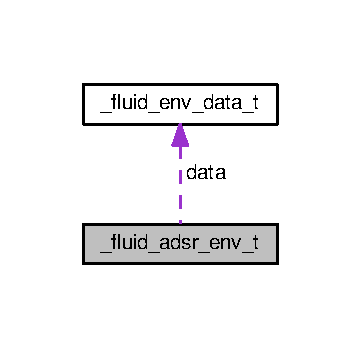
\includegraphics[width=173pt]{struct__fluid__adsr__env__t__coll__graph}
\end{center}
\end{figure}
\subsection*{Public Attributes}
\begin{DoxyCompactItemize}
\item 
\hyperlink{fluidsynth__priv_8h_a3d2015ae1e5cd199777e135fed953e55}{fluid\+\_\+env\+\_\+data\+\_\+t} \hyperlink{struct__fluid__adsr__env__t_a663a2e9bce9e50ee402c556d2988ab02}{data} \mbox{[}\hyperlink{fluid__adsr__env_8h_a92b014c78f2846df56c8c4c7bc6cdf2ea3a5528ce6cf74fbf1335d61ce182a30a}{F\+L\+U\+I\+D\+\_\+\+V\+O\+I\+C\+E\+\_\+\+E\+N\+V\+L\+A\+ST}\mbox{]}
\item 
unsigned int \hyperlink{struct__fluid__adsr__env__t_ab3fffe4cb8b32f25e42b1c2087221f97}{count}
\item 
int \hyperlink{struct__fluid__adsr__env__t_a098e9a731878eb855371463f68a8cec9}{section}
\item 
\hyperlink{fluidsynth__priv_8h_a9e96f0917747b69cabb7c671bc693dbb}{fluid\+\_\+real\+\_\+t} \hyperlink{struct__fluid__adsr__env__t_a37b3cdde99bb8aaf9d8352c2f31bb7ee}{val}
\end{DoxyCompactItemize}


\subsection{Member Data Documentation}
\mbox{\Hypertarget{struct__fluid__adsr__env__t_ab3fffe4cb8b32f25e42b1c2087221f97}\label{struct__fluid__adsr__env__t_ab3fffe4cb8b32f25e42b1c2087221f97}} 
\index{\+\_\+fluid\+\_\+adsr\+\_\+env\+\_\+t@{\+\_\+fluid\+\_\+adsr\+\_\+env\+\_\+t}!count@{count}}
\index{count@{count}!\+\_\+fluid\+\_\+adsr\+\_\+env\+\_\+t@{\+\_\+fluid\+\_\+adsr\+\_\+env\+\_\+t}}
\subsubsection{\texorpdfstring{count}{count}}
{\footnotesize\ttfamily unsigned int \+\_\+fluid\+\_\+adsr\+\_\+env\+\_\+t\+::count}

\mbox{\Hypertarget{struct__fluid__adsr__env__t_a663a2e9bce9e50ee402c556d2988ab02}\label{struct__fluid__adsr__env__t_a663a2e9bce9e50ee402c556d2988ab02}} 
\index{\+\_\+fluid\+\_\+adsr\+\_\+env\+\_\+t@{\+\_\+fluid\+\_\+adsr\+\_\+env\+\_\+t}!data@{data}}
\index{data@{data}!\+\_\+fluid\+\_\+adsr\+\_\+env\+\_\+t@{\+\_\+fluid\+\_\+adsr\+\_\+env\+\_\+t}}
\subsubsection{\texorpdfstring{data}{data}}
{\footnotesize\ttfamily \hyperlink{fluidsynth__priv_8h_a3d2015ae1e5cd199777e135fed953e55}{fluid\+\_\+env\+\_\+data\+\_\+t} \+\_\+fluid\+\_\+adsr\+\_\+env\+\_\+t\+::data\mbox{[}\hyperlink{fluid__adsr__env_8h_a92b014c78f2846df56c8c4c7bc6cdf2ea3a5528ce6cf74fbf1335d61ce182a30a}{F\+L\+U\+I\+D\+\_\+\+V\+O\+I\+C\+E\+\_\+\+E\+N\+V\+L\+A\+ST}\mbox{]}}

\mbox{\Hypertarget{struct__fluid__adsr__env__t_a098e9a731878eb855371463f68a8cec9}\label{struct__fluid__adsr__env__t_a098e9a731878eb855371463f68a8cec9}} 
\index{\+\_\+fluid\+\_\+adsr\+\_\+env\+\_\+t@{\+\_\+fluid\+\_\+adsr\+\_\+env\+\_\+t}!section@{section}}
\index{section@{section}!\+\_\+fluid\+\_\+adsr\+\_\+env\+\_\+t@{\+\_\+fluid\+\_\+adsr\+\_\+env\+\_\+t}}
\subsubsection{\texorpdfstring{section}{section}}
{\footnotesize\ttfamily int \+\_\+fluid\+\_\+adsr\+\_\+env\+\_\+t\+::section}

\mbox{\Hypertarget{struct__fluid__adsr__env__t_a37b3cdde99bb8aaf9d8352c2f31bb7ee}\label{struct__fluid__adsr__env__t_a37b3cdde99bb8aaf9d8352c2f31bb7ee}} 
\index{\+\_\+fluid\+\_\+adsr\+\_\+env\+\_\+t@{\+\_\+fluid\+\_\+adsr\+\_\+env\+\_\+t}!val@{val}}
\index{val@{val}!\+\_\+fluid\+\_\+adsr\+\_\+env\+\_\+t@{\+\_\+fluid\+\_\+adsr\+\_\+env\+\_\+t}}
\subsubsection{\texorpdfstring{val}{val}}
{\footnotesize\ttfamily \hyperlink{fluidsynth__priv_8h_a9e96f0917747b69cabb7c671bc693dbb}{fluid\+\_\+real\+\_\+t} \+\_\+fluid\+\_\+adsr\+\_\+env\+\_\+t\+::val}



The documentation for this struct was generated from the following file\+:\begin{DoxyCompactItemize}
\item 
rvoice/\hyperlink{fluid__adsr__env_8h}{fluid\+\_\+adsr\+\_\+env.\+h}\end{DoxyCompactItemize}

\hypertarget{struct__fluid__allpass}{}\section{\+\_\+fluid\+\_\+allpass Struct Reference}
\label{struct__fluid__allpass}\index{\+\_\+fluid\+\_\+allpass@{\+\_\+fluid\+\_\+allpass}}
\subsection*{Public Attributes}
\begin{DoxyCompactItemize}
\item 
\hyperlink{fluidsynth__priv_8h_a9e96f0917747b69cabb7c671bc693dbb}{fluid\+\_\+real\+\_\+t} \hyperlink{struct__fluid__allpass_aa8d930d5f1a494a6a706549e89838521}{feedback}
\item 
\hyperlink{fluidsynth__priv_8h_a9e96f0917747b69cabb7c671bc693dbb}{fluid\+\_\+real\+\_\+t} $\ast$ \hyperlink{struct__fluid__allpass_ad6c3b8d24e7e5d2e0040073a9b96830c}{buffer}
\item 
int \hyperlink{struct__fluid__allpass_afb12081fc279dc74ec419e1595a67a2d}{bufsize}
\item 
int \hyperlink{struct__fluid__allpass_a3ccf530e0e86318d5842c52d6c693b3a}{bufidx}
\end{DoxyCompactItemize}


\subsection{Member Data Documentation}
\mbox{\Hypertarget{struct__fluid__allpass_ad6c3b8d24e7e5d2e0040073a9b96830c}\label{struct__fluid__allpass_ad6c3b8d24e7e5d2e0040073a9b96830c}} 
\index{\+\_\+fluid\+\_\+allpass@{\+\_\+fluid\+\_\+allpass}!buffer@{buffer}}
\index{buffer@{buffer}!\+\_\+fluid\+\_\+allpass@{\+\_\+fluid\+\_\+allpass}}
\subsubsection{\texorpdfstring{buffer}{buffer}}
{\footnotesize\ttfamily \hyperlink{fluidsynth__priv_8h_a9e96f0917747b69cabb7c671bc693dbb}{fluid\+\_\+real\+\_\+t}$\ast$ \+\_\+fluid\+\_\+allpass\+::buffer}

\mbox{\Hypertarget{struct__fluid__allpass_a3ccf530e0e86318d5842c52d6c693b3a}\label{struct__fluid__allpass_a3ccf530e0e86318d5842c52d6c693b3a}} 
\index{\+\_\+fluid\+\_\+allpass@{\+\_\+fluid\+\_\+allpass}!bufidx@{bufidx}}
\index{bufidx@{bufidx}!\+\_\+fluid\+\_\+allpass@{\+\_\+fluid\+\_\+allpass}}
\subsubsection{\texorpdfstring{bufidx}{bufidx}}
{\footnotesize\ttfamily int \+\_\+fluid\+\_\+allpass\+::bufidx}

\mbox{\Hypertarget{struct__fluid__allpass_afb12081fc279dc74ec419e1595a67a2d}\label{struct__fluid__allpass_afb12081fc279dc74ec419e1595a67a2d}} 
\index{\+\_\+fluid\+\_\+allpass@{\+\_\+fluid\+\_\+allpass}!bufsize@{bufsize}}
\index{bufsize@{bufsize}!\+\_\+fluid\+\_\+allpass@{\+\_\+fluid\+\_\+allpass}}
\subsubsection{\texorpdfstring{bufsize}{bufsize}}
{\footnotesize\ttfamily int \+\_\+fluid\+\_\+allpass\+::bufsize}

\mbox{\Hypertarget{struct__fluid__allpass_aa8d930d5f1a494a6a706549e89838521}\label{struct__fluid__allpass_aa8d930d5f1a494a6a706549e89838521}} 
\index{\+\_\+fluid\+\_\+allpass@{\+\_\+fluid\+\_\+allpass}!feedback@{feedback}}
\index{feedback@{feedback}!\+\_\+fluid\+\_\+allpass@{\+\_\+fluid\+\_\+allpass}}
\subsubsection{\texorpdfstring{feedback}{feedback}}
{\footnotesize\ttfamily \hyperlink{fluidsynth__priv_8h_a9e96f0917747b69cabb7c671bc693dbb}{fluid\+\_\+real\+\_\+t} \+\_\+fluid\+\_\+allpass\+::feedback}



The documentation for this struct was generated from the following file\+:\begin{DoxyCompactItemize}
\item 
rvoice/\hyperlink{fluid__rev_8c}{fluid\+\_\+rev.\+c}\end{DoxyCompactItemize}

\hypertarget{struct__fluid__audio__driver__t}{}\section{\+\_\+fluid\+\_\+audio\+\_\+driver\+\_\+t Struct Reference}
\label{struct__fluid__audio__driver__t}\index{\+\_\+fluid\+\_\+audio\+\_\+driver\+\_\+t@{\+\_\+fluid\+\_\+audio\+\_\+driver\+\_\+t}}


{\ttfamily \#include $<$fluid\+\_\+adriver.\+h$>$}

\subsection*{Public Attributes}
\begin{DoxyCompactItemize}
\item 
const char $\ast$ \hyperlink{struct__fluid__audio__driver__t_a6dd9b496d11cb3d823de47f756d4b8e6}{name}
\end{DoxyCompactItemize}


\subsection{Member Data Documentation}
\mbox{\Hypertarget{struct__fluid__audio__driver__t_a6dd9b496d11cb3d823de47f756d4b8e6}\label{struct__fluid__audio__driver__t_a6dd9b496d11cb3d823de47f756d4b8e6}} 
\index{\+\_\+fluid\+\_\+audio\+\_\+driver\+\_\+t@{\+\_\+fluid\+\_\+audio\+\_\+driver\+\_\+t}!name@{name}}
\index{name@{name}!\+\_\+fluid\+\_\+audio\+\_\+driver\+\_\+t@{\+\_\+fluid\+\_\+audio\+\_\+driver\+\_\+t}}
\subsubsection{\texorpdfstring{name}{name}}
{\footnotesize\ttfamily const char$\ast$ \+\_\+fluid\+\_\+audio\+\_\+driver\+\_\+t\+::name}



The documentation for this struct was generated from the following file\+:\begin{DoxyCompactItemize}
\item 
drivers/\hyperlink{fluid__adriver_8h}{fluid\+\_\+adriver.\+h}\end{DoxyCompactItemize}

\hypertarget{struct__fluid__audriver__definition__t}{}\section{\+\_\+fluid\+\_\+audriver\+\_\+definition\+\_\+t Struct Reference}
\label{struct__fluid__audriver__definition__t}\index{\+\_\+fluid\+\_\+audriver\+\_\+definition\+\_\+t@{\+\_\+fluid\+\_\+audriver\+\_\+definition\+\_\+t}}


Collaboration diagram for \+\_\+fluid\+\_\+audriver\+\_\+definition\+\_\+t\+:
\nopagebreak
\begin{figure}[H]
\begin{center}
\leavevmode
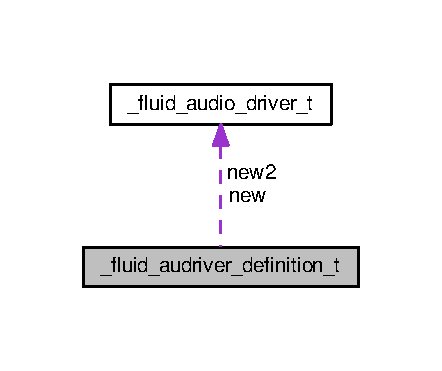
\includegraphics[width=212pt]{struct__fluid__audriver__definition__t__coll__graph}
\end{center}
\end{figure}
\subsection*{Public Attributes}
\begin{DoxyCompactItemize}
\item 
const char $\ast$ \hyperlink{struct__fluid__audriver__definition__t_ac6f6d3b04bd81614f06f51ac31ca0940}{name}
\item 
\hyperlink{types_8h_ac3706330ce49cac5b7dd079e90d376d8}{fluid\+\_\+audio\+\_\+driver\+\_\+t} $\ast$($\ast$ \hyperlink{struct__fluid__audriver__definition__t_adcd98122cacea67bb2fad99d5fadaf36}{new} )(\hyperlink{types_8h_aa363402d3c77333b0f070ba531d034ba}{fluid\+\_\+settings\+\_\+t} $\ast$\hyperlink{struct__fluid__audriver__definition__t_aee73dfdbac8dba21dc75b7ee0babe90f}{settings}, \hyperlink{types_8h_ae265f10ae174a13afe010de50d87e1a4}{fluid\+\_\+synth\+\_\+t} $\ast$synth)
\item 
\hyperlink{types_8h_ac3706330ce49cac5b7dd079e90d376d8}{fluid\+\_\+audio\+\_\+driver\+\_\+t} $\ast$($\ast$ \hyperlink{struct__fluid__audriver__definition__t_add3ac8fe0637ad8ab60bda012a09d17a}{new2} )(\hyperlink{types_8h_aa363402d3c77333b0f070ba531d034ba}{fluid\+\_\+settings\+\_\+t} $\ast$\hyperlink{struct__fluid__audriver__definition__t_aee73dfdbac8dba21dc75b7ee0babe90f}{settings}, \hyperlink{audio_8h_a3bcb63db55c58403dad66496422ec462}{fluid\+\_\+audio\+\_\+func\+\_\+t} func, void $\ast$data)
\item 
void($\ast$ \hyperlink{struct__fluid__audriver__definition__t_ab85eeaaeb690cc72eda41dac40fd21ac}{free} )(\hyperlink{types_8h_ac3706330ce49cac5b7dd079e90d376d8}{fluid\+\_\+audio\+\_\+driver\+\_\+t} $\ast$driver)
\item 
void($\ast$ \hyperlink{struct__fluid__audriver__definition__t_aee73dfdbac8dba21dc75b7ee0babe90f}{settings} )(\hyperlink{types_8h_aa363402d3c77333b0f070ba531d034ba}{fluid\+\_\+settings\+\_\+t} $\ast$settings)
\end{DoxyCompactItemize}


\subsection{Member Data Documentation}
\mbox{\Hypertarget{struct__fluid__audriver__definition__t_ab85eeaaeb690cc72eda41dac40fd21ac}\label{struct__fluid__audriver__definition__t_ab85eeaaeb690cc72eda41dac40fd21ac}} 
\index{\+\_\+fluid\+\_\+audriver\+\_\+definition\+\_\+t@{\+\_\+fluid\+\_\+audriver\+\_\+definition\+\_\+t}!free@{free}}
\index{free@{free}!\+\_\+fluid\+\_\+audriver\+\_\+definition\+\_\+t@{\+\_\+fluid\+\_\+audriver\+\_\+definition\+\_\+t}}
\subsubsection{\texorpdfstring{free}{free}}
{\footnotesize\ttfamily void($\ast$ \+\_\+fluid\+\_\+audriver\+\_\+definition\+\_\+t\+::free) (\hyperlink{types_8h_ac3706330ce49cac5b7dd079e90d376d8}{fluid\+\_\+audio\+\_\+driver\+\_\+t} $\ast$driver)}

\mbox{\Hypertarget{struct__fluid__audriver__definition__t_ac6f6d3b04bd81614f06f51ac31ca0940}\label{struct__fluid__audriver__definition__t_ac6f6d3b04bd81614f06f51ac31ca0940}} 
\index{\+\_\+fluid\+\_\+audriver\+\_\+definition\+\_\+t@{\+\_\+fluid\+\_\+audriver\+\_\+definition\+\_\+t}!name@{name}}
\index{name@{name}!\+\_\+fluid\+\_\+audriver\+\_\+definition\+\_\+t@{\+\_\+fluid\+\_\+audriver\+\_\+definition\+\_\+t}}
\subsubsection{\texorpdfstring{name}{name}}
{\footnotesize\ttfamily const char$\ast$ \+\_\+fluid\+\_\+audriver\+\_\+definition\+\_\+t\+::name}

\mbox{\Hypertarget{struct__fluid__audriver__definition__t_adcd98122cacea67bb2fad99d5fadaf36}\label{struct__fluid__audriver__definition__t_adcd98122cacea67bb2fad99d5fadaf36}} 
\index{\+\_\+fluid\+\_\+audriver\+\_\+definition\+\_\+t@{\+\_\+fluid\+\_\+audriver\+\_\+definition\+\_\+t}!new@{new}}
\index{new@{new}!\+\_\+fluid\+\_\+audriver\+\_\+definition\+\_\+t@{\+\_\+fluid\+\_\+audriver\+\_\+definition\+\_\+t}}
\subsubsection{\texorpdfstring{new}{new}}
{\footnotesize\ttfamily \hyperlink{types_8h_ac3706330ce49cac5b7dd079e90d376d8}{fluid\+\_\+audio\+\_\+driver\+\_\+t}$\ast$($\ast$ \+\_\+fluid\+\_\+audriver\+\_\+definition\+\_\+t\+::new) (\hyperlink{types_8h_aa363402d3c77333b0f070ba531d034ba}{fluid\+\_\+settings\+\_\+t} $\ast$\hyperlink{struct__fluid__audriver__definition__t_aee73dfdbac8dba21dc75b7ee0babe90f}{settings}, \hyperlink{types_8h_ae265f10ae174a13afe010de50d87e1a4}{fluid\+\_\+synth\+\_\+t} $\ast$synth)}

\mbox{\Hypertarget{struct__fluid__audriver__definition__t_add3ac8fe0637ad8ab60bda012a09d17a}\label{struct__fluid__audriver__definition__t_add3ac8fe0637ad8ab60bda012a09d17a}} 
\index{\+\_\+fluid\+\_\+audriver\+\_\+definition\+\_\+t@{\+\_\+fluid\+\_\+audriver\+\_\+definition\+\_\+t}!new2@{new2}}
\index{new2@{new2}!\+\_\+fluid\+\_\+audriver\+\_\+definition\+\_\+t@{\+\_\+fluid\+\_\+audriver\+\_\+definition\+\_\+t}}
\subsubsection{\texorpdfstring{new2}{new2}}
{\footnotesize\ttfamily \hyperlink{types_8h_ac3706330ce49cac5b7dd079e90d376d8}{fluid\+\_\+audio\+\_\+driver\+\_\+t}$\ast$($\ast$ \+\_\+fluid\+\_\+audriver\+\_\+definition\+\_\+t\+::new2) (\hyperlink{types_8h_aa363402d3c77333b0f070ba531d034ba}{fluid\+\_\+settings\+\_\+t} $\ast$\hyperlink{struct__fluid__audriver__definition__t_aee73dfdbac8dba21dc75b7ee0babe90f}{settings}, \hyperlink{audio_8h_a3bcb63db55c58403dad66496422ec462}{fluid\+\_\+audio\+\_\+func\+\_\+t} func, void $\ast$data)}

\mbox{\Hypertarget{struct__fluid__audriver__definition__t_aee73dfdbac8dba21dc75b7ee0babe90f}\label{struct__fluid__audriver__definition__t_aee73dfdbac8dba21dc75b7ee0babe90f}} 
\index{\+\_\+fluid\+\_\+audriver\+\_\+definition\+\_\+t@{\+\_\+fluid\+\_\+audriver\+\_\+definition\+\_\+t}!settings@{settings}}
\index{settings@{settings}!\+\_\+fluid\+\_\+audriver\+\_\+definition\+\_\+t@{\+\_\+fluid\+\_\+audriver\+\_\+definition\+\_\+t}}
\subsubsection{\texorpdfstring{settings}{settings}}
{\footnotesize\ttfamily void($\ast$ \+\_\+fluid\+\_\+audriver\+\_\+definition\+\_\+t\+::settings) (\hyperlink{types_8h_aa363402d3c77333b0f070ba531d034ba}{fluid\+\_\+settings\+\_\+t} $\ast$settings)}



The documentation for this struct was generated from the following file\+:\begin{DoxyCompactItemize}
\item 
drivers/\hyperlink{fluid__adriver_8c}{fluid\+\_\+adriver.\+c}\end{DoxyCompactItemize}

\hypertarget{struct__fluid__channel__t}{}\section{\+\_\+fluid\+\_\+channel\+\_\+t Struct Reference}
\label{struct__fluid__channel__t}\index{\+\_\+fluid\+\_\+channel\+\_\+t@{\+\_\+fluid\+\_\+channel\+\_\+t}}


{\ttfamily \#include $<$fluid\+\_\+chan.\+h$>$}



Collaboration diagram for \+\_\+fluid\+\_\+channel\+\_\+t\+:
\nopagebreak
\begin{figure}[H]
\begin{center}
\leavevmode
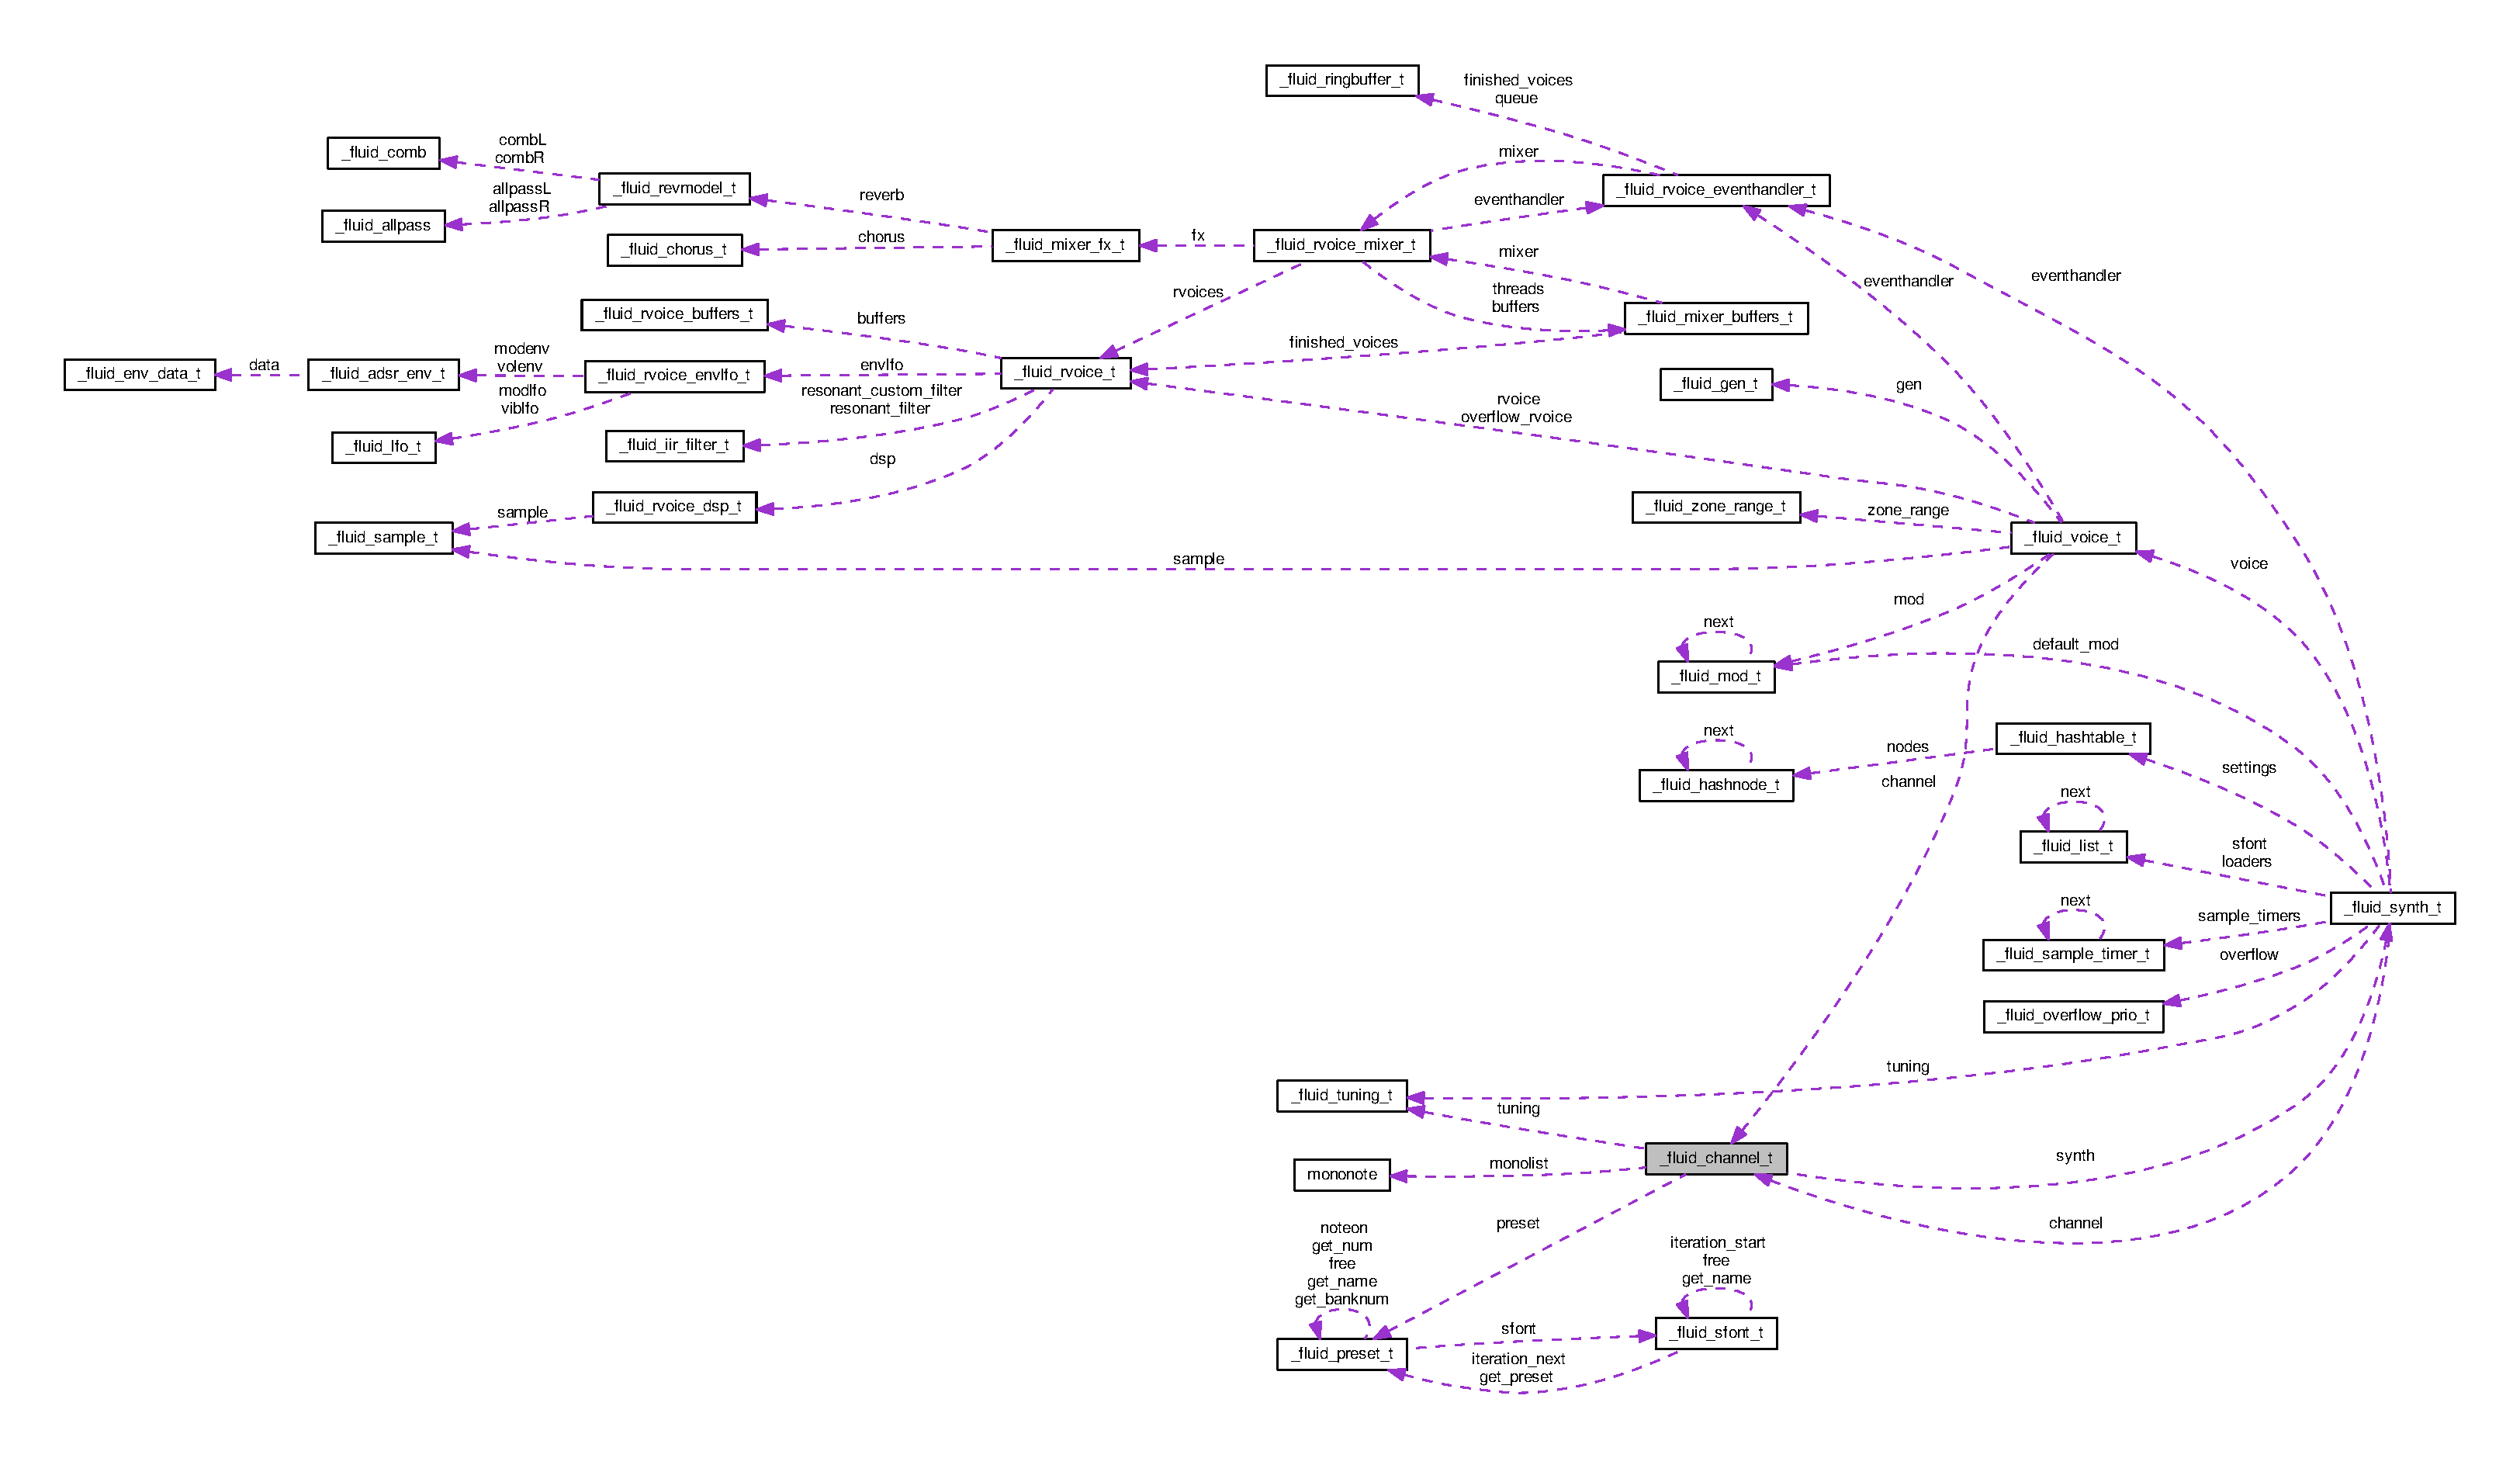
\includegraphics[width=350pt]{struct__fluid__channel__t__coll__graph}
\end{center}
\end{figure}
\subsection*{Public Attributes}
\begin{DoxyCompactItemize}
\item 
\hyperlink{types_8h_ae265f10ae174a13afe010de50d87e1a4}{fluid\+\_\+synth\+\_\+t} $\ast$ \hyperlink{struct__fluid__channel__t_afca755478ea82a7e7156827a2e94d7ce}{synth}
\item 
int \hyperlink{struct__fluid__channel__t_a199ffbf3439801856015686f479d5fe8}{channum}
\item 
int \hyperlink{struct__fluid__channel__t_a36a6f28ca6b9e1e842cf09c2f97ec678}{mode}
\item 
int \hyperlink{struct__fluid__channel__t_ae0ed93ab4611d447773cda2b810a2353}{mode\+\_\+val}
\item 
unsigned char \hyperlink{struct__fluid__channel__t_a15ff2c0965bff5c544a38ec71349d5b5}{i\+\_\+first}
\item 
unsigned char \hyperlink{struct__fluid__channel__t_ad1de61573963862a0c0c6080daef0841}{i\+\_\+last}
\item 
unsigned char \hyperlink{struct__fluid__channel__t_a634b4d0d17c3a5aa6c0c4ed2d9b293e4}{prev\+\_\+note}
\item 
unsigned char \hyperlink{struct__fluid__channel__t_a3b89d8a1bb0ad6e50c9a7b7dbf213065}{n\+\_\+notes}
\item 
struct \hyperlink{structmononote}{mononote} \hyperlink{struct__fluid__channel__t_ad9229dcdb7c4812d858494af3fb2b22a}{monolist} \mbox{[}\hyperlink{fluid__chan_8h_ab28236e45aef5e98c5f75a157ab5d2c4}{F\+L\+U\+I\+D\+\_\+\+C\+H\+A\+N\+N\+E\+L\+\_\+\+S\+I\+Z\+E\+\_\+\+M\+O\+N\+O\+L\+I\+ST}\mbox{]}
\item 
unsigned char \hyperlink{struct__fluid__channel__t_a18c3e3e454963634c8668038f94026a8}{key\+\_\+mono\+\_\+sustained}
\item 
unsigned char \hyperlink{struct__fluid__channel__t_a513731952b4338bc426ac009e6e908a7}{previous\+\_\+cc\+\_\+breath}
\item 
enum \hyperlink{synth_8h_aafd94b0fb1fa9d98841bed11d8418c3a}{fluid\+\_\+channel\+\_\+legato\+\_\+mode} \hyperlink{struct__fluid__channel__t_a3ce58c6ab9a89850f404d90ad402757d}{legatomode}
\item 
enum \hyperlink{synth_8h_a073e69327108f3c7c6feb24c2ca4d3f6}{fluid\+\_\+channel\+\_\+portamento\+\_\+mode} \hyperlink{struct__fluid__channel__t_af74370b1165a26dd277a6ded58579326}{portamentomode}
\item 
unsigned char \hyperlink{struct__fluid__channel__t_a22b7e9b2df7359ccce7bbbaaed20c288}{cc} \mbox{[}128\mbox{]}
\item 
unsigned char \hyperlink{struct__fluid__channel__t_a037c414f8c0c4f00e6d58d1d5a61c342}{key\+\_\+pressure} \mbox{[}128\mbox{]}
\item 
enum \hyperlink{synth_8h_aada0747654fce5d0a758126fc3c99eb0}{fluid\+\_\+midi\+\_\+channel\+\_\+type} \hyperlink{struct__fluid__channel__t_a4271a20a753cabb7567ad69c50d18009}{channel\+\_\+type}
\item 
enum \hyperlink{synth_8h_a4a2efef77b267500dd9c19c0dc9e4633}{fluid\+\_\+interp} \hyperlink{struct__fluid__channel__t_ae4a627af22784d61c352d8ed468fa619}{interp\+\_\+method}
\item 
unsigned char \hyperlink{struct__fluid__channel__t_a4e1d2088d5abab40b071df043922f916}{channel\+\_\+pressure}
\item 
unsigned char \hyperlink{struct__fluid__channel__t_a7801378c076bac4067765629e6cd1791}{pitch\+\_\+wheel\+\_\+sensitivity}
\item 
short \hyperlink{struct__fluid__channel__t_a086fca7239fb592a66840ef28f584608}{pitch\+\_\+bend}
\item 
unsigned int \hyperlink{struct__fluid__channel__t_adfeeecfcc5cb42e73bc1bd9215800262}{sostenuto\+\_\+orderid}
\item 
int \hyperlink{struct__fluid__channel__t_a91209b882ecd399c0ea2db9fefe9fd2f}{tuning\+\_\+bank}
\item 
int \hyperlink{struct__fluid__channel__t_a9407c86a964afd9a593d7ef02e2ed6a9}{tuning\+\_\+prog}
\item 
\hyperlink{fluidsynth__priv_8h_a06e93e369a12dcdcf9a7c9312622e732}{fluid\+\_\+tuning\+\_\+t} $\ast$ \hyperlink{struct__fluid__channel__t_a7cc9c94f6463dc48abc6b86d84deca80}{tuning}
\item 
\hyperlink{types_8h_a985e5ee05f433da841127750f67a4723}{fluid\+\_\+preset\+\_\+t} $\ast$ \hyperlink{struct__fluid__channel__t_a6b807216a860b49ea028e97e7e140578}{preset}
\item 
int \hyperlink{struct__fluid__channel__t_ab713993aae83058a1beeda3dd5627201}{sfont\+\_\+bank\+\_\+prog}
\item 
enum \hyperlink{gen_8h_ad17a24ae3b25f3b8cc5762f818eef9b4}{fluid\+\_\+gen\+\_\+type} \hyperlink{struct__fluid__channel__t_ac720293973b9120baa9ebfef708f9d5d}{nrpn\+\_\+select}
\item 
char \hyperlink{struct__fluid__channel__t_a63f95ccd8c4f3f44df1b2e469f1795c6}{nrpn\+\_\+active}
\item 
\hyperlink{fluidsynth__priv_8h_a9e96f0917747b69cabb7c671bc693dbb}{fluid\+\_\+real\+\_\+t} \hyperlink{struct__fluid__channel__t_a8371721c75d8302750bf8c0c45fc2c76}{gen} \mbox{[}\hyperlink{gen_8h_ad17a24ae3b25f3b8cc5762f818eef9b4a9c372c341b7b1a718f0016f40c615cf3}{G\+E\+N\+\_\+\+L\+A\+ST}\mbox{]}
\item 
char \hyperlink{struct__fluid__channel__t_a431e65009fa1c73f277b141690f0a812}{gen\+\_\+abs} \mbox{[}\hyperlink{gen_8h_ad17a24ae3b25f3b8cc5762f818eef9b4a9c372c341b7b1a718f0016f40c615cf3}{G\+E\+N\+\_\+\+L\+A\+ST}\mbox{]}
\end{DoxyCompactItemize}


\subsection{Member Data Documentation}
\mbox{\Hypertarget{struct__fluid__channel__t_a22b7e9b2df7359ccce7bbbaaed20c288}\label{struct__fluid__channel__t_a22b7e9b2df7359ccce7bbbaaed20c288}} 
\index{\+\_\+fluid\+\_\+channel\+\_\+t@{\+\_\+fluid\+\_\+channel\+\_\+t}!cc@{cc}}
\index{cc@{cc}!\+\_\+fluid\+\_\+channel\+\_\+t@{\+\_\+fluid\+\_\+channel\+\_\+t}}
\subsubsection{\texorpdfstring{cc}{cc}}
{\footnotesize\ttfamily unsigned char \+\_\+fluid\+\_\+channel\+\_\+t\+::cc\mbox{[}128\mbox{]}}

M\+I\+DI controller values from \mbox{[}0;127\mbox{]} \mbox{\Hypertarget{struct__fluid__channel__t_a4e1d2088d5abab40b071df043922f916}\label{struct__fluid__channel__t_a4e1d2088d5abab40b071df043922f916}} 
\index{\+\_\+fluid\+\_\+channel\+\_\+t@{\+\_\+fluid\+\_\+channel\+\_\+t}!channel\+\_\+pressure@{channel\+\_\+pressure}}
\index{channel\+\_\+pressure@{channel\+\_\+pressure}!\+\_\+fluid\+\_\+channel\+\_\+t@{\+\_\+fluid\+\_\+channel\+\_\+t}}
\subsubsection{\texorpdfstring{channel\+\_\+pressure}{channel\_pressure}}
{\footnotesize\ttfamily unsigned char \+\_\+fluid\+\_\+channel\+\_\+t\+::channel\+\_\+pressure}

M\+I\+DI channel pressure from \mbox{[}0;127\mbox{]} \mbox{\Hypertarget{struct__fluid__channel__t_a4271a20a753cabb7567ad69c50d18009}\label{struct__fluid__channel__t_a4271a20a753cabb7567ad69c50d18009}} 
\index{\+\_\+fluid\+\_\+channel\+\_\+t@{\+\_\+fluid\+\_\+channel\+\_\+t}!channel\+\_\+type@{channel\+\_\+type}}
\index{channel\+\_\+type@{channel\+\_\+type}!\+\_\+fluid\+\_\+channel\+\_\+t@{\+\_\+fluid\+\_\+channel\+\_\+t}}
\subsubsection{\texorpdfstring{channel\+\_\+type}{channel\_type}}
{\footnotesize\ttfamily enum \hyperlink{synth_8h_aada0747654fce5d0a758126fc3c99eb0}{fluid\+\_\+midi\+\_\+channel\+\_\+type} \+\_\+fluid\+\_\+channel\+\_\+t\+::channel\+\_\+type}

\mbox{\Hypertarget{struct__fluid__channel__t_a199ffbf3439801856015686f479d5fe8}\label{struct__fluid__channel__t_a199ffbf3439801856015686f479d5fe8}} 
\index{\+\_\+fluid\+\_\+channel\+\_\+t@{\+\_\+fluid\+\_\+channel\+\_\+t}!channum@{channum}}
\index{channum@{channum}!\+\_\+fluid\+\_\+channel\+\_\+t@{\+\_\+fluid\+\_\+channel\+\_\+t}}
\subsubsection{\texorpdfstring{channum}{channum}}
{\footnotesize\ttfamily int \+\_\+fluid\+\_\+channel\+\_\+t\+::channum}

M\+I\+DI channel number \mbox{\Hypertarget{struct__fluid__channel__t_a8371721c75d8302750bf8c0c45fc2c76}\label{struct__fluid__channel__t_a8371721c75d8302750bf8c0c45fc2c76}} 
\index{\+\_\+fluid\+\_\+channel\+\_\+t@{\+\_\+fluid\+\_\+channel\+\_\+t}!gen@{gen}}
\index{gen@{gen}!\+\_\+fluid\+\_\+channel\+\_\+t@{\+\_\+fluid\+\_\+channel\+\_\+t}}
\subsubsection{\texorpdfstring{gen}{gen}}
{\footnotesize\ttfamily \hyperlink{fluidsynth__priv_8h_a9e96f0917747b69cabb7c671bc693dbb}{fluid\+\_\+real\+\_\+t} \+\_\+fluid\+\_\+channel\+\_\+t\+::gen\mbox{[}\hyperlink{gen_8h_ad17a24ae3b25f3b8cc5762f818eef9b4a9c372c341b7b1a718f0016f40c615cf3}{G\+E\+N\+\_\+\+L\+A\+ST}\mbox{]}}

\mbox{\Hypertarget{struct__fluid__channel__t_a431e65009fa1c73f277b141690f0a812}\label{struct__fluid__channel__t_a431e65009fa1c73f277b141690f0a812}} 
\index{\+\_\+fluid\+\_\+channel\+\_\+t@{\+\_\+fluid\+\_\+channel\+\_\+t}!gen\+\_\+abs@{gen\+\_\+abs}}
\index{gen\+\_\+abs@{gen\+\_\+abs}!\+\_\+fluid\+\_\+channel\+\_\+t@{\+\_\+fluid\+\_\+channel\+\_\+t}}
\subsubsection{\texorpdfstring{gen\+\_\+abs}{gen\_abs}}
{\footnotesize\ttfamily char \+\_\+fluid\+\_\+channel\+\_\+t\+::gen\+\_\+abs\mbox{[}\hyperlink{gen_8h_ad17a24ae3b25f3b8cc5762f818eef9b4a9c372c341b7b1a718f0016f40c615cf3}{G\+E\+N\+\_\+\+L\+A\+ST}\mbox{]}}

\mbox{\Hypertarget{struct__fluid__channel__t_a15ff2c0965bff5c544a38ec71349d5b5}\label{struct__fluid__channel__t_a15ff2c0965bff5c544a38ec71349d5b5}} 
\index{\+\_\+fluid\+\_\+channel\+\_\+t@{\+\_\+fluid\+\_\+channel\+\_\+t}!i\+\_\+first@{i\+\_\+first}}
\index{i\+\_\+first@{i\+\_\+first}!\+\_\+fluid\+\_\+channel\+\_\+t@{\+\_\+fluid\+\_\+channel\+\_\+t}}
\subsubsection{\texorpdfstring{i\+\_\+first}{i\_first}}
{\footnotesize\ttfamily unsigned char \+\_\+fluid\+\_\+channel\+\_\+t\+::i\+\_\+first}

First note index \mbox{\Hypertarget{struct__fluid__channel__t_ad1de61573963862a0c0c6080daef0841}\label{struct__fluid__channel__t_ad1de61573963862a0c0c6080daef0841}} 
\index{\+\_\+fluid\+\_\+channel\+\_\+t@{\+\_\+fluid\+\_\+channel\+\_\+t}!i\+\_\+last@{i\+\_\+last}}
\index{i\+\_\+last@{i\+\_\+last}!\+\_\+fluid\+\_\+channel\+\_\+t@{\+\_\+fluid\+\_\+channel\+\_\+t}}
\subsubsection{\texorpdfstring{i\+\_\+last}{i\_last}}
{\footnotesize\ttfamily unsigned char \+\_\+fluid\+\_\+channel\+\_\+t\+::i\+\_\+last}

most recent note index since the most recent add \mbox{\Hypertarget{struct__fluid__channel__t_ae4a627af22784d61c352d8ed468fa619}\label{struct__fluid__channel__t_ae4a627af22784d61c352d8ed468fa619}} 
\index{\+\_\+fluid\+\_\+channel\+\_\+t@{\+\_\+fluid\+\_\+channel\+\_\+t}!interp\+\_\+method@{interp\+\_\+method}}
\index{interp\+\_\+method@{interp\+\_\+method}!\+\_\+fluid\+\_\+channel\+\_\+t@{\+\_\+fluid\+\_\+channel\+\_\+t}}
\subsubsection{\texorpdfstring{interp\+\_\+method}{interp\_method}}
{\footnotesize\ttfamily enum \hyperlink{synth_8h_a4a2efef77b267500dd9c19c0dc9e4633}{fluid\+\_\+interp} \+\_\+fluid\+\_\+channel\+\_\+t\+::interp\+\_\+method}

Interpolation method (enum fluid\+\_\+interp) \mbox{\Hypertarget{struct__fluid__channel__t_a18c3e3e454963634c8668038f94026a8}\label{struct__fluid__channel__t_a18c3e3e454963634c8668038f94026a8}} 
\index{\+\_\+fluid\+\_\+channel\+\_\+t@{\+\_\+fluid\+\_\+channel\+\_\+t}!key\+\_\+mono\+\_\+sustained@{key\+\_\+mono\+\_\+sustained}}
\index{key\+\_\+mono\+\_\+sustained@{key\+\_\+mono\+\_\+sustained}!\+\_\+fluid\+\_\+channel\+\_\+t@{\+\_\+fluid\+\_\+channel\+\_\+t}}
\subsubsection{\texorpdfstring{key\+\_\+mono\+\_\+sustained}{key\_mono\_sustained}}
{\footnotesize\ttfamily unsigned char \+\_\+fluid\+\_\+channel\+\_\+t\+::key\+\_\+mono\+\_\+sustained}

previous sustained monophonic note \mbox{\Hypertarget{struct__fluid__channel__t_a037c414f8c0c4f00e6d58d1d5a61c342}\label{struct__fluid__channel__t_a037c414f8c0c4f00e6d58d1d5a61c342}} 
\index{\+\_\+fluid\+\_\+channel\+\_\+t@{\+\_\+fluid\+\_\+channel\+\_\+t}!key\+\_\+pressure@{key\+\_\+pressure}}
\index{key\+\_\+pressure@{key\+\_\+pressure}!\+\_\+fluid\+\_\+channel\+\_\+t@{\+\_\+fluid\+\_\+channel\+\_\+t}}
\subsubsection{\texorpdfstring{key\+\_\+pressure}{key\_pressure}}
{\footnotesize\ttfamily unsigned char \+\_\+fluid\+\_\+channel\+\_\+t\+::key\+\_\+pressure\mbox{[}128\mbox{]}}

M\+I\+DI polyphonic key pressure from \mbox{[}0;127\mbox{]} \mbox{\Hypertarget{struct__fluid__channel__t_a3ce58c6ab9a89850f404d90ad402757d}\label{struct__fluid__channel__t_a3ce58c6ab9a89850f404d90ad402757d}} 
\index{\+\_\+fluid\+\_\+channel\+\_\+t@{\+\_\+fluid\+\_\+channel\+\_\+t}!legatomode@{legatomode}}
\index{legatomode@{legatomode}!\+\_\+fluid\+\_\+channel\+\_\+t@{\+\_\+fluid\+\_\+channel\+\_\+t}}
\subsubsection{\texorpdfstring{legatomode}{legatomode}}
{\footnotesize\ttfamily enum \hyperlink{synth_8h_aafd94b0fb1fa9d98841bed11d8418c3a}{fluid\+\_\+channel\+\_\+legato\+\_\+mode} \+\_\+fluid\+\_\+channel\+\_\+t\+::legatomode}

legato mode \mbox{\Hypertarget{struct__fluid__channel__t_a36a6f28ca6b9e1e842cf09c2f97ec678}\label{struct__fluid__channel__t_a36a6f28ca6b9e1e842cf09c2f97ec678}} 
\index{\+\_\+fluid\+\_\+channel\+\_\+t@{\+\_\+fluid\+\_\+channel\+\_\+t}!mode@{mode}}
\index{mode@{mode}!\+\_\+fluid\+\_\+channel\+\_\+t@{\+\_\+fluid\+\_\+channel\+\_\+t}}
\subsubsection{\texorpdfstring{mode}{mode}}
{\footnotesize\ttfamily int \+\_\+fluid\+\_\+channel\+\_\+t\+::mode}

Poly Mono mode \mbox{\Hypertarget{struct__fluid__channel__t_ae0ed93ab4611d447773cda2b810a2353}\label{struct__fluid__channel__t_ae0ed93ab4611d447773cda2b810a2353}} 
\index{\+\_\+fluid\+\_\+channel\+\_\+t@{\+\_\+fluid\+\_\+channel\+\_\+t}!mode\+\_\+val@{mode\+\_\+val}}
\index{mode\+\_\+val@{mode\+\_\+val}!\+\_\+fluid\+\_\+channel\+\_\+t@{\+\_\+fluid\+\_\+channel\+\_\+t}}
\subsubsection{\texorpdfstring{mode\+\_\+val}{mode\_val}}
{\footnotesize\ttfamily int \+\_\+fluid\+\_\+channel\+\_\+t\+::mode\+\_\+val}

number of channel in basic channel group \mbox{\Hypertarget{struct__fluid__channel__t_ad9229dcdb7c4812d858494af3fb2b22a}\label{struct__fluid__channel__t_ad9229dcdb7c4812d858494af3fb2b22a}} 
\index{\+\_\+fluid\+\_\+channel\+\_\+t@{\+\_\+fluid\+\_\+channel\+\_\+t}!monolist@{monolist}}
\index{monolist@{monolist}!\+\_\+fluid\+\_\+channel\+\_\+t@{\+\_\+fluid\+\_\+channel\+\_\+t}}
\subsubsection{\texorpdfstring{monolist}{monolist}}
{\footnotesize\ttfamily struct \hyperlink{structmononote}{mononote} \+\_\+fluid\+\_\+channel\+\_\+t\+::monolist\mbox{[}\hyperlink{fluid__chan_8h_ab28236e45aef5e98c5f75a157ab5d2c4}{F\+L\+U\+I\+D\+\_\+\+C\+H\+A\+N\+N\+E\+L\+\_\+\+S\+I\+Z\+E\+\_\+\+M\+O\+N\+O\+L\+I\+ST}\mbox{]}}

monophonic list \mbox{\Hypertarget{struct__fluid__channel__t_a3b89d8a1bb0ad6e50c9a7b7dbf213065}\label{struct__fluid__channel__t_a3b89d8a1bb0ad6e50c9a7b7dbf213065}} 
\index{\+\_\+fluid\+\_\+channel\+\_\+t@{\+\_\+fluid\+\_\+channel\+\_\+t}!n\+\_\+notes@{n\+\_\+notes}}
\index{n\+\_\+notes@{n\+\_\+notes}!\+\_\+fluid\+\_\+channel\+\_\+t@{\+\_\+fluid\+\_\+channel\+\_\+t}}
\subsubsection{\texorpdfstring{n\+\_\+notes}{n\_notes}}
{\footnotesize\ttfamily unsigned char \+\_\+fluid\+\_\+channel\+\_\+t\+::n\+\_\+notes}

actual number of notes in the list \mbox{\Hypertarget{struct__fluid__channel__t_a63f95ccd8c4f3f44df1b2e469f1795c6}\label{struct__fluid__channel__t_a63f95ccd8c4f3f44df1b2e469f1795c6}} 
\index{\+\_\+fluid\+\_\+channel\+\_\+t@{\+\_\+fluid\+\_\+channel\+\_\+t}!nrpn\+\_\+active@{nrpn\+\_\+active}}
\index{nrpn\+\_\+active@{nrpn\+\_\+active}!\+\_\+fluid\+\_\+channel\+\_\+t@{\+\_\+fluid\+\_\+channel\+\_\+t}}
\subsubsection{\texorpdfstring{nrpn\+\_\+active}{nrpn\_active}}
{\footnotesize\ttfamily char \+\_\+fluid\+\_\+channel\+\_\+t\+::nrpn\+\_\+active}

\mbox{\Hypertarget{struct__fluid__channel__t_ac720293973b9120baa9ebfef708f9d5d}\label{struct__fluid__channel__t_ac720293973b9120baa9ebfef708f9d5d}} 
\index{\+\_\+fluid\+\_\+channel\+\_\+t@{\+\_\+fluid\+\_\+channel\+\_\+t}!nrpn\+\_\+select@{nrpn\+\_\+select}}
\index{nrpn\+\_\+select@{nrpn\+\_\+select}!\+\_\+fluid\+\_\+channel\+\_\+t@{\+\_\+fluid\+\_\+channel\+\_\+t}}
\subsubsection{\texorpdfstring{nrpn\+\_\+select}{nrpn\_select}}
{\footnotesize\ttfamily enum \hyperlink{gen_8h_ad17a24ae3b25f3b8cc5762f818eef9b4}{fluid\+\_\+gen\+\_\+type} \+\_\+fluid\+\_\+channel\+\_\+t\+::nrpn\+\_\+select}

\mbox{\Hypertarget{struct__fluid__channel__t_a086fca7239fb592a66840ef28f584608}\label{struct__fluid__channel__t_a086fca7239fb592a66840ef28f584608}} 
\index{\+\_\+fluid\+\_\+channel\+\_\+t@{\+\_\+fluid\+\_\+channel\+\_\+t}!pitch\+\_\+bend@{pitch\+\_\+bend}}
\index{pitch\+\_\+bend@{pitch\+\_\+bend}!\+\_\+fluid\+\_\+channel\+\_\+t@{\+\_\+fluid\+\_\+channel\+\_\+t}}
\subsubsection{\texorpdfstring{pitch\+\_\+bend}{pitch\_bend}}
{\footnotesize\ttfamily short \+\_\+fluid\+\_\+channel\+\_\+t\+::pitch\+\_\+bend}

Current pitch bend value \mbox{\Hypertarget{struct__fluid__channel__t_a7801378c076bac4067765629e6cd1791}\label{struct__fluid__channel__t_a7801378c076bac4067765629e6cd1791}} 
\index{\+\_\+fluid\+\_\+channel\+\_\+t@{\+\_\+fluid\+\_\+channel\+\_\+t}!pitch\+\_\+wheel\+\_\+sensitivity@{pitch\+\_\+wheel\+\_\+sensitivity}}
\index{pitch\+\_\+wheel\+\_\+sensitivity@{pitch\+\_\+wheel\+\_\+sensitivity}!\+\_\+fluid\+\_\+channel\+\_\+t@{\+\_\+fluid\+\_\+channel\+\_\+t}}
\subsubsection{\texorpdfstring{pitch\+\_\+wheel\+\_\+sensitivity}{pitch\_wheel\_sensitivity}}
{\footnotesize\ttfamily unsigned char \+\_\+fluid\+\_\+channel\+\_\+t\+::pitch\+\_\+wheel\+\_\+sensitivity}

Current pitch wheel sensitivity \mbox{\Hypertarget{struct__fluid__channel__t_af74370b1165a26dd277a6ded58579326}\label{struct__fluid__channel__t_af74370b1165a26dd277a6ded58579326}} 
\index{\+\_\+fluid\+\_\+channel\+\_\+t@{\+\_\+fluid\+\_\+channel\+\_\+t}!portamentomode@{portamentomode}}
\index{portamentomode@{portamentomode}!\+\_\+fluid\+\_\+channel\+\_\+t@{\+\_\+fluid\+\_\+channel\+\_\+t}}
\subsubsection{\texorpdfstring{portamentomode}{portamentomode}}
{\footnotesize\ttfamily enum \hyperlink{synth_8h_a073e69327108f3c7c6feb24c2ca4d3f6}{fluid\+\_\+channel\+\_\+portamento\+\_\+mode} \+\_\+fluid\+\_\+channel\+\_\+t\+::portamentomode}

portamento mode \mbox{\Hypertarget{struct__fluid__channel__t_a6b807216a860b49ea028e97e7e140578}\label{struct__fluid__channel__t_a6b807216a860b49ea028e97e7e140578}} 
\index{\+\_\+fluid\+\_\+channel\+\_\+t@{\+\_\+fluid\+\_\+channel\+\_\+t}!preset@{preset}}
\index{preset@{preset}!\+\_\+fluid\+\_\+channel\+\_\+t@{\+\_\+fluid\+\_\+channel\+\_\+t}}
\subsubsection{\texorpdfstring{preset}{preset}}
{\footnotesize\ttfamily \hyperlink{types_8h_a985e5ee05f433da841127750f67a4723}{fluid\+\_\+preset\+\_\+t}$\ast$ \+\_\+fluid\+\_\+channel\+\_\+t\+::preset}

Selected preset \mbox{\Hypertarget{struct__fluid__channel__t_a634b4d0d17c3a5aa6c0c4ed2d9b293e4}\label{struct__fluid__channel__t_a634b4d0d17c3a5aa6c0c4ed2d9b293e4}} 
\index{\+\_\+fluid\+\_\+channel\+\_\+t@{\+\_\+fluid\+\_\+channel\+\_\+t}!prev\+\_\+note@{prev\+\_\+note}}
\index{prev\+\_\+note@{prev\+\_\+note}!\+\_\+fluid\+\_\+channel\+\_\+t@{\+\_\+fluid\+\_\+channel\+\_\+t}}
\subsubsection{\texorpdfstring{prev\+\_\+note}{prev\_note}}
{\footnotesize\ttfamily unsigned char \+\_\+fluid\+\_\+channel\+\_\+t\+::prev\+\_\+note}

previous note of the most recent add/remove \mbox{\Hypertarget{struct__fluid__channel__t_a513731952b4338bc426ac009e6e908a7}\label{struct__fluid__channel__t_a513731952b4338bc426ac009e6e908a7}} 
\index{\+\_\+fluid\+\_\+channel\+\_\+t@{\+\_\+fluid\+\_\+channel\+\_\+t}!previous\+\_\+cc\+\_\+breath@{previous\+\_\+cc\+\_\+breath}}
\index{previous\+\_\+cc\+\_\+breath@{previous\+\_\+cc\+\_\+breath}!\+\_\+fluid\+\_\+channel\+\_\+t@{\+\_\+fluid\+\_\+channel\+\_\+t}}
\subsubsection{\texorpdfstring{previous\+\_\+cc\+\_\+breath}{previous\_cc\_breath}}
{\footnotesize\ttfamily unsigned char \+\_\+fluid\+\_\+channel\+\_\+t\+::previous\+\_\+cc\+\_\+breath}

Previous Breath \mbox{\Hypertarget{struct__fluid__channel__t_ab713993aae83058a1beeda3dd5627201}\label{struct__fluid__channel__t_ab713993aae83058a1beeda3dd5627201}} 
\index{\+\_\+fluid\+\_\+channel\+\_\+t@{\+\_\+fluid\+\_\+channel\+\_\+t}!sfont\+\_\+bank\+\_\+prog@{sfont\+\_\+bank\+\_\+prog}}
\index{sfont\+\_\+bank\+\_\+prog@{sfont\+\_\+bank\+\_\+prog}!\+\_\+fluid\+\_\+channel\+\_\+t@{\+\_\+fluid\+\_\+channel\+\_\+t}}
\subsubsection{\texorpdfstring{sfont\+\_\+bank\+\_\+prog}{sfont\_bank\_prog}}
{\footnotesize\ttfamily int \+\_\+fluid\+\_\+channel\+\_\+t\+::sfont\+\_\+bank\+\_\+prog}

Sound\+Font ID (bit 21-\/31), bank (bit 7-\/20), program (bit 0-\/6) \mbox{\Hypertarget{struct__fluid__channel__t_adfeeecfcc5cb42e73bc1bd9215800262}\label{struct__fluid__channel__t_adfeeecfcc5cb42e73bc1bd9215800262}} 
\index{\+\_\+fluid\+\_\+channel\+\_\+t@{\+\_\+fluid\+\_\+channel\+\_\+t}!sostenuto\+\_\+orderid@{sostenuto\+\_\+orderid}}
\index{sostenuto\+\_\+orderid@{sostenuto\+\_\+orderid}!\+\_\+fluid\+\_\+channel\+\_\+t@{\+\_\+fluid\+\_\+channel\+\_\+t}}
\subsubsection{\texorpdfstring{sostenuto\+\_\+orderid}{sostenuto\_orderid}}
{\footnotesize\ttfamily unsigned int \+\_\+fluid\+\_\+channel\+\_\+t\+::sostenuto\+\_\+orderid}

\mbox{\Hypertarget{struct__fluid__channel__t_afca755478ea82a7e7156827a2e94d7ce}\label{struct__fluid__channel__t_afca755478ea82a7e7156827a2e94d7ce}} 
\index{\+\_\+fluid\+\_\+channel\+\_\+t@{\+\_\+fluid\+\_\+channel\+\_\+t}!synth@{synth}}
\index{synth@{synth}!\+\_\+fluid\+\_\+channel\+\_\+t@{\+\_\+fluid\+\_\+channel\+\_\+t}}
\subsubsection{\texorpdfstring{synth}{synth}}
{\footnotesize\ttfamily \hyperlink{types_8h_ae265f10ae174a13afe010de50d87e1a4}{fluid\+\_\+synth\+\_\+t}$\ast$ \+\_\+fluid\+\_\+channel\+\_\+t\+::synth}

Parent synthesizer instance \mbox{\Hypertarget{struct__fluid__channel__t_a7cc9c94f6463dc48abc6b86d84deca80}\label{struct__fluid__channel__t_a7cc9c94f6463dc48abc6b86d84deca80}} 
\index{\+\_\+fluid\+\_\+channel\+\_\+t@{\+\_\+fluid\+\_\+channel\+\_\+t}!tuning@{tuning}}
\index{tuning@{tuning}!\+\_\+fluid\+\_\+channel\+\_\+t@{\+\_\+fluid\+\_\+channel\+\_\+t}}
\subsubsection{\texorpdfstring{tuning}{tuning}}
{\footnotesize\ttfamily \hyperlink{fluidsynth__priv_8h_a06e93e369a12dcdcf9a7c9312622e732}{fluid\+\_\+tuning\+\_\+t}$\ast$ \+\_\+fluid\+\_\+channel\+\_\+t\+::tuning}

Micro tuning \mbox{\Hypertarget{struct__fluid__channel__t_a91209b882ecd399c0ea2db9fefe9fd2f}\label{struct__fluid__channel__t_a91209b882ecd399c0ea2db9fefe9fd2f}} 
\index{\+\_\+fluid\+\_\+channel\+\_\+t@{\+\_\+fluid\+\_\+channel\+\_\+t}!tuning\+\_\+bank@{tuning\+\_\+bank}}
\index{tuning\+\_\+bank@{tuning\+\_\+bank}!\+\_\+fluid\+\_\+channel\+\_\+t@{\+\_\+fluid\+\_\+channel\+\_\+t}}
\subsubsection{\texorpdfstring{tuning\+\_\+bank}{tuning\_bank}}
{\footnotesize\ttfamily int \+\_\+fluid\+\_\+channel\+\_\+t\+::tuning\+\_\+bank}

Current tuning bank number \mbox{\Hypertarget{struct__fluid__channel__t_a9407c86a964afd9a593d7ef02e2ed6a9}\label{struct__fluid__channel__t_a9407c86a964afd9a593d7ef02e2ed6a9}} 
\index{\+\_\+fluid\+\_\+channel\+\_\+t@{\+\_\+fluid\+\_\+channel\+\_\+t}!tuning\+\_\+prog@{tuning\+\_\+prog}}
\index{tuning\+\_\+prog@{tuning\+\_\+prog}!\+\_\+fluid\+\_\+channel\+\_\+t@{\+\_\+fluid\+\_\+channel\+\_\+t}}
\subsubsection{\texorpdfstring{tuning\+\_\+prog}{tuning\_prog}}
{\footnotesize\ttfamily int \+\_\+fluid\+\_\+channel\+\_\+t\+::tuning\+\_\+prog}

Current tuning program number 

The documentation for this struct was generated from the following file\+:\begin{DoxyCompactItemize}
\item 
synth/\hyperlink{fluid__chan_8h}{fluid\+\_\+chan.\+h}\end{DoxyCompactItemize}

\hypertarget{struct__fluid__chorus__t}{}\section{\+\_\+fluid\+\_\+chorus\+\_\+t Struct Reference}
\label{struct__fluid__chorus__t}\index{\+\_\+fluid\+\_\+chorus\+\_\+t@{\+\_\+fluid\+\_\+chorus\+\_\+t}}
\subsection*{Public Attributes}
\begin{DoxyCompactItemize}
\item 
int \hyperlink{struct__fluid__chorus__t_acfb4123e8db4196bf4329ec04e04e3ef}{type}
\item 
\hyperlink{fluidsynth__priv_8h_a9e96f0917747b69cabb7c671bc693dbb}{fluid\+\_\+real\+\_\+t} \hyperlink{struct__fluid__chorus__t_aab54bc7efa434bab703f67ec98404fe7}{depth\+\_\+ms}
\item 
\hyperlink{fluidsynth__priv_8h_a9e96f0917747b69cabb7c671bc693dbb}{fluid\+\_\+real\+\_\+t} \hyperlink{struct__fluid__chorus__t_ab3d2901f9f4a73ed9391a8a68f6a88dd}{level}
\item 
\hyperlink{fluidsynth__priv_8h_a9e96f0917747b69cabb7c671bc693dbb}{fluid\+\_\+real\+\_\+t} \hyperlink{struct__fluid__chorus__t_adb880e1d8d336fe02103280029994330}{speed\+\_\+\+Hz}
\item 
int \hyperlink{struct__fluid__chorus__t_afbc36eebc1414f97219b6a0f535343e3}{number\+\_\+blocks}
\item 
\hyperlink{fluidsynth__priv_8h_a9e96f0917747b69cabb7c671bc693dbb}{fluid\+\_\+real\+\_\+t} $\ast$ \hyperlink{struct__fluid__chorus__t_a9b3f6f4c597cb378c167b4774e12b89e}{chorusbuf}
\item 
int \hyperlink{struct__fluid__chorus__t_a8a5b56c3e49d2dfaa5ce025d22ae20e7}{counter}
\item 
long \hyperlink{struct__fluid__chorus__t_a9b180e81c16af49b532014c18b550e3c}{phase} \mbox{[}\hyperlink{fluid__chorus_8c_a3010a4cb537309a7c3204946d21a303b}{M\+A\+X\+\_\+\+C\+H\+O\+R\+US}\mbox{]}
\item 
long \hyperlink{struct__fluid__chorus__t_a2fd9afc73f51a308c225741ae21f3a9f}{modulation\+\_\+period\+\_\+samples}
\item 
int $\ast$ \hyperlink{struct__fluid__chorus__t_abfab325244e8edacaaa23f41b0c8d7a3}{lookup\+\_\+tab}
\item 
\hyperlink{fluidsynth__priv_8h_a9e96f0917747b69cabb7c671bc693dbb}{fluid\+\_\+real\+\_\+t} \hyperlink{struct__fluid__chorus__t_acff10fb60386c6e2e0ec73263851a628}{sample\+\_\+rate}
\item 
\hyperlink{fluidsynth__priv_8h_a9e96f0917747b69cabb7c671bc693dbb}{fluid\+\_\+real\+\_\+t} \hyperlink{struct__fluid__chorus__t_a7bf00ec81f9a6b467c739ed6502ca805}{sinc\+\_\+table} \mbox{[}\hyperlink{fluid__chorus_8c_a0c54606433a6ee64cca093935ac9abed}{I\+N\+T\+E\+R\+P\+O\+L\+A\+T\+I\+O\+N\+\_\+\+S\+A\+M\+P\+L\+ES}\mbox{]}\mbox{[}\hyperlink{fluid__chorus_8c_a50692ae56262616da392b6377e1c960a}{I\+N\+T\+E\+R\+P\+O\+L\+A\+T\+I\+O\+N\+\_\+\+S\+U\+B\+S\+A\+M\+P\+L\+ES}\mbox{]}
\end{DoxyCompactItemize}


\subsection{Member Data Documentation}
\mbox{\Hypertarget{struct__fluid__chorus__t_a9b3f6f4c597cb378c167b4774e12b89e}\label{struct__fluid__chorus__t_a9b3f6f4c597cb378c167b4774e12b89e}} 
\index{\+\_\+fluid\+\_\+chorus\+\_\+t@{\+\_\+fluid\+\_\+chorus\+\_\+t}!chorusbuf@{chorusbuf}}
\index{chorusbuf@{chorusbuf}!\+\_\+fluid\+\_\+chorus\+\_\+t@{\+\_\+fluid\+\_\+chorus\+\_\+t}}
\subsubsection{\texorpdfstring{chorusbuf}{chorusbuf}}
{\footnotesize\ttfamily \hyperlink{fluidsynth__priv_8h_a9e96f0917747b69cabb7c671bc693dbb}{fluid\+\_\+real\+\_\+t}$\ast$ \+\_\+fluid\+\_\+chorus\+\_\+t\+::chorusbuf}

\mbox{\Hypertarget{struct__fluid__chorus__t_a8a5b56c3e49d2dfaa5ce025d22ae20e7}\label{struct__fluid__chorus__t_a8a5b56c3e49d2dfaa5ce025d22ae20e7}} 
\index{\+\_\+fluid\+\_\+chorus\+\_\+t@{\+\_\+fluid\+\_\+chorus\+\_\+t}!counter@{counter}}
\index{counter@{counter}!\+\_\+fluid\+\_\+chorus\+\_\+t@{\+\_\+fluid\+\_\+chorus\+\_\+t}}
\subsubsection{\texorpdfstring{counter}{counter}}
{\footnotesize\ttfamily int \+\_\+fluid\+\_\+chorus\+\_\+t\+::counter}

\mbox{\Hypertarget{struct__fluid__chorus__t_aab54bc7efa434bab703f67ec98404fe7}\label{struct__fluid__chorus__t_aab54bc7efa434bab703f67ec98404fe7}} 
\index{\+\_\+fluid\+\_\+chorus\+\_\+t@{\+\_\+fluid\+\_\+chorus\+\_\+t}!depth\+\_\+ms@{depth\+\_\+ms}}
\index{depth\+\_\+ms@{depth\+\_\+ms}!\+\_\+fluid\+\_\+chorus\+\_\+t@{\+\_\+fluid\+\_\+chorus\+\_\+t}}
\subsubsection{\texorpdfstring{depth\+\_\+ms}{depth\_ms}}
{\footnotesize\ttfamily \hyperlink{fluidsynth__priv_8h_a9e96f0917747b69cabb7c671bc693dbb}{fluid\+\_\+real\+\_\+t} \+\_\+fluid\+\_\+chorus\+\_\+t\+::depth\+\_\+ms}

\mbox{\Hypertarget{struct__fluid__chorus__t_ab3d2901f9f4a73ed9391a8a68f6a88dd}\label{struct__fluid__chorus__t_ab3d2901f9f4a73ed9391a8a68f6a88dd}} 
\index{\+\_\+fluid\+\_\+chorus\+\_\+t@{\+\_\+fluid\+\_\+chorus\+\_\+t}!level@{level}}
\index{level@{level}!\+\_\+fluid\+\_\+chorus\+\_\+t@{\+\_\+fluid\+\_\+chorus\+\_\+t}}
\subsubsection{\texorpdfstring{level}{level}}
{\footnotesize\ttfamily \hyperlink{fluidsynth__priv_8h_a9e96f0917747b69cabb7c671bc693dbb}{fluid\+\_\+real\+\_\+t} \+\_\+fluid\+\_\+chorus\+\_\+t\+::level}

\mbox{\Hypertarget{struct__fluid__chorus__t_abfab325244e8edacaaa23f41b0c8d7a3}\label{struct__fluid__chorus__t_abfab325244e8edacaaa23f41b0c8d7a3}} 
\index{\+\_\+fluid\+\_\+chorus\+\_\+t@{\+\_\+fluid\+\_\+chorus\+\_\+t}!lookup\+\_\+tab@{lookup\+\_\+tab}}
\index{lookup\+\_\+tab@{lookup\+\_\+tab}!\+\_\+fluid\+\_\+chorus\+\_\+t@{\+\_\+fluid\+\_\+chorus\+\_\+t}}
\subsubsection{\texorpdfstring{lookup\+\_\+tab}{lookup\_tab}}
{\footnotesize\ttfamily int$\ast$ \+\_\+fluid\+\_\+chorus\+\_\+t\+::lookup\+\_\+tab}

\mbox{\Hypertarget{struct__fluid__chorus__t_a2fd9afc73f51a308c225741ae21f3a9f}\label{struct__fluid__chorus__t_a2fd9afc73f51a308c225741ae21f3a9f}} 
\index{\+\_\+fluid\+\_\+chorus\+\_\+t@{\+\_\+fluid\+\_\+chorus\+\_\+t}!modulation\+\_\+period\+\_\+samples@{modulation\+\_\+period\+\_\+samples}}
\index{modulation\+\_\+period\+\_\+samples@{modulation\+\_\+period\+\_\+samples}!\+\_\+fluid\+\_\+chorus\+\_\+t@{\+\_\+fluid\+\_\+chorus\+\_\+t}}
\subsubsection{\texorpdfstring{modulation\+\_\+period\+\_\+samples}{modulation\_period\_samples}}
{\footnotesize\ttfamily long \+\_\+fluid\+\_\+chorus\+\_\+t\+::modulation\+\_\+period\+\_\+samples}

\mbox{\Hypertarget{struct__fluid__chorus__t_afbc36eebc1414f97219b6a0f535343e3}\label{struct__fluid__chorus__t_afbc36eebc1414f97219b6a0f535343e3}} 
\index{\+\_\+fluid\+\_\+chorus\+\_\+t@{\+\_\+fluid\+\_\+chorus\+\_\+t}!number\+\_\+blocks@{number\+\_\+blocks}}
\index{number\+\_\+blocks@{number\+\_\+blocks}!\+\_\+fluid\+\_\+chorus\+\_\+t@{\+\_\+fluid\+\_\+chorus\+\_\+t}}
\subsubsection{\texorpdfstring{number\+\_\+blocks}{number\_blocks}}
{\footnotesize\ttfamily int \+\_\+fluid\+\_\+chorus\+\_\+t\+::number\+\_\+blocks}

\mbox{\Hypertarget{struct__fluid__chorus__t_a9b180e81c16af49b532014c18b550e3c}\label{struct__fluid__chorus__t_a9b180e81c16af49b532014c18b550e3c}} 
\index{\+\_\+fluid\+\_\+chorus\+\_\+t@{\+\_\+fluid\+\_\+chorus\+\_\+t}!phase@{phase}}
\index{phase@{phase}!\+\_\+fluid\+\_\+chorus\+\_\+t@{\+\_\+fluid\+\_\+chorus\+\_\+t}}
\subsubsection{\texorpdfstring{phase}{phase}}
{\footnotesize\ttfamily long \+\_\+fluid\+\_\+chorus\+\_\+t\+::phase\mbox{[}\hyperlink{fluid__chorus_8c_a3010a4cb537309a7c3204946d21a303b}{M\+A\+X\+\_\+\+C\+H\+O\+R\+US}\mbox{]}}

\mbox{\Hypertarget{struct__fluid__chorus__t_acff10fb60386c6e2e0ec73263851a628}\label{struct__fluid__chorus__t_acff10fb60386c6e2e0ec73263851a628}} 
\index{\+\_\+fluid\+\_\+chorus\+\_\+t@{\+\_\+fluid\+\_\+chorus\+\_\+t}!sample\+\_\+rate@{sample\+\_\+rate}}
\index{sample\+\_\+rate@{sample\+\_\+rate}!\+\_\+fluid\+\_\+chorus\+\_\+t@{\+\_\+fluid\+\_\+chorus\+\_\+t}}
\subsubsection{\texorpdfstring{sample\+\_\+rate}{sample\_rate}}
{\footnotesize\ttfamily \hyperlink{fluidsynth__priv_8h_a9e96f0917747b69cabb7c671bc693dbb}{fluid\+\_\+real\+\_\+t} \+\_\+fluid\+\_\+chorus\+\_\+t\+::sample\+\_\+rate}

\mbox{\Hypertarget{struct__fluid__chorus__t_a7bf00ec81f9a6b467c739ed6502ca805}\label{struct__fluid__chorus__t_a7bf00ec81f9a6b467c739ed6502ca805}} 
\index{\+\_\+fluid\+\_\+chorus\+\_\+t@{\+\_\+fluid\+\_\+chorus\+\_\+t}!sinc\+\_\+table@{sinc\+\_\+table}}
\index{sinc\+\_\+table@{sinc\+\_\+table}!\+\_\+fluid\+\_\+chorus\+\_\+t@{\+\_\+fluid\+\_\+chorus\+\_\+t}}
\subsubsection{\texorpdfstring{sinc\+\_\+table}{sinc\_table}}
{\footnotesize\ttfamily \hyperlink{fluidsynth__priv_8h_a9e96f0917747b69cabb7c671bc693dbb}{fluid\+\_\+real\+\_\+t} \+\_\+fluid\+\_\+chorus\+\_\+t\+::sinc\+\_\+table\mbox{[}\hyperlink{fluid__chorus_8c_a0c54606433a6ee64cca093935ac9abed}{I\+N\+T\+E\+R\+P\+O\+L\+A\+T\+I\+O\+N\+\_\+\+S\+A\+M\+P\+L\+ES}\mbox{]}\mbox{[}\hyperlink{fluid__chorus_8c_a50692ae56262616da392b6377e1c960a}{I\+N\+T\+E\+R\+P\+O\+L\+A\+T\+I\+O\+N\+\_\+\+S\+U\+B\+S\+A\+M\+P\+L\+ES}\mbox{]}}

\mbox{\Hypertarget{struct__fluid__chorus__t_adb880e1d8d336fe02103280029994330}\label{struct__fluid__chorus__t_adb880e1d8d336fe02103280029994330}} 
\index{\+\_\+fluid\+\_\+chorus\+\_\+t@{\+\_\+fluid\+\_\+chorus\+\_\+t}!speed\+\_\+\+Hz@{speed\+\_\+\+Hz}}
\index{speed\+\_\+\+Hz@{speed\+\_\+\+Hz}!\+\_\+fluid\+\_\+chorus\+\_\+t@{\+\_\+fluid\+\_\+chorus\+\_\+t}}
\subsubsection{\texorpdfstring{speed\+\_\+\+Hz}{speed\_Hz}}
{\footnotesize\ttfamily \hyperlink{fluidsynth__priv_8h_a9e96f0917747b69cabb7c671bc693dbb}{fluid\+\_\+real\+\_\+t} \+\_\+fluid\+\_\+chorus\+\_\+t\+::speed\+\_\+\+Hz}

\mbox{\Hypertarget{struct__fluid__chorus__t_acfb4123e8db4196bf4329ec04e04e3ef}\label{struct__fluid__chorus__t_acfb4123e8db4196bf4329ec04e04e3ef}} 
\index{\+\_\+fluid\+\_\+chorus\+\_\+t@{\+\_\+fluid\+\_\+chorus\+\_\+t}!type@{type}}
\index{type@{type}!\+\_\+fluid\+\_\+chorus\+\_\+t@{\+\_\+fluid\+\_\+chorus\+\_\+t}}
\subsubsection{\texorpdfstring{type}{type}}
{\footnotesize\ttfamily int \+\_\+fluid\+\_\+chorus\+\_\+t\+::type}



The documentation for this struct was generated from the following file\+:\begin{DoxyCompactItemize}
\item 
rvoice/\hyperlink{fluid__chorus_8c}{fluid\+\_\+chorus.\+c}\end{DoxyCompactItemize}

\hypertarget{struct__fluid__client__t}{}\section{\+\_\+fluid\+\_\+client\+\_\+t Struct Reference}
\label{struct__fluid__client__t}\index{\+\_\+fluid\+\_\+client\+\_\+t@{\+\_\+fluid\+\_\+client\+\_\+t}}


Collaboration diagram for \+\_\+fluid\+\_\+client\+\_\+t\+:
\nopagebreak
\begin{figure}[H]
\begin{center}
\leavevmode
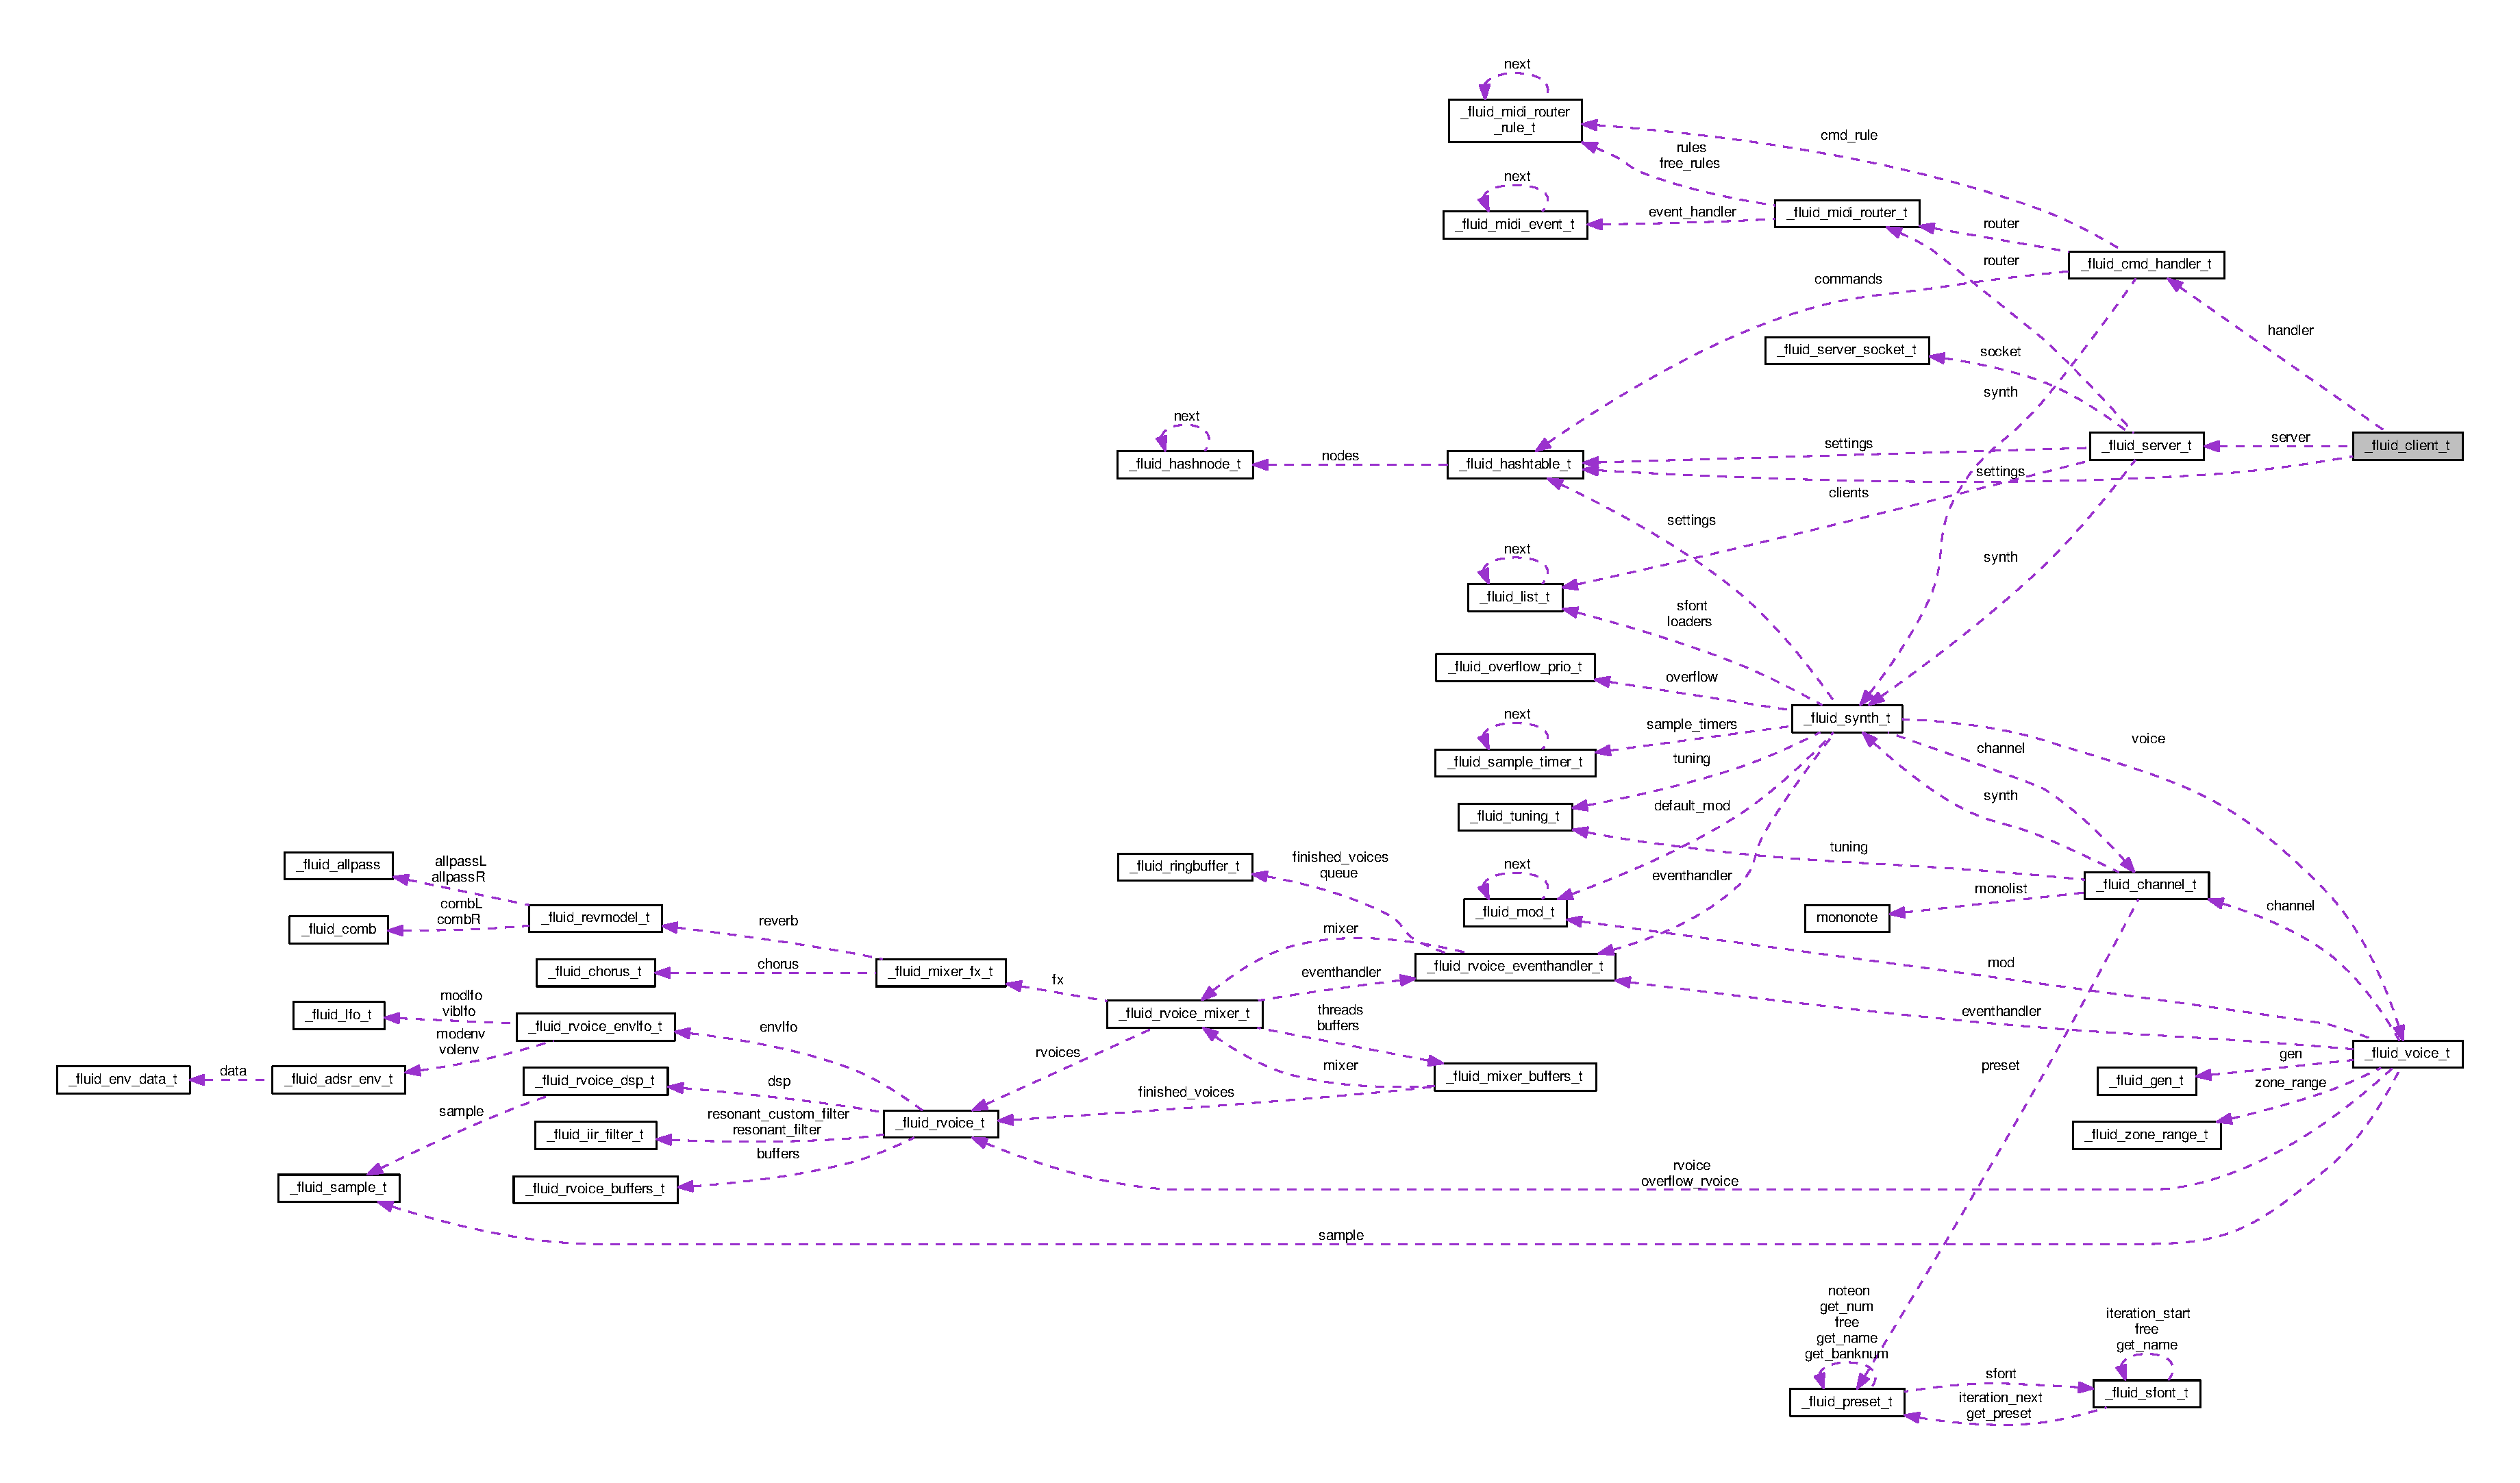
\includegraphics[width=350pt]{struct__fluid__client__t__coll__graph}
\end{center}
\end{figure}
\subsection*{Public Attributes}
\begin{DoxyCompactItemize}
\item 
\hyperlink{types_8h_a314a569c9a9ae8f99831472efda31141}{fluid\+\_\+server\+\_\+t} $\ast$ \hyperlink{struct__fluid__client__t_a660c989ddc2f760f37a1e17618017938}{server}
\item 
\hyperlink{types_8h_aa363402d3c77333b0f070ba531d034ba}{fluid\+\_\+settings\+\_\+t} $\ast$ \hyperlink{struct__fluid__client__t_a1c3d752d3032e7bb194a837bac2f4ff8}{settings}
\item 
\hyperlink{types_8h_ae1944df078b25beb347abd07e42b35a4}{fluid\+\_\+cmd\+\_\+handler\+\_\+t} $\ast$ \hyperlink{struct__fluid__client__t_a37031c9ec49bd2addb72f4bef0354038}{handler}
\item 
\hyperlink{fluidsynth__priv_8h_ad024f40f94120b0766cda0ad9f47be82}{fluid\+\_\+socket\+\_\+t} \hyperlink{struct__fluid__client__t_aacb39ee52d5abbe0304e179cb0cfb4b2}{socket}
\item 
\hyperlink{fluid__sys_8h_a60a6466e68a45b0f0709f1ebaa7e6f85}{fluid\+\_\+thread\+\_\+t} $\ast$ \hyperlink{struct__fluid__client__t_af50bd49f0c5399b2d5de33b282ce4379}{thread}
\end{DoxyCompactItemize}


\subsection{Member Data Documentation}
\mbox{\Hypertarget{struct__fluid__client__t_a37031c9ec49bd2addb72f4bef0354038}\label{struct__fluid__client__t_a37031c9ec49bd2addb72f4bef0354038}} 
\index{\+\_\+fluid\+\_\+client\+\_\+t@{\+\_\+fluid\+\_\+client\+\_\+t}!handler@{handler}}
\index{handler@{handler}!\+\_\+fluid\+\_\+client\+\_\+t@{\+\_\+fluid\+\_\+client\+\_\+t}}
\subsubsection{\texorpdfstring{handler}{handler}}
{\footnotesize\ttfamily \hyperlink{types_8h_ae1944df078b25beb347abd07e42b35a4}{fluid\+\_\+cmd\+\_\+handler\+\_\+t}$\ast$ \+\_\+fluid\+\_\+client\+\_\+t\+::handler}

\mbox{\Hypertarget{struct__fluid__client__t_a660c989ddc2f760f37a1e17618017938}\label{struct__fluid__client__t_a660c989ddc2f760f37a1e17618017938}} 
\index{\+\_\+fluid\+\_\+client\+\_\+t@{\+\_\+fluid\+\_\+client\+\_\+t}!server@{server}}
\index{server@{server}!\+\_\+fluid\+\_\+client\+\_\+t@{\+\_\+fluid\+\_\+client\+\_\+t}}
\subsubsection{\texorpdfstring{server}{server}}
{\footnotesize\ttfamily \hyperlink{types_8h_a314a569c9a9ae8f99831472efda31141}{fluid\+\_\+server\+\_\+t}$\ast$ \+\_\+fluid\+\_\+client\+\_\+t\+::server}

\mbox{\Hypertarget{struct__fluid__client__t_a1c3d752d3032e7bb194a837bac2f4ff8}\label{struct__fluid__client__t_a1c3d752d3032e7bb194a837bac2f4ff8}} 
\index{\+\_\+fluid\+\_\+client\+\_\+t@{\+\_\+fluid\+\_\+client\+\_\+t}!settings@{settings}}
\index{settings@{settings}!\+\_\+fluid\+\_\+client\+\_\+t@{\+\_\+fluid\+\_\+client\+\_\+t}}
\subsubsection{\texorpdfstring{settings}{settings}}
{\footnotesize\ttfamily \hyperlink{types_8h_aa363402d3c77333b0f070ba531d034ba}{fluid\+\_\+settings\+\_\+t}$\ast$ \+\_\+fluid\+\_\+client\+\_\+t\+::settings}

\mbox{\Hypertarget{struct__fluid__client__t_aacb39ee52d5abbe0304e179cb0cfb4b2}\label{struct__fluid__client__t_aacb39ee52d5abbe0304e179cb0cfb4b2}} 
\index{\+\_\+fluid\+\_\+client\+\_\+t@{\+\_\+fluid\+\_\+client\+\_\+t}!socket@{socket}}
\index{socket@{socket}!\+\_\+fluid\+\_\+client\+\_\+t@{\+\_\+fluid\+\_\+client\+\_\+t}}
\subsubsection{\texorpdfstring{socket}{socket}}
{\footnotesize\ttfamily \hyperlink{fluidsynth__priv_8h_ad024f40f94120b0766cda0ad9f47be82}{fluid\+\_\+socket\+\_\+t} \+\_\+fluid\+\_\+client\+\_\+t\+::socket}

\mbox{\Hypertarget{struct__fluid__client__t_af50bd49f0c5399b2d5de33b282ce4379}\label{struct__fluid__client__t_af50bd49f0c5399b2d5de33b282ce4379}} 
\index{\+\_\+fluid\+\_\+client\+\_\+t@{\+\_\+fluid\+\_\+client\+\_\+t}!thread@{thread}}
\index{thread@{thread}!\+\_\+fluid\+\_\+client\+\_\+t@{\+\_\+fluid\+\_\+client\+\_\+t}}
\subsubsection{\texorpdfstring{thread}{thread}}
{\footnotesize\ttfamily \hyperlink{fluid__sys_8h_a60a6466e68a45b0f0709f1ebaa7e6f85}{fluid\+\_\+thread\+\_\+t}$\ast$ \+\_\+fluid\+\_\+client\+\_\+t\+::thread}



The documentation for this struct was generated from the following file\+:\begin{DoxyCompactItemize}
\item 
bindings/\hyperlink{fluid__cmd_8c}{fluid\+\_\+cmd.\+c}\end{DoxyCompactItemize}

\hypertarget{struct__fluid__cmd__handler__t}{}\section{\+\_\+fluid\+\_\+cmd\+\_\+handler\+\_\+t Struct Reference}
\label{struct__fluid__cmd__handler__t}\index{\+\_\+fluid\+\_\+cmd\+\_\+handler\+\_\+t@{\+\_\+fluid\+\_\+cmd\+\_\+handler\+\_\+t}}


Collaboration diagram for \+\_\+fluid\+\_\+cmd\+\_\+handler\+\_\+t\+:
\nopagebreak
\begin{figure}[H]
\begin{center}
\leavevmode
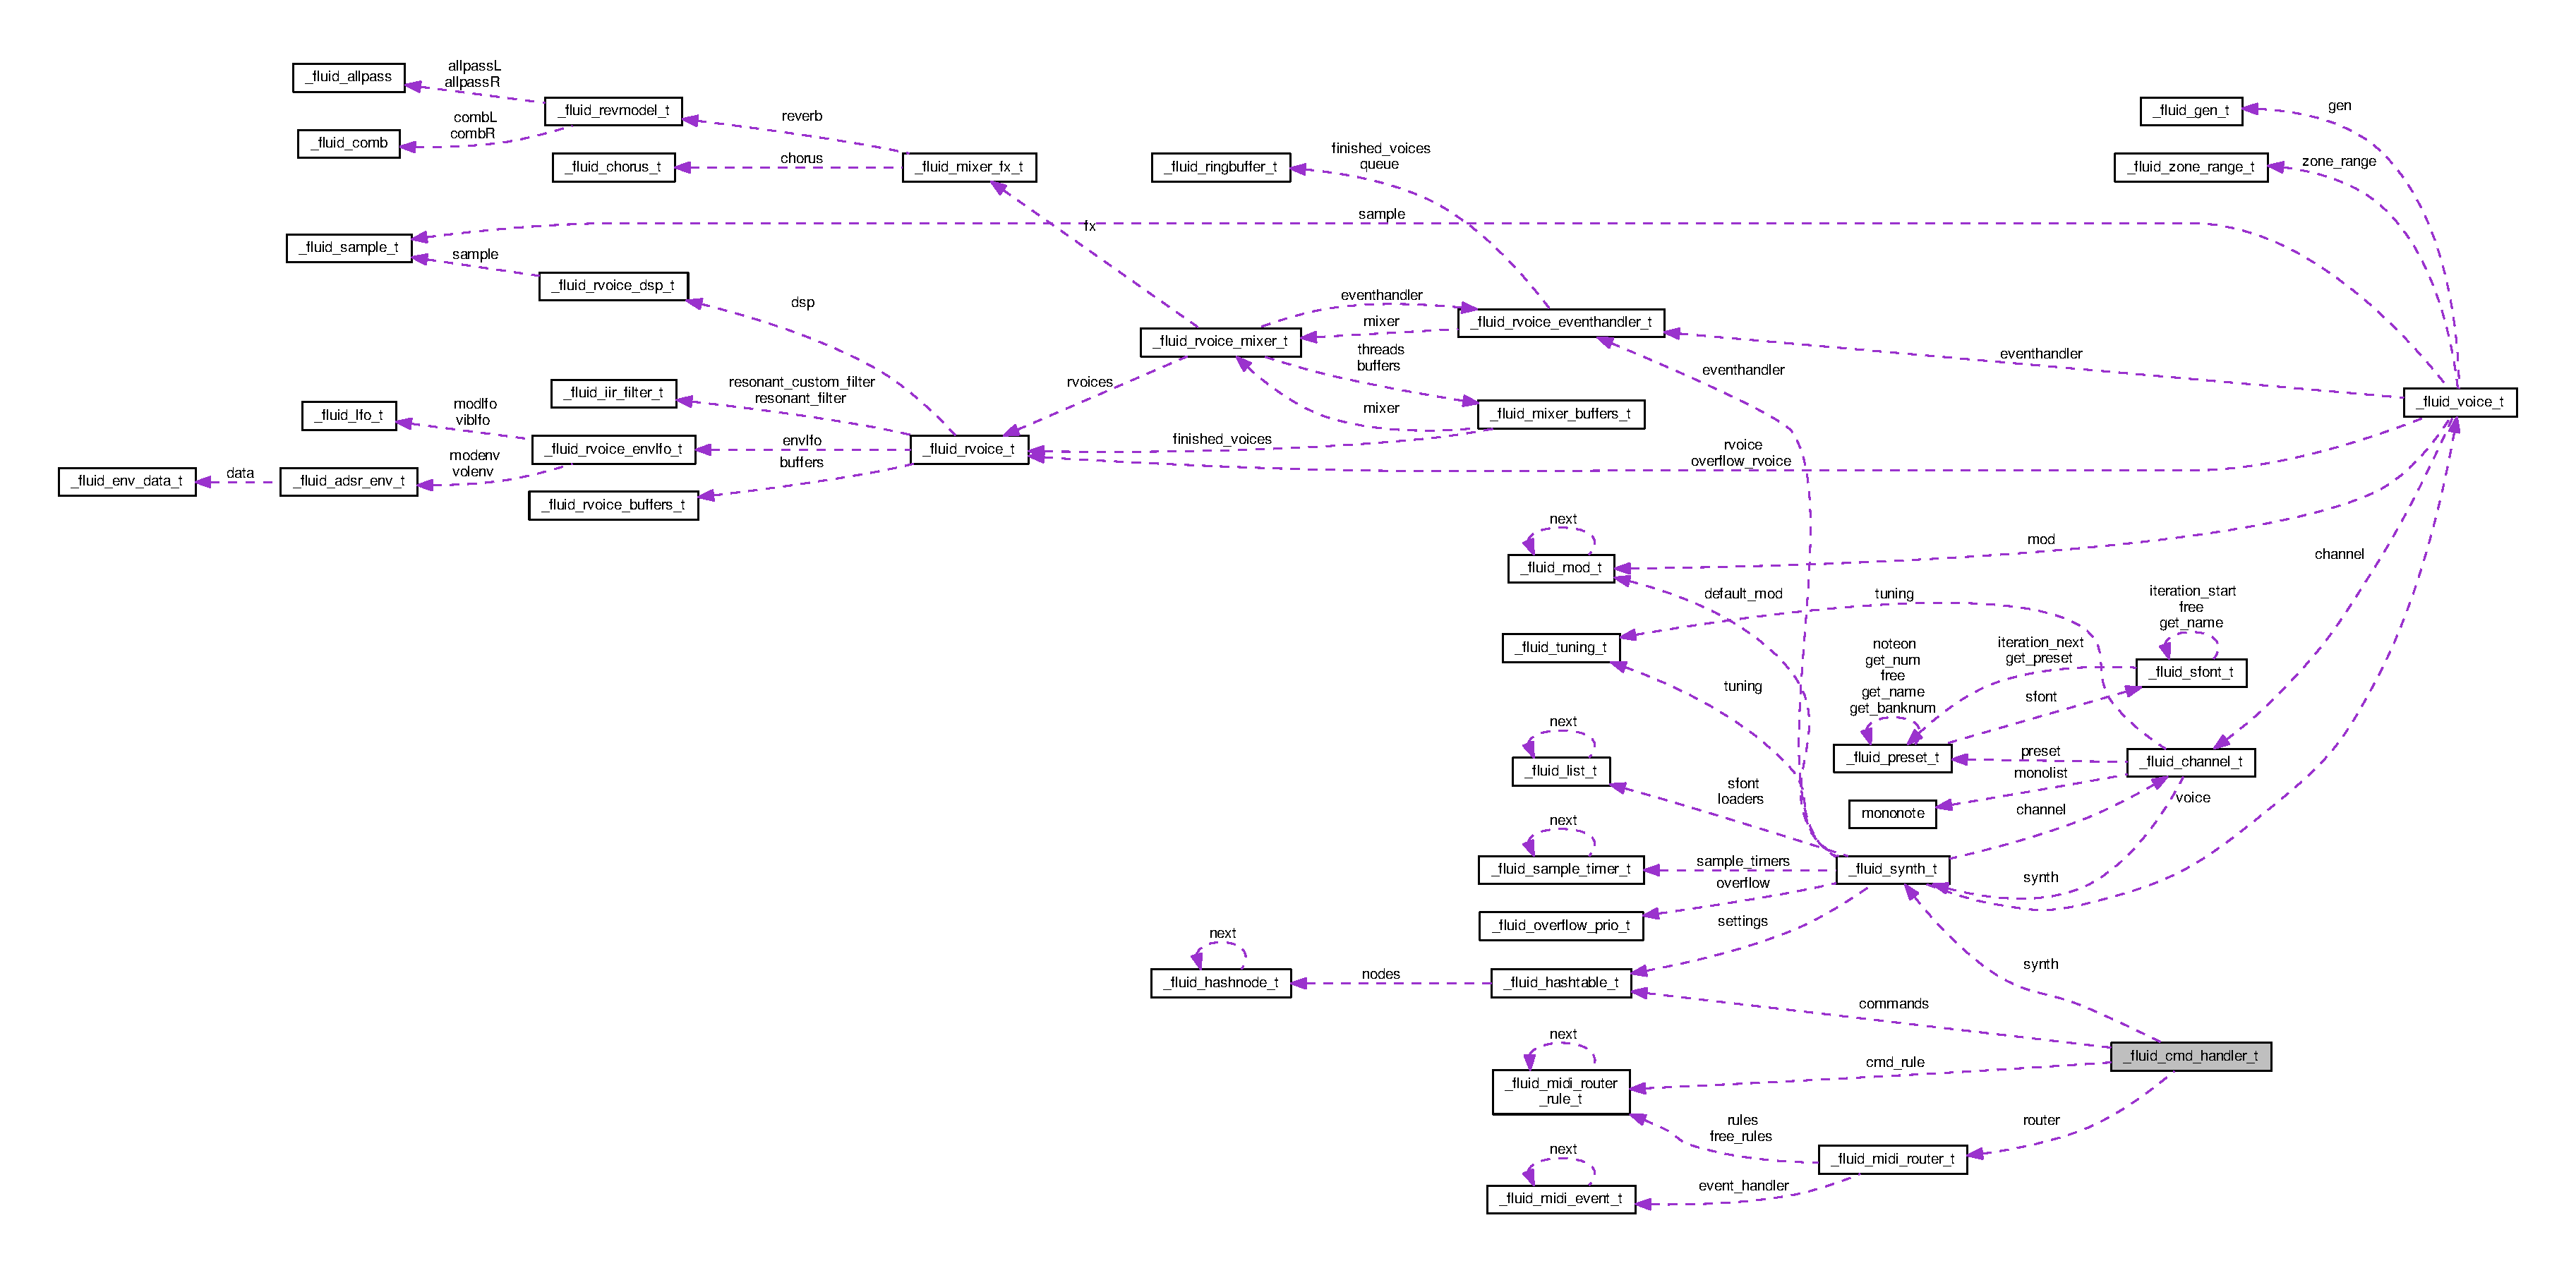
\includegraphics[width=350pt]{struct__fluid__cmd__handler__t__coll__graph}
\end{center}
\end{figure}
\subsection*{Public Attributes}
\begin{DoxyCompactItemize}
\item 
\hyperlink{types_8h_ae265f10ae174a13afe010de50d87e1a4}{fluid\+\_\+synth\+\_\+t} $\ast$ \hyperlink{struct__fluid__cmd__handler__t_a8a9b69dc646976e07a15fe815bcf811f}{synth}
\item 
\hyperlink{types_8h_aa57b4746220e24506a169f109875e4ad}{fluid\+\_\+midi\+\_\+router\+\_\+t} $\ast$ \hyperlink{struct__fluid__cmd__handler__t_ab9df6a4bfe87019036cb7af62b661b3e}{router}
\item 
\hyperlink{types_8h_a23619a0660e3b26610ee991eb9d0f5fc}{fluid\+\_\+cmd\+\_\+hash\+\_\+t} $\ast$ \hyperlink{struct__fluid__cmd__handler__t_acd4935aa36a49fef19f9d1ed68a5df43}{commands}
\item 
\hyperlink{types_8h_a3154253ddb8f9b8f8f737c91f5973278}{fluid\+\_\+midi\+\_\+router\+\_\+rule\+\_\+t} $\ast$ \hyperlink{struct__fluid__cmd__handler__t_a45e2cc5fe2c0b1190d2d58d64c9ba5a3}{cmd\+\_\+rule}
\item 
int \hyperlink{struct__fluid__cmd__handler__t_a13fb833f49573bce26b5240816d49f51}{cmd\+\_\+rule\+\_\+type}
\end{DoxyCompactItemize}


\subsection{Member Data Documentation}
\mbox{\Hypertarget{struct__fluid__cmd__handler__t_a45e2cc5fe2c0b1190d2d58d64c9ba5a3}\label{struct__fluid__cmd__handler__t_a45e2cc5fe2c0b1190d2d58d64c9ba5a3}} 
\index{\+\_\+fluid\+\_\+cmd\+\_\+handler\+\_\+t@{\+\_\+fluid\+\_\+cmd\+\_\+handler\+\_\+t}!cmd\+\_\+rule@{cmd\+\_\+rule}}
\index{cmd\+\_\+rule@{cmd\+\_\+rule}!\+\_\+fluid\+\_\+cmd\+\_\+handler\+\_\+t@{\+\_\+fluid\+\_\+cmd\+\_\+handler\+\_\+t}}
\subsubsection{\texorpdfstring{cmd\+\_\+rule}{cmd\_rule}}
{\footnotesize\ttfamily \hyperlink{types_8h_a3154253ddb8f9b8f8f737c91f5973278}{fluid\+\_\+midi\+\_\+router\+\_\+rule\+\_\+t}$\ast$ \+\_\+fluid\+\_\+cmd\+\_\+handler\+\_\+t\+::cmd\+\_\+rule}

\mbox{\Hypertarget{struct__fluid__cmd__handler__t_a13fb833f49573bce26b5240816d49f51}\label{struct__fluid__cmd__handler__t_a13fb833f49573bce26b5240816d49f51}} 
\index{\+\_\+fluid\+\_\+cmd\+\_\+handler\+\_\+t@{\+\_\+fluid\+\_\+cmd\+\_\+handler\+\_\+t}!cmd\+\_\+rule\+\_\+type@{cmd\+\_\+rule\+\_\+type}}
\index{cmd\+\_\+rule\+\_\+type@{cmd\+\_\+rule\+\_\+type}!\+\_\+fluid\+\_\+cmd\+\_\+handler\+\_\+t@{\+\_\+fluid\+\_\+cmd\+\_\+handler\+\_\+t}}
\subsubsection{\texorpdfstring{cmd\+\_\+rule\+\_\+type}{cmd\_rule\_type}}
{\footnotesize\ttfamily int \+\_\+fluid\+\_\+cmd\+\_\+handler\+\_\+t\+::cmd\+\_\+rule\+\_\+type}

\mbox{\Hypertarget{struct__fluid__cmd__handler__t_acd4935aa36a49fef19f9d1ed68a5df43}\label{struct__fluid__cmd__handler__t_acd4935aa36a49fef19f9d1ed68a5df43}} 
\index{\+\_\+fluid\+\_\+cmd\+\_\+handler\+\_\+t@{\+\_\+fluid\+\_\+cmd\+\_\+handler\+\_\+t}!commands@{commands}}
\index{commands@{commands}!\+\_\+fluid\+\_\+cmd\+\_\+handler\+\_\+t@{\+\_\+fluid\+\_\+cmd\+\_\+handler\+\_\+t}}
\subsubsection{\texorpdfstring{commands}{commands}}
{\footnotesize\ttfamily \hyperlink{types_8h_a23619a0660e3b26610ee991eb9d0f5fc}{fluid\+\_\+cmd\+\_\+hash\+\_\+t}$\ast$ \+\_\+fluid\+\_\+cmd\+\_\+handler\+\_\+t\+::commands}

\mbox{\Hypertarget{struct__fluid__cmd__handler__t_ab9df6a4bfe87019036cb7af62b661b3e}\label{struct__fluid__cmd__handler__t_ab9df6a4bfe87019036cb7af62b661b3e}} 
\index{\+\_\+fluid\+\_\+cmd\+\_\+handler\+\_\+t@{\+\_\+fluid\+\_\+cmd\+\_\+handler\+\_\+t}!router@{router}}
\index{router@{router}!\+\_\+fluid\+\_\+cmd\+\_\+handler\+\_\+t@{\+\_\+fluid\+\_\+cmd\+\_\+handler\+\_\+t}}
\subsubsection{\texorpdfstring{router}{router}}
{\footnotesize\ttfamily \hyperlink{types_8h_aa57b4746220e24506a169f109875e4ad}{fluid\+\_\+midi\+\_\+router\+\_\+t}$\ast$ \+\_\+fluid\+\_\+cmd\+\_\+handler\+\_\+t\+::router}

\mbox{\Hypertarget{struct__fluid__cmd__handler__t_a8a9b69dc646976e07a15fe815bcf811f}\label{struct__fluid__cmd__handler__t_a8a9b69dc646976e07a15fe815bcf811f}} 
\index{\+\_\+fluid\+\_\+cmd\+\_\+handler\+\_\+t@{\+\_\+fluid\+\_\+cmd\+\_\+handler\+\_\+t}!synth@{synth}}
\index{synth@{synth}!\+\_\+fluid\+\_\+cmd\+\_\+handler\+\_\+t@{\+\_\+fluid\+\_\+cmd\+\_\+handler\+\_\+t}}
\subsubsection{\texorpdfstring{synth}{synth}}
{\footnotesize\ttfamily \hyperlink{types_8h_ae265f10ae174a13afe010de50d87e1a4}{fluid\+\_\+synth\+\_\+t}$\ast$ \+\_\+fluid\+\_\+cmd\+\_\+handler\+\_\+t\+::synth}



The documentation for this struct was generated from the following file\+:\begin{DoxyCompactItemize}
\item 
bindings/\hyperlink{fluid__cmd_8c}{fluid\+\_\+cmd.\+c}\end{DoxyCompactItemize}

\hypertarget{struct__fluid__comb}{}\section{\+\_\+fluid\+\_\+comb Struct Reference}
\label{struct__fluid__comb}\index{\+\_\+fluid\+\_\+comb@{\+\_\+fluid\+\_\+comb}}
\subsection*{Public Attributes}
\begin{DoxyCompactItemize}
\item 
\hyperlink{fluidsynth__priv_8h_a9e96f0917747b69cabb7c671bc693dbb}{fluid\+\_\+real\+\_\+t} \hyperlink{struct__fluid__comb_ad94390e338a44120748e6cf446ab5ef1}{feedback}
\item 
\hyperlink{fluidsynth__priv_8h_a9e96f0917747b69cabb7c671bc693dbb}{fluid\+\_\+real\+\_\+t} \hyperlink{struct__fluid__comb_a52d450869a07862b168617759e025819}{filterstore}
\item 
\hyperlink{fluidsynth__priv_8h_a9e96f0917747b69cabb7c671bc693dbb}{fluid\+\_\+real\+\_\+t} \hyperlink{struct__fluid__comb_a4e8d996189a50c09e85f4388872c54d0}{damp1}
\item 
\hyperlink{fluidsynth__priv_8h_a9e96f0917747b69cabb7c671bc693dbb}{fluid\+\_\+real\+\_\+t} \hyperlink{struct__fluid__comb_ab29ff3f46d2d9a7277a80b86a2e35008}{damp2}
\item 
\hyperlink{fluidsynth__priv_8h_a9e96f0917747b69cabb7c671bc693dbb}{fluid\+\_\+real\+\_\+t} $\ast$ \hyperlink{struct__fluid__comb_a46f9c845ccef5871ba5a6939995a239d}{buffer}
\item 
int \hyperlink{struct__fluid__comb_a12ba7dddd473b3165beef8fcd7b3d972}{bufsize}
\item 
int \hyperlink{struct__fluid__comb_ae69643c75f700881d53bcbb65bf9212a}{bufidx}
\end{DoxyCompactItemize}


\subsection{Member Data Documentation}
\mbox{\Hypertarget{struct__fluid__comb_a46f9c845ccef5871ba5a6939995a239d}\label{struct__fluid__comb_a46f9c845ccef5871ba5a6939995a239d}} 
\index{\+\_\+fluid\+\_\+comb@{\+\_\+fluid\+\_\+comb}!buffer@{buffer}}
\index{buffer@{buffer}!\+\_\+fluid\+\_\+comb@{\+\_\+fluid\+\_\+comb}}
\subsubsection{\texorpdfstring{buffer}{buffer}}
{\footnotesize\ttfamily \hyperlink{fluidsynth__priv_8h_a9e96f0917747b69cabb7c671bc693dbb}{fluid\+\_\+real\+\_\+t}$\ast$ \+\_\+fluid\+\_\+comb\+::buffer}

\mbox{\Hypertarget{struct__fluid__comb_ae69643c75f700881d53bcbb65bf9212a}\label{struct__fluid__comb_ae69643c75f700881d53bcbb65bf9212a}} 
\index{\+\_\+fluid\+\_\+comb@{\+\_\+fluid\+\_\+comb}!bufidx@{bufidx}}
\index{bufidx@{bufidx}!\+\_\+fluid\+\_\+comb@{\+\_\+fluid\+\_\+comb}}
\subsubsection{\texorpdfstring{bufidx}{bufidx}}
{\footnotesize\ttfamily int \+\_\+fluid\+\_\+comb\+::bufidx}

\mbox{\Hypertarget{struct__fluid__comb_a12ba7dddd473b3165beef8fcd7b3d972}\label{struct__fluid__comb_a12ba7dddd473b3165beef8fcd7b3d972}} 
\index{\+\_\+fluid\+\_\+comb@{\+\_\+fluid\+\_\+comb}!bufsize@{bufsize}}
\index{bufsize@{bufsize}!\+\_\+fluid\+\_\+comb@{\+\_\+fluid\+\_\+comb}}
\subsubsection{\texorpdfstring{bufsize}{bufsize}}
{\footnotesize\ttfamily int \+\_\+fluid\+\_\+comb\+::bufsize}

\mbox{\Hypertarget{struct__fluid__comb_a4e8d996189a50c09e85f4388872c54d0}\label{struct__fluid__comb_a4e8d996189a50c09e85f4388872c54d0}} 
\index{\+\_\+fluid\+\_\+comb@{\+\_\+fluid\+\_\+comb}!damp1@{damp1}}
\index{damp1@{damp1}!\+\_\+fluid\+\_\+comb@{\+\_\+fluid\+\_\+comb}}
\subsubsection{\texorpdfstring{damp1}{damp1}}
{\footnotesize\ttfamily \hyperlink{fluidsynth__priv_8h_a9e96f0917747b69cabb7c671bc693dbb}{fluid\+\_\+real\+\_\+t} \+\_\+fluid\+\_\+comb\+::damp1}

\mbox{\Hypertarget{struct__fluid__comb_ab29ff3f46d2d9a7277a80b86a2e35008}\label{struct__fluid__comb_ab29ff3f46d2d9a7277a80b86a2e35008}} 
\index{\+\_\+fluid\+\_\+comb@{\+\_\+fluid\+\_\+comb}!damp2@{damp2}}
\index{damp2@{damp2}!\+\_\+fluid\+\_\+comb@{\+\_\+fluid\+\_\+comb}}
\subsubsection{\texorpdfstring{damp2}{damp2}}
{\footnotesize\ttfamily \hyperlink{fluidsynth__priv_8h_a9e96f0917747b69cabb7c671bc693dbb}{fluid\+\_\+real\+\_\+t} \+\_\+fluid\+\_\+comb\+::damp2}

\mbox{\Hypertarget{struct__fluid__comb_ad94390e338a44120748e6cf446ab5ef1}\label{struct__fluid__comb_ad94390e338a44120748e6cf446ab5ef1}} 
\index{\+\_\+fluid\+\_\+comb@{\+\_\+fluid\+\_\+comb}!feedback@{feedback}}
\index{feedback@{feedback}!\+\_\+fluid\+\_\+comb@{\+\_\+fluid\+\_\+comb}}
\subsubsection{\texorpdfstring{feedback}{feedback}}
{\footnotesize\ttfamily \hyperlink{fluidsynth__priv_8h_a9e96f0917747b69cabb7c671bc693dbb}{fluid\+\_\+real\+\_\+t} \+\_\+fluid\+\_\+comb\+::feedback}

\mbox{\Hypertarget{struct__fluid__comb_a52d450869a07862b168617759e025819}\label{struct__fluid__comb_a52d450869a07862b168617759e025819}} 
\index{\+\_\+fluid\+\_\+comb@{\+\_\+fluid\+\_\+comb}!filterstore@{filterstore}}
\index{filterstore@{filterstore}!\+\_\+fluid\+\_\+comb@{\+\_\+fluid\+\_\+comb}}
\subsubsection{\texorpdfstring{filterstore}{filterstore}}
{\footnotesize\ttfamily \hyperlink{fluidsynth__priv_8h_a9e96f0917747b69cabb7c671bc693dbb}{fluid\+\_\+real\+\_\+t} \+\_\+fluid\+\_\+comb\+::filterstore}



The documentation for this struct was generated from the following file\+:\begin{DoxyCompactItemize}
\item 
rvoice/\hyperlink{fluid__rev_8c}{fluid\+\_\+rev.\+c}\end{DoxyCompactItemize}

\hypertarget{struct__fluid__defpreset__t}{}\section{\+\_\+fluid\+\_\+defpreset\+\_\+t Struct Reference}
\label{struct__fluid__defpreset__t}\index{\+\_\+fluid\+\_\+defpreset\+\_\+t@{\+\_\+fluid\+\_\+defpreset\+\_\+t}}


{\ttfamily \#include $<$fluid\+\_\+defsfont.\+h$>$}



Collaboration diagram for \+\_\+fluid\+\_\+defpreset\+\_\+t\+:
\nopagebreak
\begin{figure}[H]
\begin{center}
\leavevmode
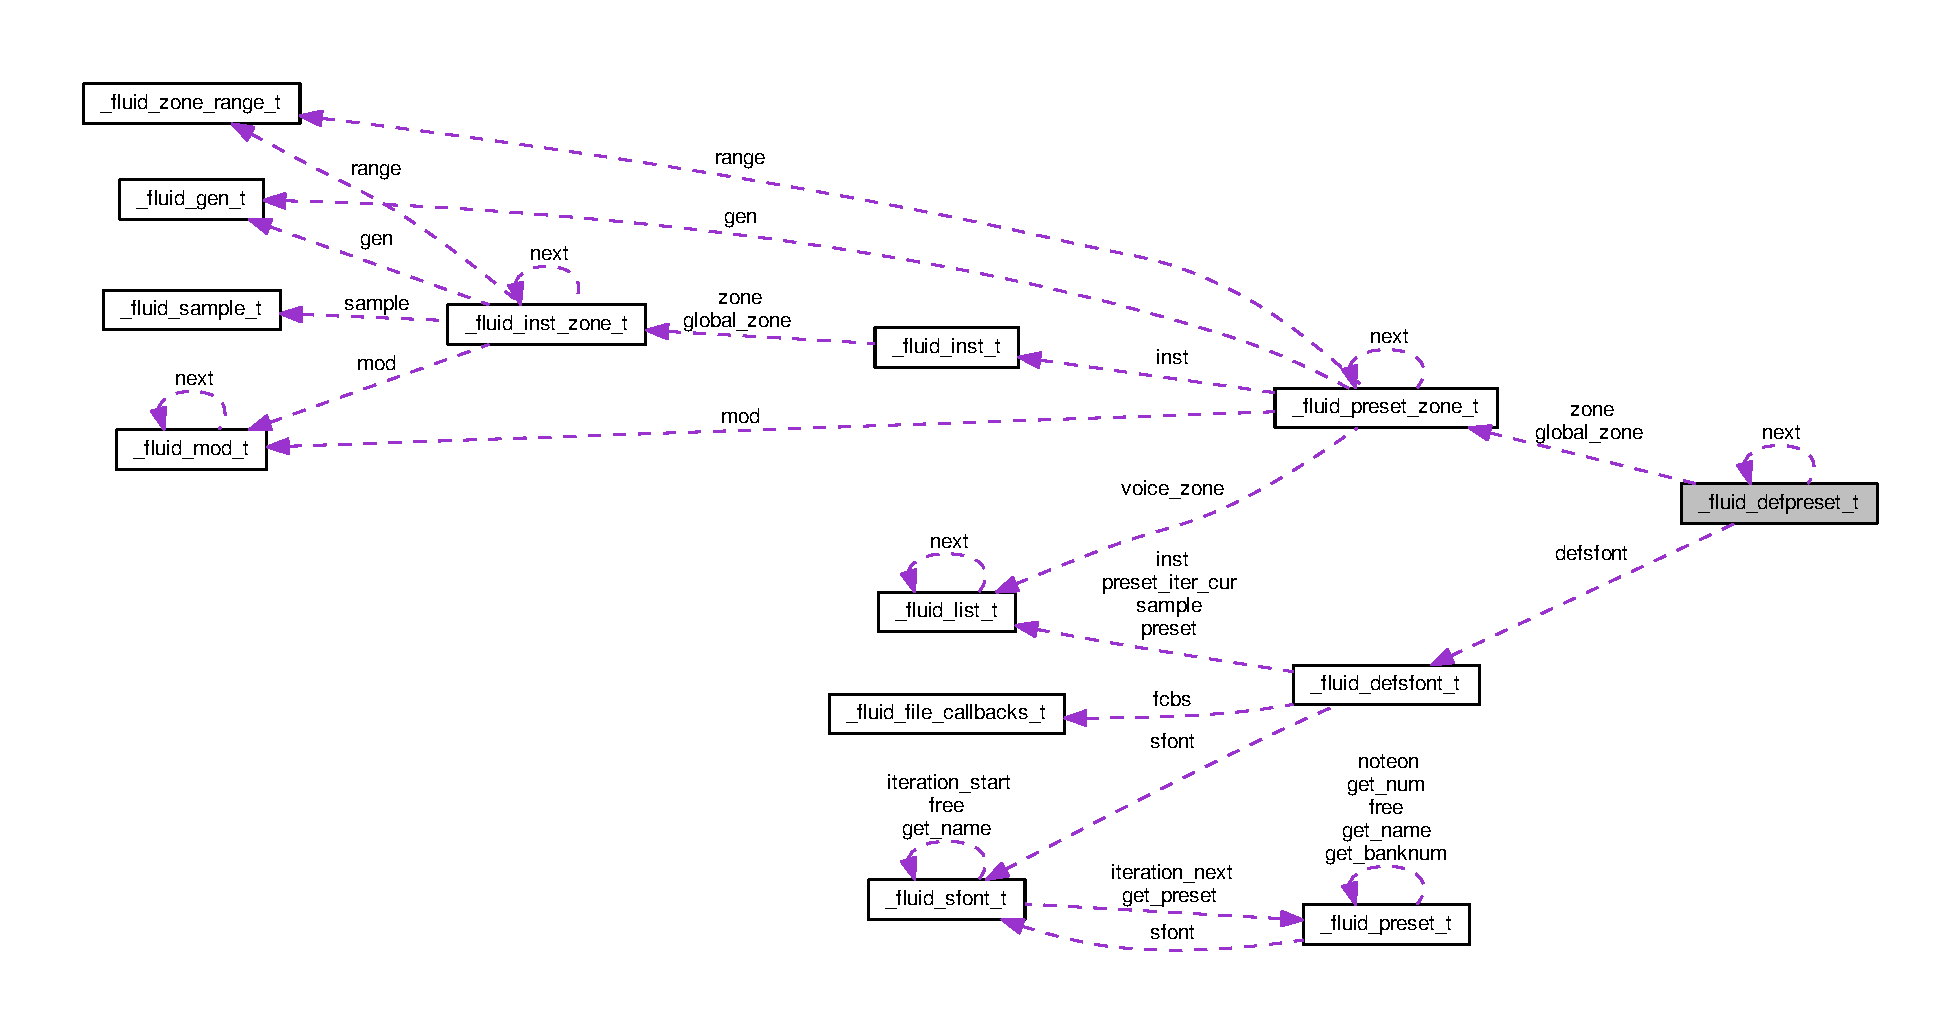
\includegraphics[width=350pt]{struct__fluid__defpreset__t__coll__graph}
\end{center}
\end{figure}
\subsection*{Public Attributes}
\begin{DoxyCompactItemize}
\item 
\hyperlink{fluid__defsfont_8h_a2c2cb41581f95588f665a8f8fe593e18}{fluid\+\_\+defpreset\+\_\+t} $\ast$ \hyperlink{struct__fluid__defpreset__t_a3e0dabe06dd2004596b5b130075b197d}{next}
\item 
\hyperlink{fluid__defsfont_8h_a13799d8f15556117d126e63abd4f40d3}{fluid\+\_\+defsfont\+\_\+t} $\ast$ \hyperlink{struct__fluid__defpreset__t_a2de7477576ee89b8c1dd89762d4f6e0e}{defsfont}
\item 
char \hyperlink{struct__fluid__defpreset__t_a3d29b2417eac798a611e514f780e0808}{name} \mbox{[}21\mbox{]}
\item 
unsigned int \hyperlink{struct__fluid__defpreset__t_aa3933c1b4478be9784304058ab340fe7}{bank}
\item 
unsigned int \hyperlink{struct__fluid__defpreset__t_a401ae39156d3d4c41a5a76a754495abf}{num}
\item 
\hyperlink{fluid__defsfont_8h_a74cb7075332911049d39e60df50019b2}{fluid\+\_\+preset\+\_\+zone\+\_\+t} $\ast$ \hyperlink{struct__fluid__defpreset__t_a8436bd7f9e2fbab916287d8d1522d192}{global\+\_\+zone}
\item 
\hyperlink{fluid__defsfont_8h_a74cb7075332911049d39e60df50019b2}{fluid\+\_\+preset\+\_\+zone\+\_\+t} $\ast$ \hyperlink{struct__fluid__defpreset__t_a470612eff6fe4a286e48a013b17cafdd}{zone}
\end{DoxyCompactItemize}


\subsection{Member Data Documentation}
\mbox{\Hypertarget{struct__fluid__defpreset__t_aa3933c1b4478be9784304058ab340fe7}\label{struct__fluid__defpreset__t_aa3933c1b4478be9784304058ab340fe7}} 
\index{\+\_\+fluid\+\_\+defpreset\+\_\+t@{\+\_\+fluid\+\_\+defpreset\+\_\+t}!bank@{bank}}
\index{bank@{bank}!\+\_\+fluid\+\_\+defpreset\+\_\+t@{\+\_\+fluid\+\_\+defpreset\+\_\+t}}
\subsubsection{\texorpdfstring{bank}{bank}}
{\footnotesize\ttfamily unsigned int \+\_\+fluid\+\_\+defpreset\+\_\+t\+::bank}

\mbox{\Hypertarget{struct__fluid__defpreset__t_a2de7477576ee89b8c1dd89762d4f6e0e}\label{struct__fluid__defpreset__t_a2de7477576ee89b8c1dd89762d4f6e0e}} 
\index{\+\_\+fluid\+\_\+defpreset\+\_\+t@{\+\_\+fluid\+\_\+defpreset\+\_\+t}!defsfont@{defsfont}}
\index{defsfont@{defsfont}!\+\_\+fluid\+\_\+defpreset\+\_\+t@{\+\_\+fluid\+\_\+defpreset\+\_\+t}}
\subsubsection{\texorpdfstring{defsfont}{defsfont}}
{\footnotesize\ttfamily \hyperlink{fluid__defsfont_8h_a13799d8f15556117d126e63abd4f40d3}{fluid\+\_\+defsfont\+\_\+t}$\ast$ \+\_\+fluid\+\_\+defpreset\+\_\+t\+::defsfont}

\mbox{\Hypertarget{struct__fluid__defpreset__t_a8436bd7f9e2fbab916287d8d1522d192}\label{struct__fluid__defpreset__t_a8436bd7f9e2fbab916287d8d1522d192}} 
\index{\+\_\+fluid\+\_\+defpreset\+\_\+t@{\+\_\+fluid\+\_\+defpreset\+\_\+t}!global\+\_\+zone@{global\+\_\+zone}}
\index{global\+\_\+zone@{global\+\_\+zone}!\+\_\+fluid\+\_\+defpreset\+\_\+t@{\+\_\+fluid\+\_\+defpreset\+\_\+t}}
\subsubsection{\texorpdfstring{global\+\_\+zone}{global\_zone}}
{\footnotesize\ttfamily \hyperlink{fluid__defsfont_8h_a74cb7075332911049d39e60df50019b2}{fluid\+\_\+preset\+\_\+zone\+\_\+t}$\ast$ \+\_\+fluid\+\_\+defpreset\+\_\+t\+::global\+\_\+zone}

\mbox{\Hypertarget{struct__fluid__defpreset__t_a3d29b2417eac798a611e514f780e0808}\label{struct__fluid__defpreset__t_a3d29b2417eac798a611e514f780e0808}} 
\index{\+\_\+fluid\+\_\+defpreset\+\_\+t@{\+\_\+fluid\+\_\+defpreset\+\_\+t}!name@{name}}
\index{name@{name}!\+\_\+fluid\+\_\+defpreset\+\_\+t@{\+\_\+fluid\+\_\+defpreset\+\_\+t}}
\subsubsection{\texorpdfstring{name}{name}}
{\footnotesize\ttfamily char \+\_\+fluid\+\_\+defpreset\+\_\+t\+::name\mbox{[}21\mbox{]}}

\mbox{\Hypertarget{struct__fluid__defpreset__t_a3e0dabe06dd2004596b5b130075b197d}\label{struct__fluid__defpreset__t_a3e0dabe06dd2004596b5b130075b197d}} 
\index{\+\_\+fluid\+\_\+defpreset\+\_\+t@{\+\_\+fluid\+\_\+defpreset\+\_\+t}!next@{next}}
\index{next@{next}!\+\_\+fluid\+\_\+defpreset\+\_\+t@{\+\_\+fluid\+\_\+defpreset\+\_\+t}}
\subsubsection{\texorpdfstring{next}{next}}
{\footnotesize\ttfamily \hyperlink{fluid__defsfont_8h_a2c2cb41581f95588f665a8f8fe593e18}{fluid\+\_\+defpreset\+\_\+t}$\ast$ \+\_\+fluid\+\_\+defpreset\+\_\+t\+::next}

\mbox{\Hypertarget{struct__fluid__defpreset__t_a401ae39156d3d4c41a5a76a754495abf}\label{struct__fluid__defpreset__t_a401ae39156d3d4c41a5a76a754495abf}} 
\index{\+\_\+fluid\+\_\+defpreset\+\_\+t@{\+\_\+fluid\+\_\+defpreset\+\_\+t}!num@{num}}
\index{num@{num}!\+\_\+fluid\+\_\+defpreset\+\_\+t@{\+\_\+fluid\+\_\+defpreset\+\_\+t}}
\subsubsection{\texorpdfstring{num}{num}}
{\footnotesize\ttfamily unsigned int \+\_\+fluid\+\_\+defpreset\+\_\+t\+::num}

\mbox{\Hypertarget{struct__fluid__defpreset__t_a470612eff6fe4a286e48a013b17cafdd}\label{struct__fluid__defpreset__t_a470612eff6fe4a286e48a013b17cafdd}} 
\index{\+\_\+fluid\+\_\+defpreset\+\_\+t@{\+\_\+fluid\+\_\+defpreset\+\_\+t}!zone@{zone}}
\index{zone@{zone}!\+\_\+fluid\+\_\+defpreset\+\_\+t@{\+\_\+fluid\+\_\+defpreset\+\_\+t}}
\subsubsection{\texorpdfstring{zone}{zone}}
{\footnotesize\ttfamily \hyperlink{fluid__defsfont_8h_a74cb7075332911049d39e60df50019b2}{fluid\+\_\+preset\+\_\+zone\+\_\+t}$\ast$ \+\_\+fluid\+\_\+defpreset\+\_\+t\+::zone}



The documentation for this struct was generated from the following file\+:\begin{DoxyCompactItemize}
\item 
sfloader/\hyperlink{fluid__defsfont_8h}{fluid\+\_\+defsfont.\+h}\end{DoxyCompactItemize}

\hypertarget{struct__fluid__defsfont__t}{}\section{\+\_\+fluid\+\_\+defsfont\+\_\+t Struct Reference}
\label{struct__fluid__defsfont__t}\index{\+\_\+fluid\+\_\+defsfont\+\_\+t@{\+\_\+fluid\+\_\+defsfont\+\_\+t}}


{\ttfamily \#include $<$fluid\+\_\+defsfont.\+h$>$}



Collaboration diagram for \+\_\+fluid\+\_\+defsfont\+\_\+t\+:
\nopagebreak
\begin{figure}[H]
\begin{center}
\leavevmode
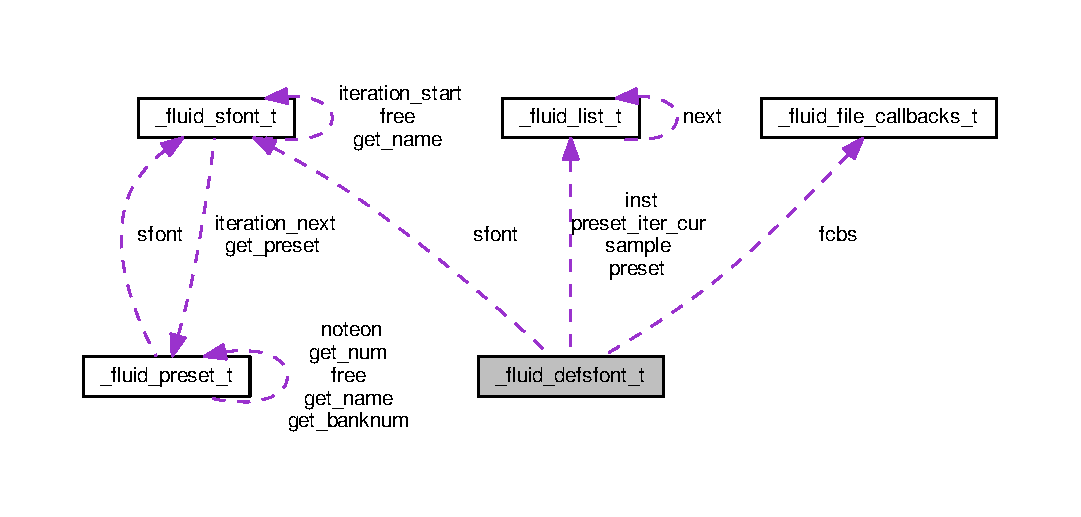
\includegraphics[width=350pt]{struct__fluid__defsfont__t__coll__graph}
\end{center}
\end{figure}
\subsection*{Public Attributes}
\begin{DoxyCompactItemize}
\item 
const \hyperlink{types_8h_a6a223e4b8d83753d95c87e1feed58227}{fluid\+\_\+file\+\_\+callbacks\+\_\+t} $\ast$ \hyperlink{struct__fluid__defsfont__t_ae78f94e5815c8a7daf73916f63b391a0}{fcbs}
\item 
char $\ast$ \hyperlink{struct__fluid__defsfont__t_a3c8383fe342b4572d39b6655854fbd0f}{filename}
\item 
unsigned int \hyperlink{struct__fluid__defsfont__t_a7dfd41e3bb8cd63cf9c10d168597bc47}{samplepos}
\item 
unsigned int \hyperlink{struct__fluid__defsfont__t_a0e31704a1a08094fdbb8a52d34978597}{samplesize}
\item 
short $\ast$ \hyperlink{struct__fluid__defsfont__t_a681b14f9f5f55cad164a9772e3c24799}{sampledata}
\item 
unsigned int \hyperlink{struct__fluid__defsfont__t_a80d20a1f381fdcca679536eb3c495515}{sample24pos}
\item 
unsigned int \hyperlink{struct__fluid__defsfont__t_a57f71bef06db12ccb3dbcbb05e92b6bf}{sample24size}
\item 
char $\ast$ \hyperlink{struct__fluid__defsfont__t_a33177bce06851265e920871c1fe0e3a5}{sample24data}
\item 
\hyperlink{types_8h_aa6c18288f76608acbb10b80a153f4ab8}{fluid\+\_\+sfont\+\_\+t} $\ast$ \hyperlink{struct__fluid__defsfont__t_a8e1269657bcfc41386c16d0afee66bfe}{sfont}
\item 
\hyperlink{fluid__list_8h_a3ef7535d4290862c0af118569223bd89}{fluid\+\_\+list\+\_\+t} $\ast$ \hyperlink{struct__fluid__defsfont__t_af755f0c3f0fc02eb14bd70a50eb00019}{sample}
\item 
\hyperlink{fluid__list_8h_a3ef7535d4290862c0af118569223bd89}{fluid\+\_\+list\+\_\+t} $\ast$ \hyperlink{struct__fluid__defsfont__t_ade9d658a84649022b884db9c73888b73}{preset}
\item 
\hyperlink{fluid__list_8h_a3ef7535d4290862c0af118569223bd89}{fluid\+\_\+list\+\_\+t} $\ast$ \hyperlink{struct__fluid__defsfont__t_aed0ba33a803a6924426846b62d756372}{inst}
\item 
int \hyperlink{struct__fluid__defsfont__t_a3b53f413ad87f473cb41ade75efaede6}{mlock}
\item 
int \hyperlink{struct__fluid__defsfont__t_a1282ea7ed390d947edda342d8820c7bf}{dynamic\+\_\+samples}
\item 
\hyperlink{fluid__list_8h_a3ef7535d4290862c0af118569223bd89}{fluid\+\_\+list\+\_\+t} $\ast$ \hyperlink{struct__fluid__defsfont__t_a4ffede8ee7314ad0de689fa06d7a2034}{preset\+\_\+iter\+\_\+cur}
\end{DoxyCompactItemize}


\subsection{Member Data Documentation}
\mbox{\Hypertarget{struct__fluid__defsfont__t_a1282ea7ed390d947edda342d8820c7bf}\label{struct__fluid__defsfont__t_a1282ea7ed390d947edda342d8820c7bf}} 
\index{\+\_\+fluid\+\_\+defsfont\+\_\+t@{\+\_\+fluid\+\_\+defsfont\+\_\+t}!dynamic\+\_\+samples@{dynamic\+\_\+samples}}
\index{dynamic\+\_\+samples@{dynamic\+\_\+samples}!\+\_\+fluid\+\_\+defsfont\+\_\+t@{\+\_\+fluid\+\_\+defsfont\+\_\+t}}
\subsubsection{\texorpdfstring{dynamic\+\_\+samples}{dynamic\_samples}}
{\footnotesize\ttfamily int \+\_\+fluid\+\_\+defsfont\+\_\+t\+::dynamic\+\_\+samples}

\mbox{\Hypertarget{struct__fluid__defsfont__t_ae78f94e5815c8a7daf73916f63b391a0}\label{struct__fluid__defsfont__t_ae78f94e5815c8a7daf73916f63b391a0}} 
\index{\+\_\+fluid\+\_\+defsfont\+\_\+t@{\+\_\+fluid\+\_\+defsfont\+\_\+t}!fcbs@{fcbs}}
\index{fcbs@{fcbs}!\+\_\+fluid\+\_\+defsfont\+\_\+t@{\+\_\+fluid\+\_\+defsfont\+\_\+t}}
\subsubsection{\texorpdfstring{fcbs}{fcbs}}
{\footnotesize\ttfamily const \hyperlink{types_8h_a6a223e4b8d83753d95c87e1feed58227}{fluid\+\_\+file\+\_\+callbacks\+\_\+t}$\ast$ \+\_\+fluid\+\_\+defsfont\+\_\+t\+::fcbs}

\mbox{\Hypertarget{struct__fluid__defsfont__t_a3c8383fe342b4572d39b6655854fbd0f}\label{struct__fluid__defsfont__t_a3c8383fe342b4572d39b6655854fbd0f}} 
\index{\+\_\+fluid\+\_\+defsfont\+\_\+t@{\+\_\+fluid\+\_\+defsfont\+\_\+t}!filename@{filename}}
\index{filename@{filename}!\+\_\+fluid\+\_\+defsfont\+\_\+t@{\+\_\+fluid\+\_\+defsfont\+\_\+t}}
\subsubsection{\texorpdfstring{filename}{filename}}
{\footnotesize\ttfamily char$\ast$ \+\_\+fluid\+\_\+defsfont\+\_\+t\+::filename}

\mbox{\Hypertarget{struct__fluid__defsfont__t_aed0ba33a803a6924426846b62d756372}\label{struct__fluid__defsfont__t_aed0ba33a803a6924426846b62d756372}} 
\index{\+\_\+fluid\+\_\+defsfont\+\_\+t@{\+\_\+fluid\+\_\+defsfont\+\_\+t}!inst@{inst}}
\index{inst@{inst}!\+\_\+fluid\+\_\+defsfont\+\_\+t@{\+\_\+fluid\+\_\+defsfont\+\_\+t}}
\subsubsection{\texorpdfstring{inst}{inst}}
{\footnotesize\ttfamily \hyperlink{fluid__list_8h_a3ef7535d4290862c0af118569223bd89}{fluid\+\_\+list\+\_\+t}$\ast$ \+\_\+fluid\+\_\+defsfont\+\_\+t\+::inst}

\mbox{\Hypertarget{struct__fluid__defsfont__t_a3b53f413ad87f473cb41ade75efaede6}\label{struct__fluid__defsfont__t_a3b53f413ad87f473cb41ade75efaede6}} 
\index{\+\_\+fluid\+\_\+defsfont\+\_\+t@{\+\_\+fluid\+\_\+defsfont\+\_\+t}!mlock@{mlock}}
\index{mlock@{mlock}!\+\_\+fluid\+\_\+defsfont\+\_\+t@{\+\_\+fluid\+\_\+defsfont\+\_\+t}}
\subsubsection{\texorpdfstring{mlock}{mlock}}
{\footnotesize\ttfamily int \+\_\+fluid\+\_\+defsfont\+\_\+t\+::mlock}

\mbox{\Hypertarget{struct__fluid__defsfont__t_ade9d658a84649022b884db9c73888b73}\label{struct__fluid__defsfont__t_ade9d658a84649022b884db9c73888b73}} 
\index{\+\_\+fluid\+\_\+defsfont\+\_\+t@{\+\_\+fluid\+\_\+defsfont\+\_\+t}!preset@{preset}}
\index{preset@{preset}!\+\_\+fluid\+\_\+defsfont\+\_\+t@{\+\_\+fluid\+\_\+defsfont\+\_\+t}}
\subsubsection{\texorpdfstring{preset}{preset}}
{\footnotesize\ttfamily \hyperlink{fluid__list_8h_a3ef7535d4290862c0af118569223bd89}{fluid\+\_\+list\+\_\+t}$\ast$ \+\_\+fluid\+\_\+defsfont\+\_\+t\+::preset}

\mbox{\Hypertarget{struct__fluid__defsfont__t_a4ffede8ee7314ad0de689fa06d7a2034}\label{struct__fluid__defsfont__t_a4ffede8ee7314ad0de689fa06d7a2034}} 
\index{\+\_\+fluid\+\_\+defsfont\+\_\+t@{\+\_\+fluid\+\_\+defsfont\+\_\+t}!preset\+\_\+iter\+\_\+cur@{preset\+\_\+iter\+\_\+cur}}
\index{preset\+\_\+iter\+\_\+cur@{preset\+\_\+iter\+\_\+cur}!\+\_\+fluid\+\_\+defsfont\+\_\+t@{\+\_\+fluid\+\_\+defsfont\+\_\+t}}
\subsubsection{\texorpdfstring{preset\+\_\+iter\+\_\+cur}{preset\_iter\_cur}}
{\footnotesize\ttfamily \hyperlink{fluid__list_8h_a3ef7535d4290862c0af118569223bd89}{fluid\+\_\+list\+\_\+t}$\ast$ \+\_\+fluid\+\_\+defsfont\+\_\+t\+::preset\+\_\+iter\+\_\+cur}

\mbox{\Hypertarget{struct__fluid__defsfont__t_af755f0c3f0fc02eb14bd70a50eb00019}\label{struct__fluid__defsfont__t_af755f0c3f0fc02eb14bd70a50eb00019}} 
\index{\+\_\+fluid\+\_\+defsfont\+\_\+t@{\+\_\+fluid\+\_\+defsfont\+\_\+t}!sample@{sample}}
\index{sample@{sample}!\+\_\+fluid\+\_\+defsfont\+\_\+t@{\+\_\+fluid\+\_\+defsfont\+\_\+t}}
\subsubsection{\texorpdfstring{sample}{sample}}
{\footnotesize\ttfamily \hyperlink{fluid__list_8h_a3ef7535d4290862c0af118569223bd89}{fluid\+\_\+list\+\_\+t}$\ast$ \+\_\+fluid\+\_\+defsfont\+\_\+t\+::sample}

\mbox{\Hypertarget{struct__fluid__defsfont__t_a33177bce06851265e920871c1fe0e3a5}\label{struct__fluid__defsfont__t_a33177bce06851265e920871c1fe0e3a5}} 
\index{\+\_\+fluid\+\_\+defsfont\+\_\+t@{\+\_\+fluid\+\_\+defsfont\+\_\+t}!sample24data@{sample24data}}
\index{sample24data@{sample24data}!\+\_\+fluid\+\_\+defsfont\+\_\+t@{\+\_\+fluid\+\_\+defsfont\+\_\+t}}
\subsubsection{\texorpdfstring{sample24data}{sample24data}}
{\footnotesize\ttfamily char$\ast$ \+\_\+fluid\+\_\+defsfont\+\_\+t\+::sample24data}

\mbox{\Hypertarget{struct__fluid__defsfont__t_a80d20a1f381fdcca679536eb3c495515}\label{struct__fluid__defsfont__t_a80d20a1f381fdcca679536eb3c495515}} 
\index{\+\_\+fluid\+\_\+defsfont\+\_\+t@{\+\_\+fluid\+\_\+defsfont\+\_\+t}!sample24pos@{sample24pos}}
\index{sample24pos@{sample24pos}!\+\_\+fluid\+\_\+defsfont\+\_\+t@{\+\_\+fluid\+\_\+defsfont\+\_\+t}}
\subsubsection{\texorpdfstring{sample24pos}{sample24pos}}
{\footnotesize\ttfamily unsigned int \+\_\+fluid\+\_\+defsfont\+\_\+t\+::sample24pos}

\mbox{\Hypertarget{struct__fluid__defsfont__t_a57f71bef06db12ccb3dbcbb05e92b6bf}\label{struct__fluid__defsfont__t_a57f71bef06db12ccb3dbcbb05e92b6bf}} 
\index{\+\_\+fluid\+\_\+defsfont\+\_\+t@{\+\_\+fluid\+\_\+defsfont\+\_\+t}!sample24size@{sample24size}}
\index{sample24size@{sample24size}!\+\_\+fluid\+\_\+defsfont\+\_\+t@{\+\_\+fluid\+\_\+defsfont\+\_\+t}}
\subsubsection{\texorpdfstring{sample24size}{sample24size}}
{\footnotesize\ttfamily unsigned int \+\_\+fluid\+\_\+defsfont\+\_\+t\+::sample24size}

\mbox{\Hypertarget{struct__fluid__defsfont__t_a681b14f9f5f55cad164a9772e3c24799}\label{struct__fluid__defsfont__t_a681b14f9f5f55cad164a9772e3c24799}} 
\index{\+\_\+fluid\+\_\+defsfont\+\_\+t@{\+\_\+fluid\+\_\+defsfont\+\_\+t}!sampledata@{sampledata}}
\index{sampledata@{sampledata}!\+\_\+fluid\+\_\+defsfont\+\_\+t@{\+\_\+fluid\+\_\+defsfont\+\_\+t}}
\subsubsection{\texorpdfstring{sampledata}{sampledata}}
{\footnotesize\ttfamily short$\ast$ \+\_\+fluid\+\_\+defsfont\+\_\+t\+::sampledata}

\mbox{\Hypertarget{struct__fluid__defsfont__t_a7dfd41e3bb8cd63cf9c10d168597bc47}\label{struct__fluid__defsfont__t_a7dfd41e3bb8cd63cf9c10d168597bc47}} 
\index{\+\_\+fluid\+\_\+defsfont\+\_\+t@{\+\_\+fluid\+\_\+defsfont\+\_\+t}!samplepos@{samplepos}}
\index{samplepos@{samplepos}!\+\_\+fluid\+\_\+defsfont\+\_\+t@{\+\_\+fluid\+\_\+defsfont\+\_\+t}}
\subsubsection{\texorpdfstring{samplepos}{samplepos}}
{\footnotesize\ttfamily unsigned int \+\_\+fluid\+\_\+defsfont\+\_\+t\+::samplepos}

\mbox{\Hypertarget{struct__fluid__defsfont__t_a0e31704a1a08094fdbb8a52d34978597}\label{struct__fluid__defsfont__t_a0e31704a1a08094fdbb8a52d34978597}} 
\index{\+\_\+fluid\+\_\+defsfont\+\_\+t@{\+\_\+fluid\+\_\+defsfont\+\_\+t}!samplesize@{samplesize}}
\index{samplesize@{samplesize}!\+\_\+fluid\+\_\+defsfont\+\_\+t@{\+\_\+fluid\+\_\+defsfont\+\_\+t}}
\subsubsection{\texorpdfstring{samplesize}{samplesize}}
{\footnotesize\ttfamily unsigned int \+\_\+fluid\+\_\+defsfont\+\_\+t\+::samplesize}

\mbox{\Hypertarget{struct__fluid__defsfont__t_a8e1269657bcfc41386c16d0afee66bfe}\label{struct__fluid__defsfont__t_a8e1269657bcfc41386c16d0afee66bfe}} 
\index{\+\_\+fluid\+\_\+defsfont\+\_\+t@{\+\_\+fluid\+\_\+defsfont\+\_\+t}!sfont@{sfont}}
\index{sfont@{sfont}!\+\_\+fluid\+\_\+defsfont\+\_\+t@{\+\_\+fluid\+\_\+defsfont\+\_\+t}}
\subsubsection{\texorpdfstring{sfont}{sfont}}
{\footnotesize\ttfamily \hyperlink{types_8h_aa6c18288f76608acbb10b80a153f4ab8}{fluid\+\_\+sfont\+\_\+t}$\ast$ \+\_\+fluid\+\_\+defsfont\+\_\+t\+::sfont}



The documentation for this struct was generated from the following file\+:\begin{DoxyCompactItemize}
\item 
sfloader/\hyperlink{fluid__defsfont_8h}{fluid\+\_\+defsfont.\+h}\end{DoxyCompactItemize}

\hypertarget{struct__fluid__env__data__t}{}\section{\+\_\+fluid\+\_\+env\+\_\+data\+\_\+t Struct Reference}
\label{struct__fluid__env__data__t}\index{\+\_\+fluid\+\_\+env\+\_\+data\+\_\+t@{\+\_\+fluid\+\_\+env\+\_\+data\+\_\+t}}


{\ttfamily \#include $<$fluid\+\_\+adsr\+\_\+env.\+h$>$}

\subsection*{Public Attributes}
\begin{DoxyCompactItemize}
\item 
unsigned int \hyperlink{struct__fluid__env__data__t_ab7af0cb95ac62d9785112aeb45d364d0}{count}
\item 
\hyperlink{fluidsynth__priv_8h_a9e96f0917747b69cabb7c671bc693dbb}{fluid\+\_\+real\+\_\+t} \hyperlink{struct__fluid__env__data__t_a4ba351506b7b88dc0f3c1ccf0ad6ac3b}{coeff}
\item 
\hyperlink{fluidsynth__priv_8h_a9e96f0917747b69cabb7c671bc693dbb}{fluid\+\_\+real\+\_\+t} \hyperlink{struct__fluid__env__data__t_a04bee48c46dd70e1b1e57f38da2c30d1}{increment}
\item 
\hyperlink{fluidsynth__priv_8h_a9e96f0917747b69cabb7c671bc693dbb}{fluid\+\_\+real\+\_\+t} \hyperlink{struct__fluid__env__data__t_ab041e37f198c03d8400c4baa961fbdbb}{min}
\item 
\hyperlink{fluidsynth__priv_8h_a9e96f0917747b69cabb7c671bc693dbb}{fluid\+\_\+real\+\_\+t} \hyperlink{struct__fluid__env__data__t_a15e036b9f52eb8af6169b785e3f3a6bc}{max}
\end{DoxyCompactItemize}


\subsection{Member Data Documentation}
\mbox{\Hypertarget{struct__fluid__env__data__t_a4ba351506b7b88dc0f3c1ccf0ad6ac3b}\label{struct__fluid__env__data__t_a4ba351506b7b88dc0f3c1ccf0ad6ac3b}} 
\index{\+\_\+fluid\+\_\+env\+\_\+data\+\_\+t@{\+\_\+fluid\+\_\+env\+\_\+data\+\_\+t}!coeff@{coeff}}
\index{coeff@{coeff}!\+\_\+fluid\+\_\+env\+\_\+data\+\_\+t@{\+\_\+fluid\+\_\+env\+\_\+data\+\_\+t}}
\subsubsection{\texorpdfstring{coeff}{coeff}}
{\footnotesize\ttfamily \hyperlink{fluidsynth__priv_8h_a9e96f0917747b69cabb7c671bc693dbb}{fluid\+\_\+real\+\_\+t} \+\_\+fluid\+\_\+env\+\_\+data\+\_\+t\+::coeff}

\mbox{\Hypertarget{struct__fluid__env__data__t_ab7af0cb95ac62d9785112aeb45d364d0}\label{struct__fluid__env__data__t_ab7af0cb95ac62d9785112aeb45d364d0}} 
\index{\+\_\+fluid\+\_\+env\+\_\+data\+\_\+t@{\+\_\+fluid\+\_\+env\+\_\+data\+\_\+t}!count@{count}}
\index{count@{count}!\+\_\+fluid\+\_\+env\+\_\+data\+\_\+t@{\+\_\+fluid\+\_\+env\+\_\+data\+\_\+t}}
\subsubsection{\texorpdfstring{count}{count}}
{\footnotesize\ttfamily unsigned int \+\_\+fluid\+\_\+env\+\_\+data\+\_\+t\+::count}

\mbox{\Hypertarget{struct__fluid__env__data__t_a04bee48c46dd70e1b1e57f38da2c30d1}\label{struct__fluid__env__data__t_a04bee48c46dd70e1b1e57f38da2c30d1}} 
\index{\+\_\+fluid\+\_\+env\+\_\+data\+\_\+t@{\+\_\+fluid\+\_\+env\+\_\+data\+\_\+t}!increment@{increment}}
\index{increment@{increment}!\+\_\+fluid\+\_\+env\+\_\+data\+\_\+t@{\+\_\+fluid\+\_\+env\+\_\+data\+\_\+t}}
\subsubsection{\texorpdfstring{increment}{increment}}
{\footnotesize\ttfamily \hyperlink{fluidsynth__priv_8h_a9e96f0917747b69cabb7c671bc693dbb}{fluid\+\_\+real\+\_\+t} \+\_\+fluid\+\_\+env\+\_\+data\+\_\+t\+::increment}

\mbox{\Hypertarget{struct__fluid__env__data__t_a15e036b9f52eb8af6169b785e3f3a6bc}\label{struct__fluid__env__data__t_a15e036b9f52eb8af6169b785e3f3a6bc}} 
\index{\+\_\+fluid\+\_\+env\+\_\+data\+\_\+t@{\+\_\+fluid\+\_\+env\+\_\+data\+\_\+t}!max@{max}}
\index{max@{max}!\+\_\+fluid\+\_\+env\+\_\+data\+\_\+t@{\+\_\+fluid\+\_\+env\+\_\+data\+\_\+t}}
\subsubsection{\texorpdfstring{max}{max}}
{\footnotesize\ttfamily \hyperlink{fluidsynth__priv_8h_a9e96f0917747b69cabb7c671bc693dbb}{fluid\+\_\+real\+\_\+t} \+\_\+fluid\+\_\+env\+\_\+data\+\_\+t\+::max}

\mbox{\Hypertarget{struct__fluid__env__data__t_ab041e37f198c03d8400c4baa961fbdbb}\label{struct__fluid__env__data__t_ab041e37f198c03d8400c4baa961fbdbb}} 
\index{\+\_\+fluid\+\_\+env\+\_\+data\+\_\+t@{\+\_\+fluid\+\_\+env\+\_\+data\+\_\+t}!min@{min}}
\index{min@{min}!\+\_\+fluid\+\_\+env\+\_\+data\+\_\+t@{\+\_\+fluid\+\_\+env\+\_\+data\+\_\+t}}
\subsubsection{\texorpdfstring{min}{min}}
{\footnotesize\ttfamily \hyperlink{fluidsynth__priv_8h_a9e96f0917747b69cabb7c671bc693dbb}{fluid\+\_\+real\+\_\+t} \+\_\+fluid\+\_\+env\+\_\+data\+\_\+t\+::min}



The documentation for this struct was generated from the following file\+:\begin{DoxyCompactItemize}
\item 
rvoice/\hyperlink{fluid__adsr__env_8h}{fluid\+\_\+adsr\+\_\+env.\+h}\end{DoxyCompactItemize}

\hypertarget{struct__fluid__event__t}{}\section{\+\_\+fluid\+\_\+event\+\_\+t Struct Reference}
\label{struct__fluid__event__t}\index{\+\_\+fluid\+\_\+event\+\_\+t@{\+\_\+fluid\+\_\+event\+\_\+t}}


{\ttfamily \#include $<$fluid\+\_\+event\+\_\+priv.\+h$>$}

\subsection*{Public Attributes}
\begin{DoxyCompactItemize}
\item 
unsigned int \hyperlink{struct__fluid__event__t_a45920edfa4d1f9149c566faa912a77a4}{time}
\item 
int \hyperlink{struct__fluid__event__t_a06b95738f066bb75001b00ddb19d43c6}{type}
\item 
\hyperlink{types_8h_a69f729a00307f2b8ec1be0dba2203c12}{fluid\+\_\+seq\+\_\+id\+\_\+t} \hyperlink{struct__fluid__event__t_a75b29007f2bfda545fc65efe683e8ac5}{src}
\item 
\hyperlink{types_8h_a69f729a00307f2b8ec1be0dba2203c12}{fluid\+\_\+seq\+\_\+id\+\_\+t} \hyperlink{struct__fluid__event__t_a394de3be830b00267bd179d8fa90eb9f}{dest}
\item 
int \hyperlink{struct__fluid__event__t_a40f3cd242e0174458da8c0880f3b8af9}{channel}
\item 
short \hyperlink{struct__fluid__event__t_a51af3adfd857d275af8d0cf0f16ae5ce}{key}
\item 
short \hyperlink{struct__fluid__event__t_a2b1efb122c6713aef14e2c740d1a4ade}{vel}
\item 
short \hyperlink{struct__fluid__event__t_a5033de93c7c52f846d5e747e733e41c4}{control}
\item 
short \hyperlink{struct__fluid__event__t_a87bb2deb8b2438841414f3d9514c2e18}{value}
\item 
short \hyperlink{struct__fluid__event__t_a765f10da6d3adb0ed09c71e3419aee3b}{id}
\item 
int \hyperlink{struct__fluid__event__t_aa0c4ab70330e83d363a297d482584120}{pitch}
\item 
unsigned int \hyperlink{struct__fluid__event__t_a5cbade2891f0aa59e7c4d1cac7543692}{duration}
\item 
void $\ast$ \hyperlink{struct__fluid__event__t_ae793db8342106cfae35688a03abd3e4e}{data}
\end{DoxyCompactItemize}


\subsection{Member Data Documentation}
\mbox{\Hypertarget{struct__fluid__event__t_a40f3cd242e0174458da8c0880f3b8af9}\label{struct__fluid__event__t_a40f3cd242e0174458da8c0880f3b8af9}} 
\index{\+\_\+fluid\+\_\+event\+\_\+t@{\+\_\+fluid\+\_\+event\+\_\+t}!channel@{channel}}
\index{channel@{channel}!\+\_\+fluid\+\_\+event\+\_\+t@{\+\_\+fluid\+\_\+event\+\_\+t}}
\subsubsection{\texorpdfstring{channel}{channel}}
{\footnotesize\ttfamily int \+\_\+fluid\+\_\+event\+\_\+t\+::channel}

\mbox{\Hypertarget{struct__fluid__event__t_a5033de93c7c52f846d5e747e733e41c4}\label{struct__fluid__event__t_a5033de93c7c52f846d5e747e733e41c4}} 
\index{\+\_\+fluid\+\_\+event\+\_\+t@{\+\_\+fluid\+\_\+event\+\_\+t}!control@{control}}
\index{control@{control}!\+\_\+fluid\+\_\+event\+\_\+t@{\+\_\+fluid\+\_\+event\+\_\+t}}
\subsubsection{\texorpdfstring{control}{control}}
{\footnotesize\ttfamily short \+\_\+fluid\+\_\+event\+\_\+t\+::control}

\mbox{\Hypertarget{struct__fluid__event__t_ae793db8342106cfae35688a03abd3e4e}\label{struct__fluid__event__t_ae793db8342106cfae35688a03abd3e4e}} 
\index{\+\_\+fluid\+\_\+event\+\_\+t@{\+\_\+fluid\+\_\+event\+\_\+t}!data@{data}}
\index{data@{data}!\+\_\+fluid\+\_\+event\+\_\+t@{\+\_\+fluid\+\_\+event\+\_\+t}}
\subsubsection{\texorpdfstring{data}{data}}
{\footnotesize\ttfamily void$\ast$ \+\_\+fluid\+\_\+event\+\_\+t\+::data}

\mbox{\Hypertarget{struct__fluid__event__t_a394de3be830b00267bd179d8fa90eb9f}\label{struct__fluid__event__t_a394de3be830b00267bd179d8fa90eb9f}} 
\index{\+\_\+fluid\+\_\+event\+\_\+t@{\+\_\+fluid\+\_\+event\+\_\+t}!dest@{dest}}
\index{dest@{dest}!\+\_\+fluid\+\_\+event\+\_\+t@{\+\_\+fluid\+\_\+event\+\_\+t}}
\subsubsection{\texorpdfstring{dest}{dest}}
{\footnotesize\ttfamily \hyperlink{types_8h_a69f729a00307f2b8ec1be0dba2203c12}{fluid\+\_\+seq\+\_\+id\+\_\+t} \+\_\+fluid\+\_\+event\+\_\+t\+::dest}

\mbox{\Hypertarget{struct__fluid__event__t_a5cbade2891f0aa59e7c4d1cac7543692}\label{struct__fluid__event__t_a5cbade2891f0aa59e7c4d1cac7543692}} 
\index{\+\_\+fluid\+\_\+event\+\_\+t@{\+\_\+fluid\+\_\+event\+\_\+t}!duration@{duration}}
\index{duration@{duration}!\+\_\+fluid\+\_\+event\+\_\+t@{\+\_\+fluid\+\_\+event\+\_\+t}}
\subsubsection{\texorpdfstring{duration}{duration}}
{\footnotesize\ttfamily unsigned int \+\_\+fluid\+\_\+event\+\_\+t\+::duration}

\mbox{\Hypertarget{struct__fluid__event__t_a765f10da6d3adb0ed09c71e3419aee3b}\label{struct__fluid__event__t_a765f10da6d3adb0ed09c71e3419aee3b}} 
\index{\+\_\+fluid\+\_\+event\+\_\+t@{\+\_\+fluid\+\_\+event\+\_\+t}!id@{id}}
\index{id@{id}!\+\_\+fluid\+\_\+event\+\_\+t@{\+\_\+fluid\+\_\+event\+\_\+t}}
\subsubsection{\texorpdfstring{id}{id}}
{\footnotesize\ttfamily short \+\_\+fluid\+\_\+event\+\_\+t\+::id}

\mbox{\Hypertarget{struct__fluid__event__t_a51af3adfd857d275af8d0cf0f16ae5ce}\label{struct__fluid__event__t_a51af3adfd857d275af8d0cf0f16ae5ce}} 
\index{\+\_\+fluid\+\_\+event\+\_\+t@{\+\_\+fluid\+\_\+event\+\_\+t}!key@{key}}
\index{key@{key}!\+\_\+fluid\+\_\+event\+\_\+t@{\+\_\+fluid\+\_\+event\+\_\+t}}
\subsubsection{\texorpdfstring{key}{key}}
{\footnotesize\ttfamily short \+\_\+fluid\+\_\+event\+\_\+t\+::key}

\mbox{\Hypertarget{struct__fluid__event__t_aa0c4ab70330e83d363a297d482584120}\label{struct__fluid__event__t_aa0c4ab70330e83d363a297d482584120}} 
\index{\+\_\+fluid\+\_\+event\+\_\+t@{\+\_\+fluid\+\_\+event\+\_\+t}!pitch@{pitch}}
\index{pitch@{pitch}!\+\_\+fluid\+\_\+event\+\_\+t@{\+\_\+fluid\+\_\+event\+\_\+t}}
\subsubsection{\texorpdfstring{pitch}{pitch}}
{\footnotesize\ttfamily int \+\_\+fluid\+\_\+event\+\_\+t\+::pitch}

\mbox{\Hypertarget{struct__fluid__event__t_a75b29007f2bfda545fc65efe683e8ac5}\label{struct__fluid__event__t_a75b29007f2bfda545fc65efe683e8ac5}} 
\index{\+\_\+fluid\+\_\+event\+\_\+t@{\+\_\+fluid\+\_\+event\+\_\+t}!src@{src}}
\index{src@{src}!\+\_\+fluid\+\_\+event\+\_\+t@{\+\_\+fluid\+\_\+event\+\_\+t}}
\subsubsection{\texorpdfstring{src}{src}}
{\footnotesize\ttfamily \hyperlink{types_8h_a69f729a00307f2b8ec1be0dba2203c12}{fluid\+\_\+seq\+\_\+id\+\_\+t} \+\_\+fluid\+\_\+event\+\_\+t\+::src}

\mbox{\Hypertarget{struct__fluid__event__t_a45920edfa4d1f9149c566faa912a77a4}\label{struct__fluid__event__t_a45920edfa4d1f9149c566faa912a77a4}} 
\index{\+\_\+fluid\+\_\+event\+\_\+t@{\+\_\+fluid\+\_\+event\+\_\+t}!time@{time}}
\index{time@{time}!\+\_\+fluid\+\_\+event\+\_\+t@{\+\_\+fluid\+\_\+event\+\_\+t}}
\subsubsection{\texorpdfstring{time}{time}}
{\footnotesize\ttfamily unsigned int \+\_\+fluid\+\_\+event\+\_\+t\+::time}

\mbox{\Hypertarget{struct__fluid__event__t_a06b95738f066bb75001b00ddb19d43c6}\label{struct__fluid__event__t_a06b95738f066bb75001b00ddb19d43c6}} 
\index{\+\_\+fluid\+\_\+event\+\_\+t@{\+\_\+fluid\+\_\+event\+\_\+t}!type@{type}}
\index{type@{type}!\+\_\+fluid\+\_\+event\+\_\+t@{\+\_\+fluid\+\_\+event\+\_\+t}}
\subsubsection{\texorpdfstring{type}{type}}
{\footnotesize\ttfamily int \+\_\+fluid\+\_\+event\+\_\+t\+::type}

\mbox{\Hypertarget{struct__fluid__event__t_a87bb2deb8b2438841414f3d9514c2e18}\label{struct__fluid__event__t_a87bb2deb8b2438841414f3d9514c2e18}} 
\index{\+\_\+fluid\+\_\+event\+\_\+t@{\+\_\+fluid\+\_\+event\+\_\+t}!value@{value}}
\index{value@{value}!\+\_\+fluid\+\_\+event\+\_\+t@{\+\_\+fluid\+\_\+event\+\_\+t}}
\subsubsection{\texorpdfstring{value}{value}}
{\footnotesize\ttfamily short \+\_\+fluid\+\_\+event\+\_\+t\+::value}

\mbox{\Hypertarget{struct__fluid__event__t_a2b1efb122c6713aef14e2c740d1a4ade}\label{struct__fluid__event__t_a2b1efb122c6713aef14e2c740d1a4ade}} 
\index{\+\_\+fluid\+\_\+event\+\_\+t@{\+\_\+fluid\+\_\+event\+\_\+t}!vel@{vel}}
\index{vel@{vel}!\+\_\+fluid\+\_\+event\+\_\+t@{\+\_\+fluid\+\_\+event\+\_\+t}}
\subsubsection{\texorpdfstring{vel}{vel}}
{\footnotesize\ttfamily short \+\_\+fluid\+\_\+event\+\_\+t\+::vel}



The documentation for this struct was generated from the following file\+:\begin{DoxyCompactItemize}
\item 
synth/\hyperlink{fluid__event__priv_8h}{fluid\+\_\+event\+\_\+priv.\+h}\end{DoxyCompactItemize}

\hypertarget{struct__fluid__evt__entry}{}\section{\+\_\+fluid\+\_\+evt\+\_\+entry Struct Reference}
\label{struct__fluid__evt__entry}\index{\+\_\+fluid\+\_\+evt\+\_\+entry@{\+\_\+fluid\+\_\+evt\+\_\+entry}}


{\ttfamily \#include $<$fluid\+\_\+event\+\_\+priv.\+h$>$}



Collaboration diagram for \+\_\+fluid\+\_\+evt\+\_\+entry\+:
\nopagebreak
\begin{figure}[H]
\begin{center}
\leavevmode
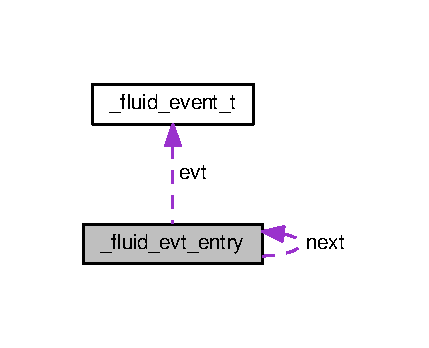
\includegraphics[width=206pt]{struct__fluid__evt__entry__coll__graph}
\end{center}
\end{figure}
\subsection*{Public Attributes}
\begin{DoxyCompactItemize}
\item 
\hyperlink{fluid__event__priv_8h_ae1b4d1ef2ce32890f8cb36837628a9d8}{fluid\+\_\+evt\+\_\+entry} $\ast$ \hyperlink{struct__fluid__evt__entry_a943689018328859e48f75f1d9ae9d48f}{next}
\item 
short \hyperlink{struct__fluid__evt__entry_ad63b5e75af079b7e62337710031482e3}{entry\+Type}
\item 
\hyperlink{types_8h_aca09348be1b6e6ee7fce49dd4734f1ba}{fluid\+\_\+event\+\_\+t} \hyperlink{struct__fluid__evt__entry_ab73d983a1a210d0c1212d94f0c31ada1}{evt}
\end{DoxyCompactItemize}


\subsection{Member Data Documentation}
\mbox{\Hypertarget{struct__fluid__evt__entry_ad63b5e75af079b7e62337710031482e3}\label{struct__fluid__evt__entry_ad63b5e75af079b7e62337710031482e3}} 
\index{\+\_\+fluid\+\_\+evt\+\_\+entry@{\+\_\+fluid\+\_\+evt\+\_\+entry}!entry\+Type@{entry\+Type}}
\index{entry\+Type@{entry\+Type}!\+\_\+fluid\+\_\+evt\+\_\+entry@{\+\_\+fluid\+\_\+evt\+\_\+entry}}
\subsubsection{\texorpdfstring{entry\+Type}{entryType}}
{\footnotesize\ttfamily short \+\_\+fluid\+\_\+evt\+\_\+entry\+::entry\+Type}

\mbox{\Hypertarget{struct__fluid__evt__entry_ab73d983a1a210d0c1212d94f0c31ada1}\label{struct__fluid__evt__entry_ab73d983a1a210d0c1212d94f0c31ada1}} 
\index{\+\_\+fluid\+\_\+evt\+\_\+entry@{\+\_\+fluid\+\_\+evt\+\_\+entry}!evt@{evt}}
\index{evt@{evt}!\+\_\+fluid\+\_\+evt\+\_\+entry@{\+\_\+fluid\+\_\+evt\+\_\+entry}}
\subsubsection{\texorpdfstring{evt}{evt}}
{\footnotesize\ttfamily \hyperlink{types_8h_aca09348be1b6e6ee7fce49dd4734f1ba}{fluid\+\_\+event\+\_\+t} \+\_\+fluid\+\_\+evt\+\_\+entry\+::evt}

\mbox{\Hypertarget{struct__fluid__evt__entry_a943689018328859e48f75f1d9ae9d48f}\label{struct__fluid__evt__entry_a943689018328859e48f75f1d9ae9d48f}} 
\index{\+\_\+fluid\+\_\+evt\+\_\+entry@{\+\_\+fluid\+\_\+evt\+\_\+entry}!next@{next}}
\index{next@{next}!\+\_\+fluid\+\_\+evt\+\_\+entry@{\+\_\+fluid\+\_\+evt\+\_\+entry}}
\subsubsection{\texorpdfstring{next}{next}}
{\footnotesize\ttfamily \hyperlink{fluid__event__priv_8h_ae1b4d1ef2ce32890f8cb36837628a9d8}{fluid\+\_\+evt\+\_\+entry}$\ast$ \+\_\+fluid\+\_\+evt\+\_\+entry\+::next}



The documentation for this struct was generated from the following file\+:\begin{DoxyCompactItemize}
\item 
synth/\hyperlink{fluid__event__priv_8h}{fluid\+\_\+event\+\_\+priv.\+h}\end{DoxyCompactItemize}

\hypertarget{struct__fluid__evt__heap__t}{}\section{\+\_\+fluid\+\_\+evt\+\_\+heap\+\_\+t Struct Reference}
\label{struct__fluid__evt__heap__t}\index{\+\_\+fluid\+\_\+evt\+\_\+heap\+\_\+t@{\+\_\+fluid\+\_\+evt\+\_\+heap\+\_\+t}}


{\ttfamily \#include $<$fluid\+\_\+event\+\_\+priv.\+h$>$}



Collaboration diagram for \+\_\+fluid\+\_\+evt\+\_\+heap\+\_\+t\+:
\nopagebreak
\begin{figure}[H]
\begin{center}
\leavevmode
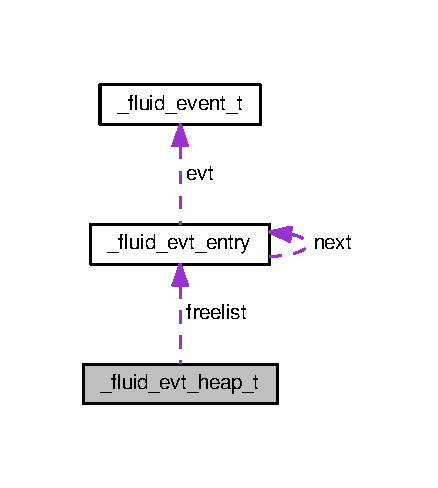
\includegraphics[width=210pt]{struct__fluid__evt__heap__t__coll__graph}
\end{center}
\end{figure}
\subsection*{Public Attributes}
\begin{DoxyCompactItemize}
\item 
\hyperlink{fluid__event__priv_8h_ae1b4d1ef2ce32890f8cb36837628a9d8}{fluid\+\_\+evt\+\_\+entry} $\ast$ \hyperlink{struct__fluid__evt__heap__t_a417ea7c73b75471d695807154f3b77bb}{freelist}
\item 
\hyperlink{fluid__sys_8h_a7252a44982e8ed2704689f563c8a12e3}{fluid\+\_\+mutex\+\_\+t} \hyperlink{struct__fluid__evt__heap__t_ade738dbaaa24d4002c236d80397ac709}{mutex}
\end{DoxyCompactItemize}


\subsection{Member Data Documentation}
\mbox{\Hypertarget{struct__fluid__evt__heap__t_a417ea7c73b75471d695807154f3b77bb}\label{struct__fluid__evt__heap__t_a417ea7c73b75471d695807154f3b77bb}} 
\index{\+\_\+fluid\+\_\+evt\+\_\+heap\+\_\+t@{\+\_\+fluid\+\_\+evt\+\_\+heap\+\_\+t}!freelist@{freelist}}
\index{freelist@{freelist}!\+\_\+fluid\+\_\+evt\+\_\+heap\+\_\+t@{\+\_\+fluid\+\_\+evt\+\_\+heap\+\_\+t}}
\subsubsection{\texorpdfstring{freelist}{freelist}}
{\footnotesize\ttfamily \hyperlink{fluid__event__priv_8h_ae1b4d1ef2ce32890f8cb36837628a9d8}{fluid\+\_\+evt\+\_\+entry}$\ast$ \+\_\+fluid\+\_\+evt\+\_\+heap\+\_\+t\+::freelist}

\mbox{\Hypertarget{struct__fluid__evt__heap__t_ade738dbaaa24d4002c236d80397ac709}\label{struct__fluid__evt__heap__t_ade738dbaaa24d4002c236d80397ac709}} 
\index{\+\_\+fluid\+\_\+evt\+\_\+heap\+\_\+t@{\+\_\+fluid\+\_\+evt\+\_\+heap\+\_\+t}!mutex@{mutex}}
\index{mutex@{mutex}!\+\_\+fluid\+\_\+evt\+\_\+heap\+\_\+t@{\+\_\+fluid\+\_\+evt\+\_\+heap\+\_\+t}}
\subsubsection{\texorpdfstring{mutex}{mutex}}
{\footnotesize\ttfamily \hyperlink{fluid__sys_8h_a7252a44982e8ed2704689f563c8a12e3}{fluid\+\_\+mutex\+\_\+t} \+\_\+fluid\+\_\+evt\+\_\+heap\+\_\+t\+::mutex}



The documentation for this struct was generated from the following file\+:\begin{DoxyCompactItemize}
\item 
synth/\hyperlink{fluid__event__priv_8h}{fluid\+\_\+event\+\_\+priv.\+h}\end{DoxyCompactItemize}

\hypertarget{struct__fluid__file__callbacks__t}{}\section{\+\_\+fluid\+\_\+file\+\_\+callbacks\+\_\+t Struct Reference}
\label{struct__fluid__file__callbacks__t}\index{\+\_\+fluid\+\_\+file\+\_\+callbacks\+\_\+t@{\+\_\+fluid\+\_\+file\+\_\+callbacks\+\_\+t}}


{\ttfamily \#include $<$fluid\+\_\+sfont.\+h$>$}

\subsection*{Public Attributes}
\begin{DoxyCompactItemize}
\item 
\hyperlink{sfont_8h_a801d39d1437ad9f41caec35a1e79094e}{fluid\+\_\+sfloader\+\_\+callback\+\_\+open\+\_\+t} \hyperlink{struct__fluid__file__callbacks__t_a209009deac020dbb99775951d31156b2}{fopen}
\item 
\hyperlink{sfont_8h_a5ad574cbab9c9413932d51faaa5d10a8}{fluid\+\_\+sfloader\+\_\+callback\+\_\+read\+\_\+t} \hyperlink{struct__fluid__file__callbacks__t_afa89d165fc9fab2e1e484a33cfb4411b}{fread}
\item 
\hyperlink{sfont_8h_ac5cf57119fee0cde7422c86beafe0917}{fluid\+\_\+sfloader\+\_\+callback\+\_\+seek\+\_\+t} \hyperlink{struct__fluid__file__callbacks__t_a23fe39b2c888b5fa6b87cd8c426f95d9}{fseek}
\item 
\hyperlink{sfont_8h_a1227398bb99d8b74b99a5fef6c62d3a8}{fluid\+\_\+sfloader\+\_\+callback\+\_\+close\+\_\+t} \hyperlink{struct__fluid__file__callbacks__t_acedc1f0c5dbd2da1ad8034a795f51135}{fclose}
\item 
\hyperlink{sfont_8h_a1b7f13d61330ca5a3441cf6c15863607}{fluid\+\_\+sfloader\+\_\+callback\+\_\+tell\+\_\+t} \hyperlink{struct__fluid__file__callbacks__t_ac6369333c624eda55ecb70eae31af31e}{ftell}
\end{DoxyCompactItemize}


\subsection{Detailed Description}
File callback structure to enable custom soundfont loading (e.\+g. from memory). 

\subsection{Member Data Documentation}
\mbox{\Hypertarget{struct__fluid__file__callbacks__t_acedc1f0c5dbd2da1ad8034a795f51135}\label{struct__fluid__file__callbacks__t_acedc1f0c5dbd2da1ad8034a795f51135}} 
\index{\+\_\+fluid\+\_\+file\+\_\+callbacks\+\_\+t@{\+\_\+fluid\+\_\+file\+\_\+callbacks\+\_\+t}!fclose@{fclose}}
\index{fclose@{fclose}!\+\_\+fluid\+\_\+file\+\_\+callbacks\+\_\+t@{\+\_\+fluid\+\_\+file\+\_\+callbacks\+\_\+t}}
\subsubsection{\texorpdfstring{fclose}{fclose}}
{\footnotesize\ttfamily \hyperlink{sfont_8h_a1227398bb99d8b74b99a5fef6c62d3a8}{fluid\+\_\+sfloader\+\_\+callback\+\_\+close\+\_\+t} \+\_\+fluid\+\_\+file\+\_\+callbacks\+\_\+t\+::fclose}

\mbox{\Hypertarget{struct__fluid__file__callbacks__t_a209009deac020dbb99775951d31156b2}\label{struct__fluid__file__callbacks__t_a209009deac020dbb99775951d31156b2}} 
\index{\+\_\+fluid\+\_\+file\+\_\+callbacks\+\_\+t@{\+\_\+fluid\+\_\+file\+\_\+callbacks\+\_\+t}!fopen@{fopen}}
\index{fopen@{fopen}!\+\_\+fluid\+\_\+file\+\_\+callbacks\+\_\+t@{\+\_\+fluid\+\_\+file\+\_\+callbacks\+\_\+t}}
\subsubsection{\texorpdfstring{fopen}{fopen}}
{\footnotesize\ttfamily \hyperlink{sfont_8h_a801d39d1437ad9f41caec35a1e79094e}{fluid\+\_\+sfloader\+\_\+callback\+\_\+open\+\_\+t} \+\_\+fluid\+\_\+file\+\_\+callbacks\+\_\+t\+::fopen}

\mbox{\Hypertarget{struct__fluid__file__callbacks__t_afa89d165fc9fab2e1e484a33cfb4411b}\label{struct__fluid__file__callbacks__t_afa89d165fc9fab2e1e484a33cfb4411b}} 
\index{\+\_\+fluid\+\_\+file\+\_\+callbacks\+\_\+t@{\+\_\+fluid\+\_\+file\+\_\+callbacks\+\_\+t}!fread@{fread}}
\index{fread@{fread}!\+\_\+fluid\+\_\+file\+\_\+callbacks\+\_\+t@{\+\_\+fluid\+\_\+file\+\_\+callbacks\+\_\+t}}
\subsubsection{\texorpdfstring{fread}{fread}}
{\footnotesize\ttfamily \hyperlink{sfont_8h_a5ad574cbab9c9413932d51faaa5d10a8}{fluid\+\_\+sfloader\+\_\+callback\+\_\+read\+\_\+t} \+\_\+fluid\+\_\+file\+\_\+callbacks\+\_\+t\+::fread}

\mbox{\Hypertarget{struct__fluid__file__callbacks__t_a23fe39b2c888b5fa6b87cd8c426f95d9}\label{struct__fluid__file__callbacks__t_a23fe39b2c888b5fa6b87cd8c426f95d9}} 
\index{\+\_\+fluid\+\_\+file\+\_\+callbacks\+\_\+t@{\+\_\+fluid\+\_\+file\+\_\+callbacks\+\_\+t}!fseek@{fseek}}
\index{fseek@{fseek}!\+\_\+fluid\+\_\+file\+\_\+callbacks\+\_\+t@{\+\_\+fluid\+\_\+file\+\_\+callbacks\+\_\+t}}
\subsubsection{\texorpdfstring{fseek}{fseek}}
{\footnotesize\ttfamily \hyperlink{sfont_8h_ac5cf57119fee0cde7422c86beafe0917}{fluid\+\_\+sfloader\+\_\+callback\+\_\+seek\+\_\+t} \+\_\+fluid\+\_\+file\+\_\+callbacks\+\_\+t\+::fseek}

\mbox{\Hypertarget{struct__fluid__file__callbacks__t_ac6369333c624eda55ecb70eae31af31e}\label{struct__fluid__file__callbacks__t_ac6369333c624eda55ecb70eae31af31e}} 
\index{\+\_\+fluid\+\_\+file\+\_\+callbacks\+\_\+t@{\+\_\+fluid\+\_\+file\+\_\+callbacks\+\_\+t}!ftell@{ftell}}
\index{ftell@{ftell}!\+\_\+fluid\+\_\+file\+\_\+callbacks\+\_\+t@{\+\_\+fluid\+\_\+file\+\_\+callbacks\+\_\+t}}
\subsubsection{\texorpdfstring{ftell}{ftell}}
{\footnotesize\ttfamily \hyperlink{sfont_8h_a1b7f13d61330ca5a3441cf6c15863607}{fluid\+\_\+sfloader\+\_\+callback\+\_\+tell\+\_\+t} \+\_\+fluid\+\_\+file\+\_\+callbacks\+\_\+t\+::ftell}



The documentation for this struct was generated from the following file\+:\begin{DoxyCompactItemize}
\item 
sfloader/\hyperlink{fluid__sfont_8h}{fluid\+\_\+sfont.\+h}\end{DoxyCompactItemize}

\hypertarget{struct__fluid__file__renderer__t}{}\section{\+\_\+fluid\+\_\+file\+\_\+renderer\+\_\+t Struct Reference}
\label{struct__fluid__file__renderer__t}\index{\+\_\+fluid\+\_\+file\+\_\+renderer\+\_\+t@{\+\_\+fluid\+\_\+file\+\_\+renderer\+\_\+t}}


Collaboration diagram for \+\_\+fluid\+\_\+file\+\_\+renderer\+\_\+t\+:
\nopagebreak
\begin{figure}[H]
\begin{center}
\leavevmode
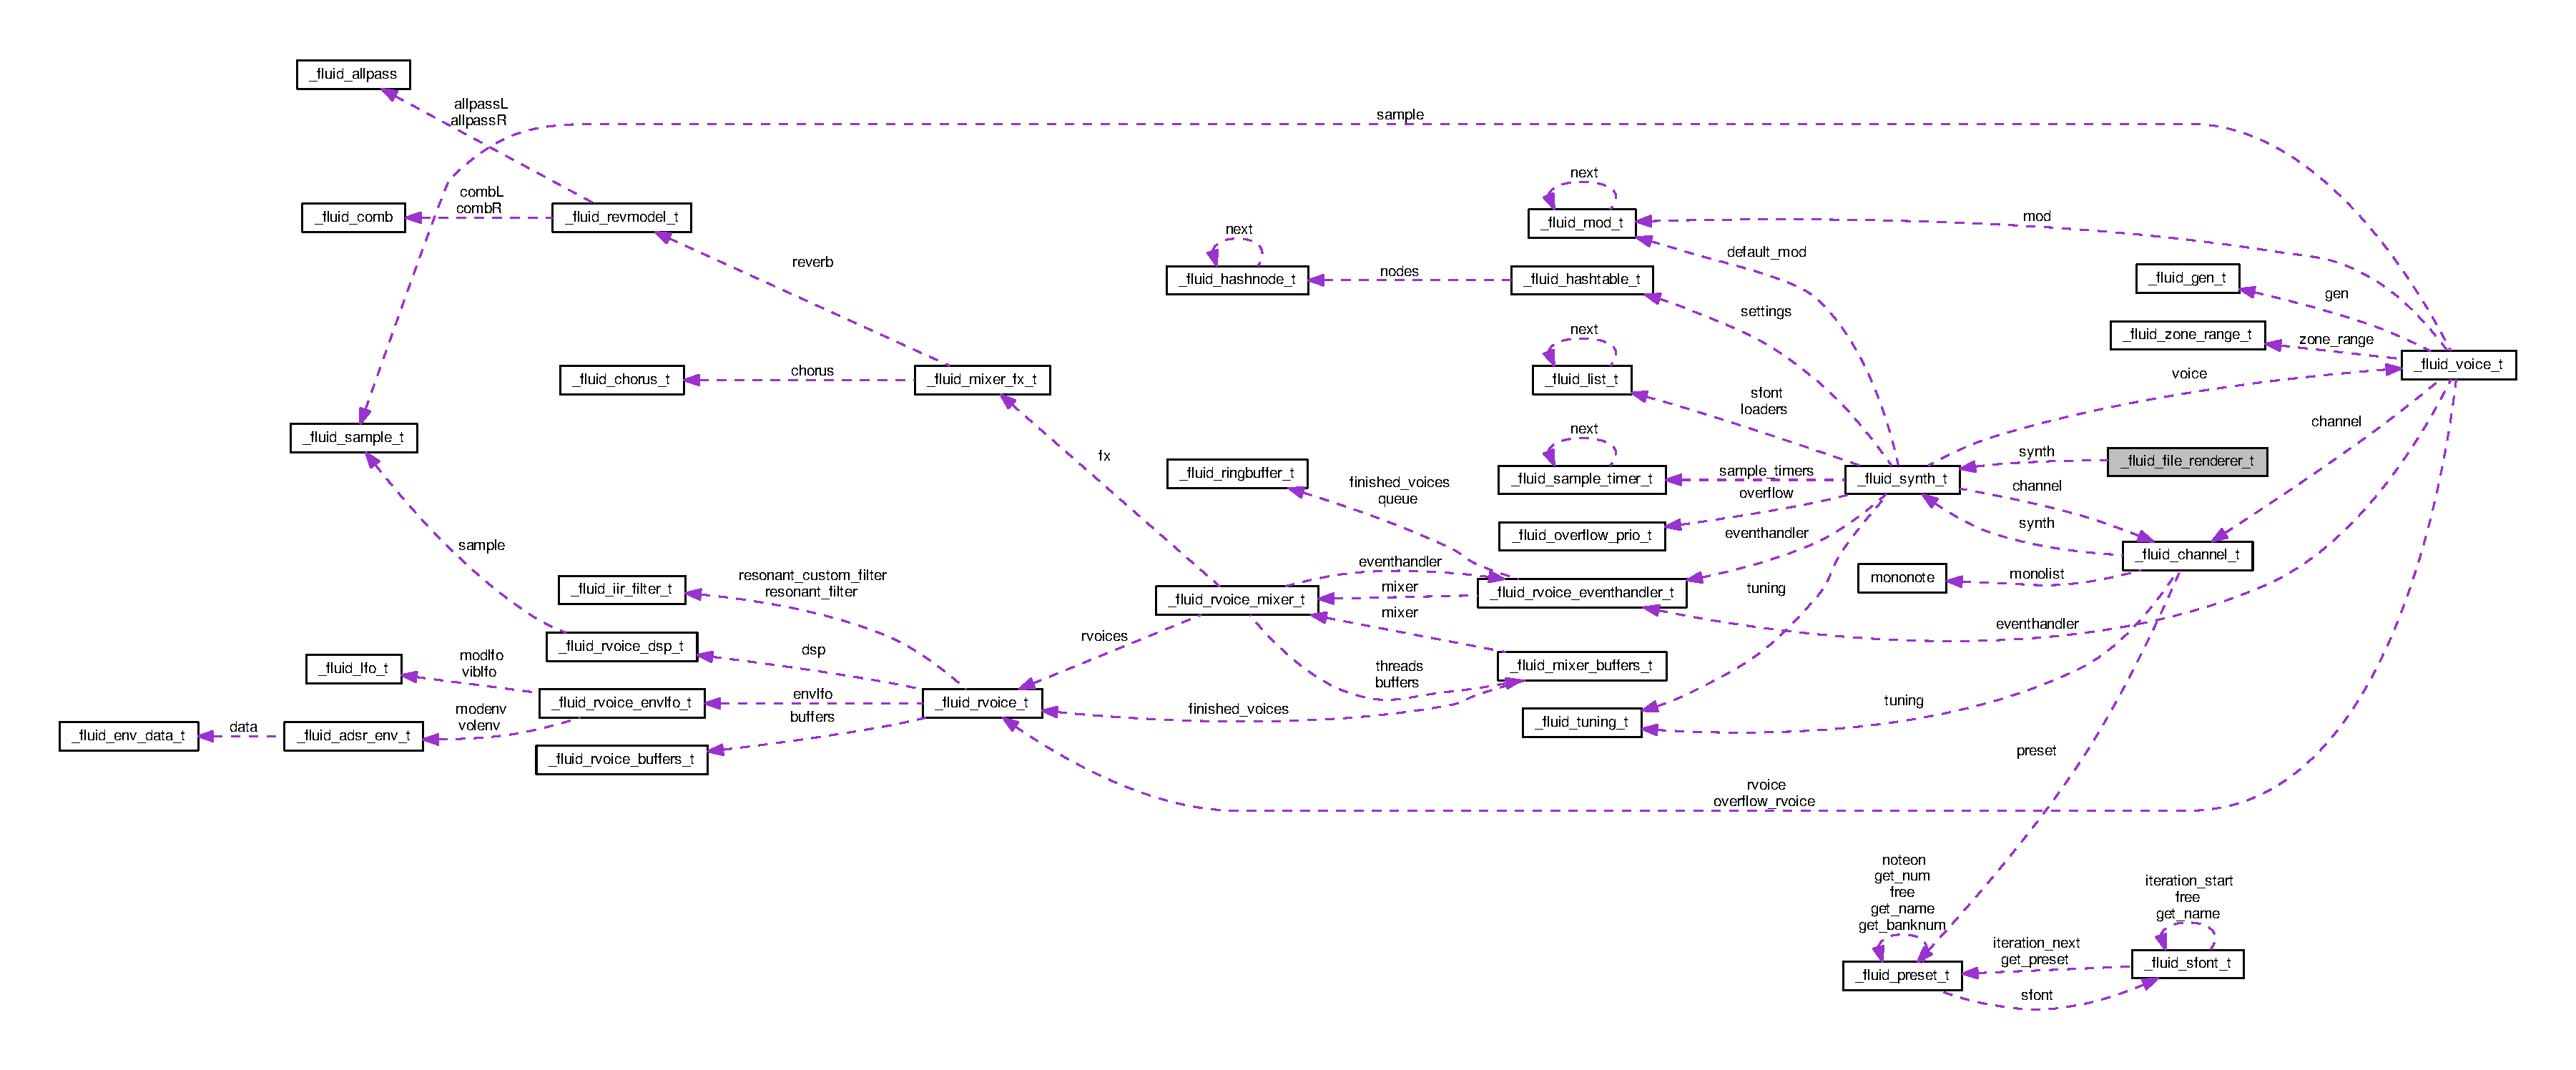
\includegraphics[width=350pt]{struct__fluid__file__renderer__t__coll__graph}
\end{center}
\end{figure}
\subsection*{Public Attributes}
\begin{DoxyCompactItemize}
\item 
\hyperlink{types_8h_ae265f10ae174a13afe010de50d87e1a4}{fluid\+\_\+synth\+\_\+t} $\ast$ \hyperlink{struct__fluid__file__renderer__t_abdf1691de523abbf2eeba089a42b4936}{synth}
\item 
F\+I\+LE $\ast$ \hyperlink{struct__fluid__file__renderer__t_aba3edc6f0fec0f35b1deb15886618f0c}{file}
\item 
short $\ast$ \hyperlink{struct__fluid__file__renderer__t_a812f2d6608ca0c7ade52c6907d028108}{buf}
\item 
int \hyperlink{struct__fluid__file__renderer__t_aff4b0588e5bf3f28e26e944b01d61852}{period\+\_\+size}
\item 
int \hyperlink{struct__fluid__file__renderer__t_a868bc700dd3e8fe63c7a9e17594f522b}{buf\+\_\+size}
\end{DoxyCompactItemize}


\subsection{Member Data Documentation}
\mbox{\Hypertarget{struct__fluid__file__renderer__t_a812f2d6608ca0c7ade52c6907d028108}\label{struct__fluid__file__renderer__t_a812f2d6608ca0c7ade52c6907d028108}} 
\index{\+\_\+fluid\+\_\+file\+\_\+renderer\+\_\+t@{\+\_\+fluid\+\_\+file\+\_\+renderer\+\_\+t}!buf@{buf}}
\index{buf@{buf}!\+\_\+fluid\+\_\+file\+\_\+renderer\+\_\+t@{\+\_\+fluid\+\_\+file\+\_\+renderer\+\_\+t}}
\subsubsection{\texorpdfstring{buf}{buf}}
{\footnotesize\ttfamily short$\ast$ \+\_\+fluid\+\_\+file\+\_\+renderer\+\_\+t\+::buf}

\mbox{\Hypertarget{struct__fluid__file__renderer__t_a868bc700dd3e8fe63c7a9e17594f522b}\label{struct__fluid__file__renderer__t_a868bc700dd3e8fe63c7a9e17594f522b}} 
\index{\+\_\+fluid\+\_\+file\+\_\+renderer\+\_\+t@{\+\_\+fluid\+\_\+file\+\_\+renderer\+\_\+t}!buf\+\_\+size@{buf\+\_\+size}}
\index{buf\+\_\+size@{buf\+\_\+size}!\+\_\+fluid\+\_\+file\+\_\+renderer\+\_\+t@{\+\_\+fluid\+\_\+file\+\_\+renderer\+\_\+t}}
\subsubsection{\texorpdfstring{buf\+\_\+size}{buf\_size}}
{\footnotesize\ttfamily int \+\_\+fluid\+\_\+file\+\_\+renderer\+\_\+t\+::buf\+\_\+size}

\mbox{\Hypertarget{struct__fluid__file__renderer__t_aba3edc6f0fec0f35b1deb15886618f0c}\label{struct__fluid__file__renderer__t_aba3edc6f0fec0f35b1deb15886618f0c}} 
\index{\+\_\+fluid\+\_\+file\+\_\+renderer\+\_\+t@{\+\_\+fluid\+\_\+file\+\_\+renderer\+\_\+t}!file@{file}}
\index{file@{file}!\+\_\+fluid\+\_\+file\+\_\+renderer\+\_\+t@{\+\_\+fluid\+\_\+file\+\_\+renderer\+\_\+t}}
\subsubsection{\texorpdfstring{file}{file}}
{\footnotesize\ttfamily F\+I\+LE$\ast$ \+\_\+fluid\+\_\+file\+\_\+renderer\+\_\+t\+::file}

\mbox{\Hypertarget{struct__fluid__file__renderer__t_aff4b0588e5bf3f28e26e944b01d61852}\label{struct__fluid__file__renderer__t_aff4b0588e5bf3f28e26e944b01d61852}} 
\index{\+\_\+fluid\+\_\+file\+\_\+renderer\+\_\+t@{\+\_\+fluid\+\_\+file\+\_\+renderer\+\_\+t}!period\+\_\+size@{period\+\_\+size}}
\index{period\+\_\+size@{period\+\_\+size}!\+\_\+fluid\+\_\+file\+\_\+renderer\+\_\+t@{\+\_\+fluid\+\_\+file\+\_\+renderer\+\_\+t}}
\subsubsection{\texorpdfstring{period\+\_\+size}{period\_size}}
{\footnotesize\ttfamily int \+\_\+fluid\+\_\+file\+\_\+renderer\+\_\+t\+::period\+\_\+size}

\mbox{\Hypertarget{struct__fluid__file__renderer__t_abdf1691de523abbf2eeba089a42b4936}\label{struct__fluid__file__renderer__t_abdf1691de523abbf2eeba089a42b4936}} 
\index{\+\_\+fluid\+\_\+file\+\_\+renderer\+\_\+t@{\+\_\+fluid\+\_\+file\+\_\+renderer\+\_\+t}!synth@{synth}}
\index{synth@{synth}!\+\_\+fluid\+\_\+file\+\_\+renderer\+\_\+t@{\+\_\+fluid\+\_\+file\+\_\+renderer\+\_\+t}}
\subsubsection{\texorpdfstring{synth}{synth}}
{\footnotesize\ttfamily \hyperlink{types_8h_ae265f10ae174a13afe010de50d87e1a4}{fluid\+\_\+synth\+\_\+t}$\ast$ \+\_\+fluid\+\_\+file\+\_\+renderer\+\_\+t\+::synth}



The documentation for this struct was generated from the following file\+:\begin{DoxyCompactItemize}
\item 
bindings/\hyperlink{fluid__filerenderer_8c}{fluid\+\_\+filerenderer.\+c}\end{DoxyCompactItemize}

\hypertarget{struct__fluid__gen__info__t}{}\section{\+\_\+fluid\+\_\+gen\+\_\+info\+\_\+t Struct Reference}
\label{struct__fluid__gen__info__t}\index{\+\_\+fluid\+\_\+gen\+\_\+info\+\_\+t@{\+\_\+fluid\+\_\+gen\+\_\+info\+\_\+t}}


{\ttfamily \#include $<$fluid\+\_\+gen.\+h$>$}

\subsection*{Public Attributes}
\begin{DoxyCompactItemize}
\item 
char \hyperlink{struct__fluid__gen__info__t_a9bf766e8ce67f4086ca77a9d44f7e94b}{num}
\item 
char \hyperlink{struct__fluid__gen__info__t_aef7034d8e23aea99d5d7217c27f401ca}{init}
\item 
char \hyperlink{struct__fluid__gen__info__t_a00afe7791c60b323e53cbde04f6d8b97}{nrpn\+\_\+scale}
\item 
float \hyperlink{struct__fluid__gen__info__t_ade2865af096a3fed0cfc879e90142058}{min}
\item 
float \hyperlink{struct__fluid__gen__info__t_a9de8e5d8146a85057911236b4ec15acf}{max}
\item 
float \hyperlink{struct__fluid__gen__info__t_aae3af42bd32328a47220229528f60152}{def}
\end{DoxyCompactItemize}


\subsection{Member Data Documentation}
\mbox{\Hypertarget{struct__fluid__gen__info__t_aae3af42bd32328a47220229528f60152}\label{struct__fluid__gen__info__t_aae3af42bd32328a47220229528f60152}} 
\index{\+\_\+fluid\+\_\+gen\+\_\+info\+\_\+t@{\+\_\+fluid\+\_\+gen\+\_\+info\+\_\+t}!def@{def}}
\index{def@{def}!\+\_\+fluid\+\_\+gen\+\_\+info\+\_\+t@{\+\_\+fluid\+\_\+gen\+\_\+info\+\_\+t}}
\subsubsection{\texorpdfstring{def}{def}}
{\footnotesize\ttfamily float \+\_\+fluid\+\_\+gen\+\_\+info\+\_\+t\+::def}

\mbox{\Hypertarget{struct__fluid__gen__info__t_aef7034d8e23aea99d5d7217c27f401ca}\label{struct__fluid__gen__info__t_aef7034d8e23aea99d5d7217c27f401ca}} 
\index{\+\_\+fluid\+\_\+gen\+\_\+info\+\_\+t@{\+\_\+fluid\+\_\+gen\+\_\+info\+\_\+t}!init@{init}}
\index{init@{init}!\+\_\+fluid\+\_\+gen\+\_\+info\+\_\+t@{\+\_\+fluid\+\_\+gen\+\_\+info\+\_\+t}}
\subsubsection{\texorpdfstring{init}{init}}
{\footnotesize\ttfamily char \+\_\+fluid\+\_\+gen\+\_\+info\+\_\+t\+::init}

\mbox{\Hypertarget{struct__fluid__gen__info__t_a9de8e5d8146a85057911236b4ec15acf}\label{struct__fluid__gen__info__t_a9de8e5d8146a85057911236b4ec15acf}} 
\index{\+\_\+fluid\+\_\+gen\+\_\+info\+\_\+t@{\+\_\+fluid\+\_\+gen\+\_\+info\+\_\+t}!max@{max}}
\index{max@{max}!\+\_\+fluid\+\_\+gen\+\_\+info\+\_\+t@{\+\_\+fluid\+\_\+gen\+\_\+info\+\_\+t}}
\subsubsection{\texorpdfstring{max}{max}}
{\footnotesize\ttfamily float \+\_\+fluid\+\_\+gen\+\_\+info\+\_\+t\+::max}

\mbox{\Hypertarget{struct__fluid__gen__info__t_ade2865af096a3fed0cfc879e90142058}\label{struct__fluid__gen__info__t_ade2865af096a3fed0cfc879e90142058}} 
\index{\+\_\+fluid\+\_\+gen\+\_\+info\+\_\+t@{\+\_\+fluid\+\_\+gen\+\_\+info\+\_\+t}!min@{min}}
\index{min@{min}!\+\_\+fluid\+\_\+gen\+\_\+info\+\_\+t@{\+\_\+fluid\+\_\+gen\+\_\+info\+\_\+t}}
\subsubsection{\texorpdfstring{min}{min}}
{\footnotesize\ttfamily float \+\_\+fluid\+\_\+gen\+\_\+info\+\_\+t\+::min}

\mbox{\Hypertarget{struct__fluid__gen__info__t_a00afe7791c60b323e53cbde04f6d8b97}\label{struct__fluid__gen__info__t_a00afe7791c60b323e53cbde04f6d8b97}} 
\index{\+\_\+fluid\+\_\+gen\+\_\+info\+\_\+t@{\+\_\+fluid\+\_\+gen\+\_\+info\+\_\+t}!nrpn\+\_\+scale@{nrpn\+\_\+scale}}
\index{nrpn\+\_\+scale@{nrpn\+\_\+scale}!\+\_\+fluid\+\_\+gen\+\_\+info\+\_\+t@{\+\_\+fluid\+\_\+gen\+\_\+info\+\_\+t}}
\subsubsection{\texorpdfstring{nrpn\+\_\+scale}{nrpn\_scale}}
{\footnotesize\ttfamily char \+\_\+fluid\+\_\+gen\+\_\+info\+\_\+t\+::nrpn\+\_\+scale}

\mbox{\Hypertarget{struct__fluid__gen__info__t_a9bf766e8ce67f4086ca77a9d44f7e94b}\label{struct__fluid__gen__info__t_a9bf766e8ce67f4086ca77a9d44f7e94b}} 
\index{\+\_\+fluid\+\_\+gen\+\_\+info\+\_\+t@{\+\_\+fluid\+\_\+gen\+\_\+info\+\_\+t}!num@{num}}
\index{num@{num}!\+\_\+fluid\+\_\+gen\+\_\+info\+\_\+t@{\+\_\+fluid\+\_\+gen\+\_\+info\+\_\+t}}
\subsubsection{\texorpdfstring{num}{num}}
{\footnotesize\ttfamily char \+\_\+fluid\+\_\+gen\+\_\+info\+\_\+t\+::num}



The documentation for this struct was generated from the following file\+:\begin{DoxyCompactItemize}
\item 
synth/\hyperlink{fluid__gen_8h}{fluid\+\_\+gen.\+h}\end{DoxyCompactItemize}

\hypertarget{struct__fluid__gen__t}{}\section{\+\_\+fluid\+\_\+gen\+\_\+t Struct Reference}
\label{struct__fluid__gen__t}\index{\+\_\+fluid\+\_\+gen\+\_\+t@{\+\_\+fluid\+\_\+gen\+\_\+t}}


{\ttfamily \#include $<$fluid\+\_\+gen.\+h$>$}

\subsection*{Public Attributes}
\begin{DoxyCompactItemize}
\item 
unsigned char \hyperlink{struct__fluid__gen__t_a7cac8ba849dbf3d0d475bc4824cd406c}{flags}
\item 
double \hyperlink{struct__fluid__gen__t_a966264ce25b249592931cc0a4d34fe1d}{val}
\item 
double \hyperlink{struct__fluid__gen__t_a19ffa472a4f6f1f7cb83359a7105c37e}{mod}
\item 
double \hyperlink{struct__fluid__gen__t_a27422db6e42b16281b11ebe2faf7bc97}{nrpn}
\end{DoxyCompactItemize}


\subsection{Member Data Documentation}
\mbox{\Hypertarget{struct__fluid__gen__t_a7cac8ba849dbf3d0d475bc4824cd406c}\label{struct__fluid__gen__t_a7cac8ba849dbf3d0d475bc4824cd406c}} 
\index{\+\_\+fluid\+\_\+gen\+\_\+t@{\+\_\+fluid\+\_\+gen\+\_\+t}!flags@{flags}}
\index{flags@{flags}!\+\_\+fluid\+\_\+gen\+\_\+t@{\+\_\+fluid\+\_\+gen\+\_\+t}}
\subsubsection{\texorpdfstring{flags}{flags}}
{\footnotesize\ttfamily unsigned char \+\_\+fluid\+\_\+gen\+\_\+t\+::flags}

Is the generator set or not (\hyperlink{fluid__gen_8h_a96f1389ca9e52d85cdf1160a038b4bb5}{fluid\+\_\+gen\+\_\+flags}) \mbox{\Hypertarget{struct__fluid__gen__t_a19ffa472a4f6f1f7cb83359a7105c37e}\label{struct__fluid__gen__t_a19ffa472a4f6f1f7cb83359a7105c37e}} 
\index{\+\_\+fluid\+\_\+gen\+\_\+t@{\+\_\+fluid\+\_\+gen\+\_\+t}!mod@{mod}}
\index{mod@{mod}!\+\_\+fluid\+\_\+gen\+\_\+t@{\+\_\+fluid\+\_\+gen\+\_\+t}}
\subsubsection{\texorpdfstring{mod}{mod}}
{\footnotesize\ttfamily double \+\_\+fluid\+\_\+gen\+\_\+t\+::mod}

Change by modulators \mbox{\Hypertarget{struct__fluid__gen__t_a27422db6e42b16281b11ebe2faf7bc97}\label{struct__fluid__gen__t_a27422db6e42b16281b11ebe2faf7bc97}} 
\index{\+\_\+fluid\+\_\+gen\+\_\+t@{\+\_\+fluid\+\_\+gen\+\_\+t}!nrpn@{nrpn}}
\index{nrpn@{nrpn}!\+\_\+fluid\+\_\+gen\+\_\+t@{\+\_\+fluid\+\_\+gen\+\_\+t}}
\subsubsection{\texorpdfstring{nrpn}{nrpn}}
{\footnotesize\ttfamily double \+\_\+fluid\+\_\+gen\+\_\+t\+::nrpn}

Change by N\+R\+PN messages \mbox{\Hypertarget{struct__fluid__gen__t_a966264ce25b249592931cc0a4d34fe1d}\label{struct__fluid__gen__t_a966264ce25b249592931cc0a4d34fe1d}} 
\index{\+\_\+fluid\+\_\+gen\+\_\+t@{\+\_\+fluid\+\_\+gen\+\_\+t}!val@{val}}
\index{val@{val}!\+\_\+fluid\+\_\+gen\+\_\+t@{\+\_\+fluid\+\_\+gen\+\_\+t}}
\subsubsection{\texorpdfstring{val}{val}}
{\footnotesize\ttfamily double \+\_\+fluid\+\_\+gen\+\_\+t\+::val}

The nominal value 

The documentation for this struct was generated from the following file\+:\begin{DoxyCompactItemize}
\item 
synth/\hyperlink{fluid__gen_8h}{fluid\+\_\+gen.\+h}\end{DoxyCompactItemize}

\hypertarget{struct__fluid__handle__option__data__t}{}\section{\+\_\+fluid\+\_\+handle\+\_\+option\+\_\+data\+\_\+t Struct Reference}
\label{struct__fluid__handle__option__data__t}\index{\+\_\+fluid\+\_\+handle\+\_\+option\+\_\+data\+\_\+t@{\+\_\+fluid\+\_\+handle\+\_\+option\+\_\+data\+\_\+t}}
\subsection*{Public Attributes}
\begin{DoxyCompactItemize}
\item 
int \hyperlink{struct__fluid__handle__option__data__t_a127111d706fc1ca6957a7bf40602e831}{first}
\item 
\hyperlink{types_8h_a6d8c441b84ab0430e358438cee876c69}{fluid\+\_\+ostream\+\_\+t} \hyperlink{struct__fluid__handle__option__data__t_a91c8c4c3e0a7172e6ea8f388a842fbe9}{out}
\end{DoxyCompactItemize}


\subsection{Member Data Documentation}
\mbox{\Hypertarget{struct__fluid__handle__option__data__t_a127111d706fc1ca6957a7bf40602e831}\label{struct__fluid__handle__option__data__t_a127111d706fc1ca6957a7bf40602e831}} 
\index{\+\_\+fluid\+\_\+handle\+\_\+option\+\_\+data\+\_\+t@{\+\_\+fluid\+\_\+handle\+\_\+option\+\_\+data\+\_\+t}!first@{first}}
\index{first@{first}!\+\_\+fluid\+\_\+handle\+\_\+option\+\_\+data\+\_\+t@{\+\_\+fluid\+\_\+handle\+\_\+option\+\_\+data\+\_\+t}}
\subsubsection{\texorpdfstring{first}{first}}
{\footnotesize\ttfamily int \+\_\+fluid\+\_\+handle\+\_\+option\+\_\+data\+\_\+t\+::first}

\mbox{\Hypertarget{struct__fluid__handle__option__data__t_a91c8c4c3e0a7172e6ea8f388a842fbe9}\label{struct__fluid__handle__option__data__t_a91c8c4c3e0a7172e6ea8f388a842fbe9}} 
\index{\+\_\+fluid\+\_\+handle\+\_\+option\+\_\+data\+\_\+t@{\+\_\+fluid\+\_\+handle\+\_\+option\+\_\+data\+\_\+t}!out@{out}}
\index{out@{out}!\+\_\+fluid\+\_\+handle\+\_\+option\+\_\+data\+\_\+t@{\+\_\+fluid\+\_\+handle\+\_\+option\+\_\+data\+\_\+t}}
\subsubsection{\texorpdfstring{out}{out}}
{\footnotesize\ttfamily \hyperlink{types_8h_a6d8c441b84ab0430e358438cee876c69}{fluid\+\_\+ostream\+\_\+t} \+\_\+fluid\+\_\+handle\+\_\+option\+\_\+data\+\_\+t\+::out}



The documentation for this struct was generated from the following file\+:\begin{DoxyCompactItemize}
\item 
bindings/\hyperlink{fluid__cmd_8c}{fluid\+\_\+cmd.\+c}\end{DoxyCompactItemize}

\hypertarget{struct__fluid__handle__settings__data__t}{}\section{\+\_\+fluid\+\_\+handle\+\_\+settings\+\_\+data\+\_\+t Struct Reference}
\label{struct__fluid__handle__settings__data__t}\index{\+\_\+fluid\+\_\+handle\+\_\+settings\+\_\+data\+\_\+t@{\+\_\+fluid\+\_\+handle\+\_\+settings\+\_\+data\+\_\+t}}


Collaboration diagram for \+\_\+fluid\+\_\+handle\+\_\+settings\+\_\+data\+\_\+t\+:
\nopagebreak
\begin{figure}[H]
\begin{center}
\leavevmode
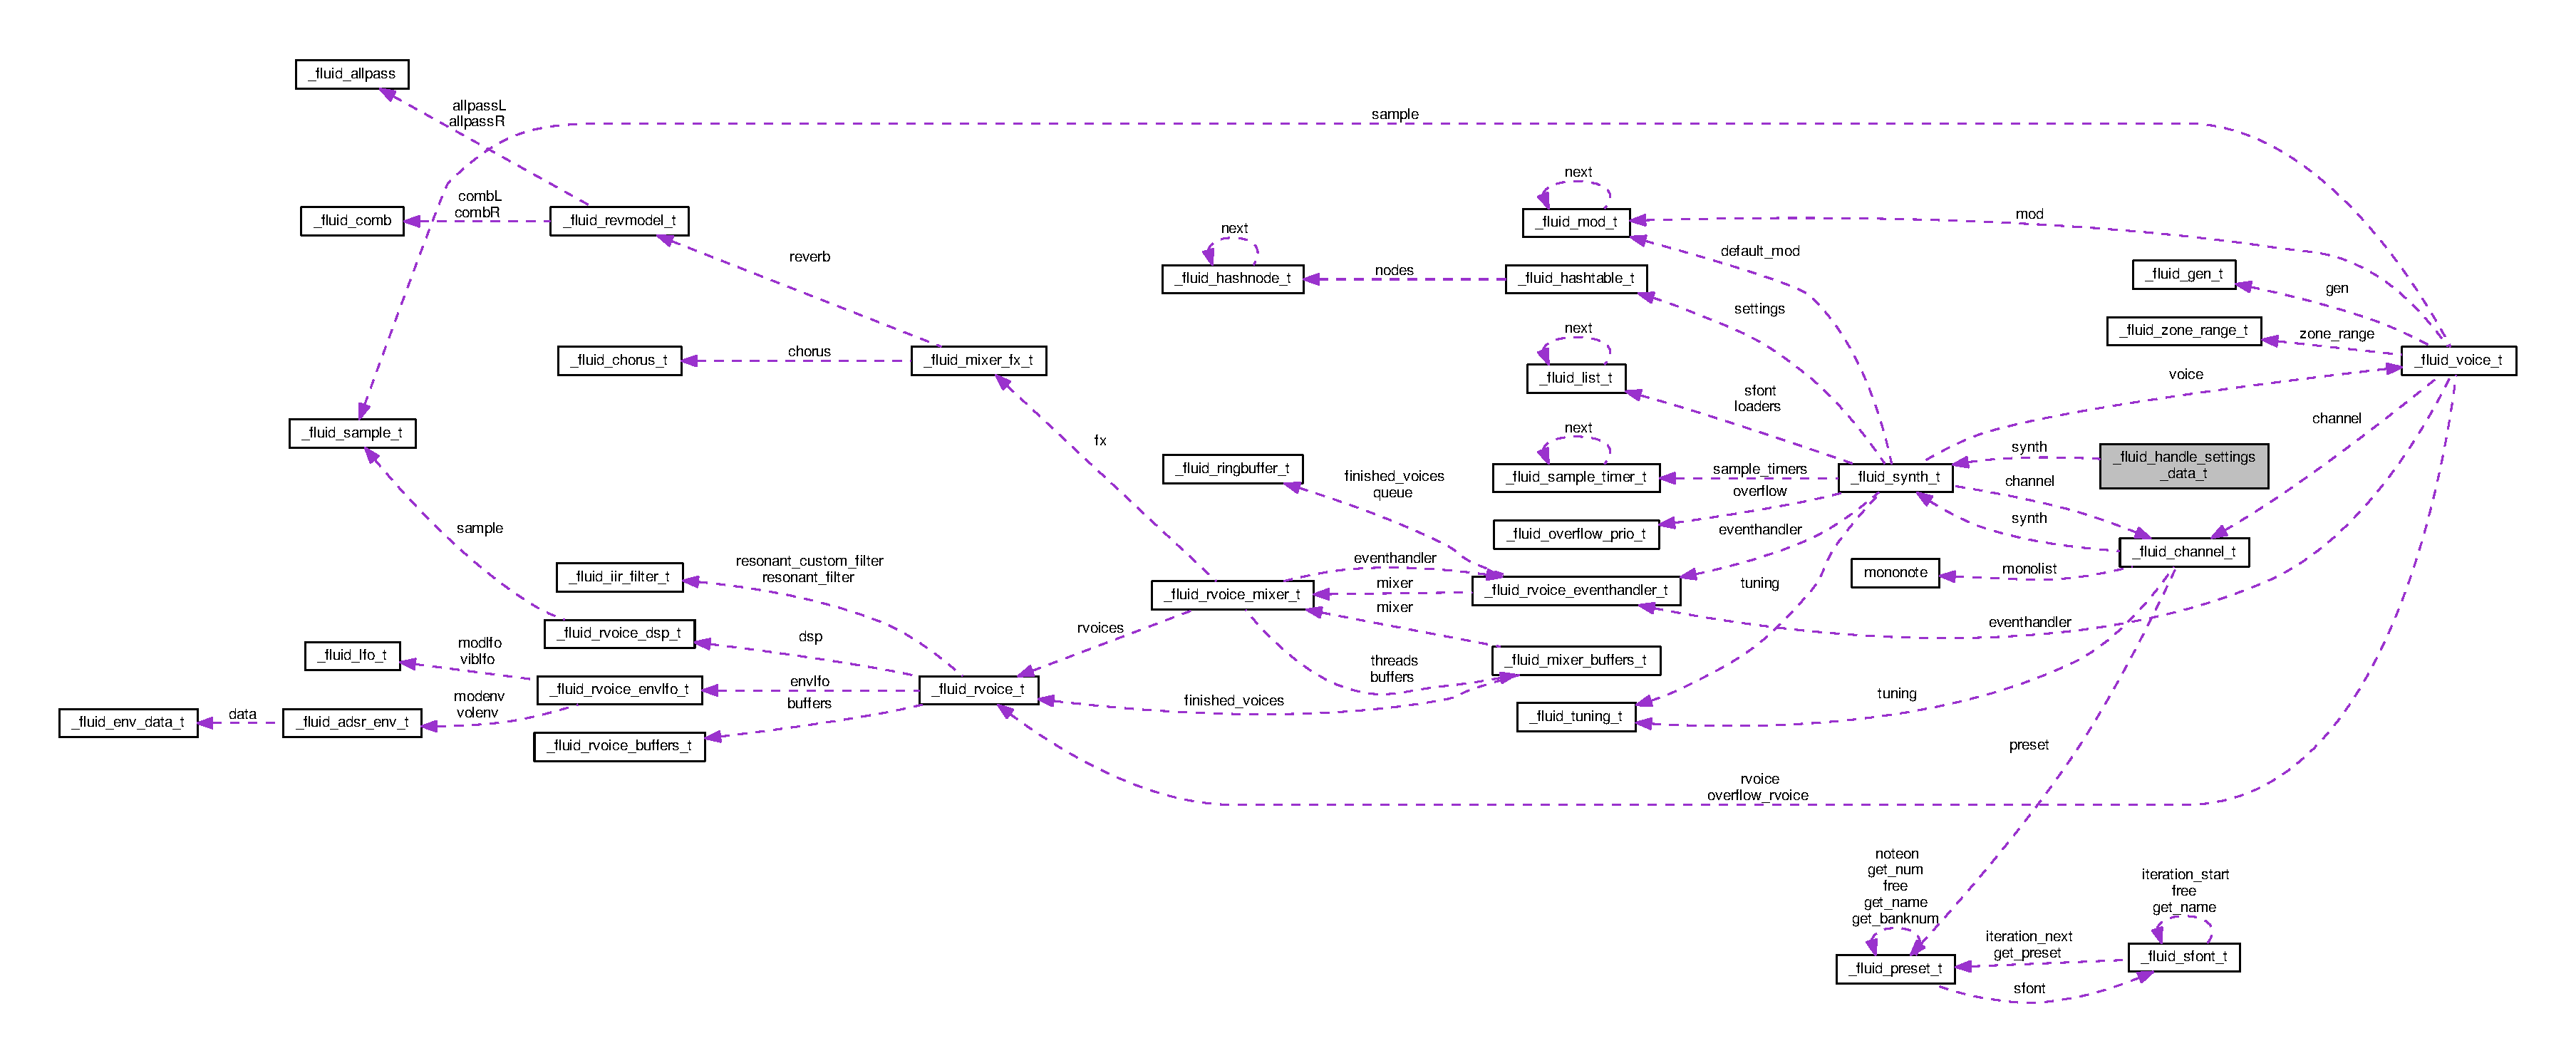
\includegraphics[width=350pt]{struct__fluid__handle__settings__data__t__coll__graph}
\end{center}
\end{figure}
\subsection*{Public Attributes}
\begin{DoxyCompactItemize}
\item 
int \hyperlink{struct__fluid__handle__settings__data__t_a4653b8677c8c143d3412bb7370612a23}{len}
\item 
\hyperlink{types_8h_ae265f10ae174a13afe010de50d87e1a4}{fluid\+\_\+synth\+\_\+t} $\ast$ \hyperlink{struct__fluid__handle__settings__data__t_a0c301cc2b5d78e9725c490e5675b6212}{synth}
\item 
\hyperlink{types_8h_a6d8c441b84ab0430e358438cee876c69}{fluid\+\_\+ostream\+\_\+t} \hyperlink{struct__fluid__handle__settings__data__t_aba6fc20a71b263199ba78d30cbec30a0}{out}
\end{DoxyCompactItemize}


\subsection{Member Data Documentation}
\mbox{\Hypertarget{struct__fluid__handle__settings__data__t_a4653b8677c8c143d3412bb7370612a23}\label{struct__fluid__handle__settings__data__t_a4653b8677c8c143d3412bb7370612a23}} 
\index{\+\_\+fluid\+\_\+handle\+\_\+settings\+\_\+data\+\_\+t@{\+\_\+fluid\+\_\+handle\+\_\+settings\+\_\+data\+\_\+t}!len@{len}}
\index{len@{len}!\+\_\+fluid\+\_\+handle\+\_\+settings\+\_\+data\+\_\+t@{\+\_\+fluid\+\_\+handle\+\_\+settings\+\_\+data\+\_\+t}}
\subsubsection{\texorpdfstring{len}{len}}
{\footnotesize\ttfamily int \+\_\+fluid\+\_\+handle\+\_\+settings\+\_\+data\+\_\+t\+::len}

\mbox{\Hypertarget{struct__fluid__handle__settings__data__t_aba6fc20a71b263199ba78d30cbec30a0}\label{struct__fluid__handle__settings__data__t_aba6fc20a71b263199ba78d30cbec30a0}} 
\index{\+\_\+fluid\+\_\+handle\+\_\+settings\+\_\+data\+\_\+t@{\+\_\+fluid\+\_\+handle\+\_\+settings\+\_\+data\+\_\+t}!out@{out}}
\index{out@{out}!\+\_\+fluid\+\_\+handle\+\_\+settings\+\_\+data\+\_\+t@{\+\_\+fluid\+\_\+handle\+\_\+settings\+\_\+data\+\_\+t}}
\subsubsection{\texorpdfstring{out}{out}}
{\footnotesize\ttfamily \hyperlink{types_8h_a6d8c441b84ab0430e358438cee876c69}{fluid\+\_\+ostream\+\_\+t} \+\_\+fluid\+\_\+handle\+\_\+settings\+\_\+data\+\_\+t\+::out}

\mbox{\Hypertarget{struct__fluid__handle__settings__data__t_a0c301cc2b5d78e9725c490e5675b6212}\label{struct__fluid__handle__settings__data__t_a0c301cc2b5d78e9725c490e5675b6212}} 
\index{\+\_\+fluid\+\_\+handle\+\_\+settings\+\_\+data\+\_\+t@{\+\_\+fluid\+\_\+handle\+\_\+settings\+\_\+data\+\_\+t}!synth@{synth}}
\index{synth@{synth}!\+\_\+fluid\+\_\+handle\+\_\+settings\+\_\+data\+\_\+t@{\+\_\+fluid\+\_\+handle\+\_\+settings\+\_\+data\+\_\+t}}
\subsubsection{\texorpdfstring{synth}{synth}}
{\footnotesize\ttfamily \hyperlink{types_8h_ae265f10ae174a13afe010de50d87e1a4}{fluid\+\_\+synth\+\_\+t}$\ast$ \+\_\+fluid\+\_\+handle\+\_\+settings\+\_\+data\+\_\+t\+::synth}



The documentation for this struct was generated from the following file\+:\begin{DoxyCompactItemize}
\item 
bindings/\hyperlink{fluid__cmd_8c}{fluid\+\_\+cmd.\+c}\end{DoxyCompactItemize}

\hypertarget{struct__fluid__hashnode__t}{}\section{\+\_\+fluid\+\_\+hashnode\+\_\+t Struct Reference}
\label{struct__fluid__hashnode__t}\index{\+\_\+fluid\+\_\+hashnode\+\_\+t@{\+\_\+fluid\+\_\+hashnode\+\_\+t}}


{\ttfamily \#include $<$fluid\+\_\+hash.\+h$>$}



Collaboration diagram for \+\_\+fluid\+\_\+hashnode\+\_\+t\+:
\nopagebreak
\begin{figure}[H]
\begin{center}
\leavevmode
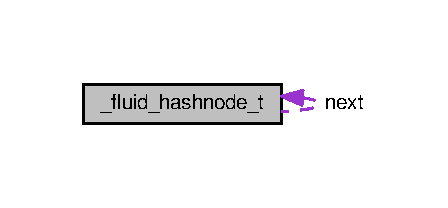
\includegraphics[width=215pt]{struct__fluid__hashnode__t__coll__graph}
\end{center}
\end{figure}
\subsection*{Public Attributes}
\begin{DoxyCompactItemize}
\item 
void $\ast$ \hyperlink{struct__fluid__hashnode__t_aa0ae0209b77c8eb5d430f621c1b2fd53}{key}
\item 
void $\ast$ \hyperlink{struct__fluid__hashnode__t_a286bda3b48b61da7239c85f1230bec5e}{value}
\item 
\hyperlink{fluid__hash_8h_a050a9781c9fa10e4b1caac67d32b9be4}{fluid\+\_\+hashnode\+\_\+t} $\ast$ \hyperlink{struct__fluid__hashnode__t_a443bdf37dd7b5dce43c328817355796a}{next}
\item 
unsigned int \hyperlink{struct__fluid__hashnode__t_a4933cbefc6aba2c77273cfbdd210376b}{key\+\_\+hash}
\end{DoxyCompactItemize}


\subsection{Member Data Documentation}
\mbox{\Hypertarget{struct__fluid__hashnode__t_aa0ae0209b77c8eb5d430f621c1b2fd53}\label{struct__fluid__hashnode__t_aa0ae0209b77c8eb5d430f621c1b2fd53}} 
\index{\+\_\+fluid\+\_\+hashnode\+\_\+t@{\+\_\+fluid\+\_\+hashnode\+\_\+t}!key@{key}}
\index{key@{key}!\+\_\+fluid\+\_\+hashnode\+\_\+t@{\+\_\+fluid\+\_\+hashnode\+\_\+t}}
\subsubsection{\texorpdfstring{key}{key}}
{\footnotesize\ttfamily void$\ast$ \+\_\+fluid\+\_\+hashnode\+\_\+t\+::key}

\mbox{\Hypertarget{struct__fluid__hashnode__t_a4933cbefc6aba2c77273cfbdd210376b}\label{struct__fluid__hashnode__t_a4933cbefc6aba2c77273cfbdd210376b}} 
\index{\+\_\+fluid\+\_\+hashnode\+\_\+t@{\+\_\+fluid\+\_\+hashnode\+\_\+t}!key\+\_\+hash@{key\+\_\+hash}}
\index{key\+\_\+hash@{key\+\_\+hash}!\+\_\+fluid\+\_\+hashnode\+\_\+t@{\+\_\+fluid\+\_\+hashnode\+\_\+t}}
\subsubsection{\texorpdfstring{key\+\_\+hash}{key\_hash}}
{\footnotesize\ttfamily unsigned int \+\_\+fluid\+\_\+hashnode\+\_\+t\+::key\+\_\+hash}

\mbox{\Hypertarget{struct__fluid__hashnode__t_a443bdf37dd7b5dce43c328817355796a}\label{struct__fluid__hashnode__t_a443bdf37dd7b5dce43c328817355796a}} 
\index{\+\_\+fluid\+\_\+hashnode\+\_\+t@{\+\_\+fluid\+\_\+hashnode\+\_\+t}!next@{next}}
\index{next@{next}!\+\_\+fluid\+\_\+hashnode\+\_\+t@{\+\_\+fluid\+\_\+hashnode\+\_\+t}}
\subsubsection{\texorpdfstring{next}{next}}
{\footnotesize\ttfamily \hyperlink{fluid__hash_8h_a050a9781c9fa10e4b1caac67d32b9be4}{fluid\+\_\+hashnode\+\_\+t}$\ast$ \+\_\+fluid\+\_\+hashnode\+\_\+t\+::next}

\mbox{\Hypertarget{struct__fluid__hashnode__t_a286bda3b48b61da7239c85f1230bec5e}\label{struct__fluid__hashnode__t_a286bda3b48b61da7239c85f1230bec5e}} 
\index{\+\_\+fluid\+\_\+hashnode\+\_\+t@{\+\_\+fluid\+\_\+hashnode\+\_\+t}!value@{value}}
\index{value@{value}!\+\_\+fluid\+\_\+hashnode\+\_\+t@{\+\_\+fluid\+\_\+hashnode\+\_\+t}}
\subsubsection{\texorpdfstring{value}{value}}
{\footnotesize\ttfamily void$\ast$ \+\_\+fluid\+\_\+hashnode\+\_\+t\+::value}



The documentation for this struct was generated from the following file\+:\begin{DoxyCompactItemize}
\item 
utils/\hyperlink{fluid__hash_8h}{fluid\+\_\+hash.\+h}\end{DoxyCompactItemize}

\hypertarget{struct__fluid__hashtable__iter__t}{}\section{\+\_\+fluid\+\_\+hashtable\+\_\+iter\+\_\+t Struct Reference}
\label{struct__fluid__hashtable__iter__t}\index{\+\_\+fluid\+\_\+hashtable\+\_\+iter\+\_\+t@{\+\_\+fluid\+\_\+hashtable\+\_\+iter\+\_\+t}}


{\ttfamily \#include $<$fluid\+\_\+hash.\+h$>$}

\subsection*{Public Attributes}
\begin{DoxyCompactItemize}
\item 
void $\ast$ \hyperlink{struct__fluid__hashtable__iter__t_a06505470f098ef34374d34a16150f0cc}{dummy1}
\item 
void $\ast$ \hyperlink{struct__fluid__hashtable__iter__t_a9fea8aa1270f65a8ef772ea05bd29b0d}{dummy2}
\item 
void $\ast$ \hyperlink{struct__fluid__hashtable__iter__t_acdd19213d8fc7d5ae778f6e84b0a7427}{dummy3}
\item 
int \hyperlink{struct__fluid__hashtable__iter__t_a0eef08d9869207e6bb0dff617e0c3685}{dummy4}
\item 
int \hyperlink{struct__fluid__hashtable__iter__t_ab74590c5530f04f57483fd2b258aaaa1}{dummy5}
\item 
void $\ast$ \hyperlink{struct__fluid__hashtable__iter__t_ae09389dba11644fbfb6183416e889fd2}{dummy6}
\end{DoxyCompactItemize}


\subsection{Member Data Documentation}
\mbox{\Hypertarget{struct__fluid__hashtable__iter__t_a06505470f098ef34374d34a16150f0cc}\label{struct__fluid__hashtable__iter__t_a06505470f098ef34374d34a16150f0cc}} 
\index{\+\_\+fluid\+\_\+hashtable\+\_\+iter\+\_\+t@{\+\_\+fluid\+\_\+hashtable\+\_\+iter\+\_\+t}!dummy1@{dummy1}}
\index{dummy1@{dummy1}!\+\_\+fluid\+\_\+hashtable\+\_\+iter\+\_\+t@{\+\_\+fluid\+\_\+hashtable\+\_\+iter\+\_\+t}}
\subsubsection{\texorpdfstring{dummy1}{dummy1}}
{\footnotesize\ttfamily void$\ast$ \+\_\+fluid\+\_\+hashtable\+\_\+iter\+\_\+t\+::dummy1}

\mbox{\Hypertarget{struct__fluid__hashtable__iter__t_a9fea8aa1270f65a8ef772ea05bd29b0d}\label{struct__fluid__hashtable__iter__t_a9fea8aa1270f65a8ef772ea05bd29b0d}} 
\index{\+\_\+fluid\+\_\+hashtable\+\_\+iter\+\_\+t@{\+\_\+fluid\+\_\+hashtable\+\_\+iter\+\_\+t}!dummy2@{dummy2}}
\index{dummy2@{dummy2}!\+\_\+fluid\+\_\+hashtable\+\_\+iter\+\_\+t@{\+\_\+fluid\+\_\+hashtable\+\_\+iter\+\_\+t}}
\subsubsection{\texorpdfstring{dummy2}{dummy2}}
{\footnotesize\ttfamily void$\ast$ \+\_\+fluid\+\_\+hashtable\+\_\+iter\+\_\+t\+::dummy2}

\mbox{\Hypertarget{struct__fluid__hashtable__iter__t_acdd19213d8fc7d5ae778f6e84b0a7427}\label{struct__fluid__hashtable__iter__t_acdd19213d8fc7d5ae778f6e84b0a7427}} 
\index{\+\_\+fluid\+\_\+hashtable\+\_\+iter\+\_\+t@{\+\_\+fluid\+\_\+hashtable\+\_\+iter\+\_\+t}!dummy3@{dummy3}}
\index{dummy3@{dummy3}!\+\_\+fluid\+\_\+hashtable\+\_\+iter\+\_\+t@{\+\_\+fluid\+\_\+hashtable\+\_\+iter\+\_\+t}}
\subsubsection{\texorpdfstring{dummy3}{dummy3}}
{\footnotesize\ttfamily void$\ast$ \+\_\+fluid\+\_\+hashtable\+\_\+iter\+\_\+t\+::dummy3}

\mbox{\Hypertarget{struct__fluid__hashtable__iter__t_a0eef08d9869207e6bb0dff617e0c3685}\label{struct__fluid__hashtable__iter__t_a0eef08d9869207e6bb0dff617e0c3685}} 
\index{\+\_\+fluid\+\_\+hashtable\+\_\+iter\+\_\+t@{\+\_\+fluid\+\_\+hashtable\+\_\+iter\+\_\+t}!dummy4@{dummy4}}
\index{dummy4@{dummy4}!\+\_\+fluid\+\_\+hashtable\+\_\+iter\+\_\+t@{\+\_\+fluid\+\_\+hashtable\+\_\+iter\+\_\+t}}
\subsubsection{\texorpdfstring{dummy4}{dummy4}}
{\footnotesize\ttfamily int \+\_\+fluid\+\_\+hashtable\+\_\+iter\+\_\+t\+::dummy4}

\mbox{\Hypertarget{struct__fluid__hashtable__iter__t_ab74590c5530f04f57483fd2b258aaaa1}\label{struct__fluid__hashtable__iter__t_ab74590c5530f04f57483fd2b258aaaa1}} 
\index{\+\_\+fluid\+\_\+hashtable\+\_\+iter\+\_\+t@{\+\_\+fluid\+\_\+hashtable\+\_\+iter\+\_\+t}!dummy5@{dummy5}}
\index{dummy5@{dummy5}!\+\_\+fluid\+\_\+hashtable\+\_\+iter\+\_\+t@{\+\_\+fluid\+\_\+hashtable\+\_\+iter\+\_\+t}}
\subsubsection{\texorpdfstring{dummy5}{dummy5}}
{\footnotesize\ttfamily int \+\_\+fluid\+\_\+hashtable\+\_\+iter\+\_\+t\+::dummy5}

\mbox{\Hypertarget{struct__fluid__hashtable__iter__t_ae09389dba11644fbfb6183416e889fd2}\label{struct__fluid__hashtable__iter__t_ae09389dba11644fbfb6183416e889fd2}} 
\index{\+\_\+fluid\+\_\+hashtable\+\_\+iter\+\_\+t@{\+\_\+fluid\+\_\+hashtable\+\_\+iter\+\_\+t}!dummy6@{dummy6}}
\index{dummy6@{dummy6}!\+\_\+fluid\+\_\+hashtable\+\_\+iter\+\_\+t@{\+\_\+fluid\+\_\+hashtable\+\_\+iter\+\_\+t}}
\subsubsection{\texorpdfstring{dummy6}{dummy6}}
{\footnotesize\ttfamily void$\ast$ \+\_\+fluid\+\_\+hashtable\+\_\+iter\+\_\+t\+::dummy6}



The documentation for this struct was generated from the following file\+:\begin{DoxyCompactItemize}
\item 
utils/\hyperlink{fluid__hash_8h}{fluid\+\_\+hash.\+h}\end{DoxyCompactItemize}

\hypertarget{struct__fluid__hashtable__t}{}\section{\+\_\+fluid\+\_\+hashtable\+\_\+t Struct Reference}
\label{struct__fluid__hashtable__t}\index{\+\_\+fluid\+\_\+hashtable\+\_\+t@{\+\_\+fluid\+\_\+hashtable\+\_\+t}}


{\ttfamily \#include $<$fluid\+\_\+hash.\+h$>$}



Collaboration diagram for \+\_\+fluid\+\_\+hashtable\+\_\+t\+:
\nopagebreak
\begin{figure}[H]
\begin{center}
\leavevmode
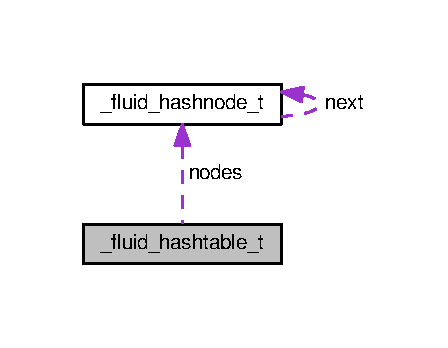
\includegraphics[width=215pt]{struct__fluid__hashtable__t__coll__graph}
\end{center}
\end{figure}
\subsection*{Public Attributes}
\begin{DoxyCompactItemize}
\item 
int \hyperlink{struct__fluid__hashtable__t_a29098c1a78cf9f3da0533e1df6ccecb9}{size}
\item 
int \hyperlink{struct__fluid__hashtable__t_a3389f9edcde2da407d2b33b9188fb730}{nnodes}
\item 
\hyperlink{fluid__hash_8h_a050a9781c9fa10e4b1caac67d32b9be4}{fluid\+\_\+hashnode\+\_\+t} $\ast$$\ast$ \hyperlink{struct__fluid__hashtable__t_af081a4263642d0400911b66acdf5de6a}{nodes}
\item 
\hyperlink{fluid__hash_8h_a0e826a2bc5ac0e62333df8bfa69880b0}{fluid\+\_\+hash\+\_\+func\+\_\+t} \hyperlink{struct__fluid__hashtable__t_a0ab4f6b3c18566cc16f5154447cdf126}{hash\+\_\+func}
\item 
\hyperlink{fluid__hash_8h_a327b756916612446e0de653cadaff492}{fluid\+\_\+equal\+\_\+func\+\_\+t} \hyperlink{struct__fluid__hashtable__t_a88c8b5a92bb5cdb478fa4d4bb9d5d448}{key\+\_\+equal\+\_\+func}
\item 
\hyperlink{fluidsynth__priv_8h_a6b8be882dd9958ea3635a868e1bf5152}{fluid\+\_\+atomic\+\_\+int\+\_\+t} \hyperlink{struct__fluid__hashtable__t_a48e1a2ba92a03664a9bcaabc585d3554}{ref\+\_\+count}
\item 
\hyperlink{fluid__hash_8h_a5fe009909539e295b7af5978fed06126}{fluid\+\_\+destroy\+\_\+notify\+\_\+t} \hyperlink{struct__fluid__hashtable__t_a278a70733615c92d30129ac636d2dab6}{key\+\_\+destroy\+\_\+func}
\item 
\hyperlink{fluid__hash_8h_a5fe009909539e295b7af5978fed06126}{fluid\+\_\+destroy\+\_\+notify\+\_\+t} \hyperlink{struct__fluid__hashtable__t_a96b147edad0233ebd40884f46297ea87}{value\+\_\+destroy\+\_\+func}
\item 
\hyperlink{fluid__sys_8h_a8e5bc2095bf6a26aa487db766bfb6660}{fluid\+\_\+rec\+\_\+mutex\+\_\+t} \hyperlink{struct__fluid__hashtable__t_a71f461017357e83c71b2e8947222372f}{mutex}
\end{DoxyCompactItemize}


\subsection{Member Data Documentation}
\mbox{\Hypertarget{struct__fluid__hashtable__t_a0ab4f6b3c18566cc16f5154447cdf126}\label{struct__fluid__hashtable__t_a0ab4f6b3c18566cc16f5154447cdf126}} 
\index{\+\_\+fluid\+\_\+hashtable\+\_\+t@{\+\_\+fluid\+\_\+hashtable\+\_\+t}!hash\+\_\+func@{hash\+\_\+func}}
\index{hash\+\_\+func@{hash\+\_\+func}!\+\_\+fluid\+\_\+hashtable\+\_\+t@{\+\_\+fluid\+\_\+hashtable\+\_\+t}}
\subsubsection{\texorpdfstring{hash\+\_\+func}{hash\_func}}
{\footnotesize\ttfamily \hyperlink{fluid__hash_8h_a0e826a2bc5ac0e62333df8bfa69880b0}{fluid\+\_\+hash\+\_\+func\+\_\+t} \+\_\+fluid\+\_\+hashtable\+\_\+t\+::hash\+\_\+func}

\mbox{\Hypertarget{struct__fluid__hashtable__t_a278a70733615c92d30129ac636d2dab6}\label{struct__fluid__hashtable__t_a278a70733615c92d30129ac636d2dab6}} 
\index{\+\_\+fluid\+\_\+hashtable\+\_\+t@{\+\_\+fluid\+\_\+hashtable\+\_\+t}!key\+\_\+destroy\+\_\+func@{key\+\_\+destroy\+\_\+func}}
\index{key\+\_\+destroy\+\_\+func@{key\+\_\+destroy\+\_\+func}!\+\_\+fluid\+\_\+hashtable\+\_\+t@{\+\_\+fluid\+\_\+hashtable\+\_\+t}}
\subsubsection{\texorpdfstring{key\+\_\+destroy\+\_\+func}{key\_destroy\_func}}
{\footnotesize\ttfamily \hyperlink{fluid__hash_8h_a5fe009909539e295b7af5978fed06126}{fluid\+\_\+destroy\+\_\+notify\+\_\+t} \+\_\+fluid\+\_\+hashtable\+\_\+t\+::key\+\_\+destroy\+\_\+func}

\mbox{\Hypertarget{struct__fluid__hashtable__t_a88c8b5a92bb5cdb478fa4d4bb9d5d448}\label{struct__fluid__hashtable__t_a88c8b5a92bb5cdb478fa4d4bb9d5d448}} 
\index{\+\_\+fluid\+\_\+hashtable\+\_\+t@{\+\_\+fluid\+\_\+hashtable\+\_\+t}!key\+\_\+equal\+\_\+func@{key\+\_\+equal\+\_\+func}}
\index{key\+\_\+equal\+\_\+func@{key\+\_\+equal\+\_\+func}!\+\_\+fluid\+\_\+hashtable\+\_\+t@{\+\_\+fluid\+\_\+hashtable\+\_\+t}}
\subsubsection{\texorpdfstring{key\+\_\+equal\+\_\+func}{key\_equal\_func}}
{\footnotesize\ttfamily \hyperlink{fluid__hash_8h_a327b756916612446e0de653cadaff492}{fluid\+\_\+equal\+\_\+func\+\_\+t} \+\_\+fluid\+\_\+hashtable\+\_\+t\+::key\+\_\+equal\+\_\+func}

\mbox{\Hypertarget{struct__fluid__hashtable__t_a71f461017357e83c71b2e8947222372f}\label{struct__fluid__hashtable__t_a71f461017357e83c71b2e8947222372f}} 
\index{\+\_\+fluid\+\_\+hashtable\+\_\+t@{\+\_\+fluid\+\_\+hashtable\+\_\+t}!mutex@{mutex}}
\index{mutex@{mutex}!\+\_\+fluid\+\_\+hashtable\+\_\+t@{\+\_\+fluid\+\_\+hashtable\+\_\+t}}
\subsubsection{\texorpdfstring{mutex}{mutex}}
{\footnotesize\ttfamily \hyperlink{fluid__sys_8h_a8e5bc2095bf6a26aa487db766bfb6660}{fluid\+\_\+rec\+\_\+mutex\+\_\+t} \+\_\+fluid\+\_\+hashtable\+\_\+t\+::mutex}

\mbox{\Hypertarget{struct__fluid__hashtable__t_a3389f9edcde2da407d2b33b9188fb730}\label{struct__fluid__hashtable__t_a3389f9edcde2da407d2b33b9188fb730}} 
\index{\+\_\+fluid\+\_\+hashtable\+\_\+t@{\+\_\+fluid\+\_\+hashtable\+\_\+t}!nnodes@{nnodes}}
\index{nnodes@{nnodes}!\+\_\+fluid\+\_\+hashtable\+\_\+t@{\+\_\+fluid\+\_\+hashtable\+\_\+t}}
\subsubsection{\texorpdfstring{nnodes}{nnodes}}
{\footnotesize\ttfamily int \+\_\+fluid\+\_\+hashtable\+\_\+t\+::nnodes}

\mbox{\Hypertarget{struct__fluid__hashtable__t_af081a4263642d0400911b66acdf5de6a}\label{struct__fluid__hashtable__t_af081a4263642d0400911b66acdf5de6a}} 
\index{\+\_\+fluid\+\_\+hashtable\+\_\+t@{\+\_\+fluid\+\_\+hashtable\+\_\+t}!nodes@{nodes}}
\index{nodes@{nodes}!\+\_\+fluid\+\_\+hashtable\+\_\+t@{\+\_\+fluid\+\_\+hashtable\+\_\+t}}
\subsubsection{\texorpdfstring{nodes}{nodes}}
{\footnotesize\ttfamily \hyperlink{fluid__hash_8h_a050a9781c9fa10e4b1caac67d32b9be4}{fluid\+\_\+hashnode\+\_\+t}$\ast$$\ast$ \+\_\+fluid\+\_\+hashtable\+\_\+t\+::nodes}

\mbox{\Hypertarget{struct__fluid__hashtable__t_a48e1a2ba92a03664a9bcaabc585d3554}\label{struct__fluid__hashtable__t_a48e1a2ba92a03664a9bcaabc585d3554}} 
\index{\+\_\+fluid\+\_\+hashtable\+\_\+t@{\+\_\+fluid\+\_\+hashtable\+\_\+t}!ref\+\_\+count@{ref\+\_\+count}}
\index{ref\+\_\+count@{ref\+\_\+count}!\+\_\+fluid\+\_\+hashtable\+\_\+t@{\+\_\+fluid\+\_\+hashtable\+\_\+t}}
\subsubsection{\texorpdfstring{ref\+\_\+count}{ref\_count}}
{\footnotesize\ttfamily \hyperlink{fluidsynth__priv_8h_a6b8be882dd9958ea3635a868e1bf5152}{fluid\+\_\+atomic\+\_\+int\+\_\+t} \+\_\+fluid\+\_\+hashtable\+\_\+t\+::ref\+\_\+count}

\mbox{\Hypertarget{struct__fluid__hashtable__t_a29098c1a78cf9f3da0533e1df6ccecb9}\label{struct__fluid__hashtable__t_a29098c1a78cf9f3da0533e1df6ccecb9}} 
\index{\+\_\+fluid\+\_\+hashtable\+\_\+t@{\+\_\+fluid\+\_\+hashtable\+\_\+t}!size@{size}}
\index{size@{size}!\+\_\+fluid\+\_\+hashtable\+\_\+t@{\+\_\+fluid\+\_\+hashtable\+\_\+t}}
\subsubsection{\texorpdfstring{size}{size}}
{\footnotesize\ttfamily int \+\_\+fluid\+\_\+hashtable\+\_\+t\+::size}

\mbox{\Hypertarget{struct__fluid__hashtable__t_a96b147edad0233ebd40884f46297ea87}\label{struct__fluid__hashtable__t_a96b147edad0233ebd40884f46297ea87}} 
\index{\+\_\+fluid\+\_\+hashtable\+\_\+t@{\+\_\+fluid\+\_\+hashtable\+\_\+t}!value\+\_\+destroy\+\_\+func@{value\+\_\+destroy\+\_\+func}}
\index{value\+\_\+destroy\+\_\+func@{value\+\_\+destroy\+\_\+func}!\+\_\+fluid\+\_\+hashtable\+\_\+t@{\+\_\+fluid\+\_\+hashtable\+\_\+t}}
\subsubsection{\texorpdfstring{value\+\_\+destroy\+\_\+func}{value\_destroy\_func}}
{\footnotesize\ttfamily \hyperlink{fluid__hash_8h_a5fe009909539e295b7af5978fed06126}{fluid\+\_\+destroy\+\_\+notify\+\_\+t} \+\_\+fluid\+\_\+hashtable\+\_\+t\+::value\+\_\+destroy\+\_\+func}



The documentation for this struct was generated from the following file\+:\begin{DoxyCompactItemize}
\item 
utils/\hyperlink{fluid__hash_8h}{fluid\+\_\+hash.\+h}\end{DoxyCompactItemize}

\hypertarget{struct__fluid__iir__filter__t}{}\section{\+\_\+fluid\+\_\+iir\+\_\+filter\+\_\+t Struct Reference}
\label{struct__fluid__iir__filter__t}\index{\+\_\+fluid\+\_\+iir\+\_\+filter\+\_\+t@{\+\_\+fluid\+\_\+iir\+\_\+filter\+\_\+t}}


{\ttfamily \#include $<$fluid\+\_\+iir\+\_\+filter.\+h$>$}

\subsection*{Public Attributes}
\begin{DoxyCompactItemize}
\item 
enum \hyperlink{synth_8h_a8a4cb4bd240d3654707ac0c5c7337a63}{fluid\+\_\+iir\+\_\+filter\+\_\+type} \hyperlink{struct__fluid__iir__filter__t_a651ef143533475852e123c05e8b7be1c}{type}
\item 
enum \hyperlink{synth_8h_a1e682c5d6f22e13947cc07bcd92d7525}{fluid\+\_\+iir\+\_\+filter\+\_\+flags} \hyperlink{struct__fluid__iir__filter__t_a272319b339db2f205d8b29fdba27877b}{flags}
\item 
\hyperlink{fluidsynth__priv_8h_a9e96f0917747b69cabb7c671bc693dbb}{fluid\+\_\+real\+\_\+t} \hyperlink{struct__fluid__iir__filter__t_aaba0627304b81d72f5a8160a4c1e0c6d}{b02}
\item 
\hyperlink{fluidsynth__priv_8h_a9e96f0917747b69cabb7c671bc693dbb}{fluid\+\_\+real\+\_\+t} \hyperlink{struct__fluid__iir__filter__t_aea2d3dea1a947f0764733eba68d509b0}{b1}
\item 
\hyperlink{fluidsynth__priv_8h_a9e96f0917747b69cabb7c671bc693dbb}{fluid\+\_\+real\+\_\+t} \hyperlink{struct__fluid__iir__filter__t_ad3f82ec6e5c739d343b06e4657dc1b04}{a1}
\item 
\hyperlink{fluidsynth__priv_8h_a9e96f0917747b69cabb7c671bc693dbb}{fluid\+\_\+real\+\_\+t} \hyperlink{struct__fluid__iir__filter__t_af607eff988c02048eba7b30a228397ca}{a2}
\item 
\hyperlink{fluidsynth__priv_8h_a9e96f0917747b69cabb7c671bc693dbb}{fluid\+\_\+real\+\_\+t} \hyperlink{struct__fluid__iir__filter__t_a72c4092eb203fe81e3c0f8348f04b1b4}{b02\+\_\+incr}
\item 
\hyperlink{fluidsynth__priv_8h_a9e96f0917747b69cabb7c671bc693dbb}{fluid\+\_\+real\+\_\+t} \hyperlink{struct__fluid__iir__filter__t_abc64713cbc233555e6aee28ff2e046e1}{b1\+\_\+incr}
\item 
\hyperlink{fluidsynth__priv_8h_a9e96f0917747b69cabb7c671bc693dbb}{fluid\+\_\+real\+\_\+t} \hyperlink{struct__fluid__iir__filter__t_aa8a3c222c3ebe50213b09db557b2d76f}{a1\+\_\+incr}
\item 
\hyperlink{fluidsynth__priv_8h_a9e96f0917747b69cabb7c671bc693dbb}{fluid\+\_\+real\+\_\+t} \hyperlink{struct__fluid__iir__filter__t_a2924cdd7aff7a7f54382a866b91f054e}{a2\+\_\+incr}
\item 
int \hyperlink{struct__fluid__iir__filter__t_a21b00d63aaa581947d83af5aa0c0396c}{filter\+\_\+coeff\+\_\+incr\+\_\+count}
\item 
int \hyperlink{struct__fluid__iir__filter__t_af4565151d0d7c189ee31c19fe85061f0}{compensate\+\_\+incr}
\item 
\hyperlink{fluidsynth__priv_8h_a9e96f0917747b69cabb7c671bc693dbb}{fluid\+\_\+real\+\_\+t} \hyperlink{struct__fluid__iir__filter__t_a9571c77902b40bab6e99ca2de72a7424}{hist1}
\item 
\hyperlink{fluidsynth__priv_8h_a9e96f0917747b69cabb7c671bc693dbb}{fluid\+\_\+real\+\_\+t} \hyperlink{struct__fluid__iir__filter__t_a353c2cb7bbae9a5bbfa0b4f91f9162cb}{hist2}
\item 
int \hyperlink{struct__fluid__iir__filter__t_ac35b95cd7955b60385ff0c085cfc9e75}{filter\+\_\+startup}
\item 
\hyperlink{fluidsynth__priv_8h_a9e96f0917747b69cabb7c671bc693dbb}{fluid\+\_\+real\+\_\+t} \hyperlink{struct__fluid__iir__filter__t_abb187dfe5dbd4ae47d2e8c99940e71fd}{fres}
\item 
\hyperlink{fluidsynth__priv_8h_a9e96f0917747b69cabb7c671bc693dbb}{fluid\+\_\+real\+\_\+t} \hyperlink{struct__fluid__iir__filter__t_a2063eb6f1ce2f7ec5218de09330341af}{last\+\_\+fres}
\item 
\hyperlink{fluidsynth__priv_8h_a9e96f0917747b69cabb7c671bc693dbb}{fluid\+\_\+real\+\_\+t} \hyperlink{struct__fluid__iir__filter__t_aaaf0ba836805f79004156cddbdf8c586}{q\+\_\+lin}
\item 
\hyperlink{fluidsynth__priv_8h_a9e96f0917747b69cabb7c671bc693dbb}{fluid\+\_\+real\+\_\+t} \hyperlink{struct__fluid__iir__filter__t_a274b068d53a741a726c923167b0588e3}{filter\+\_\+gain}
\end{DoxyCompactItemize}


\subsection{Member Data Documentation}
\mbox{\Hypertarget{struct__fluid__iir__filter__t_ad3f82ec6e5c739d343b06e4657dc1b04}\label{struct__fluid__iir__filter__t_ad3f82ec6e5c739d343b06e4657dc1b04}} 
\index{\+\_\+fluid\+\_\+iir\+\_\+filter\+\_\+t@{\+\_\+fluid\+\_\+iir\+\_\+filter\+\_\+t}!a1@{a1}}
\index{a1@{a1}!\+\_\+fluid\+\_\+iir\+\_\+filter\+\_\+t@{\+\_\+fluid\+\_\+iir\+\_\+filter\+\_\+t}}
\subsubsection{\texorpdfstring{a1}{a1}}
{\footnotesize\ttfamily \hyperlink{fluidsynth__priv_8h_a9e96f0917747b69cabb7c671bc693dbb}{fluid\+\_\+real\+\_\+t} \+\_\+fluid\+\_\+iir\+\_\+filter\+\_\+t\+::a1}

\mbox{\Hypertarget{struct__fluid__iir__filter__t_aa8a3c222c3ebe50213b09db557b2d76f}\label{struct__fluid__iir__filter__t_aa8a3c222c3ebe50213b09db557b2d76f}} 
\index{\+\_\+fluid\+\_\+iir\+\_\+filter\+\_\+t@{\+\_\+fluid\+\_\+iir\+\_\+filter\+\_\+t}!a1\+\_\+incr@{a1\+\_\+incr}}
\index{a1\+\_\+incr@{a1\+\_\+incr}!\+\_\+fluid\+\_\+iir\+\_\+filter\+\_\+t@{\+\_\+fluid\+\_\+iir\+\_\+filter\+\_\+t}}
\subsubsection{\texorpdfstring{a1\+\_\+incr}{a1\_incr}}
{\footnotesize\ttfamily \hyperlink{fluidsynth__priv_8h_a9e96f0917747b69cabb7c671bc693dbb}{fluid\+\_\+real\+\_\+t} \+\_\+fluid\+\_\+iir\+\_\+filter\+\_\+t\+::a1\+\_\+incr}

\mbox{\Hypertarget{struct__fluid__iir__filter__t_af607eff988c02048eba7b30a228397ca}\label{struct__fluid__iir__filter__t_af607eff988c02048eba7b30a228397ca}} 
\index{\+\_\+fluid\+\_\+iir\+\_\+filter\+\_\+t@{\+\_\+fluid\+\_\+iir\+\_\+filter\+\_\+t}!a2@{a2}}
\index{a2@{a2}!\+\_\+fluid\+\_\+iir\+\_\+filter\+\_\+t@{\+\_\+fluid\+\_\+iir\+\_\+filter\+\_\+t}}
\subsubsection{\texorpdfstring{a2}{a2}}
{\footnotesize\ttfamily \hyperlink{fluidsynth__priv_8h_a9e96f0917747b69cabb7c671bc693dbb}{fluid\+\_\+real\+\_\+t} \+\_\+fluid\+\_\+iir\+\_\+filter\+\_\+t\+::a2}

\mbox{\Hypertarget{struct__fluid__iir__filter__t_a2924cdd7aff7a7f54382a866b91f054e}\label{struct__fluid__iir__filter__t_a2924cdd7aff7a7f54382a866b91f054e}} 
\index{\+\_\+fluid\+\_\+iir\+\_\+filter\+\_\+t@{\+\_\+fluid\+\_\+iir\+\_\+filter\+\_\+t}!a2\+\_\+incr@{a2\+\_\+incr}}
\index{a2\+\_\+incr@{a2\+\_\+incr}!\+\_\+fluid\+\_\+iir\+\_\+filter\+\_\+t@{\+\_\+fluid\+\_\+iir\+\_\+filter\+\_\+t}}
\subsubsection{\texorpdfstring{a2\+\_\+incr}{a2\_incr}}
{\footnotesize\ttfamily \hyperlink{fluidsynth__priv_8h_a9e96f0917747b69cabb7c671bc693dbb}{fluid\+\_\+real\+\_\+t} \+\_\+fluid\+\_\+iir\+\_\+filter\+\_\+t\+::a2\+\_\+incr}

\mbox{\Hypertarget{struct__fluid__iir__filter__t_aaba0627304b81d72f5a8160a4c1e0c6d}\label{struct__fluid__iir__filter__t_aaba0627304b81d72f5a8160a4c1e0c6d}} 
\index{\+\_\+fluid\+\_\+iir\+\_\+filter\+\_\+t@{\+\_\+fluid\+\_\+iir\+\_\+filter\+\_\+t}!b02@{b02}}
\index{b02@{b02}!\+\_\+fluid\+\_\+iir\+\_\+filter\+\_\+t@{\+\_\+fluid\+\_\+iir\+\_\+filter\+\_\+t}}
\subsubsection{\texorpdfstring{b02}{b02}}
{\footnotesize\ttfamily \hyperlink{fluidsynth__priv_8h_a9e96f0917747b69cabb7c671bc693dbb}{fluid\+\_\+real\+\_\+t} \+\_\+fluid\+\_\+iir\+\_\+filter\+\_\+t\+::b02}

\mbox{\Hypertarget{struct__fluid__iir__filter__t_a72c4092eb203fe81e3c0f8348f04b1b4}\label{struct__fluid__iir__filter__t_a72c4092eb203fe81e3c0f8348f04b1b4}} 
\index{\+\_\+fluid\+\_\+iir\+\_\+filter\+\_\+t@{\+\_\+fluid\+\_\+iir\+\_\+filter\+\_\+t}!b02\+\_\+incr@{b02\+\_\+incr}}
\index{b02\+\_\+incr@{b02\+\_\+incr}!\+\_\+fluid\+\_\+iir\+\_\+filter\+\_\+t@{\+\_\+fluid\+\_\+iir\+\_\+filter\+\_\+t}}
\subsubsection{\texorpdfstring{b02\+\_\+incr}{b02\_incr}}
{\footnotesize\ttfamily \hyperlink{fluidsynth__priv_8h_a9e96f0917747b69cabb7c671bc693dbb}{fluid\+\_\+real\+\_\+t} \+\_\+fluid\+\_\+iir\+\_\+filter\+\_\+t\+::b02\+\_\+incr}

\mbox{\Hypertarget{struct__fluid__iir__filter__t_aea2d3dea1a947f0764733eba68d509b0}\label{struct__fluid__iir__filter__t_aea2d3dea1a947f0764733eba68d509b0}} 
\index{\+\_\+fluid\+\_\+iir\+\_\+filter\+\_\+t@{\+\_\+fluid\+\_\+iir\+\_\+filter\+\_\+t}!b1@{b1}}
\index{b1@{b1}!\+\_\+fluid\+\_\+iir\+\_\+filter\+\_\+t@{\+\_\+fluid\+\_\+iir\+\_\+filter\+\_\+t}}
\subsubsection{\texorpdfstring{b1}{b1}}
{\footnotesize\ttfamily \hyperlink{fluidsynth__priv_8h_a9e96f0917747b69cabb7c671bc693dbb}{fluid\+\_\+real\+\_\+t} \+\_\+fluid\+\_\+iir\+\_\+filter\+\_\+t\+::b1}

\mbox{\Hypertarget{struct__fluid__iir__filter__t_abc64713cbc233555e6aee28ff2e046e1}\label{struct__fluid__iir__filter__t_abc64713cbc233555e6aee28ff2e046e1}} 
\index{\+\_\+fluid\+\_\+iir\+\_\+filter\+\_\+t@{\+\_\+fluid\+\_\+iir\+\_\+filter\+\_\+t}!b1\+\_\+incr@{b1\+\_\+incr}}
\index{b1\+\_\+incr@{b1\+\_\+incr}!\+\_\+fluid\+\_\+iir\+\_\+filter\+\_\+t@{\+\_\+fluid\+\_\+iir\+\_\+filter\+\_\+t}}
\subsubsection{\texorpdfstring{b1\+\_\+incr}{b1\_incr}}
{\footnotesize\ttfamily \hyperlink{fluidsynth__priv_8h_a9e96f0917747b69cabb7c671bc693dbb}{fluid\+\_\+real\+\_\+t} \+\_\+fluid\+\_\+iir\+\_\+filter\+\_\+t\+::b1\+\_\+incr}

\mbox{\Hypertarget{struct__fluid__iir__filter__t_af4565151d0d7c189ee31c19fe85061f0}\label{struct__fluid__iir__filter__t_af4565151d0d7c189ee31c19fe85061f0}} 
\index{\+\_\+fluid\+\_\+iir\+\_\+filter\+\_\+t@{\+\_\+fluid\+\_\+iir\+\_\+filter\+\_\+t}!compensate\+\_\+incr@{compensate\+\_\+incr}}
\index{compensate\+\_\+incr@{compensate\+\_\+incr}!\+\_\+fluid\+\_\+iir\+\_\+filter\+\_\+t@{\+\_\+fluid\+\_\+iir\+\_\+filter\+\_\+t}}
\subsubsection{\texorpdfstring{compensate\+\_\+incr}{compensate\_incr}}
{\footnotesize\ttfamily int \+\_\+fluid\+\_\+iir\+\_\+filter\+\_\+t\+::compensate\+\_\+incr}

\mbox{\Hypertarget{struct__fluid__iir__filter__t_a21b00d63aaa581947d83af5aa0c0396c}\label{struct__fluid__iir__filter__t_a21b00d63aaa581947d83af5aa0c0396c}} 
\index{\+\_\+fluid\+\_\+iir\+\_\+filter\+\_\+t@{\+\_\+fluid\+\_\+iir\+\_\+filter\+\_\+t}!filter\+\_\+coeff\+\_\+incr\+\_\+count@{filter\+\_\+coeff\+\_\+incr\+\_\+count}}
\index{filter\+\_\+coeff\+\_\+incr\+\_\+count@{filter\+\_\+coeff\+\_\+incr\+\_\+count}!\+\_\+fluid\+\_\+iir\+\_\+filter\+\_\+t@{\+\_\+fluid\+\_\+iir\+\_\+filter\+\_\+t}}
\subsubsection{\texorpdfstring{filter\+\_\+coeff\+\_\+incr\+\_\+count}{filter\_coeff\_incr\_count}}
{\footnotesize\ttfamily int \+\_\+fluid\+\_\+iir\+\_\+filter\+\_\+t\+::filter\+\_\+coeff\+\_\+incr\+\_\+count}

\mbox{\Hypertarget{struct__fluid__iir__filter__t_a274b068d53a741a726c923167b0588e3}\label{struct__fluid__iir__filter__t_a274b068d53a741a726c923167b0588e3}} 
\index{\+\_\+fluid\+\_\+iir\+\_\+filter\+\_\+t@{\+\_\+fluid\+\_\+iir\+\_\+filter\+\_\+t}!filter\+\_\+gain@{filter\+\_\+gain}}
\index{filter\+\_\+gain@{filter\+\_\+gain}!\+\_\+fluid\+\_\+iir\+\_\+filter\+\_\+t@{\+\_\+fluid\+\_\+iir\+\_\+filter\+\_\+t}}
\subsubsection{\texorpdfstring{filter\+\_\+gain}{filter\_gain}}
{\footnotesize\ttfamily \hyperlink{fluidsynth__priv_8h_a9e96f0917747b69cabb7c671bc693dbb}{fluid\+\_\+real\+\_\+t} \+\_\+fluid\+\_\+iir\+\_\+filter\+\_\+t\+::filter\+\_\+gain}

\mbox{\Hypertarget{struct__fluid__iir__filter__t_ac35b95cd7955b60385ff0c085cfc9e75}\label{struct__fluid__iir__filter__t_ac35b95cd7955b60385ff0c085cfc9e75}} 
\index{\+\_\+fluid\+\_\+iir\+\_\+filter\+\_\+t@{\+\_\+fluid\+\_\+iir\+\_\+filter\+\_\+t}!filter\+\_\+startup@{filter\+\_\+startup}}
\index{filter\+\_\+startup@{filter\+\_\+startup}!\+\_\+fluid\+\_\+iir\+\_\+filter\+\_\+t@{\+\_\+fluid\+\_\+iir\+\_\+filter\+\_\+t}}
\subsubsection{\texorpdfstring{filter\+\_\+startup}{filter\_startup}}
{\footnotesize\ttfamily int \+\_\+fluid\+\_\+iir\+\_\+filter\+\_\+t\+::filter\+\_\+startup}

\mbox{\Hypertarget{struct__fluid__iir__filter__t_a272319b339db2f205d8b29fdba27877b}\label{struct__fluid__iir__filter__t_a272319b339db2f205d8b29fdba27877b}} 
\index{\+\_\+fluid\+\_\+iir\+\_\+filter\+\_\+t@{\+\_\+fluid\+\_\+iir\+\_\+filter\+\_\+t}!flags@{flags}}
\index{flags@{flags}!\+\_\+fluid\+\_\+iir\+\_\+filter\+\_\+t@{\+\_\+fluid\+\_\+iir\+\_\+filter\+\_\+t}}
\subsubsection{\texorpdfstring{flags}{flags}}
{\footnotesize\ttfamily enum \hyperlink{synth_8h_a1e682c5d6f22e13947cc07bcd92d7525}{fluid\+\_\+iir\+\_\+filter\+\_\+flags} \+\_\+fluid\+\_\+iir\+\_\+filter\+\_\+t\+::flags}

\mbox{\Hypertarget{struct__fluid__iir__filter__t_abb187dfe5dbd4ae47d2e8c99940e71fd}\label{struct__fluid__iir__filter__t_abb187dfe5dbd4ae47d2e8c99940e71fd}} 
\index{\+\_\+fluid\+\_\+iir\+\_\+filter\+\_\+t@{\+\_\+fluid\+\_\+iir\+\_\+filter\+\_\+t}!fres@{fres}}
\index{fres@{fres}!\+\_\+fluid\+\_\+iir\+\_\+filter\+\_\+t@{\+\_\+fluid\+\_\+iir\+\_\+filter\+\_\+t}}
\subsubsection{\texorpdfstring{fres}{fres}}
{\footnotesize\ttfamily \hyperlink{fluidsynth__priv_8h_a9e96f0917747b69cabb7c671bc693dbb}{fluid\+\_\+real\+\_\+t} \+\_\+fluid\+\_\+iir\+\_\+filter\+\_\+t\+::fres}

\mbox{\Hypertarget{struct__fluid__iir__filter__t_a9571c77902b40bab6e99ca2de72a7424}\label{struct__fluid__iir__filter__t_a9571c77902b40bab6e99ca2de72a7424}} 
\index{\+\_\+fluid\+\_\+iir\+\_\+filter\+\_\+t@{\+\_\+fluid\+\_\+iir\+\_\+filter\+\_\+t}!hist1@{hist1}}
\index{hist1@{hist1}!\+\_\+fluid\+\_\+iir\+\_\+filter\+\_\+t@{\+\_\+fluid\+\_\+iir\+\_\+filter\+\_\+t}}
\subsubsection{\texorpdfstring{hist1}{hist1}}
{\footnotesize\ttfamily \hyperlink{fluidsynth__priv_8h_a9e96f0917747b69cabb7c671bc693dbb}{fluid\+\_\+real\+\_\+t} \+\_\+fluid\+\_\+iir\+\_\+filter\+\_\+t\+::hist1}

\mbox{\Hypertarget{struct__fluid__iir__filter__t_a353c2cb7bbae9a5bbfa0b4f91f9162cb}\label{struct__fluid__iir__filter__t_a353c2cb7bbae9a5bbfa0b4f91f9162cb}} 
\index{\+\_\+fluid\+\_\+iir\+\_\+filter\+\_\+t@{\+\_\+fluid\+\_\+iir\+\_\+filter\+\_\+t}!hist2@{hist2}}
\index{hist2@{hist2}!\+\_\+fluid\+\_\+iir\+\_\+filter\+\_\+t@{\+\_\+fluid\+\_\+iir\+\_\+filter\+\_\+t}}
\subsubsection{\texorpdfstring{hist2}{hist2}}
{\footnotesize\ttfamily \hyperlink{fluidsynth__priv_8h_a9e96f0917747b69cabb7c671bc693dbb}{fluid\+\_\+real\+\_\+t} \+\_\+fluid\+\_\+iir\+\_\+filter\+\_\+t\+::hist2}

\mbox{\Hypertarget{struct__fluid__iir__filter__t_a2063eb6f1ce2f7ec5218de09330341af}\label{struct__fluid__iir__filter__t_a2063eb6f1ce2f7ec5218de09330341af}} 
\index{\+\_\+fluid\+\_\+iir\+\_\+filter\+\_\+t@{\+\_\+fluid\+\_\+iir\+\_\+filter\+\_\+t}!last\+\_\+fres@{last\+\_\+fres}}
\index{last\+\_\+fres@{last\+\_\+fres}!\+\_\+fluid\+\_\+iir\+\_\+filter\+\_\+t@{\+\_\+fluid\+\_\+iir\+\_\+filter\+\_\+t}}
\subsubsection{\texorpdfstring{last\+\_\+fres}{last\_fres}}
{\footnotesize\ttfamily \hyperlink{fluidsynth__priv_8h_a9e96f0917747b69cabb7c671bc693dbb}{fluid\+\_\+real\+\_\+t} \+\_\+fluid\+\_\+iir\+\_\+filter\+\_\+t\+::last\+\_\+fres}

\mbox{\Hypertarget{struct__fluid__iir__filter__t_aaaf0ba836805f79004156cddbdf8c586}\label{struct__fluid__iir__filter__t_aaaf0ba836805f79004156cddbdf8c586}} 
\index{\+\_\+fluid\+\_\+iir\+\_\+filter\+\_\+t@{\+\_\+fluid\+\_\+iir\+\_\+filter\+\_\+t}!q\+\_\+lin@{q\+\_\+lin}}
\index{q\+\_\+lin@{q\+\_\+lin}!\+\_\+fluid\+\_\+iir\+\_\+filter\+\_\+t@{\+\_\+fluid\+\_\+iir\+\_\+filter\+\_\+t}}
\subsubsection{\texorpdfstring{q\+\_\+lin}{q\_lin}}
{\footnotesize\ttfamily \hyperlink{fluidsynth__priv_8h_a9e96f0917747b69cabb7c671bc693dbb}{fluid\+\_\+real\+\_\+t} \+\_\+fluid\+\_\+iir\+\_\+filter\+\_\+t\+::q\+\_\+lin}

\mbox{\Hypertarget{struct__fluid__iir__filter__t_a651ef143533475852e123c05e8b7be1c}\label{struct__fluid__iir__filter__t_a651ef143533475852e123c05e8b7be1c}} 
\index{\+\_\+fluid\+\_\+iir\+\_\+filter\+\_\+t@{\+\_\+fluid\+\_\+iir\+\_\+filter\+\_\+t}!type@{type}}
\index{type@{type}!\+\_\+fluid\+\_\+iir\+\_\+filter\+\_\+t@{\+\_\+fluid\+\_\+iir\+\_\+filter\+\_\+t}}
\subsubsection{\texorpdfstring{type}{type}}
{\footnotesize\ttfamily enum \hyperlink{synth_8h_a8a4cb4bd240d3654707ac0c5c7337a63}{fluid\+\_\+iir\+\_\+filter\+\_\+type} \+\_\+fluid\+\_\+iir\+\_\+filter\+\_\+t\+::type}



The documentation for this struct was generated from the following file\+:\begin{DoxyCompactItemize}
\item 
rvoice/\hyperlink{fluid__iir__filter_8h}{fluid\+\_\+iir\+\_\+filter.\+h}\end{DoxyCompactItemize}

\hypertarget{struct__fluid__inst__t}{}\section{\+\_\+fluid\+\_\+inst\+\_\+t Struct Reference}
\label{struct__fluid__inst__t}\index{\+\_\+fluid\+\_\+inst\+\_\+t@{\+\_\+fluid\+\_\+inst\+\_\+t}}


{\ttfamily \#include $<$fluid\+\_\+defsfont.\+h$>$}



Collaboration diagram for \+\_\+fluid\+\_\+inst\+\_\+t\+:
\nopagebreak
\begin{figure}[H]
\begin{center}
\leavevmode
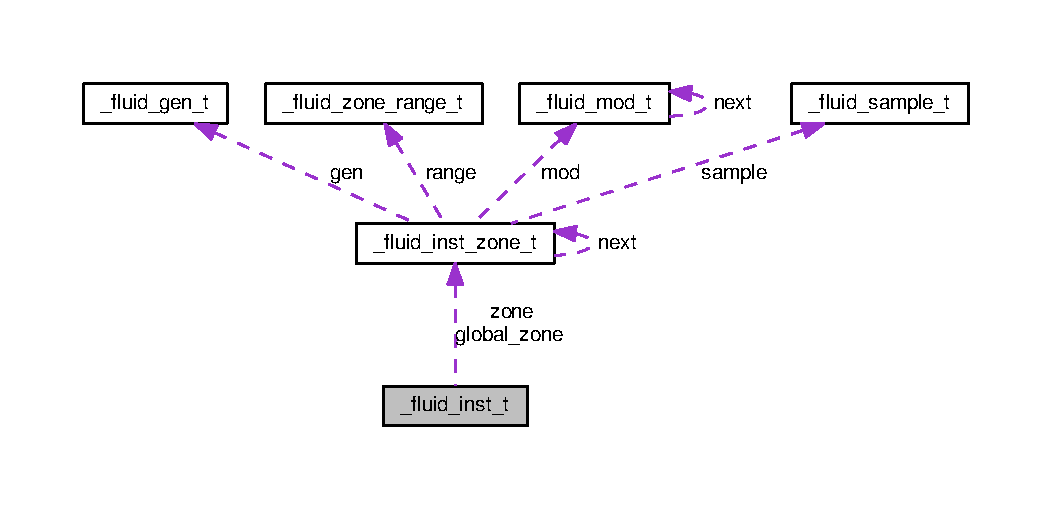
\includegraphics[width=350pt]{struct__fluid__inst__t__coll__graph}
\end{center}
\end{figure}
\subsection*{Public Attributes}
\begin{DoxyCompactItemize}
\item 
char \hyperlink{struct__fluid__inst__t_ab23fbac1313132d2875e9a140f891360}{name} \mbox{[}21\mbox{]}
\item 
int \hyperlink{struct__fluid__inst__t_afce8fb8979a1c3d4848042a3f1fbf57e}{source\+\_\+idx}
\item 
\hyperlink{fluid__defsfont_8h_aa02ac18b4c58545cc3b297bdf4d933ab}{fluid\+\_\+inst\+\_\+zone\+\_\+t} $\ast$ \hyperlink{struct__fluid__inst__t_a3ba1374703f8f5f269ee9915e8155d1f}{global\+\_\+zone}
\item 
\hyperlink{fluid__defsfont_8h_aa02ac18b4c58545cc3b297bdf4d933ab}{fluid\+\_\+inst\+\_\+zone\+\_\+t} $\ast$ \hyperlink{struct__fluid__inst__t_a3ee3921ad01c3cdd87b35e32ba9fea4e}{zone}
\end{DoxyCompactItemize}


\subsection{Member Data Documentation}
\mbox{\Hypertarget{struct__fluid__inst__t_a3ba1374703f8f5f269ee9915e8155d1f}\label{struct__fluid__inst__t_a3ba1374703f8f5f269ee9915e8155d1f}} 
\index{\+\_\+fluid\+\_\+inst\+\_\+t@{\+\_\+fluid\+\_\+inst\+\_\+t}!global\+\_\+zone@{global\+\_\+zone}}
\index{global\+\_\+zone@{global\+\_\+zone}!\+\_\+fluid\+\_\+inst\+\_\+t@{\+\_\+fluid\+\_\+inst\+\_\+t}}
\subsubsection{\texorpdfstring{global\+\_\+zone}{global\_zone}}
{\footnotesize\ttfamily \hyperlink{fluid__defsfont_8h_aa02ac18b4c58545cc3b297bdf4d933ab}{fluid\+\_\+inst\+\_\+zone\+\_\+t}$\ast$ \+\_\+fluid\+\_\+inst\+\_\+t\+::global\+\_\+zone}

\mbox{\Hypertarget{struct__fluid__inst__t_ab23fbac1313132d2875e9a140f891360}\label{struct__fluid__inst__t_ab23fbac1313132d2875e9a140f891360}} 
\index{\+\_\+fluid\+\_\+inst\+\_\+t@{\+\_\+fluid\+\_\+inst\+\_\+t}!name@{name}}
\index{name@{name}!\+\_\+fluid\+\_\+inst\+\_\+t@{\+\_\+fluid\+\_\+inst\+\_\+t}}
\subsubsection{\texorpdfstring{name}{name}}
{\footnotesize\ttfamily char \+\_\+fluid\+\_\+inst\+\_\+t\+::name\mbox{[}21\mbox{]}}

\mbox{\Hypertarget{struct__fluid__inst__t_afce8fb8979a1c3d4848042a3f1fbf57e}\label{struct__fluid__inst__t_afce8fb8979a1c3d4848042a3f1fbf57e}} 
\index{\+\_\+fluid\+\_\+inst\+\_\+t@{\+\_\+fluid\+\_\+inst\+\_\+t}!source\+\_\+idx@{source\+\_\+idx}}
\index{source\+\_\+idx@{source\+\_\+idx}!\+\_\+fluid\+\_\+inst\+\_\+t@{\+\_\+fluid\+\_\+inst\+\_\+t}}
\subsubsection{\texorpdfstring{source\+\_\+idx}{source\_idx}}
{\footnotesize\ttfamily int \+\_\+fluid\+\_\+inst\+\_\+t\+::source\+\_\+idx}

\mbox{\Hypertarget{struct__fluid__inst__t_a3ee3921ad01c3cdd87b35e32ba9fea4e}\label{struct__fluid__inst__t_a3ee3921ad01c3cdd87b35e32ba9fea4e}} 
\index{\+\_\+fluid\+\_\+inst\+\_\+t@{\+\_\+fluid\+\_\+inst\+\_\+t}!zone@{zone}}
\index{zone@{zone}!\+\_\+fluid\+\_\+inst\+\_\+t@{\+\_\+fluid\+\_\+inst\+\_\+t}}
\subsubsection{\texorpdfstring{zone}{zone}}
{\footnotesize\ttfamily \hyperlink{fluid__defsfont_8h_aa02ac18b4c58545cc3b297bdf4d933ab}{fluid\+\_\+inst\+\_\+zone\+\_\+t}$\ast$ \+\_\+fluid\+\_\+inst\+\_\+t\+::zone}



The documentation for this struct was generated from the following file\+:\begin{DoxyCompactItemize}
\item 
sfloader/\hyperlink{fluid__defsfont_8h}{fluid\+\_\+defsfont.\+h}\end{DoxyCompactItemize}

\hypertarget{struct__fluid__inst__zone__t}{}\section{\+\_\+fluid\+\_\+inst\+\_\+zone\+\_\+t Struct Reference}
\label{struct__fluid__inst__zone__t}\index{\+\_\+fluid\+\_\+inst\+\_\+zone\+\_\+t@{\+\_\+fluid\+\_\+inst\+\_\+zone\+\_\+t}}


{\ttfamily \#include $<$fluid\+\_\+defsfont.\+h$>$}



Collaboration diagram for \+\_\+fluid\+\_\+inst\+\_\+zone\+\_\+t\+:
\nopagebreak
\begin{figure}[H]
\begin{center}
\leavevmode
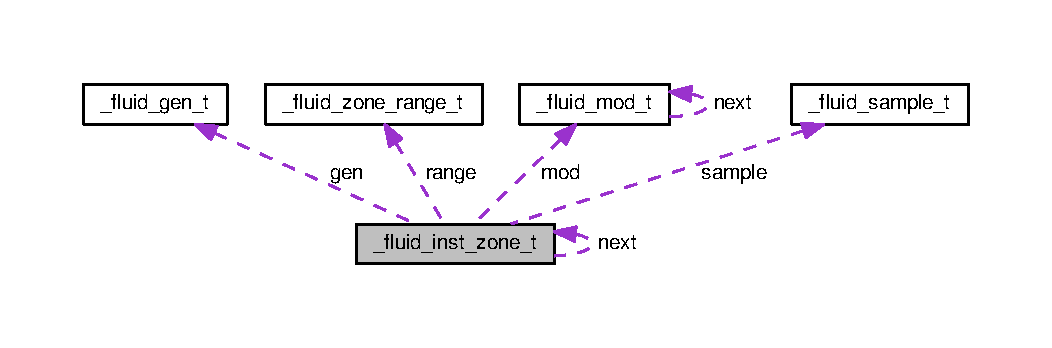
\includegraphics[width=350pt]{struct__fluid__inst__zone__t__coll__graph}
\end{center}
\end{figure}
\subsection*{Public Attributes}
\begin{DoxyCompactItemize}
\item 
\hyperlink{fluid__defsfont_8h_aa02ac18b4c58545cc3b297bdf4d933ab}{fluid\+\_\+inst\+\_\+zone\+\_\+t} $\ast$ \hyperlink{struct__fluid__inst__zone__t_aec824eaa2863823c9a200059cfa24c98}{next}
\item 
char $\ast$ \hyperlink{struct__fluid__inst__zone__t_aedd059777859f39c7b0d55c6213d925b}{name}
\item 
\hyperlink{types_8h_abf9174d452679ca1a4ee7d693fb773cf}{fluid\+\_\+sample\+\_\+t} $\ast$ \hyperlink{struct__fluid__inst__zone__t_a35d1af8ed2864340ded7f1115a22cbef}{sample}
\item 
\hyperlink{fluidsynth__priv_8h_ac8502f0049ba8c20821b136e611462da}{fluid\+\_\+zone\+\_\+range\+\_\+t} \hyperlink{struct__fluid__inst__zone__t_a748cbb2b5f058a6a391b27e627e85e42}{range}
\item 
\hyperlink{fluid__gen_8h_a018737d76d5ad530b622bd27b70701b0}{fluid\+\_\+gen\+\_\+t} \hyperlink{struct__fluid__inst__zone__t_af63facfbf27034a46450b2b3698b8bab}{gen} \mbox{[}\hyperlink{gen_8h_ad17a24ae3b25f3b8cc5762f818eef9b4a9c372c341b7b1a718f0016f40c615cf3}{G\+E\+N\+\_\+\+L\+A\+ST}\mbox{]}
\item 
\hyperlink{types_8h_a6c727efab500d6c0c350d4292e9aa5ef}{fluid\+\_\+mod\+\_\+t} $\ast$ \hyperlink{struct__fluid__inst__zone__t_a48594ce065f222b49680bc332c9fc2d9}{mod}
\end{DoxyCompactItemize}


\subsection{Member Data Documentation}
\mbox{\Hypertarget{struct__fluid__inst__zone__t_af63facfbf27034a46450b2b3698b8bab}\label{struct__fluid__inst__zone__t_af63facfbf27034a46450b2b3698b8bab}} 
\index{\+\_\+fluid\+\_\+inst\+\_\+zone\+\_\+t@{\+\_\+fluid\+\_\+inst\+\_\+zone\+\_\+t}!gen@{gen}}
\index{gen@{gen}!\+\_\+fluid\+\_\+inst\+\_\+zone\+\_\+t@{\+\_\+fluid\+\_\+inst\+\_\+zone\+\_\+t}}
\subsubsection{\texorpdfstring{gen}{gen}}
{\footnotesize\ttfamily \hyperlink{fluid__gen_8h_a018737d76d5ad530b622bd27b70701b0}{fluid\+\_\+gen\+\_\+t} \+\_\+fluid\+\_\+inst\+\_\+zone\+\_\+t\+::gen\mbox{[}\hyperlink{gen_8h_ad17a24ae3b25f3b8cc5762f818eef9b4a9c372c341b7b1a718f0016f40c615cf3}{G\+E\+N\+\_\+\+L\+A\+ST}\mbox{]}}

\mbox{\Hypertarget{struct__fluid__inst__zone__t_a48594ce065f222b49680bc332c9fc2d9}\label{struct__fluid__inst__zone__t_a48594ce065f222b49680bc332c9fc2d9}} 
\index{\+\_\+fluid\+\_\+inst\+\_\+zone\+\_\+t@{\+\_\+fluid\+\_\+inst\+\_\+zone\+\_\+t}!mod@{mod}}
\index{mod@{mod}!\+\_\+fluid\+\_\+inst\+\_\+zone\+\_\+t@{\+\_\+fluid\+\_\+inst\+\_\+zone\+\_\+t}}
\subsubsection{\texorpdfstring{mod}{mod}}
{\footnotesize\ttfamily \hyperlink{types_8h_a6c727efab500d6c0c350d4292e9aa5ef}{fluid\+\_\+mod\+\_\+t}$\ast$ \+\_\+fluid\+\_\+inst\+\_\+zone\+\_\+t\+::mod}

\mbox{\Hypertarget{struct__fluid__inst__zone__t_aedd059777859f39c7b0d55c6213d925b}\label{struct__fluid__inst__zone__t_aedd059777859f39c7b0d55c6213d925b}} 
\index{\+\_\+fluid\+\_\+inst\+\_\+zone\+\_\+t@{\+\_\+fluid\+\_\+inst\+\_\+zone\+\_\+t}!name@{name}}
\index{name@{name}!\+\_\+fluid\+\_\+inst\+\_\+zone\+\_\+t@{\+\_\+fluid\+\_\+inst\+\_\+zone\+\_\+t}}
\subsubsection{\texorpdfstring{name}{name}}
{\footnotesize\ttfamily char$\ast$ \+\_\+fluid\+\_\+inst\+\_\+zone\+\_\+t\+::name}

\mbox{\Hypertarget{struct__fluid__inst__zone__t_aec824eaa2863823c9a200059cfa24c98}\label{struct__fluid__inst__zone__t_aec824eaa2863823c9a200059cfa24c98}} 
\index{\+\_\+fluid\+\_\+inst\+\_\+zone\+\_\+t@{\+\_\+fluid\+\_\+inst\+\_\+zone\+\_\+t}!next@{next}}
\index{next@{next}!\+\_\+fluid\+\_\+inst\+\_\+zone\+\_\+t@{\+\_\+fluid\+\_\+inst\+\_\+zone\+\_\+t}}
\subsubsection{\texorpdfstring{next}{next}}
{\footnotesize\ttfamily \hyperlink{fluid__defsfont_8h_aa02ac18b4c58545cc3b297bdf4d933ab}{fluid\+\_\+inst\+\_\+zone\+\_\+t}$\ast$ \+\_\+fluid\+\_\+inst\+\_\+zone\+\_\+t\+::next}

\mbox{\Hypertarget{struct__fluid__inst__zone__t_a748cbb2b5f058a6a391b27e627e85e42}\label{struct__fluid__inst__zone__t_a748cbb2b5f058a6a391b27e627e85e42}} 
\index{\+\_\+fluid\+\_\+inst\+\_\+zone\+\_\+t@{\+\_\+fluid\+\_\+inst\+\_\+zone\+\_\+t}!range@{range}}
\index{range@{range}!\+\_\+fluid\+\_\+inst\+\_\+zone\+\_\+t@{\+\_\+fluid\+\_\+inst\+\_\+zone\+\_\+t}}
\subsubsection{\texorpdfstring{range}{range}}
{\footnotesize\ttfamily \hyperlink{fluidsynth__priv_8h_ac8502f0049ba8c20821b136e611462da}{fluid\+\_\+zone\+\_\+range\+\_\+t} \+\_\+fluid\+\_\+inst\+\_\+zone\+\_\+t\+::range}

\mbox{\Hypertarget{struct__fluid__inst__zone__t_a35d1af8ed2864340ded7f1115a22cbef}\label{struct__fluid__inst__zone__t_a35d1af8ed2864340ded7f1115a22cbef}} 
\index{\+\_\+fluid\+\_\+inst\+\_\+zone\+\_\+t@{\+\_\+fluid\+\_\+inst\+\_\+zone\+\_\+t}!sample@{sample}}
\index{sample@{sample}!\+\_\+fluid\+\_\+inst\+\_\+zone\+\_\+t@{\+\_\+fluid\+\_\+inst\+\_\+zone\+\_\+t}}
\subsubsection{\texorpdfstring{sample}{sample}}
{\footnotesize\ttfamily \hyperlink{types_8h_abf9174d452679ca1a4ee7d693fb773cf}{fluid\+\_\+sample\+\_\+t}$\ast$ \+\_\+fluid\+\_\+inst\+\_\+zone\+\_\+t\+::sample}



The documentation for this struct was generated from the following file\+:\begin{DoxyCompactItemize}
\item 
sfloader/\hyperlink{fluid__defsfont_8h}{fluid\+\_\+defsfont.\+h}\end{DoxyCompactItemize}

\hypertarget{struct__fluid__lfo__t}{}\section{\+\_\+fluid\+\_\+lfo\+\_\+t Struct Reference}
\label{struct__fluid__lfo__t}\index{\+\_\+fluid\+\_\+lfo\+\_\+t@{\+\_\+fluid\+\_\+lfo\+\_\+t}}


{\ttfamily \#include $<$fluid\+\_\+lfo.\+h$>$}

\subsection*{Public Attributes}
\begin{DoxyCompactItemize}
\item 
\hyperlink{fluidsynth__priv_8h_a9e96f0917747b69cabb7c671bc693dbb}{fluid\+\_\+real\+\_\+t} \hyperlink{struct__fluid__lfo__t_a56f1a08c37957fc3be87560d184a73b5}{val}
\item 
unsigned int \hyperlink{struct__fluid__lfo__t_aa43118e7a3a8d5155dfa93d2af589e3f}{delay}
\item 
\hyperlink{fluidsynth__priv_8h_a9e96f0917747b69cabb7c671bc693dbb}{fluid\+\_\+real\+\_\+t} \hyperlink{struct__fluid__lfo__t_a43fdfa236c0ff3bcefb32df577a8996e}{increment}
\end{DoxyCompactItemize}


\subsection{Member Data Documentation}
\mbox{\Hypertarget{struct__fluid__lfo__t_aa43118e7a3a8d5155dfa93d2af589e3f}\label{struct__fluid__lfo__t_aa43118e7a3a8d5155dfa93d2af589e3f}} 
\index{\+\_\+fluid\+\_\+lfo\+\_\+t@{\+\_\+fluid\+\_\+lfo\+\_\+t}!delay@{delay}}
\index{delay@{delay}!\+\_\+fluid\+\_\+lfo\+\_\+t@{\+\_\+fluid\+\_\+lfo\+\_\+t}}
\subsubsection{\texorpdfstring{delay}{delay}}
{\footnotesize\ttfamily unsigned int \+\_\+fluid\+\_\+lfo\+\_\+t\+::delay}

\mbox{\Hypertarget{struct__fluid__lfo__t_a43fdfa236c0ff3bcefb32df577a8996e}\label{struct__fluid__lfo__t_a43fdfa236c0ff3bcefb32df577a8996e}} 
\index{\+\_\+fluid\+\_\+lfo\+\_\+t@{\+\_\+fluid\+\_\+lfo\+\_\+t}!increment@{increment}}
\index{increment@{increment}!\+\_\+fluid\+\_\+lfo\+\_\+t@{\+\_\+fluid\+\_\+lfo\+\_\+t}}
\subsubsection{\texorpdfstring{increment}{increment}}
{\footnotesize\ttfamily \hyperlink{fluidsynth__priv_8h_a9e96f0917747b69cabb7c671bc693dbb}{fluid\+\_\+real\+\_\+t} \+\_\+fluid\+\_\+lfo\+\_\+t\+::increment}

\mbox{\Hypertarget{struct__fluid__lfo__t_a56f1a08c37957fc3be87560d184a73b5}\label{struct__fluid__lfo__t_a56f1a08c37957fc3be87560d184a73b5}} 
\index{\+\_\+fluid\+\_\+lfo\+\_\+t@{\+\_\+fluid\+\_\+lfo\+\_\+t}!val@{val}}
\index{val@{val}!\+\_\+fluid\+\_\+lfo\+\_\+t@{\+\_\+fluid\+\_\+lfo\+\_\+t}}
\subsubsection{\texorpdfstring{val}{val}}
{\footnotesize\ttfamily \hyperlink{fluidsynth__priv_8h_a9e96f0917747b69cabb7c671bc693dbb}{fluid\+\_\+real\+\_\+t} \+\_\+fluid\+\_\+lfo\+\_\+t\+::val}



The documentation for this struct was generated from the following file\+:\begin{DoxyCompactItemize}
\item 
rvoice/\hyperlink{fluid__lfo_8h}{fluid\+\_\+lfo.\+h}\end{DoxyCompactItemize}

\hypertarget{struct__fluid__list__t}{}\section{\+\_\+fluid\+\_\+list\+\_\+t Struct Reference}
\label{struct__fluid__list__t}\index{\+\_\+fluid\+\_\+list\+\_\+t@{\+\_\+fluid\+\_\+list\+\_\+t}}


{\ttfamily \#include $<$fluid\+\_\+list.\+h$>$}



Collaboration diagram for \+\_\+fluid\+\_\+list\+\_\+t\+:
\nopagebreak
\begin{figure}[H]
\begin{center}
\leavevmode
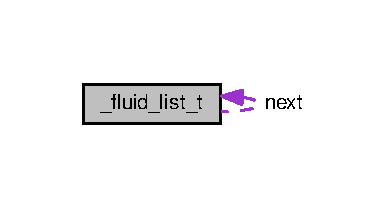
\includegraphics[width=186pt]{struct__fluid__list__t__coll__graph}
\end{center}
\end{figure}
\subsection*{Public Attributes}
\begin{DoxyCompactItemize}
\item 
void $\ast$ \hyperlink{struct__fluid__list__t_a76f4fba75542cd3d105e407195cbd939}{data}
\item 
\hyperlink{fluid__list_8h_a3ef7535d4290862c0af118569223bd89}{fluid\+\_\+list\+\_\+t} $\ast$ \hyperlink{struct__fluid__list__t_a60f4bba688688d1ceabba258a96d3625}{next}
\end{DoxyCompactItemize}


\subsection{Member Data Documentation}
\mbox{\Hypertarget{struct__fluid__list__t_a76f4fba75542cd3d105e407195cbd939}\label{struct__fluid__list__t_a76f4fba75542cd3d105e407195cbd939}} 
\index{\+\_\+fluid\+\_\+list\+\_\+t@{\+\_\+fluid\+\_\+list\+\_\+t}!data@{data}}
\index{data@{data}!\+\_\+fluid\+\_\+list\+\_\+t@{\+\_\+fluid\+\_\+list\+\_\+t}}
\subsubsection{\texorpdfstring{data}{data}}
{\footnotesize\ttfamily void$\ast$ \+\_\+fluid\+\_\+list\+\_\+t\+::data}

\mbox{\Hypertarget{struct__fluid__list__t_a60f4bba688688d1ceabba258a96d3625}\label{struct__fluid__list__t_a60f4bba688688d1ceabba258a96d3625}} 
\index{\+\_\+fluid\+\_\+list\+\_\+t@{\+\_\+fluid\+\_\+list\+\_\+t}!next@{next}}
\index{next@{next}!\+\_\+fluid\+\_\+list\+\_\+t@{\+\_\+fluid\+\_\+list\+\_\+t}}
\subsubsection{\texorpdfstring{next}{next}}
{\footnotesize\ttfamily \hyperlink{fluid__list_8h_a3ef7535d4290862c0af118569223bd89}{fluid\+\_\+list\+\_\+t}$\ast$ \+\_\+fluid\+\_\+list\+\_\+t\+::next}



The documentation for this struct was generated from the following file\+:\begin{DoxyCompactItemize}
\item 
utils/\hyperlink{fluid__list_8h}{fluid\+\_\+list.\+h}\end{DoxyCompactItemize}

\hypertarget{struct__fluid__midi__driver__t}{}\section{\+\_\+fluid\+\_\+midi\+\_\+driver\+\_\+t Struct Reference}
\label{struct__fluid__midi__driver__t}\index{\+\_\+fluid\+\_\+midi\+\_\+driver\+\_\+t@{\+\_\+fluid\+\_\+midi\+\_\+driver\+\_\+t}}


{\ttfamily \#include $<$fluid\+\_\+mdriver.\+h$>$}



Collaboration diagram for \+\_\+fluid\+\_\+midi\+\_\+driver\+\_\+t\+:
\nopagebreak
\begin{figure}[H]
\begin{center}
\leavevmode
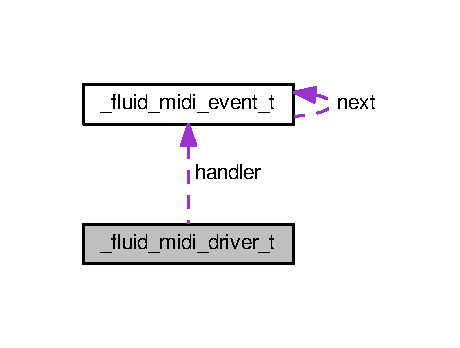
\includegraphics[width=221pt]{struct__fluid__midi__driver__t__coll__graph}
\end{center}
\end{figure}
\subsection*{Public Attributes}
\begin{DoxyCompactItemize}
\item 
const char $\ast$ \hyperlink{struct__fluid__midi__driver__t_a8fed06378561925282de8b1da4b48df6}{name}
\item 
\hyperlink{midi_8h_a42c3752e3adb54e0af802131c36a1129}{handle\+\_\+midi\+\_\+event\+\_\+func\+\_\+t} \hyperlink{struct__fluid__midi__driver__t_a765f3fddfd189bdeb58515bd8eebf553}{handler}
\item 
void $\ast$ \hyperlink{struct__fluid__midi__driver__t_aa94c33c717f0ca513ac839242a80a5b0}{data}
\end{DoxyCompactItemize}


\subsection{Member Data Documentation}
\mbox{\Hypertarget{struct__fluid__midi__driver__t_aa94c33c717f0ca513ac839242a80a5b0}\label{struct__fluid__midi__driver__t_aa94c33c717f0ca513ac839242a80a5b0}} 
\index{\+\_\+fluid\+\_\+midi\+\_\+driver\+\_\+t@{\+\_\+fluid\+\_\+midi\+\_\+driver\+\_\+t}!data@{data}}
\index{data@{data}!\+\_\+fluid\+\_\+midi\+\_\+driver\+\_\+t@{\+\_\+fluid\+\_\+midi\+\_\+driver\+\_\+t}}
\subsubsection{\texorpdfstring{data}{data}}
{\footnotesize\ttfamily void$\ast$ \+\_\+fluid\+\_\+midi\+\_\+driver\+\_\+t\+::data}

\mbox{\Hypertarget{struct__fluid__midi__driver__t_a765f3fddfd189bdeb58515bd8eebf553}\label{struct__fluid__midi__driver__t_a765f3fddfd189bdeb58515bd8eebf553}} 
\index{\+\_\+fluid\+\_\+midi\+\_\+driver\+\_\+t@{\+\_\+fluid\+\_\+midi\+\_\+driver\+\_\+t}!handler@{handler}}
\index{handler@{handler}!\+\_\+fluid\+\_\+midi\+\_\+driver\+\_\+t@{\+\_\+fluid\+\_\+midi\+\_\+driver\+\_\+t}}
\subsubsection{\texorpdfstring{handler}{handler}}
{\footnotesize\ttfamily \hyperlink{midi_8h_a42c3752e3adb54e0af802131c36a1129}{handle\+\_\+midi\+\_\+event\+\_\+func\+\_\+t} \+\_\+fluid\+\_\+midi\+\_\+driver\+\_\+t\+::handler}

\mbox{\Hypertarget{struct__fluid__midi__driver__t_a8fed06378561925282de8b1da4b48df6}\label{struct__fluid__midi__driver__t_a8fed06378561925282de8b1da4b48df6}} 
\index{\+\_\+fluid\+\_\+midi\+\_\+driver\+\_\+t@{\+\_\+fluid\+\_\+midi\+\_\+driver\+\_\+t}!name@{name}}
\index{name@{name}!\+\_\+fluid\+\_\+midi\+\_\+driver\+\_\+t@{\+\_\+fluid\+\_\+midi\+\_\+driver\+\_\+t}}
\subsubsection{\texorpdfstring{name}{name}}
{\footnotesize\ttfamily const char$\ast$ \+\_\+fluid\+\_\+midi\+\_\+driver\+\_\+t\+::name}



The documentation for this struct was generated from the following file\+:\begin{DoxyCompactItemize}
\item 
drivers/\hyperlink{fluid__mdriver_8h}{fluid\+\_\+mdriver.\+h}\end{DoxyCompactItemize}

\hypertarget{struct__fluid__midi__event__t}{}\section{\+\_\+fluid\+\_\+midi\+\_\+event\+\_\+t Struct Reference}
\label{struct__fluid__midi__event__t}\index{\+\_\+fluid\+\_\+midi\+\_\+event\+\_\+t@{\+\_\+fluid\+\_\+midi\+\_\+event\+\_\+t}}


{\ttfamily \#include $<$fluid\+\_\+midi.\+h$>$}



Collaboration diagram for \+\_\+fluid\+\_\+midi\+\_\+event\+\_\+t\+:
\nopagebreak
\begin{figure}[H]
\begin{center}
\leavevmode
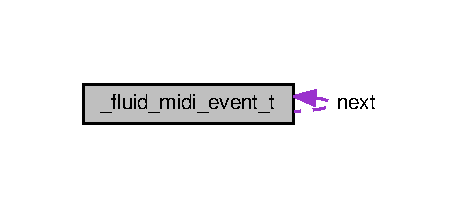
\includegraphics[width=221pt]{struct__fluid__midi__event__t__coll__graph}
\end{center}
\end{figure}
\subsection*{Public Attributes}
\begin{DoxyCompactItemize}
\item 
\hyperlink{types_8h_a61c72b76e3ee344637994c3071f74d94}{fluid\+\_\+midi\+\_\+event\+\_\+t} $\ast$ \hyperlink{struct__fluid__midi__event__t_a0d5ef7528dfa953132fb2e2471bffac0}{next}
\item 
void $\ast$ \hyperlink{struct__fluid__midi__event__t_afe5a9dc57be21c06319331d0ff048fc2}{paramptr}
\item 
unsigned int \hyperlink{struct__fluid__midi__event__t_a95a5caa12570905e7b06eddd73474bd9}{dtime}
\item 
unsigned int \hyperlink{struct__fluid__midi__event__t_a94018711464160be5a5ffe6c20dcebbc}{param1}
\item 
unsigned int \hyperlink{struct__fluid__midi__event__t_af5db43d718e962503b7e4e3298c3c026}{param2}
\item 
unsigned char \hyperlink{struct__fluid__midi__event__t_a3fcf1f8cc634a3e0e36788ab58a604a8}{type}
\item 
unsigned char \hyperlink{struct__fluid__midi__event__t_a6cbaf2dd7f396262752b29ca097baa40}{channel}
\end{DoxyCompactItemize}


\subsection{Member Data Documentation}
\mbox{\Hypertarget{struct__fluid__midi__event__t_a6cbaf2dd7f396262752b29ca097baa40}\label{struct__fluid__midi__event__t_a6cbaf2dd7f396262752b29ca097baa40}} 
\index{\+\_\+fluid\+\_\+midi\+\_\+event\+\_\+t@{\+\_\+fluid\+\_\+midi\+\_\+event\+\_\+t}!channel@{channel}}
\index{channel@{channel}!\+\_\+fluid\+\_\+midi\+\_\+event\+\_\+t@{\+\_\+fluid\+\_\+midi\+\_\+event\+\_\+t}}
\subsubsection{\texorpdfstring{channel}{channel}}
{\footnotesize\ttfamily unsigned char \+\_\+fluid\+\_\+midi\+\_\+event\+\_\+t\+::channel}

\mbox{\Hypertarget{struct__fluid__midi__event__t_a95a5caa12570905e7b06eddd73474bd9}\label{struct__fluid__midi__event__t_a95a5caa12570905e7b06eddd73474bd9}} 
\index{\+\_\+fluid\+\_\+midi\+\_\+event\+\_\+t@{\+\_\+fluid\+\_\+midi\+\_\+event\+\_\+t}!dtime@{dtime}}
\index{dtime@{dtime}!\+\_\+fluid\+\_\+midi\+\_\+event\+\_\+t@{\+\_\+fluid\+\_\+midi\+\_\+event\+\_\+t}}
\subsubsection{\texorpdfstring{dtime}{dtime}}
{\footnotesize\ttfamily unsigned int \+\_\+fluid\+\_\+midi\+\_\+event\+\_\+t\+::dtime}

\mbox{\Hypertarget{struct__fluid__midi__event__t_a0d5ef7528dfa953132fb2e2471bffac0}\label{struct__fluid__midi__event__t_a0d5ef7528dfa953132fb2e2471bffac0}} 
\index{\+\_\+fluid\+\_\+midi\+\_\+event\+\_\+t@{\+\_\+fluid\+\_\+midi\+\_\+event\+\_\+t}!next@{next}}
\index{next@{next}!\+\_\+fluid\+\_\+midi\+\_\+event\+\_\+t@{\+\_\+fluid\+\_\+midi\+\_\+event\+\_\+t}}
\subsubsection{\texorpdfstring{next}{next}}
{\footnotesize\ttfamily \hyperlink{types_8h_a61c72b76e3ee344637994c3071f74d94}{fluid\+\_\+midi\+\_\+event\+\_\+t}$\ast$ \+\_\+fluid\+\_\+midi\+\_\+event\+\_\+t\+::next}

\mbox{\Hypertarget{struct__fluid__midi__event__t_a94018711464160be5a5ffe6c20dcebbc}\label{struct__fluid__midi__event__t_a94018711464160be5a5ffe6c20dcebbc}} 
\index{\+\_\+fluid\+\_\+midi\+\_\+event\+\_\+t@{\+\_\+fluid\+\_\+midi\+\_\+event\+\_\+t}!param1@{param1}}
\index{param1@{param1}!\+\_\+fluid\+\_\+midi\+\_\+event\+\_\+t@{\+\_\+fluid\+\_\+midi\+\_\+event\+\_\+t}}
\subsubsection{\texorpdfstring{param1}{param1}}
{\footnotesize\ttfamily unsigned int \+\_\+fluid\+\_\+midi\+\_\+event\+\_\+t\+::param1}

\mbox{\Hypertarget{struct__fluid__midi__event__t_af5db43d718e962503b7e4e3298c3c026}\label{struct__fluid__midi__event__t_af5db43d718e962503b7e4e3298c3c026}} 
\index{\+\_\+fluid\+\_\+midi\+\_\+event\+\_\+t@{\+\_\+fluid\+\_\+midi\+\_\+event\+\_\+t}!param2@{param2}}
\index{param2@{param2}!\+\_\+fluid\+\_\+midi\+\_\+event\+\_\+t@{\+\_\+fluid\+\_\+midi\+\_\+event\+\_\+t}}
\subsubsection{\texorpdfstring{param2}{param2}}
{\footnotesize\ttfamily unsigned int \+\_\+fluid\+\_\+midi\+\_\+event\+\_\+t\+::param2}

\mbox{\Hypertarget{struct__fluid__midi__event__t_afe5a9dc57be21c06319331d0ff048fc2}\label{struct__fluid__midi__event__t_afe5a9dc57be21c06319331d0ff048fc2}} 
\index{\+\_\+fluid\+\_\+midi\+\_\+event\+\_\+t@{\+\_\+fluid\+\_\+midi\+\_\+event\+\_\+t}!paramptr@{paramptr}}
\index{paramptr@{paramptr}!\+\_\+fluid\+\_\+midi\+\_\+event\+\_\+t@{\+\_\+fluid\+\_\+midi\+\_\+event\+\_\+t}}
\subsubsection{\texorpdfstring{paramptr}{paramptr}}
{\footnotesize\ttfamily void$\ast$ \+\_\+fluid\+\_\+midi\+\_\+event\+\_\+t\+::paramptr}

\mbox{\Hypertarget{struct__fluid__midi__event__t_a3fcf1f8cc634a3e0e36788ab58a604a8}\label{struct__fluid__midi__event__t_a3fcf1f8cc634a3e0e36788ab58a604a8}} 
\index{\+\_\+fluid\+\_\+midi\+\_\+event\+\_\+t@{\+\_\+fluid\+\_\+midi\+\_\+event\+\_\+t}!type@{type}}
\index{type@{type}!\+\_\+fluid\+\_\+midi\+\_\+event\+\_\+t@{\+\_\+fluid\+\_\+midi\+\_\+event\+\_\+t}}
\subsubsection{\texorpdfstring{type}{type}}
{\footnotesize\ttfamily unsigned char \+\_\+fluid\+\_\+midi\+\_\+event\+\_\+t\+::type}



The documentation for this struct was generated from the following file\+:\begin{DoxyCompactItemize}
\item 
midi/\hyperlink{fluid__midi_8h}{fluid\+\_\+midi.\+h}\end{DoxyCompactItemize}

\hypertarget{struct__fluid__midi__parser__t}{}\section{\+\_\+fluid\+\_\+midi\+\_\+parser\+\_\+t Struct Reference}
\label{struct__fluid__midi__parser__t}\index{\+\_\+fluid\+\_\+midi\+\_\+parser\+\_\+t@{\+\_\+fluid\+\_\+midi\+\_\+parser\+\_\+t}}


{\ttfamily \#include $<$fluid\+\_\+midi.\+h$>$}



Collaboration diagram for \+\_\+fluid\+\_\+midi\+\_\+parser\+\_\+t\+:
\nopagebreak
\begin{figure}[H]
\begin{center}
\leavevmode
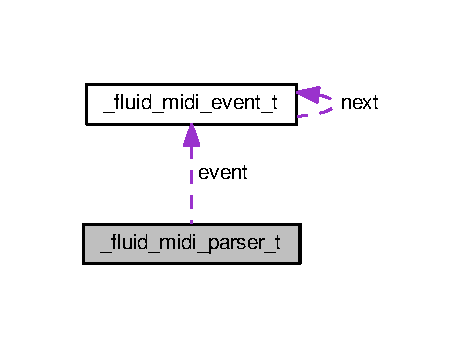
\includegraphics[width=223pt]{struct__fluid__midi__parser__t__coll__graph}
\end{center}
\end{figure}
\subsection*{Public Attributes}
\begin{DoxyCompactItemize}
\item 
unsigned char \hyperlink{struct__fluid__midi__parser__t_a32006b8e0b4a5acc3781753e682f70d3}{status}
\item 
unsigned char \hyperlink{struct__fluid__midi__parser__t_adc9286927514faff96288f3458c898cf}{channel}
\item 
unsigned int \hyperlink{struct__fluid__midi__parser__t_ad0106e994167162f1554186d345ae222}{nr\+\_\+bytes}
\item 
unsigned int \hyperlink{struct__fluid__midi__parser__t_a5cb62ed4894d4d2926150b9f9434e477}{nr\+\_\+bytes\+\_\+total}
\item 
unsigned char \hyperlink{struct__fluid__midi__parser__t_a4addc15eb062d2ab41a772fced380212}{data} \mbox{[}\hyperlink{fluid__midi_8h_ab689c6733a42a3c985378354f29fb571}{F\+L\+U\+I\+D\+\_\+\+M\+I\+D\+I\+\_\+\+P\+A\+R\+S\+E\+R\+\_\+\+M\+A\+X\+\_\+\+D\+A\+T\+A\+\_\+\+S\+I\+ZE}\mbox{]}
\item 
\hyperlink{types_8h_a61c72b76e3ee344637994c3071f74d94}{fluid\+\_\+midi\+\_\+event\+\_\+t} \hyperlink{struct__fluid__midi__parser__t_a0ba50c10a405a0fb3c5125e154d2ba34}{event}
\end{DoxyCompactItemize}


\subsection{Member Data Documentation}
\mbox{\Hypertarget{struct__fluid__midi__parser__t_adc9286927514faff96288f3458c898cf}\label{struct__fluid__midi__parser__t_adc9286927514faff96288f3458c898cf}} 
\index{\+\_\+fluid\+\_\+midi\+\_\+parser\+\_\+t@{\+\_\+fluid\+\_\+midi\+\_\+parser\+\_\+t}!channel@{channel}}
\index{channel@{channel}!\+\_\+fluid\+\_\+midi\+\_\+parser\+\_\+t@{\+\_\+fluid\+\_\+midi\+\_\+parser\+\_\+t}}
\subsubsection{\texorpdfstring{channel}{channel}}
{\footnotesize\ttfamily unsigned char \+\_\+fluid\+\_\+midi\+\_\+parser\+\_\+t\+::channel}

\mbox{\Hypertarget{struct__fluid__midi__parser__t_a4addc15eb062d2ab41a772fced380212}\label{struct__fluid__midi__parser__t_a4addc15eb062d2ab41a772fced380212}} 
\index{\+\_\+fluid\+\_\+midi\+\_\+parser\+\_\+t@{\+\_\+fluid\+\_\+midi\+\_\+parser\+\_\+t}!data@{data}}
\index{data@{data}!\+\_\+fluid\+\_\+midi\+\_\+parser\+\_\+t@{\+\_\+fluid\+\_\+midi\+\_\+parser\+\_\+t}}
\subsubsection{\texorpdfstring{data}{data}}
{\footnotesize\ttfamily unsigned char \+\_\+fluid\+\_\+midi\+\_\+parser\+\_\+t\+::data\mbox{[}\hyperlink{fluid__midi_8h_ab689c6733a42a3c985378354f29fb571}{F\+L\+U\+I\+D\+\_\+\+M\+I\+D\+I\+\_\+\+P\+A\+R\+S\+E\+R\+\_\+\+M\+A\+X\+\_\+\+D\+A\+T\+A\+\_\+\+S\+I\+ZE}\mbox{]}}

\mbox{\Hypertarget{struct__fluid__midi__parser__t_a0ba50c10a405a0fb3c5125e154d2ba34}\label{struct__fluid__midi__parser__t_a0ba50c10a405a0fb3c5125e154d2ba34}} 
\index{\+\_\+fluid\+\_\+midi\+\_\+parser\+\_\+t@{\+\_\+fluid\+\_\+midi\+\_\+parser\+\_\+t}!event@{event}}
\index{event@{event}!\+\_\+fluid\+\_\+midi\+\_\+parser\+\_\+t@{\+\_\+fluid\+\_\+midi\+\_\+parser\+\_\+t}}
\subsubsection{\texorpdfstring{event}{event}}
{\footnotesize\ttfamily \hyperlink{types_8h_a61c72b76e3ee344637994c3071f74d94}{fluid\+\_\+midi\+\_\+event\+\_\+t} \+\_\+fluid\+\_\+midi\+\_\+parser\+\_\+t\+::event}

\mbox{\Hypertarget{struct__fluid__midi__parser__t_ad0106e994167162f1554186d345ae222}\label{struct__fluid__midi__parser__t_ad0106e994167162f1554186d345ae222}} 
\index{\+\_\+fluid\+\_\+midi\+\_\+parser\+\_\+t@{\+\_\+fluid\+\_\+midi\+\_\+parser\+\_\+t}!nr\+\_\+bytes@{nr\+\_\+bytes}}
\index{nr\+\_\+bytes@{nr\+\_\+bytes}!\+\_\+fluid\+\_\+midi\+\_\+parser\+\_\+t@{\+\_\+fluid\+\_\+midi\+\_\+parser\+\_\+t}}
\subsubsection{\texorpdfstring{nr\+\_\+bytes}{nr\_bytes}}
{\footnotesize\ttfamily unsigned int \+\_\+fluid\+\_\+midi\+\_\+parser\+\_\+t\+::nr\+\_\+bytes}

\mbox{\Hypertarget{struct__fluid__midi__parser__t_a5cb62ed4894d4d2926150b9f9434e477}\label{struct__fluid__midi__parser__t_a5cb62ed4894d4d2926150b9f9434e477}} 
\index{\+\_\+fluid\+\_\+midi\+\_\+parser\+\_\+t@{\+\_\+fluid\+\_\+midi\+\_\+parser\+\_\+t}!nr\+\_\+bytes\+\_\+total@{nr\+\_\+bytes\+\_\+total}}
\index{nr\+\_\+bytes\+\_\+total@{nr\+\_\+bytes\+\_\+total}!\+\_\+fluid\+\_\+midi\+\_\+parser\+\_\+t@{\+\_\+fluid\+\_\+midi\+\_\+parser\+\_\+t}}
\subsubsection{\texorpdfstring{nr\+\_\+bytes\+\_\+total}{nr\_bytes\_total}}
{\footnotesize\ttfamily unsigned int \+\_\+fluid\+\_\+midi\+\_\+parser\+\_\+t\+::nr\+\_\+bytes\+\_\+total}

\mbox{\Hypertarget{struct__fluid__midi__parser__t_a32006b8e0b4a5acc3781753e682f70d3}\label{struct__fluid__midi__parser__t_a32006b8e0b4a5acc3781753e682f70d3}} 
\index{\+\_\+fluid\+\_\+midi\+\_\+parser\+\_\+t@{\+\_\+fluid\+\_\+midi\+\_\+parser\+\_\+t}!status@{status}}
\index{status@{status}!\+\_\+fluid\+\_\+midi\+\_\+parser\+\_\+t@{\+\_\+fluid\+\_\+midi\+\_\+parser\+\_\+t}}
\subsubsection{\texorpdfstring{status}{status}}
{\footnotesize\ttfamily unsigned char \+\_\+fluid\+\_\+midi\+\_\+parser\+\_\+t\+::status}



The documentation for this struct was generated from the following file\+:\begin{DoxyCompactItemize}
\item 
midi/\hyperlink{fluid__midi_8h}{fluid\+\_\+midi.\+h}\end{DoxyCompactItemize}

\hypertarget{struct__fluid__midi__router__rule__t}{}\section{\+\_\+fluid\+\_\+midi\+\_\+router\+\_\+rule\+\_\+t Struct Reference}
\label{struct__fluid__midi__router__rule__t}\index{\+\_\+fluid\+\_\+midi\+\_\+router\+\_\+rule\+\_\+t@{\+\_\+fluid\+\_\+midi\+\_\+router\+\_\+rule\+\_\+t}}


Collaboration diagram for \+\_\+fluid\+\_\+midi\+\_\+router\+\_\+rule\+\_\+t\+:
\nopagebreak
\begin{figure}[H]
\begin{center}
\leavevmode
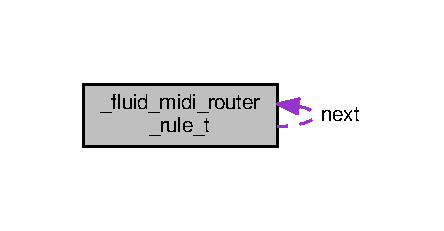
\includegraphics[width=213pt]{struct__fluid__midi__router__rule__t__coll__graph}
\end{center}
\end{figure}
\subsection*{Public Attributes}
\begin{DoxyCompactItemize}
\item 
int \hyperlink{struct__fluid__midi__router__rule__t_aadf5431504c54c40513f452d6237a2bc}{chan\+\_\+min}
\item 
int \hyperlink{struct__fluid__midi__router__rule__t_a8aa14e2015ca095555b90b5357a18cad}{chan\+\_\+max}
\item 
\hyperlink{fluidsynth__priv_8h_a9e96f0917747b69cabb7c671bc693dbb}{fluid\+\_\+real\+\_\+t} \hyperlink{struct__fluid__midi__router__rule__t_af6697cf8e4b7f0642a39a50a271f2a83}{chan\+\_\+mul}
\item 
int \hyperlink{struct__fluid__midi__router__rule__t_a9ce72ef138372a30276571c55cadfcf8}{chan\+\_\+add}
\item 
int \hyperlink{struct__fluid__midi__router__rule__t_a92c33319629db070a96c5bc6248ace87}{par1\+\_\+min}
\item 
int \hyperlink{struct__fluid__midi__router__rule__t_a1a5d782a778bc5ed101f03579b1ff620}{par1\+\_\+max}
\item 
\hyperlink{fluidsynth__priv_8h_a9e96f0917747b69cabb7c671bc693dbb}{fluid\+\_\+real\+\_\+t} \hyperlink{struct__fluid__midi__router__rule__t_abfbb68837d8abbbbf1b3fb1424d0b55a}{par1\+\_\+mul}
\item 
int \hyperlink{struct__fluid__midi__router__rule__t_a8806fc630d5616ebb379fb1eaadea810}{par1\+\_\+add}
\item 
int \hyperlink{struct__fluid__midi__router__rule__t_a4c36d5d887318cd57a0b1bc54724aaac}{par2\+\_\+min}
\item 
int \hyperlink{struct__fluid__midi__router__rule__t_a942f2306124a3a5bfd79c77ec8b03132}{par2\+\_\+max}
\item 
\hyperlink{fluidsynth__priv_8h_a9e96f0917747b69cabb7c671bc693dbb}{fluid\+\_\+real\+\_\+t} \hyperlink{struct__fluid__midi__router__rule__t_a9e5bbdfe4cde9537a02b9c2d462a86c7}{par2\+\_\+mul}
\item 
int \hyperlink{struct__fluid__midi__router__rule__t_a27dee95b2b9ebcee9368276c2cb80479}{par2\+\_\+add}
\item 
int \hyperlink{struct__fluid__midi__router__rule__t_a43426ac203b64f9eb6ffb616afd5e6bc}{pending\+\_\+events}
\item 
char \hyperlink{struct__fluid__midi__router__rule__t_a3793f03a674079324ea77dda155b2990}{keys\+\_\+cc} \mbox{[}128\mbox{]}
\item 
\hyperlink{types_8h_a3154253ddb8f9b8f8f737c91f5973278}{fluid\+\_\+midi\+\_\+router\+\_\+rule\+\_\+t} $\ast$ \hyperlink{struct__fluid__midi__router__rule__t_a3967c58266f5695bd38046dd98dddfbd}{next}
\item 
int \hyperlink{struct__fluid__midi__router__rule__t_a1bf6b0e05953518ee7270861a2965082}{waiting}
\end{DoxyCompactItemize}


\subsection{Member Data Documentation}
\mbox{\Hypertarget{struct__fluid__midi__router__rule__t_a9ce72ef138372a30276571c55cadfcf8}\label{struct__fluid__midi__router__rule__t_a9ce72ef138372a30276571c55cadfcf8}} 
\index{\+\_\+fluid\+\_\+midi\+\_\+router\+\_\+rule\+\_\+t@{\+\_\+fluid\+\_\+midi\+\_\+router\+\_\+rule\+\_\+t}!chan\+\_\+add@{chan\+\_\+add}}
\index{chan\+\_\+add@{chan\+\_\+add}!\+\_\+fluid\+\_\+midi\+\_\+router\+\_\+rule\+\_\+t@{\+\_\+fluid\+\_\+midi\+\_\+router\+\_\+rule\+\_\+t}}
\subsubsection{\texorpdfstring{chan\+\_\+add}{chan\_add}}
{\footnotesize\ttfamily int \+\_\+fluid\+\_\+midi\+\_\+router\+\_\+rule\+\_\+t\+::chan\+\_\+add}

\mbox{\Hypertarget{struct__fluid__midi__router__rule__t_a8aa14e2015ca095555b90b5357a18cad}\label{struct__fluid__midi__router__rule__t_a8aa14e2015ca095555b90b5357a18cad}} 
\index{\+\_\+fluid\+\_\+midi\+\_\+router\+\_\+rule\+\_\+t@{\+\_\+fluid\+\_\+midi\+\_\+router\+\_\+rule\+\_\+t}!chan\+\_\+max@{chan\+\_\+max}}
\index{chan\+\_\+max@{chan\+\_\+max}!\+\_\+fluid\+\_\+midi\+\_\+router\+\_\+rule\+\_\+t@{\+\_\+fluid\+\_\+midi\+\_\+router\+\_\+rule\+\_\+t}}
\subsubsection{\texorpdfstring{chan\+\_\+max}{chan\_max}}
{\footnotesize\ttfamily int \+\_\+fluid\+\_\+midi\+\_\+router\+\_\+rule\+\_\+t\+::chan\+\_\+max}

\mbox{\Hypertarget{struct__fluid__midi__router__rule__t_aadf5431504c54c40513f452d6237a2bc}\label{struct__fluid__midi__router__rule__t_aadf5431504c54c40513f452d6237a2bc}} 
\index{\+\_\+fluid\+\_\+midi\+\_\+router\+\_\+rule\+\_\+t@{\+\_\+fluid\+\_\+midi\+\_\+router\+\_\+rule\+\_\+t}!chan\+\_\+min@{chan\+\_\+min}}
\index{chan\+\_\+min@{chan\+\_\+min}!\+\_\+fluid\+\_\+midi\+\_\+router\+\_\+rule\+\_\+t@{\+\_\+fluid\+\_\+midi\+\_\+router\+\_\+rule\+\_\+t}}
\subsubsection{\texorpdfstring{chan\+\_\+min}{chan\_min}}
{\footnotesize\ttfamily int \+\_\+fluid\+\_\+midi\+\_\+router\+\_\+rule\+\_\+t\+::chan\+\_\+min}

\mbox{\Hypertarget{struct__fluid__midi__router__rule__t_af6697cf8e4b7f0642a39a50a271f2a83}\label{struct__fluid__midi__router__rule__t_af6697cf8e4b7f0642a39a50a271f2a83}} 
\index{\+\_\+fluid\+\_\+midi\+\_\+router\+\_\+rule\+\_\+t@{\+\_\+fluid\+\_\+midi\+\_\+router\+\_\+rule\+\_\+t}!chan\+\_\+mul@{chan\+\_\+mul}}
\index{chan\+\_\+mul@{chan\+\_\+mul}!\+\_\+fluid\+\_\+midi\+\_\+router\+\_\+rule\+\_\+t@{\+\_\+fluid\+\_\+midi\+\_\+router\+\_\+rule\+\_\+t}}
\subsubsection{\texorpdfstring{chan\+\_\+mul}{chan\_mul}}
{\footnotesize\ttfamily \hyperlink{fluidsynth__priv_8h_a9e96f0917747b69cabb7c671bc693dbb}{fluid\+\_\+real\+\_\+t} \+\_\+fluid\+\_\+midi\+\_\+router\+\_\+rule\+\_\+t\+::chan\+\_\+mul}

\mbox{\Hypertarget{struct__fluid__midi__router__rule__t_a3793f03a674079324ea77dda155b2990}\label{struct__fluid__midi__router__rule__t_a3793f03a674079324ea77dda155b2990}} 
\index{\+\_\+fluid\+\_\+midi\+\_\+router\+\_\+rule\+\_\+t@{\+\_\+fluid\+\_\+midi\+\_\+router\+\_\+rule\+\_\+t}!keys\+\_\+cc@{keys\+\_\+cc}}
\index{keys\+\_\+cc@{keys\+\_\+cc}!\+\_\+fluid\+\_\+midi\+\_\+router\+\_\+rule\+\_\+t@{\+\_\+fluid\+\_\+midi\+\_\+router\+\_\+rule\+\_\+t}}
\subsubsection{\texorpdfstring{keys\+\_\+cc}{keys\_cc}}
{\footnotesize\ttfamily char \+\_\+fluid\+\_\+midi\+\_\+router\+\_\+rule\+\_\+t\+::keys\+\_\+cc\mbox{[}128\mbox{]}}

\mbox{\Hypertarget{struct__fluid__midi__router__rule__t_a3967c58266f5695bd38046dd98dddfbd}\label{struct__fluid__midi__router__rule__t_a3967c58266f5695bd38046dd98dddfbd}} 
\index{\+\_\+fluid\+\_\+midi\+\_\+router\+\_\+rule\+\_\+t@{\+\_\+fluid\+\_\+midi\+\_\+router\+\_\+rule\+\_\+t}!next@{next}}
\index{next@{next}!\+\_\+fluid\+\_\+midi\+\_\+router\+\_\+rule\+\_\+t@{\+\_\+fluid\+\_\+midi\+\_\+router\+\_\+rule\+\_\+t}}
\subsubsection{\texorpdfstring{next}{next}}
{\footnotesize\ttfamily \hyperlink{types_8h_a3154253ddb8f9b8f8f737c91f5973278}{fluid\+\_\+midi\+\_\+router\+\_\+rule\+\_\+t}$\ast$ \+\_\+fluid\+\_\+midi\+\_\+router\+\_\+rule\+\_\+t\+::next}

\mbox{\Hypertarget{struct__fluid__midi__router__rule__t_a8806fc630d5616ebb379fb1eaadea810}\label{struct__fluid__midi__router__rule__t_a8806fc630d5616ebb379fb1eaadea810}} 
\index{\+\_\+fluid\+\_\+midi\+\_\+router\+\_\+rule\+\_\+t@{\+\_\+fluid\+\_\+midi\+\_\+router\+\_\+rule\+\_\+t}!par1\+\_\+add@{par1\+\_\+add}}
\index{par1\+\_\+add@{par1\+\_\+add}!\+\_\+fluid\+\_\+midi\+\_\+router\+\_\+rule\+\_\+t@{\+\_\+fluid\+\_\+midi\+\_\+router\+\_\+rule\+\_\+t}}
\subsubsection{\texorpdfstring{par1\+\_\+add}{par1\_add}}
{\footnotesize\ttfamily int \+\_\+fluid\+\_\+midi\+\_\+router\+\_\+rule\+\_\+t\+::par1\+\_\+add}

\mbox{\Hypertarget{struct__fluid__midi__router__rule__t_a1a5d782a778bc5ed101f03579b1ff620}\label{struct__fluid__midi__router__rule__t_a1a5d782a778bc5ed101f03579b1ff620}} 
\index{\+\_\+fluid\+\_\+midi\+\_\+router\+\_\+rule\+\_\+t@{\+\_\+fluid\+\_\+midi\+\_\+router\+\_\+rule\+\_\+t}!par1\+\_\+max@{par1\+\_\+max}}
\index{par1\+\_\+max@{par1\+\_\+max}!\+\_\+fluid\+\_\+midi\+\_\+router\+\_\+rule\+\_\+t@{\+\_\+fluid\+\_\+midi\+\_\+router\+\_\+rule\+\_\+t}}
\subsubsection{\texorpdfstring{par1\+\_\+max}{par1\_max}}
{\footnotesize\ttfamily int \+\_\+fluid\+\_\+midi\+\_\+router\+\_\+rule\+\_\+t\+::par1\+\_\+max}

\mbox{\Hypertarget{struct__fluid__midi__router__rule__t_a92c33319629db070a96c5bc6248ace87}\label{struct__fluid__midi__router__rule__t_a92c33319629db070a96c5bc6248ace87}} 
\index{\+\_\+fluid\+\_\+midi\+\_\+router\+\_\+rule\+\_\+t@{\+\_\+fluid\+\_\+midi\+\_\+router\+\_\+rule\+\_\+t}!par1\+\_\+min@{par1\+\_\+min}}
\index{par1\+\_\+min@{par1\+\_\+min}!\+\_\+fluid\+\_\+midi\+\_\+router\+\_\+rule\+\_\+t@{\+\_\+fluid\+\_\+midi\+\_\+router\+\_\+rule\+\_\+t}}
\subsubsection{\texorpdfstring{par1\+\_\+min}{par1\_min}}
{\footnotesize\ttfamily int \+\_\+fluid\+\_\+midi\+\_\+router\+\_\+rule\+\_\+t\+::par1\+\_\+min}

\mbox{\Hypertarget{struct__fluid__midi__router__rule__t_abfbb68837d8abbbbf1b3fb1424d0b55a}\label{struct__fluid__midi__router__rule__t_abfbb68837d8abbbbf1b3fb1424d0b55a}} 
\index{\+\_\+fluid\+\_\+midi\+\_\+router\+\_\+rule\+\_\+t@{\+\_\+fluid\+\_\+midi\+\_\+router\+\_\+rule\+\_\+t}!par1\+\_\+mul@{par1\+\_\+mul}}
\index{par1\+\_\+mul@{par1\+\_\+mul}!\+\_\+fluid\+\_\+midi\+\_\+router\+\_\+rule\+\_\+t@{\+\_\+fluid\+\_\+midi\+\_\+router\+\_\+rule\+\_\+t}}
\subsubsection{\texorpdfstring{par1\+\_\+mul}{par1\_mul}}
{\footnotesize\ttfamily \hyperlink{fluidsynth__priv_8h_a9e96f0917747b69cabb7c671bc693dbb}{fluid\+\_\+real\+\_\+t} \+\_\+fluid\+\_\+midi\+\_\+router\+\_\+rule\+\_\+t\+::par1\+\_\+mul}

\mbox{\Hypertarget{struct__fluid__midi__router__rule__t_a27dee95b2b9ebcee9368276c2cb80479}\label{struct__fluid__midi__router__rule__t_a27dee95b2b9ebcee9368276c2cb80479}} 
\index{\+\_\+fluid\+\_\+midi\+\_\+router\+\_\+rule\+\_\+t@{\+\_\+fluid\+\_\+midi\+\_\+router\+\_\+rule\+\_\+t}!par2\+\_\+add@{par2\+\_\+add}}
\index{par2\+\_\+add@{par2\+\_\+add}!\+\_\+fluid\+\_\+midi\+\_\+router\+\_\+rule\+\_\+t@{\+\_\+fluid\+\_\+midi\+\_\+router\+\_\+rule\+\_\+t}}
\subsubsection{\texorpdfstring{par2\+\_\+add}{par2\_add}}
{\footnotesize\ttfamily int \+\_\+fluid\+\_\+midi\+\_\+router\+\_\+rule\+\_\+t\+::par2\+\_\+add}

\mbox{\Hypertarget{struct__fluid__midi__router__rule__t_a942f2306124a3a5bfd79c77ec8b03132}\label{struct__fluid__midi__router__rule__t_a942f2306124a3a5bfd79c77ec8b03132}} 
\index{\+\_\+fluid\+\_\+midi\+\_\+router\+\_\+rule\+\_\+t@{\+\_\+fluid\+\_\+midi\+\_\+router\+\_\+rule\+\_\+t}!par2\+\_\+max@{par2\+\_\+max}}
\index{par2\+\_\+max@{par2\+\_\+max}!\+\_\+fluid\+\_\+midi\+\_\+router\+\_\+rule\+\_\+t@{\+\_\+fluid\+\_\+midi\+\_\+router\+\_\+rule\+\_\+t}}
\subsubsection{\texorpdfstring{par2\+\_\+max}{par2\_max}}
{\footnotesize\ttfamily int \+\_\+fluid\+\_\+midi\+\_\+router\+\_\+rule\+\_\+t\+::par2\+\_\+max}

\mbox{\Hypertarget{struct__fluid__midi__router__rule__t_a4c36d5d887318cd57a0b1bc54724aaac}\label{struct__fluid__midi__router__rule__t_a4c36d5d887318cd57a0b1bc54724aaac}} 
\index{\+\_\+fluid\+\_\+midi\+\_\+router\+\_\+rule\+\_\+t@{\+\_\+fluid\+\_\+midi\+\_\+router\+\_\+rule\+\_\+t}!par2\+\_\+min@{par2\+\_\+min}}
\index{par2\+\_\+min@{par2\+\_\+min}!\+\_\+fluid\+\_\+midi\+\_\+router\+\_\+rule\+\_\+t@{\+\_\+fluid\+\_\+midi\+\_\+router\+\_\+rule\+\_\+t}}
\subsubsection{\texorpdfstring{par2\+\_\+min}{par2\_min}}
{\footnotesize\ttfamily int \+\_\+fluid\+\_\+midi\+\_\+router\+\_\+rule\+\_\+t\+::par2\+\_\+min}

\mbox{\Hypertarget{struct__fluid__midi__router__rule__t_a9e5bbdfe4cde9537a02b9c2d462a86c7}\label{struct__fluid__midi__router__rule__t_a9e5bbdfe4cde9537a02b9c2d462a86c7}} 
\index{\+\_\+fluid\+\_\+midi\+\_\+router\+\_\+rule\+\_\+t@{\+\_\+fluid\+\_\+midi\+\_\+router\+\_\+rule\+\_\+t}!par2\+\_\+mul@{par2\+\_\+mul}}
\index{par2\+\_\+mul@{par2\+\_\+mul}!\+\_\+fluid\+\_\+midi\+\_\+router\+\_\+rule\+\_\+t@{\+\_\+fluid\+\_\+midi\+\_\+router\+\_\+rule\+\_\+t}}
\subsubsection{\texorpdfstring{par2\+\_\+mul}{par2\_mul}}
{\footnotesize\ttfamily \hyperlink{fluidsynth__priv_8h_a9e96f0917747b69cabb7c671bc693dbb}{fluid\+\_\+real\+\_\+t} \+\_\+fluid\+\_\+midi\+\_\+router\+\_\+rule\+\_\+t\+::par2\+\_\+mul}

\mbox{\Hypertarget{struct__fluid__midi__router__rule__t_a43426ac203b64f9eb6ffb616afd5e6bc}\label{struct__fluid__midi__router__rule__t_a43426ac203b64f9eb6ffb616afd5e6bc}} 
\index{\+\_\+fluid\+\_\+midi\+\_\+router\+\_\+rule\+\_\+t@{\+\_\+fluid\+\_\+midi\+\_\+router\+\_\+rule\+\_\+t}!pending\+\_\+events@{pending\+\_\+events}}
\index{pending\+\_\+events@{pending\+\_\+events}!\+\_\+fluid\+\_\+midi\+\_\+router\+\_\+rule\+\_\+t@{\+\_\+fluid\+\_\+midi\+\_\+router\+\_\+rule\+\_\+t}}
\subsubsection{\texorpdfstring{pending\+\_\+events}{pending\_events}}
{\footnotesize\ttfamily int \+\_\+fluid\+\_\+midi\+\_\+router\+\_\+rule\+\_\+t\+::pending\+\_\+events}

\mbox{\Hypertarget{struct__fluid__midi__router__rule__t_a1bf6b0e05953518ee7270861a2965082}\label{struct__fluid__midi__router__rule__t_a1bf6b0e05953518ee7270861a2965082}} 
\index{\+\_\+fluid\+\_\+midi\+\_\+router\+\_\+rule\+\_\+t@{\+\_\+fluid\+\_\+midi\+\_\+router\+\_\+rule\+\_\+t}!waiting@{waiting}}
\index{waiting@{waiting}!\+\_\+fluid\+\_\+midi\+\_\+router\+\_\+rule\+\_\+t@{\+\_\+fluid\+\_\+midi\+\_\+router\+\_\+rule\+\_\+t}}
\subsubsection{\texorpdfstring{waiting}{waiting}}
{\footnotesize\ttfamily int \+\_\+fluid\+\_\+midi\+\_\+router\+\_\+rule\+\_\+t\+::waiting}



The documentation for this struct was generated from the following file\+:\begin{DoxyCompactItemize}
\item 
midi/\hyperlink{fluid__midi__router_8c}{fluid\+\_\+midi\+\_\+router.\+c}\end{DoxyCompactItemize}

\hypertarget{struct__fluid__midi__router__t}{}\section{\+\_\+fluid\+\_\+midi\+\_\+router\+\_\+t Struct Reference}
\label{struct__fluid__midi__router__t}\index{\+\_\+fluid\+\_\+midi\+\_\+router\+\_\+t@{\+\_\+fluid\+\_\+midi\+\_\+router\+\_\+t}}


Collaboration diagram for \+\_\+fluid\+\_\+midi\+\_\+router\+\_\+t\+:
\nopagebreak
\begin{figure}[H]
\begin{center}
\leavevmode
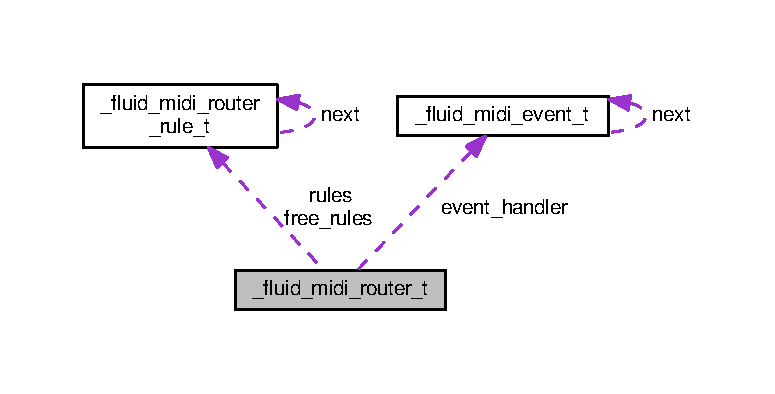
\includegraphics[width=350pt]{struct__fluid__midi__router__t__coll__graph}
\end{center}
\end{figure}
\subsection*{Public Attributes}
\begin{DoxyCompactItemize}
\item 
\hyperlink{fluid__sys_8h_a7252a44982e8ed2704689f563c8a12e3}{fluid\+\_\+mutex\+\_\+t} \hyperlink{struct__fluid__midi__router__t_a20926b15d48e1e02adaaebb1de8c69fa}{rules\+\_\+mutex}
\item 
\hyperlink{types_8h_a3154253ddb8f9b8f8f737c91f5973278}{fluid\+\_\+midi\+\_\+router\+\_\+rule\+\_\+t} $\ast$ \hyperlink{struct__fluid__midi__router__t_abb842c26031584c6b8b59591a8d30a11}{rules} \mbox{[}\hyperlink{midi_8h_ab798a0a5b95607556c9ecfbeaaab962ba6046a4845f7d72a92afed8ea13ab2a7a}{F\+L\+U\+I\+D\+\_\+\+M\+I\+D\+I\+\_\+\+R\+O\+U\+T\+E\+R\+\_\+\+R\+U\+L\+E\+\_\+\+C\+O\+U\+NT}\mbox{]}
\item 
\hyperlink{types_8h_a3154253ddb8f9b8f8f737c91f5973278}{fluid\+\_\+midi\+\_\+router\+\_\+rule\+\_\+t} $\ast$ \hyperlink{struct__fluid__midi__router__t_acbaf9d6e287c80b3a9b3f9ba7fc80fa6}{free\+\_\+rules}
\item 
\hyperlink{midi_8h_a42c3752e3adb54e0af802131c36a1129}{handle\+\_\+midi\+\_\+event\+\_\+func\+\_\+t} \hyperlink{struct__fluid__midi__router__t_ab16e26adcb0eb0a92ae52ab7adaaba06}{event\+\_\+handler}
\item 
void $\ast$ \hyperlink{struct__fluid__midi__router__t_a668689d932d287fd25c4ade5b4001b01}{event\+\_\+handler\+\_\+data}
\item 
int \hyperlink{struct__fluid__midi__router__t_a8311aaf34514ab19a44db90e443e9130}{nr\+\_\+midi\+\_\+channels}
\end{DoxyCompactItemize}


\subsection{Member Data Documentation}
\mbox{\Hypertarget{struct__fluid__midi__router__t_ab16e26adcb0eb0a92ae52ab7adaaba06}\label{struct__fluid__midi__router__t_ab16e26adcb0eb0a92ae52ab7adaaba06}} 
\index{\+\_\+fluid\+\_\+midi\+\_\+router\+\_\+t@{\+\_\+fluid\+\_\+midi\+\_\+router\+\_\+t}!event\+\_\+handler@{event\+\_\+handler}}
\index{event\+\_\+handler@{event\+\_\+handler}!\+\_\+fluid\+\_\+midi\+\_\+router\+\_\+t@{\+\_\+fluid\+\_\+midi\+\_\+router\+\_\+t}}
\subsubsection{\texorpdfstring{event\+\_\+handler}{event\_handler}}
{\footnotesize\ttfamily \hyperlink{midi_8h_a42c3752e3adb54e0af802131c36a1129}{handle\+\_\+midi\+\_\+event\+\_\+func\+\_\+t} \+\_\+fluid\+\_\+midi\+\_\+router\+\_\+t\+::event\+\_\+handler}

\mbox{\Hypertarget{struct__fluid__midi__router__t_a668689d932d287fd25c4ade5b4001b01}\label{struct__fluid__midi__router__t_a668689d932d287fd25c4ade5b4001b01}} 
\index{\+\_\+fluid\+\_\+midi\+\_\+router\+\_\+t@{\+\_\+fluid\+\_\+midi\+\_\+router\+\_\+t}!event\+\_\+handler\+\_\+data@{event\+\_\+handler\+\_\+data}}
\index{event\+\_\+handler\+\_\+data@{event\+\_\+handler\+\_\+data}!\+\_\+fluid\+\_\+midi\+\_\+router\+\_\+t@{\+\_\+fluid\+\_\+midi\+\_\+router\+\_\+t}}
\subsubsection{\texorpdfstring{event\+\_\+handler\+\_\+data}{event\_handler\_data}}
{\footnotesize\ttfamily void$\ast$ \+\_\+fluid\+\_\+midi\+\_\+router\+\_\+t\+::event\+\_\+handler\+\_\+data}

\mbox{\Hypertarget{struct__fluid__midi__router__t_acbaf9d6e287c80b3a9b3f9ba7fc80fa6}\label{struct__fluid__midi__router__t_acbaf9d6e287c80b3a9b3f9ba7fc80fa6}} 
\index{\+\_\+fluid\+\_\+midi\+\_\+router\+\_\+t@{\+\_\+fluid\+\_\+midi\+\_\+router\+\_\+t}!free\+\_\+rules@{free\+\_\+rules}}
\index{free\+\_\+rules@{free\+\_\+rules}!\+\_\+fluid\+\_\+midi\+\_\+router\+\_\+t@{\+\_\+fluid\+\_\+midi\+\_\+router\+\_\+t}}
\subsubsection{\texorpdfstring{free\+\_\+rules}{free\_rules}}
{\footnotesize\ttfamily \hyperlink{types_8h_a3154253ddb8f9b8f8f737c91f5973278}{fluid\+\_\+midi\+\_\+router\+\_\+rule\+\_\+t}$\ast$ \+\_\+fluid\+\_\+midi\+\_\+router\+\_\+t\+::free\+\_\+rules}

\mbox{\Hypertarget{struct__fluid__midi__router__t_a8311aaf34514ab19a44db90e443e9130}\label{struct__fluid__midi__router__t_a8311aaf34514ab19a44db90e443e9130}} 
\index{\+\_\+fluid\+\_\+midi\+\_\+router\+\_\+t@{\+\_\+fluid\+\_\+midi\+\_\+router\+\_\+t}!nr\+\_\+midi\+\_\+channels@{nr\+\_\+midi\+\_\+channels}}
\index{nr\+\_\+midi\+\_\+channels@{nr\+\_\+midi\+\_\+channels}!\+\_\+fluid\+\_\+midi\+\_\+router\+\_\+t@{\+\_\+fluid\+\_\+midi\+\_\+router\+\_\+t}}
\subsubsection{\texorpdfstring{nr\+\_\+midi\+\_\+channels}{nr\_midi\_channels}}
{\footnotesize\ttfamily int \+\_\+fluid\+\_\+midi\+\_\+router\+\_\+t\+::nr\+\_\+midi\+\_\+channels}

\mbox{\Hypertarget{struct__fluid__midi__router__t_abb842c26031584c6b8b59591a8d30a11}\label{struct__fluid__midi__router__t_abb842c26031584c6b8b59591a8d30a11}} 
\index{\+\_\+fluid\+\_\+midi\+\_\+router\+\_\+t@{\+\_\+fluid\+\_\+midi\+\_\+router\+\_\+t}!rules@{rules}}
\index{rules@{rules}!\+\_\+fluid\+\_\+midi\+\_\+router\+\_\+t@{\+\_\+fluid\+\_\+midi\+\_\+router\+\_\+t}}
\subsubsection{\texorpdfstring{rules}{rules}}
{\footnotesize\ttfamily \hyperlink{types_8h_a3154253ddb8f9b8f8f737c91f5973278}{fluid\+\_\+midi\+\_\+router\+\_\+rule\+\_\+t}$\ast$ \+\_\+fluid\+\_\+midi\+\_\+router\+\_\+t\+::rules\mbox{[}\hyperlink{midi_8h_ab798a0a5b95607556c9ecfbeaaab962ba6046a4845f7d72a92afed8ea13ab2a7a}{F\+L\+U\+I\+D\+\_\+\+M\+I\+D\+I\+\_\+\+R\+O\+U\+T\+E\+R\+\_\+\+R\+U\+L\+E\+\_\+\+C\+O\+U\+NT}\mbox{]}}

\mbox{\Hypertarget{struct__fluid__midi__router__t_a20926b15d48e1e02adaaebb1de8c69fa}\label{struct__fluid__midi__router__t_a20926b15d48e1e02adaaebb1de8c69fa}} 
\index{\+\_\+fluid\+\_\+midi\+\_\+router\+\_\+t@{\+\_\+fluid\+\_\+midi\+\_\+router\+\_\+t}!rules\+\_\+mutex@{rules\+\_\+mutex}}
\index{rules\+\_\+mutex@{rules\+\_\+mutex}!\+\_\+fluid\+\_\+midi\+\_\+router\+\_\+t@{\+\_\+fluid\+\_\+midi\+\_\+router\+\_\+t}}
\subsubsection{\texorpdfstring{rules\+\_\+mutex}{rules\_mutex}}
{\footnotesize\ttfamily \hyperlink{fluid__sys_8h_a7252a44982e8ed2704689f563c8a12e3}{fluid\+\_\+mutex\+\_\+t} \+\_\+fluid\+\_\+midi\+\_\+router\+\_\+t\+::rules\+\_\+mutex}



The documentation for this struct was generated from the following file\+:\begin{DoxyCompactItemize}
\item 
midi/\hyperlink{fluid__midi__router_8c}{fluid\+\_\+midi\+\_\+router.\+c}\end{DoxyCompactItemize}

\hypertarget{struct__fluid__mixer__buffers__t}{}\section{\+\_\+fluid\+\_\+mixer\+\_\+buffers\+\_\+t Struct Reference}
\label{struct__fluid__mixer__buffers__t}\index{\+\_\+fluid\+\_\+mixer\+\_\+buffers\+\_\+t@{\+\_\+fluid\+\_\+mixer\+\_\+buffers\+\_\+t}}


Collaboration diagram for \+\_\+fluid\+\_\+mixer\+\_\+buffers\+\_\+t\+:
\nopagebreak
\begin{figure}[H]
\begin{center}
\leavevmode
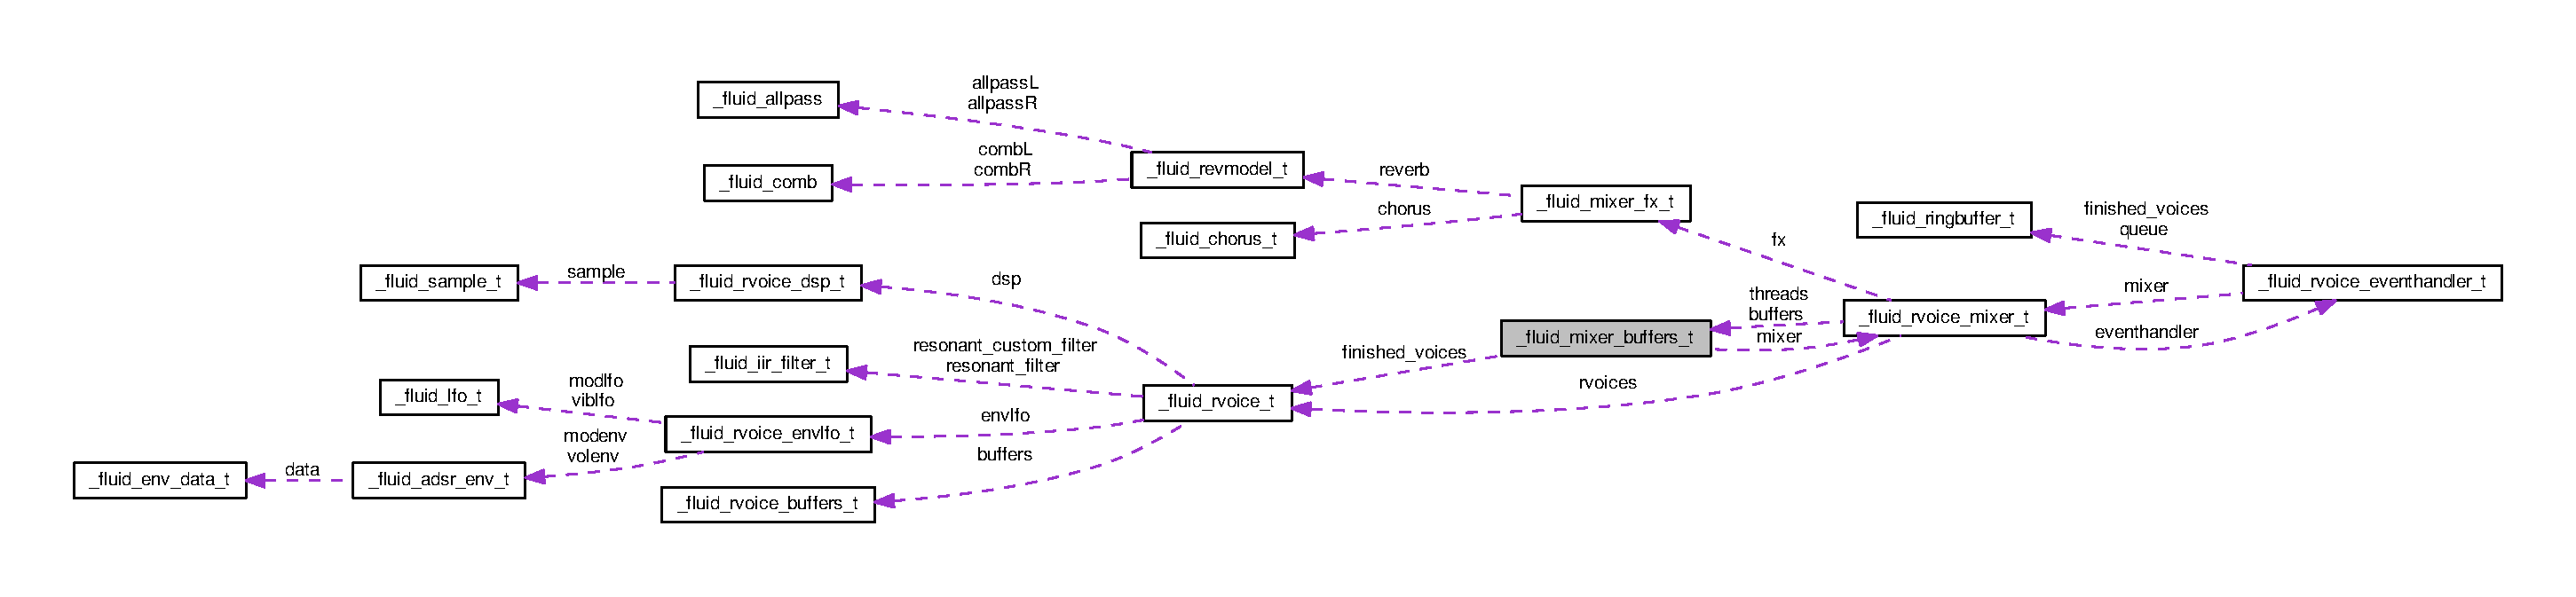
\includegraphics[width=350pt]{struct__fluid__mixer__buffers__t__coll__graph}
\end{center}
\end{figure}
\subsection*{Public Attributes}
\begin{DoxyCompactItemize}
\item 
\hyperlink{fluid__rvoice__mixer_8h_a546bd76f60c5458d73d6c72e3f01d0bf}{fluid\+\_\+rvoice\+\_\+mixer\+\_\+t} $\ast$ \hyperlink{struct__fluid__mixer__buffers__t_a656ac8bea94b4b91e34bb47c0a8a3114}{mixer}
\item 
\hyperlink{fluid__sys_8h_a60a6466e68a45b0f0709f1ebaa7e6f85}{fluid\+\_\+thread\+\_\+t} $\ast$ \hyperlink{struct__fluid__mixer__buffers__t_ae1b5c3828544d2d5b2ecf90a5d5363f6}{thread}
\item 
\hyperlink{fluid__rvoice_8h_a3c0405fcfaf1310d760cec3a503c509d}{fluid\+\_\+rvoice\+\_\+t} $\ast$$\ast$ \hyperlink{struct__fluid__mixer__buffers__t_a569decbf8d62beebb1adf004d3a59556}{finished\+\_\+voices}
\item 
int \hyperlink{struct__fluid__mixer__buffers__t_a300fa6473dcdfab8c896cde385c745a1}{finished\+\_\+voice\+\_\+count}
\item 
\hyperlink{fluidsynth__priv_8h_a6b8be882dd9958ea3635a868e1bf5152}{fluid\+\_\+atomic\+\_\+int\+\_\+t} \hyperlink{struct__fluid__mixer__buffers__t_a942daa65bfe018f46aa0c0c71c708a36}{ready}
\item 
int \hyperlink{struct__fluid__mixer__buffers__t_a8c3a78fe6747175ee0568701de36402f}{buf\+\_\+count}
\item 
\hyperlink{fluidsynth__priv_8h_a9e96f0917747b69cabb7c671bc693dbb}{fluid\+\_\+real\+\_\+t} $\ast$$\ast$ \hyperlink{struct__fluid__mixer__buffers__t_a6c8e17b961c80f18aa439775f3e3ffe5}{left\+\_\+buf}
\item 
\hyperlink{fluidsynth__priv_8h_a9e96f0917747b69cabb7c671bc693dbb}{fluid\+\_\+real\+\_\+t} $\ast$$\ast$ \hyperlink{struct__fluid__mixer__buffers__t_aa34a9832a2f3502dde0c95ce13caeca7}{right\+\_\+buf}
\item 
int \hyperlink{struct__fluid__mixer__buffers__t_a6e543ffc4494863fe1eee930cf4f07c6}{fx\+\_\+buf\+\_\+count}
\item 
\hyperlink{fluidsynth__priv_8h_a9e96f0917747b69cabb7c671bc693dbb}{fluid\+\_\+real\+\_\+t} $\ast$$\ast$ \hyperlink{struct__fluid__mixer__buffers__t_a4610a41a565c6d728a16c52156799957}{fx\+\_\+left\+\_\+buf}
\item 
\hyperlink{fluidsynth__priv_8h_a9e96f0917747b69cabb7c671bc693dbb}{fluid\+\_\+real\+\_\+t} $\ast$$\ast$ \hyperlink{struct__fluid__mixer__buffers__t_a682b8d1298a90f6320e4d44d76e7229a}{fx\+\_\+right\+\_\+buf}
\end{DoxyCompactItemize}


\subsection{Member Data Documentation}
\mbox{\Hypertarget{struct__fluid__mixer__buffers__t_a8c3a78fe6747175ee0568701de36402f}\label{struct__fluid__mixer__buffers__t_a8c3a78fe6747175ee0568701de36402f}} 
\index{\+\_\+fluid\+\_\+mixer\+\_\+buffers\+\_\+t@{\+\_\+fluid\+\_\+mixer\+\_\+buffers\+\_\+t}!buf\+\_\+count@{buf\+\_\+count}}
\index{buf\+\_\+count@{buf\+\_\+count}!\+\_\+fluid\+\_\+mixer\+\_\+buffers\+\_\+t@{\+\_\+fluid\+\_\+mixer\+\_\+buffers\+\_\+t}}
\subsubsection{\texorpdfstring{buf\+\_\+count}{buf\_count}}
{\footnotesize\ttfamily int \+\_\+fluid\+\_\+mixer\+\_\+buffers\+\_\+t\+::buf\+\_\+count}

\mbox{\Hypertarget{struct__fluid__mixer__buffers__t_a300fa6473dcdfab8c896cde385c745a1}\label{struct__fluid__mixer__buffers__t_a300fa6473dcdfab8c896cde385c745a1}} 
\index{\+\_\+fluid\+\_\+mixer\+\_\+buffers\+\_\+t@{\+\_\+fluid\+\_\+mixer\+\_\+buffers\+\_\+t}!finished\+\_\+voice\+\_\+count@{finished\+\_\+voice\+\_\+count}}
\index{finished\+\_\+voice\+\_\+count@{finished\+\_\+voice\+\_\+count}!\+\_\+fluid\+\_\+mixer\+\_\+buffers\+\_\+t@{\+\_\+fluid\+\_\+mixer\+\_\+buffers\+\_\+t}}
\subsubsection{\texorpdfstring{finished\+\_\+voice\+\_\+count}{finished\_voice\_count}}
{\footnotesize\ttfamily int \+\_\+fluid\+\_\+mixer\+\_\+buffers\+\_\+t\+::finished\+\_\+voice\+\_\+count}

\mbox{\Hypertarget{struct__fluid__mixer__buffers__t_a569decbf8d62beebb1adf004d3a59556}\label{struct__fluid__mixer__buffers__t_a569decbf8d62beebb1adf004d3a59556}} 
\index{\+\_\+fluid\+\_\+mixer\+\_\+buffers\+\_\+t@{\+\_\+fluid\+\_\+mixer\+\_\+buffers\+\_\+t}!finished\+\_\+voices@{finished\+\_\+voices}}
\index{finished\+\_\+voices@{finished\+\_\+voices}!\+\_\+fluid\+\_\+mixer\+\_\+buffers\+\_\+t@{\+\_\+fluid\+\_\+mixer\+\_\+buffers\+\_\+t}}
\subsubsection{\texorpdfstring{finished\+\_\+voices}{finished\_voices}}
{\footnotesize\ttfamily \hyperlink{fluid__rvoice_8h_a3c0405fcfaf1310d760cec3a503c509d}{fluid\+\_\+rvoice\+\_\+t}$\ast$$\ast$ \+\_\+fluid\+\_\+mixer\+\_\+buffers\+\_\+t\+::finished\+\_\+voices}

\mbox{\Hypertarget{struct__fluid__mixer__buffers__t_a6e543ffc4494863fe1eee930cf4f07c6}\label{struct__fluid__mixer__buffers__t_a6e543ffc4494863fe1eee930cf4f07c6}} 
\index{\+\_\+fluid\+\_\+mixer\+\_\+buffers\+\_\+t@{\+\_\+fluid\+\_\+mixer\+\_\+buffers\+\_\+t}!fx\+\_\+buf\+\_\+count@{fx\+\_\+buf\+\_\+count}}
\index{fx\+\_\+buf\+\_\+count@{fx\+\_\+buf\+\_\+count}!\+\_\+fluid\+\_\+mixer\+\_\+buffers\+\_\+t@{\+\_\+fluid\+\_\+mixer\+\_\+buffers\+\_\+t}}
\subsubsection{\texorpdfstring{fx\+\_\+buf\+\_\+count}{fx\_buf\_count}}
{\footnotesize\ttfamily int \+\_\+fluid\+\_\+mixer\+\_\+buffers\+\_\+t\+::fx\+\_\+buf\+\_\+count}

\mbox{\Hypertarget{struct__fluid__mixer__buffers__t_a4610a41a565c6d728a16c52156799957}\label{struct__fluid__mixer__buffers__t_a4610a41a565c6d728a16c52156799957}} 
\index{\+\_\+fluid\+\_\+mixer\+\_\+buffers\+\_\+t@{\+\_\+fluid\+\_\+mixer\+\_\+buffers\+\_\+t}!fx\+\_\+left\+\_\+buf@{fx\+\_\+left\+\_\+buf}}
\index{fx\+\_\+left\+\_\+buf@{fx\+\_\+left\+\_\+buf}!\+\_\+fluid\+\_\+mixer\+\_\+buffers\+\_\+t@{\+\_\+fluid\+\_\+mixer\+\_\+buffers\+\_\+t}}
\subsubsection{\texorpdfstring{fx\+\_\+left\+\_\+buf}{fx\_left\_buf}}
{\footnotesize\ttfamily \hyperlink{fluidsynth__priv_8h_a9e96f0917747b69cabb7c671bc693dbb}{fluid\+\_\+real\+\_\+t}$\ast$$\ast$ \+\_\+fluid\+\_\+mixer\+\_\+buffers\+\_\+t\+::fx\+\_\+left\+\_\+buf}

\mbox{\Hypertarget{struct__fluid__mixer__buffers__t_a682b8d1298a90f6320e4d44d76e7229a}\label{struct__fluid__mixer__buffers__t_a682b8d1298a90f6320e4d44d76e7229a}} 
\index{\+\_\+fluid\+\_\+mixer\+\_\+buffers\+\_\+t@{\+\_\+fluid\+\_\+mixer\+\_\+buffers\+\_\+t}!fx\+\_\+right\+\_\+buf@{fx\+\_\+right\+\_\+buf}}
\index{fx\+\_\+right\+\_\+buf@{fx\+\_\+right\+\_\+buf}!\+\_\+fluid\+\_\+mixer\+\_\+buffers\+\_\+t@{\+\_\+fluid\+\_\+mixer\+\_\+buffers\+\_\+t}}
\subsubsection{\texorpdfstring{fx\+\_\+right\+\_\+buf}{fx\_right\_buf}}
{\footnotesize\ttfamily \hyperlink{fluidsynth__priv_8h_a9e96f0917747b69cabb7c671bc693dbb}{fluid\+\_\+real\+\_\+t}$\ast$$\ast$ \+\_\+fluid\+\_\+mixer\+\_\+buffers\+\_\+t\+::fx\+\_\+right\+\_\+buf}

\mbox{\Hypertarget{struct__fluid__mixer__buffers__t_a6c8e17b961c80f18aa439775f3e3ffe5}\label{struct__fluid__mixer__buffers__t_a6c8e17b961c80f18aa439775f3e3ffe5}} 
\index{\+\_\+fluid\+\_\+mixer\+\_\+buffers\+\_\+t@{\+\_\+fluid\+\_\+mixer\+\_\+buffers\+\_\+t}!left\+\_\+buf@{left\+\_\+buf}}
\index{left\+\_\+buf@{left\+\_\+buf}!\+\_\+fluid\+\_\+mixer\+\_\+buffers\+\_\+t@{\+\_\+fluid\+\_\+mixer\+\_\+buffers\+\_\+t}}
\subsubsection{\texorpdfstring{left\+\_\+buf}{left\_buf}}
{\footnotesize\ttfamily \hyperlink{fluidsynth__priv_8h_a9e96f0917747b69cabb7c671bc693dbb}{fluid\+\_\+real\+\_\+t}$\ast$$\ast$ \+\_\+fluid\+\_\+mixer\+\_\+buffers\+\_\+t\+::left\+\_\+buf}

\mbox{\Hypertarget{struct__fluid__mixer__buffers__t_a656ac8bea94b4b91e34bb47c0a8a3114}\label{struct__fluid__mixer__buffers__t_a656ac8bea94b4b91e34bb47c0a8a3114}} 
\index{\+\_\+fluid\+\_\+mixer\+\_\+buffers\+\_\+t@{\+\_\+fluid\+\_\+mixer\+\_\+buffers\+\_\+t}!mixer@{mixer}}
\index{mixer@{mixer}!\+\_\+fluid\+\_\+mixer\+\_\+buffers\+\_\+t@{\+\_\+fluid\+\_\+mixer\+\_\+buffers\+\_\+t}}
\subsubsection{\texorpdfstring{mixer}{mixer}}
{\footnotesize\ttfamily \hyperlink{fluid__rvoice__mixer_8h_a546bd76f60c5458d73d6c72e3f01d0bf}{fluid\+\_\+rvoice\+\_\+mixer\+\_\+t}$\ast$ \+\_\+fluid\+\_\+mixer\+\_\+buffers\+\_\+t\+::mixer}

Owner of object \mbox{\Hypertarget{struct__fluid__mixer__buffers__t_a942daa65bfe018f46aa0c0c71c708a36}\label{struct__fluid__mixer__buffers__t_a942daa65bfe018f46aa0c0c71c708a36}} 
\index{\+\_\+fluid\+\_\+mixer\+\_\+buffers\+\_\+t@{\+\_\+fluid\+\_\+mixer\+\_\+buffers\+\_\+t}!ready@{ready}}
\index{ready@{ready}!\+\_\+fluid\+\_\+mixer\+\_\+buffers\+\_\+t@{\+\_\+fluid\+\_\+mixer\+\_\+buffers\+\_\+t}}
\subsubsection{\texorpdfstring{ready}{ready}}
{\footnotesize\ttfamily \hyperlink{fluidsynth__priv_8h_a6b8be882dd9958ea3635a868e1bf5152}{fluid\+\_\+atomic\+\_\+int\+\_\+t} \+\_\+fluid\+\_\+mixer\+\_\+buffers\+\_\+t\+::ready}

Atomic\+: buffers are ready for mixing \mbox{\Hypertarget{struct__fluid__mixer__buffers__t_aa34a9832a2f3502dde0c95ce13caeca7}\label{struct__fluid__mixer__buffers__t_aa34a9832a2f3502dde0c95ce13caeca7}} 
\index{\+\_\+fluid\+\_\+mixer\+\_\+buffers\+\_\+t@{\+\_\+fluid\+\_\+mixer\+\_\+buffers\+\_\+t}!right\+\_\+buf@{right\+\_\+buf}}
\index{right\+\_\+buf@{right\+\_\+buf}!\+\_\+fluid\+\_\+mixer\+\_\+buffers\+\_\+t@{\+\_\+fluid\+\_\+mixer\+\_\+buffers\+\_\+t}}
\subsubsection{\texorpdfstring{right\+\_\+buf}{right\_buf}}
{\footnotesize\ttfamily \hyperlink{fluidsynth__priv_8h_a9e96f0917747b69cabb7c671bc693dbb}{fluid\+\_\+real\+\_\+t}$\ast$$\ast$ \+\_\+fluid\+\_\+mixer\+\_\+buffers\+\_\+t\+::right\+\_\+buf}

\mbox{\Hypertarget{struct__fluid__mixer__buffers__t_ae1b5c3828544d2d5b2ecf90a5d5363f6}\label{struct__fluid__mixer__buffers__t_ae1b5c3828544d2d5b2ecf90a5d5363f6}} 
\index{\+\_\+fluid\+\_\+mixer\+\_\+buffers\+\_\+t@{\+\_\+fluid\+\_\+mixer\+\_\+buffers\+\_\+t}!thread@{thread}}
\index{thread@{thread}!\+\_\+fluid\+\_\+mixer\+\_\+buffers\+\_\+t@{\+\_\+fluid\+\_\+mixer\+\_\+buffers\+\_\+t}}
\subsubsection{\texorpdfstring{thread}{thread}}
{\footnotesize\ttfamily \hyperlink{fluid__sys_8h_a60a6466e68a45b0f0709f1ebaa7e6f85}{fluid\+\_\+thread\+\_\+t}$\ast$ \+\_\+fluid\+\_\+mixer\+\_\+buffers\+\_\+t\+::thread}

Thread object 

The documentation for this struct was generated from the following file\+:\begin{DoxyCompactItemize}
\item 
rvoice/\hyperlink{fluid__rvoice__mixer_8c}{fluid\+\_\+rvoice\+\_\+mixer.\+c}\end{DoxyCompactItemize}

\hypertarget{struct__fluid__mixer__fx__t}{}\section{\+\_\+fluid\+\_\+mixer\+\_\+fx\+\_\+t Struct Reference}
\label{struct__fluid__mixer__fx__t}\index{\+\_\+fluid\+\_\+mixer\+\_\+fx\+\_\+t@{\+\_\+fluid\+\_\+mixer\+\_\+fx\+\_\+t}}


Collaboration diagram for \+\_\+fluid\+\_\+mixer\+\_\+fx\+\_\+t\+:
\nopagebreak
\begin{figure}[H]
\begin{center}
\leavevmode
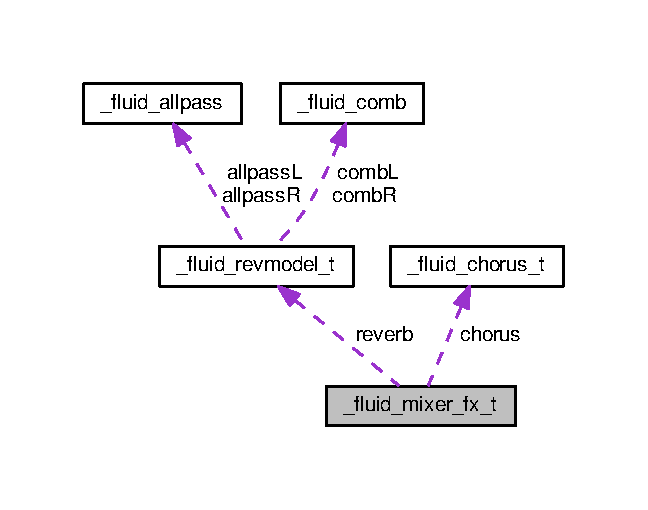
\includegraphics[width=311pt]{struct__fluid__mixer__fx__t__coll__graph}
\end{center}
\end{figure}
\subsection*{Public Attributes}
\begin{DoxyCompactItemize}
\item 
\hyperlink{fluid__rev_8h_adb084d56733ceb65419acea1967cfe7a}{fluid\+\_\+revmodel\+\_\+t} $\ast$ \hyperlink{struct__fluid__mixer__fx__t_aed2fd7d5928051dd17185375d5af2102}{reverb}
\item 
\hyperlink{fluid__chorus_8h_a56c50ab8cf334a1f7ee727bce6467aec}{fluid\+\_\+chorus\+\_\+t} $\ast$ \hyperlink{struct__fluid__mixer__fx__t_a0c5c6f8f1d3382b4d7c9928f762b69d5}{chorus}
\item 
int \hyperlink{struct__fluid__mixer__fx__t_a2b490d27a74d50f69436fff58836df74}{with\+\_\+reverb}
\item 
int \hyperlink{struct__fluid__mixer__fx__t_a61499e4c11e1e8f1771731e2fedd0402}{with\+\_\+chorus}
\item 
int \hyperlink{struct__fluid__mixer__fx__t_a5d3f2d6aa6e4e6ca958c7eb9adbe54b9}{mix\+\_\+fx\+\_\+to\+\_\+out}
\end{DoxyCompactItemize}


\subsection{Member Data Documentation}
\mbox{\Hypertarget{struct__fluid__mixer__fx__t_a0c5c6f8f1d3382b4d7c9928f762b69d5}\label{struct__fluid__mixer__fx__t_a0c5c6f8f1d3382b4d7c9928f762b69d5}} 
\index{\+\_\+fluid\+\_\+mixer\+\_\+fx\+\_\+t@{\+\_\+fluid\+\_\+mixer\+\_\+fx\+\_\+t}!chorus@{chorus}}
\index{chorus@{chorus}!\+\_\+fluid\+\_\+mixer\+\_\+fx\+\_\+t@{\+\_\+fluid\+\_\+mixer\+\_\+fx\+\_\+t}}
\subsubsection{\texorpdfstring{chorus}{chorus}}
{\footnotesize\ttfamily \hyperlink{fluid__chorus_8h_a56c50ab8cf334a1f7ee727bce6467aec}{fluid\+\_\+chorus\+\_\+t}$\ast$ \+\_\+fluid\+\_\+mixer\+\_\+fx\+\_\+t\+::chorus}

Chorus unit \mbox{\Hypertarget{struct__fluid__mixer__fx__t_a5d3f2d6aa6e4e6ca958c7eb9adbe54b9}\label{struct__fluid__mixer__fx__t_a5d3f2d6aa6e4e6ca958c7eb9adbe54b9}} 
\index{\+\_\+fluid\+\_\+mixer\+\_\+fx\+\_\+t@{\+\_\+fluid\+\_\+mixer\+\_\+fx\+\_\+t}!mix\+\_\+fx\+\_\+to\+\_\+out@{mix\+\_\+fx\+\_\+to\+\_\+out}}
\index{mix\+\_\+fx\+\_\+to\+\_\+out@{mix\+\_\+fx\+\_\+to\+\_\+out}!\+\_\+fluid\+\_\+mixer\+\_\+fx\+\_\+t@{\+\_\+fluid\+\_\+mixer\+\_\+fx\+\_\+t}}
\subsubsection{\texorpdfstring{mix\+\_\+fx\+\_\+to\+\_\+out}{mix\_fx\_to\_out}}
{\footnotesize\ttfamily int \+\_\+fluid\+\_\+mixer\+\_\+fx\+\_\+t\+::mix\+\_\+fx\+\_\+to\+\_\+out}

Should the effects be mixed in with the primary output? \mbox{\Hypertarget{struct__fluid__mixer__fx__t_aed2fd7d5928051dd17185375d5af2102}\label{struct__fluid__mixer__fx__t_aed2fd7d5928051dd17185375d5af2102}} 
\index{\+\_\+fluid\+\_\+mixer\+\_\+fx\+\_\+t@{\+\_\+fluid\+\_\+mixer\+\_\+fx\+\_\+t}!reverb@{reverb}}
\index{reverb@{reverb}!\+\_\+fluid\+\_\+mixer\+\_\+fx\+\_\+t@{\+\_\+fluid\+\_\+mixer\+\_\+fx\+\_\+t}}
\subsubsection{\texorpdfstring{reverb}{reverb}}
{\footnotesize\ttfamily \hyperlink{fluid__rev_8h_adb084d56733ceb65419acea1967cfe7a}{fluid\+\_\+revmodel\+\_\+t}$\ast$ \+\_\+fluid\+\_\+mixer\+\_\+fx\+\_\+t\+::reverb}

Reverb unit \mbox{\Hypertarget{struct__fluid__mixer__fx__t_a61499e4c11e1e8f1771731e2fedd0402}\label{struct__fluid__mixer__fx__t_a61499e4c11e1e8f1771731e2fedd0402}} 
\index{\+\_\+fluid\+\_\+mixer\+\_\+fx\+\_\+t@{\+\_\+fluid\+\_\+mixer\+\_\+fx\+\_\+t}!with\+\_\+chorus@{with\+\_\+chorus}}
\index{with\+\_\+chorus@{with\+\_\+chorus}!\+\_\+fluid\+\_\+mixer\+\_\+fx\+\_\+t@{\+\_\+fluid\+\_\+mixer\+\_\+fx\+\_\+t}}
\subsubsection{\texorpdfstring{with\+\_\+chorus}{with\_chorus}}
{\footnotesize\ttfamily int \+\_\+fluid\+\_\+mixer\+\_\+fx\+\_\+t\+::with\+\_\+chorus}

Should the synth use the built-\/in chorus unit? \mbox{\Hypertarget{struct__fluid__mixer__fx__t_a2b490d27a74d50f69436fff58836df74}\label{struct__fluid__mixer__fx__t_a2b490d27a74d50f69436fff58836df74}} 
\index{\+\_\+fluid\+\_\+mixer\+\_\+fx\+\_\+t@{\+\_\+fluid\+\_\+mixer\+\_\+fx\+\_\+t}!with\+\_\+reverb@{with\+\_\+reverb}}
\index{with\+\_\+reverb@{with\+\_\+reverb}!\+\_\+fluid\+\_\+mixer\+\_\+fx\+\_\+t@{\+\_\+fluid\+\_\+mixer\+\_\+fx\+\_\+t}}
\subsubsection{\texorpdfstring{with\+\_\+reverb}{with\_reverb}}
{\footnotesize\ttfamily int \+\_\+fluid\+\_\+mixer\+\_\+fx\+\_\+t\+::with\+\_\+reverb}

Should the synth use the built-\/in reverb unit? 

The documentation for this struct was generated from the following file\+:\begin{DoxyCompactItemize}
\item 
rvoice/\hyperlink{fluid__rvoice__mixer_8c}{fluid\+\_\+rvoice\+\_\+mixer.\+c}\end{DoxyCompactItemize}

\hypertarget{struct__fluid__mod__t}{}\section{\+\_\+fluid\+\_\+mod\+\_\+t Struct Reference}
\label{struct__fluid__mod__t}\index{\+\_\+fluid\+\_\+mod\+\_\+t@{\+\_\+fluid\+\_\+mod\+\_\+t}}


{\ttfamily \#include $<$fluid\+\_\+mod.\+h$>$}



Collaboration diagram for \+\_\+fluid\+\_\+mod\+\_\+t\+:
\nopagebreak
\begin{figure}[H]
\begin{center}
\leavevmode
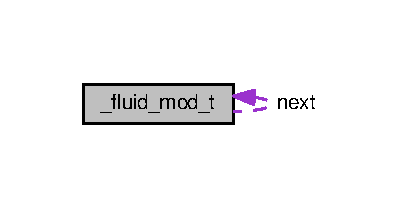
\includegraphics[width=192pt]{struct__fluid__mod__t__coll__graph}
\end{center}
\end{figure}
\subsection*{Public Attributes}
\begin{DoxyCompactItemize}
\item 
unsigned char \hyperlink{struct__fluid__mod__t_a1c7d15ae9ad239b578701878b0ffbb08}{dest}
\item 
unsigned char \hyperlink{struct__fluid__mod__t_a199e73690c3e5fdb0e073d05f8237196}{src1}
\item 
unsigned char \hyperlink{struct__fluid__mod__t_adb71cc4a4b81c915f05c1b8d069e3056}{flags1}
\item 
unsigned char \hyperlink{struct__fluid__mod__t_a8f83acd72515a3dc6d6d73089b907685}{src2}
\item 
unsigned char \hyperlink{struct__fluid__mod__t_a38e059fb4214ab59b5f0895d100dfffa}{flags2}
\item 
double \hyperlink{struct__fluid__mod__t_a89680a436126f578594c5981d6c4f2ad}{amount}
\item 
\hyperlink{types_8h_a6c727efab500d6c0c350d4292e9aa5ef}{fluid\+\_\+mod\+\_\+t} $\ast$ \hyperlink{struct__fluid__mod__t_a596143c498657350b1d43cb99a2bc6b0}{next}
\end{DoxyCompactItemize}


\subsection{Member Data Documentation}
\mbox{\Hypertarget{struct__fluid__mod__t_a89680a436126f578594c5981d6c4f2ad}\label{struct__fluid__mod__t_a89680a436126f578594c5981d6c4f2ad}} 
\index{\+\_\+fluid\+\_\+mod\+\_\+t@{\+\_\+fluid\+\_\+mod\+\_\+t}!amount@{amount}}
\index{amount@{amount}!\+\_\+fluid\+\_\+mod\+\_\+t@{\+\_\+fluid\+\_\+mod\+\_\+t}}
\subsubsection{\texorpdfstring{amount}{amount}}
{\footnotesize\ttfamily double \+\_\+fluid\+\_\+mod\+\_\+t\+::amount}

Multiplier amount \mbox{\Hypertarget{struct__fluid__mod__t_a1c7d15ae9ad239b578701878b0ffbb08}\label{struct__fluid__mod__t_a1c7d15ae9ad239b578701878b0ffbb08}} 
\index{\+\_\+fluid\+\_\+mod\+\_\+t@{\+\_\+fluid\+\_\+mod\+\_\+t}!dest@{dest}}
\index{dest@{dest}!\+\_\+fluid\+\_\+mod\+\_\+t@{\+\_\+fluid\+\_\+mod\+\_\+t}}
\subsubsection{\texorpdfstring{dest}{dest}}
{\footnotesize\ttfamily unsigned char \+\_\+fluid\+\_\+mod\+\_\+t\+::dest}

Destination generator to control \mbox{\Hypertarget{struct__fluid__mod__t_adb71cc4a4b81c915f05c1b8d069e3056}\label{struct__fluid__mod__t_adb71cc4a4b81c915f05c1b8d069e3056}} 
\index{\+\_\+fluid\+\_\+mod\+\_\+t@{\+\_\+fluid\+\_\+mod\+\_\+t}!flags1@{flags1}}
\index{flags1@{flags1}!\+\_\+fluid\+\_\+mod\+\_\+t@{\+\_\+fluid\+\_\+mod\+\_\+t}}
\subsubsection{\texorpdfstring{flags1}{flags1}}
{\footnotesize\ttfamily unsigned char \+\_\+fluid\+\_\+mod\+\_\+t\+::flags1}

Source controller 1 flags \mbox{\Hypertarget{struct__fluid__mod__t_a38e059fb4214ab59b5f0895d100dfffa}\label{struct__fluid__mod__t_a38e059fb4214ab59b5f0895d100dfffa}} 
\index{\+\_\+fluid\+\_\+mod\+\_\+t@{\+\_\+fluid\+\_\+mod\+\_\+t}!flags2@{flags2}}
\index{flags2@{flags2}!\+\_\+fluid\+\_\+mod\+\_\+t@{\+\_\+fluid\+\_\+mod\+\_\+t}}
\subsubsection{\texorpdfstring{flags2}{flags2}}
{\footnotesize\ttfamily unsigned char \+\_\+fluid\+\_\+mod\+\_\+t\+::flags2}

Source controller 2 flags \mbox{\Hypertarget{struct__fluid__mod__t_a596143c498657350b1d43cb99a2bc6b0}\label{struct__fluid__mod__t_a596143c498657350b1d43cb99a2bc6b0}} 
\index{\+\_\+fluid\+\_\+mod\+\_\+t@{\+\_\+fluid\+\_\+mod\+\_\+t}!next@{next}}
\index{next@{next}!\+\_\+fluid\+\_\+mod\+\_\+t@{\+\_\+fluid\+\_\+mod\+\_\+t}}
\subsubsection{\texorpdfstring{next}{next}}
{\footnotesize\ttfamily \hyperlink{types_8h_a6c727efab500d6c0c350d4292e9aa5ef}{fluid\+\_\+mod\+\_\+t}$\ast$ \+\_\+fluid\+\_\+mod\+\_\+t\+::next}

\mbox{\Hypertarget{struct__fluid__mod__t_a199e73690c3e5fdb0e073d05f8237196}\label{struct__fluid__mod__t_a199e73690c3e5fdb0e073d05f8237196}} 
\index{\+\_\+fluid\+\_\+mod\+\_\+t@{\+\_\+fluid\+\_\+mod\+\_\+t}!src1@{src1}}
\index{src1@{src1}!\+\_\+fluid\+\_\+mod\+\_\+t@{\+\_\+fluid\+\_\+mod\+\_\+t}}
\subsubsection{\texorpdfstring{src1}{src1}}
{\footnotesize\ttfamily unsigned char \+\_\+fluid\+\_\+mod\+\_\+t\+::src1}

Source controller 1 \mbox{\Hypertarget{struct__fluid__mod__t_a8f83acd72515a3dc6d6d73089b907685}\label{struct__fluid__mod__t_a8f83acd72515a3dc6d6d73089b907685}} 
\index{\+\_\+fluid\+\_\+mod\+\_\+t@{\+\_\+fluid\+\_\+mod\+\_\+t}!src2@{src2}}
\index{src2@{src2}!\+\_\+fluid\+\_\+mod\+\_\+t@{\+\_\+fluid\+\_\+mod\+\_\+t}}
\subsubsection{\texorpdfstring{src2}{src2}}
{\footnotesize\ttfamily unsigned char \+\_\+fluid\+\_\+mod\+\_\+t\+::src2}

Source controller 2 

The documentation for this struct was generated from the following file\+:\begin{DoxyCompactItemize}
\item 
synth/\hyperlink{fluid__mod_8h}{fluid\+\_\+mod.\+h}\end{DoxyCompactItemize}

\hypertarget{struct__fluid__overflow__prio__t}{}\section{\+\_\+fluid\+\_\+overflow\+\_\+prio\+\_\+t Struct Reference}
\label{struct__fluid__overflow__prio__t}\index{\+\_\+fluid\+\_\+overflow\+\_\+prio\+\_\+t@{\+\_\+fluid\+\_\+overflow\+\_\+prio\+\_\+t}}


{\ttfamily \#include $<$fluid\+\_\+voice.\+h$>$}

\subsection*{Public Attributes}
\begin{DoxyCompactItemize}
\item 
float \hyperlink{struct__fluid__overflow__prio__t_a1c597217c990a8d32b7d312dfd8418f0}{percussion}
\item 
float \hyperlink{struct__fluid__overflow__prio__t_a85493c7748bafb1bcfd5b4fb81382a7f}{released}
\item 
float \hyperlink{struct__fluid__overflow__prio__t_a16198936689382ef6968ae49efb2d436}{sustained}
\item 
float \hyperlink{struct__fluid__overflow__prio__t_a27b427667522657fc8219c796ed22b60}{volume}
\item 
float \hyperlink{struct__fluid__overflow__prio__t_a0de07e878a7f7e4667ad3417897b0b87}{age}
\item 
float \hyperlink{struct__fluid__overflow__prio__t_afb4380842aa9429afbfd8e3594ed5413}{important}
\item 
char $\ast$ \hyperlink{struct__fluid__overflow__prio__t_ae2c4cffa02815bf1a5619fa258c70348}{important\+\_\+channels}
\item 
int \hyperlink{struct__fluid__overflow__prio__t_a9bf22b15b4349c0ddfd92d08214fc2c9}{num\+\_\+important\+\_\+channels}
\end{DoxyCompactItemize}


\subsection{Member Data Documentation}
\mbox{\Hypertarget{struct__fluid__overflow__prio__t_a0de07e878a7f7e4667ad3417897b0b87}\label{struct__fluid__overflow__prio__t_a0de07e878a7f7e4667ad3417897b0b87}} 
\index{\+\_\+fluid\+\_\+overflow\+\_\+prio\+\_\+t@{\+\_\+fluid\+\_\+overflow\+\_\+prio\+\_\+t}!age@{age}}
\index{age@{age}!\+\_\+fluid\+\_\+overflow\+\_\+prio\+\_\+t@{\+\_\+fluid\+\_\+overflow\+\_\+prio\+\_\+t}}
\subsubsection{\texorpdfstring{age}{age}}
{\footnotesize\ttfamily float \+\_\+fluid\+\_\+overflow\+\_\+prio\+\_\+t\+::age}

This score will be divided by the number of seconds the voice has lasted \mbox{\Hypertarget{struct__fluid__overflow__prio__t_afb4380842aa9429afbfd8e3594ed5413}\label{struct__fluid__overflow__prio__t_afb4380842aa9429afbfd8e3594ed5413}} 
\index{\+\_\+fluid\+\_\+overflow\+\_\+prio\+\_\+t@{\+\_\+fluid\+\_\+overflow\+\_\+prio\+\_\+t}!important@{important}}
\index{important@{important}!\+\_\+fluid\+\_\+overflow\+\_\+prio\+\_\+t@{\+\_\+fluid\+\_\+overflow\+\_\+prio\+\_\+t}}
\subsubsection{\texorpdfstring{important}{important}}
{\footnotesize\ttfamily float \+\_\+fluid\+\_\+overflow\+\_\+prio\+\_\+t\+::important}

This score will be added to all important channels \mbox{\Hypertarget{struct__fluid__overflow__prio__t_ae2c4cffa02815bf1a5619fa258c70348}\label{struct__fluid__overflow__prio__t_ae2c4cffa02815bf1a5619fa258c70348}} 
\index{\+\_\+fluid\+\_\+overflow\+\_\+prio\+\_\+t@{\+\_\+fluid\+\_\+overflow\+\_\+prio\+\_\+t}!important\+\_\+channels@{important\+\_\+channels}}
\index{important\+\_\+channels@{important\+\_\+channels}!\+\_\+fluid\+\_\+overflow\+\_\+prio\+\_\+t@{\+\_\+fluid\+\_\+overflow\+\_\+prio\+\_\+t}}
\subsubsection{\texorpdfstring{important\+\_\+channels}{important\_channels}}
{\footnotesize\ttfamily char$\ast$ \+\_\+fluid\+\_\+overflow\+\_\+prio\+\_\+t\+::important\+\_\+channels}

\char`\"{}important\char`\"{} flags indexed by M\+I\+DI channel number \mbox{\Hypertarget{struct__fluid__overflow__prio__t_a9bf22b15b4349c0ddfd92d08214fc2c9}\label{struct__fluid__overflow__prio__t_a9bf22b15b4349c0ddfd92d08214fc2c9}} 
\index{\+\_\+fluid\+\_\+overflow\+\_\+prio\+\_\+t@{\+\_\+fluid\+\_\+overflow\+\_\+prio\+\_\+t}!num\+\_\+important\+\_\+channels@{num\+\_\+important\+\_\+channels}}
\index{num\+\_\+important\+\_\+channels@{num\+\_\+important\+\_\+channels}!\+\_\+fluid\+\_\+overflow\+\_\+prio\+\_\+t@{\+\_\+fluid\+\_\+overflow\+\_\+prio\+\_\+t}}
\subsubsection{\texorpdfstring{num\+\_\+important\+\_\+channels}{num\_important\_channels}}
{\footnotesize\ttfamily int \+\_\+fluid\+\_\+overflow\+\_\+prio\+\_\+t\+::num\+\_\+important\+\_\+channels}

Number of elements in the important\+\_\+channels array \mbox{\Hypertarget{struct__fluid__overflow__prio__t_a1c597217c990a8d32b7d312dfd8418f0}\label{struct__fluid__overflow__prio__t_a1c597217c990a8d32b7d312dfd8418f0}} 
\index{\+\_\+fluid\+\_\+overflow\+\_\+prio\+\_\+t@{\+\_\+fluid\+\_\+overflow\+\_\+prio\+\_\+t}!percussion@{percussion}}
\index{percussion@{percussion}!\+\_\+fluid\+\_\+overflow\+\_\+prio\+\_\+t@{\+\_\+fluid\+\_\+overflow\+\_\+prio\+\_\+t}}
\subsubsection{\texorpdfstring{percussion}{percussion}}
{\footnotesize\ttfamily float \+\_\+fluid\+\_\+overflow\+\_\+prio\+\_\+t\+::percussion}

Is this voice on the drum channel? Then add this score \mbox{\Hypertarget{struct__fluid__overflow__prio__t_a85493c7748bafb1bcfd5b4fb81382a7f}\label{struct__fluid__overflow__prio__t_a85493c7748bafb1bcfd5b4fb81382a7f}} 
\index{\+\_\+fluid\+\_\+overflow\+\_\+prio\+\_\+t@{\+\_\+fluid\+\_\+overflow\+\_\+prio\+\_\+t}!released@{released}}
\index{released@{released}!\+\_\+fluid\+\_\+overflow\+\_\+prio\+\_\+t@{\+\_\+fluid\+\_\+overflow\+\_\+prio\+\_\+t}}
\subsubsection{\texorpdfstring{released}{released}}
{\footnotesize\ttfamily float \+\_\+fluid\+\_\+overflow\+\_\+prio\+\_\+t\+::released}

Is this voice in release stage? Then add this score (usually negative) \mbox{\Hypertarget{struct__fluid__overflow__prio__t_a16198936689382ef6968ae49efb2d436}\label{struct__fluid__overflow__prio__t_a16198936689382ef6968ae49efb2d436}} 
\index{\+\_\+fluid\+\_\+overflow\+\_\+prio\+\_\+t@{\+\_\+fluid\+\_\+overflow\+\_\+prio\+\_\+t}!sustained@{sustained}}
\index{sustained@{sustained}!\+\_\+fluid\+\_\+overflow\+\_\+prio\+\_\+t@{\+\_\+fluid\+\_\+overflow\+\_\+prio\+\_\+t}}
\subsubsection{\texorpdfstring{sustained}{sustained}}
{\footnotesize\ttfamily float \+\_\+fluid\+\_\+overflow\+\_\+prio\+\_\+t\+::sustained}

Is this voice sustained? Then add this score (usually negative) \mbox{\Hypertarget{struct__fluid__overflow__prio__t_a27b427667522657fc8219c796ed22b60}\label{struct__fluid__overflow__prio__t_a27b427667522657fc8219c796ed22b60}} 
\index{\+\_\+fluid\+\_\+overflow\+\_\+prio\+\_\+t@{\+\_\+fluid\+\_\+overflow\+\_\+prio\+\_\+t}!volume@{volume}}
\index{volume@{volume}!\+\_\+fluid\+\_\+overflow\+\_\+prio\+\_\+t@{\+\_\+fluid\+\_\+overflow\+\_\+prio\+\_\+t}}
\subsubsection{\texorpdfstring{volume}{volume}}
{\footnotesize\ttfamily float \+\_\+fluid\+\_\+overflow\+\_\+prio\+\_\+t\+::volume}

Multiply current (or future) volume (a value between 0 and 1) 

The documentation for this struct was generated from the following file\+:\begin{DoxyCompactItemize}
\item 
synth/\hyperlink{fluid__voice_8h}{fluid\+\_\+voice.\+h}\end{DoxyCompactItemize}

\hypertarget{struct__fluid__player__t}{}\section{\+\_\+fluid\+\_\+player\+\_\+t Struct Reference}
\label{struct__fluid__player__t}\index{\+\_\+fluid\+\_\+player\+\_\+t@{\+\_\+fluid\+\_\+player\+\_\+t}}


{\ttfamily \#include $<$fluid\+\_\+midi.\+h$>$}



Collaboration diagram for \+\_\+fluid\+\_\+player\+\_\+t\+:
\nopagebreak
\begin{figure}[H]
\begin{center}
\leavevmode
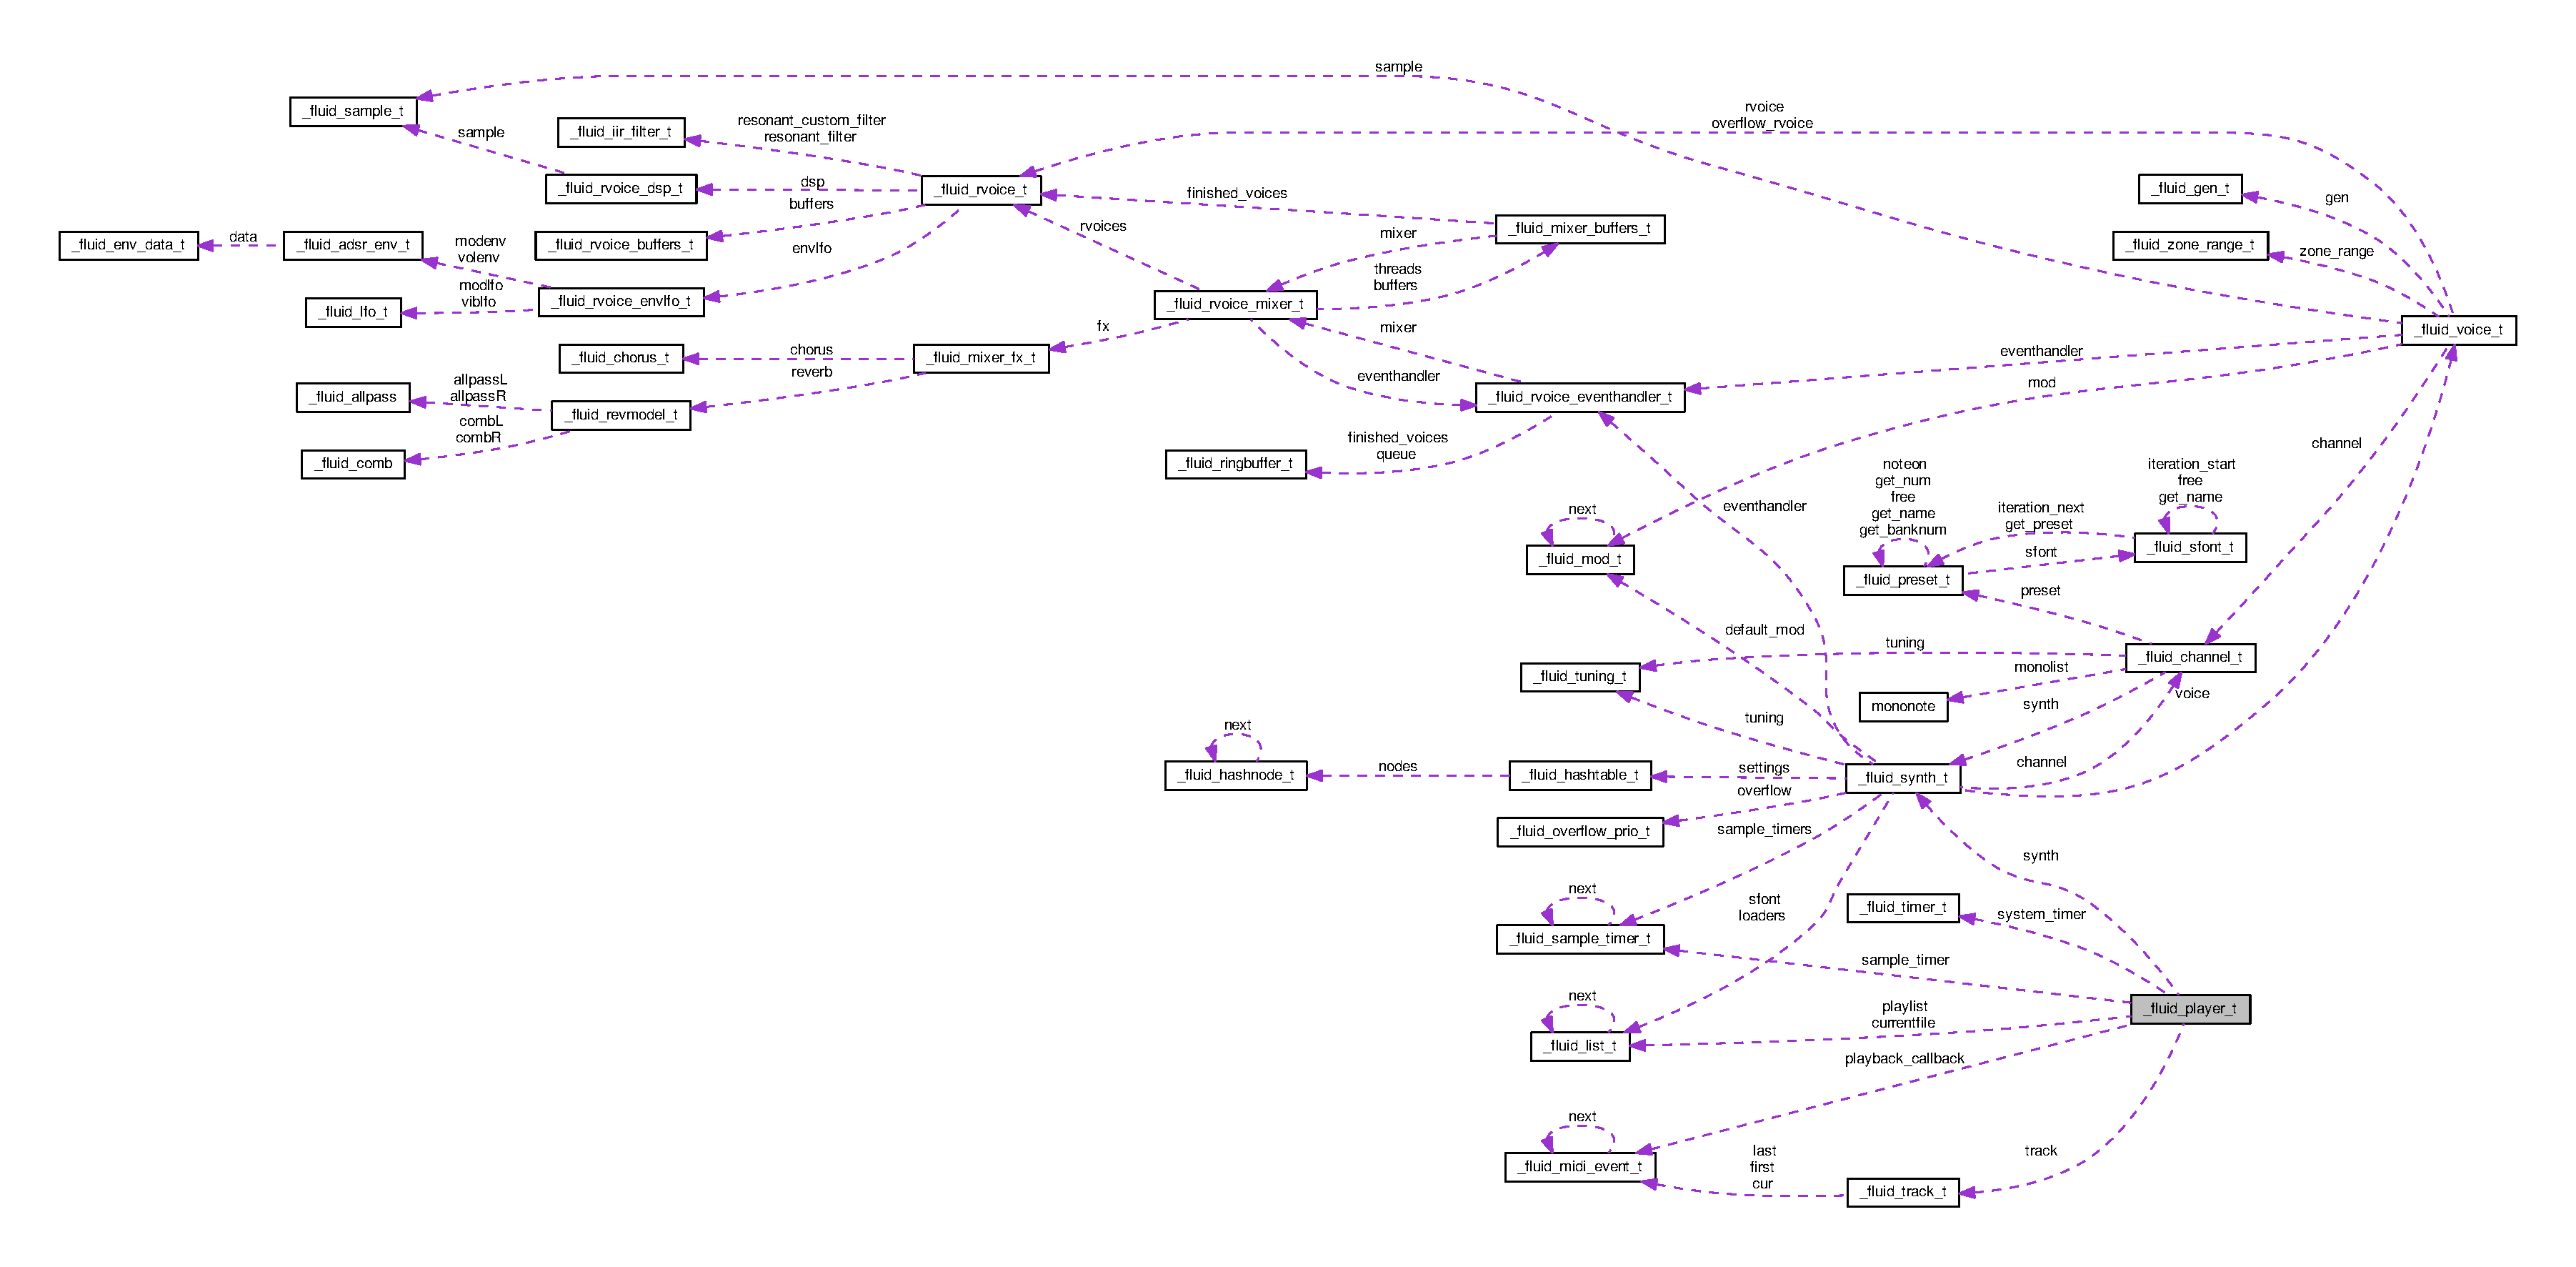
\includegraphics[width=350pt]{struct__fluid__player__t__coll__graph}
\end{center}
\end{figure}
\subsection*{Public Attributes}
\begin{DoxyCompactItemize}
\item 
int \hyperlink{struct__fluid__player__t_a8c697a8e813d952d09ee2b6e3946c4fb}{status}
\item 
int \hyperlink{struct__fluid__player__t_aac1360ac5e7b574a3b46e4138d59fa89}{ntracks}
\item 
\hyperlink{fluid__midi_8h_a81a9252c015f2b4173a2642a4507d74b}{fluid\+\_\+track\+\_\+t} $\ast$ \hyperlink{struct__fluid__player__t_abaf5bdaf07e59c4d0fb49f4361f2626d}{track} \mbox{[}\hyperlink{fluid__midi_8h_a2023050a49b937b6321b5236aac122c9}{M\+A\+X\+\_\+\+N\+U\+M\+B\+E\+R\+\_\+\+O\+F\+\_\+\+T\+R\+A\+C\+KS}\mbox{]}
\item 
\hyperlink{types_8h_ae265f10ae174a13afe010de50d87e1a4}{fluid\+\_\+synth\+\_\+t} $\ast$ \hyperlink{struct__fluid__player__t_af9313f8f8f6313fd14f3ecf9d26d90b5}{synth}
\item 
\hyperlink{fluid__sys_8h_a520742276ee4ea4bf140e6e6be79e4ae}{fluid\+\_\+timer\+\_\+t} $\ast$ \hyperlink{struct__fluid__player__t_a8780acf388964d3d59ad0815df1c699d}{system\+\_\+timer}
\item 
\hyperlink{fluidsynth__priv_8h_a4ddade88911e1873bccda1a7750a848c}{fluid\+\_\+sample\+\_\+timer\+\_\+t} $\ast$ \hyperlink{struct__fluid__player__t_a337ba1549b8460ca4e7be23088dca44f}{sample\+\_\+timer}
\item 
int \hyperlink{struct__fluid__player__t_a750a3c6034bd1fafbf80fe751a2ea123}{loop}
\item 
\hyperlink{fluid__list_8h_a3ef7535d4290862c0af118569223bd89}{fluid\+\_\+list\+\_\+t} $\ast$ \hyperlink{struct__fluid__player__t_a9c59652390dc6be784baf56d6c2eb876}{playlist}
\item 
\hyperlink{fluid__list_8h_a3ef7535d4290862c0af118569223bd89}{fluid\+\_\+list\+\_\+t} $\ast$ \hyperlink{struct__fluid__player__t_a1a51559ebd3986775518502545baa2a7}{currentfile}
\item 
char \hyperlink{struct__fluid__player__t_acf44858efd9c289b156aa87c65b9abac}{send\+\_\+program\+\_\+change}
\item 
char \hyperlink{struct__fluid__player__t_a1f215fdc1f459ac01cae1272ef191d23}{use\+\_\+system\+\_\+timer}
\item 
char \hyperlink{struct__fluid__player__t_a49f91063ada7e3fa43aad47eab2fe55d}{reset\+\_\+synth\+\_\+between\+\_\+songs}
\item 
int \hyperlink{struct__fluid__player__t_ae71541ce6fa75f76f382221d6b0764bd}{seek\+\_\+ticks}
\item 
int \hyperlink{struct__fluid__player__t_a21a6867f589eb2fc5c0a0abcb2f8f605}{start\+\_\+ticks}
\item 
int \hyperlink{struct__fluid__player__t_a4725f623cdfc3cdeb414987efdadeb91}{cur\+\_\+ticks}
\item 
int \hyperlink{struct__fluid__player__t_a0360723080a5aa6bb8ef40297f2e6731}{begin\+\_\+msec}
\item 
int \hyperlink{struct__fluid__player__t_a9e7279464f9a3e6c72dc286c8d86ca3f}{start\+\_\+msec}
\item 
int \hyperlink{struct__fluid__player__t_a341f5879916084630d4e73efb3d96857}{cur\+\_\+msec}
\item 
int \hyperlink{struct__fluid__player__t_a9479639aa40bb89fb7f6815ea2b074bd}{miditempo}
\item 
double \hyperlink{struct__fluid__player__t_aab444ebcc6b1f0a3ddb73b4357a9d28e}{deltatime}
\item 
unsigned int \hyperlink{struct__fluid__player__t_ab0ff4918454c4ade622abb56cee55457}{division}
\item 
\hyperlink{midi_8h_a42c3752e3adb54e0af802131c36a1129}{handle\+\_\+midi\+\_\+event\+\_\+func\+\_\+t} \hyperlink{struct__fluid__player__t_a247a7bb54c4b0491762dc047c6ad4dbc}{playback\+\_\+callback}
\item 
void $\ast$ \hyperlink{struct__fluid__player__t_ae932ebf90f25f41ec34cb5b20e553941}{playback\+\_\+userdata}
\end{DoxyCompactItemize}


\subsection{Member Data Documentation}
\mbox{\Hypertarget{struct__fluid__player__t_a0360723080a5aa6bb8ef40297f2e6731}\label{struct__fluid__player__t_a0360723080a5aa6bb8ef40297f2e6731}} 
\index{\+\_\+fluid\+\_\+player\+\_\+t@{\+\_\+fluid\+\_\+player\+\_\+t}!begin\+\_\+msec@{begin\+\_\+msec}}
\index{begin\+\_\+msec@{begin\+\_\+msec}!\+\_\+fluid\+\_\+player\+\_\+t@{\+\_\+fluid\+\_\+player\+\_\+t}}
\subsubsection{\texorpdfstring{begin\+\_\+msec}{begin\_msec}}
{\footnotesize\ttfamily int \+\_\+fluid\+\_\+player\+\_\+t\+::begin\+\_\+msec}

\mbox{\Hypertarget{struct__fluid__player__t_a341f5879916084630d4e73efb3d96857}\label{struct__fluid__player__t_a341f5879916084630d4e73efb3d96857}} 
\index{\+\_\+fluid\+\_\+player\+\_\+t@{\+\_\+fluid\+\_\+player\+\_\+t}!cur\+\_\+msec@{cur\+\_\+msec}}
\index{cur\+\_\+msec@{cur\+\_\+msec}!\+\_\+fluid\+\_\+player\+\_\+t@{\+\_\+fluid\+\_\+player\+\_\+t}}
\subsubsection{\texorpdfstring{cur\+\_\+msec}{cur\_msec}}
{\footnotesize\ttfamily int \+\_\+fluid\+\_\+player\+\_\+t\+::cur\+\_\+msec}

\mbox{\Hypertarget{struct__fluid__player__t_a4725f623cdfc3cdeb414987efdadeb91}\label{struct__fluid__player__t_a4725f623cdfc3cdeb414987efdadeb91}} 
\index{\+\_\+fluid\+\_\+player\+\_\+t@{\+\_\+fluid\+\_\+player\+\_\+t}!cur\+\_\+ticks@{cur\+\_\+ticks}}
\index{cur\+\_\+ticks@{cur\+\_\+ticks}!\+\_\+fluid\+\_\+player\+\_\+t@{\+\_\+fluid\+\_\+player\+\_\+t}}
\subsubsection{\texorpdfstring{cur\+\_\+ticks}{cur\_ticks}}
{\footnotesize\ttfamily int \+\_\+fluid\+\_\+player\+\_\+t\+::cur\+\_\+ticks}

\mbox{\Hypertarget{struct__fluid__player__t_a1a51559ebd3986775518502545baa2a7}\label{struct__fluid__player__t_a1a51559ebd3986775518502545baa2a7}} 
\index{\+\_\+fluid\+\_\+player\+\_\+t@{\+\_\+fluid\+\_\+player\+\_\+t}!currentfile@{currentfile}}
\index{currentfile@{currentfile}!\+\_\+fluid\+\_\+player\+\_\+t@{\+\_\+fluid\+\_\+player\+\_\+t}}
\subsubsection{\texorpdfstring{currentfile}{currentfile}}
{\footnotesize\ttfamily \hyperlink{fluid__list_8h_a3ef7535d4290862c0af118569223bd89}{fluid\+\_\+list\+\_\+t}$\ast$ \+\_\+fluid\+\_\+player\+\_\+t\+::currentfile}

\mbox{\Hypertarget{struct__fluid__player__t_aab444ebcc6b1f0a3ddb73b4357a9d28e}\label{struct__fluid__player__t_aab444ebcc6b1f0a3ddb73b4357a9d28e}} 
\index{\+\_\+fluid\+\_\+player\+\_\+t@{\+\_\+fluid\+\_\+player\+\_\+t}!deltatime@{deltatime}}
\index{deltatime@{deltatime}!\+\_\+fluid\+\_\+player\+\_\+t@{\+\_\+fluid\+\_\+player\+\_\+t}}
\subsubsection{\texorpdfstring{deltatime}{deltatime}}
{\footnotesize\ttfamily double \+\_\+fluid\+\_\+player\+\_\+t\+::deltatime}

\mbox{\Hypertarget{struct__fluid__player__t_ab0ff4918454c4ade622abb56cee55457}\label{struct__fluid__player__t_ab0ff4918454c4ade622abb56cee55457}} 
\index{\+\_\+fluid\+\_\+player\+\_\+t@{\+\_\+fluid\+\_\+player\+\_\+t}!division@{division}}
\index{division@{division}!\+\_\+fluid\+\_\+player\+\_\+t@{\+\_\+fluid\+\_\+player\+\_\+t}}
\subsubsection{\texorpdfstring{division}{division}}
{\footnotesize\ttfamily unsigned int \+\_\+fluid\+\_\+player\+\_\+t\+::division}

\mbox{\Hypertarget{struct__fluid__player__t_a750a3c6034bd1fafbf80fe751a2ea123}\label{struct__fluid__player__t_a750a3c6034bd1fafbf80fe751a2ea123}} 
\index{\+\_\+fluid\+\_\+player\+\_\+t@{\+\_\+fluid\+\_\+player\+\_\+t}!loop@{loop}}
\index{loop@{loop}!\+\_\+fluid\+\_\+player\+\_\+t@{\+\_\+fluid\+\_\+player\+\_\+t}}
\subsubsection{\texorpdfstring{loop}{loop}}
{\footnotesize\ttfamily int \+\_\+fluid\+\_\+player\+\_\+t\+::loop}

\mbox{\Hypertarget{struct__fluid__player__t_a9479639aa40bb89fb7f6815ea2b074bd}\label{struct__fluid__player__t_a9479639aa40bb89fb7f6815ea2b074bd}} 
\index{\+\_\+fluid\+\_\+player\+\_\+t@{\+\_\+fluid\+\_\+player\+\_\+t}!miditempo@{miditempo}}
\index{miditempo@{miditempo}!\+\_\+fluid\+\_\+player\+\_\+t@{\+\_\+fluid\+\_\+player\+\_\+t}}
\subsubsection{\texorpdfstring{miditempo}{miditempo}}
{\footnotesize\ttfamily int \+\_\+fluid\+\_\+player\+\_\+t\+::miditempo}

\mbox{\Hypertarget{struct__fluid__player__t_aac1360ac5e7b574a3b46e4138d59fa89}\label{struct__fluid__player__t_aac1360ac5e7b574a3b46e4138d59fa89}} 
\index{\+\_\+fluid\+\_\+player\+\_\+t@{\+\_\+fluid\+\_\+player\+\_\+t}!ntracks@{ntracks}}
\index{ntracks@{ntracks}!\+\_\+fluid\+\_\+player\+\_\+t@{\+\_\+fluid\+\_\+player\+\_\+t}}
\subsubsection{\texorpdfstring{ntracks}{ntracks}}
{\footnotesize\ttfamily int \+\_\+fluid\+\_\+player\+\_\+t\+::ntracks}

\mbox{\Hypertarget{struct__fluid__player__t_a247a7bb54c4b0491762dc047c6ad4dbc}\label{struct__fluid__player__t_a247a7bb54c4b0491762dc047c6ad4dbc}} 
\index{\+\_\+fluid\+\_\+player\+\_\+t@{\+\_\+fluid\+\_\+player\+\_\+t}!playback\+\_\+callback@{playback\+\_\+callback}}
\index{playback\+\_\+callback@{playback\+\_\+callback}!\+\_\+fluid\+\_\+player\+\_\+t@{\+\_\+fluid\+\_\+player\+\_\+t}}
\subsubsection{\texorpdfstring{playback\+\_\+callback}{playback\_callback}}
{\footnotesize\ttfamily \hyperlink{midi_8h_a42c3752e3adb54e0af802131c36a1129}{handle\+\_\+midi\+\_\+event\+\_\+func\+\_\+t} \+\_\+fluid\+\_\+player\+\_\+t\+::playback\+\_\+callback}

\mbox{\Hypertarget{struct__fluid__player__t_ae932ebf90f25f41ec34cb5b20e553941}\label{struct__fluid__player__t_ae932ebf90f25f41ec34cb5b20e553941}} 
\index{\+\_\+fluid\+\_\+player\+\_\+t@{\+\_\+fluid\+\_\+player\+\_\+t}!playback\+\_\+userdata@{playback\+\_\+userdata}}
\index{playback\+\_\+userdata@{playback\+\_\+userdata}!\+\_\+fluid\+\_\+player\+\_\+t@{\+\_\+fluid\+\_\+player\+\_\+t}}
\subsubsection{\texorpdfstring{playback\+\_\+userdata}{playback\_userdata}}
{\footnotesize\ttfamily void$\ast$ \+\_\+fluid\+\_\+player\+\_\+t\+::playback\+\_\+userdata}

\mbox{\Hypertarget{struct__fluid__player__t_a9c59652390dc6be784baf56d6c2eb876}\label{struct__fluid__player__t_a9c59652390dc6be784baf56d6c2eb876}} 
\index{\+\_\+fluid\+\_\+player\+\_\+t@{\+\_\+fluid\+\_\+player\+\_\+t}!playlist@{playlist}}
\index{playlist@{playlist}!\+\_\+fluid\+\_\+player\+\_\+t@{\+\_\+fluid\+\_\+player\+\_\+t}}
\subsubsection{\texorpdfstring{playlist}{playlist}}
{\footnotesize\ttfamily \hyperlink{fluid__list_8h_a3ef7535d4290862c0af118569223bd89}{fluid\+\_\+list\+\_\+t}$\ast$ \+\_\+fluid\+\_\+player\+\_\+t\+::playlist}

\mbox{\Hypertarget{struct__fluid__player__t_a49f91063ada7e3fa43aad47eab2fe55d}\label{struct__fluid__player__t_a49f91063ada7e3fa43aad47eab2fe55d}} 
\index{\+\_\+fluid\+\_\+player\+\_\+t@{\+\_\+fluid\+\_\+player\+\_\+t}!reset\+\_\+synth\+\_\+between\+\_\+songs@{reset\+\_\+synth\+\_\+between\+\_\+songs}}
\index{reset\+\_\+synth\+\_\+between\+\_\+songs@{reset\+\_\+synth\+\_\+between\+\_\+songs}!\+\_\+fluid\+\_\+player\+\_\+t@{\+\_\+fluid\+\_\+player\+\_\+t}}
\subsubsection{\texorpdfstring{reset\+\_\+synth\+\_\+between\+\_\+songs}{reset\_synth\_between\_songs}}
{\footnotesize\ttfamily char \+\_\+fluid\+\_\+player\+\_\+t\+::reset\+\_\+synth\+\_\+between\+\_\+songs}

\mbox{\Hypertarget{struct__fluid__player__t_a337ba1549b8460ca4e7be23088dca44f}\label{struct__fluid__player__t_a337ba1549b8460ca4e7be23088dca44f}} 
\index{\+\_\+fluid\+\_\+player\+\_\+t@{\+\_\+fluid\+\_\+player\+\_\+t}!sample\+\_\+timer@{sample\+\_\+timer}}
\index{sample\+\_\+timer@{sample\+\_\+timer}!\+\_\+fluid\+\_\+player\+\_\+t@{\+\_\+fluid\+\_\+player\+\_\+t}}
\subsubsection{\texorpdfstring{sample\+\_\+timer}{sample\_timer}}
{\footnotesize\ttfamily \hyperlink{fluidsynth__priv_8h_a4ddade88911e1873bccda1a7750a848c}{fluid\+\_\+sample\+\_\+timer\+\_\+t}$\ast$ \+\_\+fluid\+\_\+player\+\_\+t\+::sample\+\_\+timer}

\mbox{\Hypertarget{struct__fluid__player__t_ae71541ce6fa75f76f382221d6b0764bd}\label{struct__fluid__player__t_ae71541ce6fa75f76f382221d6b0764bd}} 
\index{\+\_\+fluid\+\_\+player\+\_\+t@{\+\_\+fluid\+\_\+player\+\_\+t}!seek\+\_\+ticks@{seek\+\_\+ticks}}
\index{seek\+\_\+ticks@{seek\+\_\+ticks}!\+\_\+fluid\+\_\+player\+\_\+t@{\+\_\+fluid\+\_\+player\+\_\+t}}
\subsubsection{\texorpdfstring{seek\+\_\+ticks}{seek\_ticks}}
{\footnotesize\ttfamily int \+\_\+fluid\+\_\+player\+\_\+t\+::seek\+\_\+ticks}

\mbox{\Hypertarget{struct__fluid__player__t_acf44858efd9c289b156aa87c65b9abac}\label{struct__fluid__player__t_acf44858efd9c289b156aa87c65b9abac}} 
\index{\+\_\+fluid\+\_\+player\+\_\+t@{\+\_\+fluid\+\_\+player\+\_\+t}!send\+\_\+program\+\_\+change@{send\+\_\+program\+\_\+change}}
\index{send\+\_\+program\+\_\+change@{send\+\_\+program\+\_\+change}!\+\_\+fluid\+\_\+player\+\_\+t@{\+\_\+fluid\+\_\+player\+\_\+t}}
\subsubsection{\texorpdfstring{send\+\_\+program\+\_\+change}{send\_program\_change}}
{\footnotesize\ttfamily char \+\_\+fluid\+\_\+player\+\_\+t\+::send\+\_\+program\+\_\+change}

\mbox{\Hypertarget{struct__fluid__player__t_a9e7279464f9a3e6c72dc286c8d86ca3f}\label{struct__fluid__player__t_a9e7279464f9a3e6c72dc286c8d86ca3f}} 
\index{\+\_\+fluid\+\_\+player\+\_\+t@{\+\_\+fluid\+\_\+player\+\_\+t}!start\+\_\+msec@{start\+\_\+msec}}
\index{start\+\_\+msec@{start\+\_\+msec}!\+\_\+fluid\+\_\+player\+\_\+t@{\+\_\+fluid\+\_\+player\+\_\+t}}
\subsubsection{\texorpdfstring{start\+\_\+msec}{start\_msec}}
{\footnotesize\ttfamily int \+\_\+fluid\+\_\+player\+\_\+t\+::start\+\_\+msec}

\mbox{\Hypertarget{struct__fluid__player__t_a21a6867f589eb2fc5c0a0abcb2f8f605}\label{struct__fluid__player__t_a21a6867f589eb2fc5c0a0abcb2f8f605}} 
\index{\+\_\+fluid\+\_\+player\+\_\+t@{\+\_\+fluid\+\_\+player\+\_\+t}!start\+\_\+ticks@{start\+\_\+ticks}}
\index{start\+\_\+ticks@{start\+\_\+ticks}!\+\_\+fluid\+\_\+player\+\_\+t@{\+\_\+fluid\+\_\+player\+\_\+t}}
\subsubsection{\texorpdfstring{start\+\_\+ticks}{start\_ticks}}
{\footnotesize\ttfamily int \+\_\+fluid\+\_\+player\+\_\+t\+::start\+\_\+ticks}

\mbox{\Hypertarget{struct__fluid__player__t_a8c697a8e813d952d09ee2b6e3946c4fb}\label{struct__fluid__player__t_a8c697a8e813d952d09ee2b6e3946c4fb}} 
\index{\+\_\+fluid\+\_\+player\+\_\+t@{\+\_\+fluid\+\_\+player\+\_\+t}!status@{status}}
\index{status@{status}!\+\_\+fluid\+\_\+player\+\_\+t@{\+\_\+fluid\+\_\+player\+\_\+t}}
\subsubsection{\texorpdfstring{status}{status}}
{\footnotesize\ttfamily int \+\_\+fluid\+\_\+player\+\_\+t\+::status}

\mbox{\Hypertarget{struct__fluid__player__t_af9313f8f8f6313fd14f3ecf9d26d90b5}\label{struct__fluid__player__t_af9313f8f8f6313fd14f3ecf9d26d90b5}} 
\index{\+\_\+fluid\+\_\+player\+\_\+t@{\+\_\+fluid\+\_\+player\+\_\+t}!synth@{synth}}
\index{synth@{synth}!\+\_\+fluid\+\_\+player\+\_\+t@{\+\_\+fluid\+\_\+player\+\_\+t}}
\subsubsection{\texorpdfstring{synth}{synth}}
{\footnotesize\ttfamily \hyperlink{types_8h_ae265f10ae174a13afe010de50d87e1a4}{fluid\+\_\+synth\+\_\+t}$\ast$ \+\_\+fluid\+\_\+player\+\_\+t\+::synth}

\mbox{\Hypertarget{struct__fluid__player__t_a8780acf388964d3d59ad0815df1c699d}\label{struct__fluid__player__t_a8780acf388964d3d59ad0815df1c699d}} 
\index{\+\_\+fluid\+\_\+player\+\_\+t@{\+\_\+fluid\+\_\+player\+\_\+t}!system\+\_\+timer@{system\+\_\+timer}}
\index{system\+\_\+timer@{system\+\_\+timer}!\+\_\+fluid\+\_\+player\+\_\+t@{\+\_\+fluid\+\_\+player\+\_\+t}}
\subsubsection{\texorpdfstring{system\+\_\+timer}{system\_timer}}
{\footnotesize\ttfamily \hyperlink{fluid__sys_8h_a520742276ee4ea4bf140e6e6be79e4ae}{fluid\+\_\+timer\+\_\+t}$\ast$ \+\_\+fluid\+\_\+player\+\_\+t\+::system\+\_\+timer}

\mbox{\Hypertarget{struct__fluid__player__t_abaf5bdaf07e59c4d0fb49f4361f2626d}\label{struct__fluid__player__t_abaf5bdaf07e59c4d0fb49f4361f2626d}} 
\index{\+\_\+fluid\+\_\+player\+\_\+t@{\+\_\+fluid\+\_\+player\+\_\+t}!track@{track}}
\index{track@{track}!\+\_\+fluid\+\_\+player\+\_\+t@{\+\_\+fluid\+\_\+player\+\_\+t}}
\subsubsection{\texorpdfstring{track}{track}}
{\footnotesize\ttfamily \hyperlink{fluid__midi_8h_a81a9252c015f2b4173a2642a4507d74b}{fluid\+\_\+track\+\_\+t}$\ast$ \+\_\+fluid\+\_\+player\+\_\+t\+::track\mbox{[}\hyperlink{fluid__midi_8h_a2023050a49b937b6321b5236aac122c9}{M\+A\+X\+\_\+\+N\+U\+M\+B\+E\+R\+\_\+\+O\+F\+\_\+\+T\+R\+A\+C\+KS}\mbox{]}}

\mbox{\Hypertarget{struct__fluid__player__t_a1f215fdc1f459ac01cae1272ef191d23}\label{struct__fluid__player__t_a1f215fdc1f459ac01cae1272ef191d23}} 
\index{\+\_\+fluid\+\_\+player\+\_\+t@{\+\_\+fluid\+\_\+player\+\_\+t}!use\+\_\+system\+\_\+timer@{use\+\_\+system\+\_\+timer}}
\index{use\+\_\+system\+\_\+timer@{use\+\_\+system\+\_\+timer}!\+\_\+fluid\+\_\+player\+\_\+t@{\+\_\+fluid\+\_\+player\+\_\+t}}
\subsubsection{\texorpdfstring{use\+\_\+system\+\_\+timer}{use\_system\_timer}}
{\footnotesize\ttfamily char \+\_\+fluid\+\_\+player\+\_\+t\+::use\+\_\+system\+\_\+timer}



The documentation for this struct was generated from the following file\+:\begin{DoxyCompactItemize}
\item 
midi/\hyperlink{fluid__midi_8h}{fluid\+\_\+midi.\+h}\end{DoxyCompactItemize}

\hypertarget{struct__fluid__preset__t}{}\section{\+\_\+fluid\+\_\+preset\+\_\+t Struct Reference}
\label{struct__fluid__preset__t}\index{\+\_\+fluid\+\_\+preset\+\_\+t@{\+\_\+fluid\+\_\+preset\+\_\+t}}


{\ttfamily \#include $<$fluid\+\_\+sfont.\+h$>$}



Collaboration diagram for \+\_\+fluid\+\_\+preset\+\_\+t\+:
\nopagebreak
\begin{figure}[H]
\begin{center}
\leavevmode
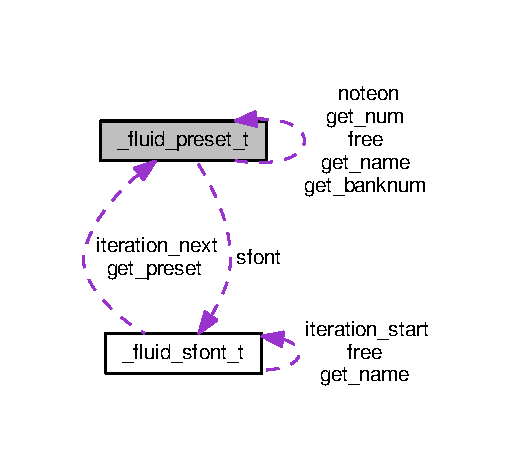
\includegraphics[width=247pt]{struct__fluid__preset__t__coll__graph}
\end{center}
\end{figure}
\subsection*{Public Attributes}
\begin{DoxyCompactItemize}
\item 
void $\ast$ \hyperlink{struct__fluid__preset__t_afe0cdcf920e3014a4d84d1348cc88383}{data}
\item 
\hyperlink{types_8h_aa6c18288f76608acbb10b80a153f4ab8}{fluid\+\_\+sfont\+\_\+t} $\ast$ \hyperlink{struct__fluid__preset__t_a88abb2db089ec85c8793fadf6c6e12c3}{sfont}
\item 
\hyperlink{sfont_8h_af62be2bae1c11541218480db4ac138ac}{fluid\+\_\+preset\+\_\+free\+\_\+t} \hyperlink{struct__fluid__preset__t_aa67629f582bf35e758788a49951c0fa7}{free}
\item 
\hyperlink{sfont_8h_a082715382cb71f6b4f38f700b6437086}{fluid\+\_\+preset\+\_\+get\+\_\+name\+\_\+t} \hyperlink{struct__fluid__preset__t_a2c6ec391afa962c5c12c413ba9040292}{get\+\_\+name}
\item 
\hyperlink{sfont_8h_a01d401c6f13113c495564a3374a3b331}{fluid\+\_\+preset\+\_\+get\+\_\+banknum\+\_\+t} \hyperlink{struct__fluid__preset__t_aea8b37a9d87c15e9202507d923d0f865}{get\+\_\+banknum}
\item 
\hyperlink{sfont_8h_a833b5d3b8f625b7a708150471b584d76}{fluid\+\_\+preset\+\_\+get\+\_\+num\+\_\+t} \hyperlink{struct__fluid__preset__t_a5438b83a0b6a4263c0f922bd91045be6}{get\+\_\+num}
\item 
\hyperlink{sfont_8h_a5cfcda454cb43f8a6c87d9d99d902b57}{fluid\+\_\+preset\+\_\+noteon\+\_\+t} \hyperlink{struct__fluid__preset__t_a30a6b267606dfdb398c2fc2f5e141f31}{noteon}
\item 
int($\ast$ \hyperlink{struct__fluid__preset__t_a8d7afa59843094f13f69b7845116c081}{notify} )(\hyperlink{types_8h_a985e5ee05f433da841127750f67a4723}{fluid\+\_\+preset\+\_\+t} $\ast$preset, int reason, int chan)
\end{DoxyCompactItemize}


\subsection{Detailed Description}
Virtual Sound\+Font preset. 

\subsection{Member Data Documentation}
\mbox{\Hypertarget{struct__fluid__preset__t_afe0cdcf920e3014a4d84d1348cc88383}\label{struct__fluid__preset__t_afe0cdcf920e3014a4d84d1348cc88383}} 
\index{\+\_\+fluid\+\_\+preset\+\_\+t@{\+\_\+fluid\+\_\+preset\+\_\+t}!data@{data}}
\index{data@{data}!\+\_\+fluid\+\_\+preset\+\_\+t@{\+\_\+fluid\+\_\+preset\+\_\+t}}
\subsubsection{\texorpdfstring{data}{data}}
{\footnotesize\ttfamily void$\ast$ \+\_\+fluid\+\_\+preset\+\_\+t\+::data}

User supplied data \mbox{\Hypertarget{struct__fluid__preset__t_aa67629f582bf35e758788a49951c0fa7}\label{struct__fluid__preset__t_aa67629f582bf35e758788a49951c0fa7}} 
\index{\+\_\+fluid\+\_\+preset\+\_\+t@{\+\_\+fluid\+\_\+preset\+\_\+t}!free@{free}}
\index{free@{free}!\+\_\+fluid\+\_\+preset\+\_\+t@{\+\_\+fluid\+\_\+preset\+\_\+t}}
\subsubsection{\texorpdfstring{free}{free}}
{\footnotesize\ttfamily \hyperlink{sfont_8h_af62be2bae1c11541218480db4ac138ac}{fluid\+\_\+preset\+\_\+free\+\_\+t} \+\_\+fluid\+\_\+preset\+\_\+t\+::free}

\mbox{\Hypertarget{struct__fluid__preset__t_aea8b37a9d87c15e9202507d923d0f865}\label{struct__fluid__preset__t_aea8b37a9d87c15e9202507d923d0f865}} 
\index{\+\_\+fluid\+\_\+preset\+\_\+t@{\+\_\+fluid\+\_\+preset\+\_\+t}!get\+\_\+banknum@{get\+\_\+banknum}}
\index{get\+\_\+banknum@{get\+\_\+banknum}!\+\_\+fluid\+\_\+preset\+\_\+t@{\+\_\+fluid\+\_\+preset\+\_\+t}}
\subsubsection{\texorpdfstring{get\+\_\+banknum}{get\_banknum}}
{\footnotesize\ttfamily \hyperlink{sfont_8h_a01d401c6f13113c495564a3374a3b331}{fluid\+\_\+preset\+\_\+get\+\_\+banknum\+\_\+t} \+\_\+fluid\+\_\+preset\+\_\+t\+::get\+\_\+banknum}

\mbox{\Hypertarget{struct__fluid__preset__t_a2c6ec391afa962c5c12c413ba9040292}\label{struct__fluid__preset__t_a2c6ec391afa962c5c12c413ba9040292}} 
\index{\+\_\+fluid\+\_\+preset\+\_\+t@{\+\_\+fluid\+\_\+preset\+\_\+t}!get\+\_\+name@{get\+\_\+name}}
\index{get\+\_\+name@{get\+\_\+name}!\+\_\+fluid\+\_\+preset\+\_\+t@{\+\_\+fluid\+\_\+preset\+\_\+t}}
\subsubsection{\texorpdfstring{get\+\_\+name}{get\_name}}
{\footnotesize\ttfamily \hyperlink{sfont_8h_a082715382cb71f6b4f38f700b6437086}{fluid\+\_\+preset\+\_\+get\+\_\+name\+\_\+t} \+\_\+fluid\+\_\+preset\+\_\+t\+::get\+\_\+name}

\mbox{\Hypertarget{struct__fluid__preset__t_a5438b83a0b6a4263c0f922bd91045be6}\label{struct__fluid__preset__t_a5438b83a0b6a4263c0f922bd91045be6}} 
\index{\+\_\+fluid\+\_\+preset\+\_\+t@{\+\_\+fluid\+\_\+preset\+\_\+t}!get\+\_\+num@{get\+\_\+num}}
\index{get\+\_\+num@{get\+\_\+num}!\+\_\+fluid\+\_\+preset\+\_\+t@{\+\_\+fluid\+\_\+preset\+\_\+t}}
\subsubsection{\texorpdfstring{get\+\_\+num}{get\_num}}
{\footnotesize\ttfamily \hyperlink{sfont_8h_a833b5d3b8f625b7a708150471b584d76}{fluid\+\_\+preset\+\_\+get\+\_\+num\+\_\+t} \+\_\+fluid\+\_\+preset\+\_\+t\+::get\+\_\+num}

\mbox{\Hypertarget{struct__fluid__preset__t_a30a6b267606dfdb398c2fc2f5e141f31}\label{struct__fluid__preset__t_a30a6b267606dfdb398c2fc2f5e141f31}} 
\index{\+\_\+fluid\+\_\+preset\+\_\+t@{\+\_\+fluid\+\_\+preset\+\_\+t}!noteon@{noteon}}
\index{noteon@{noteon}!\+\_\+fluid\+\_\+preset\+\_\+t@{\+\_\+fluid\+\_\+preset\+\_\+t}}
\subsubsection{\texorpdfstring{noteon}{noteon}}
{\footnotesize\ttfamily \hyperlink{sfont_8h_a5cfcda454cb43f8a6c87d9d99d902b57}{fluid\+\_\+preset\+\_\+noteon\+\_\+t} \+\_\+fluid\+\_\+preset\+\_\+t\+::noteon}

\mbox{\Hypertarget{struct__fluid__preset__t_a8d7afa59843094f13f69b7845116c081}\label{struct__fluid__preset__t_a8d7afa59843094f13f69b7845116c081}} 
\index{\+\_\+fluid\+\_\+preset\+\_\+t@{\+\_\+fluid\+\_\+preset\+\_\+t}!notify@{notify}}
\index{notify@{notify}!\+\_\+fluid\+\_\+preset\+\_\+t@{\+\_\+fluid\+\_\+preset\+\_\+t}}
\subsubsection{\texorpdfstring{notify}{notify}}
{\footnotesize\ttfamily int($\ast$ \+\_\+fluid\+\_\+preset\+\_\+t\+::notify) (\hyperlink{types_8h_a985e5ee05f433da841127750f67a4723}{fluid\+\_\+preset\+\_\+t} $\ast$preset, int reason, int chan)}

Virtual Sound\+Font preset notify method. 
\begin{DoxyParams}{Parameters}
{\em preset} & Virtual Sound\+Font preset \\
\hline
{\em reason} & \hyperlink{sfont_8h_a06fc87d81c62e9abb8790b6e5713c55ba3b9d777321001517ceb0fc4f69fb35b1}{F\+L\+U\+I\+D\+\_\+\+P\+R\+E\+S\+E\+T\+\_\+\+S\+E\+L\+E\+C\+T\+ED} or \hyperlink{sfont_8h_a06fc87d81c62e9abb8790b6e5713c55ba5d10f094a7a45e62fa19d559ac29e7f1}{F\+L\+U\+I\+D\+\_\+\+P\+R\+E\+S\+E\+T\+\_\+\+U\+N\+S\+E\+L\+E\+C\+T\+ED} \\
\hline
{\em chan} & M\+I\+DI channel number \\
\hline
\end{DoxyParams}
\begin{DoxyReturn}{Returns}
Should return \hyperlink{misc_8h_ae4efb1c3ce0d550c922504adfb0fb886}{F\+L\+U\+I\+D\+\_\+\+OK}
\end{DoxyReturn}
Implement this optional method if the preset needs to be notified about preset select and unselect events.

This method may be called from within synthesis context and therefore should be as efficient as possible and not perform any operations considered bad for realtime audio output (memory allocations and other OS calls). \mbox{\Hypertarget{struct__fluid__preset__t_a88abb2db089ec85c8793fadf6c6e12c3}\label{struct__fluid__preset__t_a88abb2db089ec85c8793fadf6c6e12c3}} 
\index{\+\_\+fluid\+\_\+preset\+\_\+t@{\+\_\+fluid\+\_\+preset\+\_\+t}!sfont@{sfont}}
\index{sfont@{sfont}!\+\_\+fluid\+\_\+preset\+\_\+t@{\+\_\+fluid\+\_\+preset\+\_\+t}}
\subsubsection{\texorpdfstring{sfont}{sfont}}
{\footnotesize\ttfamily \hyperlink{types_8h_aa6c18288f76608acbb10b80a153f4ab8}{fluid\+\_\+sfont\+\_\+t}$\ast$ \+\_\+fluid\+\_\+preset\+\_\+t\+::sfont}

Parent virtual Sound\+Font 

The documentation for this struct was generated from the following file\+:\begin{DoxyCompactItemize}
\item 
sfloader/\hyperlink{fluid__sfont_8h}{fluid\+\_\+sfont.\+h}\end{DoxyCompactItemize}

\hypertarget{struct__fluid__preset__zone__t}{}\section{\+\_\+fluid\+\_\+preset\+\_\+zone\+\_\+t Struct Reference}
\label{struct__fluid__preset__zone__t}\index{\+\_\+fluid\+\_\+preset\+\_\+zone\+\_\+t@{\+\_\+fluid\+\_\+preset\+\_\+zone\+\_\+t}}


{\ttfamily \#include $<$fluid\+\_\+defsfont.\+h$>$}



Collaboration diagram for \+\_\+fluid\+\_\+preset\+\_\+zone\+\_\+t\+:
\nopagebreak
\begin{figure}[H]
\begin{center}
\leavevmode
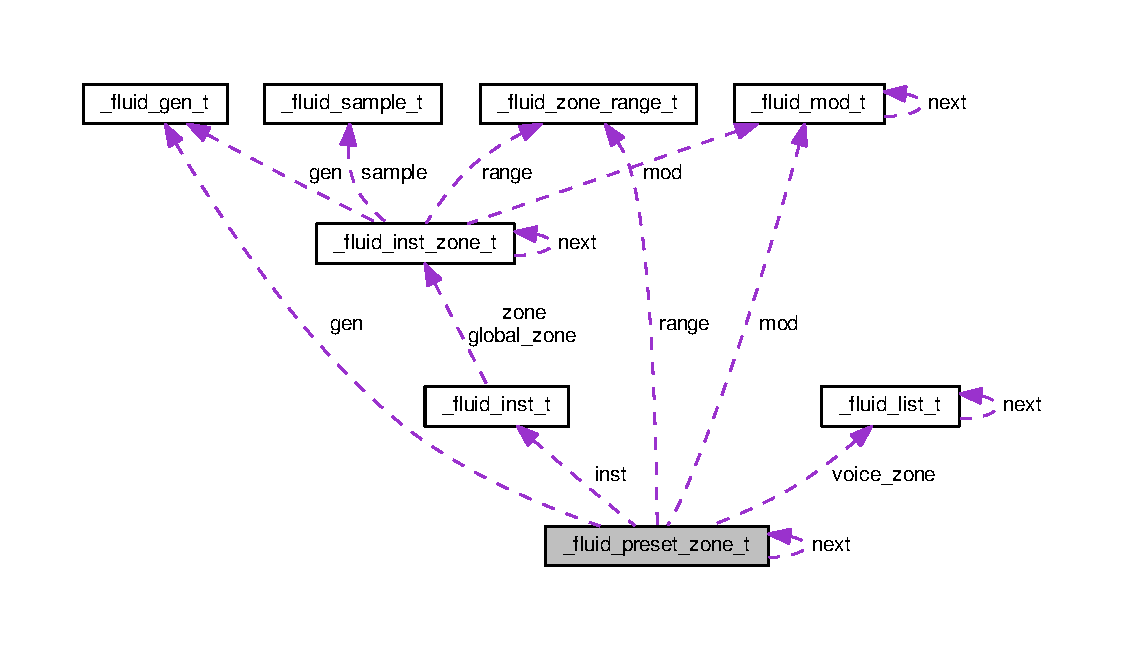
\includegraphics[width=350pt]{struct__fluid__preset__zone__t__coll__graph}
\end{center}
\end{figure}
\subsection*{Public Attributes}
\begin{DoxyCompactItemize}
\item 
\hyperlink{fluid__defsfont_8h_a74cb7075332911049d39e60df50019b2}{fluid\+\_\+preset\+\_\+zone\+\_\+t} $\ast$ \hyperlink{struct__fluid__preset__zone__t_abdcf33554d9679b87d458b2125cbba0f}{next}
\item 
char $\ast$ \hyperlink{struct__fluid__preset__zone__t_a9468bab1815189b07cb98cb636b73240}{name}
\item 
\hyperlink{fluid__defsfont_8h_a1b1f6837e2a2afb33a0ead36f0989727}{fluid\+\_\+inst\+\_\+t} $\ast$ \hyperlink{struct__fluid__preset__zone__t_ac0e24692d603fdfd140c5e0bf4875f53}{inst}
\item 
\hyperlink{fluid__list_8h_a3ef7535d4290862c0af118569223bd89}{fluid\+\_\+list\+\_\+t} $\ast$ \hyperlink{struct__fluid__preset__zone__t_a2fb65f12d2ae63bade54afe578cbc167}{voice\+\_\+zone}
\item 
\hyperlink{fluidsynth__priv_8h_ac8502f0049ba8c20821b136e611462da}{fluid\+\_\+zone\+\_\+range\+\_\+t} \hyperlink{struct__fluid__preset__zone__t_ace88940d54aefcd8551dfcec08094dc2}{range}
\item 
\hyperlink{fluid__gen_8h_a018737d76d5ad530b622bd27b70701b0}{fluid\+\_\+gen\+\_\+t} \hyperlink{struct__fluid__preset__zone__t_abf135229ac868c6c98f81a16a81faea0}{gen} \mbox{[}\hyperlink{gen_8h_ad17a24ae3b25f3b8cc5762f818eef9b4a9c372c341b7b1a718f0016f40c615cf3}{G\+E\+N\+\_\+\+L\+A\+ST}\mbox{]}
\item 
\hyperlink{types_8h_a6c727efab500d6c0c350d4292e9aa5ef}{fluid\+\_\+mod\+\_\+t} $\ast$ \hyperlink{struct__fluid__preset__zone__t_ac47759c0943fd3359d8fc8e2a0713f18}{mod}
\end{DoxyCompactItemize}


\subsection{Member Data Documentation}
\mbox{\Hypertarget{struct__fluid__preset__zone__t_abf135229ac868c6c98f81a16a81faea0}\label{struct__fluid__preset__zone__t_abf135229ac868c6c98f81a16a81faea0}} 
\index{\+\_\+fluid\+\_\+preset\+\_\+zone\+\_\+t@{\+\_\+fluid\+\_\+preset\+\_\+zone\+\_\+t}!gen@{gen}}
\index{gen@{gen}!\+\_\+fluid\+\_\+preset\+\_\+zone\+\_\+t@{\+\_\+fluid\+\_\+preset\+\_\+zone\+\_\+t}}
\subsubsection{\texorpdfstring{gen}{gen}}
{\footnotesize\ttfamily \hyperlink{fluid__gen_8h_a018737d76d5ad530b622bd27b70701b0}{fluid\+\_\+gen\+\_\+t} \+\_\+fluid\+\_\+preset\+\_\+zone\+\_\+t\+::gen\mbox{[}\hyperlink{gen_8h_ad17a24ae3b25f3b8cc5762f818eef9b4a9c372c341b7b1a718f0016f40c615cf3}{G\+E\+N\+\_\+\+L\+A\+ST}\mbox{]}}

\mbox{\Hypertarget{struct__fluid__preset__zone__t_ac0e24692d603fdfd140c5e0bf4875f53}\label{struct__fluid__preset__zone__t_ac0e24692d603fdfd140c5e0bf4875f53}} 
\index{\+\_\+fluid\+\_\+preset\+\_\+zone\+\_\+t@{\+\_\+fluid\+\_\+preset\+\_\+zone\+\_\+t}!inst@{inst}}
\index{inst@{inst}!\+\_\+fluid\+\_\+preset\+\_\+zone\+\_\+t@{\+\_\+fluid\+\_\+preset\+\_\+zone\+\_\+t}}
\subsubsection{\texorpdfstring{inst}{inst}}
{\footnotesize\ttfamily \hyperlink{fluid__defsfont_8h_a1b1f6837e2a2afb33a0ead36f0989727}{fluid\+\_\+inst\+\_\+t}$\ast$ \+\_\+fluid\+\_\+preset\+\_\+zone\+\_\+t\+::inst}

\mbox{\Hypertarget{struct__fluid__preset__zone__t_ac47759c0943fd3359d8fc8e2a0713f18}\label{struct__fluid__preset__zone__t_ac47759c0943fd3359d8fc8e2a0713f18}} 
\index{\+\_\+fluid\+\_\+preset\+\_\+zone\+\_\+t@{\+\_\+fluid\+\_\+preset\+\_\+zone\+\_\+t}!mod@{mod}}
\index{mod@{mod}!\+\_\+fluid\+\_\+preset\+\_\+zone\+\_\+t@{\+\_\+fluid\+\_\+preset\+\_\+zone\+\_\+t}}
\subsubsection{\texorpdfstring{mod}{mod}}
{\footnotesize\ttfamily \hyperlink{types_8h_a6c727efab500d6c0c350d4292e9aa5ef}{fluid\+\_\+mod\+\_\+t}$\ast$ \+\_\+fluid\+\_\+preset\+\_\+zone\+\_\+t\+::mod}

\mbox{\Hypertarget{struct__fluid__preset__zone__t_a9468bab1815189b07cb98cb636b73240}\label{struct__fluid__preset__zone__t_a9468bab1815189b07cb98cb636b73240}} 
\index{\+\_\+fluid\+\_\+preset\+\_\+zone\+\_\+t@{\+\_\+fluid\+\_\+preset\+\_\+zone\+\_\+t}!name@{name}}
\index{name@{name}!\+\_\+fluid\+\_\+preset\+\_\+zone\+\_\+t@{\+\_\+fluid\+\_\+preset\+\_\+zone\+\_\+t}}
\subsubsection{\texorpdfstring{name}{name}}
{\footnotesize\ttfamily char$\ast$ \+\_\+fluid\+\_\+preset\+\_\+zone\+\_\+t\+::name}

\mbox{\Hypertarget{struct__fluid__preset__zone__t_abdcf33554d9679b87d458b2125cbba0f}\label{struct__fluid__preset__zone__t_abdcf33554d9679b87d458b2125cbba0f}} 
\index{\+\_\+fluid\+\_\+preset\+\_\+zone\+\_\+t@{\+\_\+fluid\+\_\+preset\+\_\+zone\+\_\+t}!next@{next}}
\index{next@{next}!\+\_\+fluid\+\_\+preset\+\_\+zone\+\_\+t@{\+\_\+fluid\+\_\+preset\+\_\+zone\+\_\+t}}
\subsubsection{\texorpdfstring{next}{next}}
{\footnotesize\ttfamily \hyperlink{fluid__defsfont_8h_a74cb7075332911049d39e60df50019b2}{fluid\+\_\+preset\+\_\+zone\+\_\+t}$\ast$ \+\_\+fluid\+\_\+preset\+\_\+zone\+\_\+t\+::next}

\mbox{\Hypertarget{struct__fluid__preset__zone__t_ace88940d54aefcd8551dfcec08094dc2}\label{struct__fluid__preset__zone__t_ace88940d54aefcd8551dfcec08094dc2}} 
\index{\+\_\+fluid\+\_\+preset\+\_\+zone\+\_\+t@{\+\_\+fluid\+\_\+preset\+\_\+zone\+\_\+t}!range@{range}}
\index{range@{range}!\+\_\+fluid\+\_\+preset\+\_\+zone\+\_\+t@{\+\_\+fluid\+\_\+preset\+\_\+zone\+\_\+t}}
\subsubsection{\texorpdfstring{range}{range}}
{\footnotesize\ttfamily \hyperlink{fluidsynth__priv_8h_ac8502f0049ba8c20821b136e611462da}{fluid\+\_\+zone\+\_\+range\+\_\+t} \+\_\+fluid\+\_\+preset\+\_\+zone\+\_\+t\+::range}

\mbox{\Hypertarget{struct__fluid__preset__zone__t_a2fb65f12d2ae63bade54afe578cbc167}\label{struct__fluid__preset__zone__t_a2fb65f12d2ae63bade54afe578cbc167}} 
\index{\+\_\+fluid\+\_\+preset\+\_\+zone\+\_\+t@{\+\_\+fluid\+\_\+preset\+\_\+zone\+\_\+t}!voice\+\_\+zone@{voice\+\_\+zone}}
\index{voice\+\_\+zone@{voice\+\_\+zone}!\+\_\+fluid\+\_\+preset\+\_\+zone\+\_\+t@{\+\_\+fluid\+\_\+preset\+\_\+zone\+\_\+t}}
\subsubsection{\texorpdfstring{voice\+\_\+zone}{voice\_zone}}
{\footnotesize\ttfamily \hyperlink{fluid__list_8h_a3ef7535d4290862c0af118569223bd89}{fluid\+\_\+list\+\_\+t}$\ast$ \+\_\+fluid\+\_\+preset\+\_\+zone\+\_\+t\+::voice\+\_\+zone}



The documentation for this struct was generated from the following file\+:\begin{DoxyCompactItemize}
\item 
sfloader/\hyperlink{fluid__defsfont_8h}{fluid\+\_\+defsfont.\+h}\end{DoxyCompactItemize}

\hypertarget{struct__fluid__rampreset__t}{}\section{\+\_\+fluid\+\_\+rampreset\+\_\+t Struct Reference}
\label{struct__fluid__rampreset__t}\index{\+\_\+fluid\+\_\+rampreset\+\_\+t@{\+\_\+fluid\+\_\+rampreset\+\_\+t}}


{\ttfamily \#include $<$fluid\+\_\+ramsfont.\+h$>$}



Collaboration diagram for \+\_\+fluid\+\_\+rampreset\+\_\+t\+:
\nopagebreak
\begin{figure}[H]
\begin{center}
\leavevmode
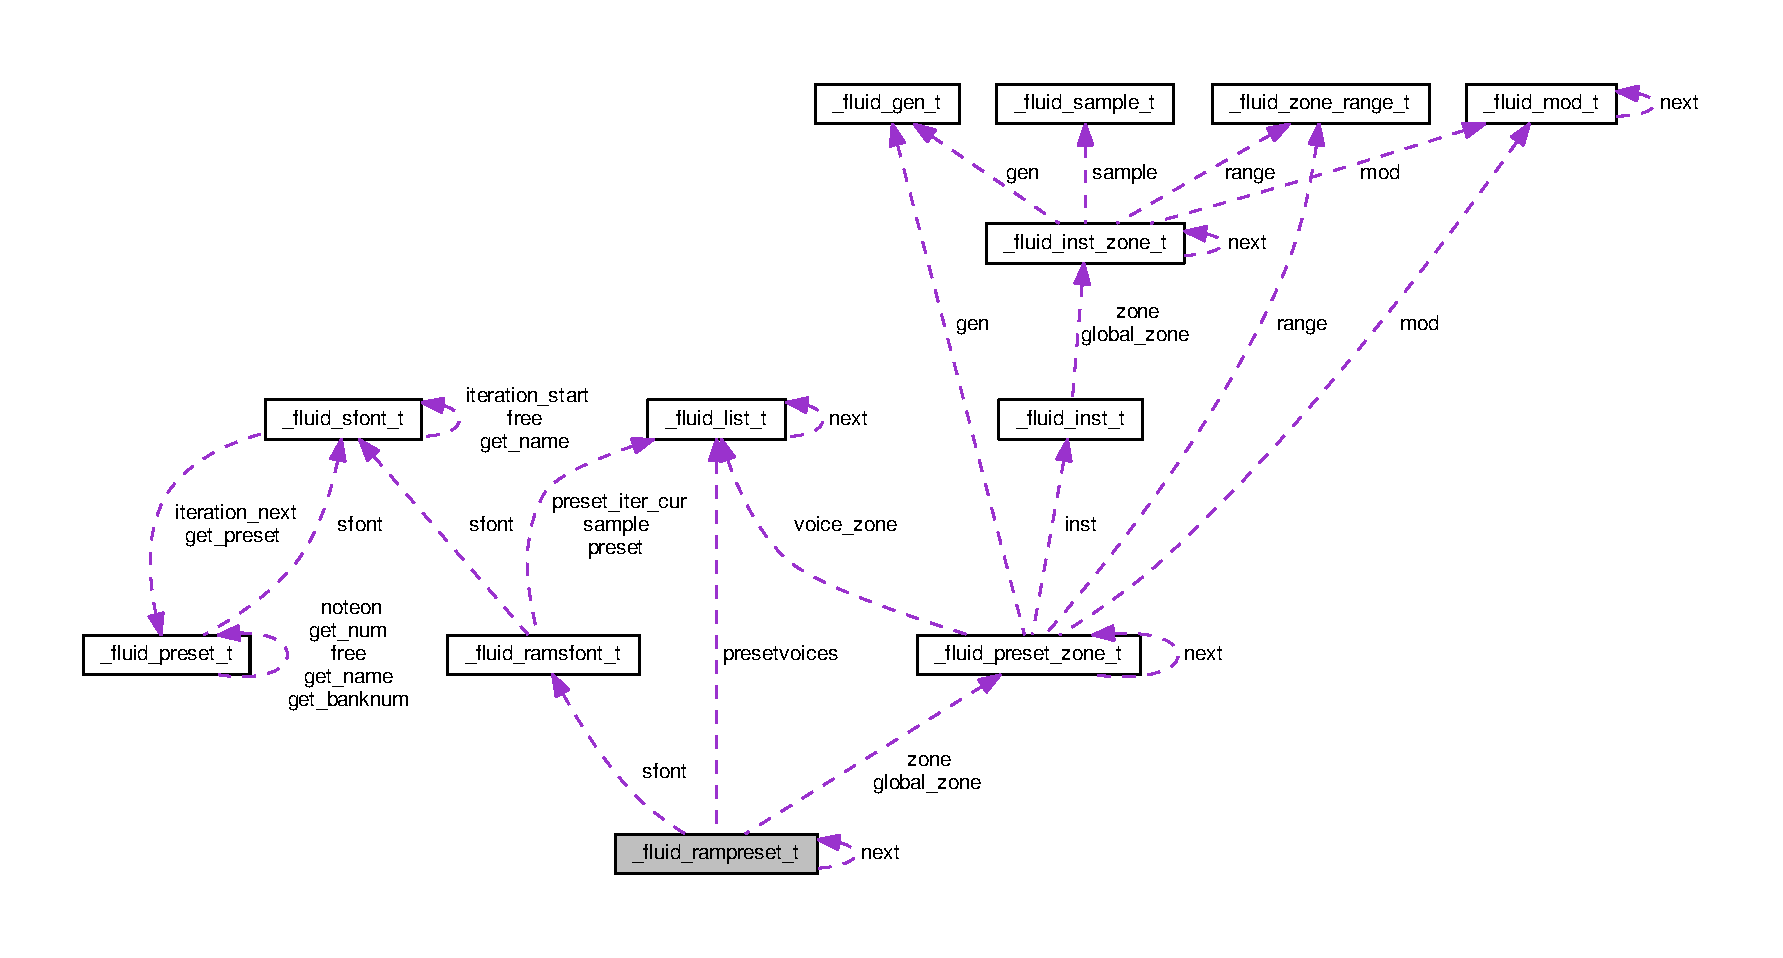
\includegraphics[width=350pt]{struct__fluid__rampreset__t__coll__graph}
\end{center}
\end{figure}
\subsection*{Public Attributes}
\begin{DoxyCompactItemize}
\item 
\hyperlink{types_8h_a8bbeb200df523c6e0e0e86c605b7b98a}{fluid\+\_\+rampreset\+\_\+t} $\ast$ \hyperlink{struct__fluid__rampreset__t_ae30f7d7f179a39650237abbc5bba2da0}{next}
\item 
\hyperlink{types_8h_a093fe32472dd43adaef22c62feb2d15e}{fluid\+\_\+ramsfont\+\_\+t} $\ast$ \hyperlink{struct__fluid__rampreset__t_a96888a85aa777e9e89e7696cc8bd9947}{sfont}
\item 
char \hyperlink{struct__fluid__rampreset__t_a8ce6d30bb670226a2bd7f418c2fe773b}{name} \mbox{[}21\mbox{]}
\item 
unsigned int \hyperlink{struct__fluid__rampreset__t_a7904484cd36ec879a31aaab90886d95b}{bank}
\item 
unsigned int \hyperlink{struct__fluid__rampreset__t_a1f87bb3a634eb622a3c8f11b06f88708}{num}
\item 
\hyperlink{fluid__defsfont_8h_a74cb7075332911049d39e60df50019b2}{fluid\+\_\+preset\+\_\+zone\+\_\+t} $\ast$ \hyperlink{struct__fluid__rampreset__t_a662bbc3be7bcc34dc520ab992e5f8448}{global\+\_\+zone}
\item 
\hyperlink{fluid__defsfont_8h_a74cb7075332911049d39e60df50019b2}{fluid\+\_\+preset\+\_\+zone\+\_\+t} $\ast$ \hyperlink{struct__fluid__rampreset__t_aa2c9ac5d07d1c5cc309f830cabbe4ffd}{zone}
\item 
\hyperlink{fluid__list_8h_a3ef7535d4290862c0af118569223bd89}{fluid\+\_\+list\+\_\+t} $\ast$ \hyperlink{struct__fluid__rampreset__t_a3df2cef0a7f82e89bc49e68150e97658}{presetvoices}
\end{DoxyCompactItemize}


\subsection{Member Data Documentation}
\mbox{\Hypertarget{struct__fluid__rampreset__t_a7904484cd36ec879a31aaab90886d95b}\label{struct__fluid__rampreset__t_a7904484cd36ec879a31aaab90886d95b}} 
\index{\+\_\+fluid\+\_\+rampreset\+\_\+t@{\+\_\+fluid\+\_\+rampreset\+\_\+t}!bank@{bank}}
\index{bank@{bank}!\+\_\+fluid\+\_\+rampreset\+\_\+t@{\+\_\+fluid\+\_\+rampreset\+\_\+t}}
\subsubsection{\texorpdfstring{bank}{bank}}
{\footnotesize\ttfamily unsigned int \+\_\+fluid\+\_\+rampreset\+\_\+t\+::bank}

\mbox{\Hypertarget{struct__fluid__rampreset__t_a662bbc3be7bcc34dc520ab992e5f8448}\label{struct__fluid__rampreset__t_a662bbc3be7bcc34dc520ab992e5f8448}} 
\index{\+\_\+fluid\+\_\+rampreset\+\_\+t@{\+\_\+fluid\+\_\+rampreset\+\_\+t}!global\+\_\+zone@{global\+\_\+zone}}
\index{global\+\_\+zone@{global\+\_\+zone}!\+\_\+fluid\+\_\+rampreset\+\_\+t@{\+\_\+fluid\+\_\+rampreset\+\_\+t}}
\subsubsection{\texorpdfstring{global\+\_\+zone}{global\_zone}}
{\footnotesize\ttfamily \hyperlink{fluid__defsfont_8h_a74cb7075332911049d39e60df50019b2}{fluid\+\_\+preset\+\_\+zone\+\_\+t}$\ast$ \+\_\+fluid\+\_\+rampreset\+\_\+t\+::global\+\_\+zone}

\mbox{\Hypertarget{struct__fluid__rampreset__t_a8ce6d30bb670226a2bd7f418c2fe773b}\label{struct__fluid__rampreset__t_a8ce6d30bb670226a2bd7f418c2fe773b}} 
\index{\+\_\+fluid\+\_\+rampreset\+\_\+t@{\+\_\+fluid\+\_\+rampreset\+\_\+t}!name@{name}}
\index{name@{name}!\+\_\+fluid\+\_\+rampreset\+\_\+t@{\+\_\+fluid\+\_\+rampreset\+\_\+t}}
\subsubsection{\texorpdfstring{name}{name}}
{\footnotesize\ttfamily char \+\_\+fluid\+\_\+rampreset\+\_\+t\+::name\mbox{[}21\mbox{]}}

\mbox{\Hypertarget{struct__fluid__rampreset__t_ae30f7d7f179a39650237abbc5bba2da0}\label{struct__fluid__rampreset__t_ae30f7d7f179a39650237abbc5bba2da0}} 
\index{\+\_\+fluid\+\_\+rampreset\+\_\+t@{\+\_\+fluid\+\_\+rampreset\+\_\+t}!next@{next}}
\index{next@{next}!\+\_\+fluid\+\_\+rampreset\+\_\+t@{\+\_\+fluid\+\_\+rampreset\+\_\+t}}
\subsubsection{\texorpdfstring{next}{next}}
{\footnotesize\ttfamily \hyperlink{types_8h_a8bbeb200df523c6e0e0e86c605b7b98a}{fluid\+\_\+rampreset\+\_\+t}$\ast$ \+\_\+fluid\+\_\+rampreset\+\_\+t\+::next}

\mbox{\Hypertarget{struct__fluid__rampreset__t_a1f87bb3a634eb622a3c8f11b06f88708}\label{struct__fluid__rampreset__t_a1f87bb3a634eb622a3c8f11b06f88708}} 
\index{\+\_\+fluid\+\_\+rampreset\+\_\+t@{\+\_\+fluid\+\_\+rampreset\+\_\+t}!num@{num}}
\index{num@{num}!\+\_\+fluid\+\_\+rampreset\+\_\+t@{\+\_\+fluid\+\_\+rampreset\+\_\+t}}
\subsubsection{\texorpdfstring{num}{num}}
{\footnotesize\ttfamily unsigned int \+\_\+fluid\+\_\+rampreset\+\_\+t\+::num}

\mbox{\Hypertarget{struct__fluid__rampreset__t_a3df2cef0a7f82e89bc49e68150e97658}\label{struct__fluid__rampreset__t_a3df2cef0a7f82e89bc49e68150e97658}} 
\index{\+\_\+fluid\+\_\+rampreset\+\_\+t@{\+\_\+fluid\+\_\+rampreset\+\_\+t}!presetvoices@{presetvoices}}
\index{presetvoices@{presetvoices}!\+\_\+fluid\+\_\+rampreset\+\_\+t@{\+\_\+fluid\+\_\+rampreset\+\_\+t}}
\subsubsection{\texorpdfstring{presetvoices}{presetvoices}}
{\footnotesize\ttfamily \hyperlink{fluid__list_8h_a3ef7535d4290862c0af118569223bd89}{fluid\+\_\+list\+\_\+t}$\ast$ \+\_\+fluid\+\_\+rampreset\+\_\+t\+::presetvoices}

\mbox{\Hypertarget{struct__fluid__rampreset__t_a96888a85aa777e9e89e7696cc8bd9947}\label{struct__fluid__rampreset__t_a96888a85aa777e9e89e7696cc8bd9947}} 
\index{\+\_\+fluid\+\_\+rampreset\+\_\+t@{\+\_\+fluid\+\_\+rampreset\+\_\+t}!sfont@{sfont}}
\index{sfont@{sfont}!\+\_\+fluid\+\_\+rampreset\+\_\+t@{\+\_\+fluid\+\_\+rampreset\+\_\+t}}
\subsubsection{\texorpdfstring{sfont}{sfont}}
{\footnotesize\ttfamily \hyperlink{types_8h_a093fe32472dd43adaef22c62feb2d15e}{fluid\+\_\+ramsfont\+\_\+t}$\ast$ \+\_\+fluid\+\_\+rampreset\+\_\+t\+::sfont}

\mbox{\Hypertarget{struct__fluid__rampreset__t_aa2c9ac5d07d1c5cc309f830cabbe4ffd}\label{struct__fluid__rampreset__t_aa2c9ac5d07d1c5cc309f830cabbe4ffd}} 
\index{\+\_\+fluid\+\_\+rampreset\+\_\+t@{\+\_\+fluid\+\_\+rampreset\+\_\+t}!zone@{zone}}
\index{zone@{zone}!\+\_\+fluid\+\_\+rampreset\+\_\+t@{\+\_\+fluid\+\_\+rampreset\+\_\+t}}
\subsubsection{\texorpdfstring{zone}{zone}}
{\footnotesize\ttfamily \hyperlink{fluid__defsfont_8h_a74cb7075332911049d39e60df50019b2}{fluid\+\_\+preset\+\_\+zone\+\_\+t}$\ast$ \+\_\+fluid\+\_\+rampreset\+\_\+t\+::zone}



The documentation for this struct was generated from the following file\+:\begin{DoxyCompactItemize}
\item 
sfloader/\hyperlink{fluid__ramsfont_8h}{fluid\+\_\+ramsfont.\+h}\end{DoxyCompactItemize}

\hypertarget{struct__fluid__rampreset__voice__t}{}\section{\+\_\+fluid\+\_\+rampreset\+\_\+voice\+\_\+t Struct Reference}
\label{struct__fluid__rampreset__voice__t}\index{\+\_\+fluid\+\_\+rampreset\+\_\+voice\+\_\+t@{\+\_\+fluid\+\_\+rampreset\+\_\+voice\+\_\+t}}


Collaboration diagram for \+\_\+fluid\+\_\+rampreset\+\_\+voice\+\_\+t\+:
\nopagebreak
\begin{figure}[H]
\begin{center}
\leavevmode
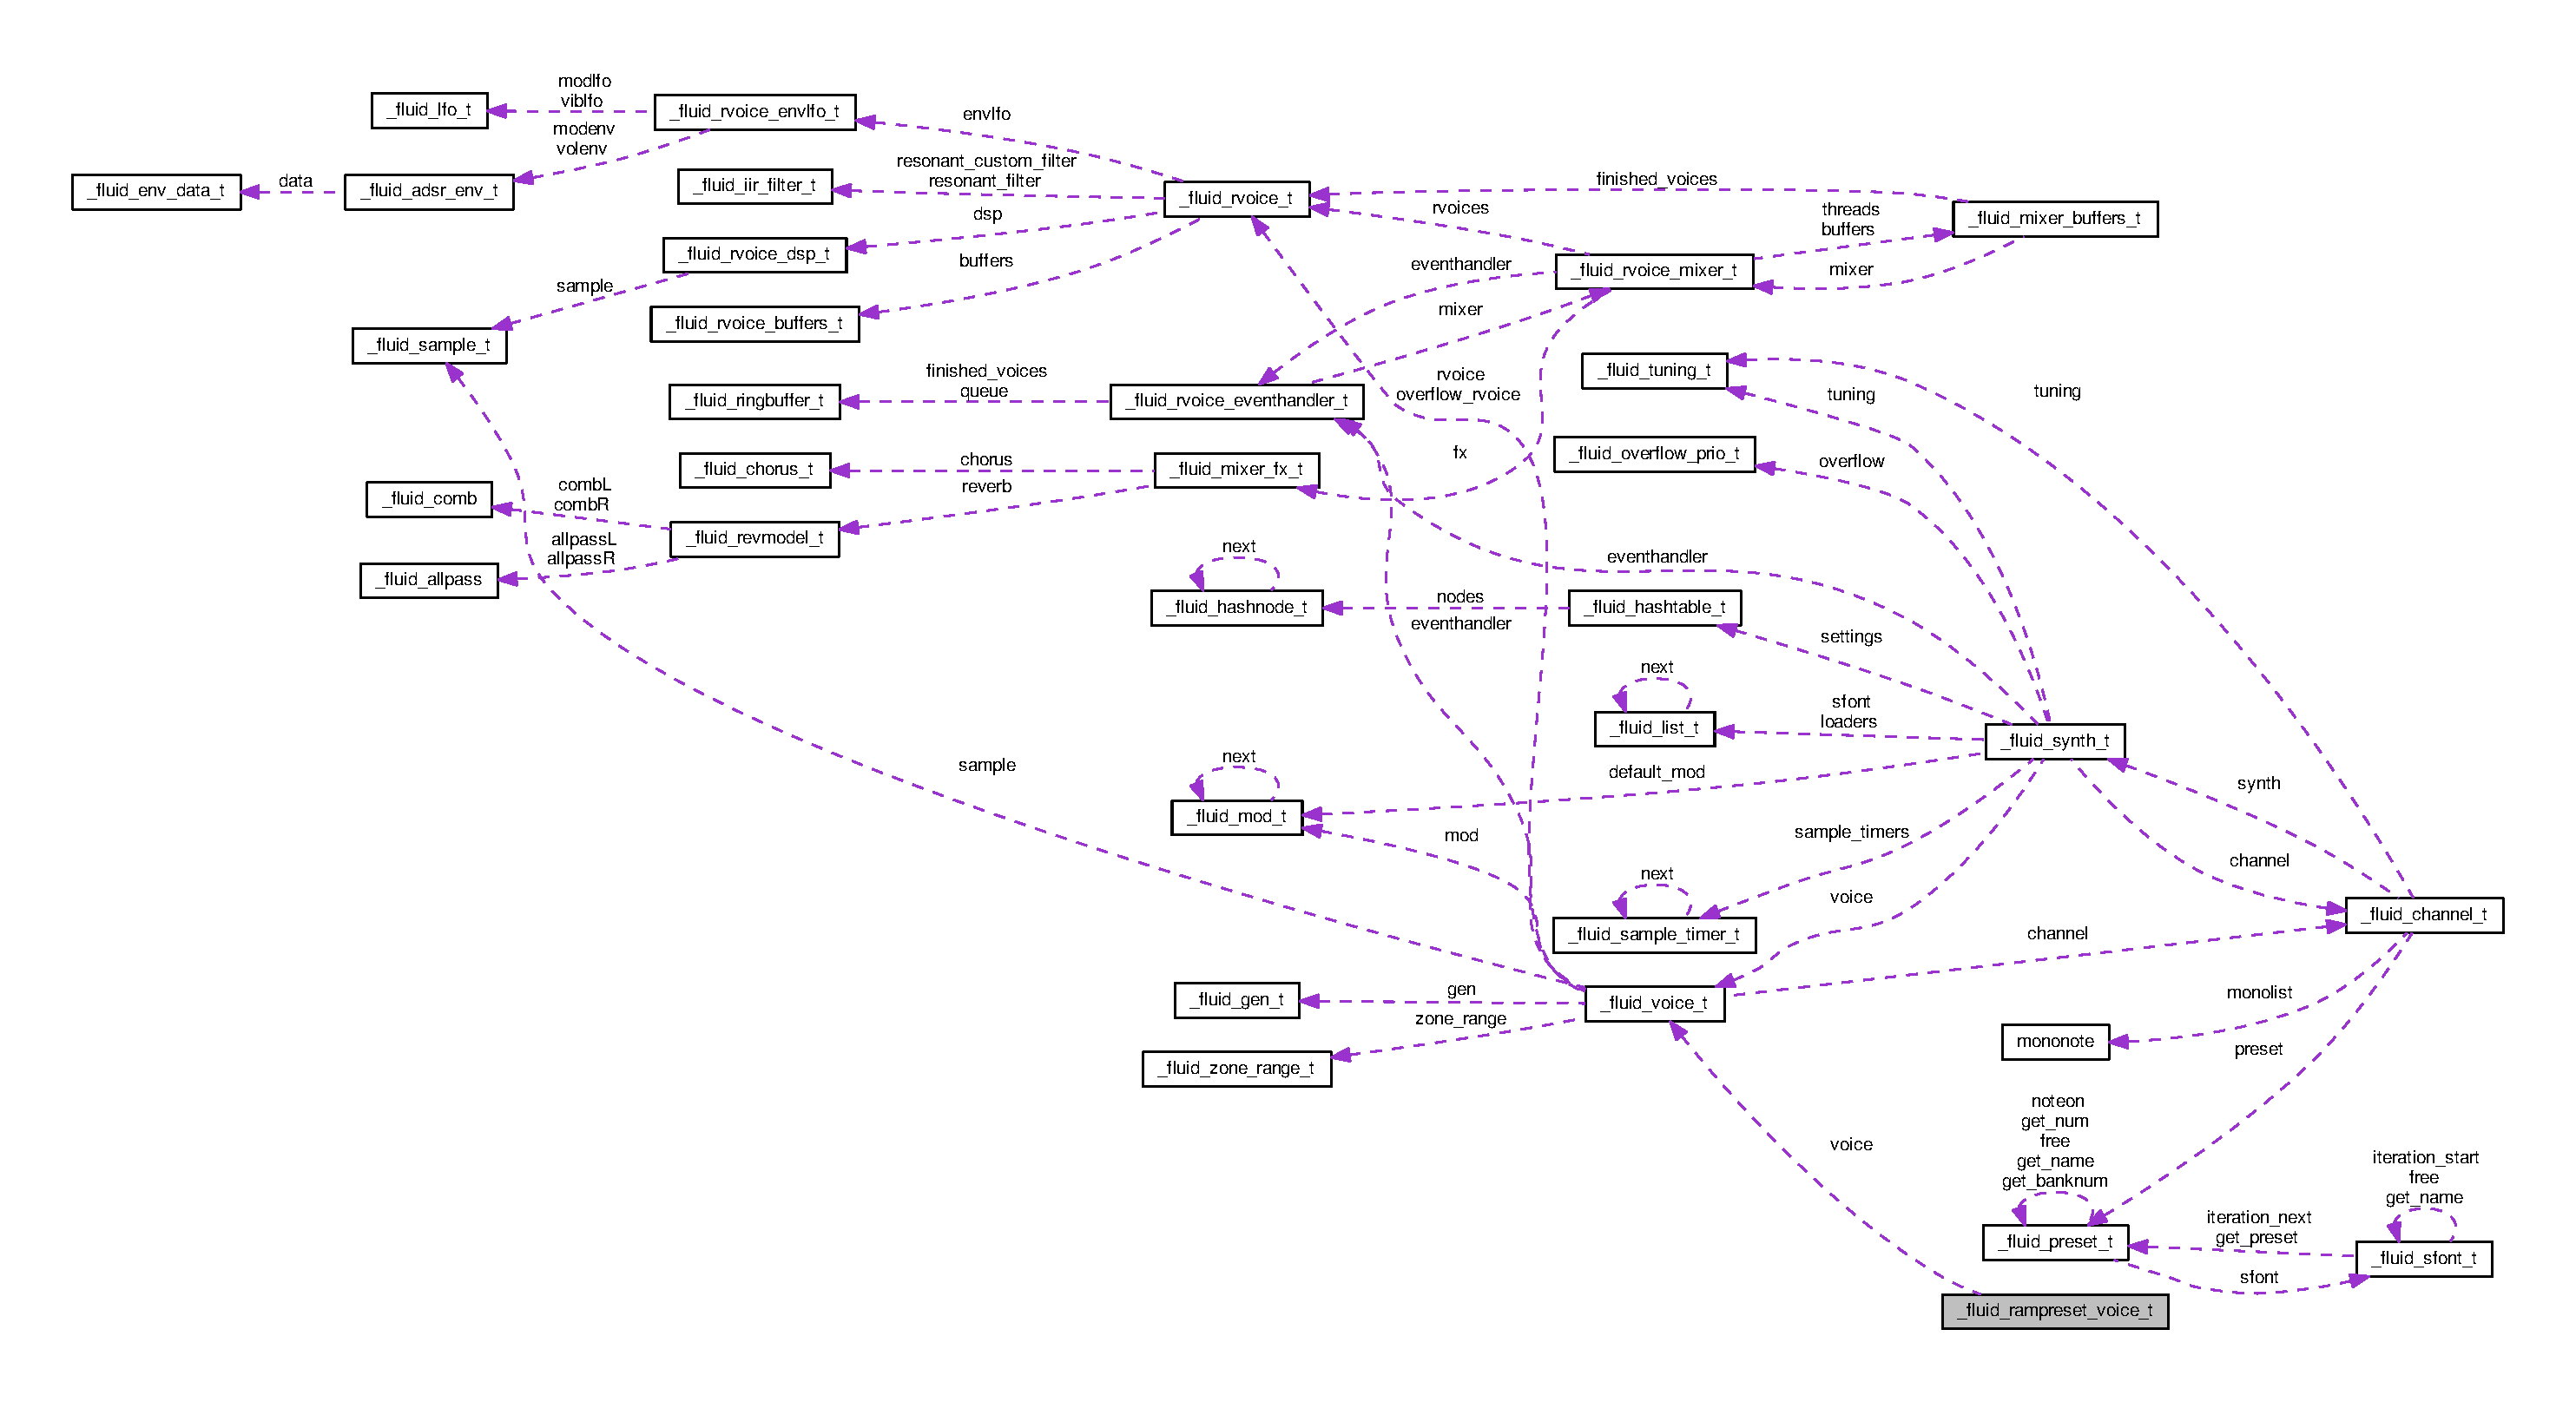
\includegraphics[width=350pt]{struct__fluid__rampreset__voice__t__coll__graph}
\end{center}
\end{figure}
\subsection*{Public Attributes}
\begin{DoxyCompactItemize}
\item 
\hyperlink{types_8h_a5123ae5ef2d7806475267380c33604c3}{fluid\+\_\+voice\+\_\+t} $\ast$ \hyperlink{struct__fluid__rampreset__voice__t_a18ab3e0ea68a75013dfa77193a8a8c07}{voice}
\item 
unsigned int \hyperlink{struct__fluid__rampreset__voice__t_a82f4c1aadddb3c702648ac7b89be5649}{voice\+ID}
\end{DoxyCompactItemize}


\subsection{Member Data Documentation}
\mbox{\Hypertarget{struct__fluid__rampreset__voice__t_a18ab3e0ea68a75013dfa77193a8a8c07}\label{struct__fluid__rampreset__voice__t_a18ab3e0ea68a75013dfa77193a8a8c07}} 
\index{\+\_\+fluid\+\_\+rampreset\+\_\+voice\+\_\+t@{\+\_\+fluid\+\_\+rampreset\+\_\+voice\+\_\+t}!voice@{voice}}
\index{voice@{voice}!\+\_\+fluid\+\_\+rampreset\+\_\+voice\+\_\+t@{\+\_\+fluid\+\_\+rampreset\+\_\+voice\+\_\+t}}
\subsubsection{\texorpdfstring{voice}{voice}}
{\footnotesize\ttfamily \hyperlink{types_8h_a5123ae5ef2d7806475267380c33604c3}{fluid\+\_\+voice\+\_\+t}$\ast$ \+\_\+fluid\+\_\+rampreset\+\_\+voice\+\_\+t\+::voice}

\mbox{\Hypertarget{struct__fluid__rampreset__voice__t_a82f4c1aadddb3c702648ac7b89be5649}\label{struct__fluid__rampreset__voice__t_a82f4c1aadddb3c702648ac7b89be5649}} 
\index{\+\_\+fluid\+\_\+rampreset\+\_\+voice\+\_\+t@{\+\_\+fluid\+\_\+rampreset\+\_\+voice\+\_\+t}!voice\+ID@{voice\+ID}}
\index{voice\+ID@{voice\+ID}!\+\_\+fluid\+\_\+rampreset\+\_\+voice\+\_\+t@{\+\_\+fluid\+\_\+rampreset\+\_\+voice\+\_\+t}}
\subsubsection{\texorpdfstring{voice\+ID}{voiceID}}
{\footnotesize\ttfamily unsigned int \+\_\+fluid\+\_\+rampreset\+\_\+voice\+\_\+t\+::voice\+ID}



The documentation for this struct was generated from the following file\+:\begin{DoxyCompactItemize}
\item 
sfloader/\hyperlink{fluid__ramsfont_8c}{fluid\+\_\+ramsfont.\+c}\end{DoxyCompactItemize}

\hypertarget{struct__fluid__ramsfont__t}{}\section{\+\_\+fluid\+\_\+ramsfont\+\_\+t Struct Reference}
\label{struct__fluid__ramsfont__t}\index{\+\_\+fluid\+\_\+ramsfont\+\_\+t@{\+\_\+fluid\+\_\+ramsfont\+\_\+t}}


{\ttfamily \#include $<$fluid\+\_\+ramsfont.\+h$>$}



Collaboration diagram for \+\_\+fluid\+\_\+ramsfont\+\_\+t\+:
\nopagebreak
\begin{figure}[H]
\begin{center}
\leavevmode
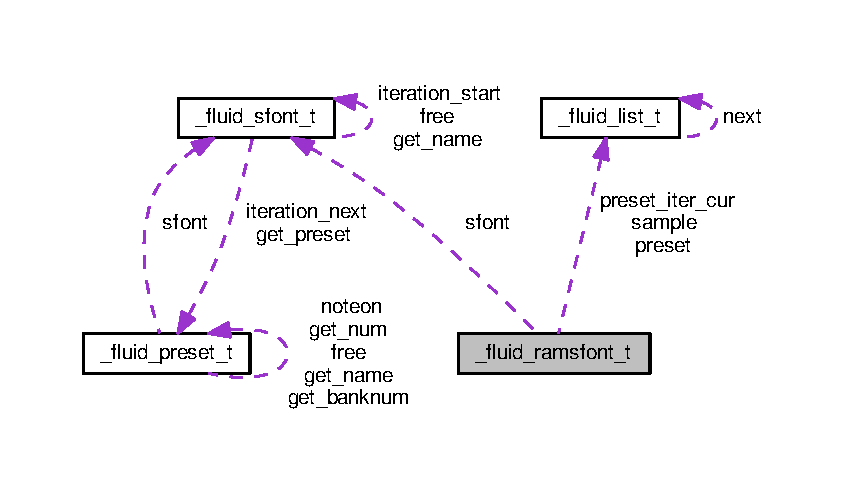
\includegraphics[width=350pt]{struct__fluid__ramsfont__t__coll__graph}
\end{center}
\end{figure}
\subsection*{Public Attributes}
\begin{DoxyCompactItemize}
\item 
char \hyperlink{struct__fluid__ramsfont__t_aef9999710d76db25ff24c907ca350cd1}{name} \mbox{[}21\mbox{]}
\item 
\hyperlink{types_8h_aa6c18288f76608acbb10b80a153f4ab8}{fluid\+\_\+sfont\+\_\+t} $\ast$ \hyperlink{struct__fluid__ramsfont__t_acabf1ff179d18e270e5f47087c1b14ae}{sfont}
\item 
\hyperlink{fluid__list_8h_a3ef7535d4290862c0af118569223bd89}{fluid\+\_\+list\+\_\+t} $\ast$ \hyperlink{struct__fluid__ramsfont__t_a0f1b7c5100ed0d47faaf453372a982ba}{sample}
\item 
\hyperlink{fluid__list_8h_a3ef7535d4290862c0af118569223bd89}{fluid\+\_\+list\+\_\+t} $\ast$ \hyperlink{struct__fluid__ramsfont__t_a84dfc5ed295e97334a0cae344fe953c1}{preset}
\item 
\hyperlink{fluid__list_8h_a3ef7535d4290862c0af118569223bd89}{fluid\+\_\+list\+\_\+t} $\ast$ \hyperlink{struct__fluid__ramsfont__t_a659f4f41fdd180cd5019085e7aa155db}{preset\+\_\+iter\+\_\+cur}
\end{DoxyCompactItemize}


\subsection{Member Data Documentation}
\mbox{\Hypertarget{struct__fluid__ramsfont__t_aef9999710d76db25ff24c907ca350cd1}\label{struct__fluid__ramsfont__t_aef9999710d76db25ff24c907ca350cd1}} 
\index{\+\_\+fluid\+\_\+ramsfont\+\_\+t@{\+\_\+fluid\+\_\+ramsfont\+\_\+t}!name@{name}}
\index{name@{name}!\+\_\+fluid\+\_\+ramsfont\+\_\+t@{\+\_\+fluid\+\_\+ramsfont\+\_\+t}}
\subsubsection{\texorpdfstring{name}{name}}
{\footnotesize\ttfamily char \+\_\+fluid\+\_\+ramsfont\+\_\+t\+::name\mbox{[}21\mbox{]}}

\mbox{\Hypertarget{struct__fluid__ramsfont__t_a84dfc5ed295e97334a0cae344fe953c1}\label{struct__fluid__ramsfont__t_a84dfc5ed295e97334a0cae344fe953c1}} 
\index{\+\_\+fluid\+\_\+ramsfont\+\_\+t@{\+\_\+fluid\+\_\+ramsfont\+\_\+t}!preset@{preset}}
\index{preset@{preset}!\+\_\+fluid\+\_\+ramsfont\+\_\+t@{\+\_\+fluid\+\_\+ramsfont\+\_\+t}}
\subsubsection{\texorpdfstring{preset}{preset}}
{\footnotesize\ttfamily \hyperlink{fluid__list_8h_a3ef7535d4290862c0af118569223bd89}{fluid\+\_\+list\+\_\+t}$\ast$ \+\_\+fluid\+\_\+ramsfont\+\_\+t\+::preset}

\mbox{\Hypertarget{struct__fluid__ramsfont__t_a659f4f41fdd180cd5019085e7aa155db}\label{struct__fluid__ramsfont__t_a659f4f41fdd180cd5019085e7aa155db}} 
\index{\+\_\+fluid\+\_\+ramsfont\+\_\+t@{\+\_\+fluid\+\_\+ramsfont\+\_\+t}!preset\+\_\+iter\+\_\+cur@{preset\+\_\+iter\+\_\+cur}}
\index{preset\+\_\+iter\+\_\+cur@{preset\+\_\+iter\+\_\+cur}!\+\_\+fluid\+\_\+ramsfont\+\_\+t@{\+\_\+fluid\+\_\+ramsfont\+\_\+t}}
\subsubsection{\texorpdfstring{preset\+\_\+iter\+\_\+cur}{preset\_iter\_cur}}
{\footnotesize\ttfamily \hyperlink{fluid__list_8h_a3ef7535d4290862c0af118569223bd89}{fluid\+\_\+list\+\_\+t}$\ast$ \+\_\+fluid\+\_\+ramsfont\+\_\+t\+::preset\+\_\+iter\+\_\+cur}

\mbox{\Hypertarget{struct__fluid__ramsfont__t_a0f1b7c5100ed0d47faaf453372a982ba}\label{struct__fluid__ramsfont__t_a0f1b7c5100ed0d47faaf453372a982ba}} 
\index{\+\_\+fluid\+\_\+ramsfont\+\_\+t@{\+\_\+fluid\+\_\+ramsfont\+\_\+t}!sample@{sample}}
\index{sample@{sample}!\+\_\+fluid\+\_\+ramsfont\+\_\+t@{\+\_\+fluid\+\_\+ramsfont\+\_\+t}}
\subsubsection{\texorpdfstring{sample}{sample}}
{\footnotesize\ttfamily \hyperlink{fluid__list_8h_a3ef7535d4290862c0af118569223bd89}{fluid\+\_\+list\+\_\+t}$\ast$ \+\_\+fluid\+\_\+ramsfont\+\_\+t\+::sample}

\mbox{\Hypertarget{struct__fluid__ramsfont__t_acabf1ff179d18e270e5f47087c1b14ae}\label{struct__fluid__ramsfont__t_acabf1ff179d18e270e5f47087c1b14ae}} 
\index{\+\_\+fluid\+\_\+ramsfont\+\_\+t@{\+\_\+fluid\+\_\+ramsfont\+\_\+t}!sfont@{sfont}}
\index{sfont@{sfont}!\+\_\+fluid\+\_\+ramsfont\+\_\+t@{\+\_\+fluid\+\_\+ramsfont\+\_\+t}}
\subsubsection{\texorpdfstring{sfont}{sfont}}
{\footnotesize\ttfamily \hyperlink{types_8h_aa6c18288f76608acbb10b80a153f4ab8}{fluid\+\_\+sfont\+\_\+t}$\ast$ \+\_\+fluid\+\_\+ramsfont\+\_\+t\+::sfont}



The documentation for this struct was generated from the following file\+:\begin{DoxyCompactItemize}
\item 
sfloader/\hyperlink{fluid__ramsfont_8h}{fluid\+\_\+ramsfont.\+h}\end{DoxyCompactItemize}

\hypertarget{struct__fluid__revmodel__presets__t}{}\section{\+\_\+fluid\+\_\+revmodel\+\_\+presets\+\_\+t Struct Reference}
\label{struct__fluid__revmodel__presets__t}\index{\+\_\+fluid\+\_\+revmodel\+\_\+presets\+\_\+t@{\+\_\+fluid\+\_\+revmodel\+\_\+presets\+\_\+t}}


{\ttfamily \#include $<$fluid\+\_\+rev.\+h$>$}

\subsection*{Public Attributes}
\begin{DoxyCompactItemize}
\item 
const char $\ast$ \hyperlink{struct__fluid__revmodel__presets__t_abf75cb0b9655566e56ef772dd94f1550}{name}
\item 
\hyperlink{fluidsynth__priv_8h_a9e96f0917747b69cabb7c671bc693dbb}{fluid\+\_\+real\+\_\+t} \hyperlink{struct__fluid__revmodel__presets__t_ae7c8892d7f2d3fa23a91d0d769ccf138}{roomsize}
\item 
\hyperlink{fluidsynth__priv_8h_a9e96f0917747b69cabb7c671bc693dbb}{fluid\+\_\+real\+\_\+t} \hyperlink{struct__fluid__revmodel__presets__t_a4259eaa746ac4a2df30346778594bcde}{damp}
\item 
\hyperlink{fluidsynth__priv_8h_a9e96f0917747b69cabb7c671bc693dbb}{fluid\+\_\+real\+\_\+t} \hyperlink{struct__fluid__revmodel__presets__t_a7910778be5004ed5c71ee974181bfa3b}{width}
\item 
\hyperlink{fluidsynth__priv_8h_a9e96f0917747b69cabb7c671bc693dbb}{fluid\+\_\+real\+\_\+t} \hyperlink{struct__fluid__revmodel__presets__t_a7759d0ab16db5cc515e885372a47787c}{level}
\end{DoxyCompactItemize}


\subsection{Member Data Documentation}
\mbox{\Hypertarget{struct__fluid__revmodel__presets__t_a4259eaa746ac4a2df30346778594bcde}\label{struct__fluid__revmodel__presets__t_a4259eaa746ac4a2df30346778594bcde}} 
\index{\+\_\+fluid\+\_\+revmodel\+\_\+presets\+\_\+t@{\+\_\+fluid\+\_\+revmodel\+\_\+presets\+\_\+t}!damp@{damp}}
\index{damp@{damp}!\+\_\+fluid\+\_\+revmodel\+\_\+presets\+\_\+t@{\+\_\+fluid\+\_\+revmodel\+\_\+presets\+\_\+t}}
\subsubsection{\texorpdfstring{damp}{damp}}
{\footnotesize\ttfamily \hyperlink{fluidsynth__priv_8h_a9e96f0917747b69cabb7c671bc693dbb}{fluid\+\_\+real\+\_\+t} \+\_\+fluid\+\_\+revmodel\+\_\+presets\+\_\+t\+::damp}

\mbox{\Hypertarget{struct__fluid__revmodel__presets__t_a7759d0ab16db5cc515e885372a47787c}\label{struct__fluid__revmodel__presets__t_a7759d0ab16db5cc515e885372a47787c}} 
\index{\+\_\+fluid\+\_\+revmodel\+\_\+presets\+\_\+t@{\+\_\+fluid\+\_\+revmodel\+\_\+presets\+\_\+t}!level@{level}}
\index{level@{level}!\+\_\+fluid\+\_\+revmodel\+\_\+presets\+\_\+t@{\+\_\+fluid\+\_\+revmodel\+\_\+presets\+\_\+t}}
\subsubsection{\texorpdfstring{level}{level}}
{\footnotesize\ttfamily \hyperlink{fluidsynth__priv_8h_a9e96f0917747b69cabb7c671bc693dbb}{fluid\+\_\+real\+\_\+t} \+\_\+fluid\+\_\+revmodel\+\_\+presets\+\_\+t\+::level}

\mbox{\Hypertarget{struct__fluid__revmodel__presets__t_abf75cb0b9655566e56ef772dd94f1550}\label{struct__fluid__revmodel__presets__t_abf75cb0b9655566e56ef772dd94f1550}} 
\index{\+\_\+fluid\+\_\+revmodel\+\_\+presets\+\_\+t@{\+\_\+fluid\+\_\+revmodel\+\_\+presets\+\_\+t}!name@{name}}
\index{name@{name}!\+\_\+fluid\+\_\+revmodel\+\_\+presets\+\_\+t@{\+\_\+fluid\+\_\+revmodel\+\_\+presets\+\_\+t}}
\subsubsection{\texorpdfstring{name}{name}}
{\footnotesize\ttfamily const char$\ast$ \+\_\+fluid\+\_\+revmodel\+\_\+presets\+\_\+t\+::name}

\mbox{\Hypertarget{struct__fluid__revmodel__presets__t_ae7c8892d7f2d3fa23a91d0d769ccf138}\label{struct__fluid__revmodel__presets__t_ae7c8892d7f2d3fa23a91d0d769ccf138}} 
\index{\+\_\+fluid\+\_\+revmodel\+\_\+presets\+\_\+t@{\+\_\+fluid\+\_\+revmodel\+\_\+presets\+\_\+t}!roomsize@{roomsize}}
\index{roomsize@{roomsize}!\+\_\+fluid\+\_\+revmodel\+\_\+presets\+\_\+t@{\+\_\+fluid\+\_\+revmodel\+\_\+presets\+\_\+t}}
\subsubsection{\texorpdfstring{roomsize}{roomsize}}
{\footnotesize\ttfamily \hyperlink{fluidsynth__priv_8h_a9e96f0917747b69cabb7c671bc693dbb}{fluid\+\_\+real\+\_\+t} \+\_\+fluid\+\_\+revmodel\+\_\+presets\+\_\+t\+::roomsize}

\mbox{\Hypertarget{struct__fluid__revmodel__presets__t_a7910778be5004ed5c71ee974181bfa3b}\label{struct__fluid__revmodel__presets__t_a7910778be5004ed5c71ee974181bfa3b}} 
\index{\+\_\+fluid\+\_\+revmodel\+\_\+presets\+\_\+t@{\+\_\+fluid\+\_\+revmodel\+\_\+presets\+\_\+t}!width@{width}}
\index{width@{width}!\+\_\+fluid\+\_\+revmodel\+\_\+presets\+\_\+t@{\+\_\+fluid\+\_\+revmodel\+\_\+presets\+\_\+t}}
\subsubsection{\texorpdfstring{width}{width}}
{\footnotesize\ttfamily \hyperlink{fluidsynth__priv_8h_a9e96f0917747b69cabb7c671bc693dbb}{fluid\+\_\+real\+\_\+t} \+\_\+fluid\+\_\+revmodel\+\_\+presets\+\_\+t\+::width}



The documentation for this struct was generated from the following file\+:\begin{DoxyCompactItemize}
\item 
rvoice/\hyperlink{fluid__rev_8h}{fluid\+\_\+rev.\+h}\end{DoxyCompactItemize}

\hypertarget{struct__fluid__revmodel__t}{}\section{\+\_\+fluid\+\_\+revmodel\+\_\+t Struct Reference}
\label{struct__fluid__revmodel__t}\index{\+\_\+fluid\+\_\+revmodel\+\_\+t@{\+\_\+fluid\+\_\+revmodel\+\_\+t}}


Collaboration diagram for \+\_\+fluid\+\_\+revmodel\+\_\+t\+:
\nopagebreak
\begin{figure}[H]
\begin{center}
\leavevmode
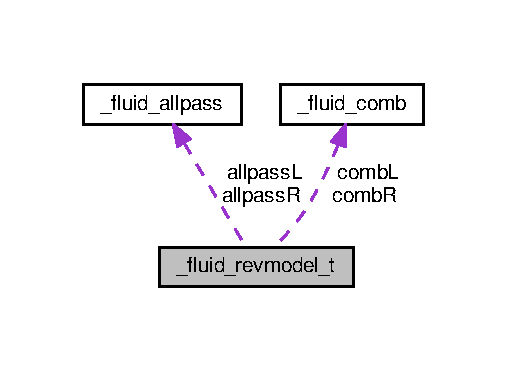
\includegraphics[width=244pt]{struct__fluid__revmodel__t__coll__graph}
\end{center}
\end{figure}
\subsection*{Public Attributes}
\begin{DoxyCompactItemize}
\item 
\hyperlink{fluidsynth__priv_8h_a9e96f0917747b69cabb7c671bc693dbb}{fluid\+\_\+real\+\_\+t} \hyperlink{struct__fluid__revmodel__t_a60639853a7c41acebcb049d2b6e633ac}{roomsize}
\item 
\hyperlink{fluidsynth__priv_8h_a9e96f0917747b69cabb7c671bc693dbb}{fluid\+\_\+real\+\_\+t} \hyperlink{struct__fluid__revmodel__t_a91700d75d27a83cf6273c24b31fcd23e}{damp}
\item 
\hyperlink{fluidsynth__priv_8h_a9e96f0917747b69cabb7c671bc693dbb}{fluid\+\_\+real\+\_\+t} \hyperlink{struct__fluid__revmodel__t_a19f4f3a2ae558ae8a45f1d1fe67ee962}{level}
\item 
\hyperlink{fluidsynth__priv_8h_a9e96f0917747b69cabb7c671bc693dbb}{fluid\+\_\+real\+\_\+t} \hyperlink{struct__fluid__revmodel__t_a09606ab8e4edc91cf248ee7e2a1abe42}{wet1}
\item 
\hyperlink{fluidsynth__priv_8h_a9e96f0917747b69cabb7c671bc693dbb}{fluid\+\_\+real\+\_\+t} \hyperlink{struct__fluid__revmodel__t_aea3fb7ec197bef989433633c7b6a1ab7}{wet2}
\item 
\hyperlink{fluidsynth__priv_8h_a9e96f0917747b69cabb7c671bc693dbb}{fluid\+\_\+real\+\_\+t} \hyperlink{struct__fluid__revmodel__t_a3325673995255edf9836151b73a54f83}{width}
\item 
\hyperlink{fluidsynth__priv_8h_a9e96f0917747b69cabb7c671bc693dbb}{fluid\+\_\+real\+\_\+t} \hyperlink{struct__fluid__revmodel__t_acab33a1762d0d0b6a12f76a7d9c324c4}{gain}
\item 
\hyperlink{fluid__rev_8c_a624b5fdff309d5b75383f8bf860c1e8b}{fluid\+\_\+comb} \hyperlink{struct__fluid__revmodel__t_a78e7a6f22b55f0477fce68477e90ee07}{combL} \mbox{[}\hyperlink{fluid__rev_8c_af9d1d366b6c476c1a4a2c2ce3ec3a70f}{numcombs}\mbox{]}
\item 
\hyperlink{fluid__rev_8c_a624b5fdff309d5b75383f8bf860c1e8b}{fluid\+\_\+comb} \hyperlink{struct__fluid__revmodel__t_a9bc9f76644b5f3d2b69097dec3344fa6}{combR} \mbox{[}\hyperlink{fluid__rev_8c_af9d1d366b6c476c1a4a2c2ce3ec3a70f}{numcombs}\mbox{]}
\item 
\hyperlink{fluid__rev_8c_a749cce96bf2a255ebe77f1ef33743f8e}{fluid\+\_\+allpass} \hyperlink{struct__fluid__revmodel__t_a56e9df9d5903ee9d9af98f229bb929e2}{allpassL} \mbox{[}\hyperlink{fluid__rev_8c_a8ffe8f6a09d788e2ff49a1fb151790af}{numallpasses}\mbox{]}
\item 
\hyperlink{fluid__rev_8c_a749cce96bf2a255ebe77f1ef33743f8e}{fluid\+\_\+allpass} \hyperlink{struct__fluid__revmodel__t_a6aac0eff2a50622041a0f5538415e812}{allpassR} \mbox{[}\hyperlink{fluid__rev_8c_a8ffe8f6a09d788e2ff49a1fb151790af}{numallpasses}\mbox{]}
\end{DoxyCompactItemize}


\subsection{Member Data Documentation}
\mbox{\Hypertarget{struct__fluid__revmodel__t_a56e9df9d5903ee9d9af98f229bb929e2}\label{struct__fluid__revmodel__t_a56e9df9d5903ee9d9af98f229bb929e2}} 
\index{\+\_\+fluid\+\_\+revmodel\+\_\+t@{\+\_\+fluid\+\_\+revmodel\+\_\+t}!allpassL@{allpassL}}
\index{allpassL@{allpassL}!\+\_\+fluid\+\_\+revmodel\+\_\+t@{\+\_\+fluid\+\_\+revmodel\+\_\+t}}
\subsubsection{\texorpdfstring{allpassL}{allpassL}}
{\footnotesize\ttfamily \hyperlink{fluid__rev_8c_a749cce96bf2a255ebe77f1ef33743f8e}{fluid\+\_\+allpass} \+\_\+fluid\+\_\+revmodel\+\_\+t\+::allpassL\mbox{[}\hyperlink{fluid__rev_8c_a8ffe8f6a09d788e2ff49a1fb151790af}{numallpasses}\mbox{]}}

\mbox{\Hypertarget{struct__fluid__revmodel__t_a6aac0eff2a50622041a0f5538415e812}\label{struct__fluid__revmodel__t_a6aac0eff2a50622041a0f5538415e812}} 
\index{\+\_\+fluid\+\_\+revmodel\+\_\+t@{\+\_\+fluid\+\_\+revmodel\+\_\+t}!allpassR@{allpassR}}
\index{allpassR@{allpassR}!\+\_\+fluid\+\_\+revmodel\+\_\+t@{\+\_\+fluid\+\_\+revmodel\+\_\+t}}
\subsubsection{\texorpdfstring{allpassR}{allpassR}}
{\footnotesize\ttfamily \hyperlink{fluid__rev_8c_a749cce96bf2a255ebe77f1ef33743f8e}{fluid\+\_\+allpass} \+\_\+fluid\+\_\+revmodel\+\_\+t\+::allpassR\mbox{[}\hyperlink{fluid__rev_8c_a8ffe8f6a09d788e2ff49a1fb151790af}{numallpasses}\mbox{]}}

\mbox{\Hypertarget{struct__fluid__revmodel__t_a78e7a6f22b55f0477fce68477e90ee07}\label{struct__fluid__revmodel__t_a78e7a6f22b55f0477fce68477e90ee07}} 
\index{\+\_\+fluid\+\_\+revmodel\+\_\+t@{\+\_\+fluid\+\_\+revmodel\+\_\+t}!combL@{combL}}
\index{combL@{combL}!\+\_\+fluid\+\_\+revmodel\+\_\+t@{\+\_\+fluid\+\_\+revmodel\+\_\+t}}
\subsubsection{\texorpdfstring{combL}{combL}}
{\footnotesize\ttfamily \hyperlink{fluid__rev_8c_a624b5fdff309d5b75383f8bf860c1e8b}{fluid\+\_\+comb} \+\_\+fluid\+\_\+revmodel\+\_\+t\+::combL\mbox{[}\hyperlink{fluid__rev_8c_af9d1d366b6c476c1a4a2c2ce3ec3a70f}{numcombs}\mbox{]}}

\mbox{\Hypertarget{struct__fluid__revmodel__t_a9bc9f76644b5f3d2b69097dec3344fa6}\label{struct__fluid__revmodel__t_a9bc9f76644b5f3d2b69097dec3344fa6}} 
\index{\+\_\+fluid\+\_\+revmodel\+\_\+t@{\+\_\+fluid\+\_\+revmodel\+\_\+t}!combR@{combR}}
\index{combR@{combR}!\+\_\+fluid\+\_\+revmodel\+\_\+t@{\+\_\+fluid\+\_\+revmodel\+\_\+t}}
\subsubsection{\texorpdfstring{combR}{combR}}
{\footnotesize\ttfamily \hyperlink{fluid__rev_8c_a624b5fdff309d5b75383f8bf860c1e8b}{fluid\+\_\+comb} \+\_\+fluid\+\_\+revmodel\+\_\+t\+::combR\mbox{[}\hyperlink{fluid__rev_8c_af9d1d366b6c476c1a4a2c2ce3ec3a70f}{numcombs}\mbox{]}}

\mbox{\Hypertarget{struct__fluid__revmodel__t_a91700d75d27a83cf6273c24b31fcd23e}\label{struct__fluid__revmodel__t_a91700d75d27a83cf6273c24b31fcd23e}} 
\index{\+\_\+fluid\+\_\+revmodel\+\_\+t@{\+\_\+fluid\+\_\+revmodel\+\_\+t}!damp@{damp}}
\index{damp@{damp}!\+\_\+fluid\+\_\+revmodel\+\_\+t@{\+\_\+fluid\+\_\+revmodel\+\_\+t}}
\subsubsection{\texorpdfstring{damp}{damp}}
{\footnotesize\ttfamily \hyperlink{fluidsynth__priv_8h_a9e96f0917747b69cabb7c671bc693dbb}{fluid\+\_\+real\+\_\+t} \+\_\+fluid\+\_\+revmodel\+\_\+t\+::damp}

\mbox{\Hypertarget{struct__fluid__revmodel__t_acab33a1762d0d0b6a12f76a7d9c324c4}\label{struct__fluid__revmodel__t_acab33a1762d0d0b6a12f76a7d9c324c4}} 
\index{\+\_\+fluid\+\_\+revmodel\+\_\+t@{\+\_\+fluid\+\_\+revmodel\+\_\+t}!gain@{gain}}
\index{gain@{gain}!\+\_\+fluid\+\_\+revmodel\+\_\+t@{\+\_\+fluid\+\_\+revmodel\+\_\+t}}
\subsubsection{\texorpdfstring{gain}{gain}}
{\footnotesize\ttfamily \hyperlink{fluidsynth__priv_8h_a9e96f0917747b69cabb7c671bc693dbb}{fluid\+\_\+real\+\_\+t} \+\_\+fluid\+\_\+revmodel\+\_\+t\+::gain}

\mbox{\Hypertarget{struct__fluid__revmodel__t_a19f4f3a2ae558ae8a45f1d1fe67ee962}\label{struct__fluid__revmodel__t_a19f4f3a2ae558ae8a45f1d1fe67ee962}} 
\index{\+\_\+fluid\+\_\+revmodel\+\_\+t@{\+\_\+fluid\+\_\+revmodel\+\_\+t}!level@{level}}
\index{level@{level}!\+\_\+fluid\+\_\+revmodel\+\_\+t@{\+\_\+fluid\+\_\+revmodel\+\_\+t}}
\subsubsection{\texorpdfstring{level}{level}}
{\footnotesize\ttfamily \hyperlink{fluidsynth__priv_8h_a9e96f0917747b69cabb7c671bc693dbb}{fluid\+\_\+real\+\_\+t} \+\_\+fluid\+\_\+revmodel\+\_\+t\+::level}

\mbox{\Hypertarget{struct__fluid__revmodel__t_a60639853a7c41acebcb049d2b6e633ac}\label{struct__fluid__revmodel__t_a60639853a7c41acebcb049d2b6e633ac}} 
\index{\+\_\+fluid\+\_\+revmodel\+\_\+t@{\+\_\+fluid\+\_\+revmodel\+\_\+t}!roomsize@{roomsize}}
\index{roomsize@{roomsize}!\+\_\+fluid\+\_\+revmodel\+\_\+t@{\+\_\+fluid\+\_\+revmodel\+\_\+t}}
\subsubsection{\texorpdfstring{roomsize}{roomsize}}
{\footnotesize\ttfamily \hyperlink{fluidsynth__priv_8h_a9e96f0917747b69cabb7c671bc693dbb}{fluid\+\_\+real\+\_\+t} \+\_\+fluid\+\_\+revmodel\+\_\+t\+::roomsize}

\mbox{\Hypertarget{struct__fluid__revmodel__t_a09606ab8e4edc91cf248ee7e2a1abe42}\label{struct__fluid__revmodel__t_a09606ab8e4edc91cf248ee7e2a1abe42}} 
\index{\+\_\+fluid\+\_\+revmodel\+\_\+t@{\+\_\+fluid\+\_\+revmodel\+\_\+t}!wet1@{wet1}}
\index{wet1@{wet1}!\+\_\+fluid\+\_\+revmodel\+\_\+t@{\+\_\+fluid\+\_\+revmodel\+\_\+t}}
\subsubsection{\texorpdfstring{wet1}{wet1}}
{\footnotesize\ttfamily \hyperlink{fluidsynth__priv_8h_a9e96f0917747b69cabb7c671bc693dbb}{fluid\+\_\+real\+\_\+t} \+\_\+fluid\+\_\+revmodel\+\_\+t\+::wet1}

\mbox{\Hypertarget{struct__fluid__revmodel__t_aea3fb7ec197bef989433633c7b6a1ab7}\label{struct__fluid__revmodel__t_aea3fb7ec197bef989433633c7b6a1ab7}} 
\index{\+\_\+fluid\+\_\+revmodel\+\_\+t@{\+\_\+fluid\+\_\+revmodel\+\_\+t}!wet2@{wet2}}
\index{wet2@{wet2}!\+\_\+fluid\+\_\+revmodel\+\_\+t@{\+\_\+fluid\+\_\+revmodel\+\_\+t}}
\subsubsection{\texorpdfstring{wet2}{wet2}}
{\footnotesize\ttfamily \hyperlink{fluidsynth__priv_8h_a9e96f0917747b69cabb7c671bc693dbb}{fluid\+\_\+real\+\_\+t} \+\_\+fluid\+\_\+revmodel\+\_\+t\+::wet2}

\mbox{\Hypertarget{struct__fluid__revmodel__t_a3325673995255edf9836151b73a54f83}\label{struct__fluid__revmodel__t_a3325673995255edf9836151b73a54f83}} 
\index{\+\_\+fluid\+\_\+revmodel\+\_\+t@{\+\_\+fluid\+\_\+revmodel\+\_\+t}!width@{width}}
\index{width@{width}!\+\_\+fluid\+\_\+revmodel\+\_\+t@{\+\_\+fluid\+\_\+revmodel\+\_\+t}}
\subsubsection{\texorpdfstring{width}{width}}
{\footnotesize\ttfamily \hyperlink{fluidsynth__priv_8h_a9e96f0917747b69cabb7c671bc693dbb}{fluid\+\_\+real\+\_\+t} \+\_\+fluid\+\_\+revmodel\+\_\+t\+::width}



The documentation for this struct was generated from the following file\+:\begin{DoxyCompactItemize}
\item 
rvoice/\hyperlink{fluid__rev_8c}{fluid\+\_\+rev.\+c}\end{DoxyCompactItemize}

\hypertarget{struct__fluid__ringbuffer__t}{}\section{\+\_\+fluid\+\_\+ringbuffer\+\_\+t Struct Reference}
\label{struct__fluid__ringbuffer__t}\index{\+\_\+fluid\+\_\+ringbuffer\+\_\+t@{\+\_\+fluid\+\_\+ringbuffer\+\_\+t}}


{\ttfamily \#include $<$fluid\+\_\+ringbuffer.\+h$>$}

\subsection*{Public Attributes}
\begin{DoxyCompactItemize}
\item 
char $\ast$ \hyperlink{struct__fluid__ringbuffer__t_a8a3c1a78adee3a690fa0506933a9c528}{array}
\item 
int \hyperlink{struct__fluid__ringbuffer__t_a3f705c52b05143c4b280a6b97b5786cb}{totalcount}
\item 
\hyperlink{fluidsynth__priv_8h_a6b8be882dd9958ea3635a868e1bf5152}{fluid\+\_\+atomic\+\_\+int\+\_\+t} \hyperlink{struct__fluid__ringbuffer__t_afb516fac54145dfb5368d6423ffeefe5}{count}
\item 
int \hyperlink{struct__fluid__ringbuffer__t_a7bbee19f1dfb2610f5aeacd6072034a4}{in}
\item 
int \hyperlink{struct__fluid__ringbuffer__t_a924348bac086f4b2fae906fefe8641ca}{out}
\item 
int \hyperlink{struct__fluid__ringbuffer__t_a47c6d0a36b568068c73dfae1953df03d}{elementsize}
\item 
void $\ast$ \hyperlink{struct__fluid__ringbuffer__t_a6f77ab4788fa1cefa502a70e77b27ac1}{userdata}
\end{DoxyCompactItemize}


\subsection{Member Data Documentation}
\mbox{\Hypertarget{struct__fluid__ringbuffer__t_a8a3c1a78adee3a690fa0506933a9c528}\label{struct__fluid__ringbuffer__t_a8a3c1a78adee3a690fa0506933a9c528}} 
\index{\+\_\+fluid\+\_\+ringbuffer\+\_\+t@{\+\_\+fluid\+\_\+ringbuffer\+\_\+t}!array@{array}}
\index{array@{array}!\+\_\+fluid\+\_\+ringbuffer\+\_\+t@{\+\_\+fluid\+\_\+ringbuffer\+\_\+t}}
\subsubsection{\texorpdfstring{array}{array}}
{\footnotesize\ttfamily char$\ast$ \+\_\+fluid\+\_\+ringbuffer\+\_\+t\+::array}

Queue array of arbitrary size elements \mbox{\Hypertarget{struct__fluid__ringbuffer__t_afb516fac54145dfb5368d6423ffeefe5}\label{struct__fluid__ringbuffer__t_afb516fac54145dfb5368d6423ffeefe5}} 
\index{\+\_\+fluid\+\_\+ringbuffer\+\_\+t@{\+\_\+fluid\+\_\+ringbuffer\+\_\+t}!count@{count}}
\index{count@{count}!\+\_\+fluid\+\_\+ringbuffer\+\_\+t@{\+\_\+fluid\+\_\+ringbuffer\+\_\+t}}
\subsubsection{\texorpdfstring{count}{count}}
{\footnotesize\ttfamily \hyperlink{fluidsynth__priv_8h_a6b8be882dd9958ea3635a868e1bf5152}{fluid\+\_\+atomic\+\_\+int\+\_\+t} \+\_\+fluid\+\_\+ringbuffer\+\_\+t\+::count}

Current count of elements \mbox{\Hypertarget{struct__fluid__ringbuffer__t_a47c6d0a36b568068c73dfae1953df03d}\label{struct__fluid__ringbuffer__t_a47c6d0a36b568068c73dfae1953df03d}} 
\index{\+\_\+fluid\+\_\+ringbuffer\+\_\+t@{\+\_\+fluid\+\_\+ringbuffer\+\_\+t}!elementsize@{elementsize}}
\index{elementsize@{elementsize}!\+\_\+fluid\+\_\+ringbuffer\+\_\+t@{\+\_\+fluid\+\_\+ringbuffer\+\_\+t}}
\subsubsection{\texorpdfstring{elementsize}{elementsize}}
{\footnotesize\ttfamily int \+\_\+fluid\+\_\+ringbuffer\+\_\+t\+::elementsize}

Size of each element \mbox{\Hypertarget{struct__fluid__ringbuffer__t_a7bbee19f1dfb2610f5aeacd6072034a4}\label{struct__fluid__ringbuffer__t_a7bbee19f1dfb2610f5aeacd6072034a4}} 
\index{\+\_\+fluid\+\_\+ringbuffer\+\_\+t@{\+\_\+fluid\+\_\+ringbuffer\+\_\+t}!in@{in}}
\index{in@{in}!\+\_\+fluid\+\_\+ringbuffer\+\_\+t@{\+\_\+fluid\+\_\+ringbuffer\+\_\+t}}
\subsubsection{\texorpdfstring{in}{in}}
{\footnotesize\ttfamily int \+\_\+fluid\+\_\+ringbuffer\+\_\+t\+::in}

Index in queue to store next pushed element \mbox{\Hypertarget{struct__fluid__ringbuffer__t_a924348bac086f4b2fae906fefe8641ca}\label{struct__fluid__ringbuffer__t_a924348bac086f4b2fae906fefe8641ca}} 
\index{\+\_\+fluid\+\_\+ringbuffer\+\_\+t@{\+\_\+fluid\+\_\+ringbuffer\+\_\+t}!out@{out}}
\index{out@{out}!\+\_\+fluid\+\_\+ringbuffer\+\_\+t@{\+\_\+fluid\+\_\+ringbuffer\+\_\+t}}
\subsubsection{\texorpdfstring{out}{out}}
{\footnotesize\ttfamily int \+\_\+fluid\+\_\+ringbuffer\+\_\+t\+::out}

Index in queue of next popped element \mbox{\Hypertarget{struct__fluid__ringbuffer__t_a3f705c52b05143c4b280a6b97b5786cb}\label{struct__fluid__ringbuffer__t_a3f705c52b05143c4b280a6b97b5786cb}} 
\index{\+\_\+fluid\+\_\+ringbuffer\+\_\+t@{\+\_\+fluid\+\_\+ringbuffer\+\_\+t}!totalcount@{totalcount}}
\index{totalcount@{totalcount}!\+\_\+fluid\+\_\+ringbuffer\+\_\+t@{\+\_\+fluid\+\_\+ringbuffer\+\_\+t}}
\subsubsection{\texorpdfstring{totalcount}{totalcount}}
{\footnotesize\ttfamily int \+\_\+fluid\+\_\+ringbuffer\+\_\+t\+::totalcount}

Total count of elements in array \mbox{\Hypertarget{struct__fluid__ringbuffer__t_a6f77ab4788fa1cefa502a70e77b27ac1}\label{struct__fluid__ringbuffer__t_a6f77ab4788fa1cefa502a70e77b27ac1}} 
\index{\+\_\+fluid\+\_\+ringbuffer\+\_\+t@{\+\_\+fluid\+\_\+ringbuffer\+\_\+t}!userdata@{userdata}}
\index{userdata@{userdata}!\+\_\+fluid\+\_\+ringbuffer\+\_\+t@{\+\_\+fluid\+\_\+ringbuffer\+\_\+t}}
\subsubsection{\texorpdfstring{userdata}{userdata}}
{\footnotesize\ttfamily void$\ast$ \+\_\+fluid\+\_\+ringbuffer\+\_\+t\+::userdata}



The documentation for this struct was generated from the following file\+:\begin{DoxyCompactItemize}
\item 
utils/\hyperlink{fluid__ringbuffer_8h}{fluid\+\_\+ringbuffer.\+h}\end{DoxyCompactItemize}

\hypertarget{struct__fluid__rvoice__buffers__t}{}\section{\+\_\+fluid\+\_\+rvoice\+\_\+buffers\+\_\+t Struct Reference}
\label{struct__fluid__rvoice__buffers__t}\index{\+\_\+fluid\+\_\+rvoice\+\_\+buffers\+\_\+t@{\+\_\+fluid\+\_\+rvoice\+\_\+buffers\+\_\+t}}


{\ttfamily \#include $<$fluid\+\_\+rvoice.\+h$>$}

\subsection*{Public Attributes}
\begin{DoxyCompactItemize}
\item 
unsigned int \hyperlink{struct__fluid__rvoice__buffers__t_a1e1a22dc9c43ac0a62e79b7a12d88716}{count}
\item 
\begin{tabbing}
xx\=xx\=xx\=xx\=xx\=xx\=xx\=xx\=xx\=\kill
struct \{\\
\>\hyperlink{fluidsynth__priv_8h_a9e96f0917747b69cabb7c671bc693dbb}{fluid\_real\_t} \hyperlink{struct__fluid__rvoice__buffers__t_afd03db7fb66e15021affe424c41738ef}{amp}\\
\>int \hyperlink{struct__fluid__rvoice__buffers__t_ab95a357279a79aa90127f4f31acb9db1}{mapping}\\
\} \hyperlink{struct__fluid__rvoice__buffers__t_ac47ccb3ce4c005c99af117932c8b28a1}{bufs} \mbox{[}\hyperlink{fluid__rvoice_8h_acf3b2a54d9a8dfe8d9f0db8dae37c831}{FLUID\_RVOICE\_MAX\_BUFS}\mbox{]}\\

\end{tabbing}\end{DoxyCompactItemize}


\subsection{Member Data Documentation}
\mbox{\Hypertarget{struct__fluid__rvoice__buffers__t_afd03db7fb66e15021affe424c41738ef}\label{struct__fluid__rvoice__buffers__t_afd03db7fb66e15021affe424c41738ef}} 
\index{\+\_\+fluid\+\_\+rvoice\+\_\+buffers\+\_\+t@{\+\_\+fluid\+\_\+rvoice\+\_\+buffers\+\_\+t}!amp@{amp}}
\index{amp@{amp}!\+\_\+fluid\+\_\+rvoice\+\_\+buffers\+\_\+t@{\+\_\+fluid\+\_\+rvoice\+\_\+buffers\+\_\+t}}
\subsubsection{\texorpdfstring{amp}{amp}}
{\footnotesize\ttfamily \hyperlink{fluidsynth__priv_8h_a9e96f0917747b69cabb7c671bc693dbb}{fluid\+\_\+real\+\_\+t} \+\_\+fluid\+\_\+rvoice\+\_\+buffers\+\_\+t\+::amp}

\mbox{\Hypertarget{struct__fluid__rvoice__buffers__t_ac47ccb3ce4c005c99af117932c8b28a1}\label{struct__fluid__rvoice__buffers__t_ac47ccb3ce4c005c99af117932c8b28a1}} 
\index{\+\_\+fluid\+\_\+rvoice\+\_\+buffers\+\_\+t@{\+\_\+fluid\+\_\+rvoice\+\_\+buffers\+\_\+t}!bufs@{bufs}}
\index{bufs@{bufs}!\+\_\+fluid\+\_\+rvoice\+\_\+buffers\+\_\+t@{\+\_\+fluid\+\_\+rvoice\+\_\+buffers\+\_\+t}}
\subsubsection{\texorpdfstring{bufs}{bufs}}
{\footnotesize\ttfamily struct \{ ... \}   \+\_\+fluid\+\_\+rvoice\+\_\+buffers\+\_\+t\+::bufs\mbox{[}\hyperlink{fluid__rvoice_8h_acf3b2a54d9a8dfe8d9f0db8dae37c831}{F\+L\+U\+I\+D\+\_\+\+R\+V\+O\+I\+C\+E\+\_\+\+M\+A\+X\+\_\+\+B\+U\+FS}\mbox{]}}

\mbox{\Hypertarget{struct__fluid__rvoice__buffers__t_a1e1a22dc9c43ac0a62e79b7a12d88716}\label{struct__fluid__rvoice__buffers__t_a1e1a22dc9c43ac0a62e79b7a12d88716}} 
\index{\+\_\+fluid\+\_\+rvoice\+\_\+buffers\+\_\+t@{\+\_\+fluid\+\_\+rvoice\+\_\+buffers\+\_\+t}!count@{count}}
\index{count@{count}!\+\_\+fluid\+\_\+rvoice\+\_\+buffers\+\_\+t@{\+\_\+fluid\+\_\+rvoice\+\_\+buffers\+\_\+t}}
\subsubsection{\texorpdfstring{count}{count}}
{\footnotesize\ttfamily unsigned int \+\_\+fluid\+\_\+rvoice\+\_\+buffers\+\_\+t\+::count}

\mbox{\Hypertarget{struct__fluid__rvoice__buffers__t_ab95a357279a79aa90127f4f31acb9db1}\label{struct__fluid__rvoice__buffers__t_ab95a357279a79aa90127f4f31acb9db1}} 
\index{\+\_\+fluid\+\_\+rvoice\+\_\+buffers\+\_\+t@{\+\_\+fluid\+\_\+rvoice\+\_\+buffers\+\_\+t}!mapping@{mapping}}
\index{mapping@{mapping}!\+\_\+fluid\+\_\+rvoice\+\_\+buffers\+\_\+t@{\+\_\+fluid\+\_\+rvoice\+\_\+buffers\+\_\+t}}
\subsubsection{\texorpdfstring{mapping}{mapping}}
{\footnotesize\ttfamily int \+\_\+fluid\+\_\+rvoice\+\_\+buffers\+\_\+t\+::mapping}



The documentation for this struct was generated from the following file\+:\begin{DoxyCompactItemize}
\item 
rvoice/\hyperlink{fluid__rvoice_8h}{fluid\+\_\+rvoice.\+h}\end{DoxyCompactItemize}

\hypertarget{struct__fluid__rvoice__dsp__t}{}\section{\+\_\+fluid\+\_\+rvoice\+\_\+dsp\+\_\+t Struct Reference}
\label{struct__fluid__rvoice__dsp__t}\index{\+\_\+fluid\+\_\+rvoice\+\_\+dsp\+\_\+t@{\+\_\+fluid\+\_\+rvoice\+\_\+dsp\+\_\+t}}


{\ttfamily \#include $<$fluid\+\_\+rvoice.\+h$>$}



Collaboration diagram for \+\_\+fluid\+\_\+rvoice\+\_\+dsp\+\_\+t\+:
\nopagebreak
\begin{figure}[H]
\begin{center}
\leavevmode
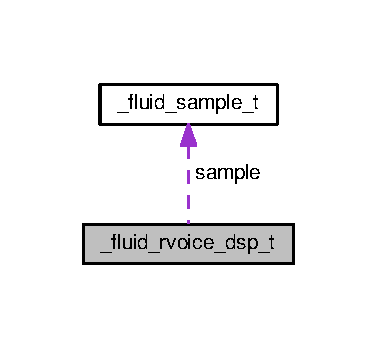
\includegraphics[width=181pt]{struct__fluid__rvoice__dsp__t__coll__graph}
\end{center}
\end{figure}
\subsection*{Public Attributes}
\begin{DoxyCompactItemize}
\item 
enum \hyperlink{synth_8h_a4a2efef77b267500dd9c19c0dc9e4633}{fluid\+\_\+interp} \hyperlink{struct__fluid__rvoice__dsp__t_ac7992fd0a83c96a53b70722a958d3abd}{interp\+\_\+method}
\item 
enum \hyperlink{fluid__rvoice_8h_a27ec752422f9291b77de7217c0f02f4f}{fluid\+\_\+loop} \hyperlink{struct__fluid__rvoice__dsp__t_acdf7fe7cf31781b94b0c986d137ba85a}{samplemode}
\item 
char \hyperlink{struct__fluid__rvoice__dsp__t_a3cd4d57ea2d5f27cdcab0bd331b5c3aa}{has\+\_\+looped}
\item 
char \hyperlink{struct__fluid__rvoice__dsp__t_a70d4a20de04bca1e790efae49f815e82}{check\+\_\+sample\+\_\+sanity\+\_\+flag}
\item 
\hyperlink{types_8h_abf9174d452679ca1a4ee7d693fb773cf}{fluid\+\_\+sample\+\_\+t} $\ast$ \hyperlink{struct__fluid__rvoice__dsp__t_ae4141b3e3f3af1dbd827e2d75d86066d}{sample}
\item 
int \hyperlink{struct__fluid__rvoice__dsp__t_ac145d0e4a023f5b5a209c56f3652790a}{start}
\item 
int \hyperlink{struct__fluid__rvoice__dsp__t_ae5676614fdc0b0a9c4b90ed314c17fb3}{end}
\item 
int \hyperlink{struct__fluid__rvoice__dsp__t_ab3019cec8eebb7c4d622918bdb4342aa}{loopstart}
\item 
int \hyperlink{struct__fluid__rvoice__dsp__t_a5a363ff3f38d843fc7e942e346ad2d2b}{loopend}
\item 
\hyperlink{fluidsynth__priv_8h_a9e96f0917747b69cabb7c671bc693dbb}{fluid\+\_\+real\+\_\+t} \hyperlink{struct__fluid__rvoice__dsp__t_a9daf10c706debc6dbb7dfdf460e9d4b4}{pitchoffset}
\item 
\hyperlink{fluidsynth__priv_8h_a9e96f0917747b69cabb7c671bc693dbb}{fluid\+\_\+real\+\_\+t} \hyperlink{struct__fluid__rvoice__dsp__t_a33195e9f36595ebbbda908bde46256b3}{pitchinc}
\item 
\hyperlink{fluidsynth__priv_8h_a9e96f0917747b69cabb7c671bc693dbb}{fluid\+\_\+real\+\_\+t} \hyperlink{struct__fluid__rvoice__dsp__t_a85b5adce3ef83cfb096512ec38b060a2}{pitch}
\item 
\hyperlink{fluidsynth__priv_8h_a9e96f0917747b69cabb7c671bc693dbb}{fluid\+\_\+real\+\_\+t} \hyperlink{struct__fluid__rvoice__dsp__t_a1d0c1426a66b8b286560b641acc76b01}{root\+\_\+pitch\+\_\+hz}
\item 
\hyperlink{fluidsynth__priv_8h_a9e96f0917747b69cabb7c671bc693dbb}{fluid\+\_\+real\+\_\+t} \hyperlink{struct__fluid__rvoice__dsp__t_a5acf25d7daad12468bcfb88e638f2604}{output\+\_\+rate}
\item 
\hyperlink{fluidsynth__priv_8h_a9e96f0917747b69cabb7c671bc693dbb}{fluid\+\_\+real\+\_\+t} \hyperlink{struct__fluid__rvoice__dsp__t_a4d9190beee933797360ed1fa80400b22}{attenuation}
\item 
\hyperlink{fluidsynth__priv_8h_a9e96f0917747b69cabb7c671bc693dbb}{fluid\+\_\+real\+\_\+t} \hyperlink{struct__fluid__rvoice__dsp__t_abb0b8cf53b49753d8d6c299de9a21d2e}{prev\+\_\+attenuation}
\item 
\hyperlink{fluidsynth__priv_8h_a9e96f0917747b69cabb7c671bc693dbb}{fluid\+\_\+real\+\_\+t} \hyperlink{struct__fluid__rvoice__dsp__t_acf1b29037dbcd99eda2d680b34744781}{min\+\_\+attenuation\+\_\+cB}
\item 
\hyperlink{fluidsynth__priv_8h_a9e96f0917747b69cabb7c671bc693dbb}{fluid\+\_\+real\+\_\+t} \hyperlink{struct__fluid__rvoice__dsp__t_a7496b9829322370f19ef8bade4057693}{amplitude\+\_\+that\+\_\+reaches\+\_\+noise\+\_\+floor\+\_\+nonloop}
\item 
\hyperlink{fluidsynth__priv_8h_a9e96f0917747b69cabb7c671bc693dbb}{fluid\+\_\+real\+\_\+t} \hyperlink{struct__fluid__rvoice__dsp__t_a23d8056eab7fb440978386f2f0403d96}{amplitude\+\_\+that\+\_\+reaches\+\_\+noise\+\_\+floor\+\_\+loop}
\item 
\hyperlink{fluidsynth__priv_8h_a9e96f0917747b69cabb7c671bc693dbb}{fluid\+\_\+real\+\_\+t} \hyperlink{struct__fluid__rvoice__dsp__t_a2d9dcfc148f6037237f395e84ad54ed5}{synth\+\_\+gain}
\item 
\hyperlink{fluidsynth__priv_8h_a9e96f0917747b69cabb7c671bc693dbb}{fluid\+\_\+real\+\_\+t} \hyperlink{struct__fluid__rvoice__dsp__t_aceb3dfb35515128e0f63a62cb15e2beb}{amp}
\item 
\hyperlink{fluidsynth__priv_8h_a9e96f0917747b69cabb7c671bc693dbb}{fluid\+\_\+real\+\_\+t} \hyperlink{struct__fluid__rvoice__dsp__t_a96265ba2c9a9f3130de11685d70e8c4f}{amp\+\_\+incr}
\item 
\hyperlink{fluid__phase_8h_a58a63b6710f24684e8e7a52fe47408d6}{fluid\+\_\+phase\+\_\+t} \hyperlink{struct__fluid__rvoice__dsp__t_aaf93192acb7a5847a3d3210e65536fe6}{phase}
\item 
\hyperlink{fluidsynth__priv_8h_a9e96f0917747b69cabb7c671bc693dbb}{fluid\+\_\+real\+\_\+t} \hyperlink{struct__fluid__rvoice__dsp__t_a70f52e9b4b6c4e884ac3e9cdd19f9794}{phase\+\_\+incr}
\end{DoxyCompactItemize}


\subsection{Member Data Documentation}
\mbox{\Hypertarget{struct__fluid__rvoice__dsp__t_aceb3dfb35515128e0f63a62cb15e2beb}\label{struct__fluid__rvoice__dsp__t_aceb3dfb35515128e0f63a62cb15e2beb}} 
\index{\+\_\+fluid\+\_\+rvoice\+\_\+dsp\+\_\+t@{\+\_\+fluid\+\_\+rvoice\+\_\+dsp\+\_\+t}!amp@{amp}}
\index{amp@{amp}!\+\_\+fluid\+\_\+rvoice\+\_\+dsp\+\_\+t@{\+\_\+fluid\+\_\+rvoice\+\_\+dsp\+\_\+t}}
\subsubsection{\texorpdfstring{amp}{amp}}
{\footnotesize\ttfamily \hyperlink{fluidsynth__priv_8h_a9e96f0917747b69cabb7c671bc693dbb}{fluid\+\_\+real\+\_\+t} \+\_\+fluid\+\_\+rvoice\+\_\+dsp\+\_\+t\+::amp}

\mbox{\Hypertarget{struct__fluid__rvoice__dsp__t_a96265ba2c9a9f3130de11685d70e8c4f}\label{struct__fluid__rvoice__dsp__t_a96265ba2c9a9f3130de11685d70e8c4f}} 
\index{\+\_\+fluid\+\_\+rvoice\+\_\+dsp\+\_\+t@{\+\_\+fluid\+\_\+rvoice\+\_\+dsp\+\_\+t}!amp\+\_\+incr@{amp\+\_\+incr}}
\index{amp\+\_\+incr@{amp\+\_\+incr}!\+\_\+fluid\+\_\+rvoice\+\_\+dsp\+\_\+t@{\+\_\+fluid\+\_\+rvoice\+\_\+dsp\+\_\+t}}
\subsubsection{\texorpdfstring{amp\+\_\+incr}{amp\_incr}}
{\footnotesize\ttfamily \hyperlink{fluidsynth__priv_8h_a9e96f0917747b69cabb7c671bc693dbb}{fluid\+\_\+real\+\_\+t} \+\_\+fluid\+\_\+rvoice\+\_\+dsp\+\_\+t\+::amp\+\_\+incr}

\mbox{\Hypertarget{struct__fluid__rvoice__dsp__t_a23d8056eab7fb440978386f2f0403d96}\label{struct__fluid__rvoice__dsp__t_a23d8056eab7fb440978386f2f0403d96}} 
\index{\+\_\+fluid\+\_\+rvoice\+\_\+dsp\+\_\+t@{\+\_\+fluid\+\_\+rvoice\+\_\+dsp\+\_\+t}!amplitude\+\_\+that\+\_\+reaches\+\_\+noise\+\_\+floor\+\_\+loop@{amplitude\+\_\+that\+\_\+reaches\+\_\+noise\+\_\+floor\+\_\+loop}}
\index{amplitude\+\_\+that\+\_\+reaches\+\_\+noise\+\_\+floor\+\_\+loop@{amplitude\+\_\+that\+\_\+reaches\+\_\+noise\+\_\+floor\+\_\+loop}!\+\_\+fluid\+\_\+rvoice\+\_\+dsp\+\_\+t@{\+\_\+fluid\+\_\+rvoice\+\_\+dsp\+\_\+t}}
\subsubsection{\texorpdfstring{amplitude\+\_\+that\+\_\+reaches\+\_\+noise\+\_\+floor\+\_\+loop}{amplitude\_that\_reaches\_noise\_floor\_loop}}
{\footnotesize\ttfamily \hyperlink{fluidsynth__priv_8h_a9e96f0917747b69cabb7c671bc693dbb}{fluid\+\_\+real\+\_\+t} \+\_\+fluid\+\_\+rvoice\+\_\+dsp\+\_\+t\+::amplitude\+\_\+that\+\_\+reaches\+\_\+noise\+\_\+floor\+\_\+loop}

\mbox{\Hypertarget{struct__fluid__rvoice__dsp__t_a7496b9829322370f19ef8bade4057693}\label{struct__fluid__rvoice__dsp__t_a7496b9829322370f19ef8bade4057693}} 
\index{\+\_\+fluid\+\_\+rvoice\+\_\+dsp\+\_\+t@{\+\_\+fluid\+\_\+rvoice\+\_\+dsp\+\_\+t}!amplitude\+\_\+that\+\_\+reaches\+\_\+noise\+\_\+floor\+\_\+nonloop@{amplitude\+\_\+that\+\_\+reaches\+\_\+noise\+\_\+floor\+\_\+nonloop}}
\index{amplitude\+\_\+that\+\_\+reaches\+\_\+noise\+\_\+floor\+\_\+nonloop@{amplitude\+\_\+that\+\_\+reaches\+\_\+noise\+\_\+floor\+\_\+nonloop}!\+\_\+fluid\+\_\+rvoice\+\_\+dsp\+\_\+t@{\+\_\+fluid\+\_\+rvoice\+\_\+dsp\+\_\+t}}
\subsubsection{\texorpdfstring{amplitude\+\_\+that\+\_\+reaches\+\_\+noise\+\_\+floor\+\_\+nonloop}{amplitude\_that\_reaches\_noise\_floor\_nonloop}}
{\footnotesize\ttfamily \hyperlink{fluidsynth__priv_8h_a9e96f0917747b69cabb7c671bc693dbb}{fluid\+\_\+real\+\_\+t} \+\_\+fluid\+\_\+rvoice\+\_\+dsp\+\_\+t\+::amplitude\+\_\+that\+\_\+reaches\+\_\+noise\+\_\+floor\+\_\+nonloop}

\mbox{\Hypertarget{struct__fluid__rvoice__dsp__t_a4d9190beee933797360ed1fa80400b22}\label{struct__fluid__rvoice__dsp__t_a4d9190beee933797360ed1fa80400b22}} 
\index{\+\_\+fluid\+\_\+rvoice\+\_\+dsp\+\_\+t@{\+\_\+fluid\+\_\+rvoice\+\_\+dsp\+\_\+t}!attenuation@{attenuation}}
\index{attenuation@{attenuation}!\+\_\+fluid\+\_\+rvoice\+\_\+dsp\+\_\+t@{\+\_\+fluid\+\_\+rvoice\+\_\+dsp\+\_\+t}}
\subsubsection{\texorpdfstring{attenuation}{attenuation}}
{\footnotesize\ttfamily \hyperlink{fluidsynth__priv_8h_a9e96f0917747b69cabb7c671bc693dbb}{fluid\+\_\+real\+\_\+t} \+\_\+fluid\+\_\+rvoice\+\_\+dsp\+\_\+t\+::attenuation}

\mbox{\Hypertarget{struct__fluid__rvoice__dsp__t_a70d4a20de04bca1e790efae49f815e82}\label{struct__fluid__rvoice__dsp__t_a70d4a20de04bca1e790efae49f815e82}} 
\index{\+\_\+fluid\+\_\+rvoice\+\_\+dsp\+\_\+t@{\+\_\+fluid\+\_\+rvoice\+\_\+dsp\+\_\+t}!check\+\_\+sample\+\_\+sanity\+\_\+flag@{check\+\_\+sample\+\_\+sanity\+\_\+flag}}
\index{check\+\_\+sample\+\_\+sanity\+\_\+flag@{check\+\_\+sample\+\_\+sanity\+\_\+flag}!\+\_\+fluid\+\_\+rvoice\+\_\+dsp\+\_\+t@{\+\_\+fluid\+\_\+rvoice\+\_\+dsp\+\_\+t}}
\subsubsection{\texorpdfstring{check\+\_\+sample\+\_\+sanity\+\_\+flag}{check\_sample\_sanity\_flag}}
{\footnotesize\ttfamily char \+\_\+fluid\+\_\+rvoice\+\_\+dsp\+\_\+t\+::check\+\_\+sample\+\_\+sanity\+\_\+flag}

\mbox{\Hypertarget{struct__fluid__rvoice__dsp__t_ae5676614fdc0b0a9c4b90ed314c17fb3}\label{struct__fluid__rvoice__dsp__t_ae5676614fdc0b0a9c4b90ed314c17fb3}} 
\index{\+\_\+fluid\+\_\+rvoice\+\_\+dsp\+\_\+t@{\+\_\+fluid\+\_\+rvoice\+\_\+dsp\+\_\+t}!end@{end}}
\index{end@{end}!\+\_\+fluid\+\_\+rvoice\+\_\+dsp\+\_\+t@{\+\_\+fluid\+\_\+rvoice\+\_\+dsp\+\_\+t}}
\subsubsection{\texorpdfstring{end}{end}}
{\footnotesize\ttfamily int \+\_\+fluid\+\_\+rvoice\+\_\+dsp\+\_\+t\+::end}

\mbox{\Hypertarget{struct__fluid__rvoice__dsp__t_a3cd4d57ea2d5f27cdcab0bd331b5c3aa}\label{struct__fluid__rvoice__dsp__t_a3cd4d57ea2d5f27cdcab0bd331b5c3aa}} 
\index{\+\_\+fluid\+\_\+rvoice\+\_\+dsp\+\_\+t@{\+\_\+fluid\+\_\+rvoice\+\_\+dsp\+\_\+t}!has\+\_\+looped@{has\+\_\+looped}}
\index{has\+\_\+looped@{has\+\_\+looped}!\+\_\+fluid\+\_\+rvoice\+\_\+dsp\+\_\+t@{\+\_\+fluid\+\_\+rvoice\+\_\+dsp\+\_\+t}}
\subsubsection{\texorpdfstring{has\+\_\+looped}{has\_looped}}
{\footnotesize\ttfamily char \+\_\+fluid\+\_\+rvoice\+\_\+dsp\+\_\+t\+::has\+\_\+looped}

\mbox{\Hypertarget{struct__fluid__rvoice__dsp__t_ac7992fd0a83c96a53b70722a958d3abd}\label{struct__fluid__rvoice__dsp__t_ac7992fd0a83c96a53b70722a958d3abd}} 
\index{\+\_\+fluid\+\_\+rvoice\+\_\+dsp\+\_\+t@{\+\_\+fluid\+\_\+rvoice\+\_\+dsp\+\_\+t}!interp\+\_\+method@{interp\+\_\+method}}
\index{interp\+\_\+method@{interp\+\_\+method}!\+\_\+fluid\+\_\+rvoice\+\_\+dsp\+\_\+t@{\+\_\+fluid\+\_\+rvoice\+\_\+dsp\+\_\+t}}
\subsubsection{\texorpdfstring{interp\+\_\+method}{interp\_method}}
{\footnotesize\ttfamily enum \hyperlink{synth_8h_a4a2efef77b267500dd9c19c0dc9e4633}{fluid\+\_\+interp} \+\_\+fluid\+\_\+rvoice\+\_\+dsp\+\_\+t\+::interp\+\_\+method}

\mbox{\Hypertarget{struct__fluid__rvoice__dsp__t_a5a363ff3f38d843fc7e942e346ad2d2b}\label{struct__fluid__rvoice__dsp__t_a5a363ff3f38d843fc7e942e346ad2d2b}} 
\index{\+\_\+fluid\+\_\+rvoice\+\_\+dsp\+\_\+t@{\+\_\+fluid\+\_\+rvoice\+\_\+dsp\+\_\+t}!loopend@{loopend}}
\index{loopend@{loopend}!\+\_\+fluid\+\_\+rvoice\+\_\+dsp\+\_\+t@{\+\_\+fluid\+\_\+rvoice\+\_\+dsp\+\_\+t}}
\subsubsection{\texorpdfstring{loopend}{loopend}}
{\footnotesize\ttfamily int \+\_\+fluid\+\_\+rvoice\+\_\+dsp\+\_\+t\+::loopend}

\mbox{\Hypertarget{struct__fluid__rvoice__dsp__t_ab3019cec8eebb7c4d622918bdb4342aa}\label{struct__fluid__rvoice__dsp__t_ab3019cec8eebb7c4d622918bdb4342aa}} 
\index{\+\_\+fluid\+\_\+rvoice\+\_\+dsp\+\_\+t@{\+\_\+fluid\+\_\+rvoice\+\_\+dsp\+\_\+t}!loopstart@{loopstart}}
\index{loopstart@{loopstart}!\+\_\+fluid\+\_\+rvoice\+\_\+dsp\+\_\+t@{\+\_\+fluid\+\_\+rvoice\+\_\+dsp\+\_\+t}}
\subsubsection{\texorpdfstring{loopstart}{loopstart}}
{\footnotesize\ttfamily int \+\_\+fluid\+\_\+rvoice\+\_\+dsp\+\_\+t\+::loopstart}

\mbox{\Hypertarget{struct__fluid__rvoice__dsp__t_acf1b29037dbcd99eda2d680b34744781}\label{struct__fluid__rvoice__dsp__t_acf1b29037dbcd99eda2d680b34744781}} 
\index{\+\_\+fluid\+\_\+rvoice\+\_\+dsp\+\_\+t@{\+\_\+fluid\+\_\+rvoice\+\_\+dsp\+\_\+t}!min\+\_\+attenuation\+\_\+cB@{min\+\_\+attenuation\+\_\+cB}}
\index{min\+\_\+attenuation\+\_\+cB@{min\+\_\+attenuation\+\_\+cB}!\+\_\+fluid\+\_\+rvoice\+\_\+dsp\+\_\+t@{\+\_\+fluid\+\_\+rvoice\+\_\+dsp\+\_\+t}}
\subsubsection{\texorpdfstring{min\+\_\+attenuation\+\_\+cB}{min\_attenuation\_cB}}
{\footnotesize\ttfamily \hyperlink{fluidsynth__priv_8h_a9e96f0917747b69cabb7c671bc693dbb}{fluid\+\_\+real\+\_\+t} \+\_\+fluid\+\_\+rvoice\+\_\+dsp\+\_\+t\+::min\+\_\+attenuation\+\_\+cB}

\mbox{\Hypertarget{struct__fluid__rvoice__dsp__t_a5acf25d7daad12468bcfb88e638f2604}\label{struct__fluid__rvoice__dsp__t_a5acf25d7daad12468bcfb88e638f2604}} 
\index{\+\_\+fluid\+\_\+rvoice\+\_\+dsp\+\_\+t@{\+\_\+fluid\+\_\+rvoice\+\_\+dsp\+\_\+t}!output\+\_\+rate@{output\+\_\+rate}}
\index{output\+\_\+rate@{output\+\_\+rate}!\+\_\+fluid\+\_\+rvoice\+\_\+dsp\+\_\+t@{\+\_\+fluid\+\_\+rvoice\+\_\+dsp\+\_\+t}}
\subsubsection{\texorpdfstring{output\+\_\+rate}{output\_rate}}
{\footnotesize\ttfamily \hyperlink{fluidsynth__priv_8h_a9e96f0917747b69cabb7c671bc693dbb}{fluid\+\_\+real\+\_\+t} \+\_\+fluid\+\_\+rvoice\+\_\+dsp\+\_\+t\+::output\+\_\+rate}

\mbox{\Hypertarget{struct__fluid__rvoice__dsp__t_aaf93192acb7a5847a3d3210e65536fe6}\label{struct__fluid__rvoice__dsp__t_aaf93192acb7a5847a3d3210e65536fe6}} 
\index{\+\_\+fluid\+\_\+rvoice\+\_\+dsp\+\_\+t@{\+\_\+fluid\+\_\+rvoice\+\_\+dsp\+\_\+t}!phase@{phase}}
\index{phase@{phase}!\+\_\+fluid\+\_\+rvoice\+\_\+dsp\+\_\+t@{\+\_\+fluid\+\_\+rvoice\+\_\+dsp\+\_\+t}}
\subsubsection{\texorpdfstring{phase}{phase}}
{\footnotesize\ttfamily \hyperlink{fluid__phase_8h_a58a63b6710f24684e8e7a52fe47408d6}{fluid\+\_\+phase\+\_\+t} \+\_\+fluid\+\_\+rvoice\+\_\+dsp\+\_\+t\+::phase}

\mbox{\Hypertarget{struct__fluid__rvoice__dsp__t_a70f52e9b4b6c4e884ac3e9cdd19f9794}\label{struct__fluid__rvoice__dsp__t_a70f52e9b4b6c4e884ac3e9cdd19f9794}} 
\index{\+\_\+fluid\+\_\+rvoice\+\_\+dsp\+\_\+t@{\+\_\+fluid\+\_\+rvoice\+\_\+dsp\+\_\+t}!phase\+\_\+incr@{phase\+\_\+incr}}
\index{phase\+\_\+incr@{phase\+\_\+incr}!\+\_\+fluid\+\_\+rvoice\+\_\+dsp\+\_\+t@{\+\_\+fluid\+\_\+rvoice\+\_\+dsp\+\_\+t}}
\subsubsection{\texorpdfstring{phase\+\_\+incr}{phase\_incr}}
{\footnotesize\ttfamily \hyperlink{fluidsynth__priv_8h_a9e96f0917747b69cabb7c671bc693dbb}{fluid\+\_\+real\+\_\+t} \+\_\+fluid\+\_\+rvoice\+\_\+dsp\+\_\+t\+::phase\+\_\+incr}

\mbox{\Hypertarget{struct__fluid__rvoice__dsp__t_a85b5adce3ef83cfb096512ec38b060a2}\label{struct__fluid__rvoice__dsp__t_a85b5adce3ef83cfb096512ec38b060a2}} 
\index{\+\_\+fluid\+\_\+rvoice\+\_\+dsp\+\_\+t@{\+\_\+fluid\+\_\+rvoice\+\_\+dsp\+\_\+t}!pitch@{pitch}}
\index{pitch@{pitch}!\+\_\+fluid\+\_\+rvoice\+\_\+dsp\+\_\+t@{\+\_\+fluid\+\_\+rvoice\+\_\+dsp\+\_\+t}}
\subsubsection{\texorpdfstring{pitch}{pitch}}
{\footnotesize\ttfamily \hyperlink{fluidsynth__priv_8h_a9e96f0917747b69cabb7c671bc693dbb}{fluid\+\_\+real\+\_\+t} \+\_\+fluid\+\_\+rvoice\+\_\+dsp\+\_\+t\+::pitch}

\mbox{\Hypertarget{struct__fluid__rvoice__dsp__t_a33195e9f36595ebbbda908bde46256b3}\label{struct__fluid__rvoice__dsp__t_a33195e9f36595ebbbda908bde46256b3}} 
\index{\+\_\+fluid\+\_\+rvoice\+\_\+dsp\+\_\+t@{\+\_\+fluid\+\_\+rvoice\+\_\+dsp\+\_\+t}!pitchinc@{pitchinc}}
\index{pitchinc@{pitchinc}!\+\_\+fluid\+\_\+rvoice\+\_\+dsp\+\_\+t@{\+\_\+fluid\+\_\+rvoice\+\_\+dsp\+\_\+t}}
\subsubsection{\texorpdfstring{pitchinc}{pitchinc}}
{\footnotesize\ttfamily \hyperlink{fluidsynth__priv_8h_a9e96f0917747b69cabb7c671bc693dbb}{fluid\+\_\+real\+\_\+t} \+\_\+fluid\+\_\+rvoice\+\_\+dsp\+\_\+t\+::pitchinc}

\mbox{\Hypertarget{struct__fluid__rvoice__dsp__t_a9daf10c706debc6dbb7dfdf460e9d4b4}\label{struct__fluid__rvoice__dsp__t_a9daf10c706debc6dbb7dfdf460e9d4b4}} 
\index{\+\_\+fluid\+\_\+rvoice\+\_\+dsp\+\_\+t@{\+\_\+fluid\+\_\+rvoice\+\_\+dsp\+\_\+t}!pitchoffset@{pitchoffset}}
\index{pitchoffset@{pitchoffset}!\+\_\+fluid\+\_\+rvoice\+\_\+dsp\+\_\+t@{\+\_\+fluid\+\_\+rvoice\+\_\+dsp\+\_\+t}}
\subsubsection{\texorpdfstring{pitchoffset}{pitchoffset}}
{\footnotesize\ttfamily \hyperlink{fluidsynth__priv_8h_a9e96f0917747b69cabb7c671bc693dbb}{fluid\+\_\+real\+\_\+t} \+\_\+fluid\+\_\+rvoice\+\_\+dsp\+\_\+t\+::pitchoffset}

\mbox{\Hypertarget{struct__fluid__rvoice__dsp__t_abb0b8cf53b49753d8d6c299de9a21d2e}\label{struct__fluid__rvoice__dsp__t_abb0b8cf53b49753d8d6c299de9a21d2e}} 
\index{\+\_\+fluid\+\_\+rvoice\+\_\+dsp\+\_\+t@{\+\_\+fluid\+\_\+rvoice\+\_\+dsp\+\_\+t}!prev\+\_\+attenuation@{prev\+\_\+attenuation}}
\index{prev\+\_\+attenuation@{prev\+\_\+attenuation}!\+\_\+fluid\+\_\+rvoice\+\_\+dsp\+\_\+t@{\+\_\+fluid\+\_\+rvoice\+\_\+dsp\+\_\+t}}
\subsubsection{\texorpdfstring{prev\+\_\+attenuation}{prev\_attenuation}}
{\footnotesize\ttfamily \hyperlink{fluidsynth__priv_8h_a9e96f0917747b69cabb7c671bc693dbb}{fluid\+\_\+real\+\_\+t} \+\_\+fluid\+\_\+rvoice\+\_\+dsp\+\_\+t\+::prev\+\_\+attenuation}

\mbox{\Hypertarget{struct__fluid__rvoice__dsp__t_a1d0c1426a66b8b286560b641acc76b01}\label{struct__fluid__rvoice__dsp__t_a1d0c1426a66b8b286560b641acc76b01}} 
\index{\+\_\+fluid\+\_\+rvoice\+\_\+dsp\+\_\+t@{\+\_\+fluid\+\_\+rvoice\+\_\+dsp\+\_\+t}!root\+\_\+pitch\+\_\+hz@{root\+\_\+pitch\+\_\+hz}}
\index{root\+\_\+pitch\+\_\+hz@{root\+\_\+pitch\+\_\+hz}!\+\_\+fluid\+\_\+rvoice\+\_\+dsp\+\_\+t@{\+\_\+fluid\+\_\+rvoice\+\_\+dsp\+\_\+t}}
\subsubsection{\texorpdfstring{root\+\_\+pitch\+\_\+hz}{root\_pitch\_hz}}
{\footnotesize\ttfamily \hyperlink{fluidsynth__priv_8h_a9e96f0917747b69cabb7c671bc693dbb}{fluid\+\_\+real\+\_\+t} \+\_\+fluid\+\_\+rvoice\+\_\+dsp\+\_\+t\+::root\+\_\+pitch\+\_\+hz}

\mbox{\Hypertarget{struct__fluid__rvoice__dsp__t_ae4141b3e3f3af1dbd827e2d75d86066d}\label{struct__fluid__rvoice__dsp__t_ae4141b3e3f3af1dbd827e2d75d86066d}} 
\index{\+\_\+fluid\+\_\+rvoice\+\_\+dsp\+\_\+t@{\+\_\+fluid\+\_\+rvoice\+\_\+dsp\+\_\+t}!sample@{sample}}
\index{sample@{sample}!\+\_\+fluid\+\_\+rvoice\+\_\+dsp\+\_\+t@{\+\_\+fluid\+\_\+rvoice\+\_\+dsp\+\_\+t}}
\subsubsection{\texorpdfstring{sample}{sample}}
{\footnotesize\ttfamily \hyperlink{types_8h_abf9174d452679ca1a4ee7d693fb773cf}{fluid\+\_\+sample\+\_\+t}$\ast$ \+\_\+fluid\+\_\+rvoice\+\_\+dsp\+\_\+t\+::sample}

\mbox{\Hypertarget{struct__fluid__rvoice__dsp__t_acdf7fe7cf31781b94b0c986d137ba85a}\label{struct__fluid__rvoice__dsp__t_acdf7fe7cf31781b94b0c986d137ba85a}} 
\index{\+\_\+fluid\+\_\+rvoice\+\_\+dsp\+\_\+t@{\+\_\+fluid\+\_\+rvoice\+\_\+dsp\+\_\+t}!samplemode@{samplemode}}
\index{samplemode@{samplemode}!\+\_\+fluid\+\_\+rvoice\+\_\+dsp\+\_\+t@{\+\_\+fluid\+\_\+rvoice\+\_\+dsp\+\_\+t}}
\subsubsection{\texorpdfstring{samplemode}{samplemode}}
{\footnotesize\ttfamily enum \hyperlink{fluid__rvoice_8h_a27ec752422f9291b77de7217c0f02f4f}{fluid\+\_\+loop} \+\_\+fluid\+\_\+rvoice\+\_\+dsp\+\_\+t\+::samplemode}

\mbox{\Hypertarget{struct__fluid__rvoice__dsp__t_ac145d0e4a023f5b5a209c56f3652790a}\label{struct__fluid__rvoice__dsp__t_ac145d0e4a023f5b5a209c56f3652790a}} 
\index{\+\_\+fluid\+\_\+rvoice\+\_\+dsp\+\_\+t@{\+\_\+fluid\+\_\+rvoice\+\_\+dsp\+\_\+t}!start@{start}}
\index{start@{start}!\+\_\+fluid\+\_\+rvoice\+\_\+dsp\+\_\+t@{\+\_\+fluid\+\_\+rvoice\+\_\+dsp\+\_\+t}}
\subsubsection{\texorpdfstring{start}{start}}
{\footnotesize\ttfamily int \+\_\+fluid\+\_\+rvoice\+\_\+dsp\+\_\+t\+::start}

\mbox{\Hypertarget{struct__fluid__rvoice__dsp__t_a2d9dcfc148f6037237f395e84ad54ed5}\label{struct__fluid__rvoice__dsp__t_a2d9dcfc148f6037237f395e84ad54ed5}} 
\index{\+\_\+fluid\+\_\+rvoice\+\_\+dsp\+\_\+t@{\+\_\+fluid\+\_\+rvoice\+\_\+dsp\+\_\+t}!synth\+\_\+gain@{synth\+\_\+gain}}
\index{synth\+\_\+gain@{synth\+\_\+gain}!\+\_\+fluid\+\_\+rvoice\+\_\+dsp\+\_\+t@{\+\_\+fluid\+\_\+rvoice\+\_\+dsp\+\_\+t}}
\subsubsection{\texorpdfstring{synth\+\_\+gain}{synth\_gain}}
{\footnotesize\ttfamily \hyperlink{fluidsynth__priv_8h_a9e96f0917747b69cabb7c671bc693dbb}{fluid\+\_\+real\+\_\+t} \+\_\+fluid\+\_\+rvoice\+\_\+dsp\+\_\+t\+::synth\+\_\+gain}



The documentation for this struct was generated from the following file\+:\begin{DoxyCompactItemize}
\item 
rvoice/\hyperlink{fluid__rvoice_8h}{fluid\+\_\+rvoice.\+h}\end{DoxyCompactItemize}

\hypertarget{struct__fluid__rvoice__envlfo__t}{}\section{\+\_\+fluid\+\_\+rvoice\+\_\+envlfo\+\_\+t Struct Reference}
\label{struct__fluid__rvoice__envlfo__t}\index{\+\_\+fluid\+\_\+rvoice\+\_\+envlfo\+\_\+t@{\+\_\+fluid\+\_\+rvoice\+\_\+envlfo\+\_\+t}}


{\ttfamily \#include $<$fluid\+\_\+rvoice.\+h$>$}



Collaboration diagram for \+\_\+fluid\+\_\+rvoice\+\_\+envlfo\+\_\+t\+:
\nopagebreak
\begin{figure}[H]
\begin{center}
\leavevmode
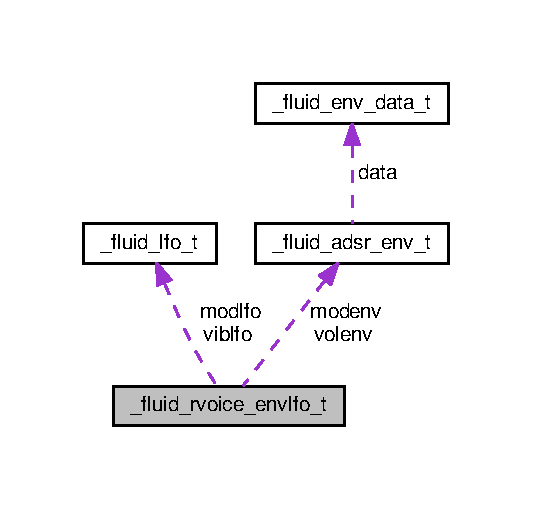
\includegraphics[width=256pt]{struct__fluid__rvoice__envlfo__t__coll__graph}
\end{center}
\end{figure}
\subsection*{Public Attributes}
\begin{DoxyCompactItemize}
\item 
unsigned int \hyperlink{struct__fluid__rvoice__envlfo__t_af514bc86e8a99e45c6fd85fef06af7c5}{ticks}
\item 
unsigned int \hyperlink{struct__fluid__rvoice__envlfo__t_a4f2b784401cce36f67b25c224fe8563a}{noteoff\+\_\+ticks}
\item 
\hyperlink{fluid__adsr__env_8h_aa25feae46766a240357227c5113d2363}{fluid\+\_\+adsr\+\_\+env\+\_\+t} \hyperlink{struct__fluid__rvoice__envlfo__t_a866feac7049752f2fe82701b4a1075b4}{volenv}
\item 
\hyperlink{fluid__adsr__env_8h_aa25feae46766a240357227c5113d2363}{fluid\+\_\+adsr\+\_\+env\+\_\+t} \hyperlink{struct__fluid__rvoice__envlfo__t_a6de3b978b3c1f3fcc6c7a25098c89e76}{modenv}
\item 
\hyperlink{fluidsynth__priv_8h_a9e96f0917747b69cabb7c671bc693dbb}{fluid\+\_\+real\+\_\+t} \hyperlink{struct__fluid__rvoice__envlfo__t_a33967ca6a5a288f221a386a83c0dbd3a}{modenv\+\_\+to\+\_\+fc}
\item 
\hyperlink{fluidsynth__priv_8h_a9e96f0917747b69cabb7c671bc693dbb}{fluid\+\_\+real\+\_\+t} \hyperlink{struct__fluid__rvoice__envlfo__t_a3af0215a1dc5de8e3bfa5c229c3b0d6f}{modenv\+\_\+to\+\_\+pitch}
\item 
\hyperlink{fluid__lfo_8h_af55e78144a43622031cd41ec0f044b85}{fluid\+\_\+lfo\+\_\+t} \hyperlink{struct__fluid__rvoice__envlfo__t_ac0dffe0060d861ad13a605a00d271940}{modlfo}
\item 
\hyperlink{fluidsynth__priv_8h_a9e96f0917747b69cabb7c671bc693dbb}{fluid\+\_\+real\+\_\+t} \hyperlink{struct__fluid__rvoice__envlfo__t_a911bf2423d7b6525aa7e01ab88d5fa5e}{modlfo\+\_\+to\+\_\+fc}
\item 
\hyperlink{fluidsynth__priv_8h_a9e96f0917747b69cabb7c671bc693dbb}{fluid\+\_\+real\+\_\+t} \hyperlink{struct__fluid__rvoice__envlfo__t_a8199e8bc6407548355be62ff598846e0}{modlfo\+\_\+to\+\_\+pitch}
\item 
\hyperlink{fluidsynth__priv_8h_a9e96f0917747b69cabb7c671bc693dbb}{fluid\+\_\+real\+\_\+t} \hyperlink{struct__fluid__rvoice__envlfo__t_a7dd0ae5895ccc48d35a5c5bc331d832d}{modlfo\+\_\+to\+\_\+vol}
\item 
\hyperlink{fluid__lfo_8h_af55e78144a43622031cd41ec0f044b85}{fluid\+\_\+lfo\+\_\+t} \hyperlink{struct__fluid__rvoice__envlfo__t_ab78f547cd36068f9b1dc10d4c4e8eb36}{viblfo}
\item 
\hyperlink{fluidsynth__priv_8h_a9e96f0917747b69cabb7c671bc693dbb}{fluid\+\_\+real\+\_\+t} \hyperlink{struct__fluid__rvoice__envlfo__t_aca22c12e458985567c65eaf11435b2dc}{viblfo\+\_\+to\+\_\+pitch}
\end{DoxyCompactItemize}


\subsection{Member Data Documentation}
\mbox{\Hypertarget{struct__fluid__rvoice__envlfo__t_a6de3b978b3c1f3fcc6c7a25098c89e76}\label{struct__fluid__rvoice__envlfo__t_a6de3b978b3c1f3fcc6c7a25098c89e76}} 
\index{\+\_\+fluid\+\_\+rvoice\+\_\+envlfo\+\_\+t@{\+\_\+fluid\+\_\+rvoice\+\_\+envlfo\+\_\+t}!modenv@{modenv}}
\index{modenv@{modenv}!\+\_\+fluid\+\_\+rvoice\+\_\+envlfo\+\_\+t@{\+\_\+fluid\+\_\+rvoice\+\_\+envlfo\+\_\+t}}
\subsubsection{\texorpdfstring{modenv}{modenv}}
{\footnotesize\ttfamily \hyperlink{fluid__adsr__env_8h_aa25feae46766a240357227c5113d2363}{fluid\+\_\+adsr\+\_\+env\+\_\+t} \+\_\+fluid\+\_\+rvoice\+\_\+envlfo\+\_\+t\+::modenv}

\mbox{\Hypertarget{struct__fluid__rvoice__envlfo__t_a33967ca6a5a288f221a386a83c0dbd3a}\label{struct__fluid__rvoice__envlfo__t_a33967ca6a5a288f221a386a83c0dbd3a}} 
\index{\+\_\+fluid\+\_\+rvoice\+\_\+envlfo\+\_\+t@{\+\_\+fluid\+\_\+rvoice\+\_\+envlfo\+\_\+t}!modenv\+\_\+to\+\_\+fc@{modenv\+\_\+to\+\_\+fc}}
\index{modenv\+\_\+to\+\_\+fc@{modenv\+\_\+to\+\_\+fc}!\+\_\+fluid\+\_\+rvoice\+\_\+envlfo\+\_\+t@{\+\_\+fluid\+\_\+rvoice\+\_\+envlfo\+\_\+t}}
\subsubsection{\texorpdfstring{modenv\+\_\+to\+\_\+fc}{modenv\_to\_fc}}
{\footnotesize\ttfamily \hyperlink{fluidsynth__priv_8h_a9e96f0917747b69cabb7c671bc693dbb}{fluid\+\_\+real\+\_\+t} \+\_\+fluid\+\_\+rvoice\+\_\+envlfo\+\_\+t\+::modenv\+\_\+to\+\_\+fc}

\mbox{\Hypertarget{struct__fluid__rvoice__envlfo__t_a3af0215a1dc5de8e3bfa5c229c3b0d6f}\label{struct__fluid__rvoice__envlfo__t_a3af0215a1dc5de8e3bfa5c229c3b0d6f}} 
\index{\+\_\+fluid\+\_\+rvoice\+\_\+envlfo\+\_\+t@{\+\_\+fluid\+\_\+rvoice\+\_\+envlfo\+\_\+t}!modenv\+\_\+to\+\_\+pitch@{modenv\+\_\+to\+\_\+pitch}}
\index{modenv\+\_\+to\+\_\+pitch@{modenv\+\_\+to\+\_\+pitch}!\+\_\+fluid\+\_\+rvoice\+\_\+envlfo\+\_\+t@{\+\_\+fluid\+\_\+rvoice\+\_\+envlfo\+\_\+t}}
\subsubsection{\texorpdfstring{modenv\+\_\+to\+\_\+pitch}{modenv\_to\_pitch}}
{\footnotesize\ttfamily \hyperlink{fluidsynth__priv_8h_a9e96f0917747b69cabb7c671bc693dbb}{fluid\+\_\+real\+\_\+t} \+\_\+fluid\+\_\+rvoice\+\_\+envlfo\+\_\+t\+::modenv\+\_\+to\+\_\+pitch}

\mbox{\Hypertarget{struct__fluid__rvoice__envlfo__t_ac0dffe0060d861ad13a605a00d271940}\label{struct__fluid__rvoice__envlfo__t_ac0dffe0060d861ad13a605a00d271940}} 
\index{\+\_\+fluid\+\_\+rvoice\+\_\+envlfo\+\_\+t@{\+\_\+fluid\+\_\+rvoice\+\_\+envlfo\+\_\+t}!modlfo@{modlfo}}
\index{modlfo@{modlfo}!\+\_\+fluid\+\_\+rvoice\+\_\+envlfo\+\_\+t@{\+\_\+fluid\+\_\+rvoice\+\_\+envlfo\+\_\+t}}
\subsubsection{\texorpdfstring{modlfo}{modlfo}}
{\footnotesize\ttfamily \hyperlink{fluid__lfo_8h_af55e78144a43622031cd41ec0f044b85}{fluid\+\_\+lfo\+\_\+t} \+\_\+fluid\+\_\+rvoice\+\_\+envlfo\+\_\+t\+::modlfo}

\mbox{\Hypertarget{struct__fluid__rvoice__envlfo__t_a911bf2423d7b6525aa7e01ab88d5fa5e}\label{struct__fluid__rvoice__envlfo__t_a911bf2423d7b6525aa7e01ab88d5fa5e}} 
\index{\+\_\+fluid\+\_\+rvoice\+\_\+envlfo\+\_\+t@{\+\_\+fluid\+\_\+rvoice\+\_\+envlfo\+\_\+t}!modlfo\+\_\+to\+\_\+fc@{modlfo\+\_\+to\+\_\+fc}}
\index{modlfo\+\_\+to\+\_\+fc@{modlfo\+\_\+to\+\_\+fc}!\+\_\+fluid\+\_\+rvoice\+\_\+envlfo\+\_\+t@{\+\_\+fluid\+\_\+rvoice\+\_\+envlfo\+\_\+t}}
\subsubsection{\texorpdfstring{modlfo\+\_\+to\+\_\+fc}{modlfo\_to\_fc}}
{\footnotesize\ttfamily \hyperlink{fluidsynth__priv_8h_a9e96f0917747b69cabb7c671bc693dbb}{fluid\+\_\+real\+\_\+t} \+\_\+fluid\+\_\+rvoice\+\_\+envlfo\+\_\+t\+::modlfo\+\_\+to\+\_\+fc}

\mbox{\Hypertarget{struct__fluid__rvoice__envlfo__t_a8199e8bc6407548355be62ff598846e0}\label{struct__fluid__rvoice__envlfo__t_a8199e8bc6407548355be62ff598846e0}} 
\index{\+\_\+fluid\+\_\+rvoice\+\_\+envlfo\+\_\+t@{\+\_\+fluid\+\_\+rvoice\+\_\+envlfo\+\_\+t}!modlfo\+\_\+to\+\_\+pitch@{modlfo\+\_\+to\+\_\+pitch}}
\index{modlfo\+\_\+to\+\_\+pitch@{modlfo\+\_\+to\+\_\+pitch}!\+\_\+fluid\+\_\+rvoice\+\_\+envlfo\+\_\+t@{\+\_\+fluid\+\_\+rvoice\+\_\+envlfo\+\_\+t}}
\subsubsection{\texorpdfstring{modlfo\+\_\+to\+\_\+pitch}{modlfo\_to\_pitch}}
{\footnotesize\ttfamily \hyperlink{fluidsynth__priv_8h_a9e96f0917747b69cabb7c671bc693dbb}{fluid\+\_\+real\+\_\+t} \+\_\+fluid\+\_\+rvoice\+\_\+envlfo\+\_\+t\+::modlfo\+\_\+to\+\_\+pitch}

\mbox{\Hypertarget{struct__fluid__rvoice__envlfo__t_a7dd0ae5895ccc48d35a5c5bc331d832d}\label{struct__fluid__rvoice__envlfo__t_a7dd0ae5895ccc48d35a5c5bc331d832d}} 
\index{\+\_\+fluid\+\_\+rvoice\+\_\+envlfo\+\_\+t@{\+\_\+fluid\+\_\+rvoice\+\_\+envlfo\+\_\+t}!modlfo\+\_\+to\+\_\+vol@{modlfo\+\_\+to\+\_\+vol}}
\index{modlfo\+\_\+to\+\_\+vol@{modlfo\+\_\+to\+\_\+vol}!\+\_\+fluid\+\_\+rvoice\+\_\+envlfo\+\_\+t@{\+\_\+fluid\+\_\+rvoice\+\_\+envlfo\+\_\+t}}
\subsubsection{\texorpdfstring{modlfo\+\_\+to\+\_\+vol}{modlfo\_to\_vol}}
{\footnotesize\ttfamily \hyperlink{fluidsynth__priv_8h_a9e96f0917747b69cabb7c671bc693dbb}{fluid\+\_\+real\+\_\+t} \+\_\+fluid\+\_\+rvoice\+\_\+envlfo\+\_\+t\+::modlfo\+\_\+to\+\_\+vol}

\mbox{\Hypertarget{struct__fluid__rvoice__envlfo__t_a4f2b784401cce36f67b25c224fe8563a}\label{struct__fluid__rvoice__envlfo__t_a4f2b784401cce36f67b25c224fe8563a}} 
\index{\+\_\+fluid\+\_\+rvoice\+\_\+envlfo\+\_\+t@{\+\_\+fluid\+\_\+rvoice\+\_\+envlfo\+\_\+t}!noteoff\+\_\+ticks@{noteoff\+\_\+ticks}}
\index{noteoff\+\_\+ticks@{noteoff\+\_\+ticks}!\+\_\+fluid\+\_\+rvoice\+\_\+envlfo\+\_\+t@{\+\_\+fluid\+\_\+rvoice\+\_\+envlfo\+\_\+t}}
\subsubsection{\texorpdfstring{noteoff\+\_\+ticks}{noteoff\_ticks}}
{\footnotesize\ttfamily unsigned int \+\_\+fluid\+\_\+rvoice\+\_\+envlfo\+\_\+t\+::noteoff\+\_\+ticks}

\mbox{\Hypertarget{struct__fluid__rvoice__envlfo__t_af514bc86e8a99e45c6fd85fef06af7c5}\label{struct__fluid__rvoice__envlfo__t_af514bc86e8a99e45c6fd85fef06af7c5}} 
\index{\+\_\+fluid\+\_\+rvoice\+\_\+envlfo\+\_\+t@{\+\_\+fluid\+\_\+rvoice\+\_\+envlfo\+\_\+t}!ticks@{ticks}}
\index{ticks@{ticks}!\+\_\+fluid\+\_\+rvoice\+\_\+envlfo\+\_\+t@{\+\_\+fluid\+\_\+rvoice\+\_\+envlfo\+\_\+t}}
\subsubsection{\texorpdfstring{ticks}{ticks}}
{\footnotesize\ttfamily unsigned int \+\_\+fluid\+\_\+rvoice\+\_\+envlfo\+\_\+t\+::ticks}

\mbox{\Hypertarget{struct__fluid__rvoice__envlfo__t_ab78f547cd36068f9b1dc10d4c4e8eb36}\label{struct__fluid__rvoice__envlfo__t_ab78f547cd36068f9b1dc10d4c4e8eb36}} 
\index{\+\_\+fluid\+\_\+rvoice\+\_\+envlfo\+\_\+t@{\+\_\+fluid\+\_\+rvoice\+\_\+envlfo\+\_\+t}!viblfo@{viblfo}}
\index{viblfo@{viblfo}!\+\_\+fluid\+\_\+rvoice\+\_\+envlfo\+\_\+t@{\+\_\+fluid\+\_\+rvoice\+\_\+envlfo\+\_\+t}}
\subsubsection{\texorpdfstring{viblfo}{viblfo}}
{\footnotesize\ttfamily \hyperlink{fluid__lfo_8h_af55e78144a43622031cd41ec0f044b85}{fluid\+\_\+lfo\+\_\+t} \+\_\+fluid\+\_\+rvoice\+\_\+envlfo\+\_\+t\+::viblfo}

\mbox{\Hypertarget{struct__fluid__rvoice__envlfo__t_aca22c12e458985567c65eaf11435b2dc}\label{struct__fluid__rvoice__envlfo__t_aca22c12e458985567c65eaf11435b2dc}} 
\index{\+\_\+fluid\+\_\+rvoice\+\_\+envlfo\+\_\+t@{\+\_\+fluid\+\_\+rvoice\+\_\+envlfo\+\_\+t}!viblfo\+\_\+to\+\_\+pitch@{viblfo\+\_\+to\+\_\+pitch}}
\index{viblfo\+\_\+to\+\_\+pitch@{viblfo\+\_\+to\+\_\+pitch}!\+\_\+fluid\+\_\+rvoice\+\_\+envlfo\+\_\+t@{\+\_\+fluid\+\_\+rvoice\+\_\+envlfo\+\_\+t}}
\subsubsection{\texorpdfstring{viblfo\+\_\+to\+\_\+pitch}{viblfo\_to\_pitch}}
{\footnotesize\ttfamily \hyperlink{fluidsynth__priv_8h_a9e96f0917747b69cabb7c671bc693dbb}{fluid\+\_\+real\+\_\+t} \+\_\+fluid\+\_\+rvoice\+\_\+envlfo\+\_\+t\+::viblfo\+\_\+to\+\_\+pitch}

\mbox{\Hypertarget{struct__fluid__rvoice__envlfo__t_a866feac7049752f2fe82701b4a1075b4}\label{struct__fluid__rvoice__envlfo__t_a866feac7049752f2fe82701b4a1075b4}} 
\index{\+\_\+fluid\+\_\+rvoice\+\_\+envlfo\+\_\+t@{\+\_\+fluid\+\_\+rvoice\+\_\+envlfo\+\_\+t}!volenv@{volenv}}
\index{volenv@{volenv}!\+\_\+fluid\+\_\+rvoice\+\_\+envlfo\+\_\+t@{\+\_\+fluid\+\_\+rvoice\+\_\+envlfo\+\_\+t}}
\subsubsection{\texorpdfstring{volenv}{volenv}}
{\footnotesize\ttfamily \hyperlink{fluid__adsr__env_8h_aa25feae46766a240357227c5113d2363}{fluid\+\_\+adsr\+\_\+env\+\_\+t} \+\_\+fluid\+\_\+rvoice\+\_\+envlfo\+\_\+t\+::volenv}



The documentation for this struct was generated from the following file\+:\begin{DoxyCompactItemize}
\item 
rvoice/\hyperlink{fluid__rvoice_8h}{fluid\+\_\+rvoice.\+h}\end{DoxyCompactItemize}

\hypertarget{struct__fluid__rvoice__event__t}{}\section{\+\_\+fluid\+\_\+rvoice\+\_\+event\+\_\+t Struct Reference}
\label{struct__fluid__rvoice__event__t}\index{\+\_\+fluid\+\_\+rvoice\+\_\+event\+\_\+t@{\+\_\+fluid\+\_\+rvoice\+\_\+event\+\_\+t}}


{\ttfamily \#include $<$fluid\+\_\+rvoice\+\_\+event.\+h$>$}



Collaboration diagram for \+\_\+fluid\+\_\+rvoice\+\_\+event\+\_\+t\+:
\nopagebreak
\begin{figure}[H]
\begin{center}
\leavevmode
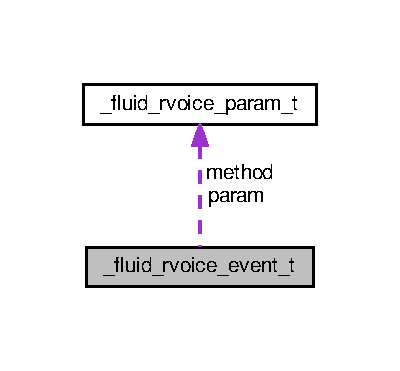
\includegraphics[width=192pt]{struct__fluid__rvoice__event__t__coll__graph}
\end{center}
\end{figure}
\subsection*{Public Attributes}
\begin{DoxyCompactItemize}
\item 
\hyperlink{fluidsynth__priv_8h_a0060fc40a6e757de7831c327a50f367f}{fluid\+\_\+rvoice\+\_\+function\+\_\+t} \hyperlink{struct__fluid__rvoice__event__t_a6996b53072eb21fa652ae8a9e21af8b7}{method}
\item 
void $\ast$ \hyperlink{struct__fluid__rvoice__event__t_acb0e1885f335058c24135b2363bfec3a}{object}
\item 
\hyperlink{fluidsynth__priv_8h_a4a8827d32fba2a1b5404844259d3d4d0}{fluid\+\_\+rvoice\+\_\+param\+\_\+t} \hyperlink{struct__fluid__rvoice__event__t_a7a9db4f028eb563d83802e8f474c563a}{param} \mbox{[}\hyperlink{fluidsynth__priv_8h_a726ca809ffd3d67ab4b8476646f26635a51ab886d33970c14e4b358ade8efee22}{M\+A\+X\+\_\+\+E\+V\+E\+N\+T\+\_\+\+P\+A\+R\+A\+MS}\mbox{]}
\end{DoxyCompactItemize}


\subsection{Member Data Documentation}
\mbox{\Hypertarget{struct__fluid__rvoice__event__t_a6996b53072eb21fa652ae8a9e21af8b7}\label{struct__fluid__rvoice__event__t_a6996b53072eb21fa652ae8a9e21af8b7}} 
\index{\+\_\+fluid\+\_\+rvoice\+\_\+event\+\_\+t@{\+\_\+fluid\+\_\+rvoice\+\_\+event\+\_\+t}!method@{method}}
\index{method@{method}!\+\_\+fluid\+\_\+rvoice\+\_\+event\+\_\+t@{\+\_\+fluid\+\_\+rvoice\+\_\+event\+\_\+t}}
\subsubsection{\texorpdfstring{method}{method}}
{\footnotesize\ttfamily \hyperlink{fluidsynth__priv_8h_a0060fc40a6e757de7831c327a50f367f}{fluid\+\_\+rvoice\+\_\+function\+\_\+t} \+\_\+fluid\+\_\+rvoice\+\_\+event\+\_\+t\+::method}

\mbox{\Hypertarget{struct__fluid__rvoice__event__t_acb0e1885f335058c24135b2363bfec3a}\label{struct__fluid__rvoice__event__t_acb0e1885f335058c24135b2363bfec3a}} 
\index{\+\_\+fluid\+\_\+rvoice\+\_\+event\+\_\+t@{\+\_\+fluid\+\_\+rvoice\+\_\+event\+\_\+t}!object@{object}}
\index{object@{object}!\+\_\+fluid\+\_\+rvoice\+\_\+event\+\_\+t@{\+\_\+fluid\+\_\+rvoice\+\_\+event\+\_\+t}}
\subsubsection{\texorpdfstring{object}{object}}
{\footnotesize\ttfamily void$\ast$ \+\_\+fluid\+\_\+rvoice\+\_\+event\+\_\+t\+::object}

\mbox{\Hypertarget{struct__fluid__rvoice__event__t_a7a9db4f028eb563d83802e8f474c563a}\label{struct__fluid__rvoice__event__t_a7a9db4f028eb563d83802e8f474c563a}} 
\index{\+\_\+fluid\+\_\+rvoice\+\_\+event\+\_\+t@{\+\_\+fluid\+\_\+rvoice\+\_\+event\+\_\+t}!param@{param}}
\index{param@{param}!\+\_\+fluid\+\_\+rvoice\+\_\+event\+\_\+t@{\+\_\+fluid\+\_\+rvoice\+\_\+event\+\_\+t}}
\subsubsection{\texorpdfstring{param}{param}}
{\footnotesize\ttfamily \hyperlink{fluidsynth__priv_8h_a4a8827d32fba2a1b5404844259d3d4d0}{fluid\+\_\+rvoice\+\_\+param\+\_\+t} \+\_\+fluid\+\_\+rvoice\+\_\+event\+\_\+t\+::param\mbox{[}\hyperlink{fluidsynth__priv_8h_a726ca809ffd3d67ab4b8476646f26635a51ab886d33970c14e4b358ade8efee22}{M\+A\+X\+\_\+\+E\+V\+E\+N\+T\+\_\+\+P\+A\+R\+A\+MS}\mbox{]}}



The documentation for this struct was generated from the following file\+:\begin{DoxyCompactItemize}
\item 
rvoice/\hyperlink{fluid__rvoice__event_8h}{fluid\+\_\+rvoice\+\_\+event.\+h}\end{DoxyCompactItemize}

\hypertarget{struct__fluid__rvoice__eventhandler__t}{}\section{\+\_\+fluid\+\_\+rvoice\+\_\+eventhandler\+\_\+t Struct Reference}
\label{struct__fluid__rvoice__eventhandler__t}\index{\+\_\+fluid\+\_\+rvoice\+\_\+eventhandler\+\_\+t@{\+\_\+fluid\+\_\+rvoice\+\_\+eventhandler\+\_\+t}}


{\ttfamily \#include $<$fluid\+\_\+rvoice\+\_\+event.\+h$>$}



Collaboration diagram for \+\_\+fluid\+\_\+rvoice\+\_\+eventhandler\+\_\+t\+:
\nopagebreak
\begin{figure}[H]
\begin{center}
\leavevmode
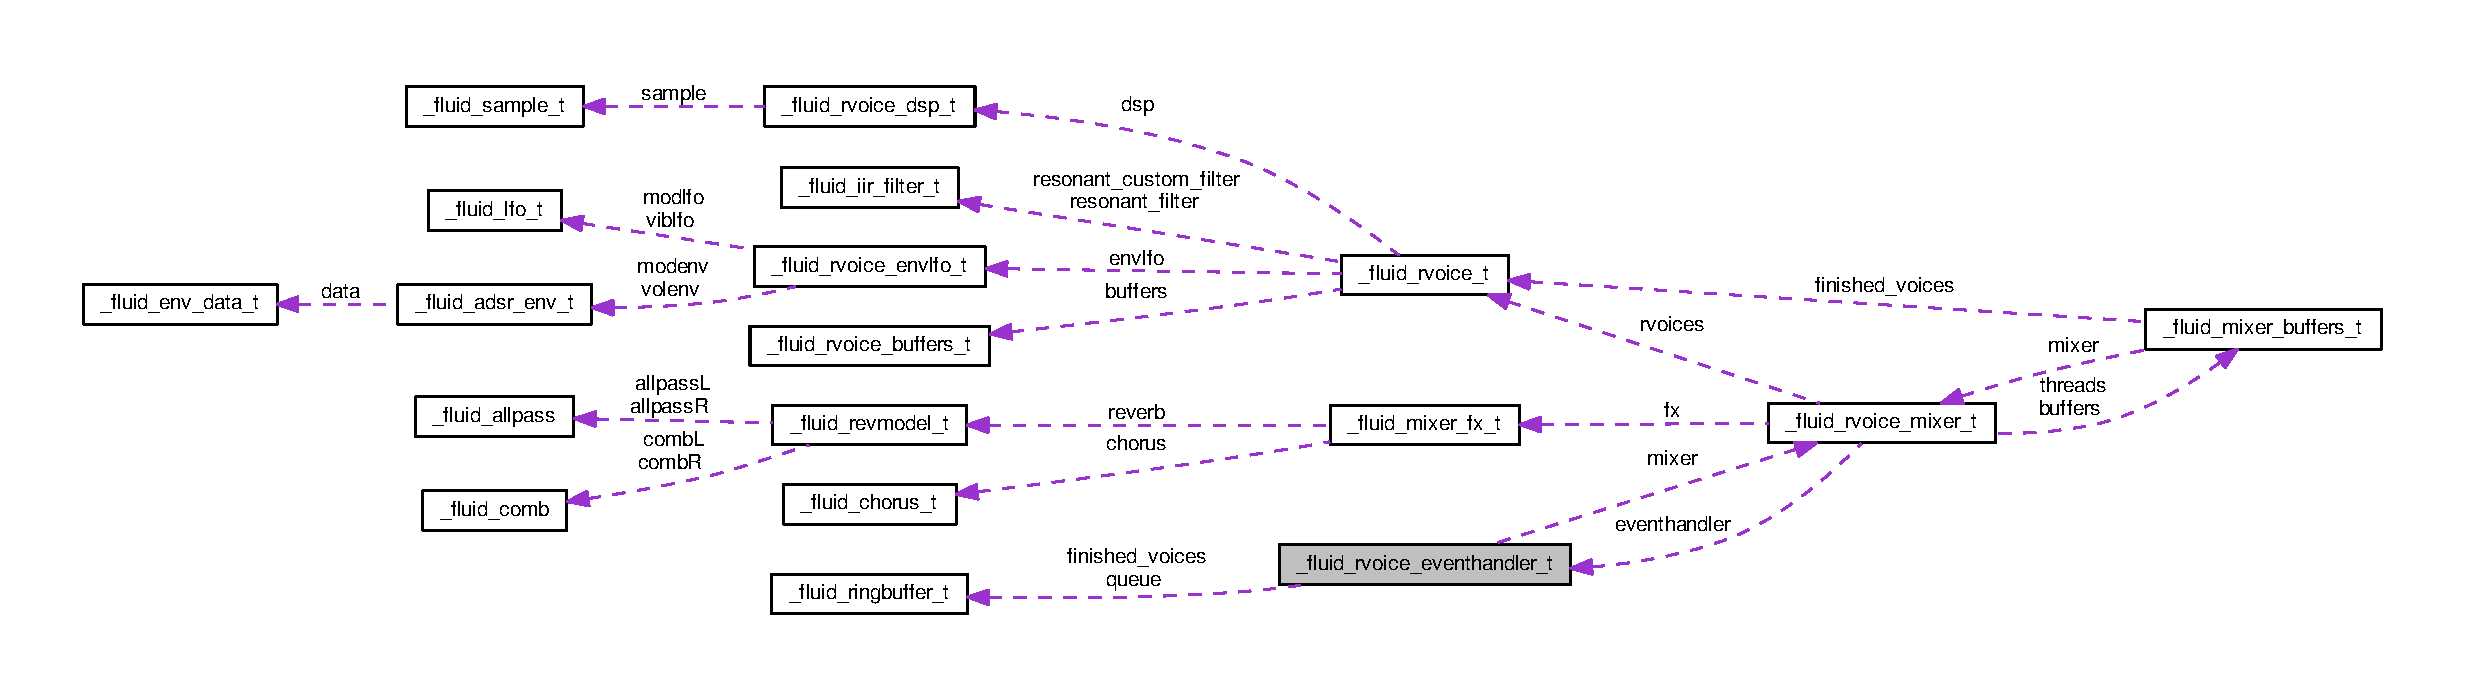
\includegraphics[width=350pt]{struct__fluid__rvoice__eventhandler__t__coll__graph}
\end{center}
\end{figure}
\subsection*{Public Attributes}
\begin{DoxyCompactItemize}
\item 
\hyperlink{fluid__ringbuffer_8h_acae50537c355202b403188c17c9a9f98}{fluid\+\_\+ringbuffer\+\_\+t} $\ast$ \hyperlink{struct__fluid__rvoice__eventhandler__t_a0ba6a044aaf14287ad847444e841f4de}{queue}
\item 
\hyperlink{fluidsynth__priv_8h_a6b8be882dd9958ea3635a868e1bf5152}{fluid\+\_\+atomic\+\_\+int\+\_\+t} \hyperlink{struct__fluid__rvoice__eventhandler__t_a65dbd6065de0b535ad69696923aaf6ae}{queue\+\_\+stored}
\item 
\hyperlink{fluid__ringbuffer_8h_acae50537c355202b403188c17c9a9f98}{fluid\+\_\+ringbuffer\+\_\+t} $\ast$ \hyperlink{struct__fluid__rvoice__eventhandler__t_a8a2038443e5f835cdb531684b23d1392}{finished\+\_\+voices}
\item 
\hyperlink{fluid__rvoice__mixer_8h_a546bd76f60c5458d73d6c72e3f01d0bf}{fluid\+\_\+rvoice\+\_\+mixer\+\_\+t} $\ast$ \hyperlink{struct__fluid__rvoice__eventhandler__t_a3c8ca9652d789628db1faab90d43b83a}{mixer}
\end{DoxyCompactItemize}


\subsection{Member Data Documentation}
\mbox{\Hypertarget{struct__fluid__rvoice__eventhandler__t_a8a2038443e5f835cdb531684b23d1392}\label{struct__fluid__rvoice__eventhandler__t_a8a2038443e5f835cdb531684b23d1392}} 
\index{\+\_\+fluid\+\_\+rvoice\+\_\+eventhandler\+\_\+t@{\+\_\+fluid\+\_\+rvoice\+\_\+eventhandler\+\_\+t}!finished\+\_\+voices@{finished\+\_\+voices}}
\index{finished\+\_\+voices@{finished\+\_\+voices}!\+\_\+fluid\+\_\+rvoice\+\_\+eventhandler\+\_\+t@{\+\_\+fluid\+\_\+rvoice\+\_\+eventhandler\+\_\+t}}
\subsubsection{\texorpdfstring{finished\+\_\+voices}{finished\_voices}}
{\footnotesize\ttfamily \hyperlink{fluid__ringbuffer_8h_acae50537c355202b403188c17c9a9f98}{fluid\+\_\+ringbuffer\+\_\+t}$\ast$ \+\_\+fluid\+\_\+rvoice\+\_\+eventhandler\+\_\+t\+::finished\+\_\+voices}

return queue from handler, list of fluid\+\_\+rvoice\+\_\+t$\ast$ \mbox{\Hypertarget{struct__fluid__rvoice__eventhandler__t_a3c8ca9652d789628db1faab90d43b83a}\label{struct__fluid__rvoice__eventhandler__t_a3c8ca9652d789628db1faab90d43b83a}} 
\index{\+\_\+fluid\+\_\+rvoice\+\_\+eventhandler\+\_\+t@{\+\_\+fluid\+\_\+rvoice\+\_\+eventhandler\+\_\+t}!mixer@{mixer}}
\index{mixer@{mixer}!\+\_\+fluid\+\_\+rvoice\+\_\+eventhandler\+\_\+t@{\+\_\+fluid\+\_\+rvoice\+\_\+eventhandler\+\_\+t}}
\subsubsection{\texorpdfstring{mixer}{mixer}}
{\footnotesize\ttfamily \hyperlink{fluid__rvoice__mixer_8h_a546bd76f60c5458d73d6c72e3f01d0bf}{fluid\+\_\+rvoice\+\_\+mixer\+\_\+t}$\ast$ \+\_\+fluid\+\_\+rvoice\+\_\+eventhandler\+\_\+t\+::mixer}

\mbox{\Hypertarget{struct__fluid__rvoice__eventhandler__t_a0ba6a044aaf14287ad847444e841f4de}\label{struct__fluid__rvoice__eventhandler__t_a0ba6a044aaf14287ad847444e841f4de}} 
\index{\+\_\+fluid\+\_\+rvoice\+\_\+eventhandler\+\_\+t@{\+\_\+fluid\+\_\+rvoice\+\_\+eventhandler\+\_\+t}!queue@{queue}}
\index{queue@{queue}!\+\_\+fluid\+\_\+rvoice\+\_\+eventhandler\+\_\+t@{\+\_\+fluid\+\_\+rvoice\+\_\+eventhandler\+\_\+t}}
\subsubsection{\texorpdfstring{queue}{queue}}
{\footnotesize\ttfamily \hyperlink{fluid__ringbuffer_8h_acae50537c355202b403188c17c9a9f98}{fluid\+\_\+ringbuffer\+\_\+t}$\ast$ \+\_\+fluid\+\_\+rvoice\+\_\+eventhandler\+\_\+t\+::queue}

List of fluid\+\_\+rvoice\+\_\+event\+\_\+t \mbox{\Hypertarget{struct__fluid__rvoice__eventhandler__t_a65dbd6065de0b535ad69696923aaf6ae}\label{struct__fluid__rvoice__eventhandler__t_a65dbd6065de0b535ad69696923aaf6ae}} 
\index{\+\_\+fluid\+\_\+rvoice\+\_\+eventhandler\+\_\+t@{\+\_\+fluid\+\_\+rvoice\+\_\+eventhandler\+\_\+t}!queue\+\_\+stored@{queue\+\_\+stored}}
\index{queue\+\_\+stored@{queue\+\_\+stored}!\+\_\+fluid\+\_\+rvoice\+\_\+eventhandler\+\_\+t@{\+\_\+fluid\+\_\+rvoice\+\_\+eventhandler\+\_\+t}}
\subsubsection{\texorpdfstring{queue\+\_\+stored}{queue\_stored}}
{\footnotesize\ttfamily \hyperlink{fluidsynth__priv_8h_a6b8be882dd9958ea3635a868e1bf5152}{fluid\+\_\+atomic\+\_\+int\+\_\+t} \+\_\+fluid\+\_\+rvoice\+\_\+eventhandler\+\_\+t\+::queue\+\_\+stored}

Extras pushed but not flushed 

The documentation for this struct was generated from the following file\+:\begin{DoxyCompactItemize}
\item 
rvoice/\hyperlink{fluid__rvoice__event_8h}{fluid\+\_\+rvoice\+\_\+event.\+h}\end{DoxyCompactItemize}

\hypertarget{struct__fluid__rvoice__mixer__t}{}\section{\+\_\+fluid\+\_\+rvoice\+\_\+mixer\+\_\+t Struct Reference}
\label{struct__fluid__rvoice__mixer__t}\index{\+\_\+fluid\+\_\+rvoice\+\_\+mixer\+\_\+t@{\+\_\+fluid\+\_\+rvoice\+\_\+mixer\+\_\+t}}


Collaboration diagram for \+\_\+fluid\+\_\+rvoice\+\_\+mixer\+\_\+t\+:
\nopagebreak
\begin{figure}[H]
\begin{center}
\leavevmode
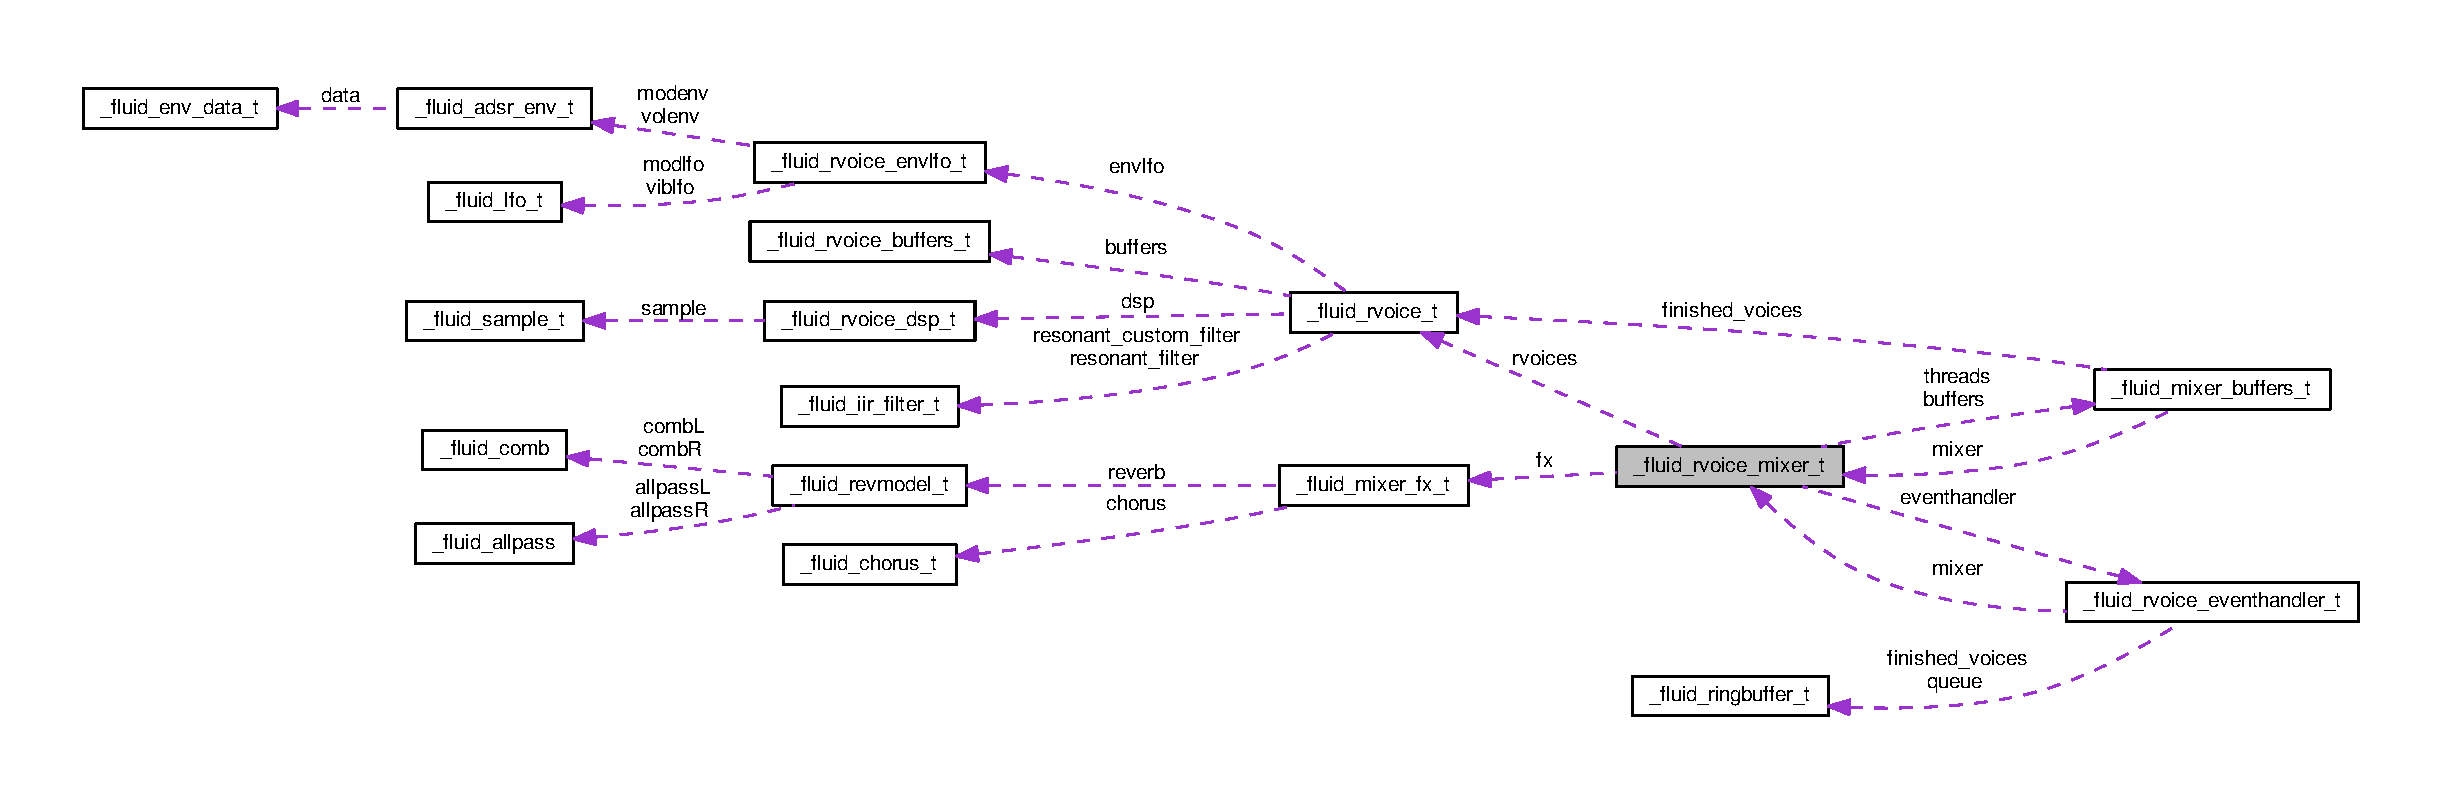
\includegraphics[width=350pt]{struct__fluid__rvoice__mixer__t__coll__graph}
\end{center}
\end{figure}
\subsection*{Public Attributes}
\begin{DoxyCompactItemize}
\item 
\hyperlink{fluid__rvoice__mixer_8c_a86a88518ea54823366a9ff6942a50942}{fluid\+\_\+mixer\+\_\+fx\+\_\+t} \hyperlink{struct__fluid__rvoice__mixer__t_a8e5b10de31b5bef18fbb6e11879d7ae3}{fx}
\item 
\hyperlink{fluid__rvoice__mixer_8c_a013fb7a77265a49b5a52a8150269d306}{fluid\+\_\+mixer\+\_\+buffers\+\_\+t} \hyperlink{struct__fluid__rvoice__mixer__t_ad48ca1c244af544e8538e0cd9fc28885}{buffers}
\item 
\hyperlink{fluidsynth__priv_8h_aa59fe8f0195e9f5099f538d38b126e2a}{fluid\+\_\+rvoice\+\_\+eventhandler\+\_\+t} $\ast$ \hyperlink{struct__fluid__rvoice__mixer__t_a3a8bc6e2a86234c5018842fd5a93da6a}{eventhandler}
\item 
\hyperlink{fluid__rvoice_8h_a3c0405fcfaf1310d760cec3a503c509d}{fluid\+\_\+rvoice\+\_\+t} $\ast$$\ast$ \hyperlink{struct__fluid__rvoice__mixer__t_ae49cd043d26f61593c5d71db9c78fbd7}{rvoices}
\item 
int \hyperlink{struct__fluid__rvoice__mixer__t_a83eb532a3ea76d5a1f6d4583db8a2810}{polyphony}
\item 
int \hyperlink{struct__fluid__rvoice__mixer__t_a9f10ab971cb1806c967d5e521a32c557}{active\+\_\+voices}
\item 
int \hyperlink{struct__fluid__rvoice__mixer__t_a887c2536a382d02788100cac36edce29}{current\+\_\+blockcount}
\item 
\hyperlink{fluidsynth__priv_8h_a6b8be882dd9958ea3635a868e1bf5152}{fluid\+\_\+atomic\+\_\+int\+\_\+t} \hyperlink{struct__fluid__rvoice__mixer__t_a4bb6ff6dab89f7b93eaec2bb3e1fc0d9}{threads\+\_\+should\+\_\+terminate}
\item 
\hyperlink{fluidsynth__priv_8h_a6b8be882dd9958ea3635a868e1bf5152}{fluid\+\_\+atomic\+\_\+int\+\_\+t} \hyperlink{struct__fluid__rvoice__mixer__t_afdf8c9bc75a8455eb148930a847d704e}{current\+\_\+rvoice}
\item 
\hyperlink{fluid__sys_8h_a2125846ddcabc2675983001a57f858b4}{fluid\+\_\+cond\+\_\+t} $\ast$ \hyperlink{struct__fluid__rvoice__mixer__t_ac8faf21be91368b0be637ca95a0469db}{wakeup\+\_\+threads}
\item 
\hyperlink{fluid__sys_8h_a979272b5d11e0e22a1e7a9d6529233bb}{fluid\+\_\+cond\+\_\+mutex\+\_\+t} $\ast$ \hyperlink{struct__fluid__rvoice__mixer__t_a74281ab6f174c3ae488fb09487dda780}{wakeup\+\_\+threads\+\_\+m}
\item 
\hyperlink{fluid__sys_8h_a2125846ddcabc2675983001a57f858b4}{fluid\+\_\+cond\+\_\+t} $\ast$ \hyperlink{struct__fluid__rvoice__mixer__t_a6c42970bab153ccb2f01c8b892add2c4}{thread\+\_\+ready}
\item 
\hyperlink{fluid__sys_8h_a979272b5d11e0e22a1e7a9d6529233bb}{fluid\+\_\+cond\+\_\+mutex\+\_\+t} $\ast$ \hyperlink{struct__fluid__rvoice__mixer__t_a8da70124e197e1716a36b430b16b51a0}{thread\+\_\+ready\+\_\+m}
\item 
int \hyperlink{struct__fluid__rvoice__mixer__t_ac2c9ac57d1761a7bc091bbc6ddf74325}{thread\+\_\+count}
\item 
\hyperlink{fluid__rvoice__mixer_8c_a013fb7a77265a49b5a52a8150269d306}{fluid\+\_\+mixer\+\_\+buffers\+\_\+t} $\ast$ \hyperlink{struct__fluid__rvoice__mixer__t_a2089f036c9210fc2490bc5eb45aed431}{threads}
\end{DoxyCompactItemize}


\subsection{Member Data Documentation}
\mbox{\Hypertarget{struct__fluid__rvoice__mixer__t_a9f10ab971cb1806c967d5e521a32c557}\label{struct__fluid__rvoice__mixer__t_a9f10ab971cb1806c967d5e521a32c557}} 
\index{\+\_\+fluid\+\_\+rvoice\+\_\+mixer\+\_\+t@{\+\_\+fluid\+\_\+rvoice\+\_\+mixer\+\_\+t}!active\+\_\+voices@{active\+\_\+voices}}
\index{active\+\_\+voices@{active\+\_\+voices}!\+\_\+fluid\+\_\+rvoice\+\_\+mixer\+\_\+t@{\+\_\+fluid\+\_\+rvoice\+\_\+mixer\+\_\+t}}
\subsubsection{\texorpdfstring{active\+\_\+voices}{active\_voices}}
{\footnotesize\ttfamily int \+\_\+fluid\+\_\+rvoice\+\_\+mixer\+\_\+t\+::active\+\_\+voices}

Read-\/only\+: Number of non-\/null voices \mbox{\Hypertarget{struct__fluid__rvoice__mixer__t_ad48ca1c244af544e8538e0cd9fc28885}\label{struct__fluid__rvoice__mixer__t_ad48ca1c244af544e8538e0cd9fc28885}} 
\index{\+\_\+fluid\+\_\+rvoice\+\_\+mixer\+\_\+t@{\+\_\+fluid\+\_\+rvoice\+\_\+mixer\+\_\+t}!buffers@{buffers}}
\index{buffers@{buffers}!\+\_\+fluid\+\_\+rvoice\+\_\+mixer\+\_\+t@{\+\_\+fluid\+\_\+rvoice\+\_\+mixer\+\_\+t}}
\subsubsection{\texorpdfstring{buffers}{buffers}}
{\footnotesize\ttfamily \hyperlink{fluid__rvoice__mixer_8c_a013fb7a77265a49b5a52a8150269d306}{fluid\+\_\+mixer\+\_\+buffers\+\_\+t} \+\_\+fluid\+\_\+rvoice\+\_\+mixer\+\_\+t\+::buffers}

Used by mixer only\+: own buffers \mbox{\Hypertarget{struct__fluid__rvoice__mixer__t_a887c2536a382d02788100cac36edce29}\label{struct__fluid__rvoice__mixer__t_a887c2536a382d02788100cac36edce29}} 
\index{\+\_\+fluid\+\_\+rvoice\+\_\+mixer\+\_\+t@{\+\_\+fluid\+\_\+rvoice\+\_\+mixer\+\_\+t}!current\+\_\+blockcount@{current\+\_\+blockcount}}
\index{current\+\_\+blockcount@{current\+\_\+blockcount}!\+\_\+fluid\+\_\+rvoice\+\_\+mixer\+\_\+t@{\+\_\+fluid\+\_\+rvoice\+\_\+mixer\+\_\+t}}
\subsubsection{\texorpdfstring{current\+\_\+blockcount}{current\_blockcount}}
{\footnotesize\ttfamily int \+\_\+fluid\+\_\+rvoice\+\_\+mixer\+\_\+t\+::current\+\_\+blockcount}

Read-\/only\+: how many blocks to process this time \mbox{\Hypertarget{struct__fluid__rvoice__mixer__t_afdf8c9bc75a8455eb148930a847d704e}\label{struct__fluid__rvoice__mixer__t_afdf8c9bc75a8455eb148930a847d704e}} 
\index{\+\_\+fluid\+\_\+rvoice\+\_\+mixer\+\_\+t@{\+\_\+fluid\+\_\+rvoice\+\_\+mixer\+\_\+t}!current\+\_\+rvoice@{current\+\_\+rvoice}}
\index{current\+\_\+rvoice@{current\+\_\+rvoice}!\+\_\+fluid\+\_\+rvoice\+\_\+mixer\+\_\+t@{\+\_\+fluid\+\_\+rvoice\+\_\+mixer\+\_\+t}}
\subsubsection{\texorpdfstring{current\+\_\+rvoice}{current\_rvoice}}
{\footnotesize\ttfamily \hyperlink{fluidsynth__priv_8h_a6b8be882dd9958ea3635a868e1bf5152}{fluid\+\_\+atomic\+\_\+int\+\_\+t} \+\_\+fluid\+\_\+rvoice\+\_\+mixer\+\_\+t\+::current\+\_\+rvoice}

Atomic\+: for the threads to know next voice to \mbox{\Hypertarget{struct__fluid__rvoice__mixer__t_a3a8bc6e2a86234c5018842fd5a93da6a}\label{struct__fluid__rvoice__mixer__t_a3a8bc6e2a86234c5018842fd5a93da6a}} 
\index{\+\_\+fluid\+\_\+rvoice\+\_\+mixer\+\_\+t@{\+\_\+fluid\+\_\+rvoice\+\_\+mixer\+\_\+t}!eventhandler@{eventhandler}}
\index{eventhandler@{eventhandler}!\+\_\+fluid\+\_\+rvoice\+\_\+mixer\+\_\+t@{\+\_\+fluid\+\_\+rvoice\+\_\+mixer\+\_\+t}}
\subsubsection{\texorpdfstring{eventhandler}{eventhandler}}
{\footnotesize\ttfamily \hyperlink{fluidsynth__priv_8h_aa59fe8f0195e9f5099f538d38b126e2a}{fluid\+\_\+rvoice\+\_\+eventhandler\+\_\+t}$\ast$ \+\_\+fluid\+\_\+rvoice\+\_\+mixer\+\_\+t\+::eventhandler}

\mbox{\Hypertarget{struct__fluid__rvoice__mixer__t_a8e5b10de31b5bef18fbb6e11879d7ae3}\label{struct__fluid__rvoice__mixer__t_a8e5b10de31b5bef18fbb6e11879d7ae3}} 
\index{\+\_\+fluid\+\_\+rvoice\+\_\+mixer\+\_\+t@{\+\_\+fluid\+\_\+rvoice\+\_\+mixer\+\_\+t}!fx@{fx}}
\index{fx@{fx}!\+\_\+fluid\+\_\+rvoice\+\_\+mixer\+\_\+t@{\+\_\+fluid\+\_\+rvoice\+\_\+mixer\+\_\+t}}
\subsubsection{\texorpdfstring{fx}{fx}}
{\footnotesize\ttfamily \hyperlink{fluid__rvoice__mixer_8c_a86a88518ea54823366a9ff6942a50942}{fluid\+\_\+mixer\+\_\+fx\+\_\+t} \+\_\+fluid\+\_\+rvoice\+\_\+mixer\+\_\+t\+::fx}

\mbox{\Hypertarget{struct__fluid__rvoice__mixer__t_a83eb532a3ea76d5a1f6d4583db8a2810}\label{struct__fluid__rvoice__mixer__t_a83eb532a3ea76d5a1f6d4583db8a2810}} 
\index{\+\_\+fluid\+\_\+rvoice\+\_\+mixer\+\_\+t@{\+\_\+fluid\+\_\+rvoice\+\_\+mixer\+\_\+t}!polyphony@{polyphony}}
\index{polyphony@{polyphony}!\+\_\+fluid\+\_\+rvoice\+\_\+mixer\+\_\+t@{\+\_\+fluid\+\_\+rvoice\+\_\+mixer\+\_\+t}}
\subsubsection{\texorpdfstring{polyphony}{polyphony}}
{\footnotesize\ttfamily int \+\_\+fluid\+\_\+rvoice\+\_\+mixer\+\_\+t\+::polyphony}

Read-\/only\+: Length of voices array \mbox{\Hypertarget{struct__fluid__rvoice__mixer__t_ae49cd043d26f61593c5d71db9c78fbd7}\label{struct__fluid__rvoice__mixer__t_ae49cd043d26f61593c5d71db9c78fbd7}} 
\index{\+\_\+fluid\+\_\+rvoice\+\_\+mixer\+\_\+t@{\+\_\+fluid\+\_\+rvoice\+\_\+mixer\+\_\+t}!rvoices@{rvoices}}
\index{rvoices@{rvoices}!\+\_\+fluid\+\_\+rvoice\+\_\+mixer\+\_\+t@{\+\_\+fluid\+\_\+rvoice\+\_\+mixer\+\_\+t}}
\subsubsection{\texorpdfstring{rvoices}{rvoices}}
{\footnotesize\ttfamily \hyperlink{fluid__rvoice_8h_a3c0405fcfaf1310d760cec3a503c509d}{fluid\+\_\+rvoice\+\_\+t}$\ast$$\ast$ \+\_\+fluid\+\_\+rvoice\+\_\+mixer\+\_\+t\+::rvoices}

Read-\/only\+: Voices array, sorted so that all nulls are last \mbox{\Hypertarget{struct__fluid__rvoice__mixer__t_ac2c9ac57d1761a7bc091bbc6ddf74325}\label{struct__fluid__rvoice__mixer__t_ac2c9ac57d1761a7bc091bbc6ddf74325}} 
\index{\+\_\+fluid\+\_\+rvoice\+\_\+mixer\+\_\+t@{\+\_\+fluid\+\_\+rvoice\+\_\+mixer\+\_\+t}!thread\+\_\+count@{thread\+\_\+count}}
\index{thread\+\_\+count@{thread\+\_\+count}!\+\_\+fluid\+\_\+rvoice\+\_\+mixer\+\_\+t@{\+\_\+fluid\+\_\+rvoice\+\_\+mixer\+\_\+t}}
\subsubsection{\texorpdfstring{thread\+\_\+count}{thread\_count}}
{\footnotesize\ttfamily int \+\_\+fluid\+\_\+rvoice\+\_\+mixer\+\_\+t\+::thread\+\_\+count}

Number of extra mixer threads for multi-\/core rendering \mbox{\Hypertarget{struct__fluid__rvoice__mixer__t_a6c42970bab153ccb2f01c8b892add2c4}\label{struct__fluid__rvoice__mixer__t_a6c42970bab153ccb2f01c8b892add2c4}} 
\index{\+\_\+fluid\+\_\+rvoice\+\_\+mixer\+\_\+t@{\+\_\+fluid\+\_\+rvoice\+\_\+mixer\+\_\+t}!thread\+\_\+ready@{thread\+\_\+ready}}
\index{thread\+\_\+ready@{thread\+\_\+ready}!\+\_\+fluid\+\_\+rvoice\+\_\+mixer\+\_\+t@{\+\_\+fluid\+\_\+rvoice\+\_\+mixer\+\_\+t}}
\subsubsection{\texorpdfstring{thread\+\_\+ready}{thread\_ready}}
{\footnotesize\ttfamily \hyperlink{fluid__sys_8h_a2125846ddcabc2675983001a57f858b4}{fluid\+\_\+cond\+\_\+t}$\ast$ \+\_\+fluid\+\_\+rvoice\+\_\+mixer\+\_\+t\+::thread\+\_\+ready}

Signalled from thread, when the thread has a buffer ready for mixing \mbox{\Hypertarget{struct__fluid__rvoice__mixer__t_a8da70124e197e1716a36b430b16b51a0}\label{struct__fluid__rvoice__mixer__t_a8da70124e197e1716a36b430b16b51a0}} 
\index{\+\_\+fluid\+\_\+rvoice\+\_\+mixer\+\_\+t@{\+\_\+fluid\+\_\+rvoice\+\_\+mixer\+\_\+t}!thread\+\_\+ready\+\_\+m@{thread\+\_\+ready\+\_\+m}}
\index{thread\+\_\+ready\+\_\+m@{thread\+\_\+ready\+\_\+m}!\+\_\+fluid\+\_\+rvoice\+\_\+mixer\+\_\+t@{\+\_\+fluid\+\_\+rvoice\+\_\+mixer\+\_\+t}}
\subsubsection{\texorpdfstring{thread\+\_\+ready\+\_\+m}{thread\_ready\_m}}
{\footnotesize\ttfamily \hyperlink{fluid__sys_8h_a979272b5d11e0e22a1e7a9d6529233bb}{fluid\+\_\+cond\+\_\+mutex\+\_\+t}$\ast$ \+\_\+fluid\+\_\+rvoice\+\_\+mixer\+\_\+t\+::thread\+\_\+ready\+\_\+m}

thread\+\_\+ready mutex companion \mbox{\Hypertarget{struct__fluid__rvoice__mixer__t_a2089f036c9210fc2490bc5eb45aed431}\label{struct__fluid__rvoice__mixer__t_a2089f036c9210fc2490bc5eb45aed431}} 
\index{\+\_\+fluid\+\_\+rvoice\+\_\+mixer\+\_\+t@{\+\_\+fluid\+\_\+rvoice\+\_\+mixer\+\_\+t}!threads@{threads}}
\index{threads@{threads}!\+\_\+fluid\+\_\+rvoice\+\_\+mixer\+\_\+t@{\+\_\+fluid\+\_\+rvoice\+\_\+mixer\+\_\+t}}
\subsubsection{\texorpdfstring{threads}{threads}}
{\footnotesize\ttfamily \hyperlink{fluid__rvoice__mixer_8c_a013fb7a77265a49b5a52a8150269d306}{fluid\+\_\+mixer\+\_\+buffers\+\_\+t}$\ast$ \+\_\+fluid\+\_\+rvoice\+\_\+mixer\+\_\+t\+::threads}

Array of mixer threads (thread\+\_\+count in length) \mbox{\Hypertarget{struct__fluid__rvoice__mixer__t_a4bb6ff6dab89f7b93eaec2bb3e1fc0d9}\label{struct__fluid__rvoice__mixer__t_a4bb6ff6dab89f7b93eaec2bb3e1fc0d9}} 
\index{\+\_\+fluid\+\_\+rvoice\+\_\+mixer\+\_\+t@{\+\_\+fluid\+\_\+rvoice\+\_\+mixer\+\_\+t}!threads\+\_\+should\+\_\+terminate@{threads\+\_\+should\+\_\+terminate}}
\index{threads\+\_\+should\+\_\+terminate@{threads\+\_\+should\+\_\+terminate}!\+\_\+fluid\+\_\+rvoice\+\_\+mixer\+\_\+t@{\+\_\+fluid\+\_\+rvoice\+\_\+mixer\+\_\+t}}
\subsubsection{\texorpdfstring{threads\+\_\+should\+\_\+terminate}{threads\_should\_terminate}}
{\footnotesize\ttfamily \hyperlink{fluidsynth__priv_8h_a6b8be882dd9958ea3635a868e1bf5152}{fluid\+\_\+atomic\+\_\+int\+\_\+t} \+\_\+fluid\+\_\+rvoice\+\_\+mixer\+\_\+t\+::threads\+\_\+should\+\_\+terminate}

Atomic\+: Set to T\+R\+UE when threads should terminate \mbox{\Hypertarget{struct__fluid__rvoice__mixer__t_ac8faf21be91368b0be637ca95a0469db}\label{struct__fluid__rvoice__mixer__t_ac8faf21be91368b0be637ca95a0469db}} 
\index{\+\_\+fluid\+\_\+rvoice\+\_\+mixer\+\_\+t@{\+\_\+fluid\+\_\+rvoice\+\_\+mixer\+\_\+t}!wakeup\+\_\+threads@{wakeup\+\_\+threads}}
\index{wakeup\+\_\+threads@{wakeup\+\_\+threads}!\+\_\+fluid\+\_\+rvoice\+\_\+mixer\+\_\+t@{\+\_\+fluid\+\_\+rvoice\+\_\+mixer\+\_\+t}}
\subsubsection{\texorpdfstring{wakeup\+\_\+threads}{wakeup\_threads}}
{\footnotesize\ttfamily \hyperlink{fluid__sys_8h_a2125846ddcabc2675983001a57f858b4}{fluid\+\_\+cond\+\_\+t}$\ast$ \+\_\+fluid\+\_\+rvoice\+\_\+mixer\+\_\+t\+::wakeup\+\_\+threads}

Signalled when the threads should wake up \mbox{\Hypertarget{struct__fluid__rvoice__mixer__t_a74281ab6f174c3ae488fb09487dda780}\label{struct__fluid__rvoice__mixer__t_a74281ab6f174c3ae488fb09487dda780}} 
\index{\+\_\+fluid\+\_\+rvoice\+\_\+mixer\+\_\+t@{\+\_\+fluid\+\_\+rvoice\+\_\+mixer\+\_\+t}!wakeup\+\_\+threads\+\_\+m@{wakeup\+\_\+threads\+\_\+m}}
\index{wakeup\+\_\+threads\+\_\+m@{wakeup\+\_\+threads\+\_\+m}!\+\_\+fluid\+\_\+rvoice\+\_\+mixer\+\_\+t@{\+\_\+fluid\+\_\+rvoice\+\_\+mixer\+\_\+t}}
\subsubsection{\texorpdfstring{wakeup\+\_\+threads\+\_\+m}{wakeup\_threads\_m}}
{\footnotesize\ttfamily \hyperlink{fluid__sys_8h_a979272b5d11e0e22a1e7a9d6529233bb}{fluid\+\_\+cond\+\_\+mutex\+\_\+t}$\ast$ \+\_\+fluid\+\_\+rvoice\+\_\+mixer\+\_\+t\+::wakeup\+\_\+threads\+\_\+m}

wakeup\+\_\+threads mutex companion 

The documentation for this struct was generated from the following file\+:\begin{DoxyCompactItemize}
\item 
rvoice/\hyperlink{fluid__rvoice__mixer_8c}{fluid\+\_\+rvoice\+\_\+mixer.\+c}\end{DoxyCompactItemize}

\hypertarget{union__fluid__rvoice__param__t}{}\section{\+\_\+fluid\+\_\+rvoice\+\_\+param\+\_\+t Union Reference}
\label{union__fluid__rvoice__param__t}\index{\+\_\+fluid\+\_\+rvoice\+\_\+param\+\_\+t@{\+\_\+fluid\+\_\+rvoice\+\_\+param\+\_\+t}}


{\ttfamily \#include $<$fluidsynth\+\_\+priv.\+h$>$}

\subsection*{Public Attributes}
\begin{DoxyCompactItemize}
\item 
void $\ast$ \hyperlink{union__fluid__rvoice__param__t_a52a3a904ce9b4cf050d9a50b7c421ce1}{ptr}
\item 
int \hyperlink{union__fluid__rvoice__param__t_a1f989db216e51ea83c102b4ebb0f2118}{i}
\item 
\hyperlink{fluidsynth__priv_8h_a9e96f0917747b69cabb7c671bc693dbb}{fluid\+\_\+real\+\_\+t} \hyperlink{union__fluid__rvoice__param__t_a37c385c55d50be836b0b7116a42b5c8f}{real}
\end{DoxyCompactItemize}


\subsection{Member Data Documentation}
\mbox{\Hypertarget{union__fluid__rvoice__param__t_a1f989db216e51ea83c102b4ebb0f2118}\label{union__fluid__rvoice__param__t_a1f989db216e51ea83c102b4ebb0f2118}} 
\index{\+\_\+fluid\+\_\+rvoice\+\_\+param\+\_\+t@{\+\_\+fluid\+\_\+rvoice\+\_\+param\+\_\+t}!i@{i}}
\index{i@{i}!\+\_\+fluid\+\_\+rvoice\+\_\+param\+\_\+t@{\+\_\+fluid\+\_\+rvoice\+\_\+param\+\_\+t}}
\subsubsection{\texorpdfstring{i}{i}}
{\footnotesize\ttfamily int \+\_\+fluid\+\_\+rvoice\+\_\+param\+\_\+t\+::i}

\mbox{\Hypertarget{union__fluid__rvoice__param__t_a52a3a904ce9b4cf050d9a50b7c421ce1}\label{union__fluid__rvoice__param__t_a52a3a904ce9b4cf050d9a50b7c421ce1}} 
\index{\+\_\+fluid\+\_\+rvoice\+\_\+param\+\_\+t@{\+\_\+fluid\+\_\+rvoice\+\_\+param\+\_\+t}!ptr@{ptr}}
\index{ptr@{ptr}!\+\_\+fluid\+\_\+rvoice\+\_\+param\+\_\+t@{\+\_\+fluid\+\_\+rvoice\+\_\+param\+\_\+t}}
\subsubsection{\texorpdfstring{ptr}{ptr}}
{\footnotesize\ttfamily void$\ast$ \+\_\+fluid\+\_\+rvoice\+\_\+param\+\_\+t\+::ptr}

\mbox{\Hypertarget{union__fluid__rvoice__param__t_a37c385c55d50be836b0b7116a42b5c8f}\label{union__fluid__rvoice__param__t_a37c385c55d50be836b0b7116a42b5c8f}} 
\index{\+\_\+fluid\+\_\+rvoice\+\_\+param\+\_\+t@{\+\_\+fluid\+\_\+rvoice\+\_\+param\+\_\+t}!real@{real}}
\index{real@{real}!\+\_\+fluid\+\_\+rvoice\+\_\+param\+\_\+t@{\+\_\+fluid\+\_\+rvoice\+\_\+param\+\_\+t}}
\subsubsection{\texorpdfstring{real}{real}}
{\footnotesize\ttfamily \hyperlink{fluidsynth__priv_8h_a9e96f0917747b69cabb7c671bc693dbb}{fluid\+\_\+real\+\_\+t} \+\_\+fluid\+\_\+rvoice\+\_\+param\+\_\+t\+::real}



The documentation for this union was generated from the following file\+:\begin{DoxyCompactItemize}
\item 
utils/\hyperlink{fluidsynth__priv_8h}{fluidsynth\+\_\+priv.\+h}\end{DoxyCompactItemize}

\hypertarget{struct__fluid__rvoice__t}{}\section{\+\_\+fluid\+\_\+rvoice\+\_\+t Struct Reference}
\label{struct__fluid__rvoice__t}\index{\+\_\+fluid\+\_\+rvoice\+\_\+t@{\+\_\+fluid\+\_\+rvoice\+\_\+t}}


{\ttfamily \#include $<$fluid\+\_\+rvoice.\+h$>$}



Collaboration diagram for \+\_\+fluid\+\_\+rvoice\+\_\+t\+:
\nopagebreak
\begin{figure}[H]
\begin{center}
\leavevmode
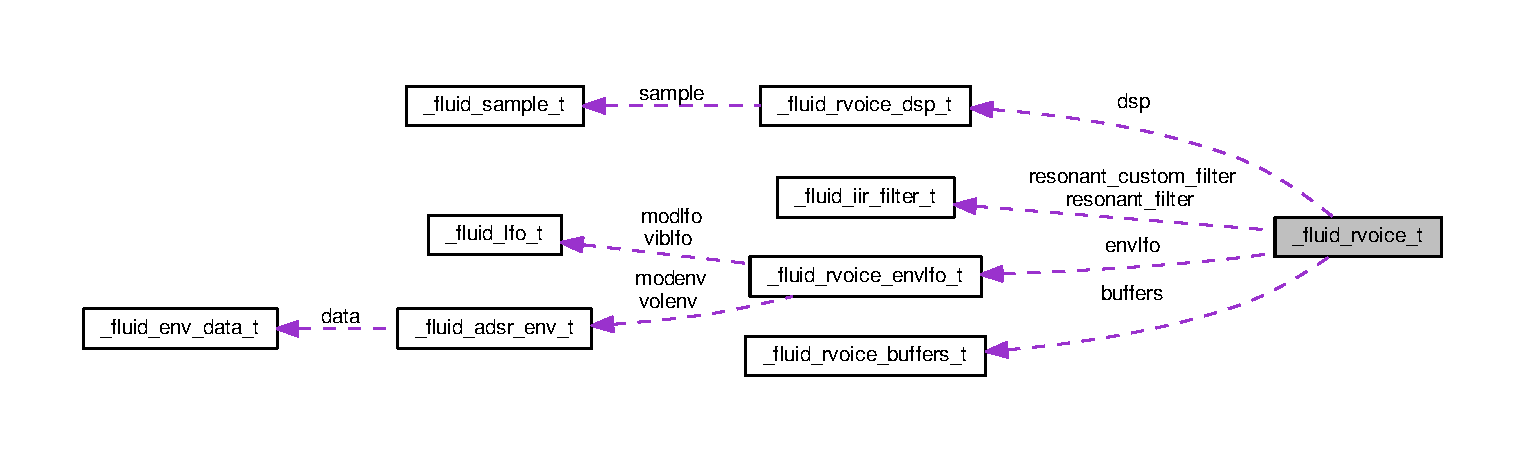
\includegraphics[width=350pt]{struct__fluid__rvoice__t__coll__graph}
\end{center}
\end{figure}
\subsection*{Public Attributes}
\begin{DoxyCompactItemize}
\item 
\hyperlink{fluid__rvoice_8h_a292109da8a8c976f672b78e64acbd1b0}{fluid\+\_\+rvoice\+\_\+envlfo\+\_\+t} \hyperlink{struct__fluid__rvoice__t_a16e90dcb076e8f6498c899110af4ae66}{envlfo}
\item 
\hyperlink{fluid__rvoice_8h_abb83d814377cb6bfcb8761325dce7d58}{fluid\+\_\+rvoice\+\_\+dsp\+\_\+t} \hyperlink{struct__fluid__rvoice__t_aa8fc84b1b084b7b2cadeb73e5bff3550}{dsp}
\item 
\hyperlink{fluid__iir__filter_8h_a195102aefee11bb26f43b39ecf86088a}{fluid\+\_\+iir\+\_\+filter\+\_\+t} \hyperlink{struct__fluid__rvoice__t_a70d7bb364e3f986660e569e4656897d9}{resonant\+\_\+filter}
\item 
\hyperlink{fluid__iir__filter_8h_a195102aefee11bb26f43b39ecf86088a}{fluid\+\_\+iir\+\_\+filter\+\_\+t} \hyperlink{struct__fluid__rvoice__t_acb337f7b611f399554d63516fbe07c33}{resonant\+\_\+custom\+\_\+filter}
\item 
\hyperlink{fluid__rvoice_8h_a4fc5c15c3ffacb81fdae6583648e6461}{fluid\+\_\+rvoice\+\_\+buffers\+\_\+t} \hyperlink{struct__fluid__rvoice__t_a1f4154f8df5e5a7e49770d542fd0014b}{buffers}
\end{DoxyCompactItemize}


\subsection{Member Data Documentation}
\mbox{\Hypertarget{struct__fluid__rvoice__t_a1f4154f8df5e5a7e49770d542fd0014b}\label{struct__fluid__rvoice__t_a1f4154f8df5e5a7e49770d542fd0014b}} 
\index{\+\_\+fluid\+\_\+rvoice\+\_\+t@{\+\_\+fluid\+\_\+rvoice\+\_\+t}!buffers@{buffers}}
\index{buffers@{buffers}!\+\_\+fluid\+\_\+rvoice\+\_\+t@{\+\_\+fluid\+\_\+rvoice\+\_\+t}}
\subsubsection{\texorpdfstring{buffers}{buffers}}
{\footnotesize\ttfamily \hyperlink{fluid__rvoice_8h_a4fc5c15c3ffacb81fdae6583648e6461}{fluid\+\_\+rvoice\+\_\+buffers\+\_\+t} \+\_\+fluid\+\_\+rvoice\+\_\+t\+::buffers}

\mbox{\Hypertarget{struct__fluid__rvoice__t_aa8fc84b1b084b7b2cadeb73e5bff3550}\label{struct__fluid__rvoice__t_aa8fc84b1b084b7b2cadeb73e5bff3550}} 
\index{\+\_\+fluid\+\_\+rvoice\+\_\+t@{\+\_\+fluid\+\_\+rvoice\+\_\+t}!dsp@{dsp}}
\index{dsp@{dsp}!\+\_\+fluid\+\_\+rvoice\+\_\+t@{\+\_\+fluid\+\_\+rvoice\+\_\+t}}
\subsubsection{\texorpdfstring{dsp}{dsp}}
{\footnotesize\ttfamily \hyperlink{fluid__rvoice_8h_abb83d814377cb6bfcb8761325dce7d58}{fluid\+\_\+rvoice\+\_\+dsp\+\_\+t} \+\_\+fluid\+\_\+rvoice\+\_\+t\+::dsp}

\mbox{\Hypertarget{struct__fluid__rvoice__t_a16e90dcb076e8f6498c899110af4ae66}\label{struct__fluid__rvoice__t_a16e90dcb076e8f6498c899110af4ae66}} 
\index{\+\_\+fluid\+\_\+rvoice\+\_\+t@{\+\_\+fluid\+\_\+rvoice\+\_\+t}!envlfo@{envlfo}}
\index{envlfo@{envlfo}!\+\_\+fluid\+\_\+rvoice\+\_\+t@{\+\_\+fluid\+\_\+rvoice\+\_\+t}}
\subsubsection{\texorpdfstring{envlfo}{envlfo}}
{\footnotesize\ttfamily \hyperlink{fluid__rvoice_8h_a292109da8a8c976f672b78e64acbd1b0}{fluid\+\_\+rvoice\+\_\+envlfo\+\_\+t} \+\_\+fluid\+\_\+rvoice\+\_\+t\+::envlfo}

\mbox{\Hypertarget{struct__fluid__rvoice__t_acb337f7b611f399554d63516fbe07c33}\label{struct__fluid__rvoice__t_acb337f7b611f399554d63516fbe07c33}} 
\index{\+\_\+fluid\+\_\+rvoice\+\_\+t@{\+\_\+fluid\+\_\+rvoice\+\_\+t}!resonant\+\_\+custom\+\_\+filter@{resonant\+\_\+custom\+\_\+filter}}
\index{resonant\+\_\+custom\+\_\+filter@{resonant\+\_\+custom\+\_\+filter}!\+\_\+fluid\+\_\+rvoice\+\_\+t@{\+\_\+fluid\+\_\+rvoice\+\_\+t}}
\subsubsection{\texorpdfstring{resonant\+\_\+custom\+\_\+filter}{resonant\_custom\_filter}}
{\footnotesize\ttfamily \hyperlink{fluid__iir__filter_8h_a195102aefee11bb26f43b39ecf86088a}{fluid\+\_\+iir\+\_\+filter\+\_\+t} \+\_\+fluid\+\_\+rvoice\+\_\+t\+::resonant\+\_\+custom\+\_\+filter}

\mbox{\Hypertarget{struct__fluid__rvoice__t_a70d7bb364e3f986660e569e4656897d9}\label{struct__fluid__rvoice__t_a70d7bb364e3f986660e569e4656897d9}} 
\index{\+\_\+fluid\+\_\+rvoice\+\_\+t@{\+\_\+fluid\+\_\+rvoice\+\_\+t}!resonant\+\_\+filter@{resonant\+\_\+filter}}
\index{resonant\+\_\+filter@{resonant\+\_\+filter}!\+\_\+fluid\+\_\+rvoice\+\_\+t@{\+\_\+fluid\+\_\+rvoice\+\_\+t}}
\subsubsection{\texorpdfstring{resonant\+\_\+filter}{resonant\_filter}}
{\footnotesize\ttfamily \hyperlink{fluid__iir__filter_8h_a195102aefee11bb26f43b39ecf86088a}{fluid\+\_\+iir\+\_\+filter\+\_\+t} \+\_\+fluid\+\_\+rvoice\+\_\+t\+::resonant\+\_\+filter}



The documentation for this struct was generated from the following file\+:\begin{DoxyCompactItemize}
\item 
rvoice/\hyperlink{fluid__rvoice_8h}{fluid\+\_\+rvoice.\+h}\end{DoxyCompactItemize}

\hypertarget{struct__fluid__sample__t}{}\section{\+\_\+fluid\+\_\+sample\+\_\+t Struct Reference}
\label{struct__fluid__sample__t}\index{\+\_\+fluid\+\_\+sample\+\_\+t@{\+\_\+fluid\+\_\+sample\+\_\+t}}


{\ttfamily \#include $<$fluid\+\_\+sfont.\+h$>$}

\subsection*{Public Attributes}
\begin{DoxyCompactItemize}
\item 
char \hyperlink{struct__fluid__sample__t_a054c9821ce07e9c680331bfc29cf7a1f}{name} \mbox{[}21\mbox{]}
\item 
unsigned int \hyperlink{struct__fluid__sample__t_aa02d79a03cb990b9f99c6a9161eb1ac6}{source\+\_\+start}
\item 
unsigned int \hyperlink{struct__fluid__sample__t_a9658c79a9458399c4e6c44227d35763f}{source\+\_\+end}
\item 
unsigned int \hyperlink{struct__fluid__sample__t_abcd86e0655e80a45f577c9758917c3c3}{source\+\_\+loopstart}
\item 
unsigned int \hyperlink{struct__fluid__sample__t_ac51da14264b3fea19b77ce1ea3b217ab}{source\+\_\+loopend}
\item 
unsigned int \hyperlink{struct__fluid__sample__t_a239a49135dad3eedf6ea9ada921f9583}{start}
\item 
unsigned int \hyperlink{struct__fluid__sample__t_a955d338a740c562bd9b298d87b165b0c}{end}
\item 
unsigned int \hyperlink{struct__fluid__sample__t_a708e728c1dd67bb62a70e4edd7fc1f1c}{loopstart}
\item 
unsigned int \hyperlink{struct__fluid__sample__t_a3baa4ca199a55b77c2692d9d3211e0d0}{loopend}
\item 
unsigned int \hyperlink{struct__fluid__sample__t_a323da7b5b6db34a67cb59a4b4b0e3e9a}{samplerate}
\item 
int \hyperlink{struct__fluid__sample__t_a1a2bb5f13ed47a3e59b650f9f0cf4bf9}{origpitch}
\item 
int \hyperlink{struct__fluid__sample__t_a12b4133d7631a3043d008fdaa78eb5dc}{pitchadj}
\item 
int \hyperlink{struct__fluid__sample__t_a081352a55ed01814a219875eee20628b}{sampletype}
\item 
int \hyperlink{struct__fluid__sample__t_a376e4ff95b5d7fd522c48417f15eb2a2}{auto\+\_\+free}
\item 
short $\ast$ \hyperlink{struct__fluid__sample__t_a8c7262f51500369fd1a3e5306b458d55}{data}
\item 
char $\ast$ \hyperlink{struct__fluid__sample__t_ad2153e233ec84d2ed36a310330eec820}{data24}
\item 
int \hyperlink{struct__fluid__sample__t_ac054e203acd07ad158256e343f1fd0a5}{amplitude\+\_\+that\+\_\+reaches\+\_\+noise\+\_\+floor\+\_\+is\+\_\+valid}
\item 
double \hyperlink{struct__fluid__sample__t_a91eee4970ca353df88665c0c3119e841}{amplitude\+\_\+that\+\_\+reaches\+\_\+noise\+\_\+floor}
\item 
unsigned int \hyperlink{struct__fluid__sample__t_a50767943f4a3110db0d4e724cdbe65ec}{refcount}
\item 
int \hyperlink{struct__fluid__sample__t_ae26113d0d8e350ad6016066ac027a70c}{preset\+\_\+count}
\item 
int($\ast$ \hyperlink{struct__fluid__sample__t_ad43c2d0777a885a54e1dd3462ded025e}{notify} )(\hyperlink{types_8h_abf9174d452679ca1a4ee7d693fb773cf}{fluid\+\_\+sample\+\_\+t} $\ast$sample, int reason)
\item 
void $\ast$ \hyperlink{struct__fluid__sample__t_a69e7d313f22e2fd35638d064012bda0a}{userdata}
\end{DoxyCompactItemize}


\subsection{Detailed Description}
Virtual Sound\+Font sample. 

\subsection{Member Data Documentation}
\mbox{\Hypertarget{struct__fluid__sample__t_a91eee4970ca353df88665c0c3119e841}\label{struct__fluid__sample__t_a91eee4970ca353df88665c0c3119e841}} 
\index{\+\_\+fluid\+\_\+sample\+\_\+t@{\+\_\+fluid\+\_\+sample\+\_\+t}!amplitude\+\_\+that\+\_\+reaches\+\_\+noise\+\_\+floor@{amplitude\+\_\+that\+\_\+reaches\+\_\+noise\+\_\+floor}}
\index{amplitude\+\_\+that\+\_\+reaches\+\_\+noise\+\_\+floor@{amplitude\+\_\+that\+\_\+reaches\+\_\+noise\+\_\+floor}!\+\_\+fluid\+\_\+sample\+\_\+t@{\+\_\+fluid\+\_\+sample\+\_\+t}}
\subsubsection{\texorpdfstring{amplitude\+\_\+that\+\_\+reaches\+\_\+noise\+\_\+floor}{amplitude\_that\_reaches\_noise\_floor}}
{\footnotesize\ttfamily double \+\_\+fluid\+\_\+sample\+\_\+t\+::amplitude\+\_\+that\+\_\+reaches\+\_\+noise\+\_\+floor}

The amplitude at which the sample\textquotesingle{}s loop will be below the noise floor. For voice off optimization, calculated automatically. \mbox{\Hypertarget{struct__fluid__sample__t_ac054e203acd07ad158256e343f1fd0a5}\label{struct__fluid__sample__t_ac054e203acd07ad158256e343f1fd0a5}} 
\index{\+\_\+fluid\+\_\+sample\+\_\+t@{\+\_\+fluid\+\_\+sample\+\_\+t}!amplitude\+\_\+that\+\_\+reaches\+\_\+noise\+\_\+floor\+\_\+is\+\_\+valid@{amplitude\+\_\+that\+\_\+reaches\+\_\+noise\+\_\+floor\+\_\+is\+\_\+valid}}
\index{amplitude\+\_\+that\+\_\+reaches\+\_\+noise\+\_\+floor\+\_\+is\+\_\+valid@{amplitude\+\_\+that\+\_\+reaches\+\_\+noise\+\_\+floor\+\_\+is\+\_\+valid}!\+\_\+fluid\+\_\+sample\+\_\+t@{\+\_\+fluid\+\_\+sample\+\_\+t}}
\subsubsection{\texorpdfstring{amplitude\+\_\+that\+\_\+reaches\+\_\+noise\+\_\+floor\+\_\+is\+\_\+valid}{amplitude\_that\_reaches\_noise\_floor\_is\_valid}}
{\footnotesize\ttfamily int \+\_\+fluid\+\_\+sample\+\_\+t\+::amplitude\+\_\+that\+\_\+reaches\+\_\+noise\+\_\+floor\+\_\+is\+\_\+valid}

Indicates if {\itshape amplitude\+\_\+that\+\_\+reaches\+\_\+noise\+\_\+floor} is valid (T\+R\+UE), set to F\+A\+L\+SE initially to calculate. \mbox{\Hypertarget{struct__fluid__sample__t_a376e4ff95b5d7fd522c48417f15eb2a2}\label{struct__fluid__sample__t_a376e4ff95b5d7fd522c48417f15eb2a2}} 
\index{\+\_\+fluid\+\_\+sample\+\_\+t@{\+\_\+fluid\+\_\+sample\+\_\+t}!auto\+\_\+free@{auto\+\_\+free}}
\index{auto\+\_\+free@{auto\+\_\+free}!\+\_\+fluid\+\_\+sample\+\_\+t@{\+\_\+fluid\+\_\+sample\+\_\+t}}
\subsubsection{\texorpdfstring{auto\+\_\+free}{auto\_free}}
{\footnotesize\ttfamily int \+\_\+fluid\+\_\+sample\+\_\+t\+::auto\+\_\+free}

T\+R\+UE if \hyperlink{struct__fluid__sample__t_a8c7262f51500369fd1a3e5306b458d55}{\+\_\+fluid\+\_\+sample\+\_\+t\+::data} and \hyperlink{struct__fluid__sample__t_ad2153e233ec84d2ed36a310330eec820}{\+\_\+fluid\+\_\+sample\+\_\+t\+::data24} should be freed upon sample destruction \mbox{\Hypertarget{struct__fluid__sample__t_a8c7262f51500369fd1a3e5306b458d55}\label{struct__fluid__sample__t_a8c7262f51500369fd1a3e5306b458d55}} 
\index{\+\_\+fluid\+\_\+sample\+\_\+t@{\+\_\+fluid\+\_\+sample\+\_\+t}!data@{data}}
\index{data@{data}!\+\_\+fluid\+\_\+sample\+\_\+t@{\+\_\+fluid\+\_\+sample\+\_\+t}}
\subsubsection{\texorpdfstring{data}{data}}
{\footnotesize\ttfamily short$\ast$ \+\_\+fluid\+\_\+sample\+\_\+t\+::data}

Pointer to the sample\textquotesingle{}s 16 bit P\+CM data \mbox{\Hypertarget{struct__fluid__sample__t_ad2153e233ec84d2ed36a310330eec820}\label{struct__fluid__sample__t_ad2153e233ec84d2ed36a310330eec820}} 
\index{\+\_\+fluid\+\_\+sample\+\_\+t@{\+\_\+fluid\+\_\+sample\+\_\+t}!data24@{data24}}
\index{data24@{data24}!\+\_\+fluid\+\_\+sample\+\_\+t@{\+\_\+fluid\+\_\+sample\+\_\+t}}
\subsubsection{\texorpdfstring{data24}{data24}}
{\footnotesize\ttfamily char$\ast$ \+\_\+fluid\+\_\+sample\+\_\+t\+::data24}

If not N\+U\+LL, pointer to the least significant byte counterparts of each sample data point in order to create 24 bit audio samples \mbox{\Hypertarget{struct__fluid__sample__t_a955d338a740c562bd9b298d87b165b0c}\label{struct__fluid__sample__t_a955d338a740c562bd9b298d87b165b0c}} 
\index{\+\_\+fluid\+\_\+sample\+\_\+t@{\+\_\+fluid\+\_\+sample\+\_\+t}!end@{end}}
\index{end@{end}!\+\_\+fluid\+\_\+sample\+\_\+t@{\+\_\+fluid\+\_\+sample\+\_\+t}}
\subsubsection{\texorpdfstring{end}{end}}
{\footnotesize\ttfamily unsigned int \+\_\+fluid\+\_\+sample\+\_\+t\+::end}

End index, index of last valid sample point (contrary to SF spec) \mbox{\Hypertarget{struct__fluid__sample__t_a3baa4ca199a55b77c2692d9d3211e0d0}\label{struct__fluid__sample__t_a3baa4ca199a55b77c2692d9d3211e0d0}} 
\index{\+\_\+fluid\+\_\+sample\+\_\+t@{\+\_\+fluid\+\_\+sample\+\_\+t}!loopend@{loopend}}
\index{loopend@{loopend}!\+\_\+fluid\+\_\+sample\+\_\+t@{\+\_\+fluid\+\_\+sample\+\_\+t}}
\subsubsection{\texorpdfstring{loopend}{loopend}}
{\footnotesize\ttfamily unsigned int \+\_\+fluid\+\_\+sample\+\_\+t\+::loopend}

Loop end index, first point following the loop (superimposed on loopstart) \mbox{\Hypertarget{struct__fluid__sample__t_a708e728c1dd67bb62a70e4edd7fc1f1c}\label{struct__fluid__sample__t_a708e728c1dd67bb62a70e4edd7fc1f1c}} 
\index{\+\_\+fluid\+\_\+sample\+\_\+t@{\+\_\+fluid\+\_\+sample\+\_\+t}!loopstart@{loopstart}}
\index{loopstart@{loopstart}!\+\_\+fluid\+\_\+sample\+\_\+t@{\+\_\+fluid\+\_\+sample\+\_\+t}}
\subsubsection{\texorpdfstring{loopstart}{loopstart}}
{\footnotesize\ttfamily unsigned int \+\_\+fluid\+\_\+sample\+\_\+t\+::loopstart}

Loop start index \mbox{\Hypertarget{struct__fluid__sample__t_a054c9821ce07e9c680331bfc29cf7a1f}\label{struct__fluid__sample__t_a054c9821ce07e9c680331bfc29cf7a1f}} 
\index{\+\_\+fluid\+\_\+sample\+\_\+t@{\+\_\+fluid\+\_\+sample\+\_\+t}!name@{name}}
\index{name@{name}!\+\_\+fluid\+\_\+sample\+\_\+t@{\+\_\+fluid\+\_\+sample\+\_\+t}}
\subsubsection{\texorpdfstring{name}{name}}
{\footnotesize\ttfamily char \+\_\+fluid\+\_\+sample\+\_\+t\+::name\mbox{[}21\mbox{]}}

Sample name \mbox{\Hypertarget{struct__fluid__sample__t_ad43c2d0777a885a54e1dd3462ded025e}\label{struct__fluid__sample__t_ad43c2d0777a885a54e1dd3462ded025e}} 
\index{\+\_\+fluid\+\_\+sample\+\_\+t@{\+\_\+fluid\+\_\+sample\+\_\+t}!notify@{notify}}
\index{notify@{notify}!\+\_\+fluid\+\_\+sample\+\_\+t@{\+\_\+fluid\+\_\+sample\+\_\+t}}
\subsubsection{\texorpdfstring{notify}{notify}}
{\footnotesize\ttfamily int($\ast$ \+\_\+fluid\+\_\+sample\+\_\+t\+::notify) (\hyperlink{types_8h_abf9174d452679ca1a4ee7d693fb773cf}{fluid\+\_\+sample\+\_\+t} $\ast$sample, int reason)}

Implement this function to receive notification when sample is no longer used. 
\begin{DoxyParams}{Parameters}
{\em sample} & Virtual Sound\+Font sample \\
\hline
{\em reason} & \hyperlink{sfont_8h_a06fc87d81c62e9abb8790b6e5713c55bad5841d407c7bcd3b59b787de8d506a7c}{F\+L\+U\+I\+D\+\_\+\+S\+A\+M\+P\+L\+E\+\_\+\+D\+O\+NE} only currently \\
\hline
\end{DoxyParams}
\begin{DoxyReturn}{Returns}
Should return \hyperlink{misc_8h_ae4efb1c3ce0d550c922504adfb0fb886}{F\+L\+U\+I\+D\+\_\+\+OK} 
\end{DoxyReturn}
\mbox{\Hypertarget{struct__fluid__sample__t_a1a2bb5f13ed47a3e59b650f9f0cf4bf9}\label{struct__fluid__sample__t_a1a2bb5f13ed47a3e59b650f9f0cf4bf9}} 
\index{\+\_\+fluid\+\_\+sample\+\_\+t@{\+\_\+fluid\+\_\+sample\+\_\+t}!origpitch@{origpitch}}
\index{origpitch@{origpitch}!\+\_\+fluid\+\_\+sample\+\_\+t@{\+\_\+fluid\+\_\+sample\+\_\+t}}
\subsubsection{\texorpdfstring{origpitch}{origpitch}}
{\footnotesize\ttfamily int \+\_\+fluid\+\_\+sample\+\_\+t\+::origpitch}

Original pitch (M\+I\+DI note number, 0-\/127) \mbox{\Hypertarget{struct__fluid__sample__t_a12b4133d7631a3043d008fdaa78eb5dc}\label{struct__fluid__sample__t_a12b4133d7631a3043d008fdaa78eb5dc}} 
\index{\+\_\+fluid\+\_\+sample\+\_\+t@{\+\_\+fluid\+\_\+sample\+\_\+t}!pitchadj@{pitchadj}}
\index{pitchadj@{pitchadj}!\+\_\+fluid\+\_\+sample\+\_\+t@{\+\_\+fluid\+\_\+sample\+\_\+t}}
\subsubsection{\texorpdfstring{pitchadj}{pitchadj}}
{\footnotesize\ttfamily int \+\_\+fluid\+\_\+sample\+\_\+t\+::pitchadj}

Fine pitch adjustment (+/-\/ 99 cents) \mbox{\Hypertarget{struct__fluid__sample__t_ae26113d0d8e350ad6016066ac027a70c}\label{struct__fluid__sample__t_ae26113d0d8e350ad6016066ac027a70c}} 
\index{\+\_\+fluid\+\_\+sample\+\_\+t@{\+\_\+fluid\+\_\+sample\+\_\+t}!preset\+\_\+count@{preset\+\_\+count}}
\index{preset\+\_\+count@{preset\+\_\+count}!\+\_\+fluid\+\_\+sample\+\_\+t@{\+\_\+fluid\+\_\+sample\+\_\+t}}
\subsubsection{\texorpdfstring{preset\+\_\+count}{preset\_count}}
{\footnotesize\ttfamily int \+\_\+fluid\+\_\+sample\+\_\+t\+::preset\+\_\+count}

Count of selected presets using this sample (used for dynamic sample loading) \mbox{\Hypertarget{struct__fluid__sample__t_a50767943f4a3110db0d4e724cdbe65ec}\label{struct__fluid__sample__t_a50767943f4a3110db0d4e724cdbe65ec}} 
\index{\+\_\+fluid\+\_\+sample\+\_\+t@{\+\_\+fluid\+\_\+sample\+\_\+t}!refcount@{refcount}}
\index{refcount@{refcount}!\+\_\+fluid\+\_\+sample\+\_\+t@{\+\_\+fluid\+\_\+sample\+\_\+t}}
\subsubsection{\texorpdfstring{refcount}{refcount}}
{\footnotesize\ttfamily unsigned int \+\_\+fluid\+\_\+sample\+\_\+t\+::refcount}

Count of voices using this sample \mbox{\Hypertarget{struct__fluid__sample__t_a323da7b5b6db34a67cb59a4b4b0e3e9a}\label{struct__fluid__sample__t_a323da7b5b6db34a67cb59a4b4b0e3e9a}} 
\index{\+\_\+fluid\+\_\+sample\+\_\+t@{\+\_\+fluid\+\_\+sample\+\_\+t}!samplerate@{samplerate}}
\index{samplerate@{samplerate}!\+\_\+fluid\+\_\+sample\+\_\+t@{\+\_\+fluid\+\_\+sample\+\_\+t}}
\subsubsection{\texorpdfstring{samplerate}{samplerate}}
{\footnotesize\ttfamily unsigned int \+\_\+fluid\+\_\+sample\+\_\+t\+::samplerate}

Sample rate \mbox{\Hypertarget{struct__fluid__sample__t_a081352a55ed01814a219875eee20628b}\label{struct__fluid__sample__t_a081352a55ed01814a219875eee20628b}} 
\index{\+\_\+fluid\+\_\+sample\+\_\+t@{\+\_\+fluid\+\_\+sample\+\_\+t}!sampletype@{sampletype}}
\index{sampletype@{sampletype}!\+\_\+fluid\+\_\+sample\+\_\+t@{\+\_\+fluid\+\_\+sample\+\_\+t}}
\subsubsection{\texorpdfstring{sampletype}{sampletype}}
{\footnotesize\ttfamily int \+\_\+fluid\+\_\+sample\+\_\+t\+::sampletype}

Specifies the type of this sample as indicated by the \hyperlink{sfont_8h_a9ac3f7677aa7628653467bef1078cb43}{fluid\+\_\+sample\+\_\+type} enum \mbox{\Hypertarget{struct__fluid__sample__t_a9658c79a9458399c4e6c44227d35763f}\label{struct__fluid__sample__t_a9658c79a9458399c4e6c44227d35763f}} 
\index{\+\_\+fluid\+\_\+sample\+\_\+t@{\+\_\+fluid\+\_\+sample\+\_\+t}!source\+\_\+end@{source\+\_\+end}}
\index{source\+\_\+end@{source\+\_\+end}!\+\_\+fluid\+\_\+sample\+\_\+t@{\+\_\+fluid\+\_\+sample\+\_\+t}}
\subsubsection{\texorpdfstring{source\+\_\+end}{source\_end}}
{\footnotesize\ttfamily unsigned int \+\_\+fluid\+\_\+sample\+\_\+t\+::source\+\_\+end}

\mbox{\Hypertarget{struct__fluid__sample__t_ac51da14264b3fea19b77ce1ea3b217ab}\label{struct__fluid__sample__t_ac51da14264b3fea19b77ce1ea3b217ab}} 
\index{\+\_\+fluid\+\_\+sample\+\_\+t@{\+\_\+fluid\+\_\+sample\+\_\+t}!source\+\_\+loopend@{source\+\_\+loopend}}
\index{source\+\_\+loopend@{source\+\_\+loopend}!\+\_\+fluid\+\_\+sample\+\_\+t@{\+\_\+fluid\+\_\+sample\+\_\+t}}
\subsubsection{\texorpdfstring{source\+\_\+loopend}{source\_loopend}}
{\footnotesize\ttfamily unsigned int \+\_\+fluid\+\_\+sample\+\_\+t\+::source\+\_\+loopend}

\mbox{\Hypertarget{struct__fluid__sample__t_abcd86e0655e80a45f577c9758917c3c3}\label{struct__fluid__sample__t_abcd86e0655e80a45f577c9758917c3c3}} 
\index{\+\_\+fluid\+\_\+sample\+\_\+t@{\+\_\+fluid\+\_\+sample\+\_\+t}!source\+\_\+loopstart@{source\+\_\+loopstart}}
\index{source\+\_\+loopstart@{source\+\_\+loopstart}!\+\_\+fluid\+\_\+sample\+\_\+t@{\+\_\+fluid\+\_\+sample\+\_\+t}}
\subsubsection{\texorpdfstring{source\+\_\+loopstart}{source\_loopstart}}
{\footnotesize\ttfamily unsigned int \+\_\+fluid\+\_\+sample\+\_\+t\+::source\+\_\+loopstart}

\mbox{\Hypertarget{struct__fluid__sample__t_aa02d79a03cb990b9f99c6a9161eb1ac6}\label{struct__fluid__sample__t_aa02d79a03cb990b9f99c6a9161eb1ac6}} 
\index{\+\_\+fluid\+\_\+sample\+\_\+t@{\+\_\+fluid\+\_\+sample\+\_\+t}!source\+\_\+start@{source\+\_\+start}}
\index{source\+\_\+start@{source\+\_\+start}!\+\_\+fluid\+\_\+sample\+\_\+t@{\+\_\+fluid\+\_\+sample\+\_\+t}}
\subsubsection{\texorpdfstring{source\+\_\+start}{source\_start}}
{\footnotesize\ttfamily unsigned int \+\_\+fluid\+\_\+sample\+\_\+t\+::source\+\_\+start}

\mbox{\Hypertarget{struct__fluid__sample__t_a239a49135dad3eedf6ea9ada921f9583}\label{struct__fluid__sample__t_a239a49135dad3eedf6ea9ada921f9583}} 
\index{\+\_\+fluid\+\_\+sample\+\_\+t@{\+\_\+fluid\+\_\+sample\+\_\+t}!start@{start}}
\index{start@{start}!\+\_\+fluid\+\_\+sample\+\_\+t@{\+\_\+fluid\+\_\+sample\+\_\+t}}
\subsubsection{\texorpdfstring{start}{start}}
{\footnotesize\ttfamily unsigned int \+\_\+fluid\+\_\+sample\+\_\+t\+::start}

Start index \mbox{\Hypertarget{struct__fluid__sample__t_a69e7d313f22e2fd35638d064012bda0a}\label{struct__fluid__sample__t_a69e7d313f22e2fd35638d064012bda0a}} 
\index{\+\_\+fluid\+\_\+sample\+\_\+t@{\+\_\+fluid\+\_\+sample\+\_\+t}!userdata@{userdata}}
\index{userdata@{userdata}!\+\_\+fluid\+\_\+sample\+\_\+t@{\+\_\+fluid\+\_\+sample\+\_\+t}}
\subsubsection{\texorpdfstring{userdata}{userdata}}
{\footnotesize\ttfamily void$\ast$ \+\_\+fluid\+\_\+sample\+\_\+t\+::userdata}

User defined data 

The documentation for this struct was generated from the following file\+:\begin{DoxyCompactItemize}
\item 
sfloader/\hyperlink{fluid__sfont_8h}{fluid\+\_\+sfont.\+h}\end{DoxyCompactItemize}

\hypertarget{struct__fluid__sample__timer__t}{}\section{\+\_\+fluid\+\_\+sample\+\_\+timer\+\_\+t Struct Reference}
\label{struct__fluid__sample__timer__t}\index{\+\_\+fluid\+\_\+sample\+\_\+timer\+\_\+t@{\+\_\+fluid\+\_\+sample\+\_\+timer\+\_\+t}}


Collaboration diagram for \+\_\+fluid\+\_\+sample\+\_\+timer\+\_\+t\+:
\nopagebreak
\begin{figure}[H]
\begin{center}
\leavevmode
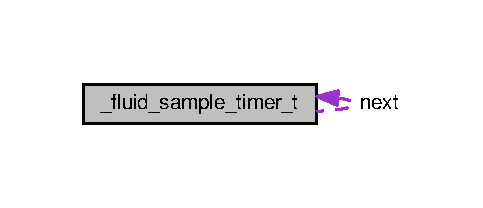
\includegraphics[width=232pt]{struct__fluid__sample__timer__t__coll__graph}
\end{center}
\end{figure}
\subsection*{Public Attributes}
\begin{DoxyCompactItemize}
\item 
\hyperlink{fluidsynth__priv_8h_a4ddade88911e1873bccda1a7750a848c}{fluid\+\_\+sample\+\_\+timer\+\_\+t} $\ast$ \hyperlink{struct__fluid__sample__timer__t_a981391285aa105093ba343286f2861c6}{next}
\item 
unsigned long \hyperlink{struct__fluid__sample__timer__t_af750cdf98b310863bfb66f7595ec6129}{starttick}
\item 
\hyperlink{fluid__sys_8h_a99c65ece4353146a7d260e34df6477d4}{fluid\+\_\+timer\+\_\+callback\+\_\+t} \hyperlink{struct__fluid__sample__timer__t_ad28dc7ab5aad17200f69d41244c411d5}{callback}
\item 
void $\ast$ \hyperlink{struct__fluid__sample__timer__t_acc12750f607d75ddfc1c48945d660e60}{data}
\item 
int \hyperlink{struct__fluid__sample__timer__t_ae34fb1268e31a141546b8fef5acaa321}{isfinished}
\end{DoxyCompactItemize}


\subsection{Member Data Documentation}
\mbox{\Hypertarget{struct__fluid__sample__timer__t_ad28dc7ab5aad17200f69d41244c411d5}\label{struct__fluid__sample__timer__t_ad28dc7ab5aad17200f69d41244c411d5}} 
\index{\+\_\+fluid\+\_\+sample\+\_\+timer\+\_\+t@{\+\_\+fluid\+\_\+sample\+\_\+timer\+\_\+t}!callback@{callback}}
\index{callback@{callback}!\+\_\+fluid\+\_\+sample\+\_\+timer\+\_\+t@{\+\_\+fluid\+\_\+sample\+\_\+timer\+\_\+t}}
\subsubsection{\texorpdfstring{callback}{callback}}
{\footnotesize\ttfamily \hyperlink{fluid__sys_8h_a99c65ece4353146a7d260e34df6477d4}{fluid\+\_\+timer\+\_\+callback\+\_\+t} \+\_\+fluid\+\_\+sample\+\_\+timer\+\_\+t\+::callback}

\mbox{\Hypertarget{struct__fluid__sample__timer__t_acc12750f607d75ddfc1c48945d660e60}\label{struct__fluid__sample__timer__t_acc12750f607d75ddfc1c48945d660e60}} 
\index{\+\_\+fluid\+\_\+sample\+\_\+timer\+\_\+t@{\+\_\+fluid\+\_\+sample\+\_\+timer\+\_\+t}!data@{data}}
\index{data@{data}!\+\_\+fluid\+\_\+sample\+\_\+timer\+\_\+t@{\+\_\+fluid\+\_\+sample\+\_\+timer\+\_\+t}}
\subsubsection{\texorpdfstring{data}{data}}
{\footnotesize\ttfamily void$\ast$ \+\_\+fluid\+\_\+sample\+\_\+timer\+\_\+t\+::data}

\mbox{\Hypertarget{struct__fluid__sample__timer__t_ae34fb1268e31a141546b8fef5acaa321}\label{struct__fluid__sample__timer__t_ae34fb1268e31a141546b8fef5acaa321}} 
\index{\+\_\+fluid\+\_\+sample\+\_\+timer\+\_\+t@{\+\_\+fluid\+\_\+sample\+\_\+timer\+\_\+t}!isfinished@{isfinished}}
\index{isfinished@{isfinished}!\+\_\+fluid\+\_\+sample\+\_\+timer\+\_\+t@{\+\_\+fluid\+\_\+sample\+\_\+timer\+\_\+t}}
\subsubsection{\texorpdfstring{isfinished}{isfinished}}
{\footnotesize\ttfamily int \+\_\+fluid\+\_\+sample\+\_\+timer\+\_\+t\+::isfinished}

\mbox{\Hypertarget{struct__fluid__sample__timer__t_a981391285aa105093ba343286f2861c6}\label{struct__fluid__sample__timer__t_a981391285aa105093ba343286f2861c6}} 
\index{\+\_\+fluid\+\_\+sample\+\_\+timer\+\_\+t@{\+\_\+fluid\+\_\+sample\+\_\+timer\+\_\+t}!next@{next}}
\index{next@{next}!\+\_\+fluid\+\_\+sample\+\_\+timer\+\_\+t@{\+\_\+fluid\+\_\+sample\+\_\+timer\+\_\+t}}
\subsubsection{\texorpdfstring{next}{next}}
{\footnotesize\ttfamily \hyperlink{fluidsynth__priv_8h_a4ddade88911e1873bccda1a7750a848c}{fluid\+\_\+sample\+\_\+timer\+\_\+t}$\ast$ \+\_\+fluid\+\_\+sample\+\_\+timer\+\_\+t\+::next}

\mbox{\Hypertarget{struct__fluid__sample__timer__t_af750cdf98b310863bfb66f7595ec6129}\label{struct__fluid__sample__timer__t_af750cdf98b310863bfb66f7595ec6129}} 
\index{\+\_\+fluid\+\_\+sample\+\_\+timer\+\_\+t@{\+\_\+fluid\+\_\+sample\+\_\+timer\+\_\+t}!starttick@{starttick}}
\index{starttick@{starttick}!\+\_\+fluid\+\_\+sample\+\_\+timer\+\_\+t@{\+\_\+fluid\+\_\+sample\+\_\+timer\+\_\+t}}
\subsubsection{\texorpdfstring{starttick}{starttick}}
{\footnotesize\ttfamily unsigned long \+\_\+fluid\+\_\+sample\+\_\+timer\+\_\+t\+::starttick}



The documentation for this struct was generated from the following file\+:\begin{DoxyCompactItemize}
\item 
synth/\hyperlink{fluid__synth_8c}{fluid\+\_\+synth.\+c}\end{DoxyCompactItemize}

\hypertarget{struct__fluid__samplecache__entry__t}{}\section{\+\_\+fluid\+\_\+samplecache\+\_\+entry\+\_\+t Struct Reference}
\label{struct__fluid__samplecache__entry__t}\index{\+\_\+fluid\+\_\+samplecache\+\_\+entry\+\_\+t@{\+\_\+fluid\+\_\+samplecache\+\_\+entry\+\_\+t}}
\subsection*{Public Attributes}
\begin{DoxyCompactItemize}
\item 
char $\ast$ \hyperlink{struct__fluid__samplecache__entry__t_a52440e5bc949027b94d169d271a5dbea}{filename}
\item 
time\+\_\+t \hyperlink{struct__fluid__samplecache__entry__t_a7fd7f02a2078d71dc48283ab55ae2c3f}{modification\+\_\+time}
\item 
unsigned int \hyperlink{struct__fluid__samplecache__entry__t_a9cf346ac1e4ca8c23d7ba4b37613fc83}{sf\+\_\+samplepos}
\item 
unsigned int \hyperlink{struct__fluid__samplecache__entry__t_a3e33a203f4fe8ced406f8bfed851f345}{sf\+\_\+samplesize}
\item 
unsigned int \hyperlink{struct__fluid__samplecache__entry__t_aab092587cf9907d7cb77384c65e90797}{sf\+\_\+sample24pos}
\item 
unsigned int \hyperlink{struct__fluid__samplecache__entry__t_a01e469ec27aeaf6dfe2d446f047d2e20}{sf\+\_\+sample24size}
\item 
unsigned int \hyperlink{struct__fluid__samplecache__entry__t_a03f7181f725fafac203131997fa1f97a}{sample\+\_\+start}
\item 
unsigned int \hyperlink{struct__fluid__samplecache__entry__t_a0c1b54067e105c799f73c4af527fa2f8}{sample\+\_\+end}
\item 
int \hyperlink{struct__fluid__samplecache__entry__t_ae9e20a09a26c83988564e0f5dadcebf0}{sample\+\_\+type}
\item 
short $\ast$ \hyperlink{struct__fluid__samplecache__entry__t_a6de64380849f6008d22c450721850969}{sample\+\_\+data}
\item 
char $\ast$ \hyperlink{struct__fluid__samplecache__entry__t_a0b6b2d56ca4cdefe037802e85f57a032}{sample\+\_\+data24}
\item 
int \hyperlink{struct__fluid__samplecache__entry__t_a243272fe55f42aa9236a77490804f7d6}{sample\+\_\+count}
\item 
int \hyperlink{struct__fluid__samplecache__entry__t_a1cb50e3307f51d9f7cc73e99060392ac}{num\+\_\+references}
\item 
int \hyperlink{struct__fluid__samplecache__entry__t_aebc7a0970039be60985b2565b9cdc90b}{mlocked}
\end{DoxyCompactItemize}


\subsection{Member Data Documentation}
\mbox{\Hypertarget{struct__fluid__samplecache__entry__t_a52440e5bc949027b94d169d271a5dbea}\label{struct__fluid__samplecache__entry__t_a52440e5bc949027b94d169d271a5dbea}} 
\index{\+\_\+fluid\+\_\+samplecache\+\_\+entry\+\_\+t@{\+\_\+fluid\+\_\+samplecache\+\_\+entry\+\_\+t}!filename@{filename}}
\index{filename@{filename}!\+\_\+fluid\+\_\+samplecache\+\_\+entry\+\_\+t@{\+\_\+fluid\+\_\+samplecache\+\_\+entry\+\_\+t}}
\subsubsection{\texorpdfstring{filename}{filename}}
{\footnotesize\ttfamily char$\ast$ \+\_\+fluid\+\_\+samplecache\+\_\+entry\+\_\+t\+::filename}

\mbox{\Hypertarget{struct__fluid__samplecache__entry__t_aebc7a0970039be60985b2565b9cdc90b}\label{struct__fluid__samplecache__entry__t_aebc7a0970039be60985b2565b9cdc90b}} 
\index{\+\_\+fluid\+\_\+samplecache\+\_\+entry\+\_\+t@{\+\_\+fluid\+\_\+samplecache\+\_\+entry\+\_\+t}!mlocked@{mlocked}}
\index{mlocked@{mlocked}!\+\_\+fluid\+\_\+samplecache\+\_\+entry\+\_\+t@{\+\_\+fluid\+\_\+samplecache\+\_\+entry\+\_\+t}}
\subsubsection{\texorpdfstring{mlocked}{mlocked}}
{\footnotesize\ttfamily int \+\_\+fluid\+\_\+samplecache\+\_\+entry\+\_\+t\+::mlocked}

\mbox{\Hypertarget{struct__fluid__samplecache__entry__t_a7fd7f02a2078d71dc48283ab55ae2c3f}\label{struct__fluid__samplecache__entry__t_a7fd7f02a2078d71dc48283ab55ae2c3f}} 
\index{\+\_\+fluid\+\_\+samplecache\+\_\+entry\+\_\+t@{\+\_\+fluid\+\_\+samplecache\+\_\+entry\+\_\+t}!modification\+\_\+time@{modification\+\_\+time}}
\index{modification\+\_\+time@{modification\+\_\+time}!\+\_\+fluid\+\_\+samplecache\+\_\+entry\+\_\+t@{\+\_\+fluid\+\_\+samplecache\+\_\+entry\+\_\+t}}
\subsubsection{\texorpdfstring{modification\+\_\+time}{modification\_time}}
{\footnotesize\ttfamily time\+\_\+t \+\_\+fluid\+\_\+samplecache\+\_\+entry\+\_\+t\+::modification\+\_\+time}

\mbox{\Hypertarget{struct__fluid__samplecache__entry__t_a1cb50e3307f51d9f7cc73e99060392ac}\label{struct__fluid__samplecache__entry__t_a1cb50e3307f51d9f7cc73e99060392ac}} 
\index{\+\_\+fluid\+\_\+samplecache\+\_\+entry\+\_\+t@{\+\_\+fluid\+\_\+samplecache\+\_\+entry\+\_\+t}!num\+\_\+references@{num\+\_\+references}}
\index{num\+\_\+references@{num\+\_\+references}!\+\_\+fluid\+\_\+samplecache\+\_\+entry\+\_\+t@{\+\_\+fluid\+\_\+samplecache\+\_\+entry\+\_\+t}}
\subsubsection{\texorpdfstring{num\+\_\+references}{num\_references}}
{\footnotesize\ttfamily int \+\_\+fluid\+\_\+samplecache\+\_\+entry\+\_\+t\+::num\+\_\+references}

\mbox{\Hypertarget{struct__fluid__samplecache__entry__t_a243272fe55f42aa9236a77490804f7d6}\label{struct__fluid__samplecache__entry__t_a243272fe55f42aa9236a77490804f7d6}} 
\index{\+\_\+fluid\+\_\+samplecache\+\_\+entry\+\_\+t@{\+\_\+fluid\+\_\+samplecache\+\_\+entry\+\_\+t}!sample\+\_\+count@{sample\+\_\+count}}
\index{sample\+\_\+count@{sample\+\_\+count}!\+\_\+fluid\+\_\+samplecache\+\_\+entry\+\_\+t@{\+\_\+fluid\+\_\+samplecache\+\_\+entry\+\_\+t}}
\subsubsection{\texorpdfstring{sample\+\_\+count}{sample\_count}}
{\footnotesize\ttfamily int \+\_\+fluid\+\_\+samplecache\+\_\+entry\+\_\+t\+::sample\+\_\+count}

\mbox{\Hypertarget{struct__fluid__samplecache__entry__t_a6de64380849f6008d22c450721850969}\label{struct__fluid__samplecache__entry__t_a6de64380849f6008d22c450721850969}} 
\index{\+\_\+fluid\+\_\+samplecache\+\_\+entry\+\_\+t@{\+\_\+fluid\+\_\+samplecache\+\_\+entry\+\_\+t}!sample\+\_\+data@{sample\+\_\+data}}
\index{sample\+\_\+data@{sample\+\_\+data}!\+\_\+fluid\+\_\+samplecache\+\_\+entry\+\_\+t@{\+\_\+fluid\+\_\+samplecache\+\_\+entry\+\_\+t}}
\subsubsection{\texorpdfstring{sample\+\_\+data}{sample\_data}}
{\footnotesize\ttfamily short$\ast$ \+\_\+fluid\+\_\+samplecache\+\_\+entry\+\_\+t\+::sample\+\_\+data}

\mbox{\Hypertarget{struct__fluid__samplecache__entry__t_a0b6b2d56ca4cdefe037802e85f57a032}\label{struct__fluid__samplecache__entry__t_a0b6b2d56ca4cdefe037802e85f57a032}} 
\index{\+\_\+fluid\+\_\+samplecache\+\_\+entry\+\_\+t@{\+\_\+fluid\+\_\+samplecache\+\_\+entry\+\_\+t}!sample\+\_\+data24@{sample\+\_\+data24}}
\index{sample\+\_\+data24@{sample\+\_\+data24}!\+\_\+fluid\+\_\+samplecache\+\_\+entry\+\_\+t@{\+\_\+fluid\+\_\+samplecache\+\_\+entry\+\_\+t}}
\subsubsection{\texorpdfstring{sample\+\_\+data24}{sample\_data24}}
{\footnotesize\ttfamily char$\ast$ \+\_\+fluid\+\_\+samplecache\+\_\+entry\+\_\+t\+::sample\+\_\+data24}

\mbox{\Hypertarget{struct__fluid__samplecache__entry__t_a0c1b54067e105c799f73c4af527fa2f8}\label{struct__fluid__samplecache__entry__t_a0c1b54067e105c799f73c4af527fa2f8}} 
\index{\+\_\+fluid\+\_\+samplecache\+\_\+entry\+\_\+t@{\+\_\+fluid\+\_\+samplecache\+\_\+entry\+\_\+t}!sample\+\_\+end@{sample\+\_\+end}}
\index{sample\+\_\+end@{sample\+\_\+end}!\+\_\+fluid\+\_\+samplecache\+\_\+entry\+\_\+t@{\+\_\+fluid\+\_\+samplecache\+\_\+entry\+\_\+t}}
\subsubsection{\texorpdfstring{sample\+\_\+end}{sample\_end}}
{\footnotesize\ttfamily unsigned int \+\_\+fluid\+\_\+samplecache\+\_\+entry\+\_\+t\+::sample\+\_\+end}

\mbox{\Hypertarget{struct__fluid__samplecache__entry__t_a03f7181f725fafac203131997fa1f97a}\label{struct__fluid__samplecache__entry__t_a03f7181f725fafac203131997fa1f97a}} 
\index{\+\_\+fluid\+\_\+samplecache\+\_\+entry\+\_\+t@{\+\_\+fluid\+\_\+samplecache\+\_\+entry\+\_\+t}!sample\+\_\+start@{sample\+\_\+start}}
\index{sample\+\_\+start@{sample\+\_\+start}!\+\_\+fluid\+\_\+samplecache\+\_\+entry\+\_\+t@{\+\_\+fluid\+\_\+samplecache\+\_\+entry\+\_\+t}}
\subsubsection{\texorpdfstring{sample\+\_\+start}{sample\_start}}
{\footnotesize\ttfamily unsigned int \+\_\+fluid\+\_\+samplecache\+\_\+entry\+\_\+t\+::sample\+\_\+start}

\mbox{\Hypertarget{struct__fluid__samplecache__entry__t_ae9e20a09a26c83988564e0f5dadcebf0}\label{struct__fluid__samplecache__entry__t_ae9e20a09a26c83988564e0f5dadcebf0}} 
\index{\+\_\+fluid\+\_\+samplecache\+\_\+entry\+\_\+t@{\+\_\+fluid\+\_\+samplecache\+\_\+entry\+\_\+t}!sample\+\_\+type@{sample\+\_\+type}}
\index{sample\+\_\+type@{sample\+\_\+type}!\+\_\+fluid\+\_\+samplecache\+\_\+entry\+\_\+t@{\+\_\+fluid\+\_\+samplecache\+\_\+entry\+\_\+t}}
\subsubsection{\texorpdfstring{sample\+\_\+type}{sample\_type}}
{\footnotesize\ttfamily int \+\_\+fluid\+\_\+samplecache\+\_\+entry\+\_\+t\+::sample\+\_\+type}

\mbox{\Hypertarget{struct__fluid__samplecache__entry__t_aab092587cf9907d7cb77384c65e90797}\label{struct__fluid__samplecache__entry__t_aab092587cf9907d7cb77384c65e90797}} 
\index{\+\_\+fluid\+\_\+samplecache\+\_\+entry\+\_\+t@{\+\_\+fluid\+\_\+samplecache\+\_\+entry\+\_\+t}!sf\+\_\+sample24pos@{sf\+\_\+sample24pos}}
\index{sf\+\_\+sample24pos@{sf\+\_\+sample24pos}!\+\_\+fluid\+\_\+samplecache\+\_\+entry\+\_\+t@{\+\_\+fluid\+\_\+samplecache\+\_\+entry\+\_\+t}}
\subsubsection{\texorpdfstring{sf\+\_\+sample24pos}{sf\_sample24pos}}
{\footnotesize\ttfamily unsigned int \+\_\+fluid\+\_\+samplecache\+\_\+entry\+\_\+t\+::sf\+\_\+sample24pos}

\mbox{\Hypertarget{struct__fluid__samplecache__entry__t_a01e469ec27aeaf6dfe2d446f047d2e20}\label{struct__fluid__samplecache__entry__t_a01e469ec27aeaf6dfe2d446f047d2e20}} 
\index{\+\_\+fluid\+\_\+samplecache\+\_\+entry\+\_\+t@{\+\_\+fluid\+\_\+samplecache\+\_\+entry\+\_\+t}!sf\+\_\+sample24size@{sf\+\_\+sample24size}}
\index{sf\+\_\+sample24size@{sf\+\_\+sample24size}!\+\_\+fluid\+\_\+samplecache\+\_\+entry\+\_\+t@{\+\_\+fluid\+\_\+samplecache\+\_\+entry\+\_\+t}}
\subsubsection{\texorpdfstring{sf\+\_\+sample24size}{sf\_sample24size}}
{\footnotesize\ttfamily unsigned int \+\_\+fluid\+\_\+samplecache\+\_\+entry\+\_\+t\+::sf\+\_\+sample24size}

\mbox{\Hypertarget{struct__fluid__samplecache__entry__t_a9cf346ac1e4ca8c23d7ba4b37613fc83}\label{struct__fluid__samplecache__entry__t_a9cf346ac1e4ca8c23d7ba4b37613fc83}} 
\index{\+\_\+fluid\+\_\+samplecache\+\_\+entry\+\_\+t@{\+\_\+fluid\+\_\+samplecache\+\_\+entry\+\_\+t}!sf\+\_\+samplepos@{sf\+\_\+samplepos}}
\index{sf\+\_\+samplepos@{sf\+\_\+samplepos}!\+\_\+fluid\+\_\+samplecache\+\_\+entry\+\_\+t@{\+\_\+fluid\+\_\+samplecache\+\_\+entry\+\_\+t}}
\subsubsection{\texorpdfstring{sf\+\_\+samplepos}{sf\_samplepos}}
{\footnotesize\ttfamily unsigned int \+\_\+fluid\+\_\+samplecache\+\_\+entry\+\_\+t\+::sf\+\_\+samplepos}

\mbox{\Hypertarget{struct__fluid__samplecache__entry__t_a3e33a203f4fe8ced406f8bfed851f345}\label{struct__fluid__samplecache__entry__t_a3e33a203f4fe8ced406f8bfed851f345}} 
\index{\+\_\+fluid\+\_\+samplecache\+\_\+entry\+\_\+t@{\+\_\+fluid\+\_\+samplecache\+\_\+entry\+\_\+t}!sf\+\_\+samplesize@{sf\+\_\+samplesize}}
\index{sf\+\_\+samplesize@{sf\+\_\+samplesize}!\+\_\+fluid\+\_\+samplecache\+\_\+entry\+\_\+t@{\+\_\+fluid\+\_\+samplecache\+\_\+entry\+\_\+t}}
\subsubsection{\texorpdfstring{sf\+\_\+samplesize}{sf\_samplesize}}
{\footnotesize\ttfamily unsigned int \+\_\+fluid\+\_\+samplecache\+\_\+entry\+\_\+t\+::sf\+\_\+samplesize}



The documentation for this struct was generated from the following file\+:\begin{DoxyCompactItemize}
\item 
sfloader/\hyperlink{fluid__samplecache_8c}{fluid\+\_\+samplecache.\+c}\end{DoxyCompactItemize}

\hypertarget{struct__fluid__seqbind__t}{}\section{\+\_\+fluid\+\_\+seqbind\+\_\+t Struct Reference}
\label{struct__fluid__seqbind__t}\index{\+\_\+fluid\+\_\+seqbind\+\_\+t@{\+\_\+fluid\+\_\+seqbind\+\_\+t}}


Collaboration diagram for \+\_\+fluid\+\_\+seqbind\+\_\+t\+:
\nopagebreak
\begin{figure}[H]
\begin{center}
\leavevmode
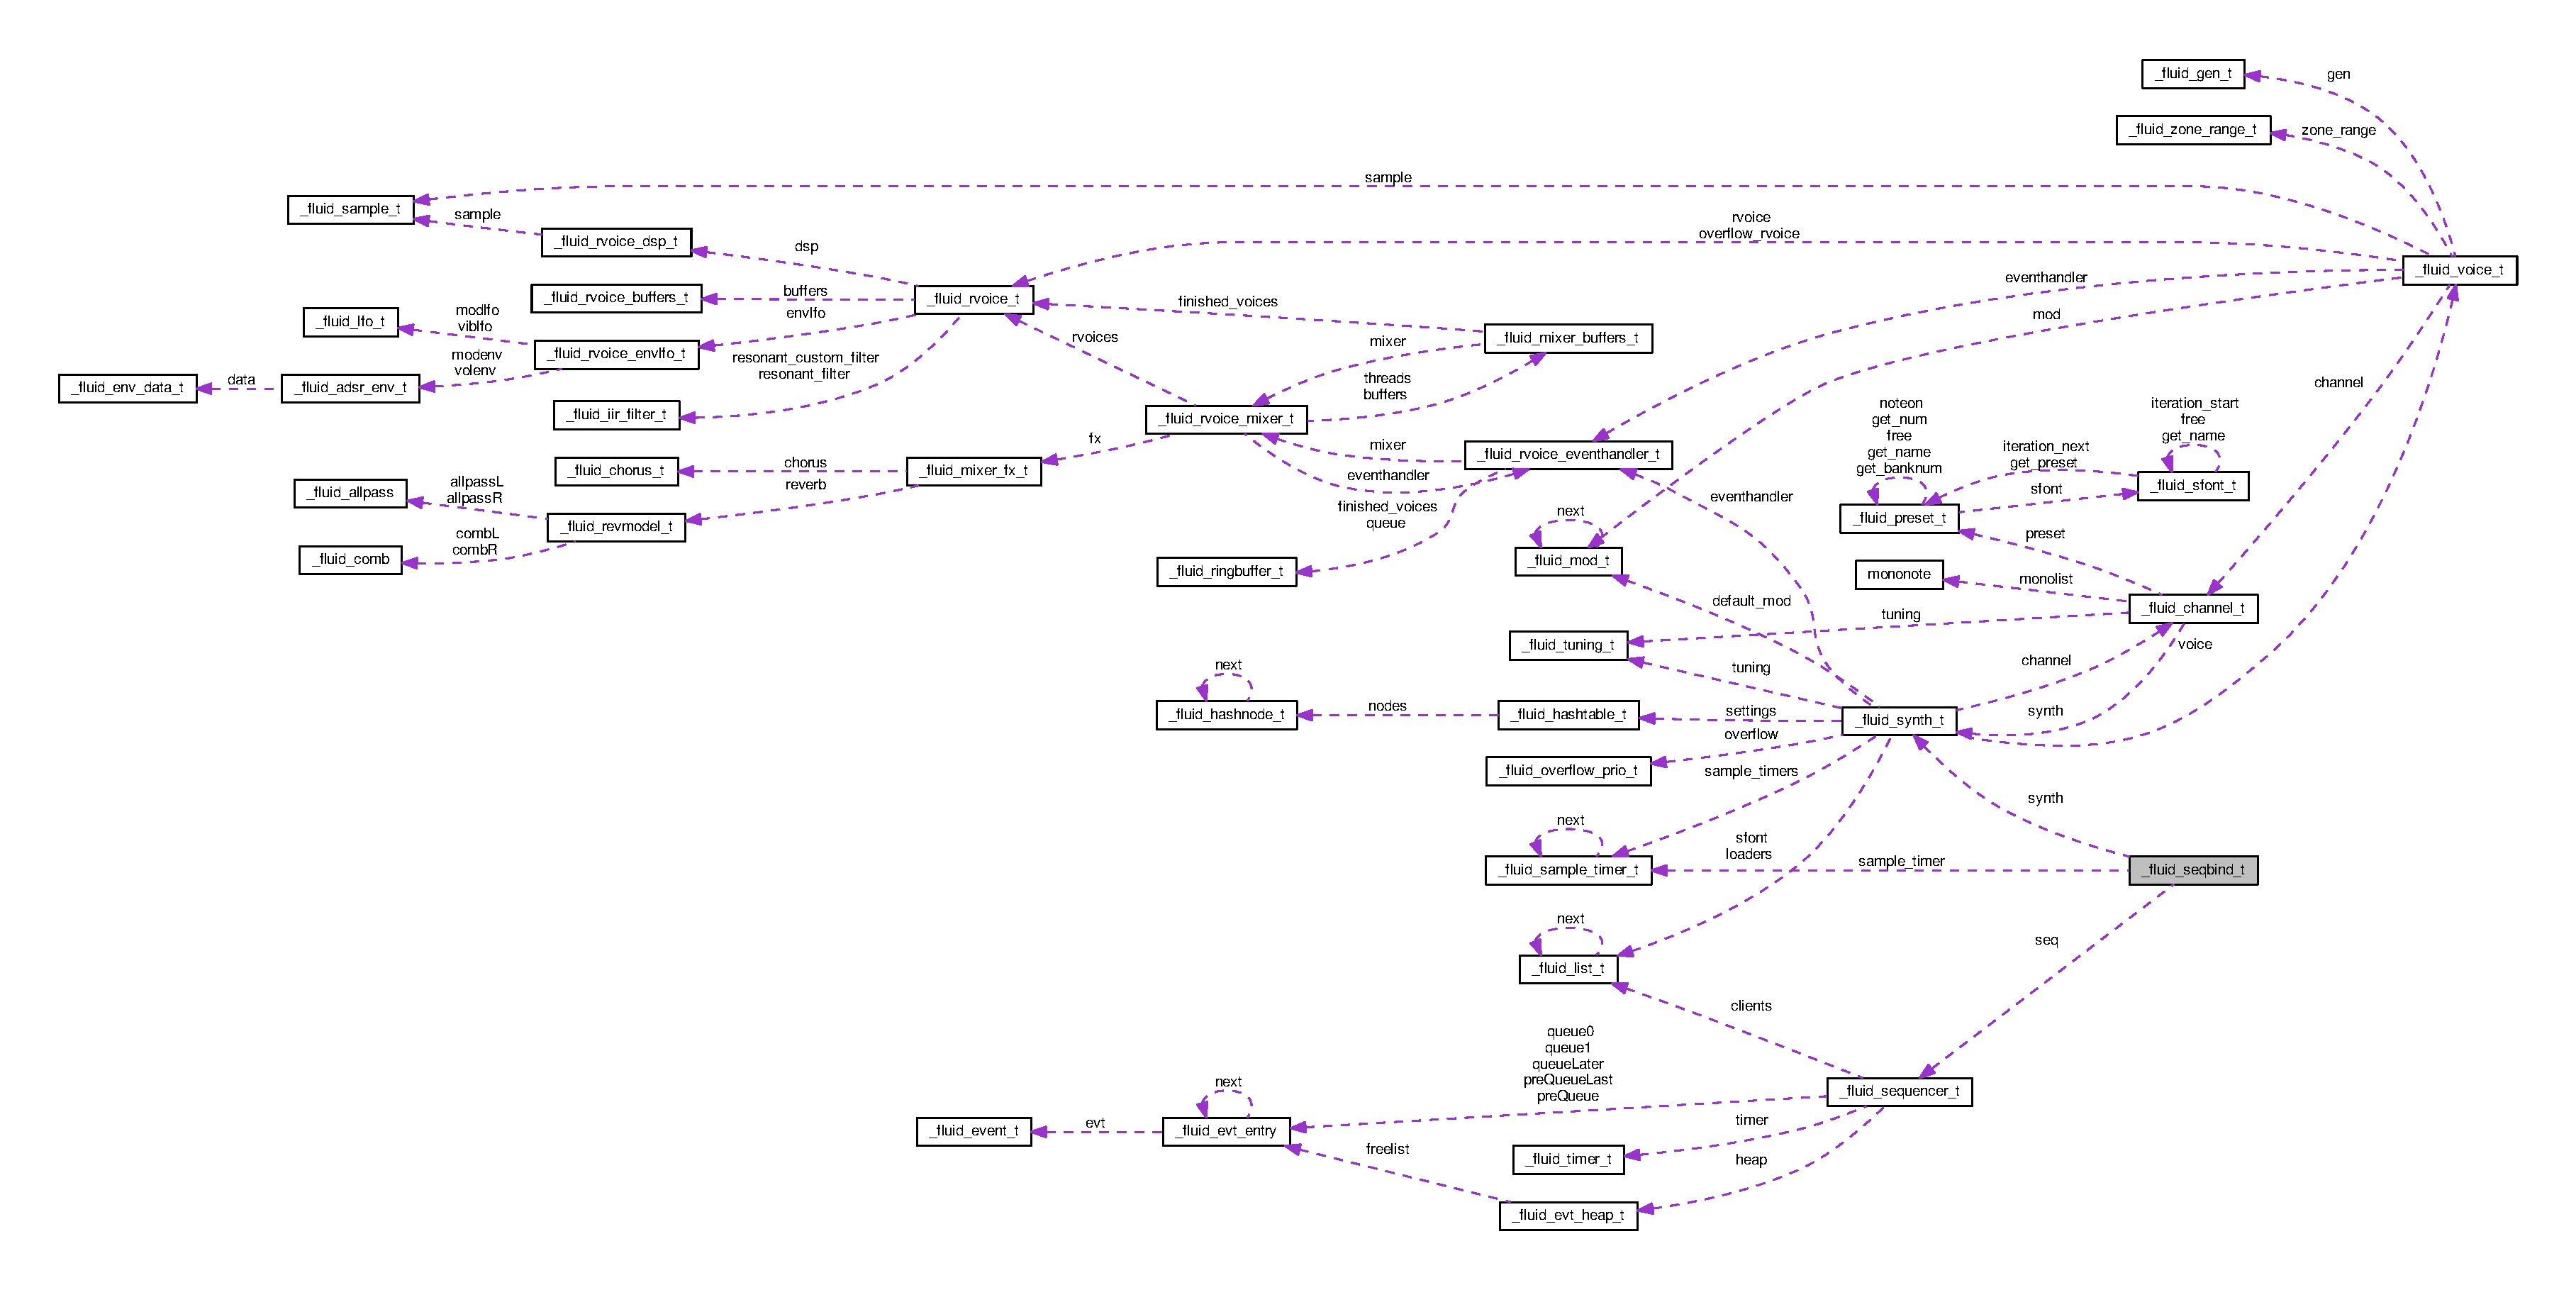
\includegraphics[width=350pt]{struct__fluid__seqbind__t__coll__graph}
\end{center}
\end{figure}
\subsection*{Public Attributes}
\begin{DoxyCompactItemize}
\item 
\hyperlink{types_8h_ae265f10ae174a13afe010de50d87e1a4}{fluid\+\_\+synth\+\_\+t} $\ast$ \hyperlink{struct__fluid__seqbind__t_a99ed9d0077a9549903432101f4db5a8f}{synth}
\item 
\hyperlink{types_8h_a7c7acad4ee620fc954a7ad4d7e87e1c3}{fluid\+\_\+sequencer\+\_\+t} $\ast$ \hyperlink{struct__fluid__seqbind__t_aaafa2156abb39068ee6da5e2b79a5a6d}{seq}
\item 
\hyperlink{fluidsynth__priv_8h_a4ddade88911e1873bccda1a7750a848c}{fluid\+\_\+sample\+\_\+timer\+\_\+t} $\ast$ \hyperlink{struct__fluid__seqbind__t_a33a88eed0dc7ac1b547d32449097a68f}{sample\+\_\+timer}
\item 
\hyperlink{types_8h_a69f729a00307f2b8ec1be0dba2203c12}{fluid\+\_\+seq\+\_\+id\+\_\+t} \hyperlink{struct__fluid__seqbind__t_ad3f537f9c5021105a0fadd1f1f1649f5}{client\+\_\+id}
\end{DoxyCompactItemize}


\subsection{Member Data Documentation}
\mbox{\Hypertarget{struct__fluid__seqbind__t_ad3f537f9c5021105a0fadd1f1f1649f5}\label{struct__fluid__seqbind__t_ad3f537f9c5021105a0fadd1f1f1649f5}} 
\index{\+\_\+fluid\+\_\+seqbind\+\_\+t@{\+\_\+fluid\+\_\+seqbind\+\_\+t}!client\+\_\+id@{client\+\_\+id}}
\index{client\+\_\+id@{client\+\_\+id}!\+\_\+fluid\+\_\+seqbind\+\_\+t@{\+\_\+fluid\+\_\+seqbind\+\_\+t}}
\subsubsection{\texorpdfstring{client\+\_\+id}{client\_id}}
{\footnotesize\ttfamily \hyperlink{types_8h_a69f729a00307f2b8ec1be0dba2203c12}{fluid\+\_\+seq\+\_\+id\+\_\+t} \+\_\+fluid\+\_\+seqbind\+\_\+t\+::client\+\_\+id}

\mbox{\Hypertarget{struct__fluid__seqbind__t_a33a88eed0dc7ac1b547d32449097a68f}\label{struct__fluid__seqbind__t_a33a88eed0dc7ac1b547d32449097a68f}} 
\index{\+\_\+fluid\+\_\+seqbind\+\_\+t@{\+\_\+fluid\+\_\+seqbind\+\_\+t}!sample\+\_\+timer@{sample\+\_\+timer}}
\index{sample\+\_\+timer@{sample\+\_\+timer}!\+\_\+fluid\+\_\+seqbind\+\_\+t@{\+\_\+fluid\+\_\+seqbind\+\_\+t}}
\subsubsection{\texorpdfstring{sample\+\_\+timer}{sample\_timer}}
{\footnotesize\ttfamily \hyperlink{fluidsynth__priv_8h_a4ddade88911e1873bccda1a7750a848c}{fluid\+\_\+sample\+\_\+timer\+\_\+t}$\ast$ \+\_\+fluid\+\_\+seqbind\+\_\+t\+::sample\+\_\+timer}

\mbox{\Hypertarget{struct__fluid__seqbind__t_aaafa2156abb39068ee6da5e2b79a5a6d}\label{struct__fluid__seqbind__t_aaafa2156abb39068ee6da5e2b79a5a6d}} 
\index{\+\_\+fluid\+\_\+seqbind\+\_\+t@{\+\_\+fluid\+\_\+seqbind\+\_\+t}!seq@{seq}}
\index{seq@{seq}!\+\_\+fluid\+\_\+seqbind\+\_\+t@{\+\_\+fluid\+\_\+seqbind\+\_\+t}}
\subsubsection{\texorpdfstring{seq}{seq}}
{\footnotesize\ttfamily \hyperlink{types_8h_a7c7acad4ee620fc954a7ad4d7e87e1c3}{fluid\+\_\+sequencer\+\_\+t}$\ast$ \+\_\+fluid\+\_\+seqbind\+\_\+t\+::seq}

\mbox{\Hypertarget{struct__fluid__seqbind__t_a99ed9d0077a9549903432101f4db5a8f}\label{struct__fluid__seqbind__t_a99ed9d0077a9549903432101f4db5a8f}} 
\index{\+\_\+fluid\+\_\+seqbind\+\_\+t@{\+\_\+fluid\+\_\+seqbind\+\_\+t}!synth@{synth}}
\index{synth@{synth}!\+\_\+fluid\+\_\+seqbind\+\_\+t@{\+\_\+fluid\+\_\+seqbind\+\_\+t}}
\subsubsection{\texorpdfstring{synth}{synth}}
{\footnotesize\ttfamily \hyperlink{types_8h_ae265f10ae174a13afe010de50d87e1a4}{fluid\+\_\+synth\+\_\+t}$\ast$ \+\_\+fluid\+\_\+seqbind\+\_\+t\+::synth}



The documentation for this struct was generated from the following file\+:\begin{DoxyCompactItemize}
\item 
midi/\hyperlink{fluid__seqbind_8c}{fluid\+\_\+seqbind.\+c}\end{DoxyCompactItemize}

\hypertarget{struct__fluid__sequencer__client__t}{}\section{\+\_\+fluid\+\_\+sequencer\+\_\+client\+\_\+t Struct Reference}
\label{struct__fluid__sequencer__client__t}\index{\+\_\+fluid\+\_\+sequencer\+\_\+client\+\_\+t@{\+\_\+fluid\+\_\+sequencer\+\_\+client\+\_\+t}}


Collaboration diagram for \+\_\+fluid\+\_\+sequencer\+\_\+client\+\_\+t\+:
\nopagebreak
\begin{figure}[H]
\begin{center}
\leavevmode
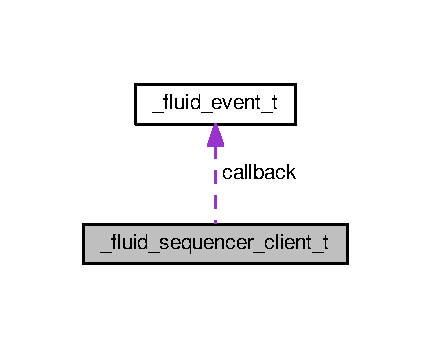
\includegraphics[width=207pt]{struct__fluid__sequencer__client__t__coll__graph}
\end{center}
\end{figure}
\subsection*{Public Attributes}
\begin{DoxyCompactItemize}
\item 
\hyperlink{types_8h_a69f729a00307f2b8ec1be0dba2203c12}{fluid\+\_\+seq\+\_\+id\+\_\+t} \hyperlink{struct__fluid__sequencer__client__t_a057566dc26e3979fab98d74c7d0939a1}{id}
\item 
char $\ast$ \hyperlink{struct__fluid__sequencer__client__t_aed808370169fbbe8592f8b950b5a568c}{name}
\item 
\hyperlink{seq_8h_ae6bb99d73ba67f0b7e15883b78bfae85}{fluid\+\_\+event\+\_\+callback\+\_\+t} \hyperlink{struct__fluid__sequencer__client__t_ab5e110362b5c59c139dee953ce278ca3}{callback}
\item 
void $\ast$ \hyperlink{struct__fluid__sequencer__client__t_a2c69a1ecf3c2261f8969e7171787b958}{data}
\end{DoxyCompactItemize}


\subsection{Member Data Documentation}
\mbox{\Hypertarget{struct__fluid__sequencer__client__t_ab5e110362b5c59c139dee953ce278ca3}\label{struct__fluid__sequencer__client__t_ab5e110362b5c59c139dee953ce278ca3}} 
\index{\+\_\+fluid\+\_\+sequencer\+\_\+client\+\_\+t@{\+\_\+fluid\+\_\+sequencer\+\_\+client\+\_\+t}!callback@{callback}}
\index{callback@{callback}!\+\_\+fluid\+\_\+sequencer\+\_\+client\+\_\+t@{\+\_\+fluid\+\_\+sequencer\+\_\+client\+\_\+t}}
\subsubsection{\texorpdfstring{callback}{callback}}
{\footnotesize\ttfamily \hyperlink{seq_8h_ae6bb99d73ba67f0b7e15883b78bfae85}{fluid\+\_\+event\+\_\+callback\+\_\+t} \+\_\+fluid\+\_\+sequencer\+\_\+client\+\_\+t\+::callback}

\mbox{\Hypertarget{struct__fluid__sequencer__client__t_a2c69a1ecf3c2261f8969e7171787b958}\label{struct__fluid__sequencer__client__t_a2c69a1ecf3c2261f8969e7171787b958}} 
\index{\+\_\+fluid\+\_\+sequencer\+\_\+client\+\_\+t@{\+\_\+fluid\+\_\+sequencer\+\_\+client\+\_\+t}!data@{data}}
\index{data@{data}!\+\_\+fluid\+\_\+sequencer\+\_\+client\+\_\+t@{\+\_\+fluid\+\_\+sequencer\+\_\+client\+\_\+t}}
\subsubsection{\texorpdfstring{data}{data}}
{\footnotesize\ttfamily void$\ast$ \+\_\+fluid\+\_\+sequencer\+\_\+client\+\_\+t\+::data}

\mbox{\Hypertarget{struct__fluid__sequencer__client__t_a057566dc26e3979fab98d74c7d0939a1}\label{struct__fluid__sequencer__client__t_a057566dc26e3979fab98d74c7d0939a1}} 
\index{\+\_\+fluid\+\_\+sequencer\+\_\+client\+\_\+t@{\+\_\+fluid\+\_\+sequencer\+\_\+client\+\_\+t}!id@{id}}
\index{id@{id}!\+\_\+fluid\+\_\+sequencer\+\_\+client\+\_\+t@{\+\_\+fluid\+\_\+sequencer\+\_\+client\+\_\+t}}
\subsubsection{\texorpdfstring{id}{id}}
{\footnotesize\ttfamily \hyperlink{types_8h_a69f729a00307f2b8ec1be0dba2203c12}{fluid\+\_\+seq\+\_\+id\+\_\+t} \+\_\+fluid\+\_\+sequencer\+\_\+client\+\_\+t\+::id}

\mbox{\Hypertarget{struct__fluid__sequencer__client__t_aed808370169fbbe8592f8b950b5a568c}\label{struct__fluid__sequencer__client__t_aed808370169fbbe8592f8b950b5a568c}} 
\index{\+\_\+fluid\+\_\+sequencer\+\_\+client\+\_\+t@{\+\_\+fluid\+\_\+sequencer\+\_\+client\+\_\+t}!name@{name}}
\index{name@{name}!\+\_\+fluid\+\_\+sequencer\+\_\+client\+\_\+t@{\+\_\+fluid\+\_\+sequencer\+\_\+client\+\_\+t}}
\subsubsection{\texorpdfstring{name}{name}}
{\footnotesize\ttfamily char$\ast$ \+\_\+fluid\+\_\+sequencer\+\_\+client\+\_\+t\+::name}



The documentation for this struct was generated from the following file\+:\begin{DoxyCompactItemize}
\item 
midi/\hyperlink{fluid__seq_8c}{fluid\+\_\+seq.\+c}\end{DoxyCompactItemize}

\hypertarget{struct__fluid__sequencer__t}{}\section{\+\_\+fluid\+\_\+sequencer\+\_\+t Struct Reference}
\label{struct__fluid__sequencer__t}\index{\+\_\+fluid\+\_\+sequencer\+\_\+t@{\+\_\+fluid\+\_\+sequencer\+\_\+t}}


Collaboration diagram for \+\_\+fluid\+\_\+sequencer\+\_\+t\+:
\nopagebreak
\begin{figure}[H]
\begin{center}
\leavevmode
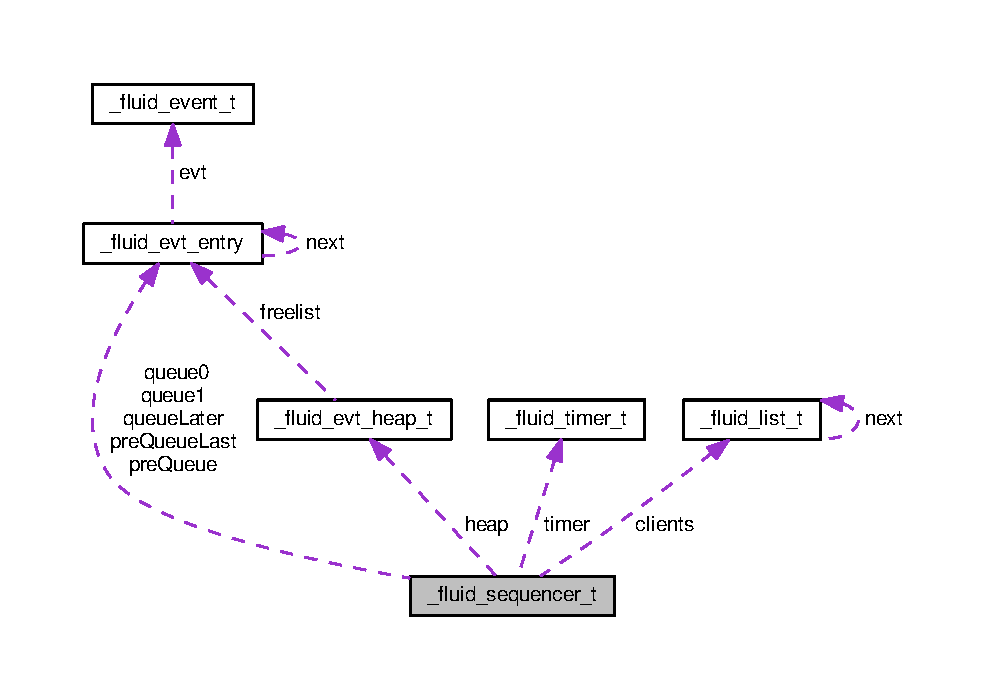
\includegraphics[width=350pt]{struct__fluid__sequencer__t__coll__graph}
\end{center}
\end{figure}
\subsection*{Public Attributes}
\begin{DoxyCompactItemize}
\item 
unsigned int \hyperlink{struct__fluid__sequencer__t_a365e64793ab958e5ec12d4d3e123bd89}{start\+Ms}
\item 
\hyperlink{fluidsynth__priv_8h_a6b8be882dd9958ea3635a868e1bf5152}{fluid\+\_\+atomic\+\_\+int\+\_\+t} \hyperlink{struct__fluid__sequencer__t_a508b9a601401b6ee2d6e4659ed91ecde}{current\+Ms}
\item 
int \hyperlink{struct__fluid__sequencer__t_a6b42a433d5c2c3909570e006f937f208}{use\+System\+Timer}
\item 
double \hyperlink{struct__fluid__sequencer__t_a7c557f84e87e4a3429de3f84b7c0eb5f}{scale}
\item 
\hyperlink{fluid__list_8h_a3ef7535d4290862c0af118569223bd89}{fluid\+\_\+list\+\_\+t} $\ast$ \hyperlink{struct__fluid__sequencer__t_a644f30ae8cc5e9b9871f52c3d31e22c1}{clients}
\item 
\hyperlink{types_8h_a69f729a00307f2b8ec1be0dba2203c12}{fluid\+\_\+seq\+\_\+id\+\_\+t} \hyperlink{struct__fluid__sequencer__t_a851d4c371c4a777351f1fca1b263fc0d}{clients\+ID}
\item 
\hyperlink{fluid__event__priv_8h_ae1b4d1ef2ce32890f8cb36837628a9d8}{fluid\+\_\+evt\+\_\+entry} $\ast$ \hyperlink{struct__fluid__sequencer__t_ae0f443ced2ff9f9bfcafaee34a1f0055}{pre\+Queue}
\item 
\hyperlink{fluid__event__priv_8h_ae1b4d1ef2ce32890f8cb36837628a9d8}{fluid\+\_\+evt\+\_\+entry} $\ast$ \hyperlink{struct__fluid__sequencer__t_ab8196554368b2131823ec99f2d319e1e}{pre\+Queue\+Last}
\item 
\hyperlink{fluid__sys_8h_a520742276ee4ea4bf140e6e6be79e4ae}{fluid\+\_\+timer\+\_\+t} $\ast$ \hyperlink{struct__fluid__sequencer__t_ac2a815201eb399d26d2b347e9befa112}{timer}
\item 
int \hyperlink{struct__fluid__sequencer__t_aeeaffdfb156ba1a61e0263a6b6e60c41}{queue0\+Start\+Time}
\item 
short \hyperlink{struct__fluid__sequencer__t_afddad2afafb8e38ca13f296a537ea7f6}{prev\+Cell\+Nb}
\item 
\hyperlink{fluid__event__priv_8h_ae1b4d1ef2ce32890f8cb36837628a9d8}{fluid\+\_\+evt\+\_\+entry} $\ast$ \hyperlink{struct__fluid__sequencer__t_a629f92dc6f8a247e1e7ebecd911e2139}{queue0} \mbox{[}256\mbox{]}\mbox{[}2\mbox{]}
\item 
\hyperlink{fluid__event__priv_8h_ae1b4d1ef2ce32890f8cb36837628a9d8}{fluid\+\_\+evt\+\_\+entry} $\ast$ \hyperlink{struct__fluid__sequencer__t_abd13dad9998224d4d985c550458d6793}{queue1} \mbox{[}255\mbox{]}\mbox{[}2\mbox{]}
\item 
\hyperlink{fluid__event__priv_8h_ae1b4d1ef2ce32890f8cb36837628a9d8}{fluid\+\_\+evt\+\_\+entry} $\ast$ \hyperlink{struct__fluid__sequencer__t_a823fb4b43eb531a2d548e095c8180408}{queue\+Later}
\item 
\hyperlink{fluid__event__priv_8h_ac90e8a0581105c6ecd80188d0bdd6693}{fluid\+\_\+evt\+\_\+heap\+\_\+t} $\ast$ \hyperlink{struct__fluid__sequencer__t_a55490ac2edf1b86ab318184adac540af}{heap}
\item 
\hyperlink{fluid__sys_8h_a7252a44982e8ed2704689f563c8a12e3}{fluid\+\_\+mutex\+\_\+t} \hyperlink{struct__fluid__sequencer__t_aae80b7e1e2a3dd9ac9fe29d7d52b8a46}{mutex}
\end{DoxyCompactItemize}


\subsection{Member Data Documentation}
\mbox{\Hypertarget{struct__fluid__sequencer__t_a644f30ae8cc5e9b9871f52c3d31e22c1}\label{struct__fluid__sequencer__t_a644f30ae8cc5e9b9871f52c3d31e22c1}} 
\index{\+\_\+fluid\+\_\+sequencer\+\_\+t@{\+\_\+fluid\+\_\+sequencer\+\_\+t}!clients@{clients}}
\index{clients@{clients}!\+\_\+fluid\+\_\+sequencer\+\_\+t@{\+\_\+fluid\+\_\+sequencer\+\_\+t}}
\subsubsection{\texorpdfstring{clients}{clients}}
{\footnotesize\ttfamily \hyperlink{fluid__list_8h_a3ef7535d4290862c0af118569223bd89}{fluid\+\_\+list\+\_\+t}$\ast$ \+\_\+fluid\+\_\+sequencer\+\_\+t\+::clients}

\mbox{\Hypertarget{struct__fluid__sequencer__t_a851d4c371c4a777351f1fca1b263fc0d}\label{struct__fluid__sequencer__t_a851d4c371c4a777351f1fca1b263fc0d}} 
\index{\+\_\+fluid\+\_\+sequencer\+\_\+t@{\+\_\+fluid\+\_\+sequencer\+\_\+t}!clients\+ID@{clients\+ID}}
\index{clients\+ID@{clients\+ID}!\+\_\+fluid\+\_\+sequencer\+\_\+t@{\+\_\+fluid\+\_\+sequencer\+\_\+t}}
\subsubsection{\texorpdfstring{clients\+ID}{clientsID}}
{\footnotesize\ttfamily \hyperlink{types_8h_a69f729a00307f2b8ec1be0dba2203c12}{fluid\+\_\+seq\+\_\+id\+\_\+t} \+\_\+fluid\+\_\+sequencer\+\_\+t\+::clients\+ID}

\mbox{\Hypertarget{struct__fluid__sequencer__t_a508b9a601401b6ee2d6e4659ed91ecde}\label{struct__fluid__sequencer__t_a508b9a601401b6ee2d6e4659ed91ecde}} 
\index{\+\_\+fluid\+\_\+sequencer\+\_\+t@{\+\_\+fluid\+\_\+sequencer\+\_\+t}!current\+Ms@{current\+Ms}}
\index{current\+Ms@{current\+Ms}!\+\_\+fluid\+\_\+sequencer\+\_\+t@{\+\_\+fluid\+\_\+sequencer\+\_\+t}}
\subsubsection{\texorpdfstring{current\+Ms}{currentMs}}
{\footnotesize\ttfamily \hyperlink{fluidsynth__priv_8h_a6b8be882dd9958ea3635a868e1bf5152}{fluid\+\_\+atomic\+\_\+int\+\_\+t} \+\_\+fluid\+\_\+sequencer\+\_\+t\+::current\+Ms}

\mbox{\Hypertarget{struct__fluid__sequencer__t_a55490ac2edf1b86ab318184adac540af}\label{struct__fluid__sequencer__t_a55490ac2edf1b86ab318184adac540af}} 
\index{\+\_\+fluid\+\_\+sequencer\+\_\+t@{\+\_\+fluid\+\_\+sequencer\+\_\+t}!heap@{heap}}
\index{heap@{heap}!\+\_\+fluid\+\_\+sequencer\+\_\+t@{\+\_\+fluid\+\_\+sequencer\+\_\+t}}
\subsubsection{\texorpdfstring{heap}{heap}}
{\footnotesize\ttfamily \hyperlink{fluid__event__priv_8h_ac90e8a0581105c6ecd80188d0bdd6693}{fluid\+\_\+evt\+\_\+heap\+\_\+t}$\ast$ \+\_\+fluid\+\_\+sequencer\+\_\+t\+::heap}

\mbox{\Hypertarget{struct__fluid__sequencer__t_aae80b7e1e2a3dd9ac9fe29d7d52b8a46}\label{struct__fluid__sequencer__t_aae80b7e1e2a3dd9ac9fe29d7d52b8a46}} 
\index{\+\_\+fluid\+\_\+sequencer\+\_\+t@{\+\_\+fluid\+\_\+sequencer\+\_\+t}!mutex@{mutex}}
\index{mutex@{mutex}!\+\_\+fluid\+\_\+sequencer\+\_\+t@{\+\_\+fluid\+\_\+sequencer\+\_\+t}}
\subsubsection{\texorpdfstring{mutex}{mutex}}
{\footnotesize\ttfamily \hyperlink{fluid__sys_8h_a7252a44982e8ed2704689f563c8a12e3}{fluid\+\_\+mutex\+\_\+t} \+\_\+fluid\+\_\+sequencer\+\_\+t\+::mutex}

\mbox{\Hypertarget{struct__fluid__sequencer__t_ae0f443ced2ff9f9bfcafaee34a1f0055}\label{struct__fluid__sequencer__t_ae0f443ced2ff9f9bfcafaee34a1f0055}} 
\index{\+\_\+fluid\+\_\+sequencer\+\_\+t@{\+\_\+fluid\+\_\+sequencer\+\_\+t}!pre\+Queue@{pre\+Queue}}
\index{pre\+Queue@{pre\+Queue}!\+\_\+fluid\+\_\+sequencer\+\_\+t@{\+\_\+fluid\+\_\+sequencer\+\_\+t}}
\subsubsection{\texorpdfstring{pre\+Queue}{preQueue}}
{\footnotesize\ttfamily \hyperlink{fluid__event__priv_8h_ae1b4d1ef2ce32890f8cb36837628a9d8}{fluid\+\_\+evt\+\_\+entry}$\ast$ \+\_\+fluid\+\_\+sequencer\+\_\+t\+::pre\+Queue}

\mbox{\Hypertarget{struct__fluid__sequencer__t_ab8196554368b2131823ec99f2d319e1e}\label{struct__fluid__sequencer__t_ab8196554368b2131823ec99f2d319e1e}} 
\index{\+\_\+fluid\+\_\+sequencer\+\_\+t@{\+\_\+fluid\+\_\+sequencer\+\_\+t}!pre\+Queue\+Last@{pre\+Queue\+Last}}
\index{pre\+Queue\+Last@{pre\+Queue\+Last}!\+\_\+fluid\+\_\+sequencer\+\_\+t@{\+\_\+fluid\+\_\+sequencer\+\_\+t}}
\subsubsection{\texorpdfstring{pre\+Queue\+Last}{preQueueLast}}
{\footnotesize\ttfamily \hyperlink{fluid__event__priv_8h_ae1b4d1ef2ce32890f8cb36837628a9d8}{fluid\+\_\+evt\+\_\+entry}$\ast$ \+\_\+fluid\+\_\+sequencer\+\_\+t\+::pre\+Queue\+Last}

\mbox{\Hypertarget{struct__fluid__sequencer__t_afddad2afafb8e38ca13f296a537ea7f6}\label{struct__fluid__sequencer__t_afddad2afafb8e38ca13f296a537ea7f6}} 
\index{\+\_\+fluid\+\_\+sequencer\+\_\+t@{\+\_\+fluid\+\_\+sequencer\+\_\+t}!prev\+Cell\+Nb@{prev\+Cell\+Nb}}
\index{prev\+Cell\+Nb@{prev\+Cell\+Nb}!\+\_\+fluid\+\_\+sequencer\+\_\+t@{\+\_\+fluid\+\_\+sequencer\+\_\+t}}
\subsubsection{\texorpdfstring{prev\+Cell\+Nb}{prevCellNb}}
{\footnotesize\ttfamily short \+\_\+fluid\+\_\+sequencer\+\_\+t\+::prev\+Cell\+Nb}

\mbox{\Hypertarget{struct__fluid__sequencer__t_a629f92dc6f8a247e1e7ebecd911e2139}\label{struct__fluid__sequencer__t_a629f92dc6f8a247e1e7ebecd911e2139}} 
\index{\+\_\+fluid\+\_\+sequencer\+\_\+t@{\+\_\+fluid\+\_\+sequencer\+\_\+t}!queue0@{queue0}}
\index{queue0@{queue0}!\+\_\+fluid\+\_\+sequencer\+\_\+t@{\+\_\+fluid\+\_\+sequencer\+\_\+t}}
\subsubsection{\texorpdfstring{queue0}{queue0}}
{\footnotesize\ttfamily \hyperlink{fluid__event__priv_8h_ae1b4d1ef2ce32890f8cb36837628a9d8}{fluid\+\_\+evt\+\_\+entry}$\ast$ \+\_\+fluid\+\_\+sequencer\+\_\+t\+::queue0\mbox{[}256\mbox{]}\mbox{[}2\mbox{]}}

\mbox{\Hypertarget{struct__fluid__sequencer__t_aeeaffdfb156ba1a61e0263a6b6e60c41}\label{struct__fluid__sequencer__t_aeeaffdfb156ba1a61e0263a6b6e60c41}} 
\index{\+\_\+fluid\+\_\+sequencer\+\_\+t@{\+\_\+fluid\+\_\+sequencer\+\_\+t}!queue0\+Start\+Time@{queue0\+Start\+Time}}
\index{queue0\+Start\+Time@{queue0\+Start\+Time}!\+\_\+fluid\+\_\+sequencer\+\_\+t@{\+\_\+fluid\+\_\+sequencer\+\_\+t}}
\subsubsection{\texorpdfstring{queue0\+Start\+Time}{queue0StartTime}}
{\footnotesize\ttfamily int \+\_\+fluid\+\_\+sequencer\+\_\+t\+::queue0\+Start\+Time}

\mbox{\Hypertarget{struct__fluid__sequencer__t_abd13dad9998224d4d985c550458d6793}\label{struct__fluid__sequencer__t_abd13dad9998224d4d985c550458d6793}} 
\index{\+\_\+fluid\+\_\+sequencer\+\_\+t@{\+\_\+fluid\+\_\+sequencer\+\_\+t}!queue1@{queue1}}
\index{queue1@{queue1}!\+\_\+fluid\+\_\+sequencer\+\_\+t@{\+\_\+fluid\+\_\+sequencer\+\_\+t}}
\subsubsection{\texorpdfstring{queue1}{queue1}}
{\footnotesize\ttfamily \hyperlink{fluid__event__priv_8h_ae1b4d1ef2ce32890f8cb36837628a9d8}{fluid\+\_\+evt\+\_\+entry}$\ast$ \+\_\+fluid\+\_\+sequencer\+\_\+t\+::queue1\mbox{[}255\mbox{]}\mbox{[}2\mbox{]}}

\mbox{\Hypertarget{struct__fluid__sequencer__t_a823fb4b43eb531a2d548e095c8180408}\label{struct__fluid__sequencer__t_a823fb4b43eb531a2d548e095c8180408}} 
\index{\+\_\+fluid\+\_\+sequencer\+\_\+t@{\+\_\+fluid\+\_\+sequencer\+\_\+t}!queue\+Later@{queue\+Later}}
\index{queue\+Later@{queue\+Later}!\+\_\+fluid\+\_\+sequencer\+\_\+t@{\+\_\+fluid\+\_\+sequencer\+\_\+t}}
\subsubsection{\texorpdfstring{queue\+Later}{queueLater}}
{\footnotesize\ttfamily \hyperlink{fluid__event__priv_8h_ae1b4d1ef2ce32890f8cb36837628a9d8}{fluid\+\_\+evt\+\_\+entry}$\ast$ \+\_\+fluid\+\_\+sequencer\+\_\+t\+::queue\+Later}

\mbox{\Hypertarget{struct__fluid__sequencer__t_a7c557f84e87e4a3429de3f84b7c0eb5f}\label{struct__fluid__sequencer__t_a7c557f84e87e4a3429de3f84b7c0eb5f}} 
\index{\+\_\+fluid\+\_\+sequencer\+\_\+t@{\+\_\+fluid\+\_\+sequencer\+\_\+t}!scale@{scale}}
\index{scale@{scale}!\+\_\+fluid\+\_\+sequencer\+\_\+t@{\+\_\+fluid\+\_\+sequencer\+\_\+t}}
\subsubsection{\texorpdfstring{scale}{scale}}
{\footnotesize\ttfamily double \+\_\+fluid\+\_\+sequencer\+\_\+t\+::scale}

\mbox{\Hypertarget{struct__fluid__sequencer__t_a365e64793ab958e5ec12d4d3e123bd89}\label{struct__fluid__sequencer__t_a365e64793ab958e5ec12d4d3e123bd89}} 
\index{\+\_\+fluid\+\_\+sequencer\+\_\+t@{\+\_\+fluid\+\_\+sequencer\+\_\+t}!start\+Ms@{start\+Ms}}
\index{start\+Ms@{start\+Ms}!\+\_\+fluid\+\_\+sequencer\+\_\+t@{\+\_\+fluid\+\_\+sequencer\+\_\+t}}
\subsubsection{\texorpdfstring{start\+Ms}{startMs}}
{\footnotesize\ttfamily unsigned int \+\_\+fluid\+\_\+sequencer\+\_\+t\+::start\+Ms}

\mbox{\Hypertarget{struct__fluid__sequencer__t_ac2a815201eb399d26d2b347e9befa112}\label{struct__fluid__sequencer__t_ac2a815201eb399d26d2b347e9befa112}} 
\index{\+\_\+fluid\+\_\+sequencer\+\_\+t@{\+\_\+fluid\+\_\+sequencer\+\_\+t}!timer@{timer}}
\index{timer@{timer}!\+\_\+fluid\+\_\+sequencer\+\_\+t@{\+\_\+fluid\+\_\+sequencer\+\_\+t}}
\subsubsection{\texorpdfstring{timer}{timer}}
{\footnotesize\ttfamily \hyperlink{fluid__sys_8h_a520742276ee4ea4bf140e6e6be79e4ae}{fluid\+\_\+timer\+\_\+t}$\ast$ \+\_\+fluid\+\_\+sequencer\+\_\+t\+::timer}

\mbox{\Hypertarget{struct__fluid__sequencer__t_a6b42a433d5c2c3909570e006f937f208}\label{struct__fluid__sequencer__t_a6b42a433d5c2c3909570e006f937f208}} 
\index{\+\_\+fluid\+\_\+sequencer\+\_\+t@{\+\_\+fluid\+\_\+sequencer\+\_\+t}!use\+System\+Timer@{use\+System\+Timer}}
\index{use\+System\+Timer@{use\+System\+Timer}!\+\_\+fluid\+\_\+sequencer\+\_\+t@{\+\_\+fluid\+\_\+sequencer\+\_\+t}}
\subsubsection{\texorpdfstring{use\+System\+Timer}{useSystemTimer}}
{\footnotesize\ttfamily int \+\_\+fluid\+\_\+sequencer\+\_\+t\+::use\+System\+Timer}



The documentation for this struct was generated from the following file\+:\begin{DoxyCompactItemize}
\item 
midi/\hyperlink{fluid__seq_8c}{fluid\+\_\+seq.\+c}\end{DoxyCompactItemize}

\hypertarget{struct__fluid__server__socket__t}{}\section{\+\_\+fluid\+\_\+server\+\_\+socket\+\_\+t Struct Reference}
\label{struct__fluid__server__socket__t}\index{\+\_\+fluid\+\_\+server\+\_\+socket\+\_\+t@{\+\_\+fluid\+\_\+server\+\_\+socket\+\_\+t}}
\subsection*{Public Attributes}
\begin{DoxyCompactItemize}
\item 
\hyperlink{fluidsynth__priv_8h_ad024f40f94120b0766cda0ad9f47be82}{fluid\+\_\+socket\+\_\+t} \hyperlink{struct__fluid__server__socket__t_aefe5bdf3ae401d0ad7e2a2bb50abce82}{socket}
\item 
\hyperlink{fluid__sys_8h_a60a6466e68a45b0f0709f1ebaa7e6f85}{fluid\+\_\+thread\+\_\+t} $\ast$ \hyperlink{struct__fluid__server__socket__t_a415965f938322f4aef48228b3411afaf}{thread}
\item 
int \hyperlink{struct__fluid__server__socket__t_a1c60fad728d81c7e28d7f311e1298542}{cont}
\item 
\hyperlink{fluid__sys_8h_abca7c6851ff769a16e0e7645cb441cd0}{fluid\+\_\+server\+\_\+func\+\_\+t} \hyperlink{struct__fluid__server__socket__t_acfeb0d4f1ce8e0f6ae80d26ff1e2d21d}{func}
\item 
void $\ast$ \hyperlink{struct__fluid__server__socket__t_ac0fcd76ae584403ea45c04b974e421da}{data}
\end{DoxyCompactItemize}


\subsection{Member Data Documentation}
\mbox{\Hypertarget{struct__fluid__server__socket__t_a1c60fad728d81c7e28d7f311e1298542}\label{struct__fluid__server__socket__t_a1c60fad728d81c7e28d7f311e1298542}} 
\index{\+\_\+fluid\+\_\+server\+\_\+socket\+\_\+t@{\+\_\+fluid\+\_\+server\+\_\+socket\+\_\+t}!cont@{cont}}
\index{cont@{cont}!\+\_\+fluid\+\_\+server\+\_\+socket\+\_\+t@{\+\_\+fluid\+\_\+server\+\_\+socket\+\_\+t}}
\subsubsection{\texorpdfstring{cont}{cont}}
{\footnotesize\ttfamily int \+\_\+fluid\+\_\+server\+\_\+socket\+\_\+t\+::cont}

\mbox{\Hypertarget{struct__fluid__server__socket__t_ac0fcd76ae584403ea45c04b974e421da}\label{struct__fluid__server__socket__t_ac0fcd76ae584403ea45c04b974e421da}} 
\index{\+\_\+fluid\+\_\+server\+\_\+socket\+\_\+t@{\+\_\+fluid\+\_\+server\+\_\+socket\+\_\+t}!data@{data}}
\index{data@{data}!\+\_\+fluid\+\_\+server\+\_\+socket\+\_\+t@{\+\_\+fluid\+\_\+server\+\_\+socket\+\_\+t}}
\subsubsection{\texorpdfstring{data}{data}}
{\footnotesize\ttfamily void$\ast$ \+\_\+fluid\+\_\+server\+\_\+socket\+\_\+t\+::data}

\mbox{\Hypertarget{struct__fluid__server__socket__t_acfeb0d4f1ce8e0f6ae80d26ff1e2d21d}\label{struct__fluid__server__socket__t_acfeb0d4f1ce8e0f6ae80d26ff1e2d21d}} 
\index{\+\_\+fluid\+\_\+server\+\_\+socket\+\_\+t@{\+\_\+fluid\+\_\+server\+\_\+socket\+\_\+t}!func@{func}}
\index{func@{func}!\+\_\+fluid\+\_\+server\+\_\+socket\+\_\+t@{\+\_\+fluid\+\_\+server\+\_\+socket\+\_\+t}}
\subsubsection{\texorpdfstring{func}{func}}
{\footnotesize\ttfamily \hyperlink{fluid__sys_8h_abca7c6851ff769a16e0e7645cb441cd0}{fluid\+\_\+server\+\_\+func\+\_\+t} \+\_\+fluid\+\_\+server\+\_\+socket\+\_\+t\+::func}

\mbox{\Hypertarget{struct__fluid__server__socket__t_aefe5bdf3ae401d0ad7e2a2bb50abce82}\label{struct__fluid__server__socket__t_aefe5bdf3ae401d0ad7e2a2bb50abce82}} 
\index{\+\_\+fluid\+\_\+server\+\_\+socket\+\_\+t@{\+\_\+fluid\+\_\+server\+\_\+socket\+\_\+t}!socket@{socket}}
\index{socket@{socket}!\+\_\+fluid\+\_\+server\+\_\+socket\+\_\+t@{\+\_\+fluid\+\_\+server\+\_\+socket\+\_\+t}}
\subsubsection{\texorpdfstring{socket}{socket}}
{\footnotesize\ttfamily \hyperlink{fluidsynth__priv_8h_ad024f40f94120b0766cda0ad9f47be82}{fluid\+\_\+socket\+\_\+t} \+\_\+fluid\+\_\+server\+\_\+socket\+\_\+t\+::socket}

\mbox{\Hypertarget{struct__fluid__server__socket__t_a415965f938322f4aef48228b3411afaf}\label{struct__fluid__server__socket__t_a415965f938322f4aef48228b3411afaf}} 
\index{\+\_\+fluid\+\_\+server\+\_\+socket\+\_\+t@{\+\_\+fluid\+\_\+server\+\_\+socket\+\_\+t}!thread@{thread}}
\index{thread@{thread}!\+\_\+fluid\+\_\+server\+\_\+socket\+\_\+t@{\+\_\+fluid\+\_\+server\+\_\+socket\+\_\+t}}
\subsubsection{\texorpdfstring{thread}{thread}}
{\footnotesize\ttfamily \hyperlink{fluid__sys_8h_a60a6466e68a45b0f0709f1ebaa7e6f85}{fluid\+\_\+thread\+\_\+t}$\ast$ \+\_\+fluid\+\_\+server\+\_\+socket\+\_\+t\+::thread}



The documentation for this struct was generated from the following file\+:\begin{DoxyCompactItemize}
\item 
utils/\hyperlink{fluid__sys_8c}{fluid\+\_\+sys.\+c}\end{DoxyCompactItemize}

\hypertarget{struct__fluid__server__t}{}\section{\+\_\+fluid\+\_\+server\+\_\+t Struct Reference}
\label{struct__fluid__server__t}\index{\+\_\+fluid\+\_\+server\+\_\+t@{\+\_\+fluid\+\_\+server\+\_\+t}}


Collaboration diagram for \+\_\+fluid\+\_\+server\+\_\+t\+:
\nopagebreak
\begin{figure}[H]
\begin{center}
\leavevmode
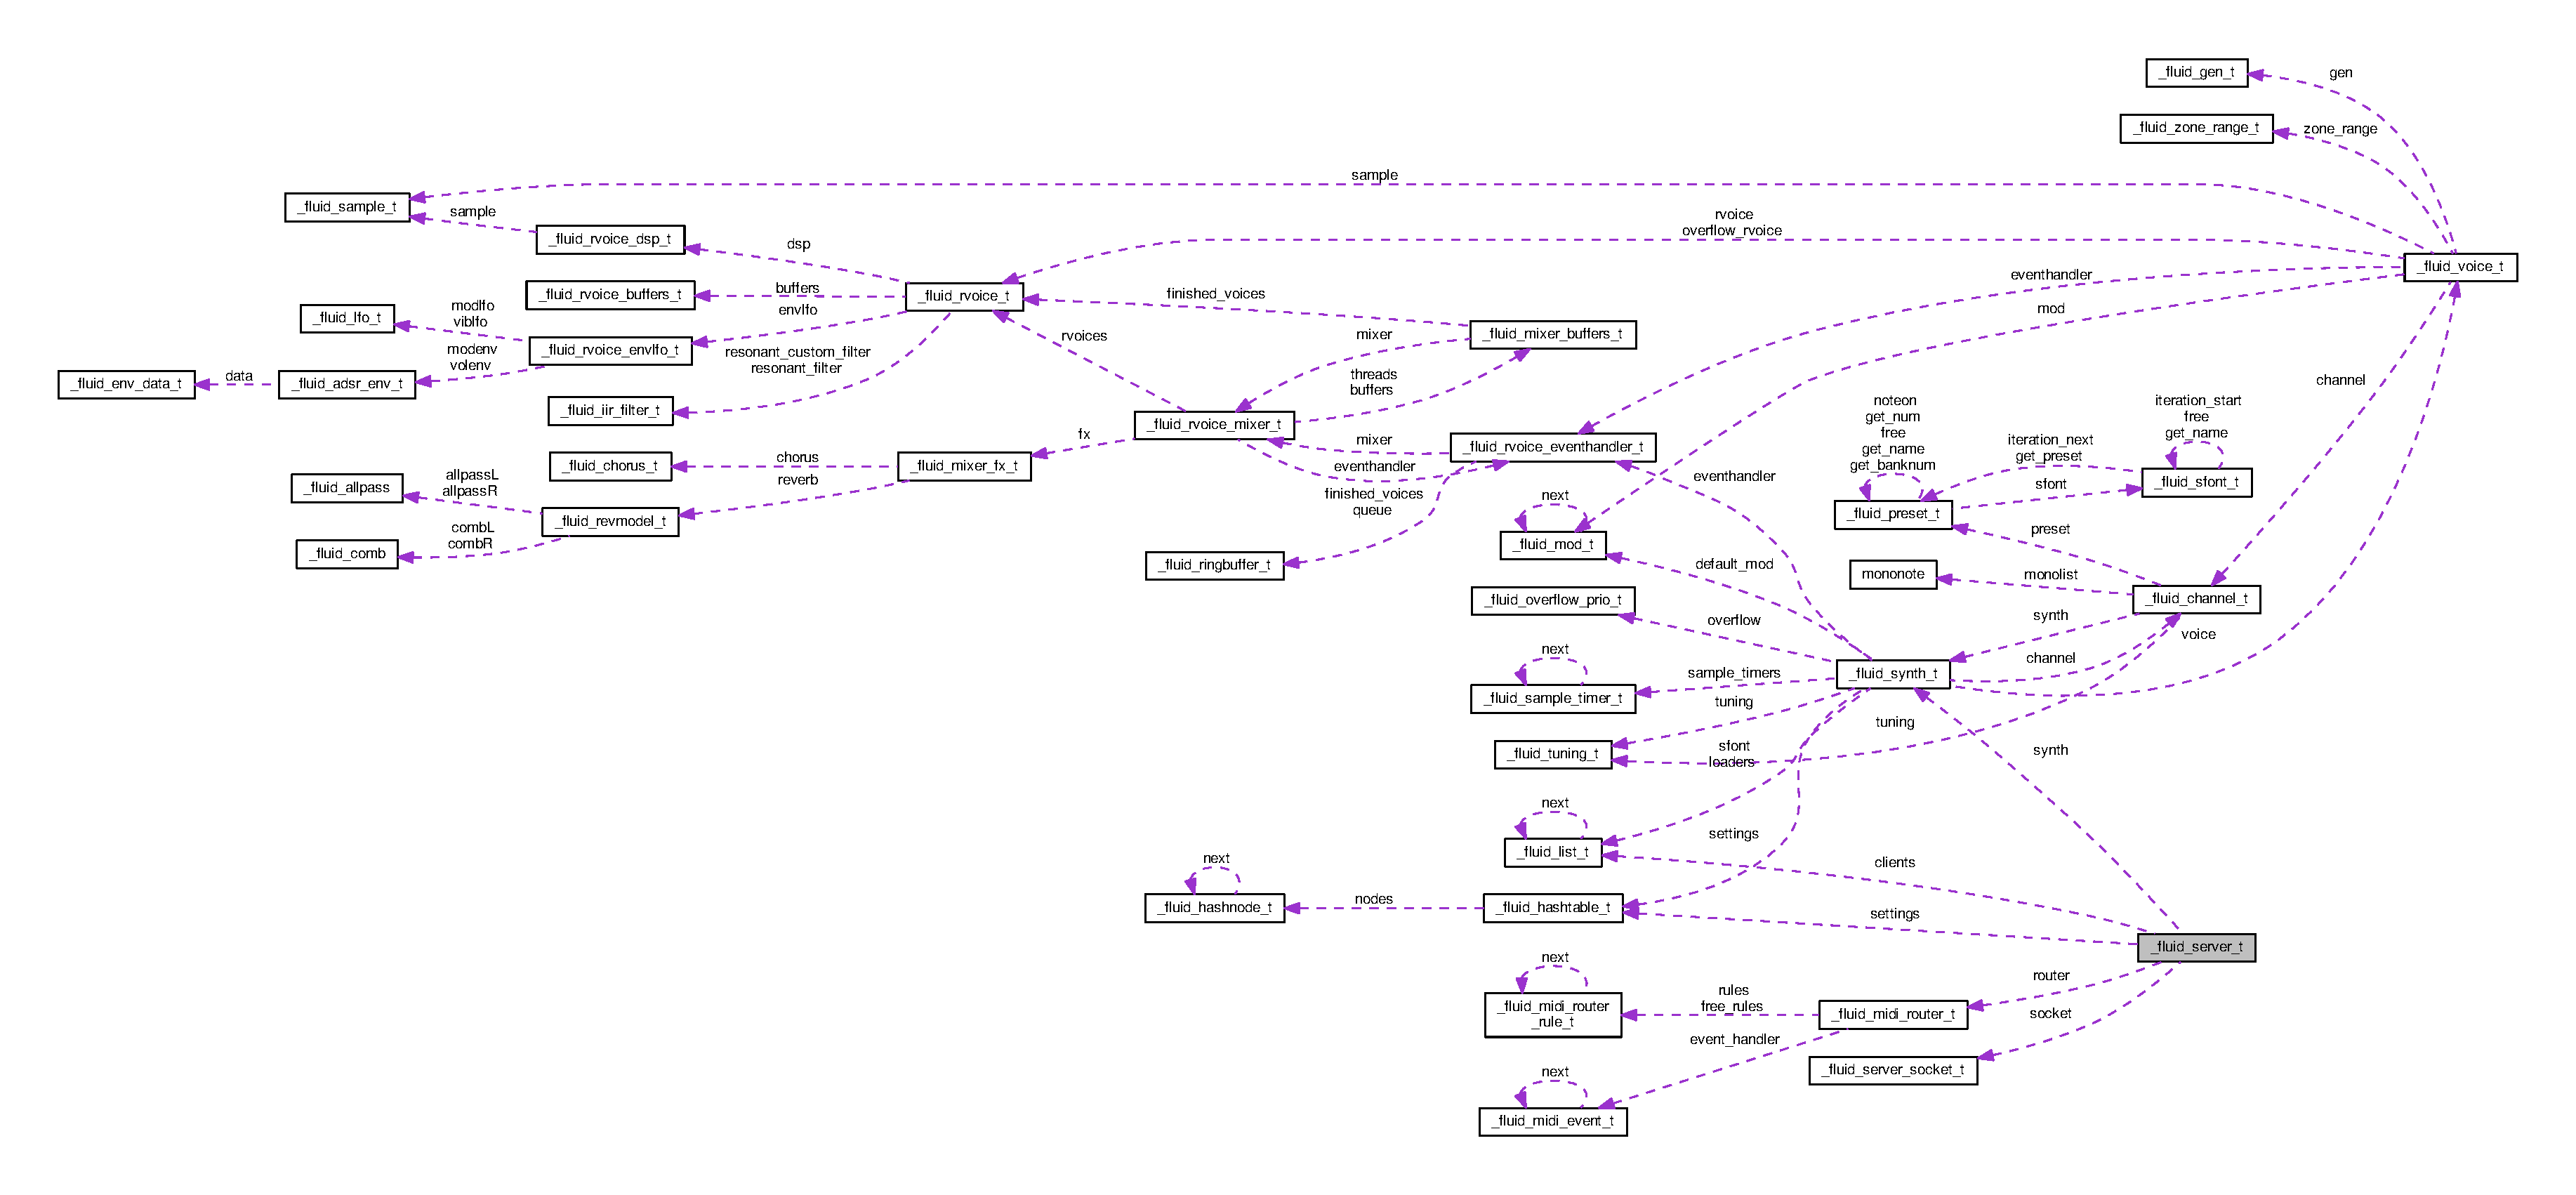
\includegraphics[width=350pt]{struct__fluid__server__t__coll__graph}
\end{center}
\end{figure}
\subsection*{Public Attributes}
\begin{DoxyCompactItemize}
\item 
\hyperlink{fluidsynth__priv_8h_a1b3924046f25f0f93876aeb093b613b9}{fluid\+\_\+server\+\_\+socket\+\_\+t} $\ast$ \hyperlink{struct__fluid__server__t_a738603070c2e5b4fc0e99e0a1471715a}{socket}
\item 
\hyperlink{types_8h_aa363402d3c77333b0f070ba531d034ba}{fluid\+\_\+settings\+\_\+t} $\ast$ \hyperlink{struct__fluid__server__t_a9d53707a5c9e1ff69da7169f7b818277}{settings}
\item 
\hyperlink{types_8h_ae265f10ae174a13afe010de50d87e1a4}{fluid\+\_\+synth\+\_\+t} $\ast$ \hyperlink{struct__fluid__server__t_ac67b75b1c51efea21e5ce8450e9872f6}{synth}
\item 
\hyperlink{types_8h_aa57b4746220e24506a169f109875e4ad}{fluid\+\_\+midi\+\_\+router\+\_\+t} $\ast$ \hyperlink{struct__fluid__server__t_a65636a3cc37392467d7fd6e4297b582c}{router}
\item 
\hyperlink{fluid__list_8h_a3ef7535d4290862c0af118569223bd89}{fluid\+\_\+list\+\_\+t} $\ast$ \hyperlink{struct__fluid__server__t_a25218bbaabb90057d1ed60096f366aac}{clients}
\item 
\hyperlink{fluid__sys_8h_a7252a44982e8ed2704689f563c8a12e3}{fluid\+\_\+mutex\+\_\+t} \hyperlink{struct__fluid__server__t_ab961b06dab40b5161a81ac78bb3957f2}{mutex}
\end{DoxyCompactItemize}


\subsection{Member Data Documentation}
\mbox{\Hypertarget{struct__fluid__server__t_a25218bbaabb90057d1ed60096f366aac}\label{struct__fluid__server__t_a25218bbaabb90057d1ed60096f366aac}} 
\index{\+\_\+fluid\+\_\+server\+\_\+t@{\+\_\+fluid\+\_\+server\+\_\+t}!clients@{clients}}
\index{clients@{clients}!\+\_\+fluid\+\_\+server\+\_\+t@{\+\_\+fluid\+\_\+server\+\_\+t}}
\subsubsection{\texorpdfstring{clients}{clients}}
{\footnotesize\ttfamily \hyperlink{fluid__list_8h_a3ef7535d4290862c0af118569223bd89}{fluid\+\_\+list\+\_\+t}$\ast$ \+\_\+fluid\+\_\+server\+\_\+t\+::clients}

\mbox{\Hypertarget{struct__fluid__server__t_ab961b06dab40b5161a81ac78bb3957f2}\label{struct__fluid__server__t_ab961b06dab40b5161a81ac78bb3957f2}} 
\index{\+\_\+fluid\+\_\+server\+\_\+t@{\+\_\+fluid\+\_\+server\+\_\+t}!mutex@{mutex}}
\index{mutex@{mutex}!\+\_\+fluid\+\_\+server\+\_\+t@{\+\_\+fluid\+\_\+server\+\_\+t}}
\subsubsection{\texorpdfstring{mutex}{mutex}}
{\footnotesize\ttfamily \hyperlink{fluid__sys_8h_a7252a44982e8ed2704689f563c8a12e3}{fluid\+\_\+mutex\+\_\+t} \+\_\+fluid\+\_\+server\+\_\+t\+::mutex}

\mbox{\Hypertarget{struct__fluid__server__t_a65636a3cc37392467d7fd6e4297b582c}\label{struct__fluid__server__t_a65636a3cc37392467d7fd6e4297b582c}} 
\index{\+\_\+fluid\+\_\+server\+\_\+t@{\+\_\+fluid\+\_\+server\+\_\+t}!router@{router}}
\index{router@{router}!\+\_\+fluid\+\_\+server\+\_\+t@{\+\_\+fluid\+\_\+server\+\_\+t}}
\subsubsection{\texorpdfstring{router}{router}}
{\footnotesize\ttfamily \hyperlink{types_8h_aa57b4746220e24506a169f109875e4ad}{fluid\+\_\+midi\+\_\+router\+\_\+t}$\ast$ \+\_\+fluid\+\_\+server\+\_\+t\+::router}

\mbox{\Hypertarget{struct__fluid__server__t_a9d53707a5c9e1ff69da7169f7b818277}\label{struct__fluid__server__t_a9d53707a5c9e1ff69da7169f7b818277}} 
\index{\+\_\+fluid\+\_\+server\+\_\+t@{\+\_\+fluid\+\_\+server\+\_\+t}!settings@{settings}}
\index{settings@{settings}!\+\_\+fluid\+\_\+server\+\_\+t@{\+\_\+fluid\+\_\+server\+\_\+t}}
\subsubsection{\texorpdfstring{settings}{settings}}
{\footnotesize\ttfamily \hyperlink{types_8h_aa363402d3c77333b0f070ba531d034ba}{fluid\+\_\+settings\+\_\+t}$\ast$ \+\_\+fluid\+\_\+server\+\_\+t\+::settings}

\mbox{\Hypertarget{struct__fluid__server__t_a738603070c2e5b4fc0e99e0a1471715a}\label{struct__fluid__server__t_a738603070c2e5b4fc0e99e0a1471715a}} 
\index{\+\_\+fluid\+\_\+server\+\_\+t@{\+\_\+fluid\+\_\+server\+\_\+t}!socket@{socket}}
\index{socket@{socket}!\+\_\+fluid\+\_\+server\+\_\+t@{\+\_\+fluid\+\_\+server\+\_\+t}}
\subsubsection{\texorpdfstring{socket}{socket}}
{\footnotesize\ttfamily \hyperlink{fluidsynth__priv_8h_a1b3924046f25f0f93876aeb093b613b9}{fluid\+\_\+server\+\_\+socket\+\_\+t}$\ast$ \+\_\+fluid\+\_\+server\+\_\+t\+::socket}

\mbox{\Hypertarget{struct__fluid__server__t_ac67b75b1c51efea21e5ce8450e9872f6}\label{struct__fluid__server__t_ac67b75b1c51efea21e5ce8450e9872f6}} 
\index{\+\_\+fluid\+\_\+server\+\_\+t@{\+\_\+fluid\+\_\+server\+\_\+t}!synth@{synth}}
\index{synth@{synth}!\+\_\+fluid\+\_\+server\+\_\+t@{\+\_\+fluid\+\_\+server\+\_\+t}}
\subsubsection{\texorpdfstring{synth}{synth}}
{\footnotesize\ttfamily \hyperlink{types_8h_ae265f10ae174a13afe010de50d87e1a4}{fluid\+\_\+synth\+\_\+t}$\ast$ \+\_\+fluid\+\_\+server\+\_\+t\+::synth}



The documentation for this struct was generated from the following file\+:\begin{DoxyCompactItemize}
\item 
bindings/\hyperlink{fluid__cmd_8c}{fluid\+\_\+cmd.\+c}\end{DoxyCompactItemize}

\hypertarget{struct__fluid__sfloader__t}{}\section{\+\_\+fluid\+\_\+sfloader\+\_\+t Struct Reference}
\label{struct__fluid__sfloader__t}\index{\+\_\+fluid\+\_\+sfloader\+\_\+t@{\+\_\+fluid\+\_\+sfloader\+\_\+t}}


{\ttfamily \#include $<$fluid\+\_\+sfont.\+h$>$}



Collaboration diagram for \+\_\+fluid\+\_\+sfloader\+\_\+t\+:
\nopagebreak
\begin{figure}[H]
\begin{center}
\leavevmode
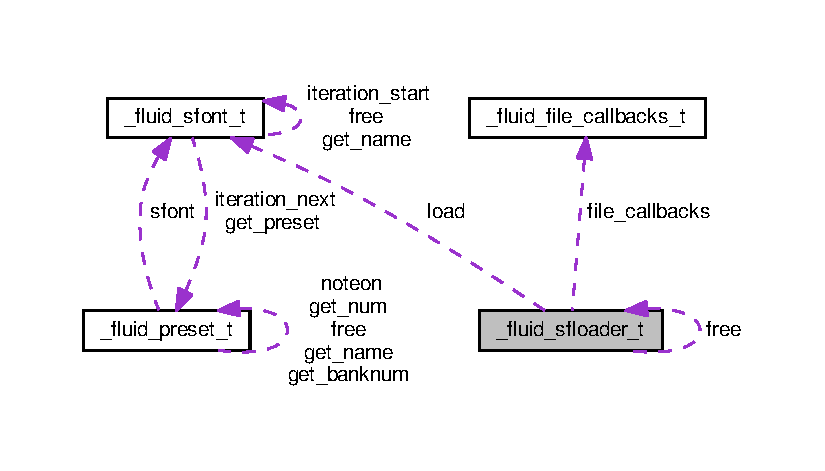
\includegraphics[width=350pt]{struct__fluid__sfloader__t__coll__graph}
\end{center}
\end{figure}
\subsection*{Public Attributes}
\begin{DoxyCompactItemize}
\item 
void $\ast$ \hyperlink{struct__fluid__sfloader__t_a128547f2341db8c9f5ddb0158d1d4235}{data}
\item 
\hyperlink{types_8h_a6a223e4b8d83753d95c87e1feed58227}{fluid\+\_\+file\+\_\+callbacks\+\_\+t} \hyperlink{struct__fluid__sfloader__t_a03d8c51a7b64dd670899f6affaa43805}{file\+\_\+callbacks}
\item 
\hyperlink{sfont_8h_aab801ff11ddf556d3f34e82c2ca02897}{fluid\+\_\+sfloader\+\_\+free\+\_\+t} \hyperlink{struct__fluid__sfloader__t_a00c9b284ca7894da330b306ab091ed14}{free}
\item 
\hyperlink{sfont_8h_a4fce6413dd211799ce9716fe1b56b635}{fluid\+\_\+sfloader\+\_\+load\+\_\+t} \hyperlink{struct__fluid__sfloader__t_ad0c3fd755c8c9a4333e7d0a15f50844f}{load}
\end{DoxyCompactItemize}


\subsection{Detailed Description}
Sound\+Font loader structure. 

\subsection{Member Data Documentation}
\mbox{\Hypertarget{struct__fluid__sfloader__t_a128547f2341db8c9f5ddb0158d1d4235}\label{struct__fluid__sfloader__t_a128547f2341db8c9f5ddb0158d1d4235}} 
\index{\+\_\+fluid\+\_\+sfloader\+\_\+t@{\+\_\+fluid\+\_\+sfloader\+\_\+t}!data@{data}}
\index{data@{data}!\+\_\+fluid\+\_\+sfloader\+\_\+t@{\+\_\+fluid\+\_\+sfloader\+\_\+t}}
\subsubsection{\texorpdfstring{data}{data}}
{\footnotesize\ttfamily void$\ast$ \+\_\+fluid\+\_\+sfloader\+\_\+t\+::data}

User defined data pointer used by \hyperlink{struct__fluid__sfloader__t_ad0c3fd755c8c9a4333e7d0a15f50844f}{\+\_\+fluid\+\_\+sfloader\+\_\+t\+::load()} \mbox{\Hypertarget{struct__fluid__sfloader__t_a03d8c51a7b64dd670899f6affaa43805}\label{struct__fluid__sfloader__t_a03d8c51a7b64dd670899f6affaa43805}} 
\index{\+\_\+fluid\+\_\+sfloader\+\_\+t@{\+\_\+fluid\+\_\+sfloader\+\_\+t}!file\+\_\+callbacks@{file\+\_\+callbacks}}
\index{file\+\_\+callbacks@{file\+\_\+callbacks}!\+\_\+fluid\+\_\+sfloader\+\_\+t@{\+\_\+fluid\+\_\+sfloader\+\_\+t}}
\subsubsection{\texorpdfstring{file\+\_\+callbacks}{file\_callbacks}}
{\footnotesize\ttfamily \hyperlink{types_8h_a6a223e4b8d83753d95c87e1feed58227}{fluid\+\_\+file\+\_\+callbacks\+\_\+t} \+\_\+fluid\+\_\+sfloader\+\_\+t\+::file\+\_\+callbacks}

Callback structure specifying file operations used during soundfont loading to allow custom loading, such as from memory \mbox{\Hypertarget{struct__fluid__sfloader__t_a00c9b284ca7894da330b306ab091ed14}\label{struct__fluid__sfloader__t_a00c9b284ca7894da330b306ab091ed14}} 
\index{\+\_\+fluid\+\_\+sfloader\+\_\+t@{\+\_\+fluid\+\_\+sfloader\+\_\+t}!free@{free}}
\index{free@{free}!\+\_\+fluid\+\_\+sfloader\+\_\+t@{\+\_\+fluid\+\_\+sfloader\+\_\+t}}
\subsubsection{\texorpdfstring{free}{free}}
{\footnotesize\ttfamily \hyperlink{sfont_8h_aab801ff11ddf556d3f34e82c2ca02897}{fluid\+\_\+sfloader\+\_\+free\+\_\+t} \+\_\+fluid\+\_\+sfloader\+\_\+t\+::free}

\mbox{\Hypertarget{struct__fluid__sfloader__t_ad0c3fd755c8c9a4333e7d0a15f50844f}\label{struct__fluid__sfloader__t_ad0c3fd755c8c9a4333e7d0a15f50844f}} 
\index{\+\_\+fluid\+\_\+sfloader\+\_\+t@{\+\_\+fluid\+\_\+sfloader\+\_\+t}!load@{load}}
\index{load@{load}!\+\_\+fluid\+\_\+sfloader\+\_\+t@{\+\_\+fluid\+\_\+sfloader\+\_\+t}}
\subsubsection{\texorpdfstring{load}{load}}
{\footnotesize\ttfamily \hyperlink{sfont_8h_a4fce6413dd211799ce9716fe1b56b635}{fluid\+\_\+sfloader\+\_\+load\+\_\+t} \+\_\+fluid\+\_\+sfloader\+\_\+t\+::load}



The documentation for this struct was generated from the following file\+:\begin{DoxyCompactItemize}
\item 
sfloader/\hyperlink{fluid__sfont_8h}{fluid\+\_\+sfont.\+h}\end{DoxyCompactItemize}

\hypertarget{struct__fluid__sfont__t}{}\section{\+\_\+fluid\+\_\+sfont\+\_\+t Struct Reference}
\label{struct__fluid__sfont__t}\index{\+\_\+fluid\+\_\+sfont\+\_\+t@{\+\_\+fluid\+\_\+sfont\+\_\+t}}


{\ttfamily \#include $<$fluid\+\_\+sfont.\+h$>$}



Collaboration diagram for \+\_\+fluid\+\_\+sfont\+\_\+t\+:
\nopagebreak
\begin{figure}[H]
\begin{center}
\leavevmode
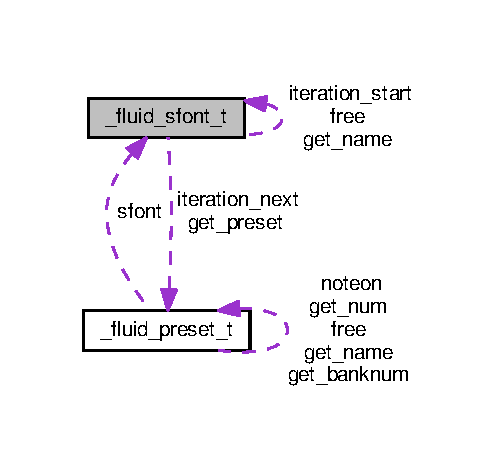
\includegraphics[width=239pt]{struct__fluid__sfont__t__coll__graph}
\end{center}
\end{figure}
\subsection*{Public Attributes}
\begin{DoxyCompactItemize}
\item 
void $\ast$ \hyperlink{struct__fluid__sfont__t_a5a79644021fa078479da5273c4ebfbbc}{data}
\item 
int \hyperlink{struct__fluid__sfont__t_ae4d9ebeb04ab1e6af64f2b0f94da6174}{id}
\item 
int \hyperlink{struct__fluid__sfont__t_a71bae1b34460e3b0d6ed98fb072a73bd}{refcount}
\item 
int \hyperlink{struct__fluid__sfont__t_a7f62449a63ddea4c1e2b841f824eee61}{bankofs}
\item 
\hyperlink{sfont_8h_aad47ceab3ec2c3fed9437a796225a875}{fluid\+\_\+sfont\+\_\+free\+\_\+t} \hyperlink{struct__fluid__sfont__t_abcc049d7b150090b9be0265011e5f832}{free}
\item 
\hyperlink{sfont_8h_acd7242e3e80a5ae096c93dae7f30d7f4}{fluid\+\_\+sfont\+\_\+get\+\_\+name\+\_\+t} \hyperlink{struct__fluid__sfont__t_a929dd42064e5eaa61bfe3682eeae23aa}{get\+\_\+name}
\item 
\hyperlink{sfont_8h_afe6fe536f98021be6598525a9e517f2f}{fluid\+\_\+sfont\+\_\+get\+\_\+preset\+\_\+t} \hyperlink{struct__fluid__sfont__t_a2ac8d2d07d908d76fd84417c4bcd9b57}{get\+\_\+preset}
\item 
\hyperlink{fluid__sfont_8h_a80ffb76a9a2c640816f57889666c28cb}{fluid\+\_\+sfont\+\_\+iteration\+\_\+start\+\_\+t} \hyperlink{struct__fluid__sfont__t_ae085ae4aba987fe1725bbc6a1d0d9532}{iteration\+\_\+start}
\item 
\hyperlink{fluid__sfont_8h_aecaff75beb3685fad68dea387555a6e5}{fluid\+\_\+sfont\+\_\+iteration\+\_\+next\+\_\+t} \hyperlink{struct__fluid__sfont__t_a79ac963ce5c6b7e31a7cb41cdcb71f70}{iteration\+\_\+next}
\end{DoxyCompactItemize}


\subsection{Detailed Description}
Virtual Sound\+Font instance structure. 

\subsection{Member Data Documentation}
\mbox{\Hypertarget{struct__fluid__sfont__t_a7f62449a63ddea4c1e2b841f824eee61}\label{struct__fluid__sfont__t_a7f62449a63ddea4c1e2b841f824eee61}} 
\index{\+\_\+fluid\+\_\+sfont\+\_\+t@{\+\_\+fluid\+\_\+sfont\+\_\+t}!bankofs@{bankofs}}
\index{bankofs@{bankofs}!\+\_\+fluid\+\_\+sfont\+\_\+t@{\+\_\+fluid\+\_\+sfont\+\_\+t}}
\subsubsection{\texorpdfstring{bankofs}{bankofs}}
{\footnotesize\ttfamily int \+\_\+fluid\+\_\+sfont\+\_\+t\+::bankofs}

Bank offset \mbox{\Hypertarget{struct__fluid__sfont__t_a5a79644021fa078479da5273c4ebfbbc}\label{struct__fluid__sfont__t_a5a79644021fa078479da5273c4ebfbbc}} 
\index{\+\_\+fluid\+\_\+sfont\+\_\+t@{\+\_\+fluid\+\_\+sfont\+\_\+t}!data@{data}}
\index{data@{data}!\+\_\+fluid\+\_\+sfont\+\_\+t@{\+\_\+fluid\+\_\+sfont\+\_\+t}}
\subsubsection{\texorpdfstring{data}{data}}
{\footnotesize\ttfamily void$\ast$ \+\_\+fluid\+\_\+sfont\+\_\+t\+::data}

User defined data \mbox{\Hypertarget{struct__fluid__sfont__t_abcc049d7b150090b9be0265011e5f832}\label{struct__fluid__sfont__t_abcc049d7b150090b9be0265011e5f832}} 
\index{\+\_\+fluid\+\_\+sfont\+\_\+t@{\+\_\+fluid\+\_\+sfont\+\_\+t}!free@{free}}
\index{free@{free}!\+\_\+fluid\+\_\+sfont\+\_\+t@{\+\_\+fluid\+\_\+sfont\+\_\+t}}
\subsubsection{\texorpdfstring{free}{free}}
{\footnotesize\ttfamily \hyperlink{sfont_8h_aad47ceab3ec2c3fed9437a796225a875}{fluid\+\_\+sfont\+\_\+free\+\_\+t} \+\_\+fluid\+\_\+sfont\+\_\+t\+::free}

\mbox{\Hypertarget{struct__fluid__sfont__t_a929dd42064e5eaa61bfe3682eeae23aa}\label{struct__fluid__sfont__t_a929dd42064e5eaa61bfe3682eeae23aa}} 
\index{\+\_\+fluid\+\_\+sfont\+\_\+t@{\+\_\+fluid\+\_\+sfont\+\_\+t}!get\+\_\+name@{get\+\_\+name}}
\index{get\+\_\+name@{get\+\_\+name}!\+\_\+fluid\+\_\+sfont\+\_\+t@{\+\_\+fluid\+\_\+sfont\+\_\+t}}
\subsubsection{\texorpdfstring{get\+\_\+name}{get\_name}}
{\footnotesize\ttfamily \hyperlink{sfont_8h_acd7242e3e80a5ae096c93dae7f30d7f4}{fluid\+\_\+sfont\+\_\+get\+\_\+name\+\_\+t} \+\_\+fluid\+\_\+sfont\+\_\+t\+::get\+\_\+name}

\mbox{\Hypertarget{struct__fluid__sfont__t_a2ac8d2d07d908d76fd84417c4bcd9b57}\label{struct__fluid__sfont__t_a2ac8d2d07d908d76fd84417c4bcd9b57}} 
\index{\+\_\+fluid\+\_\+sfont\+\_\+t@{\+\_\+fluid\+\_\+sfont\+\_\+t}!get\+\_\+preset@{get\+\_\+preset}}
\index{get\+\_\+preset@{get\+\_\+preset}!\+\_\+fluid\+\_\+sfont\+\_\+t@{\+\_\+fluid\+\_\+sfont\+\_\+t}}
\subsubsection{\texorpdfstring{get\+\_\+preset}{get\_preset}}
{\footnotesize\ttfamily \hyperlink{sfont_8h_afe6fe536f98021be6598525a9e517f2f}{fluid\+\_\+sfont\+\_\+get\+\_\+preset\+\_\+t} \+\_\+fluid\+\_\+sfont\+\_\+t\+::get\+\_\+preset}

\mbox{\Hypertarget{struct__fluid__sfont__t_ae4d9ebeb04ab1e6af64f2b0f94da6174}\label{struct__fluid__sfont__t_ae4d9ebeb04ab1e6af64f2b0f94da6174}} 
\index{\+\_\+fluid\+\_\+sfont\+\_\+t@{\+\_\+fluid\+\_\+sfont\+\_\+t}!id@{id}}
\index{id@{id}!\+\_\+fluid\+\_\+sfont\+\_\+t@{\+\_\+fluid\+\_\+sfont\+\_\+t}}
\subsubsection{\texorpdfstring{id}{id}}
{\footnotesize\ttfamily int \+\_\+fluid\+\_\+sfont\+\_\+t\+::id}

Sound\+Font ID \mbox{\Hypertarget{struct__fluid__sfont__t_a79ac963ce5c6b7e31a7cb41cdcb71f70}\label{struct__fluid__sfont__t_a79ac963ce5c6b7e31a7cb41cdcb71f70}} 
\index{\+\_\+fluid\+\_\+sfont\+\_\+t@{\+\_\+fluid\+\_\+sfont\+\_\+t}!iteration\+\_\+next@{iteration\+\_\+next}}
\index{iteration\+\_\+next@{iteration\+\_\+next}!\+\_\+fluid\+\_\+sfont\+\_\+t@{\+\_\+fluid\+\_\+sfont\+\_\+t}}
\subsubsection{\texorpdfstring{iteration\+\_\+next}{iteration\_next}}
{\footnotesize\ttfamily \hyperlink{fluid__sfont_8h_aecaff75beb3685fad68dea387555a6e5}{fluid\+\_\+sfont\+\_\+iteration\+\_\+next\+\_\+t} \+\_\+fluid\+\_\+sfont\+\_\+t\+::iteration\+\_\+next}

\mbox{\Hypertarget{struct__fluid__sfont__t_ae085ae4aba987fe1725bbc6a1d0d9532}\label{struct__fluid__sfont__t_ae085ae4aba987fe1725bbc6a1d0d9532}} 
\index{\+\_\+fluid\+\_\+sfont\+\_\+t@{\+\_\+fluid\+\_\+sfont\+\_\+t}!iteration\+\_\+start@{iteration\+\_\+start}}
\index{iteration\+\_\+start@{iteration\+\_\+start}!\+\_\+fluid\+\_\+sfont\+\_\+t@{\+\_\+fluid\+\_\+sfont\+\_\+t}}
\subsubsection{\texorpdfstring{iteration\+\_\+start}{iteration\_start}}
{\footnotesize\ttfamily \hyperlink{fluid__sfont_8h_a80ffb76a9a2c640816f57889666c28cb}{fluid\+\_\+sfont\+\_\+iteration\+\_\+start\+\_\+t} \+\_\+fluid\+\_\+sfont\+\_\+t\+::iteration\+\_\+start}

\mbox{\Hypertarget{struct__fluid__sfont__t_a71bae1b34460e3b0d6ed98fb072a73bd}\label{struct__fluid__sfont__t_a71bae1b34460e3b0d6ed98fb072a73bd}} 
\index{\+\_\+fluid\+\_\+sfont\+\_\+t@{\+\_\+fluid\+\_\+sfont\+\_\+t}!refcount@{refcount}}
\index{refcount@{refcount}!\+\_\+fluid\+\_\+sfont\+\_\+t@{\+\_\+fluid\+\_\+sfont\+\_\+t}}
\subsubsection{\texorpdfstring{refcount}{refcount}}
{\footnotesize\ttfamily int \+\_\+fluid\+\_\+sfont\+\_\+t\+::refcount}

Sound\+Font reference count (1 if no presets referencing it) 

The documentation for this struct was generated from the following file\+:\begin{DoxyCompactItemize}
\item 
sfloader/\hyperlink{fluid__sfont_8h}{fluid\+\_\+sfont.\+h}\end{DoxyCompactItemize}

\hypertarget{struct__fluid__shell__t}{}\section{\+\_\+fluid\+\_\+shell\+\_\+t Struct Reference}
\label{struct__fluid__shell__t}\index{\+\_\+fluid\+\_\+shell\+\_\+t@{\+\_\+fluid\+\_\+shell\+\_\+t}}


Collaboration diagram for \+\_\+fluid\+\_\+shell\+\_\+t\+:
\nopagebreak
\begin{figure}[H]
\begin{center}
\leavevmode
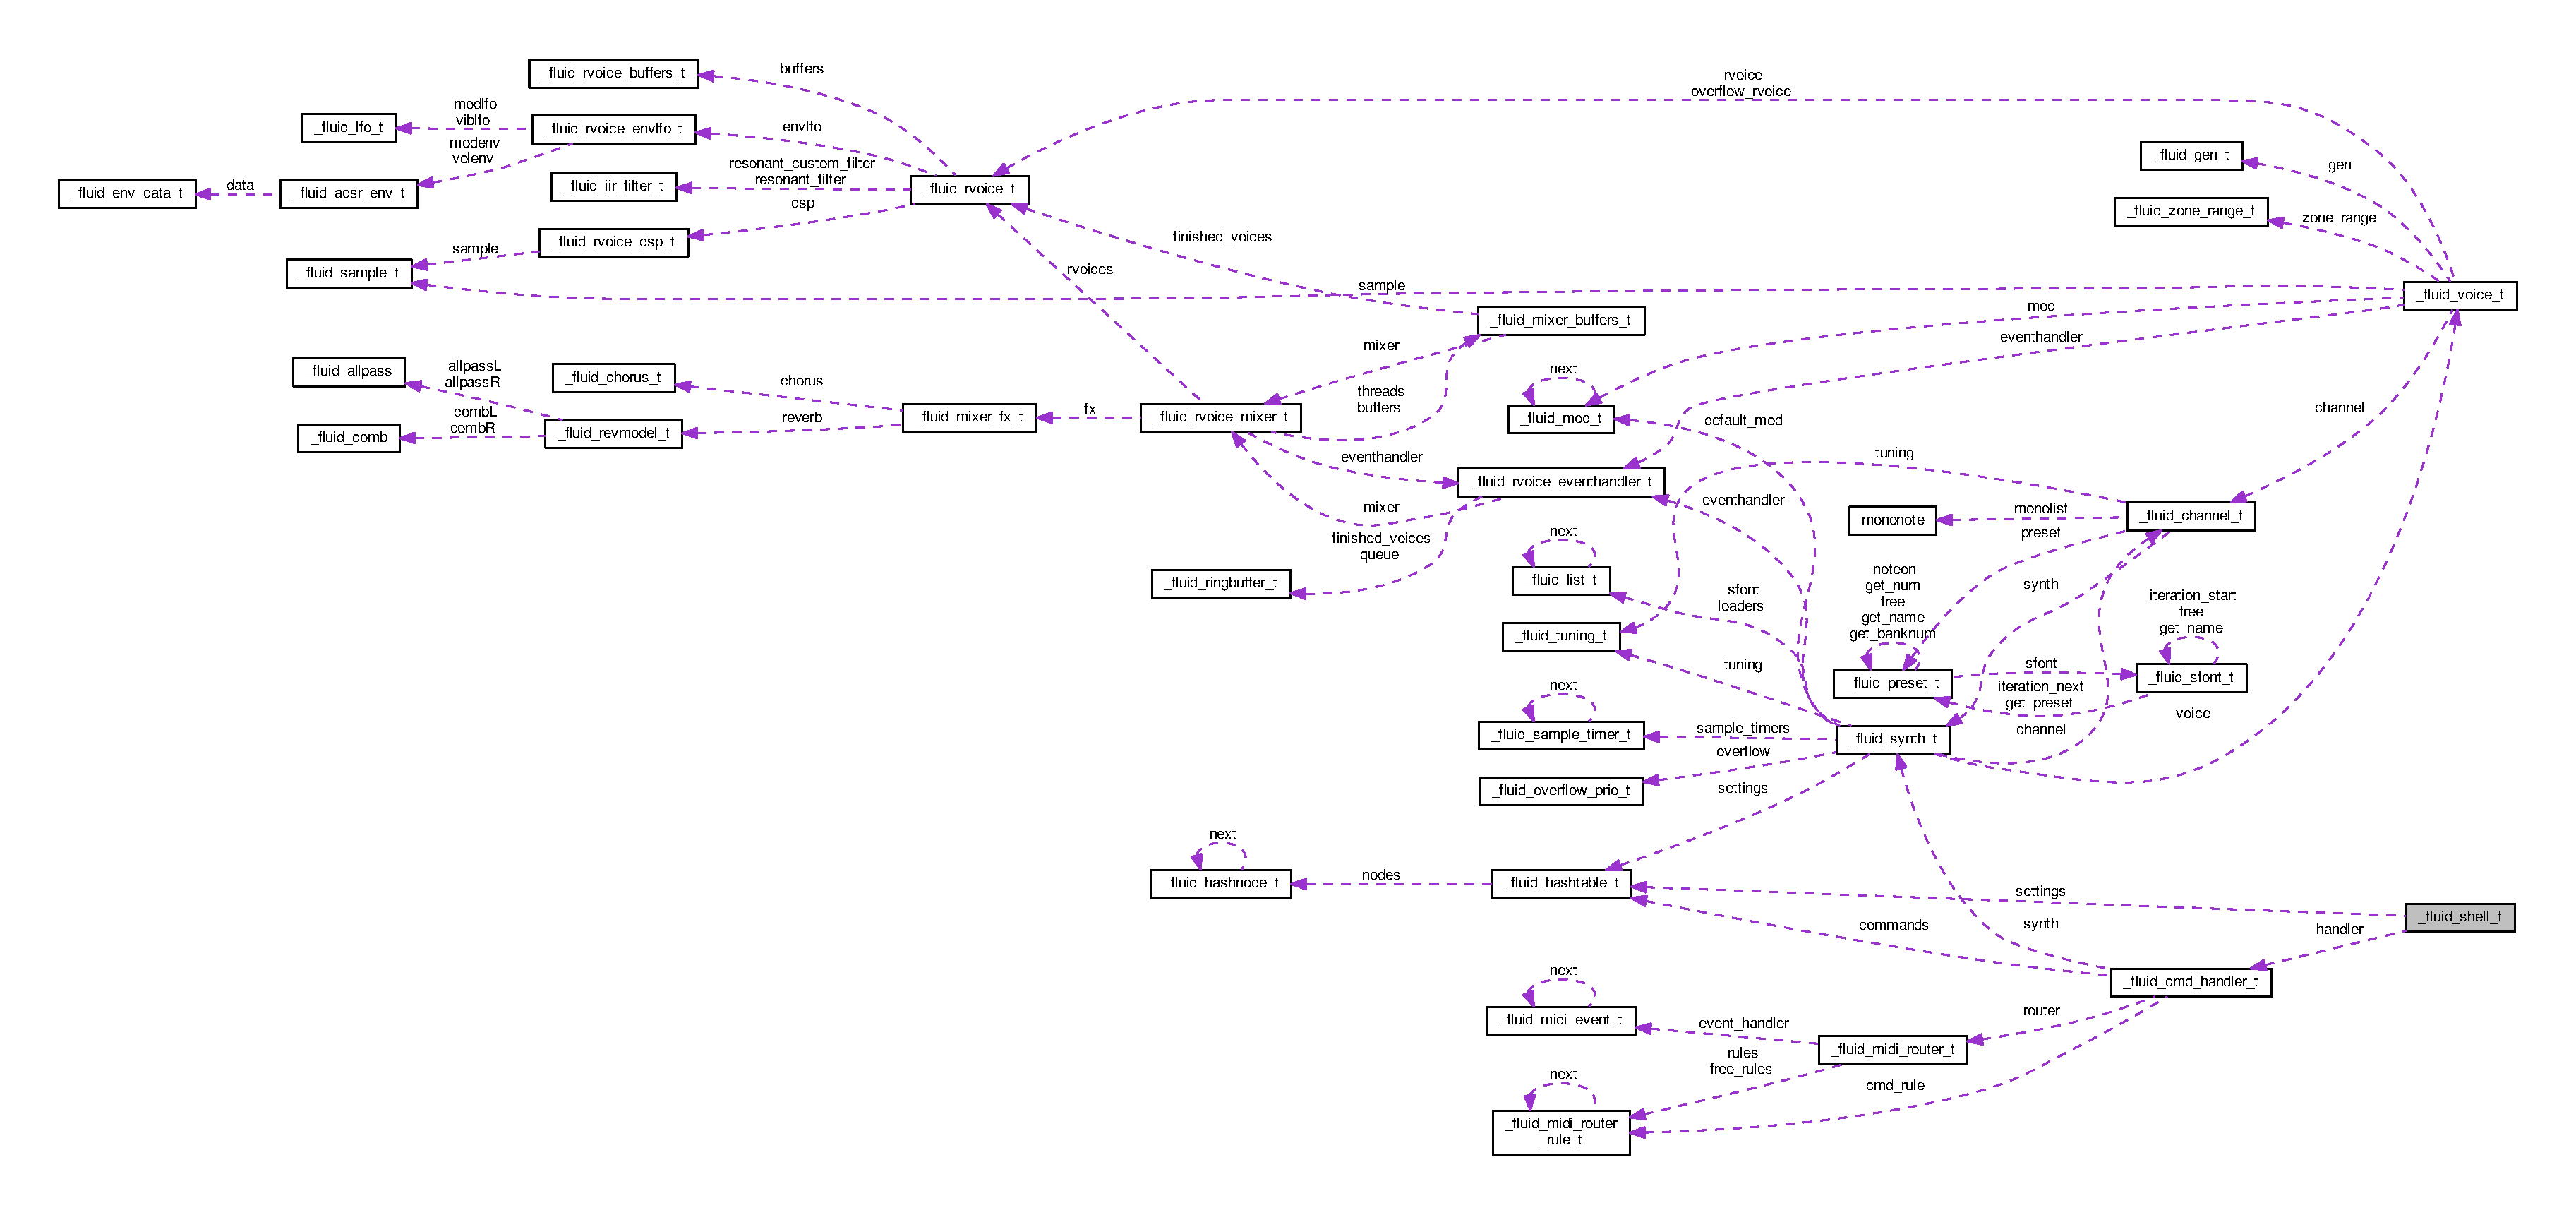
\includegraphics[width=350pt]{struct__fluid__shell__t__coll__graph}
\end{center}
\end{figure}
\subsection*{Public Attributes}
\begin{DoxyCompactItemize}
\item 
\hyperlink{types_8h_aa363402d3c77333b0f070ba531d034ba}{fluid\+\_\+settings\+\_\+t} $\ast$ \hyperlink{struct__fluid__shell__t_aea94d440631a695b47d8a36a17ac1eab}{settings}
\item 
\hyperlink{types_8h_ae1944df078b25beb347abd07e42b35a4}{fluid\+\_\+cmd\+\_\+handler\+\_\+t} $\ast$ \hyperlink{struct__fluid__shell__t_ad82ffb069af502faae17a8c9187c12b9}{handler}
\item 
\hyperlink{fluid__sys_8h_a60a6466e68a45b0f0709f1ebaa7e6f85}{fluid\+\_\+thread\+\_\+t} $\ast$ \hyperlink{struct__fluid__shell__t_ae8d173944c48140af913a50899272897}{thread}
\item 
\hyperlink{types_8h_a436fa1df8d13a21321d39902b0d60208}{fluid\+\_\+istream\+\_\+t} \hyperlink{struct__fluid__shell__t_a08df72f9b4f053d7c8f4f787848ec732}{in}
\item 
\hyperlink{types_8h_a6d8c441b84ab0430e358438cee876c69}{fluid\+\_\+ostream\+\_\+t} \hyperlink{struct__fluid__shell__t_ad06a4d5f08bd010ba4d30e7aa90c0435}{out}
\end{DoxyCompactItemize}


\subsection{Member Data Documentation}
\mbox{\Hypertarget{struct__fluid__shell__t_ad82ffb069af502faae17a8c9187c12b9}\label{struct__fluid__shell__t_ad82ffb069af502faae17a8c9187c12b9}} 
\index{\+\_\+fluid\+\_\+shell\+\_\+t@{\+\_\+fluid\+\_\+shell\+\_\+t}!handler@{handler}}
\index{handler@{handler}!\+\_\+fluid\+\_\+shell\+\_\+t@{\+\_\+fluid\+\_\+shell\+\_\+t}}
\subsubsection{\texorpdfstring{handler}{handler}}
{\footnotesize\ttfamily \hyperlink{types_8h_ae1944df078b25beb347abd07e42b35a4}{fluid\+\_\+cmd\+\_\+handler\+\_\+t}$\ast$ \+\_\+fluid\+\_\+shell\+\_\+t\+::handler}

\mbox{\Hypertarget{struct__fluid__shell__t_a08df72f9b4f053d7c8f4f787848ec732}\label{struct__fluid__shell__t_a08df72f9b4f053d7c8f4f787848ec732}} 
\index{\+\_\+fluid\+\_\+shell\+\_\+t@{\+\_\+fluid\+\_\+shell\+\_\+t}!in@{in}}
\index{in@{in}!\+\_\+fluid\+\_\+shell\+\_\+t@{\+\_\+fluid\+\_\+shell\+\_\+t}}
\subsubsection{\texorpdfstring{in}{in}}
{\footnotesize\ttfamily \hyperlink{types_8h_a436fa1df8d13a21321d39902b0d60208}{fluid\+\_\+istream\+\_\+t} \+\_\+fluid\+\_\+shell\+\_\+t\+::in}

\mbox{\Hypertarget{struct__fluid__shell__t_ad06a4d5f08bd010ba4d30e7aa90c0435}\label{struct__fluid__shell__t_ad06a4d5f08bd010ba4d30e7aa90c0435}} 
\index{\+\_\+fluid\+\_\+shell\+\_\+t@{\+\_\+fluid\+\_\+shell\+\_\+t}!out@{out}}
\index{out@{out}!\+\_\+fluid\+\_\+shell\+\_\+t@{\+\_\+fluid\+\_\+shell\+\_\+t}}
\subsubsection{\texorpdfstring{out}{out}}
{\footnotesize\ttfamily \hyperlink{types_8h_a6d8c441b84ab0430e358438cee876c69}{fluid\+\_\+ostream\+\_\+t} \+\_\+fluid\+\_\+shell\+\_\+t\+::out}

\mbox{\Hypertarget{struct__fluid__shell__t_aea94d440631a695b47d8a36a17ac1eab}\label{struct__fluid__shell__t_aea94d440631a695b47d8a36a17ac1eab}} 
\index{\+\_\+fluid\+\_\+shell\+\_\+t@{\+\_\+fluid\+\_\+shell\+\_\+t}!settings@{settings}}
\index{settings@{settings}!\+\_\+fluid\+\_\+shell\+\_\+t@{\+\_\+fluid\+\_\+shell\+\_\+t}}
\subsubsection{\texorpdfstring{settings}{settings}}
{\footnotesize\ttfamily \hyperlink{types_8h_aa363402d3c77333b0f070ba531d034ba}{fluid\+\_\+settings\+\_\+t}$\ast$ \+\_\+fluid\+\_\+shell\+\_\+t\+::settings}

\mbox{\Hypertarget{struct__fluid__shell__t_ae8d173944c48140af913a50899272897}\label{struct__fluid__shell__t_ae8d173944c48140af913a50899272897}} 
\index{\+\_\+fluid\+\_\+shell\+\_\+t@{\+\_\+fluid\+\_\+shell\+\_\+t}!thread@{thread}}
\index{thread@{thread}!\+\_\+fluid\+\_\+shell\+\_\+t@{\+\_\+fluid\+\_\+shell\+\_\+t}}
\subsubsection{\texorpdfstring{thread}{thread}}
{\footnotesize\ttfamily \hyperlink{fluid__sys_8h_a60a6466e68a45b0f0709f1ebaa7e6f85}{fluid\+\_\+thread\+\_\+t}$\ast$ \+\_\+fluid\+\_\+shell\+\_\+t\+::thread}



The documentation for this struct was generated from the following file\+:\begin{DoxyCompactItemize}
\item 
bindings/\hyperlink{fluid__cmd_8c}{fluid\+\_\+cmd.\+c}\end{DoxyCompactItemize}

\hypertarget{struct__fluid__synth__t}{}\section{\+\_\+fluid\+\_\+synth\+\_\+t Struct Reference}
\label{struct__fluid__synth__t}\index{\+\_\+fluid\+\_\+synth\+\_\+t@{\+\_\+fluid\+\_\+synth\+\_\+t}}


{\ttfamily \#include $<$fluid\+\_\+synth.\+h$>$}



Collaboration diagram for \+\_\+fluid\+\_\+synth\+\_\+t\+:
\nopagebreak
\begin{figure}[H]
\begin{center}
\leavevmode
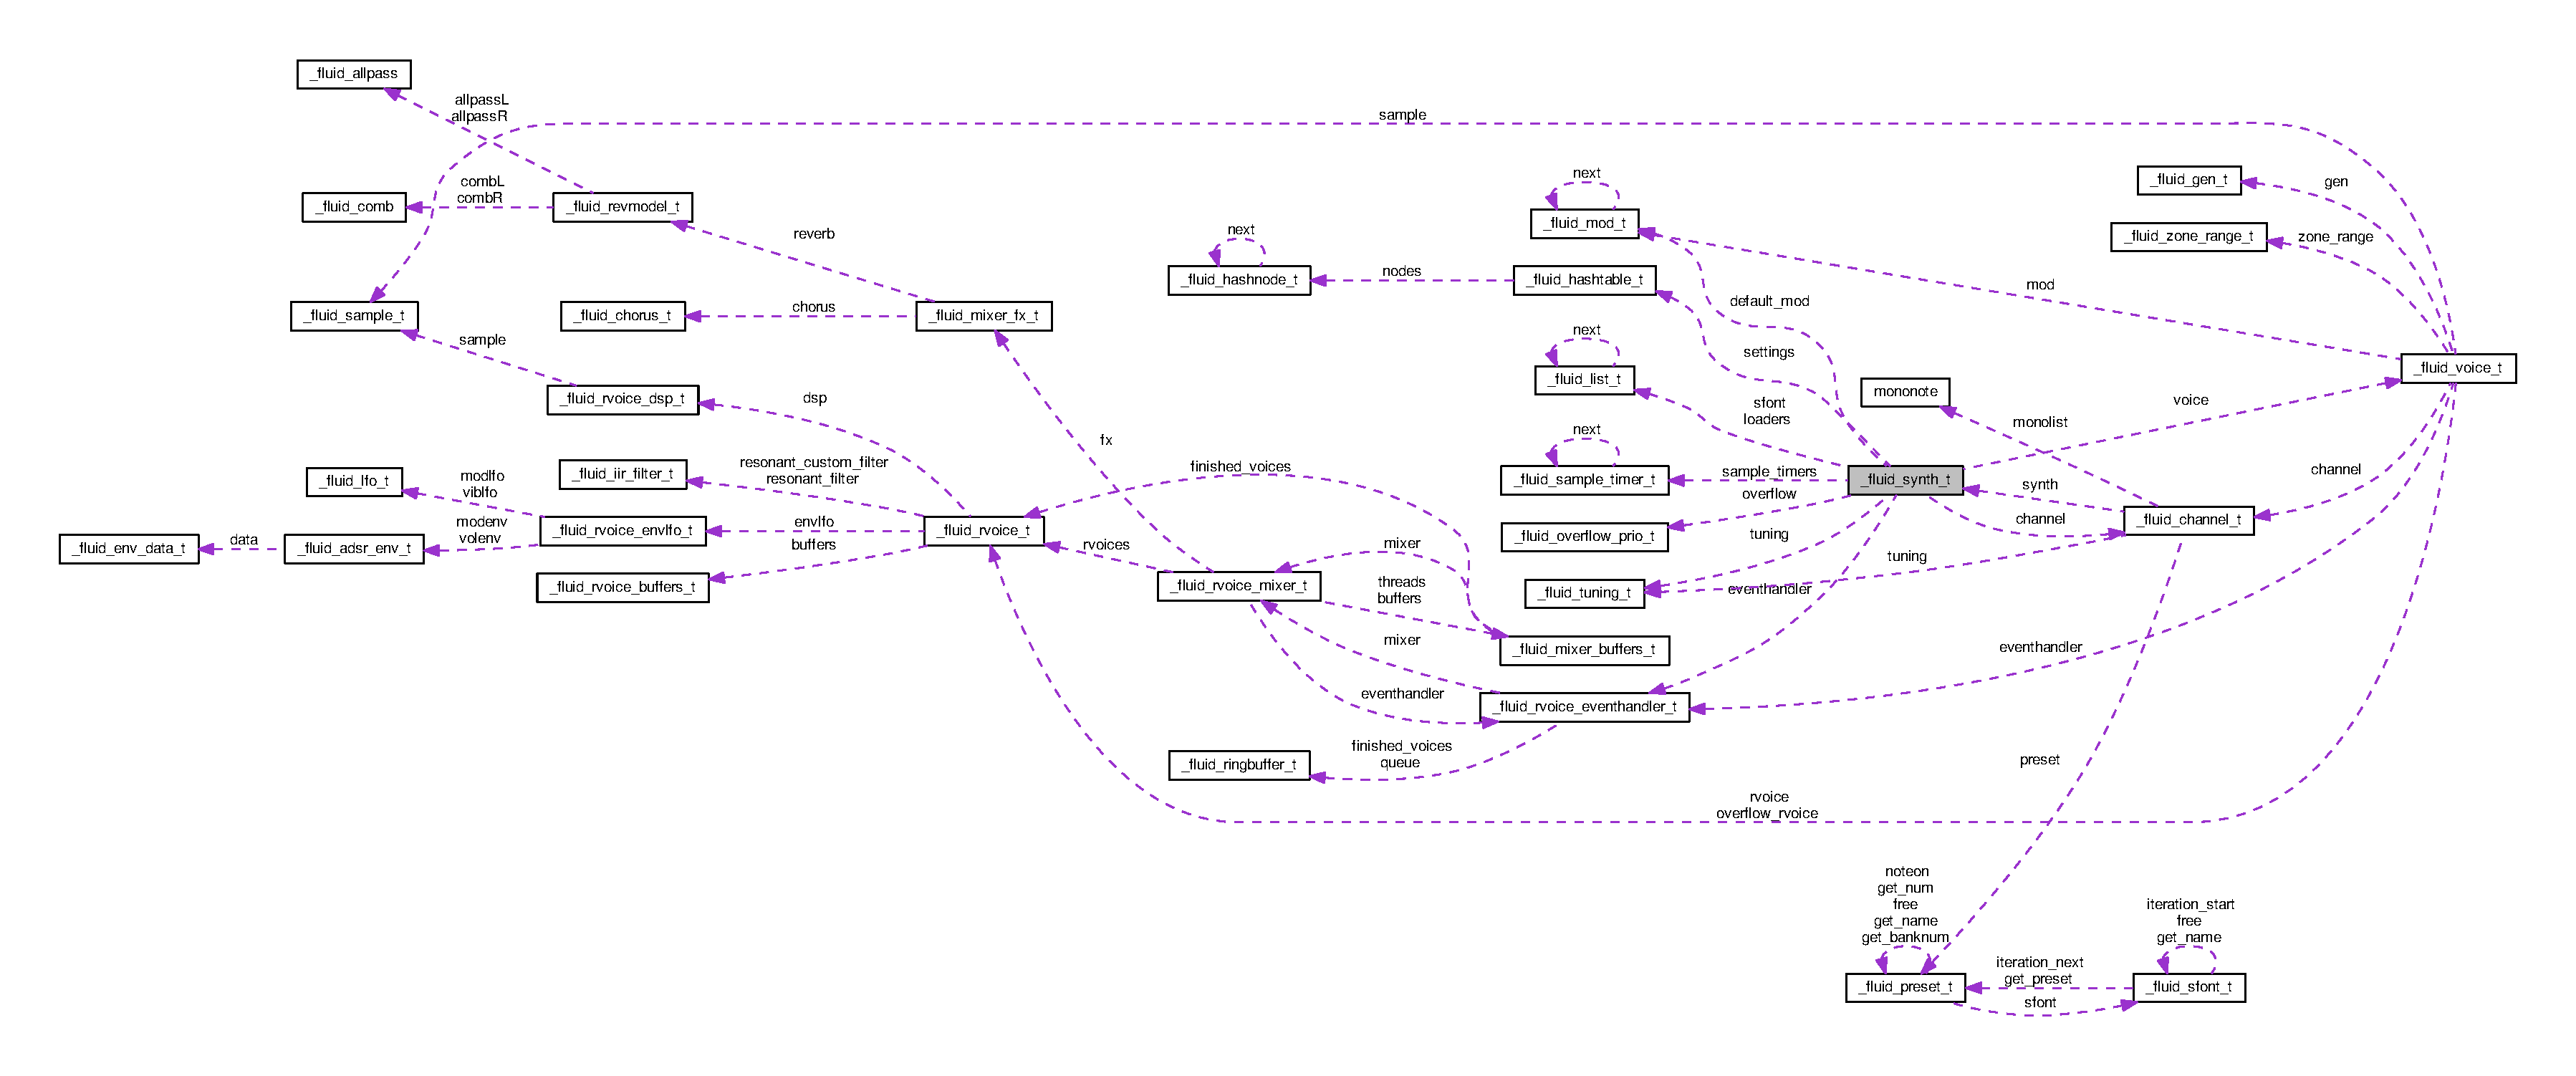
\includegraphics[width=350pt]{struct__fluid__synth__t__coll__graph}
\end{center}
\end{figure}
\subsection*{Public Attributes}
\begin{DoxyCompactItemize}
\item 
\hyperlink{fluid__sys_8h_a8e5bc2095bf6a26aa487db766bfb6660}{fluid\+\_\+rec\+\_\+mutex\+\_\+t} \hyperlink{struct__fluid__synth__t_a0607c356835f4e0d2737a8d2427502a2}{mutex}
\item 
int \hyperlink{struct__fluid__synth__t_a93a302587ee5a959bc6f3cabf2c9670e}{use\+\_\+mutex}
\item 
int \hyperlink{struct__fluid__synth__t_a8a135cb1ecb5a6a1191f2500991a32ed}{public\+\_\+api\+\_\+count}
\item 
\hyperlink{types_8h_aa363402d3c77333b0f070ba531d034ba}{fluid\+\_\+settings\+\_\+t} $\ast$ \hyperlink{struct__fluid__synth__t_a443a36b056edaf9f15a6f7e15f579663}{settings}
\item 
int \hyperlink{struct__fluid__synth__t_a7b396ac714d234cf9a5b8d5e149f4387}{device\+\_\+id}
\item 
int \hyperlink{struct__fluid__synth__t_a4955d81f0303fc4729798ca89ee81781}{polyphony}
\item 
int \hyperlink{struct__fluid__synth__t_ae65cd480d1e7273f7f3b9bb242353210}{with\+\_\+reverb}
\item 
int \hyperlink{struct__fluid__synth__t_aa60eed2e27ed835cc776689510a43573}{with\+\_\+chorus}
\item 
int \hyperlink{struct__fluid__synth__t_a81dfb88d554fc0ddc8faff652fe95cfc}{verbose}
\item 
double \hyperlink{struct__fluid__synth__t_ae91d08160f2ab75e1a9eb320064acbc6}{sample\+\_\+rate}
\item 
int \hyperlink{struct__fluid__synth__t_a4ce77034120fa2551b3250946bbf6042}{midi\+\_\+channels}
\item 
int \hyperlink{struct__fluid__synth__t_a3b97457936d5897010cbec75efa9a4be}{bank\+\_\+select}
\item 
int \hyperlink{struct__fluid__synth__t_a35c32add2f161d86d837301c9b6d67e7}{audio\+\_\+channels}
\item 
int \hyperlink{struct__fluid__synth__t_a476122fb39bbdd36e3ad6387439b2f56}{audio\+\_\+groups}
\item 
int \hyperlink{struct__fluid__synth__t_a5748a0bdf7e8c14dcfbef8ef540393c4}{effects\+\_\+channels}
\item 
int \hyperlink{struct__fluid__synth__t_a77523060e140bd471265259a398ed30a}{state}
\item 
\hyperlink{fluidsynth__priv_8h_ac2b1dee40b52e1e5982fe0f0101413ba}{fluid\+\_\+atomic\+\_\+uint\+\_\+t} \hyperlink{struct__fluid__synth__t_a66cfd8c76e2aa183716ab1eb6e529d7d}{ticks\+\_\+since\+\_\+start}
\item 
unsigned int \hyperlink{struct__fluid__synth__t_a30fd821679b7f3fe45135c211c010fb1}{start}
\item 
\hyperlink{fluid__voice_8h_a1470e84ffede53a3181a35761e016101}{fluid\+\_\+overflow\+\_\+prio\+\_\+t} \hyperlink{struct__fluid__synth__t_a2491ded83c4906c713d034911f6615d3}{overflow}
\item 
\hyperlink{fluid__list_8h_a3ef7535d4290862c0af118569223bd89}{fluid\+\_\+list\+\_\+t} $\ast$ \hyperlink{struct__fluid__synth__t_ae4446eb3ba2731d6944b51d28a16f683}{loaders}
\item 
\hyperlink{fluid__list_8h_a3ef7535d4290862c0af118569223bd89}{fluid\+\_\+list\+\_\+t} $\ast$ \hyperlink{struct__fluid__synth__t_ad37c16bfed217f7053c2b2876fea4ebc}{sfont}
\item 
int \hyperlink{struct__fluid__synth__t_a64d274cd2a1debace88ce6acc22048a9}{sfont\+\_\+id}
\item 
float \hyperlink{struct__fluid__synth__t_aada9dbdeda3719af0a3a173fc59ac5da}{gain}
\item 
\hyperlink{fluidsynth__priv_8h_a9e766203efa8135ece6f462e9caa1b12}{fluid\+\_\+channel\+\_\+t} $\ast$$\ast$ \hyperlink{struct__fluid__synth__t_a6914014a341347e9ba46a2ea21d9cd26}{channel}
\item 
int \hyperlink{struct__fluid__synth__t_a4f14f2ed852384d1d9e0f7848300f9b3}{nvoice}
\item 
\hyperlink{types_8h_a5123ae5ef2d7806475267380c33604c3}{fluid\+\_\+voice\+\_\+t} $\ast$$\ast$ \hyperlink{struct__fluid__synth__t_abafa4495b1eee10130c3359934b446f9}{voice}
\item 
int \hyperlink{struct__fluid__synth__t_a6137bdab89209777a7a63d5f968d7143}{active\+\_\+voice\+\_\+count}
\item 
unsigned int \hyperlink{struct__fluid__synth__t_a77619d68603d1da8030796a8c6f6325e}{noteid}
\item 
unsigned int \hyperlink{struct__fluid__synth__t_aefbd02e23753fb45285c2f64721ef013}{storeid}
\item 
int \hyperlink{struct__fluid__synth__t_ab8955a1a9d3f97a903eb6346dc849e21}{fromkey\+\_\+portamento}
\item 
\hyperlink{fluidsynth__priv_8h_aa59fe8f0195e9f5099f538d38b126e2a}{fluid\+\_\+rvoice\+\_\+eventhandler\+\_\+t} $\ast$ \hyperlink{struct__fluid__synth__t_a2bf5805a6616694e4f0205c04568bf8f}{eventhandler}
\item 
double \hyperlink{struct__fluid__synth__t_aff48515df87bba503c23beb49630b201}{reverb\+\_\+roomsize}
\item 
double \hyperlink{struct__fluid__synth__t_a3cde438bb0208371557919f50848bc54}{reverb\+\_\+damping}
\item 
double \hyperlink{struct__fluid__synth__t_ada62a7a0c33984dddd7991a98785e9e7}{reverb\+\_\+width}
\item 
double \hyperlink{struct__fluid__synth__t_a17371e55bd8759856d42c684acdeac66}{reverb\+\_\+level}
\item 
int \hyperlink{struct__fluid__synth__t_aa4ff48d6d5c735e7cf0636cfbbff611b}{chorus\+\_\+nr}
\item 
double \hyperlink{struct__fluid__synth__t_aa9f83aa940e1368fd0001e5344c20416}{chorus\+\_\+level}
\item 
double \hyperlink{struct__fluid__synth__t_a3943708e55d11e04f2997d537c6bfdc1}{chorus\+\_\+speed}
\item 
double \hyperlink{struct__fluid__synth__t_a1c148c907d245a01b9f06c11a75c851f}{chorus\+\_\+depth}
\item 
int \hyperlink{struct__fluid__synth__t_a7bb6a05ba2732edb0fa713bd817fb413}{chorus\+\_\+type}
\item 
int \hyperlink{struct__fluid__synth__t_a848dc868237ebb2a85a4d5dba0c576fa}{cur}
\item 
int \hyperlink{struct__fluid__synth__t_ad16bcbf14e78b0c6eddca53985c469d4}{curmax}
\item 
int \hyperlink{struct__fluid__synth__t_a1630ffb7d83f89f08d9aff883b4e9e83}{dither\+\_\+index}
\item 
\hyperlink{fluidsynth__priv_8h_a046f155f6dcde29c3684e1051f3bc914}{fluid\+\_\+atomic\+\_\+float\+\_\+t} \hyperlink{struct__fluid__synth__t_aa8a4e49c48662e56de3c27d1e44be476}{cpu\+\_\+load}
\item 
\hyperlink{fluidsynth__priv_8h_a06e93e369a12dcdcf9a7c9312622e732}{fluid\+\_\+tuning\+\_\+t} $\ast$$\ast$$\ast$ \hyperlink{struct__fluid__synth__t_a4fec0cbcbfe75e7b7143e47bd3f63918}{tuning}
\item 
\hyperlink{fluid__sys_8h_a3cc330a417a0061f32425bc8e4fc3f24}{fluid\+\_\+private\+\_\+t} \hyperlink{struct__fluid__synth__t_a832765233670acd4364a8b2c2b67b084}{tuning\+\_\+iter}
\item 
\hyperlink{fluidsynth__priv_8h_a4ddade88911e1873bccda1a7750a848c}{fluid\+\_\+sample\+\_\+timer\+\_\+t} $\ast$ \hyperlink{struct__fluid__synth__t_ae7b6a2156ecbeb1aa7c0a08e8ca86188}{sample\+\_\+timers}
\item 
unsigned int \hyperlink{struct__fluid__synth__t_a08ef94fb04d2219ec10bdd1f87d50209}{min\+\_\+note\+\_\+length\+\_\+ticks}
\item 
int \hyperlink{struct__fluid__synth__t_adb607a968ba73c99321e87519f57148f}{cores}
\item 
\hyperlink{types_8h_a6c727efab500d6c0c350d4292e9aa5ef}{fluid\+\_\+mod\+\_\+t} $\ast$ \hyperlink{struct__fluid__synth__t_a1ac7f01b534bc2eb5d49733312ed6f6a}{default\+\_\+mod}
\item 
\hyperlink{types_8h_a4cb127fbe32ac21781d5252c75661191}{fluid\+\_\+ladspa\+\_\+fx\+\_\+t} $\ast$ \hyperlink{struct__fluid__synth__t_a5af386f876599f6b037976be866c89ce}{ladspa\+\_\+fx}
\item 
enum \hyperlink{synth_8h_a8a4cb4bd240d3654707ac0c5c7337a63}{fluid\+\_\+iir\+\_\+filter\+\_\+type} \hyperlink{struct__fluid__synth__t_a32b1a8f42c060a715fda78d4ae4a51ee}{custom\+\_\+filter\+\_\+type}
\item 
enum \hyperlink{synth_8h_a1e682c5d6f22e13947cc07bcd92d7525}{fluid\+\_\+iir\+\_\+filter\+\_\+flags} \hyperlink{struct__fluid__synth__t_a2921a891ef8a9ebc584acfc9605177be}{custom\+\_\+filter\+\_\+flags}
\end{DoxyCompactItemize}


\subsection{Member Data Documentation}
\mbox{\Hypertarget{struct__fluid__synth__t_a6137bdab89209777a7a63d5f968d7143}\label{struct__fluid__synth__t_a6137bdab89209777a7a63d5f968d7143}} 
\index{\+\_\+fluid\+\_\+synth\+\_\+t@{\+\_\+fluid\+\_\+synth\+\_\+t}!active\+\_\+voice\+\_\+count@{active\+\_\+voice\+\_\+count}}
\index{active\+\_\+voice\+\_\+count@{active\+\_\+voice\+\_\+count}!\+\_\+fluid\+\_\+synth\+\_\+t@{\+\_\+fluid\+\_\+synth\+\_\+t}}
\subsubsection{\texorpdfstring{active\+\_\+voice\+\_\+count}{active\_voice\_count}}
{\footnotesize\ttfamily int \+\_\+fluid\+\_\+synth\+\_\+t\+::active\+\_\+voice\+\_\+count}

count of active voices \mbox{\Hypertarget{struct__fluid__synth__t_a35c32add2f161d86d837301c9b6d67e7}\label{struct__fluid__synth__t_a35c32add2f161d86d837301c9b6d67e7}} 
\index{\+\_\+fluid\+\_\+synth\+\_\+t@{\+\_\+fluid\+\_\+synth\+\_\+t}!audio\+\_\+channels@{audio\+\_\+channels}}
\index{audio\+\_\+channels@{audio\+\_\+channels}!\+\_\+fluid\+\_\+synth\+\_\+t@{\+\_\+fluid\+\_\+synth\+\_\+t}}
\subsubsection{\texorpdfstring{audio\+\_\+channels}{audio\_channels}}
{\footnotesize\ttfamily int \+\_\+fluid\+\_\+synth\+\_\+t\+::audio\+\_\+channels}

the number of audio channels (1 channel=left+right) \mbox{\Hypertarget{struct__fluid__synth__t_a476122fb39bbdd36e3ad6387439b2f56}\label{struct__fluid__synth__t_a476122fb39bbdd36e3ad6387439b2f56}} 
\index{\+\_\+fluid\+\_\+synth\+\_\+t@{\+\_\+fluid\+\_\+synth\+\_\+t}!audio\+\_\+groups@{audio\+\_\+groups}}
\index{audio\+\_\+groups@{audio\+\_\+groups}!\+\_\+fluid\+\_\+synth\+\_\+t@{\+\_\+fluid\+\_\+synth\+\_\+t}}
\subsubsection{\texorpdfstring{audio\+\_\+groups}{audio\_groups}}
{\footnotesize\ttfamily int \+\_\+fluid\+\_\+synth\+\_\+t\+::audio\+\_\+groups}

the number of (stereo) \textquotesingle{}sub\textquotesingle{}groups from the synth. Typically equal to audio\+\_\+channels. \mbox{\Hypertarget{struct__fluid__synth__t_a3b97457936d5897010cbec75efa9a4be}\label{struct__fluid__synth__t_a3b97457936d5897010cbec75efa9a4be}} 
\index{\+\_\+fluid\+\_\+synth\+\_\+t@{\+\_\+fluid\+\_\+synth\+\_\+t}!bank\+\_\+select@{bank\+\_\+select}}
\index{bank\+\_\+select@{bank\+\_\+select}!\+\_\+fluid\+\_\+synth\+\_\+t@{\+\_\+fluid\+\_\+synth\+\_\+t}}
\subsubsection{\texorpdfstring{bank\+\_\+select}{bank\_select}}
{\footnotesize\ttfamily int \+\_\+fluid\+\_\+synth\+\_\+t\+::bank\+\_\+select}

the style of Bank Select M\+I\+DI messages \mbox{\Hypertarget{struct__fluid__synth__t_a6914014a341347e9ba46a2ea21d9cd26}\label{struct__fluid__synth__t_a6914014a341347e9ba46a2ea21d9cd26}} 
\index{\+\_\+fluid\+\_\+synth\+\_\+t@{\+\_\+fluid\+\_\+synth\+\_\+t}!channel@{channel}}
\index{channel@{channel}!\+\_\+fluid\+\_\+synth\+\_\+t@{\+\_\+fluid\+\_\+synth\+\_\+t}}
\subsubsection{\texorpdfstring{channel}{channel}}
{\footnotesize\ttfamily \hyperlink{fluidsynth__priv_8h_a9e766203efa8135ece6f462e9caa1b12}{fluid\+\_\+channel\+\_\+t}$\ast$$\ast$ \+\_\+fluid\+\_\+synth\+\_\+t\+::channel}

the channels \mbox{\Hypertarget{struct__fluid__synth__t_a1c148c907d245a01b9f06c11a75c851f}\label{struct__fluid__synth__t_a1c148c907d245a01b9f06c11a75c851f}} 
\index{\+\_\+fluid\+\_\+synth\+\_\+t@{\+\_\+fluid\+\_\+synth\+\_\+t}!chorus\+\_\+depth@{chorus\+\_\+depth}}
\index{chorus\+\_\+depth@{chorus\+\_\+depth}!\+\_\+fluid\+\_\+synth\+\_\+t@{\+\_\+fluid\+\_\+synth\+\_\+t}}
\subsubsection{\texorpdfstring{chorus\+\_\+depth}{chorus\_depth}}
{\footnotesize\ttfamily double \+\_\+fluid\+\_\+synth\+\_\+t\+::chorus\+\_\+depth}

Shadow of chorus depth \mbox{\Hypertarget{struct__fluid__synth__t_aa9f83aa940e1368fd0001e5344c20416}\label{struct__fluid__synth__t_aa9f83aa940e1368fd0001e5344c20416}} 
\index{\+\_\+fluid\+\_\+synth\+\_\+t@{\+\_\+fluid\+\_\+synth\+\_\+t}!chorus\+\_\+level@{chorus\+\_\+level}}
\index{chorus\+\_\+level@{chorus\+\_\+level}!\+\_\+fluid\+\_\+synth\+\_\+t@{\+\_\+fluid\+\_\+synth\+\_\+t}}
\subsubsection{\texorpdfstring{chorus\+\_\+level}{chorus\_level}}
{\footnotesize\ttfamily double \+\_\+fluid\+\_\+synth\+\_\+t\+::chorus\+\_\+level}

Shadow of chorus level \mbox{\Hypertarget{struct__fluid__synth__t_aa4ff48d6d5c735e7cf0636cfbbff611b}\label{struct__fluid__synth__t_aa4ff48d6d5c735e7cf0636cfbbff611b}} 
\index{\+\_\+fluid\+\_\+synth\+\_\+t@{\+\_\+fluid\+\_\+synth\+\_\+t}!chorus\+\_\+nr@{chorus\+\_\+nr}}
\index{chorus\+\_\+nr@{chorus\+\_\+nr}!\+\_\+fluid\+\_\+synth\+\_\+t@{\+\_\+fluid\+\_\+synth\+\_\+t}}
\subsubsection{\texorpdfstring{chorus\+\_\+nr}{chorus\_nr}}
{\footnotesize\ttfamily int \+\_\+fluid\+\_\+synth\+\_\+t\+::chorus\+\_\+nr}

Shadow of chorus number \mbox{\Hypertarget{struct__fluid__synth__t_a3943708e55d11e04f2997d537c6bfdc1}\label{struct__fluid__synth__t_a3943708e55d11e04f2997d537c6bfdc1}} 
\index{\+\_\+fluid\+\_\+synth\+\_\+t@{\+\_\+fluid\+\_\+synth\+\_\+t}!chorus\+\_\+speed@{chorus\+\_\+speed}}
\index{chorus\+\_\+speed@{chorus\+\_\+speed}!\+\_\+fluid\+\_\+synth\+\_\+t@{\+\_\+fluid\+\_\+synth\+\_\+t}}
\subsubsection{\texorpdfstring{chorus\+\_\+speed}{chorus\_speed}}
{\footnotesize\ttfamily double \+\_\+fluid\+\_\+synth\+\_\+t\+::chorus\+\_\+speed}

Shadow of chorus speed \mbox{\Hypertarget{struct__fluid__synth__t_a7bb6a05ba2732edb0fa713bd817fb413}\label{struct__fluid__synth__t_a7bb6a05ba2732edb0fa713bd817fb413}} 
\index{\+\_\+fluid\+\_\+synth\+\_\+t@{\+\_\+fluid\+\_\+synth\+\_\+t}!chorus\+\_\+type@{chorus\+\_\+type}}
\index{chorus\+\_\+type@{chorus\+\_\+type}!\+\_\+fluid\+\_\+synth\+\_\+t@{\+\_\+fluid\+\_\+synth\+\_\+t}}
\subsubsection{\texorpdfstring{chorus\+\_\+type}{chorus\_type}}
{\footnotesize\ttfamily int \+\_\+fluid\+\_\+synth\+\_\+t\+::chorus\+\_\+type}

Shadow of chorus type \mbox{\Hypertarget{struct__fluid__synth__t_adb607a968ba73c99321e87519f57148f}\label{struct__fluid__synth__t_adb607a968ba73c99321e87519f57148f}} 
\index{\+\_\+fluid\+\_\+synth\+\_\+t@{\+\_\+fluid\+\_\+synth\+\_\+t}!cores@{cores}}
\index{cores@{cores}!\+\_\+fluid\+\_\+synth\+\_\+t@{\+\_\+fluid\+\_\+synth\+\_\+t}}
\subsubsection{\texorpdfstring{cores}{cores}}
{\footnotesize\ttfamily int \+\_\+fluid\+\_\+synth\+\_\+t\+::cores}

Number of C\+PU cores (1 by default) \mbox{\Hypertarget{struct__fluid__synth__t_aa8a4e49c48662e56de3c27d1e44be476}\label{struct__fluid__synth__t_aa8a4e49c48662e56de3c27d1e44be476}} 
\index{\+\_\+fluid\+\_\+synth\+\_\+t@{\+\_\+fluid\+\_\+synth\+\_\+t}!cpu\+\_\+load@{cpu\+\_\+load}}
\index{cpu\+\_\+load@{cpu\+\_\+load}!\+\_\+fluid\+\_\+synth\+\_\+t@{\+\_\+fluid\+\_\+synth\+\_\+t}}
\subsubsection{\texorpdfstring{cpu\+\_\+load}{cpu\_load}}
{\footnotesize\ttfamily \hyperlink{fluidsynth__priv_8h_a046f155f6dcde29c3684e1051f3bc914}{fluid\+\_\+atomic\+\_\+float\+\_\+t} \+\_\+fluid\+\_\+synth\+\_\+t\+::cpu\+\_\+load}

C\+PU load in percent (C\+PU time required / audio synthesized time $\ast$ 100) \mbox{\Hypertarget{struct__fluid__synth__t_a848dc868237ebb2a85a4d5dba0c576fa}\label{struct__fluid__synth__t_a848dc868237ebb2a85a4d5dba0c576fa}} 
\index{\+\_\+fluid\+\_\+synth\+\_\+t@{\+\_\+fluid\+\_\+synth\+\_\+t}!cur@{cur}}
\index{cur@{cur}!\+\_\+fluid\+\_\+synth\+\_\+t@{\+\_\+fluid\+\_\+synth\+\_\+t}}
\subsubsection{\texorpdfstring{cur}{cur}}
{\footnotesize\ttfamily int \+\_\+fluid\+\_\+synth\+\_\+t\+::cur}

the current sample in the audio buffers to be output \mbox{\Hypertarget{struct__fluid__synth__t_ad16bcbf14e78b0c6eddca53985c469d4}\label{struct__fluid__synth__t_ad16bcbf14e78b0c6eddca53985c469d4}} 
\index{\+\_\+fluid\+\_\+synth\+\_\+t@{\+\_\+fluid\+\_\+synth\+\_\+t}!curmax@{curmax}}
\index{curmax@{curmax}!\+\_\+fluid\+\_\+synth\+\_\+t@{\+\_\+fluid\+\_\+synth\+\_\+t}}
\subsubsection{\texorpdfstring{curmax}{curmax}}
{\footnotesize\ttfamily int \+\_\+fluid\+\_\+synth\+\_\+t\+::curmax}

current amount of samples present in the audio buffers \mbox{\Hypertarget{struct__fluid__synth__t_a2921a891ef8a9ebc584acfc9605177be}\label{struct__fluid__synth__t_a2921a891ef8a9ebc584acfc9605177be}} 
\index{\+\_\+fluid\+\_\+synth\+\_\+t@{\+\_\+fluid\+\_\+synth\+\_\+t}!custom\+\_\+filter\+\_\+flags@{custom\+\_\+filter\+\_\+flags}}
\index{custom\+\_\+filter\+\_\+flags@{custom\+\_\+filter\+\_\+flags}!\+\_\+fluid\+\_\+synth\+\_\+t@{\+\_\+fluid\+\_\+synth\+\_\+t}}
\subsubsection{\texorpdfstring{custom\+\_\+filter\+\_\+flags}{custom\_filter\_flags}}
{\footnotesize\ttfamily enum \hyperlink{synth_8h_a1e682c5d6f22e13947cc07bcd92d7525}{fluid\+\_\+iir\+\_\+filter\+\_\+flags} \+\_\+fluid\+\_\+synth\+\_\+t\+::custom\+\_\+filter\+\_\+flags}

filter type of the user-\/defined filter currently used for all voices \mbox{\Hypertarget{struct__fluid__synth__t_a32b1a8f42c060a715fda78d4ae4a51ee}\label{struct__fluid__synth__t_a32b1a8f42c060a715fda78d4ae4a51ee}} 
\index{\+\_\+fluid\+\_\+synth\+\_\+t@{\+\_\+fluid\+\_\+synth\+\_\+t}!custom\+\_\+filter\+\_\+type@{custom\+\_\+filter\+\_\+type}}
\index{custom\+\_\+filter\+\_\+type@{custom\+\_\+filter\+\_\+type}!\+\_\+fluid\+\_\+synth\+\_\+t@{\+\_\+fluid\+\_\+synth\+\_\+t}}
\subsubsection{\texorpdfstring{custom\+\_\+filter\+\_\+type}{custom\_filter\_type}}
{\footnotesize\ttfamily enum \hyperlink{synth_8h_a8a4cb4bd240d3654707ac0c5c7337a63}{fluid\+\_\+iir\+\_\+filter\+\_\+type} \+\_\+fluid\+\_\+synth\+\_\+t\+::custom\+\_\+filter\+\_\+type}

filter type of the user-\/defined filter currently used for all voices \mbox{\Hypertarget{struct__fluid__synth__t_a1ac7f01b534bc2eb5d49733312ed6f6a}\label{struct__fluid__synth__t_a1ac7f01b534bc2eb5d49733312ed6f6a}} 
\index{\+\_\+fluid\+\_\+synth\+\_\+t@{\+\_\+fluid\+\_\+synth\+\_\+t}!default\+\_\+mod@{default\+\_\+mod}}
\index{default\+\_\+mod@{default\+\_\+mod}!\+\_\+fluid\+\_\+synth\+\_\+t@{\+\_\+fluid\+\_\+synth\+\_\+t}}
\subsubsection{\texorpdfstring{default\+\_\+mod}{default\_mod}}
{\footnotesize\ttfamily \hyperlink{types_8h_a6c727efab500d6c0c350d4292e9aa5ef}{fluid\+\_\+mod\+\_\+t}$\ast$ \+\_\+fluid\+\_\+synth\+\_\+t\+::default\+\_\+mod}

the (dynamic) list of default modulators \mbox{\Hypertarget{struct__fluid__synth__t_a7b396ac714d234cf9a5b8d5e149f4387}\label{struct__fluid__synth__t_a7b396ac714d234cf9a5b8d5e149f4387}} 
\index{\+\_\+fluid\+\_\+synth\+\_\+t@{\+\_\+fluid\+\_\+synth\+\_\+t}!device\+\_\+id@{device\+\_\+id}}
\index{device\+\_\+id@{device\+\_\+id}!\+\_\+fluid\+\_\+synth\+\_\+t@{\+\_\+fluid\+\_\+synth\+\_\+t}}
\subsubsection{\texorpdfstring{device\+\_\+id}{device\_id}}
{\footnotesize\ttfamily int \+\_\+fluid\+\_\+synth\+\_\+t\+::device\+\_\+id}

Device ID used for S\+Y\+S\+EX messages \mbox{\Hypertarget{struct__fluid__synth__t_a1630ffb7d83f89f08d9aff883b4e9e83}\label{struct__fluid__synth__t_a1630ffb7d83f89f08d9aff883b4e9e83}} 
\index{\+\_\+fluid\+\_\+synth\+\_\+t@{\+\_\+fluid\+\_\+synth\+\_\+t}!dither\+\_\+index@{dither\+\_\+index}}
\index{dither\+\_\+index@{dither\+\_\+index}!\+\_\+fluid\+\_\+synth\+\_\+t@{\+\_\+fluid\+\_\+synth\+\_\+t}}
\subsubsection{\texorpdfstring{dither\+\_\+index}{dither\_index}}
{\footnotesize\ttfamily int \+\_\+fluid\+\_\+synth\+\_\+t\+::dither\+\_\+index}

current index in random dither value buffer\+: fluid\+\_\+synth\+\_\+(write\+\_\+s16$\vert$dither\+\_\+s16) \mbox{\Hypertarget{struct__fluid__synth__t_a5748a0bdf7e8c14dcfbef8ef540393c4}\label{struct__fluid__synth__t_a5748a0bdf7e8c14dcfbef8ef540393c4}} 
\index{\+\_\+fluid\+\_\+synth\+\_\+t@{\+\_\+fluid\+\_\+synth\+\_\+t}!effects\+\_\+channels@{effects\+\_\+channels}}
\index{effects\+\_\+channels@{effects\+\_\+channels}!\+\_\+fluid\+\_\+synth\+\_\+t@{\+\_\+fluid\+\_\+synth\+\_\+t}}
\subsubsection{\texorpdfstring{effects\+\_\+channels}{effects\_channels}}
{\footnotesize\ttfamily int \+\_\+fluid\+\_\+synth\+\_\+t\+::effects\+\_\+channels}

the number of effects channels ($>$= 2) \mbox{\Hypertarget{struct__fluid__synth__t_a2bf5805a6616694e4f0205c04568bf8f}\label{struct__fluid__synth__t_a2bf5805a6616694e4f0205c04568bf8f}} 
\index{\+\_\+fluid\+\_\+synth\+\_\+t@{\+\_\+fluid\+\_\+synth\+\_\+t}!eventhandler@{eventhandler}}
\index{eventhandler@{eventhandler}!\+\_\+fluid\+\_\+synth\+\_\+t@{\+\_\+fluid\+\_\+synth\+\_\+t}}
\subsubsection{\texorpdfstring{eventhandler}{eventhandler}}
{\footnotesize\ttfamily \hyperlink{fluidsynth__priv_8h_aa59fe8f0195e9f5099f538d38b126e2a}{fluid\+\_\+rvoice\+\_\+eventhandler\+\_\+t}$\ast$ \+\_\+fluid\+\_\+synth\+\_\+t\+::eventhandler}

\mbox{\Hypertarget{struct__fluid__synth__t_ab8955a1a9d3f97a903eb6346dc849e21}\label{struct__fluid__synth__t_ab8955a1a9d3f97a903eb6346dc849e21}} 
\index{\+\_\+fluid\+\_\+synth\+\_\+t@{\+\_\+fluid\+\_\+synth\+\_\+t}!fromkey\+\_\+portamento@{fromkey\+\_\+portamento}}
\index{fromkey\+\_\+portamento@{fromkey\+\_\+portamento}!\+\_\+fluid\+\_\+synth\+\_\+t@{\+\_\+fluid\+\_\+synth\+\_\+t}}
\subsubsection{\texorpdfstring{fromkey\+\_\+portamento}{fromkey\_portamento}}
{\footnotesize\ttfamily int \+\_\+fluid\+\_\+synth\+\_\+t\+::fromkey\+\_\+portamento}

fromkey portamento \mbox{\Hypertarget{struct__fluid__synth__t_aada9dbdeda3719af0a3a173fc59ac5da}\label{struct__fluid__synth__t_aada9dbdeda3719af0a3a173fc59ac5da}} 
\index{\+\_\+fluid\+\_\+synth\+\_\+t@{\+\_\+fluid\+\_\+synth\+\_\+t}!gain@{gain}}
\index{gain@{gain}!\+\_\+fluid\+\_\+synth\+\_\+t@{\+\_\+fluid\+\_\+synth\+\_\+t}}
\subsubsection{\texorpdfstring{gain}{gain}}
{\footnotesize\ttfamily float \+\_\+fluid\+\_\+synth\+\_\+t\+::gain}

master gain \mbox{\Hypertarget{struct__fluid__synth__t_a5af386f876599f6b037976be866c89ce}\label{struct__fluid__synth__t_a5af386f876599f6b037976be866c89ce}} 
\index{\+\_\+fluid\+\_\+synth\+\_\+t@{\+\_\+fluid\+\_\+synth\+\_\+t}!ladspa\+\_\+fx@{ladspa\+\_\+fx}}
\index{ladspa\+\_\+fx@{ladspa\+\_\+fx}!\+\_\+fluid\+\_\+synth\+\_\+t@{\+\_\+fluid\+\_\+synth\+\_\+t}}
\subsubsection{\texorpdfstring{ladspa\+\_\+fx}{ladspa\_fx}}
{\footnotesize\ttfamily \hyperlink{types_8h_a4cb127fbe32ac21781d5252c75661191}{fluid\+\_\+ladspa\+\_\+fx\+\_\+t}$\ast$ \+\_\+fluid\+\_\+synth\+\_\+t\+::ladspa\+\_\+fx}

Effects unit for L\+A\+D\+S\+PA support \mbox{\Hypertarget{struct__fluid__synth__t_ae4446eb3ba2731d6944b51d28a16f683}\label{struct__fluid__synth__t_ae4446eb3ba2731d6944b51d28a16f683}} 
\index{\+\_\+fluid\+\_\+synth\+\_\+t@{\+\_\+fluid\+\_\+synth\+\_\+t}!loaders@{loaders}}
\index{loaders@{loaders}!\+\_\+fluid\+\_\+synth\+\_\+t@{\+\_\+fluid\+\_\+synth\+\_\+t}}
\subsubsection{\texorpdfstring{loaders}{loaders}}
{\footnotesize\ttfamily \hyperlink{fluid__list_8h_a3ef7535d4290862c0af118569223bd89}{fluid\+\_\+list\+\_\+t}$\ast$ \+\_\+fluid\+\_\+synth\+\_\+t\+::loaders}

the Sound\+Font loaders \mbox{\Hypertarget{struct__fluid__synth__t_a4ce77034120fa2551b3250946bbf6042}\label{struct__fluid__synth__t_a4ce77034120fa2551b3250946bbf6042}} 
\index{\+\_\+fluid\+\_\+synth\+\_\+t@{\+\_\+fluid\+\_\+synth\+\_\+t}!midi\+\_\+channels@{midi\+\_\+channels}}
\index{midi\+\_\+channels@{midi\+\_\+channels}!\+\_\+fluid\+\_\+synth\+\_\+t@{\+\_\+fluid\+\_\+synth\+\_\+t}}
\subsubsection{\texorpdfstring{midi\+\_\+channels}{midi\_channels}}
{\footnotesize\ttfamily int \+\_\+fluid\+\_\+synth\+\_\+t\+::midi\+\_\+channels}

the number of M\+I\+DI channels ($>$= 16) \mbox{\Hypertarget{struct__fluid__synth__t_a08ef94fb04d2219ec10bdd1f87d50209}\label{struct__fluid__synth__t_a08ef94fb04d2219ec10bdd1f87d50209}} 
\index{\+\_\+fluid\+\_\+synth\+\_\+t@{\+\_\+fluid\+\_\+synth\+\_\+t}!min\+\_\+note\+\_\+length\+\_\+ticks@{min\+\_\+note\+\_\+length\+\_\+ticks}}
\index{min\+\_\+note\+\_\+length\+\_\+ticks@{min\+\_\+note\+\_\+length\+\_\+ticks}!\+\_\+fluid\+\_\+synth\+\_\+t@{\+\_\+fluid\+\_\+synth\+\_\+t}}
\subsubsection{\texorpdfstring{min\+\_\+note\+\_\+length\+\_\+ticks}{min\_note\_length\_ticks}}
{\footnotesize\ttfamily unsigned int \+\_\+fluid\+\_\+synth\+\_\+t\+::min\+\_\+note\+\_\+length\+\_\+ticks}

If note-\/offs are triggered just after a note-\/on, they will be delayed \mbox{\Hypertarget{struct__fluid__synth__t_a0607c356835f4e0d2737a8d2427502a2}\label{struct__fluid__synth__t_a0607c356835f4e0d2737a8d2427502a2}} 
\index{\+\_\+fluid\+\_\+synth\+\_\+t@{\+\_\+fluid\+\_\+synth\+\_\+t}!mutex@{mutex}}
\index{mutex@{mutex}!\+\_\+fluid\+\_\+synth\+\_\+t@{\+\_\+fluid\+\_\+synth\+\_\+t}}
\subsubsection{\texorpdfstring{mutex}{mutex}}
{\footnotesize\ttfamily \hyperlink{fluid__sys_8h_a8e5bc2095bf6a26aa487db766bfb6660}{fluid\+\_\+rec\+\_\+mutex\+\_\+t} \+\_\+fluid\+\_\+synth\+\_\+t\+::mutex}

Lock for public A\+PI \mbox{\Hypertarget{struct__fluid__synth__t_a77619d68603d1da8030796a8c6f6325e}\label{struct__fluid__synth__t_a77619d68603d1da8030796a8c6f6325e}} 
\index{\+\_\+fluid\+\_\+synth\+\_\+t@{\+\_\+fluid\+\_\+synth\+\_\+t}!noteid@{noteid}}
\index{noteid@{noteid}!\+\_\+fluid\+\_\+synth\+\_\+t@{\+\_\+fluid\+\_\+synth\+\_\+t}}
\subsubsection{\texorpdfstring{noteid}{noteid}}
{\footnotesize\ttfamily unsigned int \+\_\+fluid\+\_\+synth\+\_\+t\+::noteid}

the id is incremented for every new note. it\textquotesingle{}s used for noteoff\textquotesingle{}s \mbox{\Hypertarget{struct__fluid__synth__t_a4f14f2ed852384d1d9e0f7848300f9b3}\label{struct__fluid__synth__t_a4f14f2ed852384d1d9e0f7848300f9b3}} 
\index{\+\_\+fluid\+\_\+synth\+\_\+t@{\+\_\+fluid\+\_\+synth\+\_\+t}!nvoice@{nvoice}}
\index{nvoice@{nvoice}!\+\_\+fluid\+\_\+synth\+\_\+t@{\+\_\+fluid\+\_\+synth\+\_\+t}}
\subsubsection{\texorpdfstring{nvoice}{nvoice}}
{\footnotesize\ttfamily int \+\_\+fluid\+\_\+synth\+\_\+t\+::nvoice}

the length of the synthesis process array (max polyphony allowed) \mbox{\Hypertarget{struct__fluid__synth__t_a2491ded83c4906c713d034911f6615d3}\label{struct__fluid__synth__t_a2491ded83c4906c713d034911f6615d3}} 
\index{\+\_\+fluid\+\_\+synth\+\_\+t@{\+\_\+fluid\+\_\+synth\+\_\+t}!overflow@{overflow}}
\index{overflow@{overflow}!\+\_\+fluid\+\_\+synth\+\_\+t@{\+\_\+fluid\+\_\+synth\+\_\+t}}
\subsubsection{\texorpdfstring{overflow}{overflow}}
{\footnotesize\ttfamily \hyperlink{fluid__voice_8h_a1470e84ffede53a3181a35761e016101}{fluid\+\_\+overflow\+\_\+prio\+\_\+t} \+\_\+fluid\+\_\+synth\+\_\+t\+::overflow}

parameters for overflow priority (aka voice-\/stealing) \mbox{\Hypertarget{struct__fluid__synth__t_a4955d81f0303fc4729798ca89ee81781}\label{struct__fluid__synth__t_a4955d81f0303fc4729798ca89ee81781}} 
\index{\+\_\+fluid\+\_\+synth\+\_\+t@{\+\_\+fluid\+\_\+synth\+\_\+t}!polyphony@{polyphony}}
\index{polyphony@{polyphony}!\+\_\+fluid\+\_\+synth\+\_\+t@{\+\_\+fluid\+\_\+synth\+\_\+t}}
\subsubsection{\texorpdfstring{polyphony}{polyphony}}
{\footnotesize\ttfamily int \+\_\+fluid\+\_\+synth\+\_\+t\+::polyphony}

Maximum polyphony \mbox{\Hypertarget{struct__fluid__synth__t_a8a135cb1ecb5a6a1191f2500991a32ed}\label{struct__fluid__synth__t_a8a135cb1ecb5a6a1191f2500991a32ed}} 
\index{\+\_\+fluid\+\_\+synth\+\_\+t@{\+\_\+fluid\+\_\+synth\+\_\+t}!public\+\_\+api\+\_\+count@{public\+\_\+api\+\_\+count}}
\index{public\+\_\+api\+\_\+count@{public\+\_\+api\+\_\+count}!\+\_\+fluid\+\_\+synth\+\_\+t@{\+\_\+fluid\+\_\+synth\+\_\+t}}
\subsubsection{\texorpdfstring{public\+\_\+api\+\_\+count}{public\_api\_count}}
{\footnotesize\ttfamily int \+\_\+fluid\+\_\+synth\+\_\+t\+::public\+\_\+api\+\_\+count}

How many times the mutex is currently locked \mbox{\Hypertarget{struct__fluid__synth__t_a3cde438bb0208371557919f50848bc54}\label{struct__fluid__synth__t_a3cde438bb0208371557919f50848bc54}} 
\index{\+\_\+fluid\+\_\+synth\+\_\+t@{\+\_\+fluid\+\_\+synth\+\_\+t}!reverb\+\_\+damping@{reverb\+\_\+damping}}
\index{reverb\+\_\+damping@{reverb\+\_\+damping}!\+\_\+fluid\+\_\+synth\+\_\+t@{\+\_\+fluid\+\_\+synth\+\_\+t}}
\subsubsection{\texorpdfstring{reverb\+\_\+damping}{reverb\_damping}}
{\footnotesize\ttfamily double \+\_\+fluid\+\_\+synth\+\_\+t\+::reverb\+\_\+damping}

Shadow of reverb damping \mbox{\Hypertarget{struct__fluid__synth__t_a17371e55bd8759856d42c684acdeac66}\label{struct__fluid__synth__t_a17371e55bd8759856d42c684acdeac66}} 
\index{\+\_\+fluid\+\_\+synth\+\_\+t@{\+\_\+fluid\+\_\+synth\+\_\+t}!reverb\+\_\+level@{reverb\+\_\+level}}
\index{reverb\+\_\+level@{reverb\+\_\+level}!\+\_\+fluid\+\_\+synth\+\_\+t@{\+\_\+fluid\+\_\+synth\+\_\+t}}
\subsubsection{\texorpdfstring{reverb\+\_\+level}{reverb\_level}}
{\footnotesize\ttfamily double \+\_\+fluid\+\_\+synth\+\_\+t\+::reverb\+\_\+level}

Shadow of reverb level \mbox{\Hypertarget{struct__fluid__synth__t_aff48515df87bba503c23beb49630b201}\label{struct__fluid__synth__t_aff48515df87bba503c23beb49630b201}} 
\index{\+\_\+fluid\+\_\+synth\+\_\+t@{\+\_\+fluid\+\_\+synth\+\_\+t}!reverb\+\_\+roomsize@{reverb\+\_\+roomsize}}
\index{reverb\+\_\+roomsize@{reverb\+\_\+roomsize}!\+\_\+fluid\+\_\+synth\+\_\+t@{\+\_\+fluid\+\_\+synth\+\_\+t}}
\subsubsection{\texorpdfstring{reverb\+\_\+roomsize}{reverb\_roomsize}}
{\footnotesize\ttfamily double \+\_\+fluid\+\_\+synth\+\_\+t\+::reverb\+\_\+roomsize}

Shadow of reverb roomsize \mbox{\Hypertarget{struct__fluid__synth__t_ada62a7a0c33984dddd7991a98785e9e7}\label{struct__fluid__synth__t_ada62a7a0c33984dddd7991a98785e9e7}} 
\index{\+\_\+fluid\+\_\+synth\+\_\+t@{\+\_\+fluid\+\_\+synth\+\_\+t}!reverb\+\_\+width@{reverb\+\_\+width}}
\index{reverb\+\_\+width@{reverb\+\_\+width}!\+\_\+fluid\+\_\+synth\+\_\+t@{\+\_\+fluid\+\_\+synth\+\_\+t}}
\subsubsection{\texorpdfstring{reverb\+\_\+width}{reverb\_width}}
{\footnotesize\ttfamily double \+\_\+fluid\+\_\+synth\+\_\+t\+::reverb\+\_\+width}

Shadow of reverb width \mbox{\Hypertarget{struct__fluid__synth__t_ae91d08160f2ab75e1a9eb320064acbc6}\label{struct__fluid__synth__t_ae91d08160f2ab75e1a9eb320064acbc6}} 
\index{\+\_\+fluid\+\_\+synth\+\_\+t@{\+\_\+fluid\+\_\+synth\+\_\+t}!sample\+\_\+rate@{sample\+\_\+rate}}
\index{sample\+\_\+rate@{sample\+\_\+rate}!\+\_\+fluid\+\_\+synth\+\_\+t@{\+\_\+fluid\+\_\+synth\+\_\+t}}
\subsubsection{\texorpdfstring{sample\+\_\+rate}{sample\_rate}}
{\footnotesize\ttfamily double \+\_\+fluid\+\_\+synth\+\_\+t\+::sample\+\_\+rate}

The sample rate \mbox{\Hypertarget{struct__fluid__synth__t_ae7b6a2156ecbeb1aa7c0a08e8ca86188}\label{struct__fluid__synth__t_ae7b6a2156ecbeb1aa7c0a08e8ca86188}} 
\index{\+\_\+fluid\+\_\+synth\+\_\+t@{\+\_\+fluid\+\_\+synth\+\_\+t}!sample\+\_\+timers@{sample\+\_\+timers}}
\index{sample\+\_\+timers@{sample\+\_\+timers}!\+\_\+fluid\+\_\+synth\+\_\+t@{\+\_\+fluid\+\_\+synth\+\_\+t}}
\subsubsection{\texorpdfstring{sample\+\_\+timers}{sample\_timers}}
{\footnotesize\ttfamily \hyperlink{fluidsynth__priv_8h_a4ddade88911e1873bccda1a7750a848c}{fluid\+\_\+sample\+\_\+timer\+\_\+t}$\ast$ \+\_\+fluid\+\_\+synth\+\_\+t\+::sample\+\_\+timers}

List of timers triggered before a block is processed \mbox{\Hypertarget{struct__fluid__synth__t_a443a36b056edaf9f15a6f7e15f579663}\label{struct__fluid__synth__t_a443a36b056edaf9f15a6f7e15f579663}} 
\index{\+\_\+fluid\+\_\+synth\+\_\+t@{\+\_\+fluid\+\_\+synth\+\_\+t}!settings@{settings}}
\index{settings@{settings}!\+\_\+fluid\+\_\+synth\+\_\+t@{\+\_\+fluid\+\_\+synth\+\_\+t}}
\subsubsection{\texorpdfstring{settings}{settings}}
{\footnotesize\ttfamily \hyperlink{types_8h_aa363402d3c77333b0f070ba531d034ba}{fluid\+\_\+settings\+\_\+t}$\ast$ \+\_\+fluid\+\_\+synth\+\_\+t\+::settings}

the synthesizer settings \mbox{\Hypertarget{struct__fluid__synth__t_ad37c16bfed217f7053c2b2876fea4ebc}\label{struct__fluid__synth__t_ad37c16bfed217f7053c2b2876fea4ebc}} 
\index{\+\_\+fluid\+\_\+synth\+\_\+t@{\+\_\+fluid\+\_\+synth\+\_\+t}!sfont@{sfont}}
\index{sfont@{sfont}!\+\_\+fluid\+\_\+synth\+\_\+t@{\+\_\+fluid\+\_\+synth\+\_\+t}}
\subsubsection{\texorpdfstring{sfont}{sfont}}
{\footnotesize\ttfamily \hyperlink{fluid__list_8h_a3ef7535d4290862c0af118569223bd89}{fluid\+\_\+list\+\_\+t}$\ast$ \+\_\+fluid\+\_\+synth\+\_\+t\+::sfont}

List of fluid\+\_\+sfont\+\_\+info\+\_\+t for each loaded Sound\+Font (remains until Sound\+Font is unloaded) \mbox{\Hypertarget{struct__fluid__synth__t_a64d274cd2a1debace88ce6acc22048a9}\label{struct__fluid__synth__t_a64d274cd2a1debace88ce6acc22048a9}} 
\index{\+\_\+fluid\+\_\+synth\+\_\+t@{\+\_\+fluid\+\_\+synth\+\_\+t}!sfont\+\_\+id@{sfont\+\_\+id}}
\index{sfont\+\_\+id@{sfont\+\_\+id}!\+\_\+fluid\+\_\+synth\+\_\+t@{\+\_\+fluid\+\_\+synth\+\_\+t}}
\subsubsection{\texorpdfstring{sfont\+\_\+id}{sfont\_id}}
{\footnotesize\ttfamily int \+\_\+fluid\+\_\+synth\+\_\+t\+::sfont\+\_\+id}

Incrementing ID assigned to each loaded Sound\+Font \mbox{\Hypertarget{struct__fluid__synth__t_a30fd821679b7f3fe45135c211c010fb1}\label{struct__fluid__synth__t_a30fd821679b7f3fe45135c211c010fb1}} 
\index{\+\_\+fluid\+\_\+synth\+\_\+t@{\+\_\+fluid\+\_\+synth\+\_\+t}!start@{start}}
\index{start@{start}!\+\_\+fluid\+\_\+synth\+\_\+t@{\+\_\+fluid\+\_\+synth\+\_\+t}}
\subsubsection{\texorpdfstring{start}{start}}
{\footnotesize\ttfamily unsigned int \+\_\+fluid\+\_\+synth\+\_\+t\+::start}

the start in msec, as returned by system clock \mbox{\Hypertarget{struct__fluid__synth__t_a77523060e140bd471265259a398ed30a}\label{struct__fluid__synth__t_a77523060e140bd471265259a398ed30a}} 
\index{\+\_\+fluid\+\_\+synth\+\_\+t@{\+\_\+fluid\+\_\+synth\+\_\+t}!state@{state}}
\index{state@{state}!\+\_\+fluid\+\_\+synth\+\_\+t@{\+\_\+fluid\+\_\+synth\+\_\+t}}
\subsubsection{\texorpdfstring{state}{state}}
{\footnotesize\ttfamily int \+\_\+fluid\+\_\+synth\+\_\+t\+::state}

the synthesizer state \mbox{\Hypertarget{struct__fluid__synth__t_aefbd02e23753fb45285c2f64721ef013}\label{struct__fluid__synth__t_aefbd02e23753fb45285c2f64721ef013}} 
\index{\+\_\+fluid\+\_\+synth\+\_\+t@{\+\_\+fluid\+\_\+synth\+\_\+t}!storeid@{storeid}}
\index{storeid@{storeid}!\+\_\+fluid\+\_\+synth\+\_\+t@{\+\_\+fluid\+\_\+synth\+\_\+t}}
\subsubsection{\texorpdfstring{storeid}{storeid}}
{\footnotesize\ttfamily unsigned int \+\_\+fluid\+\_\+synth\+\_\+t\+::storeid}

\mbox{\Hypertarget{struct__fluid__synth__t_a66cfd8c76e2aa183716ab1eb6e529d7d}\label{struct__fluid__synth__t_a66cfd8c76e2aa183716ab1eb6e529d7d}} 
\index{\+\_\+fluid\+\_\+synth\+\_\+t@{\+\_\+fluid\+\_\+synth\+\_\+t}!ticks\+\_\+since\+\_\+start@{ticks\+\_\+since\+\_\+start}}
\index{ticks\+\_\+since\+\_\+start@{ticks\+\_\+since\+\_\+start}!\+\_\+fluid\+\_\+synth\+\_\+t@{\+\_\+fluid\+\_\+synth\+\_\+t}}
\subsubsection{\texorpdfstring{ticks\+\_\+since\+\_\+start}{ticks\_since\_start}}
{\footnotesize\ttfamily \hyperlink{fluidsynth__priv_8h_ac2b1dee40b52e1e5982fe0f0101413ba}{fluid\+\_\+atomic\+\_\+uint\+\_\+t} \+\_\+fluid\+\_\+synth\+\_\+t\+::ticks\+\_\+since\+\_\+start}

the number of audio samples since the start \mbox{\Hypertarget{struct__fluid__synth__t_a4fec0cbcbfe75e7b7143e47bd3f63918}\label{struct__fluid__synth__t_a4fec0cbcbfe75e7b7143e47bd3f63918}} 
\index{\+\_\+fluid\+\_\+synth\+\_\+t@{\+\_\+fluid\+\_\+synth\+\_\+t}!tuning@{tuning}}
\index{tuning@{tuning}!\+\_\+fluid\+\_\+synth\+\_\+t@{\+\_\+fluid\+\_\+synth\+\_\+t}}
\subsubsection{\texorpdfstring{tuning}{tuning}}
{\footnotesize\ttfamily \hyperlink{fluidsynth__priv_8h_a06e93e369a12dcdcf9a7c9312622e732}{fluid\+\_\+tuning\+\_\+t}$\ast$$\ast$$\ast$ \+\_\+fluid\+\_\+synth\+\_\+t\+::tuning}

128 banks of 128 programs for the tunings \mbox{\Hypertarget{struct__fluid__synth__t_a832765233670acd4364a8b2c2b67b084}\label{struct__fluid__synth__t_a832765233670acd4364a8b2c2b67b084}} 
\index{\+\_\+fluid\+\_\+synth\+\_\+t@{\+\_\+fluid\+\_\+synth\+\_\+t}!tuning\+\_\+iter@{tuning\+\_\+iter}}
\index{tuning\+\_\+iter@{tuning\+\_\+iter}!\+\_\+fluid\+\_\+synth\+\_\+t@{\+\_\+fluid\+\_\+synth\+\_\+t}}
\subsubsection{\texorpdfstring{tuning\+\_\+iter}{tuning\_iter}}
{\footnotesize\ttfamily \hyperlink{fluid__sys_8h_a3cc330a417a0061f32425bc8e4fc3f24}{fluid\+\_\+private\+\_\+t} \+\_\+fluid\+\_\+synth\+\_\+t\+::tuning\+\_\+iter}

Tuning iterators per each thread \mbox{\Hypertarget{struct__fluid__synth__t_a93a302587ee5a959bc6f3cabf2c9670e}\label{struct__fluid__synth__t_a93a302587ee5a959bc6f3cabf2c9670e}} 
\index{\+\_\+fluid\+\_\+synth\+\_\+t@{\+\_\+fluid\+\_\+synth\+\_\+t}!use\+\_\+mutex@{use\+\_\+mutex}}
\index{use\+\_\+mutex@{use\+\_\+mutex}!\+\_\+fluid\+\_\+synth\+\_\+t@{\+\_\+fluid\+\_\+synth\+\_\+t}}
\subsubsection{\texorpdfstring{use\+\_\+mutex}{use\_mutex}}
{\footnotesize\ttfamily int \+\_\+fluid\+\_\+synth\+\_\+t\+::use\+\_\+mutex}

Use mutex for all public A\+PI functions? \mbox{\Hypertarget{struct__fluid__synth__t_a81dfb88d554fc0ddc8faff652fe95cfc}\label{struct__fluid__synth__t_a81dfb88d554fc0ddc8faff652fe95cfc}} 
\index{\+\_\+fluid\+\_\+synth\+\_\+t@{\+\_\+fluid\+\_\+synth\+\_\+t}!verbose@{verbose}}
\index{verbose@{verbose}!\+\_\+fluid\+\_\+synth\+\_\+t@{\+\_\+fluid\+\_\+synth\+\_\+t}}
\subsubsection{\texorpdfstring{verbose}{verbose}}
{\footnotesize\ttfamily int \+\_\+fluid\+\_\+synth\+\_\+t\+::verbose}

Turn verbose mode on? \mbox{\Hypertarget{struct__fluid__synth__t_abafa4495b1eee10130c3359934b446f9}\label{struct__fluid__synth__t_abafa4495b1eee10130c3359934b446f9}} 
\index{\+\_\+fluid\+\_\+synth\+\_\+t@{\+\_\+fluid\+\_\+synth\+\_\+t}!voice@{voice}}
\index{voice@{voice}!\+\_\+fluid\+\_\+synth\+\_\+t@{\+\_\+fluid\+\_\+synth\+\_\+t}}
\subsubsection{\texorpdfstring{voice}{voice}}
{\footnotesize\ttfamily \hyperlink{types_8h_a5123ae5ef2d7806475267380c33604c3}{fluid\+\_\+voice\+\_\+t}$\ast$$\ast$ \+\_\+fluid\+\_\+synth\+\_\+t\+::voice}

the synthesis voices \mbox{\Hypertarget{struct__fluid__synth__t_aa60eed2e27ed835cc776689510a43573}\label{struct__fluid__synth__t_aa60eed2e27ed835cc776689510a43573}} 
\index{\+\_\+fluid\+\_\+synth\+\_\+t@{\+\_\+fluid\+\_\+synth\+\_\+t}!with\+\_\+chorus@{with\+\_\+chorus}}
\index{with\+\_\+chorus@{with\+\_\+chorus}!\+\_\+fluid\+\_\+synth\+\_\+t@{\+\_\+fluid\+\_\+synth\+\_\+t}}
\subsubsection{\texorpdfstring{with\+\_\+chorus}{with\_chorus}}
{\footnotesize\ttfamily int \+\_\+fluid\+\_\+synth\+\_\+t\+::with\+\_\+chorus}

Should the synth use the built-\/in chorus unit? \mbox{\Hypertarget{struct__fluid__synth__t_ae65cd480d1e7273f7f3b9bb242353210}\label{struct__fluid__synth__t_ae65cd480d1e7273f7f3b9bb242353210}} 
\index{\+\_\+fluid\+\_\+synth\+\_\+t@{\+\_\+fluid\+\_\+synth\+\_\+t}!with\+\_\+reverb@{with\+\_\+reverb}}
\index{with\+\_\+reverb@{with\+\_\+reverb}!\+\_\+fluid\+\_\+synth\+\_\+t@{\+\_\+fluid\+\_\+synth\+\_\+t}}
\subsubsection{\texorpdfstring{with\+\_\+reverb}{with\_reverb}}
{\footnotesize\ttfamily int \+\_\+fluid\+\_\+synth\+\_\+t\+::with\+\_\+reverb}

Should the synth use the built-\/in reverb unit? 

The documentation for this struct was generated from the following file\+:\begin{DoxyCompactItemize}
\item 
synth/\hyperlink{fluid__synth_8h}{fluid\+\_\+synth.\+h}\end{DoxyCompactItemize}

\hypertarget{struct__fluid__timer__t}{}\section{\+\_\+fluid\+\_\+timer\+\_\+t Struct Reference}
\label{struct__fluid__timer__t}\index{\+\_\+fluid\+\_\+timer\+\_\+t@{\+\_\+fluid\+\_\+timer\+\_\+t}}
\subsection*{Public Attributes}
\begin{DoxyCompactItemize}
\item 
long \hyperlink{struct__fluid__timer__t_aae7754f100795d28e356e3345fc23328}{msec}
\item 
\hyperlink{fluid__sys_8h_a99c65ece4353146a7d260e34df6477d4}{fluid\+\_\+timer\+\_\+callback\+\_\+t} \hyperlink{struct__fluid__timer__t_abae37c54472c13006f3af27316200af5}{callback}
\item 
void $\ast$ \hyperlink{struct__fluid__timer__t_abe01b14aba2dd52215dc1c5051748ce8}{data}
\item 
\hyperlink{fluid__sys_8h_a60a6466e68a45b0f0709f1ebaa7e6f85}{fluid\+\_\+thread\+\_\+t} $\ast$ \hyperlink{struct__fluid__timer__t_a5918205c8ccfda5a441b0ad060e4cda6}{thread}
\item 
int \hyperlink{struct__fluid__timer__t_ac349ff1e14f9bc753fb88fa9eb1b89ad}{cont}
\item 
int \hyperlink{struct__fluid__timer__t_ac540c3eec798d5c9811dc5d2feb96ca7}{auto\+\_\+destroy}
\end{DoxyCompactItemize}


\subsection{Member Data Documentation}
\mbox{\Hypertarget{struct__fluid__timer__t_ac540c3eec798d5c9811dc5d2feb96ca7}\label{struct__fluid__timer__t_ac540c3eec798d5c9811dc5d2feb96ca7}} 
\index{\+\_\+fluid\+\_\+timer\+\_\+t@{\+\_\+fluid\+\_\+timer\+\_\+t}!auto\+\_\+destroy@{auto\+\_\+destroy}}
\index{auto\+\_\+destroy@{auto\+\_\+destroy}!\+\_\+fluid\+\_\+timer\+\_\+t@{\+\_\+fluid\+\_\+timer\+\_\+t}}
\subsubsection{\texorpdfstring{auto\+\_\+destroy}{auto\_destroy}}
{\footnotesize\ttfamily int \+\_\+fluid\+\_\+timer\+\_\+t\+::auto\+\_\+destroy}

\mbox{\Hypertarget{struct__fluid__timer__t_abae37c54472c13006f3af27316200af5}\label{struct__fluid__timer__t_abae37c54472c13006f3af27316200af5}} 
\index{\+\_\+fluid\+\_\+timer\+\_\+t@{\+\_\+fluid\+\_\+timer\+\_\+t}!callback@{callback}}
\index{callback@{callback}!\+\_\+fluid\+\_\+timer\+\_\+t@{\+\_\+fluid\+\_\+timer\+\_\+t}}
\subsubsection{\texorpdfstring{callback}{callback}}
{\footnotesize\ttfamily \hyperlink{fluid__sys_8h_a99c65ece4353146a7d260e34df6477d4}{fluid\+\_\+timer\+\_\+callback\+\_\+t} \+\_\+fluid\+\_\+timer\+\_\+t\+::callback}

\mbox{\Hypertarget{struct__fluid__timer__t_ac349ff1e14f9bc753fb88fa9eb1b89ad}\label{struct__fluid__timer__t_ac349ff1e14f9bc753fb88fa9eb1b89ad}} 
\index{\+\_\+fluid\+\_\+timer\+\_\+t@{\+\_\+fluid\+\_\+timer\+\_\+t}!cont@{cont}}
\index{cont@{cont}!\+\_\+fluid\+\_\+timer\+\_\+t@{\+\_\+fluid\+\_\+timer\+\_\+t}}
\subsubsection{\texorpdfstring{cont}{cont}}
{\footnotesize\ttfamily int \+\_\+fluid\+\_\+timer\+\_\+t\+::cont}

\mbox{\Hypertarget{struct__fluid__timer__t_abe01b14aba2dd52215dc1c5051748ce8}\label{struct__fluid__timer__t_abe01b14aba2dd52215dc1c5051748ce8}} 
\index{\+\_\+fluid\+\_\+timer\+\_\+t@{\+\_\+fluid\+\_\+timer\+\_\+t}!data@{data}}
\index{data@{data}!\+\_\+fluid\+\_\+timer\+\_\+t@{\+\_\+fluid\+\_\+timer\+\_\+t}}
\subsubsection{\texorpdfstring{data}{data}}
{\footnotesize\ttfamily void$\ast$ \+\_\+fluid\+\_\+timer\+\_\+t\+::data}

\mbox{\Hypertarget{struct__fluid__timer__t_aae7754f100795d28e356e3345fc23328}\label{struct__fluid__timer__t_aae7754f100795d28e356e3345fc23328}} 
\index{\+\_\+fluid\+\_\+timer\+\_\+t@{\+\_\+fluid\+\_\+timer\+\_\+t}!msec@{msec}}
\index{msec@{msec}!\+\_\+fluid\+\_\+timer\+\_\+t@{\+\_\+fluid\+\_\+timer\+\_\+t}}
\subsubsection{\texorpdfstring{msec}{msec}}
{\footnotesize\ttfamily long \+\_\+fluid\+\_\+timer\+\_\+t\+::msec}

\mbox{\Hypertarget{struct__fluid__timer__t_a5918205c8ccfda5a441b0ad060e4cda6}\label{struct__fluid__timer__t_a5918205c8ccfda5a441b0ad060e4cda6}} 
\index{\+\_\+fluid\+\_\+timer\+\_\+t@{\+\_\+fluid\+\_\+timer\+\_\+t}!thread@{thread}}
\index{thread@{thread}!\+\_\+fluid\+\_\+timer\+\_\+t@{\+\_\+fluid\+\_\+timer\+\_\+t}}
\subsubsection{\texorpdfstring{thread}{thread}}
{\footnotesize\ttfamily \hyperlink{fluid__sys_8h_a60a6466e68a45b0f0709f1ebaa7e6f85}{fluid\+\_\+thread\+\_\+t}$\ast$ \+\_\+fluid\+\_\+timer\+\_\+t\+::thread}



The documentation for this struct was generated from the following file\+:\begin{DoxyCompactItemize}
\item 
utils/\hyperlink{fluid__sys_8c}{fluid\+\_\+sys.\+c}\end{DoxyCompactItemize}

\hypertarget{struct__fluid__track__t}{}\section{\+\_\+fluid\+\_\+track\+\_\+t Struct Reference}
\label{struct__fluid__track__t}\index{\+\_\+fluid\+\_\+track\+\_\+t@{\+\_\+fluid\+\_\+track\+\_\+t}}


{\ttfamily \#include $<$fluid\+\_\+midi.\+h$>$}



Collaboration diagram for \+\_\+fluid\+\_\+track\+\_\+t\+:
\nopagebreak
\begin{figure}[H]
\begin{center}
\leavevmode
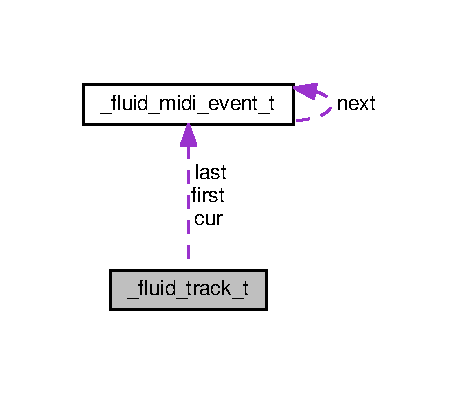
\includegraphics[width=221pt]{struct__fluid__track__t__coll__graph}
\end{center}
\end{figure}
\subsection*{Public Attributes}
\begin{DoxyCompactItemize}
\item 
char $\ast$ \hyperlink{struct__fluid__track__t_abe079916ae5ec9b911b4a4b256b8b85f}{name}
\item 
int \hyperlink{struct__fluid__track__t_a5a7355b3a3a63d85fbc1f7d530c85beb}{num}
\item 
\hyperlink{types_8h_a61c72b76e3ee344637994c3071f74d94}{fluid\+\_\+midi\+\_\+event\+\_\+t} $\ast$ \hyperlink{struct__fluid__track__t_a29479cf7bb1c867fbd23809b3ae60f21}{first}
\item 
\hyperlink{types_8h_a61c72b76e3ee344637994c3071f74d94}{fluid\+\_\+midi\+\_\+event\+\_\+t} $\ast$ \hyperlink{struct__fluid__track__t_a1e6974f6d8987199412024002394659d}{cur}
\item 
\hyperlink{types_8h_a61c72b76e3ee344637994c3071f74d94}{fluid\+\_\+midi\+\_\+event\+\_\+t} $\ast$ \hyperlink{struct__fluid__track__t_ade8bd77b7d248b46226c3dda4368d791}{last}
\item 
unsigned int \hyperlink{struct__fluid__track__t_a000f5183fac347c6daafa6d04a5843d2}{ticks}
\end{DoxyCompactItemize}


\subsection{Member Data Documentation}
\mbox{\Hypertarget{struct__fluid__track__t_a1e6974f6d8987199412024002394659d}\label{struct__fluid__track__t_a1e6974f6d8987199412024002394659d}} 
\index{\+\_\+fluid\+\_\+track\+\_\+t@{\+\_\+fluid\+\_\+track\+\_\+t}!cur@{cur}}
\index{cur@{cur}!\+\_\+fluid\+\_\+track\+\_\+t@{\+\_\+fluid\+\_\+track\+\_\+t}}
\subsubsection{\texorpdfstring{cur}{cur}}
{\footnotesize\ttfamily \hyperlink{types_8h_a61c72b76e3ee344637994c3071f74d94}{fluid\+\_\+midi\+\_\+event\+\_\+t}$\ast$ \+\_\+fluid\+\_\+track\+\_\+t\+::cur}

\mbox{\Hypertarget{struct__fluid__track__t_a29479cf7bb1c867fbd23809b3ae60f21}\label{struct__fluid__track__t_a29479cf7bb1c867fbd23809b3ae60f21}} 
\index{\+\_\+fluid\+\_\+track\+\_\+t@{\+\_\+fluid\+\_\+track\+\_\+t}!first@{first}}
\index{first@{first}!\+\_\+fluid\+\_\+track\+\_\+t@{\+\_\+fluid\+\_\+track\+\_\+t}}
\subsubsection{\texorpdfstring{first}{first}}
{\footnotesize\ttfamily \hyperlink{types_8h_a61c72b76e3ee344637994c3071f74d94}{fluid\+\_\+midi\+\_\+event\+\_\+t}$\ast$ \+\_\+fluid\+\_\+track\+\_\+t\+::first}

\mbox{\Hypertarget{struct__fluid__track__t_ade8bd77b7d248b46226c3dda4368d791}\label{struct__fluid__track__t_ade8bd77b7d248b46226c3dda4368d791}} 
\index{\+\_\+fluid\+\_\+track\+\_\+t@{\+\_\+fluid\+\_\+track\+\_\+t}!last@{last}}
\index{last@{last}!\+\_\+fluid\+\_\+track\+\_\+t@{\+\_\+fluid\+\_\+track\+\_\+t}}
\subsubsection{\texorpdfstring{last}{last}}
{\footnotesize\ttfamily \hyperlink{types_8h_a61c72b76e3ee344637994c3071f74d94}{fluid\+\_\+midi\+\_\+event\+\_\+t}$\ast$ \+\_\+fluid\+\_\+track\+\_\+t\+::last}

\mbox{\Hypertarget{struct__fluid__track__t_abe079916ae5ec9b911b4a4b256b8b85f}\label{struct__fluid__track__t_abe079916ae5ec9b911b4a4b256b8b85f}} 
\index{\+\_\+fluid\+\_\+track\+\_\+t@{\+\_\+fluid\+\_\+track\+\_\+t}!name@{name}}
\index{name@{name}!\+\_\+fluid\+\_\+track\+\_\+t@{\+\_\+fluid\+\_\+track\+\_\+t}}
\subsubsection{\texorpdfstring{name}{name}}
{\footnotesize\ttfamily char$\ast$ \+\_\+fluid\+\_\+track\+\_\+t\+::name}

\mbox{\Hypertarget{struct__fluid__track__t_a5a7355b3a3a63d85fbc1f7d530c85beb}\label{struct__fluid__track__t_a5a7355b3a3a63d85fbc1f7d530c85beb}} 
\index{\+\_\+fluid\+\_\+track\+\_\+t@{\+\_\+fluid\+\_\+track\+\_\+t}!num@{num}}
\index{num@{num}!\+\_\+fluid\+\_\+track\+\_\+t@{\+\_\+fluid\+\_\+track\+\_\+t}}
\subsubsection{\texorpdfstring{num}{num}}
{\footnotesize\ttfamily int \+\_\+fluid\+\_\+track\+\_\+t\+::num}

\mbox{\Hypertarget{struct__fluid__track__t_a000f5183fac347c6daafa6d04a5843d2}\label{struct__fluid__track__t_a000f5183fac347c6daafa6d04a5843d2}} 
\index{\+\_\+fluid\+\_\+track\+\_\+t@{\+\_\+fluid\+\_\+track\+\_\+t}!ticks@{ticks}}
\index{ticks@{ticks}!\+\_\+fluid\+\_\+track\+\_\+t@{\+\_\+fluid\+\_\+track\+\_\+t}}
\subsubsection{\texorpdfstring{ticks}{ticks}}
{\footnotesize\ttfamily unsigned int \+\_\+fluid\+\_\+track\+\_\+t\+::ticks}



The documentation for this struct was generated from the following file\+:\begin{DoxyCompactItemize}
\item 
midi/\hyperlink{fluid__midi_8h}{fluid\+\_\+midi.\+h}\end{DoxyCompactItemize}

\hypertarget{struct__fluid__tuning__t}{}\section{\+\_\+fluid\+\_\+tuning\+\_\+t Struct Reference}
\label{struct__fluid__tuning__t}\index{\+\_\+fluid\+\_\+tuning\+\_\+t@{\+\_\+fluid\+\_\+tuning\+\_\+t}}


{\ttfamily \#include $<$fluid\+\_\+tuning.\+h$>$}

\subsection*{Public Attributes}
\begin{DoxyCompactItemize}
\item 
char $\ast$ \hyperlink{struct__fluid__tuning__t_a21467840d06372b094d307f9639480da}{name}
\item 
int \hyperlink{struct__fluid__tuning__t_a1f1f2897f6e87dc4dcd99a874a706657}{bank}
\item 
int \hyperlink{struct__fluid__tuning__t_a6770e4bf001805e39c0d84bb2a5b1f4b}{prog}
\item 
double \hyperlink{struct__fluid__tuning__t_aa6a64e8c5fe6cbed8f73a1957719b275}{pitch} \mbox{[}128\mbox{]}
\item 
\hyperlink{fluidsynth__priv_8h_a6b8be882dd9958ea3635a868e1bf5152}{fluid\+\_\+atomic\+\_\+int\+\_\+t} \hyperlink{struct__fluid__tuning__t_a234f93b6e2b0d24327fecf44c997bdbb}{refcount}
\end{DoxyCompactItemize}


\subsection{Member Data Documentation}
\mbox{\Hypertarget{struct__fluid__tuning__t_a1f1f2897f6e87dc4dcd99a874a706657}\label{struct__fluid__tuning__t_a1f1f2897f6e87dc4dcd99a874a706657}} 
\index{\+\_\+fluid\+\_\+tuning\+\_\+t@{\+\_\+fluid\+\_\+tuning\+\_\+t}!bank@{bank}}
\index{bank@{bank}!\+\_\+fluid\+\_\+tuning\+\_\+t@{\+\_\+fluid\+\_\+tuning\+\_\+t}}
\subsubsection{\texorpdfstring{bank}{bank}}
{\footnotesize\ttfamily int \+\_\+fluid\+\_\+tuning\+\_\+t\+::bank}

\mbox{\Hypertarget{struct__fluid__tuning__t_a21467840d06372b094d307f9639480da}\label{struct__fluid__tuning__t_a21467840d06372b094d307f9639480da}} 
\index{\+\_\+fluid\+\_\+tuning\+\_\+t@{\+\_\+fluid\+\_\+tuning\+\_\+t}!name@{name}}
\index{name@{name}!\+\_\+fluid\+\_\+tuning\+\_\+t@{\+\_\+fluid\+\_\+tuning\+\_\+t}}
\subsubsection{\texorpdfstring{name}{name}}
{\footnotesize\ttfamily char$\ast$ \+\_\+fluid\+\_\+tuning\+\_\+t\+::name}

\mbox{\Hypertarget{struct__fluid__tuning__t_aa6a64e8c5fe6cbed8f73a1957719b275}\label{struct__fluid__tuning__t_aa6a64e8c5fe6cbed8f73a1957719b275}} 
\index{\+\_\+fluid\+\_\+tuning\+\_\+t@{\+\_\+fluid\+\_\+tuning\+\_\+t}!pitch@{pitch}}
\index{pitch@{pitch}!\+\_\+fluid\+\_\+tuning\+\_\+t@{\+\_\+fluid\+\_\+tuning\+\_\+t}}
\subsubsection{\texorpdfstring{pitch}{pitch}}
{\footnotesize\ttfamily double \+\_\+fluid\+\_\+tuning\+\_\+t\+::pitch\mbox{[}128\mbox{]}}

\mbox{\Hypertarget{struct__fluid__tuning__t_a6770e4bf001805e39c0d84bb2a5b1f4b}\label{struct__fluid__tuning__t_a6770e4bf001805e39c0d84bb2a5b1f4b}} 
\index{\+\_\+fluid\+\_\+tuning\+\_\+t@{\+\_\+fluid\+\_\+tuning\+\_\+t}!prog@{prog}}
\index{prog@{prog}!\+\_\+fluid\+\_\+tuning\+\_\+t@{\+\_\+fluid\+\_\+tuning\+\_\+t}}
\subsubsection{\texorpdfstring{prog}{prog}}
{\footnotesize\ttfamily int \+\_\+fluid\+\_\+tuning\+\_\+t\+::prog}

\mbox{\Hypertarget{struct__fluid__tuning__t_a234f93b6e2b0d24327fecf44c997bdbb}\label{struct__fluid__tuning__t_a234f93b6e2b0d24327fecf44c997bdbb}} 
\index{\+\_\+fluid\+\_\+tuning\+\_\+t@{\+\_\+fluid\+\_\+tuning\+\_\+t}!refcount@{refcount}}
\index{refcount@{refcount}!\+\_\+fluid\+\_\+tuning\+\_\+t@{\+\_\+fluid\+\_\+tuning\+\_\+t}}
\subsubsection{\texorpdfstring{refcount}{refcount}}
{\footnotesize\ttfamily \hyperlink{fluidsynth__priv_8h_a6b8be882dd9958ea3635a868e1bf5152}{fluid\+\_\+atomic\+\_\+int\+\_\+t} \+\_\+fluid\+\_\+tuning\+\_\+t\+::refcount}



The documentation for this struct was generated from the following file\+:\begin{DoxyCompactItemize}
\item 
synth/\hyperlink{fluid__tuning_8h}{fluid\+\_\+tuning.\+h}\end{DoxyCompactItemize}

\hypertarget{struct__fluid__voice__t}{}\section{\+\_\+fluid\+\_\+voice\+\_\+t Struct Reference}
\label{struct__fluid__voice__t}\index{\+\_\+fluid\+\_\+voice\+\_\+t@{\+\_\+fluid\+\_\+voice\+\_\+t}}


{\ttfamily \#include $<$fluid\+\_\+voice.\+h$>$}



Collaboration diagram for \+\_\+fluid\+\_\+voice\+\_\+t\+:
\nopagebreak
\begin{figure}[H]
\begin{center}
\leavevmode
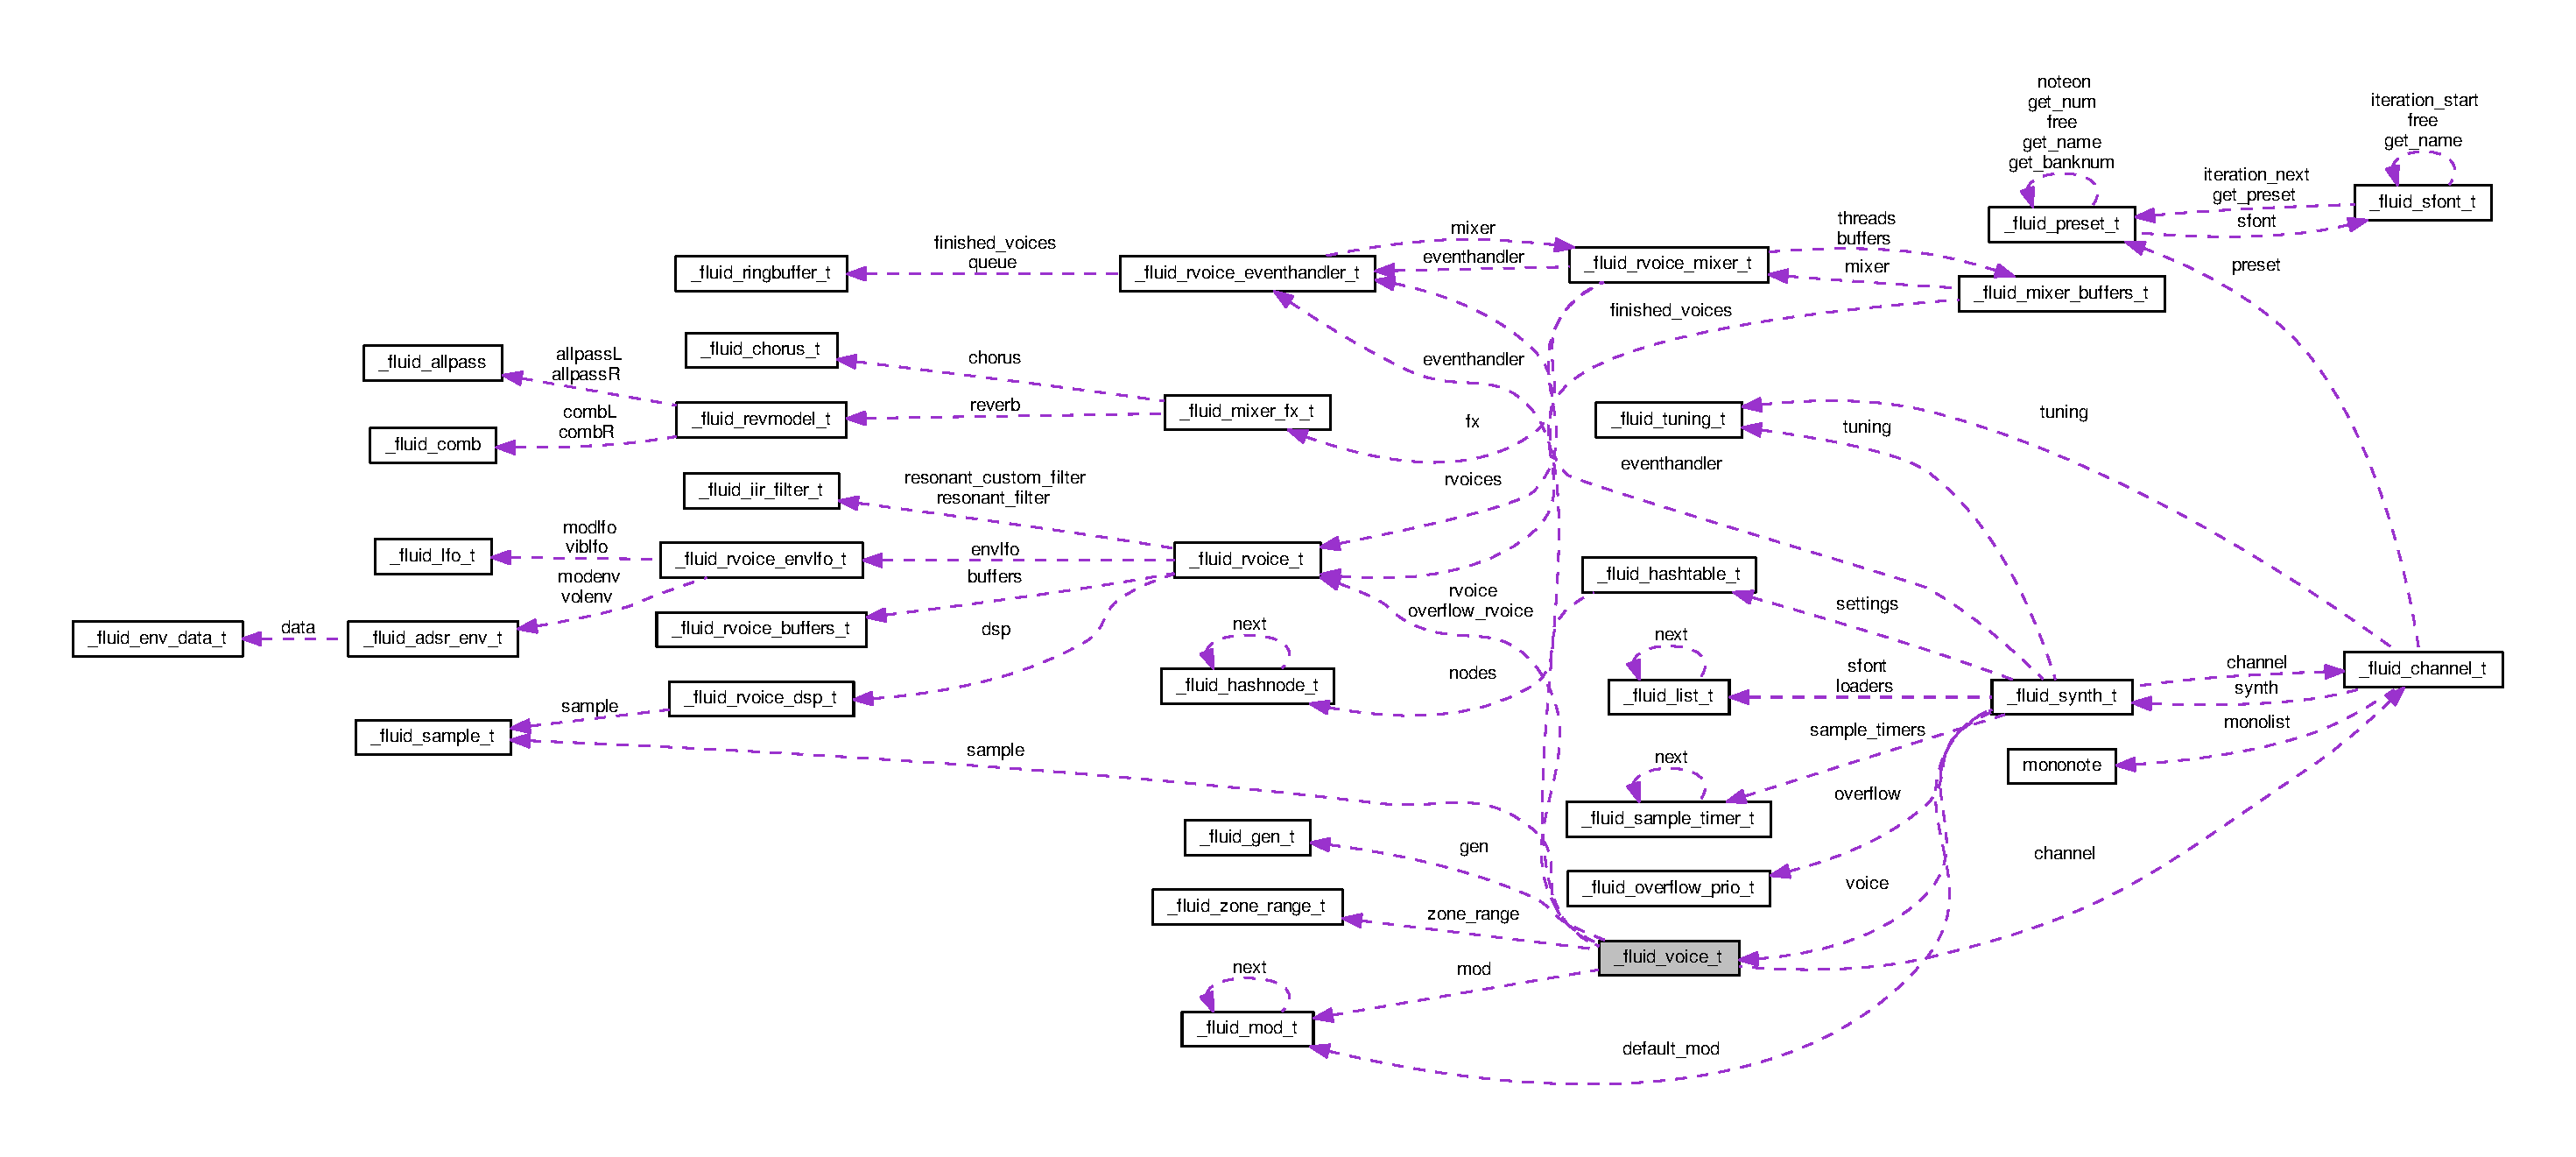
\includegraphics[width=350pt]{struct__fluid__voice__t__coll__graph}
\end{center}
\end{figure}
\subsection*{Public Attributes}
\begin{DoxyCompactItemize}
\item 
unsigned int \hyperlink{struct__fluid__voice__t_a01c265f3befd19df72c3a7ca6ef62917}{id}
\item 
unsigned char \hyperlink{struct__fluid__voice__t_ab34890439d84bf004364d122c197aeb8}{status}
\item 
unsigned char \hyperlink{struct__fluid__voice__t_a45aaf19cb332606662824896f7060001}{chan}
\item 
unsigned char \hyperlink{struct__fluid__voice__t_aaef662aed8ce7de0932ddb70d481d622}{key}
\item 
unsigned char \hyperlink{struct__fluid__voice__t_a2aedf5707c2e3332ddf61875991c2ff2}{vel}
\item 
\hyperlink{fluidsynth__priv_8h_a9e766203efa8135ece6f462e9caa1b12}{fluid\+\_\+channel\+\_\+t} $\ast$ \hyperlink{struct__fluid__voice__t_a977320cbe5f3774c839e12def55a2fd1}{channel}
\item 
\hyperlink{fluidsynth__priv_8h_aa59fe8f0195e9f5099f538d38b126e2a}{fluid\+\_\+rvoice\+\_\+eventhandler\+\_\+t} $\ast$ \hyperlink{struct__fluid__voice__t_a6f53bff277d799770e0f820255e14c0e}{eventhandler}
\item 
\hyperlink{fluidsynth__priv_8h_ac8502f0049ba8c20821b136e611462da}{fluid\+\_\+zone\+\_\+range\+\_\+t} $\ast$ \hyperlink{struct__fluid__voice__t_ae59705ecac10249158cd39128cd7783d}{zone\+\_\+range}
\item 
\hyperlink{types_8h_abf9174d452679ca1a4ee7d693fb773cf}{fluid\+\_\+sample\+\_\+t} $\ast$ \hyperlink{struct__fluid__voice__t_a0d1a19093f9272029f8d12058b73015e}{sample}
\item 
unsigned int \hyperlink{struct__fluid__voice__t_a34ed7fac9f4afac5e45b2e17439880cb}{start\+\_\+time}
\item 
int \hyperlink{struct__fluid__voice__t_a2803ecd3cd10950e77bb64179fa73a44}{mod\+\_\+count}
\item 
\hyperlink{types_8h_a6c727efab500d6c0c350d4292e9aa5ef}{fluid\+\_\+mod\+\_\+t} \hyperlink{struct__fluid__voice__t_a552c78de071a27c5648387afe3e26b3a}{mod} \mbox{[}\hyperlink{fluidsynth__priv_8h_a36d07f04a69f257b9a696b7a955b66c7}{F\+L\+U\+I\+D\+\_\+\+N\+U\+M\+\_\+\+M\+OD}\mbox{]}
\item 
\hyperlink{fluid__gen_8h_a018737d76d5ad530b622bd27b70701b0}{fluid\+\_\+gen\+\_\+t} \hyperlink{struct__fluid__voice__t_ac9d1802d04aaa7e83006128ac17b2a20}{gen} \mbox{[}\hyperlink{gen_8h_ad17a24ae3b25f3b8cc5762f818eef9b4a9c372c341b7b1a718f0016f40c615cf3}{G\+E\+N\+\_\+\+L\+A\+ST}\mbox{]}
\item 
\hyperlink{fluidsynth__priv_8h_a9e96f0917747b69cabb7c671bc693dbb}{fluid\+\_\+real\+\_\+t} \hyperlink{struct__fluid__voice__t_ab0733b2b3fa044077994ceea263b1fdb}{output\+\_\+rate}
\item 
\hyperlink{fluidsynth__priv_8h_a9e96f0917747b69cabb7c671bc693dbb}{fluid\+\_\+real\+\_\+t} \hyperlink{struct__fluid__voice__t_a3e5465a0c67b3d5644d7c64d5df9d791}{pitch}
\item 
\hyperlink{fluidsynth__priv_8h_a9e96f0917747b69cabb7c671bc693dbb}{fluid\+\_\+real\+\_\+t} \hyperlink{struct__fluid__voice__t_a7953760a53b0af6eb0e2aae8d6226112}{attenuation}
\item 
\hyperlink{fluidsynth__priv_8h_a9e96f0917747b69cabb7c671bc693dbb}{fluid\+\_\+real\+\_\+t} \hyperlink{struct__fluid__voice__t_adf14d703c345eb90b0fa1c7a633b6d08}{root\+\_\+pitch}
\item 
\hyperlink{fluidsynth__priv_8h_a9e96f0917747b69cabb7c671bc693dbb}{fluid\+\_\+real\+\_\+t} \hyperlink{struct__fluid__voice__t_a99d9c1a264b4cc95155ad9a30a9bee0f}{synth\+\_\+gain}
\item 
\hyperlink{fluidsynth__priv_8h_a9e96f0917747b69cabb7c671bc693dbb}{fluid\+\_\+real\+\_\+t} \hyperlink{struct__fluid__voice__t_ad4066c684dd8ab5b328d867e7bc69361}{pan}
\item 
\hyperlink{fluidsynth__priv_8h_a9e96f0917747b69cabb7c671bc693dbb}{fluid\+\_\+real\+\_\+t} \hyperlink{struct__fluid__voice__t_a9069286e00573602bb260268ed5ae1e2}{balance}
\item 
\hyperlink{fluidsynth__priv_8h_a9e96f0917747b69cabb7c671bc693dbb}{fluid\+\_\+real\+\_\+t} \hyperlink{struct__fluid__voice__t_a6ab72ad903385b71ff12bcac7a2394de}{reverb\+\_\+send}
\item 
\hyperlink{fluidsynth__priv_8h_a9e96f0917747b69cabb7c671bc693dbb}{fluid\+\_\+real\+\_\+t} \hyperlink{struct__fluid__voice__t_ac507a15bbd8add24b6057d390fa3c92a}{chorus\+\_\+send}
\item 
\hyperlink{fluid__rvoice_8h_a3c0405fcfaf1310d760cec3a503c509d}{fluid\+\_\+rvoice\+\_\+t} $\ast$ \hyperlink{struct__fluid__voice__t_a80d5ac9f62851e0626f896b2a5862ab6}{rvoice}
\item 
\hyperlink{fluid__rvoice_8h_a3c0405fcfaf1310d760cec3a503c509d}{fluid\+\_\+rvoice\+\_\+t} $\ast$ \hyperlink{struct__fluid__voice__t_aa9f2803ff42f7983ea32babb4f7a6f52}{overflow\+\_\+rvoice}
\item 
char \hyperlink{struct__fluid__voice__t_aadcc0b5b16bfcea9894cc19c7f7fc8e0}{can\+\_\+access\+\_\+rvoice}
\item 
char \hyperlink{struct__fluid__voice__t_a50ad82d9a8d88c3301c38660bc3e2b9a}{can\+\_\+access\+\_\+overflow\+\_\+rvoice}
\item 
char \hyperlink{struct__fluid__voice__t_a8329c478c7565ea34cc2ad2a06cda0a9}{has\+\_\+noteoff}
\end{DoxyCompactItemize}


\subsection{Member Data Documentation}
\mbox{\Hypertarget{struct__fluid__voice__t_a7953760a53b0af6eb0e2aae8d6226112}\label{struct__fluid__voice__t_a7953760a53b0af6eb0e2aae8d6226112}} 
\index{\+\_\+fluid\+\_\+voice\+\_\+t@{\+\_\+fluid\+\_\+voice\+\_\+t}!attenuation@{attenuation}}
\index{attenuation@{attenuation}!\+\_\+fluid\+\_\+voice\+\_\+t@{\+\_\+fluid\+\_\+voice\+\_\+t}}
\subsubsection{\texorpdfstring{attenuation}{attenuation}}
{\footnotesize\ttfamily \hyperlink{fluidsynth__priv_8h_a9e96f0917747b69cabb7c671bc693dbb}{fluid\+\_\+real\+\_\+t} \+\_\+fluid\+\_\+voice\+\_\+t\+::attenuation}

\mbox{\Hypertarget{struct__fluid__voice__t_a9069286e00573602bb260268ed5ae1e2}\label{struct__fluid__voice__t_a9069286e00573602bb260268ed5ae1e2}} 
\index{\+\_\+fluid\+\_\+voice\+\_\+t@{\+\_\+fluid\+\_\+voice\+\_\+t}!balance@{balance}}
\index{balance@{balance}!\+\_\+fluid\+\_\+voice\+\_\+t@{\+\_\+fluid\+\_\+voice\+\_\+t}}
\subsubsection{\texorpdfstring{balance}{balance}}
{\footnotesize\ttfamily \hyperlink{fluidsynth__priv_8h_a9e96f0917747b69cabb7c671bc693dbb}{fluid\+\_\+real\+\_\+t} \+\_\+fluid\+\_\+voice\+\_\+t\+::balance}

\mbox{\Hypertarget{struct__fluid__voice__t_a50ad82d9a8d88c3301c38660bc3e2b9a}\label{struct__fluid__voice__t_a50ad82d9a8d88c3301c38660bc3e2b9a}} 
\index{\+\_\+fluid\+\_\+voice\+\_\+t@{\+\_\+fluid\+\_\+voice\+\_\+t}!can\+\_\+access\+\_\+overflow\+\_\+rvoice@{can\+\_\+access\+\_\+overflow\+\_\+rvoice}}
\index{can\+\_\+access\+\_\+overflow\+\_\+rvoice@{can\+\_\+access\+\_\+overflow\+\_\+rvoice}!\+\_\+fluid\+\_\+voice\+\_\+t@{\+\_\+fluid\+\_\+voice\+\_\+t}}
\subsubsection{\texorpdfstring{can\+\_\+access\+\_\+overflow\+\_\+rvoice}{can\_access\_overflow\_rvoice}}
{\footnotesize\ttfamily char \+\_\+fluid\+\_\+voice\+\_\+t\+::can\+\_\+access\+\_\+overflow\+\_\+rvoice}

\mbox{\Hypertarget{struct__fluid__voice__t_aadcc0b5b16bfcea9894cc19c7f7fc8e0}\label{struct__fluid__voice__t_aadcc0b5b16bfcea9894cc19c7f7fc8e0}} 
\index{\+\_\+fluid\+\_\+voice\+\_\+t@{\+\_\+fluid\+\_\+voice\+\_\+t}!can\+\_\+access\+\_\+rvoice@{can\+\_\+access\+\_\+rvoice}}
\index{can\+\_\+access\+\_\+rvoice@{can\+\_\+access\+\_\+rvoice}!\+\_\+fluid\+\_\+voice\+\_\+t@{\+\_\+fluid\+\_\+voice\+\_\+t}}
\subsubsection{\texorpdfstring{can\+\_\+access\+\_\+rvoice}{can\_access\_rvoice}}
{\footnotesize\ttfamily char \+\_\+fluid\+\_\+voice\+\_\+t\+::can\+\_\+access\+\_\+rvoice}

\mbox{\Hypertarget{struct__fluid__voice__t_a45aaf19cb332606662824896f7060001}\label{struct__fluid__voice__t_a45aaf19cb332606662824896f7060001}} 
\index{\+\_\+fluid\+\_\+voice\+\_\+t@{\+\_\+fluid\+\_\+voice\+\_\+t}!chan@{chan}}
\index{chan@{chan}!\+\_\+fluid\+\_\+voice\+\_\+t@{\+\_\+fluid\+\_\+voice\+\_\+t}}
\subsubsection{\texorpdfstring{chan}{chan}}
{\footnotesize\ttfamily unsigned char \+\_\+fluid\+\_\+voice\+\_\+t\+::chan}

\mbox{\Hypertarget{struct__fluid__voice__t_a977320cbe5f3774c839e12def55a2fd1}\label{struct__fluid__voice__t_a977320cbe5f3774c839e12def55a2fd1}} 
\index{\+\_\+fluid\+\_\+voice\+\_\+t@{\+\_\+fluid\+\_\+voice\+\_\+t}!channel@{channel}}
\index{channel@{channel}!\+\_\+fluid\+\_\+voice\+\_\+t@{\+\_\+fluid\+\_\+voice\+\_\+t}}
\subsubsection{\texorpdfstring{channel}{channel}}
{\footnotesize\ttfamily \hyperlink{fluidsynth__priv_8h_a9e766203efa8135ece6f462e9caa1b12}{fluid\+\_\+channel\+\_\+t}$\ast$ \+\_\+fluid\+\_\+voice\+\_\+t\+::channel}

\mbox{\Hypertarget{struct__fluid__voice__t_ac507a15bbd8add24b6057d390fa3c92a}\label{struct__fluid__voice__t_ac507a15bbd8add24b6057d390fa3c92a}} 
\index{\+\_\+fluid\+\_\+voice\+\_\+t@{\+\_\+fluid\+\_\+voice\+\_\+t}!chorus\+\_\+send@{chorus\+\_\+send}}
\index{chorus\+\_\+send@{chorus\+\_\+send}!\+\_\+fluid\+\_\+voice\+\_\+t@{\+\_\+fluid\+\_\+voice\+\_\+t}}
\subsubsection{\texorpdfstring{chorus\+\_\+send}{chorus\_send}}
{\footnotesize\ttfamily \hyperlink{fluidsynth__priv_8h_a9e96f0917747b69cabb7c671bc693dbb}{fluid\+\_\+real\+\_\+t} \+\_\+fluid\+\_\+voice\+\_\+t\+::chorus\+\_\+send}

\mbox{\Hypertarget{struct__fluid__voice__t_a6f53bff277d799770e0f820255e14c0e}\label{struct__fluid__voice__t_a6f53bff277d799770e0f820255e14c0e}} 
\index{\+\_\+fluid\+\_\+voice\+\_\+t@{\+\_\+fluid\+\_\+voice\+\_\+t}!eventhandler@{eventhandler}}
\index{eventhandler@{eventhandler}!\+\_\+fluid\+\_\+voice\+\_\+t@{\+\_\+fluid\+\_\+voice\+\_\+t}}
\subsubsection{\texorpdfstring{eventhandler}{eventhandler}}
{\footnotesize\ttfamily \hyperlink{fluidsynth__priv_8h_aa59fe8f0195e9f5099f538d38b126e2a}{fluid\+\_\+rvoice\+\_\+eventhandler\+\_\+t}$\ast$ \+\_\+fluid\+\_\+voice\+\_\+t\+::eventhandler}

\mbox{\Hypertarget{struct__fluid__voice__t_ac9d1802d04aaa7e83006128ac17b2a20}\label{struct__fluid__voice__t_ac9d1802d04aaa7e83006128ac17b2a20}} 
\index{\+\_\+fluid\+\_\+voice\+\_\+t@{\+\_\+fluid\+\_\+voice\+\_\+t}!gen@{gen}}
\index{gen@{gen}!\+\_\+fluid\+\_\+voice\+\_\+t@{\+\_\+fluid\+\_\+voice\+\_\+t}}
\subsubsection{\texorpdfstring{gen}{gen}}
{\footnotesize\ttfamily \hyperlink{fluid__gen_8h_a018737d76d5ad530b622bd27b70701b0}{fluid\+\_\+gen\+\_\+t} \+\_\+fluid\+\_\+voice\+\_\+t\+::gen\mbox{[}\hyperlink{gen_8h_ad17a24ae3b25f3b8cc5762f818eef9b4a9c372c341b7b1a718f0016f40c615cf3}{G\+E\+N\+\_\+\+L\+A\+ST}\mbox{]}}

\mbox{\Hypertarget{struct__fluid__voice__t_a8329c478c7565ea34cc2ad2a06cda0a9}\label{struct__fluid__voice__t_a8329c478c7565ea34cc2ad2a06cda0a9}} 
\index{\+\_\+fluid\+\_\+voice\+\_\+t@{\+\_\+fluid\+\_\+voice\+\_\+t}!has\+\_\+noteoff@{has\+\_\+noteoff}}
\index{has\+\_\+noteoff@{has\+\_\+noteoff}!\+\_\+fluid\+\_\+voice\+\_\+t@{\+\_\+fluid\+\_\+voice\+\_\+t}}
\subsubsection{\texorpdfstring{has\+\_\+noteoff}{has\_noteoff}}
{\footnotesize\ttfamily char \+\_\+fluid\+\_\+voice\+\_\+t\+::has\+\_\+noteoff}

\mbox{\Hypertarget{struct__fluid__voice__t_a01c265f3befd19df72c3a7ca6ef62917}\label{struct__fluid__voice__t_a01c265f3befd19df72c3a7ca6ef62917}} 
\index{\+\_\+fluid\+\_\+voice\+\_\+t@{\+\_\+fluid\+\_\+voice\+\_\+t}!id@{id}}
\index{id@{id}!\+\_\+fluid\+\_\+voice\+\_\+t@{\+\_\+fluid\+\_\+voice\+\_\+t}}
\subsubsection{\texorpdfstring{id}{id}}
{\footnotesize\ttfamily unsigned int \+\_\+fluid\+\_\+voice\+\_\+t\+::id}

\mbox{\Hypertarget{struct__fluid__voice__t_aaef662aed8ce7de0932ddb70d481d622}\label{struct__fluid__voice__t_aaef662aed8ce7de0932ddb70d481d622}} 
\index{\+\_\+fluid\+\_\+voice\+\_\+t@{\+\_\+fluid\+\_\+voice\+\_\+t}!key@{key}}
\index{key@{key}!\+\_\+fluid\+\_\+voice\+\_\+t@{\+\_\+fluid\+\_\+voice\+\_\+t}}
\subsubsection{\texorpdfstring{key}{key}}
{\footnotesize\ttfamily unsigned char \+\_\+fluid\+\_\+voice\+\_\+t\+::key}

\mbox{\Hypertarget{struct__fluid__voice__t_a552c78de071a27c5648387afe3e26b3a}\label{struct__fluid__voice__t_a552c78de071a27c5648387afe3e26b3a}} 
\index{\+\_\+fluid\+\_\+voice\+\_\+t@{\+\_\+fluid\+\_\+voice\+\_\+t}!mod@{mod}}
\index{mod@{mod}!\+\_\+fluid\+\_\+voice\+\_\+t@{\+\_\+fluid\+\_\+voice\+\_\+t}}
\subsubsection{\texorpdfstring{mod}{mod}}
{\footnotesize\ttfamily \hyperlink{types_8h_a6c727efab500d6c0c350d4292e9aa5ef}{fluid\+\_\+mod\+\_\+t} \+\_\+fluid\+\_\+voice\+\_\+t\+::mod\mbox{[}\hyperlink{fluidsynth__priv_8h_a36d07f04a69f257b9a696b7a955b66c7}{F\+L\+U\+I\+D\+\_\+\+N\+U\+M\+\_\+\+M\+OD}\mbox{]}}

\mbox{\Hypertarget{struct__fluid__voice__t_a2803ecd3cd10950e77bb64179fa73a44}\label{struct__fluid__voice__t_a2803ecd3cd10950e77bb64179fa73a44}} 
\index{\+\_\+fluid\+\_\+voice\+\_\+t@{\+\_\+fluid\+\_\+voice\+\_\+t}!mod\+\_\+count@{mod\+\_\+count}}
\index{mod\+\_\+count@{mod\+\_\+count}!\+\_\+fluid\+\_\+voice\+\_\+t@{\+\_\+fluid\+\_\+voice\+\_\+t}}
\subsubsection{\texorpdfstring{mod\+\_\+count}{mod\_count}}
{\footnotesize\ttfamily int \+\_\+fluid\+\_\+voice\+\_\+t\+::mod\+\_\+count}

\mbox{\Hypertarget{struct__fluid__voice__t_ab0733b2b3fa044077994ceea263b1fdb}\label{struct__fluid__voice__t_ab0733b2b3fa044077994ceea263b1fdb}} 
\index{\+\_\+fluid\+\_\+voice\+\_\+t@{\+\_\+fluid\+\_\+voice\+\_\+t}!output\+\_\+rate@{output\+\_\+rate}}
\index{output\+\_\+rate@{output\+\_\+rate}!\+\_\+fluid\+\_\+voice\+\_\+t@{\+\_\+fluid\+\_\+voice\+\_\+t}}
\subsubsection{\texorpdfstring{output\+\_\+rate}{output\_rate}}
{\footnotesize\ttfamily \hyperlink{fluidsynth__priv_8h_a9e96f0917747b69cabb7c671bc693dbb}{fluid\+\_\+real\+\_\+t} \+\_\+fluid\+\_\+voice\+\_\+t\+::output\+\_\+rate}

\mbox{\Hypertarget{struct__fluid__voice__t_aa9f2803ff42f7983ea32babb4f7a6f52}\label{struct__fluid__voice__t_aa9f2803ff42f7983ea32babb4f7a6f52}} 
\index{\+\_\+fluid\+\_\+voice\+\_\+t@{\+\_\+fluid\+\_\+voice\+\_\+t}!overflow\+\_\+rvoice@{overflow\+\_\+rvoice}}
\index{overflow\+\_\+rvoice@{overflow\+\_\+rvoice}!\+\_\+fluid\+\_\+voice\+\_\+t@{\+\_\+fluid\+\_\+voice\+\_\+t}}
\subsubsection{\texorpdfstring{overflow\+\_\+rvoice}{overflow\_rvoice}}
{\footnotesize\ttfamily \hyperlink{fluid__rvoice_8h_a3c0405fcfaf1310d760cec3a503c509d}{fluid\+\_\+rvoice\+\_\+t}$\ast$ \+\_\+fluid\+\_\+voice\+\_\+t\+::overflow\+\_\+rvoice}

\mbox{\Hypertarget{struct__fluid__voice__t_ad4066c684dd8ab5b328d867e7bc69361}\label{struct__fluid__voice__t_ad4066c684dd8ab5b328d867e7bc69361}} 
\index{\+\_\+fluid\+\_\+voice\+\_\+t@{\+\_\+fluid\+\_\+voice\+\_\+t}!pan@{pan}}
\index{pan@{pan}!\+\_\+fluid\+\_\+voice\+\_\+t@{\+\_\+fluid\+\_\+voice\+\_\+t}}
\subsubsection{\texorpdfstring{pan}{pan}}
{\footnotesize\ttfamily \hyperlink{fluidsynth__priv_8h_a9e96f0917747b69cabb7c671bc693dbb}{fluid\+\_\+real\+\_\+t} \+\_\+fluid\+\_\+voice\+\_\+t\+::pan}

\mbox{\Hypertarget{struct__fluid__voice__t_a3e5465a0c67b3d5644d7c64d5df9d791}\label{struct__fluid__voice__t_a3e5465a0c67b3d5644d7c64d5df9d791}} 
\index{\+\_\+fluid\+\_\+voice\+\_\+t@{\+\_\+fluid\+\_\+voice\+\_\+t}!pitch@{pitch}}
\index{pitch@{pitch}!\+\_\+fluid\+\_\+voice\+\_\+t@{\+\_\+fluid\+\_\+voice\+\_\+t}}
\subsubsection{\texorpdfstring{pitch}{pitch}}
{\footnotesize\ttfamily \hyperlink{fluidsynth__priv_8h_a9e96f0917747b69cabb7c671bc693dbb}{fluid\+\_\+real\+\_\+t} \+\_\+fluid\+\_\+voice\+\_\+t\+::pitch}

\mbox{\Hypertarget{struct__fluid__voice__t_a6ab72ad903385b71ff12bcac7a2394de}\label{struct__fluid__voice__t_a6ab72ad903385b71ff12bcac7a2394de}} 
\index{\+\_\+fluid\+\_\+voice\+\_\+t@{\+\_\+fluid\+\_\+voice\+\_\+t}!reverb\+\_\+send@{reverb\+\_\+send}}
\index{reverb\+\_\+send@{reverb\+\_\+send}!\+\_\+fluid\+\_\+voice\+\_\+t@{\+\_\+fluid\+\_\+voice\+\_\+t}}
\subsubsection{\texorpdfstring{reverb\+\_\+send}{reverb\_send}}
{\footnotesize\ttfamily \hyperlink{fluidsynth__priv_8h_a9e96f0917747b69cabb7c671bc693dbb}{fluid\+\_\+real\+\_\+t} \+\_\+fluid\+\_\+voice\+\_\+t\+::reverb\+\_\+send}

\mbox{\Hypertarget{struct__fluid__voice__t_adf14d703c345eb90b0fa1c7a633b6d08}\label{struct__fluid__voice__t_adf14d703c345eb90b0fa1c7a633b6d08}} 
\index{\+\_\+fluid\+\_\+voice\+\_\+t@{\+\_\+fluid\+\_\+voice\+\_\+t}!root\+\_\+pitch@{root\+\_\+pitch}}
\index{root\+\_\+pitch@{root\+\_\+pitch}!\+\_\+fluid\+\_\+voice\+\_\+t@{\+\_\+fluid\+\_\+voice\+\_\+t}}
\subsubsection{\texorpdfstring{root\+\_\+pitch}{root\_pitch}}
{\footnotesize\ttfamily \hyperlink{fluidsynth__priv_8h_a9e96f0917747b69cabb7c671bc693dbb}{fluid\+\_\+real\+\_\+t} \+\_\+fluid\+\_\+voice\+\_\+t\+::root\+\_\+pitch}

\mbox{\Hypertarget{struct__fluid__voice__t_a80d5ac9f62851e0626f896b2a5862ab6}\label{struct__fluid__voice__t_a80d5ac9f62851e0626f896b2a5862ab6}} 
\index{\+\_\+fluid\+\_\+voice\+\_\+t@{\+\_\+fluid\+\_\+voice\+\_\+t}!rvoice@{rvoice}}
\index{rvoice@{rvoice}!\+\_\+fluid\+\_\+voice\+\_\+t@{\+\_\+fluid\+\_\+voice\+\_\+t}}
\subsubsection{\texorpdfstring{rvoice}{rvoice}}
{\footnotesize\ttfamily \hyperlink{fluid__rvoice_8h_a3c0405fcfaf1310d760cec3a503c509d}{fluid\+\_\+rvoice\+\_\+t}$\ast$ \+\_\+fluid\+\_\+voice\+\_\+t\+::rvoice}

\mbox{\Hypertarget{struct__fluid__voice__t_a0d1a19093f9272029f8d12058b73015e}\label{struct__fluid__voice__t_a0d1a19093f9272029f8d12058b73015e}} 
\index{\+\_\+fluid\+\_\+voice\+\_\+t@{\+\_\+fluid\+\_\+voice\+\_\+t}!sample@{sample}}
\index{sample@{sample}!\+\_\+fluid\+\_\+voice\+\_\+t@{\+\_\+fluid\+\_\+voice\+\_\+t}}
\subsubsection{\texorpdfstring{sample}{sample}}
{\footnotesize\ttfamily \hyperlink{types_8h_abf9174d452679ca1a4ee7d693fb773cf}{fluid\+\_\+sample\+\_\+t}$\ast$ \+\_\+fluid\+\_\+voice\+\_\+t\+::sample}

\mbox{\Hypertarget{struct__fluid__voice__t_a34ed7fac9f4afac5e45b2e17439880cb}\label{struct__fluid__voice__t_a34ed7fac9f4afac5e45b2e17439880cb}} 
\index{\+\_\+fluid\+\_\+voice\+\_\+t@{\+\_\+fluid\+\_\+voice\+\_\+t}!start\+\_\+time@{start\+\_\+time}}
\index{start\+\_\+time@{start\+\_\+time}!\+\_\+fluid\+\_\+voice\+\_\+t@{\+\_\+fluid\+\_\+voice\+\_\+t}}
\subsubsection{\texorpdfstring{start\+\_\+time}{start\_time}}
{\footnotesize\ttfamily unsigned int \+\_\+fluid\+\_\+voice\+\_\+t\+::start\+\_\+time}

\mbox{\Hypertarget{struct__fluid__voice__t_ab34890439d84bf004364d122c197aeb8}\label{struct__fluid__voice__t_ab34890439d84bf004364d122c197aeb8}} 
\index{\+\_\+fluid\+\_\+voice\+\_\+t@{\+\_\+fluid\+\_\+voice\+\_\+t}!status@{status}}
\index{status@{status}!\+\_\+fluid\+\_\+voice\+\_\+t@{\+\_\+fluid\+\_\+voice\+\_\+t}}
\subsubsection{\texorpdfstring{status}{status}}
{\footnotesize\ttfamily unsigned char \+\_\+fluid\+\_\+voice\+\_\+t\+::status}

\mbox{\Hypertarget{struct__fluid__voice__t_a99d9c1a264b4cc95155ad9a30a9bee0f}\label{struct__fluid__voice__t_a99d9c1a264b4cc95155ad9a30a9bee0f}} 
\index{\+\_\+fluid\+\_\+voice\+\_\+t@{\+\_\+fluid\+\_\+voice\+\_\+t}!synth\+\_\+gain@{synth\+\_\+gain}}
\index{synth\+\_\+gain@{synth\+\_\+gain}!\+\_\+fluid\+\_\+voice\+\_\+t@{\+\_\+fluid\+\_\+voice\+\_\+t}}
\subsubsection{\texorpdfstring{synth\+\_\+gain}{synth\_gain}}
{\footnotesize\ttfamily \hyperlink{fluidsynth__priv_8h_a9e96f0917747b69cabb7c671bc693dbb}{fluid\+\_\+real\+\_\+t} \+\_\+fluid\+\_\+voice\+\_\+t\+::synth\+\_\+gain}

\mbox{\Hypertarget{struct__fluid__voice__t_a2aedf5707c2e3332ddf61875991c2ff2}\label{struct__fluid__voice__t_a2aedf5707c2e3332ddf61875991c2ff2}} 
\index{\+\_\+fluid\+\_\+voice\+\_\+t@{\+\_\+fluid\+\_\+voice\+\_\+t}!vel@{vel}}
\index{vel@{vel}!\+\_\+fluid\+\_\+voice\+\_\+t@{\+\_\+fluid\+\_\+voice\+\_\+t}}
\subsubsection{\texorpdfstring{vel}{vel}}
{\footnotesize\ttfamily unsigned char \+\_\+fluid\+\_\+voice\+\_\+t\+::vel}

\mbox{\Hypertarget{struct__fluid__voice__t_ae59705ecac10249158cd39128cd7783d}\label{struct__fluid__voice__t_ae59705ecac10249158cd39128cd7783d}} 
\index{\+\_\+fluid\+\_\+voice\+\_\+t@{\+\_\+fluid\+\_\+voice\+\_\+t}!zone\+\_\+range@{zone\+\_\+range}}
\index{zone\+\_\+range@{zone\+\_\+range}!\+\_\+fluid\+\_\+voice\+\_\+t@{\+\_\+fluid\+\_\+voice\+\_\+t}}
\subsubsection{\texorpdfstring{zone\+\_\+range}{zone\_range}}
{\footnotesize\ttfamily \hyperlink{fluidsynth__priv_8h_ac8502f0049ba8c20821b136e611462da}{fluid\+\_\+zone\+\_\+range\+\_\+t}$\ast$ \+\_\+fluid\+\_\+voice\+\_\+t\+::zone\+\_\+range}



The documentation for this struct was generated from the following file\+:\begin{DoxyCompactItemize}
\item 
synth/\hyperlink{fluid__voice_8h}{fluid\+\_\+voice.\+h}\end{DoxyCompactItemize}

\hypertarget{struct__fluid__voice__zone__t}{}\section{\+\_\+fluid\+\_\+voice\+\_\+zone\+\_\+t Struct Reference}
\label{struct__fluid__voice__zone__t}\index{\+\_\+fluid\+\_\+voice\+\_\+zone\+\_\+t@{\+\_\+fluid\+\_\+voice\+\_\+zone\+\_\+t}}


{\ttfamily \#include $<$fluid\+\_\+defsfont.\+h$>$}



Collaboration diagram for \+\_\+fluid\+\_\+voice\+\_\+zone\+\_\+t\+:
\nopagebreak
\begin{figure}[H]
\begin{center}
\leavevmode
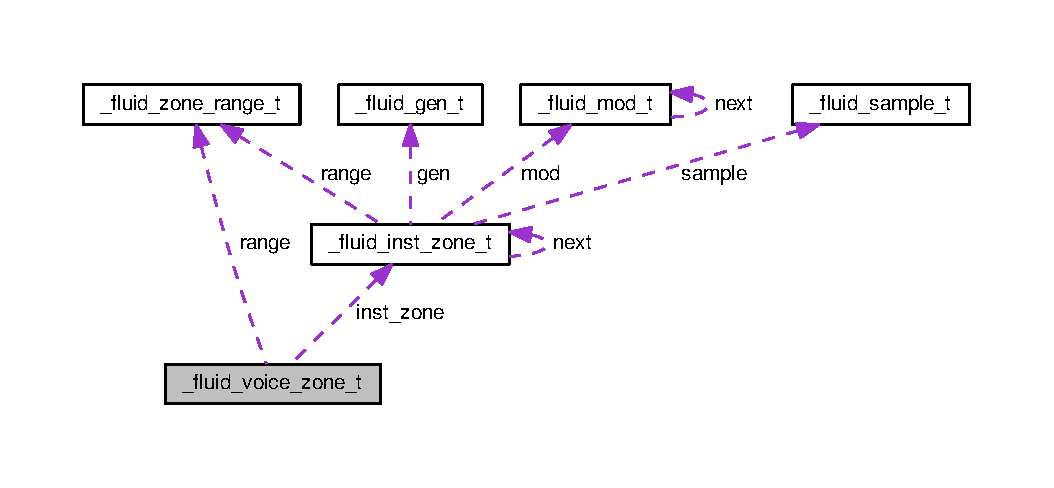
\includegraphics[width=350pt]{struct__fluid__voice__zone__t__coll__graph}
\end{center}
\end{figure}
\subsection*{Public Attributes}
\begin{DoxyCompactItemize}
\item 
\hyperlink{fluid__defsfont_8h_aa02ac18b4c58545cc3b297bdf4d933ab}{fluid\+\_\+inst\+\_\+zone\+\_\+t} $\ast$ \hyperlink{struct__fluid__voice__zone__t_a9ea94f8aa6d376c55c942b6e11f1acbc}{inst\+\_\+zone}
\item 
\hyperlink{fluidsynth__priv_8h_ac8502f0049ba8c20821b136e611462da}{fluid\+\_\+zone\+\_\+range\+\_\+t} \hyperlink{struct__fluid__voice__zone__t_aa4ab9b1dcdb5c972cb37458478ec2fe6}{range}
\end{DoxyCompactItemize}


\subsection{Member Data Documentation}
\mbox{\Hypertarget{struct__fluid__voice__zone__t_a9ea94f8aa6d376c55c942b6e11f1acbc}\label{struct__fluid__voice__zone__t_a9ea94f8aa6d376c55c942b6e11f1acbc}} 
\index{\+\_\+fluid\+\_\+voice\+\_\+zone\+\_\+t@{\+\_\+fluid\+\_\+voice\+\_\+zone\+\_\+t}!inst\+\_\+zone@{inst\+\_\+zone}}
\index{inst\+\_\+zone@{inst\+\_\+zone}!\+\_\+fluid\+\_\+voice\+\_\+zone\+\_\+t@{\+\_\+fluid\+\_\+voice\+\_\+zone\+\_\+t}}
\subsubsection{\texorpdfstring{inst\+\_\+zone}{inst\_zone}}
{\footnotesize\ttfamily \hyperlink{fluid__defsfont_8h_aa02ac18b4c58545cc3b297bdf4d933ab}{fluid\+\_\+inst\+\_\+zone\+\_\+t}$\ast$ \+\_\+fluid\+\_\+voice\+\_\+zone\+\_\+t\+::inst\+\_\+zone}

\mbox{\Hypertarget{struct__fluid__voice__zone__t_aa4ab9b1dcdb5c972cb37458478ec2fe6}\label{struct__fluid__voice__zone__t_aa4ab9b1dcdb5c972cb37458478ec2fe6}} 
\index{\+\_\+fluid\+\_\+voice\+\_\+zone\+\_\+t@{\+\_\+fluid\+\_\+voice\+\_\+zone\+\_\+t}!range@{range}}
\index{range@{range}!\+\_\+fluid\+\_\+voice\+\_\+zone\+\_\+t@{\+\_\+fluid\+\_\+voice\+\_\+zone\+\_\+t}}
\subsubsection{\texorpdfstring{range}{range}}
{\footnotesize\ttfamily \hyperlink{fluidsynth__priv_8h_ac8502f0049ba8c20821b136e611462da}{fluid\+\_\+zone\+\_\+range\+\_\+t} \+\_\+fluid\+\_\+voice\+\_\+zone\+\_\+t\+::range}



The documentation for this struct was generated from the following file\+:\begin{DoxyCompactItemize}
\item 
sfloader/\hyperlink{fluid__defsfont_8h}{fluid\+\_\+defsfont.\+h}\end{DoxyCompactItemize}

\hypertarget{struct__fluid__zone__range__t}{}\section{\+\_\+fluid\+\_\+zone\+\_\+range\+\_\+t Struct Reference}
\label{struct__fluid__zone__range__t}\index{\+\_\+fluid\+\_\+zone\+\_\+range\+\_\+t@{\+\_\+fluid\+\_\+zone\+\_\+range\+\_\+t}}


{\ttfamily \#include $<$fluid\+\_\+defsfont.\+h$>$}

\subsection*{Public Attributes}
\begin{DoxyCompactItemize}
\item 
int \hyperlink{struct__fluid__zone__range__t_a88c9f4ae016fb8aa54e473fa382c428b}{keylo}
\item 
int \hyperlink{struct__fluid__zone__range__t_abc9841a37316d044590a024cb24f5935}{keyhi}
\item 
int \hyperlink{struct__fluid__zone__range__t_ac3967fb25b3a00eddbc7e53174295791}{vello}
\item 
int \hyperlink{struct__fluid__zone__range__t_a20a747a31f8f6a1d4d127610de034b67}{velhi}
\item 
unsigned char \hyperlink{struct__fluid__zone__range__t_a651990086ce77712dddfe8cdeea82995}{ignore}
\end{DoxyCompactItemize}


\subsection{Member Data Documentation}
\mbox{\Hypertarget{struct__fluid__zone__range__t_a651990086ce77712dddfe8cdeea82995}\label{struct__fluid__zone__range__t_a651990086ce77712dddfe8cdeea82995}} 
\index{\+\_\+fluid\+\_\+zone\+\_\+range\+\_\+t@{\+\_\+fluid\+\_\+zone\+\_\+range\+\_\+t}!ignore@{ignore}}
\index{ignore@{ignore}!\+\_\+fluid\+\_\+zone\+\_\+range\+\_\+t@{\+\_\+fluid\+\_\+zone\+\_\+range\+\_\+t}}
\subsubsection{\texorpdfstring{ignore}{ignore}}
{\footnotesize\ttfamily unsigned char \+\_\+fluid\+\_\+zone\+\_\+range\+\_\+t\+::ignore}

\mbox{\Hypertarget{struct__fluid__zone__range__t_abc9841a37316d044590a024cb24f5935}\label{struct__fluid__zone__range__t_abc9841a37316d044590a024cb24f5935}} 
\index{\+\_\+fluid\+\_\+zone\+\_\+range\+\_\+t@{\+\_\+fluid\+\_\+zone\+\_\+range\+\_\+t}!keyhi@{keyhi}}
\index{keyhi@{keyhi}!\+\_\+fluid\+\_\+zone\+\_\+range\+\_\+t@{\+\_\+fluid\+\_\+zone\+\_\+range\+\_\+t}}
\subsubsection{\texorpdfstring{keyhi}{keyhi}}
{\footnotesize\ttfamily int \+\_\+fluid\+\_\+zone\+\_\+range\+\_\+t\+::keyhi}

\mbox{\Hypertarget{struct__fluid__zone__range__t_a88c9f4ae016fb8aa54e473fa382c428b}\label{struct__fluid__zone__range__t_a88c9f4ae016fb8aa54e473fa382c428b}} 
\index{\+\_\+fluid\+\_\+zone\+\_\+range\+\_\+t@{\+\_\+fluid\+\_\+zone\+\_\+range\+\_\+t}!keylo@{keylo}}
\index{keylo@{keylo}!\+\_\+fluid\+\_\+zone\+\_\+range\+\_\+t@{\+\_\+fluid\+\_\+zone\+\_\+range\+\_\+t}}
\subsubsection{\texorpdfstring{keylo}{keylo}}
{\footnotesize\ttfamily int \+\_\+fluid\+\_\+zone\+\_\+range\+\_\+t\+::keylo}

\mbox{\Hypertarget{struct__fluid__zone__range__t_a20a747a31f8f6a1d4d127610de034b67}\label{struct__fluid__zone__range__t_a20a747a31f8f6a1d4d127610de034b67}} 
\index{\+\_\+fluid\+\_\+zone\+\_\+range\+\_\+t@{\+\_\+fluid\+\_\+zone\+\_\+range\+\_\+t}!velhi@{velhi}}
\index{velhi@{velhi}!\+\_\+fluid\+\_\+zone\+\_\+range\+\_\+t@{\+\_\+fluid\+\_\+zone\+\_\+range\+\_\+t}}
\subsubsection{\texorpdfstring{velhi}{velhi}}
{\footnotesize\ttfamily int \+\_\+fluid\+\_\+zone\+\_\+range\+\_\+t\+::velhi}

\mbox{\Hypertarget{struct__fluid__zone__range__t_ac3967fb25b3a00eddbc7e53174295791}\label{struct__fluid__zone__range__t_ac3967fb25b3a00eddbc7e53174295791}} 
\index{\+\_\+fluid\+\_\+zone\+\_\+range\+\_\+t@{\+\_\+fluid\+\_\+zone\+\_\+range\+\_\+t}!vello@{vello}}
\index{vello@{vello}!\+\_\+fluid\+\_\+zone\+\_\+range\+\_\+t@{\+\_\+fluid\+\_\+zone\+\_\+range\+\_\+t}}
\subsubsection{\texorpdfstring{vello}{vello}}
{\footnotesize\ttfamily int \+\_\+fluid\+\_\+zone\+\_\+range\+\_\+t\+::vello}



The documentation for this struct was generated from the following file\+:\begin{DoxyCompactItemize}
\item 
sfloader/\hyperlink{fluid__defsfont_8h}{fluid\+\_\+defsfont.\+h}\end{DoxyCompactItemize}

\hypertarget{struct__SFBag}{}\section{\+\_\+\+S\+F\+Bag Struct Reference}
\label{struct__SFBag}\index{\+\_\+\+S\+F\+Bag@{\+\_\+\+S\+F\+Bag}}


{\ttfamily \#include $<$fluid\+\_\+sffile.\+h$>$}

\subsection*{Public Attributes}
\begin{DoxyCompactItemize}
\item 
unsigned short \hyperlink{struct__SFBag_a366736acdb535b648afe177a8f7ffa4d}{genndx}
\item 
unsigned short \hyperlink{struct__SFBag_a6051b8dda6779c4bb0eeb82c287cbccf}{modndx}
\end{DoxyCompactItemize}


\subsection{Member Data Documentation}
\mbox{\Hypertarget{struct__SFBag_a366736acdb535b648afe177a8f7ffa4d}\label{struct__SFBag_a366736acdb535b648afe177a8f7ffa4d}} 
\index{\+\_\+\+S\+F\+Bag@{\+\_\+\+S\+F\+Bag}!genndx@{genndx}}
\index{genndx@{genndx}!\+\_\+\+S\+F\+Bag@{\+\_\+\+S\+F\+Bag}}
\subsubsection{\texorpdfstring{genndx}{genndx}}
{\footnotesize\ttfamily unsigned short \+\_\+\+S\+F\+Bag\+::genndx}

\mbox{\Hypertarget{struct__SFBag_a6051b8dda6779c4bb0eeb82c287cbccf}\label{struct__SFBag_a6051b8dda6779c4bb0eeb82c287cbccf}} 
\index{\+\_\+\+S\+F\+Bag@{\+\_\+\+S\+F\+Bag}!modndx@{modndx}}
\index{modndx@{modndx}!\+\_\+\+S\+F\+Bag@{\+\_\+\+S\+F\+Bag}}
\subsubsection{\texorpdfstring{modndx}{modndx}}
{\footnotesize\ttfamily unsigned short \+\_\+\+S\+F\+Bag\+::modndx}



The documentation for this struct was generated from the following file\+:\begin{DoxyCompactItemize}
\item 
sfloader/\hyperlink{fluid__sffile_8h}{fluid\+\_\+sffile.\+h}\end{DoxyCompactItemize}

\hypertarget{struct__SFChunk}{}\section{\+\_\+\+S\+F\+Chunk Struct Reference}
\label{struct__SFChunk}\index{\+\_\+\+S\+F\+Chunk@{\+\_\+\+S\+F\+Chunk}}


{\ttfamily \#include $<$fluid\+\_\+sffile.\+h$>$}

\subsection*{Public Attributes}
\begin{DoxyCompactItemize}
\item 
unsigned int \hyperlink{struct__SFChunk_a0dc5315a85b6cbd1d6d378fbb87f6a9b}{id}
\item 
unsigned int \hyperlink{struct__SFChunk_a3bfbea649b2dce08f3d788e325a0fbcb}{size}
\end{DoxyCompactItemize}


\subsection{Member Data Documentation}
\mbox{\Hypertarget{struct__SFChunk_a0dc5315a85b6cbd1d6d378fbb87f6a9b}\label{struct__SFChunk_a0dc5315a85b6cbd1d6d378fbb87f6a9b}} 
\index{\+\_\+\+S\+F\+Chunk@{\+\_\+\+S\+F\+Chunk}!id@{id}}
\index{id@{id}!\+\_\+\+S\+F\+Chunk@{\+\_\+\+S\+F\+Chunk}}
\subsubsection{\texorpdfstring{id}{id}}
{\footnotesize\ttfamily unsigned int \+\_\+\+S\+F\+Chunk\+::id}

\mbox{\Hypertarget{struct__SFChunk_a3bfbea649b2dce08f3d788e325a0fbcb}\label{struct__SFChunk_a3bfbea649b2dce08f3d788e325a0fbcb}} 
\index{\+\_\+\+S\+F\+Chunk@{\+\_\+\+S\+F\+Chunk}!size@{size}}
\index{size@{size}!\+\_\+\+S\+F\+Chunk@{\+\_\+\+S\+F\+Chunk}}
\subsubsection{\texorpdfstring{size}{size}}
{\footnotesize\ttfamily unsigned int \+\_\+\+S\+F\+Chunk\+::size}



The documentation for this struct was generated from the following file\+:\begin{DoxyCompactItemize}
\item 
sfloader/\hyperlink{fluid__sffile_8h}{fluid\+\_\+sffile.\+h}\end{DoxyCompactItemize}

\hypertarget{struct__SFData}{}\section{\+\_\+\+S\+F\+Data Struct Reference}
\label{struct__SFData}\index{\+\_\+\+S\+F\+Data@{\+\_\+\+S\+F\+Data}}


{\ttfamily \#include $<$fluid\+\_\+sffile.\+h$>$}



Collaboration diagram for \+\_\+\+S\+F\+Data\+:
\nopagebreak
\begin{figure}[H]
\begin{center}
\leavevmode
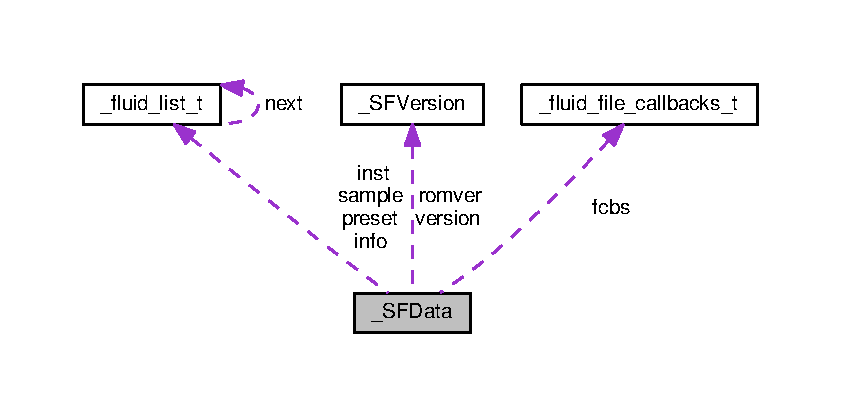
\includegraphics[width=350pt]{struct__SFData__coll__graph}
\end{center}
\end{figure}
\subsection*{Public Attributes}
\begin{DoxyCompactItemize}
\item 
\hyperlink{fluid__sffile_8h_abd218ce0bb10f13c622c5b605abccbc9}{S\+F\+Version} \hyperlink{struct__SFData_a9109780bbe02f384a94e9d24e0ec846f}{version}
\item 
\hyperlink{fluid__sffile_8h_abd218ce0bb10f13c622c5b605abccbc9}{S\+F\+Version} \hyperlink{struct__SFData_a2a4feef795087124e319dda9a158e54c}{romver}
\item 
unsigned int \hyperlink{struct__SFData_a55904b5c9ba7ca7362e94b16b0b8f948}{filesize}
\item 
unsigned int \hyperlink{struct__SFData_a89557172c531de1c48dbd022356402bd}{samplepos}
\item 
unsigned int \hyperlink{struct__SFData_aa3a82e9c589147d510648ce48f2a4a4e}{samplesize}
\item 
unsigned int \hyperlink{struct__SFData_a459013f876fdb92c2b96b947b90aee9c}{sample24pos}
\item 
unsigned int \hyperlink{struct__SFData_a6cb0544df2b35c29e0f28ae6b14e8544}{sample24size}
\item 
unsigned int \hyperlink{struct__SFData_ae4b21b0facadb6e10bf845ed24be6e8f}{hydrapos}
\item 
unsigned int \hyperlink{struct__SFData_a0ad518d7aeae7af1d7ab1c366c2d160c}{hydrasize}
\item 
char $\ast$ \hyperlink{struct__SFData_a443554dc070c7704a726d58c005b59fc}{fname}
\item 
F\+I\+LE $\ast$ \hyperlink{struct__SFData_adf8fa1a6f5cc4d04cc262a2f79212c87}{sffd}
\item 
const \hyperlink{types_8h_a6a223e4b8d83753d95c87e1feed58227}{fluid\+\_\+file\+\_\+callbacks\+\_\+t} $\ast$ \hyperlink{struct__SFData_a4a41c032207e3a9cbe55019e48192815}{fcbs}
\item 
\hyperlink{fluid__list_8h_a3ef7535d4290862c0af118569223bd89}{fluid\+\_\+list\+\_\+t} $\ast$ \hyperlink{struct__SFData_aa9fd55a01bfcc8002d7bdd47506e92be}{info}
\item 
\hyperlink{fluid__list_8h_a3ef7535d4290862c0af118569223bd89}{fluid\+\_\+list\+\_\+t} $\ast$ \hyperlink{struct__SFData_ab95484883b0576f0bb77afd63cfa1e8b}{preset}
\item 
\hyperlink{fluid__list_8h_a3ef7535d4290862c0af118569223bd89}{fluid\+\_\+list\+\_\+t} $\ast$ \hyperlink{struct__SFData_aa9b9f9529eb19a65904833dd5408ac7b}{inst}
\item 
\hyperlink{fluid__list_8h_a3ef7535d4290862c0af118569223bd89}{fluid\+\_\+list\+\_\+t} $\ast$ \hyperlink{struct__SFData_aa9e23a56282832caf4634982315b3743}{sample}
\end{DoxyCompactItemize}


\subsection{Member Data Documentation}
\mbox{\Hypertarget{struct__SFData_a4a41c032207e3a9cbe55019e48192815}\label{struct__SFData_a4a41c032207e3a9cbe55019e48192815}} 
\index{\+\_\+\+S\+F\+Data@{\+\_\+\+S\+F\+Data}!fcbs@{fcbs}}
\index{fcbs@{fcbs}!\+\_\+\+S\+F\+Data@{\+\_\+\+S\+F\+Data}}
\subsubsection{\texorpdfstring{fcbs}{fcbs}}
{\footnotesize\ttfamily const \hyperlink{types_8h_a6a223e4b8d83753d95c87e1feed58227}{fluid\+\_\+file\+\_\+callbacks\+\_\+t}$\ast$ \+\_\+\+S\+F\+Data\+::fcbs}

\mbox{\Hypertarget{struct__SFData_a55904b5c9ba7ca7362e94b16b0b8f948}\label{struct__SFData_a55904b5c9ba7ca7362e94b16b0b8f948}} 
\index{\+\_\+\+S\+F\+Data@{\+\_\+\+S\+F\+Data}!filesize@{filesize}}
\index{filesize@{filesize}!\+\_\+\+S\+F\+Data@{\+\_\+\+S\+F\+Data}}
\subsubsection{\texorpdfstring{filesize}{filesize}}
{\footnotesize\ttfamily unsigned int \+\_\+\+S\+F\+Data\+::filesize}

\mbox{\Hypertarget{struct__SFData_a443554dc070c7704a726d58c005b59fc}\label{struct__SFData_a443554dc070c7704a726d58c005b59fc}} 
\index{\+\_\+\+S\+F\+Data@{\+\_\+\+S\+F\+Data}!fname@{fname}}
\index{fname@{fname}!\+\_\+\+S\+F\+Data@{\+\_\+\+S\+F\+Data}}
\subsubsection{\texorpdfstring{fname}{fname}}
{\footnotesize\ttfamily char$\ast$ \+\_\+\+S\+F\+Data\+::fname}

\mbox{\Hypertarget{struct__SFData_ae4b21b0facadb6e10bf845ed24be6e8f}\label{struct__SFData_ae4b21b0facadb6e10bf845ed24be6e8f}} 
\index{\+\_\+\+S\+F\+Data@{\+\_\+\+S\+F\+Data}!hydrapos@{hydrapos}}
\index{hydrapos@{hydrapos}!\+\_\+\+S\+F\+Data@{\+\_\+\+S\+F\+Data}}
\subsubsection{\texorpdfstring{hydrapos}{hydrapos}}
{\footnotesize\ttfamily unsigned int \+\_\+\+S\+F\+Data\+::hydrapos}

\mbox{\Hypertarget{struct__SFData_a0ad518d7aeae7af1d7ab1c366c2d160c}\label{struct__SFData_a0ad518d7aeae7af1d7ab1c366c2d160c}} 
\index{\+\_\+\+S\+F\+Data@{\+\_\+\+S\+F\+Data}!hydrasize@{hydrasize}}
\index{hydrasize@{hydrasize}!\+\_\+\+S\+F\+Data@{\+\_\+\+S\+F\+Data}}
\subsubsection{\texorpdfstring{hydrasize}{hydrasize}}
{\footnotesize\ttfamily unsigned int \+\_\+\+S\+F\+Data\+::hydrasize}

\mbox{\Hypertarget{struct__SFData_aa9fd55a01bfcc8002d7bdd47506e92be}\label{struct__SFData_aa9fd55a01bfcc8002d7bdd47506e92be}} 
\index{\+\_\+\+S\+F\+Data@{\+\_\+\+S\+F\+Data}!info@{info}}
\index{info@{info}!\+\_\+\+S\+F\+Data@{\+\_\+\+S\+F\+Data}}
\subsubsection{\texorpdfstring{info}{info}}
{\footnotesize\ttfamily \hyperlink{fluid__list_8h_a3ef7535d4290862c0af118569223bd89}{fluid\+\_\+list\+\_\+t}$\ast$ \+\_\+\+S\+F\+Data\+::info}

\mbox{\Hypertarget{struct__SFData_aa9b9f9529eb19a65904833dd5408ac7b}\label{struct__SFData_aa9b9f9529eb19a65904833dd5408ac7b}} 
\index{\+\_\+\+S\+F\+Data@{\+\_\+\+S\+F\+Data}!inst@{inst}}
\index{inst@{inst}!\+\_\+\+S\+F\+Data@{\+\_\+\+S\+F\+Data}}
\subsubsection{\texorpdfstring{inst}{inst}}
{\footnotesize\ttfamily \hyperlink{fluid__list_8h_a3ef7535d4290862c0af118569223bd89}{fluid\+\_\+list\+\_\+t}$\ast$ \+\_\+\+S\+F\+Data\+::inst}

\mbox{\Hypertarget{struct__SFData_ab95484883b0576f0bb77afd63cfa1e8b}\label{struct__SFData_ab95484883b0576f0bb77afd63cfa1e8b}} 
\index{\+\_\+\+S\+F\+Data@{\+\_\+\+S\+F\+Data}!preset@{preset}}
\index{preset@{preset}!\+\_\+\+S\+F\+Data@{\+\_\+\+S\+F\+Data}}
\subsubsection{\texorpdfstring{preset}{preset}}
{\footnotesize\ttfamily \hyperlink{fluid__list_8h_a3ef7535d4290862c0af118569223bd89}{fluid\+\_\+list\+\_\+t}$\ast$ \+\_\+\+S\+F\+Data\+::preset}

\mbox{\Hypertarget{struct__SFData_a2a4feef795087124e319dda9a158e54c}\label{struct__SFData_a2a4feef795087124e319dda9a158e54c}} 
\index{\+\_\+\+S\+F\+Data@{\+\_\+\+S\+F\+Data}!romver@{romver}}
\index{romver@{romver}!\+\_\+\+S\+F\+Data@{\+\_\+\+S\+F\+Data}}
\subsubsection{\texorpdfstring{romver}{romver}}
{\footnotesize\ttfamily \hyperlink{fluid__sffile_8h_abd218ce0bb10f13c622c5b605abccbc9}{S\+F\+Version} \+\_\+\+S\+F\+Data\+::romver}

\mbox{\Hypertarget{struct__SFData_aa9e23a56282832caf4634982315b3743}\label{struct__SFData_aa9e23a56282832caf4634982315b3743}} 
\index{\+\_\+\+S\+F\+Data@{\+\_\+\+S\+F\+Data}!sample@{sample}}
\index{sample@{sample}!\+\_\+\+S\+F\+Data@{\+\_\+\+S\+F\+Data}}
\subsubsection{\texorpdfstring{sample}{sample}}
{\footnotesize\ttfamily \hyperlink{fluid__list_8h_a3ef7535d4290862c0af118569223bd89}{fluid\+\_\+list\+\_\+t}$\ast$ \+\_\+\+S\+F\+Data\+::sample}

\mbox{\Hypertarget{struct__SFData_a459013f876fdb92c2b96b947b90aee9c}\label{struct__SFData_a459013f876fdb92c2b96b947b90aee9c}} 
\index{\+\_\+\+S\+F\+Data@{\+\_\+\+S\+F\+Data}!sample24pos@{sample24pos}}
\index{sample24pos@{sample24pos}!\+\_\+\+S\+F\+Data@{\+\_\+\+S\+F\+Data}}
\subsubsection{\texorpdfstring{sample24pos}{sample24pos}}
{\footnotesize\ttfamily unsigned int \+\_\+\+S\+F\+Data\+::sample24pos}

\mbox{\Hypertarget{struct__SFData_a6cb0544df2b35c29e0f28ae6b14e8544}\label{struct__SFData_a6cb0544df2b35c29e0f28ae6b14e8544}} 
\index{\+\_\+\+S\+F\+Data@{\+\_\+\+S\+F\+Data}!sample24size@{sample24size}}
\index{sample24size@{sample24size}!\+\_\+\+S\+F\+Data@{\+\_\+\+S\+F\+Data}}
\subsubsection{\texorpdfstring{sample24size}{sample24size}}
{\footnotesize\ttfamily unsigned int \+\_\+\+S\+F\+Data\+::sample24size}

\mbox{\Hypertarget{struct__SFData_a89557172c531de1c48dbd022356402bd}\label{struct__SFData_a89557172c531de1c48dbd022356402bd}} 
\index{\+\_\+\+S\+F\+Data@{\+\_\+\+S\+F\+Data}!samplepos@{samplepos}}
\index{samplepos@{samplepos}!\+\_\+\+S\+F\+Data@{\+\_\+\+S\+F\+Data}}
\subsubsection{\texorpdfstring{samplepos}{samplepos}}
{\footnotesize\ttfamily unsigned int \+\_\+\+S\+F\+Data\+::samplepos}

\mbox{\Hypertarget{struct__SFData_aa3a82e9c589147d510648ce48f2a4a4e}\label{struct__SFData_aa3a82e9c589147d510648ce48f2a4a4e}} 
\index{\+\_\+\+S\+F\+Data@{\+\_\+\+S\+F\+Data}!samplesize@{samplesize}}
\index{samplesize@{samplesize}!\+\_\+\+S\+F\+Data@{\+\_\+\+S\+F\+Data}}
\subsubsection{\texorpdfstring{samplesize}{samplesize}}
{\footnotesize\ttfamily unsigned int \+\_\+\+S\+F\+Data\+::samplesize}

\mbox{\Hypertarget{struct__SFData_adf8fa1a6f5cc4d04cc262a2f79212c87}\label{struct__SFData_adf8fa1a6f5cc4d04cc262a2f79212c87}} 
\index{\+\_\+\+S\+F\+Data@{\+\_\+\+S\+F\+Data}!sffd@{sffd}}
\index{sffd@{sffd}!\+\_\+\+S\+F\+Data@{\+\_\+\+S\+F\+Data}}
\subsubsection{\texorpdfstring{sffd}{sffd}}
{\footnotesize\ttfamily F\+I\+LE$\ast$ \+\_\+\+S\+F\+Data\+::sffd}

\mbox{\Hypertarget{struct__SFData_a9109780bbe02f384a94e9d24e0ec846f}\label{struct__SFData_a9109780bbe02f384a94e9d24e0ec846f}} 
\index{\+\_\+\+S\+F\+Data@{\+\_\+\+S\+F\+Data}!version@{version}}
\index{version@{version}!\+\_\+\+S\+F\+Data@{\+\_\+\+S\+F\+Data}}
\subsubsection{\texorpdfstring{version}{version}}
{\footnotesize\ttfamily \hyperlink{fluid__sffile_8h_abd218ce0bb10f13c622c5b605abccbc9}{S\+F\+Version} \+\_\+\+S\+F\+Data\+::version}



The documentation for this struct was generated from the following file\+:\begin{DoxyCompactItemize}
\item 
sfloader/\hyperlink{fluid__sffile_8h}{fluid\+\_\+sffile.\+h}\end{DoxyCompactItemize}

\hypertarget{struct__SFGen}{}\section{\+\_\+\+S\+F\+Gen Struct Reference}
\label{struct__SFGen}\index{\+\_\+\+S\+F\+Gen@{\+\_\+\+S\+F\+Gen}}


{\ttfamily \#include $<$fluid\+\_\+sffile.\+h$>$}



Collaboration diagram for \+\_\+\+S\+F\+Gen\+:
\nopagebreak
\begin{figure}[H]
\begin{center}
\leavevmode
\includegraphics[width=166pt]{struct__SFGen__coll__graph}
\end{center}
\end{figure}
\subsection*{Public Attributes}
\begin{DoxyCompactItemize}
\item 
unsigned short \hyperlink{struct__SFGen_a3b54dafd1bbf1c18e002c78dcda927cd}{id}
\item 
\hyperlink{fluid__sffile_8h_a3dae7c1c935af79f85acc57b6e2336e7}{S\+F\+Gen\+Amount} \hyperlink{struct__SFGen_aeebf8b4ac1c29f6f8f96e26897172403}{amount}
\end{DoxyCompactItemize}


\subsection{Member Data Documentation}
\mbox{\Hypertarget{struct__SFGen_aeebf8b4ac1c29f6f8f96e26897172403}\label{struct__SFGen_aeebf8b4ac1c29f6f8f96e26897172403}} 
\index{\+\_\+\+S\+F\+Gen@{\+\_\+\+S\+F\+Gen}!amount@{amount}}
\index{amount@{amount}!\+\_\+\+S\+F\+Gen@{\+\_\+\+S\+F\+Gen}}
\subsubsection{\texorpdfstring{amount}{amount}}
{\footnotesize\ttfamily \hyperlink{fluid__sffile_8h_a3dae7c1c935af79f85acc57b6e2336e7}{S\+F\+Gen\+Amount} \+\_\+\+S\+F\+Gen\+::amount}

\mbox{\Hypertarget{struct__SFGen_a3b54dafd1bbf1c18e002c78dcda927cd}\label{struct__SFGen_a3b54dafd1bbf1c18e002c78dcda927cd}} 
\index{\+\_\+\+S\+F\+Gen@{\+\_\+\+S\+F\+Gen}!id@{id}}
\index{id@{id}!\+\_\+\+S\+F\+Gen@{\+\_\+\+S\+F\+Gen}}
\subsubsection{\texorpdfstring{id}{id}}
{\footnotesize\ttfamily unsigned short \+\_\+\+S\+F\+Gen\+::id}



The documentation for this struct was generated from the following file\+:\begin{DoxyCompactItemize}
\item 
sfloader/\hyperlink{fluid__sffile_8h}{fluid\+\_\+sffile.\+h}\end{DoxyCompactItemize}

\hypertarget{union__SFGenAmount}{}\section{\+\_\+\+S\+F\+Gen\+Amount Union Reference}
\label{union__SFGenAmount}\index{\+\_\+\+S\+F\+Gen\+Amount@{\+\_\+\+S\+F\+Gen\+Amount}}


{\ttfamily \#include $<$fluid\+\_\+sffile.\+h$>$}

\subsection*{Public Attributes}
\begin{DoxyCompactItemize}
\item 
signed short \hyperlink{union__SFGenAmount_a0ec8e03ee604c20f645b9c13b6372ffe}{sword}
\item 
unsigned short \hyperlink{union__SFGenAmount_a07f5584e6af8e7a5e50a07fcc54d7e06}{uword}
\item 
\begin{tabbing}
xx\=xx\=xx\=xx\=xx\=xx\=xx\=xx\=xx\=\kill
struct \{\\
\>unsigned char \hyperlink{union__SFGenAmount_a148ae8443e13aec965011f35f98bb8cd}{lo}\\
\>unsigned char \hyperlink{union__SFGenAmount_a2a4866981dd29e7a7261ef2408d22c3b}{hi}\\
\} \hyperlink{union__SFGenAmount_ac7aa41e4e3bc575e4b18f76382df1171}{range}\\

\end{tabbing}\end{DoxyCompactItemize}


\subsection{Member Data Documentation}
\mbox{\Hypertarget{union__SFGenAmount_a2a4866981dd29e7a7261ef2408d22c3b}\label{union__SFGenAmount_a2a4866981dd29e7a7261ef2408d22c3b}} 
\index{\+\_\+\+S\+F\+Gen\+Amount@{\+\_\+\+S\+F\+Gen\+Amount}!hi@{hi}}
\index{hi@{hi}!\+\_\+\+S\+F\+Gen\+Amount@{\+\_\+\+S\+F\+Gen\+Amount}}
\subsubsection{\texorpdfstring{hi}{hi}}
{\footnotesize\ttfamily unsigned char \+\_\+\+S\+F\+Gen\+Amount\+::hi}

\mbox{\Hypertarget{union__SFGenAmount_a148ae8443e13aec965011f35f98bb8cd}\label{union__SFGenAmount_a148ae8443e13aec965011f35f98bb8cd}} 
\index{\+\_\+\+S\+F\+Gen\+Amount@{\+\_\+\+S\+F\+Gen\+Amount}!lo@{lo}}
\index{lo@{lo}!\+\_\+\+S\+F\+Gen\+Amount@{\+\_\+\+S\+F\+Gen\+Amount}}
\subsubsection{\texorpdfstring{lo}{lo}}
{\footnotesize\ttfamily unsigned char \+\_\+\+S\+F\+Gen\+Amount\+::lo}

\mbox{\Hypertarget{union__SFGenAmount_ac7aa41e4e3bc575e4b18f76382df1171}\label{union__SFGenAmount_ac7aa41e4e3bc575e4b18f76382df1171}} 
\index{\+\_\+\+S\+F\+Gen\+Amount@{\+\_\+\+S\+F\+Gen\+Amount}!range@{range}}
\index{range@{range}!\+\_\+\+S\+F\+Gen\+Amount@{\+\_\+\+S\+F\+Gen\+Amount}}
\subsubsection{\texorpdfstring{range}{range}}
{\footnotesize\ttfamily struct \{ ... \}   \+\_\+\+S\+F\+Gen\+Amount\+::range}

\mbox{\Hypertarget{union__SFGenAmount_a0ec8e03ee604c20f645b9c13b6372ffe}\label{union__SFGenAmount_a0ec8e03ee604c20f645b9c13b6372ffe}} 
\index{\+\_\+\+S\+F\+Gen\+Amount@{\+\_\+\+S\+F\+Gen\+Amount}!sword@{sword}}
\index{sword@{sword}!\+\_\+\+S\+F\+Gen\+Amount@{\+\_\+\+S\+F\+Gen\+Amount}}
\subsubsection{\texorpdfstring{sword}{sword}}
{\footnotesize\ttfamily signed short \+\_\+\+S\+F\+Gen\+Amount\+::sword}

\mbox{\Hypertarget{union__SFGenAmount_a07f5584e6af8e7a5e50a07fcc54d7e06}\label{union__SFGenAmount_a07f5584e6af8e7a5e50a07fcc54d7e06}} 
\index{\+\_\+\+S\+F\+Gen\+Amount@{\+\_\+\+S\+F\+Gen\+Amount}!uword@{uword}}
\index{uword@{uword}!\+\_\+\+S\+F\+Gen\+Amount@{\+\_\+\+S\+F\+Gen\+Amount}}
\subsubsection{\texorpdfstring{uword}{uword}}
{\footnotesize\ttfamily unsigned short \+\_\+\+S\+F\+Gen\+Amount\+::uword}



The documentation for this union was generated from the following file\+:\begin{DoxyCompactItemize}
\item 
sfloader/\hyperlink{fluid__sffile_8h}{fluid\+\_\+sffile.\+h}\end{DoxyCompactItemize}

\hypertarget{struct__SFIhdr}{}\section{\+\_\+\+S\+F\+Ihdr Struct Reference}
\label{struct__SFIhdr}\index{\+\_\+\+S\+F\+Ihdr@{\+\_\+\+S\+F\+Ihdr}}


{\ttfamily \#include $<$fluid\+\_\+sffile.\+h$>$}

\subsection*{Public Attributes}
\begin{DoxyCompactItemize}
\item 
char \hyperlink{struct__SFIhdr_a4ecb777a7eba167880083758a26d2406}{name} \mbox{[}20\mbox{]}
\item 
unsigned short \hyperlink{struct__SFIhdr_aaa6ee4515ca0a2125f3d713c287e3ab8}{ibagndx}
\end{DoxyCompactItemize}


\subsection{Member Data Documentation}
\mbox{\Hypertarget{struct__SFIhdr_aaa6ee4515ca0a2125f3d713c287e3ab8}\label{struct__SFIhdr_aaa6ee4515ca0a2125f3d713c287e3ab8}} 
\index{\+\_\+\+S\+F\+Ihdr@{\+\_\+\+S\+F\+Ihdr}!ibagndx@{ibagndx}}
\index{ibagndx@{ibagndx}!\+\_\+\+S\+F\+Ihdr@{\+\_\+\+S\+F\+Ihdr}}
\subsubsection{\texorpdfstring{ibagndx}{ibagndx}}
{\footnotesize\ttfamily unsigned short \+\_\+\+S\+F\+Ihdr\+::ibagndx}

\mbox{\Hypertarget{struct__SFIhdr_a4ecb777a7eba167880083758a26d2406}\label{struct__SFIhdr_a4ecb777a7eba167880083758a26d2406}} 
\index{\+\_\+\+S\+F\+Ihdr@{\+\_\+\+S\+F\+Ihdr}!name@{name}}
\index{name@{name}!\+\_\+\+S\+F\+Ihdr@{\+\_\+\+S\+F\+Ihdr}}
\subsubsection{\texorpdfstring{name}{name}}
{\footnotesize\ttfamily char \+\_\+\+S\+F\+Ihdr\+::name\mbox{[}20\mbox{]}}



The documentation for this struct was generated from the following file\+:\begin{DoxyCompactItemize}
\item 
sfloader/\hyperlink{fluid__sffile_8h}{fluid\+\_\+sffile.\+h}\end{DoxyCompactItemize}

\hypertarget{struct__SFInst}{}\section{\+\_\+\+S\+F\+Inst Struct Reference}
\label{struct__SFInst}\index{\+\_\+\+S\+F\+Inst@{\+\_\+\+S\+F\+Inst}}


{\ttfamily \#include $<$fluid\+\_\+sffile.\+h$>$}



Collaboration diagram for \+\_\+\+S\+F\+Inst\+:
\nopagebreak
\begin{figure}[H]
\begin{center}
\leavevmode
\includegraphics[width=186pt]{struct__SFInst__coll__graph}
\end{center}
\end{figure}
\subsection*{Public Attributes}
\begin{DoxyCompactItemize}
\item 
char \hyperlink{struct__SFInst_ac4e59433f85621bccc42ca513f2cdc9c}{name} \mbox{[}21\mbox{]}
\item 
int \hyperlink{struct__SFInst_a8cc138c2ccd36db8902d2521af0d4594}{idx}
\item 
\hyperlink{fluid__list_8h_a3ef7535d4290862c0af118569223bd89}{fluid\+\_\+list\+\_\+t} $\ast$ \hyperlink{struct__SFInst_abef684a510f82942397ee1ac540724fb}{zone}
\end{DoxyCompactItemize}


\subsection{Member Data Documentation}
\mbox{\Hypertarget{struct__SFInst_a8cc138c2ccd36db8902d2521af0d4594}\label{struct__SFInst_a8cc138c2ccd36db8902d2521af0d4594}} 
\index{\+\_\+\+S\+F\+Inst@{\+\_\+\+S\+F\+Inst}!idx@{idx}}
\index{idx@{idx}!\+\_\+\+S\+F\+Inst@{\+\_\+\+S\+F\+Inst}}
\subsubsection{\texorpdfstring{idx}{idx}}
{\footnotesize\ttfamily int \+\_\+\+S\+F\+Inst\+::idx}

\mbox{\Hypertarget{struct__SFInst_ac4e59433f85621bccc42ca513f2cdc9c}\label{struct__SFInst_ac4e59433f85621bccc42ca513f2cdc9c}} 
\index{\+\_\+\+S\+F\+Inst@{\+\_\+\+S\+F\+Inst}!name@{name}}
\index{name@{name}!\+\_\+\+S\+F\+Inst@{\+\_\+\+S\+F\+Inst}}
\subsubsection{\texorpdfstring{name}{name}}
{\footnotesize\ttfamily char \+\_\+\+S\+F\+Inst\+::name\mbox{[}21\mbox{]}}

\mbox{\Hypertarget{struct__SFInst_abef684a510f82942397ee1ac540724fb}\label{struct__SFInst_abef684a510f82942397ee1ac540724fb}} 
\index{\+\_\+\+S\+F\+Inst@{\+\_\+\+S\+F\+Inst}!zone@{zone}}
\index{zone@{zone}!\+\_\+\+S\+F\+Inst@{\+\_\+\+S\+F\+Inst}}
\subsubsection{\texorpdfstring{zone}{zone}}
{\footnotesize\ttfamily \hyperlink{fluid__list_8h_a3ef7535d4290862c0af118569223bd89}{fluid\+\_\+list\+\_\+t}$\ast$ \+\_\+\+S\+F\+Inst\+::zone}



The documentation for this struct was generated from the following file\+:\begin{DoxyCompactItemize}
\item 
sfloader/\hyperlink{fluid__sffile_8h}{fluid\+\_\+sffile.\+h}\end{DoxyCompactItemize}

\hypertarget{struct__SFMod}{}\section{\+\_\+\+S\+F\+Mod Struct Reference}
\label{struct__SFMod}\index{\+\_\+\+S\+F\+Mod@{\+\_\+\+S\+F\+Mod}}


{\ttfamily \#include $<$fluid\+\_\+sffile.\+h$>$}

\subsection*{Public Attributes}
\begin{DoxyCompactItemize}
\item 
unsigned short \hyperlink{struct__SFMod_a693819d8604ae3f9b892a021e8d38c72}{src}
\item 
unsigned short \hyperlink{struct__SFMod_a166eb7ef238826eb667d692d7ded9abb}{dest}
\item 
signed short \hyperlink{struct__SFMod_ad9cb51a363aaaca0927bf99875cb34a3}{amount}
\item 
unsigned short \hyperlink{struct__SFMod_af6db6b302ac398a51f8573f52455925d}{amtsrc}
\item 
unsigned short \hyperlink{struct__SFMod_aba4b2a221217dd53483f687ccb7c330b}{trans}
\end{DoxyCompactItemize}


\subsection{Member Data Documentation}
\mbox{\Hypertarget{struct__SFMod_ad9cb51a363aaaca0927bf99875cb34a3}\label{struct__SFMod_ad9cb51a363aaaca0927bf99875cb34a3}} 
\index{\+\_\+\+S\+F\+Mod@{\+\_\+\+S\+F\+Mod}!amount@{amount}}
\index{amount@{amount}!\+\_\+\+S\+F\+Mod@{\+\_\+\+S\+F\+Mod}}
\subsubsection{\texorpdfstring{amount}{amount}}
{\footnotesize\ttfamily signed short \+\_\+\+S\+F\+Mod\+::amount}

\mbox{\Hypertarget{struct__SFMod_af6db6b302ac398a51f8573f52455925d}\label{struct__SFMod_af6db6b302ac398a51f8573f52455925d}} 
\index{\+\_\+\+S\+F\+Mod@{\+\_\+\+S\+F\+Mod}!amtsrc@{amtsrc}}
\index{amtsrc@{amtsrc}!\+\_\+\+S\+F\+Mod@{\+\_\+\+S\+F\+Mod}}
\subsubsection{\texorpdfstring{amtsrc}{amtsrc}}
{\footnotesize\ttfamily unsigned short \+\_\+\+S\+F\+Mod\+::amtsrc}

\mbox{\Hypertarget{struct__SFMod_a166eb7ef238826eb667d692d7ded9abb}\label{struct__SFMod_a166eb7ef238826eb667d692d7ded9abb}} 
\index{\+\_\+\+S\+F\+Mod@{\+\_\+\+S\+F\+Mod}!dest@{dest}}
\index{dest@{dest}!\+\_\+\+S\+F\+Mod@{\+\_\+\+S\+F\+Mod}}
\subsubsection{\texorpdfstring{dest}{dest}}
{\footnotesize\ttfamily unsigned short \+\_\+\+S\+F\+Mod\+::dest}

\mbox{\Hypertarget{struct__SFMod_a693819d8604ae3f9b892a021e8d38c72}\label{struct__SFMod_a693819d8604ae3f9b892a021e8d38c72}} 
\index{\+\_\+\+S\+F\+Mod@{\+\_\+\+S\+F\+Mod}!src@{src}}
\index{src@{src}!\+\_\+\+S\+F\+Mod@{\+\_\+\+S\+F\+Mod}}
\subsubsection{\texorpdfstring{src}{src}}
{\footnotesize\ttfamily unsigned short \+\_\+\+S\+F\+Mod\+::src}

\mbox{\Hypertarget{struct__SFMod_aba4b2a221217dd53483f687ccb7c330b}\label{struct__SFMod_aba4b2a221217dd53483f687ccb7c330b}} 
\index{\+\_\+\+S\+F\+Mod@{\+\_\+\+S\+F\+Mod}!trans@{trans}}
\index{trans@{trans}!\+\_\+\+S\+F\+Mod@{\+\_\+\+S\+F\+Mod}}
\subsubsection{\texorpdfstring{trans}{trans}}
{\footnotesize\ttfamily unsigned short \+\_\+\+S\+F\+Mod\+::trans}



The documentation for this struct was generated from the following file\+:\begin{DoxyCompactItemize}
\item 
sfloader/\hyperlink{fluid__sffile_8h}{fluid\+\_\+sffile.\+h}\end{DoxyCompactItemize}

\hypertarget{struct__SFPhdr}{}\section{\+\_\+\+S\+F\+Phdr Struct Reference}
\label{struct__SFPhdr}\index{\+\_\+\+S\+F\+Phdr@{\+\_\+\+S\+F\+Phdr}}


{\ttfamily \#include $<$fluid\+\_\+sffile.\+h$>$}

\subsection*{Public Attributes}
\begin{DoxyCompactItemize}
\item 
unsigned char \hyperlink{struct__SFPhdr_a2905995d954cc40ab3b5a29cec2d43e5}{name} \mbox{[}20\mbox{]}
\item 
unsigned short \hyperlink{struct__SFPhdr_aaa48440f19080bc8362e8c609fe2ec89}{preset}
\item 
unsigned short \hyperlink{struct__SFPhdr_af15367f52fc2980c2369eea0c392ffb9}{bank}
\item 
unsigned short \hyperlink{struct__SFPhdr_a2a471be8e91f10235dd848085f8b30f1}{pbagndx}
\item 
unsigned int \hyperlink{struct__SFPhdr_aa9aff4054b03a97f2b4ce41023302638}{library}
\item 
unsigned int \hyperlink{struct__SFPhdr_a60a8b7f1bdb84c704b2bb459d7ee4bc4}{genre}
\item 
unsigned int \hyperlink{struct__SFPhdr_aa475073949ca37f7bccd07c312f398e2}{morphology}
\end{DoxyCompactItemize}


\subsection{Member Data Documentation}
\mbox{\Hypertarget{struct__SFPhdr_af15367f52fc2980c2369eea0c392ffb9}\label{struct__SFPhdr_af15367f52fc2980c2369eea0c392ffb9}} 
\index{\+\_\+\+S\+F\+Phdr@{\+\_\+\+S\+F\+Phdr}!bank@{bank}}
\index{bank@{bank}!\+\_\+\+S\+F\+Phdr@{\+\_\+\+S\+F\+Phdr}}
\subsubsection{\texorpdfstring{bank}{bank}}
{\footnotesize\ttfamily unsigned short \+\_\+\+S\+F\+Phdr\+::bank}

\mbox{\Hypertarget{struct__SFPhdr_a60a8b7f1bdb84c704b2bb459d7ee4bc4}\label{struct__SFPhdr_a60a8b7f1bdb84c704b2bb459d7ee4bc4}} 
\index{\+\_\+\+S\+F\+Phdr@{\+\_\+\+S\+F\+Phdr}!genre@{genre}}
\index{genre@{genre}!\+\_\+\+S\+F\+Phdr@{\+\_\+\+S\+F\+Phdr}}
\subsubsection{\texorpdfstring{genre}{genre}}
{\footnotesize\ttfamily unsigned int \+\_\+\+S\+F\+Phdr\+::genre}

\mbox{\Hypertarget{struct__SFPhdr_aa9aff4054b03a97f2b4ce41023302638}\label{struct__SFPhdr_aa9aff4054b03a97f2b4ce41023302638}} 
\index{\+\_\+\+S\+F\+Phdr@{\+\_\+\+S\+F\+Phdr}!library@{library}}
\index{library@{library}!\+\_\+\+S\+F\+Phdr@{\+\_\+\+S\+F\+Phdr}}
\subsubsection{\texorpdfstring{library}{library}}
{\footnotesize\ttfamily unsigned int \+\_\+\+S\+F\+Phdr\+::library}

\mbox{\Hypertarget{struct__SFPhdr_aa475073949ca37f7bccd07c312f398e2}\label{struct__SFPhdr_aa475073949ca37f7bccd07c312f398e2}} 
\index{\+\_\+\+S\+F\+Phdr@{\+\_\+\+S\+F\+Phdr}!morphology@{morphology}}
\index{morphology@{morphology}!\+\_\+\+S\+F\+Phdr@{\+\_\+\+S\+F\+Phdr}}
\subsubsection{\texorpdfstring{morphology}{morphology}}
{\footnotesize\ttfamily unsigned int \+\_\+\+S\+F\+Phdr\+::morphology}

\mbox{\Hypertarget{struct__SFPhdr_a2905995d954cc40ab3b5a29cec2d43e5}\label{struct__SFPhdr_a2905995d954cc40ab3b5a29cec2d43e5}} 
\index{\+\_\+\+S\+F\+Phdr@{\+\_\+\+S\+F\+Phdr}!name@{name}}
\index{name@{name}!\+\_\+\+S\+F\+Phdr@{\+\_\+\+S\+F\+Phdr}}
\subsubsection{\texorpdfstring{name}{name}}
{\footnotesize\ttfamily unsigned char \+\_\+\+S\+F\+Phdr\+::name\mbox{[}20\mbox{]}}

\mbox{\Hypertarget{struct__SFPhdr_a2a471be8e91f10235dd848085f8b30f1}\label{struct__SFPhdr_a2a471be8e91f10235dd848085f8b30f1}} 
\index{\+\_\+\+S\+F\+Phdr@{\+\_\+\+S\+F\+Phdr}!pbagndx@{pbagndx}}
\index{pbagndx@{pbagndx}!\+\_\+\+S\+F\+Phdr@{\+\_\+\+S\+F\+Phdr}}
\subsubsection{\texorpdfstring{pbagndx}{pbagndx}}
{\footnotesize\ttfamily unsigned short \+\_\+\+S\+F\+Phdr\+::pbagndx}

\mbox{\Hypertarget{struct__SFPhdr_aaa48440f19080bc8362e8c609fe2ec89}\label{struct__SFPhdr_aaa48440f19080bc8362e8c609fe2ec89}} 
\index{\+\_\+\+S\+F\+Phdr@{\+\_\+\+S\+F\+Phdr}!preset@{preset}}
\index{preset@{preset}!\+\_\+\+S\+F\+Phdr@{\+\_\+\+S\+F\+Phdr}}
\subsubsection{\texorpdfstring{preset}{preset}}
{\footnotesize\ttfamily unsigned short \+\_\+\+S\+F\+Phdr\+::preset}



The documentation for this struct was generated from the following file\+:\begin{DoxyCompactItemize}
\item 
sfloader/\hyperlink{fluid__sffile_8h}{fluid\+\_\+sffile.\+h}\end{DoxyCompactItemize}

\hypertarget{struct__SFPreset}{}\section{\+\_\+\+S\+F\+Preset Struct Reference}
\label{struct__SFPreset}\index{\+\_\+\+S\+F\+Preset@{\+\_\+\+S\+F\+Preset}}


{\ttfamily \#include $<$fluid\+\_\+sffile.\+h$>$}



Collaboration diagram for \+\_\+\+S\+F\+Preset\+:
\nopagebreak
\begin{figure}[H]
\begin{center}
\leavevmode
\includegraphics[width=186pt]{struct__SFPreset__coll__graph}
\end{center}
\end{figure}
\subsection*{Public Attributes}
\begin{DoxyCompactItemize}
\item 
char \hyperlink{struct__SFPreset_a9bce811f9e012c795f4e079a9f1b5319}{name} \mbox{[}21\mbox{]}
\item 
unsigned short \hyperlink{struct__SFPreset_ac6f87e02df4e0db458980a4081c32b20}{prenum}
\item 
unsigned short \hyperlink{struct__SFPreset_ac7f0374d4f0394823498cd2516ae73bb}{bank}
\item 
unsigned int \hyperlink{struct__SFPreset_a07bedf3924791fb6e7ea3f087f3ec9ef}{libr}
\item 
unsigned int \hyperlink{struct__SFPreset_af9cc747ea8940f135414d8c0f2f3e545}{genre}
\item 
unsigned int \hyperlink{struct__SFPreset_a8a996531692bb67fd45eac98ddee7451}{morph}
\item 
\hyperlink{fluid__list_8h_a3ef7535d4290862c0af118569223bd89}{fluid\+\_\+list\+\_\+t} $\ast$ \hyperlink{struct__SFPreset_aa3fa5312b26b583cc1fc6b1c6ad3d3eb}{zone}
\end{DoxyCompactItemize}


\subsection{Member Data Documentation}
\mbox{\Hypertarget{struct__SFPreset_ac7f0374d4f0394823498cd2516ae73bb}\label{struct__SFPreset_ac7f0374d4f0394823498cd2516ae73bb}} 
\index{\+\_\+\+S\+F\+Preset@{\+\_\+\+S\+F\+Preset}!bank@{bank}}
\index{bank@{bank}!\+\_\+\+S\+F\+Preset@{\+\_\+\+S\+F\+Preset}}
\subsubsection{\texorpdfstring{bank}{bank}}
{\footnotesize\ttfamily unsigned short \+\_\+\+S\+F\+Preset\+::bank}

\mbox{\Hypertarget{struct__SFPreset_af9cc747ea8940f135414d8c0f2f3e545}\label{struct__SFPreset_af9cc747ea8940f135414d8c0f2f3e545}} 
\index{\+\_\+\+S\+F\+Preset@{\+\_\+\+S\+F\+Preset}!genre@{genre}}
\index{genre@{genre}!\+\_\+\+S\+F\+Preset@{\+\_\+\+S\+F\+Preset}}
\subsubsection{\texorpdfstring{genre}{genre}}
{\footnotesize\ttfamily unsigned int \+\_\+\+S\+F\+Preset\+::genre}

\mbox{\Hypertarget{struct__SFPreset_a07bedf3924791fb6e7ea3f087f3ec9ef}\label{struct__SFPreset_a07bedf3924791fb6e7ea3f087f3ec9ef}} 
\index{\+\_\+\+S\+F\+Preset@{\+\_\+\+S\+F\+Preset}!libr@{libr}}
\index{libr@{libr}!\+\_\+\+S\+F\+Preset@{\+\_\+\+S\+F\+Preset}}
\subsubsection{\texorpdfstring{libr}{libr}}
{\footnotesize\ttfamily unsigned int \+\_\+\+S\+F\+Preset\+::libr}

\mbox{\Hypertarget{struct__SFPreset_a8a996531692bb67fd45eac98ddee7451}\label{struct__SFPreset_a8a996531692bb67fd45eac98ddee7451}} 
\index{\+\_\+\+S\+F\+Preset@{\+\_\+\+S\+F\+Preset}!morph@{morph}}
\index{morph@{morph}!\+\_\+\+S\+F\+Preset@{\+\_\+\+S\+F\+Preset}}
\subsubsection{\texorpdfstring{morph}{morph}}
{\footnotesize\ttfamily unsigned int \+\_\+\+S\+F\+Preset\+::morph}

\mbox{\Hypertarget{struct__SFPreset_a9bce811f9e012c795f4e079a9f1b5319}\label{struct__SFPreset_a9bce811f9e012c795f4e079a9f1b5319}} 
\index{\+\_\+\+S\+F\+Preset@{\+\_\+\+S\+F\+Preset}!name@{name}}
\index{name@{name}!\+\_\+\+S\+F\+Preset@{\+\_\+\+S\+F\+Preset}}
\subsubsection{\texorpdfstring{name}{name}}
{\footnotesize\ttfamily char \+\_\+\+S\+F\+Preset\+::name\mbox{[}21\mbox{]}}

\mbox{\Hypertarget{struct__SFPreset_ac6f87e02df4e0db458980a4081c32b20}\label{struct__SFPreset_ac6f87e02df4e0db458980a4081c32b20}} 
\index{\+\_\+\+S\+F\+Preset@{\+\_\+\+S\+F\+Preset}!prenum@{prenum}}
\index{prenum@{prenum}!\+\_\+\+S\+F\+Preset@{\+\_\+\+S\+F\+Preset}}
\subsubsection{\texorpdfstring{prenum}{prenum}}
{\footnotesize\ttfamily unsigned short \+\_\+\+S\+F\+Preset\+::prenum}

\mbox{\Hypertarget{struct__SFPreset_aa3fa5312b26b583cc1fc6b1c6ad3d3eb}\label{struct__SFPreset_aa3fa5312b26b583cc1fc6b1c6ad3d3eb}} 
\index{\+\_\+\+S\+F\+Preset@{\+\_\+\+S\+F\+Preset}!zone@{zone}}
\index{zone@{zone}!\+\_\+\+S\+F\+Preset@{\+\_\+\+S\+F\+Preset}}
\subsubsection{\texorpdfstring{zone}{zone}}
{\footnotesize\ttfamily \hyperlink{fluid__list_8h_a3ef7535d4290862c0af118569223bd89}{fluid\+\_\+list\+\_\+t}$\ast$ \+\_\+\+S\+F\+Preset\+::zone}



The documentation for this struct was generated from the following file\+:\begin{DoxyCompactItemize}
\item 
sfloader/\hyperlink{fluid__sffile_8h}{fluid\+\_\+sffile.\+h}\end{DoxyCompactItemize}

\hypertarget{struct__SFSample}{}\section{\+\_\+\+S\+F\+Sample Struct Reference}
\label{struct__SFSample}\index{\+\_\+\+S\+F\+Sample@{\+\_\+\+S\+F\+Sample}}


{\ttfamily \#include $<$fluid\+\_\+sffile.\+h$>$}



Collaboration diagram for \+\_\+\+S\+F\+Sample\+:
\nopagebreak
\begin{figure}[H]
\begin{center}
\leavevmode
\includegraphics[width=181pt]{struct__SFSample__coll__graph}
\end{center}
\end{figure}
\subsection*{Public Attributes}
\begin{DoxyCompactItemize}
\item 
char \hyperlink{struct__SFSample_a0589c25094f41ecef751f0a7482f058c}{name} \mbox{[}21\mbox{]}
\item 
unsigned char \hyperlink{struct__SFSample_a859a2c272748d7b224b5f42212a1a84f}{samfile}
\item 
unsigned int \hyperlink{struct__SFSample_a2a482331e1ce21c9cdf682eaf2f11cd8}{start}
\item 
unsigned int \hyperlink{struct__SFSample_a0188476dfeccad0183d4a51ff804ff48}{end}
\item 
unsigned int \hyperlink{struct__SFSample_aa8f91bb5d31558250f1bed90d7adbd27}{loopstart}
\item 
unsigned int \hyperlink{struct__SFSample_ab71752155ec1bec1f0e0e1549e74ab4a}{loopend}
\item 
unsigned int \hyperlink{struct__SFSample_ad4d7aef0c572fbd237ae2fa609fc1694}{samplerate}
\item 
unsigned char \hyperlink{struct__SFSample_a335de32fb79168fc770af84a7cabf241}{origpitch}
\item 
signed char \hyperlink{struct__SFSample_a042eac6bb46b9198a1782627cfa8558a}{pitchadj}
\item 
unsigned short \hyperlink{struct__SFSample_a2bcb91041d5481766c21abfd4b0fe17d}{sampletype}
\item 
\hyperlink{types_8h_abf9174d452679ca1a4ee7d693fb773cf}{fluid\+\_\+sample\+\_\+t} $\ast$ \hyperlink{struct__SFSample_a94a75783ed7ee545a044bc2b0a30a131}{fluid\+\_\+sample}
\end{DoxyCompactItemize}


\subsection{Member Data Documentation}
\mbox{\Hypertarget{struct__SFSample_a0188476dfeccad0183d4a51ff804ff48}\label{struct__SFSample_a0188476dfeccad0183d4a51ff804ff48}} 
\index{\+\_\+\+S\+F\+Sample@{\+\_\+\+S\+F\+Sample}!end@{end}}
\index{end@{end}!\+\_\+\+S\+F\+Sample@{\+\_\+\+S\+F\+Sample}}
\subsubsection{\texorpdfstring{end}{end}}
{\footnotesize\ttfamily unsigned int \+\_\+\+S\+F\+Sample\+::end}

\mbox{\Hypertarget{struct__SFSample_a94a75783ed7ee545a044bc2b0a30a131}\label{struct__SFSample_a94a75783ed7ee545a044bc2b0a30a131}} 
\index{\+\_\+\+S\+F\+Sample@{\+\_\+\+S\+F\+Sample}!fluid\+\_\+sample@{fluid\+\_\+sample}}
\index{fluid\+\_\+sample@{fluid\+\_\+sample}!\+\_\+\+S\+F\+Sample@{\+\_\+\+S\+F\+Sample}}
\subsubsection{\texorpdfstring{fluid\+\_\+sample}{fluid\_sample}}
{\footnotesize\ttfamily \hyperlink{types_8h_abf9174d452679ca1a4ee7d693fb773cf}{fluid\+\_\+sample\+\_\+t}$\ast$ \+\_\+\+S\+F\+Sample\+::fluid\+\_\+sample}

\mbox{\Hypertarget{struct__SFSample_ab71752155ec1bec1f0e0e1549e74ab4a}\label{struct__SFSample_ab71752155ec1bec1f0e0e1549e74ab4a}} 
\index{\+\_\+\+S\+F\+Sample@{\+\_\+\+S\+F\+Sample}!loopend@{loopend}}
\index{loopend@{loopend}!\+\_\+\+S\+F\+Sample@{\+\_\+\+S\+F\+Sample}}
\subsubsection{\texorpdfstring{loopend}{loopend}}
{\footnotesize\ttfamily unsigned int \+\_\+\+S\+F\+Sample\+::loopend}

\mbox{\Hypertarget{struct__SFSample_aa8f91bb5d31558250f1bed90d7adbd27}\label{struct__SFSample_aa8f91bb5d31558250f1bed90d7adbd27}} 
\index{\+\_\+\+S\+F\+Sample@{\+\_\+\+S\+F\+Sample}!loopstart@{loopstart}}
\index{loopstart@{loopstart}!\+\_\+\+S\+F\+Sample@{\+\_\+\+S\+F\+Sample}}
\subsubsection{\texorpdfstring{loopstart}{loopstart}}
{\footnotesize\ttfamily unsigned int \+\_\+\+S\+F\+Sample\+::loopstart}

\mbox{\Hypertarget{struct__SFSample_a0589c25094f41ecef751f0a7482f058c}\label{struct__SFSample_a0589c25094f41ecef751f0a7482f058c}} 
\index{\+\_\+\+S\+F\+Sample@{\+\_\+\+S\+F\+Sample}!name@{name}}
\index{name@{name}!\+\_\+\+S\+F\+Sample@{\+\_\+\+S\+F\+Sample}}
\subsubsection{\texorpdfstring{name}{name}}
{\footnotesize\ttfamily char \+\_\+\+S\+F\+Sample\+::name\mbox{[}21\mbox{]}}

\mbox{\Hypertarget{struct__SFSample_a335de32fb79168fc770af84a7cabf241}\label{struct__SFSample_a335de32fb79168fc770af84a7cabf241}} 
\index{\+\_\+\+S\+F\+Sample@{\+\_\+\+S\+F\+Sample}!origpitch@{origpitch}}
\index{origpitch@{origpitch}!\+\_\+\+S\+F\+Sample@{\+\_\+\+S\+F\+Sample}}
\subsubsection{\texorpdfstring{origpitch}{origpitch}}
{\footnotesize\ttfamily unsigned char \+\_\+\+S\+F\+Sample\+::origpitch}

\mbox{\Hypertarget{struct__SFSample_a042eac6bb46b9198a1782627cfa8558a}\label{struct__SFSample_a042eac6bb46b9198a1782627cfa8558a}} 
\index{\+\_\+\+S\+F\+Sample@{\+\_\+\+S\+F\+Sample}!pitchadj@{pitchadj}}
\index{pitchadj@{pitchadj}!\+\_\+\+S\+F\+Sample@{\+\_\+\+S\+F\+Sample}}
\subsubsection{\texorpdfstring{pitchadj}{pitchadj}}
{\footnotesize\ttfamily signed char \+\_\+\+S\+F\+Sample\+::pitchadj}

\mbox{\Hypertarget{struct__SFSample_a859a2c272748d7b224b5f42212a1a84f}\label{struct__SFSample_a859a2c272748d7b224b5f42212a1a84f}} 
\index{\+\_\+\+S\+F\+Sample@{\+\_\+\+S\+F\+Sample}!samfile@{samfile}}
\index{samfile@{samfile}!\+\_\+\+S\+F\+Sample@{\+\_\+\+S\+F\+Sample}}
\subsubsection{\texorpdfstring{samfile}{samfile}}
{\footnotesize\ttfamily unsigned char \+\_\+\+S\+F\+Sample\+::samfile}

\mbox{\Hypertarget{struct__SFSample_ad4d7aef0c572fbd237ae2fa609fc1694}\label{struct__SFSample_ad4d7aef0c572fbd237ae2fa609fc1694}} 
\index{\+\_\+\+S\+F\+Sample@{\+\_\+\+S\+F\+Sample}!samplerate@{samplerate}}
\index{samplerate@{samplerate}!\+\_\+\+S\+F\+Sample@{\+\_\+\+S\+F\+Sample}}
\subsubsection{\texorpdfstring{samplerate}{samplerate}}
{\footnotesize\ttfamily unsigned int \+\_\+\+S\+F\+Sample\+::samplerate}

\mbox{\Hypertarget{struct__SFSample_a2bcb91041d5481766c21abfd4b0fe17d}\label{struct__SFSample_a2bcb91041d5481766c21abfd4b0fe17d}} 
\index{\+\_\+\+S\+F\+Sample@{\+\_\+\+S\+F\+Sample}!sampletype@{sampletype}}
\index{sampletype@{sampletype}!\+\_\+\+S\+F\+Sample@{\+\_\+\+S\+F\+Sample}}
\subsubsection{\texorpdfstring{sampletype}{sampletype}}
{\footnotesize\ttfamily unsigned short \+\_\+\+S\+F\+Sample\+::sampletype}

\mbox{\Hypertarget{struct__SFSample_a2a482331e1ce21c9cdf682eaf2f11cd8}\label{struct__SFSample_a2a482331e1ce21c9cdf682eaf2f11cd8}} 
\index{\+\_\+\+S\+F\+Sample@{\+\_\+\+S\+F\+Sample}!start@{start}}
\index{start@{start}!\+\_\+\+S\+F\+Sample@{\+\_\+\+S\+F\+Sample}}
\subsubsection{\texorpdfstring{start}{start}}
{\footnotesize\ttfamily unsigned int \+\_\+\+S\+F\+Sample\+::start}



The documentation for this struct was generated from the following file\+:\begin{DoxyCompactItemize}
\item 
sfloader/\hyperlink{fluid__sffile_8h}{fluid\+\_\+sffile.\+h}\end{DoxyCompactItemize}

\hypertarget{struct__SFShdr}{}\section{\+\_\+\+S\+F\+Shdr Struct Reference}
\label{struct__SFShdr}\index{\+\_\+\+S\+F\+Shdr@{\+\_\+\+S\+F\+Shdr}}


{\ttfamily \#include $<$fluid\+\_\+sffile.\+h$>$}

\subsection*{Public Attributes}
\begin{DoxyCompactItemize}
\item 
char \hyperlink{struct__SFShdr_ab26b0060affda31a0cab172d4caab7c0}{name} \mbox{[}20\mbox{]}
\item 
unsigned int \hyperlink{struct__SFShdr_a9c81221f5aa50e9ff3ce5641e6eefccc}{start}
\item 
unsigned int \hyperlink{struct__SFShdr_a7eeff297beb33b30f22b9e169abfc638}{end}
\item 
unsigned int \hyperlink{struct__SFShdr_a70ef5d37c79dcaf9274914b14225042b}{loopstart}
\item 
unsigned int \hyperlink{struct__SFShdr_af9a507e366da9ede0215871f94c3c68a}{loopend}
\item 
unsigned int \hyperlink{struct__SFShdr_a9a8bedaf06291953af81cf889d5f073a}{samplerate}
\item 
unsigned char \hyperlink{struct__SFShdr_a05e08d087cc2121eb0879505452b80bd}{origpitch}
\item 
signed char \hyperlink{struct__SFShdr_ab499e5916aa7c962bd389385210ade79}{pitchadj}
\item 
unsigned short \hyperlink{struct__SFShdr_a2698f3384071d854201d6719288c812c}{samplelink}
\item 
unsigned short \hyperlink{struct__SFShdr_aefd124fda80188b744942998edcbe88c}{sampletype}
\end{DoxyCompactItemize}


\subsection{Member Data Documentation}
\mbox{\Hypertarget{struct__SFShdr_a7eeff297beb33b30f22b9e169abfc638}\label{struct__SFShdr_a7eeff297beb33b30f22b9e169abfc638}} 
\index{\+\_\+\+S\+F\+Shdr@{\+\_\+\+S\+F\+Shdr}!end@{end}}
\index{end@{end}!\+\_\+\+S\+F\+Shdr@{\+\_\+\+S\+F\+Shdr}}
\subsubsection{\texorpdfstring{end}{end}}
{\footnotesize\ttfamily unsigned int \+\_\+\+S\+F\+Shdr\+::end}

\mbox{\Hypertarget{struct__SFShdr_af9a507e366da9ede0215871f94c3c68a}\label{struct__SFShdr_af9a507e366da9ede0215871f94c3c68a}} 
\index{\+\_\+\+S\+F\+Shdr@{\+\_\+\+S\+F\+Shdr}!loopend@{loopend}}
\index{loopend@{loopend}!\+\_\+\+S\+F\+Shdr@{\+\_\+\+S\+F\+Shdr}}
\subsubsection{\texorpdfstring{loopend}{loopend}}
{\footnotesize\ttfamily unsigned int \+\_\+\+S\+F\+Shdr\+::loopend}

\mbox{\Hypertarget{struct__SFShdr_a70ef5d37c79dcaf9274914b14225042b}\label{struct__SFShdr_a70ef5d37c79dcaf9274914b14225042b}} 
\index{\+\_\+\+S\+F\+Shdr@{\+\_\+\+S\+F\+Shdr}!loopstart@{loopstart}}
\index{loopstart@{loopstart}!\+\_\+\+S\+F\+Shdr@{\+\_\+\+S\+F\+Shdr}}
\subsubsection{\texorpdfstring{loopstart}{loopstart}}
{\footnotesize\ttfamily unsigned int \+\_\+\+S\+F\+Shdr\+::loopstart}

\mbox{\Hypertarget{struct__SFShdr_ab26b0060affda31a0cab172d4caab7c0}\label{struct__SFShdr_ab26b0060affda31a0cab172d4caab7c0}} 
\index{\+\_\+\+S\+F\+Shdr@{\+\_\+\+S\+F\+Shdr}!name@{name}}
\index{name@{name}!\+\_\+\+S\+F\+Shdr@{\+\_\+\+S\+F\+Shdr}}
\subsubsection{\texorpdfstring{name}{name}}
{\footnotesize\ttfamily char \+\_\+\+S\+F\+Shdr\+::name\mbox{[}20\mbox{]}}

\mbox{\Hypertarget{struct__SFShdr_a05e08d087cc2121eb0879505452b80bd}\label{struct__SFShdr_a05e08d087cc2121eb0879505452b80bd}} 
\index{\+\_\+\+S\+F\+Shdr@{\+\_\+\+S\+F\+Shdr}!origpitch@{origpitch}}
\index{origpitch@{origpitch}!\+\_\+\+S\+F\+Shdr@{\+\_\+\+S\+F\+Shdr}}
\subsubsection{\texorpdfstring{origpitch}{origpitch}}
{\footnotesize\ttfamily unsigned char \+\_\+\+S\+F\+Shdr\+::origpitch}

\mbox{\Hypertarget{struct__SFShdr_ab499e5916aa7c962bd389385210ade79}\label{struct__SFShdr_ab499e5916aa7c962bd389385210ade79}} 
\index{\+\_\+\+S\+F\+Shdr@{\+\_\+\+S\+F\+Shdr}!pitchadj@{pitchadj}}
\index{pitchadj@{pitchadj}!\+\_\+\+S\+F\+Shdr@{\+\_\+\+S\+F\+Shdr}}
\subsubsection{\texorpdfstring{pitchadj}{pitchadj}}
{\footnotesize\ttfamily signed char \+\_\+\+S\+F\+Shdr\+::pitchadj}

\mbox{\Hypertarget{struct__SFShdr_a2698f3384071d854201d6719288c812c}\label{struct__SFShdr_a2698f3384071d854201d6719288c812c}} 
\index{\+\_\+\+S\+F\+Shdr@{\+\_\+\+S\+F\+Shdr}!samplelink@{samplelink}}
\index{samplelink@{samplelink}!\+\_\+\+S\+F\+Shdr@{\+\_\+\+S\+F\+Shdr}}
\subsubsection{\texorpdfstring{samplelink}{samplelink}}
{\footnotesize\ttfamily unsigned short \+\_\+\+S\+F\+Shdr\+::samplelink}

\mbox{\Hypertarget{struct__SFShdr_a9a8bedaf06291953af81cf889d5f073a}\label{struct__SFShdr_a9a8bedaf06291953af81cf889d5f073a}} 
\index{\+\_\+\+S\+F\+Shdr@{\+\_\+\+S\+F\+Shdr}!samplerate@{samplerate}}
\index{samplerate@{samplerate}!\+\_\+\+S\+F\+Shdr@{\+\_\+\+S\+F\+Shdr}}
\subsubsection{\texorpdfstring{samplerate}{samplerate}}
{\footnotesize\ttfamily unsigned int \+\_\+\+S\+F\+Shdr\+::samplerate}

\mbox{\Hypertarget{struct__SFShdr_aefd124fda80188b744942998edcbe88c}\label{struct__SFShdr_aefd124fda80188b744942998edcbe88c}} 
\index{\+\_\+\+S\+F\+Shdr@{\+\_\+\+S\+F\+Shdr}!sampletype@{sampletype}}
\index{sampletype@{sampletype}!\+\_\+\+S\+F\+Shdr@{\+\_\+\+S\+F\+Shdr}}
\subsubsection{\texorpdfstring{sampletype}{sampletype}}
{\footnotesize\ttfamily unsigned short \+\_\+\+S\+F\+Shdr\+::sampletype}

\mbox{\Hypertarget{struct__SFShdr_a9c81221f5aa50e9ff3ce5641e6eefccc}\label{struct__SFShdr_a9c81221f5aa50e9ff3ce5641e6eefccc}} 
\index{\+\_\+\+S\+F\+Shdr@{\+\_\+\+S\+F\+Shdr}!start@{start}}
\index{start@{start}!\+\_\+\+S\+F\+Shdr@{\+\_\+\+S\+F\+Shdr}}
\subsubsection{\texorpdfstring{start}{start}}
{\footnotesize\ttfamily unsigned int \+\_\+\+S\+F\+Shdr\+::start}



The documentation for this struct was generated from the following file\+:\begin{DoxyCompactItemize}
\item 
sfloader/\hyperlink{fluid__sffile_8h}{fluid\+\_\+sffile.\+h}\end{DoxyCompactItemize}

\hypertarget{struct__SFVersion}{}\section{\+\_\+\+S\+F\+Version Struct Reference}
\label{struct__SFVersion}\index{\+\_\+\+S\+F\+Version@{\+\_\+\+S\+F\+Version}}


{\ttfamily \#include $<$fluid\+\_\+sffile.\+h$>$}

\subsection*{Public Attributes}
\begin{DoxyCompactItemize}
\item 
unsigned short \hyperlink{struct__SFVersion_a75680ec3b4b3f16cb131d8b32661723a}{major}
\item 
unsigned short \hyperlink{struct__SFVersion_afbe4dedad275a3d60e290874a5b61113}{minor}
\end{DoxyCompactItemize}


\subsection{Member Data Documentation}
\mbox{\Hypertarget{struct__SFVersion_a75680ec3b4b3f16cb131d8b32661723a}\label{struct__SFVersion_a75680ec3b4b3f16cb131d8b32661723a}} 
\index{\+\_\+\+S\+F\+Version@{\+\_\+\+S\+F\+Version}!major@{major}}
\index{major@{major}!\+\_\+\+S\+F\+Version@{\+\_\+\+S\+F\+Version}}
\subsubsection{\texorpdfstring{major}{major}}
{\footnotesize\ttfamily unsigned short \+\_\+\+S\+F\+Version\+::major}

\mbox{\Hypertarget{struct__SFVersion_afbe4dedad275a3d60e290874a5b61113}\label{struct__SFVersion_afbe4dedad275a3d60e290874a5b61113}} 
\index{\+\_\+\+S\+F\+Version@{\+\_\+\+S\+F\+Version}!minor@{minor}}
\index{minor@{minor}!\+\_\+\+S\+F\+Version@{\+\_\+\+S\+F\+Version}}
\subsubsection{\texorpdfstring{minor}{minor}}
{\footnotesize\ttfamily unsigned short \+\_\+\+S\+F\+Version\+::minor}



The documentation for this struct was generated from the following file\+:\begin{DoxyCompactItemize}
\item 
sfloader/\hyperlink{fluid__sffile_8h}{fluid\+\_\+sffile.\+h}\end{DoxyCompactItemize}

\hypertarget{struct__SFZone}{}\section{\+\_\+\+S\+F\+Zone Struct Reference}
\label{struct__SFZone}\index{\+\_\+\+S\+F\+Zone@{\+\_\+\+S\+F\+Zone}}


{\ttfamily \#include $<$fluid\+\_\+sffile.\+h$>$}



Collaboration diagram for \+\_\+\+S\+F\+Zone\+:
\nopagebreak
\begin{figure}[H]
\begin{center}
\leavevmode
\includegraphics[width=186pt]{struct__SFZone__coll__graph}
\end{center}
\end{figure}
\subsection*{Public Attributes}
\begin{DoxyCompactItemize}
\item 
\hyperlink{fluid__list_8h_a3ef7535d4290862c0af118569223bd89}{fluid\+\_\+list\+\_\+t} $\ast$ \hyperlink{struct__SFZone_af8e26b09d32ed4df73ed980737f808fd}{instsamp}
\item 
\hyperlink{fluid__list_8h_a3ef7535d4290862c0af118569223bd89}{fluid\+\_\+list\+\_\+t} $\ast$ \hyperlink{struct__SFZone_aa210caf9989680222ff5083a2b097e2f}{gen}
\item 
\hyperlink{fluid__list_8h_a3ef7535d4290862c0af118569223bd89}{fluid\+\_\+list\+\_\+t} $\ast$ \hyperlink{struct__SFZone_ae061f0cdd6efe03bb14fa35cc338cf17}{mod}
\end{DoxyCompactItemize}


\subsection{Member Data Documentation}
\mbox{\Hypertarget{struct__SFZone_aa210caf9989680222ff5083a2b097e2f}\label{struct__SFZone_aa210caf9989680222ff5083a2b097e2f}} 
\index{\+\_\+\+S\+F\+Zone@{\+\_\+\+S\+F\+Zone}!gen@{gen}}
\index{gen@{gen}!\+\_\+\+S\+F\+Zone@{\+\_\+\+S\+F\+Zone}}
\subsubsection{\texorpdfstring{gen}{gen}}
{\footnotesize\ttfamily \hyperlink{fluid__list_8h_a3ef7535d4290862c0af118569223bd89}{fluid\+\_\+list\+\_\+t}$\ast$ \+\_\+\+S\+F\+Zone\+::gen}

\mbox{\Hypertarget{struct__SFZone_af8e26b09d32ed4df73ed980737f808fd}\label{struct__SFZone_af8e26b09d32ed4df73ed980737f808fd}} 
\index{\+\_\+\+S\+F\+Zone@{\+\_\+\+S\+F\+Zone}!instsamp@{instsamp}}
\index{instsamp@{instsamp}!\+\_\+\+S\+F\+Zone@{\+\_\+\+S\+F\+Zone}}
\subsubsection{\texorpdfstring{instsamp}{instsamp}}
{\footnotesize\ttfamily \hyperlink{fluid__list_8h_a3ef7535d4290862c0af118569223bd89}{fluid\+\_\+list\+\_\+t}$\ast$ \+\_\+\+S\+F\+Zone\+::instsamp}

\mbox{\Hypertarget{struct__SFZone_ae061f0cdd6efe03bb14fa35cc338cf17}\label{struct__SFZone_ae061f0cdd6efe03bb14fa35cc338cf17}} 
\index{\+\_\+\+S\+F\+Zone@{\+\_\+\+S\+F\+Zone}!mod@{mod}}
\index{mod@{mod}!\+\_\+\+S\+F\+Zone@{\+\_\+\+S\+F\+Zone}}
\subsubsection{\texorpdfstring{mod}{mod}}
{\footnotesize\ttfamily \hyperlink{fluid__list_8h_a3ef7535d4290862c0af118569223bd89}{fluid\+\_\+list\+\_\+t}$\ast$ \+\_\+\+S\+F\+Zone\+::mod}



The documentation for this struct was generated from the following file\+:\begin{DoxyCompactItemize}
\item 
sfloader/\hyperlink{fluid__sffile_8h}{fluid\+\_\+sffile.\+h}\end{DoxyCompactItemize}

\hypertarget{structfluid__cmd__t}{}\section{fluid\+\_\+cmd\+\_\+t Struct Reference}
\label{structfluid__cmd__t}\index{fluid\+\_\+cmd\+\_\+t@{fluid\+\_\+cmd\+\_\+t}}


{\ttfamily \#include $<$fluid\+\_\+cmd.\+h$>$}

\subsection*{Public Attributes}
\begin{DoxyCompactItemize}
\item 
char $\ast$ \hyperlink{structfluid__cmd__t_a56b4e96adbae7d91c1d83cad7ca679c1}{name}
\item 
char $\ast$ \hyperlink{structfluid__cmd__t_ac78419632d74badd017050f3e41430b4}{topic}
\item 
\hyperlink{fluid__cmd_8h_ae363cbfd02bca56dd72b9b9e7285481c}{fluid\+\_\+cmd\+\_\+func\+\_\+t} \hyperlink{structfluid__cmd__t_ab1a5c260eb2680e5eeddd49fc7bb4a61}{handler}
\item 
char $\ast$ \hyperlink{structfluid__cmd__t_a0544b09084a4715edbb4e3cbc6e178e1}{help}
\end{DoxyCompactItemize}


\subsection{Detailed Description}
Shell command information structure. 

\subsection{Member Data Documentation}
\mbox{\Hypertarget{structfluid__cmd__t_ab1a5c260eb2680e5eeddd49fc7bb4a61}\label{structfluid__cmd__t_ab1a5c260eb2680e5eeddd49fc7bb4a61}} 
\index{fluid\+\_\+cmd\+\_\+t@{fluid\+\_\+cmd\+\_\+t}!handler@{handler}}
\index{handler@{handler}!fluid\+\_\+cmd\+\_\+t@{fluid\+\_\+cmd\+\_\+t}}
\subsubsection{\texorpdfstring{handler}{handler}}
{\footnotesize\ttfamily \hyperlink{fluid__cmd_8h_ae363cbfd02bca56dd72b9b9e7285481c}{fluid\+\_\+cmd\+\_\+func\+\_\+t} fluid\+\_\+cmd\+\_\+t\+::handler}

Pointer to the handler for this command \mbox{\Hypertarget{structfluid__cmd__t_a0544b09084a4715edbb4e3cbc6e178e1}\label{structfluid__cmd__t_a0544b09084a4715edbb4e3cbc6e178e1}} 
\index{fluid\+\_\+cmd\+\_\+t@{fluid\+\_\+cmd\+\_\+t}!help@{help}}
\index{help@{help}!fluid\+\_\+cmd\+\_\+t@{fluid\+\_\+cmd\+\_\+t}}
\subsubsection{\texorpdfstring{help}{help}}
{\footnotesize\ttfamily char$\ast$ fluid\+\_\+cmd\+\_\+t\+::help}

A help string \mbox{\Hypertarget{structfluid__cmd__t_a56b4e96adbae7d91c1d83cad7ca679c1}\label{structfluid__cmd__t_a56b4e96adbae7d91c1d83cad7ca679c1}} 
\index{fluid\+\_\+cmd\+\_\+t@{fluid\+\_\+cmd\+\_\+t}!name@{name}}
\index{name@{name}!fluid\+\_\+cmd\+\_\+t@{fluid\+\_\+cmd\+\_\+t}}
\subsubsection{\texorpdfstring{name}{name}}
{\footnotesize\ttfamily char$\ast$ fluid\+\_\+cmd\+\_\+t\+::name}

The name of the command, as typed in the shell \mbox{\Hypertarget{structfluid__cmd__t_ac78419632d74badd017050f3e41430b4}\label{structfluid__cmd__t_ac78419632d74badd017050f3e41430b4}} 
\index{fluid\+\_\+cmd\+\_\+t@{fluid\+\_\+cmd\+\_\+t}!topic@{topic}}
\index{topic@{topic}!fluid\+\_\+cmd\+\_\+t@{fluid\+\_\+cmd\+\_\+t}}
\subsubsection{\texorpdfstring{topic}{topic}}
{\footnotesize\ttfamily char$\ast$ fluid\+\_\+cmd\+\_\+t\+::topic}

The help topic group of this command 

The documentation for this struct was generated from the following file\+:\begin{DoxyCompactItemize}
\item 
bindings/\hyperlink{fluid__cmd_8h}{fluid\+\_\+cmd.\+h}\end{DoxyCompactItemize}

\hypertarget{structfluid__file__audio__driver__t}{}\section{fluid\+\_\+file\+\_\+audio\+\_\+driver\+\_\+t Struct Reference}
\label{structfluid__file__audio__driver__t}\index{fluid\+\_\+file\+\_\+audio\+\_\+driver\+\_\+t@{fluid\+\_\+file\+\_\+audio\+\_\+driver\+\_\+t}}


Collaboration diagram for fluid\+\_\+file\+\_\+audio\+\_\+driver\+\_\+t\+:
\nopagebreak
\begin{figure}[H]
\begin{center}
\leavevmode
\includegraphics[width=350pt]{structfluid__file__audio__driver__t__coll__graph}
\end{center}
\end{figure}
\subsection*{Public Attributes}
\begin{DoxyCompactItemize}
\item 
\hyperlink{types_8h_ac3706330ce49cac5b7dd079e90d376d8}{fluid\+\_\+audio\+\_\+driver\+\_\+t} \hyperlink{structfluid__file__audio__driver__t_a19a5f2e3643ae6053802ecbef57e2fac}{driver}
\item 
\hyperlink{audio_8h_a3bcb63db55c58403dad66496422ec462}{fluid\+\_\+audio\+\_\+func\+\_\+t} \hyperlink{structfluid__file__audio__driver__t_a46eed8dd1583bb7491a5054c65a8d6ce}{callback}
\item 
void $\ast$ \hyperlink{structfluid__file__audio__driver__t_a801ff0f68f423cb09ab1f642177e39f3}{data}
\item 
\hyperlink{types_8h_a8e8a634da121763271ed819dfe866b3d}{fluid\+\_\+file\+\_\+renderer\+\_\+t} $\ast$ \hyperlink{structfluid__file__audio__driver__t_a2ebf13f23559a4a80825696c7256beed}{renderer}
\item 
int \hyperlink{structfluid__file__audio__driver__t_ae73ab9a948f4b6538334d15305446887}{period\+\_\+size}
\item 
double \hyperlink{structfluid__file__audio__driver__t_aa15523e6a932e3e6284536981fb6e17d}{sample\+\_\+rate}
\item 
\hyperlink{fluid__sys_8h_a520742276ee4ea4bf140e6e6be79e4ae}{fluid\+\_\+timer\+\_\+t} $\ast$ \hyperlink{structfluid__file__audio__driver__t_aa241650d18c8de47867c2362c21aefed}{timer}
\item 
unsigned int \hyperlink{structfluid__file__audio__driver__t_ac326afd759af50eb03dfe1a7281b4d46}{samples}
\end{DoxyCompactItemize}


\subsection{Detailed Description}
\hyperlink{structfluid__file__audio__driver__t}{fluid\+\_\+file\+\_\+audio\+\_\+driver\+\_\+t}

This structure should not be accessed directly. Use audio port functions instead. 

\subsection{Member Data Documentation}
\mbox{\Hypertarget{structfluid__file__audio__driver__t_a46eed8dd1583bb7491a5054c65a8d6ce}\label{structfluid__file__audio__driver__t_a46eed8dd1583bb7491a5054c65a8d6ce}} 
\index{fluid\+\_\+file\+\_\+audio\+\_\+driver\+\_\+t@{fluid\+\_\+file\+\_\+audio\+\_\+driver\+\_\+t}!callback@{callback}}
\index{callback@{callback}!fluid\+\_\+file\+\_\+audio\+\_\+driver\+\_\+t@{fluid\+\_\+file\+\_\+audio\+\_\+driver\+\_\+t}}
\subsubsection{\texorpdfstring{callback}{callback}}
{\footnotesize\ttfamily \hyperlink{audio_8h_a3bcb63db55c58403dad66496422ec462}{fluid\+\_\+audio\+\_\+func\+\_\+t} fluid\+\_\+file\+\_\+audio\+\_\+driver\+\_\+t\+::callback}

\mbox{\Hypertarget{structfluid__file__audio__driver__t_a801ff0f68f423cb09ab1f642177e39f3}\label{structfluid__file__audio__driver__t_a801ff0f68f423cb09ab1f642177e39f3}} 
\index{fluid\+\_\+file\+\_\+audio\+\_\+driver\+\_\+t@{fluid\+\_\+file\+\_\+audio\+\_\+driver\+\_\+t}!data@{data}}
\index{data@{data}!fluid\+\_\+file\+\_\+audio\+\_\+driver\+\_\+t@{fluid\+\_\+file\+\_\+audio\+\_\+driver\+\_\+t}}
\subsubsection{\texorpdfstring{data}{data}}
{\footnotesize\ttfamily void$\ast$ fluid\+\_\+file\+\_\+audio\+\_\+driver\+\_\+t\+::data}

\mbox{\Hypertarget{structfluid__file__audio__driver__t_a19a5f2e3643ae6053802ecbef57e2fac}\label{structfluid__file__audio__driver__t_a19a5f2e3643ae6053802ecbef57e2fac}} 
\index{fluid\+\_\+file\+\_\+audio\+\_\+driver\+\_\+t@{fluid\+\_\+file\+\_\+audio\+\_\+driver\+\_\+t}!driver@{driver}}
\index{driver@{driver}!fluid\+\_\+file\+\_\+audio\+\_\+driver\+\_\+t@{fluid\+\_\+file\+\_\+audio\+\_\+driver\+\_\+t}}
\subsubsection{\texorpdfstring{driver}{driver}}
{\footnotesize\ttfamily \hyperlink{types_8h_ac3706330ce49cac5b7dd079e90d376d8}{fluid\+\_\+audio\+\_\+driver\+\_\+t} fluid\+\_\+file\+\_\+audio\+\_\+driver\+\_\+t\+::driver}

\mbox{\Hypertarget{structfluid__file__audio__driver__t_ae73ab9a948f4b6538334d15305446887}\label{structfluid__file__audio__driver__t_ae73ab9a948f4b6538334d15305446887}} 
\index{fluid\+\_\+file\+\_\+audio\+\_\+driver\+\_\+t@{fluid\+\_\+file\+\_\+audio\+\_\+driver\+\_\+t}!period\+\_\+size@{period\+\_\+size}}
\index{period\+\_\+size@{period\+\_\+size}!fluid\+\_\+file\+\_\+audio\+\_\+driver\+\_\+t@{fluid\+\_\+file\+\_\+audio\+\_\+driver\+\_\+t}}
\subsubsection{\texorpdfstring{period\+\_\+size}{period\_size}}
{\footnotesize\ttfamily int fluid\+\_\+file\+\_\+audio\+\_\+driver\+\_\+t\+::period\+\_\+size}

\mbox{\Hypertarget{structfluid__file__audio__driver__t_a2ebf13f23559a4a80825696c7256beed}\label{structfluid__file__audio__driver__t_a2ebf13f23559a4a80825696c7256beed}} 
\index{fluid\+\_\+file\+\_\+audio\+\_\+driver\+\_\+t@{fluid\+\_\+file\+\_\+audio\+\_\+driver\+\_\+t}!renderer@{renderer}}
\index{renderer@{renderer}!fluid\+\_\+file\+\_\+audio\+\_\+driver\+\_\+t@{fluid\+\_\+file\+\_\+audio\+\_\+driver\+\_\+t}}
\subsubsection{\texorpdfstring{renderer}{renderer}}
{\footnotesize\ttfamily \hyperlink{types_8h_a8e8a634da121763271ed819dfe866b3d}{fluid\+\_\+file\+\_\+renderer\+\_\+t}$\ast$ fluid\+\_\+file\+\_\+audio\+\_\+driver\+\_\+t\+::renderer}

\mbox{\Hypertarget{structfluid__file__audio__driver__t_aa15523e6a932e3e6284536981fb6e17d}\label{structfluid__file__audio__driver__t_aa15523e6a932e3e6284536981fb6e17d}} 
\index{fluid\+\_\+file\+\_\+audio\+\_\+driver\+\_\+t@{fluid\+\_\+file\+\_\+audio\+\_\+driver\+\_\+t}!sample\+\_\+rate@{sample\+\_\+rate}}
\index{sample\+\_\+rate@{sample\+\_\+rate}!fluid\+\_\+file\+\_\+audio\+\_\+driver\+\_\+t@{fluid\+\_\+file\+\_\+audio\+\_\+driver\+\_\+t}}
\subsubsection{\texorpdfstring{sample\+\_\+rate}{sample\_rate}}
{\footnotesize\ttfamily double fluid\+\_\+file\+\_\+audio\+\_\+driver\+\_\+t\+::sample\+\_\+rate}

\mbox{\Hypertarget{structfluid__file__audio__driver__t_ac326afd759af50eb03dfe1a7281b4d46}\label{structfluid__file__audio__driver__t_ac326afd759af50eb03dfe1a7281b4d46}} 
\index{fluid\+\_\+file\+\_\+audio\+\_\+driver\+\_\+t@{fluid\+\_\+file\+\_\+audio\+\_\+driver\+\_\+t}!samples@{samples}}
\index{samples@{samples}!fluid\+\_\+file\+\_\+audio\+\_\+driver\+\_\+t@{fluid\+\_\+file\+\_\+audio\+\_\+driver\+\_\+t}}
\subsubsection{\texorpdfstring{samples}{samples}}
{\footnotesize\ttfamily unsigned int fluid\+\_\+file\+\_\+audio\+\_\+driver\+\_\+t\+::samples}

\mbox{\Hypertarget{structfluid__file__audio__driver__t_aa241650d18c8de47867c2362c21aefed}\label{structfluid__file__audio__driver__t_aa241650d18c8de47867c2362c21aefed}} 
\index{fluid\+\_\+file\+\_\+audio\+\_\+driver\+\_\+t@{fluid\+\_\+file\+\_\+audio\+\_\+driver\+\_\+t}!timer@{timer}}
\index{timer@{timer}!fluid\+\_\+file\+\_\+audio\+\_\+driver\+\_\+t@{fluid\+\_\+file\+\_\+audio\+\_\+driver\+\_\+t}}
\subsubsection{\texorpdfstring{timer}{timer}}
{\footnotesize\ttfamily \hyperlink{fluid__sys_8h_a520742276ee4ea4bf140e6e6be79e4ae}{fluid\+\_\+timer\+\_\+t}$\ast$ fluid\+\_\+file\+\_\+audio\+\_\+driver\+\_\+t\+::timer}



The documentation for this struct was generated from the following file\+:\begin{DoxyCompactItemize}
\item 
drivers/\hyperlink{fluid__aufile_8c}{fluid\+\_\+aufile.\+c}\end{DoxyCompactItemize}

\hypertarget{structfluid__int__setting__t}{}\section{fluid\+\_\+int\+\_\+setting\+\_\+t Struct Reference}
\label{structfluid__int__setting__t}\index{fluid\+\_\+int\+\_\+setting\+\_\+t@{fluid\+\_\+int\+\_\+setting\+\_\+t}}
\subsection*{Public Attributes}
\begin{DoxyCompactItemize}
\item 
int \hyperlink{structfluid__int__setting__t_a1adf9449feb77990049e6ec53bc372d4}{value}
\item 
int \hyperlink{structfluid__int__setting__t_a0e42ddc243f1b73cee64f97611bdc9b9}{def}
\item 
int \hyperlink{structfluid__int__setting__t_a0b7fa3ce56f8ef5272414588fe220407}{min}
\item 
int \hyperlink{structfluid__int__setting__t_a4940d2f386ecd32e8ed295fc15fa685a}{max}
\item 
int \hyperlink{structfluid__int__setting__t_ad8853243c1be84a7a5c984aae04c3ab4}{hints}
\item 
\hyperlink{fluid__settings_8h_a587ba97e58a30be87d4ce53367f891f5}{fluid\+\_\+int\+\_\+update\+\_\+t} \hyperlink{structfluid__int__setting__t_af92c12c973bd9cf3aa18d6cfa1120081}{update}
\item 
void $\ast$ \hyperlink{structfluid__int__setting__t_a1c666493d33dc5b2a01d610c03e3e9d4}{data}
\end{DoxyCompactItemize}


\subsection{Member Data Documentation}
\mbox{\Hypertarget{structfluid__int__setting__t_a1c666493d33dc5b2a01d610c03e3e9d4}\label{structfluid__int__setting__t_a1c666493d33dc5b2a01d610c03e3e9d4}} 
\index{fluid\+\_\+int\+\_\+setting\+\_\+t@{fluid\+\_\+int\+\_\+setting\+\_\+t}!data@{data}}
\index{data@{data}!fluid\+\_\+int\+\_\+setting\+\_\+t@{fluid\+\_\+int\+\_\+setting\+\_\+t}}
\subsubsection{\texorpdfstring{data}{data}}
{\footnotesize\ttfamily void$\ast$ fluid\+\_\+int\+\_\+setting\+\_\+t\+::data}

\mbox{\Hypertarget{structfluid__int__setting__t_a0e42ddc243f1b73cee64f97611bdc9b9}\label{structfluid__int__setting__t_a0e42ddc243f1b73cee64f97611bdc9b9}} 
\index{fluid\+\_\+int\+\_\+setting\+\_\+t@{fluid\+\_\+int\+\_\+setting\+\_\+t}!def@{def}}
\index{def@{def}!fluid\+\_\+int\+\_\+setting\+\_\+t@{fluid\+\_\+int\+\_\+setting\+\_\+t}}
\subsubsection{\texorpdfstring{def}{def}}
{\footnotesize\ttfamily int fluid\+\_\+int\+\_\+setting\+\_\+t\+::def}

\mbox{\Hypertarget{structfluid__int__setting__t_ad8853243c1be84a7a5c984aae04c3ab4}\label{structfluid__int__setting__t_ad8853243c1be84a7a5c984aae04c3ab4}} 
\index{fluid\+\_\+int\+\_\+setting\+\_\+t@{fluid\+\_\+int\+\_\+setting\+\_\+t}!hints@{hints}}
\index{hints@{hints}!fluid\+\_\+int\+\_\+setting\+\_\+t@{fluid\+\_\+int\+\_\+setting\+\_\+t}}
\subsubsection{\texorpdfstring{hints}{hints}}
{\footnotesize\ttfamily int fluid\+\_\+int\+\_\+setting\+\_\+t\+::hints}

\mbox{\Hypertarget{structfluid__int__setting__t_a4940d2f386ecd32e8ed295fc15fa685a}\label{structfluid__int__setting__t_a4940d2f386ecd32e8ed295fc15fa685a}} 
\index{fluid\+\_\+int\+\_\+setting\+\_\+t@{fluid\+\_\+int\+\_\+setting\+\_\+t}!max@{max}}
\index{max@{max}!fluid\+\_\+int\+\_\+setting\+\_\+t@{fluid\+\_\+int\+\_\+setting\+\_\+t}}
\subsubsection{\texorpdfstring{max}{max}}
{\footnotesize\ttfamily int fluid\+\_\+int\+\_\+setting\+\_\+t\+::max}

\mbox{\Hypertarget{structfluid__int__setting__t_a0b7fa3ce56f8ef5272414588fe220407}\label{structfluid__int__setting__t_a0b7fa3ce56f8ef5272414588fe220407}} 
\index{fluid\+\_\+int\+\_\+setting\+\_\+t@{fluid\+\_\+int\+\_\+setting\+\_\+t}!min@{min}}
\index{min@{min}!fluid\+\_\+int\+\_\+setting\+\_\+t@{fluid\+\_\+int\+\_\+setting\+\_\+t}}
\subsubsection{\texorpdfstring{min}{min}}
{\footnotesize\ttfamily int fluid\+\_\+int\+\_\+setting\+\_\+t\+::min}

\mbox{\Hypertarget{structfluid__int__setting__t_af92c12c973bd9cf3aa18d6cfa1120081}\label{structfluid__int__setting__t_af92c12c973bd9cf3aa18d6cfa1120081}} 
\index{fluid\+\_\+int\+\_\+setting\+\_\+t@{fluid\+\_\+int\+\_\+setting\+\_\+t}!update@{update}}
\index{update@{update}!fluid\+\_\+int\+\_\+setting\+\_\+t@{fluid\+\_\+int\+\_\+setting\+\_\+t}}
\subsubsection{\texorpdfstring{update}{update}}
{\footnotesize\ttfamily \hyperlink{fluid__settings_8h_a587ba97e58a30be87d4ce53367f891f5}{fluid\+\_\+int\+\_\+update\+\_\+t} fluid\+\_\+int\+\_\+setting\+\_\+t\+::update}

\mbox{\Hypertarget{structfluid__int__setting__t_a1adf9449feb77990049e6ec53bc372d4}\label{structfluid__int__setting__t_a1adf9449feb77990049e6ec53bc372d4}} 
\index{fluid\+\_\+int\+\_\+setting\+\_\+t@{fluid\+\_\+int\+\_\+setting\+\_\+t}!value@{value}}
\index{value@{value}!fluid\+\_\+int\+\_\+setting\+\_\+t@{fluid\+\_\+int\+\_\+setting\+\_\+t}}
\subsubsection{\texorpdfstring{value}{value}}
{\footnotesize\ttfamily int fluid\+\_\+int\+\_\+setting\+\_\+t\+::value}



The documentation for this struct was generated from the following file\+:\begin{DoxyCompactItemize}
\item 
utils/\hyperlink{fluid__settings_8c}{fluid\+\_\+settings.\+c}\end{DoxyCompactItemize}

\hypertarget{structfluid__midi__file}{}\section{fluid\+\_\+midi\+\_\+file Struct Reference}
\label{structfluid__midi__file}\index{fluid\+\_\+midi\+\_\+file@{fluid\+\_\+midi\+\_\+file}}


{\ttfamily \#include $<$fluid\+\_\+midi.\+h$>$}

\subsection*{Public Attributes}
\begin{DoxyCompactItemize}
\item 
const char $\ast$ \hyperlink{structfluid__midi__file_ace0de37712aa7e3fbe3a4c48f1ce1fb8}{buffer}
\item 
int \hyperlink{structfluid__midi__file_ace00cd375369740e09210d7a3fad54a2}{buf\+\_\+len}
\item 
int \hyperlink{structfluid__midi__file_aa2ccfed53231bc7021b3baf0e9b31364}{buf\+\_\+pos}
\item 
int \hyperlink{structfluid__midi__file_a050039d78fb43d7ee7efa040645586fd}{eof}
\item 
int \hyperlink{structfluid__midi__file_a88f56d89f22e11771bc6d620d892baea}{running\+\_\+status}
\item 
int \hyperlink{structfluid__midi__file_ae951edb4cde6ddcdd4e5c154fad1a752}{c}
\item 
int \hyperlink{structfluid__midi__file_a7fcfac4a208e7f3e3c37a98472d4c4d4}{type}
\item 
int \hyperlink{structfluid__midi__file_aca3b77e26b8c00ede41f1203eeddabe9}{ntracks}
\item 
int \hyperlink{structfluid__midi__file_a979fd3094ba04aabd4fe35cbb82bc96a}{uses\+\_\+smpte}
\item 
unsigned int \hyperlink{structfluid__midi__file_a4e8e9d889bf05ce2f179adc5e7378cb7}{smpte\+\_\+fps}
\item 
unsigned int \hyperlink{structfluid__midi__file_a3faf5e416472ce7476ffe146d1f46db9}{smpte\+\_\+res}
\item 
unsigned int \hyperlink{structfluid__midi__file_a339f67558ad7e54e910a59d8e23df1f1}{division}
\item 
double \hyperlink{structfluid__midi__file_abc8ae56d8cff3ea5287d801d0373098e}{tempo}
\item 
int \hyperlink{structfluid__midi__file_a01e49fa99a12c14ec0b1b296c30bf055}{tracklen}
\item 
int \hyperlink{structfluid__midi__file_a177e3e5d5ac95d23498ff209c6745dae}{trackpos}
\item 
int \hyperlink{structfluid__midi__file_a2c5180fd4d099084db24a2d6d590f35f}{eot}
\item 
int \hyperlink{structfluid__midi__file_a67123221394c6191e4b9b8313449efab}{varlen}
\item 
int \hyperlink{structfluid__midi__file_a984c2296a4b8372d309e1cac18d789d7}{dtime}
\end{DoxyCompactItemize}


\subsection{Member Data Documentation}
\mbox{\Hypertarget{structfluid__midi__file_ace00cd375369740e09210d7a3fad54a2}\label{structfluid__midi__file_ace00cd375369740e09210d7a3fad54a2}} 
\index{fluid\+\_\+midi\+\_\+file@{fluid\+\_\+midi\+\_\+file}!buf\+\_\+len@{buf\+\_\+len}}
\index{buf\+\_\+len@{buf\+\_\+len}!fluid\+\_\+midi\+\_\+file@{fluid\+\_\+midi\+\_\+file}}
\subsubsection{\texorpdfstring{buf\+\_\+len}{buf\_len}}
{\footnotesize\ttfamily int fluid\+\_\+midi\+\_\+file\+::buf\+\_\+len}

\mbox{\Hypertarget{structfluid__midi__file_aa2ccfed53231bc7021b3baf0e9b31364}\label{structfluid__midi__file_aa2ccfed53231bc7021b3baf0e9b31364}} 
\index{fluid\+\_\+midi\+\_\+file@{fluid\+\_\+midi\+\_\+file}!buf\+\_\+pos@{buf\+\_\+pos}}
\index{buf\+\_\+pos@{buf\+\_\+pos}!fluid\+\_\+midi\+\_\+file@{fluid\+\_\+midi\+\_\+file}}
\subsubsection{\texorpdfstring{buf\+\_\+pos}{buf\_pos}}
{\footnotesize\ttfamily int fluid\+\_\+midi\+\_\+file\+::buf\+\_\+pos}

\mbox{\Hypertarget{structfluid__midi__file_ace0de37712aa7e3fbe3a4c48f1ce1fb8}\label{structfluid__midi__file_ace0de37712aa7e3fbe3a4c48f1ce1fb8}} 
\index{fluid\+\_\+midi\+\_\+file@{fluid\+\_\+midi\+\_\+file}!buffer@{buffer}}
\index{buffer@{buffer}!fluid\+\_\+midi\+\_\+file@{fluid\+\_\+midi\+\_\+file}}
\subsubsection{\texorpdfstring{buffer}{buffer}}
{\footnotesize\ttfamily const char$\ast$ fluid\+\_\+midi\+\_\+file\+::buffer}

\mbox{\Hypertarget{structfluid__midi__file_ae951edb4cde6ddcdd4e5c154fad1a752}\label{structfluid__midi__file_ae951edb4cde6ddcdd4e5c154fad1a752}} 
\index{fluid\+\_\+midi\+\_\+file@{fluid\+\_\+midi\+\_\+file}!c@{c}}
\index{c@{c}!fluid\+\_\+midi\+\_\+file@{fluid\+\_\+midi\+\_\+file}}
\subsubsection{\texorpdfstring{c}{c}}
{\footnotesize\ttfamily int fluid\+\_\+midi\+\_\+file\+::c}

\mbox{\Hypertarget{structfluid__midi__file_a339f67558ad7e54e910a59d8e23df1f1}\label{structfluid__midi__file_a339f67558ad7e54e910a59d8e23df1f1}} 
\index{fluid\+\_\+midi\+\_\+file@{fluid\+\_\+midi\+\_\+file}!division@{division}}
\index{division@{division}!fluid\+\_\+midi\+\_\+file@{fluid\+\_\+midi\+\_\+file}}
\subsubsection{\texorpdfstring{division}{division}}
{\footnotesize\ttfamily unsigned int fluid\+\_\+midi\+\_\+file\+::division}

\mbox{\Hypertarget{structfluid__midi__file_a984c2296a4b8372d309e1cac18d789d7}\label{structfluid__midi__file_a984c2296a4b8372d309e1cac18d789d7}} 
\index{fluid\+\_\+midi\+\_\+file@{fluid\+\_\+midi\+\_\+file}!dtime@{dtime}}
\index{dtime@{dtime}!fluid\+\_\+midi\+\_\+file@{fluid\+\_\+midi\+\_\+file}}
\subsubsection{\texorpdfstring{dtime}{dtime}}
{\footnotesize\ttfamily int fluid\+\_\+midi\+\_\+file\+::dtime}

\mbox{\Hypertarget{structfluid__midi__file_a050039d78fb43d7ee7efa040645586fd}\label{structfluid__midi__file_a050039d78fb43d7ee7efa040645586fd}} 
\index{fluid\+\_\+midi\+\_\+file@{fluid\+\_\+midi\+\_\+file}!eof@{eof}}
\index{eof@{eof}!fluid\+\_\+midi\+\_\+file@{fluid\+\_\+midi\+\_\+file}}
\subsubsection{\texorpdfstring{eof}{eof}}
{\footnotesize\ttfamily int fluid\+\_\+midi\+\_\+file\+::eof}

\mbox{\Hypertarget{structfluid__midi__file_a2c5180fd4d099084db24a2d6d590f35f}\label{structfluid__midi__file_a2c5180fd4d099084db24a2d6d590f35f}} 
\index{fluid\+\_\+midi\+\_\+file@{fluid\+\_\+midi\+\_\+file}!eot@{eot}}
\index{eot@{eot}!fluid\+\_\+midi\+\_\+file@{fluid\+\_\+midi\+\_\+file}}
\subsubsection{\texorpdfstring{eot}{eot}}
{\footnotesize\ttfamily int fluid\+\_\+midi\+\_\+file\+::eot}

\mbox{\Hypertarget{structfluid__midi__file_aca3b77e26b8c00ede41f1203eeddabe9}\label{structfluid__midi__file_aca3b77e26b8c00ede41f1203eeddabe9}} 
\index{fluid\+\_\+midi\+\_\+file@{fluid\+\_\+midi\+\_\+file}!ntracks@{ntracks}}
\index{ntracks@{ntracks}!fluid\+\_\+midi\+\_\+file@{fluid\+\_\+midi\+\_\+file}}
\subsubsection{\texorpdfstring{ntracks}{ntracks}}
{\footnotesize\ttfamily int fluid\+\_\+midi\+\_\+file\+::ntracks}

\mbox{\Hypertarget{structfluid__midi__file_a88f56d89f22e11771bc6d620d892baea}\label{structfluid__midi__file_a88f56d89f22e11771bc6d620d892baea}} 
\index{fluid\+\_\+midi\+\_\+file@{fluid\+\_\+midi\+\_\+file}!running\+\_\+status@{running\+\_\+status}}
\index{running\+\_\+status@{running\+\_\+status}!fluid\+\_\+midi\+\_\+file@{fluid\+\_\+midi\+\_\+file}}
\subsubsection{\texorpdfstring{running\+\_\+status}{running\_status}}
{\footnotesize\ttfamily int fluid\+\_\+midi\+\_\+file\+::running\+\_\+status}

\mbox{\Hypertarget{structfluid__midi__file_a4e8e9d889bf05ce2f179adc5e7378cb7}\label{structfluid__midi__file_a4e8e9d889bf05ce2f179adc5e7378cb7}} 
\index{fluid\+\_\+midi\+\_\+file@{fluid\+\_\+midi\+\_\+file}!smpte\+\_\+fps@{smpte\+\_\+fps}}
\index{smpte\+\_\+fps@{smpte\+\_\+fps}!fluid\+\_\+midi\+\_\+file@{fluid\+\_\+midi\+\_\+file}}
\subsubsection{\texorpdfstring{smpte\+\_\+fps}{smpte\_fps}}
{\footnotesize\ttfamily unsigned int fluid\+\_\+midi\+\_\+file\+::smpte\+\_\+fps}

\mbox{\Hypertarget{structfluid__midi__file_a3faf5e416472ce7476ffe146d1f46db9}\label{structfluid__midi__file_a3faf5e416472ce7476ffe146d1f46db9}} 
\index{fluid\+\_\+midi\+\_\+file@{fluid\+\_\+midi\+\_\+file}!smpte\+\_\+res@{smpte\+\_\+res}}
\index{smpte\+\_\+res@{smpte\+\_\+res}!fluid\+\_\+midi\+\_\+file@{fluid\+\_\+midi\+\_\+file}}
\subsubsection{\texorpdfstring{smpte\+\_\+res}{smpte\_res}}
{\footnotesize\ttfamily unsigned int fluid\+\_\+midi\+\_\+file\+::smpte\+\_\+res}

\mbox{\Hypertarget{structfluid__midi__file_abc8ae56d8cff3ea5287d801d0373098e}\label{structfluid__midi__file_abc8ae56d8cff3ea5287d801d0373098e}} 
\index{fluid\+\_\+midi\+\_\+file@{fluid\+\_\+midi\+\_\+file}!tempo@{tempo}}
\index{tempo@{tempo}!fluid\+\_\+midi\+\_\+file@{fluid\+\_\+midi\+\_\+file}}
\subsubsection{\texorpdfstring{tempo}{tempo}}
{\footnotesize\ttfamily double fluid\+\_\+midi\+\_\+file\+::tempo}

\mbox{\Hypertarget{structfluid__midi__file_a01e49fa99a12c14ec0b1b296c30bf055}\label{structfluid__midi__file_a01e49fa99a12c14ec0b1b296c30bf055}} 
\index{fluid\+\_\+midi\+\_\+file@{fluid\+\_\+midi\+\_\+file}!tracklen@{tracklen}}
\index{tracklen@{tracklen}!fluid\+\_\+midi\+\_\+file@{fluid\+\_\+midi\+\_\+file}}
\subsubsection{\texorpdfstring{tracklen}{tracklen}}
{\footnotesize\ttfamily int fluid\+\_\+midi\+\_\+file\+::tracklen}

\mbox{\Hypertarget{structfluid__midi__file_a177e3e5d5ac95d23498ff209c6745dae}\label{structfluid__midi__file_a177e3e5d5ac95d23498ff209c6745dae}} 
\index{fluid\+\_\+midi\+\_\+file@{fluid\+\_\+midi\+\_\+file}!trackpos@{trackpos}}
\index{trackpos@{trackpos}!fluid\+\_\+midi\+\_\+file@{fluid\+\_\+midi\+\_\+file}}
\subsubsection{\texorpdfstring{trackpos}{trackpos}}
{\footnotesize\ttfamily int fluid\+\_\+midi\+\_\+file\+::trackpos}

\mbox{\Hypertarget{structfluid__midi__file_a7fcfac4a208e7f3e3c37a98472d4c4d4}\label{structfluid__midi__file_a7fcfac4a208e7f3e3c37a98472d4c4d4}} 
\index{fluid\+\_\+midi\+\_\+file@{fluid\+\_\+midi\+\_\+file}!type@{type}}
\index{type@{type}!fluid\+\_\+midi\+\_\+file@{fluid\+\_\+midi\+\_\+file}}
\subsubsection{\texorpdfstring{type}{type}}
{\footnotesize\ttfamily int fluid\+\_\+midi\+\_\+file\+::type}

\mbox{\Hypertarget{structfluid__midi__file_a979fd3094ba04aabd4fe35cbb82bc96a}\label{structfluid__midi__file_a979fd3094ba04aabd4fe35cbb82bc96a}} 
\index{fluid\+\_\+midi\+\_\+file@{fluid\+\_\+midi\+\_\+file}!uses\+\_\+smpte@{uses\+\_\+smpte}}
\index{uses\+\_\+smpte@{uses\+\_\+smpte}!fluid\+\_\+midi\+\_\+file@{fluid\+\_\+midi\+\_\+file}}
\subsubsection{\texorpdfstring{uses\+\_\+smpte}{uses\_smpte}}
{\footnotesize\ttfamily int fluid\+\_\+midi\+\_\+file\+::uses\+\_\+smpte}

\mbox{\Hypertarget{structfluid__midi__file_a67123221394c6191e4b9b8313449efab}\label{structfluid__midi__file_a67123221394c6191e4b9b8313449efab}} 
\index{fluid\+\_\+midi\+\_\+file@{fluid\+\_\+midi\+\_\+file}!varlen@{varlen}}
\index{varlen@{varlen}!fluid\+\_\+midi\+\_\+file@{fluid\+\_\+midi\+\_\+file}}
\subsubsection{\texorpdfstring{varlen}{varlen}}
{\footnotesize\ttfamily int fluid\+\_\+midi\+\_\+file\+::varlen}



The documentation for this struct was generated from the following file\+:\begin{DoxyCompactItemize}
\item 
midi/\hyperlink{fluid__midi_8h}{fluid\+\_\+midi.\+h}\end{DoxyCompactItemize}

\hypertarget{structfluid__num__setting__t}{}\section{fluid\+\_\+num\+\_\+setting\+\_\+t Struct Reference}
\label{structfluid__num__setting__t}\index{fluid\+\_\+num\+\_\+setting\+\_\+t@{fluid\+\_\+num\+\_\+setting\+\_\+t}}
\subsection*{Public Attributes}
\begin{DoxyCompactItemize}
\item 
double \hyperlink{structfluid__num__setting__t_a8ada285150ef8bf54c90c1c6a81b439c}{value}
\item 
double \hyperlink{structfluid__num__setting__t_af282924accd3273a4a737cf71f6a6fd9}{def}
\item 
double \hyperlink{structfluid__num__setting__t_a534cf4d728c45b49a0ea491d98872de7}{min}
\item 
double \hyperlink{structfluid__num__setting__t_a1d7f8881c549ac4d72ae17a8eb9f7987}{max}
\item 
int \hyperlink{structfluid__num__setting__t_ab02c6b2c4526c3f039977b1e28aa5223}{hints}
\item 
\hyperlink{fluid__settings_8h_a90013b793275a87dc2715782e4e80c6d}{fluid\+\_\+num\+\_\+update\+\_\+t} \hyperlink{structfluid__num__setting__t_aa969dac4f43e53e5ed4ebc0fbc76c0c3}{update}
\item 
void $\ast$ \hyperlink{structfluid__num__setting__t_a8a6312c042265a1083a63b9a49e62222}{data}
\end{DoxyCompactItemize}


\subsection{Member Data Documentation}
\mbox{\Hypertarget{structfluid__num__setting__t_a8a6312c042265a1083a63b9a49e62222}\label{structfluid__num__setting__t_a8a6312c042265a1083a63b9a49e62222}} 
\index{fluid\+\_\+num\+\_\+setting\+\_\+t@{fluid\+\_\+num\+\_\+setting\+\_\+t}!data@{data}}
\index{data@{data}!fluid\+\_\+num\+\_\+setting\+\_\+t@{fluid\+\_\+num\+\_\+setting\+\_\+t}}
\subsubsection{\texorpdfstring{data}{data}}
{\footnotesize\ttfamily void$\ast$ fluid\+\_\+num\+\_\+setting\+\_\+t\+::data}

\mbox{\Hypertarget{structfluid__num__setting__t_af282924accd3273a4a737cf71f6a6fd9}\label{structfluid__num__setting__t_af282924accd3273a4a737cf71f6a6fd9}} 
\index{fluid\+\_\+num\+\_\+setting\+\_\+t@{fluid\+\_\+num\+\_\+setting\+\_\+t}!def@{def}}
\index{def@{def}!fluid\+\_\+num\+\_\+setting\+\_\+t@{fluid\+\_\+num\+\_\+setting\+\_\+t}}
\subsubsection{\texorpdfstring{def}{def}}
{\footnotesize\ttfamily double fluid\+\_\+num\+\_\+setting\+\_\+t\+::def}

\mbox{\Hypertarget{structfluid__num__setting__t_ab02c6b2c4526c3f039977b1e28aa5223}\label{structfluid__num__setting__t_ab02c6b2c4526c3f039977b1e28aa5223}} 
\index{fluid\+\_\+num\+\_\+setting\+\_\+t@{fluid\+\_\+num\+\_\+setting\+\_\+t}!hints@{hints}}
\index{hints@{hints}!fluid\+\_\+num\+\_\+setting\+\_\+t@{fluid\+\_\+num\+\_\+setting\+\_\+t}}
\subsubsection{\texorpdfstring{hints}{hints}}
{\footnotesize\ttfamily int fluid\+\_\+num\+\_\+setting\+\_\+t\+::hints}

\mbox{\Hypertarget{structfluid__num__setting__t_a1d7f8881c549ac4d72ae17a8eb9f7987}\label{structfluid__num__setting__t_a1d7f8881c549ac4d72ae17a8eb9f7987}} 
\index{fluid\+\_\+num\+\_\+setting\+\_\+t@{fluid\+\_\+num\+\_\+setting\+\_\+t}!max@{max}}
\index{max@{max}!fluid\+\_\+num\+\_\+setting\+\_\+t@{fluid\+\_\+num\+\_\+setting\+\_\+t}}
\subsubsection{\texorpdfstring{max}{max}}
{\footnotesize\ttfamily double fluid\+\_\+num\+\_\+setting\+\_\+t\+::max}

\mbox{\Hypertarget{structfluid__num__setting__t_a534cf4d728c45b49a0ea491d98872de7}\label{structfluid__num__setting__t_a534cf4d728c45b49a0ea491d98872de7}} 
\index{fluid\+\_\+num\+\_\+setting\+\_\+t@{fluid\+\_\+num\+\_\+setting\+\_\+t}!min@{min}}
\index{min@{min}!fluid\+\_\+num\+\_\+setting\+\_\+t@{fluid\+\_\+num\+\_\+setting\+\_\+t}}
\subsubsection{\texorpdfstring{min}{min}}
{\footnotesize\ttfamily double fluid\+\_\+num\+\_\+setting\+\_\+t\+::min}

\mbox{\Hypertarget{structfluid__num__setting__t_aa969dac4f43e53e5ed4ebc0fbc76c0c3}\label{structfluid__num__setting__t_aa969dac4f43e53e5ed4ebc0fbc76c0c3}} 
\index{fluid\+\_\+num\+\_\+setting\+\_\+t@{fluid\+\_\+num\+\_\+setting\+\_\+t}!update@{update}}
\index{update@{update}!fluid\+\_\+num\+\_\+setting\+\_\+t@{fluid\+\_\+num\+\_\+setting\+\_\+t}}
\subsubsection{\texorpdfstring{update}{update}}
{\footnotesize\ttfamily \hyperlink{fluid__settings_8h_a90013b793275a87dc2715782e4e80c6d}{fluid\+\_\+num\+\_\+update\+\_\+t} fluid\+\_\+num\+\_\+setting\+\_\+t\+::update}

\mbox{\Hypertarget{structfluid__num__setting__t_a8ada285150ef8bf54c90c1c6a81b439c}\label{structfluid__num__setting__t_a8ada285150ef8bf54c90c1c6a81b439c}} 
\index{fluid\+\_\+num\+\_\+setting\+\_\+t@{fluid\+\_\+num\+\_\+setting\+\_\+t}!value@{value}}
\index{value@{value}!fluid\+\_\+num\+\_\+setting\+\_\+t@{fluid\+\_\+num\+\_\+setting\+\_\+t}}
\subsubsection{\texorpdfstring{value}{value}}
{\footnotesize\ttfamily double fluid\+\_\+num\+\_\+setting\+\_\+t\+::value}



The documentation for this struct was generated from the following file\+:\begin{DoxyCompactItemize}
\item 
utils/\hyperlink{fluid__settings_8c}{fluid\+\_\+settings.\+c}\end{DoxyCompactItemize}

\hypertarget{structfluid__playlist__item}{}\section{fluid\+\_\+playlist\+\_\+item Struct Reference}
\label{structfluid__playlist__item}\index{fluid\+\_\+playlist\+\_\+item@{fluid\+\_\+playlist\+\_\+item}}


{\ttfamily \#include $<$fluid\+\_\+midi.\+h$>$}

\subsection*{Public Attributes}
\begin{DoxyCompactItemize}
\item 
char $\ast$ \hyperlink{structfluid__playlist__item_ae1363ff05cc7535485c858956fbf7eca}{filename}
\item 
void $\ast$ \hyperlink{structfluid__playlist__item_aba676687b8aa1f5f532120417d423b34}{buffer}
\item 
size\+\_\+t \hyperlink{structfluid__playlist__item_a8f6e851c06070fad3d5fff278f488d6d}{buffer\+\_\+len}
\end{DoxyCompactItemize}


\subsection{Member Data Documentation}
\mbox{\Hypertarget{structfluid__playlist__item_aba676687b8aa1f5f532120417d423b34}\label{structfluid__playlist__item_aba676687b8aa1f5f532120417d423b34}} 
\index{fluid\+\_\+playlist\+\_\+item@{fluid\+\_\+playlist\+\_\+item}!buffer@{buffer}}
\index{buffer@{buffer}!fluid\+\_\+playlist\+\_\+item@{fluid\+\_\+playlist\+\_\+item}}
\subsubsection{\texorpdfstring{buffer}{buffer}}
{\footnotesize\ttfamily void$\ast$ fluid\+\_\+playlist\+\_\+item\+::buffer}

Name of file (owned); N\+U\+LL if data pre-\/loaded \mbox{\Hypertarget{structfluid__playlist__item_a8f6e851c06070fad3d5fff278f488d6d}\label{structfluid__playlist__item_a8f6e851c06070fad3d5fff278f488d6d}} 
\index{fluid\+\_\+playlist\+\_\+item@{fluid\+\_\+playlist\+\_\+item}!buffer\+\_\+len@{buffer\+\_\+len}}
\index{buffer\+\_\+len@{buffer\+\_\+len}!fluid\+\_\+playlist\+\_\+item@{fluid\+\_\+playlist\+\_\+item}}
\subsubsection{\texorpdfstring{buffer\+\_\+len}{buffer\_len}}
{\footnotesize\ttfamily size\+\_\+t fluid\+\_\+playlist\+\_\+item\+::buffer\+\_\+len}

The M\+I\+DI file data (owned); N\+U\+LL if filename \mbox{\Hypertarget{structfluid__playlist__item_ae1363ff05cc7535485c858956fbf7eca}\label{structfluid__playlist__item_ae1363ff05cc7535485c858956fbf7eca}} 
\index{fluid\+\_\+playlist\+\_\+item@{fluid\+\_\+playlist\+\_\+item}!filename@{filename}}
\index{filename@{filename}!fluid\+\_\+playlist\+\_\+item@{fluid\+\_\+playlist\+\_\+item}}
\subsubsection{\texorpdfstring{filename}{filename}}
{\footnotesize\ttfamily char$\ast$ fluid\+\_\+playlist\+\_\+item\+::filename}



The documentation for this struct was generated from the following file\+:\begin{DoxyCompactItemize}
\item 
midi/\hyperlink{fluid__midi_8h}{fluid\+\_\+midi.\+h}\end{DoxyCompactItemize}

\hypertarget{structfluid__set__setting__t}{}\section{fluid\+\_\+set\+\_\+setting\+\_\+t Struct Reference}
\label{structfluid__set__setting__t}\index{fluid\+\_\+set\+\_\+setting\+\_\+t@{fluid\+\_\+set\+\_\+setting\+\_\+t}}


Collaboration diagram for fluid\+\_\+set\+\_\+setting\+\_\+t\+:
\nopagebreak
\begin{figure}[H]
\begin{center}
\leavevmode
\includegraphics[width=216pt]{structfluid__set__setting__t__coll__graph}
\end{center}
\end{figure}
\subsection*{Public Attributes}
\begin{DoxyCompactItemize}
\item 
\hyperlink{fluidsynth__priv_8h_a6cd032fa96f8ec0d47a5ba1a96f2f6c9}{fluid\+\_\+hashtable\+\_\+t} $\ast$ \hyperlink{structfluid__set__setting__t_a14633d8ab632f94a5d8362347a8639e3}{hashtable}
\end{DoxyCompactItemize}


\subsection{Member Data Documentation}
\mbox{\Hypertarget{structfluid__set__setting__t_a14633d8ab632f94a5d8362347a8639e3}\label{structfluid__set__setting__t_a14633d8ab632f94a5d8362347a8639e3}} 
\index{fluid\+\_\+set\+\_\+setting\+\_\+t@{fluid\+\_\+set\+\_\+setting\+\_\+t}!hashtable@{hashtable}}
\index{hashtable@{hashtable}!fluid\+\_\+set\+\_\+setting\+\_\+t@{fluid\+\_\+set\+\_\+setting\+\_\+t}}
\subsubsection{\texorpdfstring{hashtable}{hashtable}}
{\footnotesize\ttfamily \hyperlink{fluidsynth__priv_8h_a6cd032fa96f8ec0d47a5ba1a96f2f6c9}{fluid\+\_\+hashtable\+\_\+t}$\ast$ fluid\+\_\+set\+\_\+setting\+\_\+t\+::hashtable}



The documentation for this struct was generated from the following file\+:\begin{DoxyCompactItemize}
\item 
utils/\hyperlink{fluid__settings_8c}{fluid\+\_\+settings.\+c}\end{DoxyCompactItemize}

\hypertarget{structfluid__setting__node__t}{}\section{fluid\+\_\+setting\+\_\+node\+\_\+t Struct Reference}
\label{structfluid__setting__node__t}\index{fluid\+\_\+setting\+\_\+node\+\_\+t@{fluid\+\_\+setting\+\_\+node\+\_\+t}}


Collaboration diagram for fluid\+\_\+setting\+\_\+node\+\_\+t\+:
\nopagebreak
\begin{figure}[H]
\begin{center}
\leavevmode
\includegraphics[width=350pt]{structfluid__setting__node__t__coll__graph}
\end{center}
\end{figure}
\subsection*{Public Attributes}
\begin{DoxyCompactItemize}
\item 
int \hyperlink{structfluid__setting__node__t_ab4c71693974474f8f96a3dd44fd63882}{type}
\item 
\begin{tabbing}
xx\=xx\=xx\=xx\=xx\=xx\=xx\=xx\=xx\=\kill
union \{\\
\>\hyperlink{structfluid__str__setting__t}{fluid\_str\_setting\_t} \hyperlink{structfluid__setting__node__t_aa21d3a8f36b2d8ad7df4179d416dcba1}{str}\\
\>\hyperlink{structfluid__num__setting__t}{fluid\_num\_setting\_t} \hyperlink{structfluid__setting__node__t_aa5d78d5efbba856f9f13bea7215dd6a4}{num}\\
\>\hyperlink{structfluid__int__setting__t}{fluid\_int\_setting\_t} \hyperlink{structfluid__setting__node__t_a39c414072f7a20d82423bf972d34c3be}{i}\\
\>\hyperlink{structfluid__set__setting__t}{fluid\_set\_setting\_t} \hyperlink{structfluid__setting__node__t_a6d57fa7d8760b4d847a153eed01386b7}{set}\\
\}; \\

\end{tabbing}\end{DoxyCompactItemize}


\subsection{Member Data Documentation}
\mbox{\Hypertarget{structfluid__setting__node__t_a74bae21bd2c9b7ffbba3cf415ef684f1}\label{structfluid__setting__node__t_a74bae21bd2c9b7ffbba3cf415ef684f1}} 
\subsubsection{\texorpdfstring{"@5}{@5}}
{\footnotesize\ttfamily union \{ ... \} }

\mbox{\Hypertarget{structfluid__setting__node__t_a39c414072f7a20d82423bf972d34c3be}\label{structfluid__setting__node__t_a39c414072f7a20d82423bf972d34c3be}} 
\index{fluid\+\_\+setting\+\_\+node\+\_\+t@{fluid\+\_\+setting\+\_\+node\+\_\+t}!i@{i}}
\index{i@{i}!fluid\+\_\+setting\+\_\+node\+\_\+t@{fluid\+\_\+setting\+\_\+node\+\_\+t}}
\subsubsection{\texorpdfstring{i}{i}}
{\footnotesize\ttfamily \hyperlink{structfluid__int__setting__t}{fluid\+\_\+int\+\_\+setting\+\_\+t} fluid\+\_\+setting\+\_\+node\+\_\+t\+::i}

\mbox{\Hypertarget{structfluid__setting__node__t_aa5d78d5efbba856f9f13bea7215dd6a4}\label{structfluid__setting__node__t_aa5d78d5efbba856f9f13bea7215dd6a4}} 
\index{fluid\+\_\+setting\+\_\+node\+\_\+t@{fluid\+\_\+setting\+\_\+node\+\_\+t}!num@{num}}
\index{num@{num}!fluid\+\_\+setting\+\_\+node\+\_\+t@{fluid\+\_\+setting\+\_\+node\+\_\+t}}
\subsubsection{\texorpdfstring{num}{num}}
{\footnotesize\ttfamily \hyperlink{structfluid__num__setting__t}{fluid\+\_\+num\+\_\+setting\+\_\+t} fluid\+\_\+setting\+\_\+node\+\_\+t\+::num}

\mbox{\Hypertarget{structfluid__setting__node__t_a6d57fa7d8760b4d847a153eed01386b7}\label{structfluid__setting__node__t_a6d57fa7d8760b4d847a153eed01386b7}} 
\index{fluid\+\_\+setting\+\_\+node\+\_\+t@{fluid\+\_\+setting\+\_\+node\+\_\+t}!set@{set}}
\index{set@{set}!fluid\+\_\+setting\+\_\+node\+\_\+t@{fluid\+\_\+setting\+\_\+node\+\_\+t}}
\subsubsection{\texorpdfstring{set}{set}}
{\footnotesize\ttfamily \hyperlink{structfluid__set__setting__t}{fluid\+\_\+set\+\_\+setting\+\_\+t} fluid\+\_\+setting\+\_\+node\+\_\+t\+::set}

\mbox{\Hypertarget{structfluid__setting__node__t_aa21d3a8f36b2d8ad7df4179d416dcba1}\label{structfluid__setting__node__t_aa21d3a8f36b2d8ad7df4179d416dcba1}} 
\index{fluid\+\_\+setting\+\_\+node\+\_\+t@{fluid\+\_\+setting\+\_\+node\+\_\+t}!str@{str}}
\index{str@{str}!fluid\+\_\+setting\+\_\+node\+\_\+t@{fluid\+\_\+setting\+\_\+node\+\_\+t}}
\subsubsection{\texorpdfstring{str}{str}}
{\footnotesize\ttfamily \hyperlink{structfluid__str__setting__t}{fluid\+\_\+str\+\_\+setting\+\_\+t} fluid\+\_\+setting\+\_\+node\+\_\+t\+::str}

\mbox{\Hypertarget{structfluid__setting__node__t_ab4c71693974474f8f96a3dd44fd63882}\label{structfluid__setting__node__t_ab4c71693974474f8f96a3dd44fd63882}} 
\index{fluid\+\_\+setting\+\_\+node\+\_\+t@{fluid\+\_\+setting\+\_\+node\+\_\+t}!type@{type}}
\index{type@{type}!fluid\+\_\+setting\+\_\+node\+\_\+t@{fluid\+\_\+setting\+\_\+node\+\_\+t}}
\subsubsection{\texorpdfstring{type}{type}}
{\footnotesize\ttfamily int fluid\+\_\+setting\+\_\+node\+\_\+t\+::type}

fluid\+\_\+types\+\_\+enum 

The documentation for this struct was generated from the following file\+:\begin{DoxyCompactItemize}
\item 
utils/\hyperlink{fluid__settings_8c}{fluid\+\_\+settings.\+c}\end{DoxyCompactItemize}

\hypertarget{structfluid__settings__foreach__bag__t}{}\section{fluid\+\_\+settings\+\_\+foreach\+\_\+bag\+\_\+t Struct Reference}
\label{structfluid__settings__foreach__bag__t}\index{fluid\+\_\+settings\+\_\+foreach\+\_\+bag\+\_\+t@{fluid\+\_\+settings\+\_\+foreach\+\_\+bag\+\_\+t}}


Collaboration diagram for fluid\+\_\+settings\+\_\+foreach\+\_\+bag\+\_\+t\+:
\nopagebreak
\begin{figure}[H]
\begin{center}
\leavevmode
\includegraphics[width=209pt]{structfluid__settings__foreach__bag__t__coll__graph}
\end{center}
\end{figure}
\subsection*{Public Attributes}
\begin{DoxyCompactItemize}
\item 
char \hyperlink{structfluid__settings__foreach__bag__t_ad85766a3a1a8c5d9b442ad68d689d9e0}{path} \mbox{[}\hyperlink{fluid__settings_8c_aecc2a070ed71497d75256b5c7704593d}{M\+A\+X\+\_\+\+S\+E\+T\+T\+I\+N\+G\+S\+\_\+\+L\+A\+B\+EL}+1\mbox{]}
\item 
\hyperlink{fluid__list_8h_a3ef7535d4290862c0af118569223bd89}{fluid\+\_\+list\+\_\+t} $\ast$ \hyperlink{structfluid__settings__foreach__bag__t_a22e9726c87ca4f35f4ff6040358a98bc}{names}
\end{DoxyCompactItemize}


\subsection{Member Data Documentation}
\mbox{\Hypertarget{structfluid__settings__foreach__bag__t_a22e9726c87ca4f35f4ff6040358a98bc}\label{structfluid__settings__foreach__bag__t_a22e9726c87ca4f35f4ff6040358a98bc}} 
\index{fluid\+\_\+settings\+\_\+foreach\+\_\+bag\+\_\+t@{fluid\+\_\+settings\+\_\+foreach\+\_\+bag\+\_\+t}!names@{names}}
\index{names@{names}!fluid\+\_\+settings\+\_\+foreach\+\_\+bag\+\_\+t@{fluid\+\_\+settings\+\_\+foreach\+\_\+bag\+\_\+t}}
\subsubsection{\texorpdfstring{names}{names}}
{\footnotesize\ttfamily \hyperlink{fluid__list_8h_a3ef7535d4290862c0af118569223bd89}{fluid\+\_\+list\+\_\+t}$\ast$ fluid\+\_\+settings\+\_\+foreach\+\_\+bag\+\_\+t\+::names}

\mbox{\Hypertarget{structfluid__settings__foreach__bag__t_ad85766a3a1a8c5d9b442ad68d689d9e0}\label{structfluid__settings__foreach__bag__t_ad85766a3a1a8c5d9b442ad68d689d9e0}} 
\index{fluid\+\_\+settings\+\_\+foreach\+\_\+bag\+\_\+t@{fluid\+\_\+settings\+\_\+foreach\+\_\+bag\+\_\+t}!path@{path}}
\index{path@{path}!fluid\+\_\+settings\+\_\+foreach\+\_\+bag\+\_\+t@{fluid\+\_\+settings\+\_\+foreach\+\_\+bag\+\_\+t}}
\subsubsection{\texorpdfstring{path}{path}}
{\footnotesize\ttfamily char fluid\+\_\+settings\+\_\+foreach\+\_\+bag\+\_\+t\+::path\mbox{[}\hyperlink{fluid__settings_8c_aecc2a070ed71497d75256b5c7704593d}{M\+A\+X\+\_\+\+S\+E\+T\+T\+I\+N\+G\+S\+\_\+\+L\+A\+B\+EL}+1\mbox{]}}



The documentation for this struct was generated from the following file\+:\begin{DoxyCompactItemize}
\item 
utils/\hyperlink{fluid__settings_8c}{fluid\+\_\+settings.\+c}\end{DoxyCompactItemize}

\hypertarget{structfluid__str__setting__t}{}\section{fluid\+\_\+str\+\_\+setting\+\_\+t Struct Reference}
\label{structfluid__str__setting__t}\index{fluid\+\_\+str\+\_\+setting\+\_\+t@{fluid\+\_\+str\+\_\+setting\+\_\+t}}


Collaboration diagram for fluid\+\_\+str\+\_\+setting\+\_\+t\+:
\nopagebreak
\begin{figure}[H]
\begin{center}
\leavevmode
\includegraphics[width=200pt]{structfluid__str__setting__t__coll__graph}
\end{center}
\end{figure}
\subsection*{Public Attributes}
\begin{DoxyCompactItemize}
\item 
char $\ast$ \hyperlink{structfluid__str__setting__t_a216a63997a2b5d7d189413eed6fb75e8}{value}
\item 
char $\ast$ \hyperlink{structfluid__str__setting__t_a647bd0ffc7f66204fb98da98e2e59678}{def}
\item 
int \hyperlink{structfluid__str__setting__t_a90b54a14eda217dae493e040479c641f}{hints}
\item 
\hyperlink{fluid__list_8h_a3ef7535d4290862c0af118569223bd89}{fluid\+\_\+list\+\_\+t} $\ast$ \hyperlink{structfluid__str__setting__t_a832b8230e29be539ff76c202656a4d6f}{options}
\item 
\hyperlink{fluid__settings_8h_a7a2ee5199ed26bcf570403bdc08b0cbb}{fluid\+\_\+str\+\_\+update\+\_\+t} \hyperlink{structfluid__str__setting__t_a55e8b96eeaaf9d6dd392fbe0b123c698}{update}
\item 
void $\ast$ \hyperlink{structfluid__str__setting__t_a1a9d07219c6da4f952bbeb63ba0a0805}{data}
\end{DoxyCompactItemize}


\subsection{Member Data Documentation}
\mbox{\Hypertarget{structfluid__str__setting__t_a1a9d07219c6da4f952bbeb63ba0a0805}\label{structfluid__str__setting__t_a1a9d07219c6da4f952bbeb63ba0a0805}} 
\index{fluid\+\_\+str\+\_\+setting\+\_\+t@{fluid\+\_\+str\+\_\+setting\+\_\+t}!data@{data}}
\index{data@{data}!fluid\+\_\+str\+\_\+setting\+\_\+t@{fluid\+\_\+str\+\_\+setting\+\_\+t}}
\subsubsection{\texorpdfstring{data}{data}}
{\footnotesize\ttfamily void$\ast$ fluid\+\_\+str\+\_\+setting\+\_\+t\+::data}

\mbox{\Hypertarget{structfluid__str__setting__t_a647bd0ffc7f66204fb98da98e2e59678}\label{structfluid__str__setting__t_a647bd0ffc7f66204fb98da98e2e59678}} 
\index{fluid\+\_\+str\+\_\+setting\+\_\+t@{fluid\+\_\+str\+\_\+setting\+\_\+t}!def@{def}}
\index{def@{def}!fluid\+\_\+str\+\_\+setting\+\_\+t@{fluid\+\_\+str\+\_\+setting\+\_\+t}}
\subsubsection{\texorpdfstring{def}{def}}
{\footnotesize\ttfamily char$\ast$ fluid\+\_\+str\+\_\+setting\+\_\+t\+::def}

\mbox{\Hypertarget{structfluid__str__setting__t_a90b54a14eda217dae493e040479c641f}\label{structfluid__str__setting__t_a90b54a14eda217dae493e040479c641f}} 
\index{fluid\+\_\+str\+\_\+setting\+\_\+t@{fluid\+\_\+str\+\_\+setting\+\_\+t}!hints@{hints}}
\index{hints@{hints}!fluid\+\_\+str\+\_\+setting\+\_\+t@{fluid\+\_\+str\+\_\+setting\+\_\+t}}
\subsubsection{\texorpdfstring{hints}{hints}}
{\footnotesize\ttfamily int fluid\+\_\+str\+\_\+setting\+\_\+t\+::hints}

\mbox{\Hypertarget{structfluid__str__setting__t_a832b8230e29be539ff76c202656a4d6f}\label{structfluid__str__setting__t_a832b8230e29be539ff76c202656a4d6f}} 
\index{fluid\+\_\+str\+\_\+setting\+\_\+t@{fluid\+\_\+str\+\_\+setting\+\_\+t}!options@{options}}
\index{options@{options}!fluid\+\_\+str\+\_\+setting\+\_\+t@{fluid\+\_\+str\+\_\+setting\+\_\+t}}
\subsubsection{\texorpdfstring{options}{options}}
{\footnotesize\ttfamily \hyperlink{fluid__list_8h_a3ef7535d4290862c0af118569223bd89}{fluid\+\_\+list\+\_\+t}$\ast$ fluid\+\_\+str\+\_\+setting\+\_\+t\+::options}

\mbox{\Hypertarget{structfluid__str__setting__t_a55e8b96eeaaf9d6dd392fbe0b123c698}\label{structfluid__str__setting__t_a55e8b96eeaaf9d6dd392fbe0b123c698}} 
\index{fluid\+\_\+str\+\_\+setting\+\_\+t@{fluid\+\_\+str\+\_\+setting\+\_\+t}!update@{update}}
\index{update@{update}!fluid\+\_\+str\+\_\+setting\+\_\+t@{fluid\+\_\+str\+\_\+setting\+\_\+t}}
\subsubsection{\texorpdfstring{update}{update}}
{\footnotesize\ttfamily \hyperlink{fluid__settings_8h_a7a2ee5199ed26bcf570403bdc08b0cbb}{fluid\+\_\+str\+\_\+update\+\_\+t} fluid\+\_\+str\+\_\+setting\+\_\+t\+::update}

\mbox{\Hypertarget{structfluid__str__setting__t_a216a63997a2b5d7d189413eed6fb75e8}\label{structfluid__str__setting__t_a216a63997a2b5d7d189413eed6fb75e8}} 
\index{fluid\+\_\+str\+\_\+setting\+\_\+t@{fluid\+\_\+str\+\_\+setting\+\_\+t}!value@{value}}
\index{value@{value}!fluid\+\_\+str\+\_\+setting\+\_\+t@{fluid\+\_\+str\+\_\+setting\+\_\+t}}
\subsubsection{\texorpdfstring{value}{value}}
{\footnotesize\ttfamily char$\ast$ fluid\+\_\+str\+\_\+setting\+\_\+t\+::value}



The documentation for this struct was generated from the following file\+:\begin{DoxyCompactItemize}
\item 
utils/\hyperlink{fluid__settings_8c}{fluid\+\_\+settings.\+c}\end{DoxyCompactItemize}

\hypertarget{structfluid__thread__info__t}{}\section{fluid\+\_\+thread\+\_\+info\+\_\+t Struct Reference}
\label{structfluid__thread__info__t}\index{fluid\+\_\+thread\+\_\+info\+\_\+t@{fluid\+\_\+thread\+\_\+info\+\_\+t}}
\subsection*{Public Attributes}
\begin{DoxyCompactItemize}
\item 
\hyperlink{fluid__sys_8h_af283e5cd11572a767dd9b09e96b8e84a}{fluid\+\_\+thread\+\_\+func\+\_\+t} \hyperlink{structfluid__thread__info__t_abefd284445673cc29ca2020a6ef8cb91}{func}
\item 
void $\ast$ \hyperlink{structfluid__thread__info__t_a05b1dcc372a73177203b70c63637a7e4}{data}
\item 
int \hyperlink{structfluid__thread__info__t_a8347d1eb4166efef3f782b2b1fe15b76}{prio\+\_\+level}
\end{DoxyCompactItemize}


\subsection{Member Data Documentation}
\mbox{\Hypertarget{structfluid__thread__info__t_a05b1dcc372a73177203b70c63637a7e4}\label{structfluid__thread__info__t_a05b1dcc372a73177203b70c63637a7e4}} 
\index{fluid\+\_\+thread\+\_\+info\+\_\+t@{fluid\+\_\+thread\+\_\+info\+\_\+t}!data@{data}}
\index{data@{data}!fluid\+\_\+thread\+\_\+info\+\_\+t@{fluid\+\_\+thread\+\_\+info\+\_\+t}}
\subsubsection{\texorpdfstring{data}{data}}
{\footnotesize\ttfamily void$\ast$ fluid\+\_\+thread\+\_\+info\+\_\+t\+::data}

\mbox{\Hypertarget{structfluid__thread__info__t_abefd284445673cc29ca2020a6ef8cb91}\label{structfluid__thread__info__t_abefd284445673cc29ca2020a6ef8cb91}} 
\index{fluid\+\_\+thread\+\_\+info\+\_\+t@{fluid\+\_\+thread\+\_\+info\+\_\+t}!func@{func}}
\index{func@{func}!fluid\+\_\+thread\+\_\+info\+\_\+t@{fluid\+\_\+thread\+\_\+info\+\_\+t}}
\subsubsection{\texorpdfstring{func}{func}}
{\footnotesize\ttfamily \hyperlink{fluid__sys_8h_af283e5cd11572a767dd9b09e96b8e84a}{fluid\+\_\+thread\+\_\+func\+\_\+t} fluid\+\_\+thread\+\_\+info\+\_\+t\+::func}

\mbox{\Hypertarget{structfluid__thread__info__t_a8347d1eb4166efef3f782b2b1fe15b76}\label{structfluid__thread__info__t_a8347d1eb4166efef3f782b2b1fe15b76}} 
\index{fluid\+\_\+thread\+\_\+info\+\_\+t@{fluid\+\_\+thread\+\_\+info\+\_\+t}!prio\+\_\+level@{prio\+\_\+level}}
\index{prio\+\_\+level@{prio\+\_\+level}!fluid\+\_\+thread\+\_\+info\+\_\+t@{fluid\+\_\+thread\+\_\+info\+\_\+t}}
\subsubsection{\texorpdfstring{prio\+\_\+level}{prio\_level}}
{\footnotesize\ttfamily int fluid\+\_\+thread\+\_\+info\+\_\+t\+::prio\+\_\+level}



The documentation for this struct was generated from the following file\+:\begin{DoxyCompactItemize}
\item 
utils/\hyperlink{fluid__sys_8c}{fluid\+\_\+sys.\+c}\end{DoxyCompactItemize}

\hypertarget{structmononote}{}\section{mononote Struct Reference}
\label{structmononote}\index{mononote@{mononote}}


{\ttfamily \#include $<$fluid\+\_\+chan.\+h$>$}

\subsection*{Public Attributes}
\begin{DoxyCompactItemize}
\item 
unsigned char \hyperlink{structmononote_a363fd905b91cdabc321ab23afd26c1f3}{next}
\item 
unsigned char \hyperlink{structmononote_ad663844c224104c63cb4217ee3b1575f}{note}
\item 
unsigned char \hyperlink{structmononote_ac1e8540be419b6db495b5b62409a4b9f}{vel}
\end{DoxyCompactItemize}


\subsection{Member Data Documentation}
\mbox{\Hypertarget{structmononote_a363fd905b91cdabc321ab23afd26c1f3}\label{structmononote_a363fd905b91cdabc321ab23afd26c1f3}} 
\index{mononote@{mononote}!next@{next}}
\index{next@{next}!mononote@{mononote}}
\subsubsection{\texorpdfstring{next}{next}}
{\footnotesize\ttfamily unsigned char mononote\+::next}

\mbox{\Hypertarget{structmononote_ad663844c224104c63cb4217ee3b1575f}\label{structmononote_ad663844c224104c63cb4217ee3b1575f}} 
\index{mononote@{mononote}!note@{note}}
\index{note@{note}!mononote@{mononote}}
\subsubsection{\texorpdfstring{note}{note}}
{\footnotesize\ttfamily unsigned char mononote\+::note}

\mbox{\Hypertarget{structmononote_ac1e8540be419b6db495b5b62409a4b9f}\label{structmononote_ac1e8540be419b6db495b5b62409a4b9f}} 
\index{mononote@{mononote}!vel@{vel}}
\index{vel@{vel}!mononote@{mononote}}
\subsubsection{\texorpdfstring{vel}{vel}}
{\footnotesize\ttfamily unsigned char mononote\+::vel}



The documentation for this struct was generated from the following file\+:\begin{DoxyCompactItemize}
\item 
synth/\hyperlink{fluid__chan_8h}{fluid\+\_\+chan.\+h}\end{DoxyCompactItemize}

\hypertarget{structOptionBag}{}\section{Option\+Bag Struct Reference}
\label{structOptionBag}\index{Option\+Bag@{Option\+Bag}}
\subsection*{Public Attributes}
\begin{DoxyCompactItemize}
\item 
int \hyperlink{structOptionBag_af492b1001b86baf98187bc99aa7d92a9}{count}
\item 
int \hyperlink{structOptionBag_a06762dc34c01de54206e8afbcbfe61be}{curindex}
\end{DoxyCompactItemize}


\subsection{Member Data Documentation}
\mbox{\Hypertarget{structOptionBag_af492b1001b86baf98187bc99aa7d92a9}\label{structOptionBag_af492b1001b86baf98187bc99aa7d92a9}} 
\index{Option\+Bag@{Option\+Bag}!count@{count}}
\index{count@{count}!Option\+Bag@{Option\+Bag}}
\subsubsection{\texorpdfstring{count}{count}}
{\footnotesize\ttfamily int Option\+Bag\+::count}

\mbox{\Hypertarget{structOptionBag_a06762dc34c01de54206e8afbcbfe61be}\label{structOptionBag_a06762dc34c01de54206e8afbcbfe61be}} 
\index{Option\+Bag@{Option\+Bag}!curindex@{curindex}}
\index{curindex@{curindex}!Option\+Bag@{Option\+Bag}}
\subsubsection{\texorpdfstring{curindex}{curindex}}
{\footnotesize\ttfamily int Option\+Bag\+::curindex}



The documentation for this struct was generated from the following file\+:\begin{DoxyCompactItemize}
\item 
\hyperlink{fluidsynth_8c}{fluidsynth.\+c}\end{DoxyCompactItemize}

\hypertarget{structRealIter}{}\section{Real\+Iter Struct Reference}
\label{structRealIter}\index{Real\+Iter@{Real\+Iter}}


Collaboration diagram for Real\+Iter\+:
\nopagebreak
\begin{figure}[H]
\begin{center}
\leavevmode
\includegraphics[width=251pt]{structRealIter__coll__graph}
\end{center}
\end{figure}
\subsection*{Public Attributes}
\begin{DoxyCompactItemize}
\item 
\hyperlink{fluidsynth__priv_8h_a6cd032fa96f8ec0d47a5ba1a96f2f6c9}{fluid\+\_\+hashtable\+\_\+t} $\ast$ \hyperlink{structRealIter_a9969f2dc848684a7d2286e511e34c748}{hashtable}
\item 
\hyperlink{fluid__hash_8h_a050a9781c9fa10e4b1caac67d32b9be4}{fluid\+\_\+hashnode\+\_\+t} $\ast$ \hyperlink{structRealIter_aa7a33aea03ac572d17ce4bb73f3e0f20}{prev\+\_\+node}
\item 
\hyperlink{fluid__hash_8h_a050a9781c9fa10e4b1caac67d32b9be4}{fluid\+\_\+hashnode\+\_\+t} $\ast$ \hyperlink{structRealIter_a629a219501f62b609cd0bfec3354f685}{node}
\item 
int \hyperlink{structRealIter_a4b829b7f6654f2b4ee9e573f23cf16c0}{position}
\item 
int \hyperlink{structRealIter_aa94eefc6f9bdc30932655eacf4e8b410}{pre\+\_\+advanced}
\item 
int \hyperlink{structRealIter_a78f441c77ed876e50454c192790b283c}{version}
\end{DoxyCompactItemize}


\subsection{Member Data Documentation}
\mbox{\Hypertarget{structRealIter_a9969f2dc848684a7d2286e511e34c748}\label{structRealIter_a9969f2dc848684a7d2286e511e34c748}} 
\index{Real\+Iter@{Real\+Iter}!hashtable@{hashtable}}
\index{hashtable@{hashtable}!Real\+Iter@{Real\+Iter}}
\subsubsection{\texorpdfstring{hashtable}{hashtable}}
{\footnotesize\ttfamily \hyperlink{fluidsynth__priv_8h_a6cd032fa96f8ec0d47a5ba1a96f2f6c9}{fluid\+\_\+hashtable\+\_\+t}$\ast$ Real\+Iter\+::hashtable}

\mbox{\Hypertarget{structRealIter_a629a219501f62b609cd0bfec3354f685}\label{structRealIter_a629a219501f62b609cd0bfec3354f685}} 
\index{Real\+Iter@{Real\+Iter}!node@{node}}
\index{node@{node}!Real\+Iter@{Real\+Iter}}
\subsubsection{\texorpdfstring{node}{node}}
{\footnotesize\ttfamily \hyperlink{fluid__hash_8h_a050a9781c9fa10e4b1caac67d32b9be4}{fluid\+\_\+hashnode\+\_\+t}$\ast$ Real\+Iter\+::node}

\mbox{\Hypertarget{structRealIter_a4b829b7f6654f2b4ee9e573f23cf16c0}\label{structRealIter_a4b829b7f6654f2b4ee9e573f23cf16c0}} 
\index{Real\+Iter@{Real\+Iter}!position@{position}}
\index{position@{position}!Real\+Iter@{Real\+Iter}}
\subsubsection{\texorpdfstring{position}{position}}
{\footnotesize\ttfamily int Real\+Iter\+::position}

\mbox{\Hypertarget{structRealIter_aa94eefc6f9bdc30932655eacf4e8b410}\label{structRealIter_aa94eefc6f9bdc30932655eacf4e8b410}} 
\index{Real\+Iter@{Real\+Iter}!pre\+\_\+advanced@{pre\+\_\+advanced}}
\index{pre\+\_\+advanced@{pre\+\_\+advanced}!Real\+Iter@{Real\+Iter}}
\subsubsection{\texorpdfstring{pre\+\_\+advanced}{pre\_advanced}}
{\footnotesize\ttfamily int Real\+Iter\+::pre\+\_\+advanced}

\mbox{\Hypertarget{structRealIter_aa7a33aea03ac572d17ce4bb73f3e0f20}\label{structRealIter_aa7a33aea03ac572d17ce4bb73f3e0f20}} 
\index{Real\+Iter@{Real\+Iter}!prev\+\_\+node@{prev\+\_\+node}}
\index{prev\+\_\+node@{prev\+\_\+node}!Real\+Iter@{Real\+Iter}}
\subsubsection{\texorpdfstring{prev\+\_\+node}{prev\_node}}
{\footnotesize\ttfamily \hyperlink{fluid__hash_8h_a050a9781c9fa10e4b1caac67d32b9be4}{fluid\+\_\+hashnode\+\_\+t}$\ast$ Real\+Iter\+::prev\+\_\+node}

\mbox{\Hypertarget{structRealIter_a78f441c77ed876e50454c192790b283c}\label{structRealIter_a78f441c77ed876e50454c192790b283c}} 
\index{Real\+Iter@{Real\+Iter}!version@{version}}
\index{version@{version}!Real\+Iter@{Real\+Iter}}
\subsubsection{\texorpdfstring{version}{version}}
{\footnotesize\ttfamily int Real\+Iter\+::version}



The documentation for this struct was generated from the following file\+:\begin{DoxyCompactItemize}
\item 
utils/\hyperlink{fluid__hash_8c}{fluid\+\_\+hash.\+c}\end{DoxyCompactItemize}

\chapter{File Documentation}
\hypertarget{fluid__cmd_8c}{}\section{bindings/fluid\+\_\+cmd.c File Reference}
\label{fluid__cmd_8c}\index{bindings/fluid\+\_\+cmd.\+c@{bindings/fluid\+\_\+cmd.\+c}}
{\ttfamily \#include \char`\"{}../utils/fluidsynth\+\_\+priv.\+h\char`\"{}}\newline
{\ttfamily \#include \char`\"{}fluid\+\_\+cmd.\+h\char`\"{}}\newline
{\ttfamily \#include \char`\"{}../synth/fluid\+\_\+synth.\+h\char`\"{}}\newline
{\ttfamily \#include \char`\"{}fluid\+\_\+settings.\+h\char`\"{}}\newline
{\ttfamily \#include \char`\"{}fluid\+\_\+hash.\+h\char`\"{}}\newline
{\ttfamily \#include \char`\"{}fluid\+\_\+sys.\+h\char`\"{}}\newline
{\ttfamily \#include \char`\"{}fluid\+\_\+midi\+\_\+router.\+h\char`\"{}}\newline
{\ttfamily \#include \char`\"{}fluid\+\_\+sfont.\+h\char`\"{}}\newline
{\ttfamily \#include \char`\"{}fluid\+\_\+chan.\+h\char`\"{}}\newline
{\ttfamily \#include $<$readline/readline.\+h$>$}\newline
{\ttfamily \#include $<$readline/history.\+h$>$}\newline
Include dependency graph for fluid\+\_\+cmd.\+c\+:
\nopagebreak
\begin{figure}[H]
\begin{center}
\leavevmode
\includegraphics[width=350pt]{fluid__cmd_8c__incl}
\end{center}
\end{figure}
\subsection*{Classes}
\begin{DoxyCompactItemize}
\item 
struct \hyperlink{struct__fluid__cmd__handler__t}{\+\_\+fluid\+\_\+cmd\+\_\+handler\+\_\+t}
\item 
struct \hyperlink{struct__fluid__shell__t}{\+\_\+fluid\+\_\+shell\+\_\+t}
\item 
struct \hyperlink{struct__fluid__handle__settings__data__t}{\+\_\+fluid\+\_\+handle\+\_\+settings\+\_\+data\+\_\+t}
\item 
struct \hyperlink{struct__fluid__handle__option__data__t}{\+\_\+fluid\+\_\+handle\+\_\+option\+\_\+data\+\_\+t}
\item 
struct \hyperlink{struct__fluid__server__t}{\+\_\+fluid\+\_\+server\+\_\+t}
\item 
struct \hyperlink{struct__fluid__client__t}{\+\_\+fluid\+\_\+client\+\_\+t}
\end{DoxyCompactItemize}
\subsection*{Macros}
\begin{DoxyCompactItemize}
\item 
\#define \hyperlink{fluid__cmd_8c_a09886d6ba96e67553bf3c49ed8ade975}{M\+A\+X\+\_\+\+T\+O\+K\+E\+NS}~100
\item 
\#define \hyperlink{fluid__cmd_8c_a81f68567c11671e8c35cfcfb454a4160}{M\+A\+X\+\_\+\+C\+O\+M\+M\+A\+N\+D\+\_\+\+L\+EN}~1024	/$\ast$ max command length accepted by \hyperlink{shell_8h_a1e023c46fcfca3fb0919cdd4b6a853be}{fluid\+\_\+command}() $\ast$/
\item 
\#define \hyperlink{fluid__cmd_8c_ad7c5e2480f115ea17d474ea689f13f05}{F\+L\+U\+I\+D\+\_\+\+W\+O\+R\+K\+L\+I\+N\+E\+L\+E\+N\+G\+TH}~1024
\item 
\#define \hyperlink{fluid__cmd_8c_a451d6bb4e5fd7cdd67a1c04e99d01a92}{F\+L\+U\+I\+D\+\_\+\+E\+N\+T\+R\+Y\+\_\+\+C\+O\+M\+M\+A\+ND}(data)~\hyperlink{types_8h_ae1944df078b25beb347abd07e42b35a4}{fluid\+\_\+cmd\+\_\+handler\+\_\+t}$\ast$ handler=(\hyperlink{types_8h_ae1944df078b25beb347abd07e42b35a4}{fluid\+\_\+cmd\+\_\+handler\+\_\+t}$\ast$)(data)
\item 
\#define \hyperlink{fluid__cmd_8c_ad2dfb620038bdf9689ae6880d4e421c8}{C\+H\+E\+C\+K\+\_\+\+V\+A\+L\+I\+D\+\_\+\+R\+O\+U\+T\+ER}(\+\_\+router,  \+\_\+out)
\end{DoxyCompactItemize}
\subsection*{Functions}
\begin{DoxyCompactItemize}
\item 
void \hyperlink{fluid__cmd_8c_af2fca6dd2a7669401a42b2b105c1397a}{fluid\+\_\+shell\+\_\+settings} (\hyperlink{types_8h_aa363402d3c77333b0f070ba531d034ba}{fluid\+\_\+settings\+\_\+t} $\ast$settings)
\item 
int \hyperlink{fluid__cmd_8c_ada2e6ade830fcddc1dccd33d817d345f}{fluid\+\_\+command} (\hyperlink{types_8h_ae1944df078b25beb347abd07e42b35a4}{fluid\+\_\+cmd\+\_\+handler\+\_\+t} $\ast$handler, const char $\ast$cmd, \hyperlink{types_8h_a6d8c441b84ab0430e358438cee876c69}{fluid\+\_\+ostream\+\_\+t} out)
\item 
\hyperlink{types_8h_ae711b266ae10eb6f4d4d6443f609e033}{fluid\+\_\+shell\+\_\+t} $\ast$ \hyperlink{fluid__cmd_8c_a9242d1aed8a3dad538f96e145dca4be8}{new\+\_\+fluid\+\_\+shell} (\hyperlink{types_8h_aa363402d3c77333b0f070ba531d034ba}{fluid\+\_\+settings\+\_\+t} $\ast$settings, \hyperlink{types_8h_ae1944df078b25beb347abd07e42b35a4}{fluid\+\_\+cmd\+\_\+handler\+\_\+t} $\ast$handler, \hyperlink{types_8h_a436fa1df8d13a21321d39902b0d60208}{fluid\+\_\+istream\+\_\+t} in, \hyperlink{types_8h_a6d8c441b84ab0430e358438cee876c69}{fluid\+\_\+ostream\+\_\+t} out, int thread)
\item 
void \hyperlink{fluid__cmd_8c_aad851c79c6a350bcd4713d77080ff393}{delete\+\_\+fluid\+\_\+shell} (\hyperlink{types_8h_ae711b266ae10eb6f4d4d6443f609e033}{fluid\+\_\+shell\+\_\+t} $\ast$shell)
\item 
void \hyperlink{fluid__cmd_8c_ace19f4c97b6d883074aad16e289873fd}{fluid\+\_\+usershell} (\hyperlink{types_8h_aa363402d3c77333b0f070ba531d034ba}{fluid\+\_\+settings\+\_\+t} $\ast$settings, \hyperlink{types_8h_ae1944df078b25beb347abd07e42b35a4}{fluid\+\_\+cmd\+\_\+handler\+\_\+t} $\ast$handler)
\item 
int \hyperlink{fluid__cmd_8c_a3afe635f25a4e758c63a7b1c62e41d68}{fluid\+\_\+source} (\hyperlink{types_8h_ae1944df078b25beb347abd07e42b35a4}{fluid\+\_\+cmd\+\_\+handler\+\_\+t} $\ast$handler, const char $\ast$filename)
\item 
char $\ast$ \hyperlink{fluid__cmd_8c_a331346c938f00a657325f3a0b66f793f}{fluid\+\_\+get\+\_\+userconf} (char $\ast$buf, int len)
\item 
char $\ast$ \hyperlink{fluid__cmd_8c_a6e8489153a1c2041e526a3b27644c36d}{fluid\+\_\+get\+\_\+sysconf} (char $\ast$buf, int len)
\item 
int \hyperlink{fluid__cmd_8c_a425719efcbab1901742cd02ae192aee8}{fluid\+\_\+handle\+\_\+noteon} (void $\ast$data, int ac, char $\ast$$\ast$av, \hyperlink{types_8h_a6d8c441b84ab0430e358438cee876c69}{fluid\+\_\+ostream\+\_\+t} out)
\item 
int \hyperlink{fluid__cmd_8c_a6bd8398aab7777ed0d9a5dc787d26109}{fluid\+\_\+handle\+\_\+noteoff} (void $\ast$data, int ac, char $\ast$$\ast$av, \hyperlink{types_8h_a6d8c441b84ab0430e358438cee876c69}{fluid\+\_\+ostream\+\_\+t} out)
\item 
int \hyperlink{fluid__cmd_8c_ac61539df4e7a199ffd371f41f77d6f32}{fluid\+\_\+handle\+\_\+pitch\+\_\+bend} (void $\ast$data, int ac, char $\ast$$\ast$av, \hyperlink{types_8h_a6d8c441b84ab0430e358438cee876c69}{fluid\+\_\+ostream\+\_\+t} out)
\item 
int \hyperlink{fluid__cmd_8c_aec97addf659e8792612e53d0a3e59aab}{fluid\+\_\+handle\+\_\+pitch\+\_\+bend\+\_\+range} (void $\ast$data, int ac, char $\ast$$\ast$av, \hyperlink{types_8h_a6d8c441b84ab0430e358438cee876c69}{fluid\+\_\+ostream\+\_\+t} out)
\item 
int \hyperlink{fluid__cmd_8c_abd2e8418686d0d8a3f60f5f27cc93130}{fluid\+\_\+handle\+\_\+cc} (void $\ast$data, int ac, char $\ast$$\ast$av, \hyperlink{types_8h_a6d8c441b84ab0430e358438cee876c69}{fluid\+\_\+ostream\+\_\+t} out)
\item 
int \hyperlink{fluid__cmd_8c_a84416361531f55addb8c78eb1a172244}{fluid\+\_\+handle\+\_\+prog} (void $\ast$data, int ac, char $\ast$$\ast$av, \hyperlink{types_8h_a6d8c441b84ab0430e358438cee876c69}{fluid\+\_\+ostream\+\_\+t} out)
\item 
int \hyperlink{fluid__cmd_8c_ac8235c782e401ffc7e3920fc6fb7980e}{fluid\+\_\+handle\+\_\+select} (void $\ast$data, int ac, char $\ast$$\ast$av, \hyperlink{types_8h_a6d8c441b84ab0430e358438cee876c69}{fluid\+\_\+ostream\+\_\+t} out)
\item 
int \hyperlink{fluid__cmd_8c_a5321af7b5a71795549989be856d6144b}{fluid\+\_\+handle\+\_\+inst} (void $\ast$data, int ac, char $\ast$$\ast$av, \hyperlink{types_8h_a6d8c441b84ab0430e358438cee876c69}{fluid\+\_\+ostream\+\_\+t} out)
\item 
int \hyperlink{fluid__cmd_8c_adc2c1980a4f795ac1298d7c676853397}{fluid\+\_\+handle\+\_\+channels} (void $\ast$data, int ac, char $\ast$$\ast$av, \hyperlink{types_8h_a6d8c441b84ab0430e358438cee876c69}{fluid\+\_\+ostream\+\_\+t} out)
\item 
int \hyperlink{fluid__cmd_8c_abdfac7e8b20dcf5ef1c83ddcaa8cf117}{fluid\+\_\+handle\+\_\+load} (void $\ast$data, int ac, char $\ast$$\ast$av, \hyperlink{types_8h_a6d8c441b84ab0430e358438cee876c69}{fluid\+\_\+ostream\+\_\+t} out)
\item 
int \hyperlink{fluid__cmd_8c_a35ec4b4ea28175fb23cd9fb6b3b108ff}{fluid\+\_\+handle\+\_\+unload} (void $\ast$data, int ac, char $\ast$$\ast$av, \hyperlink{types_8h_a6d8c441b84ab0430e358438cee876c69}{fluid\+\_\+ostream\+\_\+t} out)
\item 
int \hyperlink{fluid__cmd_8c_a7a7978b4c9d0d3d2c8ef86b1c3d409e8}{fluid\+\_\+handle\+\_\+reload} (void $\ast$data, int ac, char $\ast$$\ast$av, \hyperlink{types_8h_a6d8c441b84ab0430e358438cee876c69}{fluid\+\_\+ostream\+\_\+t} out)
\item 
int \hyperlink{fluid__cmd_8c_a639fa6dec9d60963bf2bb4bb123d5011}{fluid\+\_\+handle\+\_\+fonts} (void $\ast$data, int ac, char $\ast$$\ast$av, \hyperlink{types_8h_a6d8c441b84ab0430e358438cee876c69}{fluid\+\_\+ostream\+\_\+t} out)
\item 
int \hyperlink{fluid__cmd_8c_ab2592cbcababc7241bb787baf4beff84}{fluid\+\_\+handle\+\_\+reverbpreset} (void $\ast$data, int ac, char $\ast$$\ast$av, \hyperlink{types_8h_a6d8c441b84ab0430e358438cee876c69}{fluid\+\_\+ostream\+\_\+t} out)
\item 
int \hyperlink{fluid__cmd_8c_a27031d655db4c70de63a0e3eb7126e8b}{fluid\+\_\+handle\+\_\+reverbsetroomsize} (void $\ast$data, int ac, char $\ast$$\ast$av, \hyperlink{types_8h_a6d8c441b84ab0430e358438cee876c69}{fluid\+\_\+ostream\+\_\+t} out)
\item 
int \hyperlink{fluid__cmd_8c_abe672ff2753ff7b72495824f3173d82c}{fluid\+\_\+handle\+\_\+reverbsetdamp} (void $\ast$data, int ac, char $\ast$$\ast$av, \hyperlink{types_8h_a6d8c441b84ab0430e358438cee876c69}{fluid\+\_\+ostream\+\_\+t} out)
\item 
int \hyperlink{fluid__cmd_8c_a530b603db68e82e00f8164255654e3df}{fluid\+\_\+handle\+\_\+reverbsetwidth} (void $\ast$data, int ac, char $\ast$$\ast$av, \hyperlink{types_8h_a6d8c441b84ab0430e358438cee876c69}{fluid\+\_\+ostream\+\_\+t} out)
\item 
int \hyperlink{fluid__cmd_8c_a979fc02faa473a15b5c2f90846d5fa21}{fluid\+\_\+handle\+\_\+reverbsetlevel} (void $\ast$data, int ac, char $\ast$$\ast$av, \hyperlink{types_8h_a6d8c441b84ab0430e358438cee876c69}{fluid\+\_\+ostream\+\_\+t} out)
\item 
int \hyperlink{fluid__cmd_8c_a96fc6aace6049bfbc1cadf1765db5062}{fluid\+\_\+handle\+\_\+reverb} (void $\ast$data, int ac, char $\ast$$\ast$av, \hyperlink{types_8h_a6d8c441b84ab0430e358438cee876c69}{fluid\+\_\+ostream\+\_\+t} out)
\item 
int \hyperlink{fluid__cmd_8c_ac2b62a3f7e4d36c83fc98d7b3fcdcee7}{fluid\+\_\+handle\+\_\+chorusnr} (void $\ast$data, int ac, char $\ast$$\ast$av, \hyperlink{types_8h_a6d8c441b84ab0430e358438cee876c69}{fluid\+\_\+ostream\+\_\+t} out)
\item 
int \hyperlink{fluid__cmd_8c_aca0baa8a0c7f441a3e4fbfda73302c45}{fluid\+\_\+handle\+\_\+choruslevel} (void $\ast$data, int ac, char $\ast$$\ast$av, \hyperlink{types_8h_a6d8c441b84ab0430e358438cee876c69}{fluid\+\_\+ostream\+\_\+t} out)
\item 
int \hyperlink{fluid__cmd_8c_aa8489cc5e7dcd5d8c5f8facc8c4dbbc8}{fluid\+\_\+handle\+\_\+chorusspeed} (void $\ast$data, int ac, char $\ast$$\ast$av, \hyperlink{types_8h_a6d8c441b84ab0430e358438cee876c69}{fluid\+\_\+ostream\+\_\+t} out)
\item 
int \hyperlink{fluid__cmd_8c_ad2b8b73f914950b087aee6914465f82c}{fluid\+\_\+handle\+\_\+chorusdepth} (void $\ast$data, int ac, char $\ast$$\ast$av, \hyperlink{types_8h_a6d8c441b84ab0430e358438cee876c69}{fluid\+\_\+ostream\+\_\+t} out)
\item 
int \hyperlink{fluid__cmd_8c_a912b2831813a7cc0e5121f68da09fc89}{fluid\+\_\+handle\+\_\+chorus} (void $\ast$data, int ac, char $\ast$$\ast$av, \hyperlink{types_8h_a6d8c441b84ab0430e358438cee876c69}{fluid\+\_\+ostream\+\_\+t} out)
\item 
int \hyperlink{fluid__cmd_8c_abfd6ab60e55b667898009b36b2e4f242}{fluid\+\_\+handle\+\_\+echo} (void $\ast$data, int ac, char $\ast$$\ast$av, \hyperlink{types_8h_a6d8c441b84ab0430e358438cee876c69}{fluid\+\_\+ostream\+\_\+t} out)
\item 
int \hyperlink{fluid__cmd_8c_a8892fc97c58b582d268e0e5ba60e8871}{fluid\+\_\+handle\+\_\+sleep} (void $\ast$data, int ac, char $\ast$$\ast$av, \hyperlink{types_8h_a6d8c441b84ab0430e358438cee876c69}{fluid\+\_\+ostream\+\_\+t} out)
\item 
int \hyperlink{fluid__cmd_8c_a2c38f4c273d228e2730d5d19e7090325}{fluid\+\_\+handle\+\_\+source} (void $\ast$data, int ac, char $\ast$$\ast$av, \hyperlink{types_8h_a6d8c441b84ab0430e358438cee876c69}{fluid\+\_\+ostream\+\_\+t} out)
\item 
int \hyperlink{fluid__cmd_8c_ad13fa642d50076a2c02dbdf5447d40f1}{fluid\+\_\+handle\+\_\+gain} (void $\ast$data, int ac, char $\ast$$\ast$av, \hyperlink{types_8h_a6d8c441b84ab0430e358438cee876c69}{fluid\+\_\+ostream\+\_\+t} out)
\item 
int \hyperlink{fluid__cmd_8c_a791a3f8cf448d2e79bf8ecbcb892411c}{fluid\+\_\+handle\+\_\+interp} (void $\ast$data, int ac, char $\ast$$\ast$av, \hyperlink{types_8h_a6d8c441b84ab0430e358438cee876c69}{fluid\+\_\+ostream\+\_\+t} out)
\item 
int \hyperlink{fluid__cmd_8c_a47a2b9c6047659622fd58f2b53a7b1df}{fluid\+\_\+handle\+\_\+interpc} (void $\ast$data, int ac, char $\ast$$\ast$av, \hyperlink{types_8h_a6d8c441b84ab0430e358438cee876c69}{fluid\+\_\+ostream\+\_\+t} out)
\item 
int \hyperlink{fluid__cmd_8c_a7f99890c002543eaef3608388ea6adcc}{fluid\+\_\+handle\+\_\+tuning} (void $\ast$data, int ac, char $\ast$$\ast$av, \hyperlink{types_8h_a6d8c441b84ab0430e358438cee876c69}{fluid\+\_\+ostream\+\_\+t} out)
\item 
int \hyperlink{fluid__cmd_8c_ab4d4a177bb981b043ea2ab5a670a3e68}{fluid\+\_\+handle\+\_\+tune} (void $\ast$data, int ac, char $\ast$$\ast$av, \hyperlink{types_8h_a6d8c441b84ab0430e358438cee876c69}{fluid\+\_\+ostream\+\_\+t} out)
\item 
int \hyperlink{fluid__cmd_8c_ac267c5ee8e4ab2316b840330f1a6fb30}{fluid\+\_\+handle\+\_\+settuning} (void $\ast$data, int ac, char $\ast$$\ast$av, \hyperlink{types_8h_a6d8c441b84ab0430e358438cee876c69}{fluid\+\_\+ostream\+\_\+t} out)
\item 
int \hyperlink{fluid__cmd_8c_a7db8db7bb5f7ae2936d60e0306a39fa3}{fluid\+\_\+handle\+\_\+resettuning} (void $\ast$data, int ac, char $\ast$$\ast$av, \hyperlink{types_8h_a6d8c441b84ab0430e358438cee876c69}{fluid\+\_\+ostream\+\_\+t} out)
\item 
int \hyperlink{fluid__cmd_8c_a6b3fbd98a01d9ba351e5d3efb2b301ef}{fluid\+\_\+handle\+\_\+tunings} (void $\ast$data, int ac, char $\ast$$\ast$av, \hyperlink{types_8h_a6d8c441b84ab0430e358438cee876c69}{fluid\+\_\+ostream\+\_\+t} out)
\item 
int \hyperlink{fluid__cmd_8c_a3b5a6ec0903667dd747fd28ce0013e0d}{fluid\+\_\+handle\+\_\+dumptuning} (void $\ast$data, int ac, char $\ast$$\ast$av, \hyperlink{types_8h_a6d8c441b84ab0430e358438cee876c69}{fluid\+\_\+ostream\+\_\+t} out)
\item 
int \hyperlink{fluid__cmd_8c_a4987f436cc05c73624fccaa2ceaaf500}{fluid\+\_\+handle\+\_\+set} (void $\ast$data, int ac, char $\ast$$\ast$av, \hyperlink{types_8h_a6d8c441b84ab0430e358438cee876c69}{fluid\+\_\+ostream\+\_\+t} out)
\item 
int \hyperlink{fluid__cmd_8c_a704bd266e704ef49e12d829353661ab0}{fluid\+\_\+handle\+\_\+get} (void $\ast$data, int ac, char $\ast$$\ast$av, \hyperlink{types_8h_a6d8c441b84ab0430e358438cee876c69}{fluid\+\_\+ostream\+\_\+t} out)
\item 
int \hyperlink{fluid__cmd_8c_afb77a62d3f0ecd516048593b31681c8e}{fluid\+\_\+handle\+\_\+settings} (void $\ast$d, int ac, char $\ast$$\ast$av, \hyperlink{types_8h_a6d8c441b84ab0430e358438cee876c69}{fluid\+\_\+ostream\+\_\+t} out)
\item 
void \hyperlink{fluid__cmd_8c_aea29f2364797b155ed0f0eb7acbb2e60}{fluid\+\_\+handle\+\_\+print\+\_\+option} (void $\ast$data, const char $\ast$name, const char $\ast$option)
\item 
int \hyperlink{fluid__cmd_8c_a4b3af8e51a2af87c6a1e2ec302d64773}{fluid\+\_\+handle\+\_\+info} (void $\ast$d, int ac, char $\ast$$\ast$av, \hyperlink{types_8h_a6d8c441b84ab0430e358438cee876c69}{fluid\+\_\+ostream\+\_\+t} out)
\item 
int \hyperlink{fluid__cmd_8c_a41dc70a06dfe79d44f8c4d1b08e18fca}{fluid\+\_\+handle\+\_\+reset} (void $\ast$data, int ac, char $\ast$$\ast$av, \hyperlink{types_8h_a6d8c441b84ab0430e358438cee876c69}{fluid\+\_\+ostream\+\_\+t} out)
\item 
int \hyperlink{fluid__cmd_8c_adc73a9b188624418cef74cceea269541}{fluid\+\_\+handle\+\_\+quit} (void $\ast$data, int ac, char $\ast$$\ast$av, \hyperlink{types_8h_a6d8c441b84ab0430e358438cee876c69}{fluid\+\_\+ostream\+\_\+t} out)
\item 
int \hyperlink{fluid__cmd_8c_adea086b9bd987c065bcd7970e16634da}{fluid\+\_\+handle\+\_\+help} (void $\ast$data, int ac, char $\ast$$\ast$av, \hyperlink{types_8h_a6d8c441b84ab0430e358438cee876c69}{fluid\+\_\+ostream\+\_\+t} out)
\item 
int \hyperlink{fluid__cmd_8c_a7fc594863e34e200be26eee1b571436b}{fluid\+\_\+handle\+\_\+router\+\_\+clear} (void $\ast$data, int ac, char $\ast$$\ast$av, \hyperlink{types_8h_a6d8c441b84ab0430e358438cee876c69}{fluid\+\_\+ostream\+\_\+t} out)
\item 
int \hyperlink{fluid__cmd_8c_a21b3bcb163255b264e96b14b1de84668}{fluid\+\_\+handle\+\_\+router\+\_\+default} (void $\ast$data, int ac, char $\ast$$\ast$av, \hyperlink{types_8h_a6d8c441b84ab0430e358438cee876c69}{fluid\+\_\+ostream\+\_\+t} out)
\item 
int \hyperlink{fluid__cmd_8c_ab7df405c0e1b8f3cc582b4807156cfca}{fluid\+\_\+handle\+\_\+router\+\_\+begin} (void $\ast$data, int ac, char $\ast$$\ast$av, \hyperlink{types_8h_a6d8c441b84ab0430e358438cee876c69}{fluid\+\_\+ostream\+\_\+t} out)
\item 
int \hyperlink{fluid__cmd_8c_a2e82df9d35f811f82826803b88696e32}{fluid\+\_\+handle\+\_\+router\+\_\+end} (void $\ast$data, int ac, char $\ast$$\ast$av, \hyperlink{types_8h_a6d8c441b84ab0430e358438cee876c69}{fluid\+\_\+ostream\+\_\+t} out)
\item 
int \hyperlink{fluid__cmd_8c_a62318e38c0e0ecf3b5990220ab009e00}{fluid\+\_\+handle\+\_\+router\+\_\+chan} (void $\ast$data, int ac, char $\ast$$\ast$av, \hyperlink{types_8h_a6d8c441b84ab0430e358438cee876c69}{fluid\+\_\+ostream\+\_\+t} out)
\item 
int \hyperlink{fluid__cmd_8c_a47787bab33045dd7d777600f9a07c3c2}{fluid\+\_\+handle\+\_\+router\+\_\+par1} (void $\ast$data, int ac, char $\ast$$\ast$av, \hyperlink{types_8h_a6d8c441b84ab0430e358438cee876c69}{fluid\+\_\+ostream\+\_\+t} out)
\item 
int \hyperlink{fluid__cmd_8c_aeaaa2abe37eb2b63887a3c07c5eb4cda}{fluid\+\_\+handle\+\_\+router\+\_\+par2} (void $\ast$data, int ac, char $\ast$$\ast$av, \hyperlink{types_8h_a6d8c441b84ab0430e358438cee876c69}{fluid\+\_\+ostream\+\_\+t} out)
\item 
int \hyperlink{fluid__cmd_8c_afe6dd22ef237335eb3e28ea2a31abff4}{fluid\+\_\+handle\+\_\+basicchannels} (void $\ast$data, int ac, char $\ast$$\ast$av, \hyperlink{types_8h_a6d8c441b84ab0430e358438cee876c69}{fluid\+\_\+ostream\+\_\+t} out)
\item 
int \hyperlink{fluid__cmd_8c_a726d07370cd0887706e1932162f8067f}{fluid\+\_\+handle\+\_\+resetbasicchannels} (void $\ast$data, int ac, char $\ast$$\ast$av, \hyperlink{types_8h_a6d8c441b84ab0430e358438cee876c69}{fluid\+\_\+ostream\+\_\+t} out)
\item 
int \hyperlink{fluid__cmd_8c_abc6171ca7bb17feeea02e2c03c4038b0}{fluid\+\_\+handle\+\_\+setbasicchannels} (void $\ast$data, int ac, char $\ast$$\ast$av, \hyperlink{types_8h_a6d8c441b84ab0430e358438cee876c69}{fluid\+\_\+ostream\+\_\+t} out)
\item 
int \hyperlink{fluid__cmd_8c_a2f4d810d583829f5e3526016bb93db83}{fluid\+\_\+handle\+\_\+channelsmode} (void $\ast$data, int ac, char $\ast$$\ast$av, \hyperlink{types_8h_a6d8c441b84ab0430e358438cee876c69}{fluid\+\_\+ostream\+\_\+t} out)
\item 
int \hyperlink{fluid__cmd_8c_aa68128919e14edbabb02b40fad2081da}{fluid\+\_\+handle\+\_\+legatomode} (void $\ast$data, int ac, char $\ast$$\ast$av, \hyperlink{types_8h_a6d8c441b84ab0430e358438cee876c69}{fluid\+\_\+ostream\+\_\+t} out)
\item 
int \hyperlink{fluid__cmd_8c_ab1726d22c7ce18cdb6b502f8354ce61d}{fluid\+\_\+handle\+\_\+setlegatomode} (void $\ast$data, int ac, char $\ast$$\ast$av, \hyperlink{types_8h_a6d8c441b84ab0430e358438cee876c69}{fluid\+\_\+ostream\+\_\+t} out)
\item 
int \hyperlink{fluid__cmd_8c_a31f0218724f67f1d17512923b71205f7}{fluid\+\_\+handle\+\_\+portamentomode} (void $\ast$data, int ac, char $\ast$$\ast$av, \hyperlink{types_8h_a6d8c441b84ab0430e358438cee876c69}{fluid\+\_\+ostream\+\_\+t} out)
\item 
int \hyperlink{fluid__cmd_8c_a5e4f0e8dad7bdd5b3a54d25fb971054b}{fluid\+\_\+handle\+\_\+setportamentomode} (void $\ast$data, int ac, char $\ast$$\ast$av, \hyperlink{types_8h_a6d8c441b84ab0430e358438cee876c69}{fluid\+\_\+ostream\+\_\+t} out)
\item 
int \hyperlink{fluid__cmd_8c_a5238f145f3b3b08f64d158f5adba7a11}{fluid\+\_\+handle\+\_\+breathmode} (void $\ast$data, int ac, char $\ast$$\ast$av, \hyperlink{types_8h_a6d8c441b84ab0430e358438cee876c69}{fluid\+\_\+ostream\+\_\+t} out)
\item 
int \hyperlink{fluid__cmd_8c_a67a569e525f3e41f497e06f343c7f639}{fluid\+\_\+handle\+\_\+setbreathmode} (void $\ast$data, int ac, char $\ast$$\ast$av, \hyperlink{types_8h_a6d8c441b84ab0430e358438cee876c69}{fluid\+\_\+ostream\+\_\+t} out)
\item 
int \hyperlink{fluid__cmd_8c_a42710ba227d27d097440da83de64172a}{fluid\+\_\+is\+\_\+number} (char $\ast$a)
\item 
char $\ast$ \hyperlink{fluid__cmd_8c_a4d653915a085d4c49180e4b8bd619b99}{fluid\+\_\+expand\+\_\+path} (char $\ast$path, char $\ast$new\+\_\+path, int len)
\item 
\hyperlink{structfluid__cmd__t}{fluid\+\_\+cmd\+\_\+t} $\ast$ \hyperlink{fluid__cmd_8c_a09a4f75c5f811524553fcef61abe276d}{fluid\+\_\+cmd\+\_\+copy} (const \hyperlink{structfluid__cmd__t}{fluid\+\_\+cmd\+\_\+t} $\ast$cmd)
\item 
void \hyperlink{fluid__cmd_8c_a4173c9733f80cb77ce5b843a9c3ed8bc}{delete\+\_\+fluid\+\_\+cmd} (\hyperlink{structfluid__cmd__t}{fluid\+\_\+cmd\+\_\+t} $\ast$cmd)
\item 
\hyperlink{types_8h_ae1944df078b25beb347abd07e42b35a4}{fluid\+\_\+cmd\+\_\+handler\+\_\+t} $\ast$ \hyperlink{fluid__cmd_8c_a35b1495f8494d8cb1c1238b312d5bdc3}{new\+\_\+fluid\+\_\+cmd\+\_\+handler} (\hyperlink{types_8h_ae265f10ae174a13afe010de50d87e1a4}{fluid\+\_\+synth\+\_\+t} $\ast$synth, \hyperlink{types_8h_aa57b4746220e24506a169f109875e4ad}{fluid\+\_\+midi\+\_\+router\+\_\+t} $\ast$router)
\item 
void \hyperlink{fluid__cmd_8c_a580bfea73c86c3c222a9337384ebe205}{delete\+\_\+fluid\+\_\+cmd\+\_\+handler} (\hyperlink{types_8h_ae1944df078b25beb347abd07e42b35a4}{fluid\+\_\+cmd\+\_\+handler\+\_\+t} $\ast$handler)
\item 
int \hyperlink{fluid__cmd_8c_afdf1ca430411c16965fd2284fbfd88b2}{fluid\+\_\+cmd\+\_\+handler\+\_\+register} (\hyperlink{types_8h_ae1944df078b25beb347abd07e42b35a4}{fluid\+\_\+cmd\+\_\+handler\+\_\+t} $\ast$handler, const \hyperlink{structfluid__cmd__t}{fluid\+\_\+cmd\+\_\+t} $\ast$cmd)
\item 
int \hyperlink{fluid__cmd_8c_ab01bbf27b1a6949050b92f1f82d2dfd5}{fluid\+\_\+cmd\+\_\+handler\+\_\+unregister} (\hyperlink{types_8h_ae1944df078b25beb347abd07e42b35a4}{fluid\+\_\+cmd\+\_\+handler\+\_\+t} $\ast$handler, const char $\ast$cmd)
\item 
int \hyperlink{fluid__cmd_8c_ace5804841f5d78262a07dac400a0e18c}{fluid\+\_\+cmd\+\_\+handler\+\_\+handle} (void $\ast$data, int ac, char $\ast$$\ast$av, \hyperlink{types_8h_a6d8c441b84ab0430e358438cee876c69}{fluid\+\_\+ostream\+\_\+t} out)
\item 
void \hyperlink{fluid__cmd_8c_a85710b6f09881cad44ffa081d4e3be1c}{fluid\+\_\+server\+\_\+add\+\_\+client} (\hyperlink{types_8h_a314a569c9a9ae8f99831472efda31141}{fluid\+\_\+server\+\_\+t} $\ast$server, \hyperlink{fluidsynth__priv_8h_ac22bf32b90800d441fddbccec100c683}{fluid\+\_\+client\+\_\+t} $\ast$client)
\item 
void \hyperlink{fluid__cmd_8c_aeb64a5e246436827907a11f12b3258c2}{fluid\+\_\+server\+\_\+remove\+\_\+client} (\hyperlink{types_8h_a314a569c9a9ae8f99831472efda31141}{fluid\+\_\+server\+\_\+t} $\ast$server, \hyperlink{fluidsynth__priv_8h_ac22bf32b90800d441fddbccec100c683}{fluid\+\_\+client\+\_\+t} $\ast$client)
\item 
\hyperlink{fluidsynth__priv_8h_ac22bf32b90800d441fddbccec100c683}{fluid\+\_\+client\+\_\+t} $\ast$ \hyperlink{fluid__cmd_8c_aaa03d9b54c053e74bb517a6eae2fb4f9}{new\+\_\+fluid\+\_\+client} (\hyperlink{types_8h_a314a569c9a9ae8f99831472efda31141}{fluid\+\_\+server\+\_\+t} $\ast$server, \hyperlink{types_8h_aa363402d3c77333b0f070ba531d034ba}{fluid\+\_\+settings\+\_\+t} $\ast$settings, \hyperlink{fluidsynth__priv_8h_ad024f40f94120b0766cda0ad9f47be82}{fluid\+\_\+socket\+\_\+t} sock)
\item 
void \hyperlink{fluid__cmd_8c_a38d1b93049fd138c5c748c69801acaa1}{fluid\+\_\+client\+\_\+quit} (\hyperlink{fluidsynth__priv_8h_ac22bf32b90800d441fddbccec100c683}{fluid\+\_\+client\+\_\+t} $\ast$client)
\item 
void \hyperlink{fluid__cmd_8c_a5f7eb2c84c1fc6576a14da72425183bf}{delete\+\_\+fluid\+\_\+client} (\hyperlink{fluidsynth__priv_8h_ac22bf32b90800d441fddbccec100c683}{fluid\+\_\+client\+\_\+t} $\ast$client)
\item 
\hyperlink{types_8h_a314a569c9a9ae8f99831472efda31141}{fluid\+\_\+server\+\_\+t} $\ast$ \hyperlink{fluid__cmd_8c_ae1f29eb341a14941ceb6e278aec6774c}{new\+\_\+fluid\+\_\+server} (\hyperlink{types_8h_aa363402d3c77333b0f070ba531d034ba}{fluid\+\_\+settings\+\_\+t} $\ast$settings, \hyperlink{types_8h_ae265f10ae174a13afe010de50d87e1a4}{fluid\+\_\+synth\+\_\+t} $\ast$synth, \hyperlink{types_8h_aa57b4746220e24506a169f109875e4ad}{fluid\+\_\+midi\+\_\+router\+\_\+t} $\ast$router)
\item 
void \hyperlink{fluid__cmd_8c_a44668377ff241ebd3b38fe67d75dfbc9}{delete\+\_\+fluid\+\_\+server} (\hyperlink{types_8h_a314a569c9a9ae8f99831472efda31141}{fluid\+\_\+server\+\_\+t} $\ast$server)
\item 
int \hyperlink{fluid__cmd_8c_a28cb893bd2bf6e02f607d3909c7e7ea2}{fluid\+\_\+server\+\_\+join} (\hyperlink{types_8h_a314a569c9a9ae8f99831472efda31141}{fluid\+\_\+server\+\_\+t} $\ast$server)
\end{DoxyCompactItemize}


\subsection{Macro Definition Documentation}
\mbox{\Hypertarget{fluid__cmd_8c_ad2dfb620038bdf9689ae6880d4e421c8}\label{fluid__cmd_8c_ad2dfb620038bdf9689ae6880d4e421c8}} 
\index{fluid\+\_\+cmd.\+c@{fluid\+\_\+cmd.\+c}!C\+H\+E\+C\+K\+\_\+\+V\+A\+L\+I\+D\+\_\+\+R\+O\+U\+T\+ER@{C\+H\+E\+C\+K\+\_\+\+V\+A\+L\+I\+D\+\_\+\+R\+O\+U\+T\+ER}}
\index{C\+H\+E\+C\+K\+\_\+\+V\+A\+L\+I\+D\+\_\+\+R\+O\+U\+T\+ER@{C\+H\+E\+C\+K\+\_\+\+V\+A\+L\+I\+D\+\_\+\+R\+O\+U\+T\+ER}!fluid\+\_\+cmd.\+c@{fluid\+\_\+cmd.\+c}}
\subsubsection{\texorpdfstring{C\+H\+E\+C\+K\+\_\+\+V\+A\+L\+I\+D\+\_\+\+R\+O\+U\+T\+ER}{CHECK\_VALID\_ROUTER}}
{\footnotesize\ttfamily \#define C\+H\+E\+C\+K\+\_\+\+V\+A\+L\+I\+D\+\_\+\+R\+O\+U\+T\+ER(\begin{DoxyParamCaption}\item[{}]{\+\_\+router,  }\item[{}]{\+\_\+out }\end{DoxyParamCaption})}

{\bfseries Value\+:}
\begin{DoxyCode}
\textcolor{keywordflow}{if} (router == NULL) \{                                                                  \(\backslash\)
    fluid\_ostream\_printf(out, \textcolor{stringliteral}{"cannot execute router command without a midi router.\(\backslash\)n"}); \(\backslash\)
    return \hyperlink{misc_8h_a90e8bdbc5a507bbfa5c45bac85a63a61}{FLUID\_FAILED};                                                                 \(\backslash\)
  \}
\end{DoxyCode}
\mbox{\Hypertarget{fluid__cmd_8c_a451d6bb4e5fd7cdd67a1c04e99d01a92}\label{fluid__cmd_8c_a451d6bb4e5fd7cdd67a1c04e99d01a92}} 
\index{fluid\+\_\+cmd.\+c@{fluid\+\_\+cmd.\+c}!F\+L\+U\+I\+D\+\_\+\+E\+N\+T\+R\+Y\+\_\+\+C\+O\+M\+M\+A\+ND@{F\+L\+U\+I\+D\+\_\+\+E\+N\+T\+R\+Y\+\_\+\+C\+O\+M\+M\+A\+ND}}
\index{F\+L\+U\+I\+D\+\_\+\+E\+N\+T\+R\+Y\+\_\+\+C\+O\+M\+M\+A\+ND@{F\+L\+U\+I\+D\+\_\+\+E\+N\+T\+R\+Y\+\_\+\+C\+O\+M\+M\+A\+ND}!fluid\+\_\+cmd.\+c@{fluid\+\_\+cmd.\+c}}
\subsubsection{\texorpdfstring{F\+L\+U\+I\+D\+\_\+\+E\+N\+T\+R\+Y\+\_\+\+C\+O\+M\+M\+A\+ND}{FLUID\_ENTRY\_COMMAND}}
{\footnotesize\ttfamily \#define F\+L\+U\+I\+D\+\_\+\+E\+N\+T\+R\+Y\+\_\+\+C\+O\+M\+M\+A\+ND(\begin{DoxyParamCaption}\item[{}]{data }\end{DoxyParamCaption})~\hyperlink{types_8h_ae1944df078b25beb347abd07e42b35a4}{fluid\+\_\+cmd\+\_\+handler\+\_\+t}$\ast$ handler=(\hyperlink{types_8h_ae1944df078b25beb347abd07e42b35a4}{fluid\+\_\+cmd\+\_\+handler\+\_\+t}$\ast$)(data)}

\mbox{\Hypertarget{fluid__cmd_8c_ad7c5e2480f115ea17d474ea689f13f05}\label{fluid__cmd_8c_ad7c5e2480f115ea17d474ea689f13f05}} 
\index{fluid\+\_\+cmd.\+c@{fluid\+\_\+cmd.\+c}!F\+L\+U\+I\+D\+\_\+\+W\+O\+R\+K\+L\+I\+N\+E\+L\+E\+N\+G\+TH@{F\+L\+U\+I\+D\+\_\+\+W\+O\+R\+K\+L\+I\+N\+E\+L\+E\+N\+G\+TH}}
\index{F\+L\+U\+I\+D\+\_\+\+W\+O\+R\+K\+L\+I\+N\+E\+L\+E\+N\+G\+TH@{F\+L\+U\+I\+D\+\_\+\+W\+O\+R\+K\+L\+I\+N\+E\+L\+E\+N\+G\+TH}!fluid\+\_\+cmd.\+c@{fluid\+\_\+cmd.\+c}}
\subsubsection{\texorpdfstring{F\+L\+U\+I\+D\+\_\+\+W\+O\+R\+K\+L\+I\+N\+E\+L\+E\+N\+G\+TH}{FLUID\_WORKLINELENGTH}}
{\footnotesize\ttfamily \#define F\+L\+U\+I\+D\+\_\+\+W\+O\+R\+K\+L\+I\+N\+E\+L\+E\+N\+G\+TH~1024}

\mbox{\Hypertarget{fluid__cmd_8c_a81f68567c11671e8c35cfcfb454a4160}\label{fluid__cmd_8c_a81f68567c11671e8c35cfcfb454a4160}} 
\index{fluid\+\_\+cmd.\+c@{fluid\+\_\+cmd.\+c}!M\+A\+X\+\_\+\+C\+O\+M\+M\+A\+N\+D\+\_\+\+L\+EN@{M\+A\+X\+\_\+\+C\+O\+M\+M\+A\+N\+D\+\_\+\+L\+EN}}
\index{M\+A\+X\+\_\+\+C\+O\+M\+M\+A\+N\+D\+\_\+\+L\+EN@{M\+A\+X\+\_\+\+C\+O\+M\+M\+A\+N\+D\+\_\+\+L\+EN}!fluid\+\_\+cmd.\+c@{fluid\+\_\+cmd.\+c}}
\subsubsection{\texorpdfstring{M\+A\+X\+\_\+\+C\+O\+M\+M\+A\+N\+D\+\_\+\+L\+EN}{MAX\_COMMAND\_LEN}}
{\footnotesize\ttfamily \#define M\+A\+X\+\_\+\+C\+O\+M\+M\+A\+N\+D\+\_\+\+L\+EN~1024	/$\ast$ max command length accepted by \hyperlink{shell_8h_a1e023c46fcfca3fb0919cdd4b6a853be}{fluid\+\_\+command}() $\ast$/}

\mbox{\Hypertarget{fluid__cmd_8c_a09886d6ba96e67553bf3c49ed8ade975}\label{fluid__cmd_8c_a09886d6ba96e67553bf3c49ed8ade975}} 
\index{fluid\+\_\+cmd.\+c@{fluid\+\_\+cmd.\+c}!M\+A\+X\+\_\+\+T\+O\+K\+E\+NS@{M\+A\+X\+\_\+\+T\+O\+K\+E\+NS}}
\index{M\+A\+X\+\_\+\+T\+O\+K\+E\+NS@{M\+A\+X\+\_\+\+T\+O\+K\+E\+NS}!fluid\+\_\+cmd.\+c@{fluid\+\_\+cmd.\+c}}
\subsubsection{\texorpdfstring{M\+A\+X\+\_\+\+T\+O\+K\+E\+NS}{MAX\_TOKENS}}
{\footnotesize\ttfamily \#define M\+A\+X\+\_\+\+T\+O\+K\+E\+NS~100}



\subsection{Function Documentation}
\mbox{\Hypertarget{fluid__cmd_8c_a5f7eb2c84c1fc6576a14da72425183bf}\label{fluid__cmd_8c_a5f7eb2c84c1fc6576a14da72425183bf}} 
\index{fluid\+\_\+cmd.\+c@{fluid\+\_\+cmd.\+c}!delete\+\_\+fluid\+\_\+client@{delete\+\_\+fluid\+\_\+client}}
\index{delete\+\_\+fluid\+\_\+client@{delete\+\_\+fluid\+\_\+client}!fluid\+\_\+cmd.\+c@{fluid\+\_\+cmd.\+c}}
\subsubsection{\texorpdfstring{delete\+\_\+fluid\+\_\+client()}{delete\_fluid\_client()}}
{\footnotesize\ttfamily void delete\+\_\+fluid\+\_\+client (\begin{DoxyParamCaption}\item[{\hyperlink{fluidsynth__priv_8h_ac22bf32b90800d441fddbccec100c683}{fluid\+\_\+client\+\_\+t} $\ast$}]{client }\end{DoxyParamCaption})}

\mbox{\Hypertarget{fluid__cmd_8c_a4173c9733f80cb77ce5b843a9c3ed8bc}\label{fluid__cmd_8c_a4173c9733f80cb77ce5b843a9c3ed8bc}} 
\index{fluid\+\_\+cmd.\+c@{fluid\+\_\+cmd.\+c}!delete\+\_\+fluid\+\_\+cmd@{delete\+\_\+fluid\+\_\+cmd}}
\index{delete\+\_\+fluid\+\_\+cmd@{delete\+\_\+fluid\+\_\+cmd}!fluid\+\_\+cmd.\+c@{fluid\+\_\+cmd.\+c}}
\subsubsection{\texorpdfstring{delete\+\_\+fluid\+\_\+cmd()}{delete\_fluid\_cmd()}}
{\footnotesize\ttfamily void delete\+\_\+fluid\+\_\+cmd (\begin{DoxyParamCaption}\item[{\hyperlink{structfluid__cmd__t}{fluid\+\_\+cmd\+\_\+t} $\ast$}]{cmd }\end{DoxyParamCaption})}

\mbox{\Hypertarget{fluid__cmd_8c_a580bfea73c86c3c222a9337384ebe205}\label{fluid__cmd_8c_a580bfea73c86c3c222a9337384ebe205}} 
\index{fluid\+\_\+cmd.\+c@{fluid\+\_\+cmd.\+c}!delete\+\_\+fluid\+\_\+cmd\+\_\+handler@{delete\+\_\+fluid\+\_\+cmd\+\_\+handler}}
\index{delete\+\_\+fluid\+\_\+cmd\+\_\+handler@{delete\+\_\+fluid\+\_\+cmd\+\_\+handler}!fluid\+\_\+cmd.\+c@{fluid\+\_\+cmd.\+c}}
\subsubsection{\texorpdfstring{delete\+\_\+fluid\+\_\+cmd\+\_\+handler()}{delete\_fluid\_cmd\_handler()}}
{\footnotesize\ttfamily void delete\+\_\+fluid\+\_\+cmd\+\_\+handler (\begin{DoxyParamCaption}\item[{\hyperlink{types_8h_ae1944df078b25beb347abd07e42b35a4}{fluid\+\_\+cmd\+\_\+handler\+\_\+t} $\ast$}]{handler }\end{DoxyParamCaption})}

Delete a command handler. 
\begin{DoxyParams}{Parameters}
{\em handler} & Command handler to delete \\
\hline
\end{DoxyParams}
\mbox{\Hypertarget{fluid__cmd_8c_a44668377ff241ebd3b38fe67d75dfbc9}\label{fluid__cmd_8c_a44668377ff241ebd3b38fe67d75dfbc9}} 
\index{fluid\+\_\+cmd.\+c@{fluid\+\_\+cmd.\+c}!delete\+\_\+fluid\+\_\+server@{delete\+\_\+fluid\+\_\+server}}
\index{delete\+\_\+fluid\+\_\+server@{delete\+\_\+fluid\+\_\+server}!fluid\+\_\+cmd.\+c@{fluid\+\_\+cmd.\+c}}
\subsubsection{\texorpdfstring{delete\+\_\+fluid\+\_\+server()}{delete\_fluid\_server()}}
{\footnotesize\ttfamily void delete\+\_\+fluid\+\_\+server (\begin{DoxyParamCaption}\item[{\hyperlink{types_8h_a314a569c9a9ae8f99831472efda31141}{fluid\+\_\+server\+\_\+t} $\ast$}]{server }\end{DoxyParamCaption})}

Delete a T\+C\+P/\+IP shell server. 
\begin{DoxyParams}{Parameters}
{\em server} & Shell server instance \\
\hline
\end{DoxyParams}
\mbox{\Hypertarget{fluid__cmd_8c_aad851c79c6a350bcd4713d77080ff393}\label{fluid__cmd_8c_aad851c79c6a350bcd4713d77080ff393}} 
\index{fluid\+\_\+cmd.\+c@{fluid\+\_\+cmd.\+c}!delete\+\_\+fluid\+\_\+shell@{delete\+\_\+fluid\+\_\+shell}}
\index{delete\+\_\+fluid\+\_\+shell@{delete\+\_\+fluid\+\_\+shell}!fluid\+\_\+cmd.\+c@{fluid\+\_\+cmd.\+c}}
\subsubsection{\texorpdfstring{delete\+\_\+fluid\+\_\+shell()}{delete\_fluid\_shell()}}
{\footnotesize\ttfamily void delete\+\_\+fluid\+\_\+shell (\begin{DoxyParamCaption}\item[{\hyperlink{types_8h_ae711b266ae10eb6f4d4d6443f609e033}{fluid\+\_\+shell\+\_\+t} $\ast$}]{shell }\end{DoxyParamCaption})}

Delete a Fluid\+Synth command shell. 
\begin{DoxyParams}{Parameters}
{\em shell} & Command shell instance \\
\hline
\end{DoxyParams}
\mbox{\Hypertarget{fluid__cmd_8c_a38d1b93049fd138c5c748c69801acaa1}\label{fluid__cmd_8c_a38d1b93049fd138c5c748c69801acaa1}} 
\index{fluid\+\_\+cmd.\+c@{fluid\+\_\+cmd.\+c}!fluid\+\_\+client\+\_\+quit@{fluid\+\_\+client\+\_\+quit}}
\index{fluid\+\_\+client\+\_\+quit@{fluid\+\_\+client\+\_\+quit}!fluid\+\_\+cmd.\+c@{fluid\+\_\+cmd.\+c}}
\subsubsection{\texorpdfstring{fluid\+\_\+client\+\_\+quit()}{fluid\_client\_quit()}}
{\footnotesize\ttfamily void fluid\+\_\+client\+\_\+quit (\begin{DoxyParamCaption}\item[{\hyperlink{fluidsynth__priv_8h_ac22bf32b90800d441fddbccec100c683}{fluid\+\_\+client\+\_\+t} $\ast$}]{client }\end{DoxyParamCaption})}

\mbox{\Hypertarget{fluid__cmd_8c_a09a4f75c5f811524553fcef61abe276d}\label{fluid__cmd_8c_a09a4f75c5f811524553fcef61abe276d}} 
\index{fluid\+\_\+cmd.\+c@{fluid\+\_\+cmd.\+c}!fluid\+\_\+cmd\+\_\+copy@{fluid\+\_\+cmd\+\_\+copy}}
\index{fluid\+\_\+cmd\+\_\+copy@{fluid\+\_\+cmd\+\_\+copy}!fluid\+\_\+cmd.\+c@{fluid\+\_\+cmd.\+c}}
\subsubsection{\texorpdfstring{fluid\+\_\+cmd\+\_\+copy()}{fluid\_cmd\_copy()}}
{\footnotesize\ttfamily \hyperlink{structfluid__cmd__t}{fluid\+\_\+cmd\+\_\+t}$\ast$ fluid\+\_\+cmd\+\_\+copy (\begin{DoxyParamCaption}\item[{const \hyperlink{structfluid__cmd__t}{fluid\+\_\+cmd\+\_\+t} $\ast$}]{cmd }\end{DoxyParamCaption})}

\mbox{\Hypertarget{fluid__cmd_8c_ace5804841f5d78262a07dac400a0e18c}\label{fluid__cmd_8c_ace5804841f5d78262a07dac400a0e18c}} 
\index{fluid\+\_\+cmd.\+c@{fluid\+\_\+cmd.\+c}!fluid\+\_\+cmd\+\_\+handler\+\_\+handle@{fluid\+\_\+cmd\+\_\+handler\+\_\+handle}}
\index{fluid\+\_\+cmd\+\_\+handler\+\_\+handle@{fluid\+\_\+cmd\+\_\+handler\+\_\+handle}!fluid\+\_\+cmd.\+c@{fluid\+\_\+cmd.\+c}}
\subsubsection{\texorpdfstring{fluid\+\_\+cmd\+\_\+handler\+\_\+handle()}{fluid\_cmd\_handler\_handle()}}
{\footnotesize\ttfamily int fluid\+\_\+cmd\+\_\+handler\+\_\+handle (\begin{DoxyParamCaption}\item[{void $\ast$}]{data,  }\item[{int}]{ac,  }\item[{char $\ast$$\ast$}]{av,  }\item[{\hyperlink{types_8h_a6d8c441b84ab0430e358438cee876c69}{fluid\+\_\+ostream\+\_\+t}}]{out }\end{DoxyParamCaption})}

\mbox{\Hypertarget{fluid__cmd_8c_afdf1ca430411c16965fd2284fbfd88b2}\label{fluid__cmd_8c_afdf1ca430411c16965fd2284fbfd88b2}} 
\index{fluid\+\_\+cmd.\+c@{fluid\+\_\+cmd.\+c}!fluid\+\_\+cmd\+\_\+handler\+\_\+register@{fluid\+\_\+cmd\+\_\+handler\+\_\+register}}
\index{fluid\+\_\+cmd\+\_\+handler\+\_\+register@{fluid\+\_\+cmd\+\_\+handler\+\_\+register}!fluid\+\_\+cmd.\+c@{fluid\+\_\+cmd.\+c}}
\subsubsection{\texorpdfstring{fluid\+\_\+cmd\+\_\+handler\+\_\+register()}{fluid\_cmd\_handler\_register()}}
{\footnotesize\ttfamily int fluid\+\_\+cmd\+\_\+handler\+\_\+register (\begin{DoxyParamCaption}\item[{\hyperlink{types_8h_ae1944df078b25beb347abd07e42b35a4}{fluid\+\_\+cmd\+\_\+handler\+\_\+t} $\ast$}]{handler,  }\item[{const \hyperlink{structfluid__cmd__t}{fluid\+\_\+cmd\+\_\+t} $\ast$}]{cmd }\end{DoxyParamCaption})}

Register a new command to the handler. 
\begin{DoxyParams}{Parameters}
{\em handler} & Command handler instance \\
\hline
{\em cmd} & Command info (gets copied) \\
\hline
\end{DoxyParams}
\begin{DoxyReturn}{Returns}
\hyperlink{misc_8h_ae4efb1c3ce0d550c922504adfb0fb886}{F\+L\+U\+I\+D\+\_\+\+OK} if command was inserted, \hyperlink{misc_8h_a90e8bdbc5a507bbfa5c45bac85a63a61}{F\+L\+U\+I\+D\+\_\+\+F\+A\+I\+L\+ED} otherwise 
\end{DoxyReturn}
\mbox{\Hypertarget{fluid__cmd_8c_ab01bbf27b1a6949050b92f1f82d2dfd5}\label{fluid__cmd_8c_ab01bbf27b1a6949050b92f1f82d2dfd5}} 
\index{fluid\+\_\+cmd.\+c@{fluid\+\_\+cmd.\+c}!fluid\+\_\+cmd\+\_\+handler\+\_\+unregister@{fluid\+\_\+cmd\+\_\+handler\+\_\+unregister}}
\index{fluid\+\_\+cmd\+\_\+handler\+\_\+unregister@{fluid\+\_\+cmd\+\_\+handler\+\_\+unregister}!fluid\+\_\+cmd.\+c@{fluid\+\_\+cmd.\+c}}
\subsubsection{\texorpdfstring{fluid\+\_\+cmd\+\_\+handler\+\_\+unregister()}{fluid\_cmd\_handler\_unregister()}}
{\footnotesize\ttfamily int fluid\+\_\+cmd\+\_\+handler\+\_\+unregister (\begin{DoxyParamCaption}\item[{\hyperlink{types_8h_ae1944df078b25beb347abd07e42b35a4}{fluid\+\_\+cmd\+\_\+handler\+\_\+t} $\ast$}]{handler,  }\item[{const char $\ast$}]{cmd }\end{DoxyParamCaption})}

Unregister a command from a command handler. 
\begin{DoxyParams}{Parameters}
{\em handler} & Command handler instance \\
\hline
{\em cmd} & Name of the command \\
\hline
\end{DoxyParams}
\begin{DoxyReturn}{Returns}
T\+R\+UE if command was found and unregistered, F\+A\+L\+SE otherwise 
\end{DoxyReturn}
\mbox{\Hypertarget{fluid__cmd_8c_ada2e6ade830fcddc1dccd33d817d345f}\label{fluid__cmd_8c_ada2e6ade830fcddc1dccd33d817d345f}} 
\index{fluid\+\_\+cmd.\+c@{fluid\+\_\+cmd.\+c}!fluid\+\_\+command@{fluid\+\_\+command}}
\index{fluid\+\_\+command@{fluid\+\_\+command}!fluid\+\_\+cmd.\+c@{fluid\+\_\+cmd.\+c}}
\subsubsection{\texorpdfstring{fluid\+\_\+command()}{fluid\_command()}}
{\footnotesize\ttfamily int fluid\+\_\+command (\begin{DoxyParamCaption}\item[{\hyperlink{types_8h_ae1944df078b25beb347abd07e42b35a4}{fluid\+\_\+cmd\+\_\+handler\+\_\+t} $\ast$}]{handler,  }\item[{const char $\ast$}]{cmd,  }\item[{\hyperlink{types_8h_a6d8c441b84ab0430e358438cee876c69}{fluid\+\_\+ostream\+\_\+t}}]{out }\end{DoxyParamCaption})}

Process a string command. N\+O\+TE\+: Fluid\+Synth 1.\+0.\+8 and above no longer modifies the \textquotesingle{}cmd\textquotesingle{} string. 
\begin{DoxyParams}{Parameters}
{\em handler} & Fluid\+Synth command handler \\
\hline
{\em cmd} & Command string (N\+O\+TE\+: Gets modified by Fluid\+Synth prior to 1.\+0.\+8) \\
\hline
{\em out} & Output stream to display command response to \\
\hline
\end{DoxyParams}
\begin{DoxyReturn}{Returns}
Integer value corresponding to\+: -\/1 on command error, 0 on success, 1 if \textquotesingle{}cmd\textquotesingle{} is a comment or is empty and -\/2 if quit was issued 
\end{DoxyReturn}
\mbox{\Hypertarget{fluid__cmd_8c_a4d653915a085d4c49180e4b8bd619b99}\label{fluid__cmd_8c_a4d653915a085d4c49180e4b8bd619b99}} 
\index{fluid\+\_\+cmd.\+c@{fluid\+\_\+cmd.\+c}!fluid\+\_\+expand\+\_\+path@{fluid\+\_\+expand\+\_\+path}}
\index{fluid\+\_\+expand\+\_\+path@{fluid\+\_\+expand\+\_\+path}!fluid\+\_\+cmd.\+c@{fluid\+\_\+cmd.\+c}}
\subsubsection{\texorpdfstring{fluid\+\_\+expand\+\_\+path()}{fluid\_expand\_path()}}
{\footnotesize\ttfamily char$\ast$ fluid\+\_\+expand\+\_\+path (\begin{DoxyParamCaption}\item[{char $\ast$}]{path,  }\item[{char $\ast$}]{new\+\_\+path,  }\item[{int}]{len }\end{DoxyParamCaption})}

\mbox{\Hypertarget{fluid__cmd_8c_a6e8489153a1c2041e526a3b27644c36d}\label{fluid__cmd_8c_a6e8489153a1c2041e526a3b27644c36d}} 
\index{fluid\+\_\+cmd.\+c@{fluid\+\_\+cmd.\+c}!fluid\+\_\+get\+\_\+sysconf@{fluid\+\_\+get\+\_\+sysconf}}
\index{fluid\+\_\+get\+\_\+sysconf@{fluid\+\_\+get\+\_\+sysconf}!fluid\+\_\+cmd.\+c@{fluid\+\_\+cmd.\+c}}
\subsubsection{\texorpdfstring{fluid\+\_\+get\+\_\+sysconf()}{fluid\_get\_sysconf()}}
{\footnotesize\ttfamily char$\ast$ fluid\+\_\+get\+\_\+sysconf (\begin{DoxyParamCaption}\item[{char $\ast$}]{buf,  }\item[{int}]{len }\end{DoxyParamCaption})}

Get the system Fluid\+Synth command file name. 
\begin{DoxyParams}{Parameters}
{\em buf} & Caller supplied string buffer to store file name to. \\
\hline
{\em len} & Length of {\itshape buf} \\
\hline
\end{DoxyParams}
\begin{DoxyReturn}{Returns}
Returns {\itshape buf} pointer or N\+U\+LL if no system command file for this system type. 
\end{DoxyReturn}
\mbox{\Hypertarget{fluid__cmd_8c_a331346c938f00a657325f3a0b66f793f}\label{fluid__cmd_8c_a331346c938f00a657325f3a0b66f793f}} 
\index{fluid\+\_\+cmd.\+c@{fluid\+\_\+cmd.\+c}!fluid\+\_\+get\+\_\+userconf@{fluid\+\_\+get\+\_\+userconf}}
\index{fluid\+\_\+get\+\_\+userconf@{fluid\+\_\+get\+\_\+userconf}!fluid\+\_\+cmd.\+c@{fluid\+\_\+cmd.\+c}}
\subsubsection{\texorpdfstring{fluid\+\_\+get\+\_\+userconf()}{fluid\_get\_userconf()}}
{\footnotesize\ttfamily char$\ast$ fluid\+\_\+get\+\_\+userconf (\begin{DoxyParamCaption}\item[{char $\ast$}]{buf,  }\item[{int}]{len }\end{DoxyParamCaption})}

Get the user specific Fluid\+Synth command file name. 
\begin{DoxyParams}{Parameters}
{\em buf} & Caller supplied string buffer to store file name to. \\
\hline
{\em len} & Length of {\itshape buf} \\
\hline
\end{DoxyParams}
\begin{DoxyReturn}{Returns}
Returns {\itshape buf} pointer or N\+U\+LL if no user command file for this system type. 
\end{DoxyReturn}
\mbox{\Hypertarget{fluid__cmd_8c_afe6dd22ef237335eb3e28ea2a31abff4}\label{fluid__cmd_8c_afe6dd22ef237335eb3e28ea2a31abff4}} 
\index{fluid\+\_\+cmd.\+c@{fluid\+\_\+cmd.\+c}!fluid\+\_\+handle\+\_\+basicchannels@{fluid\+\_\+handle\+\_\+basicchannels}}
\index{fluid\+\_\+handle\+\_\+basicchannels@{fluid\+\_\+handle\+\_\+basicchannels}!fluid\+\_\+cmd.\+c@{fluid\+\_\+cmd.\+c}}
\subsubsection{\texorpdfstring{fluid\+\_\+handle\+\_\+basicchannels()}{fluid\_handle\_basicchannels()}}
{\footnotesize\ttfamily int fluid\+\_\+handle\+\_\+basicchannels (\begin{DoxyParamCaption}\item[{void $\ast$}]{data,  }\item[{int}]{ac,  }\item[{char $\ast$$\ast$}]{av,  }\item[{\hyperlink{types_8h_a6d8c441b84ab0430e358438cee876c69}{fluid\+\_\+ostream\+\_\+t}}]{out }\end{DoxyParamCaption})}

\mbox{\Hypertarget{fluid__cmd_8c_a5238f145f3b3b08f64d158f5adba7a11}\label{fluid__cmd_8c_a5238f145f3b3b08f64d158f5adba7a11}} 
\index{fluid\+\_\+cmd.\+c@{fluid\+\_\+cmd.\+c}!fluid\+\_\+handle\+\_\+breathmode@{fluid\+\_\+handle\+\_\+breathmode}}
\index{fluid\+\_\+handle\+\_\+breathmode@{fluid\+\_\+handle\+\_\+breathmode}!fluid\+\_\+cmd.\+c@{fluid\+\_\+cmd.\+c}}
\subsubsection{\texorpdfstring{fluid\+\_\+handle\+\_\+breathmode()}{fluid\_handle\_breathmode()}}
{\footnotesize\ttfamily int fluid\+\_\+handle\+\_\+breathmode (\begin{DoxyParamCaption}\item[{void $\ast$}]{data,  }\item[{int}]{ac,  }\item[{char $\ast$$\ast$}]{av,  }\item[{\hyperlink{types_8h_a6d8c441b84ab0430e358438cee876c69}{fluid\+\_\+ostream\+\_\+t}}]{out }\end{DoxyParamCaption})}

commands mono/poly breath mode \mbox{\Hypertarget{fluid__cmd_8c_abd2e8418686d0d8a3f60f5f27cc93130}\label{fluid__cmd_8c_abd2e8418686d0d8a3f60f5f27cc93130}} 
\index{fluid\+\_\+cmd.\+c@{fluid\+\_\+cmd.\+c}!fluid\+\_\+handle\+\_\+cc@{fluid\+\_\+handle\+\_\+cc}}
\index{fluid\+\_\+handle\+\_\+cc@{fluid\+\_\+handle\+\_\+cc}!fluid\+\_\+cmd.\+c@{fluid\+\_\+cmd.\+c}}
\subsubsection{\texorpdfstring{fluid\+\_\+handle\+\_\+cc()}{fluid\_handle\_cc()}}
{\footnotesize\ttfamily int fluid\+\_\+handle\+\_\+cc (\begin{DoxyParamCaption}\item[{void $\ast$}]{data,  }\item[{int}]{ac,  }\item[{char $\ast$$\ast$}]{av,  }\item[{\hyperlink{types_8h_a6d8c441b84ab0430e358438cee876c69}{fluid\+\_\+ostream\+\_\+t}}]{out }\end{DoxyParamCaption})}

\mbox{\Hypertarget{fluid__cmd_8c_adc2c1980a4f795ac1298d7c676853397}\label{fluid__cmd_8c_adc2c1980a4f795ac1298d7c676853397}} 
\index{fluid\+\_\+cmd.\+c@{fluid\+\_\+cmd.\+c}!fluid\+\_\+handle\+\_\+channels@{fluid\+\_\+handle\+\_\+channels}}
\index{fluid\+\_\+handle\+\_\+channels@{fluid\+\_\+handle\+\_\+channels}!fluid\+\_\+cmd.\+c@{fluid\+\_\+cmd.\+c}}
\subsubsection{\texorpdfstring{fluid\+\_\+handle\+\_\+channels()}{fluid\_handle\_channels()}}
{\footnotesize\ttfamily int fluid\+\_\+handle\+\_\+channels (\begin{DoxyParamCaption}\item[{void $\ast$}]{data,  }\item[{int}]{ac,  }\item[{char $\ast$$\ast$}]{av,  }\item[{\hyperlink{types_8h_a6d8c441b84ab0430e358438cee876c69}{fluid\+\_\+ostream\+\_\+t}}]{out }\end{DoxyParamCaption})}

\mbox{\Hypertarget{fluid__cmd_8c_a2f4d810d583829f5e3526016bb93db83}\label{fluid__cmd_8c_a2f4d810d583829f5e3526016bb93db83}} 
\index{fluid\+\_\+cmd.\+c@{fluid\+\_\+cmd.\+c}!fluid\+\_\+handle\+\_\+channelsmode@{fluid\+\_\+handle\+\_\+channelsmode}}
\index{fluid\+\_\+handle\+\_\+channelsmode@{fluid\+\_\+handle\+\_\+channelsmode}!fluid\+\_\+cmd.\+c@{fluid\+\_\+cmd.\+c}}
\subsubsection{\texorpdfstring{fluid\+\_\+handle\+\_\+channelsmode()}{fluid\_handle\_channelsmode()}}
{\footnotesize\ttfamily int fluid\+\_\+handle\+\_\+channelsmode (\begin{DoxyParamCaption}\item[{void $\ast$}]{data,  }\item[{int}]{ac,  }\item[{char $\ast$$\ast$}]{av,  }\item[{\hyperlink{types_8h_a6d8c441b84ab0430e358438cee876c69}{fluid\+\_\+ostream\+\_\+t}}]{out }\end{DoxyParamCaption})}

\mbox{\Hypertarget{fluid__cmd_8c_a912b2831813a7cc0e5121f68da09fc89}\label{fluid__cmd_8c_a912b2831813a7cc0e5121f68da09fc89}} 
\index{fluid\+\_\+cmd.\+c@{fluid\+\_\+cmd.\+c}!fluid\+\_\+handle\+\_\+chorus@{fluid\+\_\+handle\+\_\+chorus}}
\index{fluid\+\_\+handle\+\_\+chorus@{fluid\+\_\+handle\+\_\+chorus}!fluid\+\_\+cmd.\+c@{fluid\+\_\+cmd.\+c}}
\subsubsection{\texorpdfstring{fluid\+\_\+handle\+\_\+chorus()}{fluid\_handle\_chorus()}}
{\footnotesize\ttfamily int fluid\+\_\+handle\+\_\+chorus (\begin{DoxyParamCaption}\item[{void $\ast$}]{data,  }\item[{int}]{ac,  }\item[{char $\ast$$\ast$}]{av,  }\item[{\hyperlink{types_8h_a6d8c441b84ab0430e358438cee876c69}{fluid\+\_\+ostream\+\_\+t}}]{out }\end{DoxyParamCaption})}

\mbox{\Hypertarget{fluid__cmd_8c_ad2b8b73f914950b087aee6914465f82c}\label{fluid__cmd_8c_ad2b8b73f914950b087aee6914465f82c}} 
\index{fluid\+\_\+cmd.\+c@{fluid\+\_\+cmd.\+c}!fluid\+\_\+handle\+\_\+chorusdepth@{fluid\+\_\+handle\+\_\+chorusdepth}}
\index{fluid\+\_\+handle\+\_\+chorusdepth@{fluid\+\_\+handle\+\_\+chorusdepth}!fluid\+\_\+cmd.\+c@{fluid\+\_\+cmd.\+c}}
\subsubsection{\texorpdfstring{fluid\+\_\+handle\+\_\+chorusdepth()}{fluid\_handle\_chorusdepth()}}
{\footnotesize\ttfamily int fluid\+\_\+handle\+\_\+chorusdepth (\begin{DoxyParamCaption}\item[{void $\ast$}]{data,  }\item[{int}]{ac,  }\item[{char $\ast$$\ast$}]{av,  }\item[{\hyperlink{types_8h_a6d8c441b84ab0430e358438cee876c69}{fluid\+\_\+ostream\+\_\+t}}]{out }\end{DoxyParamCaption})}

\mbox{\Hypertarget{fluid__cmd_8c_aca0baa8a0c7f441a3e4fbfda73302c45}\label{fluid__cmd_8c_aca0baa8a0c7f441a3e4fbfda73302c45}} 
\index{fluid\+\_\+cmd.\+c@{fluid\+\_\+cmd.\+c}!fluid\+\_\+handle\+\_\+choruslevel@{fluid\+\_\+handle\+\_\+choruslevel}}
\index{fluid\+\_\+handle\+\_\+choruslevel@{fluid\+\_\+handle\+\_\+choruslevel}!fluid\+\_\+cmd.\+c@{fluid\+\_\+cmd.\+c}}
\subsubsection{\texorpdfstring{fluid\+\_\+handle\+\_\+choruslevel()}{fluid\_handle\_choruslevel()}}
{\footnotesize\ttfamily int fluid\+\_\+handle\+\_\+choruslevel (\begin{DoxyParamCaption}\item[{void $\ast$}]{data,  }\item[{int}]{ac,  }\item[{char $\ast$$\ast$}]{av,  }\item[{\hyperlink{types_8h_a6d8c441b84ab0430e358438cee876c69}{fluid\+\_\+ostream\+\_\+t}}]{out }\end{DoxyParamCaption})}

\mbox{\Hypertarget{fluid__cmd_8c_ac2b62a3f7e4d36c83fc98d7b3fcdcee7}\label{fluid__cmd_8c_ac2b62a3f7e4d36c83fc98d7b3fcdcee7}} 
\index{fluid\+\_\+cmd.\+c@{fluid\+\_\+cmd.\+c}!fluid\+\_\+handle\+\_\+chorusnr@{fluid\+\_\+handle\+\_\+chorusnr}}
\index{fluid\+\_\+handle\+\_\+chorusnr@{fluid\+\_\+handle\+\_\+chorusnr}!fluid\+\_\+cmd.\+c@{fluid\+\_\+cmd.\+c}}
\subsubsection{\texorpdfstring{fluid\+\_\+handle\+\_\+chorusnr()}{fluid\_handle\_chorusnr()}}
{\footnotesize\ttfamily int fluid\+\_\+handle\+\_\+chorusnr (\begin{DoxyParamCaption}\item[{void $\ast$}]{data,  }\item[{int}]{ac,  }\item[{char $\ast$$\ast$}]{av,  }\item[{\hyperlink{types_8h_a6d8c441b84ab0430e358438cee876c69}{fluid\+\_\+ostream\+\_\+t}}]{out }\end{DoxyParamCaption})}

\mbox{\Hypertarget{fluid__cmd_8c_aa8489cc5e7dcd5d8c5f8facc8c4dbbc8}\label{fluid__cmd_8c_aa8489cc5e7dcd5d8c5f8facc8c4dbbc8}} 
\index{fluid\+\_\+cmd.\+c@{fluid\+\_\+cmd.\+c}!fluid\+\_\+handle\+\_\+chorusspeed@{fluid\+\_\+handle\+\_\+chorusspeed}}
\index{fluid\+\_\+handle\+\_\+chorusspeed@{fluid\+\_\+handle\+\_\+chorusspeed}!fluid\+\_\+cmd.\+c@{fluid\+\_\+cmd.\+c}}
\subsubsection{\texorpdfstring{fluid\+\_\+handle\+\_\+chorusspeed()}{fluid\_handle\_chorusspeed()}}
{\footnotesize\ttfamily int fluid\+\_\+handle\+\_\+chorusspeed (\begin{DoxyParamCaption}\item[{void $\ast$}]{data,  }\item[{int}]{ac,  }\item[{char $\ast$$\ast$}]{av,  }\item[{\hyperlink{types_8h_a6d8c441b84ab0430e358438cee876c69}{fluid\+\_\+ostream\+\_\+t}}]{out }\end{DoxyParamCaption})}

\mbox{\Hypertarget{fluid__cmd_8c_a3b5a6ec0903667dd747fd28ce0013e0d}\label{fluid__cmd_8c_a3b5a6ec0903667dd747fd28ce0013e0d}} 
\index{fluid\+\_\+cmd.\+c@{fluid\+\_\+cmd.\+c}!fluid\+\_\+handle\+\_\+dumptuning@{fluid\+\_\+handle\+\_\+dumptuning}}
\index{fluid\+\_\+handle\+\_\+dumptuning@{fluid\+\_\+handle\+\_\+dumptuning}!fluid\+\_\+cmd.\+c@{fluid\+\_\+cmd.\+c}}
\subsubsection{\texorpdfstring{fluid\+\_\+handle\+\_\+dumptuning()}{fluid\_handle\_dumptuning()}}
{\footnotesize\ttfamily int fluid\+\_\+handle\+\_\+dumptuning (\begin{DoxyParamCaption}\item[{void $\ast$}]{data,  }\item[{int}]{ac,  }\item[{char $\ast$$\ast$}]{av,  }\item[{\hyperlink{types_8h_a6d8c441b84ab0430e358438cee876c69}{fluid\+\_\+ostream\+\_\+t}}]{out }\end{DoxyParamCaption})}

\mbox{\Hypertarget{fluid__cmd_8c_abfd6ab60e55b667898009b36b2e4f242}\label{fluid__cmd_8c_abfd6ab60e55b667898009b36b2e4f242}} 
\index{fluid\+\_\+cmd.\+c@{fluid\+\_\+cmd.\+c}!fluid\+\_\+handle\+\_\+echo@{fluid\+\_\+handle\+\_\+echo}}
\index{fluid\+\_\+handle\+\_\+echo@{fluid\+\_\+handle\+\_\+echo}!fluid\+\_\+cmd.\+c@{fluid\+\_\+cmd.\+c}}
\subsubsection{\texorpdfstring{fluid\+\_\+handle\+\_\+echo()}{fluid\_handle\_echo()}}
{\footnotesize\ttfamily int fluid\+\_\+handle\+\_\+echo (\begin{DoxyParamCaption}\item[{void $\ast$}]{data,  }\item[{int}]{ac,  }\item[{char $\ast$$\ast$}]{av,  }\item[{\hyperlink{types_8h_a6d8c441b84ab0430e358438cee876c69}{fluid\+\_\+ostream\+\_\+t}}]{out }\end{DoxyParamCaption})}

\mbox{\Hypertarget{fluid__cmd_8c_a639fa6dec9d60963bf2bb4bb123d5011}\label{fluid__cmd_8c_a639fa6dec9d60963bf2bb4bb123d5011}} 
\index{fluid\+\_\+cmd.\+c@{fluid\+\_\+cmd.\+c}!fluid\+\_\+handle\+\_\+fonts@{fluid\+\_\+handle\+\_\+fonts}}
\index{fluid\+\_\+handle\+\_\+fonts@{fluid\+\_\+handle\+\_\+fonts}!fluid\+\_\+cmd.\+c@{fluid\+\_\+cmd.\+c}}
\subsubsection{\texorpdfstring{fluid\+\_\+handle\+\_\+fonts()}{fluid\_handle\_fonts()}}
{\footnotesize\ttfamily int fluid\+\_\+handle\+\_\+fonts (\begin{DoxyParamCaption}\item[{void $\ast$}]{data,  }\item[{int}]{ac,  }\item[{char $\ast$$\ast$}]{av,  }\item[{\hyperlink{types_8h_a6d8c441b84ab0430e358438cee876c69}{fluid\+\_\+ostream\+\_\+t}}]{out }\end{DoxyParamCaption})}

\mbox{\Hypertarget{fluid__cmd_8c_ad13fa642d50076a2c02dbdf5447d40f1}\label{fluid__cmd_8c_ad13fa642d50076a2c02dbdf5447d40f1}} 
\index{fluid\+\_\+cmd.\+c@{fluid\+\_\+cmd.\+c}!fluid\+\_\+handle\+\_\+gain@{fluid\+\_\+handle\+\_\+gain}}
\index{fluid\+\_\+handle\+\_\+gain@{fluid\+\_\+handle\+\_\+gain}!fluid\+\_\+cmd.\+c@{fluid\+\_\+cmd.\+c}}
\subsubsection{\texorpdfstring{fluid\+\_\+handle\+\_\+gain()}{fluid\_handle\_gain()}}
{\footnotesize\ttfamily int fluid\+\_\+handle\+\_\+gain (\begin{DoxyParamCaption}\item[{void $\ast$}]{data,  }\item[{int}]{ac,  }\item[{char $\ast$$\ast$}]{av,  }\item[{\hyperlink{types_8h_a6d8c441b84ab0430e358438cee876c69}{fluid\+\_\+ostream\+\_\+t}}]{out }\end{DoxyParamCaption})}

\mbox{\Hypertarget{fluid__cmd_8c_a704bd266e704ef49e12d829353661ab0}\label{fluid__cmd_8c_a704bd266e704ef49e12d829353661ab0}} 
\index{fluid\+\_\+cmd.\+c@{fluid\+\_\+cmd.\+c}!fluid\+\_\+handle\+\_\+get@{fluid\+\_\+handle\+\_\+get}}
\index{fluid\+\_\+handle\+\_\+get@{fluid\+\_\+handle\+\_\+get}!fluid\+\_\+cmd.\+c@{fluid\+\_\+cmd.\+c}}
\subsubsection{\texorpdfstring{fluid\+\_\+handle\+\_\+get()}{fluid\_handle\_get()}}
{\footnotesize\ttfamily int fluid\+\_\+handle\+\_\+get (\begin{DoxyParamCaption}\item[{void $\ast$}]{data,  }\item[{int}]{ac,  }\item[{char $\ast$$\ast$}]{av,  }\item[{\hyperlink{types_8h_a6d8c441b84ab0430e358438cee876c69}{fluid\+\_\+ostream\+\_\+t}}]{out }\end{DoxyParamCaption})}

\mbox{\Hypertarget{fluid__cmd_8c_adea086b9bd987c065bcd7970e16634da}\label{fluid__cmd_8c_adea086b9bd987c065bcd7970e16634da}} 
\index{fluid\+\_\+cmd.\+c@{fluid\+\_\+cmd.\+c}!fluid\+\_\+handle\+\_\+help@{fluid\+\_\+handle\+\_\+help}}
\index{fluid\+\_\+handle\+\_\+help@{fluid\+\_\+handle\+\_\+help}!fluid\+\_\+cmd.\+c@{fluid\+\_\+cmd.\+c}}
\subsubsection{\texorpdfstring{fluid\+\_\+handle\+\_\+help()}{fluid\_handle\_help()}}
{\footnotesize\ttfamily int fluid\+\_\+handle\+\_\+help (\begin{DoxyParamCaption}\item[{void $\ast$}]{data,  }\item[{int}]{ac,  }\item[{char $\ast$$\ast$}]{av,  }\item[{\hyperlink{types_8h_a6d8c441b84ab0430e358438cee876c69}{fluid\+\_\+ostream\+\_\+t}}]{out }\end{DoxyParamCaption})}

the handlers for the command lines \mbox{\Hypertarget{fluid__cmd_8c_a4b3af8e51a2af87c6a1e2ec302d64773}\label{fluid__cmd_8c_a4b3af8e51a2af87c6a1e2ec302d64773}} 
\index{fluid\+\_\+cmd.\+c@{fluid\+\_\+cmd.\+c}!fluid\+\_\+handle\+\_\+info@{fluid\+\_\+handle\+\_\+info}}
\index{fluid\+\_\+handle\+\_\+info@{fluid\+\_\+handle\+\_\+info}!fluid\+\_\+cmd.\+c@{fluid\+\_\+cmd.\+c}}
\subsubsection{\texorpdfstring{fluid\+\_\+handle\+\_\+info()}{fluid\_handle\_info()}}
{\footnotesize\ttfamily int fluid\+\_\+handle\+\_\+info (\begin{DoxyParamCaption}\item[{void $\ast$}]{d,  }\item[{int}]{ac,  }\item[{char $\ast$$\ast$}]{av,  }\item[{\hyperlink{types_8h_a6d8c441b84ab0430e358438cee876c69}{fluid\+\_\+ostream\+\_\+t}}]{out }\end{DoxyParamCaption})}

\mbox{\Hypertarget{fluid__cmd_8c_a5321af7b5a71795549989be856d6144b}\label{fluid__cmd_8c_a5321af7b5a71795549989be856d6144b}} 
\index{fluid\+\_\+cmd.\+c@{fluid\+\_\+cmd.\+c}!fluid\+\_\+handle\+\_\+inst@{fluid\+\_\+handle\+\_\+inst}}
\index{fluid\+\_\+handle\+\_\+inst@{fluid\+\_\+handle\+\_\+inst}!fluid\+\_\+cmd.\+c@{fluid\+\_\+cmd.\+c}}
\subsubsection{\texorpdfstring{fluid\+\_\+handle\+\_\+inst()}{fluid\_handle\_inst()}}
{\footnotesize\ttfamily int fluid\+\_\+handle\+\_\+inst (\begin{DoxyParamCaption}\item[{void $\ast$}]{data,  }\item[{int}]{ac,  }\item[{char $\ast$$\ast$}]{av,  }\item[{\hyperlink{types_8h_a6d8c441b84ab0430e358438cee876c69}{fluid\+\_\+ostream\+\_\+t}}]{out }\end{DoxyParamCaption})}

\mbox{\Hypertarget{fluid__cmd_8c_a791a3f8cf448d2e79bf8ecbcb892411c}\label{fluid__cmd_8c_a791a3f8cf448d2e79bf8ecbcb892411c}} 
\index{fluid\+\_\+cmd.\+c@{fluid\+\_\+cmd.\+c}!fluid\+\_\+handle\+\_\+interp@{fluid\+\_\+handle\+\_\+interp}}
\index{fluid\+\_\+handle\+\_\+interp@{fluid\+\_\+handle\+\_\+interp}!fluid\+\_\+cmd.\+c@{fluid\+\_\+cmd.\+c}}
\subsubsection{\texorpdfstring{fluid\+\_\+handle\+\_\+interp()}{fluid\_handle\_interp()}}
{\footnotesize\ttfamily int fluid\+\_\+handle\+\_\+interp (\begin{DoxyParamCaption}\item[{void $\ast$}]{data,  }\item[{int}]{ac,  }\item[{char $\ast$$\ast$}]{av,  }\item[{\hyperlink{types_8h_a6d8c441b84ab0430e358438cee876c69}{fluid\+\_\+ostream\+\_\+t}}]{out }\end{DoxyParamCaption})}

\mbox{\Hypertarget{fluid__cmd_8c_a47a2b9c6047659622fd58f2b53a7b1df}\label{fluid__cmd_8c_a47a2b9c6047659622fd58f2b53a7b1df}} 
\index{fluid\+\_\+cmd.\+c@{fluid\+\_\+cmd.\+c}!fluid\+\_\+handle\+\_\+interpc@{fluid\+\_\+handle\+\_\+interpc}}
\index{fluid\+\_\+handle\+\_\+interpc@{fluid\+\_\+handle\+\_\+interpc}!fluid\+\_\+cmd.\+c@{fluid\+\_\+cmd.\+c}}
\subsubsection{\texorpdfstring{fluid\+\_\+handle\+\_\+interpc()}{fluid\_handle\_interpc()}}
{\footnotesize\ttfamily int fluid\+\_\+handle\+\_\+interpc (\begin{DoxyParamCaption}\item[{void $\ast$}]{data,  }\item[{int}]{ac,  }\item[{char $\ast$$\ast$}]{av,  }\item[{\hyperlink{types_8h_a6d8c441b84ab0430e358438cee876c69}{fluid\+\_\+ostream\+\_\+t}}]{out }\end{DoxyParamCaption})}

\mbox{\Hypertarget{fluid__cmd_8c_aa68128919e14edbabb02b40fad2081da}\label{fluid__cmd_8c_aa68128919e14edbabb02b40fad2081da}} 
\index{fluid\+\_\+cmd.\+c@{fluid\+\_\+cmd.\+c}!fluid\+\_\+handle\+\_\+legatomode@{fluid\+\_\+handle\+\_\+legatomode}}
\index{fluid\+\_\+handle\+\_\+legatomode@{fluid\+\_\+handle\+\_\+legatomode}!fluid\+\_\+cmd.\+c@{fluid\+\_\+cmd.\+c}}
\subsubsection{\texorpdfstring{fluid\+\_\+handle\+\_\+legatomode()}{fluid\_handle\_legatomode()}}
{\footnotesize\ttfamily int fluid\+\_\+handle\+\_\+legatomode (\begin{DoxyParamCaption}\item[{void $\ast$}]{data,  }\item[{int}]{ac,  }\item[{char $\ast$$\ast$}]{av,  }\item[{\hyperlink{types_8h_a6d8c441b84ab0430e358438cee876c69}{fluid\+\_\+ostream\+\_\+t}}]{out }\end{DoxyParamCaption})}

\mbox{\Hypertarget{fluid__cmd_8c_abdfac7e8b20dcf5ef1c83ddcaa8cf117}\label{fluid__cmd_8c_abdfac7e8b20dcf5ef1c83ddcaa8cf117}} 
\index{fluid\+\_\+cmd.\+c@{fluid\+\_\+cmd.\+c}!fluid\+\_\+handle\+\_\+load@{fluid\+\_\+handle\+\_\+load}}
\index{fluid\+\_\+handle\+\_\+load@{fluid\+\_\+handle\+\_\+load}!fluid\+\_\+cmd.\+c@{fluid\+\_\+cmd.\+c}}
\subsubsection{\texorpdfstring{fluid\+\_\+handle\+\_\+load()}{fluid\_handle\_load()}}
{\footnotesize\ttfamily int fluid\+\_\+handle\+\_\+load (\begin{DoxyParamCaption}\item[{void $\ast$}]{data,  }\item[{int}]{ac,  }\item[{char $\ast$$\ast$}]{av,  }\item[{\hyperlink{types_8h_a6d8c441b84ab0430e358438cee876c69}{fluid\+\_\+ostream\+\_\+t}}]{out }\end{DoxyParamCaption})}

\mbox{\Hypertarget{fluid__cmd_8c_a6bd8398aab7777ed0d9a5dc787d26109}\label{fluid__cmd_8c_a6bd8398aab7777ed0d9a5dc787d26109}} 
\index{fluid\+\_\+cmd.\+c@{fluid\+\_\+cmd.\+c}!fluid\+\_\+handle\+\_\+noteoff@{fluid\+\_\+handle\+\_\+noteoff}}
\index{fluid\+\_\+handle\+\_\+noteoff@{fluid\+\_\+handle\+\_\+noteoff}!fluid\+\_\+cmd.\+c@{fluid\+\_\+cmd.\+c}}
\subsubsection{\texorpdfstring{fluid\+\_\+handle\+\_\+noteoff()}{fluid\_handle\_noteoff()}}
{\footnotesize\ttfamily int fluid\+\_\+handle\+\_\+noteoff (\begin{DoxyParamCaption}\item[{void $\ast$}]{data,  }\item[{int}]{ac,  }\item[{char $\ast$$\ast$}]{av,  }\item[{\hyperlink{types_8h_a6d8c441b84ab0430e358438cee876c69}{fluid\+\_\+ostream\+\_\+t}}]{out }\end{DoxyParamCaption})}

\mbox{\Hypertarget{fluid__cmd_8c_a425719efcbab1901742cd02ae192aee8}\label{fluid__cmd_8c_a425719efcbab1901742cd02ae192aee8}} 
\index{fluid\+\_\+cmd.\+c@{fluid\+\_\+cmd.\+c}!fluid\+\_\+handle\+\_\+noteon@{fluid\+\_\+handle\+\_\+noteon}}
\index{fluid\+\_\+handle\+\_\+noteon@{fluid\+\_\+handle\+\_\+noteon}!fluid\+\_\+cmd.\+c@{fluid\+\_\+cmd.\+c}}
\subsubsection{\texorpdfstring{fluid\+\_\+handle\+\_\+noteon()}{fluid\_handle\_noteon()}}
{\footnotesize\ttfamily int fluid\+\_\+handle\+\_\+noteon (\begin{DoxyParamCaption}\item[{void $\ast$}]{data,  }\item[{int}]{ac,  }\item[{char $\ast$$\ast$}]{av,  }\item[{\hyperlink{types_8h_a6d8c441b84ab0430e358438cee876c69}{fluid\+\_\+ostream\+\_\+t}}]{out }\end{DoxyParamCaption})}

\mbox{\Hypertarget{fluid__cmd_8c_ac61539df4e7a199ffd371f41f77d6f32}\label{fluid__cmd_8c_ac61539df4e7a199ffd371f41f77d6f32}} 
\index{fluid\+\_\+cmd.\+c@{fluid\+\_\+cmd.\+c}!fluid\+\_\+handle\+\_\+pitch\+\_\+bend@{fluid\+\_\+handle\+\_\+pitch\+\_\+bend}}
\index{fluid\+\_\+handle\+\_\+pitch\+\_\+bend@{fluid\+\_\+handle\+\_\+pitch\+\_\+bend}!fluid\+\_\+cmd.\+c@{fluid\+\_\+cmd.\+c}}
\subsubsection{\texorpdfstring{fluid\+\_\+handle\+\_\+pitch\+\_\+bend()}{fluid\_handle\_pitch\_bend()}}
{\footnotesize\ttfamily int fluid\+\_\+handle\+\_\+pitch\+\_\+bend (\begin{DoxyParamCaption}\item[{void $\ast$}]{data,  }\item[{int}]{ac,  }\item[{char $\ast$$\ast$}]{av,  }\item[{\hyperlink{types_8h_a6d8c441b84ab0430e358438cee876c69}{fluid\+\_\+ostream\+\_\+t}}]{out }\end{DoxyParamCaption})}

\mbox{\Hypertarget{fluid__cmd_8c_aec97addf659e8792612e53d0a3e59aab}\label{fluid__cmd_8c_aec97addf659e8792612e53d0a3e59aab}} 
\index{fluid\+\_\+cmd.\+c@{fluid\+\_\+cmd.\+c}!fluid\+\_\+handle\+\_\+pitch\+\_\+bend\+\_\+range@{fluid\+\_\+handle\+\_\+pitch\+\_\+bend\+\_\+range}}
\index{fluid\+\_\+handle\+\_\+pitch\+\_\+bend\+\_\+range@{fluid\+\_\+handle\+\_\+pitch\+\_\+bend\+\_\+range}!fluid\+\_\+cmd.\+c@{fluid\+\_\+cmd.\+c}}
\subsubsection{\texorpdfstring{fluid\+\_\+handle\+\_\+pitch\+\_\+bend\+\_\+range()}{fluid\_handle\_pitch\_bend\_range()}}
{\footnotesize\ttfamily int fluid\+\_\+handle\+\_\+pitch\+\_\+bend\+\_\+range (\begin{DoxyParamCaption}\item[{void $\ast$}]{data,  }\item[{int}]{ac,  }\item[{char $\ast$$\ast$}]{av,  }\item[{\hyperlink{types_8h_a6d8c441b84ab0430e358438cee876c69}{fluid\+\_\+ostream\+\_\+t}}]{out }\end{DoxyParamCaption})}

\mbox{\Hypertarget{fluid__cmd_8c_a31f0218724f67f1d17512923b71205f7}\label{fluid__cmd_8c_a31f0218724f67f1d17512923b71205f7}} 
\index{fluid\+\_\+cmd.\+c@{fluid\+\_\+cmd.\+c}!fluid\+\_\+handle\+\_\+portamentomode@{fluid\+\_\+handle\+\_\+portamentomode}}
\index{fluid\+\_\+handle\+\_\+portamentomode@{fluid\+\_\+handle\+\_\+portamentomode}!fluid\+\_\+cmd.\+c@{fluid\+\_\+cmd.\+c}}
\subsubsection{\texorpdfstring{fluid\+\_\+handle\+\_\+portamentomode()}{fluid\_handle\_portamentomode()}}
{\footnotesize\ttfamily int fluid\+\_\+handle\+\_\+portamentomode (\begin{DoxyParamCaption}\item[{void $\ast$}]{data,  }\item[{int}]{ac,  }\item[{char $\ast$$\ast$}]{av,  }\item[{\hyperlink{types_8h_a6d8c441b84ab0430e358438cee876c69}{fluid\+\_\+ostream\+\_\+t}}]{out }\end{DoxyParamCaption})}

commands mono/poly portamento mode \mbox{\Hypertarget{fluid__cmd_8c_aea29f2364797b155ed0f0eb7acbb2e60}\label{fluid__cmd_8c_aea29f2364797b155ed0f0eb7acbb2e60}} 
\index{fluid\+\_\+cmd.\+c@{fluid\+\_\+cmd.\+c}!fluid\+\_\+handle\+\_\+print\+\_\+option@{fluid\+\_\+handle\+\_\+print\+\_\+option}}
\index{fluid\+\_\+handle\+\_\+print\+\_\+option@{fluid\+\_\+handle\+\_\+print\+\_\+option}!fluid\+\_\+cmd.\+c@{fluid\+\_\+cmd.\+c}}
\subsubsection{\texorpdfstring{fluid\+\_\+handle\+\_\+print\+\_\+option()}{fluid\_handle\_print\_option()}}
{\footnotesize\ttfamily void fluid\+\_\+handle\+\_\+print\+\_\+option (\begin{DoxyParamCaption}\item[{void $\ast$}]{data,  }\item[{const char $\ast$}]{name,  }\item[{const char $\ast$}]{option }\end{DoxyParamCaption})}

\mbox{\Hypertarget{fluid__cmd_8c_a84416361531f55addb8c78eb1a172244}\label{fluid__cmd_8c_a84416361531f55addb8c78eb1a172244}} 
\index{fluid\+\_\+cmd.\+c@{fluid\+\_\+cmd.\+c}!fluid\+\_\+handle\+\_\+prog@{fluid\+\_\+handle\+\_\+prog}}
\index{fluid\+\_\+handle\+\_\+prog@{fluid\+\_\+handle\+\_\+prog}!fluid\+\_\+cmd.\+c@{fluid\+\_\+cmd.\+c}}
\subsubsection{\texorpdfstring{fluid\+\_\+handle\+\_\+prog()}{fluid\_handle\_prog()}}
{\footnotesize\ttfamily int fluid\+\_\+handle\+\_\+prog (\begin{DoxyParamCaption}\item[{void $\ast$}]{data,  }\item[{int}]{ac,  }\item[{char $\ast$$\ast$}]{av,  }\item[{\hyperlink{types_8h_a6d8c441b84ab0430e358438cee876c69}{fluid\+\_\+ostream\+\_\+t}}]{out }\end{DoxyParamCaption})}

\mbox{\Hypertarget{fluid__cmd_8c_adc73a9b188624418cef74cceea269541}\label{fluid__cmd_8c_adc73a9b188624418cef74cceea269541}} 
\index{fluid\+\_\+cmd.\+c@{fluid\+\_\+cmd.\+c}!fluid\+\_\+handle\+\_\+quit@{fluid\+\_\+handle\+\_\+quit}}
\index{fluid\+\_\+handle\+\_\+quit@{fluid\+\_\+handle\+\_\+quit}!fluid\+\_\+cmd.\+c@{fluid\+\_\+cmd.\+c}}
\subsubsection{\texorpdfstring{fluid\+\_\+handle\+\_\+quit()}{fluid\_handle\_quit()}}
{\footnotesize\ttfamily int fluid\+\_\+handle\+\_\+quit (\begin{DoxyParamCaption}\item[{void $\ast$}]{data,  }\item[{int}]{ac,  }\item[{char $\ast$$\ast$}]{av,  }\item[{\hyperlink{types_8h_a6d8c441b84ab0430e358438cee876c69}{fluid\+\_\+ostream\+\_\+t}}]{out }\end{DoxyParamCaption})}

\mbox{\Hypertarget{fluid__cmd_8c_a7a7978b4c9d0d3d2c8ef86b1c3d409e8}\label{fluid__cmd_8c_a7a7978b4c9d0d3d2c8ef86b1c3d409e8}} 
\index{fluid\+\_\+cmd.\+c@{fluid\+\_\+cmd.\+c}!fluid\+\_\+handle\+\_\+reload@{fluid\+\_\+handle\+\_\+reload}}
\index{fluid\+\_\+handle\+\_\+reload@{fluid\+\_\+handle\+\_\+reload}!fluid\+\_\+cmd.\+c@{fluid\+\_\+cmd.\+c}}
\subsubsection{\texorpdfstring{fluid\+\_\+handle\+\_\+reload()}{fluid\_handle\_reload()}}
{\footnotesize\ttfamily int fluid\+\_\+handle\+\_\+reload (\begin{DoxyParamCaption}\item[{void $\ast$}]{data,  }\item[{int}]{ac,  }\item[{char $\ast$$\ast$}]{av,  }\item[{\hyperlink{types_8h_a6d8c441b84ab0430e358438cee876c69}{fluid\+\_\+ostream\+\_\+t}}]{out }\end{DoxyParamCaption})}

\mbox{\Hypertarget{fluid__cmd_8c_a41dc70a06dfe79d44f8c4d1b08e18fca}\label{fluid__cmd_8c_a41dc70a06dfe79d44f8c4d1b08e18fca}} 
\index{fluid\+\_\+cmd.\+c@{fluid\+\_\+cmd.\+c}!fluid\+\_\+handle\+\_\+reset@{fluid\+\_\+handle\+\_\+reset}}
\index{fluid\+\_\+handle\+\_\+reset@{fluid\+\_\+handle\+\_\+reset}!fluid\+\_\+cmd.\+c@{fluid\+\_\+cmd.\+c}}
\subsubsection{\texorpdfstring{fluid\+\_\+handle\+\_\+reset()}{fluid\_handle\_reset()}}
{\footnotesize\ttfamily int fluid\+\_\+handle\+\_\+reset (\begin{DoxyParamCaption}\item[{void $\ast$}]{data,  }\item[{int}]{ac,  }\item[{char $\ast$$\ast$}]{av,  }\item[{\hyperlink{types_8h_a6d8c441b84ab0430e358438cee876c69}{fluid\+\_\+ostream\+\_\+t}}]{out }\end{DoxyParamCaption})}

\mbox{\Hypertarget{fluid__cmd_8c_a726d07370cd0887706e1932162f8067f}\label{fluid__cmd_8c_a726d07370cd0887706e1932162f8067f}} 
\index{fluid\+\_\+cmd.\+c@{fluid\+\_\+cmd.\+c}!fluid\+\_\+handle\+\_\+resetbasicchannels@{fluid\+\_\+handle\+\_\+resetbasicchannels}}
\index{fluid\+\_\+handle\+\_\+resetbasicchannels@{fluid\+\_\+handle\+\_\+resetbasicchannels}!fluid\+\_\+cmd.\+c@{fluid\+\_\+cmd.\+c}}
\subsubsection{\texorpdfstring{fluid\+\_\+handle\+\_\+resetbasicchannels()}{fluid\_handle\_resetbasicchannels()}}
{\footnotesize\ttfamily int fluid\+\_\+handle\+\_\+resetbasicchannels (\begin{DoxyParamCaption}\item[{void $\ast$}]{data,  }\item[{int}]{ac,  }\item[{char $\ast$$\ast$}]{av,  }\item[{\hyperlink{types_8h_a6d8c441b84ab0430e358438cee876c69}{fluid\+\_\+ostream\+\_\+t}}]{out }\end{DoxyParamCaption})}

\mbox{\Hypertarget{fluid__cmd_8c_a7db8db7bb5f7ae2936d60e0306a39fa3}\label{fluid__cmd_8c_a7db8db7bb5f7ae2936d60e0306a39fa3}} 
\index{fluid\+\_\+cmd.\+c@{fluid\+\_\+cmd.\+c}!fluid\+\_\+handle\+\_\+resettuning@{fluid\+\_\+handle\+\_\+resettuning}}
\index{fluid\+\_\+handle\+\_\+resettuning@{fluid\+\_\+handle\+\_\+resettuning}!fluid\+\_\+cmd.\+c@{fluid\+\_\+cmd.\+c}}
\subsubsection{\texorpdfstring{fluid\+\_\+handle\+\_\+resettuning()}{fluid\_handle\_resettuning()}}
{\footnotesize\ttfamily int fluid\+\_\+handle\+\_\+resettuning (\begin{DoxyParamCaption}\item[{void $\ast$}]{data,  }\item[{int}]{ac,  }\item[{char $\ast$$\ast$}]{av,  }\item[{\hyperlink{types_8h_a6d8c441b84ab0430e358438cee876c69}{fluid\+\_\+ostream\+\_\+t}}]{out }\end{DoxyParamCaption})}

\mbox{\Hypertarget{fluid__cmd_8c_a96fc6aace6049bfbc1cadf1765db5062}\label{fluid__cmd_8c_a96fc6aace6049bfbc1cadf1765db5062}} 
\index{fluid\+\_\+cmd.\+c@{fluid\+\_\+cmd.\+c}!fluid\+\_\+handle\+\_\+reverb@{fluid\+\_\+handle\+\_\+reverb}}
\index{fluid\+\_\+handle\+\_\+reverb@{fluid\+\_\+handle\+\_\+reverb}!fluid\+\_\+cmd.\+c@{fluid\+\_\+cmd.\+c}}
\subsubsection{\texorpdfstring{fluid\+\_\+handle\+\_\+reverb()}{fluid\_handle\_reverb()}}
{\footnotesize\ttfamily int fluid\+\_\+handle\+\_\+reverb (\begin{DoxyParamCaption}\item[{void $\ast$}]{data,  }\item[{int}]{ac,  }\item[{char $\ast$$\ast$}]{av,  }\item[{\hyperlink{types_8h_a6d8c441b84ab0430e358438cee876c69}{fluid\+\_\+ostream\+\_\+t}}]{out }\end{DoxyParamCaption})}

\mbox{\Hypertarget{fluid__cmd_8c_ab2592cbcababc7241bb787baf4beff84}\label{fluid__cmd_8c_ab2592cbcababc7241bb787baf4beff84}} 
\index{fluid\+\_\+cmd.\+c@{fluid\+\_\+cmd.\+c}!fluid\+\_\+handle\+\_\+reverbpreset@{fluid\+\_\+handle\+\_\+reverbpreset}}
\index{fluid\+\_\+handle\+\_\+reverbpreset@{fluid\+\_\+handle\+\_\+reverbpreset}!fluid\+\_\+cmd.\+c@{fluid\+\_\+cmd.\+c}}
\subsubsection{\texorpdfstring{fluid\+\_\+handle\+\_\+reverbpreset()}{fluid\_handle\_reverbpreset()}}
{\footnotesize\ttfamily int fluid\+\_\+handle\+\_\+reverbpreset (\begin{DoxyParamCaption}\item[{void $\ast$}]{data,  }\item[{int}]{ac,  }\item[{char $\ast$$\ast$}]{av,  }\item[{\hyperlink{types_8h_a6d8c441b84ab0430e358438cee876c69}{fluid\+\_\+ostream\+\_\+t}}]{out }\end{DoxyParamCaption})}

\mbox{\Hypertarget{fluid__cmd_8c_abe672ff2753ff7b72495824f3173d82c}\label{fluid__cmd_8c_abe672ff2753ff7b72495824f3173d82c}} 
\index{fluid\+\_\+cmd.\+c@{fluid\+\_\+cmd.\+c}!fluid\+\_\+handle\+\_\+reverbsetdamp@{fluid\+\_\+handle\+\_\+reverbsetdamp}}
\index{fluid\+\_\+handle\+\_\+reverbsetdamp@{fluid\+\_\+handle\+\_\+reverbsetdamp}!fluid\+\_\+cmd.\+c@{fluid\+\_\+cmd.\+c}}
\subsubsection{\texorpdfstring{fluid\+\_\+handle\+\_\+reverbsetdamp()}{fluid\_handle\_reverbsetdamp()}}
{\footnotesize\ttfamily int fluid\+\_\+handle\+\_\+reverbsetdamp (\begin{DoxyParamCaption}\item[{void $\ast$}]{data,  }\item[{int}]{ac,  }\item[{char $\ast$$\ast$}]{av,  }\item[{\hyperlink{types_8h_a6d8c441b84ab0430e358438cee876c69}{fluid\+\_\+ostream\+\_\+t}}]{out }\end{DoxyParamCaption})}

\mbox{\Hypertarget{fluid__cmd_8c_a979fc02faa473a15b5c2f90846d5fa21}\label{fluid__cmd_8c_a979fc02faa473a15b5c2f90846d5fa21}} 
\index{fluid\+\_\+cmd.\+c@{fluid\+\_\+cmd.\+c}!fluid\+\_\+handle\+\_\+reverbsetlevel@{fluid\+\_\+handle\+\_\+reverbsetlevel}}
\index{fluid\+\_\+handle\+\_\+reverbsetlevel@{fluid\+\_\+handle\+\_\+reverbsetlevel}!fluid\+\_\+cmd.\+c@{fluid\+\_\+cmd.\+c}}
\subsubsection{\texorpdfstring{fluid\+\_\+handle\+\_\+reverbsetlevel()}{fluid\_handle\_reverbsetlevel()}}
{\footnotesize\ttfamily int fluid\+\_\+handle\+\_\+reverbsetlevel (\begin{DoxyParamCaption}\item[{void $\ast$}]{data,  }\item[{int}]{ac,  }\item[{char $\ast$$\ast$}]{av,  }\item[{\hyperlink{types_8h_a6d8c441b84ab0430e358438cee876c69}{fluid\+\_\+ostream\+\_\+t}}]{out }\end{DoxyParamCaption})}

\mbox{\Hypertarget{fluid__cmd_8c_a27031d655db4c70de63a0e3eb7126e8b}\label{fluid__cmd_8c_a27031d655db4c70de63a0e3eb7126e8b}} 
\index{fluid\+\_\+cmd.\+c@{fluid\+\_\+cmd.\+c}!fluid\+\_\+handle\+\_\+reverbsetroomsize@{fluid\+\_\+handle\+\_\+reverbsetroomsize}}
\index{fluid\+\_\+handle\+\_\+reverbsetroomsize@{fluid\+\_\+handle\+\_\+reverbsetroomsize}!fluid\+\_\+cmd.\+c@{fluid\+\_\+cmd.\+c}}
\subsubsection{\texorpdfstring{fluid\+\_\+handle\+\_\+reverbsetroomsize()}{fluid\_handle\_reverbsetroomsize()}}
{\footnotesize\ttfamily int fluid\+\_\+handle\+\_\+reverbsetroomsize (\begin{DoxyParamCaption}\item[{void $\ast$}]{data,  }\item[{int}]{ac,  }\item[{char $\ast$$\ast$}]{av,  }\item[{\hyperlink{types_8h_a6d8c441b84ab0430e358438cee876c69}{fluid\+\_\+ostream\+\_\+t}}]{out }\end{DoxyParamCaption})}

\mbox{\Hypertarget{fluid__cmd_8c_a530b603db68e82e00f8164255654e3df}\label{fluid__cmd_8c_a530b603db68e82e00f8164255654e3df}} 
\index{fluid\+\_\+cmd.\+c@{fluid\+\_\+cmd.\+c}!fluid\+\_\+handle\+\_\+reverbsetwidth@{fluid\+\_\+handle\+\_\+reverbsetwidth}}
\index{fluid\+\_\+handle\+\_\+reverbsetwidth@{fluid\+\_\+handle\+\_\+reverbsetwidth}!fluid\+\_\+cmd.\+c@{fluid\+\_\+cmd.\+c}}
\subsubsection{\texorpdfstring{fluid\+\_\+handle\+\_\+reverbsetwidth()}{fluid\_handle\_reverbsetwidth()}}
{\footnotesize\ttfamily int fluid\+\_\+handle\+\_\+reverbsetwidth (\begin{DoxyParamCaption}\item[{void $\ast$}]{data,  }\item[{int}]{ac,  }\item[{char $\ast$$\ast$}]{av,  }\item[{\hyperlink{types_8h_a6d8c441b84ab0430e358438cee876c69}{fluid\+\_\+ostream\+\_\+t}}]{out }\end{DoxyParamCaption})}

\mbox{\Hypertarget{fluid__cmd_8c_ab7df405c0e1b8f3cc582b4807156cfca}\label{fluid__cmd_8c_ab7df405c0e1b8f3cc582b4807156cfca}} 
\index{fluid\+\_\+cmd.\+c@{fluid\+\_\+cmd.\+c}!fluid\+\_\+handle\+\_\+router\+\_\+begin@{fluid\+\_\+handle\+\_\+router\+\_\+begin}}
\index{fluid\+\_\+handle\+\_\+router\+\_\+begin@{fluid\+\_\+handle\+\_\+router\+\_\+begin}!fluid\+\_\+cmd.\+c@{fluid\+\_\+cmd.\+c}}
\subsubsection{\texorpdfstring{fluid\+\_\+handle\+\_\+router\+\_\+begin()}{fluid\_handle\_router\_begin()}}
{\footnotesize\ttfamily int fluid\+\_\+handle\+\_\+router\+\_\+begin (\begin{DoxyParamCaption}\item[{void $\ast$}]{data,  }\item[{int}]{ac,  }\item[{char $\ast$$\ast$}]{av,  }\item[{\hyperlink{types_8h_a6d8c441b84ab0430e358438cee876c69}{fluid\+\_\+ostream\+\_\+t}}]{out }\end{DoxyParamCaption})}

\mbox{\Hypertarget{fluid__cmd_8c_a62318e38c0e0ecf3b5990220ab009e00}\label{fluid__cmd_8c_a62318e38c0e0ecf3b5990220ab009e00}} 
\index{fluid\+\_\+cmd.\+c@{fluid\+\_\+cmd.\+c}!fluid\+\_\+handle\+\_\+router\+\_\+chan@{fluid\+\_\+handle\+\_\+router\+\_\+chan}}
\index{fluid\+\_\+handle\+\_\+router\+\_\+chan@{fluid\+\_\+handle\+\_\+router\+\_\+chan}!fluid\+\_\+cmd.\+c@{fluid\+\_\+cmd.\+c}}
\subsubsection{\texorpdfstring{fluid\+\_\+handle\+\_\+router\+\_\+chan()}{fluid\_handle\_router\_chan()}}
{\footnotesize\ttfamily int fluid\+\_\+handle\+\_\+router\+\_\+chan (\begin{DoxyParamCaption}\item[{void $\ast$}]{data,  }\item[{int}]{ac,  }\item[{char $\ast$$\ast$}]{av,  }\item[{\hyperlink{types_8h_a6d8c441b84ab0430e358438cee876c69}{fluid\+\_\+ostream\+\_\+t}}]{out }\end{DoxyParamCaption})}

\mbox{\Hypertarget{fluid__cmd_8c_a7fc594863e34e200be26eee1b571436b}\label{fluid__cmd_8c_a7fc594863e34e200be26eee1b571436b}} 
\index{fluid\+\_\+cmd.\+c@{fluid\+\_\+cmd.\+c}!fluid\+\_\+handle\+\_\+router\+\_\+clear@{fluid\+\_\+handle\+\_\+router\+\_\+clear}}
\index{fluid\+\_\+handle\+\_\+router\+\_\+clear@{fluid\+\_\+handle\+\_\+router\+\_\+clear}!fluid\+\_\+cmd.\+c@{fluid\+\_\+cmd.\+c}}
\subsubsection{\texorpdfstring{fluid\+\_\+handle\+\_\+router\+\_\+clear()}{fluid\_handle\_router\_clear()}}
{\footnotesize\ttfamily int fluid\+\_\+handle\+\_\+router\+\_\+clear (\begin{DoxyParamCaption}\item[{void $\ast$}]{data,  }\item[{int}]{ac,  }\item[{char $\ast$$\ast$}]{av,  }\item[{\hyperlink{types_8h_a6d8c441b84ab0430e358438cee876c69}{fluid\+\_\+ostream\+\_\+t}}]{out }\end{DoxyParamCaption})}

\mbox{\Hypertarget{fluid__cmd_8c_a21b3bcb163255b264e96b14b1de84668}\label{fluid__cmd_8c_a21b3bcb163255b264e96b14b1de84668}} 
\index{fluid\+\_\+cmd.\+c@{fluid\+\_\+cmd.\+c}!fluid\+\_\+handle\+\_\+router\+\_\+default@{fluid\+\_\+handle\+\_\+router\+\_\+default}}
\index{fluid\+\_\+handle\+\_\+router\+\_\+default@{fluid\+\_\+handle\+\_\+router\+\_\+default}!fluid\+\_\+cmd.\+c@{fluid\+\_\+cmd.\+c}}
\subsubsection{\texorpdfstring{fluid\+\_\+handle\+\_\+router\+\_\+default()}{fluid\_handle\_router\_default()}}
{\footnotesize\ttfamily int fluid\+\_\+handle\+\_\+router\+\_\+default (\begin{DoxyParamCaption}\item[{void $\ast$}]{data,  }\item[{int}]{ac,  }\item[{char $\ast$$\ast$}]{av,  }\item[{\hyperlink{types_8h_a6d8c441b84ab0430e358438cee876c69}{fluid\+\_\+ostream\+\_\+t}}]{out }\end{DoxyParamCaption})}

\mbox{\Hypertarget{fluid__cmd_8c_a2e82df9d35f811f82826803b88696e32}\label{fluid__cmd_8c_a2e82df9d35f811f82826803b88696e32}} 
\index{fluid\+\_\+cmd.\+c@{fluid\+\_\+cmd.\+c}!fluid\+\_\+handle\+\_\+router\+\_\+end@{fluid\+\_\+handle\+\_\+router\+\_\+end}}
\index{fluid\+\_\+handle\+\_\+router\+\_\+end@{fluid\+\_\+handle\+\_\+router\+\_\+end}!fluid\+\_\+cmd.\+c@{fluid\+\_\+cmd.\+c}}
\subsubsection{\texorpdfstring{fluid\+\_\+handle\+\_\+router\+\_\+end()}{fluid\_handle\_router\_end()}}
{\footnotesize\ttfamily int fluid\+\_\+handle\+\_\+router\+\_\+end (\begin{DoxyParamCaption}\item[{void $\ast$}]{data,  }\item[{int}]{ac,  }\item[{char $\ast$$\ast$}]{av,  }\item[{\hyperlink{types_8h_a6d8c441b84ab0430e358438cee876c69}{fluid\+\_\+ostream\+\_\+t}}]{out }\end{DoxyParamCaption})}

\mbox{\Hypertarget{fluid__cmd_8c_a47787bab33045dd7d777600f9a07c3c2}\label{fluid__cmd_8c_a47787bab33045dd7d777600f9a07c3c2}} 
\index{fluid\+\_\+cmd.\+c@{fluid\+\_\+cmd.\+c}!fluid\+\_\+handle\+\_\+router\+\_\+par1@{fluid\+\_\+handle\+\_\+router\+\_\+par1}}
\index{fluid\+\_\+handle\+\_\+router\+\_\+par1@{fluid\+\_\+handle\+\_\+router\+\_\+par1}!fluid\+\_\+cmd.\+c@{fluid\+\_\+cmd.\+c}}
\subsubsection{\texorpdfstring{fluid\+\_\+handle\+\_\+router\+\_\+par1()}{fluid\_handle\_router\_par1()}}
{\footnotesize\ttfamily int fluid\+\_\+handle\+\_\+router\+\_\+par1 (\begin{DoxyParamCaption}\item[{void $\ast$}]{data,  }\item[{int}]{ac,  }\item[{char $\ast$$\ast$}]{av,  }\item[{\hyperlink{types_8h_a6d8c441b84ab0430e358438cee876c69}{fluid\+\_\+ostream\+\_\+t}}]{out }\end{DoxyParamCaption})}

\mbox{\Hypertarget{fluid__cmd_8c_aeaaa2abe37eb2b63887a3c07c5eb4cda}\label{fluid__cmd_8c_aeaaa2abe37eb2b63887a3c07c5eb4cda}} 
\index{fluid\+\_\+cmd.\+c@{fluid\+\_\+cmd.\+c}!fluid\+\_\+handle\+\_\+router\+\_\+par2@{fluid\+\_\+handle\+\_\+router\+\_\+par2}}
\index{fluid\+\_\+handle\+\_\+router\+\_\+par2@{fluid\+\_\+handle\+\_\+router\+\_\+par2}!fluid\+\_\+cmd.\+c@{fluid\+\_\+cmd.\+c}}
\subsubsection{\texorpdfstring{fluid\+\_\+handle\+\_\+router\+\_\+par2()}{fluid\_handle\_router\_par2()}}
{\footnotesize\ttfamily int fluid\+\_\+handle\+\_\+router\+\_\+par2 (\begin{DoxyParamCaption}\item[{void $\ast$}]{data,  }\item[{int}]{ac,  }\item[{char $\ast$$\ast$}]{av,  }\item[{\hyperlink{types_8h_a6d8c441b84ab0430e358438cee876c69}{fluid\+\_\+ostream\+\_\+t}}]{out }\end{DoxyParamCaption})}

\mbox{\Hypertarget{fluid__cmd_8c_ac8235c782e401ffc7e3920fc6fb7980e}\label{fluid__cmd_8c_ac8235c782e401ffc7e3920fc6fb7980e}} 
\index{fluid\+\_\+cmd.\+c@{fluid\+\_\+cmd.\+c}!fluid\+\_\+handle\+\_\+select@{fluid\+\_\+handle\+\_\+select}}
\index{fluid\+\_\+handle\+\_\+select@{fluid\+\_\+handle\+\_\+select}!fluid\+\_\+cmd.\+c@{fluid\+\_\+cmd.\+c}}
\subsubsection{\texorpdfstring{fluid\+\_\+handle\+\_\+select()}{fluid\_handle\_select()}}
{\footnotesize\ttfamily int fluid\+\_\+handle\+\_\+select (\begin{DoxyParamCaption}\item[{void $\ast$}]{data,  }\item[{int}]{ac,  }\item[{char $\ast$$\ast$}]{av,  }\item[{\hyperlink{types_8h_a6d8c441b84ab0430e358438cee876c69}{fluid\+\_\+ostream\+\_\+t}}]{out }\end{DoxyParamCaption})}

\mbox{\Hypertarget{fluid__cmd_8c_a4987f436cc05c73624fccaa2ceaaf500}\label{fluid__cmd_8c_a4987f436cc05c73624fccaa2ceaaf500}} 
\index{fluid\+\_\+cmd.\+c@{fluid\+\_\+cmd.\+c}!fluid\+\_\+handle\+\_\+set@{fluid\+\_\+handle\+\_\+set}}
\index{fluid\+\_\+handle\+\_\+set@{fluid\+\_\+handle\+\_\+set}!fluid\+\_\+cmd.\+c@{fluid\+\_\+cmd.\+c}}
\subsubsection{\texorpdfstring{fluid\+\_\+handle\+\_\+set()}{fluid\_handle\_set()}}
{\footnotesize\ttfamily int fluid\+\_\+handle\+\_\+set (\begin{DoxyParamCaption}\item[{void $\ast$}]{data,  }\item[{int}]{ac,  }\item[{char $\ast$$\ast$}]{av,  }\item[{\hyperlink{types_8h_a6d8c441b84ab0430e358438cee876c69}{fluid\+\_\+ostream\+\_\+t}}]{out }\end{DoxyParamCaption})}

\mbox{\Hypertarget{fluid__cmd_8c_abc6171ca7bb17feeea02e2c03c4038b0}\label{fluid__cmd_8c_abc6171ca7bb17feeea02e2c03c4038b0}} 
\index{fluid\+\_\+cmd.\+c@{fluid\+\_\+cmd.\+c}!fluid\+\_\+handle\+\_\+setbasicchannels@{fluid\+\_\+handle\+\_\+setbasicchannels}}
\index{fluid\+\_\+handle\+\_\+setbasicchannels@{fluid\+\_\+handle\+\_\+setbasicchannels}!fluid\+\_\+cmd.\+c@{fluid\+\_\+cmd.\+c}}
\subsubsection{\texorpdfstring{fluid\+\_\+handle\+\_\+setbasicchannels()}{fluid\_handle\_setbasicchannels()}}
{\footnotesize\ttfamily int fluid\+\_\+handle\+\_\+setbasicchannels (\begin{DoxyParamCaption}\item[{void $\ast$}]{data,  }\item[{int}]{ac,  }\item[{char $\ast$$\ast$}]{av,  }\item[{\hyperlink{types_8h_a6d8c441b84ab0430e358438cee876c69}{fluid\+\_\+ostream\+\_\+t}}]{out }\end{DoxyParamCaption})}

\mbox{\Hypertarget{fluid__cmd_8c_a67a569e525f3e41f497e06f343c7f639}\label{fluid__cmd_8c_a67a569e525f3e41f497e06f343c7f639}} 
\index{fluid\+\_\+cmd.\+c@{fluid\+\_\+cmd.\+c}!fluid\+\_\+handle\+\_\+setbreathmode@{fluid\+\_\+handle\+\_\+setbreathmode}}
\index{fluid\+\_\+handle\+\_\+setbreathmode@{fluid\+\_\+handle\+\_\+setbreathmode}!fluid\+\_\+cmd.\+c@{fluid\+\_\+cmd.\+c}}
\subsubsection{\texorpdfstring{fluid\+\_\+handle\+\_\+setbreathmode()}{fluid\_handle\_setbreathmode()}}
{\footnotesize\ttfamily int fluid\+\_\+handle\+\_\+setbreathmode (\begin{DoxyParamCaption}\item[{void $\ast$}]{data,  }\item[{int}]{ac,  }\item[{char $\ast$$\ast$}]{av,  }\item[{\hyperlink{types_8h_a6d8c441b84ab0430e358438cee876c69}{fluid\+\_\+ostream\+\_\+t}}]{out }\end{DoxyParamCaption})}

\mbox{\Hypertarget{fluid__cmd_8c_ab1726d22c7ce18cdb6b502f8354ce61d}\label{fluid__cmd_8c_ab1726d22c7ce18cdb6b502f8354ce61d}} 
\index{fluid\+\_\+cmd.\+c@{fluid\+\_\+cmd.\+c}!fluid\+\_\+handle\+\_\+setlegatomode@{fluid\+\_\+handle\+\_\+setlegatomode}}
\index{fluid\+\_\+handle\+\_\+setlegatomode@{fluid\+\_\+handle\+\_\+setlegatomode}!fluid\+\_\+cmd.\+c@{fluid\+\_\+cmd.\+c}}
\subsubsection{\texorpdfstring{fluid\+\_\+handle\+\_\+setlegatomode()}{fluid\_handle\_setlegatomode()}}
{\footnotesize\ttfamily int fluid\+\_\+handle\+\_\+setlegatomode (\begin{DoxyParamCaption}\item[{void $\ast$}]{data,  }\item[{int}]{ac,  }\item[{char $\ast$$\ast$}]{av,  }\item[{\hyperlink{types_8h_a6d8c441b84ab0430e358438cee876c69}{fluid\+\_\+ostream\+\_\+t}}]{out }\end{DoxyParamCaption})}

\mbox{\Hypertarget{fluid__cmd_8c_a5e4f0e8dad7bdd5b3a54d25fb971054b}\label{fluid__cmd_8c_a5e4f0e8dad7bdd5b3a54d25fb971054b}} 
\index{fluid\+\_\+cmd.\+c@{fluid\+\_\+cmd.\+c}!fluid\+\_\+handle\+\_\+setportamentomode@{fluid\+\_\+handle\+\_\+setportamentomode}}
\index{fluid\+\_\+handle\+\_\+setportamentomode@{fluid\+\_\+handle\+\_\+setportamentomode}!fluid\+\_\+cmd.\+c@{fluid\+\_\+cmd.\+c}}
\subsubsection{\texorpdfstring{fluid\+\_\+handle\+\_\+setportamentomode()}{fluid\_handle\_setportamentomode()}}
{\footnotesize\ttfamily int fluid\+\_\+handle\+\_\+setportamentomode (\begin{DoxyParamCaption}\item[{void $\ast$}]{data,  }\item[{int}]{ac,  }\item[{char $\ast$$\ast$}]{av,  }\item[{\hyperlink{types_8h_a6d8c441b84ab0430e358438cee876c69}{fluid\+\_\+ostream\+\_\+t}}]{out }\end{DoxyParamCaption})}

\mbox{\Hypertarget{fluid__cmd_8c_afb77a62d3f0ecd516048593b31681c8e}\label{fluid__cmd_8c_afb77a62d3f0ecd516048593b31681c8e}} 
\index{fluid\+\_\+cmd.\+c@{fluid\+\_\+cmd.\+c}!fluid\+\_\+handle\+\_\+settings@{fluid\+\_\+handle\+\_\+settings}}
\index{fluid\+\_\+handle\+\_\+settings@{fluid\+\_\+handle\+\_\+settings}!fluid\+\_\+cmd.\+c@{fluid\+\_\+cmd.\+c}}
\subsubsection{\texorpdfstring{fluid\+\_\+handle\+\_\+settings()}{fluid\_handle\_settings()}}
{\footnotesize\ttfamily int fluid\+\_\+handle\+\_\+settings (\begin{DoxyParamCaption}\item[{void $\ast$}]{d,  }\item[{int}]{ac,  }\item[{char $\ast$$\ast$}]{av,  }\item[{\hyperlink{types_8h_a6d8c441b84ab0430e358438cee876c69}{fluid\+\_\+ostream\+\_\+t}}]{out }\end{DoxyParamCaption})}

\mbox{\Hypertarget{fluid__cmd_8c_ac267c5ee8e4ab2316b840330f1a6fb30}\label{fluid__cmd_8c_ac267c5ee8e4ab2316b840330f1a6fb30}} 
\index{fluid\+\_\+cmd.\+c@{fluid\+\_\+cmd.\+c}!fluid\+\_\+handle\+\_\+settuning@{fluid\+\_\+handle\+\_\+settuning}}
\index{fluid\+\_\+handle\+\_\+settuning@{fluid\+\_\+handle\+\_\+settuning}!fluid\+\_\+cmd.\+c@{fluid\+\_\+cmd.\+c}}
\subsubsection{\texorpdfstring{fluid\+\_\+handle\+\_\+settuning()}{fluid\_handle\_settuning()}}
{\footnotesize\ttfamily int fluid\+\_\+handle\+\_\+settuning (\begin{DoxyParamCaption}\item[{void $\ast$}]{data,  }\item[{int}]{ac,  }\item[{char $\ast$$\ast$}]{av,  }\item[{\hyperlink{types_8h_a6d8c441b84ab0430e358438cee876c69}{fluid\+\_\+ostream\+\_\+t}}]{out }\end{DoxyParamCaption})}

\mbox{\Hypertarget{fluid__cmd_8c_a8892fc97c58b582d268e0e5ba60e8871}\label{fluid__cmd_8c_a8892fc97c58b582d268e0e5ba60e8871}} 
\index{fluid\+\_\+cmd.\+c@{fluid\+\_\+cmd.\+c}!fluid\+\_\+handle\+\_\+sleep@{fluid\+\_\+handle\+\_\+sleep}}
\index{fluid\+\_\+handle\+\_\+sleep@{fluid\+\_\+handle\+\_\+sleep}!fluid\+\_\+cmd.\+c@{fluid\+\_\+cmd.\+c}}
\subsubsection{\texorpdfstring{fluid\+\_\+handle\+\_\+sleep()}{fluid\_handle\_sleep()}}
{\footnotesize\ttfamily int fluid\+\_\+handle\+\_\+sleep (\begin{DoxyParamCaption}\item[{void $\ast$}]{data,  }\item[{int}]{ac,  }\item[{char $\ast$$\ast$}]{av,  }\item[{\hyperlink{types_8h_a6d8c441b84ab0430e358438cee876c69}{fluid\+\_\+ostream\+\_\+t}}]{out }\end{DoxyParamCaption})}

\mbox{\Hypertarget{fluid__cmd_8c_a2c38f4c273d228e2730d5d19e7090325}\label{fluid__cmd_8c_a2c38f4c273d228e2730d5d19e7090325}} 
\index{fluid\+\_\+cmd.\+c@{fluid\+\_\+cmd.\+c}!fluid\+\_\+handle\+\_\+source@{fluid\+\_\+handle\+\_\+source}}
\index{fluid\+\_\+handle\+\_\+source@{fluid\+\_\+handle\+\_\+source}!fluid\+\_\+cmd.\+c@{fluid\+\_\+cmd.\+c}}
\subsubsection{\texorpdfstring{fluid\+\_\+handle\+\_\+source()}{fluid\_handle\_source()}}
{\footnotesize\ttfamily int fluid\+\_\+handle\+\_\+source (\begin{DoxyParamCaption}\item[{void $\ast$}]{data,  }\item[{int}]{ac,  }\item[{char $\ast$$\ast$}]{av,  }\item[{\hyperlink{types_8h_a6d8c441b84ab0430e358438cee876c69}{fluid\+\_\+ostream\+\_\+t}}]{out }\end{DoxyParamCaption})}

\mbox{\Hypertarget{fluid__cmd_8c_ab4d4a177bb981b043ea2ab5a670a3e68}\label{fluid__cmd_8c_ab4d4a177bb981b043ea2ab5a670a3e68}} 
\index{fluid\+\_\+cmd.\+c@{fluid\+\_\+cmd.\+c}!fluid\+\_\+handle\+\_\+tune@{fluid\+\_\+handle\+\_\+tune}}
\index{fluid\+\_\+handle\+\_\+tune@{fluid\+\_\+handle\+\_\+tune}!fluid\+\_\+cmd.\+c@{fluid\+\_\+cmd.\+c}}
\subsubsection{\texorpdfstring{fluid\+\_\+handle\+\_\+tune()}{fluid\_handle\_tune()}}
{\footnotesize\ttfamily int fluid\+\_\+handle\+\_\+tune (\begin{DoxyParamCaption}\item[{void $\ast$}]{data,  }\item[{int}]{ac,  }\item[{char $\ast$$\ast$}]{av,  }\item[{\hyperlink{types_8h_a6d8c441b84ab0430e358438cee876c69}{fluid\+\_\+ostream\+\_\+t}}]{out }\end{DoxyParamCaption})}

\mbox{\Hypertarget{fluid__cmd_8c_a7f99890c002543eaef3608388ea6adcc}\label{fluid__cmd_8c_a7f99890c002543eaef3608388ea6adcc}} 
\index{fluid\+\_\+cmd.\+c@{fluid\+\_\+cmd.\+c}!fluid\+\_\+handle\+\_\+tuning@{fluid\+\_\+handle\+\_\+tuning}}
\index{fluid\+\_\+handle\+\_\+tuning@{fluid\+\_\+handle\+\_\+tuning}!fluid\+\_\+cmd.\+c@{fluid\+\_\+cmd.\+c}}
\subsubsection{\texorpdfstring{fluid\+\_\+handle\+\_\+tuning()}{fluid\_handle\_tuning()}}
{\footnotesize\ttfamily int fluid\+\_\+handle\+\_\+tuning (\begin{DoxyParamCaption}\item[{void $\ast$}]{data,  }\item[{int}]{ac,  }\item[{char $\ast$$\ast$}]{av,  }\item[{\hyperlink{types_8h_a6d8c441b84ab0430e358438cee876c69}{fluid\+\_\+ostream\+\_\+t}}]{out }\end{DoxyParamCaption})}

\mbox{\Hypertarget{fluid__cmd_8c_a6b3fbd98a01d9ba351e5d3efb2b301ef}\label{fluid__cmd_8c_a6b3fbd98a01d9ba351e5d3efb2b301ef}} 
\index{fluid\+\_\+cmd.\+c@{fluid\+\_\+cmd.\+c}!fluid\+\_\+handle\+\_\+tunings@{fluid\+\_\+handle\+\_\+tunings}}
\index{fluid\+\_\+handle\+\_\+tunings@{fluid\+\_\+handle\+\_\+tunings}!fluid\+\_\+cmd.\+c@{fluid\+\_\+cmd.\+c}}
\subsubsection{\texorpdfstring{fluid\+\_\+handle\+\_\+tunings()}{fluid\_handle\_tunings()}}
{\footnotesize\ttfamily int fluid\+\_\+handle\+\_\+tunings (\begin{DoxyParamCaption}\item[{void $\ast$}]{data,  }\item[{int}]{ac,  }\item[{char $\ast$$\ast$}]{av,  }\item[{\hyperlink{types_8h_a6d8c441b84ab0430e358438cee876c69}{fluid\+\_\+ostream\+\_\+t}}]{out }\end{DoxyParamCaption})}

\mbox{\Hypertarget{fluid__cmd_8c_a35ec4b4ea28175fb23cd9fb6b3b108ff}\label{fluid__cmd_8c_a35ec4b4ea28175fb23cd9fb6b3b108ff}} 
\index{fluid\+\_\+cmd.\+c@{fluid\+\_\+cmd.\+c}!fluid\+\_\+handle\+\_\+unload@{fluid\+\_\+handle\+\_\+unload}}
\index{fluid\+\_\+handle\+\_\+unload@{fluid\+\_\+handle\+\_\+unload}!fluid\+\_\+cmd.\+c@{fluid\+\_\+cmd.\+c}}
\subsubsection{\texorpdfstring{fluid\+\_\+handle\+\_\+unload()}{fluid\_handle\_unload()}}
{\footnotesize\ttfamily int fluid\+\_\+handle\+\_\+unload (\begin{DoxyParamCaption}\item[{void $\ast$}]{data,  }\item[{int}]{ac,  }\item[{char $\ast$$\ast$}]{av,  }\item[{\hyperlink{types_8h_a6d8c441b84ab0430e358438cee876c69}{fluid\+\_\+ostream\+\_\+t}}]{out }\end{DoxyParamCaption})}

\mbox{\Hypertarget{fluid__cmd_8c_a42710ba227d27d097440da83de64172a}\label{fluid__cmd_8c_a42710ba227d27d097440da83de64172a}} 
\index{fluid\+\_\+cmd.\+c@{fluid\+\_\+cmd.\+c}!fluid\+\_\+is\+\_\+number@{fluid\+\_\+is\+\_\+number}}
\index{fluid\+\_\+is\+\_\+number@{fluid\+\_\+is\+\_\+number}!fluid\+\_\+cmd.\+c@{fluid\+\_\+cmd.\+c}}
\subsubsection{\texorpdfstring{fluid\+\_\+is\+\_\+number()}{fluid\_is\_number()}}
{\footnotesize\ttfamily int fluid\+\_\+is\+\_\+number (\begin{DoxyParamCaption}\item[{char $\ast$}]{a }\end{DoxyParamCaption})}

some help functions \mbox{\Hypertarget{fluid__cmd_8c_a85710b6f09881cad44ffa081d4e3be1c}\label{fluid__cmd_8c_a85710b6f09881cad44ffa081d4e3be1c}} 
\index{fluid\+\_\+cmd.\+c@{fluid\+\_\+cmd.\+c}!fluid\+\_\+server\+\_\+add\+\_\+client@{fluid\+\_\+server\+\_\+add\+\_\+client}}
\index{fluid\+\_\+server\+\_\+add\+\_\+client@{fluid\+\_\+server\+\_\+add\+\_\+client}!fluid\+\_\+cmd.\+c@{fluid\+\_\+cmd.\+c}}
\subsubsection{\texorpdfstring{fluid\+\_\+server\+\_\+add\+\_\+client()}{fluid\_server\_add\_client()}}
{\footnotesize\ttfamily void fluid\+\_\+server\+\_\+add\+\_\+client (\begin{DoxyParamCaption}\item[{\hyperlink{types_8h_a314a569c9a9ae8f99831472efda31141}{fluid\+\_\+server\+\_\+t} $\ast$}]{server,  }\item[{\hyperlink{fluidsynth__priv_8h_ac22bf32b90800d441fddbccec100c683}{fluid\+\_\+client\+\_\+t} $\ast$}]{client }\end{DoxyParamCaption})}

\mbox{\Hypertarget{fluid__cmd_8c_a28cb893bd2bf6e02f607d3909c7e7ea2}\label{fluid__cmd_8c_a28cb893bd2bf6e02f607d3909c7e7ea2}} 
\index{fluid\+\_\+cmd.\+c@{fluid\+\_\+cmd.\+c}!fluid\+\_\+server\+\_\+join@{fluid\+\_\+server\+\_\+join}}
\index{fluid\+\_\+server\+\_\+join@{fluid\+\_\+server\+\_\+join}!fluid\+\_\+cmd.\+c@{fluid\+\_\+cmd.\+c}}
\subsubsection{\texorpdfstring{fluid\+\_\+server\+\_\+join()}{fluid\_server\_join()}}
{\footnotesize\ttfamily int fluid\+\_\+server\+\_\+join (\begin{DoxyParamCaption}\item[{\hyperlink{types_8h_a314a569c9a9ae8f99831472efda31141}{fluid\+\_\+server\+\_\+t} $\ast$}]{server }\end{DoxyParamCaption})}

Join a shell server thread (wait until it quits). 
\begin{DoxyParams}{Parameters}
{\em server} & Shell server instance \\
\hline
\end{DoxyParams}
\begin{DoxyReturn}{Returns}
\hyperlink{misc_8h_ae4efb1c3ce0d550c922504adfb0fb886}{F\+L\+U\+I\+D\+\_\+\+OK} on success, \hyperlink{misc_8h_a90e8bdbc5a507bbfa5c45bac85a63a61}{F\+L\+U\+I\+D\+\_\+\+F\+A\+I\+L\+ED} otherwise 
\end{DoxyReturn}
\mbox{\Hypertarget{fluid__cmd_8c_aeb64a5e246436827907a11f12b3258c2}\label{fluid__cmd_8c_aeb64a5e246436827907a11f12b3258c2}} 
\index{fluid\+\_\+cmd.\+c@{fluid\+\_\+cmd.\+c}!fluid\+\_\+server\+\_\+remove\+\_\+client@{fluid\+\_\+server\+\_\+remove\+\_\+client}}
\index{fluid\+\_\+server\+\_\+remove\+\_\+client@{fluid\+\_\+server\+\_\+remove\+\_\+client}!fluid\+\_\+cmd.\+c@{fluid\+\_\+cmd.\+c}}
\subsubsection{\texorpdfstring{fluid\+\_\+server\+\_\+remove\+\_\+client()}{fluid\_server\_remove\_client()}}
{\footnotesize\ttfamily void fluid\+\_\+server\+\_\+remove\+\_\+client (\begin{DoxyParamCaption}\item[{\hyperlink{types_8h_a314a569c9a9ae8f99831472efda31141}{fluid\+\_\+server\+\_\+t} $\ast$}]{server,  }\item[{\hyperlink{fluidsynth__priv_8h_ac22bf32b90800d441fddbccec100c683}{fluid\+\_\+client\+\_\+t} $\ast$}]{client }\end{DoxyParamCaption})}

\mbox{\Hypertarget{fluid__cmd_8c_af2fca6dd2a7669401a42b2b105c1397a}\label{fluid__cmd_8c_af2fca6dd2a7669401a42b2b105c1397a}} 
\index{fluid\+\_\+cmd.\+c@{fluid\+\_\+cmd.\+c}!fluid\+\_\+shell\+\_\+settings@{fluid\+\_\+shell\+\_\+settings}}
\index{fluid\+\_\+shell\+\_\+settings@{fluid\+\_\+shell\+\_\+settings}!fluid\+\_\+cmd.\+c@{fluid\+\_\+cmd.\+c}}
\subsubsection{\texorpdfstring{fluid\+\_\+shell\+\_\+settings()}{fluid\_shell\_settings()}}
{\footnotesize\ttfamily void fluid\+\_\+shell\+\_\+settings (\begin{DoxyParamCaption}\item[{\hyperlink{types_8h_aa363402d3c77333b0f070ba531d034ba}{fluid\+\_\+settings\+\_\+t} $\ast$}]{settings }\end{DoxyParamCaption})}

\mbox{\Hypertarget{fluid__cmd_8c_a3afe635f25a4e758c63a7b1c62e41d68}\label{fluid__cmd_8c_a3afe635f25a4e758c63a7b1c62e41d68}} 
\index{fluid\+\_\+cmd.\+c@{fluid\+\_\+cmd.\+c}!fluid\+\_\+source@{fluid\+\_\+source}}
\index{fluid\+\_\+source@{fluid\+\_\+source}!fluid\+\_\+cmd.\+c@{fluid\+\_\+cmd.\+c}}
\subsubsection{\texorpdfstring{fluid\+\_\+source()}{fluid\_source()}}
{\footnotesize\ttfamily int fluid\+\_\+source (\begin{DoxyParamCaption}\item[{\hyperlink{types_8h_ae1944df078b25beb347abd07e42b35a4}{fluid\+\_\+cmd\+\_\+handler\+\_\+t} $\ast$}]{handler,  }\item[{const char $\ast$}]{filename }\end{DoxyParamCaption})}

Execute shell commands in a file. 
\begin{DoxyParams}{Parameters}
{\em handler} & Command handler callback \\
\hline
{\em filename} & File name \\
\hline
\end{DoxyParams}
\begin{DoxyReturn}{Returns}
0 on success, a negative value on error 
\end{DoxyReturn}
\mbox{\Hypertarget{fluid__cmd_8c_ace19f4c97b6d883074aad16e289873fd}\label{fluid__cmd_8c_ace19f4c97b6d883074aad16e289873fd}} 
\index{fluid\+\_\+cmd.\+c@{fluid\+\_\+cmd.\+c}!fluid\+\_\+usershell@{fluid\+\_\+usershell}}
\index{fluid\+\_\+usershell@{fluid\+\_\+usershell}!fluid\+\_\+cmd.\+c@{fluid\+\_\+cmd.\+c}}
\subsubsection{\texorpdfstring{fluid\+\_\+usershell()}{fluid\_usershell()}}
{\footnotesize\ttfamily void fluid\+\_\+usershell (\begin{DoxyParamCaption}\item[{\hyperlink{types_8h_aa363402d3c77333b0f070ba531d034ba}{fluid\+\_\+settings\+\_\+t} $\ast$}]{settings,  }\item[{\hyperlink{types_8h_ae1944df078b25beb347abd07e42b35a4}{fluid\+\_\+cmd\+\_\+handler\+\_\+t} $\ast$}]{handler }\end{DoxyParamCaption})}

A convenience function to create a shell interfacing to standard input/output console streams. 
\begin{DoxyParams}{Parameters}
{\em settings} & Settings instance for the shell \\
\hline
{\em handler} & Command handler callback \\
\hline
\end{DoxyParams}
\mbox{\Hypertarget{fluid__cmd_8c_aaa03d9b54c053e74bb517a6eae2fb4f9}\label{fluid__cmd_8c_aaa03d9b54c053e74bb517a6eae2fb4f9}} 
\index{fluid\+\_\+cmd.\+c@{fluid\+\_\+cmd.\+c}!new\+\_\+fluid\+\_\+client@{new\+\_\+fluid\+\_\+client}}
\index{new\+\_\+fluid\+\_\+client@{new\+\_\+fluid\+\_\+client}!fluid\+\_\+cmd.\+c@{fluid\+\_\+cmd.\+c}}
\subsubsection{\texorpdfstring{new\+\_\+fluid\+\_\+client()}{new\_fluid\_client()}}
{\footnotesize\ttfamily \hyperlink{fluidsynth__priv_8h_ac22bf32b90800d441fddbccec100c683}{fluid\+\_\+client\+\_\+t}$\ast$ new\+\_\+fluid\+\_\+client (\begin{DoxyParamCaption}\item[{\hyperlink{types_8h_a314a569c9a9ae8f99831472efda31141}{fluid\+\_\+server\+\_\+t} $\ast$}]{server,  }\item[{\hyperlink{types_8h_aa363402d3c77333b0f070ba531d034ba}{fluid\+\_\+settings\+\_\+t} $\ast$}]{settings,  }\item[{\hyperlink{fluidsynth__priv_8h_ad024f40f94120b0766cda0ad9f47be82}{fluid\+\_\+socket\+\_\+t}}]{sock }\end{DoxyParamCaption})}

\mbox{\Hypertarget{fluid__cmd_8c_a35b1495f8494d8cb1c1238b312d5bdc3}\label{fluid__cmd_8c_a35b1495f8494d8cb1c1238b312d5bdc3}} 
\index{fluid\+\_\+cmd.\+c@{fluid\+\_\+cmd.\+c}!new\+\_\+fluid\+\_\+cmd\+\_\+handler@{new\+\_\+fluid\+\_\+cmd\+\_\+handler}}
\index{new\+\_\+fluid\+\_\+cmd\+\_\+handler@{new\+\_\+fluid\+\_\+cmd\+\_\+handler}!fluid\+\_\+cmd.\+c@{fluid\+\_\+cmd.\+c}}
\subsubsection{\texorpdfstring{new\+\_\+fluid\+\_\+cmd\+\_\+handler()}{new\_fluid\_cmd\_handler()}}
{\footnotesize\ttfamily \hyperlink{types_8h_ae1944df078b25beb347abd07e42b35a4}{fluid\+\_\+cmd\+\_\+handler\+\_\+t}$\ast$ new\+\_\+fluid\+\_\+cmd\+\_\+handler (\begin{DoxyParamCaption}\item[{\hyperlink{types_8h_ae265f10ae174a13afe010de50d87e1a4}{fluid\+\_\+synth\+\_\+t} $\ast$}]{synth,  }\item[{\hyperlink{types_8h_aa57b4746220e24506a169f109875e4ad}{fluid\+\_\+midi\+\_\+router\+\_\+t} $\ast$}]{router }\end{DoxyParamCaption})}

Create a new command handler. 
\begin{DoxyParams}{Parameters}
{\em synth} & If not N\+U\+LL, all the default synthesizer commands will be added to the new handler. \\
\hline
{\em router} & If not N\+U\+LL, all the default midi\+\_\+router commands will be added to the new handler. \\
\hline
\end{DoxyParams}
\begin{DoxyReturn}{Returns}
New command handler, or N\+U\+LL if alloc failed 
\end{DoxyReturn}
\mbox{\Hypertarget{fluid__cmd_8c_ae1f29eb341a14941ceb6e278aec6774c}\label{fluid__cmd_8c_ae1f29eb341a14941ceb6e278aec6774c}} 
\index{fluid\+\_\+cmd.\+c@{fluid\+\_\+cmd.\+c}!new\+\_\+fluid\+\_\+server@{new\+\_\+fluid\+\_\+server}}
\index{new\+\_\+fluid\+\_\+server@{new\+\_\+fluid\+\_\+server}!fluid\+\_\+cmd.\+c@{fluid\+\_\+cmd.\+c}}
\subsubsection{\texorpdfstring{new\+\_\+fluid\+\_\+server()}{new\_fluid\_server()}}
{\footnotesize\ttfamily \hyperlink{types_8h_a314a569c9a9ae8f99831472efda31141}{fluid\+\_\+server\+\_\+t}$\ast$ new\+\_\+fluid\+\_\+server (\begin{DoxyParamCaption}\item[{\hyperlink{types_8h_aa363402d3c77333b0f070ba531d034ba}{fluid\+\_\+settings\+\_\+t} $\ast$}]{settings,  }\item[{\hyperlink{types_8h_ae265f10ae174a13afe010de50d87e1a4}{fluid\+\_\+synth\+\_\+t} $\ast$}]{synth,  }\item[{\hyperlink{types_8h_aa57b4746220e24506a169f109875e4ad}{fluid\+\_\+midi\+\_\+router\+\_\+t} $\ast$}]{router }\end{DoxyParamCaption})}

Create a new T\+C\+P/\+IP command shell server. 
\begin{DoxyParams}{Parameters}
{\em settings} & Settings instance to use for the shell \\
\hline
{\em synth} & If not N\+U\+LL, the synth instance for the command handler to be used by the client \\
\hline
{\em router} & If not N\+U\+LL, the midi\+\_\+router instance for the command handler to be used by the client \\
\hline
\end{DoxyParams}
\begin{DoxyReturn}{Returns}
New shell server instance or N\+U\+LL on error 
\end{DoxyReturn}
\mbox{\Hypertarget{fluid__cmd_8c_a9242d1aed8a3dad538f96e145dca4be8}\label{fluid__cmd_8c_a9242d1aed8a3dad538f96e145dca4be8}} 
\index{fluid\+\_\+cmd.\+c@{fluid\+\_\+cmd.\+c}!new\+\_\+fluid\+\_\+shell@{new\+\_\+fluid\+\_\+shell}}
\index{new\+\_\+fluid\+\_\+shell@{new\+\_\+fluid\+\_\+shell}!fluid\+\_\+cmd.\+c@{fluid\+\_\+cmd.\+c}}
\subsubsection{\texorpdfstring{new\+\_\+fluid\+\_\+shell()}{new\_fluid\_shell()}}
{\footnotesize\ttfamily \hyperlink{types_8h_ae711b266ae10eb6f4d4d6443f609e033}{fluid\+\_\+shell\+\_\+t}$\ast$ new\+\_\+fluid\+\_\+shell (\begin{DoxyParamCaption}\item[{\hyperlink{types_8h_aa363402d3c77333b0f070ba531d034ba}{fluid\+\_\+settings\+\_\+t} $\ast$}]{settings,  }\item[{\hyperlink{types_8h_ae1944df078b25beb347abd07e42b35a4}{fluid\+\_\+cmd\+\_\+handler\+\_\+t} $\ast$}]{handler,  }\item[{\hyperlink{types_8h_a436fa1df8d13a21321d39902b0d60208}{fluid\+\_\+istream\+\_\+t}}]{in,  }\item[{\hyperlink{types_8h_a6d8c441b84ab0430e358438cee876c69}{fluid\+\_\+ostream\+\_\+t}}]{out,  }\item[{int}]{thread }\end{DoxyParamCaption})}

Create a new Fluid\+Synth command shell. 
\begin{DoxyParams}{Parameters}
{\em settings} & Setting parameters to use with the shell \\
\hline
{\em handler} & Command handler \\
\hline
{\em in} & Input stream \\
\hline
{\em out} & Output stream \\
\hline
{\em thread} & T\+R\+UE if shell should be run in a separate thread, F\+A\+L\+SE to run it in the current thread (function blocks until \char`\"{}quit\char`\"{}) \\
\hline
\end{DoxyParams}
\begin{DoxyReturn}{Returns}
New shell instance or N\+U\+LL on error 
\end{DoxyReturn}

\hypertarget{fluid__cmd_8h}{}\section{bindings/fluid\+\_\+cmd.h File Reference}
\label{fluid__cmd_8h}\index{bindings/fluid\+\_\+cmd.\+h@{bindings/fluid\+\_\+cmd.\+h}}
{\ttfamily \#include \char`\"{}../utils/fluidsynth\+\_\+priv.\+h\char`\"{}}\newline
Include dependency graph for fluid\+\_\+cmd.\+h\+:
\nopagebreak
\begin{figure}[H]
\begin{center}
\leavevmode
\includegraphics[width=350pt]{fluid__cmd_8h__incl}
\end{center}
\end{figure}
This graph shows which files directly or indirectly include this file\+:
\nopagebreak
\begin{figure}[H]
\begin{center}
\leavevmode
\includegraphics[width=308pt]{fluid__cmd_8h__dep__incl}
\end{center}
\end{figure}
\subsection*{Classes}
\begin{DoxyCompactItemize}
\item 
struct \hyperlink{structfluid__cmd__t}{fluid\+\_\+cmd\+\_\+t}
\end{DoxyCompactItemize}
\subsection*{Typedefs}
\begin{DoxyCompactItemize}
\item 
typedef int($\ast$ \hyperlink{fluid__cmd_8h_ae363cbfd02bca56dd72b9b9e7285481c}{fluid\+\_\+cmd\+\_\+func\+\_\+t}) (void $\ast$data, int ac, char $\ast$$\ast$av, \hyperlink{types_8h_a6d8c441b84ab0430e358438cee876c69}{fluid\+\_\+ostream\+\_\+t} out)
\end{DoxyCompactItemize}
\subsection*{Functions}
\begin{DoxyCompactItemize}
\item 
void \hyperlink{fluid__cmd_8h_af2fca6dd2a7669401a42b2b105c1397a}{fluid\+\_\+shell\+\_\+settings} (\hyperlink{types_8h_aa363402d3c77333b0f070ba531d034ba}{fluid\+\_\+settings\+\_\+t} $\ast$settings)
\item 
int \hyperlink{fluid__cmd_8h_a42710ba227d27d097440da83de64172a}{fluid\+\_\+is\+\_\+number} (char $\ast$a)
\item 
char $\ast$ \hyperlink{fluid__cmd_8h_a4d653915a085d4c49180e4b8bd619b99}{fluid\+\_\+expand\+\_\+path} (char $\ast$path, char $\ast$new\+\_\+path, int len)
\item 
int \hyperlink{fluid__cmd_8h_adea086b9bd987c065bcd7970e16634da}{fluid\+\_\+handle\+\_\+help} (void $\ast$data, int ac, char $\ast$$\ast$av, \hyperlink{types_8h_a6d8c441b84ab0430e358438cee876c69}{fluid\+\_\+ostream\+\_\+t} out)
\item 
int \hyperlink{fluid__cmd_8h_adc73a9b188624418cef74cceea269541}{fluid\+\_\+handle\+\_\+quit} (void $\ast$data, int ac, char $\ast$$\ast$av, \hyperlink{types_8h_a6d8c441b84ab0430e358438cee876c69}{fluid\+\_\+ostream\+\_\+t} out)
\item 
int \hyperlink{fluid__cmd_8h_a425719efcbab1901742cd02ae192aee8}{fluid\+\_\+handle\+\_\+noteon} (void $\ast$data, int ac, char $\ast$$\ast$av, \hyperlink{types_8h_a6d8c441b84ab0430e358438cee876c69}{fluid\+\_\+ostream\+\_\+t} out)
\item 
int \hyperlink{fluid__cmd_8h_a6bd8398aab7777ed0d9a5dc787d26109}{fluid\+\_\+handle\+\_\+noteoff} (void $\ast$data, int ac, char $\ast$$\ast$av, \hyperlink{types_8h_a6d8c441b84ab0430e358438cee876c69}{fluid\+\_\+ostream\+\_\+t} out)
\item 
int \hyperlink{fluid__cmd_8h_ac61539df4e7a199ffd371f41f77d6f32}{fluid\+\_\+handle\+\_\+pitch\+\_\+bend} (void $\ast$data, int ac, char $\ast$$\ast$av, \hyperlink{types_8h_a6d8c441b84ab0430e358438cee876c69}{fluid\+\_\+ostream\+\_\+t} out)
\item 
int \hyperlink{fluid__cmd_8h_aec97addf659e8792612e53d0a3e59aab}{fluid\+\_\+handle\+\_\+pitch\+\_\+bend\+\_\+range} (void $\ast$data, int ac, char $\ast$$\ast$av, \hyperlink{types_8h_a6d8c441b84ab0430e358438cee876c69}{fluid\+\_\+ostream\+\_\+t} out)
\item 
int \hyperlink{fluid__cmd_8h_abd2e8418686d0d8a3f60f5f27cc93130}{fluid\+\_\+handle\+\_\+cc} (void $\ast$data, int ac, char $\ast$$\ast$av, \hyperlink{types_8h_a6d8c441b84ab0430e358438cee876c69}{fluid\+\_\+ostream\+\_\+t} out)
\item 
int \hyperlink{fluid__cmd_8h_a84416361531f55addb8c78eb1a172244}{fluid\+\_\+handle\+\_\+prog} (void $\ast$data, int ac, char $\ast$$\ast$av, \hyperlink{types_8h_a6d8c441b84ab0430e358438cee876c69}{fluid\+\_\+ostream\+\_\+t} out)
\item 
int \hyperlink{fluid__cmd_8h_ac8235c782e401ffc7e3920fc6fb7980e}{fluid\+\_\+handle\+\_\+select} (void $\ast$data, int ac, char $\ast$$\ast$av, \hyperlink{types_8h_a6d8c441b84ab0430e358438cee876c69}{fluid\+\_\+ostream\+\_\+t} out)
\item 
int \hyperlink{fluid__cmd_8h_a5321af7b5a71795549989be856d6144b}{fluid\+\_\+handle\+\_\+inst} (void $\ast$data, int ac, char $\ast$$\ast$av, \hyperlink{types_8h_a6d8c441b84ab0430e358438cee876c69}{fluid\+\_\+ostream\+\_\+t} out)
\item 
int \hyperlink{fluid__cmd_8h_adc2c1980a4f795ac1298d7c676853397}{fluid\+\_\+handle\+\_\+channels} (void $\ast$data, int ac, char $\ast$$\ast$av, \hyperlink{types_8h_a6d8c441b84ab0430e358438cee876c69}{fluid\+\_\+ostream\+\_\+t} out)
\item 
int \hyperlink{fluid__cmd_8h_abdfac7e8b20dcf5ef1c83ddcaa8cf117}{fluid\+\_\+handle\+\_\+load} (void $\ast$data, int ac, char $\ast$$\ast$av, \hyperlink{types_8h_a6d8c441b84ab0430e358438cee876c69}{fluid\+\_\+ostream\+\_\+t} out)
\item 
int \hyperlink{fluid__cmd_8h_a35ec4b4ea28175fb23cd9fb6b3b108ff}{fluid\+\_\+handle\+\_\+unload} (void $\ast$data, int ac, char $\ast$$\ast$av, \hyperlink{types_8h_a6d8c441b84ab0430e358438cee876c69}{fluid\+\_\+ostream\+\_\+t} out)
\item 
int \hyperlink{fluid__cmd_8h_a7a7978b4c9d0d3d2c8ef86b1c3d409e8}{fluid\+\_\+handle\+\_\+reload} (void $\ast$data, int ac, char $\ast$$\ast$av, \hyperlink{types_8h_a6d8c441b84ab0430e358438cee876c69}{fluid\+\_\+ostream\+\_\+t} out)
\item 
int \hyperlink{fluid__cmd_8h_a639fa6dec9d60963bf2bb4bb123d5011}{fluid\+\_\+handle\+\_\+fonts} (void $\ast$data, int ac, char $\ast$$\ast$av, \hyperlink{types_8h_a6d8c441b84ab0430e358438cee876c69}{fluid\+\_\+ostream\+\_\+t} out)
\item 
int \hyperlink{fluid__cmd_8h_ab2592cbcababc7241bb787baf4beff84}{fluid\+\_\+handle\+\_\+reverbpreset} (void $\ast$data, int ac, char $\ast$$\ast$av, \hyperlink{types_8h_a6d8c441b84ab0430e358438cee876c69}{fluid\+\_\+ostream\+\_\+t} out)
\item 
int \hyperlink{fluid__cmd_8h_a27031d655db4c70de63a0e3eb7126e8b}{fluid\+\_\+handle\+\_\+reverbsetroomsize} (void $\ast$data, int ac, char $\ast$$\ast$av, \hyperlink{types_8h_a6d8c441b84ab0430e358438cee876c69}{fluid\+\_\+ostream\+\_\+t} out)
\item 
int \hyperlink{fluid__cmd_8h_abe672ff2753ff7b72495824f3173d82c}{fluid\+\_\+handle\+\_\+reverbsetdamp} (void $\ast$data, int ac, char $\ast$$\ast$av, \hyperlink{types_8h_a6d8c441b84ab0430e358438cee876c69}{fluid\+\_\+ostream\+\_\+t} out)
\item 
int \hyperlink{fluid__cmd_8h_a530b603db68e82e00f8164255654e3df}{fluid\+\_\+handle\+\_\+reverbsetwidth} (void $\ast$data, int ac, char $\ast$$\ast$av, \hyperlink{types_8h_a6d8c441b84ab0430e358438cee876c69}{fluid\+\_\+ostream\+\_\+t} out)
\item 
int \hyperlink{fluid__cmd_8h_a979fc02faa473a15b5c2f90846d5fa21}{fluid\+\_\+handle\+\_\+reverbsetlevel} (void $\ast$data, int ac, char $\ast$$\ast$av, \hyperlink{types_8h_a6d8c441b84ab0430e358438cee876c69}{fluid\+\_\+ostream\+\_\+t} out)
\item 
int \hyperlink{fluid__cmd_8h_ac2b62a3f7e4d36c83fc98d7b3fcdcee7}{fluid\+\_\+handle\+\_\+chorusnr} (void $\ast$data, int ac, char $\ast$$\ast$av, \hyperlink{types_8h_a6d8c441b84ab0430e358438cee876c69}{fluid\+\_\+ostream\+\_\+t} out)
\item 
int \hyperlink{fluid__cmd_8h_aca0baa8a0c7f441a3e4fbfda73302c45}{fluid\+\_\+handle\+\_\+choruslevel} (void $\ast$data, int ac, char $\ast$$\ast$av, \hyperlink{types_8h_a6d8c441b84ab0430e358438cee876c69}{fluid\+\_\+ostream\+\_\+t} out)
\item 
int \hyperlink{fluid__cmd_8h_aa8489cc5e7dcd5d8c5f8facc8c4dbbc8}{fluid\+\_\+handle\+\_\+chorusspeed} (void $\ast$data, int ac, char $\ast$$\ast$av, \hyperlink{types_8h_a6d8c441b84ab0430e358438cee876c69}{fluid\+\_\+ostream\+\_\+t} out)
\item 
int \hyperlink{fluid__cmd_8h_ad2b8b73f914950b087aee6914465f82c}{fluid\+\_\+handle\+\_\+chorusdepth} (void $\ast$data, int ac, char $\ast$$\ast$av, \hyperlink{types_8h_a6d8c441b84ab0430e358438cee876c69}{fluid\+\_\+ostream\+\_\+t} out)
\item 
int \hyperlink{fluid__cmd_8h_a912b2831813a7cc0e5121f68da09fc89}{fluid\+\_\+handle\+\_\+chorus} (void $\ast$data, int ac, char $\ast$$\ast$av, \hyperlink{types_8h_a6d8c441b84ab0430e358438cee876c69}{fluid\+\_\+ostream\+\_\+t} out)
\item 
int \hyperlink{fluid__cmd_8h_a96fc6aace6049bfbc1cadf1765db5062}{fluid\+\_\+handle\+\_\+reverb} (void $\ast$data, int ac, char $\ast$$\ast$av, \hyperlink{types_8h_a6d8c441b84ab0430e358438cee876c69}{fluid\+\_\+ostream\+\_\+t} out)
\item 
int \hyperlink{fluid__cmd_8h_ad13fa642d50076a2c02dbdf5447d40f1}{fluid\+\_\+handle\+\_\+gain} (void $\ast$data, int ac, char $\ast$$\ast$av, \hyperlink{types_8h_a6d8c441b84ab0430e358438cee876c69}{fluid\+\_\+ostream\+\_\+t} out)
\item 
int \hyperlink{fluid__cmd_8h_a791a3f8cf448d2e79bf8ecbcb892411c}{fluid\+\_\+handle\+\_\+interp} (void $\ast$data, int ac, char $\ast$$\ast$av, \hyperlink{types_8h_a6d8c441b84ab0430e358438cee876c69}{fluid\+\_\+ostream\+\_\+t} out)
\item 
int \hyperlink{fluid__cmd_8h_a47a2b9c6047659622fd58f2b53a7b1df}{fluid\+\_\+handle\+\_\+interpc} (void $\ast$data, int ac, char $\ast$$\ast$av, \hyperlink{types_8h_a6d8c441b84ab0430e358438cee876c69}{fluid\+\_\+ostream\+\_\+t} out)
\item 
int \hyperlink{fluid__cmd_8h_a7f99890c002543eaef3608388ea6adcc}{fluid\+\_\+handle\+\_\+tuning} (void $\ast$data, int ac, char $\ast$$\ast$av, \hyperlink{types_8h_a6d8c441b84ab0430e358438cee876c69}{fluid\+\_\+ostream\+\_\+t} out)
\item 
int \hyperlink{fluid__cmd_8h_ab4d4a177bb981b043ea2ab5a670a3e68}{fluid\+\_\+handle\+\_\+tune} (void $\ast$data, int ac, char $\ast$$\ast$av, \hyperlink{types_8h_a6d8c441b84ab0430e358438cee876c69}{fluid\+\_\+ostream\+\_\+t} out)
\item 
int \hyperlink{fluid__cmd_8h_ac267c5ee8e4ab2316b840330f1a6fb30}{fluid\+\_\+handle\+\_\+settuning} (void $\ast$data, int ac, char $\ast$$\ast$av, \hyperlink{types_8h_a6d8c441b84ab0430e358438cee876c69}{fluid\+\_\+ostream\+\_\+t} out)
\item 
int \hyperlink{fluid__cmd_8h_a7db8db7bb5f7ae2936d60e0306a39fa3}{fluid\+\_\+handle\+\_\+resettuning} (void $\ast$data, int ac, char $\ast$$\ast$av, \hyperlink{types_8h_a6d8c441b84ab0430e358438cee876c69}{fluid\+\_\+ostream\+\_\+t} out)
\item 
int \hyperlink{fluid__cmd_8h_a6b3fbd98a01d9ba351e5d3efb2b301ef}{fluid\+\_\+handle\+\_\+tunings} (void $\ast$data, int ac, char $\ast$$\ast$av, \hyperlink{types_8h_a6d8c441b84ab0430e358438cee876c69}{fluid\+\_\+ostream\+\_\+t} out)
\item 
int \hyperlink{fluid__cmd_8h_a3b5a6ec0903667dd747fd28ce0013e0d}{fluid\+\_\+handle\+\_\+dumptuning} (void $\ast$data, int ac, char $\ast$$\ast$av, \hyperlink{types_8h_a6d8c441b84ab0430e358438cee876c69}{fluid\+\_\+ostream\+\_\+t} out)
\item 
int \hyperlink{fluid__cmd_8h_a41dc70a06dfe79d44f8c4d1b08e18fca}{fluid\+\_\+handle\+\_\+reset} (void $\ast$data, int ac, char $\ast$$\ast$av, \hyperlink{types_8h_a6d8c441b84ab0430e358438cee876c69}{fluid\+\_\+ostream\+\_\+t} out)
\item 
int \hyperlink{fluid__cmd_8h_a2c38f4c273d228e2730d5d19e7090325}{fluid\+\_\+handle\+\_\+source} (void $\ast$data, int ac, char $\ast$$\ast$av, \hyperlink{types_8h_a6d8c441b84ab0430e358438cee876c69}{fluid\+\_\+ostream\+\_\+t} out)
\item 
int \hyperlink{fluid__cmd_8h_abfd6ab60e55b667898009b36b2e4f242}{fluid\+\_\+handle\+\_\+echo} (void $\ast$data, int ac, char $\ast$$\ast$av, \hyperlink{types_8h_a6d8c441b84ab0430e358438cee876c69}{fluid\+\_\+ostream\+\_\+t} out)
\item 
int \hyperlink{fluid__cmd_8h_a4987f436cc05c73624fccaa2ceaaf500}{fluid\+\_\+handle\+\_\+set} (void $\ast$data, int ac, char $\ast$$\ast$av, \hyperlink{types_8h_a6d8c441b84ab0430e358438cee876c69}{fluid\+\_\+ostream\+\_\+t} out)
\item 
int \hyperlink{fluid__cmd_8h_a704bd266e704ef49e12d829353661ab0}{fluid\+\_\+handle\+\_\+get} (void $\ast$data, int ac, char $\ast$$\ast$av, \hyperlink{types_8h_a6d8c441b84ab0430e358438cee876c69}{fluid\+\_\+ostream\+\_\+t} out)
\item 
int \hyperlink{fluid__cmd_8h_aa28395835522ce769c452cee6408a99a}{fluid\+\_\+handle\+\_\+info} (void $\ast$data, int ac, char $\ast$$\ast$av, \hyperlink{types_8h_a6d8c441b84ab0430e358438cee876c69}{fluid\+\_\+ostream\+\_\+t} out)
\item 
int \hyperlink{fluid__cmd_8h_a1acb1bee51db054aa78801e377a66780}{fluid\+\_\+handle\+\_\+settings} (void $\ast$data, int ac, char $\ast$$\ast$av, \hyperlink{types_8h_a6d8c441b84ab0430e358438cee876c69}{fluid\+\_\+ostream\+\_\+t} out)
\item 
int \hyperlink{fluid__cmd_8h_a7fc594863e34e200be26eee1b571436b}{fluid\+\_\+handle\+\_\+router\+\_\+clear} (void $\ast$data, int ac, char $\ast$$\ast$av, \hyperlink{types_8h_a6d8c441b84ab0430e358438cee876c69}{fluid\+\_\+ostream\+\_\+t} out)
\item 
int \hyperlink{fluid__cmd_8h_a21b3bcb163255b264e96b14b1de84668}{fluid\+\_\+handle\+\_\+router\+\_\+default} (void $\ast$data, int ac, char $\ast$$\ast$av, \hyperlink{types_8h_a6d8c441b84ab0430e358438cee876c69}{fluid\+\_\+ostream\+\_\+t} out)
\item 
int \hyperlink{fluid__cmd_8h_ab7df405c0e1b8f3cc582b4807156cfca}{fluid\+\_\+handle\+\_\+router\+\_\+begin} (void $\ast$data, int ac, char $\ast$$\ast$av, \hyperlink{types_8h_a6d8c441b84ab0430e358438cee876c69}{fluid\+\_\+ostream\+\_\+t} out)
\item 
int \hyperlink{fluid__cmd_8h_a2e82df9d35f811f82826803b88696e32}{fluid\+\_\+handle\+\_\+router\+\_\+end} (void $\ast$data, int ac, char $\ast$$\ast$av, \hyperlink{types_8h_a6d8c441b84ab0430e358438cee876c69}{fluid\+\_\+ostream\+\_\+t} out)
\item 
int \hyperlink{fluid__cmd_8h_a62318e38c0e0ecf3b5990220ab009e00}{fluid\+\_\+handle\+\_\+router\+\_\+chan} (void $\ast$data, int ac, char $\ast$$\ast$av, \hyperlink{types_8h_a6d8c441b84ab0430e358438cee876c69}{fluid\+\_\+ostream\+\_\+t} out)
\item 
int \hyperlink{fluid__cmd_8h_a47787bab33045dd7d777600f9a07c3c2}{fluid\+\_\+handle\+\_\+router\+\_\+par1} (void $\ast$data, int ac, char $\ast$$\ast$av, \hyperlink{types_8h_a6d8c441b84ab0430e358438cee876c69}{fluid\+\_\+ostream\+\_\+t} out)
\item 
int \hyperlink{fluid__cmd_8h_aeaaa2abe37eb2b63887a3c07c5eb4cda}{fluid\+\_\+handle\+\_\+router\+\_\+par2} (void $\ast$data, int ac, char $\ast$$\ast$av, \hyperlink{types_8h_a6d8c441b84ab0430e358438cee876c69}{fluid\+\_\+ostream\+\_\+t} out)
\item 
int \hyperlink{fluid__cmd_8h_afe6dd22ef237335eb3e28ea2a31abff4}{fluid\+\_\+handle\+\_\+basicchannels} (void $\ast$data, int ac, char $\ast$$\ast$av, \hyperlink{types_8h_a6d8c441b84ab0430e358438cee876c69}{fluid\+\_\+ostream\+\_\+t} out)
\item 
int \hyperlink{fluid__cmd_8h_a726d07370cd0887706e1932162f8067f}{fluid\+\_\+handle\+\_\+resetbasicchannels} (void $\ast$data, int ac, char $\ast$$\ast$av, \hyperlink{types_8h_a6d8c441b84ab0430e358438cee876c69}{fluid\+\_\+ostream\+\_\+t} out)
\item 
int \hyperlink{fluid__cmd_8h_abc6171ca7bb17feeea02e2c03c4038b0}{fluid\+\_\+handle\+\_\+setbasicchannels} (void $\ast$data, int ac, char $\ast$$\ast$av, \hyperlink{types_8h_a6d8c441b84ab0430e358438cee876c69}{fluid\+\_\+ostream\+\_\+t} out)
\item 
int \hyperlink{fluid__cmd_8h_a2f4d810d583829f5e3526016bb93db83}{fluid\+\_\+handle\+\_\+channelsmode} (void $\ast$data, int ac, char $\ast$$\ast$av, \hyperlink{types_8h_a6d8c441b84ab0430e358438cee876c69}{fluid\+\_\+ostream\+\_\+t} out)
\item 
int \hyperlink{fluid__cmd_8h_aa68128919e14edbabb02b40fad2081da}{fluid\+\_\+handle\+\_\+legatomode} (void $\ast$data, int ac, char $\ast$$\ast$av, \hyperlink{types_8h_a6d8c441b84ab0430e358438cee876c69}{fluid\+\_\+ostream\+\_\+t} out)
\item 
int \hyperlink{fluid__cmd_8h_ab1726d22c7ce18cdb6b502f8354ce61d}{fluid\+\_\+handle\+\_\+setlegatomode} (void $\ast$data, int ac, char $\ast$$\ast$av, \hyperlink{types_8h_a6d8c441b84ab0430e358438cee876c69}{fluid\+\_\+ostream\+\_\+t} out)
\item 
int \hyperlink{fluid__cmd_8h_a31f0218724f67f1d17512923b71205f7}{fluid\+\_\+handle\+\_\+portamentomode} (void $\ast$data, int ac, char $\ast$$\ast$av, \hyperlink{types_8h_a6d8c441b84ab0430e358438cee876c69}{fluid\+\_\+ostream\+\_\+t} out)
\item 
int \hyperlink{fluid__cmd_8h_a5e4f0e8dad7bdd5b3a54d25fb971054b}{fluid\+\_\+handle\+\_\+setportamentomode} (void $\ast$data, int ac, char $\ast$$\ast$av, \hyperlink{types_8h_a6d8c441b84ab0430e358438cee876c69}{fluid\+\_\+ostream\+\_\+t} out)
\item 
int \hyperlink{fluid__cmd_8h_a5238f145f3b3b08f64d158f5adba7a11}{fluid\+\_\+handle\+\_\+breathmode} (void $\ast$data, int ac, char $\ast$$\ast$av, \hyperlink{types_8h_a6d8c441b84ab0430e358438cee876c69}{fluid\+\_\+ostream\+\_\+t} out)
\item 
int \hyperlink{fluid__cmd_8h_a67a569e525f3e41f497e06f343c7f639}{fluid\+\_\+handle\+\_\+setbreathmode} (void $\ast$data, int ac, char $\ast$$\ast$av, \hyperlink{types_8h_a6d8c441b84ab0430e358438cee876c69}{fluid\+\_\+ostream\+\_\+t} out)
\item 
int \hyperlink{fluid__cmd_8h_a8892fc97c58b582d268e0e5ba60e8871}{fluid\+\_\+handle\+\_\+sleep} (void $\ast$data, int ac, char $\ast$$\ast$av, \hyperlink{types_8h_a6d8c441b84ab0430e358438cee876c69}{fluid\+\_\+ostream\+\_\+t} out)
\item 
\hyperlink{structfluid__cmd__t}{fluid\+\_\+cmd\+\_\+t} $\ast$ \hyperlink{fluid__cmd_8h_a09a4f75c5f811524553fcef61abe276d}{fluid\+\_\+cmd\+\_\+copy} (const \hyperlink{structfluid__cmd__t}{fluid\+\_\+cmd\+\_\+t} $\ast$cmd)
\item 
void \hyperlink{fluid__cmd_8h_a4173c9733f80cb77ce5b843a9c3ed8bc}{delete\+\_\+fluid\+\_\+cmd} (\hyperlink{structfluid__cmd__t}{fluid\+\_\+cmd\+\_\+t} $\ast$cmd)
\item 
int \hyperlink{fluid__cmd_8h_ace5804841f5d78262a07dac400a0e18c}{fluid\+\_\+cmd\+\_\+handler\+\_\+handle} (void $\ast$data, int ac, char $\ast$$\ast$av, \hyperlink{types_8h_a6d8c441b84ab0430e358438cee876c69}{fluid\+\_\+ostream\+\_\+t} out)
\item 
int \hyperlink{fluid__cmd_8h_afdf1ca430411c16965fd2284fbfd88b2}{fluid\+\_\+cmd\+\_\+handler\+\_\+register} (\hyperlink{types_8h_ae1944df078b25beb347abd07e42b35a4}{fluid\+\_\+cmd\+\_\+handler\+\_\+t} $\ast$handler, const \hyperlink{structfluid__cmd__t}{fluid\+\_\+cmd\+\_\+t} $\ast$cmd)
\item 
int \hyperlink{fluid__cmd_8h_ab01bbf27b1a6949050b92f1f82d2dfd5}{fluid\+\_\+cmd\+\_\+handler\+\_\+unregister} (\hyperlink{types_8h_ae1944df078b25beb347abd07e42b35a4}{fluid\+\_\+cmd\+\_\+handler\+\_\+t} $\ast$handler, const char $\ast$cmd)
\item 
void \hyperlink{fluid__cmd_8h_aeb64a5e246436827907a11f12b3258c2}{fluid\+\_\+server\+\_\+remove\+\_\+client} (\hyperlink{types_8h_a314a569c9a9ae8f99831472efda31141}{fluid\+\_\+server\+\_\+t} $\ast$server, \hyperlink{fluidsynth__priv_8h_ac22bf32b90800d441fddbccec100c683}{fluid\+\_\+client\+\_\+t} $\ast$client)
\item 
void \hyperlink{fluid__cmd_8h_a85710b6f09881cad44ffa081d4e3be1c}{fluid\+\_\+server\+\_\+add\+\_\+client} (\hyperlink{types_8h_a314a569c9a9ae8f99831472efda31141}{fluid\+\_\+server\+\_\+t} $\ast$server, \hyperlink{fluidsynth__priv_8h_ac22bf32b90800d441fddbccec100c683}{fluid\+\_\+client\+\_\+t} $\ast$client)
\item 
\hyperlink{fluidsynth__priv_8h_ac22bf32b90800d441fddbccec100c683}{fluid\+\_\+client\+\_\+t} $\ast$ \hyperlink{fluid__cmd_8h_aaa03d9b54c053e74bb517a6eae2fb4f9}{new\+\_\+fluid\+\_\+client} (\hyperlink{types_8h_a314a569c9a9ae8f99831472efda31141}{fluid\+\_\+server\+\_\+t} $\ast$server, \hyperlink{types_8h_aa363402d3c77333b0f070ba531d034ba}{fluid\+\_\+settings\+\_\+t} $\ast$settings, \hyperlink{fluidsynth__priv_8h_ad024f40f94120b0766cda0ad9f47be82}{fluid\+\_\+socket\+\_\+t} sock)
\item 
void \hyperlink{fluid__cmd_8h_a5f7eb2c84c1fc6576a14da72425183bf}{delete\+\_\+fluid\+\_\+client} (\hyperlink{fluidsynth__priv_8h_ac22bf32b90800d441fddbccec100c683}{fluid\+\_\+client\+\_\+t} $\ast$client)
\item 
void \hyperlink{fluid__cmd_8h_a38d1b93049fd138c5c748c69801acaa1}{fluid\+\_\+client\+\_\+quit} (\hyperlink{fluidsynth__priv_8h_ac22bf32b90800d441fddbccec100c683}{fluid\+\_\+client\+\_\+t} $\ast$client)
\end{DoxyCompactItemize}


\subsection{Typedef Documentation}
\mbox{\Hypertarget{fluid__cmd_8h_ae363cbfd02bca56dd72b9b9e7285481c}\label{fluid__cmd_8h_ae363cbfd02bca56dd72b9b9e7285481c}} 
\index{fluid\+\_\+cmd.\+h@{fluid\+\_\+cmd.\+h}!fluid\+\_\+cmd\+\_\+func\+\_\+t@{fluid\+\_\+cmd\+\_\+func\+\_\+t}}
\index{fluid\+\_\+cmd\+\_\+func\+\_\+t@{fluid\+\_\+cmd\+\_\+func\+\_\+t}!fluid\+\_\+cmd.\+h@{fluid\+\_\+cmd.\+h}}
\subsubsection{\texorpdfstring{fluid\+\_\+cmd\+\_\+func\+\_\+t}{fluid\_cmd\_func\_t}}
{\footnotesize\ttfamily typedef int($\ast$ fluid\+\_\+cmd\+\_\+func\+\_\+t) (void $\ast$data, int ac, char $\ast$$\ast$av, \hyperlink{types_8h_a6d8c441b84ab0430e358438cee876c69}{fluid\+\_\+ostream\+\_\+t} out)}

Command handler function prototype. 
\begin{DoxyParams}{Parameters}
{\em data} & User defined data \\
\hline
{\em ac} & Argument count \\
\hline
{\em av} & Array of string arguments \\
\hline
{\em out} & Output stream to send response to \\
\hline
\end{DoxyParams}
\begin{DoxyReturn}{Returns}
Should return \hyperlink{misc_8h_ae4efb1c3ce0d550c922504adfb0fb886}{F\+L\+U\+I\+D\+\_\+\+OK} on success, \hyperlink{misc_8h_a90e8bdbc5a507bbfa5c45bac85a63a61}{F\+L\+U\+I\+D\+\_\+\+F\+A\+I\+L\+ED} otherwise 
\end{DoxyReturn}


\subsection{Function Documentation}
\mbox{\Hypertarget{fluid__cmd_8h_a5f7eb2c84c1fc6576a14da72425183bf}\label{fluid__cmd_8h_a5f7eb2c84c1fc6576a14da72425183bf}} 
\index{fluid\+\_\+cmd.\+h@{fluid\+\_\+cmd.\+h}!delete\+\_\+fluid\+\_\+client@{delete\+\_\+fluid\+\_\+client}}
\index{delete\+\_\+fluid\+\_\+client@{delete\+\_\+fluid\+\_\+client}!fluid\+\_\+cmd.\+h@{fluid\+\_\+cmd.\+h}}
\subsubsection{\texorpdfstring{delete\+\_\+fluid\+\_\+client()}{delete\_fluid\_client()}}
{\footnotesize\ttfamily void delete\+\_\+fluid\+\_\+client (\begin{DoxyParamCaption}\item[{\hyperlink{fluidsynth__priv_8h_ac22bf32b90800d441fddbccec100c683}{fluid\+\_\+client\+\_\+t} $\ast$}]{client }\end{DoxyParamCaption})}

\mbox{\Hypertarget{fluid__cmd_8h_a4173c9733f80cb77ce5b843a9c3ed8bc}\label{fluid__cmd_8h_a4173c9733f80cb77ce5b843a9c3ed8bc}} 
\index{fluid\+\_\+cmd.\+h@{fluid\+\_\+cmd.\+h}!delete\+\_\+fluid\+\_\+cmd@{delete\+\_\+fluid\+\_\+cmd}}
\index{delete\+\_\+fluid\+\_\+cmd@{delete\+\_\+fluid\+\_\+cmd}!fluid\+\_\+cmd.\+h@{fluid\+\_\+cmd.\+h}}
\subsubsection{\texorpdfstring{delete\+\_\+fluid\+\_\+cmd()}{delete\_fluid\_cmd()}}
{\footnotesize\ttfamily void delete\+\_\+fluid\+\_\+cmd (\begin{DoxyParamCaption}\item[{\hyperlink{structfluid__cmd__t}{fluid\+\_\+cmd\+\_\+t} $\ast$}]{cmd }\end{DoxyParamCaption})}

\mbox{\Hypertarget{fluid__cmd_8h_a38d1b93049fd138c5c748c69801acaa1}\label{fluid__cmd_8h_a38d1b93049fd138c5c748c69801acaa1}} 
\index{fluid\+\_\+cmd.\+h@{fluid\+\_\+cmd.\+h}!fluid\+\_\+client\+\_\+quit@{fluid\+\_\+client\+\_\+quit}}
\index{fluid\+\_\+client\+\_\+quit@{fluid\+\_\+client\+\_\+quit}!fluid\+\_\+cmd.\+h@{fluid\+\_\+cmd.\+h}}
\subsubsection{\texorpdfstring{fluid\+\_\+client\+\_\+quit()}{fluid\_client\_quit()}}
{\footnotesize\ttfamily void fluid\+\_\+client\+\_\+quit (\begin{DoxyParamCaption}\item[{\hyperlink{fluidsynth__priv_8h_ac22bf32b90800d441fddbccec100c683}{fluid\+\_\+client\+\_\+t} $\ast$}]{client }\end{DoxyParamCaption})}

\mbox{\Hypertarget{fluid__cmd_8h_a09a4f75c5f811524553fcef61abe276d}\label{fluid__cmd_8h_a09a4f75c5f811524553fcef61abe276d}} 
\index{fluid\+\_\+cmd.\+h@{fluid\+\_\+cmd.\+h}!fluid\+\_\+cmd\+\_\+copy@{fluid\+\_\+cmd\+\_\+copy}}
\index{fluid\+\_\+cmd\+\_\+copy@{fluid\+\_\+cmd\+\_\+copy}!fluid\+\_\+cmd.\+h@{fluid\+\_\+cmd.\+h}}
\subsubsection{\texorpdfstring{fluid\+\_\+cmd\+\_\+copy()}{fluid\_cmd\_copy()}}
{\footnotesize\ttfamily \hyperlink{structfluid__cmd__t}{fluid\+\_\+cmd\+\_\+t}$\ast$ fluid\+\_\+cmd\+\_\+copy (\begin{DoxyParamCaption}\item[{const \hyperlink{structfluid__cmd__t}{fluid\+\_\+cmd\+\_\+t} $\ast$}]{cmd }\end{DoxyParamCaption})}

\mbox{\Hypertarget{fluid__cmd_8h_ace5804841f5d78262a07dac400a0e18c}\label{fluid__cmd_8h_ace5804841f5d78262a07dac400a0e18c}} 
\index{fluid\+\_\+cmd.\+h@{fluid\+\_\+cmd.\+h}!fluid\+\_\+cmd\+\_\+handler\+\_\+handle@{fluid\+\_\+cmd\+\_\+handler\+\_\+handle}}
\index{fluid\+\_\+cmd\+\_\+handler\+\_\+handle@{fluid\+\_\+cmd\+\_\+handler\+\_\+handle}!fluid\+\_\+cmd.\+h@{fluid\+\_\+cmd.\+h}}
\subsubsection{\texorpdfstring{fluid\+\_\+cmd\+\_\+handler\+\_\+handle()}{fluid\_cmd\_handler\_handle()}}
{\footnotesize\ttfamily int fluid\+\_\+cmd\+\_\+handler\+\_\+handle (\begin{DoxyParamCaption}\item[{void $\ast$}]{data,  }\item[{int}]{ac,  }\item[{char $\ast$$\ast$}]{av,  }\item[{\hyperlink{types_8h_a6d8c441b84ab0430e358438cee876c69}{fluid\+\_\+ostream\+\_\+t}}]{out }\end{DoxyParamCaption})}

\mbox{\Hypertarget{fluid__cmd_8h_afdf1ca430411c16965fd2284fbfd88b2}\label{fluid__cmd_8h_afdf1ca430411c16965fd2284fbfd88b2}} 
\index{fluid\+\_\+cmd.\+h@{fluid\+\_\+cmd.\+h}!fluid\+\_\+cmd\+\_\+handler\+\_\+register@{fluid\+\_\+cmd\+\_\+handler\+\_\+register}}
\index{fluid\+\_\+cmd\+\_\+handler\+\_\+register@{fluid\+\_\+cmd\+\_\+handler\+\_\+register}!fluid\+\_\+cmd.\+h@{fluid\+\_\+cmd.\+h}}
\subsubsection{\texorpdfstring{fluid\+\_\+cmd\+\_\+handler\+\_\+register()}{fluid\_cmd\_handler\_register()}}
{\footnotesize\ttfamily int fluid\+\_\+cmd\+\_\+handler\+\_\+register (\begin{DoxyParamCaption}\item[{\hyperlink{types_8h_ae1944df078b25beb347abd07e42b35a4}{fluid\+\_\+cmd\+\_\+handler\+\_\+t} $\ast$}]{handler,  }\item[{const \hyperlink{structfluid__cmd__t}{fluid\+\_\+cmd\+\_\+t} $\ast$}]{cmd }\end{DoxyParamCaption})}

Register a new command to the handler. 
\begin{DoxyParams}{Parameters}
{\em handler} & Command handler instance \\
\hline
{\em cmd} & Command info (gets copied) \\
\hline
\end{DoxyParams}
\begin{DoxyReturn}{Returns}
\hyperlink{misc_8h_ae4efb1c3ce0d550c922504adfb0fb886}{F\+L\+U\+I\+D\+\_\+\+OK} if command was inserted, \hyperlink{misc_8h_a90e8bdbc5a507bbfa5c45bac85a63a61}{F\+L\+U\+I\+D\+\_\+\+F\+A\+I\+L\+ED} otherwise 
\end{DoxyReturn}
\mbox{\Hypertarget{fluid__cmd_8h_ab01bbf27b1a6949050b92f1f82d2dfd5}\label{fluid__cmd_8h_ab01bbf27b1a6949050b92f1f82d2dfd5}} 
\index{fluid\+\_\+cmd.\+h@{fluid\+\_\+cmd.\+h}!fluid\+\_\+cmd\+\_\+handler\+\_\+unregister@{fluid\+\_\+cmd\+\_\+handler\+\_\+unregister}}
\index{fluid\+\_\+cmd\+\_\+handler\+\_\+unregister@{fluid\+\_\+cmd\+\_\+handler\+\_\+unregister}!fluid\+\_\+cmd.\+h@{fluid\+\_\+cmd.\+h}}
\subsubsection{\texorpdfstring{fluid\+\_\+cmd\+\_\+handler\+\_\+unregister()}{fluid\_cmd\_handler\_unregister()}}
{\footnotesize\ttfamily int fluid\+\_\+cmd\+\_\+handler\+\_\+unregister (\begin{DoxyParamCaption}\item[{\hyperlink{types_8h_ae1944df078b25beb347abd07e42b35a4}{fluid\+\_\+cmd\+\_\+handler\+\_\+t} $\ast$}]{handler,  }\item[{const char $\ast$}]{cmd }\end{DoxyParamCaption})}

Unregister a command from a command handler. 
\begin{DoxyParams}{Parameters}
{\em handler} & Command handler instance \\
\hline
{\em cmd} & Name of the command \\
\hline
\end{DoxyParams}
\begin{DoxyReturn}{Returns}
T\+R\+UE if command was found and unregistered, F\+A\+L\+SE otherwise 
\end{DoxyReturn}
\mbox{\Hypertarget{fluid__cmd_8h_a4d653915a085d4c49180e4b8bd619b99}\label{fluid__cmd_8h_a4d653915a085d4c49180e4b8bd619b99}} 
\index{fluid\+\_\+cmd.\+h@{fluid\+\_\+cmd.\+h}!fluid\+\_\+expand\+\_\+path@{fluid\+\_\+expand\+\_\+path}}
\index{fluid\+\_\+expand\+\_\+path@{fluid\+\_\+expand\+\_\+path}!fluid\+\_\+cmd.\+h@{fluid\+\_\+cmd.\+h}}
\subsubsection{\texorpdfstring{fluid\+\_\+expand\+\_\+path()}{fluid\_expand\_path()}}
{\footnotesize\ttfamily char$\ast$ fluid\+\_\+expand\+\_\+path (\begin{DoxyParamCaption}\item[{char $\ast$}]{path,  }\item[{char $\ast$}]{new\+\_\+path,  }\item[{int}]{len }\end{DoxyParamCaption})}

\mbox{\Hypertarget{fluid__cmd_8h_afe6dd22ef237335eb3e28ea2a31abff4}\label{fluid__cmd_8h_afe6dd22ef237335eb3e28ea2a31abff4}} 
\index{fluid\+\_\+cmd.\+h@{fluid\+\_\+cmd.\+h}!fluid\+\_\+handle\+\_\+basicchannels@{fluid\+\_\+handle\+\_\+basicchannels}}
\index{fluid\+\_\+handle\+\_\+basicchannels@{fluid\+\_\+handle\+\_\+basicchannels}!fluid\+\_\+cmd.\+h@{fluid\+\_\+cmd.\+h}}
\subsubsection{\texorpdfstring{fluid\+\_\+handle\+\_\+basicchannels()}{fluid\_handle\_basicchannels()}}
{\footnotesize\ttfamily int fluid\+\_\+handle\+\_\+basicchannels (\begin{DoxyParamCaption}\item[{void $\ast$}]{data,  }\item[{int}]{ac,  }\item[{char $\ast$$\ast$}]{av,  }\item[{\hyperlink{types_8h_a6d8c441b84ab0430e358438cee876c69}{fluid\+\_\+ostream\+\_\+t}}]{out }\end{DoxyParamCaption})}

\mbox{\Hypertarget{fluid__cmd_8h_a5238f145f3b3b08f64d158f5adba7a11}\label{fluid__cmd_8h_a5238f145f3b3b08f64d158f5adba7a11}} 
\index{fluid\+\_\+cmd.\+h@{fluid\+\_\+cmd.\+h}!fluid\+\_\+handle\+\_\+breathmode@{fluid\+\_\+handle\+\_\+breathmode}}
\index{fluid\+\_\+handle\+\_\+breathmode@{fluid\+\_\+handle\+\_\+breathmode}!fluid\+\_\+cmd.\+h@{fluid\+\_\+cmd.\+h}}
\subsubsection{\texorpdfstring{fluid\+\_\+handle\+\_\+breathmode()}{fluid\_handle\_breathmode()}}
{\footnotesize\ttfamily int fluid\+\_\+handle\+\_\+breathmode (\begin{DoxyParamCaption}\item[{void $\ast$}]{data,  }\item[{int}]{ac,  }\item[{char $\ast$$\ast$}]{av,  }\item[{\hyperlink{types_8h_a6d8c441b84ab0430e358438cee876c69}{fluid\+\_\+ostream\+\_\+t}}]{out }\end{DoxyParamCaption})}

commands mono/poly breath mode \mbox{\Hypertarget{fluid__cmd_8h_abd2e8418686d0d8a3f60f5f27cc93130}\label{fluid__cmd_8h_abd2e8418686d0d8a3f60f5f27cc93130}} 
\index{fluid\+\_\+cmd.\+h@{fluid\+\_\+cmd.\+h}!fluid\+\_\+handle\+\_\+cc@{fluid\+\_\+handle\+\_\+cc}}
\index{fluid\+\_\+handle\+\_\+cc@{fluid\+\_\+handle\+\_\+cc}!fluid\+\_\+cmd.\+h@{fluid\+\_\+cmd.\+h}}
\subsubsection{\texorpdfstring{fluid\+\_\+handle\+\_\+cc()}{fluid\_handle\_cc()}}
{\footnotesize\ttfamily int fluid\+\_\+handle\+\_\+cc (\begin{DoxyParamCaption}\item[{void $\ast$}]{data,  }\item[{int}]{ac,  }\item[{char $\ast$$\ast$}]{av,  }\item[{\hyperlink{types_8h_a6d8c441b84ab0430e358438cee876c69}{fluid\+\_\+ostream\+\_\+t}}]{out }\end{DoxyParamCaption})}

\mbox{\Hypertarget{fluid__cmd_8h_adc2c1980a4f795ac1298d7c676853397}\label{fluid__cmd_8h_adc2c1980a4f795ac1298d7c676853397}} 
\index{fluid\+\_\+cmd.\+h@{fluid\+\_\+cmd.\+h}!fluid\+\_\+handle\+\_\+channels@{fluid\+\_\+handle\+\_\+channels}}
\index{fluid\+\_\+handle\+\_\+channels@{fluid\+\_\+handle\+\_\+channels}!fluid\+\_\+cmd.\+h@{fluid\+\_\+cmd.\+h}}
\subsubsection{\texorpdfstring{fluid\+\_\+handle\+\_\+channels()}{fluid\_handle\_channels()}}
{\footnotesize\ttfamily int fluid\+\_\+handle\+\_\+channels (\begin{DoxyParamCaption}\item[{void $\ast$}]{data,  }\item[{int}]{ac,  }\item[{char $\ast$$\ast$}]{av,  }\item[{\hyperlink{types_8h_a6d8c441b84ab0430e358438cee876c69}{fluid\+\_\+ostream\+\_\+t}}]{out }\end{DoxyParamCaption})}

\mbox{\Hypertarget{fluid__cmd_8h_a2f4d810d583829f5e3526016bb93db83}\label{fluid__cmd_8h_a2f4d810d583829f5e3526016bb93db83}} 
\index{fluid\+\_\+cmd.\+h@{fluid\+\_\+cmd.\+h}!fluid\+\_\+handle\+\_\+channelsmode@{fluid\+\_\+handle\+\_\+channelsmode}}
\index{fluid\+\_\+handle\+\_\+channelsmode@{fluid\+\_\+handle\+\_\+channelsmode}!fluid\+\_\+cmd.\+h@{fluid\+\_\+cmd.\+h}}
\subsubsection{\texorpdfstring{fluid\+\_\+handle\+\_\+channelsmode()}{fluid\_handle\_channelsmode()}}
{\footnotesize\ttfamily int fluid\+\_\+handle\+\_\+channelsmode (\begin{DoxyParamCaption}\item[{void $\ast$}]{data,  }\item[{int}]{ac,  }\item[{char $\ast$$\ast$}]{av,  }\item[{\hyperlink{types_8h_a6d8c441b84ab0430e358438cee876c69}{fluid\+\_\+ostream\+\_\+t}}]{out }\end{DoxyParamCaption})}

\mbox{\Hypertarget{fluid__cmd_8h_a912b2831813a7cc0e5121f68da09fc89}\label{fluid__cmd_8h_a912b2831813a7cc0e5121f68da09fc89}} 
\index{fluid\+\_\+cmd.\+h@{fluid\+\_\+cmd.\+h}!fluid\+\_\+handle\+\_\+chorus@{fluid\+\_\+handle\+\_\+chorus}}
\index{fluid\+\_\+handle\+\_\+chorus@{fluid\+\_\+handle\+\_\+chorus}!fluid\+\_\+cmd.\+h@{fluid\+\_\+cmd.\+h}}
\subsubsection{\texorpdfstring{fluid\+\_\+handle\+\_\+chorus()}{fluid\_handle\_chorus()}}
{\footnotesize\ttfamily int fluid\+\_\+handle\+\_\+chorus (\begin{DoxyParamCaption}\item[{void $\ast$}]{data,  }\item[{int}]{ac,  }\item[{char $\ast$$\ast$}]{av,  }\item[{\hyperlink{types_8h_a6d8c441b84ab0430e358438cee876c69}{fluid\+\_\+ostream\+\_\+t}}]{out }\end{DoxyParamCaption})}

\mbox{\Hypertarget{fluid__cmd_8h_ad2b8b73f914950b087aee6914465f82c}\label{fluid__cmd_8h_ad2b8b73f914950b087aee6914465f82c}} 
\index{fluid\+\_\+cmd.\+h@{fluid\+\_\+cmd.\+h}!fluid\+\_\+handle\+\_\+chorusdepth@{fluid\+\_\+handle\+\_\+chorusdepth}}
\index{fluid\+\_\+handle\+\_\+chorusdepth@{fluid\+\_\+handle\+\_\+chorusdepth}!fluid\+\_\+cmd.\+h@{fluid\+\_\+cmd.\+h}}
\subsubsection{\texorpdfstring{fluid\+\_\+handle\+\_\+chorusdepth()}{fluid\_handle\_chorusdepth()}}
{\footnotesize\ttfamily int fluid\+\_\+handle\+\_\+chorusdepth (\begin{DoxyParamCaption}\item[{void $\ast$}]{data,  }\item[{int}]{ac,  }\item[{char $\ast$$\ast$}]{av,  }\item[{\hyperlink{types_8h_a6d8c441b84ab0430e358438cee876c69}{fluid\+\_\+ostream\+\_\+t}}]{out }\end{DoxyParamCaption})}

\mbox{\Hypertarget{fluid__cmd_8h_aca0baa8a0c7f441a3e4fbfda73302c45}\label{fluid__cmd_8h_aca0baa8a0c7f441a3e4fbfda73302c45}} 
\index{fluid\+\_\+cmd.\+h@{fluid\+\_\+cmd.\+h}!fluid\+\_\+handle\+\_\+choruslevel@{fluid\+\_\+handle\+\_\+choruslevel}}
\index{fluid\+\_\+handle\+\_\+choruslevel@{fluid\+\_\+handle\+\_\+choruslevel}!fluid\+\_\+cmd.\+h@{fluid\+\_\+cmd.\+h}}
\subsubsection{\texorpdfstring{fluid\+\_\+handle\+\_\+choruslevel()}{fluid\_handle\_choruslevel()}}
{\footnotesize\ttfamily int fluid\+\_\+handle\+\_\+choruslevel (\begin{DoxyParamCaption}\item[{void $\ast$}]{data,  }\item[{int}]{ac,  }\item[{char $\ast$$\ast$}]{av,  }\item[{\hyperlink{types_8h_a6d8c441b84ab0430e358438cee876c69}{fluid\+\_\+ostream\+\_\+t}}]{out }\end{DoxyParamCaption})}

\mbox{\Hypertarget{fluid__cmd_8h_ac2b62a3f7e4d36c83fc98d7b3fcdcee7}\label{fluid__cmd_8h_ac2b62a3f7e4d36c83fc98d7b3fcdcee7}} 
\index{fluid\+\_\+cmd.\+h@{fluid\+\_\+cmd.\+h}!fluid\+\_\+handle\+\_\+chorusnr@{fluid\+\_\+handle\+\_\+chorusnr}}
\index{fluid\+\_\+handle\+\_\+chorusnr@{fluid\+\_\+handle\+\_\+chorusnr}!fluid\+\_\+cmd.\+h@{fluid\+\_\+cmd.\+h}}
\subsubsection{\texorpdfstring{fluid\+\_\+handle\+\_\+chorusnr()}{fluid\_handle\_chorusnr()}}
{\footnotesize\ttfamily int fluid\+\_\+handle\+\_\+chorusnr (\begin{DoxyParamCaption}\item[{void $\ast$}]{data,  }\item[{int}]{ac,  }\item[{char $\ast$$\ast$}]{av,  }\item[{\hyperlink{types_8h_a6d8c441b84ab0430e358438cee876c69}{fluid\+\_\+ostream\+\_\+t}}]{out }\end{DoxyParamCaption})}

\mbox{\Hypertarget{fluid__cmd_8h_aa8489cc5e7dcd5d8c5f8facc8c4dbbc8}\label{fluid__cmd_8h_aa8489cc5e7dcd5d8c5f8facc8c4dbbc8}} 
\index{fluid\+\_\+cmd.\+h@{fluid\+\_\+cmd.\+h}!fluid\+\_\+handle\+\_\+chorusspeed@{fluid\+\_\+handle\+\_\+chorusspeed}}
\index{fluid\+\_\+handle\+\_\+chorusspeed@{fluid\+\_\+handle\+\_\+chorusspeed}!fluid\+\_\+cmd.\+h@{fluid\+\_\+cmd.\+h}}
\subsubsection{\texorpdfstring{fluid\+\_\+handle\+\_\+chorusspeed()}{fluid\_handle\_chorusspeed()}}
{\footnotesize\ttfamily int fluid\+\_\+handle\+\_\+chorusspeed (\begin{DoxyParamCaption}\item[{void $\ast$}]{data,  }\item[{int}]{ac,  }\item[{char $\ast$$\ast$}]{av,  }\item[{\hyperlink{types_8h_a6d8c441b84ab0430e358438cee876c69}{fluid\+\_\+ostream\+\_\+t}}]{out }\end{DoxyParamCaption})}

\mbox{\Hypertarget{fluid__cmd_8h_a3b5a6ec0903667dd747fd28ce0013e0d}\label{fluid__cmd_8h_a3b5a6ec0903667dd747fd28ce0013e0d}} 
\index{fluid\+\_\+cmd.\+h@{fluid\+\_\+cmd.\+h}!fluid\+\_\+handle\+\_\+dumptuning@{fluid\+\_\+handle\+\_\+dumptuning}}
\index{fluid\+\_\+handle\+\_\+dumptuning@{fluid\+\_\+handle\+\_\+dumptuning}!fluid\+\_\+cmd.\+h@{fluid\+\_\+cmd.\+h}}
\subsubsection{\texorpdfstring{fluid\+\_\+handle\+\_\+dumptuning()}{fluid\_handle\_dumptuning()}}
{\footnotesize\ttfamily int fluid\+\_\+handle\+\_\+dumptuning (\begin{DoxyParamCaption}\item[{void $\ast$}]{data,  }\item[{int}]{ac,  }\item[{char $\ast$$\ast$}]{av,  }\item[{\hyperlink{types_8h_a6d8c441b84ab0430e358438cee876c69}{fluid\+\_\+ostream\+\_\+t}}]{out }\end{DoxyParamCaption})}

\mbox{\Hypertarget{fluid__cmd_8h_abfd6ab60e55b667898009b36b2e4f242}\label{fluid__cmd_8h_abfd6ab60e55b667898009b36b2e4f242}} 
\index{fluid\+\_\+cmd.\+h@{fluid\+\_\+cmd.\+h}!fluid\+\_\+handle\+\_\+echo@{fluid\+\_\+handle\+\_\+echo}}
\index{fluid\+\_\+handle\+\_\+echo@{fluid\+\_\+handle\+\_\+echo}!fluid\+\_\+cmd.\+h@{fluid\+\_\+cmd.\+h}}
\subsubsection{\texorpdfstring{fluid\+\_\+handle\+\_\+echo()}{fluid\_handle\_echo()}}
{\footnotesize\ttfamily int fluid\+\_\+handle\+\_\+echo (\begin{DoxyParamCaption}\item[{void $\ast$}]{data,  }\item[{int}]{ac,  }\item[{char $\ast$$\ast$}]{av,  }\item[{\hyperlink{types_8h_a6d8c441b84ab0430e358438cee876c69}{fluid\+\_\+ostream\+\_\+t}}]{out }\end{DoxyParamCaption})}

\mbox{\Hypertarget{fluid__cmd_8h_a639fa6dec9d60963bf2bb4bb123d5011}\label{fluid__cmd_8h_a639fa6dec9d60963bf2bb4bb123d5011}} 
\index{fluid\+\_\+cmd.\+h@{fluid\+\_\+cmd.\+h}!fluid\+\_\+handle\+\_\+fonts@{fluid\+\_\+handle\+\_\+fonts}}
\index{fluid\+\_\+handle\+\_\+fonts@{fluid\+\_\+handle\+\_\+fonts}!fluid\+\_\+cmd.\+h@{fluid\+\_\+cmd.\+h}}
\subsubsection{\texorpdfstring{fluid\+\_\+handle\+\_\+fonts()}{fluid\_handle\_fonts()}}
{\footnotesize\ttfamily int fluid\+\_\+handle\+\_\+fonts (\begin{DoxyParamCaption}\item[{void $\ast$}]{data,  }\item[{int}]{ac,  }\item[{char $\ast$$\ast$}]{av,  }\item[{\hyperlink{types_8h_a6d8c441b84ab0430e358438cee876c69}{fluid\+\_\+ostream\+\_\+t}}]{out }\end{DoxyParamCaption})}

\mbox{\Hypertarget{fluid__cmd_8h_ad13fa642d50076a2c02dbdf5447d40f1}\label{fluid__cmd_8h_ad13fa642d50076a2c02dbdf5447d40f1}} 
\index{fluid\+\_\+cmd.\+h@{fluid\+\_\+cmd.\+h}!fluid\+\_\+handle\+\_\+gain@{fluid\+\_\+handle\+\_\+gain}}
\index{fluid\+\_\+handle\+\_\+gain@{fluid\+\_\+handle\+\_\+gain}!fluid\+\_\+cmd.\+h@{fluid\+\_\+cmd.\+h}}
\subsubsection{\texorpdfstring{fluid\+\_\+handle\+\_\+gain()}{fluid\_handle\_gain()}}
{\footnotesize\ttfamily int fluid\+\_\+handle\+\_\+gain (\begin{DoxyParamCaption}\item[{void $\ast$}]{data,  }\item[{int}]{ac,  }\item[{char $\ast$$\ast$}]{av,  }\item[{\hyperlink{types_8h_a6d8c441b84ab0430e358438cee876c69}{fluid\+\_\+ostream\+\_\+t}}]{out }\end{DoxyParamCaption})}

\mbox{\Hypertarget{fluid__cmd_8h_a704bd266e704ef49e12d829353661ab0}\label{fluid__cmd_8h_a704bd266e704ef49e12d829353661ab0}} 
\index{fluid\+\_\+cmd.\+h@{fluid\+\_\+cmd.\+h}!fluid\+\_\+handle\+\_\+get@{fluid\+\_\+handle\+\_\+get}}
\index{fluid\+\_\+handle\+\_\+get@{fluid\+\_\+handle\+\_\+get}!fluid\+\_\+cmd.\+h@{fluid\+\_\+cmd.\+h}}
\subsubsection{\texorpdfstring{fluid\+\_\+handle\+\_\+get()}{fluid\_handle\_get()}}
{\footnotesize\ttfamily int fluid\+\_\+handle\+\_\+get (\begin{DoxyParamCaption}\item[{void $\ast$}]{data,  }\item[{int}]{ac,  }\item[{char $\ast$$\ast$}]{av,  }\item[{\hyperlink{types_8h_a6d8c441b84ab0430e358438cee876c69}{fluid\+\_\+ostream\+\_\+t}}]{out }\end{DoxyParamCaption})}

\mbox{\Hypertarget{fluid__cmd_8h_adea086b9bd987c065bcd7970e16634da}\label{fluid__cmd_8h_adea086b9bd987c065bcd7970e16634da}} 
\index{fluid\+\_\+cmd.\+h@{fluid\+\_\+cmd.\+h}!fluid\+\_\+handle\+\_\+help@{fluid\+\_\+handle\+\_\+help}}
\index{fluid\+\_\+handle\+\_\+help@{fluid\+\_\+handle\+\_\+help}!fluid\+\_\+cmd.\+h@{fluid\+\_\+cmd.\+h}}
\subsubsection{\texorpdfstring{fluid\+\_\+handle\+\_\+help()}{fluid\_handle\_help()}}
{\footnotesize\ttfamily int fluid\+\_\+handle\+\_\+help (\begin{DoxyParamCaption}\item[{void $\ast$}]{data,  }\item[{int}]{ac,  }\item[{char $\ast$$\ast$}]{av,  }\item[{\hyperlink{types_8h_a6d8c441b84ab0430e358438cee876c69}{fluid\+\_\+ostream\+\_\+t}}]{out }\end{DoxyParamCaption})}

the handlers for the command lines \mbox{\Hypertarget{fluid__cmd_8h_aa28395835522ce769c452cee6408a99a}\label{fluid__cmd_8h_aa28395835522ce769c452cee6408a99a}} 
\index{fluid\+\_\+cmd.\+h@{fluid\+\_\+cmd.\+h}!fluid\+\_\+handle\+\_\+info@{fluid\+\_\+handle\+\_\+info}}
\index{fluid\+\_\+handle\+\_\+info@{fluid\+\_\+handle\+\_\+info}!fluid\+\_\+cmd.\+h@{fluid\+\_\+cmd.\+h}}
\subsubsection{\texorpdfstring{fluid\+\_\+handle\+\_\+info()}{fluid\_handle\_info()}}
{\footnotesize\ttfamily int fluid\+\_\+handle\+\_\+info (\begin{DoxyParamCaption}\item[{void $\ast$}]{data,  }\item[{int}]{ac,  }\item[{char $\ast$$\ast$}]{av,  }\item[{\hyperlink{types_8h_a6d8c441b84ab0430e358438cee876c69}{fluid\+\_\+ostream\+\_\+t}}]{out }\end{DoxyParamCaption})}

\mbox{\Hypertarget{fluid__cmd_8h_a5321af7b5a71795549989be856d6144b}\label{fluid__cmd_8h_a5321af7b5a71795549989be856d6144b}} 
\index{fluid\+\_\+cmd.\+h@{fluid\+\_\+cmd.\+h}!fluid\+\_\+handle\+\_\+inst@{fluid\+\_\+handle\+\_\+inst}}
\index{fluid\+\_\+handle\+\_\+inst@{fluid\+\_\+handle\+\_\+inst}!fluid\+\_\+cmd.\+h@{fluid\+\_\+cmd.\+h}}
\subsubsection{\texorpdfstring{fluid\+\_\+handle\+\_\+inst()}{fluid\_handle\_inst()}}
{\footnotesize\ttfamily int fluid\+\_\+handle\+\_\+inst (\begin{DoxyParamCaption}\item[{void $\ast$}]{data,  }\item[{int}]{ac,  }\item[{char $\ast$$\ast$}]{av,  }\item[{\hyperlink{types_8h_a6d8c441b84ab0430e358438cee876c69}{fluid\+\_\+ostream\+\_\+t}}]{out }\end{DoxyParamCaption})}

\mbox{\Hypertarget{fluid__cmd_8h_a791a3f8cf448d2e79bf8ecbcb892411c}\label{fluid__cmd_8h_a791a3f8cf448d2e79bf8ecbcb892411c}} 
\index{fluid\+\_\+cmd.\+h@{fluid\+\_\+cmd.\+h}!fluid\+\_\+handle\+\_\+interp@{fluid\+\_\+handle\+\_\+interp}}
\index{fluid\+\_\+handle\+\_\+interp@{fluid\+\_\+handle\+\_\+interp}!fluid\+\_\+cmd.\+h@{fluid\+\_\+cmd.\+h}}
\subsubsection{\texorpdfstring{fluid\+\_\+handle\+\_\+interp()}{fluid\_handle\_interp()}}
{\footnotesize\ttfamily int fluid\+\_\+handle\+\_\+interp (\begin{DoxyParamCaption}\item[{void $\ast$}]{data,  }\item[{int}]{ac,  }\item[{char $\ast$$\ast$}]{av,  }\item[{\hyperlink{types_8h_a6d8c441b84ab0430e358438cee876c69}{fluid\+\_\+ostream\+\_\+t}}]{out }\end{DoxyParamCaption})}

\mbox{\Hypertarget{fluid__cmd_8h_a47a2b9c6047659622fd58f2b53a7b1df}\label{fluid__cmd_8h_a47a2b9c6047659622fd58f2b53a7b1df}} 
\index{fluid\+\_\+cmd.\+h@{fluid\+\_\+cmd.\+h}!fluid\+\_\+handle\+\_\+interpc@{fluid\+\_\+handle\+\_\+interpc}}
\index{fluid\+\_\+handle\+\_\+interpc@{fluid\+\_\+handle\+\_\+interpc}!fluid\+\_\+cmd.\+h@{fluid\+\_\+cmd.\+h}}
\subsubsection{\texorpdfstring{fluid\+\_\+handle\+\_\+interpc()}{fluid\_handle\_interpc()}}
{\footnotesize\ttfamily int fluid\+\_\+handle\+\_\+interpc (\begin{DoxyParamCaption}\item[{void $\ast$}]{data,  }\item[{int}]{ac,  }\item[{char $\ast$$\ast$}]{av,  }\item[{\hyperlink{types_8h_a6d8c441b84ab0430e358438cee876c69}{fluid\+\_\+ostream\+\_\+t}}]{out }\end{DoxyParamCaption})}

\mbox{\Hypertarget{fluid__cmd_8h_aa68128919e14edbabb02b40fad2081da}\label{fluid__cmd_8h_aa68128919e14edbabb02b40fad2081da}} 
\index{fluid\+\_\+cmd.\+h@{fluid\+\_\+cmd.\+h}!fluid\+\_\+handle\+\_\+legatomode@{fluid\+\_\+handle\+\_\+legatomode}}
\index{fluid\+\_\+handle\+\_\+legatomode@{fluid\+\_\+handle\+\_\+legatomode}!fluid\+\_\+cmd.\+h@{fluid\+\_\+cmd.\+h}}
\subsubsection{\texorpdfstring{fluid\+\_\+handle\+\_\+legatomode()}{fluid\_handle\_legatomode()}}
{\footnotesize\ttfamily int fluid\+\_\+handle\+\_\+legatomode (\begin{DoxyParamCaption}\item[{void $\ast$}]{data,  }\item[{int}]{ac,  }\item[{char $\ast$$\ast$}]{av,  }\item[{\hyperlink{types_8h_a6d8c441b84ab0430e358438cee876c69}{fluid\+\_\+ostream\+\_\+t}}]{out }\end{DoxyParamCaption})}

\mbox{\Hypertarget{fluid__cmd_8h_abdfac7e8b20dcf5ef1c83ddcaa8cf117}\label{fluid__cmd_8h_abdfac7e8b20dcf5ef1c83ddcaa8cf117}} 
\index{fluid\+\_\+cmd.\+h@{fluid\+\_\+cmd.\+h}!fluid\+\_\+handle\+\_\+load@{fluid\+\_\+handle\+\_\+load}}
\index{fluid\+\_\+handle\+\_\+load@{fluid\+\_\+handle\+\_\+load}!fluid\+\_\+cmd.\+h@{fluid\+\_\+cmd.\+h}}
\subsubsection{\texorpdfstring{fluid\+\_\+handle\+\_\+load()}{fluid\_handle\_load()}}
{\footnotesize\ttfamily int fluid\+\_\+handle\+\_\+load (\begin{DoxyParamCaption}\item[{void $\ast$}]{data,  }\item[{int}]{ac,  }\item[{char $\ast$$\ast$}]{av,  }\item[{\hyperlink{types_8h_a6d8c441b84ab0430e358438cee876c69}{fluid\+\_\+ostream\+\_\+t}}]{out }\end{DoxyParamCaption})}

\mbox{\Hypertarget{fluid__cmd_8h_a6bd8398aab7777ed0d9a5dc787d26109}\label{fluid__cmd_8h_a6bd8398aab7777ed0d9a5dc787d26109}} 
\index{fluid\+\_\+cmd.\+h@{fluid\+\_\+cmd.\+h}!fluid\+\_\+handle\+\_\+noteoff@{fluid\+\_\+handle\+\_\+noteoff}}
\index{fluid\+\_\+handle\+\_\+noteoff@{fluid\+\_\+handle\+\_\+noteoff}!fluid\+\_\+cmd.\+h@{fluid\+\_\+cmd.\+h}}
\subsubsection{\texorpdfstring{fluid\+\_\+handle\+\_\+noteoff()}{fluid\_handle\_noteoff()}}
{\footnotesize\ttfamily int fluid\+\_\+handle\+\_\+noteoff (\begin{DoxyParamCaption}\item[{void $\ast$}]{data,  }\item[{int}]{ac,  }\item[{char $\ast$$\ast$}]{av,  }\item[{\hyperlink{types_8h_a6d8c441b84ab0430e358438cee876c69}{fluid\+\_\+ostream\+\_\+t}}]{out }\end{DoxyParamCaption})}

\mbox{\Hypertarget{fluid__cmd_8h_a425719efcbab1901742cd02ae192aee8}\label{fluid__cmd_8h_a425719efcbab1901742cd02ae192aee8}} 
\index{fluid\+\_\+cmd.\+h@{fluid\+\_\+cmd.\+h}!fluid\+\_\+handle\+\_\+noteon@{fluid\+\_\+handle\+\_\+noteon}}
\index{fluid\+\_\+handle\+\_\+noteon@{fluid\+\_\+handle\+\_\+noteon}!fluid\+\_\+cmd.\+h@{fluid\+\_\+cmd.\+h}}
\subsubsection{\texorpdfstring{fluid\+\_\+handle\+\_\+noteon()}{fluid\_handle\_noteon()}}
{\footnotesize\ttfamily int fluid\+\_\+handle\+\_\+noteon (\begin{DoxyParamCaption}\item[{void $\ast$}]{data,  }\item[{int}]{ac,  }\item[{char $\ast$$\ast$}]{av,  }\item[{\hyperlink{types_8h_a6d8c441b84ab0430e358438cee876c69}{fluid\+\_\+ostream\+\_\+t}}]{out }\end{DoxyParamCaption})}

\mbox{\Hypertarget{fluid__cmd_8h_ac61539df4e7a199ffd371f41f77d6f32}\label{fluid__cmd_8h_ac61539df4e7a199ffd371f41f77d6f32}} 
\index{fluid\+\_\+cmd.\+h@{fluid\+\_\+cmd.\+h}!fluid\+\_\+handle\+\_\+pitch\+\_\+bend@{fluid\+\_\+handle\+\_\+pitch\+\_\+bend}}
\index{fluid\+\_\+handle\+\_\+pitch\+\_\+bend@{fluid\+\_\+handle\+\_\+pitch\+\_\+bend}!fluid\+\_\+cmd.\+h@{fluid\+\_\+cmd.\+h}}
\subsubsection{\texorpdfstring{fluid\+\_\+handle\+\_\+pitch\+\_\+bend()}{fluid\_handle\_pitch\_bend()}}
{\footnotesize\ttfamily int fluid\+\_\+handle\+\_\+pitch\+\_\+bend (\begin{DoxyParamCaption}\item[{void $\ast$}]{data,  }\item[{int}]{ac,  }\item[{char $\ast$$\ast$}]{av,  }\item[{\hyperlink{types_8h_a6d8c441b84ab0430e358438cee876c69}{fluid\+\_\+ostream\+\_\+t}}]{out }\end{DoxyParamCaption})}

\mbox{\Hypertarget{fluid__cmd_8h_aec97addf659e8792612e53d0a3e59aab}\label{fluid__cmd_8h_aec97addf659e8792612e53d0a3e59aab}} 
\index{fluid\+\_\+cmd.\+h@{fluid\+\_\+cmd.\+h}!fluid\+\_\+handle\+\_\+pitch\+\_\+bend\+\_\+range@{fluid\+\_\+handle\+\_\+pitch\+\_\+bend\+\_\+range}}
\index{fluid\+\_\+handle\+\_\+pitch\+\_\+bend\+\_\+range@{fluid\+\_\+handle\+\_\+pitch\+\_\+bend\+\_\+range}!fluid\+\_\+cmd.\+h@{fluid\+\_\+cmd.\+h}}
\subsubsection{\texorpdfstring{fluid\+\_\+handle\+\_\+pitch\+\_\+bend\+\_\+range()}{fluid\_handle\_pitch\_bend\_range()}}
{\footnotesize\ttfamily int fluid\+\_\+handle\+\_\+pitch\+\_\+bend\+\_\+range (\begin{DoxyParamCaption}\item[{void $\ast$}]{data,  }\item[{int}]{ac,  }\item[{char $\ast$$\ast$}]{av,  }\item[{\hyperlink{types_8h_a6d8c441b84ab0430e358438cee876c69}{fluid\+\_\+ostream\+\_\+t}}]{out }\end{DoxyParamCaption})}

\mbox{\Hypertarget{fluid__cmd_8h_a31f0218724f67f1d17512923b71205f7}\label{fluid__cmd_8h_a31f0218724f67f1d17512923b71205f7}} 
\index{fluid\+\_\+cmd.\+h@{fluid\+\_\+cmd.\+h}!fluid\+\_\+handle\+\_\+portamentomode@{fluid\+\_\+handle\+\_\+portamentomode}}
\index{fluid\+\_\+handle\+\_\+portamentomode@{fluid\+\_\+handle\+\_\+portamentomode}!fluid\+\_\+cmd.\+h@{fluid\+\_\+cmd.\+h}}
\subsubsection{\texorpdfstring{fluid\+\_\+handle\+\_\+portamentomode()}{fluid\_handle\_portamentomode()}}
{\footnotesize\ttfamily int fluid\+\_\+handle\+\_\+portamentomode (\begin{DoxyParamCaption}\item[{void $\ast$}]{data,  }\item[{int}]{ac,  }\item[{char $\ast$$\ast$}]{av,  }\item[{\hyperlink{types_8h_a6d8c441b84ab0430e358438cee876c69}{fluid\+\_\+ostream\+\_\+t}}]{out }\end{DoxyParamCaption})}

commands mono/poly portamento mode \mbox{\Hypertarget{fluid__cmd_8h_a84416361531f55addb8c78eb1a172244}\label{fluid__cmd_8h_a84416361531f55addb8c78eb1a172244}} 
\index{fluid\+\_\+cmd.\+h@{fluid\+\_\+cmd.\+h}!fluid\+\_\+handle\+\_\+prog@{fluid\+\_\+handle\+\_\+prog}}
\index{fluid\+\_\+handle\+\_\+prog@{fluid\+\_\+handle\+\_\+prog}!fluid\+\_\+cmd.\+h@{fluid\+\_\+cmd.\+h}}
\subsubsection{\texorpdfstring{fluid\+\_\+handle\+\_\+prog()}{fluid\_handle\_prog()}}
{\footnotesize\ttfamily int fluid\+\_\+handle\+\_\+prog (\begin{DoxyParamCaption}\item[{void $\ast$}]{data,  }\item[{int}]{ac,  }\item[{char $\ast$$\ast$}]{av,  }\item[{\hyperlink{types_8h_a6d8c441b84ab0430e358438cee876c69}{fluid\+\_\+ostream\+\_\+t}}]{out }\end{DoxyParamCaption})}

\mbox{\Hypertarget{fluid__cmd_8h_adc73a9b188624418cef74cceea269541}\label{fluid__cmd_8h_adc73a9b188624418cef74cceea269541}} 
\index{fluid\+\_\+cmd.\+h@{fluid\+\_\+cmd.\+h}!fluid\+\_\+handle\+\_\+quit@{fluid\+\_\+handle\+\_\+quit}}
\index{fluid\+\_\+handle\+\_\+quit@{fluid\+\_\+handle\+\_\+quit}!fluid\+\_\+cmd.\+h@{fluid\+\_\+cmd.\+h}}
\subsubsection{\texorpdfstring{fluid\+\_\+handle\+\_\+quit()}{fluid\_handle\_quit()}}
{\footnotesize\ttfamily int fluid\+\_\+handle\+\_\+quit (\begin{DoxyParamCaption}\item[{void $\ast$}]{data,  }\item[{int}]{ac,  }\item[{char $\ast$$\ast$}]{av,  }\item[{\hyperlink{types_8h_a6d8c441b84ab0430e358438cee876c69}{fluid\+\_\+ostream\+\_\+t}}]{out }\end{DoxyParamCaption})}

\mbox{\Hypertarget{fluid__cmd_8h_a7a7978b4c9d0d3d2c8ef86b1c3d409e8}\label{fluid__cmd_8h_a7a7978b4c9d0d3d2c8ef86b1c3d409e8}} 
\index{fluid\+\_\+cmd.\+h@{fluid\+\_\+cmd.\+h}!fluid\+\_\+handle\+\_\+reload@{fluid\+\_\+handle\+\_\+reload}}
\index{fluid\+\_\+handle\+\_\+reload@{fluid\+\_\+handle\+\_\+reload}!fluid\+\_\+cmd.\+h@{fluid\+\_\+cmd.\+h}}
\subsubsection{\texorpdfstring{fluid\+\_\+handle\+\_\+reload()}{fluid\_handle\_reload()}}
{\footnotesize\ttfamily int fluid\+\_\+handle\+\_\+reload (\begin{DoxyParamCaption}\item[{void $\ast$}]{data,  }\item[{int}]{ac,  }\item[{char $\ast$$\ast$}]{av,  }\item[{\hyperlink{types_8h_a6d8c441b84ab0430e358438cee876c69}{fluid\+\_\+ostream\+\_\+t}}]{out }\end{DoxyParamCaption})}

\mbox{\Hypertarget{fluid__cmd_8h_a41dc70a06dfe79d44f8c4d1b08e18fca}\label{fluid__cmd_8h_a41dc70a06dfe79d44f8c4d1b08e18fca}} 
\index{fluid\+\_\+cmd.\+h@{fluid\+\_\+cmd.\+h}!fluid\+\_\+handle\+\_\+reset@{fluid\+\_\+handle\+\_\+reset}}
\index{fluid\+\_\+handle\+\_\+reset@{fluid\+\_\+handle\+\_\+reset}!fluid\+\_\+cmd.\+h@{fluid\+\_\+cmd.\+h}}
\subsubsection{\texorpdfstring{fluid\+\_\+handle\+\_\+reset()}{fluid\_handle\_reset()}}
{\footnotesize\ttfamily int fluid\+\_\+handle\+\_\+reset (\begin{DoxyParamCaption}\item[{void $\ast$}]{data,  }\item[{int}]{ac,  }\item[{char $\ast$$\ast$}]{av,  }\item[{\hyperlink{types_8h_a6d8c441b84ab0430e358438cee876c69}{fluid\+\_\+ostream\+\_\+t}}]{out }\end{DoxyParamCaption})}

\mbox{\Hypertarget{fluid__cmd_8h_a726d07370cd0887706e1932162f8067f}\label{fluid__cmd_8h_a726d07370cd0887706e1932162f8067f}} 
\index{fluid\+\_\+cmd.\+h@{fluid\+\_\+cmd.\+h}!fluid\+\_\+handle\+\_\+resetbasicchannels@{fluid\+\_\+handle\+\_\+resetbasicchannels}}
\index{fluid\+\_\+handle\+\_\+resetbasicchannels@{fluid\+\_\+handle\+\_\+resetbasicchannels}!fluid\+\_\+cmd.\+h@{fluid\+\_\+cmd.\+h}}
\subsubsection{\texorpdfstring{fluid\+\_\+handle\+\_\+resetbasicchannels()}{fluid\_handle\_resetbasicchannels()}}
{\footnotesize\ttfamily int fluid\+\_\+handle\+\_\+resetbasicchannels (\begin{DoxyParamCaption}\item[{void $\ast$}]{data,  }\item[{int}]{ac,  }\item[{char $\ast$$\ast$}]{av,  }\item[{\hyperlink{types_8h_a6d8c441b84ab0430e358438cee876c69}{fluid\+\_\+ostream\+\_\+t}}]{out }\end{DoxyParamCaption})}

\mbox{\Hypertarget{fluid__cmd_8h_a7db8db7bb5f7ae2936d60e0306a39fa3}\label{fluid__cmd_8h_a7db8db7bb5f7ae2936d60e0306a39fa3}} 
\index{fluid\+\_\+cmd.\+h@{fluid\+\_\+cmd.\+h}!fluid\+\_\+handle\+\_\+resettuning@{fluid\+\_\+handle\+\_\+resettuning}}
\index{fluid\+\_\+handle\+\_\+resettuning@{fluid\+\_\+handle\+\_\+resettuning}!fluid\+\_\+cmd.\+h@{fluid\+\_\+cmd.\+h}}
\subsubsection{\texorpdfstring{fluid\+\_\+handle\+\_\+resettuning()}{fluid\_handle\_resettuning()}}
{\footnotesize\ttfamily int fluid\+\_\+handle\+\_\+resettuning (\begin{DoxyParamCaption}\item[{void $\ast$}]{data,  }\item[{int}]{ac,  }\item[{char $\ast$$\ast$}]{av,  }\item[{\hyperlink{types_8h_a6d8c441b84ab0430e358438cee876c69}{fluid\+\_\+ostream\+\_\+t}}]{out }\end{DoxyParamCaption})}

\mbox{\Hypertarget{fluid__cmd_8h_a96fc6aace6049bfbc1cadf1765db5062}\label{fluid__cmd_8h_a96fc6aace6049bfbc1cadf1765db5062}} 
\index{fluid\+\_\+cmd.\+h@{fluid\+\_\+cmd.\+h}!fluid\+\_\+handle\+\_\+reverb@{fluid\+\_\+handle\+\_\+reverb}}
\index{fluid\+\_\+handle\+\_\+reverb@{fluid\+\_\+handle\+\_\+reverb}!fluid\+\_\+cmd.\+h@{fluid\+\_\+cmd.\+h}}
\subsubsection{\texorpdfstring{fluid\+\_\+handle\+\_\+reverb()}{fluid\_handle\_reverb()}}
{\footnotesize\ttfamily int fluid\+\_\+handle\+\_\+reverb (\begin{DoxyParamCaption}\item[{void $\ast$}]{data,  }\item[{int}]{ac,  }\item[{char $\ast$$\ast$}]{av,  }\item[{\hyperlink{types_8h_a6d8c441b84ab0430e358438cee876c69}{fluid\+\_\+ostream\+\_\+t}}]{out }\end{DoxyParamCaption})}

\mbox{\Hypertarget{fluid__cmd_8h_ab2592cbcababc7241bb787baf4beff84}\label{fluid__cmd_8h_ab2592cbcababc7241bb787baf4beff84}} 
\index{fluid\+\_\+cmd.\+h@{fluid\+\_\+cmd.\+h}!fluid\+\_\+handle\+\_\+reverbpreset@{fluid\+\_\+handle\+\_\+reverbpreset}}
\index{fluid\+\_\+handle\+\_\+reverbpreset@{fluid\+\_\+handle\+\_\+reverbpreset}!fluid\+\_\+cmd.\+h@{fluid\+\_\+cmd.\+h}}
\subsubsection{\texorpdfstring{fluid\+\_\+handle\+\_\+reverbpreset()}{fluid\_handle\_reverbpreset()}}
{\footnotesize\ttfamily int fluid\+\_\+handle\+\_\+reverbpreset (\begin{DoxyParamCaption}\item[{void $\ast$}]{data,  }\item[{int}]{ac,  }\item[{char $\ast$$\ast$}]{av,  }\item[{\hyperlink{types_8h_a6d8c441b84ab0430e358438cee876c69}{fluid\+\_\+ostream\+\_\+t}}]{out }\end{DoxyParamCaption})}

\mbox{\Hypertarget{fluid__cmd_8h_abe672ff2753ff7b72495824f3173d82c}\label{fluid__cmd_8h_abe672ff2753ff7b72495824f3173d82c}} 
\index{fluid\+\_\+cmd.\+h@{fluid\+\_\+cmd.\+h}!fluid\+\_\+handle\+\_\+reverbsetdamp@{fluid\+\_\+handle\+\_\+reverbsetdamp}}
\index{fluid\+\_\+handle\+\_\+reverbsetdamp@{fluid\+\_\+handle\+\_\+reverbsetdamp}!fluid\+\_\+cmd.\+h@{fluid\+\_\+cmd.\+h}}
\subsubsection{\texorpdfstring{fluid\+\_\+handle\+\_\+reverbsetdamp()}{fluid\_handle\_reverbsetdamp()}}
{\footnotesize\ttfamily int fluid\+\_\+handle\+\_\+reverbsetdamp (\begin{DoxyParamCaption}\item[{void $\ast$}]{data,  }\item[{int}]{ac,  }\item[{char $\ast$$\ast$}]{av,  }\item[{\hyperlink{types_8h_a6d8c441b84ab0430e358438cee876c69}{fluid\+\_\+ostream\+\_\+t}}]{out }\end{DoxyParamCaption})}

\mbox{\Hypertarget{fluid__cmd_8h_a979fc02faa473a15b5c2f90846d5fa21}\label{fluid__cmd_8h_a979fc02faa473a15b5c2f90846d5fa21}} 
\index{fluid\+\_\+cmd.\+h@{fluid\+\_\+cmd.\+h}!fluid\+\_\+handle\+\_\+reverbsetlevel@{fluid\+\_\+handle\+\_\+reverbsetlevel}}
\index{fluid\+\_\+handle\+\_\+reverbsetlevel@{fluid\+\_\+handle\+\_\+reverbsetlevel}!fluid\+\_\+cmd.\+h@{fluid\+\_\+cmd.\+h}}
\subsubsection{\texorpdfstring{fluid\+\_\+handle\+\_\+reverbsetlevel()}{fluid\_handle\_reverbsetlevel()}}
{\footnotesize\ttfamily int fluid\+\_\+handle\+\_\+reverbsetlevel (\begin{DoxyParamCaption}\item[{void $\ast$}]{data,  }\item[{int}]{ac,  }\item[{char $\ast$$\ast$}]{av,  }\item[{\hyperlink{types_8h_a6d8c441b84ab0430e358438cee876c69}{fluid\+\_\+ostream\+\_\+t}}]{out }\end{DoxyParamCaption})}

\mbox{\Hypertarget{fluid__cmd_8h_a27031d655db4c70de63a0e3eb7126e8b}\label{fluid__cmd_8h_a27031d655db4c70de63a0e3eb7126e8b}} 
\index{fluid\+\_\+cmd.\+h@{fluid\+\_\+cmd.\+h}!fluid\+\_\+handle\+\_\+reverbsetroomsize@{fluid\+\_\+handle\+\_\+reverbsetroomsize}}
\index{fluid\+\_\+handle\+\_\+reverbsetroomsize@{fluid\+\_\+handle\+\_\+reverbsetroomsize}!fluid\+\_\+cmd.\+h@{fluid\+\_\+cmd.\+h}}
\subsubsection{\texorpdfstring{fluid\+\_\+handle\+\_\+reverbsetroomsize()}{fluid\_handle\_reverbsetroomsize()}}
{\footnotesize\ttfamily int fluid\+\_\+handle\+\_\+reverbsetroomsize (\begin{DoxyParamCaption}\item[{void $\ast$}]{data,  }\item[{int}]{ac,  }\item[{char $\ast$$\ast$}]{av,  }\item[{\hyperlink{types_8h_a6d8c441b84ab0430e358438cee876c69}{fluid\+\_\+ostream\+\_\+t}}]{out }\end{DoxyParamCaption})}

\mbox{\Hypertarget{fluid__cmd_8h_a530b603db68e82e00f8164255654e3df}\label{fluid__cmd_8h_a530b603db68e82e00f8164255654e3df}} 
\index{fluid\+\_\+cmd.\+h@{fluid\+\_\+cmd.\+h}!fluid\+\_\+handle\+\_\+reverbsetwidth@{fluid\+\_\+handle\+\_\+reverbsetwidth}}
\index{fluid\+\_\+handle\+\_\+reverbsetwidth@{fluid\+\_\+handle\+\_\+reverbsetwidth}!fluid\+\_\+cmd.\+h@{fluid\+\_\+cmd.\+h}}
\subsubsection{\texorpdfstring{fluid\+\_\+handle\+\_\+reverbsetwidth()}{fluid\_handle\_reverbsetwidth()}}
{\footnotesize\ttfamily int fluid\+\_\+handle\+\_\+reverbsetwidth (\begin{DoxyParamCaption}\item[{void $\ast$}]{data,  }\item[{int}]{ac,  }\item[{char $\ast$$\ast$}]{av,  }\item[{\hyperlink{types_8h_a6d8c441b84ab0430e358438cee876c69}{fluid\+\_\+ostream\+\_\+t}}]{out }\end{DoxyParamCaption})}

\mbox{\Hypertarget{fluid__cmd_8h_ab7df405c0e1b8f3cc582b4807156cfca}\label{fluid__cmd_8h_ab7df405c0e1b8f3cc582b4807156cfca}} 
\index{fluid\+\_\+cmd.\+h@{fluid\+\_\+cmd.\+h}!fluid\+\_\+handle\+\_\+router\+\_\+begin@{fluid\+\_\+handle\+\_\+router\+\_\+begin}}
\index{fluid\+\_\+handle\+\_\+router\+\_\+begin@{fluid\+\_\+handle\+\_\+router\+\_\+begin}!fluid\+\_\+cmd.\+h@{fluid\+\_\+cmd.\+h}}
\subsubsection{\texorpdfstring{fluid\+\_\+handle\+\_\+router\+\_\+begin()}{fluid\_handle\_router\_begin()}}
{\footnotesize\ttfamily int fluid\+\_\+handle\+\_\+router\+\_\+begin (\begin{DoxyParamCaption}\item[{void $\ast$}]{data,  }\item[{int}]{ac,  }\item[{char $\ast$$\ast$}]{av,  }\item[{\hyperlink{types_8h_a6d8c441b84ab0430e358438cee876c69}{fluid\+\_\+ostream\+\_\+t}}]{out }\end{DoxyParamCaption})}

\mbox{\Hypertarget{fluid__cmd_8h_a62318e38c0e0ecf3b5990220ab009e00}\label{fluid__cmd_8h_a62318e38c0e0ecf3b5990220ab009e00}} 
\index{fluid\+\_\+cmd.\+h@{fluid\+\_\+cmd.\+h}!fluid\+\_\+handle\+\_\+router\+\_\+chan@{fluid\+\_\+handle\+\_\+router\+\_\+chan}}
\index{fluid\+\_\+handle\+\_\+router\+\_\+chan@{fluid\+\_\+handle\+\_\+router\+\_\+chan}!fluid\+\_\+cmd.\+h@{fluid\+\_\+cmd.\+h}}
\subsubsection{\texorpdfstring{fluid\+\_\+handle\+\_\+router\+\_\+chan()}{fluid\_handle\_router\_chan()}}
{\footnotesize\ttfamily int fluid\+\_\+handle\+\_\+router\+\_\+chan (\begin{DoxyParamCaption}\item[{void $\ast$}]{data,  }\item[{int}]{ac,  }\item[{char $\ast$$\ast$}]{av,  }\item[{\hyperlink{types_8h_a6d8c441b84ab0430e358438cee876c69}{fluid\+\_\+ostream\+\_\+t}}]{out }\end{DoxyParamCaption})}

\mbox{\Hypertarget{fluid__cmd_8h_a7fc594863e34e200be26eee1b571436b}\label{fluid__cmd_8h_a7fc594863e34e200be26eee1b571436b}} 
\index{fluid\+\_\+cmd.\+h@{fluid\+\_\+cmd.\+h}!fluid\+\_\+handle\+\_\+router\+\_\+clear@{fluid\+\_\+handle\+\_\+router\+\_\+clear}}
\index{fluid\+\_\+handle\+\_\+router\+\_\+clear@{fluid\+\_\+handle\+\_\+router\+\_\+clear}!fluid\+\_\+cmd.\+h@{fluid\+\_\+cmd.\+h}}
\subsubsection{\texorpdfstring{fluid\+\_\+handle\+\_\+router\+\_\+clear()}{fluid\_handle\_router\_clear()}}
{\footnotesize\ttfamily int fluid\+\_\+handle\+\_\+router\+\_\+clear (\begin{DoxyParamCaption}\item[{void $\ast$}]{data,  }\item[{int}]{ac,  }\item[{char $\ast$$\ast$}]{av,  }\item[{\hyperlink{types_8h_a6d8c441b84ab0430e358438cee876c69}{fluid\+\_\+ostream\+\_\+t}}]{out }\end{DoxyParamCaption})}

\mbox{\Hypertarget{fluid__cmd_8h_a21b3bcb163255b264e96b14b1de84668}\label{fluid__cmd_8h_a21b3bcb163255b264e96b14b1de84668}} 
\index{fluid\+\_\+cmd.\+h@{fluid\+\_\+cmd.\+h}!fluid\+\_\+handle\+\_\+router\+\_\+default@{fluid\+\_\+handle\+\_\+router\+\_\+default}}
\index{fluid\+\_\+handle\+\_\+router\+\_\+default@{fluid\+\_\+handle\+\_\+router\+\_\+default}!fluid\+\_\+cmd.\+h@{fluid\+\_\+cmd.\+h}}
\subsubsection{\texorpdfstring{fluid\+\_\+handle\+\_\+router\+\_\+default()}{fluid\_handle\_router\_default()}}
{\footnotesize\ttfamily int fluid\+\_\+handle\+\_\+router\+\_\+default (\begin{DoxyParamCaption}\item[{void $\ast$}]{data,  }\item[{int}]{ac,  }\item[{char $\ast$$\ast$}]{av,  }\item[{\hyperlink{types_8h_a6d8c441b84ab0430e358438cee876c69}{fluid\+\_\+ostream\+\_\+t}}]{out }\end{DoxyParamCaption})}

\mbox{\Hypertarget{fluid__cmd_8h_a2e82df9d35f811f82826803b88696e32}\label{fluid__cmd_8h_a2e82df9d35f811f82826803b88696e32}} 
\index{fluid\+\_\+cmd.\+h@{fluid\+\_\+cmd.\+h}!fluid\+\_\+handle\+\_\+router\+\_\+end@{fluid\+\_\+handle\+\_\+router\+\_\+end}}
\index{fluid\+\_\+handle\+\_\+router\+\_\+end@{fluid\+\_\+handle\+\_\+router\+\_\+end}!fluid\+\_\+cmd.\+h@{fluid\+\_\+cmd.\+h}}
\subsubsection{\texorpdfstring{fluid\+\_\+handle\+\_\+router\+\_\+end()}{fluid\_handle\_router\_end()}}
{\footnotesize\ttfamily int fluid\+\_\+handle\+\_\+router\+\_\+end (\begin{DoxyParamCaption}\item[{void $\ast$}]{data,  }\item[{int}]{ac,  }\item[{char $\ast$$\ast$}]{av,  }\item[{\hyperlink{types_8h_a6d8c441b84ab0430e358438cee876c69}{fluid\+\_\+ostream\+\_\+t}}]{out }\end{DoxyParamCaption})}

\mbox{\Hypertarget{fluid__cmd_8h_a47787bab33045dd7d777600f9a07c3c2}\label{fluid__cmd_8h_a47787bab33045dd7d777600f9a07c3c2}} 
\index{fluid\+\_\+cmd.\+h@{fluid\+\_\+cmd.\+h}!fluid\+\_\+handle\+\_\+router\+\_\+par1@{fluid\+\_\+handle\+\_\+router\+\_\+par1}}
\index{fluid\+\_\+handle\+\_\+router\+\_\+par1@{fluid\+\_\+handle\+\_\+router\+\_\+par1}!fluid\+\_\+cmd.\+h@{fluid\+\_\+cmd.\+h}}
\subsubsection{\texorpdfstring{fluid\+\_\+handle\+\_\+router\+\_\+par1()}{fluid\_handle\_router\_par1()}}
{\footnotesize\ttfamily int fluid\+\_\+handle\+\_\+router\+\_\+par1 (\begin{DoxyParamCaption}\item[{void $\ast$}]{data,  }\item[{int}]{ac,  }\item[{char $\ast$$\ast$}]{av,  }\item[{\hyperlink{types_8h_a6d8c441b84ab0430e358438cee876c69}{fluid\+\_\+ostream\+\_\+t}}]{out }\end{DoxyParamCaption})}

\mbox{\Hypertarget{fluid__cmd_8h_aeaaa2abe37eb2b63887a3c07c5eb4cda}\label{fluid__cmd_8h_aeaaa2abe37eb2b63887a3c07c5eb4cda}} 
\index{fluid\+\_\+cmd.\+h@{fluid\+\_\+cmd.\+h}!fluid\+\_\+handle\+\_\+router\+\_\+par2@{fluid\+\_\+handle\+\_\+router\+\_\+par2}}
\index{fluid\+\_\+handle\+\_\+router\+\_\+par2@{fluid\+\_\+handle\+\_\+router\+\_\+par2}!fluid\+\_\+cmd.\+h@{fluid\+\_\+cmd.\+h}}
\subsubsection{\texorpdfstring{fluid\+\_\+handle\+\_\+router\+\_\+par2()}{fluid\_handle\_router\_par2()}}
{\footnotesize\ttfamily int fluid\+\_\+handle\+\_\+router\+\_\+par2 (\begin{DoxyParamCaption}\item[{void $\ast$}]{data,  }\item[{int}]{ac,  }\item[{char $\ast$$\ast$}]{av,  }\item[{\hyperlink{types_8h_a6d8c441b84ab0430e358438cee876c69}{fluid\+\_\+ostream\+\_\+t}}]{out }\end{DoxyParamCaption})}

\mbox{\Hypertarget{fluid__cmd_8h_ac8235c782e401ffc7e3920fc6fb7980e}\label{fluid__cmd_8h_ac8235c782e401ffc7e3920fc6fb7980e}} 
\index{fluid\+\_\+cmd.\+h@{fluid\+\_\+cmd.\+h}!fluid\+\_\+handle\+\_\+select@{fluid\+\_\+handle\+\_\+select}}
\index{fluid\+\_\+handle\+\_\+select@{fluid\+\_\+handle\+\_\+select}!fluid\+\_\+cmd.\+h@{fluid\+\_\+cmd.\+h}}
\subsubsection{\texorpdfstring{fluid\+\_\+handle\+\_\+select()}{fluid\_handle\_select()}}
{\footnotesize\ttfamily int fluid\+\_\+handle\+\_\+select (\begin{DoxyParamCaption}\item[{void $\ast$}]{data,  }\item[{int}]{ac,  }\item[{char $\ast$$\ast$}]{av,  }\item[{\hyperlink{types_8h_a6d8c441b84ab0430e358438cee876c69}{fluid\+\_\+ostream\+\_\+t}}]{out }\end{DoxyParamCaption})}

\mbox{\Hypertarget{fluid__cmd_8h_a4987f436cc05c73624fccaa2ceaaf500}\label{fluid__cmd_8h_a4987f436cc05c73624fccaa2ceaaf500}} 
\index{fluid\+\_\+cmd.\+h@{fluid\+\_\+cmd.\+h}!fluid\+\_\+handle\+\_\+set@{fluid\+\_\+handle\+\_\+set}}
\index{fluid\+\_\+handle\+\_\+set@{fluid\+\_\+handle\+\_\+set}!fluid\+\_\+cmd.\+h@{fluid\+\_\+cmd.\+h}}
\subsubsection{\texorpdfstring{fluid\+\_\+handle\+\_\+set()}{fluid\_handle\_set()}}
{\footnotesize\ttfamily int fluid\+\_\+handle\+\_\+set (\begin{DoxyParamCaption}\item[{void $\ast$}]{data,  }\item[{int}]{ac,  }\item[{char $\ast$$\ast$}]{av,  }\item[{\hyperlink{types_8h_a6d8c441b84ab0430e358438cee876c69}{fluid\+\_\+ostream\+\_\+t}}]{out }\end{DoxyParamCaption})}

\mbox{\Hypertarget{fluid__cmd_8h_abc6171ca7bb17feeea02e2c03c4038b0}\label{fluid__cmd_8h_abc6171ca7bb17feeea02e2c03c4038b0}} 
\index{fluid\+\_\+cmd.\+h@{fluid\+\_\+cmd.\+h}!fluid\+\_\+handle\+\_\+setbasicchannels@{fluid\+\_\+handle\+\_\+setbasicchannels}}
\index{fluid\+\_\+handle\+\_\+setbasicchannels@{fluid\+\_\+handle\+\_\+setbasicchannels}!fluid\+\_\+cmd.\+h@{fluid\+\_\+cmd.\+h}}
\subsubsection{\texorpdfstring{fluid\+\_\+handle\+\_\+setbasicchannels()}{fluid\_handle\_setbasicchannels()}}
{\footnotesize\ttfamily int fluid\+\_\+handle\+\_\+setbasicchannels (\begin{DoxyParamCaption}\item[{void $\ast$}]{data,  }\item[{int}]{ac,  }\item[{char $\ast$$\ast$}]{av,  }\item[{\hyperlink{types_8h_a6d8c441b84ab0430e358438cee876c69}{fluid\+\_\+ostream\+\_\+t}}]{out }\end{DoxyParamCaption})}

\mbox{\Hypertarget{fluid__cmd_8h_a67a569e525f3e41f497e06f343c7f639}\label{fluid__cmd_8h_a67a569e525f3e41f497e06f343c7f639}} 
\index{fluid\+\_\+cmd.\+h@{fluid\+\_\+cmd.\+h}!fluid\+\_\+handle\+\_\+setbreathmode@{fluid\+\_\+handle\+\_\+setbreathmode}}
\index{fluid\+\_\+handle\+\_\+setbreathmode@{fluid\+\_\+handle\+\_\+setbreathmode}!fluid\+\_\+cmd.\+h@{fluid\+\_\+cmd.\+h}}
\subsubsection{\texorpdfstring{fluid\+\_\+handle\+\_\+setbreathmode()}{fluid\_handle\_setbreathmode()}}
{\footnotesize\ttfamily int fluid\+\_\+handle\+\_\+setbreathmode (\begin{DoxyParamCaption}\item[{void $\ast$}]{data,  }\item[{int}]{ac,  }\item[{char $\ast$$\ast$}]{av,  }\item[{\hyperlink{types_8h_a6d8c441b84ab0430e358438cee876c69}{fluid\+\_\+ostream\+\_\+t}}]{out }\end{DoxyParamCaption})}

\mbox{\Hypertarget{fluid__cmd_8h_ab1726d22c7ce18cdb6b502f8354ce61d}\label{fluid__cmd_8h_ab1726d22c7ce18cdb6b502f8354ce61d}} 
\index{fluid\+\_\+cmd.\+h@{fluid\+\_\+cmd.\+h}!fluid\+\_\+handle\+\_\+setlegatomode@{fluid\+\_\+handle\+\_\+setlegatomode}}
\index{fluid\+\_\+handle\+\_\+setlegatomode@{fluid\+\_\+handle\+\_\+setlegatomode}!fluid\+\_\+cmd.\+h@{fluid\+\_\+cmd.\+h}}
\subsubsection{\texorpdfstring{fluid\+\_\+handle\+\_\+setlegatomode()}{fluid\_handle\_setlegatomode()}}
{\footnotesize\ttfamily int fluid\+\_\+handle\+\_\+setlegatomode (\begin{DoxyParamCaption}\item[{void $\ast$}]{data,  }\item[{int}]{ac,  }\item[{char $\ast$$\ast$}]{av,  }\item[{\hyperlink{types_8h_a6d8c441b84ab0430e358438cee876c69}{fluid\+\_\+ostream\+\_\+t}}]{out }\end{DoxyParamCaption})}

\mbox{\Hypertarget{fluid__cmd_8h_a5e4f0e8dad7bdd5b3a54d25fb971054b}\label{fluid__cmd_8h_a5e4f0e8dad7bdd5b3a54d25fb971054b}} 
\index{fluid\+\_\+cmd.\+h@{fluid\+\_\+cmd.\+h}!fluid\+\_\+handle\+\_\+setportamentomode@{fluid\+\_\+handle\+\_\+setportamentomode}}
\index{fluid\+\_\+handle\+\_\+setportamentomode@{fluid\+\_\+handle\+\_\+setportamentomode}!fluid\+\_\+cmd.\+h@{fluid\+\_\+cmd.\+h}}
\subsubsection{\texorpdfstring{fluid\+\_\+handle\+\_\+setportamentomode()}{fluid\_handle\_setportamentomode()}}
{\footnotesize\ttfamily int fluid\+\_\+handle\+\_\+setportamentomode (\begin{DoxyParamCaption}\item[{void $\ast$}]{data,  }\item[{int}]{ac,  }\item[{char $\ast$$\ast$}]{av,  }\item[{\hyperlink{types_8h_a6d8c441b84ab0430e358438cee876c69}{fluid\+\_\+ostream\+\_\+t}}]{out }\end{DoxyParamCaption})}

\mbox{\Hypertarget{fluid__cmd_8h_a1acb1bee51db054aa78801e377a66780}\label{fluid__cmd_8h_a1acb1bee51db054aa78801e377a66780}} 
\index{fluid\+\_\+cmd.\+h@{fluid\+\_\+cmd.\+h}!fluid\+\_\+handle\+\_\+settings@{fluid\+\_\+handle\+\_\+settings}}
\index{fluid\+\_\+handle\+\_\+settings@{fluid\+\_\+handle\+\_\+settings}!fluid\+\_\+cmd.\+h@{fluid\+\_\+cmd.\+h}}
\subsubsection{\texorpdfstring{fluid\+\_\+handle\+\_\+settings()}{fluid\_handle\_settings()}}
{\footnotesize\ttfamily int fluid\+\_\+handle\+\_\+settings (\begin{DoxyParamCaption}\item[{void $\ast$}]{data,  }\item[{int}]{ac,  }\item[{char $\ast$$\ast$}]{av,  }\item[{\hyperlink{types_8h_a6d8c441b84ab0430e358438cee876c69}{fluid\+\_\+ostream\+\_\+t}}]{out }\end{DoxyParamCaption})}

\mbox{\Hypertarget{fluid__cmd_8h_ac267c5ee8e4ab2316b840330f1a6fb30}\label{fluid__cmd_8h_ac267c5ee8e4ab2316b840330f1a6fb30}} 
\index{fluid\+\_\+cmd.\+h@{fluid\+\_\+cmd.\+h}!fluid\+\_\+handle\+\_\+settuning@{fluid\+\_\+handle\+\_\+settuning}}
\index{fluid\+\_\+handle\+\_\+settuning@{fluid\+\_\+handle\+\_\+settuning}!fluid\+\_\+cmd.\+h@{fluid\+\_\+cmd.\+h}}
\subsubsection{\texorpdfstring{fluid\+\_\+handle\+\_\+settuning()}{fluid\_handle\_settuning()}}
{\footnotesize\ttfamily int fluid\+\_\+handle\+\_\+settuning (\begin{DoxyParamCaption}\item[{void $\ast$}]{data,  }\item[{int}]{ac,  }\item[{char $\ast$$\ast$}]{av,  }\item[{\hyperlink{types_8h_a6d8c441b84ab0430e358438cee876c69}{fluid\+\_\+ostream\+\_\+t}}]{out }\end{DoxyParamCaption})}

\mbox{\Hypertarget{fluid__cmd_8h_a8892fc97c58b582d268e0e5ba60e8871}\label{fluid__cmd_8h_a8892fc97c58b582d268e0e5ba60e8871}} 
\index{fluid\+\_\+cmd.\+h@{fluid\+\_\+cmd.\+h}!fluid\+\_\+handle\+\_\+sleep@{fluid\+\_\+handle\+\_\+sleep}}
\index{fluid\+\_\+handle\+\_\+sleep@{fluid\+\_\+handle\+\_\+sleep}!fluid\+\_\+cmd.\+h@{fluid\+\_\+cmd.\+h}}
\subsubsection{\texorpdfstring{fluid\+\_\+handle\+\_\+sleep()}{fluid\_handle\_sleep()}}
{\footnotesize\ttfamily int fluid\+\_\+handle\+\_\+sleep (\begin{DoxyParamCaption}\item[{void $\ast$}]{data,  }\item[{int}]{ac,  }\item[{char $\ast$$\ast$}]{av,  }\item[{\hyperlink{types_8h_a6d8c441b84ab0430e358438cee876c69}{fluid\+\_\+ostream\+\_\+t}}]{out }\end{DoxyParamCaption})}

\mbox{\Hypertarget{fluid__cmd_8h_a2c38f4c273d228e2730d5d19e7090325}\label{fluid__cmd_8h_a2c38f4c273d228e2730d5d19e7090325}} 
\index{fluid\+\_\+cmd.\+h@{fluid\+\_\+cmd.\+h}!fluid\+\_\+handle\+\_\+source@{fluid\+\_\+handle\+\_\+source}}
\index{fluid\+\_\+handle\+\_\+source@{fluid\+\_\+handle\+\_\+source}!fluid\+\_\+cmd.\+h@{fluid\+\_\+cmd.\+h}}
\subsubsection{\texorpdfstring{fluid\+\_\+handle\+\_\+source()}{fluid\_handle\_source()}}
{\footnotesize\ttfamily int fluid\+\_\+handle\+\_\+source (\begin{DoxyParamCaption}\item[{void $\ast$}]{data,  }\item[{int}]{ac,  }\item[{char $\ast$$\ast$}]{av,  }\item[{\hyperlink{types_8h_a6d8c441b84ab0430e358438cee876c69}{fluid\+\_\+ostream\+\_\+t}}]{out }\end{DoxyParamCaption})}

\mbox{\Hypertarget{fluid__cmd_8h_ab4d4a177bb981b043ea2ab5a670a3e68}\label{fluid__cmd_8h_ab4d4a177bb981b043ea2ab5a670a3e68}} 
\index{fluid\+\_\+cmd.\+h@{fluid\+\_\+cmd.\+h}!fluid\+\_\+handle\+\_\+tune@{fluid\+\_\+handle\+\_\+tune}}
\index{fluid\+\_\+handle\+\_\+tune@{fluid\+\_\+handle\+\_\+tune}!fluid\+\_\+cmd.\+h@{fluid\+\_\+cmd.\+h}}
\subsubsection{\texorpdfstring{fluid\+\_\+handle\+\_\+tune()}{fluid\_handle\_tune()}}
{\footnotesize\ttfamily int fluid\+\_\+handle\+\_\+tune (\begin{DoxyParamCaption}\item[{void $\ast$}]{data,  }\item[{int}]{ac,  }\item[{char $\ast$$\ast$}]{av,  }\item[{\hyperlink{types_8h_a6d8c441b84ab0430e358438cee876c69}{fluid\+\_\+ostream\+\_\+t}}]{out }\end{DoxyParamCaption})}

\mbox{\Hypertarget{fluid__cmd_8h_a7f99890c002543eaef3608388ea6adcc}\label{fluid__cmd_8h_a7f99890c002543eaef3608388ea6adcc}} 
\index{fluid\+\_\+cmd.\+h@{fluid\+\_\+cmd.\+h}!fluid\+\_\+handle\+\_\+tuning@{fluid\+\_\+handle\+\_\+tuning}}
\index{fluid\+\_\+handle\+\_\+tuning@{fluid\+\_\+handle\+\_\+tuning}!fluid\+\_\+cmd.\+h@{fluid\+\_\+cmd.\+h}}
\subsubsection{\texorpdfstring{fluid\+\_\+handle\+\_\+tuning()}{fluid\_handle\_tuning()}}
{\footnotesize\ttfamily int fluid\+\_\+handle\+\_\+tuning (\begin{DoxyParamCaption}\item[{void $\ast$}]{data,  }\item[{int}]{ac,  }\item[{char $\ast$$\ast$}]{av,  }\item[{\hyperlink{types_8h_a6d8c441b84ab0430e358438cee876c69}{fluid\+\_\+ostream\+\_\+t}}]{out }\end{DoxyParamCaption})}

\mbox{\Hypertarget{fluid__cmd_8h_a6b3fbd98a01d9ba351e5d3efb2b301ef}\label{fluid__cmd_8h_a6b3fbd98a01d9ba351e5d3efb2b301ef}} 
\index{fluid\+\_\+cmd.\+h@{fluid\+\_\+cmd.\+h}!fluid\+\_\+handle\+\_\+tunings@{fluid\+\_\+handle\+\_\+tunings}}
\index{fluid\+\_\+handle\+\_\+tunings@{fluid\+\_\+handle\+\_\+tunings}!fluid\+\_\+cmd.\+h@{fluid\+\_\+cmd.\+h}}
\subsubsection{\texorpdfstring{fluid\+\_\+handle\+\_\+tunings()}{fluid\_handle\_tunings()}}
{\footnotesize\ttfamily int fluid\+\_\+handle\+\_\+tunings (\begin{DoxyParamCaption}\item[{void $\ast$}]{data,  }\item[{int}]{ac,  }\item[{char $\ast$$\ast$}]{av,  }\item[{\hyperlink{types_8h_a6d8c441b84ab0430e358438cee876c69}{fluid\+\_\+ostream\+\_\+t}}]{out }\end{DoxyParamCaption})}

\mbox{\Hypertarget{fluid__cmd_8h_a35ec4b4ea28175fb23cd9fb6b3b108ff}\label{fluid__cmd_8h_a35ec4b4ea28175fb23cd9fb6b3b108ff}} 
\index{fluid\+\_\+cmd.\+h@{fluid\+\_\+cmd.\+h}!fluid\+\_\+handle\+\_\+unload@{fluid\+\_\+handle\+\_\+unload}}
\index{fluid\+\_\+handle\+\_\+unload@{fluid\+\_\+handle\+\_\+unload}!fluid\+\_\+cmd.\+h@{fluid\+\_\+cmd.\+h}}
\subsubsection{\texorpdfstring{fluid\+\_\+handle\+\_\+unload()}{fluid\_handle\_unload()}}
{\footnotesize\ttfamily int fluid\+\_\+handle\+\_\+unload (\begin{DoxyParamCaption}\item[{void $\ast$}]{data,  }\item[{int}]{ac,  }\item[{char $\ast$$\ast$}]{av,  }\item[{\hyperlink{types_8h_a6d8c441b84ab0430e358438cee876c69}{fluid\+\_\+ostream\+\_\+t}}]{out }\end{DoxyParamCaption})}

\mbox{\Hypertarget{fluid__cmd_8h_a42710ba227d27d097440da83de64172a}\label{fluid__cmd_8h_a42710ba227d27d097440da83de64172a}} 
\index{fluid\+\_\+cmd.\+h@{fluid\+\_\+cmd.\+h}!fluid\+\_\+is\+\_\+number@{fluid\+\_\+is\+\_\+number}}
\index{fluid\+\_\+is\+\_\+number@{fluid\+\_\+is\+\_\+number}!fluid\+\_\+cmd.\+h@{fluid\+\_\+cmd.\+h}}
\subsubsection{\texorpdfstring{fluid\+\_\+is\+\_\+number()}{fluid\_is\_number()}}
{\footnotesize\ttfamily int fluid\+\_\+is\+\_\+number (\begin{DoxyParamCaption}\item[{char $\ast$}]{a }\end{DoxyParamCaption})}

some help functions \mbox{\Hypertarget{fluid__cmd_8h_a85710b6f09881cad44ffa081d4e3be1c}\label{fluid__cmd_8h_a85710b6f09881cad44ffa081d4e3be1c}} 
\index{fluid\+\_\+cmd.\+h@{fluid\+\_\+cmd.\+h}!fluid\+\_\+server\+\_\+add\+\_\+client@{fluid\+\_\+server\+\_\+add\+\_\+client}}
\index{fluid\+\_\+server\+\_\+add\+\_\+client@{fluid\+\_\+server\+\_\+add\+\_\+client}!fluid\+\_\+cmd.\+h@{fluid\+\_\+cmd.\+h}}
\subsubsection{\texorpdfstring{fluid\+\_\+server\+\_\+add\+\_\+client()}{fluid\_server\_add\_client()}}
{\footnotesize\ttfamily void fluid\+\_\+server\+\_\+add\+\_\+client (\begin{DoxyParamCaption}\item[{\hyperlink{types_8h_a314a569c9a9ae8f99831472efda31141}{fluid\+\_\+server\+\_\+t} $\ast$}]{server,  }\item[{\hyperlink{fluidsynth__priv_8h_ac22bf32b90800d441fddbccec100c683}{fluid\+\_\+client\+\_\+t} $\ast$}]{client }\end{DoxyParamCaption})}

\mbox{\Hypertarget{fluid__cmd_8h_aeb64a5e246436827907a11f12b3258c2}\label{fluid__cmd_8h_aeb64a5e246436827907a11f12b3258c2}} 
\index{fluid\+\_\+cmd.\+h@{fluid\+\_\+cmd.\+h}!fluid\+\_\+server\+\_\+remove\+\_\+client@{fluid\+\_\+server\+\_\+remove\+\_\+client}}
\index{fluid\+\_\+server\+\_\+remove\+\_\+client@{fluid\+\_\+server\+\_\+remove\+\_\+client}!fluid\+\_\+cmd.\+h@{fluid\+\_\+cmd.\+h}}
\subsubsection{\texorpdfstring{fluid\+\_\+server\+\_\+remove\+\_\+client()}{fluid\_server\_remove\_client()}}
{\footnotesize\ttfamily void fluid\+\_\+server\+\_\+remove\+\_\+client (\begin{DoxyParamCaption}\item[{\hyperlink{types_8h_a314a569c9a9ae8f99831472efda31141}{fluid\+\_\+server\+\_\+t} $\ast$}]{server,  }\item[{\hyperlink{fluidsynth__priv_8h_ac22bf32b90800d441fddbccec100c683}{fluid\+\_\+client\+\_\+t} $\ast$}]{client }\end{DoxyParamCaption})}

\mbox{\Hypertarget{fluid__cmd_8h_af2fca6dd2a7669401a42b2b105c1397a}\label{fluid__cmd_8h_af2fca6dd2a7669401a42b2b105c1397a}} 
\index{fluid\+\_\+cmd.\+h@{fluid\+\_\+cmd.\+h}!fluid\+\_\+shell\+\_\+settings@{fluid\+\_\+shell\+\_\+settings}}
\index{fluid\+\_\+shell\+\_\+settings@{fluid\+\_\+shell\+\_\+settings}!fluid\+\_\+cmd.\+h@{fluid\+\_\+cmd.\+h}}
\subsubsection{\texorpdfstring{fluid\+\_\+shell\+\_\+settings()}{fluid\_shell\_settings()}}
{\footnotesize\ttfamily void fluid\+\_\+shell\+\_\+settings (\begin{DoxyParamCaption}\item[{\hyperlink{types_8h_aa363402d3c77333b0f070ba531d034ba}{fluid\+\_\+settings\+\_\+t} $\ast$}]{settings }\end{DoxyParamCaption})}

\mbox{\Hypertarget{fluid__cmd_8h_aaa03d9b54c053e74bb517a6eae2fb4f9}\label{fluid__cmd_8h_aaa03d9b54c053e74bb517a6eae2fb4f9}} 
\index{fluid\+\_\+cmd.\+h@{fluid\+\_\+cmd.\+h}!new\+\_\+fluid\+\_\+client@{new\+\_\+fluid\+\_\+client}}
\index{new\+\_\+fluid\+\_\+client@{new\+\_\+fluid\+\_\+client}!fluid\+\_\+cmd.\+h@{fluid\+\_\+cmd.\+h}}
\subsubsection{\texorpdfstring{new\+\_\+fluid\+\_\+client()}{new\_fluid\_client()}}
{\footnotesize\ttfamily \hyperlink{fluidsynth__priv_8h_ac22bf32b90800d441fddbccec100c683}{fluid\+\_\+client\+\_\+t}$\ast$ new\+\_\+fluid\+\_\+client (\begin{DoxyParamCaption}\item[{\hyperlink{types_8h_a314a569c9a9ae8f99831472efda31141}{fluid\+\_\+server\+\_\+t} $\ast$}]{server,  }\item[{\hyperlink{types_8h_aa363402d3c77333b0f070ba531d034ba}{fluid\+\_\+settings\+\_\+t} $\ast$}]{settings,  }\item[{\hyperlink{fluidsynth__priv_8h_ad024f40f94120b0766cda0ad9f47be82}{fluid\+\_\+socket\+\_\+t}}]{sock }\end{DoxyParamCaption})}


\hypertarget{fluid__filerenderer_8c}{}\section{bindings/fluid\+\_\+filerenderer.c File Reference}
\label{fluid__filerenderer_8c}\index{bindings/fluid\+\_\+filerenderer.\+c@{bindings/fluid\+\_\+filerenderer.\+c}}
{\ttfamily \#include \char`\"{}fluid\+\_\+sys.\+h\char`\"{}}\newline
{\ttfamily \#include \char`\"{}fluid\+\_\+synth.\+h\char`\"{}}\newline
{\ttfamily \#include \char`\"{}fluid\+\_\+settings.\+h\char`\"{}}\newline
Include dependency graph for fluid\+\_\+filerenderer.\+c\+:
\nopagebreak
\begin{figure}[H]
\begin{center}
\leavevmode
\includegraphics[width=350pt]{fluid__filerenderer_8c__incl}
\end{center}
\end{figure}
\subsection*{Classes}
\begin{DoxyCompactItemize}
\item 
struct \hyperlink{struct__fluid__file__renderer__t}{\+\_\+fluid\+\_\+file\+\_\+renderer\+\_\+t}
\end{DoxyCompactItemize}
\subsection*{Functions}
\begin{DoxyCompactItemize}
\item 
void \hyperlink{fluid__filerenderer_8c_a74e7c6a4f9ab5918ad7eec3d1673ad76}{fluid\+\_\+file\+\_\+renderer\+\_\+settings} (\hyperlink{types_8h_aa363402d3c77333b0f070ba531d034ba}{fluid\+\_\+settings\+\_\+t} $\ast$settings)
\item 
\hyperlink{types_8h_a8e8a634da121763271ed819dfe866b3d}{fluid\+\_\+file\+\_\+renderer\+\_\+t} $\ast$ \hyperlink{fluid__filerenderer_8c_a20cf09534dcc7b9de623f0e41e0d9a68}{new\+\_\+fluid\+\_\+file\+\_\+renderer} (\hyperlink{types_8h_ae265f10ae174a13afe010de50d87e1a4}{fluid\+\_\+synth\+\_\+t} $\ast$synth)
\item 
int \hyperlink{fluid__filerenderer_8c_ad69ba2fdcb9edba71b0cb6fddf6e18ae}{fluid\+\_\+file\+\_\+set\+\_\+encoding\+\_\+quality} (\hyperlink{types_8h_a8e8a634da121763271ed819dfe866b3d}{fluid\+\_\+file\+\_\+renderer\+\_\+t} $\ast$dev, double q)
\item 
void \hyperlink{fluid__filerenderer_8c_aa3ee9fcd3d56c41738db8fc8c9197038}{delete\+\_\+fluid\+\_\+file\+\_\+renderer} (\hyperlink{types_8h_a8e8a634da121763271ed819dfe866b3d}{fluid\+\_\+file\+\_\+renderer\+\_\+t} $\ast$dev)
\item 
int \hyperlink{fluid__filerenderer_8c_ae59b0226321ae517f1a71a8368acef42}{fluid\+\_\+file\+\_\+renderer\+\_\+process\+\_\+block} (\hyperlink{types_8h_a8e8a634da121763271ed819dfe866b3d}{fluid\+\_\+file\+\_\+renderer\+\_\+t} $\ast$dev)
\end{DoxyCompactItemize}


\subsection{Function Documentation}
\mbox{\Hypertarget{fluid__filerenderer_8c_aa3ee9fcd3d56c41738db8fc8c9197038}\label{fluid__filerenderer_8c_aa3ee9fcd3d56c41738db8fc8c9197038}} 
\index{fluid\+\_\+filerenderer.\+c@{fluid\+\_\+filerenderer.\+c}!delete\+\_\+fluid\+\_\+file\+\_\+renderer@{delete\+\_\+fluid\+\_\+file\+\_\+renderer}}
\index{delete\+\_\+fluid\+\_\+file\+\_\+renderer@{delete\+\_\+fluid\+\_\+file\+\_\+renderer}!fluid\+\_\+filerenderer.\+c@{fluid\+\_\+filerenderer.\+c}}
\subsubsection{\texorpdfstring{delete\+\_\+fluid\+\_\+file\+\_\+renderer()}{delete\_fluid\_file\_renderer()}}
{\footnotesize\ttfamily void delete\+\_\+fluid\+\_\+file\+\_\+renderer (\begin{DoxyParamCaption}\item[{\hyperlink{types_8h_a8e8a634da121763271ed819dfe866b3d}{fluid\+\_\+file\+\_\+renderer\+\_\+t} $\ast$}]{dev }\end{DoxyParamCaption})}

Close file and destroy a file renderer object. 
\begin{DoxyParams}{Parameters}
{\em dev} & File renderer object. \\
\hline
\end{DoxyParams}
\begin{DoxySince}{Since}
1.\+1.\+0 
\end{DoxySince}
\mbox{\Hypertarget{fluid__filerenderer_8c_ae59b0226321ae517f1a71a8368acef42}\label{fluid__filerenderer_8c_ae59b0226321ae517f1a71a8368acef42}} 
\index{fluid\+\_\+filerenderer.\+c@{fluid\+\_\+filerenderer.\+c}!fluid\+\_\+file\+\_\+renderer\+\_\+process\+\_\+block@{fluid\+\_\+file\+\_\+renderer\+\_\+process\+\_\+block}}
\index{fluid\+\_\+file\+\_\+renderer\+\_\+process\+\_\+block@{fluid\+\_\+file\+\_\+renderer\+\_\+process\+\_\+block}!fluid\+\_\+filerenderer.\+c@{fluid\+\_\+filerenderer.\+c}}
\subsubsection{\texorpdfstring{fluid\+\_\+file\+\_\+renderer\+\_\+process\+\_\+block()}{fluid\_file\_renderer\_process\_block()}}
{\footnotesize\ttfamily int fluid\+\_\+file\+\_\+renderer\+\_\+process\+\_\+block (\begin{DoxyParamCaption}\item[{\hyperlink{types_8h_a8e8a634da121763271ed819dfe866b3d}{fluid\+\_\+file\+\_\+renderer\+\_\+t} $\ast$}]{dev }\end{DoxyParamCaption})}

Write period\+\_\+size samples to file. 
\begin{DoxyParams}{Parameters}
{\em dev} & File renderer instance \\
\hline
\end{DoxyParams}
\begin{DoxyReturn}{Returns}
\hyperlink{misc_8h_ae4efb1c3ce0d550c922504adfb0fb886}{F\+L\+U\+I\+D\+\_\+\+OK} or \hyperlink{misc_8h_a90e8bdbc5a507bbfa5c45bac85a63a61}{F\+L\+U\+I\+D\+\_\+\+F\+A\+I\+L\+ED} if an error occurred 
\end{DoxyReturn}
\begin{DoxySince}{Since}
1.\+1.\+0 
\end{DoxySince}
\mbox{\Hypertarget{fluid__filerenderer_8c_a74e7c6a4f9ab5918ad7eec3d1673ad76}\label{fluid__filerenderer_8c_a74e7c6a4f9ab5918ad7eec3d1673ad76}} 
\index{fluid\+\_\+filerenderer.\+c@{fluid\+\_\+filerenderer.\+c}!fluid\+\_\+file\+\_\+renderer\+\_\+settings@{fluid\+\_\+file\+\_\+renderer\+\_\+settings}}
\index{fluid\+\_\+file\+\_\+renderer\+\_\+settings@{fluid\+\_\+file\+\_\+renderer\+\_\+settings}!fluid\+\_\+filerenderer.\+c@{fluid\+\_\+filerenderer.\+c}}
\subsubsection{\texorpdfstring{fluid\+\_\+file\+\_\+renderer\+\_\+settings()}{fluid\_file\_renderer\_settings()}}
{\footnotesize\ttfamily void fluid\+\_\+file\+\_\+renderer\+\_\+settings (\begin{DoxyParamCaption}\item[{\hyperlink{types_8h_aa363402d3c77333b0f070ba531d034ba}{fluid\+\_\+settings\+\_\+t} $\ast$}]{settings }\end{DoxyParamCaption})}

\mbox{\Hypertarget{fluid__filerenderer_8c_ad69ba2fdcb9edba71b0cb6fddf6e18ae}\label{fluid__filerenderer_8c_ad69ba2fdcb9edba71b0cb6fddf6e18ae}} 
\index{fluid\+\_\+filerenderer.\+c@{fluid\+\_\+filerenderer.\+c}!fluid\+\_\+file\+\_\+set\+\_\+encoding\+\_\+quality@{fluid\+\_\+file\+\_\+set\+\_\+encoding\+\_\+quality}}
\index{fluid\+\_\+file\+\_\+set\+\_\+encoding\+\_\+quality@{fluid\+\_\+file\+\_\+set\+\_\+encoding\+\_\+quality}!fluid\+\_\+filerenderer.\+c@{fluid\+\_\+filerenderer.\+c}}
\subsubsection{\texorpdfstring{fluid\+\_\+file\+\_\+set\+\_\+encoding\+\_\+quality()}{fluid\_file\_set\_encoding\_quality()}}
{\footnotesize\ttfamily int fluid\+\_\+file\+\_\+set\+\_\+encoding\+\_\+quality (\begin{DoxyParamCaption}\item[{\hyperlink{types_8h_a8e8a634da121763271ed819dfe866b3d}{fluid\+\_\+file\+\_\+renderer\+\_\+t} $\ast$}]{dev,  }\item[{double}]{q }\end{DoxyParamCaption})}

Set vbr encoding quality (only available with libsndfile support) 
\begin{DoxyParams}{Parameters}
{\em dev} & File renderer object. \\
\hline
{\em q} & The encoding quality, see libsndfile documentation of {\ttfamily S\+F\+C\+\_\+\+S\+E\+T\+\_\+\+V\+B\+R\+\_\+\+E\+N\+C\+O\+D\+I\+N\+G\+\_\+\+Q\+U\+A\+L\+I\+TY} \\
\hline
\end{DoxyParams}
\begin{DoxyReturn}{Returns}
\hyperlink{misc_8h_ae4efb1c3ce0d550c922504adfb0fb886}{F\+L\+U\+I\+D\+\_\+\+OK} if the quality has been successfully set, \hyperlink{misc_8h_a90e8bdbc5a507bbfa5c45bac85a63a61}{F\+L\+U\+I\+D\+\_\+\+F\+A\+I\+L\+ED} otherwise 
\end{DoxyReturn}
\begin{DoxySince}{Since}
1.\+1.\+7 
\end{DoxySince}
\mbox{\Hypertarget{fluid__filerenderer_8c_a20cf09534dcc7b9de623f0e41e0d9a68}\label{fluid__filerenderer_8c_a20cf09534dcc7b9de623f0e41e0d9a68}} 
\index{fluid\+\_\+filerenderer.\+c@{fluid\+\_\+filerenderer.\+c}!new\+\_\+fluid\+\_\+file\+\_\+renderer@{new\+\_\+fluid\+\_\+file\+\_\+renderer}}
\index{new\+\_\+fluid\+\_\+file\+\_\+renderer@{new\+\_\+fluid\+\_\+file\+\_\+renderer}!fluid\+\_\+filerenderer.\+c@{fluid\+\_\+filerenderer.\+c}}
\subsubsection{\texorpdfstring{new\+\_\+fluid\+\_\+file\+\_\+renderer()}{new\_fluid\_file\_renderer()}}
{\footnotesize\ttfamily \hyperlink{types_8h_a8e8a634da121763271ed819dfe866b3d}{fluid\+\_\+file\+\_\+renderer\+\_\+t}$\ast$ new\+\_\+fluid\+\_\+file\+\_\+renderer (\begin{DoxyParamCaption}\item[{\hyperlink{types_8h_ae265f10ae174a13afe010de50d87e1a4}{fluid\+\_\+synth\+\_\+t} $\ast$}]{synth }\end{DoxyParamCaption})}

Create a new file renderer and open the file. 
\begin{DoxyParams}{Parameters}
{\em synth} & The synth that creates audio data. \\
\hline
\end{DoxyParams}
\begin{DoxyReturn}{Returns}
the new object, or N\+U\+LL on failure 
\end{DoxyReturn}
\begin{DoxySince}{Since}
1.\+1.\+0
\end{DoxySince}
N\+O\+TE\+: Available file types and formats depends on if libfluidsynth was built with libsndfile support or not. If not then only R\+AW 16 bit output is supported.

Uses the following settings from the synth object\+:
\begin{DoxyItemize}
\item audio.\+file.\+name\+: Output filename
\item audio.\+file.\+type\+: File type, \char`\"{}auto\char`\"{} tries to determine type from filename extension with fallback to \char`\"{}wav\char`\"{}.
\item audio.\+file.\+format\+: Audio format
\item audio.\+file.\+endian\+: Endian byte order, \char`\"{}auto\char`\"{} for file type\textquotesingle{}s default byte order
\item audio.\+period-\/size\+: Size of audio blocks to process
\item synth.\+sample-\/rate\+: Sample rate to use 
\end{DoxyItemize}
\hypertarget{fluid__ladspa_8c}{}\section{bindings/fluid\+\_\+ladspa.c File Reference}
\label{fluid__ladspa_8c}\index{bindings/fluid\+\_\+ladspa.\+c@{bindings/fluid\+\_\+ladspa.\+c}}
{\ttfamily \#include \char`\"{}fluid\+\_\+ladspa.\+h\char`\"{}}\newline
Include dependency graph for fluid\+\_\+ladspa.\+c\+:
\nopagebreak
\begin{figure}[H]
\begin{center}
\leavevmode
\includegraphics[width=350pt]{fluid__ladspa_8c__incl}
\end{center}
\end{figure}
\subsection*{Functions}
\begin{DoxyCompactItemize}
\item 
int \hyperlink{fluid__ladspa_8c_a9ebc605f00a796a13c4759691a6bb90a}{fluid\+\_\+ladspa\+\_\+is\+\_\+active} (\hyperlink{types_8h_a4cb127fbe32ac21781d5252c75661191}{fluid\+\_\+ladspa\+\_\+fx\+\_\+t} $\ast$fx)
\item 
int \hyperlink{fluid__ladspa_8c_a921dcbb6c18611ec06a8884fcf30aca8}{fluid\+\_\+ladspa\+\_\+activate} (\hyperlink{types_8h_a4cb127fbe32ac21781d5252c75661191}{fluid\+\_\+ladspa\+\_\+fx\+\_\+t} $\ast$fx)
\item 
int \hyperlink{fluid__ladspa_8c_a7997cd13ebbc492a333a4daae917d0a3}{fluid\+\_\+ladspa\+\_\+deactivate} (\hyperlink{types_8h_a4cb127fbe32ac21781d5252c75661191}{fluid\+\_\+ladspa\+\_\+fx\+\_\+t} $\ast$fx)
\item 
int \hyperlink{fluid__ladspa_8c_ac8e612ed5fb7b09f00f061cc04fcba4c}{fluid\+\_\+ladspa\+\_\+reset} (\hyperlink{types_8h_a4cb127fbe32ac21781d5252c75661191}{fluid\+\_\+ladspa\+\_\+fx\+\_\+t} $\ast$fx)
\item 
int \hyperlink{fluid__ladspa_8c_af12a0559b21d55137bd0f7124c045f61}{fluid\+\_\+ladspa\+\_\+check} (\hyperlink{types_8h_a4cb127fbe32ac21781d5252c75661191}{fluid\+\_\+ladspa\+\_\+fx\+\_\+t} $\ast$fx, char $\ast$err, int err\+\_\+size)
\item 
int \hyperlink{fluid__ladspa_8c_aac18688f7cadd875730c1829d4851efd}{fluid\+\_\+ladspa\+\_\+host\+\_\+port\+\_\+exists} (\hyperlink{types_8h_a4cb127fbe32ac21781d5252c75661191}{fluid\+\_\+ladspa\+\_\+fx\+\_\+t} $\ast$fx, const char $\ast$name)
\item 
int \hyperlink{fluid__ladspa_8c_ad875791f751b3672e68ae7fdc9109ab7}{fluid\+\_\+ladspa\+\_\+add\+\_\+buffer} (\hyperlink{types_8h_a4cb127fbe32ac21781d5252c75661191}{fluid\+\_\+ladspa\+\_\+fx\+\_\+t} $\ast$fx, const char $\ast$name)
\item 
int \hyperlink{fluid__ladspa_8c_a81ae8f1ff61793984ae4c8b15f39a9ea}{fluid\+\_\+ladspa\+\_\+buffer\+\_\+exists} (\hyperlink{types_8h_a4cb127fbe32ac21781d5252c75661191}{fluid\+\_\+ladspa\+\_\+fx\+\_\+t} $\ast$fx, const char $\ast$name)
\item 
int \hyperlink{fluid__ladspa_8c_a6efd531e35bdd0296ba57c1d26666e30}{fluid\+\_\+ladspa\+\_\+add\+\_\+effect} (\hyperlink{types_8h_a4cb127fbe32ac21781d5252c75661191}{fluid\+\_\+ladspa\+\_\+fx\+\_\+t} $\ast$fx, const char $\ast$effect\+\_\+name, const char $\ast$lib\+\_\+name, const char $\ast$plugin\+\_\+name)
\item 
int \hyperlink{fluid__ladspa_8c_a7a254bb526ab09afd080d00df7aeb98f}{fluid\+\_\+ladspa\+\_\+effect\+\_\+can\+\_\+mix} (\hyperlink{types_8h_a4cb127fbe32ac21781d5252c75661191}{fluid\+\_\+ladspa\+\_\+fx\+\_\+t} $\ast$fx, const char $\ast$name)
\item 
int \hyperlink{fluid__ladspa_8c_a714b15e7e44663504cc6eff1e66e4ece}{fluid\+\_\+ladspa\+\_\+effect\+\_\+set\+\_\+mix} (\hyperlink{types_8h_a4cb127fbe32ac21781d5252c75661191}{fluid\+\_\+ladspa\+\_\+fx\+\_\+t} $\ast$fx, const char $\ast$name, int mix, float gain)
\item 
int \hyperlink{fluid__ladspa_8c_aa1a41c4d36af0ba8cd726bca198887ee}{fluid\+\_\+ladspa\+\_\+effect\+\_\+port\+\_\+exists} (\hyperlink{types_8h_a4cb127fbe32ac21781d5252c75661191}{fluid\+\_\+ladspa\+\_\+fx\+\_\+t} $\ast$fx, const char $\ast$effect\+\_\+name, const char $\ast$port\+\_\+name)
\item 
int \hyperlink{fluid__ladspa_8c_a8030cdc642ad1091272000607fc810ca}{fluid\+\_\+ladspa\+\_\+effect\+\_\+set\+\_\+control} (\hyperlink{types_8h_a4cb127fbe32ac21781d5252c75661191}{fluid\+\_\+ladspa\+\_\+fx\+\_\+t} $\ast$fx, const char $\ast$effect\+\_\+name, const char $\ast$port\+\_\+name, float val)
\item 
int \hyperlink{fluid__ladspa_8c_a2d9c7577e1988a605b1e6880b240d2c7}{fluid\+\_\+ladspa\+\_\+effect\+\_\+link} (\hyperlink{types_8h_a4cb127fbe32ac21781d5252c75661191}{fluid\+\_\+ladspa\+\_\+fx\+\_\+t} $\ast$fx, const char $\ast$effect\+\_\+name, const char $\ast$port\+\_\+name, const char $\ast$name)
\end{DoxyCompactItemize}


\subsection{Function Documentation}
\mbox{\Hypertarget{fluid__ladspa_8c_a921dcbb6c18611ec06a8884fcf30aca8}\label{fluid__ladspa_8c_a921dcbb6c18611ec06a8884fcf30aca8}} 
\index{fluid\+\_\+ladspa.\+c@{fluid\+\_\+ladspa.\+c}!fluid\+\_\+ladspa\+\_\+activate@{fluid\+\_\+ladspa\+\_\+activate}}
\index{fluid\+\_\+ladspa\+\_\+activate@{fluid\+\_\+ladspa\+\_\+activate}!fluid\+\_\+ladspa.\+c@{fluid\+\_\+ladspa.\+c}}
\subsubsection{\texorpdfstring{fluid\+\_\+ladspa\+\_\+activate()}{fluid\_ladspa\_activate()}}
{\footnotesize\ttfamily int fluid\+\_\+ladspa\+\_\+activate (\begin{DoxyParamCaption}\item[{\hyperlink{types_8h_a4cb127fbe32ac21781d5252c75661191}{fluid\+\_\+ladspa\+\_\+fx\+\_\+t} $\ast$}]{fx }\end{DoxyParamCaption})}

\mbox{\Hypertarget{fluid__ladspa_8c_ad875791f751b3672e68ae7fdc9109ab7}\label{fluid__ladspa_8c_ad875791f751b3672e68ae7fdc9109ab7}} 
\index{fluid\+\_\+ladspa.\+c@{fluid\+\_\+ladspa.\+c}!fluid\+\_\+ladspa\+\_\+add\+\_\+buffer@{fluid\+\_\+ladspa\+\_\+add\+\_\+buffer}}
\index{fluid\+\_\+ladspa\+\_\+add\+\_\+buffer@{fluid\+\_\+ladspa\+\_\+add\+\_\+buffer}!fluid\+\_\+ladspa.\+c@{fluid\+\_\+ladspa.\+c}}
\subsubsection{\texorpdfstring{fluid\+\_\+ladspa\+\_\+add\+\_\+buffer()}{fluid\_ladspa\_add\_buffer()}}
{\footnotesize\ttfamily int fluid\+\_\+ladspa\+\_\+add\+\_\+buffer (\begin{DoxyParamCaption}\item[{\hyperlink{types_8h_a4cb127fbe32ac21781d5252c75661191}{fluid\+\_\+ladspa\+\_\+fx\+\_\+t} $\ast$}]{fx,  }\item[{const char $\ast$}]{name }\end{DoxyParamCaption})}

\mbox{\Hypertarget{fluid__ladspa_8c_a6efd531e35bdd0296ba57c1d26666e30}\label{fluid__ladspa_8c_a6efd531e35bdd0296ba57c1d26666e30}} 
\index{fluid\+\_\+ladspa.\+c@{fluid\+\_\+ladspa.\+c}!fluid\+\_\+ladspa\+\_\+add\+\_\+effect@{fluid\+\_\+ladspa\+\_\+add\+\_\+effect}}
\index{fluid\+\_\+ladspa\+\_\+add\+\_\+effect@{fluid\+\_\+ladspa\+\_\+add\+\_\+effect}!fluid\+\_\+ladspa.\+c@{fluid\+\_\+ladspa.\+c}}
\subsubsection{\texorpdfstring{fluid\+\_\+ladspa\+\_\+add\+\_\+effect()}{fluid\_ladspa\_add\_effect()}}
{\footnotesize\ttfamily int fluid\+\_\+ladspa\+\_\+add\+\_\+effect (\begin{DoxyParamCaption}\item[{\hyperlink{types_8h_a4cb127fbe32ac21781d5252c75661191}{fluid\+\_\+ladspa\+\_\+fx\+\_\+t} $\ast$}]{fx,  }\item[{const char $\ast$}]{effect\+\_\+name,  }\item[{const char $\ast$}]{lib\+\_\+name,  }\item[{const char $\ast$}]{plugin\+\_\+name }\end{DoxyParamCaption})}

\mbox{\Hypertarget{fluid__ladspa_8c_a81ae8f1ff61793984ae4c8b15f39a9ea}\label{fluid__ladspa_8c_a81ae8f1ff61793984ae4c8b15f39a9ea}} 
\index{fluid\+\_\+ladspa.\+c@{fluid\+\_\+ladspa.\+c}!fluid\+\_\+ladspa\+\_\+buffer\+\_\+exists@{fluid\+\_\+ladspa\+\_\+buffer\+\_\+exists}}
\index{fluid\+\_\+ladspa\+\_\+buffer\+\_\+exists@{fluid\+\_\+ladspa\+\_\+buffer\+\_\+exists}!fluid\+\_\+ladspa.\+c@{fluid\+\_\+ladspa.\+c}}
\subsubsection{\texorpdfstring{fluid\+\_\+ladspa\+\_\+buffer\+\_\+exists()}{fluid\_ladspa\_buffer\_exists()}}
{\footnotesize\ttfamily int fluid\+\_\+ladspa\+\_\+buffer\+\_\+exists (\begin{DoxyParamCaption}\item[{\hyperlink{types_8h_a4cb127fbe32ac21781d5252c75661191}{fluid\+\_\+ladspa\+\_\+fx\+\_\+t} $\ast$}]{fx,  }\item[{const char $\ast$}]{name }\end{DoxyParamCaption})}

\mbox{\Hypertarget{fluid__ladspa_8c_af12a0559b21d55137bd0f7124c045f61}\label{fluid__ladspa_8c_af12a0559b21d55137bd0f7124c045f61}} 
\index{fluid\+\_\+ladspa.\+c@{fluid\+\_\+ladspa.\+c}!fluid\+\_\+ladspa\+\_\+check@{fluid\+\_\+ladspa\+\_\+check}}
\index{fluid\+\_\+ladspa\+\_\+check@{fluid\+\_\+ladspa\+\_\+check}!fluid\+\_\+ladspa.\+c@{fluid\+\_\+ladspa.\+c}}
\subsubsection{\texorpdfstring{fluid\+\_\+ladspa\+\_\+check()}{fluid\_ladspa\_check()}}
{\footnotesize\ttfamily int fluid\+\_\+ladspa\+\_\+check (\begin{DoxyParamCaption}\item[{\hyperlink{types_8h_a4cb127fbe32ac21781d5252c75661191}{fluid\+\_\+ladspa\+\_\+fx\+\_\+t} $\ast$}]{fx,  }\item[{char $\ast$}]{err,  }\item[{int}]{err\+\_\+size }\end{DoxyParamCaption})}

\mbox{\Hypertarget{fluid__ladspa_8c_a7997cd13ebbc492a333a4daae917d0a3}\label{fluid__ladspa_8c_a7997cd13ebbc492a333a4daae917d0a3}} 
\index{fluid\+\_\+ladspa.\+c@{fluid\+\_\+ladspa.\+c}!fluid\+\_\+ladspa\+\_\+deactivate@{fluid\+\_\+ladspa\+\_\+deactivate}}
\index{fluid\+\_\+ladspa\+\_\+deactivate@{fluid\+\_\+ladspa\+\_\+deactivate}!fluid\+\_\+ladspa.\+c@{fluid\+\_\+ladspa.\+c}}
\subsubsection{\texorpdfstring{fluid\+\_\+ladspa\+\_\+deactivate()}{fluid\_ladspa\_deactivate()}}
{\footnotesize\ttfamily int fluid\+\_\+ladspa\+\_\+deactivate (\begin{DoxyParamCaption}\item[{\hyperlink{types_8h_a4cb127fbe32ac21781d5252c75661191}{fluid\+\_\+ladspa\+\_\+fx\+\_\+t} $\ast$}]{fx }\end{DoxyParamCaption})}

\mbox{\Hypertarget{fluid__ladspa_8c_a7a254bb526ab09afd080d00df7aeb98f}\label{fluid__ladspa_8c_a7a254bb526ab09afd080d00df7aeb98f}} 
\index{fluid\+\_\+ladspa.\+c@{fluid\+\_\+ladspa.\+c}!fluid\+\_\+ladspa\+\_\+effect\+\_\+can\+\_\+mix@{fluid\+\_\+ladspa\+\_\+effect\+\_\+can\+\_\+mix}}
\index{fluid\+\_\+ladspa\+\_\+effect\+\_\+can\+\_\+mix@{fluid\+\_\+ladspa\+\_\+effect\+\_\+can\+\_\+mix}!fluid\+\_\+ladspa.\+c@{fluid\+\_\+ladspa.\+c}}
\subsubsection{\texorpdfstring{fluid\+\_\+ladspa\+\_\+effect\+\_\+can\+\_\+mix()}{fluid\_ladspa\_effect\_can\_mix()}}
{\footnotesize\ttfamily int fluid\+\_\+ladspa\+\_\+effect\+\_\+can\+\_\+mix (\begin{DoxyParamCaption}\item[{\hyperlink{types_8h_a4cb127fbe32ac21781d5252c75661191}{fluid\+\_\+ladspa\+\_\+fx\+\_\+t} $\ast$}]{fx,  }\item[{const char $\ast$}]{name }\end{DoxyParamCaption})}

\mbox{\Hypertarget{fluid__ladspa_8c_a2d9c7577e1988a605b1e6880b240d2c7}\label{fluid__ladspa_8c_a2d9c7577e1988a605b1e6880b240d2c7}} 
\index{fluid\+\_\+ladspa.\+c@{fluid\+\_\+ladspa.\+c}!fluid\+\_\+ladspa\+\_\+effect\+\_\+link@{fluid\+\_\+ladspa\+\_\+effect\+\_\+link}}
\index{fluid\+\_\+ladspa\+\_\+effect\+\_\+link@{fluid\+\_\+ladspa\+\_\+effect\+\_\+link}!fluid\+\_\+ladspa.\+c@{fluid\+\_\+ladspa.\+c}}
\subsubsection{\texorpdfstring{fluid\+\_\+ladspa\+\_\+effect\+\_\+link()}{fluid\_ladspa\_effect\_link()}}
{\footnotesize\ttfamily int fluid\+\_\+ladspa\+\_\+effect\+\_\+link (\begin{DoxyParamCaption}\item[{\hyperlink{types_8h_a4cb127fbe32ac21781d5252c75661191}{fluid\+\_\+ladspa\+\_\+fx\+\_\+t} $\ast$}]{fx,  }\item[{const char $\ast$}]{effect\+\_\+name,  }\item[{const char $\ast$}]{port\+\_\+name,  }\item[{const char $\ast$}]{name }\end{DoxyParamCaption})}

\mbox{\Hypertarget{fluid__ladspa_8c_aa1a41c4d36af0ba8cd726bca198887ee}\label{fluid__ladspa_8c_aa1a41c4d36af0ba8cd726bca198887ee}} 
\index{fluid\+\_\+ladspa.\+c@{fluid\+\_\+ladspa.\+c}!fluid\+\_\+ladspa\+\_\+effect\+\_\+port\+\_\+exists@{fluid\+\_\+ladspa\+\_\+effect\+\_\+port\+\_\+exists}}
\index{fluid\+\_\+ladspa\+\_\+effect\+\_\+port\+\_\+exists@{fluid\+\_\+ladspa\+\_\+effect\+\_\+port\+\_\+exists}!fluid\+\_\+ladspa.\+c@{fluid\+\_\+ladspa.\+c}}
\subsubsection{\texorpdfstring{fluid\+\_\+ladspa\+\_\+effect\+\_\+port\+\_\+exists()}{fluid\_ladspa\_effect\_port\_exists()}}
{\footnotesize\ttfamily int fluid\+\_\+ladspa\+\_\+effect\+\_\+port\+\_\+exists (\begin{DoxyParamCaption}\item[{\hyperlink{types_8h_a4cb127fbe32ac21781d5252c75661191}{fluid\+\_\+ladspa\+\_\+fx\+\_\+t} $\ast$}]{fx,  }\item[{const char $\ast$}]{effect\+\_\+name,  }\item[{const char $\ast$}]{port\+\_\+name }\end{DoxyParamCaption})}

\mbox{\Hypertarget{fluid__ladspa_8c_a8030cdc642ad1091272000607fc810ca}\label{fluid__ladspa_8c_a8030cdc642ad1091272000607fc810ca}} 
\index{fluid\+\_\+ladspa.\+c@{fluid\+\_\+ladspa.\+c}!fluid\+\_\+ladspa\+\_\+effect\+\_\+set\+\_\+control@{fluid\+\_\+ladspa\+\_\+effect\+\_\+set\+\_\+control}}
\index{fluid\+\_\+ladspa\+\_\+effect\+\_\+set\+\_\+control@{fluid\+\_\+ladspa\+\_\+effect\+\_\+set\+\_\+control}!fluid\+\_\+ladspa.\+c@{fluid\+\_\+ladspa.\+c}}
\subsubsection{\texorpdfstring{fluid\+\_\+ladspa\+\_\+effect\+\_\+set\+\_\+control()}{fluid\_ladspa\_effect\_set\_control()}}
{\footnotesize\ttfamily int fluid\+\_\+ladspa\+\_\+effect\+\_\+set\+\_\+control (\begin{DoxyParamCaption}\item[{\hyperlink{types_8h_a4cb127fbe32ac21781d5252c75661191}{fluid\+\_\+ladspa\+\_\+fx\+\_\+t} $\ast$}]{fx,  }\item[{const char $\ast$}]{effect\+\_\+name,  }\item[{const char $\ast$}]{port\+\_\+name,  }\item[{float}]{val }\end{DoxyParamCaption})}

\mbox{\Hypertarget{fluid__ladspa_8c_a714b15e7e44663504cc6eff1e66e4ece}\label{fluid__ladspa_8c_a714b15e7e44663504cc6eff1e66e4ece}} 
\index{fluid\+\_\+ladspa.\+c@{fluid\+\_\+ladspa.\+c}!fluid\+\_\+ladspa\+\_\+effect\+\_\+set\+\_\+mix@{fluid\+\_\+ladspa\+\_\+effect\+\_\+set\+\_\+mix}}
\index{fluid\+\_\+ladspa\+\_\+effect\+\_\+set\+\_\+mix@{fluid\+\_\+ladspa\+\_\+effect\+\_\+set\+\_\+mix}!fluid\+\_\+ladspa.\+c@{fluid\+\_\+ladspa.\+c}}
\subsubsection{\texorpdfstring{fluid\+\_\+ladspa\+\_\+effect\+\_\+set\+\_\+mix()}{fluid\_ladspa\_effect\_set\_mix()}}
{\footnotesize\ttfamily int fluid\+\_\+ladspa\+\_\+effect\+\_\+set\+\_\+mix (\begin{DoxyParamCaption}\item[{\hyperlink{types_8h_a4cb127fbe32ac21781d5252c75661191}{fluid\+\_\+ladspa\+\_\+fx\+\_\+t} $\ast$}]{fx,  }\item[{const char $\ast$}]{name,  }\item[{int}]{mix,  }\item[{float}]{gain }\end{DoxyParamCaption})}

\mbox{\Hypertarget{fluid__ladspa_8c_aac18688f7cadd875730c1829d4851efd}\label{fluid__ladspa_8c_aac18688f7cadd875730c1829d4851efd}} 
\index{fluid\+\_\+ladspa.\+c@{fluid\+\_\+ladspa.\+c}!fluid\+\_\+ladspa\+\_\+host\+\_\+port\+\_\+exists@{fluid\+\_\+ladspa\+\_\+host\+\_\+port\+\_\+exists}}
\index{fluid\+\_\+ladspa\+\_\+host\+\_\+port\+\_\+exists@{fluid\+\_\+ladspa\+\_\+host\+\_\+port\+\_\+exists}!fluid\+\_\+ladspa.\+c@{fluid\+\_\+ladspa.\+c}}
\subsubsection{\texorpdfstring{fluid\+\_\+ladspa\+\_\+host\+\_\+port\+\_\+exists()}{fluid\_ladspa\_host\_port\_exists()}}
{\footnotesize\ttfamily int fluid\+\_\+ladspa\+\_\+host\+\_\+port\+\_\+exists (\begin{DoxyParamCaption}\item[{\hyperlink{types_8h_a4cb127fbe32ac21781d5252c75661191}{fluid\+\_\+ladspa\+\_\+fx\+\_\+t} $\ast$}]{fx,  }\item[{const char $\ast$}]{name }\end{DoxyParamCaption})}

\mbox{\Hypertarget{fluid__ladspa_8c_a9ebc605f00a796a13c4759691a6bb90a}\label{fluid__ladspa_8c_a9ebc605f00a796a13c4759691a6bb90a}} 
\index{fluid\+\_\+ladspa.\+c@{fluid\+\_\+ladspa.\+c}!fluid\+\_\+ladspa\+\_\+is\+\_\+active@{fluid\+\_\+ladspa\+\_\+is\+\_\+active}}
\index{fluid\+\_\+ladspa\+\_\+is\+\_\+active@{fluid\+\_\+ladspa\+\_\+is\+\_\+active}!fluid\+\_\+ladspa.\+c@{fluid\+\_\+ladspa.\+c}}
\subsubsection{\texorpdfstring{fluid\+\_\+ladspa\+\_\+is\+\_\+active()}{fluid\_ladspa\_is\_active()}}
{\footnotesize\ttfamily int fluid\+\_\+ladspa\+\_\+is\+\_\+active (\begin{DoxyParamCaption}\item[{\hyperlink{types_8h_a4cb127fbe32ac21781d5252c75661191}{fluid\+\_\+ladspa\+\_\+fx\+\_\+t} $\ast$}]{fx }\end{DoxyParamCaption})}

\mbox{\Hypertarget{fluid__ladspa_8c_ac8e612ed5fb7b09f00f061cc04fcba4c}\label{fluid__ladspa_8c_ac8e612ed5fb7b09f00f061cc04fcba4c}} 
\index{fluid\+\_\+ladspa.\+c@{fluid\+\_\+ladspa.\+c}!fluid\+\_\+ladspa\+\_\+reset@{fluid\+\_\+ladspa\+\_\+reset}}
\index{fluid\+\_\+ladspa\+\_\+reset@{fluid\+\_\+ladspa\+\_\+reset}!fluid\+\_\+ladspa.\+c@{fluid\+\_\+ladspa.\+c}}
\subsubsection{\texorpdfstring{fluid\+\_\+ladspa\+\_\+reset()}{fluid\_ladspa\_reset()}}
{\footnotesize\ttfamily int fluid\+\_\+ladspa\+\_\+reset (\begin{DoxyParamCaption}\item[{\hyperlink{types_8h_a4cb127fbe32ac21781d5252c75661191}{fluid\+\_\+ladspa\+\_\+fx\+\_\+t} $\ast$}]{fx }\end{DoxyParamCaption})}


\hypertarget{fluid__ladspa_8h}{}\section{bindings/fluid\+\_\+ladspa.h File Reference}
\label{fluid__ladspa_8h}\index{bindings/fluid\+\_\+ladspa.\+h@{bindings/fluid\+\_\+ladspa.\+h}}
{\ttfamily \#include \char`\"{}fluid\+\_\+sys.\+h\char`\"{}}\newline
Include dependency graph for fluid\+\_\+ladspa.\+h\+:
\nopagebreak
\begin{figure}[H]
\begin{center}
\leavevmode
\includegraphics[width=350pt]{fluid__ladspa_8h__incl}
\end{center}
\end{figure}
This graph shows which files directly or indirectly include this file\+:
\nopagebreak
\begin{figure}[H]
\begin{center}
\leavevmode
\includegraphics[width=350pt]{fluid__ladspa_8h__dep__incl}
\end{center}
\end{figure}
\subsection*{Functions}
\begin{DoxyCompactItemize}
\item 
\hyperlink{types_8h_a4cb127fbe32ac21781d5252c75661191}{fluid\+\_\+ladspa\+\_\+fx\+\_\+t} $\ast$ \hyperlink{fluid__ladspa_8h_a0e3b933d506947f68fff1d363955f34e}{new\+\_\+fluid\+\_\+ladspa\+\_\+fx} (\hyperlink{fluidsynth__priv_8h_a9e96f0917747b69cabb7c671bc693dbb}{fluid\+\_\+real\+\_\+t} sample\+\_\+rate, int buffer\+\_\+size)
\item 
void \hyperlink{fluid__ladspa_8h_a053a6c63e338430c1dc4375a5ccc520d}{delete\+\_\+fluid\+\_\+ladspa\+\_\+fx} (\hyperlink{types_8h_a4cb127fbe32ac21781d5252c75661191}{fluid\+\_\+ladspa\+\_\+fx\+\_\+t} $\ast$fx)
\item 
int \hyperlink{fluid__ladspa_8h_af50f6f3aa3b8055bf52b5f6417801ddc}{fluid\+\_\+ladspa\+\_\+set\+\_\+sample\+\_\+rate} (\hyperlink{types_8h_a4cb127fbe32ac21781d5252c75661191}{fluid\+\_\+ladspa\+\_\+fx\+\_\+t} $\ast$fx, \hyperlink{fluidsynth__priv_8h_a9e96f0917747b69cabb7c671bc693dbb}{fluid\+\_\+real\+\_\+t} sample\+\_\+rate)
\item 
void \hyperlink{fluid__ladspa_8h_adad9c7be1dc44fb6c9f51a0893470b52}{fluid\+\_\+ladspa\+\_\+run} (\hyperlink{types_8h_a4cb127fbe32ac21781d5252c75661191}{fluid\+\_\+ladspa\+\_\+fx\+\_\+t} $\ast$fx, int block\+\_\+count, int block\+\_\+size)
\item 
int \hyperlink{fluid__ladspa_8h_aeffdf61a6ce66223c74ce431b2d94056}{fluid\+\_\+ladspa\+\_\+add\+\_\+host\+\_\+ports} (\hyperlink{types_8h_a4cb127fbe32ac21781d5252c75661191}{fluid\+\_\+ladspa\+\_\+fx\+\_\+t} $\ast$fx, const char $\ast$prefix, int num\+\_\+buffers, \hyperlink{fluidsynth__priv_8h_a9e96f0917747b69cabb7c671bc693dbb}{fluid\+\_\+real\+\_\+t} $\ast$buffers\mbox{[}$\,$\mbox{]})
\end{DoxyCompactItemize}


\subsection{Function Documentation}
\mbox{\Hypertarget{fluid__ladspa_8h_a053a6c63e338430c1dc4375a5ccc520d}\label{fluid__ladspa_8h_a053a6c63e338430c1dc4375a5ccc520d}} 
\index{fluid\+\_\+ladspa.\+h@{fluid\+\_\+ladspa.\+h}!delete\+\_\+fluid\+\_\+ladspa\+\_\+fx@{delete\+\_\+fluid\+\_\+ladspa\+\_\+fx}}
\index{delete\+\_\+fluid\+\_\+ladspa\+\_\+fx@{delete\+\_\+fluid\+\_\+ladspa\+\_\+fx}!fluid\+\_\+ladspa.\+h@{fluid\+\_\+ladspa.\+h}}
\subsubsection{\texorpdfstring{delete\+\_\+fluid\+\_\+ladspa\+\_\+fx()}{delete\_fluid\_ladspa\_fx()}}
{\footnotesize\ttfamily void delete\+\_\+fluid\+\_\+ladspa\+\_\+fx (\begin{DoxyParamCaption}\item[{\hyperlink{types_8h_a4cb127fbe32ac21781d5252c75661191}{fluid\+\_\+ladspa\+\_\+fx\+\_\+t} $\ast$}]{fx }\end{DoxyParamCaption})}

\mbox{\Hypertarget{fluid__ladspa_8h_aeffdf61a6ce66223c74ce431b2d94056}\label{fluid__ladspa_8h_aeffdf61a6ce66223c74ce431b2d94056}} 
\index{fluid\+\_\+ladspa.\+h@{fluid\+\_\+ladspa.\+h}!fluid\+\_\+ladspa\+\_\+add\+\_\+host\+\_\+ports@{fluid\+\_\+ladspa\+\_\+add\+\_\+host\+\_\+ports}}
\index{fluid\+\_\+ladspa\+\_\+add\+\_\+host\+\_\+ports@{fluid\+\_\+ladspa\+\_\+add\+\_\+host\+\_\+ports}!fluid\+\_\+ladspa.\+h@{fluid\+\_\+ladspa.\+h}}
\subsubsection{\texorpdfstring{fluid\+\_\+ladspa\+\_\+add\+\_\+host\+\_\+ports()}{fluid\_ladspa\_add\_host\_ports()}}
{\footnotesize\ttfamily int fluid\+\_\+ladspa\+\_\+add\+\_\+host\+\_\+ports (\begin{DoxyParamCaption}\item[{\hyperlink{types_8h_a4cb127fbe32ac21781d5252c75661191}{fluid\+\_\+ladspa\+\_\+fx\+\_\+t} $\ast$}]{fx,  }\item[{const char $\ast$}]{prefix,  }\item[{int}]{num\+\_\+buffers,  }\item[{\hyperlink{fluidsynth__priv_8h_a9e96f0917747b69cabb7c671bc693dbb}{fluid\+\_\+real\+\_\+t} $\ast$}]{buffers\mbox{[}$\,$\mbox{]} }\end{DoxyParamCaption})}

\mbox{\Hypertarget{fluid__ladspa_8h_adad9c7be1dc44fb6c9f51a0893470b52}\label{fluid__ladspa_8h_adad9c7be1dc44fb6c9f51a0893470b52}} 
\index{fluid\+\_\+ladspa.\+h@{fluid\+\_\+ladspa.\+h}!fluid\+\_\+ladspa\+\_\+run@{fluid\+\_\+ladspa\+\_\+run}}
\index{fluid\+\_\+ladspa\+\_\+run@{fluid\+\_\+ladspa\+\_\+run}!fluid\+\_\+ladspa.\+h@{fluid\+\_\+ladspa.\+h}}
\subsubsection{\texorpdfstring{fluid\+\_\+ladspa\+\_\+run()}{fluid\_ladspa\_run()}}
{\footnotesize\ttfamily void fluid\+\_\+ladspa\+\_\+run (\begin{DoxyParamCaption}\item[{\hyperlink{types_8h_a4cb127fbe32ac21781d5252c75661191}{fluid\+\_\+ladspa\+\_\+fx\+\_\+t} $\ast$}]{fx,  }\item[{int}]{block\+\_\+count,  }\item[{int}]{block\+\_\+size }\end{DoxyParamCaption})}

\mbox{\Hypertarget{fluid__ladspa_8h_af50f6f3aa3b8055bf52b5f6417801ddc}\label{fluid__ladspa_8h_af50f6f3aa3b8055bf52b5f6417801ddc}} 
\index{fluid\+\_\+ladspa.\+h@{fluid\+\_\+ladspa.\+h}!fluid\+\_\+ladspa\+\_\+set\+\_\+sample\+\_\+rate@{fluid\+\_\+ladspa\+\_\+set\+\_\+sample\+\_\+rate}}
\index{fluid\+\_\+ladspa\+\_\+set\+\_\+sample\+\_\+rate@{fluid\+\_\+ladspa\+\_\+set\+\_\+sample\+\_\+rate}!fluid\+\_\+ladspa.\+h@{fluid\+\_\+ladspa.\+h}}
\subsubsection{\texorpdfstring{fluid\+\_\+ladspa\+\_\+set\+\_\+sample\+\_\+rate()}{fluid\_ladspa\_set\_sample\_rate()}}
{\footnotesize\ttfamily int fluid\+\_\+ladspa\+\_\+set\+\_\+sample\+\_\+rate (\begin{DoxyParamCaption}\item[{\hyperlink{types_8h_a4cb127fbe32ac21781d5252c75661191}{fluid\+\_\+ladspa\+\_\+fx\+\_\+t} $\ast$}]{fx,  }\item[{\hyperlink{fluidsynth__priv_8h_a9e96f0917747b69cabb7c671bc693dbb}{fluid\+\_\+real\+\_\+t}}]{sample\+\_\+rate }\end{DoxyParamCaption})}

\mbox{\Hypertarget{fluid__ladspa_8h_a0e3b933d506947f68fff1d363955f34e}\label{fluid__ladspa_8h_a0e3b933d506947f68fff1d363955f34e}} 
\index{fluid\+\_\+ladspa.\+h@{fluid\+\_\+ladspa.\+h}!new\+\_\+fluid\+\_\+ladspa\+\_\+fx@{new\+\_\+fluid\+\_\+ladspa\+\_\+fx}}
\index{new\+\_\+fluid\+\_\+ladspa\+\_\+fx@{new\+\_\+fluid\+\_\+ladspa\+\_\+fx}!fluid\+\_\+ladspa.\+h@{fluid\+\_\+ladspa.\+h}}
\subsubsection{\texorpdfstring{new\+\_\+fluid\+\_\+ladspa\+\_\+fx()}{new\_fluid\_ladspa\_fx()}}
{\footnotesize\ttfamily \hyperlink{types_8h_a4cb127fbe32ac21781d5252c75661191}{fluid\+\_\+ladspa\+\_\+fx\+\_\+t}$\ast$ new\+\_\+fluid\+\_\+ladspa\+\_\+fx (\begin{DoxyParamCaption}\item[{\hyperlink{fluidsynth__priv_8h_a9e96f0917747b69cabb7c671bc693dbb}{fluid\+\_\+real\+\_\+t}}]{sample\+\_\+rate,  }\item[{int}]{buffer\+\_\+size }\end{DoxyParamCaption})}


\hypertarget{fluid__lash_8c}{}\section{bindings/fluid\+\_\+lash.c File Reference}
\label{fluid__lash_8c}\index{bindings/fluid\+\_\+lash.\+c@{bindings/fluid\+\_\+lash.\+c}}
{\ttfamily \#include \char`\"{}fluid\+\_\+lash.\+h\char`\"{}}\newline
Include dependency graph for fluid\+\_\+lash.\+c\+:
\nopagebreak
\begin{figure}[H]
\begin{center}
\leavevmode
\includegraphics[width=185pt]{fluid__lash_8c__incl}
\end{center}
\end{figure}

\hypertarget{fluid__lash_8h}{}\section{bindings/fluid\+\_\+lash.h File Reference}
\label{fluid__lash_8h}\index{bindings/fluid\+\_\+lash.\+h@{bindings/fluid\+\_\+lash.\+h}}
{\ttfamily \#include \char`\"{}config.\+h\char`\"{}}\newline
Include dependency graph for fluid\+\_\+lash.\+h\+:
\nopagebreak
\begin{figure}[H]
\begin{center}
\leavevmode
\includegraphics[width=185pt]{fluid__lash_8h__incl}
\end{center}
\end{figure}
This graph shows which files directly or indirectly include this file\+:
\nopagebreak
\begin{figure}[H]
\begin{center}
\leavevmode
\includegraphics[width=270pt]{fluid__lash_8h__dep__incl}
\end{center}
\end{figure}

\hypertarget{fluid__rtkit_8c}{}\section{bindings/fluid\+\_\+rtkit.c File Reference}
\label{fluid__rtkit_8c}\index{bindings/fluid\+\_\+rtkit.\+c@{bindings/fluid\+\_\+rtkit.\+c}}
{\ttfamily \#include \char`\"{}fluidsynth\+\_\+priv.\+h\char`\"{}}\newline
Include dependency graph for fluid\+\_\+rtkit.\+c\+:
\nopagebreak
\begin{figure}[H]
\begin{center}
\leavevmode
\includegraphics[width=350pt]{fluid__rtkit_8c__incl}
\end{center}
\end{figure}

\hypertarget{fluid__rtkit_8h}{}\section{bindings/fluid\+\_\+rtkit.h File Reference}
\label{fluid__rtkit_8h}\index{bindings/fluid\+\_\+rtkit.\+h@{bindings/fluid\+\_\+rtkit.\+h}}

\hypertarget{config_8h}{}\section{config.\+h File Reference}
\label{config_8h}\index{config.\+h@{config.\+h}}
This graph shows which files directly or indirectly include this file\+:
\nopagebreak
\begin{figure}[H]
\begin{center}
\leavevmode
\includegraphics[width=350pt]{config_8h__dep__incl}
\end{center}
\end{figure}
\subsection*{Macros}
\begin{DoxyCompactItemize}
\item 
\#define \hyperlink{config_8h_a8be0f032c79585f1b318758726e94c78}{A\+L\+S\+A\+\_\+\+S\+U\+P\+P\+O\+RT}~1
\item 
\#define \hyperlink{config_8h_a26cc24aa24827652607ba3a8a415cddd}{A\+U\+F\+I\+L\+E\+\_\+\+S\+U\+P\+P\+O\+RT}~1
\item 
\#define \hyperlink{config_8h_a70da15bcb331bc7d794772309c604e34}{D\+E\+F\+A\+U\+L\+T\+\_\+\+S\+O\+U\+N\+D\+F\+O\+NT}~\char`\"{}/usr/local/share/soundfonts/default.\+sf2\char`\"{}
\item 
\#define \hyperlink{config_8h_a7d1a71461e07569d0c9003da24c30a59}{H\+A\+V\+E\+\_\+\+A\+R\+P\+A\+\_\+\+I\+N\+E\+T\+\_\+H}~1
\item 
\#define \hyperlink{config_8h_a0ee1617ff2f6885ef384a3dd46f9b9d7}{H\+A\+V\+E\+\_\+\+D\+L\+F\+C\+N\+\_\+H}~1
\item 
\#define \hyperlink{config_8h_ae655a511fd230d2fd6b99ff2801df201}{H\+A\+V\+E\+\_\+\+E\+R\+R\+N\+O\+\_\+H}~1
\item 
\#define \hyperlink{config_8h_a765d75020849aa0a9b6becd9a5b7a193}{H\+A\+V\+E\+\_\+\+F\+C\+N\+T\+L\+\_\+H}~1
\item 
\#define \hyperlink{config_8h_ab90a030ff2790ebdc176660a6dd2a478}{H\+A\+V\+E\+\_\+\+I\+N\+T\+T\+Y\+P\+E\+S\+\_\+H}~1
\item 
\#define \hyperlink{config_8h_a1e55aaa6b69400645b6b23359e860751}{H\+A\+V\+E\+\_\+\+L\+I\+B\+P\+T\+H\+R\+E\+AD}~T\+R\+UE
\item 
\#define \hyperlink{config_8h_ac70f0930238c8d095d7cc2ee8b522c77}{H\+A\+V\+E\+\_\+\+L\+I\+M\+I\+T\+S\+\_\+H}~1
\item 
\#define \hyperlink{config_8h_ac5d002420ef5a309454cc6c81128850a}{H\+A\+V\+E\+\_\+\+M\+A\+T\+H\+\_\+H}~1
\item 
\#define \hyperlink{config_8h_ae93a78f9d076138897af441c9f86f285}{H\+A\+V\+E\+\_\+\+M\+E\+M\+O\+R\+Y\+\_\+H}~1
\item 
\#define \hyperlink{config_8h_a0938658b988a082864efcee2d1b2bfd2}{H\+A\+V\+E\+\_\+\+N\+E\+T\+I\+N\+E\+T\+\_\+\+I\+N\+\_\+H}~1
\item 
\#define \hyperlink{config_8h_a73764f445d28d141ebf0465a69004864}{H\+A\+V\+E\+\_\+\+N\+E\+T\+I\+N\+E\+T\+\_\+\+T\+C\+P\+\_\+H}~1
\item 
\#define \hyperlink{config_8h_acf71b36fdd29bd9ef6709cecac0536d2}{H\+A\+V\+E\+\_\+\+P\+T\+H\+R\+E\+A\+D\+\_\+H}~1
\item 
\#define \hyperlink{config_8h_a494d1ecf5a4567ccbf7901e3be337bc7}{H\+A\+V\+E\+\_\+\+S\+I\+G\+N\+A\+L\+\_\+H}~1
\item 
\#define \hyperlink{config_8h_a3a3f8c7f8da8cac799fb620a2dbf2b15}{H\+A\+V\+E\+\_\+\+S\+T\+D\+A\+R\+G\+\_\+H}~1
\item 
\#define \hyperlink{config_8h_ab6cd6d1c63c1e26ea2d4537b77148354}{H\+A\+V\+E\+\_\+\+S\+T\+D\+I\+N\+T\+\_\+H}~1
\item 
\#define \hyperlink{config_8h_ae021ce4fe74984428cc97427b7358fda}{H\+A\+V\+E\+\_\+\+S\+T\+D\+I\+O\+\_\+H}~1
\item 
\#define \hyperlink{config_8h_a9e0e434ec1a6ddbd97db12b5a32905e0}{H\+A\+V\+E\+\_\+\+S\+T\+D\+L\+I\+B\+\_\+H}~1
\item 
\#define \hyperlink{config_8h_a405d10d46190bcb0320524c54eafc850}{H\+A\+V\+E\+\_\+\+S\+T\+R\+I\+N\+G\+S\+\_\+H}~1
\item 
\#define \hyperlink{config_8h_ad4c234dd1625255dc626a15886306e7d}{H\+A\+V\+E\+\_\+\+S\+T\+R\+I\+N\+G\+\_\+H}~1
\item 
\#define \hyperlink{config_8h_a3c53bc046c95078b26f13b3cfecdf210}{H\+A\+V\+E\+\_\+\+S\+Y\+S\+\_\+\+I\+O\+C\+T\+L\+\_\+H}~1
\item 
\#define \hyperlink{config_8h_a5d13b039fdef14862b5e82d9450dbcbc}{H\+A\+V\+E\+\_\+\+S\+Y\+S\+\_\+\+M\+M\+A\+N\+\_\+H}~1
\item 
\#define \hyperlink{config_8h_afb96c2bc08ebf33cca68c714f624a58d}{H\+A\+V\+E\+\_\+\+S\+Y\+S\+\_\+\+S\+O\+C\+K\+E\+T\+\_\+H}~1
\item 
\#define \hyperlink{config_8h_afd84afd0f024142fd495cbf95c12c790}{H\+A\+V\+E\+\_\+\+S\+Y\+S\+\_\+\+S\+O\+U\+N\+D\+C\+A\+R\+D\+\_\+H}~1
\item 
\#define \hyperlink{config_8h_ace156430ba007d19b4348a950d0c692b}{H\+A\+V\+E\+\_\+\+S\+Y\+S\+\_\+\+S\+T\+A\+T\+\_\+H}~1
\item 
\#define \hyperlink{config_8h_a2aae46056558e9d6fef6380f9678ffe3}{H\+A\+V\+E\+\_\+\+S\+Y\+S\+\_\+\+T\+I\+M\+E\+\_\+H}~1
\item 
\#define \hyperlink{config_8h_a69dc70bea5d1f8bd2be9740e974fa666}{H\+A\+V\+E\+\_\+\+S\+Y\+S\+\_\+\+T\+Y\+P\+E\+S\+\_\+H}~1
\item 
\#define \hyperlink{config_8h_a219b06937831d0da94d801ab13987639}{H\+A\+V\+E\+\_\+\+U\+N\+I\+S\+T\+D\+\_\+H}~1
\item 
\#define \hyperlink{config_8h_adef727f8c4ab3443958aaab933f2d12f}{H\+A\+V\+E\+\_\+\+G\+E\+T\+O\+P\+T\+\_\+H}~1
\item 
\#define \hyperlink{config_8h_ab1a55f4a8d1e5918b0c1c30691cd6e00}{H\+A\+V\+E\+\_\+\+I\+N\+E\+T\+N\+T\+OP}~1
\item 
\#define \hyperlink{config_8h_a6a354bfcf7e29d5d1874477430c5721f}{J\+A\+C\+K\+\_\+\+S\+U\+P\+P\+O\+RT}~1
\item 
\#define \hyperlink{config_8h_ae7bde4486a3934ddcd559131835111d2}{I\+P\+V6\+\_\+\+S\+U\+P\+P\+O\+RT}~1
\item 
\#define \hyperlink{config_8h_acfca7636b188e230f06e12944b4f789d}{N\+E\+T\+W\+O\+R\+K\+\_\+\+S\+U\+P\+P\+O\+RT}~1
\item 
\#define \hyperlink{config_8h_a3a49b4c6f61a72bb958651eff91082df}{L\+I\+B\+S\+N\+D\+F\+I\+L\+E\+\_\+\+H\+A\+S\+V\+O\+R\+B\+IS}~1
\item 
\#define \hyperlink{config_8h_a53456f9b157d4009a18000af842d791b}{L\+I\+B\+S\+N\+D\+F\+I\+L\+E\+\_\+\+S\+U\+P\+P\+O\+RT}~1
\item 
\#define \hyperlink{config_8h_a62a68c055d21d19d4d241e6f31d9c142}{O\+S\+S\+\_\+\+S\+U\+P\+P\+O\+RT}~T\+R\+UE
\item 
\#define \hyperlink{config_8h_aca8570fb706c81df371b7f9bc454ae03}{P\+A\+C\+K\+A\+GE}~\char`\"{}fluidsynth\char`\"{}
\item 
\#define \hyperlink{config_8h_a96ce6995f163fbb3adeea54950151bc6}{P\+U\+L\+S\+E\+\_\+\+S\+U\+P\+P\+O\+RT}~1
\item 
\#define \hyperlink{config_8h_a550e5c272cc3cf3814651721167dcd23}{S\+T\+D\+C\+\_\+\+H\+E\+A\+D\+E\+RS}~1
\item 
\#define \hyperlink{config_8h_a90025d5bb1008170423125155835932b}{W\+I\+T\+H\+\_\+\+R\+E\+A\+D\+L\+I\+NE}~1
\item 
\#define \hyperlink{config_8h_aedb3c730c47cb3312738f1cf743c7dbe}{S\+U\+P\+P\+O\+R\+T\+S\+\_\+\+V\+LA}~1
\end{DoxyCompactItemize}


\subsection{Macro Definition Documentation}
\mbox{\Hypertarget{config_8h_a8be0f032c79585f1b318758726e94c78}\label{config_8h_a8be0f032c79585f1b318758726e94c78}} 
\index{config.\+h@{config.\+h}!A\+L\+S\+A\+\_\+\+S\+U\+P\+P\+O\+RT@{A\+L\+S\+A\+\_\+\+S\+U\+P\+P\+O\+RT}}
\index{A\+L\+S\+A\+\_\+\+S\+U\+P\+P\+O\+RT@{A\+L\+S\+A\+\_\+\+S\+U\+P\+P\+O\+RT}!config.\+h@{config.\+h}}
\subsubsection{\texorpdfstring{A\+L\+S\+A\+\_\+\+S\+U\+P\+P\+O\+RT}{ALSA\_SUPPORT}}
{\footnotesize\ttfamily \#define A\+L\+S\+A\+\_\+\+S\+U\+P\+P\+O\+RT~1}

\mbox{\Hypertarget{config_8h_a26cc24aa24827652607ba3a8a415cddd}\label{config_8h_a26cc24aa24827652607ba3a8a415cddd}} 
\index{config.\+h@{config.\+h}!A\+U\+F\+I\+L\+E\+\_\+\+S\+U\+P\+P\+O\+RT@{A\+U\+F\+I\+L\+E\+\_\+\+S\+U\+P\+P\+O\+RT}}
\index{A\+U\+F\+I\+L\+E\+\_\+\+S\+U\+P\+P\+O\+RT@{A\+U\+F\+I\+L\+E\+\_\+\+S\+U\+P\+P\+O\+RT}!config.\+h@{config.\+h}}
\subsubsection{\texorpdfstring{A\+U\+F\+I\+L\+E\+\_\+\+S\+U\+P\+P\+O\+RT}{AUFILE\_SUPPORT}}
{\footnotesize\ttfamily \#define A\+U\+F\+I\+L\+E\+\_\+\+S\+U\+P\+P\+O\+RT~1}

\mbox{\Hypertarget{config_8h_a70da15bcb331bc7d794772309c604e34}\label{config_8h_a70da15bcb331bc7d794772309c604e34}} 
\index{config.\+h@{config.\+h}!D\+E\+F\+A\+U\+L\+T\+\_\+\+S\+O\+U\+N\+D\+F\+O\+NT@{D\+E\+F\+A\+U\+L\+T\+\_\+\+S\+O\+U\+N\+D\+F\+O\+NT}}
\index{D\+E\+F\+A\+U\+L\+T\+\_\+\+S\+O\+U\+N\+D\+F\+O\+NT@{D\+E\+F\+A\+U\+L\+T\+\_\+\+S\+O\+U\+N\+D\+F\+O\+NT}!config.\+h@{config.\+h}}
\subsubsection{\texorpdfstring{D\+E\+F\+A\+U\+L\+T\+\_\+\+S\+O\+U\+N\+D\+F\+O\+NT}{DEFAULT\_SOUNDFONT}}
{\footnotesize\ttfamily \#define D\+E\+F\+A\+U\+L\+T\+\_\+\+S\+O\+U\+N\+D\+F\+O\+NT~\char`\"{}/usr/local/share/soundfonts/default.\+sf2\char`\"{}}

\mbox{\Hypertarget{config_8h_a7d1a71461e07569d0c9003da24c30a59}\label{config_8h_a7d1a71461e07569d0c9003da24c30a59}} 
\index{config.\+h@{config.\+h}!H\+A\+V\+E\+\_\+\+A\+R\+P\+A\+\_\+\+I\+N\+E\+T\+\_\+H@{H\+A\+V\+E\+\_\+\+A\+R\+P\+A\+\_\+\+I\+N\+E\+T\+\_\+H}}
\index{H\+A\+V\+E\+\_\+\+A\+R\+P\+A\+\_\+\+I\+N\+E\+T\+\_\+H@{H\+A\+V\+E\+\_\+\+A\+R\+P\+A\+\_\+\+I\+N\+E\+T\+\_\+H}!config.\+h@{config.\+h}}
\subsubsection{\texorpdfstring{H\+A\+V\+E\+\_\+\+A\+R\+P\+A\+\_\+\+I\+N\+E\+T\+\_\+H}{HAVE\_ARPA\_INET\_H}}
{\footnotesize\ttfamily \#define H\+A\+V\+E\+\_\+\+A\+R\+P\+A\+\_\+\+I\+N\+E\+T\+\_\+H~1}

\mbox{\Hypertarget{config_8h_a0ee1617ff2f6885ef384a3dd46f9b9d7}\label{config_8h_a0ee1617ff2f6885ef384a3dd46f9b9d7}} 
\index{config.\+h@{config.\+h}!H\+A\+V\+E\+\_\+\+D\+L\+F\+C\+N\+\_\+H@{H\+A\+V\+E\+\_\+\+D\+L\+F\+C\+N\+\_\+H}}
\index{H\+A\+V\+E\+\_\+\+D\+L\+F\+C\+N\+\_\+H@{H\+A\+V\+E\+\_\+\+D\+L\+F\+C\+N\+\_\+H}!config.\+h@{config.\+h}}
\subsubsection{\texorpdfstring{H\+A\+V\+E\+\_\+\+D\+L\+F\+C\+N\+\_\+H}{HAVE\_DLFCN\_H}}
{\footnotesize\ttfamily \#define H\+A\+V\+E\+\_\+\+D\+L\+F\+C\+N\+\_\+H~1}

\mbox{\Hypertarget{config_8h_ae655a511fd230d2fd6b99ff2801df201}\label{config_8h_ae655a511fd230d2fd6b99ff2801df201}} 
\index{config.\+h@{config.\+h}!H\+A\+V\+E\+\_\+\+E\+R\+R\+N\+O\+\_\+H@{H\+A\+V\+E\+\_\+\+E\+R\+R\+N\+O\+\_\+H}}
\index{H\+A\+V\+E\+\_\+\+E\+R\+R\+N\+O\+\_\+H@{H\+A\+V\+E\+\_\+\+E\+R\+R\+N\+O\+\_\+H}!config.\+h@{config.\+h}}
\subsubsection{\texorpdfstring{H\+A\+V\+E\+\_\+\+E\+R\+R\+N\+O\+\_\+H}{HAVE\_ERRNO\_H}}
{\footnotesize\ttfamily \#define H\+A\+V\+E\+\_\+\+E\+R\+R\+N\+O\+\_\+H~1}

\mbox{\Hypertarget{config_8h_a765d75020849aa0a9b6becd9a5b7a193}\label{config_8h_a765d75020849aa0a9b6becd9a5b7a193}} 
\index{config.\+h@{config.\+h}!H\+A\+V\+E\+\_\+\+F\+C\+N\+T\+L\+\_\+H@{H\+A\+V\+E\+\_\+\+F\+C\+N\+T\+L\+\_\+H}}
\index{H\+A\+V\+E\+\_\+\+F\+C\+N\+T\+L\+\_\+H@{H\+A\+V\+E\+\_\+\+F\+C\+N\+T\+L\+\_\+H}!config.\+h@{config.\+h}}
\subsubsection{\texorpdfstring{H\+A\+V\+E\+\_\+\+F\+C\+N\+T\+L\+\_\+H}{HAVE\_FCNTL\_H}}
{\footnotesize\ttfamily \#define H\+A\+V\+E\+\_\+\+F\+C\+N\+T\+L\+\_\+H~1}

\mbox{\Hypertarget{config_8h_adef727f8c4ab3443958aaab933f2d12f}\label{config_8h_adef727f8c4ab3443958aaab933f2d12f}} 
\index{config.\+h@{config.\+h}!H\+A\+V\+E\+\_\+\+G\+E\+T\+O\+P\+T\+\_\+H@{H\+A\+V\+E\+\_\+\+G\+E\+T\+O\+P\+T\+\_\+H}}
\index{H\+A\+V\+E\+\_\+\+G\+E\+T\+O\+P\+T\+\_\+H@{H\+A\+V\+E\+\_\+\+G\+E\+T\+O\+P\+T\+\_\+H}!config.\+h@{config.\+h}}
\subsubsection{\texorpdfstring{H\+A\+V\+E\+\_\+\+G\+E\+T\+O\+P\+T\+\_\+H}{HAVE\_GETOPT\_H}}
{\footnotesize\ttfamily \#define H\+A\+V\+E\+\_\+\+G\+E\+T\+O\+P\+T\+\_\+H~1}

\mbox{\Hypertarget{config_8h_ab1a55f4a8d1e5918b0c1c30691cd6e00}\label{config_8h_ab1a55f4a8d1e5918b0c1c30691cd6e00}} 
\index{config.\+h@{config.\+h}!H\+A\+V\+E\+\_\+\+I\+N\+E\+T\+N\+T\+OP@{H\+A\+V\+E\+\_\+\+I\+N\+E\+T\+N\+T\+OP}}
\index{H\+A\+V\+E\+\_\+\+I\+N\+E\+T\+N\+T\+OP@{H\+A\+V\+E\+\_\+\+I\+N\+E\+T\+N\+T\+OP}!config.\+h@{config.\+h}}
\subsubsection{\texorpdfstring{H\+A\+V\+E\+\_\+\+I\+N\+E\+T\+N\+T\+OP}{HAVE\_INETNTOP}}
{\footnotesize\ttfamily \#define H\+A\+V\+E\+\_\+\+I\+N\+E\+T\+N\+T\+OP~1}

\mbox{\Hypertarget{config_8h_ab90a030ff2790ebdc176660a6dd2a478}\label{config_8h_ab90a030ff2790ebdc176660a6dd2a478}} 
\index{config.\+h@{config.\+h}!H\+A\+V\+E\+\_\+\+I\+N\+T\+T\+Y\+P\+E\+S\+\_\+H@{H\+A\+V\+E\+\_\+\+I\+N\+T\+T\+Y\+P\+E\+S\+\_\+H}}
\index{H\+A\+V\+E\+\_\+\+I\+N\+T\+T\+Y\+P\+E\+S\+\_\+H@{H\+A\+V\+E\+\_\+\+I\+N\+T\+T\+Y\+P\+E\+S\+\_\+H}!config.\+h@{config.\+h}}
\subsubsection{\texorpdfstring{H\+A\+V\+E\+\_\+\+I\+N\+T\+T\+Y\+P\+E\+S\+\_\+H}{HAVE\_INTTYPES\_H}}
{\footnotesize\ttfamily \#define H\+A\+V\+E\+\_\+\+I\+N\+T\+T\+Y\+P\+E\+S\+\_\+H~1}

\mbox{\Hypertarget{config_8h_a1e55aaa6b69400645b6b23359e860751}\label{config_8h_a1e55aaa6b69400645b6b23359e860751}} 
\index{config.\+h@{config.\+h}!H\+A\+V\+E\+\_\+\+L\+I\+B\+P\+T\+H\+R\+E\+AD@{H\+A\+V\+E\+\_\+\+L\+I\+B\+P\+T\+H\+R\+E\+AD}}
\index{H\+A\+V\+E\+\_\+\+L\+I\+B\+P\+T\+H\+R\+E\+AD@{H\+A\+V\+E\+\_\+\+L\+I\+B\+P\+T\+H\+R\+E\+AD}!config.\+h@{config.\+h}}
\subsubsection{\texorpdfstring{H\+A\+V\+E\+\_\+\+L\+I\+B\+P\+T\+H\+R\+E\+AD}{HAVE\_LIBPTHREAD}}
{\footnotesize\ttfamily \#define H\+A\+V\+E\+\_\+\+L\+I\+B\+P\+T\+H\+R\+E\+AD~T\+R\+UE}

\mbox{\Hypertarget{config_8h_ac70f0930238c8d095d7cc2ee8b522c77}\label{config_8h_ac70f0930238c8d095d7cc2ee8b522c77}} 
\index{config.\+h@{config.\+h}!H\+A\+V\+E\+\_\+\+L\+I\+M\+I\+T\+S\+\_\+H@{H\+A\+V\+E\+\_\+\+L\+I\+M\+I\+T\+S\+\_\+H}}
\index{H\+A\+V\+E\+\_\+\+L\+I\+M\+I\+T\+S\+\_\+H@{H\+A\+V\+E\+\_\+\+L\+I\+M\+I\+T\+S\+\_\+H}!config.\+h@{config.\+h}}
\subsubsection{\texorpdfstring{H\+A\+V\+E\+\_\+\+L\+I\+M\+I\+T\+S\+\_\+H}{HAVE\_LIMITS\_H}}
{\footnotesize\ttfamily \#define H\+A\+V\+E\+\_\+\+L\+I\+M\+I\+T\+S\+\_\+H~1}

\mbox{\Hypertarget{config_8h_ac5d002420ef5a309454cc6c81128850a}\label{config_8h_ac5d002420ef5a309454cc6c81128850a}} 
\index{config.\+h@{config.\+h}!H\+A\+V\+E\+\_\+\+M\+A\+T\+H\+\_\+H@{H\+A\+V\+E\+\_\+\+M\+A\+T\+H\+\_\+H}}
\index{H\+A\+V\+E\+\_\+\+M\+A\+T\+H\+\_\+H@{H\+A\+V\+E\+\_\+\+M\+A\+T\+H\+\_\+H}!config.\+h@{config.\+h}}
\subsubsection{\texorpdfstring{H\+A\+V\+E\+\_\+\+M\+A\+T\+H\+\_\+H}{HAVE\_MATH\_H}}
{\footnotesize\ttfamily \#define H\+A\+V\+E\+\_\+\+M\+A\+T\+H\+\_\+H~1}

\mbox{\Hypertarget{config_8h_ae93a78f9d076138897af441c9f86f285}\label{config_8h_ae93a78f9d076138897af441c9f86f285}} 
\index{config.\+h@{config.\+h}!H\+A\+V\+E\+\_\+\+M\+E\+M\+O\+R\+Y\+\_\+H@{H\+A\+V\+E\+\_\+\+M\+E\+M\+O\+R\+Y\+\_\+H}}
\index{H\+A\+V\+E\+\_\+\+M\+E\+M\+O\+R\+Y\+\_\+H@{H\+A\+V\+E\+\_\+\+M\+E\+M\+O\+R\+Y\+\_\+H}!config.\+h@{config.\+h}}
\subsubsection{\texorpdfstring{H\+A\+V\+E\+\_\+\+M\+E\+M\+O\+R\+Y\+\_\+H}{HAVE\_MEMORY\_H}}
{\footnotesize\ttfamily \#define H\+A\+V\+E\+\_\+\+M\+E\+M\+O\+R\+Y\+\_\+H~1}

\mbox{\Hypertarget{config_8h_a0938658b988a082864efcee2d1b2bfd2}\label{config_8h_a0938658b988a082864efcee2d1b2bfd2}} 
\index{config.\+h@{config.\+h}!H\+A\+V\+E\+\_\+\+N\+E\+T\+I\+N\+E\+T\+\_\+\+I\+N\+\_\+H@{H\+A\+V\+E\+\_\+\+N\+E\+T\+I\+N\+E\+T\+\_\+\+I\+N\+\_\+H}}
\index{H\+A\+V\+E\+\_\+\+N\+E\+T\+I\+N\+E\+T\+\_\+\+I\+N\+\_\+H@{H\+A\+V\+E\+\_\+\+N\+E\+T\+I\+N\+E\+T\+\_\+\+I\+N\+\_\+H}!config.\+h@{config.\+h}}
\subsubsection{\texorpdfstring{H\+A\+V\+E\+\_\+\+N\+E\+T\+I\+N\+E\+T\+\_\+\+I\+N\+\_\+H}{HAVE\_NETINET\_IN\_H}}
{\footnotesize\ttfamily \#define H\+A\+V\+E\+\_\+\+N\+E\+T\+I\+N\+E\+T\+\_\+\+I\+N\+\_\+H~1}

\mbox{\Hypertarget{config_8h_a73764f445d28d141ebf0465a69004864}\label{config_8h_a73764f445d28d141ebf0465a69004864}} 
\index{config.\+h@{config.\+h}!H\+A\+V\+E\+\_\+\+N\+E\+T\+I\+N\+E\+T\+\_\+\+T\+C\+P\+\_\+H@{H\+A\+V\+E\+\_\+\+N\+E\+T\+I\+N\+E\+T\+\_\+\+T\+C\+P\+\_\+H}}
\index{H\+A\+V\+E\+\_\+\+N\+E\+T\+I\+N\+E\+T\+\_\+\+T\+C\+P\+\_\+H@{H\+A\+V\+E\+\_\+\+N\+E\+T\+I\+N\+E\+T\+\_\+\+T\+C\+P\+\_\+H}!config.\+h@{config.\+h}}
\subsubsection{\texorpdfstring{H\+A\+V\+E\+\_\+\+N\+E\+T\+I\+N\+E\+T\+\_\+\+T\+C\+P\+\_\+H}{HAVE\_NETINET\_TCP\_H}}
{\footnotesize\ttfamily \#define H\+A\+V\+E\+\_\+\+N\+E\+T\+I\+N\+E\+T\+\_\+\+T\+C\+P\+\_\+H~1}

\mbox{\Hypertarget{config_8h_acf71b36fdd29bd9ef6709cecac0536d2}\label{config_8h_acf71b36fdd29bd9ef6709cecac0536d2}} 
\index{config.\+h@{config.\+h}!H\+A\+V\+E\+\_\+\+P\+T\+H\+R\+E\+A\+D\+\_\+H@{H\+A\+V\+E\+\_\+\+P\+T\+H\+R\+E\+A\+D\+\_\+H}}
\index{H\+A\+V\+E\+\_\+\+P\+T\+H\+R\+E\+A\+D\+\_\+H@{H\+A\+V\+E\+\_\+\+P\+T\+H\+R\+E\+A\+D\+\_\+H}!config.\+h@{config.\+h}}
\subsubsection{\texorpdfstring{H\+A\+V\+E\+\_\+\+P\+T\+H\+R\+E\+A\+D\+\_\+H}{HAVE\_PTHREAD\_H}}
{\footnotesize\ttfamily \#define H\+A\+V\+E\+\_\+\+P\+T\+H\+R\+E\+A\+D\+\_\+H~1}

\mbox{\Hypertarget{config_8h_a494d1ecf5a4567ccbf7901e3be337bc7}\label{config_8h_a494d1ecf5a4567ccbf7901e3be337bc7}} 
\index{config.\+h@{config.\+h}!H\+A\+V\+E\+\_\+\+S\+I\+G\+N\+A\+L\+\_\+H@{H\+A\+V\+E\+\_\+\+S\+I\+G\+N\+A\+L\+\_\+H}}
\index{H\+A\+V\+E\+\_\+\+S\+I\+G\+N\+A\+L\+\_\+H@{H\+A\+V\+E\+\_\+\+S\+I\+G\+N\+A\+L\+\_\+H}!config.\+h@{config.\+h}}
\subsubsection{\texorpdfstring{H\+A\+V\+E\+\_\+\+S\+I\+G\+N\+A\+L\+\_\+H}{HAVE\_SIGNAL\_H}}
{\footnotesize\ttfamily \#define H\+A\+V\+E\+\_\+\+S\+I\+G\+N\+A\+L\+\_\+H~1}

\mbox{\Hypertarget{config_8h_a3a3f8c7f8da8cac799fb620a2dbf2b15}\label{config_8h_a3a3f8c7f8da8cac799fb620a2dbf2b15}} 
\index{config.\+h@{config.\+h}!H\+A\+V\+E\+\_\+\+S\+T\+D\+A\+R\+G\+\_\+H@{H\+A\+V\+E\+\_\+\+S\+T\+D\+A\+R\+G\+\_\+H}}
\index{H\+A\+V\+E\+\_\+\+S\+T\+D\+A\+R\+G\+\_\+H@{H\+A\+V\+E\+\_\+\+S\+T\+D\+A\+R\+G\+\_\+H}!config.\+h@{config.\+h}}
\subsubsection{\texorpdfstring{H\+A\+V\+E\+\_\+\+S\+T\+D\+A\+R\+G\+\_\+H}{HAVE\_STDARG\_H}}
{\footnotesize\ttfamily \#define H\+A\+V\+E\+\_\+\+S\+T\+D\+A\+R\+G\+\_\+H~1}

\mbox{\Hypertarget{config_8h_ab6cd6d1c63c1e26ea2d4537b77148354}\label{config_8h_ab6cd6d1c63c1e26ea2d4537b77148354}} 
\index{config.\+h@{config.\+h}!H\+A\+V\+E\+\_\+\+S\+T\+D\+I\+N\+T\+\_\+H@{H\+A\+V\+E\+\_\+\+S\+T\+D\+I\+N\+T\+\_\+H}}
\index{H\+A\+V\+E\+\_\+\+S\+T\+D\+I\+N\+T\+\_\+H@{H\+A\+V\+E\+\_\+\+S\+T\+D\+I\+N\+T\+\_\+H}!config.\+h@{config.\+h}}
\subsubsection{\texorpdfstring{H\+A\+V\+E\+\_\+\+S\+T\+D\+I\+N\+T\+\_\+H}{HAVE\_STDINT\_H}}
{\footnotesize\ttfamily \#define H\+A\+V\+E\+\_\+\+S\+T\+D\+I\+N\+T\+\_\+H~1}

\mbox{\Hypertarget{config_8h_ae021ce4fe74984428cc97427b7358fda}\label{config_8h_ae021ce4fe74984428cc97427b7358fda}} 
\index{config.\+h@{config.\+h}!H\+A\+V\+E\+\_\+\+S\+T\+D\+I\+O\+\_\+H@{H\+A\+V\+E\+\_\+\+S\+T\+D\+I\+O\+\_\+H}}
\index{H\+A\+V\+E\+\_\+\+S\+T\+D\+I\+O\+\_\+H@{H\+A\+V\+E\+\_\+\+S\+T\+D\+I\+O\+\_\+H}!config.\+h@{config.\+h}}
\subsubsection{\texorpdfstring{H\+A\+V\+E\+\_\+\+S\+T\+D\+I\+O\+\_\+H}{HAVE\_STDIO\_H}}
{\footnotesize\ttfamily \#define H\+A\+V\+E\+\_\+\+S\+T\+D\+I\+O\+\_\+H~1}

\mbox{\Hypertarget{config_8h_a9e0e434ec1a6ddbd97db12b5a32905e0}\label{config_8h_a9e0e434ec1a6ddbd97db12b5a32905e0}} 
\index{config.\+h@{config.\+h}!H\+A\+V\+E\+\_\+\+S\+T\+D\+L\+I\+B\+\_\+H@{H\+A\+V\+E\+\_\+\+S\+T\+D\+L\+I\+B\+\_\+H}}
\index{H\+A\+V\+E\+\_\+\+S\+T\+D\+L\+I\+B\+\_\+H@{H\+A\+V\+E\+\_\+\+S\+T\+D\+L\+I\+B\+\_\+H}!config.\+h@{config.\+h}}
\subsubsection{\texorpdfstring{H\+A\+V\+E\+\_\+\+S\+T\+D\+L\+I\+B\+\_\+H}{HAVE\_STDLIB\_H}}
{\footnotesize\ttfamily \#define H\+A\+V\+E\+\_\+\+S\+T\+D\+L\+I\+B\+\_\+H~1}

\mbox{\Hypertarget{config_8h_ad4c234dd1625255dc626a15886306e7d}\label{config_8h_ad4c234dd1625255dc626a15886306e7d}} 
\index{config.\+h@{config.\+h}!H\+A\+V\+E\+\_\+\+S\+T\+R\+I\+N\+G\+\_\+H@{H\+A\+V\+E\+\_\+\+S\+T\+R\+I\+N\+G\+\_\+H}}
\index{H\+A\+V\+E\+\_\+\+S\+T\+R\+I\+N\+G\+\_\+H@{H\+A\+V\+E\+\_\+\+S\+T\+R\+I\+N\+G\+\_\+H}!config.\+h@{config.\+h}}
\subsubsection{\texorpdfstring{H\+A\+V\+E\+\_\+\+S\+T\+R\+I\+N\+G\+\_\+H}{HAVE\_STRING\_H}}
{\footnotesize\ttfamily \#define H\+A\+V\+E\+\_\+\+S\+T\+R\+I\+N\+G\+\_\+H~1}

\mbox{\Hypertarget{config_8h_a405d10d46190bcb0320524c54eafc850}\label{config_8h_a405d10d46190bcb0320524c54eafc850}} 
\index{config.\+h@{config.\+h}!H\+A\+V\+E\+\_\+\+S\+T\+R\+I\+N\+G\+S\+\_\+H@{H\+A\+V\+E\+\_\+\+S\+T\+R\+I\+N\+G\+S\+\_\+H}}
\index{H\+A\+V\+E\+\_\+\+S\+T\+R\+I\+N\+G\+S\+\_\+H@{H\+A\+V\+E\+\_\+\+S\+T\+R\+I\+N\+G\+S\+\_\+H}!config.\+h@{config.\+h}}
\subsubsection{\texorpdfstring{H\+A\+V\+E\+\_\+\+S\+T\+R\+I\+N\+G\+S\+\_\+H}{HAVE\_STRINGS\_H}}
{\footnotesize\ttfamily \#define H\+A\+V\+E\+\_\+\+S\+T\+R\+I\+N\+G\+S\+\_\+H~1}

\mbox{\Hypertarget{config_8h_a3c53bc046c95078b26f13b3cfecdf210}\label{config_8h_a3c53bc046c95078b26f13b3cfecdf210}} 
\index{config.\+h@{config.\+h}!H\+A\+V\+E\+\_\+\+S\+Y\+S\+\_\+\+I\+O\+C\+T\+L\+\_\+H@{H\+A\+V\+E\+\_\+\+S\+Y\+S\+\_\+\+I\+O\+C\+T\+L\+\_\+H}}
\index{H\+A\+V\+E\+\_\+\+S\+Y\+S\+\_\+\+I\+O\+C\+T\+L\+\_\+H@{H\+A\+V\+E\+\_\+\+S\+Y\+S\+\_\+\+I\+O\+C\+T\+L\+\_\+H}!config.\+h@{config.\+h}}
\subsubsection{\texorpdfstring{H\+A\+V\+E\+\_\+\+S\+Y\+S\+\_\+\+I\+O\+C\+T\+L\+\_\+H}{HAVE\_SYS\_IOCTL\_H}}
{\footnotesize\ttfamily \#define H\+A\+V\+E\+\_\+\+S\+Y\+S\+\_\+\+I\+O\+C\+T\+L\+\_\+H~1}

\mbox{\Hypertarget{config_8h_a5d13b039fdef14862b5e82d9450dbcbc}\label{config_8h_a5d13b039fdef14862b5e82d9450dbcbc}} 
\index{config.\+h@{config.\+h}!H\+A\+V\+E\+\_\+\+S\+Y\+S\+\_\+\+M\+M\+A\+N\+\_\+H@{H\+A\+V\+E\+\_\+\+S\+Y\+S\+\_\+\+M\+M\+A\+N\+\_\+H}}
\index{H\+A\+V\+E\+\_\+\+S\+Y\+S\+\_\+\+M\+M\+A\+N\+\_\+H@{H\+A\+V\+E\+\_\+\+S\+Y\+S\+\_\+\+M\+M\+A\+N\+\_\+H}!config.\+h@{config.\+h}}
\subsubsection{\texorpdfstring{H\+A\+V\+E\+\_\+\+S\+Y\+S\+\_\+\+M\+M\+A\+N\+\_\+H}{HAVE\_SYS\_MMAN\_H}}
{\footnotesize\ttfamily \#define H\+A\+V\+E\+\_\+\+S\+Y\+S\+\_\+\+M\+M\+A\+N\+\_\+H~1}

\mbox{\Hypertarget{config_8h_afb96c2bc08ebf33cca68c714f624a58d}\label{config_8h_afb96c2bc08ebf33cca68c714f624a58d}} 
\index{config.\+h@{config.\+h}!H\+A\+V\+E\+\_\+\+S\+Y\+S\+\_\+\+S\+O\+C\+K\+E\+T\+\_\+H@{H\+A\+V\+E\+\_\+\+S\+Y\+S\+\_\+\+S\+O\+C\+K\+E\+T\+\_\+H}}
\index{H\+A\+V\+E\+\_\+\+S\+Y\+S\+\_\+\+S\+O\+C\+K\+E\+T\+\_\+H@{H\+A\+V\+E\+\_\+\+S\+Y\+S\+\_\+\+S\+O\+C\+K\+E\+T\+\_\+H}!config.\+h@{config.\+h}}
\subsubsection{\texorpdfstring{H\+A\+V\+E\+\_\+\+S\+Y\+S\+\_\+\+S\+O\+C\+K\+E\+T\+\_\+H}{HAVE\_SYS\_SOCKET\_H}}
{\footnotesize\ttfamily \#define H\+A\+V\+E\+\_\+\+S\+Y\+S\+\_\+\+S\+O\+C\+K\+E\+T\+\_\+H~1}

\mbox{\Hypertarget{config_8h_afd84afd0f024142fd495cbf95c12c790}\label{config_8h_afd84afd0f024142fd495cbf95c12c790}} 
\index{config.\+h@{config.\+h}!H\+A\+V\+E\+\_\+\+S\+Y\+S\+\_\+\+S\+O\+U\+N\+D\+C\+A\+R\+D\+\_\+H@{H\+A\+V\+E\+\_\+\+S\+Y\+S\+\_\+\+S\+O\+U\+N\+D\+C\+A\+R\+D\+\_\+H}}
\index{H\+A\+V\+E\+\_\+\+S\+Y\+S\+\_\+\+S\+O\+U\+N\+D\+C\+A\+R\+D\+\_\+H@{H\+A\+V\+E\+\_\+\+S\+Y\+S\+\_\+\+S\+O\+U\+N\+D\+C\+A\+R\+D\+\_\+H}!config.\+h@{config.\+h}}
\subsubsection{\texorpdfstring{H\+A\+V\+E\+\_\+\+S\+Y\+S\+\_\+\+S\+O\+U\+N\+D\+C\+A\+R\+D\+\_\+H}{HAVE\_SYS\_SOUNDCARD\_H}}
{\footnotesize\ttfamily \#define H\+A\+V\+E\+\_\+\+S\+Y\+S\+\_\+\+S\+O\+U\+N\+D\+C\+A\+R\+D\+\_\+H~1}

\mbox{\Hypertarget{config_8h_ace156430ba007d19b4348a950d0c692b}\label{config_8h_ace156430ba007d19b4348a950d0c692b}} 
\index{config.\+h@{config.\+h}!H\+A\+V\+E\+\_\+\+S\+Y\+S\+\_\+\+S\+T\+A\+T\+\_\+H@{H\+A\+V\+E\+\_\+\+S\+Y\+S\+\_\+\+S\+T\+A\+T\+\_\+H}}
\index{H\+A\+V\+E\+\_\+\+S\+Y\+S\+\_\+\+S\+T\+A\+T\+\_\+H@{H\+A\+V\+E\+\_\+\+S\+Y\+S\+\_\+\+S\+T\+A\+T\+\_\+H}!config.\+h@{config.\+h}}
\subsubsection{\texorpdfstring{H\+A\+V\+E\+\_\+\+S\+Y\+S\+\_\+\+S\+T\+A\+T\+\_\+H}{HAVE\_SYS\_STAT\_H}}
{\footnotesize\ttfamily \#define H\+A\+V\+E\+\_\+\+S\+Y\+S\+\_\+\+S\+T\+A\+T\+\_\+H~1}

\mbox{\Hypertarget{config_8h_a2aae46056558e9d6fef6380f9678ffe3}\label{config_8h_a2aae46056558e9d6fef6380f9678ffe3}} 
\index{config.\+h@{config.\+h}!H\+A\+V\+E\+\_\+\+S\+Y\+S\+\_\+\+T\+I\+M\+E\+\_\+H@{H\+A\+V\+E\+\_\+\+S\+Y\+S\+\_\+\+T\+I\+M\+E\+\_\+H}}
\index{H\+A\+V\+E\+\_\+\+S\+Y\+S\+\_\+\+T\+I\+M\+E\+\_\+H@{H\+A\+V\+E\+\_\+\+S\+Y\+S\+\_\+\+T\+I\+M\+E\+\_\+H}!config.\+h@{config.\+h}}
\subsubsection{\texorpdfstring{H\+A\+V\+E\+\_\+\+S\+Y\+S\+\_\+\+T\+I\+M\+E\+\_\+H}{HAVE\_SYS\_TIME\_H}}
{\footnotesize\ttfamily \#define H\+A\+V\+E\+\_\+\+S\+Y\+S\+\_\+\+T\+I\+M\+E\+\_\+H~1}

\mbox{\Hypertarget{config_8h_a69dc70bea5d1f8bd2be9740e974fa666}\label{config_8h_a69dc70bea5d1f8bd2be9740e974fa666}} 
\index{config.\+h@{config.\+h}!H\+A\+V\+E\+\_\+\+S\+Y\+S\+\_\+\+T\+Y\+P\+E\+S\+\_\+H@{H\+A\+V\+E\+\_\+\+S\+Y\+S\+\_\+\+T\+Y\+P\+E\+S\+\_\+H}}
\index{H\+A\+V\+E\+\_\+\+S\+Y\+S\+\_\+\+T\+Y\+P\+E\+S\+\_\+H@{H\+A\+V\+E\+\_\+\+S\+Y\+S\+\_\+\+T\+Y\+P\+E\+S\+\_\+H}!config.\+h@{config.\+h}}
\subsubsection{\texorpdfstring{H\+A\+V\+E\+\_\+\+S\+Y\+S\+\_\+\+T\+Y\+P\+E\+S\+\_\+H}{HAVE\_SYS\_TYPES\_H}}
{\footnotesize\ttfamily \#define H\+A\+V\+E\+\_\+\+S\+Y\+S\+\_\+\+T\+Y\+P\+E\+S\+\_\+H~1}

\mbox{\Hypertarget{config_8h_a219b06937831d0da94d801ab13987639}\label{config_8h_a219b06937831d0da94d801ab13987639}} 
\index{config.\+h@{config.\+h}!H\+A\+V\+E\+\_\+\+U\+N\+I\+S\+T\+D\+\_\+H@{H\+A\+V\+E\+\_\+\+U\+N\+I\+S\+T\+D\+\_\+H}}
\index{H\+A\+V\+E\+\_\+\+U\+N\+I\+S\+T\+D\+\_\+H@{H\+A\+V\+E\+\_\+\+U\+N\+I\+S\+T\+D\+\_\+H}!config.\+h@{config.\+h}}
\subsubsection{\texorpdfstring{H\+A\+V\+E\+\_\+\+U\+N\+I\+S\+T\+D\+\_\+H}{HAVE\_UNISTD\_H}}
{\footnotesize\ttfamily \#define H\+A\+V\+E\+\_\+\+U\+N\+I\+S\+T\+D\+\_\+H~1}

\mbox{\Hypertarget{config_8h_ae7bde4486a3934ddcd559131835111d2}\label{config_8h_ae7bde4486a3934ddcd559131835111d2}} 
\index{config.\+h@{config.\+h}!I\+P\+V6\+\_\+\+S\+U\+P\+P\+O\+RT@{I\+P\+V6\+\_\+\+S\+U\+P\+P\+O\+RT}}
\index{I\+P\+V6\+\_\+\+S\+U\+P\+P\+O\+RT@{I\+P\+V6\+\_\+\+S\+U\+P\+P\+O\+RT}!config.\+h@{config.\+h}}
\subsubsection{\texorpdfstring{I\+P\+V6\+\_\+\+S\+U\+P\+P\+O\+RT}{IPV6\_SUPPORT}}
{\footnotesize\ttfamily \#define I\+P\+V6\+\_\+\+S\+U\+P\+P\+O\+RT~1}

\mbox{\Hypertarget{config_8h_a6a354bfcf7e29d5d1874477430c5721f}\label{config_8h_a6a354bfcf7e29d5d1874477430c5721f}} 
\index{config.\+h@{config.\+h}!J\+A\+C\+K\+\_\+\+S\+U\+P\+P\+O\+RT@{J\+A\+C\+K\+\_\+\+S\+U\+P\+P\+O\+RT}}
\index{J\+A\+C\+K\+\_\+\+S\+U\+P\+P\+O\+RT@{J\+A\+C\+K\+\_\+\+S\+U\+P\+P\+O\+RT}!config.\+h@{config.\+h}}
\subsubsection{\texorpdfstring{J\+A\+C\+K\+\_\+\+S\+U\+P\+P\+O\+RT}{JACK\_SUPPORT}}
{\footnotesize\ttfamily \#define J\+A\+C\+K\+\_\+\+S\+U\+P\+P\+O\+RT~1}

\mbox{\Hypertarget{config_8h_a3a49b4c6f61a72bb958651eff91082df}\label{config_8h_a3a49b4c6f61a72bb958651eff91082df}} 
\index{config.\+h@{config.\+h}!L\+I\+B\+S\+N\+D\+F\+I\+L\+E\+\_\+\+H\+A\+S\+V\+O\+R\+B\+IS@{L\+I\+B\+S\+N\+D\+F\+I\+L\+E\+\_\+\+H\+A\+S\+V\+O\+R\+B\+IS}}
\index{L\+I\+B\+S\+N\+D\+F\+I\+L\+E\+\_\+\+H\+A\+S\+V\+O\+R\+B\+IS@{L\+I\+B\+S\+N\+D\+F\+I\+L\+E\+\_\+\+H\+A\+S\+V\+O\+R\+B\+IS}!config.\+h@{config.\+h}}
\subsubsection{\texorpdfstring{L\+I\+B\+S\+N\+D\+F\+I\+L\+E\+\_\+\+H\+A\+S\+V\+O\+R\+B\+IS}{LIBSNDFILE\_HASVORBIS}}
{\footnotesize\ttfamily \#define L\+I\+B\+S\+N\+D\+F\+I\+L\+E\+\_\+\+H\+A\+S\+V\+O\+R\+B\+IS~1}

\mbox{\Hypertarget{config_8h_a53456f9b157d4009a18000af842d791b}\label{config_8h_a53456f9b157d4009a18000af842d791b}} 
\index{config.\+h@{config.\+h}!L\+I\+B\+S\+N\+D\+F\+I\+L\+E\+\_\+\+S\+U\+P\+P\+O\+RT@{L\+I\+B\+S\+N\+D\+F\+I\+L\+E\+\_\+\+S\+U\+P\+P\+O\+RT}}
\index{L\+I\+B\+S\+N\+D\+F\+I\+L\+E\+\_\+\+S\+U\+P\+P\+O\+RT@{L\+I\+B\+S\+N\+D\+F\+I\+L\+E\+\_\+\+S\+U\+P\+P\+O\+RT}!config.\+h@{config.\+h}}
\subsubsection{\texorpdfstring{L\+I\+B\+S\+N\+D\+F\+I\+L\+E\+\_\+\+S\+U\+P\+P\+O\+RT}{LIBSNDFILE\_SUPPORT}}
{\footnotesize\ttfamily \#define L\+I\+B\+S\+N\+D\+F\+I\+L\+E\+\_\+\+S\+U\+P\+P\+O\+RT~1}

\mbox{\Hypertarget{config_8h_acfca7636b188e230f06e12944b4f789d}\label{config_8h_acfca7636b188e230f06e12944b4f789d}} 
\index{config.\+h@{config.\+h}!N\+E\+T\+W\+O\+R\+K\+\_\+\+S\+U\+P\+P\+O\+RT@{N\+E\+T\+W\+O\+R\+K\+\_\+\+S\+U\+P\+P\+O\+RT}}
\index{N\+E\+T\+W\+O\+R\+K\+\_\+\+S\+U\+P\+P\+O\+RT@{N\+E\+T\+W\+O\+R\+K\+\_\+\+S\+U\+P\+P\+O\+RT}!config.\+h@{config.\+h}}
\subsubsection{\texorpdfstring{N\+E\+T\+W\+O\+R\+K\+\_\+\+S\+U\+P\+P\+O\+RT}{NETWORK\_SUPPORT}}
{\footnotesize\ttfamily \#define N\+E\+T\+W\+O\+R\+K\+\_\+\+S\+U\+P\+P\+O\+RT~1}

\mbox{\Hypertarget{config_8h_a62a68c055d21d19d4d241e6f31d9c142}\label{config_8h_a62a68c055d21d19d4d241e6f31d9c142}} 
\index{config.\+h@{config.\+h}!O\+S\+S\+\_\+\+S\+U\+P\+P\+O\+RT@{O\+S\+S\+\_\+\+S\+U\+P\+P\+O\+RT}}
\index{O\+S\+S\+\_\+\+S\+U\+P\+P\+O\+RT@{O\+S\+S\+\_\+\+S\+U\+P\+P\+O\+RT}!config.\+h@{config.\+h}}
\subsubsection{\texorpdfstring{O\+S\+S\+\_\+\+S\+U\+P\+P\+O\+RT}{OSS\_SUPPORT}}
{\footnotesize\ttfamily \#define O\+S\+S\+\_\+\+S\+U\+P\+P\+O\+RT~T\+R\+UE}

\mbox{\Hypertarget{config_8h_aca8570fb706c81df371b7f9bc454ae03}\label{config_8h_aca8570fb706c81df371b7f9bc454ae03}} 
\index{config.\+h@{config.\+h}!P\+A\+C\+K\+A\+GE@{P\+A\+C\+K\+A\+GE}}
\index{P\+A\+C\+K\+A\+GE@{P\+A\+C\+K\+A\+GE}!config.\+h@{config.\+h}}
\subsubsection{\texorpdfstring{P\+A\+C\+K\+A\+GE}{PACKAGE}}
{\footnotesize\ttfamily \#define P\+A\+C\+K\+A\+GE~\char`\"{}fluidsynth\char`\"{}}

\mbox{\Hypertarget{config_8h_a96ce6995f163fbb3adeea54950151bc6}\label{config_8h_a96ce6995f163fbb3adeea54950151bc6}} 
\index{config.\+h@{config.\+h}!P\+U\+L\+S\+E\+\_\+\+S\+U\+P\+P\+O\+RT@{P\+U\+L\+S\+E\+\_\+\+S\+U\+P\+P\+O\+RT}}
\index{P\+U\+L\+S\+E\+\_\+\+S\+U\+P\+P\+O\+RT@{P\+U\+L\+S\+E\+\_\+\+S\+U\+P\+P\+O\+RT}!config.\+h@{config.\+h}}
\subsubsection{\texorpdfstring{P\+U\+L\+S\+E\+\_\+\+S\+U\+P\+P\+O\+RT}{PULSE\_SUPPORT}}
{\footnotesize\ttfamily \#define P\+U\+L\+S\+E\+\_\+\+S\+U\+P\+P\+O\+RT~1}

\mbox{\Hypertarget{config_8h_a550e5c272cc3cf3814651721167dcd23}\label{config_8h_a550e5c272cc3cf3814651721167dcd23}} 
\index{config.\+h@{config.\+h}!S\+T\+D\+C\+\_\+\+H\+E\+A\+D\+E\+RS@{S\+T\+D\+C\+\_\+\+H\+E\+A\+D\+E\+RS}}
\index{S\+T\+D\+C\+\_\+\+H\+E\+A\+D\+E\+RS@{S\+T\+D\+C\+\_\+\+H\+E\+A\+D\+E\+RS}!config.\+h@{config.\+h}}
\subsubsection{\texorpdfstring{S\+T\+D\+C\+\_\+\+H\+E\+A\+D\+E\+RS}{STDC\_HEADERS}}
{\footnotesize\ttfamily \#define S\+T\+D\+C\+\_\+\+H\+E\+A\+D\+E\+RS~1}

\mbox{\Hypertarget{config_8h_aedb3c730c47cb3312738f1cf743c7dbe}\label{config_8h_aedb3c730c47cb3312738f1cf743c7dbe}} 
\index{config.\+h@{config.\+h}!S\+U\+P\+P\+O\+R\+T\+S\+\_\+\+V\+LA@{S\+U\+P\+P\+O\+R\+T\+S\+\_\+\+V\+LA}}
\index{S\+U\+P\+P\+O\+R\+T\+S\+\_\+\+V\+LA@{S\+U\+P\+P\+O\+R\+T\+S\+\_\+\+V\+LA}!config.\+h@{config.\+h}}
\subsubsection{\texorpdfstring{S\+U\+P\+P\+O\+R\+T\+S\+\_\+\+V\+LA}{SUPPORTS\_VLA}}
{\footnotesize\ttfamily \#define S\+U\+P\+P\+O\+R\+T\+S\+\_\+\+V\+LA~1}

\mbox{\Hypertarget{config_8h_a90025d5bb1008170423125155835932b}\label{config_8h_a90025d5bb1008170423125155835932b}} 
\index{config.\+h@{config.\+h}!W\+I\+T\+H\+\_\+\+R\+E\+A\+D\+L\+I\+NE@{W\+I\+T\+H\+\_\+\+R\+E\+A\+D\+L\+I\+NE}}
\index{W\+I\+T\+H\+\_\+\+R\+E\+A\+D\+L\+I\+NE@{W\+I\+T\+H\+\_\+\+R\+E\+A\+D\+L\+I\+NE}!config.\+h@{config.\+h}}
\subsubsection{\texorpdfstring{W\+I\+T\+H\+\_\+\+R\+E\+A\+D\+L\+I\+NE}{WITH\_READLINE}}
{\footnotesize\ttfamily \#define W\+I\+T\+H\+\_\+\+R\+E\+A\+D\+L\+I\+NE~1}


\hypertarget{fluid__adriver_8c}{}\section{drivers/fluid\+\_\+adriver.c File Reference}
\label{fluid__adriver_8c}\index{drivers/fluid\+\_\+adriver.\+c@{drivers/fluid\+\_\+adriver.\+c}}
{\ttfamily \#include \char`\"{}fluid\+\_\+adriver.\+h\char`\"{}}\newline
{\ttfamily \#include \char`\"{}fluid\+\_\+settings.\+h\char`\"{}}\newline
Include dependency graph for fluid\+\_\+adriver.\+c\+:
\nopagebreak
\begin{figure}[H]
\begin{center}
\leavevmode
\includegraphics[width=350pt]{fluid__adriver_8c__incl}
\end{center}
\end{figure}
\subsection*{Classes}
\begin{DoxyCompactItemize}
\item 
struct \hyperlink{struct__fluid__audriver__definition__t}{\+\_\+fluid\+\_\+audriver\+\_\+definition\+\_\+t}
\end{DoxyCompactItemize}
\subsection*{Macros}
\begin{DoxyCompactItemize}
\item 
\#define \hyperlink{fluid__adriver_8c_ada8c9bdb60bead3e8eb0c89c3b35b1ff}{E\+N\+A\+B\+L\+E\+\_\+\+A\+U\+D\+I\+O\+\_\+\+D\+R\+I\+V\+ER}(\+\_\+drv,  \+\_\+idx)~\+\_\+drv\mbox{[}(\+\_\+idx) / (sizeof($\ast$(\+\_\+drv))$\ast$8)\mbox{]} \&= $\sim$(1 $<$$<$ ((\+\_\+idx) \% (sizeof(($\ast$\+\_\+drv))$\ast$8)))
\item 
\#define \hyperlink{fluid__adriver_8c_a1ad50735504a94a73df838c190502b3a}{I\+S\+\_\+\+A\+U\+D\+I\+O\+\_\+\+D\+R\+I\+V\+E\+R\+\_\+\+E\+N\+A\+B\+L\+ED}(\+\_\+drv,  \+\_\+idx)~(!(\+\_\+drv\mbox{[}(\+\_\+idx) / (sizeof($\ast$(\+\_\+drv))$\ast$8)\mbox{]} \& (1 $<$$<$ ((\+\_\+idx) \% (sizeof(($\ast$\+\_\+drv))$\ast$8)))))
\end{DoxyCompactItemize}
\subsection*{Typedefs}
\begin{DoxyCompactItemize}
\item 
typedef struct \hyperlink{struct__fluid__audriver__definition__t}{\+\_\+fluid\+\_\+audriver\+\_\+definition\+\_\+t} \hyperlink{fluid__adriver_8c_a67baa9820b39cac7b2085d1ecaa4c5c7}{fluid\+\_\+audriver\+\_\+definition\+\_\+t}
\end{DoxyCompactItemize}
\subsection*{Functions}
\begin{DoxyCompactItemize}
\item 
void \hyperlink{fluid__adriver_8c_ae4c83ee7d965c304c966ab4accfa326d}{fluid\+\_\+audio\+\_\+driver\+\_\+settings} (\hyperlink{types_8h_aa363402d3c77333b0f070ba531d034ba}{fluid\+\_\+settings\+\_\+t} $\ast$settings)
\item 
\hyperlink{types_8h_ac3706330ce49cac5b7dd079e90d376d8}{fluid\+\_\+audio\+\_\+driver\+\_\+t} $\ast$ \hyperlink{fluid__adriver_8c_a7c66ef86f0008807bdd955770fca6925}{new\+\_\+fluid\+\_\+audio\+\_\+driver} (\hyperlink{types_8h_aa363402d3c77333b0f070ba531d034ba}{fluid\+\_\+settings\+\_\+t} $\ast$settings, \hyperlink{types_8h_ae265f10ae174a13afe010de50d87e1a4}{fluid\+\_\+synth\+\_\+t} $\ast$synth)
\item 
\hyperlink{types_8h_ac3706330ce49cac5b7dd079e90d376d8}{fluid\+\_\+audio\+\_\+driver\+\_\+t} $\ast$ \hyperlink{fluid__adriver_8c_ad36d048b94952b23f7b3971bea39519f}{new\+\_\+fluid\+\_\+audio\+\_\+driver2} (\hyperlink{types_8h_aa363402d3c77333b0f070ba531d034ba}{fluid\+\_\+settings\+\_\+t} $\ast$settings, \hyperlink{audio_8h_a3bcb63db55c58403dad66496422ec462}{fluid\+\_\+audio\+\_\+func\+\_\+t} func, void $\ast$data)
\item 
void \hyperlink{fluid__adriver_8c_a9c6f54ffa43a8ca482aca81582316f5a}{delete\+\_\+fluid\+\_\+audio\+\_\+driver} (\hyperlink{types_8h_ac3706330ce49cac5b7dd079e90d376d8}{fluid\+\_\+audio\+\_\+driver\+\_\+t} $\ast$driver)
\item 
int \hyperlink{fluid__adriver_8c_adb6794858c4a18bf3ebe51c60ccb8605}{fluid\+\_\+audio\+\_\+driver\+\_\+register} (const char $\ast$$\ast$adrivers)
\begin{DoxyCompactList}\small\item\em Registers audio drivers to use. \end{DoxyCompactList}\end{DoxyCompactItemize}


\subsection{Macro Definition Documentation}
\mbox{\Hypertarget{fluid__adriver_8c_ada8c9bdb60bead3e8eb0c89c3b35b1ff}\label{fluid__adriver_8c_ada8c9bdb60bead3e8eb0c89c3b35b1ff}} 
\index{fluid\+\_\+adriver.\+c@{fluid\+\_\+adriver.\+c}!E\+N\+A\+B\+L\+E\+\_\+\+A\+U\+D\+I\+O\+\_\+\+D\+R\+I\+V\+ER@{E\+N\+A\+B\+L\+E\+\_\+\+A\+U\+D\+I\+O\+\_\+\+D\+R\+I\+V\+ER}}
\index{E\+N\+A\+B\+L\+E\+\_\+\+A\+U\+D\+I\+O\+\_\+\+D\+R\+I\+V\+ER@{E\+N\+A\+B\+L\+E\+\_\+\+A\+U\+D\+I\+O\+\_\+\+D\+R\+I\+V\+ER}!fluid\+\_\+adriver.\+c@{fluid\+\_\+adriver.\+c}}
\subsubsection{\texorpdfstring{E\+N\+A\+B\+L\+E\+\_\+\+A\+U\+D\+I\+O\+\_\+\+D\+R\+I\+V\+ER}{ENABLE\_AUDIO\_DRIVER}}
{\footnotesize\ttfamily \#define E\+N\+A\+B\+L\+E\+\_\+\+A\+U\+D\+I\+O\+\_\+\+D\+R\+I\+V\+ER(\begin{DoxyParamCaption}\item[{}]{\+\_\+drv,  }\item[{}]{\+\_\+idx }\end{DoxyParamCaption})~\+\_\+drv\mbox{[}(\+\_\+idx) / (sizeof($\ast$(\+\_\+drv))$\ast$8)\mbox{]} \&= $\sim$(1 $<$$<$ ((\+\_\+idx) \% (sizeof(($\ast$\+\_\+drv))$\ast$8)))}

\mbox{\Hypertarget{fluid__adriver_8c_a1ad50735504a94a73df838c190502b3a}\label{fluid__adriver_8c_a1ad50735504a94a73df838c190502b3a}} 
\index{fluid\+\_\+adriver.\+c@{fluid\+\_\+adriver.\+c}!I\+S\+\_\+\+A\+U\+D\+I\+O\+\_\+\+D\+R\+I\+V\+E\+R\+\_\+\+E\+N\+A\+B\+L\+ED@{I\+S\+\_\+\+A\+U\+D\+I\+O\+\_\+\+D\+R\+I\+V\+E\+R\+\_\+\+E\+N\+A\+B\+L\+ED}}
\index{I\+S\+\_\+\+A\+U\+D\+I\+O\+\_\+\+D\+R\+I\+V\+E\+R\+\_\+\+E\+N\+A\+B\+L\+ED@{I\+S\+\_\+\+A\+U\+D\+I\+O\+\_\+\+D\+R\+I\+V\+E\+R\+\_\+\+E\+N\+A\+B\+L\+ED}!fluid\+\_\+adriver.\+c@{fluid\+\_\+adriver.\+c}}
\subsubsection{\texorpdfstring{I\+S\+\_\+\+A\+U\+D\+I\+O\+\_\+\+D\+R\+I\+V\+E\+R\+\_\+\+E\+N\+A\+B\+L\+ED}{IS\_AUDIO\_DRIVER\_ENABLED}}
{\footnotesize\ttfamily \#define I\+S\+\_\+\+A\+U\+D\+I\+O\+\_\+\+D\+R\+I\+V\+E\+R\+\_\+\+E\+N\+A\+B\+L\+ED(\begin{DoxyParamCaption}\item[{}]{\+\_\+drv,  }\item[{}]{\+\_\+idx }\end{DoxyParamCaption})~(!(\+\_\+drv\mbox{[}(\+\_\+idx) / (sizeof($\ast$(\+\_\+drv))$\ast$8)\mbox{]} \& (1 $<$$<$ ((\+\_\+idx) \% (sizeof(($\ast$\+\_\+drv))$\ast$8)))))}



\subsection{Typedef Documentation}
\mbox{\Hypertarget{fluid__adriver_8c_a67baa9820b39cac7b2085d1ecaa4c5c7}\label{fluid__adriver_8c_a67baa9820b39cac7b2085d1ecaa4c5c7}} 
\index{fluid\+\_\+adriver.\+c@{fluid\+\_\+adriver.\+c}!fluid\+\_\+audriver\+\_\+definition\+\_\+t@{fluid\+\_\+audriver\+\_\+definition\+\_\+t}}
\index{fluid\+\_\+audriver\+\_\+definition\+\_\+t@{fluid\+\_\+audriver\+\_\+definition\+\_\+t}!fluid\+\_\+adriver.\+c@{fluid\+\_\+adriver.\+c}}
\subsubsection{\texorpdfstring{fluid\+\_\+audriver\+\_\+definition\+\_\+t}{fluid\_audriver\_definition\_t}}
{\footnotesize\ttfamily typedef struct \hyperlink{struct__fluid__audriver__definition__t}{\+\_\+fluid\+\_\+audriver\+\_\+definition\+\_\+t}  \hyperlink{fluid__adriver_8c_a67baa9820b39cac7b2085d1ecaa4c5c7}{fluid\+\_\+audriver\+\_\+definition\+\_\+t}}



\subsection{Function Documentation}
\mbox{\Hypertarget{fluid__adriver_8c_a9c6f54ffa43a8ca482aca81582316f5a}\label{fluid__adriver_8c_a9c6f54ffa43a8ca482aca81582316f5a}} 
\index{fluid\+\_\+adriver.\+c@{fluid\+\_\+adriver.\+c}!delete\+\_\+fluid\+\_\+audio\+\_\+driver@{delete\+\_\+fluid\+\_\+audio\+\_\+driver}}
\index{delete\+\_\+fluid\+\_\+audio\+\_\+driver@{delete\+\_\+fluid\+\_\+audio\+\_\+driver}!fluid\+\_\+adriver.\+c@{fluid\+\_\+adriver.\+c}}
\subsubsection{\texorpdfstring{delete\+\_\+fluid\+\_\+audio\+\_\+driver()}{delete\_fluid\_audio\_driver()}}
{\footnotesize\ttfamily void delete\+\_\+fluid\+\_\+audio\+\_\+driver (\begin{DoxyParamCaption}\item[{\hyperlink{types_8h_ac3706330ce49cac5b7dd079e90d376d8}{fluid\+\_\+audio\+\_\+driver\+\_\+t} $\ast$}]{driver }\end{DoxyParamCaption})}

Deletes an audio driver instance. 
\begin{DoxyParams}{Parameters}
{\em driver} & Audio driver instance to delete\\
\hline
\end{DoxyParams}
Shuts down an audio driver and deletes its instance. \mbox{\Hypertarget{fluid__adriver_8c_adb6794858c4a18bf3ebe51c60ccb8605}\label{fluid__adriver_8c_adb6794858c4a18bf3ebe51c60ccb8605}} 
\index{fluid\+\_\+adriver.\+c@{fluid\+\_\+adriver.\+c}!fluid\+\_\+audio\+\_\+driver\+\_\+register@{fluid\+\_\+audio\+\_\+driver\+\_\+register}}
\index{fluid\+\_\+audio\+\_\+driver\+\_\+register@{fluid\+\_\+audio\+\_\+driver\+\_\+register}!fluid\+\_\+adriver.\+c@{fluid\+\_\+adriver.\+c}}
\subsubsection{\texorpdfstring{fluid\+\_\+audio\+\_\+driver\+\_\+register()}{fluid\_audio\_driver\_register()}}
{\footnotesize\ttfamily int fluid\+\_\+audio\+\_\+driver\+\_\+register (\begin{DoxyParamCaption}\item[{const char $\ast$$\ast$}]{adrivers }\end{DoxyParamCaption})}



Registers audio drivers to use. 

When creating a settings instance with \hyperlink{settings_8h_ad7ab9269a28c2b5852d512ffe3546949}{new\+\_\+fluid\+\_\+settings()}, all audio drivers are initialized once. In the past this has caused segfaults and application crashes due to buggy soundcard drivers.

This function enables the user to only initialize specific audio drivers when settings instances are created. Therefore pass a N\+U\+L\+L-\/terminated array of C-\/strings containing the {\ttfamily names} of audio drivers to register for the usage with fluidsynth. The {\ttfamily names} are the same as being used for the {\ttfamily audio.\+driver} setting.

By default all audio drivers fluidsynth has been compiled with are registered, so calling this function is optional.

\begin{DoxyWarning}{Warning}
This function may only be called if no thread is residing in fluidsynth\textquotesingle{}s A\+PI and no instances of any kind are alive (e.\+g. as it would be the case right after fluidsynth\textquotesingle{}s inital creation). Else the behaviour is undefined. Furtermore any attempt of using audio drivers that have not been registered is undefined behaviour!
\end{DoxyWarning}

\begin{DoxyParams}{Parameters}
{\em adrivers} & N\+U\+L\+L-\/terminated array of audio drivers to register. Pass N\+U\+LL to register all available drivers. \\
\hline
\end{DoxyParams}
\begin{DoxyReturn}{Returns}
\hyperlink{misc_8h_ae4efb1c3ce0d550c922504adfb0fb886}{F\+L\+U\+I\+D\+\_\+\+OK} if all the audio drivers requested by the user are supported by fluidsynth and have been successfully registered. Otherwise \hyperlink{misc_8h_a90e8bdbc5a507bbfa5c45bac85a63a61}{F\+L\+U\+I\+D\+\_\+\+F\+A\+I\+L\+ED} is returned and this function has no effect.
\end{DoxyReturn}
\begin{DoxyNote}{Note}
This function is not thread safe and will never be! 
\end{DoxyNote}
\begin{DoxySince}{Since}
1.\+1.\+9 
\end{DoxySince}
\mbox{\Hypertarget{fluid__adriver_8c_ae4c83ee7d965c304c966ab4accfa326d}\label{fluid__adriver_8c_ae4c83ee7d965c304c966ab4accfa326d}} 
\index{fluid\+\_\+adriver.\+c@{fluid\+\_\+adriver.\+c}!fluid\+\_\+audio\+\_\+driver\+\_\+settings@{fluid\+\_\+audio\+\_\+driver\+\_\+settings}}
\index{fluid\+\_\+audio\+\_\+driver\+\_\+settings@{fluid\+\_\+audio\+\_\+driver\+\_\+settings}!fluid\+\_\+adriver.\+c@{fluid\+\_\+adriver.\+c}}
\subsubsection{\texorpdfstring{fluid\+\_\+audio\+\_\+driver\+\_\+settings()}{fluid\_audio\_driver\_settings()}}
{\footnotesize\ttfamily void fluid\+\_\+audio\+\_\+driver\+\_\+settings (\begin{DoxyParamCaption}\item[{\hyperlink{types_8h_aa363402d3c77333b0f070ba531d034ba}{fluid\+\_\+settings\+\_\+t} $\ast$}]{settings }\end{DoxyParamCaption})}

\mbox{\Hypertarget{fluid__adriver_8c_a7c66ef86f0008807bdd955770fca6925}\label{fluid__adriver_8c_a7c66ef86f0008807bdd955770fca6925}} 
\index{fluid\+\_\+adriver.\+c@{fluid\+\_\+adriver.\+c}!new\+\_\+fluid\+\_\+audio\+\_\+driver@{new\+\_\+fluid\+\_\+audio\+\_\+driver}}
\index{new\+\_\+fluid\+\_\+audio\+\_\+driver@{new\+\_\+fluid\+\_\+audio\+\_\+driver}!fluid\+\_\+adriver.\+c@{fluid\+\_\+adriver.\+c}}
\subsubsection{\texorpdfstring{new\+\_\+fluid\+\_\+audio\+\_\+driver()}{new\_fluid\_audio\_driver()}}
{\footnotesize\ttfamily \hyperlink{types_8h_ac3706330ce49cac5b7dd079e90d376d8}{fluid\+\_\+audio\+\_\+driver\+\_\+t}$\ast$ new\+\_\+fluid\+\_\+audio\+\_\+driver (\begin{DoxyParamCaption}\item[{\hyperlink{types_8h_aa363402d3c77333b0f070ba531d034ba}{fluid\+\_\+settings\+\_\+t} $\ast$}]{settings,  }\item[{\hyperlink{types_8h_ae265f10ae174a13afe010de50d87e1a4}{fluid\+\_\+synth\+\_\+t} $\ast$}]{synth }\end{DoxyParamCaption})}

Create a new audio driver. 
\begin{DoxyParams}{Parameters}
{\em settings} & Configuration settings used to select and create the audio driver. \\
\hline
{\em synth} & Synthesizer instance for which the audio driver is created for. \\
\hline
\end{DoxyParams}
\begin{DoxyReturn}{Returns}
The new audio driver instance.
\end{DoxyReturn}
Creates a new audio driver for a given \textquotesingle{}synth\textquotesingle{} instance with a defined set of configuration \textquotesingle{}settings\textquotesingle{}. \mbox{\Hypertarget{fluid__adriver_8c_ad36d048b94952b23f7b3971bea39519f}\label{fluid__adriver_8c_ad36d048b94952b23f7b3971bea39519f}} 
\index{fluid\+\_\+adriver.\+c@{fluid\+\_\+adriver.\+c}!new\+\_\+fluid\+\_\+audio\+\_\+driver2@{new\+\_\+fluid\+\_\+audio\+\_\+driver2}}
\index{new\+\_\+fluid\+\_\+audio\+\_\+driver2@{new\+\_\+fluid\+\_\+audio\+\_\+driver2}!fluid\+\_\+adriver.\+c@{fluid\+\_\+adriver.\+c}}
\subsubsection{\texorpdfstring{new\+\_\+fluid\+\_\+audio\+\_\+driver2()}{new\_fluid\_audio\_driver2()}}
{\footnotesize\ttfamily \hyperlink{types_8h_ac3706330ce49cac5b7dd079e90d376d8}{fluid\+\_\+audio\+\_\+driver\+\_\+t}$\ast$ new\+\_\+fluid\+\_\+audio\+\_\+driver2 (\begin{DoxyParamCaption}\item[{\hyperlink{types_8h_aa363402d3c77333b0f070ba531d034ba}{fluid\+\_\+settings\+\_\+t} $\ast$}]{settings,  }\item[{\hyperlink{audio_8h_a3bcb63db55c58403dad66496422ec462}{fluid\+\_\+audio\+\_\+func\+\_\+t}}]{func,  }\item[{void $\ast$}]{data }\end{DoxyParamCaption})}

Create a new audio driver. 
\begin{DoxyParams}{Parameters}
{\em settings} & Configuration settings used to select and create the audio driver. \\
\hline
{\em func} & Function called to fill audio buffers for audio playback \\
\hline
{\em data} & User defined data pointer to pass to \textquotesingle{}func\textquotesingle{} \\
\hline
\end{DoxyParams}
\begin{DoxyReturn}{Returns}
The new audio driver instance.
\end{DoxyReturn}
Like \hyperlink{fluid__adriver_8c_a7c66ef86f0008807bdd955770fca6925}{new\+\_\+fluid\+\_\+audio\+\_\+driver()} but allows for custom audio processing before audio is sent to audio driver. It is the responsibility of the callback \textquotesingle{}func\textquotesingle{} to render the audio into the buffers.

N\+O\+TE\+: Not as efficient as \hyperlink{fluid__adriver_8c_a7c66ef86f0008807bdd955770fca6925}{new\+\_\+fluid\+\_\+audio\+\_\+driver()}. 
\hypertarget{fluid__adriver_8h}{}\section{drivers/fluid\+\_\+adriver.h File Reference}
\label{fluid__adriver_8h}\index{drivers/fluid\+\_\+adriver.\+h@{drivers/fluid\+\_\+adriver.\+h}}
{\ttfamily \#include \char`\"{}fluid\+\_\+sys.\+h\char`\"{}}\newline
Include dependency graph for fluid\+\_\+adriver.\+h\+:
\nopagebreak
\begin{figure}[H]
\begin{center}
\leavevmode
\includegraphics[width=350pt]{fluid__adriver_8h__incl}
\end{center}
\end{figure}
This graph shows which files directly or indirectly include this file\+:
\nopagebreak
\begin{figure}[H]
\begin{center}
\leavevmode
\includegraphics[width=350pt]{fluid__adriver_8h__dep__incl}
\end{center}
\end{figure}
\subsection*{Classes}
\begin{DoxyCompactItemize}
\item 
struct \hyperlink{struct__fluid__audio__driver__t}{\+\_\+fluid\+\_\+audio\+\_\+driver\+\_\+t}
\end{DoxyCompactItemize}
\subsection*{Functions}
\begin{DoxyCompactItemize}
\item 
void \hyperlink{fluid__adriver_8h_ae4c83ee7d965c304c966ab4accfa326d}{fluid\+\_\+audio\+\_\+driver\+\_\+settings} (\hyperlink{types_8h_aa363402d3c77333b0f070ba531d034ba}{fluid\+\_\+settings\+\_\+t} $\ast$settings)
\end{DoxyCompactItemize}


\subsection{Function Documentation}
\mbox{\Hypertarget{fluid__adriver_8h_ae4c83ee7d965c304c966ab4accfa326d}\label{fluid__adriver_8h_ae4c83ee7d965c304c966ab4accfa326d}} 
\index{fluid\+\_\+adriver.\+h@{fluid\+\_\+adriver.\+h}!fluid\+\_\+audio\+\_\+driver\+\_\+settings@{fluid\+\_\+audio\+\_\+driver\+\_\+settings}}
\index{fluid\+\_\+audio\+\_\+driver\+\_\+settings@{fluid\+\_\+audio\+\_\+driver\+\_\+settings}!fluid\+\_\+adriver.\+h@{fluid\+\_\+adriver.\+h}}
\subsubsection{\texorpdfstring{fluid\+\_\+audio\+\_\+driver\+\_\+settings()}{fluid\_audio\_driver\_settings()}}
{\footnotesize\ttfamily void fluid\+\_\+audio\+\_\+driver\+\_\+settings (\begin{DoxyParamCaption}\item[{\hyperlink{types_8h_aa363402d3c77333b0f070ba531d034ba}{fluid\+\_\+settings\+\_\+t} $\ast$}]{settings }\end{DoxyParamCaption})}


\hypertarget{fluid__alsa_8c}{}\section{drivers/fluid\+\_\+alsa.c File Reference}
\label{fluid__alsa_8c}\index{drivers/fluid\+\_\+alsa.\+c@{drivers/fluid\+\_\+alsa.\+c}}
{\ttfamily \#include \char`\"{}fluid\+\_\+synth.\+h\char`\"{}}\newline
{\ttfamily \#include \char`\"{}fluid\+\_\+midi.\+h\char`\"{}}\newline
{\ttfamily \#include \char`\"{}fluid\+\_\+adriver.\+h\char`\"{}}\newline
{\ttfamily \#include \char`\"{}fluid\+\_\+mdriver.\+h\char`\"{}}\newline
{\ttfamily \#include \char`\"{}fluid\+\_\+settings.\+h\char`\"{}}\newline
Include dependency graph for fluid\+\_\+alsa.\+c\+:
\nopagebreak
\begin{figure}[H]
\begin{center}
\leavevmode
\includegraphics[width=350pt]{fluid__alsa_8c__incl}
\end{center}
\end{figure}

\hypertarget{fluid__aufile_8c}{}\section{drivers/fluid\+\_\+aufile.c File Reference}
\label{fluid__aufile_8c}\index{drivers/fluid\+\_\+aufile.\+c@{drivers/fluid\+\_\+aufile.\+c}}
{\ttfamily \#include \char`\"{}fluid\+\_\+sys.\+h\char`\"{}}\newline
{\ttfamily \#include \char`\"{}fluid\+\_\+adriver.\+h\char`\"{}}\newline
{\ttfamily \#include \char`\"{}fluid\+\_\+settings.\+h\char`\"{}}\newline
Include dependency graph for fluid\+\_\+aufile.\+c\+:
\nopagebreak
\begin{figure}[H]
\begin{center}
\leavevmode
\includegraphics[width=350pt]{fluid__aufile_8c__incl}
\end{center}
\end{figure}
\subsection*{Classes}
\begin{DoxyCompactItemize}
\item 
struct \hyperlink{structfluid__file__audio__driver__t}{fluid\+\_\+file\+\_\+audio\+\_\+driver\+\_\+t}
\end{DoxyCompactItemize}
\subsection*{Functions}
\begin{DoxyCompactItemize}
\item 
\hyperlink{types_8h_ac3706330ce49cac5b7dd079e90d376d8}{fluid\+\_\+audio\+\_\+driver\+\_\+t} $\ast$ \hyperlink{fluid__aufile_8c_a356233bc52b9862f0f6525d990d6437d}{new\+\_\+fluid\+\_\+file\+\_\+audio\+\_\+driver} (\hyperlink{types_8h_aa363402d3c77333b0f070ba531d034ba}{fluid\+\_\+settings\+\_\+t} $\ast$settings, \hyperlink{types_8h_ae265f10ae174a13afe010de50d87e1a4}{fluid\+\_\+synth\+\_\+t} $\ast$synth)
\item 
void \hyperlink{fluid__aufile_8c_a3f87bae1e6e9e675e8e825f872dd950d}{delete\+\_\+fluid\+\_\+file\+\_\+audio\+\_\+driver} (\hyperlink{types_8h_ac3706330ce49cac5b7dd079e90d376d8}{fluid\+\_\+audio\+\_\+driver\+\_\+t} $\ast$p)
\end{DoxyCompactItemize}


\subsection{Function Documentation}
\mbox{\Hypertarget{fluid__aufile_8c_a3f87bae1e6e9e675e8e825f872dd950d}\label{fluid__aufile_8c_a3f87bae1e6e9e675e8e825f872dd950d}} 
\index{fluid\+\_\+aufile.\+c@{fluid\+\_\+aufile.\+c}!delete\+\_\+fluid\+\_\+file\+\_\+audio\+\_\+driver@{delete\+\_\+fluid\+\_\+file\+\_\+audio\+\_\+driver}}
\index{delete\+\_\+fluid\+\_\+file\+\_\+audio\+\_\+driver@{delete\+\_\+fluid\+\_\+file\+\_\+audio\+\_\+driver}!fluid\+\_\+aufile.\+c@{fluid\+\_\+aufile.\+c}}
\subsubsection{\texorpdfstring{delete\+\_\+fluid\+\_\+file\+\_\+audio\+\_\+driver()}{delete\_fluid\_file\_audio\_driver()}}
{\footnotesize\ttfamily void delete\+\_\+fluid\+\_\+file\+\_\+audio\+\_\+driver (\begin{DoxyParamCaption}\item[{\hyperlink{types_8h_ac3706330ce49cac5b7dd079e90d376d8}{fluid\+\_\+audio\+\_\+driver\+\_\+t} $\ast$}]{p }\end{DoxyParamCaption})}

\mbox{\Hypertarget{fluid__aufile_8c_a356233bc52b9862f0f6525d990d6437d}\label{fluid__aufile_8c_a356233bc52b9862f0f6525d990d6437d}} 
\index{fluid\+\_\+aufile.\+c@{fluid\+\_\+aufile.\+c}!new\+\_\+fluid\+\_\+file\+\_\+audio\+\_\+driver@{new\+\_\+fluid\+\_\+file\+\_\+audio\+\_\+driver}}
\index{new\+\_\+fluid\+\_\+file\+\_\+audio\+\_\+driver@{new\+\_\+fluid\+\_\+file\+\_\+audio\+\_\+driver}!fluid\+\_\+aufile.\+c@{fluid\+\_\+aufile.\+c}}
\subsubsection{\texorpdfstring{new\+\_\+fluid\+\_\+file\+\_\+audio\+\_\+driver()}{new\_fluid\_file\_audio\_driver()}}
{\footnotesize\ttfamily \hyperlink{types_8h_ac3706330ce49cac5b7dd079e90d376d8}{fluid\+\_\+audio\+\_\+driver\+\_\+t} $\ast$ new\+\_\+fluid\+\_\+file\+\_\+audio\+\_\+driver (\begin{DoxyParamCaption}\item[{\hyperlink{types_8h_aa363402d3c77333b0f070ba531d034ba}{fluid\+\_\+settings\+\_\+t} $\ast$}]{settings,  }\item[{\hyperlink{types_8h_ae265f10ae174a13afe010de50d87e1a4}{fluid\+\_\+synth\+\_\+t} $\ast$}]{synth }\end{DoxyParamCaption})}


\hypertarget{fluid__coreaudio_8c}{}\section{drivers/fluid\+\_\+coreaudio.c File Reference}
\label{fluid__coreaudio_8c}\index{drivers/fluid\+\_\+coreaudio.\+c@{drivers/fluid\+\_\+coreaudio.\+c}}
{\ttfamily \#include \char`\"{}fluid\+\_\+synth.\+h\char`\"{}}\newline
{\ttfamily \#include \char`\"{}fluid\+\_\+midi.\+h\char`\"{}}\newline
{\ttfamily \#include \char`\"{}fluid\+\_\+adriver.\+h\char`\"{}}\newline
{\ttfamily \#include \char`\"{}fluid\+\_\+mdriver.\+h\char`\"{}}\newline
{\ttfamily \#include \char`\"{}fluid\+\_\+settings.\+h\char`\"{}}\newline
Include dependency graph for fluid\+\_\+coreaudio.\+c\+:
\nopagebreak
\begin{figure}[H]
\begin{center}
\leavevmode
\includegraphics[width=350pt]{fluid__coreaudio_8c__incl}
\end{center}
\end{figure}

\hypertarget{fluid__coremidi_8c}{}\section{drivers/fluid\+\_\+coremidi.c File Reference}
\label{fluid__coremidi_8c}\index{drivers/fluid\+\_\+coremidi.\+c@{drivers/fluid\+\_\+coremidi.\+c}}
{\ttfamily \#include \char`\"{}fluidsynth\+\_\+priv.\+h\char`\"{}}\newline
Include dependency graph for fluid\+\_\+coremidi.\+c\+:
\nopagebreak
\begin{figure}[H]
\begin{center}
\leavevmode
\includegraphics[width=350pt]{fluid__coremidi_8c__incl}
\end{center}
\end{figure}

\hypertarget{fluid__dart_8c}{}\section{drivers/fluid\+\_\+dart.c File Reference}
\label{fluid__dart_8c}\index{drivers/fluid\+\_\+dart.\+c@{drivers/fluid\+\_\+dart.\+c}}
{\ttfamily \#include \char`\"{}fluid\+\_\+adriver.\+h\char`\"{}}\newline
{\ttfamily \#include \char`\"{}fluid\+\_\+settings.\+h\char`\"{}}\newline
{\ttfamily \#include \char`\"{}fluid\+\_\+sys.\+h\char`\"{}}\newline
Include dependency graph for fluid\+\_\+dart.\+c\+:
\nopagebreak
\begin{figure}[H]
\begin{center}
\leavevmode
\includegraphics[width=350pt]{fluid__dart_8c__incl}
\end{center}
\end{figure}

\hypertarget{fluid__dsound_8c}{}\section{drivers/fluid\+\_\+dsound.c File Reference}
\label{fluid__dsound_8c}\index{drivers/fluid\+\_\+dsound.\+c@{drivers/fluid\+\_\+dsound.\+c}}
{\ttfamily \#include \char`\"{}fluid\+\_\+synth.\+h\char`\"{}}\newline
{\ttfamily \#include \char`\"{}fluid\+\_\+adriver.\+h\char`\"{}}\newline
{\ttfamily \#include \char`\"{}fluid\+\_\+settings.\+h\char`\"{}}\newline
Include dependency graph for fluid\+\_\+dsound.\+c\+:
\nopagebreak
\begin{figure}[H]
\begin{center}
\leavevmode
\includegraphics[width=350pt]{fluid__dsound_8c__incl}
\end{center}
\end{figure}

\hypertarget{fluid__jack_8c}{}\section{drivers/fluid\+\_\+jack.c File Reference}
\label{fluid__jack_8c}\index{drivers/fluid\+\_\+jack.\+c@{drivers/fluid\+\_\+jack.\+c}}
{\ttfamily \#include \char`\"{}fluid\+\_\+synth.\+h\char`\"{}}\newline
{\ttfamily \#include \char`\"{}fluid\+\_\+adriver.\+h\char`\"{}}\newline
{\ttfamily \#include \char`\"{}fluid\+\_\+mdriver.\+h\char`\"{}}\newline
{\ttfamily \#include \char`\"{}fluid\+\_\+settings.\+h\char`\"{}}\newline
Include dependency graph for fluid\+\_\+jack.\+c\+:
\nopagebreak
\begin{figure}[H]
\begin{center}
\leavevmode
\includegraphics[width=350pt]{fluid__jack_8c__incl}
\end{center}
\end{figure}

\hypertarget{fluid__mdriver_8c}{}\section{drivers/fluid\+\_\+mdriver.c File Reference}
\label{fluid__mdriver_8c}\index{drivers/fluid\+\_\+mdriver.\+c@{drivers/fluid\+\_\+mdriver.\+c}}
{\ttfamily \#include \char`\"{}fluid\+\_\+mdriver.\+h\char`\"{}}\newline
{\ttfamily \#include \char`\"{}fluid\+\_\+settings.\+h\char`\"{}}\newline
Include dependency graph for fluid\+\_\+mdriver.\+c\+:
\nopagebreak
\begin{figure}[H]
\begin{center}
\leavevmode
\includegraphics[width=350pt]{fluid__mdriver_8c__incl}
\end{center}
\end{figure}
\subsection*{Functions}
\begin{DoxyCompactItemize}
\item 
void \hyperlink{fluid__mdriver_8c_a06d034499dc38c6662fa32f2254ecba4}{fluid\+\_\+midi\+\_\+driver\+\_\+settings} (\hyperlink{types_8h_aa363402d3c77333b0f070ba531d034ba}{fluid\+\_\+settings\+\_\+t} $\ast$settings)
\item 
\hyperlink{types_8h_ab0f64d7ed81d7361e9600e4a480828df}{fluid\+\_\+midi\+\_\+driver\+\_\+t} $\ast$ \hyperlink{fluid__mdriver_8c_a367ff3729be7eb4b3d1669cbfebc4b2d}{new\+\_\+fluid\+\_\+midi\+\_\+driver} (\hyperlink{types_8h_aa363402d3c77333b0f070ba531d034ba}{fluid\+\_\+settings\+\_\+t} $\ast$settings, \hyperlink{midi_8h_a42c3752e3adb54e0af802131c36a1129}{handle\+\_\+midi\+\_\+event\+\_\+func\+\_\+t} handler, void $\ast$event\+\_\+handler\+\_\+data)
\item 
void \hyperlink{fluid__mdriver_8c_a9cc2de57a119849b23699e227b17666d}{delete\+\_\+fluid\+\_\+midi\+\_\+driver} (\hyperlink{types_8h_ab0f64d7ed81d7361e9600e4a480828df}{fluid\+\_\+midi\+\_\+driver\+\_\+t} $\ast$driver)
\end{DoxyCompactItemize}


\subsection{Function Documentation}
\mbox{\Hypertarget{fluid__mdriver_8c_a9cc2de57a119849b23699e227b17666d}\label{fluid__mdriver_8c_a9cc2de57a119849b23699e227b17666d}} 
\index{fluid\+\_\+mdriver.\+c@{fluid\+\_\+mdriver.\+c}!delete\+\_\+fluid\+\_\+midi\+\_\+driver@{delete\+\_\+fluid\+\_\+midi\+\_\+driver}}
\index{delete\+\_\+fluid\+\_\+midi\+\_\+driver@{delete\+\_\+fluid\+\_\+midi\+\_\+driver}!fluid\+\_\+mdriver.\+c@{fluid\+\_\+mdriver.\+c}}
\subsubsection{\texorpdfstring{delete\+\_\+fluid\+\_\+midi\+\_\+driver()}{delete\_fluid\_midi\_driver()}}
{\footnotesize\ttfamily void delete\+\_\+fluid\+\_\+midi\+\_\+driver (\begin{DoxyParamCaption}\item[{\hyperlink{types_8h_ab0f64d7ed81d7361e9600e4a480828df}{fluid\+\_\+midi\+\_\+driver\+\_\+t} $\ast$}]{driver }\end{DoxyParamCaption})}

Delete a M\+I\+DI driver instance. 
\begin{DoxyParams}{Parameters}
{\em driver} & M\+I\+DI driver to delete \\
\hline
\end{DoxyParams}
\mbox{\Hypertarget{fluid__mdriver_8c_a06d034499dc38c6662fa32f2254ecba4}\label{fluid__mdriver_8c_a06d034499dc38c6662fa32f2254ecba4}} 
\index{fluid\+\_\+mdriver.\+c@{fluid\+\_\+mdriver.\+c}!fluid\+\_\+midi\+\_\+driver\+\_\+settings@{fluid\+\_\+midi\+\_\+driver\+\_\+settings}}
\index{fluid\+\_\+midi\+\_\+driver\+\_\+settings@{fluid\+\_\+midi\+\_\+driver\+\_\+settings}!fluid\+\_\+mdriver.\+c@{fluid\+\_\+mdriver.\+c}}
\subsubsection{\texorpdfstring{fluid\+\_\+midi\+\_\+driver\+\_\+settings()}{fluid\_midi\_driver\_settings()}}
{\footnotesize\ttfamily void fluid\+\_\+midi\+\_\+driver\+\_\+settings (\begin{DoxyParamCaption}\item[{\hyperlink{types_8h_aa363402d3c77333b0f070ba531d034ba}{fluid\+\_\+settings\+\_\+t} $\ast$}]{settings }\end{DoxyParamCaption})}

\mbox{\Hypertarget{fluid__mdriver_8c_a367ff3729be7eb4b3d1669cbfebc4b2d}\label{fluid__mdriver_8c_a367ff3729be7eb4b3d1669cbfebc4b2d}} 
\index{fluid\+\_\+mdriver.\+c@{fluid\+\_\+mdriver.\+c}!new\+\_\+fluid\+\_\+midi\+\_\+driver@{new\+\_\+fluid\+\_\+midi\+\_\+driver}}
\index{new\+\_\+fluid\+\_\+midi\+\_\+driver@{new\+\_\+fluid\+\_\+midi\+\_\+driver}!fluid\+\_\+mdriver.\+c@{fluid\+\_\+mdriver.\+c}}
\subsubsection{\texorpdfstring{new\+\_\+fluid\+\_\+midi\+\_\+driver()}{new\_fluid\_midi\_driver()}}
{\footnotesize\ttfamily \hyperlink{types_8h_ab0f64d7ed81d7361e9600e4a480828df}{fluid\+\_\+midi\+\_\+driver\+\_\+t}$\ast$ new\+\_\+fluid\+\_\+midi\+\_\+driver (\begin{DoxyParamCaption}\item[{\hyperlink{types_8h_aa363402d3c77333b0f070ba531d034ba}{fluid\+\_\+settings\+\_\+t} $\ast$}]{settings,  }\item[{\hyperlink{midi_8h_a42c3752e3adb54e0af802131c36a1129}{handle\+\_\+midi\+\_\+event\+\_\+func\+\_\+t}}]{handler,  }\item[{void $\ast$}]{event\+\_\+handler\+\_\+data }\end{DoxyParamCaption})}

Create a new M\+I\+DI driver instance. 
\begin{DoxyParams}{Parameters}
{\em settings} & Settings used to configure new M\+I\+DI driver. \\
\hline
{\em handler} & M\+I\+DI handler callback (for example\+: \hyperlink{midi_8h_a9d3a463c348a3b98076e5cc4a7f6d678}{fluid\+\_\+midi\+\_\+router\+\_\+handle\+\_\+midi\+\_\+event()} for M\+I\+DI router) \\
\hline
{\em event\+\_\+handler\+\_\+data} & Caller defined data to pass to \textquotesingle{}handler\textquotesingle{} \\
\hline
\end{DoxyParams}
\begin{DoxyReturn}{Returns}
New M\+I\+DI driver instance or N\+U\+LL on error 
\end{DoxyReturn}

\hypertarget{fluid__mdriver_8h}{}\section{drivers/fluid\+\_\+mdriver.h File Reference}
\label{fluid__mdriver_8h}\index{drivers/fluid\+\_\+mdriver.\+h@{drivers/fluid\+\_\+mdriver.\+h}}
{\ttfamily \#include \char`\"{}fluid\+\_\+sys.\+h\char`\"{}}\newline
Include dependency graph for fluid\+\_\+mdriver.\+h\+:
\nopagebreak
\begin{figure}[H]
\begin{center}
\leavevmode
\includegraphics[width=350pt]{fluid__mdriver_8h__incl}
\end{center}
\end{figure}
This graph shows which files directly or indirectly include this file\+:
\nopagebreak
\begin{figure}[H]
\begin{center}
\leavevmode
\includegraphics[width=350pt]{fluid__mdriver_8h__dep__incl}
\end{center}
\end{figure}
\subsection*{Classes}
\begin{DoxyCompactItemize}
\item 
struct \hyperlink{struct__fluid__midi__driver__t}{\+\_\+fluid\+\_\+midi\+\_\+driver\+\_\+t}
\end{DoxyCompactItemize}
\subsection*{Functions}
\begin{DoxyCompactItemize}
\item 
void \hyperlink{fluid__mdriver_8h_a06d034499dc38c6662fa32f2254ecba4}{fluid\+\_\+midi\+\_\+driver\+\_\+settings} (\hyperlink{types_8h_aa363402d3c77333b0f070ba531d034ba}{fluid\+\_\+settings\+\_\+t} $\ast$settings)
\end{DoxyCompactItemize}


\subsection{Function Documentation}
\mbox{\Hypertarget{fluid__mdriver_8h_a06d034499dc38c6662fa32f2254ecba4}\label{fluid__mdriver_8h_a06d034499dc38c6662fa32f2254ecba4}} 
\index{fluid\+\_\+mdriver.\+h@{fluid\+\_\+mdriver.\+h}!fluid\+\_\+midi\+\_\+driver\+\_\+settings@{fluid\+\_\+midi\+\_\+driver\+\_\+settings}}
\index{fluid\+\_\+midi\+\_\+driver\+\_\+settings@{fluid\+\_\+midi\+\_\+driver\+\_\+settings}!fluid\+\_\+mdriver.\+h@{fluid\+\_\+mdriver.\+h}}
\subsubsection{\texorpdfstring{fluid\+\_\+midi\+\_\+driver\+\_\+settings()}{fluid\_midi\_driver\_settings()}}
{\footnotesize\ttfamily void fluid\+\_\+midi\+\_\+driver\+\_\+settings (\begin{DoxyParamCaption}\item[{\hyperlink{types_8h_aa363402d3c77333b0f070ba531d034ba}{fluid\+\_\+settings\+\_\+t} $\ast$}]{settings }\end{DoxyParamCaption})}


\hypertarget{fluid__midishare_8c}{}\section{drivers/fluid\+\_\+midishare.c File Reference}
\label{fluid__midishare_8c}\index{drivers/fluid\+\_\+midishare.\+c@{drivers/fluid\+\_\+midishare.\+c}}
{\ttfamily \#include \char`\"{}config.\+h\char`\"{}}\newline
Include dependency graph for fluid\+\_\+midishare.\+c\+:
\nopagebreak
\begin{figure}[H]
\begin{center}
\leavevmode
\includegraphics[width=202pt]{fluid__midishare_8c__incl}
\end{center}
\end{figure}

\hypertarget{fluid__oss_8c}{}\section{drivers/fluid\+\_\+oss.c File Reference}
\label{fluid__oss_8c}\index{drivers/fluid\+\_\+oss.\+c@{drivers/fluid\+\_\+oss.\+c}}
{\ttfamily \#include \char`\"{}fluid\+\_\+synth.\+h\char`\"{}}\newline
{\ttfamily \#include \char`\"{}fluid\+\_\+midi.\+h\char`\"{}}\newline
{\ttfamily \#include \char`\"{}fluid\+\_\+adriver.\+h\char`\"{}}\newline
{\ttfamily \#include \char`\"{}fluid\+\_\+mdriver.\+h\char`\"{}}\newline
{\ttfamily \#include \char`\"{}fluid\+\_\+settings.\+h\char`\"{}}\newline
Include dependency graph for fluid\+\_\+oss.\+c\+:
\nopagebreak
\begin{figure}[H]
\begin{center}
\leavevmode
\includegraphics[width=350pt]{fluid__oss_8c__incl}
\end{center}
\end{figure}

\hypertarget{fluid__portaudio_8c}{}\section{drivers/fluid\+\_\+portaudio.c File Reference}
\label{fluid__portaudio_8c}\index{drivers/fluid\+\_\+portaudio.\+c@{drivers/fluid\+\_\+portaudio.\+c}}
{\ttfamily \#include \char`\"{}fluid\+\_\+synth.\+h\char`\"{}}\newline
{\ttfamily \#include \char`\"{}fluid\+\_\+settings.\+h\char`\"{}}\newline
{\ttfamily \#include \char`\"{}fluid\+\_\+adriver.\+h\char`\"{}}\newline
Include dependency graph for fluid\+\_\+portaudio.\+c\+:
\nopagebreak
\begin{figure}[H]
\begin{center}
\leavevmode
\includegraphics[width=350pt]{fluid__portaudio_8c__incl}
\end{center}
\end{figure}

\hypertarget{fluid__pulse_8c}{}\section{drivers/fluid\+\_\+pulse.c File Reference}
\label{fluid__pulse_8c}\index{drivers/fluid\+\_\+pulse.\+c@{drivers/fluid\+\_\+pulse.\+c}}
{\ttfamily \#include \char`\"{}fluid\+\_\+synth.\+h\char`\"{}}\newline
{\ttfamily \#include \char`\"{}fluid\+\_\+adriver.\+h\char`\"{}}\newline
{\ttfamily \#include \char`\"{}fluid\+\_\+settings.\+h\char`\"{}}\newline
Include dependency graph for fluid\+\_\+pulse.\+c\+:
\nopagebreak
\begin{figure}[H]
\begin{center}
\leavevmode
\includegraphics[width=350pt]{fluid__pulse_8c__incl}
\end{center}
\end{figure}

\hypertarget{fluid__sndmgr_8c}{}\section{drivers/fluid\+\_\+sndmgr.c File Reference}
\label{fluid__sndmgr_8c}\index{drivers/fluid\+\_\+sndmgr.\+c@{drivers/fluid\+\_\+sndmgr.\+c}}

\hypertarget{fluid__winmidi_8c}{}\section{drivers/fluid\+\_\+winmidi.c File Reference}
\label{fluid__winmidi_8c}\index{drivers/fluid\+\_\+winmidi.\+c@{drivers/fluid\+\_\+winmidi.\+c}}
{\ttfamily \#include \char`\"{}fluidsynth\+\_\+priv.\+h\char`\"{}}\newline
Include dependency graph for fluid\+\_\+winmidi.\+c\+:
\nopagebreak
\begin{figure}[H]
\begin{center}
\leavevmode
\includegraphics[width=350pt]{fluid__winmidi_8c__incl}
\end{center}
\end{figure}

\hypertarget{fluidsynth_8c}{}\section{fluidsynth.\+c File Reference}
\label{fluidsynth_8c}\index{fluidsynth.\+c@{fluidsynth.\+c}}
{\ttfamily \#include \char`\"{}config.\+h\char`\"{}}\newline
{\ttfamily \#include $<$stdlib.\+h$>$}\newline
{\ttfamily \#include $<$stdio.\+h$>$}\newline
{\ttfamily \#include $<$string.\+h$>$}\newline
{\ttfamily \#include \char`\"{}fluidsynth\+\_\+priv.\+h\char`\"{}}\newline
{\ttfamily \#include $<$getopt.\+h$>$}\newline
{\ttfamily \#include \char`\"{}fluidsynth.\+h\char`\"{}}\newline
{\ttfamily \#include \char`\"{}fluid\+\_\+lash.\+h\char`\"{}}\newline
Include dependency graph for fluidsynth.\+c\+:
\nopagebreak
\begin{figure}[H]
\begin{center}
\leavevmode
\includegraphics[width=350pt]{fluidsynth_8c__incl}
\end{center}
\end{figure}
\subsection*{Classes}
\begin{DoxyCompactItemize}
\item 
struct \hyperlink{structOptionBag}{Option\+Bag}
\end{DoxyCompactItemize}
\subsection*{Macros}
\begin{DoxyCompactItemize}
\item 
\#define \hyperlink{fluidsynth_8c_a369266c24eacffb87046522897a570d5}{\+\_\+\+G\+N\+U\+\_\+\+S\+O\+U\+R\+CE}
\item 
\#define \hyperlink{fluidsynth_8c_a86b6737a5c32333d95ad356351454b89}{G\+E\+T\+O\+P\+T\+\_\+\+S\+U\+P\+P\+O\+RT}~1
\item 
\#define \hyperlink{fluidsynth_8c_a3f952c2a63b837fb0943424667c12b20}{W\+I\+T\+H\+\_\+\+M\+I\+DI}~1
\end{DoxyCompactItemize}
\subsection*{Functions}
\begin{DoxyCompactItemize}
\item 
void \hyperlink{fluidsynth_8c_aa1187b70998f73cdb598833d6afaa30a}{print\+\_\+usage} (void)
\item 
void \hyperlink{fluidsynth_8c_a8e2be01052bb930c7ae0107840716bd9}{print\+\_\+help} (\hyperlink{types_8h_aa363402d3c77333b0f070ba531d034ba}{fluid\+\_\+settings\+\_\+t} $\ast$settings)
\item 
void \hyperlink{fluidsynth_8c_a2ae06f71ce3d2fc7f21680ae8e0fd59c}{print\+\_\+welcome} (void)
\item 
void \hyperlink{fluidsynth_8c_a3715bac264967661b2fe8b765592ecd9}{print\+\_\+configure} (void)
\item 
void \hyperlink{fluidsynth_8c_acac599a6095946fca407a33e571ae62d}{process\+\_\+o\+\_\+cmd\+\_\+line\+\_\+option} (\hyperlink{types_8h_aa363402d3c77333b0f070ba531d034ba}{fluid\+\_\+settings\+\_\+t} $\ast$settings, char $\ast$optarg)
\item 
int \hyperlink{fluidsynth_8c_a3c04138a5bfe5d72780bb7e82a18e627}{main} (int argc, char $\ast$$\ast$argv)
\end{DoxyCompactItemize}
\subsection*{Variables}
\begin{DoxyCompactItemize}
\item 
\hyperlink{types_8h_ae1944df078b25beb347abd07e42b35a4}{fluid\+\_\+cmd\+\_\+handler\+\_\+t} $\ast$ \hyperlink{fluidsynth_8c_a03784e38d5036c9ebb2e3de7b6cfe3ed}{cmd\+\_\+handler} = N\+U\+LL
\item 
int \hyperlink{fluidsynth_8c_a4dd53cb47c38e5738dded196b7459f62}{option\+\_\+help} = 0
\end{DoxyCompactItemize}


\subsection{Macro Definition Documentation}
\mbox{\Hypertarget{fluidsynth_8c_a369266c24eacffb87046522897a570d5}\label{fluidsynth_8c_a369266c24eacffb87046522897a570d5}} 
\index{fluidsynth.\+c@{fluidsynth.\+c}!\+\_\+\+G\+N\+U\+\_\+\+S\+O\+U\+R\+CE@{\+\_\+\+G\+N\+U\+\_\+\+S\+O\+U\+R\+CE}}
\index{\+\_\+\+G\+N\+U\+\_\+\+S\+O\+U\+R\+CE@{\+\_\+\+G\+N\+U\+\_\+\+S\+O\+U\+R\+CE}!fluidsynth.\+c@{fluidsynth.\+c}}
\subsubsection{\texorpdfstring{\+\_\+\+G\+N\+U\+\_\+\+S\+O\+U\+R\+CE}{\_GNU\_SOURCE}}
{\footnotesize\ttfamily \#define \+\_\+\+G\+N\+U\+\_\+\+S\+O\+U\+R\+CE}

\mbox{\Hypertarget{fluidsynth_8c_a86b6737a5c32333d95ad356351454b89}\label{fluidsynth_8c_a86b6737a5c32333d95ad356351454b89}} 
\index{fluidsynth.\+c@{fluidsynth.\+c}!G\+E\+T\+O\+P\+T\+\_\+\+S\+U\+P\+P\+O\+RT@{G\+E\+T\+O\+P\+T\+\_\+\+S\+U\+P\+P\+O\+RT}}
\index{G\+E\+T\+O\+P\+T\+\_\+\+S\+U\+P\+P\+O\+RT@{G\+E\+T\+O\+P\+T\+\_\+\+S\+U\+P\+P\+O\+RT}!fluidsynth.\+c@{fluidsynth.\+c}}
\subsubsection{\texorpdfstring{G\+E\+T\+O\+P\+T\+\_\+\+S\+U\+P\+P\+O\+RT}{GETOPT\_SUPPORT}}
{\footnotesize\ttfamily \#define G\+E\+T\+O\+P\+T\+\_\+\+S\+U\+P\+P\+O\+RT~1}

\mbox{\Hypertarget{fluidsynth_8c_a3f952c2a63b837fb0943424667c12b20}\label{fluidsynth_8c_a3f952c2a63b837fb0943424667c12b20}} 
\index{fluidsynth.\+c@{fluidsynth.\+c}!W\+I\+T\+H\+\_\+\+M\+I\+DI@{W\+I\+T\+H\+\_\+\+M\+I\+DI}}
\index{W\+I\+T\+H\+\_\+\+M\+I\+DI@{W\+I\+T\+H\+\_\+\+M\+I\+DI}!fluidsynth.\+c@{fluidsynth.\+c}}
\subsubsection{\texorpdfstring{W\+I\+T\+H\+\_\+\+M\+I\+DI}{WITH\_MIDI}}
{\footnotesize\ttfamily \#define W\+I\+T\+H\+\_\+\+M\+I\+DI~1}



\subsection{Function Documentation}
\mbox{\Hypertarget{fluidsynth_8c_a3c04138a5bfe5d72780bb7e82a18e627}\label{fluidsynth_8c_a3c04138a5bfe5d72780bb7e82a18e627}} 
\index{fluidsynth.\+c@{fluidsynth.\+c}!main@{main}}
\index{main@{main}!fluidsynth.\+c@{fluidsynth.\+c}}
\subsubsection{\texorpdfstring{main()}{main()}}
{\footnotesize\ttfamily int main (\begin{DoxyParamCaption}\item[{int}]{argc,  }\item[{char $\ast$$\ast$}]{argv }\end{DoxyParamCaption})}

\mbox{\Hypertarget{fluidsynth_8c_a3715bac264967661b2fe8b765592ecd9}\label{fluidsynth_8c_a3715bac264967661b2fe8b765592ecd9}} 
\index{fluidsynth.\+c@{fluidsynth.\+c}!print\+\_\+configure@{print\+\_\+configure}}
\index{print\+\_\+configure@{print\+\_\+configure}!fluidsynth.\+c@{fluidsynth.\+c}}
\subsubsection{\texorpdfstring{print\+\_\+configure()}{print\_configure()}}
{\footnotesize\ttfamily void print\+\_\+configure (\begin{DoxyParamCaption}\item[{void}]{ }\end{DoxyParamCaption})}

\mbox{\Hypertarget{fluidsynth_8c_a8e2be01052bb930c7ae0107840716bd9}\label{fluidsynth_8c_a8e2be01052bb930c7ae0107840716bd9}} 
\index{fluidsynth.\+c@{fluidsynth.\+c}!print\+\_\+help@{print\+\_\+help}}
\index{print\+\_\+help@{print\+\_\+help}!fluidsynth.\+c@{fluidsynth.\+c}}
\subsubsection{\texorpdfstring{print\+\_\+help()}{print\_help()}}
{\footnotesize\ttfamily void print\+\_\+help (\begin{DoxyParamCaption}\item[{\hyperlink{types_8h_aa363402d3c77333b0f070ba531d034ba}{fluid\+\_\+settings\+\_\+t} $\ast$}]{settings }\end{DoxyParamCaption})}

\mbox{\Hypertarget{fluidsynth_8c_aa1187b70998f73cdb598833d6afaa30a}\label{fluidsynth_8c_aa1187b70998f73cdb598833d6afaa30a}} 
\index{fluidsynth.\+c@{fluidsynth.\+c}!print\+\_\+usage@{print\+\_\+usage}}
\index{print\+\_\+usage@{print\+\_\+usage}!fluidsynth.\+c@{fluidsynth.\+c}}
\subsubsection{\texorpdfstring{print\+\_\+usage()}{print\_usage()}}
{\footnotesize\ttfamily void print\+\_\+usage (\begin{DoxyParamCaption}\item[{void}]{ }\end{DoxyParamCaption})}

\mbox{\Hypertarget{fluidsynth_8c_a2ae06f71ce3d2fc7f21680ae8e0fd59c}\label{fluidsynth_8c_a2ae06f71ce3d2fc7f21680ae8e0fd59c}} 
\index{fluidsynth.\+c@{fluidsynth.\+c}!print\+\_\+welcome@{print\+\_\+welcome}}
\index{print\+\_\+welcome@{print\+\_\+welcome}!fluidsynth.\+c@{fluidsynth.\+c}}
\subsubsection{\texorpdfstring{print\+\_\+welcome()}{print\_welcome()}}
{\footnotesize\ttfamily void print\+\_\+welcome (\begin{DoxyParamCaption}\item[{void}]{ }\end{DoxyParamCaption})}

\mbox{\Hypertarget{fluidsynth_8c_acac599a6095946fca407a33e571ae62d}\label{fluidsynth_8c_acac599a6095946fca407a33e571ae62d}} 
\index{fluidsynth.\+c@{fluidsynth.\+c}!process\+\_\+o\+\_\+cmd\+\_\+line\+\_\+option@{process\+\_\+o\+\_\+cmd\+\_\+line\+\_\+option}}
\index{process\+\_\+o\+\_\+cmd\+\_\+line\+\_\+option@{process\+\_\+o\+\_\+cmd\+\_\+line\+\_\+option}!fluidsynth.\+c@{fluidsynth.\+c}}
\subsubsection{\texorpdfstring{process\+\_\+o\+\_\+cmd\+\_\+line\+\_\+option()}{process\_o\_cmd\_line\_option()}}
{\footnotesize\ttfamily void process\+\_\+o\+\_\+cmd\+\_\+line\+\_\+option (\begin{DoxyParamCaption}\item[{\hyperlink{types_8h_aa363402d3c77333b0f070ba531d034ba}{fluid\+\_\+settings\+\_\+t} $\ast$}]{settings,  }\item[{char $\ast$}]{optarg }\end{DoxyParamCaption})}



\subsection{Variable Documentation}
\mbox{\Hypertarget{fluidsynth_8c_a03784e38d5036c9ebb2e3de7b6cfe3ed}\label{fluidsynth_8c_a03784e38d5036c9ebb2e3de7b6cfe3ed}} 
\index{fluidsynth.\+c@{fluidsynth.\+c}!cmd\+\_\+handler@{cmd\+\_\+handler}}
\index{cmd\+\_\+handler@{cmd\+\_\+handler}!fluidsynth.\+c@{fluidsynth.\+c}}
\subsubsection{\texorpdfstring{cmd\+\_\+handler}{cmd\_handler}}
{\footnotesize\ttfamily \hyperlink{types_8h_ae1944df078b25beb347abd07e42b35a4}{fluid\+\_\+cmd\+\_\+handler\+\_\+t}$\ast$ cmd\+\_\+handler = N\+U\+LL}

\mbox{\Hypertarget{fluidsynth_8c_a4dd53cb47c38e5738dded196b7459f62}\label{fluidsynth_8c_a4dd53cb47c38e5738dded196b7459f62}} 
\index{fluidsynth.\+c@{fluidsynth.\+c}!option\+\_\+help@{option\+\_\+help}}
\index{option\+\_\+help@{option\+\_\+help}!fluidsynth.\+c@{fluidsynth.\+c}}
\subsubsection{\texorpdfstring{option\+\_\+help}{option\_help}}
{\footnotesize\ttfamily int option\+\_\+help = 0}


\hypertarget{fluidsynth_8h}{}\section{include/fluidsynth.h File Reference}
\label{fluidsynth_8h}\index{include/fluidsynth.\+h@{include/fluidsynth.\+h}}


Fluid\+Synth is a real-\/time synthesizer designed for Sound\+Font(\+R) files.  


{\ttfamily \#include $<$stdio.\+h$>$}\newline
{\ttfamily \#include \char`\"{}fluidsynth/types.\+h\char`\"{}}\newline
{\ttfamily \#include \char`\"{}fluidsynth/settings.\+h\char`\"{}}\newline
{\ttfamily \#include \char`\"{}fluidsynth/synth.\+h\char`\"{}}\newline
{\ttfamily \#include \char`\"{}fluidsynth/shell.\+h\char`\"{}}\newline
{\ttfamily \#include \char`\"{}fluidsynth/sfont.\+h\char`\"{}}\newline
{\ttfamily \#include \char`\"{}fluidsynth/ramsfont.\+h\char`\"{}}\newline
{\ttfamily \#include \char`\"{}fluidsynth/audio.\+h\char`\"{}}\newline
{\ttfamily \#include \char`\"{}fluidsynth/event.\+h\char`\"{}}\newline
{\ttfamily \#include \char`\"{}fluidsynth/midi.\+h\char`\"{}}\newline
{\ttfamily \#include \char`\"{}fluidsynth/seq.\+h\char`\"{}}\newline
{\ttfamily \#include \char`\"{}fluidsynth/seqbind.\+h\char`\"{}}\newline
{\ttfamily \#include \char`\"{}fluidsynth/log.\+h\char`\"{}}\newline
{\ttfamily \#include \char`\"{}fluidsynth/misc.\+h\char`\"{}}\newline
{\ttfamily \#include \char`\"{}fluidsynth/mod.\+h\char`\"{}}\newline
{\ttfamily \#include \char`\"{}fluidsynth/gen.\+h\char`\"{}}\newline
{\ttfamily \#include \char`\"{}fluidsynth/voice.\+h\char`\"{}}\newline
{\ttfamily \#include \char`\"{}fluidsynth/version.\+h\char`\"{}}\newline
{\ttfamily \#include \char`\"{}fluidsynth/ladspa.\+h\char`\"{}}\newline
Include dependency graph for fluidsynth.\+h\+:
\nopagebreak
\begin{figure}[H]
\begin{center}
\leavevmode
\includegraphics[width=350pt]{fluidsynth_8h__incl}
\end{center}
\end{figure}
This graph shows which files directly or indirectly include this file\+:
\nopagebreak
\begin{figure}[H]
\begin{center}
\leavevmode
\includegraphics[width=350pt]{fluidsynth_8h__dep__incl}
\end{center}
\end{figure}
\subsection*{Macros}
\begin{DoxyCompactItemize}
\item 
\#define \hyperlink{fluidsynth_8h_a5f8497313d0b2466af103731e7631a80}{B\+U\+I\+L\+D\+\_\+\+S\+H\+A\+R\+E\+D\+\_\+\+L\+I\+BS}~1
\item 
\#define \hyperlink{fluidsynth_8h_a03b7b5cb479f864e15e30db75ff5fac3}{F\+L\+U\+I\+D\+S\+Y\+N\+T\+H\+\_\+\+A\+PI}
\item 
\#define \hyperlink{fluidsynth_8h_ae0cd09d10cf0c6b289e4608b98a29bec}{F\+L\+U\+I\+D\+\_\+\+D\+E\+P\+R\+E\+C\+A\+T\+ED}
\end{DoxyCompactItemize}


\subsection{Detailed Description}
Fluid\+Synth is a real-\/time synthesizer designed for Sound\+Font(\+R) files. 

This is the header of the fluidsynth library and contains the synthesizer\textquotesingle{}s public A\+PI.

Depending on how you want to use or extend the synthesizer you will need different A\+PI functions. You probably do not need all of them. Here is what you might want to do\+:


\begin{DoxyItemize}
\item Embedded synthesizer\+: create a new synthesizer and send M\+I\+DI events to it. The sound goes directly to the audio output of your system.
\item Plugin synthesizer\+: create a synthesizer and send M\+I\+DI events but pull the audio back into your application.
\item Sound\+Font plugin\+: create a new type of \char`\"{}\+Sound\+Font\char`\"{} and allow the synthesizer to load your type of Sound\+Fonts.
\item M\+I\+DI input\+: Create a M\+I\+DI handler to read the M\+I\+DI input on your machine and send the M\+I\+DI events directly to the synthesizer.
\item M\+I\+DI files\+: Open M\+I\+DI files and send the M\+I\+DI events to the synthesizer.
\item Command lines\+: You can send textual commands to the synthesizer.
\end{DoxyItemize}

Sound\+Font(\+R) is a registered trademark of E-\/mu Systems, Inc. 

\subsection{Macro Definition Documentation}
\mbox{\Hypertarget{fluidsynth_8h_a5f8497313d0b2466af103731e7631a80}\label{fluidsynth_8h_a5f8497313d0b2466af103731e7631a80}} 
\index{fluidsynth.\+h@{fluidsynth.\+h}!B\+U\+I\+L\+D\+\_\+\+S\+H\+A\+R\+E\+D\+\_\+\+L\+I\+BS@{B\+U\+I\+L\+D\+\_\+\+S\+H\+A\+R\+E\+D\+\_\+\+L\+I\+BS}}
\index{B\+U\+I\+L\+D\+\_\+\+S\+H\+A\+R\+E\+D\+\_\+\+L\+I\+BS@{B\+U\+I\+L\+D\+\_\+\+S\+H\+A\+R\+E\+D\+\_\+\+L\+I\+BS}!fluidsynth.\+h@{fluidsynth.\+h}}
\subsubsection{\texorpdfstring{B\+U\+I\+L\+D\+\_\+\+S\+H\+A\+R\+E\+D\+\_\+\+L\+I\+BS}{BUILD\_SHARED\_LIBS}}
{\footnotesize\ttfamily \#define B\+U\+I\+L\+D\+\_\+\+S\+H\+A\+R\+E\+D\+\_\+\+L\+I\+BS~1}

\mbox{\Hypertarget{fluidsynth_8h_ae0cd09d10cf0c6b289e4608b98a29bec}\label{fluidsynth_8h_ae0cd09d10cf0c6b289e4608b98a29bec}} 
\index{fluidsynth.\+h@{fluidsynth.\+h}!F\+L\+U\+I\+D\+\_\+\+D\+E\+P\+R\+E\+C\+A\+T\+ED@{F\+L\+U\+I\+D\+\_\+\+D\+E\+P\+R\+E\+C\+A\+T\+ED}}
\index{F\+L\+U\+I\+D\+\_\+\+D\+E\+P\+R\+E\+C\+A\+T\+ED@{F\+L\+U\+I\+D\+\_\+\+D\+E\+P\+R\+E\+C\+A\+T\+ED}!fluidsynth.\+h@{fluidsynth.\+h}}
\subsubsection{\texorpdfstring{F\+L\+U\+I\+D\+\_\+\+D\+E\+P\+R\+E\+C\+A\+T\+ED}{FLUID\_DEPRECATED}}
{\footnotesize\ttfamily \#define F\+L\+U\+I\+D\+\_\+\+D\+E\+P\+R\+E\+C\+A\+T\+ED}

\mbox{\Hypertarget{fluidsynth_8h_a03b7b5cb479f864e15e30db75ff5fac3}\label{fluidsynth_8h_a03b7b5cb479f864e15e30db75ff5fac3}} 
\index{fluidsynth.\+h@{fluidsynth.\+h}!F\+L\+U\+I\+D\+S\+Y\+N\+T\+H\+\_\+\+A\+PI@{F\+L\+U\+I\+D\+S\+Y\+N\+T\+H\+\_\+\+A\+PI}}
\index{F\+L\+U\+I\+D\+S\+Y\+N\+T\+H\+\_\+\+A\+PI@{F\+L\+U\+I\+D\+S\+Y\+N\+T\+H\+\_\+\+A\+PI}!fluidsynth.\+h@{fluidsynth.\+h}}
\subsubsection{\texorpdfstring{F\+L\+U\+I\+D\+S\+Y\+N\+T\+H\+\_\+\+A\+PI}{FLUIDSYNTH\_API}}
{\footnotesize\ttfamily \#define F\+L\+U\+I\+D\+S\+Y\+N\+T\+H\+\_\+\+A\+PI}


\hypertarget{audio_8h}{}\section{include/fluidsynth/audio.h File Reference}
\label{audio_8h}\index{include/fluidsynth/audio.\+h@{include/fluidsynth/audio.\+h}}


Functions for audio driver output.  


This graph shows which files directly or indirectly include this file\+:
\nopagebreak
\begin{figure}[H]
\begin{center}
\leavevmode
\includegraphics[width=350pt]{audio_8h__dep__incl}
\end{center}
\end{figure}
\subsection*{Typedefs}
\begin{DoxyCompactItemize}
\item 
typedef int($\ast$ \hyperlink{audio_8h_a3bcb63db55c58403dad66496422ec462}{fluid\+\_\+audio\+\_\+func\+\_\+t}) (void $\ast$data, int len, int nin, float $\ast$$\ast$in, int nout, float $\ast$$\ast$out)
\end{DoxyCompactItemize}
\subsection*{Functions}
\begin{DoxyCompactItemize}
\item 
\hyperlink{fluidsynth_8h_a03b7b5cb479f864e15e30db75ff5fac3}{F\+L\+U\+I\+D\+S\+Y\+N\+T\+H\+\_\+\+A\+PI} \hyperlink{types_8h_ac3706330ce49cac5b7dd079e90d376d8}{fluid\+\_\+audio\+\_\+driver\+\_\+t} $\ast$ \hyperlink{audio_8h_a4ad51317b10b89bfe94ade5db345864b}{new\+\_\+fluid\+\_\+audio\+\_\+driver} (\hyperlink{types_8h_aa363402d3c77333b0f070ba531d034ba}{fluid\+\_\+settings\+\_\+t} $\ast$settings, \hyperlink{types_8h_ae265f10ae174a13afe010de50d87e1a4}{fluid\+\_\+synth\+\_\+t} $\ast$synth)
\item 
\hyperlink{fluidsynth_8h_a03b7b5cb479f864e15e30db75ff5fac3}{F\+L\+U\+I\+D\+S\+Y\+N\+T\+H\+\_\+\+A\+PI} \hyperlink{types_8h_ac3706330ce49cac5b7dd079e90d376d8}{fluid\+\_\+audio\+\_\+driver\+\_\+t} $\ast$ \hyperlink{audio_8h_a3959d8add1dea97e507a5ea2c802c0bc}{new\+\_\+fluid\+\_\+audio\+\_\+driver2} (\hyperlink{types_8h_aa363402d3c77333b0f070ba531d034ba}{fluid\+\_\+settings\+\_\+t} $\ast$settings, \hyperlink{audio_8h_a3bcb63db55c58403dad66496422ec462}{fluid\+\_\+audio\+\_\+func\+\_\+t} func, void $\ast$data)
\item 
\hyperlink{fluidsynth_8h_a03b7b5cb479f864e15e30db75ff5fac3}{F\+L\+U\+I\+D\+S\+Y\+N\+T\+H\+\_\+\+A\+PI} void \hyperlink{audio_8h_a05678e633d37da0f93000045393e9442}{delete\+\_\+fluid\+\_\+audio\+\_\+driver} (\hyperlink{types_8h_ac3706330ce49cac5b7dd079e90d376d8}{fluid\+\_\+audio\+\_\+driver\+\_\+t} $\ast$driver)
\item 
\hyperlink{fluidsynth_8h_a03b7b5cb479f864e15e30db75ff5fac3}{F\+L\+U\+I\+D\+S\+Y\+N\+T\+H\+\_\+\+A\+PI} \hyperlink{types_8h_a8e8a634da121763271ed819dfe866b3d}{fluid\+\_\+file\+\_\+renderer\+\_\+t} $\ast$ \hyperlink{audio_8h_a9d9338a870c5f71ba6fad6db7d17a93e}{new\+\_\+fluid\+\_\+file\+\_\+renderer} (\hyperlink{types_8h_ae265f10ae174a13afe010de50d87e1a4}{fluid\+\_\+synth\+\_\+t} $\ast$synth)
\item 
\hyperlink{fluidsynth_8h_a03b7b5cb479f864e15e30db75ff5fac3}{F\+L\+U\+I\+D\+S\+Y\+N\+T\+H\+\_\+\+A\+PI} int \hyperlink{audio_8h_abdea2fb753cf1a5fa9b5dca38c177d80}{fluid\+\_\+file\+\_\+renderer\+\_\+process\+\_\+block} (\hyperlink{types_8h_a8e8a634da121763271ed819dfe866b3d}{fluid\+\_\+file\+\_\+renderer\+\_\+t} $\ast$dev)
\item 
\hyperlink{fluidsynth_8h_a03b7b5cb479f864e15e30db75ff5fac3}{F\+L\+U\+I\+D\+S\+Y\+N\+T\+H\+\_\+\+A\+PI} void \hyperlink{audio_8h_a6893d780de15030366e2399293ed7362}{delete\+\_\+fluid\+\_\+file\+\_\+renderer} (\hyperlink{types_8h_a8e8a634da121763271ed819dfe866b3d}{fluid\+\_\+file\+\_\+renderer\+\_\+t} $\ast$dev)
\item 
\hyperlink{fluidsynth_8h_a03b7b5cb479f864e15e30db75ff5fac3}{F\+L\+U\+I\+D\+S\+Y\+N\+T\+H\+\_\+\+A\+PI} int \hyperlink{audio_8h_a9915ff06a55cc1fa52fe6eb079cb8718}{fluid\+\_\+file\+\_\+set\+\_\+encoding\+\_\+quality} (\hyperlink{types_8h_a8e8a634da121763271ed819dfe866b3d}{fluid\+\_\+file\+\_\+renderer\+\_\+t} $\ast$dev, double q)
\item 
\hyperlink{fluidsynth_8h_a03b7b5cb479f864e15e30db75ff5fac3}{F\+L\+U\+I\+D\+S\+Y\+N\+T\+H\+\_\+\+A\+PI} int \hyperlink{audio_8h_ad35f9fb8b124e8e9e8829fa9efefeb34}{fluid\+\_\+audio\+\_\+driver\+\_\+register} (const char $\ast$$\ast$adrivers)
\begin{DoxyCompactList}\small\item\em Registers audio drivers to use. \end{DoxyCompactList}\end{DoxyCompactItemize}


\subsection{Detailed Description}
Functions for audio driver output. 



\subsection{Typedef Documentation}
\mbox{\Hypertarget{audio_8h_a3bcb63db55c58403dad66496422ec462}\label{audio_8h_a3bcb63db55c58403dad66496422ec462}} 
\index{audio.\+h@{audio.\+h}!fluid\+\_\+audio\+\_\+func\+\_\+t@{fluid\+\_\+audio\+\_\+func\+\_\+t}}
\index{fluid\+\_\+audio\+\_\+func\+\_\+t@{fluid\+\_\+audio\+\_\+func\+\_\+t}!audio.\+h@{audio.\+h}}
\subsubsection{\texorpdfstring{fluid\+\_\+audio\+\_\+func\+\_\+t}{fluid\_audio\_func\_t}}
{\footnotesize\ttfamily typedef int($\ast$ fluid\+\_\+audio\+\_\+func\+\_\+t) (void $\ast$data, int len, int nin, float $\ast$$\ast$in, int nout, float $\ast$$\ast$out)}

Callback function type used with \hyperlink{audio_8h_a3959d8add1dea97e507a5ea2c802c0bc}{new\+\_\+fluid\+\_\+audio\+\_\+driver2()} to allow for custom user audio processing before the audio is sent to the driver. This function is responsible for rendering the audio to the buffers. 
\begin{DoxyParams}{Parameters}
{\em data} & The user data parameter as passed to \hyperlink{audio_8h_a3959d8add1dea97e507a5ea2c802c0bc}{new\+\_\+fluid\+\_\+audio\+\_\+driver2()}. \\
\hline
{\em len} & Length of the audio in frames. \\
\hline
{\em nin} & Count of buffers in \textquotesingle{}in\textquotesingle{} \\
\hline
{\em in} & Not used currently \\
\hline
{\em nout} & Count of arrays in \textquotesingle{}out\textquotesingle{} (i.\+e., channel count) \\
\hline
{\em out} & Output buffers, one for each channel \\
\hline
\end{DoxyParams}
\begin{DoxyReturn}{Returns}
Should return 0 on success, non-\/zero if an error occured. 
\end{DoxyReturn}


\subsection{Function Documentation}
\mbox{\Hypertarget{audio_8h_a05678e633d37da0f93000045393e9442}\label{audio_8h_a05678e633d37da0f93000045393e9442}} 
\index{audio.\+h@{audio.\+h}!delete\+\_\+fluid\+\_\+audio\+\_\+driver@{delete\+\_\+fluid\+\_\+audio\+\_\+driver}}
\index{delete\+\_\+fluid\+\_\+audio\+\_\+driver@{delete\+\_\+fluid\+\_\+audio\+\_\+driver}!audio.\+h@{audio.\+h}}
\subsubsection{\texorpdfstring{delete\+\_\+fluid\+\_\+audio\+\_\+driver()}{delete\_fluid\_audio\_driver()}}
{\footnotesize\ttfamily \hyperlink{fluidsynth_8h_a03b7b5cb479f864e15e30db75ff5fac3}{F\+L\+U\+I\+D\+S\+Y\+N\+T\+H\+\_\+\+A\+PI} void delete\+\_\+fluid\+\_\+audio\+\_\+driver (\begin{DoxyParamCaption}\item[{\hyperlink{types_8h_ac3706330ce49cac5b7dd079e90d376d8}{fluid\+\_\+audio\+\_\+driver\+\_\+t} $\ast$}]{driver }\end{DoxyParamCaption})}

Deletes an audio driver instance. 
\begin{DoxyParams}{Parameters}
{\em driver} & Audio driver instance to delete\\
\hline
\end{DoxyParams}
Shuts down an audio driver and deletes its instance. \mbox{\Hypertarget{audio_8h_a6893d780de15030366e2399293ed7362}\label{audio_8h_a6893d780de15030366e2399293ed7362}} 
\index{audio.\+h@{audio.\+h}!delete\+\_\+fluid\+\_\+file\+\_\+renderer@{delete\+\_\+fluid\+\_\+file\+\_\+renderer}}
\index{delete\+\_\+fluid\+\_\+file\+\_\+renderer@{delete\+\_\+fluid\+\_\+file\+\_\+renderer}!audio.\+h@{audio.\+h}}
\subsubsection{\texorpdfstring{delete\+\_\+fluid\+\_\+file\+\_\+renderer()}{delete\_fluid\_file\_renderer()}}
{\footnotesize\ttfamily \hyperlink{fluidsynth_8h_a03b7b5cb479f864e15e30db75ff5fac3}{F\+L\+U\+I\+D\+S\+Y\+N\+T\+H\+\_\+\+A\+PI} void delete\+\_\+fluid\+\_\+file\+\_\+renderer (\begin{DoxyParamCaption}\item[{\hyperlink{types_8h_a8e8a634da121763271ed819dfe866b3d}{fluid\+\_\+file\+\_\+renderer\+\_\+t} $\ast$}]{dev }\end{DoxyParamCaption})}

Close file and destroy a file renderer object. 
\begin{DoxyParams}{Parameters}
{\em dev} & File renderer object. \\
\hline
\end{DoxyParams}
\begin{DoxySince}{Since}
1.\+1.\+0 
\end{DoxySince}
\mbox{\Hypertarget{audio_8h_ad35f9fb8b124e8e9e8829fa9efefeb34}\label{audio_8h_ad35f9fb8b124e8e9e8829fa9efefeb34}} 
\index{audio.\+h@{audio.\+h}!fluid\+\_\+audio\+\_\+driver\+\_\+register@{fluid\+\_\+audio\+\_\+driver\+\_\+register}}
\index{fluid\+\_\+audio\+\_\+driver\+\_\+register@{fluid\+\_\+audio\+\_\+driver\+\_\+register}!audio.\+h@{audio.\+h}}
\subsubsection{\texorpdfstring{fluid\+\_\+audio\+\_\+driver\+\_\+register()}{fluid\_audio\_driver\_register()}}
{\footnotesize\ttfamily \hyperlink{fluidsynth_8h_a03b7b5cb479f864e15e30db75ff5fac3}{F\+L\+U\+I\+D\+S\+Y\+N\+T\+H\+\_\+\+A\+PI} int fluid\+\_\+audio\+\_\+driver\+\_\+register (\begin{DoxyParamCaption}\item[{const char $\ast$$\ast$}]{adrivers }\end{DoxyParamCaption})}



Registers audio drivers to use. 

When creating a settings instance with \hyperlink{settings_8h_ad7ab9269a28c2b5852d512ffe3546949}{new\+\_\+fluid\+\_\+settings()}, all audio drivers are initialized once. In the past this has caused segfaults and application crashes due to buggy soundcard drivers.

This function enables the user to only initialize specific audio drivers when settings instances are created. Therefore pass a N\+U\+L\+L-\/terminated array of C-\/strings containing the {\ttfamily names} of audio drivers to register for the usage with fluidsynth. The {\ttfamily names} are the same as being used for the {\ttfamily audio.\+driver} setting.

By default all audio drivers fluidsynth has been compiled with are registered, so calling this function is optional.

\begin{DoxyWarning}{Warning}
This function may only be called if no thread is residing in fluidsynth\textquotesingle{}s A\+PI and no instances of any kind are alive (e.\+g. as it would be the case right after fluidsynth\textquotesingle{}s inital creation). Else the behaviour is undefined. Furtermore any attempt of using audio drivers that have not been registered is undefined behaviour!
\end{DoxyWarning}

\begin{DoxyParams}{Parameters}
{\em adrivers} & N\+U\+L\+L-\/terminated array of audio drivers to register. Pass N\+U\+LL to register all available drivers. \\
\hline
\end{DoxyParams}
\begin{DoxyReturn}{Returns}
\hyperlink{misc_8h_ae4efb1c3ce0d550c922504adfb0fb886}{F\+L\+U\+I\+D\+\_\+\+OK} if all the audio drivers requested by the user are supported by fluidsynth and have been successfully registered. Otherwise \hyperlink{misc_8h_a90e8bdbc5a507bbfa5c45bac85a63a61}{F\+L\+U\+I\+D\+\_\+\+F\+A\+I\+L\+ED} is returned and this function has no effect.
\end{DoxyReturn}
\begin{DoxyNote}{Note}
This function is not thread safe and will never be! 
\end{DoxyNote}
\begin{DoxySince}{Since}
1.\+1.\+9 
\end{DoxySince}
\mbox{\Hypertarget{audio_8h_abdea2fb753cf1a5fa9b5dca38c177d80}\label{audio_8h_abdea2fb753cf1a5fa9b5dca38c177d80}} 
\index{audio.\+h@{audio.\+h}!fluid\+\_\+file\+\_\+renderer\+\_\+process\+\_\+block@{fluid\+\_\+file\+\_\+renderer\+\_\+process\+\_\+block}}
\index{fluid\+\_\+file\+\_\+renderer\+\_\+process\+\_\+block@{fluid\+\_\+file\+\_\+renderer\+\_\+process\+\_\+block}!audio.\+h@{audio.\+h}}
\subsubsection{\texorpdfstring{fluid\+\_\+file\+\_\+renderer\+\_\+process\+\_\+block()}{fluid\_file\_renderer\_process\_block()}}
{\footnotesize\ttfamily \hyperlink{fluidsynth_8h_a03b7b5cb479f864e15e30db75ff5fac3}{F\+L\+U\+I\+D\+S\+Y\+N\+T\+H\+\_\+\+A\+PI} int fluid\+\_\+file\+\_\+renderer\+\_\+process\+\_\+block (\begin{DoxyParamCaption}\item[{\hyperlink{types_8h_a8e8a634da121763271ed819dfe866b3d}{fluid\+\_\+file\+\_\+renderer\+\_\+t} $\ast$}]{dev }\end{DoxyParamCaption})}

Write period\+\_\+size samples to file. 
\begin{DoxyParams}{Parameters}
{\em dev} & File renderer instance \\
\hline
\end{DoxyParams}
\begin{DoxyReturn}{Returns}
\hyperlink{misc_8h_ae4efb1c3ce0d550c922504adfb0fb886}{F\+L\+U\+I\+D\+\_\+\+OK} or \hyperlink{misc_8h_a90e8bdbc5a507bbfa5c45bac85a63a61}{F\+L\+U\+I\+D\+\_\+\+F\+A\+I\+L\+ED} if an error occurred 
\end{DoxyReturn}
\begin{DoxySince}{Since}
1.\+1.\+0 
\end{DoxySince}
\mbox{\Hypertarget{audio_8h_a9915ff06a55cc1fa52fe6eb079cb8718}\label{audio_8h_a9915ff06a55cc1fa52fe6eb079cb8718}} 
\index{audio.\+h@{audio.\+h}!fluid\+\_\+file\+\_\+set\+\_\+encoding\+\_\+quality@{fluid\+\_\+file\+\_\+set\+\_\+encoding\+\_\+quality}}
\index{fluid\+\_\+file\+\_\+set\+\_\+encoding\+\_\+quality@{fluid\+\_\+file\+\_\+set\+\_\+encoding\+\_\+quality}!audio.\+h@{audio.\+h}}
\subsubsection{\texorpdfstring{fluid\+\_\+file\+\_\+set\+\_\+encoding\+\_\+quality()}{fluid\_file\_set\_encoding\_quality()}}
{\footnotesize\ttfamily \hyperlink{fluidsynth_8h_a03b7b5cb479f864e15e30db75ff5fac3}{F\+L\+U\+I\+D\+S\+Y\+N\+T\+H\+\_\+\+A\+PI} int fluid\+\_\+file\+\_\+set\+\_\+encoding\+\_\+quality (\begin{DoxyParamCaption}\item[{\hyperlink{types_8h_a8e8a634da121763271ed819dfe866b3d}{fluid\+\_\+file\+\_\+renderer\+\_\+t} $\ast$}]{dev,  }\item[{double}]{q }\end{DoxyParamCaption})}

Set vbr encoding quality (only available with libsndfile support) 
\begin{DoxyParams}{Parameters}
{\em dev} & File renderer object. \\
\hline
{\em q} & The encoding quality, see libsndfile documentation of {\ttfamily S\+F\+C\+\_\+\+S\+E\+T\+\_\+\+V\+B\+R\+\_\+\+E\+N\+C\+O\+D\+I\+N\+G\+\_\+\+Q\+U\+A\+L\+I\+TY} \\
\hline
\end{DoxyParams}
\begin{DoxyReturn}{Returns}
\hyperlink{misc_8h_ae4efb1c3ce0d550c922504adfb0fb886}{F\+L\+U\+I\+D\+\_\+\+OK} if the quality has been successfully set, \hyperlink{misc_8h_a90e8bdbc5a507bbfa5c45bac85a63a61}{F\+L\+U\+I\+D\+\_\+\+F\+A\+I\+L\+ED} otherwise 
\end{DoxyReturn}
\begin{DoxySince}{Since}
1.\+1.\+7 
\end{DoxySince}
\mbox{\Hypertarget{audio_8h_a4ad51317b10b89bfe94ade5db345864b}\label{audio_8h_a4ad51317b10b89bfe94ade5db345864b}} 
\index{audio.\+h@{audio.\+h}!new\+\_\+fluid\+\_\+audio\+\_\+driver@{new\+\_\+fluid\+\_\+audio\+\_\+driver}}
\index{new\+\_\+fluid\+\_\+audio\+\_\+driver@{new\+\_\+fluid\+\_\+audio\+\_\+driver}!audio.\+h@{audio.\+h}}
\subsubsection{\texorpdfstring{new\+\_\+fluid\+\_\+audio\+\_\+driver()}{new\_fluid\_audio\_driver()}}
{\footnotesize\ttfamily \hyperlink{fluidsynth_8h_a03b7b5cb479f864e15e30db75ff5fac3}{F\+L\+U\+I\+D\+S\+Y\+N\+T\+H\+\_\+\+A\+PI} \hyperlink{types_8h_ac3706330ce49cac5b7dd079e90d376d8}{fluid\+\_\+audio\+\_\+driver\+\_\+t}$\ast$ new\+\_\+fluid\+\_\+audio\+\_\+driver (\begin{DoxyParamCaption}\item[{\hyperlink{types_8h_aa363402d3c77333b0f070ba531d034ba}{fluid\+\_\+settings\+\_\+t} $\ast$}]{settings,  }\item[{\hyperlink{types_8h_ae265f10ae174a13afe010de50d87e1a4}{fluid\+\_\+synth\+\_\+t} $\ast$}]{synth }\end{DoxyParamCaption})}

Create a new audio driver. 
\begin{DoxyParams}{Parameters}
{\em settings} & Configuration settings used to select and create the audio driver. \\
\hline
{\em synth} & Synthesizer instance for which the audio driver is created for. \\
\hline
\end{DoxyParams}
\begin{DoxyReturn}{Returns}
The new audio driver instance.
\end{DoxyReturn}
Creates a new audio driver for a given \textquotesingle{}synth\textquotesingle{} instance with a defined set of configuration \textquotesingle{}settings\textquotesingle{}. \mbox{\Hypertarget{audio_8h_a3959d8add1dea97e507a5ea2c802c0bc}\label{audio_8h_a3959d8add1dea97e507a5ea2c802c0bc}} 
\index{audio.\+h@{audio.\+h}!new\+\_\+fluid\+\_\+audio\+\_\+driver2@{new\+\_\+fluid\+\_\+audio\+\_\+driver2}}
\index{new\+\_\+fluid\+\_\+audio\+\_\+driver2@{new\+\_\+fluid\+\_\+audio\+\_\+driver2}!audio.\+h@{audio.\+h}}
\subsubsection{\texorpdfstring{new\+\_\+fluid\+\_\+audio\+\_\+driver2()}{new\_fluid\_audio\_driver2()}}
{\footnotesize\ttfamily \hyperlink{fluidsynth_8h_a03b7b5cb479f864e15e30db75ff5fac3}{F\+L\+U\+I\+D\+S\+Y\+N\+T\+H\+\_\+\+A\+PI} \hyperlink{types_8h_ac3706330ce49cac5b7dd079e90d376d8}{fluid\+\_\+audio\+\_\+driver\+\_\+t}$\ast$ new\+\_\+fluid\+\_\+audio\+\_\+driver2 (\begin{DoxyParamCaption}\item[{\hyperlink{types_8h_aa363402d3c77333b0f070ba531d034ba}{fluid\+\_\+settings\+\_\+t} $\ast$}]{settings,  }\item[{\hyperlink{audio_8h_a3bcb63db55c58403dad66496422ec462}{fluid\+\_\+audio\+\_\+func\+\_\+t}}]{func,  }\item[{void $\ast$}]{data }\end{DoxyParamCaption})}

Create a new audio driver. 
\begin{DoxyParams}{Parameters}
{\em settings} & Configuration settings used to select and create the audio driver. \\
\hline
{\em func} & Function called to fill audio buffers for audio playback \\
\hline
{\em data} & User defined data pointer to pass to \textquotesingle{}func\textquotesingle{} \\
\hline
\end{DoxyParams}
\begin{DoxyReturn}{Returns}
The new audio driver instance.
\end{DoxyReturn}
Like \hyperlink{fluid__adriver_8c_a7c66ef86f0008807bdd955770fca6925}{new\+\_\+fluid\+\_\+audio\+\_\+driver()} but allows for custom audio processing before audio is sent to audio driver. It is the responsibility of the callback \textquotesingle{}func\textquotesingle{} to render the audio into the buffers.

N\+O\+TE\+: Not as efficient as \hyperlink{fluid__adriver_8c_a7c66ef86f0008807bdd955770fca6925}{new\+\_\+fluid\+\_\+audio\+\_\+driver()}. \mbox{\Hypertarget{audio_8h_a9d9338a870c5f71ba6fad6db7d17a93e}\label{audio_8h_a9d9338a870c5f71ba6fad6db7d17a93e}} 
\index{audio.\+h@{audio.\+h}!new\+\_\+fluid\+\_\+file\+\_\+renderer@{new\+\_\+fluid\+\_\+file\+\_\+renderer}}
\index{new\+\_\+fluid\+\_\+file\+\_\+renderer@{new\+\_\+fluid\+\_\+file\+\_\+renderer}!audio.\+h@{audio.\+h}}
\subsubsection{\texorpdfstring{new\+\_\+fluid\+\_\+file\+\_\+renderer()}{new\_fluid\_file\_renderer()}}
{\footnotesize\ttfamily \hyperlink{fluidsynth_8h_a03b7b5cb479f864e15e30db75ff5fac3}{F\+L\+U\+I\+D\+S\+Y\+N\+T\+H\+\_\+\+A\+PI} \hyperlink{types_8h_a8e8a634da121763271ed819dfe866b3d}{fluid\+\_\+file\+\_\+renderer\+\_\+t}$\ast$ new\+\_\+fluid\+\_\+file\+\_\+renderer (\begin{DoxyParamCaption}\item[{\hyperlink{types_8h_ae265f10ae174a13afe010de50d87e1a4}{fluid\+\_\+synth\+\_\+t} $\ast$}]{synth }\end{DoxyParamCaption})}

Create a new file renderer and open the file. 
\begin{DoxyParams}{Parameters}
{\em synth} & The synth that creates audio data. \\
\hline
\end{DoxyParams}
\begin{DoxyReturn}{Returns}
the new object, or N\+U\+LL on failure 
\end{DoxyReturn}
\begin{DoxySince}{Since}
1.\+1.\+0
\end{DoxySince}
N\+O\+TE\+: Available file types and formats depends on if libfluidsynth was built with libsndfile support or not. If not then only R\+AW 16 bit output is supported.

Uses the following settings from the synth object\+:
\begin{DoxyItemize}
\item audio.\+file.\+name\+: Output filename
\item audio.\+file.\+type\+: File type, \char`\"{}auto\char`\"{} tries to determine type from filename extension with fallback to \char`\"{}wav\char`\"{}.
\item audio.\+file.\+format\+: Audio format
\item audio.\+file.\+endian\+: Endian byte order, \char`\"{}auto\char`\"{} for file type\textquotesingle{}s default byte order
\item audio.\+period-\/size\+: Size of audio blocks to process
\item synth.\+sample-\/rate\+: Sample rate to use 
\end{DoxyItemize}
\hypertarget{event_8h}{}\section{include/fluidsynth/event.h File Reference}
\label{event_8h}\index{include/fluidsynth/event.\+h@{include/fluidsynth/event.\+h}}


Sequencer event functions and defines.  


This graph shows which files directly or indirectly include this file\+:
\nopagebreak
\begin{figure}[H]
\begin{center}
\leavevmode
\includegraphics[width=350pt]{event_8h__dep__incl}
\end{center}
\end{figure}
\subsection*{Enumerations}
\begin{DoxyCompactItemize}
\item 
enum \hyperlink{event_8h_a98ada1fab7a3785a41aa4003645640eb}{fluid\+\_\+seq\+\_\+event\+\_\+type} \{ \newline
\hyperlink{event_8h_a98ada1fab7a3785a41aa4003645640eba4c293bd1d1925513766f3a25699a8cbb}{F\+L\+U\+I\+D\+\_\+\+S\+E\+Q\+\_\+\+N\+O\+TE} = 0, 
\hyperlink{event_8h_a98ada1fab7a3785a41aa4003645640eba4431305a2aaadde363a1b247636de7a7}{F\+L\+U\+I\+D\+\_\+\+S\+E\+Q\+\_\+\+N\+O\+T\+E\+ON}, 
\hyperlink{event_8h_a98ada1fab7a3785a41aa4003645640eba45e4e32b1c0aefaa6533c732b8f120a1}{F\+L\+U\+I\+D\+\_\+\+S\+E\+Q\+\_\+\+N\+O\+T\+E\+O\+FF}, 
\hyperlink{event_8h_a98ada1fab7a3785a41aa4003645640ebac1594ded0babd5412fc714d017dd7a76}{F\+L\+U\+I\+D\+\_\+\+S\+E\+Q\+\_\+\+A\+L\+L\+S\+O\+U\+N\+D\+S\+O\+FF}, 
\newline
\hyperlink{event_8h_a98ada1fab7a3785a41aa4003645640eba05e9f160eea1d6aeb43299b7bd45530f}{F\+L\+U\+I\+D\+\_\+\+S\+E\+Q\+\_\+\+A\+L\+L\+N\+O\+T\+E\+S\+O\+FF}, 
\hyperlink{event_8h_a98ada1fab7a3785a41aa4003645640ebae9220e7834a0ec629320c4a4e0dd9547}{F\+L\+U\+I\+D\+\_\+\+S\+E\+Q\+\_\+\+B\+A\+N\+K\+S\+E\+L\+E\+CT}, 
\hyperlink{event_8h_a98ada1fab7a3785a41aa4003645640eba7981ce96e3c2feaaecf240e7095b88e8}{F\+L\+U\+I\+D\+\_\+\+S\+E\+Q\+\_\+\+P\+R\+O\+G\+R\+A\+M\+C\+H\+A\+N\+GE}, 
\hyperlink{event_8h_a98ada1fab7a3785a41aa4003645640eba32692d9a15f57411d8e340ce042a6b95}{F\+L\+U\+I\+D\+\_\+\+S\+E\+Q\+\_\+\+P\+R\+O\+G\+R\+A\+M\+S\+E\+L\+E\+CT}, 
\newline
\hyperlink{event_8h_a98ada1fab7a3785a41aa4003645640eba291c7d4e11f8fc03b562e6a32fe49901}{F\+L\+U\+I\+D\+\_\+\+S\+E\+Q\+\_\+\+P\+I\+T\+C\+H\+B\+E\+ND}, 
\hyperlink{event_8h_a98ada1fab7a3785a41aa4003645640ebab33d89091dc878c2944a04ceeccb9b2d}{F\+L\+U\+I\+D\+\_\+\+S\+E\+Q\+\_\+\+P\+I\+T\+C\+H\+W\+H\+E\+E\+L\+S\+E\+NS}, 
\hyperlink{event_8h_a98ada1fab7a3785a41aa4003645640eba51375e58f50cda291818b26396df9659}{F\+L\+U\+I\+D\+\_\+\+S\+E\+Q\+\_\+\+M\+O\+D\+U\+L\+A\+T\+I\+ON}, 
\hyperlink{event_8h_a98ada1fab7a3785a41aa4003645640eba25aa6c9385a294189c6b18544350734d}{F\+L\+U\+I\+D\+\_\+\+S\+E\+Q\+\_\+\+S\+U\+S\+T\+A\+IN}, 
\newline
\hyperlink{event_8h_a98ada1fab7a3785a41aa4003645640eba3071c5720b0b969045a4c0f8a3be40bf}{F\+L\+U\+I\+D\+\_\+\+S\+E\+Q\+\_\+\+C\+O\+N\+T\+R\+O\+L\+C\+H\+A\+N\+GE}, 
\hyperlink{event_8h_a98ada1fab7a3785a41aa4003645640ebadbea6248d4dc02056e4c3d3c64930643}{F\+L\+U\+I\+D\+\_\+\+S\+E\+Q\+\_\+\+P\+AN}, 
\hyperlink{event_8h_a98ada1fab7a3785a41aa4003645640eba0c1bce287e2eb79ab4295ca5a6ecf752}{F\+L\+U\+I\+D\+\_\+\+S\+E\+Q\+\_\+\+V\+O\+L\+U\+ME}, 
\hyperlink{event_8h_a98ada1fab7a3785a41aa4003645640eba970b2bfee1d58337bbe268475d07784e}{F\+L\+U\+I\+D\+\_\+\+S\+E\+Q\+\_\+\+R\+E\+V\+E\+R\+B\+S\+E\+ND}, 
\newline
\hyperlink{event_8h_a98ada1fab7a3785a41aa4003645640ebafc06ca89f49f130985ee86e6550b3118}{F\+L\+U\+I\+D\+\_\+\+S\+E\+Q\+\_\+\+C\+H\+O\+R\+U\+S\+S\+E\+ND}, 
\hyperlink{event_8h_a98ada1fab7a3785a41aa4003645640eba98e48d4a9631bb13cd04a79588e6fc0e}{F\+L\+U\+I\+D\+\_\+\+S\+E\+Q\+\_\+\+T\+I\+M\+ER}, 
\hyperlink{event_8h_a98ada1fab7a3785a41aa4003645640eba37bcf291c28adf61758aed0145a69b9c}{F\+L\+U\+I\+D\+\_\+\+S\+E\+Q\+\_\+\+A\+N\+Y\+C\+O\+N\+T\+R\+O\+L\+C\+H\+A\+N\+GE}, 
\hyperlink{event_8h_a98ada1fab7a3785a41aa4003645640ebabe345ba341506786677eb843d3ad967e}{F\+L\+U\+I\+D\+\_\+\+S\+E\+Q\+\_\+\+C\+H\+A\+N\+N\+E\+L\+P\+R\+E\+S\+S\+U\+RE}, 
\newline
\hyperlink{event_8h_a98ada1fab7a3785a41aa4003645640eba26dfc284999662c99ead17ef86b918b8}{F\+L\+U\+I\+D\+\_\+\+S\+E\+Q\+\_\+\+K\+E\+Y\+P\+R\+E\+S\+S\+U\+RE}, 
\hyperlink{event_8h_a98ada1fab7a3785a41aa4003645640ebaa6a1f19596ef3e43d1d2c8473511c88a}{F\+L\+U\+I\+D\+\_\+\+S\+E\+Q\+\_\+\+S\+Y\+S\+T\+E\+M\+R\+E\+S\+ET}, 
\hyperlink{event_8h_a98ada1fab7a3785a41aa4003645640eba64a1e726e1c8b4f48872ef4a266a78d6}{F\+L\+U\+I\+D\+\_\+\+S\+E\+Q\+\_\+\+U\+N\+R\+E\+G\+I\+S\+T\+E\+R\+I\+NG}, 
\hyperlink{event_8h_a98ada1fab7a3785a41aa4003645640eba2ea2f1b628552592bfb549df00ac606d}{F\+L\+U\+I\+D\+\_\+\+S\+E\+Q\+\_\+\+L\+A\+S\+T\+E\+V\+E\+NT}
 \}
\end{DoxyCompactItemize}
\subsection*{Functions}
\begin{DoxyCompactItemize}
\item 
\hyperlink{fluidsynth_8h_a03b7b5cb479f864e15e30db75ff5fac3}{F\+L\+U\+I\+D\+S\+Y\+N\+T\+H\+\_\+\+A\+PI} \hyperlink{types_8h_aca09348be1b6e6ee7fce49dd4734f1ba}{fluid\+\_\+event\+\_\+t} $\ast$ \hyperlink{event_8h_a1d535480f26630b755102415a6d246cb}{new\+\_\+fluid\+\_\+event} (void)
\item 
\hyperlink{fluidsynth_8h_a03b7b5cb479f864e15e30db75ff5fac3}{F\+L\+U\+I\+D\+S\+Y\+N\+T\+H\+\_\+\+A\+PI} void \hyperlink{event_8h_a473c54f0c43bdea789b211c23c7daeee}{delete\+\_\+fluid\+\_\+event} (\hyperlink{types_8h_aca09348be1b6e6ee7fce49dd4734f1ba}{fluid\+\_\+event\+\_\+t} $\ast$evt)
\item 
\hyperlink{fluidsynth_8h_a03b7b5cb479f864e15e30db75ff5fac3}{F\+L\+U\+I\+D\+S\+Y\+N\+T\+H\+\_\+\+A\+PI} void \hyperlink{event_8h_abe9c6ec481cfd9791d5290a4aa4101df}{fluid\+\_\+event\+\_\+set\+\_\+source} (\hyperlink{types_8h_aca09348be1b6e6ee7fce49dd4734f1ba}{fluid\+\_\+event\+\_\+t} $\ast$evt, \hyperlink{types_8h_a69f729a00307f2b8ec1be0dba2203c12}{fluid\+\_\+seq\+\_\+id\+\_\+t} src)
\item 
\hyperlink{fluidsynth_8h_a03b7b5cb479f864e15e30db75ff5fac3}{F\+L\+U\+I\+D\+S\+Y\+N\+T\+H\+\_\+\+A\+PI} void \hyperlink{event_8h_adb65323ce4cc44441be32fb5f2dc958a}{fluid\+\_\+event\+\_\+set\+\_\+dest} (\hyperlink{types_8h_aca09348be1b6e6ee7fce49dd4734f1ba}{fluid\+\_\+event\+\_\+t} $\ast$evt, \hyperlink{types_8h_a69f729a00307f2b8ec1be0dba2203c12}{fluid\+\_\+seq\+\_\+id\+\_\+t} dest)
\item 
\hyperlink{fluidsynth_8h_a03b7b5cb479f864e15e30db75ff5fac3}{F\+L\+U\+I\+D\+S\+Y\+N\+T\+H\+\_\+\+A\+PI} void \hyperlink{event_8h_aa99a8c9110e819b53fc42baa0bfd8fbf}{fluid\+\_\+event\+\_\+timer} (\hyperlink{types_8h_aca09348be1b6e6ee7fce49dd4734f1ba}{fluid\+\_\+event\+\_\+t} $\ast$evt, void $\ast$data)
\item 
\hyperlink{fluidsynth_8h_a03b7b5cb479f864e15e30db75ff5fac3}{F\+L\+U\+I\+D\+S\+Y\+N\+T\+H\+\_\+\+A\+PI} void \hyperlink{event_8h_af5acbb33df8307c8c35f234dcf22e287}{fluid\+\_\+event\+\_\+note} (\hyperlink{types_8h_aca09348be1b6e6ee7fce49dd4734f1ba}{fluid\+\_\+event\+\_\+t} $\ast$evt, int channel, short key, short vel, unsigned int duration)
\item 
\hyperlink{fluidsynth_8h_a03b7b5cb479f864e15e30db75ff5fac3}{F\+L\+U\+I\+D\+S\+Y\+N\+T\+H\+\_\+\+A\+PI} void \hyperlink{event_8h_a1337c75403ebf9c43607a3f3139c6bba}{fluid\+\_\+event\+\_\+noteon} (\hyperlink{types_8h_aca09348be1b6e6ee7fce49dd4734f1ba}{fluid\+\_\+event\+\_\+t} $\ast$evt, int channel, short key, short vel)
\item 
\hyperlink{fluidsynth_8h_a03b7b5cb479f864e15e30db75ff5fac3}{F\+L\+U\+I\+D\+S\+Y\+N\+T\+H\+\_\+\+A\+PI} void \hyperlink{event_8h_a0aae74aab2dae9597e4e1c402474629a}{fluid\+\_\+event\+\_\+noteoff} (\hyperlink{types_8h_aca09348be1b6e6ee7fce49dd4734f1ba}{fluid\+\_\+event\+\_\+t} $\ast$evt, int channel, short key)
\item 
\hyperlink{fluidsynth_8h_a03b7b5cb479f864e15e30db75ff5fac3}{F\+L\+U\+I\+D\+S\+Y\+N\+T\+H\+\_\+\+A\+PI} void \hyperlink{event_8h_a143083b6d7ecd8fb43862b828324faf8}{fluid\+\_\+event\+\_\+all\+\_\+sounds\+\_\+off} (\hyperlink{types_8h_aca09348be1b6e6ee7fce49dd4734f1ba}{fluid\+\_\+event\+\_\+t} $\ast$evt, int channel)
\item 
\hyperlink{fluidsynth_8h_a03b7b5cb479f864e15e30db75ff5fac3}{F\+L\+U\+I\+D\+S\+Y\+N\+T\+H\+\_\+\+A\+PI} void \hyperlink{event_8h_aa31eef4a0aae5c47c3600b92fc4a2d3f}{fluid\+\_\+event\+\_\+all\+\_\+notes\+\_\+off} (\hyperlink{types_8h_aca09348be1b6e6ee7fce49dd4734f1ba}{fluid\+\_\+event\+\_\+t} $\ast$evt, int channel)
\item 
\hyperlink{fluidsynth_8h_a03b7b5cb479f864e15e30db75ff5fac3}{F\+L\+U\+I\+D\+S\+Y\+N\+T\+H\+\_\+\+A\+PI} void \hyperlink{event_8h_ac1efab3eb83a6591a31f5bdaf078a3e1}{fluid\+\_\+event\+\_\+bank\+\_\+select} (\hyperlink{types_8h_aca09348be1b6e6ee7fce49dd4734f1ba}{fluid\+\_\+event\+\_\+t} $\ast$evt, int channel, short bank\+\_\+num)
\item 
\hyperlink{fluidsynth_8h_a03b7b5cb479f864e15e30db75ff5fac3}{F\+L\+U\+I\+D\+S\+Y\+N\+T\+H\+\_\+\+A\+PI} void \hyperlink{event_8h_a2cad84c0b644e7da4ec8f4f7f3175bd5}{fluid\+\_\+event\+\_\+program\+\_\+change} (\hyperlink{types_8h_aca09348be1b6e6ee7fce49dd4734f1ba}{fluid\+\_\+event\+\_\+t} $\ast$evt, int channel, short preset\+\_\+num)
\item 
\hyperlink{fluidsynth_8h_a03b7b5cb479f864e15e30db75ff5fac3}{F\+L\+U\+I\+D\+S\+Y\+N\+T\+H\+\_\+\+A\+PI} void \hyperlink{event_8h_afefaed0bd14754be5117fd1aff61fcd3}{fluid\+\_\+event\+\_\+program\+\_\+select} (\hyperlink{types_8h_aca09348be1b6e6ee7fce49dd4734f1ba}{fluid\+\_\+event\+\_\+t} $\ast$evt, int channel, unsigned int sfont\+\_\+id, short bank\+\_\+num, short preset\+\_\+num)
\item 
\hyperlink{fluidsynth_8h_a03b7b5cb479f864e15e30db75ff5fac3}{F\+L\+U\+I\+D\+S\+Y\+N\+T\+H\+\_\+\+A\+PI} void \hyperlink{event_8h_ad2fdd4dca4a9e35bdb1baa00ec71815c}{fluid\+\_\+event\+\_\+control\+\_\+change} (\hyperlink{types_8h_aca09348be1b6e6ee7fce49dd4734f1ba}{fluid\+\_\+event\+\_\+t} $\ast$evt, int channel, short control, short val)
\item 
\hyperlink{fluidsynth_8h_a03b7b5cb479f864e15e30db75ff5fac3}{F\+L\+U\+I\+D\+S\+Y\+N\+T\+H\+\_\+\+A\+PI} void \hyperlink{event_8h_a144992d13bb535115daebcfe22f76449}{fluid\+\_\+event\+\_\+pitch\+\_\+bend} (\hyperlink{types_8h_aca09348be1b6e6ee7fce49dd4734f1ba}{fluid\+\_\+event\+\_\+t} $\ast$evt, int channel, int val)
\item 
\hyperlink{fluidsynth_8h_a03b7b5cb479f864e15e30db75ff5fac3}{F\+L\+U\+I\+D\+S\+Y\+N\+T\+H\+\_\+\+A\+PI} void \hyperlink{event_8h_a640edac99d3aee21e453038d478ae215}{fluid\+\_\+event\+\_\+pitch\+\_\+wheelsens} (\hyperlink{types_8h_aca09348be1b6e6ee7fce49dd4734f1ba}{fluid\+\_\+event\+\_\+t} $\ast$evt, int channel, short val)
\item 
\hyperlink{fluidsynth_8h_a03b7b5cb479f864e15e30db75ff5fac3}{F\+L\+U\+I\+D\+S\+Y\+N\+T\+H\+\_\+\+A\+PI} void \hyperlink{event_8h_aec7d59df119bb0b82da90f0cd3a50d03}{fluid\+\_\+event\+\_\+modulation} (\hyperlink{types_8h_aca09348be1b6e6ee7fce49dd4734f1ba}{fluid\+\_\+event\+\_\+t} $\ast$evt, int channel, short val)
\item 
\hyperlink{fluidsynth_8h_a03b7b5cb479f864e15e30db75ff5fac3}{F\+L\+U\+I\+D\+S\+Y\+N\+T\+H\+\_\+\+A\+PI} void \hyperlink{event_8h_a722a2f460a251ee79eea22ae24ed8bc3}{fluid\+\_\+event\+\_\+sustain} (\hyperlink{types_8h_aca09348be1b6e6ee7fce49dd4734f1ba}{fluid\+\_\+event\+\_\+t} $\ast$evt, int channel, short val)
\item 
\hyperlink{fluidsynth_8h_a03b7b5cb479f864e15e30db75ff5fac3}{F\+L\+U\+I\+D\+S\+Y\+N\+T\+H\+\_\+\+A\+PI} void \hyperlink{event_8h_afefff699a76b7e28461d7bfe814cce18}{fluid\+\_\+event\+\_\+pan} (\hyperlink{types_8h_aca09348be1b6e6ee7fce49dd4734f1ba}{fluid\+\_\+event\+\_\+t} $\ast$evt, int channel, short val)
\item 
\hyperlink{fluidsynth_8h_a03b7b5cb479f864e15e30db75ff5fac3}{F\+L\+U\+I\+D\+S\+Y\+N\+T\+H\+\_\+\+A\+PI} void \hyperlink{event_8h_a0ed5faa5be0e0198e5d35e08ed2ab30e}{fluid\+\_\+event\+\_\+volume} (\hyperlink{types_8h_aca09348be1b6e6ee7fce49dd4734f1ba}{fluid\+\_\+event\+\_\+t} $\ast$evt, int channel, short val)
\item 
\hyperlink{fluidsynth_8h_a03b7b5cb479f864e15e30db75ff5fac3}{F\+L\+U\+I\+D\+S\+Y\+N\+T\+H\+\_\+\+A\+PI} void \hyperlink{event_8h_ad4155fc463ceb4c70e519dbe16b1bb7e}{fluid\+\_\+event\+\_\+reverb\+\_\+send} (\hyperlink{types_8h_aca09348be1b6e6ee7fce49dd4734f1ba}{fluid\+\_\+event\+\_\+t} $\ast$evt, int channel, short val)
\item 
\hyperlink{fluidsynth_8h_a03b7b5cb479f864e15e30db75ff5fac3}{F\+L\+U\+I\+D\+S\+Y\+N\+T\+H\+\_\+\+A\+PI} void \hyperlink{event_8h_ad82d92ba63ee5cd274728c3da093ce08}{fluid\+\_\+event\+\_\+chorus\+\_\+send} (\hyperlink{types_8h_aca09348be1b6e6ee7fce49dd4734f1ba}{fluid\+\_\+event\+\_\+t} $\ast$evt, int channel, short val)
\item 
\hyperlink{fluidsynth_8h_a03b7b5cb479f864e15e30db75ff5fac3}{F\+L\+U\+I\+D\+S\+Y\+N\+T\+H\+\_\+\+A\+PI} void \hyperlink{event_8h_a65f0f7e48a6f2f337251d0d7354bb325}{fluid\+\_\+event\+\_\+key\+\_\+pressure} (\hyperlink{types_8h_aca09348be1b6e6ee7fce49dd4734f1ba}{fluid\+\_\+event\+\_\+t} $\ast$evt, int channel, short key, short val)
\item 
\hyperlink{fluidsynth_8h_a03b7b5cb479f864e15e30db75ff5fac3}{F\+L\+U\+I\+D\+S\+Y\+N\+T\+H\+\_\+\+A\+PI} void \hyperlink{event_8h_af6af8215438942a79dc953ba8419d1ac}{fluid\+\_\+event\+\_\+channel\+\_\+pressure} (\hyperlink{types_8h_aca09348be1b6e6ee7fce49dd4734f1ba}{fluid\+\_\+event\+\_\+t} $\ast$evt, int channel, short val)
\item 
\hyperlink{fluidsynth_8h_a03b7b5cb479f864e15e30db75ff5fac3}{F\+L\+U\+I\+D\+S\+Y\+N\+T\+H\+\_\+\+A\+PI} void \hyperlink{event_8h_ae58c2c79f68a9e8d9ba70281013a9bcf}{fluid\+\_\+event\+\_\+system\+\_\+reset} (\hyperlink{types_8h_aca09348be1b6e6ee7fce49dd4734f1ba}{fluid\+\_\+event\+\_\+t} $\ast$evt)
\item 
\hyperlink{fluidsynth_8h_a03b7b5cb479f864e15e30db75ff5fac3}{F\+L\+U\+I\+D\+S\+Y\+N\+T\+H\+\_\+\+A\+PI} void \hyperlink{event_8h_a2bcfb6172492cf93b1f3d322ee120f6b}{fluid\+\_\+event\+\_\+any\+\_\+control\+\_\+change} (\hyperlink{types_8h_aca09348be1b6e6ee7fce49dd4734f1ba}{fluid\+\_\+event\+\_\+t} $\ast$evt, int channel)
\item 
\hyperlink{fluidsynth_8h_a03b7b5cb479f864e15e30db75ff5fac3}{F\+L\+U\+I\+D\+S\+Y\+N\+T\+H\+\_\+\+A\+PI} void \hyperlink{event_8h_a1af14ec5decbc1fcbdf1d5404f0c1bc6}{fluid\+\_\+event\+\_\+unregistering} (\hyperlink{types_8h_aca09348be1b6e6ee7fce49dd4734f1ba}{fluid\+\_\+event\+\_\+t} $\ast$evt)
\item 
\hyperlink{fluidsynth_8h_a03b7b5cb479f864e15e30db75ff5fac3}{F\+L\+U\+I\+D\+S\+Y\+N\+T\+H\+\_\+\+A\+PI} int \hyperlink{event_8h_ac3361e1714645e0afbf51ee49e8fee21}{fluid\+\_\+event\+\_\+get\+\_\+type} (\hyperlink{types_8h_aca09348be1b6e6ee7fce49dd4734f1ba}{fluid\+\_\+event\+\_\+t} $\ast$evt)
\item 
\hyperlink{fluidsynth_8h_a03b7b5cb479f864e15e30db75ff5fac3}{F\+L\+U\+I\+D\+S\+Y\+N\+T\+H\+\_\+\+A\+PI} \hyperlink{types_8h_a69f729a00307f2b8ec1be0dba2203c12}{fluid\+\_\+seq\+\_\+id\+\_\+t} \hyperlink{event_8h_aadfd78266a9b686caef4e7d87bf4e416}{fluid\+\_\+event\+\_\+get\+\_\+source} (\hyperlink{types_8h_aca09348be1b6e6ee7fce49dd4734f1ba}{fluid\+\_\+event\+\_\+t} $\ast$evt)
\item 
\hyperlink{fluidsynth_8h_a03b7b5cb479f864e15e30db75ff5fac3}{F\+L\+U\+I\+D\+S\+Y\+N\+T\+H\+\_\+\+A\+PI} \hyperlink{types_8h_a69f729a00307f2b8ec1be0dba2203c12}{fluid\+\_\+seq\+\_\+id\+\_\+t} \hyperlink{event_8h_a2fdf9f375c74ea0b8c1bdb9b1ad9f322}{fluid\+\_\+event\+\_\+get\+\_\+dest} (\hyperlink{types_8h_aca09348be1b6e6ee7fce49dd4734f1ba}{fluid\+\_\+event\+\_\+t} $\ast$evt)
\item 
\hyperlink{fluidsynth_8h_a03b7b5cb479f864e15e30db75ff5fac3}{F\+L\+U\+I\+D\+S\+Y\+N\+T\+H\+\_\+\+A\+PI} int \hyperlink{event_8h_a444187d4e75b5d8200bb4465f6b4cf97}{fluid\+\_\+event\+\_\+get\+\_\+channel} (\hyperlink{types_8h_aca09348be1b6e6ee7fce49dd4734f1ba}{fluid\+\_\+event\+\_\+t} $\ast$evt)
\item 
\hyperlink{fluidsynth_8h_a03b7b5cb479f864e15e30db75ff5fac3}{F\+L\+U\+I\+D\+S\+Y\+N\+T\+H\+\_\+\+A\+PI} short \hyperlink{event_8h_a908afd9c4d131fa4817878529be18745}{fluid\+\_\+event\+\_\+get\+\_\+key} (\hyperlink{types_8h_aca09348be1b6e6ee7fce49dd4734f1ba}{fluid\+\_\+event\+\_\+t} $\ast$evt)
\item 
\hyperlink{fluidsynth_8h_a03b7b5cb479f864e15e30db75ff5fac3}{F\+L\+U\+I\+D\+S\+Y\+N\+T\+H\+\_\+\+A\+PI} short \hyperlink{event_8h_aa4edc380e491a5631293addb181bbbbb}{fluid\+\_\+event\+\_\+get\+\_\+velocity} (\hyperlink{types_8h_aca09348be1b6e6ee7fce49dd4734f1ba}{fluid\+\_\+event\+\_\+t} $\ast$evt)
\item 
\hyperlink{fluidsynth_8h_a03b7b5cb479f864e15e30db75ff5fac3}{F\+L\+U\+I\+D\+S\+Y\+N\+T\+H\+\_\+\+A\+PI} short \hyperlink{event_8h_ace3d7d024c82c0cf22f551663555b667}{fluid\+\_\+event\+\_\+get\+\_\+control} (\hyperlink{types_8h_aca09348be1b6e6ee7fce49dd4734f1ba}{fluid\+\_\+event\+\_\+t} $\ast$evt)
\item 
\hyperlink{fluidsynth_8h_a03b7b5cb479f864e15e30db75ff5fac3}{F\+L\+U\+I\+D\+S\+Y\+N\+T\+H\+\_\+\+A\+PI} short \hyperlink{event_8h_af87bd46089a8e1dcf8ab61eeb89d8341}{fluid\+\_\+event\+\_\+get\+\_\+value} (\hyperlink{types_8h_aca09348be1b6e6ee7fce49dd4734f1ba}{fluid\+\_\+event\+\_\+t} $\ast$evt)
\item 
\hyperlink{fluidsynth_8h_a03b7b5cb479f864e15e30db75ff5fac3}{F\+L\+U\+I\+D\+S\+Y\+N\+T\+H\+\_\+\+A\+PI} short \hyperlink{event_8h_ad85f5b25dcacfd7128b6548c418ca6ff}{fluid\+\_\+event\+\_\+get\+\_\+program} (\hyperlink{types_8h_aca09348be1b6e6ee7fce49dd4734f1ba}{fluid\+\_\+event\+\_\+t} $\ast$evt)
\item 
\hyperlink{fluidsynth_8h_a03b7b5cb479f864e15e30db75ff5fac3}{F\+L\+U\+I\+D\+S\+Y\+N\+T\+H\+\_\+\+A\+PI} void $\ast$ \hyperlink{event_8h_a842943e3b3a61ee3250a975de8895f97}{fluid\+\_\+event\+\_\+get\+\_\+data} (\hyperlink{types_8h_aca09348be1b6e6ee7fce49dd4734f1ba}{fluid\+\_\+event\+\_\+t} $\ast$evt)
\item 
\hyperlink{fluidsynth_8h_a03b7b5cb479f864e15e30db75ff5fac3}{F\+L\+U\+I\+D\+S\+Y\+N\+T\+H\+\_\+\+A\+PI} unsigned int \hyperlink{event_8h_a7690a75128123003d159d6329e0ee819}{fluid\+\_\+event\+\_\+get\+\_\+duration} (\hyperlink{types_8h_aca09348be1b6e6ee7fce49dd4734f1ba}{fluid\+\_\+event\+\_\+t} $\ast$evt)
\item 
\hyperlink{fluidsynth_8h_a03b7b5cb479f864e15e30db75ff5fac3}{F\+L\+U\+I\+D\+S\+Y\+N\+T\+H\+\_\+\+A\+PI} short \hyperlink{event_8h_a0c2d3bf7d67971cf82d4c0337427c916}{fluid\+\_\+event\+\_\+get\+\_\+bank} (\hyperlink{types_8h_aca09348be1b6e6ee7fce49dd4734f1ba}{fluid\+\_\+event\+\_\+t} $\ast$evt)
\item 
\hyperlink{fluidsynth_8h_a03b7b5cb479f864e15e30db75ff5fac3}{F\+L\+U\+I\+D\+S\+Y\+N\+T\+H\+\_\+\+A\+PI} int \hyperlink{event_8h_a9743249d95c8b09308e4ab754ae85172}{fluid\+\_\+event\+\_\+get\+\_\+pitch} (\hyperlink{types_8h_aca09348be1b6e6ee7fce49dd4734f1ba}{fluid\+\_\+event\+\_\+t} $\ast$evt)
\item 
\hyperlink{fluidsynth_8h_a03b7b5cb479f864e15e30db75ff5fac3}{F\+L\+U\+I\+D\+S\+Y\+N\+T\+H\+\_\+\+A\+PI} unsigned int \hyperlink{event_8h_a487737a0f07ac4f33b2f5179f4597c69}{fluid\+\_\+event\+\_\+get\+\_\+sfont\+\_\+id} (\hyperlink{types_8h_aca09348be1b6e6ee7fce49dd4734f1ba}{fluid\+\_\+event\+\_\+t} $\ast$evt)
\end{DoxyCompactItemize}


\subsection{Detailed Description}
Sequencer event functions and defines. 

Functions and constants for creating/processing sequencer events. 

\subsection{Enumeration Type Documentation}
\mbox{\Hypertarget{event_8h_a98ada1fab7a3785a41aa4003645640eb}\label{event_8h_a98ada1fab7a3785a41aa4003645640eb}} 
\index{event.\+h@{event.\+h}!fluid\+\_\+seq\+\_\+event\+\_\+type@{fluid\+\_\+seq\+\_\+event\+\_\+type}}
\index{fluid\+\_\+seq\+\_\+event\+\_\+type@{fluid\+\_\+seq\+\_\+event\+\_\+type}!event.\+h@{event.\+h}}
\subsubsection{\texorpdfstring{fluid\+\_\+seq\+\_\+event\+\_\+type}{fluid\_seq\_event\_type}}
{\footnotesize\ttfamily enum \hyperlink{event_8h_a98ada1fab7a3785a41aa4003645640eb}{fluid\+\_\+seq\+\_\+event\+\_\+type}}

Sequencer event type enumeration. \begin{DoxyEnumFields}{Enumerator}
\raisebox{\heightof{T}}[0pt][0pt]{\index{F\+L\+U\+I\+D\+\_\+\+S\+E\+Q\+\_\+\+N\+O\+TE@{F\+L\+U\+I\+D\+\_\+\+S\+E\+Q\+\_\+\+N\+O\+TE}!event.\+h@{event.\+h}}\index{event.\+h@{event.\+h}!F\+L\+U\+I\+D\+\_\+\+S\+E\+Q\+\_\+\+N\+O\+TE@{F\+L\+U\+I\+D\+\_\+\+S\+E\+Q\+\_\+\+N\+O\+TE}}}\mbox{\Hypertarget{event_8h_a98ada1fab7a3785a41aa4003645640eba4c293bd1d1925513766f3a25699a8cbb}\label{event_8h_a98ada1fab7a3785a41aa4003645640eba4c293bd1d1925513766f3a25699a8cbb}} 
F\+L\+U\+I\+D\+\_\+\+S\+E\+Q\+\_\+\+N\+O\+TE&Note event with duration \\
\hline

\raisebox{\heightof{T}}[0pt][0pt]{\index{F\+L\+U\+I\+D\+\_\+\+S\+E\+Q\+\_\+\+N\+O\+T\+E\+ON@{F\+L\+U\+I\+D\+\_\+\+S\+E\+Q\+\_\+\+N\+O\+T\+E\+ON}!event.\+h@{event.\+h}}\index{event.\+h@{event.\+h}!F\+L\+U\+I\+D\+\_\+\+S\+E\+Q\+\_\+\+N\+O\+T\+E\+ON@{F\+L\+U\+I\+D\+\_\+\+S\+E\+Q\+\_\+\+N\+O\+T\+E\+ON}}}\mbox{\Hypertarget{event_8h_a98ada1fab7a3785a41aa4003645640eba4431305a2aaadde363a1b247636de7a7}\label{event_8h_a98ada1fab7a3785a41aa4003645640eba4431305a2aaadde363a1b247636de7a7}} 
F\+L\+U\+I\+D\+\_\+\+S\+E\+Q\+\_\+\+N\+O\+T\+E\+ON&Note on event \\
\hline

\raisebox{\heightof{T}}[0pt][0pt]{\index{F\+L\+U\+I\+D\+\_\+\+S\+E\+Q\+\_\+\+N\+O\+T\+E\+O\+FF@{F\+L\+U\+I\+D\+\_\+\+S\+E\+Q\+\_\+\+N\+O\+T\+E\+O\+FF}!event.\+h@{event.\+h}}\index{event.\+h@{event.\+h}!F\+L\+U\+I\+D\+\_\+\+S\+E\+Q\+\_\+\+N\+O\+T\+E\+O\+FF@{F\+L\+U\+I\+D\+\_\+\+S\+E\+Q\+\_\+\+N\+O\+T\+E\+O\+FF}}}\mbox{\Hypertarget{event_8h_a98ada1fab7a3785a41aa4003645640eba45e4e32b1c0aefaa6533c732b8f120a1}\label{event_8h_a98ada1fab7a3785a41aa4003645640eba45e4e32b1c0aefaa6533c732b8f120a1}} 
F\+L\+U\+I\+D\+\_\+\+S\+E\+Q\+\_\+\+N\+O\+T\+E\+O\+FF&Note off event \\
\hline

\raisebox{\heightof{T}}[0pt][0pt]{\index{F\+L\+U\+I\+D\+\_\+\+S\+E\+Q\+\_\+\+A\+L\+L\+S\+O\+U\+N\+D\+S\+O\+FF@{F\+L\+U\+I\+D\+\_\+\+S\+E\+Q\+\_\+\+A\+L\+L\+S\+O\+U\+N\+D\+S\+O\+FF}!event.\+h@{event.\+h}}\index{event.\+h@{event.\+h}!F\+L\+U\+I\+D\+\_\+\+S\+E\+Q\+\_\+\+A\+L\+L\+S\+O\+U\+N\+D\+S\+O\+FF@{F\+L\+U\+I\+D\+\_\+\+S\+E\+Q\+\_\+\+A\+L\+L\+S\+O\+U\+N\+D\+S\+O\+FF}}}\mbox{\Hypertarget{event_8h_a98ada1fab7a3785a41aa4003645640ebac1594ded0babd5412fc714d017dd7a76}\label{event_8h_a98ada1fab7a3785a41aa4003645640ebac1594ded0babd5412fc714d017dd7a76}} 
F\+L\+U\+I\+D\+\_\+\+S\+E\+Q\+\_\+\+A\+L\+L\+S\+O\+U\+N\+D\+S\+O\+FF&All sounds off event \\
\hline

\raisebox{\heightof{T}}[0pt][0pt]{\index{F\+L\+U\+I\+D\+\_\+\+S\+E\+Q\+\_\+\+A\+L\+L\+N\+O\+T\+E\+S\+O\+FF@{F\+L\+U\+I\+D\+\_\+\+S\+E\+Q\+\_\+\+A\+L\+L\+N\+O\+T\+E\+S\+O\+FF}!event.\+h@{event.\+h}}\index{event.\+h@{event.\+h}!F\+L\+U\+I\+D\+\_\+\+S\+E\+Q\+\_\+\+A\+L\+L\+N\+O\+T\+E\+S\+O\+FF@{F\+L\+U\+I\+D\+\_\+\+S\+E\+Q\+\_\+\+A\+L\+L\+N\+O\+T\+E\+S\+O\+FF}}}\mbox{\Hypertarget{event_8h_a98ada1fab7a3785a41aa4003645640eba05e9f160eea1d6aeb43299b7bd45530f}\label{event_8h_a98ada1fab7a3785a41aa4003645640eba05e9f160eea1d6aeb43299b7bd45530f}} 
F\+L\+U\+I\+D\+\_\+\+S\+E\+Q\+\_\+\+A\+L\+L\+N\+O\+T\+E\+S\+O\+FF&All notes off event \\
\hline

\raisebox{\heightof{T}}[0pt][0pt]{\index{F\+L\+U\+I\+D\+\_\+\+S\+E\+Q\+\_\+\+B\+A\+N\+K\+S\+E\+L\+E\+CT@{F\+L\+U\+I\+D\+\_\+\+S\+E\+Q\+\_\+\+B\+A\+N\+K\+S\+E\+L\+E\+CT}!event.\+h@{event.\+h}}\index{event.\+h@{event.\+h}!F\+L\+U\+I\+D\+\_\+\+S\+E\+Q\+\_\+\+B\+A\+N\+K\+S\+E\+L\+E\+CT@{F\+L\+U\+I\+D\+\_\+\+S\+E\+Q\+\_\+\+B\+A\+N\+K\+S\+E\+L\+E\+CT}}}\mbox{\Hypertarget{event_8h_a98ada1fab7a3785a41aa4003645640ebae9220e7834a0ec629320c4a4e0dd9547}\label{event_8h_a98ada1fab7a3785a41aa4003645640ebae9220e7834a0ec629320c4a4e0dd9547}} 
F\+L\+U\+I\+D\+\_\+\+S\+E\+Q\+\_\+\+B\+A\+N\+K\+S\+E\+L\+E\+CT&Bank select message \\
\hline

\raisebox{\heightof{T}}[0pt][0pt]{\index{F\+L\+U\+I\+D\+\_\+\+S\+E\+Q\+\_\+\+P\+R\+O\+G\+R\+A\+M\+C\+H\+A\+N\+GE@{F\+L\+U\+I\+D\+\_\+\+S\+E\+Q\+\_\+\+P\+R\+O\+G\+R\+A\+M\+C\+H\+A\+N\+GE}!event.\+h@{event.\+h}}\index{event.\+h@{event.\+h}!F\+L\+U\+I\+D\+\_\+\+S\+E\+Q\+\_\+\+P\+R\+O\+G\+R\+A\+M\+C\+H\+A\+N\+GE@{F\+L\+U\+I\+D\+\_\+\+S\+E\+Q\+\_\+\+P\+R\+O\+G\+R\+A\+M\+C\+H\+A\+N\+GE}}}\mbox{\Hypertarget{event_8h_a98ada1fab7a3785a41aa4003645640eba7981ce96e3c2feaaecf240e7095b88e8}\label{event_8h_a98ada1fab7a3785a41aa4003645640eba7981ce96e3c2feaaecf240e7095b88e8}} 
F\+L\+U\+I\+D\+\_\+\+S\+E\+Q\+\_\+\+P\+R\+O\+G\+R\+A\+M\+C\+H\+A\+N\+GE&Program change message \\
\hline

\raisebox{\heightof{T}}[0pt][0pt]{\index{F\+L\+U\+I\+D\+\_\+\+S\+E\+Q\+\_\+\+P\+R\+O\+G\+R\+A\+M\+S\+E\+L\+E\+CT@{F\+L\+U\+I\+D\+\_\+\+S\+E\+Q\+\_\+\+P\+R\+O\+G\+R\+A\+M\+S\+E\+L\+E\+CT}!event.\+h@{event.\+h}}\index{event.\+h@{event.\+h}!F\+L\+U\+I\+D\+\_\+\+S\+E\+Q\+\_\+\+P\+R\+O\+G\+R\+A\+M\+S\+E\+L\+E\+CT@{F\+L\+U\+I\+D\+\_\+\+S\+E\+Q\+\_\+\+P\+R\+O\+G\+R\+A\+M\+S\+E\+L\+E\+CT}}}\mbox{\Hypertarget{event_8h_a98ada1fab7a3785a41aa4003645640eba32692d9a15f57411d8e340ce042a6b95}\label{event_8h_a98ada1fab7a3785a41aa4003645640eba32692d9a15f57411d8e340ce042a6b95}} 
F\+L\+U\+I\+D\+\_\+\+S\+E\+Q\+\_\+\+P\+R\+O\+G\+R\+A\+M\+S\+E\+L\+E\+CT&Program select message \\
\hline

\raisebox{\heightof{T}}[0pt][0pt]{\index{F\+L\+U\+I\+D\+\_\+\+S\+E\+Q\+\_\+\+P\+I\+T\+C\+H\+B\+E\+ND@{F\+L\+U\+I\+D\+\_\+\+S\+E\+Q\+\_\+\+P\+I\+T\+C\+H\+B\+E\+ND}!event.\+h@{event.\+h}}\index{event.\+h@{event.\+h}!F\+L\+U\+I\+D\+\_\+\+S\+E\+Q\+\_\+\+P\+I\+T\+C\+H\+B\+E\+ND@{F\+L\+U\+I\+D\+\_\+\+S\+E\+Q\+\_\+\+P\+I\+T\+C\+H\+B\+E\+ND}}}\mbox{\Hypertarget{event_8h_a98ada1fab7a3785a41aa4003645640eba291c7d4e11f8fc03b562e6a32fe49901}\label{event_8h_a98ada1fab7a3785a41aa4003645640eba291c7d4e11f8fc03b562e6a32fe49901}} 
F\+L\+U\+I\+D\+\_\+\+S\+E\+Q\+\_\+\+P\+I\+T\+C\+H\+B\+E\+ND&Pitch bend message \\
\hline

\raisebox{\heightof{T}}[0pt][0pt]{\index{F\+L\+U\+I\+D\+\_\+\+S\+E\+Q\+\_\+\+P\+I\+T\+C\+H\+W\+H\+E\+E\+L\+S\+E\+NS@{F\+L\+U\+I\+D\+\_\+\+S\+E\+Q\+\_\+\+P\+I\+T\+C\+H\+W\+H\+E\+E\+L\+S\+E\+NS}!event.\+h@{event.\+h}}\index{event.\+h@{event.\+h}!F\+L\+U\+I\+D\+\_\+\+S\+E\+Q\+\_\+\+P\+I\+T\+C\+H\+W\+H\+E\+E\+L\+S\+E\+NS@{F\+L\+U\+I\+D\+\_\+\+S\+E\+Q\+\_\+\+P\+I\+T\+C\+H\+W\+H\+E\+E\+L\+S\+E\+NS}}}\mbox{\Hypertarget{event_8h_a98ada1fab7a3785a41aa4003645640ebab33d89091dc878c2944a04ceeccb9b2d}\label{event_8h_a98ada1fab7a3785a41aa4003645640ebab33d89091dc878c2944a04ceeccb9b2d}} 
F\+L\+U\+I\+D\+\_\+\+S\+E\+Q\+\_\+\+P\+I\+T\+C\+H\+W\+H\+E\+E\+L\+S\+E\+NS&Pitch wheel sensitivity set message \begin{DoxySince}{Since}
1.\+1.\+0 was mispelled previously 
\end{DoxySince}
\\
\hline

\raisebox{\heightof{T}}[0pt][0pt]{\index{F\+L\+U\+I\+D\+\_\+\+S\+E\+Q\+\_\+\+M\+O\+D\+U\+L\+A\+T\+I\+ON@{F\+L\+U\+I\+D\+\_\+\+S\+E\+Q\+\_\+\+M\+O\+D\+U\+L\+A\+T\+I\+ON}!event.\+h@{event.\+h}}\index{event.\+h@{event.\+h}!F\+L\+U\+I\+D\+\_\+\+S\+E\+Q\+\_\+\+M\+O\+D\+U\+L\+A\+T\+I\+ON@{F\+L\+U\+I\+D\+\_\+\+S\+E\+Q\+\_\+\+M\+O\+D\+U\+L\+A\+T\+I\+ON}}}\mbox{\Hypertarget{event_8h_a98ada1fab7a3785a41aa4003645640eba51375e58f50cda291818b26396df9659}\label{event_8h_a98ada1fab7a3785a41aa4003645640eba51375e58f50cda291818b26396df9659}} 
F\+L\+U\+I\+D\+\_\+\+S\+E\+Q\+\_\+\+M\+O\+D\+U\+L\+A\+T\+I\+ON&Modulation controller event \\
\hline

\raisebox{\heightof{T}}[0pt][0pt]{\index{F\+L\+U\+I\+D\+\_\+\+S\+E\+Q\+\_\+\+S\+U\+S\+T\+A\+IN@{F\+L\+U\+I\+D\+\_\+\+S\+E\+Q\+\_\+\+S\+U\+S\+T\+A\+IN}!event.\+h@{event.\+h}}\index{event.\+h@{event.\+h}!F\+L\+U\+I\+D\+\_\+\+S\+E\+Q\+\_\+\+S\+U\+S\+T\+A\+IN@{F\+L\+U\+I\+D\+\_\+\+S\+E\+Q\+\_\+\+S\+U\+S\+T\+A\+IN}}}\mbox{\Hypertarget{event_8h_a98ada1fab7a3785a41aa4003645640eba25aa6c9385a294189c6b18544350734d}\label{event_8h_a98ada1fab7a3785a41aa4003645640eba25aa6c9385a294189c6b18544350734d}} 
F\+L\+U\+I\+D\+\_\+\+S\+E\+Q\+\_\+\+S\+U\+S\+T\+A\+IN&Sustain controller event \\
\hline

\raisebox{\heightof{T}}[0pt][0pt]{\index{F\+L\+U\+I\+D\+\_\+\+S\+E\+Q\+\_\+\+C\+O\+N\+T\+R\+O\+L\+C\+H\+A\+N\+GE@{F\+L\+U\+I\+D\+\_\+\+S\+E\+Q\+\_\+\+C\+O\+N\+T\+R\+O\+L\+C\+H\+A\+N\+GE}!event.\+h@{event.\+h}}\index{event.\+h@{event.\+h}!F\+L\+U\+I\+D\+\_\+\+S\+E\+Q\+\_\+\+C\+O\+N\+T\+R\+O\+L\+C\+H\+A\+N\+GE@{F\+L\+U\+I\+D\+\_\+\+S\+E\+Q\+\_\+\+C\+O\+N\+T\+R\+O\+L\+C\+H\+A\+N\+GE}}}\mbox{\Hypertarget{event_8h_a98ada1fab7a3785a41aa4003645640eba3071c5720b0b969045a4c0f8a3be40bf}\label{event_8h_a98ada1fab7a3785a41aa4003645640eba3071c5720b0b969045a4c0f8a3be40bf}} 
F\+L\+U\+I\+D\+\_\+\+S\+E\+Q\+\_\+\+C\+O\+N\+T\+R\+O\+L\+C\+H\+A\+N\+GE&M\+I\+DI control change event \\
\hline

\raisebox{\heightof{T}}[0pt][0pt]{\index{F\+L\+U\+I\+D\+\_\+\+S\+E\+Q\+\_\+\+P\+AN@{F\+L\+U\+I\+D\+\_\+\+S\+E\+Q\+\_\+\+P\+AN}!event.\+h@{event.\+h}}\index{event.\+h@{event.\+h}!F\+L\+U\+I\+D\+\_\+\+S\+E\+Q\+\_\+\+P\+AN@{F\+L\+U\+I\+D\+\_\+\+S\+E\+Q\+\_\+\+P\+AN}}}\mbox{\Hypertarget{event_8h_a98ada1fab7a3785a41aa4003645640ebadbea6248d4dc02056e4c3d3c64930643}\label{event_8h_a98ada1fab7a3785a41aa4003645640ebadbea6248d4dc02056e4c3d3c64930643}} 
F\+L\+U\+I\+D\+\_\+\+S\+E\+Q\+\_\+\+P\+AN&Stereo pan set event \\
\hline

\raisebox{\heightof{T}}[0pt][0pt]{\index{F\+L\+U\+I\+D\+\_\+\+S\+E\+Q\+\_\+\+V\+O\+L\+U\+ME@{F\+L\+U\+I\+D\+\_\+\+S\+E\+Q\+\_\+\+V\+O\+L\+U\+ME}!event.\+h@{event.\+h}}\index{event.\+h@{event.\+h}!F\+L\+U\+I\+D\+\_\+\+S\+E\+Q\+\_\+\+V\+O\+L\+U\+ME@{F\+L\+U\+I\+D\+\_\+\+S\+E\+Q\+\_\+\+V\+O\+L\+U\+ME}}}\mbox{\Hypertarget{event_8h_a98ada1fab7a3785a41aa4003645640eba0c1bce287e2eb79ab4295ca5a6ecf752}\label{event_8h_a98ada1fab7a3785a41aa4003645640eba0c1bce287e2eb79ab4295ca5a6ecf752}} 
F\+L\+U\+I\+D\+\_\+\+S\+E\+Q\+\_\+\+V\+O\+L\+U\+ME&Volume set event \\
\hline

\raisebox{\heightof{T}}[0pt][0pt]{\index{F\+L\+U\+I\+D\+\_\+\+S\+E\+Q\+\_\+\+R\+E\+V\+E\+R\+B\+S\+E\+ND@{F\+L\+U\+I\+D\+\_\+\+S\+E\+Q\+\_\+\+R\+E\+V\+E\+R\+B\+S\+E\+ND}!event.\+h@{event.\+h}}\index{event.\+h@{event.\+h}!F\+L\+U\+I\+D\+\_\+\+S\+E\+Q\+\_\+\+R\+E\+V\+E\+R\+B\+S\+E\+ND@{F\+L\+U\+I\+D\+\_\+\+S\+E\+Q\+\_\+\+R\+E\+V\+E\+R\+B\+S\+E\+ND}}}\mbox{\Hypertarget{event_8h_a98ada1fab7a3785a41aa4003645640eba970b2bfee1d58337bbe268475d07784e}\label{event_8h_a98ada1fab7a3785a41aa4003645640eba970b2bfee1d58337bbe268475d07784e}} 
F\+L\+U\+I\+D\+\_\+\+S\+E\+Q\+\_\+\+R\+E\+V\+E\+R\+B\+S\+E\+ND&Reverb send set event \\
\hline

\raisebox{\heightof{T}}[0pt][0pt]{\index{F\+L\+U\+I\+D\+\_\+\+S\+E\+Q\+\_\+\+C\+H\+O\+R\+U\+S\+S\+E\+ND@{F\+L\+U\+I\+D\+\_\+\+S\+E\+Q\+\_\+\+C\+H\+O\+R\+U\+S\+S\+E\+ND}!event.\+h@{event.\+h}}\index{event.\+h@{event.\+h}!F\+L\+U\+I\+D\+\_\+\+S\+E\+Q\+\_\+\+C\+H\+O\+R\+U\+S\+S\+E\+ND@{F\+L\+U\+I\+D\+\_\+\+S\+E\+Q\+\_\+\+C\+H\+O\+R\+U\+S\+S\+E\+ND}}}\mbox{\Hypertarget{event_8h_a98ada1fab7a3785a41aa4003645640ebafc06ca89f49f130985ee86e6550b3118}\label{event_8h_a98ada1fab7a3785a41aa4003645640ebafc06ca89f49f130985ee86e6550b3118}} 
F\+L\+U\+I\+D\+\_\+\+S\+E\+Q\+\_\+\+C\+H\+O\+R\+U\+S\+S\+E\+ND&Chorus send set event \\
\hline

\raisebox{\heightof{T}}[0pt][0pt]{\index{F\+L\+U\+I\+D\+\_\+\+S\+E\+Q\+\_\+\+T\+I\+M\+ER@{F\+L\+U\+I\+D\+\_\+\+S\+E\+Q\+\_\+\+T\+I\+M\+ER}!event.\+h@{event.\+h}}\index{event.\+h@{event.\+h}!F\+L\+U\+I\+D\+\_\+\+S\+E\+Q\+\_\+\+T\+I\+M\+ER@{F\+L\+U\+I\+D\+\_\+\+S\+E\+Q\+\_\+\+T\+I\+M\+ER}}}\mbox{\Hypertarget{event_8h_a98ada1fab7a3785a41aa4003645640eba98e48d4a9631bb13cd04a79588e6fc0e}\label{event_8h_a98ada1fab7a3785a41aa4003645640eba98e48d4a9631bb13cd04a79588e6fc0e}} 
F\+L\+U\+I\+D\+\_\+\+S\+E\+Q\+\_\+\+T\+I\+M\+ER&Timer event (useful for giving a callback at a certain time) \\
\hline

\raisebox{\heightof{T}}[0pt][0pt]{\index{F\+L\+U\+I\+D\+\_\+\+S\+E\+Q\+\_\+\+A\+N\+Y\+C\+O\+N\+T\+R\+O\+L\+C\+H\+A\+N\+GE@{F\+L\+U\+I\+D\+\_\+\+S\+E\+Q\+\_\+\+A\+N\+Y\+C\+O\+N\+T\+R\+O\+L\+C\+H\+A\+N\+GE}!event.\+h@{event.\+h}}\index{event.\+h@{event.\+h}!F\+L\+U\+I\+D\+\_\+\+S\+E\+Q\+\_\+\+A\+N\+Y\+C\+O\+N\+T\+R\+O\+L\+C\+H\+A\+N\+GE@{F\+L\+U\+I\+D\+\_\+\+S\+E\+Q\+\_\+\+A\+N\+Y\+C\+O\+N\+T\+R\+O\+L\+C\+H\+A\+N\+GE}}}\mbox{\Hypertarget{event_8h_a98ada1fab7a3785a41aa4003645640eba37bcf291c28adf61758aed0145a69b9c}\label{event_8h_a98ada1fab7a3785a41aa4003645640eba37bcf291c28adf61758aed0145a69b9c}} 
F\+L\+U\+I\+D\+\_\+\+S\+E\+Q\+\_\+\+A\+N\+Y\+C\+O\+N\+T\+R\+O\+L\+C\+H\+A\+N\+GE&Any control change message (only internally used for remove\+\_\+events) \\
\hline

\raisebox{\heightof{T}}[0pt][0pt]{\index{F\+L\+U\+I\+D\+\_\+\+S\+E\+Q\+\_\+\+C\+H\+A\+N\+N\+E\+L\+P\+R\+E\+S\+S\+U\+RE@{F\+L\+U\+I\+D\+\_\+\+S\+E\+Q\+\_\+\+C\+H\+A\+N\+N\+E\+L\+P\+R\+E\+S\+S\+U\+RE}!event.\+h@{event.\+h}}\index{event.\+h@{event.\+h}!F\+L\+U\+I\+D\+\_\+\+S\+E\+Q\+\_\+\+C\+H\+A\+N\+N\+E\+L\+P\+R\+E\+S\+S\+U\+RE@{F\+L\+U\+I\+D\+\_\+\+S\+E\+Q\+\_\+\+C\+H\+A\+N\+N\+E\+L\+P\+R\+E\+S\+S\+U\+RE}}}\mbox{\Hypertarget{event_8h_a98ada1fab7a3785a41aa4003645640ebabe345ba341506786677eb843d3ad967e}\label{event_8h_a98ada1fab7a3785a41aa4003645640ebabe345ba341506786677eb843d3ad967e}} 
F\+L\+U\+I\+D\+\_\+\+S\+E\+Q\+\_\+\+C\+H\+A\+N\+N\+E\+L\+P\+R\+E\+S\+S\+U\+RE&Channel aftertouch event \begin{DoxySince}{Since}
1.\+1.\+0 
\end{DoxySince}
\\
\hline

\raisebox{\heightof{T}}[0pt][0pt]{\index{F\+L\+U\+I\+D\+\_\+\+S\+E\+Q\+\_\+\+K\+E\+Y\+P\+R\+E\+S\+S\+U\+RE@{F\+L\+U\+I\+D\+\_\+\+S\+E\+Q\+\_\+\+K\+E\+Y\+P\+R\+E\+S\+S\+U\+RE}!event.\+h@{event.\+h}}\index{event.\+h@{event.\+h}!F\+L\+U\+I\+D\+\_\+\+S\+E\+Q\+\_\+\+K\+E\+Y\+P\+R\+E\+S\+S\+U\+RE@{F\+L\+U\+I\+D\+\_\+\+S\+E\+Q\+\_\+\+K\+E\+Y\+P\+R\+E\+S\+S\+U\+RE}}}\mbox{\Hypertarget{event_8h_a98ada1fab7a3785a41aa4003645640eba26dfc284999662c99ead17ef86b918b8}\label{event_8h_a98ada1fab7a3785a41aa4003645640eba26dfc284999662c99ead17ef86b918b8}} 
F\+L\+U\+I\+D\+\_\+\+S\+E\+Q\+\_\+\+K\+E\+Y\+P\+R\+E\+S\+S\+U\+RE&Polyphonic aftertouch event \begin{DoxySince}{Since}
2.\+0.\+0 
\end{DoxySince}
\\
\hline

\raisebox{\heightof{T}}[0pt][0pt]{\index{F\+L\+U\+I\+D\+\_\+\+S\+E\+Q\+\_\+\+S\+Y\+S\+T\+E\+M\+R\+E\+S\+ET@{F\+L\+U\+I\+D\+\_\+\+S\+E\+Q\+\_\+\+S\+Y\+S\+T\+E\+M\+R\+E\+S\+ET}!event.\+h@{event.\+h}}\index{event.\+h@{event.\+h}!F\+L\+U\+I\+D\+\_\+\+S\+E\+Q\+\_\+\+S\+Y\+S\+T\+E\+M\+R\+E\+S\+ET@{F\+L\+U\+I\+D\+\_\+\+S\+E\+Q\+\_\+\+S\+Y\+S\+T\+E\+M\+R\+E\+S\+ET}}}\mbox{\Hypertarget{event_8h_a98ada1fab7a3785a41aa4003645640ebaa6a1f19596ef3e43d1d2c8473511c88a}\label{event_8h_a98ada1fab7a3785a41aa4003645640ebaa6a1f19596ef3e43d1d2c8473511c88a}} 
F\+L\+U\+I\+D\+\_\+\+S\+E\+Q\+\_\+\+S\+Y\+S\+T\+E\+M\+R\+E\+S\+ET&System reset event \begin{DoxySince}{Since}
1.\+1.\+0 
\end{DoxySince}
\\
\hline

\raisebox{\heightof{T}}[0pt][0pt]{\index{F\+L\+U\+I\+D\+\_\+\+S\+E\+Q\+\_\+\+U\+N\+R\+E\+G\+I\+S\+T\+E\+R\+I\+NG@{F\+L\+U\+I\+D\+\_\+\+S\+E\+Q\+\_\+\+U\+N\+R\+E\+G\+I\+S\+T\+E\+R\+I\+NG}!event.\+h@{event.\+h}}\index{event.\+h@{event.\+h}!F\+L\+U\+I\+D\+\_\+\+S\+E\+Q\+\_\+\+U\+N\+R\+E\+G\+I\+S\+T\+E\+R\+I\+NG@{F\+L\+U\+I\+D\+\_\+\+S\+E\+Q\+\_\+\+U\+N\+R\+E\+G\+I\+S\+T\+E\+R\+I\+NG}}}\mbox{\Hypertarget{event_8h_a98ada1fab7a3785a41aa4003645640eba64a1e726e1c8b4f48872ef4a266a78d6}\label{event_8h_a98ada1fab7a3785a41aa4003645640eba64a1e726e1c8b4f48872ef4a266a78d6}} 
F\+L\+U\+I\+D\+\_\+\+S\+E\+Q\+\_\+\+U\+N\+R\+E\+G\+I\+S\+T\+E\+R\+I\+NG&Called when a sequencer client is being unregistered. \begin{DoxySince}{Since}
1.\+1.\+0 
\end{DoxySince}
\\
\hline

\raisebox{\heightof{T}}[0pt][0pt]{\index{F\+L\+U\+I\+D\+\_\+\+S\+E\+Q\+\_\+\+L\+A\+S\+T\+E\+V\+E\+NT@{F\+L\+U\+I\+D\+\_\+\+S\+E\+Q\+\_\+\+L\+A\+S\+T\+E\+V\+E\+NT}!event.\+h@{event.\+h}}\index{event.\+h@{event.\+h}!F\+L\+U\+I\+D\+\_\+\+S\+E\+Q\+\_\+\+L\+A\+S\+T\+E\+V\+E\+NT@{F\+L\+U\+I\+D\+\_\+\+S\+E\+Q\+\_\+\+L\+A\+S\+T\+E\+V\+E\+NT}}}\mbox{\Hypertarget{event_8h_a98ada1fab7a3785a41aa4003645640eba2ea2f1b628552592bfb549df00ac606d}\label{event_8h_a98ada1fab7a3785a41aa4003645640eba2ea2f1b628552592bfb549df00ac606d}} 
F\+L\+U\+I\+D\+\_\+\+S\+E\+Q\+\_\+\+L\+A\+S\+T\+E\+V\+E\+NT&\\
\hline

\end{DoxyEnumFields}


\subsection{Function Documentation}
\mbox{\Hypertarget{event_8h_a473c54f0c43bdea789b211c23c7daeee}\label{event_8h_a473c54f0c43bdea789b211c23c7daeee}} 
\index{event.\+h@{event.\+h}!delete\+\_\+fluid\+\_\+event@{delete\+\_\+fluid\+\_\+event}}
\index{delete\+\_\+fluid\+\_\+event@{delete\+\_\+fluid\+\_\+event}!event.\+h@{event.\+h}}
\subsubsection{\texorpdfstring{delete\+\_\+fluid\+\_\+event()}{delete\_fluid\_event()}}
{\footnotesize\ttfamily \hyperlink{fluidsynth_8h_a03b7b5cb479f864e15e30db75ff5fac3}{F\+L\+U\+I\+D\+S\+Y\+N\+T\+H\+\_\+\+A\+PI} void delete\+\_\+fluid\+\_\+event (\begin{DoxyParamCaption}\item[{\hyperlink{types_8h_aca09348be1b6e6ee7fce49dd4734f1ba}{fluid\+\_\+event\+\_\+t} $\ast$}]{evt }\end{DoxyParamCaption})}

Delete a sequencer event structure. 
\begin{DoxyParams}{Parameters}
{\em evt} & Sequencer event structure created by \hyperlink{fluid__event_8c_a8f80b9ed89922975a65a9574c8cc3fb2}{new\+\_\+fluid\+\_\+event()}. \\
\hline
\end{DoxyParams}
\mbox{\Hypertarget{event_8h_aa31eef4a0aae5c47c3600b92fc4a2d3f}\label{event_8h_aa31eef4a0aae5c47c3600b92fc4a2d3f}} 
\index{event.\+h@{event.\+h}!fluid\+\_\+event\+\_\+all\+\_\+notes\+\_\+off@{fluid\+\_\+event\+\_\+all\+\_\+notes\+\_\+off}}
\index{fluid\+\_\+event\+\_\+all\+\_\+notes\+\_\+off@{fluid\+\_\+event\+\_\+all\+\_\+notes\+\_\+off}!event.\+h@{event.\+h}}
\subsubsection{\texorpdfstring{fluid\+\_\+event\+\_\+all\+\_\+notes\+\_\+off()}{fluid\_event\_all\_notes\_off()}}
{\footnotesize\ttfamily \hyperlink{fluidsynth_8h_a03b7b5cb479f864e15e30db75ff5fac3}{F\+L\+U\+I\+D\+S\+Y\+N\+T\+H\+\_\+\+A\+PI} void fluid\+\_\+event\+\_\+all\+\_\+notes\+\_\+off (\begin{DoxyParamCaption}\item[{\hyperlink{types_8h_aca09348be1b6e6ee7fce49dd4734f1ba}{fluid\+\_\+event\+\_\+t} $\ast$}]{evt,  }\item[{int}]{channel }\end{DoxyParamCaption})}

Set a sequencer event to be a all notes off event. 
\begin{DoxyParams}{Parameters}
{\em evt} & Sequencer event structure \\
\hline
{\em channel} & M\+I\+DI channel number \\
\hline
\end{DoxyParams}
\mbox{\Hypertarget{event_8h_a143083b6d7ecd8fb43862b828324faf8}\label{event_8h_a143083b6d7ecd8fb43862b828324faf8}} 
\index{event.\+h@{event.\+h}!fluid\+\_\+event\+\_\+all\+\_\+sounds\+\_\+off@{fluid\+\_\+event\+\_\+all\+\_\+sounds\+\_\+off}}
\index{fluid\+\_\+event\+\_\+all\+\_\+sounds\+\_\+off@{fluid\+\_\+event\+\_\+all\+\_\+sounds\+\_\+off}!event.\+h@{event.\+h}}
\subsubsection{\texorpdfstring{fluid\+\_\+event\+\_\+all\+\_\+sounds\+\_\+off()}{fluid\_event\_all\_sounds\_off()}}
{\footnotesize\ttfamily \hyperlink{fluidsynth_8h_a03b7b5cb479f864e15e30db75ff5fac3}{F\+L\+U\+I\+D\+S\+Y\+N\+T\+H\+\_\+\+A\+PI} void fluid\+\_\+event\+\_\+all\+\_\+sounds\+\_\+off (\begin{DoxyParamCaption}\item[{\hyperlink{types_8h_aca09348be1b6e6ee7fce49dd4734f1ba}{fluid\+\_\+event\+\_\+t} $\ast$}]{evt,  }\item[{int}]{channel }\end{DoxyParamCaption})}

Set a sequencer event to be an all sounds off event. 
\begin{DoxyParams}{Parameters}
{\em evt} & Sequencer event structure \\
\hline
{\em channel} & M\+I\+DI channel number \\
\hline
\end{DoxyParams}
\mbox{\Hypertarget{event_8h_a2bcfb6172492cf93b1f3d322ee120f6b}\label{event_8h_a2bcfb6172492cf93b1f3d322ee120f6b}} 
\index{event.\+h@{event.\+h}!fluid\+\_\+event\+\_\+any\+\_\+control\+\_\+change@{fluid\+\_\+event\+\_\+any\+\_\+control\+\_\+change}}
\index{fluid\+\_\+event\+\_\+any\+\_\+control\+\_\+change@{fluid\+\_\+event\+\_\+any\+\_\+control\+\_\+change}!event.\+h@{event.\+h}}
\subsubsection{\texorpdfstring{fluid\+\_\+event\+\_\+any\+\_\+control\+\_\+change()}{fluid\_event\_any\_control\_change()}}
{\footnotesize\ttfamily \hyperlink{fluidsynth_8h_a03b7b5cb479f864e15e30db75ff5fac3}{F\+L\+U\+I\+D\+S\+Y\+N\+T\+H\+\_\+\+A\+PI} void fluid\+\_\+event\+\_\+any\+\_\+control\+\_\+change (\begin{DoxyParamCaption}\item[{\hyperlink{types_8h_aca09348be1b6e6ee7fce49dd4734f1ba}{fluid\+\_\+event\+\_\+t} $\ast$}]{evt,  }\item[{int}]{channel }\end{DoxyParamCaption})}

Set a sequencer event to be an any control change event (for internal use). 
\begin{DoxyParams}{Parameters}
{\em evt} & Sequencer event structure \\
\hline
{\em channel} & M\+I\+DI channel number \\
\hline
\end{DoxyParams}
\mbox{\Hypertarget{event_8h_ac1efab3eb83a6591a31f5bdaf078a3e1}\label{event_8h_ac1efab3eb83a6591a31f5bdaf078a3e1}} 
\index{event.\+h@{event.\+h}!fluid\+\_\+event\+\_\+bank\+\_\+select@{fluid\+\_\+event\+\_\+bank\+\_\+select}}
\index{fluid\+\_\+event\+\_\+bank\+\_\+select@{fluid\+\_\+event\+\_\+bank\+\_\+select}!event.\+h@{event.\+h}}
\subsubsection{\texorpdfstring{fluid\+\_\+event\+\_\+bank\+\_\+select()}{fluid\_event\_bank\_select()}}
{\footnotesize\ttfamily \hyperlink{fluidsynth_8h_a03b7b5cb479f864e15e30db75ff5fac3}{F\+L\+U\+I\+D\+S\+Y\+N\+T\+H\+\_\+\+A\+PI} void fluid\+\_\+event\+\_\+bank\+\_\+select (\begin{DoxyParamCaption}\item[{\hyperlink{types_8h_aca09348be1b6e6ee7fce49dd4734f1ba}{fluid\+\_\+event\+\_\+t} $\ast$}]{evt,  }\item[{int}]{channel,  }\item[{short}]{bank\+\_\+num }\end{DoxyParamCaption})}

Set a sequencer event to be a bank select event. 
\begin{DoxyParams}{Parameters}
{\em evt} & Sequencer event structure \\
\hline
{\em channel} & M\+I\+DI channel number \\
\hline
{\em bank\+\_\+num} & M\+I\+DI bank number (0-\/16383) \\
\hline
\end{DoxyParams}
\mbox{\Hypertarget{event_8h_af6af8215438942a79dc953ba8419d1ac}\label{event_8h_af6af8215438942a79dc953ba8419d1ac}} 
\index{event.\+h@{event.\+h}!fluid\+\_\+event\+\_\+channel\+\_\+pressure@{fluid\+\_\+event\+\_\+channel\+\_\+pressure}}
\index{fluid\+\_\+event\+\_\+channel\+\_\+pressure@{fluid\+\_\+event\+\_\+channel\+\_\+pressure}!event.\+h@{event.\+h}}
\subsubsection{\texorpdfstring{fluid\+\_\+event\+\_\+channel\+\_\+pressure()}{fluid\_event\_channel\_pressure()}}
{\footnotesize\ttfamily \hyperlink{fluidsynth_8h_a03b7b5cb479f864e15e30db75ff5fac3}{F\+L\+U\+I\+D\+S\+Y\+N\+T\+H\+\_\+\+A\+PI} void fluid\+\_\+event\+\_\+channel\+\_\+pressure (\begin{DoxyParamCaption}\item[{\hyperlink{types_8h_aca09348be1b6e6ee7fce49dd4734f1ba}{fluid\+\_\+event\+\_\+t} $\ast$}]{evt,  }\item[{int}]{channel,  }\item[{short}]{val }\end{DoxyParamCaption})}

Set a sequencer event to be a channel-\/wide aftertouch event. 
\begin{DoxyParams}{Parameters}
{\em evt} & Sequencer event structure \\
\hline
{\em channel} & M\+I\+DI channel number \\
\hline
{\em val} & Aftertouch amount (0-\/127) \\
\hline
\end{DoxyParams}
\begin{DoxySince}{Since}
1.\+1.\+0 
\end{DoxySince}
\mbox{\Hypertarget{event_8h_ad82d92ba63ee5cd274728c3da093ce08}\label{event_8h_ad82d92ba63ee5cd274728c3da093ce08}} 
\index{event.\+h@{event.\+h}!fluid\+\_\+event\+\_\+chorus\+\_\+send@{fluid\+\_\+event\+\_\+chorus\+\_\+send}}
\index{fluid\+\_\+event\+\_\+chorus\+\_\+send@{fluid\+\_\+event\+\_\+chorus\+\_\+send}!event.\+h@{event.\+h}}
\subsubsection{\texorpdfstring{fluid\+\_\+event\+\_\+chorus\+\_\+send()}{fluid\_event\_chorus\_send()}}
{\footnotesize\ttfamily \hyperlink{fluidsynth_8h_a03b7b5cb479f864e15e30db75ff5fac3}{F\+L\+U\+I\+D\+S\+Y\+N\+T\+H\+\_\+\+A\+PI} void fluid\+\_\+event\+\_\+chorus\+\_\+send (\begin{DoxyParamCaption}\item[{\hyperlink{types_8h_aca09348be1b6e6ee7fce49dd4734f1ba}{fluid\+\_\+event\+\_\+t} $\ast$}]{evt,  }\item[{int}]{channel,  }\item[{short}]{val }\end{DoxyParamCaption})}

Set a sequencer event to be a chorus send event. 
\begin{DoxyParams}{Parameters}
{\em evt} & Sequencer event structure \\
\hline
{\em channel} & M\+I\+DI channel number \\
\hline
{\em val} & Chorus amount (0-\/127) \\
\hline
\end{DoxyParams}
\mbox{\Hypertarget{event_8h_ad2fdd4dca4a9e35bdb1baa00ec71815c}\label{event_8h_ad2fdd4dca4a9e35bdb1baa00ec71815c}} 
\index{event.\+h@{event.\+h}!fluid\+\_\+event\+\_\+control\+\_\+change@{fluid\+\_\+event\+\_\+control\+\_\+change}}
\index{fluid\+\_\+event\+\_\+control\+\_\+change@{fluid\+\_\+event\+\_\+control\+\_\+change}!event.\+h@{event.\+h}}
\subsubsection{\texorpdfstring{fluid\+\_\+event\+\_\+control\+\_\+change()}{fluid\_event\_control\_change()}}
{\footnotesize\ttfamily \hyperlink{fluidsynth_8h_a03b7b5cb479f864e15e30db75ff5fac3}{F\+L\+U\+I\+D\+S\+Y\+N\+T\+H\+\_\+\+A\+PI} void fluid\+\_\+event\+\_\+control\+\_\+change (\begin{DoxyParamCaption}\item[{\hyperlink{types_8h_aca09348be1b6e6ee7fce49dd4734f1ba}{fluid\+\_\+event\+\_\+t} $\ast$}]{evt,  }\item[{int}]{channel,  }\item[{short}]{control,  }\item[{short}]{val }\end{DoxyParamCaption})}

Set a sequencer event to be a M\+I\+DI control change event. 
\begin{DoxyParams}{Parameters}
{\em evt} & Sequencer event structure \\
\hline
{\em channel} & M\+I\+DI channel number \\
\hline
{\em control} & M\+I\+DI control number (0-\/127) \\
\hline
{\em val} & M\+I\+DI control value (0-\/127) \\
\hline
\end{DoxyParams}
\mbox{\Hypertarget{event_8h_a0c2d3bf7d67971cf82d4c0337427c916}\label{event_8h_a0c2d3bf7d67971cf82d4c0337427c916}} 
\index{event.\+h@{event.\+h}!fluid\+\_\+event\+\_\+get\+\_\+bank@{fluid\+\_\+event\+\_\+get\+\_\+bank}}
\index{fluid\+\_\+event\+\_\+get\+\_\+bank@{fluid\+\_\+event\+\_\+get\+\_\+bank}!event.\+h@{event.\+h}}
\subsubsection{\texorpdfstring{fluid\+\_\+event\+\_\+get\+\_\+bank()}{fluid\_event\_get\_bank()}}
{\footnotesize\ttfamily \hyperlink{fluidsynth_8h_a03b7b5cb479f864e15e30db75ff5fac3}{F\+L\+U\+I\+D\+S\+Y\+N\+T\+H\+\_\+\+A\+PI} short fluid\+\_\+event\+\_\+get\+\_\+bank (\begin{DoxyParamCaption}\item[{\hyperlink{types_8h_aca09348be1b6e6ee7fce49dd4734f1ba}{fluid\+\_\+event\+\_\+t} $\ast$}]{evt }\end{DoxyParamCaption})}

Get the M\+I\+DI bank field from a sequencer event structure. 
\begin{DoxyParams}{Parameters}
{\em evt} & Sequencer event structure \\
\hline
\end{DoxyParams}
\begin{DoxyReturn}{Returns}
M\+I\+DI bank number (0-\/16383)
\end{DoxyReturn}
Used by the \hyperlink{event_8h_a98ada1fab7a3785a41aa4003645640ebae9220e7834a0ec629320c4a4e0dd9547}{F\+L\+U\+I\+D\+\_\+\+S\+E\+Q\+\_\+\+B\+A\+N\+K\+S\+E\+L\+E\+CT} and \hyperlink{event_8h_a98ada1fab7a3785a41aa4003645640eba32692d9a15f57411d8e340ce042a6b95}{F\+L\+U\+I\+D\+\_\+\+S\+E\+Q\+\_\+\+P\+R\+O\+G\+R\+A\+M\+S\+E\+L\+E\+CT} event types. \mbox{\Hypertarget{event_8h_a444187d4e75b5d8200bb4465f6b4cf97}\label{event_8h_a444187d4e75b5d8200bb4465f6b4cf97}} 
\index{event.\+h@{event.\+h}!fluid\+\_\+event\+\_\+get\+\_\+channel@{fluid\+\_\+event\+\_\+get\+\_\+channel}}
\index{fluid\+\_\+event\+\_\+get\+\_\+channel@{fluid\+\_\+event\+\_\+get\+\_\+channel}!event.\+h@{event.\+h}}
\subsubsection{\texorpdfstring{fluid\+\_\+event\+\_\+get\+\_\+channel()}{fluid\_event\_get\_channel()}}
{\footnotesize\ttfamily \hyperlink{fluidsynth_8h_a03b7b5cb479f864e15e30db75ff5fac3}{F\+L\+U\+I\+D\+S\+Y\+N\+T\+H\+\_\+\+A\+PI} int fluid\+\_\+event\+\_\+get\+\_\+channel (\begin{DoxyParamCaption}\item[{\hyperlink{types_8h_aca09348be1b6e6ee7fce49dd4734f1ba}{fluid\+\_\+event\+\_\+t} $\ast$}]{evt }\end{DoxyParamCaption})}

Get the M\+I\+DI channel field from a sequencer event structure. 
\begin{DoxyParams}{Parameters}
{\em evt} & Sequencer event structure \\
\hline
\end{DoxyParams}
\begin{DoxyReturn}{Returns}
M\+I\+DI zero-\/based channel number 
\end{DoxyReturn}
\mbox{\Hypertarget{event_8h_ace3d7d024c82c0cf22f551663555b667}\label{event_8h_ace3d7d024c82c0cf22f551663555b667}} 
\index{event.\+h@{event.\+h}!fluid\+\_\+event\+\_\+get\+\_\+control@{fluid\+\_\+event\+\_\+get\+\_\+control}}
\index{fluid\+\_\+event\+\_\+get\+\_\+control@{fluid\+\_\+event\+\_\+get\+\_\+control}!event.\+h@{event.\+h}}
\subsubsection{\texorpdfstring{fluid\+\_\+event\+\_\+get\+\_\+control()}{fluid\_event\_get\_control()}}
{\footnotesize\ttfamily \hyperlink{fluidsynth_8h_a03b7b5cb479f864e15e30db75ff5fac3}{F\+L\+U\+I\+D\+S\+Y\+N\+T\+H\+\_\+\+A\+PI} short fluid\+\_\+event\+\_\+get\+\_\+control (\begin{DoxyParamCaption}\item[{\hyperlink{types_8h_aca09348be1b6e6ee7fce49dd4734f1ba}{fluid\+\_\+event\+\_\+t} $\ast$}]{evt }\end{DoxyParamCaption})}

Get the M\+I\+DI control number field from a sequencer event structure. 
\begin{DoxyParams}{Parameters}
{\em evt} & Sequencer event structure \\
\hline
\end{DoxyParams}
\begin{DoxyReturn}{Returns}
M\+I\+DI control number (0-\/127) 
\end{DoxyReturn}
\mbox{\Hypertarget{event_8h_a842943e3b3a61ee3250a975de8895f97}\label{event_8h_a842943e3b3a61ee3250a975de8895f97}} 
\index{event.\+h@{event.\+h}!fluid\+\_\+event\+\_\+get\+\_\+data@{fluid\+\_\+event\+\_\+get\+\_\+data}}
\index{fluid\+\_\+event\+\_\+get\+\_\+data@{fluid\+\_\+event\+\_\+get\+\_\+data}!event.\+h@{event.\+h}}
\subsubsection{\texorpdfstring{fluid\+\_\+event\+\_\+get\+\_\+data()}{fluid\_event\_get\_data()}}
{\footnotesize\ttfamily \hyperlink{fluidsynth_8h_a03b7b5cb479f864e15e30db75ff5fac3}{F\+L\+U\+I\+D\+S\+Y\+N\+T\+H\+\_\+\+A\+PI} void$\ast$ fluid\+\_\+event\+\_\+get\+\_\+data (\begin{DoxyParamCaption}\item[{\hyperlink{types_8h_aca09348be1b6e6ee7fce49dd4734f1ba}{fluid\+\_\+event\+\_\+t} $\ast$}]{evt }\end{DoxyParamCaption})}

Get the data field from a sequencer event structure. 
\begin{DoxyParams}{Parameters}
{\em evt} & Sequencer event structure \\
\hline
\end{DoxyParams}
\begin{DoxyReturn}{Returns}
Data field of event.
\end{DoxyReturn}
Used by the \hyperlink{event_8h_a98ada1fab7a3785a41aa4003645640eba98e48d4a9631bb13cd04a79588e6fc0e}{F\+L\+U\+I\+D\+\_\+\+S\+E\+Q\+\_\+\+T\+I\+M\+ER} event type. \mbox{\Hypertarget{event_8h_a2fdf9f375c74ea0b8c1bdb9b1ad9f322}\label{event_8h_a2fdf9f375c74ea0b8c1bdb9b1ad9f322}} 
\index{event.\+h@{event.\+h}!fluid\+\_\+event\+\_\+get\+\_\+dest@{fluid\+\_\+event\+\_\+get\+\_\+dest}}
\index{fluid\+\_\+event\+\_\+get\+\_\+dest@{fluid\+\_\+event\+\_\+get\+\_\+dest}!event.\+h@{event.\+h}}
\subsubsection{\texorpdfstring{fluid\+\_\+event\+\_\+get\+\_\+dest()}{fluid\_event\_get\_dest()}}
{\footnotesize\ttfamily \hyperlink{fluidsynth_8h_a03b7b5cb479f864e15e30db75ff5fac3}{F\+L\+U\+I\+D\+S\+Y\+N\+T\+H\+\_\+\+A\+PI} \hyperlink{types_8h_a69f729a00307f2b8ec1be0dba2203c12}{fluid\+\_\+seq\+\_\+id\+\_\+t} fluid\+\_\+event\+\_\+get\+\_\+dest (\begin{DoxyParamCaption}\item[{\hyperlink{types_8h_aca09348be1b6e6ee7fce49dd4734f1ba}{fluid\+\_\+event\+\_\+t} $\ast$}]{evt }\end{DoxyParamCaption})}

Get the dest sequencer client from a sequencer event structure. 
\begin{DoxyParams}{Parameters}
{\em evt} & Sequencer event structure \\
\hline
\end{DoxyParams}
\begin{DoxyReturn}{Returns}
dest field of the sequencer event 
\end{DoxyReturn}
\mbox{\Hypertarget{event_8h_a7690a75128123003d159d6329e0ee819}\label{event_8h_a7690a75128123003d159d6329e0ee819}} 
\index{event.\+h@{event.\+h}!fluid\+\_\+event\+\_\+get\+\_\+duration@{fluid\+\_\+event\+\_\+get\+\_\+duration}}
\index{fluid\+\_\+event\+\_\+get\+\_\+duration@{fluid\+\_\+event\+\_\+get\+\_\+duration}!event.\+h@{event.\+h}}
\subsubsection{\texorpdfstring{fluid\+\_\+event\+\_\+get\+\_\+duration()}{fluid\_event\_get\_duration()}}
{\footnotesize\ttfamily \hyperlink{fluidsynth_8h_a03b7b5cb479f864e15e30db75ff5fac3}{F\+L\+U\+I\+D\+S\+Y\+N\+T\+H\+\_\+\+A\+PI} unsigned int fluid\+\_\+event\+\_\+get\+\_\+duration (\begin{DoxyParamCaption}\item[{\hyperlink{types_8h_aca09348be1b6e6ee7fce49dd4734f1ba}{fluid\+\_\+event\+\_\+t} $\ast$}]{evt }\end{DoxyParamCaption})}

Get the duration field from a sequencer event structure. 
\begin{DoxyParams}{Parameters}
{\em evt} & Sequencer event structure \\
\hline
\end{DoxyParams}
\begin{DoxyReturn}{Returns}
Note duration value in the time scale used by the sequencer (by default milliseconds)
\end{DoxyReturn}
Used by the \hyperlink{event_8h_a98ada1fab7a3785a41aa4003645640eba4c293bd1d1925513766f3a25699a8cbb}{F\+L\+U\+I\+D\+\_\+\+S\+E\+Q\+\_\+\+N\+O\+TE} event type. \mbox{\Hypertarget{event_8h_a908afd9c4d131fa4817878529be18745}\label{event_8h_a908afd9c4d131fa4817878529be18745}} 
\index{event.\+h@{event.\+h}!fluid\+\_\+event\+\_\+get\+\_\+key@{fluid\+\_\+event\+\_\+get\+\_\+key}}
\index{fluid\+\_\+event\+\_\+get\+\_\+key@{fluid\+\_\+event\+\_\+get\+\_\+key}!event.\+h@{event.\+h}}
\subsubsection{\texorpdfstring{fluid\+\_\+event\+\_\+get\+\_\+key()}{fluid\_event\_get\_key()}}
{\footnotesize\ttfamily \hyperlink{fluidsynth_8h_a03b7b5cb479f864e15e30db75ff5fac3}{F\+L\+U\+I\+D\+S\+Y\+N\+T\+H\+\_\+\+A\+PI} short fluid\+\_\+event\+\_\+get\+\_\+key (\begin{DoxyParamCaption}\item[{\hyperlink{types_8h_aca09348be1b6e6ee7fce49dd4734f1ba}{fluid\+\_\+event\+\_\+t} $\ast$}]{evt }\end{DoxyParamCaption})}

Get the M\+I\+DI note field from a sequencer event structure. 
\begin{DoxyParams}{Parameters}
{\em evt} & Sequencer event structure \\
\hline
\end{DoxyParams}
\begin{DoxyReturn}{Returns}
M\+I\+DI note number (0-\/127) 
\end{DoxyReturn}
\mbox{\Hypertarget{event_8h_a9743249d95c8b09308e4ab754ae85172}\label{event_8h_a9743249d95c8b09308e4ab754ae85172}} 
\index{event.\+h@{event.\+h}!fluid\+\_\+event\+\_\+get\+\_\+pitch@{fluid\+\_\+event\+\_\+get\+\_\+pitch}}
\index{fluid\+\_\+event\+\_\+get\+\_\+pitch@{fluid\+\_\+event\+\_\+get\+\_\+pitch}!event.\+h@{event.\+h}}
\subsubsection{\texorpdfstring{fluid\+\_\+event\+\_\+get\+\_\+pitch()}{fluid\_event\_get\_pitch()}}
{\footnotesize\ttfamily \hyperlink{fluidsynth_8h_a03b7b5cb479f864e15e30db75ff5fac3}{F\+L\+U\+I\+D\+S\+Y\+N\+T\+H\+\_\+\+A\+PI} int fluid\+\_\+event\+\_\+get\+\_\+pitch (\begin{DoxyParamCaption}\item[{\hyperlink{types_8h_aca09348be1b6e6ee7fce49dd4734f1ba}{fluid\+\_\+event\+\_\+t} $\ast$}]{evt }\end{DoxyParamCaption})}

Get the pitch field from a sequencer event structure. 
\begin{DoxyParams}{Parameters}
{\em evt} & Sequencer event structure \\
\hline
\end{DoxyParams}
\begin{DoxyReturn}{Returns}
M\+I\+DI pitch bend pitch value (0-\/16383, 8192 = no bend)
\end{DoxyReturn}
Used by the \hyperlink{event_8h_a98ada1fab7a3785a41aa4003645640eba291c7d4e11f8fc03b562e6a32fe49901}{F\+L\+U\+I\+D\+\_\+\+S\+E\+Q\+\_\+\+P\+I\+T\+C\+H\+B\+E\+ND} event type. \mbox{\Hypertarget{event_8h_ad85f5b25dcacfd7128b6548c418ca6ff}\label{event_8h_ad85f5b25dcacfd7128b6548c418ca6ff}} 
\index{event.\+h@{event.\+h}!fluid\+\_\+event\+\_\+get\+\_\+program@{fluid\+\_\+event\+\_\+get\+\_\+program}}
\index{fluid\+\_\+event\+\_\+get\+\_\+program@{fluid\+\_\+event\+\_\+get\+\_\+program}!event.\+h@{event.\+h}}
\subsubsection{\texorpdfstring{fluid\+\_\+event\+\_\+get\+\_\+program()}{fluid\_event\_get\_program()}}
{\footnotesize\ttfamily \hyperlink{fluidsynth_8h_a03b7b5cb479f864e15e30db75ff5fac3}{F\+L\+U\+I\+D\+S\+Y\+N\+T\+H\+\_\+\+A\+PI} short fluid\+\_\+event\+\_\+get\+\_\+program (\begin{DoxyParamCaption}\item[{\hyperlink{types_8h_aca09348be1b6e6ee7fce49dd4734f1ba}{fluid\+\_\+event\+\_\+t} $\ast$}]{evt }\end{DoxyParamCaption})}

Get the M\+I\+DI program field from a sequencer event structure. 
\begin{DoxyParams}{Parameters}
{\em evt} & Sequencer event structure \\
\hline
\end{DoxyParams}
\begin{DoxyReturn}{Returns}
M\+I\+DI program number (0-\/127)
\end{DoxyReturn}
Used by the \hyperlink{event_8h_a98ada1fab7a3785a41aa4003645640eba7981ce96e3c2feaaecf240e7095b88e8}{F\+L\+U\+I\+D\+\_\+\+S\+E\+Q\+\_\+\+P\+R\+O\+G\+R\+A\+M\+C\+H\+A\+N\+GE} and \hyperlink{event_8h_a98ada1fab7a3785a41aa4003645640eba32692d9a15f57411d8e340ce042a6b95}{F\+L\+U\+I\+D\+\_\+\+S\+E\+Q\+\_\+\+P\+R\+O\+G\+R\+A\+M\+S\+E\+L\+E\+CT} event types. \mbox{\Hypertarget{event_8h_a487737a0f07ac4f33b2f5179f4597c69}\label{event_8h_a487737a0f07ac4f33b2f5179f4597c69}} 
\index{event.\+h@{event.\+h}!fluid\+\_\+event\+\_\+get\+\_\+sfont\+\_\+id@{fluid\+\_\+event\+\_\+get\+\_\+sfont\+\_\+id}}
\index{fluid\+\_\+event\+\_\+get\+\_\+sfont\+\_\+id@{fluid\+\_\+event\+\_\+get\+\_\+sfont\+\_\+id}!event.\+h@{event.\+h}}
\subsubsection{\texorpdfstring{fluid\+\_\+event\+\_\+get\+\_\+sfont\+\_\+id()}{fluid\_event\_get\_sfont\_id()}}
{\footnotesize\ttfamily \hyperlink{fluidsynth_8h_a03b7b5cb479f864e15e30db75ff5fac3}{F\+L\+U\+I\+D\+S\+Y\+N\+T\+H\+\_\+\+A\+PI} unsigned int fluid\+\_\+event\+\_\+get\+\_\+sfont\+\_\+id (\begin{DoxyParamCaption}\item[{\hyperlink{types_8h_aca09348be1b6e6ee7fce49dd4734f1ba}{fluid\+\_\+event\+\_\+t} $\ast$}]{evt }\end{DoxyParamCaption})}

Get the Sound\+Font ID field from a sequencer event structure. 
\begin{DoxyParams}{Parameters}
{\em evt} & Sequencer event structure \\
\hline
\end{DoxyParams}
\begin{DoxyReturn}{Returns}
Sound\+Font identifier value.
\end{DoxyReturn}
Used by the \hyperlink{event_8h_a98ada1fab7a3785a41aa4003645640eba32692d9a15f57411d8e340ce042a6b95}{F\+L\+U\+I\+D\+\_\+\+S\+E\+Q\+\_\+\+P\+R\+O\+G\+R\+A\+M\+S\+E\+L\+E\+CT} event type. \mbox{\Hypertarget{event_8h_aadfd78266a9b686caef4e7d87bf4e416}\label{event_8h_aadfd78266a9b686caef4e7d87bf4e416}} 
\index{event.\+h@{event.\+h}!fluid\+\_\+event\+\_\+get\+\_\+source@{fluid\+\_\+event\+\_\+get\+\_\+source}}
\index{fluid\+\_\+event\+\_\+get\+\_\+source@{fluid\+\_\+event\+\_\+get\+\_\+source}!event.\+h@{event.\+h}}
\subsubsection{\texorpdfstring{fluid\+\_\+event\+\_\+get\+\_\+source()}{fluid\_event\_get\_source()}}
{\footnotesize\ttfamily \hyperlink{fluidsynth_8h_a03b7b5cb479f864e15e30db75ff5fac3}{F\+L\+U\+I\+D\+S\+Y\+N\+T\+H\+\_\+\+A\+PI} \hyperlink{types_8h_a69f729a00307f2b8ec1be0dba2203c12}{fluid\+\_\+seq\+\_\+id\+\_\+t} fluid\+\_\+event\+\_\+get\+\_\+source (\begin{DoxyParamCaption}\item[{\hyperlink{types_8h_aca09348be1b6e6ee7fce49dd4734f1ba}{fluid\+\_\+event\+\_\+t} $\ast$}]{evt }\end{DoxyParamCaption})}

Get the source sequencer client from a sequencer event structure. 
\begin{DoxyParams}{Parameters}
{\em evt} & Sequencer event structure \\
\hline
\end{DoxyParams}
\begin{DoxyReturn}{Returns}
source field of the sequencer event 
\end{DoxyReturn}
\mbox{\Hypertarget{event_8h_ac3361e1714645e0afbf51ee49e8fee21}\label{event_8h_ac3361e1714645e0afbf51ee49e8fee21}} 
\index{event.\+h@{event.\+h}!fluid\+\_\+event\+\_\+get\+\_\+type@{fluid\+\_\+event\+\_\+get\+\_\+type}}
\index{fluid\+\_\+event\+\_\+get\+\_\+type@{fluid\+\_\+event\+\_\+get\+\_\+type}!event.\+h@{event.\+h}}
\subsubsection{\texorpdfstring{fluid\+\_\+event\+\_\+get\+\_\+type()}{fluid\_event\_get\_type()}}
{\footnotesize\ttfamily \hyperlink{fluidsynth_8h_a03b7b5cb479f864e15e30db75ff5fac3}{F\+L\+U\+I\+D\+S\+Y\+N\+T\+H\+\_\+\+A\+PI} int fluid\+\_\+event\+\_\+get\+\_\+type (\begin{DoxyParamCaption}\item[{\hyperlink{types_8h_aca09348be1b6e6ee7fce49dd4734f1ba}{fluid\+\_\+event\+\_\+t} $\ast$}]{evt }\end{DoxyParamCaption})}

Get the event type (\hyperlink{event_8h_a98ada1fab7a3785a41aa4003645640eb}{fluid\+\_\+seq\+\_\+event\+\_\+type}) field from a sequencer event structure. 
\begin{DoxyParams}{Parameters}
{\em evt} & Sequencer event structure \\
\hline
\end{DoxyParams}
\begin{DoxyReturn}{Returns}
Event type (\hyperlink{event_8h_a98ada1fab7a3785a41aa4003645640eb}{fluid\+\_\+seq\+\_\+event\+\_\+type}). 
\end{DoxyReturn}
\mbox{\Hypertarget{event_8h_af87bd46089a8e1dcf8ab61eeb89d8341}\label{event_8h_af87bd46089a8e1dcf8ab61eeb89d8341}} 
\index{event.\+h@{event.\+h}!fluid\+\_\+event\+\_\+get\+\_\+value@{fluid\+\_\+event\+\_\+get\+\_\+value}}
\index{fluid\+\_\+event\+\_\+get\+\_\+value@{fluid\+\_\+event\+\_\+get\+\_\+value}!event.\+h@{event.\+h}}
\subsubsection{\texorpdfstring{fluid\+\_\+event\+\_\+get\+\_\+value()}{fluid\_event\_get\_value()}}
{\footnotesize\ttfamily \hyperlink{fluidsynth_8h_a03b7b5cb479f864e15e30db75ff5fac3}{F\+L\+U\+I\+D\+S\+Y\+N\+T\+H\+\_\+\+A\+PI} short fluid\+\_\+event\+\_\+get\+\_\+value (\begin{DoxyParamCaption}\item[{\hyperlink{types_8h_aca09348be1b6e6ee7fce49dd4734f1ba}{fluid\+\_\+event\+\_\+t} $\ast$}]{evt }\end{DoxyParamCaption})}

Get the value field from a sequencer event structure. 
\begin{DoxyParams}{Parameters}
{\em evt} & Sequencer event structure \\
\hline
\end{DoxyParams}
\begin{DoxyReturn}{Returns}
Value field of event.
\end{DoxyReturn}
The Value field is used by the following event types\+: \hyperlink{event_8h_a98ada1fab7a3785a41aa4003645640eba7981ce96e3c2feaaecf240e7095b88e8}{F\+L\+U\+I\+D\+\_\+\+S\+E\+Q\+\_\+\+P\+R\+O\+G\+R\+A\+M\+C\+H\+A\+N\+GE}, \hyperlink{event_8h_a98ada1fab7a3785a41aa4003645640eba32692d9a15f57411d8e340ce042a6b95}{F\+L\+U\+I\+D\+\_\+\+S\+E\+Q\+\_\+\+P\+R\+O\+G\+R\+A\+M\+S\+E\+L\+E\+CT} (preset\+\_\+num), \hyperlink{event_8h_a98ada1fab7a3785a41aa4003645640ebab33d89091dc878c2944a04ceeccb9b2d}{F\+L\+U\+I\+D\+\_\+\+S\+E\+Q\+\_\+\+P\+I\+T\+C\+H\+W\+H\+E\+E\+L\+S\+E\+NS}, \hyperlink{event_8h_a98ada1fab7a3785a41aa4003645640eba51375e58f50cda291818b26396df9659}{F\+L\+U\+I\+D\+\_\+\+S\+E\+Q\+\_\+\+M\+O\+D\+U\+L\+A\+T\+I\+ON}, \hyperlink{event_8h_a98ada1fab7a3785a41aa4003645640eba25aa6c9385a294189c6b18544350734d}{F\+L\+U\+I\+D\+\_\+\+S\+E\+Q\+\_\+\+S\+U\+S\+T\+A\+IN}, \hyperlink{event_8h_a98ada1fab7a3785a41aa4003645640eba3071c5720b0b969045a4c0f8a3be40bf}{F\+L\+U\+I\+D\+\_\+\+S\+E\+Q\+\_\+\+C\+O\+N\+T\+R\+O\+L\+C\+H\+A\+N\+GE}, \hyperlink{event_8h_a98ada1fab7a3785a41aa4003645640ebadbea6248d4dc02056e4c3d3c64930643}{F\+L\+U\+I\+D\+\_\+\+S\+E\+Q\+\_\+\+P\+AN}, \hyperlink{event_8h_a98ada1fab7a3785a41aa4003645640eba0c1bce287e2eb79ab4295ca5a6ecf752}{F\+L\+U\+I\+D\+\_\+\+S\+E\+Q\+\_\+\+V\+O\+L\+U\+ME}, \hyperlink{event_8h_a98ada1fab7a3785a41aa4003645640eba970b2bfee1d58337bbe268475d07784e}{F\+L\+U\+I\+D\+\_\+\+S\+E\+Q\+\_\+\+R\+E\+V\+E\+R\+B\+S\+E\+ND}, \hyperlink{event_8h_a98ada1fab7a3785a41aa4003645640ebafc06ca89f49f130985ee86e6550b3118}{F\+L\+U\+I\+D\+\_\+\+S\+E\+Q\+\_\+\+C\+H\+O\+R\+U\+S\+S\+E\+ND}. \mbox{\Hypertarget{event_8h_aa4edc380e491a5631293addb181bbbbb}\label{event_8h_aa4edc380e491a5631293addb181bbbbb}} 
\index{event.\+h@{event.\+h}!fluid\+\_\+event\+\_\+get\+\_\+velocity@{fluid\+\_\+event\+\_\+get\+\_\+velocity}}
\index{fluid\+\_\+event\+\_\+get\+\_\+velocity@{fluid\+\_\+event\+\_\+get\+\_\+velocity}!event.\+h@{event.\+h}}
\subsubsection{\texorpdfstring{fluid\+\_\+event\+\_\+get\+\_\+velocity()}{fluid\_event\_get\_velocity()}}
{\footnotesize\ttfamily \hyperlink{fluidsynth_8h_a03b7b5cb479f864e15e30db75ff5fac3}{F\+L\+U\+I\+D\+S\+Y\+N\+T\+H\+\_\+\+A\+PI} short fluid\+\_\+event\+\_\+get\+\_\+velocity (\begin{DoxyParamCaption}\item[{\hyperlink{types_8h_aca09348be1b6e6ee7fce49dd4734f1ba}{fluid\+\_\+event\+\_\+t} $\ast$}]{evt }\end{DoxyParamCaption})}

Get the M\+I\+DI velocity field from a sequencer event structure. 
\begin{DoxyParams}{Parameters}
{\em evt} & Sequencer event structure \\
\hline
\end{DoxyParams}
\begin{DoxyReturn}{Returns}
M\+I\+DI velocity value (0-\/127) 
\end{DoxyReturn}
\mbox{\Hypertarget{event_8h_a65f0f7e48a6f2f337251d0d7354bb325}\label{event_8h_a65f0f7e48a6f2f337251d0d7354bb325}} 
\index{event.\+h@{event.\+h}!fluid\+\_\+event\+\_\+key\+\_\+pressure@{fluid\+\_\+event\+\_\+key\+\_\+pressure}}
\index{fluid\+\_\+event\+\_\+key\+\_\+pressure@{fluid\+\_\+event\+\_\+key\+\_\+pressure}!event.\+h@{event.\+h}}
\subsubsection{\texorpdfstring{fluid\+\_\+event\+\_\+key\+\_\+pressure()}{fluid\_event\_key\_pressure()}}
{\footnotesize\ttfamily \hyperlink{fluidsynth_8h_a03b7b5cb479f864e15e30db75ff5fac3}{F\+L\+U\+I\+D\+S\+Y\+N\+T\+H\+\_\+\+A\+PI} void fluid\+\_\+event\+\_\+key\+\_\+pressure (\begin{DoxyParamCaption}\item[{\hyperlink{types_8h_aca09348be1b6e6ee7fce49dd4734f1ba}{fluid\+\_\+event\+\_\+t} $\ast$}]{evt,  }\item[{int}]{channel,  }\item[{short}]{key,  }\item[{short}]{val }\end{DoxyParamCaption})}

Set a sequencer event to be a polyphonic aftertouch event. 
\begin{DoxyParams}{Parameters}
{\em evt} & Sequencer event structure \\
\hline
{\em channel} & M\+I\+DI channel number \\
\hline
{\em key} & M\+I\+DI note number (0-\/127) \\
\hline
{\em val} & Aftertouch amount (0-\/127) \\
\hline
\end{DoxyParams}
\begin{DoxySince}{Since}
2.\+0.\+0 
\end{DoxySince}
\mbox{\Hypertarget{event_8h_aec7d59df119bb0b82da90f0cd3a50d03}\label{event_8h_aec7d59df119bb0b82da90f0cd3a50d03}} 
\index{event.\+h@{event.\+h}!fluid\+\_\+event\+\_\+modulation@{fluid\+\_\+event\+\_\+modulation}}
\index{fluid\+\_\+event\+\_\+modulation@{fluid\+\_\+event\+\_\+modulation}!event.\+h@{event.\+h}}
\subsubsection{\texorpdfstring{fluid\+\_\+event\+\_\+modulation()}{fluid\_event\_modulation()}}
{\footnotesize\ttfamily \hyperlink{fluidsynth_8h_a03b7b5cb479f864e15e30db75ff5fac3}{F\+L\+U\+I\+D\+S\+Y\+N\+T\+H\+\_\+\+A\+PI} void fluid\+\_\+event\+\_\+modulation (\begin{DoxyParamCaption}\item[{\hyperlink{types_8h_aca09348be1b6e6ee7fce49dd4734f1ba}{fluid\+\_\+event\+\_\+t} $\ast$}]{evt,  }\item[{int}]{channel,  }\item[{short}]{val }\end{DoxyParamCaption})}

Set a sequencer event to be a modulation event. 
\begin{DoxyParams}{Parameters}
{\em evt} & Sequencer event structure \\
\hline
{\em channel} & M\+I\+DI channel number \\
\hline
{\em val} & M\+I\+DI modulation value (0-\/127) \\
\hline
\end{DoxyParams}
\mbox{\Hypertarget{event_8h_af5acbb33df8307c8c35f234dcf22e287}\label{event_8h_af5acbb33df8307c8c35f234dcf22e287}} 
\index{event.\+h@{event.\+h}!fluid\+\_\+event\+\_\+note@{fluid\+\_\+event\+\_\+note}}
\index{fluid\+\_\+event\+\_\+note@{fluid\+\_\+event\+\_\+note}!event.\+h@{event.\+h}}
\subsubsection{\texorpdfstring{fluid\+\_\+event\+\_\+note()}{fluid\_event\_note()}}
{\footnotesize\ttfamily \hyperlink{fluidsynth_8h_a03b7b5cb479f864e15e30db75ff5fac3}{F\+L\+U\+I\+D\+S\+Y\+N\+T\+H\+\_\+\+A\+PI} void fluid\+\_\+event\+\_\+note (\begin{DoxyParamCaption}\item[{\hyperlink{types_8h_aca09348be1b6e6ee7fce49dd4734f1ba}{fluid\+\_\+event\+\_\+t} $\ast$}]{evt,  }\item[{int}]{channel,  }\item[{short}]{key,  }\item[{short}]{vel,  }\item[{unsigned int}]{duration }\end{DoxyParamCaption})}

Set a sequencer event to be a note duration event. 
\begin{DoxyParams}{Parameters}
{\em evt} & Sequencer event structure \\
\hline
{\em channel} & M\+I\+DI channel number \\
\hline
{\em key} & M\+I\+DI note number (0-\/127) \\
\hline
{\em vel} & M\+I\+DI velocity value (0-\/127) \\
\hline
{\em duration} & Duration of note in the time scale used by the sequencer (by default milliseconds) \\
\hline
\end{DoxyParams}
\mbox{\Hypertarget{event_8h_a0aae74aab2dae9597e4e1c402474629a}\label{event_8h_a0aae74aab2dae9597e4e1c402474629a}} 
\index{event.\+h@{event.\+h}!fluid\+\_\+event\+\_\+noteoff@{fluid\+\_\+event\+\_\+noteoff}}
\index{fluid\+\_\+event\+\_\+noteoff@{fluid\+\_\+event\+\_\+noteoff}!event.\+h@{event.\+h}}
\subsubsection{\texorpdfstring{fluid\+\_\+event\+\_\+noteoff()}{fluid\_event\_noteoff()}}
{\footnotesize\ttfamily \hyperlink{fluidsynth_8h_a03b7b5cb479f864e15e30db75ff5fac3}{F\+L\+U\+I\+D\+S\+Y\+N\+T\+H\+\_\+\+A\+PI} void fluid\+\_\+event\+\_\+noteoff (\begin{DoxyParamCaption}\item[{\hyperlink{types_8h_aca09348be1b6e6ee7fce49dd4734f1ba}{fluid\+\_\+event\+\_\+t} $\ast$}]{evt,  }\item[{int}]{channel,  }\item[{short}]{key }\end{DoxyParamCaption})}

Set a sequencer event to be a note off event. 
\begin{DoxyParams}{Parameters}
{\em evt} & Sequencer event structure \\
\hline
{\em channel} & M\+I\+DI channel number \\
\hline
{\em key} & M\+I\+DI note number (0-\/127) \\
\hline
\end{DoxyParams}
\mbox{\Hypertarget{event_8h_a1337c75403ebf9c43607a3f3139c6bba}\label{event_8h_a1337c75403ebf9c43607a3f3139c6bba}} 
\index{event.\+h@{event.\+h}!fluid\+\_\+event\+\_\+noteon@{fluid\+\_\+event\+\_\+noteon}}
\index{fluid\+\_\+event\+\_\+noteon@{fluid\+\_\+event\+\_\+noteon}!event.\+h@{event.\+h}}
\subsubsection{\texorpdfstring{fluid\+\_\+event\+\_\+noteon()}{fluid\_event\_noteon()}}
{\footnotesize\ttfamily \hyperlink{fluidsynth_8h_a03b7b5cb479f864e15e30db75ff5fac3}{F\+L\+U\+I\+D\+S\+Y\+N\+T\+H\+\_\+\+A\+PI} void fluid\+\_\+event\+\_\+noteon (\begin{DoxyParamCaption}\item[{\hyperlink{types_8h_aca09348be1b6e6ee7fce49dd4734f1ba}{fluid\+\_\+event\+\_\+t} $\ast$}]{evt,  }\item[{int}]{channel,  }\item[{short}]{key,  }\item[{short}]{vel }\end{DoxyParamCaption})}

Set a sequencer event to be a note on event. 
\begin{DoxyParams}{Parameters}
{\em evt} & Sequencer event structure \\
\hline
{\em channel} & M\+I\+DI channel number \\
\hline
{\em key} & M\+I\+DI note number (0-\/127) \\
\hline
{\em vel} & M\+I\+DI velocity value (0-\/127) \\
\hline
\end{DoxyParams}
\mbox{\Hypertarget{event_8h_afefff699a76b7e28461d7bfe814cce18}\label{event_8h_afefff699a76b7e28461d7bfe814cce18}} 
\index{event.\+h@{event.\+h}!fluid\+\_\+event\+\_\+pan@{fluid\+\_\+event\+\_\+pan}}
\index{fluid\+\_\+event\+\_\+pan@{fluid\+\_\+event\+\_\+pan}!event.\+h@{event.\+h}}
\subsubsection{\texorpdfstring{fluid\+\_\+event\+\_\+pan()}{fluid\_event\_pan()}}
{\footnotesize\ttfamily \hyperlink{fluidsynth_8h_a03b7b5cb479f864e15e30db75ff5fac3}{F\+L\+U\+I\+D\+S\+Y\+N\+T\+H\+\_\+\+A\+PI} void fluid\+\_\+event\+\_\+pan (\begin{DoxyParamCaption}\item[{\hyperlink{types_8h_aca09348be1b6e6ee7fce49dd4734f1ba}{fluid\+\_\+event\+\_\+t} $\ast$}]{evt,  }\item[{int}]{channel,  }\item[{short}]{val }\end{DoxyParamCaption})}

Set a sequencer event to be a stereo pan event. 
\begin{DoxyParams}{Parameters}
{\em evt} & Sequencer event structure \\
\hline
{\em channel} & M\+I\+DI channel number \\
\hline
{\em val} & M\+I\+DI panning value (0-\/127, 0=left, 64 = middle, 127 = right) \\
\hline
\end{DoxyParams}
\mbox{\Hypertarget{event_8h_a144992d13bb535115daebcfe22f76449}\label{event_8h_a144992d13bb535115daebcfe22f76449}} 
\index{event.\+h@{event.\+h}!fluid\+\_\+event\+\_\+pitch\+\_\+bend@{fluid\+\_\+event\+\_\+pitch\+\_\+bend}}
\index{fluid\+\_\+event\+\_\+pitch\+\_\+bend@{fluid\+\_\+event\+\_\+pitch\+\_\+bend}!event.\+h@{event.\+h}}
\subsubsection{\texorpdfstring{fluid\+\_\+event\+\_\+pitch\+\_\+bend()}{fluid\_event\_pitch\_bend()}}
{\footnotesize\ttfamily \hyperlink{fluidsynth_8h_a03b7b5cb479f864e15e30db75ff5fac3}{F\+L\+U\+I\+D\+S\+Y\+N\+T\+H\+\_\+\+A\+PI} void fluid\+\_\+event\+\_\+pitch\+\_\+bend (\begin{DoxyParamCaption}\item[{\hyperlink{types_8h_aca09348be1b6e6ee7fce49dd4734f1ba}{fluid\+\_\+event\+\_\+t} $\ast$}]{evt,  }\item[{int}]{channel,  }\item[{int}]{pitch }\end{DoxyParamCaption})}

Set a sequencer event to be a pitch bend event. 
\begin{DoxyParams}{Parameters}
{\em evt} & Sequencer event structure \\
\hline
{\em channel} & M\+I\+DI channel number \\
\hline
{\em pitch} & M\+I\+DI pitch bend value (0-\/16383, 8192 = no bend) \\
\hline
\end{DoxyParams}
\mbox{\Hypertarget{event_8h_a640edac99d3aee21e453038d478ae215}\label{event_8h_a640edac99d3aee21e453038d478ae215}} 
\index{event.\+h@{event.\+h}!fluid\+\_\+event\+\_\+pitch\+\_\+wheelsens@{fluid\+\_\+event\+\_\+pitch\+\_\+wheelsens}}
\index{fluid\+\_\+event\+\_\+pitch\+\_\+wheelsens@{fluid\+\_\+event\+\_\+pitch\+\_\+wheelsens}!event.\+h@{event.\+h}}
\subsubsection{\texorpdfstring{fluid\+\_\+event\+\_\+pitch\+\_\+wheelsens()}{fluid\_event\_pitch\_wheelsens()}}
{\footnotesize\ttfamily \hyperlink{fluidsynth_8h_a03b7b5cb479f864e15e30db75ff5fac3}{F\+L\+U\+I\+D\+S\+Y\+N\+T\+H\+\_\+\+A\+PI} void fluid\+\_\+event\+\_\+pitch\+\_\+wheelsens (\begin{DoxyParamCaption}\item[{\hyperlink{types_8h_aca09348be1b6e6ee7fce49dd4734f1ba}{fluid\+\_\+event\+\_\+t} $\ast$}]{evt,  }\item[{int}]{channel,  }\item[{short}]{value }\end{DoxyParamCaption})}

Set a sequencer event to be a pitch wheel sensitivity event. 
\begin{DoxyParams}{Parameters}
{\em evt} & Sequencer event structure \\
\hline
{\em channel} & M\+I\+DI channel number \\
\hline
{\em value} & M\+I\+DI pitch wheel sensitivity value in semitones \\
\hline
\end{DoxyParams}
\mbox{\Hypertarget{event_8h_a2cad84c0b644e7da4ec8f4f7f3175bd5}\label{event_8h_a2cad84c0b644e7da4ec8f4f7f3175bd5}} 
\index{event.\+h@{event.\+h}!fluid\+\_\+event\+\_\+program\+\_\+change@{fluid\+\_\+event\+\_\+program\+\_\+change}}
\index{fluid\+\_\+event\+\_\+program\+\_\+change@{fluid\+\_\+event\+\_\+program\+\_\+change}!event.\+h@{event.\+h}}
\subsubsection{\texorpdfstring{fluid\+\_\+event\+\_\+program\+\_\+change()}{fluid\_event\_program\_change()}}
{\footnotesize\ttfamily \hyperlink{fluidsynth_8h_a03b7b5cb479f864e15e30db75ff5fac3}{F\+L\+U\+I\+D\+S\+Y\+N\+T\+H\+\_\+\+A\+PI} void fluid\+\_\+event\+\_\+program\+\_\+change (\begin{DoxyParamCaption}\item[{\hyperlink{types_8h_aca09348be1b6e6ee7fce49dd4734f1ba}{fluid\+\_\+event\+\_\+t} $\ast$}]{evt,  }\item[{int}]{channel,  }\item[{short}]{val }\end{DoxyParamCaption})}

Set a sequencer event to be a program change event. 
\begin{DoxyParams}{Parameters}
{\em evt} & Sequencer event structure \\
\hline
{\em channel} & M\+I\+DI channel number \\
\hline
{\em val} & M\+I\+DI program number (0-\/127) \\
\hline
\end{DoxyParams}
\mbox{\Hypertarget{event_8h_afefaed0bd14754be5117fd1aff61fcd3}\label{event_8h_afefaed0bd14754be5117fd1aff61fcd3}} 
\index{event.\+h@{event.\+h}!fluid\+\_\+event\+\_\+program\+\_\+select@{fluid\+\_\+event\+\_\+program\+\_\+select}}
\index{fluid\+\_\+event\+\_\+program\+\_\+select@{fluid\+\_\+event\+\_\+program\+\_\+select}!event.\+h@{event.\+h}}
\subsubsection{\texorpdfstring{fluid\+\_\+event\+\_\+program\+\_\+select()}{fluid\_event\_program\_select()}}
{\footnotesize\ttfamily \hyperlink{fluidsynth_8h_a03b7b5cb479f864e15e30db75ff5fac3}{F\+L\+U\+I\+D\+S\+Y\+N\+T\+H\+\_\+\+A\+PI} void fluid\+\_\+event\+\_\+program\+\_\+select (\begin{DoxyParamCaption}\item[{\hyperlink{types_8h_aca09348be1b6e6ee7fce49dd4734f1ba}{fluid\+\_\+event\+\_\+t} $\ast$}]{evt,  }\item[{int}]{channel,  }\item[{unsigned int}]{sfont\+\_\+id,  }\item[{short}]{bank\+\_\+num,  }\item[{short}]{preset\+\_\+num }\end{DoxyParamCaption})}

Set a sequencer event to be a program select event. 
\begin{DoxyParams}{Parameters}
{\em evt} & Sequencer event structure \\
\hline
{\em channel} & M\+I\+DI channel number \\
\hline
{\em sfont\+\_\+id} & Sound\+Font ID number \\
\hline
{\em bank\+\_\+num} & M\+I\+DI bank number (0-\/16383) \\
\hline
{\em preset\+\_\+num} & M\+I\+DI preset number (0-\/127) \\
\hline
\end{DoxyParams}
\mbox{\Hypertarget{event_8h_ad4155fc463ceb4c70e519dbe16b1bb7e}\label{event_8h_ad4155fc463ceb4c70e519dbe16b1bb7e}} 
\index{event.\+h@{event.\+h}!fluid\+\_\+event\+\_\+reverb\+\_\+send@{fluid\+\_\+event\+\_\+reverb\+\_\+send}}
\index{fluid\+\_\+event\+\_\+reverb\+\_\+send@{fluid\+\_\+event\+\_\+reverb\+\_\+send}!event.\+h@{event.\+h}}
\subsubsection{\texorpdfstring{fluid\+\_\+event\+\_\+reverb\+\_\+send()}{fluid\_event\_reverb\_send()}}
{\footnotesize\ttfamily \hyperlink{fluidsynth_8h_a03b7b5cb479f864e15e30db75ff5fac3}{F\+L\+U\+I\+D\+S\+Y\+N\+T\+H\+\_\+\+A\+PI} void fluid\+\_\+event\+\_\+reverb\+\_\+send (\begin{DoxyParamCaption}\item[{\hyperlink{types_8h_aca09348be1b6e6ee7fce49dd4734f1ba}{fluid\+\_\+event\+\_\+t} $\ast$}]{evt,  }\item[{int}]{channel,  }\item[{short}]{val }\end{DoxyParamCaption})}

Set a sequencer event to be a reverb send event. 
\begin{DoxyParams}{Parameters}
{\em evt} & Sequencer event structure \\
\hline
{\em channel} & M\+I\+DI channel number \\
\hline
{\em val} & Reverb amount (0-\/127) \\
\hline
\end{DoxyParams}
\mbox{\Hypertarget{event_8h_adb65323ce4cc44441be32fb5f2dc958a}\label{event_8h_adb65323ce4cc44441be32fb5f2dc958a}} 
\index{event.\+h@{event.\+h}!fluid\+\_\+event\+\_\+set\+\_\+dest@{fluid\+\_\+event\+\_\+set\+\_\+dest}}
\index{fluid\+\_\+event\+\_\+set\+\_\+dest@{fluid\+\_\+event\+\_\+set\+\_\+dest}!event.\+h@{event.\+h}}
\subsubsection{\texorpdfstring{fluid\+\_\+event\+\_\+set\+\_\+dest()}{fluid\_event\_set\_dest()}}
{\footnotesize\ttfamily \hyperlink{fluidsynth_8h_a03b7b5cb479f864e15e30db75ff5fac3}{F\+L\+U\+I\+D\+S\+Y\+N\+T\+H\+\_\+\+A\+PI} void fluid\+\_\+event\+\_\+set\+\_\+dest (\begin{DoxyParamCaption}\item[{\hyperlink{types_8h_aca09348be1b6e6ee7fce49dd4734f1ba}{fluid\+\_\+event\+\_\+t} $\ast$}]{evt,  }\item[{\hyperlink{types_8h_a69f729a00307f2b8ec1be0dba2203c12}{fluid\+\_\+seq\+\_\+id\+\_\+t}}]{dest }\end{DoxyParamCaption})}

Set destination of this sequencer event, i.\+e. the sequencer client this event will be sent to. {\ttfamily dest} must be a unique sequencer ID. 
\begin{DoxyParams}{Parameters}
{\em evt} & Sequencer event structure \\
\hline
{\em dest} & The destination unique sequencer ID \\
\hline
\end{DoxyParams}
\mbox{\Hypertarget{event_8h_abe9c6ec481cfd9791d5290a4aa4101df}\label{event_8h_abe9c6ec481cfd9791d5290a4aa4101df}} 
\index{event.\+h@{event.\+h}!fluid\+\_\+event\+\_\+set\+\_\+source@{fluid\+\_\+event\+\_\+set\+\_\+source}}
\index{fluid\+\_\+event\+\_\+set\+\_\+source@{fluid\+\_\+event\+\_\+set\+\_\+source}!event.\+h@{event.\+h}}
\subsubsection{\texorpdfstring{fluid\+\_\+event\+\_\+set\+\_\+source()}{fluid\_event\_set\_source()}}
{\footnotesize\ttfamily \hyperlink{fluidsynth_8h_a03b7b5cb479f864e15e30db75ff5fac3}{F\+L\+U\+I\+D\+S\+Y\+N\+T\+H\+\_\+\+A\+PI} void fluid\+\_\+event\+\_\+set\+\_\+source (\begin{DoxyParamCaption}\item[{\hyperlink{types_8h_aca09348be1b6e6ee7fce49dd4734f1ba}{fluid\+\_\+event\+\_\+t} $\ast$}]{evt,  }\item[{\hyperlink{types_8h_a69f729a00307f2b8ec1be0dba2203c12}{fluid\+\_\+seq\+\_\+id\+\_\+t}}]{src }\end{DoxyParamCaption})}

Set source of a sequencer event. {\ttfamily src} must be a unique sequencer ID or -\/1 if not set. 
\begin{DoxyParams}{Parameters}
{\em evt} & Sequencer event structure \\
\hline
{\em src} & Unique sequencer ID \\
\hline
\end{DoxyParams}
\mbox{\Hypertarget{event_8h_a722a2f460a251ee79eea22ae24ed8bc3}\label{event_8h_a722a2f460a251ee79eea22ae24ed8bc3}} 
\index{event.\+h@{event.\+h}!fluid\+\_\+event\+\_\+sustain@{fluid\+\_\+event\+\_\+sustain}}
\index{fluid\+\_\+event\+\_\+sustain@{fluid\+\_\+event\+\_\+sustain}!event.\+h@{event.\+h}}
\subsubsection{\texorpdfstring{fluid\+\_\+event\+\_\+sustain()}{fluid\_event\_sustain()}}
{\footnotesize\ttfamily \hyperlink{fluidsynth_8h_a03b7b5cb479f864e15e30db75ff5fac3}{F\+L\+U\+I\+D\+S\+Y\+N\+T\+H\+\_\+\+A\+PI} void fluid\+\_\+event\+\_\+sustain (\begin{DoxyParamCaption}\item[{\hyperlink{types_8h_aca09348be1b6e6ee7fce49dd4734f1ba}{fluid\+\_\+event\+\_\+t} $\ast$}]{evt,  }\item[{int}]{channel,  }\item[{short}]{val }\end{DoxyParamCaption})}

Set a sequencer event to be a M\+I\+DI sustain event. 
\begin{DoxyParams}{Parameters}
{\em evt} & Sequencer event structure \\
\hline
{\em channel} & M\+I\+DI channel number \\
\hline
{\em val} & M\+I\+DI sustain value (0-\/127) \\
\hline
\end{DoxyParams}
\mbox{\Hypertarget{event_8h_ae58c2c79f68a9e8d9ba70281013a9bcf}\label{event_8h_ae58c2c79f68a9e8d9ba70281013a9bcf}} 
\index{event.\+h@{event.\+h}!fluid\+\_\+event\+\_\+system\+\_\+reset@{fluid\+\_\+event\+\_\+system\+\_\+reset}}
\index{fluid\+\_\+event\+\_\+system\+\_\+reset@{fluid\+\_\+event\+\_\+system\+\_\+reset}!event.\+h@{event.\+h}}
\subsubsection{\texorpdfstring{fluid\+\_\+event\+\_\+system\+\_\+reset()}{fluid\_event\_system\_reset()}}
{\footnotesize\ttfamily \hyperlink{fluidsynth_8h_a03b7b5cb479f864e15e30db75ff5fac3}{F\+L\+U\+I\+D\+S\+Y\+N\+T\+H\+\_\+\+A\+PI} void fluid\+\_\+event\+\_\+system\+\_\+reset (\begin{DoxyParamCaption}\item[{\hyperlink{types_8h_aca09348be1b6e6ee7fce49dd4734f1ba}{fluid\+\_\+event\+\_\+t} $\ast$}]{evt }\end{DoxyParamCaption})}

Set a sequencer event to be a midi system reset event. 
\begin{DoxyParams}{Parameters}
{\em evt} & Sequencer event structure \\
\hline
\end{DoxyParams}
\begin{DoxySince}{Since}
1.\+1.\+0 
\end{DoxySince}
\mbox{\Hypertarget{event_8h_aa99a8c9110e819b53fc42baa0bfd8fbf}\label{event_8h_aa99a8c9110e819b53fc42baa0bfd8fbf}} 
\index{event.\+h@{event.\+h}!fluid\+\_\+event\+\_\+timer@{fluid\+\_\+event\+\_\+timer}}
\index{fluid\+\_\+event\+\_\+timer@{fluid\+\_\+event\+\_\+timer}!event.\+h@{event.\+h}}
\subsubsection{\texorpdfstring{fluid\+\_\+event\+\_\+timer()}{fluid\_event\_timer()}}
{\footnotesize\ttfamily \hyperlink{fluidsynth_8h_a03b7b5cb479f864e15e30db75ff5fac3}{F\+L\+U\+I\+D\+S\+Y\+N\+T\+H\+\_\+\+A\+PI} void fluid\+\_\+event\+\_\+timer (\begin{DoxyParamCaption}\item[{\hyperlink{types_8h_aca09348be1b6e6ee7fce49dd4734f1ba}{fluid\+\_\+event\+\_\+t} $\ast$}]{evt,  }\item[{void $\ast$}]{data }\end{DoxyParamCaption})}

Set a sequencer event to be a timer event. 
\begin{DoxyParams}{Parameters}
{\em evt} & Sequencer event structure \\
\hline
{\em data} & User supplied data pointer \\
\hline
\end{DoxyParams}
\mbox{\Hypertarget{event_8h_a1af14ec5decbc1fcbdf1d5404f0c1bc6}\label{event_8h_a1af14ec5decbc1fcbdf1d5404f0c1bc6}} 
\index{event.\+h@{event.\+h}!fluid\+\_\+event\+\_\+unregistering@{fluid\+\_\+event\+\_\+unregistering}}
\index{fluid\+\_\+event\+\_\+unregistering@{fluid\+\_\+event\+\_\+unregistering}!event.\+h@{event.\+h}}
\subsubsection{\texorpdfstring{fluid\+\_\+event\+\_\+unregistering()}{fluid\_event\_unregistering()}}
{\footnotesize\ttfamily \hyperlink{fluidsynth_8h_a03b7b5cb479f864e15e30db75ff5fac3}{F\+L\+U\+I\+D\+S\+Y\+N\+T\+H\+\_\+\+A\+PI} void fluid\+\_\+event\+\_\+unregistering (\begin{DoxyParamCaption}\item[{\hyperlink{types_8h_aca09348be1b6e6ee7fce49dd4734f1ba}{fluid\+\_\+event\+\_\+t} $\ast$}]{evt }\end{DoxyParamCaption})}

Set a sequencer event to be an unregistering event. 
\begin{DoxyParams}{Parameters}
{\em evt} & Sequencer event structure \\
\hline
\end{DoxyParams}
\begin{DoxySince}{Since}
1.\+1.\+0 
\end{DoxySince}
\mbox{\Hypertarget{event_8h_a0ed5faa5be0e0198e5d35e08ed2ab30e}\label{event_8h_a0ed5faa5be0e0198e5d35e08ed2ab30e}} 
\index{event.\+h@{event.\+h}!fluid\+\_\+event\+\_\+volume@{fluid\+\_\+event\+\_\+volume}}
\index{fluid\+\_\+event\+\_\+volume@{fluid\+\_\+event\+\_\+volume}!event.\+h@{event.\+h}}
\subsubsection{\texorpdfstring{fluid\+\_\+event\+\_\+volume()}{fluid\_event\_volume()}}
{\footnotesize\ttfamily \hyperlink{fluidsynth_8h_a03b7b5cb479f864e15e30db75ff5fac3}{F\+L\+U\+I\+D\+S\+Y\+N\+T\+H\+\_\+\+A\+PI} void fluid\+\_\+event\+\_\+volume (\begin{DoxyParamCaption}\item[{\hyperlink{types_8h_aca09348be1b6e6ee7fce49dd4734f1ba}{fluid\+\_\+event\+\_\+t} $\ast$}]{evt,  }\item[{int}]{channel,  }\item[{short}]{val }\end{DoxyParamCaption})}

Set a sequencer event to be a volume event. 
\begin{DoxyParams}{Parameters}
{\em evt} & Sequencer event structure \\
\hline
{\em channel} & M\+I\+DI channel number \\
\hline
{\em val} & Volume value (0-\/127) \\
\hline
\end{DoxyParams}
\mbox{\Hypertarget{event_8h_a1d535480f26630b755102415a6d246cb}\label{event_8h_a1d535480f26630b755102415a6d246cb}} 
\index{event.\+h@{event.\+h}!new\+\_\+fluid\+\_\+event@{new\+\_\+fluid\+\_\+event}}
\index{new\+\_\+fluid\+\_\+event@{new\+\_\+fluid\+\_\+event}!event.\+h@{event.\+h}}
\subsubsection{\texorpdfstring{new\+\_\+fluid\+\_\+event()}{new\_fluid\_event()}}
{\footnotesize\ttfamily \hyperlink{fluidsynth_8h_a03b7b5cb479f864e15e30db75ff5fac3}{F\+L\+U\+I\+D\+S\+Y\+N\+T\+H\+\_\+\+A\+PI} \hyperlink{types_8h_aca09348be1b6e6ee7fce49dd4734f1ba}{fluid\+\_\+event\+\_\+t}$\ast$ new\+\_\+fluid\+\_\+event (\begin{DoxyParamCaption}\item[{void}]{ }\end{DoxyParamCaption})}

Create a new sequencer event structure. \begin{DoxyReturn}{Returns}
New sequencer event structure or N\+U\+LL if out of memory 
\end{DoxyReturn}

\hypertarget{gen_8h}{}\section{include/fluidsynth/gen.h File Reference}
\label{gen_8h}\index{include/fluidsynth/gen.\+h@{include/fluidsynth/gen.\+h}}


Functions and defines for Sound\+Font generator effects.  


This graph shows which files directly or indirectly include this file\+:
\nopagebreak
\begin{figure}[H]
\begin{center}
\leavevmode
\includegraphics[width=350pt]{gen_8h__dep__incl}
\end{center}
\end{figure}
\subsection*{Enumerations}
\begin{DoxyCompactItemize}
\item 
enum \hyperlink{gen_8h_ad17a24ae3b25f3b8cc5762f818eef9b4}{fluid\+\_\+gen\+\_\+type} \{ \newline
\hyperlink{gen_8h_ad17a24ae3b25f3b8cc5762f818eef9b4a446337bebed34df88f998132a5a8492a}{G\+E\+N\+\_\+\+S\+T\+A\+R\+T\+A\+D\+D\+R\+O\+FS}, 
\hyperlink{gen_8h_ad17a24ae3b25f3b8cc5762f818eef9b4a5728b1022388e8e5218383c5f72cf087}{G\+E\+N\+\_\+\+E\+N\+D\+A\+D\+D\+R\+O\+FS}, 
\hyperlink{gen_8h_ad17a24ae3b25f3b8cc5762f818eef9b4a23d8f7a3906fa3d8385cea0e1d7119f3}{G\+E\+N\+\_\+\+S\+T\+A\+R\+T\+L\+O\+O\+P\+A\+D\+D\+R\+O\+FS}, 
\hyperlink{gen_8h_ad17a24ae3b25f3b8cc5762f818eef9b4a989927f815f1be4e32603719f99b6169}{G\+E\+N\+\_\+\+E\+N\+D\+L\+O\+O\+P\+A\+D\+D\+R\+O\+FS}, 
\newline
\hyperlink{gen_8h_ad17a24ae3b25f3b8cc5762f818eef9b4ac60e7883e31e05f35202eba013e33030}{G\+E\+N\+\_\+\+S\+T\+A\+R\+T\+A\+D\+D\+R\+C\+O\+A\+R\+S\+E\+O\+FS}, 
\hyperlink{gen_8h_ad17a24ae3b25f3b8cc5762f818eef9b4ab8343028edd99ad0a23585760bdb1b78}{G\+E\+N\+\_\+\+M\+O\+D\+L\+F\+O\+T\+O\+P\+I\+T\+CH}, 
\hyperlink{gen_8h_ad17a24ae3b25f3b8cc5762f818eef9b4a99387606556a9024de640b4519f7e559}{G\+E\+N\+\_\+\+V\+I\+B\+L\+F\+O\+T\+O\+P\+I\+T\+CH}, 
\hyperlink{gen_8h_ad17a24ae3b25f3b8cc5762f818eef9b4ac767cd6d4156318428bcfc9b3a2a087c}{G\+E\+N\+\_\+\+M\+O\+D\+E\+N\+V\+T\+O\+P\+I\+T\+CH}, 
\newline
\hyperlink{gen_8h_ad17a24ae3b25f3b8cc5762f818eef9b4ae43e689b0b6349a676d26ea3096ed8d2}{G\+E\+N\+\_\+\+F\+I\+L\+T\+E\+R\+FC}, 
\hyperlink{gen_8h_ad17a24ae3b25f3b8cc5762f818eef9b4a587a7ca42e99238fca39cdf42496af6e}{G\+E\+N\+\_\+\+F\+I\+L\+T\+E\+RQ}, 
\hyperlink{gen_8h_ad17a24ae3b25f3b8cc5762f818eef9b4add1b67c6e56efccf734e98da71816315}{G\+E\+N\+\_\+\+M\+O\+D\+L\+F\+O\+T\+O\+F\+I\+L\+T\+E\+R\+FC}, 
\hyperlink{gen_8h_ad17a24ae3b25f3b8cc5762f818eef9b4a0c51d005b15718a7c7e84addd51073c8}{G\+E\+N\+\_\+\+M\+O\+D\+E\+N\+V\+T\+O\+F\+I\+L\+T\+E\+R\+FC}, 
\newline
\hyperlink{gen_8h_ad17a24ae3b25f3b8cc5762f818eef9b4a4795d4f36d830b51ba20af142cd17625}{G\+E\+N\+\_\+\+E\+N\+D\+A\+D\+D\+R\+C\+O\+A\+R\+S\+E\+O\+FS}, 
\hyperlink{gen_8h_ad17a24ae3b25f3b8cc5762f818eef9b4a488cdd7c1a9f15b82a3c317ce5951cc1}{G\+E\+N\+\_\+\+M\+O\+D\+L\+F\+O\+T\+O\+V\+OL}, 
\hyperlink{gen_8h_ad17a24ae3b25f3b8cc5762f818eef9b4ad69d8934c1948487f59ebb2bb128d1c6}{G\+E\+N\+\_\+\+U\+N\+U\+S\+E\+D1}, 
\hyperlink{gen_8h_ad17a24ae3b25f3b8cc5762f818eef9b4a20dc580d6c53d30eb97efe3e910793b6}{G\+E\+N\+\_\+\+C\+H\+O\+R\+U\+S\+S\+E\+ND}, 
\newline
\hyperlink{gen_8h_ad17a24ae3b25f3b8cc5762f818eef9b4a8de830acd064933f55e0c1615d1e7f78}{G\+E\+N\+\_\+\+R\+E\+V\+E\+R\+B\+S\+E\+ND}, 
\hyperlink{gen_8h_ad17a24ae3b25f3b8cc5762f818eef9b4a5b713ab8c931017d98f11b5ed5a81fb1}{G\+E\+N\+\_\+\+P\+AN}, 
\hyperlink{gen_8h_ad17a24ae3b25f3b8cc5762f818eef9b4adde8f8746ee200e01c20271da91347f9}{G\+E\+N\+\_\+\+U\+N\+U\+S\+E\+D2}, 
\hyperlink{gen_8h_ad17a24ae3b25f3b8cc5762f818eef9b4aa1ac7b036eda39aa74ba970e272f1672}{G\+E\+N\+\_\+\+U\+N\+U\+S\+E\+D3}, 
\newline
\hyperlink{gen_8h_ad17a24ae3b25f3b8cc5762f818eef9b4a20eb3ba79461ca98e9c3e8403bc04e0c}{G\+E\+N\+\_\+\+U\+N\+U\+S\+E\+D4}, 
\hyperlink{gen_8h_ad17a24ae3b25f3b8cc5762f818eef9b4a9ea8904d2decc65b0239bd11c9e97250}{G\+E\+N\+\_\+\+M\+O\+D\+L\+F\+O\+D\+E\+L\+AY}, 
\hyperlink{gen_8h_ad17a24ae3b25f3b8cc5762f818eef9b4a66a660a7b0bebd6d6104dfd8e15b558d}{G\+E\+N\+\_\+\+M\+O\+D\+L\+F\+O\+F\+R\+EQ}, 
\hyperlink{gen_8h_ad17a24ae3b25f3b8cc5762f818eef9b4ae61bfcf61774784a5e9aeb9865996a0f}{G\+E\+N\+\_\+\+V\+I\+B\+L\+F\+O\+D\+E\+L\+AY}, 
\newline
\hyperlink{gen_8h_ad17a24ae3b25f3b8cc5762f818eef9b4ae06bcc982faadd741450780989cbd1b0}{G\+E\+N\+\_\+\+V\+I\+B\+L\+F\+O\+F\+R\+EQ}, 
\hyperlink{gen_8h_ad17a24ae3b25f3b8cc5762f818eef9b4a1dbd9220ed3cdf594dbcc51f2edb888c}{G\+E\+N\+\_\+\+M\+O\+D\+E\+N\+V\+D\+E\+L\+AY}, 
\hyperlink{gen_8h_ad17a24ae3b25f3b8cc5762f818eef9b4a9ed1b5c95bd9c461558bbf98eb75157d}{G\+E\+N\+\_\+\+M\+O\+D\+E\+N\+V\+A\+T\+T\+A\+CK}, 
\hyperlink{gen_8h_ad17a24ae3b25f3b8cc5762f818eef9b4a65a52aafce25d202e01ace9c8f170a58}{G\+E\+N\+\_\+\+M\+O\+D\+E\+N\+V\+H\+O\+LD}, 
\newline
\hyperlink{gen_8h_ad17a24ae3b25f3b8cc5762f818eef9b4a95141e243fd2cfd056af89116038bd22}{G\+E\+N\+\_\+\+M\+O\+D\+E\+N\+V\+D\+E\+C\+AY}, 
\hyperlink{gen_8h_ad17a24ae3b25f3b8cc5762f818eef9b4aa8216db47eb4508e8f810da36a3e3199}{G\+E\+N\+\_\+\+M\+O\+D\+E\+N\+V\+S\+U\+S\+T\+A\+IN}, 
\hyperlink{gen_8h_ad17a24ae3b25f3b8cc5762f818eef9b4ad7594c8e4d03e62f7bd5a8770fc6e3d2}{G\+E\+N\+\_\+\+M\+O\+D\+E\+N\+V\+R\+E\+L\+E\+A\+SE}, 
\hyperlink{gen_8h_ad17a24ae3b25f3b8cc5762f818eef9b4ada2d2d053e33b9b54870bc7b6b18c4c3}{G\+E\+N\+\_\+\+K\+E\+Y\+T\+O\+M\+O\+D\+E\+N\+V\+H\+O\+LD}, 
\newline
\hyperlink{gen_8h_ad17a24ae3b25f3b8cc5762f818eef9b4a6f26ca6855cfb526ff0d550a98a1e07a}{G\+E\+N\+\_\+\+K\+E\+Y\+T\+O\+M\+O\+D\+E\+N\+V\+D\+E\+C\+AY}, 
\hyperlink{gen_8h_ad17a24ae3b25f3b8cc5762f818eef9b4ac4ee056799e46d7877cfb4f244aa6922}{G\+E\+N\+\_\+\+V\+O\+L\+E\+N\+V\+D\+E\+L\+AY}, 
\hyperlink{gen_8h_ad17a24ae3b25f3b8cc5762f818eef9b4a8719daf5507805113f443c16d19b7d64}{G\+E\+N\+\_\+\+V\+O\+L\+E\+N\+V\+A\+T\+T\+A\+CK}, 
\hyperlink{gen_8h_ad17a24ae3b25f3b8cc5762f818eef9b4a948f8a99eba9400ab3d361ac49a831cb}{G\+E\+N\+\_\+\+V\+O\+L\+E\+N\+V\+H\+O\+LD}, 
\newline
\hyperlink{gen_8h_ad17a24ae3b25f3b8cc5762f818eef9b4a034ca3f2dc95233efbba099ef33d8e51}{G\+E\+N\+\_\+\+V\+O\+L\+E\+N\+V\+D\+E\+C\+AY}, 
\hyperlink{gen_8h_ad17a24ae3b25f3b8cc5762f818eef9b4a0741e826d8acb00bde4810ec07c3bcd0}{G\+E\+N\+\_\+\+V\+O\+L\+E\+N\+V\+S\+U\+S\+T\+A\+IN}, 
\hyperlink{gen_8h_ad17a24ae3b25f3b8cc5762f818eef9b4aca3b587527e748ea7aabb2e3a28e70e7}{G\+E\+N\+\_\+\+V\+O\+L\+E\+N\+V\+R\+E\+L\+E\+A\+SE}, 
\hyperlink{gen_8h_ad17a24ae3b25f3b8cc5762f818eef9b4abb0287401874a3e223f9a79b50c29e6a}{G\+E\+N\+\_\+\+K\+E\+Y\+T\+O\+V\+O\+L\+E\+N\+V\+H\+O\+LD}, 
\newline
\hyperlink{gen_8h_ad17a24ae3b25f3b8cc5762f818eef9b4a72ec6209fab9decf6ed9cb5283cdc019}{G\+E\+N\+\_\+\+K\+E\+Y\+T\+O\+V\+O\+L\+E\+N\+V\+D\+E\+C\+AY}, 
\hyperlink{gen_8h_ad17a24ae3b25f3b8cc5762f818eef9b4a6c5a3ae50334d0ccf9e34110f8042234}{G\+E\+N\+\_\+\+I\+N\+S\+T\+R\+U\+M\+E\+NT}, 
\hyperlink{gen_8h_ad17a24ae3b25f3b8cc5762f818eef9b4a3372e83322e8c2aac65781599b05972d}{G\+E\+N\+\_\+\+R\+E\+S\+E\+R\+V\+E\+D1}, 
\hyperlink{gen_8h_ad17a24ae3b25f3b8cc5762f818eef9b4a03ad65135a7789d6bfed156eebd820d9}{G\+E\+N\+\_\+\+K\+E\+Y\+R\+A\+N\+GE}, 
\newline
\hyperlink{gen_8h_ad17a24ae3b25f3b8cc5762f818eef9b4a8803259e0b53574f3902a6dccb84ce7a}{G\+E\+N\+\_\+\+V\+E\+L\+R\+A\+N\+GE}, 
\hyperlink{gen_8h_ad17a24ae3b25f3b8cc5762f818eef9b4a1746f056035cc6e4ed07161a7259bbe6}{G\+E\+N\+\_\+\+S\+T\+A\+R\+T\+L\+O\+O\+P\+A\+D\+D\+R\+C\+O\+A\+R\+S\+E\+O\+FS}, 
\hyperlink{gen_8h_ad17a24ae3b25f3b8cc5762f818eef9b4acb52265c898014662ec34a0bc5e71aab}{G\+E\+N\+\_\+\+K\+E\+Y\+N\+UM}, 
\hyperlink{gen_8h_ad17a24ae3b25f3b8cc5762f818eef9b4ae94f0b3bf830e3363041e7c9e1d90095}{G\+E\+N\+\_\+\+V\+E\+L\+O\+C\+I\+TY}, 
\newline
\hyperlink{gen_8h_ad17a24ae3b25f3b8cc5762f818eef9b4a2db65ad593aeff4e814f9a7b7324c0df}{G\+E\+N\+\_\+\+A\+T\+T\+E\+N\+U\+A\+T\+I\+ON}, 
\hyperlink{gen_8h_ad17a24ae3b25f3b8cc5762f818eef9b4a80970aaa05d48a8678b4c038a7c20b8b}{G\+E\+N\+\_\+\+R\+E\+S\+E\+R\+V\+E\+D2}, 
\hyperlink{gen_8h_ad17a24ae3b25f3b8cc5762f818eef9b4ae57660306a59b9547798d52ce90bb4bb}{G\+E\+N\+\_\+\+E\+N\+D\+L\+O\+O\+P\+A\+D\+D\+R\+C\+O\+A\+R\+S\+E\+O\+FS}, 
\hyperlink{gen_8h_ad17a24ae3b25f3b8cc5762f818eef9b4a5ffa8b961965bad3ec420e049e399c33}{G\+E\+N\+\_\+\+C\+O\+A\+R\+S\+E\+T\+U\+NE}, 
\newline
\hyperlink{gen_8h_ad17a24ae3b25f3b8cc5762f818eef9b4a68229fec83f8d5d62246d98c6868320d}{G\+E\+N\+\_\+\+F\+I\+N\+E\+T\+U\+NE}, 
\hyperlink{gen_8h_ad17a24ae3b25f3b8cc5762f818eef9b4ab9248845cfc030ec288631e8830e4a71}{G\+E\+N\+\_\+\+S\+A\+M\+P\+L\+E\+ID}, 
\hyperlink{gen_8h_ad17a24ae3b25f3b8cc5762f818eef9b4a5b654b7cb64659b6a48d39bf0b11bc06}{G\+E\+N\+\_\+\+S\+A\+M\+P\+L\+E\+M\+O\+DE}, 
\hyperlink{gen_8h_ad17a24ae3b25f3b8cc5762f818eef9b4a23c463aeb10b503f217bdca4c7a01ab8}{G\+E\+N\+\_\+\+R\+E\+S\+E\+R\+V\+E\+D3}, 
\newline
\hyperlink{gen_8h_ad17a24ae3b25f3b8cc5762f818eef9b4a8d2c25fc136b28599eb551b761a6a24f}{G\+E\+N\+\_\+\+S\+C\+A\+L\+E\+T\+U\+NE}, 
\hyperlink{gen_8h_ad17a24ae3b25f3b8cc5762f818eef9b4a900ee448f717ec582dac28ce51d08914}{G\+E\+N\+\_\+\+E\+X\+C\+L\+U\+S\+I\+V\+E\+C\+L\+A\+SS}, 
\hyperlink{gen_8h_ad17a24ae3b25f3b8cc5762f818eef9b4af9dcf53c06eaf19d595685d7fac0f678}{G\+E\+N\+\_\+\+O\+V\+E\+R\+R\+I\+D\+E\+R\+O\+O\+T\+K\+EY}, 
\hyperlink{gen_8h_ad17a24ae3b25f3b8cc5762f818eef9b4ab9a5716b5af1baf131a6225da6687ff0}{G\+E\+N\+\_\+\+P\+I\+T\+CH}, 
\newline
\hyperlink{gen_8h_ad17a24ae3b25f3b8cc5762f818eef9b4a11703f028db7b912ac3a08adb85b3a7e}{G\+E\+N\+\_\+\+C\+U\+S\+T\+O\+M\+\_\+\+B\+A\+L\+A\+N\+CE}, 
\hyperlink{gen_8h_ad17a24ae3b25f3b8cc5762f818eef9b4af4f15642f21d7daa860231651827103e}{G\+E\+N\+\_\+\+C\+U\+S\+T\+O\+M\+\_\+\+F\+I\+L\+T\+E\+R\+FC}, 
\hyperlink{gen_8h_ad17a24ae3b25f3b8cc5762f818eef9b4afe8f35290c1a5dace4e0e32d827507c8}{G\+E\+N\+\_\+\+C\+U\+S\+T\+O\+M\+\_\+\+F\+I\+L\+T\+E\+RQ}, 
\hyperlink{gen_8h_ad17a24ae3b25f3b8cc5762f818eef9b4a9c372c341b7b1a718f0016f40c615cf3}{G\+E\+N\+\_\+\+L\+A\+ST}
 \}
\end{DoxyCompactItemize}


\subsection{Detailed Description}
Functions and defines for Sound\+Font generator effects. 



\subsection{Enumeration Type Documentation}
\mbox{\Hypertarget{gen_8h_ad17a24ae3b25f3b8cc5762f818eef9b4}\label{gen_8h_ad17a24ae3b25f3b8cc5762f818eef9b4}} 
\index{gen.\+h@{gen.\+h}!fluid\+\_\+gen\+\_\+type@{fluid\+\_\+gen\+\_\+type}}
\index{fluid\+\_\+gen\+\_\+type@{fluid\+\_\+gen\+\_\+type}!gen.\+h@{gen.\+h}}
\subsubsection{\texorpdfstring{fluid\+\_\+gen\+\_\+type}{fluid\_gen\_type}}
{\footnotesize\ttfamily enum \hyperlink{gen_8h_ad17a24ae3b25f3b8cc5762f818eef9b4}{fluid\+\_\+gen\+\_\+type}}

Generator (effect) numbers (Soundfont 2.\+01 specifications section 8.\+1.\+3) \begin{DoxyEnumFields}{Enumerator}
\raisebox{\heightof{T}}[0pt][0pt]{\index{G\+E\+N\+\_\+\+S\+T\+A\+R\+T\+A\+D\+D\+R\+O\+FS@{G\+E\+N\+\_\+\+S\+T\+A\+R\+T\+A\+D\+D\+R\+O\+FS}!gen.\+h@{gen.\+h}}\index{gen.\+h@{gen.\+h}!G\+E\+N\+\_\+\+S\+T\+A\+R\+T\+A\+D\+D\+R\+O\+FS@{G\+E\+N\+\_\+\+S\+T\+A\+R\+T\+A\+D\+D\+R\+O\+FS}}}\mbox{\Hypertarget{gen_8h_ad17a24ae3b25f3b8cc5762f818eef9b4a446337bebed34df88f998132a5a8492a}\label{gen_8h_ad17a24ae3b25f3b8cc5762f818eef9b4a446337bebed34df88f998132a5a8492a}} 
G\+E\+N\+\_\+\+S\+T\+A\+R\+T\+A\+D\+D\+R\+O\+FS&Sample start address offset (0-\/32767) \\
\hline

\raisebox{\heightof{T}}[0pt][0pt]{\index{G\+E\+N\+\_\+\+E\+N\+D\+A\+D\+D\+R\+O\+FS@{G\+E\+N\+\_\+\+E\+N\+D\+A\+D\+D\+R\+O\+FS}!gen.\+h@{gen.\+h}}\index{gen.\+h@{gen.\+h}!G\+E\+N\+\_\+\+E\+N\+D\+A\+D\+D\+R\+O\+FS@{G\+E\+N\+\_\+\+E\+N\+D\+A\+D\+D\+R\+O\+FS}}}\mbox{\Hypertarget{gen_8h_ad17a24ae3b25f3b8cc5762f818eef9b4a5728b1022388e8e5218383c5f72cf087}\label{gen_8h_ad17a24ae3b25f3b8cc5762f818eef9b4a5728b1022388e8e5218383c5f72cf087}} 
G\+E\+N\+\_\+\+E\+N\+D\+A\+D\+D\+R\+O\+FS&Sample end address offset (-\/32767-\/0) \\
\hline

\raisebox{\heightof{T}}[0pt][0pt]{\index{G\+E\+N\+\_\+\+S\+T\+A\+R\+T\+L\+O\+O\+P\+A\+D\+D\+R\+O\+FS@{G\+E\+N\+\_\+\+S\+T\+A\+R\+T\+L\+O\+O\+P\+A\+D\+D\+R\+O\+FS}!gen.\+h@{gen.\+h}}\index{gen.\+h@{gen.\+h}!G\+E\+N\+\_\+\+S\+T\+A\+R\+T\+L\+O\+O\+P\+A\+D\+D\+R\+O\+FS@{G\+E\+N\+\_\+\+S\+T\+A\+R\+T\+L\+O\+O\+P\+A\+D\+D\+R\+O\+FS}}}\mbox{\Hypertarget{gen_8h_ad17a24ae3b25f3b8cc5762f818eef9b4a23d8f7a3906fa3d8385cea0e1d7119f3}\label{gen_8h_ad17a24ae3b25f3b8cc5762f818eef9b4a23d8f7a3906fa3d8385cea0e1d7119f3}} 
G\+E\+N\+\_\+\+S\+T\+A\+R\+T\+L\+O\+O\+P\+A\+D\+D\+R\+O\+FS&Sample loop start address offset (-\/32767-\/32767) \\
\hline

\raisebox{\heightof{T}}[0pt][0pt]{\index{G\+E\+N\+\_\+\+E\+N\+D\+L\+O\+O\+P\+A\+D\+D\+R\+O\+FS@{G\+E\+N\+\_\+\+E\+N\+D\+L\+O\+O\+P\+A\+D\+D\+R\+O\+FS}!gen.\+h@{gen.\+h}}\index{gen.\+h@{gen.\+h}!G\+E\+N\+\_\+\+E\+N\+D\+L\+O\+O\+P\+A\+D\+D\+R\+O\+FS@{G\+E\+N\+\_\+\+E\+N\+D\+L\+O\+O\+P\+A\+D\+D\+R\+O\+FS}}}\mbox{\Hypertarget{gen_8h_ad17a24ae3b25f3b8cc5762f818eef9b4a989927f815f1be4e32603719f99b6169}\label{gen_8h_ad17a24ae3b25f3b8cc5762f818eef9b4a989927f815f1be4e32603719f99b6169}} 
G\+E\+N\+\_\+\+E\+N\+D\+L\+O\+O\+P\+A\+D\+D\+R\+O\+FS&Sample loop end address offset (-\/32767-\/32767) \\
\hline

\raisebox{\heightof{T}}[0pt][0pt]{\index{G\+E\+N\+\_\+\+S\+T\+A\+R\+T\+A\+D\+D\+R\+C\+O\+A\+R\+S\+E\+O\+FS@{G\+E\+N\+\_\+\+S\+T\+A\+R\+T\+A\+D\+D\+R\+C\+O\+A\+R\+S\+E\+O\+FS}!gen.\+h@{gen.\+h}}\index{gen.\+h@{gen.\+h}!G\+E\+N\+\_\+\+S\+T\+A\+R\+T\+A\+D\+D\+R\+C\+O\+A\+R\+S\+E\+O\+FS@{G\+E\+N\+\_\+\+S\+T\+A\+R\+T\+A\+D\+D\+R\+C\+O\+A\+R\+S\+E\+O\+FS}}}\mbox{\Hypertarget{gen_8h_ad17a24ae3b25f3b8cc5762f818eef9b4ac60e7883e31e05f35202eba013e33030}\label{gen_8h_ad17a24ae3b25f3b8cc5762f818eef9b4ac60e7883e31e05f35202eba013e33030}} 
G\+E\+N\+\_\+\+S\+T\+A\+R\+T\+A\+D\+D\+R\+C\+O\+A\+R\+S\+E\+O\+FS&Sample start address coarse offset (X 32768) \\
\hline

\raisebox{\heightof{T}}[0pt][0pt]{\index{G\+E\+N\+\_\+\+M\+O\+D\+L\+F\+O\+T\+O\+P\+I\+T\+CH@{G\+E\+N\+\_\+\+M\+O\+D\+L\+F\+O\+T\+O\+P\+I\+T\+CH}!gen.\+h@{gen.\+h}}\index{gen.\+h@{gen.\+h}!G\+E\+N\+\_\+\+M\+O\+D\+L\+F\+O\+T\+O\+P\+I\+T\+CH@{G\+E\+N\+\_\+\+M\+O\+D\+L\+F\+O\+T\+O\+P\+I\+T\+CH}}}\mbox{\Hypertarget{gen_8h_ad17a24ae3b25f3b8cc5762f818eef9b4ab8343028edd99ad0a23585760bdb1b78}\label{gen_8h_ad17a24ae3b25f3b8cc5762f818eef9b4ab8343028edd99ad0a23585760bdb1b78}} 
G\+E\+N\+\_\+\+M\+O\+D\+L\+F\+O\+T\+O\+P\+I\+T\+CH&Modulation L\+FO to pitch \\
\hline

\raisebox{\heightof{T}}[0pt][0pt]{\index{G\+E\+N\+\_\+\+V\+I\+B\+L\+F\+O\+T\+O\+P\+I\+T\+CH@{G\+E\+N\+\_\+\+V\+I\+B\+L\+F\+O\+T\+O\+P\+I\+T\+CH}!gen.\+h@{gen.\+h}}\index{gen.\+h@{gen.\+h}!G\+E\+N\+\_\+\+V\+I\+B\+L\+F\+O\+T\+O\+P\+I\+T\+CH@{G\+E\+N\+\_\+\+V\+I\+B\+L\+F\+O\+T\+O\+P\+I\+T\+CH}}}\mbox{\Hypertarget{gen_8h_ad17a24ae3b25f3b8cc5762f818eef9b4a99387606556a9024de640b4519f7e559}\label{gen_8h_ad17a24ae3b25f3b8cc5762f818eef9b4a99387606556a9024de640b4519f7e559}} 
G\+E\+N\+\_\+\+V\+I\+B\+L\+F\+O\+T\+O\+P\+I\+T\+CH&Vibrato L\+FO to pitch \\
\hline

\raisebox{\heightof{T}}[0pt][0pt]{\index{G\+E\+N\+\_\+\+M\+O\+D\+E\+N\+V\+T\+O\+P\+I\+T\+CH@{G\+E\+N\+\_\+\+M\+O\+D\+E\+N\+V\+T\+O\+P\+I\+T\+CH}!gen.\+h@{gen.\+h}}\index{gen.\+h@{gen.\+h}!G\+E\+N\+\_\+\+M\+O\+D\+E\+N\+V\+T\+O\+P\+I\+T\+CH@{G\+E\+N\+\_\+\+M\+O\+D\+E\+N\+V\+T\+O\+P\+I\+T\+CH}}}\mbox{\Hypertarget{gen_8h_ad17a24ae3b25f3b8cc5762f818eef9b4ac767cd6d4156318428bcfc9b3a2a087c}\label{gen_8h_ad17a24ae3b25f3b8cc5762f818eef9b4ac767cd6d4156318428bcfc9b3a2a087c}} 
G\+E\+N\+\_\+\+M\+O\+D\+E\+N\+V\+T\+O\+P\+I\+T\+CH&Modulation envelope to pitch \\
\hline

\raisebox{\heightof{T}}[0pt][0pt]{\index{G\+E\+N\+\_\+\+F\+I\+L\+T\+E\+R\+FC@{G\+E\+N\+\_\+\+F\+I\+L\+T\+E\+R\+FC}!gen.\+h@{gen.\+h}}\index{gen.\+h@{gen.\+h}!G\+E\+N\+\_\+\+F\+I\+L\+T\+E\+R\+FC@{G\+E\+N\+\_\+\+F\+I\+L\+T\+E\+R\+FC}}}\mbox{\Hypertarget{gen_8h_ad17a24ae3b25f3b8cc5762f818eef9b4ae43e689b0b6349a676d26ea3096ed8d2}\label{gen_8h_ad17a24ae3b25f3b8cc5762f818eef9b4ae43e689b0b6349a676d26ea3096ed8d2}} 
G\+E\+N\+\_\+\+F\+I\+L\+T\+E\+R\+FC&Filter cutoff \\
\hline

\raisebox{\heightof{T}}[0pt][0pt]{\index{G\+E\+N\+\_\+\+F\+I\+L\+T\+E\+RQ@{G\+E\+N\+\_\+\+F\+I\+L\+T\+E\+RQ}!gen.\+h@{gen.\+h}}\index{gen.\+h@{gen.\+h}!G\+E\+N\+\_\+\+F\+I\+L\+T\+E\+RQ@{G\+E\+N\+\_\+\+F\+I\+L\+T\+E\+RQ}}}\mbox{\Hypertarget{gen_8h_ad17a24ae3b25f3b8cc5762f818eef9b4a587a7ca42e99238fca39cdf42496af6e}\label{gen_8h_ad17a24ae3b25f3b8cc5762f818eef9b4a587a7ca42e99238fca39cdf42496af6e}} 
G\+E\+N\+\_\+\+F\+I\+L\+T\+E\+RQ&Filter Q \\
\hline

\raisebox{\heightof{T}}[0pt][0pt]{\index{G\+E\+N\+\_\+\+M\+O\+D\+L\+F\+O\+T\+O\+F\+I\+L\+T\+E\+R\+FC@{G\+E\+N\+\_\+\+M\+O\+D\+L\+F\+O\+T\+O\+F\+I\+L\+T\+E\+R\+FC}!gen.\+h@{gen.\+h}}\index{gen.\+h@{gen.\+h}!G\+E\+N\+\_\+\+M\+O\+D\+L\+F\+O\+T\+O\+F\+I\+L\+T\+E\+R\+FC@{G\+E\+N\+\_\+\+M\+O\+D\+L\+F\+O\+T\+O\+F\+I\+L\+T\+E\+R\+FC}}}\mbox{\Hypertarget{gen_8h_ad17a24ae3b25f3b8cc5762f818eef9b4add1b67c6e56efccf734e98da71816315}\label{gen_8h_ad17a24ae3b25f3b8cc5762f818eef9b4add1b67c6e56efccf734e98da71816315}} 
G\+E\+N\+\_\+\+M\+O\+D\+L\+F\+O\+T\+O\+F\+I\+L\+T\+E\+R\+FC&Modulation L\+FO to filter cutoff \\
\hline

\raisebox{\heightof{T}}[0pt][0pt]{\index{G\+E\+N\+\_\+\+M\+O\+D\+E\+N\+V\+T\+O\+F\+I\+L\+T\+E\+R\+FC@{G\+E\+N\+\_\+\+M\+O\+D\+E\+N\+V\+T\+O\+F\+I\+L\+T\+E\+R\+FC}!gen.\+h@{gen.\+h}}\index{gen.\+h@{gen.\+h}!G\+E\+N\+\_\+\+M\+O\+D\+E\+N\+V\+T\+O\+F\+I\+L\+T\+E\+R\+FC@{G\+E\+N\+\_\+\+M\+O\+D\+E\+N\+V\+T\+O\+F\+I\+L\+T\+E\+R\+FC}}}\mbox{\Hypertarget{gen_8h_ad17a24ae3b25f3b8cc5762f818eef9b4a0c51d005b15718a7c7e84addd51073c8}\label{gen_8h_ad17a24ae3b25f3b8cc5762f818eef9b4a0c51d005b15718a7c7e84addd51073c8}} 
G\+E\+N\+\_\+\+M\+O\+D\+E\+N\+V\+T\+O\+F\+I\+L\+T\+E\+R\+FC&Modulation envelope to filter cutoff \\
\hline

\raisebox{\heightof{T}}[0pt][0pt]{\index{G\+E\+N\+\_\+\+E\+N\+D\+A\+D\+D\+R\+C\+O\+A\+R\+S\+E\+O\+FS@{G\+E\+N\+\_\+\+E\+N\+D\+A\+D\+D\+R\+C\+O\+A\+R\+S\+E\+O\+FS}!gen.\+h@{gen.\+h}}\index{gen.\+h@{gen.\+h}!G\+E\+N\+\_\+\+E\+N\+D\+A\+D\+D\+R\+C\+O\+A\+R\+S\+E\+O\+FS@{G\+E\+N\+\_\+\+E\+N\+D\+A\+D\+D\+R\+C\+O\+A\+R\+S\+E\+O\+FS}}}\mbox{\Hypertarget{gen_8h_ad17a24ae3b25f3b8cc5762f818eef9b4a4795d4f36d830b51ba20af142cd17625}\label{gen_8h_ad17a24ae3b25f3b8cc5762f818eef9b4a4795d4f36d830b51ba20af142cd17625}} 
G\+E\+N\+\_\+\+E\+N\+D\+A\+D\+D\+R\+C\+O\+A\+R\+S\+E\+O\+FS&Sample end address coarse offset (X 32768) \\
\hline

\raisebox{\heightof{T}}[0pt][0pt]{\index{G\+E\+N\+\_\+\+M\+O\+D\+L\+F\+O\+T\+O\+V\+OL@{G\+E\+N\+\_\+\+M\+O\+D\+L\+F\+O\+T\+O\+V\+OL}!gen.\+h@{gen.\+h}}\index{gen.\+h@{gen.\+h}!G\+E\+N\+\_\+\+M\+O\+D\+L\+F\+O\+T\+O\+V\+OL@{G\+E\+N\+\_\+\+M\+O\+D\+L\+F\+O\+T\+O\+V\+OL}}}\mbox{\Hypertarget{gen_8h_ad17a24ae3b25f3b8cc5762f818eef9b4a488cdd7c1a9f15b82a3c317ce5951cc1}\label{gen_8h_ad17a24ae3b25f3b8cc5762f818eef9b4a488cdd7c1a9f15b82a3c317ce5951cc1}} 
G\+E\+N\+\_\+\+M\+O\+D\+L\+F\+O\+T\+O\+V\+OL&Modulation L\+FO to volume \\
\hline

\raisebox{\heightof{T}}[0pt][0pt]{\index{G\+E\+N\+\_\+\+U\+N\+U\+S\+E\+D1@{G\+E\+N\+\_\+\+U\+N\+U\+S\+E\+D1}!gen.\+h@{gen.\+h}}\index{gen.\+h@{gen.\+h}!G\+E\+N\+\_\+\+U\+N\+U\+S\+E\+D1@{G\+E\+N\+\_\+\+U\+N\+U\+S\+E\+D1}}}\mbox{\Hypertarget{gen_8h_ad17a24ae3b25f3b8cc5762f818eef9b4ad69d8934c1948487f59ebb2bb128d1c6}\label{gen_8h_ad17a24ae3b25f3b8cc5762f818eef9b4ad69d8934c1948487f59ebb2bb128d1c6}} 
G\+E\+N\+\_\+\+U\+N\+U\+S\+E\+D1&Unused \\
\hline

\raisebox{\heightof{T}}[0pt][0pt]{\index{G\+E\+N\+\_\+\+C\+H\+O\+R\+U\+S\+S\+E\+ND@{G\+E\+N\+\_\+\+C\+H\+O\+R\+U\+S\+S\+E\+ND}!gen.\+h@{gen.\+h}}\index{gen.\+h@{gen.\+h}!G\+E\+N\+\_\+\+C\+H\+O\+R\+U\+S\+S\+E\+ND@{G\+E\+N\+\_\+\+C\+H\+O\+R\+U\+S\+S\+E\+ND}}}\mbox{\Hypertarget{gen_8h_ad17a24ae3b25f3b8cc5762f818eef9b4a20dc580d6c53d30eb97efe3e910793b6}\label{gen_8h_ad17a24ae3b25f3b8cc5762f818eef9b4a20dc580d6c53d30eb97efe3e910793b6}} 
G\+E\+N\+\_\+\+C\+H\+O\+R\+U\+S\+S\+E\+ND&Chorus send amount \\
\hline

\raisebox{\heightof{T}}[0pt][0pt]{\index{G\+E\+N\+\_\+\+R\+E\+V\+E\+R\+B\+S\+E\+ND@{G\+E\+N\+\_\+\+R\+E\+V\+E\+R\+B\+S\+E\+ND}!gen.\+h@{gen.\+h}}\index{gen.\+h@{gen.\+h}!G\+E\+N\+\_\+\+R\+E\+V\+E\+R\+B\+S\+E\+ND@{G\+E\+N\+\_\+\+R\+E\+V\+E\+R\+B\+S\+E\+ND}}}\mbox{\Hypertarget{gen_8h_ad17a24ae3b25f3b8cc5762f818eef9b4a8de830acd064933f55e0c1615d1e7f78}\label{gen_8h_ad17a24ae3b25f3b8cc5762f818eef9b4a8de830acd064933f55e0c1615d1e7f78}} 
G\+E\+N\+\_\+\+R\+E\+V\+E\+R\+B\+S\+E\+ND&Reverb send amount \\
\hline

\raisebox{\heightof{T}}[0pt][0pt]{\index{G\+E\+N\+\_\+\+P\+AN@{G\+E\+N\+\_\+\+P\+AN}!gen.\+h@{gen.\+h}}\index{gen.\+h@{gen.\+h}!G\+E\+N\+\_\+\+P\+AN@{G\+E\+N\+\_\+\+P\+AN}}}\mbox{\Hypertarget{gen_8h_ad17a24ae3b25f3b8cc5762f818eef9b4a5b713ab8c931017d98f11b5ed5a81fb1}\label{gen_8h_ad17a24ae3b25f3b8cc5762f818eef9b4a5b713ab8c931017d98f11b5ed5a81fb1}} 
G\+E\+N\+\_\+\+P\+AN&Stereo panning \\
\hline

\raisebox{\heightof{T}}[0pt][0pt]{\index{G\+E\+N\+\_\+\+U\+N\+U\+S\+E\+D2@{G\+E\+N\+\_\+\+U\+N\+U\+S\+E\+D2}!gen.\+h@{gen.\+h}}\index{gen.\+h@{gen.\+h}!G\+E\+N\+\_\+\+U\+N\+U\+S\+E\+D2@{G\+E\+N\+\_\+\+U\+N\+U\+S\+E\+D2}}}\mbox{\Hypertarget{gen_8h_ad17a24ae3b25f3b8cc5762f818eef9b4adde8f8746ee200e01c20271da91347f9}\label{gen_8h_ad17a24ae3b25f3b8cc5762f818eef9b4adde8f8746ee200e01c20271da91347f9}} 
G\+E\+N\+\_\+\+U\+N\+U\+S\+E\+D2&Unused \\
\hline

\raisebox{\heightof{T}}[0pt][0pt]{\index{G\+E\+N\+\_\+\+U\+N\+U\+S\+E\+D3@{G\+E\+N\+\_\+\+U\+N\+U\+S\+E\+D3}!gen.\+h@{gen.\+h}}\index{gen.\+h@{gen.\+h}!G\+E\+N\+\_\+\+U\+N\+U\+S\+E\+D3@{G\+E\+N\+\_\+\+U\+N\+U\+S\+E\+D3}}}\mbox{\Hypertarget{gen_8h_ad17a24ae3b25f3b8cc5762f818eef9b4aa1ac7b036eda39aa74ba970e272f1672}\label{gen_8h_ad17a24ae3b25f3b8cc5762f818eef9b4aa1ac7b036eda39aa74ba970e272f1672}} 
G\+E\+N\+\_\+\+U\+N\+U\+S\+E\+D3&Unused \\
\hline

\raisebox{\heightof{T}}[0pt][0pt]{\index{G\+E\+N\+\_\+\+U\+N\+U\+S\+E\+D4@{G\+E\+N\+\_\+\+U\+N\+U\+S\+E\+D4}!gen.\+h@{gen.\+h}}\index{gen.\+h@{gen.\+h}!G\+E\+N\+\_\+\+U\+N\+U\+S\+E\+D4@{G\+E\+N\+\_\+\+U\+N\+U\+S\+E\+D4}}}\mbox{\Hypertarget{gen_8h_ad17a24ae3b25f3b8cc5762f818eef9b4a20eb3ba79461ca98e9c3e8403bc04e0c}\label{gen_8h_ad17a24ae3b25f3b8cc5762f818eef9b4a20eb3ba79461ca98e9c3e8403bc04e0c}} 
G\+E\+N\+\_\+\+U\+N\+U\+S\+E\+D4&Unused \\
\hline

\raisebox{\heightof{T}}[0pt][0pt]{\index{G\+E\+N\+\_\+\+M\+O\+D\+L\+F\+O\+D\+E\+L\+AY@{G\+E\+N\+\_\+\+M\+O\+D\+L\+F\+O\+D\+E\+L\+AY}!gen.\+h@{gen.\+h}}\index{gen.\+h@{gen.\+h}!G\+E\+N\+\_\+\+M\+O\+D\+L\+F\+O\+D\+E\+L\+AY@{G\+E\+N\+\_\+\+M\+O\+D\+L\+F\+O\+D\+E\+L\+AY}}}\mbox{\Hypertarget{gen_8h_ad17a24ae3b25f3b8cc5762f818eef9b4a9ea8904d2decc65b0239bd11c9e97250}\label{gen_8h_ad17a24ae3b25f3b8cc5762f818eef9b4a9ea8904d2decc65b0239bd11c9e97250}} 
G\+E\+N\+\_\+\+M\+O\+D\+L\+F\+O\+D\+E\+L\+AY&Modulation L\+FO delay \\
\hline

\raisebox{\heightof{T}}[0pt][0pt]{\index{G\+E\+N\+\_\+\+M\+O\+D\+L\+F\+O\+F\+R\+EQ@{G\+E\+N\+\_\+\+M\+O\+D\+L\+F\+O\+F\+R\+EQ}!gen.\+h@{gen.\+h}}\index{gen.\+h@{gen.\+h}!G\+E\+N\+\_\+\+M\+O\+D\+L\+F\+O\+F\+R\+EQ@{G\+E\+N\+\_\+\+M\+O\+D\+L\+F\+O\+F\+R\+EQ}}}\mbox{\Hypertarget{gen_8h_ad17a24ae3b25f3b8cc5762f818eef9b4a66a660a7b0bebd6d6104dfd8e15b558d}\label{gen_8h_ad17a24ae3b25f3b8cc5762f818eef9b4a66a660a7b0bebd6d6104dfd8e15b558d}} 
G\+E\+N\+\_\+\+M\+O\+D\+L\+F\+O\+F\+R\+EQ&Modulation L\+FO frequency \\
\hline

\raisebox{\heightof{T}}[0pt][0pt]{\index{G\+E\+N\+\_\+\+V\+I\+B\+L\+F\+O\+D\+E\+L\+AY@{G\+E\+N\+\_\+\+V\+I\+B\+L\+F\+O\+D\+E\+L\+AY}!gen.\+h@{gen.\+h}}\index{gen.\+h@{gen.\+h}!G\+E\+N\+\_\+\+V\+I\+B\+L\+F\+O\+D\+E\+L\+AY@{G\+E\+N\+\_\+\+V\+I\+B\+L\+F\+O\+D\+E\+L\+AY}}}\mbox{\Hypertarget{gen_8h_ad17a24ae3b25f3b8cc5762f818eef9b4ae61bfcf61774784a5e9aeb9865996a0f}\label{gen_8h_ad17a24ae3b25f3b8cc5762f818eef9b4ae61bfcf61774784a5e9aeb9865996a0f}} 
G\+E\+N\+\_\+\+V\+I\+B\+L\+F\+O\+D\+E\+L\+AY&Vibrato L\+FO delay \\
\hline

\raisebox{\heightof{T}}[0pt][0pt]{\index{G\+E\+N\+\_\+\+V\+I\+B\+L\+F\+O\+F\+R\+EQ@{G\+E\+N\+\_\+\+V\+I\+B\+L\+F\+O\+F\+R\+EQ}!gen.\+h@{gen.\+h}}\index{gen.\+h@{gen.\+h}!G\+E\+N\+\_\+\+V\+I\+B\+L\+F\+O\+F\+R\+EQ@{G\+E\+N\+\_\+\+V\+I\+B\+L\+F\+O\+F\+R\+EQ}}}\mbox{\Hypertarget{gen_8h_ad17a24ae3b25f3b8cc5762f818eef9b4ae06bcc982faadd741450780989cbd1b0}\label{gen_8h_ad17a24ae3b25f3b8cc5762f818eef9b4ae06bcc982faadd741450780989cbd1b0}} 
G\+E\+N\+\_\+\+V\+I\+B\+L\+F\+O\+F\+R\+EQ&Vibrato L\+FO frequency \\
\hline

\raisebox{\heightof{T}}[0pt][0pt]{\index{G\+E\+N\+\_\+\+M\+O\+D\+E\+N\+V\+D\+E\+L\+AY@{G\+E\+N\+\_\+\+M\+O\+D\+E\+N\+V\+D\+E\+L\+AY}!gen.\+h@{gen.\+h}}\index{gen.\+h@{gen.\+h}!G\+E\+N\+\_\+\+M\+O\+D\+E\+N\+V\+D\+E\+L\+AY@{G\+E\+N\+\_\+\+M\+O\+D\+E\+N\+V\+D\+E\+L\+AY}}}\mbox{\Hypertarget{gen_8h_ad17a24ae3b25f3b8cc5762f818eef9b4a1dbd9220ed3cdf594dbcc51f2edb888c}\label{gen_8h_ad17a24ae3b25f3b8cc5762f818eef9b4a1dbd9220ed3cdf594dbcc51f2edb888c}} 
G\+E\+N\+\_\+\+M\+O\+D\+E\+N\+V\+D\+E\+L\+AY&Modulation envelope delay \\
\hline

\raisebox{\heightof{T}}[0pt][0pt]{\index{G\+E\+N\+\_\+\+M\+O\+D\+E\+N\+V\+A\+T\+T\+A\+CK@{G\+E\+N\+\_\+\+M\+O\+D\+E\+N\+V\+A\+T\+T\+A\+CK}!gen.\+h@{gen.\+h}}\index{gen.\+h@{gen.\+h}!G\+E\+N\+\_\+\+M\+O\+D\+E\+N\+V\+A\+T\+T\+A\+CK@{G\+E\+N\+\_\+\+M\+O\+D\+E\+N\+V\+A\+T\+T\+A\+CK}}}\mbox{\Hypertarget{gen_8h_ad17a24ae3b25f3b8cc5762f818eef9b4a9ed1b5c95bd9c461558bbf98eb75157d}\label{gen_8h_ad17a24ae3b25f3b8cc5762f818eef9b4a9ed1b5c95bd9c461558bbf98eb75157d}} 
G\+E\+N\+\_\+\+M\+O\+D\+E\+N\+V\+A\+T\+T\+A\+CK&Modulation envelope attack \\
\hline

\raisebox{\heightof{T}}[0pt][0pt]{\index{G\+E\+N\+\_\+\+M\+O\+D\+E\+N\+V\+H\+O\+LD@{G\+E\+N\+\_\+\+M\+O\+D\+E\+N\+V\+H\+O\+LD}!gen.\+h@{gen.\+h}}\index{gen.\+h@{gen.\+h}!G\+E\+N\+\_\+\+M\+O\+D\+E\+N\+V\+H\+O\+LD@{G\+E\+N\+\_\+\+M\+O\+D\+E\+N\+V\+H\+O\+LD}}}\mbox{\Hypertarget{gen_8h_ad17a24ae3b25f3b8cc5762f818eef9b4a65a52aafce25d202e01ace9c8f170a58}\label{gen_8h_ad17a24ae3b25f3b8cc5762f818eef9b4a65a52aafce25d202e01ace9c8f170a58}} 
G\+E\+N\+\_\+\+M\+O\+D\+E\+N\+V\+H\+O\+LD&Modulation envelope hold \\
\hline

\raisebox{\heightof{T}}[0pt][0pt]{\index{G\+E\+N\+\_\+\+M\+O\+D\+E\+N\+V\+D\+E\+C\+AY@{G\+E\+N\+\_\+\+M\+O\+D\+E\+N\+V\+D\+E\+C\+AY}!gen.\+h@{gen.\+h}}\index{gen.\+h@{gen.\+h}!G\+E\+N\+\_\+\+M\+O\+D\+E\+N\+V\+D\+E\+C\+AY@{G\+E\+N\+\_\+\+M\+O\+D\+E\+N\+V\+D\+E\+C\+AY}}}\mbox{\Hypertarget{gen_8h_ad17a24ae3b25f3b8cc5762f818eef9b4a95141e243fd2cfd056af89116038bd22}\label{gen_8h_ad17a24ae3b25f3b8cc5762f818eef9b4a95141e243fd2cfd056af89116038bd22}} 
G\+E\+N\+\_\+\+M\+O\+D\+E\+N\+V\+D\+E\+C\+AY&Modulation envelope decay \\
\hline

\raisebox{\heightof{T}}[0pt][0pt]{\index{G\+E\+N\+\_\+\+M\+O\+D\+E\+N\+V\+S\+U\+S\+T\+A\+IN@{G\+E\+N\+\_\+\+M\+O\+D\+E\+N\+V\+S\+U\+S\+T\+A\+IN}!gen.\+h@{gen.\+h}}\index{gen.\+h@{gen.\+h}!G\+E\+N\+\_\+\+M\+O\+D\+E\+N\+V\+S\+U\+S\+T\+A\+IN@{G\+E\+N\+\_\+\+M\+O\+D\+E\+N\+V\+S\+U\+S\+T\+A\+IN}}}\mbox{\Hypertarget{gen_8h_ad17a24ae3b25f3b8cc5762f818eef9b4aa8216db47eb4508e8f810da36a3e3199}\label{gen_8h_ad17a24ae3b25f3b8cc5762f818eef9b4aa8216db47eb4508e8f810da36a3e3199}} 
G\+E\+N\+\_\+\+M\+O\+D\+E\+N\+V\+S\+U\+S\+T\+A\+IN&Modulation envelope sustain \\
\hline

\raisebox{\heightof{T}}[0pt][0pt]{\index{G\+E\+N\+\_\+\+M\+O\+D\+E\+N\+V\+R\+E\+L\+E\+A\+SE@{G\+E\+N\+\_\+\+M\+O\+D\+E\+N\+V\+R\+E\+L\+E\+A\+SE}!gen.\+h@{gen.\+h}}\index{gen.\+h@{gen.\+h}!G\+E\+N\+\_\+\+M\+O\+D\+E\+N\+V\+R\+E\+L\+E\+A\+SE@{G\+E\+N\+\_\+\+M\+O\+D\+E\+N\+V\+R\+E\+L\+E\+A\+SE}}}\mbox{\Hypertarget{gen_8h_ad17a24ae3b25f3b8cc5762f818eef9b4ad7594c8e4d03e62f7bd5a8770fc6e3d2}\label{gen_8h_ad17a24ae3b25f3b8cc5762f818eef9b4ad7594c8e4d03e62f7bd5a8770fc6e3d2}} 
G\+E\+N\+\_\+\+M\+O\+D\+E\+N\+V\+R\+E\+L\+E\+A\+SE&Modulation envelope release \\
\hline

\raisebox{\heightof{T}}[0pt][0pt]{\index{G\+E\+N\+\_\+\+K\+E\+Y\+T\+O\+M\+O\+D\+E\+N\+V\+H\+O\+LD@{G\+E\+N\+\_\+\+K\+E\+Y\+T\+O\+M\+O\+D\+E\+N\+V\+H\+O\+LD}!gen.\+h@{gen.\+h}}\index{gen.\+h@{gen.\+h}!G\+E\+N\+\_\+\+K\+E\+Y\+T\+O\+M\+O\+D\+E\+N\+V\+H\+O\+LD@{G\+E\+N\+\_\+\+K\+E\+Y\+T\+O\+M\+O\+D\+E\+N\+V\+H\+O\+LD}}}\mbox{\Hypertarget{gen_8h_ad17a24ae3b25f3b8cc5762f818eef9b4ada2d2d053e33b9b54870bc7b6b18c4c3}\label{gen_8h_ad17a24ae3b25f3b8cc5762f818eef9b4ada2d2d053e33b9b54870bc7b6b18c4c3}} 
G\+E\+N\+\_\+\+K\+E\+Y\+T\+O\+M\+O\+D\+E\+N\+V\+H\+O\+LD&Key to modulation envelope hold \\
\hline

\raisebox{\heightof{T}}[0pt][0pt]{\index{G\+E\+N\+\_\+\+K\+E\+Y\+T\+O\+M\+O\+D\+E\+N\+V\+D\+E\+C\+AY@{G\+E\+N\+\_\+\+K\+E\+Y\+T\+O\+M\+O\+D\+E\+N\+V\+D\+E\+C\+AY}!gen.\+h@{gen.\+h}}\index{gen.\+h@{gen.\+h}!G\+E\+N\+\_\+\+K\+E\+Y\+T\+O\+M\+O\+D\+E\+N\+V\+D\+E\+C\+AY@{G\+E\+N\+\_\+\+K\+E\+Y\+T\+O\+M\+O\+D\+E\+N\+V\+D\+E\+C\+AY}}}\mbox{\Hypertarget{gen_8h_ad17a24ae3b25f3b8cc5762f818eef9b4a6f26ca6855cfb526ff0d550a98a1e07a}\label{gen_8h_ad17a24ae3b25f3b8cc5762f818eef9b4a6f26ca6855cfb526ff0d550a98a1e07a}} 
G\+E\+N\+\_\+\+K\+E\+Y\+T\+O\+M\+O\+D\+E\+N\+V\+D\+E\+C\+AY&Key to modulation envelope decay \\
\hline

\raisebox{\heightof{T}}[0pt][0pt]{\index{G\+E\+N\+\_\+\+V\+O\+L\+E\+N\+V\+D\+E\+L\+AY@{G\+E\+N\+\_\+\+V\+O\+L\+E\+N\+V\+D\+E\+L\+AY}!gen.\+h@{gen.\+h}}\index{gen.\+h@{gen.\+h}!G\+E\+N\+\_\+\+V\+O\+L\+E\+N\+V\+D\+E\+L\+AY@{G\+E\+N\+\_\+\+V\+O\+L\+E\+N\+V\+D\+E\+L\+AY}}}\mbox{\Hypertarget{gen_8h_ad17a24ae3b25f3b8cc5762f818eef9b4ac4ee056799e46d7877cfb4f244aa6922}\label{gen_8h_ad17a24ae3b25f3b8cc5762f818eef9b4ac4ee056799e46d7877cfb4f244aa6922}} 
G\+E\+N\+\_\+\+V\+O\+L\+E\+N\+V\+D\+E\+L\+AY&Volume envelope delay \\
\hline

\raisebox{\heightof{T}}[0pt][0pt]{\index{G\+E\+N\+\_\+\+V\+O\+L\+E\+N\+V\+A\+T\+T\+A\+CK@{G\+E\+N\+\_\+\+V\+O\+L\+E\+N\+V\+A\+T\+T\+A\+CK}!gen.\+h@{gen.\+h}}\index{gen.\+h@{gen.\+h}!G\+E\+N\+\_\+\+V\+O\+L\+E\+N\+V\+A\+T\+T\+A\+CK@{G\+E\+N\+\_\+\+V\+O\+L\+E\+N\+V\+A\+T\+T\+A\+CK}}}\mbox{\Hypertarget{gen_8h_ad17a24ae3b25f3b8cc5762f818eef9b4a8719daf5507805113f443c16d19b7d64}\label{gen_8h_ad17a24ae3b25f3b8cc5762f818eef9b4a8719daf5507805113f443c16d19b7d64}} 
G\+E\+N\+\_\+\+V\+O\+L\+E\+N\+V\+A\+T\+T\+A\+CK&Volume envelope attack \\
\hline

\raisebox{\heightof{T}}[0pt][0pt]{\index{G\+E\+N\+\_\+\+V\+O\+L\+E\+N\+V\+H\+O\+LD@{G\+E\+N\+\_\+\+V\+O\+L\+E\+N\+V\+H\+O\+LD}!gen.\+h@{gen.\+h}}\index{gen.\+h@{gen.\+h}!G\+E\+N\+\_\+\+V\+O\+L\+E\+N\+V\+H\+O\+LD@{G\+E\+N\+\_\+\+V\+O\+L\+E\+N\+V\+H\+O\+LD}}}\mbox{\Hypertarget{gen_8h_ad17a24ae3b25f3b8cc5762f818eef9b4a948f8a99eba9400ab3d361ac49a831cb}\label{gen_8h_ad17a24ae3b25f3b8cc5762f818eef9b4a948f8a99eba9400ab3d361ac49a831cb}} 
G\+E\+N\+\_\+\+V\+O\+L\+E\+N\+V\+H\+O\+LD&Volume envelope hold \\
\hline

\raisebox{\heightof{T}}[0pt][0pt]{\index{G\+E\+N\+\_\+\+V\+O\+L\+E\+N\+V\+D\+E\+C\+AY@{G\+E\+N\+\_\+\+V\+O\+L\+E\+N\+V\+D\+E\+C\+AY}!gen.\+h@{gen.\+h}}\index{gen.\+h@{gen.\+h}!G\+E\+N\+\_\+\+V\+O\+L\+E\+N\+V\+D\+E\+C\+AY@{G\+E\+N\+\_\+\+V\+O\+L\+E\+N\+V\+D\+E\+C\+AY}}}\mbox{\Hypertarget{gen_8h_ad17a24ae3b25f3b8cc5762f818eef9b4a034ca3f2dc95233efbba099ef33d8e51}\label{gen_8h_ad17a24ae3b25f3b8cc5762f818eef9b4a034ca3f2dc95233efbba099ef33d8e51}} 
G\+E\+N\+\_\+\+V\+O\+L\+E\+N\+V\+D\+E\+C\+AY&Volume envelope decay \\
\hline

\raisebox{\heightof{T}}[0pt][0pt]{\index{G\+E\+N\+\_\+\+V\+O\+L\+E\+N\+V\+S\+U\+S\+T\+A\+IN@{G\+E\+N\+\_\+\+V\+O\+L\+E\+N\+V\+S\+U\+S\+T\+A\+IN}!gen.\+h@{gen.\+h}}\index{gen.\+h@{gen.\+h}!G\+E\+N\+\_\+\+V\+O\+L\+E\+N\+V\+S\+U\+S\+T\+A\+IN@{G\+E\+N\+\_\+\+V\+O\+L\+E\+N\+V\+S\+U\+S\+T\+A\+IN}}}\mbox{\Hypertarget{gen_8h_ad17a24ae3b25f3b8cc5762f818eef9b4a0741e826d8acb00bde4810ec07c3bcd0}\label{gen_8h_ad17a24ae3b25f3b8cc5762f818eef9b4a0741e826d8acb00bde4810ec07c3bcd0}} 
G\+E\+N\+\_\+\+V\+O\+L\+E\+N\+V\+S\+U\+S\+T\+A\+IN&Volume envelope sustain \\
\hline

\raisebox{\heightof{T}}[0pt][0pt]{\index{G\+E\+N\+\_\+\+V\+O\+L\+E\+N\+V\+R\+E\+L\+E\+A\+SE@{G\+E\+N\+\_\+\+V\+O\+L\+E\+N\+V\+R\+E\+L\+E\+A\+SE}!gen.\+h@{gen.\+h}}\index{gen.\+h@{gen.\+h}!G\+E\+N\+\_\+\+V\+O\+L\+E\+N\+V\+R\+E\+L\+E\+A\+SE@{G\+E\+N\+\_\+\+V\+O\+L\+E\+N\+V\+R\+E\+L\+E\+A\+SE}}}\mbox{\Hypertarget{gen_8h_ad17a24ae3b25f3b8cc5762f818eef9b4aca3b587527e748ea7aabb2e3a28e70e7}\label{gen_8h_ad17a24ae3b25f3b8cc5762f818eef9b4aca3b587527e748ea7aabb2e3a28e70e7}} 
G\+E\+N\+\_\+\+V\+O\+L\+E\+N\+V\+R\+E\+L\+E\+A\+SE&Volume envelope release \\
\hline

\raisebox{\heightof{T}}[0pt][0pt]{\index{G\+E\+N\+\_\+\+K\+E\+Y\+T\+O\+V\+O\+L\+E\+N\+V\+H\+O\+LD@{G\+E\+N\+\_\+\+K\+E\+Y\+T\+O\+V\+O\+L\+E\+N\+V\+H\+O\+LD}!gen.\+h@{gen.\+h}}\index{gen.\+h@{gen.\+h}!G\+E\+N\+\_\+\+K\+E\+Y\+T\+O\+V\+O\+L\+E\+N\+V\+H\+O\+LD@{G\+E\+N\+\_\+\+K\+E\+Y\+T\+O\+V\+O\+L\+E\+N\+V\+H\+O\+LD}}}\mbox{\Hypertarget{gen_8h_ad17a24ae3b25f3b8cc5762f818eef9b4abb0287401874a3e223f9a79b50c29e6a}\label{gen_8h_ad17a24ae3b25f3b8cc5762f818eef9b4abb0287401874a3e223f9a79b50c29e6a}} 
G\+E\+N\+\_\+\+K\+E\+Y\+T\+O\+V\+O\+L\+E\+N\+V\+H\+O\+LD&Key to volume envelope hold \\
\hline

\raisebox{\heightof{T}}[0pt][0pt]{\index{G\+E\+N\+\_\+\+K\+E\+Y\+T\+O\+V\+O\+L\+E\+N\+V\+D\+E\+C\+AY@{G\+E\+N\+\_\+\+K\+E\+Y\+T\+O\+V\+O\+L\+E\+N\+V\+D\+E\+C\+AY}!gen.\+h@{gen.\+h}}\index{gen.\+h@{gen.\+h}!G\+E\+N\+\_\+\+K\+E\+Y\+T\+O\+V\+O\+L\+E\+N\+V\+D\+E\+C\+AY@{G\+E\+N\+\_\+\+K\+E\+Y\+T\+O\+V\+O\+L\+E\+N\+V\+D\+E\+C\+AY}}}\mbox{\Hypertarget{gen_8h_ad17a24ae3b25f3b8cc5762f818eef9b4a72ec6209fab9decf6ed9cb5283cdc019}\label{gen_8h_ad17a24ae3b25f3b8cc5762f818eef9b4a72ec6209fab9decf6ed9cb5283cdc019}} 
G\+E\+N\+\_\+\+K\+E\+Y\+T\+O\+V\+O\+L\+E\+N\+V\+D\+E\+C\+AY&Key to volume envelope decay \\
\hline

\raisebox{\heightof{T}}[0pt][0pt]{\index{G\+E\+N\+\_\+\+I\+N\+S\+T\+R\+U\+M\+E\+NT@{G\+E\+N\+\_\+\+I\+N\+S\+T\+R\+U\+M\+E\+NT}!gen.\+h@{gen.\+h}}\index{gen.\+h@{gen.\+h}!G\+E\+N\+\_\+\+I\+N\+S\+T\+R\+U\+M\+E\+NT@{G\+E\+N\+\_\+\+I\+N\+S\+T\+R\+U\+M\+E\+NT}}}\mbox{\Hypertarget{gen_8h_ad17a24ae3b25f3b8cc5762f818eef9b4a6c5a3ae50334d0ccf9e34110f8042234}\label{gen_8h_ad17a24ae3b25f3b8cc5762f818eef9b4a6c5a3ae50334d0ccf9e34110f8042234}} 
G\+E\+N\+\_\+\+I\+N\+S\+T\+R\+U\+M\+E\+NT&Instrument ID (shouldn\textquotesingle{}t be set by user) \\
\hline

\raisebox{\heightof{T}}[0pt][0pt]{\index{G\+E\+N\+\_\+\+R\+E\+S\+E\+R\+V\+E\+D1@{G\+E\+N\+\_\+\+R\+E\+S\+E\+R\+V\+E\+D1}!gen.\+h@{gen.\+h}}\index{gen.\+h@{gen.\+h}!G\+E\+N\+\_\+\+R\+E\+S\+E\+R\+V\+E\+D1@{G\+E\+N\+\_\+\+R\+E\+S\+E\+R\+V\+E\+D1}}}\mbox{\Hypertarget{gen_8h_ad17a24ae3b25f3b8cc5762f818eef9b4a3372e83322e8c2aac65781599b05972d}\label{gen_8h_ad17a24ae3b25f3b8cc5762f818eef9b4a3372e83322e8c2aac65781599b05972d}} 
G\+E\+N\+\_\+\+R\+E\+S\+E\+R\+V\+E\+D1&Reserved \\
\hline

\raisebox{\heightof{T}}[0pt][0pt]{\index{G\+E\+N\+\_\+\+K\+E\+Y\+R\+A\+N\+GE@{G\+E\+N\+\_\+\+K\+E\+Y\+R\+A\+N\+GE}!gen.\+h@{gen.\+h}}\index{gen.\+h@{gen.\+h}!G\+E\+N\+\_\+\+K\+E\+Y\+R\+A\+N\+GE@{G\+E\+N\+\_\+\+K\+E\+Y\+R\+A\+N\+GE}}}\mbox{\Hypertarget{gen_8h_ad17a24ae3b25f3b8cc5762f818eef9b4a03ad65135a7789d6bfed156eebd820d9}\label{gen_8h_ad17a24ae3b25f3b8cc5762f818eef9b4a03ad65135a7789d6bfed156eebd820d9}} 
G\+E\+N\+\_\+\+K\+E\+Y\+R\+A\+N\+GE&M\+I\+DI note range \\
\hline

\raisebox{\heightof{T}}[0pt][0pt]{\index{G\+E\+N\+\_\+\+V\+E\+L\+R\+A\+N\+GE@{G\+E\+N\+\_\+\+V\+E\+L\+R\+A\+N\+GE}!gen.\+h@{gen.\+h}}\index{gen.\+h@{gen.\+h}!G\+E\+N\+\_\+\+V\+E\+L\+R\+A\+N\+GE@{G\+E\+N\+\_\+\+V\+E\+L\+R\+A\+N\+GE}}}\mbox{\Hypertarget{gen_8h_ad17a24ae3b25f3b8cc5762f818eef9b4a8803259e0b53574f3902a6dccb84ce7a}\label{gen_8h_ad17a24ae3b25f3b8cc5762f818eef9b4a8803259e0b53574f3902a6dccb84ce7a}} 
G\+E\+N\+\_\+\+V\+E\+L\+R\+A\+N\+GE&M\+I\+DI velocity range \\
\hline

\raisebox{\heightof{T}}[0pt][0pt]{\index{G\+E\+N\+\_\+\+S\+T\+A\+R\+T\+L\+O\+O\+P\+A\+D\+D\+R\+C\+O\+A\+R\+S\+E\+O\+FS@{G\+E\+N\+\_\+\+S\+T\+A\+R\+T\+L\+O\+O\+P\+A\+D\+D\+R\+C\+O\+A\+R\+S\+E\+O\+FS}!gen.\+h@{gen.\+h}}\index{gen.\+h@{gen.\+h}!G\+E\+N\+\_\+\+S\+T\+A\+R\+T\+L\+O\+O\+P\+A\+D\+D\+R\+C\+O\+A\+R\+S\+E\+O\+FS@{G\+E\+N\+\_\+\+S\+T\+A\+R\+T\+L\+O\+O\+P\+A\+D\+D\+R\+C\+O\+A\+R\+S\+E\+O\+FS}}}\mbox{\Hypertarget{gen_8h_ad17a24ae3b25f3b8cc5762f818eef9b4a1746f056035cc6e4ed07161a7259bbe6}\label{gen_8h_ad17a24ae3b25f3b8cc5762f818eef9b4a1746f056035cc6e4ed07161a7259bbe6}} 
G\+E\+N\+\_\+\+S\+T\+A\+R\+T\+L\+O\+O\+P\+A\+D\+D\+R\+C\+O\+A\+R\+S\+E\+O\+FS&Sample start loop address coarse offset (X 32768) \\
\hline

\raisebox{\heightof{T}}[0pt][0pt]{\index{G\+E\+N\+\_\+\+K\+E\+Y\+N\+UM@{G\+E\+N\+\_\+\+K\+E\+Y\+N\+UM}!gen.\+h@{gen.\+h}}\index{gen.\+h@{gen.\+h}!G\+E\+N\+\_\+\+K\+E\+Y\+N\+UM@{G\+E\+N\+\_\+\+K\+E\+Y\+N\+UM}}}\mbox{\Hypertarget{gen_8h_ad17a24ae3b25f3b8cc5762f818eef9b4acb52265c898014662ec34a0bc5e71aab}\label{gen_8h_ad17a24ae3b25f3b8cc5762f818eef9b4acb52265c898014662ec34a0bc5e71aab}} 
G\+E\+N\+\_\+\+K\+E\+Y\+N\+UM&Fixed M\+I\+DI note number \\
\hline

\raisebox{\heightof{T}}[0pt][0pt]{\index{G\+E\+N\+\_\+\+V\+E\+L\+O\+C\+I\+TY@{G\+E\+N\+\_\+\+V\+E\+L\+O\+C\+I\+TY}!gen.\+h@{gen.\+h}}\index{gen.\+h@{gen.\+h}!G\+E\+N\+\_\+\+V\+E\+L\+O\+C\+I\+TY@{G\+E\+N\+\_\+\+V\+E\+L\+O\+C\+I\+TY}}}\mbox{\Hypertarget{gen_8h_ad17a24ae3b25f3b8cc5762f818eef9b4ae94f0b3bf830e3363041e7c9e1d90095}\label{gen_8h_ad17a24ae3b25f3b8cc5762f818eef9b4ae94f0b3bf830e3363041e7c9e1d90095}} 
G\+E\+N\+\_\+\+V\+E\+L\+O\+C\+I\+TY&Fixed M\+I\+DI velocity value \\
\hline

\raisebox{\heightof{T}}[0pt][0pt]{\index{G\+E\+N\+\_\+\+A\+T\+T\+E\+N\+U\+A\+T\+I\+ON@{G\+E\+N\+\_\+\+A\+T\+T\+E\+N\+U\+A\+T\+I\+ON}!gen.\+h@{gen.\+h}}\index{gen.\+h@{gen.\+h}!G\+E\+N\+\_\+\+A\+T\+T\+E\+N\+U\+A\+T\+I\+ON@{G\+E\+N\+\_\+\+A\+T\+T\+E\+N\+U\+A\+T\+I\+ON}}}\mbox{\Hypertarget{gen_8h_ad17a24ae3b25f3b8cc5762f818eef9b4a2db65ad593aeff4e814f9a7b7324c0df}\label{gen_8h_ad17a24ae3b25f3b8cc5762f818eef9b4a2db65ad593aeff4e814f9a7b7324c0df}} 
G\+E\+N\+\_\+\+A\+T\+T\+E\+N\+U\+A\+T\+I\+ON&Initial volume attenuation \\
\hline

\raisebox{\heightof{T}}[0pt][0pt]{\index{G\+E\+N\+\_\+\+R\+E\+S\+E\+R\+V\+E\+D2@{G\+E\+N\+\_\+\+R\+E\+S\+E\+R\+V\+E\+D2}!gen.\+h@{gen.\+h}}\index{gen.\+h@{gen.\+h}!G\+E\+N\+\_\+\+R\+E\+S\+E\+R\+V\+E\+D2@{G\+E\+N\+\_\+\+R\+E\+S\+E\+R\+V\+E\+D2}}}\mbox{\Hypertarget{gen_8h_ad17a24ae3b25f3b8cc5762f818eef9b4a80970aaa05d48a8678b4c038a7c20b8b}\label{gen_8h_ad17a24ae3b25f3b8cc5762f818eef9b4a80970aaa05d48a8678b4c038a7c20b8b}} 
G\+E\+N\+\_\+\+R\+E\+S\+E\+R\+V\+E\+D2&Reserved \\
\hline

\raisebox{\heightof{T}}[0pt][0pt]{\index{G\+E\+N\+\_\+\+E\+N\+D\+L\+O\+O\+P\+A\+D\+D\+R\+C\+O\+A\+R\+S\+E\+O\+FS@{G\+E\+N\+\_\+\+E\+N\+D\+L\+O\+O\+P\+A\+D\+D\+R\+C\+O\+A\+R\+S\+E\+O\+FS}!gen.\+h@{gen.\+h}}\index{gen.\+h@{gen.\+h}!G\+E\+N\+\_\+\+E\+N\+D\+L\+O\+O\+P\+A\+D\+D\+R\+C\+O\+A\+R\+S\+E\+O\+FS@{G\+E\+N\+\_\+\+E\+N\+D\+L\+O\+O\+P\+A\+D\+D\+R\+C\+O\+A\+R\+S\+E\+O\+FS}}}\mbox{\Hypertarget{gen_8h_ad17a24ae3b25f3b8cc5762f818eef9b4ae57660306a59b9547798d52ce90bb4bb}\label{gen_8h_ad17a24ae3b25f3b8cc5762f818eef9b4ae57660306a59b9547798d52ce90bb4bb}} 
G\+E\+N\+\_\+\+E\+N\+D\+L\+O\+O\+P\+A\+D\+D\+R\+C\+O\+A\+R\+S\+E\+O\+FS&Sample end loop address coarse offset (X 32768) \\
\hline

\raisebox{\heightof{T}}[0pt][0pt]{\index{G\+E\+N\+\_\+\+C\+O\+A\+R\+S\+E\+T\+U\+NE@{G\+E\+N\+\_\+\+C\+O\+A\+R\+S\+E\+T\+U\+NE}!gen.\+h@{gen.\+h}}\index{gen.\+h@{gen.\+h}!G\+E\+N\+\_\+\+C\+O\+A\+R\+S\+E\+T\+U\+NE@{G\+E\+N\+\_\+\+C\+O\+A\+R\+S\+E\+T\+U\+NE}}}\mbox{\Hypertarget{gen_8h_ad17a24ae3b25f3b8cc5762f818eef9b4a5ffa8b961965bad3ec420e049e399c33}\label{gen_8h_ad17a24ae3b25f3b8cc5762f818eef9b4a5ffa8b961965bad3ec420e049e399c33}} 
G\+E\+N\+\_\+\+C\+O\+A\+R\+S\+E\+T\+U\+NE&Coarse tuning \\
\hline

\raisebox{\heightof{T}}[0pt][0pt]{\index{G\+E\+N\+\_\+\+F\+I\+N\+E\+T\+U\+NE@{G\+E\+N\+\_\+\+F\+I\+N\+E\+T\+U\+NE}!gen.\+h@{gen.\+h}}\index{gen.\+h@{gen.\+h}!G\+E\+N\+\_\+\+F\+I\+N\+E\+T\+U\+NE@{G\+E\+N\+\_\+\+F\+I\+N\+E\+T\+U\+NE}}}\mbox{\Hypertarget{gen_8h_ad17a24ae3b25f3b8cc5762f818eef9b4a68229fec83f8d5d62246d98c6868320d}\label{gen_8h_ad17a24ae3b25f3b8cc5762f818eef9b4a68229fec83f8d5d62246d98c6868320d}} 
G\+E\+N\+\_\+\+F\+I\+N\+E\+T\+U\+NE&Fine tuning \\
\hline

\raisebox{\heightof{T}}[0pt][0pt]{\index{G\+E\+N\+\_\+\+S\+A\+M\+P\+L\+E\+ID@{G\+E\+N\+\_\+\+S\+A\+M\+P\+L\+E\+ID}!gen.\+h@{gen.\+h}}\index{gen.\+h@{gen.\+h}!G\+E\+N\+\_\+\+S\+A\+M\+P\+L\+E\+ID@{G\+E\+N\+\_\+\+S\+A\+M\+P\+L\+E\+ID}}}\mbox{\Hypertarget{gen_8h_ad17a24ae3b25f3b8cc5762f818eef9b4ab9248845cfc030ec288631e8830e4a71}\label{gen_8h_ad17a24ae3b25f3b8cc5762f818eef9b4ab9248845cfc030ec288631e8830e4a71}} 
G\+E\+N\+\_\+\+S\+A\+M\+P\+L\+E\+ID&Sample ID (shouldn\textquotesingle{}t be set by user) \\
\hline

\raisebox{\heightof{T}}[0pt][0pt]{\index{G\+E\+N\+\_\+\+S\+A\+M\+P\+L\+E\+M\+O\+DE@{G\+E\+N\+\_\+\+S\+A\+M\+P\+L\+E\+M\+O\+DE}!gen.\+h@{gen.\+h}}\index{gen.\+h@{gen.\+h}!G\+E\+N\+\_\+\+S\+A\+M\+P\+L\+E\+M\+O\+DE@{G\+E\+N\+\_\+\+S\+A\+M\+P\+L\+E\+M\+O\+DE}}}\mbox{\Hypertarget{gen_8h_ad17a24ae3b25f3b8cc5762f818eef9b4a5b654b7cb64659b6a48d39bf0b11bc06}\label{gen_8h_ad17a24ae3b25f3b8cc5762f818eef9b4a5b654b7cb64659b6a48d39bf0b11bc06}} 
G\+E\+N\+\_\+\+S\+A\+M\+P\+L\+E\+M\+O\+DE&Sample mode flags \\
\hline

\raisebox{\heightof{T}}[0pt][0pt]{\index{G\+E\+N\+\_\+\+R\+E\+S\+E\+R\+V\+E\+D3@{G\+E\+N\+\_\+\+R\+E\+S\+E\+R\+V\+E\+D3}!gen.\+h@{gen.\+h}}\index{gen.\+h@{gen.\+h}!G\+E\+N\+\_\+\+R\+E\+S\+E\+R\+V\+E\+D3@{G\+E\+N\+\_\+\+R\+E\+S\+E\+R\+V\+E\+D3}}}\mbox{\Hypertarget{gen_8h_ad17a24ae3b25f3b8cc5762f818eef9b4a23c463aeb10b503f217bdca4c7a01ab8}\label{gen_8h_ad17a24ae3b25f3b8cc5762f818eef9b4a23c463aeb10b503f217bdca4c7a01ab8}} 
G\+E\+N\+\_\+\+R\+E\+S\+E\+R\+V\+E\+D3&Reserved \\
\hline

\raisebox{\heightof{T}}[0pt][0pt]{\index{G\+E\+N\+\_\+\+S\+C\+A\+L\+E\+T\+U\+NE@{G\+E\+N\+\_\+\+S\+C\+A\+L\+E\+T\+U\+NE}!gen.\+h@{gen.\+h}}\index{gen.\+h@{gen.\+h}!G\+E\+N\+\_\+\+S\+C\+A\+L\+E\+T\+U\+NE@{G\+E\+N\+\_\+\+S\+C\+A\+L\+E\+T\+U\+NE}}}\mbox{\Hypertarget{gen_8h_ad17a24ae3b25f3b8cc5762f818eef9b4a8d2c25fc136b28599eb551b761a6a24f}\label{gen_8h_ad17a24ae3b25f3b8cc5762f818eef9b4a8d2c25fc136b28599eb551b761a6a24f}} 
G\+E\+N\+\_\+\+S\+C\+A\+L\+E\+T\+U\+NE&Scale tuning \\
\hline

\raisebox{\heightof{T}}[0pt][0pt]{\index{G\+E\+N\+\_\+\+E\+X\+C\+L\+U\+S\+I\+V\+E\+C\+L\+A\+SS@{G\+E\+N\+\_\+\+E\+X\+C\+L\+U\+S\+I\+V\+E\+C\+L\+A\+SS}!gen.\+h@{gen.\+h}}\index{gen.\+h@{gen.\+h}!G\+E\+N\+\_\+\+E\+X\+C\+L\+U\+S\+I\+V\+E\+C\+L\+A\+SS@{G\+E\+N\+\_\+\+E\+X\+C\+L\+U\+S\+I\+V\+E\+C\+L\+A\+SS}}}\mbox{\Hypertarget{gen_8h_ad17a24ae3b25f3b8cc5762f818eef9b4a900ee448f717ec582dac28ce51d08914}\label{gen_8h_ad17a24ae3b25f3b8cc5762f818eef9b4a900ee448f717ec582dac28ce51d08914}} 
G\+E\+N\+\_\+\+E\+X\+C\+L\+U\+S\+I\+V\+E\+C\+L\+A\+SS&Exclusive class number \\
\hline

\raisebox{\heightof{T}}[0pt][0pt]{\index{G\+E\+N\+\_\+\+O\+V\+E\+R\+R\+I\+D\+E\+R\+O\+O\+T\+K\+EY@{G\+E\+N\+\_\+\+O\+V\+E\+R\+R\+I\+D\+E\+R\+O\+O\+T\+K\+EY}!gen.\+h@{gen.\+h}}\index{gen.\+h@{gen.\+h}!G\+E\+N\+\_\+\+O\+V\+E\+R\+R\+I\+D\+E\+R\+O\+O\+T\+K\+EY@{G\+E\+N\+\_\+\+O\+V\+E\+R\+R\+I\+D\+E\+R\+O\+O\+T\+K\+EY}}}\mbox{\Hypertarget{gen_8h_ad17a24ae3b25f3b8cc5762f818eef9b4af9dcf53c06eaf19d595685d7fac0f678}\label{gen_8h_ad17a24ae3b25f3b8cc5762f818eef9b4af9dcf53c06eaf19d595685d7fac0f678}} 
G\+E\+N\+\_\+\+O\+V\+E\+R\+R\+I\+D\+E\+R\+O\+O\+T\+K\+EY&Sample root note override \\
\hline

\raisebox{\heightof{T}}[0pt][0pt]{\index{G\+E\+N\+\_\+\+P\+I\+T\+CH@{G\+E\+N\+\_\+\+P\+I\+T\+CH}!gen.\+h@{gen.\+h}}\index{gen.\+h@{gen.\+h}!G\+E\+N\+\_\+\+P\+I\+T\+CH@{G\+E\+N\+\_\+\+P\+I\+T\+CH}}}\mbox{\Hypertarget{gen_8h_ad17a24ae3b25f3b8cc5762f818eef9b4ab9a5716b5af1baf131a6225da6687ff0}\label{gen_8h_ad17a24ae3b25f3b8cc5762f818eef9b4ab9a5716b5af1baf131a6225da6687ff0}} 
G\+E\+N\+\_\+\+P\+I\+T\+CH&Pitch \begin{DoxyNote}{Note}
Not a real Sound\+Font generator 
\end{DoxyNote}
\\
\hline

\raisebox{\heightof{T}}[0pt][0pt]{\index{G\+E\+N\+\_\+\+C\+U\+S\+T\+O\+M\+\_\+\+B\+A\+L\+A\+N\+CE@{G\+E\+N\+\_\+\+C\+U\+S\+T\+O\+M\+\_\+\+B\+A\+L\+A\+N\+CE}!gen.\+h@{gen.\+h}}\index{gen.\+h@{gen.\+h}!G\+E\+N\+\_\+\+C\+U\+S\+T\+O\+M\+\_\+\+B\+A\+L\+A\+N\+CE@{G\+E\+N\+\_\+\+C\+U\+S\+T\+O\+M\+\_\+\+B\+A\+L\+A\+N\+CE}}}\mbox{\Hypertarget{gen_8h_ad17a24ae3b25f3b8cc5762f818eef9b4a11703f028db7b912ac3a08adb85b3a7e}\label{gen_8h_ad17a24ae3b25f3b8cc5762f818eef9b4a11703f028db7b912ac3a08adb85b3a7e}} 
G\+E\+N\+\_\+\+C\+U\+S\+T\+O\+M\+\_\+\+B\+A\+L\+A\+N\+CE&Balance \begin{DoxyNote}{Note}
Not a real Sound\+Font generator 
\end{DoxyNote}
\\
\hline

\raisebox{\heightof{T}}[0pt][0pt]{\index{G\+E\+N\+\_\+\+C\+U\+S\+T\+O\+M\+\_\+\+F\+I\+L\+T\+E\+R\+FC@{G\+E\+N\+\_\+\+C\+U\+S\+T\+O\+M\+\_\+\+F\+I\+L\+T\+E\+R\+FC}!gen.\+h@{gen.\+h}}\index{gen.\+h@{gen.\+h}!G\+E\+N\+\_\+\+C\+U\+S\+T\+O\+M\+\_\+\+F\+I\+L\+T\+E\+R\+FC@{G\+E\+N\+\_\+\+C\+U\+S\+T\+O\+M\+\_\+\+F\+I\+L\+T\+E\+R\+FC}}}\mbox{\Hypertarget{gen_8h_ad17a24ae3b25f3b8cc5762f818eef9b4af4f15642f21d7daa860231651827103e}\label{gen_8h_ad17a24ae3b25f3b8cc5762f818eef9b4af4f15642f21d7daa860231651827103e}} 
G\+E\+N\+\_\+\+C\+U\+S\+T\+O\+M\+\_\+\+F\+I\+L\+T\+E\+R\+FC&Custom filter cutoff frequency \\
\hline

\raisebox{\heightof{T}}[0pt][0pt]{\index{G\+E\+N\+\_\+\+C\+U\+S\+T\+O\+M\+\_\+\+F\+I\+L\+T\+E\+RQ@{G\+E\+N\+\_\+\+C\+U\+S\+T\+O\+M\+\_\+\+F\+I\+L\+T\+E\+RQ}!gen.\+h@{gen.\+h}}\index{gen.\+h@{gen.\+h}!G\+E\+N\+\_\+\+C\+U\+S\+T\+O\+M\+\_\+\+F\+I\+L\+T\+E\+RQ@{G\+E\+N\+\_\+\+C\+U\+S\+T\+O\+M\+\_\+\+F\+I\+L\+T\+E\+RQ}}}\mbox{\Hypertarget{gen_8h_ad17a24ae3b25f3b8cc5762f818eef9b4afe8f35290c1a5dace4e0e32d827507c8}\label{gen_8h_ad17a24ae3b25f3b8cc5762f818eef9b4afe8f35290c1a5dace4e0e32d827507c8}} 
G\+E\+N\+\_\+\+C\+U\+S\+T\+O\+M\+\_\+\+F\+I\+L\+T\+E\+RQ&Custom filter Q \\
\hline

\raisebox{\heightof{T}}[0pt][0pt]{\index{G\+E\+N\+\_\+\+L\+A\+ST@{G\+E\+N\+\_\+\+L\+A\+ST}!gen.\+h@{gen.\+h}}\index{gen.\+h@{gen.\+h}!G\+E\+N\+\_\+\+L\+A\+ST@{G\+E\+N\+\_\+\+L\+A\+ST}}}\mbox{\Hypertarget{gen_8h_ad17a24ae3b25f3b8cc5762f818eef9b4a9c372c341b7b1a718f0016f40c615cf3}\label{gen_8h_ad17a24ae3b25f3b8cc5762f818eef9b4a9c372c341b7b1a718f0016f40c615cf3}} 
G\+E\+N\+\_\+\+L\+A\+ST&\\
\hline

\end{DoxyEnumFields}

\hypertarget{ladspa_8h}{}\section{include/fluidsynth/ladspa.h File Reference}
\label{ladspa_8h}\index{include/fluidsynth/ladspa.\+h@{include/fluidsynth/ladspa.\+h}}


Functions for manipulating the ladspa effects unit.  


This graph shows which files directly or indirectly include this file\+:
\nopagebreak
\begin{figure}[H]
\begin{center}
\leavevmode
\includegraphics[width=350pt]{ladspa_8h__dep__incl}
\end{center}
\end{figure}
\subsection*{Functions}
\begin{DoxyCompactItemize}
\item 
\hyperlink{fluidsynth_8h_a03b7b5cb479f864e15e30db75ff5fac3}{F\+L\+U\+I\+D\+S\+Y\+N\+T\+H\+\_\+\+A\+PI} int \hyperlink{ladspa_8h_a793dbea4f4ccc0e8fd3007ac278f81fe}{fluid\+\_\+ladspa\+\_\+is\+\_\+active} (\hyperlink{types_8h_a4cb127fbe32ac21781d5252c75661191}{fluid\+\_\+ladspa\+\_\+fx\+\_\+t} $\ast$fx)
\item 
\hyperlink{fluidsynth_8h_a03b7b5cb479f864e15e30db75ff5fac3}{F\+L\+U\+I\+D\+S\+Y\+N\+T\+H\+\_\+\+A\+PI} int \hyperlink{ladspa_8h_a9e78e6b5d0536b69d0d8976c6d885d11}{fluid\+\_\+ladspa\+\_\+activate} (\hyperlink{types_8h_a4cb127fbe32ac21781d5252c75661191}{fluid\+\_\+ladspa\+\_\+fx\+\_\+t} $\ast$fx)
\item 
\hyperlink{fluidsynth_8h_a03b7b5cb479f864e15e30db75ff5fac3}{F\+L\+U\+I\+D\+S\+Y\+N\+T\+H\+\_\+\+A\+PI} int \hyperlink{ladspa_8h_a1848551dbe4e4e6df04d2e762f227126}{fluid\+\_\+ladspa\+\_\+deactivate} (\hyperlink{types_8h_a4cb127fbe32ac21781d5252c75661191}{fluid\+\_\+ladspa\+\_\+fx\+\_\+t} $\ast$fx)
\item 
\hyperlink{fluidsynth_8h_a03b7b5cb479f864e15e30db75ff5fac3}{F\+L\+U\+I\+D\+S\+Y\+N\+T\+H\+\_\+\+A\+PI} int \hyperlink{ladspa_8h_abd1214807e82ac798bf6f4146ebecb02}{fluid\+\_\+ladspa\+\_\+reset} (\hyperlink{types_8h_a4cb127fbe32ac21781d5252c75661191}{fluid\+\_\+ladspa\+\_\+fx\+\_\+t} $\ast$fx)
\item 
\hyperlink{fluidsynth_8h_a03b7b5cb479f864e15e30db75ff5fac3}{F\+L\+U\+I\+D\+S\+Y\+N\+T\+H\+\_\+\+A\+PI} int \hyperlink{ladspa_8h_a5d6d9841ad66b36b4ea8a98b38f5fb53}{fluid\+\_\+ladspa\+\_\+check} (\hyperlink{types_8h_a4cb127fbe32ac21781d5252c75661191}{fluid\+\_\+ladspa\+\_\+fx\+\_\+t} $\ast$fx, char $\ast$err, int err\+\_\+size)
\item 
\hyperlink{fluidsynth_8h_a03b7b5cb479f864e15e30db75ff5fac3}{F\+L\+U\+I\+D\+S\+Y\+N\+T\+H\+\_\+\+A\+PI} int \hyperlink{ladspa_8h_afbb10cd4c7cdce00e74fabc7668de65d}{fluid\+\_\+ladspa\+\_\+host\+\_\+port\+\_\+exists} (\hyperlink{types_8h_a4cb127fbe32ac21781d5252c75661191}{fluid\+\_\+ladspa\+\_\+fx\+\_\+t} $\ast$fx, const char $\ast$name)
\item 
\hyperlink{fluidsynth_8h_a03b7b5cb479f864e15e30db75ff5fac3}{F\+L\+U\+I\+D\+S\+Y\+N\+T\+H\+\_\+\+A\+PI} int \hyperlink{ladspa_8h_a38550f7bf78b345b2cd104e575eeef94}{fluid\+\_\+ladspa\+\_\+add\+\_\+buffer} (\hyperlink{types_8h_a4cb127fbe32ac21781d5252c75661191}{fluid\+\_\+ladspa\+\_\+fx\+\_\+t} $\ast$fx, const char $\ast$name)
\item 
\hyperlink{fluidsynth_8h_a03b7b5cb479f864e15e30db75ff5fac3}{F\+L\+U\+I\+D\+S\+Y\+N\+T\+H\+\_\+\+A\+PI} int \hyperlink{ladspa_8h_ab0d30258ef2e0f0a3d748c2f7f627527}{fluid\+\_\+ladspa\+\_\+buffer\+\_\+exists} (\hyperlink{types_8h_a4cb127fbe32ac21781d5252c75661191}{fluid\+\_\+ladspa\+\_\+fx\+\_\+t} $\ast$fx, const char $\ast$name)
\item 
\hyperlink{fluidsynth_8h_a03b7b5cb479f864e15e30db75ff5fac3}{F\+L\+U\+I\+D\+S\+Y\+N\+T\+H\+\_\+\+A\+PI} int \hyperlink{ladspa_8h_a45f8e524c37ec23fe7ac9c16009ecca3}{fluid\+\_\+ladspa\+\_\+add\+\_\+effect} (\hyperlink{types_8h_a4cb127fbe32ac21781d5252c75661191}{fluid\+\_\+ladspa\+\_\+fx\+\_\+t} $\ast$fx, const char $\ast$effect\+\_\+name, const char $\ast$lib\+\_\+name, const char $\ast$plugin\+\_\+name)
\item 
\hyperlink{fluidsynth_8h_a03b7b5cb479f864e15e30db75ff5fac3}{F\+L\+U\+I\+D\+S\+Y\+N\+T\+H\+\_\+\+A\+PI} int \hyperlink{ladspa_8h_ab1c0dbdab1df2bbf3b03c9b08734caf7}{fluid\+\_\+ladspa\+\_\+effect\+\_\+can\+\_\+mix} (\hyperlink{types_8h_a4cb127fbe32ac21781d5252c75661191}{fluid\+\_\+ladspa\+\_\+fx\+\_\+t} $\ast$fx, const char $\ast$name)
\item 
\hyperlink{fluidsynth_8h_a03b7b5cb479f864e15e30db75ff5fac3}{F\+L\+U\+I\+D\+S\+Y\+N\+T\+H\+\_\+\+A\+PI} int \hyperlink{ladspa_8h_ac7d8ea0bfd31c3dae94c7d16b2a633ee}{fluid\+\_\+ladspa\+\_\+effect\+\_\+set\+\_\+mix} (\hyperlink{types_8h_a4cb127fbe32ac21781d5252c75661191}{fluid\+\_\+ladspa\+\_\+fx\+\_\+t} $\ast$fx, const char $\ast$name, int mix, float gain)
\item 
\hyperlink{fluidsynth_8h_a03b7b5cb479f864e15e30db75ff5fac3}{F\+L\+U\+I\+D\+S\+Y\+N\+T\+H\+\_\+\+A\+PI} int \hyperlink{ladspa_8h_ad7291c2c1ae5788d998b968c4c326783}{fluid\+\_\+ladspa\+\_\+effect\+\_\+port\+\_\+exists} (\hyperlink{types_8h_a4cb127fbe32ac21781d5252c75661191}{fluid\+\_\+ladspa\+\_\+fx\+\_\+t} $\ast$fx, const char $\ast$effect\+\_\+name, const char $\ast$port\+\_\+name)
\item 
\hyperlink{fluidsynth_8h_a03b7b5cb479f864e15e30db75ff5fac3}{F\+L\+U\+I\+D\+S\+Y\+N\+T\+H\+\_\+\+A\+PI} int \hyperlink{ladspa_8h_a0b064b638d35646dfc0564e216e66e66}{fluid\+\_\+ladspa\+\_\+effect\+\_\+set\+\_\+control} (\hyperlink{types_8h_a4cb127fbe32ac21781d5252c75661191}{fluid\+\_\+ladspa\+\_\+fx\+\_\+t} $\ast$fx, const char $\ast$effect\+\_\+name, const char $\ast$port\+\_\+name, float val)
\item 
\hyperlink{fluidsynth_8h_a03b7b5cb479f864e15e30db75ff5fac3}{F\+L\+U\+I\+D\+S\+Y\+N\+T\+H\+\_\+\+A\+PI} int \hyperlink{ladspa_8h_ae1adadfc4313f787333e788c09206b84}{fluid\+\_\+ladspa\+\_\+effect\+\_\+link} (\hyperlink{types_8h_a4cb127fbe32ac21781d5252c75661191}{fluid\+\_\+ladspa\+\_\+fx\+\_\+t} $\ast$fx, const char $\ast$effect\+\_\+name, const char $\ast$port\+\_\+name, const char $\ast$name)
\end{DoxyCompactItemize}


\subsection{Detailed Description}
Functions for manipulating the ladspa effects unit. 

This header defines useful functions for programatically manipulating the ladspa effects unit of the synth that can be retrieved via \hyperlink{synth_8h_a8b734913508832a79b9af2a54005746e}{fluid\+\_\+synth\+\_\+get\+\_\+ladspa\+\_\+fx()}.

Using any of those functions requires fluidsynth to be compiled with ladspa support. Else all of those functions are useless dummies. 

\subsection{Function Documentation}
\mbox{\Hypertarget{ladspa_8h_a9e78e6b5d0536b69d0d8976c6d885d11}\label{ladspa_8h_a9e78e6b5d0536b69d0d8976c6d885d11}} 
\index{ladspa.\+h@{ladspa.\+h}!fluid\+\_\+ladspa\+\_\+activate@{fluid\+\_\+ladspa\+\_\+activate}}
\index{fluid\+\_\+ladspa\+\_\+activate@{fluid\+\_\+ladspa\+\_\+activate}!ladspa.\+h@{ladspa.\+h}}
\subsubsection{\texorpdfstring{fluid\+\_\+ladspa\+\_\+activate()}{fluid\_ladspa\_activate()}}
{\footnotesize\ttfamily \hyperlink{fluidsynth_8h_a03b7b5cb479f864e15e30db75ff5fac3}{F\+L\+U\+I\+D\+S\+Y\+N\+T\+H\+\_\+\+A\+PI} int fluid\+\_\+ladspa\+\_\+activate (\begin{DoxyParamCaption}\item[{\hyperlink{types_8h_a4cb127fbe32ac21781d5252c75661191}{fluid\+\_\+ladspa\+\_\+fx\+\_\+t} $\ast$}]{fx }\end{DoxyParamCaption})}

\mbox{\Hypertarget{ladspa_8h_a38550f7bf78b345b2cd104e575eeef94}\label{ladspa_8h_a38550f7bf78b345b2cd104e575eeef94}} 
\index{ladspa.\+h@{ladspa.\+h}!fluid\+\_\+ladspa\+\_\+add\+\_\+buffer@{fluid\+\_\+ladspa\+\_\+add\+\_\+buffer}}
\index{fluid\+\_\+ladspa\+\_\+add\+\_\+buffer@{fluid\+\_\+ladspa\+\_\+add\+\_\+buffer}!ladspa.\+h@{ladspa.\+h}}
\subsubsection{\texorpdfstring{fluid\+\_\+ladspa\+\_\+add\+\_\+buffer()}{fluid\_ladspa\_add\_buffer()}}
{\footnotesize\ttfamily \hyperlink{fluidsynth_8h_a03b7b5cb479f864e15e30db75ff5fac3}{F\+L\+U\+I\+D\+S\+Y\+N\+T\+H\+\_\+\+A\+PI} int fluid\+\_\+ladspa\+\_\+add\+\_\+buffer (\begin{DoxyParamCaption}\item[{\hyperlink{types_8h_a4cb127fbe32ac21781d5252c75661191}{fluid\+\_\+ladspa\+\_\+fx\+\_\+t} $\ast$}]{fx,  }\item[{const char $\ast$}]{name }\end{DoxyParamCaption})}

\mbox{\Hypertarget{ladspa_8h_a45f8e524c37ec23fe7ac9c16009ecca3}\label{ladspa_8h_a45f8e524c37ec23fe7ac9c16009ecca3}} 
\index{ladspa.\+h@{ladspa.\+h}!fluid\+\_\+ladspa\+\_\+add\+\_\+effect@{fluid\+\_\+ladspa\+\_\+add\+\_\+effect}}
\index{fluid\+\_\+ladspa\+\_\+add\+\_\+effect@{fluid\+\_\+ladspa\+\_\+add\+\_\+effect}!ladspa.\+h@{ladspa.\+h}}
\subsubsection{\texorpdfstring{fluid\+\_\+ladspa\+\_\+add\+\_\+effect()}{fluid\_ladspa\_add\_effect()}}
{\footnotesize\ttfamily \hyperlink{fluidsynth_8h_a03b7b5cb479f864e15e30db75ff5fac3}{F\+L\+U\+I\+D\+S\+Y\+N\+T\+H\+\_\+\+A\+PI} int fluid\+\_\+ladspa\+\_\+add\+\_\+effect (\begin{DoxyParamCaption}\item[{\hyperlink{types_8h_a4cb127fbe32ac21781d5252c75661191}{fluid\+\_\+ladspa\+\_\+fx\+\_\+t} $\ast$}]{fx,  }\item[{const char $\ast$}]{effect\+\_\+name,  }\item[{const char $\ast$}]{lib\+\_\+name,  }\item[{const char $\ast$}]{plugin\+\_\+name }\end{DoxyParamCaption})}

\mbox{\Hypertarget{ladspa_8h_ab0d30258ef2e0f0a3d748c2f7f627527}\label{ladspa_8h_ab0d30258ef2e0f0a3d748c2f7f627527}} 
\index{ladspa.\+h@{ladspa.\+h}!fluid\+\_\+ladspa\+\_\+buffer\+\_\+exists@{fluid\+\_\+ladspa\+\_\+buffer\+\_\+exists}}
\index{fluid\+\_\+ladspa\+\_\+buffer\+\_\+exists@{fluid\+\_\+ladspa\+\_\+buffer\+\_\+exists}!ladspa.\+h@{ladspa.\+h}}
\subsubsection{\texorpdfstring{fluid\+\_\+ladspa\+\_\+buffer\+\_\+exists()}{fluid\_ladspa\_buffer\_exists()}}
{\footnotesize\ttfamily \hyperlink{fluidsynth_8h_a03b7b5cb479f864e15e30db75ff5fac3}{F\+L\+U\+I\+D\+S\+Y\+N\+T\+H\+\_\+\+A\+PI} int fluid\+\_\+ladspa\+\_\+buffer\+\_\+exists (\begin{DoxyParamCaption}\item[{\hyperlink{types_8h_a4cb127fbe32ac21781d5252c75661191}{fluid\+\_\+ladspa\+\_\+fx\+\_\+t} $\ast$}]{fx,  }\item[{const char $\ast$}]{name }\end{DoxyParamCaption})}

\mbox{\Hypertarget{ladspa_8h_a5d6d9841ad66b36b4ea8a98b38f5fb53}\label{ladspa_8h_a5d6d9841ad66b36b4ea8a98b38f5fb53}} 
\index{ladspa.\+h@{ladspa.\+h}!fluid\+\_\+ladspa\+\_\+check@{fluid\+\_\+ladspa\+\_\+check}}
\index{fluid\+\_\+ladspa\+\_\+check@{fluid\+\_\+ladspa\+\_\+check}!ladspa.\+h@{ladspa.\+h}}
\subsubsection{\texorpdfstring{fluid\+\_\+ladspa\+\_\+check()}{fluid\_ladspa\_check()}}
{\footnotesize\ttfamily \hyperlink{fluidsynth_8h_a03b7b5cb479f864e15e30db75ff5fac3}{F\+L\+U\+I\+D\+S\+Y\+N\+T\+H\+\_\+\+A\+PI} int fluid\+\_\+ladspa\+\_\+check (\begin{DoxyParamCaption}\item[{\hyperlink{types_8h_a4cb127fbe32ac21781d5252c75661191}{fluid\+\_\+ladspa\+\_\+fx\+\_\+t} $\ast$}]{fx,  }\item[{char $\ast$}]{err,  }\item[{int}]{err\+\_\+size }\end{DoxyParamCaption})}

\mbox{\Hypertarget{ladspa_8h_a1848551dbe4e4e6df04d2e762f227126}\label{ladspa_8h_a1848551dbe4e4e6df04d2e762f227126}} 
\index{ladspa.\+h@{ladspa.\+h}!fluid\+\_\+ladspa\+\_\+deactivate@{fluid\+\_\+ladspa\+\_\+deactivate}}
\index{fluid\+\_\+ladspa\+\_\+deactivate@{fluid\+\_\+ladspa\+\_\+deactivate}!ladspa.\+h@{ladspa.\+h}}
\subsubsection{\texorpdfstring{fluid\+\_\+ladspa\+\_\+deactivate()}{fluid\_ladspa\_deactivate()}}
{\footnotesize\ttfamily \hyperlink{fluidsynth_8h_a03b7b5cb479f864e15e30db75ff5fac3}{F\+L\+U\+I\+D\+S\+Y\+N\+T\+H\+\_\+\+A\+PI} int fluid\+\_\+ladspa\+\_\+deactivate (\begin{DoxyParamCaption}\item[{\hyperlink{types_8h_a4cb127fbe32ac21781d5252c75661191}{fluid\+\_\+ladspa\+\_\+fx\+\_\+t} $\ast$}]{fx }\end{DoxyParamCaption})}

\mbox{\Hypertarget{ladspa_8h_ab1c0dbdab1df2bbf3b03c9b08734caf7}\label{ladspa_8h_ab1c0dbdab1df2bbf3b03c9b08734caf7}} 
\index{ladspa.\+h@{ladspa.\+h}!fluid\+\_\+ladspa\+\_\+effect\+\_\+can\+\_\+mix@{fluid\+\_\+ladspa\+\_\+effect\+\_\+can\+\_\+mix}}
\index{fluid\+\_\+ladspa\+\_\+effect\+\_\+can\+\_\+mix@{fluid\+\_\+ladspa\+\_\+effect\+\_\+can\+\_\+mix}!ladspa.\+h@{ladspa.\+h}}
\subsubsection{\texorpdfstring{fluid\+\_\+ladspa\+\_\+effect\+\_\+can\+\_\+mix()}{fluid\_ladspa\_effect\_can\_mix()}}
{\footnotesize\ttfamily \hyperlink{fluidsynth_8h_a03b7b5cb479f864e15e30db75ff5fac3}{F\+L\+U\+I\+D\+S\+Y\+N\+T\+H\+\_\+\+A\+PI} int fluid\+\_\+ladspa\+\_\+effect\+\_\+can\+\_\+mix (\begin{DoxyParamCaption}\item[{\hyperlink{types_8h_a4cb127fbe32ac21781d5252c75661191}{fluid\+\_\+ladspa\+\_\+fx\+\_\+t} $\ast$}]{fx,  }\item[{const char $\ast$}]{name }\end{DoxyParamCaption})}

\mbox{\Hypertarget{ladspa_8h_ae1adadfc4313f787333e788c09206b84}\label{ladspa_8h_ae1adadfc4313f787333e788c09206b84}} 
\index{ladspa.\+h@{ladspa.\+h}!fluid\+\_\+ladspa\+\_\+effect\+\_\+link@{fluid\+\_\+ladspa\+\_\+effect\+\_\+link}}
\index{fluid\+\_\+ladspa\+\_\+effect\+\_\+link@{fluid\+\_\+ladspa\+\_\+effect\+\_\+link}!ladspa.\+h@{ladspa.\+h}}
\subsubsection{\texorpdfstring{fluid\+\_\+ladspa\+\_\+effect\+\_\+link()}{fluid\_ladspa\_effect\_link()}}
{\footnotesize\ttfamily \hyperlink{fluidsynth_8h_a03b7b5cb479f864e15e30db75ff5fac3}{F\+L\+U\+I\+D\+S\+Y\+N\+T\+H\+\_\+\+A\+PI} int fluid\+\_\+ladspa\+\_\+effect\+\_\+link (\begin{DoxyParamCaption}\item[{\hyperlink{types_8h_a4cb127fbe32ac21781d5252c75661191}{fluid\+\_\+ladspa\+\_\+fx\+\_\+t} $\ast$}]{fx,  }\item[{const char $\ast$}]{effect\+\_\+name,  }\item[{const char $\ast$}]{port\+\_\+name,  }\item[{const char $\ast$}]{name }\end{DoxyParamCaption})}

\mbox{\Hypertarget{ladspa_8h_ad7291c2c1ae5788d998b968c4c326783}\label{ladspa_8h_ad7291c2c1ae5788d998b968c4c326783}} 
\index{ladspa.\+h@{ladspa.\+h}!fluid\+\_\+ladspa\+\_\+effect\+\_\+port\+\_\+exists@{fluid\+\_\+ladspa\+\_\+effect\+\_\+port\+\_\+exists}}
\index{fluid\+\_\+ladspa\+\_\+effect\+\_\+port\+\_\+exists@{fluid\+\_\+ladspa\+\_\+effect\+\_\+port\+\_\+exists}!ladspa.\+h@{ladspa.\+h}}
\subsubsection{\texorpdfstring{fluid\+\_\+ladspa\+\_\+effect\+\_\+port\+\_\+exists()}{fluid\_ladspa\_effect\_port\_exists()}}
{\footnotesize\ttfamily \hyperlink{fluidsynth_8h_a03b7b5cb479f864e15e30db75ff5fac3}{F\+L\+U\+I\+D\+S\+Y\+N\+T\+H\+\_\+\+A\+PI} int fluid\+\_\+ladspa\+\_\+effect\+\_\+port\+\_\+exists (\begin{DoxyParamCaption}\item[{\hyperlink{types_8h_a4cb127fbe32ac21781d5252c75661191}{fluid\+\_\+ladspa\+\_\+fx\+\_\+t} $\ast$}]{fx,  }\item[{const char $\ast$}]{effect\+\_\+name,  }\item[{const char $\ast$}]{port\+\_\+name }\end{DoxyParamCaption})}

\mbox{\Hypertarget{ladspa_8h_a0b064b638d35646dfc0564e216e66e66}\label{ladspa_8h_a0b064b638d35646dfc0564e216e66e66}} 
\index{ladspa.\+h@{ladspa.\+h}!fluid\+\_\+ladspa\+\_\+effect\+\_\+set\+\_\+control@{fluid\+\_\+ladspa\+\_\+effect\+\_\+set\+\_\+control}}
\index{fluid\+\_\+ladspa\+\_\+effect\+\_\+set\+\_\+control@{fluid\+\_\+ladspa\+\_\+effect\+\_\+set\+\_\+control}!ladspa.\+h@{ladspa.\+h}}
\subsubsection{\texorpdfstring{fluid\+\_\+ladspa\+\_\+effect\+\_\+set\+\_\+control()}{fluid\_ladspa\_effect\_set\_control()}}
{\footnotesize\ttfamily \hyperlink{fluidsynth_8h_a03b7b5cb479f864e15e30db75ff5fac3}{F\+L\+U\+I\+D\+S\+Y\+N\+T\+H\+\_\+\+A\+PI} int fluid\+\_\+ladspa\+\_\+effect\+\_\+set\+\_\+control (\begin{DoxyParamCaption}\item[{\hyperlink{types_8h_a4cb127fbe32ac21781d5252c75661191}{fluid\+\_\+ladspa\+\_\+fx\+\_\+t} $\ast$}]{fx,  }\item[{const char $\ast$}]{effect\+\_\+name,  }\item[{const char $\ast$}]{port\+\_\+name,  }\item[{float}]{val }\end{DoxyParamCaption})}

\mbox{\Hypertarget{ladspa_8h_ac7d8ea0bfd31c3dae94c7d16b2a633ee}\label{ladspa_8h_ac7d8ea0bfd31c3dae94c7d16b2a633ee}} 
\index{ladspa.\+h@{ladspa.\+h}!fluid\+\_\+ladspa\+\_\+effect\+\_\+set\+\_\+mix@{fluid\+\_\+ladspa\+\_\+effect\+\_\+set\+\_\+mix}}
\index{fluid\+\_\+ladspa\+\_\+effect\+\_\+set\+\_\+mix@{fluid\+\_\+ladspa\+\_\+effect\+\_\+set\+\_\+mix}!ladspa.\+h@{ladspa.\+h}}
\subsubsection{\texorpdfstring{fluid\+\_\+ladspa\+\_\+effect\+\_\+set\+\_\+mix()}{fluid\_ladspa\_effect\_set\_mix()}}
{\footnotesize\ttfamily \hyperlink{fluidsynth_8h_a03b7b5cb479f864e15e30db75ff5fac3}{F\+L\+U\+I\+D\+S\+Y\+N\+T\+H\+\_\+\+A\+PI} int fluid\+\_\+ladspa\+\_\+effect\+\_\+set\+\_\+mix (\begin{DoxyParamCaption}\item[{\hyperlink{types_8h_a4cb127fbe32ac21781d5252c75661191}{fluid\+\_\+ladspa\+\_\+fx\+\_\+t} $\ast$}]{fx,  }\item[{const char $\ast$}]{name,  }\item[{int}]{mix,  }\item[{float}]{gain }\end{DoxyParamCaption})}

\mbox{\Hypertarget{ladspa_8h_afbb10cd4c7cdce00e74fabc7668de65d}\label{ladspa_8h_afbb10cd4c7cdce00e74fabc7668de65d}} 
\index{ladspa.\+h@{ladspa.\+h}!fluid\+\_\+ladspa\+\_\+host\+\_\+port\+\_\+exists@{fluid\+\_\+ladspa\+\_\+host\+\_\+port\+\_\+exists}}
\index{fluid\+\_\+ladspa\+\_\+host\+\_\+port\+\_\+exists@{fluid\+\_\+ladspa\+\_\+host\+\_\+port\+\_\+exists}!ladspa.\+h@{ladspa.\+h}}
\subsubsection{\texorpdfstring{fluid\+\_\+ladspa\+\_\+host\+\_\+port\+\_\+exists()}{fluid\_ladspa\_host\_port\_exists()}}
{\footnotesize\ttfamily \hyperlink{fluidsynth_8h_a03b7b5cb479f864e15e30db75ff5fac3}{F\+L\+U\+I\+D\+S\+Y\+N\+T\+H\+\_\+\+A\+PI} int fluid\+\_\+ladspa\+\_\+host\+\_\+port\+\_\+exists (\begin{DoxyParamCaption}\item[{\hyperlink{types_8h_a4cb127fbe32ac21781d5252c75661191}{fluid\+\_\+ladspa\+\_\+fx\+\_\+t} $\ast$}]{fx,  }\item[{const char $\ast$}]{name }\end{DoxyParamCaption})}

\mbox{\Hypertarget{ladspa_8h_a793dbea4f4ccc0e8fd3007ac278f81fe}\label{ladspa_8h_a793dbea4f4ccc0e8fd3007ac278f81fe}} 
\index{ladspa.\+h@{ladspa.\+h}!fluid\+\_\+ladspa\+\_\+is\+\_\+active@{fluid\+\_\+ladspa\+\_\+is\+\_\+active}}
\index{fluid\+\_\+ladspa\+\_\+is\+\_\+active@{fluid\+\_\+ladspa\+\_\+is\+\_\+active}!ladspa.\+h@{ladspa.\+h}}
\subsubsection{\texorpdfstring{fluid\+\_\+ladspa\+\_\+is\+\_\+active()}{fluid\_ladspa\_is\_active()}}
{\footnotesize\ttfamily \hyperlink{fluidsynth_8h_a03b7b5cb479f864e15e30db75ff5fac3}{F\+L\+U\+I\+D\+S\+Y\+N\+T\+H\+\_\+\+A\+PI} int fluid\+\_\+ladspa\+\_\+is\+\_\+active (\begin{DoxyParamCaption}\item[{\hyperlink{types_8h_a4cb127fbe32ac21781d5252c75661191}{fluid\+\_\+ladspa\+\_\+fx\+\_\+t} $\ast$}]{fx }\end{DoxyParamCaption})}

\mbox{\Hypertarget{ladspa_8h_abd1214807e82ac798bf6f4146ebecb02}\label{ladspa_8h_abd1214807e82ac798bf6f4146ebecb02}} 
\index{ladspa.\+h@{ladspa.\+h}!fluid\+\_\+ladspa\+\_\+reset@{fluid\+\_\+ladspa\+\_\+reset}}
\index{fluid\+\_\+ladspa\+\_\+reset@{fluid\+\_\+ladspa\+\_\+reset}!ladspa.\+h@{ladspa.\+h}}
\subsubsection{\texorpdfstring{fluid\+\_\+ladspa\+\_\+reset()}{fluid\_ladspa\_reset()}}
{\footnotesize\ttfamily \hyperlink{fluidsynth_8h_a03b7b5cb479f864e15e30db75ff5fac3}{F\+L\+U\+I\+D\+S\+Y\+N\+T\+H\+\_\+\+A\+PI} int fluid\+\_\+ladspa\+\_\+reset (\begin{DoxyParamCaption}\item[{\hyperlink{types_8h_a4cb127fbe32ac21781d5252c75661191}{fluid\+\_\+ladspa\+\_\+fx\+\_\+t} $\ast$}]{fx }\end{DoxyParamCaption})}


\hypertarget{log_8h}{}\section{include/fluidsynth/log.h File Reference}
\label{log_8h}\index{include/fluidsynth/log.\+h@{include/fluidsynth/log.\+h}}


Logging interface.  


This graph shows which files directly or indirectly include this file\+:
\nopagebreak
\begin{figure}[H]
\begin{center}
\leavevmode
\includegraphics[width=350pt]{log_8h__dep__incl}
\end{center}
\end{figure}
\subsection*{Typedefs}
\begin{DoxyCompactItemize}
\item 
typedef void($\ast$ \hyperlink{log_8h_a644756d2e7c9c318b420037f904a6620}{fluid\+\_\+log\+\_\+function\+\_\+t}) (int level, char $\ast$message, void $\ast$data)
\end{DoxyCompactItemize}
\subsection*{Enumerations}
\begin{DoxyCompactItemize}
\item 
enum \hyperlink{log_8h_aa341232c15addd9c336131984840ed9e}{fluid\+\_\+log\+\_\+level} \{ \newline
\hyperlink{log_8h_aa341232c15addd9c336131984840ed9ea62d9ddd89d0a853606ce38d195daa99a}{F\+L\+U\+I\+D\+\_\+\+P\+A\+N\+IC}, 
\hyperlink{log_8h_aa341232c15addd9c336131984840ed9eabc0ff48d192b3b0fc721946ccf095d25}{F\+L\+U\+I\+D\+\_\+\+E\+RR}, 
\hyperlink{log_8h_aa341232c15addd9c336131984840ed9ea394460be1ec74fce15e1ff683606df0f}{F\+L\+U\+I\+D\+\_\+\+W\+A\+RN}, 
\hyperlink{log_8h_aa341232c15addd9c336131984840ed9eadfa902517702f2dd8ae849b810175ac4}{F\+L\+U\+I\+D\+\_\+\+I\+N\+FO}, 
\newline
\hyperlink{log_8h_aa341232c15addd9c336131984840ed9ea5542b67c606598020b832c31729175fc}{F\+L\+U\+I\+D\+\_\+\+D\+BG}, 
\hyperlink{log_8h_aa341232c15addd9c336131984840ed9eae556bea4357140f1b3f639fd450b88d4}{L\+A\+S\+T\+\_\+\+L\+O\+G\+\_\+\+L\+E\+V\+EL}
 \}
\end{DoxyCompactItemize}
\subsection*{Functions}
\begin{DoxyCompactItemize}
\item 
\hyperlink{fluidsynth_8h_a03b7b5cb479f864e15e30db75ff5fac3}{F\+L\+U\+I\+D\+S\+Y\+N\+T\+H\+\_\+\+A\+PI} \hyperlink{log_8h_a644756d2e7c9c318b420037f904a6620}{fluid\+\_\+log\+\_\+function\+\_\+t} \hyperlink{log_8h_a73045ac6812fb708625d1ea25e4e5224}{fluid\+\_\+set\+\_\+log\+\_\+function} (int level, \hyperlink{log_8h_a644756d2e7c9c318b420037f904a6620}{fluid\+\_\+log\+\_\+function\+\_\+t} fun, void $\ast$data)
\item 
\hyperlink{fluidsynth_8h_a03b7b5cb479f864e15e30db75ff5fac3}{F\+L\+U\+I\+D\+S\+Y\+N\+T\+H\+\_\+\+A\+PI} void \hyperlink{log_8h_af9512c62588841dc6f797abc202c2541}{fluid\+\_\+default\+\_\+log\+\_\+function} (int level, char $\ast$message, void $\ast$data)
\item 
\hyperlink{fluidsynth_8h_a03b7b5cb479f864e15e30db75ff5fac3}{F\+L\+U\+I\+D\+S\+Y\+N\+T\+H\+\_\+\+A\+PI} int \hyperlink{log_8h_a4433d077ea131c3e4b542537d65ffd72}{fluid\+\_\+log} (int level, const char $\ast$fmt,...)
\end{DoxyCompactItemize}


\subsection{Detailed Description}
Logging interface. 

The default logging function of the fluidsynth prints its messages to the stderr. The synthesizer uses five level of messages\+: \hyperlink{log_8h_aa341232c15addd9c336131984840ed9ea62d9ddd89d0a853606ce38d195daa99a}{F\+L\+U\+I\+D\+\_\+\+P\+A\+N\+IC}, \hyperlink{log_8h_aa341232c15addd9c336131984840ed9eabc0ff48d192b3b0fc721946ccf095d25}{F\+L\+U\+I\+D\+\_\+\+E\+RR}, \hyperlink{log_8h_aa341232c15addd9c336131984840ed9ea394460be1ec74fce15e1ff683606df0f}{F\+L\+U\+I\+D\+\_\+\+W\+A\+RN}, \hyperlink{log_8h_aa341232c15addd9c336131984840ed9eadfa902517702f2dd8ae849b810175ac4}{F\+L\+U\+I\+D\+\_\+\+I\+N\+FO}, and \hyperlink{log_8h_aa341232c15addd9c336131984840ed9ea5542b67c606598020b832c31729175fc}{F\+L\+U\+I\+D\+\_\+\+D\+BG}.

A client application can install a new log function to handle the messages differently. In the following example, the application sets a callback function to display \hyperlink{log_8h_aa341232c15addd9c336131984840ed9ea62d9ddd89d0a853606ce38d195daa99a}{F\+L\+U\+I\+D\+\_\+\+P\+A\+N\+IC} messages in a dialog, and ignores all other messages by setting the log function to N\+U\+LL\+:


\begin{DoxyCode}
\hyperlink{log_8h_a73045ac6812fb708625d1ea25e4e5224}{fluid\_set\_log\_function}(\hyperlink{log_8h_aa341232c15addd9c336131984840ed9ea62d9ddd89d0a853606ce38d195daa99a}{FLUID\_PANIC}, show\_dialog, (\textcolor{keywordtype}{void}*) root\_window);
\hyperlink{log_8h_a73045ac6812fb708625d1ea25e4e5224}{fluid\_set\_log\_function}(\hyperlink{log_8h_aa341232c15addd9c336131984840ed9eabc0ff48d192b3b0fc721946ccf095d25}{FLUID\_ERR}, NULL, NULL);
\hyperlink{log_8h_a73045ac6812fb708625d1ea25e4e5224}{fluid\_set\_log\_function}(\hyperlink{log_8h_aa341232c15addd9c336131984840ed9ea394460be1ec74fce15e1ff683606df0f}{FLUID\_WARN}, NULL, NULL);
\hyperlink{log_8h_a73045ac6812fb708625d1ea25e4e5224}{fluid\_set\_log\_function}(\hyperlink{log_8h_aa341232c15addd9c336131984840ed9ea5542b67c606598020b832c31729175fc}{FLUID\_DBG}, NULL, NULL);
\end{DoxyCode}
 

\subsection{Typedef Documentation}
\mbox{\Hypertarget{log_8h_a644756d2e7c9c318b420037f904a6620}\label{log_8h_a644756d2e7c9c318b420037f904a6620}} 
\index{log.\+h@{log.\+h}!fluid\+\_\+log\+\_\+function\+\_\+t@{fluid\+\_\+log\+\_\+function\+\_\+t}}
\index{fluid\+\_\+log\+\_\+function\+\_\+t@{fluid\+\_\+log\+\_\+function\+\_\+t}!log.\+h@{log.\+h}}
\subsubsection{\texorpdfstring{fluid\+\_\+log\+\_\+function\+\_\+t}{fluid\_log\_function\_t}}
{\footnotesize\ttfamily typedef void($\ast$ fluid\+\_\+log\+\_\+function\+\_\+t) (int level, char $\ast$message, void $\ast$data)}

Log function handler callback type used by \hyperlink{log_8h_a73045ac6812fb708625d1ea25e4e5224}{fluid\+\_\+set\+\_\+log\+\_\+function()}. 
\begin{DoxyParams}{Parameters}
{\em level} & Log level (\hyperlink{log_8h_aa341232c15addd9c336131984840ed9e}{fluid\+\_\+log\+\_\+level}) \\
\hline
{\em message} & Log message text \\
\hline
{\em data} & User data pointer supplied to \hyperlink{log_8h_a73045ac6812fb708625d1ea25e4e5224}{fluid\+\_\+set\+\_\+log\+\_\+function()}. \\
\hline
\end{DoxyParams}


\subsection{Enumeration Type Documentation}
\mbox{\Hypertarget{log_8h_aa341232c15addd9c336131984840ed9e}\label{log_8h_aa341232c15addd9c336131984840ed9e}} 
\index{log.\+h@{log.\+h}!fluid\+\_\+log\+\_\+level@{fluid\+\_\+log\+\_\+level}}
\index{fluid\+\_\+log\+\_\+level@{fluid\+\_\+log\+\_\+level}!log.\+h@{log.\+h}}
\subsubsection{\texorpdfstring{fluid\+\_\+log\+\_\+level}{fluid\_log\_level}}
{\footnotesize\ttfamily enum \hyperlink{log_8h_aa341232c15addd9c336131984840ed9e}{fluid\+\_\+log\+\_\+level}}

Fluid\+Synth log levels. \begin{DoxyEnumFields}{Enumerator}
\raisebox{\heightof{T}}[0pt][0pt]{\index{F\+L\+U\+I\+D\+\_\+\+P\+A\+N\+IC@{F\+L\+U\+I\+D\+\_\+\+P\+A\+N\+IC}!log.\+h@{log.\+h}}\index{log.\+h@{log.\+h}!F\+L\+U\+I\+D\+\_\+\+P\+A\+N\+IC@{F\+L\+U\+I\+D\+\_\+\+P\+A\+N\+IC}}}\mbox{\Hypertarget{log_8h_aa341232c15addd9c336131984840ed9ea62d9ddd89d0a853606ce38d195daa99a}\label{log_8h_aa341232c15addd9c336131984840ed9ea62d9ddd89d0a853606ce38d195daa99a}} 
F\+L\+U\+I\+D\+\_\+\+P\+A\+N\+IC&The synth can\textquotesingle{}t function correctly any more \\
\hline

\raisebox{\heightof{T}}[0pt][0pt]{\index{F\+L\+U\+I\+D\+\_\+\+E\+RR@{F\+L\+U\+I\+D\+\_\+\+E\+RR}!log.\+h@{log.\+h}}\index{log.\+h@{log.\+h}!F\+L\+U\+I\+D\+\_\+\+E\+RR@{F\+L\+U\+I\+D\+\_\+\+E\+RR}}}\mbox{\Hypertarget{log_8h_aa341232c15addd9c336131984840ed9eabc0ff48d192b3b0fc721946ccf095d25}\label{log_8h_aa341232c15addd9c336131984840ed9eabc0ff48d192b3b0fc721946ccf095d25}} 
F\+L\+U\+I\+D\+\_\+\+E\+RR&Serious error occurred \\
\hline

\raisebox{\heightof{T}}[0pt][0pt]{\index{F\+L\+U\+I\+D\+\_\+\+W\+A\+RN@{F\+L\+U\+I\+D\+\_\+\+W\+A\+RN}!log.\+h@{log.\+h}}\index{log.\+h@{log.\+h}!F\+L\+U\+I\+D\+\_\+\+W\+A\+RN@{F\+L\+U\+I\+D\+\_\+\+W\+A\+RN}}}\mbox{\Hypertarget{log_8h_aa341232c15addd9c336131984840ed9ea394460be1ec74fce15e1ff683606df0f}\label{log_8h_aa341232c15addd9c336131984840ed9ea394460be1ec74fce15e1ff683606df0f}} 
F\+L\+U\+I\+D\+\_\+\+W\+A\+RN&Warning \\
\hline

\raisebox{\heightof{T}}[0pt][0pt]{\index{F\+L\+U\+I\+D\+\_\+\+I\+N\+FO@{F\+L\+U\+I\+D\+\_\+\+I\+N\+FO}!log.\+h@{log.\+h}}\index{log.\+h@{log.\+h}!F\+L\+U\+I\+D\+\_\+\+I\+N\+FO@{F\+L\+U\+I\+D\+\_\+\+I\+N\+FO}}}\mbox{\Hypertarget{log_8h_aa341232c15addd9c336131984840ed9eadfa902517702f2dd8ae849b810175ac4}\label{log_8h_aa341232c15addd9c336131984840ed9eadfa902517702f2dd8ae849b810175ac4}} 
F\+L\+U\+I\+D\+\_\+\+I\+N\+FO&Verbose informational messages \\
\hline

\raisebox{\heightof{T}}[0pt][0pt]{\index{F\+L\+U\+I\+D\+\_\+\+D\+BG@{F\+L\+U\+I\+D\+\_\+\+D\+BG}!log.\+h@{log.\+h}}\index{log.\+h@{log.\+h}!F\+L\+U\+I\+D\+\_\+\+D\+BG@{F\+L\+U\+I\+D\+\_\+\+D\+BG}}}\mbox{\Hypertarget{log_8h_aa341232c15addd9c336131984840ed9ea5542b67c606598020b832c31729175fc}\label{log_8h_aa341232c15addd9c336131984840ed9ea5542b67c606598020b832c31729175fc}} 
F\+L\+U\+I\+D\+\_\+\+D\+BG&Debugging messages \\
\hline

\raisebox{\heightof{T}}[0pt][0pt]{\index{L\+A\+S\+T\+\_\+\+L\+O\+G\+\_\+\+L\+E\+V\+EL@{L\+A\+S\+T\+\_\+\+L\+O\+G\+\_\+\+L\+E\+V\+EL}!log.\+h@{log.\+h}}\index{log.\+h@{log.\+h}!L\+A\+S\+T\+\_\+\+L\+O\+G\+\_\+\+L\+E\+V\+EL@{L\+A\+S\+T\+\_\+\+L\+O\+G\+\_\+\+L\+E\+V\+EL}}}\mbox{\Hypertarget{log_8h_aa341232c15addd9c336131984840ed9eae556bea4357140f1b3f639fd450b88d4}\label{log_8h_aa341232c15addd9c336131984840ed9eae556bea4357140f1b3f639fd450b88d4}} 
L\+A\+S\+T\+\_\+\+L\+O\+G\+\_\+\+L\+E\+V\+EL&\begin{DoxyWarning}{Warning}
This symbol is not part of the public A\+PI and A\+BI stability guarantee and may change at any time! 
\end{DoxyWarning}
\\
\hline

\end{DoxyEnumFields}


\subsection{Function Documentation}
\mbox{\Hypertarget{log_8h_af9512c62588841dc6f797abc202c2541}\label{log_8h_af9512c62588841dc6f797abc202c2541}} 
\index{log.\+h@{log.\+h}!fluid\+\_\+default\+\_\+log\+\_\+function@{fluid\+\_\+default\+\_\+log\+\_\+function}}
\index{fluid\+\_\+default\+\_\+log\+\_\+function@{fluid\+\_\+default\+\_\+log\+\_\+function}!log.\+h@{log.\+h}}
\subsubsection{\texorpdfstring{fluid\+\_\+default\+\_\+log\+\_\+function()}{fluid\_default\_log\_function()}}
{\footnotesize\ttfamily \hyperlink{fluidsynth_8h_a03b7b5cb479f864e15e30db75ff5fac3}{F\+L\+U\+I\+D\+S\+Y\+N\+T\+H\+\_\+\+A\+PI} void fluid\+\_\+default\+\_\+log\+\_\+function (\begin{DoxyParamCaption}\item[{int}]{level,  }\item[{char $\ast$}]{message,  }\item[{void $\ast$}]{data }\end{DoxyParamCaption})}

Default log function which prints to the stderr. 
\begin{DoxyParams}{Parameters}
{\em level} & Log level \\
\hline
{\em message} & Log message \\
\hline
{\em data} & User supplied data (not used) \\
\hline
\end{DoxyParams}
\mbox{\Hypertarget{log_8h_a4433d077ea131c3e4b542537d65ffd72}\label{log_8h_a4433d077ea131c3e4b542537d65ffd72}} 
\index{log.\+h@{log.\+h}!fluid\+\_\+log@{fluid\+\_\+log}}
\index{fluid\+\_\+log@{fluid\+\_\+log}!log.\+h@{log.\+h}}
\subsubsection{\texorpdfstring{fluid\+\_\+log()}{fluid\_log()}}
{\footnotesize\ttfamily \hyperlink{fluidsynth_8h_a03b7b5cb479f864e15e30db75ff5fac3}{F\+L\+U\+I\+D\+S\+Y\+N\+T\+H\+\_\+\+A\+PI} int fluid\+\_\+log (\begin{DoxyParamCaption}\item[{int}]{level,  }\item[{const char $\ast$}]{fmt,  }\item[{}]{... }\end{DoxyParamCaption})}

Print a message to the log. 
\begin{DoxyParams}{Parameters}
{\em level} & Log level (\hyperlink{log_8h_aa341232c15addd9c336131984840ed9e}{fluid\+\_\+log\+\_\+level}). \\
\hline
{\em fmt} & Printf style format string for log message \\
\hline
{\em ...} & Arguments for printf \textquotesingle{}fmt\textquotesingle{} message string \\
\hline
\end{DoxyParams}
\begin{DoxyReturn}{Returns}
Always returns \hyperlink{misc_8h_a90e8bdbc5a507bbfa5c45bac85a63a61}{F\+L\+U\+I\+D\+\_\+\+F\+A\+I\+L\+ED} 
\end{DoxyReturn}
\mbox{\Hypertarget{log_8h_a73045ac6812fb708625d1ea25e4e5224}\label{log_8h_a73045ac6812fb708625d1ea25e4e5224}} 
\index{log.\+h@{log.\+h}!fluid\+\_\+set\+\_\+log\+\_\+function@{fluid\+\_\+set\+\_\+log\+\_\+function}}
\index{fluid\+\_\+set\+\_\+log\+\_\+function@{fluid\+\_\+set\+\_\+log\+\_\+function}!log.\+h@{log.\+h}}
\subsubsection{\texorpdfstring{fluid\+\_\+set\+\_\+log\+\_\+function()}{fluid\_set\_log\_function()}}
{\footnotesize\ttfamily \hyperlink{fluidsynth_8h_a03b7b5cb479f864e15e30db75ff5fac3}{F\+L\+U\+I\+D\+S\+Y\+N\+T\+H\+\_\+\+A\+PI} \hyperlink{log_8h_a644756d2e7c9c318b420037f904a6620}{fluid\+\_\+log\+\_\+function\+\_\+t} fluid\+\_\+set\+\_\+log\+\_\+function (\begin{DoxyParamCaption}\item[{int}]{level,  }\item[{\hyperlink{log_8h_a644756d2e7c9c318b420037f904a6620}{fluid\+\_\+log\+\_\+function\+\_\+t}}]{fun,  }\item[{void $\ast$}]{data }\end{DoxyParamCaption})}

Installs a new log function for a specified log level. 
\begin{DoxyParams}{Parameters}
{\em level} & Log level to install handler for. \\
\hline
{\em fun} & Callback function handler to call for logged messages \\
\hline
{\em data} & User supplied data pointer to pass to log function \\
\hline
\end{DoxyParams}
\begin{DoxyReturn}{Returns}
The previously installed function. 
\end{DoxyReturn}

\hypertarget{midi_8h}{}\section{include/fluidsynth/midi.h File Reference}
\label{midi_8h}\index{include/fluidsynth/midi.\+h@{include/fluidsynth/midi.\+h}}


Functions for M\+I\+DI events, drivers and M\+I\+DI file playback.  


This graph shows which files directly or indirectly include this file\+:
\nopagebreak
\begin{figure}[H]
\begin{center}
\leavevmode
\includegraphics[width=350pt]{midi_8h__dep__incl}
\end{center}
\end{figure}
\subsection*{Typedefs}
\begin{DoxyCompactItemize}
\item 
typedef int($\ast$ \hyperlink{midi_8h_a42c3752e3adb54e0af802131c36a1129}{handle\+\_\+midi\+\_\+event\+\_\+func\+\_\+t}) (void $\ast$data, \hyperlink{types_8h_a61c72b76e3ee344637994c3071f74d94}{fluid\+\_\+midi\+\_\+event\+\_\+t} $\ast$event)
\end{DoxyCompactItemize}
\subsection*{Enumerations}
\begin{DoxyCompactItemize}
\item 
enum \hyperlink{midi_8h_ab798a0a5b95607556c9ecfbeaaab962b}{fluid\+\_\+midi\+\_\+router\+\_\+rule\+\_\+type} \{ \newline
\hyperlink{midi_8h_ab798a0a5b95607556c9ecfbeaaab962ba44d3968ac6d884210bdace219f17c684}{F\+L\+U\+I\+D\+\_\+\+M\+I\+D\+I\+\_\+\+R\+O\+U\+T\+E\+R\+\_\+\+R\+U\+L\+E\+\_\+\+N\+O\+TE}, 
\hyperlink{midi_8h_ab798a0a5b95607556c9ecfbeaaab962ba7101b696d6409a75744cced6becc6e6e}{F\+L\+U\+I\+D\+\_\+\+M\+I\+D\+I\+\_\+\+R\+O\+U\+T\+E\+R\+\_\+\+R\+U\+L\+E\+\_\+\+CC}, 
\hyperlink{midi_8h_ab798a0a5b95607556c9ecfbeaaab962babbe8a5a3656c54f93860007d618758d6}{F\+L\+U\+I\+D\+\_\+\+M\+I\+D\+I\+\_\+\+R\+O\+U\+T\+E\+R\+\_\+\+R\+U\+L\+E\+\_\+\+P\+R\+O\+G\+\_\+\+C\+H\+A\+N\+GE}, 
\hyperlink{midi_8h_ab798a0a5b95607556c9ecfbeaaab962ba087309f49bb501d67d74a9d5a128e621}{F\+L\+U\+I\+D\+\_\+\+M\+I\+D\+I\+\_\+\+R\+O\+U\+T\+E\+R\+\_\+\+R\+U\+L\+E\+\_\+\+P\+I\+T\+C\+H\+\_\+\+B\+E\+ND}, 
\newline
\hyperlink{midi_8h_ab798a0a5b95607556c9ecfbeaaab962ba6a5cef115e539ec2d4bdc0f0edc7e78a}{F\+L\+U\+I\+D\+\_\+\+M\+I\+D\+I\+\_\+\+R\+O\+U\+T\+E\+R\+\_\+\+R\+U\+L\+E\+\_\+\+C\+H\+A\+N\+N\+E\+L\+\_\+\+P\+R\+E\+S\+S\+U\+RE}, 
\hyperlink{midi_8h_ab798a0a5b95607556c9ecfbeaaab962ba087ac6403062ebe1714658d13fb503f8}{F\+L\+U\+I\+D\+\_\+\+M\+I\+D\+I\+\_\+\+R\+O\+U\+T\+E\+R\+\_\+\+R\+U\+L\+E\+\_\+\+K\+E\+Y\+\_\+\+P\+R\+E\+S\+S\+U\+RE}, 
\hyperlink{midi_8h_ab798a0a5b95607556c9ecfbeaaab962ba6046a4845f7d72a92afed8ea13ab2a7a}{F\+L\+U\+I\+D\+\_\+\+M\+I\+D\+I\+\_\+\+R\+O\+U\+T\+E\+R\+\_\+\+R\+U\+L\+E\+\_\+\+C\+O\+U\+NT}
 \}
\item 
enum \hyperlink{midi_8h_a5ec93766f61465dedbbac9bdb76ced83}{fluid\+\_\+player\+\_\+status} \{ \hyperlink{midi_8h_a5ec93766f61465dedbbac9bdb76ced83a7c1ac551f1a28ba42ca3d7abac0120b6}{F\+L\+U\+I\+D\+\_\+\+P\+L\+A\+Y\+E\+R\+\_\+\+R\+E\+A\+DY}, 
\hyperlink{midi_8h_a5ec93766f61465dedbbac9bdb76ced83a98ece3a92210189eaad462edc8545bc5}{F\+L\+U\+I\+D\+\_\+\+P\+L\+A\+Y\+E\+R\+\_\+\+P\+L\+A\+Y\+I\+NG}, 
\hyperlink{midi_8h_a5ec93766f61465dedbbac9bdb76ced83a3495ae2441e9ec5f25f085378e9ac7be}{F\+L\+U\+I\+D\+\_\+\+P\+L\+A\+Y\+E\+R\+\_\+\+D\+O\+NE}
 \}
\end{DoxyCompactItemize}
\subsection*{Functions}
\begin{DoxyCompactItemize}
\item 
\hyperlink{fluidsynth_8h_a03b7b5cb479f864e15e30db75ff5fac3}{F\+L\+U\+I\+D\+S\+Y\+N\+T\+H\+\_\+\+A\+PI} \hyperlink{types_8h_a61c72b76e3ee344637994c3071f74d94}{fluid\+\_\+midi\+\_\+event\+\_\+t} $\ast$ \hyperlink{midi_8h_aa6415d0c9caa2b317ba4beff63171ceb}{new\+\_\+fluid\+\_\+midi\+\_\+event} (void)
\item 
\hyperlink{fluidsynth_8h_a03b7b5cb479f864e15e30db75ff5fac3}{F\+L\+U\+I\+D\+S\+Y\+N\+T\+H\+\_\+\+A\+PI} void \hyperlink{midi_8h_ae02f5b2b30b7b75ef810d23ee1e03584}{delete\+\_\+fluid\+\_\+midi\+\_\+event} (\hyperlink{types_8h_a61c72b76e3ee344637994c3071f74d94}{fluid\+\_\+midi\+\_\+event\+\_\+t} $\ast$event)
\item 
\hyperlink{fluidsynth_8h_a03b7b5cb479f864e15e30db75ff5fac3}{F\+L\+U\+I\+D\+S\+Y\+N\+T\+H\+\_\+\+A\+PI} int \hyperlink{midi_8h_ab1286f2dec54372e866d6654cc9360aa}{fluid\+\_\+midi\+\_\+event\+\_\+set\+\_\+type} (\hyperlink{types_8h_a61c72b76e3ee344637994c3071f74d94}{fluid\+\_\+midi\+\_\+event\+\_\+t} $\ast$evt, int type)
\item 
\hyperlink{fluidsynth_8h_a03b7b5cb479f864e15e30db75ff5fac3}{F\+L\+U\+I\+D\+S\+Y\+N\+T\+H\+\_\+\+A\+PI} int \hyperlink{midi_8h_a63c2b0009873e8a1761f3a3365b12244}{fluid\+\_\+midi\+\_\+event\+\_\+get\+\_\+type} (\hyperlink{types_8h_a61c72b76e3ee344637994c3071f74d94}{fluid\+\_\+midi\+\_\+event\+\_\+t} $\ast$evt)
\item 
\hyperlink{fluidsynth_8h_a03b7b5cb479f864e15e30db75ff5fac3}{F\+L\+U\+I\+D\+S\+Y\+N\+T\+H\+\_\+\+A\+PI} int \hyperlink{midi_8h_afcb5b13a619a8248d28c4f1dda5545c7}{fluid\+\_\+midi\+\_\+event\+\_\+set\+\_\+channel} (\hyperlink{types_8h_a61c72b76e3ee344637994c3071f74d94}{fluid\+\_\+midi\+\_\+event\+\_\+t} $\ast$evt, int chan)
\item 
\hyperlink{fluidsynth_8h_a03b7b5cb479f864e15e30db75ff5fac3}{F\+L\+U\+I\+D\+S\+Y\+N\+T\+H\+\_\+\+A\+PI} int \hyperlink{midi_8h_ad6a5072d25f83834d41205d0c0806b9d}{fluid\+\_\+midi\+\_\+event\+\_\+get\+\_\+channel} (\hyperlink{types_8h_a61c72b76e3ee344637994c3071f74d94}{fluid\+\_\+midi\+\_\+event\+\_\+t} $\ast$evt)
\item 
\hyperlink{fluidsynth_8h_a03b7b5cb479f864e15e30db75ff5fac3}{F\+L\+U\+I\+D\+S\+Y\+N\+T\+H\+\_\+\+A\+PI} int \hyperlink{midi_8h_a2ed781f6bc77a94c80d5f33ba63f4b05}{fluid\+\_\+midi\+\_\+event\+\_\+get\+\_\+key} (\hyperlink{types_8h_a61c72b76e3ee344637994c3071f74d94}{fluid\+\_\+midi\+\_\+event\+\_\+t} $\ast$evt)
\item 
\hyperlink{fluidsynth_8h_a03b7b5cb479f864e15e30db75ff5fac3}{F\+L\+U\+I\+D\+S\+Y\+N\+T\+H\+\_\+\+A\+PI} int \hyperlink{midi_8h_a5f0468e784e597a8c00300ba2f4feb94}{fluid\+\_\+midi\+\_\+event\+\_\+set\+\_\+key} (\hyperlink{types_8h_a61c72b76e3ee344637994c3071f74d94}{fluid\+\_\+midi\+\_\+event\+\_\+t} $\ast$evt, int key)
\item 
\hyperlink{fluidsynth_8h_a03b7b5cb479f864e15e30db75ff5fac3}{F\+L\+U\+I\+D\+S\+Y\+N\+T\+H\+\_\+\+A\+PI} int \hyperlink{midi_8h_a6462c5c51d6cfa9c328417d2f1f4b6d5}{fluid\+\_\+midi\+\_\+event\+\_\+get\+\_\+velocity} (\hyperlink{types_8h_a61c72b76e3ee344637994c3071f74d94}{fluid\+\_\+midi\+\_\+event\+\_\+t} $\ast$evt)
\item 
\hyperlink{fluidsynth_8h_a03b7b5cb479f864e15e30db75ff5fac3}{F\+L\+U\+I\+D\+S\+Y\+N\+T\+H\+\_\+\+A\+PI} int \hyperlink{midi_8h_a9a5b449df35e4741b8148188b82432ee}{fluid\+\_\+midi\+\_\+event\+\_\+set\+\_\+velocity} (\hyperlink{types_8h_a61c72b76e3ee344637994c3071f74d94}{fluid\+\_\+midi\+\_\+event\+\_\+t} $\ast$evt, int vel)
\item 
\hyperlink{fluidsynth_8h_a03b7b5cb479f864e15e30db75ff5fac3}{F\+L\+U\+I\+D\+S\+Y\+N\+T\+H\+\_\+\+A\+PI} int \hyperlink{midi_8h_a4f50a77de21c9bfa7207617ef3ff3440}{fluid\+\_\+midi\+\_\+event\+\_\+get\+\_\+control} (\hyperlink{types_8h_a61c72b76e3ee344637994c3071f74d94}{fluid\+\_\+midi\+\_\+event\+\_\+t} $\ast$evt)
\item 
\hyperlink{fluidsynth_8h_a03b7b5cb479f864e15e30db75ff5fac3}{F\+L\+U\+I\+D\+S\+Y\+N\+T\+H\+\_\+\+A\+PI} int \hyperlink{midi_8h_ad469d37df9528021a23ae791e83fc883}{fluid\+\_\+midi\+\_\+event\+\_\+set\+\_\+control} (\hyperlink{types_8h_a61c72b76e3ee344637994c3071f74d94}{fluid\+\_\+midi\+\_\+event\+\_\+t} $\ast$evt, int ctrl)
\item 
\hyperlink{fluidsynth_8h_a03b7b5cb479f864e15e30db75ff5fac3}{F\+L\+U\+I\+D\+S\+Y\+N\+T\+H\+\_\+\+A\+PI} int \hyperlink{midi_8h_ac0dfb3cc8be8571ecf2d2dd05b92a9b2}{fluid\+\_\+midi\+\_\+event\+\_\+get\+\_\+value} (\hyperlink{types_8h_a61c72b76e3ee344637994c3071f74d94}{fluid\+\_\+midi\+\_\+event\+\_\+t} $\ast$evt)
\item 
\hyperlink{fluidsynth_8h_a03b7b5cb479f864e15e30db75ff5fac3}{F\+L\+U\+I\+D\+S\+Y\+N\+T\+H\+\_\+\+A\+PI} int \hyperlink{midi_8h_a9e5ba6063c37232da0a1ca54d014d2c2}{fluid\+\_\+midi\+\_\+event\+\_\+set\+\_\+value} (\hyperlink{types_8h_a61c72b76e3ee344637994c3071f74d94}{fluid\+\_\+midi\+\_\+event\+\_\+t} $\ast$evt, int val)
\item 
\hyperlink{fluidsynth_8h_a03b7b5cb479f864e15e30db75ff5fac3}{F\+L\+U\+I\+D\+S\+Y\+N\+T\+H\+\_\+\+A\+PI} int \hyperlink{midi_8h_a49901971bb418efc14b2de5954b4b200}{fluid\+\_\+midi\+\_\+event\+\_\+get\+\_\+program} (\hyperlink{types_8h_a61c72b76e3ee344637994c3071f74d94}{fluid\+\_\+midi\+\_\+event\+\_\+t} $\ast$evt)
\item 
\hyperlink{fluidsynth_8h_a03b7b5cb479f864e15e30db75ff5fac3}{F\+L\+U\+I\+D\+S\+Y\+N\+T\+H\+\_\+\+A\+PI} int \hyperlink{midi_8h_aebfaddc5df291b918611e0535488cc3e}{fluid\+\_\+midi\+\_\+event\+\_\+set\+\_\+program} (\hyperlink{types_8h_a61c72b76e3ee344637994c3071f74d94}{fluid\+\_\+midi\+\_\+event\+\_\+t} $\ast$evt, int val)
\item 
\hyperlink{fluidsynth_8h_a03b7b5cb479f864e15e30db75ff5fac3}{F\+L\+U\+I\+D\+S\+Y\+N\+T\+H\+\_\+\+A\+PI} int \hyperlink{midi_8h_ad1f10dd6f386f2a189b7389fd1fac169}{fluid\+\_\+midi\+\_\+event\+\_\+get\+\_\+pitch} (\hyperlink{types_8h_a61c72b76e3ee344637994c3071f74d94}{fluid\+\_\+midi\+\_\+event\+\_\+t} $\ast$evt)
\item 
\hyperlink{fluidsynth_8h_a03b7b5cb479f864e15e30db75ff5fac3}{F\+L\+U\+I\+D\+S\+Y\+N\+T\+H\+\_\+\+A\+PI} int \hyperlink{midi_8h_a1cf0dceda327e1f5203bfaf5abb7a4a5}{fluid\+\_\+midi\+\_\+event\+\_\+set\+\_\+pitch} (\hyperlink{types_8h_a61c72b76e3ee344637994c3071f74d94}{fluid\+\_\+midi\+\_\+event\+\_\+t} $\ast$evt, int val)
\item 
\hyperlink{fluidsynth_8h_a03b7b5cb479f864e15e30db75ff5fac3}{F\+L\+U\+I\+D\+S\+Y\+N\+T\+H\+\_\+\+A\+PI} int \hyperlink{midi_8h_aca9629155bc66432248972037ef6d317}{fluid\+\_\+midi\+\_\+event\+\_\+set\+\_\+sysex} (\hyperlink{types_8h_a61c72b76e3ee344637994c3071f74d94}{fluid\+\_\+midi\+\_\+event\+\_\+t} $\ast$evt, void $\ast$data, int size, int dynamic)
\item 
\hyperlink{fluidsynth_8h_a03b7b5cb479f864e15e30db75ff5fac3}{F\+L\+U\+I\+D\+S\+Y\+N\+T\+H\+\_\+\+A\+PI} int \hyperlink{midi_8h_a6f7e61d6741a0cfbeb13307610721b00}{fluid\+\_\+midi\+\_\+event\+\_\+set\+\_\+text} (\hyperlink{types_8h_a61c72b76e3ee344637994c3071f74d94}{fluid\+\_\+midi\+\_\+event\+\_\+t} $\ast$evt, void $\ast$data, int size, int dynamic)
\item 
\hyperlink{fluidsynth_8h_a03b7b5cb479f864e15e30db75ff5fac3}{F\+L\+U\+I\+D\+S\+Y\+N\+T\+H\+\_\+\+A\+PI} int \hyperlink{midi_8h_a34321980735d368e2ef9eb8c833b2c44}{fluid\+\_\+midi\+\_\+event\+\_\+set\+\_\+lyrics} (\hyperlink{types_8h_a61c72b76e3ee344637994c3071f74d94}{fluid\+\_\+midi\+\_\+event\+\_\+t} $\ast$evt, void $\ast$data, int size, int dynamic)
\item 
\hyperlink{fluidsynth_8h_a03b7b5cb479f864e15e30db75ff5fac3}{F\+L\+U\+I\+D\+S\+Y\+N\+T\+H\+\_\+\+A\+PI} \hyperlink{types_8h_aa57b4746220e24506a169f109875e4ad}{fluid\+\_\+midi\+\_\+router\+\_\+t} $\ast$ \hyperlink{midi_8h_ae28ddf804fa5ba108a65c24fcf6e9813}{new\+\_\+fluid\+\_\+midi\+\_\+router} (\hyperlink{types_8h_aa363402d3c77333b0f070ba531d034ba}{fluid\+\_\+settings\+\_\+t} $\ast$settings, \hyperlink{midi_8h_a42c3752e3adb54e0af802131c36a1129}{handle\+\_\+midi\+\_\+event\+\_\+func\+\_\+t} handler, void $\ast$event\+\_\+handler\+\_\+data)
\item 
\hyperlink{fluidsynth_8h_a03b7b5cb479f864e15e30db75ff5fac3}{F\+L\+U\+I\+D\+S\+Y\+N\+T\+H\+\_\+\+A\+PI} void \hyperlink{midi_8h_a80c3d140ba7fdb9869cab54b726ac8d1}{delete\+\_\+fluid\+\_\+midi\+\_\+router} (\hyperlink{types_8h_aa57b4746220e24506a169f109875e4ad}{fluid\+\_\+midi\+\_\+router\+\_\+t} $\ast$handler)
\item 
\hyperlink{fluidsynth_8h_a03b7b5cb479f864e15e30db75ff5fac3}{F\+L\+U\+I\+D\+S\+Y\+N\+T\+H\+\_\+\+A\+PI} int \hyperlink{midi_8h_a32ecd2bdcc9bce39d0e0c68e5c1b80cb}{fluid\+\_\+midi\+\_\+router\+\_\+set\+\_\+default\+\_\+rules} (\hyperlink{types_8h_aa57b4746220e24506a169f109875e4ad}{fluid\+\_\+midi\+\_\+router\+\_\+t} $\ast$router)
\item 
\hyperlink{fluidsynth_8h_a03b7b5cb479f864e15e30db75ff5fac3}{F\+L\+U\+I\+D\+S\+Y\+N\+T\+H\+\_\+\+A\+PI} int \hyperlink{midi_8h_a57aed5e84828c202452e13f265dd72f7}{fluid\+\_\+midi\+\_\+router\+\_\+clear\+\_\+rules} (\hyperlink{types_8h_aa57b4746220e24506a169f109875e4ad}{fluid\+\_\+midi\+\_\+router\+\_\+t} $\ast$router)
\item 
\hyperlink{fluidsynth_8h_a03b7b5cb479f864e15e30db75ff5fac3}{F\+L\+U\+I\+D\+S\+Y\+N\+T\+H\+\_\+\+A\+PI} int \hyperlink{midi_8h_aa1894a103cde4f1efe80c7c9d5096ae2}{fluid\+\_\+midi\+\_\+router\+\_\+add\+\_\+rule} (\hyperlink{types_8h_aa57b4746220e24506a169f109875e4ad}{fluid\+\_\+midi\+\_\+router\+\_\+t} $\ast$router, \hyperlink{types_8h_a3154253ddb8f9b8f8f737c91f5973278}{fluid\+\_\+midi\+\_\+router\+\_\+rule\+\_\+t} $\ast$rule, int type)
\item 
\hyperlink{fluidsynth_8h_a03b7b5cb479f864e15e30db75ff5fac3}{F\+L\+U\+I\+D\+S\+Y\+N\+T\+H\+\_\+\+A\+PI} \hyperlink{types_8h_a3154253ddb8f9b8f8f737c91f5973278}{fluid\+\_\+midi\+\_\+router\+\_\+rule\+\_\+t} $\ast$ \hyperlink{midi_8h_a128bc8b126cbabf7717149123815d235}{new\+\_\+fluid\+\_\+midi\+\_\+router\+\_\+rule} (void)
\item 
\hyperlink{fluidsynth_8h_a03b7b5cb479f864e15e30db75ff5fac3}{F\+L\+U\+I\+D\+S\+Y\+N\+T\+H\+\_\+\+A\+PI} void \hyperlink{midi_8h_af1ba4e46f279d4d177169446d85bf06c}{delete\+\_\+fluid\+\_\+midi\+\_\+router\+\_\+rule} (\hyperlink{types_8h_a3154253ddb8f9b8f8f737c91f5973278}{fluid\+\_\+midi\+\_\+router\+\_\+rule\+\_\+t} $\ast$rule)
\item 
\hyperlink{fluidsynth_8h_a03b7b5cb479f864e15e30db75ff5fac3}{F\+L\+U\+I\+D\+S\+Y\+N\+T\+H\+\_\+\+A\+PI} void \hyperlink{midi_8h_acc264709865c1e2dc972528cca55dc6f}{fluid\+\_\+midi\+\_\+router\+\_\+rule\+\_\+set\+\_\+chan} (\hyperlink{types_8h_a3154253ddb8f9b8f8f737c91f5973278}{fluid\+\_\+midi\+\_\+router\+\_\+rule\+\_\+t} $\ast$rule, int min, int max, float mul, int add)
\item 
\hyperlink{fluidsynth_8h_a03b7b5cb479f864e15e30db75ff5fac3}{F\+L\+U\+I\+D\+S\+Y\+N\+T\+H\+\_\+\+A\+PI} void \hyperlink{midi_8h_ac4f572c218943ded7fe43692a265ddb5}{fluid\+\_\+midi\+\_\+router\+\_\+rule\+\_\+set\+\_\+param1} (\hyperlink{types_8h_a3154253ddb8f9b8f8f737c91f5973278}{fluid\+\_\+midi\+\_\+router\+\_\+rule\+\_\+t} $\ast$rule, int min, int max, float mul, int add)
\item 
\hyperlink{fluidsynth_8h_a03b7b5cb479f864e15e30db75ff5fac3}{F\+L\+U\+I\+D\+S\+Y\+N\+T\+H\+\_\+\+A\+PI} void \hyperlink{midi_8h_a20afb0ffeb59c373534e5d46ed3d4b73}{fluid\+\_\+midi\+\_\+router\+\_\+rule\+\_\+set\+\_\+param2} (\hyperlink{types_8h_a3154253ddb8f9b8f8f737c91f5973278}{fluid\+\_\+midi\+\_\+router\+\_\+rule\+\_\+t} $\ast$rule, int min, int max, float mul, int add)
\item 
\hyperlink{fluidsynth_8h_a03b7b5cb479f864e15e30db75ff5fac3}{F\+L\+U\+I\+D\+S\+Y\+N\+T\+H\+\_\+\+A\+PI} int \hyperlink{midi_8h_a9d3a463c348a3b98076e5cc4a7f6d678}{fluid\+\_\+midi\+\_\+router\+\_\+handle\+\_\+midi\+\_\+event} (void $\ast$data, \hyperlink{types_8h_a61c72b76e3ee344637994c3071f74d94}{fluid\+\_\+midi\+\_\+event\+\_\+t} $\ast$event)
\item 
\hyperlink{fluidsynth_8h_a03b7b5cb479f864e15e30db75ff5fac3}{F\+L\+U\+I\+D\+S\+Y\+N\+T\+H\+\_\+\+A\+PI} int \hyperlink{midi_8h_a643f017a5c8878e68c131d29114e5a25}{fluid\+\_\+midi\+\_\+dump\+\_\+prerouter} (void $\ast$data, \hyperlink{types_8h_a61c72b76e3ee344637994c3071f74d94}{fluid\+\_\+midi\+\_\+event\+\_\+t} $\ast$event)
\item 
\hyperlink{fluidsynth_8h_a03b7b5cb479f864e15e30db75ff5fac3}{F\+L\+U\+I\+D\+S\+Y\+N\+T\+H\+\_\+\+A\+PI} int \hyperlink{midi_8h_a9c1493b7a7f5a5518aa47e23938139db}{fluid\+\_\+midi\+\_\+dump\+\_\+postrouter} (void $\ast$data, \hyperlink{types_8h_a61c72b76e3ee344637994c3071f74d94}{fluid\+\_\+midi\+\_\+event\+\_\+t} $\ast$event)
\item 
\hyperlink{fluidsynth_8h_a03b7b5cb479f864e15e30db75ff5fac3}{F\+L\+U\+I\+D\+S\+Y\+N\+T\+H\+\_\+\+A\+PI} \hyperlink{types_8h_ab0f64d7ed81d7361e9600e4a480828df}{fluid\+\_\+midi\+\_\+driver\+\_\+t} $\ast$ \hyperlink{midi_8h_ad0971af69fb51398d468b151cba70bee}{new\+\_\+fluid\+\_\+midi\+\_\+driver} (\hyperlink{types_8h_aa363402d3c77333b0f070ba531d034ba}{fluid\+\_\+settings\+\_\+t} $\ast$settings, \hyperlink{midi_8h_a42c3752e3adb54e0af802131c36a1129}{handle\+\_\+midi\+\_\+event\+\_\+func\+\_\+t} handler, void $\ast$event\+\_\+handler\+\_\+data)
\item 
\hyperlink{fluidsynth_8h_a03b7b5cb479f864e15e30db75ff5fac3}{F\+L\+U\+I\+D\+S\+Y\+N\+T\+H\+\_\+\+A\+PI} void \hyperlink{midi_8h_afe4c8e3657f654edde69e89ea87784eb}{delete\+\_\+fluid\+\_\+midi\+\_\+driver} (\hyperlink{types_8h_ab0f64d7ed81d7361e9600e4a480828df}{fluid\+\_\+midi\+\_\+driver\+\_\+t} $\ast$driver)
\item 
\hyperlink{fluidsynth_8h_a03b7b5cb479f864e15e30db75ff5fac3}{F\+L\+U\+I\+D\+S\+Y\+N\+T\+H\+\_\+\+A\+PI} \hyperlink{types_8h_af6c718e19d8c9c6632cb8ffac6974d80}{fluid\+\_\+player\+\_\+t} $\ast$ \hyperlink{midi_8h_a6a8628edc77c83c6865fde4b1c296773}{new\+\_\+fluid\+\_\+player} (\hyperlink{types_8h_ae265f10ae174a13afe010de50d87e1a4}{fluid\+\_\+synth\+\_\+t} $\ast$synth)
\item 
\hyperlink{fluidsynth_8h_a03b7b5cb479f864e15e30db75ff5fac3}{F\+L\+U\+I\+D\+S\+Y\+N\+T\+H\+\_\+\+A\+PI} void \hyperlink{midi_8h_a38494e8ebdab5828518358fb42c94e2c}{delete\+\_\+fluid\+\_\+player} (\hyperlink{types_8h_af6c718e19d8c9c6632cb8ffac6974d80}{fluid\+\_\+player\+\_\+t} $\ast$player)
\item 
\hyperlink{fluidsynth_8h_a03b7b5cb479f864e15e30db75ff5fac3}{F\+L\+U\+I\+D\+S\+Y\+N\+T\+H\+\_\+\+A\+PI} int \hyperlink{midi_8h_a1ac5b59e4ab9d0f48e917dda0a9a4403}{fluid\+\_\+player\+\_\+add} (\hyperlink{types_8h_af6c718e19d8c9c6632cb8ffac6974d80}{fluid\+\_\+player\+\_\+t} $\ast$player, const char $\ast$midifile)
\item 
\hyperlink{fluidsynth_8h_a03b7b5cb479f864e15e30db75ff5fac3}{F\+L\+U\+I\+D\+S\+Y\+N\+T\+H\+\_\+\+A\+PI} int \hyperlink{midi_8h_af379c5c85ce8d4399f38c5a382ad13cc}{fluid\+\_\+player\+\_\+add\+\_\+mem} (\hyperlink{types_8h_af6c718e19d8c9c6632cb8ffac6974d80}{fluid\+\_\+player\+\_\+t} $\ast$player, const void $\ast$buffer, size\+\_\+t len)
\item 
\hyperlink{fluidsynth_8h_a03b7b5cb479f864e15e30db75ff5fac3}{F\+L\+U\+I\+D\+S\+Y\+N\+T\+H\+\_\+\+A\+PI} int \hyperlink{midi_8h_a5ac629c8667dbf4eba2cf75d72e134e0}{fluid\+\_\+player\+\_\+play} (\hyperlink{types_8h_af6c718e19d8c9c6632cb8ffac6974d80}{fluid\+\_\+player\+\_\+t} $\ast$player)
\item 
\hyperlink{fluidsynth_8h_a03b7b5cb479f864e15e30db75ff5fac3}{F\+L\+U\+I\+D\+S\+Y\+N\+T\+H\+\_\+\+A\+PI} int \hyperlink{midi_8h_a24f5a512dcef6ee34b963366c0a61b33}{fluid\+\_\+player\+\_\+stop} (\hyperlink{types_8h_af6c718e19d8c9c6632cb8ffac6974d80}{fluid\+\_\+player\+\_\+t} $\ast$player)
\item 
\hyperlink{fluidsynth_8h_a03b7b5cb479f864e15e30db75ff5fac3}{F\+L\+U\+I\+D\+S\+Y\+N\+T\+H\+\_\+\+A\+PI} int \hyperlink{midi_8h_a78a49a72e02c2aafe41687dc3a59f533}{fluid\+\_\+player\+\_\+join} (\hyperlink{types_8h_af6c718e19d8c9c6632cb8ffac6974d80}{fluid\+\_\+player\+\_\+t} $\ast$player)
\item 
\hyperlink{fluidsynth_8h_a03b7b5cb479f864e15e30db75ff5fac3}{F\+L\+U\+I\+D\+S\+Y\+N\+T\+H\+\_\+\+A\+PI} int \hyperlink{midi_8h_af8343daaeb32ed1bd5bcc4c0be00c2fc}{fluid\+\_\+player\+\_\+set\+\_\+loop} (\hyperlink{types_8h_af6c718e19d8c9c6632cb8ffac6974d80}{fluid\+\_\+player\+\_\+t} $\ast$player, int loop)
\item 
\hyperlink{fluidsynth_8h_a03b7b5cb479f864e15e30db75ff5fac3}{F\+L\+U\+I\+D\+S\+Y\+N\+T\+H\+\_\+\+A\+PI} int \hyperlink{midi_8h_a6ad1a9abbd32abcbd0023da61e29e28d}{fluid\+\_\+player\+\_\+set\+\_\+midi\+\_\+tempo} (\hyperlink{types_8h_af6c718e19d8c9c6632cb8ffac6974d80}{fluid\+\_\+player\+\_\+t} $\ast$player, int tempo)
\item 
\hyperlink{fluidsynth_8h_a03b7b5cb479f864e15e30db75ff5fac3}{F\+L\+U\+I\+D\+S\+Y\+N\+T\+H\+\_\+\+A\+PI} int \hyperlink{midi_8h_aae8bff0cc180425b61b36eabb69784df}{fluid\+\_\+player\+\_\+set\+\_\+bpm} (\hyperlink{types_8h_af6c718e19d8c9c6632cb8ffac6974d80}{fluid\+\_\+player\+\_\+t} $\ast$player, int bpm)
\item 
\hyperlink{fluidsynth_8h_a03b7b5cb479f864e15e30db75ff5fac3}{F\+L\+U\+I\+D\+S\+Y\+N\+T\+H\+\_\+\+A\+PI} int \hyperlink{midi_8h_a3ab3b99eccfad209697ae8362dd3c46b}{fluid\+\_\+player\+\_\+set\+\_\+playback\+\_\+callback} (\hyperlink{types_8h_af6c718e19d8c9c6632cb8ffac6974d80}{fluid\+\_\+player\+\_\+t} $\ast$player, \hyperlink{midi_8h_a42c3752e3adb54e0af802131c36a1129}{handle\+\_\+midi\+\_\+event\+\_\+func\+\_\+t} handler, void $\ast$handler\+\_\+data)
\item 
\hyperlink{fluidsynth_8h_a03b7b5cb479f864e15e30db75ff5fac3}{F\+L\+U\+I\+D\+S\+Y\+N\+T\+H\+\_\+\+A\+PI} int \hyperlink{midi_8h_ad9b5bd5dcacaa1c967275f537e2add26}{fluid\+\_\+player\+\_\+get\+\_\+status} (\hyperlink{types_8h_af6c718e19d8c9c6632cb8ffac6974d80}{fluid\+\_\+player\+\_\+t} $\ast$player)
\item 
\hyperlink{fluidsynth_8h_a03b7b5cb479f864e15e30db75ff5fac3}{F\+L\+U\+I\+D\+S\+Y\+N\+T\+H\+\_\+\+A\+PI} int \hyperlink{midi_8h_a74798d9e7fa9d8f7ed0ce0830a39f344}{fluid\+\_\+player\+\_\+get\+\_\+current\+\_\+tick} (\hyperlink{types_8h_af6c718e19d8c9c6632cb8ffac6974d80}{fluid\+\_\+player\+\_\+t} $\ast$player)
\item 
\hyperlink{fluidsynth_8h_a03b7b5cb479f864e15e30db75ff5fac3}{F\+L\+U\+I\+D\+S\+Y\+N\+T\+H\+\_\+\+A\+PI} int \hyperlink{midi_8h_a68decb1f632bfd1c7106ed77eb63e453}{fluid\+\_\+player\+\_\+get\+\_\+total\+\_\+ticks} (\hyperlink{types_8h_af6c718e19d8c9c6632cb8ffac6974d80}{fluid\+\_\+player\+\_\+t} $\ast$player)
\item 
\hyperlink{fluidsynth_8h_a03b7b5cb479f864e15e30db75ff5fac3}{F\+L\+U\+I\+D\+S\+Y\+N\+T\+H\+\_\+\+A\+PI} int \hyperlink{midi_8h_a5877f176c3d7378fd2088ce5ef0f6e70}{fluid\+\_\+player\+\_\+get\+\_\+bpm} (\hyperlink{types_8h_af6c718e19d8c9c6632cb8ffac6974d80}{fluid\+\_\+player\+\_\+t} $\ast$player)
\item 
\hyperlink{fluidsynth_8h_a03b7b5cb479f864e15e30db75ff5fac3}{F\+L\+U\+I\+D\+S\+Y\+N\+T\+H\+\_\+\+A\+PI} int \hyperlink{midi_8h_a36152179a7b28d962038a39f8fd59a12}{fluid\+\_\+player\+\_\+get\+\_\+midi\+\_\+tempo} (\hyperlink{types_8h_af6c718e19d8c9c6632cb8ffac6974d80}{fluid\+\_\+player\+\_\+t} $\ast$player)
\item 
\hyperlink{fluidsynth_8h_a03b7b5cb479f864e15e30db75ff5fac3}{F\+L\+U\+I\+D\+S\+Y\+N\+T\+H\+\_\+\+A\+PI} int \hyperlink{midi_8h_a06660e3217c6c4a14bd55951b4a86d94}{fluid\+\_\+player\+\_\+seek} (\hyperlink{types_8h_af6c718e19d8c9c6632cb8ffac6974d80}{fluid\+\_\+player\+\_\+t} $\ast$player, int ticks)
\end{DoxyCompactItemize}


\subsection{Detailed Description}
Functions for M\+I\+DI events, drivers and M\+I\+DI file playback. 



\subsection{Typedef Documentation}
\mbox{\Hypertarget{midi_8h_a42c3752e3adb54e0af802131c36a1129}\label{midi_8h_a42c3752e3adb54e0af802131c36a1129}} 
\index{midi.\+h@{midi.\+h}!handle\+\_\+midi\+\_\+event\+\_\+func\+\_\+t@{handle\+\_\+midi\+\_\+event\+\_\+func\+\_\+t}}
\index{handle\+\_\+midi\+\_\+event\+\_\+func\+\_\+t@{handle\+\_\+midi\+\_\+event\+\_\+func\+\_\+t}!midi.\+h@{midi.\+h}}
\subsubsection{\texorpdfstring{handle\+\_\+midi\+\_\+event\+\_\+func\+\_\+t}{handle\_midi\_event\_func\_t}}
{\footnotesize\ttfamily typedef int($\ast$ handle\+\_\+midi\+\_\+event\+\_\+func\+\_\+t) (void $\ast$data, \hyperlink{types_8h_a61c72b76e3ee344637994c3071f74d94}{fluid\+\_\+midi\+\_\+event\+\_\+t} $\ast$event)}

Generic callback function for M\+I\+DI events. 
\begin{DoxyParams}{Parameters}
{\em data} & User defined data pointer \\
\hline
{\em event} & The M\+I\+DI event \\
\hline
\end{DoxyParams}
\begin{DoxyReturn}{Returns}
Should return \hyperlink{misc_8h_ae4efb1c3ce0d550c922504adfb0fb886}{F\+L\+U\+I\+D\+\_\+\+OK} on success, \hyperlink{misc_8h_a90e8bdbc5a507bbfa5c45bac85a63a61}{F\+L\+U\+I\+D\+\_\+\+F\+A\+I\+L\+ED} otherwise
\end{DoxyReturn}
Will be used between
\begin{DoxyItemize}
\item M\+I\+DI driver and M\+I\+DI router
\item M\+I\+DI router and synth to communicate events. In the not-\/so-\/far future... 
\end{DoxyItemize}

\subsection{Enumeration Type Documentation}
\mbox{\Hypertarget{midi_8h_ab798a0a5b95607556c9ecfbeaaab962b}\label{midi_8h_ab798a0a5b95607556c9ecfbeaaab962b}} 
\index{midi.\+h@{midi.\+h}!fluid\+\_\+midi\+\_\+router\+\_\+rule\+\_\+type@{fluid\+\_\+midi\+\_\+router\+\_\+rule\+\_\+type}}
\index{fluid\+\_\+midi\+\_\+router\+\_\+rule\+\_\+type@{fluid\+\_\+midi\+\_\+router\+\_\+rule\+\_\+type}!midi.\+h@{midi.\+h}}
\subsubsection{\texorpdfstring{fluid\+\_\+midi\+\_\+router\+\_\+rule\+\_\+type}{fluid\_midi\_router\_rule\_type}}
{\footnotesize\ttfamily enum \hyperlink{midi_8h_ab798a0a5b95607556c9ecfbeaaab962b}{fluid\+\_\+midi\+\_\+router\+\_\+rule\+\_\+type}}

M\+I\+DI router rule type. \begin{DoxySince}{Since}
1.\+1.\+0 
\end{DoxySince}
\begin{DoxyEnumFields}{Enumerator}
\raisebox{\heightof{T}}[0pt][0pt]{\index{F\+L\+U\+I\+D\+\_\+\+M\+I\+D\+I\+\_\+\+R\+O\+U\+T\+E\+R\+\_\+\+R\+U\+L\+E\+\_\+\+N\+O\+TE@{F\+L\+U\+I\+D\+\_\+\+M\+I\+D\+I\+\_\+\+R\+O\+U\+T\+E\+R\+\_\+\+R\+U\+L\+E\+\_\+\+N\+O\+TE}!midi.\+h@{midi.\+h}}\index{midi.\+h@{midi.\+h}!F\+L\+U\+I\+D\+\_\+\+M\+I\+D\+I\+\_\+\+R\+O\+U\+T\+E\+R\+\_\+\+R\+U\+L\+E\+\_\+\+N\+O\+TE@{F\+L\+U\+I\+D\+\_\+\+M\+I\+D\+I\+\_\+\+R\+O\+U\+T\+E\+R\+\_\+\+R\+U\+L\+E\+\_\+\+N\+O\+TE}}}\mbox{\Hypertarget{midi_8h_ab798a0a5b95607556c9ecfbeaaab962ba44d3968ac6d884210bdace219f17c684}\label{midi_8h_ab798a0a5b95607556c9ecfbeaaab962ba44d3968ac6d884210bdace219f17c684}} 
F\+L\+U\+I\+D\+\_\+\+M\+I\+D\+I\+\_\+\+R\+O\+U\+T\+E\+R\+\_\+\+R\+U\+L\+E\+\_\+\+N\+O\+TE&M\+I\+DI note rule \\
\hline

\raisebox{\heightof{T}}[0pt][0pt]{\index{F\+L\+U\+I\+D\+\_\+\+M\+I\+D\+I\+\_\+\+R\+O\+U\+T\+E\+R\+\_\+\+R\+U\+L\+E\+\_\+\+CC@{F\+L\+U\+I\+D\+\_\+\+M\+I\+D\+I\+\_\+\+R\+O\+U\+T\+E\+R\+\_\+\+R\+U\+L\+E\+\_\+\+CC}!midi.\+h@{midi.\+h}}\index{midi.\+h@{midi.\+h}!F\+L\+U\+I\+D\+\_\+\+M\+I\+D\+I\+\_\+\+R\+O\+U\+T\+E\+R\+\_\+\+R\+U\+L\+E\+\_\+\+CC@{F\+L\+U\+I\+D\+\_\+\+M\+I\+D\+I\+\_\+\+R\+O\+U\+T\+E\+R\+\_\+\+R\+U\+L\+E\+\_\+\+CC}}}\mbox{\Hypertarget{midi_8h_ab798a0a5b95607556c9ecfbeaaab962ba7101b696d6409a75744cced6becc6e6e}\label{midi_8h_ab798a0a5b95607556c9ecfbeaaab962ba7101b696d6409a75744cced6becc6e6e}} 
F\+L\+U\+I\+D\+\_\+\+M\+I\+D\+I\+\_\+\+R\+O\+U\+T\+E\+R\+\_\+\+R\+U\+L\+E\+\_\+\+CC&M\+I\+DI controller rule \\
\hline

\raisebox{\heightof{T}}[0pt][0pt]{\index{F\+L\+U\+I\+D\+\_\+\+M\+I\+D\+I\+\_\+\+R\+O\+U\+T\+E\+R\+\_\+\+R\+U\+L\+E\+\_\+\+P\+R\+O\+G\+\_\+\+C\+H\+A\+N\+GE@{F\+L\+U\+I\+D\+\_\+\+M\+I\+D\+I\+\_\+\+R\+O\+U\+T\+E\+R\+\_\+\+R\+U\+L\+E\+\_\+\+P\+R\+O\+G\+\_\+\+C\+H\+A\+N\+GE}!midi.\+h@{midi.\+h}}\index{midi.\+h@{midi.\+h}!F\+L\+U\+I\+D\+\_\+\+M\+I\+D\+I\+\_\+\+R\+O\+U\+T\+E\+R\+\_\+\+R\+U\+L\+E\+\_\+\+P\+R\+O\+G\+\_\+\+C\+H\+A\+N\+GE@{F\+L\+U\+I\+D\+\_\+\+M\+I\+D\+I\+\_\+\+R\+O\+U\+T\+E\+R\+\_\+\+R\+U\+L\+E\+\_\+\+P\+R\+O\+G\+\_\+\+C\+H\+A\+N\+GE}}}\mbox{\Hypertarget{midi_8h_ab798a0a5b95607556c9ecfbeaaab962babbe8a5a3656c54f93860007d618758d6}\label{midi_8h_ab798a0a5b95607556c9ecfbeaaab962babbe8a5a3656c54f93860007d618758d6}} 
F\+L\+U\+I\+D\+\_\+\+M\+I\+D\+I\+\_\+\+R\+O\+U\+T\+E\+R\+\_\+\+R\+U\+L\+E\+\_\+\+P\+R\+O\+G\+\_\+\+C\+H\+A\+N\+GE&M\+I\+DI program change rule \\
\hline

\raisebox{\heightof{T}}[0pt][0pt]{\index{F\+L\+U\+I\+D\+\_\+\+M\+I\+D\+I\+\_\+\+R\+O\+U\+T\+E\+R\+\_\+\+R\+U\+L\+E\+\_\+\+P\+I\+T\+C\+H\+\_\+\+B\+E\+ND@{F\+L\+U\+I\+D\+\_\+\+M\+I\+D\+I\+\_\+\+R\+O\+U\+T\+E\+R\+\_\+\+R\+U\+L\+E\+\_\+\+P\+I\+T\+C\+H\+\_\+\+B\+E\+ND}!midi.\+h@{midi.\+h}}\index{midi.\+h@{midi.\+h}!F\+L\+U\+I\+D\+\_\+\+M\+I\+D\+I\+\_\+\+R\+O\+U\+T\+E\+R\+\_\+\+R\+U\+L\+E\+\_\+\+P\+I\+T\+C\+H\+\_\+\+B\+E\+ND@{F\+L\+U\+I\+D\+\_\+\+M\+I\+D\+I\+\_\+\+R\+O\+U\+T\+E\+R\+\_\+\+R\+U\+L\+E\+\_\+\+P\+I\+T\+C\+H\+\_\+\+B\+E\+ND}}}\mbox{\Hypertarget{midi_8h_ab798a0a5b95607556c9ecfbeaaab962ba087309f49bb501d67d74a9d5a128e621}\label{midi_8h_ab798a0a5b95607556c9ecfbeaaab962ba087309f49bb501d67d74a9d5a128e621}} 
F\+L\+U\+I\+D\+\_\+\+M\+I\+D\+I\+\_\+\+R\+O\+U\+T\+E\+R\+\_\+\+R\+U\+L\+E\+\_\+\+P\+I\+T\+C\+H\+\_\+\+B\+E\+ND&M\+I\+DI pitch bend rule \\
\hline

\raisebox{\heightof{T}}[0pt][0pt]{\index{F\+L\+U\+I\+D\+\_\+\+M\+I\+D\+I\+\_\+\+R\+O\+U\+T\+E\+R\+\_\+\+R\+U\+L\+E\+\_\+\+C\+H\+A\+N\+N\+E\+L\+\_\+\+P\+R\+E\+S\+S\+U\+RE@{F\+L\+U\+I\+D\+\_\+\+M\+I\+D\+I\+\_\+\+R\+O\+U\+T\+E\+R\+\_\+\+R\+U\+L\+E\+\_\+\+C\+H\+A\+N\+N\+E\+L\+\_\+\+P\+R\+E\+S\+S\+U\+RE}!midi.\+h@{midi.\+h}}\index{midi.\+h@{midi.\+h}!F\+L\+U\+I\+D\+\_\+\+M\+I\+D\+I\+\_\+\+R\+O\+U\+T\+E\+R\+\_\+\+R\+U\+L\+E\+\_\+\+C\+H\+A\+N\+N\+E\+L\+\_\+\+P\+R\+E\+S\+S\+U\+RE@{F\+L\+U\+I\+D\+\_\+\+M\+I\+D\+I\+\_\+\+R\+O\+U\+T\+E\+R\+\_\+\+R\+U\+L\+E\+\_\+\+C\+H\+A\+N\+N\+E\+L\+\_\+\+P\+R\+E\+S\+S\+U\+RE}}}\mbox{\Hypertarget{midi_8h_ab798a0a5b95607556c9ecfbeaaab962ba6a5cef115e539ec2d4bdc0f0edc7e78a}\label{midi_8h_ab798a0a5b95607556c9ecfbeaaab962ba6a5cef115e539ec2d4bdc0f0edc7e78a}} 
F\+L\+U\+I\+D\+\_\+\+M\+I\+D\+I\+\_\+\+R\+O\+U\+T\+E\+R\+\_\+\+R\+U\+L\+E\+\_\+\+C\+H\+A\+N\+N\+E\+L\+\_\+\+P\+R\+E\+S\+S\+U\+RE&M\+I\+DI channel pressure rule \\
\hline

\raisebox{\heightof{T}}[0pt][0pt]{\index{F\+L\+U\+I\+D\+\_\+\+M\+I\+D\+I\+\_\+\+R\+O\+U\+T\+E\+R\+\_\+\+R\+U\+L\+E\+\_\+\+K\+E\+Y\+\_\+\+P\+R\+E\+S\+S\+U\+RE@{F\+L\+U\+I\+D\+\_\+\+M\+I\+D\+I\+\_\+\+R\+O\+U\+T\+E\+R\+\_\+\+R\+U\+L\+E\+\_\+\+K\+E\+Y\+\_\+\+P\+R\+E\+S\+S\+U\+RE}!midi.\+h@{midi.\+h}}\index{midi.\+h@{midi.\+h}!F\+L\+U\+I\+D\+\_\+\+M\+I\+D\+I\+\_\+\+R\+O\+U\+T\+E\+R\+\_\+\+R\+U\+L\+E\+\_\+\+K\+E\+Y\+\_\+\+P\+R\+E\+S\+S\+U\+RE@{F\+L\+U\+I\+D\+\_\+\+M\+I\+D\+I\+\_\+\+R\+O\+U\+T\+E\+R\+\_\+\+R\+U\+L\+E\+\_\+\+K\+E\+Y\+\_\+\+P\+R\+E\+S\+S\+U\+RE}}}\mbox{\Hypertarget{midi_8h_ab798a0a5b95607556c9ecfbeaaab962ba087ac6403062ebe1714658d13fb503f8}\label{midi_8h_ab798a0a5b95607556c9ecfbeaaab962ba087ac6403062ebe1714658d13fb503f8}} 
F\+L\+U\+I\+D\+\_\+\+M\+I\+D\+I\+\_\+\+R\+O\+U\+T\+E\+R\+\_\+\+R\+U\+L\+E\+\_\+\+K\+E\+Y\+\_\+\+P\+R\+E\+S\+S\+U\+RE&M\+I\+DI key pressure rule \\
\hline

\raisebox{\heightof{T}}[0pt][0pt]{\index{F\+L\+U\+I\+D\+\_\+\+M\+I\+D\+I\+\_\+\+R\+O\+U\+T\+E\+R\+\_\+\+R\+U\+L\+E\+\_\+\+C\+O\+U\+NT@{F\+L\+U\+I\+D\+\_\+\+M\+I\+D\+I\+\_\+\+R\+O\+U\+T\+E\+R\+\_\+\+R\+U\+L\+E\+\_\+\+C\+O\+U\+NT}!midi.\+h@{midi.\+h}}\index{midi.\+h@{midi.\+h}!F\+L\+U\+I\+D\+\_\+\+M\+I\+D\+I\+\_\+\+R\+O\+U\+T\+E\+R\+\_\+\+R\+U\+L\+E\+\_\+\+C\+O\+U\+NT@{F\+L\+U\+I\+D\+\_\+\+M\+I\+D\+I\+\_\+\+R\+O\+U\+T\+E\+R\+\_\+\+R\+U\+L\+E\+\_\+\+C\+O\+U\+NT}}}\mbox{\Hypertarget{midi_8h_ab798a0a5b95607556c9ecfbeaaab962ba6046a4845f7d72a92afed8ea13ab2a7a}\label{midi_8h_ab798a0a5b95607556c9ecfbeaaab962ba6046a4845f7d72a92afed8ea13ab2a7a}} 
F\+L\+U\+I\+D\+\_\+\+M\+I\+D\+I\+\_\+\+R\+O\+U\+T\+E\+R\+\_\+\+R\+U\+L\+E\+\_\+\+C\+O\+U\+NT&\\
\hline

\end{DoxyEnumFields}
\mbox{\Hypertarget{midi_8h_a5ec93766f61465dedbbac9bdb76ced83}\label{midi_8h_a5ec93766f61465dedbbac9bdb76ced83}} 
\index{midi.\+h@{midi.\+h}!fluid\+\_\+player\+\_\+status@{fluid\+\_\+player\+\_\+status}}
\index{fluid\+\_\+player\+\_\+status@{fluid\+\_\+player\+\_\+status}!midi.\+h@{midi.\+h}}
\subsubsection{\texorpdfstring{fluid\+\_\+player\+\_\+status}{fluid\_player\_status}}
{\footnotesize\ttfamily enum \hyperlink{midi_8h_a5ec93766f61465dedbbac9bdb76ced83}{fluid\+\_\+player\+\_\+status}}

M\+I\+DI player status enum. \begin{DoxySince}{Since}
1.\+1.\+0 
\end{DoxySince}
\begin{DoxyEnumFields}{Enumerator}
\raisebox{\heightof{T}}[0pt][0pt]{\index{F\+L\+U\+I\+D\+\_\+\+P\+L\+A\+Y\+E\+R\+\_\+\+R\+E\+A\+DY@{F\+L\+U\+I\+D\+\_\+\+P\+L\+A\+Y\+E\+R\+\_\+\+R\+E\+A\+DY}!midi.\+h@{midi.\+h}}\index{midi.\+h@{midi.\+h}!F\+L\+U\+I\+D\+\_\+\+P\+L\+A\+Y\+E\+R\+\_\+\+R\+E\+A\+DY@{F\+L\+U\+I\+D\+\_\+\+P\+L\+A\+Y\+E\+R\+\_\+\+R\+E\+A\+DY}}}\mbox{\Hypertarget{midi_8h_a5ec93766f61465dedbbac9bdb76ced83a7c1ac551f1a28ba42ca3d7abac0120b6}\label{midi_8h_a5ec93766f61465dedbbac9bdb76ced83a7c1ac551f1a28ba42ca3d7abac0120b6}} 
F\+L\+U\+I\+D\+\_\+\+P\+L\+A\+Y\+E\+R\+\_\+\+R\+E\+A\+DY&Player is ready \\
\hline

\raisebox{\heightof{T}}[0pt][0pt]{\index{F\+L\+U\+I\+D\+\_\+\+P\+L\+A\+Y\+E\+R\+\_\+\+P\+L\+A\+Y\+I\+NG@{F\+L\+U\+I\+D\+\_\+\+P\+L\+A\+Y\+E\+R\+\_\+\+P\+L\+A\+Y\+I\+NG}!midi.\+h@{midi.\+h}}\index{midi.\+h@{midi.\+h}!F\+L\+U\+I\+D\+\_\+\+P\+L\+A\+Y\+E\+R\+\_\+\+P\+L\+A\+Y\+I\+NG@{F\+L\+U\+I\+D\+\_\+\+P\+L\+A\+Y\+E\+R\+\_\+\+P\+L\+A\+Y\+I\+NG}}}\mbox{\Hypertarget{midi_8h_a5ec93766f61465dedbbac9bdb76ced83a98ece3a92210189eaad462edc8545bc5}\label{midi_8h_a5ec93766f61465dedbbac9bdb76ced83a98ece3a92210189eaad462edc8545bc5}} 
F\+L\+U\+I\+D\+\_\+\+P\+L\+A\+Y\+E\+R\+\_\+\+P\+L\+A\+Y\+I\+NG&Player is currently playing \\
\hline

\raisebox{\heightof{T}}[0pt][0pt]{\index{F\+L\+U\+I\+D\+\_\+\+P\+L\+A\+Y\+E\+R\+\_\+\+D\+O\+NE@{F\+L\+U\+I\+D\+\_\+\+P\+L\+A\+Y\+E\+R\+\_\+\+D\+O\+NE}!midi.\+h@{midi.\+h}}\index{midi.\+h@{midi.\+h}!F\+L\+U\+I\+D\+\_\+\+P\+L\+A\+Y\+E\+R\+\_\+\+D\+O\+NE@{F\+L\+U\+I\+D\+\_\+\+P\+L\+A\+Y\+E\+R\+\_\+\+D\+O\+NE}}}\mbox{\Hypertarget{midi_8h_a5ec93766f61465dedbbac9bdb76ced83a3495ae2441e9ec5f25f085378e9ac7be}\label{midi_8h_a5ec93766f61465dedbbac9bdb76ced83a3495ae2441e9ec5f25f085378e9ac7be}} 
F\+L\+U\+I\+D\+\_\+\+P\+L\+A\+Y\+E\+R\+\_\+\+D\+O\+NE&Player is finished playing \\
\hline

\end{DoxyEnumFields}


\subsection{Function Documentation}
\mbox{\Hypertarget{midi_8h_afe4c8e3657f654edde69e89ea87784eb}\label{midi_8h_afe4c8e3657f654edde69e89ea87784eb}} 
\index{midi.\+h@{midi.\+h}!delete\+\_\+fluid\+\_\+midi\+\_\+driver@{delete\+\_\+fluid\+\_\+midi\+\_\+driver}}
\index{delete\+\_\+fluid\+\_\+midi\+\_\+driver@{delete\+\_\+fluid\+\_\+midi\+\_\+driver}!midi.\+h@{midi.\+h}}
\subsubsection{\texorpdfstring{delete\+\_\+fluid\+\_\+midi\+\_\+driver()}{delete\_fluid\_midi\_driver()}}
{\footnotesize\ttfamily \hyperlink{fluidsynth_8h_a03b7b5cb479f864e15e30db75ff5fac3}{F\+L\+U\+I\+D\+S\+Y\+N\+T\+H\+\_\+\+A\+PI} void delete\+\_\+fluid\+\_\+midi\+\_\+driver (\begin{DoxyParamCaption}\item[{\hyperlink{types_8h_ab0f64d7ed81d7361e9600e4a480828df}{fluid\+\_\+midi\+\_\+driver\+\_\+t} $\ast$}]{driver }\end{DoxyParamCaption})}

Delete a M\+I\+DI driver instance. 
\begin{DoxyParams}{Parameters}
{\em driver} & M\+I\+DI driver to delete \\
\hline
\end{DoxyParams}
\mbox{\Hypertarget{midi_8h_ae02f5b2b30b7b75ef810d23ee1e03584}\label{midi_8h_ae02f5b2b30b7b75ef810d23ee1e03584}} 
\index{midi.\+h@{midi.\+h}!delete\+\_\+fluid\+\_\+midi\+\_\+event@{delete\+\_\+fluid\+\_\+midi\+\_\+event}}
\index{delete\+\_\+fluid\+\_\+midi\+\_\+event@{delete\+\_\+fluid\+\_\+midi\+\_\+event}!midi.\+h@{midi.\+h}}
\subsubsection{\texorpdfstring{delete\+\_\+fluid\+\_\+midi\+\_\+event()}{delete\_fluid\_midi\_event()}}
{\footnotesize\ttfamily \hyperlink{fluidsynth_8h_a03b7b5cb479f864e15e30db75ff5fac3}{F\+L\+U\+I\+D\+S\+Y\+N\+T\+H\+\_\+\+A\+PI} void delete\+\_\+fluid\+\_\+midi\+\_\+event (\begin{DoxyParamCaption}\item[{\hyperlink{types_8h_a61c72b76e3ee344637994c3071f74d94}{fluid\+\_\+midi\+\_\+event\+\_\+t} $\ast$}]{evt }\end{DoxyParamCaption})}

Delete M\+I\+DI event structure. 
\begin{DoxyParams}{Parameters}
{\em evt} & M\+I\+DI event structure \\
\hline
\end{DoxyParams}
\mbox{\Hypertarget{midi_8h_a80c3d140ba7fdb9869cab54b726ac8d1}\label{midi_8h_a80c3d140ba7fdb9869cab54b726ac8d1}} 
\index{midi.\+h@{midi.\+h}!delete\+\_\+fluid\+\_\+midi\+\_\+router@{delete\+\_\+fluid\+\_\+midi\+\_\+router}}
\index{delete\+\_\+fluid\+\_\+midi\+\_\+router@{delete\+\_\+fluid\+\_\+midi\+\_\+router}!midi.\+h@{midi.\+h}}
\subsubsection{\texorpdfstring{delete\+\_\+fluid\+\_\+midi\+\_\+router()}{delete\_fluid\_midi\_router()}}
{\footnotesize\ttfamily \hyperlink{fluidsynth_8h_a03b7b5cb479f864e15e30db75ff5fac3}{F\+L\+U\+I\+D\+S\+Y\+N\+T\+H\+\_\+\+A\+PI} void delete\+\_\+fluid\+\_\+midi\+\_\+router (\begin{DoxyParamCaption}\item[{\hyperlink{types_8h_aa57b4746220e24506a169f109875e4ad}{fluid\+\_\+midi\+\_\+router\+\_\+t} $\ast$}]{router }\end{DoxyParamCaption})}

Delete a M\+I\+DI router instance. 
\begin{DoxyParams}{Parameters}
{\em router} & M\+I\+DI router to delete \\
\hline
\end{DoxyParams}
\begin{DoxyReturn}{Returns}
Returns \hyperlink{misc_8h_ae4efb1c3ce0d550c922504adfb0fb886}{F\+L\+U\+I\+D\+\_\+\+OK} on success, \hyperlink{misc_8h_a90e8bdbc5a507bbfa5c45bac85a63a61}{F\+L\+U\+I\+D\+\_\+\+F\+A\+I\+L\+ED} otherwise (only if N\+U\+LL {\itshape router} passed really) 
\end{DoxyReturn}
\mbox{\Hypertarget{midi_8h_af1ba4e46f279d4d177169446d85bf06c}\label{midi_8h_af1ba4e46f279d4d177169446d85bf06c}} 
\index{midi.\+h@{midi.\+h}!delete\+\_\+fluid\+\_\+midi\+\_\+router\+\_\+rule@{delete\+\_\+fluid\+\_\+midi\+\_\+router\+\_\+rule}}
\index{delete\+\_\+fluid\+\_\+midi\+\_\+router\+\_\+rule@{delete\+\_\+fluid\+\_\+midi\+\_\+router\+\_\+rule}!midi.\+h@{midi.\+h}}
\subsubsection{\texorpdfstring{delete\+\_\+fluid\+\_\+midi\+\_\+router\+\_\+rule()}{delete\_fluid\_midi\_router\_rule()}}
{\footnotesize\ttfamily \hyperlink{fluidsynth_8h_a03b7b5cb479f864e15e30db75ff5fac3}{F\+L\+U\+I\+D\+S\+Y\+N\+T\+H\+\_\+\+A\+PI} void delete\+\_\+fluid\+\_\+midi\+\_\+router\+\_\+rule (\begin{DoxyParamCaption}\item[{\hyperlink{types_8h_a3154253ddb8f9b8f8f737c91f5973278}{fluid\+\_\+midi\+\_\+router\+\_\+rule\+\_\+t} $\ast$}]{rule }\end{DoxyParamCaption})}

Free a M\+I\+DI router rule. 
\begin{DoxyParams}{Parameters}
{\em rule} & Router rule to free \\
\hline
\end{DoxyParams}
\begin{DoxySince}{Since}
1.\+1.\+0
\end{DoxySince}
Note that rules which have been added to a router are managed by the router, so this function should seldom be needed. \mbox{\Hypertarget{midi_8h_a38494e8ebdab5828518358fb42c94e2c}\label{midi_8h_a38494e8ebdab5828518358fb42c94e2c}} 
\index{midi.\+h@{midi.\+h}!delete\+\_\+fluid\+\_\+player@{delete\+\_\+fluid\+\_\+player}}
\index{delete\+\_\+fluid\+\_\+player@{delete\+\_\+fluid\+\_\+player}!midi.\+h@{midi.\+h}}
\subsubsection{\texorpdfstring{delete\+\_\+fluid\+\_\+player()}{delete\_fluid\_player()}}
{\footnotesize\ttfamily \hyperlink{fluidsynth_8h_a03b7b5cb479f864e15e30db75ff5fac3}{F\+L\+U\+I\+D\+S\+Y\+N\+T\+H\+\_\+\+A\+PI} void delete\+\_\+fluid\+\_\+player (\begin{DoxyParamCaption}\item[{\hyperlink{types_8h_af6c718e19d8c9c6632cb8ffac6974d80}{fluid\+\_\+player\+\_\+t} $\ast$}]{player }\end{DoxyParamCaption})}

Delete a M\+I\+DI player instance. 
\begin{DoxyParams}{Parameters}
{\em player} & M\+I\+DI player instance \\
\hline
\end{DoxyParams}
\mbox{\Hypertarget{midi_8h_a9c1493b7a7f5a5518aa47e23938139db}\label{midi_8h_a9c1493b7a7f5a5518aa47e23938139db}} 
\index{midi.\+h@{midi.\+h}!fluid\+\_\+midi\+\_\+dump\+\_\+postrouter@{fluid\+\_\+midi\+\_\+dump\+\_\+postrouter}}
\index{fluid\+\_\+midi\+\_\+dump\+\_\+postrouter@{fluid\+\_\+midi\+\_\+dump\+\_\+postrouter}!midi.\+h@{midi.\+h}}
\subsubsection{\texorpdfstring{fluid\+\_\+midi\+\_\+dump\+\_\+postrouter()}{fluid\_midi\_dump\_postrouter()}}
{\footnotesize\ttfamily \hyperlink{fluidsynth_8h_a03b7b5cb479f864e15e30db75ff5fac3}{F\+L\+U\+I\+D\+S\+Y\+N\+T\+H\+\_\+\+A\+PI} int fluid\+\_\+midi\+\_\+dump\+\_\+postrouter (\begin{DoxyParamCaption}\item[{void $\ast$}]{data,  }\item[{\hyperlink{types_8h_a61c72b76e3ee344637994c3071f74d94}{fluid\+\_\+midi\+\_\+event\+\_\+t} $\ast$}]{event }\end{DoxyParamCaption})}

M\+I\+DI event callback function to display event information to stdout 
\begin{DoxyParams}{Parameters}
{\em data} & M\+I\+DI router instance \\
\hline
{\em event} & M\+I\+DI event data \\
\hline
\end{DoxyParams}
\begin{DoxyReturn}{Returns}
\hyperlink{misc_8h_ae4efb1c3ce0d550c922504adfb0fb886}{F\+L\+U\+I\+D\+\_\+\+OK} on success, \hyperlink{misc_8h_a90e8bdbc5a507bbfa5c45bac85a63a61}{F\+L\+U\+I\+D\+\_\+\+F\+A\+I\+L\+ED} otherwise
\end{DoxyReturn}
An implementation of the \hyperlink{midi_8h_a42c3752e3adb54e0af802131c36a1129}{handle\+\_\+midi\+\_\+event\+\_\+func\+\_\+t} function type, used for displaying M\+I\+DI event information between the M\+I\+DI driver and router to stdout. Useful for adding into a M\+I\+DI router chain for debugging M\+I\+DI events. \mbox{\Hypertarget{midi_8h_a643f017a5c8878e68c131d29114e5a25}\label{midi_8h_a643f017a5c8878e68c131d29114e5a25}} 
\index{midi.\+h@{midi.\+h}!fluid\+\_\+midi\+\_\+dump\+\_\+prerouter@{fluid\+\_\+midi\+\_\+dump\+\_\+prerouter}}
\index{fluid\+\_\+midi\+\_\+dump\+\_\+prerouter@{fluid\+\_\+midi\+\_\+dump\+\_\+prerouter}!midi.\+h@{midi.\+h}}
\subsubsection{\texorpdfstring{fluid\+\_\+midi\+\_\+dump\+\_\+prerouter()}{fluid\_midi\_dump\_prerouter()}}
{\footnotesize\ttfamily \hyperlink{fluidsynth_8h_a03b7b5cb479f864e15e30db75ff5fac3}{F\+L\+U\+I\+D\+S\+Y\+N\+T\+H\+\_\+\+A\+PI} int fluid\+\_\+midi\+\_\+dump\+\_\+prerouter (\begin{DoxyParamCaption}\item[{void $\ast$}]{data,  }\item[{\hyperlink{types_8h_a61c72b76e3ee344637994c3071f74d94}{fluid\+\_\+midi\+\_\+event\+\_\+t} $\ast$}]{event }\end{DoxyParamCaption})}

M\+I\+DI event callback function to display event information to stdout 
\begin{DoxyParams}{Parameters}
{\em data} & M\+I\+DI router instance \\
\hline
{\em event} & M\+I\+DI event data \\
\hline
\end{DoxyParams}
\begin{DoxyReturn}{Returns}
\hyperlink{misc_8h_ae4efb1c3ce0d550c922504adfb0fb886}{F\+L\+U\+I\+D\+\_\+\+OK} on success, \hyperlink{misc_8h_a90e8bdbc5a507bbfa5c45bac85a63a61}{F\+L\+U\+I\+D\+\_\+\+F\+A\+I\+L\+ED} otherwise
\end{DoxyReturn}
An implementation of the \hyperlink{midi_8h_a42c3752e3adb54e0af802131c36a1129}{handle\+\_\+midi\+\_\+event\+\_\+func\+\_\+t} function type, used for displaying M\+I\+DI event information between the M\+I\+DI driver and router to stdout. Useful for adding into a M\+I\+DI router chain for debugging M\+I\+DI events. \mbox{\Hypertarget{midi_8h_ad6a5072d25f83834d41205d0c0806b9d}\label{midi_8h_ad6a5072d25f83834d41205d0c0806b9d}} 
\index{midi.\+h@{midi.\+h}!fluid\+\_\+midi\+\_\+event\+\_\+get\+\_\+channel@{fluid\+\_\+midi\+\_\+event\+\_\+get\+\_\+channel}}
\index{fluid\+\_\+midi\+\_\+event\+\_\+get\+\_\+channel@{fluid\+\_\+midi\+\_\+event\+\_\+get\+\_\+channel}!midi.\+h@{midi.\+h}}
\subsubsection{\texorpdfstring{fluid\+\_\+midi\+\_\+event\+\_\+get\+\_\+channel()}{fluid\_midi\_event\_get\_channel()}}
{\footnotesize\ttfamily \hyperlink{fluidsynth_8h_a03b7b5cb479f864e15e30db75ff5fac3}{F\+L\+U\+I\+D\+S\+Y\+N\+T\+H\+\_\+\+A\+PI} int fluid\+\_\+midi\+\_\+event\+\_\+get\+\_\+channel (\begin{DoxyParamCaption}\item[{\hyperlink{types_8h_a61c72b76e3ee344637994c3071f74d94}{fluid\+\_\+midi\+\_\+event\+\_\+t} $\ast$}]{evt }\end{DoxyParamCaption})}

Get the channel field of a M\+I\+DI event structure. 
\begin{DoxyParams}{Parameters}
{\em evt} & M\+I\+DI event structure \\
\hline
\end{DoxyParams}
\begin{DoxyReturn}{Returns}
Channel field 
\end{DoxyReturn}
\mbox{\Hypertarget{midi_8h_a4f50a77de21c9bfa7207617ef3ff3440}\label{midi_8h_a4f50a77de21c9bfa7207617ef3ff3440}} 
\index{midi.\+h@{midi.\+h}!fluid\+\_\+midi\+\_\+event\+\_\+get\+\_\+control@{fluid\+\_\+midi\+\_\+event\+\_\+get\+\_\+control}}
\index{fluid\+\_\+midi\+\_\+event\+\_\+get\+\_\+control@{fluid\+\_\+midi\+\_\+event\+\_\+get\+\_\+control}!midi.\+h@{midi.\+h}}
\subsubsection{\texorpdfstring{fluid\+\_\+midi\+\_\+event\+\_\+get\+\_\+control()}{fluid\_midi\_event\_get\_control()}}
{\footnotesize\ttfamily \hyperlink{fluidsynth_8h_a03b7b5cb479f864e15e30db75ff5fac3}{F\+L\+U\+I\+D\+S\+Y\+N\+T\+H\+\_\+\+A\+PI} int fluid\+\_\+midi\+\_\+event\+\_\+get\+\_\+control (\begin{DoxyParamCaption}\item[{\hyperlink{types_8h_a61c72b76e3ee344637994c3071f74d94}{fluid\+\_\+midi\+\_\+event\+\_\+t} $\ast$}]{evt }\end{DoxyParamCaption})}

Get the control number of a M\+I\+DI event structure. 
\begin{DoxyParams}{Parameters}
{\em evt} & M\+I\+DI event structure \\
\hline
\end{DoxyParams}
\begin{DoxyReturn}{Returns}
M\+I\+DI control number 
\end{DoxyReturn}
\mbox{\Hypertarget{midi_8h_a2ed781f6bc77a94c80d5f33ba63f4b05}\label{midi_8h_a2ed781f6bc77a94c80d5f33ba63f4b05}} 
\index{midi.\+h@{midi.\+h}!fluid\+\_\+midi\+\_\+event\+\_\+get\+\_\+key@{fluid\+\_\+midi\+\_\+event\+\_\+get\+\_\+key}}
\index{fluid\+\_\+midi\+\_\+event\+\_\+get\+\_\+key@{fluid\+\_\+midi\+\_\+event\+\_\+get\+\_\+key}!midi.\+h@{midi.\+h}}
\subsubsection{\texorpdfstring{fluid\+\_\+midi\+\_\+event\+\_\+get\+\_\+key()}{fluid\_midi\_event\_get\_key()}}
{\footnotesize\ttfamily \hyperlink{fluidsynth_8h_a03b7b5cb479f864e15e30db75ff5fac3}{F\+L\+U\+I\+D\+S\+Y\+N\+T\+H\+\_\+\+A\+PI} int fluid\+\_\+midi\+\_\+event\+\_\+get\+\_\+key (\begin{DoxyParamCaption}\item[{\hyperlink{types_8h_a61c72b76e3ee344637994c3071f74d94}{fluid\+\_\+midi\+\_\+event\+\_\+t} $\ast$}]{evt }\end{DoxyParamCaption})}

Get the key field of a M\+I\+DI event structure. 
\begin{DoxyParams}{Parameters}
{\em evt} & M\+I\+DI event structure \\
\hline
\end{DoxyParams}
\begin{DoxyReturn}{Returns}
M\+I\+DI note number (0-\/127) 
\end{DoxyReturn}
\mbox{\Hypertarget{midi_8h_ad1f10dd6f386f2a189b7389fd1fac169}\label{midi_8h_ad1f10dd6f386f2a189b7389fd1fac169}} 
\index{midi.\+h@{midi.\+h}!fluid\+\_\+midi\+\_\+event\+\_\+get\+\_\+pitch@{fluid\+\_\+midi\+\_\+event\+\_\+get\+\_\+pitch}}
\index{fluid\+\_\+midi\+\_\+event\+\_\+get\+\_\+pitch@{fluid\+\_\+midi\+\_\+event\+\_\+get\+\_\+pitch}!midi.\+h@{midi.\+h}}
\subsubsection{\texorpdfstring{fluid\+\_\+midi\+\_\+event\+\_\+get\+\_\+pitch()}{fluid\_midi\_event\_get\_pitch()}}
{\footnotesize\ttfamily \hyperlink{fluidsynth_8h_a03b7b5cb479f864e15e30db75ff5fac3}{F\+L\+U\+I\+D\+S\+Y\+N\+T\+H\+\_\+\+A\+PI} int fluid\+\_\+midi\+\_\+event\+\_\+get\+\_\+pitch (\begin{DoxyParamCaption}\item[{\hyperlink{types_8h_a61c72b76e3ee344637994c3071f74d94}{fluid\+\_\+midi\+\_\+event\+\_\+t} $\ast$}]{evt }\end{DoxyParamCaption})}

Get the pitch field of a M\+I\+DI event structure. 
\begin{DoxyParams}{Parameters}
{\em evt} & M\+I\+DI event structure \\
\hline
\end{DoxyParams}
\begin{DoxyReturn}{Returns}
Pitch value (14 bit value, 0-\/16383, 8192 is center) 
\end{DoxyReturn}
\mbox{\Hypertarget{midi_8h_a49901971bb418efc14b2de5954b4b200}\label{midi_8h_a49901971bb418efc14b2de5954b4b200}} 
\index{midi.\+h@{midi.\+h}!fluid\+\_\+midi\+\_\+event\+\_\+get\+\_\+program@{fluid\+\_\+midi\+\_\+event\+\_\+get\+\_\+program}}
\index{fluid\+\_\+midi\+\_\+event\+\_\+get\+\_\+program@{fluid\+\_\+midi\+\_\+event\+\_\+get\+\_\+program}!midi.\+h@{midi.\+h}}
\subsubsection{\texorpdfstring{fluid\+\_\+midi\+\_\+event\+\_\+get\+\_\+program()}{fluid\_midi\_event\_get\_program()}}
{\footnotesize\ttfamily \hyperlink{fluidsynth_8h_a03b7b5cb479f864e15e30db75ff5fac3}{F\+L\+U\+I\+D\+S\+Y\+N\+T\+H\+\_\+\+A\+PI} int fluid\+\_\+midi\+\_\+event\+\_\+get\+\_\+program (\begin{DoxyParamCaption}\item[{\hyperlink{types_8h_a61c72b76e3ee344637994c3071f74d94}{fluid\+\_\+midi\+\_\+event\+\_\+t} $\ast$}]{evt }\end{DoxyParamCaption})}

Get the program field of a M\+I\+DI event structure. 
\begin{DoxyParams}{Parameters}
{\em evt} & M\+I\+DI event structure \\
\hline
\end{DoxyParams}
\begin{DoxyReturn}{Returns}
M\+I\+DI program number (0-\/127) 
\end{DoxyReturn}
\mbox{\Hypertarget{midi_8h_a63c2b0009873e8a1761f3a3365b12244}\label{midi_8h_a63c2b0009873e8a1761f3a3365b12244}} 
\index{midi.\+h@{midi.\+h}!fluid\+\_\+midi\+\_\+event\+\_\+get\+\_\+type@{fluid\+\_\+midi\+\_\+event\+\_\+get\+\_\+type}}
\index{fluid\+\_\+midi\+\_\+event\+\_\+get\+\_\+type@{fluid\+\_\+midi\+\_\+event\+\_\+get\+\_\+type}!midi.\+h@{midi.\+h}}
\subsubsection{\texorpdfstring{fluid\+\_\+midi\+\_\+event\+\_\+get\+\_\+type()}{fluid\_midi\_event\_get\_type()}}
{\footnotesize\ttfamily \hyperlink{fluidsynth_8h_a03b7b5cb479f864e15e30db75ff5fac3}{F\+L\+U\+I\+D\+S\+Y\+N\+T\+H\+\_\+\+A\+PI} int fluid\+\_\+midi\+\_\+event\+\_\+get\+\_\+type (\begin{DoxyParamCaption}\item[{\hyperlink{types_8h_a61c72b76e3ee344637994c3071f74d94}{fluid\+\_\+midi\+\_\+event\+\_\+t} $\ast$}]{evt }\end{DoxyParamCaption})}

Get the event type field of a M\+I\+DI event structure. 
\begin{DoxyParams}{Parameters}
{\em evt} & M\+I\+DI event structure \\
\hline
\end{DoxyParams}
\begin{DoxyReturn}{Returns}
Event type field (M\+I\+DI status byte without channel) 
\end{DoxyReturn}
\mbox{\Hypertarget{midi_8h_ac0dfb3cc8be8571ecf2d2dd05b92a9b2}\label{midi_8h_ac0dfb3cc8be8571ecf2d2dd05b92a9b2}} 
\index{midi.\+h@{midi.\+h}!fluid\+\_\+midi\+\_\+event\+\_\+get\+\_\+value@{fluid\+\_\+midi\+\_\+event\+\_\+get\+\_\+value}}
\index{fluid\+\_\+midi\+\_\+event\+\_\+get\+\_\+value@{fluid\+\_\+midi\+\_\+event\+\_\+get\+\_\+value}!midi.\+h@{midi.\+h}}
\subsubsection{\texorpdfstring{fluid\+\_\+midi\+\_\+event\+\_\+get\+\_\+value()}{fluid\_midi\_event\_get\_value()}}
{\footnotesize\ttfamily \hyperlink{fluidsynth_8h_a03b7b5cb479f864e15e30db75ff5fac3}{F\+L\+U\+I\+D\+S\+Y\+N\+T\+H\+\_\+\+A\+PI} int fluid\+\_\+midi\+\_\+event\+\_\+get\+\_\+value (\begin{DoxyParamCaption}\item[{\hyperlink{types_8h_a61c72b76e3ee344637994c3071f74d94}{fluid\+\_\+midi\+\_\+event\+\_\+t} $\ast$}]{evt }\end{DoxyParamCaption})}

Get the value field from a M\+I\+DI event structure. 
\begin{DoxyParams}{Parameters}
{\em evt} & M\+I\+DI event structure \\
\hline
\end{DoxyParams}
\begin{DoxyReturn}{Returns}
Value field 
\end{DoxyReturn}
\mbox{\Hypertarget{midi_8h_a6462c5c51d6cfa9c328417d2f1f4b6d5}\label{midi_8h_a6462c5c51d6cfa9c328417d2f1f4b6d5}} 
\index{midi.\+h@{midi.\+h}!fluid\+\_\+midi\+\_\+event\+\_\+get\+\_\+velocity@{fluid\+\_\+midi\+\_\+event\+\_\+get\+\_\+velocity}}
\index{fluid\+\_\+midi\+\_\+event\+\_\+get\+\_\+velocity@{fluid\+\_\+midi\+\_\+event\+\_\+get\+\_\+velocity}!midi.\+h@{midi.\+h}}
\subsubsection{\texorpdfstring{fluid\+\_\+midi\+\_\+event\+\_\+get\+\_\+velocity()}{fluid\_midi\_event\_get\_velocity()}}
{\footnotesize\ttfamily \hyperlink{fluidsynth_8h_a03b7b5cb479f864e15e30db75ff5fac3}{F\+L\+U\+I\+D\+S\+Y\+N\+T\+H\+\_\+\+A\+PI} int fluid\+\_\+midi\+\_\+event\+\_\+get\+\_\+velocity (\begin{DoxyParamCaption}\item[{\hyperlink{types_8h_a61c72b76e3ee344637994c3071f74d94}{fluid\+\_\+midi\+\_\+event\+\_\+t} $\ast$}]{evt }\end{DoxyParamCaption})}

Get the velocity field of a M\+I\+DI event structure. 
\begin{DoxyParams}{Parameters}
{\em evt} & M\+I\+DI event structure \\
\hline
\end{DoxyParams}
\begin{DoxyReturn}{Returns}
M\+I\+DI velocity number (0-\/127) 
\end{DoxyReturn}
\mbox{\Hypertarget{midi_8h_afcb5b13a619a8248d28c4f1dda5545c7}\label{midi_8h_afcb5b13a619a8248d28c4f1dda5545c7}} 
\index{midi.\+h@{midi.\+h}!fluid\+\_\+midi\+\_\+event\+\_\+set\+\_\+channel@{fluid\+\_\+midi\+\_\+event\+\_\+set\+\_\+channel}}
\index{fluid\+\_\+midi\+\_\+event\+\_\+set\+\_\+channel@{fluid\+\_\+midi\+\_\+event\+\_\+set\+\_\+channel}!midi.\+h@{midi.\+h}}
\subsubsection{\texorpdfstring{fluid\+\_\+midi\+\_\+event\+\_\+set\+\_\+channel()}{fluid\_midi\_event\_set\_channel()}}
{\footnotesize\ttfamily \hyperlink{fluidsynth_8h_a03b7b5cb479f864e15e30db75ff5fac3}{F\+L\+U\+I\+D\+S\+Y\+N\+T\+H\+\_\+\+A\+PI} int fluid\+\_\+midi\+\_\+event\+\_\+set\+\_\+channel (\begin{DoxyParamCaption}\item[{\hyperlink{types_8h_a61c72b76e3ee344637994c3071f74d94}{fluid\+\_\+midi\+\_\+event\+\_\+t} $\ast$}]{evt,  }\item[{int}]{chan }\end{DoxyParamCaption})}

Set the channel field of a M\+I\+DI event structure. 
\begin{DoxyParams}{Parameters}
{\em evt} & M\+I\+DI event structure \\
\hline
{\em chan} & M\+I\+DI channel field \\
\hline
\end{DoxyParams}
\begin{DoxyReturn}{Returns}
Always returns \hyperlink{misc_8h_ae4efb1c3ce0d550c922504adfb0fb886}{F\+L\+U\+I\+D\+\_\+\+OK} 
\end{DoxyReturn}
\mbox{\Hypertarget{midi_8h_ad469d37df9528021a23ae791e83fc883}\label{midi_8h_ad469d37df9528021a23ae791e83fc883}} 
\index{midi.\+h@{midi.\+h}!fluid\+\_\+midi\+\_\+event\+\_\+set\+\_\+control@{fluid\+\_\+midi\+\_\+event\+\_\+set\+\_\+control}}
\index{fluid\+\_\+midi\+\_\+event\+\_\+set\+\_\+control@{fluid\+\_\+midi\+\_\+event\+\_\+set\+\_\+control}!midi.\+h@{midi.\+h}}
\subsubsection{\texorpdfstring{fluid\+\_\+midi\+\_\+event\+\_\+set\+\_\+control()}{fluid\_midi\_event\_set\_control()}}
{\footnotesize\ttfamily \hyperlink{fluidsynth_8h_a03b7b5cb479f864e15e30db75ff5fac3}{F\+L\+U\+I\+D\+S\+Y\+N\+T\+H\+\_\+\+A\+PI} int fluid\+\_\+midi\+\_\+event\+\_\+set\+\_\+control (\begin{DoxyParamCaption}\item[{\hyperlink{types_8h_a61c72b76e3ee344637994c3071f74d94}{fluid\+\_\+midi\+\_\+event\+\_\+t} $\ast$}]{evt,  }\item[{int}]{v }\end{DoxyParamCaption})}

Set the control field of a M\+I\+DI event structure. 
\begin{DoxyParams}{Parameters}
{\em evt} & M\+I\+DI event structure \\
\hline
{\em v} & M\+I\+DI control number \\
\hline
\end{DoxyParams}
\begin{DoxyReturn}{Returns}
Always returns \hyperlink{misc_8h_ae4efb1c3ce0d550c922504adfb0fb886}{F\+L\+U\+I\+D\+\_\+\+OK} 
\end{DoxyReturn}
\mbox{\Hypertarget{midi_8h_a5f0468e784e597a8c00300ba2f4feb94}\label{midi_8h_a5f0468e784e597a8c00300ba2f4feb94}} 
\index{midi.\+h@{midi.\+h}!fluid\+\_\+midi\+\_\+event\+\_\+set\+\_\+key@{fluid\+\_\+midi\+\_\+event\+\_\+set\+\_\+key}}
\index{fluid\+\_\+midi\+\_\+event\+\_\+set\+\_\+key@{fluid\+\_\+midi\+\_\+event\+\_\+set\+\_\+key}!midi.\+h@{midi.\+h}}
\subsubsection{\texorpdfstring{fluid\+\_\+midi\+\_\+event\+\_\+set\+\_\+key()}{fluid\_midi\_event\_set\_key()}}
{\footnotesize\ttfamily \hyperlink{fluidsynth_8h_a03b7b5cb479f864e15e30db75ff5fac3}{F\+L\+U\+I\+D\+S\+Y\+N\+T\+H\+\_\+\+A\+PI} int fluid\+\_\+midi\+\_\+event\+\_\+set\+\_\+key (\begin{DoxyParamCaption}\item[{\hyperlink{types_8h_a61c72b76e3ee344637994c3071f74d94}{fluid\+\_\+midi\+\_\+event\+\_\+t} $\ast$}]{evt,  }\item[{int}]{v }\end{DoxyParamCaption})}

Set the key field of a M\+I\+DI event structure. 
\begin{DoxyParams}{Parameters}
{\em evt} & M\+I\+DI event structure \\
\hline
{\em v} & M\+I\+DI note number (0-\/127) \\
\hline
\end{DoxyParams}
\begin{DoxyReturn}{Returns}
Always returns \hyperlink{misc_8h_ae4efb1c3ce0d550c922504adfb0fb886}{F\+L\+U\+I\+D\+\_\+\+OK} 
\end{DoxyReturn}
\mbox{\Hypertarget{midi_8h_a34321980735d368e2ef9eb8c833b2c44}\label{midi_8h_a34321980735d368e2ef9eb8c833b2c44}} 
\index{midi.\+h@{midi.\+h}!fluid\+\_\+midi\+\_\+event\+\_\+set\+\_\+lyrics@{fluid\+\_\+midi\+\_\+event\+\_\+set\+\_\+lyrics}}
\index{fluid\+\_\+midi\+\_\+event\+\_\+set\+\_\+lyrics@{fluid\+\_\+midi\+\_\+event\+\_\+set\+\_\+lyrics}!midi.\+h@{midi.\+h}}
\subsubsection{\texorpdfstring{fluid\+\_\+midi\+\_\+event\+\_\+set\+\_\+lyrics()}{fluid\_midi\_event\_set\_lyrics()}}
{\footnotesize\ttfamily \hyperlink{fluidsynth_8h_a03b7b5cb479f864e15e30db75ff5fac3}{F\+L\+U\+I\+D\+S\+Y\+N\+T\+H\+\_\+\+A\+PI} int fluid\+\_\+midi\+\_\+event\+\_\+set\+\_\+lyrics (\begin{DoxyParamCaption}\item[{\hyperlink{types_8h_a61c72b76e3ee344637994c3071f74d94}{fluid\+\_\+midi\+\_\+event\+\_\+t} $\ast$}]{evt,  }\item[{void $\ast$}]{data,  }\item[{int}]{size,  }\item[{int}]{dynamic }\end{DoxyParamCaption})}

Assign lyric data to a M\+I\+DI event structure. 
\begin{DoxyParams}{Parameters}
{\em evt} & M\+I\+DI event structure \\
\hline
{\em data} & Pointer to lyric data \\
\hline
{\em size} & Size of lyric data in bytes \\
\hline
{\em dynamic} & T\+R\+UE if the data has been dynamically allocated and should be freed when the event is freed via \hyperlink{fluid__midi_8c_a7d7ca9373019c208499d34b195718d8c}{delete\+\_\+fluid\+\_\+midi\+\_\+event()} \\
\hline
\end{DoxyParams}
\begin{DoxyReturn}{Returns}
Always returns \hyperlink{misc_8h_ae4efb1c3ce0d550c922504adfb0fb886}{F\+L\+U\+I\+D\+\_\+\+OK}
\end{DoxyReturn}
\begin{DoxySince}{Since}
2.\+0.\+0 
\end{DoxySince}
\begin{DoxyNote}{Note}
Unlike the other event assignment functions, this one sets evt-\/$>$type. 
\end{DoxyNote}
\mbox{\Hypertarget{midi_8h_a1cf0dceda327e1f5203bfaf5abb7a4a5}\label{midi_8h_a1cf0dceda327e1f5203bfaf5abb7a4a5}} 
\index{midi.\+h@{midi.\+h}!fluid\+\_\+midi\+\_\+event\+\_\+set\+\_\+pitch@{fluid\+\_\+midi\+\_\+event\+\_\+set\+\_\+pitch}}
\index{fluid\+\_\+midi\+\_\+event\+\_\+set\+\_\+pitch@{fluid\+\_\+midi\+\_\+event\+\_\+set\+\_\+pitch}!midi.\+h@{midi.\+h}}
\subsubsection{\texorpdfstring{fluid\+\_\+midi\+\_\+event\+\_\+set\+\_\+pitch()}{fluid\_midi\_event\_set\_pitch()}}
{\footnotesize\ttfamily \hyperlink{fluidsynth_8h_a03b7b5cb479f864e15e30db75ff5fac3}{F\+L\+U\+I\+D\+S\+Y\+N\+T\+H\+\_\+\+A\+PI} int fluid\+\_\+midi\+\_\+event\+\_\+set\+\_\+pitch (\begin{DoxyParamCaption}\item[{\hyperlink{types_8h_a61c72b76e3ee344637994c3071f74d94}{fluid\+\_\+midi\+\_\+event\+\_\+t} $\ast$}]{evt,  }\item[{int}]{val }\end{DoxyParamCaption})}

Set the pitch field of a M\+I\+DI event structure. 
\begin{DoxyParams}{Parameters}
{\em evt} & M\+I\+DI event structure \\
\hline
{\em val} & Pitch value (14 bit value, 0-\/16383, 8192 is center) \\
\hline
\end{DoxyParams}
\begin{DoxyReturn}{Returns}
Always returns F\+L\+U\+I\+D\+\_\+\+OK 
\end{DoxyReturn}
\mbox{\Hypertarget{midi_8h_aebfaddc5df291b918611e0535488cc3e}\label{midi_8h_aebfaddc5df291b918611e0535488cc3e}} 
\index{midi.\+h@{midi.\+h}!fluid\+\_\+midi\+\_\+event\+\_\+set\+\_\+program@{fluid\+\_\+midi\+\_\+event\+\_\+set\+\_\+program}}
\index{fluid\+\_\+midi\+\_\+event\+\_\+set\+\_\+program@{fluid\+\_\+midi\+\_\+event\+\_\+set\+\_\+program}!midi.\+h@{midi.\+h}}
\subsubsection{\texorpdfstring{fluid\+\_\+midi\+\_\+event\+\_\+set\+\_\+program()}{fluid\_midi\_event\_set\_program()}}
{\footnotesize\ttfamily \hyperlink{fluidsynth_8h_a03b7b5cb479f864e15e30db75ff5fac3}{F\+L\+U\+I\+D\+S\+Y\+N\+T\+H\+\_\+\+A\+PI} int fluid\+\_\+midi\+\_\+event\+\_\+set\+\_\+program (\begin{DoxyParamCaption}\item[{\hyperlink{types_8h_a61c72b76e3ee344637994c3071f74d94}{fluid\+\_\+midi\+\_\+event\+\_\+t} $\ast$}]{evt,  }\item[{int}]{val }\end{DoxyParamCaption})}

Set the program field of a M\+I\+DI event structure. 
\begin{DoxyParams}{Parameters}
{\em evt} & M\+I\+DI event structure \\
\hline
{\em val} & M\+I\+DI program number (0-\/127) \\
\hline
\end{DoxyParams}
\begin{DoxyReturn}{Returns}
Always returns \hyperlink{misc_8h_ae4efb1c3ce0d550c922504adfb0fb886}{F\+L\+U\+I\+D\+\_\+\+OK} 
\end{DoxyReturn}
\mbox{\Hypertarget{midi_8h_aca9629155bc66432248972037ef6d317}\label{midi_8h_aca9629155bc66432248972037ef6d317}} 
\index{midi.\+h@{midi.\+h}!fluid\+\_\+midi\+\_\+event\+\_\+set\+\_\+sysex@{fluid\+\_\+midi\+\_\+event\+\_\+set\+\_\+sysex}}
\index{fluid\+\_\+midi\+\_\+event\+\_\+set\+\_\+sysex@{fluid\+\_\+midi\+\_\+event\+\_\+set\+\_\+sysex}!midi.\+h@{midi.\+h}}
\subsubsection{\texorpdfstring{fluid\+\_\+midi\+\_\+event\+\_\+set\+\_\+sysex()}{fluid\_midi\_event\_set\_sysex()}}
{\footnotesize\ttfamily \hyperlink{fluidsynth_8h_a03b7b5cb479f864e15e30db75ff5fac3}{F\+L\+U\+I\+D\+S\+Y\+N\+T\+H\+\_\+\+A\+PI} int fluid\+\_\+midi\+\_\+event\+\_\+set\+\_\+sysex (\begin{DoxyParamCaption}\item[{\hyperlink{types_8h_a61c72b76e3ee344637994c3071f74d94}{fluid\+\_\+midi\+\_\+event\+\_\+t} $\ast$}]{evt,  }\item[{void $\ast$}]{data,  }\item[{int}]{size,  }\item[{int}]{dynamic }\end{DoxyParamCaption})}

Assign sysex data to a M\+I\+DI event structure. 
\begin{DoxyParams}{Parameters}
{\em evt} & M\+I\+DI event structure \\
\hline
{\em data} & Pointer to S\+Y\+S\+EX data \\
\hline
{\em size} & Size of S\+Y\+S\+EX data in bytes \\
\hline
{\em dynamic} & T\+R\+UE if the S\+Y\+S\+EX data has been dynamically allocated and should be freed when the event is freed (only applies if event gets destroyed with \hyperlink{fluid__midi_8c_a7d7ca9373019c208499d34b195718d8c}{delete\+\_\+fluid\+\_\+midi\+\_\+event()}) \\
\hline
\end{DoxyParams}
\begin{DoxyReturn}{Returns}
Always returns \hyperlink{misc_8h_ae4efb1c3ce0d550c922504adfb0fb886}{F\+L\+U\+I\+D\+\_\+\+OK}
\end{DoxyReturn}
\begin{DoxyNote}{Note}
Unlike the other event assignment functions, this one sets evt-\/$>$type. 
\end{DoxyNote}
\mbox{\Hypertarget{midi_8h_a6f7e61d6741a0cfbeb13307610721b00}\label{midi_8h_a6f7e61d6741a0cfbeb13307610721b00}} 
\index{midi.\+h@{midi.\+h}!fluid\+\_\+midi\+\_\+event\+\_\+set\+\_\+text@{fluid\+\_\+midi\+\_\+event\+\_\+set\+\_\+text}}
\index{fluid\+\_\+midi\+\_\+event\+\_\+set\+\_\+text@{fluid\+\_\+midi\+\_\+event\+\_\+set\+\_\+text}!midi.\+h@{midi.\+h}}
\subsubsection{\texorpdfstring{fluid\+\_\+midi\+\_\+event\+\_\+set\+\_\+text()}{fluid\_midi\_event\_set\_text()}}
{\footnotesize\ttfamily \hyperlink{fluidsynth_8h_a03b7b5cb479f864e15e30db75ff5fac3}{F\+L\+U\+I\+D\+S\+Y\+N\+T\+H\+\_\+\+A\+PI} int fluid\+\_\+midi\+\_\+event\+\_\+set\+\_\+text (\begin{DoxyParamCaption}\item[{\hyperlink{types_8h_a61c72b76e3ee344637994c3071f74d94}{fluid\+\_\+midi\+\_\+event\+\_\+t} $\ast$}]{evt,  }\item[{void $\ast$}]{data,  }\item[{int}]{size,  }\item[{int}]{dynamic }\end{DoxyParamCaption})}

Assign text data to a M\+I\+DI event structure. 
\begin{DoxyParams}{Parameters}
{\em evt} & M\+I\+DI event structure \\
\hline
{\em data} & Pointer to text data \\
\hline
{\em size} & Size of text data in bytes \\
\hline
{\em dynamic} & T\+R\+UE if the data has been dynamically allocated and should be freed when the event is freed via \hyperlink{fluid__midi_8c_a7d7ca9373019c208499d34b195718d8c}{delete\+\_\+fluid\+\_\+midi\+\_\+event()} \\
\hline
\end{DoxyParams}
\begin{DoxyReturn}{Returns}
Always returns \hyperlink{misc_8h_ae4efb1c3ce0d550c922504adfb0fb886}{F\+L\+U\+I\+D\+\_\+\+OK}
\end{DoxyReturn}
\begin{DoxySince}{Since}
2.\+0.\+0 
\end{DoxySince}
\begin{DoxyNote}{Note}
Unlike the other event assignment functions, this one sets evt-\/$>$type. 
\end{DoxyNote}
\mbox{\Hypertarget{midi_8h_ab1286f2dec54372e866d6654cc9360aa}\label{midi_8h_ab1286f2dec54372e866d6654cc9360aa}} 
\index{midi.\+h@{midi.\+h}!fluid\+\_\+midi\+\_\+event\+\_\+set\+\_\+type@{fluid\+\_\+midi\+\_\+event\+\_\+set\+\_\+type}}
\index{fluid\+\_\+midi\+\_\+event\+\_\+set\+\_\+type@{fluid\+\_\+midi\+\_\+event\+\_\+set\+\_\+type}!midi.\+h@{midi.\+h}}
\subsubsection{\texorpdfstring{fluid\+\_\+midi\+\_\+event\+\_\+set\+\_\+type()}{fluid\_midi\_event\_set\_type()}}
{\footnotesize\ttfamily \hyperlink{fluidsynth_8h_a03b7b5cb479f864e15e30db75ff5fac3}{F\+L\+U\+I\+D\+S\+Y\+N\+T\+H\+\_\+\+A\+PI} int fluid\+\_\+midi\+\_\+event\+\_\+set\+\_\+type (\begin{DoxyParamCaption}\item[{\hyperlink{types_8h_a61c72b76e3ee344637994c3071f74d94}{fluid\+\_\+midi\+\_\+event\+\_\+t} $\ast$}]{evt,  }\item[{int}]{type }\end{DoxyParamCaption})}

Set the event type field of a M\+I\+DI event structure. 
\begin{DoxyParams}{Parameters}
{\em evt} & M\+I\+DI event structure \\
\hline
{\em type} & Event type field (M\+I\+DI status byte without channel) \\
\hline
\end{DoxyParams}
\begin{DoxyReturn}{Returns}
Always returns \hyperlink{misc_8h_ae4efb1c3ce0d550c922504adfb0fb886}{F\+L\+U\+I\+D\+\_\+\+OK} 
\end{DoxyReturn}
\mbox{\Hypertarget{midi_8h_a9e5ba6063c37232da0a1ca54d014d2c2}\label{midi_8h_a9e5ba6063c37232da0a1ca54d014d2c2}} 
\index{midi.\+h@{midi.\+h}!fluid\+\_\+midi\+\_\+event\+\_\+set\+\_\+value@{fluid\+\_\+midi\+\_\+event\+\_\+set\+\_\+value}}
\index{fluid\+\_\+midi\+\_\+event\+\_\+set\+\_\+value@{fluid\+\_\+midi\+\_\+event\+\_\+set\+\_\+value}!midi.\+h@{midi.\+h}}
\subsubsection{\texorpdfstring{fluid\+\_\+midi\+\_\+event\+\_\+set\+\_\+value()}{fluid\_midi\_event\_set\_value()}}
{\footnotesize\ttfamily \hyperlink{fluidsynth_8h_a03b7b5cb479f864e15e30db75ff5fac3}{F\+L\+U\+I\+D\+S\+Y\+N\+T\+H\+\_\+\+A\+PI} int fluid\+\_\+midi\+\_\+event\+\_\+set\+\_\+value (\begin{DoxyParamCaption}\item[{\hyperlink{types_8h_a61c72b76e3ee344637994c3071f74d94}{fluid\+\_\+midi\+\_\+event\+\_\+t} $\ast$}]{evt,  }\item[{int}]{v }\end{DoxyParamCaption})}

Set the value field of a M\+I\+DI event structure. 
\begin{DoxyParams}{Parameters}
{\em evt} & M\+I\+DI event structure \\
\hline
{\em v} & Value to assign \\
\hline
\end{DoxyParams}
\begin{DoxyReturn}{Returns}
Always returns \hyperlink{misc_8h_ae4efb1c3ce0d550c922504adfb0fb886}{F\+L\+U\+I\+D\+\_\+\+OK} 
\end{DoxyReturn}
\mbox{\Hypertarget{midi_8h_a9a5b449df35e4741b8148188b82432ee}\label{midi_8h_a9a5b449df35e4741b8148188b82432ee}} 
\index{midi.\+h@{midi.\+h}!fluid\+\_\+midi\+\_\+event\+\_\+set\+\_\+velocity@{fluid\+\_\+midi\+\_\+event\+\_\+set\+\_\+velocity}}
\index{fluid\+\_\+midi\+\_\+event\+\_\+set\+\_\+velocity@{fluid\+\_\+midi\+\_\+event\+\_\+set\+\_\+velocity}!midi.\+h@{midi.\+h}}
\subsubsection{\texorpdfstring{fluid\+\_\+midi\+\_\+event\+\_\+set\+\_\+velocity()}{fluid\_midi\_event\_set\_velocity()}}
{\footnotesize\ttfamily \hyperlink{fluidsynth_8h_a03b7b5cb479f864e15e30db75ff5fac3}{F\+L\+U\+I\+D\+S\+Y\+N\+T\+H\+\_\+\+A\+PI} int fluid\+\_\+midi\+\_\+event\+\_\+set\+\_\+velocity (\begin{DoxyParamCaption}\item[{\hyperlink{types_8h_a61c72b76e3ee344637994c3071f74d94}{fluid\+\_\+midi\+\_\+event\+\_\+t} $\ast$}]{evt,  }\item[{int}]{v }\end{DoxyParamCaption})}

Set the velocity field of a M\+I\+DI event structure. 
\begin{DoxyParams}{Parameters}
{\em evt} & M\+I\+DI event structure \\
\hline
{\em v} & M\+I\+DI velocity value \\
\hline
\end{DoxyParams}
\begin{DoxyReturn}{Returns}
Always returns \hyperlink{misc_8h_ae4efb1c3ce0d550c922504adfb0fb886}{F\+L\+U\+I\+D\+\_\+\+OK} 
\end{DoxyReturn}
\mbox{\Hypertarget{midi_8h_aa1894a103cde4f1efe80c7c9d5096ae2}\label{midi_8h_aa1894a103cde4f1efe80c7c9d5096ae2}} 
\index{midi.\+h@{midi.\+h}!fluid\+\_\+midi\+\_\+router\+\_\+add\+\_\+rule@{fluid\+\_\+midi\+\_\+router\+\_\+add\+\_\+rule}}
\index{fluid\+\_\+midi\+\_\+router\+\_\+add\+\_\+rule@{fluid\+\_\+midi\+\_\+router\+\_\+add\+\_\+rule}!midi.\+h@{midi.\+h}}
\subsubsection{\texorpdfstring{fluid\+\_\+midi\+\_\+router\+\_\+add\+\_\+rule()}{fluid\_midi\_router\_add\_rule()}}
{\footnotesize\ttfamily \hyperlink{fluidsynth_8h_a03b7b5cb479f864e15e30db75ff5fac3}{F\+L\+U\+I\+D\+S\+Y\+N\+T\+H\+\_\+\+A\+PI} int fluid\+\_\+midi\+\_\+router\+\_\+add\+\_\+rule (\begin{DoxyParamCaption}\item[{\hyperlink{types_8h_aa57b4746220e24506a169f109875e4ad}{fluid\+\_\+midi\+\_\+router\+\_\+t} $\ast$}]{router,  }\item[{\hyperlink{types_8h_a3154253ddb8f9b8f8f737c91f5973278}{fluid\+\_\+midi\+\_\+router\+\_\+rule\+\_\+t} $\ast$}]{rule,  }\item[{int}]{type }\end{DoxyParamCaption})}

Add a rule to a M\+I\+DI router. 
\begin{DoxyParams}{Parameters}
{\em router} & M\+I\+DI router \\
\hline
{\em rule} & Rule to add (used directly and should not be accessed again following a successful call to this function). \\
\hline
{\em type} & The type of rule to add (\hyperlink{midi_8h_ab798a0a5b95607556c9ecfbeaaab962b}{fluid\+\_\+midi\+\_\+router\+\_\+rule\+\_\+type}) \\
\hline
\end{DoxyParams}
\begin{DoxyReturn}{Returns}
\hyperlink{misc_8h_ae4efb1c3ce0d550c922504adfb0fb886}{F\+L\+U\+I\+D\+\_\+\+OK} on success, \hyperlink{misc_8h_a90e8bdbc5a507bbfa5c45bac85a63a61}{F\+L\+U\+I\+D\+\_\+\+F\+A\+I\+L\+ED} otherwise (invalid rule for example) 
\end{DoxyReturn}
\begin{DoxySince}{Since}
1.\+1.\+0 
\end{DoxySince}
\mbox{\Hypertarget{midi_8h_a57aed5e84828c202452e13f265dd72f7}\label{midi_8h_a57aed5e84828c202452e13f265dd72f7}} 
\index{midi.\+h@{midi.\+h}!fluid\+\_\+midi\+\_\+router\+\_\+clear\+\_\+rules@{fluid\+\_\+midi\+\_\+router\+\_\+clear\+\_\+rules}}
\index{fluid\+\_\+midi\+\_\+router\+\_\+clear\+\_\+rules@{fluid\+\_\+midi\+\_\+router\+\_\+clear\+\_\+rules}!midi.\+h@{midi.\+h}}
\subsubsection{\texorpdfstring{fluid\+\_\+midi\+\_\+router\+\_\+clear\+\_\+rules()}{fluid\_midi\_router\_clear\_rules()}}
{\footnotesize\ttfamily \hyperlink{fluidsynth_8h_a03b7b5cb479f864e15e30db75ff5fac3}{F\+L\+U\+I\+D\+S\+Y\+N\+T\+H\+\_\+\+A\+PI} int fluid\+\_\+midi\+\_\+router\+\_\+clear\+\_\+rules (\begin{DoxyParamCaption}\item[{\hyperlink{types_8h_aa57b4746220e24506a169f109875e4ad}{fluid\+\_\+midi\+\_\+router\+\_\+t} $\ast$}]{router }\end{DoxyParamCaption})}

Clear all rules in a M\+I\+DI router. Such a router will drop all events until rules are added. 
\begin{DoxyParams}{Parameters}
{\em router} & Router to clear all rules from \\
\hline
\end{DoxyParams}
\begin{DoxyReturn}{Returns}
\hyperlink{misc_8h_ae4efb1c3ce0d550c922504adfb0fb886}{F\+L\+U\+I\+D\+\_\+\+OK} on success, \hyperlink{misc_8h_a90e8bdbc5a507bbfa5c45bac85a63a61}{F\+L\+U\+I\+D\+\_\+\+F\+A\+I\+L\+ED} otherwise 
\end{DoxyReturn}
\begin{DoxySince}{Since}
1.\+1.\+0 
\end{DoxySince}
\mbox{\Hypertarget{midi_8h_a9d3a463c348a3b98076e5cc4a7f6d678}\label{midi_8h_a9d3a463c348a3b98076e5cc4a7f6d678}} 
\index{midi.\+h@{midi.\+h}!fluid\+\_\+midi\+\_\+router\+\_\+handle\+\_\+midi\+\_\+event@{fluid\+\_\+midi\+\_\+router\+\_\+handle\+\_\+midi\+\_\+event}}
\index{fluid\+\_\+midi\+\_\+router\+\_\+handle\+\_\+midi\+\_\+event@{fluid\+\_\+midi\+\_\+router\+\_\+handle\+\_\+midi\+\_\+event}!midi.\+h@{midi.\+h}}
\subsubsection{\texorpdfstring{fluid\+\_\+midi\+\_\+router\+\_\+handle\+\_\+midi\+\_\+event()}{fluid\_midi\_router\_handle\_midi\_event()}}
{\footnotesize\ttfamily \hyperlink{fluidsynth_8h_a03b7b5cb479f864e15e30db75ff5fac3}{F\+L\+U\+I\+D\+S\+Y\+N\+T\+H\+\_\+\+A\+PI} int fluid\+\_\+midi\+\_\+router\+\_\+handle\+\_\+midi\+\_\+event (\begin{DoxyParamCaption}\item[{void $\ast$}]{data,  }\item[{\hyperlink{types_8h_a61c72b76e3ee344637994c3071f74d94}{fluid\+\_\+midi\+\_\+event\+\_\+t} $\ast$}]{event }\end{DoxyParamCaption})}

Handle a M\+I\+DI event through a M\+I\+DI router instance. 
\begin{DoxyParams}{Parameters}
{\em data} & M\+I\+DI router instance \hyperlink{types_8h_aa57b4746220e24506a169f109875e4ad}{fluid\+\_\+midi\+\_\+router\+\_\+t}, its a void $\ast$ so that this function can be used as a callback for other subsystems (\hyperlink{fluid__mdriver_8c_a367ff3729be7eb4b3d1669cbfebc4b2d}{new\+\_\+fluid\+\_\+midi\+\_\+driver()} for example). \\
\hline
{\em event} & M\+I\+DI event to handle \\
\hline
\end{DoxyParams}
\begin{DoxyReturn}{Returns}
\hyperlink{misc_8h_ae4efb1c3ce0d550c922504adfb0fb886}{F\+L\+U\+I\+D\+\_\+\+OK} on success, \hyperlink{misc_8h_a90e8bdbc5a507bbfa5c45bac85a63a61}{F\+L\+U\+I\+D\+\_\+\+F\+A\+I\+L\+ED} otherwise
\end{DoxyReturn}
Purpose\+: The midi router is called for each event, that is received via the \textquotesingle{}physical\textquotesingle{} midi input. Each event can trigger an arbitrary number of generated events (one for each rule that matches).

In default mode, a noteon event is just forwarded to the synth\textquotesingle{}s \textquotesingle{}noteon\textquotesingle{} function, a \textquotesingle{}CC\textquotesingle{} event to the synth\textquotesingle{}s \textquotesingle{}CC\textquotesingle{} function and so on.

The router can be used to\+:
\begin{DoxyItemize}
\item filter messages (for example\+: Pass sustain pedal C\+Cs only to selected channels)
\item split the keyboard (noteon with notenr $<$ x\+: to ch 1, $>$x to ch 2)
\item layer sounds (for each noteon received on ch 1, create a noteon on ch1, ch2, ch3,...)
\item velocity scaling (for each noteon event, scale the velocity by 1.\+27 to give D\+X7 users a chance)
\item velocity switching (\char`\"{}v $<$=100\+: Angel Choir; V $>$ 100\+: Hell\textquotesingle{}s Bells\char`\"{})
\item get rid of aftertouch
\item ... 
\end{DoxyItemize}\mbox{\Hypertarget{midi_8h_acc264709865c1e2dc972528cca55dc6f}\label{midi_8h_acc264709865c1e2dc972528cca55dc6f}} 
\index{midi.\+h@{midi.\+h}!fluid\+\_\+midi\+\_\+router\+\_\+rule\+\_\+set\+\_\+chan@{fluid\+\_\+midi\+\_\+router\+\_\+rule\+\_\+set\+\_\+chan}}
\index{fluid\+\_\+midi\+\_\+router\+\_\+rule\+\_\+set\+\_\+chan@{fluid\+\_\+midi\+\_\+router\+\_\+rule\+\_\+set\+\_\+chan}!midi.\+h@{midi.\+h}}
\subsubsection{\texorpdfstring{fluid\+\_\+midi\+\_\+router\+\_\+rule\+\_\+set\+\_\+chan()}{fluid\_midi\_router\_rule\_set\_chan()}}
{\footnotesize\ttfamily \hyperlink{fluidsynth_8h_a03b7b5cb479f864e15e30db75ff5fac3}{F\+L\+U\+I\+D\+S\+Y\+N\+T\+H\+\_\+\+A\+PI} void fluid\+\_\+midi\+\_\+router\+\_\+rule\+\_\+set\+\_\+chan (\begin{DoxyParamCaption}\item[{\hyperlink{types_8h_a3154253ddb8f9b8f8f737c91f5973278}{fluid\+\_\+midi\+\_\+router\+\_\+rule\+\_\+t} $\ast$}]{rule,  }\item[{int}]{min,  }\item[{int}]{max,  }\item[{float}]{mul,  }\item[{int}]{add }\end{DoxyParamCaption})}

Set the channel portion of a rule. 
\begin{DoxyParams}{Parameters}
{\em rule} & M\+I\+DI router rule \\
\hline
{\em min} & Minimum value for rule match \\
\hline
{\em max} & Maximum value for rule match \\
\hline
{\em mul} & Value which is multiplied by matching event\textquotesingle{}s channel value (1.\+0 to not modify) \\
\hline
{\em add} & Value which is added to matching event\textquotesingle{}s channel value (0 to not modify) \\
\hline
\end{DoxyParams}
\begin{DoxySince}{Since}
1.\+1.\+0
\end{DoxySince}
The {\itshape min} and {\itshape max} parameters define a channel range window to match incoming events to. If {\itshape min} is less than or equal to {\itshape max} then an event is matched if its channel is within the defined range (including {\itshape min} and {\itshape max}). If {\itshape min} is greater than {\itshape max} then rule is inverted and matches everything except in {\itshape between} the defined range (so {\itshape min} and {\itshape max} would match).

The {\itshape mul} and {\itshape add} values are used to modify event channel values prior to sending the event, if the rule matches. \mbox{\Hypertarget{midi_8h_ac4f572c218943ded7fe43692a265ddb5}\label{midi_8h_ac4f572c218943ded7fe43692a265ddb5}} 
\index{midi.\+h@{midi.\+h}!fluid\+\_\+midi\+\_\+router\+\_\+rule\+\_\+set\+\_\+param1@{fluid\+\_\+midi\+\_\+router\+\_\+rule\+\_\+set\+\_\+param1}}
\index{fluid\+\_\+midi\+\_\+router\+\_\+rule\+\_\+set\+\_\+param1@{fluid\+\_\+midi\+\_\+router\+\_\+rule\+\_\+set\+\_\+param1}!midi.\+h@{midi.\+h}}
\subsubsection{\texorpdfstring{fluid\+\_\+midi\+\_\+router\+\_\+rule\+\_\+set\+\_\+param1()}{fluid\_midi\_router\_rule\_set\_param1()}}
{\footnotesize\ttfamily \hyperlink{fluidsynth_8h_a03b7b5cb479f864e15e30db75ff5fac3}{F\+L\+U\+I\+D\+S\+Y\+N\+T\+H\+\_\+\+A\+PI} void fluid\+\_\+midi\+\_\+router\+\_\+rule\+\_\+set\+\_\+param1 (\begin{DoxyParamCaption}\item[{\hyperlink{types_8h_a3154253ddb8f9b8f8f737c91f5973278}{fluid\+\_\+midi\+\_\+router\+\_\+rule\+\_\+t} $\ast$}]{rule,  }\item[{int}]{min,  }\item[{int}]{max,  }\item[{float}]{mul,  }\item[{int}]{add }\end{DoxyParamCaption})}

Set the first parameter portion of a rule. 
\begin{DoxyParams}{Parameters}
{\em rule} & M\+I\+DI router rule \\
\hline
{\em min} & Minimum value for rule match \\
\hline
{\em max} & Maximum value for rule match \\
\hline
{\em mul} & Value which is multiplied by matching event\textquotesingle{}s 1st parameter value (1.\+0 to not modify) \\
\hline
{\em add} & Value which is added to matching event\textquotesingle{}s 1st parameter value (0 to not modify) \\
\hline
\end{DoxyParams}
\begin{DoxySince}{Since}
1.\+1.\+0
\end{DoxySince}
The 1st parameter of an event depends on the type of event. For note events its the M\+I\+DI note \#, for CC events its the M\+I\+DI control number, for program change events its the M\+I\+DI program \#, for pitch bend events its the bend value, for channel pressure its the channel pressure value and for key pressure its the M\+I\+DI note number.

Pitch bend values have a maximum value of 16383 (8192 is pitch bend center) and all other events have a max of 127. All events have a minimum value of 0.

The {\itshape min} and {\itshape max} parameters define a parameter range window to match incoming events to. If {\itshape min} is less than or equal to {\itshape max} then an event is matched if its 1st parameter is within the defined range (including {\itshape min} and {\itshape max}). If {\itshape min} is greater than {\itshape max} then rule is inverted and matches everything except in {\itshape between} the defined range (so {\itshape min} and {\itshape max} would match).

The {\itshape mul} and {\itshape add} values are used to modify event 1st parameter values prior to sending the event, if the rule matches. \mbox{\Hypertarget{midi_8h_a20afb0ffeb59c373534e5d46ed3d4b73}\label{midi_8h_a20afb0ffeb59c373534e5d46ed3d4b73}} 
\index{midi.\+h@{midi.\+h}!fluid\+\_\+midi\+\_\+router\+\_\+rule\+\_\+set\+\_\+param2@{fluid\+\_\+midi\+\_\+router\+\_\+rule\+\_\+set\+\_\+param2}}
\index{fluid\+\_\+midi\+\_\+router\+\_\+rule\+\_\+set\+\_\+param2@{fluid\+\_\+midi\+\_\+router\+\_\+rule\+\_\+set\+\_\+param2}!midi.\+h@{midi.\+h}}
\subsubsection{\texorpdfstring{fluid\+\_\+midi\+\_\+router\+\_\+rule\+\_\+set\+\_\+param2()}{fluid\_midi\_router\_rule\_set\_param2()}}
{\footnotesize\ttfamily \hyperlink{fluidsynth_8h_a03b7b5cb479f864e15e30db75ff5fac3}{F\+L\+U\+I\+D\+S\+Y\+N\+T\+H\+\_\+\+A\+PI} void fluid\+\_\+midi\+\_\+router\+\_\+rule\+\_\+set\+\_\+param2 (\begin{DoxyParamCaption}\item[{\hyperlink{types_8h_a3154253ddb8f9b8f8f737c91f5973278}{fluid\+\_\+midi\+\_\+router\+\_\+rule\+\_\+t} $\ast$}]{rule,  }\item[{int}]{min,  }\item[{int}]{max,  }\item[{float}]{mul,  }\item[{int}]{add }\end{DoxyParamCaption})}

Set the second parameter portion of a rule. 
\begin{DoxyParams}{Parameters}
{\em rule} & M\+I\+DI router rule \\
\hline
{\em min} & Minimum value for rule match \\
\hline
{\em max} & Maximum value for rule match \\
\hline
{\em mul} & Value which is multiplied by matching event\textquotesingle{}s 2nd parameter value (1.\+0 to not modify) \\
\hline
{\em add} & Value which is added to matching event\textquotesingle{}s 2nd parameter value (0 to not modify) \\
\hline
\end{DoxyParams}
\begin{DoxySince}{Since}
1.\+1.\+0
\end{DoxySince}
The 2nd parameter of an event depends on the type of event. For note events its the M\+I\+DI velocity, for CC events its the control value and for key pressure events its the key pressure value. All other types lack a 2nd parameter.

All applicable 2nd parameters have the range 0-\/127.

The {\itshape min} and {\itshape max} parameters define a parameter range window to match incoming events to. If {\itshape min} is less than or equal to {\itshape max} then an event is matched if its 2nd parameter is within the defined range (including {\itshape min} and {\itshape max}). If {\itshape min} is greater than {\itshape max} then rule is inverted and matches everything except in {\itshape between} the defined range (so {\itshape min} and {\itshape max} would match).

The {\itshape mul} and {\itshape add} values are used to modify event 2nd parameter values prior to sending the event, if the rule matches. \mbox{\Hypertarget{midi_8h_a32ecd2bdcc9bce39d0e0c68e5c1b80cb}\label{midi_8h_a32ecd2bdcc9bce39d0e0c68e5c1b80cb}} 
\index{midi.\+h@{midi.\+h}!fluid\+\_\+midi\+\_\+router\+\_\+set\+\_\+default\+\_\+rules@{fluid\+\_\+midi\+\_\+router\+\_\+set\+\_\+default\+\_\+rules}}
\index{fluid\+\_\+midi\+\_\+router\+\_\+set\+\_\+default\+\_\+rules@{fluid\+\_\+midi\+\_\+router\+\_\+set\+\_\+default\+\_\+rules}!midi.\+h@{midi.\+h}}
\subsubsection{\texorpdfstring{fluid\+\_\+midi\+\_\+router\+\_\+set\+\_\+default\+\_\+rules()}{fluid\_midi\_router\_set\_default\_rules()}}
{\footnotesize\ttfamily \hyperlink{fluidsynth_8h_a03b7b5cb479f864e15e30db75ff5fac3}{F\+L\+U\+I\+D\+S\+Y\+N\+T\+H\+\_\+\+A\+PI} int fluid\+\_\+midi\+\_\+router\+\_\+set\+\_\+default\+\_\+rules (\begin{DoxyParamCaption}\item[{\hyperlink{types_8h_aa57b4746220e24506a169f109875e4ad}{fluid\+\_\+midi\+\_\+router\+\_\+t} $\ast$}]{router }\end{DoxyParamCaption})}

Set a M\+I\+DI router to use default \char`\"{}unity\char`\"{} rules. Such a router will pass all events unmodified. 
\begin{DoxyParams}{Parameters}
{\em router} & Router to set to default rules. \\
\hline
\end{DoxyParams}
\begin{DoxyReturn}{Returns}
\hyperlink{misc_8h_ae4efb1c3ce0d550c922504adfb0fb886}{F\+L\+U\+I\+D\+\_\+\+OK} on success, \hyperlink{misc_8h_a90e8bdbc5a507bbfa5c45bac85a63a61}{F\+L\+U\+I\+D\+\_\+\+F\+A\+I\+L\+ED} otherwise 
\end{DoxyReturn}
\begin{DoxySince}{Since}
1.\+1.\+0 
\end{DoxySince}
\mbox{\Hypertarget{midi_8h_a1ac5b59e4ab9d0f48e917dda0a9a4403}\label{midi_8h_a1ac5b59e4ab9d0f48e917dda0a9a4403}} 
\index{midi.\+h@{midi.\+h}!fluid\+\_\+player\+\_\+add@{fluid\+\_\+player\+\_\+add}}
\index{fluid\+\_\+player\+\_\+add@{fluid\+\_\+player\+\_\+add}!midi.\+h@{midi.\+h}}
\subsubsection{\texorpdfstring{fluid\+\_\+player\+\_\+add()}{fluid\_player\_add()}}
{\footnotesize\ttfamily \hyperlink{fluidsynth_8h_a03b7b5cb479f864e15e30db75ff5fac3}{F\+L\+U\+I\+D\+S\+Y\+N\+T\+H\+\_\+\+A\+PI} int fluid\+\_\+player\+\_\+add (\begin{DoxyParamCaption}\item[{\hyperlink{types_8h_af6c718e19d8c9c6632cb8ffac6974d80}{fluid\+\_\+player\+\_\+t} $\ast$}]{player,  }\item[{const char $\ast$}]{midifile }\end{DoxyParamCaption})}

Add a M\+I\+DI file to a player queue. 
\begin{DoxyParams}{Parameters}
{\em player} & M\+I\+DI player instance \\
\hline
{\em midifile} & File name of the M\+I\+DI file to add \\
\hline
\end{DoxyParams}
\begin{DoxyReturn}{Returns}
\hyperlink{misc_8h_ae4efb1c3ce0d550c922504adfb0fb886}{F\+L\+U\+I\+D\+\_\+\+OK} or \hyperlink{misc_8h_a90e8bdbc5a507bbfa5c45bac85a63a61}{F\+L\+U\+I\+D\+\_\+\+F\+A\+I\+L\+ED} 
\end{DoxyReturn}
\mbox{\Hypertarget{midi_8h_af379c5c85ce8d4399f38c5a382ad13cc}\label{midi_8h_af379c5c85ce8d4399f38c5a382ad13cc}} 
\index{midi.\+h@{midi.\+h}!fluid\+\_\+player\+\_\+add\+\_\+mem@{fluid\+\_\+player\+\_\+add\+\_\+mem}}
\index{fluid\+\_\+player\+\_\+add\+\_\+mem@{fluid\+\_\+player\+\_\+add\+\_\+mem}!midi.\+h@{midi.\+h}}
\subsubsection{\texorpdfstring{fluid\+\_\+player\+\_\+add\+\_\+mem()}{fluid\_player\_add\_mem()}}
{\footnotesize\ttfamily \hyperlink{fluidsynth_8h_a03b7b5cb479f864e15e30db75ff5fac3}{F\+L\+U\+I\+D\+S\+Y\+N\+T\+H\+\_\+\+A\+PI} int fluid\+\_\+player\+\_\+add\+\_\+mem (\begin{DoxyParamCaption}\item[{\hyperlink{types_8h_af6c718e19d8c9c6632cb8ffac6974d80}{fluid\+\_\+player\+\_\+t} $\ast$}]{player,  }\item[{const void $\ast$}]{buffer,  }\item[{size\+\_\+t}]{len }\end{DoxyParamCaption})}

Add a M\+I\+DI file to a player queue, from a buffer in memory. 
\begin{DoxyParams}{Parameters}
{\em player} & M\+I\+DI player instance \\
\hline
{\em buffer} & Pointer to memory containing the bytes of a complete M\+I\+DI file. The data is copied, so the caller may free or modify it immediately without affecting the playlist. \\
\hline
{\em len} & Length of the buffer, in bytes. \\
\hline
\end{DoxyParams}
\begin{DoxyReturn}{Returns}
\hyperlink{misc_8h_ae4efb1c3ce0d550c922504adfb0fb886}{F\+L\+U\+I\+D\+\_\+\+OK} or \hyperlink{misc_8h_a90e8bdbc5a507bbfa5c45bac85a63a61}{F\+L\+U\+I\+D\+\_\+\+F\+A\+I\+L\+ED} 
\end{DoxyReturn}
\mbox{\Hypertarget{midi_8h_a5877f176c3d7378fd2088ce5ef0f6e70}\label{midi_8h_a5877f176c3d7378fd2088ce5ef0f6e70}} 
\index{midi.\+h@{midi.\+h}!fluid\+\_\+player\+\_\+get\+\_\+bpm@{fluid\+\_\+player\+\_\+get\+\_\+bpm}}
\index{fluid\+\_\+player\+\_\+get\+\_\+bpm@{fluid\+\_\+player\+\_\+get\+\_\+bpm}!midi.\+h@{midi.\+h}}
\subsubsection{\texorpdfstring{fluid\+\_\+player\+\_\+get\+\_\+bpm()}{fluid\_player\_get\_bpm()}}
{\footnotesize\ttfamily \hyperlink{fluidsynth_8h_a03b7b5cb479f864e15e30db75ff5fac3}{F\+L\+U\+I\+D\+S\+Y\+N\+T\+H\+\_\+\+A\+PI} int fluid\+\_\+player\+\_\+get\+\_\+bpm (\begin{DoxyParamCaption}\item[{\hyperlink{types_8h_af6c718e19d8c9c6632cb8ffac6974d80}{fluid\+\_\+player\+\_\+t} $\ast$}]{player }\end{DoxyParamCaption})}

Get the tempo of a M\+I\+DI player in beats per minute. 
\begin{DoxyParams}{Parameters}
{\em player} & M\+I\+DI player instance \\
\hline
\end{DoxyParams}
\begin{DoxyReturn}{Returns}
M\+I\+DI player tempo in B\+PM 
\end{DoxyReturn}
\begin{DoxySince}{Since}
1.\+1.\+7 
\end{DoxySince}
\mbox{\Hypertarget{midi_8h_a74798d9e7fa9d8f7ed0ce0830a39f344}\label{midi_8h_a74798d9e7fa9d8f7ed0ce0830a39f344}} 
\index{midi.\+h@{midi.\+h}!fluid\+\_\+player\+\_\+get\+\_\+current\+\_\+tick@{fluid\+\_\+player\+\_\+get\+\_\+current\+\_\+tick}}
\index{fluid\+\_\+player\+\_\+get\+\_\+current\+\_\+tick@{fluid\+\_\+player\+\_\+get\+\_\+current\+\_\+tick}!midi.\+h@{midi.\+h}}
\subsubsection{\texorpdfstring{fluid\+\_\+player\+\_\+get\+\_\+current\+\_\+tick()}{fluid\_player\_get\_current\_tick()}}
{\footnotesize\ttfamily \hyperlink{fluidsynth_8h_a03b7b5cb479f864e15e30db75ff5fac3}{F\+L\+U\+I\+D\+S\+Y\+N\+T\+H\+\_\+\+A\+PI} int fluid\+\_\+player\+\_\+get\+\_\+current\+\_\+tick (\begin{DoxyParamCaption}\item[{\hyperlink{types_8h_af6c718e19d8c9c6632cb8ffac6974d80}{fluid\+\_\+player\+\_\+t} $\ast$}]{player }\end{DoxyParamCaption})}

Get the number of tempo ticks passed. 
\begin{DoxyParams}{Parameters}
{\em player} & M\+I\+DI player instance \\
\hline
\end{DoxyParams}
\begin{DoxyReturn}{Returns}
The number of tempo ticks passed 
\end{DoxyReturn}
\begin{DoxySince}{Since}
1.\+1.\+7 
\end{DoxySince}
\mbox{\Hypertarget{midi_8h_a36152179a7b28d962038a39f8fd59a12}\label{midi_8h_a36152179a7b28d962038a39f8fd59a12}} 
\index{midi.\+h@{midi.\+h}!fluid\+\_\+player\+\_\+get\+\_\+midi\+\_\+tempo@{fluid\+\_\+player\+\_\+get\+\_\+midi\+\_\+tempo}}
\index{fluid\+\_\+player\+\_\+get\+\_\+midi\+\_\+tempo@{fluid\+\_\+player\+\_\+get\+\_\+midi\+\_\+tempo}!midi.\+h@{midi.\+h}}
\subsubsection{\texorpdfstring{fluid\+\_\+player\+\_\+get\+\_\+midi\+\_\+tempo()}{fluid\_player\_get\_midi\_tempo()}}
{\footnotesize\ttfamily \hyperlink{fluidsynth_8h_a03b7b5cb479f864e15e30db75ff5fac3}{F\+L\+U\+I\+D\+S\+Y\+N\+T\+H\+\_\+\+A\+PI} int fluid\+\_\+player\+\_\+get\+\_\+midi\+\_\+tempo (\begin{DoxyParamCaption}\item[{\hyperlink{types_8h_af6c718e19d8c9c6632cb8ffac6974d80}{fluid\+\_\+player\+\_\+t} $\ast$}]{player }\end{DoxyParamCaption})}

Get the tempo of a M\+I\+DI player. 
\begin{DoxyParams}{Parameters}
{\em player} & M\+I\+DI player instance \\
\hline
\end{DoxyParams}
\begin{DoxyReturn}{Returns}
Tempo of the M\+I\+DI player (in microseconds per quarter note, as per M\+I\+DI file spec) 
\end{DoxyReturn}
\begin{DoxySince}{Since}
1.\+1.\+7 
\end{DoxySince}
\mbox{\Hypertarget{midi_8h_ad9b5bd5dcacaa1c967275f537e2add26}\label{midi_8h_ad9b5bd5dcacaa1c967275f537e2add26}} 
\index{midi.\+h@{midi.\+h}!fluid\+\_\+player\+\_\+get\+\_\+status@{fluid\+\_\+player\+\_\+get\+\_\+status}}
\index{fluid\+\_\+player\+\_\+get\+\_\+status@{fluid\+\_\+player\+\_\+get\+\_\+status}!midi.\+h@{midi.\+h}}
\subsubsection{\texorpdfstring{fluid\+\_\+player\+\_\+get\+\_\+status()}{fluid\_player\_get\_status()}}
{\footnotesize\ttfamily \hyperlink{fluidsynth_8h_a03b7b5cb479f864e15e30db75ff5fac3}{F\+L\+U\+I\+D\+S\+Y\+N\+T\+H\+\_\+\+A\+PI} int fluid\+\_\+player\+\_\+get\+\_\+status (\begin{DoxyParamCaption}\item[{\hyperlink{types_8h_af6c718e19d8c9c6632cb8ffac6974d80}{fluid\+\_\+player\+\_\+t} $\ast$}]{player }\end{DoxyParamCaption})}

Get M\+I\+DI player status. 
\begin{DoxyParams}{Parameters}
{\em player} & M\+I\+DI player instance \\
\hline
\end{DoxyParams}
\begin{DoxyReturn}{Returns}
Player status (\hyperlink{midi_8h_a5ec93766f61465dedbbac9bdb76ced83}{fluid\+\_\+player\+\_\+status}) 
\end{DoxyReturn}
\begin{DoxySince}{Since}
1.\+1.\+0 
\end{DoxySince}
\mbox{\Hypertarget{midi_8h_a68decb1f632bfd1c7106ed77eb63e453}\label{midi_8h_a68decb1f632bfd1c7106ed77eb63e453}} 
\index{midi.\+h@{midi.\+h}!fluid\+\_\+player\+\_\+get\+\_\+total\+\_\+ticks@{fluid\+\_\+player\+\_\+get\+\_\+total\+\_\+ticks}}
\index{fluid\+\_\+player\+\_\+get\+\_\+total\+\_\+ticks@{fluid\+\_\+player\+\_\+get\+\_\+total\+\_\+ticks}!midi.\+h@{midi.\+h}}
\subsubsection{\texorpdfstring{fluid\+\_\+player\+\_\+get\+\_\+total\+\_\+ticks()}{fluid\_player\_get\_total\_ticks()}}
{\footnotesize\ttfamily \hyperlink{fluidsynth_8h_a03b7b5cb479f864e15e30db75ff5fac3}{F\+L\+U\+I\+D\+S\+Y\+N\+T\+H\+\_\+\+A\+PI} int fluid\+\_\+player\+\_\+get\+\_\+total\+\_\+ticks (\begin{DoxyParamCaption}\item[{\hyperlink{types_8h_af6c718e19d8c9c6632cb8ffac6974d80}{fluid\+\_\+player\+\_\+t} $\ast$}]{player }\end{DoxyParamCaption})}

Looks through all available M\+I\+DI tracks and gets the absolute tick of the very last event to play. 
\begin{DoxyParams}{Parameters}
{\em player} & M\+I\+DI player instance \\
\hline
\end{DoxyParams}
\begin{DoxyReturn}{Returns}
Total tick count of the sequence 
\end{DoxyReturn}
\begin{DoxySince}{Since}
1.\+1.\+7 
\end{DoxySince}
\mbox{\Hypertarget{midi_8h_a78a49a72e02c2aafe41687dc3a59f533}\label{midi_8h_a78a49a72e02c2aafe41687dc3a59f533}} 
\index{midi.\+h@{midi.\+h}!fluid\+\_\+player\+\_\+join@{fluid\+\_\+player\+\_\+join}}
\index{fluid\+\_\+player\+\_\+join@{fluid\+\_\+player\+\_\+join}!midi.\+h@{midi.\+h}}
\subsubsection{\texorpdfstring{fluid\+\_\+player\+\_\+join()}{fluid\_player\_join()}}
{\footnotesize\ttfamily \hyperlink{fluidsynth_8h_a03b7b5cb479f864e15e30db75ff5fac3}{F\+L\+U\+I\+D\+S\+Y\+N\+T\+H\+\_\+\+A\+PI} int fluid\+\_\+player\+\_\+join (\begin{DoxyParamCaption}\item[{\hyperlink{types_8h_af6c718e19d8c9c6632cb8ffac6974d80}{fluid\+\_\+player\+\_\+t} $\ast$}]{player }\end{DoxyParamCaption})}

Wait for a M\+I\+DI player to terminate (when done playing). 
\begin{DoxyParams}{Parameters}
{\em player} & M\+I\+DI player instance \\
\hline
\end{DoxyParams}
\begin{DoxyReturn}{Returns}
\hyperlink{misc_8h_ae4efb1c3ce0d550c922504adfb0fb886}{F\+L\+U\+I\+D\+\_\+\+OK} on success, \hyperlink{misc_8h_a90e8bdbc5a507bbfa5c45bac85a63a61}{F\+L\+U\+I\+D\+\_\+\+F\+A\+I\+L\+ED} otherwise 
\end{DoxyReturn}
\mbox{\Hypertarget{midi_8h_a5ac629c8667dbf4eba2cf75d72e134e0}\label{midi_8h_a5ac629c8667dbf4eba2cf75d72e134e0}} 
\index{midi.\+h@{midi.\+h}!fluid\+\_\+player\+\_\+play@{fluid\+\_\+player\+\_\+play}}
\index{fluid\+\_\+player\+\_\+play@{fluid\+\_\+player\+\_\+play}!midi.\+h@{midi.\+h}}
\subsubsection{\texorpdfstring{fluid\+\_\+player\+\_\+play()}{fluid\_player\_play()}}
{\footnotesize\ttfamily \hyperlink{fluidsynth_8h_a03b7b5cb479f864e15e30db75ff5fac3}{F\+L\+U\+I\+D\+S\+Y\+N\+T\+H\+\_\+\+A\+PI} int fluid\+\_\+player\+\_\+play (\begin{DoxyParamCaption}\item[{\hyperlink{types_8h_af6c718e19d8c9c6632cb8ffac6974d80}{fluid\+\_\+player\+\_\+t} $\ast$}]{player }\end{DoxyParamCaption})}

Activates play mode for a M\+I\+DI player if not already playing. 
\begin{DoxyParams}{Parameters}
{\em player} & M\+I\+DI player instance \\
\hline
\end{DoxyParams}
\begin{DoxyReturn}{Returns}
\hyperlink{misc_8h_ae4efb1c3ce0d550c922504adfb0fb886}{F\+L\+U\+I\+D\+\_\+\+OK} on success, \hyperlink{misc_8h_a90e8bdbc5a507bbfa5c45bac85a63a61}{F\+L\+U\+I\+D\+\_\+\+F\+A\+I\+L\+ED} otherwise 
\end{DoxyReturn}
\mbox{\Hypertarget{midi_8h_a06660e3217c6c4a14bd55951b4a86d94}\label{midi_8h_a06660e3217c6c4a14bd55951b4a86d94}} 
\index{midi.\+h@{midi.\+h}!fluid\+\_\+player\+\_\+seek@{fluid\+\_\+player\+\_\+seek}}
\index{fluid\+\_\+player\+\_\+seek@{fluid\+\_\+player\+\_\+seek}!midi.\+h@{midi.\+h}}
\subsubsection{\texorpdfstring{fluid\+\_\+player\+\_\+seek()}{fluid\_player\_seek()}}
{\footnotesize\ttfamily \hyperlink{fluidsynth_8h_a03b7b5cb479f864e15e30db75ff5fac3}{F\+L\+U\+I\+D\+S\+Y\+N\+T\+H\+\_\+\+A\+PI} int fluid\+\_\+player\+\_\+seek (\begin{DoxyParamCaption}\item[{\hyperlink{types_8h_af6c718e19d8c9c6632cb8ffac6974d80}{fluid\+\_\+player\+\_\+t} $\ast$}]{player,  }\item[{int}]{ticks }\end{DoxyParamCaption})}

Seek in the currently playing file. 
\begin{DoxyParams}{Parameters}
{\em player} & M\+I\+DI player instance \\
\hline
{\em ticks} & the position to seek to in the current file \\
\hline
\end{DoxyParams}
\begin{DoxyReturn}{Returns}
\hyperlink{misc_8h_a90e8bdbc5a507bbfa5c45bac85a63a61}{F\+L\+U\+I\+D\+\_\+\+F\+A\+I\+L\+ED} if ticks is negative or after the latest tick of the file, \hyperlink{misc_8h_ae4efb1c3ce0d550c922504adfb0fb886}{F\+L\+U\+I\+D\+\_\+\+OK} otherwise 
\end{DoxyReturn}
\begin{DoxySince}{Since}
2.\+0.\+0
\end{DoxySince}
The actual seek is performed during the player\+\_\+callback. \mbox{\Hypertarget{midi_8h_aae8bff0cc180425b61b36eabb69784df}\label{midi_8h_aae8bff0cc180425b61b36eabb69784df}} 
\index{midi.\+h@{midi.\+h}!fluid\+\_\+player\+\_\+set\+\_\+bpm@{fluid\+\_\+player\+\_\+set\+\_\+bpm}}
\index{fluid\+\_\+player\+\_\+set\+\_\+bpm@{fluid\+\_\+player\+\_\+set\+\_\+bpm}!midi.\+h@{midi.\+h}}
\subsubsection{\texorpdfstring{fluid\+\_\+player\+\_\+set\+\_\+bpm()}{fluid\_player\_set\_bpm()}}
{\footnotesize\ttfamily \hyperlink{fluidsynth_8h_a03b7b5cb479f864e15e30db75ff5fac3}{F\+L\+U\+I\+D\+S\+Y\+N\+T\+H\+\_\+\+A\+PI} int fluid\+\_\+player\+\_\+set\+\_\+bpm (\begin{DoxyParamCaption}\item[{\hyperlink{types_8h_af6c718e19d8c9c6632cb8ffac6974d80}{fluid\+\_\+player\+\_\+t} $\ast$}]{player,  }\item[{int}]{bpm }\end{DoxyParamCaption})}

Set the tempo of a M\+I\+DI player in beats per minute. 
\begin{DoxyParams}{Parameters}
{\em player} & M\+I\+DI player instance \\
\hline
{\em bpm} & Tempo in beats per minute \\
\hline
\end{DoxyParams}
\begin{DoxyReturn}{Returns}
Always returns \hyperlink{misc_8h_ae4efb1c3ce0d550c922504adfb0fb886}{F\+L\+U\+I\+D\+\_\+\+OK} 
\end{DoxyReturn}
\mbox{\Hypertarget{midi_8h_af8343daaeb32ed1bd5bcc4c0be00c2fc}\label{midi_8h_af8343daaeb32ed1bd5bcc4c0be00c2fc}} 
\index{midi.\+h@{midi.\+h}!fluid\+\_\+player\+\_\+set\+\_\+loop@{fluid\+\_\+player\+\_\+set\+\_\+loop}}
\index{fluid\+\_\+player\+\_\+set\+\_\+loop@{fluid\+\_\+player\+\_\+set\+\_\+loop}!midi.\+h@{midi.\+h}}
\subsubsection{\texorpdfstring{fluid\+\_\+player\+\_\+set\+\_\+loop()}{fluid\_player\_set\_loop()}}
{\footnotesize\ttfamily \hyperlink{fluidsynth_8h_a03b7b5cb479f864e15e30db75ff5fac3}{F\+L\+U\+I\+D\+S\+Y\+N\+T\+H\+\_\+\+A\+PI} int fluid\+\_\+player\+\_\+set\+\_\+loop (\begin{DoxyParamCaption}\item[{\hyperlink{types_8h_af6c718e19d8c9c6632cb8ffac6974d80}{fluid\+\_\+player\+\_\+t} $\ast$}]{player,  }\item[{int}]{loop }\end{DoxyParamCaption})}

Enable looping of a M\+I\+DI player 
\begin{DoxyParams}{Parameters}
{\em player} & M\+I\+DI player instance \\
\hline
{\em loop} & Times left to loop the playlist. -\/1 means loop infinitely. \\
\hline
\end{DoxyParams}
\begin{DoxyReturn}{Returns}
Always returns \hyperlink{misc_8h_ae4efb1c3ce0d550c922504adfb0fb886}{F\+L\+U\+I\+D\+\_\+\+OK} 
\end{DoxyReturn}
\begin{DoxySince}{Since}
1.\+1.\+0
\end{DoxySince}
For example, if you want to loop the playlist twice, set loop to 2 and call this function before you start the player. \mbox{\Hypertarget{midi_8h_a6ad1a9abbd32abcbd0023da61e29e28d}\label{midi_8h_a6ad1a9abbd32abcbd0023da61e29e28d}} 
\index{midi.\+h@{midi.\+h}!fluid\+\_\+player\+\_\+set\+\_\+midi\+\_\+tempo@{fluid\+\_\+player\+\_\+set\+\_\+midi\+\_\+tempo}}
\index{fluid\+\_\+player\+\_\+set\+\_\+midi\+\_\+tempo@{fluid\+\_\+player\+\_\+set\+\_\+midi\+\_\+tempo}!midi.\+h@{midi.\+h}}
\subsubsection{\texorpdfstring{fluid\+\_\+player\+\_\+set\+\_\+midi\+\_\+tempo()}{fluid\_player\_set\_midi\_tempo()}}
{\footnotesize\ttfamily \hyperlink{fluidsynth_8h_a03b7b5cb479f864e15e30db75ff5fac3}{F\+L\+U\+I\+D\+S\+Y\+N\+T\+H\+\_\+\+A\+PI} int fluid\+\_\+player\+\_\+set\+\_\+midi\+\_\+tempo (\begin{DoxyParamCaption}\item[{\hyperlink{types_8h_af6c718e19d8c9c6632cb8ffac6974d80}{fluid\+\_\+player\+\_\+t} $\ast$}]{player,  }\item[{int}]{tempo }\end{DoxyParamCaption})}

Set the tempo of a M\+I\+DI player. 
\begin{DoxyParams}{Parameters}
{\em player} & M\+I\+DI player instance \\
\hline
{\em tempo} & Tempo to set playback speed to (in microseconds per quarter note, as per M\+I\+DI file spec) \\
\hline
\end{DoxyParams}
\begin{DoxyReturn}{Returns}
Always returns \hyperlink{misc_8h_ae4efb1c3ce0d550c922504adfb0fb886}{F\+L\+U\+I\+D\+\_\+\+OK} 
\end{DoxyReturn}
\mbox{\Hypertarget{midi_8h_a3ab3b99eccfad209697ae8362dd3c46b}\label{midi_8h_a3ab3b99eccfad209697ae8362dd3c46b}} 
\index{midi.\+h@{midi.\+h}!fluid\+\_\+player\+\_\+set\+\_\+playback\+\_\+callback@{fluid\+\_\+player\+\_\+set\+\_\+playback\+\_\+callback}}
\index{fluid\+\_\+player\+\_\+set\+\_\+playback\+\_\+callback@{fluid\+\_\+player\+\_\+set\+\_\+playback\+\_\+callback}!midi.\+h@{midi.\+h}}
\subsubsection{\texorpdfstring{fluid\+\_\+player\+\_\+set\+\_\+playback\+\_\+callback()}{fluid\_player\_set\_playback\_callback()}}
{\footnotesize\ttfamily \hyperlink{fluidsynth_8h_a03b7b5cb479f864e15e30db75ff5fac3}{F\+L\+U\+I\+D\+S\+Y\+N\+T\+H\+\_\+\+A\+PI} int fluid\+\_\+player\+\_\+set\+\_\+playback\+\_\+callback (\begin{DoxyParamCaption}\item[{\hyperlink{types_8h_af6c718e19d8c9c6632cb8ffac6974d80}{fluid\+\_\+player\+\_\+t} $\ast$}]{player,  }\item[{\hyperlink{midi_8h_a42c3752e3adb54e0af802131c36a1129}{handle\+\_\+midi\+\_\+event\+\_\+func\+\_\+t}}]{handler,  }\item[{void $\ast$}]{handler\+\_\+data }\end{DoxyParamCaption})}

Change the M\+I\+DI callback function. This is usually set to fluid\+\_\+synth\+\_\+handle\+\_\+midi\+\_\+event, but can optionally be changed to a user-\/defined function instead, for intercepting all M\+I\+DI messages sent to the synth. You can also use a midi router as the callback function to modify the M\+I\+DI messages before sending them to the synth. 
\begin{DoxyParams}{Parameters}
{\em player} & M\+I\+DI player instance \\
\hline
{\em handler} & Pointer to callback function \\
\hline
{\em handler\+\_\+data} & Parameter sent to the callback function \\
\hline
\end{DoxyParams}
\begin{DoxyReturn}{Returns}
F\+L\+U\+I\+D\+\_\+\+OK 
\end{DoxyReturn}
\begin{DoxySince}{Since}
1.\+1.\+4 
\end{DoxySince}
\mbox{\Hypertarget{midi_8h_a24f5a512dcef6ee34b963366c0a61b33}\label{midi_8h_a24f5a512dcef6ee34b963366c0a61b33}} 
\index{midi.\+h@{midi.\+h}!fluid\+\_\+player\+\_\+stop@{fluid\+\_\+player\+\_\+stop}}
\index{fluid\+\_\+player\+\_\+stop@{fluid\+\_\+player\+\_\+stop}!midi.\+h@{midi.\+h}}
\subsubsection{\texorpdfstring{fluid\+\_\+player\+\_\+stop()}{fluid\_player\_stop()}}
{\footnotesize\ttfamily \hyperlink{fluidsynth_8h_a03b7b5cb479f864e15e30db75ff5fac3}{F\+L\+U\+I\+D\+S\+Y\+N\+T\+H\+\_\+\+A\+PI} int fluid\+\_\+player\+\_\+stop (\begin{DoxyParamCaption}\item[{\hyperlink{types_8h_af6c718e19d8c9c6632cb8ffac6974d80}{fluid\+\_\+player\+\_\+t} $\ast$}]{player }\end{DoxyParamCaption})}

Stops a M\+I\+DI player. 
\begin{DoxyParams}{Parameters}
{\em player} & M\+I\+DI player instance \\
\hline
\end{DoxyParams}
\begin{DoxyReturn}{Returns}
Always returns \hyperlink{misc_8h_ae4efb1c3ce0d550c922504adfb0fb886}{F\+L\+U\+I\+D\+\_\+\+OK} 
\end{DoxyReturn}
\mbox{\Hypertarget{midi_8h_ad0971af69fb51398d468b151cba70bee}\label{midi_8h_ad0971af69fb51398d468b151cba70bee}} 
\index{midi.\+h@{midi.\+h}!new\+\_\+fluid\+\_\+midi\+\_\+driver@{new\+\_\+fluid\+\_\+midi\+\_\+driver}}
\index{new\+\_\+fluid\+\_\+midi\+\_\+driver@{new\+\_\+fluid\+\_\+midi\+\_\+driver}!midi.\+h@{midi.\+h}}
\subsubsection{\texorpdfstring{new\+\_\+fluid\+\_\+midi\+\_\+driver()}{new\_fluid\_midi\_driver()}}
{\footnotesize\ttfamily \hyperlink{fluidsynth_8h_a03b7b5cb479f864e15e30db75ff5fac3}{F\+L\+U\+I\+D\+S\+Y\+N\+T\+H\+\_\+\+A\+PI} \hyperlink{types_8h_ab0f64d7ed81d7361e9600e4a480828df}{fluid\+\_\+midi\+\_\+driver\+\_\+t}$\ast$ new\+\_\+fluid\+\_\+midi\+\_\+driver (\begin{DoxyParamCaption}\item[{\hyperlink{types_8h_aa363402d3c77333b0f070ba531d034ba}{fluid\+\_\+settings\+\_\+t} $\ast$}]{settings,  }\item[{\hyperlink{midi_8h_a42c3752e3adb54e0af802131c36a1129}{handle\+\_\+midi\+\_\+event\+\_\+func\+\_\+t}}]{handler,  }\item[{void $\ast$}]{event\+\_\+handler\+\_\+data }\end{DoxyParamCaption})}

Create a new M\+I\+DI driver instance. 
\begin{DoxyParams}{Parameters}
{\em settings} & Settings used to configure new M\+I\+DI driver. \\
\hline
{\em handler} & M\+I\+DI handler callback (for example\+: \hyperlink{midi_8h_a9d3a463c348a3b98076e5cc4a7f6d678}{fluid\+\_\+midi\+\_\+router\+\_\+handle\+\_\+midi\+\_\+event()} for M\+I\+DI router) \\
\hline
{\em event\+\_\+handler\+\_\+data} & Caller defined data to pass to \textquotesingle{}handler\textquotesingle{} \\
\hline
\end{DoxyParams}
\begin{DoxyReturn}{Returns}
New M\+I\+DI driver instance or N\+U\+LL on error 
\end{DoxyReturn}
\mbox{\Hypertarget{midi_8h_aa6415d0c9caa2b317ba4beff63171ceb}\label{midi_8h_aa6415d0c9caa2b317ba4beff63171ceb}} 
\index{midi.\+h@{midi.\+h}!new\+\_\+fluid\+\_\+midi\+\_\+event@{new\+\_\+fluid\+\_\+midi\+\_\+event}}
\index{new\+\_\+fluid\+\_\+midi\+\_\+event@{new\+\_\+fluid\+\_\+midi\+\_\+event}!midi.\+h@{midi.\+h}}
\subsubsection{\texorpdfstring{new\+\_\+fluid\+\_\+midi\+\_\+event()}{new\_fluid\_midi\_event()}}
{\footnotesize\ttfamily \hyperlink{fluidsynth_8h_a03b7b5cb479f864e15e30db75ff5fac3}{F\+L\+U\+I\+D\+S\+Y\+N\+T\+H\+\_\+\+A\+PI} \hyperlink{types_8h_a61c72b76e3ee344637994c3071f74d94}{fluid\+\_\+midi\+\_\+event\+\_\+t}$\ast$ new\+\_\+fluid\+\_\+midi\+\_\+event (\begin{DoxyParamCaption}\item[{void}]{ }\end{DoxyParamCaption})}

Create a M\+I\+DI event structure. \begin{DoxyReturn}{Returns}
New M\+I\+DI event structure or N\+U\+LL when out of memory. 
\end{DoxyReturn}
\mbox{\Hypertarget{midi_8h_ae28ddf804fa5ba108a65c24fcf6e9813}\label{midi_8h_ae28ddf804fa5ba108a65c24fcf6e9813}} 
\index{midi.\+h@{midi.\+h}!new\+\_\+fluid\+\_\+midi\+\_\+router@{new\+\_\+fluid\+\_\+midi\+\_\+router}}
\index{new\+\_\+fluid\+\_\+midi\+\_\+router@{new\+\_\+fluid\+\_\+midi\+\_\+router}!midi.\+h@{midi.\+h}}
\subsubsection{\texorpdfstring{new\+\_\+fluid\+\_\+midi\+\_\+router()}{new\_fluid\_midi\_router()}}
{\footnotesize\ttfamily \hyperlink{fluidsynth_8h_a03b7b5cb479f864e15e30db75ff5fac3}{F\+L\+U\+I\+D\+S\+Y\+N\+T\+H\+\_\+\+A\+PI} \hyperlink{types_8h_aa57b4746220e24506a169f109875e4ad}{fluid\+\_\+midi\+\_\+router\+\_\+t}$\ast$ new\+\_\+fluid\+\_\+midi\+\_\+router (\begin{DoxyParamCaption}\item[{\hyperlink{types_8h_aa363402d3c77333b0f070ba531d034ba}{fluid\+\_\+settings\+\_\+t} $\ast$}]{settings,  }\item[{\hyperlink{midi_8h_a42c3752e3adb54e0af802131c36a1129}{handle\+\_\+midi\+\_\+event\+\_\+func\+\_\+t}}]{handler,  }\item[{void $\ast$}]{event\+\_\+handler\+\_\+data }\end{DoxyParamCaption})}

Create a new midi router. The default rules will pass all events unmodified. 
\begin{DoxyParams}{Parameters}
{\em settings} & Settings used to configure M\+I\+DI router \\
\hline
{\em handler} & M\+I\+DI event callback. \\
\hline
{\em event\+\_\+handler\+\_\+data} & Caller defined data pointer which gets passed to \textquotesingle{}handler\textquotesingle{} \\
\hline
\end{DoxyParams}
\begin{DoxyReturn}{Returns}
New M\+I\+DI router instance or N\+U\+LL on error
\end{DoxyReturn}
The M\+I\+DI handler callback should process the possibly filtered/modified M\+I\+DI events from the M\+I\+DI router and forward them on to a synthesizer for example. The function \hyperlink{synth_8h_a439e1175fa34123b3d0c96a0366d42dd}{fluid\+\_\+synth\+\_\+handle\+\_\+midi\+\_\+event()} can be used for {\itshape handle} and a \hyperlink{types_8h_ae265f10ae174a13afe010de50d87e1a4}{fluid\+\_\+synth\+\_\+t} passed as the {\itshape event\+\_\+handler\+\_\+data} parameter for this purpose. \mbox{\Hypertarget{midi_8h_a128bc8b126cbabf7717149123815d235}\label{midi_8h_a128bc8b126cbabf7717149123815d235}} 
\index{midi.\+h@{midi.\+h}!new\+\_\+fluid\+\_\+midi\+\_\+router\+\_\+rule@{new\+\_\+fluid\+\_\+midi\+\_\+router\+\_\+rule}}
\index{new\+\_\+fluid\+\_\+midi\+\_\+router\+\_\+rule@{new\+\_\+fluid\+\_\+midi\+\_\+router\+\_\+rule}!midi.\+h@{midi.\+h}}
\subsubsection{\texorpdfstring{new\+\_\+fluid\+\_\+midi\+\_\+router\+\_\+rule()}{new\_fluid\_midi\_router\_rule()}}
{\footnotesize\ttfamily \hyperlink{fluidsynth_8h_a03b7b5cb479f864e15e30db75ff5fac3}{F\+L\+U\+I\+D\+S\+Y\+N\+T\+H\+\_\+\+A\+PI} \hyperlink{types_8h_a3154253ddb8f9b8f8f737c91f5973278}{fluid\+\_\+midi\+\_\+router\+\_\+rule\+\_\+t}$\ast$ new\+\_\+fluid\+\_\+midi\+\_\+router\+\_\+rule (\begin{DoxyParamCaption}\item[{void}]{ }\end{DoxyParamCaption})}

Create a new M\+I\+DI router rule. \begin{DoxyReturn}{Returns}
Newly allocated router rule or N\+U\+LL if out of memory. 
\end{DoxyReturn}
\begin{DoxySince}{Since}
1.\+1.\+0
\end{DoxySince}
The new rule is a \char`\"{}unity\char`\"{} rule which will accept any values and wont modify them. \mbox{\Hypertarget{midi_8h_a6a8628edc77c83c6865fde4b1c296773}\label{midi_8h_a6a8628edc77c83c6865fde4b1c296773}} 
\index{midi.\+h@{midi.\+h}!new\+\_\+fluid\+\_\+player@{new\+\_\+fluid\+\_\+player}}
\index{new\+\_\+fluid\+\_\+player@{new\+\_\+fluid\+\_\+player}!midi.\+h@{midi.\+h}}
\subsubsection{\texorpdfstring{new\+\_\+fluid\+\_\+player()}{new\_fluid\_player()}}
{\footnotesize\ttfamily \hyperlink{fluidsynth_8h_a03b7b5cb479f864e15e30db75ff5fac3}{F\+L\+U\+I\+D\+S\+Y\+N\+T\+H\+\_\+\+A\+PI} \hyperlink{types_8h_af6c718e19d8c9c6632cb8ffac6974d80}{fluid\+\_\+player\+\_\+t}$\ast$ new\+\_\+fluid\+\_\+player (\begin{DoxyParamCaption}\item[{\hyperlink{types_8h_ae265f10ae174a13afe010de50d87e1a4}{fluid\+\_\+synth\+\_\+t} $\ast$}]{synth }\end{DoxyParamCaption})}

Create a new M\+I\+DI player. 
\begin{DoxyParams}{Parameters}
{\em synth} & Fluid synthesizer instance to create player for \\
\hline
\end{DoxyParams}
\begin{DoxyReturn}{Returns}
New M\+I\+DI player instance or N\+U\+LL on error (out of memory) 
\end{DoxyReturn}

\hypertarget{misc_8h}{}\section{include/fluidsynth/misc.h File Reference}
\label{misc_8h}\index{include/fluidsynth/misc.\+h@{include/fluidsynth/misc.\+h}}


Miscellaneous utility functions and defines.  


This graph shows which files directly or indirectly include this file\+:
\nopagebreak
\begin{figure}[H]
\begin{center}
\leavevmode
\includegraphics[width=350pt]{misc_8h__dep__incl}
\end{center}
\end{figure}
\subsection*{Macros}
\begin{DoxyCompactItemize}
\item 
\#define \hyperlink{misc_8h_ae4efb1c3ce0d550c922504adfb0fb886}{F\+L\+U\+I\+D\+\_\+\+OK}~(0)
\item 
\#define \hyperlink{misc_8h_a90e8bdbc5a507bbfa5c45bac85a63a61}{F\+L\+U\+I\+D\+\_\+\+F\+A\+I\+L\+ED}~(-\/1)
\end{DoxyCompactItemize}
\subsection*{Functions}
\begin{DoxyCompactItemize}
\item 
\hyperlink{fluidsynth_8h_a03b7b5cb479f864e15e30db75ff5fac3}{F\+L\+U\+I\+D\+S\+Y\+N\+T\+H\+\_\+\+A\+PI} int \hyperlink{misc_8h_a09b28945cdc794f1f9b5c8edb34fcd6e}{fluid\+\_\+is\+\_\+soundfont} (const char $\ast$filename)
\item 
\hyperlink{fluidsynth_8h_a03b7b5cb479f864e15e30db75ff5fac3}{F\+L\+U\+I\+D\+S\+Y\+N\+T\+H\+\_\+\+A\+PI} int \hyperlink{misc_8h_abf08bf4bb750d787d551559471069fdf}{fluid\+\_\+is\+\_\+midifile} (const char $\ast$filename)
\end{DoxyCompactItemize}


\subsection{Detailed Description}
Miscellaneous utility functions and defines. 



\subsection{Macro Definition Documentation}
\mbox{\Hypertarget{misc_8h_a90e8bdbc5a507bbfa5c45bac85a63a61}\label{misc_8h_a90e8bdbc5a507bbfa5c45bac85a63a61}} 
\index{misc.\+h@{misc.\+h}!F\+L\+U\+I\+D\+\_\+\+F\+A\+I\+L\+ED@{F\+L\+U\+I\+D\+\_\+\+F\+A\+I\+L\+ED}}
\index{F\+L\+U\+I\+D\+\_\+\+F\+A\+I\+L\+ED@{F\+L\+U\+I\+D\+\_\+\+F\+A\+I\+L\+ED}!misc.\+h@{misc.\+h}}
\subsubsection{\texorpdfstring{F\+L\+U\+I\+D\+\_\+\+F\+A\+I\+L\+ED}{FLUID\_FAILED}}
{\footnotesize\ttfamily \#define F\+L\+U\+I\+D\+\_\+\+F\+A\+I\+L\+ED~(-\/1)}

Value that indicates failure, used by most libfluidsynth functions. \begin{DoxySince}{Since}
1.\+1.\+0
\end{DoxySince}
\begin{DoxyNote}{Note}
See \hyperlink{misc_8h_ae4efb1c3ce0d550c922504adfb0fb886}{F\+L\+U\+I\+D\+\_\+\+OK} for more details. 
\end{DoxyNote}
\mbox{\Hypertarget{misc_8h_ae4efb1c3ce0d550c922504adfb0fb886}\label{misc_8h_ae4efb1c3ce0d550c922504adfb0fb886}} 
\index{misc.\+h@{misc.\+h}!F\+L\+U\+I\+D\+\_\+\+OK@{F\+L\+U\+I\+D\+\_\+\+OK}}
\index{F\+L\+U\+I\+D\+\_\+\+OK@{F\+L\+U\+I\+D\+\_\+\+OK}!misc.\+h@{misc.\+h}}
\subsubsection{\texorpdfstring{F\+L\+U\+I\+D\+\_\+\+OK}{FLUID\_OK}}
{\footnotesize\ttfamily \#define F\+L\+U\+I\+D\+\_\+\+OK~(0)}

Value that indicates success, used by most libfluidsynth functions. \begin{DoxySince}{Since}
1.\+1.\+0
\end{DoxySince}
\begin{DoxyNote}{Note}
This was not publicly defined prior to libfluidsynth 1.\+1.\+0. When writing code which should also be compatible with older versions, something like the following can be used\+:
\end{DoxyNote}

\begin{DoxyCode}
\textcolor{preprocessor}{#include <\hyperlink{fluidsynth_8h}{fluidsynth.h}>}

\textcolor{preprocessor}{#ifndef FLUID\_OK}
\textcolor{preprocessor}{#define FLUID\_OK      (0)}
\textcolor{preprocessor}{#define FLUID\_FAILED  (-1)}
\textcolor{preprocessor}{#endif}
\end{DoxyCode}
 

\subsection{Function Documentation}
\mbox{\Hypertarget{misc_8h_abf08bf4bb750d787d551559471069fdf}\label{misc_8h_abf08bf4bb750d787d551559471069fdf}} 
\index{misc.\+h@{misc.\+h}!fluid\+\_\+is\+\_\+midifile@{fluid\+\_\+is\+\_\+midifile}}
\index{fluid\+\_\+is\+\_\+midifile@{fluid\+\_\+is\+\_\+midifile}!misc.\+h@{misc.\+h}}
\subsubsection{\texorpdfstring{fluid\+\_\+is\+\_\+midifile()}{fluid\_is\_midifile()}}
{\footnotesize\ttfamily \hyperlink{fluidsynth_8h_a03b7b5cb479f864e15e30db75ff5fac3}{F\+L\+U\+I\+D\+S\+Y\+N\+T\+H\+\_\+\+A\+PI} int fluid\+\_\+is\+\_\+midifile (\begin{DoxyParamCaption}\item[{const char $\ast$}]{filename }\end{DoxyParamCaption})}

Check if a file is a M\+I\+DI file. 
\begin{DoxyParams}{Parameters}
{\em filename} & Path to the file to check \\
\hline
\end{DoxyParams}
\begin{DoxyReturn}{Returns}
T\+R\+UE if it could be a M\+I\+DI file, F\+A\+L\+SE otherwise
\end{DoxyReturn}
The current implementation only checks for the \char`\"{}\+M\+Thd\char`\"{} header in the file. It is useful only to distinguish between Sound\+Font and M\+I\+DI files. \mbox{\Hypertarget{misc_8h_a09b28945cdc794f1f9b5c8edb34fcd6e}\label{misc_8h_a09b28945cdc794f1f9b5c8edb34fcd6e}} 
\index{misc.\+h@{misc.\+h}!fluid\+\_\+is\+\_\+soundfont@{fluid\+\_\+is\+\_\+soundfont}}
\index{fluid\+\_\+is\+\_\+soundfont@{fluid\+\_\+is\+\_\+soundfont}!misc.\+h@{misc.\+h}}
\subsubsection{\texorpdfstring{fluid\+\_\+is\+\_\+soundfont()}{fluid\_is\_soundfont()}}
{\footnotesize\ttfamily \hyperlink{fluidsynth_8h_a03b7b5cb479f864e15e30db75ff5fac3}{F\+L\+U\+I\+D\+S\+Y\+N\+T\+H\+\_\+\+A\+PI} int fluid\+\_\+is\+\_\+soundfont (\begin{DoxyParamCaption}\item[{const char $\ast$}]{filename }\end{DoxyParamCaption})}

Check if a file is a Sound\+Font file. 
\begin{DoxyParams}{Parameters}
{\em filename} & Path to the file to check \\
\hline
\end{DoxyParams}
\begin{DoxyReturn}{Returns}
T\+R\+UE if it could be a Sound\+Font, F\+A\+L\+SE otherwise
\end{DoxyReturn}
\begin{DoxyNote}{Note}
The current implementation only checks for the \char`\"{}\+R\+I\+F\+F\char`\"{} and \char`\"{}sfbk\char`\"{} headers in the file. It is useful to distinguish between Sound\+Font and other (e.\+g. M\+I\+DI) files. 
\end{DoxyNote}

\hypertarget{mod_8h}{}\section{include/fluidsynth/mod.h File Reference}
\label{mod_8h}\index{include/fluidsynth/mod.\+h@{include/fluidsynth/mod.\+h}}


Sound\+Font modulator functions and constants.  


This graph shows which files directly or indirectly include this file\+:
\nopagebreak
\begin{figure}[H]
\begin{center}
\leavevmode
\includegraphics[width=350pt]{mod_8h__dep__incl}
\end{center}
\end{figure}
\subsection*{Enumerations}
\begin{DoxyCompactItemize}
\item 
enum \hyperlink{mod_8h_a4b2419150b2a167df7807d5020a6e996}{fluid\+\_\+mod\+\_\+flags} \{ \newline
\hyperlink{mod_8h_a4b2419150b2a167df7807d5020a6e996a915b9287ca1694b748d18e0fb95291bd}{F\+L\+U\+I\+D\+\_\+\+M\+O\+D\+\_\+\+P\+O\+S\+I\+T\+I\+VE} = 0, 
\hyperlink{mod_8h_a4b2419150b2a167df7807d5020a6e996ae36b75d882c477b9c708090b8f39ee2e}{F\+L\+U\+I\+D\+\_\+\+M\+O\+D\+\_\+\+N\+E\+G\+A\+T\+I\+VE} = 1, 
\hyperlink{mod_8h_a4b2419150b2a167df7807d5020a6e996a55e25d082340bab94f5e76c4942882a6}{F\+L\+U\+I\+D\+\_\+\+M\+O\+D\+\_\+\+U\+N\+I\+P\+O\+L\+AR} = 0, 
\hyperlink{mod_8h_a4b2419150b2a167df7807d5020a6e996ab4ead04aee2460cc730aa5618e1e190d}{F\+L\+U\+I\+D\+\_\+\+M\+O\+D\+\_\+\+B\+I\+P\+O\+L\+AR} = 2, 
\newline
\hyperlink{mod_8h_a4b2419150b2a167df7807d5020a6e996a44ce690ff0d02cbbeb5ff8df71a5f9f0}{F\+L\+U\+I\+D\+\_\+\+M\+O\+D\+\_\+\+L\+I\+N\+E\+AR} = 0, 
\hyperlink{mod_8h_a4b2419150b2a167df7807d5020a6e996aa7976f44cbfd3c8fea58a3c9e03152a2}{F\+L\+U\+I\+D\+\_\+\+M\+O\+D\+\_\+\+C\+O\+N\+C\+A\+VE} = 4, 
\hyperlink{mod_8h_a4b2419150b2a167df7807d5020a6e996a9a7d17a249db378442bd24f9ed62113d}{F\+L\+U\+I\+D\+\_\+\+M\+O\+D\+\_\+\+C\+O\+N\+V\+EX} = 8, 
\hyperlink{mod_8h_a4b2419150b2a167df7807d5020a6e996aea14d1629c4a8dfdf3241b5b61827aec}{F\+L\+U\+I\+D\+\_\+\+M\+O\+D\+\_\+\+S\+W\+I\+T\+CH} = 12, 
\newline
\hyperlink{mod_8h_a4b2419150b2a167df7807d5020a6e996a8705ffb835e7e2e991a74e9827e9409e}{F\+L\+U\+I\+D\+\_\+\+M\+O\+D\+\_\+\+GC} = 0, 
\hyperlink{mod_8h_a4b2419150b2a167df7807d5020a6e996a61e4c4ad391548b2d12764644e6e8a45}{F\+L\+U\+I\+D\+\_\+\+M\+O\+D\+\_\+\+CC} = 16, 
\hyperlink{mod_8h_a4b2419150b2a167df7807d5020a6e996a5ac8e594df1dff6c76d49c6258127d5a}{F\+L\+U\+I\+D\+\_\+\+M\+O\+D\+\_\+\+S\+IN} = 0x80
 \}
\item 
enum \hyperlink{mod_8h_a801993d69390b21a2d0311d44afb1932}{fluid\+\_\+mod\+\_\+src} \{ \newline
\hyperlink{mod_8h_a801993d69390b21a2d0311d44afb1932af9eebfce95d1bca7d5046612f43764b5}{F\+L\+U\+I\+D\+\_\+\+M\+O\+D\+\_\+\+N\+O\+NE} = 0, 
\hyperlink{mod_8h_a801993d69390b21a2d0311d44afb1932ac93d47a173ddc26568d112b7fc8fb28b}{F\+L\+U\+I\+D\+\_\+\+M\+O\+D\+\_\+\+V\+E\+L\+O\+C\+I\+TY} = 2, 
\hyperlink{mod_8h_a801993d69390b21a2d0311d44afb1932ad708e1755740964c31fb9c368c4a1e97}{F\+L\+U\+I\+D\+\_\+\+M\+O\+D\+\_\+\+K\+EY} = 3, 
\hyperlink{mod_8h_a801993d69390b21a2d0311d44afb1932a1dc8abdda3f6833bbcfe3bce49317796}{F\+L\+U\+I\+D\+\_\+\+M\+O\+D\+\_\+\+K\+E\+Y\+P\+R\+E\+S\+S\+U\+RE} = 10, 
\newline
\hyperlink{mod_8h_a801993d69390b21a2d0311d44afb1932aff8746ab2f8fdba605cbafba4ace1217}{F\+L\+U\+I\+D\+\_\+\+M\+O\+D\+\_\+\+C\+H\+A\+N\+N\+E\+L\+P\+R\+E\+S\+S\+U\+RE} = 13, 
\hyperlink{mod_8h_a801993d69390b21a2d0311d44afb1932a72f5b8e63c997525574d15f83a5a2e24}{F\+L\+U\+I\+D\+\_\+\+M\+O\+D\+\_\+\+P\+I\+T\+C\+H\+W\+H\+E\+EL} = 14, 
\hyperlink{mod_8h_a801993d69390b21a2d0311d44afb1932ad5b4a5332b13ad547dacdade2c7c9d16}{F\+L\+U\+I\+D\+\_\+\+M\+O\+D\+\_\+\+P\+I\+T\+C\+H\+W\+H\+E\+E\+L\+S\+E\+NS} = 16
 \}
\end{DoxyCompactItemize}
\subsection*{Functions}
\begin{DoxyCompactItemize}
\item 
\hyperlink{fluidsynth_8h_a03b7b5cb479f864e15e30db75ff5fac3}{F\+L\+U\+I\+D\+S\+Y\+N\+T\+H\+\_\+\+A\+PI} \hyperlink{types_8h_a6c727efab500d6c0c350d4292e9aa5ef}{fluid\+\_\+mod\+\_\+t} $\ast$ \hyperlink{mod_8h_a8513e8a2f6dbaaa5e2790ce67af32b74}{new\+\_\+fluid\+\_\+mod} (void)
\item 
\hyperlink{fluidsynth_8h_a03b7b5cb479f864e15e30db75ff5fac3}{F\+L\+U\+I\+D\+S\+Y\+N\+T\+H\+\_\+\+A\+PI} void \hyperlink{mod_8h_a17fe634313f6c656a5b8566dc86caf3c}{delete\+\_\+fluid\+\_\+mod} (\hyperlink{types_8h_a6c727efab500d6c0c350d4292e9aa5ef}{fluid\+\_\+mod\+\_\+t} $\ast$mod)
\item 
\hyperlink{fluidsynth_8h_a03b7b5cb479f864e15e30db75ff5fac3}{F\+L\+U\+I\+D\+S\+Y\+N\+T\+H\+\_\+\+A\+PI} size\+\_\+t \hyperlink{mod_8h_a974c2e189c8657d0265685ee30310dd2}{fluid\+\_\+mod\+\_\+sizeof} (void)
\item 
\hyperlink{fluidsynth_8h_a03b7b5cb479f864e15e30db75ff5fac3}{F\+L\+U\+I\+D\+S\+Y\+N\+T\+H\+\_\+\+A\+PI} void \hyperlink{mod_8h_a4aadc29ce1f89fbf1357cdf10d44c205}{fluid\+\_\+mod\+\_\+set\+\_\+source1} (\hyperlink{types_8h_a6c727efab500d6c0c350d4292e9aa5ef}{fluid\+\_\+mod\+\_\+t} $\ast$mod, int src, int flags)
\item 
\hyperlink{fluidsynth_8h_a03b7b5cb479f864e15e30db75ff5fac3}{F\+L\+U\+I\+D\+S\+Y\+N\+T\+H\+\_\+\+A\+PI} void \hyperlink{mod_8h_a4cb5baa978264deb65eb7d379c3ca64f}{fluid\+\_\+mod\+\_\+set\+\_\+source2} (\hyperlink{types_8h_a6c727efab500d6c0c350d4292e9aa5ef}{fluid\+\_\+mod\+\_\+t} $\ast$mod, int src, int flags)
\item 
\hyperlink{fluidsynth_8h_a03b7b5cb479f864e15e30db75ff5fac3}{F\+L\+U\+I\+D\+S\+Y\+N\+T\+H\+\_\+\+A\+PI} void \hyperlink{mod_8h_ad766e58fe5e999ad57274ce22faf7109}{fluid\+\_\+mod\+\_\+set\+\_\+dest} (\hyperlink{types_8h_a6c727efab500d6c0c350d4292e9aa5ef}{fluid\+\_\+mod\+\_\+t} $\ast$mod, int dst)
\item 
\hyperlink{fluidsynth_8h_a03b7b5cb479f864e15e30db75ff5fac3}{F\+L\+U\+I\+D\+S\+Y\+N\+T\+H\+\_\+\+A\+PI} void \hyperlink{mod_8h_a63974af70f71ce97d4771addf3b5db08}{fluid\+\_\+mod\+\_\+set\+\_\+amount} (\hyperlink{types_8h_a6c727efab500d6c0c350d4292e9aa5ef}{fluid\+\_\+mod\+\_\+t} $\ast$mod, double amount)
\item 
\hyperlink{fluidsynth_8h_a03b7b5cb479f864e15e30db75ff5fac3}{F\+L\+U\+I\+D\+S\+Y\+N\+T\+H\+\_\+\+A\+PI} int \hyperlink{mod_8h_a26c3539e1c5cc563d1990c2efe0af573}{fluid\+\_\+mod\+\_\+get\+\_\+source1} (const \hyperlink{types_8h_a6c727efab500d6c0c350d4292e9aa5ef}{fluid\+\_\+mod\+\_\+t} $\ast$mod)
\item 
\hyperlink{fluidsynth_8h_a03b7b5cb479f864e15e30db75ff5fac3}{F\+L\+U\+I\+D\+S\+Y\+N\+T\+H\+\_\+\+A\+PI} int \hyperlink{mod_8h_a84dbcb75f0f38e4e809cab07a0e389dc}{fluid\+\_\+mod\+\_\+get\+\_\+flags1} (const \hyperlink{types_8h_a6c727efab500d6c0c350d4292e9aa5ef}{fluid\+\_\+mod\+\_\+t} $\ast$mod)
\item 
\hyperlink{fluidsynth_8h_a03b7b5cb479f864e15e30db75ff5fac3}{F\+L\+U\+I\+D\+S\+Y\+N\+T\+H\+\_\+\+A\+PI} int \hyperlink{mod_8h_a2ac55d52dc8ba6f3df22e94e4a0eb967}{fluid\+\_\+mod\+\_\+get\+\_\+source2} (const \hyperlink{types_8h_a6c727efab500d6c0c350d4292e9aa5ef}{fluid\+\_\+mod\+\_\+t} $\ast$mod)
\item 
\hyperlink{fluidsynth_8h_a03b7b5cb479f864e15e30db75ff5fac3}{F\+L\+U\+I\+D\+S\+Y\+N\+T\+H\+\_\+\+A\+PI} int \hyperlink{mod_8h_a2d4f73e22d9e6922aaef39100e589c93}{fluid\+\_\+mod\+\_\+get\+\_\+flags2} (const \hyperlink{types_8h_a6c727efab500d6c0c350d4292e9aa5ef}{fluid\+\_\+mod\+\_\+t} $\ast$mod)
\item 
\hyperlink{fluidsynth_8h_a03b7b5cb479f864e15e30db75ff5fac3}{F\+L\+U\+I\+D\+S\+Y\+N\+T\+H\+\_\+\+A\+PI} int \hyperlink{mod_8h_a165962b1632b2067b61cb07c88582158}{fluid\+\_\+mod\+\_\+get\+\_\+dest} (const \hyperlink{types_8h_a6c727efab500d6c0c350d4292e9aa5ef}{fluid\+\_\+mod\+\_\+t} $\ast$mod)
\item 
\hyperlink{fluidsynth_8h_a03b7b5cb479f864e15e30db75ff5fac3}{F\+L\+U\+I\+D\+S\+Y\+N\+T\+H\+\_\+\+A\+PI} double \hyperlink{mod_8h_a77fbcfab54f121ea6c2ada0b25aaa342}{fluid\+\_\+mod\+\_\+get\+\_\+amount} (const \hyperlink{types_8h_a6c727efab500d6c0c350d4292e9aa5ef}{fluid\+\_\+mod\+\_\+t} $\ast$mod)
\item 
\hyperlink{fluidsynth_8h_a03b7b5cb479f864e15e30db75ff5fac3}{F\+L\+U\+I\+D\+S\+Y\+N\+T\+H\+\_\+\+A\+PI} int \hyperlink{mod_8h_a005d63f2c65442ed6f5fae280fc11538}{fluid\+\_\+mod\+\_\+test\+\_\+identity} (const \hyperlink{types_8h_a6c727efab500d6c0c350d4292e9aa5ef}{fluid\+\_\+mod\+\_\+t} $\ast$mod1, const \hyperlink{types_8h_a6c727efab500d6c0c350d4292e9aa5ef}{fluid\+\_\+mod\+\_\+t} $\ast$mod2)
\item 
\hyperlink{fluidsynth_8h_a03b7b5cb479f864e15e30db75ff5fac3}{F\+L\+U\+I\+D\+S\+Y\+N\+T\+H\+\_\+\+A\+PI} int \hyperlink{mod_8h_a5fb6ac6da3cfcc4ebe03bab2a21323d7}{fluid\+\_\+mod\+\_\+has\+\_\+source} (const \hyperlink{types_8h_a6c727efab500d6c0c350d4292e9aa5ef}{fluid\+\_\+mod\+\_\+t} $\ast$mod, int cc, int ctrl)
\item 
\hyperlink{fluidsynth_8h_a03b7b5cb479f864e15e30db75ff5fac3}{F\+L\+U\+I\+D\+S\+Y\+N\+T\+H\+\_\+\+A\+PI} int \hyperlink{mod_8h_a04724e21074250a66c5da75fbd53273c}{fluid\+\_\+mod\+\_\+has\+\_\+dest} (const \hyperlink{types_8h_a6c727efab500d6c0c350d4292e9aa5ef}{fluid\+\_\+mod\+\_\+t} $\ast$mod, int gen)
\item 
\hyperlink{fluidsynth_8h_a03b7b5cb479f864e15e30db75ff5fac3}{F\+L\+U\+I\+D\+S\+Y\+N\+T\+H\+\_\+\+A\+PI} void \hyperlink{mod_8h_a2e931aff14db2469bb1bf7e2915dd2d3}{fluid\+\_\+mod\+\_\+clone} (\hyperlink{types_8h_a6c727efab500d6c0c350d4292e9aa5ef}{fluid\+\_\+mod\+\_\+t} $\ast$mod, const \hyperlink{types_8h_a6c727efab500d6c0c350d4292e9aa5ef}{fluid\+\_\+mod\+\_\+t} $\ast$src)
\end{DoxyCompactItemize}


\subsection{Detailed Description}
Sound\+Font modulator functions and constants. 



\subsection{Enumeration Type Documentation}
\mbox{\Hypertarget{mod_8h_a4b2419150b2a167df7807d5020a6e996}\label{mod_8h_a4b2419150b2a167df7807d5020a6e996}} 
\index{mod.\+h@{mod.\+h}!fluid\+\_\+mod\+\_\+flags@{fluid\+\_\+mod\+\_\+flags}}
\index{fluid\+\_\+mod\+\_\+flags@{fluid\+\_\+mod\+\_\+flags}!mod.\+h@{mod.\+h}}
\subsubsection{\texorpdfstring{fluid\+\_\+mod\+\_\+flags}{fluid\_mod\_flags}}
{\footnotesize\ttfamily enum \hyperlink{mod_8h_a4b2419150b2a167df7807d5020a6e996}{fluid\+\_\+mod\+\_\+flags}}

Flags defining the polarity, mapping function and type of a modulator source. Compare with Sound\+Font 2.\+04 P\+DF section 8.\+2.

Note\+: Bit values do not correspond to the Sound\+Font spec! Also note that \hyperlink{mod_8h_a4b2419150b2a167df7807d5020a6e996a8705ffb835e7e2e991a74e9827e9409e}{F\+L\+U\+I\+D\+\_\+\+M\+O\+D\+\_\+\+GC} and \hyperlink{mod_8h_a4b2419150b2a167df7807d5020a6e996a61e4c4ad391548b2d12764644e6e8a45}{F\+L\+U\+I\+D\+\_\+\+M\+O\+D\+\_\+\+CC} are in the flags field instead of the source field. \begin{DoxyEnumFields}{Enumerator}
\raisebox{\heightof{T}}[0pt][0pt]{\index{F\+L\+U\+I\+D\+\_\+\+M\+O\+D\+\_\+\+P\+O\+S\+I\+T\+I\+VE@{F\+L\+U\+I\+D\+\_\+\+M\+O\+D\+\_\+\+P\+O\+S\+I\+T\+I\+VE}!mod.\+h@{mod.\+h}}\index{mod.\+h@{mod.\+h}!F\+L\+U\+I\+D\+\_\+\+M\+O\+D\+\_\+\+P\+O\+S\+I\+T\+I\+VE@{F\+L\+U\+I\+D\+\_\+\+M\+O\+D\+\_\+\+P\+O\+S\+I\+T\+I\+VE}}}\mbox{\Hypertarget{mod_8h_a4b2419150b2a167df7807d5020a6e996a915b9287ca1694b748d18e0fb95291bd}\label{mod_8h_a4b2419150b2a167df7807d5020a6e996a915b9287ca1694b748d18e0fb95291bd}} 
F\+L\+U\+I\+D\+\_\+\+M\+O\+D\+\_\+\+P\+O\+S\+I\+T\+I\+VE&Mapping function is positive \\
\hline

\raisebox{\heightof{T}}[0pt][0pt]{\index{F\+L\+U\+I\+D\+\_\+\+M\+O\+D\+\_\+\+N\+E\+G\+A\+T\+I\+VE@{F\+L\+U\+I\+D\+\_\+\+M\+O\+D\+\_\+\+N\+E\+G\+A\+T\+I\+VE}!mod.\+h@{mod.\+h}}\index{mod.\+h@{mod.\+h}!F\+L\+U\+I\+D\+\_\+\+M\+O\+D\+\_\+\+N\+E\+G\+A\+T\+I\+VE@{F\+L\+U\+I\+D\+\_\+\+M\+O\+D\+\_\+\+N\+E\+G\+A\+T\+I\+VE}}}\mbox{\Hypertarget{mod_8h_a4b2419150b2a167df7807d5020a6e996ae36b75d882c477b9c708090b8f39ee2e}\label{mod_8h_a4b2419150b2a167df7807d5020a6e996ae36b75d882c477b9c708090b8f39ee2e}} 
F\+L\+U\+I\+D\+\_\+\+M\+O\+D\+\_\+\+N\+E\+G\+A\+T\+I\+VE&Mapping function is negative \\
\hline

\raisebox{\heightof{T}}[0pt][0pt]{\index{F\+L\+U\+I\+D\+\_\+\+M\+O\+D\+\_\+\+U\+N\+I\+P\+O\+L\+AR@{F\+L\+U\+I\+D\+\_\+\+M\+O\+D\+\_\+\+U\+N\+I\+P\+O\+L\+AR}!mod.\+h@{mod.\+h}}\index{mod.\+h@{mod.\+h}!F\+L\+U\+I\+D\+\_\+\+M\+O\+D\+\_\+\+U\+N\+I\+P\+O\+L\+AR@{F\+L\+U\+I\+D\+\_\+\+M\+O\+D\+\_\+\+U\+N\+I\+P\+O\+L\+AR}}}\mbox{\Hypertarget{mod_8h_a4b2419150b2a167df7807d5020a6e996a55e25d082340bab94f5e76c4942882a6}\label{mod_8h_a4b2419150b2a167df7807d5020a6e996a55e25d082340bab94f5e76c4942882a6}} 
F\+L\+U\+I\+D\+\_\+\+M\+O\+D\+\_\+\+U\+N\+I\+P\+O\+L\+AR&Mapping function is unipolar \\
\hline

\raisebox{\heightof{T}}[0pt][0pt]{\index{F\+L\+U\+I\+D\+\_\+\+M\+O\+D\+\_\+\+B\+I\+P\+O\+L\+AR@{F\+L\+U\+I\+D\+\_\+\+M\+O\+D\+\_\+\+B\+I\+P\+O\+L\+AR}!mod.\+h@{mod.\+h}}\index{mod.\+h@{mod.\+h}!F\+L\+U\+I\+D\+\_\+\+M\+O\+D\+\_\+\+B\+I\+P\+O\+L\+AR@{F\+L\+U\+I\+D\+\_\+\+M\+O\+D\+\_\+\+B\+I\+P\+O\+L\+AR}}}\mbox{\Hypertarget{mod_8h_a4b2419150b2a167df7807d5020a6e996ab4ead04aee2460cc730aa5618e1e190d}\label{mod_8h_a4b2419150b2a167df7807d5020a6e996ab4ead04aee2460cc730aa5618e1e190d}} 
F\+L\+U\+I\+D\+\_\+\+M\+O\+D\+\_\+\+B\+I\+P\+O\+L\+AR&Mapping function is bipolar \\
\hline

\raisebox{\heightof{T}}[0pt][0pt]{\index{F\+L\+U\+I\+D\+\_\+\+M\+O\+D\+\_\+\+L\+I\+N\+E\+AR@{F\+L\+U\+I\+D\+\_\+\+M\+O\+D\+\_\+\+L\+I\+N\+E\+AR}!mod.\+h@{mod.\+h}}\index{mod.\+h@{mod.\+h}!F\+L\+U\+I\+D\+\_\+\+M\+O\+D\+\_\+\+L\+I\+N\+E\+AR@{F\+L\+U\+I\+D\+\_\+\+M\+O\+D\+\_\+\+L\+I\+N\+E\+AR}}}\mbox{\Hypertarget{mod_8h_a4b2419150b2a167df7807d5020a6e996a44ce690ff0d02cbbeb5ff8df71a5f9f0}\label{mod_8h_a4b2419150b2a167df7807d5020a6e996a44ce690ff0d02cbbeb5ff8df71a5f9f0}} 
F\+L\+U\+I\+D\+\_\+\+M\+O\+D\+\_\+\+L\+I\+N\+E\+AR&Linear mapping function \\
\hline

\raisebox{\heightof{T}}[0pt][0pt]{\index{F\+L\+U\+I\+D\+\_\+\+M\+O\+D\+\_\+\+C\+O\+N\+C\+A\+VE@{F\+L\+U\+I\+D\+\_\+\+M\+O\+D\+\_\+\+C\+O\+N\+C\+A\+VE}!mod.\+h@{mod.\+h}}\index{mod.\+h@{mod.\+h}!F\+L\+U\+I\+D\+\_\+\+M\+O\+D\+\_\+\+C\+O\+N\+C\+A\+VE@{F\+L\+U\+I\+D\+\_\+\+M\+O\+D\+\_\+\+C\+O\+N\+C\+A\+VE}}}\mbox{\Hypertarget{mod_8h_a4b2419150b2a167df7807d5020a6e996aa7976f44cbfd3c8fea58a3c9e03152a2}\label{mod_8h_a4b2419150b2a167df7807d5020a6e996aa7976f44cbfd3c8fea58a3c9e03152a2}} 
F\+L\+U\+I\+D\+\_\+\+M\+O\+D\+\_\+\+C\+O\+N\+C\+A\+VE&Concave mapping function \\
\hline

\raisebox{\heightof{T}}[0pt][0pt]{\index{F\+L\+U\+I\+D\+\_\+\+M\+O\+D\+\_\+\+C\+O\+N\+V\+EX@{F\+L\+U\+I\+D\+\_\+\+M\+O\+D\+\_\+\+C\+O\+N\+V\+EX}!mod.\+h@{mod.\+h}}\index{mod.\+h@{mod.\+h}!F\+L\+U\+I\+D\+\_\+\+M\+O\+D\+\_\+\+C\+O\+N\+V\+EX@{F\+L\+U\+I\+D\+\_\+\+M\+O\+D\+\_\+\+C\+O\+N\+V\+EX}}}\mbox{\Hypertarget{mod_8h_a4b2419150b2a167df7807d5020a6e996a9a7d17a249db378442bd24f9ed62113d}\label{mod_8h_a4b2419150b2a167df7807d5020a6e996a9a7d17a249db378442bd24f9ed62113d}} 
F\+L\+U\+I\+D\+\_\+\+M\+O\+D\+\_\+\+C\+O\+N\+V\+EX&Convex mapping function \\
\hline

\raisebox{\heightof{T}}[0pt][0pt]{\index{F\+L\+U\+I\+D\+\_\+\+M\+O\+D\+\_\+\+S\+W\+I\+T\+CH@{F\+L\+U\+I\+D\+\_\+\+M\+O\+D\+\_\+\+S\+W\+I\+T\+CH}!mod.\+h@{mod.\+h}}\index{mod.\+h@{mod.\+h}!F\+L\+U\+I\+D\+\_\+\+M\+O\+D\+\_\+\+S\+W\+I\+T\+CH@{F\+L\+U\+I\+D\+\_\+\+M\+O\+D\+\_\+\+S\+W\+I\+T\+CH}}}\mbox{\Hypertarget{mod_8h_a4b2419150b2a167df7807d5020a6e996aea14d1629c4a8dfdf3241b5b61827aec}\label{mod_8h_a4b2419150b2a167df7807d5020a6e996aea14d1629c4a8dfdf3241b5b61827aec}} 
F\+L\+U\+I\+D\+\_\+\+M\+O\+D\+\_\+\+S\+W\+I\+T\+CH&Switch (on/off) mapping function \\
\hline

\raisebox{\heightof{T}}[0pt][0pt]{\index{F\+L\+U\+I\+D\+\_\+\+M\+O\+D\+\_\+\+GC@{F\+L\+U\+I\+D\+\_\+\+M\+O\+D\+\_\+\+GC}!mod.\+h@{mod.\+h}}\index{mod.\+h@{mod.\+h}!F\+L\+U\+I\+D\+\_\+\+M\+O\+D\+\_\+\+GC@{F\+L\+U\+I\+D\+\_\+\+M\+O\+D\+\_\+\+GC}}}\mbox{\Hypertarget{mod_8h_a4b2419150b2a167df7807d5020a6e996a8705ffb835e7e2e991a74e9827e9409e}\label{mod_8h_a4b2419150b2a167df7807d5020a6e996a8705ffb835e7e2e991a74e9827e9409e}} 
F\+L\+U\+I\+D\+\_\+\+M\+O\+D\+\_\+\+GC&General controller source type (\hyperlink{mod_8h_a801993d69390b21a2d0311d44afb1932}{fluid\+\_\+mod\+\_\+src}) \\
\hline

\raisebox{\heightof{T}}[0pt][0pt]{\index{F\+L\+U\+I\+D\+\_\+\+M\+O\+D\+\_\+\+CC@{F\+L\+U\+I\+D\+\_\+\+M\+O\+D\+\_\+\+CC}!mod.\+h@{mod.\+h}}\index{mod.\+h@{mod.\+h}!F\+L\+U\+I\+D\+\_\+\+M\+O\+D\+\_\+\+CC@{F\+L\+U\+I\+D\+\_\+\+M\+O\+D\+\_\+\+CC}}}\mbox{\Hypertarget{mod_8h_a4b2419150b2a167df7807d5020a6e996a61e4c4ad391548b2d12764644e6e8a45}\label{mod_8h_a4b2419150b2a167df7807d5020a6e996a61e4c4ad391548b2d12764644e6e8a45}} 
F\+L\+U\+I\+D\+\_\+\+M\+O\+D\+\_\+\+CC&M\+I\+DI CC controller (source will be a M\+I\+DI CC number) \\
\hline

\raisebox{\heightof{T}}[0pt][0pt]{\index{F\+L\+U\+I\+D\+\_\+\+M\+O\+D\+\_\+\+S\+IN@{F\+L\+U\+I\+D\+\_\+\+M\+O\+D\+\_\+\+S\+IN}!mod.\+h@{mod.\+h}}\index{mod.\+h@{mod.\+h}!F\+L\+U\+I\+D\+\_\+\+M\+O\+D\+\_\+\+S\+IN@{F\+L\+U\+I\+D\+\_\+\+M\+O\+D\+\_\+\+S\+IN}}}\mbox{\Hypertarget{mod_8h_a4b2419150b2a167df7807d5020a6e996a5ac8e594df1dff6c76d49c6258127d5a}\label{mod_8h_a4b2419150b2a167df7807d5020a6e996a5ac8e594df1dff6c76d49c6258127d5a}} 
F\+L\+U\+I\+D\+\_\+\+M\+O\+D\+\_\+\+S\+IN&Custom non-\/standard sinus mapping function \\
\hline

\end{DoxyEnumFields}
\mbox{\Hypertarget{mod_8h_a801993d69390b21a2d0311d44afb1932}\label{mod_8h_a801993d69390b21a2d0311d44afb1932}} 
\index{mod.\+h@{mod.\+h}!fluid\+\_\+mod\+\_\+src@{fluid\+\_\+mod\+\_\+src}}
\index{fluid\+\_\+mod\+\_\+src@{fluid\+\_\+mod\+\_\+src}!mod.\+h@{mod.\+h}}
\subsubsection{\texorpdfstring{fluid\+\_\+mod\+\_\+src}{fluid\_mod\_src}}
{\footnotesize\ttfamily enum \hyperlink{mod_8h_a801993d69390b21a2d0311d44afb1932}{fluid\+\_\+mod\+\_\+src}}

General controller (if \hyperlink{mod_8h_a4b2419150b2a167df7807d5020a6e996a8705ffb835e7e2e991a74e9827e9409e}{F\+L\+U\+I\+D\+\_\+\+M\+O\+D\+\_\+\+GC} in flags). This corresponds to Sound\+Font 2.\+04 P\+DF section 8.\+2.\+1 \begin{DoxyEnumFields}{Enumerator}
\raisebox{\heightof{T}}[0pt][0pt]{\index{F\+L\+U\+I\+D\+\_\+\+M\+O\+D\+\_\+\+N\+O\+NE@{F\+L\+U\+I\+D\+\_\+\+M\+O\+D\+\_\+\+N\+O\+NE}!mod.\+h@{mod.\+h}}\index{mod.\+h@{mod.\+h}!F\+L\+U\+I\+D\+\_\+\+M\+O\+D\+\_\+\+N\+O\+NE@{F\+L\+U\+I\+D\+\_\+\+M\+O\+D\+\_\+\+N\+O\+NE}}}\mbox{\Hypertarget{mod_8h_a801993d69390b21a2d0311d44afb1932af9eebfce95d1bca7d5046612f43764b5}\label{mod_8h_a801993d69390b21a2d0311d44afb1932af9eebfce95d1bca7d5046612f43764b5}} 
F\+L\+U\+I\+D\+\_\+\+M\+O\+D\+\_\+\+N\+O\+NE&No source controller \\
\hline

\raisebox{\heightof{T}}[0pt][0pt]{\index{F\+L\+U\+I\+D\+\_\+\+M\+O\+D\+\_\+\+V\+E\+L\+O\+C\+I\+TY@{F\+L\+U\+I\+D\+\_\+\+M\+O\+D\+\_\+\+V\+E\+L\+O\+C\+I\+TY}!mod.\+h@{mod.\+h}}\index{mod.\+h@{mod.\+h}!F\+L\+U\+I\+D\+\_\+\+M\+O\+D\+\_\+\+V\+E\+L\+O\+C\+I\+TY@{F\+L\+U\+I\+D\+\_\+\+M\+O\+D\+\_\+\+V\+E\+L\+O\+C\+I\+TY}}}\mbox{\Hypertarget{mod_8h_a801993d69390b21a2d0311d44afb1932ac93d47a173ddc26568d112b7fc8fb28b}\label{mod_8h_a801993d69390b21a2d0311d44afb1932ac93d47a173ddc26568d112b7fc8fb28b}} 
F\+L\+U\+I\+D\+\_\+\+M\+O\+D\+\_\+\+V\+E\+L\+O\+C\+I\+TY&M\+I\+DI note-\/on velocity \\
\hline

\raisebox{\heightof{T}}[0pt][0pt]{\index{F\+L\+U\+I\+D\+\_\+\+M\+O\+D\+\_\+\+K\+EY@{F\+L\+U\+I\+D\+\_\+\+M\+O\+D\+\_\+\+K\+EY}!mod.\+h@{mod.\+h}}\index{mod.\+h@{mod.\+h}!F\+L\+U\+I\+D\+\_\+\+M\+O\+D\+\_\+\+K\+EY@{F\+L\+U\+I\+D\+\_\+\+M\+O\+D\+\_\+\+K\+EY}}}\mbox{\Hypertarget{mod_8h_a801993d69390b21a2d0311d44afb1932ad708e1755740964c31fb9c368c4a1e97}\label{mod_8h_a801993d69390b21a2d0311d44afb1932ad708e1755740964c31fb9c368c4a1e97}} 
F\+L\+U\+I\+D\+\_\+\+M\+O\+D\+\_\+\+K\+EY&M\+I\+DI note-\/on note number \\
\hline

\raisebox{\heightof{T}}[0pt][0pt]{\index{F\+L\+U\+I\+D\+\_\+\+M\+O\+D\+\_\+\+K\+E\+Y\+P\+R\+E\+S\+S\+U\+RE@{F\+L\+U\+I\+D\+\_\+\+M\+O\+D\+\_\+\+K\+E\+Y\+P\+R\+E\+S\+S\+U\+RE}!mod.\+h@{mod.\+h}}\index{mod.\+h@{mod.\+h}!F\+L\+U\+I\+D\+\_\+\+M\+O\+D\+\_\+\+K\+E\+Y\+P\+R\+E\+S\+S\+U\+RE@{F\+L\+U\+I\+D\+\_\+\+M\+O\+D\+\_\+\+K\+E\+Y\+P\+R\+E\+S\+S\+U\+RE}}}\mbox{\Hypertarget{mod_8h_a801993d69390b21a2d0311d44afb1932a1dc8abdda3f6833bbcfe3bce49317796}\label{mod_8h_a801993d69390b21a2d0311d44afb1932a1dc8abdda3f6833bbcfe3bce49317796}} 
F\+L\+U\+I\+D\+\_\+\+M\+O\+D\+\_\+\+K\+E\+Y\+P\+R\+E\+S\+S\+U\+RE&M\+I\+DI key pressure \\
\hline

\raisebox{\heightof{T}}[0pt][0pt]{\index{F\+L\+U\+I\+D\+\_\+\+M\+O\+D\+\_\+\+C\+H\+A\+N\+N\+E\+L\+P\+R\+E\+S\+S\+U\+RE@{F\+L\+U\+I\+D\+\_\+\+M\+O\+D\+\_\+\+C\+H\+A\+N\+N\+E\+L\+P\+R\+E\+S\+S\+U\+RE}!mod.\+h@{mod.\+h}}\index{mod.\+h@{mod.\+h}!F\+L\+U\+I\+D\+\_\+\+M\+O\+D\+\_\+\+C\+H\+A\+N\+N\+E\+L\+P\+R\+E\+S\+S\+U\+RE@{F\+L\+U\+I\+D\+\_\+\+M\+O\+D\+\_\+\+C\+H\+A\+N\+N\+E\+L\+P\+R\+E\+S\+S\+U\+RE}}}\mbox{\Hypertarget{mod_8h_a801993d69390b21a2d0311d44afb1932aff8746ab2f8fdba605cbafba4ace1217}\label{mod_8h_a801993d69390b21a2d0311d44afb1932aff8746ab2f8fdba605cbafba4ace1217}} 
F\+L\+U\+I\+D\+\_\+\+M\+O\+D\+\_\+\+C\+H\+A\+N\+N\+E\+L\+P\+R\+E\+S\+S\+U\+RE&M\+I\+DI channel pressure \\
\hline

\raisebox{\heightof{T}}[0pt][0pt]{\index{F\+L\+U\+I\+D\+\_\+\+M\+O\+D\+\_\+\+P\+I\+T\+C\+H\+W\+H\+E\+EL@{F\+L\+U\+I\+D\+\_\+\+M\+O\+D\+\_\+\+P\+I\+T\+C\+H\+W\+H\+E\+EL}!mod.\+h@{mod.\+h}}\index{mod.\+h@{mod.\+h}!F\+L\+U\+I\+D\+\_\+\+M\+O\+D\+\_\+\+P\+I\+T\+C\+H\+W\+H\+E\+EL@{F\+L\+U\+I\+D\+\_\+\+M\+O\+D\+\_\+\+P\+I\+T\+C\+H\+W\+H\+E\+EL}}}\mbox{\Hypertarget{mod_8h_a801993d69390b21a2d0311d44afb1932a72f5b8e63c997525574d15f83a5a2e24}\label{mod_8h_a801993d69390b21a2d0311d44afb1932a72f5b8e63c997525574d15f83a5a2e24}} 
F\+L\+U\+I\+D\+\_\+\+M\+O\+D\+\_\+\+P\+I\+T\+C\+H\+W\+H\+E\+EL&Pitch wheel \\
\hline

\raisebox{\heightof{T}}[0pt][0pt]{\index{F\+L\+U\+I\+D\+\_\+\+M\+O\+D\+\_\+\+P\+I\+T\+C\+H\+W\+H\+E\+E\+L\+S\+E\+NS@{F\+L\+U\+I\+D\+\_\+\+M\+O\+D\+\_\+\+P\+I\+T\+C\+H\+W\+H\+E\+E\+L\+S\+E\+NS}!mod.\+h@{mod.\+h}}\index{mod.\+h@{mod.\+h}!F\+L\+U\+I\+D\+\_\+\+M\+O\+D\+\_\+\+P\+I\+T\+C\+H\+W\+H\+E\+E\+L\+S\+E\+NS@{F\+L\+U\+I\+D\+\_\+\+M\+O\+D\+\_\+\+P\+I\+T\+C\+H\+W\+H\+E\+E\+L\+S\+E\+NS}}}\mbox{\Hypertarget{mod_8h_a801993d69390b21a2d0311d44afb1932ad5b4a5332b13ad547dacdade2c7c9d16}\label{mod_8h_a801993d69390b21a2d0311d44afb1932ad5b4a5332b13ad547dacdade2c7c9d16}} 
F\+L\+U\+I\+D\+\_\+\+M\+O\+D\+\_\+\+P\+I\+T\+C\+H\+W\+H\+E\+E\+L\+S\+E\+NS&Pitch wheel sensitivity \\
\hline

\end{DoxyEnumFields}


\subsection{Function Documentation}
\mbox{\Hypertarget{mod_8h_a17fe634313f6c656a5b8566dc86caf3c}\label{mod_8h_a17fe634313f6c656a5b8566dc86caf3c}} 
\index{mod.\+h@{mod.\+h}!delete\+\_\+fluid\+\_\+mod@{delete\+\_\+fluid\+\_\+mod}}
\index{delete\+\_\+fluid\+\_\+mod@{delete\+\_\+fluid\+\_\+mod}!mod.\+h@{mod.\+h}}
\subsubsection{\texorpdfstring{delete\+\_\+fluid\+\_\+mod()}{delete\_fluid\_mod()}}
{\footnotesize\ttfamily \hyperlink{fluidsynth_8h_a03b7b5cb479f864e15e30db75ff5fac3}{F\+L\+U\+I\+D\+S\+Y\+N\+T\+H\+\_\+\+A\+PI} void delete\+\_\+fluid\+\_\+mod (\begin{DoxyParamCaption}\item[{\hyperlink{types_8h_a6c727efab500d6c0c350d4292e9aa5ef}{fluid\+\_\+mod\+\_\+t} $\ast$}]{mod }\end{DoxyParamCaption})}

Free a modulator structure. 
\begin{DoxyParams}{Parameters}
{\em mod} & Modulator to free \\
\hline
\end{DoxyParams}
\mbox{\Hypertarget{mod_8h_a2e931aff14db2469bb1bf7e2915dd2d3}\label{mod_8h_a2e931aff14db2469bb1bf7e2915dd2d3}} 
\index{mod.\+h@{mod.\+h}!fluid\+\_\+mod\+\_\+clone@{fluid\+\_\+mod\+\_\+clone}}
\index{fluid\+\_\+mod\+\_\+clone@{fluid\+\_\+mod\+\_\+clone}!mod.\+h@{mod.\+h}}
\subsubsection{\texorpdfstring{fluid\+\_\+mod\+\_\+clone()}{fluid\_mod\_clone()}}
{\footnotesize\ttfamily \hyperlink{fluidsynth_8h_a03b7b5cb479f864e15e30db75ff5fac3}{F\+L\+U\+I\+D\+S\+Y\+N\+T\+H\+\_\+\+A\+PI} void fluid\+\_\+mod\+\_\+clone (\begin{DoxyParamCaption}\item[{\hyperlink{types_8h_a6c727efab500d6c0c350d4292e9aa5ef}{fluid\+\_\+mod\+\_\+t} $\ast$}]{mod,  }\item[{const \hyperlink{types_8h_a6c727efab500d6c0c350d4292e9aa5ef}{fluid\+\_\+mod\+\_\+t} $\ast$}]{src }\end{DoxyParamCaption})}

Clone the modulators destination, sources, flags and amount. 
\begin{DoxyParams}{Parameters}
{\em mod} & the modulator to store the copy to \\
\hline
{\em src} & the source modulator to retrieve the information from \\
\hline
\end{DoxyParams}
\begin{DoxyNote}{Note}
The {\ttfamily next} member of {\ttfamily mod} will be left unchanged. 
\end{DoxyNote}
\mbox{\Hypertarget{mod_8h_a77fbcfab54f121ea6c2ada0b25aaa342}\label{mod_8h_a77fbcfab54f121ea6c2ada0b25aaa342}} 
\index{mod.\+h@{mod.\+h}!fluid\+\_\+mod\+\_\+get\+\_\+amount@{fluid\+\_\+mod\+\_\+get\+\_\+amount}}
\index{fluid\+\_\+mod\+\_\+get\+\_\+amount@{fluid\+\_\+mod\+\_\+get\+\_\+amount}!mod.\+h@{mod.\+h}}
\subsubsection{\texorpdfstring{fluid\+\_\+mod\+\_\+get\+\_\+amount()}{fluid\_mod\_get\_amount()}}
{\footnotesize\ttfamily \hyperlink{fluidsynth_8h_a03b7b5cb479f864e15e30db75ff5fac3}{F\+L\+U\+I\+D\+S\+Y\+N\+T\+H\+\_\+\+A\+PI} double fluid\+\_\+mod\+\_\+get\+\_\+amount (\begin{DoxyParamCaption}\item[{const \hyperlink{types_8h_a6c727efab500d6c0c350d4292e9aa5ef}{fluid\+\_\+mod\+\_\+t} $\ast$}]{mod }\end{DoxyParamCaption})}

Get the scale amount from a modulator. 
\begin{DoxyParams}{Parameters}
{\em mod} & The modulator instance \\
\hline
\end{DoxyParams}
\begin{DoxyReturn}{Returns}
Scale amount 
\end{DoxyReturn}
\mbox{\Hypertarget{mod_8h_a165962b1632b2067b61cb07c88582158}\label{mod_8h_a165962b1632b2067b61cb07c88582158}} 
\index{mod.\+h@{mod.\+h}!fluid\+\_\+mod\+\_\+get\+\_\+dest@{fluid\+\_\+mod\+\_\+get\+\_\+dest}}
\index{fluid\+\_\+mod\+\_\+get\+\_\+dest@{fluid\+\_\+mod\+\_\+get\+\_\+dest}!mod.\+h@{mod.\+h}}
\subsubsection{\texorpdfstring{fluid\+\_\+mod\+\_\+get\+\_\+dest()}{fluid\_mod\_get\_dest()}}
{\footnotesize\ttfamily \hyperlink{fluidsynth_8h_a03b7b5cb479f864e15e30db75ff5fac3}{F\+L\+U\+I\+D\+S\+Y\+N\+T\+H\+\_\+\+A\+PI} int fluid\+\_\+mod\+\_\+get\+\_\+dest (\begin{DoxyParamCaption}\item[{const \hyperlink{types_8h_a6c727efab500d6c0c350d4292e9aa5ef}{fluid\+\_\+mod\+\_\+t} $\ast$}]{mod }\end{DoxyParamCaption})}

Get destination effect from a modulator. 
\begin{DoxyParams}{Parameters}
{\em mod} & The modulator instance \\
\hline
\end{DoxyParams}
\begin{DoxyReturn}{Returns}
Destination generator (\hyperlink{gen_8h_ad17a24ae3b25f3b8cc5762f818eef9b4}{fluid\+\_\+gen\+\_\+type}) 
\end{DoxyReturn}
\mbox{\Hypertarget{mod_8h_a84dbcb75f0f38e4e809cab07a0e389dc}\label{mod_8h_a84dbcb75f0f38e4e809cab07a0e389dc}} 
\index{mod.\+h@{mod.\+h}!fluid\+\_\+mod\+\_\+get\+\_\+flags1@{fluid\+\_\+mod\+\_\+get\+\_\+flags1}}
\index{fluid\+\_\+mod\+\_\+get\+\_\+flags1@{fluid\+\_\+mod\+\_\+get\+\_\+flags1}!mod.\+h@{mod.\+h}}
\subsubsection{\texorpdfstring{fluid\+\_\+mod\+\_\+get\+\_\+flags1()}{fluid\_mod\_get\_flags1()}}
{\footnotesize\ttfamily \hyperlink{fluidsynth_8h_a03b7b5cb479f864e15e30db75ff5fac3}{F\+L\+U\+I\+D\+S\+Y\+N\+T\+H\+\_\+\+A\+PI} int fluid\+\_\+mod\+\_\+get\+\_\+flags1 (\begin{DoxyParamCaption}\item[{const \hyperlink{types_8h_a6c727efab500d6c0c350d4292e9aa5ef}{fluid\+\_\+mod\+\_\+t} $\ast$}]{mod }\end{DoxyParamCaption})}

Get primary source flags from a modulator. 
\begin{DoxyParams}{Parameters}
{\em mod} & The modulator instance \\
\hline
\end{DoxyParams}
\begin{DoxyReturn}{Returns}
The primary source flags (\hyperlink{mod_8h_a4b2419150b2a167df7807d5020a6e996}{fluid\+\_\+mod\+\_\+flags}). 
\end{DoxyReturn}
\mbox{\Hypertarget{mod_8h_a2d4f73e22d9e6922aaef39100e589c93}\label{mod_8h_a2d4f73e22d9e6922aaef39100e589c93}} 
\index{mod.\+h@{mod.\+h}!fluid\+\_\+mod\+\_\+get\+\_\+flags2@{fluid\+\_\+mod\+\_\+get\+\_\+flags2}}
\index{fluid\+\_\+mod\+\_\+get\+\_\+flags2@{fluid\+\_\+mod\+\_\+get\+\_\+flags2}!mod.\+h@{mod.\+h}}
\subsubsection{\texorpdfstring{fluid\+\_\+mod\+\_\+get\+\_\+flags2()}{fluid\_mod\_get\_flags2()}}
{\footnotesize\ttfamily \hyperlink{fluidsynth_8h_a03b7b5cb479f864e15e30db75ff5fac3}{F\+L\+U\+I\+D\+S\+Y\+N\+T\+H\+\_\+\+A\+PI} int fluid\+\_\+mod\+\_\+get\+\_\+flags2 (\begin{DoxyParamCaption}\item[{const \hyperlink{types_8h_a6c727efab500d6c0c350d4292e9aa5ef}{fluid\+\_\+mod\+\_\+t} $\ast$}]{mod }\end{DoxyParamCaption})}

Get secondary source flags from a modulator. 
\begin{DoxyParams}{Parameters}
{\em mod} & The modulator instance \\
\hline
\end{DoxyParams}
\begin{DoxyReturn}{Returns}
The secondary source flags (\hyperlink{mod_8h_a4b2419150b2a167df7807d5020a6e996}{fluid\+\_\+mod\+\_\+flags}). 
\end{DoxyReturn}
\mbox{\Hypertarget{mod_8h_a26c3539e1c5cc563d1990c2efe0af573}\label{mod_8h_a26c3539e1c5cc563d1990c2efe0af573}} 
\index{mod.\+h@{mod.\+h}!fluid\+\_\+mod\+\_\+get\+\_\+source1@{fluid\+\_\+mod\+\_\+get\+\_\+source1}}
\index{fluid\+\_\+mod\+\_\+get\+\_\+source1@{fluid\+\_\+mod\+\_\+get\+\_\+source1}!mod.\+h@{mod.\+h}}
\subsubsection{\texorpdfstring{fluid\+\_\+mod\+\_\+get\+\_\+source1()}{fluid\_mod\_get\_source1()}}
{\footnotesize\ttfamily \hyperlink{fluidsynth_8h_a03b7b5cb479f864e15e30db75ff5fac3}{F\+L\+U\+I\+D\+S\+Y\+N\+T\+H\+\_\+\+A\+PI} int fluid\+\_\+mod\+\_\+get\+\_\+source1 (\begin{DoxyParamCaption}\item[{const \hyperlink{types_8h_a6c727efab500d6c0c350d4292e9aa5ef}{fluid\+\_\+mod\+\_\+t} $\ast$}]{mod }\end{DoxyParamCaption})}

Get the primary source value from a modulator. 
\begin{DoxyParams}{Parameters}
{\em mod} & The modulator instance \\
\hline
\end{DoxyParams}
\begin{DoxyReturn}{Returns}
The primary source value (\hyperlink{mod_8h_a801993d69390b21a2d0311d44afb1932}{fluid\+\_\+mod\+\_\+src} or a M\+I\+DI CC controller value). 
\end{DoxyReturn}
\mbox{\Hypertarget{mod_8h_a2ac55d52dc8ba6f3df22e94e4a0eb967}\label{mod_8h_a2ac55d52dc8ba6f3df22e94e4a0eb967}} 
\index{mod.\+h@{mod.\+h}!fluid\+\_\+mod\+\_\+get\+\_\+source2@{fluid\+\_\+mod\+\_\+get\+\_\+source2}}
\index{fluid\+\_\+mod\+\_\+get\+\_\+source2@{fluid\+\_\+mod\+\_\+get\+\_\+source2}!mod.\+h@{mod.\+h}}
\subsubsection{\texorpdfstring{fluid\+\_\+mod\+\_\+get\+\_\+source2()}{fluid\_mod\_get\_source2()}}
{\footnotesize\ttfamily \hyperlink{fluidsynth_8h_a03b7b5cb479f864e15e30db75ff5fac3}{F\+L\+U\+I\+D\+S\+Y\+N\+T\+H\+\_\+\+A\+PI} int fluid\+\_\+mod\+\_\+get\+\_\+source2 (\begin{DoxyParamCaption}\item[{const \hyperlink{types_8h_a6c727efab500d6c0c350d4292e9aa5ef}{fluid\+\_\+mod\+\_\+t} $\ast$}]{mod }\end{DoxyParamCaption})}

Get the secondary source value from a modulator. 
\begin{DoxyParams}{Parameters}
{\em mod} & The modulator instance \\
\hline
\end{DoxyParams}
\begin{DoxyReturn}{Returns}
The secondary source value (\hyperlink{mod_8h_a801993d69390b21a2d0311d44afb1932}{fluid\+\_\+mod\+\_\+src} or a M\+I\+DI CC controller value). 
\end{DoxyReturn}
\mbox{\Hypertarget{mod_8h_a04724e21074250a66c5da75fbd53273c}\label{mod_8h_a04724e21074250a66c5da75fbd53273c}} 
\index{mod.\+h@{mod.\+h}!fluid\+\_\+mod\+\_\+has\+\_\+dest@{fluid\+\_\+mod\+\_\+has\+\_\+dest}}
\index{fluid\+\_\+mod\+\_\+has\+\_\+dest@{fluid\+\_\+mod\+\_\+has\+\_\+dest}!mod.\+h@{mod.\+h}}
\subsubsection{\texorpdfstring{fluid\+\_\+mod\+\_\+has\+\_\+dest()}{fluid\_mod\_has\_dest()}}
{\footnotesize\ttfamily \hyperlink{fluidsynth_8h_a03b7b5cb479f864e15e30db75ff5fac3}{F\+L\+U\+I\+D\+S\+Y\+N\+T\+H\+\_\+\+A\+PI} int fluid\+\_\+mod\+\_\+has\+\_\+dest (\begin{DoxyParamCaption}\item[{const \hyperlink{types_8h_a6c727efab500d6c0c350d4292e9aa5ef}{fluid\+\_\+mod\+\_\+t} $\ast$}]{mod,  }\item[{int}]{gen }\end{DoxyParamCaption})}

Check if the modulator has the given destination. 
\begin{DoxyParams}{Parameters}
{\em mod} & The modulator instance \\
\hline
{\em gen} & The destination generator of type \hyperlink{gen_8h_ad17a24ae3b25f3b8cc5762f818eef9b4}{fluid\+\_\+gen\+\_\+type} to check for \\
\hline
\end{DoxyParams}
\begin{DoxyReturn}{Returns}
T\+R\+UE if the modulator has the given destination, F\+A\+L\+SE otherwise. 
\end{DoxyReturn}
\mbox{\Hypertarget{mod_8h_a5fb6ac6da3cfcc4ebe03bab2a21323d7}\label{mod_8h_a5fb6ac6da3cfcc4ebe03bab2a21323d7}} 
\index{mod.\+h@{mod.\+h}!fluid\+\_\+mod\+\_\+has\+\_\+source@{fluid\+\_\+mod\+\_\+has\+\_\+source}}
\index{fluid\+\_\+mod\+\_\+has\+\_\+source@{fluid\+\_\+mod\+\_\+has\+\_\+source}!mod.\+h@{mod.\+h}}
\subsubsection{\texorpdfstring{fluid\+\_\+mod\+\_\+has\+\_\+source()}{fluid\_mod\_has\_source()}}
{\footnotesize\ttfamily \hyperlink{fluidsynth_8h_a03b7b5cb479f864e15e30db75ff5fac3}{F\+L\+U\+I\+D\+S\+Y\+N\+T\+H\+\_\+\+A\+PI} int fluid\+\_\+mod\+\_\+has\+\_\+source (\begin{DoxyParamCaption}\item[{const \hyperlink{types_8h_a6c727efab500d6c0c350d4292e9aa5ef}{fluid\+\_\+mod\+\_\+t} $\ast$}]{mod,  }\item[{int}]{cc,  }\item[{int}]{ctrl }\end{DoxyParamCaption})}

Check if the modulator has the given source.


\begin{DoxyParams}{Parameters}
{\em mod} & The modulator instance \\
\hline
{\em cc} & Boolean value indicating if ctrl is a CC controller or not \\
\hline
{\em ctrl} & The source to check for (if {\ttfamily cc} == F\+A\+L\+SE \+: a value of type \hyperlink{mod_8h_a801993d69390b21a2d0311d44afb1932}{fluid\+\_\+mod\+\_\+src}, else the value of the M\+I\+DI CC to check for)\\
\hline
\end{DoxyParams}
\begin{DoxyReturn}{Returns}
T\+R\+UE if the modulator has the given source, F\+A\+L\+SE otherwise. 
\end{DoxyReturn}
\mbox{\Hypertarget{mod_8h_a63974af70f71ce97d4771addf3b5db08}\label{mod_8h_a63974af70f71ce97d4771addf3b5db08}} 
\index{mod.\+h@{mod.\+h}!fluid\+\_\+mod\+\_\+set\+\_\+amount@{fluid\+\_\+mod\+\_\+set\+\_\+amount}}
\index{fluid\+\_\+mod\+\_\+set\+\_\+amount@{fluid\+\_\+mod\+\_\+set\+\_\+amount}!mod.\+h@{mod.\+h}}
\subsubsection{\texorpdfstring{fluid\+\_\+mod\+\_\+set\+\_\+amount()}{fluid\_mod\_set\_amount()}}
{\footnotesize\ttfamily \hyperlink{fluidsynth_8h_a03b7b5cb479f864e15e30db75ff5fac3}{F\+L\+U\+I\+D\+S\+Y\+N\+T\+H\+\_\+\+A\+PI} void fluid\+\_\+mod\+\_\+set\+\_\+amount (\begin{DoxyParamCaption}\item[{\hyperlink{types_8h_a6c727efab500d6c0c350d4292e9aa5ef}{fluid\+\_\+mod\+\_\+t} $\ast$}]{mod,  }\item[{double}]{amount }\end{DoxyParamCaption})}

Set the scale amount of a modulator. 
\begin{DoxyParams}{Parameters}
{\em mod} & The modulator instance \\
\hline
{\em amount} & Scale amount to assign \\
\hline
\end{DoxyParams}
\mbox{\Hypertarget{mod_8h_ad766e58fe5e999ad57274ce22faf7109}\label{mod_8h_ad766e58fe5e999ad57274ce22faf7109}} 
\index{mod.\+h@{mod.\+h}!fluid\+\_\+mod\+\_\+set\+\_\+dest@{fluid\+\_\+mod\+\_\+set\+\_\+dest}}
\index{fluid\+\_\+mod\+\_\+set\+\_\+dest@{fluid\+\_\+mod\+\_\+set\+\_\+dest}!mod.\+h@{mod.\+h}}
\subsubsection{\texorpdfstring{fluid\+\_\+mod\+\_\+set\+\_\+dest()}{fluid\_mod\_set\_dest()}}
{\footnotesize\ttfamily \hyperlink{fluidsynth_8h_a03b7b5cb479f864e15e30db75ff5fac3}{F\+L\+U\+I\+D\+S\+Y\+N\+T\+H\+\_\+\+A\+PI} void fluid\+\_\+mod\+\_\+set\+\_\+dest (\begin{DoxyParamCaption}\item[{\hyperlink{types_8h_a6c727efab500d6c0c350d4292e9aa5ef}{fluid\+\_\+mod\+\_\+t} $\ast$}]{mod,  }\item[{int}]{dest }\end{DoxyParamCaption})}

Set the destination effect of a modulator. 
\begin{DoxyParams}{Parameters}
{\em mod} & The modulator instance \\
\hline
{\em dest} & Destination generator (\hyperlink{gen_8h_ad17a24ae3b25f3b8cc5762f818eef9b4}{fluid\+\_\+gen\+\_\+type}) \\
\hline
\end{DoxyParams}
\mbox{\Hypertarget{mod_8h_a4aadc29ce1f89fbf1357cdf10d44c205}\label{mod_8h_a4aadc29ce1f89fbf1357cdf10d44c205}} 
\index{mod.\+h@{mod.\+h}!fluid\+\_\+mod\+\_\+set\+\_\+source1@{fluid\+\_\+mod\+\_\+set\+\_\+source1}}
\index{fluid\+\_\+mod\+\_\+set\+\_\+source1@{fluid\+\_\+mod\+\_\+set\+\_\+source1}!mod.\+h@{mod.\+h}}
\subsubsection{\texorpdfstring{fluid\+\_\+mod\+\_\+set\+\_\+source1()}{fluid\_mod\_set\_source1()}}
{\footnotesize\ttfamily \hyperlink{fluidsynth_8h_a03b7b5cb479f864e15e30db75ff5fac3}{F\+L\+U\+I\+D\+S\+Y\+N\+T\+H\+\_\+\+A\+PI} void fluid\+\_\+mod\+\_\+set\+\_\+source1 (\begin{DoxyParamCaption}\item[{\hyperlink{types_8h_a6c727efab500d6c0c350d4292e9aa5ef}{fluid\+\_\+mod\+\_\+t} $\ast$}]{mod,  }\item[{int}]{src,  }\item[{int}]{flags }\end{DoxyParamCaption})}

Set a modulator\textquotesingle{}s primary source controller and flags. 
\begin{DoxyParams}{Parameters}
{\em mod} & The modulator instance \\
\hline
{\em src} & Modulator source (\hyperlink{mod_8h_a801993d69390b21a2d0311d44afb1932}{fluid\+\_\+mod\+\_\+src} or a M\+I\+DI controller number) \\
\hline
{\em flags} & Flags determining mapping function and whether the source controller is a general controller (\hyperlink{mod_8h_a4b2419150b2a167df7807d5020a6e996a8705ffb835e7e2e991a74e9827e9409e}{F\+L\+U\+I\+D\+\_\+\+M\+O\+D\+\_\+\+GC}) or a M\+I\+DI CC controller (\hyperlink{mod_8h_a4b2419150b2a167df7807d5020a6e996a61e4c4ad391548b2d12764644e6e8a45}{F\+L\+U\+I\+D\+\_\+\+M\+O\+D\+\_\+\+CC}), see \hyperlink{mod_8h_a4b2419150b2a167df7807d5020a6e996}{fluid\+\_\+mod\+\_\+flags}. \\
\hline
\end{DoxyParams}
\mbox{\Hypertarget{mod_8h_a4cb5baa978264deb65eb7d379c3ca64f}\label{mod_8h_a4cb5baa978264deb65eb7d379c3ca64f}} 
\index{mod.\+h@{mod.\+h}!fluid\+\_\+mod\+\_\+set\+\_\+source2@{fluid\+\_\+mod\+\_\+set\+\_\+source2}}
\index{fluid\+\_\+mod\+\_\+set\+\_\+source2@{fluid\+\_\+mod\+\_\+set\+\_\+source2}!mod.\+h@{mod.\+h}}
\subsubsection{\texorpdfstring{fluid\+\_\+mod\+\_\+set\+\_\+source2()}{fluid\_mod\_set\_source2()}}
{\footnotesize\ttfamily \hyperlink{fluidsynth_8h_a03b7b5cb479f864e15e30db75ff5fac3}{F\+L\+U\+I\+D\+S\+Y\+N\+T\+H\+\_\+\+A\+PI} void fluid\+\_\+mod\+\_\+set\+\_\+source2 (\begin{DoxyParamCaption}\item[{\hyperlink{types_8h_a6c727efab500d6c0c350d4292e9aa5ef}{fluid\+\_\+mod\+\_\+t} $\ast$}]{mod,  }\item[{int}]{src,  }\item[{int}]{flags }\end{DoxyParamCaption})}

Set a modulator\textquotesingle{}s secondary source controller and flags. 
\begin{DoxyParams}{Parameters}
{\em mod} & The modulator instance \\
\hline
{\em src} & Modulator source (\hyperlink{mod_8h_a801993d69390b21a2d0311d44afb1932}{fluid\+\_\+mod\+\_\+src} or a M\+I\+DI controller number) \\
\hline
{\em flags} & Flags determining mapping function and whether the source controller is a general controller (\hyperlink{mod_8h_a4b2419150b2a167df7807d5020a6e996a8705ffb835e7e2e991a74e9827e9409e}{F\+L\+U\+I\+D\+\_\+\+M\+O\+D\+\_\+\+GC}) or a M\+I\+DI CC controller (\hyperlink{mod_8h_a4b2419150b2a167df7807d5020a6e996a61e4c4ad391548b2d12764644e6e8a45}{F\+L\+U\+I\+D\+\_\+\+M\+O\+D\+\_\+\+CC}), see \hyperlink{mod_8h_a4b2419150b2a167df7807d5020a6e996}{fluid\+\_\+mod\+\_\+flags}. \\
\hline
\end{DoxyParams}
\mbox{\Hypertarget{mod_8h_a974c2e189c8657d0265685ee30310dd2}\label{mod_8h_a974c2e189c8657d0265685ee30310dd2}} 
\index{mod.\+h@{mod.\+h}!fluid\+\_\+mod\+\_\+sizeof@{fluid\+\_\+mod\+\_\+sizeof}}
\index{fluid\+\_\+mod\+\_\+sizeof@{fluid\+\_\+mod\+\_\+sizeof}!mod.\+h@{mod.\+h}}
\subsubsection{\texorpdfstring{fluid\+\_\+mod\+\_\+sizeof()}{fluid\_mod\_sizeof()}}
{\footnotesize\ttfamily \hyperlink{fluidsynth_8h_a03b7b5cb479f864e15e30db75ff5fac3}{F\+L\+U\+I\+D\+S\+Y\+N\+T\+H\+\_\+\+A\+PI} size\+\_\+t fluid\+\_\+mod\+\_\+sizeof (\begin{DoxyParamCaption}\item[{void}]{ }\end{DoxyParamCaption})}

Returns the size of the fluid\+\_\+mod\+\_\+t structure.

Useful in low latency scenarios e.\+g. to allocate a modulator on the stack.

\begin{DoxyReturn}{Returns}
Size of fluid\+\_\+mod\+\_\+t in bytes 
\end{DoxyReturn}
\mbox{\Hypertarget{mod_8h_a005d63f2c65442ed6f5fae280fc11538}\label{mod_8h_a005d63f2c65442ed6f5fae280fc11538}} 
\index{mod.\+h@{mod.\+h}!fluid\+\_\+mod\+\_\+test\+\_\+identity@{fluid\+\_\+mod\+\_\+test\+\_\+identity}}
\index{fluid\+\_\+mod\+\_\+test\+\_\+identity@{fluid\+\_\+mod\+\_\+test\+\_\+identity}!mod.\+h@{mod.\+h}}
\subsubsection{\texorpdfstring{fluid\+\_\+mod\+\_\+test\+\_\+identity()}{fluid\_mod\_test\_identity()}}
{\footnotesize\ttfamily \hyperlink{fluidsynth_8h_a03b7b5cb479f864e15e30db75ff5fac3}{F\+L\+U\+I\+D\+S\+Y\+N\+T\+H\+\_\+\+A\+PI} int fluid\+\_\+mod\+\_\+test\+\_\+identity (\begin{DoxyParamCaption}\item[{const \hyperlink{types_8h_a6c727efab500d6c0c350d4292e9aa5ef}{fluid\+\_\+mod\+\_\+t} $\ast$}]{mod1,  }\item[{const \hyperlink{types_8h_a6c727efab500d6c0c350d4292e9aa5ef}{fluid\+\_\+mod\+\_\+t} $\ast$}]{mod2 }\end{DoxyParamCaption})}

Checks if two modulators are identical in sources, flags and destination. 
\begin{DoxyParams}{Parameters}
{\em mod1} & First modulator \\
\hline
{\em mod2} & Second modulator \\
\hline
\end{DoxyParams}
\begin{DoxyReturn}{Returns}
T\+R\+UE if identical, F\+A\+L\+SE otherwise
\end{DoxyReturn}
S\+F2.\+01 section 9.\+5.\+1 page 69, \textquotesingle{}bullet\textquotesingle{} 3 defines \textquotesingle{}identical\textquotesingle{}. \mbox{\Hypertarget{mod_8h_a8513e8a2f6dbaaa5e2790ce67af32b74}\label{mod_8h_a8513e8a2f6dbaaa5e2790ce67af32b74}} 
\index{mod.\+h@{mod.\+h}!new\+\_\+fluid\+\_\+mod@{new\+\_\+fluid\+\_\+mod}}
\index{new\+\_\+fluid\+\_\+mod@{new\+\_\+fluid\+\_\+mod}!mod.\+h@{mod.\+h}}
\subsubsection{\texorpdfstring{new\+\_\+fluid\+\_\+mod()}{new\_fluid\_mod()}}
{\footnotesize\ttfamily \hyperlink{fluidsynth_8h_a03b7b5cb479f864e15e30db75ff5fac3}{F\+L\+U\+I\+D\+S\+Y\+N\+T\+H\+\_\+\+A\+PI} \hyperlink{types_8h_a6c727efab500d6c0c350d4292e9aa5ef}{fluid\+\_\+mod\+\_\+t}$\ast$ new\+\_\+fluid\+\_\+mod (\begin{DoxyParamCaption}\item[{void}]{ }\end{DoxyParamCaption})}

Create a new uninitialized modulator structure. \begin{DoxyReturn}{Returns}
New allocated modulator or N\+U\+LL if out of memory 
\end{DoxyReturn}

\hypertarget{ramsfont_8h}{}\section{include/fluidsynth/ramsfont.h File Reference}
\label{ramsfont_8h}\index{include/fluidsynth/ramsfont.\+h@{include/fluidsynth/ramsfont.\+h}}


A\+PI for creating and managing Sound\+Font instruments in R\+AM.  


This graph shows which files directly or indirectly include this file\+:
\nopagebreak
\begin{figure}[H]
\begin{center}
\leavevmode
\includegraphics[width=350pt]{ramsfont_8h__dep__incl}
\end{center}
\end{figure}
\subsection*{Functions}
\begin{DoxyCompactItemize}
\item 
\hyperlink{fluidsynth_8h_a03b7b5cb479f864e15e30db75ff5fac3}{F\+L\+U\+I\+D\+S\+Y\+N\+T\+H\+\_\+\+A\+PI} \hyperlink{types_8h_aa6c18288f76608acbb10b80a153f4ab8}{fluid\+\_\+sfont\+\_\+t} $\ast$ \hyperlink{ramsfont_8h_adaaf00a64687fd1f2121e27483b9d02e}{fluid\+\_\+ramsfont\+\_\+create\+\_\+sfont} (void)
\item 
\hyperlink{fluidsynth_8h_a03b7b5cb479f864e15e30db75ff5fac3}{F\+L\+U\+I\+D\+S\+Y\+N\+T\+H\+\_\+\+A\+PI} int \hyperlink{ramsfont_8h_a12210f68350c4d978c56fe791b45bd01}{fluid\+\_\+ramsfont\+\_\+set\+\_\+name} (\hyperlink{types_8h_a093fe32472dd43adaef22c62feb2d15e}{fluid\+\_\+ramsfont\+\_\+t} $\ast$sfont, const char $\ast$name)
\item 
\hyperlink{fluidsynth_8h_a03b7b5cb479f864e15e30db75ff5fac3}{F\+L\+U\+I\+D\+S\+Y\+N\+T\+H\+\_\+\+A\+PI} int \hyperlink{ramsfont_8h_a2d1d7a1eeae7a2ffce93c3eb99115fb0}{fluid\+\_\+ramsfont\+\_\+add\+\_\+izone} (\hyperlink{types_8h_a093fe32472dd43adaef22c62feb2d15e}{fluid\+\_\+ramsfont\+\_\+t} $\ast$sfont, int bank, int num, \hyperlink{types_8h_abf9174d452679ca1a4ee7d693fb773cf}{fluid\+\_\+sample\+\_\+t} $\ast$sample, int lokey, int hikey)
\item 
\hyperlink{fluidsynth_8h_a03b7b5cb479f864e15e30db75ff5fac3}{F\+L\+U\+I\+D\+S\+Y\+N\+T\+H\+\_\+\+A\+PI} int \hyperlink{ramsfont_8h_ae84bf662557ce82531273ba0868eb19e}{fluid\+\_\+ramsfont\+\_\+remove\+\_\+izone} (\hyperlink{types_8h_a093fe32472dd43adaef22c62feb2d15e}{fluid\+\_\+ramsfont\+\_\+t} $\ast$sfont, int bank, int num, \hyperlink{types_8h_abf9174d452679ca1a4ee7d693fb773cf}{fluid\+\_\+sample\+\_\+t} $\ast$sample)
\item 
\hyperlink{fluidsynth_8h_a03b7b5cb479f864e15e30db75ff5fac3}{F\+L\+U\+I\+D\+S\+Y\+N\+T\+H\+\_\+\+A\+PI} int \hyperlink{ramsfont_8h_ab3b486e991589bdc515b806072a658e6}{fluid\+\_\+ramsfont\+\_\+izone\+\_\+set\+\_\+gen} (\hyperlink{types_8h_a093fe32472dd43adaef22c62feb2d15e}{fluid\+\_\+ramsfont\+\_\+t} $\ast$sfont, int bank, int num, \hyperlink{types_8h_abf9174d452679ca1a4ee7d693fb773cf}{fluid\+\_\+sample\+\_\+t} $\ast$sample, int gen\+\_\+type, float value)
\item 
\hyperlink{fluidsynth_8h_a03b7b5cb479f864e15e30db75ff5fac3}{F\+L\+U\+I\+D\+S\+Y\+N\+T\+H\+\_\+\+A\+PI} int \hyperlink{ramsfont_8h_ad718ebf2fe6a0731653b3fc7d68ae731}{fluid\+\_\+ramsfont\+\_\+izone\+\_\+set\+\_\+loop} (\hyperlink{types_8h_a093fe32472dd43adaef22c62feb2d15e}{fluid\+\_\+ramsfont\+\_\+t} $\ast$sfont, int bank, int num, \hyperlink{types_8h_abf9174d452679ca1a4ee7d693fb773cf}{fluid\+\_\+sample\+\_\+t} $\ast$sample, int on, float loopstart, float loopend)
\end{DoxyCompactItemize}


\subsection{Detailed Description}
A\+PI for creating and managing Sound\+Font instruments in R\+AM. 

R\+AM Sound\+Fonts live in ram. The samples are loaded from files or from R\+AM. A minimal A\+PI manages a sound\+Font structure, with presets, each preset having only one preset-\/zone, which instrument has potentially many instrument-\/zones. No global zones, and nor generator nor modulator other than the default ones are permitted. This may be extensible in the future. 

\subsection{Function Documentation}
\mbox{\Hypertarget{ramsfont_8h_a2d1d7a1eeae7a2ffce93c3eb99115fb0}\label{ramsfont_8h_a2d1d7a1eeae7a2ffce93c3eb99115fb0}} 
\index{ramsfont.\+h@{ramsfont.\+h}!fluid\+\_\+ramsfont\+\_\+add\+\_\+izone@{fluid\+\_\+ramsfont\+\_\+add\+\_\+izone}}
\index{fluid\+\_\+ramsfont\+\_\+add\+\_\+izone@{fluid\+\_\+ramsfont\+\_\+add\+\_\+izone}!ramsfont.\+h@{ramsfont.\+h}}
\subsubsection{\texorpdfstring{fluid\+\_\+ramsfont\+\_\+add\+\_\+izone()}{fluid\_ramsfont\_add\_izone()}}
{\footnotesize\ttfamily \hyperlink{fluidsynth_8h_a03b7b5cb479f864e15e30db75ff5fac3}{F\+L\+U\+I\+D\+S\+Y\+N\+T\+H\+\_\+\+A\+PI} int fluid\+\_\+ramsfont\+\_\+add\+\_\+izone (\begin{DoxyParamCaption}\item[{\hyperlink{types_8h_a093fe32472dd43adaef22c62feb2d15e}{fluid\+\_\+ramsfont\+\_\+t} $\ast$}]{sfont,  }\item[{int}]{bank,  }\item[{int}]{num,  }\item[{\hyperlink{types_8h_abf9174d452679ca1a4ee7d693fb773cf}{fluid\+\_\+sample\+\_\+t} $\ast$}]{sample,  }\item[{int}]{lokey,  }\item[{int}]{hikey }\end{DoxyParamCaption})}

Creates one instrument zone for the sample inside the preset defined by {\itshape bank} and {\itshape num} 
\begin{DoxyParams}{Parameters}
{\em sfont} & R\+AM Sound\+Font \\
\hline
{\em bank} & Preset bank number \\
\hline
{\em num} & Preset program number \\
\hline
{\em sample} & Sample to use for instrument zone \\
\hline
{\em lokey} & Lower M\+I\+DI key range of zone (0-\/127, $<$= {\itshape hikey}) \\
\hline
{\em hikey} & Upper M\+I\+DI key range of zone (0-\/127, $>$= {\itshape lokey}) \\
\hline
\end{DoxyParams}
\begin{DoxyReturn}{Returns}
\hyperlink{misc_8h_ae4efb1c3ce0d550c922504adfb0fb886}{F\+L\+U\+I\+D\+\_\+\+OK} on success, \hyperlink{misc_8h_a90e8bdbc5a507bbfa5c45bac85a63a61}{F\+L\+U\+I\+D\+\_\+\+F\+A\+I\+L\+ED} otherwise 
\end{DoxyReturn}
\mbox{\Hypertarget{ramsfont_8h_adaaf00a64687fd1f2121e27483b9d02e}\label{ramsfont_8h_adaaf00a64687fd1f2121e27483b9d02e}} 
\index{ramsfont.\+h@{ramsfont.\+h}!fluid\+\_\+ramsfont\+\_\+create\+\_\+sfont@{fluid\+\_\+ramsfont\+\_\+create\+\_\+sfont}}
\index{fluid\+\_\+ramsfont\+\_\+create\+\_\+sfont@{fluid\+\_\+ramsfont\+\_\+create\+\_\+sfont}!ramsfont.\+h@{ramsfont.\+h}}
\subsubsection{\texorpdfstring{fluid\+\_\+ramsfont\+\_\+create\+\_\+sfont()}{fluid\_ramsfont\_create\_sfont()}}
{\footnotesize\ttfamily \hyperlink{fluidsynth_8h_a03b7b5cb479f864e15e30db75ff5fac3}{F\+L\+U\+I\+D\+S\+Y\+N\+T\+H\+\_\+\+A\+PI} \hyperlink{types_8h_aa6c18288f76608acbb10b80a153f4ab8}{fluid\+\_\+sfont\+\_\+t}$\ast$ fluid\+\_\+ramsfont\+\_\+create\+\_\+sfont (\begin{DoxyParamCaption}\item[{void}]{ }\end{DoxyParamCaption})}

Create a \hyperlink{types_8h_aa6c18288f76608acbb10b80a153f4ab8}{fluid\+\_\+sfont\+\_\+t} wrapping a \hyperlink{types_8h_a093fe32472dd43adaef22c62feb2d15e}{fluid\+\_\+ramsfont\+\_\+t} \begin{DoxyReturn}{Returns}
New \hyperlink{types_8h_aa6c18288f76608acbb10b80a153f4ab8}{fluid\+\_\+sfont\+\_\+t} or N\+U\+LL if out of memory 
\end{DoxyReturn}
\mbox{\Hypertarget{ramsfont_8h_ab3b486e991589bdc515b806072a658e6}\label{ramsfont_8h_ab3b486e991589bdc515b806072a658e6}} 
\index{ramsfont.\+h@{ramsfont.\+h}!fluid\+\_\+ramsfont\+\_\+izone\+\_\+set\+\_\+gen@{fluid\+\_\+ramsfont\+\_\+izone\+\_\+set\+\_\+gen}}
\index{fluid\+\_\+ramsfont\+\_\+izone\+\_\+set\+\_\+gen@{fluid\+\_\+ramsfont\+\_\+izone\+\_\+set\+\_\+gen}!ramsfont.\+h@{ramsfont.\+h}}
\subsubsection{\texorpdfstring{fluid\+\_\+ramsfont\+\_\+izone\+\_\+set\+\_\+gen()}{fluid\_ramsfont\_izone\_set\_gen()}}
{\footnotesize\ttfamily \hyperlink{fluidsynth_8h_a03b7b5cb479f864e15e30db75ff5fac3}{F\+L\+U\+I\+D\+S\+Y\+N\+T\+H\+\_\+\+A\+PI} int fluid\+\_\+ramsfont\+\_\+izone\+\_\+set\+\_\+gen (\begin{DoxyParamCaption}\item[{\hyperlink{types_8h_a093fe32472dd43adaef22c62feb2d15e}{fluid\+\_\+ramsfont\+\_\+t} $\ast$}]{sfont,  }\item[{int}]{bank,  }\item[{int}]{num,  }\item[{\hyperlink{types_8h_abf9174d452679ca1a4ee7d693fb773cf}{fluid\+\_\+sample\+\_\+t} $\ast$}]{sample,  }\item[{int}]{gen\+\_\+type,  }\item[{float}]{value }\end{DoxyParamCaption})}

Sets a generator on an instrument zone identified by {\itshape bank}, {\itshape num} and {\itshape sample} 
\begin{DoxyParams}{Parameters}
{\em sfont} & R\+AM Sound\+Font \\
\hline
{\em bank} & Preset bank number \\
\hline
{\em num} & Preset program number \\
\hline
{\em sample} & Sample of the instrument zone. \\
\hline
{\em gen\+\_\+type} & Generator ID (\hyperlink{gen_8h_ad17a24ae3b25f3b8cc5762f818eef9b4}{fluid\+\_\+gen\+\_\+type}) \\
\hline
{\em value} & Generator value \\
\hline
\end{DoxyParams}
\begin{DoxyReturn}{Returns}
\hyperlink{misc_8h_ae4efb1c3ce0d550c922504adfb0fb886}{F\+L\+U\+I\+D\+\_\+\+OK} on success, \hyperlink{misc_8h_a90e8bdbc5a507bbfa5c45bac85a63a61}{F\+L\+U\+I\+D\+\_\+\+F\+A\+I\+L\+ED} otherwise 
\end{DoxyReturn}
\mbox{\Hypertarget{ramsfont_8h_ad718ebf2fe6a0731653b3fc7d68ae731}\label{ramsfont_8h_ad718ebf2fe6a0731653b3fc7d68ae731}} 
\index{ramsfont.\+h@{ramsfont.\+h}!fluid\+\_\+ramsfont\+\_\+izone\+\_\+set\+\_\+loop@{fluid\+\_\+ramsfont\+\_\+izone\+\_\+set\+\_\+loop}}
\index{fluid\+\_\+ramsfont\+\_\+izone\+\_\+set\+\_\+loop@{fluid\+\_\+ramsfont\+\_\+izone\+\_\+set\+\_\+loop}!ramsfont.\+h@{ramsfont.\+h}}
\subsubsection{\texorpdfstring{fluid\+\_\+ramsfont\+\_\+izone\+\_\+set\+\_\+loop()}{fluid\_ramsfont\_izone\_set\_loop()}}
{\footnotesize\ttfamily \hyperlink{fluidsynth_8h_a03b7b5cb479f864e15e30db75ff5fac3}{F\+L\+U\+I\+D\+S\+Y\+N\+T\+H\+\_\+\+A\+PI} int fluid\+\_\+ramsfont\+\_\+izone\+\_\+set\+\_\+loop (\begin{DoxyParamCaption}\item[{\hyperlink{types_8h_a093fe32472dd43adaef22c62feb2d15e}{fluid\+\_\+ramsfont\+\_\+t} $\ast$}]{sfont,  }\item[{int}]{bank,  }\item[{int}]{num,  }\item[{\hyperlink{types_8h_abf9174d452679ca1a4ee7d693fb773cf}{fluid\+\_\+sample\+\_\+t} $\ast$}]{sample,  }\item[{int}]{on,  }\item[{float}]{loopstart,  }\item[{float}]{loopend }\end{DoxyParamCaption})}

Sets loop start/end values of the instrument zone identified by {\itshape bank}, {\itshape num} and {\itshape sample}. 
\begin{DoxyParams}{Parameters}
{\em sfont} & R\+AM Sound\+Font \\
\hline
{\em bank} & Preset bank number \\
\hline
{\em num} & Preset program number \\
\hline
{\em sample} & Sample of the instrument zone \\
\hline
{\em on} & T\+R\+UE to enable looping, F\+A\+L\+SE for one shot ({\itshape loopstart} and {\itshape loopend} not used) \\
\hline
{\em loopstart} & Loop start, in frames (counted from 0) \\
\hline
{\em loopend} & Loop end, in frames (counted from last frame, thus is $<$ 0) \\
\hline
\end{DoxyParams}
\begin{DoxyReturn}{Returns}
\hyperlink{misc_8h_ae4efb1c3ce0d550c922504adfb0fb886}{F\+L\+U\+I\+D\+\_\+\+OK} on success, \hyperlink{misc_8h_a90e8bdbc5a507bbfa5c45bac85a63a61}{F\+L\+U\+I\+D\+\_\+\+F\+A\+I\+L\+ED} otherwise 
\end{DoxyReturn}
\mbox{\Hypertarget{ramsfont_8h_ae84bf662557ce82531273ba0868eb19e}\label{ramsfont_8h_ae84bf662557ce82531273ba0868eb19e}} 
\index{ramsfont.\+h@{ramsfont.\+h}!fluid\+\_\+ramsfont\+\_\+remove\+\_\+izone@{fluid\+\_\+ramsfont\+\_\+remove\+\_\+izone}}
\index{fluid\+\_\+ramsfont\+\_\+remove\+\_\+izone@{fluid\+\_\+ramsfont\+\_\+remove\+\_\+izone}!ramsfont.\+h@{ramsfont.\+h}}
\subsubsection{\texorpdfstring{fluid\+\_\+ramsfont\+\_\+remove\+\_\+izone()}{fluid\_ramsfont\_remove\_izone()}}
{\footnotesize\ttfamily \hyperlink{fluidsynth_8h_a03b7b5cb479f864e15e30db75ff5fac3}{F\+L\+U\+I\+D\+S\+Y\+N\+T\+H\+\_\+\+A\+PI} int fluid\+\_\+ramsfont\+\_\+remove\+\_\+izone (\begin{DoxyParamCaption}\item[{\hyperlink{types_8h_a093fe32472dd43adaef22c62feb2d15e}{fluid\+\_\+ramsfont\+\_\+t} $\ast$}]{sfont,  }\item[{int}]{bank,  }\item[{int}]{num,  }\item[{\hyperlink{types_8h_abf9174d452679ca1a4ee7d693fb773cf}{fluid\+\_\+sample\+\_\+t} $\ast$}]{sample }\end{DoxyParamCaption})}

Removes the instrument zone corresponding to {\itshape bank}, {\itshape num} and {\itshape sample} 
\begin{DoxyParams}{Parameters}
{\em sfont} & R\+AM Sound\+Font \\
\hline
{\em bank} & Preset bank number \\
\hline
{\em num} & Preset program number \\
\hline
{\em sample} & Sample of the preset zone \\
\hline
\end{DoxyParams}
\begin{DoxyReturn}{Returns}
\hyperlink{misc_8h_ae4efb1c3ce0d550c922504adfb0fb886}{F\+L\+U\+I\+D\+\_\+\+OK} on success, \hyperlink{misc_8h_a90e8bdbc5a507bbfa5c45bac85a63a61}{F\+L\+U\+I\+D\+\_\+\+F\+A\+I\+L\+ED} otherwise 
\end{DoxyReturn}
\mbox{\Hypertarget{ramsfont_8h_a12210f68350c4d978c56fe791b45bd01}\label{ramsfont_8h_a12210f68350c4d978c56fe791b45bd01}} 
\index{ramsfont.\+h@{ramsfont.\+h}!fluid\+\_\+ramsfont\+\_\+set\+\_\+name@{fluid\+\_\+ramsfont\+\_\+set\+\_\+name}}
\index{fluid\+\_\+ramsfont\+\_\+set\+\_\+name@{fluid\+\_\+ramsfont\+\_\+set\+\_\+name}!ramsfont.\+h@{ramsfont.\+h}}
\subsubsection{\texorpdfstring{fluid\+\_\+ramsfont\+\_\+set\+\_\+name()}{fluid\_ramsfont\_set\_name()}}
{\footnotesize\ttfamily \hyperlink{fluidsynth_8h_a03b7b5cb479f864e15e30db75ff5fac3}{F\+L\+U\+I\+D\+S\+Y\+N\+T\+H\+\_\+\+A\+PI} int fluid\+\_\+ramsfont\+\_\+set\+\_\+name (\begin{DoxyParamCaption}\item[{\hyperlink{types_8h_a093fe32472dd43adaef22c62feb2d15e}{fluid\+\_\+ramsfont\+\_\+t} $\ast$}]{sfont,  }\item[{const char $\ast$}]{name }\end{DoxyParamCaption})}

Set a R\+AM Sound\+Font name. 
\begin{DoxyParams}{Parameters}
{\em sfont} & R\+AM Sound\+Font \\
\hline
{\em name} & Name to assign (should be 20 chars in length with a N\+U\+LL terminator) \\
\hline
\end{DoxyParams}
\begin{DoxyReturn}{Returns}
\hyperlink{misc_8h_ae4efb1c3ce0d550c922504adfb0fb886}{F\+L\+U\+I\+D\+\_\+\+OK} 
\end{DoxyReturn}

\hypertarget{seq_8h}{}\section{include/fluidsynth/seq.h File Reference}
\label{seq_8h}\index{include/fluidsynth/seq.\+h@{include/fluidsynth/seq.\+h}}


M\+I\+DI event sequencer.  


This graph shows which files directly or indirectly include this file\+:
\nopagebreak
\begin{figure}[H]
\begin{center}
\leavevmode
\includegraphics[width=350pt]{seq_8h__dep__incl}
\end{center}
\end{figure}
\subsection*{Macros}
\begin{DoxyCompactItemize}
\item 
\#define \hyperlink{seq_8h_af6684addd8e4afbf66c6d6fca37f99d1}{F\+L\+U\+I\+D\+\_\+\+S\+E\+Q\+\_\+\+W\+I\+T\+H\+\_\+\+T\+R\+A\+CE}~0
\end{DoxyCompactItemize}
\subsection*{Typedefs}
\begin{DoxyCompactItemize}
\item 
typedef void($\ast$ \hyperlink{seq_8h_ae6bb99d73ba67f0b7e15883b78bfae85}{fluid\+\_\+event\+\_\+callback\+\_\+t}) (unsigned int time, \hyperlink{types_8h_aca09348be1b6e6ee7fce49dd4734f1ba}{fluid\+\_\+event\+\_\+t} $\ast$event, \hyperlink{types_8h_a7c7acad4ee620fc954a7ad4d7e87e1c3}{fluid\+\_\+sequencer\+\_\+t} $\ast$seq, void $\ast$data)
\end{DoxyCompactItemize}
\subsection*{Functions}
\begin{DoxyCompactItemize}
\item 
\hyperlink{fluidsynth_8h_a03b7b5cb479f864e15e30db75ff5fac3}{F\+L\+U\+I\+D\+S\+Y\+N\+T\+H\+\_\+\+A\+PI} \hyperlink{types_8h_a7c7acad4ee620fc954a7ad4d7e87e1c3}{fluid\+\_\+sequencer\+\_\+t} $\ast$ \hyperlink{seq_8h_a9ab3db0b0977a97bc9f6bc17b1c1534d}{new\+\_\+fluid\+\_\+sequencer} (void)
\item 
\hyperlink{fluidsynth_8h_a03b7b5cb479f864e15e30db75ff5fac3}{F\+L\+U\+I\+D\+S\+Y\+N\+T\+H\+\_\+\+A\+PI} \hyperlink{types_8h_a7c7acad4ee620fc954a7ad4d7e87e1c3}{fluid\+\_\+sequencer\+\_\+t} $\ast$ \hyperlink{seq_8h_a3c27499606024a92bca0b32dbcf72c44}{new\+\_\+fluid\+\_\+sequencer2} (int use\+\_\+system\+\_\+timer)
\item 
\hyperlink{fluidsynth_8h_a03b7b5cb479f864e15e30db75ff5fac3}{F\+L\+U\+I\+D\+S\+Y\+N\+T\+H\+\_\+\+A\+PI} void \hyperlink{seq_8h_a57d2277b188240e435b5fc3f39c0bc7e}{delete\+\_\+fluid\+\_\+sequencer} (\hyperlink{types_8h_a7c7acad4ee620fc954a7ad4d7e87e1c3}{fluid\+\_\+sequencer\+\_\+t} $\ast$seq)
\item 
\hyperlink{fluidsynth_8h_a03b7b5cb479f864e15e30db75ff5fac3}{F\+L\+U\+I\+D\+S\+Y\+N\+T\+H\+\_\+\+A\+PI} int \hyperlink{seq_8h_a2ae3552fe3a4f20b8a29854c93eed643}{fluid\+\_\+sequencer\+\_\+get\+\_\+use\+\_\+system\+\_\+timer} (\hyperlink{types_8h_a7c7acad4ee620fc954a7ad4d7e87e1c3}{fluid\+\_\+sequencer\+\_\+t} $\ast$seq)
\item 
\hyperlink{fluidsynth_8h_a03b7b5cb479f864e15e30db75ff5fac3}{F\+L\+U\+I\+D\+S\+Y\+N\+T\+H\+\_\+\+A\+PI} \hyperlink{types_8h_a69f729a00307f2b8ec1be0dba2203c12}{fluid\+\_\+seq\+\_\+id\+\_\+t} \hyperlink{seq_8h_af48b466b7b2e97a438b166ae194b248c}{fluid\+\_\+sequencer\+\_\+register\+\_\+client} (\hyperlink{types_8h_a7c7acad4ee620fc954a7ad4d7e87e1c3}{fluid\+\_\+sequencer\+\_\+t} $\ast$seq, const char $\ast$name, \hyperlink{seq_8h_ae6bb99d73ba67f0b7e15883b78bfae85}{fluid\+\_\+event\+\_\+callback\+\_\+t} callback, void $\ast$data)
\item 
\hyperlink{fluidsynth_8h_a03b7b5cb479f864e15e30db75ff5fac3}{F\+L\+U\+I\+D\+S\+Y\+N\+T\+H\+\_\+\+A\+PI} void \hyperlink{seq_8h_a8e84c1295e097b59b2aad0c6b4654050}{fluid\+\_\+sequencer\+\_\+unregister\+\_\+client} (\hyperlink{types_8h_a7c7acad4ee620fc954a7ad4d7e87e1c3}{fluid\+\_\+sequencer\+\_\+t} $\ast$seq, \hyperlink{types_8h_a69f729a00307f2b8ec1be0dba2203c12}{fluid\+\_\+seq\+\_\+id\+\_\+t} id)
\item 
\hyperlink{fluidsynth_8h_a03b7b5cb479f864e15e30db75ff5fac3}{F\+L\+U\+I\+D\+S\+Y\+N\+T\+H\+\_\+\+A\+PI} int \hyperlink{seq_8h_ad33ba5ee1b85e844dc107b7fcc1877d3}{fluid\+\_\+sequencer\+\_\+count\+\_\+clients} (\hyperlink{types_8h_a7c7acad4ee620fc954a7ad4d7e87e1c3}{fluid\+\_\+sequencer\+\_\+t} $\ast$seq)
\item 
\hyperlink{fluidsynth_8h_a03b7b5cb479f864e15e30db75ff5fac3}{F\+L\+U\+I\+D\+S\+Y\+N\+T\+H\+\_\+\+A\+PI} \hyperlink{types_8h_a69f729a00307f2b8ec1be0dba2203c12}{fluid\+\_\+seq\+\_\+id\+\_\+t} \hyperlink{seq_8h_a52adb16f96200cc1e1d624569afa2649}{fluid\+\_\+sequencer\+\_\+get\+\_\+client\+\_\+id} (\hyperlink{types_8h_a7c7acad4ee620fc954a7ad4d7e87e1c3}{fluid\+\_\+sequencer\+\_\+t} $\ast$seq, int index)
\item 
\hyperlink{fluidsynth_8h_a03b7b5cb479f864e15e30db75ff5fac3}{F\+L\+U\+I\+D\+S\+Y\+N\+T\+H\+\_\+\+A\+PI} char $\ast$ \hyperlink{seq_8h_af3b9851c07d7079be1b24712d68651f4}{fluid\+\_\+sequencer\+\_\+get\+\_\+client\+\_\+name} (\hyperlink{types_8h_a7c7acad4ee620fc954a7ad4d7e87e1c3}{fluid\+\_\+sequencer\+\_\+t} $\ast$seq, \hyperlink{types_8h_a69f729a00307f2b8ec1be0dba2203c12}{fluid\+\_\+seq\+\_\+id\+\_\+t} id)
\item 
\hyperlink{fluidsynth_8h_a03b7b5cb479f864e15e30db75ff5fac3}{F\+L\+U\+I\+D\+S\+Y\+N\+T\+H\+\_\+\+A\+PI} int \hyperlink{seq_8h_a00559c5a9f2f3775fad93bc6b94e4bcd}{fluid\+\_\+sequencer\+\_\+client\+\_\+is\+\_\+dest} (\hyperlink{types_8h_a7c7acad4ee620fc954a7ad4d7e87e1c3}{fluid\+\_\+sequencer\+\_\+t} $\ast$seq, \hyperlink{types_8h_a69f729a00307f2b8ec1be0dba2203c12}{fluid\+\_\+seq\+\_\+id\+\_\+t} id)
\item 
\hyperlink{fluidsynth_8h_a03b7b5cb479f864e15e30db75ff5fac3}{F\+L\+U\+I\+D\+S\+Y\+N\+T\+H\+\_\+\+A\+PI} void \hyperlink{seq_8h_a3210e5a6b8a23c25038b91d0810a0a02}{fluid\+\_\+sequencer\+\_\+process} (\hyperlink{types_8h_a7c7acad4ee620fc954a7ad4d7e87e1c3}{fluid\+\_\+sequencer\+\_\+t} $\ast$seq, unsigned int msec)
\item 
\hyperlink{fluidsynth_8h_a03b7b5cb479f864e15e30db75ff5fac3}{F\+L\+U\+I\+D\+S\+Y\+N\+T\+H\+\_\+\+A\+PI} void \hyperlink{seq_8h_ac6c0346378a9ce531ec428747dbe16fe}{fluid\+\_\+sequencer\+\_\+send\+\_\+now} (\hyperlink{types_8h_a7c7acad4ee620fc954a7ad4d7e87e1c3}{fluid\+\_\+sequencer\+\_\+t} $\ast$seq, \hyperlink{types_8h_aca09348be1b6e6ee7fce49dd4734f1ba}{fluid\+\_\+event\+\_\+t} $\ast$evt)
\item 
\hyperlink{fluidsynth_8h_a03b7b5cb479f864e15e30db75ff5fac3}{F\+L\+U\+I\+D\+S\+Y\+N\+T\+H\+\_\+\+A\+PI} int \hyperlink{seq_8h_afb0c62f3a2cff3decbf628535f4511ef}{fluid\+\_\+sequencer\+\_\+send\+\_\+at} (\hyperlink{types_8h_a7c7acad4ee620fc954a7ad4d7e87e1c3}{fluid\+\_\+sequencer\+\_\+t} $\ast$seq, \hyperlink{types_8h_aca09348be1b6e6ee7fce49dd4734f1ba}{fluid\+\_\+event\+\_\+t} $\ast$evt, unsigned int time, int absolute)
\item 
\hyperlink{fluidsynth_8h_a03b7b5cb479f864e15e30db75ff5fac3}{F\+L\+U\+I\+D\+S\+Y\+N\+T\+H\+\_\+\+A\+PI} void \hyperlink{seq_8h_a493a78018dce649d7009a6bb191482a4}{fluid\+\_\+sequencer\+\_\+remove\+\_\+events} (\hyperlink{types_8h_a7c7acad4ee620fc954a7ad4d7e87e1c3}{fluid\+\_\+sequencer\+\_\+t} $\ast$seq, \hyperlink{types_8h_a69f729a00307f2b8ec1be0dba2203c12}{fluid\+\_\+seq\+\_\+id\+\_\+t} source, \hyperlink{types_8h_a69f729a00307f2b8ec1be0dba2203c12}{fluid\+\_\+seq\+\_\+id\+\_\+t} dest, int type)
\item 
\hyperlink{fluidsynth_8h_a03b7b5cb479f864e15e30db75ff5fac3}{F\+L\+U\+I\+D\+S\+Y\+N\+T\+H\+\_\+\+A\+PI} unsigned int \hyperlink{seq_8h_a2a51cf34c359020eb6c9b7ab549ab239}{fluid\+\_\+sequencer\+\_\+get\+\_\+tick} (\hyperlink{types_8h_a7c7acad4ee620fc954a7ad4d7e87e1c3}{fluid\+\_\+sequencer\+\_\+t} $\ast$seq)
\item 
\hyperlink{fluidsynth_8h_a03b7b5cb479f864e15e30db75ff5fac3}{F\+L\+U\+I\+D\+S\+Y\+N\+T\+H\+\_\+\+A\+PI} void \hyperlink{seq_8h_aa62f856223ff035fcfca2517facc3205}{fluid\+\_\+sequencer\+\_\+set\+\_\+time\+\_\+scale} (\hyperlink{types_8h_a7c7acad4ee620fc954a7ad4d7e87e1c3}{fluid\+\_\+sequencer\+\_\+t} $\ast$seq, double scale)
\item 
\hyperlink{fluidsynth_8h_a03b7b5cb479f864e15e30db75ff5fac3}{F\+L\+U\+I\+D\+S\+Y\+N\+T\+H\+\_\+\+A\+PI} double \hyperlink{seq_8h_a8cae41c892b82ed8b070513eb33e8dd1}{fluid\+\_\+sequencer\+\_\+get\+\_\+time\+\_\+scale} (\hyperlink{types_8h_a7c7acad4ee620fc954a7ad4d7e87e1c3}{fluid\+\_\+sequencer\+\_\+t} $\ast$seq)
\end{DoxyCompactItemize}


\subsection{Detailed Description}
M\+I\+DI event sequencer. 



\subsection{Macro Definition Documentation}
\mbox{\Hypertarget{seq_8h_af6684addd8e4afbf66c6d6fca37f99d1}\label{seq_8h_af6684addd8e4afbf66c6d6fca37f99d1}} 
\index{seq.\+h@{seq.\+h}!F\+L\+U\+I\+D\+\_\+\+S\+E\+Q\+\_\+\+W\+I\+T\+H\+\_\+\+T\+R\+A\+CE@{F\+L\+U\+I\+D\+\_\+\+S\+E\+Q\+\_\+\+W\+I\+T\+H\+\_\+\+T\+R\+A\+CE}}
\index{F\+L\+U\+I\+D\+\_\+\+S\+E\+Q\+\_\+\+W\+I\+T\+H\+\_\+\+T\+R\+A\+CE@{F\+L\+U\+I\+D\+\_\+\+S\+E\+Q\+\_\+\+W\+I\+T\+H\+\_\+\+T\+R\+A\+CE}!seq.\+h@{seq.\+h}}
\subsubsection{\texorpdfstring{F\+L\+U\+I\+D\+\_\+\+S\+E\+Q\+\_\+\+W\+I\+T\+H\+\_\+\+T\+R\+A\+CE}{FLUID\_SEQ\_WITH\_TRACE}}
{\footnotesize\ttfamily \#define F\+L\+U\+I\+D\+\_\+\+S\+E\+Q\+\_\+\+W\+I\+T\+H\+\_\+\+T\+R\+A\+CE~0}



\subsection{Typedef Documentation}
\mbox{\Hypertarget{seq_8h_ae6bb99d73ba67f0b7e15883b78bfae85}\label{seq_8h_ae6bb99d73ba67f0b7e15883b78bfae85}} 
\index{seq.\+h@{seq.\+h}!fluid\+\_\+event\+\_\+callback\+\_\+t@{fluid\+\_\+event\+\_\+callback\+\_\+t}}
\index{fluid\+\_\+event\+\_\+callback\+\_\+t@{fluid\+\_\+event\+\_\+callback\+\_\+t}!seq.\+h@{seq.\+h}}
\subsubsection{\texorpdfstring{fluid\+\_\+event\+\_\+callback\+\_\+t}{fluid\_event\_callback\_t}}
{\footnotesize\ttfamily typedef void($\ast$ fluid\+\_\+event\+\_\+callback\+\_\+t) (unsigned int time, \hyperlink{types_8h_aca09348be1b6e6ee7fce49dd4734f1ba}{fluid\+\_\+event\+\_\+t} $\ast$event, \hyperlink{types_8h_a7c7acad4ee620fc954a7ad4d7e87e1c3}{fluid\+\_\+sequencer\+\_\+t} $\ast$seq, void $\ast$data)}

Event callback prototype for destination clients. 
\begin{DoxyParams}{Parameters}
{\em time} & Current sequencer tick value (see \hyperlink{seq_8h_a2a51cf34c359020eb6c9b7ab549ab239}{fluid\+\_\+sequencer\+\_\+get\+\_\+tick()}). \\
\hline
{\em event} & The event being received \\
\hline
{\em seq} & The sequencer instance \\
\hline
{\em data} & User defined data registered with the client \\
\hline
\end{DoxyParams}


\subsection{Function Documentation}
\mbox{\Hypertarget{seq_8h_a57d2277b188240e435b5fc3f39c0bc7e}\label{seq_8h_a57d2277b188240e435b5fc3f39c0bc7e}} 
\index{seq.\+h@{seq.\+h}!delete\+\_\+fluid\+\_\+sequencer@{delete\+\_\+fluid\+\_\+sequencer}}
\index{delete\+\_\+fluid\+\_\+sequencer@{delete\+\_\+fluid\+\_\+sequencer}!seq.\+h@{seq.\+h}}
\subsubsection{\texorpdfstring{delete\+\_\+fluid\+\_\+sequencer()}{delete\_fluid\_sequencer()}}
{\footnotesize\ttfamily \hyperlink{fluidsynth_8h_a03b7b5cb479f864e15e30db75ff5fac3}{F\+L\+U\+I\+D\+S\+Y\+N\+T\+H\+\_\+\+A\+PI} void delete\+\_\+fluid\+\_\+sequencer (\begin{DoxyParamCaption}\item[{\hyperlink{types_8h_a7c7acad4ee620fc954a7ad4d7e87e1c3}{fluid\+\_\+sequencer\+\_\+t} $\ast$}]{seq }\end{DoxyParamCaption})}

Free a sequencer object. 
\begin{DoxyParams}{Parameters}
{\em seq} & Sequencer to delete \\
\hline
\end{DoxyParams}
\mbox{\Hypertarget{seq_8h_a00559c5a9f2f3775fad93bc6b94e4bcd}\label{seq_8h_a00559c5a9f2f3775fad93bc6b94e4bcd}} 
\index{seq.\+h@{seq.\+h}!fluid\+\_\+sequencer\+\_\+client\+\_\+is\+\_\+dest@{fluid\+\_\+sequencer\+\_\+client\+\_\+is\+\_\+dest}}
\index{fluid\+\_\+sequencer\+\_\+client\+\_\+is\+\_\+dest@{fluid\+\_\+sequencer\+\_\+client\+\_\+is\+\_\+dest}!seq.\+h@{seq.\+h}}
\subsubsection{\texorpdfstring{fluid\+\_\+sequencer\+\_\+client\+\_\+is\+\_\+dest()}{fluid\_sequencer\_client\_is\_dest()}}
{\footnotesize\ttfamily \hyperlink{fluidsynth_8h_a03b7b5cb479f864e15e30db75ff5fac3}{F\+L\+U\+I\+D\+S\+Y\+N\+T\+H\+\_\+\+A\+PI} int fluid\+\_\+sequencer\+\_\+client\+\_\+is\+\_\+dest (\begin{DoxyParamCaption}\item[{\hyperlink{types_8h_a7c7acad4ee620fc954a7ad4d7e87e1c3}{fluid\+\_\+sequencer\+\_\+t} $\ast$}]{seq,  }\item[{\hyperlink{types_8h_a69f729a00307f2b8ec1be0dba2203c12}{fluid\+\_\+seq\+\_\+id\+\_\+t}}]{id }\end{DoxyParamCaption})}

Check if a client is a destination client. 
\begin{DoxyParams}{Parameters}
{\em seq} & Sequencer object \\
\hline
{\em id} & Client ID \\
\hline
\end{DoxyParams}
\begin{DoxyReturn}{Returns}
T\+R\+UE if client is a destination client, F\+A\+L\+SE otherwise or if not found 
\end{DoxyReturn}
\mbox{\Hypertarget{seq_8h_ad33ba5ee1b85e844dc107b7fcc1877d3}\label{seq_8h_ad33ba5ee1b85e844dc107b7fcc1877d3}} 
\index{seq.\+h@{seq.\+h}!fluid\+\_\+sequencer\+\_\+count\+\_\+clients@{fluid\+\_\+sequencer\+\_\+count\+\_\+clients}}
\index{fluid\+\_\+sequencer\+\_\+count\+\_\+clients@{fluid\+\_\+sequencer\+\_\+count\+\_\+clients}!seq.\+h@{seq.\+h}}
\subsubsection{\texorpdfstring{fluid\+\_\+sequencer\+\_\+count\+\_\+clients()}{fluid\_sequencer\_count\_clients()}}
{\footnotesize\ttfamily \hyperlink{fluidsynth_8h_a03b7b5cb479f864e15e30db75ff5fac3}{F\+L\+U\+I\+D\+S\+Y\+N\+T\+H\+\_\+\+A\+PI} int fluid\+\_\+sequencer\+\_\+count\+\_\+clients (\begin{DoxyParamCaption}\item[{\hyperlink{types_8h_a7c7acad4ee620fc954a7ad4d7e87e1c3}{fluid\+\_\+sequencer\+\_\+t} $\ast$}]{seq }\end{DoxyParamCaption})}

Count a sequencers registered clients. 
\begin{DoxyParams}{Parameters}
{\em seq} & Sequencer object \\
\hline
\end{DoxyParams}
\begin{DoxyReturn}{Returns}
Count of sequencer clients. 
\end{DoxyReturn}
\mbox{\Hypertarget{seq_8h_a52adb16f96200cc1e1d624569afa2649}\label{seq_8h_a52adb16f96200cc1e1d624569afa2649}} 
\index{seq.\+h@{seq.\+h}!fluid\+\_\+sequencer\+\_\+get\+\_\+client\+\_\+id@{fluid\+\_\+sequencer\+\_\+get\+\_\+client\+\_\+id}}
\index{fluid\+\_\+sequencer\+\_\+get\+\_\+client\+\_\+id@{fluid\+\_\+sequencer\+\_\+get\+\_\+client\+\_\+id}!seq.\+h@{seq.\+h}}
\subsubsection{\texorpdfstring{fluid\+\_\+sequencer\+\_\+get\+\_\+client\+\_\+id()}{fluid\_sequencer\_get\_client\_id()}}
{\footnotesize\ttfamily \hyperlink{fluidsynth_8h_a03b7b5cb479f864e15e30db75ff5fac3}{F\+L\+U\+I\+D\+S\+Y\+N\+T\+H\+\_\+\+A\+PI} \hyperlink{types_8h_a69f729a00307f2b8ec1be0dba2203c12}{fluid\+\_\+seq\+\_\+id\+\_\+t} fluid\+\_\+sequencer\+\_\+get\+\_\+client\+\_\+id (\begin{DoxyParamCaption}\item[{\hyperlink{types_8h_a7c7acad4ee620fc954a7ad4d7e87e1c3}{fluid\+\_\+sequencer\+\_\+t} $\ast$}]{seq,  }\item[{int}]{index }\end{DoxyParamCaption})}

Get a client ID from its index (order in which it was registered). 
\begin{DoxyParams}{Parameters}
{\em seq} & Sequencer object \\
\hline
{\em index} & Index of register client \\
\hline
\end{DoxyParams}
\begin{DoxyReturn}{Returns}
Client ID or \hyperlink{misc_8h_a90e8bdbc5a507bbfa5c45bac85a63a61}{F\+L\+U\+I\+D\+\_\+\+F\+A\+I\+L\+ED} if not found 
\end{DoxyReturn}
\mbox{\Hypertarget{seq_8h_af3b9851c07d7079be1b24712d68651f4}\label{seq_8h_af3b9851c07d7079be1b24712d68651f4}} 
\index{seq.\+h@{seq.\+h}!fluid\+\_\+sequencer\+\_\+get\+\_\+client\+\_\+name@{fluid\+\_\+sequencer\+\_\+get\+\_\+client\+\_\+name}}
\index{fluid\+\_\+sequencer\+\_\+get\+\_\+client\+\_\+name@{fluid\+\_\+sequencer\+\_\+get\+\_\+client\+\_\+name}!seq.\+h@{seq.\+h}}
\subsubsection{\texorpdfstring{fluid\+\_\+sequencer\+\_\+get\+\_\+client\+\_\+name()}{fluid\_sequencer\_get\_client\_name()}}
{\footnotesize\ttfamily \hyperlink{fluidsynth_8h_a03b7b5cb479f864e15e30db75ff5fac3}{F\+L\+U\+I\+D\+S\+Y\+N\+T\+H\+\_\+\+A\+PI} char$\ast$ fluid\+\_\+sequencer\+\_\+get\+\_\+client\+\_\+name (\begin{DoxyParamCaption}\item[{\hyperlink{types_8h_a7c7acad4ee620fc954a7ad4d7e87e1c3}{fluid\+\_\+sequencer\+\_\+t} $\ast$}]{seq,  }\item[{\hyperlink{types_8h_a69f729a00307f2b8ec1be0dba2203c12}{fluid\+\_\+seq\+\_\+id\+\_\+t}}]{id }\end{DoxyParamCaption})}

Get the name of a registered client. 
\begin{DoxyParams}{Parameters}
{\em seq} & Sequencer object \\
\hline
{\em id} & Client ID \\
\hline
\end{DoxyParams}
\begin{DoxyReturn}{Returns}
Client name or N\+U\+LL if not found. String is internal and should not be modified or freed. 
\end{DoxyReturn}
\mbox{\Hypertarget{seq_8h_a2a51cf34c359020eb6c9b7ab549ab239}\label{seq_8h_a2a51cf34c359020eb6c9b7ab549ab239}} 
\index{seq.\+h@{seq.\+h}!fluid\+\_\+sequencer\+\_\+get\+\_\+tick@{fluid\+\_\+sequencer\+\_\+get\+\_\+tick}}
\index{fluid\+\_\+sequencer\+\_\+get\+\_\+tick@{fluid\+\_\+sequencer\+\_\+get\+\_\+tick}!seq.\+h@{seq.\+h}}
\subsubsection{\texorpdfstring{fluid\+\_\+sequencer\+\_\+get\+\_\+tick()}{fluid\_sequencer\_get\_tick()}}
{\footnotesize\ttfamily \hyperlink{fluidsynth_8h_a03b7b5cb479f864e15e30db75ff5fac3}{F\+L\+U\+I\+D\+S\+Y\+N\+T\+H\+\_\+\+A\+PI} unsigned int fluid\+\_\+sequencer\+\_\+get\+\_\+tick (\begin{DoxyParamCaption}\item[{\hyperlink{types_8h_a7c7acad4ee620fc954a7ad4d7e87e1c3}{fluid\+\_\+sequencer\+\_\+t} $\ast$}]{seq }\end{DoxyParamCaption})}

Get the current tick of a sequencer. 
\begin{DoxyParams}{Parameters}
{\em seq} & Sequencer object \\
\hline
\end{DoxyParams}
\begin{DoxyReturn}{Returns}
Current tick value 
\end{DoxyReturn}
\mbox{\Hypertarget{seq_8h_a8cae41c892b82ed8b070513eb33e8dd1}\label{seq_8h_a8cae41c892b82ed8b070513eb33e8dd1}} 
\index{seq.\+h@{seq.\+h}!fluid\+\_\+sequencer\+\_\+get\+\_\+time\+\_\+scale@{fluid\+\_\+sequencer\+\_\+get\+\_\+time\+\_\+scale}}
\index{fluid\+\_\+sequencer\+\_\+get\+\_\+time\+\_\+scale@{fluid\+\_\+sequencer\+\_\+get\+\_\+time\+\_\+scale}!seq.\+h@{seq.\+h}}
\subsubsection{\texorpdfstring{fluid\+\_\+sequencer\+\_\+get\+\_\+time\+\_\+scale()}{fluid\_sequencer\_get\_time\_scale()}}
{\footnotesize\ttfamily \hyperlink{fluidsynth_8h_a03b7b5cb479f864e15e30db75ff5fac3}{F\+L\+U\+I\+D\+S\+Y\+N\+T\+H\+\_\+\+A\+PI} double fluid\+\_\+sequencer\+\_\+get\+\_\+time\+\_\+scale (\begin{DoxyParamCaption}\item[{\hyperlink{types_8h_a7c7acad4ee620fc954a7ad4d7e87e1c3}{fluid\+\_\+sequencer\+\_\+t} $\ast$}]{seq }\end{DoxyParamCaption})}

Get a sequencer\textquotesingle{}s time scale. 
\begin{DoxyParams}{Parameters}
{\em seq} & Sequencer object. \\
\hline
\end{DoxyParams}
\begin{DoxyReturn}{Returns}
Time scale value in ticks per second. 
\end{DoxyReturn}
\mbox{\Hypertarget{seq_8h_a2ae3552fe3a4f20b8a29854c93eed643}\label{seq_8h_a2ae3552fe3a4f20b8a29854c93eed643}} 
\index{seq.\+h@{seq.\+h}!fluid\+\_\+sequencer\+\_\+get\+\_\+use\+\_\+system\+\_\+timer@{fluid\+\_\+sequencer\+\_\+get\+\_\+use\+\_\+system\+\_\+timer}}
\index{fluid\+\_\+sequencer\+\_\+get\+\_\+use\+\_\+system\+\_\+timer@{fluid\+\_\+sequencer\+\_\+get\+\_\+use\+\_\+system\+\_\+timer}!seq.\+h@{seq.\+h}}
\subsubsection{\texorpdfstring{fluid\+\_\+sequencer\+\_\+get\+\_\+use\+\_\+system\+\_\+timer()}{fluid\_sequencer\_get\_use\_system\_timer()}}
{\footnotesize\ttfamily \hyperlink{fluidsynth_8h_a03b7b5cb479f864e15e30db75ff5fac3}{F\+L\+U\+I\+D\+S\+Y\+N\+T\+H\+\_\+\+A\+PI} int fluid\+\_\+sequencer\+\_\+get\+\_\+use\+\_\+system\+\_\+timer (\begin{DoxyParamCaption}\item[{\hyperlink{types_8h_a7c7acad4ee620fc954a7ad4d7e87e1c3}{fluid\+\_\+sequencer\+\_\+t} $\ast$}]{seq }\end{DoxyParamCaption})}

Check if a sequencer is using the system timer or not. 
\begin{DoxyParams}{Parameters}
{\em seq} & Sequencer object \\
\hline
\end{DoxyParams}
\begin{DoxyReturn}{Returns}
T\+R\+UE if system timer is being used, F\+A\+L\+SE otherwise. 
\end{DoxyReturn}
\begin{DoxySince}{Since}
1.\+1.\+0 
\end{DoxySince}
\mbox{\Hypertarget{seq_8h_a3210e5a6b8a23c25038b91d0810a0a02}\label{seq_8h_a3210e5a6b8a23c25038b91d0810a0a02}} 
\index{seq.\+h@{seq.\+h}!fluid\+\_\+sequencer\+\_\+process@{fluid\+\_\+sequencer\+\_\+process}}
\index{fluid\+\_\+sequencer\+\_\+process@{fluid\+\_\+sequencer\+\_\+process}!seq.\+h@{seq.\+h}}
\subsubsection{\texorpdfstring{fluid\+\_\+sequencer\+\_\+process()}{fluid\_sequencer\_process()}}
{\footnotesize\ttfamily \hyperlink{fluidsynth_8h_a03b7b5cb479f864e15e30db75ff5fac3}{F\+L\+U\+I\+D\+S\+Y\+N\+T\+H\+\_\+\+A\+PI} void fluid\+\_\+sequencer\+\_\+process (\begin{DoxyParamCaption}\item[{\hyperlink{types_8h_a7c7acad4ee620fc954a7ad4d7e87e1c3}{fluid\+\_\+sequencer\+\_\+t} $\ast$}]{seq,  }\item[{unsigned int}]{msec }\end{DoxyParamCaption})}

Advance a sequencer that isn\textquotesingle{}t using the system timer. 
\begin{DoxyParams}{Parameters}
{\em seq} & Sequencer object \\
\hline
{\em msec} & Time to advance sequencer to (absolute time since sequencer start). \\
\hline
\end{DoxyParams}
\begin{DoxySince}{Since}
1.\+1.\+0 
\end{DoxySince}
\mbox{\Hypertarget{seq_8h_af48b466b7b2e97a438b166ae194b248c}\label{seq_8h_af48b466b7b2e97a438b166ae194b248c}} 
\index{seq.\+h@{seq.\+h}!fluid\+\_\+sequencer\+\_\+register\+\_\+client@{fluid\+\_\+sequencer\+\_\+register\+\_\+client}}
\index{fluid\+\_\+sequencer\+\_\+register\+\_\+client@{fluid\+\_\+sequencer\+\_\+register\+\_\+client}!seq.\+h@{seq.\+h}}
\subsubsection{\texorpdfstring{fluid\+\_\+sequencer\+\_\+register\+\_\+client()}{fluid\_sequencer\_register\_client()}}
{\footnotesize\ttfamily \hyperlink{fluidsynth_8h_a03b7b5cb479f864e15e30db75ff5fac3}{F\+L\+U\+I\+D\+S\+Y\+N\+T\+H\+\_\+\+A\+PI} \hyperlink{types_8h_a69f729a00307f2b8ec1be0dba2203c12}{fluid\+\_\+seq\+\_\+id\+\_\+t} fluid\+\_\+sequencer\+\_\+register\+\_\+client (\begin{DoxyParamCaption}\item[{\hyperlink{types_8h_a7c7acad4ee620fc954a7ad4d7e87e1c3}{fluid\+\_\+sequencer\+\_\+t} $\ast$}]{seq,  }\item[{const char $\ast$}]{name,  }\item[{\hyperlink{seq_8h_ae6bb99d73ba67f0b7e15883b78bfae85}{fluid\+\_\+event\+\_\+callback\+\_\+t}}]{callback,  }\item[{void $\ast$}]{data }\end{DoxyParamCaption})}

Register a sequencer client. 
\begin{DoxyParams}{Parameters}
{\em seq} & Sequencer object \\
\hline
{\em name} & Name of sequencer client \\
\hline
{\em callback} & Sequencer client callback or N\+U\+LL for a source client. \\
\hline
{\em data} & User data to pass to the {\itshape callback} \\
\hline
\end{DoxyParams}
\begin{DoxyReturn}{Returns}
Unique sequencer ID or \hyperlink{misc_8h_a90e8bdbc5a507bbfa5c45bac85a63a61}{F\+L\+U\+I\+D\+\_\+\+F\+A\+I\+L\+ED} on error
\end{DoxyReturn}
Clients can be sources or destinations of events. Sources don\textquotesingle{}t need to register a callback. \mbox{\Hypertarget{seq_8h_a493a78018dce649d7009a6bb191482a4}\label{seq_8h_a493a78018dce649d7009a6bb191482a4}} 
\index{seq.\+h@{seq.\+h}!fluid\+\_\+sequencer\+\_\+remove\+\_\+events@{fluid\+\_\+sequencer\+\_\+remove\+\_\+events}}
\index{fluid\+\_\+sequencer\+\_\+remove\+\_\+events@{fluid\+\_\+sequencer\+\_\+remove\+\_\+events}!seq.\+h@{seq.\+h}}
\subsubsection{\texorpdfstring{fluid\+\_\+sequencer\+\_\+remove\+\_\+events()}{fluid\_sequencer\_remove\_events()}}
{\footnotesize\ttfamily \hyperlink{fluidsynth_8h_a03b7b5cb479f864e15e30db75ff5fac3}{F\+L\+U\+I\+D\+S\+Y\+N\+T\+H\+\_\+\+A\+PI} void fluid\+\_\+sequencer\+\_\+remove\+\_\+events (\begin{DoxyParamCaption}\item[{\hyperlink{types_8h_a7c7acad4ee620fc954a7ad4d7e87e1c3}{fluid\+\_\+sequencer\+\_\+t} $\ast$}]{seq,  }\item[{\hyperlink{types_8h_a69f729a00307f2b8ec1be0dba2203c12}{fluid\+\_\+seq\+\_\+id\+\_\+t}}]{source,  }\item[{\hyperlink{types_8h_a69f729a00307f2b8ec1be0dba2203c12}{fluid\+\_\+seq\+\_\+id\+\_\+t}}]{dest,  }\item[{int}]{type }\end{DoxyParamCaption})}

Remove events from the event queue. 
\begin{DoxyParams}{Parameters}
{\em seq} & Sequencer object \\
\hline
{\em source} & Source client ID to match or -\/1 for wildcard \\
\hline
{\em dest} & Destination client ID to match or -\/1 for wildcard \\
\hline
{\em type} & Event type to match or -\/1 for wildcard (\hyperlink{event_8h_a98ada1fab7a3785a41aa4003645640eb}{fluid\+\_\+seq\+\_\+event\+\_\+type}) \\
\hline
\end{DoxyParams}
\mbox{\Hypertarget{seq_8h_afb0c62f3a2cff3decbf628535f4511ef}\label{seq_8h_afb0c62f3a2cff3decbf628535f4511ef}} 
\index{seq.\+h@{seq.\+h}!fluid\+\_\+sequencer\+\_\+send\+\_\+at@{fluid\+\_\+sequencer\+\_\+send\+\_\+at}}
\index{fluid\+\_\+sequencer\+\_\+send\+\_\+at@{fluid\+\_\+sequencer\+\_\+send\+\_\+at}!seq.\+h@{seq.\+h}}
\subsubsection{\texorpdfstring{fluid\+\_\+sequencer\+\_\+send\+\_\+at()}{fluid\_sequencer\_send\_at()}}
{\footnotesize\ttfamily \hyperlink{fluidsynth_8h_a03b7b5cb479f864e15e30db75ff5fac3}{F\+L\+U\+I\+D\+S\+Y\+N\+T\+H\+\_\+\+A\+PI} int fluid\+\_\+sequencer\+\_\+send\+\_\+at (\begin{DoxyParamCaption}\item[{\hyperlink{types_8h_a7c7acad4ee620fc954a7ad4d7e87e1c3}{fluid\+\_\+sequencer\+\_\+t} $\ast$}]{seq,  }\item[{\hyperlink{types_8h_aca09348be1b6e6ee7fce49dd4734f1ba}{fluid\+\_\+event\+\_\+t} $\ast$}]{evt,  }\item[{unsigned int}]{time,  }\item[{int}]{absolute }\end{DoxyParamCaption})}

Schedule an event for sending at a later time. 
\begin{DoxyParams}{Parameters}
{\em seq} & Sequencer object \\
\hline
{\em evt} & Event to send \\
\hline
{\em time} & Time value in ticks (in milliseconds with the default time scale of 1000). \\
\hline
{\em absolute} & T\+R\+UE if {\itshape time} is absolute sequencer time (time since sequencer creation), F\+A\+L\+SE if relative to current time. \\
\hline
\end{DoxyParams}
\begin{DoxyReturn}{Returns}
\hyperlink{misc_8h_ae4efb1c3ce0d550c922504adfb0fb886}{F\+L\+U\+I\+D\+\_\+\+OK} on success, \hyperlink{misc_8h_a90e8bdbc5a507bbfa5c45bac85a63a61}{F\+L\+U\+I\+D\+\_\+\+F\+A\+I\+L\+ED} otherwise 
\end{DoxyReturn}
\mbox{\Hypertarget{seq_8h_ac6c0346378a9ce531ec428747dbe16fe}\label{seq_8h_ac6c0346378a9ce531ec428747dbe16fe}} 
\index{seq.\+h@{seq.\+h}!fluid\+\_\+sequencer\+\_\+send\+\_\+now@{fluid\+\_\+sequencer\+\_\+send\+\_\+now}}
\index{fluid\+\_\+sequencer\+\_\+send\+\_\+now@{fluid\+\_\+sequencer\+\_\+send\+\_\+now}!seq.\+h@{seq.\+h}}
\subsubsection{\texorpdfstring{fluid\+\_\+sequencer\+\_\+send\+\_\+now()}{fluid\_sequencer\_send\_now()}}
{\footnotesize\ttfamily \hyperlink{fluidsynth_8h_a03b7b5cb479f864e15e30db75ff5fac3}{F\+L\+U\+I\+D\+S\+Y\+N\+T\+H\+\_\+\+A\+PI} void fluid\+\_\+sequencer\+\_\+send\+\_\+now (\begin{DoxyParamCaption}\item[{\hyperlink{types_8h_a7c7acad4ee620fc954a7ad4d7e87e1c3}{fluid\+\_\+sequencer\+\_\+t} $\ast$}]{seq,  }\item[{\hyperlink{types_8h_aca09348be1b6e6ee7fce49dd4734f1ba}{fluid\+\_\+event\+\_\+t} $\ast$}]{evt }\end{DoxyParamCaption})}

Send an event immediately. 
\begin{DoxyParams}{Parameters}
{\em seq} & Sequencer object \\
\hline
{\em evt} & Event to send (copied) \\
\hline
\end{DoxyParams}
\mbox{\Hypertarget{seq_8h_aa62f856223ff035fcfca2517facc3205}\label{seq_8h_aa62f856223ff035fcfca2517facc3205}} 
\index{seq.\+h@{seq.\+h}!fluid\+\_\+sequencer\+\_\+set\+\_\+time\+\_\+scale@{fluid\+\_\+sequencer\+\_\+set\+\_\+time\+\_\+scale}}
\index{fluid\+\_\+sequencer\+\_\+set\+\_\+time\+\_\+scale@{fluid\+\_\+sequencer\+\_\+set\+\_\+time\+\_\+scale}!seq.\+h@{seq.\+h}}
\subsubsection{\texorpdfstring{fluid\+\_\+sequencer\+\_\+set\+\_\+time\+\_\+scale()}{fluid\_sequencer\_set\_time\_scale()}}
{\footnotesize\ttfamily \hyperlink{fluidsynth_8h_a03b7b5cb479f864e15e30db75ff5fac3}{F\+L\+U\+I\+D\+S\+Y\+N\+T\+H\+\_\+\+A\+PI} void fluid\+\_\+sequencer\+\_\+set\+\_\+time\+\_\+scale (\begin{DoxyParamCaption}\item[{\hyperlink{types_8h_a7c7acad4ee620fc954a7ad4d7e87e1c3}{fluid\+\_\+sequencer\+\_\+t} $\ast$}]{seq,  }\item[{double}]{scale }\end{DoxyParamCaption})}

Set the time scale of a sequencer. 
\begin{DoxyParams}{Parameters}
{\em seq} & Sequencer object \\
\hline
{\em scale} & Sequencer scale value in ticks per second (default is 1000 for 1 tick per millisecond, max is 1000.\+0)\\
\hline
\end{DoxyParams}
If there are already scheduled events in the sequencer and the scale is changed the events are adjusted accordingly. \mbox{\Hypertarget{seq_8h_a8e84c1295e097b59b2aad0c6b4654050}\label{seq_8h_a8e84c1295e097b59b2aad0c6b4654050}} 
\index{seq.\+h@{seq.\+h}!fluid\+\_\+sequencer\+\_\+unregister\+\_\+client@{fluid\+\_\+sequencer\+\_\+unregister\+\_\+client}}
\index{fluid\+\_\+sequencer\+\_\+unregister\+\_\+client@{fluid\+\_\+sequencer\+\_\+unregister\+\_\+client}!seq.\+h@{seq.\+h}}
\subsubsection{\texorpdfstring{fluid\+\_\+sequencer\+\_\+unregister\+\_\+client()}{fluid\_sequencer\_unregister\_client()}}
{\footnotesize\ttfamily \hyperlink{fluidsynth_8h_a03b7b5cb479f864e15e30db75ff5fac3}{F\+L\+U\+I\+D\+S\+Y\+N\+T\+H\+\_\+\+A\+PI} void fluid\+\_\+sequencer\+\_\+unregister\+\_\+client (\begin{DoxyParamCaption}\item[{\hyperlink{types_8h_a7c7acad4ee620fc954a7ad4d7e87e1c3}{fluid\+\_\+sequencer\+\_\+t} $\ast$}]{seq,  }\item[{\hyperlink{types_8h_a69f729a00307f2b8ec1be0dba2203c12}{fluid\+\_\+seq\+\_\+id\+\_\+t}}]{id }\end{DoxyParamCaption})}

Unregister a previously registered client. 
\begin{DoxyParams}{Parameters}
{\em seq} & Sequencer object \\
\hline
{\em id} & Client ID as returned by \hyperlink{fluid__seq_8c_a1a2462a3d4e0dbd963044973ca276e9c}{fluid\+\_\+sequencer\+\_\+register\+\_\+client()}. \\
\hline
\end{DoxyParams}
\mbox{\Hypertarget{seq_8h_a9ab3db0b0977a97bc9f6bc17b1c1534d}\label{seq_8h_a9ab3db0b0977a97bc9f6bc17b1c1534d}} 
\index{seq.\+h@{seq.\+h}!new\+\_\+fluid\+\_\+sequencer@{new\+\_\+fluid\+\_\+sequencer}}
\index{new\+\_\+fluid\+\_\+sequencer@{new\+\_\+fluid\+\_\+sequencer}!seq.\+h@{seq.\+h}}
\subsubsection{\texorpdfstring{new\+\_\+fluid\+\_\+sequencer()}{new\_fluid\_sequencer()}}
{\footnotesize\ttfamily \hyperlink{fluidsynth_8h_a03b7b5cb479f864e15e30db75ff5fac3}{F\+L\+U\+I\+D\+S\+Y\+N\+T\+H\+\_\+\+A\+PI} \hyperlink{types_8h_a7c7acad4ee620fc954a7ad4d7e87e1c3}{fluid\+\_\+sequencer\+\_\+t}$\ast$ new\+\_\+fluid\+\_\+sequencer (\begin{DoxyParamCaption}\item[{void}]{ }\end{DoxyParamCaption})}

Create a new sequencer object which uses the system timer. Use \hyperlink{fluid__seq_8c_a5efba55395b8fbf5f4ed99310a46e6b2}{new\+\_\+fluid\+\_\+sequencer2()} to specify whether the system timer or \hyperlink{fluid__seq_8c_ae0dacc981d4a19a2597a515fae83cc0f}{fluid\+\_\+sequencer\+\_\+process()} is used to advance the sequencer. \begin{DoxyReturn}{Returns}
New sequencer instance 
\end{DoxyReturn}
\mbox{\Hypertarget{seq_8h_a3c27499606024a92bca0b32dbcf72c44}\label{seq_8h_a3c27499606024a92bca0b32dbcf72c44}} 
\index{seq.\+h@{seq.\+h}!new\+\_\+fluid\+\_\+sequencer2@{new\+\_\+fluid\+\_\+sequencer2}}
\index{new\+\_\+fluid\+\_\+sequencer2@{new\+\_\+fluid\+\_\+sequencer2}!seq.\+h@{seq.\+h}}
\subsubsection{\texorpdfstring{new\+\_\+fluid\+\_\+sequencer2()}{new\_fluid\_sequencer2()}}
{\footnotesize\ttfamily \hyperlink{fluidsynth_8h_a03b7b5cb479f864e15e30db75ff5fac3}{F\+L\+U\+I\+D\+S\+Y\+N\+T\+H\+\_\+\+A\+PI} \hyperlink{types_8h_a7c7acad4ee620fc954a7ad4d7e87e1c3}{fluid\+\_\+sequencer\+\_\+t}$\ast$ new\+\_\+fluid\+\_\+sequencer2 (\begin{DoxyParamCaption}\item[{int}]{use\+\_\+system\+\_\+timer }\end{DoxyParamCaption})}

Create a new sequencer object. 
\begin{DoxyParams}{Parameters}
{\em use\+\_\+system\+\_\+timer} & If T\+R\+UE, sequencer will advance at the rate of the system clock. If F\+A\+L\+SE, call \hyperlink{fluid__seq_8c_ae0dacc981d4a19a2597a515fae83cc0f}{fluid\+\_\+sequencer\+\_\+process()} to advance the sequencer. \\
\hline
\end{DoxyParams}
\begin{DoxyReturn}{Returns}
New sequencer instance 
\end{DoxyReturn}
\begin{DoxySince}{Since}
1.\+1.\+0 
\end{DoxySince}

\hypertarget{seqbind_8h}{}\section{include/fluidsynth/seqbind.h File Reference}
\label{seqbind_8h}\index{include/fluidsynth/seqbind.\+h@{include/fluidsynth/seqbind.\+h}}


Functions for binding sequencer objects to other subsystems.  


{\ttfamily \#include \char`\"{}seq.\+h\char`\"{}}\newline
Include dependency graph for seqbind.\+h\+:
\nopagebreak
\begin{figure}[H]
\begin{center}
\leavevmode
\includegraphics[width=172pt]{seqbind_8h__incl}
\end{center}
\end{figure}
This graph shows which files directly or indirectly include this file\+:
\nopagebreak
\begin{figure}[H]
\begin{center}
\leavevmode
\includegraphics[width=350pt]{seqbind_8h__dep__incl}
\end{center}
\end{figure}
\subsection*{Functions}
\begin{DoxyCompactItemize}
\item 
\hyperlink{fluidsynth_8h_a03b7b5cb479f864e15e30db75ff5fac3}{F\+L\+U\+I\+D\+S\+Y\+N\+T\+H\+\_\+\+A\+PI} \hyperlink{types_8h_a69f729a00307f2b8ec1be0dba2203c12}{fluid\+\_\+seq\+\_\+id\+\_\+t} \hyperlink{seqbind_8h_ae18ee23fd409270c9da4f0cd5c557c3d}{fluid\+\_\+sequencer\+\_\+register\+\_\+fluidsynth} (\hyperlink{types_8h_a7c7acad4ee620fc954a7ad4d7e87e1c3}{fluid\+\_\+sequencer\+\_\+t} $\ast$seq, \hyperlink{types_8h_ae265f10ae174a13afe010de50d87e1a4}{fluid\+\_\+synth\+\_\+t} $\ast$synth)
\item 
\hyperlink{fluidsynth_8h_a03b7b5cb479f864e15e30db75ff5fac3}{F\+L\+U\+I\+D\+S\+Y\+N\+T\+H\+\_\+\+A\+PI} int \hyperlink{seqbind_8h_aecf29486fa3b80514be4a6a535b02045}{fluid\+\_\+sequencer\+\_\+add\+\_\+midi\+\_\+event\+\_\+to\+\_\+buffer} (void $\ast$data, \hyperlink{types_8h_a61c72b76e3ee344637994c3071f74d94}{fluid\+\_\+midi\+\_\+event\+\_\+t} $\ast$event)
\end{DoxyCompactItemize}


\subsection{Detailed Description}
Functions for binding sequencer objects to other subsystems. 



\subsection{Function Documentation}
\mbox{\Hypertarget{seqbind_8h_aecf29486fa3b80514be4a6a535b02045}\label{seqbind_8h_aecf29486fa3b80514be4a6a535b02045}} 
\index{seqbind.\+h@{seqbind.\+h}!fluid\+\_\+sequencer\+\_\+add\+\_\+midi\+\_\+event\+\_\+to\+\_\+buffer@{fluid\+\_\+sequencer\+\_\+add\+\_\+midi\+\_\+event\+\_\+to\+\_\+buffer}}
\index{fluid\+\_\+sequencer\+\_\+add\+\_\+midi\+\_\+event\+\_\+to\+\_\+buffer@{fluid\+\_\+sequencer\+\_\+add\+\_\+midi\+\_\+event\+\_\+to\+\_\+buffer}!seqbind.\+h@{seqbind.\+h}}
\subsubsection{\texorpdfstring{fluid\+\_\+sequencer\+\_\+add\+\_\+midi\+\_\+event\+\_\+to\+\_\+buffer()}{fluid\_sequencer\_add\_midi\_event\_to\_buffer()}}
{\footnotesize\ttfamily \hyperlink{fluidsynth_8h_a03b7b5cb479f864e15e30db75ff5fac3}{F\+L\+U\+I\+D\+S\+Y\+N\+T\+H\+\_\+\+A\+PI} int fluid\+\_\+sequencer\+\_\+add\+\_\+midi\+\_\+event\+\_\+to\+\_\+buffer (\begin{DoxyParamCaption}\item[{void $\ast$}]{data,  }\item[{\hyperlink{types_8h_a61c72b76e3ee344637994c3071f74d94}{fluid\+\_\+midi\+\_\+event\+\_\+t} $\ast$}]{event }\end{DoxyParamCaption})}

Transforms an incoming midi event (from a midi driver or midi router) to a sequencer event and adds it to the sequencer queue for sending as soon as possible. 
\begin{DoxyParams}{Parameters}
{\em data} & The sequencer, must be a valid \hyperlink{types_8h_a7c7acad4ee620fc954a7ad4d7e87e1c3}{fluid\+\_\+sequencer\+\_\+t} \\
\hline
{\em event} & M\+I\+DI event \\
\hline
\end{DoxyParams}
\begin{DoxyReturn}{Returns}
\hyperlink{misc_8h_ae4efb1c3ce0d550c922504adfb0fb886}{F\+L\+U\+I\+D\+\_\+\+OK} or \hyperlink{misc_8h_a90e8bdbc5a507bbfa5c45bac85a63a61}{F\+L\+U\+I\+D\+\_\+\+F\+A\+I\+L\+ED} 
\end{DoxyReturn}
\begin{DoxySince}{Since}
1.\+1.\+0 
\end{DoxySince}
\mbox{\Hypertarget{seqbind_8h_ae18ee23fd409270c9da4f0cd5c557c3d}\label{seqbind_8h_ae18ee23fd409270c9da4f0cd5c557c3d}} 
\index{seqbind.\+h@{seqbind.\+h}!fluid\+\_\+sequencer\+\_\+register\+\_\+fluidsynth@{fluid\+\_\+sequencer\+\_\+register\+\_\+fluidsynth}}
\index{fluid\+\_\+sequencer\+\_\+register\+\_\+fluidsynth@{fluid\+\_\+sequencer\+\_\+register\+\_\+fluidsynth}!seqbind.\+h@{seqbind.\+h}}
\subsubsection{\texorpdfstring{fluid\+\_\+sequencer\+\_\+register\+\_\+fluidsynth()}{fluid\_sequencer\_register\_fluidsynth()}}
{\footnotesize\ttfamily \hyperlink{fluidsynth_8h_a03b7b5cb479f864e15e30db75ff5fac3}{F\+L\+U\+I\+D\+S\+Y\+N\+T\+H\+\_\+\+A\+PI} \hyperlink{types_8h_a69f729a00307f2b8ec1be0dba2203c12}{fluid\+\_\+seq\+\_\+id\+\_\+t} fluid\+\_\+sequencer\+\_\+register\+\_\+fluidsynth (\begin{DoxyParamCaption}\item[{\hyperlink{types_8h_a7c7acad4ee620fc954a7ad4d7e87e1c3}{fluid\+\_\+sequencer\+\_\+t} $\ast$}]{seq,  }\item[{\hyperlink{types_8h_ae265f10ae174a13afe010de50d87e1a4}{fluid\+\_\+synth\+\_\+t} $\ast$}]{synth }\end{DoxyParamCaption})}

Registers a synthesizer as a destination client of the given sequencer. The {\itshape synth} is registered with the name \char`\"{}fluidsynth\char`\"{}. 
\begin{DoxyParams}{Parameters}
{\em seq} & Sequencer instance \\
\hline
{\em synth} & Synthesizer instance \\
\hline
\end{DoxyParams}
\begin{DoxyReturn}{Returns}
Sequencer client ID, or \hyperlink{misc_8h_a90e8bdbc5a507bbfa5c45bac85a63a61}{F\+L\+U\+I\+D\+\_\+\+F\+A\+I\+L\+ED} on error. 
\end{DoxyReturn}

\hypertarget{settings_8h}{}\section{include/fluidsynth/settings.h File Reference}
\label{settings_8h}\index{include/fluidsynth/settings.\+h@{include/fluidsynth/settings.\+h}}


Synthesizer settings.  


This graph shows which files directly or indirectly include this file\+:
\nopagebreak
\begin{figure}[H]
\begin{center}
\leavevmode
\includegraphics[width=350pt]{settings_8h__dep__incl}
\end{center}
\end{figure}
\subsection*{Macros}
\begin{DoxyCompactItemize}
\item 
\#define \hyperlink{settings_8h_a164b85b99eb8a6d13c3e7554f7d88bae}{F\+L\+U\+I\+D\+\_\+\+H\+I\+N\+T\+\_\+\+B\+O\+U\+N\+D\+E\+D\+\_\+\+B\+E\+L\+OW}~0x1
\item 
\#define \hyperlink{settings_8h_a8f09ee7b4dd3f700e571b8b6f44c2adb}{F\+L\+U\+I\+D\+\_\+\+H\+I\+N\+T\+\_\+\+B\+O\+U\+N\+D\+E\+D\+\_\+\+A\+B\+O\+VE}~0x2
\item 
\#define \hyperlink{settings_8h_a3a8898f5a93139fbc35f5dfe39ed9f5a}{F\+L\+U\+I\+D\+\_\+\+H\+I\+N\+T\+\_\+\+T\+O\+G\+G\+L\+ED}~0x4
\item 
\#define \hyperlink{settings_8h_ae386fb0005b1896194458f15c27e3dc8}{F\+L\+U\+I\+D\+\_\+\+H\+I\+N\+T\+\_\+\+O\+P\+T\+I\+O\+N\+L\+I\+ST}~0x02
\end{DoxyCompactItemize}
\subsection*{Typedefs}
\begin{DoxyCompactItemize}
\item 
typedef void($\ast$ \hyperlink{settings_8h_a56719cd428f9c0b56b38409357f9ac5a}{fluid\+\_\+settings\+\_\+foreach\+\_\+option\+\_\+t}) (void $\ast$data, const char $\ast$name, const char $\ast$option)
\item 
typedef void($\ast$ \hyperlink{settings_8h_a8be1761be41f9f2b14b9e32ce9a1e9df}{fluid\+\_\+settings\+\_\+foreach\+\_\+t}) (void $\ast$data, const char $\ast$name, int type)
\end{DoxyCompactItemize}
\subsection*{Enumerations}
\begin{DoxyCompactItemize}
\item 
enum \hyperlink{settings_8h_a3f81ecae0f6b147ca8a7f3be4f24a07a}{fluid\+\_\+types\+\_\+enum} \{ \newline
\hyperlink{settings_8h_a3f81ecae0f6b147ca8a7f3be4f24a07aa7afc1bed56f3d4269b22e58a47e59136}{F\+L\+U\+I\+D\+\_\+\+N\+O\+\_\+\+T\+Y\+PE} = -\/1, 
\hyperlink{settings_8h_a3f81ecae0f6b147ca8a7f3be4f24a07aa5fd6d4d56917aa1225b0c713ab17a088}{F\+L\+U\+I\+D\+\_\+\+N\+U\+M\+\_\+\+T\+Y\+PE}, 
\hyperlink{settings_8h_a3f81ecae0f6b147ca8a7f3be4f24a07aaac101015b18e0600245d930c16619659}{F\+L\+U\+I\+D\+\_\+\+I\+N\+T\+\_\+\+T\+Y\+PE}, 
\hyperlink{settings_8h_a3f81ecae0f6b147ca8a7f3be4f24a07aa5fb9826b74428753caccfe01091d1000}{F\+L\+U\+I\+D\+\_\+\+S\+T\+R\+\_\+\+T\+Y\+PE}, 
\newline
\hyperlink{settings_8h_a3f81ecae0f6b147ca8a7f3be4f24a07aa50b8a4a854bda93a6f59b425e8f4acad}{F\+L\+U\+I\+D\+\_\+\+S\+E\+T\+\_\+\+T\+Y\+PE}
 \}
\end{DoxyCompactItemize}
\subsection*{Functions}
\begin{DoxyCompactItemize}
\item 
\hyperlink{fluidsynth_8h_a03b7b5cb479f864e15e30db75ff5fac3}{F\+L\+U\+I\+D\+S\+Y\+N\+T\+H\+\_\+\+A\+PI} \hyperlink{types_8h_aa363402d3c77333b0f070ba531d034ba}{fluid\+\_\+settings\+\_\+t} $\ast$ \hyperlink{settings_8h_ad7ab9269a28c2b5852d512ffe3546949}{new\+\_\+fluid\+\_\+settings} (void)
\item 
\hyperlink{fluidsynth_8h_a03b7b5cb479f864e15e30db75ff5fac3}{F\+L\+U\+I\+D\+S\+Y\+N\+T\+H\+\_\+\+A\+PI} void \hyperlink{settings_8h_a550270f09e4f3c645cbe9e6d3c514ca4}{delete\+\_\+fluid\+\_\+settings} (\hyperlink{types_8h_aa363402d3c77333b0f070ba531d034ba}{fluid\+\_\+settings\+\_\+t} $\ast$settings)
\item 
\hyperlink{fluidsynth_8h_a03b7b5cb479f864e15e30db75ff5fac3}{F\+L\+U\+I\+D\+S\+Y\+N\+T\+H\+\_\+\+A\+PI} int \hyperlink{settings_8h_a85ddf7b499ae6176f8d8918f44c3d5b1}{fluid\+\_\+settings\+\_\+get\+\_\+type} (\hyperlink{types_8h_aa363402d3c77333b0f070ba531d034ba}{fluid\+\_\+settings\+\_\+t} $\ast$settings, const char $\ast$name)
\item 
\hyperlink{fluidsynth_8h_a03b7b5cb479f864e15e30db75ff5fac3}{F\+L\+U\+I\+D\+S\+Y\+N\+T\+H\+\_\+\+A\+PI} int \hyperlink{settings_8h_a4269e8ab0a781288dc73070ae413e5c4}{fluid\+\_\+settings\+\_\+get\+\_\+hints} (\hyperlink{types_8h_aa363402d3c77333b0f070ba531d034ba}{fluid\+\_\+settings\+\_\+t} $\ast$settings, const char $\ast$name, int $\ast$val)
\item 
\hyperlink{fluidsynth_8h_a03b7b5cb479f864e15e30db75ff5fac3}{F\+L\+U\+I\+D\+S\+Y\+N\+T\+H\+\_\+\+A\+PI} int \hyperlink{settings_8h_aac1bb5af4ee2b1c6944f6a4824b0f92f}{fluid\+\_\+settings\+\_\+is\+\_\+realtime} (\hyperlink{types_8h_aa363402d3c77333b0f070ba531d034ba}{fluid\+\_\+settings\+\_\+t} $\ast$settings, const char $\ast$name)
\item 
\hyperlink{fluidsynth_8h_a03b7b5cb479f864e15e30db75ff5fac3}{F\+L\+U\+I\+D\+S\+Y\+N\+T\+H\+\_\+\+A\+PI} int \hyperlink{settings_8h_a855e6038c9946b206156eb1947746032}{fluid\+\_\+settings\+\_\+setstr} (\hyperlink{types_8h_aa363402d3c77333b0f070ba531d034ba}{fluid\+\_\+settings\+\_\+t} $\ast$settings, const char $\ast$name, const char $\ast$str)
\item 
\hyperlink{fluidsynth_8h_a03b7b5cb479f864e15e30db75ff5fac3}{F\+L\+U\+I\+D\+S\+Y\+N\+T\+H\+\_\+\+A\+PI} int \hyperlink{settings_8h_ab77b24ccdb7d1eeb96f5933eb6099346}{fluid\+\_\+settings\+\_\+copystr} (\hyperlink{types_8h_aa363402d3c77333b0f070ba531d034ba}{fluid\+\_\+settings\+\_\+t} $\ast$settings, const char $\ast$name, char $\ast$str, int len)
\item 
\hyperlink{fluidsynth_8h_a03b7b5cb479f864e15e30db75ff5fac3}{F\+L\+U\+I\+D\+S\+Y\+N\+T\+H\+\_\+\+A\+PI} int \hyperlink{settings_8h_aa2cf8ed808a4ce5fcfdfb208ea77811b}{fluid\+\_\+settings\+\_\+dupstr} (\hyperlink{types_8h_aa363402d3c77333b0f070ba531d034ba}{fluid\+\_\+settings\+\_\+t} $\ast$settings, const char $\ast$name, char $\ast$$\ast$str)
\item 
\hyperlink{fluidsynth_8h_a03b7b5cb479f864e15e30db75ff5fac3}{F\+L\+U\+I\+D\+S\+Y\+N\+T\+H\+\_\+\+A\+PI} int \hyperlink{settings_8h_a79f1caa97e232ed148a59a7bdb67e2af}{fluid\+\_\+settings\+\_\+getstr\+\_\+default} (\hyperlink{types_8h_aa363402d3c77333b0f070ba531d034ba}{fluid\+\_\+settings\+\_\+t} $\ast$settings, const char $\ast$name, char $\ast$$\ast$def)
\item 
\hyperlink{fluidsynth_8h_a03b7b5cb479f864e15e30db75ff5fac3}{F\+L\+U\+I\+D\+S\+Y\+N\+T\+H\+\_\+\+A\+PI} int \hyperlink{settings_8h_a2646edb018c961162845f1711503b597}{fluid\+\_\+settings\+\_\+str\+\_\+equal} (\hyperlink{types_8h_aa363402d3c77333b0f070ba531d034ba}{fluid\+\_\+settings\+\_\+t} $\ast$settings, const char $\ast$name, const char $\ast$value)
\item 
\hyperlink{fluidsynth_8h_a03b7b5cb479f864e15e30db75ff5fac3}{F\+L\+U\+I\+D\+S\+Y\+N\+T\+H\+\_\+\+A\+PI} int \hyperlink{settings_8h_a2a31fd030256303d4076df5abdd603e7}{fluid\+\_\+settings\+\_\+setnum} (\hyperlink{types_8h_aa363402d3c77333b0f070ba531d034ba}{fluid\+\_\+settings\+\_\+t} $\ast$settings, const char $\ast$name, double val)
\item 
\hyperlink{fluidsynth_8h_a03b7b5cb479f864e15e30db75ff5fac3}{F\+L\+U\+I\+D\+S\+Y\+N\+T\+H\+\_\+\+A\+PI} int \hyperlink{settings_8h_a619c930e119a4a3889131d67293e2089}{fluid\+\_\+settings\+\_\+getnum} (\hyperlink{types_8h_aa363402d3c77333b0f070ba531d034ba}{fluid\+\_\+settings\+\_\+t} $\ast$settings, const char $\ast$name, double $\ast$val)
\item 
\hyperlink{fluidsynth_8h_a03b7b5cb479f864e15e30db75ff5fac3}{F\+L\+U\+I\+D\+S\+Y\+N\+T\+H\+\_\+\+A\+PI} int \hyperlink{settings_8h_abaa68f41d445f9e139d4bf94c649ee7a}{fluid\+\_\+settings\+\_\+getnum\+\_\+default} (\hyperlink{types_8h_aa363402d3c77333b0f070ba531d034ba}{fluid\+\_\+settings\+\_\+t} $\ast$settings, const char $\ast$name, double $\ast$val)
\item 
\hyperlink{fluidsynth_8h_a03b7b5cb479f864e15e30db75ff5fac3}{F\+L\+U\+I\+D\+S\+Y\+N\+T\+H\+\_\+\+A\+PI} int \hyperlink{settings_8h_aaa272271aa96757e7879aa3f7843f8c9}{fluid\+\_\+settings\+\_\+getnum\+\_\+range} (\hyperlink{types_8h_aa363402d3c77333b0f070ba531d034ba}{fluid\+\_\+settings\+\_\+t} $\ast$settings, const char $\ast$name, double $\ast$min, double $\ast$max)
\item 
\hyperlink{fluidsynth_8h_a03b7b5cb479f864e15e30db75ff5fac3}{F\+L\+U\+I\+D\+S\+Y\+N\+T\+H\+\_\+\+A\+PI} int \hyperlink{settings_8h_a26e4192ab084382492589f2c5d8b2e2f}{fluid\+\_\+settings\+\_\+setint} (\hyperlink{types_8h_aa363402d3c77333b0f070ba531d034ba}{fluid\+\_\+settings\+\_\+t} $\ast$settings, const char $\ast$name, int val)
\item 
\hyperlink{fluidsynth_8h_a03b7b5cb479f864e15e30db75ff5fac3}{F\+L\+U\+I\+D\+S\+Y\+N\+T\+H\+\_\+\+A\+PI} int \hyperlink{settings_8h_a4a570095ef3de25e77f4dd9c574bc56c}{fluid\+\_\+settings\+\_\+getint} (\hyperlink{types_8h_aa363402d3c77333b0f070ba531d034ba}{fluid\+\_\+settings\+\_\+t} $\ast$settings, const char $\ast$name, int $\ast$val)
\item 
\hyperlink{fluidsynth_8h_a03b7b5cb479f864e15e30db75ff5fac3}{F\+L\+U\+I\+D\+S\+Y\+N\+T\+H\+\_\+\+A\+PI} int \hyperlink{settings_8h_a814e808ec8d8e9f1bd9fb8dfc58f21b6}{fluid\+\_\+settings\+\_\+getint\+\_\+default} (\hyperlink{types_8h_aa363402d3c77333b0f070ba531d034ba}{fluid\+\_\+settings\+\_\+t} $\ast$settings, const char $\ast$name, int $\ast$val)
\item 
\hyperlink{fluidsynth_8h_a03b7b5cb479f864e15e30db75ff5fac3}{F\+L\+U\+I\+D\+S\+Y\+N\+T\+H\+\_\+\+A\+PI} int \hyperlink{settings_8h_a18aa1c89df882c912b9812b9c4916fef}{fluid\+\_\+settings\+\_\+getint\+\_\+range} (\hyperlink{types_8h_aa363402d3c77333b0f070ba531d034ba}{fluid\+\_\+settings\+\_\+t} $\ast$settings, const char $\ast$name, int $\ast$min, int $\ast$max)
\item 
\hyperlink{fluidsynth_8h_a03b7b5cb479f864e15e30db75ff5fac3}{F\+L\+U\+I\+D\+S\+Y\+N\+T\+H\+\_\+\+A\+PI} void \hyperlink{settings_8h_aa9d54c924145af95e66a695230b8df71}{fluid\+\_\+settings\+\_\+foreach\+\_\+option} (\hyperlink{types_8h_aa363402d3c77333b0f070ba531d034ba}{fluid\+\_\+settings\+\_\+t} $\ast$settings, const char $\ast$name, void $\ast$data, \hyperlink{settings_8h_a56719cd428f9c0b56b38409357f9ac5a}{fluid\+\_\+settings\+\_\+foreach\+\_\+option\+\_\+t} func)
\item 
\hyperlink{fluidsynth_8h_a03b7b5cb479f864e15e30db75ff5fac3}{F\+L\+U\+I\+D\+S\+Y\+N\+T\+H\+\_\+\+A\+PI} int \hyperlink{settings_8h_a2b0f4f5c31f722633b20e9f2aae45fcc}{fluid\+\_\+settings\+\_\+option\+\_\+count} (\hyperlink{types_8h_aa363402d3c77333b0f070ba531d034ba}{fluid\+\_\+settings\+\_\+t} $\ast$settings, const char $\ast$name)
\item 
\hyperlink{fluidsynth_8h_a03b7b5cb479f864e15e30db75ff5fac3}{F\+L\+U\+I\+D\+S\+Y\+N\+T\+H\+\_\+\+A\+PI} char $\ast$ \hyperlink{settings_8h_a7c78d673d39c3463339612f7a508cda4}{fluid\+\_\+settings\+\_\+option\+\_\+concat} (\hyperlink{types_8h_aa363402d3c77333b0f070ba531d034ba}{fluid\+\_\+settings\+\_\+t} $\ast$settings, const char $\ast$name, const char $\ast$separator)
\item 
\hyperlink{fluidsynth_8h_a03b7b5cb479f864e15e30db75ff5fac3}{F\+L\+U\+I\+D\+S\+Y\+N\+T\+H\+\_\+\+A\+PI} void \hyperlink{settings_8h_a2b39a52c967caca6074905500ab19b93}{fluid\+\_\+settings\+\_\+foreach} (\hyperlink{types_8h_aa363402d3c77333b0f070ba531d034ba}{fluid\+\_\+settings\+\_\+t} $\ast$settings, void $\ast$data, \hyperlink{settings_8h_a8be1761be41f9f2b14b9e32ce9a1e9df}{fluid\+\_\+settings\+\_\+foreach\+\_\+t} func)
\end{DoxyCompactItemize}


\subsection{Detailed Description}
Synthesizer settings. 



\subsection{Macro Definition Documentation}
\mbox{\Hypertarget{settings_8h_a8f09ee7b4dd3f700e571b8b6f44c2adb}\label{settings_8h_a8f09ee7b4dd3f700e571b8b6f44c2adb}} 
\index{settings.\+h@{settings.\+h}!F\+L\+U\+I\+D\+\_\+\+H\+I\+N\+T\+\_\+\+B\+O\+U\+N\+D\+E\+D\+\_\+\+A\+B\+O\+VE@{F\+L\+U\+I\+D\+\_\+\+H\+I\+N\+T\+\_\+\+B\+O\+U\+N\+D\+E\+D\+\_\+\+A\+B\+O\+VE}}
\index{F\+L\+U\+I\+D\+\_\+\+H\+I\+N\+T\+\_\+\+B\+O\+U\+N\+D\+E\+D\+\_\+\+A\+B\+O\+VE@{F\+L\+U\+I\+D\+\_\+\+H\+I\+N\+T\+\_\+\+B\+O\+U\+N\+D\+E\+D\+\_\+\+A\+B\+O\+VE}!settings.\+h@{settings.\+h}}
\subsubsection{\texorpdfstring{F\+L\+U\+I\+D\+\_\+\+H\+I\+N\+T\+\_\+\+B\+O\+U\+N\+D\+E\+D\+\_\+\+A\+B\+O\+VE}{FLUID\_HINT\_BOUNDED\_ABOVE}}
{\footnotesize\ttfamily \#define F\+L\+U\+I\+D\+\_\+\+H\+I\+N\+T\+\_\+\+B\+O\+U\+N\+D\+E\+D\+\_\+\+A\+B\+O\+VE~0x2}

Hint F\+L\+U\+I\+D\+\_\+\+H\+I\+N\+T\+\_\+\+B\+O\+U\+N\+D\+E\+D\+\_\+\+A\+B\+O\+VE indicates that the Upper\+Bound field of the F\+L\+U\+I\+D\+\_\+\+Port\+Range\+Hint should be considered meaningful. The value in this field should be considered the (inclusive) upper bound of the valid range. If F\+L\+U\+I\+D\+\_\+\+H\+I\+N\+T\+\_\+\+S\+A\+M\+P\+L\+E\+\_\+\+R\+A\+TE is also specified then the value of Upper\+Bound should be multiplied by the sample rate. \mbox{\Hypertarget{settings_8h_a164b85b99eb8a6d13c3e7554f7d88bae}\label{settings_8h_a164b85b99eb8a6d13c3e7554f7d88bae}} 
\index{settings.\+h@{settings.\+h}!F\+L\+U\+I\+D\+\_\+\+H\+I\+N\+T\+\_\+\+B\+O\+U\+N\+D\+E\+D\+\_\+\+B\+E\+L\+OW@{F\+L\+U\+I\+D\+\_\+\+H\+I\+N\+T\+\_\+\+B\+O\+U\+N\+D\+E\+D\+\_\+\+B\+E\+L\+OW}}
\index{F\+L\+U\+I\+D\+\_\+\+H\+I\+N\+T\+\_\+\+B\+O\+U\+N\+D\+E\+D\+\_\+\+B\+E\+L\+OW@{F\+L\+U\+I\+D\+\_\+\+H\+I\+N\+T\+\_\+\+B\+O\+U\+N\+D\+E\+D\+\_\+\+B\+E\+L\+OW}!settings.\+h@{settings.\+h}}
\subsubsection{\texorpdfstring{F\+L\+U\+I\+D\+\_\+\+H\+I\+N\+T\+\_\+\+B\+O\+U\+N\+D\+E\+D\+\_\+\+B\+E\+L\+OW}{FLUID\_HINT\_BOUNDED\_BELOW}}
{\footnotesize\ttfamily \#define F\+L\+U\+I\+D\+\_\+\+H\+I\+N\+T\+\_\+\+B\+O\+U\+N\+D\+E\+D\+\_\+\+B\+E\+L\+OW~0x1}

Hint F\+L\+U\+I\+D\+\_\+\+H\+I\+N\+T\+\_\+\+B\+O\+U\+N\+D\+E\+D\+\_\+\+B\+E\+L\+OW indicates that the Lower\+Bound field of the F\+L\+U\+I\+D\+\_\+\+Port\+Range\+Hint should be considered meaningful. The value in this field should be considered the (inclusive) lower bound of the valid range. If F\+L\+U\+I\+D\+\_\+\+H\+I\+N\+T\+\_\+\+S\+A\+M\+P\+L\+E\+\_\+\+R\+A\+TE is also specified then the value of Lower\+Bound should be multiplied by the sample rate. \mbox{\Hypertarget{settings_8h_ae386fb0005b1896194458f15c27e3dc8}\label{settings_8h_ae386fb0005b1896194458f15c27e3dc8}} 
\index{settings.\+h@{settings.\+h}!F\+L\+U\+I\+D\+\_\+\+H\+I\+N\+T\+\_\+\+O\+P\+T\+I\+O\+N\+L\+I\+ST@{F\+L\+U\+I\+D\+\_\+\+H\+I\+N\+T\+\_\+\+O\+P\+T\+I\+O\+N\+L\+I\+ST}}
\index{F\+L\+U\+I\+D\+\_\+\+H\+I\+N\+T\+\_\+\+O\+P\+T\+I\+O\+N\+L\+I\+ST@{F\+L\+U\+I\+D\+\_\+\+H\+I\+N\+T\+\_\+\+O\+P\+T\+I\+O\+N\+L\+I\+ST}!settings.\+h@{settings.\+h}}
\subsubsection{\texorpdfstring{F\+L\+U\+I\+D\+\_\+\+H\+I\+N\+T\+\_\+\+O\+P\+T\+I\+O\+N\+L\+I\+ST}{FLUID\_HINT\_OPTIONLIST}}
{\footnotesize\ttfamily \#define F\+L\+U\+I\+D\+\_\+\+H\+I\+N\+T\+\_\+\+O\+P\+T\+I\+O\+N\+L\+I\+ST~0x02}

Setting is a list of string options \mbox{\Hypertarget{settings_8h_a3a8898f5a93139fbc35f5dfe39ed9f5a}\label{settings_8h_a3a8898f5a93139fbc35f5dfe39ed9f5a}} 
\index{settings.\+h@{settings.\+h}!F\+L\+U\+I\+D\+\_\+\+H\+I\+N\+T\+\_\+\+T\+O\+G\+G\+L\+ED@{F\+L\+U\+I\+D\+\_\+\+H\+I\+N\+T\+\_\+\+T\+O\+G\+G\+L\+ED}}
\index{F\+L\+U\+I\+D\+\_\+\+H\+I\+N\+T\+\_\+\+T\+O\+G\+G\+L\+ED@{F\+L\+U\+I\+D\+\_\+\+H\+I\+N\+T\+\_\+\+T\+O\+G\+G\+L\+ED}!settings.\+h@{settings.\+h}}
\subsubsection{\texorpdfstring{F\+L\+U\+I\+D\+\_\+\+H\+I\+N\+T\+\_\+\+T\+O\+G\+G\+L\+ED}{FLUID\_HINT\_TOGGLED}}
{\footnotesize\ttfamily \#define F\+L\+U\+I\+D\+\_\+\+H\+I\+N\+T\+\_\+\+T\+O\+G\+G\+L\+ED~0x4}

Hint F\+L\+U\+I\+D\+\_\+\+H\+I\+N\+T\+\_\+\+T\+O\+G\+G\+L\+ED indicates that the data item should be considered a Boolean toggle. Data less than or equal to zero should be considered `off\textquotesingle{} or `false,\textquotesingle{} and data above zero should be considered `on\textquotesingle{} or `true.\textquotesingle{} F\+L\+U\+I\+D\+\_\+\+H\+I\+N\+T\+\_\+\+T\+O\+G\+G\+L\+ED may not be used in conjunction with any other hint. 

\subsection{Typedef Documentation}
\mbox{\Hypertarget{settings_8h_a56719cd428f9c0b56b38409357f9ac5a}\label{settings_8h_a56719cd428f9c0b56b38409357f9ac5a}} 
\index{settings.\+h@{settings.\+h}!fluid\+\_\+settings\+\_\+foreach\+\_\+option\+\_\+t@{fluid\+\_\+settings\+\_\+foreach\+\_\+option\+\_\+t}}
\index{fluid\+\_\+settings\+\_\+foreach\+\_\+option\+\_\+t@{fluid\+\_\+settings\+\_\+foreach\+\_\+option\+\_\+t}!settings.\+h@{settings.\+h}}
\subsubsection{\texorpdfstring{fluid\+\_\+settings\+\_\+foreach\+\_\+option\+\_\+t}{fluid\_settings\_foreach\_option\_t}}
{\footnotesize\ttfamily typedef void($\ast$ fluid\+\_\+settings\+\_\+foreach\+\_\+option\+\_\+t) (void $\ast$data, const char $\ast$name, const char $\ast$option)}

Callback function type used with \hyperlink{settings_8h_aa9d54c924145af95e66a695230b8df71}{fluid\+\_\+settings\+\_\+foreach\+\_\+option()} 
\begin{DoxyParams}{Parameters}
{\em data} & User defined data pointer \\
\hline
{\em name} & Setting name \\
\hline
{\em option} & A string option for this setting (iterates through the list) \\
\hline
\end{DoxyParams}
\mbox{\Hypertarget{settings_8h_a8be1761be41f9f2b14b9e32ce9a1e9df}\label{settings_8h_a8be1761be41f9f2b14b9e32ce9a1e9df}} 
\index{settings.\+h@{settings.\+h}!fluid\+\_\+settings\+\_\+foreach\+\_\+t@{fluid\+\_\+settings\+\_\+foreach\+\_\+t}}
\index{fluid\+\_\+settings\+\_\+foreach\+\_\+t@{fluid\+\_\+settings\+\_\+foreach\+\_\+t}!settings.\+h@{settings.\+h}}
\subsubsection{\texorpdfstring{fluid\+\_\+settings\+\_\+foreach\+\_\+t}{fluid\_settings\_foreach\_t}}
{\footnotesize\ttfamily typedef void($\ast$ fluid\+\_\+settings\+\_\+foreach\+\_\+t) (void $\ast$data, const char $\ast$name, int type)}

Callback function type used with \hyperlink{settings_8h_a2b39a52c967caca6074905500ab19b93}{fluid\+\_\+settings\+\_\+foreach()} 
\begin{DoxyParams}{Parameters}
{\em data} & User defined data pointer \\
\hline
{\em name} & Setting name \\
\hline
{\em type} & Setting type (\hyperlink{settings_8h_a3f81ecae0f6b147ca8a7f3be4f24a07a}{fluid\+\_\+types\+\_\+enum}) \\
\hline
\end{DoxyParams}


\subsection{Enumeration Type Documentation}
\mbox{\Hypertarget{settings_8h_a3f81ecae0f6b147ca8a7f3be4f24a07a}\label{settings_8h_a3f81ecae0f6b147ca8a7f3be4f24a07a}} 
\index{settings.\+h@{settings.\+h}!fluid\+\_\+types\+\_\+enum@{fluid\+\_\+types\+\_\+enum}}
\index{fluid\+\_\+types\+\_\+enum@{fluid\+\_\+types\+\_\+enum}!settings.\+h@{settings.\+h}}
\subsubsection{\texorpdfstring{fluid\+\_\+types\+\_\+enum}{fluid\_types\_enum}}
{\footnotesize\ttfamily enum \hyperlink{settings_8h_a3f81ecae0f6b147ca8a7f3be4f24a07a}{fluid\+\_\+types\+\_\+enum}}

Settings type

Each setting has a defined type\+: numeric (double), integer, string or a set of values. The type of each setting can be retrieved using the function \hyperlink{settings_8h_a85ddf7b499ae6176f8d8918f44c3d5b1}{fluid\+\_\+settings\+\_\+get\+\_\+type()} \begin{DoxyEnumFields}{Enumerator}
\raisebox{\heightof{T}}[0pt][0pt]{\index{F\+L\+U\+I\+D\+\_\+\+N\+O\+\_\+\+T\+Y\+PE@{F\+L\+U\+I\+D\+\_\+\+N\+O\+\_\+\+T\+Y\+PE}!settings.\+h@{settings.\+h}}\index{settings.\+h@{settings.\+h}!F\+L\+U\+I\+D\+\_\+\+N\+O\+\_\+\+T\+Y\+PE@{F\+L\+U\+I\+D\+\_\+\+N\+O\+\_\+\+T\+Y\+PE}}}\mbox{\Hypertarget{settings_8h_a3f81ecae0f6b147ca8a7f3be4f24a07aa7afc1bed56f3d4269b22e58a47e59136}\label{settings_8h_a3f81ecae0f6b147ca8a7f3be4f24a07aa7afc1bed56f3d4269b22e58a47e59136}} 
F\+L\+U\+I\+D\+\_\+\+N\+O\+\_\+\+T\+Y\+PE&Undefined type \\
\hline

\raisebox{\heightof{T}}[0pt][0pt]{\index{F\+L\+U\+I\+D\+\_\+\+N\+U\+M\+\_\+\+T\+Y\+PE@{F\+L\+U\+I\+D\+\_\+\+N\+U\+M\+\_\+\+T\+Y\+PE}!settings.\+h@{settings.\+h}}\index{settings.\+h@{settings.\+h}!F\+L\+U\+I\+D\+\_\+\+N\+U\+M\+\_\+\+T\+Y\+PE@{F\+L\+U\+I\+D\+\_\+\+N\+U\+M\+\_\+\+T\+Y\+PE}}}\mbox{\Hypertarget{settings_8h_a3f81ecae0f6b147ca8a7f3be4f24a07aa5fd6d4d56917aa1225b0c713ab17a088}\label{settings_8h_a3f81ecae0f6b147ca8a7f3be4f24a07aa5fd6d4d56917aa1225b0c713ab17a088}} 
F\+L\+U\+I\+D\+\_\+\+N\+U\+M\+\_\+\+T\+Y\+PE&Numeric (double) \\
\hline

\raisebox{\heightof{T}}[0pt][0pt]{\index{F\+L\+U\+I\+D\+\_\+\+I\+N\+T\+\_\+\+T\+Y\+PE@{F\+L\+U\+I\+D\+\_\+\+I\+N\+T\+\_\+\+T\+Y\+PE}!settings.\+h@{settings.\+h}}\index{settings.\+h@{settings.\+h}!F\+L\+U\+I\+D\+\_\+\+I\+N\+T\+\_\+\+T\+Y\+PE@{F\+L\+U\+I\+D\+\_\+\+I\+N\+T\+\_\+\+T\+Y\+PE}}}\mbox{\Hypertarget{settings_8h_a3f81ecae0f6b147ca8a7f3be4f24a07aaac101015b18e0600245d930c16619659}\label{settings_8h_a3f81ecae0f6b147ca8a7f3be4f24a07aaac101015b18e0600245d930c16619659}} 
F\+L\+U\+I\+D\+\_\+\+I\+N\+T\+\_\+\+T\+Y\+PE&Integer \\
\hline

\raisebox{\heightof{T}}[0pt][0pt]{\index{F\+L\+U\+I\+D\+\_\+\+S\+T\+R\+\_\+\+T\+Y\+PE@{F\+L\+U\+I\+D\+\_\+\+S\+T\+R\+\_\+\+T\+Y\+PE}!settings.\+h@{settings.\+h}}\index{settings.\+h@{settings.\+h}!F\+L\+U\+I\+D\+\_\+\+S\+T\+R\+\_\+\+T\+Y\+PE@{F\+L\+U\+I\+D\+\_\+\+S\+T\+R\+\_\+\+T\+Y\+PE}}}\mbox{\Hypertarget{settings_8h_a3f81ecae0f6b147ca8a7f3be4f24a07aa5fb9826b74428753caccfe01091d1000}\label{settings_8h_a3f81ecae0f6b147ca8a7f3be4f24a07aa5fb9826b74428753caccfe01091d1000}} 
F\+L\+U\+I\+D\+\_\+\+S\+T\+R\+\_\+\+T\+Y\+PE&String \\
\hline

\raisebox{\heightof{T}}[0pt][0pt]{\index{F\+L\+U\+I\+D\+\_\+\+S\+E\+T\+\_\+\+T\+Y\+PE@{F\+L\+U\+I\+D\+\_\+\+S\+E\+T\+\_\+\+T\+Y\+PE}!settings.\+h@{settings.\+h}}\index{settings.\+h@{settings.\+h}!F\+L\+U\+I\+D\+\_\+\+S\+E\+T\+\_\+\+T\+Y\+PE@{F\+L\+U\+I\+D\+\_\+\+S\+E\+T\+\_\+\+T\+Y\+PE}}}\mbox{\Hypertarget{settings_8h_a3f81ecae0f6b147ca8a7f3be4f24a07aa50b8a4a854bda93a6f59b425e8f4acad}\label{settings_8h_a3f81ecae0f6b147ca8a7f3be4f24a07aa50b8a4a854bda93a6f59b425e8f4acad}} 
F\+L\+U\+I\+D\+\_\+\+S\+E\+T\+\_\+\+T\+Y\+PE&Set of values \\
\hline

\end{DoxyEnumFields}


\subsection{Function Documentation}
\mbox{\Hypertarget{settings_8h_a550270f09e4f3c645cbe9e6d3c514ca4}\label{settings_8h_a550270f09e4f3c645cbe9e6d3c514ca4}} 
\index{settings.\+h@{settings.\+h}!delete\+\_\+fluid\+\_\+settings@{delete\+\_\+fluid\+\_\+settings}}
\index{delete\+\_\+fluid\+\_\+settings@{delete\+\_\+fluid\+\_\+settings}!settings.\+h@{settings.\+h}}
\subsubsection{\texorpdfstring{delete\+\_\+fluid\+\_\+settings()}{delete\_fluid\_settings()}}
{\footnotesize\ttfamily \hyperlink{fluidsynth_8h_a03b7b5cb479f864e15e30db75ff5fac3}{F\+L\+U\+I\+D\+S\+Y\+N\+T\+H\+\_\+\+A\+PI} void delete\+\_\+fluid\+\_\+settings (\begin{DoxyParamCaption}\item[{\hyperlink{types_8h_aa363402d3c77333b0f070ba531d034ba}{fluid\+\_\+settings\+\_\+t} $\ast$}]{settings }\end{DoxyParamCaption})}

Delete the provided settings object 
\begin{DoxyParams}{Parameters}
{\em settings} & a settings object \\
\hline
\end{DoxyParams}
\mbox{\Hypertarget{settings_8h_ab77b24ccdb7d1eeb96f5933eb6099346}\label{settings_8h_ab77b24ccdb7d1eeb96f5933eb6099346}} 
\index{settings.\+h@{settings.\+h}!fluid\+\_\+settings\+\_\+copystr@{fluid\+\_\+settings\+\_\+copystr}}
\index{fluid\+\_\+settings\+\_\+copystr@{fluid\+\_\+settings\+\_\+copystr}!settings.\+h@{settings.\+h}}
\subsubsection{\texorpdfstring{fluid\+\_\+settings\+\_\+copystr()}{fluid\_settings\_copystr()}}
{\footnotesize\ttfamily \hyperlink{fluidsynth_8h_a03b7b5cb479f864e15e30db75ff5fac3}{F\+L\+U\+I\+D\+S\+Y\+N\+T\+H\+\_\+\+A\+PI} int fluid\+\_\+settings\+\_\+copystr (\begin{DoxyParamCaption}\item[{\hyperlink{types_8h_aa363402d3c77333b0f070ba531d034ba}{fluid\+\_\+settings\+\_\+t} $\ast$}]{settings,  }\item[{const char $\ast$}]{name,  }\item[{char $\ast$}]{str,  }\item[{int}]{len }\end{DoxyParamCaption})}

Copy the value of a string setting into the provided buffer (thread safe) 
\begin{DoxyParams}{Parameters}
{\em settings} & a settings object \\
\hline
{\em name} & a setting\textquotesingle{}s name \\
\hline
{\em str} & Caller supplied buffer to copy string value to \\
\hline
{\em len} & Size of \textquotesingle{}str\textquotesingle{} buffer (no more than len bytes will be written, which will always include a zero terminator) \\
\hline
\end{DoxyParams}
\begin{DoxyReturn}{Returns}
\hyperlink{misc_8h_ae4efb1c3ce0d550c922504adfb0fb886}{F\+L\+U\+I\+D\+\_\+\+OK} if the value exists, \hyperlink{misc_8h_a90e8bdbc5a507bbfa5c45bac85a63a61}{F\+L\+U\+I\+D\+\_\+\+F\+A\+I\+L\+ED} otherwise 
\end{DoxyReturn}
\begin{DoxySince}{Since}
1.\+1.\+0
\end{DoxySince}
\begin{DoxyNote}{Note}
A size of 256 should be more than sufficient for the string buffer. 
\end{DoxyNote}
\mbox{\Hypertarget{settings_8h_aa2cf8ed808a4ce5fcfdfb208ea77811b}\label{settings_8h_aa2cf8ed808a4ce5fcfdfb208ea77811b}} 
\index{settings.\+h@{settings.\+h}!fluid\+\_\+settings\+\_\+dupstr@{fluid\+\_\+settings\+\_\+dupstr}}
\index{fluid\+\_\+settings\+\_\+dupstr@{fluid\+\_\+settings\+\_\+dupstr}!settings.\+h@{settings.\+h}}
\subsubsection{\texorpdfstring{fluid\+\_\+settings\+\_\+dupstr()}{fluid\_settings\_dupstr()}}
{\footnotesize\ttfamily \hyperlink{fluidsynth_8h_a03b7b5cb479f864e15e30db75ff5fac3}{F\+L\+U\+I\+D\+S\+Y\+N\+T\+H\+\_\+\+A\+PI} int fluid\+\_\+settings\+\_\+dupstr (\begin{DoxyParamCaption}\item[{\hyperlink{types_8h_aa363402d3c77333b0f070ba531d034ba}{fluid\+\_\+settings\+\_\+t} $\ast$}]{settings,  }\item[{const char $\ast$}]{name,  }\item[{char $\ast$$\ast$}]{str }\end{DoxyParamCaption})}

Duplicate the value of a string setting 
\begin{DoxyParams}{Parameters}
{\em settings} & a settings object \\
\hline
{\em name} & a setting\textquotesingle{}s name \\
\hline
{\em str} & Location to store pointer to allocated duplicate string \\
\hline
\end{DoxyParams}
\begin{DoxyReturn}{Returns}
\hyperlink{misc_8h_ae4efb1c3ce0d550c922504adfb0fb886}{F\+L\+U\+I\+D\+\_\+\+OK} if the value exists and was successfully duplicated, \hyperlink{misc_8h_a90e8bdbc5a507bbfa5c45bac85a63a61}{F\+L\+U\+I\+D\+\_\+\+F\+A\+I\+L\+ED} otherwise 
\end{DoxyReturn}
\begin{DoxySince}{Since}
1.\+1.\+0
\end{DoxySince}
Like \hyperlink{fluid__settings_8c_a60fa4a2b4bee8309aad21db2cd67fc0c}{fluid\+\_\+settings\+\_\+copystr()} but allocates a new copy of the string. Caller owns the string and should free it with free() when done using it. \mbox{\Hypertarget{settings_8h_a2b39a52c967caca6074905500ab19b93}\label{settings_8h_a2b39a52c967caca6074905500ab19b93}} 
\index{settings.\+h@{settings.\+h}!fluid\+\_\+settings\+\_\+foreach@{fluid\+\_\+settings\+\_\+foreach}}
\index{fluid\+\_\+settings\+\_\+foreach@{fluid\+\_\+settings\+\_\+foreach}!settings.\+h@{settings.\+h}}
\subsubsection{\texorpdfstring{fluid\+\_\+settings\+\_\+foreach()}{fluid\_settings\_foreach()}}
{\footnotesize\ttfamily \hyperlink{fluidsynth_8h_a03b7b5cb479f864e15e30db75ff5fac3}{F\+L\+U\+I\+D\+S\+Y\+N\+T\+H\+\_\+\+A\+PI} void fluid\+\_\+settings\+\_\+foreach (\begin{DoxyParamCaption}\item[{\hyperlink{types_8h_aa363402d3c77333b0f070ba531d034ba}{fluid\+\_\+settings\+\_\+t} $\ast$}]{settings,  }\item[{void $\ast$}]{data,  }\item[{\hyperlink{settings_8h_a8be1761be41f9f2b14b9e32ce9a1e9df}{fluid\+\_\+settings\+\_\+foreach\+\_\+t}}]{func }\end{DoxyParamCaption})}

Iterate the existing settings defined in a settings object, calling the provided callback function for each setting.


\begin{DoxyParams}{Parameters}
{\em settings} & a settings object \\
\hline
{\em data} & any user provided pointer \\
\hline
{\em func} & callback function to be called on each iteration\\
\hline
\end{DoxyParams}
\begin{DoxyNote}{Note}
Starting with Fluid\+Synth 1.\+1.\+0 the {\itshape func} callback is called for each setting in alphabetical order. Sort order was undefined in previous versions. 
\end{DoxyNote}
\mbox{\Hypertarget{settings_8h_aa9d54c924145af95e66a695230b8df71}\label{settings_8h_aa9d54c924145af95e66a695230b8df71}} 
\index{settings.\+h@{settings.\+h}!fluid\+\_\+settings\+\_\+foreach\+\_\+option@{fluid\+\_\+settings\+\_\+foreach\+\_\+option}}
\index{fluid\+\_\+settings\+\_\+foreach\+\_\+option@{fluid\+\_\+settings\+\_\+foreach\+\_\+option}!settings.\+h@{settings.\+h}}
\subsubsection{\texorpdfstring{fluid\+\_\+settings\+\_\+foreach\+\_\+option()}{fluid\_settings\_foreach\_option()}}
{\footnotesize\ttfamily \hyperlink{fluidsynth_8h_a03b7b5cb479f864e15e30db75ff5fac3}{F\+L\+U\+I\+D\+S\+Y\+N\+T\+H\+\_\+\+A\+PI} void fluid\+\_\+settings\+\_\+foreach\+\_\+option (\begin{DoxyParamCaption}\item[{\hyperlink{types_8h_aa363402d3c77333b0f070ba531d034ba}{fluid\+\_\+settings\+\_\+t} $\ast$}]{settings,  }\item[{const char $\ast$}]{name,  }\item[{void $\ast$}]{data,  }\item[{\hyperlink{settings_8h_a56719cd428f9c0b56b38409357f9ac5a}{fluid\+\_\+settings\+\_\+foreach\+\_\+option\+\_\+t}}]{func }\end{DoxyParamCaption})}

Iterate the available options for a named string setting, calling the provided callback function for each existing option.


\begin{DoxyParams}{Parameters}
{\em settings} & a settings object \\
\hline
{\em name} & a setting\textquotesingle{}s name \\
\hline
{\em data} & any user provided pointer \\
\hline
{\em func} & callback function to be called on each iteration\\
\hline
\end{DoxyParams}
\begin{DoxyNote}{Note}
Starting with Fluid\+Synth 1.\+1.\+0 the {\itshape func} callback is called for each option in alphabetical order. Sort order was undefined in previous versions. 
\end{DoxyNote}
\mbox{\Hypertarget{settings_8h_a4269e8ab0a781288dc73070ae413e5c4}\label{settings_8h_a4269e8ab0a781288dc73070ae413e5c4}} 
\index{settings.\+h@{settings.\+h}!fluid\+\_\+settings\+\_\+get\+\_\+hints@{fluid\+\_\+settings\+\_\+get\+\_\+hints}}
\index{fluid\+\_\+settings\+\_\+get\+\_\+hints@{fluid\+\_\+settings\+\_\+get\+\_\+hints}!settings.\+h@{settings.\+h}}
\subsubsection{\texorpdfstring{fluid\+\_\+settings\+\_\+get\+\_\+hints()}{fluid\_settings\_get\_hints()}}
{\footnotesize\ttfamily \hyperlink{fluidsynth_8h_a03b7b5cb479f864e15e30db75ff5fac3}{F\+L\+U\+I\+D\+S\+Y\+N\+T\+H\+\_\+\+A\+PI} int fluid\+\_\+settings\+\_\+get\+\_\+hints (\begin{DoxyParamCaption}\item[{\hyperlink{types_8h_aa363402d3c77333b0f070ba531d034ba}{fluid\+\_\+settings\+\_\+t} $\ast$}]{settings,  }\item[{const char $\ast$}]{name,  }\item[{int $\ast$}]{hints }\end{DoxyParamCaption})}

Get the hints for the named setting as an integer bitmap


\begin{DoxyParams}{Parameters}
{\em settings} & a settings object \\
\hline
{\em name} & a setting\textquotesingle{}s name \\
\hline
{\em hints} & set to the hints associated to the setting if it exists \\
\hline
\end{DoxyParams}
\begin{DoxyReturn}{Returns}
\hyperlink{misc_8h_ae4efb1c3ce0d550c922504adfb0fb886}{F\+L\+U\+I\+D\+\_\+\+OK} if hints associated to the named setting exist, \hyperlink{misc_8h_a90e8bdbc5a507bbfa5c45bac85a63a61}{F\+L\+U\+I\+D\+\_\+\+F\+A\+I\+L\+ED} otherwise 
\end{DoxyReturn}
\mbox{\Hypertarget{settings_8h_a85ddf7b499ae6176f8d8918f44c3d5b1}\label{settings_8h_a85ddf7b499ae6176f8d8918f44c3d5b1}} 
\index{settings.\+h@{settings.\+h}!fluid\+\_\+settings\+\_\+get\+\_\+type@{fluid\+\_\+settings\+\_\+get\+\_\+type}}
\index{fluid\+\_\+settings\+\_\+get\+\_\+type@{fluid\+\_\+settings\+\_\+get\+\_\+type}!settings.\+h@{settings.\+h}}
\subsubsection{\texorpdfstring{fluid\+\_\+settings\+\_\+get\+\_\+type()}{fluid\_settings\_get\_type()}}
{\footnotesize\ttfamily \hyperlink{fluidsynth_8h_a03b7b5cb479f864e15e30db75ff5fac3}{F\+L\+U\+I\+D\+S\+Y\+N\+T\+H\+\_\+\+A\+PI} int fluid\+\_\+settings\+\_\+get\+\_\+type (\begin{DoxyParamCaption}\item[{\hyperlink{types_8h_aa363402d3c77333b0f070ba531d034ba}{fluid\+\_\+settings\+\_\+t} $\ast$}]{settings,  }\item[{const char $\ast$}]{name }\end{DoxyParamCaption})}

Get the type of the setting with the given name


\begin{DoxyParams}{Parameters}
{\em settings} & a settings object \\
\hline
{\em name} & a setting\textquotesingle{}s name \\
\hline
\end{DoxyParams}
\begin{DoxyReturn}{Returns}
the type for the named setting (see \hyperlink{settings_8h_a3f81ecae0f6b147ca8a7f3be4f24a07a}{fluid\+\_\+types\+\_\+enum}), or \hyperlink{settings_8h_a3f81ecae0f6b147ca8a7f3be4f24a07aa7afc1bed56f3d4269b22e58a47e59136}{F\+L\+U\+I\+D\+\_\+\+N\+O\+\_\+\+T\+Y\+PE} when it does not exist 
\end{DoxyReturn}
\mbox{\Hypertarget{settings_8h_a4a570095ef3de25e77f4dd9c574bc56c}\label{settings_8h_a4a570095ef3de25e77f4dd9c574bc56c}} 
\index{settings.\+h@{settings.\+h}!fluid\+\_\+settings\+\_\+getint@{fluid\+\_\+settings\+\_\+getint}}
\index{fluid\+\_\+settings\+\_\+getint@{fluid\+\_\+settings\+\_\+getint}!settings.\+h@{settings.\+h}}
\subsubsection{\texorpdfstring{fluid\+\_\+settings\+\_\+getint()}{fluid\_settings\_getint()}}
{\footnotesize\ttfamily \hyperlink{fluidsynth_8h_a03b7b5cb479f864e15e30db75ff5fac3}{F\+L\+U\+I\+D\+S\+Y\+N\+T\+H\+\_\+\+A\+PI} int fluid\+\_\+settings\+\_\+getint (\begin{DoxyParamCaption}\item[{\hyperlink{types_8h_aa363402d3c77333b0f070ba531d034ba}{fluid\+\_\+settings\+\_\+t} $\ast$}]{settings,  }\item[{const char $\ast$}]{name,  }\item[{int $\ast$}]{val }\end{DoxyParamCaption})}

Get an integer value setting.


\begin{DoxyParams}{Parameters}
{\em settings} & a settings object \\
\hline
{\em name} & a setting\textquotesingle{}s name \\
\hline
{\em val} & pointer to a variable to receive the setting\textquotesingle{}s integer value \\
\hline
\end{DoxyParams}
\begin{DoxyReturn}{Returns}
\hyperlink{misc_8h_ae4efb1c3ce0d550c922504adfb0fb886}{F\+L\+U\+I\+D\+\_\+\+OK} if the value exists, \hyperlink{misc_8h_a90e8bdbc5a507bbfa5c45bac85a63a61}{F\+L\+U\+I\+D\+\_\+\+F\+A\+I\+L\+ED} otherwise 
\end{DoxyReturn}
\mbox{\Hypertarget{settings_8h_a814e808ec8d8e9f1bd9fb8dfc58f21b6}\label{settings_8h_a814e808ec8d8e9f1bd9fb8dfc58f21b6}} 
\index{settings.\+h@{settings.\+h}!fluid\+\_\+settings\+\_\+getint\+\_\+default@{fluid\+\_\+settings\+\_\+getint\+\_\+default}}
\index{fluid\+\_\+settings\+\_\+getint\+\_\+default@{fluid\+\_\+settings\+\_\+getint\+\_\+default}!settings.\+h@{settings.\+h}}
\subsubsection{\texorpdfstring{fluid\+\_\+settings\+\_\+getint\+\_\+default()}{fluid\_settings\_getint\_default()}}
{\footnotesize\ttfamily \hyperlink{fluidsynth_8h_a03b7b5cb479f864e15e30db75ff5fac3}{F\+L\+U\+I\+D\+S\+Y\+N\+T\+H\+\_\+\+A\+PI} int fluid\+\_\+settings\+\_\+getint\+\_\+default (\begin{DoxyParamCaption}\item[{\hyperlink{types_8h_aa363402d3c77333b0f070ba531d034ba}{fluid\+\_\+settings\+\_\+t} $\ast$}]{settings,  }\item[{const char $\ast$}]{name,  }\item[{int $\ast$}]{val }\end{DoxyParamCaption})}

Get the default value of an integer setting.


\begin{DoxyParams}{Parameters}
{\em settings} & a settings object \\
\hline
{\em name} & a setting\textquotesingle{}s name \\
\hline
{\em val} & set to the setting\textquotesingle{}s default integer value if it exists \\
\hline
\end{DoxyParams}
\begin{DoxyReturn}{Returns}
\hyperlink{misc_8h_ae4efb1c3ce0d550c922504adfb0fb886}{F\+L\+U\+I\+D\+\_\+\+OK} if the setting\textquotesingle{}s default integer value exists, \hyperlink{misc_8h_a90e8bdbc5a507bbfa5c45bac85a63a61}{F\+L\+U\+I\+D\+\_\+\+F\+A\+I\+L\+ED} otherwise 
\end{DoxyReturn}
\mbox{\Hypertarget{settings_8h_a18aa1c89df882c912b9812b9c4916fef}\label{settings_8h_a18aa1c89df882c912b9812b9c4916fef}} 
\index{settings.\+h@{settings.\+h}!fluid\+\_\+settings\+\_\+getint\+\_\+range@{fluid\+\_\+settings\+\_\+getint\+\_\+range}}
\index{fluid\+\_\+settings\+\_\+getint\+\_\+range@{fluid\+\_\+settings\+\_\+getint\+\_\+range}!settings.\+h@{settings.\+h}}
\subsubsection{\texorpdfstring{fluid\+\_\+settings\+\_\+getint\+\_\+range()}{fluid\_settings\_getint\_range()}}
{\footnotesize\ttfamily \hyperlink{fluidsynth_8h_a03b7b5cb479f864e15e30db75ff5fac3}{F\+L\+U\+I\+D\+S\+Y\+N\+T\+H\+\_\+\+A\+PI} int fluid\+\_\+settings\+\_\+getint\+\_\+range (\begin{DoxyParamCaption}\item[{\hyperlink{types_8h_aa363402d3c77333b0f070ba531d034ba}{fluid\+\_\+settings\+\_\+t} $\ast$}]{settings,  }\item[{const char $\ast$}]{name,  }\item[{int $\ast$}]{min,  }\item[{int $\ast$}]{max }\end{DoxyParamCaption})}

Get the range of values of an integer setting 
\begin{DoxyParams}{Parameters}
{\em settings} & a settings object \\
\hline
{\em name} & a setting\textquotesingle{}s name \\
\hline
{\em min} & setting\textquotesingle{}s range lower limit \\
\hline
{\em max} & setting\textquotesingle{}s range upper limit \\
\hline
\end{DoxyParams}
\begin{DoxyReturn}{Returns}
\hyperlink{misc_8h_ae4efb1c3ce0d550c922504adfb0fb886}{F\+L\+U\+I\+D\+\_\+\+OK} if the setting\textquotesingle{}s range exists, \hyperlink{misc_8h_a90e8bdbc5a507bbfa5c45bac85a63a61}{F\+L\+U\+I\+D\+\_\+\+F\+A\+I\+L\+ED} otherwise 
\end{DoxyReturn}
\mbox{\Hypertarget{settings_8h_a619c930e119a4a3889131d67293e2089}\label{settings_8h_a619c930e119a4a3889131d67293e2089}} 
\index{settings.\+h@{settings.\+h}!fluid\+\_\+settings\+\_\+getnum@{fluid\+\_\+settings\+\_\+getnum}}
\index{fluid\+\_\+settings\+\_\+getnum@{fluid\+\_\+settings\+\_\+getnum}!settings.\+h@{settings.\+h}}
\subsubsection{\texorpdfstring{fluid\+\_\+settings\+\_\+getnum()}{fluid\_settings\_getnum()}}
{\footnotesize\ttfamily \hyperlink{fluidsynth_8h_a03b7b5cb479f864e15e30db75ff5fac3}{F\+L\+U\+I\+D\+S\+Y\+N\+T\+H\+\_\+\+A\+PI} int fluid\+\_\+settings\+\_\+getnum (\begin{DoxyParamCaption}\item[{\hyperlink{types_8h_aa363402d3c77333b0f070ba531d034ba}{fluid\+\_\+settings\+\_\+t} $\ast$}]{settings,  }\item[{const char $\ast$}]{name,  }\item[{double $\ast$}]{val }\end{DoxyParamCaption})}

Get the numeric value of a named setting


\begin{DoxyParams}{Parameters}
{\em settings} & a settings object \\
\hline
{\em name} & a setting\textquotesingle{}s name \\
\hline
{\em val} & variable pointer to receive the setting\textquotesingle{}s numeric value \\
\hline
\end{DoxyParams}
\begin{DoxyReturn}{Returns}
\hyperlink{misc_8h_ae4efb1c3ce0d550c922504adfb0fb886}{F\+L\+U\+I\+D\+\_\+\+OK} if the value exists, \hyperlink{misc_8h_a90e8bdbc5a507bbfa5c45bac85a63a61}{F\+L\+U\+I\+D\+\_\+\+F\+A\+I\+L\+ED} otherwise 
\end{DoxyReturn}
\mbox{\Hypertarget{settings_8h_abaa68f41d445f9e139d4bf94c649ee7a}\label{settings_8h_abaa68f41d445f9e139d4bf94c649ee7a}} 
\index{settings.\+h@{settings.\+h}!fluid\+\_\+settings\+\_\+getnum\+\_\+default@{fluid\+\_\+settings\+\_\+getnum\+\_\+default}}
\index{fluid\+\_\+settings\+\_\+getnum\+\_\+default@{fluid\+\_\+settings\+\_\+getnum\+\_\+default}!settings.\+h@{settings.\+h}}
\subsubsection{\texorpdfstring{fluid\+\_\+settings\+\_\+getnum\+\_\+default()}{fluid\_settings\_getnum\_default()}}
{\footnotesize\ttfamily \hyperlink{fluidsynth_8h_a03b7b5cb479f864e15e30db75ff5fac3}{F\+L\+U\+I\+D\+S\+Y\+N\+T\+H\+\_\+\+A\+PI} int fluid\+\_\+settings\+\_\+getnum\+\_\+default (\begin{DoxyParamCaption}\item[{\hyperlink{types_8h_aa363402d3c77333b0f070ba531d034ba}{fluid\+\_\+settings\+\_\+t} $\ast$}]{settings,  }\item[{const char $\ast$}]{name,  }\item[{double $\ast$}]{val }\end{DoxyParamCaption})}

Get the default value of a named numeric (double) setting


\begin{DoxyParams}{Parameters}
{\em settings} & a settings object \\
\hline
{\em name} & a setting\textquotesingle{}s name \\
\hline
{\em val} & set to the default value if the named setting exists \\
\hline
\end{DoxyParams}
\begin{DoxyReturn}{Returns}
\hyperlink{misc_8h_ae4efb1c3ce0d550c922504adfb0fb886}{F\+L\+U\+I\+D\+\_\+\+OK} if the default value of the named setting exists, \hyperlink{misc_8h_a90e8bdbc5a507bbfa5c45bac85a63a61}{F\+L\+U\+I\+D\+\_\+\+F\+A\+I\+L\+ED} otherwise 
\end{DoxyReturn}
\mbox{\Hypertarget{settings_8h_aaa272271aa96757e7879aa3f7843f8c9}\label{settings_8h_aaa272271aa96757e7879aa3f7843f8c9}} 
\index{settings.\+h@{settings.\+h}!fluid\+\_\+settings\+\_\+getnum\+\_\+range@{fluid\+\_\+settings\+\_\+getnum\+\_\+range}}
\index{fluid\+\_\+settings\+\_\+getnum\+\_\+range@{fluid\+\_\+settings\+\_\+getnum\+\_\+range}!settings.\+h@{settings.\+h}}
\subsubsection{\texorpdfstring{fluid\+\_\+settings\+\_\+getnum\+\_\+range()}{fluid\_settings\_getnum\_range()}}
{\footnotesize\ttfamily \hyperlink{fluidsynth_8h_a03b7b5cb479f864e15e30db75ff5fac3}{F\+L\+U\+I\+D\+S\+Y\+N\+T\+H\+\_\+\+A\+PI} int fluid\+\_\+settings\+\_\+getnum\+\_\+range (\begin{DoxyParamCaption}\item[{\hyperlink{types_8h_aa363402d3c77333b0f070ba531d034ba}{fluid\+\_\+settings\+\_\+t} $\ast$}]{settings,  }\item[{const char $\ast$}]{name,  }\item[{double $\ast$}]{min,  }\item[{double $\ast$}]{max }\end{DoxyParamCaption})}

Get the range of values of a numeric setting


\begin{DoxyParams}{Parameters}
{\em settings} & a settings object \\
\hline
{\em name} & a setting\textquotesingle{}s name \\
\hline
{\em min} & setting\textquotesingle{}s range lower limit \\
\hline
{\em max} & setting\textquotesingle{}s range upper limit \\
\hline
\end{DoxyParams}
\begin{DoxyReturn}{Returns}
\hyperlink{misc_8h_ae4efb1c3ce0d550c922504adfb0fb886}{F\+L\+U\+I\+D\+\_\+\+OK} if the setting\textquotesingle{}s range exists, \hyperlink{misc_8h_a90e8bdbc5a507bbfa5c45bac85a63a61}{F\+L\+U\+I\+D\+\_\+\+F\+A\+I\+L\+ED} otherwise 
\end{DoxyReturn}
\mbox{\Hypertarget{settings_8h_a79f1caa97e232ed148a59a7bdb67e2af}\label{settings_8h_a79f1caa97e232ed148a59a7bdb67e2af}} 
\index{settings.\+h@{settings.\+h}!fluid\+\_\+settings\+\_\+getstr\+\_\+default@{fluid\+\_\+settings\+\_\+getstr\+\_\+default}}
\index{fluid\+\_\+settings\+\_\+getstr\+\_\+default@{fluid\+\_\+settings\+\_\+getstr\+\_\+default}!settings.\+h@{settings.\+h}}
\subsubsection{\texorpdfstring{fluid\+\_\+settings\+\_\+getstr\+\_\+default()}{fluid\_settings\_getstr\_default()}}
{\footnotesize\ttfamily \hyperlink{fluidsynth_8h_a03b7b5cb479f864e15e30db75ff5fac3}{F\+L\+U\+I\+D\+S\+Y\+N\+T\+H\+\_\+\+A\+PI} int fluid\+\_\+settings\+\_\+getstr\+\_\+default (\begin{DoxyParamCaption}\item[{\hyperlink{types_8h_aa363402d3c77333b0f070ba531d034ba}{fluid\+\_\+settings\+\_\+t} $\ast$}]{settings,  }\item[{const char $\ast$}]{name,  }\item[{char $\ast$$\ast$}]{def }\end{DoxyParamCaption})}

Get the default value of a string setting. Note that the returned string is not owned by the caller and should not be modified or freed.


\begin{DoxyParams}{Parameters}
{\em settings} & a settings object \\
\hline
{\em name} & a setting\textquotesingle{}s name \\
\hline
{\em def} & the default string value of the setting if it exists \\
\hline
\end{DoxyParams}
\begin{DoxyReturn}{Returns}
F\+L\+U\+I\+D\+\_\+\+OK on success, F\+L\+U\+I\+D\+\_\+\+F\+A\+I\+L\+ED otherwise 
\end{DoxyReturn}
\mbox{\Hypertarget{settings_8h_aac1bb5af4ee2b1c6944f6a4824b0f92f}\label{settings_8h_aac1bb5af4ee2b1c6944f6a4824b0f92f}} 
\index{settings.\+h@{settings.\+h}!fluid\+\_\+settings\+\_\+is\+\_\+realtime@{fluid\+\_\+settings\+\_\+is\+\_\+realtime}}
\index{fluid\+\_\+settings\+\_\+is\+\_\+realtime@{fluid\+\_\+settings\+\_\+is\+\_\+realtime}!settings.\+h@{settings.\+h}}
\subsubsection{\texorpdfstring{fluid\+\_\+settings\+\_\+is\+\_\+realtime()}{fluid\_settings\_is\_realtime()}}
{\footnotesize\ttfamily \hyperlink{fluidsynth_8h_a03b7b5cb479f864e15e30db75ff5fac3}{F\+L\+U\+I\+D\+S\+Y\+N\+T\+H\+\_\+\+A\+PI} int fluid\+\_\+settings\+\_\+is\+\_\+realtime (\begin{DoxyParamCaption}\item[{\hyperlink{types_8h_aa363402d3c77333b0f070ba531d034ba}{fluid\+\_\+settings\+\_\+t} $\ast$}]{settings,  }\item[{const char $\ast$}]{name }\end{DoxyParamCaption})}

Ask whether the setting is changeable in real-\/time.


\begin{DoxyParams}{Parameters}
{\em settings} & a settings object \\
\hline
{\em name} & a setting\textquotesingle{}s name \\
\hline
\end{DoxyParams}
\begin{DoxyReturn}{Returns}
T\+R\+UE if the setting is changeable in real-\/time, F\+A\+L\+SE otherwise 
\end{DoxyReturn}
\mbox{\Hypertarget{settings_8h_a7c78d673d39c3463339612f7a508cda4}\label{settings_8h_a7c78d673d39c3463339612f7a508cda4}} 
\index{settings.\+h@{settings.\+h}!fluid\+\_\+settings\+\_\+option\+\_\+concat@{fluid\+\_\+settings\+\_\+option\+\_\+concat}}
\index{fluid\+\_\+settings\+\_\+option\+\_\+concat@{fluid\+\_\+settings\+\_\+option\+\_\+concat}!settings.\+h@{settings.\+h}}
\subsubsection{\texorpdfstring{fluid\+\_\+settings\+\_\+option\+\_\+concat()}{fluid\_settings\_option\_concat()}}
{\footnotesize\ttfamily \hyperlink{fluidsynth_8h_a03b7b5cb479f864e15e30db75ff5fac3}{F\+L\+U\+I\+D\+S\+Y\+N\+T\+H\+\_\+\+A\+PI} char$\ast$ fluid\+\_\+settings\+\_\+option\+\_\+concat (\begin{DoxyParamCaption}\item[{\hyperlink{types_8h_aa363402d3c77333b0f070ba531d034ba}{fluid\+\_\+settings\+\_\+t} $\ast$}]{settings,  }\item[{const char $\ast$}]{name,  }\item[{const char $\ast$}]{separator }\end{DoxyParamCaption})}

Concatenate options for a string setting together with a separator between. 
\begin{DoxyParams}{Parameters}
{\em settings} & Settings object \\
\hline
{\em name} & Settings name \\
\hline
{\em separator} & String to use between options (N\+U\+LL to use \char`\"{}, \char`\"{}) \\
\hline
\end{DoxyParams}
\begin{DoxyReturn}{Returns}
Newly allocated string or N\+U\+LL on error (out of memory, not a valid setting {\itshape name} or not a string setting). Free the string when finished with it. 
\end{DoxyReturn}
\begin{DoxySince}{Since}
1.\+1.\+0 
\end{DoxySince}
\mbox{\Hypertarget{settings_8h_a2b0f4f5c31f722633b20e9f2aae45fcc}\label{settings_8h_a2b0f4f5c31f722633b20e9f2aae45fcc}} 
\index{settings.\+h@{settings.\+h}!fluid\+\_\+settings\+\_\+option\+\_\+count@{fluid\+\_\+settings\+\_\+option\+\_\+count}}
\index{fluid\+\_\+settings\+\_\+option\+\_\+count@{fluid\+\_\+settings\+\_\+option\+\_\+count}!settings.\+h@{settings.\+h}}
\subsubsection{\texorpdfstring{fluid\+\_\+settings\+\_\+option\+\_\+count()}{fluid\_settings\_option\_count()}}
{\footnotesize\ttfamily \hyperlink{fluidsynth_8h_a03b7b5cb479f864e15e30db75ff5fac3}{F\+L\+U\+I\+D\+S\+Y\+N\+T\+H\+\_\+\+A\+PI} int fluid\+\_\+settings\+\_\+option\+\_\+count (\begin{DoxyParamCaption}\item[{\hyperlink{types_8h_aa363402d3c77333b0f070ba531d034ba}{fluid\+\_\+settings\+\_\+t} $\ast$}]{settings,  }\item[{const char $\ast$}]{name }\end{DoxyParamCaption})}

Count option string values for a string setting. 
\begin{DoxyParams}{Parameters}
{\em settings} & a settings object \\
\hline
{\em name} & Name of setting \\
\hline
\end{DoxyParams}
\begin{DoxyReturn}{Returns}
Count of options for this string setting (0 if none, -\/1 if not found or not a string setting) 
\end{DoxyReturn}
\begin{DoxySince}{Since}
1.\+1.\+0 
\end{DoxySince}
\mbox{\Hypertarget{settings_8h_a26e4192ab084382492589f2c5d8b2e2f}\label{settings_8h_a26e4192ab084382492589f2c5d8b2e2f}} 
\index{settings.\+h@{settings.\+h}!fluid\+\_\+settings\+\_\+setint@{fluid\+\_\+settings\+\_\+setint}}
\index{fluid\+\_\+settings\+\_\+setint@{fluid\+\_\+settings\+\_\+setint}!settings.\+h@{settings.\+h}}
\subsubsection{\texorpdfstring{fluid\+\_\+settings\+\_\+setint()}{fluid\_settings\_setint()}}
{\footnotesize\ttfamily \hyperlink{fluidsynth_8h_a03b7b5cb479f864e15e30db75ff5fac3}{F\+L\+U\+I\+D\+S\+Y\+N\+T\+H\+\_\+\+A\+PI} int fluid\+\_\+settings\+\_\+setint (\begin{DoxyParamCaption}\item[{\hyperlink{types_8h_aa363402d3c77333b0f070ba531d034ba}{fluid\+\_\+settings\+\_\+t} $\ast$}]{settings,  }\item[{const char $\ast$}]{name,  }\item[{int}]{val }\end{DoxyParamCaption})}

Set an integer value for a setting


\begin{DoxyParams}{Parameters}
{\em settings} & a settings object \\
\hline
{\em name} & a setting\textquotesingle{}s name \\
\hline
{\em val} & new setting\textquotesingle{}s integer value \\
\hline
\end{DoxyParams}
\begin{DoxyReturn}{Returns}
\hyperlink{misc_8h_ae4efb1c3ce0d550c922504adfb0fb886}{F\+L\+U\+I\+D\+\_\+\+OK} if the value has been set, \hyperlink{misc_8h_a90e8bdbc5a507bbfa5c45bac85a63a61}{F\+L\+U\+I\+D\+\_\+\+F\+A\+I\+L\+ED} otherwise 
\end{DoxyReturn}
\mbox{\Hypertarget{settings_8h_a2a31fd030256303d4076df5abdd603e7}\label{settings_8h_a2a31fd030256303d4076df5abdd603e7}} 
\index{settings.\+h@{settings.\+h}!fluid\+\_\+settings\+\_\+setnum@{fluid\+\_\+settings\+\_\+setnum}}
\index{fluid\+\_\+settings\+\_\+setnum@{fluid\+\_\+settings\+\_\+setnum}!settings.\+h@{settings.\+h}}
\subsubsection{\texorpdfstring{fluid\+\_\+settings\+\_\+setnum()}{fluid\_settings\_setnum()}}
{\footnotesize\ttfamily \hyperlink{fluidsynth_8h_a03b7b5cb479f864e15e30db75ff5fac3}{F\+L\+U\+I\+D\+S\+Y\+N\+T\+H\+\_\+\+A\+PI} int fluid\+\_\+settings\+\_\+setnum (\begin{DoxyParamCaption}\item[{\hyperlink{types_8h_aa363402d3c77333b0f070ba531d034ba}{fluid\+\_\+settings\+\_\+t} $\ast$}]{settings,  }\item[{const char $\ast$}]{name,  }\item[{double}]{val }\end{DoxyParamCaption})}

Set a numeric value for a named setting.


\begin{DoxyParams}{Parameters}
{\em settings} & a settings object \\
\hline
{\em name} & a setting\textquotesingle{}s name \\
\hline
{\em val} & new setting\textquotesingle{}s value \\
\hline
\end{DoxyParams}
\begin{DoxyReturn}{Returns}
\hyperlink{misc_8h_ae4efb1c3ce0d550c922504adfb0fb886}{F\+L\+U\+I\+D\+\_\+\+OK} if the value has been set, \hyperlink{misc_8h_a90e8bdbc5a507bbfa5c45bac85a63a61}{F\+L\+U\+I\+D\+\_\+\+F\+A\+I\+L\+ED} otherwise 
\end{DoxyReturn}
\mbox{\Hypertarget{settings_8h_a855e6038c9946b206156eb1947746032}\label{settings_8h_a855e6038c9946b206156eb1947746032}} 
\index{settings.\+h@{settings.\+h}!fluid\+\_\+settings\+\_\+setstr@{fluid\+\_\+settings\+\_\+setstr}}
\index{fluid\+\_\+settings\+\_\+setstr@{fluid\+\_\+settings\+\_\+setstr}!settings.\+h@{settings.\+h}}
\subsubsection{\texorpdfstring{fluid\+\_\+settings\+\_\+setstr()}{fluid\_settings\_setstr()}}
{\footnotesize\ttfamily \hyperlink{fluidsynth_8h_a03b7b5cb479f864e15e30db75ff5fac3}{F\+L\+U\+I\+D\+S\+Y\+N\+T\+H\+\_\+\+A\+PI} int fluid\+\_\+settings\+\_\+setstr (\begin{DoxyParamCaption}\item[{\hyperlink{types_8h_aa363402d3c77333b0f070ba531d034ba}{fluid\+\_\+settings\+\_\+t} $\ast$}]{settings,  }\item[{const char $\ast$}]{name,  }\item[{const char $\ast$}]{str }\end{DoxyParamCaption})}

Set a string value for a named setting


\begin{DoxyParams}{Parameters}
{\em settings} & a settings object \\
\hline
{\em name} & a setting\textquotesingle{}s name \\
\hline
{\em str} & new string value \\
\hline
\end{DoxyParams}
\begin{DoxyReturn}{Returns}
\hyperlink{misc_8h_ae4efb1c3ce0d550c922504adfb0fb886}{F\+L\+U\+I\+D\+\_\+\+OK} if the value has been set, \hyperlink{misc_8h_a90e8bdbc5a507bbfa5c45bac85a63a61}{F\+L\+U\+I\+D\+\_\+\+F\+A\+I\+L\+ED} otherwise 
\end{DoxyReturn}
\mbox{\Hypertarget{settings_8h_a2646edb018c961162845f1711503b597}\label{settings_8h_a2646edb018c961162845f1711503b597}} 
\index{settings.\+h@{settings.\+h}!fluid\+\_\+settings\+\_\+str\+\_\+equal@{fluid\+\_\+settings\+\_\+str\+\_\+equal}}
\index{fluid\+\_\+settings\+\_\+str\+\_\+equal@{fluid\+\_\+settings\+\_\+str\+\_\+equal}!settings.\+h@{settings.\+h}}
\subsubsection{\texorpdfstring{fluid\+\_\+settings\+\_\+str\+\_\+equal()}{fluid\_settings\_str\_equal()}}
{\footnotesize\ttfamily \hyperlink{fluidsynth_8h_a03b7b5cb479f864e15e30db75ff5fac3}{F\+L\+U\+I\+D\+S\+Y\+N\+T\+H\+\_\+\+A\+PI} int fluid\+\_\+settings\+\_\+str\+\_\+equal (\begin{DoxyParamCaption}\item[{\hyperlink{types_8h_aa363402d3c77333b0f070ba531d034ba}{fluid\+\_\+settings\+\_\+t} $\ast$}]{settings,  }\item[{const char $\ast$}]{name,  }\item[{const char $\ast$}]{s }\end{DoxyParamCaption})}

Test a string setting for some value.


\begin{DoxyParams}{Parameters}
{\em settings} & a settings object \\
\hline
{\em name} & a setting\textquotesingle{}s name \\
\hline
{\em s} & a string to be tested \\
\hline
\end{DoxyParams}
\begin{DoxyReturn}{Returns}
T\+R\+UE if the value exists and is equal to \textquotesingle{}s\textquotesingle{}, F\+A\+L\+SE otherwise 
\end{DoxyReturn}
\mbox{\Hypertarget{settings_8h_ad7ab9269a28c2b5852d512ffe3546949}\label{settings_8h_ad7ab9269a28c2b5852d512ffe3546949}} 
\index{settings.\+h@{settings.\+h}!new\+\_\+fluid\+\_\+settings@{new\+\_\+fluid\+\_\+settings}}
\index{new\+\_\+fluid\+\_\+settings@{new\+\_\+fluid\+\_\+settings}!settings.\+h@{settings.\+h}}
\subsubsection{\texorpdfstring{new\+\_\+fluid\+\_\+settings()}{new\_fluid\_settings()}}
{\footnotesize\ttfamily \hyperlink{fluidsynth_8h_a03b7b5cb479f864e15e30db75ff5fac3}{F\+L\+U\+I\+D\+S\+Y\+N\+T\+H\+\_\+\+A\+PI} \hyperlink{types_8h_aa363402d3c77333b0f070ba531d034ba}{fluid\+\_\+settings\+\_\+t}$\ast$ new\+\_\+fluid\+\_\+settings (\begin{DoxyParamCaption}\item[{void}]{ }\end{DoxyParamCaption})}

Create a new settings object \begin{DoxyReturn}{Returns}
the pointer to the settings object 
\end{DoxyReturn}

\hypertarget{sfont_8h}{}\section{include/fluidsynth/sfont.h File Reference}
\label{sfont_8h}\index{include/fluidsynth/sfont.\+h@{include/fluidsynth/sfont.\+h}}


Sound\+Font plugins.  


This graph shows which files directly or indirectly include this file\+:
\nopagebreak
\begin{figure}[H]
\begin{center}
\leavevmode
\includegraphics[width=350pt]{sfont_8h__dep__incl}
\end{center}
\end{figure}
\subsection*{Typedefs}
\begin{DoxyCompactItemize}
\item 
typedef \hyperlink{types_8h_aa6c18288f76608acbb10b80a153f4ab8}{fluid\+\_\+sfont\+\_\+t} $\ast$($\ast$ \hyperlink{sfont_8h_a4fce6413dd211799ce9716fe1b56b635}{fluid\+\_\+sfloader\+\_\+load\+\_\+t}) (\hyperlink{types_8h_ad3e880056d2262e48468719757b3f5e6}{fluid\+\_\+sfloader\+\_\+t} $\ast$loader, const char $\ast$filename)
\item 
typedef void($\ast$ \hyperlink{sfont_8h_aab801ff11ddf556d3f34e82c2ca02897}{fluid\+\_\+sfloader\+\_\+free\+\_\+t}) (\hyperlink{types_8h_ad3e880056d2262e48468719757b3f5e6}{fluid\+\_\+sfloader\+\_\+t} $\ast$loader)
\item 
typedef void $\ast$($\ast$ \hyperlink{sfont_8h_a801d39d1437ad9f41caec35a1e79094e}{fluid\+\_\+sfloader\+\_\+callback\+\_\+open\+\_\+t}) (const char $\ast$filename)
\item 
typedef int($\ast$ \hyperlink{sfont_8h_a5ad574cbab9c9413932d51faaa5d10a8}{fluid\+\_\+sfloader\+\_\+callback\+\_\+read\+\_\+t}) (void $\ast$buf, int count, void $\ast$handle)
\item 
typedef int($\ast$ \hyperlink{sfont_8h_ac5cf57119fee0cde7422c86beafe0917}{fluid\+\_\+sfloader\+\_\+callback\+\_\+seek\+\_\+t}) (void $\ast$handle, long offset, int origin)
\item 
typedef int($\ast$ \hyperlink{sfont_8h_a1227398bb99d8b74b99a5fef6c62d3a8}{fluid\+\_\+sfloader\+\_\+callback\+\_\+close\+\_\+t}) (void $\ast$handle)
\item 
typedef long($\ast$ \hyperlink{sfont_8h_a1b7f13d61330ca5a3441cf6c15863607}{fluid\+\_\+sfloader\+\_\+callback\+\_\+tell\+\_\+t}) (void $\ast$handle)
\item 
typedef const char $\ast$($\ast$ \hyperlink{sfont_8h_acd7242e3e80a5ae096c93dae7f30d7f4}{fluid\+\_\+sfont\+\_\+get\+\_\+name\+\_\+t}) (\hyperlink{types_8h_aa6c18288f76608acbb10b80a153f4ab8}{fluid\+\_\+sfont\+\_\+t} $\ast$sfont)
\item 
typedef \hyperlink{types_8h_a985e5ee05f433da841127750f67a4723}{fluid\+\_\+preset\+\_\+t} $\ast$($\ast$ \hyperlink{sfont_8h_afe6fe536f98021be6598525a9e517f2f}{fluid\+\_\+sfont\+\_\+get\+\_\+preset\+\_\+t}) (\hyperlink{types_8h_aa6c18288f76608acbb10b80a153f4ab8}{fluid\+\_\+sfont\+\_\+t} $\ast$sfont, int bank, int prenum)
\item 
typedef int($\ast$ \hyperlink{sfont_8h_aad47ceab3ec2c3fed9437a796225a875}{fluid\+\_\+sfont\+\_\+free\+\_\+t}) (\hyperlink{types_8h_aa6c18288f76608acbb10b80a153f4ab8}{fluid\+\_\+sfont\+\_\+t} $\ast$sfont)
\item 
typedef const char $\ast$($\ast$ \hyperlink{sfont_8h_a082715382cb71f6b4f38f700b6437086}{fluid\+\_\+preset\+\_\+get\+\_\+name\+\_\+t}) (\hyperlink{types_8h_a985e5ee05f433da841127750f67a4723}{fluid\+\_\+preset\+\_\+t} $\ast$preset)
\item 
typedef int($\ast$ \hyperlink{sfont_8h_a01d401c6f13113c495564a3374a3b331}{fluid\+\_\+preset\+\_\+get\+\_\+banknum\+\_\+t}) (\hyperlink{types_8h_a985e5ee05f433da841127750f67a4723}{fluid\+\_\+preset\+\_\+t} $\ast$preset)
\item 
typedef int($\ast$ \hyperlink{sfont_8h_a833b5d3b8f625b7a708150471b584d76}{fluid\+\_\+preset\+\_\+get\+\_\+num\+\_\+t}) (\hyperlink{types_8h_a985e5ee05f433da841127750f67a4723}{fluid\+\_\+preset\+\_\+t} $\ast$preset)
\item 
typedef int($\ast$ \hyperlink{sfont_8h_a5cfcda454cb43f8a6c87d9d99d902b57}{fluid\+\_\+preset\+\_\+noteon\+\_\+t}) (\hyperlink{types_8h_a985e5ee05f433da841127750f67a4723}{fluid\+\_\+preset\+\_\+t} $\ast$preset, \hyperlink{types_8h_ae265f10ae174a13afe010de50d87e1a4}{fluid\+\_\+synth\+\_\+t} $\ast$synth, int chan, int key, int vel)
\item 
typedef void($\ast$ \hyperlink{sfont_8h_af62be2bae1c11541218480db4ac138ac}{fluid\+\_\+preset\+\_\+free\+\_\+t}) (\hyperlink{types_8h_a985e5ee05f433da841127750f67a4723}{fluid\+\_\+preset\+\_\+t} $\ast$preset)
\end{DoxyCompactItemize}
\subsection*{Enumerations}
\begin{DoxyCompactItemize}
\item 
enum \{ \hyperlink{sfont_8h_a06fc87d81c62e9abb8790b6e5713c55ba3b9d777321001517ceb0fc4f69fb35b1}{F\+L\+U\+I\+D\+\_\+\+P\+R\+E\+S\+E\+T\+\_\+\+S\+E\+L\+E\+C\+T\+ED}, 
\hyperlink{sfont_8h_a06fc87d81c62e9abb8790b6e5713c55ba5d10f094a7a45e62fa19d559ac29e7f1}{F\+L\+U\+I\+D\+\_\+\+P\+R\+E\+S\+E\+T\+\_\+\+U\+N\+S\+E\+L\+E\+C\+T\+ED}, 
\hyperlink{sfont_8h_a06fc87d81c62e9abb8790b6e5713c55bad5841d407c7bcd3b59b787de8d506a7c}{F\+L\+U\+I\+D\+\_\+\+S\+A\+M\+P\+L\+E\+\_\+\+D\+O\+NE}
 \}
\item 
enum \hyperlink{sfont_8h_a9ac3f7677aa7628653467bef1078cb43}{fluid\+\_\+sample\+\_\+type} \{ \newline
\hyperlink{sfont_8h_a9ac3f7677aa7628653467bef1078cb43af6d6f0733d9d09f51557f0887c05c1ef}{F\+L\+U\+I\+D\+\_\+\+S\+A\+M\+P\+L\+E\+T\+Y\+P\+E\+\_\+\+M\+O\+NO} = 0x1, 
\hyperlink{sfont_8h_a9ac3f7677aa7628653467bef1078cb43a5083af5ea9daa70caa7b9260bf1c9169}{F\+L\+U\+I\+D\+\_\+\+S\+A\+M\+P\+L\+E\+T\+Y\+P\+E\+\_\+\+R\+I\+G\+HT} = 0x2, 
\hyperlink{sfont_8h_a9ac3f7677aa7628653467bef1078cb43aed2e7809ac228e8c4bc00d776ee7dde8}{F\+L\+U\+I\+D\+\_\+\+S\+A\+M\+P\+L\+E\+T\+Y\+P\+E\+\_\+\+L\+E\+FT} = 0x4, 
\hyperlink{sfont_8h_a9ac3f7677aa7628653467bef1078cb43a1f7400bc3b0572884ba1bd53cbea56c7}{F\+L\+U\+I\+D\+\_\+\+S\+A\+M\+P\+L\+E\+T\+Y\+P\+E\+\_\+\+L\+I\+N\+K\+ED} = 0x8, 
\newline
\hyperlink{sfont_8h_a9ac3f7677aa7628653467bef1078cb43a6c1b3dabb16ac1f1194bfd46436469fb}{F\+L\+U\+I\+D\+\_\+\+S\+A\+M\+P\+L\+E\+T\+Y\+P\+E\+\_\+\+O\+G\+G\+\_\+\+V\+O\+R\+B\+IS} = 0x10, 
\hyperlink{sfont_8h_a9ac3f7677aa7628653467bef1078cb43a4021394f9ba5cf620616889de330664a}{F\+L\+U\+I\+D\+\_\+\+S\+A\+M\+P\+L\+E\+T\+Y\+P\+E\+\_\+\+R\+OM} = 0x8000
 \}
\end{DoxyCompactItemize}
\subsection*{Functions}
\begin{DoxyCompactItemize}
\item 
\hyperlink{fluidsynth_8h_a03b7b5cb479f864e15e30db75ff5fac3}{F\+L\+U\+I\+D\+S\+Y\+N\+T\+H\+\_\+\+A\+PI} \hyperlink{types_8h_ad3e880056d2262e48468719757b3f5e6}{fluid\+\_\+sfloader\+\_\+t} $\ast$ \hyperlink{sfont_8h_a50dd249f4b604a31e598cb8f8e6c7ae4}{new\+\_\+fluid\+\_\+sfloader} (\hyperlink{sfont_8h_a4fce6413dd211799ce9716fe1b56b635}{fluid\+\_\+sfloader\+\_\+load\+\_\+t} load, \hyperlink{sfont_8h_aab801ff11ddf556d3f34e82c2ca02897}{fluid\+\_\+sfloader\+\_\+free\+\_\+t} free)
\item 
\hyperlink{fluidsynth_8h_a03b7b5cb479f864e15e30db75ff5fac3}{F\+L\+U\+I\+D\+S\+Y\+N\+T\+H\+\_\+\+A\+PI} void \hyperlink{sfont_8h_acf5e366b9c1d715f858fc0ca848926a1}{delete\+\_\+fluid\+\_\+sfloader} (\hyperlink{types_8h_ad3e880056d2262e48468719757b3f5e6}{fluid\+\_\+sfloader\+\_\+t} $\ast$loader)
\item 
\hyperlink{fluidsynth_8h_a03b7b5cb479f864e15e30db75ff5fac3}{F\+L\+U\+I\+D\+S\+Y\+N\+T\+H\+\_\+\+A\+PI} \hyperlink{types_8h_ad3e880056d2262e48468719757b3f5e6}{fluid\+\_\+sfloader\+\_\+t} $\ast$ \hyperlink{sfont_8h_a9ee4a7e9eb6d311559e2c1a984b7d150}{new\+\_\+fluid\+\_\+defsfloader} (\hyperlink{types_8h_aa363402d3c77333b0f070ba531d034ba}{fluid\+\_\+settings\+\_\+t} $\ast$settings)
\item 
\hyperlink{fluidsynth_8h_a03b7b5cb479f864e15e30db75ff5fac3}{F\+L\+U\+I\+D\+S\+Y\+N\+T\+H\+\_\+\+A\+PI} int \hyperlink{sfont_8h_accc77ed90bbf5939cdb1112de5a1e785}{fluid\+\_\+sfloader\+\_\+set\+\_\+callbacks} (\hyperlink{types_8h_ad3e880056d2262e48468719757b3f5e6}{fluid\+\_\+sfloader\+\_\+t} $\ast$loader, \hyperlink{sfont_8h_a801d39d1437ad9f41caec35a1e79094e}{fluid\+\_\+sfloader\+\_\+callback\+\_\+open\+\_\+t} open, \hyperlink{sfont_8h_a5ad574cbab9c9413932d51faaa5d10a8}{fluid\+\_\+sfloader\+\_\+callback\+\_\+read\+\_\+t} read, \hyperlink{sfont_8h_ac5cf57119fee0cde7422c86beafe0917}{fluid\+\_\+sfloader\+\_\+callback\+\_\+seek\+\_\+t} seek, \hyperlink{sfont_8h_a1b7f13d61330ca5a3441cf6c15863607}{fluid\+\_\+sfloader\+\_\+callback\+\_\+tell\+\_\+t} tell, \hyperlink{sfont_8h_a1227398bb99d8b74b99a5fef6c62d3a8}{fluid\+\_\+sfloader\+\_\+callback\+\_\+close\+\_\+t} close)
\item 
\hyperlink{fluidsynth_8h_a03b7b5cb479f864e15e30db75ff5fac3}{F\+L\+U\+I\+D\+S\+Y\+N\+T\+H\+\_\+\+A\+PI} int \hyperlink{sfont_8h_ad84737280fb11a291000d49a09b0a18a}{fluid\+\_\+sfloader\+\_\+set\+\_\+data} (\hyperlink{types_8h_ad3e880056d2262e48468719757b3f5e6}{fluid\+\_\+sfloader\+\_\+t} $\ast$loader, void $\ast$data)
\item 
\hyperlink{fluidsynth_8h_a03b7b5cb479f864e15e30db75ff5fac3}{F\+L\+U\+I\+D\+S\+Y\+N\+T\+H\+\_\+\+A\+PI} void $\ast$ \hyperlink{sfont_8h_a0aef051340fbcab5bfe5d5d4abd8c50a}{fluid\+\_\+sfloader\+\_\+get\+\_\+data} (\hyperlink{types_8h_ad3e880056d2262e48468719757b3f5e6}{fluid\+\_\+sfloader\+\_\+t} $\ast$loader)
\item 
\hyperlink{fluidsynth_8h_a03b7b5cb479f864e15e30db75ff5fac3}{F\+L\+U\+I\+D\+S\+Y\+N\+T\+H\+\_\+\+A\+PI} \hyperlink{types_8h_aa6c18288f76608acbb10b80a153f4ab8}{fluid\+\_\+sfont\+\_\+t} $\ast$ \hyperlink{sfont_8h_ac5c6423c2d51c69eb62ab1857a25c534}{new\+\_\+fluid\+\_\+sfont} (\hyperlink{sfont_8h_acd7242e3e80a5ae096c93dae7f30d7f4}{fluid\+\_\+sfont\+\_\+get\+\_\+name\+\_\+t} get\+\_\+name, \hyperlink{sfont_8h_afe6fe536f98021be6598525a9e517f2f}{fluid\+\_\+sfont\+\_\+get\+\_\+preset\+\_\+t} get\+\_\+preset, \hyperlink{sfont_8h_aad47ceab3ec2c3fed9437a796225a875}{fluid\+\_\+sfont\+\_\+free\+\_\+t} free)
\item 
\hyperlink{fluidsynth_8h_a03b7b5cb479f864e15e30db75ff5fac3}{F\+L\+U\+I\+D\+S\+Y\+N\+T\+H\+\_\+\+A\+PI} int \hyperlink{sfont_8h_ac7457623a8bdc1a56a3de59759542148}{delete\+\_\+fluid\+\_\+sfont} (\hyperlink{types_8h_aa6c18288f76608acbb10b80a153f4ab8}{fluid\+\_\+sfont\+\_\+t} $\ast$sfont)
\item 
\hyperlink{fluidsynth_8h_a03b7b5cb479f864e15e30db75ff5fac3}{F\+L\+U\+I\+D\+S\+Y\+N\+T\+H\+\_\+\+A\+PI} int \hyperlink{sfont_8h_aaa9eb334811f608714b54c7aa93bc576}{fluid\+\_\+sfont\+\_\+set\+\_\+data} (\hyperlink{types_8h_aa6c18288f76608acbb10b80a153f4ab8}{fluid\+\_\+sfont\+\_\+t} $\ast$sfont, void $\ast$data)
\item 
\hyperlink{fluidsynth_8h_a03b7b5cb479f864e15e30db75ff5fac3}{F\+L\+U\+I\+D\+S\+Y\+N\+T\+H\+\_\+\+A\+PI} void $\ast$ \hyperlink{sfont_8h_a35c0cb289ac360a165a2a19bd1a95a06}{fluid\+\_\+sfont\+\_\+get\+\_\+data} (\hyperlink{types_8h_aa6c18288f76608acbb10b80a153f4ab8}{fluid\+\_\+sfont\+\_\+t} $\ast$sfont)
\item 
\hyperlink{fluidsynth_8h_a03b7b5cb479f864e15e30db75ff5fac3}{F\+L\+U\+I\+D\+S\+Y\+N\+T\+H\+\_\+\+A\+PI} \hyperlink{types_8h_a985e5ee05f433da841127750f67a4723}{fluid\+\_\+preset\+\_\+t} $\ast$ \hyperlink{sfont_8h_a0e2d74c687b5d91c9e2c2bf230b59fdf}{new\+\_\+fluid\+\_\+preset} (\hyperlink{types_8h_aa6c18288f76608acbb10b80a153f4ab8}{fluid\+\_\+sfont\+\_\+t} $\ast$parent\+\_\+sfont, \hyperlink{sfont_8h_a082715382cb71f6b4f38f700b6437086}{fluid\+\_\+preset\+\_\+get\+\_\+name\+\_\+t} get\+\_\+name, \hyperlink{sfont_8h_a01d401c6f13113c495564a3374a3b331}{fluid\+\_\+preset\+\_\+get\+\_\+banknum\+\_\+t} get\+\_\+bank, \hyperlink{sfont_8h_a833b5d3b8f625b7a708150471b584d76}{fluid\+\_\+preset\+\_\+get\+\_\+num\+\_\+t} get\+\_\+num, \hyperlink{sfont_8h_a5cfcda454cb43f8a6c87d9d99d902b57}{fluid\+\_\+preset\+\_\+noteon\+\_\+t} noteon, \hyperlink{sfont_8h_af62be2bae1c11541218480db4ac138ac}{fluid\+\_\+preset\+\_\+free\+\_\+t} free)
\item 
\hyperlink{fluidsynth_8h_a03b7b5cb479f864e15e30db75ff5fac3}{F\+L\+U\+I\+D\+S\+Y\+N\+T\+H\+\_\+\+A\+PI} void \hyperlink{sfont_8h_aa7f5a14f41517dbf842446209028feb6}{delete\+\_\+fluid\+\_\+preset} (\hyperlink{types_8h_a985e5ee05f433da841127750f67a4723}{fluid\+\_\+preset\+\_\+t} $\ast$preset)
\item 
\hyperlink{fluidsynth_8h_a03b7b5cb479f864e15e30db75ff5fac3}{F\+L\+U\+I\+D\+S\+Y\+N\+T\+H\+\_\+\+A\+PI} int \hyperlink{sfont_8h_ac7738641187d269a63a3b92cf01107b5}{fluid\+\_\+preset\+\_\+set\+\_\+data} (\hyperlink{types_8h_a985e5ee05f433da841127750f67a4723}{fluid\+\_\+preset\+\_\+t} $\ast$preset, void $\ast$data)
\item 
\hyperlink{fluidsynth_8h_a03b7b5cb479f864e15e30db75ff5fac3}{F\+L\+U\+I\+D\+S\+Y\+N\+T\+H\+\_\+\+A\+PI} void $\ast$ \hyperlink{sfont_8h_a8fd5192d416eed3e079e8b927aa55aed}{fluid\+\_\+preset\+\_\+get\+\_\+data} (\hyperlink{types_8h_a985e5ee05f433da841127750f67a4723}{fluid\+\_\+preset\+\_\+t} $\ast$preset)
\item 
\hyperlink{fluidsynth_8h_a03b7b5cb479f864e15e30db75ff5fac3}{F\+L\+U\+I\+D\+S\+Y\+N\+T\+H\+\_\+\+A\+PI} \hyperlink{types_8h_abf9174d452679ca1a4ee7d693fb773cf}{fluid\+\_\+sample\+\_\+t} $\ast$ \hyperlink{sfont_8h_ad3aeaa6d8f1a6407e076da1940c30508}{new\+\_\+fluid\+\_\+sample} (void)
\item 
\hyperlink{fluidsynth_8h_a03b7b5cb479f864e15e30db75ff5fac3}{F\+L\+U\+I\+D\+S\+Y\+N\+T\+H\+\_\+\+A\+PI} void \hyperlink{sfont_8h_aa9af5717b80e58b61d5b74f3b6c4a2a9}{delete\+\_\+fluid\+\_\+sample} (\hyperlink{types_8h_abf9174d452679ca1a4ee7d693fb773cf}{fluid\+\_\+sample\+\_\+t} $\ast$sample)
\item 
\hyperlink{fluidsynth_8h_a03b7b5cb479f864e15e30db75ff5fac3}{F\+L\+U\+I\+D\+S\+Y\+N\+T\+H\+\_\+\+A\+PI} size\+\_\+t \hyperlink{sfont_8h_aa9eabcde724c825e039ad18e39b1dd7f}{fluid\+\_\+sample\+\_\+sizeof} (void)
\item 
\hyperlink{fluidsynth_8h_a03b7b5cb479f864e15e30db75ff5fac3}{F\+L\+U\+I\+D\+S\+Y\+N\+T\+H\+\_\+\+A\+PI} int \hyperlink{sfont_8h_af248362e3555a71621e738c80a673eec}{fluid\+\_\+sample\+\_\+set\+\_\+name} (\hyperlink{types_8h_abf9174d452679ca1a4ee7d693fb773cf}{fluid\+\_\+sample\+\_\+t} $\ast$sample, const char $\ast$name)
\item 
\hyperlink{fluidsynth_8h_a03b7b5cb479f864e15e30db75ff5fac3}{F\+L\+U\+I\+D\+S\+Y\+N\+T\+H\+\_\+\+A\+PI} int \hyperlink{sfont_8h_ab72ff39f5b1bd0c48620451770be3fd5}{fluid\+\_\+sample\+\_\+set\+\_\+sound\+\_\+data} (\hyperlink{types_8h_abf9174d452679ca1a4ee7d693fb773cf}{fluid\+\_\+sample\+\_\+t} $\ast$sample, short $\ast$data, char $\ast$data24, unsigned int nbframes, unsigned int sample\+\_\+rate, short copy\+\_\+data)
\item 
\hyperlink{fluidsynth_8h_a03b7b5cb479f864e15e30db75ff5fac3}{F\+L\+U\+I\+D\+S\+Y\+N\+T\+H\+\_\+\+A\+PI} int \hyperlink{sfont_8h_a651eeb15b354dc95d3238ecf8d15d78f}{fluid\+\_\+sample\+\_\+set\+\_\+loop} (\hyperlink{types_8h_abf9174d452679ca1a4ee7d693fb773cf}{fluid\+\_\+sample\+\_\+t} $\ast$sample, unsigned int loop\+\_\+start, unsigned int loop\+\_\+end)
\item 
\hyperlink{fluidsynth_8h_a03b7b5cb479f864e15e30db75ff5fac3}{F\+L\+U\+I\+D\+S\+Y\+N\+T\+H\+\_\+\+A\+PI} int \hyperlink{sfont_8h_a68d6843d904f7777e5ff7dd517294027}{fluid\+\_\+sample\+\_\+set\+\_\+pitch} (\hyperlink{types_8h_abf9174d452679ca1a4ee7d693fb773cf}{fluid\+\_\+sample\+\_\+t} $\ast$sample, int root\+\_\+key, int fine\+\_\+tune)
\end{DoxyCompactItemize}


\subsection{Detailed Description}
Sound\+Font plugins. 

It is possible to add new Sound\+Font loaders to the synthesizer. The A\+PI uses a couple of \char`\"{}interfaces\char`\"{} (structures with callback functions)\+: \hyperlink{types_8h_ad3e880056d2262e48468719757b3f5e6}{fluid\+\_\+sfloader\+\_\+t}, \hyperlink{types_8h_aa6c18288f76608acbb10b80a153f4ab8}{fluid\+\_\+sfont\+\_\+t}, and \hyperlink{types_8h_a985e5ee05f433da841127750f67a4723}{fluid\+\_\+preset\+\_\+t}. This A\+PI allows for virtual Sound\+Font files to be loaded and synthesized, which may not actually be Sound\+Font files, as long as they can be represented by the Sound\+Font synthesis model.

To add a new Sound\+Font loader to the synthesizer, call \hyperlink{synth_8h_a4b35dcb250542b8e60cf5dccd0ec1589}{fluid\+\_\+synth\+\_\+add\+\_\+sfloader()} and pass a pointer to an fluid\+\_\+sfloader\+\_\+t structure. The important callback function in this structure is \char`\"{}load\char`\"{}, which should try to load a file and returns a \hyperlink{types_8h_aa6c18288f76608acbb10b80a153f4ab8}{fluid\+\_\+sfont\+\_\+t} structure, or N\+U\+LL if it fails.

The \hyperlink{types_8h_aa6c18288f76608acbb10b80a153f4ab8}{fluid\+\_\+sfont\+\_\+t} structure contains a callback to obtain the name of the Sound\+Font. It contains two functions to iterate though the contained presets, and one function to obtain a preset corresponding to a bank and preset number. This function should return a \hyperlink{types_8h_a985e5ee05f433da841127750f67a4723}{fluid\+\_\+preset\+\_\+t} structure.

The \hyperlink{types_8h_a985e5ee05f433da841127750f67a4723}{fluid\+\_\+preset\+\_\+t} structure contains some functions to obtain information from the preset (name, bank, number). The most important callback is the noteon function. The noteon function should call \hyperlink{synth_8h_a005a5e8e6b34eb5a44b41d9020ce32d5}{fluid\+\_\+synth\+\_\+alloc\+\_\+voice()} for every sample that has to be played. \hyperlink{synth_8h_a005a5e8e6b34eb5a44b41d9020ce32d5}{fluid\+\_\+synth\+\_\+alloc\+\_\+voice()} expects a pointer to a \hyperlink{types_8h_abf9174d452679ca1a4ee7d693fb773cf}{fluid\+\_\+sample\+\_\+t} structure and returns a pointer to the opaque \hyperlink{types_8h_a5123ae5ef2d7806475267380c33604c3}{fluid\+\_\+voice\+\_\+t} structure. To set or increment the values of a generator, use \hyperlink{voice_8h_aa72691425953a90635ddc32ad246528e}{fluid\+\_\+voice\+\_\+gen\+\_\+set()} or \hyperlink{voice_8h_a7113dbb4a08d8097d4188658876749c5}{fluid\+\_\+voice\+\_\+gen\+\_\+incr()}. When you are finished initializing the voice call \hyperlink{fluid__voice_8c_ad53c633e2a9aae1ee584ab560625ba8e}{fluid\+\_\+voice\+\_\+start()} to start playing the synthesis voice. 

\subsection{Typedef Documentation}
\mbox{\Hypertarget{sfont_8h_af62be2bae1c11541218480db4ac138ac}\label{sfont_8h_af62be2bae1c11541218480db4ac138ac}} 
\index{sfont.\+h@{sfont.\+h}!fluid\+\_\+preset\+\_\+free\+\_\+t@{fluid\+\_\+preset\+\_\+free\+\_\+t}}
\index{fluid\+\_\+preset\+\_\+free\+\_\+t@{fluid\+\_\+preset\+\_\+free\+\_\+t}!sfont.\+h@{sfont.\+h}}
\subsubsection{\texorpdfstring{fluid\+\_\+preset\+\_\+free\+\_\+t}{fluid\_preset\_free\_t}}
{\footnotesize\ttfamily typedef void($\ast$ fluid\+\_\+preset\+\_\+free\+\_\+t) (\hyperlink{types_8h_a985e5ee05f433da841127750f67a4723}{fluid\+\_\+preset\+\_\+t} $\ast$preset)}

Method to free a virtual Sound\+Font preset. Any custom user provided cleanup function must ultimately call \hyperlink{sfont_8h_aa7f5a14f41517dbf842446209028feb6}{delete\+\_\+fluid\+\_\+preset()} to ensure proper cleanup of the \hyperlink{types_8h_a985e5ee05f433da841127750f67a4723}{fluid\+\_\+preset\+\_\+t} struct. If no private data needs to be freed, setting this to \hyperlink{sfont_8h_aa7f5a14f41517dbf842446209028feb6}{delete\+\_\+fluid\+\_\+preset()} is sufficient. 
\begin{DoxyParams}{Parameters}
{\em preset} & Virtual Sound\+Font preset \\
\hline
\end{DoxyParams}
\begin{DoxyReturn}{Returns}
Should return 0 
\end{DoxyReturn}
\mbox{\Hypertarget{sfont_8h_a01d401c6f13113c495564a3374a3b331}\label{sfont_8h_a01d401c6f13113c495564a3374a3b331}} 
\index{sfont.\+h@{sfont.\+h}!fluid\+\_\+preset\+\_\+get\+\_\+banknum\+\_\+t@{fluid\+\_\+preset\+\_\+get\+\_\+banknum\+\_\+t}}
\index{fluid\+\_\+preset\+\_\+get\+\_\+banknum\+\_\+t@{fluid\+\_\+preset\+\_\+get\+\_\+banknum\+\_\+t}!sfont.\+h@{sfont.\+h}}
\subsubsection{\texorpdfstring{fluid\+\_\+preset\+\_\+get\+\_\+banknum\+\_\+t}{fluid\_preset\_get\_banknum\_t}}
{\footnotesize\ttfamily typedef int($\ast$ fluid\+\_\+preset\+\_\+get\+\_\+banknum\+\_\+t) (\hyperlink{types_8h_a985e5ee05f433da841127750f67a4723}{fluid\+\_\+preset\+\_\+t} $\ast$preset)}

Method to get a virtual Sound\+Font preset M\+I\+DI bank number. 
\begin{DoxyParams}{Parameters}
{\em preset} & Virtual Sound\+Font preset \\
\hline
{\em return} & The bank number of the preset \\
\hline
\end{DoxyParams}
\mbox{\Hypertarget{sfont_8h_a082715382cb71f6b4f38f700b6437086}\label{sfont_8h_a082715382cb71f6b4f38f700b6437086}} 
\index{sfont.\+h@{sfont.\+h}!fluid\+\_\+preset\+\_\+get\+\_\+name\+\_\+t@{fluid\+\_\+preset\+\_\+get\+\_\+name\+\_\+t}}
\index{fluid\+\_\+preset\+\_\+get\+\_\+name\+\_\+t@{fluid\+\_\+preset\+\_\+get\+\_\+name\+\_\+t}!sfont.\+h@{sfont.\+h}}
\subsubsection{\texorpdfstring{fluid\+\_\+preset\+\_\+get\+\_\+name\+\_\+t}{fluid\_preset\_get\_name\_t}}
{\footnotesize\ttfamily typedef const char$\ast$($\ast$ fluid\+\_\+preset\+\_\+get\+\_\+name\+\_\+t) (\hyperlink{types_8h_a985e5ee05f433da841127750f67a4723}{fluid\+\_\+preset\+\_\+t} $\ast$preset)}

Method to get a virtual Sound\+Font preset name. 
\begin{DoxyParams}{Parameters}
{\em preset} & Virtual Sound\+Font preset \\
\hline
\end{DoxyParams}
\begin{DoxyReturn}{Returns}
Should return the name of the preset. The returned string must be valid for the duration of the virtual preset (or the duration of the Sound\+Font, in the case of preset iteration). 
\end{DoxyReturn}
\mbox{\Hypertarget{sfont_8h_a833b5d3b8f625b7a708150471b584d76}\label{sfont_8h_a833b5d3b8f625b7a708150471b584d76}} 
\index{sfont.\+h@{sfont.\+h}!fluid\+\_\+preset\+\_\+get\+\_\+num\+\_\+t@{fluid\+\_\+preset\+\_\+get\+\_\+num\+\_\+t}}
\index{fluid\+\_\+preset\+\_\+get\+\_\+num\+\_\+t@{fluid\+\_\+preset\+\_\+get\+\_\+num\+\_\+t}!sfont.\+h@{sfont.\+h}}
\subsubsection{\texorpdfstring{fluid\+\_\+preset\+\_\+get\+\_\+num\+\_\+t}{fluid\_preset\_get\_num\_t}}
{\footnotesize\ttfamily typedef int($\ast$ fluid\+\_\+preset\+\_\+get\+\_\+num\+\_\+t) (\hyperlink{types_8h_a985e5ee05f433da841127750f67a4723}{fluid\+\_\+preset\+\_\+t} $\ast$preset)}

Method to get a virtual Sound\+Font preset M\+I\+DI program number. 
\begin{DoxyParams}{Parameters}
{\em preset} & Virtual Sound\+Font preset \\
\hline
{\em return} & The program number of the preset \\
\hline
\end{DoxyParams}
\mbox{\Hypertarget{sfont_8h_a5cfcda454cb43f8a6c87d9d99d902b57}\label{sfont_8h_a5cfcda454cb43f8a6c87d9d99d902b57}} 
\index{sfont.\+h@{sfont.\+h}!fluid\+\_\+preset\+\_\+noteon\+\_\+t@{fluid\+\_\+preset\+\_\+noteon\+\_\+t}}
\index{fluid\+\_\+preset\+\_\+noteon\+\_\+t@{fluid\+\_\+preset\+\_\+noteon\+\_\+t}!sfont.\+h@{sfont.\+h}}
\subsubsection{\texorpdfstring{fluid\+\_\+preset\+\_\+noteon\+\_\+t}{fluid\_preset\_noteon\_t}}
{\footnotesize\ttfamily typedef int($\ast$ fluid\+\_\+preset\+\_\+noteon\+\_\+t) (\hyperlink{types_8h_a985e5ee05f433da841127750f67a4723}{fluid\+\_\+preset\+\_\+t} $\ast$preset, \hyperlink{types_8h_ae265f10ae174a13afe010de50d87e1a4}{fluid\+\_\+synth\+\_\+t} $\ast$synth, int chan, int key, int vel)}

Method to handle a noteon event (synthesize the instrument). 
\begin{DoxyParams}{Parameters}
{\em preset} & Virtual Sound\+Font preset \\
\hline
{\em synth} & Synthesizer instance \\
\hline
{\em chan} & M\+I\+DI channel number of the note on event \\
\hline
{\em key} & M\+I\+DI note number (0-\/127) \\
\hline
{\em vel} & M\+I\+DI velocity (0-\/127) \\
\hline
\end{DoxyParams}
\begin{DoxyReturn}{Returns}
\hyperlink{misc_8h_ae4efb1c3ce0d550c922504adfb0fb886}{F\+L\+U\+I\+D\+\_\+\+OK} on success (0) or \hyperlink{misc_8h_a90e8bdbc5a507bbfa5c45bac85a63a61}{F\+L\+U\+I\+D\+\_\+\+F\+A\+I\+L\+ED} (-\/1) otherwise
\end{DoxyReturn}
This method may be called from within synthesis context and therefore should be as efficient as possible and not perform any operations considered bad for realtime audio output (memory allocations and other OS calls).

Call \hyperlink{synth_8h_a005a5e8e6b34eb5a44b41d9020ce32d5}{fluid\+\_\+synth\+\_\+alloc\+\_\+voice()} for every sample that has to be played. \hyperlink{synth_8h_a005a5e8e6b34eb5a44b41d9020ce32d5}{fluid\+\_\+synth\+\_\+alloc\+\_\+voice()} expects a pointer to a \hyperlink{types_8h_abf9174d452679ca1a4ee7d693fb773cf}{fluid\+\_\+sample\+\_\+t} structure and returns a pointer to the opaque \hyperlink{types_8h_a5123ae5ef2d7806475267380c33604c3}{fluid\+\_\+voice\+\_\+t} structure. To set or increment the values of a generator, use \hyperlink{voice_8h_aa72691425953a90635ddc32ad246528e}{fluid\+\_\+voice\+\_\+gen\+\_\+set()} or \hyperlink{voice_8h_a7113dbb4a08d8097d4188658876749c5}{fluid\+\_\+voice\+\_\+gen\+\_\+incr()}. When you are finished initializing the voice call \hyperlink{fluid__voice_8c_ad53c633e2a9aae1ee584ab560625ba8e}{fluid\+\_\+voice\+\_\+start()} to start playing the synthesis voice. Starting with Fluid\+Synth 1.\+1.\+0 all voices created will be started at the same time. \mbox{\Hypertarget{sfont_8h_a1227398bb99d8b74b99a5fef6c62d3a8}\label{sfont_8h_a1227398bb99d8b74b99a5fef6c62d3a8}} 
\index{sfont.\+h@{sfont.\+h}!fluid\+\_\+sfloader\+\_\+callback\+\_\+close\+\_\+t@{fluid\+\_\+sfloader\+\_\+callback\+\_\+close\+\_\+t}}
\index{fluid\+\_\+sfloader\+\_\+callback\+\_\+close\+\_\+t@{fluid\+\_\+sfloader\+\_\+callback\+\_\+close\+\_\+t}!sfont.\+h@{sfont.\+h}}
\subsubsection{\texorpdfstring{fluid\+\_\+sfloader\+\_\+callback\+\_\+close\+\_\+t}{fluid\_sfloader\_callback\_close\_t}}
{\footnotesize\ttfamily typedef int($\ast$  fluid\+\_\+sfloader\+\_\+callback\+\_\+close\+\_\+t) (void $\ast$handle)}

Closes the handle returned by \hyperlink{sfont_8h_a801d39d1437ad9f41caec35a1e79094e}{fluid\+\_\+sfloader\+\_\+callback\+\_\+open\+\_\+t} and frees used ressources.

\begin{DoxyReturn}{Returns}
returns \hyperlink{misc_8h_ae4efb1c3ce0d550c922504adfb0fb886}{F\+L\+U\+I\+D\+\_\+\+OK} on success, \hyperlink{misc_8h_a90e8bdbc5a507bbfa5c45bac85a63a61}{F\+L\+U\+I\+D\+\_\+\+F\+A\+I\+L\+ED} on error 
\end{DoxyReturn}
\mbox{\Hypertarget{sfont_8h_a801d39d1437ad9f41caec35a1e79094e}\label{sfont_8h_a801d39d1437ad9f41caec35a1e79094e}} 
\index{sfont.\+h@{sfont.\+h}!fluid\+\_\+sfloader\+\_\+callback\+\_\+open\+\_\+t@{fluid\+\_\+sfloader\+\_\+callback\+\_\+open\+\_\+t}}
\index{fluid\+\_\+sfloader\+\_\+callback\+\_\+open\+\_\+t@{fluid\+\_\+sfloader\+\_\+callback\+\_\+open\+\_\+t}!sfont.\+h@{sfont.\+h}}
\subsubsection{\texorpdfstring{fluid\+\_\+sfloader\+\_\+callback\+\_\+open\+\_\+t}{fluid\_sfloader\_callback\_open\_t}}
{\footnotesize\ttfamily typedef void$\ast$($\ast$  fluid\+\_\+sfloader\+\_\+callback\+\_\+open\+\_\+t) (const char $\ast$filename)}

Opens the file or memory indicated by {\ttfamily filename} in binary read mode. {\ttfamily filename} matches the string provided during the \hyperlink{synth_8h_aaf9376cf7189f9c64da5ffdeed85c9c4}{fluid\+\_\+synth\+\_\+sfload()} call.

\begin{DoxyReturn}{Returns}
returns a file handle on success, N\+U\+LL otherwise 
\end{DoxyReturn}
\mbox{\Hypertarget{sfont_8h_a5ad574cbab9c9413932d51faaa5d10a8}\label{sfont_8h_a5ad574cbab9c9413932d51faaa5d10a8}} 
\index{sfont.\+h@{sfont.\+h}!fluid\+\_\+sfloader\+\_\+callback\+\_\+read\+\_\+t@{fluid\+\_\+sfloader\+\_\+callback\+\_\+read\+\_\+t}}
\index{fluid\+\_\+sfloader\+\_\+callback\+\_\+read\+\_\+t@{fluid\+\_\+sfloader\+\_\+callback\+\_\+read\+\_\+t}!sfont.\+h@{sfont.\+h}}
\subsubsection{\texorpdfstring{fluid\+\_\+sfloader\+\_\+callback\+\_\+read\+\_\+t}{fluid\_sfloader\_callback\_read\_t}}
{\footnotesize\ttfamily typedef int($\ast$  fluid\+\_\+sfloader\+\_\+callback\+\_\+read\+\_\+t) (void $\ast$buf, int count, void $\ast$handle)}

Reads {\ttfamily count} bytes to the specified buffer {\ttfamily buf}.

\begin{DoxyReturn}{Returns}
returns \hyperlink{misc_8h_ae4efb1c3ce0d550c922504adfb0fb886}{F\+L\+U\+I\+D\+\_\+\+OK} if exactly {\ttfamily count} bytes were successfully read, else returns \hyperlink{misc_8h_a90e8bdbc5a507bbfa5c45bac85a63a61}{F\+L\+U\+I\+D\+\_\+\+F\+A\+I\+L\+ED} and leaves {\itshape buf} unmodified. 
\end{DoxyReturn}
\mbox{\Hypertarget{sfont_8h_ac5cf57119fee0cde7422c86beafe0917}\label{sfont_8h_ac5cf57119fee0cde7422c86beafe0917}} 
\index{sfont.\+h@{sfont.\+h}!fluid\+\_\+sfloader\+\_\+callback\+\_\+seek\+\_\+t@{fluid\+\_\+sfloader\+\_\+callback\+\_\+seek\+\_\+t}}
\index{fluid\+\_\+sfloader\+\_\+callback\+\_\+seek\+\_\+t@{fluid\+\_\+sfloader\+\_\+callback\+\_\+seek\+\_\+t}!sfont.\+h@{sfont.\+h}}
\subsubsection{\texorpdfstring{fluid\+\_\+sfloader\+\_\+callback\+\_\+seek\+\_\+t}{fluid\_sfloader\_callback\_seek\_t}}
{\footnotesize\ttfamily typedef int($\ast$  fluid\+\_\+sfloader\+\_\+callback\+\_\+seek\+\_\+t) (void $\ast$handle, long offset, int origin)}

Same purpose and behaviour as fseek.


\begin{DoxyParams}{Parameters}
{\em origin} & either {\ttfamily S\+E\+E\+K\+\_\+\+S\+ET}, {\ttfamily S\+E\+E\+K\+\_\+\+C\+UR} or {\ttfamily S\+E\+E\+K\+\_\+\+E\+ND} \\
\hline
\end{DoxyParams}
\begin{DoxyReturn}{Returns}
returns \hyperlink{misc_8h_ae4efb1c3ce0d550c922504adfb0fb886}{F\+L\+U\+I\+D\+\_\+\+OK} if the seek was successfully performed while not seeking beyond a buffer or file, \hyperlink{misc_8h_a90e8bdbc5a507bbfa5c45bac85a63a61}{F\+L\+U\+I\+D\+\_\+\+F\+A\+I\+L\+ED} otherwise 
\end{DoxyReturn}
\mbox{\Hypertarget{sfont_8h_a1b7f13d61330ca5a3441cf6c15863607}\label{sfont_8h_a1b7f13d61330ca5a3441cf6c15863607}} 
\index{sfont.\+h@{sfont.\+h}!fluid\+\_\+sfloader\+\_\+callback\+\_\+tell\+\_\+t@{fluid\+\_\+sfloader\+\_\+callback\+\_\+tell\+\_\+t}}
\index{fluid\+\_\+sfloader\+\_\+callback\+\_\+tell\+\_\+t@{fluid\+\_\+sfloader\+\_\+callback\+\_\+tell\+\_\+t}!sfont.\+h@{sfont.\+h}}
\subsubsection{\texorpdfstring{fluid\+\_\+sfloader\+\_\+callback\+\_\+tell\+\_\+t}{fluid\_sfloader\_callback\_tell\_t}}
{\footnotesize\ttfamily typedef long($\ast$  fluid\+\_\+sfloader\+\_\+callback\+\_\+tell\+\_\+t) (void $\ast$handle)}

\begin{DoxyReturn}{Returns}
returns current file offset or \hyperlink{misc_8h_a90e8bdbc5a507bbfa5c45bac85a63a61}{F\+L\+U\+I\+D\+\_\+\+F\+A\+I\+L\+ED} on error 
\end{DoxyReturn}
\mbox{\Hypertarget{sfont_8h_aab801ff11ddf556d3f34e82c2ca02897}\label{sfont_8h_aab801ff11ddf556d3f34e82c2ca02897}} 
\index{sfont.\+h@{sfont.\+h}!fluid\+\_\+sfloader\+\_\+free\+\_\+t@{fluid\+\_\+sfloader\+\_\+free\+\_\+t}}
\index{fluid\+\_\+sfloader\+\_\+free\+\_\+t@{fluid\+\_\+sfloader\+\_\+free\+\_\+t}!sfont.\+h@{sfont.\+h}}
\subsubsection{\texorpdfstring{fluid\+\_\+sfloader\+\_\+free\+\_\+t}{fluid\_sfloader\_free\_t}}
{\footnotesize\ttfamily typedef void($\ast$ fluid\+\_\+sfloader\+\_\+free\+\_\+t) (\hyperlink{types_8h_ad3e880056d2262e48468719757b3f5e6}{fluid\+\_\+sfloader\+\_\+t} $\ast$loader)}

The free method should free the memory allocated for a fluid\+\_\+sfloader\+\_\+t instance in addition to any private data. Any custom user provided cleanup function must ultimately call \hyperlink{sfont_8h_acf5e366b9c1d715f858fc0ca848926a1}{delete\+\_\+fluid\+\_\+sfloader()} to ensure proper cleanup of the \hyperlink{types_8h_ad3e880056d2262e48468719757b3f5e6}{fluid\+\_\+sfloader\+\_\+t} struct. If no private data needs to be freed, setting this to \hyperlink{sfont_8h_acf5e366b9c1d715f858fc0ca848926a1}{delete\+\_\+fluid\+\_\+sfloader()} is sufficient. 
\begin{DoxyParams}{Parameters}
{\em loader} & Sound\+Font loader \\
\hline
\end{DoxyParams}
\mbox{\Hypertarget{sfont_8h_a4fce6413dd211799ce9716fe1b56b635}\label{sfont_8h_a4fce6413dd211799ce9716fe1b56b635}} 
\index{sfont.\+h@{sfont.\+h}!fluid\+\_\+sfloader\+\_\+load\+\_\+t@{fluid\+\_\+sfloader\+\_\+load\+\_\+t}}
\index{fluid\+\_\+sfloader\+\_\+load\+\_\+t@{fluid\+\_\+sfloader\+\_\+load\+\_\+t}!sfont.\+h@{sfont.\+h}}
\subsubsection{\texorpdfstring{fluid\+\_\+sfloader\+\_\+load\+\_\+t}{fluid\_sfloader\_load\_t}}
{\footnotesize\ttfamily typedef \hyperlink{types_8h_aa6c18288f76608acbb10b80a153f4ab8}{fluid\+\_\+sfont\+\_\+t}$\ast$($\ast$ fluid\+\_\+sfloader\+\_\+load\+\_\+t) (\hyperlink{types_8h_ad3e880056d2262e48468719757b3f5e6}{fluid\+\_\+sfloader\+\_\+t} $\ast$loader, const char $\ast$filename)}

Method to load an instrument file (does not actually need to be a real file name, could be another type of string identifier that the {\itshape loader} understands). 
\begin{DoxyParams}{Parameters}
{\em loader} & Sound\+Font loader \\
\hline
{\em filename} & File name or other string identifier \\
\hline
\end{DoxyParams}
\begin{DoxyReturn}{Returns}
The loaded instrument file (Sound\+Font) or N\+U\+LL if an error occured. 
\end{DoxyReturn}
\mbox{\Hypertarget{sfont_8h_aad47ceab3ec2c3fed9437a796225a875}\label{sfont_8h_aad47ceab3ec2c3fed9437a796225a875}} 
\index{sfont.\+h@{sfont.\+h}!fluid\+\_\+sfont\+\_\+free\+\_\+t@{fluid\+\_\+sfont\+\_\+free\+\_\+t}}
\index{fluid\+\_\+sfont\+\_\+free\+\_\+t@{fluid\+\_\+sfont\+\_\+free\+\_\+t}!sfont.\+h@{sfont.\+h}}
\subsubsection{\texorpdfstring{fluid\+\_\+sfont\+\_\+free\+\_\+t}{fluid\_sfont\_free\_t}}
{\footnotesize\ttfamily typedef int($\ast$ fluid\+\_\+sfont\+\_\+free\+\_\+t) (\hyperlink{types_8h_aa6c18288f76608acbb10b80a153f4ab8}{fluid\+\_\+sfont\+\_\+t} $\ast$sfont)}

Method to free a virtual Sound\+Font bank. Any custom user provided cleanup function must ultimately call \hyperlink{sfont_8h_ac7457623a8bdc1a56a3de59759542148}{delete\+\_\+fluid\+\_\+sfont()} to ensure proper cleanup of the \hyperlink{types_8h_aa6c18288f76608acbb10b80a153f4ab8}{fluid\+\_\+sfont\+\_\+t} struct. If no private data needs to be freed, setting this to \hyperlink{sfont_8h_ac7457623a8bdc1a56a3de59759542148}{delete\+\_\+fluid\+\_\+sfont()} is sufficient. 
\begin{DoxyParams}{Parameters}
{\em sfont} & Virtual Sound\+Font to free. \\
\hline
\end{DoxyParams}
\begin{DoxyReturn}{Returns}
Should return 0 when it was able to free all resources or non-\/zero if some of the samples could not be freed because they are still in use, in which case the free will be tried again later, until success. 
\end{DoxyReturn}
\mbox{\Hypertarget{sfont_8h_acd7242e3e80a5ae096c93dae7f30d7f4}\label{sfont_8h_acd7242e3e80a5ae096c93dae7f30d7f4}} 
\index{sfont.\+h@{sfont.\+h}!fluid\+\_\+sfont\+\_\+get\+\_\+name\+\_\+t@{fluid\+\_\+sfont\+\_\+get\+\_\+name\+\_\+t}}
\index{fluid\+\_\+sfont\+\_\+get\+\_\+name\+\_\+t@{fluid\+\_\+sfont\+\_\+get\+\_\+name\+\_\+t}!sfont.\+h@{sfont.\+h}}
\subsubsection{\texorpdfstring{fluid\+\_\+sfont\+\_\+get\+\_\+name\+\_\+t}{fluid\_sfont\_get\_name\_t}}
{\footnotesize\ttfamily typedef const char$\ast$($\ast$ fluid\+\_\+sfont\+\_\+get\+\_\+name\+\_\+t) (\hyperlink{types_8h_aa6c18288f76608acbb10b80a153f4ab8}{fluid\+\_\+sfont\+\_\+t} $\ast$sfont)}

Method to return the name of a virtual Sound\+Font. 
\begin{DoxyParams}{Parameters}
{\em sfont} & Virtual Sound\+Font \\
\hline
\end{DoxyParams}
\begin{DoxyReturn}{Returns}
The name of the virtual Sound\+Font. 
\end{DoxyReturn}
\mbox{\Hypertarget{sfont_8h_afe6fe536f98021be6598525a9e517f2f}\label{sfont_8h_afe6fe536f98021be6598525a9e517f2f}} 
\index{sfont.\+h@{sfont.\+h}!fluid\+\_\+sfont\+\_\+get\+\_\+preset\+\_\+t@{fluid\+\_\+sfont\+\_\+get\+\_\+preset\+\_\+t}}
\index{fluid\+\_\+sfont\+\_\+get\+\_\+preset\+\_\+t@{fluid\+\_\+sfont\+\_\+get\+\_\+preset\+\_\+t}!sfont.\+h@{sfont.\+h}}
\subsubsection{\texorpdfstring{fluid\+\_\+sfont\+\_\+get\+\_\+preset\+\_\+t}{fluid\_sfont\_get\_preset\_t}}
{\footnotesize\ttfamily typedef \hyperlink{types_8h_a985e5ee05f433da841127750f67a4723}{fluid\+\_\+preset\+\_\+t}$\ast$($\ast$ fluid\+\_\+sfont\+\_\+get\+\_\+preset\+\_\+t) (\hyperlink{types_8h_aa6c18288f76608acbb10b80a153f4ab8}{fluid\+\_\+sfont\+\_\+t} $\ast$sfont, int bank, int prenum)}

Get a virtual Sound\+Font preset by bank and program numbers. 
\begin{DoxyParams}{Parameters}
{\em sfont} & Virtual Sound\+Font \\
\hline
{\em bank} & M\+I\+DI bank number (0-\/16383) \\
\hline
{\em prenum} & M\+I\+DI preset number (0-\/127) \\
\hline
\end{DoxyParams}
\begin{DoxyReturn}{Returns}
Should return an allocated virtual preset or N\+U\+LL if it could not be found. 
\end{DoxyReturn}


\subsection{Enumeration Type Documentation}
\mbox{\Hypertarget{sfont_8h_a06fc87d81c62e9abb8790b6e5713c55b}\label{sfont_8h_a06fc87d81c62e9abb8790b6e5713c55b}} 
\subsubsection{\texorpdfstring{anonymous enum}{anonymous enum}}
{\footnotesize\ttfamily anonymous enum}

Some notification enums for presets and samples. \begin{DoxyEnumFields}{Enumerator}
\raisebox{\heightof{T}}[0pt][0pt]{\index{F\+L\+U\+I\+D\+\_\+\+P\+R\+E\+S\+E\+T\+\_\+\+S\+E\+L\+E\+C\+T\+ED@{F\+L\+U\+I\+D\+\_\+\+P\+R\+E\+S\+E\+T\+\_\+\+S\+E\+L\+E\+C\+T\+ED}!sfont.\+h@{sfont.\+h}}\index{sfont.\+h@{sfont.\+h}!F\+L\+U\+I\+D\+\_\+\+P\+R\+E\+S\+E\+T\+\_\+\+S\+E\+L\+E\+C\+T\+ED@{F\+L\+U\+I\+D\+\_\+\+P\+R\+E\+S\+E\+T\+\_\+\+S\+E\+L\+E\+C\+T\+ED}}}\mbox{\Hypertarget{sfont_8h_a06fc87d81c62e9abb8790b6e5713c55ba3b9d777321001517ceb0fc4f69fb35b1}\label{sfont_8h_a06fc87d81c62e9abb8790b6e5713c55ba3b9d777321001517ceb0fc4f69fb35b1}} 
F\+L\+U\+I\+D\+\_\+\+P\+R\+E\+S\+E\+T\+\_\+\+S\+E\+L\+E\+C\+T\+ED&Preset selected notify \\
\hline

\raisebox{\heightof{T}}[0pt][0pt]{\index{F\+L\+U\+I\+D\+\_\+\+P\+R\+E\+S\+E\+T\+\_\+\+U\+N\+S\+E\+L\+E\+C\+T\+ED@{F\+L\+U\+I\+D\+\_\+\+P\+R\+E\+S\+E\+T\+\_\+\+U\+N\+S\+E\+L\+E\+C\+T\+ED}!sfont.\+h@{sfont.\+h}}\index{sfont.\+h@{sfont.\+h}!F\+L\+U\+I\+D\+\_\+\+P\+R\+E\+S\+E\+T\+\_\+\+U\+N\+S\+E\+L\+E\+C\+T\+ED@{F\+L\+U\+I\+D\+\_\+\+P\+R\+E\+S\+E\+T\+\_\+\+U\+N\+S\+E\+L\+E\+C\+T\+ED}}}\mbox{\Hypertarget{sfont_8h_a06fc87d81c62e9abb8790b6e5713c55ba5d10f094a7a45e62fa19d559ac29e7f1}\label{sfont_8h_a06fc87d81c62e9abb8790b6e5713c55ba5d10f094a7a45e62fa19d559ac29e7f1}} 
F\+L\+U\+I\+D\+\_\+\+P\+R\+E\+S\+E\+T\+\_\+\+U\+N\+S\+E\+L\+E\+C\+T\+ED&Preset unselected notify \\
\hline

\raisebox{\heightof{T}}[0pt][0pt]{\index{F\+L\+U\+I\+D\+\_\+\+S\+A\+M\+P\+L\+E\+\_\+\+D\+O\+NE@{F\+L\+U\+I\+D\+\_\+\+S\+A\+M\+P\+L\+E\+\_\+\+D\+O\+NE}!sfont.\+h@{sfont.\+h}}\index{sfont.\+h@{sfont.\+h}!F\+L\+U\+I\+D\+\_\+\+S\+A\+M\+P\+L\+E\+\_\+\+D\+O\+NE@{F\+L\+U\+I\+D\+\_\+\+S\+A\+M\+P\+L\+E\+\_\+\+D\+O\+NE}}}\mbox{\Hypertarget{sfont_8h_a06fc87d81c62e9abb8790b6e5713c55bad5841d407c7bcd3b59b787de8d506a7c}\label{sfont_8h_a06fc87d81c62e9abb8790b6e5713c55bad5841d407c7bcd3b59b787de8d506a7c}} 
F\+L\+U\+I\+D\+\_\+\+S\+A\+M\+P\+L\+E\+\_\+\+D\+O\+NE&Sample no longer needed notify \\
\hline

\end{DoxyEnumFields}
\mbox{\Hypertarget{sfont_8h_a9ac3f7677aa7628653467bef1078cb43}\label{sfont_8h_a9ac3f7677aa7628653467bef1078cb43}} 
\index{sfont.\+h@{sfont.\+h}!fluid\+\_\+sample\+\_\+type@{fluid\+\_\+sample\+\_\+type}}
\index{fluid\+\_\+sample\+\_\+type@{fluid\+\_\+sample\+\_\+type}!sfont.\+h@{sfont.\+h}}
\subsubsection{\texorpdfstring{fluid\+\_\+sample\+\_\+type}{fluid\_sample\_type}}
{\footnotesize\ttfamily enum \hyperlink{sfont_8h_a9ac3f7677aa7628653467bef1078cb43}{fluid\+\_\+sample\+\_\+type}}

Indicates the type of a sample used by the \hyperlink{struct__fluid__sample__t_a081352a55ed01814a219875eee20628b}{\+\_\+fluid\+\_\+sample\+\_\+t\+::sampletype} field. \begin{DoxyEnumFields}{Enumerator}
\raisebox{\heightof{T}}[0pt][0pt]{\index{F\+L\+U\+I\+D\+\_\+\+S\+A\+M\+P\+L\+E\+T\+Y\+P\+E\+\_\+\+M\+O\+NO@{F\+L\+U\+I\+D\+\_\+\+S\+A\+M\+P\+L\+E\+T\+Y\+P\+E\+\_\+\+M\+O\+NO}!sfont.\+h@{sfont.\+h}}\index{sfont.\+h@{sfont.\+h}!F\+L\+U\+I\+D\+\_\+\+S\+A\+M\+P\+L\+E\+T\+Y\+P\+E\+\_\+\+M\+O\+NO@{F\+L\+U\+I\+D\+\_\+\+S\+A\+M\+P\+L\+E\+T\+Y\+P\+E\+\_\+\+M\+O\+NO}}}\mbox{\Hypertarget{sfont_8h_a9ac3f7677aa7628653467bef1078cb43af6d6f0733d9d09f51557f0887c05c1ef}\label{sfont_8h_a9ac3f7677aa7628653467bef1078cb43af6d6f0733d9d09f51557f0887c05c1ef}} 
F\+L\+U\+I\+D\+\_\+\+S\+A\+M\+P\+L\+E\+T\+Y\+P\+E\+\_\+\+M\+O\+NO&Used for mono samples \\
\hline

\raisebox{\heightof{T}}[0pt][0pt]{\index{F\+L\+U\+I\+D\+\_\+\+S\+A\+M\+P\+L\+E\+T\+Y\+P\+E\+\_\+\+R\+I\+G\+HT@{F\+L\+U\+I\+D\+\_\+\+S\+A\+M\+P\+L\+E\+T\+Y\+P\+E\+\_\+\+R\+I\+G\+HT}!sfont.\+h@{sfont.\+h}}\index{sfont.\+h@{sfont.\+h}!F\+L\+U\+I\+D\+\_\+\+S\+A\+M\+P\+L\+E\+T\+Y\+P\+E\+\_\+\+R\+I\+G\+HT@{F\+L\+U\+I\+D\+\_\+\+S\+A\+M\+P\+L\+E\+T\+Y\+P\+E\+\_\+\+R\+I\+G\+HT}}}\mbox{\Hypertarget{sfont_8h_a9ac3f7677aa7628653467bef1078cb43a5083af5ea9daa70caa7b9260bf1c9169}\label{sfont_8h_a9ac3f7677aa7628653467bef1078cb43a5083af5ea9daa70caa7b9260bf1c9169}} 
F\+L\+U\+I\+D\+\_\+\+S\+A\+M\+P\+L\+E\+T\+Y\+P\+E\+\_\+\+R\+I\+G\+HT&Used for right samples of a stereo pair \\
\hline

\raisebox{\heightof{T}}[0pt][0pt]{\index{F\+L\+U\+I\+D\+\_\+\+S\+A\+M\+P\+L\+E\+T\+Y\+P\+E\+\_\+\+L\+E\+FT@{F\+L\+U\+I\+D\+\_\+\+S\+A\+M\+P\+L\+E\+T\+Y\+P\+E\+\_\+\+L\+E\+FT}!sfont.\+h@{sfont.\+h}}\index{sfont.\+h@{sfont.\+h}!F\+L\+U\+I\+D\+\_\+\+S\+A\+M\+P\+L\+E\+T\+Y\+P\+E\+\_\+\+L\+E\+FT@{F\+L\+U\+I\+D\+\_\+\+S\+A\+M\+P\+L\+E\+T\+Y\+P\+E\+\_\+\+L\+E\+FT}}}\mbox{\Hypertarget{sfont_8h_a9ac3f7677aa7628653467bef1078cb43aed2e7809ac228e8c4bc00d776ee7dde8}\label{sfont_8h_a9ac3f7677aa7628653467bef1078cb43aed2e7809ac228e8c4bc00d776ee7dde8}} 
F\+L\+U\+I\+D\+\_\+\+S\+A\+M\+P\+L\+E\+T\+Y\+P\+E\+\_\+\+L\+E\+FT&Used for left samples of a stereo pair \\
\hline

\raisebox{\heightof{T}}[0pt][0pt]{\index{F\+L\+U\+I\+D\+\_\+\+S\+A\+M\+P\+L\+E\+T\+Y\+P\+E\+\_\+\+L\+I\+N\+K\+ED@{F\+L\+U\+I\+D\+\_\+\+S\+A\+M\+P\+L\+E\+T\+Y\+P\+E\+\_\+\+L\+I\+N\+K\+ED}!sfont.\+h@{sfont.\+h}}\index{sfont.\+h@{sfont.\+h}!F\+L\+U\+I\+D\+\_\+\+S\+A\+M\+P\+L\+E\+T\+Y\+P\+E\+\_\+\+L\+I\+N\+K\+ED@{F\+L\+U\+I\+D\+\_\+\+S\+A\+M\+P\+L\+E\+T\+Y\+P\+E\+\_\+\+L\+I\+N\+K\+ED}}}\mbox{\Hypertarget{sfont_8h_a9ac3f7677aa7628653467bef1078cb43a1f7400bc3b0572884ba1bd53cbea56c7}\label{sfont_8h_a9ac3f7677aa7628653467bef1078cb43a1f7400bc3b0572884ba1bd53cbea56c7}} 
F\+L\+U\+I\+D\+\_\+\+S\+A\+M\+P\+L\+E\+T\+Y\+P\+E\+\_\+\+L\+I\+N\+K\+ED&Currently not used \\
\hline

\raisebox{\heightof{T}}[0pt][0pt]{\index{F\+L\+U\+I\+D\+\_\+\+S\+A\+M\+P\+L\+E\+T\+Y\+P\+E\+\_\+\+O\+G\+G\+\_\+\+V\+O\+R\+B\+IS@{F\+L\+U\+I\+D\+\_\+\+S\+A\+M\+P\+L\+E\+T\+Y\+P\+E\+\_\+\+O\+G\+G\+\_\+\+V\+O\+R\+B\+IS}!sfont.\+h@{sfont.\+h}}\index{sfont.\+h@{sfont.\+h}!F\+L\+U\+I\+D\+\_\+\+S\+A\+M\+P\+L\+E\+T\+Y\+P\+E\+\_\+\+O\+G\+G\+\_\+\+V\+O\+R\+B\+IS@{F\+L\+U\+I\+D\+\_\+\+S\+A\+M\+P\+L\+E\+T\+Y\+P\+E\+\_\+\+O\+G\+G\+\_\+\+V\+O\+R\+B\+IS}}}\mbox{\Hypertarget{sfont_8h_a9ac3f7677aa7628653467bef1078cb43a6c1b3dabb16ac1f1194bfd46436469fb}\label{sfont_8h_a9ac3f7677aa7628653467bef1078cb43a6c1b3dabb16ac1f1194bfd46436469fb}} 
F\+L\+U\+I\+D\+\_\+\+S\+A\+M\+P\+L\+E\+T\+Y\+P\+E\+\_\+\+O\+G\+G\+\_\+\+V\+O\+R\+B\+IS&Used for Ogg Vorbis compressed samples \begin{DoxySince}{Since}
1.\+1.\+7 
\end{DoxySince}
\\
\hline

\raisebox{\heightof{T}}[0pt][0pt]{\index{F\+L\+U\+I\+D\+\_\+\+S\+A\+M\+P\+L\+E\+T\+Y\+P\+E\+\_\+\+R\+OM@{F\+L\+U\+I\+D\+\_\+\+S\+A\+M\+P\+L\+E\+T\+Y\+P\+E\+\_\+\+R\+OM}!sfont.\+h@{sfont.\+h}}\index{sfont.\+h@{sfont.\+h}!F\+L\+U\+I\+D\+\_\+\+S\+A\+M\+P\+L\+E\+T\+Y\+P\+E\+\_\+\+R\+OM@{F\+L\+U\+I\+D\+\_\+\+S\+A\+M\+P\+L\+E\+T\+Y\+P\+E\+\_\+\+R\+OM}}}\mbox{\Hypertarget{sfont_8h_a9ac3f7677aa7628653467bef1078cb43a4021394f9ba5cf620616889de330664a}\label{sfont_8h_a9ac3f7677aa7628653467bef1078cb43a4021394f9ba5cf620616889de330664a}} 
F\+L\+U\+I\+D\+\_\+\+S\+A\+M\+P\+L\+E\+T\+Y\+P\+E\+\_\+\+R\+OM&Indicates R\+OM samples, causes sample to be ignored \\
\hline

\end{DoxyEnumFields}


\subsection{Function Documentation}
\mbox{\Hypertarget{sfont_8h_aa7f5a14f41517dbf842446209028feb6}\label{sfont_8h_aa7f5a14f41517dbf842446209028feb6}} 
\index{sfont.\+h@{sfont.\+h}!delete\+\_\+fluid\+\_\+preset@{delete\+\_\+fluid\+\_\+preset}}
\index{delete\+\_\+fluid\+\_\+preset@{delete\+\_\+fluid\+\_\+preset}!sfont.\+h@{sfont.\+h}}
\subsubsection{\texorpdfstring{delete\+\_\+fluid\+\_\+preset()}{delete\_fluid\_preset()}}
{\footnotesize\ttfamily \hyperlink{fluidsynth_8h_a03b7b5cb479f864e15e30db75ff5fac3}{F\+L\+U\+I\+D\+S\+Y\+N\+T\+H\+\_\+\+A\+PI} void delete\+\_\+fluid\+\_\+preset (\begin{DoxyParamCaption}\item[{\hyperlink{types_8h_a985e5ee05f433da841127750f67a4723}{fluid\+\_\+preset\+\_\+t} $\ast$}]{preset }\end{DoxyParamCaption})}

Destroys a Sound\+Font preset instance created with \hyperlink{fluid__sfont_8c_ab35d7a73e42533221c797d2ff12e17c0}{new\+\_\+fluid\+\_\+preset()}.

Implements \hyperlink{sfont_8h_af62be2bae1c11541218480db4ac138ac}{fluid\+\_\+preset\+\_\+free\+\_\+t}.


\begin{DoxyParams}{Parameters}
{\em preset} & The Sound\+Font preset instance to destroy. \\
\hline
\end{DoxyParams}
\mbox{\Hypertarget{sfont_8h_aa9af5717b80e58b61d5b74f3b6c4a2a9}\label{sfont_8h_aa9af5717b80e58b61d5b74f3b6c4a2a9}} 
\index{sfont.\+h@{sfont.\+h}!delete\+\_\+fluid\+\_\+sample@{delete\+\_\+fluid\+\_\+sample}}
\index{delete\+\_\+fluid\+\_\+sample@{delete\+\_\+fluid\+\_\+sample}!sfont.\+h@{sfont.\+h}}
\subsubsection{\texorpdfstring{delete\+\_\+fluid\+\_\+sample()}{delete\_fluid\_sample()}}
{\footnotesize\ttfamily \hyperlink{fluidsynth_8h_a03b7b5cb479f864e15e30db75ff5fac3}{F\+L\+U\+I\+D\+S\+Y\+N\+T\+H\+\_\+\+A\+PI} void delete\+\_\+fluid\+\_\+sample (\begin{DoxyParamCaption}\item[{\hyperlink{types_8h_abf9174d452679ca1a4ee7d693fb773cf}{fluid\+\_\+sample\+\_\+t} $\ast$}]{sample }\end{DoxyParamCaption})}

Destroy a sample instance previously created with \hyperlink{fluid__sfont_8c_a52a01c2706490502602a306fc3132dc2}{new\+\_\+fluid\+\_\+sample()}. 
\begin{DoxyParams}{Parameters}
{\em sample} & The sample to destroy. \\
\hline
\end{DoxyParams}
\mbox{\Hypertarget{sfont_8h_acf5e366b9c1d715f858fc0ca848926a1}\label{sfont_8h_acf5e366b9c1d715f858fc0ca848926a1}} 
\index{sfont.\+h@{sfont.\+h}!delete\+\_\+fluid\+\_\+sfloader@{delete\+\_\+fluid\+\_\+sfloader}}
\index{delete\+\_\+fluid\+\_\+sfloader@{delete\+\_\+fluid\+\_\+sfloader}!sfont.\+h@{sfont.\+h}}
\subsubsection{\texorpdfstring{delete\+\_\+fluid\+\_\+sfloader()}{delete\_fluid\_sfloader()}}
{\footnotesize\ttfamily \hyperlink{fluidsynth_8h_a03b7b5cb479f864e15e30db75ff5fac3}{F\+L\+U\+I\+D\+S\+Y\+N\+T\+H\+\_\+\+A\+PI} void delete\+\_\+fluid\+\_\+sfloader (\begin{DoxyParamCaption}\item[{\hyperlink{types_8h_ad3e880056d2262e48468719757b3f5e6}{fluid\+\_\+sfloader\+\_\+t} $\ast$}]{loader }\end{DoxyParamCaption})}

Frees a Sound\+Font loader created with \hyperlink{fluid__sfont_8c_a247b4d607fcbca1e157c8f04c8feeb8a}{new\+\_\+fluid\+\_\+sfloader()}.


\begin{DoxyParams}{Parameters}
{\em loader} & The Sound\+Font loader instance to free. \\
\hline
\end{DoxyParams}
\mbox{\Hypertarget{sfont_8h_ac7457623a8bdc1a56a3de59759542148}\label{sfont_8h_ac7457623a8bdc1a56a3de59759542148}} 
\index{sfont.\+h@{sfont.\+h}!delete\+\_\+fluid\+\_\+sfont@{delete\+\_\+fluid\+\_\+sfont}}
\index{delete\+\_\+fluid\+\_\+sfont@{delete\+\_\+fluid\+\_\+sfont}!sfont.\+h@{sfont.\+h}}
\subsubsection{\texorpdfstring{delete\+\_\+fluid\+\_\+sfont()}{delete\_fluid\_sfont()}}
{\footnotesize\ttfamily \hyperlink{fluidsynth_8h_a03b7b5cb479f864e15e30db75ff5fac3}{F\+L\+U\+I\+D\+S\+Y\+N\+T\+H\+\_\+\+A\+PI} int delete\+\_\+fluid\+\_\+sfont (\begin{DoxyParamCaption}\item[{\hyperlink{types_8h_aa6c18288f76608acbb10b80a153f4ab8}{fluid\+\_\+sfont\+\_\+t} $\ast$}]{sfont }\end{DoxyParamCaption})}

Destroys a Sound\+Font instance created with \hyperlink{fluid__sfont_8c_a78213f2d5c6651b9af8683ca9f0ea35a}{new\+\_\+fluid\+\_\+sfont()}.

Implements \hyperlink{sfont_8h_aad47ceab3ec2c3fed9437a796225a875}{fluid\+\_\+sfont\+\_\+free\+\_\+t}.


\begin{DoxyParams}{Parameters}
{\em sfont} & The Sound\+Font instance to destroy. \\
\hline
\end{DoxyParams}
\begin{DoxyReturn}{Returns}
Always returns 0. 
\end{DoxyReturn}
\mbox{\Hypertarget{sfont_8h_a8fd5192d416eed3e079e8b927aa55aed}\label{sfont_8h_a8fd5192d416eed3e079e8b927aa55aed}} 
\index{sfont.\+h@{sfont.\+h}!fluid\+\_\+preset\+\_\+get\+\_\+data@{fluid\+\_\+preset\+\_\+get\+\_\+data}}
\index{fluid\+\_\+preset\+\_\+get\+\_\+data@{fluid\+\_\+preset\+\_\+get\+\_\+data}!sfont.\+h@{sfont.\+h}}
\subsubsection{\texorpdfstring{fluid\+\_\+preset\+\_\+get\+\_\+data()}{fluid\_preset\_get\_data()}}
{\footnotesize\ttfamily \hyperlink{fluidsynth_8h_a03b7b5cb479f864e15e30db75ff5fac3}{F\+L\+U\+I\+D\+S\+Y\+N\+T\+H\+\_\+\+A\+PI} void$\ast$ fluid\+\_\+preset\+\_\+get\+\_\+data (\begin{DoxyParamCaption}\item[{\hyperlink{types_8h_a985e5ee05f433da841127750f67a4723}{fluid\+\_\+preset\+\_\+t} $\ast$}]{preset }\end{DoxyParamCaption})}

Retrieve the private data of a Sound\+Font preset instance.


\begin{DoxyParams}{Parameters}
{\em preset} & The Sound\+Font preset instance. \\
\hline
\end{DoxyParams}
\begin{DoxyReturn}{Returns}
The private data or N\+U\+LL if none explicitly set before. 
\end{DoxyReturn}
\mbox{\Hypertarget{sfont_8h_ac7738641187d269a63a3b92cf01107b5}\label{sfont_8h_ac7738641187d269a63a3b92cf01107b5}} 
\index{sfont.\+h@{sfont.\+h}!fluid\+\_\+preset\+\_\+set\+\_\+data@{fluid\+\_\+preset\+\_\+set\+\_\+data}}
\index{fluid\+\_\+preset\+\_\+set\+\_\+data@{fluid\+\_\+preset\+\_\+set\+\_\+data}!sfont.\+h@{sfont.\+h}}
\subsubsection{\texorpdfstring{fluid\+\_\+preset\+\_\+set\+\_\+data()}{fluid\_preset\_set\_data()}}
{\footnotesize\ttfamily \hyperlink{fluidsynth_8h_a03b7b5cb479f864e15e30db75ff5fac3}{F\+L\+U\+I\+D\+S\+Y\+N\+T\+H\+\_\+\+A\+PI} int fluid\+\_\+preset\+\_\+set\+\_\+data (\begin{DoxyParamCaption}\item[{\hyperlink{types_8h_a985e5ee05f433da841127750f67a4723}{fluid\+\_\+preset\+\_\+t} $\ast$}]{preset,  }\item[{void $\ast$}]{data }\end{DoxyParamCaption})}

Set private data to use with a Sound\+Font preset instance.


\begin{DoxyParams}{Parameters}
{\em preset} & The Sound\+Font preset instance. \\
\hline
{\em data} & The private data to store. \\
\hline
\end{DoxyParams}
\begin{DoxyReturn}{Returns}
\hyperlink{misc_8h_ae4efb1c3ce0d550c922504adfb0fb886}{F\+L\+U\+I\+D\+\_\+\+OK} on success, \hyperlink{misc_8h_a90e8bdbc5a507bbfa5c45bac85a63a61}{F\+L\+U\+I\+D\+\_\+\+F\+A\+I\+L\+ED} otherwise. 
\end{DoxyReturn}
\mbox{\Hypertarget{sfont_8h_a651eeb15b354dc95d3238ecf8d15d78f}\label{sfont_8h_a651eeb15b354dc95d3238ecf8d15d78f}} 
\index{sfont.\+h@{sfont.\+h}!fluid\+\_\+sample\+\_\+set\+\_\+loop@{fluid\+\_\+sample\+\_\+set\+\_\+loop}}
\index{fluid\+\_\+sample\+\_\+set\+\_\+loop@{fluid\+\_\+sample\+\_\+set\+\_\+loop}!sfont.\+h@{sfont.\+h}}
\subsubsection{\texorpdfstring{fluid\+\_\+sample\+\_\+set\+\_\+loop()}{fluid\_sample\_set\_loop()}}
{\footnotesize\ttfamily \hyperlink{fluidsynth_8h_a03b7b5cb479f864e15e30db75ff5fac3}{F\+L\+U\+I\+D\+S\+Y\+N\+T\+H\+\_\+\+A\+PI} int fluid\+\_\+sample\+\_\+set\+\_\+loop (\begin{DoxyParamCaption}\item[{\hyperlink{types_8h_abf9174d452679ca1a4ee7d693fb773cf}{fluid\+\_\+sample\+\_\+t} $\ast$}]{sample,  }\item[{unsigned int}]{loop\+\_\+start,  }\item[{unsigned int}]{loop\+\_\+end }\end{DoxyParamCaption})}

Set the loop of a sample.


\begin{DoxyParams}{Parameters}
{\em sample} & Sound\+Font sample \\
\hline
{\em loop\+\_\+start} & Start sample index of the loop. \\
\hline
{\em loop\+\_\+end} & End index of the loop (must be a valid sample as it marks the last sample to be played). \\
\hline
\end{DoxyParams}
\begin{DoxyReturn}{Returns}
\hyperlink{misc_8h_ae4efb1c3ce0d550c922504adfb0fb886}{F\+L\+U\+I\+D\+\_\+\+OK} on success, \hyperlink{misc_8h_a90e8bdbc5a507bbfa5c45bac85a63a61}{F\+L\+U\+I\+D\+\_\+\+F\+A\+I\+L\+ED} otherwise. 
\end{DoxyReturn}
\mbox{\Hypertarget{sfont_8h_af248362e3555a71621e738c80a673eec}\label{sfont_8h_af248362e3555a71621e738c80a673eec}} 
\index{sfont.\+h@{sfont.\+h}!fluid\+\_\+sample\+\_\+set\+\_\+name@{fluid\+\_\+sample\+\_\+set\+\_\+name}}
\index{fluid\+\_\+sample\+\_\+set\+\_\+name@{fluid\+\_\+sample\+\_\+set\+\_\+name}!sfont.\+h@{sfont.\+h}}
\subsubsection{\texorpdfstring{fluid\+\_\+sample\+\_\+set\+\_\+name()}{fluid\_sample\_set\_name()}}
{\footnotesize\ttfamily \hyperlink{fluidsynth_8h_a03b7b5cb479f864e15e30db75ff5fac3}{F\+L\+U\+I\+D\+S\+Y\+N\+T\+H\+\_\+\+A\+PI} int fluid\+\_\+sample\+\_\+set\+\_\+name (\begin{DoxyParamCaption}\item[{\hyperlink{types_8h_abf9174d452679ca1a4ee7d693fb773cf}{fluid\+\_\+sample\+\_\+t} $\ast$}]{sample,  }\item[{const char $\ast$}]{name }\end{DoxyParamCaption})}

Set the name of a Sound\+Font sample. 
\begin{DoxyParams}{Parameters}
{\em sample} & Sound\+Font sample \\
\hline
{\em name} & Name to assign to sample (20 chars in length + zero terminator) \\
\hline
\end{DoxyParams}
\begin{DoxyReturn}{Returns}
\hyperlink{misc_8h_ae4efb1c3ce0d550c922504adfb0fb886}{F\+L\+U\+I\+D\+\_\+\+OK} on success, \hyperlink{misc_8h_a90e8bdbc5a507bbfa5c45bac85a63a61}{F\+L\+U\+I\+D\+\_\+\+F\+A\+I\+L\+ED} otherwise 
\end{DoxyReturn}
\mbox{\Hypertarget{sfont_8h_a68d6843d904f7777e5ff7dd517294027}\label{sfont_8h_a68d6843d904f7777e5ff7dd517294027}} 
\index{sfont.\+h@{sfont.\+h}!fluid\+\_\+sample\+\_\+set\+\_\+pitch@{fluid\+\_\+sample\+\_\+set\+\_\+pitch}}
\index{fluid\+\_\+sample\+\_\+set\+\_\+pitch@{fluid\+\_\+sample\+\_\+set\+\_\+pitch}!sfont.\+h@{sfont.\+h}}
\subsubsection{\texorpdfstring{fluid\+\_\+sample\+\_\+set\+\_\+pitch()}{fluid\_sample\_set\_pitch()}}
{\footnotesize\ttfamily \hyperlink{fluidsynth_8h_a03b7b5cb479f864e15e30db75ff5fac3}{F\+L\+U\+I\+D\+S\+Y\+N\+T\+H\+\_\+\+A\+PI} int fluid\+\_\+sample\+\_\+set\+\_\+pitch (\begin{DoxyParamCaption}\item[{\hyperlink{types_8h_abf9174d452679ca1a4ee7d693fb773cf}{fluid\+\_\+sample\+\_\+t} $\ast$}]{sample,  }\item[{int}]{root\+\_\+key,  }\item[{int}]{fine\+\_\+tune }\end{DoxyParamCaption})}

Set the pitch of a sample.


\begin{DoxyParams}{Parameters}
{\em sample} & Sound\+Font sample \\
\hline
{\em root\+\_\+key} & Root M\+I\+DI note of sample (0-\/127) \\
\hline
{\em fine\+\_\+tune} & Fine tune in cents \\
\hline
\end{DoxyParams}
\begin{DoxyReturn}{Returns}
\hyperlink{misc_8h_ae4efb1c3ce0d550c922504adfb0fb886}{F\+L\+U\+I\+D\+\_\+\+OK} on success, \hyperlink{misc_8h_a90e8bdbc5a507bbfa5c45bac85a63a61}{F\+L\+U\+I\+D\+\_\+\+F\+A\+I\+L\+ED} otherwise. 
\end{DoxyReturn}
\mbox{\Hypertarget{sfont_8h_ab72ff39f5b1bd0c48620451770be3fd5}\label{sfont_8h_ab72ff39f5b1bd0c48620451770be3fd5}} 
\index{sfont.\+h@{sfont.\+h}!fluid\+\_\+sample\+\_\+set\+\_\+sound\+\_\+data@{fluid\+\_\+sample\+\_\+set\+\_\+sound\+\_\+data}}
\index{fluid\+\_\+sample\+\_\+set\+\_\+sound\+\_\+data@{fluid\+\_\+sample\+\_\+set\+\_\+sound\+\_\+data}!sfont.\+h@{sfont.\+h}}
\subsubsection{\texorpdfstring{fluid\+\_\+sample\+\_\+set\+\_\+sound\+\_\+data()}{fluid\_sample\_set\_sound\_data()}}
{\footnotesize\ttfamily \hyperlink{fluidsynth_8h_a03b7b5cb479f864e15e30db75ff5fac3}{F\+L\+U\+I\+D\+S\+Y\+N\+T\+H\+\_\+\+A\+PI} int fluid\+\_\+sample\+\_\+set\+\_\+sound\+\_\+data (\begin{DoxyParamCaption}\item[{\hyperlink{types_8h_abf9174d452679ca1a4ee7d693fb773cf}{fluid\+\_\+sample\+\_\+t} $\ast$}]{sample,  }\item[{short $\ast$}]{data,  }\item[{char $\ast$}]{data24,  }\item[{unsigned int}]{nbframes,  }\item[{unsigned int}]{sample\+\_\+rate,  }\item[{short}]{copy\+\_\+data }\end{DoxyParamCaption})}

Assign sample data to a Sound\+Font sample. 
\begin{DoxyParams}{Parameters}
{\em sample} & Sound\+Font sample \\
\hline
{\em data} & Buffer containing 16 bit (mono-\/)audio sample data \\
\hline
{\em data24} & If not N\+U\+LL, pointer to the least significant byte counterparts of each sample data point in order to create 24 bit audio samples \\
\hline
{\em nbframes} & Number of samples in {\itshape data} \\
\hline
{\em sample\+\_\+rate} & Sampling rate of the sample data \\
\hline
{\em copy\+\_\+data} & T\+R\+UE to copy the sample data (and automatically free it upon \hyperlink{fluid__sfont_8c_aa9187499294b42c2fa633acc3263b10a}{delete\+\_\+fluid\+\_\+sample()}), F\+A\+L\+SE to use it directly (and not free it) \\
\hline
\end{DoxyParams}
\begin{DoxyReturn}{Returns}
\hyperlink{misc_8h_ae4efb1c3ce0d550c922504adfb0fb886}{F\+L\+U\+I\+D\+\_\+\+OK} on success, \hyperlink{misc_8h_a90e8bdbc5a507bbfa5c45bac85a63a61}{F\+L\+U\+I\+D\+\_\+\+F\+A\+I\+L\+ED} otherwise
\end{DoxyReturn}
\begin{DoxyNote}{Note}
If {\itshape copy\+\_\+data} is F\+A\+L\+SE, data should have 8 unused frames at start and 8 unused frames at the end and {\itshape nbframes} should be $>$=48 
\end{DoxyNote}
\mbox{\Hypertarget{sfont_8h_aa9eabcde724c825e039ad18e39b1dd7f}\label{sfont_8h_aa9eabcde724c825e039ad18e39b1dd7f}} 
\index{sfont.\+h@{sfont.\+h}!fluid\+\_\+sample\+\_\+sizeof@{fluid\+\_\+sample\+\_\+sizeof}}
\index{fluid\+\_\+sample\+\_\+sizeof@{fluid\+\_\+sample\+\_\+sizeof}!sfont.\+h@{sfont.\+h}}
\subsubsection{\texorpdfstring{fluid\+\_\+sample\+\_\+sizeof()}{fluid\_sample\_sizeof()}}
{\footnotesize\ttfamily \hyperlink{fluidsynth_8h_a03b7b5cb479f864e15e30db75ff5fac3}{F\+L\+U\+I\+D\+S\+Y\+N\+T\+H\+\_\+\+A\+PI} size\+\_\+t fluid\+\_\+sample\+\_\+sizeof (\begin{DoxyParamCaption}\item[{void}]{ }\end{DoxyParamCaption})}

Returns the size of the fluid\+\_\+sample\+\_\+t structure.

Useful in low latency scenarios e.\+g. to allocate a sample on the stack.

\begin{DoxyReturn}{Returns}
Size of fluid\+\_\+sample\+\_\+t in bytes 
\end{DoxyReturn}
\mbox{\Hypertarget{sfont_8h_a0aef051340fbcab5bfe5d5d4abd8c50a}\label{sfont_8h_a0aef051340fbcab5bfe5d5d4abd8c50a}} 
\index{sfont.\+h@{sfont.\+h}!fluid\+\_\+sfloader\+\_\+get\+\_\+data@{fluid\+\_\+sfloader\+\_\+get\+\_\+data}}
\index{fluid\+\_\+sfloader\+\_\+get\+\_\+data@{fluid\+\_\+sfloader\+\_\+get\+\_\+data}!sfont.\+h@{sfont.\+h}}
\subsubsection{\texorpdfstring{fluid\+\_\+sfloader\+\_\+get\+\_\+data()}{fluid\_sfloader\_get\_data()}}
{\footnotesize\ttfamily \hyperlink{fluidsynth_8h_a03b7b5cb479f864e15e30db75ff5fac3}{F\+L\+U\+I\+D\+S\+Y\+N\+T\+H\+\_\+\+A\+PI} void$\ast$ fluid\+\_\+sfloader\+\_\+get\+\_\+data (\begin{DoxyParamCaption}\item[{\hyperlink{types_8h_ad3e880056d2262e48468719757b3f5e6}{fluid\+\_\+sfloader\+\_\+t} $\ast$}]{loader }\end{DoxyParamCaption})}

Obtain private data previously set with \hyperlink{fluid__sfont_8c_a7933f3cb936d8a009a65354d00dd8526}{fluid\+\_\+sfloader\+\_\+set\+\_\+data()}.


\begin{DoxyParams}{Parameters}
{\em loader} & The Sound\+Font loader instance. \\
\hline
\end{DoxyParams}
\begin{DoxyReturn}{Returns}
The private data or N\+U\+LL if none explicitly set before. 
\end{DoxyReturn}
\mbox{\Hypertarget{sfont_8h_accc77ed90bbf5939cdb1112de5a1e785}\label{sfont_8h_accc77ed90bbf5939cdb1112de5a1e785}} 
\index{sfont.\+h@{sfont.\+h}!fluid\+\_\+sfloader\+\_\+set\+\_\+callbacks@{fluid\+\_\+sfloader\+\_\+set\+\_\+callbacks}}
\index{fluid\+\_\+sfloader\+\_\+set\+\_\+callbacks@{fluid\+\_\+sfloader\+\_\+set\+\_\+callbacks}!sfont.\+h@{sfont.\+h}}
\subsubsection{\texorpdfstring{fluid\+\_\+sfloader\+\_\+set\+\_\+callbacks()}{fluid\_sfloader\_set\_callbacks()}}
{\footnotesize\ttfamily \hyperlink{fluidsynth_8h_a03b7b5cb479f864e15e30db75ff5fac3}{F\+L\+U\+I\+D\+S\+Y\+N\+T\+H\+\_\+\+A\+PI} int fluid\+\_\+sfloader\+\_\+set\+\_\+callbacks (\begin{DoxyParamCaption}\item[{\hyperlink{types_8h_ad3e880056d2262e48468719757b3f5e6}{fluid\+\_\+sfloader\+\_\+t} $\ast$}]{loader,  }\item[{\hyperlink{sfont_8h_a801d39d1437ad9f41caec35a1e79094e}{fluid\+\_\+sfloader\+\_\+callback\+\_\+open\+\_\+t}}]{open,  }\item[{\hyperlink{sfont_8h_a5ad574cbab9c9413932d51faaa5d10a8}{fluid\+\_\+sfloader\+\_\+callback\+\_\+read\+\_\+t}}]{read,  }\item[{\hyperlink{sfont_8h_ac5cf57119fee0cde7422c86beafe0917}{fluid\+\_\+sfloader\+\_\+callback\+\_\+seek\+\_\+t}}]{seek,  }\item[{\hyperlink{sfont_8h_a1b7f13d61330ca5a3441cf6c15863607}{fluid\+\_\+sfloader\+\_\+callback\+\_\+tell\+\_\+t}}]{tell,  }\item[{\hyperlink{sfont_8h_a1227398bb99d8b74b99a5fef6c62d3a8}{fluid\+\_\+sfloader\+\_\+callback\+\_\+close\+\_\+t}}]{close }\end{DoxyParamCaption})}

Set custom callbacks to be used upon soundfont loading.

Useful for loading a soundfont from memory, see {\itshape doc/fluidsynth\+\_\+sfload\+\_\+mem.\+c} as an example.


\begin{DoxyParams}{Parameters}
{\em loader} & The Sound\+Font loader instance. \\
\hline
{\em open} & A function implementing \hyperlink{sfont_8h_a801d39d1437ad9f41caec35a1e79094e}{fluid\+\_\+sfloader\+\_\+callback\+\_\+open\+\_\+t}. \\
\hline
{\em read} & A function implementing \hyperlink{sfont_8h_a5ad574cbab9c9413932d51faaa5d10a8}{fluid\+\_\+sfloader\+\_\+callback\+\_\+read\+\_\+t}. \\
\hline
{\em seek} & A function implementing \hyperlink{sfont_8h_ac5cf57119fee0cde7422c86beafe0917}{fluid\+\_\+sfloader\+\_\+callback\+\_\+seek\+\_\+t}. \\
\hline
{\em tell} & A function implementing \hyperlink{sfont_8h_a1b7f13d61330ca5a3441cf6c15863607}{fluid\+\_\+sfloader\+\_\+callback\+\_\+tell\+\_\+t}. \\
\hline
{\em close} & A function implementing \hyperlink{sfont_8h_a1227398bb99d8b74b99a5fef6c62d3a8}{fluid\+\_\+sfloader\+\_\+callback\+\_\+close\+\_\+t}. \\
\hline
\end{DoxyParams}
\begin{DoxyReturn}{Returns}
\hyperlink{misc_8h_ae4efb1c3ce0d550c922504adfb0fb886}{F\+L\+U\+I\+D\+\_\+\+OK} if the callbacks have been successfully set, \hyperlink{misc_8h_a90e8bdbc5a507bbfa5c45bac85a63a61}{F\+L\+U\+I\+D\+\_\+\+F\+A\+I\+L\+ED} otherwise. 
\end{DoxyReturn}
\mbox{\Hypertarget{sfont_8h_ad84737280fb11a291000d49a09b0a18a}\label{sfont_8h_ad84737280fb11a291000d49a09b0a18a}} 
\index{sfont.\+h@{sfont.\+h}!fluid\+\_\+sfloader\+\_\+set\+\_\+data@{fluid\+\_\+sfloader\+\_\+set\+\_\+data}}
\index{fluid\+\_\+sfloader\+\_\+set\+\_\+data@{fluid\+\_\+sfloader\+\_\+set\+\_\+data}!sfont.\+h@{sfont.\+h}}
\subsubsection{\texorpdfstring{fluid\+\_\+sfloader\+\_\+set\+\_\+data()}{fluid\_sfloader\_set\_data()}}
{\footnotesize\ttfamily \hyperlink{fluidsynth_8h_a03b7b5cb479f864e15e30db75ff5fac3}{F\+L\+U\+I\+D\+S\+Y\+N\+T\+H\+\_\+\+A\+PI} int fluid\+\_\+sfloader\+\_\+set\+\_\+data (\begin{DoxyParamCaption}\item[{\hyperlink{types_8h_ad3e880056d2262e48468719757b3f5e6}{fluid\+\_\+sfloader\+\_\+t} $\ast$}]{loader,  }\item[{void $\ast$}]{data }\end{DoxyParamCaption})}

Specify private data to be used by \hyperlink{sfont_8h_a4fce6413dd211799ce9716fe1b56b635}{fluid\+\_\+sfloader\+\_\+load\+\_\+t}.


\begin{DoxyParams}{Parameters}
{\em loader} & The Sound\+Font loader instance. \\
\hline
{\em data} & The private data to store. \\
\hline
\end{DoxyParams}
\begin{DoxyReturn}{Returns}
\hyperlink{misc_8h_ae4efb1c3ce0d550c922504adfb0fb886}{F\+L\+U\+I\+D\+\_\+\+OK} on success, \hyperlink{misc_8h_a90e8bdbc5a507bbfa5c45bac85a63a61}{F\+L\+U\+I\+D\+\_\+\+F\+A\+I\+L\+ED} otherwise. 
\end{DoxyReturn}
\mbox{\Hypertarget{sfont_8h_a35c0cb289ac360a165a2a19bd1a95a06}\label{sfont_8h_a35c0cb289ac360a165a2a19bd1a95a06}} 
\index{sfont.\+h@{sfont.\+h}!fluid\+\_\+sfont\+\_\+get\+\_\+data@{fluid\+\_\+sfont\+\_\+get\+\_\+data}}
\index{fluid\+\_\+sfont\+\_\+get\+\_\+data@{fluid\+\_\+sfont\+\_\+get\+\_\+data}!sfont.\+h@{sfont.\+h}}
\subsubsection{\texorpdfstring{fluid\+\_\+sfont\+\_\+get\+\_\+data()}{fluid\_sfont\_get\_data()}}
{\footnotesize\ttfamily \hyperlink{fluidsynth_8h_a03b7b5cb479f864e15e30db75ff5fac3}{F\+L\+U\+I\+D\+S\+Y\+N\+T\+H\+\_\+\+A\+PI} void$\ast$ fluid\+\_\+sfont\+\_\+get\+\_\+data (\begin{DoxyParamCaption}\item[{\hyperlink{types_8h_aa6c18288f76608acbb10b80a153f4ab8}{fluid\+\_\+sfont\+\_\+t} $\ast$}]{sfont }\end{DoxyParamCaption})}

Retrieve the private data of a Sound\+Font instance.


\begin{DoxyParams}{Parameters}
{\em sfont} & The Sound\+Font instance. \\
\hline
\end{DoxyParams}
\begin{DoxyReturn}{Returns}
The private data or N\+U\+LL if none explicitly set before. 
\end{DoxyReturn}
\mbox{\Hypertarget{sfont_8h_aaa9eb334811f608714b54c7aa93bc576}\label{sfont_8h_aaa9eb334811f608714b54c7aa93bc576}} 
\index{sfont.\+h@{sfont.\+h}!fluid\+\_\+sfont\+\_\+set\+\_\+data@{fluid\+\_\+sfont\+\_\+set\+\_\+data}}
\index{fluid\+\_\+sfont\+\_\+set\+\_\+data@{fluid\+\_\+sfont\+\_\+set\+\_\+data}!sfont.\+h@{sfont.\+h}}
\subsubsection{\texorpdfstring{fluid\+\_\+sfont\+\_\+set\+\_\+data()}{fluid\_sfont\_set\_data()}}
{\footnotesize\ttfamily \hyperlink{fluidsynth_8h_a03b7b5cb479f864e15e30db75ff5fac3}{F\+L\+U\+I\+D\+S\+Y\+N\+T\+H\+\_\+\+A\+PI} int fluid\+\_\+sfont\+\_\+set\+\_\+data (\begin{DoxyParamCaption}\item[{\hyperlink{types_8h_aa6c18288f76608acbb10b80a153f4ab8}{fluid\+\_\+sfont\+\_\+t} $\ast$}]{sfont,  }\item[{void $\ast$}]{data }\end{DoxyParamCaption})}

Set private data to use with a Sound\+Font instance.


\begin{DoxyParams}{Parameters}
{\em sfont} & The Sound\+Font instance. \\
\hline
{\em data} & The private data to store. \\
\hline
\end{DoxyParams}
\begin{DoxyReturn}{Returns}
\hyperlink{misc_8h_ae4efb1c3ce0d550c922504adfb0fb886}{F\+L\+U\+I\+D\+\_\+\+OK} on success, \hyperlink{misc_8h_a90e8bdbc5a507bbfa5c45bac85a63a61}{F\+L\+U\+I\+D\+\_\+\+F\+A\+I\+L\+ED} otherwise. 
\end{DoxyReturn}
\mbox{\Hypertarget{sfont_8h_a9ee4a7e9eb6d311559e2c1a984b7d150}\label{sfont_8h_a9ee4a7e9eb6d311559e2c1a984b7d150}} 
\index{sfont.\+h@{sfont.\+h}!new\+\_\+fluid\+\_\+defsfloader@{new\+\_\+fluid\+\_\+defsfloader}}
\index{new\+\_\+fluid\+\_\+defsfloader@{new\+\_\+fluid\+\_\+defsfloader}!sfont.\+h@{sfont.\+h}}
\subsubsection{\texorpdfstring{new\+\_\+fluid\+\_\+defsfloader()}{new\_fluid\_defsfloader()}}
{\footnotesize\ttfamily \hyperlink{fluidsynth_8h_a03b7b5cb479f864e15e30db75ff5fac3}{F\+L\+U\+I\+D\+S\+Y\+N\+T\+H\+\_\+\+A\+PI} \hyperlink{types_8h_ad3e880056d2262e48468719757b3f5e6}{fluid\+\_\+sfloader\+\_\+t}$\ast$ new\+\_\+fluid\+\_\+defsfloader (\begin{DoxyParamCaption}\item[{\hyperlink{types_8h_aa363402d3c77333b0f070ba531d034ba}{fluid\+\_\+settings\+\_\+t} $\ast$}]{settings }\end{DoxyParamCaption})}

Creates a default soundfont2 loader that can be used with \hyperlink{synth_8h_a4b35dcb250542b8e60cf5dccd0ec1589}{fluid\+\_\+synth\+\_\+add\+\_\+sfloader()}. By default every synth instance has an initial default soundfont loader instance. Calling this function is usually only necessary to load a soundfont from memory, by providing custom callback functions via \hyperlink{sfont_8h_accc77ed90bbf5939cdb1112de5a1e785}{fluid\+\_\+sfloader\+\_\+set\+\_\+callbacks()}.


\begin{DoxyParams}{Parameters}
{\em settings} & A settings instance obtained by \hyperlink{settings_8h_ad7ab9269a28c2b5852d512ffe3546949}{new\+\_\+fluid\+\_\+settings()} \\
\hline
\end{DoxyParams}
\begin{DoxyReturn}{Returns}
A default soundfont2 loader struct 
\end{DoxyReturn}
\mbox{\Hypertarget{sfont_8h_a0e2d74c687b5d91c9e2c2bf230b59fdf}\label{sfont_8h_a0e2d74c687b5d91c9e2c2bf230b59fdf}} 
\index{sfont.\+h@{sfont.\+h}!new\+\_\+fluid\+\_\+preset@{new\+\_\+fluid\+\_\+preset}}
\index{new\+\_\+fluid\+\_\+preset@{new\+\_\+fluid\+\_\+preset}!sfont.\+h@{sfont.\+h}}
\subsubsection{\texorpdfstring{new\+\_\+fluid\+\_\+preset()}{new\_fluid\_preset()}}
{\footnotesize\ttfamily \hyperlink{fluidsynth_8h_a03b7b5cb479f864e15e30db75ff5fac3}{F\+L\+U\+I\+D\+S\+Y\+N\+T\+H\+\_\+\+A\+PI} \hyperlink{types_8h_a985e5ee05f433da841127750f67a4723}{fluid\+\_\+preset\+\_\+t}$\ast$ new\+\_\+fluid\+\_\+preset (\begin{DoxyParamCaption}\item[{\hyperlink{types_8h_aa6c18288f76608acbb10b80a153f4ab8}{fluid\+\_\+sfont\+\_\+t} $\ast$}]{parent\+\_\+sfont,  }\item[{\hyperlink{sfont_8h_a082715382cb71f6b4f38f700b6437086}{fluid\+\_\+preset\+\_\+get\+\_\+name\+\_\+t}}]{get\+\_\+name,  }\item[{\hyperlink{sfont_8h_a01d401c6f13113c495564a3374a3b331}{fluid\+\_\+preset\+\_\+get\+\_\+banknum\+\_\+t}}]{get\+\_\+bank,  }\item[{\hyperlink{sfont_8h_a833b5d3b8f625b7a708150471b584d76}{fluid\+\_\+preset\+\_\+get\+\_\+num\+\_\+t}}]{get\+\_\+num,  }\item[{\hyperlink{sfont_8h_a5cfcda454cb43f8a6c87d9d99d902b57}{fluid\+\_\+preset\+\_\+noteon\+\_\+t}}]{noteon,  }\item[{\hyperlink{sfont_8h_af62be2bae1c11541218480db4ac138ac}{fluid\+\_\+preset\+\_\+free\+\_\+t}}]{free }\end{DoxyParamCaption})}

Create a virtual Sound\+Font preset instance.


\begin{DoxyParams}{Parameters}
{\em parent\+\_\+sfont} & The Sound\+Font instance this preset shall belong to \\
\hline
{\em get\+\_\+name} & A function implementing \hyperlink{sfont_8h_a082715382cb71f6b4f38f700b6437086}{fluid\+\_\+preset\+\_\+get\+\_\+name\+\_\+t} \\
\hline
{\em get\+\_\+bank} & A function implementing \hyperlink{sfont_8h_a01d401c6f13113c495564a3374a3b331}{fluid\+\_\+preset\+\_\+get\+\_\+banknum\+\_\+t} \\
\hline
{\em get\+\_\+num} & A function implementing \hyperlink{sfont_8h_a833b5d3b8f625b7a708150471b584d76}{fluid\+\_\+preset\+\_\+get\+\_\+num\+\_\+t} \\
\hline
{\em noteon} & A function implementing \hyperlink{sfont_8h_a5cfcda454cb43f8a6c87d9d99d902b57}{fluid\+\_\+preset\+\_\+noteon\+\_\+t} \\
\hline
{\em free} & A function implementing \hyperlink{sfont_8h_af62be2bae1c11541218480db4ac138ac}{fluid\+\_\+preset\+\_\+free\+\_\+t} \\
\hline
\end{DoxyParams}
\begin{DoxyReturn}{Returns}
The preset instance on success, N\+U\+LL otherwise. 
\end{DoxyReturn}
\mbox{\Hypertarget{sfont_8h_ad3aeaa6d8f1a6407e076da1940c30508}\label{sfont_8h_ad3aeaa6d8f1a6407e076da1940c30508}} 
\index{sfont.\+h@{sfont.\+h}!new\+\_\+fluid\+\_\+sample@{new\+\_\+fluid\+\_\+sample}}
\index{new\+\_\+fluid\+\_\+sample@{new\+\_\+fluid\+\_\+sample}!sfont.\+h@{sfont.\+h}}
\subsubsection{\texorpdfstring{new\+\_\+fluid\+\_\+sample()}{new\_fluid\_sample()}}
{\footnotesize\ttfamily \hyperlink{fluidsynth_8h_a03b7b5cb479f864e15e30db75ff5fac3}{F\+L\+U\+I\+D\+S\+Y\+N\+T\+H\+\_\+\+A\+PI} \hyperlink{types_8h_abf9174d452679ca1a4ee7d693fb773cf}{fluid\+\_\+sample\+\_\+t}$\ast$ new\+\_\+fluid\+\_\+sample (\begin{DoxyParamCaption}\item[{void}]{ }\end{DoxyParamCaption})}

Create a new sample instance. \begin{DoxyReturn}{Returns}
The sample on success, N\+U\+LL otherwise. 
\end{DoxyReturn}
\mbox{\Hypertarget{sfont_8h_a50dd249f4b604a31e598cb8f8e6c7ae4}\label{sfont_8h_a50dd249f4b604a31e598cb8f8e6c7ae4}} 
\index{sfont.\+h@{sfont.\+h}!new\+\_\+fluid\+\_\+sfloader@{new\+\_\+fluid\+\_\+sfloader}}
\index{new\+\_\+fluid\+\_\+sfloader@{new\+\_\+fluid\+\_\+sfloader}!sfont.\+h@{sfont.\+h}}
\subsubsection{\texorpdfstring{new\+\_\+fluid\+\_\+sfloader()}{new\_fluid\_sfloader()}}
{\footnotesize\ttfamily \hyperlink{fluidsynth_8h_a03b7b5cb479f864e15e30db75ff5fac3}{F\+L\+U\+I\+D\+S\+Y\+N\+T\+H\+\_\+\+A\+PI} \hyperlink{types_8h_ad3e880056d2262e48468719757b3f5e6}{fluid\+\_\+sfloader\+\_\+t}$\ast$ new\+\_\+fluid\+\_\+sfloader (\begin{DoxyParamCaption}\item[{\hyperlink{sfont_8h_a4fce6413dd211799ce9716fe1b56b635}{fluid\+\_\+sfloader\+\_\+load\+\_\+t}}]{load,  }\item[{\hyperlink{sfont_8h_aab801ff11ddf556d3f34e82c2ca02897}{fluid\+\_\+sfloader\+\_\+free\+\_\+t}}]{free }\end{DoxyParamCaption})}

Creates a new Sound\+Font loader.


\begin{DoxyParams}{Parameters}
{\em load} & Pointer to a function that provides a \hyperlink{types_8h_aa6c18288f76608acbb10b80a153f4ab8}{fluid\+\_\+sfont\+\_\+t} (see \hyperlink{sfont_8h_a4fce6413dd211799ce9716fe1b56b635}{fluid\+\_\+sfloader\+\_\+load\+\_\+t}). \\
\hline
{\em free} & Pointer to a function that destroys this instance (see \hyperlink{sfont_8h_aab801ff11ddf556d3f34e82c2ca02897}{fluid\+\_\+sfloader\+\_\+free\+\_\+t}). Unless any private data needs to be freed it is sufficient to set this to \hyperlink{fluid__sfont_8c_a4221840209e65b6e607172faae3cbf69}{delete\+\_\+fluid\+\_\+sfloader()}.\\
\hline
\end{DoxyParams}
\begin{DoxyReturn}{Returns}
the Sound\+Font loader instance on success, N\+U\+LL otherwise. 
\end{DoxyReturn}
\mbox{\Hypertarget{sfont_8h_ac5c6423c2d51c69eb62ab1857a25c534}\label{sfont_8h_ac5c6423c2d51c69eb62ab1857a25c534}} 
\index{sfont.\+h@{sfont.\+h}!new\+\_\+fluid\+\_\+sfont@{new\+\_\+fluid\+\_\+sfont}}
\index{new\+\_\+fluid\+\_\+sfont@{new\+\_\+fluid\+\_\+sfont}!sfont.\+h@{sfont.\+h}}
\subsubsection{\texorpdfstring{new\+\_\+fluid\+\_\+sfont()}{new\_fluid\_sfont()}}
{\footnotesize\ttfamily \hyperlink{fluidsynth_8h_a03b7b5cb479f864e15e30db75ff5fac3}{F\+L\+U\+I\+D\+S\+Y\+N\+T\+H\+\_\+\+A\+PI} \hyperlink{types_8h_aa6c18288f76608acbb10b80a153f4ab8}{fluid\+\_\+sfont\+\_\+t}$\ast$ new\+\_\+fluid\+\_\+sfont (\begin{DoxyParamCaption}\item[{\hyperlink{sfont_8h_acd7242e3e80a5ae096c93dae7f30d7f4}{fluid\+\_\+sfont\+\_\+get\+\_\+name\+\_\+t}}]{get\+\_\+name,  }\item[{\hyperlink{sfont_8h_afe6fe536f98021be6598525a9e517f2f}{fluid\+\_\+sfont\+\_\+get\+\_\+preset\+\_\+t}}]{get\+\_\+preset,  }\item[{\hyperlink{sfont_8h_aad47ceab3ec2c3fed9437a796225a875}{fluid\+\_\+sfont\+\_\+free\+\_\+t}}]{free }\end{DoxyParamCaption})}

Creates a new virtual Sound\+Font instance structure. 
\begin{DoxyParams}{Parameters}
{\em get\+\_\+name} & A function implementing \hyperlink{sfont_8h_acd7242e3e80a5ae096c93dae7f30d7f4}{fluid\+\_\+sfont\+\_\+get\+\_\+name\+\_\+t}. \\
\hline
{\em get\+\_\+preset} & A function implementing \hyperlink{sfont_8h_afe6fe536f98021be6598525a9e517f2f}{fluid\+\_\+sfont\+\_\+get\+\_\+preset\+\_\+t}. \\
\hline
{\em free} & A function implementing \hyperlink{sfont_8h_aad47ceab3ec2c3fed9437a796225a875}{fluid\+\_\+sfont\+\_\+free\+\_\+t}. \\
\hline
\end{DoxyParams}
\begin{DoxyReturn}{Returns}
The soundfont instance on success or N\+U\+LL otherwise. 
\end{DoxyReturn}

\hypertarget{shell_8h}{}\section{include/fluidsynth/shell.h File Reference}
\label{shell_8h}\index{include/fluidsynth/shell.\+h@{include/fluidsynth/shell.\+h}}


Command shell interface.  


This graph shows which files directly or indirectly include this file\+:
\nopagebreak
\begin{figure}[H]
\begin{center}
\leavevmode
\includegraphics[width=350pt]{shell_8h__dep__incl}
\end{center}
\end{figure}
\subsection*{Functions}
\begin{DoxyCompactItemize}
\item 
\hyperlink{fluidsynth_8h_a03b7b5cb479f864e15e30db75ff5fac3}{F\+L\+U\+I\+D\+S\+Y\+N\+T\+H\+\_\+\+A\+PI} \hyperlink{types_8h_a436fa1df8d13a21321d39902b0d60208}{fluid\+\_\+istream\+\_\+t} \hyperlink{shell_8h_a44ee5db5579f3aceac67eebbdc51e704}{fluid\+\_\+get\+\_\+stdin} (void)
\item 
\hyperlink{fluidsynth_8h_a03b7b5cb479f864e15e30db75ff5fac3}{F\+L\+U\+I\+D\+S\+Y\+N\+T\+H\+\_\+\+A\+PI} \hyperlink{types_8h_a6d8c441b84ab0430e358438cee876c69}{fluid\+\_\+ostream\+\_\+t} \hyperlink{shell_8h_a89b28d584a8b2b70dc15fd47743f55bb}{fluid\+\_\+get\+\_\+stdout} (void)
\item 
\hyperlink{fluidsynth_8h_a03b7b5cb479f864e15e30db75ff5fac3}{F\+L\+U\+I\+D\+S\+Y\+N\+T\+H\+\_\+\+A\+PI} char $\ast$ \hyperlink{shell_8h_a48045b619289754c5b4e4133b4fd8970}{fluid\+\_\+get\+\_\+userconf} (char $\ast$buf, int len)
\item 
\hyperlink{fluidsynth_8h_a03b7b5cb479f864e15e30db75ff5fac3}{F\+L\+U\+I\+D\+S\+Y\+N\+T\+H\+\_\+\+A\+PI} char $\ast$ \hyperlink{shell_8h_ac178bb25ddc28994932dd100e6b7ff3d}{fluid\+\_\+get\+\_\+sysconf} (char $\ast$buf, int len)
\item 
\hyperlink{fluidsynth_8h_a03b7b5cb479f864e15e30db75ff5fac3}{F\+L\+U\+I\+D\+S\+Y\+N\+T\+H\+\_\+\+A\+PI} \hyperlink{types_8h_ae1944df078b25beb347abd07e42b35a4}{fluid\+\_\+cmd\+\_\+handler\+\_\+t} $\ast$ \hyperlink{shell_8h_a8b6f4dc7c43534d97720c56c3b135631}{new\+\_\+fluid\+\_\+cmd\+\_\+handler} (\hyperlink{types_8h_ae265f10ae174a13afe010de50d87e1a4}{fluid\+\_\+synth\+\_\+t} $\ast$synth, \hyperlink{types_8h_aa57b4746220e24506a169f109875e4ad}{fluid\+\_\+midi\+\_\+router\+\_\+t} $\ast$router)
\item 
\hyperlink{fluidsynth_8h_a03b7b5cb479f864e15e30db75ff5fac3}{F\+L\+U\+I\+D\+S\+Y\+N\+T\+H\+\_\+\+A\+PI} void \hyperlink{shell_8h_ada6fe905ea5a045b1fce387d8731a5d9}{delete\+\_\+fluid\+\_\+cmd\+\_\+handler} (\hyperlink{types_8h_ae1944df078b25beb347abd07e42b35a4}{fluid\+\_\+cmd\+\_\+handler\+\_\+t} $\ast$handler)
\item 
\hyperlink{fluidsynth_8h_a03b7b5cb479f864e15e30db75ff5fac3}{F\+L\+U\+I\+D\+S\+Y\+N\+T\+H\+\_\+\+A\+PI} void \hyperlink{shell_8h_af7694dc34c3d217cbcc7c2874e49e84c}{fluid\+\_\+cmd\+\_\+handler\+\_\+set\+\_\+synth} (\hyperlink{types_8h_ae1944df078b25beb347abd07e42b35a4}{fluid\+\_\+cmd\+\_\+handler\+\_\+t} $\ast$handler, \hyperlink{types_8h_ae265f10ae174a13afe010de50d87e1a4}{fluid\+\_\+synth\+\_\+t} $\ast$synth)
\item 
\hyperlink{fluidsynth_8h_a03b7b5cb479f864e15e30db75ff5fac3}{F\+L\+U\+I\+D\+S\+Y\+N\+T\+H\+\_\+\+A\+PI} int \hyperlink{shell_8h_a1e023c46fcfca3fb0919cdd4b6a853be}{fluid\+\_\+command} (\hyperlink{types_8h_ae1944df078b25beb347abd07e42b35a4}{fluid\+\_\+cmd\+\_\+handler\+\_\+t} $\ast$handler, const char $\ast$cmd, \hyperlink{types_8h_a6d8c441b84ab0430e358438cee876c69}{fluid\+\_\+ostream\+\_\+t} out)
\item 
\hyperlink{fluidsynth_8h_a03b7b5cb479f864e15e30db75ff5fac3}{F\+L\+U\+I\+D\+S\+Y\+N\+T\+H\+\_\+\+A\+PI} int \hyperlink{shell_8h_afd3bdddaa6d48706f601527d59ae6f57}{fluid\+\_\+source} (\hyperlink{types_8h_ae1944df078b25beb347abd07e42b35a4}{fluid\+\_\+cmd\+\_\+handler\+\_\+t} $\ast$handler, const char $\ast$filename)
\item 
\hyperlink{fluidsynth_8h_a03b7b5cb479f864e15e30db75ff5fac3}{F\+L\+U\+I\+D\+S\+Y\+N\+T\+H\+\_\+\+A\+PI} void \hyperlink{shell_8h_af6007f623e52fc737fdfc51ca812aeee}{fluid\+\_\+usershell} (\hyperlink{types_8h_aa363402d3c77333b0f070ba531d034ba}{fluid\+\_\+settings\+\_\+t} $\ast$settings, \hyperlink{types_8h_ae1944df078b25beb347abd07e42b35a4}{fluid\+\_\+cmd\+\_\+handler\+\_\+t} $\ast$handler)
\item 
\hyperlink{fluidsynth_8h_a03b7b5cb479f864e15e30db75ff5fac3}{F\+L\+U\+I\+D\+S\+Y\+N\+T\+H\+\_\+\+A\+PI} \hyperlink{types_8h_ae711b266ae10eb6f4d4d6443f609e033}{fluid\+\_\+shell\+\_\+t} $\ast$ \hyperlink{shell_8h_a7bee4ea6c9f9e326629d7523749bf057}{new\+\_\+fluid\+\_\+shell} (\hyperlink{types_8h_aa363402d3c77333b0f070ba531d034ba}{fluid\+\_\+settings\+\_\+t} $\ast$settings, \hyperlink{types_8h_ae1944df078b25beb347abd07e42b35a4}{fluid\+\_\+cmd\+\_\+handler\+\_\+t} $\ast$handler, \hyperlink{types_8h_a436fa1df8d13a21321d39902b0d60208}{fluid\+\_\+istream\+\_\+t} in, \hyperlink{types_8h_a6d8c441b84ab0430e358438cee876c69}{fluid\+\_\+ostream\+\_\+t} out, int thread)
\item 
\hyperlink{fluidsynth_8h_a03b7b5cb479f864e15e30db75ff5fac3}{F\+L\+U\+I\+D\+S\+Y\+N\+T\+H\+\_\+\+A\+PI} void \hyperlink{shell_8h_a4b5cc4093bc65190379a73b570db03fa}{delete\+\_\+fluid\+\_\+shell} (\hyperlink{types_8h_ae711b266ae10eb6f4d4d6443f609e033}{fluid\+\_\+shell\+\_\+t} $\ast$shell)
\item 
\hyperlink{fluidsynth_8h_a03b7b5cb479f864e15e30db75ff5fac3}{F\+L\+U\+I\+D\+S\+Y\+N\+T\+H\+\_\+\+A\+PI} \hyperlink{types_8h_a314a569c9a9ae8f99831472efda31141}{fluid\+\_\+server\+\_\+t} $\ast$ \hyperlink{shell_8h_a89e98a550de577d0eb6cd0c7594da929}{new\+\_\+fluid\+\_\+server} (\hyperlink{types_8h_aa363402d3c77333b0f070ba531d034ba}{fluid\+\_\+settings\+\_\+t} $\ast$settings, \hyperlink{types_8h_ae265f10ae174a13afe010de50d87e1a4}{fluid\+\_\+synth\+\_\+t} $\ast$synth, \hyperlink{types_8h_aa57b4746220e24506a169f109875e4ad}{fluid\+\_\+midi\+\_\+router\+\_\+t} $\ast$router)
\item 
\hyperlink{fluidsynth_8h_a03b7b5cb479f864e15e30db75ff5fac3}{F\+L\+U\+I\+D\+S\+Y\+N\+T\+H\+\_\+\+A\+PI} void \hyperlink{shell_8h_a95a04ad85b32b96d31b0101326c166db}{delete\+\_\+fluid\+\_\+server} (\hyperlink{types_8h_a314a569c9a9ae8f99831472efda31141}{fluid\+\_\+server\+\_\+t} $\ast$server)
\item 
\hyperlink{fluidsynth_8h_a03b7b5cb479f864e15e30db75ff5fac3}{F\+L\+U\+I\+D\+S\+Y\+N\+T\+H\+\_\+\+A\+PI} int \hyperlink{shell_8h_afc66f2b19f8456f59341b8c8fa7c235f}{fluid\+\_\+server\+\_\+join} (\hyperlink{types_8h_a314a569c9a9ae8f99831472efda31141}{fluid\+\_\+server\+\_\+t} $\ast$server)
\end{DoxyCompactItemize}


\subsection{Detailed Description}
Command shell interface. 

The shell interface allows you to send simple textual commands to the synthesizer, to parse a command file, or to read commands from the stdin or other input streams. 

\subsection{Function Documentation}
\mbox{\Hypertarget{shell_8h_ada6fe905ea5a045b1fce387d8731a5d9}\label{shell_8h_ada6fe905ea5a045b1fce387d8731a5d9}} 
\index{shell.\+h@{shell.\+h}!delete\+\_\+fluid\+\_\+cmd\+\_\+handler@{delete\+\_\+fluid\+\_\+cmd\+\_\+handler}}
\index{delete\+\_\+fluid\+\_\+cmd\+\_\+handler@{delete\+\_\+fluid\+\_\+cmd\+\_\+handler}!shell.\+h@{shell.\+h}}
\subsubsection{\texorpdfstring{delete\+\_\+fluid\+\_\+cmd\+\_\+handler()}{delete\_fluid\_cmd\_handler()}}
{\footnotesize\ttfamily \hyperlink{fluidsynth_8h_a03b7b5cb479f864e15e30db75ff5fac3}{F\+L\+U\+I\+D\+S\+Y\+N\+T\+H\+\_\+\+A\+PI} void delete\+\_\+fluid\+\_\+cmd\+\_\+handler (\begin{DoxyParamCaption}\item[{\hyperlink{types_8h_ae1944df078b25beb347abd07e42b35a4}{fluid\+\_\+cmd\+\_\+handler\+\_\+t} $\ast$}]{handler }\end{DoxyParamCaption})}

Delete a command handler. 
\begin{DoxyParams}{Parameters}
{\em handler} & Command handler to delete \\
\hline
\end{DoxyParams}
\mbox{\Hypertarget{shell_8h_a95a04ad85b32b96d31b0101326c166db}\label{shell_8h_a95a04ad85b32b96d31b0101326c166db}} 
\index{shell.\+h@{shell.\+h}!delete\+\_\+fluid\+\_\+server@{delete\+\_\+fluid\+\_\+server}}
\index{delete\+\_\+fluid\+\_\+server@{delete\+\_\+fluid\+\_\+server}!shell.\+h@{shell.\+h}}
\subsubsection{\texorpdfstring{delete\+\_\+fluid\+\_\+server()}{delete\_fluid\_server()}}
{\footnotesize\ttfamily \hyperlink{fluidsynth_8h_a03b7b5cb479f864e15e30db75ff5fac3}{F\+L\+U\+I\+D\+S\+Y\+N\+T\+H\+\_\+\+A\+PI} void delete\+\_\+fluid\+\_\+server (\begin{DoxyParamCaption}\item[{\hyperlink{types_8h_a314a569c9a9ae8f99831472efda31141}{fluid\+\_\+server\+\_\+t} $\ast$}]{server }\end{DoxyParamCaption})}

Delete a T\+C\+P/\+IP shell server. 
\begin{DoxyParams}{Parameters}
{\em server} & Shell server instance \\
\hline
\end{DoxyParams}
\mbox{\Hypertarget{shell_8h_a4b5cc4093bc65190379a73b570db03fa}\label{shell_8h_a4b5cc4093bc65190379a73b570db03fa}} 
\index{shell.\+h@{shell.\+h}!delete\+\_\+fluid\+\_\+shell@{delete\+\_\+fluid\+\_\+shell}}
\index{delete\+\_\+fluid\+\_\+shell@{delete\+\_\+fluid\+\_\+shell}!shell.\+h@{shell.\+h}}
\subsubsection{\texorpdfstring{delete\+\_\+fluid\+\_\+shell()}{delete\_fluid\_shell()}}
{\footnotesize\ttfamily \hyperlink{fluidsynth_8h_a03b7b5cb479f864e15e30db75ff5fac3}{F\+L\+U\+I\+D\+S\+Y\+N\+T\+H\+\_\+\+A\+PI} void delete\+\_\+fluid\+\_\+shell (\begin{DoxyParamCaption}\item[{\hyperlink{types_8h_ae711b266ae10eb6f4d4d6443f609e033}{fluid\+\_\+shell\+\_\+t} $\ast$}]{shell }\end{DoxyParamCaption})}

Delete a Fluid\+Synth command shell. 
\begin{DoxyParams}{Parameters}
{\em shell} & Command shell instance \\
\hline
\end{DoxyParams}
\mbox{\Hypertarget{shell_8h_af7694dc34c3d217cbcc7c2874e49e84c}\label{shell_8h_af7694dc34c3d217cbcc7c2874e49e84c}} 
\index{shell.\+h@{shell.\+h}!fluid\+\_\+cmd\+\_\+handler\+\_\+set\+\_\+synth@{fluid\+\_\+cmd\+\_\+handler\+\_\+set\+\_\+synth}}
\index{fluid\+\_\+cmd\+\_\+handler\+\_\+set\+\_\+synth@{fluid\+\_\+cmd\+\_\+handler\+\_\+set\+\_\+synth}!shell.\+h@{shell.\+h}}
\subsubsection{\texorpdfstring{fluid\+\_\+cmd\+\_\+handler\+\_\+set\+\_\+synth()}{fluid\_cmd\_handler\_set\_synth()}}
{\footnotesize\ttfamily \hyperlink{fluidsynth_8h_a03b7b5cb479f864e15e30db75ff5fac3}{F\+L\+U\+I\+D\+S\+Y\+N\+T\+H\+\_\+\+A\+PI} void fluid\+\_\+cmd\+\_\+handler\+\_\+set\+\_\+synth (\begin{DoxyParamCaption}\item[{\hyperlink{types_8h_ae1944df078b25beb347abd07e42b35a4}{fluid\+\_\+cmd\+\_\+handler\+\_\+t} $\ast$}]{handler,  }\item[{\hyperlink{types_8h_ae265f10ae174a13afe010de50d87e1a4}{fluid\+\_\+synth\+\_\+t} $\ast$}]{synth }\end{DoxyParamCaption})}

\mbox{\Hypertarget{shell_8h_a1e023c46fcfca3fb0919cdd4b6a853be}\label{shell_8h_a1e023c46fcfca3fb0919cdd4b6a853be}} 
\index{shell.\+h@{shell.\+h}!fluid\+\_\+command@{fluid\+\_\+command}}
\index{fluid\+\_\+command@{fluid\+\_\+command}!shell.\+h@{shell.\+h}}
\subsubsection{\texorpdfstring{fluid\+\_\+command()}{fluid\_command()}}
{\footnotesize\ttfamily \hyperlink{fluidsynth_8h_a03b7b5cb479f864e15e30db75ff5fac3}{F\+L\+U\+I\+D\+S\+Y\+N\+T\+H\+\_\+\+A\+PI} int fluid\+\_\+command (\begin{DoxyParamCaption}\item[{\hyperlink{types_8h_ae1944df078b25beb347abd07e42b35a4}{fluid\+\_\+cmd\+\_\+handler\+\_\+t} $\ast$}]{handler,  }\item[{const char $\ast$}]{cmd,  }\item[{\hyperlink{types_8h_a6d8c441b84ab0430e358438cee876c69}{fluid\+\_\+ostream\+\_\+t}}]{out }\end{DoxyParamCaption})}

Process a string command. N\+O\+TE\+: Fluid\+Synth 1.\+0.\+8 and above no longer modifies the \textquotesingle{}cmd\textquotesingle{} string. 
\begin{DoxyParams}{Parameters}
{\em handler} & Fluid\+Synth command handler \\
\hline
{\em cmd} & Command string (N\+O\+TE\+: Gets modified by Fluid\+Synth prior to 1.\+0.\+8) \\
\hline
{\em out} & Output stream to display command response to \\
\hline
\end{DoxyParams}
\begin{DoxyReturn}{Returns}
Integer value corresponding to\+: -\/1 on command error, 0 on success, 1 if \textquotesingle{}cmd\textquotesingle{} is a comment or is empty and -\/2 if quit was issued 
\end{DoxyReturn}
\mbox{\Hypertarget{shell_8h_a44ee5db5579f3aceac67eebbdc51e704}\label{shell_8h_a44ee5db5579f3aceac67eebbdc51e704}} 
\index{shell.\+h@{shell.\+h}!fluid\+\_\+get\+\_\+stdin@{fluid\+\_\+get\+\_\+stdin}}
\index{fluid\+\_\+get\+\_\+stdin@{fluid\+\_\+get\+\_\+stdin}!shell.\+h@{shell.\+h}}
\subsubsection{\texorpdfstring{fluid\+\_\+get\+\_\+stdin()}{fluid\_get\_stdin()}}
{\footnotesize\ttfamily \hyperlink{fluidsynth_8h_a03b7b5cb479f864e15e30db75ff5fac3}{F\+L\+U\+I\+D\+S\+Y\+N\+T\+H\+\_\+\+A\+PI} \hyperlink{types_8h_a436fa1df8d13a21321d39902b0d60208}{fluid\+\_\+istream\+\_\+t} fluid\+\_\+get\+\_\+stdin (\begin{DoxyParamCaption}\item[{void}]{ }\end{DoxyParamCaption})}

Get standard in stream handle. \begin{DoxyReturn}{Returns}
Standard in stream. 
\end{DoxyReturn}
\mbox{\Hypertarget{shell_8h_a89b28d584a8b2b70dc15fd47743f55bb}\label{shell_8h_a89b28d584a8b2b70dc15fd47743f55bb}} 
\index{shell.\+h@{shell.\+h}!fluid\+\_\+get\+\_\+stdout@{fluid\+\_\+get\+\_\+stdout}}
\index{fluid\+\_\+get\+\_\+stdout@{fluid\+\_\+get\+\_\+stdout}!shell.\+h@{shell.\+h}}
\subsubsection{\texorpdfstring{fluid\+\_\+get\+\_\+stdout()}{fluid\_get\_stdout()}}
{\footnotesize\ttfamily \hyperlink{fluidsynth_8h_a03b7b5cb479f864e15e30db75ff5fac3}{F\+L\+U\+I\+D\+S\+Y\+N\+T\+H\+\_\+\+A\+PI} \hyperlink{types_8h_a6d8c441b84ab0430e358438cee876c69}{fluid\+\_\+ostream\+\_\+t} fluid\+\_\+get\+\_\+stdout (\begin{DoxyParamCaption}\item[{void}]{ }\end{DoxyParamCaption})}

Get standard output stream handle. \begin{DoxyReturn}{Returns}
Standard out stream. 
\end{DoxyReturn}
\mbox{\Hypertarget{shell_8h_ac178bb25ddc28994932dd100e6b7ff3d}\label{shell_8h_ac178bb25ddc28994932dd100e6b7ff3d}} 
\index{shell.\+h@{shell.\+h}!fluid\+\_\+get\+\_\+sysconf@{fluid\+\_\+get\+\_\+sysconf}}
\index{fluid\+\_\+get\+\_\+sysconf@{fluid\+\_\+get\+\_\+sysconf}!shell.\+h@{shell.\+h}}
\subsubsection{\texorpdfstring{fluid\+\_\+get\+\_\+sysconf()}{fluid\_get\_sysconf()}}
{\footnotesize\ttfamily \hyperlink{fluidsynth_8h_a03b7b5cb479f864e15e30db75ff5fac3}{F\+L\+U\+I\+D\+S\+Y\+N\+T\+H\+\_\+\+A\+PI} char$\ast$ fluid\+\_\+get\+\_\+sysconf (\begin{DoxyParamCaption}\item[{char $\ast$}]{buf,  }\item[{int}]{len }\end{DoxyParamCaption})}

Get the system Fluid\+Synth command file name. 
\begin{DoxyParams}{Parameters}
{\em buf} & Caller supplied string buffer to store file name to. \\
\hline
{\em len} & Length of {\itshape buf} \\
\hline
\end{DoxyParams}
\begin{DoxyReturn}{Returns}
Returns {\itshape buf} pointer or N\+U\+LL if no system command file for this system type. 
\end{DoxyReturn}
\mbox{\Hypertarget{shell_8h_a48045b619289754c5b4e4133b4fd8970}\label{shell_8h_a48045b619289754c5b4e4133b4fd8970}} 
\index{shell.\+h@{shell.\+h}!fluid\+\_\+get\+\_\+userconf@{fluid\+\_\+get\+\_\+userconf}}
\index{fluid\+\_\+get\+\_\+userconf@{fluid\+\_\+get\+\_\+userconf}!shell.\+h@{shell.\+h}}
\subsubsection{\texorpdfstring{fluid\+\_\+get\+\_\+userconf()}{fluid\_get\_userconf()}}
{\footnotesize\ttfamily \hyperlink{fluidsynth_8h_a03b7b5cb479f864e15e30db75ff5fac3}{F\+L\+U\+I\+D\+S\+Y\+N\+T\+H\+\_\+\+A\+PI} char$\ast$ fluid\+\_\+get\+\_\+userconf (\begin{DoxyParamCaption}\item[{char $\ast$}]{buf,  }\item[{int}]{len }\end{DoxyParamCaption})}

Get the user specific Fluid\+Synth command file name. 
\begin{DoxyParams}{Parameters}
{\em buf} & Caller supplied string buffer to store file name to. \\
\hline
{\em len} & Length of {\itshape buf} \\
\hline
\end{DoxyParams}
\begin{DoxyReturn}{Returns}
Returns {\itshape buf} pointer or N\+U\+LL if no user command file for this system type. 
\end{DoxyReturn}
\mbox{\Hypertarget{shell_8h_afc66f2b19f8456f59341b8c8fa7c235f}\label{shell_8h_afc66f2b19f8456f59341b8c8fa7c235f}} 
\index{shell.\+h@{shell.\+h}!fluid\+\_\+server\+\_\+join@{fluid\+\_\+server\+\_\+join}}
\index{fluid\+\_\+server\+\_\+join@{fluid\+\_\+server\+\_\+join}!shell.\+h@{shell.\+h}}
\subsubsection{\texorpdfstring{fluid\+\_\+server\+\_\+join()}{fluid\_server\_join()}}
{\footnotesize\ttfamily \hyperlink{fluidsynth_8h_a03b7b5cb479f864e15e30db75ff5fac3}{F\+L\+U\+I\+D\+S\+Y\+N\+T\+H\+\_\+\+A\+PI} int fluid\+\_\+server\+\_\+join (\begin{DoxyParamCaption}\item[{\hyperlink{types_8h_a314a569c9a9ae8f99831472efda31141}{fluid\+\_\+server\+\_\+t} $\ast$}]{server }\end{DoxyParamCaption})}

Join a shell server thread (wait until it quits). 
\begin{DoxyParams}{Parameters}
{\em server} & Shell server instance \\
\hline
\end{DoxyParams}
\begin{DoxyReturn}{Returns}
\hyperlink{misc_8h_ae4efb1c3ce0d550c922504adfb0fb886}{F\+L\+U\+I\+D\+\_\+\+OK} on success, \hyperlink{misc_8h_a90e8bdbc5a507bbfa5c45bac85a63a61}{F\+L\+U\+I\+D\+\_\+\+F\+A\+I\+L\+ED} otherwise 
\end{DoxyReturn}
\mbox{\Hypertarget{shell_8h_afd3bdddaa6d48706f601527d59ae6f57}\label{shell_8h_afd3bdddaa6d48706f601527d59ae6f57}} 
\index{shell.\+h@{shell.\+h}!fluid\+\_\+source@{fluid\+\_\+source}}
\index{fluid\+\_\+source@{fluid\+\_\+source}!shell.\+h@{shell.\+h}}
\subsubsection{\texorpdfstring{fluid\+\_\+source()}{fluid\_source()}}
{\footnotesize\ttfamily \hyperlink{fluidsynth_8h_a03b7b5cb479f864e15e30db75ff5fac3}{F\+L\+U\+I\+D\+S\+Y\+N\+T\+H\+\_\+\+A\+PI} int fluid\+\_\+source (\begin{DoxyParamCaption}\item[{\hyperlink{types_8h_ae1944df078b25beb347abd07e42b35a4}{fluid\+\_\+cmd\+\_\+handler\+\_\+t} $\ast$}]{handler,  }\item[{const char $\ast$}]{filename }\end{DoxyParamCaption})}

Execute shell commands in a file. 
\begin{DoxyParams}{Parameters}
{\em handler} & Command handler callback \\
\hline
{\em filename} & File name \\
\hline
\end{DoxyParams}
\begin{DoxyReturn}{Returns}
0 on success, a negative value on error 
\end{DoxyReturn}
\mbox{\Hypertarget{shell_8h_af6007f623e52fc737fdfc51ca812aeee}\label{shell_8h_af6007f623e52fc737fdfc51ca812aeee}} 
\index{shell.\+h@{shell.\+h}!fluid\+\_\+usershell@{fluid\+\_\+usershell}}
\index{fluid\+\_\+usershell@{fluid\+\_\+usershell}!shell.\+h@{shell.\+h}}
\subsubsection{\texorpdfstring{fluid\+\_\+usershell()}{fluid\_usershell()}}
{\footnotesize\ttfamily \hyperlink{fluidsynth_8h_a03b7b5cb479f864e15e30db75ff5fac3}{F\+L\+U\+I\+D\+S\+Y\+N\+T\+H\+\_\+\+A\+PI} void fluid\+\_\+usershell (\begin{DoxyParamCaption}\item[{\hyperlink{types_8h_aa363402d3c77333b0f070ba531d034ba}{fluid\+\_\+settings\+\_\+t} $\ast$}]{settings,  }\item[{\hyperlink{types_8h_ae1944df078b25beb347abd07e42b35a4}{fluid\+\_\+cmd\+\_\+handler\+\_\+t} $\ast$}]{handler }\end{DoxyParamCaption})}

A convenience function to create a shell interfacing to standard input/output console streams. 
\begin{DoxyParams}{Parameters}
{\em settings} & Settings instance for the shell \\
\hline
{\em handler} & Command handler callback \\
\hline
\end{DoxyParams}
\mbox{\Hypertarget{shell_8h_a8b6f4dc7c43534d97720c56c3b135631}\label{shell_8h_a8b6f4dc7c43534d97720c56c3b135631}} 
\index{shell.\+h@{shell.\+h}!new\+\_\+fluid\+\_\+cmd\+\_\+handler@{new\+\_\+fluid\+\_\+cmd\+\_\+handler}}
\index{new\+\_\+fluid\+\_\+cmd\+\_\+handler@{new\+\_\+fluid\+\_\+cmd\+\_\+handler}!shell.\+h@{shell.\+h}}
\subsubsection{\texorpdfstring{new\+\_\+fluid\+\_\+cmd\+\_\+handler()}{new\_fluid\_cmd\_handler()}}
{\footnotesize\ttfamily \hyperlink{fluidsynth_8h_a03b7b5cb479f864e15e30db75ff5fac3}{F\+L\+U\+I\+D\+S\+Y\+N\+T\+H\+\_\+\+A\+PI} \hyperlink{types_8h_ae1944df078b25beb347abd07e42b35a4}{fluid\+\_\+cmd\+\_\+handler\+\_\+t}$\ast$ new\+\_\+fluid\+\_\+cmd\+\_\+handler (\begin{DoxyParamCaption}\item[{\hyperlink{types_8h_ae265f10ae174a13afe010de50d87e1a4}{fluid\+\_\+synth\+\_\+t} $\ast$}]{synth,  }\item[{\hyperlink{types_8h_aa57b4746220e24506a169f109875e4ad}{fluid\+\_\+midi\+\_\+router\+\_\+t} $\ast$}]{router }\end{DoxyParamCaption})}

Create a new command handler. 
\begin{DoxyParams}{Parameters}
{\em synth} & If not N\+U\+LL, all the default synthesizer commands will be added to the new handler. \\
\hline
{\em router} & If not N\+U\+LL, all the default midi\+\_\+router commands will be added to the new handler. \\
\hline
\end{DoxyParams}
\begin{DoxyReturn}{Returns}
New command handler, or N\+U\+LL if alloc failed 
\end{DoxyReturn}
\mbox{\Hypertarget{shell_8h_a89e98a550de577d0eb6cd0c7594da929}\label{shell_8h_a89e98a550de577d0eb6cd0c7594da929}} 
\index{shell.\+h@{shell.\+h}!new\+\_\+fluid\+\_\+server@{new\+\_\+fluid\+\_\+server}}
\index{new\+\_\+fluid\+\_\+server@{new\+\_\+fluid\+\_\+server}!shell.\+h@{shell.\+h}}
\subsubsection{\texorpdfstring{new\+\_\+fluid\+\_\+server()}{new\_fluid\_server()}}
{\footnotesize\ttfamily \hyperlink{fluidsynth_8h_a03b7b5cb479f864e15e30db75ff5fac3}{F\+L\+U\+I\+D\+S\+Y\+N\+T\+H\+\_\+\+A\+PI} \hyperlink{types_8h_a314a569c9a9ae8f99831472efda31141}{fluid\+\_\+server\+\_\+t}$\ast$ new\+\_\+fluid\+\_\+server (\begin{DoxyParamCaption}\item[{\hyperlink{types_8h_aa363402d3c77333b0f070ba531d034ba}{fluid\+\_\+settings\+\_\+t} $\ast$}]{settings,  }\item[{\hyperlink{types_8h_ae265f10ae174a13afe010de50d87e1a4}{fluid\+\_\+synth\+\_\+t} $\ast$}]{synth,  }\item[{\hyperlink{types_8h_aa57b4746220e24506a169f109875e4ad}{fluid\+\_\+midi\+\_\+router\+\_\+t} $\ast$}]{router }\end{DoxyParamCaption})}

Create a new T\+C\+P/\+IP command shell server. 
\begin{DoxyParams}{Parameters}
{\em settings} & Settings instance to use for the shell \\
\hline
{\em synth} & If not N\+U\+LL, the synth instance for the command handler to be used by the client \\
\hline
{\em router} & If not N\+U\+LL, the midi\+\_\+router instance for the command handler to be used by the client \\
\hline
\end{DoxyParams}
\begin{DoxyReturn}{Returns}
New shell server instance or N\+U\+LL on error 
\end{DoxyReturn}
\mbox{\Hypertarget{shell_8h_a7bee4ea6c9f9e326629d7523749bf057}\label{shell_8h_a7bee4ea6c9f9e326629d7523749bf057}} 
\index{shell.\+h@{shell.\+h}!new\+\_\+fluid\+\_\+shell@{new\+\_\+fluid\+\_\+shell}}
\index{new\+\_\+fluid\+\_\+shell@{new\+\_\+fluid\+\_\+shell}!shell.\+h@{shell.\+h}}
\subsubsection{\texorpdfstring{new\+\_\+fluid\+\_\+shell()}{new\_fluid\_shell()}}
{\footnotesize\ttfamily \hyperlink{fluidsynth_8h_a03b7b5cb479f864e15e30db75ff5fac3}{F\+L\+U\+I\+D\+S\+Y\+N\+T\+H\+\_\+\+A\+PI} \hyperlink{types_8h_ae711b266ae10eb6f4d4d6443f609e033}{fluid\+\_\+shell\+\_\+t}$\ast$ new\+\_\+fluid\+\_\+shell (\begin{DoxyParamCaption}\item[{\hyperlink{types_8h_aa363402d3c77333b0f070ba531d034ba}{fluid\+\_\+settings\+\_\+t} $\ast$}]{settings,  }\item[{\hyperlink{types_8h_ae1944df078b25beb347abd07e42b35a4}{fluid\+\_\+cmd\+\_\+handler\+\_\+t} $\ast$}]{handler,  }\item[{\hyperlink{types_8h_a436fa1df8d13a21321d39902b0d60208}{fluid\+\_\+istream\+\_\+t}}]{in,  }\item[{\hyperlink{types_8h_a6d8c441b84ab0430e358438cee876c69}{fluid\+\_\+ostream\+\_\+t}}]{out,  }\item[{int}]{thread }\end{DoxyParamCaption})}

Create a new Fluid\+Synth command shell. 
\begin{DoxyParams}{Parameters}
{\em settings} & Setting parameters to use with the shell \\
\hline
{\em handler} & Command handler \\
\hline
{\em in} & Input stream \\
\hline
{\em out} & Output stream \\
\hline
{\em thread} & T\+R\+UE if shell should be run in a separate thread, F\+A\+L\+SE to run it in the current thread (function blocks until \char`\"{}quit\char`\"{}) \\
\hline
\end{DoxyParams}
\begin{DoxyReturn}{Returns}
New shell instance or N\+U\+LL on error 
\end{DoxyReturn}

\hypertarget{synth_8h}{}\section{include/fluidsynth/synth.h File Reference}
\label{synth_8h}\index{include/fluidsynth/synth.\+h@{include/fluidsynth/synth.\+h}}


Embeddable Sound\+Font synthesizer.  


This graph shows which files directly or indirectly include this file\+:
\nopagebreak
\begin{figure}[H]
\begin{center}
\leavevmode
\includegraphics[width=350pt]{synth_8h__dep__incl}
\end{center}
\end{figure}
\subsection*{Macros}
\begin{DoxyCompactItemize}
\item 
\#define \hyperlink{synth_8h_acf299c8c0c8dd2912e05add80af2a9b0}{F\+L\+U\+I\+D\+\_\+\+R\+E\+V\+E\+R\+B\+\_\+\+D\+E\+F\+A\+U\+L\+T\+\_\+\+R\+O\+O\+M\+S\+I\+ZE}~0.\+2f
\item 
\#define \hyperlink{synth_8h_aae3fec0215b3bbf71451935094371513}{F\+L\+U\+I\+D\+\_\+\+R\+E\+V\+E\+R\+B\+\_\+\+D\+E\+F\+A\+U\+L\+T\+\_\+\+D\+A\+MP}~0.\+0f
\item 
\#define \hyperlink{synth_8h_ad5c8f01f604fda90aba860f8cbe0d84a}{F\+L\+U\+I\+D\+\_\+\+R\+E\+V\+E\+R\+B\+\_\+\+D\+E\+F\+A\+U\+L\+T\+\_\+\+W\+I\+D\+TH}~0.\+5f
\item 
\#define \hyperlink{synth_8h_a5f437aa1f9ae5921405a2883d6fe4a29}{F\+L\+U\+I\+D\+\_\+\+R\+E\+V\+E\+R\+B\+\_\+\+D\+E\+F\+A\+U\+L\+T\+\_\+\+L\+E\+V\+EL}~0.\+9f
\item 
\#define \hyperlink{synth_8h_a6f8520d84bdd2d8767e2b61a240db5de}{F\+L\+U\+I\+D\+\_\+\+C\+H\+O\+R\+U\+S\+\_\+\+D\+E\+F\+A\+U\+L\+T\+\_\+N}~3
\item 
\#define \hyperlink{synth_8h_a0e8b082acae0b42ea931a84410d2fb36}{F\+L\+U\+I\+D\+\_\+\+C\+H\+O\+R\+U\+S\+\_\+\+D\+E\+F\+A\+U\+L\+T\+\_\+\+L\+E\+V\+EL}~2.\+0f
\item 
\#define \hyperlink{synth_8h_ac5fa16b1c7b070af6cb9ce9fc76e65de}{F\+L\+U\+I\+D\+\_\+\+C\+H\+O\+R\+U\+S\+\_\+\+D\+E\+F\+A\+U\+L\+T\+\_\+\+S\+P\+E\+ED}~0.\+3f
\item 
\#define \hyperlink{synth_8h_acb078afa35b87429f0255c4104181f0f}{F\+L\+U\+I\+D\+\_\+\+C\+H\+O\+R\+U\+S\+\_\+\+D\+E\+F\+A\+U\+L\+T\+\_\+\+D\+E\+P\+TH}~8.\+0f
\item 
\#define \hyperlink{synth_8h_a0b537cffea311e113997a6b1db03dd67}{F\+L\+U\+I\+D\+\_\+\+C\+H\+O\+R\+U\+S\+\_\+\+D\+E\+F\+A\+U\+L\+T\+\_\+\+T\+Y\+PE}~\hyperlink{synth_8h_a96a2e0002fb015c8a32ccf287fba9264a2d4792078c24ca8ed02bfee6c08251f7}{F\+L\+U\+I\+D\+\_\+\+C\+H\+O\+R\+U\+S\+\_\+\+M\+O\+D\+\_\+\+S\+I\+NE}
\end{DoxyCompactItemize}
\subsection*{Enumerations}
\begin{DoxyCompactItemize}
\item 
enum \hyperlink{synth_8h_aada0747654fce5d0a758126fc3c99eb0}{fluid\+\_\+midi\+\_\+channel\+\_\+type} \{ \hyperlink{synth_8h_aada0747654fce5d0a758126fc3c99eb0aa81f75c5ad62a95bf62a276670542f57}{C\+H\+A\+N\+N\+E\+L\+\_\+\+T\+Y\+P\+E\+\_\+\+M\+E\+L\+O\+D\+IC} = 0, 
\hyperlink{synth_8h_aada0747654fce5d0a758126fc3c99eb0a3b26ca93ed355e9b82f1b46b8d67ae91}{C\+H\+A\+N\+N\+E\+L\+\_\+\+T\+Y\+P\+E\+\_\+\+D\+R\+UM} = 1
 \}
\item 
enum \hyperlink{synth_8h_a96a2e0002fb015c8a32ccf287fba9264}{fluid\+\_\+chorus\+\_\+mod} \{ \hyperlink{synth_8h_a96a2e0002fb015c8a32ccf287fba9264a2d4792078c24ca8ed02bfee6c08251f7}{F\+L\+U\+I\+D\+\_\+\+C\+H\+O\+R\+U\+S\+\_\+\+M\+O\+D\+\_\+\+S\+I\+NE} = 0, 
\hyperlink{synth_8h_a96a2e0002fb015c8a32ccf287fba9264a064e550e31bc5cf9e164a790f3306f8e}{F\+L\+U\+I\+D\+\_\+\+C\+H\+O\+R\+U\+S\+\_\+\+M\+O\+D\+\_\+\+T\+R\+I\+A\+N\+G\+LE} = 1
 \}
\item 
enum \hyperlink{synth_8h_a4a2efef77b267500dd9c19c0dc9e4633}{fluid\+\_\+interp} \{ \newline
\hyperlink{synth_8h_a4a2efef77b267500dd9c19c0dc9e4633a27d7b88910ec0601854ba9312ddfaff4}{F\+L\+U\+I\+D\+\_\+\+I\+N\+T\+E\+R\+P\+\_\+\+N\+O\+NE} = 0, 
\hyperlink{synth_8h_a4a2efef77b267500dd9c19c0dc9e4633a5c81597532f7e188b5aabc761ae49afd}{F\+L\+U\+I\+D\+\_\+\+I\+N\+T\+E\+R\+P\+\_\+\+L\+I\+N\+E\+AR} = 1, 
\hyperlink{synth_8h_a4a2efef77b267500dd9c19c0dc9e4633a7c302900233f9b26a8d76f54fe11e024}{F\+L\+U\+I\+D\+\_\+\+I\+N\+T\+E\+R\+P\+\_\+4\+T\+H\+O\+R\+D\+ER} = 4, 
\hyperlink{synth_8h_a4a2efef77b267500dd9c19c0dc9e4633a593125ae8ab8e8f1f1a1bb7bb3f71b02}{F\+L\+U\+I\+D\+\_\+\+I\+N\+T\+E\+R\+P\+\_\+7\+T\+H\+O\+R\+D\+ER} = 7, 
\newline
\hyperlink{synth_8h_a4a2efef77b267500dd9c19c0dc9e4633a8f23e87109748a515273f1289dcb6312}{F\+L\+U\+I\+D\+\_\+\+I\+N\+T\+E\+R\+P\+\_\+\+D\+E\+F\+A\+U\+LT} = F\+L\+U\+I\+D\+\_\+\+I\+N\+T\+E\+R\+P\+\_\+4\+T\+H\+O\+R\+D\+ER, 
\hyperlink{synth_8h_a4a2efef77b267500dd9c19c0dc9e4633a381701b445ba9e85988a9f56e19149cc}{F\+L\+U\+I\+D\+\_\+\+I\+N\+T\+E\+R\+P\+\_\+\+H\+I\+G\+H\+E\+ST} = F\+L\+U\+I\+D\+\_\+\+I\+N\+T\+E\+R\+P\+\_\+7\+T\+H\+O\+R\+D\+ER
 \}
\item 
enum \hyperlink{synth_8h_a186937711fecd10c495ae34e742247ab}{fluid\+\_\+synth\+\_\+add\+\_\+mod} \{ \hyperlink{synth_8h_a186937711fecd10c495ae34e742247aba59525e8a10fbba4b0a28180c4ed8b8bc}{F\+L\+U\+I\+D\+\_\+\+S\+Y\+N\+T\+H\+\_\+\+O\+V\+E\+R\+W\+R\+I\+TE}, 
\hyperlink{synth_8h_a186937711fecd10c495ae34e742247aba5509d2e84fac9971c4890016e8e6fb84}{F\+L\+U\+I\+D\+\_\+\+S\+Y\+N\+T\+H\+\_\+\+A\+DD}
 \}
\item 
enum \hyperlink{synth_8h_a8a4cb4bd240d3654707ac0c5c7337a63}{fluid\+\_\+iir\+\_\+filter\+\_\+type} \{ \hyperlink{synth_8h_a8a4cb4bd240d3654707ac0c5c7337a63ac8e3072f6f29ea00c9cf728aeb900b00}{F\+L\+U\+I\+D\+\_\+\+I\+I\+R\+\_\+\+D\+I\+S\+A\+B\+L\+ED} = 0, 
\hyperlink{synth_8h_a8a4cb4bd240d3654707ac0c5c7337a63a9e074b95c56f5ded53947c4169eb9785}{F\+L\+U\+I\+D\+\_\+\+I\+I\+R\+\_\+\+L\+O\+W\+P\+A\+SS}, 
\hyperlink{synth_8h_a8a4cb4bd240d3654707ac0c5c7337a63ae3452abeba2f78ab30598b712da63cdd}{F\+L\+U\+I\+D\+\_\+\+I\+I\+R\+\_\+\+H\+I\+G\+H\+P\+A\+SS}, 
\hyperlink{synth_8h_a8a4cb4bd240d3654707ac0c5c7337a63a839dd14c6f01b1effe5539700b9a3b33}{F\+L\+U\+I\+D\+\_\+\+I\+I\+R\+\_\+\+L\+A\+ST}
 \}
\item 
enum \hyperlink{synth_8h_a1e682c5d6f22e13947cc07bcd92d7525}{fluid\+\_\+iir\+\_\+filter\+\_\+flags} \{ \hyperlink{synth_8h_a1e682c5d6f22e13947cc07bcd92d7525a7a307ecda3d6856dc4da345df9dea667}{F\+L\+U\+I\+D\+\_\+\+I\+I\+R\+\_\+\+Q\+\_\+\+L\+I\+N\+E\+AR} = 1 $<$$<$ 0, 
\hyperlink{synth_8h_a1e682c5d6f22e13947cc07bcd92d7525a5aa913329adc2c9663486d8e7ceb1104}{F\+L\+U\+I\+D\+\_\+\+I\+I\+R\+\_\+\+Q\+\_\+\+Z\+E\+R\+O\+\_\+\+O\+FF} = 1 $<$$<$ 1, 
\hyperlink{synth_8h_a1e682c5d6f22e13947cc07bcd92d7525a5ecac11504abbdc9c10843670799369d}{F\+L\+U\+I\+D\+\_\+\+I\+I\+R\+\_\+\+N\+O\+\_\+\+G\+A\+I\+N\+\_\+\+A\+MP} = 1 $<$$<$ 2
 \}
\item 
enum \hyperlink{synth_8h_ad7602dc3b3c29a49c7a7e683f999d012}{fluid\+\_\+channel\+\_\+mode\+\_\+flags} \{ \hyperlink{synth_8h_ad7602dc3b3c29a49c7a7e683f999d012a2d328432509e9aacd3ab3d62d0d65ae6}{F\+L\+U\+I\+D\+\_\+\+C\+H\+A\+N\+N\+E\+L\+\_\+\+P\+O\+L\+Y\+\_\+\+O\+FF} = 0x01, 
\hyperlink{synth_8h_ad7602dc3b3c29a49c7a7e683f999d012a5a4de40c4077b1c4f29c11dfdeadb3bf}{F\+L\+U\+I\+D\+\_\+\+C\+H\+A\+N\+N\+E\+L\+\_\+\+O\+M\+N\+I\+\_\+\+O\+FF} = 0x02
 \}
\item 
enum \hyperlink{synth_8h_a1296e41d20852a8d20582f4757d5c401}{fluid\+\_\+channel\+\_\+breath\+\_\+flags} \{ \hyperlink{synth_8h_a1296e41d20852a8d20582f4757d5c401a9b3357ff81d41378abd0bda429774fa9}{F\+L\+U\+I\+D\+\_\+\+C\+H\+A\+N\+N\+E\+L\+\_\+\+B\+R\+E\+A\+T\+H\+\_\+\+P\+O\+LY} = 0x10, 
\hyperlink{synth_8h_a1296e41d20852a8d20582f4757d5c401aa0b2240a5c4ddb4fe2c63ed184d7efd4}{F\+L\+U\+I\+D\+\_\+\+C\+H\+A\+N\+N\+E\+L\+\_\+\+B\+R\+E\+A\+T\+H\+\_\+\+M\+O\+NO} = 0x20, 
\hyperlink{synth_8h_a1296e41d20852a8d20582f4757d5c401affba896d791363e07f8a44a1d6453025}{F\+L\+U\+I\+D\+\_\+\+C\+H\+A\+N\+N\+E\+L\+\_\+\+B\+R\+E\+A\+T\+H\+\_\+\+S\+Y\+NC} = 0x40
 \}
\item 
enum \hyperlink{synth_8h_aaf55486a4c745bf15d2cd275a4a90978}{fluid\+\_\+basic\+\_\+channel\+\_\+modes} \{ \newline
\hyperlink{synth_8h_aaf55486a4c745bf15d2cd275a4a90978adf1a39c25a3596c125d270e047c71468}{F\+L\+U\+I\+D\+\_\+\+C\+H\+A\+N\+N\+E\+L\+\_\+\+M\+O\+D\+E\+\_\+\+M\+A\+SK} = (F\+L\+U\+I\+D\+\_\+\+C\+H\+A\+N\+N\+E\+L\+\_\+\+O\+M\+N\+I\+\_\+\+O\+FF $\vert$ F\+L\+U\+I\+D\+\_\+\+C\+H\+A\+N\+N\+E\+L\+\_\+\+P\+O\+L\+Y\+\_\+\+O\+FF), 
\hyperlink{synth_8h_aaf55486a4c745bf15d2cd275a4a90978a1bc222e8ff943e5031f490d3fa55dff8}{F\+L\+U\+I\+D\+\_\+\+C\+H\+A\+N\+N\+E\+L\+\_\+\+M\+O\+D\+E\+\_\+\+O\+M\+N\+I\+O\+N\+\_\+\+P\+O\+LY} = F\+L\+U\+I\+D\+\_\+\+C\+H\+A\+N\+N\+E\+L\+\_\+\+M\+O\+D\+E\+\_\+\+M\+A\+SK \& ($\sim$\+F\+L\+U\+I\+D\+\_\+\+C\+H\+A\+N\+N\+E\+L\+\_\+\+O\+M\+N\+I\+\_\+\+O\+FF \& $\sim$\+F\+L\+U\+I\+D\+\_\+\+C\+H\+A\+N\+N\+E\+L\+\_\+\+P\+O\+L\+Y\+\_\+\+O\+FF), 
\hyperlink{synth_8h_aaf55486a4c745bf15d2cd275a4a90978a343d60e90a7dac4c8014cdf561bd32b3}{F\+L\+U\+I\+D\+\_\+\+C\+H\+A\+N\+N\+E\+L\+\_\+\+M\+O\+D\+E\+\_\+\+O\+M\+N\+I\+O\+N\+\_\+\+M\+O\+NO} = F\+L\+U\+I\+D\+\_\+\+C\+H\+A\+N\+N\+E\+L\+\_\+\+M\+O\+D\+E\+\_\+\+M\+A\+SK \& ($\sim$\+F\+L\+U\+I\+D\+\_\+\+C\+H\+A\+N\+N\+E\+L\+\_\+\+O\+M\+N\+I\+\_\+\+O\+FF \& F\+L\+U\+I\+D\+\_\+\+C\+H\+A\+N\+N\+E\+L\+\_\+\+P\+O\+L\+Y\+\_\+\+O\+FF), 
\hyperlink{synth_8h_aaf55486a4c745bf15d2cd275a4a90978a7d7a76c245b17e0ce95efbc1955b6a68}{F\+L\+U\+I\+D\+\_\+\+C\+H\+A\+N\+N\+E\+L\+\_\+\+M\+O\+D\+E\+\_\+\+O\+M\+N\+I\+O\+F\+F\+\_\+\+P\+O\+LY} = F\+L\+U\+I\+D\+\_\+\+C\+H\+A\+N\+N\+E\+L\+\_\+\+M\+O\+D\+E\+\_\+\+M\+A\+SK \& (F\+L\+U\+I\+D\+\_\+\+C\+H\+A\+N\+N\+E\+L\+\_\+\+O\+M\+N\+I\+\_\+\+O\+FF \& $\sim$\+F\+L\+U\+I\+D\+\_\+\+C\+H\+A\+N\+N\+E\+L\+\_\+\+P\+O\+L\+Y\+\_\+\+O\+FF), 
\newline
\hyperlink{synth_8h_aaf55486a4c745bf15d2cd275a4a90978ab5ef8a31882ae9fb0bcec38ba092da4b}{F\+L\+U\+I\+D\+\_\+\+C\+H\+A\+N\+N\+E\+L\+\_\+\+M\+O\+D\+E\+\_\+\+O\+M\+N\+I\+O\+F\+F\+\_\+\+M\+O\+NO} = F\+L\+U\+I\+D\+\_\+\+C\+H\+A\+N\+N\+E\+L\+\_\+\+M\+O\+D\+E\+\_\+\+M\+A\+SK \& (F\+L\+U\+I\+D\+\_\+\+C\+H\+A\+N\+N\+E\+L\+\_\+\+O\+M\+N\+I\+\_\+\+O\+FF $\vert$ F\+L\+U\+I\+D\+\_\+\+C\+H\+A\+N\+N\+E\+L\+\_\+\+P\+O\+L\+Y\+\_\+\+O\+FF), 
\hyperlink{synth_8h_aaf55486a4c745bf15d2cd275a4a90978aa9563f73c8aa0d8f0d76ad74c8685c67}{F\+L\+U\+I\+D\+\_\+\+C\+H\+A\+N\+N\+E\+L\+\_\+\+M\+O\+D\+E\+\_\+\+L\+A\+ST}
 \}
\item 
enum \hyperlink{synth_8h_aafd94b0fb1fa9d98841bed11d8418c3a}{fluid\+\_\+channel\+\_\+legato\+\_\+mode} \{ \hyperlink{synth_8h_aafd94b0fb1fa9d98841bed11d8418c3aa22642d8579da3b3cea75bc3c9fa2a144}{F\+L\+U\+I\+D\+\_\+\+C\+H\+A\+N\+N\+E\+L\+\_\+\+L\+E\+G\+A\+T\+O\+\_\+\+M\+O\+D\+E\+\_\+\+R\+E\+T\+R\+I\+G\+G\+ER}, 
\hyperlink{synth_8h_aafd94b0fb1fa9d98841bed11d8418c3aae043a64ffb83c3ed997a27c25b673e35}{F\+L\+U\+I\+D\+\_\+\+C\+H\+A\+N\+N\+E\+L\+\_\+\+L\+E\+G\+A\+T\+O\+\_\+\+M\+O\+D\+E\+\_\+\+M\+U\+L\+T\+I\+\_\+\+R\+E\+T\+R\+I\+G\+G\+ER}, 
\hyperlink{synth_8h_aafd94b0fb1fa9d98841bed11d8418c3aa0f8dbdca53ee6fef33c5f139fe29d3c9}{F\+L\+U\+I\+D\+\_\+\+C\+H\+A\+N\+N\+E\+L\+\_\+\+L\+E\+G\+A\+T\+O\+\_\+\+M\+O\+D\+E\+\_\+\+L\+A\+ST}
 \}
\item 
enum \hyperlink{synth_8h_a073e69327108f3c7c6feb24c2ca4d3f6}{fluid\+\_\+channel\+\_\+portamento\+\_\+mode} \{ \hyperlink{synth_8h_a073e69327108f3c7c6feb24c2ca4d3f6a69d0b169349a56f3256678d014fe0351}{F\+L\+U\+I\+D\+\_\+\+C\+H\+A\+N\+N\+E\+L\+\_\+\+P\+O\+R\+T\+A\+M\+E\+N\+T\+O\+\_\+\+M\+O\+D\+E\+\_\+\+E\+A\+C\+H\+\_\+\+N\+O\+TE}, 
\hyperlink{synth_8h_a073e69327108f3c7c6feb24c2ca4d3f6ac1993c82f3e225126eaf712c851b2675}{F\+L\+U\+I\+D\+\_\+\+C\+H\+A\+N\+N\+E\+L\+\_\+\+P\+O\+R\+T\+A\+M\+E\+N\+T\+O\+\_\+\+M\+O\+D\+E\+\_\+\+L\+E\+G\+A\+T\+O\+\_\+\+O\+N\+LY}, 
\hyperlink{synth_8h_a073e69327108f3c7c6feb24c2ca4d3f6a386c17e2efae2c4a1e3250e686861ef6}{F\+L\+U\+I\+D\+\_\+\+C\+H\+A\+N\+N\+E\+L\+\_\+\+P\+O\+R\+T\+A\+M\+E\+N\+T\+O\+\_\+\+M\+O\+D\+E\+\_\+\+S\+T\+A\+C\+C\+A\+T\+O\+\_\+\+O\+N\+LY}, 
\hyperlink{synth_8h_a073e69327108f3c7c6feb24c2ca4d3f6a673d0d1591aa5d148709252cab6847f6}{F\+L\+U\+I\+D\+\_\+\+C\+H\+A\+N\+N\+E\+L\+\_\+\+P\+O\+R\+T\+A\+M\+E\+N\+T\+O\+\_\+\+M\+O\+D\+E\+\_\+\+L\+A\+ST}
 \}
\end{DoxyCompactItemize}
\subsection*{Functions}
\begin{DoxyCompactItemize}
\item 
\hyperlink{fluidsynth_8h_a03b7b5cb479f864e15e30db75ff5fac3}{F\+L\+U\+I\+D\+S\+Y\+N\+T\+H\+\_\+\+A\+PI} \hyperlink{types_8h_ae265f10ae174a13afe010de50d87e1a4}{fluid\+\_\+synth\+\_\+t} $\ast$ \hyperlink{synth_8h_a344f7369c0f57d30f72702d0c88e6178}{new\+\_\+fluid\+\_\+synth} (\hyperlink{types_8h_aa363402d3c77333b0f070ba531d034ba}{fluid\+\_\+settings\+\_\+t} $\ast$settings)
\item 
\hyperlink{fluidsynth_8h_a03b7b5cb479f864e15e30db75ff5fac3}{F\+L\+U\+I\+D\+S\+Y\+N\+T\+H\+\_\+\+A\+PI} void \hyperlink{synth_8h_ac025c2274a225276bf5b647341b01a84}{delete\+\_\+fluid\+\_\+synth} (\hyperlink{types_8h_ae265f10ae174a13afe010de50d87e1a4}{fluid\+\_\+synth\+\_\+t} $\ast$synth)
\item 
\hyperlink{fluidsynth_8h_a03b7b5cb479f864e15e30db75ff5fac3}{F\+L\+U\+I\+D\+S\+Y\+N\+T\+H\+\_\+\+A\+PI} \hyperlink{types_8h_aa363402d3c77333b0f070ba531d034ba}{fluid\+\_\+settings\+\_\+t} $\ast$ \hyperlink{synth_8h_ac836a7addc0bc214813f755fe9cea851}{fluid\+\_\+synth\+\_\+get\+\_\+settings} (\hyperlink{types_8h_ae265f10ae174a13afe010de50d87e1a4}{fluid\+\_\+synth\+\_\+t} $\ast$synth)
\item 
\hyperlink{fluidsynth_8h_a03b7b5cb479f864e15e30db75ff5fac3}{F\+L\+U\+I\+D\+S\+Y\+N\+T\+H\+\_\+\+A\+PI} int \hyperlink{synth_8h_a4a98222fe1c36bfd598dc4cd89f4b75c}{fluid\+\_\+synth\+\_\+noteon} (\hyperlink{types_8h_ae265f10ae174a13afe010de50d87e1a4}{fluid\+\_\+synth\+\_\+t} $\ast$synth, int chan, int key, int vel)
\item 
\hyperlink{fluidsynth_8h_a03b7b5cb479f864e15e30db75ff5fac3}{F\+L\+U\+I\+D\+S\+Y\+N\+T\+H\+\_\+\+A\+PI} int \hyperlink{synth_8h_a5e8f96cacbc6460f7677a6191cbd4472}{fluid\+\_\+synth\+\_\+noteoff} (\hyperlink{types_8h_ae265f10ae174a13afe010de50d87e1a4}{fluid\+\_\+synth\+\_\+t} $\ast$synth, int chan, int key)
\item 
\hyperlink{fluidsynth_8h_a03b7b5cb479f864e15e30db75ff5fac3}{F\+L\+U\+I\+D\+S\+Y\+N\+T\+H\+\_\+\+A\+PI} int \hyperlink{synth_8h_a96b535f5acee6f807033d6cc9ccab555}{fluid\+\_\+synth\+\_\+cc} (\hyperlink{types_8h_ae265f10ae174a13afe010de50d87e1a4}{fluid\+\_\+synth\+\_\+t} $\ast$synth, int chan, int ctrl, int val)
\item 
\hyperlink{fluidsynth_8h_a03b7b5cb479f864e15e30db75ff5fac3}{F\+L\+U\+I\+D\+S\+Y\+N\+T\+H\+\_\+\+A\+PI} int \hyperlink{synth_8h_ac3eacfd879445107389aa2b7b44fa0ca}{fluid\+\_\+synth\+\_\+get\+\_\+cc} (\hyperlink{types_8h_ae265f10ae174a13afe010de50d87e1a4}{fluid\+\_\+synth\+\_\+t} $\ast$synth, int chan, int ctrl, int $\ast$pval)
\item 
\hyperlink{fluidsynth_8h_a03b7b5cb479f864e15e30db75ff5fac3}{F\+L\+U\+I\+D\+S\+Y\+N\+T\+H\+\_\+\+A\+PI} int \hyperlink{synth_8h_a28f34d0493b102ac4b99c021257b5b5e}{fluid\+\_\+synth\+\_\+sysex} (\hyperlink{types_8h_ae265f10ae174a13afe010de50d87e1a4}{fluid\+\_\+synth\+\_\+t} $\ast$synth, const char $\ast$data, int len, char $\ast$response, int $\ast$response\+\_\+len, int $\ast$handled, int dryrun)
\item 
\hyperlink{fluidsynth_8h_a03b7b5cb479f864e15e30db75ff5fac3}{F\+L\+U\+I\+D\+S\+Y\+N\+T\+H\+\_\+\+A\+PI} int \hyperlink{synth_8h_ad5341f8e7c86835b197628f84a2d2c90}{fluid\+\_\+synth\+\_\+pitch\+\_\+bend} (\hyperlink{types_8h_ae265f10ae174a13afe010de50d87e1a4}{fluid\+\_\+synth\+\_\+t} $\ast$synth, int chan, int val)
\item 
\hyperlink{fluidsynth_8h_a03b7b5cb479f864e15e30db75ff5fac3}{F\+L\+U\+I\+D\+S\+Y\+N\+T\+H\+\_\+\+A\+PI} int \hyperlink{synth_8h_a24735d9a0c92630f30cbad5fe9b7353d}{fluid\+\_\+synth\+\_\+get\+\_\+pitch\+\_\+bend} (\hyperlink{types_8h_ae265f10ae174a13afe010de50d87e1a4}{fluid\+\_\+synth\+\_\+t} $\ast$synth, int chan, int $\ast$ppitch\+\_\+bend)
\item 
\hyperlink{fluidsynth_8h_a03b7b5cb479f864e15e30db75ff5fac3}{F\+L\+U\+I\+D\+S\+Y\+N\+T\+H\+\_\+\+A\+PI} int \hyperlink{synth_8h_adb4df1ba450816d42ef40a16b2993549}{fluid\+\_\+synth\+\_\+pitch\+\_\+wheel\+\_\+sens} (\hyperlink{types_8h_ae265f10ae174a13afe010de50d87e1a4}{fluid\+\_\+synth\+\_\+t} $\ast$synth, int chan, int val)
\item 
\hyperlink{fluidsynth_8h_a03b7b5cb479f864e15e30db75ff5fac3}{F\+L\+U\+I\+D\+S\+Y\+N\+T\+H\+\_\+\+A\+PI} int \hyperlink{synth_8h_afa1c6c8d98c068154678bf29e6c7f32b}{fluid\+\_\+synth\+\_\+get\+\_\+pitch\+\_\+wheel\+\_\+sens} (\hyperlink{types_8h_ae265f10ae174a13afe010de50d87e1a4}{fluid\+\_\+synth\+\_\+t} $\ast$synth, int chan, int $\ast$pval)
\item 
\hyperlink{fluidsynth_8h_a03b7b5cb479f864e15e30db75ff5fac3}{F\+L\+U\+I\+D\+S\+Y\+N\+T\+H\+\_\+\+A\+PI} int \hyperlink{synth_8h_aad8df89a90669268b6bee09da40088a6}{fluid\+\_\+synth\+\_\+program\+\_\+change} (\hyperlink{types_8h_ae265f10ae174a13afe010de50d87e1a4}{fluid\+\_\+synth\+\_\+t} $\ast$synth, int chan, int program)
\item 
\hyperlink{fluidsynth_8h_a03b7b5cb479f864e15e30db75ff5fac3}{F\+L\+U\+I\+D\+S\+Y\+N\+T\+H\+\_\+\+A\+PI} int \hyperlink{synth_8h_a908d5ea45d97d17757a8a3bda504fd44}{fluid\+\_\+synth\+\_\+channel\+\_\+pressure} (\hyperlink{types_8h_ae265f10ae174a13afe010de50d87e1a4}{fluid\+\_\+synth\+\_\+t} $\ast$synth, int chan, int val)
\item 
\hyperlink{fluidsynth_8h_a03b7b5cb479f864e15e30db75ff5fac3}{F\+L\+U\+I\+D\+S\+Y\+N\+T\+H\+\_\+\+A\+PI} int \hyperlink{synth_8h_a8ef307c09fd9dc6685e31fc0968976ad}{fluid\+\_\+synth\+\_\+key\+\_\+pressure} (\hyperlink{types_8h_ae265f10ae174a13afe010de50d87e1a4}{fluid\+\_\+synth\+\_\+t} $\ast$synth, int chan, int key, int val)
\item 
\hyperlink{fluidsynth_8h_a03b7b5cb479f864e15e30db75ff5fac3}{F\+L\+U\+I\+D\+S\+Y\+N\+T\+H\+\_\+\+A\+PI} int \hyperlink{synth_8h_addd0cec0262080e62ca98115f4311319}{fluid\+\_\+synth\+\_\+bank\+\_\+select} (\hyperlink{types_8h_ae265f10ae174a13afe010de50d87e1a4}{fluid\+\_\+synth\+\_\+t} $\ast$synth, int chan, int bank)
\item 
\hyperlink{fluidsynth_8h_a03b7b5cb479f864e15e30db75ff5fac3}{F\+L\+U\+I\+D\+S\+Y\+N\+T\+H\+\_\+\+A\+PI} int \hyperlink{synth_8h_af66d59e942a14ee9f2d28444885bd27b}{fluid\+\_\+synth\+\_\+sfont\+\_\+select} (\hyperlink{types_8h_ae265f10ae174a13afe010de50d87e1a4}{fluid\+\_\+synth\+\_\+t} $\ast$synth, int chan, int sfont\+\_\+id)
\item 
\hyperlink{fluidsynth_8h_a03b7b5cb479f864e15e30db75ff5fac3}{F\+L\+U\+I\+D\+S\+Y\+N\+T\+H\+\_\+\+A\+PI} int \hyperlink{synth_8h_ae635d09d96d37c7acd6c696b8aa75ffb}{fluid\+\_\+synth\+\_\+program\+\_\+select} (\hyperlink{types_8h_ae265f10ae174a13afe010de50d87e1a4}{fluid\+\_\+synth\+\_\+t} $\ast$synth, int chan, int sfont\+\_\+id, int bank\+\_\+num, int preset\+\_\+num)
\item 
\hyperlink{fluidsynth_8h_a03b7b5cb479f864e15e30db75ff5fac3}{F\+L\+U\+I\+D\+S\+Y\+N\+T\+H\+\_\+\+A\+PI} int \hyperlink{synth_8h_ab12e41ec9273c997717425071b8a7929}{fluid\+\_\+synth\+\_\+program\+\_\+select\+\_\+by\+\_\+sfont\+\_\+name} (\hyperlink{types_8h_ae265f10ae174a13afe010de50d87e1a4}{fluid\+\_\+synth\+\_\+t} $\ast$synth, int chan, const char $\ast$sfont\+\_\+name, int bank\+\_\+num, int preset\+\_\+num)
\item 
\hyperlink{fluidsynth_8h_a03b7b5cb479f864e15e30db75ff5fac3}{F\+L\+U\+I\+D\+S\+Y\+N\+T\+H\+\_\+\+A\+PI} int \hyperlink{synth_8h_a0a1aa43c156ac458c305c5f28931449d}{fluid\+\_\+synth\+\_\+get\+\_\+program} (\hyperlink{types_8h_ae265f10ae174a13afe010de50d87e1a4}{fluid\+\_\+synth\+\_\+t} $\ast$synth, int chan, int $\ast$sfont\+\_\+id, int $\ast$bank\+\_\+num, int $\ast$preset\+\_\+num)
\item 
\hyperlink{fluidsynth_8h_a03b7b5cb479f864e15e30db75ff5fac3}{F\+L\+U\+I\+D\+S\+Y\+N\+T\+H\+\_\+\+A\+PI} int \hyperlink{synth_8h_a5541af149bb98e0eaaf91f5d3419cb10}{fluid\+\_\+synth\+\_\+unset\+\_\+program} (\hyperlink{types_8h_ae265f10ae174a13afe010de50d87e1a4}{fluid\+\_\+synth\+\_\+t} $\ast$synth, int chan)
\item 
\hyperlink{fluidsynth_8h_a03b7b5cb479f864e15e30db75ff5fac3}{F\+L\+U\+I\+D\+S\+Y\+N\+T\+H\+\_\+\+A\+PI} int \hyperlink{synth_8h_ab8ab8f57ab6efedd6c371894c42a10f7}{fluid\+\_\+synth\+\_\+program\+\_\+reset} (\hyperlink{types_8h_ae265f10ae174a13afe010de50d87e1a4}{fluid\+\_\+synth\+\_\+t} $\ast$synth)
\item 
\hyperlink{fluidsynth_8h_a03b7b5cb479f864e15e30db75ff5fac3}{F\+L\+U\+I\+D\+S\+Y\+N\+T\+H\+\_\+\+A\+PI} int \hyperlink{synth_8h_a3783aa3a825dfd81208d37039b6d2906}{fluid\+\_\+synth\+\_\+system\+\_\+reset} (\hyperlink{types_8h_ae265f10ae174a13afe010de50d87e1a4}{fluid\+\_\+synth\+\_\+t} $\ast$synth)
\item 
\hyperlink{fluidsynth_8h_a03b7b5cb479f864e15e30db75ff5fac3}{F\+L\+U\+I\+D\+S\+Y\+N\+T\+H\+\_\+\+A\+PI} int \hyperlink{synth_8h_adbb52488f8256709416cc568c18201ed}{fluid\+\_\+synth\+\_\+all\+\_\+notes\+\_\+off} (\hyperlink{types_8h_ae265f10ae174a13afe010de50d87e1a4}{fluid\+\_\+synth\+\_\+t} $\ast$synth, int chan)
\item 
\hyperlink{fluidsynth_8h_a03b7b5cb479f864e15e30db75ff5fac3}{F\+L\+U\+I\+D\+S\+Y\+N\+T\+H\+\_\+\+A\+PI} int \hyperlink{synth_8h_a8083050f25987b96e7883798085b5a7c}{fluid\+\_\+synth\+\_\+all\+\_\+sounds\+\_\+off} (\hyperlink{types_8h_ae265f10ae174a13afe010de50d87e1a4}{fluid\+\_\+synth\+\_\+t} $\ast$synth, int chan)
\item 
\hyperlink{fluidsynth_8h_a03b7b5cb479f864e15e30db75ff5fac3}{F\+L\+U\+I\+D\+S\+Y\+N\+T\+H\+\_\+\+A\+PI} int \hyperlink{synth_8h_a55af07ef3c725366ac8c77d1d3f032c9}{fluid\+\_\+synth\+\_\+set\+\_\+channel\+\_\+type} (\hyperlink{types_8h_ae265f10ae174a13afe010de50d87e1a4}{fluid\+\_\+synth\+\_\+t} $\ast$synth, int chan, int type)
\item 
\hyperlink{fluidsynth_8h_a03b7b5cb479f864e15e30db75ff5fac3}{F\+L\+U\+I\+D\+S\+Y\+N\+T\+H\+\_\+\+A\+PI} \hyperlink{types_8h_a985e5ee05f433da841127750f67a4723}{fluid\+\_\+preset\+\_\+t} $\ast$ \hyperlink{synth_8h_a3fba596ce8f5f4c0e54d8013348e80c4}{fluid\+\_\+synth\+\_\+get\+\_\+channel\+\_\+preset} (\hyperlink{types_8h_ae265f10ae174a13afe010de50d87e1a4}{fluid\+\_\+synth\+\_\+t} $\ast$synth, int chan)
\item 
\hyperlink{fluidsynth_8h_a03b7b5cb479f864e15e30db75ff5fac3}{F\+L\+U\+I\+D\+S\+Y\+N\+T\+H\+\_\+\+A\+PI} int \hyperlink{synth_8h_ac467475b877fa4c831cfe496c5801d25}{fluid\+\_\+synth\+\_\+start} (\hyperlink{types_8h_ae265f10ae174a13afe010de50d87e1a4}{fluid\+\_\+synth\+\_\+t} $\ast$synth, unsigned int id, \hyperlink{types_8h_a985e5ee05f433da841127750f67a4723}{fluid\+\_\+preset\+\_\+t} $\ast$preset, int audio\+\_\+chan, int midi\+\_\+chan, int key, int vel)
\item 
\hyperlink{fluidsynth_8h_a03b7b5cb479f864e15e30db75ff5fac3}{F\+L\+U\+I\+D\+S\+Y\+N\+T\+H\+\_\+\+A\+PI} int \hyperlink{synth_8h_a159e0f4c860e9d9828baa8365d8accb8}{fluid\+\_\+synth\+\_\+stop} (\hyperlink{types_8h_ae265f10ae174a13afe010de50d87e1a4}{fluid\+\_\+synth\+\_\+t} $\ast$synth, unsigned int id)
\item 
\hyperlink{fluidsynth_8h_a03b7b5cb479f864e15e30db75ff5fac3}{F\+L\+U\+I\+D\+S\+Y\+N\+T\+H\+\_\+\+A\+PI} int \hyperlink{synth_8h_aaf9376cf7189f9c64da5ffdeed85c9c4}{fluid\+\_\+synth\+\_\+sfload} (\hyperlink{types_8h_ae265f10ae174a13afe010de50d87e1a4}{fluid\+\_\+synth\+\_\+t} $\ast$synth, const char $\ast$filename, int reset\+\_\+presets)
\item 
\hyperlink{fluidsynth_8h_a03b7b5cb479f864e15e30db75ff5fac3}{F\+L\+U\+I\+D\+S\+Y\+N\+T\+H\+\_\+\+A\+PI} int \hyperlink{synth_8h_a07f7b772ace155959f4ccc9f94ebbfb7}{fluid\+\_\+synth\+\_\+sfreload} (\hyperlink{types_8h_ae265f10ae174a13afe010de50d87e1a4}{fluid\+\_\+synth\+\_\+t} $\ast$synth, int id)
\item 
\hyperlink{fluidsynth_8h_a03b7b5cb479f864e15e30db75ff5fac3}{F\+L\+U\+I\+D\+S\+Y\+N\+T\+H\+\_\+\+A\+PI} int \hyperlink{synth_8h_a4b9d314fe0771c8975e1b1c152d24bbe}{fluid\+\_\+synth\+\_\+sfunload} (\hyperlink{types_8h_ae265f10ae174a13afe010de50d87e1a4}{fluid\+\_\+synth\+\_\+t} $\ast$synth, int id, int reset\+\_\+presets)
\item 
\hyperlink{fluidsynth_8h_a03b7b5cb479f864e15e30db75ff5fac3}{F\+L\+U\+I\+D\+S\+Y\+N\+T\+H\+\_\+\+A\+PI} int \hyperlink{synth_8h_af97291d30d6ff54a475f7446f181e6f7}{fluid\+\_\+synth\+\_\+add\+\_\+sfont} (\hyperlink{types_8h_ae265f10ae174a13afe010de50d87e1a4}{fluid\+\_\+synth\+\_\+t} $\ast$synth, \hyperlink{types_8h_aa6c18288f76608acbb10b80a153f4ab8}{fluid\+\_\+sfont\+\_\+t} $\ast$sfont)
\item 
\hyperlink{fluidsynth_8h_a03b7b5cb479f864e15e30db75ff5fac3}{F\+L\+U\+I\+D\+S\+Y\+N\+T\+H\+\_\+\+A\+PI} int \hyperlink{synth_8h_ae2dea8126318caea241ae0afe3d65c71}{fluid\+\_\+synth\+\_\+remove\+\_\+sfont} (\hyperlink{types_8h_ae265f10ae174a13afe010de50d87e1a4}{fluid\+\_\+synth\+\_\+t} $\ast$synth, \hyperlink{types_8h_aa6c18288f76608acbb10b80a153f4ab8}{fluid\+\_\+sfont\+\_\+t} $\ast$sfont)
\item 
\hyperlink{fluidsynth_8h_a03b7b5cb479f864e15e30db75ff5fac3}{F\+L\+U\+I\+D\+S\+Y\+N\+T\+H\+\_\+\+A\+PI} int \hyperlink{synth_8h_ac35b806250626f65253007dbd6e20ce3}{fluid\+\_\+synth\+\_\+sfcount} (\hyperlink{types_8h_ae265f10ae174a13afe010de50d87e1a4}{fluid\+\_\+synth\+\_\+t} $\ast$synth)
\item 
\hyperlink{fluidsynth_8h_a03b7b5cb479f864e15e30db75ff5fac3}{F\+L\+U\+I\+D\+S\+Y\+N\+T\+H\+\_\+\+A\+PI} \hyperlink{types_8h_aa6c18288f76608acbb10b80a153f4ab8}{fluid\+\_\+sfont\+\_\+t} $\ast$ \hyperlink{synth_8h_a063116a030b8c66f0b3d55b432a91df3}{fluid\+\_\+synth\+\_\+get\+\_\+sfont} (\hyperlink{types_8h_ae265f10ae174a13afe010de50d87e1a4}{fluid\+\_\+synth\+\_\+t} $\ast$synth, unsigned int num)
\item 
\hyperlink{fluidsynth_8h_a03b7b5cb479f864e15e30db75ff5fac3}{F\+L\+U\+I\+D\+S\+Y\+N\+T\+H\+\_\+\+A\+PI} \hyperlink{types_8h_aa6c18288f76608acbb10b80a153f4ab8}{fluid\+\_\+sfont\+\_\+t} $\ast$ \hyperlink{synth_8h_a1090808401bec0c419e7f4d15cb2657a}{fluid\+\_\+synth\+\_\+get\+\_\+sfont\+\_\+by\+\_\+id} (\hyperlink{types_8h_ae265f10ae174a13afe010de50d87e1a4}{fluid\+\_\+synth\+\_\+t} $\ast$synth, int id)
\item 
\hyperlink{fluidsynth_8h_a03b7b5cb479f864e15e30db75ff5fac3}{F\+L\+U\+I\+D\+S\+Y\+N\+T\+H\+\_\+\+A\+PI} \hyperlink{types_8h_aa6c18288f76608acbb10b80a153f4ab8}{fluid\+\_\+sfont\+\_\+t} $\ast$ \hyperlink{synth_8h_a5856acea557bb30b8c8cfbaf7bd008c6}{fluid\+\_\+synth\+\_\+get\+\_\+sfont\+\_\+by\+\_\+name} (\hyperlink{types_8h_ae265f10ae174a13afe010de50d87e1a4}{fluid\+\_\+synth\+\_\+t} $\ast$synth, const char $\ast$name)
\item 
\hyperlink{fluidsynth_8h_a03b7b5cb479f864e15e30db75ff5fac3}{F\+L\+U\+I\+D\+S\+Y\+N\+T\+H\+\_\+\+A\+PI} int \hyperlink{synth_8h_a8b533b00ff0884d3a2bb3f61abfe7682}{fluid\+\_\+synth\+\_\+set\+\_\+bank\+\_\+offset} (\hyperlink{types_8h_ae265f10ae174a13afe010de50d87e1a4}{fluid\+\_\+synth\+\_\+t} $\ast$synth, int sfont\+\_\+id, int offset)
\item 
\hyperlink{fluidsynth_8h_a03b7b5cb479f864e15e30db75ff5fac3}{F\+L\+U\+I\+D\+S\+Y\+N\+T\+H\+\_\+\+A\+PI} int \hyperlink{synth_8h_aea24f9786739a695aaf6403316bf820f}{fluid\+\_\+synth\+\_\+get\+\_\+bank\+\_\+offset} (\hyperlink{types_8h_ae265f10ae174a13afe010de50d87e1a4}{fluid\+\_\+synth\+\_\+t} $\ast$synth, int sfont\+\_\+id)
\item 
\hyperlink{fluidsynth_8h_a03b7b5cb479f864e15e30db75ff5fac3}{F\+L\+U\+I\+D\+S\+Y\+N\+T\+H\+\_\+\+A\+PI} int \hyperlink{synth_8h_aa9cf9fd7712b85071ff1f60f2e3f0e37}{fluid\+\_\+synth\+\_\+set\+\_\+reverb} (\hyperlink{types_8h_ae265f10ae174a13afe010de50d87e1a4}{fluid\+\_\+synth\+\_\+t} $\ast$synth, double roomsize, double damping, double width, double level)
\item 
\hyperlink{fluidsynth_8h_a03b7b5cb479f864e15e30db75ff5fac3}{F\+L\+U\+I\+D\+S\+Y\+N\+T\+H\+\_\+\+A\+PI} int \hyperlink{synth_8h_a3934199787202e383f2980d65e801845}{fluid\+\_\+synth\+\_\+set\+\_\+reverb\+\_\+roomsize} (\hyperlink{types_8h_ae265f10ae174a13afe010de50d87e1a4}{fluid\+\_\+synth\+\_\+t} $\ast$synth, double roomsize)
\item 
\hyperlink{fluidsynth_8h_a03b7b5cb479f864e15e30db75ff5fac3}{F\+L\+U\+I\+D\+S\+Y\+N\+T\+H\+\_\+\+A\+PI} int \hyperlink{synth_8h_a27f6bf8ac2d786ce953063e9c15d1d6e}{fluid\+\_\+synth\+\_\+set\+\_\+reverb\+\_\+damp} (\hyperlink{types_8h_ae265f10ae174a13afe010de50d87e1a4}{fluid\+\_\+synth\+\_\+t} $\ast$synth, double damping)
\item 
\hyperlink{fluidsynth_8h_a03b7b5cb479f864e15e30db75ff5fac3}{F\+L\+U\+I\+D\+S\+Y\+N\+T\+H\+\_\+\+A\+PI} int \hyperlink{synth_8h_ae9a6d478ccea366173e013725ce83709}{fluid\+\_\+synth\+\_\+set\+\_\+reverb\+\_\+width} (\hyperlink{types_8h_ae265f10ae174a13afe010de50d87e1a4}{fluid\+\_\+synth\+\_\+t} $\ast$synth, double width)
\item 
\hyperlink{fluidsynth_8h_a03b7b5cb479f864e15e30db75ff5fac3}{F\+L\+U\+I\+D\+S\+Y\+N\+T\+H\+\_\+\+A\+PI} int \hyperlink{synth_8h_a76556086f1fc39c71fc16858d65e47ae}{fluid\+\_\+synth\+\_\+set\+\_\+reverb\+\_\+level} (\hyperlink{types_8h_ae265f10ae174a13afe010de50d87e1a4}{fluid\+\_\+synth\+\_\+t} $\ast$synth, double level)
\item 
\hyperlink{fluidsynth_8h_a03b7b5cb479f864e15e30db75ff5fac3}{F\+L\+U\+I\+D\+S\+Y\+N\+T\+H\+\_\+\+A\+PI} void \hyperlink{synth_8h_ad51c73aec209c54c7810bede73e3a786}{fluid\+\_\+synth\+\_\+set\+\_\+reverb\+\_\+on} (\hyperlink{types_8h_ae265f10ae174a13afe010de50d87e1a4}{fluid\+\_\+synth\+\_\+t} $\ast$synth, int on)
\item 
\hyperlink{fluidsynth_8h_a03b7b5cb479f864e15e30db75ff5fac3}{F\+L\+U\+I\+D\+S\+Y\+N\+T\+H\+\_\+\+A\+PI} double \hyperlink{synth_8h_acb772ddf5fb47051b414af8ec0ac6d7d}{fluid\+\_\+synth\+\_\+get\+\_\+reverb\+\_\+roomsize} (\hyperlink{types_8h_ae265f10ae174a13afe010de50d87e1a4}{fluid\+\_\+synth\+\_\+t} $\ast$synth)
\item 
\hyperlink{fluidsynth_8h_a03b7b5cb479f864e15e30db75ff5fac3}{F\+L\+U\+I\+D\+S\+Y\+N\+T\+H\+\_\+\+A\+PI} double \hyperlink{synth_8h_ad3f4b80a68a2700df98dd84dc7697468}{fluid\+\_\+synth\+\_\+get\+\_\+reverb\+\_\+damp} (\hyperlink{types_8h_ae265f10ae174a13afe010de50d87e1a4}{fluid\+\_\+synth\+\_\+t} $\ast$synth)
\item 
\hyperlink{fluidsynth_8h_a03b7b5cb479f864e15e30db75ff5fac3}{F\+L\+U\+I\+D\+S\+Y\+N\+T\+H\+\_\+\+A\+PI} double \hyperlink{synth_8h_a84dd4c9d18b187e35e1837c77babcf93}{fluid\+\_\+synth\+\_\+get\+\_\+reverb\+\_\+level} (\hyperlink{types_8h_ae265f10ae174a13afe010de50d87e1a4}{fluid\+\_\+synth\+\_\+t} $\ast$synth)
\item 
\hyperlink{fluidsynth_8h_a03b7b5cb479f864e15e30db75ff5fac3}{F\+L\+U\+I\+D\+S\+Y\+N\+T\+H\+\_\+\+A\+PI} double \hyperlink{synth_8h_ac4e6a3d238ee266e60c05d07cc907779}{fluid\+\_\+synth\+\_\+get\+\_\+reverb\+\_\+width} (\hyperlink{types_8h_ae265f10ae174a13afe010de50d87e1a4}{fluid\+\_\+synth\+\_\+t} $\ast$synth)
\item 
\hyperlink{fluidsynth_8h_a03b7b5cb479f864e15e30db75ff5fac3}{F\+L\+U\+I\+D\+S\+Y\+N\+T\+H\+\_\+\+A\+PI} int \hyperlink{synth_8h_a97e9b96aab833d47d2150f023b2c7ae8}{fluid\+\_\+synth\+\_\+set\+\_\+chorus} (\hyperlink{types_8h_ae265f10ae174a13afe010de50d87e1a4}{fluid\+\_\+synth\+\_\+t} $\ast$synth, int nr, double level, double speed, double depth\+\_\+ms, int type)
\item 
\hyperlink{fluidsynth_8h_a03b7b5cb479f864e15e30db75ff5fac3}{F\+L\+U\+I\+D\+S\+Y\+N\+T\+H\+\_\+\+A\+PI} int \hyperlink{synth_8h_a957af54089f3c357fc5b76137bb3e8f4}{fluid\+\_\+synth\+\_\+set\+\_\+chorus\+\_\+nr} (\hyperlink{types_8h_ae265f10ae174a13afe010de50d87e1a4}{fluid\+\_\+synth\+\_\+t} $\ast$synth, int nr)
\item 
\hyperlink{fluidsynth_8h_a03b7b5cb479f864e15e30db75ff5fac3}{F\+L\+U\+I\+D\+S\+Y\+N\+T\+H\+\_\+\+A\+PI} int \hyperlink{synth_8h_a9074786fdef745a533c7e016b92bbb65}{fluid\+\_\+synth\+\_\+set\+\_\+chorus\+\_\+level} (\hyperlink{types_8h_ae265f10ae174a13afe010de50d87e1a4}{fluid\+\_\+synth\+\_\+t} $\ast$synth, double level)
\item 
\hyperlink{fluidsynth_8h_a03b7b5cb479f864e15e30db75ff5fac3}{F\+L\+U\+I\+D\+S\+Y\+N\+T\+H\+\_\+\+A\+PI} int \hyperlink{synth_8h_aa00f9536c7f3d482eab7d2dbd7e21ca8}{fluid\+\_\+synth\+\_\+set\+\_\+chorus\+\_\+speed} (\hyperlink{types_8h_ae265f10ae174a13afe010de50d87e1a4}{fluid\+\_\+synth\+\_\+t} $\ast$synth, double speed)
\item 
\hyperlink{fluidsynth_8h_a03b7b5cb479f864e15e30db75ff5fac3}{F\+L\+U\+I\+D\+S\+Y\+N\+T\+H\+\_\+\+A\+PI} int \hyperlink{synth_8h_ae9fa1de5c5b44432a574c41a0b92c7aa}{fluid\+\_\+synth\+\_\+set\+\_\+chorus\+\_\+depth} (\hyperlink{types_8h_ae265f10ae174a13afe010de50d87e1a4}{fluid\+\_\+synth\+\_\+t} $\ast$synth, double depth\+\_\+ms)
\item 
\hyperlink{fluidsynth_8h_a03b7b5cb479f864e15e30db75ff5fac3}{F\+L\+U\+I\+D\+S\+Y\+N\+T\+H\+\_\+\+A\+PI} int \hyperlink{synth_8h_a6dc54e79c48d150b4595ade36b8d0cf2}{fluid\+\_\+synth\+\_\+set\+\_\+chorus\+\_\+type} (\hyperlink{types_8h_ae265f10ae174a13afe010de50d87e1a4}{fluid\+\_\+synth\+\_\+t} $\ast$synth, int type)
\item 
\hyperlink{fluidsynth_8h_a03b7b5cb479f864e15e30db75ff5fac3}{F\+L\+U\+I\+D\+S\+Y\+N\+T\+H\+\_\+\+A\+PI} void \hyperlink{synth_8h_a2a7b8da44aab1ab7516410e60d92018d}{fluid\+\_\+synth\+\_\+set\+\_\+chorus\+\_\+on} (\hyperlink{types_8h_ae265f10ae174a13afe010de50d87e1a4}{fluid\+\_\+synth\+\_\+t} $\ast$synth, int on)
\item 
\hyperlink{fluidsynth_8h_a03b7b5cb479f864e15e30db75ff5fac3}{F\+L\+U\+I\+D\+S\+Y\+N\+T\+H\+\_\+\+A\+PI} int \hyperlink{synth_8h_abff8943c65c7edcb8b230cf97666664c}{fluid\+\_\+synth\+\_\+get\+\_\+chorus\+\_\+nr} (\hyperlink{types_8h_ae265f10ae174a13afe010de50d87e1a4}{fluid\+\_\+synth\+\_\+t} $\ast$synth)
\item 
\hyperlink{fluidsynth_8h_a03b7b5cb479f864e15e30db75ff5fac3}{F\+L\+U\+I\+D\+S\+Y\+N\+T\+H\+\_\+\+A\+PI} double \hyperlink{synth_8h_ad3ee4162ff6ed6f1c333fbabdced92d6}{fluid\+\_\+synth\+\_\+get\+\_\+chorus\+\_\+level} (\hyperlink{types_8h_ae265f10ae174a13afe010de50d87e1a4}{fluid\+\_\+synth\+\_\+t} $\ast$synth)
\item 
\hyperlink{fluidsynth_8h_a03b7b5cb479f864e15e30db75ff5fac3}{F\+L\+U\+I\+D\+S\+Y\+N\+T\+H\+\_\+\+A\+PI} double \hyperlink{synth_8h_aa3d1496f89cdd227450e10f5c496d65e}{fluid\+\_\+synth\+\_\+get\+\_\+chorus\+\_\+speed\+\_\+\+Hz} (\hyperlink{types_8h_ae265f10ae174a13afe010de50d87e1a4}{fluid\+\_\+synth\+\_\+t} $\ast$synth)
\item 
\hyperlink{fluidsynth_8h_a03b7b5cb479f864e15e30db75ff5fac3}{F\+L\+U\+I\+D\+S\+Y\+N\+T\+H\+\_\+\+A\+PI} double \hyperlink{synth_8h_aa49fd6a29d99b11d5c6b9007a5beb0af}{fluid\+\_\+synth\+\_\+get\+\_\+chorus\+\_\+depth\+\_\+ms} (\hyperlink{types_8h_ae265f10ae174a13afe010de50d87e1a4}{fluid\+\_\+synth\+\_\+t} $\ast$synth)
\item 
\hyperlink{fluidsynth_8h_a03b7b5cb479f864e15e30db75ff5fac3}{F\+L\+U\+I\+D\+S\+Y\+N\+T\+H\+\_\+\+A\+PI} int \hyperlink{synth_8h_a6304857a25b46954b1950256a0c09f50}{fluid\+\_\+synth\+\_\+get\+\_\+chorus\+\_\+type} (\hyperlink{types_8h_ae265f10ae174a13afe010de50d87e1a4}{fluid\+\_\+synth\+\_\+t} $\ast$synth)
\item 
\hyperlink{fluidsynth_8h_a03b7b5cb479f864e15e30db75ff5fac3}{F\+L\+U\+I\+D\+S\+Y\+N\+T\+H\+\_\+\+A\+PI} int \hyperlink{synth_8h_a0f0d3d99a9cad711442c86244c990f52}{fluid\+\_\+synth\+\_\+count\+\_\+midi\+\_\+channels} (\hyperlink{types_8h_ae265f10ae174a13afe010de50d87e1a4}{fluid\+\_\+synth\+\_\+t} $\ast$synth)
\item 
\hyperlink{fluidsynth_8h_a03b7b5cb479f864e15e30db75ff5fac3}{F\+L\+U\+I\+D\+S\+Y\+N\+T\+H\+\_\+\+A\+PI} int \hyperlink{synth_8h_a119dce1af0c68f5bc06a17fdd6fab2f3}{fluid\+\_\+synth\+\_\+count\+\_\+audio\+\_\+channels} (\hyperlink{types_8h_ae265f10ae174a13afe010de50d87e1a4}{fluid\+\_\+synth\+\_\+t} $\ast$synth)
\item 
\hyperlink{fluidsynth_8h_a03b7b5cb479f864e15e30db75ff5fac3}{F\+L\+U\+I\+D\+S\+Y\+N\+T\+H\+\_\+\+A\+PI} int \hyperlink{synth_8h_abeb57e262972fd7610f37e5c902f35a2}{fluid\+\_\+synth\+\_\+count\+\_\+audio\+\_\+groups} (\hyperlink{types_8h_ae265f10ae174a13afe010de50d87e1a4}{fluid\+\_\+synth\+\_\+t} $\ast$synth)
\item 
\hyperlink{fluidsynth_8h_a03b7b5cb479f864e15e30db75ff5fac3}{F\+L\+U\+I\+D\+S\+Y\+N\+T\+H\+\_\+\+A\+PI} int \hyperlink{synth_8h_a2e20e06d129a1f54f039a4ef7335ffff}{fluid\+\_\+synth\+\_\+count\+\_\+effects\+\_\+channels} (\hyperlink{types_8h_ae265f10ae174a13afe010de50d87e1a4}{fluid\+\_\+synth\+\_\+t} $\ast$synth)
\item 
\hyperlink{fluidsynth_8h_a03b7b5cb479f864e15e30db75ff5fac3}{F\+L\+U\+I\+D\+S\+Y\+N\+T\+H\+\_\+\+A\+PI} void \hyperlink{synth_8h_ab614bfeafc8b8b632cf1433f8dfce85a}{fluid\+\_\+synth\+\_\+set\+\_\+sample\+\_\+rate} (\hyperlink{types_8h_ae265f10ae174a13afe010de50d87e1a4}{fluid\+\_\+synth\+\_\+t} $\ast$synth, float sample\+\_\+rate)
\item 
\hyperlink{fluidsynth_8h_a03b7b5cb479f864e15e30db75ff5fac3}{F\+L\+U\+I\+D\+S\+Y\+N\+T\+H\+\_\+\+A\+PI} void \hyperlink{synth_8h_ab202e6e37360759e48b066e6db96c4ae}{fluid\+\_\+synth\+\_\+set\+\_\+gain} (\hyperlink{types_8h_ae265f10ae174a13afe010de50d87e1a4}{fluid\+\_\+synth\+\_\+t} $\ast$synth, float gain)
\item 
\hyperlink{fluidsynth_8h_a03b7b5cb479f864e15e30db75ff5fac3}{F\+L\+U\+I\+D\+S\+Y\+N\+T\+H\+\_\+\+A\+PI} float \hyperlink{synth_8h_ac71c76ca7145c0c2bb1d5d4bddb4ca9f}{fluid\+\_\+synth\+\_\+get\+\_\+gain} (\hyperlink{types_8h_ae265f10ae174a13afe010de50d87e1a4}{fluid\+\_\+synth\+\_\+t} $\ast$synth)
\item 
\hyperlink{fluidsynth_8h_a03b7b5cb479f864e15e30db75ff5fac3}{F\+L\+U\+I\+D\+S\+Y\+N\+T\+H\+\_\+\+A\+PI} int \hyperlink{synth_8h_ab6cfd644bacad8ae3a408c8475116878}{fluid\+\_\+synth\+\_\+set\+\_\+polyphony} (\hyperlink{types_8h_ae265f10ae174a13afe010de50d87e1a4}{fluid\+\_\+synth\+\_\+t} $\ast$synth, int polyphony)
\item 
\hyperlink{fluidsynth_8h_a03b7b5cb479f864e15e30db75ff5fac3}{F\+L\+U\+I\+D\+S\+Y\+N\+T\+H\+\_\+\+A\+PI} int \hyperlink{synth_8h_a20b59114a7e53fcbd8465666ba2790e2}{fluid\+\_\+synth\+\_\+get\+\_\+polyphony} (\hyperlink{types_8h_ae265f10ae174a13afe010de50d87e1a4}{fluid\+\_\+synth\+\_\+t} $\ast$synth)
\item 
\hyperlink{fluidsynth_8h_a03b7b5cb479f864e15e30db75ff5fac3}{F\+L\+U\+I\+D\+S\+Y\+N\+T\+H\+\_\+\+A\+PI} int \hyperlink{synth_8h_a5d6f71e63f60df1a83e8490a867d8910}{fluid\+\_\+synth\+\_\+get\+\_\+active\+\_\+voice\+\_\+count} (\hyperlink{types_8h_ae265f10ae174a13afe010de50d87e1a4}{fluid\+\_\+synth\+\_\+t} $\ast$synth)
\begin{DoxyCompactList}\small\item\em Get current number of active voices. \end{DoxyCompactList}\item 
\hyperlink{fluidsynth_8h_a03b7b5cb479f864e15e30db75ff5fac3}{F\+L\+U\+I\+D\+S\+Y\+N\+T\+H\+\_\+\+A\+PI} int \hyperlink{synth_8h_ab848da001621ea979f44b11e9befbc3c}{fluid\+\_\+synth\+\_\+get\+\_\+internal\+\_\+bufsize} (\hyperlink{types_8h_ae265f10ae174a13afe010de50d87e1a4}{fluid\+\_\+synth\+\_\+t} $\ast$synth)
\item 
\hyperlink{fluidsynth_8h_a03b7b5cb479f864e15e30db75ff5fac3}{F\+L\+U\+I\+D\+S\+Y\+N\+T\+H\+\_\+\+A\+PI} int \hyperlink{synth_8h_a4268f661c6b7f8552fdf5ed5bdfcddfc}{fluid\+\_\+synth\+\_\+set\+\_\+interp\+\_\+method} (\hyperlink{types_8h_ae265f10ae174a13afe010de50d87e1a4}{fluid\+\_\+synth\+\_\+t} $\ast$synth, int chan, int interp\+\_\+method)
\item 
\hyperlink{fluidsynth_8h_a03b7b5cb479f864e15e30db75ff5fac3}{F\+L\+U\+I\+D\+S\+Y\+N\+T\+H\+\_\+\+A\+PI} int \hyperlink{synth_8h_ae5d823189a618befba732ec679beac74}{fluid\+\_\+synth\+\_\+set\+\_\+gen} (\hyperlink{types_8h_ae265f10ae174a13afe010de50d87e1a4}{fluid\+\_\+synth\+\_\+t} $\ast$synth, int chan, int param, float value)
\item 
\hyperlink{fluidsynth_8h_a03b7b5cb479f864e15e30db75ff5fac3}{F\+L\+U\+I\+D\+S\+Y\+N\+T\+H\+\_\+\+A\+PI} float \hyperlink{synth_8h_a77847dc600410fefcc229c8cf576fa54}{fluid\+\_\+synth\+\_\+get\+\_\+gen} (\hyperlink{types_8h_ae265f10ae174a13afe010de50d87e1a4}{fluid\+\_\+synth\+\_\+t} $\ast$synth, int chan, int param)
\item 
\hyperlink{fluidsynth_8h_a03b7b5cb479f864e15e30db75ff5fac3}{F\+L\+U\+I\+D\+S\+Y\+N\+T\+H\+\_\+\+A\+PI} int \hyperlink{synth_8h_a82eea41553b546ec063c2dc840ca711d}{fluid\+\_\+synth\+\_\+activate\+\_\+key\+\_\+tuning} (\hyperlink{types_8h_ae265f10ae174a13afe010de50d87e1a4}{fluid\+\_\+synth\+\_\+t} $\ast$synth, int bank, int prog, const char $\ast$name, const double $\ast$pitch, int apply)
\item 
\hyperlink{fluidsynth_8h_a03b7b5cb479f864e15e30db75ff5fac3}{F\+L\+U\+I\+D\+S\+Y\+N\+T\+H\+\_\+\+A\+PI} int \hyperlink{synth_8h_a50ffe674e0e4ae9c778cfe41eabf110b}{fluid\+\_\+synth\+\_\+activate\+\_\+octave\+\_\+tuning} (\hyperlink{types_8h_ae265f10ae174a13afe010de50d87e1a4}{fluid\+\_\+synth\+\_\+t} $\ast$synth, int bank, int prog, const char $\ast$name, const double $\ast$pitch, int apply)
\item 
\hyperlink{fluidsynth_8h_a03b7b5cb479f864e15e30db75ff5fac3}{F\+L\+U\+I\+D\+S\+Y\+N\+T\+H\+\_\+\+A\+PI} int \hyperlink{synth_8h_a06f6053f5eed13b59132fc7255f24ef0}{fluid\+\_\+synth\+\_\+tune\+\_\+notes} (\hyperlink{types_8h_ae265f10ae174a13afe010de50d87e1a4}{fluid\+\_\+synth\+\_\+t} $\ast$synth, int bank, int prog, int len, const int $\ast$keys, const double $\ast$pitch, int apply)
\item 
\hyperlink{fluidsynth_8h_a03b7b5cb479f864e15e30db75ff5fac3}{F\+L\+U\+I\+D\+S\+Y\+N\+T\+H\+\_\+\+A\+PI} int \hyperlink{synth_8h_ad370b81904a65188981c45ee840204d3}{fluid\+\_\+synth\+\_\+activate\+\_\+tuning} (\hyperlink{types_8h_ae265f10ae174a13afe010de50d87e1a4}{fluid\+\_\+synth\+\_\+t} $\ast$synth, int chan, int bank, int prog, int apply)
\item 
\hyperlink{fluidsynth_8h_a03b7b5cb479f864e15e30db75ff5fac3}{F\+L\+U\+I\+D\+S\+Y\+N\+T\+H\+\_\+\+A\+PI} int \hyperlink{synth_8h_a7d3c0e7ce720c8f1b8a2de2f950d438f}{fluid\+\_\+synth\+\_\+deactivate\+\_\+tuning} (\hyperlink{types_8h_ae265f10ae174a13afe010de50d87e1a4}{fluid\+\_\+synth\+\_\+t} $\ast$synth, int chan, int apply)
\item 
\hyperlink{fluidsynth_8h_a03b7b5cb479f864e15e30db75ff5fac3}{F\+L\+U\+I\+D\+S\+Y\+N\+T\+H\+\_\+\+A\+PI} void \hyperlink{synth_8h_a6633072257adee63b7f5901038a4a596}{fluid\+\_\+synth\+\_\+tuning\+\_\+iteration\+\_\+start} (\hyperlink{types_8h_ae265f10ae174a13afe010de50d87e1a4}{fluid\+\_\+synth\+\_\+t} $\ast$synth)
\item 
\hyperlink{fluidsynth_8h_a03b7b5cb479f864e15e30db75ff5fac3}{F\+L\+U\+I\+D\+S\+Y\+N\+T\+H\+\_\+\+A\+PI} int \hyperlink{synth_8h_aabba63d39b1ff489e0f12831c7e1d986}{fluid\+\_\+synth\+\_\+tuning\+\_\+iteration\+\_\+next} (\hyperlink{types_8h_ae265f10ae174a13afe010de50d87e1a4}{fluid\+\_\+synth\+\_\+t} $\ast$synth, int $\ast$bank, int $\ast$prog)
\item 
\hyperlink{fluidsynth_8h_a03b7b5cb479f864e15e30db75ff5fac3}{F\+L\+U\+I\+D\+S\+Y\+N\+T\+H\+\_\+\+A\+PI} int \hyperlink{synth_8h_a09a491acce286532beb9e44fe858f0ce}{fluid\+\_\+synth\+\_\+tuning\+\_\+dump} (\hyperlink{types_8h_ae265f10ae174a13afe010de50d87e1a4}{fluid\+\_\+synth\+\_\+t} $\ast$synth, int bank, int prog, char $\ast$name, int len, double $\ast$pitch)
\item 
\hyperlink{fluidsynth_8h_a03b7b5cb479f864e15e30db75ff5fac3}{F\+L\+U\+I\+D\+S\+Y\+N\+T\+H\+\_\+\+A\+PI} double \hyperlink{synth_8h_a28e932a61ee59fa46d5a1b2047872995}{fluid\+\_\+synth\+\_\+get\+\_\+cpu\+\_\+load} (\hyperlink{types_8h_ae265f10ae174a13afe010de50d87e1a4}{fluid\+\_\+synth\+\_\+t} $\ast$synth)
\item 
\hyperlink{fluidsynth_8h_a03b7b5cb479f864e15e30db75ff5fac3}{F\+L\+U\+I\+D\+S\+Y\+N\+T\+H\+\_\+\+A\+PI} const char $\ast$ \hyperlink{synth_8h_a4e8d634eb057bc91ac3a1698fbda16b8}{fluid\+\_\+synth\+\_\+error} (\hyperlink{types_8h_ae265f10ae174a13afe010de50d87e1a4}{fluid\+\_\+synth\+\_\+t} $\ast$synth)
\item 
\hyperlink{fluidsynth_8h_a03b7b5cb479f864e15e30db75ff5fac3}{F\+L\+U\+I\+D\+S\+Y\+N\+T\+H\+\_\+\+A\+PI} int \hyperlink{synth_8h_abdea5fe008b5490495d70eb6b4d3609a}{fluid\+\_\+synth\+\_\+add\+\_\+default\+\_\+mod} (\hyperlink{types_8h_ae265f10ae174a13afe010de50d87e1a4}{fluid\+\_\+synth\+\_\+t} $\ast$synth, \hyperlink{types_8h_a6c727efab500d6c0c350d4292e9aa5ef}{fluid\+\_\+mod\+\_\+t} $\ast$mod, int mode)
\item 
\hyperlink{fluidsynth_8h_a03b7b5cb479f864e15e30db75ff5fac3}{F\+L\+U\+I\+D\+S\+Y\+N\+T\+H\+\_\+\+A\+PI} int \hyperlink{synth_8h_a4373e7dc836994598529355db319aadb}{fluid\+\_\+synth\+\_\+remove\+\_\+default\+\_\+mod} (\hyperlink{types_8h_ae265f10ae174a13afe010de50d87e1a4}{fluid\+\_\+synth\+\_\+t} $\ast$synth, const \hyperlink{types_8h_a6c727efab500d6c0c350d4292e9aa5ef}{fluid\+\_\+mod\+\_\+t} $\ast$mod)
\item 
\hyperlink{fluidsynth_8h_a03b7b5cb479f864e15e30db75ff5fac3}{F\+L\+U\+I\+D\+S\+Y\+N\+T\+H\+\_\+\+A\+PI} int \hyperlink{synth_8h_a0d7c287342eb282d4ec63ea7f35cd791}{fluid\+\_\+synth\+\_\+write\+\_\+s16} (\hyperlink{types_8h_ae265f10ae174a13afe010de50d87e1a4}{fluid\+\_\+synth\+\_\+t} $\ast$synth, int len, void $\ast$lout, int loff, int lincr, void $\ast$rout, int roff, int rincr)
\item 
\hyperlink{fluidsynth_8h_a03b7b5cb479f864e15e30db75ff5fac3}{F\+L\+U\+I\+D\+S\+Y\+N\+T\+H\+\_\+\+A\+PI} int \hyperlink{synth_8h_ac86a79a943fc5d5d485ccc5a5fcad03d}{fluid\+\_\+synth\+\_\+write\+\_\+float} (\hyperlink{types_8h_ae265f10ae174a13afe010de50d87e1a4}{fluid\+\_\+synth\+\_\+t} $\ast$synth, int len, void $\ast$lout, int loff, int lincr, void $\ast$rout, int roff, int rincr)
\item 
\hyperlink{fluidsynth_8h_a03b7b5cb479f864e15e30db75ff5fac3}{F\+L\+U\+I\+D\+S\+Y\+N\+T\+H\+\_\+\+A\+PI} int \hyperlink{synth_8h_a2e394b30908133eed97fe903d5654bac}{fluid\+\_\+synth\+\_\+nwrite\+\_\+float} (\hyperlink{types_8h_ae265f10ae174a13afe010de50d87e1a4}{fluid\+\_\+synth\+\_\+t} $\ast$synth, int len, float $\ast$$\ast$left, float $\ast$$\ast$right, float $\ast$$\ast$fx\+\_\+left, float $\ast$$\ast$fx\+\_\+right)
\item 
\hyperlink{fluidsynth_8h_a03b7b5cb479f864e15e30db75ff5fac3}{F\+L\+U\+I\+D\+S\+Y\+N\+T\+H\+\_\+\+A\+PI} int \hyperlink{synth_8h_a1ac90e2732aa652679305f78cbd66670}{fluid\+\_\+synth\+\_\+process} (\hyperlink{types_8h_ae265f10ae174a13afe010de50d87e1a4}{fluid\+\_\+synth\+\_\+t} $\ast$synth, int len, int nin, float $\ast$$\ast$in, int nout, float $\ast$$\ast$out)
\item 
\hyperlink{fluidsynth_8h_a03b7b5cb479f864e15e30db75ff5fac3}{F\+L\+U\+I\+D\+S\+Y\+N\+T\+H\+\_\+\+A\+PI} void \hyperlink{synth_8h_a4b35dcb250542b8e60cf5dccd0ec1589}{fluid\+\_\+synth\+\_\+add\+\_\+sfloader} (\hyperlink{types_8h_ae265f10ae174a13afe010de50d87e1a4}{fluid\+\_\+synth\+\_\+t} $\ast$synth, \hyperlink{types_8h_ad3e880056d2262e48468719757b3f5e6}{fluid\+\_\+sfloader\+\_\+t} $\ast$loader)
\item 
\hyperlink{fluidsynth_8h_a03b7b5cb479f864e15e30db75ff5fac3}{F\+L\+U\+I\+D\+S\+Y\+N\+T\+H\+\_\+\+A\+PI} \hyperlink{types_8h_a5123ae5ef2d7806475267380c33604c3}{fluid\+\_\+voice\+\_\+t} $\ast$ \hyperlink{synth_8h_a005a5e8e6b34eb5a44b41d9020ce32d5}{fluid\+\_\+synth\+\_\+alloc\+\_\+voice} (\hyperlink{types_8h_ae265f10ae174a13afe010de50d87e1a4}{fluid\+\_\+synth\+\_\+t} $\ast$synth, \hyperlink{types_8h_abf9174d452679ca1a4ee7d693fb773cf}{fluid\+\_\+sample\+\_\+t} $\ast$sample, int channum, int key, int vel)
\item 
\hyperlink{fluidsynth_8h_a03b7b5cb479f864e15e30db75ff5fac3}{F\+L\+U\+I\+D\+S\+Y\+N\+T\+H\+\_\+\+A\+PI} void \hyperlink{synth_8h_a9b301e2ce86ca1315e5d6e7e44deba5f}{fluid\+\_\+synth\+\_\+start\+\_\+voice} (\hyperlink{types_8h_ae265f10ae174a13afe010de50d87e1a4}{fluid\+\_\+synth\+\_\+t} $\ast$synth, \hyperlink{types_8h_a5123ae5ef2d7806475267380c33604c3}{fluid\+\_\+voice\+\_\+t} $\ast$voice)
\item 
\hyperlink{fluidsynth_8h_a03b7b5cb479f864e15e30db75ff5fac3}{F\+L\+U\+I\+D\+S\+Y\+N\+T\+H\+\_\+\+A\+PI} void \hyperlink{synth_8h_a167b297bf209c1b44c052000b21eac21}{fluid\+\_\+synth\+\_\+get\+\_\+voicelist} (\hyperlink{types_8h_ae265f10ae174a13afe010de50d87e1a4}{fluid\+\_\+synth\+\_\+t} $\ast$synth, \hyperlink{types_8h_a5123ae5ef2d7806475267380c33604c3}{fluid\+\_\+voice\+\_\+t} $\ast$buf\mbox{[}$\,$\mbox{]}, int bufsize, int ID)
\item 
\hyperlink{fluidsynth_8h_a03b7b5cb479f864e15e30db75ff5fac3}{F\+L\+U\+I\+D\+S\+Y\+N\+T\+H\+\_\+\+A\+PI} int \hyperlink{synth_8h_a439e1175fa34123b3d0c96a0366d42dd}{fluid\+\_\+synth\+\_\+handle\+\_\+midi\+\_\+event} (void $\ast$data, \hyperlink{types_8h_a61c72b76e3ee344637994c3071f74d94}{fluid\+\_\+midi\+\_\+event\+\_\+t} $\ast$event)
\item 
\hyperlink{fluidsynth_8h_a03b7b5cb479f864e15e30db75ff5fac3}{F\+L\+U\+I\+D\+S\+Y\+N\+T\+H\+\_\+\+A\+PI} int \hyperlink{synth_8h_a8f81b8408f452ff67bb47bd6e90f0613}{fluid\+\_\+synth\+\_\+set\+\_\+custom\+\_\+filter} (\hyperlink{types_8h_ae265f10ae174a13afe010de50d87e1a4}{fluid\+\_\+synth\+\_\+t} $\ast$, int type, int flags)
\item 
\hyperlink{fluidsynth_8h_a03b7b5cb479f864e15e30db75ff5fac3}{F\+L\+U\+I\+D\+S\+Y\+N\+T\+H\+\_\+\+A\+PI} \hyperlink{types_8h_a4cb127fbe32ac21781d5252c75661191}{fluid\+\_\+ladspa\+\_\+fx\+\_\+t} $\ast$ \hyperlink{synth_8h_a8b734913508832a79b9af2a54005746e}{fluid\+\_\+synth\+\_\+get\+\_\+ladspa\+\_\+fx} (\hyperlink{types_8h_ae265f10ae174a13afe010de50d87e1a4}{fluid\+\_\+synth\+\_\+t} $\ast$synth)
\item 
\hyperlink{fluidsynth_8h_a03b7b5cb479f864e15e30db75ff5fac3}{F\+L\+U\+I\+D\+S\+Y\+N\+T\+H\+\_\+\+A\+PI} int \hyperlink{synth_8h_a9f8019930e0c15d06b3768148f74c047}{fluid\+\_\+synth\+\_\+reset\+\_\+basic\+\_\+channel} (\hyperlink{types_8h_ae265f10ae174a13afe010de50d87e1a4}{fluid\+\_\+synth\+\_\+t} $\ast$synth, int chan)
\item 
\hyperlink{fluidsynth_8h_a03b7b5cb479f864e15e30db75ff5fac3}{F\+L\+U\+I\+D\+S\+Y\+N\+T\+H\+\_\+\+A\+PI} int \hyperlink{synth_8h_ae94e9e12800540d420aecaf822812d16}{fluid\+\_\+synth\+\_\+get\+\_\+basic\+\_\+channel} (\hyperlink{types_8h_ae265f10ae174a13afe010de50d87e1a4}{fluid\+\_\+synth\+\_\+t} $\ast$synth, int chan, int $\ast$basic\+\_\+chan\+\_\+out, int $\ast$mode\+\_\+chan\+\_\+out, int $\ast$basic\+\_\+val\+\_\+out)
\item 
\hyperlink{fluidsynth_8h_a03b7b5cb479f864e15e30db75ff5fac3}{F\+L\+U\+I\+D\+S\+Y\+N\+T\+H\+\_\+\+A\+PI} int \hyperlink{synth_8h_a5ef2906506ad387605283a803a664448}{fluid\+\_\+synth\+\_\+set\+\_\+basic\+\_\+channel} (\hyperlink{types_8h_ae265f10ae174a13afe010de50d87e1a4}{fluid\+\_\+synth\+\_\+t} $\ast$synth, int chan, int mode, int val)
\item 
\hyperlink{fluidsynth_8h_a03b7b5cb479f864e15e30db75ff5fac3}{F\+L\+U\+I\+D\+S\+Y\+N\+T\+H\+\_\+\+A\+PI} int \hyperlink{synth_8h_ae6354290edbc3ed614ef318a849fd74f}{fluid\+\_\+synth\+\_\+set\+\_\+legato\+\_\+mode} (\hyperlink{types_8h_ae265f10ae174a13afe010de50d87e1a4}{fluid\+\_\+synth\+\_\+t} $\ast$synth, int chan, int legatomode)
\item 
\hyperlink{fluidsynth_8h_a03b7b5cb479f864e15e30db75ff5fac3}{F\+L\+U\+I\+D\+S\+Y\+N\+T\+H\+\_\+\+A\+PI} int \hyperlink{synth_8h_a015d032294447b1672972231f31f54f9}{fluid\+\_\+synth\+\_\+get\+\_\+legato\+\_\+mode} (\hyperlink{types_8h_ae265f10ae174a13afe010de50d87e1a4}{fluid\+\_\+synth\+\_\+t} $\ast$synth, int chan, int $\ast$legatomode)
\item 
\hyperlink{fluidsynth_8h_a03b7b5cb479f864e15e30db75ff5fac3}{F\+L\+U\+I\+D\+S\+Y\+N\+T\+H\+\_\+\+A\+PI} int \hyperlink{synth_8h_adc6deee3601454d5142a3476f20fde7e}{fluid\+\_\+synth\+\_\+set\+\_\+portamento\+\_\+mode} (\hyperlink{types_8h_ae265f10ae174a13afe010de50d87e1a4}{fluid\+\_\+synth\+\_\+t} $\ast$synth, int chan, int portamentomode)
\item 
\hyperlink{fluidsynth_8h_a03b7b5cb479f864e15e30db75ff5fac3}{F\+L\+U\+I\+D\+S\+Y\+N\+T\+H\+\_\+\+A\+PI} int \hyperlink{synth_8h_abc4aa3151a06949f3a85383aee6d79b0}{fluid\+\_\+synth\+\_\+get\+\_\+portamento\+\_\+mode} (\hyperlink{types_8h_ae265f10ae174a13afe010de50d87e1a4}{fluid\+\_\+synth\+\_\+t} $\ast$synth, int chan, int $\ast$portamentomode)
\item 
\hyperlink{fluidsynth_8h_a03b7b5cb479f864e15e30db75ff5fac3}{F\+L\+U\+I\+D\+S\+Y\+N\+T\+H\+\_\+\+A\+PI} int \hyperlink{synth_8h_a47a575899c0d98073df5190a67f70328}{fluid\+\_\+synth\+\_\+set\+\_\+breath\+\_\+mode} (\hyperlink{types_8h_ae265f10ae174a13afe010de50d87e1a4}{fluid\+\_\+synth\+\_\+t} $\ast$synth, int chan, int breathmode)
\item 
\hyperlink{fluidsynth_8h_a03b7b5cb479f864e15e30db75ff5fac3}{F\+L\+U\+I\+D\+S\+Y\+N\+T\+H\+\_\+\+A\+PI} int \hyperlink{synth_8h_a46b5ed020d9e92b1c8ea7b2d80eda266}{fluid\+\_\+synth\+\_\+get\+\_\+breath\+\_\+mode} (\hyperlink{types_8h_ae265f10ae174a13afe010de50d87e1a4}{fluid\+\_\+synth\+\_\+t} $\ast$synth, int chan, int $\ast$breathmode)
\end{DoxyCompactItemize}


\subsection{Detailed Description}
Embeddable Sound\+Font synthesizer. 

You create a new synthesizer with \hyperlink{synth_8h_a344f7369c0f57d30f72702d0c88e6178}{new\+\_\+fluid\+\_\+synth()} and you destroy if with \hyperlink{synth_8h_ac025c2274a225276bf5b647341b01a84}{delete\+\_\+fluid\+\_\+synth()}. Use the settings structure to specify the synthesizer characteristics.

You have to load a Sound\+Font in order to hear any sound. For that you use the \hyperlink{synth_8h_aaf9376cf7189f9c64da5ffdeed85c9c4}{fluid\+\_\+synth\+\_\+sfload()} function.

You can use the audio driver functions described below to open the audio device and create a background audio thread.

The A\+PI for sending M\+I\+DI events is probably what you expect\+: \hyperlink{synth_8h_a4a98222fe1c36bfd598dc4cd89f4b75c}{fluid\+\_\+synth\+\_\+noteon()}, \hyperlink{synth_8h_a5e8f96cacbc6460f7677a6191cbd4472}{fluid\+\_\+synth\+\_\+noteoff()}, ... 

\subsection{Macro Definition Documentation}
\mbox{\Hypertarget{synth_8h_acb078afa35b87429f0255c4104181f0f}\label{synth_8h_acb078afa35b87429f0255c4104181f0f}} 
\index{synth.\+h@{synth.\+h}!F\+L\+U\+I\+D\+\_\+\+C\+H\+O\+R\+U\+S\+\_\+\+D\+E\+F\+A\+U\+L\+T\+\_\+\+D\+E\+P\+TH@{F\+L\+U\+I\+D\+\_\+\+C\+H\+O\+R\+U\+S\+\_\+\+D\+E\+F\+A\+U\+L\+T\+\_\+\+D\+E\+P\+TH}}
\index{F\+L\+U\+I\+D\+\_\+\+C\+H\+O\+R\+U\+S\+\_\+\+D\+E\+F\+A\+U\+L\+T\+\_\+\+D\+E\+P\+TH@{F\+L\+U\+I\+D\+\_\+\+C\+H\+O\+R\+U\+S\+\_\+\+D\+E\+F\+A\+U\+L\+T\+\_\+\+D\+E\+P\+TH}!synth.\+h@{synth.\+h}}
\subsubsection{\texorpdfstring{F\+L\+U\+I\+D\+\_\+\+C\+H\+O\+R\+U\+S\+\_\+\+D\+E\+F\+A\+U\+L\+T\+\_\+\+D\+E\+P\+TH}{FLUID\_CHORUS\_DEFAULT\_DEPTH}}
{\footnotesize\ttfamily \#define F\+L\+U\+I\+D\+\_\+\+C\+H\+O\+R\+U\+S\+\_\+\+D\+E\+F\+A\+U\+L\+T\+\_\+\+D\+E\+P\+TH~8.\+0f}

Default chorus depth \mbox{\Hypertarget{synth_8h_a0e8b082acae0b42ea931a84410d2fb36}\label{synth_8h_a0e8b082acae0b42ea931a84410d2fb36}} 
\index{synth.\+h@{synth.\+h}!F\+L\+U\+I\+D\+\_\+\+C\+H\+O\+R\+U\+S\+\_\+\+D\+E\+F\+A\+U\+L\+T\+\_\+\+L\+E\+V\+EL@{F\+L\+U\+I\+D\+\_\+\+C\+H\+O\+R\+U\+S\+\_\+\+D\+E\+F\+A\+U\+L\+T\+\_\+\+L\+E\+V\+EL}}
\index{F\+L\+U\+I\+D\+\_\+\+C\+H\+O\+R\+U\+S\+\_\+\+D\+E\+F\+A\+U\+L\+T\+\_\+\+L\+E\+V\+EL@{F\+L\+U\+I\+D\+\_\+\+C\+H\+O\+R\+U\+S\+\_\+\+D\+E\+F\+A\+U\+L\+T\+\_\+\+L\+E\+V\+EL}!synth.\+h@{synth.\+h}}
\subsubsection{\texorpdfstring{F\+L\+U\+I\+D\+\_\+\+C\+H\+O\+R\+U\+S\+\_\+\+D\+E\+F\+A\+U\+L\+T\+\_\+\+L\+E\+V\+EL}{FLUID\_CHORUS\_DEFAULT\_LEVEL}}
{\footnotesize\ttfamily \#define F\+L\+U\+I\+D\+\_\+\+C\+H\+O\+R\+U\+S\+\_\+\+D\+E\+F\+A\+U\+L\+T\+\_\+\+L\+E\+V\+EL~2.\+0f}

Default chorus level \mbox{\Hypertarget{synth_8h_a6f8520d84bdd2d8767e2b61a240db5de}\label{synth_8h_a6f8520d84bdd2d8767e2b61a240db5de}} 
\index{synth.\+h@{synth.\+h}!F\+L\+U\+I\+D\+\_\+\+C\+H\+O\+R\+U\+S\+\_\+\+D\+E\+F\+A\+U\+L\+T\+\_\+N@{F\+L\+U\+I\+D\+\_\+\+C\+H\+O\+R\+U\+S\+\_\+\+D\+E\+F\+A\+U\+L\+T\+\_\+N}}
\index{F\+L\+U\+I\+D\+\_\+\+C\+H\+O\+R\+U\+S\+\_\+\+D\+E\+F\+A\+U\+L\+T\+\_\+N@{F\+L\+U\+I\+D\+\_\+\+C\+H\+O\+R\+U\+S\+\_\+\+D\+E\+F\+A\+U\+L\+T\+\_\+N}!synth.\+h@{synth.\+h}}
\subsubsection{\texorpdfstring{F\+L\+U\+I\+D\+\_\+\+C\+H\+O\+R\+U\+S\+\_\+\+D\+E\+F\+A\+U\+L\+T\+\_\+N}{FLUID\_CHORUS\_DEFAULT\_N}}
{\footnotesize\ttfamily \#define F\+L\+U\+I\+D\+\_\+\+C\+H\+O\+R\+U\+S\+\_\+\+D\+E\+F\+A\+U\+L\+T\+\_\+N~3}

Default chorus voice count \mbox{\Hypertarget{synth_8h_ac5fa16b1c7b070af6cb9ce9fc76e65de}\label{synth_8h_ac5fa16b1c7b070af6cb9ce9fc76e65de}} 
\index{synth.\+h@{synth.\+h}!F\+L\+U\+I\+D\+\_\+\+C\+H\+O\+R\+U\+S\+\_\+\+D\+E\+F\+A\+U\+L\+T\+\_\+\+S\+P\+E\+ED@{F\+L\+U\+I\+D\+\_\+\+C\+H\+O\+R\+U\+S\+\_\+\+D\+E\+F\+A\+U\+L\+T\+\_\+\+S\+P\+E\+ED}}
\index{F\+L\+U\+I\+D\+\_\+\+C\+H\+O\+R\+U\+S\+\_\+\+D\+E\+F\+A\+U\+L\+T\+\_\+\+S\+P\+E\+ED@{F\+L\+U\+I\+D\+\_\+\+C\+H\+O\+R\+U\+S\+\_\+\+D\+E\+F\+A\+U\+L\+T\+\_\+\+S\+P\+E\+ED}!synth.\+h@{synth.\+h}}
\subsubsection{\texorpdfstring{F\+L\+U\+I\+D\+\_\+\+C\+H\+O\+R\+U\+S\+\_\+\+D\+E\+F\+A\+U\+L\+T\+\_\+\+S\+P\+E\+ED}{FLUID\_CHORUS\_DEFAULT\_SPEED}}
{\footnotesize\ttfamily \#define F\+L\+U\+I\+D\+\_\+\+C\+H\+O\+R\+U\+S\+\_\+\+D\+E\+F\+A\+U\+L\+T\+\_\+\+S\+P\+E\+ED~0.\+3f}

Default chorus speed \mbox{\Hypertarget{synth_8h_a0b537cffea311e113997a6b1db03dd67}\label{synth_8h_a0b537cffea311e113997a6b1db03dd67}} 
\index{synth.\+h@{synth.\+h}!F\+L\+U\+I\+D\+\_\+\+C\+H\+O\+R\+U\+S\+\_\+\+D\+E\+F\+A\+U\+L\+T\+\_\+\+T\+Y\+PE@{F\+L\+U\+I\+D\+\_\+\+C\+H\+O\+R\+U\+S\+\_\+\+D\+E\+F\+A\+U\+L\+T\+\_\+\+T\+Y\+PE}}
\index{F\+L\+U\+I\+D\+\_\+\+C\+H\+O\+R\+U\+S\+\_\+\+D\+E\+F\+A\+U\+L\+T\+\_\+\+T\+Y\+PE@{F\+L\+U\+I\+D\+\_\+\+C\+H\+O\+R\+U\+S\+\_\+\+D\+E\+F\+A\+U\+L\+T\+\_\+\+T\+Y\+PE}!synth.\+h@{synth.\+h}}
\subsubsection{\texorpdfstring{F\+L\+U\+I\+D\+\_\+\+C\+H\+O\+R\+U\+S\+\_\+\+D\+E\+F\+A\+U\+L\+T\+\_\+\+T\+Y\+PE}{FLUID\_CHORUS\_DEFAULT\_TYPE}}
{\footnotesize\ttfamily \#define F\+L\+U\+I\+D\+\_\+\+C\+H\+O\+R\+U\+S\+\_\+\+D\+E\+F\+A\+U\+L\+T\+\_\+\+T\+Y\+PE~\hyperlink{synth_8h_a96a2e0002fb015c8a32ccf287fba9264a2d4792078c24ca8ed02bfee6c08251f7}{F\+L\+U\+I\+D\+\_\+\+C\+H\+O\+R\+U\+S\+\_\+\+M\+O\+D\+\_\+\+S\+I\+NE}}

Default chorus waveform type \mbox{\Hypertarget{synth_8h_aae3fec0215b3bbf71451935094371513}\label{synth_8h_aae3fec0215b3bbf71451935094371513}} 
\index{synth.\+h@{synth.\+h}!F\+L\+U\+I\+D\+\_\+\+R\+E\+V\+E\+R\+B\+\_\+\+D\+E\+F\+A\+U\+L\+T\+\_\+\+D\+A\+MP@{F\+L\+U\+I\+D\+\_\+\+R\+E\+V\+E\+R\+B\+\_\+\+D\+E\+F\+A\+U\+L\+T\+\_\+\+D\+A\+MP}}
\index{F\+L\+U\+I\+D\+\_\+\+R\+E\+V\+E\+R\+B\+\_\+\+D\+E\+F\+A\+U\+L\+T\+\_\+\+D\+A\+MP@{F\+L\+U\+I\+D\+\_\+\+R\+E\+V\+E\+R\+B\+\_\+\+D\+E\+F\+A\+U\+L\+T\+\_\+\+D\+A\+MP}!synth.\+h@{synth.\+h}}
\subsubsection{\texorpdfstring{F\+L\+U\+I\+D\+\_\+\+R\+E\+V\+E\+R\+B\+\_\+\+D\+E\+F\+A\+U\+L\+T\+\_\+\+D\+A\+MP}{FLUID\_REVERB\_DEFAULT\_DAMP}}
{\footnotesize\ttfamily \#define F\+L\+U\+I\+D\+\_\+\+R\+E\+V\+E\+R\+B\+\_\+\+D\+E\+F\+A\+U\+L\+T\+\_\+\+D\+A\+MP~0.\+0f}

Default reverb damping \mbox{\Hypertarget{synth_8h_a5f437aa1f9ae5921405a2883d6fe4a29}\label{synth_8h_a5f437aa1f9ae5921405a2883d6fe4a29}} 
\index{synth.\+h@{synth.\+h}!F\+L\+U\+I\+D\+\_\+\+R\+E\+V\+E\+R\+B\+\_\+\+D\+E\+F\+A\+U\+L\+T\+\_\+\+L\+E\+V\+EL@{F\+L\+U\+I\+D\+\_\+\+R\+E\+V\+E\+R\+B\+\_\+\+D\+E\+F\+A\+U\+L\+T\+\_\+\+L\+E\+V\+EL}}
\index{F\+L\+U\+I\+D\+\_\+\+R\+E\+V\+E\+R\+B\+\_\+\+D\+E\+F\+A\+U\+L\+T\+\_\+\+L\+E\+V\+EL@{F\+L\+U\+I\+D\+\_\+\+R\+E\+V\+E\+R\+B\+\_\+\+D\+E\+F\+A\+U\+L\+T\+\_\+\+L\+E\+V\+EL}!synth.\+h@{synth.\+h}}
\subsubsection{\texorpdfstring{F\+L\+U\+I\+D\+\_\+\+R\+E\+V\+E\+R\+B\+\_\+\+D\+E\+F\+A\+U\+L\+T\+\_\+\+L\+E\+V\+EL}{FLUID\_REVERB\_DEFAULT\_LEVEL}}
{\footnotesize\ttfamily \#define F\+L\+U\+I\+D\+\_\+\+R\+E\+V\+E\+R\+B\+\_\+\+D\+E\+F\+A\+U\+L\+T\+\_\+\+L\+E\+V\+EL~0.\+9f}

Default reverb level \mbox{\Hypertarget{synth_8h_acf299c8c0c8dd2912e05add80af2a9b0}\label{synth_8h_acf299c8c0c8dd2912e05add80af2a9b0}} 
\index{synth.\+h@{synth.\+h}!F\+L\+U\+I\+D\+\_\+\+R\+E\+V\+E\+R\+B\+\_\+\+D\+E\+F\+A\+U\+L\+T\+\_\+\+R\+O\+O\+M\+S\+I\+ZE@{F\+L\+U\+I\+D\+\_\+\+R\+E\+V\+E\+R\+B\+\_\+\+D\+E\+F\+A\+U\+L\+T\+\_\+\+R\+O\+O\+M\+S\+I\+ZE}}
\index{F\+L\+U\+I\+D\+\_\+\+R\+E\+V\+E\+R\+B\+\_\+\+D\+E\+F\+A\+U\+L\+T\+\_\+\+R\+O\+O\+M\+S\+I\+ZE@{F\+L\+U\+I\+D\+\_\+\+R\+E\+V\+E\+R\+B\+\_\+\+D\+E\+F\+A\+U\+L\+T\+\_\+\+R\+O\+O\+M\+S\+I\+ZE}!synth.\+h@{synth.\+h}}
\subsubsection{\texorpdfstring{F\+L\+U\+I\+D\+\_\+\+R\+E\+V\+E\+R\+B\+\_\+\+D\+E\+F\+A\+U\+L\+T\+\_\+\+R\+O\+O\+M\+S\+I\+ZE}{FLUID\_REVERB\_DEFAULT\_ROOMSIZE}}
{\footnotesize\ttfamily \#define F\+L\+U\+I\+D\+\_\+\+R\+E\+V\+E\+R\+B\+\_\+\+D\+E\+F\+A\+U\+L\+T\+\_\+\+R\+O\+O\+M\+S\+I\+ZE~0.\+2f}

Default reverb room size \mbox{\Hypertarget{synth_8h_ad5c8f01f604fda90aba860f8cbe0d84a}\label{synth_8h_ad5c8f01f604fda90aba860f8cbe0d84a}} 
\index{synth.\+h@{synth.\+h}!F\+L\+U\+I\+D\+\_\+\+R\+E\+V\+E\+R\+B\+\_\+\+D\+E\+F\+A\+U\+L\+T\+\_\+\+W\+I\+D\+TH@{F\+L\+U\+I\+D\+\_\+\+R\+E\+V\+E\+R\+B\+\_\+\+D\+E\+F\+A\+U\+L\+T\+\_\+\+W\+I\+D\+TH}}
\index{F\+L\+U\+I\+D\+\_\+\+R\+E\+V\+E\+R\+B\+\_\+\+D\+E\+F\+A\+U\+L\+T\+\_\+\+W\+I\+D\+TH@{F\+L\+U\+I\+D\+\_\+\+R\+E\+V\+E\+R\+B\+\_\+\+D\+E\+F\+A\+U\+L\+T\+\_\+\+W\+I\+D\+TH}!synth.\+h@{synth.\+h}}
\subsubsection{\texorpdfstring{F\+L\+U\+I\+D\+\_\+\+R\+E\+V\+E\+R\+B\+\_\+\+D\+E\+F\+A\+U\+L\+T\+\_\+\+W\+I\+D\+TH}{FLUID\_REVERB\_DEFAULT\_WIDTH}}
{\footnotesize\ttfamily \#define F\+L\+U\+I\+D\+\_\+\+R\+E\+V\+E\+R\+B\+\_\+\+D\+E\+F\+A\+U\+L\+T\+\_\+\+W\+I\+D\+TH~0.\+5f}

Default reverb width 

\subsection{Enumeration Type Documentation}
\mbox{\Hypertarget{synth_8h_aaf55486a4c745bf15d2cd275a4a90978}\label{synth_8h_aaf55486a4c745bf15d2cd275a4a90978}} 
\index{synth.\+h@{synth.\+h}!fluid\+\_\+basic\+\_\+channel\+\_\+modes@{fluid\+\_\+basic\+\_\+channel\+\_\+modes}}
\index{fluid\+\_\+basic\+\_\+channel\+\_\+modes@{fluid\+\_\+basic\+\_\+channel\+\_\+modes}!synth.\+h@{synth.\+h}}
\subsubsection{\texorpdfstring{fluid\+\_\+basic\+\_\+channel\+\_\+modes}{fluid\_basic\_channel\_modes}}
{\footnotesize\ttfamily enum \hyperlink{synth_8h_aaf55486a4c745bf15d2cd275a4a90978}{fluid\+\_\+basic\+\_\+channel\+\_\+modes}}

Indicates the mode a basic channel is set to \begin{DoxyEnumFields}{Enumerator}
\raisebox{\heightof{T}}[0pt][0pt]{\index{F\+L\+U\+I\+D\+\_\+\+C\+H\+A\+N\+N\+E\+L\+\_\+\+M\+O\+D\+E\+\_\+\+M\+A\+SK@{F\+L\+U\+I\+D\+\_\+\+C\+H\+A\+N\+N\+E\+L\+\_\+\+M\+O\+D\+E\+\_\+\+M\+A\+SK}!synth.\+h@{synth.\+h}}\index{synth.\+h@{synth.\+h}!F\+L\+U\+I\+D\+\_\+\+C\+H\+A\+N\+N\+E\+L\+\_\+\+M\+O\+D\+E\+\_\+\+M\+A\+SK@{F\+L\+U\+I\+D\+\_\+\+C\+H\+A\+N\+N\+E\+L\+\_\+\+M\+O\+D\+E\+\_\+\+M\+A\+SK}}}\mbox{\Hypertarget{synth_8h_aaf55486a4c745bf15d2cd275a4a90978adf1a39c25a3596c125d270e047c71468}\label{synth_8h_aaf55486a4c745bf15d2cd275a4a90978adf1a39c25a3596c125d270e047c71468}} 
F\+L\+U\+I\+D\+\_\+\+C\+H\+A\+N\+N\+E\+L\+\_\+\+M\+O\+D\+E\+\_\+\+M\+A\+SK&Mask Poly and Omni bits of \hyperlink{synth_8h_ad7602dc3b3c29a49c7a7e683f999d012}{fluid\+\_\+channel\+\_\+mode\+\_\+flags}, usually only used internally \\
\hline

\raisebox{\heightof{T}}[0pt][0pt]{\index{F\+L\+U\+I\+D\+\_\+\+C\+H\+A\+N\+N\+E\+L\+\_\+\+M\+O\+D\+E\+\_\+\+O\+M\+N\+I\+O\+N\+\_\+\+P\+O\+LY@{F\+L\+U\+I\+D\+\_\+\+C\+H\+A\+N\+N\+E\+L\+\_\+\+M\+O\+D\+E\+\_\+\+O\+M\+N\+I\+O\+N\+\_\+\+P\+O\+LY}!synth.\+h@{synth.\+h}}\index{synth.\+h@{synth.\+h}!F\+L\+U\+I\+D\+\_\+\+C\+H\+A\+N\+N\+E\+L\+\_\+\+M\+O\+D\+E\+\_\+\+O\+M\+N\+I\+O\+N\+\_\+\+P\+O\+LY@{F\+L\+U\+I\+D\+\_\+\+C\+H\+A\+N\+N\+E\+L\+\_\+\+M\+O\+D\+E\+\_\+\+O\+M\+N\+I\+O\+N\+\_\+\+P\+O\+LY}}}\mbox{\Hypertarget{synth_8h_aaf55486a4c745bf15d2cd275a4a90978a1bc222e8ff943e5031f490d3fa55dff8}\label{synth_8h_aaf55486a4c745bf15d2cd275a4a90978a1bc222e8ff943e5031f490d3fa55dff8}} 
F\+L\+U\+I\+D\+\_\+\+C\+H\+A\+N\+N\+E\+L\+\_\+\+M\+O\+D\+E\+\_\+\+O\+M\+N\+I\+O\+N\+\_\+\+P\+O\+LY&corresponds to M\+I\+DI mode 0 \\
\hline

\raisebox{\heightof{T}}[0pt][0pt]{\index{F\+L\+U\+I\+D\+\_\+\+C\+H\+A\+N\+N\+E\+L\+\_\+\+M\+O\+D\+E\+\_\+\+O\+M\+N\+I\+O\+N\+\_\+\+M\+O\+NO@{F\+L\+U\+I\+D\+\_\+\+C\+H\+A\+N\+N\+E\+L\+\_\+\+M\+O\+D\+E\+\_\+\+O\+M\+N\+I\+O\+N\+\_\+\+M\+O\+NO}!synth.\+h@{synth.\+h}}\index{synth.\+h@{synth.\+h}!F\+L\+U\+I\+D\+\_\+\+C\+H\+A\+N\+N\+E\+L\+\_\+\+M\+O\+D\+E\+\_\+\+O\+M\+N\+I\+O\+N\+\_\+\+M\+O\+NO@{F\+L\+U\+I\+D\+\_\+\+C\+H\+A\+N\+N\+E\+L\+\_\+\+M\+O\+D\+E\+\_\+\+O\+M\+N\+I\+O\+N\+\_\+\+M\+O\+NO}}}\mbox{\Hypertarget{synth_8h_aaf55486a4c745bf15d2cd275a4a90978a343d60e90a7dac4c8014cdf561bd32b3}\label{synth_8h_aaf55486a4c745bf15d2cd275a4a90978a343d60e90a7dac4c8014cdf561bd32b3}} 
F\+L\+U\+I\+D\+\_\+\+C\+H\+A\+N\+N\+E\+L\+\_\+\+M\+O\+D\+E\+\_\+\+O\+M\+N\+I\+O\+N\+\_\+\+M\+O\+NO&corresponds to M\+I\+DI mode 1 \\
\hline

\raisebox{\heightof{T}}[0pt][0pt]{\index{F\+L\+U\+I\+D\+\_\+\+C\+H\+A\+N\+N\+E\+L\+\_\+\+M\+O\+D\+E\+\_\+\+O\+M\+N\+I\+O\+F\+F\+\_\+\+P\+O\+LY@{F\+L\+U\+I\+D\+\_\+\+C\+H\+A\+N\+N\+E\+L\+\_\+\+M\+O\+D\+E\+\_\+\+O\+M\+N\+I\+O\+F\+F\+\_\+\+P\+O\+LY}!synth.\+h@{synth.\+h}}\index{synth.\+h@{synth.\+h}!F\+L\+U\+I\+D\+\_\+\+C\+H\+A\+N\+N\+E\+L\+\_\+\+M\+O\+D\+E\+\_\+\+O\+M\+N\+I\+O\+F\+F\+\_\+\+P\+O\+LY@{F\+L\+U\+I\+D\+\_\+\+C\+H\+A\+N\+N\+E\+L\+\_\+\+M\+O\+D\+E\+\_\+\+O\+M\+N\+I\+O\+F\+F\+\_\+\+P\+O\+LY}}}\mbox{\Hypertarget{synth_8h_aaf55486a4c745bf15d2cd275a4a90978a7d7a76c245b17e0ce95efbc1955b6a68}\label{synth_8h_aaf55486a4c745bf15d2cd275a4a90978a7d7a76c245b17e0ce95efbc1955b6a68}} 
F\+L\+U\+I\+D\+\_\+\+C\+H\+A\+N\+N\+E\+L\+\_\+\+M\+O\+D\+E\+\_\+\+O\+M\+N\+I\+O\+F\+F\+\_\+\+P\+O\+LY&corresponds to M\+I\+DI mode 2 \\
\hline

\raisebox{\heightof{T}}[0pt][0pt]{\index{F\+L\+U\+I\+D\+\_\+\+C\+H\+A\+N\+N\+E\+L\+\_\+\+M\+O\+D\+E\+\_\+\+O\+M\+N\+I\+O\+F\+F\+\_\+\+M\+O\+NO@{F\+L\+U\+I\+D\+\_\+\+C\+H\+A\+N\+N\+E\+L\+\_\+\+M\+O\+D\+E\+\_\+\+O\+M\+N\+I\+O\+F\+F\+\_\+\+M\+O\+NO}!synth.\+h@{synth.\+h}}\index{synth.\+h@{synth.\+h}!F\+L\+U\+I\+D\+\_\+\+C\+H\+A\+N\+N\+E\+L\+\_\+\+M\+O\+D\+E\+\_\+\+O\+M\+N\+I\+O\+F\+F\+\_\+\+M\+O\+NO@{F\+L\+U\+I\+D\+\_\+\+C\+H\+A\+N\+N\+E\+L\+\_\+\+M\+O\+D\+E\+\_\+\+O\+M\+N\+I\+O\+F\+F\+\_\+\+M\+O\+NO}}}\mbox{\Hypertarget{synth_8h_aaf55486a4c745bf15d2cd275a4a90978ab5ef8a31882ae9fb0bcec38ba092da4b}\label{synth_8h_aaf55486a4c745bf15d2cd275a4a90978ab5ef8a31882ae9fb0bcec38ba092da4b}} 
F\+L\+U\+I\+D\+\_\+\+C\+H\+A\+N\+N\+E\+L\+\_\+\+M\+O\+D\+E\+\_\+\+O\+M\+N\+I\+O\+F\+F\+\_\+\+M\+O\+NO&corresponds to M\+I\+DI mode 3 \\
\hline

\raisebox{\heightof{T}}[0pt][0pt]{\index{F\+L\+U\+I\+D\+\_\+\+C\+H\+A\+N\+N\+E\+L\+\_\+\+M\+O\+D\+E\+\_\+\+L\+A\+ST@{F\+L\+U\+I\+D\+\_\+\+C\+H\+A\+N\+N\+E\+L\+\_\+\+M\+O\+D\+E\+\_\+\+L\+A\+ST}!synth.\+h@{synth.\+h}}\index{synth.\+h@{synth.\+h}!F\+L\+U\+I\+D\+\_\+\+C\+H\+A\+N\+N\+E\+L\+\_\+\+M\+O\+D\+E\+\_\+\+L\+A\+ST@{F\+L\+U\+I\+D\+\_\+\+C\+H\+A\+N\+N\+E\+L\+\_\+\+M\+O\+D\+E\+\_\+\+L\+A\+ST}}}\mbox{\Hypertarget{synth_8h_aaf55486a4c745bf15d2cd275a4a90978aa9563f73c8aa0d8f0d76ad74c8685c67}\label{synth_8h_aaf55486a4c745bf15d2cd275a4a90978aa9563f73c8aa0d8f0d76ad74c8685c67}} 
F\+L\+U\+I\+D\+\_\+\+C\+H\+A\+N\+N\+E\+L\+\_\+\+M\+O\+D\+E\+\_\+\+L\+A\+ST&\\
\hline

\end{DoxyEnumFields}
\mbox{\Hypertarget{synth_8h_a1296e41d20852a8d20582f4757d5c401}\label{synth_8h_a1296e41d20852a8d20582f4757d5c401}} 
\index{synth.\+h@{synth.\+h}!fluid\+\_\+channel\+\_\+breath\+\_\+flags@{fluid\+\_\+channel\+\_\+breath\+\_\+flags}}
\index{fluid\+\_\+channel\+\_\+breath\+\_\+flags@{fluid\+\_\+channel\+\_\+breath\+\_\+flags}!synth.\+h@{synth.\+h}}
\subsubsection{\texorpdfstring{fluid\+\_\+channel\+\_\+breath\+\_\+flags}{fluid\_channel\_breath\_flags}}
{\footnotesize\ttfamily enum \hyperlink{synth_8h_a1296e41d20852a8d20582f4757d5c401}{fluid\+\_\+channel\+\_\+breath\+\_\+flags}}

Indicates the breath mode a channel is set to \begin{DoxyEnumFields}{Enumerator}
\raisebox{\heightof{T}}[0pt][0pt]{\index{F\+L\+U\+I\+D\+\_\+\+C\+H\+A\+N\+N\+E\+L\+\_\+\+B\+R\+E\+A\+T\+H\+\_\+\+P\+O\+LY@{F\+L\+U\+I\+D\+\_\+\+C\+H\+A\+N\+N\+E\+L\+\_\+\+B\+R\+E\+A\+T\+H\+\_\+\+P\+O\+LY}!synth.\+h@{synth.\+h}}\index{synth.\+h@{synth.\+h}!F\+L\+U\+I\+D\+\_\+\+C\+H\+A\+N\+N\+E\+L\+\_\+\+B\+R\+E\+A\+T\+H\+\_\+\+P\+O\+LY@{F\+L\+U\+I\+D\+\_\+\+C\+H\+A\+N\+N\+E\+L\+\_\+\+B\+R\+E\+A\+T\+H\+\_\+\+P\+O\+LY}}}\mbox{\Hypertarget{synth_8h_a1296e41d20852a8d20582f4757d5c401a9b3357ff81d41378abd0bda429774fa9}\label{synth_8h_a1296e41d20852a8d20582f4757d5c401a9b3357ff81d41378abd0bda429774fa9}} 
F\+L\+U\+I\+D\+\_\+\+C\+H\+A\+N\+N\+E\+L\+\_\+\+B\+R\+E\+A\+T\+H\+\_\+\+P\+O\+LY&when channel is poly, this flag indicates that the default velocity to initial attenuation modulator is replaced by a breath to initial attenuation modulator \\
\hline

\raisebox{\heightof{T}}[0pt][0pt]{\index{F\+L\+U\+I\+D\+\_\+\+C\+H\+A\+N\+N\+E\+L\+\_\+\+B\+R\+E\+A\+T\+H\+\_\+\+M\+O\+NO@{F\+L\+U\+I\+D\+\_\+\+C\+H\+A\+N\+N\+E\+L\+\_\+\+B\+R\+E\+A\+T\+H\+\_\+\+M\+O\+NO}!synth.\+h@{synth.\+h}}\index{synth.\+h@{synth.\+h}!F\+L\+U\+I\+D\+\_\+\+C\+H\+A\+N\+N\+E\+L\+\_\+\+B\+R\+E\+A\+T\+H\+\_\+\+M\+O\+NO@{F\+L\+U\+I\+D\+\_\+\+C\+H\+A\+N\+N\+E\+L\+\_\+\+B\+R\+E\+A\+T\+H\+\_\+\+M\+O\+NO}}}\mbox{\Hypertarget{synth_8h_a1296e41d20852a8d20582f4757d5c401aa0b2240a5c4ddb4fe2c63ed184d7efd4}\label{synth_8h_a1296e41d20852a8d20582f4757d5c401aa0b2240a5c4ddb4fe2c63ed184d7efd4}} 
F\+L\+U\+I\+D\+\_\+\+C\+H\+A\+N\+N\+E\+L\+\_\+\+B\+R\+E\+A\+T\+H\+\_\+\+M\+O\+NO&when channel is mono, this flag indicates that the default velocity to initial attenuation modulator is replaced by a breath modulator \\
\hline

\raisebox{\heightof{T}}[0pt][0pt]{\index{F\+L\+U\+I\+D\+\_\+\+C\+H\+A\+N\+N\+E\+L\+\_\+\+B\+R\+E\+A\+T\+H\+\_\+\+S\+Y\+NC@{F\+L\+U\+I\+D\+\_\+\+C\+H\+A\+N\+N\+E\+L\+\_\+\+B\+R\+E\+A\+T\+H\+\_\+\+S\+Y\+NC}!synth.\+h@{synth.\+h}}\index{synth.\+h@{synth.\+h}!F\+L\+U\+I\+D\+\_\+\+C\+H\+A\+N\+N\+E\+L\+\_\+\+B\+R\+E\+A\+T\+H\+\_\+\+S\+Y\+NC@{F\+L\+U\+I\+D\+\_\+\+C\+H\+A\+N\+N\+E\+L\+\_\+\+B\+R\+E\+A\+T\+H\+\_\+\+S\+Y\+NC}}}\mbox{\Hypertarget{synth_8h_a1296e41d20852a8d20582f4757d5c401affba896d791363e07f8a44a1d6453025}\label{synth_8h_a1296e41d20852a8d20582f4757d5c401affba896d791363e07f8a44a1d6453025}} 
F\+L\+U\+I\+D\+\_\+\+C\+H\+A\+N\+N\+E\+L\+\_\+\+B\+R\+E\+A\+T\+H\+\_\+\+S\+Y\+NC&when channel is mono, this flag indicates that the breath controler(\+M\+S\+B)triggers noteon/noteoff on the running note \\
\hline

\end{DoxyEnumFields}
\mbox{\Hypertarget{synth_8h_aafd94b0fb1fa9d98841bed11d8418c3a}\label{synth_8h_aafd94b0fb1fa9d98841bed11d8418c3a}} 
\index{synth.\+h@{synth.\+h}!fluid\+\_\+channel\+\_\+legato\+\_\+mode@{fluid\+\_\+channel\+\_\+legato\+\_\+mode}}
\index{fluid\+\_\+channel\+\_\+legato\+\_\+mode@{fluid\+\_\+channel\+\_\+legato\+\_\+mode}!synth.\+h@{synth.\+h}}
\subsubsection{\texorpdfstring{fluid\+\_\+channel\+\_\+legato\+\_\+mode}{fluid\_channel\_legato\_mode}}
{\footnotesize\ttfamily enum \hyperlink{synth_8h_aafd94b0fb1fa9d98841bed11d8418c3a}{fluid\+\_\+channel\+\_\+legato\+\_\+mode}}

Interface to mono legato mode

Indicates the legato mode a channel is set to n1,n2,n3,.. is a legato passage. n1 is the first note, and n2,n3,n4 are played legato with previous note. \begin{DoxyEnumFields}{Enumerator}
\raisebox{\heightof{T}}[0pt][0pt]{\index{F\+L\+U\+I\+D\+\_\+\+C\+H\+A\+N\+N\+E\+L\+\_\+\+L\+E\+G\+A\+T\+O\+\_\+\+M\+O\+D\+E\+\_\+\+R\+E\+T\+R\+I\+G\+G\+ER@{F\+L\+U\+I\+D\+\_\+\+C\+H\+A\+N\+N\+E\+L\+\_\+\+L\+E\+G\+A\+T\+O\+\_\+\+M\+O\+D\+E\+\_\+\+R\+E\+T\+R\+I\+G\+G\+ER}!synth.\+h@{synth.\+h}}\index{synth.\+h@{synth.\+h}!F\+L\+U\+I\+D\+\_\+\+C\+H\+A\+N\+N\+E\+L\+\_\+\+L\+E\+G\+A\+T\+O\+\_\+\+M\+O\+D\+E\+\_\+\+R\+E\+T\+R\+I\+G\+G\+ER@{F\+L\+U\+I\+D\+\_\+\+C\+H\+A\+N\+N\+E\+L\+\_\+\+L\+E\+G\+A\+T\+O\+\_\+\+M\+O\+D\+E\+\_\+\+R\+E\+T\+R\+I\+G\+G\+ER}}}\mbox{\Hypertarget{synth_8h_aafd94b0fb1fa9d98841bed11d8418c3aa22642d8579da3b3cea75bc3c9fa2a144}\label{synth_8h_aafd94b0fb1fa9d98841bed11d8418c3aa22642d8579da3b3cea75bc3c9fa2a144}} 
F\+L\+U\+I\+D\+\_\+\+C\+H\+A\+N\+N\+E\+L\+\_\+\+L\+E\+G\+A\+T\+O\+\_\+\+M\+O\+D\+E\+\_\+\+R\+E\+T\+R\+I\+G\+G\+ER&Mode 0 -\/ Release previous note, start a new note \\
\hline

\raisebox{\heightof{T}}[0pt][0pt]{\index{F\+L\+U\+I\+D\+\_\+\+C\+H\+A\+N\+N\+E\+L\+\_\+\+L\+E\+G\+A\+T\+O\+\_\+\+M\+O\+D\+E\+\_\+\+M\+U\+L\+T\+I\+\_\+\+R\+E\+T\+R\+I\+G\+G\+ER@{F\+L\+U\+I\+D\+\_\+\+C\+H\+A\+N\+N\+E\+L\+\_\+\+L\+E\+G\+A\+T\+O\+\_\+\+M\+O\+D\+E\+\_\+\+M\+U\+L\+T\+I\+\_\+\+R\+E\+T\+R\+I\+G\+G\+ER}!synth.\+h@{synth.\+h}}\index{synth.\+h@{synth.\+h}!F\+L\+U\+I\+D\+\_\+\+C\+H\+A\+N\+N\+E\+L\+\_\+\+L\+E\+G\+A\+T\+O\+\_\+\+M\+O\+D\+E\+\_\+\+M\+U\+L\+T\+I\+\_\+\+R\+E\+T\+R\+I\+G\+G\+ER@{F\+L\+U\+I\+D\+\_\+\+C\+H\+A\+N\+N\+E\+L\+\_\+\+L\+E\+G\+A\+T\+O\+\_\+\+M\+O\+D\+E\+\_\+\+M\+U\+L\+T\+I\+\_\+\+R\+E\+T\+R\+I\+G\+G\+ER}}}\mbox{\Hypertarget{synth_8h_aafd94b0fb1fa9d98841bed11d8418c3aae043a64ffb83c3ed997a27c25b673e35}\label{synth_8h_aafd94b0fb1fa9d98841bed11d8418c3aae043a64ffb83c3ed997a27c25b673e35}} 
F\+L\+U\+I\+D\+\_\+\+C\+H\+A\+N\+N\+E\+L\+\_\+\+L\+E\+G\+A\+T\+O\+\_\+\+M\+O\+D\+E\+\_\+\+M\+U\+L\+T\+I\+\_\+\+R\+E\+T\+R\+I\+G\+G\+ER&Mode 1 -\/ On contiguous notes retrigger in attack section using current value, shape attack using current dynamic and make use of previous voices if any \\
\hline

\raisebox{\heightof{T}}[0pt][0pt]{\index{F\+L\+U\+I\+D\+\_\+\+C\+H\+A\+N\+N\+E\+L\+\_\+\+L\+E\+G\+A\+T\+O\+\_\+\+M\+O\+D\+E\+\_\+\+L\+A\+ST@{F\+L\+U\+I\+D\+\_\+\+C\+H\+A\+N\+N\+E\+L\+\_\+\+L\+E\+G\+A\+T\+O\+\_\+\+M\+O\+D\+E\+\_\+\+L\+A\+ST}!synth.\+h@{synth.\+h}}\index{synth.\+h@{synth.\+h}!F\+L\+U\+I\+D\+\_\+\+C\+H\+A\+N\+N\+E\+L\+\_\+\+L\+E\+G\+A\+T\+O\+\_\+\+M\+O\+D\+E\+\_\+\+L\+A\+ST@{F\+L\+U\+I\+D\+\_\+\+C\+H\+A\+N\+N\+E\+L\+\_\+\+L\+E\+G\+A\+T\+O\+\_\+\+M\+O\+D\+E\+\_\+\+L\+A\+ST}}}\mbox{\Hypertarget{synth_8h_aafd94b0fb1fa9d98841bed11d8418c3aa0f8dbdca53ee6fef33c5f139fe29d3c9}\label{synth_8h_aafd94b0fb1fa9d98841bed11d8418c3aa0f8dbdca53ee6fef33c5f139fe29d3c9}} 
F\+L\+U\+I\+D\+\_\+\+C\+H\+A\+N\+N\+E\+L\+\_\+\+L\+E\+G\+A\+T\+O\+\_\+\+M\+O\+D\+E\+\_\+\+L\+A\+ST&\\
\hline

\end{DoxyEnumFields}
\mbox{\Hypertarget{synth_8h_ad7602dc3b3c29a49c7a7e683f999d012}\label{synth_8h_ad7602dc3b3c29a49c7a7e683f999d012}} 
\index{synth.\+h@{synth.\+h}!fluid\+\_\+channel\+\_\+mode\+\_\+flags@{fluid\+\_\+channel\+\_\+mode\+\_\+flags}}
\index{fluid\+\_\+channel\+\_\+mode\+\_\+flags@{fluid\+\_\+channel\+\_\+mode\+\_\+flags}!synth.\+h@{synth.\+h}}
\subsubsection{\texorpdfstring{fluid\+\_\+channel\+\_\+mode\+\_\+flags}{fluid\_channel\_mode\_flags}}
{\footnotesize\ttfamily enum \hyperlink{synth_8h_ad7602dc3b3c29a49c7a7e683f999d012}{fluid\+\_\+channel\+\_\+mode\+\_\+flags}}

Interface to poly/mono mode variables

Channel mode bits O\+R-\/ed together so that it matches with the midi spec\+: poly omnion (0), mono omnion (1), poly omnioff (2), mono omnioff (3) \begin{DoxyEnumFields}{Enumerator}
\raisebox{\heightof{T}}[0pt][0pt]{\index{F\+L\+U\+I\+D\+\_\+\+C\+H\+A\+N\+N\+E\+L\+\_\+\+P\+O\+L\+Y\+\_\+\+O\+FF@{F\+L\+U\+I\+D\+\_\+\+C\+H\+A\+N\+N\+E\+L\+\_\+\+P\+O\+L\+Y\+\_\+\+O\+FF}!synth.\+h@{synth.\+h}}\index{synth.\+h@{synth.\+h}!F\+L\+U\+I\+D\+\_\+\+C\+H\+A\+N\+N\+E\+L\+\_\+\+P\+O\+L\+Y\+\_\+\+O\+FF@{F\+L\+U\+I\+D\+\_\+\+C\+H\+A\+N\+N\+E\+L\+\_\+\+P\+O\+L\+Y\+\_\+\+O\+FF}}}\mbox{\Hypertarget{synth_8h_ad7602dc3b3c29a49c7a7e683f999d012a2d328432509e9aacd3ab3d62d0d65ae6}\label{synth_8h_ad7602dc3b3c29a49c7a7e683f999d012a2d328432509e9aacd3ab3d62d0d65ae6}} 
F\+L\+U\+I\+D\+\_\+\+C\+H\+A\+N\+N\+E\+L\+\_\+\+P\+O\+L\+Y\+\_\+\+O\+FF&if flag is set, the basic channel is in mono on state, if not set poly is on \\
\hline

\raisebox{\heightof{T}}[0pt][0pt]{\index{F\+L\+U\+I\+D\+\_\+\+C\+H\+A\+N\+N\+E\+L\+\_\+\+O\+M\+N\+I\+\_\+\+O\+FF@{F\+L\+U\+I\+D\+\_\+\+C\+H\+A\+N\+N\+E\+L\+\_\+\+O\+M\+N\+I\+\_\+\+O\+FF}!synth.\+h@{synth.\+h}}\index{synth.\+h@{synth.\+h}!F\+L\+U\+I\+D\+\_\+\+C\+H\+A\+N\+N\+E\+L\+\_\+\+O\+M\+N\+I\+\_\+\+O\+FF@{F\+L\+U\+I\+D\+\_\+\+C\+H\+A\+N\+N\+E\+L\+\_\+\+O\+M\+N\+I\+\_\+\+O\+FF}}}\mbox{\Hypertarget{synth_8h_ad7602dc3b3c29a49c7a7e683f999d012a5a4de40c4077b1c4f29c11dfdeadb3bf}\label{synth_8h_ad7602dc3b3c29a49c7a7e683f999d012a5a4de40c4077b1c4f29c11dfdeadb3bf}} 
F\+L\+U\+I\+D\+\_\+\+C\+H\+A\+N\+N\+E\+L\+\_\+\+O\+M\+N\+I\+\_\+\+O\+FF&if flag is set, the basic channel is in omni off state, if not set omni is on \\
\hline

\end{DoxyEnumFields}
\mbox{\Hypertarget{synth_8h_a073e69327108f3c7c6feb24c2ca4d3f6}\label{synth_8h_a073e69327108f3c7c6feb24c2ca4d3f6}} 
\index{synth.\+h@{synth.\+h}!fluid\+\_\+channel\+\_\+portamento\+\_\+mode@{fluid\+\_\+channel\+\_\+portamento\+\_\+mode}}
\index{fluid\+\_\+channel\+\_\+portamento\+\_\+mode@{fluid\+\_\+channel\+\_\+portamento\+\_\+mode}!synth.\+h@{synth.\+h}}
\subsubsection{\texorpdfstring{fluid\+\_\+channel\+\_\+portamento\+\_\+mode}{fluid\_channel\_portamento\_mode}}
{\footnotesize\ttfamily enum \hyperlink{synth_8h_a073e69327108f3c7c6feb24c2ca4d3f6}{fluid\+\_\+channel\+\_\+portamento\+\_\+mode}}

Interface to portamento mode

Indicates the portamento mode a channel is set to \begin{DoxyEnumFields}{Enumerator}
\raisebox{\heightof{T}}[0pt][0pt]{\index{F\+L\+U\+I\+D\+\_\+\+C\+H\+A\+N\+N\+E\+L\+\_\+\+P\+O\+R\+T\+A\+M\+E\+N\+T\+O\+\_\+\+M\+O\+D\+E\+\_\+\+E\+A\+C\+H\+\_\+\+N\+O\+TE@{F\+L\+U\+I\+D\+\_\+\+C\+H\+A\+N\+N\+E\+L\+\_\+\+P\+O\+R\+T\+A\+M\+E\+N\+T\+O\+\_\+\+M\+O\+D\+E\+\_\+\+E\+A\+C\+H\+\_\+\+N\+O\+TE}!synth.\+h@{synth.\+h}}\index{synth.\+h@{synth.\+h}!F\+L\+U\+I\+D\+\_\+\+C\+H\+A\+N\+N\+E\+L\+\_\+\+P\+O\+R\+T\+A\+M\+E\+N\+T\+O\+\_\+\+M\+O\+D\+E\+\_\+\+E\+A\+C\+H\+\_\+\+N\+O\+TE@{F\+L\+U\+I\+D\+\_\+\+C\+H\+A\+N\+N\+E\+L\+\_\+\+P\+O\+R\+T\+A\+M\+E\+N\+T\+O\+\_\+\+M\+O\+D\+E\+\_\+\+E\+A\+C\+H\+\_\+\+N\+O\+TE}}}\mbox{\Hypertarget{synth_8h_a073e69327108f3c7c6feb24c2ca4d3f6a69d0b169349a56f3256678d014fe0351}\label{synth_8h_a073e69327108f3c7c6feb24c2ca4d3f6a69d0b169349a56f3256678d014fe0351}} 
F\+L\+U\+I\+D\+\_\+\+C\+H\+A\+N\+N\+E\+L\+\_\+\+P\+O\+R\+T\+A\+M\+E\+N\+T\+O\+\_\+\+M\+O\+D\+E\+\_\+\+E\+A\+C\+H\+\_\+\+N\+O\+TE&Mode 0 -\/ Portamento on each note (staccato or legato) \\
\hline

\raisebox{\heightof{T}}[0pt][0pt]{\index{F\+L\+U\+I\+D\+\_\+\+C\+H\+A\+N\+N\+E\+L\+\_\+\+P\+O\+R\+T\+A\+M\+E\+N\+T\+O\+\_\+\+M\+O\+D\+E\+\_\+\+L\+E\+G\+A\+T\+O\+\_\+\+O\+N\+LY@{F\+L\+U\+I\+D\+\_\+\+C\+H\+A\+N\+N\+E\+L\+\_\+\+P\+O\+R\+T\+A\+M\+E\+N\+T\+O\+\_\+\+M\+O\+D\+E\+\_\+\+L\+E\+G\+A\+T\+O\+\_\+\+O\+N\+LY}!synth.\+h@{synth.\+h}}\index{synth.\+h@{synth.\+h}!F\+L\+U\+I\+D\+\_\+\+C\+H\+A\+N\+N\+E\+L\+\_\+\+P\+O\+R\+T\+A\+M\+E\+N\+T\+O\+\_\+\+M\+O\+D\+E\+\_\+\+L\+E\+G\+A\+T\+O\+\_\+\+O\+N\+LY@{F\+L\+U\+I\+D\+\_\+\+C\+H\+A\+N\+N\+E\+L\+\_\+\+P\+O\+R\+T\+A\+M\+E\+N\+T\+O\+\_\+\+M\+O\+D\+E\+\_\+\+L\+E\+G\+A\+T\+O\+\_\+\+O\+N\+LY}}}\mbox{\Hypertarget{synth_8h_a073e69327108f3c7c6feb24c2ca4d3f6ac1993c82f3e225126eaf712c851b2675}\label{synth_8h_a073e69327108f3c7c6feb24c2ca4d3f6ac1993c82f3e225126eaf712c851b2675}} 
F\+L\+U\+I\+D\+\_\+\+C\+H\+A\+N\+N\+E\+L\+\_\+\+P\+O\+R\+T\+A\+M\+E\+N\+T\+O\+\_\+\+M\+O\+D\+E\+\_\+\+L\+E\+G\+A\+T\+O\+\_\+\+O\+N\+LY&Mode 1 -\/ Portamento only on legato note \\
\hline

\raisebox{\heightof{T}}[0pt][0pt]{\index{F\+L\+U\+I\+D\+\_\+\+C\+H\+A\+N\+N\+E\+L\+\_\+\+P\+O\+R\+T\+A\+M\+E\+N\+T\+O\+\_\+\+M\+O\+D\+E\+\_\+\+S\+T\+A\+C\+C\+A\+T\+O\+\_\+\+O\+N\+LY@{F\+L\+U\+I\+D\+\_\+\+C\+H\+A\+N\+N\+E\+L\+\_\+\+P\+O\+R\+T\+A\+M\+E\+N\+T\+O\+\_\+\+M\+O\+D\+E\+\_\+\+S\+T\+A\+C\+C\+A\+T\+O\+\_\+\+O\+N\+LY}!synth.\+h@{synth.\+h}}\index{synth.\+h@{synth.\+h}!F\+L\+U\+I\+D\+\_\+\+C\+H\+A\+N\+N\+E\+L\+\_\+\+P\+O\+R\+T\+A\+M\+E\+N\+T\+O\+\_\+\+M\+O\+D\+E\+\_\+\+S\+T\+A\+C\+C\+A\+T\+O\+\_\+\+O\+N\+LY@{F\+L\+U\+I\+D\+\_\+\+C\+H\+A\+N\+N\+E\+L\+\_\+\+P\+O\+R\+T\+A\+M\+E\+N\+T\+O\+\_\+\+M\+O\+D\+E\+\_\+\+S\+T\+A\+C\+C\+A\+T\+O\+\_\+\+O\+N\+LY}}}\mbox{\Hypertarget{synth_8h_a073e69327108f3c7c6feb24c2ca4d3f6a386c17e2efae2c4a1e3250e686861ef6}\label{synth_8h_a073e69327108f3c7c6feb24c2ca4d3f6a386c17e2efae2c4a1e3250e686861ef6}} 
F\+L\+U\+I\+D\+\_\+\+C\+H\+A\+N\+N\+E\+L\+\_\+\+P\+O\+R\+T\+A\+M\+E\+N\+T\+O\+\_\+\+M\+O\+D\+E\+\_\+\+S\+T\+A\+C\+C\+A\+T\+O\+\_\+\+O\+N\+LY&Mode 2 -\/ Portamento only on staccato note \\
\hline

\raisebox{\heightof{T}}[0pt][0pt]{\index{F\+L\+U\+I\+D\+\_\+\+C\+H\+A\+N\+N\+E\+L\+\_\+\+P\+O\+R\+T\+A\+M\+E\+N\+T\+O\+\_\+\+M\+O\+D\+E\+\_\+\+L\+A\+ST@{F\+L\+U\+I\+D\+\_\+\+C\+H\+A\+N\+N\+E\+L\+\_\+\+P\+O\+R\+T\+A\+M\+E\+N\+T\+O\+\_\+\+M\+O\+D\+E\+\_\+\+L\+A\+ST}!synth.\+h@{synth.\+h}}\index{synth.\+h@{synth.\+h}!F\+L\+U\+I\+D\+\_\+\+C\+H\+A\+N\+N\+E\+L\+\_\+\+P\+O\+R\+T\+A\+M\+E\+N\+T\+O\+\_\+\+M\+O\+D\+E\+\_\+\+L\+A\+ST@{F\+L\+U\+I\+D\+\_\+\+C\+H\+A\+N\+N\+E\+L\+\_\+\+P\+O\+R\+T\+A\+M\+E\+N\+T\+O\+\_\+\+M\+O\+D\+E\+\_\+\+L\+A\+ST}}}\mbox{\Hypertarget{synth_8h_a073e69327108f3c7c6feb24c2ca4d3f6a673d0d1591aa5d148709252cab6847f6}\label{synth_8h_a073e69327108f3c7c6feb24c2ca4d3f6a673d0d1591aa5d148709252cab6847f6}} 
F\+L\+U\+I\+D\+\_\+\+C\+H\+A\+N\+N\+E\+L\+\_\+\+P\+O\+R\+T\+A\+M\+E\+N\+T\+O\+\_\+\+M\+O\+D\+E\+\_\+\+L\+A\+ST&\\
\hline

\end{DoxyEnumFields}
\mbox{\Hypertarget{synth_8h_a96a2e0002fb015c8a32ccf287fba9264}\label{synth_8h_a96a2e0002fb015c8a32ccf287fba9264}} 
\index{synth.\+h@{synth.\+h}!fluid\+\_\+chorus\+\_\+mod@{fluid\+\_\+chorus\+\_\+mod}}
\index{fluid\+\_\+chorus\+\_\+mod@{fluid\+\_\+chorus\+\_\+mod}!synth.\+h@{synth.\+h}}
\subsubsection{\texorpdfstring{fluid\+\_\+chorus\+\_\+mod}{fluid\_chorus\_mod}}
{\footnotesize\ttfamily enum \hyperlink{synth_8h_a96a2e0002fb015c8a32ccf287fba9264}{fluid\+\_\+chorus\+\_\+mod}}

Chorus modulation waveform type. \begin{DoxyEnumFields}{Enumerator}
\raisebox{\heightof{T}}[0pt][0pt]{\index{F\+L\+U\+I\+D\+\_\+\+C\+H\+O\+R\+U\+S\+\_\+\+M\+O\+D\+\_\+\+S\+I\+NE@{F\+L\+U\+I\+D\+\_\+\+C\+H\+O\+R\+U\+S\+\_\+\+M\+O\+D\+\_\+\+S\+I\+NE}!synth.\+h@{synth.\+h}}\index{synth.\+h@{synth.\+h}!F\+L\+U\+I\+D\+\_\+\+C\+H\+O\+R\+U\+S\+\_\+\+M\+O\+D\+\_\+\+S\+I\+NE@{F\+L\+U\+I\+D\+\_\+\+C\+H\+O\+R\+U\+S\+\_\+\+M\+O\+D\+\_\+\+S\+I\+NE}}}\mbox{\Hypertarget{synth_8h_a96a2e0002fb015c8a32ccf287fba9264a2d4792078c24ca8ed02bfee6c08251f7}\label{synth_8h_a96a2e0002fb015c8a32ccf287fba9264a2d4792078c24ca8ed02bfee6c08251f7}} 
F\+L\+U\+I\+D\+\_\+\+C\+H\+O\+R\+U\+S\+\_\+\+M\+O\+D\+\_\+\+S\+I\+NE&Sine wave chorus modulation \\
\hline

\raisebox{\heightof{T}}[0pt][0pt]{\index{F\+L\+U\+I\+D\+\_\+\+C\+H\+O\+R\+U\+S\+\_\+\+M\+O\+D\+\_\+\+T\+R\+I\+A\+N\+G\+LE@{F\+L\+U\+I\+D\+\_\+\+C\+H\+O\+R\+U\+S\+\_\+\+M\+O\+D\+\_\+\+T\+R\+I\+A\+N\+G\+LE}!synth.\+h@{synth.\+h}}\index{synth.\+h@{synth.\+h}!F\+L\+U\+I\+D\+\_\+\+C\+H\+O\+R\+U\+S\+\_\+\+M\+O\+D\+\_\+\+T\+R\+I\+A\+N\+G\+LE@{F\+L\+U\+I\+D\+\_\+\+C\+H\+O\+R\+U\+S\+\_\+\+M\+O\+D\+\_\+\+T\+R\+I\+A\+N\+G\+LE}}}\mbox{\Hypertarget{synth_8h_a96a2e0002fb015c8a32ccf287fba9264a064e550e31bc5cf9e164a790f3306f8e}\label{synth_8h_a96a2e0002fb015c8a32ccf287fba9264a064e550e31bc5cf9e164a790f3306f8e}} 
F\+L\+U\+I\+D\+\_\+\+C\+H\+O\+R\+U\+S\+\_\+\+M\+O\+D\+\_\+\+T\+R\+I\+A\+N\+G\+LE&Triangle wave chorus modulation \\
\hline

\end{DoxyEnumFields}
\mbox{\Hypertarget{synth_8h_a1e682c5d6f22e13947cc07bcd92d7525}\label{synth_8h_a1e682c5d6f22e13947cc07bcd92d7525}} 
\index{synth.\+h@{synth.\+h}!fluid\+\_\+iir\+\_\+filter\+\_\+flags@{fluid\+\_\+iir\+\_\+filter\+\_\+flags}}
\index{fluid\+\_\+iir\+\_\+filter\+\_\+flags@{fluid\+\_\+iir\+\_\+filter\+\_\+flags}!synth.\+h@{synth.\+h}}
\subsubsection{\texorpdfstring{fluid\+\_\+iir\+\_\+filter\+\_\+flags}{fluid\_iir\_filter\_flags}}
{\footnotesize\ttfamily enum \hyperlink{synth_8h_a1e682c5d6f22e13947cc07bcd92d7525}{fluid\+\_\+iir\+\_\+filter\+\_\+flags}}

Specifies optional settings to use for the custom I\+IR filter \begin{DoxyEnumFields}{Enumerator}
\raisebox{\heightof{T}}[0pt][0pt]{\index{F\+L\+U\+I\+D\+\_\+\+I\+I\+R\+\_\+\+Q\+\_\+\+L\+I\+N\+E\+AR@{F\+L\+U\+I\+D\+\_\+\+I\+I\+R\+\_\+\+Q\+\_\+\+L\+I\+N\+E\+AR}!synth.\+h@{synth.\+h}}\index{synth.\+h@{synth.\+h}!F\+L\+U\+I\+D\+\_\+\+I\+I\+R\+\_\+\+Q\+\_\+\+L\+I\+N\+E\+AR@{F\+L\+U\+I\+D\+\_\+\+I\+I\+R\+\_\+\+Q\+\_\+\+L\+I\+N\+E\+AR}}}\mbox{\Hypertarget{synth_8h_a1e682c5d6f22e13947cc07bcd92d7525a7a307ecda3d6856dc4da345df9dea667}\label{synth_8h_a1e682c5d6f22e13947cc07bcd92d7525a7a307ecda3d6856dc4da345df9dea667}} 
F\+L\+U\+I\+D\+\_\+\+I\+I\+R\+\_\+\+Q\+\_\+\+L\+I\+N\+E\+AR&The Soundfont spec requires the filter Q to be interpreted in dB. If this flag is set the filter Q is instead assumed to be in a linear range \\
\hline

\raisebox{\heightof{T}}[0pt][0pt]{\index{F\+L\+U\+I\+D\+\_\+\+I\+I\+R\+\_\+\+Q\+\_\+\+Z\+E\+R\+O\+\_\+\+O\+FF@{F\+L\+U\+I\+D\+\_\+\+I\+I\+R\+\_\+\+Q\+\_\+\+Z\+E\+R\+O\+\_\+\+O\+FF}!synth.\+h@{synth.\+h}}\index{synth.\+h@{synth.\+h}!F\+L\+U\+I\+D\+\_\+\+I\+I\+R\+\_\+\+Q\+\_\+\+Z\+E\+R\+O\+\_\+\+O\+FF@{F\+L\+U\+I\+D\+\_\+\+I\+I\+R\+\_\+\+Q\+\_\+\+Z\+E\+R\+O\+\_\+\+O\+FF}}}\mbox{\Hypertarget{synth_8h_a1e682c5d6f22e13947cc07bcd92d7525a5aa913329adc2c9663486d8e7ceb1104}\label{synth_8h_a1e682c5d6f22e13947cc07bcd92d7525a5aa913329adc2c9663486d8e7ceb1104}} 
F\+L\+U\+I\+D\+\_\+\+I\+I\+R\+\_\+\+Q\+\_\+\+Z\+E\+R\+O\+\_\+\+O\+FF&If this flag the filter is switched off if Q == 0 (prior to any transformation) \\
\hline

\raisebox{\heightof{T}}[0pt][0pt]{\index{F\+L\+U\+I\+D\+\_\+\+I\+I\+R\+\_\+\+N\+O\+\_\+\+G\+A\+I\+N\+\_\+\+A\+MP@{F\+L\+U\+I\+D\+\_\+\+I\+I\+R\+\_\+\+N\+O\+\_\+\+G\+A\+I\+N\+\_\+\+A\+MP}!synth.\+h@{synth.\+h}}\index{synth.\+h@{synth.\+h}!F\+L\+U\+I\+D\+\_\+\+I\+I\+R\+\_\+\+N\+O\+\_\+\+G\+A\+I\+N\+\_\+\+A\+MP@{F\+L\+U\+I\+D\+\_\+\+I\+I\+R\+\_\+\+N\+O\+\_\+\+G\+A\+I\+N\+\_\+\+A\+MP}}}\mbox{\Hypertarget{synth_8h_a1e682c5d6f22e13947cc07bcd92d7525a5ecac11504abbdc9c10843670799369d}\label{synth_8h_a1e682c5d6f22e13947cc07bcd92d7525a5ecac11504abbdc9c10843670799369d}} 
F\+L\+U\+I\+D\+\_\+\+I\+I\+R\+\_\+\+N\+O\+\_\+\+G\+A\+I\+N\+\_\+\+A\+MP&The Soundfont spec requires to correct the gain of the filter depending on the filter\textquotesingle{}s Q. If this flag is set the filter gain will not be corrected. \\
\hline

\end{DoxyEnumFields}
\mbox{\Hypertarget{synth_8h_a8a4cb4bd240d3654707ac0c5c7337a63}\label{synth_8h_a8a4cb4bd240d3654707ac0c5c7337a63}} 
\index{synth.\+h@{synth.\+h}!fluid\+\_\+iir\+\_\+filter\+\_\+type@{fluid\+\_\+iir\+\_\+filter\+\_\+type}}
\index{fluid\+\_\+iir\+\_\+filter\+\_\+type@{fluid\+\_\+iir\+\_\+filter\+\_\+type}!synth.\+h@{synth.\+h}}
\subsubsection{\texorpdfstring{fluid\+\_\+iir\+\_\+filter\+\_\+type}{fluid\_iir\_filter\_type}}
{\footnotesize\ttfamily enum \hyperlink{synth_8h_a8a4cb4bd240d3654707ac0c5c7337a63}{fluid\+\_\+iir\+\_\+filter\+\_\+type}}

Specifies the type of filter to use for the custom I\+IR filter \begin{DoxyEnumFields}{Enumerator}
\raisebox{\heightof{T}}[0pt][0pt]{\index{F\+L\+U\+I\+D\+\_\+\+I\+I\+R\+\_\+\+D\+I\+S\+A\+B\+L\+ED@{F\+L\+U\+I\+D\+\_\+\+I\+I\+R\+\_\+\+D\+I\+S\+A\+B\+L\+ED}!synth.\+h@{synth.\+h}}\index{synth.\+h@{synth.\+h}!F\+L\+U\+I\+D\+\_\+\+I\+I\+R\+\_\+\+D\+I\+S\+A\+B\+L\+ED@{F\+L\+U\+I\+D\+\_\+\+I\+I\+R\+\_\+\+D\+I\+S\+A\+B\+L\+ED}}}\mbox{\Hypertarget{synth_8h_a8a4cb4bd240d3654707ac0c5c7337a63ac8e3072f6f29ea00c9cf728aeb900b00}\label{synth_8h_a8a4cb4bd240d3654707ac0c5c7337a63ac8e3072f6f29ea00c9cf728aeb900b00}} 
F\+L\+U\+I\+D\+\_\+\+I\+I\+R\+\_\+\+D\+I\+S\+A\+B\+L\+ED&Custom I\+IR filter is not operating \\
\hline

\raisebox{\heightof{T}}[0pt][0pt]{\index{F\+L\+U\+I\+D\+\_\+\+I\+I\+R\+\_\+\+L\+O\+W\+P\+A\+SS@{F\+L\+U\+I\+D\+\_\+\+I\+I\+R\+\_\+\+L\+O\+W\+P\+A\+SS}!synth.\+h@{synth.\+h}}\index{synth.\+h@{synth.\+h}!F\+L\+U\+I\+D\+\_\+\+I\+I\+R\+\_\+\+L\+O\+W\+P\+A\+SS@{F\+L\+U\+I\+D\+\_\+\+I\+I\+R\+\_\+\+L\+O\+W\+P\+A\+SS}}}\mbox{\Hypertarget{synth_8h_a8a4cb4bd240d3654707ac0c5c7337a63a9e074b95c56f5ded53947c4169eb9785}\label{synth_8h_a8a4cb4bd240d3654707ac0c5c7337a63a9e074b95c56f5ded53947c4169eb9785}} 
F\+L\+U\+I\+D\+\_\+\+I\+I\+R\+\_\+\+L\+O\+W\+P\+A\+SS&Custom I\+IR filter is operating as low-\/pass filter \\
\hline

\raisebox{\heightof{T}}[0pt][0pt]{\index{F\+L\+U\+I\+D\+\_\+\+I\+I\+R\+\_\+\+H\+I\+G\+H\+P\+A\+SS@{F\+L\+U\+I\+D\+\_\+\+I\+I\+R\+\_\+\+H\+I\+G\+H\+P\+A\+SS}!synth.\+h@{synth.\+h}}\index{synth.\+h@{synth.\+h}!F\+L\+U\+I\+D\+\_\+\+I\+I\+R\+\_\+\+H\+I\+G\+H\+P\+A\+SS@{F\+L\+U\+I\+D\+\_\+\+I\+I\+R\+\_\+\+H\+I\+G\+H\+P\+A\+SS}}}\mbox{\Hypertarget{synth_8h_a8a4cb4bd240d3654707ac0c5c7337a63ae3452abeba2f78ab30598b712da63cdd}\label{synth_8h_a8a4cb4bd240d3654707ac0c5c7337a63ae3452abeba2f78ab30598b712da63cdd}} 
F\+L\+U\+I\+D\+\_\+\+I\+I\+R\+\_\+\+H\+I\+G\+H\+P\+A\+SS&Custom I\+IR filter is operating as high-\/pass filter \\
\hline

\raisebox{\heightof{T}}[0pt][0pt]{\index{F\+L\+U\+I\+D\+\_\+\+I\+I\+R\+\_\+\+L\+A\+ST@{F\+L\+U\+I\+D\+\_\+\+I\+I\+R\+\_\+\+L\+A\+ST}!synth.\+h@{synth.\+h}}\index{synth.\+h@{synth.\+h}!F\+L\+U\+I\+D\+\_\+\+I\+I\+R\+\_\+\+L\+A\+ST@{F\+L\+U\+I\+D\+\_\+\+I\+I\+R\+\_\+\+L\+A\+ST}}}\mbox{\Hypertarget{synth_8h_a8a4cb4bd240d3654707ac0c5c7337a63a839dd14c6f01b1effe5539700b9a3b33}\label{synth_8h_a8a4cb4bd240d3654707ac0c5c7337a63a839dd14c6f01b1effe5539700b9a3b33}} 
F\+L\+U\+I\+D\+\_\+\+I\+I\+R\+\_\+\+L\+A\+ST&\\
\hline

\end{DoxyEnumFields}
\mbox{\Hypertarget{synth_8h_a4a2efef77b267500dd9c19c0dc9e4633}\label{synth_8h_a4a2efef77b267500dd9c19c0dc9e4633}} 
\index{synth.\+h@{synth.\+h}!fluid\+\_\+interp@{fluid\+\_\+interp}}
\index{fluid\+\_\+interp@{fluid\+\_\+interp}!synth.\+h@{synth.\+h}}
\subsubsection{\texorpdfstring{fluid\+\_\+interp}{fluid\_interp}}
{\footnotesize\ttfamily enum \hyperlink{synth_8h_a4a2efef77b267500dd9c19c0dc9e4633}{fluid\+\_\+interp}}

Synthesis interpolation method. \begin{DoxyEnumFields}{Enumerator}
\raisebox{\heightof{T}}[0pt][0pt]{\index{F\+L\+U\+I\+D\+\_\+\+I\+N\+T\+E\+R\+P\+\_\+\+N\+O\+NE@{F\+L\+U\+I\+D\+\_\+\+I\+N\+T\+E\+R\+P\+\_\+\+N\+O\+NE}!synth.\+h@{synth.\+h}}\index{synth.\+h@{synth.\+h}!F\+L\+U\+I\+D\+\_\+\+I\+N\+T\+E\+R\+P\+\_\+\+N\+O\+NE@{F\+L\+U\+I\+D\+\_\+\+I\+N\+T\+E\+R\+P\+\_\+\+N\+O\+NE}}}\mbox{\Hypertarget{synth_8h_a4a2efef77b267500dd9c19c0dc9e4633a27d7b88910ec0601854ba9312ddfaff4}\label{synth_8h_a4a2efef77b267500dd9c19c0dc9e4633a27d7b88910ec0601854ba9312ddfaff4}} 
F\+L\+U\+I\+D\+\_\+\+I\+N\+T\+E\+R\+P\+\_\+\+N\+O\+NE&No interpolation\+: Fastest, but questionable audio quality \\
\hline

\raisebox{\heightof{T}}[0pt][0pt]{\index{F\+L\+U\+I\+D\+\_\+\+I\+N\+T\+E\+R\+P\+\_\+\+L\+I\+N\+E\+AR@{F\+L\+U\+I\+D\+\_\+\+I\+N\+T\+E\+R\+P\+\_\+\+L\+I\+N\+E\+AR}!synth.\+h@{synth.\+h}}\index{synth.\+h@{synth.\+h}!F\+L\+U\+I\+D\+\_\+\+I\+N\+T\+E\+R\+P\+\_\+\+L\+I\+N\+E\+AR@{F\+L\+U\+I\+D\+\_\+\+I\+N\+T\+E\+R\+P\+\_\+\+L\+I\+N\+E\+AR}}}\mbox{\Hypertarget{synth_8h_a4a2efef77b267500dd9c19c0dc9e4633a5c81597532f7e188b5aabc761ae49afd}\label{synth_8h_a4a2efef77b267500dd9c19c0dc9e4633a5c81597532f7e188b5aabc761ae49afd}} 
F\+L\+U\+I\+D\+\_\+\+I\+N\+T\+E\+R\+P\+\_\+\+L\+I\+N\+E\+AR&Straight-\/line interpolation\+: A bit slower, reasonable audio quality \\
\hline

\raisebox{\heightof{T}}[0pt][0pt]{\index{F\+L\+U\+I\+D\+\_\+\+I\+N\+T\+E\+R\+P\+\_\+4\+T\+H\+O\+R\+D\+ER@{F\+L\+U\+I\+D\+\_\+\+I\+N\+T\+E\+R\+P\+\_\+4\+T\+H\+O\+R\+D\+ER}!synth.\+h@{synth.\+h}}\index{synth.\+h@{synth.\+h}!F\+L\+U\+I\+D\+\_\+\+I\+N\+T\+E\+R\+P\+\_\+4\+T\+H\+O\+R\+D\+ER@{F\+L\+U\+I\+D\+\_\+\+I\+N\+T\+E\+R\+P\+\_\+4\+T\+H\+O\+R\+D\+ER}}}\mbox{\Hypertarget{synth_8h_a4a2efef77b267500dd9c19c0dc9e4633a7c302900233f9b26a8d76f54fe11e024}\label{synth_8h_a4a2efef77b267500dd9c19c0dc9e4633a7c302900233f9b26a8d76f54fe11e024}} 
F\+L\+U\+I\+D\+\_\+\+I\+N\+T\+E\+R\+P\+\_\+4\+T\+H\+O\+R\+D\+ER&Fourth-\/order interpolation, good quality, the default \\
\hline

\raisebox{\heightof{T}}[0pt][0pt]{\index{F\+L\+U\+I\+D\+\_\+\+I\+N\+T\+E\+R\+P\+\_\+7\+T\+H\+O\+R\+D\+ER@{F\+L\+U\+I\+D\+\_\+\+I\+N\+T\+E\+R\+P\+\_\+7\+T\+H\+O\+R\+D\+ER}!synth.\+h@{synth.\+h}}\index{synth.\+h@{synth.\+h}!F\+L\+U\+I\+D\+\_\+\+I\+N\+T\+E\+R\+P\+\_\+7\+T\+H\+O\+R\+D\+ER@{F\+L\+U\+I\+D\+\_\+\+I\+N\+T\+E\+R\+P\+\_\+7\+T\+H\+O\+R\+D\+ER}}}\mbox{\Hypertarget{synth_8h_a4a2efef77b267500dd9c19c0dc9e4633a593125ae8ab8e8f1f1a1bb7bb3f71b02}\label{synth_8h_a4a2efef77b267500dd9c19c0dc9e4633a593125ae8ab8e8f1f1a1bb7bb3f71b02}} 
F\+L\+U\+I\+D\+\_\+\+I\+N\+T\+E\+R\+P\+\_\+7\+T\+H\+O\+R\+D\+ER&Seventh-\/order interpolation \\
\hline

\raisebox{\heightof{T}}[0pt][0pt]{\index{F\+L\+U\+I\+D\+\_\+\+I\+N\+T\+E\+R\+P\+\_\+\+D\+E\+F\+A\+U\+LT@{F\+L\+U\+I\+D\+\_\+\+I\+N\+T\+E\+R\+P\+\_\+\+D\+E\+F\+A\+U\+LT}!synth.\+h@{synth.\+h}}\index{synth.\+h@{synth.\+h}!F\+L\+U\+I\+D\+\_\+\+I\+N\+T\+E\+R\+P\+\_\+\+D\+E\+F\+A\+U\+LT@{F\+L\+U\+I\+D\+\_\+\+I\+N\+T\+E\+R\+P\+\_\+\+D\+E\+F\+A\+U\+LT}}}\mbox{\Hypertarget{synth_8h_a4a2efef77b267500dd9c19c0dc9e4633a8f23e87109748a515273f1289dcb6312}\label{synth_8h_a4a2efef77b267500dd9c19c0dc9e4633a8f23e87109748a515273f1289dcb6312}} 
F\+L\+U\+I\+D\+\_\+\+I\+N\+T\+E\+R\+P\+\_\+\+D\+E\+F\+A\+U\+LT&Default interpolation method \\
\hline

\raisebox{\heightof{T}}[0pt][0pt]{\index{F\+L\+U\+I\+D\+\_\+\+I\+N\+T\+E\+R\+P\+\_\+\+H\+I\+G\+H\+E\+ST@{F\+L\+U\+I\+D\+\_\+\+I\+N\+T\+E\+R\+P\+\_\+\+H\+I\+G\+H\+E\+ST}!synth.\+h@{synth.\+h}}\index{synth.\+h@{synth.\+h}!F\+L\+U\+I\+D\+\_\+\+I\+N\+T\+E\+R\+P\+\_\+\+H\+I\+G\+H\+E\+ST@{F\+L\+U\+I\+D\+\_\+\+I\+N\+T\+E\+R\+P\+\_\+\+H\+I\+G\+H\+E\+ST}}}\mbox{\Hypertarget{synth_8h_a4a2efef77b267500dd9c19c0dc9e4633a381701b445ba9e85988a9f56e19149cc}\label{synth_8h_a4a2efef77b267500dd9c19c0dc9e4633a381701b445ba9e85988a9f56e19149cc}} 
F\+L\+U\+I\+D\+\_\+\+I\+N\+T\+E\+R\+P\+\_\+\+H\+I\+G\+H\+E\+ST&Highest interpolation method \\
\hline

\end{DoxyEnumFields}
\mbox{\Hypertarget{synth_8h_aada0747654fce5d0a758126fc3c99eb0}\label{synth_8h_aada0747654fce5d0a758126fc3c99eb0}} 
\index{synth.\+h@{synth.\+h}!fluid\+\_\+midi\+\_\+channel\+\_\+type@{fluid\+\_\+midi\+\_\+channel\+\_\+type}}
\index{fluid\+\_\+midi\+\_\+channel\+\_\+type@{fluid\+\_\+midi\+\_\+channel\+\_\+type}!synth.\+h@{synth.\+h}}
\subsubsection{\texorpdfstring{fluid\+\_\+midi\+\_\+channel\+\_\+type}{fluid\_midi\_channel\_type}}
{\footnotesize\ttfamily enum \hyperlink{synth_8h_aada0747654fce5d0a758126fc3c99eb0}{fluid\+\_\+midi\+\_\+channel\+\_\+type}}

The midi channel type used by \hyperlink{synth_8h_a55af07ef3c725366ac8c77d1d3f032c9}{fluid\+\_\+synth\+\_\+set\+\_\+channel\+\_\+type()} \begin{DoxyEnumFields}{Enumerator}
\raisebox{\heightof{T}}[0pt][0pt]{\index{C\+H\+A\+N\+N\+E\+L\+\_\+\+T\+Y\+P\+E\+\_\+\+M\+E\+L\+O\+D\+IC@{C\+H\+A\+N\+N\+E\+L\+\_\+\+T\+Y\+P\+E\+\_\+\+M\+E\+L\+O\+D\+IC}!synth.\+h@{synth.\+h}}\index{synth.\+h@{synth.\+h}!C\+H\+A\+N\+N\+E\+L\+\_\+\+T\+Y\+P\+E\+\_\+\+M\+E\+L\+O\+D\+IC@{C\+H\+A\+N\+N\+E\+L\+\_\+\+T\+Y\+P\+E\+\_\+\+M\+E\+L\+O\+D\+IC}}}\mbox{\Hypertarget{synth_8h_aada0747654fce5d0a758126fc3c99eb0aa81f75c5ad62a95bf62a276670542f57}\label{synth_8h_aada0747654fce5d0a758126fc3c99eb0aa81f75c5ad62a95bf62a276670542f57}} 
C\+H\+A\+N\+N\+E\+L\+\_\+\+T\+Y\+P\+E\+\_\+\+M\+E\+L\+O\+D\+IC&Melodic midi channel \\
\hline

\raisebox{\heightof{T}}[0pt][0pt]{\index{C\+H\+A\+N\+N\+E\+L\+\_\+\+T\+Y\+P\+E\+\_\+\+D\+R\+UM@{C\+H\+A\+N\+N\+E\+L\+\_\+\+T\+Y\+P\+E\+\_\+\+D\+R\+UM}!synth.\+h@{synth.\+h}}\index{synth.\+h@{synth.\+h}!C\+H\+A\+N\+N\+E\+L\+\_\+\+T\+Y\+P\+E\+\_\+\+D\+R\+UM@{C\+H\+A\+N\+N\+E\+L\+\_\+\+T\+Y\+P\+E\+\_\+\+D\+R\+UM}}}\mbox{\Hypertarget{synth_8h_aada0747654fce5d0a758126fc3c99eb0a3b26ca93ed355e9b82f1b46b8d67ae91}\label{synth_8h_aada0747654fce5d0a758126fc3c99eb0a3b26ca93ed355e9b82f1b46b8d67ae91}} 
C\+H\+A\+N\+N\+E\+L\+\_\+\+T\+Y\+P\+E\+\_\+\+D\+R\+UM&Drum midi channel \\
\hline

\end{DoxyEnumFields}
\mbox{\Hypertarget{synth_8h_a186937711fecd10c495ae34e742247ab}\label{synth_8h_a186937711fecd10c495ae34e742247ab}} 
\index{synth.\+h@{synth.\+h}!fluid\+\_\+synth\+\_\+add\+\_\+mod@{fluid\+\_\+synth\+\_\+add\+\_\+mod}}
\index{fluid\+\_\+synth\+\_\+add\+\_\+mod@{fluid\+\_\+synth\+\_\+add\+\_\+mod}!synth.\+h@{synth.\+h}}
\subsubsection{\texorpdfstring{fluid\+\_\+synth\+\_\+add\+\_\+mod}{fluid\_synth\_add\_mod}}
{\footnotesize\ttfamily enum \hyperlink{synth_8h_a186937711fecd10c495ae34e742247ab}{fluid\+\_\+synth\+\_\+add\+\_\+mod}}

Enum used with \hyperlink{synth_8h_abdea5fe008b5490495d70eb6b4d3609a}{fluid\+\_\+synth\+\_\+add\+\_\+default\+\_\+mod()} to specify how to handle duplicate modulators. \begin{DoxyEnumFields}{Enumerator}
\raisebox{\heightof{T}}[0pt][0pt]{\index{F\+L\+U\+I\+D\+\_\+\+S\+Y\+N\+T\+H\+\_\+\+O\+V\+E\+R\+W\+R\+I\+TE@{F\+L\+U\+I\+D\+\_\+\+S\+Y\+N\+T\+H\+\_\+\+O\+V\+E\+R\+W\+R\+I\+TE}!synth.\+h@{synth.\+h}}\index{synth.\+h@{synth.\+h}!F\+L\+U\+I\+D\+\_\+\+S\+Y\+N\+T\+H\+\_\+\+O\+V\+E\+R\+W\+R\+I\+TE@{F\+L\+U\+I\+D\+\_\+\+S\+Y\+N\+T\+H\+\_\+\+O\+V\+E\+R\+W\+R\+I\+TE}}}\mbox{\Hypertarget{synth_8h_a186937711fecd10c495ae34e742247aba59525e8a10fbba4b0a28180c4ed8b8bc}\label{synth_8h_a186937711fecd10c495ae34e742247aba59525e8a10fbba4b0a28180c4ed8b8bc}} 
F\+L\+U\+I\+D\+\_\+\+S\+Y\+N\+T\+H\+\_\+\+O\+V\+E\+R\+W\+R\+I\+TE&Overwrite any existing matching modulator \\
\hline

\raisebox{\heightof{T}}[0pt][0pt]{\index{F\+L\+U\+I\+D\+\_\+\+S\+Y\+N\+T\+H\+\_\+\+A\+DD@{F\+L\+U\+I\+D\+\_\+\+S\+Y\+N\+T\+H\+\_\+\+A\+DD}!synth.\+h@{synth.\+h}}\index{synth.\+h@{synth.\+h}!F\+L\+U\+I\+D\+\_\+\+S\+Y\+N\+T\+H\+\_\+\+A\+DD@{F\+L\+U\+I\+D\+\_\+\+S\+Y\+N\+T\+H\+\_\+\+A\+DD}}}\mbox{\Hypertarget{synth_8h_a186937711fecd10c495ae34e742247aba5509d2e84fac9971c4890016e8e6fb84}\label{synth_8h_a186937711fecd10c495ae34e742247aba5509d2e84fac9971c4890016e8e6fb84}} 
F\+L\+U\+I\+D\+\_\+\+S\+Y\+N\+T\+H\+\_\+\+A\+DD&Add (sum) modulator amounts \\
\hline

\end{DoxyEnumFields}


\subsection{Function Documentation}
\mbox{\Hypertarget{synth_8h_ac025c2274a225276bf5b647341b01a84}\label{synth_8h_ac025c2274a225276bf5b647341b01a84}} 
\index{synth.\+h@{synth.\+h}!delete\+\_\+fluid\+\_\+synth@{delete\+\_\+fluid\+\_\+synth}}
\index{delete\+\_\+fluid\+\_\+synth@{delete\+\_\+fluid\+\_\+synth}!synth.\+h@{synth.\+h}}
\subsubsection{\texorpdfstring{delete\+\_\+fluid\+\_\+synth()}{delete\_fluid\_synth()}}
{\footnotesize\ttfamily \hyperlink{fluidsynth_8h_a03b7b5cb479f864e15e30db75ff5fac3}{F\+L\+U\+I\+D\+S\+Y\+N\+T\+H\+\_\+\+A\+PI} void delete\+\_\+fluid\+\_\+synth (\begin{DoxyParamCaption}\item[{\hyperlink{types_8h_ae265f10ae174a13afe010de50d87e1a4}{fluid\+\_\+synth\+\_\+t} $\ast$}]{synth }\end{DoxyParamCaption})}

Delete a Fluid\+Synth instance. 
\begin{DoxyParams}{Parameters}
{\em synth} & Fluid\+Synth instance to delete\\
\hline
\end{DoxyParams}
\begin{DoxyNote}{Note}
Other users of a synthesizer instance, such as audio and M\+I\+DI drivers, should be deleted prior to freeing the Fluid\+Synth instance. 
\end{DoxyNote}
\mbox{\Hypertarget{synth_8h_a82eea41553b546ec063c2dc840ca711d}\label{synth_8h_a82eea41553b546ec063c2dc840ca711d}} 
\index{synth.\+h@{synth.\+h}!fluid\+\_\+synth\+\_\+activate\+\_\+key\+\_\+tuning@{fluid\+\_\+synth\+\_\+activate\+\_\+key\+\_\+tuning}}
\index{fluid\+\_\+synth\+\_\+activate\+\_\+key\+\_\+tuning@{fluid\+\_\+synth\+\_\+activate\+\_\+key\+\_\+tuning}!synth.\+h@{synth.\+h}}
\subsubsection{\texorpdfstring{fluid\+\_\+synth\+\_\+activate\+\_\+key\+\_\+tuning()}{fluid\_synth\_activate\_key\_tuning()}}
{\footnotesize\ttfamily \hyperlink{fluidsynth_8h_a03b7b5cb479f864e15e30db75ff5fac3}{F\+L\+U\+I\+D\+S\+Y\+N\+T\+H\+\_\+\+A\+PI} int fluid\+\_\+synth\+\_\+activate\+\_\+key\+\_\+tuning (\begin{DoxyParamCaption}\item[{\hyperlink{types_8h_ae265f10ae174a13afe010de50d87e1a4}{fluid\+\_\+synth\+\_\+t} $\ast$}]{synth,  }\item[{int}]{bank,  }\item[{int}]{prog,  }\item[{const char $\ast$}]{name,  }\item[{const double $\ast$}]{pitch,  }\item[{int}]{apply }\end{DoxyParamCaption})}

Set the tuning of the entire M\+I\+DI note scale. 
\begin{DoxyParams}{Parameters}
{\em synth} & Fluid\+Synth instance \\
\hline
{\em bank} & Tuning bank number (0-\/127), not related to M\+I\+DI instrument bank \\
\hline
{\em prog} & Tuning preset number (0-\/127), not related to M\+I\+DI instrument program \\
\hline
{\em name} & Label name for this tuning \\
\hline
{\em pitch} & Array of pitch values (length of 128, each value is number of cents, for example normally note 0 is 0.\+0, 1 is 100.\+0, 60 is 6000.\+0, etc). Pass N\+U\+LL to create a equal tempered (normal) scale. \\
\hline
{\em apply} & T\+R\+UE to apply new tuning in realtime to existing notes which are using the replaced tuning (if any), F\+A\+L\+SE otherwise \\
\hline
\end{DoxyParams}
\begin{DoxyReturn}{Returns}
\hyperlink{misc_8h_ae4efb1c3ce0d550c922504adfb0fb886}{F\+L\+U\+I\+D\+\_\+\+OK} on success, \hyperlink{misc_8h_a90e8bdbc5a507bbfa5c45bac85a63a61}{F\+L\+U\+I\+D\+\_\+\+F\+A\+I\+L\+ED} otherwise 
\end{DoxyReturn}
\begin{DoxySince}{Since}
1.\+1.\+0 
\end{DoxySince}
\mbox{\Hypertarget{synth_8h_a50ffe674e0e4ae9c778cfe41eabf110b}\label{synth_8h_a50ffe674e0e4ae9c778cfe41eabf110b}} 
\index{synth.\+h@{synth.\+h}!fluid\+\_\+synth\+\_\+activate\+\_\+octave\+\_\+tuning@{fluid\+\_\+synth\+\_\+activate\+\_\+octave\+\_\+tuning}}
\index{fluid\+\_\+synth\+\_\+activate\+\_\+octave\+\_\+tuning@{fluid\+\_\+synth\+\_\+activate\+\_\+octave\+\_\+tuning}!synth.\+h@{synth.\+h}}
\subsubsection{\texorpdfstring{fluid\+\_\+synth\+\_\+activate\+\_\+octave\+\_\+tuning()}{fluid\_synth\_activate\_octave\_tuning()}}
{\footnotesize\ttfamily \hyperlink{fluidsynth_8h_a03b7b5cb479f864e15e30db75ff5fac3}{F\+L\+U\+I\+D\+S\+Y\+N\+T\+H\+\_\+\+A\+PI} int fluid\+\_\+synth\+\_\+activate\+\_\+octave\+\_\+tuning (\begin{DoxyParamCaption}\item[{\hyperlink{types_8h_ae265f10ae174a13afe010de50d87e1a4}{fluid\+\_\+synth\+\_\+t} $\ast$}]{synth,  }\item[{int}]{bank,  }\item[{int}]{prog,  }\item[{const char $\ast$}]{name,  }\item[{const double $\ast$}]{pitch,  }\item[{int}]{apply }\end{DoxyParamCaption})}

Activate an octave tuning on every octave in the M\+I\+DI note scale. 
\begin{DoxyParams}{Parameters}
{\em synth} & Fluid\+Synth instance \\
\hline
{\em bank} & Tuning bank number (0-\/127), not related to M\+I\+DI instrument bank \\
\hline
{\em prog} & Tuning preset number (0-\/127), not related to M\+I\+DI instrument program \\
\hline
{\em name} & Label name for this tuning \\
\hline
{\em pitch} & Array of pitch values (length of 12 for each note of an octave starting at note C, values are number of offset cents to add to the normal tuning amount) \\
\hline
{\em apply} & T\+R\+UE to apply new tuning in realtime to existing notes which are using the replaced tuning (if any), F\+A\+L\+SE otherwise \\
\hline
\end{DoxyParams}
\begin{DoxyReturn}{Returns}
\hyperlink{misc_8h_ae4efb1c3ce0d550c922504adfb0fb886}{F\+L\+U\+I\+D\+\_\+\+OK} on success, \hyperlink{misc_8h_a90e8bdbc5a507bbfa5c45bac85a63a61}{F\+L\+U\+I\+D\+\_\+\+F\+A\+I\+L\+ED} otherwise 
\end{DoxyReturn}
\begin{DoxySince}{Since}
1.\+1.\+0 
\end{DoxySince}
\mbox{\Hypertarget{synth_8h_ad370b81904a65188981c45ee840204d3}\label{synth_8h_ad370b81904a65188981c45ee840204d3}} 
\index{synth.\+h@{synth.\+h}!fluid\+\_\+synth\+\_\+activate\+\_\+tuning@{fluid\+\_\+synth\+\_\+activate\+\_\+tuning}}
\index{fluid\+\_\+synth\+\_\+activate\+\_\+tuning@{fluid\+\_\+synth\+\_\+activate\+\_\+tuning}!synth.\+h@{synth.\+h}}
\subsubsection{\texorpdfstring{fluid\+\_\+synth\+\_\+activate\+\_\+tuning()}{fluid\_synth\_activate\_tuning()}}
{\footnotesize\ttfamily \hyperlink{fluidsynth_8h_a03b7b5cb479f864e15e30db75ff5fac3}{F\+L\+U\+I\+D\+S\+Y\+N\+T\+H\+\_\+\+A\+PI} int fluid\+\_\+synth\+\_\+activate\+\_\+tuning (\begin{DoxyParamCaption}\item[{\hyperlink{types_8h_ae265f10ae174a13afe010de50d87e1a4}{fluid\+\_\+synth\+\_\+t} $\ast$}]{synth,  }\item[{int}]{chan,  }\item[{int}]{bank,  }\item[{int}]{prog,  }\item[{int}]{apply }\end{DoxyParamCaption})}

Activate a tuning scale on a M\+I\+DI channel. 
\begin{DoxyParams}{Parameters}
{\em synth} & Fluid\+Synth instance \\
\hline
{\em chan} & M\+I\+DI channel number (0 to M\+I\+DI channel count -\/ 1) \\
\hline
{\em bank} & Tuning bank number (0-\/127), not related to M\+I\+DI instrument bank \\
\hline
{\em prog} & Tuning preset number (0-\/127), not related to M\+I\+DI instrument program \\
\hline
{\em apply} & T\+R\+UE to apply tuning change to active notes, F\+A\+L\+SE otherwise \\
\hline
\end{DoxyParams}
\begin{DoxyReturn}{Returns}
\hyperlink{misc_8h_ae4efb1c3ce0d550c922504adfb0fb886}{F\+L\+U\+I\+D\+\_\+\+OK} on success, \hyperlink{misc_8h_a90e8bdbc5a507bbfa5c45bac85a63a61}{F\+L\+U\+I\+D\+\_\+\+F\+A\+I\+L\+ED} otherwise 
\end{DoxyReturn}
\begin{DoxySince}{Since}
1.\+1.\+0
\end{DoxySince}
\begin{DoxyNote}{Note}
A default equal tempered scale will be created, if no tuning exists on the given bank and prog. 
\end{DoxyNote}
\mbox{\Hypertarget{synth_8h_abdea5fe008b5490495d70eb6b4d3609a}\label{synth_8h_abdea5fe008b5490495d70eb6b4d3609a}} 
\index{synth.\+h@{synth.\+h}!fluid\+\_\+synth\+\_\+add\+\_\+default\+\_\+mod@{fluid\+\_\+synth\+\_\+add\+\_\+default\+\_\+mod}}
\index{fluid\+\_\+synth\+\_\+add\+\_\+default\+\_\+mod@{fluid\+\_\+synth\+\_\+add\+\_\+default\+\_\+mod}!synth.\+h@{synth.\+h}}
\subsubsection{\texorpdfstring{fluid\+\_\+synth\+\_\+add\+\_\+default\+\_\+mod()}{fluid\_synth\_add\_default\_mod()}}
{\footnotesize\ttfamily \hyperlink{fluidsynth_8h_a03b7b5cb479f864e15e30db75ff5fac3}{F\+L\+U\+I\+D\+S\+Y\+N\+T\+H\+\_\+\+A\+PI} int fluid\+\_\+synth\+\_\+add\+\_\+default\+\_\+mod (\begin{DoxyParamCaption}\item[{\hyperlink{types_8h_ae265f10ae174a13afe010de50d87e1a4}{fluid\+\_\+synth\+\_\+t} $\ast$}]{synth,  }\item[{\hyperlink{types_8h_a6c727efab500d6c0c350d4292e9aa5ef}{fluid\+\_\+mod\+\_\+t} $\ast$}]{mod,  }\item[{int}]{mode }\end{DoxyParamCaption})}

Adds the specified modulator {\ttfamily mod} as default modulator to the synth. If {\ttfamily mod} is new it will be used by any subsequently created voice. If an amount of an existing modulator is changed by {\ttfamily mod} it will take effect for any subsequently created voice. 
\begin{DoxyParams}{Parameters}
{\em synth} & Fluid\+Synth instance \\
\hline
{\em mod} & Modulator info (values copied, passed in object can be freed again immediately) \\
\hline
{\em mode} & Determines how to handle an existing identical modulator (\hyperlink{synth_8h_a186937711fecd10c495ae34e742247ab}{fluid\+\_\+synth\+\_\+add\+\_\+mod}) \\
\hline
\end{DoxyParams}
\begin{DoxyReturn}{Returns}
\hyperlink{misc_8h_ae4efb1c3ce0d550c922504adfb0fb886}{F\+L\+U\+I\+D\+\_\+\+OK} on success, \hyperlink{misc_8h_a90e8bdbc5a507bbfa5c45bac85a63a61}{F\+L\+U\+I\+D\+\_\+\+F\+A\+I\+L\+ED} otherwise 
\end{DoxyReturn}
\mbox{\Hypertarget{synth_8h_a4b35dcb250542b8e60cf5dccd0ec1589}\label{synth_8h_a4b35dcb250542b8e60cf5dccd0ec1589}} 
\index{synth.\+h@{synth.\+h}!fluid\+\_\+synth\+\_\+add\+\_\+sfloader@{fluid\+\_\+synth\+\_\+add\+\_\+sfloader}}
\index{fluid\+\_\+synth\+\_\+add\+\_\+sfloader@{fluid\+\_\+synth\+\_\+add\+\_\+sfloader}!synth.\+h@{synth.\+h}}
\subsubsection{\texorpdfstring{fluid\+\_\+synth\+\_\+add\+\_\+sfloader()}{fluid\_synth\_add\_sfloader()}}
{\footnotesize\ttfamily \hyperlink{fluidsynth_8h_a03b7b5cb479f864e15e30db75ff5fac3}{F\+L\+U\+I\+D\+S\+Y\+N\+T\+H\+\_\+\+A\+PI} void fluid\+\_\+synth\+\_\+add\+\_\+sfloader (\begin{DoxyParamCaption}\item[{\hyperlink{types_8h_ae265f10ae174a13afe010de50d87e1a4}{fluid\+\_\+synth\+\_\+t} $\ast$}]{synth,  }\item[{\hyperlink{types_8h_ad3e880056d2262e48468719757b3f5e6}{fluid\+\_\+sfloader\+\_\+t} $\ast$}]{loader }\end{DoxyParamCaption})}

Add a Sound\+Font loader to the synth. This function takes ownership of {\ttfamily loader} and frees it automatically upon {\ttfamily synth} destruction. 
\begin{DoxyParams}{Parameters}
{\em synth} & Fluid\+Synth instance \\
\hline
{\em loader} & Loader A\+PI structure\\
\hline
\end{DoxyParams}
Sound\+Font loaders are used to add custom instrument loading to Fluid\+Synth. The caller supplied functions for loading files, allocating presets, retrieving information on them and synthesizing note-\/on events. Using this method even non Sound\+Font instruments can be synthesized, although limited to the Sound\+Font synthesis model.

\begin{DoxyNote}{Note}
Should only be called before any Sound\+Font files are loaded. 
\end{DoxyNote}
\mbox{\Hypertarget{synth_8h_af97291d30d6ff54a475f7446f181e6f7}\label{synth_8h_af97291d30d6ff54a475f7446f181e6f7}} 
\index{synth.\+h@{synth.\+h}!fluid\+\_\+synth\+\_\+add\+\_\+sfont@{fluid\+\_\+synth\+\_\+add\+\_\+sfont}}
\index{fluid\+\_\+synth\+\_\+add\+\_\+sfont@{fluid\+\_\+synth\+\_\+add\+\_\+sfont}!synth.\+h@{synth.\+h}}
\subsubsection{\texorpdfstring{fluid\+\_\+synth\+\_\+add\+\_\+sfont()}{fluid\_synth\_add\_sfont()}}
{\footnotesize\ttfamily \hyperlink{fluidsynth_8h_a03b7b5cb479f864e15e30db75ff5fac3}{F\+L\+U\+I\+D\+S\+Y\+N\+T\+H\+\_\+\+A\+PI} int fluid\+\_\+synth\+\_\+add\+\_\+sfont (\begin{DoxyParamCaption}\item[{\hyperlink{types_8h_ae265f10ae174a13afe010de50d87e1a4}{fluid\+\_\+synth\+\_\+t} $\ast$}]{synth,  }\item[{\hyperlink{types_8h_aa6c18288f76608acbb10b80a153f4ab8}{fluid\+\_\+sfont\+\_\+t} $\ast$}]{sfont }\end{DoxyParamCaption})}

Add a Sound\+Font. The Sound\+Font will be added to the top of the Sound\+Font stack. 
\begin{DoxyParams}{Parameters}
{\em synth} & Fluid\+Synth instance \\
\hline
{\em sfont} & Sound\+Font to add \\
\hline
\end{DoxyParams}
\begin{DoxyReturn}{Returns}
New assigned Sound\+Font ID or \hyperlink{misc_8h_a90e8bdbc5a507bbfa5c45bac85a63a61}{F\+L\+U\+I\+D\+\_\+\+F\+A\+I\+L\+ED} on error 
\end{DoxyReturn}
\mbox{\Hypertarget{synth_8h_adbb52488f8256709416cc568c18201ed}\label{synth_8h_adbb52488f8256709416cc568c18201ed}} 
\index{synth.\+h@{synth.\+h}!fluid\+\_\+synth\+\_\+all\+\_\+notes\+\_\+off@{fluid\+\_\+synth\+\_\+all\+\_\+notes\+\_\+off}}
\index{fluid\+\_\+synth\+\_\+all\+\_\+notes\+\_\+off@{fluid\+\_\+synth\+\_\+all\+\_\+notes\+\_\+off}!synth.\+h@{synth.\+h}}
\subsubsection{\texorpdfstring{fluid\+\_\+synth\+\_\+all\+\_\+notes\+\_\+off()}{fluid\_synth\_all\_notes\_off()}}
{\footnotesize\ttfamily \hyperlink{fluidsynth_8h_a03b7b5cb479f864e15e30db75ff5fac3}{F\+L\+U\+I\+D\+S\+Y\+N\+T\+H\+\_\+\+A\+PI} int fluid\+\_\+synth\+\_\+all\+\_\+notes\+\_\+off (\begin{DoxyParamCaption}\item[{\hyperlink{types_8h_ae265f10ae174a13afe010de50d87e1a4}{fluid\+\_\+synth\+\_\+t} $\ast$}]{synth,  }\item[{int}]{chan }\end{DoxyParamCaption})}

Turn off all notes on a M\+I\+DI channel (put them into release phase). 
\begin{DoxyParams}{Parameters}
{\em synth} & Fluid\+Synth instance \\
\hline
{\em chan} & M\+I\+DI channel number (0 to M\+I\+DI channel count -\/ 1), (chan=-\/1 selects all channels) \\
\hline
\end{DoxyParams}
\begin{DoxyReturn}{Returns}
\hyperlink{misc_8h_ae4efb1c3ce0d550c922504adfb0fb886}{F\+L\+U\+I\+D\+\_\+\+OK} on success, \hyperlink{misc_8h_a90e8bdbc5a507bbfa5c45bac85a63a61}{F\+L\+U\+I\+D\+\_\+\+F\+A\+I\+L\+ED} otherwise 
\end{DoxyReturn}
\begin{DoxySince}{Since}
1.\+1.\+4 
\end{DoxySince}
\mbox{\Hypertarget{synth_8h_a8083050f25987b96e7883798085b5a7c}\label{synth_8h_a8083050f25987b96e7883798085b5a7c}} 
\index{synth.\+h@{synth.\+h}!fluid\+\_\+synth\+\_\+all\+\_\+sounds\+\_\+off@{fluid\+\_\+synth\+\_\+all\+\_\+sounds\+\_\+off}}
\index{fluid\+\_\+synth\+\_\+all\+\_\+sounds\+\_\+off@{fluid\+\_\+synth\+\_\+all\+\_\+sounds\+\_\+off}!synth.\+h@{synth.\+h}}
\subsubsection{\texorpdfstring{fluid\+\_\+synth\+\_\+all\+\_\+sounds\+\_\+off()}{fluid\_synth\_all\_sounds\_off()}}
{\footnotesize\ttfamily \hyperlink{fluidsynth_8h_a03b7b5cb479f864e15e30db75ff5fac3}{F\+L\+U\+I\+D\+S\+Y\+N\+T\+H\+\_\+\+A\+PI} int fluid\+\_\+synth\+\_\+all\+\_\+sounds\+\_\+off (\begin{DoxyParamCaption}\item[{\hyperlink{types_8h_ae265f10ae174a13afe010de50d87e1a4}{fluid\+\_\+synth\+\_\+t} $\ast$}]{synth,  }\item[{int}]{chan }\end{DoxyParamCaption})}

Immediately stop all notes on a M\+I\+DI channel (skips release phase). 
\begin{DoxyParams}{Parameters}
{\em synth} & Fluid\+Synth instance \\
\hline
{\em chan} & M\+I\+DI channel number (0 to M\+I\+DI channel count -\/ 1), (chan=-\/1 selects all channels) \\
\hline
\end{DoxyParams}
\begin{DoxyReturn}{Returns}
\hyperlink{misc_8h_ae4efb1c3ce0d550c922504adfb0fb886}{F\+L\+U\+I\+D\+\_\+\+OK} on success, \hyperlink{misc_8h_a90e8bdbc5a507bbfa5c45bac85a63a61}{F\+L\+U\+I\+D\+\_\+\+F\+A\+I\+L\+ED} otherwise 
\end{DoxyReturn}
\begin{DoxySince}{Since}
1.\+1.\+4 
\end{DoxySince}
\mbox{\Hypertarget{synth_8h_a005a5e8e6b34eb5a44b41d9020ce32d5}\label{synth_8h_a005a5e8e6b34eb5a44b41d9020ce32d5}} 
\index{synth.\+h@{synth.\+h}!fluid\+\_\+synth\+\_\+alloc\+\_\+voice@{fluid\+\_\+synth\+\_\+alloc\+\_\+voice}}
\index{fluid\+\_\+synth\+\_\+alloc\+\_\+voice@{fluid\+\_\+synth\+\_\+alloc\+\_\+voice}!synth.\+h@{synth.\+h}}
\subsubsection{\texorpdfstring{fluid\+\_\+synth\+\_\+alloc\+\_\+voice()}{fluid\_synth\_alloc\_voice()}}
{\footnotesize\ttfamily \hyperlink{fluidsynth_8h_a03b7b5cb479f864e15e30db75ff5fac3}{F\+L\+U\+I\+D\+S\+Y\+N\+T\+H\+\_\+\+A\+PI} \hyperlink{types_8h_a5123ae5ef2d7806475267380c33604c3}{fluid\+\_\+voice\+\_\+t}$\ast$ fluid\+\_\+synth\+\_\+alloc\+\_\+voice (\begin{DoxyParamCaption}\item[{\hyperlink{types_8h_ae265f10ae174a13afe010de50d87e1a4}{fluid\+\_\+synth\+\_\+t} $\ast$}]{synth,  }\item[{\hyperlink{types_8h_abf9174d452679ca1a4ee7d693fb773cf}{fluid\+\_\+sample\+\_\+t} $\ast$}]{sample,  }\item[{int}]{chan,  }\item[{int}]{key,  }\item[{int}]{vel }\end{DoxyParamCaption})}

Allocate a synthesis voice. 
\begin{DoxyParams}{Parameters}
{\em synth} & Fluid\+Synth instance \\
\hline
{\em sample} & Sample to assign to the voice \\
\hline
{\em chan} & M\+I\+DI channel number (0 to M\+I\+DI channel count -\/ 1) \\
\hline
{\em key} & M\+I\+DI note number for the voice (0-\/127) \\
\hline
{\em vel} & M\+I\+DI velocity for the voice (0-\/127) \\
\hline
\end{DoxyParams}
\begin{DoxyReturn}{Returns}
Allocated synthesis voice or N\+U\+LL on error
\end{DoxyReturn}
This function is called by a Sound\+Font\textquotesingle{}s preset in response to a noteon event. The returned voice comes with default modulators and generators. A single noteon event may create any number of voices, when the preset is layered.

\begin{DoxyNote}{Note}
Should only be called from within synthesis thread, which includes Sound\+Font loader preset noteon method. 
\end{DoxyNote}
\mbox{\Hypertarget{synth_8h_addd0cec0262080e62ca98115f4311319}\label{synth_8h_addd0cec0262080e62ca98115f4311319}} 
\index{synth.\+h@{synth.\+h}!fluid\+\_\+synth\+\_\+bank\+\_\+select@{fluid\+\_\+synth\+\_\+bank\+\_\+select}}
\index{fluid\+\_\+synth\+\_\+bank\+\_\+select@{fluid\+\_\+synth\+\_\+bank\+\_\+select}!synth.\+h@{synth.\+h}}
\subsubsection{\texorpdfstring{fluid\+\_\+synth\+\_\+bank\+\_\+select()}{fluid\_synth\_bank\_select()}}
{\footnotesize\ttfamily \hyperlink{fluidsynth_8h_a03b7b5cb479f864e15e30db75ff5fac3}{F\+L\+U\+I\+D\+S\+Y\+N\+T\+H\+\_\+\+A\+PI} int fluid\+\_\+synth\+\_\+bank\+\_\+select (\begin{DoxyParamCaption}\item[{\hyperlink{types_8h_ae265f10ae174a13afe010de50d87e1a4}{fluid\+\_\+synth\+\_\+t} $\ast$}]{synth,  }\item[{int}]{chan,  }\item[{int}]{bank }\end{DoxyParamCaption})}

Set instrument bank number on a M\+I\+DI channel. 
\begin{DoxyParams}{Parameters}
{\em synth} & Fluid\+Synth instance \\
\hline
{\em chan} & M\+I\+DI channel number (0 to M\+I\+DI channel count -\/ 1) \\
\hline
{\em bank} & M\+I\+DI bank number \\
\hline
\end{DoxyParams}
\begin{DoxyReturn}{Returns}
\hyperlink{misc_8h_ae4efb1c3ce0d550c922504adfb0fb886}{F\+L\+U\+I\+D\+\_\+\+OK} on success, \hyperlink{misc_8h_a90e8bdbc5a507bbfa5c45bac85a63a61}{F\+L\+U\+I\+D\+\_\+\+F\+A\+I\+L\+ED} otherwise 
\end{DoxyReturn}
\begin{DoxyNote}{Note}
This function does not change the instrument currently assigned to {\ttfamily chan}, as it is usually called prior to \hyperlink{fluid__synth_8c_a75eef9e1d5209de7d73c4c8fec93068a}{fluid\+\_\+synth\+\_\+program\+\_\+change()}. If you still want instrument changes to take effect immediately, call \hyperlink{fluid__synth_8c_a8a0e442b5013876affc685b88a6e3f49}{fluid\+\_\+synth\+\_\+program\+\_\+reset()} after having set up the bank configuration. 
\end{DoxyNote}
\mbox{\Hypertarget{synth_8h_a96b535f5acee6f807033d6cc9ccab555}\label{synth_8h_a96b535f5acee6f807033d6cc9ccab555}} 
\index{synth.\+h@{synth.\+h}!fluid\+\_\+synth\+\_\+cc@{fluid\+\_\+synth\+\_\+cc}}
\index{fluid\+\_\+synth\+\_\+cc@{fluid\+\_\+synth\+\_\+cc}!synth.\+h@{synth.\+h}}
\subsubsection{\texorpdfstring{fluid\+\_\+synth\+\_\+cc()}{fluid\_synth\_cc()}}
{\footnotesize\ttfamily \hyperlink{fluidsynth_8h_a03b7b5cb479f864e15e30db75ff5fac3}{F\+L\+U\+I\+D\+S\+Y\+N\+T\+H\+\_\+\+A\+PI} int fluid\+\_\+synth\+\_\+cc (\begin{DoxyParamCaption}\item[{\hyperlink{types_8h_ae265f10ae174a13afe010de50d87e1a4}{fluid\+\_\+synth\+\_\+t} $\ast$}]{synth,  }\item[{int}]{chan,  }\item[{int}]{num,  }\item[{int}]{val }\end{DoxyParamCaption})}

Send a M\+I\+DI controller event on a M\+I\+DI channel. 
\begin{DoxyParams}{Parameters}
{\em synth} & Fluid\+Synth instance \\
\hline
{\em chan} & M\+I\+DI channel number (0 to M\+I\+DI channel count -\/ 1) \\
\hline
{\em num} & M\+I\+DI controller number (0-\/127) \\
\hline
{\em val} & M\+I\+DI controller value (0-\/127) \\
\hline
\end{DoxyParams}
\begin{DoxyReturn}{Returns}
\hyperlink{misc_8h_ae4efb1c3ce0d550c922504adfb0fb886}{F\+L\+U\+I\+D\+\_\+\+OK} on success, \hyperlink{misc_8h_a90e8bdbc5a507bbfa5c45bac85a63a61}{F\+L\+U\+I\+D\+\_\+\+F\+A\+I\+L\+ED} otherwise 
\end{DoxyReturn}
\begin{DoxyNote}{Note}
This function supports M\+I\+DI Global Controllers which will be sent to all channels of the basic channel if this basic channel is in mode Omni\+Off/\+Mono. This is accomplished by sending the CC one M\+I\+DI channel below the basic channel of the receiver. Examples\+: let a synthesizer with 16 M\+I\+DI channels\+:
\begin{DoxyItemize}
\item Let a basic channel 7 in mode 3 (Omni Off, Mono). If M\+I\+DI channel 6 is disabled it could be used as CC global for all channels belonging to basic channel 7.
\item Let a basic channel 0 in mode 3. If M\+I\+DI channel 15 is disabled it could be used as CC global for all channels belonging to basic channel 0. 
\end{DoxyItemize}
\end{DoxyNote}
\mbox{\Hypertarget{synth_8h_a908d5ea45d97d17757a8a3bda504fd44}\label{synth_8h_a908d5ea45d97d17757a8a3bda504fd44}} 
\index{synth.\+h@{synth.\+h}!fluid\+\_\+synth\+\_\+channel\+\_\+pressure@{fluid\+\_\+synth\+\_\+channel\+\_\+pressure}}
\index{fluid\+\_\+synth\+\_\+channel\+\_\+pressure@{fluid\+\_\+synth\+\_\+channel\+\_\+pressure}!synth.\+h@{synth.\+h}}
\subsubsection{\texorpdfstring{fluid\+\_\+synth\+\_\+channel\+\_\+pressure()}{fluid\_synth\_channel\_pressure()}}
{\footnotesize\ttfamily \hyperlink{fluidsynth_8h_a03b7b5cb479f864e15e30db75ff5fac3}{F\+L\+U\+I\+D\+S\+Y\+N\+T\+H\+\_\+\+A\+PI} int fluid\+\_\+synth\+\_\+channel\+\_\+pressure (\begin{DoxyParamCaption}\item[{\hyperlink{types_8h_ae265f10ae174a13afe010de50d87e1a4}{fluid\+\_\+synth\+\_\+t} $\ast$}]{synth,  }\item[{int}]{chan,  }\item[{int}]{val }\end{DoxyParamCaption})}

Set the M\+I\+DI channel pressure controller value. 
\begin{DoxyParams}{Parameters}
{\em synth} & Fluid\+Synth instance \\
\hline
{\em chan} & M\+I\+DI channel number (0 to M\+I\+DI channel count -\/ 1) \\
\hline
{\em val} & M\+I\+DI channel pressure value (0-\/127) \\
\hline
\end{DoxyParams}
\begin{DoxyReturn}{Returns}
\hyperlink{misc_8h_ae4efb1c3ce0d550c922504adfb0fb886}{F\+L\+U\+I\+D\+\_\+\+OK} on success, \hyperlink{misc_8h_a90e8bdbc5a507bbfa5c45bac85a63a61}{F\+L\+U\+I\+D\+\_\+\+F\+A\+I\+L\+ED} otherwise 
\end{DoxyReturn}
\mbox{\Hypertarget{synth_8h_a119dce1af0c68f5bc06a17fdd6fab2f3}\label{synth_8h_a119dce1af0c68f5bc06a17fdd6fab2f3}} 
\index{synth.\+h@{synth.\+h}!fluid\+\_\+synth\+\_\+count\+\_\+audio\+\_\+channels@{fluid\+\_\+synth\+\_\+count\+\_\+audio\+\_\+channels}}
\index{fluid\+\_\+synth\+\_\+count\+\_\+audio\+\_\+channels@{fluid\+\_\+synth\+\_\+count\+\_\+audio\+\_\+channels}!synth.\+h@{synth.\+h}}
\subsubsection{\texorpdfstring{fluid\+\_\+synth\+\_\+count\+\_\+audio\+\_\+channels()}{fluid\_synth\_count\_audio\_channels()}}
{\footnotesize\ttfamily \hyperlink{fluidsynth_8h_a03b7b5cb479f864e15e30db75ff5fac3}{F\+L\+U\+I\+D\+S\+Y\+N\+T\+H\+\_\+\+A\+PI} int fluid\+\_\+synth\+\_\+count\+\_\+audio\+\_\+channels (\begin{DoxyParamCaption}\item[{\hyperlink{types_8h_ae265f10ae174a13afe010de50d87e1a4}{fluid\+\_\+synth\+\_\+t} $\ast$}]{synth }\end{DoxyParamCaption})}

Get the total count of audio channels. 
\begin{DoxyParams}{Parameters}
{\em synth} & Fluid\+Synth instance \\
\hline
\end{DoxyParams}
\begin{DoxyReturn}{Returns}
Count of audio channel stereo pairs (1 = 2 channels, 2 = 4, etc) 
\end{DoxyReturn}
\mbox{\Hypertarget{synth_8h_abeb57e262972fd7610f37e5c902f35a2}\label{synth_8h_abeb57e262972fd7610f37e5c902f35a2}} 
\index{synth.\+h@{synth.\+h}!fluid\+\_\+synth\+\_\+count\+\_\+audio\+\_\+groups@{fluid\+\_\+synth\+\_\+count\+\_\+audio\+\_\+groups}}
\index{fluid\+\_\+synth\+\_\+count\+\_\+audio\+\_\+groups@{fluid\+\_\+synth\+\_\+count\+\_\+audio\+\_\+groups}!synth.\+h@{synth.\+h}}
\subsubsection{\texorpdfstring{fluid\+\_\+synth\+\_\+count\+\_\+audio\+\_\+groups()}{fluid\_synth\_count\_audio\_groups()}}
{\footnotesize\ttfamily \hyperlink{fluidsynth_8h_a03b7b5cb479f864e15e30db75ff5fac3}{F\+L\+U\+I\+D\+S\+Y\+N\+T\+H\+\_\+\+A\+PI} int fluid\+\_\+synth\+\_\+count\+\_\+audio\+\_\+groups (\begin{DoxyParamCaption}\item[{\hyperlink{types_8h_ae265f10ae174a13afe010de50d87e1a4}{fluid\+\_\+synth\+\_\+t} $\ast$}]{synth }\end{DoxyParamCaption})}

Get the total number of allocated audio channels. Usually identical to the number of audio channels. Can be employed by L\+A\+D\+S\+PA effects subsystem.


\begin{DoxyParams}{Parameters}
{\em synth} & Fluid\+Synth instance \\
\hline
\end{DoxyParams}
\begin{DoxyReturn}{Returns}
Count of audio group stereo pairs (1 = 2 channels, 2 = 4, etc) 
\end{DoxyReturn}
\mbox{\Hypertarget{synth_8h_a2e20e06d129a1f54f039a4ef7335ffff}\label{synth_8h_a2e20e06d129a1f54f039a4ef7335ffff}} 
\index{synth.\+h@{synth.\+h}!fluid\+\_\+synth\+\_\+count\+\_\+effects\+\_\+channels@{fluid\+\_\+synth\+\_\+count\+\_\+effects\+\_\+channels}}
\index{fluid\+\_\+synth\+\_\+count\+\_\+effects\+\_\+channels@{fluid\+\_\+synth\+\_\+count\+\_\+effects\+\_\+channels}!synth.\+h@{synth.\+h}}
\subsubsection{\texorpdfstring{fluid\+\_\+synth\+\_\+count\+\_\+effects\+\_\+channels()}{fluid\_synth\_count\_effects\_channels()}}
{\footnotesize\ttfamily \hyperlink{fluidsynth_8h_a03b7b5cb479f864e15e30db75ff5fac3}{F\+L\+U\+I\+D\+S\+Y\+N\+T\+H\+\_\+\+A\+PI} int fluid\+\_\+synth\+\_\+count\+\_\+effects\+\_\+channels (\begin{DoxyParamCaption}\item[{\hyperlink{types_8h_ae265f10ae174a13afe010de50d87e1a4}{fluid\+\_\+synth\+\_\+t} $\ast$}]{synth }\end{DoxyParamCaption})}

Get the total number of allocated effects channels. 
\begin{DoxyParams}{Parameters}
{\em synth} & Fluid\+Synth instance \\
\hline
\end{DoxyParams}
\begin{DoxyReturn}{Returns}
Count of allocated effects channels 
\end{DoxyReturn}
\mbox{\Hypertarget{synth_8h_a0f0d3d99a9cad711442c86244c990f52}\label{synth_8h_a0f0d3d99a9cad711442c86244c990f52}} 
\index{synth.\+h@{synth.\+h}!fluid\+\_\+synth\+\_\+count\+\_\+midi\+\_\+channels@{fluid\+\_\+synth\+\_\+count\+\_\+midi\+\_\+channels}}
\index{fluid\+\_\+synth\+\_\+count\+\_\+midi\+\_\+channels@{fluid\+\_\+synth\+\_\+count\+\_\+midi\+\_\+channels}!synth.\+h@{synth.\+h}}
\subsubsection{\texorpdfstring{fluid\+\_\+synth\+\_\+count\+\_\+midi\+\_\+channels()}{fluid\_synth\_count\_midi\_channels()}}
{\footnotesize\ttfamily \hyperlink{fluidsynth_8h_a03b7b5cb479f864e15e30db75ff5fac3}{F\+L\+U\+I\+D\+S\+Y\+N\+T\+H\+\_\+\+A\+PI} int fluid\+\_\+synth\+\_\+count\+\_\+midi\+\_\+channels (\begin{DoxyParamCaption}\item[{\hyperlink{types_8h_ae265f10ae174a13afe010de50d87e1a4}{fluid\+\_\+synth\+\_\+t} $\ast$}]{synth }\end{DoxyParamCaption})}

Get the total count of M\+I\+DI channels. 
\begin{DoxyParams}{Parameters}
{\em synth} & Fluid\+Synth instance \\
\hline
\end{DoxyParams}
\begin{DoxyReturn}{Returns}
Count of M\+I\+DI channels 
\end{DoxyReturn}
\mbox{\Hypertarget{synth_8h_a7d3c0e7ce720c8f1b8a2de2f950d438f}\label{synth_8h_a7d3c0e7ce720c8f1b8a2de2f950d438f}} 
\index{synth.\+h@{synth.\+h}!fluid\+\_\+synth\+\_\+deactivate\+\_\+tuning@{fluid\+\_\+synth\+\_\+deactivate\+\_\+tuning}}
\index{fluid\+\_\+synth\+\_\+deactivate\+\_\+tuning@{fluid\+\_\+synth\+\_\+deactivate\+\_\+tuning}!synth.\+h@{synth.\+h}}
\subsubsection{\texorpdfstring{fluid\+\_\+synth\+\_\+deactivate\+\_\+tuning()}{fluid\_synth\_deactivate\_tuning()}}
{\footnotesize\ttfamily \hyperlink{fluidsynth_8h_a03b7b5cb479f864e15e30db75ff5fac3}{F\+L\+U\+I\+D\+S\+Y\+N\+T\+H\+\_\+\+A\+PI} int fluid\+\_\+synth\+\_\+deactivate\+\_\+tuning (\begin{DoxyParamCaption}\item[{\hyperlink{types_8h_ae265f10ae174a13afe010de50d87e1a4}{fluid\+\_\+synth\+\_\+t} $\ast$}]{synth,  }\item[{int}]{chan,  }\item[{int}]{apply }\end{DoxyParamCaption})}

Clear tuning scale on a M\+I\+DI channel (use default equal tempered scale). 
\begin{DoxyParams}{Parameters}
{\em synth} & Fluid\+Synth instance \\
\hline
{\em chan} & M\+I\+DI channel number (0 to M\+I\+DI channel count -\/ 1) \\
\hline
{\em apply} & T\+R\+UE to apply tuning change to active notes, F\+A\+L\+SE otherwise \\
\hline
\end{DoxyParams}
\begin{DoxyReturn}{Returns}
\hyperlink{misc_8h_ae4efb1c3ce0d550c922504adfb0fb886}{F\+L\+U\+I\+D\+\_\+\+OK} on success, \hyperlink{misc_8h_a90e8bdbc5a507bbfa5c45bac85a63a61}{F\+L\+U\+I\+D\+\_\+\+F\+A\+I\+L\+ED} otherwise 
\end{DoxyReturn}
\begin{DoxySince}{Since}
1.\+1.\+0 
\end{DoxySince}
\mbox{\Hypertarget{synth_8h_a4e8d634eb057bc91ac3a1698fbda16b8}\label{synth_8h_a4e8d634eb057bc91ac3a1698fbda16b8}} 
\index{synth.\+h@{synth.\+h}!fluid\+\_\+synth\+\_\+error@{fluid\+\_\+synth\+\_\+error}}
\index{fluid\+\_\+synth\+\_\+error@{fluid\+\_\+synth\+\_\+error}!synth.\+h@{synth.\+h}}
\subsubsection{\texorpdfstring{fluid\+\_\+synth\+\_\+error()}{fluid\_synth\_error()}}
{\footnotesize\ttfamily \hyperlink{fluidsynth_8h_a03b7b5cb479f864e15e30db75ff5fac3}{F\+L\+U\+I\+D\+S\+Y\+N\+T\+H\+\_\+\+A\+PI} const char$\ast$ fluid\+\_\+synth\+\_\+error (\begin{DoxyParamCaption}\item[{\hyperlink{types_8h_ae265f10ae174a13afe010de50d87e1a4}{fluid\+\_\+synth\+\_\+t} $\ast$}]{synth }\end{DoxyParamCaption})}

Get a textual representation of the last error 
\begin{DoxyParams}{Parameters}
{\em synth} & Fluid\+Synth instance \\
\hline
\end{DoxyParams}
\begin{DoxyReturn}{Returns}
Pointer to string of last error message. Valid until the same calling thread calls another Fluid\+Synth function which fails. String is internal and should not be modified or freed. 
\end{DoxyReturn}
\mbox{\Hypertarget{synth_8h_a5d6f71e63f60df1a83e8490a867d8910}\label{synth_8h_a5d6f71e63f60df1a83e8490a867d8910}} 
\index{synth.\+h@{synth.\+h}!fluid\+\_\+synth\+\_\+get\+\_\+active\+\_\+voice\+\_\+count@{fluid\+\_\+synth\+\_\+get\+\_\+active\+\_\+voice\+\_\+count}}
\index{fluid\+\_\+synth\+\_\+get\+\_\+active\+\_\+voice\+\_\+count@{fluid\+\_\+synth\+\_\+get\+\_\+active\+\_\+voice\+\_\+count}!synth.\+h@{synth.\+h}}
\subsubsection{\texorpdfstring{fluid\+\_\+synth\+\_\+get\+\_\+active\+\_\+voice\+\_\+count()}{fluid\_synth\_get\_active\_voice\_count()}}
{\footnotesize\ttfamily \hyperlink{fluidsynth_8h_a03b7b5cb479f864e15e30db75ff5fac3}{F\+L\+U\+I\+D\+S\+Y\+N\+T\+H\+\_\+\+A\+PI} int fluid\+\_\+synth\+\_\+get\+\_\+active\+\_\+voice\+\_\+count (\begin{DoxyParamCaption}\item[{\hyperlink{types_8h_ae265f10ae174a13afe010de50d87e1a4}{fluid\+\_\+synth\+\_\+t} $\ast$}]{synth }\end{DoxyParamCaption})}



Get current number of active voices. 

I.\+e. the no. of voices that have been started and have not yet finished. Unless called from synthesis context, this number does not necessarily have to be equal to the number of voices currently processed by the D\+SP loop, see below. 
\begin{DoxyParams}{Parameters}
{\em synth} & Fluid\+Synth instance \\
\hline
\end{DoxyParams}
\begin{DoxyReturn}{Returns}
Number of currently active voices. 
\end{DoxyReturn}
\begin{DoxySince}{Since}
1.\+1.\+0
\end{DoxySince}
\begin{DoxyNote}{Note}
To generate accurate continuous statistics of the voice count, caller should ensure this function is called synchronously with the audio synthesis process. This can be done in the \hyperlink{fluid__adriver_8c_ad36d048b94952b23f7b3971bea39519f}{new\+\_\+fluid\+\_\+audio\+\_\+driver2()} audio callback function for example. Otherwise every call to this function may return different voice counts as it may change after any (concurrent) call to fluid\+\_\+synth\+\_\+write\+\_\+$\ast$() made by e.\+g. an audio driver or the applications audio rendering thread. 
\end{DoxyNote}
\mbox{\Hypertarget{synth_8h_aea24f9786739a695aaf6403316bf820f}\label{synth_8h_aea24f9786739a695aaf6403316bf820f}} 
\index{synth.\+h@{synth.\+h}!fluid\+\_\+synth\+\_\+get\+\_\+bank\+\_\+offset@{fluid\+\_\+synth\+\_\+get\+\_\+bank\+\_\+offset}}
\index{fluid\+\_\+synth\+\_\+get\+\_\+bank\+\_\+offset@{fluid\+\_\+synth\+\_\+get\+\_\+bank\+\_\+offset}!synth.\+h@{synth.\+h}}
\subsubsection{\texorpdfstring{fluid\+\_\+synth\+\_\+get\+\_\+bank\+\_\+offset()}{fluid\_synth\_get\_bank\_offset()}}
{\footnotesize\ttfamily \hyperlink{fluidsynth_8h_a03b7b5cb479f864e15e30db75ff5fac3}{F\+L\+U\+I\+D\+S\+Y\+N\+T\+H\+\_\+\+A\+PI} int fluid\+\_\+synth\+\_\+get\+\_\+bank\+\_\+offset (\begin{DoxyParamCaption}\item[{\hyperlink{types_8h_ae265f10ae174a13afe010de50d87e1a4}{fluid\+\_\+synth\+\_\+t} $\ast$}]{synth,  }\item[{int}]{sfont\+\_\+id }\end{DoxyParamCaption})}

Get bank offset of a loaded Sound\+Font. 
\begin{DoxyParams}{Parameters}
{\em synth} & Fluid\+Synth instance \\
\hline
{\em sfont\+\_\+id} & ID of a loaded Sound\+Font \\
\hline
\end{DoxyParams}
\begin{DoxyReturn}{Returns}
Sound\+Font bank offset value 
\end{DoxyReturn}
\mbox{\Hypertarget{synth_8h_ae94e9e12800540d420aecaf822812d16}\label{synth_8h_ae94e9e12800540d420aecaf822812d16}} 
\index{synth.\+h@{synth.\+h}!fluid\+\_\+synth\+\_\+get\+\_\+basic\+\_\+channel@{fluid\+\_\+synth\+\_\+get\+\_\+basic\+\_\+channel}}
\index{fluid\+\_\+synth\+\_\+get\+\_\+basic\+\_\+channel@{fluid\+\_\+synth\+\_\+get\+\_\+basic\+\_\+channel}!synth.\+h@{synth.\+h}}
\subsubsection{\texorpdfstring{fluid\+\_\+synth\+\_\+get\+\_\+basic\+\_\+channel()}{fluid\_synth\_get\_basic\_channel()}}
{\footnotesize\ttfamily \hyperlink{fluidsynth_8h_a03b7b5cb479f864e15e30db75ff5fac3}{F\+L\+U\+I\+D\+S\+Y\+N\+T\+H\+\_\+\+A\+PI} int fluid\+\_\+synth\+\_\+get\+\_\+basic\+\_\+channel (\begin{DoxyParamCaption}\item[{\hyperlink{types_8h_ae265f10ae174a13afe010de50d87e1a4}{fluid\+\_\+synth\+\_\+t} $\ast$}]{synth,  }\item[{int}]{chan,  }\item[{int $\ast$}]{basic\+\_\+chan\+\_\+out,  }\item[{int $\ast$}]{mode\+\_\+out,  }\item[{int $\ast$}]{val\+\_\+out }\end{DoxyParamCaption})}

Returns poly mono mode information of any M\+I\+DI channel.


\begin{DoxyParams}{Parameters}
{\em synth} & the synth instance \\
\hline
{\em chan} & M\+I\+DI channel number (0 to M\+I\+DI channel count -\/ 1) \\
\hline
{\em basic\+\_\+chan\+\_\+out} & Buffer to store the basic channel {\itshape chan} belongs to or \hyperlink{misc_8h_a90e8bdbc5a507bbfa5c45bac85a63a61}{F\+L\+U\+I\+D\+\_\+\+F\+A\+I\+L\+ED} if {\itshape chan} is disabled. \\
\hline
{\em mode\+\_\+out} & Buffer to store the mode of {\itshape chan} (see \hyperlink{synth_8h_aaf55486a4c745bf15d2cd275a4a90978}{fluid\+\_\+basic\+\_\+channel\+\_\+modes}) or \hyperlink{misc_8h_a90e8bdbc5a507bbfa5c45bac85a63a61}{F\+L\+U\+I\+D\+\_\+\+F\+A\+I\+L\+ED} if {\itshape chan} is disabled. \\
\hline
{\em val\+\_\+out} & Buffer to store the total number of channels in this basic channel group or \hyperlink{misc_8h_a90e8bdbc5a507bbfa5c45bac85a63a61}{F\+L\+U\+I\+D\+\_\+\+F\+A\+I\+L\+ED} if {\itshape chan} is disabled. \\
\hline
\end{DoxyParams}
\begin{DoxyNote}{Note}
If any of {\itshape basic\+\_\+chan\+\_\+out}, {\itshape mode\+\_\+out}, {\itshape val\+\_\+out} pointer is N\+U\+LL the corresponding information isn\textquotesingle{}t returned.
\end{DoxyNote}
\begin{DoxyReturn}{Returns}

\begin{DoxyItemize}
\item \hyperlink{misc_8h_ae4efb1c3ce0d550c922504adfb0fb886}{F\+L\+U\+I\+D\+\_\+\+OK} on success.
\item \hyperlink{misc_8h_a90e8bdbc5a507bbfa5c45bac85a63a61}{F\+L\+U\+I\+D\+\_\+\+F\+A\+I\+L\+ED}
\begin{DoxyItemize}
\item {\itshape synth} is N\+U\+LL.
\item {\itshape chan} is outside M\+I\+DI channel count. 
\end{DoxyItemize}
\end{DoxyItemize}
\end{DoxyReturn}
\mbox{\Hypertarget{synth_8h_a46b5ed020d9e92b1c8ea7b2d80eda266}\label{synth_8h_a46b5ed020d9e92b1c8ea7b2d80eda266}} 
\index{synth.\+h@{synth.\+h}!fluid\+\_\+synth\+\_\+get\+\_\+breath\+\_\+mode@{fluid\+\_\+synth\+\_\+get\+\_\+breath\+\_\+mode}}
\index{fluid\+\_\+synth\+\_\+get\+\_\+breath\+\_\+mode@{fluid\+\_\+synth\+\_\+get\+\_\+breath\+\_\+mode}!synth.\+h@{synth.\+h}}
\subsubsection{\texorpdfstring{fluid\+\_\+synth\+\_\+get\+\_\+breath\+\_\+mode()}{fluid\_synth\_get\_breath\_mode()}}
{\footnotesize\ttfamily \hyperlink{fluidsynth_8h_a03b7b5cb479f864e15e30db75ff5fac3}{F\+L\+U\+I\+D\+S\+Y\+N\+T\+H\+\_\+\+A\+PI} int fluid\+\_\+synth\+\_\+get\+\_\+breath\+\_\+mode (\begin{DoxyParamCaption}\item[{\hyperlink{types_8h_ae265f10ae174a13afe010de50d87e1a4}{fluid\+\_\+synth\+\_\+t} $\ast$}]{synth,  }\item[{int}]{chan,  }\item[{int $\ast$}]{breathmode }\end{DoxyParamCaption})}

Gets the breath mode of a channel.


\begin{DoxyParams}{Parameters}
{\em synth} & the synth instance. \\
\hline
{\em chan} & M\+I\+DI channel number (0 to M\+I\+DI channel count -\/ 1). \\
\hline
{\em breathmode} & Pointer to the returned breath mode as indicated by \hyperlink{synth_8h_a1296e41d20852a8d20582f4757d5c401}{fluid\+\_\+channel\+\_\+breath\+\_\+flags}.\\
\hline
\end{DoxyParams}
\begin{DoxyReturn}{Returns}

\begin{DoxyItemize}
\item \hyperlink{misc_8h_ae4efb1c3ce0d550c922504adfb0fb886}{F\+L\+U\+I\+D\+\_\+\+OK} on success.
\item \hyperlink{misc_8h_a90e8bdbc5a507bbfa5c45bac85a63a61}{F\+L\+U\+I\+D\+\_\+\+F\+A\+I\+L\+ED}
\begin{DoxyItemize}
\item {\itshape synth} is N\+U\+LL.
\item {\itshape chan} is outside M\+I\+DI channel count.
\item {\itshape breathmode} is N\+U\+LL. 
\end{DoxyItemize}
\end{DoxyItemize}
\end{DoxyReturn}
\mbox{\Hypertarget{synth_8h_ac3eacfd879445107389aa2b7b44fa0ca}\label{synth_8h_ac3eacfd879445107389aa2b7b44fa0ca}} 
\index{synth.\+h@{synth.\+h}!fluid\+\_\+synth\+\_\+get\+\_\+cc@{fluid\+\_\+synth\+\_\+get\+\_\+cc}}
\index{fluid\+\_\+synth\+\_\+get\+\_\+cc@{fluid\+\_\+synth\+\_\+get\+\_\+cc}!synth.\+h@{synth.\+h}}
\subsubsection{\texorpdfstring{fluid\+\_\+synth\+\_\+get\+\_\+cc()}{fluid\_synth\_get\_cc()}}
{\footnotesize\ttfamily \hyperlink{fluidsynth_8h_a03b7b5cb479f864e15e30db75ff5fac3}{F\+L\+U\+I\+D\+S\+Y\+N\+T\+H\+\_\+\+A\+PI} int fluid\+\_\+synth\+\_\+get\+\_\+cc (\begin{DoxyParamCaption}\item[{\hyperlink{types_8h_ae265f10ae174a13afe010de50d87e1a4}{fluid\+\_\+synth\+\_\+t} $\ast$}]{synth,  }\item[{int}]{chan,  }\item[{int}]{num,  }\item[{int $\ast$}]{pval }\end{DoxyParamCaption})}

Get current M\+I\+DI controller value on a M\+I\+DI channel. 
\begin{DoxyParams}{Parameters}
{\em synth} & Fluid\+Synth instance \\
\hline
{\em chan} & M\+I\+DI channel number (0 to M\+I\+DI channel count -\/ 1) \\
\hline
{\em num} & M\+I\+DI controller number (0-\/127) \\
\hline
{\em pval} & Location to store M\+I\+DI controller value (0-\/127) \\
\hline
\end{DoxyParams}
\begin{DoxyReturn}{Returns}
\hyperlink{misc_8h_ae4efb1c3ce0d550c922504adfb0fb886}{F\+L\+U\+I\+D\+\_\+\+OK} on success, \hyperlink{misc_8h_a90e8bdbc5a507bbfa5c45bac85a63a61}{F\+L\+U\+I\+D\+\_\+\+F\+A\+I\+L\+ED} otherwise 
\end{DoxyReturn}
\mbox{\Hypertarget{synth_8h_a3fba596ce8f5f4c0e54d8013348e80c4}\label{synth_8h_a3fba596ce8f5f4c0e54d8013348e80c4}} 
\index{synth.\+h@{synth.\+h}!fluid\+\_\+synth\+\_\+get\+\_\+channel\+\_\+preset@{fluid\+\_\+synth\+\_\+get\+\_\+channel\+\_\+preset}}
\index{fluid\+\_\+synth\+\_\+get\+\_\+channel\+\_\+preset@{fluid\+\_\+synth\+\_\+get\+\_\+channel\+\_\+preset}!synth.\+h@{synth.\+h}}
\subsubsection{\texorpdfstring{fluid\+\_\+synth\+\_\+get\+\_\+channel\+\_\+preset()}{fluid\_synth\_get\_channel\_preset()}}
{\footnotesize\ttfamily \hyperlink{fluidsynth_8h_a03b7b5cb479f864e15e30db75ff5fac3}{F\+L\+U\+I\+D\+S\+Y\+N\+T\+H\+\_\+\+A\+PI} \hyperlink{types_8h_a985e5ee05f433da841127750f67a4723}{fluid\+\_\+preset\+\_\+t}$\ast$ fluid\+\_\+synth\+\_\+get\+\_\+channel\+\_\+preset (\begin{DoxyParamCaption}\item[{\hyperlink{types_8h_ae265f10ae174a13afe010de50d87e1a4}{fluid\+\_\+synth\+\_\+t} $\ast$}]{synth,  }\item[{int}]{chan }\end{DoxyParamCaption})}

Get active preset on a M\+I\+DI channel. 
\begin{DoxyParams}{Parameters}
{\em synth} & Fluid\+Synth instance \\
\hline
{\em chan} & M\+I\+DI channel number (0 to M\+I\+DI channel count -\/ 1) \\
\hline
\end{DoxyParams}
\begin{DoxyReturn}{Returns}
Preset or N\+U\+LL if no preset active on {\ttfamily chan} 
\end{DoxyReturn}
\begin{DoxyNote}{Note}
Should only be called from within synthesis thread, which includes Sound\+Font loader preset noteon methods. Not thread safe otherwise. 
\end{DoxyNote}
\mbox{\Hypertarget{synth_8h_aa49fd6a29d99b11d5c6b9007a5beb0af}\label{synth_8h_aa49fd6a29d99b11d5c6b9007a5beb0af}} 
\index{synth.\+h@{synth.\+h}!fluid\+\_\+synth\+\_\+get\+\_\+chorus\+\_\+depth\+\_\+ms@{fluid\+\_\+synth\+\_\+get\+\_\+chorus\+\_\+depth\+\_\+ms}}
\index{fluid\+\_\+synth\+\_\+get\+\_\+chorus\+\_\+depth\+\_\+ms@{fluid\+\_\+synth\+\_\+get\+\_\+chorus\+\_\+depth\+\_\+ms}!synth.\+h@{synth.\+h}}
\subsubsection{\texorpdfstring{fluid\+\_\+synth\+\_\+get\+\_\+chorus\+\_\+depth\+\_\+ms()}{fluid\_synth\_get\_chorus\_depth\_ms()}}
{\footnotesize\ttfamily \hyperlink{fluidsynth_8h_a03b7b5cb479f864e15e30db75ff5fac3}{F\+L\+U\+I\+D\+S\+Y\+N\+T\+H\+\_\+\+A\+PI} double fluid\+\_\+synth\+\_\+get\+\_\+chorus\+\_\+depth\+\_\+ms (\begin{DoxyParamCaption}\item[{\hyperlink{types_8h_ae265f10ae174a13afe010de50d87e1a4}{fluid\+\_\+synth\+\_\+t} $\ast$}]{synth }\end{DoxyParamCaption})}

Get chorus depth. 
\begin{DoxyParams}{Parameters}
{\em synth} & Fluid\+Synth instance \\
\hline
\end{DoxyParams}
\begin{DoxyReturn}{Returns}
Chorus depth 
\end{DoxyReturn}
\mbox{\Hypertarget{synth_8h_ad3ee4162ff6ed6f1c333fbabdced92d6}\label{synth_8h_ad3ee4162ff6ed6f1c333fbabdced92d6}} 
\index{synth.\+h@{synth.\+h}!fluid\+\_\+synth\+\_\+get\+\_\+chorus\+\_\+level@{fluid\+\_\+synth\+\_\+get\+\_\+chorus\+\_\+level}}
\index{fluid\+\_\+synth\+\_\+get\+\_\+chorus\+\_\+level@{fluid\+\_\+synth\+\_\+get\+\_\+chorus\+\_\+level}!synth.\+h@{synth.\+h}}
\subsubsection{\texorpdfstring{fluid\+\_\+synth\+\_\+get\+\_\+chorus\+\_\+level()}{fluid\_synth\_get\_chorus\_level()}}
{\footnotesize\ttfamily \hyperlink{fluidsynth_8h_a03b7b5cb479f864e15e30db75ff5fac3}{F\+L\+U\+I\+D\+S\+Y\+N\+T\+H\+\_\+\+A\+PI} double fluid\+\_\+synth\+\_\+get\+\_\+chorus\+\_\+level (\begin{DoxyParamCaption}\item[{\hyperlink{types_8h_ae265f10ae174a13afe010de50d87e1a4}{fluid\+\_\+synth\+\_\+t} $\ast$}]{synth }\end{DoxyParamCaption})}

Get chorus level. 
\begin{DoxyParams}{Parameters}
{\em synth} & Fluid\+Synth instance \\
\hline
\end{DoxyParams}
\begin{DoxyReturn}{Returns}
Chorus level value (0.\+0-\/10.\+0) 
\end{DoxyReturn}
\mbox{\Hypertarget{synth_8h_abff8943c65c7edcb8b230cf97666664c}\label{synth_8h_abff8943c65c7edcb8b230cf97666664c}} 
\index{synth.\+h@{synth.\+h}!fluid\+\_\+synth\+\_\+get\+\_\+chorus\+\_\+nr@{fluid\+\_\+synth\+\_\+get\+\_\+chorus\+\_\+nr}}
\index{fluid\+\_\+synth\+\_\+get\+\_\+chorus\+\_\+nr@{fluid\+\_\+synth\+\_\+get\+\_\+chorus\+\_\+nr}!synth.\+h@{synth.\+h}}
\subsubsection{\texorpdfstring{fluid\+\_\+synth\+\_\+get\+\_\+chorus\+\_\+nr()}{fluid\_synth\_get\_chorus\_nr()}}
{\footnotesize\ttfamily \hyperlink{fluidsynth_8h_a03b7b5cb479f864e15e30db75ff5fac3}{F\+L\+U\+I\+D\+S\+Y\+N\+T\+H\+\_\+\+A\+PI} int fluid\+\_\+synth\+\_\+get\+\_\+chorus\+\_\+nr (\begin{DoxyParamCaption}\item[{\hyperlink{types_8h_ae265f10ae174a13afe010de50d87e1a4}{fluid\+\_\+synth\+\_\+t} $\ast$}]{synth }\end{DoxyParamCaption})}

Get chorus voice number (delay line count) value. 
\begin{DoxyParams}{Parameters}
{\em synth} & Fluid\+Synth instance \\
\hline
\end{DoxyParams}
\begin{DoxyReturn}{Returns}
Chorus voice count (0-\/99) 
\end{DoxyReturn}
\mbox{\Hypertarget{synth_8h_aa3d1496f89cdd227450e10f5c496d65e}\label{synth_8h_aa3d1496f89cdd227450e10f5c496d65e}} 
\index{synth.\+h@{synth.\+h}!fluid\+\_\+synth\+\_\+get\+\_\+chorus\+\_\+speed\+\_\+\+Hz@{fluid\+\_\+synth\+\_\+get\+\_\+chorus\+\_\+speed\+\_\+\+Hz}}
\index{fluid\+\_\+synth\+\_\+get\+\_\+chorus\+\_\+speed\+\_\+\+Hz@{fluid\+\_\+synth\+\_\+get\+\_\+chorus\+\_\+speed\+\_\+\+Hz}!synth.\+h@{synth.\+h}}
\subsubsection{\texorpdfstring{fluid\+\_\+synth\+\_\+get\+\_\+chorus\+\_\+speed\+\_\+\+Hz()}{fluid\_synth\_get\_chorus\_speed\_Hz()}}
{\footnotesize\ttfamily \hyperlink{fluidsynth_8h_a03b7b5cb479f864e15e30db75ff5fac3}{F\+L\+U\+I\+D\+S\+Y\+N\+T\+H\+\_\+\+A\+PI} double fluid\+\_\+synth\+\_\+get\+\_\+chorus\+\_\+speed\+\_\+\+Hz (\begin{DoxyParamCaption}\item[{\hyperlink{types_8h_ae265f10ae174a13afe010de50d87e1a4}{fluid\+\_\+synth\+\_\+t} $\ast$}]{synth }\end{DoxyParamCaption})}

Get chorus speed in Hz. 
\begin{DoxyParams}{Parameters}
{\em synth} & Fluid\+Synth instance \\
\hline
\end{DoxyParams}
\begin{DoxyReturn}{Returns}
Chorus speed in Hz (0.\+29-\/5.\+0) 
\end{DoxyReturn}
\mbox{\Hypertarget{synth_8h_a6304857a25b46954b1950256a0c09f50}\label{synth_8h_a6304857a25b46954b1950256a0c09f50}} 
\index{synth.\+h@{synth.\+h}!fluid\+\_\+synth\+\_\+get\+\_\+chorus\+\_\+type@{fluid\+\_\+synth\+\_\+get\+\_\+chorus\+\_\+type}}
\index{fluid\+\_\+synth\+\_\+get\+\_\+chorus\+\_\+type@{fluid\+\_\+synth\+\_\+get\+\_\+chorus\+\_\+type}!synth.\+h@{synth.\+h}}
\subsubsection{\texorpdfstring{fluid\+\_\+synth\+\_\+get\+\_\+chorus\+\_\+type()}{fluid\_synth\_get\_chorus\_type()}}
{\footnotesize\ttfamily \hyperlink{fluidsynth_8h_a03b7b5cb479f864e15e30db75ff5fac3}{F\+L\+U\+I\+D\+S\+Y\+N\+T\+H\+\_\+\+A\+PI} int fluid\+\_\+synth\+\_\+get\+\_\+chorus\+\_\+type (\begin{DoxyParamCaption}\item[{\hyperlink{types_8h_ae265f10ae174a13afe010de50d87e1a4}{fluid\+\_\+synth\+\_\+t} $\ast$}]{synth }\end{DoxyParamCaption})}

Get chorus waveform type. 
\begin{DoxyParams}{Parameters}
{\em synth} & Fluid\+Synth instance \\
\hline
\end{DoxyParams}
\begin{DoxyReturn}{Returns}
Chorus waveform type (\hyperlink{synth_8h_a96a2e0002fb015c8a32ccf287fba9264}{fluid\+\_\+chorus\+\_\+mod}) 
\end{DoxyReturn}
\mbox{\Hypertarget{synth_8h_a28e932a61ee59fa46d5a1b2047872995}\label{synth_8h_a28e932a61ee59fa46d5a1b2047872995}} 
\index{synth.\+h@{synth.\+h}!fluid\+\_\+synth\+\_\+get\+\_\+cpu\+\_\+load@{fluid\+\_\+synth\+\_\+get\+\_\+cpu\+\_\+load}}
\index{fluid\+\_\+synth\+\_\+get\+\_\+cpu\+\_\+load@{fluid\+\_\+synth\+\_\+get\+\_\+cpu\+\_\+load}!synth.\+h@{synth.\+h}}
\subsubsection{\texorpdfstring{fluid\+\_\+synth\+\_\+get\+\_\+cpu\+\_\+load()}{fluid\_synth\_get\_cpu\_load()}}
{\footnotesize\ttfamily \hyperlink{fluidsynth_8h_a03b7b5cb479f864e15e30db75ff5fac3}{F\+L\+U\+I\+D\+S\+Y\+N\+T\+H\+\_\+\+A\+PI} double fluid\+\_\+synth\+\_\+get\+\_\+cpu\+\_\+load (\begin{DoxyParamCaption}\item[{\hyperlink{types_8h_ae265f10ae174a13afe010de50d87e1a4}{fluid\+\_\+synth\+\_\+t} $\ast$}]{synth }\end{DoxyParamCaption})}

Get the synth C\+PU load value. 
\begin{DoxyParams}{Parameters}
{\em synth} & Fluid\+Synth instance \\
\hline
\end{DoxyParams}
\begin{DoxyReturn}{Returns}
Estimated C\+PU load value in percent (0-\/100) 
\end{DoxyReturn}
\mbox{\Hypertarget{synth_8h_ac71c76ca7145c0c2bb1d5d4bddb4ca9f}\label{synth_8h_ac71c76ca7145c0c2bb1d5d4bddb4ca9f}} 
\index{synth.\+h@{synth.\+h}!fluid\+\_\+synth\+\_\+get\+\_\+gain@{fluid\+\_\+synth\+\_\+get\+\_\+gain}}
\index{fluid\+\_\+synth\+\_\+get\+\_\+gain@{fluid\+\_\+synth\+\_\+get\+\_\+gain}!synth.\+h@{synth.\+h}}
\subsubsection{\texorpdfstring{fluid\+\_\+synth\+\_\+get\+\_\+gain()}{fluid\_synth\_get\_gain()}}
{\footnotesize\ttfamily \hyperlink{fluidsynth_8h_a03b7b5cb479f864e15e30db75ff5fac3}{F\+L\+U\+I\+D\+S\+Y\+N\+T\+H\+\_\+\+A\+PI} float fluid\+\_\+synth\+\_\+get\+\_\+gain (\begin{DoxyParamCaption}\item[{\hyperlink{types_8h_ae265f10ae174a13afe010de50d87e1a4}{fluid\+\_\+synth\+\_\+t} $\ast$}]{synth }\end{DoxyParamCaption})}

Get synth output gain value. 
\begin{DoxyParams}{Parameters}
{\em synth} & Fluid\+Synth instance \\
\hline
\end{DoxyParams}
\begin{DoxyReturn}{Returns}
Synth gain value (0.\+0 to 10.\+0) 
\end{DoxyReturn}
\mbox{\Hypertarget{synth_8h_a77847dc600410fefcc229c8cf576fa54}\label{synth_8h_a77847dc600410fefcc229c8cf576fa54}} 
\index{synth.\+h@{synth.\+h}!fluid\+\_\+synth\+\_\+get\+\_\+gen@{fluid\+\_\+synth\+\_\+get\+\_\+gen}}
\index{fluid\+\_\+synth\+\_\+get\+\_\+gen@{fluid\+\_\+synth\+\_\+get\+\_\+gen}!synth.\+h@{synth.\+h}}
\subsubsection{\texorpdfstring{fluid\+\_\+synth\+\_\+get\+\_\+gen()}{fluid\_synth\_get\_gen()}}
{\footnotesize\ttfamily \hyperlink{fluidsynth_8h_a03b7b5cb479f864e15e30db75ff5fac3}{F\+L\+U\+I\+D\+S\+Y\+N\+T\+H\+\_\+\+A\+PI} float fluid\+\_\+synth\+\_\+get\+\_\+gen (\begin{DoxyParamCaption}\item[{\hyperlink{types_8h_ae265f10ae174a13afe010de50d87e1a4}{fluid\+\_\+synth\+\_\+t} $\ast$}]{synth,  }\item[{int}]{chan,  }\item[{int}]{param }\end{DoxyParamCaption})}

Get generator value assigned to a M\+I\+DI channel. 
\begin{DoxyParams}{Parameters}
{\em synth} & Fluid\+Synth instance \\
\hline
{\em chan} & M\+I\+DI channel number (0 to M\+I\+DI channel count -\/ 1) \\
\hline
{\em param} & Sound\+Font generator ID (\hyperlink{gen_8h_ad17a24ae3b25f3b8cc5762f818eef9b4}{fluid\+\_\+gen\+\_\+type}) \\
\hline
\end{DoxyParams}
\begin{DoxyReturn}{Returns}
Current generator value assigned to M\+I\+DI channel 
\end{DoxyReturn}
\mbox{\Hypertarget{synth_8h_ab848da001621ea979f44b11e9befbc3c}\label{synth_8h_ab848da001621ea979f44b11e9befbc3c}} 
\index{synth.\+h@{synth.\+h}!fluid\+\_\+synth\+\_\+get\+\_\+internal\+\_\+bufsize@{fluid\+\_\+synth\+\_\+get\+\_\+internal\+\_\+bufsize}}
\index{fluid\+\_\+synth\+\_\+get\+\_\+internal\+\_\+bufsize@{fluid\+\_\+synth\+\_\+get\+\_\+internal\+\_\+bufsize}!synth.\+h@{synth.\+h}}
\subsubsection{\texorpdfstring{fluid\+\_\+synth\+\_\+get\+\_\+internal\+\_\+bufsize()}{fluid\_synth\_get\_internal\_bufsize()}}
{\footnotesize\ttfamily \hyperlink{fluidsynth_8h_a03b7b5cb479f864e15e30db75ff5fac3}{F\+L\+U\+I\+D\+S\+Y\+N\+T\+H\+\_\+\+A\+PI} int fluid\+\_\+synth\+\_\+get\+\_\+internal\+\_\+bufsize (\begin{DoxyParamCaption}\item[{\hyperlink{types_8h_ae265f10ae174a13afe010de50d87e1a4}{fluid\+\_\+synth\+\_\+t} $\ast$}]{synth }\end{DoxyParamCaption})}

Get the internal synthesis buffer size value. 
\begin{DoxyParams}{Parameters}
{\em synth} & Fluid\+Synth instance \\
\hline
\end{DoxyParams}
\begin{DoxyReturn}{Returns}
Internal buffer size in audio frames.
\end{DoxyReturn}
Audio is synthesized this number of frames at a time. Defaults to 64 frames. \mbox{\Hypertarget{synth_8h_a8b734913508832a79b9af2a54005746e}\label{synth_8h_a8b734913508832a79b9af2a54005746e}} 
\index{synth.\+h@{synth.\+h}!fluid\+\_\+synth\+\_\+get\+\_\+ladspa\+\_\+fx@{fluid\+\_\+synth\+\_\+get\+\_\+ladspa\+\_\+fx}}
\index{fluid\+\_\+synth\+\_\+get\+\_\+ladspa\+\_\+fx@{fluid\+\_\+synth\+\_\+get\+\_\+ladspa\+\_\+fx}!synth.\+h@{synth.\+h}}
\subsubsection{\texorpdfstring{fluid\+\_\+synth\+\_\+get\+\_\+ladspa\+\_\+fx()}{fluid\_synth\_get\_ladspa\_fx()}}
{\footnotesize\ttfamily \hyperlink{fluidsynth_8h_a03b7b5cb479f864e15e30db75ff5fac3}{F\+L\+U\+I\+D\+S\+Y\+N\+T\+H\+\_\+\+A\+PI} \hyperlink{types_8h_a4cb127fbe32ac21781d5252c75661191}{fluid\+\_\+ladspa\+\_\+fx\+\_\+t}$\ast$ fluid\+\_\+synth\+\_\+get\+\_\+ladspa\+\_\+fx (\begin{DoxyParamCaption}\item[{\hyperlink{types_8h_ae265f10ae174a13afe010de50d87e1a4}{fluid\+\_\+synth\+\_\+t} $\ast$}]{synth }\end{DoxyParamCaption})}

Return the L\+A\+D\+S\+PA effects instance used by Fluid\+Synth


\begin{DoxyParams}{Parameters}
{\em synth} & Fluid\+Synth instance \\
\hline
\end{DoxyParams}
\begin{DoxyReturn}{Returns}
pointer to L\+A\+D\+S\+PA fx or N\+U\+LL if compiled without L\+A\+D\+S\+PA support or L\+A\+D\+S\+PA is not active 
\end{DoxyReturn}
\mbox{\Hypertarget{synth_8h_a015d032294447b1672972231f31f54f9}\label{synth_8h_a015d032294447b1672972231f31f54f9}} 
\index{synth.\+h@{synth.\+h}!fluid\+\_\+synth\+\_\+get\+\_\+legato\+\_\+mode@{fluid\+\_\+synth\+\_\+get\+\_\+legato\+\_\+mode}}
\index{fluid\+\_\+synth\+\_\+get\+\_\+legato\+\_\+mode@{fluid\+\_\+synth\+\_\+get\+\_\+legato\+\_\+mode}!synth.\+h@{synth.\+h}}
\subsubsection{\texorpdfstring{fluid\+\_\+synth\+\_\+get\+\_\+legato\+\_\+mode()}{fluid\_synth\_get\_legato\_mode()}}
{\footnotesize\ttfamily \hyperlink{fluidsynth_8h_a03b7b5cb479f864e15e30db75ff5fac3}{F\+L\+U\+I\+D\+S\+Y\+N\+T\+H\+\_\+\+A\+PI} int fluid\+\_\+synth\+\_\+get\+\_\+legato\+\_\+mode (\begin{DoxyParamCaption}\item[{\hyperlink{types_8h_ae265f10ae174a13afe010de50d87e1a4}{fluid\+\_\+synth\+\_\+t} $\ast$}]{synth,  }\item[{int}]{chan,  }\item[{int $\ast$}]{legatomode }\end{DoxyParamCaption})}

Gets the legato mode of a channel.


\begin{DoxyParams}{Parameters}
{\em synth} & the synth instance. \\
\hline
{\em chan} & M\+I\+DI channel number (0 to M\+I\+DI channel count -\/ 1). \\
\hline
{\em legatomode} & The legato mode as indicated by \hyperlink{synth_8h_aafd94b0fb1fa9d98841bed11d8418c3a}{fluid\+\_\+channel\+\_\+legato\+\_\+mode}.\\
\hline
\end{DoxyParams}
\begin{DoxyReturn}{Returns}

\begin{DoxyItemize}
\item \hyperlink{misc_8h_ae4efb1c3ce0d550c922504adfb0fb886}{F\+L\+U\+I\+D\+\_\+\+OK} on success.
\item \hyperlink{misc_8h_a90e8bdbc5a507bbfa5c45bac85a63a61}{F\+L\+U\+I\+D\+\_\+\+F\+A\+I\+L\+ED}
\begin{DoxyItemize}
\item {\itshape synth} is N\+U\+LL.
\item {\itshape chan} is outside M\+I\+DI channel count.
\item {\itshape legatomode} is N\+U\+LL. 
\end{DoxyItemize}
\end{DoxyItemize}
\end{DoxyReturn}
\mbox{\Hypertarget{synth_8h_a24735d9a0c92630f30cbad5fe9b7353d}\label{synth_8h_a24735d9a0c92630f30cbad5fe9b7353d}} 
\index{synth.\+h@{synth.\+h}!fluid\+\_\+synth\+\_\+get\+\_\+pitch\+\_\+bend@{fluid\+\_\+synth\+\_\+get\+\_\+pitch\+\_\+bend}}
\index{fluid\+\_\+synth\+\_\+get\+\_\+pitch\+\_\+bend@{fluid\+\_\+synth\+\_\+get\+\_\+pitch\+\_\+bend}!synth.\+h@{synth.\+h}}
\subsubsection{\texorpdfstring{fluid\+\_\+synth\+\_\+get\+\_\+pitch\+\_\+bend()}{fluid\_synth\_get\_pitch\_bend()}}
{\footnotesize\ttfamily \hyperlink{fluidsynth_8h_a03b7b5cb479f864e15e30db75ff5fac3}{F\+L\+U\+I\+D\+S\+Y\+N\+T\+H\+\_\+\+A\+PI} int fluid\+\_\+synth\+\_\+get\+\_\+pitch\+\_\+bend (\begin{DoxyParamCaption}\item[{\hyperlink{types_8h_ae265f10ae174a13afe010de50d87e1a4}{fluid\+\_\+synth\+\_\+t} $\ast$}]{synth,  }\item[{int}]{chan,  }\item[{int $\ast$}]{ppitch\+\_\+bend }\end{DoxyParamCaption})}

Get the M\+I\+DI pitch bend controller value on a M\+I\+DI channel. 
\begin{DoxyParams}{Parameters}
{\em synth} & Fluid\+Synth instance \\
\hline
{\em chan} & M\+I\+DI channel number (0 to M\+I\+DI channel count -\/ 1) \\
\hline
{\em ppitch\+\_\+bend} & Location to store M\+I\+DI pitch bend value (0-\/16383 with 8192 being center) \\
\hline
\end{DoxyParams}
\begin{DoxyReturn}{Returns}
\hyperlink{misc_8h_ae4efb1c3ce0d550c922504adfb0fb886}{F\+L\+U\+I\+D\+\_\+\+OK} on success, \hyperlink{misc_8h_a90e8bdbc5a507bbfa5c45bac85a63a61}{F\+L\+U\+I\+D\+\_\+\+F\+A\+I\+L\+ED} otherwise 
\end{DoxyReturn}
\mbox{\Hypertarget{synth_8h_afa1c6c8d98c068154678bf29e6c7f32b}\label{synth_8h_afa1c6c8d98c068154678bf29e6c7f32b}} 
\index{synth.\+h@{synth.\+h}!fluid\+\_\+synth\+\_\+get\+\_\+pitch\+\_\+wheel\+\_\+sens@{fluid\+\_\+synth\+\_\+get\+\_\+pitch\+\_\+wheel\+\_\+sens}}
\index{fluid\+\_\+synth\+\_\+get\+\_\+pitch\+\_\+wheel\+\_\+sens@{fluid\+\_\+synth\+\_\+get\+\_\+pitch\+\_\+wheel\+\_\+sens}!synth.\+h@{synth.\+h}}
\subsubsection{\texorpdfstring{fluid\+\_\+synth\+\_\+get\+\_\+pitch\+\_\+wheel\+\_\+sens()}{fluid\_synth\_get\_pitch\_wheel\_sens()}}
{\footnotesize\ttfamily \hyperlink{fluidsynth_8h_a03b7b5cb479f864e15e30db75ff5fac3}{F\+L\+U\+I\+D\+S\+Y\+N\+T\+H\+\_\+\+A\+PI} int fluid\+\_\+synth\+\_\+get\+\_\+pitch\+\_\+wheel\+\_\+sens (\begin{DoxyParamCaption}\item[{\hyperlink{types_8h_ae265f10ae174a13afe010de50d87e1a4}{fluid\+\_\+synth\+\_\+t} $\ast$}]{synth,  }\item[{int}]{chan,  }\item[{int $\ast$}]{pval }\end{DoxyParamCaption})}

Get M\+I\+DI pitch wheel sensitivity on a M\+I\+DI channel. 
\begin{DoxyParams}{Parameters}
{\em synth} & Fluid\+Synth instance \\
\hline
{\em chan} & M\+I\+DI channel number (0 to M\+I\+DI channel count -\/ 1) \\
\hline
{\em pval} & Location to store pitch wheel sensitivity value in semitones \\
\hline
\end{DoxyParams}
\begin{DoxyReturn}{Returns}
\hyperlink{misc_8h_ae4efb1c3ce0d550c922504adfb0fb886}{F\+L\+U\+I\+D\+\_\+\+OK} on success, \hyperlink{misc_8h_a90e8bdbc5a507bbfa5c45bac85a63a61}{F\+L\+U\+I\+D\+\_\+\+F\+A\+I\+L\+ED} otherwise 
\end{DoxyReturn}
\begin{DoxySince}{Since}
Sometime A\+F\+T\+ER v1.\+0 A\+PI freeze. 
\end{DoxySince}
\mbox{\Hypertarget{synth_8h_a20b59114a7e53fcbd8465666ba2790e2}\label{synth_8h_a20b59114a7e53fcbd8465666ba2790e2}} 
\index{synth.\+h@{synth.\+h}!fluid\+\_\+synth\+\_\+get\+\_\+polyphony@{fluid\+\_\+synth\+\_\+get\+\_\+polyphony}}
\index{fluid\+\_\+synth\+\_\+get\+\_\+polyphony@{fluid\+\_\+synth\+\_\+get\+\_\+polyphony}!synth.\+h@{synth.\+h}}
\subsubsection{\texorpdfstring{fluid\+\_\+synth\+\_\+get\+\_\+polyphony()}{fluid\_synth\_get\_polyphony()}}
{\footnotesize\ttfamily \hyperlink{fluidsynth_8h_a03b7b5cb479f864e15e30db75ff5fac3}{F\+L\+U\+I\+D\+S\+Y\+N\+T\+H\+\_\+\+A\+PI} int fluid\+\_\+synth\+\_\+get\+\_\+polyphony (\begin{DoxyParamCaption}\item[{\hyperlink{types_8h_ae265f10ae174a13afe010de50d87e1a4}{fluid\+\_\+synth\+\_\+t} $\ast$}]{synth }\end{DoxyParamCaption})}

Get current synthesizer polyphony (max number of voices). 
\begin{DoxyParams}{Parameters}
{\em synth} & Fluid\+Synth instance \\
\hline
\end{DoxyParams}
\begin{DoxyReturn}{Returns}
Synth polyphony value. 
\end{DoxyReturn}
\begin{DoxySince}{Since}
1.\+0.\+6 
\end{DoxySince}
\mbox{\Hypertarget{synth_8h_abc4aa3151a06949f3a85383aee6d79b0}\label{synth_8h_abc4aa3151a06949f3a85383aee6d79b0}} 
\index{synth.\+h@{synth.\+h}!fluid\+\_\+synth\+\_\+get\+\_\+portamento\+\_\+mode@{fluid\+\_\+synth\+\_\+get\+\_\+portamento\+\_\+mode}}
\index{fluid\+\_\+synth\+\_\+get\+\_\+portamento\+\_\+mode@{fluid\+\_\+synth\+\_\+get\+\_\+portamento\+\_\+mode}!synth.\+h@{synth.\+h}}
\subsubsection{\texorpdfstring{fluid\+\_\+synth\+\_\+get\+\_\+portamento\+\_\+mode()}{fluid\_synth\_get\_portamento\_mode()}}
{\footnotesize\ttfamily \hyperlink{fluidsynth_8h_a03b7b5cb479f864e15e30db75ff5fac3}{F\+L\+U\+I\+D\+S\+Y\+N\+T\+H\+\_\+\+A\+PI} int fluid\+\_\+synth\+\_\+get\+\_\+portamento\+\_\+mode (\begin{DoxyParamCaption}\item[{\hyperlink{types_8h_ae265f10ae174a13afe010de50d87e1a4}{fluid\+\_\+synth\+\_\+t} $\ast$}]{synth,  }\item[{int}]{chan,  }\item[{int $\ast$}]{portamentomode }\end{DoxyParamCaption})}

Gets the portamento mode of a channel.


\begin{DoxyParams}{Parameters}
{\em synth} & the synth instance. \\
\hline
{\em chan} & M\+I\+DI channel number (0 to M\+I\+DI channel count -\/ 1). \\
\hline
{\em portamentomode} & Pointer to the portamento mode as indicated by \hyperlink{synth_8h_a073e69327108f3c7c6feb24c2ca4d3f6}{fluid\+\_\+channel\+\_\+portamento\+\_\+mode}. \\
\hline
\end{DoxyParams}
\begin{DoxyReturn}{Returns}

\begin{DoxyItemize}
\item \hyperlink{misc_8h_ae4efb1c3ce0d550c922504adfb0fb886}{F\+L\+U\+I\+D\+\_\+\+OK} on success.
\item \hyperlink{misc_8h_a90e8bdbc5a507bbfa5c45bac85a63a61}{F\+L\+U\+I\+D\+\_\+\+F\+A\+I\+L\+ED}
\begin{DoxyItemize}
\item {\itshape synth} is N\+U\+LL.
\item {\itshape chan} is outside M\+I\+DI channel count.
\item {\itshape portamentomode} is N\+U\+LL. 
\end{DoxyItemize}
\end{DoxyItemize}
\end{DoxyReturn}
\mbox{\Hypertarget{synth_8h_a0a1aa43c156ac458c305c5f28931449d}\label{synth_8h_a0a1aa43c156ac458c305c5f28931449d}} 
\index{synth.\+h@{synth.\+h}!fluid\+\_\+synth\+\_\+get\+\_\+program@{fluid\+\_\+synth\+\_\+get\+\_\+program}}
\index{fluid\+\_\+synth\+\_\+get\+\_\+program@{fluid\+\_\+synth\+\_\+get\+\_\+program}!synth.\+h@{synth.\+h}}
\subsubsection{\texorpdfstring{fluid\+\_\+synth\+\_\+get\+\_\+program()}{fluid\_synth\_get\_program()}}
{\footnotesize\ttfamily \hyperlink{fluidsynth_8h_a03b7b5cb479f864e15e30db75ff5fac3}{F\+L\+U\+I\+D\+S\+Y\+N\+T\+H\+\_\+\+A\+PI} int fluid\+\_\+synth\+\_\+get\+\_\+program (\begin{DoxyParamCaption}\item[{\hyperlink{types_8h_ae265f10ae174a13afe010de50d87e1a4}{fluid\+\_\+synth\+\_\+t} $\ast$}]{synth,  }\item[{int}]{chan,  }\item[{int $\ast$}]{sfont\+\_\+id,  }\item[{int $\ast$}]{bank\+\_\+num,  }\item[{int $\ast$}]{preset\+\_\+num }\end{DoxyParamCaption})}

Get current Sound\+Font ID, bank number and program number for a M\+I\+DI channel. 
\begin{DoxyParams}{Parameters}
{\em synth} & Fluid\+Synth instance \\
\hline
{\em chan} & M\+I\+DI channel number (0 to M\+I\+DI channel count -\/ 1) \\
\hline
{\em sfont\+\_\+id} & Location to store Sound\+Font ID \\
\hline
{\em bank\+\_\+num} & Location to store M\+I\+DI bank number \\
\hline
{\em preset\+\_\+num} & Location to store M\+I\+DI program number \\
\hline
\end{DoxyParams}
\begin{DoxyReturn}{Returns}
\hyperlink{misc_8h_ae4efb1c3ce0d550c922504adfb0fb886}{F\+L\+U\+I\+D\+\_\+\+OK} on success, \hyperlink{misc_8h_a90e8bdbc5a507bbfa5c45bac85a63a61}{F\+L\+U\+I\+D\+\_\+\+F\+A\+I\+L\+ED} otherwise 
\end{DoxyReturn}
\mbox{\Hypertarget{synth_8h_ad3f4b80a68a2700df98dd84dc7697468}\label{synth_8h_ad3f4b80a68a2700df98dd84dc7697468}} 
\index{synth.\+h@{synth.\+h}!fluid\+\_\+synth\+\_\+get\+\_\+reverb\+\_\+damp@{fluid\+\_\+synth\+\_\+get\+\_\+reverb\+\_\+damp}}
\index{fluid\+\_\+synth\+\_\+get\+\_\+reverb\+\_\+damp@{fluid\+\_\+synth\+\_\+get\+\_\+reverb\+\_\+damp}!synth.\+h@{synth.\+h}}
\subsubsection{\texorpdfstring{fluid\+\_\+synth\+\_\+get\+\_\+reverb\+\_\+damp()}{fluid\_synth\_get\_reverb\_damp()}}
{\footnotesize\ttfamily \hyperlink{fluidsynth_8h_a03b7b5cb479f864e15e30db75ff5fac3}{F\+L\+U\+I\+D\+S\+Y\+N\+T\+H\+\_\+\+A\+PI} double fluid\+\_\+synth\+\_\+get\+\_\+reverb\+\_\+damp (\begin{DoxyParamCaption}\item[{\hyperlink{types_8h_ae265f10ae174a13afe010de50d87e1a4}{fluid\+\_\+synth\+\_\+t} $\ast$}]{synth }\end{DoxyParamCaption})}

Get reverb damping. 
\begin{DoxyParams}{Parameters}
{\em synth} & Fluid\+Synth instance \\
\hline
\end{DoxyParams}
\begin{DoxyReturn}{Returns}
Reverb damping value (0.\+0-\/1.\+0) 
\end{DoxyReturn}
\mbox{\Hypertarget{synth_8h_a84dd4c9d18b187e35e1837c77babcf93}\label{synth_8h_a84dd4c9d18b187e35e1837c77babcf93}} 
\index{synth.\+h@{synth.\+h}!fluid\+\_\+synth\+\_\+get\+\_\+reverb\+\_\+level@{fluid\+\_\+synth\+\_\+get\+\_\+reverb\+\_\+level}}
\index{fluid\+\_\+synth\+\_\+get\+\_\+reverb\+\_\+level@{fluid\+\_\+synth\+\_\+get\+\_\+reverb\+\_\+level}!synth.\+h@{synth.\+h}}
\subsubsection{\texorpdfstring{fluid\+\_\+synth\+\_\+get\+\_\+reverb\+\_\+level()}{fluid\_synth\_get\_reverb\_level()}}
{\footnotesize\ttfamily \hyperlink{fluidsynth_8h_a03b7b5cb479f864e15e30db75ff5fac3}{F\+L\+U\+I\+D\+S\+Y\+N\+T\+H\+\_\+\+A\+PI} double fluid\+\_\+synth\+\_\+get\+\_\+reverb\+\_\+level (\begin{DoxyParamCaption}\item[{\hyperlink{types_8h_ae265f10ae174a13afe010de50d87e1a4}{fluid\+\_\+synth\+\_\+t} $\ast$}]{synth }\end{DoxyParamCaption})}

Get reverb level. 
\begin{DoxyParams}{Parameters}
{\em synth} & Fluid\+Synth instance \\
\hline
\end{DoxyParams}
\begin{DoxyReturn}{Returns}
Reverb level value (0.\+0-\/1.\+0) 
\end{DoxyReturn}
\mbox{\Hypertarget{synth_8h_acb772ddf5fb47051b414af8ec0ac6d7d}\label{synth_8h_acb772ddf5fb47051b414af8ec0ac6d7d}} 
\index{synth.\+h@{synth.\+h}!fluid\+\_\+synth\+\_\+get\+\_\+reverb\+\_\+roomsize@{fluid\+\_\+synth\+\_\+get\+\_\+reverb\+\_\+roomsize}}
\index{fluid\+\_\+synth\+\_\+get\+\_\+reverb\+\_\+roomsize@{fluid\+\_\+synth\+\_\+get\+\_\+reverb\+\_\+roomsize}!synth.\+h@{synth.\+h}}
\subsubsection{\texorpdfstring{fluid\+\_\+synth\+\_\+get\+\_\+reverb\+\_\+roomsize()}{fluid\_synth\_get\_reverb\_roomsize()}}
{\footnotesize\ttfamily \hyperlink{fluidsynth_8h_a03b7b5cb479f864e15e30db75ff5fac3}{F\+L\+U\+I\+D\+S\+Y\+N\+T\+H\+\_\+\+A\+PI} double fluid\+\_\+synth\+\_\+get\+\_\+reverb\+\_\+roomsize (\begin{DoxyParamCaption}\item[{\hyperlink{types_8h_ae265f10ae174a13afe010de50d87e1a4}{fluid\+\_\+synth\+\_\+t} $\ast$}]{synth }\end{DoxyParamCaption})}

Get reverb room size. 
\begin{DoxyParams}{Parameters}
{\em synth} & Fluid\+Synth instance \\
\hline
\end{DoxyParams}
\begin{DoxyReturn}{Returns}
Reverb room size (0.\+0-\/1.\+2) 
\end{DoxyReturn}
\mbox{\Hypertarget{synth_8h_ac4e6a3d238ee266e60c05d07cc907779}\label{synth_8h_ac4e6a3d238ee266e60c05d07cc907779}} 
\index{synth.\+h@{synth.\+h}!fluid\+\_\+synth\+\_\+get\+\_\+reverb\+\_\+width@{fluid\+\_\+synth\+\_\+get\+\_\+reverb\+\_\+width}}
\index{fluid\+\_\+synth\+\_\+get\+\_\+reverb\+\_\+width@{fluid\+\_\+synth\+\_\+get\+\_\+reverb\+\_\+width}!synth.\+h@{synth.\+h}}
\subsubsection{\texorpdfstring{fluid\+\_\+synth\+\_\+get\+\_\+reverb\+\_\+width()}{fluid\_synth\_get\_reverb\_width()}}
{\footnotesize\ttfamily \hyperlink{fluidsynth_8h_a03b7b5cb479f864e15e30db75ff5fac3}{F\+L\+U\+I\+D\+S\+Y\+N\+T\+H\+\_\+\+A\+PI} double fluid\+\_\+synth\+\_\+get\+\_\+reverb\+\_\+width (\begin{DoxyParamCaption}\item[{\hyperlink{types_8h_ae265f10ae174a13afe010de50d87e1a4}{fluid\+\_\+synth\+\_\+t} $\ast$}]{synth }\end{DoxyParamCaption})}

Get reverb width. 
\begin{DoxyParams}{Parameters}
{\em synth} & Fluid\+Synth instance \\
\hline
\end{DoxyParams}
\begin{DoxyReturn}{Returns}
Reverb width value (0.\+0-\/100.\+0) 
\end{DoxyReturn}
\mbox{\Hypertarget{synth_8h_ac836a7addc0bc214813f755fe9cea851}\label{synth_8h_ac836a7addc0bc214813f755fe9cea851}} 
\index{synth.\+h@{synth.\+h}!fluid\+\_\+synth\+\_\+get\+\_\+settings@{fluid\+\_\+synth\+\_\+get\+\_\+settings}}
\index{fluid\+\_\+synth\+\_\+get\+\_\+settings@{fluid\+\_\+synth\+\_\+get\+\_\+settings}!synth.\+h@{synth.\+h}}
\subsubsection{\texorpdfstring{fluid\+\_\+synth\+\_\+get\+\_\+settings()}{fluid\_synth\_get\_settings()}}
{\footnotesize\ttfamily \hyperlink{fluidsynth_8h_a03b7b5cb479f864e15e30db75ff5fac3}{F\+L\+U\+I\+D\+S\+Y\+N\+T\+H\+\_\+\+A\+PI} \hyperlink{types_8h_aa363402d3c77333b0f070ba531d034ba}{fluid\+\_\+settings\+\_\+t}$\ast$ fluid\+\_\+synth\+\_\+get\+\_\+settings (\begin{DoxyParamCaption}\item[{\hyperlink{types_8h_ae265f10ae174a13afe010de50d87e1a4}{fluid\+\_\+synth\+\_\+t} $\ast$}]{synth }\end{DoxyParamCaption})}

Get settings assigned to a synth. 
\begin{DoxyParams}{Parameters}
{\em synth} & Fluid\+Synth instance \\
\hline
\end{DoxyParams}
\begin{DoxyReturn}{Returns}
Fluid\+Synth settings which are assigned to the synth 
\end{DoxyReturn}
\mbox{\Hypertarget{synth_8h_a063116a030b8c66f0b3d55b432a91df3}\label{synth_8h_a063116a030b8c66f0b3d55b432a91df3}} 
\index{synth.\+h@{synth.\+h}!fluid\+\_\+synth\+\_\+get\+\_\+sfont@{fluid\+\_\+synth\+\_\+get\+\_\+sfont}}
\index{fluid\+\_\+synth\+\_\+get\+\_\+sfont@{fluid\+\_\+synth\+\_\+get\+\_\+sfont}!synth.\+h@{synth.\+h}}
\subsubsection{\texorpdfstring{fluid\+\_\+synth\+\_\+get\+\_\+sfont()}{fluid\_synth\_get\_sfont()}}
{\footnotesize\ttfamily \hyperlink{fluidsynth_8h_a03b7b5cb479f864e15e30db75ff5fac3}{F\+L\+U\+I\+D\+S\+Y\+N\+T\+H\+\_\+\+A\+PI} \hyperlink{types_8h_aa6c18288f76608acbb10b80a153f4ab8}{fluid\+\_\+sfont\+\_\+t}$\ast$ fluid\+\_\+synth\+\_\+get\+\_\+sfont (\begin{DoxyParamCaption}\item[{\hyperlink{types_8h_ae265f10ae174a13afe010de50d87e1a4}{fluid\+\_\+synth\+\_\+t} $\ast$}]{synth,  }\item[{unsigned int}]{num }\end{DoxyParamCaption})}

Get Sound\+Font by index. 
\begin{DoxyParams}{Parameters}
{\em synth} & Fluid\+Synth instance \\
\hline
{\em num} & Sound\+Font index on the stack (starting from 0 for top of stack). \\
\hline
\end{DoxyParams}
\begin{DoxyReturn}{Returns}
Sound\+Font instance or N\+U\+LL if invalid index
\end{DoxyReturn}
\begin{DoxyNote}{Note}
Caller should be certain that Sound\+Font is not deleted (unloaded) for the duration of use of the returned pointer. 
\end{DoxyNote}
\mbox{\Hypertarget{synth_8h_a1090808401bec0c419e7f4d15cb2657a}\label{synth_8h_a1090808401bec0c419e7f4d15cb2657a}} 
\index{synth.\+h@{synth.\+h}!fluid\+\_\+synth\+\_\+get\+\_\+sfont\+\_\+by\+\_\+id@{fluid\+\_\+synth\+\_\+get\+\_\+sfont\+\_\+by\+\_\+id}}
\index{fluid\+\_\+synth\+\_\+get\+\_\+sfont\+\_\+by\+\_\+id@{fluid\+\_\+synth\+\_\+get\+\_\+sfont\+\_\+by\+\_\+id}!synth.\+h@{synth.\+h}}
\subsubsection{\texorpdfstring{fluid\+\_\+synth\+\_\+get\+\_\+sfont\+\_\+by\+\_\+id()}{fluid\_synth\_get\_sfont\_by\_id()}}
{\footnotesize\ttfamily \hyperlink{fluidsynth_8h_a03b7b5cb479f864e15e30db75ff5fac3}{F\+L\+U\+I\+D\+S\+Y\+N\+T\+H\+\_\+\+A\+PI} \hyperlink{types_8h_aa6c18288f76608acbb10b80a153f4ab8}{fluid\+\_\+sfont\+\_\+t}$\ast$ fluid\+\_\+synth\+\_\+get\+\_\+sfont\+\_\+by\+\_\+id (\begin{DoxyParamCaption}\item[{\hyperlink{types_8h_ae265f10ae174a13afe010de50d87e1a4}{fluid\+\_\+synth\+\_\+t} $\ast$}]{synth,  }\item[{int}]{id }\end{DoxyParamCaption})}

Get Sound\+Font by ID. 
\begin{DoxyParams}{Parameters}
{\em synth} & Fluid\+Synth instance \\
\hline
{\em id} & Sound\+Font ID \\
\hline
\end{DoxyParams}
\begin{DoxyReturn}{Returns}
Sound\+Font instance or N\+U\+LL if invalid ID
\end{DoxyReturn}
\begin{DoxyNote}{Note}
Caller should be certain that Sound\+Font is not deleted (unloaded) for the duration of use of the returned pointer. 
\end{DoxyNote}
\mbox{\Hypertarget{synth_8h_a5856acea557bb30b8c8cfbaf7bd008c6}\label{synth_8h_a5856acea557bb30b8c8cfbaf7bd008c6}} 
\index{synth.\+h@{synth.\+h}!fluid\+\_\+synth\+\_\+get\+\_\+sfont\+\_\+by\+\_\+name@{fluid\+\_\+synth\+\_\+get\+\_\+sfont\+\_\+by\+\_\+name}}
\index{fluid\+\_\+synth\+\_\+get\+\_\+sfont\+\_\+by\+\_\+name@{fluid\+\_\+synth\+\_\+get\+\_\+sfont\+\_\+by\+\_\+name}!synth.\+h@{synth.\+h}}
\subsubsection{\texorpdfstring{fluid\+\_\+synth\+\_\+get\+\_\+sfont\+\_\+by\+\_\+name()}{fluid\_synth\_get\_sfont\_by\_name()}}
{\footnotesize\ttfamily \hyperlink{fluidsynth_8h_a03b7b5cb479f864e15e30db75ff5fac3}{F\+L\+U\+I\+D\+S\+Y\+N\+T\+H\+\_\+\+A\+PI} \hyperlink{types_8h_aa6c18288f76608acbb10b80a153f4ab8}{fluid\+\_\+sfont\+\_\+t}$\ast$ fluid\+\_\+synth\+\_\+get\+\_\+sfont\+\_\+by\+\_\+name (\begin{DoxyParamCaption}\item[{\hyperlink{types_8h_ae265f10ae174a13afe010de50d87e1a4}{fluid\+\_\+synth\+\_\+t} $\ast$}]{synth,  }\item[{const char $\ast$}]{name }\end{DoxyParamCaption})}

Get Sound\+Font by name. 
\begin{DoxyParams}{Parameters}
{\em synth} & Fluid\+Synth instance \\
\hline
{\em name} & Name of Sound\+Font \\
\hline
\end{DoxyParams}
\begin{DoxyReturn}{Returns}
Sound\+Font instance or N\+U\+LL if invalid name 
\end{DoxyReturn}
\begin{DoxySince}{Since}
1.\+1.\+0
\end{DoxySince}
\begin{DoxyNote}{Note}
Caller should be certain that Sound\+Font is not deleted (unloaded) for the duration of use of the returned pointer. 
\end{DoxyNote}
\mbox{\Hypertarget{synth_8h_a167b297bf209c1b44c052000b21eac21}\label{synth_8h_a167b297bf209c1b44c052000b21eac21}} 
\index{synth.\+h@{synth.\+h}!fluid\+\_\+synth\+\_\+get\+\_\+voicelist@{fluid\+\_\+synth\+\_\+get\+\_\+voicelist}}
\index{fluid\+\_\+synth\+\_\+get\+\_\+voicelist@{fluid\+\_\+synth\+\_\+get\+\_\+voicelist}!synth.\+h@{synth.\+h}}
\subsubsection{\texorpdfstring{fluid\+\_\+synth\+\_\+get\+\_\+voicelist()}{fluid\_synth\_get\_voicelist()}}
{\footnotesize\ttfamily \hyperlink{fluidsynth_8h_a03b7b5cb479f864e15e30db75ff5fac3}{F\+L\+U\+I\+D\+S\+Y\+N\+T\+H\+\_\+\+A\+PI} void fluid\+\_\+synth\+\_\+get\+\_\+voicelist (\begin{DoxyParamCaption}\item[{\hyperlink{types_8h_ae265f10ae174a13afe010de50d87e1a4}{fluid\+\_\+synth\+\_\+t} $\ast$}]{synth,  }\item[{\hyperlink{types_8h_a5123ae5ef2d7806475267380c33604c3}{fluid\+\_\+voice\+\_\+t} $\ast$}]{buf\mbox{[}$\,$\mbox{]},  }\item[{int}]{bufsize,  }\item[{int}]{id }\end{DoxyParamCaption})}

Get list of currently playing voices. 
\begin{DoxyParams}{Parameters}
{\em synth} & Fluid\+Synth instance \\
\hline
{\em buf} & Array to store voices to (N\+U\+LL terminated if not filled completely) \\
\hline
{\em bufsize} & Count of indexes in buf \\
\hline
{\em id} & Voice ID to search for or $<$ 0 to return list of all playing voices\\
\hline
\end{DoxyParams}
\begin{DoxyNote}{Note}
Should only be called from within synthesis thread, which includes Sound\+Font loader preset noteon methods. Voices are only guaranteed to remain unchanged until next synthesis process iteration. 
\end{DoxyNote}
\mbox{\Hypertarget{synth_8h_a439e1175fa34123b3d0c96a0366d42dd}\label{synth_8h_a439e1175fa34123b3d0c96a0366d42dd}} 
\index{synth.\+h@{synth.\+h}!fluid\+\_\+synth\+\_\+handle\+\_\+midi\+\_\+event@{fluid\+\_\+synth\+\_\+handle\+\_\+midi\+\_\+event}}
\index{fluid\+\_\+synth\+\_\+handle\+\_\+midi\+\_\+event@{fluid\+\_\+synth\+\_\+handle\+\_\+midi\+\_\+event}!synth.\+h@{synth.\+h}}
\subsubsection{\texorpdfstring{fluid\+\_\+synth\+\_\+handle\+\_\+midi\+\_\+event()}{fluid\_synth\_handle\_midi\_event()}}
{\footnotesize\ttfamily \hyperlink{fluidsynth_8h_a03b7b5cb479f864e15e30db75ff5fac3}{F\+L\+U\+I\+D\+S\+Y\+N\+T\+H\+\_\+\+A\+PI} int fluid\+\_\+synth\+\_\+handle\+\_\+midi\+\_\+event (\begin{DoxyParamCaption}\item[{void $\ast$}]{data,  }\item[{\hyperlink{types_8h_a61c72b76e3ee344637994c3071f74d94}{fluid\+\_\+midi\+\_\+event\+\_\+t} $\ast$}]{event }\end{DoxyParamCaption})}

Handle M\+I\+DI event from M\+I\+DI router, used as a callback function. 
\begin{DoxyParams}{Parameters}
{\em data} & Fluid\+Synth instance \\
\hline
{\em event} & M\+I\+DI event to handle \\
\hline
\end{DoxyParams}
\begin{DoxyReturn}{Returns}
\hyperlink{misc_8h_ae4efb1c3ce0d550c922504adfb0fb886}{F\+L\+U\+I\+D\+\_\+\+OK} on success, \hyperlink{misc_8h_a90e8bdbc5a507bbfa5c45bac85a63a61}{F\+L\+U\+I\+D\+\_\+\+F\+A\+I\+L\+ED} otherwise 
\end{DoxyReturn}
\mbox{\Hypertarget{synth_8h_a8ef307c09fd9dc6685e31fc0968976ad}\label{synth_8h_a8ef307c09fd9dc6685e31fc0968976ad}} 
\index{synth.\+h@{synth.\+h}!fluid\+\_\+synth\+\_\+key\+\_\+pressure@{fluid\+\_\+synth\+\_\+key\+\_\+pressure}}
\index{fluid\+\_\+synth\+\_\+key\+\_\+pressure@{fluid\+\_\+synth\+\_\+key\+\_\+pressure}!synth.\+h@{synth.\+h}}
\subsubsection{\texorpdfstring{fluid\+\_\+synth\+\_\+key\+\_\+pressure()}{fluid\_synth\_key\_pressure()}}
{\footnotesize\ttfamily \hyperlink{fluidsynth_8h_a03b7b5cb479f864e15e30db75ff5fac3}{F\+L\+U\+I\+D\+S\+Y\+N\+T\+H\+\_\+\+A\+PI} int fluid\+\_\+synth\+\_\+key\+\_\+pressure (\begin{DoxyParamCaption}\item[{\hyperlink{types_8h_ae265f10ae174a13afe010de50d87e1a4}{fluid\+\_\+synth\+\_\+t} $\ast$}]{synth,  }\item[{int}]{chan,  }\item[{int}]{key,  }\item[{int}]{val }\end{DoxyParamCaption})}

Set the M\+I\+DI polyphonic key pressure controller value. 
\begin{DoxyParams}{Parameters}
{\em synth} & Fluid\+Synth instance \\
\hline
{\em chan} & M\+I\+DI channel number (0 to M\+I\+DI channel count -\/ 1) \\
\hline
{\em key} & M\+I\+DI key number (0-\/127) \\
\hline
{\em val} & M\+I\+DI key pressure value (0-\/127) \\
\hline
\end{DoxyParams}
\begin{DoxyReturn}{Returns}
\hyperlink{misc_8h_ae4efb1c3ce0d550c922504adfb0fb886}{F\+L\+U\+I\+D\+\_\+\+OK} on success, \hyperlink{misc_8h_a90e8bdbc5a507bbfa5c45bac85a63a61}{F\+L\+U\+I\+D\+\_\+\+F\+A\+I\+L\+ED} otherwise 
\end{DoxyReturn}
\begin{DoxySince}{Since}
2.\+0.\+0 
\end{DoxySince}
\mbox{\Hypertarget{synth_8h_a5e8f96cacbc6460f7677a6191cbd4472}\label{synth_8h_a5e8f96cacbc6460f7677a6191cbd4472}} 
\index{synth.\+h@{synth.\+h}!fluid\+\_\+synth\+\_\+noteoff@{fluid\+\_\+synth\+\_\+noteoff}}
\index{fluid\+\_\+synth\+\_\+noteoff@{fluid\+\_\+synth\+\_\+noteoff}!synth.\+h@{synth.\+h}}
\subsubsection{\texorpdfstring{fluid\+\_\+synth\+\_\+noteoff()}{fluid\_synth\_noteoff()}}
{\footnotesize\ttfamily \hyperlink{fluidsynth_8h_a03b7b5cb479f864e15e30db75ff5fac3}{F\+L\+U\+I\+D\+S\+Y\+N\+T\+H\+\_\+\+A\+PI} int fluid\+\_\+synth\+\_\+noteoff (\begin{DoxyParamCaption}\item[{\hyperlink{types_8h_ae265f10ae174a13afe010de50d87e1a4}{fluid\+\_\+synth\+\_\+t} $\ast$}]{synth,  }\item[{int}]{chan,  }\item[{int}]{key }\end{DoxyParamCaption})}

Sends a note-\/off event to a Fluid\+Synth object. 
\begin{DoxyParams}{Parameters}
{\em synth} & Fluid\+Synth instance \\
\hline
{\em chan} & M\+I\+DI channel number (0 to M\+I\+DI channel count -\/ 1) \\
\hline
{\em key} & M\+I\+DI note number (0-\/127) \\
\hline
\end{DoxyParams}
\begin{DoxyReturn}{Returns}
\hyperlink{misc_8h_ae4efb1c3ce0d550c922504adfb0fb886}{F\+L\+U\+I\+D\+\_\+\+OK} on success, \hyperlink{misc_8h_a90e8bdbc5a507bbfa5c45bac85a63a61}{F\+L\+U\+I\+D\+\_\+\+F\+A\+I\+L\+ED} otherwise (may just mean that no voices matched the note off event) 
\end{DoxyReturn}
\mbox{\Hypertarget{synth_8h_a4a98222fe1c36bfd598dc4cd89f4b75c}\label{synth_8h_a4a98222fe1c36bfd598dc4cd89f4b75c}} 
\index{synth.\+h@{synth.\+h}!fluid\+\_\+synth\+\_\+noteon@{fluid\+\_\+synth\+\_\+noteon}}
\index{fluid\+\_\+synth\+\_\+noteon@{fluid\+\_\+synth\+\_\+noteon}!synth.\+h@{synth.\+h}}
\subsubsection{\texorpdfstring{fluid\+\_\+synth\+\_\+noteon()}{fluid\_synth\_noteon()}}
{\footnotesize\ttfamily \hyperlink{fluidsynth_8h_a03b7b5cb479f864e15e30db75ff5fac3}{F\+L\+U\+I\+D\+S\+Y\+N\+T\+H\+\_\+\+A\+PI} int fluid\+\_\+synth\+\_\+noteon (\begin{DoxyParamCaption}\item[{\hyperlink{types_8h_ae265f10ae174a13afe010de50d87e1a4}{fluid\+\_\+synth\+\_\+t} $\ast$}]{synth,  }\item[{int}]{chan,  }\item[{int}]{key,  }\item[{int}]{vel }\end{DoxyParamCaption})}

Send a note-\/on event to a Fluid\+Synth object. 
\begin{DoxyParams}{Parameters}
{\em synth} & Fluid\+Synth instance \\
\hline
{\em chan} & M\+I\+DI channel number (0 to M\+I\+DI channel count -\/ 1) \\
\hline
{\em key} & M\+I\+DI note number (0-\/127) \\
\hline
{\em vel} & M\+I\+DI velocity (0-\/127, 0=noteoff) \\
\hline
\end{DoxyParams}
\begin{DoxyReturn}{Returns}
\hyperlink{misc_8h_ae4efb1c3ce0d550c922504adfb0fb886}{F\+L\+U\+I\+D\+\_\+\+OK} on success, \hyperlink{misc_8h_a90e8bdbc5a507bbfa5c45bac85a63a61}{F\+L\+U\+I\+D\+\_\+\+F\+A\+I\+L\+ED} otherwise 
\end{DoxyReturn}
\mbox{\Hypertarget{synth_8h_a2e394b30908133eed97fe903d5654bac}\label{synth_8h_a2e394b30908133eed97fe903d5654bac}} 
\index{synth.\+h@{synth.\+h}!fluid\+\_\+synth\+\_\+nwrite\+\_\+float@{fluid\+\_\+synth\+\_\+nwrite\+\_\+float}}
\index{fluid\+\_\+synth\+\_\+nwrite\+\_\+float@{fluid\+\_\+synth\+\_\+nwrite\+\_\+float}!synth.\+h@{synth.\+h}}
\subsubsection{\texorpdfstring{fluid\+\_\+synth\+\_\+nwrite\+\_\+float()}{fluid\_synth\_nwrite\_float()}}
{\footnotesize\ttfamily \hyperlink{fluidsynth_8h_a03b7b5cb479f864e15e30db75ff5fac3}{F\+L\+U\+I\+D\+S\+Y\+N\+T\+H\+\_\+\+A\+PI} int fluid\+\_\+synth\+\_\+nwrite\+\_\+float (\begin{DoxyParamCaption}\item[{\hyperlink{types_8h_ae265f10ae174a13afe010de50d87e1a4}{fluid\+\_\+synth\+\_\+t} $\ast$}]{synth,  }\item[{int}]{len,  }\item[{float $\ast$$\ast$}]{left,  }\item[{float $\ast$$\ast$}]{right,  }\item[{float $\ast$$\ast$}]{fx\+\_\+left,  }\item[{float $\ast$$\ast$}]{fx\+\_\+right }\end{DoxyParamCaption})}

Synthesize a block of floating point audio to separate audio buffers (multichannel rendering). First effect channel used by reverb, second for chorus. 
\begin{DoxyParams}{Parameters}
{\em synth} & Fluid\+Synth instance \\
\hline
{\em len} & Count of audio frames to synthesize \\
\hline
{\em left} & Array of float buffers to store left channel of planar audio (as many as {\ttfamily synth.\+audio-\/channels} buffers, each of {\ttfamily len} in size) \\
\hline
{\em right} & Array of float buffers to store right channel of planar audio (size\+: dito) \\
\hline
{\em fx\+\_\+left} & Since 1.\+1.\+7\+: If not {\ttfamily N\+U\+LL}, array of float buffers to store left effect channels (as many as {\ttfamily synth.\+effects-\/channels} buffers, each of {\ttfamily len} in size) \\
\hline
{\em fx\+\_\+right} & Since 1.\+1.\+7\+: If not {\ttfamily N\+U\+LL}, array of float buffers to store right effect channels (size\+: dito) \\
\hline
\end{DoxyParams}
\begin{DoxyReturn}{Returns}
\hyperlink{misc_8h_ae4efb1c3ce0d550c922504adfb0fb886}{F\+L\+U\+I\+D\+\_\+\+OK} on success, \hyperlink{misc_8h_a90e8bdbc5a507bbfa5c45bac85a63a61}{F\+L\+U\+I\+D\+\_\+\+F\+A\+I\+L\+ED} otherwise
\end{DoxyReturn}
\begin{DoxyNote}{Note}
Should only be called from synthesis thread.
\end{DoxyNote}
Usage example\+: 
\begin{DoxyCode}
\textcolor{keyword}{const} \textcolor{keywordtype}{int} FramesToRender = 64;
\textcolor{keywordtype}{int} channels;
\textcolor{comment}{// retrieve number of stereo audio channels}
\hyperlink{settings_8h_a4a570095ef3de25e77f4dd9c574bc56c}{fluid\_settings\_getint}(settings, \textcolor{stringliteral}{"synth.audio-channels"}, &channels);

\textcolor{comment}{// we need twice as many (mono-)buffers}
channels *= 2;

\textcolor{comment}{// fluid\_synth\_nwrite\_float renders planar audio, e.g. if synth.audio-channels==16: each midi channel gets
       rendered to its own stereo buffer, rather than having one buffer and interleaved PCM}
\textcolor{keywordtype}{float}** mix\_buf = \textcolor{keyword}{new} \textcolor{keywordtype}{float}*[channels];
\textcolor{keywordflow}{for}(\textcolor{keywordtype}{int} i = 0; i < channels; i++)
\{
    mix\_buf[i] = \textcolor{keyword}{new} \textcolor{keywordtype}{float}[FramesToRender];
\}

\textcolor{comment}{// retrieve number of (stereo) effect channels (internally hardcoded to reverb (first chan) and chrous
       (second chan))}
\hyperlink{settings_8h_a4a570095ef3de25e77f4dd9c574bc56c}{fluid\_settings\_getint}(settings, \textcolor{stringliteral}{"synth.effects-channels"}, &channels);
channels *= 2;

\textcolor{keywordtype}{float}** fx\_buf = \textcolor{keyword}{new} \textcolor{keywordtype}{float}*[channels];
\textcolor{keywordflow}{for}(\textcolor{keywordtype}{int} i = 0; i < channels; i++)
\{
    fx\_buf[i] = \textcolor{keyword}{new} \textcolor{keywordtype}{float}[FramesToRender];
\}

\textcolor{keywordtype}{float}** mix\_buf\_l = mix\_buf;
\textcolor{keywordtype}{float}** mix\_buf\_r = &mix\_buf[channels/2];

\textcolor{keywordtype}{float}** fx\_buf\_l = fx\_buf;
\textcolor{keywordtype}{float}** fx\_buf\_r = &fx\_buf[channels/2];

\hyperlink{synth_8h_a2e394b30908133eed97fe903d5654bac}{fluid\_synth\_nwrite\_float}(synth, FramesToRender, mix\_buf\_l, mix\_buf\_r, fx\_buf\_l, 
      fx\_buf\_r)
\end{DoxyCode}
 \mbox{\Hypertarget{synth_8h_ad5341f8e7c86835b197628f84a2d2c90}\label{synth_8h_ad5341f8e7c86835b197628f84a2d2c90}} 
\index{synth.\+h@{synth.\+h}!fluid\+\_\+synth\+\_\+pitch\+\_\+bend@{fluid\+\_\+synth\+\_\+pitch\+\_\+bend}}
\index{fluid\+\_\+synth\+\_\+pitch\+\_\+bend@{fluid\+\_\+synth\+\_\+pitch\+\_\+bend}!synth.\+h@{synth.\+h}}
\subsubsection{\texorpdfstring{fluid\+\_\+synth\+\_\+pitch\+\_\+bend()}{fluid\_synth\_pitch\_bend()}}
{\footnotesize\ttfamily \hyperlink{fluidsynth_8h_a03b7b5cb479f864e15e30db75ff5fac3}{F\+L\+U\+I\+D\+S\+Y\+N\+T\+H\+\_\+\+A\+PI} int fluid\+\_\+synth\+\_\+pitch\+\_\+bend (\begin{DoxyParamCaption}\item[{\hyperlink{types_8h_ae265f10ae174a13afe010de50d87e1a4}{fluid\+\_\+synth\+\_\+t} $\ast$}]{synth,  }\item[{int}]{chan,  }\item[{int}]{val }\end{DoxyParamCaption})}

Set the M\+I\+DI pitch bend controller value on a M\+I\+DI channel. 
\begin{DoxyParams}{Parameters}
{\em synth} & Fluid\+Synth instance \\
\hline
{\em chan} & M\+I\+DI channel number (0 to M\+I\+DI channel count -\/ 1) \\
\hline
{\em val} & M\+I\+DI pitch bend value (0-\/16383 with 8192 being center) \\
\hline
\end{DoxyParams}
\begin{DoxyReturn}{Returns}
\hyperlink{misc_8h_ae4efb1c3ce0d550c922504adfb0fb886}{F\+L\+U\+I\+D\+\_\+\+OK} on success, \hyperlink{misc_8h_a90e8bdbc5a507bbfa5c45bac85a63a61}{F\+L\+U\+I\+D\+\_\+\+F\+A\+I\+L\+ED} otherwise 
\end{DoxyReturn}
\mbox{\Hypertarget{synth_8h_adb4df1ba450816d42ef40a16b2993549}\label{synth_8h_adb4df1ba450816d42ef40a16b2993549}} 
\index{synth.\+h@{synth.\+h}!fluid\+\_\+synth\+\_\+pitch\+\_\+wheel\+\_\+sens@{fluid\+\_\+synth\+\_\+pitch\+\_\+wheel\+\_\+sens}}
\index{fluid\+\_\+synth\+\_\+pitch\+\_\+wheel\+\_\+sens@{fluid\+\_\+synth\+\_\+pitch\+\_\+wheel\+\_\+sens}!synth.\+h@{synth.\+h}}
\subsubsection{\texorpdfstring{fluid\+\_\+synth\+\_\+pitch\+\_\+wheel\+\_\+sens()}{fluid\_synth\_pitch\_wheel\_sens()}}
{\footnotesize\ttfamily \hyperlink{fluidsynth_8h_a03b7b5cb479f864e15e30db75ff5fac3}{F\+L\+U\+I\+D\+S\+Y\+N\+T\+H\+\_\+\+A\+PI} int fluid\+\_\+synth\+\_\+pitch\+\_\+wheel\+\_\+sens (\begin{DoxyParamCaption}\item[{\hyperlink{types_8h_ae265f10ae174a13afe010de50d87e1a4}{fluid\+\_\+synth\+\_\+t} $\ast$}]{synth,  }\item[{int}]{chan,  }\item[{int}]{val }\end{DoxyParamCaption})}

Set M\+I\+DI pitch wheel sensitivity on a M\+I\+DI channel. 
\begin{DoxyParams}{Parameters}
{\em synth} & Fluid\+Synth instance \\
\hline
{\em chan} & M\+I\+DI channel number (0 to M\+I\+DI channel count -\/ 1) \\
\hline
{\em val} & Pitch wheel sensitivity value in semitones \\
\hline
\end{DoxyParams}
\begin{DoxyReturn}{Returns}
\hyperlink{misc_8h_ae4efb1c3ce0d550c922504adfb0fb886}{F\+L\+U\+I\+D\+\_\+\+OK} on success, \hyperlink{misc_8h_a90e8bdbc5a507bbfa5c45bac85a63a61}{F\+L\+U\+I\+D\+\_\+\+F\+A\+I\+L\+ED} otherwise 
\end{DoxyReturn}
\mbox{\Hypertarget{synth_8h_a1ac90e2732aa652679305f78cbd66670}\label{synth_8h_a1ac90e2732aa652679305f78cbd66670}} 
\index{synth.\+h@{synth.\+h}!fluid\+\_\+synth\+\_\+process@{fluid\+\_\+synth\+\_\+process}}
\index{fluid\+\_\+synth\+\_\+process@{fluid\+\_\+synth\+\_\+process}!synth.\+h@{synth.\+h}}
\subsubsection{\texorpdfstring{fluid\+\_\+synth\+\_\+process()}{fluid\_synth\_process()}}
{\footnotesize\ttfamily \hyperlink{fluidsynth_8h_a03b7b5cb479f864e15e30db75ff5fac3}{F\+L\+U\+I\+D\+S\+Y\+N\+T\+H\+\_\+\+A\+PI} int fluid\+\_\+synth\+\_\+process (\begin{DoxyParamCaption}\item[{\hyperlink{types_8h_ae265f10ae174a13afe010de50d87e1a4}{fluid\+\_\+synth\+\_\+t} $\ast$}]{synth,  }\item[{int}]{len,  }\item[{int}]{nin,  }\item[{float $\ast$$\ast$}]{in,  }\item[{int}]{nout,  }\item[{float $\ast$$\ast$}]{out }\end{DoxyParamCaption})}

Synthesize floating point audio to audio buffers. 
\begin{DoxyParams}{Parameters}
{\em synth} & Fluid\+Synth instance \\
\hline
{\em len} & Count of audio frames to synthesize \\
\hline
{\em nin} & Ignored \\
\hline
{\em in} & Ignored \\
\hline
{\em nout} & Count of arrays in \textquotesingle{}out\textquotesingle{} \\
\hline
{\em out} & Array of arrays to store audio to \\
\hline
\end{DoxyParams}
\begin{DoxyReturn}{Returns}
\hyperlink{misc_8h_ae4efb1c3ce0d550c922504adfb0fb886}{F\+L\+U\+I\+D\+\_\+\+OK} on success, \hyperlink{misc_8h_a90e8bdbc5a507bbfa5c45bac85a63a61}{F\+L\+U\+I\+D\+\_\+\+F\+A\+I\+L\+ED} otherwise
\end{DoxyReturn}
This function implements the default interface defined in \hyperlink{audio_8h}{fluidsynth/audio.\+h}.

\begin{DoxyNote}{Note}
Should only be called from synthesis thread. 
\end{DoxyNote}
\mbox{\Hypertarget{synth_8h_aad8df89a90669268b6bee09da40088a6}\label{synth_8h_aad8df89a90669268b6bee09da40088a6}} 
\index{synth.\+h@{synth.\+h}!fluid\+\_\+synth\+\_\+program\+\_\+change@{fluid\+\_\+synth\+\_\+program\+\_\+change}}
\index{fluid\+\_\+synth\+\_\+program\+\_\+change@{fluid\+\_\+synth\+\_\+program\+\_\+change}!synth.\+h@{synth.\+h}}
\subsubsection{\texorpdfstring{fluid\+\_\+synth\+\_\+program\+\_\+change()}{fluid\_synth\_program\_change()}}
{\footnotesize\ttfamily \hyperlink{fluidsynth_8h_a03b7b5cb479f864e15e30db75ff5fac3}{F\+L\+U\+I\+D\+S\+Y\+N\+T\+H\+\_\+\+A\+PI} int fluid\+\_\+synth\+\_\+program\+\_\+change (\begin{DoxyParamCaption}\item[{\hyperlink{types_8h_ae265f10ae174a13afe010de50d87e1a4}{fluid\+\_\+synth\+\_\+t} $\ast$}]{synth,  }\item[{int}]{chan,  }\item[{int}]{prognum }\end{DoxyParamCaption})}

Send a program change event on a M\+I\+DI channel. 
\begin{DoxyParams}{Parameters}
{\em synth} & Fluid\+Synth instance \\
\hline
{\em chan} & M\+I\+DI channel number (0 to M\+I\+DI channel count -\/ 1) \\
\hline
{\em prognum} & M\+I\+DI program number (0-\/127) \\
\hline
\end{DoxyParams}
\begin{DoxyReturn}{Returns}
\hyperlink{misc_8h_ae4efb1c3ce0d550c922504adfb0fb886}{F\+L\+U\+I\+D\+\_\+\+OK} on success, \hyperlink{misc_8h_a90e8bdbc5a507bbfa5c45bac85a63a61}{F\+L\+U\+I\+D\+\_\+\+F\+A\+I\+L\+ED} otherwise 
\end{DoxyReturn}
\mbox{\Hypertarget{synth_8h_ab8ab8f57ab6efedd6c371894c42a10f7}\label{synth_8h_ab8ab8f57ab6efedd6c371894c42a10f7}} 
\index{synth.\+h@{synth.\+h}!fluid\+\_\+synth\+\_\+program\+\_\+reset@{fluid\+\_\+synth\+\_\+program\+\_\+reset}}
\index{fluid\+\_\+synth\+\_\+program\+\_\+reset@{fluid\+\_\+synth\+\_\+program\+\_\+reset}!synth.\+h@{synth.\+h}}
\subsubsection{\texorpdfstring{fluid\+\_\+synth\+\_\+program\+\_\+reset()}{fluid\_synth\_program\_reset()}}
{\footnotesize\ttfamily \hyperlink{fluidsynth_8h_a03b7b5cb479f864e15e30db75ff5fac3}{F\+L\+U\+I\+D\+S\+Y\+N\+T\+H\+\_\+\+A\+PI} int fluid\+\_\+synth\+\_\+program\+\_\+reset (\begin{DoxyParamCaption}\item[{\hyperlink{types_8h_ae265f10ae174a13afe010de50d87e1a4}{fluid\+\_\+synth\+\_\+t} $\ast$}]{synth }\end{DoxyParamCaption})}

Resend a bank select and a program change for every channel and assign corresponding instruments. 
\begin{DoxyParams}{Parameters}
{\em synth} & Fluid\+Synth instance \\
\hline
\end{DoxyParams}
\begin{DoxyReturn}{Returns}
\hyperlink{misc_8h_ae4efb1c3ce0d550c922504adfb0fb886}{F\+L\+U\+I\+D\+\_\+\+OK} on success, \hyperlink{misc_8h_a90e8bdbc5a507bbfa5c45bac85a63a61}{F\+L\+U\+I\+D\+\_\+\+F\+A\+I\+L\+ED} otherwise
\end{DoxyReturn}
This function is called mainly after a Sound\+Font has been loaded, unloaded or reloaded. \mbox{\Hypertarget{synth_8h_ae635d09d96d37c7acd6c696b8aa75ffb}\label{synth_8h_ae635d09d96d37c7acd6c696b8aa75ffb}} 
\index{synth.\+h@{synth.\+h}!fluid\+\_\+synth\+\_\+program\+\_\+select@{fluid\+\_\+synth\+\_\+program\+\_\+select}}
\index{fluid\+\_\+synth\+\_\+program\+\_\+select@{fluid\+\_\+synth\+\_\+program\+\_\+select}!synth.\+h@{synth.\+h}}
\subsubsection{\texorpdfstring{fluid\+\_\+synth\+\_\+program\+\_\+select()}{fluid\_synth\_program\_select()}}
{\footnotesize\ttfamily \hyperlink{fluidsynth_8h_a03b7b5cb479f864e15e30db75ff5fac3}{F\+L\+U\+I\+D\+S\+Y\+N\+T\+H\+\_\+\+A\+PI} int fluid\+\_\+synth\+\_\+program\+\_\+select (\begin{DoxyParamCaption}\item[{\hyperlink{types_8h_ae265f10ae174a13afe010de50d87e1a4}{fluid\+\_\+synth\+\_\+t} $\ast$}]{synth,  }\item[{int}]{chan,  }\item[{int}]{sfont\+\_\+id,  }\item[{int}]{bank\+\_\+num,  }\item[{int}]{preset\+\_\+num }\end{DoxyParamCaption})}

Select an instrument on a M\+I\+DI channel by Sound\+Font ID, bank and program numbers. 
\begin{DoxyParams}{Parameters}
{\em synth} & Fluid\+Synth instance \\
\hline
{\em chan} & M\+I\+DI channel number (0 to M\+I\+DI channel count -\/ 1) \\
\hline
{\em sfont\+\_\+id} & ID of a loaded Sound\+Font \\
\hline
{\em bank\+\_\+num} & M\+I\+DI bank number \\
\hline
{\em preset\+\_\+num} & M\+I\+DI program number \\
\hline
\end{DoxyParams}
\begin{DoxyReturn}{Returns}
\hyperlink{misc_8h_ae4efb1c3ce0d550c922504adfb0fb886}{F\+L\+U\+I\+D\+\_\+\+OK} on success, \hyperlink{misc_8h_a90e8bdbc5a507bbfa5c45bac85a63a61}{F\+L\+U\+I\+D\+\_\+\+F\+A\+I\+L\+ED} otherwise 
\end{DoxyReturn}
\mbox{\Hypertarget{synth_8h_ab12e41ec9273c997717425071b8a7929}\label{synth_8h_ab12e41ec9273c997717425071b8a7929}} 
\index{synth.\+h@{synth.\+h}!fluid\+\_\+synth\+\_\+program\+\_\+select\+\_\+by\+\_\+sfont\+\_\+name@{fluid\+\_\+synth\+\_\+program\+\_\+select\+\_\+by\+\_\+sfont\+\_\+name}}
\index{fluid\+\_\+synth\+\_\+program\+\_\+select\+\_\+by\+\_\+sfont\+\_\+name@{fluid\+\_\+synth\+\_\+program\+\_\+select\+\_\+by\+\_\+sfont\+\_\+name}!synth.\+h@{synth.\+h}}
\subsubsection{\texorpdfstring{fluid\+\_\+synth\+\_\+program\+\_\+select\+\_\+by\+\_\+sfont\+\_\+name()}{fluid\_synth\_program\_select\_by\_sfont\_name()}}
{\footnotesize\ttfamily \hyperlink{fluidsynth_8h_a03b7b5cb479f864e15e30db75ff5fac3}{F\+L\+U\+I\+D\+S\+Y\+N\+T\+H\+\_\+\+A\+PI} int fluid\+\_\+synth\+\_\+program\+\_\+select\+\_\+by\+\_\+sfont\+\_\+name (\begin{DoxyParamCaption}\item[{\hyperlink{types_8h_ae265f10ae174a13afe010de50d87e1a4}{fluid\+\_\+synth\+\_\+t} $\ast$}]{synth,  }\item[{int}]{chan,  }\item[{const char $\ast$}]{sfont\+\_\+name,  }\item[{int}]{bank\+\_\+num,  }\item[{int}]{preset\+\_\+num }\end{DoxyParamCaption})}

Select an instrument on a M\+I\+DI channel by Sound\+Font name, bank and program numbers. 
\begin{DoxyParams}{Parameters}
{\em synth} & Fluid\+Synth instance \\
\hline
{\em chan} & M\+I\+DI channel number (0 to M\+I\+DI channel count -\/ 1) \\
\hline
{\em sfont\+\_\+name} & Name of a loaded Sound\+Font \\
\hline
{\em bank\+\_\+num} & M\+I\+DI bank number \\
\hline
{\em preset\+\_\+num} & M\+I\+DI program number \\
\hline
\end{DoxyParams}
\begin{DoxyReturn}{Returns}
\hyperlink{misc_8h_ae4efb1c3ce0d550c922504adfb0fb886}{F\+L\+U\+I\+D\+\_\+\+OK} on success, \hyperlink{misc_8h_a90e8bdbc5a507bbfa5c45bac85a63a61}{F\+L\+U\+I\+D\+\_\+\+F\+A\+I\+L\+ED} otherwise 
\end{DoxyReturn}
\begin{DoxySince}{Since}
1.\+1.\+0 
\end{DoxySince}
\mbox{\Hypertarget{synth_8h_a4373e7dc836994598529355db319aadb}\label{synth_8h_a4373e7dc836994598529355db319aadb}} 
\index{synth.\+h@{synth.\+h}!fluid\+\_\+synth\+\_\+remove\+\_\+default\+\_\+mod@{fluid\+\_\+synth\+\_\+remove\+\_\+default\+\_\+mod}}
\index{fluid\+\_\+synth\+\_\+remove\+\_\+default\+\_\+mod@{fluid\+\_\+synth\+\_\+remove\+\_\+default\+\_\+mod}!synth.\+h@{synth.\+h}}
\subsubsection{\texorpdfstring{fluid\+\_\+synth\+\_\+remove\+\_\+default\+\_\+mod()}{fluid\_synth\_remove\_default\_mod()}}
{\footnotesize\ttfamily \hyperlink{fluidsynth_8h_a03b7b5cb479f864e15e30db75ff5fac3}{F\+L\+U\+I\+D\+S\+Y\+N\+T\+H\+\_\+\+A\+PI} int fluid\+\_\+synth\+\_\+remove\+\_\+default\+\_\+mod (\begin{DoxyParamCaption}\item[{\hyperlink{types_8h_ae265f10ae174a13afe010de50d87e1a4}{fluid\+\_\+synth\+\_\+t} $\ast$}]{synth,  }\item[{const \hyperlink{types_8h_a6c727efab500d6c0c350d4292e9aa5ef}{fluid\+\_\+mod\+\_\+t} $\ast$}]{mod }\end{DoxyParamCaption})}

Removes the specified modulator {\ttfamily mod} from the synth\textquotesingle{}s default modulator list. \hyperlink{mod_8h_a005d63f2c65442ed6f5fae280fc11538}{fluid\+\_\+mod\+\_\+test\+\_\+identity()} will be used to test modulator matching. 
\begin{DoxyParams}{Parameters}
{\em synth} & synth instance \\
\hline
{\em mod} & The modulator to remove \\
\hline
\end{DoxyParams}
\begin{DoxyReturn}{Returns}
\hyperlink{misc_8h_ae4efb1c3ce0d550c922504adfb0fb886}{F\+L\+U\+I\+D\+\_\+\+OK} if a matching modulator was found and successfully removed, \hyperlink{misc_8h_a90e8bdbc5a507bbfa5c45bac85a63a61}{F\+L\+U\+I\+D\+\_\+\+F\+A\+I\+L\+ED} otherwise 
\end{DoxyReturn}
\mbox{\Hypertarget{synth_8h_ae2dea8126318caea241ae0afe3d65c71}\label{synth_8h_ae2dea8126318caea241ae0afe3d65c71}} 
\index{synth.\+h@{synth.\+h}!fluid\+\_\+synth\+\_\+remove\+\_\+sfont@{fluid\+\_\+synth\+\_\+remove\+\_\+sfont}}
\index{fluid\+\_\+synth\+\_\+remove\+\_\+sfont@{fluid\+\_\+synth\+\_\+remove\+\_\+sfont}!synth.\+h@{synth.\+h}}
\subsubsection{\texorpdfstring{fluid\+\_\+synth\+\_\+remove\+\_\+sfont()}{fluid\_synth\_remove\_sfont()}}
{\footnotesize\ttfamily \hyperlink{fluidsynth_8h_a03b7b5cb479f864e15e30db75ff5fac3}{F\+L\+U\+I\+D\+S\+Y\+N\+T\+H\+\_\+\+A\+PI} int fluid\+\_\+synth\+\_\+remove\+\_\+sfont (\begin{DoxyParamCaption}\item[{\hyperlink{types_8h_ae265f10ae174a13afe010de50d87e1a4}{fluid\+\_\+synth\+\_\+t} $\ast$}]{synth,  }\item[{\hyperlink{types_8h_aa6c18288f76608acbb10b80a153f4ab8}{fluid\+\_\+sfont\+\_\+t} $\ast$}]{sfont }\end{DoxyParamCaption})}

Remove a Sound\+Font from the Sound\+Font stack without deleting it. 
\begin{DoxyParams}{Parameters}
{\em synth} & Fluid\+Synth instance \\
\hline
{\em sfont} & Sound\+Font to remove \\
\hline
\end{DoxyParams}
\begin{DoxyReturn}{Returns}
\hyperlink{misc_8h_ae4efb1c3ce0d550c922504adfb0fb886}{F\+L\+U\+I\+D\+\_\+\+OK} if {\ttfamily sfont} successfully removed, \hyperlink{misc_8h_a90e8bdbc5a507bbfa5c45bac85a63a61}{F\+L\+U\+I\+D\+\_\+\+F\+A\+I\+L\+ED} otherwise
\end{DoxyReturn}
Sound\+Font is not freed and is left as the responsibility of the caller.

\begin{DoxyNote}{Note}
The Sound\+Font should only be freed after there are no presets referencing it. This can only be ensured by the Sound\+Font loader and therefore this function should not normally be used. 
\end{DoxyNote}
\mbox{\Hypertarget{synth_8h_a9f8019930e0c15d06b3768148f74c047}\label{synth_8h_a9f8019930e0c15d06b3768148f74c047}} 
\index{synth.\+h@{synth.\+h}!fluid\+\_\+synth\+\_\+reset\+\_\+basic\+\_\+channel@{fluid\+\_\+synth\+\_\+reset\+\_\+basic\+\_\+channel}}
\index{fluid\+\_\+synth\+\_\+reset\+\_\+basic\+\_\+channel@{fluid\+\_\+synth\+\_\+reset\+\_\+basic\+\_\+channel}!synth.\+h@{synth.\+h}}
\subsubsection{\texorpdfstring{fluid\+\_\+synth\+\_\+reset\+\_\+basic\+\_\+channel()}{fluid\_synth\_reset\_basic\_channel()}}
{\footnotesize\ttfamily \hyperlink{fluidsynth_8h_a03b7b5cb479f864e15e30db75ff5fac3}{F\+L\+U\+I\+D\+S\+Y\+N\+T\+H\+\_\+\+A\+PI} int fluid\+\_\+synth\+\_\+reset\+\_\+basic\+\_\+channel (\begin{DoxyParamCaption}\item[{\hyperlink{types_8h_ae265f10ae174a13afe010de50d87e1a4}{fluid\+\_\+synth\+\_\+t} $\ast$}]{synth,  }\item[{int}]{chan }\end{DoxyParamCaption})}

Disables and unassigns all channels from a basic channel group.


\begin{DoxyParams}{Parameters}
{\em synth} & The synth instance. \\
\hline
{\em chan} & The basic channel of the group to reset or -\/1 to reset all channels. \\
\hline
\end{DoxyParams}
\begin{DoxyNote}{Note}
By default (i.\+e. on creation after \hyperlink{fluid__synth_8c_a2aab8e0b82dc9fd086849efacb3c1b1b}{new\+\_\+fluid\+\_\+synth()} and after \hyperlink{fluid__synth_8c_a2b22116537580796c95c8ef2bc9a1e0a}{fluid\+\_\+synth\+\_\+system\+\_\+reset()}) a synth instance has one basic channel at channel 0 in mode \hyperlink{synth_8h_aaf55486a4c745bf15d2cd275a4a90978a1bc222e8ff943e5031f490d3fa55dff8}{F\+L\+U\+I\+D\+\_\+\+C\+H\+A\+N\+N\+E\+L\+\_\+\+M\+O\+D\+E\+\_\+\+O\+M\+N\+I\+O\+N\+\_\+\+P\+O\+LY}. All other channels belong to this basic channel group. Make sure to call this function before setting any custom basic channel setup.
\end{DoxyNote}
\begin{DoxyReturn}{Returns}

\begin{DoxyItemize}
\item \hyperlink{misc_8h_ae4efb1c3ce0d550c922504adfb0fb886}{F\+L\+U\+I\+D\+\_\+\+OK} on success.
\item \hyperlink{misc_8h_a90e8bdbc5a507bbfa5c45bac85a63a61}{F\+L\+U\+I\+D\+\_\+\+F\+A\+I\+L\+ED}
\begin{DoxyItemize}
\item {\itshape synth} is N\+U\+LL.
\item {\itshape chan} is outside M\+I\+DI channel count.
\item {\itshape chan} isn\textquotesingle{}t a basic channel. 
\end{DoxyItemize}
\end{DoxyItemize}
\end{DoxyReturn}
\mbox{\Hypertarget{synth_8h_a8b533b00ff0884d3a2bb3f61abfe7682}\label{synth_8h_a8b533b00ff0884d3a2bb3f61abfe7682}} 
\index{synth.\+h@{synth.\+h}!fluid\+\_\+synth\+\_\+set\+\_\+bank\+\_\+offset@{fluid\+\_\+synth\+\_\+set\+\_\+bank\+\_\+offset}}
\index{fluid\+\_\+synth\+\_\+set\+\_\+bank\+\_\+offset@{fluid\+\_\+synth\+\_\+set\+\_\+bank\+\_\+offset}!synth.\+h@{synth.\+h}}
\subsubsection{\texorpdfstring{fluid\+\_\+synth\+\_\+set\+\_\+bank\+\_\+offset()}{fluid\_synth\_set\_bank\_offset()}}
{\footnotesize\ttfamily \hyperlink{fluidsynth_8h_a03b7b5cb479f864e15e30db75ff5fac3}{F\+L\+U\+I\+D\+S\+Y\+N\+T\+H\+\_\+\+A\+PI} int fluid\+\_\+synth\+\_\+set\+\_\+bank\+\_\+offset (\begin{DoxyParamCaption}\item[{\hyperlink{types_8h_ae265f10ae174a13afe010de50d87e1a4}{fluid\+\_\+synth\+\_\+t} $\ast$}]{synth,  }\item[{int}]{sfont\+\_\+id,  }\item[{int}]{offset }\end{DoxyParamCaption})}

Offset the bank numbers of a loaded Sound\+Font, i.\+e. subtract {\ttfamily offset} from any bank number when assigning instruments.


\begin{DoxyParams}{Parameters}
{\em synth} & Fluid\+Synth instance \\
\hline
{\em sfont\+\_\+id} & ID of a loaded Sound\+Font \\
\hline
{\em offset} & Bank offset value to apply to all instruments \\
\hline
\end{DoxyParams}
\begin{DoxyReturn}{Returns}
\hyperlink{misc_8h_ae4efb1c3ce0d550c922504adfb0fb886}{F\+L\+U\+I\+D\+\_\+\+OK} if the offset was set successfully, \hyperlink{misc_8h_a90e8bdbc5a507bbfa5c45bac85a63a61}{F\+L\+U\+I\+D\+\_\+\+F\+A\+I\+L\+ED} otherwise 
\end{DoxyReturn}
\mbox{\Hypertarget{synth_8h_a5ef2906506ad387605283a803a664448}\label{synth_8h_a5ef2906506ad387605283a803a664448}} 
\index{synth.\+h@{synth.\+h}!fluid\+\_\+synth\+\_\+set\+\_\+basic\+\_\+channel@{fluid\+\_\+synth\+\_\+set\+\_\+basic\+\_\+channel}}
\index{fluid\+\_\+synth\+\_\+set\+\_\+basic\+\_\+channel@{fluid\+\_\+synth\+\_\+set\+\_\+basic\+\_\+channel}!synth.\+h@{synth.\+h}}
\subsubsection{\texorpdfstring{fluid\+\_\+synth\+\_\+set\+\_\+basic\+\_\+channel()}{fluid\_synth\_set\_basic\_channel()}}
{\footnotesize\ttfamily \hyperlink{fluidsynth_8h_a03b7b5cb479f864e15e30db75ff5fac3}{F\+L\+U\+I\+D\+S\+Y\+N\+T\+H\+\_\+\+A\+PI} int fluid\+\_\+synth\+\_\+set\+\_\+basic\+\_\+channel (\begin{DoxyParamCaption}\item[{\hyperlink{types_8h_ae265f10ae174a13afe010de50d87e1a4}{fluid\+\_\+synth\+\_\+t} $\ast$}]{synth,  }\item[{int}]{chan,  }\item[{int}]{mode,  }\item[{int}]{val }\end{DoxyParamCaption})}

Sets a new basic channel group only. The function doesn\textquotesingle{}t allow to change an existing basic channel.

The function fails if any channel overlaps any existing basic channel group. To make room if necessary, basic channel groups can be cleared using \hyperlink{fluid__synth_8c_a84d42e3cd77c7385db7ed7f1c0dcbf28}{fluid\+\_\+synth\+\_\+reset\+\_\+basic\+\_\+channel()}.


\begin{DoxyParams}{Parameters}
{\em synth} & the synth instance. \\
\hline
{\em chan} & the basic Channel number (0 to M\+I\+DI channel count-\/1). \\
\hline
{\em mode} & the M\+I\+DI mode to use for chan (see \hyperlink{synth_8h_aaf55486a4c745bf15d2cd275a4a90978}{fluid\+\_\+basic\+\_\+channel\+\_\+modes}). \\
\hline
{\em val} & number of channels in the group. \\
\hline
\end{DoxyParams}
\begin{DoxyNote}{Note}
{\itshape val} is only relevant for mode \hyperlink{synth_8h_aaf55486a4c745bf15d2cd275a4a90978a1bc222e8ff943e5031f490d3fa55dff8}{F\+L\+U\+I\+D\+\_\+\+C\+H\+A\+N\+N\+E\+L\+\_\+\+M\+O\+D\+E\+\_\+\+O\+M\+N\+I\+O\+N\+\_\+\+P\+O\+LY}, \hyperlink{synth_8h_aaf55486a4c745bf15d2cd275a4a90978a343d60e90a7dac4c8014cdf561bd32b3}{F\+L\+U\+I\+D\+\_\+\+C\+H\+A\+N\+N\+E\+L\+\_\+\+M\+O\+D\+E\+\_\+\+O\+M\+N\+I\+O\+N\+\_\+\+M\+O\+NO} and \hyperlink{synth_8h_aaf55486a4c745bf15d2cd275a4a90978ab5ef8a31882ae9fb0bcec38ba092da4b}{F\+L\+U\+I\+D\+\_\+\+C\+H\+A\+N\+N\+E\+L\+\_\+\+M\+O\+D\+E\+\_\+\+O\+M\+N\+I\+O\+F\+F\+\_\+\+M\+O\+NO}. A value of 0 means all possible channels from {\itshape chan} to to next basic channel minus 1 (if any) or to M\+I\+DI channel count minus 1. Val is ignored for \hyperlink{synth_8h_aaf55486a4c745bf15d2cd275a4a90978a7d7a76c245b17e0ce95efbc1955b6a68}{F\+L\+U\+I\+D\+\_\+\+C\+H\+A\+N\+N\+E\+L\+\_\+\+M\+O\+D\+E\+\_\+\+O\+M\+N\+I\+O\+F\+F\+\_\+\+P\+O\+LY} as this mode implies a group of only one channel. 
\end{DoxyNote}
\begin{DoxyReturn}{Returns}

\begin{DoxyItemize}
\item \hyperlink{misc_8h_ae4efb1c3ce0d550c922504adfb0fb886}{F\+L\+U\+I\+D\+\_\+\+OK} on success.
\item \hyperlink{misc_8h_a90e8bdbc5a507bbfa5c45bac85a63a61}{F\+L\+U\+I\+D\+\_\+\+F\+A\+I\+L\+ED}
\begin{DoxyItemize}
\item {\itshape synth} is N\+U\+LL.
\item {\itshape chan} is outside M\+I\+DI channel count.
\item {\itshape mode} is invalid.
\item {\itshape val} has a number of channels overlapping another basic channel group or been above M\+I\+DI channel count.
\item When the function fails, any existing basic channels aren\textquotesingle{}t modified. 
\end{DoxyItemize}
\end{DoxyItemize}
\end{DoxyReturn}
\mbox{\Hypertarget{synth_8h_a47a575899c0d98073df5190a67f70328}\label{synth_8h_a47a575899c0d98073df5190a67f70328}} 
\index{synth.\+h@{synth.\+h}!fluid\+\_\+synth\+\_\+set\+\_\+breath\+\_\+mode@{fluid\+\_\+synth\+\_\+set\+\_\+breath\+\_\+mode}}
\index{fluid\+\_\+synth\+\_\+set\+\_\+breath\+\_\+mode@{fluid\+\_\+synth\+\_\+set\+\_\+breath\+\_\+mode}!synth.\+h@{synth.\+h}}
\subsubsection{\texorpdfstring{fluid\+\_\+synth\+\_\+set\+\_\+breath\+\_\+mode()}{fluid\_synth\_set\_breath\_mode()}}
{\footnotesize\ttfamily \hyperlink{fluidsynth_8h_a03b7b5cb479f864e15e30db75ff5fac3}{F\+L\+U\+I\+D\+S\+Y\+N\+T\+H\+\_\+\+A\+PI} int fluid\+\_\+synth\+\_\+set\+\_\+breath\+\_\+mode (\begin{DoxyParamCaption}\item[{\hyperlink{types_8h_ae265f10ae174a13afe010de50d87e1a4}{fluid\+\_\+synth\+\_\+t} $\ast$}]{synth,  }\item[{int}]{chan,  }\item[{int}]{breathmode }\end{DoxyParamCaption})}

A\+PI breath mode Sets the breath mode of a channel.


\begin{DoxyParams}{Parameters}
{\em synth} & the synth instance. \\
\hline
{\em chan} & M\+I\+DI channel number (0 to M\+I\+DI channel count -\/ 1). \\
\hline
{\em breathmode} & The breath mode as indicated by \hyperlink{synth_8h_a1296e41d20852a8d20582f4757d5c401}{fluid\+\_\+channel\+\_\+breath\+\_\+flags}.\\
\hline
\end{DoxyParams}
\begin{DoxyReturn}{Returns}

\begin{DoxyItemize}
\item \hyperlink{misc_8h_ae4efb1c3ce0d550c922504adfb0fb886}{F\+L\+U\+I\+D\+\_\+\+OK} on success.
\item \hyperlink{misc_8h_a90e8bdbc5a507bbfa5c45bac85a63a61}{F\+L\+U\+I\+D\+\_\+\+F\+A\+I\+L\+ED}
\begin{DoxyItemize}
\item {\itshape synth} is N\+U\+LL.
\item {\itshape chan} is outside M\+I\+DI channel count. 
\end{DoxyItemize}
\end{DoxyItemize}
\end{DoxyReturn}
\mbox{\Hypertarget{synth_8h_a55af07ef3c725366ac8c77d1d3f032c9}\label{synth_8h_a55af07ef3c725366ac8c77d1d3f032c9}} 
\index{synth.\+h@{synth.\+h}!fluid\+\_\+synth\+\_\+set\+\_\+channel\+\_\+type@{fluid\+\_\+synth\+\_\+set\+\_\+channel\+\_\+type}}
\index{fluid\+\_\+synth\+\_\+set\+\_\+channel\+\_\+type@{fluid\+\_\+synth\+\_\+set\+\_\+channel\+\_\+type}!synth.\+h@{synth.\+h}}
\subsubsection{\texorpdfstring{fluid\+\_\+synth\+\_\+set\+\_\+channel\+\_\+type()}{fluid\_synth\_set\_channel\_type()}}
{\footnotesize\ttfamily \hyperlink{fluidsynth_8h_a03b7b5cb479f864e15e30db75ff5fac3}{F\+L\+U\+I\+D\+S\+Y\+N\+T\+H\+\_\+\+A\+PI} int fluid\+\_\+synth\+\_\+set\+\_\+channel\+\_\+type (\begin{DoxyParamCaption}\item[{\hyperlink{types_8h_ae265f10ae174a13afe010de50d87e1a4}{fluid\+\_\+synth\+\_\+t} $\ast$}]{synth,  }\item[{int}]{chan,  }\item[{int}]{type }\end{DoxyParamCaption})}

Set midi channel type 
\begin{DoxyParams}{Parameters}
{\em synth} & Fluid\+Synth instance \\
\hline
{\em chan} & M\+I\+DI channel number (0 to M\+I\+DI channel count -\/ 1) \\
\hline
{\em type} & M\+I\+DI channel type (\hyperlink{synth_8h_aada0747654fce5d0a758126fc3c99eb0}{fluid\+\_\+midi\+\_\+channel\+\_\+type}) \\
\hline
\end{DoxyParams}
\begin{DoxyReturn}{Returns}
\hyperlink{misc_8h_ae4efb1c3ce0d550c922504adfb0fb886}{F\+L\+U\+I\+D\+\_\+\+OK} on success, \hyperlink{misc_8h_a90e8bdbc5a507bbfa5c45bac85a63a61}{F\+L\+U\+I\+D\+\_\+\+F\+A\+I\+L\+ED} otherwise 
\end{DoxyReturn}
\begin{DoxySince}{Since}
1.\+1.\+4 
\end{DoxySince}
\mbox{\Hypertarget{synth_8h_a97e9b96aab833d47d2150f023b2c7ae8}\label{synth_8h_a97e9b96aab833d47d2150f023b2c7ae8}} 
\index{synth.\+h@{synth.\+h}!fluid\+\_\+synth\+\_\+set\+\_\+chorus@{fluid\+\_\+synth\+\_\+set\+\_\+chorus}}
\index{fluid\+\_\+synth\+\_\+set\+\_\+chorus@{fluid\+\_\+synth\+\_\+set\+\_\+chorus}!synth.\+h@{synth.\+h}}
\subsubsection{\texorpdfstring{fluid\+\_\+synth\+\_\+set\+\_\+chorus()}{fluid\_synth\_set\_chorus()}}
{\footnotesize\ttfamily \hyperlink{fluidsynth_8h_a03b7b5cb479f864e15e30db75ff5fac3}{F\+L\+U\+I\+D\+S\+Y\+N\+T\+H\+\_\+\+A\+PI} int fluid\+\_\+synth\+\_\+set\+\_\+chorus (\begin{DoxyParamCaption}\item[{\hyperlink{types_8h_ae265f10ae174a13afe010de50d87e1a4}{fluid\+\_\+synth\+\_\+t} $\ast$}]{synth,  }\item[{int}]{nr,  }\item[{double}]{level,  }\item[{double}]{speed,  }\item[{double}]{depth\+\_\+ms,  }\item[{int}]{type }\end{DoxyParamCaption})}

Set chorus parameters. It should be turned on with \hyperlink{fluid__synth_8c_a3c48310eecdca9cd338799d19f19c32d}{fluid\+\_\+synth\+\_\+set\+\_\+chorus\+\_\+on()}. Keep in mind, that the needed C\+PU time is proportional to \textquotesingle{}nr\textquotesingle{}. 
\begin{DoxyParams}{Parameters}
{\em synth} & Fluid\+Synth instance \\
\hline
{\em nr} & Chorus voice count (0-\/99, C\+PU time consumption proportional to this value) \\
\hline
{\em level} & Chorus level (0.\+0-\/10.\+0) \\
\hline
{\em speed} & Chorus speed in Hz (0.\+29-\/5.\+0) \\
\hline
{\em depth\+\_\+ms} & Chorus depth (max value depends on synth sample rate, 0.\+0-\/21.\+0 is safe for sample rate values up to 96\+K\+Hz) \\
\hline
{\em type} & Chorus waveform type (\hyperlink{synth_8h_a96a2e0002fb015c8a32ccf287fba9264}{fluid\+\_\+chorus\+\_\+mod}) \\
\hline
\end{DoxyParams}
\begin{DoxyReturn}{Returns}
\hyperlink{misc_8h_ae4efb1c3ce0d550c922504adfb0fb886}{F\+L\+U\+I\+D\+\_\+\+OK} on success, \hyperlink{misc_8h_a90e8bdbc5a507bbfa5c45bac85a63a61}{F\+L\+U\+I\+D\+\_\+\+F\+A\+I\+L\+ED} otherwise 
\end{DoxyReturn}
\mbox{\Hypertarget{synth_8h_ae9fa1de5c5b44432a574c41a0b92c7aa}\label{synth_8h_ae9fa1de5c5b44432a574c41a0b92c7aa}} 
\index{synth.\+h@{synth.\+h}!fluid\+\_\+synth\+\_\+set\+\_\+chorus\+\_\+depth@{fluid\+\_\+synth\+\_\+set\+\_\+chorus\+\_\+depth}}
\index{fluid\+\_\+synth\+\_\+set\+\_\+chorus\+\_\+depth@{fluid\+\_\+synth\+\_\+set\+\_\+chorus\+\_\+depth}!synth.\+h@{synth.\+h}}
\subsubsection{\texorpdfstring{fluid\+\_\+synth\+\_\+set\+\_\+chorus\+\_\+depth()}{fluid\_synth\_set\_chorus\_depth()}}
{\footnotesize\ttfamily \hyperlink{fluidsynth_8h_a03b7b5cb479f864e15e30db75ff5fac3}{F\+L\+U\+I\+D\+S\+Y\+N\+T\+H\+\_\+\+A\+PI} int fluid\+\_\+synth\+\_\+set\+\_\+chorus\+\_\+depth (\begin{DoxyParamCaption}\item[{\hyperlink{types_8h_ae265f10ae174a13afe010de50d87e1a4}{fluid\+\_\+synth\+\_\+t} $\ast$}]{synth,  }\item[{double}]{depth\+\_\+ms }\end{DoxyParamCaption})}

Set the chorus depth. See \hyperlink{fluid__synth_8c_a95989482e9bbc7c299d4e148c23603ee}{fluid\+\_\+synth\+\_\+set\+\_\+chorus()} for further info. \begin{DoxyReturn}{Returns}
\hyperlink{misc_8h_ae4efb1c3ce0d550c922504adfb0fb886}{F\+L\+U\+I\+D\+\_\+\+OK} on success, \hyperlink{misc_8h_a90e8bdbc5a507bbfa5c45bac85a63a61}{F\+L\+U\+I\+D\+\_\+\+F\+A\+I\+L\+ED} otherwise 
\end{DoxyReturn}
\mbox{\Hypertarget{synth_8h_a9074786fdef745a533c7e016b92bbb65}\label{synth_8h_a9074786fdef745a533c7e016b92bbb65}} 
\index{synth.\+h@{synth.\+h}!fluid\+\_\+synth\+\_\+set\+\_\+chorus\+\_\+level@{fluid\+\_\+synth\+\_\+set\+\_\+chorus\+\_\+level}}
\index{fluid\+\_\+synth\+\_\+set\+\_\+chorus\+\_\+level@{fluid\+\_\+synth\+\_\+set\+\_\+chorus\+\_\+level}!synth.\+h@{synth.\+h}}
\subsubsection{\texorpdfstring{fluid\+\_\+synth\+\_\+set\+\_\+chorus\+\_\+level()}{fluid\_synth\_set\_chorus\_level()}}
{\footnotesize\ttfamily \hyperlink{fluidsynth_8h_a03b7b5cb479f864e15e30db75ff5fac3}{F\+L\+U\+I\+D\+S\+Y\+N\+T\+H\+\_\+\+A\+PI} int fluid\+\_\+synth\+\_\+set\+\_\+chorus\+\_\+level (\begin{DoxyParamCaption}\item[{\hyperlink{types_8h_ae265f10ae174a13afe010de50d87e1a4}{fluid\+\_\+synth\+\_\+t} $\ast$}]{synth,  }\item[{double}]{level }\end{DoxyParamCaption})}

Set the chorus level. See \hyperlink{fluid__synth_8c_a95989482e9bbc7c299d4e148c23603ee}{fluid\+\_\+synth\+\_\+set\+\_\+chorus()} for further info. \begin{DoxyReturn}{Returns}
\hyperlink{misc_8h_ae4efb1c3ce0d550c922504adfb0fb886}{F\+L\+U\+I\+D\+\_\+\+OK} on success, \hyperlink{misc_8h_a90e8bdbc5a507bbfa5c45bac85a63a61}{F\+L\+U\+I\+D\+\_\+\+F\+A\+I\+L\+ED} otherwise 
\end{DoxyReturn}
\mbox{\Hypertarget{synth_8h_a957af54089f3c357fc5b76137bb3e8f4}\label{synth_8h_a957af54089f3c357fc5b76137bb3e8f4}} 
\index{synth.\+h@{synth.\+h}!fluid\+\_\+synth\+\_\+set\+\_\+chorus\+\_\+nr@{fluid\+\_\+synth\+\_\+set\+\_\+chorus\+\_\+nr}}
\index{fluid\+\_\+synth\+\_\+set\+\_\+chorus\+\_\+nr@{fluid\+\_\+synth\+\_\+set\+\_\+chorus\+\_\+nr}!synth.\+h@{synth.\+h}}
\subsubsection{\texorpdfstring{fluid\+\_\+synth\+\_\+set\+\_\+chorus\+\_\+nr()}{fluid\_synth\_set\_chorus\_nr()}}
{\footnotesize\ttfamily \hyperlink{fluidsynth_8h_a03b7b5cb479f864e15e30db75ff5fac3}{F\+L\+U\+I\+D\+S\+Y\+N\+T\+H\+\_\+\+A\+PI} int fluid\+\_\+synth\+\_\+set\+\_\+chorus\+\_\+nr (\begin{DoxyParamCaption}\item[{\hyperlink{types_8h_ae265f10ae174a13afe010de50d87e1a4}{fluid\+\_\+synth\+\_\+t} $\ast$}]{synth,  }\item[{int}]{nr }\end{DoxyParamCaption})}

Set the chorus voice count. See \hyperlink{fluid__synth_8c_a95989482e9bbc7c299d4e148c23603ee}{fluid\+\_\+synth\+\_\+set\+\_\+chorus()} for further info. \begin{DoxyReturn}{Returns}
\hyperlink{misc_8h_ae4efb1c3ce0d550c922504adfb0fb886}{F\+L\+U\+I\+D\+\_\+\+OK} on success, \hyperlink{misc_8h_a90e8bdbc5a507bbfa5c45bac85a63a61}{F\+L\+U\+I\+D\+\_\+\+F\+A\+I\+L\+ED} otherwise 
\end{DoxyReturn}
\mbox{\Hypertarget{synth_8h_a2a7b8da44aab1ab7516410e60d92018d}\label{synth_8h_a2a7b8da44aab1ab7516410e60d92018d}} 
\index{synth.\+h@{synth.\+h}!fluid\+\_\+synth\+\_\+set\+\_\+chorus\+\_\+on@{fluid\+\_\+synth\+\_\+set\+\_\+chorus\+\_\+on}}
\index{fluid\+\_\+synth\+\_\+set\+\_\+chorus\+\_\+on@{fluid\+\_\+synth\+\_\+set\+\_\+chorus\+\_\+on}!synth.\+h@{synth.\+h}}
\subsubsection{\texorpdfstring{fluid\+\_\+synth\+\_\+set\+\_\+chorus\+\_\+on()}{fluid\_synth\_set\_chorus\_on()}}
{\footnotesize\ttfamily \hyperlink{fluidsynth_8h_a03b7b5cb479f864e15e30db75ff5fac3}{F\+L\+U\+I\+D\+S\+Y\+N\+T\+H\+\_\+\+A\+PI} void fluid\+\_\+synth\+\_\+set\+\_\+chorus\+\_\+on (\begin{DoxyParamCaption}\item[{\hyperlink{types_8h_ae265f10ae174a13afe010de50d87e1a4}{fluid\+\_\+synth\+\_\+t} $\ast$}]{synth,  }\item[{int}]{on }\end{DoxyParamCaption})}

Enable or disable chorus effect. 
\begin{DoxyParams}{Parameters}
{\em synth} & Fluid\+Synth instance \\
\hline
{\em on} & T\+R\+UE to enable chorus, F\+A\+L\+SE to disable \\
\hline
\end{DoxyParams}
\mbox{\Hypertarget{synth_8h_aa00f9536c7f3d482eab7d2dbd7e21ca8}\label{synth_8h_aa00f9536c7f3d482eab7d2dbd7e21ca8}} 
\index{synth.\+h@{synth.\+h}!fluid\+\_\+synth\+\_\+set\+\_\+chorus\+\_\+speed@{fluid\+\_\+synth\+\_\+set\+\_\+chorus\+\_\+speed}}
\index{fluid\+\_\+synth\+\_\+set\+\_\+chorus\+\_\+speed@{fluid\+\_\+synth\+\_\+set\+\_\+chorus\+\_\+speed}!synth.\+h@{synth.\+h}}
\subsubsection{\texorpdfstring{fluid\+\_\+synth\+\_\+set\+\_\+chorus\+\_\+speed()}{fluid\_synth\_set\_chorus\_speed()}}
{\footnotesize\ttfamily \hyperlink{fluidsynth_8h_a03b7b5cb479f864e15e30db75ff5fac3}{F\+L\+U\+I\+D\+S\+Y\+N\+T\+H\+\_\+\+A\+PI} int fluid\+\_\+synth\+\_\+set\+\_\+chorus\+\_\+speed (\begin{DoxyParamCaption}\item[{\hyperlink{types_8h_ae265f10ae174a13afe010de50d87e1a4}{fluid\+\_\+synth\+\_\+t} $\ast$}]{synth,  }\item[{double}]{speed }\end{DoxyParamCaption})}

Set the chorus speed. See \hyperlink{fluid__synth_8c_a95989482e9bbc7c299d4e148c23603ee}{fluid\+\_\+synth\+\_\+set\+\_\+chorus()} for further info. \begin{DoxyReturn}{Returns}
\hyperlink{misc_8h_ae4efb1c3ce0d550c922504adfb0fb886}{F\+L\+U\+I\+D\+\_\+\+OK} on success, \hyperlink{misc_8h_a90e8bdbc5a507bbfa5c45bac85a63a61}{F\+L\+U\+I\+D\+\_\+\+F\+A\+I\+L\+ED} otherwise 
\end{DoxyReturn}
\mbox{\Hypertarget{synth_8h_a6dc54e79c48d150b4595ade36b8d0cf2}\label{synth_8h_a6dc54e79c48d150b4595ade36b8d0cf2}} 
\index{synth.\+h@{synth.\+h}!fluid\+\_\+synth\+\_\+set\+\_\+chorus\+\_\+type@{fluid\+\_\+synth\+\_\+set\+\_\+chorus\+\_\+type}}
\index{fluid\+\_\+synth\+\_\+set\+\_\+chorus\+\_\+type@{fluid\+\_\+synth\+\_\+set\+\_\+chorus\+\_\+type}!synth.\+h@{synth.\+h}}
\subsubsection{\texorpdfstring{fluid\+\_\+synth\+\_\+set\+\_\+chorus\+\_\+type()}{fluid\_synth\_set\_chorus\_type()}}
{\footnotesize\ttfamily \hyperlink{fluidsynth_8h_a03b7b5cb479f864e15e30db75ff5fac3}{F\+L\+U\+I\+D\+S\+Y\+N\+T\+H\+\_\+\+A\+PI} int fluid\+\_\+synth\+\_\+set\+\_\+chorus\+\_\+type (\begin{DoxyParamCaption}\item[{\hyperlink{types_8h_ae265f10ae174a13afe010de50d87e1a4}{fluid\+\_\+synth\+\_\+t} $\ast$}]{synth,  }\item[{int}]{type }\end{DoxyParamCaption})}

Set the chorus type. See \hyperlink{fluid__synth_8c_a95989482e9bbc7c299d4e148c23603ee}{fluid\+\_\+synth\+\_\+set\+\_\+chorus()} for further info. \begin{DoxyReturn}{Returns}
\hyperlink{misc_8h_ae4efb1c3ce0d550c922504adfb0fb886}{F\+L\+U\+I\+D\+\_\+\+OK} on success, \hyperlink{misc_8h_a90e8bdbc5a507bbfa5c45bac85a63a61}{F\+L\+U\+I\+D\+\_\+\+F\+A\+I\+L\+ED} otherwise 
\end{DoxyReturn}
\mbox{\Hypertarget{synth_8h_a8f81b8408f452ff67bb47bd6e90f0613}\label{synth_8h_a8f81b8408f452ff67bb47bd6e90f0613}} 
\index{synth.\+h@{synth.\+h}!fluid\+\_\+synth\+\_\+set\+\_\+custom\+\_\+filter@{fluid\+\_\+synth\+\_\+set\+\_\+custom\+\_\+filter}}
\index{fluid\+\_\+synth\+\_\+set\+\_\+custom\+\_\+filter@{fluid\+\_\+synth\+\_\+set\+\_\+custom\+\_\+filter}!synth.\+h@{synth.\+h}}
\subsubsection{\texorpdfstring{fluid\+\_\+synth\+\_\+set\+\_\+custom\+\_\+filter()}{fluid\_synth\_set\_custom\_filter()}}
{\footnotesize\ttfamily \hyperlink{fluidsynth_8h_a03b7b5cb479f864e15e30db75ff5fac3}{F\+L\+U\+I\+D\+S\+Y\+N\+T\+H\+\_\+\+A\+PI} int fluid\+\_\+synth\+\_\+set\+\_\+custom\+\_\+filter (\begin{DoxyParamCaption}\item[{\hyperlink{types_8h_ae265f10ae174a13afe010de50d87e1a4}{fluid\+\_\+synth\+\_\+t} $\ast$}]{synth,  }\item[{int}]{type,  }\item[{int}]{flags }\end{DoxyParamCaption})}

Configure a general-\/purpose I\+IR biquad filter.

This is an optional, additional filter that operates independently from the default low-\/pass filter required by the Soundfont2 standard. By default this filter is off (\hyperlink{synth_8h_a8a4cb4bd240d3654707ac0c5c7337a63ac8e3072f6f29ea00c9cf728aeb900b00}{F\+L\+U\+I\+D\+\_\+\+I\+I\+R\+\_\+\+D\+I\+S\+A\+B\+L\+ED}).


\begin{DoxyParams}{Parameters}
{\em synth} & Fluid\+Synth instance \\
\hline
{\em type} & Type of the I\+IR filter to use (see \hyperlink{synth_8h_a8a4cb4bd240d3654707ac0c5c7337a63}{fluid\+\_\+iir\+\_\+filter\+\_\+type}) \\
\hline
{\em flags} & Additional flags to customize this filter or zero to stay with the default (see \hyperlink{synth_8h_a1e682c5d6f22e13947cc07bcd92d7525}{fluid\+\_\+iir\+\_\+filter\+\_\+flags})\\
\hline
\end{DoxyParams}
\begin{DoxyReturn}{Returns}
\hyperlink{misc_8h_ae4efb1c3ce0d550c922504adfb0fb886}{F\+L\+U\+I\+D\+\_\+\+OK} if the settings have been successfully applied, otherwise \hyperlink{misc_8h_a90e8bdbc5a507bbfa5c45bac85a63a61}{F\+L\+U\+I\+D\+\_\+\+F\+A\+I\+L\+ED} 
\end{DoxyReturn}
\mbox{\Hypertarget{synth_8h_ab202e6e37360759e48b066e6db96c4ae}\label{synth_8h_ab202e6e37360759e48b066e6db96c4ae}} 
\index{synth.\+h@{synth.\+h}!fluid\+\_\+synth\+\_\+set\+\_\+gain@{fluid\+\_\+synth\+\_\+set\+\_\+gain}}
\index{fluid\+\_\+synth\+\_\+set\+\_\+gain@{fluid\+\_\+synth\+\_\+set\+\_\+gain}!synth.\+h@{synth.\+h}}
\subsubsection{\texorpdfstring{fluid\+\_\+synth\+\_\+set\+\_\+gain()}{fluid\_synth\_set\_gain()}}
{\footnotesize\ttfamily \hyperlink{fluidsynth_8h_a03b7b5cb479f864e15e30db75ff5fac3}{F\+L\+U\+I\+D\+S\+Y\+N\+T\+H\+\_\+\+A\+PI} void fluid\+\_\+synth\+\_\+set\+\_\+gain (\begin{DoxyParamCaption}\item[{\hyperlink{types_8h_ae265f10ae174a13afe010de50d87e1a4}{fluid\+\_\+synth\+\_\+t} $\ast$}]{synth,  }\item[{float}]{gain }\end{DoxyParamCaption})}

Set synth output gain value. 
\begin{DoxyParams}{Parameters}
{\em synth} & Fluid\+Synth instance \\
\hline
{\em gain} & Gain value (function clamps value to the range 0.\+0 to 10.\+0) \\
\hline
\end{DoxyParams}
\mbox{\Hypertarget{synth_8h_ae5d823189a618befba732ec679beac74}\label{synth_8h_ae5d823189a618befba732ec679beac74}} 
\index{synth.\+h@{synth.\+h}!fluid\+\_\+synth\+\_\+set\+\_\+gen@{fluid\+\_\+synth\+\_\+set\+\_\+gen}}
\index{fluid\+\_\+synth\+\_\+set\+\_\+gen@{fluid\+\_\+synth\+\_\+set\+\_\+gen}!synth.\+h@{synth.\+h}}
\subsubsection{\texorpdfstring{fluid\+\_\+synth\+\_\+set\+\_\+gen()}{fluid\_synth\_set\_gen()}}
{\footnotesize\ttfamily \hyperlink{fluidsynth_8h_a03b7b5cb479f864e15e30db75ff5fac3}{F\+L\+U\+I\+D\+S\+Y\+N\+T\+H\+\_\+\+A\+PI} int fluid\+\_\+synth\+\_\+set\+\_\+gen (\begin{DoxyParamCaption}\item[{\hyperlink{types_8h_ae265f10ae174a13afe010de50d87e1a4}{fluid\+\_\+synth\+\_\+t} $\ast$}]{synth,  }\item[{int}]{chan,  }\item[{int}]{param,  }\item[{float}]{value }\end{DoxyParamCaption})}

Set a Sound\+Font generator (effect) value on a M\+I\+DI channel in real-\/time. 
\begin{DoxyParams}{Parameters}
{\em synth} & Fluid\+Synth instance \\
\hline
{\em chan} & M\+I\+DI channel number (0 to M\+I\+DI channel count -\/ 1) \\
\hline
{\em param} & Sound\+Font generator ID (\hyperlink{gen_8h_ad17a24ae3b25f3b8cc5762f818eef9b4}{fluid\+\_\+gen\+\_\+type}) \\
\hline
{\em value} & Offset or absolute generator value to assign to the M\+I\+DI channel \\
\hline
\end{DoxyParams}
\begin{DoxyReturn}{Returns}
\hyperlink{misc_8h_ae4efb1c3ce0d550c922504adfb0fb886}{F\+L\+U\+I\+D\+\_\+\+OK} on success, \hyperlink{misc_8h_a90e8bdbc5a507bbfa5c45bac85a63a61}{F\+L\+U\+I\+D\+\_\+\+F\+A\+I\+L\+ED} otherwise
\end{DoxyReturn}
This function allows for setting all effect parameters in real time on a M\+I\+DI channel. Setting absolute to non-\/zero will cause the value to override any generator values set in the instruments played on the M\+I\+DI channel. See Sound\+Font 2.\+01 spec, paragraph 8.\+1.\+3, page 48 for details on Sound\+Font generator parameters and valid ranges. \mbox{\Hypertarget{synth_8h_a4268f661c6b7f8552fdf5ed5bdfcddfc}\label{synth_8h_a4268f661c6b7f8552fdf5ed5bdfcddfc}} 
\index{synth.\+h@{synth.\+h}!fluid\+\_\+synth\+\_\+set\+\_\+interp\+\_\+method@{fluid\+\_\+synth\+\_\+set\+\_\+interp\+\_\+method}}
\index{fluid\+\_\+synth\+\_\+set\+\_\+interp\+\_\+method@{fluid\+\_\+synth\+\_\+set\+\_\+interp\+\_\+method}!synth.\+h@{synth.\+h}}
\subsubsection{\texorpdfstring{fluid\+\_\+synth\+\_\+set\+\_\+interp\+\_\+method()}{fluid\_synth\_set\_interp\_method()}}
{\footnotesize\ttfamily \hyperlink{fluidsynth_8h_a03b7b5cb479f864e15e30db75ff5fac3}{F\+L\+U\+I\+D\+S\+Y\+N\+T\+H\+\_\+\+A\+PI} int fluid\+\_\+synth\+\_\+set\+\_\+interp\+\_\+method (\begin{DoxyParamCaption}\item[{\hyperlink{types_8h_ae265f10ae174a13afe010de50d87e1a4}{fluid\+\_\+synth\+\_\+t} $\ast$}]{synth,  }\item[{int}]{chan,  }\item[{int}]{interp\+\_\+method }\end{DoxyParamCaption})}

Set synthesis interpolation method on one or all M\+I\+DI channels. 
\begin{DoxyParams}{Parameters}
{\em synth} & Fluid\+Synth instance \\
\hline
{\em chan} & M\+I\+DI channel to set interpolation method on or -\/1 for all channels \\
\hline
{\em interp\+\_\+method} & Interpolation method (\hyperlink{synth_8h_a4a2efef77b267500dd9c19c0dc9e4633}{fluid\+\_\+interp}) \\
\hline
\end{DoxyParams}
\begin{DoxyReturn}{Returns}
\hyperlink{misc_8h_ae4efb1c3ce0d550c922504adfb0fb886}{F\+L\+U\+I\+D\+\_\+\+OK} on success, \hyperlink{misc_8h_a90e8bdbc5a507bbfa5c45bac85a63a61}{F\+L\+U\+I\+D\+\_\+\+F\+A\+I\+L\+ED} otherwise 
\end{DoxyReturn}
\mbox{\Hypertarget{synth_8h_ae6354290edbc3ed614ef318a849fd74f}\label{synth_8h_ae6354290edbc3ed614ef318a849fd74f}} 
\index{synth.\+h@{synth.\+h}!fluid\+\_\+synth\+\_\+set\+\_\+legato\+\_\+mode@{fluid\+\_\+synth\+\_\+set\+\_\+legato\+\_\+mode}}
\index{fluid\+\_\+synth\+\_\+set\+\_\+legato\+\_\+mode@{fluid\+\_\+synth\+\_\+set\+\_\+legato\+\_\+mode}!synth.\+h@{synth.\+h}}
\subsubsection{\texorpdfstring{fluid\+\_\+synth\+\_\+set\+\_\+legato\+\_\+mode()}{fluid\_synth\_set\_legato\_mode()}}
{\footnotesize\ttfamily \hyperlink{fluidsynth_8h_a03b7b5cb479f864e15e30db75ff5fac3}{F\+L\+U\+I\+D\+S\+Y\+N\+T\+H\+\_\+\+A\+PI} int fluid\+\_\+synth\+\_\+set\+\_\+legato\+\_\+mode (\begin{DoxyParamCaption}\item[{\hyperlink{types_8h_ae265f10ae174a13afe010de50d87e1a4}{fluid\+\_\+synth\+\_\+t} $\ast$}]{synth,  }\item[{int}]{chan,  }\item[{int}]{legatomode }\end{DoxyParamCaption})}

A\+PI legato mode Sets the legato mode of a channel.


\begin{DoxyParams}{Parameters}
{\em synth} & the synth instance. \\
\hline
{\em chan} & M\+I\+DI channel number (0 to M\+I\+DI channel count -\/ 1). \\
\hline
{\em legatomode} & The legato mode as indicated by \hyperlink{synth_8h_aafd94b0fb1fa9d98841bed11d8418c3a}{fluid\+\_\+channel\+\_\+legato\+\_\+mode}.\\
\hline
\end{DoxyParams}
\begin{DoxyReturn}{Returns}

\begin{DoxyItemize}
\item \hyperlink{misc_8h_ae4efb1c3ce0d550c922504adfb0fb886}{F\+L\+U\+I\+D\+\_\+\+OK} on success.
\item \hyperlink{misc_8h_a90e8bdbc5a507bbfa5c45bac85a63a61}{F\+L\+U\+I\+D\+\_\+\+F\+A\+I\+L\+ED}
\begin{DoxyItemize}
\item {\itshape synth} is N\+U\+LL.
\item {\itshape chan} is outside M\+I\+DI channel count.
\item {\itshape legatomode} is invalid. 
\end{DoxyItemize}
\end{DoxyItemize}
\end{DoxyReturn}
\mbox{\Hypertarget{synth_8h_ab6cfd644bacad8ae3a408c8475116878}\label{synth_8h_ab6cfd644bacad8ae3a408c8475116878}} 
\index{synth.\+h@{synth.\+h}!fluid\+\_\+synth\+\_\+set\+\_\+polyphony@{fluid\+\_\+synth\+\_\+set\+\_\+polyphony}}
\index{fluid\+\_\+synth\+\_\+set\+\_\+polyphony@{fluid\+\_\+synth\+\_\+set\+\_\+polyphony}!synth.\+h@{synth.\+h}}
\subsubsection{\texorpdfstring{fluid\+\_\+synth\+\_\+set\+\_\+polyphony()}{fluid\_synth\_set\_polyphony()}}
{\footnotesize\ttfamily \hyperlink{fluidsynth_8h_a03b7b5cb479f864e15e30db75ff5fac3}{F\+L\+U\+I\+D\+S\+Y\+N\+T\+H\+\_\+\+A\+PI} int fluid\+\_\+synth\+\_\+set\+\_\+polyphony (\begin{DoxyParamCaption}\item[{\hyperlink{types_8h_ae265f10ae174a13afe010de50d87e1a4}{fluid\+\_\+synth\+\_\+t} $\ast$}]{synth,  }\item[{int}]{polyphony }\end{DoxyParamCaption})}

Set synthesizer polyphony (max number of voices). 
\begin{DoxyParams}{Parameters}
{\em synth} & Fluid\+Synth instance \\
\hline
{\em polyphony} & Polyphony to assign \\
\hline
\end{DoxyParams}
\begin{DoxyReturn}{Returns}
\hyperlink{misc_8h_ae4efb1c3ce0d550c922504adfb0fb886}{F\+L\+U\+I\+D\+\_\+\+OK} on success, \hyperlink{misc_8h_a90e8bdbc5a507bbfa5c45bac85a63a61}{F\+L\+U\+I\+D\+\_\+\+F\+A\+I\+L\+ED} otherwise 
\end{DoxyReturn}
\begin{DoxySince}{Since}
1.\+0.\+6 
\end{DoxySince}
\mbox{\Hypertarget{synth_8h_adc6deee3601454d5142a3476f20fde7e}\label{synth_8h_adc6deee3601454d5142a3476f20fde7e}} 
\index{synth.\+h@{synth.\+h}!fluid\+\_\+synth\+\_\+set\+\_\+portamento\+\_\+mode@{fluid\+\_\+synth\+\_\+set\+\_\+portamento\+\_\+mode}}
\index{fluid\+\_\+synth\+\_\+set\+\_\+portamento\+\_\+mode@{fluid\+\_\+synth\+\_\+set\+\_\+portamento\+\_\+mode}!synth.\+h@{synth.\+h}}
\subsubsection{\texorpdfstring{fluid\+\_\+synth\+\_\+set\+\_\+portamento\+\_\+mode()}{fluid\_synth\_set\_portamento\_mode()}}
{\footnotesize\ttfamily \hyperlink{fluidsynth_8h_a03b7b5cb479f864e15e30db75ff5fac3}{F\+L\+U\+I\+D\+S\+Y\+N\+T\+H\+\_\+\+A\+PI} int fluid\+\_\+synth\+\_\+set\+\_\+portamento\+\_\+mode (\begin{DoxyParamCaption}\item[{\hyperlink{types_8h_ae265f10ae174a13afe010de50d87e1a4}{fluid\+\_\+synth\+\_\+t} $\ast$}]{synth,  }\item[{int}]{chan,  }\item[{int}]{portamentomode }\end{DoxyParamCaption})}

A\+PI portamento mode Sets the portamento mode of a channel.


\begin{DoxyParams}{Parameters}
{\em synth} & the synth instance. \\
\hline
{\em chan} & M\+I\+DI channel number (0 to M\+I\+DI channel count -\/ 1). \\
\hline
{\em portamentomode} & The portamento mode as indicated by \hyperlink{synth_8h_a073e69327108f3c7c6feb24c2ca4d3f6}{fluid\+\_\+channel\+\_\+portamento\+\_\+mode}. \\
\hline
\end{DoxyParams}
\begin{DoxyReturn}{Returns}

\begin{DoxyItemize}
\item \hyperlink{misc_8h_ae4efb1c3ce0d550c922504adfb0fb886}{F\+L\+U\+I\+D\+\_\+\+OK} on success.
\item \hyperlink{misc_8h_a90e8bdbc5a507bbfa5c45bac85a63a61}{F\+L\+U\+I\+D\+\_\+\+F\+A\+I\+L\+ED}
\begin{DoxyItemize}
\item {\itshape synth} is N\+U\+LL.
\item {\itshape chan} is outside M\+I\+DI channel count.
\item {\itshape portamentomode} is invalid. 
\end{DoxyItemize}
\end{DoxyItemize}
\end{DoxyReturn}
\mbox{\Hypertarget{synth_8h_aa9cf9fd7712b85071ff1f60f2e3f0e37}\label{synth_8h_aa9cf9fd7712b85071ff1f60f2e3f0e37}} 
\index{synth.\+h@{synth.\+h}!fluid\+\_\+synth\+\_\+set\+\_\+reverb@{fluid\+\_\+synth\+\_\+set\+\_\+reverb}}
\index{fluid\+\_\+synth\+\_\+set\+\_\+reverb@{fluid\+\_\+synth\+\_\+set\+\_\+reverb}!synth.\+h@{synth.\+h}}
\subsubsection{\texorpdfstring{fluid\+\_\+synth\+\_\+set\+\_\+reverb()}{fluid\_synth\_set\_reverb()}}
{\footnotesize\ttfamily \hyperlink{fluidsynth_8h_a03b7b5cb479f864e15e30db75ff5fac3}{F\+L\+U\+I\+D\+S\+Y\+N\+T\+H\+\_\+\+A\+PI} int fluid\+\_\+synth\+\_\+set\+\_\+reverb (\begin{DoxyParamCaption}\item[{\hyperlink{types_8h_ae265f10ae174a13afe010de50d87e1a4}{fluid\+\_\+synth\+\_\+t} $\ast$}]{synth,  }\item[{double}]{roomsize,  }\item[{double}]{damping,  }\item[{double}]{width,  }\item[{double}]{level }\end{DoxyParamCaption})}

Set reverb parameters. 
\begin{DoxyParams}{Parameters}
{\em synth} & Fluid\+Synth instance \\
\hline
{\em roomsize} & Reverb room size value (0.\+0-\/1.\+0) \\
\hline
{\em damping} & Reverb damping value (0.\+0-\/1.\+0) \\
\hline
{\em width} & Reverb width value (0.\+0-\/100.\+0) \\
\hline
{\em level} & Reverb level value (0.\+0-\/1.\+0) \\
\hline
\end{DoxyParams}
\begin{DoxyReturn}{Returns}
\hyperlink{misc_8h_ae4efb1c3ce0d550c922504adfb0fb886}{F\+L\+U\+I\+D\+\_\+\+OK} on success, \hyperlink{misc_8h_a90e8bdbc5a507bbfa5c45bac85a63a61}{F\+L\+U\+I\+D\+\_\+\+F\+A\+I\+L\+ED} otherwise
\end{DoxyReturn}
\begin{DoxyNote}{Note}
Not realtime safe and therefore should not be called from synthesis context at the risk of stalling audio output. 
\end{DoxyNote}
\mbox{\Hypertarget{synth_8h_a27f6bf8ac2d786ce953063e9c15d1d6e}\label{synth_8h_a27f6bf8ac2d786ce953063e9c15d1d6e}} 
\index{synth.\+h@{synth.\+h}!fluid\+\_\+synth\+\_\+set\+\_\+reverb\+\_\+damp@{fluid\+\_\+synth\+\_\+set\+\_\+reverb\+\_\+damp}}
\index{fluid\+\_\+synth\+\_\+set\+\_\+reverb\+\_\+damp@{fluid\+\_\+synth\+\_\+set\+\_\+reverb\+\_\+damp}!synth.\+h@{synth.\+h}}
\subsubsection{\texorpdfstring{fluid\+\_\+synth\+\_\+set\+\_\+reverb\+\_\+damp()}{fluid\_synth\_set\_reverb\_damp()}}
{\footnotesize\ttfamily \hyperlink{fluidsynth_8h_a03b7b5cb479f864e15e30db75ff5fac3}{F\+L\+U\+I\+D\+S\+Y\+N\+T\+H\+\_\+\+A\+PI} int fluid\+\_\+synth\+\_\+set\+\_\+reverb\+\_\+damp (\begin{DoxyParamCaption}\item[{\hyperlink{types_8h_ae265f10ae174a13afe010de50d87e1a4}{fluid\+\_\+synth\+\_\+t} $\ast$}]{synth,  }\item[{double}]{damping }\end{DoxyParamCaption})}

Set reverb damping. See \hyperlink{fluid__synth_8c_af373eadb5d224ecc6f5c0747c41c8c7a}{fluid\+\_\+synth\+\_\+set\+\_\+reverb()} for further info. \begin{DoxyReturn}{Returns}
\hyperlink{misc_8h_ae4efb1c3ce0d550c922504adfb0fb886}{F\+L\+U\+I\+D\+\_\+\+OK} on success, \hyperlink{misc_8h_a90e8bdbc5a507bbfa5c45bac85a63a61}{F\+L\+U\+I\+D\+\_\+\+F\+A\+I\+L\+ED} otherwise 
\end{DoxyReturn}
\mbox{\Hypertarget{synth_8h_a76556086f1fc39c71fc16858d65e47ae}\label{synth_8h_a76556086f1fc39c71fc16858d65e47ae}} 
\index{synth.\+h@{synth.\+h}!fluid\+\_\+synth\+\_\+set\+\_\+reverb\+\_\+level@{fluid\+\_\+synth\+\_\+set\+\_\+reverb\+\_\+level}}
\index{fluid\+\_\+synth\+\_\+set\+\_\+reverb\+\_\+level@{fluid\+\_\+synth\+\_\+set\+\_\+reverb\+\_\+level}!synth.\+h@{synth.\+h}}
\subsubsection{\texorpdfstring{fluid\+\_\+synth\+\_\+set\+\_\+reverb\+\_\+level()}{fluid\_synth\_set\_reverb\_level()}}
{\footnotesize\ttfamily \hyperlink{fluidsynth_8h_a03b7b5cb479f864e15e30db75ff5fac3}{F\+L\+U\+I\+D\+S\+Y\+N\+T\+H\+\_\+\+A\+PI} int fluid\+\_\+synth\+\_\+set\+\_\+reverb\+\_\+level (\begin{DoxyParamCaption}\item[{\hyperlink{types_8h_ae265f10ae174a13afe010de50d87e1a4}{fluid\+\_\+synth\+\_\+t} $\ast$}]{synth,  }\item[{double}]{level }\end{DoxyParamCaption})}

Set reverb level. See \hyperlink{fluid__synth_8c_af373eadb5d224ecc6f5c0747c41c8c7a}{fluid\+\_\+synth\+\_\+set\+\_\+reverb()} for further info. \begin{DoxyReturn}{Returns}
\hyperlink{misc_8h_ae4efb1c3ce0d550c922504adfb0fb886}{F\+L\+U\+I\+D\+\_\+\+OK} on success, \hyperlink{misc_8h_a90e8bdbc5a507bbfa5c45bac85a63a61}{F\+L\+U\+I\+D\+\_\+\+F\+A\+I\+L\+ED} otherwise 
\end{DoxyReturn}
\mbox{\Hypertarget{synth_8h_ad51c73aec209c54c7810bede73e3a786}\label{synth_8h_ad51c73aec209c54c7810bede73e3a786}} 
\index{synth.\+h@{synth.\+h}!fluid\+\_\+synth\+\_\+set\+\_\+reverb\+\_\+on@{fluid\+\_\+synth\+\_\+set\+\_\+reverb\+\_\+on}}
\index{fluid\+\_\+synth\+\_\+set\+\_\+reverb\+\_\+on@{fluid\+\_\+synth\+\_\+set\+\_\+reverb\+\_\+on}!synth.\+h@{synth.\+h}}
\subsubsection{\texorpdfstring{fluid\+\_\+synth\+\_\+set\+\_\+reverb\+\_\+on()}{fluid\_synth\_set\_reverb\_on()}}
{\footnotesize\ttfamily \hyperlink{fluidsynth_8h_a03b7b5cb479f864e15e30db75ff5fac3}{F\+L\+U\+I\+D\+S\+Y\+N\+T\+H\+\_\+\+A\+PI} void fluid\+\_\+synth\+\_\+set\+\_\+reverb\+\_\+on (\begin{DoxyParamCaption}\item[{\hyperlink{types_8h_ae265f10ae174a13afe010de50d87e1a4}{fluid\+\_\+synth\+\_\+t} $\ast$}]{synth,  }\item[{int}]{on }\end{DoxyParamCaption})}

Enable or disable reverb effect. 
\begin{DoxyParams}{Parameters}
{\em synth} & Fluid\+Synth instance \\
\hline
{\em on} & T\+R\+UE to enable reverb, F\+A\+L\+SE to disable \\
\hline
\end{DoxyParams}
\mbox{\Hypertarget{synth_8h_a3934199787202e383f2980d65e801845}\label{synth_8h_a3934199787202e383f2980d65e801845}} 
\index{synth.\+h@{synth.\+h}!fluid\+\_\+synth\+\_\+set\+\_\+reverb\+\_\+roomsize@{fluid\+\_\+synth\+\_\+set\+\_\+reverb\+\_\+roomsize}}
\index{fluid\+\_\+synth\+\_\+set\+\_\+reverb\+\_\+roomsize@{fluid\+\_\+synth\+\_\+set\+\_\+reverb\+\_\+roomsize}!synth.\+h@{synth.\+h}}
\subsubsection{\texorpdfstring{fluid\+\_\+synth\+\_\+set\+\_\+reverb\+\_\+roomsize()}{fluid\_synth\_set\_reverb\_roomsize()}}
{\footnotesize\ttfamily \hyperlink{fluidsynth_8h_a03b7b5cb479f864e15e30db75ff5fac3}{F\+L\+U\+I\+D\+S\+Y\+N\+T\+H\+\_\+\+A\+PI} int fluid\+\_\+synth\+\_\+set\+\_\+reverb\+\_\+roomsize (\begin{DoxyParamCaption}\item[{\hyperlink{types_8h_ae265f10ae174a13afe010de50d87e1a4}{fluid\+\_\+synth\+\_\+t} $\ast$}]{synth,  }\item[{double}]{roomsize }\end{DoxyParamCaption})}

Set reverb roomsize. See \hyperlink{fluid__synth_8c_af373eadb5d224ecc6f5c0747c41c8c7a}{fluid\+\_\+synth\+\_\+set\+\_\+reverb()} for further info. \begin{DoxyReturn}{Returns}
\hyperlink{misc_8h_ae4efb1c3ce0d550c922504adfb0fb886}{F\+L\+U\+I\+D\+\_\+\+OK} on success, \hyperlink{misc_8h_a90e8bdbc5a507bbfa5c45bac85a63a61}{F\+L\+U\+I\+D\+\_\+\+F\+A\+I\+L\+ED} otherwise 
\end{DoxyReturn}
\mbox{\Hypertarget{synth_8h_ae9a6d478ccea366173e013725ce83709}\label{synth_8h_ae9a6d478ccea366173e013725ce83709}} 
\index{synth.\+h@{synth.\+h}!fluid\+\_\+synth\+\_\+set\+\_\+reverb\+\_\+width@{fluid\+\_\+synth\+\_\+set\+\_\+reverb\+\_\+width}}
\index{fluid\+\_\+synth\+\_\+set\+\_\+reverb\+\_\+width@{fluid\+\_\+synth\+\_\+set\+\_\+reverb\+\_\+width}!synth.\+h@{synth.\+h}}
\subsubsection{\texorpdfstring{fluid\+\_\+synth\+\_\+set\+\_\+reverb\+\_\+width()}{fluid\_synth\_set\_reverb\_width()}}
{\footnotesize\ttfamily \hyperlink{fluidsynth_8h_a03b7b5cb479f864e15e30db75ff5fac3}{F\+L\+U\+I\+D\+S\+Y\+N\+T\+H\+\_\+\+A\+PI} int fluid\+\_\+synth\+\_\+set\+\_\+reverb\+\_\+width (\begin{DoxyParamCaption}\item[{\hyperlink{types_8h_ae265f10ae174a13afe010de50d87e1a4}{fluid\+\_\+synth\+\_\+t} $\ast$}]{synth,  }\item[{double}]{width }\end{DoxyParamCaption})}

Set reverb width. See \hyperlink{fluid__synth_8c_af373eadb5d224ecc6f5c0747c41c8c7a}{fluid\+\_\+synth\+\_\+set\+\_\+reverb()} for further info. \begin{DoxyReturn}{Returns}
\hyperlink{misc_8h_ae4efb1c3ce0d550c922504adfb0fb886}{F\+L\+U\+I\+D\+\_\+\+OK} on success, \hyperlink{misc_8h_a90e8bdbc5a507bbfa5c45bac85a63a61}{F\+L\+U\+I\+D\+\_\+\+F\+A\+I\+L\+ED} otherwise 
\end{DoxyReturn}
\mbox{\Hypertarget{synth_8h_ab614bfeafc8b8b632cf1433f8dfce85a}\label{synth_8h_ab614bfeafc8b8b632cf1433f8dfce85a}} 
\index{synth.\+h@{synth.\+h}!fluid\+\_\+synth\+\_\+set\+\_\+sample\+\_\+rate@{fluid\+\_\+synth\+\_\+set\+\_\+sample\+\_\+rate}}
\index{fluid\+\_\+synth\+\_\+set\+\_\+sample\+\_\+rate@{fluid\+\_\+synth\+\_\+set\+\_\+sample\+\_\+rate}!synth.\+h@{synth.\+h}}
\subsubsection{\texorpdfstring{fluid\+\_\+synth\+\_\+set\+\_\+sample\+\_\+rate()}{fluid\_synth\_set\_sample\_rate()}}
{\footnotesize\ttfamily \hyperlink{fluidsynth_8h_a03b7b5cb479f864e15e30db75ff5fac3}{F\+L\+U\+I\+D\+S\+Y\+N\+T\+H\+\_\+\+A\+PI} void fluid\+\_\+synth\+\_\+set\+\_\+sample\+\_\+rate (\begin{DoxyParamCaption}\item[{\hyperlink{types_8h_ae265f10ae174a13afe010de50d87e1a4}{fluid\+\_\+synth\+\_\+t} $\ast$}]{synth,  }\item[{float}]{sample\+\_\+rate }\end{DoxyParamCaption})}

Set sample rate of the synth. \begin{DoxyNote}{Note}
This function is currently experimental and should only be used when no voices or notes are active, and before any rendering calls. 
\end{DoxyNote}

\begin{DoxyParams}{Parameters}
{\em synth} & Fluid\+Synth instance \\
\hline
{\em sample\+\_\+rate} & New sample rate (Hz) \\
\hline
\end{DoxyParams}
\begin{DoxySince}{Since}
1.\+1.\+2 
\end{DoxySince}
\mbox{\Hypertarget{synth_8h_ac35b806250626f65253007dbd6e20ce3}\label{synth_8h_ac35b806250626f65253007dbd6e20ce3}} 
\index{synth.\+h@{synth.\+h}!fluid\+\_\+synth\+\_\+sfcount@{fluid\+\_\+synth\+\_\+sfcount}}
\index{fluid\+\_\+synth\+\_\+sfcount@{fluid\+\_\+synth\+\_\+sfcount}!synth.\+h@{synth.\+h}}
\subsubsection{\texorpdfstring{fluid\+\_\+synth\+\_\+sfcount()}{fluid\_synth\_sfcount()}}
{\footnotesize\ttfamily \hyperlink{fluidsynth_8h_a03b7b5cb479f864e15e30db75ff5fac3}{F\+L\+U\+I\+D\+S\+Y\+N\+T\+H\+\_\+\+A\+PI} int fluid\+\_\+synth\+\_\+sfcount (\begin{DoxyParamCaption}\item[{\hyperlink{types_8h_ae265f10ae174a13afe010de50d87e1a4}{fluid\+\_\+synth\+\_\+t} $\ast$}]{synth }\end{DoxyParamCaption})}

Count number of loaded Sound\+Font files. 
\begin{DoxyParams}{Parameters}
{\em synth} & Fluid\+Synth instance \\
\hline
\end{DoxyParams}
\begin{DoxyReturn}{Returns}
Count of loaded Sound\+Font files. 
\end{DoxyReturn}
\mbox{\Hypertarget{synth_8h_aaf9376cf7189f9c64da5ffdeed85c9c4}\label{synth_8h_aaf9376cf7189f9c64da5ffdeed85c9c4}} 
\index{synth.\+h@{synth.\+h}!fluid\+\_\+synth\+\_\+sfload@{fluid\+\_\+synth\+\_\+sfload}}
\index{fluid\+\_\+synth\+\_\+sfload@{fluid\+\_\+synth\+\_\+sfload}!synth.\+h@{synth.\+h}}
\subsubsection{\texorpdfstring{fluid\+\_\+synth\+\_\+sfload()}{fluid\_synth\_sfload()}}
{\footnotesize\ttfamily \hyperlink{fluidsynth_8h_a03b7b5cb479f864e15e30db75ff5fac3}{F\+L\+U\+I\+D\+S\+Y\+N\+T\+H\+\_\+\+A\+PI} int fluid\+\_\+synth\+\_\+sfload (\begin{DoxyParamCaption}\item[{\hyperlink{types_8h_ae265f10ae174a13afe010de50d87e1a4}{fluid\+\_\+synth\+\_\+t} $\ast$}]{synth,  }\item[{const char $\ast$}]{filename,  }\item[{int}]{reset\+\_\+presets }\end{DoxyParamCaption})}

Load a Sound\+Font file (filename is interpreted by Sound\+Font loaders). The newly loaded Sound\+Font will be put on top of the Sound\+Font stack. Presets are searched starting from the Sound\+Font on the top of the stack, working the way down the stack until a preset is found.


\begin{DoxyParams}{Parameters}
{\em synth} & Fluid\+Synth instance \\
\hline
{\em filename} & File to load \\
\hline
{\em reset\+\_\+presets} & T\+R\+UE to re-\/assign presets for all M\+I\+DI channels (equivalent to calling \hyperlink{fluid__synth_8c_a8a0e442b5013876affc685b88a6e3f49}{fluid\+\_\+synth\+\_\+program\+\_\+reset()}) \\
\hline
\end{DoxyParams}
\begin{DoxyReturn}{Returns}
Sound\+Font ID on success, \hyperlink{misc_8h_a90e8bdbc5a507bbfa5c45bac85a63a61}{F\+L\+U\+I\+D\+\_\+\+F\+A\+I\+L\+ED} on error 
\end{DoxyReturn}
\mbox{\Hypertarget{synth_8h_af66d59e942a14ee9f2d28444885bd27b}\label{synth_8h_af66d59e942a14ee9f2d28444885bd27b}} 
\index{synth.\+h@{synth.\+h}!fluid\+\_\+synth\+\_\+sfont\+\_\+select@{fluid\+\_\+synth\+\_\+sfont\+\_\+select}}
\index{fluid\+\_\+synth\+\_\+sfont\+\_\+select@{fluid\+\_\+synth\+\_\+sfont\+\_\+select}!synth.\+h@{synth.\+h}}
\subsubsection{\texorpdfstring{fluid\+\_\+synth\+\_\+sfont\+\_\+select()}{fluid\_synth\_sfont\_select()}}
{\footnotesize\ttfamily \hyperlink{fluidsynth_8h_a03b7b5cb479f864e15e30db75ff5fac3}{F\+L\+U\+I\+D\+S\+Y\+N\+T\+H\+\_\+\+A\+PI} int fluid\+\_\+synth\+\_\+sfont\+\_\+select (\begin{DoxyParamCaption}\item[{\hyperlink{types_8h_ae265f10ae174a13afe010de50d87e1a4}{fluid\+\_\+synth\+\_\+t} $\ast$}]{synth,  }\item[{int}]{chan,  }\item[{int}]{sfont\+\_\+id }\end{DoxyParamCaption})}

Set Sound\+Font ID on a M\+I\+DI channel. 
\begin{DoxyParams}{Parameters}
{\em synth} & Fluid\+Synth instance \\
\hline
{\em chan} & M\+I\+DI channel number (0 to M\+I\+DI channel count -\/ 1) \\
\hline
{\em sfont\+\_\+id} & ID of a loaded Sound\+Font \\
\hline
\end{DoxyParams}
\begin{DoxyReturn}{Returns}
\hyperlink{misc_8h_ae4efb1c3ce0d550c922504adfb0fb886}{F\+L\+U\+I\+D\+\_\+\+OK} on success, \hyperlink{misc_8h_a90e8bdbc5a507bbfa5c45bac85a63a61}{F\+L\+U\+I\+D\+\_\+\+F\+A\+I\+L\+ED} otherwise 
\end{DoxyReturn}
\begin{DoxyNote}{Note}
This function does not change the instrument currently assigned to {\ttfamily chan}, as it is usually called prior to \hyperlink{fluid__synth_8c_a7707713c120a938d399b37c00855e2fa}{fluid\+\_\+synth\+\_\+bank\+\_\+select()} or \hyperlink{fluid__synth_8c_a75eef9e1d5209de7d73c4c8fec93068a}{fluid\+\_\+synth\+\_\+program\+\_\+change()}. If you still want instrument changes to take effect immediately, call \hyperlink{fluid__synth_8c_a8a0e442b5013876affc685b88a6e3f49}{fluid\+\_\+synth\+\_\+program\+\_\+reset()} after having selected the soundfont. 
\end{DoxyNote}
\mbox{\Hypertarget{synth_8h_a07f7b772ace155959f4ccc9f94ebbfb7}\label{synth_8h_a07f7b772ace155959f4ccc9f94ebbfb7}} 
\index{synth.\+h@{synth.\+h}!fluid\+\_\+synth\+\_\+sfreload@{fluid\+\_\+synth\+\_\+sfreload}}
\index{fluid\+\_\+synth\+\_\+sfreload@{fluid\+\_\+synth\+\_\+sfreload}!synth.\+h@{synth.\+h}}
\subsubsection{\texorpdfstring{fluid\+\_\+synth\+\_\+sfreload()}{fluid\_synth\_sfreload()}}
{\footnotesize\ttfamily \hyperlink{fluidsynth_8h_a03b7b5cb479f864e15e30db75ff5fac3}{F\+L\+U\+I\+D\+S\+Y\+N\+T\+H\+\_\+\+A\+PI} int fluid\+\_\+synth\+\_\+sfreload (\begin{DoxyParamCaption}\item[{\hyperlink{types_8h_ae265f10ae174a13afe010de50d87e1a4}{fluid\+\_\+synth\+\_\+t} $\ast$}]{synth,  }\item[{int}]{id }\end{DoxyParamCaption})}

Reload a Sound\+Font. The Sound\+Font retains its ID and index on the Sound\+Font stack. 
\begin{DoxyParams}{Parameters}
{\em synth} & Fluid\+Synth instance \\
\hline
{\em id} & ID of Sound\+Font to reload \\
\hline
\end{DoxyParams}
\begin{DoxyReturn}{Returns}
Sound\+Font ID on success, \hyperlink{misc_8h_a90e8bdbc5a507bbfa5c45bac85a63a61}{F\+L\+U\+I\+D\+\_\+\+F\+A\+I\+L\+ED} on error 
\end{DoxyReturn}
\mbox{\Hypertarget{synth_8h_a4b9d314fe0771c8975e1b1c152d24bbe}\label{synth_8h_a4b9d314fe0771c8975e1b1c152d24bbe}} 
\index{synth.\+h@{synth.\+h}!fluid\+\_\+synth\+\_\+sfunload@{fluid\+\_\+synth\+\_\+sfunload}}
\index{fluid\+\_\+synth\+\_\+sfunload@{fluid\+\_\+synth\+\_\+sfunload}!synth.\+h@{synth.\+h}}
\subsubsection{\texorpdfstring{fluid\+\_\+synth\+\_\+sfunload()}{fluid\_synth\_sfunload()}}
{\footnotesize\ttfamily \hyperlink{fluidsynth_8h_a03b7b5cb479f864e15e30db75ff5fac3}{F\+L\+U\+I\+D\+S\+Y\+N\+T\+H\+\_\+\+A\+PI} int fluid\+\_\+synth\+\_\+sfunload (\begin{DoxyParamCaption}\item[{\hyperlink{types_8h_ae265f10ae174a13afe010de50d87e1a4}{fluid\+\_\+synth\+\_\+t} $\ast$}]{synth,  }\item[{int}]{id,  }\item[{int}]{reset\+\_\+presets }\end{DoxyParamCaption})}

Unload a Sound\+Font. 
\begin{DoxyParams}{Parameters}
{\em synth} & Fluid\+Synth instance \\
\hline
{\em id} & ID of Sound\+Font to unload \\
\hline
{\em reset\+\_\+presets} & T\+R\+UE to re-\/assign presets for all M\+I\+DI channels \\
\hline
\end{DoxyParams}
\begin{DoxyReturn}{Returns}
\hyperlink{misc_8h_ae4efb1c3ce0d550c922504adfb0fb886}{F\+L\+U\+I\+D\+\_\+\+OK} on success, \hyperlink{misc_8h_a90e8bdbc5a507bbfa5c45bac85a63a61}{F\+L\+U\+I\+D\+\_\+\+F\+A\+I\+L\+ED} on error 
\end{DoxyReturn}
\mbox{\Hypertarget{synth_8h_ac467475b877fa4c831cfe496c5801d25}\label{synth_8h_ac467475b877fa4c831cfe496c5801d25}} 
\index{synth.\+h@{synth.\+h}!fluid\+\_\+synth\+\_\+start@{fluid\+\_\+synth\+\_\+start}}
\index{fluid\+\_\+synth\+\_\+start@{fluid\+\_\+synth\+\_\+start}!synth.\+h@{synth.\+h}}
\subsubsection{\texorpdfstring{fluid\+\_\+synth\+\_\+start()}{fluid\_synth\_start()}}
{\footnotesize\ttfamily \hyperlink{fluidsynth_8h_a03b7b5cb479f864e15e30db75ff5fac3}{F\+L\+U\+I\+D\+S\+Y\+N\+T\+H\+\_\+\+A\+PI} int fluid\+\_\+synth\+\_\+start (\begin{DoxyParamCaption}\item[{\hyperlink{types_8h_ae265f10ae174a13afe010de50d87e1a4}{fluid\+\_\+synth\+\_\+t} $\ast$}]{synth,  }\item[{unsigned int}]{id,  }\item[{\hyperlink{types_8h_a985e5ee05f433da841127750f67a4723}{fluid\+\_\+preset\+\_\+t} $\ast$}]{preset,  }\item[{int}]{audio\+\_\+chan,  }\item[{int}]{chan,  }\item[{int}]{key,  }\item[{int}]{vel }\end{DoxyParamCaption})}

Create and start voices using a preset and a M\+I\+DI note on event. 
\begin{DoxyParams}{Parameters}
{\em synth} & Fluid\+Synth instance \\
\hline
{\em id} & Voice group ID to use (can be used with \hyperlink{fluid__synth_8c_a8bc089e1cf4fcf9d091038cc5ee6db41}{fluid\+\_\+synth\+\_\+stop()}). \\
\hline
{\em preset} & Preset to synthesize \\
\hline
{\em audio\+\_\+chan} & Unused currently, set to 0 \\
\hline
{\em chan} & M\+I\+DI channel number (0 to M\+I\+DI channel count -\/ 1) \\
\hline
{\em key} & M\+I\+DI note number (0-\/127) \\
\hline
{\em vel} & M\+I\+DI velocity number (1-\/127) \\
\hline
\end{DoxyParams}
\begin{DoxyReturn}{Returns}
\hyperlink{misc_8h_ae4efb1c3ce0d550c922504adfb0fb886}{F\+L\+U\+I\+D\+\_\+\+OK} on success, \hyperlink{misc_8h_a90e8bdbc5a507bbfa5c45bac85a63a61}{F\+L\+U\+I\+D\+\_\+\+F\+A\+I\+L\+ED} otherwise
\end{DoxyReturn}
\begin{DoxyNote}{Note}
Should only be called from within synthesis thread, which includes Sound\+Font loader preset noteon method. 
\end{DoxyNote}
\mbox{\Hypertarget{synth_8h_a9b301e2ce86ca1315e5d6e7e44deba5f}\label{synth_8h_a9b301e2ce86ca1315e5d6e7e44deba5f}} 
\index{synth.\+h@{synth.\+h}!fluid\+\_\+synth\+\_\+start\+\_\+voice@{fluid\+\_\+synth\+\_\+start\+\_\+voice}}
\index{fluid\+\_\+synth\+\_\+start\+\_\+voice@{fluid\+\_\+synth\+\_\+start\+\_\+voice}!synth.\+h@{synth.\+h}}
\subsubsection{\texorpdfstring{fluid\+\_\+synth\+\_\+start\+\_\+voice()}{fluid\_synth\_start\_voice()}}
{\footnotesize\ttfamily \hyperlink{fluidsynth_8h_a03b7b5cb479f864e15e30db75ff5fac3}{F\+L\+U\+I\+D\+S\+Y\+N\+T\+H\+\_\+\+A\+PI} void fluid\+\_\+synth\+\_\+start\+\_\+voice (\begin{DoxyParamCaption}\item[{\hyperlink{types_8h_ae265f10ae174a13afe010de50d87e1a4}{fluid\+\_\+synth\+\_\+t} $\ast$}]{synth,  }\item[{\hyperlink{types_8h_a5123ae5ef2d7806475267380c33604c3}{fluid\+\_\+voice\+\_\+t} $\ast$}]{voice }\end{DoxyParamCaption})}

Activate a voice previously allocated with \hyperlink{fluid__synth_8c_a9250a1f3f5b2832a4d499a97c5ac3289}{fluid\+\_\+synth\+\_\+alloc\+\_\+voice()}. 
\begin{DoxyParams}{Parameters}
{\em synth} & Fluid\+Synth instance \\
\hline
{\em voice} & Voice to activate\\
\hline
\end{DoxyParams}
This function is called by a Sound\+Font\textquotesingle{}s preset in response to a noteon event. Exclusive classes are processed here.

\begin{DoxyNote}{Note}
Should only be called from within synthesis thread, which includes Sound\+Font loader preset noteon method. 
\end{DoxyNote}
\mbox{\Hypertarget{synth_8h_a159e0f4c860e9d9828baa8365d8accb8}\label{synth_8h_a159e0f4c860e9d9828baa8365d8accb8}} 
\index{synth.\+h@{synth.\+h}!fluid\+\_\+synth\+\_\+stop@{fluid\+\_\+synth\+\_\+stop}}
\index{fluid\+\_\+synth\+\_\+stop@{fluid\+\_\+synth\+\_\+stop}!synth.\+h@{synth.\+h}}
\subsubsection{\texorpdfstring{fluid\+\_\+synth\+\_\+stop()}{fluid\_synth\_stop()}}
{\footnotesize\ttfamily \hyperlink{fluidsynth_8h_a03b7b5cb479f864e15e30db75ff5fac3}{F\+L\+U\+I\+D\+S\+Y\+N\+T\+H\+\_\+\+A\+PI} int fluid\+\_\+synth\+\_\+stop (\begin{DoxyParamCaption}\item[{\hyperlink{types_8h_ae265f10ae174a13afe010de50d87e1a4}{fluid\+\_\+synth\+\_\+t} $\ast$}]{synth,  }\item[{unsigned int}]{id }\end{DoxyParamCaption})}

Stop notes for a given note event voice ID. 
\begin{DoxyParams}{Parameters}
{\em synth} & Fluid\+Synth instance \\
\hline
{\em id} & Voice note event ID \\
\hline
\end{DoxyParams}
\begin{DoxyReturn}{Returns}
\hyperlink{misc_8h_ae4efb1c3ce0d550c922504adfb0fb886}{F\+L\+U\+I\+D\+\_\+\+OK} on success, \hyperlink{misc_8h_a90e8bdbc5a507bbfa5c45bac85a63a61}{F\+L\+U\+I\+D\+\_\+\+F\+A\+I\+L\+ED} otherwise
\end{DoxyReturn}
\begin{DoxyNote}{Note}
In Fluid\+Synth versions prior to 1.\+1.\+0 \hyperlink{misc_8h_a90e8bdbc5a507bbfa5c45bac85a63a61}{F\+L\+U\+I\+D\+\_\+\+F\+A\+I\+L\+ED} would be returned if no matching voice note event ID was found. Versions after 1.\+1.\+0 only return \hyperlink{misc_8h_a90e8bdbc5a507bbfa5c45bac85a63a61}{F\+L\+U\+I\+D\+\_\+\+F\+A\+I\+L\+ED} if an error occurs. 
\end{DoxyNote}
\mbox{\Hypertarget{synth_8h_a28f34d0493b102ac4b99c021257b5b5e}\label{synth_8h_a28f34d0493b102ac4b99c021257b5b5e}} 
\index{synth.\+h@{synth.\+h}!fluid\+\_\+synth\+\_\+sysex@{fluid\+\_\+synth\+\_\+sysex}}
\index{fluid\+\_\+synth\+\_\+sysex@{fluid\+\_\+synth\+\_\+sysex}!synth.\+h@{synth.\+h}}
\subsubsection{\texorpdfstring{fluid\+\_\+synth\+\_\+sysex()}{fluid\_synth\_sysex()}}
{\footnotesize\ttfamily \hyperlink{fluidsynth_8h_a03b7b5cb479f864e15e30db75ff5fac3}{F\+L\+U\+I\+D\+S\+Y\+N\+T\+H\+\_\+\+A\+PI} int fluid\+\_\+synth\+\_\+sysex (\begin{DoxyParamCaption}\item[{\hyperlink{types_8h_ae265f10ae174a13afe010de50d87e1a4}{fluid\+\_\+synth\+\_\+t} $\ast$}]{synth,  }\item[{const char $\ast$}]{data,  }\item[{int}]{len,  }\item[{char $\ast$}]{response,  }\item[{int $\ast$}]{response\+\_\+len,  }\item[{int $\ast$}]{handled,  }\item[{int}]{dryrun }\end{DoxyParamCaption})}

Process a M\+I\+DI S\+Y\+S\+EX (system exclusive) message. 
\begin{DoxyParams}{Parameters}
{\em synth} & Fluid\+Synth instance \\
\hline
{\em data} & Buffer containing S\+Y\+S\+EX data (not including 0x\+F0 and 0x\+F7) \\
\hline
{\em len} & Length of data in buffer \\
\hline
{\em response} & Buffer to store response to or N\+U\+LL to ignore \\
\hline
{\em response\+\_\+len} & I\+N/\+O\+UT parameter, in\+: size of response buffer, out\+: amount of data written to response buffer (if F\+L\+U\+I\+D\+\_\+\+F\+A\+I\+L\+ED is returned and this value is non-\/zero, it indicates the response buffer is too small) \\
\hline
{\em handled} & Optional location to store boolean value if message was recognized and handled or not (set to T\+R\+UE if it was handled) \\
\hline
{\em dryrun} & T\+R\+UE to just do a dry run but not actually execute the S\+Y\+S\+EX command (useful for checking if a S\+Y\+S\+EX message would be handled) \\
\hline
\end{DoxyParams}
\begin{DoxyReturn}{Returns}
\hyperlink{misc_8h_ae4efb1c3ce0d550c922504adfb0fb886}{F\+L\+U\+I\+D\+\_\+\+OK} on success, \hyperlink{misc_8h_a90e8bdbc5a507bbfa5c45bac85a63a61}{F\+L\+U\+I\+D\+\_\+\+F\+A\+I\+L\+ED} otherwise 
\end{DoxyReturn}
\begin{DoxySince}{Since}
1.\+1.\+0 
\end{DoxySince}
\mbox{\Hypertarget{synth_8h_a3783aa3a825dfd81208d37039b6d2906}\label{synth_8h_a3783aa3a825dfd81208d37039b6d2906}} 
\index{synth.\+h@{synth.\+h}!fluid\+\_\+synth\+\_\+system\+\_\+reset@{fluid\+\_\+synth\+\_\+system\+\_\+reset}}
\index{fluid\+\_\+synth\+\_\+system\+\_\+reset@{fluid\+\_\+synth\+\_\+system\+\_\+reset}!synth.\+h@{synth.\+h}}
\subsubsection{\texorpdfstring{fluid\+\_\+synth\+\_\+system\+\_\+reset()}{fluid\_synth\_system\_reset()}}
{\footnotesize\ttfamily \hyperlink{fluidsynth_8h_a03b7b5cb479f864e15e30db75ff5fac3}{F\+L\+U\+I\+D\+S\+Y\+N\+T\+H\+\_\+\+A\+PI} int fluid\+\_\+synth\+\_\+system\+\_\+reset (\begin{DoxyParamCaption}\item[{\hyperlink{types_8h_ae265f10ae174a13afe010de50d87e1a4}{fluid\+\_\+synth\+\_\+t} $\ast$}]{synth }\end{DoxyParamCaption})}

Send M\+I\+DI system reset command (big red \textquotesingle{}panic\textquotesingle{} button), turns off notes, resets controllers and restores initial basic channel configuration. 
\begin{DoxyParams}{Parameters}
{\em synth} & Fluid\+Synth instance \\
\hline
\end{DoxyParams}
\begin{DoxyReturn}{Returns}
\hyperlink{misc_8h_ae4efb1c3ce0d550c922504adfb0fb886}{F\+L\+U\+I\+D\+\_\+\+OK} on success, \hyperlink{misc_8h_a90e8bdbc5a507bbfa5c45bac85a63a61}{F\+L\+U\+I\+D\+\_\+\+F\+A\+I\+L\+ED} otherwise 
\end{DoxyReturn}
\mbox{\Hypertarget{synth_8h_a06f6053f5eed13b59132fc7255f24ef0}\label{synth_8h_a06f6053f5eed13b59132fc7255f24ef0}} 
\index{synth.\+h@{synth.\+h}!fluid\+\_\+synth\+\_\+tune\+\_\+notes@{fluid\+\_\+synth\+\_\+tune\+\_\+notes}}
\index{fluid\+\_\+synth\+\_\+tune\+\_\+notes@{fluid\+\_\+synth\+\_\+tune\+\_\+notes}!synth.\+h@{synth.\+h}}
\subsubsection{\texorpdfstring{fluid\+\_\+synth\+\_\+tune\+\_\+notes()}{fluid\_synth\_tune\_notes()}}
{\footnotesize\ttfamily \hyperlink{fluidsynth_8h_a03b7b5cb479f864e15e30db75ff5fac3}{F\+L\+U\+I\+D\+S\+Y\+N\+T\+H\+\_\+\+A\+PI} int fluid\+\_\+synth\+\_\+tune\+\_\+notes (\begin{DoxyParamCaption}\item[{\hyperlink{types_8h_ae265f10ae174a13afe010de50d87e1a4}{fluid\+\_\+synth\+\_\+t} $\ast$}]{synth,  }\item[{int}]{bank,  }\item[{int}]{prog,  }\item[{int}]{len,  }\item[{const int $\ast$}]{key,  }\item[{const double $\ast$}]{pitch,  }\item[{int}]{apply }\end{DoxyParamCaption})}

Set tuning values for one or more M\+I\+DI notes for an existing tuning. 
\begin{DoxyParams}{Parameters}
{\em synth} & Fluid\+Synth instance \\
\hline
{\em bank} & Tuning bank number (0-\/127), not related to M\+I\+DI instrument bank \\
\hline
{\em prog} & Tuning preset number (0-\/127), not related to M\+I\+DI instrument program \\
\hline
{\em len} & Number of M\+I\+DI notes to assign \\
\hline
{\em key} & Array of M\+I\+DI key numbers (length of \textquotesingle{}len\textquotesingle{}, values 0-\/127) \\
\hline
{\em pitch} & Array of pitch values (length of \textquotesingle{}len\textquotesingle{}, values are number of cents from M\+I\+DI note 0) \\
\hline
{\em apply} & T\+R\+UE to apply tuning change in realtime to existing notes using the specified tuning, F\+A\+L\+SE otherwise \\
\hline
\end{DoxyParams}
\begin{DoxyReturn}{Returns}
\hyperlink{misc_8h_ae4efb1c3ce0d550c922504adfb0fb886}{F\+L\+U\+I\+D\+\_\+\+OK} on success, \hyperlink{misc_8h_a90e8bdbc5a507bbfa5c45bac85a63a61}{F\+L\+U\+I\+D\+\_\+\+F\+A\+I\+L\+ED} otherwise
\end{DoxyReturn}
\begin{DoxyNote}{Note}
Prior to version 1.\+1.\+0 it was an error to specify a tuning that didn\textquotesingle{}t already exist. Starting with 1.\+1.\+0, the default equal tempered scale will be used as a basis, if no tuning exists for the given bank and prog. 
\end{DoxyNote}
\mbox{\Hypertarget{synth_8h_a09a491acce286532beb9e44fe858f0ce}\label{synth_8h_a09a491acce286532beb9e44fe858f0ce}} 
\index{synth.\+h@{synth.\+h}!fluid\+\_\+synth\+\_\+tuning\+\_\+dump@{fluid\+\_\+synth\+\_\+tuning\+\_\+dump}}
\index{fluid\+\_\+synth\+\_\+tuning\+\_\+dump@{fluid\+\_\+synth\+\_\+tuning\+\_\+dump}!synth.\+h@{synth.\+h}}
\subsubsection{\texorpdfstring{fluid\+\_\+synth\+\_\+tuning\+\_\+dump()}{fluid\_synth\_tuning\_dump()}}
{\footnotesize\ttfamily \hyperlink{fluidsynth_8h_a03b7b5cb479f864e15e30db75ff5fac3}{F\+L\+U\+I\+D\+S\+Y\+N\+T\+H\+\_\+\+A\+PI} int fluid\+\_\+synth\+\_\+tuning\+\_\+dump (\begin{DoxyParamCaption}\item[{\hyperlink{types_8h_ae265f10ae174a13afe010de50d87e1a4}{fluid\+\_\+synth\+\_\+t} $\ast$}]{synth,  }\item[{int}]{bank,  }\item[{int}]{prog,  }\item[{char $\ast$}]{name,  }\item[{int}]{len,  }\item[{double $\ast$}]{pitch }\end{DoxyParamCaption})}

Get the entire note tuning for a given M\+I\+DI bank and program. 
\begin{DoxyParams}{Parameters}
{\em synth} & Fluid\+Synth instance \\
\hline
{\em bank} & M\+I\+DI bank number of tuning \\
\hline
{\em prog} & M\+I\+DI program number of tuning \\
\hline
{\em name} & Location to store tuning name or N\+U\+LL to ignore \\
\hline
{\em len} & Maximum number of chars to store to \textquotesingle{}name\textquotesingle{} (including N\+U\+LL byte) \\
\hline
{\em pitch} & Array to store tuning scale to or N\+U\+LL to ignore (len of 128) \\
\hline
\end{DoxyParams}
\begin{DoxyReturn}{Returns}
\hyperlink{misc_8h_ae4efb1c3ce0d550c922504adfb0fb886}{F\+L\+U\+I\+D\+\_\+\+OK} if matching tuning was found, \hyperlink{misc_8h_a90e8bdbc5a507bbfa5c45bac85a63a61}{F\+L\+U\+I\+D\+\_\+\+F\+A\+I\+L\+ED} otherwise 
\end{DoxyReturn}
\mbox{\Hypertarget{synth_8h_aabba63d39b1ff489e0f12831c7e1d986}\label{synth_8h_aabba63d39b1ff489e0f12831c7e1d986}} 
\index{synth.\+h@{synth.\+h}!fluid\+\_\+synth\+\_\+tuning\+\_\+iteration\+\_\+next@{fluid\+\_\+synth\+\_\+tuning\+\_\+iteration\+\_\+next}}
\index{fluid\+\_\+synth\+\_\+tuning\+\_\+iteration\+\_\+next@{fluid\+\_\+synth\+\_\+tuning\+\_\+iteration\+\_\+next}!synth.\+h@{synth.\+h}}
\subsubsection{\texorpdfstring{fluid\+\_\+synth\+\_\+tuning\+\_\+iteration\+\_\+next()}{fluid\_synth\_tuning\_iteration\_next()}}
{\footnotesize\ttfamily \hyperlink{fluidsynth_8h_a03b7b5cb479f864e15e30db75ff5fac3}{F\+L\+U\+I\+D\+S\+Y\+N\+T\+H\+\_\+\+A\+PI} int fluid\+\_\+synth\+\_\+tuning\+\_\+iteration\+\_\+next (\begin{DoxyParamCaption}\item[{\hyperlink{types_8h_ae265f10ae174a13afe010de50d87e1a4}{fluid\+\_\+synth\+\_\+t} $\ast$}]{synth,  }\item[{int $\ast$}]{bank,  }\item[{int $\ast$}]{prog }\end{DoxyParamCaption})}

Advance to next tuning. 
\begin{DoxyParams}{Parameters}
{\em synth} & Fluid\+Synth instance \\
\hline
{\em bank} & Location to store M\+I\+DI bank number of next tuning scale \\
\hline
{\em prog} & Location to store M\+I\+DI program number of next tuning scale \\
\hline
\end{DoxyParams}
\begin{DoxyReturn}{Returns}
1 if tuning iteration advanced, 0 if no more tunings 
\end{DoxyReturn}
\mbox{\Hypertarget{synth_8h_a6633072257adee63b7f5901038a4a596}\label{synth_8h_a6633072257adee63b7f5901038a4a596}} 
\index{synth.\+h@{synth.\+h}!fluid\+\_\+synth\+\_\+tuning\+\_\+iteration\+\_\+start@{fluid\+\_\+synth\+\_\+tuning\+\_\+iteration\+\_\+start}}
\index{fluid\+\_\+synth\+\_\+tuning\+\_\+iteration\+\_\+start@{fluid\+\_\+synth\+\_\+tuning\+\_\+iteration\+\_\+start}!synth.\+h@{synth.\+h}}
\subsubsection{\texorpdfstring{fluid\+\_\+synth\+\_\+tuning\+\_\+iteration\+\_\+start()}{fluid\_synth\_tuning\_iteration\_start()}}
{\footnotesize\ttfamily \hyperlink{fluidsynth_8h_a03b7b5cb479f864e15e30db75ff5fac3}{F\+L\+U\+I\+D\+S\+Y\+N\+T\+H\+\_\+\+A\+PI} void fluid\+\_\+synth\+\_\+tuning\+\_\+iteration\+\_\+start (\begin{DoxyParamCaption}\item[{\hyperlink{types_8h_ae265f10ae174a13afe010de50d87e1a4}{fluid\+\_\+synth\+\_\+t} $\ast$}]{synth }\end{DoxyParamCaption})}

Start tuning iteration. 
\begin{DoxyParams}{Parameters}
{\em synth} & Fluid\+Synth instance \\
\hline
\end{DoxyParams}
\mbox{\Hypertarget{synth_8h_a5541af149bb98e0eaaf91f5d3419cb10}\label{synth_8h_a5541af149bb98e0eaaf91f5d3419cb10}} 
\index{synth.\+h@{synth.\+h}!fluid\+\_\+synth\+\_\+unset\+\_\+program@{fluid\+\_\+synth\+\_\+unset\+\_\+program}}
\index{fluid\+\_\+synth\+\_\+unset\+\_\+program@{fluid\+\_\+synth\+\_\+unset\+\_\+program}!synth.\+h@{synth.\+h}}
\subsubsection{\texorpdfstring{fluid\+\_\+synth\+\_\+unset\+\_\+program()}{fluid\_synth\_unset\_program()}}
{\footnotesize\ttfamily \hyperlink{fluidsynth_8h_a03b7b5cb479f864e15e30db75ff5fac3}{F\+L\+U\+I\+D\+S\+Y\+N\+T\+H\+\_\+\+A\+PI} int fluid\+\_\+synth\+\_\+unset\+\_\+program (\begin{DoxyParamCaption}\item[{\hyperlink{types_8h_ae265f10ae174a13afe010de50d87e1a4}{fluid\+\_\+synth\+\_\+t} $\ast$}]{synth,  }\item[{int}]{chan }\end{DoxyParamCaption})}

Set the preset of a M\+I\+DI channel to an unassigned state. 
\begin{DoxyParams}{Parameters}
{\em synth} & Fluid\+Synth instance \\
\hline
{\em chan} & M\+I\+DI channel number (0 to M\+I\+DI channel count -\/ 1) \\
\hline
\end{DoxyParams}
\begin{DoxyReturn}{Returns}
\hyperlink{misc_8h_ae4efb1c3ce0d550c922504adfb0fb886}{F\+L\+U\+I\+D\+\_\+\+OK} on success, \hyperlink{misc_8h_a90e8bdbc5a507bbfa5c45bac85a63a61}{F\+L\+U\+I\+D\+\_\+\+F\+A\+I\+L\+ED} otherwise 
\end{DoxyReturn}
\begin{DoxySince}{Since}
1.\+1.\+1
\end{DoxySince}
\begin{DoxyNote}{Note}
Channel retains its Sound\+Font ID and bank numbers, while the program number is set to an \char`\"{}unset\char`\"{} state. M\+I\+DI program changes may re-\/assign a preset if one matches. 
\end{DoxyNote}
\mbox{\Hypertarget{synth_8h_ac86a79a943fc5d5d485ccc5a5fcad03d}\label{synth_8h_ac86a79a943fc5d5d485ccc5a5fcad03d}} 
\index{synth.\+h@{synth.\+h}!fluid\+\_\+synth\+\_\+write\+\_\+float@{fluid\+\_\+synth\+\_\+write\+\_\+float}}
\index{fluid\+\_\+synth\+\_\+write\+\_\+float@{fluid\+\_\+synth\+\_\+write\+\_\+float}!synth.\+h@{synth.\+h}}
\subsubsection{\texorpdfstring{fluid\+\_\+synth\+\_\+write\+\_\+float()}{fluid\_synth\_write\_float()}}
{\footnotesize\ttfamily \hyperlink{fluidsynth_8h_a03b7b5cb479f864e15e30db75ff5fac3}{F\+L\+U\+I\+D\+S\+Y\+N\+T\+H\+\_\+\+A\+PI} int fluid\+\_\+synth\+\_\+write\+\_\+float (\begin{DoxyParamCaption}\item[{\hyperlink{types_8h_ae265f10ae174a13afe010de50d87e1a4}{fluid\+\_\+synth\+\_\+t} $\ast$}]{synth,  }\item[{int}]{len,  }\item[{void $\ast$}]{lout,  }\item[{int}]{loff,  }\item[{int}]{lincr,  }\item[{void $\ast$}]{rout,  }\item[{int}]{roff,  }\item[{int}]{rincr }\end{DoxyParamCaption})}

Synthesize a block of floating point audio samples to audio buffers. 
\begin{DoxyParams}{Parameters}
{\em synth} & Fluid\+Synth instance \\
\hline
{\em len} & Count of audio frames to synthesize \\
\hline
{\em lout} & Array of floats to store left channel of audio \\
\hline
{\em loff} & Offset index in \textquotesingle{}lout\textquotesingle{} for first sample \\
\hline
{\em lincr} & Increment between samples stored to \textquotesingle{}lout\textquotesingle{} \\
\hline
{\em rout} & Array of floats to store right channel of audio \\
\hline
{\em roff} & Offset index in \textquotesingle{}rout\textquotesingle{} for first sample \\
\hline
{\em rincr} & Increment between samples stored to \textquotesingle{}rout\textquotesingle{} \\
\hline
\end{DoxyParams}
\begin{DoxyReturn}{Returns}
\hyperlink{misc_8h_ae4efb1c3ce0d550c922504adfb0fb886}{F\+L\+U\+I\+D\+\_\+\+OK} on success, \hyperlink{misc_8h_a90e8bdbc5a507bbfa5c45bac85a63a61}{F\+L\+U\+I\+D\+\_\+\+F\+A\+I\+L\+ED} otherwise
\end{DoxyReturn}
Useful for storing interleaved stereo (lout = rout, loff = 0, roff = 1, lincr = 2, rincr = 2).

\begin{DoxyNote}{Note}
Should only be called from synthesis thread. 

Reverb and Chorus are mixed to {\ttfamily lout} resp. {\ttfamily rout}. 
\end{DoxyNote}
\mbox{\Hypertarget{synth_8h_a0d7c287342eb282d4ec63ea7f35cd791}\label{synth_8h_a0d7c287342eb282d4ec63ea7f35cd791}} 
\index{synth.\+h@{synth.\+h}!fluid\+\_\+synth\+\_\+write\+\_\+s16@{fluid\+\_\+synth\+\_\+write\+\_\+s16}}
\index{fluid\+\_\+synth\+\_\+write\+\_\+s16@{fluid\+\_\+synth\+\_\+write\+\_\+s16}!synth.\+h@{synth.\+h}}
\subsubsection{\texorpdfstring{fluid\+\_\+synth\+\_\+write\+\_\+s16()}{fluid\_synth\_write\_s16()}}
{\footnotesize\ttfamily \hyperlink{fluidsynth_8h_a03b7b5cb479f864e15e30db75ff5fac3}{F\+L\+U\+I\+D\+S\+Y\+N\+T\+H\+\_\+\+A\+PI} int fluid\+\_\+synth\+\_\+write\+\_\+s16 (\begin{DoxyParamCaption}\item[{\hyperlink{types_8h_ae265f10ae174a13afe010de50d87e1a4}{fluid\+\_\+synth\+\_\+t} $\ast$}]{synth,  }\item[{int}]{len,  }\item[{void $\ast$}]{lout,  }\item[{int}]{loff,  }\item[{int}]{lincr,  }\item[{void $\ast$}]{rout,  }\item[{int}]{roff,  }\item[{int}]{rincr }\end{DoxyParamCaption})}

Synthesize a block of 16 bit audio samples to audio buffers. 
\begin{DoxyParams}{Parameters}
{\em synth} & Fluid\+Synth instance \\
\hline
{\em len} & Count of audio frames to synthesize \\
\hline
{\em lout} & Array of 16 bit words to store left channel of audio \\
\hline
{\em loff} & Offset index in \textquotesingle{}lout\textquotesingle{} for first sample \\
\hline
{\em lincr} & Increment between samples stored to \textquotesingle{}lout\textquotesingle{} \\
\hline
{\em rout} & Array of 16 bit words to store right channel of audio \\
\hline
{\em roff} & Offset index in \textquotesingle{}rout\textquotesingle{} for first sample \\
\hline
{\em rincr} & Increment between samples stored to \textquotesingle{}rout\textquotesingle{} \\
\hline
\end{DoxyParams}
\begin{DoxyReturn}{Returns}
\hyperlink{misc_8h_ae4efb1c3ce0d550c922504adfb0fb886}{F\+L\+U\+I\+D\+\_\+\+OK} on success, \hyperlink{misc_8h_a90e8bdbc5a507bbfa5c45bac85a63a61}{F\+L\+U\+I\+D\+\_\+\+F\+A\+I\+L\+ED} otherwise
\end{DoxyReturn}
Useful for storing interleaved stereo (lout = rout, loff = 0, roff = 1, lincr = 2, rincr = 2).

\begin{DoxyNote}{Note}
Should only be called from synthesis thread. 

Reverb and Chorus are mixed to {\ttfamily lout} resp. {\ttfamily rout}. 

Dithering is performed when converting from internal floating point to 16 bit audio. 
\end{DoxyNote}
\mbox{\Hypertarget{synth_8h_a344f7369c0f57d30f72702d0c88e6178}\label{synth_8h_a344f7369c0f57d30f72702d0c88e6178}} 
\index{synth.\+h@{synth.\+h}!new\+\_\+fluid\+\_\+synth@{new\+\_\+fluid\+\_\+synth}}
\index{new\+\_\+fluid\+\_\+synth@{new\+\_\+fluid\+\_\+synth}!synth.\+h@{synth.\+h}}
\subsubsection{\texorpdfstring{new\+\_\+fluid\+\_\+synth()}{new\_fluid\_synth()}}
{\footnotesize\ttfamily \hyperlink{fluidsynth_8h_a03b7b5cb479f864e15e30db75ff5fac3}{F\+L\+U\+I\+D\+S\+Y\+N\+T\+H\+\_\+\+A\+PI} \hyperlink{types_8h_ae265f10ae174a13afe010de50d87e1a4}{fluid\+\_\+synth\+\_\+t}$\ast$ new\+\_\+fluid\+\_\+synth (\begin{DoxyParamCaption}\item[{\hyperlink{types_8h_aa363402d3c77333b0f070ba531d034ba}{fluid\+\_\+settings\+\_\+t} $\ast$}]{settings }\end{DoxyParamCaption})}

Create new Fluid\+Synth instance. 
\begin{DoxyParams}{Parameters}
{\em settings} & Configuration parameters to use (used directly). \\
\hline
\end{DoxyParams}
\begin{DoxyReturn}{Returns}
New Fluid\+Synth instance or N\+U\+LL on error
\end{DoxyReturn}
\begin{DoxyNote}{Note}
The settings parameter is used directly and should not be modified or freed independently. 
\end{DoxyNote}

\hypertarget{types_8h}{}\section{include/fluidsynth/types.h File Reference}
\label{types_8h}\index{include/fluidsynth/types.\+h@{include/fluidsynth/types.\+h}}


Type declarations.  


This graph shows which files directly or indirectly include this file\+:
\nopagebreak
\begin{figure}[H]
\begin{center}
\leavevmode
\includegraphics[width=350pt]{types_8h__dep__incl}
\end{center}
\end{figure}
\subsection*{Typedefs}
\begin{DoxyCompactItemize}
\item 
typedef struct \hyperlink{struct__fluid__hashtable__t}{\+\_\+fluid\+\_\+hashtable\+\_\+t} \hyperlink{types_8h_aa363402d3c77333b0f070ba531d034ba}{fluid\+\_\+settings\+\_\+t}
\item 
typedef struct \hyperlink{struct__fluid__synth__t}{\+\_\+fluid\+\_\+synth\+\_\+t} \hyperlink{types_8h_ae265f10ae174a13afe010de50d87e1a4}{fluid\+\_\+synth\+\_\+t}
\item 
typedef struct \hyperlink{struct__fluid__voice__t}{\+\_\+fluid\+\_\+voice\+\_\+t} \hyperlink{types_8h_a5123ae5ef2d7806475267380c33604c3}{fluid\+\_\+voice\+\_\+t}
\item 
typedef struct \hyperlink{struct__fluid__sfloader__t}{\+\_\+fluid\+\_\+sfloader\+\_\+t} \hyperlink{types_8h_ad3e880056d2262e48468719757b3f5e6}{fluid\+\_\+sfloader\+\_\+t}
\item 
typedef struct \hyperlink{struct__fluid__sfont__t}{\+\_\+fluid\+\_\+sfont\+\_\+t} \hyperlink{types_8h_aa6c18288f76608acbb10b80a153f4ab8}{fluid\+\_\+sfont\+\_\+t}
\item 
typedef struct \hyperlink{struct__fluid__preset__t}{\+\_\+fluid\+\_\+preset\+\_\+t} \hyperlink{types_8h_a985e5ee05f433da841127750f67a4723}{fluid\+\_\+preset\+\_\+t}
\item 
typedef struct \hyperlink{struct__fluid__sample__t}{\+\_\+fluid\+\_\+sample\+\_\+t} \hyperlink{types_8h_abf9174d452679ca1a4ee7d693fb773cf}{fluid\+\_\+sample\+\_\+t}
\item 
typedef struct \hyperlink{struct__fluid__mod__t}{\+\_\+fluid\+\_\+mod\+\_\+t} \hyperlink{types_8h_a6c727efab500d6c0c350d4292e9aa5ef}{fluid\+\_\+mod\+\_\+t}
\item 
typedef struct \hyperlink{struct__fluid__audio__driver__t}{\+\_\+fluid\+\_\+audio\+\_\+driver\+\_\+t} \hyperlink{types_8h_ac3706330ce49cac5b7dd079e90d376d8}{fluid\+\_\+audio\+\_\+driver\+\_\+t}
\item 
typedef struct \hyperlink{struct__fluid__file__renderer__t}{\+\_\+fluid\+\_\+file\+\_\+renderer\+\_\+t} \hyperlink{types_8h_a8e8a634da121763271ed819dfe866b3d}{fluid\+\_\+file\+\_\+renderer\+\_\+t}
\item 
typedef struct \hyperlink{struct__fluid__player__t}{\+\_\+fluid\+\_\+player\+\_\+t} \hyperlink{types_8h_af6c718e19d8c9c6632cb8ffac6974d80}{fluid\+\_\+player\+\_\+t}
\item 
typedef struct \hyperlink{struct__fluid__midi__event__t}{\+\_\+fluid\+\_\+midi\+\_\+event\+\_\+t} \hyperlink{types_8h_a61c72b76e3ee344637994c3071f74d94}{fluid\+\_\+midi\+\_\+event\+\_\+t}
\item 
typedef struct \hyperlink{struct__fluid__midi__driver__t}{\+\_\+fluid\+\_\+midi\+\_\+driver\+\_\+t} \hyperlink{types_8h_ab0f64d7ed81d7361e9600e4a480828df}{fluid\+\_\+midi\+\_\+driver\+\_\+t}
\item 
typedef struct \hyperlink{struct__fluid__midi__router__t}{\+\_\+fluid\+\_\+midi\+\_\+router\+\_\+t} \hyperlink{types_8h_aa57b4746220e24506a169f109875e4ad}{fluid\+\_\+midi\+\_\+router\+\_\+t}
\item 
typedef struct \hyperlink{struct__fluid__midi__router__rule__t}{\+\_\+fluid\+\_\+midi\+\_\+router\+\_\+rule\+\_\+t} \hyperlink{types_8h_a3154253ddb8f9b8f8f737c91f5973278}{fluid\+\_\+midi\+\_\+router\+\_\+rule\+\_\+t}
\item 
typedef struct \hyperlink{struct__fluid__hashtable__t}{\+\_\+fluid\+\_\+hashtable\+\_\+t} \hyperlink{types_8h_a23619a0660e3b26610ee991eb9d0f5fc}{fluid\+\_\+cmd\+\_\+hash\+\_\+t}
\item 
typedef struct \hyperlink{struct__fluid__shell__t}{\+\_\+fluid\+\_\+shell\+\_\+t} \hyperlink{types_8h_ae711b266ae10eb6f4d4d6443f609e033}{fluid\+\_\+shell\+\_\+t}
\item 
typedef struct \hyperlink{struct__fluid__server__t}{\+\_\+fluid\+\_\+server\+\_\+t} \hyperlink{types_8h_a314a569c9a9ae8f99831472efda31141}{fluid\+\_\+server\+\_\+t}
\item 
typedef struct \hyperlink{struct__fluid__event__t}{\+\_\+fluid\+\_\+event\+\_\+t} \hyperlink{types_8h_aca09348be1b6e6ee7fce49dd4734f1ba}{fluid\+\_\+event\+\_\+t}
\item 
typedef struct \hyperlink{struct__fluid__sequencer__t}{\+\_\+fluid\+\_\+sequencer\+\_\+t} \hyperlink{types_8h_a7c7acad4ee620fc954a7ad4d7e87e1c3}{fluid\+\_\+sequencer\+\_\+t}
\item 
typedef struct \hyperlink{struct__fluid__ramsfont__t}{\+\_\+fluid\+\_\+ramsfont\+\_\+t} \hyperlink{types_8h_a093fe32472dd43adaef22c62feb2d15e}{fluid\+\_\+ramsfont\+\_\+t}
\item 
typedef struct \hyperlink{struct__fluid__rampreset__t}{\+\_\+fluid\+\_\+rampreset\+\_\+t} \hyperlink{types_8h_a8bbeb200df523c6e0e0e86c605b7b98a}{fluid\+\_\+rampreset\+\_\+t}
\item 
typedef struct \hyperlink{struct__fluid__cmd__handler__t}{\+\_\+fluid\+\_\+cmd\+\_\+handler\+\_\+t} \hyperlink{types_8h_ae1944df078b25beb347abd07e42b35a4}{fluid\+\_\+cmd\+\_\+handler\+\_\+t}
\item 
typedef struct \+\_\+fluid\+\_\+ladspa\+\_\+fx\+\_\+t \hyperlink{types_8h_a4cb127fbe32ac21781d5252c75661191}{fluid\+\_\+ladspa\+\_\+fx\+\_\+t}
\item 
typedef struct \hyperlink{struct__fluid__file__callbacks__t}{\+\_\+fluid\+\_\+file\+\_\+callbacks\+\_\+t} \hyperlink{types_8h_a6a223e4b8d83753d95c87e1feed58227}{fluid\+\_\+file\+\_\+callbacks\+\_\+t}
\item 
typedef int \hyperlink{types_8h_a436fa1df8d13a21321d39902b0d60208}{fluid\+\_\+istream\+\_\+t}
\item 
typedef int \hyperlink{types_8h_a6d8c441b84ab0430e358438cee876c69}{fluid\+\_\+ostream\+\_\+t}
\item 
typedef short \hyperlink{types_8h_a69f729a00307f2b8ec1be0dba2203c12}{fluid\+\_\+seq\+\_\+id\+\_\+t}
\end{DoxyCompactItemize}


\subsection{Detailed Description}
Type declarations. 



\subsection{Typedef Documentation}
\mbox{\Hypertarget{types_8h_ac3706330ce49cac5b7dd079e90d376d8}\label{types_8h_ac3706330ce49cac5b7dd079e90d376d8}} 
\index{types.\+h@{types.\+h}!fluid\+\_\+audio\+\_\+driver\+\_\+t@{fluid\+\_\+audio\+\_\+driver\+\_\+t}}
\index{fluid\+\_\+audio\+\_\+driver\+\_\+t@{fluid\+\_\+audio\+\_\+driver\+\_\+t}!types.\+h@{types.\+h}}
\subsubsection{\texorpdfstring{fluid\+\_\+audio\+\_\+driver\+\_\+t}{fluid\_audio\_driver\_t}}
{\footnotesize\ttfamily typedef struct \hyperlink{struct__fluid__audio__driver__t}{\+\_\+fluid\+\_\+audio\+\_\+driver\+\_\+t} \hyperlink{types_8h_ac3706330ce49cac5b7dd079e90d376d8}{fluid\+\_\+audio\+\_\+driver\+\_\+t}}

Audio driver instance \mbox{\Hypertarget{types_8h_ae1944df078b25beb347abd07e42b35a4}\label{types_8h_ae1944df078b25beb347abd07e42b35a4}} 
\index{types.\+h@{types.\+h}!fluid\+\_\+cmd\+\_\+handler\+\_\+t@{fluid\+\_\+cmd\+\_\+handler\+\_\+t}}
\index{fluid\+\_\+cmd\+\_\+handler\+\_\+t@{fluid\+\_\+cmd\+\_\+handler\+\_\+t}!types.\+h@{types.\+h}}
\subsubsection{\texorpdfstring{fluid\+\_\+cmd\+\_\+handler\+\_\+t}{fluid\_cmd\_handler\_t}}
{\footnotesize\ttfamily typedef struct \hyperlink{struct__fluid__cmd__handler__t}{\+\_\+fluid\+\_\+cmd\+\_\+handler\+\_\+t} \hyperlink{types_8h_ae1944df078b25beb347abd07e42b35a4}{fluid\+\_\+cmd\+\_\+handler\+\_\+t}}

Shell Command Handler \mbox{\Hypertarget{types_8h_a23619a0660e3b26610ee991eb9d0f5fc}\label{types_8h_a23619a0660e3b26610ee991eb9d0f5fc}} 
\index{types.\+h@{types.\+h}!fluid\+\_\+cmd\+\_\+hash\+\_\+t@{fluid\+\_\+cmd\+\_\+hash\+\_\+t}}
\index{fluid\+\_\+cmd\+\_\+hash\+\_\+t@{fluid\+\_\+cmd\+\_\+hash\+\_\+t}!types.\+h@{types.\+h}}
\subsubsection{\texorpdfstring{fluid\+\_\+cmd\+\_\+hash\+\_\+t}{fluid\_cmd\_hash\_t}}
{\footnotesize\ttfamily typedef struct \hyperlink{struct__fluid__hashtable__t}{\+\_\+fluid\+\_\+hashtable\+\_\+t} \hyperlink{types_8h_a23619a0660e3b26610ee991eb9d0f5fc}{fluid\+\_\+cmd\+\_\+hash\+\_\+t}}

Command handler hash table \mbox{\Hypertarget{types_8h_aca09348be1b6e6ee7fce49dd4734f1ba}\label{types_8h_aca09348be1b6e6ee7fce49dd4734f1ba}} 
\index{types.\+h@{types.\+h}!fluid\+\_\+event\+\_\+t@{fluid\+\_\+event\+\_\+t}}
\index{fluid\+\_\+event\+\_\+t@{fluid\+\_\+event\+\_\+t}!types.\+h@{types.\+h}}
\subsubsection{\texorpdfstring{fluid\+\_\+event\+\_\+t}{fluid\_event\_t}}
{\footnotesize\ttfamily typedef struct \hyperlink{struct__fluid__event__t}{\+\_\+fluid\+\_\+event\+\_\+t} \hyperlink{types_8h_aca09348be1b6e6ee7fce49dd4734f1ba}{fluid\+\_\+event\+\_\+t}}

Sequencer event \mbox{\Hypertarget{types_8h_a6a223e4b8d83753d95c87e1feed58227}\label{types_8h_a6a223e4b8d83753d95c87e1feed58227}} 
\index{types.\+h@{types.\+h}!fluid\+\_\+file\+\_\+callbacks\+\_\+t@{fluid\+\_\+file\+\_\+callbacks\+\_\+t}}
\index{fluid\+\_\+file\+\_\+callbacks\+\_\+t@{fluid\+\_\+file\+\_\+callbacks\+\_\+t}!types.\+h@{types.\+h}}
\subsubsection{\texorpdfstring{fluid\+\_\+file\+\_\+callbacks\+\_\+t}{fluid\_file\_callbacks\_t}}
{\footnotesize\ttfamily typedef struct \hyperlink{struct__fluid__file__callbacks__t}{\+\_\+fluid\+\_\+file\+\_\+callbacks\+\_\+t} \hyperlink{types_8h_a6a223e4b8d83753d95c87e1feed58227}{fluid\+\_\+file\+\_\+callbacks\+\_\+t}}

Callback struct to perform custom file loading of soundfonts \mbox{\Hypertarget{types_8h_a8e8a634da121763271ed819dfe866b3d}\label{types_8h_a8e8a634da121763271ed819dfe866b3d}} 
\index{types.\+h@{types.\+h}!fluid\+\_\+file\+\_\+renderer\+\_\+t@{fluid\+\_\+file\+\_\+renderer\+\_\+t}}
\index{fluid\+\_\+file\+\_\+renderer\+\_\+t@{fluid\+\_\+file\+\_\+renderer\+\_\+t}!types.\+h@{types.\+h}}
\subsubsection{\texorpdfstring{fluid\+\_\+file\+\_\+renderer\+\_\+t}{fluid\_file\_renderer\_t}}
{\footnotesize\ttfamily typedef struct \hyperlink{struct__fluid__file__renderer__t}{\+\_\+fluid\+\_\+file\+\_\+renderer\+\_\+t} \hyperlink{types_8h_a8e8a634da121763271ed819dfe866b3d}{fluid\+\_\+file\+\_\+renderer\+\_\+t}}

Audio file renderer instance \mbox{\Hypertarget{types_8h_a436fa1df8d13a21321d39902b0d60208}\label{types_8h_a436fa1df8d13a21321d39902b0d60208}} 
\index{types.\+h@{types.\+h}!fluid\+\_\+istream\+\_\+t@{fluid\+\_\+istream\+\_\+t}}
\index{fluid\+\_\+istream\+\_\+t@{fluid\+\_\+istream\+\_\+t}!types.\+h@{types.\+h}}
\subsubsection{\texorpdfstring{fluid\+\_\+istream\+\_\+t}{fluid\_istream\_t}}
{\footnotesize\ttfamily typedef int \hyperlink{types_8h_a436fa1df8d13a21321d39902b0d60208}{fluid\+\_\+istream\+\_\+t}}

Input stream descriptor \mbox{\Hypertarget{types_8h_a4cb127fbe32ac21781d5252c75661191}\label{types_8h_a4cb127fbe32ac21781d5252c75661191}} 
\index{types.\+h@{types.\+h}!fluid\+\_\+ladspa\+\_\+fx\+\_\+t@{fluid\+\_\+ladspa\+\_\+fx\+\_\+t}}
\index{fluid\+\_\+ladspa\+\_\+fx\+\_\+t@{fluid\+\_\+ladspa\+\_\+fx\+\_\+t}!types.\+h@{types.\+h}}
\subsubsection{\texorpdfstring{fluid\+\_\+ladspa\+\_\+fx\+\_\+t}{fluid\_ladspa\_fx\_t}}
{\footnotesize\ttfamily typedef struct \+\_\+fluid\+\_\+ladspa\+\_\+fx\+\_\+t \hyperlink{types_8h_a4cb127fbe32ac21781d5252c75661191}{fluid\+\_\+ladspa\+\_\+fx\+\_\+t}}

L\+A\+D\+S\+PA effects instance \mbox{\Hypertarget{types_8h_ab0f64d7ed81d7361e9600e4a480828df}\label{types_8h_ab0f64d7ed81d7361e9600e4a480828df}} 
\index{types.\+h@{types.\+h}!fluid\+\_\+midi\+\_\+driver\+\_\+t@{fluid\+\_\+midi\+\_\+driver\+\_\+t}}
\index{fluid\+\_\+midi\+\_\+driver\+\_\+t@{fluid\+\_\+midi\+\_\+driver\+\_\+t}!types.\+h@{types.\+h}}
\subsubsection{\texorpdfstring{fluid\+\_\+midi\+\_\+driver\+\_\+t}{fluid\_midi\_driver\_t}}
{\footnotesize\ttfamily typedef struct \hyperlink{struct__fluid__midi__driver__t}{\+\_\+fluid\+\_\+midi\+\_\+driver\+\_\+t} \hyperlink{types_8h_ab0f64d7ed81d7361e9600e4a480828df}{fluid\+\_\+midi\+\_\+driver\+\_\+t}}

M\+I\+DI driver instance \mbox{\Hypertarget{types_8h_a61c72b76e3ee344637994c3071f74d94}\label{types_8h_a61c72b76e3ee344637994c3071f74d94}} 
\index{types.\+h@{types.\+h}!fluid\+\_\+midi\+\_\+event\+\_\+t@{fluid\+\_\+midi\+\_\+event\+\_\+t}}
\index{fluid\+\_\+midi\+\_\+event\+\_\+t@{fluid\+\_\+midi\+\_\+event\+\_\+t}!types.\+h@{types.\+h}}
\subsubsection{\texorpdfstring{fluid\+\_\+midi\+\_\+event\+\_\+t}{fluid\_midi\_event\_t}}
{\footnotesize\ttfamily typedef struct \hyperlink{struct__fluid__midi__event__t}{\+\_\+fluid\+\_\+midi\+\_\+event\+\_\+t} \hyperlink{types_8h_a61c72b76e3ee344637994c3071f74d94}{fluid\+\_\+midi\+\_\+event\+\_\+t}}

M\+I\+DI event \mbox{\Hypertarget{types_8h_a3154253ddb8f9b8f8f737c91f5973278}\label{types_8h_a3154253ddb8f9b8f8f737c91f5973278}} 
\index{types.\+h@{types.\+h}!fluid\+\_\+midi\+\_\+router\+\_\+rule\+\_\+t@{fluid\+\_\+midi\+\_\+router\+\_\+rule\+\_\+t}}
\index{fluid\+\_\+midi\+\_\+router\+\_\+rule\+\_\+t@{fluid\+\_\+midi\+\_\+router\+\_\+rule\+\_\+t}!types.\+h@{types.\+h}}
\subsubsection{\texorpdfstring{fluid\+\_\+midi\+\_\+router\+\_\+rule\+\_\+t}{fluid\_midi\_router\_rule\_t}}
{\footnotesize\ttfamily typedef struct \hyperlink{struct__fluid__midi__router__rule__t}{\+\_\+fluid\+\_\+midi\+\_\+router\+\_\+rule\+\_\+t} \hyperlink{types_8h_a3154253ddb8f9b8f8f737c91f5973278}{fluid\+\_\+midi\+\_\+router\+\_\+rule\+\_\+t}}

M\+I\+DI router rule \mbox{\Hypertarget{types_8h_aa57b4746220e24506a169f109875e4ad}\label{types_8h_aa57b4746220e24506a169f109875e4ad}} 
\index{types.\+h@{types.\+h}!fluid\+\_\+midi\+\_\+router\+\_\+t@{fluid\+\_\+midi\+\_\+router\+\_\+t}}
\index{fluid\+\_\+midi\+\_\+router\+\_\+t@{fluid\+\_\+midi\+\_\+router\+\_\+t}!types.\+h@{types.\+h}}
\subsubsection{\texorpdfstring{fluid\+\_\+midi\+\_\+router\+\_\+t}{fluid\_midi\_router\_t}}
{\footnotesize\ttfamily typedef struct \hyperlink{struct__fluid__midi__router__t}{\+\_\+fluid\+\_\+midi\+\_\+router\+\_\+t} \hyperlink{types_8h_aa57b4746220e24506a169f109875e4ad}{fluid\+\_\+midi\+\_\+router\+\_\+t}}

M\+I\+DI router instance \mbox{\Hypertarget{types_8h_a6c727efab500d6c0c350d4292e9aa5ef}\label{types_8h_a6c727efab500d6c0c350d4292e9aa5ef}} 
\index{types.\+h@{types.\+h}!fluid\+\_\+mod\+\_\+t@{fluid\+\_\+mod\+\_\+t}}
\index{fluid\+\_\+mod\+\_\+t@{fluid\+\_\+mod\+\_\+t}!types.\+h@{types.\+h}}
\subsubsection{\texorpdfstring{fluid\+\_\+mod\+\_\+t}{fluid\_mod\_t}}
{\footnotesize\ttfamily typedef struct \hyperlink{struct__fluid__mod__t}{\+\_\+fluid\+\_\+mod\+\_\+t} \hyperlink{types_8h_a6c727efab500d6c0c350d4292e9aa5ef}{fluid\+\_\+mod\+\_\+t}}

Sound\+Font modulator \mbox{\Hypertarget{types_8h_a6d8c441b84ab0430e358438cee876c69}\label{types_8h_a6d8c441b84ab0430e358438cee876c69}} 
\index{types.\+h@{types.\+h}!fluid\+\_\+ostream\+\_\+t@{fluid\+\_\+ostream\+\_\+t}}
\index{fluid\+\_\+ostream\+\_\+t@{fluid\+\_\+ostream\+\_\+t}!types.\+h@{types.\+h}}
\subsubsection{\texorpdfstring{fluid\+\_\+ostream\+\_\+t}{fluid\_ostream\_t}}
{\footnotesize\ttfamily typedef int \hyperlink{types_8h_a6d8c441b84ab0430e358438cee876c69}{fluid\+\_\+ostream\+\_\+t}}

Output stream descriptor \mbox{\Hypertarget{types_8h_af6c718e19d8c9c6632cb8ffac6974d80}\label{types_8h_af6c718e19d8c9c6632cb8ffac6974d80}} 
\index{types.\+h@{types.\+h}!fluid\+\_\+player\+\_\+t@{fluid\+\_\+player\+\_\+t}}
\index{fluid\+\_\+player\+\_\+t@{fluid\+\_\+player\+\_\+t}!types.\+h@{types.\+h}}
\subsubsection{\texorpdfstring{fluid\+\_\+player\+\_\+t}{fluid\_player\_t}}
{\footnotesize\ttfamily typedef struct \hyperlink{struct__fluid__player__t}{\+\_\+fluid\+\_\+player\+\_\+t} \hyperlink{types_8h_af6c718e19d8c9c6632cb8ffac6974d80}{fluid\+\_\+player\+\_\+t}}

M\+I\+DI player instance \mbox{\Hypertarget{types_8h_a985e5ee05f433da841127750f67a4723}\label{types_8h_a985e5ee05f433da841127750f67a4723}} 
\index{types.\+h@{types.\+h}!fluid\+\_\+preset\+\_\+t@{fluid\+\_\+preset\+\_\+t}}
\index{fluid\+\_\+preset\+\_\+t@{fluid\+\_\+preset\+\_\+t}!types.\+h@{types.\+h}}
\subsubsection{\texorpdfstring{fluid\+\_\+preset\+\_\+t}{fluid\_preset\_t}}
{\footnotesize\ttfamily typedef struct \hyperlink{struct__fluid__preset__t}{\+\_\+fluid\+\_\+preset\+\_\+t} \hyperlink{types_8h_a985e5ee05f433da841127750f67a4723}{fluid\+\_\+preset\+\_\+t}}

Sound\+Font preset \mbox{\Hypertarget{types_8h_a8bbeb200df523c6e0e0e86c605b7b98a}\label{types_8h_a8bbeb200df523c6e0e0e86c605b7b98a}} 
\index{types.\+h@{types.\+h}!fluid\+\_\+rampreset\+\_\+t@{fluid\+\_\+rampreset\+\_\+t}}
\index{fluid\+\_\+rampreset\+\_\+t@{fluid\+\_\+rampreset\+\_\+t}!types.\+h@{types.\+h}}
\subsubsection{\texorpdfstring{fluid\+\_\+rampreset\+\_\+t}{fluid\_rampreset\_t}}
{\footnotesize\ttfamily typedef struct \hyperlink{struct__fluid__rampreset__t}{\+\_\+fluid\+\_\+rampreset\+\_\+t} \hyperlink{types_8h_a8bbeb200df523c6e0e0e86c605b7b98a}{fluid\+\_\+rampreset\+\_\+t}}

R\+AM Sound\+Font preset \mbox{\Hypertarget{types_8h_a093fe32472dd43adaef22c62feb2d15e}\label{types_8h_a093fe32472dd43adaef22c62feb2d15e}} 
\index{types.\+h@{types.\+h}!fluid\+\_\+ramsfont\+\_\+t@{fluid\+\_\+ramsfont\+\_\+t}}
\index{fluid\+\_\+ramsfont\+\_\+t@{fluid\+\_\+ramsfont\+\_\+t}!types.\+h@{types.\+h}}
\subsubsection{\texorpdfstring{fluid\+\_\+ramsfont\+\_\+t}{fluid\_ramsfont\_t}}
{\footnotesize\ttfamily typedef struct \hyperlink{struct__fluid__ramsfont__t}{\+\_\+fluid\+\_\+ramsfont\+\_\+t} \hyperlink{types_8h_a093fe32472dd43adaef22c62feb2d15e}{fluid\+\_\+ramsfont\+\_\+t}}

R\+AM Sound\+Font \mbox{\Hypertarget{types_8h_abf9174d452679ca1a4ee7d693fb773cf}\label{types_8h_abf9174d452679ca1a4ee7d693fb773cf}} 
\index{types.\+h@{types.\+h}!fluid\+\_\+sample\+\_\+t@{fluid\+\_\+sample\+\_\+t}}
\index{fluid\+\_\+sample\+\_\+t@{fluid\+\_\+sample\+\_\+t}!types.\+h@{types.\+h}}
\subsubsection{\texorpdfstring{fluid\+\_\+sample\+\_\+t}{fluid\_sample\_t}}
{\footnotesize\ttfamily typedef struct \hyperlink{struct__fluid__sample__t}{\+\_\+fluid\+\_\+sample\+\_\+t} \hyperlink{types_8h_abf9174d452679ca1a4ee7d693fb773cf}{fluid\+\_\+sample\+\_\+t}}

Sound\+Font sample \mbox{\Hypertarget{types_8h_a69f729a00307f2b8ec1be0dba2203c12}\label{types_8h_a69f729a00307f2b8ec1be0dba2203c12}} 
\index{types.\+h@{types.\+h}!fluid\+\_\+seq\+\_\+id\+\_\+t@{fluid\+\_\+seq\+\_\+id\+\_\+t}}
\index{fluid\+\_\+seq\+\_\+id\+\_\+t@{fluid\+\_\+seq\+\_\+id\+\_\+t}!types.\+h@{types.\+h}}
\subsubsection{\texorpdfstring{fluid\+\_\+seq\+\_\+id\+\_\+t}{fluid\_seq\_id\_t}}
{\footnotesize\ttfamily typedef short \hyperlink{types_8h_a69f729a00307f2b8ec1be0dba2203c12}{fluid\+\_\+seq\+\_\+id\+\_\+t}}

Unique client I\+Ds used by the sequencer and \hyperlink{types_8h_aca09348be1b6e6ee7fce49dd4734f1ba}{fluid\+\_\+event\+\_\+t}, obtained by \hyperlink{seq_8h_af48b466b7b2e97a438b166ae194b248c}{fluid\+\_\+sequencer\+\_\+register\+\_\+client()} and \hyperlink{seqbind_8h_ae18ee23fd409270c9da4f0cd5c557c3d}{fluid\+\_\+sequencer\+\_\+register\+\_\+fluidsynth()} \mbox{\Hypertarget{types_8h_a7c7acad4ee620fc954a7ad4d7e87e1c3}\label{types_8h_a7c7acad4ee620fc954a7ad4d7e87e1c3}} 
\index{types.\+h@{types.\+h}!fluid\+\_\+sequencer\+\_\+t@{fluid\+\_\+sequencer\+\_\+t}}
\index{fluid\+\_\+sequencer\+\_\+t@{fluid\+\_\+sequencer\+\_\+t}!types.\+h@{types.\+h}}
\subsubsection{\texorpdfstring{fluid\+\_\+sequencer\+\_\+t}{fluid\_sequencer\_t}}
{\footnotesize\ttfamily typedef struct \hyperlink{struct__fluid__sequencer__t}{\+\_\+fluid\+\_\+sequencer\+\_\+t} \hyperlink{types_8h_a7c7acad4ee620fc954a7ad4d7e87e1c3}{fluid\+\_\+sequencer\+\_\+t}}

Sequencer instance \mbox{\Hypertarget{types_8h_a314a569c9a9ae8f99831472efda31141}\label{types_8h_a314a569c9a9ae8f99831472efda31141}} 
\index{types.\+h@{types.\+h}!fluid\+\_\+server\+\_\+t@{fluid\+\_\+server\+\_\+t}}
\index{fluid\+\_\+server\+\_\+t@{fluid\+\_\+server\+\_\+t}!types.\+h@{types.\+h}}
\subsubsection{\texorpdfstring{fluid\+\_\+server\+\_\+t}{fluid\_server\_t}}
{\footnotesize\ttfamily typedef struct \hyperlink{struct__fluid__server__t}{\+\_\+fluid\+\_\+server\+\_\+t} \hyperlink{types_8h_a314a569c9a9ae8f99831472efda31141}{fluid\+\_\+server\+\_\+t}}

T\+C\+P/\+IP shell server instance \mbox{\Hypertarget{types_8h_aa363402d3c77333b0f070ba531d034ba}\label{types_8h_aa363402d3c77333b0f070ba531d034ba}} 
\index{types.\+h@{types.\+h}!fluid\+\_\+settings\+\_\+t@{fluid\+\_\+settings\+\_\+t}}
\index{fluid\+\_\+settings\+\_\+t@{fluid\+\_\+settings\+\_\+t}!types.\+h@{types.\+h}}
\subsubsection{\texorpdfstring{fluid\+\_\+settings\+\_\+t}{fluid\_settings\_t}}
{\footnotesize\ttfamily typedef struct \hyperlink{struct__fluid__hashtable__t}{\+\_\+fluid\+\_\+hashtable\+\_\+t} \hyperlink{types_8h_aa363402d3c77333b0f070ba531d034ba}{fluid\+\_\+settings\+\_\+t}}

Configuration settings instance \mbox{\Hypertarget{types_8h_ad3e880056d2262e48468719757b3f5e6}\label{types_8h_ad3e880056d2262e48468719757b3f5e6}} 
\index{types.\+h@{types.\+h}!fluid\+\_\+sfloader\+\_\+t@{fluid\+\_\+sfloader\+\_\+t}}
\index{fluid\+\_\+sfloader\+\_\+t@{fluid\+\_\+sfloader\+\_\+t}!types.\+h@{types.\+h}}
\subsubsection{\texorpdfstring{fluid\+\_\+sfloader\+\_\+t}{fluid\_sfloader\_t}}
{\footnotesize\ttfamily typedef struct \hyperlink{struct__fluid__sfloader__t}{\+\_\+fluid\+\_\+sfloader\+\_\+t} \hyperlink{types_8h_ad3e880056d2262e48468719757b3f5e6}{fluid\+\_\+sfloader\+\_\+t}}

Sound\+Font loader plugin \mbox{\Hypertarget{types_8h_aa6c18288f76608acbb10b80a153f4ab8}\label{types_8h_aa6c18288f76608acbb10b80a153f4ab8}} 
\index{types.\+h@{types.\+h}!fluid\+\_\+sfont\+\_\+t@{fluid\+\_\+sfont\+\_\+t}}
\index{fluid\+\_\+sfont\+\_\+t@{fluid\+\_\+sfont\+\_\+t}!types.\+h@{types.\+h}}
\subsubsection{\texorpdfstring{fluid\+\_\+sfont\+\_\+t}{fluid\_sfont\_t}}
{\footnotesize\ttfamily typedef struct \hyperlink{struct__fluid__sfont__t}{\+\_\+fluid\+\_\+sfont\+\_\+t} \hyperlink{types_8h_aa6c18288f76608acbb10b80a153f4ab8}{fluid\+\_\+sfont\+\_\+t}}

Sound\+Font \mbox{\Hypertarget{types_8h_ae711b266ae10eb6f4d4d6443f609e033}\label{types_8h_ae711b266ae10eb6f4d4d6443f609e033}} 
\index{types.\+h@{types.\+h}!fluid\+\_\+shell\+\_\+t@{fluid\+\_\+shell\+\_\+t}}
\index{fluid\+\_\+shell\+\_\+t@{fluid\+\_\+shell\+\_\+t}!types.\+h@{types.\+h}}
\subsubsection{\texorpdfstring{fluid\+\_\+shell\+\_\+t}{fluid\_shell\_t}}
{\footnotesize\ttfamily typedef struct \hyperlink{struct__fluid__shell__t}{\+\_\+fluid\+\_\+shell\+\_\+t} \hyperlink{types_8h_ae711b266ae10eb6f4d4d6443f609e033}{fluid\+\_\+shell\+\_\+t}}

Command shell \mbox{\Hypertarget{types_8h_ae265f10ae174a13afe010de50d87e1a4}\label{types_8h_ae265f10ae174a13afe010de50d87e1a4}} 
\index{types.\+h@{types.\+h}!fluid\+\_\+synth\+\_\+t@{fluid\+\_\+synth\+\_\+t}}
\index{fluid\+\_\+synth\+\_\+t@{fluid\+\_\+synth\+\_\+t}!types.\+h@{types.\+h}}
\subsubsection{\texorpdfstring{fluid\+\_\+synth\+\_\+t}{fluid\_synth\_t}}
{\footnotesize\ttfamily typedef struct \hyperlink{struct__fluid__synth__t}{\+\_\+fluid\+\_\+synth\+\_\+t} \hyperlink{types_8h_ae265f10ae174a13afe010de50d87e1a4}{fluid\+\_\+synth\+\_\+t}}

Synthesizer instance \mbox{\Hypertarget{types_8h_a5123ae5ef2d7806475267380c33604c3}\label{types_8h_a5123ae5ef2d7806475267380c33604c3}} 
\index{types.\+h@{types.\+h}!fluid\+\_\+voice\+\_\+t@{fluid\+\_\+voice\+\_\+t}}
\index{fluid\+\_\+voice\+\_\+t@{fluid\+\_\+voice\+\_\+t}!types.\+h@{types.\+h}}
\subsubsection{\texorpdfstring{fluid\+\_\+voice\+\_\+t}{fluid\_voice\_t}}
{\footnotesize\ttfamily typedef struct \hyperlink{struct__fluid__voice__t}{\+\_\+fluid\+\_\+voice\+\_\+t} \hyperlink{types_8h_a5123ae5ef2d7806475267380c33604c3}{fluid\+\_\+voice\+\_\+t}}

Synthesis voice instance 
\hypertarget{version_8h}{}\section{include/fluidsynth/version.h File Reference}
\label{version_8h}\index{include/fluidsynth/version.\+h@{include/fluidsynth/version.\+h}}


Library version functions and defines.  


This graph shows which files directly or indirectly include this file\+:
\nopagebreak
\begin{figure}[H]
\begin{center}
\leavevmode
\includegraphics[width=350pt]{version_8h__dep__incl}
\end{center}
\end{figure}
\subsection*{Macros}
\begin{DoxyCompactItemize}
\item 
\#define \hyperlink{version_8h_a5b68f548fc26f89b6f4b66af5288555a}{F\+L\+U\+I\+D\+S\+Y\+N\+T\+H\+\_\+\+V\+E\+R\+S\+I\+ON}~\char`\"{}2.\+0.\+0\char`\"{}
\item 
\#define \hyperlink{version_8h_a8eaf0d318c2984bc7cc1e01aaab33d80}{F\+L\+U\+I\+D\+S\+Y\+N\+T\+H\+\_\+\+V\+E\+R\+S\+I\+O\+N\+\_\+\+M\+A\+J\+OR}~2
\item 
\#define \hyperlink{version_8h_aa2f62ea1ce3bf6cd1ab11772f7536f25}{F\+L\+U\+I\+D\+S\+Y\+N\+T\+H\+\_\+\+V\+E\+R\+S\+I\+O\+N\+\_\+\+M\+I\+N\+OR}~0
\item 
\#define \hyperlink{version_8h_a398cd8555cf7f5d46784ae05603ac6b9}{F\+L\+U\+I\+D\+S\+Y\+N\+T\+H\+\_\+\+V\+E\+R\+S\+I\+O\+N\+\_\+\+M\+I\+C\+RO}~0
\end{DoxyCompactItemize}
\subsection*{Functions}
\begin{DoxyCompactItemize}
\item 
\hyperlink{fluidsynth_8h_a03b7b5cb479f864e15e30db75ff5fac3}{F\+L\+U\+I\+D\+S\+Y\+N\+T\+H\+\_\+\+A\+PI} void \hyperlink{version_8h_ab1e802d568f6a921a8c92f0db7a2365a}{fluid\+\_\+version} (int $\ast$major, int $\ast$minor, int $\ast$micro)
\item 
\hyperlink{fluidsynth_8h_a03b7b5cb479f864e15e30db75ff5fac3}{F\+L\+U\+I\+D\+S\+Y\+N\+T\+H\+\_\+\+A\+PI} char $\ast$ \hyperlink{version_8h_a7b382c00ed829ef8217b845445513583}{fluid\+\_\+version\+\_\+str} (void)
\end{DoxyCompactItemize}


\subsection{Detailed Description}
Library version functions and defines. 



\subsection{Macro Definition Documentation}
\mbox{\Hypertarget{version_8h_a5b68f548fc26f89b6f4b66af5288555a}\label{version_8h_a5b68f548fc26f89b6f4b66af5288555a}} 
\index{version.\+h@{version.\+h}!F\+L\+U\+I\+D\+S\+Y\+N\+T\+H\+\_\+\+V\+E\+R\+S\+I\+ON@{F\+L\+U\+I\+D\+S\+Y\+N\+T\+H\+\_\+\+V\+E\+R\+S\+I\+ON}}
\index{F\+L\+U\+I\+D\+S\+Y\+N\+T\+H\+\_\+\+V\+E\+R\+S\+I\+ON@{F\+L\+U\+I\+D\+S\+Y\+N\+T\+H\+\_\+\+V\+E\+R\+S\+I\+ON}!version.\+h@{version.\+h}}
\subsubsection{\texorpdfstring{F\+L\+U\+I\+D\+S\+Y\+N\+T\+H\+\_\+\+V\+E\+R\+S\+I\+ON}{FLUIDSYNTH\_VERSION}}
{\footnotesize\ttfamily \#define F\+L\+U\+I\+D\+S\+Y\+N\+T\+H\+\_\+\+V\+E\+R\+S\+I\+ON~\char`\"{}2.\+0.\+0\char`\"{}}

String constant of libfluidsynth version. \mbox{\Hypertarget{version_8h_a8eaf0d318c2984bc7cc1e01aaab33d80}\label{version_8h_a8eaf0d318c2984bc7cc1e01aaab33d80}} 
\index{version.\+h@{version.\+h}!F\+L\+U\+I\+D\+S\+Y\+N\+T\+H\+\_\+\+V\+E\+R\+S\+I\+O\+N\+\_\+\+M\+A\+J\+OR@{F\+L\+U\+I\+D\+S\+Y\+N\+T\+H\+\_\+\+V\+E\+R\+S\+I\+O\+N\+\_\+\+M\+A\+J\+OR}}
\index{F\+L\+U\+I\+D\+S\+Y\+N\+T\+H\+\_\+\+V\+E\+R\+S\+I\+O\+N\+\_\+\+M\+A\+J\+OR@{F\+L\+U\+I\+D\+S\+Y\+N\+T\+H\+\_\+\+V\+E\+R\+S\+I\+O\+N\+\_\+\+M\+A\+J\+OR}!version.\+h@{version.\+h}}
\subsubsection{\texorpdfstring{F\+L\+U\+I\+D\+S\+Y\+N\+T\+H\+\_\+\+V\+E\+R\+S\+I\+O\+N\+\_\+\+M\+A\+J\+OR}{FLUIDSYNTH\_VERSION\_MAJOR}}
{\footnotesize\ttfamily \#define F\+L\+U\+I\+D\+S\+Y\+N\+T\+H\+\_\+\+V\+E\+R\+S\+I\+O\+N\+\_\+\+M\+A\+J\+OR~2}

libfluidsynth major version integer constant. \mbox{\Hypertarget{version_8h_a398cd8555cf7f5d46784ae05603ac6b9}\label{version_8h_a398cd8555cf7f5d46784ae05603ac6b9}} 
\index{version.\+h@{version.\+h}!F\+L\+U\+I\+D\+S\+Y\+N\+T\+H\+\_\+\+V\+E\+R\+S\+I\+O\+N\+\_\+\+M\+I\+C\+RO@{F\+L\+U\+I\+D\+S\+Y\+N\+T\+H\+\_\+\+V\+E\+R\+S\+I\+O\+N\+\_\+\+M\+I\+C\+RO}}
\index{F\+L\+U\+I\+D\+S\+Y\+N\+T\+H\+\_\+\+V\+E\+R\+S\+I\+O\+N\+\_\+\+M\+I\+C\+RO@{F\+L\+U\+I\+D\+S\+Y\+N\+T\+H\+\_\+\+V\+E\+R\+S\+I\+O\+N\+\_\+\+M\+I\+C\+RO}!version.\+h@{version.\+h}}
\subsubsection{\texorpdfstring{F\+L\+U\+I\+D\+S\+Y\+N\+T\+H\+\_\+\+V\+E\+R\+S\+I\+O\+N\+\_\+\+M\+I\+C\+RO}{FLUIDSYNTH\_VERSION\_MICRO}}
{\footnotesize\ttfamily \#define F\+L\+U\+I\+D\+S\+Y\+N\+T\+H\+\_\+\+V\+E\+R\+S\+I\+O\+N\+\_\+\+M\+I\+C\+RO~0}

libfluidsynth micro version integer constant. \mbox{\Hypertarget{version_8h_aa2f62ea1ce3bf6cd1ab11772f7536f25}\label{version_8h_aa2f62ea1ce3bf6cd1ab11772f7536f25}} 
\index{version.\+h@{version.\+h}!F\+L\+U\+I\+D\+S\+Y\+N\+T\+H\+\_\+\+V\+E\+R\+S\+I\+O\+N\+\_\+\+M\+I\+N\+OR@{F\+L\+U\+I\+D\+S\+Y\+N\+T\+H\+\_\+\+V\+E\+R\+S\+I\+O\+N\+\_\+\+M\+I\+N\+OR}}
\index{F\+L\+U\+I\+D\+S\+Y\+N\+T\+H\+\_\+\+V\+E\+R\+S\+I\+O\+N\+\_\+\+M\+I\+N\+OR@{F\+L\+U\+I\+D\+S\+Y\+N\+T\+H\+\_\+\+V\+E\+R\+S\+I\+O\+N\+\_\+\+M\+I\+N\+OR}!version.\+h@{version.\+h}}
\subsubsection{\texorpdfstring{F\+L\+U\+I\+D\+S\+Y\+N\+T\+H\+\_\+\+V\+E\+R\+S\+I\+O\+N\+\_\+\+M\+I\+N\+OR}{FLUIDSYNTH\_VERSION\_MINOR}}
{\footnotesize\ttfamily \#define F\+L\+U\+I\+D\+S\+Y\+N\+T\+H\+\_\+\+V\+E\+R\+S\+I\+O\+N\+\_\+\+M\+I\+N\+OR~0}

libfluidsynth minor version integer constant. 

\subsection{Function Documentation}
\mbox{\Hypertarget{version_8h_ab1e802d568f6a921a8c92f0db7a2365a}\label{version_8h_ab1e802d568f6a921a8c92f0db7a2365a}} 
\index{version.\+h@{version.\+h}!fluid\+\_\+version@{fluid\+\_\+version}}
\index{fluid\+\_\+version@{fluid\+\_\+version}!version.\+h@{version.\+h}}
\subsubsection{\texorpdfstring{fluid\+\_\+version()}{fluid\_version()}}
{\footnotesize\ttfamily \hyperlink{fluidsynth_8h_a03b7b5cb479f864e15e30db75ff5fac3}{F\+L\+U\+I\+D\+S\+Y\+N\+T\+H\+\_\+\+A\+PI} void fluid\+\_\+version (\begin{DoxyParamCaption}\item[{int $\ast$}]{major,  }\item[{int $\ast$}]{minor,  }\item[{int $\ast$}]{micro }\end{DoxyParamCaption})}

Get Fluid\+Synth runtime version. 
\begin{DoxyParams}{Parameters}
{\em major} & Location to store major number \\
\hline
{\em minor} & Location to store minor number \\
\hline
{\em micro} & Location to store micro number \\
\hline
\end{DoxyParams}
\mbox{\Hypertarget{version_8h_a7b382c00ed829ef8217b845445513583}\label{version_8h_a7b382c00ed829ef8217b845445513583}} 
\index{version.\+h@{version.\+h}!fluid\+\_\+version\+\_\+str@{fluid\+\_\+version\+\_\+str}}
\index{fluid\+\_\+version\+\_\+str@{fluid\+\_\+version\+\_\+str}!version.\+h@{version.\+h}}
\subsubsection{\texorpdfstring{fluid\+\_\+version\+\_\+str()}{fluid\_version\_str()}}
{\footnotesize\ttfamily \hyperlink{fluidsynth_8h_a03b7b5cb479f864e15e30db75ff5fac3}{F\+L\+U\+I\+D\+S\+Y\+N\+T\+H\+\_\+\+A\+PI} char$\ast$ fluid\+\_\+version\+\_\+str (\begin{DoxyParamCaption}\item[{void}]{ }\end{DoxyParamCaption})}

Get Fluid\+Synth runtime version as a string. \begin{DoxyReturn}{Returns}
Fluid\+Synth version string, which is internal and should not be modified or freed. 
\end{DoxyReturn}

\hypertarget{voice_8h}{}\section{include/fluidsynth/voice.h File Reference}
\label{voice_8h}\index{include/fluidsynth/voice.\+h@{include/fluidsynth/voice.\+h}}


Synthesis voice manipulation functions.  


This graph shows which files directly or indirectly include this file\+:
\nopagebreak
\begin{figure}[H]
\begin{center}
\leavevmode
\includegraphics[width=350pt]{voice_8h__dep__incl}
\end{center}
\end{figure}
\subsection*{Enumerations}
\begin{DoxyCompactItemize}
\item 
enum \hyperlink{voice_8h_aac296fe3c3d6930261b9ead8afe4db2b}{fluid\+\_\+voice\+\_\+add\+\_\+mod} \{ \hyperlink{voice_8h_aac296fe3c3d6930261b9ead8afe4db2ba0fe2e3c967922afa7c61990a4a5d01e4}{F\+L\+U\+I\+D\+\_\+\+V\+O\+I\+C\+E\+\_\+\+O\+V\+E\+R\+W\+R\+I\+TE}, 
\hyperlink{voice_8h_aac296fe3c3d6930261b9ead8afe4db2baed44612d36459a1254b7ab6f34576a72}{F\+L\+U\+I\+D\+\_\+\+V\+O\+I\+C\+E\+\_\+\+A\+DD}, 
\hyperlink{voice_8h_aac296fe3c3d6930261b9ead8afe4db2bab6a4717eb5a5f1adc30f89843a0bac4d}{F\+L\+U\+I\+D\+\_\+\+V\+O\+I\+C\+E\+\_\+\+D\+E\+F\+A\+U\+LT}
 \}
\end{DoxyCompactItemize}
\subsection*{Functions}
\begin{DoxyCompactItemize}
\item 
\hyperlink{fluidsynth_8h_a03b7b5cb479f864e15e30db75ff5fac3}{F\+L\+U\+I\+D\+S\+Y\+N\+T\+H\+\_\+\+A\+PI} void \hyperlink{voice_8h_ac11c3fc60306f620c9f7fe6966c00c61}{fluid\+\_\+voice\+\_\+add\+\_\+mod} (\hyperlink{types_8h_a5123ae5ef2d7806475267380c33604c3}{fluid\+\_\+voice\+\_\+t} $\ast$voice, \hyperlink{types_8h_a6c727efab500d6c0c350d4292e9aa5ef}{fluid\+\_\+mod\+\_\+t} $\ast$mod, int mode)
\item 
\hyperlink{fluidsynth_8h_a03b7b5cb479f864e15e30db75ff5fac3}{F\+L\+U\+I\+D\+S\+Y\+N\+T\+H\+\_\+\+A\+PI} float \hyperlink{voice_8h_a61f7647152016a209706790e5a37b7dc}{fluid\+\_\+voice\+\_\+gen\+\_\+get} (\hyperlink{types_8h_a5123ae5ef2d7806475267380c33604c3}{fluid\+\_\+voice\+\_\+t} $\ast$voice, int gen)
\item 
\hyperlink{fluidsynth_8h_a03b7b5cb479f864e15e30db75ff5fac3}{F\+L\+U\+I\+D\+S\+Y\+N\+T\+H\+\_\+\+A\+PI} void \hyperlink{voice_8h_aa72691425953a90635ddc32ad246528e}{fluid\+\_\+voice\+\_\+gen\+\_\+set} (\hyperlink{types_8h_a5123ae5ef2d7806475267380c33604c3}{fluid\+\_\+voice\+\_\+t} $\ast$voice, int gen, float val)
\item 
\hyperlink{fluidsynth_8h_a03b7b5cb479f864e15e30db75ff5fac3}{F\+L\+U\+I\+D\+S\+Y\+N\+T\+H\+\_\+\+A\+PI} void \hyperlink{voice_8h_a7113dbb4a08d8097d4188658876749c5}{fluid\+\_\+voice\+\_\+gen\+\_\+incr} (\hyperlink{types_8h_a5123ae5ef2d7806475267380c33604c3}{fluid\+\_\+voice\+\_\+t} $\ast$voice, int gen, float val)
\item 
\hyperlink{fluidsynth_8h_a03b7b5cb479f864e15e30db75ff5fac3}{F\+L\+U\+I\+D\+S\+Y\+N\+T\+H\+\_\+\+A\+PI} unsigned int \hyperlink{voice_8h_ac3611a42eadfa708f78851f35d2c7d03}{fluid\+\_\+voice\+\_\+get\+\_\+id} (const \hyperlink{types_8h_a5123ae5ef2d7806475267380c33604c3}{fluid\+\_\+voice\+\_\+t} $\ast$voice)
\item 
\hyperlink{fluidsynth_8h_a03b7b5cb479f864e15e30db75ff5fac3}{F\+L\+U\+I\+D\+S\+Y\+N\+T\+H\+\_\+\+A\+PI} int \hyperlink{voice_8h_a2794e73013c6d785a7f912972a1798b5}{fluid\+\_\+voice\+\_\+get\+\_\+channel} (const \hyperlink{types_8h_a5123ae5ef2d7806475267380c33604c3}{fluid\+\_\+voice\+\_\+t} $\ast$voice)
\item 
\hyperlink{fluidsynth_8h_a03b7b5cb479f864e15e30db75ff5fac3}{F\+L\+U\+I\+D\+S\+Y\+N\+T\+H\+\_\+\+A\+PI} int \hyperlink{voice_8h_ad3ad3749dadea3c31beec5e3614ca51b}{fluid\+\_\+voice\+\_\+get\+\_\+key} (const \hyperlink{types_8h_a5123ae5ef2d7806475267380c33604c3}{fluid\+\_\+voice\+\_\+t} $\ast$voice)
\item 
\hyperlink{fluidsynth_8h_a03b7b5cb479f864e15e30db75ff5fac3}{F\+L\+U\+I\+D\+S\+Y\+N\+T\+H\+\_\+\+A\+PI} int \hyperlink{voice_8h_a318a4e5aac732628b28cbafffb936643}{fluid\+\_\+voice\+\_\+get\+\_\+actual\+\_\+key} (const \hyperlink{types_8h_a5123ae5ef2d7806475267380c33604c3}{fluid\+\_\+voice\+\_\+t} $\ast$voice)
\item 
\hyperlink{fluidsynth_8h_a03b7b5cb479f864e15e30db75ff5fac3}{F\+L\+U\+I\+D\+S\+Y\+N\+T\+H\+\_\+\+A\+PI} int \hyperlink{voice_8h_aa379f6edf2dedc391a276c7571a5c1cc}{fluid\+\_\+voice\+\_\+get\+\_\+velocity} (const \hyperlink{types_8h_a5123ae5ef2d7806475267380c33604c3}{fluid\+\_\+voice\+\_\+t} $\ast$voice)
\item 
\hyperlink{fluidsynth_8h_a03b7b5cb479f864e15e30db75ff5fac3}{F\+L\+U\+I\+D\+S\+Y\+N\+T\+H\+\_\+\+A\+PI} int \hyperlink{voice_8h_a14b60445ee2d7a7b21b01dbfdeb51356}{fluid\+\_\+voice\+\_\+get\+\_\+actual\+\_\+velocity} (const \hyperlink{types_8h_a5123ae5ef2d7806475267380c33604c3}{fluid\+\_\+voice\+\_\+t} $\ast$voice)
\item 
\hyperlink{fluidsynth_8h_a03b7b5cb479f864e15e30db75ff5fac3}{F\+L\+U\+I\+D\+S\+Y\+N\+T\+H\+\_\+\+A\+PI} int \hyperlink{voice_8h_accf9fe43f88c0139c81ce4208f4ecaa0}{fluid\+\_\+voice\+\_\+is\+\_\+playing} (const \hyperlink{types_8h_a5123ae5ef2d7806475267380c33604c3}{fluid\+\_\+voice\+\_\+t} $\ast$voice)
\item 
\hyperlink{fluidsynth_8h_a03b7b5cb479f864e15e30db75ff5fac3}{F\+L\+U\+I\+D\+S\+Y\+N\+T\+H\+\_\+\+A\+PI} int \hyperlink{voice_8h_a2d1e2d91b210ca21af5b39e4c2e93e20}{fluid\+\_\+voice\+\_\+is\+\_\+on} (const \hyperlink{types_8h_a5123ae5ef2d7806475267380c33604c3}{fluid\+\_\+voice\+\_\+t} $\ast$voice)
\item 
\hyperlink{fluidsynth_8h_a03b7b5cb479f864e15e30db75ff5fac3}{F\+L\+U\+I\+D\+S\+Y\+N\+T\+H\+\_\+\+A\+PI} int \hyperlink{voice_8h_ac5ebe017d7399cf1f3d4cf8b62cf0b00}{fluid\+\_\+voice\+\_\+is\+\_\+sustained} (const \hyperlink{types_8h_a5123ae5ef2d7806475267380c33604c3}{fluid\+\_\+voice\+\_\+t} $\ast$voice)
\item 
\hyperlink{fluidsynth_8h_a03b7b5cb479f864e15e30db75ff5fac3}{F\+L\+U\+I\+D\+S\+Y\+N\+T\+H\+\_\+\+A\+PI} int \hyperlink{voice_8h_af5380a5512639e6611ae7b2076909bb4}{fluid\+\_\+voice\+\_\+is\+\_\+sostenuto} (const \hyperlink{types_8h_a5123ae5ef2d7806475267380c33604c3}{fluid\+\_\+voice\+\_\+t} $\ast$voice)
\item 
\hyperlink{fluidsynth_8h_a03b7b5cb479f864e15e30db75ff5fac3}{F\+L\+U\+I\+D\+S\+Y\+N\+T\+H\+\_\+\+A\+PI} int \hyperlink{voice_8h_a57eda19dd187b4ba46fcd121c992f3b9}{fluid\+\_\+voice\+\_\+optimize\+\_\+sample} (\hyperlink{types_8h_abf9174d452679ca1a4ee7d693fb773cf}{fluid\+\_\+sample\+\_\+t} $\ast$s)
\item 
\hyperlink{fluidsynth_8h_a03b7b5cb479f864e15e30db75ff5fac3}{F\+L\+U\+I\+D\+S\+Y\+N\+T\+H\+\_\+\+A\+PI} void \hyperlink{voice_8h_a4d62972ae304910f87e7d63e5470c813}{fluid\+\_\+voice\+\_\+update\+\_\+param} (\hyperlink{types_8h_a5123ae5ef2d7806475267380c33604c3}{fluid\+\_\+voice\+\_\+t} $\ast$voice, int gen)
\end{DoxyCompactItemize}


\subsection{Detailed Description}
Synthesis voice manipulation functions. 

The interface to the synthesizer\textquotesingle{}s voices. Examples on using them can be found in \hyperlink{fluid__defsfont_8c}{fluid\+\_\+defsfont.\+c}. Most of these functions should only be called from within synthesis context, such as the Sound\+Font loader\textquotesingle{}s noteon method. 

\subsection{Enumeration Type Documentation}
\mbox{\Hypertarget{voice_8h_aac296fe3c3d6930261b9ead8afe4db2b}\label{voice_8h_aac296fe3c3d6930261b9ead8afe4db2b}} 
\index{voice.\+h@{voice.\+h}!fluid\+\_\+voice\+\_\+add\+\_\+mod@{fluid\+\_\+voice\+\_\+add\+\_\+mod}}
\index{fluid\+\_\+voice\+\_\+add\+\_\+mod@{fluid\+\_\+voice\+\_\+add\+\_\+mod}!voice.\+h@{voice.\+h}}
\subsubsection{\texorpdfstring{fluid\+\_\+voice\+\_\+add\+\_\+mod}{fluid\_voice\_add\_mod}}
{\footnotesize\ttfamily enum \hyperlink{voice_8h_aac296fe3c3d6930261b9ead8afe4db2b}{fluid\+\_\+voice\+\_\+add\+\_\+mod}}

Enum used with \hyperlink{voice_8h_aac296fe3c3d6930261b9ead8afe4db2b}{fluid\+\_\+voice\+\_\+add\+\_\+mod()} to specify how to handle duplicate modulators. \begin{DoxyEnumFields}{Enumerator}
\raisebox{\heightof{T}}[0pt][0pt]{\index{F\+L\+U\+I\+D\+\_\+\+V\+O\+I\+C\+E\+\_\+\+O\+V\+E\+R\+W\+R\+I\+TE@{F\+L\+U\+I\+D\+\_\+\+V\+O\+I\+C\+E\+\_\+\+O\+V\+E\+R\+W\+R\+I\+TE}!voice.\+h@{voice.\+h}}\index{voice.\+h@{voice.\+h}!F\+L\+U\+I\+D\+\_\+\+V\+O\+I\+C\+E\+\_\+\+O\+V\+E\+R\+W\+R\+I\+TE@{F\+L\+U\+I\+D\+\_\+\+V\+O\+I\+C\+E\+\_\+\+O\+V\+E\+R\+W\+R\+I\+TE}}}\mbox{\Hypertarget{voice_8h_aac296fe3c3d6930261b9ead8afe4db2ba0fe2e3c967922afa7c61990a4a5d01e4}\label{voice_8h_aac296fe3c3d6930261b9ead8afe4db2ba0fe2e3c967922afa7c61990a4a5d01e4}} 
F\+L\+U\+I\+D\+\_\+\+V\+O\+I\+C\+E\+\_\+\+O\+V\+E\+R\+W\+R\+I\+TE&Overwrite any existing matching modulator \\
\hline

\raisebox{\heightof{T}}[0pt][0pt]{\index{F\+L\+U\+I\+D\+\_\+\+V\+O\+I\+C\+E\+\_\+\+A\+DD@{F\+L\+U\+I\+D\+\_\+\+V\+O\+I\+C\+E\+\_\+\+A\+DD}!voice.\+h@{voice.\+h}}\index{voice.\+h@{voice.\+h}!F\+L\+U\+I\+D\+\_\+\+V\+O\+I\+C\+E\+\_\+\+A\+DD@{F\+L\+U\+I\+D\+\_\+\+V\+O\+I\+C\+E\+\_\+\+A\+DD}}}\mbox{\Hypertarget{voice_8h_aac296fe3c3d6930261b9ead8afe4db2baed44612d36459a1254b7ab6f34576a72}\label{voice_8h_aac296fe3c3d6930261b9ead8afe4db2baed44612d36459a1254b7ab6f34576a72}} 
F\+L\+U\+I\+D\+\_\+\+V\+O\+I\+C\+E\+\_\+\+A\+DD&Add (sum) modulator amounts \\
\hline

\raisebox{\heightof{T}}[0pt][0pt]{\index{F\+L\+U\+I\+D\+\_\+\+V\+O\+I\+C\+E\+\_\+\+D\+E\+F\+A\+U\+LT@{F\+L\+U\+I\+D\+\_\+\+V\+O\+I\+C\+E\+\_\+\+D\+E\+F\+A\+U\+LT}!voice.\+h@{voice.\+h}}\index{voice.\+h@{voice.\+h}!F\+L\+U\+I\+D\+\_\+\+V\+O\+I\+C\+E\+\_\+\+D\+E\+F\+A\+U\+LT@{F\+L\+U\+I\+D\+\_\+\+V\+O\+I\+C\+E\+\_\+\+D\+E\+F\+A\+U\+LT}}}\mbox{\Hypertarget{voice_8h_aac296fe3c3d6930261b9ead8afe4db2bab6a4717eb5a5f1adc30f89843a0bac4d}\label{voice_8h_aac296fe3c3d6930261b9ead8afe4db2bab6a4717eb5a5f1adc30f89843a0bac4d}} 
F\+L\+U\+I\+D\+\_\+\+V\+O\+I\+C\+E\+\_\+\+D\+E\+F\+A\+U\+LT&For default modulators only, no need to check for duplicates \\
\hline

\end{DoxyEnumFields}


\subsection{Function Documentation}
\mbox{\Hypertarget{voice_8h_ac11c3fc60306f620c9f7fe6966c00c61}\label{voice_8h_ac11c3fc60306f620c9f7fe6966c00c61}} 
\index{voice.\+h@{voice.\+h}!fluid\+\_\+voice\+\_\+add\+\_\+mod@{fluid\+\_\+voice\+\_\+add\+\_\+mod}}
\index{fluid\+\_\+voice\+\_\+add\+\_\+mod@{fluid\+\_\+voice\+\_\+add\+\_\+mod}!voice.\+h@{voice.\+h}}
\subsubsection{\texorpdfstring{fluid\+\_\+voice\+\_\+add\+\_\+mod()}{fluid\_voice\_add\_mod()}}
{\footnotesize\ttfamily \hyperlink{fluidsynth_8h_a03b7b5cb479f864e15e30db75ff5fac3}{F\+L\+U\+I\+D\+S\+Y\+N\+T\+H\+\_\+\+A\+PI} void \hyperlink{voice_8h_aac296fe3c3d6930261b9ead8afe4db2b}{fluid\+\_\+voice\+\_\+add\+\_\+mod} (\begin{DoxyParamCaption}\item[{\hyperlink{types_8h_a5123ae5ef2d7806475267380c33604c3}{fluid\+\_\+voice\+\_\+t} $\ast$}]{voice,  }\item[{\hyperlink{types_8h_a6c727efab500d6c0c350d4292e9aa5ef}{fluid\+\_\+mod\+\_\+t} $\ast$}]{mod,  }\item[{int}]{mode }\end{DoxyParamCaption})}

Adds a modulator to the voice. 
\begin{DoxyParams}{Parameters}
{\em voice} & Voice instance \\
\hline
{\em mod} & Modulator info (copied) \\
\hline
{\em mode} & Determines how to handle an existing identical modulator \hyperlink{voice_8h_aac296fe3c3d6930261b9ead8afe4db2baed44612d36459a1254b7ab6f34576a72}{F\+L\+U\+I\+D\+\_\+\+V\+O\+I\+C\+E\+\_\+\+A\+DD} to add (offset) the modulator amounts, \hyperlink{voice_8h_aac296fe3c3d6930261b9ead8afe4db2ba0fe2e3c967922afa7c61990a4a5d01e4}{F\+L\+U\+I\+D\+\_\+\+V\+O\+I\+C\+E\+\_\+\+O\+V\+E\+R\+W\+R\+I\+TE} to replace the modulator, \hyperlink{voice_8h_aac296fe3c3d6930261b9ead8afe4db2bab6a4717eb5a5f1adc30f89843a0bac4d}{F\+L\+U\+I\+D\+\_\+\+V\+O\+I\+C\+E\+\_\+\+D\+E\+F\+A\+U\+LT} when adding a default modulator -\/ no duplicate should exist so don\textquotesingle{}t check. \\
\hline
\end{DoxyParams}
\mbox{\Hypertarget{voice_8h_a61f7647152016a209706790e5a37b7dc}\label{voice_8h_a61f7647152016a209706790e5a37b7dc}} 
\index{voice.\+h@{voice.\+h}!fluid\+\_\+voice\+\_\+gen\+\_\+get@{fluid\+\_\+voice\+\_\+gen\+\_\+get}}
\index{fluid\+\_\+voice\+\_\+gen\+\_\+get@{fluid\+\_\+voice\+\_\+gen\+\_\+get}!voice.\+h@{voice.\+h}}
\subsubsection{\texorpdfstring{fluid\+\_\+voice\+\_\+gen\+\_\+get()}{fluid\_voice\_gen\_get()}}
{\footnotesize\ttfamily \hyperlink{fluidsynth_8h_a03b7b5cb479f864e15e30db75ff5fac3}{F\+L\+U\+I\+D\+S\+Y\+N\+T\+H\+\_\+\+A\+PI} float fluid\+\_\+voice\+\_\+gen\+\_\+get (\begin{DoxyParamCaption}\item[{\hyperlink{types_8h_a5123ae5ef2d7806475267380c33604c3}{fluid\+\_\+voice\+\_\+t} $\ast$}]{voice,  }\item[{int}]{gen }\end{DoxyParamCaption})}

Get the value of a generator. 
\begin{DoxyParams}{Parameters}
{\em voice} & Voice instance \\
\hline
{\em gen} & Generator ID (\hyperlink{gen_8h_ad17a24ae3b25f3b8cc5762f818eef9b4}{fluid\+\_\+gen\+\_\+type}) \\
\hline
\end{DoxyParams}
\begin{DoxyReturn}{Returns}
Current generator value 
\end{DoxyReturn}
\mbox{\Hypertarget{voice_8h_a7113dbb4a08d8097d4188658876749c5}\label{voice_8h_a7113dbb4a08d8097d4188658876749c5}} 
\index{voice.\+h@{voice.\+h}!fluid\+\_\+voice\+\_\+gen\+\_\+incr@{fluid\+\_\+voice\+\_\+gen\+\_\+incr}}
\index{fluid\+\_\+voice\+\_\+gen\+\_\+incr@{fluid\+\_\+voice\+\_\+gen\+\_\+incr}!voice.\+h@{voice.\+h}}
\subsubsection{\texorpdfstring{fluid\+\_\+voice\+\_\+gen\+\_\+incr()}{fluid\_voice\_gen\_incr()}}
{\footnotesize\ttfamily \hyperlink{fluidsynth_8h_a03b7b5cb479f864e15e30db75ff5fac3}{F\+L\+U\+I\+D\+S\+Y\+N\+T\+H\+\_\+\+A\+PI} void fluid\+\_\+voice\+\_\+gen\+\_\+incr (\begin{DoxyParamCaption}\item[{\hyperlink{types_8h_a5123ae5ef2d7806475267380c33604c3}{fluid\+\_\+voice\+\_\+t} $\ast$}]{voice,  }\item[{int}]{i,  }\item[{float}]{val }\end{DoxyParamCaption})}

Offset the value of a generator. 
\begin{DoxyParams}{Parameters}
{\em voice} & Voice instance \\
\hline
{\em i} & Generator ID (\hyperlink{gen_8h_ad17a24ae3b25f3b8cc5762f818eef9b4}{fluid\+\_\+gen\+\_\+type}) \\
\hline
{\em val} & Value to add to the existing value \\
\hline
\end{DoxyParams}
\mbox{\Hypertarget{voice_8h_aa72691425953a90635ddc32ad246528e}\label{voice_8h_aa72691425953a90635ddc32ad246528e}} 
\index{voice.\+h@{voice.\+h}!fluid\+\_\+voice\+\_\+gen\+\_\+set@{fluid\+\_\+voice\+\_\+gen\+\_\+set}}
\index{fluid\+\_\+voice\+\_\+gen\+\_\+set@{fluid\+\_\+voice\+\_\+gen\+\_\+set}!voice.\+h@{voice.\+h}}
\subsubsection{\texorpdfstring{fluid\+\_\+voice\+\_\+gen\+\_\+set()}{fluid\_voice\_gen\_set()}}
{\footnotesize\ttfamily \hyperlink{fluidsynth_8h_a03b7b5cb479f864e15e30db75ff5fac3}{F\+L\+U\+I\+D\+S\+Y\+N\+T\+H\+\_\+\+A\+PI} void fluid\+\_\+voice\+\_\+gen\+\_\+set (\begin{DoxyParamCaption}\item[{\hyperlink{types_8h_a5123ae5ef2d7806475267380c33604c3}{fluid\+\_\+voice\+\_\+t} $\ast$}]{voice,  }\item[{int}]{i,  }\item[{float}]{val }\end{DoxyParamCaption})}

Set the value of a generator. 
\begin{DoxyParams}{Parameters}
{\em voice} & Voice instance \\
\hline
{\em i} & Generator ID (\hyperlink{gen_8h_ad17a24ae3b25f3b8cc5762f818eef9b4}{fluid\+\_\+gen\+\_\+type}) \\
\hline
{\em val} & Generator value \\
\hline
\end{DoxyParams}
\mbox{\Hypertarget{voice_8h_a318a4e5aac732628b28cbafffb936643}\label{voice_8h_a318a4e5aac732628b28cbafffb936643}} 
\index{voice.\+h@{voice.\+h}!fluid\+\_\+voice\+\_\+get\+\_\+actual\+\_\+key@{fluid\+\_\+voice\+\_\+get\+\_\+actual\+\_\+key}}
\index{fluid\+\_\+voice\+\_\+get\+\_\+actual\+\_\+key@{fluid\+\_\+voice\+\_\+get\+\_\+actual\+\_\+key}!voice.\+h@{voice.\+h}}
\subsubsection{\texorpdfstring{fluid\+\_\+voice\+\_\+get\+\_\+actual\+\_\+key()}{fluid\_voice\_get\_actual\_key()}}
{\footnotesize\ttfamily \hyperlink{fluidsynth_8h_a03b7b5cb479f864e15e30db75ff5fac3}{F\+L\+U\+I\+D\+S\+Y\+N\+T\+H\+\_\+\+A\+PI} int fluid\+\_\+voice\+\_\+get\+\_\+actual\+\_\+key (\begin{DoxyParamCaption}\item[{const \hyperlink{types_8h_a5123ae5ef2d7806475267380c33604c3}{fluid\+\_\+voice\+\_\+t} $\ast$}]{voice }\end{DoxyParamCaption})}

If the voice is playing, gets the midi key the voice is actually playing at. Else the result is undefined. If the voice was started from an instrument which uses a fixed key generator, it returns that. Else returns the same as {\ttfamily fluid\+\_\+voice\+\_\+get\+\_\+key}. 
\begin{DoxyParams}{Parameters}
{\em voice} & Voice instance \\
\hline
\end{DoxyParams}
\begin{DoxyReturn}{Returns}
The midi key this voice is playing at 
\end{DoxyReturn}
\begin{DoxySince}{Since}
1.\+1.\+7 
\end{DoxySince}
\mbox{\Hypertarget{voice_8h_a14b60445ee2d7a7b21b01dbfdeb51356}\label{voice_8h_a14b60445ee2d7a7b21b01dbfdeb51356}} 
\index{voice.\+h@{voice.\+h}!fluid\+\_\+voice\+\_\+get\+\_\+actual\+\_\+velocity@{fluid\+\_\+voice\+\_\+get\+\_\+actual\+\_\+velocity}}
\index{fluid\+\_\+voice\+\_\+get\+\_\+actual\+\_\+velocity@{fluid\+\_\+voice\+\_\+get\+\_\+actual\+\_\+velocity}!voice.\+h@{voice.\+h}}
\subsubsection{\texorpdfstring{fluid\+\_\+voice\+\_\+get\+\_\+actual\+\_\+velocity()}{fluid\_voice\_get\_actual\_velocity()}}
{\footnotesize\ttfamily \hyperlink{fluidsynth_8h_a03b7b5cb479f864e15e30db75ff5fac3}{F\+L\+U\+I\+D\+S\+Y\+N\+T\+H\+\_\+\+A\+PI} int fluid\+\_\+voice\+\_\+get\+\_\+actual\+\_\+velocity (\begin{DoxyParamCaption}\item[{const \hyperlink{types_8h_a5123ae5ef2d7806475267380c33604c3}{fluid\+\_\+voice\+\_\+t} $\ast$}]{voice }\end{DoxyParamCaption})}

If the voice is playing, gets the midi velocity the voice is actually playing at. Else the result is undefined. If the voice was started from an instrument which uses a fixed velocity generator, it returns that. Else returns the same as {\ttfamily fluid\+\_\+voice\+\_\+get\+\_\+velocity}. 
\begin{DoxyParams}{Parameters}
{\em voice} & Voice instance \\
\hline
\end{DoxyParams}
\begin{DoxyReturn}{Returns}
The midi velocity this voice is playing at 
\end{DoxyReturn}
\begin{DoxySince}{Since}
1.\+1.\+7 
\end{DoxySince}
\mbox{\Hypertarget{voice_8h_a2794e73013c6d785a7f912972a1798b5}\label{voice_8h_a2794e73013c6d785a7f912972a1798b5}} 
\index{voice.\+h@{voice.\+h}!fluid\+\_\+voice\+\_\+get\+\_\+channel@{fluid\+\_\+voice\+\_\+get\+\_\+channel}}
\index{fluid\+\_\+voice\+\_\+get\+\_\+channel@{fluid\+\_\+voice\+\_\+get\+\_\+channel}!voice.\+h@{voice.\+h}}
\subsubsection{\texorpdfstring{fluid\+\_\+voice\+\_\+get\+\_\+channel()}{fluid\_voice\_get\_channel()}}
{\footnotesize\ttfamily \hyperlink{fluidsynth_8h_a03b7b5cb479f864e15e30db75ff5fac3}{F\+L\+U\+I\+D\+S\+Y\+N\+T\+H\+\_\+\+A\+PI} int fluid\+\_\+voice\+\_\+get\+\_\+channel (\begin{DoxyParamCaption}\item[{const \hyperlink{types_8h_a5123ae5ef2d7806475267380c33604c3}{fluid\+\_\+voice\+\_\+t} $\ast$}]{voice }\end{DoxyParamCaption})}

If the voice is playing, gets the midi channel the voice is playing on. Else the result is undefined. 
\begin{DoxyParams}{Parameters}
{\em voice} & Voice instance \\
\hline
\end{DoxyParams}
\begin{DoxyReturn}{Returns}
The channel assigned to this voice 
\end{DoxyReturn}
\begin{DoxySince}{Since}
1.\+1.\+7 
\end{DoxySince}
\mbox{\Hypertarget{voice_8h_ac3611a42eadfa708f78851f35d2c7d03}\label{voice_8h_ac3611a42eadfa708f78851f35d2c7d03}} 
\index{voice.\+h@{voice.\+h}!fluid\+\_\+voice\+\_\+get\+\_\+id@{fluid\+\_\+voice\+\_\+get\+\_\+id}}
\index{fluid\+\_\+voice\+\_\+get\+\_\+id@{fluid\+\_\+voice\+\_\+get\+\_\+id}!voice.\+h@{voice.\+h}}
\subsubsection{\texorpdfstring{fluid\+\_\+voice\+\_\+get\+\_\+id()}{fluid\_voice\_get\_id()}}
{\footnotesize\ttfamily \hyperlink{fluidsynth_8h_a03b7b5cb479f864e15e30db75ff5fac3}{F\+L\+U\+I\+D\+S\+Y\+N\+T\+H\+\_\+\+A\+PI} unsigned int fluid\+\_\+voice\+\_\+get\+\_\+id (\begin{DoxyParamCaption}\item[{const \hyperlink{types_8h_a5123ae5ef2d7806475267380c33604c3}{fluid\+\_\+voice\+\_\+t} $\ast$}]{voice }\end{DoxyParamCaption})}

Get the unique ID of the noteon-\/event. 
\begin{DoxyParams}{Parameters}
{\em voice} & Voice instance \\
\hline
\end{DoxyParams}
\begin{DoxyReturn}{Returns}
Note on unique ID
\end{DoxyReturn}
A Sound\+Font loader may store the voice processes it has created for real-\/time control during the operation of a voice (for example\+: parameter changes in Sound\+Font editor). The synth uses a pool of voices, which are \textquotesingle{}recycled\textquotesingle{} and never deallocated.

Before modifying an existing voice, check
\begin{DoxyItemize}
\item that its state is still \textquotesingle{}playing\textquotesingle{}
\item that the ID is still the same
\end{DoxyItemize}

Otherwise the voice has finished playing. \mbox{\Hypertarget{voice_8h_ad3ad3749dadea3c31beec5e3614ca51b}\label{voice_8h_ad3ad3749dadea3c31beec5e3614ca51b}} 
\index{voice.\+h@{voice.\+h}!fluid\+\_\+voice\+\_\+get\+\_\+key@{fluid\+\_\+voice\+\_\+get\+\_\+key}}
\index{fluid\+\_\+voice\+\_\+get\+\_\+key@{fluid\+\_\+voice\+\_\+get\+\_\+key}!voice.\+h@{voice.\+h}}
\subsubsection{\texorpdfstring{fluid\+\_\+voice\+\_\+get\+\_\+key()}{fluid\_voice\_get\_key()}}
{\footnotesize\ttfamily \hyperlink{fluidsynth_8h_a03b7b5cb479f864e15e30db75ff5fac3}{F\+L\+U\+I\+D\+S\+Y\+N\+T\+H\+\_\+\+A\+PI} int fluid\+\_\+voice\+\_\+get\+\_\+key (\begin{DoxyParamCaption}\item[{const \hyperlink{types_8h_a5123ae5ef2d7806475267380c33604c3}{fluid\+\_\+voice\+\_\+t} $\ast$}]{voice }\end{DoxyParamCaption})}

If the voice is playing, gets the midi key from the noteon event, by which the voice was initially turned on with. Else the result is undefined. 
\begin{DoxyParams}{Parameters}
{\em voice} & Voice instance \\
\hline
\end{DoxyParams}
\begin{DoxyReturn}{Returns}
The midi key of the noteon event that originally turned on this voice 
\end{DoxyReturn}
\begin{DoxySince}{Since}
1.\+1.\+7 
\end{DoxySince}
\mbox{\Hypertarget{voice_8h_aa379f6edf2dedc391a276c7571a5c1cc}\label{voice_8h_aa379f6edf2dedc391a276c7571a5c1cc}} 
\index{voice.\+h@{voice.\+h}!fluid\+\_\+voice\+\_\+get\+\_\+velocity@{fluid\+\_\+voice\+\_\+get\+\_\+velocity}}
\index{fluid\+\_\+voice\+\_\+get\+\_\+velocity@{fluid\+\_\+voice\+\_\+get\+\_\+velocity}!voice.\+h@{voice.\+h}}
\subsubsection{\texorpdfstring{fluid\+\_\+voice\+\_\+get\+\_\+velocity()}{fluid\_voice\_get\_velocity()}}
{\footnotesize\ttfamily \hyperlink{fluidsynth_8h_a03b7b5cb479f864e15e30db75ff5fac3}{F\+L\+U\+I\+D\+S\+Y\+N\+T\+H\+\_\+\+A\+PI} int fluid\+\_\+voice\+\_\+get\+\_\+velocity (\begin{DoxyParamCaption}\item[{const \hyperlink{types_8h_a5123ae5ef2d7806475267380c33604c3}{fluid\+\_\+voice\+\_\+t} $\ast$}]{voice }\end{DoxyParamCaption})}

If the voice is playing, gets the midi velocity from the noteon event, by which the voice was initially turned on with. Else the result is undefined. 
\begin{DoxyParams}{Parameters}
{\em voice} & Voice instance \\
\hline
\end{DoxyParams}
\begin{DoxyReturn}{Returns}
The midi velocity which originally turned on this voice 
\end{DoxyReturn}
\begin{DoxySince}{Since}
1.\+1.\+7 
\end{DoxySince}
\mbox{\Hypertarget{voice_8h_a2d1e2d91b210ca21af5b39e4c2e93e20}\label{voice_8h_a2d1e2d91b210ca21af5b39e4c2e93e20}} 
\index{voice.\+h@{voice.\+h}!fluid\+\_\+voice\+\_\+is\+\_\+on@{fluid\+\_\+voice\+\_\+is\+\_\+on}}
\index{fluid\+\_\+voice\+\_\+is\+\_\+on@{fluid\+\_\+voice\+\_\+is\+\_\+on}!voice.\+h@{voice.\+h}}
\subsubsection{\texorpdfstring{fluid\+\_\+voice\+\_\+is\+\_\+on()}{fluid\_voice\_is\_on()}}
{\footnotesize\ttfamily \hyperlink{fluidsynth_8h_a03b7b5cb479f864e15e30db75ff5fac3}{F\+L\+U\+I\+D\+S\+Y\+N\+T\+H\+\_\+\+A\+PI} int fluid\+\_\+voice\+\_\+is\+\_\+on (\begin{DoxyParamCaption}\item[{const \hyperlink{types_8h_a5123ae5ef2d7806475267380c33604c3}{fluid\+\_\+voice\+\_\+t} $\ast$}]{voice }\end{DoxyParamCaption})}

Check if a voice is ON. A voice is ON, if it has not yet received a noteoff event. 
\begin{DoxyParams}{Parameters}
{\em voice} & Voice instance \\
\hline
\end{DoxyParams}
\begin{DoxyReturn}{Returns}
T\+R\+UE if on, F\+A\+L\+SE otherwise 
\end{DoxyReturn}
\begin{DoxySince}{Since}
1.\+1.\+7 
\end{DoxySince}
\mbox{\Hypertarget{voice_8h_accf9fe43f88c0139c81ce4208f4ecaa0}\label{voice_8h_accf9fe43f88c0139c81ce4208f4ecaa0}} 
\index{voice.\+h@{voice.\+h}!fluid\+\_\+voice\+\_\+is\+\_\+playing@{fluid\+\_\+voice\+\_\+is\+\_\+playing}}
\index{fluid\+\_\+voice\+\_\+is\+\_\+playing@{fluid\+\_\+voice\+\_\+is\+\_\+playing}!voice.\+h@{voice.\+h}}
\subsubsection{\texorpdfstring{fluid\+\_\+voice\+\_\+is\+\_\+playing()}{fluid\_voice\_is\_playing()}}
{\footnotesize\ttfamily \hyperlink{fluidsynth_8h_a03b7b5cb479f864e15e30db75ff5fac3}{F\+L\+U\+I\+D\+S\+Y\+N\+T\+H\+\_\+\+A\+PI} int fluid\+\_\+voice\+\_\+is\+\_\+playing (\begin{DoxyParamCaption}\item[{const \hyperlink{types_8h_a5123ae5ef2d7806475267380c33604c3}{fluid\+\_\+voice\+\_\+t} $\ast$}]{voice }\end{DoxyParamCaption})}

Check if a voice is producing sound. This is also true after a voice received a noteoff as it may be playing in release phase. 
\begin{DoxyParams}{Parameters}
{\em voice} & Voice instance \\
\hline
\end{DoxyParams}
\begin{DoxyReturn}{Returns}
T\+R\+UE if playing, F\+A\+L\+SE otherwise 
\end{DoxyReturn}
\mbox{\Hypertarget{voice_8h_af5380a5512639e6611ae7b2076909bb4}\label{voice_8h_af5380a5512639e6611ae7b2076909bb4}} 
\index{voice.\+h@{voice.\+h}!fluid\+\_\+voice\+\_\+is\+\_\+sostenuto@{fluid\+\_\+voice\+\_\+is\+\_\+sostenuto}}
\index{fluid\+\_\+voice\+\_\+is\+\_\+sostenuto@{fluid\+\_\+voice\+\_\+is\+\_\+sostenuto}!voice.\+h@{voice.\+h}}
\subsubsection{\texorpdfstring{fluid\+\_\+voice\+\_\+is\+\_\+sostenuto()}{fluid\_voice\_is\_sostenuto()}}
{\footnotesize\ttfamily \hyperlink{fluidsynth_8h_a03b7b5cb479f864e15e30db75ff5fac3}{F\+L\+U\+I\+D\+S\+Y\+N\+T\+H\+\_\+\+A\+PI} int fluid\+\_\+voice\+\_\+is\+\_\+sostenuto (\begin{DoxyParamCaption}\item[{const \hyperlink{types_8h_a5123ae5ef2d7806475267380c33604c3}{fluid\+\_\+voice\+\_\+t} $\ast$}]{voice }\end{DoxyParamCaption})}

Check if a voice keeps playing after it has received a noteoff due to being held by sostenuto. 
\begin{DoxyParams}{Parameters}
{\em voice} & Voice instance \\
\hline
\end{DoxyParams}
\begin{DoxyReturn}{Returns}
T\+R\+UE if sostenuto, F\+A\+L\+SE otherwise 
\end{DoxyReturn}
\begin{DoxySince}{Since}
1.\+1.\+7 
\end{DoxySince}
\mbox{\Hypertarget{voice_8h_ac5ebe017d7399cf1f3d4cf8b62cf0b00}\label{voice_8h_ac5ebe017d7399cf1f3d4cf8b62cf0b00}} 
\index{voice.\+h@{voice.\+h}!fluid\+\_\+voice\+\_\+is\+\_\+sustained@{fluid\+\_\+voice\+\_\+is\+\_\+sustained}}
\index{fluid\+\_\+voice\+\_\+is\+\_\+sustained@{fluid\+\_\+voice\+\_\+is\+\_\+sustained}!voice.\+h@{voice.\+h}}
\subsubsection{\texorpdfstring{fluid\+\_\+voice\+\_\+is\+\_\+sustained()}{fluid\_voice\_is\_sustained()}}
{\footnotesize\ttfamily \hyperlink{fluidsynth_8h_a03b7b5cb479f864e15e30db75ff5fac3}{F\+L\+U\+I\+D\+S\+Y\+N\+T\+H\+\_\+\+A\+PI} int fluid\+\_\+voice\+\_\+is\+\_\+sustained (\begin{DoxyParamCaption}\item[{const \hyperlink{types_8h_a5123ae5ef2d7806475267380c33604c3}{fluid\+\_\+voice\+\_\+t} $\ast$}]{voice }\end{DoxyParamCaption})}

Check if a voice keeps playing after it has received a noteoff due to being held by sustain. 
\begin{DoxyParams}{Parameters}
{\em voice} & Voice instance \\
\hline
\end{DoxyParams}
\begin{DoxyReturn}{Returns}
T\+R\+UE if sustained, F\+A\+L\+SE otherwise 
\end{DoxyReturn}
\begin{DoxySince}{Since}
1.\+1.\+7 
\end{DoxySince}
\mbox{\Hypertarget{voice_8h_a57eda19dd187b4ba46fcd121c992f3b9}\label{voice_8h_a57eda19dd187b4ba46fcd121c992f3b9}} 
\index{voice.\+h@{voice.\+h}!fluid\+\_\+voice\+\_\+optimize\+\_\+sample@{fluid\+\_\+voice\+\_\+optimize\+\_\+sample}}
\index{fluid\+\_\+voice\+\_\+optimize\+\_\+sample@{fluid\+\_\+voice\+\_\+optimize\+\_\+sample}!voice.\+h@{voice.\+h}}
\subsubsection{\texorpdfstring{fluid\+\_\+voice\+\_\+optimize\+\_\+sample()}{fluid\_voice\_optimize\_sample()}}
{\footnotesize\ttfamily \hyperlink{fluidsynth_8h_a03b7b5cb479f864e15e30db75ff5fac3}{F\+L\+U\+I\+D\+S\+Y\+N\+T\+H\+\_\+\+A\+PI} int fluid\+\_\+voice\+\_\+optimize\+\_\+sample (\begin{DoxyParamCaption}\item[{\hyperlink{types_8h_abf9174d452679ca1a4ee7d693fb773cf}{fluid\+\_\+sample\+\_\+t} $\ast$}]{s }\end{DoxyParamCaption})}

Calculate the peak volume of a sample for voice off optimization. 
\begin{DoxyParams}{Parameters}
{\em s} & Sample to optimize \\
\hline
\end{DoxyParams}
\begin{DoxyReturn}{Returns}
\hyperlink{misc_8h_ae4efb1c3ce0d550c922504adfb0fb886}{F\+L\+U\+I\+D\+\_\+\+OK} on success, \hyperlink{misc_8h_a90e8bdbc5a507bbfa5c45bac85a63a61}{F\+L\+U\+I\+D\+\_\+\+F\+A\+I\+L\+ED} otherwise
\end{DoxyReturn}
If the peak volume during the loop is known, then the voice can be released earlier during the release phase. Otherwise, the voice will operate (inaudibly), until the envelope is at the nominal turnoff point. So it\textquotesingle{}s a good idea to call \hyperlink{fluid__voice_8c_ae3454565b0610385c4fe852561884be6}{fluid\+\_\+voice\+\_\+optimize\+\_\+sample()} on each sample once. \mbox{\Hypertarget{voice_8h_a4d62972ae304910f87e7d63e5470c813}\label{voice_8h_a4d62972ae304910f87e7d63e5470c813}} 
\index{voice.\+h@{voice.\+h}!fluid\+\_\+voice\+\_\+update\+\_\+param@{fluid\+\_\+voice\+\_\+update\+\_\+param}}
\index{fluid\+\_\+voice\+\_\+update\+\_\+param@{fluid\+\_\+voice\+\_\+update\+\_\+param}!voice.\+h@{voice.\+h}}
\subsubsection{\texorpdfstring{fluid\+\_\+voice\+\_\+update\+\_\+param()}{fluid\_voice\_update\_param()}}
{\footnotesize\ttfamily \hyperlink{fluidsynth_8h_a03b7b5cb479f864e15e30db75ff5fac3}{F\+L\+U\+I\+D\+S\+Y\+N\+T\+H\+\_\+\+A\+PI} void fluid\+\_\+voice\+\_\+update\+\_\+param (\begin{DoxyParamCaption}\item[{\hyperlink{types_8h_a5123ae5ef2d7806475267380c33604c3}{fluid\+\_\+voice\+\_\+t} $\ast$}]{voice,  }\item[{int}]{gen }\end{DoxyParamCaption})}

Update all the synthesis parameters, which depend on generator {\itshape gen}. 
\begin{DoxyParams}{Parameters}
{\em voice} & Voice instance \\
\hline
{\em gen} & Generator id (\hyperlink{gen_8h_ad17a24ae3b25f3b8cc5762f818eef9b4}{fluid\+\_\+gen\+\_\+type})\\
\hline
\end{DoxyParams}
This is only necessary after changing a generator of an already operating voice. Most applications will not need this function. 
\hypertarget{fluid__midi_8c}{}\section{midi/fluid\+\_\+midi.c File Reference}
\label{fluid__midi_8c}\index{midi/fluid\+\_\+midi.\+c@{midi/fluid\+\_\+midi.\+c}}
{\ttfamily \#include \char`\"{}fluid\+\_\+midi.\+h\char`\"{}}\newline
{\ttfamily \#include \char`\"{}fluid\+\_\+sys.\+h\char`\"{}}\newline
{\ttfamily \#include \char`\"{}fluid\+\_\+synth.\+h\char`\"{}}\newline
{\ttfamily \#include \char`\"{}fluid\+\_\+settings.\+h\char`\"{}}\newline
Include dependency graph for fluid\+\_\+midi.\+c\+:
\nopagebreak
\begin{figure}[H]
\begin{center}
\leavevmode
\includegraphics[width=350pt]{fluid__midi_8c__incl}
\end{center}
\end{figure}
\subsection*{Macros}
\begin{DoxyCompactItemize}
\item 
\#define \hyperlink{fluid__midi_8c_ae68402e35747b8d5593656bd98f96d0f}{R\+E\+A\+D\+\_\+\+F\+U\+L\+L\+\_\+\+I\+N\+I\+T\+I\+A\+L\+\_\+\+B\+U\+F\+L\+EN}~1024
\end{DoxyCompactItemize}
\subsection*{Functions}
\begin{DoxyCompactItemize}
\item 
\hyperlink{structfluid__midi__file}{fluid\+\_\+midi\+\_\+file} $\ast$ \hyperlink{fluid__midi_8c_aaab7569ab56fc1b2c33038f7c9dd6049}{new\+\_\+fluid\+\_\+midi\+\_\+file} (const char $\ast$buffer, size\+\_\+t length)
\item 
void \hyperlink{fluid__midi_8c_a25e0532f7c7182404d037029cbcf3bc9}{delete\+\_\+fluid\+\_\+midi\+\_\+file} (\hyperlink{structfluid__midi__file}{fluid\+\_\+midi\+\_\+file} $\ast$mf)
\item 
int \hyperlink{fluid__midi_8c_a777c80f4a47f895eef37a68fec0a8e2b}{fluid\+\_\+midi\+\_\+file\+\_\+getc} (\hyperlink{structfluid__midi__file}{fluid\+\_\+midi\+\_\+file} $\ast$mf)
\item 
int \hyperlink{fluid__midi_8c_a3c77c4bd86d0e97351c6032318afe383}{fluid\+\_\+midi\+\_\+file\+\_\+push} (\hyperlink{structfluid__midi__file}{fluid\+\_\+midi\+\_\+file} $\ast$mf, int c)
\item 
int \hyperlink{fluid__midi_8c_abf4eb8ff295ab99e5659aa51da3481b3}{fluid\+\_\+midi\+\_\+file\+\_\+read} (\hyperlink{structfluid__midi__file}{fluid\+\_\+midi\+\_\+file} $\ast$mf, void $\ast$buf, int len)
\item 
int \hyperlink{fluid__midi_8c_a43fb6f28bb8233de93c8cdb67fa4af05}{fluid\+\_\+midi\+\_\+file\+\_\+skip} (\hyperlink{structfluid__midi__file}{fluid\+\_\+midi\+\_\+file} $\ast$mf, int skip)
\item 
int \hyperlink{fluid__midi_8c_afc56db9c5a71959eed29d5d47a6e7dfc}{fluid\+\_\+midi\+\_\+file\+\_\+eof} (\hyperlink{structfluid__midi__file}{fluid\+\_\+midi\+\_\+file} $\ast$mf)
\item 
int \hyperlink{fluid__midi_8c_af0d9920119002dde98521ffb5a2313fd}{fluid\+\_\+midi\+\_\+file\+\_\+read\+\_\+mthd} (\hyperlink{structfluid__midi__file}{fluid\+\_\+midi\+\_\+file} $\ast$mf)
\item 
int \hyperlink{fluid__midi_8c_a87a8c620e2f1494a62fa59444741052d}{fluid\+\_\+midi\+\_\+file\+\_\+load\+\_\+tracks} (\hyperlink{structfluid__midi__file}{fluid\+\_\+midi\+\_\+file} $\ast$mf, \hyperlink{types_8h_af6c718e19d8c9c6632cb8ffac6974d80}{fluid\+\_\+player\+\_\+t} $\ast$player)
\item 
int \hyperlink{fluid__midi_8c_a0248f4aa6a8f70ebf59a7c2a36da9a70}{fluid\+\_\+isasciistring} (char $\ast$s)
\item 
long \hyperlink{fluid__midi_8c_a8c0ca248c9d8acc95fb36f794787708d}{fluid\+\_\+getlength} (unsigned char $\ast$s)
\item 
int \hyperlink{fluid__midi_8c_a11a74f7b6e8d56d8ddf1ef6ba2459a37}{fluid\+\_\+midi\+\_\+file\+\_\+read\+\_\+tracklen} (\hyperlink{structfluid__midi__file}{fluid\+\_\+midi\+\_\+file} $\ast$mf)
\item 
int \hyperlink{fluid__midi_8c_a7ef4854d30748e6e70306cb0bb8d8cce}{fluid\+\_\+midi\+\_\+file\+\_\+eot} (\hyperlink{structfluid__midi__file}{fluid\+\_\+midi\+\_\+file} $\ast$mf)
\item 
int \hyperlink{fluid__midi_8c_a75e4dec457bf598d5f304b4a50372865}{fluid\+\_\+midi\+\_\+file\+\_\+read\+\_\+track} (\hyperlink{structfluid__midi__file}{fluid\+\_\+midi\+\_\+file} $\ast$mf, \hyperlink{types_8h_af6c718e19d8c9c6632cb8ffac6974d80}{fluid\+\_\+player\+\_\+t} $\ast$player, int num)
\item 
int \hyperlink{fluid__midi_8c_a2bd1b30248b1a5205c771d8b0c42ef1e}{fluid\+\_\+midi\+\_\+file\+\_\+read\+\_\+varlen} (\hyperlink{structfluid__midi__file}{fluid\+\_\+midi\+\_\+file} $\ast$mf)
\item 
int \hyperlink{fluid__midi_8c_a7d63d6b85802a7b5fe578f88d9348395}{fluid\+\_\+midi\+\_\+file\+\_\+read\+\_\+event} (\hyperlink{structfluid__midi__file}{fluid\+\_\+midi\+\_\+file} $\ast$mf, \hyperlink{fluid__midi_8h_a81a9252c015f2b4173a2642a4507d74b}{fluid\+\_\+track\+\_\+t} $\ast$track)
\item 
int \hyperlink{fluid__midi_8c_a72a01490a57ec1c435a22917974b56e4}{fluid\+\_\+midi\+\_\+file\+\_\+get\+\_\+division} (\hyperlink{structfluid__midi__file}{fluid\+\_\+midi\+\_\+file} $\ast$midifile)
\item 
\hyperlink{types_8h_a61c72b76e3ee344637994c3071f74d94}{fluid\+\_\+midi\+\_\+event\+\_\+t} $\ast$ \hyperlink{fluid__midi_8c_abf4490c5ea202e168d21b8fc3deacbd0}{new\+\_\+fluid\+\_\+midi\+\_\+event} ()
\item 
void \hyperlink{fluid__midi_8c_a7d7ca9373019c208499d34b195718d8c}{delete\+\_\+fluid\+\_\+midi\+\_\+event} (\hyperlink{types_8h_a61c72b76e3ee344637994c3071f74d94}{fluid\+\_\+midi\+\_\+event\+\_\+t} $\ast$evt)
\item 
int \hyperlink{fluid__midi_8c_afa0d2d4409e43272d86bc5063440cfaa}{fluid\+\_\+midi\+\_\+event\+\_\+get\+\_\+type} (\hyperlink{types_8h_a61c72b76e3ee344637994c3071f74d94}{fluid\+\_\+midi\+\_\+event\+\_\+t} $\ast$evt)
\item 
int \hyperlink{fluid__midi_8c_ab80f31a73182ec472f8a3a41de4bc76a}{fluid\+\_\+midi\+\_\+event\+\_\+set\+\_\+type} (\hyperlink{types_8h_a61c72b76e3ee344637994c3071f74d94}{fluid\+\_\+midi\+\_\+event\+\_\+t} $\ast$evt, int type)
\item 
int \hyperlink{fluid__midi_8c_ad40d950407906451336caf08a4e596a1}{fluid\+\_\+midi\+\_\+event\+\_\+get\+\_\+channel} (\hyperlink{types_8h_a61c72b76e3ee344637994c3071f74d94}{fluid\+\_\+midi\+\_\+event\+\_\+t} $\ast$evt)
\item 
int \hyperlink{fluid__midi_8c_a675ee6ad747cb83194a0202fb53d65a6}{fluid\+\_\+midi\+\_\+event\+\_\+set\+\_\+channel} (\hyperlink{types_8h_a61c72b76e3ee344637994c3071f74d94}{fluid\+\_\+midi\+\_\+event\+\_\+t} $\ast$evt, int chan)
\item 
int \hyperlink{fluid__midi_8c_a92ea05dd00e9078c2086510718d8284e}{fluid\+\_\+midi\+\_\+event\+\_\+get\+\_\+key} (\hyperlink{types_8h_a61c72b76e3ee344637994c3071f74d94}{fluid\+\_\+midi\+\_\+event\+\_\+t} $\ast$evt)
\item 
int \hyperlink{fluid__midi_8c_a34d90734efb6565fc042889192b1b30a}{fluid\+\_\+midi\+\_\+event\+\_\+set\+\_\+key} (\hyperlink{types_8h_a61c72b76e3ee344637994c3071f74d94}{fluid\+\_\+midi\+\_\+event\+\_\+t} $\ast$evt, int v)
\item 
int \hyperlink{fluid__midi_8c_aceb3a91ea6cd62c58408f54a9f3bbfe8}{fluid\+\_\+midi\+\_\+event\+\_\+get\+\_\+velocity} (\hyperlink{types_8h_a61c72b76e3ee344637994c3071f74d94}{fluid\+\_\+midi\+\_\+event\+\_\+t} $\ast$evt)
\item 
int \hyperlink{fluid__midi_8c_ab1a5ed55cf5146686ed8a46ded9d594a}{fluid\+\_\+midi\+\_\+event\+\_\+set\+\_\+velocity} (\hyperlink{types_8h_a61c72b76e3ee344637994c3071f74d94}{fluid\+\_\+midi\+\_\+event\+\_\+t} $\ast$evt, int v)
\item 
int \hyperlink{fluid__midi_8c_aadc883cb8fcca219ebfc3ed0b72f80a2}{fluid\+\_\+midi\+\_\+event\+\_\+get\+\_\+control} (\hyperlink{types_8h_a61c72b76e3ee344637994c3071f74d94}{fluid\+\_\+midi\+\_\+event\+\_\+t} $\ast$evt)
\item 
int \hyperlink{fluid__midi_8c_a621bcb902b6cacb2de4fe12b696ed1b2}{fluid\+\_\+midi\+\_\+event\+\_\+set\+\_\+control} (\hyperlink{types_8h_a61c72b76e3ee344637994c3071f74d94}{fluid\+\_\+midi\+\_\+event\+\_\+t} $\ast$evt, int v)
\item 
int \hyperlink{fluid__midi_8c_ab0795b8606843e05b93dd0cf31c276ab}{fluid\+\_\+midi\+\_\+event\+\_\+get\+\_\+value} (\hyperlink{types_8h_a61c72b76e3ee344637994c3071f74d94}{fluid\+\_\+midi\+\_\+event\+\_\+t} $\ast$evt)
\item 
int \hyperlink{fluid__midi_8c_a154cd3aac18a2edcc987cbf30eeb6bd1}{fluid\+\_\+midi\+\_\+event\+\_\+set\+\_\+value} (\hyperlink{types_8h_a61c72b76e3ee344637994c3071f74d94}{fluid\+\_\+midi\+\_\+event\+\_\+t} $\ast$evt, int v)
\item 
int \hyperlink{fluid__midi_8c_af83d3578174a3adcbb8a4e4cd9659ae0}{fluid\+\_\+midi\+\_\+event\+\_\+get\+\_\+program} (\hyperlink{types_8h_a61c72b76e3ee344637994c3071f74d94}{fluid\+\_\+midi\+\_\+event\+\_\+t} $\ast$evt)
\item 
int \hyperlink{fluid__midi_8c_a153fc8bdfa134b8265bdee7d576edfcc}{fluid\+\_\+midi\+\_\+event\+\_\+set\+\_\+program} (\hyperlink{types_8h_a61c72b76e3ee344637994c3071f74d94}{fluid\+\_\+midi\+\_\+event\+\_\+t} $\ast$evt, int val)
\item 
int \hyperlink{fluid__midi_8c_aa4f56545ca7e346acbde91cfc2bc6df7}{fluid\+\_\+midi\+\_\+event\+\_\+get\+\_\+pitch} (\hyperlink{types_8h_a61c72b76e3ee344637994c3071f74d94}{fluid\+\_\+midi\+\_\+event\+\_\+t} $\ast$evt)
\item 
int \hyperlink{fluid__midi_8c_a8f9ee097ff1546628c8c5630920e3a8b}{fluid\+\_\+midi\+\_\+event\+\_\+set\+\_\+pitch} (\hyperlink{types_8h_a61c72b76e3ee344637994c3071f74d94}{fluid\+\_\+midi\+\_\+event\+\_\+t} $\ast$evt, int val)
\item 
int \hyperlink{fluid__midi_8c_a4482d4f8fa62ab197f3f308949e667ae}{fluid\+\_\+midi\+\_\+event\+\_\+set\+\_\+sysex} (\hyperlink{types_8h_a61c72b76e3ee344637994c3071f74d94}{fluid\+\_\+midi\+\_\+event\+\_\+t} $\ast$evt, void $\ast$data, int size, int dynamic)
\item 
int \hyperlink{fluid__midi_8c_a338f9abb467d3c6a28623315922f8e79}{fluid\+\_\+midi\+\_\+event\+\_\+set\+\_\+text} (\hyperlink{types_8h_a61c72b76e3ee344637994c3071f74d94}{fluid\+\_\+midi\+\_\+event\+\_\+t} $\ast$evt, void $\ast$data, int size, int dynamic)
\item 
int \hyperlink{fluid__midi_8c_ac2521936c5bae0d35a8bf0b321fd223b}{fluid\+\_\+midi\+\_\+event\+\_\+set\+\_\+lyrics} (\hyperlink{types_8h_a61c72b76e3ee344637994c3071f74d94}{fluid\+\_\+midi\+\_\+event\+\_\+t} $\ast$evt, void $\ast$data, int size, int dynamic)
\item 
\hyperlink{fluid__midi_8h_a81a9252c015f2b4173a2642a4507d74b}{fluid\+\_\+track\+\_\+t} $\ast$ \hyperlink{fluid__midi_8c_a94a5c412231818d1f0503eb38da7deb8}{new\+\_\+fluid\+\_\+track} (int num)
\item 
void \hyperlink{fluid__midi_8c_a8c13f7cdfa38e5f340214571231365c9}{delete\+\_\+fluid\+\_\+track} (\hyperlink{fluid__midi_8h_a81a9252c015f2b4173a2642a4507d74b}{fluid\+\_\+track\+\_\+t} $\ast$track)
\item 
int \hyperlink{fluid__midi_8c_aa543c71b19f3d520f661d863ed43de48}{fluid\+\_\+track\+\_\+set\+\_\+name} (\hyperlink{fluid__midi_8h_a81a9252c015f2b4173a2642a4507d74b}{fluid\+\_\+track\+\_\+t} $\ast$track, char $\ast$name)
\item 
int \hyperlink{fluid__midi_8c_af07d683316c6dfb75a575f1689ce5cbd}{fluid\+\_\+track\+\_\+get\+\_\+duration} (\hyperlink{fluid__midi_8h_a81a9252c015f2b4173a2642a4507d74b}{fluid\+\_\+track\+\_\+t} $\ast$track)
\item 
int \hyperlink{fluid__midi_8c_a7bfa5175df2a5f3f0dbeae01a70cd954}{fluid\+\_\+track\+\_\+add\+\_\+event} (\hyperlink{fluid__midi_8h_a81a9252c015f2b4173a2642a4507d74b}{fluid\+\_\+track\+\_\+t} $\ast$track, \hyperlink{types_8h_a61c72b76e3ee344637994c3071f74d94}{fluid\+\_\+midi\+\_\+event\+\_\+t} $\ast$evt)
\item 
\hyperlink{types_8h_a61c72b76e3ee344637994c3071f74d94}{fluid\+\_\+midi\+\_\+event\+\_\+t} $\ast$ \hyperlink{fluid__midi_8c_a31607abfe493afe89dc61be132685cc1}{fluid\+\_\+track\+\_\+next\+\_\+event} (\hyperlink{fluid__midi_8h_a81a9252c015f2b4173a2642a4507d74b}{fluid\+\_\+track\+\_\+t} $\ast$track)
\item 
int \hyperlink{fluid__midi_8c_a022948ab93f1aa5ef377741655ee03a0}{fluid\+\_\+track\+\_\+reset} (\hyperlink{fluid__midi_8h_a81a9252c015f2b4173a2642a4507d74b}{fluid\+\_\+track\+\_\+t} $\ast$track)
\item 
int \hyperlink{fluid__midi_8c_a41cb121c155c562bd941be9e8e89877a}{fluid\+\_\+track\+\_\+send\+\_\+events} (\hyperlink{fluid__midi_8h_a81a9252c015f2b4173a2642a4507d74b}{fluid\+\_\+track\+\_\+t} $\ast$track, \hyperlink{types_8h_ae265f10ae174a13afe010de50d87e1a4}{fluid\+\_\+synth\+\_\+t} $\ast$synth, \hyperlink{types_8h_af6c718e19d8c9c6632cb8ffac6974d80}{fluid\+\_\+player\+\_\+t} $\ast$player, unsigned int ticks)
\item 
\hyperlink{types_8h_af6c718e19d8c9c6632cb8ffac6974d80}{fluid\+\_\+player\+\_\+t} $\ast$ \hyperlink{fluid__midi_8c_aa56e6bd17cc34198296af0f8199062a5}{new\+\_\+fluid\+\_\+player} (\hyperlink{types_8h_ae265f10ae174a13afe010de50d87e1a4}{fluid\+\_\+synth\+\_\+t} $\ast$synth)
\item 
void \hyperlink{fluid__midi_8c_a9e655b26be62b17c59319a287ef382f3}{delete\+\_\+fluid\+\_\+player} (\hyperlink{types_8h_af6c718e19d8c9c6632cb8ffac6974d80}{fluid\+\_\+player\+\_\+t} $\ast$player)
\item 
void \hyperlink{fluid__midi_8c_ab1f833428de02c50f859513b43ee78fe}{fluid\+\_\+player\+\_\+settings} (\hyperlink{types_8h_aa363402d3c77333b0f070ba531d034ba}{fluid\+\_\+settings\+\_\+t} $\ast$settings)
\item 
int \hyperlink{fluid__midi_8c_a9f211acf89eff8c08903677961e6e24f}{fluid\+\_\+player\+\_\+reset} (\hyperlink{types_8h_af6c718e19d8c9c6632cb8ffac6974d80}{fluid\+\_\+player\+\_\+t} $\ast$player)
\item 
int \hyperlink{fluid__midi_8c_a5078f1911b1a4e47aac17393ba970510}{fluid\+\_\+player\+\_\+add\+\_\+track} (\hyperlink{types_8h_af6c718e19d8c9c6632cb8ffac6974d80}{fluid\+\_\+player\+\_\+t} $\ast$player, \hyperlink{fluid__midi_8h_a81a9252c015f2b4173a2642a4507d74b}{fluid\+\_\+track\+\_\+t} $\ast$track)
\item 
int \hyperlink{fluid__midi_8c_a615cfa9d81227d9253dddebc49d8edcb}{fluid\+\_\+player\+\_\+set\+\_\+playback\+\_\+callback} (\hyperlink{types_8h_af6c718e19d8c9c6632cb8ffac6974d80}{fluid\+\_\+player\+\_\+t} $\ast$player, \hyperlink{midi_8h_a42c3752e3adb54e0af802131c36a1129}{handle\+\_\+midi\+\_\+event\+\_\+func\+\_\+t} handler, void $\ast$handler\+\_\+data)
\item 
int \hyperlink{fluid__midi_8c_af17b468585c60d343ee950c412336903}{fluid\+\_\+player\+\_\+add} (\hyperlink{types_8h_af6c718e19d8c9c6632cb8ffac6974d80}{fluid\+\_\+player\+\_\+t} $\ast$player, const char $\ast$midifile)
\item 
int \hyperlink{fluid__midi_8c_a25d05bfa631e9ff520993a1a59de309a}{fluid\+\_\+player\+\_\+add\+\_\+mem} (\hyperlink{types_8h_af6c718e19d8c9c6632cb8ffac6974d80}{fluid\+\_\+player\+\_\+t} $\ast$player, const void $\ast$buffer, size\+\_\+t len)
\item 
int \hyperlink{fluid__midi_8c_af2b16920cd52a83a57a6c6716a5fa83c}{fluid\+\_\+player\+\_\+load} (\hyperlink{types_8h_af6c718e19d8c9c6632cb8ffac6974d80}{fluid\+\_\+player\+\_\+t} $\ast$player, \hyperlink{structfluid__playlist__item}{fluid\+\_\+playlist\+\_\+item} $\ast$item)
\item 
void \hyperlink{fluid__midi_8c_a525067413cfba67d91527e332fbede7d}{fluid\+\_\+player\+\_\+advancefile} (\hyperlink{types_8h_af6c718e19d8c9c6632cb8ffac6974d80}{fluid\+\_\+player\+\_\+t} $\ast$player)
\item 
void \hyperlink{fluid__midi_8c_a03d028b990ff0b2f46844cd756415baf}{fluid\+\_\+player\+\_\+playlist\+\_\+load} (\hyperlink{types_8h_af6c718e19d8c9c6632cb8ffac6974d80}{fluid\+\_\+player\+\_\+t} $\ast$player, unsigned int msec)
\item 
int \hyperlink{fluid__midi_8c_a8f3c8d76867928443cf6d1a79b28a019}{fluid\+\_\+player\+\_\+callback} (void $\ast$data, unsigned int msec)
\item 
int \hyperlink{fluid__midi_8c_a80cc6b4c4a81696a2d07466f3da6d6b9}{fluid\+\_\+player\+\_\+play} (\hyperlink{types_8h_af6c718e19d8c9c6632cb8ffac6974d80}{fluid\+\_\+player\+\_\+t} $\ast$player)
\item 
int \hyperlink{fluid__midi_8c_ae630aa680bb891be30bffa3d6d5e1b21}{fluid\+\_\+player\+\_\+stop} (\hyperlink{types_8h_af6c718e19d8c9c6632cb8ffac6974d80}{fluid\+\_\+player\+\_\+t} $\ast$player)
\item 
int \hyperlink{fluid__midi_8c_a621b4fb7de2cea0a88a50e9f5a0e15b8}{fluid\+\_\+player\+\_\+get\+\_\+status} (\hyperlink{types_8h_af6c718e19d8c9c6632cb8ffac6974d80}{fluid\+\_\+player\+\_\+t} $\ast$player)
\item 
int \hyperlink{fluid__midi_8c_aab5fe5b25ff513919b138d77e079c75a}{fluid\+\_\+player\+\_\+seek} (\hyperlink{types_8h_af6c718e19d8c9c6632cb8ffac6974d80}{fluid\+\_\+player\+\_\+t} $\ast$player, int ticks)
\item 
int \hyperlink{fluid__midi_8c_a4bba465271ca8b1e428c419b8a96e356}{fluid\+\_\+player\+\_\+set\+\_\+loop} (\hyperlink{types_8h_af6c718e19d8c9c6632cb8ffac6974d80}{fluid\+\_\+player\+\_\+t} $\ast$player, int loop)
\item 
int \hyperlink{fluid__midi_8c_a776bf3318dce8f938ee77b38aa41ea6e}{fluid\+\_\+player\+\_\+set\+\_\+midi\+\_\+tempo} (\hyperlink{types_8h_af6c718e19d8c9c6632cb8ffac6974d80}{fluid\+\_\+player\+\_\+t} $\ast$player, int tempo)
\item 
int \hyperlink{fluid__midi_8c_a4a3f7b95e0ab259c1d3fd295a46e025e}{fluid\+\_\+player\+\_\+set\+\_\+bpm} (\hyperlink{types_8h_af6c718e19d8c9c6632cb8ffac6974d80}{fluid\+\_\+player\+\_\+t} $\ast$player, int bpm)
\item 
int \hyperlink{fluid__midi_8c_a6a953d057b72855d2e366d324a5d04e0}{fluid\+\_\+player\+\_\+join} (\hyperlink{types_8h_af6c718e19d8c9c6632cb8ffac6974d80}{fluid\+\_\+player\+\_\+t} $\ast$player)
\item 
int \hyperlink{fluid__midi_8c_abc2d114e2a6926f4db800286b2ebb1da}{fluid\+\_\+player\+\_\+get\+\_\+current\+\_\+tick} (\hyperlink{types_8h_af6c718e19d8c9c6632cb8ffac6974d80}{fluid\+\_\+player\+\_\+t} $\ast$player)
\item 
int \hyperlink{fluid__midi_8c_ab8bec2b53e07daf2313412e4663c0fa7}{fluid\+\_\+player\+\_\+get\+\_\+total\+\_\+ticks} (\hyperlink{types_8h_af6c718e19d8c9c6632cb8ffac6974d80}{fluid\+\_\+player\+\_\+t} $\ast$player)
\item 
int \hyperlink{fluid__midi_8c_af2f0f70165e7693ebc64aff7ad000161}{fluid\+\_\+player\+\_\+get\+\_\+bpm} (\hyperlink{types_8h_af6c718e19d8c9c6632cb8ffac6974d80}{fluid\+\_\+player\+\_\+t} $\ast$player)
\item 
int \hyperlink{fluid__midi_8c_ac64ed425271261cfccd16c34b1dcfc96}{fluid\+\_\+player\+\_\+get\+\_\+midi\+\_\+tempo} (\hyperlink{types_8h_af6c718e19d8c9c6632cb8ffac6974d80}{fluid\+\_\+player\+\_\+t} $\ast$player)
\item 
\hyperlink{fluid__midi_8h_a445ed9c60b0fb6c73b1a0302ca1c5467}{fluid\+\_\+midi\+\_\+parser\+\_\+t} $\ast$ \hyperlink{fluid__midi_8c_a6a09a717a3d457d93413d8e082fc8deb}{new\+\_\+fluid\+\_\+midi\+\_\+parser} ()
\item 
void \hyperlink{fluid__midi_8c_a0c82259372c1c683fda8dffbd8a1571d}{delete\+\_\+fluid\+\_\+midi\+\_\+parser} (\hyperlink{fluid__midi_8h_a445ed9c60b0fb6c73b1a0302ca1c5467}{fluid\+\_\+midi\+\_\+parser\+\_\+t} $\ast$parser)
\item 
\hyperlink{types_8h_a61c72b76e3ee344637994c3071f74d94}{fluid\+\_\+midi\+\_\+event\+\_\+t} $\ast$ \hyperlink{fluid__midi_8c_a069f5caf825aba721710ed7e57c52e87}{fluid\+\_\+midi\+\_\+parser\+\_\+parse} (\hyperlink{fluid__midi_8h_a445ed9c60b0fb6c73b1a0302ca1c5467}{fluid\+\_\+midi\+\_\+parser\+\_\+t} $\ast$parser, unsigned char c)
\end{DoxyCompactItemize}


\subsection{Macro Definition Documentation}
\mbox{\Hypertarget{fluid__midi_8c_ae68402e35747b8d5593656bd98f96d0f}\label{fluid__midi_8c_ae68402e35747b8d5593656bd98f96d0f}} 
\index{fluid\+\_\+midi.\+c@{fluid\+\_\+midi.\+c}!R\+E\+A\+D\+\_\+\+F\+U\+L\+L\+\_\+\+I\+N\+I\+T\+I\+A\+L\+\_\+\+B\+U\+F\+L\+EN@{R\+E\+A\+D\+\_\+\+F\+U\+L\+L\+\_\+\+I\+N\+I\+T\+I\+A\+L\+\_\+\+B\+U\+F\+L\+EN}}
\index{R\+E\+A\+D\+\_\+\+F\+U\+L\+L\+\_\+\+I\+N\+I\+T\+I\+A\+L\+\_\+\+B\+U\+F\+L\+EN@{R\+E\+A\+D\+\_\+\+F\+U\+L\+L\+\_\+\+I\+N\+I\+T\+I\+A\+L\+\_\+\+B\+U\+F\+L\+EN}!fluid\+\_\+midi.\+c@{fluid\+\_\+midi.\+c}}
\subsubsection{\texorpdfstring{R\+E\+A\+D\+\_\+\+F\+U\+L\+L\+\_\+\+I\+N\+I\+T\+I\+A\+L\+\_\+\+B\+U\+F\+L\+EN}{READ\_FULL\_INITIAL\_BUFLEN}}
{\footnotesize\ttfamily \#define R\+E\+A\+D\+\_\+\+F\+U\+L\+L\+\_\+\+I\+N\+I\+T\+I\+A\+L\+\_\+\+B\+U\+F\+L\+EN~1024}



\subsection{Function Documentation}
\mbox{\Hypertarget{fluid__midi_8c_a7d7ca9373019c208499d34b195718d8c}\label{fluid__midi_8c_a7d7ca9373019c208499d34b195718d8c}} 
\index{fluid\+\_\+midi.\+c@{fluid\+\_\+midi.\+c}!delete\+\_\+fluid\+\_\+midi\+\_\+event@{delete\+\_\+fluid\+\_\+midi\+\_\+event}}
\index{delete\+\_\+fluid\+\_\+midi\+\_\+event@{delete\+\_\+fluid\+\_\+midi\+\_\+event}!fluid\+\_\+midi.\+c@{fluid\+\_\+midi.\+c}}
\subsubsection{\texorpdfstring{delete\+\_\+fluid\+\_\+midi\+\_\+event()}{delete\_fluid\_midi\_event()}}
{\footnotesize\ttfamily void delete\+\_\+fluid\+\_\+midi\+\_\+event (\begin{DoxyParamCaption}\item[{\hyperlink{types_8h_a61c72b76e3ee344637994c3071f74d94}{fluid\+\_\+midi\+\_\+event\+\_\+t} $\ast$}]{evt }\end{DoxyParamCaption})}

Delete M\+I\+DI event structure. 
\begin{DoxyParams}{Parameters}
{\em evt} & M\+I\+DI event structure \\
\hline
\end{DoxyParams}
\mbox{\Hypertarget{fluid__midi_8c_a25e0532f7c7182404d037029cbcf3bc9}\label{fluid__midi_8c_a25e0532f7c7182404d037029cbcf3bc9}} 
\index{fluid\+\_\+midi.\+c@{fluid\+\_\+midi.\+c}!delete\+\_\+fluid\+\_\+midi\+\_\+file@{delete\+\_\+fluid\+\_\+midi\+\_\+file}}
\index{delete\+\_\+fluid\+\_\+midi\+\_\+file@{delete\+\_\+fluid\+\_\+midi\+\_\+file}!fluid\+\_\+midi.\+c@{fluid\+\_\+midi.\+c}}
\subsubsection{\texorpdfstring{delete\+\_\+fluid\+\_\+midi\+\_\+file()}{delete\_fluid\_midi\_file()}}
{\footnotesize\ttfamily void delete\+\_\+fluid\+\_\+midi\+\_\+file (\begin{DoxyParamCaption}\item[{\hyperlink{structfluid__midi__file}{fluid\+\_\+midi\+\_\+file} $\ast$}]{mf }\end{DoxyParamCaption})}

Delete a M\+I\+DI file handle. \mbox{\Hypertarget{fluid__midi_8c_a0c82259372c1c683fda8dffbd8a1571d}\label{fluid__midi_8c_a0c82259372c1c683fda8dffbd8a1571d}} 
\index{fluid\+\_\+midi.\+c@{fluid\+\_\+midi.\+c}!delete\+\_\+fluid\+\_\+midi\+\_\+parser@{delete\+\_\+fluid\+\_\+midi\+\_\+parser}}
\index{delete\+\_\+fluid\+\_\+midi\+\_\+parser@{delete\+\_\+fluid\+\_\+midi\+\_\+parser}!fluid\+\_\+midi.\+c@{fluid\+\_\+midi.\+c}}
\subsubsection{\texorpdfstring{delete\+\_\+fluid\+\_\+midi\+\_\+parser()}{delete\_fluid\_midi\_parser()}}
{\footnotesize\ttfamily void delete\+\_\+fluid\+\_\+midi\+\_\+parser (\begin{DoxyParamCaption}\item[{\hyperlink{fluid__midi_8h_a445ed9c60b0fb6c73b1a0302ca1c5467}{fluid\+\_\+midi\+\_\+parser\+\_\+t} $\ast$}]{parser }\end{DoxyParamCaption})}

\mbox{\Hypertarget{fluid__midi_8c_a9e655b26be62b17c59319a287ef382f3}\label{fluid__midi_8c_a9e655b26be62b17c59319a287ef382f3}} 
\index{fluid\+\_\+midi.\+c@{fluid\+\_\+midi.\+c}!delete\+\_\+fluid\+\_\+player@{delete\+\_\+fluid\+\_\+player}}
\index{delete\+\_\+fluid\+\_\+player@{delete\+\_\+fluid\+\_\+player}!fluid\+\_\+midi.\+c@{fluid\+\_\+midi.\+c}}
\subsubsection{\texorpdfstring{delete\+\_\+fluid\+\_\+player()}{delete\_fluid\_player()}}
{\footnotesize\ttfamily void delete\+\_\+fluid\+\_\+player (\begin{DoxyParamCaption}\item[{\hyperlink{types_8h_af6c718e19d8c9c6632cb8ffac6974d80}{fluid\+\_\+player\+\_\+t} $\ast$}]{player }\end{DoxyParamCaption})}

Delete a M\+I\+DI player instance. 
\begin{DoxyParams}{Parameters}
{\em player} & M\+I\+DI player instance \\
\hline
\end{DoxyParams}
\mbox{\Hypertarget{fluid__midi_8c_a8c13f7cdfa38e5f340214571231365c9}\label{fluid__midi_8c_a8c13f7cdfa38e5f340214571231365c9}} 
\index{fluid\+\_\+midi.\+c@{fluid\+\_\+midi.\+c}!delete\+\_\+fluid\+\_\+track@{delete\+\_\+fluid\+\_\+track}}
\index{delete\+\_\+fluid\+\_\+track@{delete\+\_\+fluid\+\_\+track}!fluid\+\_\+midi.\+c@{fluid\+\_\+midi.\+c}}
\subsubsection{\texorpdfstring{delete\+\_\+fluid\+\_\+track()}{delete\_fluid\_track()}}
{\footnotesize\ttfamily void delete\+\_\+fluid\+\_\+track (\begin{DoxyParamCaption}\item[{\hyperlink{fluid__midi_8h_a81a9252c015f2b4173a2642a4507d74b}{fluid\+\_\+track\+\_\+t} $\ast$}]{track }\end{DoxyParamCaption})}

\mbox{\Hypertarget{fluid__midi_8c_a8c0ca248c9d8acc95fb36f794787708d}\label{fluid__midi_8c_a8c0ca248c9d8acc95fb36f794787708d}} 
\index{fluid\+\_\+midi.\+c@{fluid\+\_\+midi.\+c}!fluid\+\_\+getlength@{fluid\+\_\+getlength}}
\index{fluid\+\_\+getlength@{fluid\+\_\+getlength}!fluid\+\_\+midi.\+c@{fluid\+\_\+midi.\+c}}
\subsubsection{\texorpdfstring{fluid\+\_\+getlength()}{fluid\_getlength()}}
{\footnotesize\ttfamily long fluid\+\_\+getlength (\begin{DoxyParamCaption}\item[{unsigned char $\ast$}]{s }\end{DoxyParamCaption})}

\mbox{\Hypertarget{fluid__midi_8c_a0248f4aa6a8f70ebf59a7c2a36da9a70}\label{fluid__midi_8c_a0248f4aa6a8f70ebf59a7c2a36da9a70}} 
\index{fluid\+\_\+midi.\+c@{fluid\+\_\+midi.\+c}!fluid\+\_\+isasciistring@{fluid\+\_\+isasciistring}}
\index{fluid\+\_\+isasciistring@{fluid\+\_\+isasciistring}!fluid\+\_\+midi.\+c@{fluid\+\_\+midi.\+c}}
\subsubsection{\texorpdfstring{fluid\+\_\+isasciistring()}{fluid\_isasciistring()}}
{\footnotesize\ttfamily int fluid\+\_\+isasciistring (\begin{DoxyParamCaption}\item[{char $\ast$}]{s }\end{DoxyParamCaption})}

\mbox{\Hypertarget{fluid__midi_8c_ad40d950407906451336caf08a4e596a1}\label{fluid__midi_8c_ad40d950407906451336caf08a4e596a1}} 
\index{fluid\+\_\+midi.\+c@{fluid\+\_\+midi.\+c}!fluid\+\_\+midi\+\_\+event\+\_\+get\+\_\+channel@{fluid\+\_\+midi\+\_\+event\+\_\+get\+\_\+channel}}
\index{fluid\+\_\+midi\+\_\+event\+\_\+get\+\_\+channel@{fluid\+\_\+midi\+\_\+event\+\_\+get\+\_\+channel}!fluid\+\_\+midi.\+c@{fluid\+\_\+midi.\+c}}
\subsubsection{\texorpdfstring{fluid\+\_\+midi\+\_\+event\+\_\+get\+\_\+channel()}{fluid\_midi\_event\_get\_channel()}}
{\footnotesize\ttfamily int fluid\+\_\+midi\+\_\+event\+\_\+get\+\_\+channel (\begin{DoxyParamCaption}\item[{\hyperlink{types_8h_a61c72b76e3ee344637994c3071f74d94}{fluid\+\_\+midi\+\_\+event\+\_\+t} $\ast$}]{evt }\end{DoxyParamCaption})}

Get the channel field of a M\+I\+DI event structure. 
\begin{DoxyParams}{Parameters}
{\em evt} & M\+I\+DI event structure \\
\hline
\end{DoxyParams}
\begin{DoxyReturn}{Returns}
Channel field 
\end{DoxyReturn}
\mbox{\Hypertarget{fluid__midi_8c_aadc883cb8fcca219ebfc3ed0b72f80a2}\label{fluid__midi_8c_aadc883cb8fcca219ebfc3ed0b72f80a2}} 
\index{fluid\+\_\+midi.\+c@{fluid\+\_\+midi.\+c}!fluid\+\_\+midi\+\_\+event\+\_\+get\+\_\+control@{fluid\+\_\+midi\+\_\+event\+\_\+get\+\_\+control}}
\index{fluid\+\_\+midi\+\_\+event\+\_\+get\+\_\+control@{fluid\+\_\+midi\+\_\+event\+\_\+get\+\_\+control}!fluid\+\_\+midi.\+c@{fluid\+\_\+midi.\+c}}
\subsubsection{\texorpdfstring{fluid\+\_\+midi\+\_\+event\+\_\+get\+\_\+control()}{fluid\_midi\_event\_get\_control()}}
{\footnotesize\ttfamily int fluid\+\_\+midi\+\_\+event\+\_\+get\+\_\+control (\begin{DoxyParamCaption}\item[{\hyperlink{types_8h_a61c72b76e3ee344637994c3071f74d94}{fluid\+\_\+midi\+\_\+event\+\_\+t} $\ast$}]{evt }\end{DoxyParamCaption})}

Get the control number of a M\+I\+DI event structure. 
\begin{DoxyParams}{Parameters}
{\em evt} & M\+I\+DI event structure \\
\hline
\end{DoxyParams}
\begin{DoxyReturn}{Returns}
M\+I\+DI control number 
\end{DoxyReturn}
\mbox{\Hypertarget{fluid__midi_8c_a92ea05dd00e9078c2086510718d8284e}\label{fluid__midi_8c_a92ea05dd00e9078c2086510718d8284e}} 
\index{fluid\+\_\+midi.\+c@{fluid\+\_\+midi.\+c}!fluid\+\_\+midi\+\_\+event\+\_\+get\+\_\+key@{fluid\+\_\+midi\+\_\+event\+\_\+get\+\_\+key}}
\index{fluid\+\_\+midi\+\_\+event\+\_\+get\+\_\+key@{fluid\+\_\+midi\+\_\+event\+\_\+get\+\_\+key}!fluid\+\_\+midi.\+c@{fluid\+\_\+midi.\+c}}
\subsubsection{\texorpdfstring{fluid\+\_\+midi\+\_\+event\+\_\+get\+\_\+key()}{fluid\_midi\_event\_get\_key()}}
{\footnotesize\ttfamily int fluid\+\_\+midi\+\_\+event\+\_\+get\+\_\+key (\begin{DoxyParamCaption}\item[{\hyperlink{types_8h_a61c72b76e3ee344637994c3071f74d94}{fluid\+\_\+midi\+\_\+event\+\_\+t} $\ast$}]{evt }\end{DoxyParamCaption})}

Get the key field of a M\+I\+DI event structure. 
\begin{DoxyParams}{Parameters}
{\em evt} & M\+I\+DI event structure \\
\hline
\end{DoxyParams}
\begin{DoxyReturn}{Returns}
M\+I\+DI note number (0-\/127) 
\end{DoxyReturn}
\mbox{\Hypertarget{fluid__midi_8c_aa4f56545ca7e346acbde91cfc2bc6df7}\label{fluid__midi_8c_aa4f56545ca7e346acbde91cfc2bc6df7}} 
\index{fluid\+\_\+midi.\+c@{fluid\+\_\+midi.\+c}!fluid\+\_\+midi\+\_\+event\+\_\+get\+\_\+pitch@{fluid\+\_\+midi\+\_\+event\+\_\+get\+\_\+pitch}}
\index{fluid\+\_\+midi\+\_\+event\+\_\+get\+\_\+pitch@{fluid\+\_\+midi\+\_\+event\+\_\+get\+\_\+pitch}!fluid\+\_\+midi.\+c@{fluid\+\_\+midi.\+c}}
\subsubsection{\texorpdfstring{fluid\+\_\+midi\+\_\+event\+\_\+get\+\_\+pitch()}{fluid\_midi\_event\_get\_pitch()}}
{\footnotesize\ttfamily int fluid\+\_\+midi\+\_\+event\+\_\+get\+\_\+pitch (\begin{DoxyParamCaption}\item[{\hyperlink{types_8h_a61c72b76e3ee344637994c3071f74d94}{fluid\+\_\+midi\+\_\+event\+\_\+t} $\ast$}]{evt }\end{DoxyParamCaption})}

Get the pitch field of a M\+I\+DI event structure. 
\begin{DoxyParams}{Parameters}
{\em evt} & M\+I\+DI event structure \\
\hline
\end{DoxyParams}
\begin{DoxyReturn}{Returns}
Pitch value (14 bit value, 0-\/16383, 8192 is center) 
\end{DoxyReturn}
\mbox{\Hypertarget{fluid__midi_8c_af83d3578174a3adcbb8a4e4cd9659ae0}\label{fluid__midi_8c_af83d3578174a3adcbb8a4e4cd9659ae0}} 
\index{fluid\+\_\+midi.\+c@{fluid\+\_\+midi.\+c}!fluid\+\_\+midi\+\_\+event\+\_\+get\+\_\+program@{fluid\+\_\+midi\+\_\+event\+\_\+get\+\_\+program}}
\index{fluid\+\_\+midi\+\_\+event\+\_\+get\+\_\+program@{fluid\+\_\+midi\+\_\+event\+\_\+get\+\_\+program}!fluid\+\_\+midi.\+c@{fluid\+\_\+midi.\+c}}
\subsubsection{\texorpdfstring{fluid\+\_\+midi\+\_\+event\+\_\+get\+\_\+program()}{fluid\_midi\_event\_get\_program()}}
{\footnotesize\ttfamily int fluid\+\_\+midi\+\_\+event\+\_\+get\+\_\+program (\begin{DoxyParamCaption}\item[{\hyperlink{types_8h_a61c72b76e3ee344637994c3071f74d94}{fluid\+\_\+midi\+\_\+event\+\_\+t} $\ast$}]{evt }\end{DoxyParamCaption})}

Get the program field of a M\+I\+DI event structure. 
\begin{DoxyParams}{Parameters}
{\em evt} & M\+I\+DI event structure \\
\hline
\end{DoxyParams}
\begin{DoxyReturn}{Returns}
M\+I\+DI program number (0-\/127) 
\end{DoxyReturn}
\mbox{\Hypertarget{fluid__midi_8c_afa0d2d4409e43272d86bc5063440cfaa}\label{fluid__midi_8c_afa0d2d4409e43272d86bc5063440cfaa}} 
\index{fluid\+\_\+midi.\+c@{fluid\+\_\+midi.\+c}!fluid\+\_\+midi\+\_\+event\+\_\+get\+\_\+type@{fluid\+\_\+midi\+\_\+event\+\_\+get\+\_\+type}}
\index{fluid\+\_\+midi\+\_\+event\+\_\+get\+\_\+type@{fluid\+\_\+midi\+\_\+event\+\_\+get\+\_\+type}!fluid\+\_\+midi.\+c@{fluid\+\_\+midi.\+c}}
\subsubsection{\texorpdfstring{fluid\+\_\+midi\+\_\+event\+\_\+get\+\_\+type()}{fluid\_midi\_event\_get\_type()}}
{\footnotesize\ttfamily int fluid\+\_\+midi\+\_\+event\+\_\+get\+\_\+type (\begin{DoxyParamCaption}\item[{\hyperlink{types_8h_a61c72b76e3ee344637994c3071f74d94}{fluid\+\_\+midi\+\_\+event\+\_\+t} $\ast$}]{evt }\end{DoxyParamCaption})}

Get the event type field of a M\+I\+DI event structure. 
\begin{DoxyParams}{Parameters}
{\em evt} & M\+I\+DI event structure \\
\hline
\end{DoxyParams}
\begin{DoxyReturn}{Returns}
Event type field (M\+I\+DI status byte without channel) 
\end{DoxyReturn}
\mbox{\Hypertarget{fluid__midi_8c_ab0795b8606843e05b93dd0cf31c276ab}\label{fluid__midi_8c_ab0795b8606843e05b93dd0cf31c276ab}} 
\index{fluid\+\_\+midi.\+c@{fluid\+\_\+midi.\+c}!fluid\+\_\+midi\+\_\+event\+\_\+get\+\_\+value@{fluid\+\_\+midi\+\_\+event\+\_\+get\+\_\+value}}
\index{fluid\+\_\+midi\+\_\+event\+\_\+get\+\_\+value@{fluid\+\_\+midi\+\_\+event\+\_\+get\+\_\+value}!fluid\+\_\+midi.\+c@{fluid\+\_\+midi.\+c}}
\subsubsection{\texorpdfstring{fluid\+\_\+midi\+\_\+event\+\_\+get\+\_\+value()}{fluid\_midi\_event\_get\_value()}}
{\footnotesize\ttfamily int fluid\+\_\+midi\+\_\+event\+\_\+get\+\_\+value (\begin{DoxyParamCaption}\item[{\hyperlink{types_8h_a61c72b76e3ee344637994c3071f74d94}{fluid\+\_\+midi\+\_\+event\+\_\+t} $\ast$}]{evt }\end{DoxyParamCaption})}

Get the value field from a M\+I\+DI event structure. 
\begin{DoxyParams}{Parameters}
{\em evt} & M\+I\+DI event structure \\
\hline
\end{DoxyParams}
\begin{DoxyReturn}{Returns}
Value field 
\end{DoxyReturn}
\mbox{\Hypertarget{fluid__midi_8c_aceb3a91ea6cd62c58408f54a9f3bbfe8}\label{fluid__midi_8c_aceb3a91ea6cd62c58408f54a9f3bbfe8}} 
\index{fluid\+\_\+midi.\+c@{fluid\+\_\+midi.\+c}!fluid\+\_\+midi\+\_\+event\+\_\+get\+\_\+velocity@{fluid\+\_\+midi\+\_\+event\+\_\+get\+\_\+velocity}}
\index{fluid\+\_\+midi\+\_\+event\+\_\+get\+\_\+velocity@{fluid\+\_\+midi\+\_\+event\+\_\+get\+\_\+velocity}!fluid\+\_\+midi.\+c@{fluid\+\_\+midi.\+c}}
\subsubsection{\texorpdfstring{fluid\+\_\+midi\+\_\+event\+\_\+get\+\_\+velocity()}{fluid\_midi\_event\_get\_velocity()}}
{\footnotesize\ttfamily int fluid\+\_\+midi\+\_\+event\+\_\+get\+\_\+velocity (\begin{DoxyParamCaption}\item[{\hyperlink{types_8h_a61c72b76e3ee344637994c3071f74d94}{fluid\+\_\+midi\+\_\+event\+\_\+t} $\ast$}]{evt }\end{DoxyParamCaption})}

Get the velocity field of a M\+I\+DI event structure. 
\begin{DoxyParams}{Parameters}
{\em evt} & M\+I\+DI event structure \\
\hline
\end{DoxyParams}
\begin{DoxyReturn}{Returns}
M\+I\+DI velocity number (0-\/127) 
\end{DoxyReturn}
\mbox{\Hypertarget{fluid__midi_8c_a675ee6ad747cb83194a0202fb53d65a6}\label{fluid__midi_8c_a675ee6ad747cb83194a0202fb53d65a6}} 
\index{fluid\+\_\+midi.\+c@{fluid\+\_\+midi.\+c}!fluid\+\_\+midi\+\_\+event\+\_\+set\+\_\+channel@{fluid\+\_\+midi\+\_\+event\+\_\+set\+\_\+channel}}
\index{fluid\+\_\+midi\+\_\+event\+\_\+set\+\_\+channel@{fluid\+\_\+midi\+\_\+event\+\_\+set\+\_\+channel}!fluid\+\_\+midi.\+c@{fluid\+\_\+midi.\+c}}
\subsubsection{\texorpdfstring{fluid\+\_\+midi\+\_\+event\+\_\+set\+\_\+channel()}{fluid\_midi\_event\_set\_channel()}}
{\footnotesize\ttfamily int fluid\+\_\+midi\+\_\+event\+\_\+set\+\_\+channel (\begin{DoxyParamCaption}\item[{\hyperlink{types_8h_a61c72b76e3ee344637994c3071f74d94}{fluid\+\_\+midi\+\_\+event\+\_\+t} $\ast$}]{evt,  }\item[{int}]{chan }\end{DoxyParamCaption})}

Set the channel field of a M\+I\+DI event structure. 
\begin{DoxyParams}{Parameters}
{\em evt} & M\+I\+DI event structure \\
\hline
{\em chan} & M\+I\+DI channel field \\
\hline
\end{DoxyParams}
\begin{DoxyReturn}{Returns}
Always returns \hyperlink{misc_8h_ae4efb1c3ce0d550c922504adfb0fb886}{F\+L\+U\+I\+D\+\_\+\+OK} 
\end{DoxyReturn}
\mbox{\Hypertarget{fluid__midi_8c_a621bcb902b6cacb2de4fe12b696ed1b2}\label{fluid__midi_8c_a621bcb902b6cacb2de4fe12b696ed1b2}} 
\index{fluid\+\_\+midi.\+c@{fluid\+\_\+midi.\+c}!fluid\+\_\+midi\+\_\+event\+\_\+set\+\_\+control@{fluid\+\_\+midi\+\_\+event\+\_\+set\+\_\+control}}
\index{fluid\+\_\+midi\+\_\+event\+\_\+set\+\_\+control@{fluid\+\_\+midi\+\_\+event\+\_\+set\+\_\+control}!fluid\+\_\+midi.\+c@{fluid\+\_\+midi.\+c}}
\subsubsection{\texorpdfstring{fluid\+\_\+midi\+\_\+event\+\_\+set\+\_\+control()}{fluid\_midi\_event\_set\_control()}}
{\footnotesize\ttfamily int fluid\+\_\+midi\+\_\+event\+\_\+set\+\_\+control (\begin{DoxyParamCaption}\item[{\hyperlink{types_8h_a61c72b76e3ee344637994c3071f74d94}{fluid\+\_\+midi\+\_\+event\+\_\+t} $\ast$}]{evt,  }\item[{int}]{v }\end{DoxyParamCaption})}

Set the control field of a M\+I\+DI event structure. 
\begin{DoxyParams}{Parameters}
{\em evt} & M\+I\+DI event structure \\
\hline
{\em v} & M\+I\+DI control number \\
\hline
\end{DoxyParams}
\begin{DoxyReturn}{Returns}
Always returns \hyperlink{misc_8h_ae4efb1c3ce0d550c922504adfb0fb886}{F\+L\+U\+I\+D\+\_\+\+OK} 
\end{DoxyReturn}
\mbox{\Hypertarget{fluid__midi_8c_a34d90734efb6565fc042889192b1b30a}\label{fluid__midi_8c_a34d90734efb6565fc042889192b1b30a}} 
\index{fluid\+\_\+midi.\+c@{fluid\+\_\+midi.\+c}!fluid\+\_\+midi\+\_\+event\+\_\+set\+\_\+key@{fluid\+\_\+midi\+\_\+event\+\_\+set\+\_\+key}}
\index{fluid\+\_\+midi\+\_\+event\+\_\+set\+\_\+key@{fluid\+\_\+midi\+\_\+event\+\_\+set\+\_\+key}!fluid\+\_\+midi.\+c@{fluid\+\_\+midi.\+c}}
\subsubsection{\texorpdfstring{fluid\+\_\+midi\+\_\+event\+\_\+set\+\_\+key()}{fluid\_midi\_event\_set\_key()}}
{\footnotesize\ttfamily int fluid\+\_\+midi\+\_\+event\+\_\+set\+\_\+key (\begin{DoxyParamCaption}\item[{\hyperlink{types_8h_a61c72b76e3ee344637994c3071f74d94}{fluid\+\_\+midi\+\_\+event\+\_\+t} $\ast$}]{evt,  }\item[{int}]{v }\end{DoxyParamCaption})}

Set the key field of a M\+I\+DI event structure. 
\begin{DoxyParams}{Parameters}
{\em evt} & M\+I\+DI event structure \\
\hline
{\em v} & M\+I\+DI note number (0-\/127) \\
\hline
\end{DoxyParams}
\begin{DoxyReturn}{Returns}
Always returns \hyperlink{misc_8h_ae4efb1c3ce0d550c922504adfb0fb886}{F\+L\+U\+I\+D\+\_\+\+OK} 
\end{DoxyReturn}
\mbox{\Hypertarget{fluid__midi_8c_ac2521936c5bae0d35a8bf0b321fd223b}\label{fluid__midi_8c_ac2521936c5bae0d35a8bf0b321fd223b}} 
\index{fluid\+\_\+midi.\+c@{fluid\+\_\+midi.\+c}!fluid\+\_\+midi\+\_\+event\+\_\+set\+\_\+lyrics@{fluid\+\_\+midi\+\_\+event\+\_\+set\+\_\+lyrics}}
\index{fluid\+\_\+midi\+\_\+event\+\_\+set\+\_\+lyrics@{fluid\+\_\+midi\+\_\+event\+\_\+set\+\_\+lyrics}!fluid\+\_\+midi.\+c@{fluid\+\_\+midi.\+c}}
\subsubsection{\texorpdfstring{fluid\+\_\+midi\+\_\+event\+\_\+set\+\_\+lyrics()}{fluid\_midi\_event\_set\_lyrics()}}
{\footnotesize\ttfamily int fluid\+\_\+midi\+\_\+event\+\_\+set\+\_\+lyrics (\begin{DoxyParamCaption}\item[{\hyperlink{types_8h_a61c72b76e3ee344637994c3071f74d94}{fluid\+\_\+midi\+\_\+event\+\_\+t} $\ast$}]{evt,  }\item[{void $\ast$}]{data,  }\item[{int}]{size,  }\item[{int}]{dynamic }\end{DoxyParamCaption})}

Assign lyric data to a M\+I\+DI event structure. 
\begin{DoxyParams}{Parameters}
{\em evt} & M\+I\+DI event structure \\
\hline
{\em data} & Pointer to lyric data \\
\hline
{\em size} & Size of lyric data in bytes \\
\hline
{\em dynamic} & T\+R\+UE if the data has been dynamically allocated and should be freed when the event is freed via \hyperlink{fluid__midi_8c_a7d7ca9373019c208499d34b195718d8c}{delete\+\_\+fluid\+\_\+midi\+\_\+event()} \\
\hline
\end{DoxyParams}
\begin{DoxyReturn}{Returns}
Always returns \hyperlink{misc_8h_ae4efb1c3ce0d550c922504adfb0fb886}{F\+L\+U\+I\+D\+\_\+\+OK}
\end{DoxyReturn}
\begin{DoxySince}{Since}
2.\+0.\+0 
\end{DoxySince}
\begin{DoxyNote}{Note}
Unlike the other event assignment functions, this one sets evt-\/$>$type. 
\end{DoxyNote}
\mbox{\Hypertarget{fluid__midi_8c_a8f9ee097ff1546628c8c5630920e3a8b}\label{fluid__midi_8c_a8f9ee097ff1546628c8c5630920e3a8b}} 
\index{fluid\+\_\+midi.\+c@{fluid\+\_\+midi.\+c}!fluid\+\_\+midi\+\_\+event\+\_\+set\+\_\+pitch@{fluid\+\_\+midi\+\_\+event\+\_\+set\+\_\+pitch}}
\index{fluid\+\_\+midi\+\_\+event\+\_\+set\+\_\+pitch@{fluid\+\_\+midi\+\_\+event\+\_\+set\+\_\+pitch}!fluid\+\_\+midi.\+c@{fluid\+\_\+midi.\+c}}
\subsubsection{\texorpdfstring{fluid\+\_\+midi\+\_\+event\+\_\+set\+\_\+pitch()}{fluid\_midi\_event\_set\_pitch()}}
{\footnotesize\ttfamily int fluid\+\_\+midi\+\_\+event\+\_\+set\+\_\+pitch (\begin{DoxyParamCaption}\item[{\hyperlink{types_8h_a61c72b76e3ee344637994c3071f74d94}{fluid\+\_\+midi\+\_\+event\+\_\+t} $\ast$}]{evt,  }\item[{int}]{val }\end{DoxyParamCaption})}

Set the pitch field of a M\+I\+DI event structure. 
\begin{DoxyParams}{Parameters}
{\em evt} & M\+I\+DI event structure \\
\hline
{\em val} & Pitch value (14 bit value, 0-\/16383, 8192 is center) \\
\hline
\end{DoxyParams}
\begin{DoxyReturn}{Returns}
Always returns F\+L\+U\+I\+D\+\_\+\+OK 
\end{DoxyReturn}
\mbox{\Hypertarget{fluid__midi_8c_a153fc8bdfa134b8265bdee7d576edfcc}\label{fluid__midi_8c_a153fc8bdfa134b8265bdee7d576edfcc}} 
\index{fluid\+\_\+midi.\+c@{fluid\+\_\+midi.\+c}!fluid\+\_\+midi\+\_\+event\+\_\+set\+\_\+program@{fluid\+\_\+midi\+\_\+event\+\_\+set\+\_\+program}}
\index{fluid\+\_\+midi\+\_\+event\+\_\+set\+\_\+program@{fluid\+\_\+midi\+\_\+event\+\_\+set\+\_\+program}!fluid\+\_\+midi.\+c@{fluid\+\_\+midi.\+c}}
\subsubsection{\texorpdfstring{fluid\+\_\+midi\+\_\+event\+\_\+set\+\_\+program()}{fluid\_midi\_event\_set\_program()}}
{\footnotesize\ttfamily int fluid\+\_\+midi\+\_\+event\+\_\+set\+\_\+program (\begin{DoxyParamCaption}\item[{\hyperlink{types_8h_a61c72b76e3ee344637994c3071f74d94}{fluid\+\_\+midi\+\_\+event\+\_\+t} $\ast$}]{evt,  }\item[{int}]{val }\end{DoxyParamCaption})}

Set the program field of a M\+I\+DI event structure. 
\begin{DoxyParams}{Parameters}
{\em evt} & M\+I\+DI event structure \\
\hline
{\em val} & M\+I\+DI program number (0-\/127) \\
\hline
\end{DoxyParams}
\begin{DoxyReturn}{Returns}
Always returns \hyperlink{misc_8h_ae4efb1c3ce0d550c922504adfb0fb886}{F\+L\+U\+I\+D\+\_\+\+OK} 
\end{DoxyReturn}
\mbox{\Hypertarget{fluid__midi_8c_a4482d4f8fa62ab197f3f308949e667ae}\label{fluid__midi_8c_a4482d4f8fa62ab197f3f308949e667ae}} 
\index{fluid\+\_\+midi.\+c@{fluid\+\_\+midi.\+c}!fluid\+\_\+midi\+\_\+event\+\_\+set\+\_\+sysex@{fluid\+\_\+midi\+\_\+event\+\_\+set\+\_\+sysex}}
\index{fluid\+\_\+midi\+\_\+event\+\_\+set\+\_\+sysex@{fluid\+\_\+midi\+\_\+event\+\_\+set\+\_\+sysex}!fluid\+\_\+midi.\+c@{fluid\+\_\+midi.\+c}}
\subsubsection{\texorpdfstring{fluid\+\_\+midi\+\_\+event\+\_\+set\+\_\+sysex()}{fluid\_midi\_event\_set\_sysex()}}
{\footnotesize\ttfamily int fluid\+\_\+midi\+\_\+event\+\_\+set\+\_\+sysex (\begin{DoxyParamCaption}\item[{\hyperlink{types_8h_a61c72b76e3ee344637994c3071f74d94}{fluid\+\_\+midi\+\_\+event\+\_\+t} $\ast$}]{evt,  }\item[{void $\ast$}]{data,  }\item[{int}]{size,  }\item[{int}]{dynamic }\end{DoxyParamCaption})}

Assign sysex data to a M\+I\+DI event structure. 
\begin{DoxyParams}{Parameters}
{\em evt} & M\+I\+DI event structure \\
\hline
{\em data} & Pointer to S\+Y\+S\+EX data \\
\hline
{\em size} & Size of S\+Y\+S\+EX data in bytes \\
\hline
{\em dynamic} & T\+R\+UE if the S\+Y\+S\+EX data has been dynamically allocated and should be freed when the event is freed (only applies if event gets destroyed with \hyperlink{fluid__midi_8c_a7d7ca9373019c208499d34b195718d8c}{delete\+\_\+fluid\+\_\+midi\+\_\+event()}) \\
\hline
\end{DoxyParams}
\begin{DoxyReturn}{Returns}
Always returns \hyperlink{misc_8h_ae4efb1c3ce0d550c922504adfb0fb886}{F\+L\+U\+I\+D\+\_\+\+OK}
\end{DoxyReturn}
\begin{DoxyNote}{Note}
Unlike the other event assignment functions, this one sets evt-\/$>$type. 
\end{DoxyNote}
\mbox{\Hypertarget{fluid__midi_8c_a338f9abb467d3c6a28623315922f8e79}\label{fluid__midi_8c_a338f9abb467d3c6a28623315922f8e79}} 
\index{fluid\+\_\+midi.\+c@{fluid\+\_\+midi.\+c}!fluid\+\_\+midi\+\_\+event\+\_\+set\+\_\+text@{fluid\+\_\+midi\+\_\+event\+\_\+set\+\_\+text}}
\index{fluid\+\_\+midi\+\_\+event\+\_\+set\+\_\+text@{fluid\+\_\+midi\+\_\+event\+\_\+set\+\_\+text}!fluid\+\_\+midi.\+c@{fluid\+\_\+midi.\+c}}
\subsubsection{\texorpdfstring{fluid\+\_\+midi\+\_\+event\+\_\+set\+\_\+text()}{fluid\_midi\_event\_set\_text()}}
{\footnotesize\ttfamily int fluid\+\_\+midi\+\_\+event\+\_\+set\+\_\+text (\begin{DoxyParamCaption}\item[{\hyperlink{types_8h_a61c72b76e3ee344637994c3071f74d94}{fluid\+\_\+midi\+\_\+event\+\_\+t} $\ast$}]{evt,  }\item[{void $\ast$}]{data,  }\item[{int}]{size,  }\item[{int}]{dynamic }\end{DoxyParamCaption})}

Assign text data to a M\+I\+DI event structure. 
\begin{DoxyParams}{Parameters}
{\em evt} & M\+I\+DI event structure \\
\hline
{\em data} & Pointer to text data \\
\hline
{\em size} & Size of text data in bytes \\
\hline
{\em dynamic} & T\+R\+UE if the data has been dynamically allocated and should be freed when the event is freed via \hyperlink{fluid__midi_8c_a7d7ca9373019c208499d34b195718d8c}{delete\+\_\+fluid\+\_\+midi\+\_\+event()} \\
\hline
\end{DoxyParams}
\begin{DoxyReturn}{Returns}
Always returns \hyperlink{misc_8h_ae4efb1c3ce0d550c922504adfb0fb886}{F\+L\+U\+I\+D\+\_\+\+OK}
\end{DoxyReturn}
\begin{DoxySince}{Since}
2.\+0.\+0 
\end{DoxySince}
\begin{DoxyNote}{Note}
Unlike the other event assignment functions, this one sets evt-\/$>$type. 
\end{DoxyNote}
\mbox{\Hypertarget{fluid__midi_8c_ab80f31a73182ec472f8a3a41de4bc76a}\label{fluid__midi_8c_ab80f31a73182ec472f8a3a41de4bc76a}} 
\index{fluid\+\_\+midi.\+c@{fluid\+\_\+midi.\+c}!fluid\+\_\+midi\+\_\+event\+\_\+set\+\_\+type@{fluid\+\_\+midi\+\_\+event\+\_\+set\+\_\+type}}
\index{fluid\+\_\+midi\+\_\+event\+\_\+set\+\_\+type@{fluid\+\_\+midi\+\_\+event\+\_\+set\+\_\+type}!fluid\+\_\+midi.\+c@{fluid\+\_\+midi.\+c}}
\subsubsection{\texorpdfstring{fluid\+\_\+midi\+\_\+event\+\_\+set\+\_\+type()}{fluid\_midi\_event\_set\_type()}}
{\footnotesize\ttfamily int fluid\+\_\+midi\+\_\+event\+\_\+set\+\_\+type (\begin{DoxyParamCaption}\item[{\hyperlink{types_8h_a61c72b76e3ee344637994c3071f74d94}{fluid\+\_\+midi\+\_\+event\+\_\+t} $\ast$}]{evt,  }\item[{int}]{type }\end{DoxyParamCaption})}

Set the event type field of a M\+I\+DI event structure. 
\begin{DoxyParams}{Parameters}
{\em evt} & M\+I\+DI event structure \\
\hline
{\em type} & Event type field (M\+I\+DI status byte without channel) \\
\hline
\end{DoxyParams}
\begin{DoxyReturn}{Returns}
Always returns \hyperlink{misc_8h_ae4efb1c3ce0d550c922504adfb0fb886}{F\+L\+U\+I\+D\+\_\+\+OK} 
\end{DoxyReturn}
\mbox{\Hypertarget{fluid__midi_8c_a154cd3aac18a2edcc987cbf30eeb6bd1}\label{fluid__midi_8c_a154cd3aac18a2edcc987cbf30eeb6bd1}} 
\index{fluid\+\_\+midi.\+c@{fluid\+\_\+midi.\+c}!fluid\+\_\+midi\+\_\+event\+\_\+set\+\_\+value@{fluid\+\_\+midi\+\_\+event\+\_\+set\+\_\+value}}
\index{fluid\+\_\+midi\+\_\+event\+\_\+set\+\_\+value@{fluid\+\_\+midi\+\_\+event\+\_\+set\+\_\+value}!fluid\+\_\+midi.\+c@{fluid\+\_\+midi.\+c}}
\subsubsection{\texorpdfstring{fluid\+\_\+midi\+\_\+event\+\_\+set\+\_\+value()}{fluid\_midi\_event\_set\_value()}}
{\footnotesize\ttfamily int fluid\+\_\+midi\+\_\+event\+\_\+set\+\_\+value (\begin{DoxyParamCaption}\item[{\hyperlink{types_8h_a61c72b76e3ee344637994c3071f74d94}{fluid\+\_\+midi\+\_\+event\+\_\+t} $\ast$}]{evt,  }\item[{int}]{v }\end{DoxyParamCaption})}

Set the value field of a M\+I\+DI event structure. 
\begin{DoxyParams}{Parameters}
{\em evt} & M\+I\+DI event structure \\
\hline
{\em v} & Value to assign \\
\hline
\end{DoxyParams}
\begin{DoxyReturn}{Returns}
Always returns \hyperlink{misc_8h_ae4efb1c3ce0d550c922504adfb0fb886}{F\+L\+U\+I\+D\+\_\+\+OK} 
\end{DoxyReturn}
\mbox{\Hypertarget{fluid__midi_8c_ab1a5ed55cf5146686ed8a46ded9d594a}\label{fluid__midi_8c_ab1a5ed55cf5146686ed8a46ded9d594a}} 
\index{fluid\+\_\+midi.\+c@{fluid\+\_\+midi.\+c}!fluid\+\_\+midi\+\_\+event\+\_\+set\+\_\+velocity@{fluid\+\_\+midi\+\_\+event\+\_\+set\+\_\+velocity}}
\index{fluid\+\_\+midi\+\_\+event\+\_\+set\+\_\+velocity@{fluid\+\_\+midi\+\_\+event\+\_\+set\+\_\+velocity}!fluid\+\_\+midi.\+c@{fluid\+\_\+midi.\+c}}
\subsubsection{\texorpdfstring{fluid\+\_\+midi\+\_\+event\+\_\+set\+\_\+velocity()}{fluid\_midi\_event\_set\_velocity()}}
{\footnotesize\ttfamily int fluid\+\_\+midi\+\_\+event\+\_\+set\+\_\+velocity (\begin{DoxyParamCaption}\item[{\hyperlink{types_8h_a61c72b76e3ee344637994c3071f74d94}{fluid\+\_\+midi\+\_\+event\+\_\+t} $\ast$}]{evt,  }\item[{int}]{v }\end{DoxyParamCaption})}

Set the velocity field of a M\+I\+DI event structure. 
\begin{DoxyParams}{Parameters}
{\em evt} & M\+I\+DI event structure \\
\hline
{\em v} & M\+I\+DI velocity value \\
\hline
\end{DoxyParams}
\begin{DoxyReturn}{Returns}
Always returns \hyperlink{misc_8h_ae4efb1c3ce0d550c922504adfb0fb886}{F\+L\+U\+I\+D\+\_\+\+OK} 
\end{DoxyReturn}
\mbox{\Hypertarget{fluid__midi_8c_afc56db9c5a71959eed29d5d47a6e7dfc}\label{fluid__midi_8c_afc56db9c5a71959eed29d5d47a6e7dfc}} 
\index{fluid\+\_\+midi.\+c@{fluid\+\_\+midi.\+c}!fluid\+\_\+midi\+\_\+file\+\_\+eof@{fluid\+\_\+midi\+\_\+file\+\_\+eof}}
\index{fluid\+\_\+midi\+\_\+file\+\_\+eof@{fluid\+\_\+midi\+\_\+file\+\_\+eof}!fluid\+\_\+midi.\+c@{fluid\+\_\+midi.\+c}}
\subsubsection{\texorpdfstring{fluid\+\_\+midi\+\_\+file\+\_\+eof()}{fluid\_midi\_file\_eof()}}
{\footnotesize\ttfamily int fluid\+\_\+midi\+\_\+file\+\_\+eof (\begin{DoxyParamCaption}\item[{\hyperlink{structfluid__midi__file}{fluid\+\_\+midi\+\_\+file} $\ast$}]{mf }\end{DoxyParamCaption})}

\mbox{\Hypertarget{fluid__midi_8c_a7ef4854d30748e6e70306cb0bb8d8cce}\label{fluid__midi_8c_a7ef4854d30748e6e70306cb0bb8d8cce}} 
\index{fluid\+\_\+midi.\+c@{fluid\+\_\+midi.\+c}!fluid\+\_\+midi\+\_\+file\+\_\+eot@{fluid\+\_\+midi\+\_\+file\+\_\+eot}}
\index{fluid\+\_\+midi\+\_\+file\+\_\+eot@{fluid\+\_\+midi\+\_\+file\+\_\+eot}!fluid\+\_\+midi.\+c@{fluid\+\_\+midi.\+c}}
\subsubsection{\texorpdfstring{fluid\+\_\+midi\+\_\+file\+\_\+eot()}{fluid\_midi\_file\_eot()}}
{\footnotesize\ttfamily int fluid\+\_\+midi\+\_\+file\+\_\+eot (\begin{DoxyParamCaption}\item[{\hyperlink{structfluid__midi__file}{fluid\+\_\+midi\+\_\+file} $\ast$}]{mf }\end{DoxyParamCaption})}

\mbox{\Hypertarget{fluid__midi_8c_a72a01490a57ec1c435a22917974b56e4}\label{fluid__midi_8c_a72a01490a57ec1c435a22917974b56e4}} 
\index{fluid\+\_\+midi.\+c@{fluid\+\_\+midi.\+c}!fluid\+\_\+midi\+\_\+file\+\_\+get\+\_\+division@{fluid\+\_\+midi\+\_\+file\+\_\+get\+\_\+division}}
\index{fluid\+\_\+midi\+\_\+file\+\_\+get\+\_\+division@{fluid\+\_\+midi\+\_\+file\+\_\+get\+\_\+division}!fluid\+\_\+midi.\+c@{fluid\+\_\+midi.\+c}}
\subsubsection{\texorpdfstring{fluid\+\_\+midi\+\_\+file\+\_\+get\+\_\+division()}{fluid\_midi\_file\_get\_division()}}
{\footnotesize\ttfamily int fluid\+\_\+midi\+\_\+file\+\_\+get\+\_\+division (\begin{DoxyParamCaption}\item[{\hyperlink{structfluid__midi__file}{fluid\+\_\+midi\+\_\+file} $\ast$}]{midifile }\end{DoxyParamCaption})}

\mbox{\Hypertarget{fluid__midi_8c_a777c80f4a47f895eef37a68fec0a8e2b}\label{fluid__midi_8c_a777c80f4a47f895eef37a68fec0a8e2b}} 
\index{fluid\+\_\+midi.\+c@{fluid\+\_\+midi.\+c}!fluid\+\_\+midi\+\_\+file\+\_\+getc@{fluid\+\_\+midi\+\_\+file\+\_\+getc}}
\index{fluid\+\_\+midi\+\_\+file\+\_\+getc@{fluid\+\_\+midi\+\_\+file\+\_\+getc}!fluid\+\_\+midi.\+c@{fluid\+\_\+midi.\+c}}
\subsubsection{\texorpdfstring{fluid\+\_\+midi\+\_\+file\+\_\+getc()}{fluid\_midi\_file\_getc()}}
{\footnotesize\ttfamily int fluid\+\_\+midi\+\_\+file\+\_\+getc (\begin{DoxyParamCaption}\item[{\hyperlink{structfluid__midi__file}{fluid\+\_\+midi\+\_\+file} $\ast$}]{mf }\end{DoxyParamCaption})}

\mbox{\Hypertarget{fluid__midi_8c_a87a8c620e2f1494a62fa59444741052d}\label{fluid__midi_8c_a87a8c620e2f1494a62fa59444741052d}} 
\index{fluid\+\_\+midi.\+c@{fluid\+\_\+midi.\+c}!fluid\+\_\+midi\+\_\+file\+\_\+load\+\_\+tracks@{fluid\+\_\+midi\+\_\+file\+\_\+load\+\_\+tracks}}
\index{fluid\+\_\+midi\+\_\+file\+\_\+load\+\_\+tracks@{fluid\+\_\+midi\+\_\+file\+\_\+load\+\_\+tracks}!fluid\+\_\+midi.\+c@{fluid\+\_\+midi.\+c}}
\subsubsection{\texorpdfstring{fluid\+\_\+midi\+\_\+file\+\_\+load\+\_\+tracks()}{fluid\_midi\_file\_load\_tracks()}}
{\footnotesize\ttfamily int fluid\+\_\+midi\+\_\+file\+\_\+load\+\_\+tracks (\begin{DoxyParamCaption}\item[{\hyperlink{structfluid__midi__file}{fluid\+\_\+midi\+\_\+file} $\ast$}]{mf,  }\item[{\hyperlink{types_8h_af6c718e19d8c9c6632cb8ffac6974d80}{fluid\+\_\+player\+\_\+t} $\ast$}]{player }\end{DoxyParamCaption})}

\mbox{\Hypertarget{fluid__midi_8c_a3c77c4bd86d0e97351c6032318afe383}\label{fluid__midi_8c_a3c77c4bd86d0e97351c6032318afe383}} 
\index{fluid\+\_\+midi.\+c@{fluid\+\_\+midi.\+c}!fluid\+\_\+midi\+\_\+file\+\_\+push@{fluid\+\_\+midi\+\_\+file\+\_\+push}}
\index{fluid\+\_\+midi\+\_\+file\+\_\+push@{fluid\+\_\+midi\+\_\+file\+\_\+push}!fluid\+\_\+midi.\+c@{fluid\+\_\+midi.\+c}}
\subsubsection{\texorpdfstring{fluid\+\_\+midi\+\_\+file\+\_\+push()}{fluid\_midi\_file\_push()}}
{\footnotesize\ttfamily int fluid\+\_\+midi\+\_\+file\+\_\+push (\begin{DoxyParamCaption}\item[{\hyperlink{structfluid__midi__file}{fluid\+\_\+midi\+\_\+file} $\ast$}]{mf,  }\item[{int}]{c }\end{DoxyParamCaption})}

\mbox{\Hypertarget{fluid__midi_8c_abf4eb8ff295ab99e5659aa51da3481b3}\label{fluid__midi_8c_abf4eb8ff295ab99e5659aa51da3481b3}} 
\index{fluid\+\_\+midi.\+c@{fluid\+\_\+midi.\+c}!fluid\+\_\+midi\+\_\+file\+\_\+read@{fluid\+\_\+midi\+\_\+file\+\_\+read}}
\index{fluid\+\_\+midi\+\_\+file\+\_\+read@{fluid\+\_\+midi\+\_\+file\+\_\+read}!fluid\+\_\+midi.\+c@{fluid\+\_\+midi.\+c}}
\subsubsection{\texorpdfstring{fluid\+\_\+midi\+\_\+file\+\_\+read()}{fluid\_midi\_file\_read()}}
{\footnotesize\ttfamily int fluid\+\_\+midi\+\_\+file\+\_\+read (\begin{DoxyParamCaption}\item[{\hyperlink{structfluid__midi__file}{fluid\+\_\+midi\+\_\+file} $\ast$}]{mf,  }\item[{void $\ast$}]{buf,  }\item[{int}]{len }\end{DoxyParamCaption})}

\mbox{\Hypertarget{fluid__midi_8c_a7d63d6b85802a7b5fe578f88d9348395}\label{fluid__midi_8c_a7d63d6b85802a7b5fe578f88d9348395}} 
\index{fluid\+\_\+midi.\+c@{fluid\+\_\+midi.\+c}!fluid\+\_\+midi\+\_\+file\+\_\+read\+\_\+event@{fluid\+\_\+midi\+\_\+file\+\_\+read\+\_\+event}}
\index{fluid\+\_\+midi\+\_\+file\+\_\+read\+\_\+event@{fluid\+\_\+midi\+\_\+file\+\_\+read\+\_\+event}!fluid\+\_\+midi.\+c@{fluid\+\_\+midi.\+c}}
\subsubsection{\texorpdfstring{fluid\+\_\+midi\+\_\+file\+\_\+read\+\_\+event()}{fluid\_midi\_file\_read\_event()}}
{\footnotesize\ttfamily int fluid\+\_\+midi\+\_\+file\+\_\+read\+\_\+event (\begin{DoxyParamCaption}\item[{\hyperlink{structfluid__midi__file}{fluid\+\_\+midi\+\_\+file} $\ast$}]{mf,  }\item[{\hyperlink{fluid__midi_8h_a81a9252c015f2b4173a2642a4507d74b}{fluid\+\_\+track\+\_\+t} $\ast$}]{track }\end{DoxyParamCaption})}

\mbox{\Hypertarget{fluid__midi_8c_af0d9920119002dde98521ffb5a2313fd}\label{fluid__midi_8c_af0d9920119002dde98521ffb5a2313fd}} 
\index{fluid\+\_\+midi.\+c@{fluid\+\_\+midi.\+c}!fluid\+\_\+midi\+\_\+file\+\_\+read\+\_\+mthd@{fluid\+\_\+midi\+\_\+file\+\_\+read\+\_\+mthd}}
\index{fluid\+\_\+midi\+\_\+file\+\_\+read\+\_\+mthd@{fluid\+\_\+midi\+\_\+file\+\_\+read\+\_\+mthd}!fluid\+\_\+midi.\+c@{fluid\+\_\+midi.\+c}}
\subsubsection{\texorpdfstring{fluid\+\_\+midi\+\_\+file\+\_\+read\+\_\+mthd()}{fluid\_midi\_file\_read\_mthd()}}
{\footnotesize\ttfamily int fluid\+\_\+midi\+\_\+file\+\_\+read\+\_\+mthd (\begin{DoxyParamCaption}\item[{\hyperlink{structfluid__midi__file}{fluid\+\_\+midi\+\_\+file} $\ast$}]{mf }\end{DoxyParamCaption})}

\mbox{\Hypertarget{fluid__midi_8c_a75e4dec457bf598d5f304b4a50372865}\label{fluid__midi_8c_a75e4dec457bf598d5f304b4a50372865}} 
\index{fluid\+\_\+midi.\+c@{fluid\+\_\+midi.\+c}!fluid\+\_\+midi\+\_\+file\+\_\+read\+\_\+track@{fluid\+\_\+midi\+\_\+file\+\_\+read\+\_\+track}}
\index{fluid\+\_\+midi\+\_\+file\+\_\+read\+\_\+track@{fluid\+\_\+midi\+\_\+file\+\_\+read\+\_\+track}!fluid\+\_\+midi.\+c@{fluid\+\_\+midi.\+c}}
\subsubsection{\texorpdfstring{fluid\+\_\+midi\+\_\+file\+\_\+read\+\_\+track()}{fluid\_midi\_file\_read\_track()}}
{\footnotesize\ttfamily int fluid\+\_\+midi\+\_\+file\+\_\+read\+\_\+track (\begin{DoxyParamCaption}\item[{\hyperlink{structfluid__midi__file}{fluid\+\_\+midi\+\_\+file} $\ast$}]{mf,  }\item[{\hyperlink{types_8h_af6c718e19d8c9c6632cb8ffac6974d80}{fluid\+\_\+player\+\_\+t} $\ast$}]{player,  }\item[{int}]{num }\end{DoxyParamCaption})}

\mbox{\Hypertarget{fluid__midi_8c_a11a74f7b6e8d56d8ddf1ef6ba2459a37}\label{fluid__midi_8c_a11a74f7b6e8d56d8ddf1ef6ba2459a37}} 
\index{fluid\+\_\+midi.\+c@{fluid\+\_\+midi.\+c}!fluid\+\_\+midi\+\_\+file\+\_\+read\+\_\+tracklen@{fluid\+\_\+midi\+\_\+file\+\_\+read\+\_\+tracklen}}
\index{fluid\+\_\+midi\+\_\+file\+\_\+read\+\_\+tracklen@{fluid\+\_\+midi\+\_\+file\+\_\+read\+\_\+tracklen}!fluid\+\_\+midi.\+c@{fluid\+\_\+midi.\+c}}
\subsubsection{\texorpdfstring{fluid\+\_\+midi\+\_\+file\+\_\+read\+\_\+tracklen()}{fluid\_midi\_file\_read\_tracklen()}}
{\footnotesize\ttfamily int fluid\+\_\+midi\+\_\+file\+\_\+read\+\_\+tracklen (\begin{DoxyParamCaption}\item[{\hyperlink{structfluid__midi__file}{fluid\+\_\+midi\+\_\+file} $\ast$}]{mf }\end{DoxyParamCaption})}

\mbox{\Hypertarget{fluid__midi_8c_a2bd1b30248b1a5205c771d8b0c42ef1e}\label{fluid__midi_8c_a2bd1b30248b1a5205c771d8b0c42ef1e}} 
\index{fluid\+\_\+midi.\+c@{fluid\+\_\+midi.\+c}!fluid\+\_\+midi\+\_\+file\+\_\+read\+\_\+varlen@{fluid\+\_\+midi\+\_\+file\+\_\+read\+\_\+varlen}}
\index{fluid\+\_\+midi\+\_\+file\+\_\+read\+\_\+varlen@{fluid\+\_\+midi\+\_\+file\+\_\+read\+\_\+varlen}!fluid\+\_\+midi.\+c@{fluid\+\_\+midi.\+c}}
\subsubsection{\texorpdfstring{fluid\+\_\+midi\+\_\+file\+\_\+read\+\_\+varlen()}{fluid\_midi\_file\_read\_varlen()}}
{\footnotesize\ttfamily int fluid\+\_\+midi\+\_\+file\+\_\+read\+\_\+varlen (\begin{DoxyParamCaption}\item[{\hyperlink{structfluid__midi__file}{fluid\+\_\+midi\+\_\+file} $\ast$}]{mf }\end{DoxyParamCaption})}

\mbox{\Hypertarget{fluid__midi_8c_a43fb6f28bb8233de93c8cdb67fa4af05}\label{fluid__midi_8c_a43fb6f28bb8233de93c8cdb67fa4af05}} 
\index{fluid\+\_\+midi.\+c@{fluid\+\_\+midi.\+c}!fluid\+\_\+midi\+\_\+file\+\_\+skip@{fluid\+\_\+midi\+\_\+file\+\_\+skip}}
\index{fluid\+\_\+midi\+\_\+file\+\_\+skip@{fluid\+\_\+midi\+\_\+file\+\_\+skip}!fluid\+\_\+midi.\+c@{fluid\+\_\+midi.\+c}}
\subsubsection{\texorpdfstring{fluid\+\_\+midi\+\_\+file\+\_\+skip()}{fluid\_midi\_file\_skip()}}
{\footnotesize\ttfamily int fluid\+\_\+midi\+\_\+file\+\_\+skip (\begin{DoxyParamCaption}\item[{\hyperlink{structfluid__midi__file}{fluid\+\_\+midi\+\_\+file} $\ast$}]{mf,  }\item[{int}]{skip }\end{DoxyParamCaption})}

\mbox{\Hypertarget{fluid__midi_8c_a069f5caf825aba721710ed7e57c52e87}\label{fluid__midi_8c_a069f5caf825aba721710ed7e57c52e87}} 
\index{fluid\+\_\+midi.\+c@{fluid\+\_\+midi.\+c}!fluid\+\_\+midi\+\_\+parser\+\_\+parse@{fluid\+\_\+midi\+\_\+parser\+\_\+parse}}
\index{fluid\+\_\+midi\+\_\+parser\+\_\+parse@{fluid\+\_\+midi\+\_\+parser\+\_\+parse}!fluid\+\_\+midi.\+c@{fluid\+\_\+midi.\+c}}
\subsubsection{\texorpdfstring{fluid\+\_\+midi\+\_\+parser\+\_\+parse()}{fluid\_midi\_parser\_parse()}}
{\footnotesize\ttfamily \hyperlink{types_8h_a61c72b76e3ee344637994c3071f74d94}{fluid\+\_\+midi\+\_\+event\+\_\+t}$\ast$ fluid\+\_\+midi\+\_\+parser\+\_\+parse (\begin{DoxyParamCaption}\item[{\hyperlink{fluid__midi_8h_a445ed9c60b0fb6c73b1a0302ca1c5467}{fluid\+\_\+midi\+\_\+parser\+\_\+t} $\ast$}]{parser,  }\item[{unsigned char}]{c }\end{DoxyParamCaption})}

Parse a M\+I\+DI stream one character at a time. 
\begin{DoxyParams}{Parameters}
{\em parser} & Parser instance \\
\hline
{\em c} & Next character in M\+I\+DI stream \\
\hline
\end{DoxyParams}
\begin{DoxyReturn}{Returns}
A parsed M\+I\+DI event or N\+U\+LL if none. Event is internal and should not be modified or freed and is only valid until next call to this function. 
\end{DoxyReturn}
\mbox{\Hypertarget{fluid__midi_8c_af17b468585c60d343ee950c412336903}\label{fluid__midi_8c_af17b468585c60d343ee950c412336903}} 
\index{fluid\+\_\+midi.\+c@{fluid\+\_\+midi.\+c}!fluid\+\_\+player\+\_\+add@{fluid\+\_\+player\+\_\+add}}
\index{fluid\+\_\+player\+\_\+add@{fluid\+\_\+player\+\_\+add}!fluid\+\_\+midi.\+c@{fluid\+\_\+midi.\+c}}
\subsubsection{\texorpdfstring{fluid\+\_\+player\+\_\+add()}{fluid\_player\_add()}}
{\footnotesize\ttfamily int fluid\+\_\+player\+\_\+add (\begin{DoxyParamCaption}\item[{\hyperlink{types_8h_af6c718e19d8c9c6632cb8ffac6974d80}{fluid\+\_\+player\+\_\+t} $\ast$}]{player,  }\item[{const char $\ast$}]{midifile }\end{DoxyParamCaption})}

Add a M\+I\+DI file to a player queue. 
\begin{DoxyParams}{Parameters}
{\em player} & M\+I\+DI player instance \\
\hline
{\em midifile} & File name of the M\+I\+DI file to add \\
\hline
\end{DoxyParams}
\begin{DoxyReturn}{Returns}
\hyperlink{misc_8h_ae4efb1c3ce0d550c922504adfb0fb886}{F\+L\+U\+I\+D\+\_\+\+OK} or \hyperlink{misc_8h_a90e8bdbc5a507bbfa5c45bac85a63a61}{F\+L\+U\+I\+D\+\_\+\+F\+A\+I\+L\+ED} 
\end{DoxyReturn}
\mbox{\Hypertarget{fluid__midi_8c_a25d05bfa631e9ff520993a1a59de309a}\label{fluid__midi_8c_a25d05bfa631e9ff520993a1a59de309a}} 
\index{fluid\+\_\+midi.\+c@{fluid\+\_\+midi.\+c}!fluid\+\_\+player\+\_\+add\+\_\+mem@{fluid\+\_\+player\+\_\+add\+\_\+mem}}
\index{fluid\+\_\+player\+\_\+add\+\_\+mem@{fluid\+\_\+player\+\_\+add\+\_\+mem}!fluid\+\_\+midi.\+c@{fluid\+\_\+midi.\+c}}
\subsubsection{\texorpdfstring{fluid\+\_\+player\+\_\+add\+\_\+mem()}{fluid\_player\_add\_mem()}}
{\footnotesize\ttfamily int fluid\+\_\+player\+\_\+add\+\_\+mem (\begin{DoxyParamCaption}\item[{\hyperlink{types_8h_af6c718e19d8c9c6632cb8ffac6974d80}{fluid\+\_\+player\+\_\+t} $\ast$}]{player,  }\item[{const void $\ast$}]{buffer,  }\item[{size\+\_\+t}]{len }\end{DoxyParamCaption})}

Add a M\+I\+DI file to a player queue, from a buffer in memory. 
\begin{DoxyParams}{Parameters}
{\em player} & M\+I\+DI player instance \\
\hline
{\em buffer} & Pointer to memory containing the bytes of a complete M\+I\+DI file. The data is copied, so the caller may free or modify it immediately without affecting the playlist. \\
\hline
{\em len} & Length of the buffer, in bytes. \\
\hline
\end{DoxyParams}
\begin{DoxyReturn}{Returns}
\hyperlink{misc_8h_ae4efb1c3ce0d550c922504adfb0fb886}{F\+L\+U\+I\+D\+\_\+\+OK} or \hyperlink{misc_8h_a90e8bdbc5a507bbfa5c45bac85a63a61}{F\+L\+U\+I\+D\+\_\+\+F\+A\+I\+L\+ED} 
\end{DoxyReturn}
\mbox{\Hypertarget{fluid__midi_8c_a5078f1911b1a4e47aac17393ba970510}\label{fluid__midi_8c_a5078f1911b1a4e47aac17393ba970510}} 
\index{fluid\+\_\+midi.\+c@{fluid\+\_\+midi.\+c}!fluid\+\_\+player\+\_\+add\+\_\+track@{fluid\+\_\+player\+\_\+add\+\_\+track}}
\index{fluid\+\_\+player\+\_\+add\+\_\+track@{fluid\+\_\+player\+\_\+add\+\_\+track}!fluid\+\_\+midi.\+c@{fluid\+\_\+midi.\+c}}
\subsubsection{\texorpdfstring{fluid\+\_\+player\+\_\+add\+\_\+track()}{fluid\_player\_add\_track()}}
{\footnotesize\ttfamily int fluid\+\_\+player\+\_\+add\+\_\+track (\begin{DoxyParamCaption}\item[{\hyperlink{types_8h_af6c718e19d8c9c6632cb8ffac6974d80}{fluid\+\_\+player\+\_\+t} $\ast$}]{player,  }\item[{\hyperlink{fluid__midi_8h_a81a9252c015f2b4173a2642a4507d74b}{fluid\+\_\+track\+\_\+t} $\ast$}]{track }\end{DoxyParamCaption})}

\mbox{\Hypertarget{fluid__midi_8c_a525067413cfba67d91527e332fbede7d}\label{fluid__midi_8c_a525067413cfba67d91527e332fbede7d}} 
\index{fluid\+\_\+midi.\+c@{fluid\+\_\+midi.\+c}!fluid\+\_\+player\+\_\+advancefile@{fluid\+\_\+player\+\_\+advancefile}}
\index{fluid\+\_\+player\+\_\+advancefile@{fluid\+\_\+player\+\_\+advancefile}!fluid\+\_\+midi.\+c@{fluid\+\_\+midi.\+c}}
\subsubsection{\texorpdfstring{fluid\+\_\+player\+\_\+advancefile()}{fluid\_player\_advancefile()}}
{\footnotesize\ttfamily void fluid\+\_\+player\+\_\+advancefile (\begin{DoxyParamCaption}\item[{\hyperlink{types_8h_af6c718e19d8c9c6632cb8ffac6974d80}{fluid\+\_\+player\+\_\+t} $\ast$}]{player }\end{DoxyParamCaption})}

\mbox{\Hypertarget{fluid__midi_8c_a8f3c8d76867928443cf6d1a79b28a019}\label{fluid__midi_8c_a8f3c8d76867928443cf6d1a79b28a019}} 
\index{fluid\+\_\+midi.\+c@{fluid\+\_\+midi.\+c}!fluid\+\_\+player\+\_\+callback@{fluid\+\_\+player\+\_\+callback}}
\index{fluid\+\_\+player\+\_\+callback@{fluid\+\_\+player\+\_\+callback}!fluid\+\_\+midi.\+c@{fluid\+\_\+midi.\+c}}
\subsubsection{\texorpdfstring{fluid\+\_\+player\+\_\+callback()}{fluid\_player\_callback()}}
{\footnotesize\ttfamily int fluid\+\_\+player\+\_\+callback (\begin{DoxyParamCaption}\item[{void $\ast$}]{data,  }\item[{unsigned int}]{msec }\end{DoxyParamCaption})}

\mbox{\Hypertarget{fluid__midi_8c_af2f0f70165e7693ebc64aff7ad000161}\label{fluid__midi_8c_af2f0f70165e7693ebc64aff7ad000161}} 
\index{fluid\+\_\+midi.\+c@{fluid\+\_\+midi.\+c}!fluid\+\_\+player\+\_\+get\+\_\+bpm@{fluid\+\_\+player\+\_\+get\+\_\+bpm}}
\index{fluid\+\_\+player\+\_\+get\+\_\+bpm@{fluid\+\_\+player\+\_\+get\+\_\+bpm}!fluid\+\_\+midi.\+c@{fluid\+\_\+midi.\+c}}
\subsubsection{\texorpdfstring{fluid\+\_\+player\+\_\+get\+\_\+bpm()}{fluid\_player\_get\_bpm()}}
{\footnotesize\ttfamily int fluid\+\_\+player\+\_\+get\+\_\+bpm (\begin{DoxyParamCaption}\item[{\hyperlink{types_8h_af6c718e19d8c9c6632cb8ffac6974d80}{fluid\+\_\+player\+\_\+t} $\ast$}]{player }\end{DoxyParamCaption})}

Get the tempo of a M\+I\+DI player in beats per minute. 
\begin{DoxyParams}{Parameters}
{\em player} & M\+I\+DI player instance \\
\hline
\end{DoxyParams}
\begin{DoxyReturn}{Returns}
M\+I\+DI player tempo in B\+PM 
\end{DoxyReturn}
\begin{DoxySince}{Since}
1.\+1.\+7 
\end{DoxySince}
\mbox{\Hypertarget{fluid__midi_8c_abc2d114e2a6926f4db800286b2ebb1da}\label{fluid__midi_8c_abc2d114e2a6926f4db800286b2ebb1da}} 
\index{fluid\+\_\+midi.\+c@{fluid\+\_\+midi.\+c}!fluid\+\_\+player\+\_\+get\+\_\+current\+\_\+tick@{fluid\+\_\+player\+\_\+get\+\_\+current\+\_\+tick}}
\index{fluid\+\_\+player\+\_\+get\+\_\+current\+\_\+tick@{fluid\+\_\+player\+\_\+get\+\_\+current\+\_\+tick}!fluid\+\_\+midi.\+c@{fluid\+\_\+midi.\+c}}
\subsubsection{\texorpdfstring{fluid\+\_\+player\+\_\+get\+\_\+current\+\_\+tick()}{fluid\_player\_get\_current\_tick()}}
{\footnotesize\ttfamily int fluid\+\_\+player\+\_\+get\+\_\+current\+\_\+tick (\begin{DoxyParamCaption}\item[{\hyperlink{types_8h_af6c718e19d8c9c6632cb8ffac6974d80}{fluid\+\_\+player\+\_\+t} $\ast$}]{player }\end{DoxyParamCaption})}

Get the number of tempo ticks passed. 
\begin{DoxyParams}{Parameters}
{\em player} & M\+I\+DI player instance \\
\hline
\end{DoxyParams}
\begin{DoxyReturn}{Returns}
The number of tempo ticks passed 
\end{DoxyReturn}
\begin{DoxySince}{Since}
1.\+1.\+7 
\end{DoxySince}
\mbox{\Hypertarget{fluid__midi_8c_ac64ed425271261cfccd16c34b1dcfc96}\label{fluid__midi_8c_ac64ed425271261cfccd16c34b1dcfc96}} 
\index{fluid\+\_\+midi.\+c@{fluid\+\_\+midi.\+c}!fluid\+\_\+player\+\_\+get\+\_\+midi\+\_\+tempo@{fluid\+\_\+player\+\_\+get\+\_\+midi\+\_\+tempo}}
\index{fluid\+\_\+player\+\_\+get\+\_\+midi\+\_\+tempo@{fluid\+\_\+player\+\_\+get\+\_\+midi\+\_\+tempo}!fluid\+\_\+midi.\+c@{fluid\+\_\+midi.\+c}}
\subsubsection{\texorpdfstring{fluid\+\_\+player\+\_\+get\+\_\+midi\+\_\+tempo()}{fluid\_player\_get\_midi\_tempo()}}
{\footnotesize\ttfamily int fluid\+\_\+player\+\_\+get\+\_\+midi\+\_\+tempo (\begin{DoxyParamCaption}\item[{\hyperlink{types_8h_af6c718e19d8c9c6632cb8ffac6974d80}{fluid\+\_\+player\+\_\+t} $\ast$}]{player }\end{DoxyParamCaption})}

Get the tempo of a M\+I\+DI player. 
\begin{DoxyParams}{Parameters}
{\em player} & M\+I\+DI player instance \\
\hline
\end{DoxyParams}
\begin{DoxyReturn}{Returns}
Tempo of the M\+I\+DI player (in microseconds per quarter note, as per M\+I\+DI file spec) 
\end{DoxyReturn}
\begin{DoxySince}{Since}
1.\+1.\+7 
\end{DoxySince}
\mbox{\Hypertarget{fluid__midi_8c_a621b4fb7de2cea0a88a50e9f5a0e15b8}\label{fluid__midi_8c_a621b4fb7de2cea0a88a50e9f5a0e15b8}} 
\index{fluid\+\_\+midi.\+c@{fluid\+\_\+midi.\+c}!fluid\+\_\+player\+\_\+get\+\_\+status@{fluid\+\_\+player\+\_\+get\+\_\+status}}
\index{fluid\+\_\+player\+\_\+get\+\_\+status@{fluid\+\_\+player\+\_\+get\+\_\+status}!fluid\+\_\+midi.\+c@{fluid\+\_\+midi.\+c}}
\subsubsection{\texorpdfstring{fluid\+\_\+player\+\_\+get\+\_\+status()}{fluid\_player\_get\_status()}}
{\footnotesize\ttfamily int fluid\+\_\+player\+\_\+get\+\_\+status (\begin{DoxyParamCaption}\item[{\hyperlink{types_8h_af6c718e19d8c9c6632cb8ffac6974d80}{fluid\+\_\+player\+\_\+t} $\ast$}]{player }\end{DoxyParamCaption})}

Get M\+I\+DI player status. 
\begin{DoxyParams}{Parameters}
{\em player} & M\+I\+DI player instance \\
\hline
\end{DoxyParams}
\begin{DoxyReturn}{Returns}
Player status (\hyperlink{midi_8h_a5ec93766f61465dedbbac9bdb76ced83}{fluid\+\_\+player\+\_\+status}) 
\end{DoxyReturn}
\begin{DoxySince}{Since}
1.\+1.\+0 
\end{DoxySince}
\mbox{\Hypertarget{fluid__midi_8c_ab8bec2b53e07daf2313412e4663c0fa7}\label{fluid__midi_8c_ab8bec2b53e07daf2313412e4663c0fa7}} 
\index{fluid\+\_\+midi.\+c@{fluid\+\_\+midi.\+c}!fluid\+\_\+player\+\_\+get\+\_\+total\+\_\+ticks@{fluid\+\_\+player\+\_\+get\+\_\+total\+\_\+ticks}}
\index{fluid\+\_\+player\+\_\+get\+\_\+total\+\_\+ticks@{fluid\+\_\+player\+\_\+get\+\_\+total\+\_\+ticks}!fluid\+\_\+midi.\+c@{fluid\+\_\+midi.\+c}}
\subsubsection{\texorpdfstring{fluid\+\_\+player\+\_\+get\+\_\+total\+\_\+ticks()}{fluid\_player\_get\_total\_ticks()}}
{\footnotesize\ttfamily int fluid\+\_\+player\+\_\+get\+\_\+total\+\_\+ticks (\begin{DoxyParamCaption}\item[{\hyperlink{types_8h_af6c718e19d8c9c6632cb8ffac6974d80}{fluid\+\_\+player\+\_\+t} $\ast$}]{player }\end{DoxyParamCaption})}

Looks through all available M\+I\+DI tracks and gets the absolute tick of the very last event to play. 
\begin{DoxyParams}{Parameters}
{\em player} & M\+I\+DI player instance \\
\hline
\end{DoxyParams}
\begin{DoxyReturn}{Returns}
Total tick count of the sequence 
\end{DoxyReturn}
\begin{DoxySince}{Since}
1.\+1.\+7 
\end{DoxySince}
\mbox{\Hypertarget{fluid__midi_8c_a6a953d057b72855d2e366d324a5d04e0}\label{fluid__midi_8c_a6a953d057b72855d2e366d324a5d04e0}} 
\index{fluid\+\_\+midi.\+c@{fluid\+\_\+midi.\+c}!fluid\+\_\+player\+\_\+join@{fluid\+\_\+player\+\_\+join}}
\index{fluid\+\_\+player\+\_\+join@{fluid\+\_\+player\+\_\+join}!fluid\+\_\+midi.\+c@{fluid\+\_\+midi.\+c}}
\subsubsection{\texorpdfstring{fluid\+\_\+player\+\_\+join()}{fluid\_player\_join()}}
{\footnotesize\ttfamily int fluid\+\_\+player\+\_\+join (\begin{DoxyParamCaption}\item[{\hyperlink{types_8h_af6c718e19d8c9c6632cb8ffac6974d80}{fluid\+\_\+player\+\_\+t} $\ast$}]{player }\end{DoxyParamCaption})}

Wait for a M\+I\+DI player to terminate (when done playing). 
\begin{DoxyParams}{Parameters}
{\em player} & M\+I\+DI player instance \\
\hline
\end{DoxyParams}
\begin{DoxyReturn}{Returns}
\hyperlink{misc_8h_ae4efb1c3ce0d550c922504adfb0fb886}{F\+L\+U\+I\+D\+\_\+\+OK} on success, \hyperlink{misc_8h_a90e8bdbc5a507bbfa5c45bac85a63a61}{F\+L\+U\+I\+D\+\_\+\+F\+A\+I\+L\+ED} otherwise 
\end{DoxyReturn}
\mbox{\Hypertarget{fluid__midi_8c_af2b16920cd52a83a57a6c6716a5fa83c}\label{fluid__midi_8c_af2b16920cd52a83a57a6c6716a5fa83c}} 
\index{fluid\+\_\+midi.\+c@{fluid\+\_\+midi.\+c}!fluid\+\_\+player\+\_\+load@{fluid\+\_\+player\+\_\+load}}
\index{fluid\+\_\+player\+\_\+load@{fluid\+\_\+player\+\_\+load}!fluid\+\_\+midi.\+c@{fluid\+\_\+midi.\+c}}
\subsubsection{\texorpdfstring{fluid\+\_\+player\+\_\+load()}{fluid\_player\_load()}}
{\footnotesize\ttfamily int fluid\+\_\+player\+\_\+load (\begin{DoxyParamCaption}\item[{\hyperlink{types_8h_af6c718e19d8c9c6632cb8ffac6974d80}{fluid\+\_\+player\+\_\+t} $\ast$}]{player,  }\item[{\hyperlink{structfluid__playlist__item}{fluid\+\_\+playlist\+\_\+item} $\ast$}]{item }\end{DoxyParamCaption})}

\mbox{\Hypertarget{fluid__midi_8c_a80cc6b4c4a81696a2d07466f3da6d6b9}\label{fluid__midi_8c_a80cc6b4c4a81696a2d07466f3da6d6b9}} 
\index{fluid\+\_\+midi.\+c@{fluid\+\_\+midi.\+c}!fluid\+\_\+player\+\_\+play@{fluid\+\_\+player\+\_\+play}}
\index{fluid\+\_\+player\+\_\+play@{fluid\+\_\+player\+\_\+play}!fluid\+\_\+midi.\+c@{fluid\+\_\+midi.\+c}}
\subsubsection{\texorpdfstring{fluid\+\_\+player\+\_\+play()}{fluid\_player\_play()}}
{\footnotesize\ttfamily int fluid\+\_\+player\+\_\+play (\begin{DoxyParamCaption}\item[{\hyperlink{types_8h_af6c718e19d8c9c6632cb8ffac6974d80}{fluid\+\_\+player\+\_\+t} $\ast$}]{player }\end{DoxyParamCaption})}

Activates play mode for a M\+I\+DI player if not already playing. 
\begin{DoxyParams}{Parameters}
{\em player} & M\+I\+DI player instance \\
\hline
\end{DoxyParams}
\begin{DoxyReturn}{Returns}
\hyperlink{misc_8h_ae4efb1c3ce0d550c922504adfb0fb886}{F\+L\+U\+I\+D\+\_\+\+OK} on success, \hyperlink{misc_8h_a90e8bdbc5a507bbfa5c45bac85a63a61}{F\+L\+U\+I\+D\+\_\+\+F\+A\+I\+L\+ED} otherwise 
\end{DoxyReturn}
\mbox{\Hypertarget{fluid__midi_8c_a03d028b990ff0b2f46844cd756415baf}\label{fluid__midi_8c_a03d028b990ff0b2f46844cd756415baf}} 
\index{fluid\+\_\+midi.\+c@{fluid\+\_\+midi.\+c}!fluid\+\_\+player\+\_\+playlist\+\_\+load@{fluid\+\_\+player\+\_\+playlist\+\_\+load}}
\index{fluid\+\_\+player\+\_\+playlist\+\_\+load@{fluid\+\_\+player\+\_\+playlist\+\_\+load}!fluid\+\_\+midi.\+c@{fluid\+\_\+midi.\+c}}
\subsubsection{\texorpdfstring{fluid\+\_\+player\+\_\+playlist\+\_\+load()}{fluid\_player\_playlist\_load()}}
{\footnotesize\ttfamily void fluid\+\_\+player\+\_\+playlist\+\_\+load (\begin{DoxyParamCaption}\item[{\hyperlink{types_8h_af6c718e19d8c9c6632cb8ffac6974d80}{fluid\+\_\+player\+\_\+t} $\ast$}]{player,  }\item[{unsigned int}]{msec }\end{DoxyParamCaption})}

\mbox{\Hypertarget{fluid__midi_8c_a9f211acf89eff8c08903677961e6e24f}\label{fluid__midi_8c_a9f211acf89eff8c08903677961e6e24f}} 
\index{fluid\+\_\+midi.\+c@{fluid\+\_\+midi.\+c}!fluid\+\_\+player\+\_\+reset@{fluid\+\_\+player\+\_\+reset}}
\index{fluid\+\_\+player\+\_\+reset@{fluid\+\_\+player\+\_\+reset}!fluid\+\_\+midi.\+c@{fluid\+\_\+midi.\+c}}
\subsubsection{\texorpdfstring{fluid\+\_\+player\+\_\+reset()}{fluid\_player\_reset()}}
{\footnotesize\ttfamily int fluid\+\_\+player\+\_\+reset (\begin{DoxyParamCaption}\item[{\hyperlink{types_8h_af6c718e19d8c9c6632cb8ffac6974d80}{fluid\+\_\+player\+\_\+t} $\ast$}]{player }\end{DoxyParamCaption})}

\mbox{\Hypertarget{fluid__midi_8c_aab5fe5b25ff513919b138d77e079c75a}\label{fluid__midi_8c_aab5fe5b25ff513919b138d77e079c75a}} 
\index{fluid\+\_\+midi.\+c@{fluid\+\_\+midi.\+c}!fluid\+\_\+player\+\_\+seek@{fluid\+\_\+player\+\_\+seek}}
\index{fluid\+\_\+player\+\_\+seek@{fluid\+\_\+player\+\_\+seek}!fluid\+\_\+midi.\+c@{fluid\+\_\+midi.\+c}}
\subsubsection{\texorpdfstring{fluid\+\_\+player\+\_\+seek()}{fluid\_player\_seek()}}
{\footnotesize\ttfamily int fluid\+\_\+player\+\_\+seek (\begin{DoxyParamCaption}\item[{\hyperlink{types_8h_af6c718e19d8c9c6632cb8ffac6974d80}{fluid\+\_\+player\+\_\+t} $\ast$}]{player,  }\item[{int}]{ticks }\end{DoxyParamCaption})}

Seek in the currently playing file. 
\begin{DoxyParams}{Parameters}
{\em player} & M\+I\+DI player instance \\
\hline
{\em ticks} & the position to seek to in the current file \\
\hline
\end{DoxyParams}
\begin{DoxyReturn}{Returns}
\hyperlink{misc_8h_a90e8bdbc5a507bbfa5c45bac85a63a61}{F\+L\+U\+I\+D\+\_\+\+F\+A\+I\+L\+ED} if ticks is negative or after the latest tick of the file, \hyperlink{misc_8h_ae4efb1c3ce0d550c922504adfb0fb886}{F\+L\+U\+I\+D\+\_\+\+OK} otherwise 
\end{DoxyReturn}
\begin{DoxySince}{Since}
2.\+0.\+0
\end{DoxySince}
The actual seek is performed during the player\+\_\+callback. \mbox{\Hypertarget{fluid__midi_8c_a4a3f7b95e0ab259c1d3fd295a46e025e}\label{fluid__midi_8c_a4a3f7b95e0ab259c1d3fd295a46e025e}} 
\index{fluid\+\_\+midi.\+c@{fluid\+\_\+midi.\+c}!fluid\+\_\+player\+\_\+set\+\_\+bpm@{fluid\+\_\+player\+\_\+set\+\_\+bpm}}
\index{fluid\+\_\+player\+\_\+set\+\_\+bpm@{fluid\+\_\+player\+\_\+set\+\_\+bpm}!fluid\+\_\+midi.\+c@{fluid\+\_\+midi.\+c}}
\subsubsection{\texorpdfstring{fluid\+\_\+player\+\_\+set\+\_\+bpm()}{fluid\_player\_set\_bpm()}}
{\footnotesize\ttfamily int fluid\+\_\+player\+\_\+set\+\_\+bpm (\begin{DoxyParamCaption}\item[{\hyperlink{types_8h_af6c718e19d8c9c6632cb8ffac6974d80}{fluid\+\_\+player\+\_\+t} $\ast$}]{player,  }\item[{int}]{bpm }\end{DoxyParamCaption})}

Set the tempo of a M\+I\+DI player in beats per minute. 
\begin{DoxyParams}{Parameters}
{\em player} & M\+I\+DI player instance \\
\hline
{\em bpm} & Tempo in beats per minute \\
\hline
\end{DoxyParams}
\begin{DoxyReturn}{Returns}
Always returns \hyperlink{misc_8h_ae4efb1c3ce0d550c922504adfb0fb886}{F\+L\+U\+I\+D\+\_\+\+OK} 
\end{DoxyReturn}
\mbox{\Hypertarget{fluid__midi_8c_a4bba465271ca8b1e428c419b8a96e356}\label{fluid__midi_8c_a4bba465271ca8b1e428c419b8a96e356}} 
\index{fluid\+\_\+midi.\+c@{fluid\+\_\+midi.\+c}!fluid\+\_\+player\+\_\+set\+\_\+loop@{fluid\+\_\+player\+\_\+set\+\_\+loop}}
\index{fluid\+\_\+player\+\_\+set\+\_\+loop@{fluid\+\_\+player\+\_\+set\+\_\+loop}!fluid\+\_\+midi.\+c@{fluid\+\_\+midi.\+c}}
\subsubsection{\texorpdfstring{fluid\+\_\+player\+\_\+set\+\_\+loop()}{fluid\_player\_set\_loop()}}
{\footnotesize\ttfamily int fluid\+\_\+player\+\_\+set\+\_\+loop (\begin{DoxyParamCaption}\item[{\hyperlink{types_8h_af6c718e19d8c9c6632cb8ffac6974d80}{fluid\+\_\+player\+\_\+t} $\ast$}]{player,  }\item[{int}]{loop }\end{DoxyParamCaption})}

Enable looping of a M\+I\+DI player 
\begin{DoxyParams}{Parameters}
{\em player} & M\+I\+DI player instance \\
\hline
{\em loop} & Times left to loop the playlist. -\/1 means loop infinitely. \\
\hline
\end{DoxyParams}
\begin{DoxyReturn}{Returns}
Always returns \hyperlink{misc_8h_ae4efb1c3ce0d550c922504adfb0fb886}{F\+L\+U\+I\+D\+\_\+\+OK} 
\end{DoxyReturn}
\begin{DoxySince}{Since}
1.\+1.\+0
\end{DoxySince}
For example, if you want to loop the playlist twice, set loop to 2 and call this function before you start the player. \mbox{\Hypertarget{fluid__midi_8c_a776bf3318dce8f938ee77b38aa41ea6e}\label{fluid__midi_8c_a776bf3318dce8f938ee77b38aa41ea6e}} 
\index{fluid\+\_\+midi.\+c@{fluid\+\_\+midi.\+c}!fluid\+\_\+player\+\_\+set\+\_\+midi\+\_\+tempo@{fluid\+\_\+player\+\_\+set\+\_\+midi\+\_\+tempo}}
\index{fluid\+\_\+player\+\_\+set\+\_\+midi\+\_\+tempo@{fluid\+\_\+player\+\_\+set\+\_\+midi\+\_\+tempo}!fluid\+\_\+midi.\+c@{fluid\+\_\+midi.\+c}}
\subsubsection{\texorpdfstring{fluid\+\_\+player\+\_\+set\+\_\+midi\+\_\+tempo()}{fluid\_player\_set\_midi\_tempo()}}
{\footnotesize\ttfamily int fluid\+\_\+player\+\_\+set\+\_\+midi\+\_\+tempo (\begin{DoxyParamCaption}\item[{\hyperlink{types_8h_af6c718e19d8c9c6632cb8ffac6974d80}{fluid\+\_\+player\+\_\+t} $\ast$}]{player,  }\item[{int}]{tempo }\end{DoxyParamCaption})}

Set the tempo of a M\+I\+DI player. 
\begin{DoxyParams}{Parameters}
{\em player} & M\+I\+DI player instance \\
\hline
{\em tempo} & Tempo to set playback speed to (in microseconds per quarter note, as per M\+I\+DI file spec) \\
\hline
\end{DoxyParams}
\begin{DoxyReturn}{Returns}
Always returns \hyperlink{misc_8h_ae4efb1c3ce0d550c922504adfb0fb886}{F\+L\+U\+I\+D\+\_\+\+OK} 
\end{DoxyReturn}
\mbox{\Hypertarget{fluid__midi_8c_a615cfa9d81227d9253dddebc49d8edcb}\label{fluid__midi_8c_a615cfa9d81227d9253dddebc49d8edcb}} 
\index{fluid\+\_\+midi.\+c@{fluid\+\_\+midi.\+c}!fluid\+\_\+player\+\_\+set\+\_\+playback\+\_\+callback@{fluid\+\_\+player\+\_\+set\+\_\+playback\+\_\+callback}}
\index{fluid\+\_\+player\+\_\+set\+\_\+playback\+\_\+callback@{fluid\+\_\+player\+\_\+set\+\_\+playback\+\_\+callback}!fluid\+\_\+midi.\+c@{fluid\+\_\+midi.\+c}}
\subsubsection{\texorpdfstring{fluid\+\_\+player\+\_\+set\+\_\+playback\+\_\+callback()}{fluid\_player\_set\_playback\_callback()}}
{\footnotesize\ttfamily int fluid\+\_\+player\+\_\+set\+\_\+playback\+\_\+callback (\begin{DoxyParamCaption}\item[{\hyperlink{types_8h_af6c718e19d8c9c6632cb8ffac6974d80}{fluid\+\_\+player\+\_\+t} $\ast$}]{player,  }\item[{\hyperlink{midi_8h_a42c3752e3adb54e0af802131c36a1129}{handle\+\_\+midi\+\_\+event\+\_\+func\+\_\+t}}]{handler,  }\item[{void $\ast$}]{handler\+\_\+data }\end{DoxyParamCaption})}

Change the M\+I\+DI callback function. This is usually set to fluid\+\_\+synth\+\_\+handle\+\_\+midi\+\_\+event, but can optionally be changed to a user-\/defined function instead, for intercepting all M\+I\+DI messages sent to the synth. You can also use a midi router as the callback function to modify the M\+I\+DI messages before sending them to the synth. 
\begin{DoxyParams}{Parameters}
{\em player} & M\+I\+DI player instance \\
\hline
{\em handler} & Pointer to callback function \\
\hline
{\em handler\+\_\+data} & Parameter sent to the callback function \\
\hline
\end{DoxyParams}
\begin{DoxyReturn}{Returns}
F\+L\+U\+I\+D\+\_\+\+OK 
\end{DoxyReturn}
\begin{DoxySince}{Since}
1.\+1.\+4 
\end{DoxySince}
\mbox{\Hypertarget{fluid__midi_8c_ab1f833428de02c50f859513b43ee78fe}\label{fluid__midi_8c_ab1f833428de02c50f859513b43ee78fe}} 
\index{fluid\+\_\+midi.\+c@{fluid\+\_\+midi.\+c}!fluid\+\_\+player\+\_\+settings@{fluid\+\_\+player\+\_\+settings}}
\index{fluid\+\_\+player\+\_\+settings@{fluid\+\_\+player\+\_\+settings}!fluid\+\_\+midi.\+c@{fluid\+\_\+midi.\+c}}
\subsubsection{\texorpdfstring{fluid\+\_\+player\+\_\+settings()}{fluid\_player\_settings()}}
{\footnotesize\ttfamily void fluid\+\_\+player\+\_\+settings (\begin{DoxyParamCaption}\item[{\hyperlink{types_8h_aa363402d3c77333b0f070ba531d034ba}{fluid\+\_\+settings\+\_\+t} $\ast$}]{settings }\end{DoxyParamCaption})}

Registers settings related to the M\+I\+DI player \mbox{\Hypertarget{fluid__midi_8c_ae630aa680bb891be30bffa3d6d5e1b21}\label{fluid__midi_8c_ae630aa680bb891be30bffa3d6d5e1b21}} 
\index{fluid\+\_\+midi.\+c@{fluid\+\_\+midi.\+c}!fluid\+\_\+player\+\_\+stop@{fluid\+\_\+player\+\_\+stop}}
\index{fluid\+\_\+player\+\_\+stop@{fluid\+\_\+player\+\_\+stop}!fluid\+\_\+midi.\+c@{fluid\+\_\+midi.\+c}}
\subsubsection{\texorpdfstring{fluid\+\_\+player\+\_\+stop()}{fluid\_player\_stop()}}
{\footnotesize\ttfamily int fluid\+\_\+player\+\_\+stop (\begin{DoxyParamCaption}\item[{\hyperlink{types_8h_af6c718e19d8c9c6632cb8ffac6974d80}{fluid\+\_\+player\+\_\+t} $\ast$}]{player }\end{DoxyParamCaption})}

Stops a M\+I\+DI player. 
\begin{DoxyParams}{Parameters}
{\em player} & M\+I\+DI player instance \\
\hline
\end{DoxyParams}
\begin{DoxyReturn}{Returns}
Always returns \hyperlink{misc_8h_ae4efb1c3ce0d550c922504adfb0fb886}{F\+L\+U\+I\+D\+\_\+\+OK} 
\end{DoxyReturn}
\mbox{\Hypertarget{fluid__midi_8c_a7bfa5175df2a5f3f0dbeae01a70cd954}\label{fluid__midi_8c_a7bfa5175df2a5f3f0dbeae01a70cd954}} 
\index{fluid\+\_\+midi.\+c@{fluid\+\_\+midi.\+c}!fluid\+\_\+track\+\_\+add\+\_\+event@{fluid\+\_\+track\+\_\+add\+\_\+event}}
\index{fluid\+\_\+track\+\_\+add\+\_\+event@{fluid\+\_\+track\+\_\+add\+\_\+event}!fluid\+\_\+midi.\+c@{fluid\+\_\+midi.\+c}}
\subsubsection{\texorpdfstring{fluid\+\_\+track\+\_\+add\+\_\+event()}{fluid\_track\_add\_event()}}
{\footnotesize\ttfamily int fluid\+\_\+track\+\_\+add\+\_\+event (\begin{DoxyParamCaption}\item[{\hyperlink{fluid__midi_8h_a81a9252c015f2b4173a2642a4507d74b}{fluid\+\_\+track\+\_\+t} $\ast$}]{track,  }\item[{\hyperlink{types_8h_a61c72b76e3ee344637994c3071f74d94}{fluid\+\_\+midi\+\_\+event\+\_\+t} $\ast$}]{evt }\end{DoxyParamCaption})}

\mbox{\Hypertarget{fluid__midi_8c_af07d683316c6dfb75a575f1689ce5cbd}\label{fluid__midi_8c_af07d683316c6dfb75a575f1689ce5cbd}} 
\index{fluid\+\_\+midi.\+c@{fluid\+\_\+midi.\+c}!fluid\+\_\+track\+\_\+get\+\_\+duration@{fluid\+\_\+track\+\_\+get\+\_\+duration}}
\index{fluid\+\_\+track\+\_\+get\+\_\+duration@{fluid\+\_\+track\+\_\+get\+\_\+duration}!fluid\+\_\+midi.\+c@{fluid\+\_\+midi.\+c}}
\subsubsection{\texorpdfstring{fluid\+\_\+track\+\_\+get\+\_\+duration()}{fluid\_track\_get\_duration()}}
{\footnotesize\ttfamily int fluid\+\_\+track\+\_\+get\+\_\+duration (\begin{DoxyParamCaption}\item[{\hyperlink{fluid__midi_8h_a81a9252c015f2b4173a2642a4507d74b}{fluid\+\_\+track\+\_\+t} $\ast$}]{track }\end{DoxyParamCaption})}

\mbox{\Hypertarget{fluid__midi_8c_a31607abfe493afe89dc61be132685cc1}\label{fluid__midi_8c_a31607abfe493afe89dc61be132685cc1}} 
\index{fluid\+\_\+midi.\+c@{fluid\+\_\+midi.\+c}!fluid\+\_\+track\+\_\+next\+\_\+event@{fluid\+\_\+track\+\_\+next\+\_\+event}}
\index{fluid\+\_\+track\+\_\+next\+\_\+event@{fluid\+\_\+track\+\_\+next\+\_\+event}!fluid\+\_\+midi.\+c@{fluid\+\_\+midi.\+c}}
\subsubsection{\texorpdfstring{fluid\+\_\+track\+\_\+next\+\_\+event()}{fluid\_track\_next\_event()}}
{\footnotesize\ttfamily \hyperlink{types_8h_a61c72b76e3ee344637994c3071f74d94}{fluid\+\_\+midi\+\_\+event\+\_\+t}$\ast$ fluid\+\_\+track\+\_\+next\+\_\+event (\begin{DoxyParamCaption}\item[{\hyperlink{fluid__midi_8h_a81a9252c015f2b4173a2642a4507d74b}{fluid\+\_\+track\+\_\+t} $\ast$}]{track }\end{DoxyParamCaption})}

\mbox{\Hypertarget{fluid__midi_8c_a022948ab93f1aa5ef377741655ee03a0}\label{fluid__midi_8c_a022948ab93f1aa5ef377741655ee03a0}} 
\index{fluid\+\_\+midi.\+c@{fluid\+\_\+midi.\+c}!fluid\+\_\+track\+\_\+reset@{fluid\+\_\+track\+\_\+reset}}
\index{fluid\+\_\+track\+\_\+reset@{fluid\+\_\+track\+\_\+reset}!fluid\+\_\+midi.\+c@{fluid\+\_\+midi.\+c}}
\subsubsection{\texorpdfstring{fluid\+\_\+track\+\_\+reset()}{fluid\_track\_reset()}}
{\footnotesize\ttfamily int fluid\+\_\+track\+\_\+reset (\begin{DoxyParamCaption}\item[{\hyperlink{fluid__midi_8h_a81a9252c015f2b4173a2642a4507d74b}{fluid\+\_\+track\+\_\+t} $\ast$}]{track }\end{DoxyParamCaption})}

\mbox{\Hypertarget{fluid__midi_8c_a41cb121c155c562bd941be9e8e89877a}\label{fluid__midi_8c_a41cb121c155c562bd941be9e8e89877a}} 
\index{fluid\+\_\+midi.\+c@{fluid\+\_\+midi.\+c}!fluid\+\_\+track\+\_\+send\+\_\+events@{fluid\+\_\+track\+\_\+send\+\_\+events}}
\index{fluid\+\_\+track\+\_\+send\+\_\+events@{fluid\+\_\+track\+\_\+send\+\_\+events}!fluid\+\_\+midi.\+c@{fluid\+\_\+midi.\+c}}
\subsubsection{\texorpdfstring{fluid\+\_\+track\+\_\+send\+\_\+events()}{fluid\_track\_send\_events()}}
{\footnotesize\ttfamily int fluid\+\_\+track\+\_\+send\+\_\+events (\begin{DoxyParamCaption}\item[{\hyperlink{fluid__midi_8h_a81a9252c015f2b4173a2642a4507d74b}{fluid\+\_\+track\+\_\+t} $\ast$}]{track,  }\item[{\hyperlink{types_8h_ae265f10ae174a13afe010de50d87e1a4}{fluid\+\_\+synth\+\_\+t} $\ast$}]{synth,  }\item[{\hyperlink{types_8h_af6c718e19d8c9c6632cb8ffac6974d80}{fluid\+\_\+player\+\_\+t} $\ast$}]{player,  }\item[{unsigned int}]{ticks }\end{DoxyParamCaption})}

\mbox{\Hypertarget{fluid__midi_8c_aa543c71b19f3d520f661d863ed43de48}\label{fluid__midi_8c_aa543c71b19f3d520f661d863ed43de48}} 
\index{fluid\+\_\+midi.\+c@{fluid\+\_\+midi.\+c}!fluid\+\_\+track\+\_\+set\+\_\+name@{fluid\+\_\+track\+\_\+set\+\_\+name}}
\index{fluid\+\_\+track\+\_\+set\+\_\+name@{fluid\+\_\+track\+\_\+set\+\_\+name}!fluid\+\_\+midi.\+c@{fluid\+\_\+midi.\+c}}
\subsubsection{\texorpdfstring{fluid\+\_\+track\+\_\+set\+\_\+name()}{fluid\_track\_set\_name()}}
{\footnotesize\ttfamily int fluid\+\_\+track\+\_\+set\+\_\+name (\begin{DoxyParamCaption}\item[{\hyperlink{fluid__midi_8h_a81a9252c015f2b4173a2642a4507d74b}{fluid\+\_\+track\+\_\+t} $\ast$}]{track,  }\item[{char $\ast$}]{name }\end{DoxyParamCaption})}

\mbox{\Hypertarget{fluid__midi_8c_abf4490c5ea202e168d21b8fc3deacbd0}\label{fluid__midi_8c_abf4490c5ea202e168d21b8fc3deacbd0}} 
\index{fluid\+\_\+midi.\+c@{fluid\+\_\+midi.\+c}!new\+\_\+fluid\+\_\+midi\+\_\+event@{new\+\_\+fluid\+\_\+midi\+\_\+event}}
\index{new\+\_\+fluid\+\_\+midi\+\_\+event@{new\+\_\+fluid\+\_\+midi\+\_\+event}!fluid\+\_\+midi.\+c@{fluid\+\_\+midi.\+c}}
\subsubsection{\texorpdfstring{new\+\_\+fluid\+\_\+midi\+\_\+event()}{new\_fluid\_midi\_event()}}
{\footnotesize\ttfamily \hyperlink{types_8h_a61c72b76e3ee344637994c3071f74d94}{fluid\+\_\+midi\+\_\+event\+\_\+t}$\ast$ new\+\_\+fluid\+\_\+midi\+\_\+event (\begin{DoxyParamCaption}\item[{void}]{ }\end{DoxyParamCaption})}

Create a M\+I\+DI event structure. \begin{DoxyReturn}{Returns}
New M\+I\+DI event structure or N\+U\+LL when out of memory. 
\end{DoxyReturn}
\mbox{\Hypertarget{fluid__midi_8c_aaab7569ab56fc1b2c33038f7c9dd6049}\label{fluid__midi_8c_aaab7569ab56fc1b2c33038f7c9dd6049}} 
\index{fluid\+\_\+midi.\+c@{fluid\+\_\+midi.\+c}!new\+\_\+fluid\+\_\+midi\+\_\+file@{new\+\_\+fluid\+\_\+midi\+\_\+file}}
\index{new\+\_\+fluid\+\_\+midi\+\_\+file@{new\+\_\+fluid\+\_\+midi\+\_\+file}!fluid\+\_\+midi.\+c@{fluid\+\_\+midi.\+c}}
\subsubsection{\texorpdfstring{new\+\_\+fluid\+\_\+midi\+\_\+file()}{new\_fluid\_midi\_file()}}
{\footnotesize\ttfamily \hyperlink{structfluid__midi__file}{fluid\+\_\+midi\+\_\+file}$\ast$ new\+\_\+fluid\+\_\+midi\+\_\+file (\begin{DoxyParamCaption}\item[{const char $\ast$}]{buffer,  }\item[{size\+\_\+t}]{length }\end{DoxyParamCaption})}

Return a new M\+I\+DI file handle for parsing an already-\/loaded M\+I\+DI file. \mbox{\Hypertarget{fluid__midi_8c_a6a09a717a3d457d93413d8e082fc8deb}\label{fluid__midi_8c_a6a09a717a3d457d93413d8e082fc8deb}} 
\index{fluid\+\_\+midi.\+c@{fluid\+\_\+midi.\+c}!new\+\_\+fluid\+\_\+midi\+\_\+parser@{new\+\_\+fluid\+\_\+midi\+\_\+parser}}
\index{new\+\_\+fluid\+\_\+midi\+\_\+parser@{new\+\_\+fluid\+\_\+midi\+\_\+parser}!fluid\+\_\+midi.\+c@{fluid\+\_\+midi.\+c}}
\subsubsection{\texorpdfstring{new\+\_\+fluid\+\_\+midi\+\_\+parser()}{new\_fluid\_midi\_parser()}}
{\footnotesize\ttfamily \hyperlink{fluid__midi_8h_a445ed9c60b0fb6c73b1a0302ca1c5467}{fluid\+\_\+midi\+\_\+parser\+\_\+t}$\ast$ new\+\_\+fluid\+\_\+midi\+\_\+parser (\begin{DoxyParamCaption}\item[{void}]{ }\end{DoxyParamCaption})}

\mbox{\Hypertarget{fluid__midi_8c_aa56e6bd17cc34198296af0f8199062a5}\label{fluid__midi_8c_aa56e6bd17cc34198296af0f8199062a5}} 
\index{fluid\+\_\+midi.\+c@{fluid\+\_\+midi.\+c}!new\+\_\+fluid\+\_\+player@{new\+\_\+fluid\+\_\+player}}
\index{new\+\_\+fluid\+\_\+player@{new\+\_\+fluid\+\_\+player}!fluid\+\_\+midi.\+c@{fluid\+\_\+midi.\+c}}
\subsubsection{\texorpdfstring{new\+\_\+fluid\+\_\+player()}{new\_fluid\_player()}}
{\footnotesize\ttfamily \hyperlink{types_8h_af6c718e19d8c9c6632cb8ffac6974d80}{fluid\+\_\+player\+\_\+t}$\ast$ new\+\_\+fluid\+\_\+player (\begin{DoxyParamCaption}\item[{\hyperlink{types_8h_ae265f10ae174a13afe010de50d87e1a4}{fluid\+\_\+synth\+\_\+t} $\ast$}]{synth }\end{DoxyParamCaption})}

Create a new M\+I\+DI player. 
\begin{DoxyParams}{Parameters}
{\em synth} & Fluid synthesizer instance to create player for \\
\hline
\end{DoxyParams}
\begin{DoxyReturn}{Returns}
New M\+I\+DI player instance or N\+U\+LL on error (out of memory) 
\end{DoxyReturn}
\mbox{\Hypertarget{fluid__midi_8c_a94a5c412231818d1f0503eb38da7deb8}\label{fluid__midi_8c_a94a5c412231818d1f0503eb38da7deb8}} 
\index{fluid\+\_\+midi.\+c@{fluid\+\_\+midi.\+c}!new\+\_\+fluid\+\_\+track@{new\+\_\+fluid\+\_\+track}}
\index{new\+\_\+fluid\+\_\+track@{new\+\_\+fluid\+\_\+track}!fluid\+\_\+midi.\+c@{fluid\+\_\+midi.\+c}}
\subsubsection{\texorpdfstring{new\+\_\+fluid\+\_\+track()}{new\_fluid\_track()}}
{\footnotesize\ttfamily \hyperlink{fluid__midi_8h_a81a9252c015f2b4173a2642a4507d74b}{fluid\+\_\+track\+\_\+t}$\ast$ new\+\_\+fluid\+\_\+track (\begin{DoxyParamCaption}\item[{int}]{num }\end{DoxyParamCaption})}


\hypertarget{fluid__midi_8h}{}\section{midi/fluid\+\_\+midi.h File Reference}
\label{fluid__midi_8h}\index{midi/fluid\+\_\+midi.\+h@{midi/fluid\+\_\+midi.\+h}}
{\ttfamily \#include \char`\"{}fluidsynth\+\_\+priv.\+h\char`\"{}}\newline
{\ttfamily \#include \char`\"{}fluid\+\_\+sys.\+h\char`\"{}}\newline
{\ttfamily \#include \char`\"{}fluid\+\_\+list.\+h\char`\"{}}\newline
Include dependency graph for fluid\+\_\+midi.\+h\+:
\nopagebreak
\begin{figure}[H]
\begin{center}
\leavevmode
\includegraphics[width=350pt]{fluid__midi_8h__incl}
\end{center}
\end{figure}
This graph shows which files directly or indirectly include this file\+:
\nopagebreak
\begin{figure}[H]
\begin{center}
\leavevmode
\includegraphics[width=350pt]{fluid__midi_8h__dep__incl}
\end{center}
\end{figure}
\subsection*{Classes}
\begin{DoxyCompactItemize}
\item 
struct \hyperlink{struct__fluid__midi__event__t}{\+\_\+fluid\+\_\+midi\+\_\+event\+\_\+t}
\item 
struct \hyperlink{struct__fluid__track__t}{\+\_\+fluid\+\_\+track\+\_\+t}
\item 
struct \hyperlink{structfluid__playlist__item}{fluid\+\_\+playlist\+\_\+item}
\item 
struct \hyperlink{struct__fluid__player__t}{\+\_\+fluid\+\_\+player\+\_\+t}
\item 
struct \hyperlink{structfluid__midi__file}{fluid\+\_\+midi\+\_\+file}
\item 
struct \hyperlink{struct__fluid__midi__parser__t}{\+\_\+fluid\+\_\+midi\+\_\+parser\+\_\+t}
\end{DoxyCompactItemize}
\subsection*{Macros}
\begin{DoxyCompactItemize}
\item 
\#define \hyperlink{fluid__midi_8h_a2023050a49b937b6321b5236aac122c9}{M\+A\+X\+\_\+\+N\+U\+M\+B\+E\+R\+\_\+\+O\+F\+\_\+\+T\+R\+A\+C\+KS}~128
\item 
\#define \hyperlink{fluid__midi_8h_a8a19562a9688410276a8ebe9e96c82ce}{M\+I\+D\+I\+\_\+\+S\+Y\+S\+E\+X\+\_\+\+D\+E\+V\+I\+C\+E\+\_\+\+I\+D\+\_\+\+A\+LL}~0x7F
\item 
\#define \hyperlink{fluid__midi_8h_a229a7dafd4985cdc0a0b16edb34f151f}{M\+I\+D\+I\+\_\+\+S\+Y\+S\+E\+X\+\_\+\+M\+I\+D\+I\+\_\+\+T\+U\+N\+I\+N\+G\+\_\+\+ID}~0x08
\item 
\#define \hyperlink{fluid__midi_8h_ae0413df1ca41e573f38e230182fc58f1}{M\+I\+D\+I\+\_\+\+S\+Y\+S\+E\+X\+\_\+\+G\+M\+\_\+\+ID}~0x09
\item 
\#define \hyperlink{fluid__midi_8h_a72c65bc687379fa1d691645d742956b0}{M\+I\+D\+I\+\_\+\+S\+Y\+S\+E\+X\+\_\+\+G\+M\+\_\+\+ON}~0x01
\item 
\#define \hyperlink{fluid__midi_8h_ad2998b6e6fdd17a19254bdaed9075cbd}{M\+I\+D\+I\+\_\+\+S\+Y\+S\+E\+X\+\_\+\+G\+M\+\_\+\+O\+FF}~0x02
\item 
\#define \hyperlink{fluid__midi_8h_a2b4d0cda6ea07f82472f4c79f2dbc34f}{fluid\+\_\+isascii}(c)~(((c) \& $\sim$0x7f) == 0)
\item 
\#define \hyperlink{fluid__midi_8h_a57ae2f049db169851c40db4cc36837df}{fluid\+\_\+track\+\_\+eot}(track)~((track)-\/$>$cur == N\+U\+LL)
\item 
\#define \hyperlink{fluid__midi_8h_ab689c6733a42a3c985378354f29fb571}{F\+L\+U\+I\+D\+\_\+\+M\+I\+D\+I\+\_\+\+P\+A\+R\+S\+E\+R\+\_\+\+M\+A\+X\+\_\+\+D\+A\+T\+A\+\_\+\+S\+I\+ZE}~1024
\end{DoxyCompactItemize}
\subsection*{Typedefs}
\begin{DoxyCompactItemize}
\item 
typedef struct \hyperlink{struct__fluid__midi__parser__t}{\+\_\+fluid\+\_\+midi\+\_\+parser\+\_\+t} \hyperlink{fluid__midi_8h_a445ed9c60b0fb6c73b1a0302ca1c5467}{fluid\+\_\+midi\+\_\+parser\+\_\+t}
\item 
typedef struct \hyperlink{struct__fluid__track__t}{\+\_\+fluid\+\_\+track\+\_\+t} \hyperlink{fluid__midi_8h_a81a9252c015f2b4173a2642a4507d74b}{fluid\+\_\+track\+\_\+t}
\end{DoxyCompactItemize}
\subsection*{Enumerations}
\begin{DoxyCompactItemize}
\item 
enum \hyperlink{fluid__midi_8h_a171ab6fd6eb1b1c4ddcff841075b409f}{fluid\+\_\+midi\+\_\+event\+\_\+type} \{ \newline
\hyperlink{fluid__midi_8h_a171ab6fd6eb1b1c4ddcff841075b409fad9f1e80e9d867906d5dfdd41c58eb7fd}{N\+O\+T\+E\+\_\+\+O\+FF} = 0x80, 
\hyperlink{fluid__midi_8h_a171ab6fd6eb1b1c4ddcff841075b409fa7867571d87023a2497e6826fbde8ed94}{N\+O\+T\+E\+\_\+\+ON} = 0x90, 
\hyperlink{fluid__midi_8h_a171ab6fd6eb1b1c4ddcff841075b409fa3745b74f63fbb83ecfdf1e59c11f63ca}{K\+E\+Y\+\_\+\+P\+R\+E\+S\+S\+U\+RE} = 0xa0, 
\hyperlink{fluid__midi_8h_a171ab6fd6eb1b1c4ddcff841075b409fa6d88c7ffd732a335696ecd0f3e877824}{C\+O\+N\+T\+R\+O\+L\+\_\+\+C\+H\+A\+N\+GE} = 0xb0, 
\newline
\hyperlink{fluid__midi_8h_a171ab6fd6eb1b1c4ddcff841075b409fa1ee59b4fc80a6f7fe13296429d067c81}{P\+R\+O\+G\+R\+A\+M\+\_\+\+C\+H\+A\+N\+GE} = 0xc0, 
\hyperlink{fluid__midi_8h_a171ab6fd6eb1b1c4ddcff841075b409fa72681630cddc0a42586466dede2e9b44}{C\+H\+A\+N\+N\+E\+L\+\_\+\+P\+R\+E\+S\+S\+U\+RE} = 0xd0, 
\hyperlink{fluid__midi_8h_a171ab6fd6eb1b1c4ddcff841075b409fa20b7a2fe41ab81cfa6802930acf24d5e}{P\+I\+T\+C\+H\+\_\+\+B\+E\+ND} = 0xe0, 
\hyperlink{fluid__midi_8h_a171ab6fd6eb1b1c4ddcff841075b409fa6519d2e87393a571c2cb0369ef332fca}{M\+I\+D\+I\+\_\+\+S\+Y\+S\+EX} = 0xf0, 
\newline
\hyperlink{fluid__midi_8h_a171ab6fd6eb1b1c4ddcff841075b409fa9e3688483a36d7d4f614311091cdf0a7}{M\+I\+D\+I\+\_\+\+T\+I\+M\+E\+\_\+\+C\+O\+DE} = 0xf1, 
\hyperlink{fluid__midi_8h_a171ab6fd6eb1b1c4ddcff841075b409faaaeb1d216652ae3f374167a923e3688c}{M\+I\+D\+I\+\_\+\+S\+O\+N\+G\+\_\+\+P\+O\+S\+I\+T\+I\+ON} = 0xf2, 
\hyperlink{fluid__midi_8h_a171ab6fd6eb1b1c4ddcff841075b409fa22c21f6fc0b4bfe0339721b5bc637394}{M\+I\+D\+I\+\_\+\+S\+O\+N\+G\+\_\+\+S\+E\+L\+E\+CT} = 0xf3, 
\hyperlink{fluid__midi_8h_a171ab6fd6eb1b1c4ddcff841075b409fa071c98e826ada667a5103f914d64723d}{M\+I\+D\+I\+\_\+\+T\+U\+N\+E\+\_\+\+R\+E\+Q\+U\+E\+ST} = 0xf6, 
\newline
\hyperlink{fluid__midi_8h_a171ab6fd6eb1b1c4ddcff841075b409faecad9ce30a2e62f953ad1d91f35e083b}{M\+I\+D\+I\+\_\+\+E\+OX} = 0xf7, 
\hyperlink{fluid__midi_8h_a171ab6fd6eb1b1c4ddcff841075b409fa977d8cbf9f7505d61dbf7f09f3d3710d}{M\+I\+D\+I\+\_\+\+S\+Y\+NC} = 0xf8, 
\hyperlink{fluid__midi_8h_a171ab6fd6eb1b1c4ddcff841075b409fa61d382c76e4d07b17c810ccc080ecc15}{M\+I\+D\+I\+\_\+\+T\+I\+CK} = 0xf9, 
\hyperlink{fluid__midi_8h_a171ab6fd6eb1b1c4ddcff841075b409fa45edca0819b1901a5210a9d6b71f1914}{M\+I\+D\+I\+\_\+\+S\+T\+A\+RT} = 0xfa, 
\newline
\hyperlink{fluid__midi_8h_a171ab6fd6eb1b1c4ddcff841075b409fa3d3bfc9f4a208db00f6eb7c7fac76aab}{M\+I\+D\+I\+\_\+\+C\+O\+N\+T\+I\+N\+UE} = 0xfb, 
\hyperlink{fluid__midi_8h_a171ab6fd6eb1b1c4ddcff841075b409fa5f9dc8ae3dc31296e1d8d92a40f1b77e}{M\+I\+D\+I\+\_\+\+S\+T\+OP} = 0xfc, 
\hyperlink{fluid__midi_8h_a171ab6fd6eb1b1c4ddcff841075b409fa65749c23af6c768160a699186f701abb}{M\+I\+D\+I\+\_\+\+A\+C\+T\+I\+V\+E\+\_\+\+S\+E\+N\+S\+I\+NG} = 0xfe, 
\hyperlink{fluid__midi_8h_a171ab6fd6eb1b1c4ddcff841075b409faa632da3f5e9311c6f16e679b35e93fa3}{M\+I\+D\+I\+\_\+\+S\+Y\+S\+T\+E\+M\+\_\+\+R\+E\+S\+ET} = 0xff, 
\newline
\hyperlink{fluid__midi_8h_a171ab6fd6eb1b1c4ddcff841075b409fa4438b4acc2d50512d081e55017704c84}{M\+I\+D\+I\+\_\+\+M\+E\+T\+A\+\_\+\+E\+V\+E\+NT} = 0xff
 \}
\item 
enum \hyperlink{fluid__midi_8h_ac9d1a49fc2b080aca9fcfc0d37e139bc}{fluid\+\_\+midi\+\_\+control\+\_\+change} \{ \newline
\hyperlink{fluid__midi_8h_ac9d1a49fc2b080aca9fcfc0d37e139bca2f6c68fc994f9171017a8e5598ef7c79}{B\+A\+N\+K\+\_\+\+S\+E\+L\+E\+C\+T\+\_\+\+M\+SB} = 0x00, 
\hyperlink{fluid__midi_8h_ac9d1a49fc2b080aca9fcfc0d37e139bca9d146314da5c5e4a786133ba01d5f14b}{M\+O\+D\+U\+L\+A\+T\+I\+O\+N\+\_\+\+M\+SB} = 0x01, 
\hyperlink{fluid__midi_8h_ac9d1a49fc2b080aca9fcfc0d37e139bca2ddad9c754f8bc1be30d48ef2b726877}{B\+R\+E\+A\+T\+H\+\_\+\+M\+SB} = 0x02, 
\hyperlink{fluid__midi_8h_ac9d1a49fc2b080aca9fcfc0d37e139bca3937b042842f86ff5f575ec1551d3784}{F\+O\+O\+T\+\_\+\+M\+SB} = 0x04, 
\newline
\hyperlink{fluid__midi_8h_ac9d1a49fc2b080aca9fcfc0d37e139bca5852506b61ff266199ef6797614e4a22}{P\+O\+R\+T\+A\+M\+E\+N\+T\+O\+\_\+\+T\+I\+M\+E\+\_\+\+M\+SB} = 0x05, 
\hyperlink{fluid__midi_8h_ac9d1a49fc2b080aca9fcfc0d37e139bca3682cc2f1a35364ca9e4891c4ba9f0dd}{D\+A\+T\+A\+\_\+\+E\+N\+T\+R\+Y\+\_\+\+M\+SB} = 0x06, 
\hyperlink{fluid__midi_8h_ac9d1a49fc2b080aca9fcfc0d37e139bcac07c2d42c818debe51806d42c10ef4d1}{V\+O\+L\+U\+M\+E\+\_\+\+M\+SB} = 0x07, 
\hyperlink{fluid__midi_8h_ac9d1a49fc2b080aca9fcfc0d37e139bcadc60eb67dd35f6f2c1a6540a9d32ee29}{B\+A\+L\+A\+N\+C\+E\+\_\+\+M\+SB} = 0x08, 
\newline
\hyperlink{fluid__midi_8h_ac9d1a49fc2b080aca9fcfc0d37e139bcabc2df137f2df097665b1d1b82372e14e}{P\+A\+N\+\_\+\+M\+SB} = 0x0A, 
\hyperlink{fluid__midi_8h_ac9d1a49fc2b080aca9fcfc0d37e139bcac4b597423998c33f085e0f813cc7e8be}{E\+X\+P\+R\+E\+S\+S\+I\+O\+N\+\_\+\+M\+SB} = 0x0B, 
\hyperlink{fluid__midi_8h_ac9d1a49fc2b080aca9fcfc0d37e139bcada01b177ec6906fb2fd9b99945901262}{E\+F\+F\+E\+C\+T\+S1\+\_\+\+M\+SB} = 0x0C, 
\hyperlink{fluid__midi_8h_ac9d1a49fc2b080aca9fcfc0d37e139bca218ad14cf6b09e955898f011f4365c05}{E\+F\+F\+E\+C\+T\+S2\+\_\+\+M\+SB} = 0x0D, 
\newline
\hyperlink{fluid__midi_8h_ac9d1a49fc2b080aca9fcfc0d37e139bca2c8fb9aa9864b3a5e0ad7de7e306b550}{G\+P\+C1\+\_\+\+M\+SB} = 0x10, 
\hyperlink{fluid__midi_8h_ac9d1a49fc2b080aca9fcfc0d37e139bca994b3147048025edc339ede793abe576}{G\+P\+C2\+\_\+\+M\+SB} = 0x11, 
\hyperlink{fluid__midi_8h_ac9d1a49fc2b080aca9fcfc0d37e139bcac148a15aef6d1f04c282172c58415aab}{G\+P\+C3\+\_\+\+M\+SB} = 0x12, 
\hyperlink{fluid__midi_8h_ac9d1a49fc2b080aca9fcfc0d37e139bca634489f1ee5e2651c6f7cf3e8e3d1c2c}{G\+P\+C4\+\_\+\+M\+SB} = 0x13, 
\newline
\hyperlink{fluid__midi_8h_ac9d1a49fc2b080aca9fcfc0d37e139bca5f36d9c50d66a78c8907d69068167066}{B\+A\+N\+K\+\_\+\+S\+E\+L\+E\+C\+T\+\_\+\+L\+SB} = 0x20, 
\hyperlink{fluid__midi_8h_ac9d1a49fc2b080aca9fcfc0d37e139bcaa12e8e0d1e9a216e58b655a3383d6e54}{M\+O\+D\+U\+L\+A\+T\+I\+O\+N\+\_\+\+W\+H\+E\+E\+L\+\_\+\+L\+SB} = 0x21, 
\hyperlink{fluid__midi_8h_ac9d1a49fc2b080aca9fcfc0d37e139bca9e5022ef9e7859f173f8f50ae010f6de}{B\+R\+E\+A\+T\+H\+\_\+\+L\+SB} = 0x22, 
\hyperlink{fluid__midi_8h_ac9d1a49fc2b080aca9fcfc0d37e139bca30e1a4f62bba271a25fdc69012a1e0af}{F\+O\+O\+T\+\_\+\+L\+SB} = 0x24, 
\newline
\hyperlink{fluid__midi_8h_ac9d1a49fc2b080aca9fcfc0d37e139bca7fa528a389c91dba28231bce0dde6aaa}{P\+O\+R\+T\+A\+M\+E\+N\+T\+O\+\_\+\+T\+I\+M\+E\+\_\+\+L\+SB} = 0x25, 
\hyperlink{fluid__midi_8h_ac9d1a49fc2b080aca9fcfc0d37e139bca14135238801c427deebea8198a559fc1}{D\+A\+T\+A\+\_\+\+E\+N\+T\+R\+Y\+\_\+\+L\+SB} = 0x26, 
\hyperlink{fluid__midi_8h_ac9d1a49fc2b080aca9fcfc0d37e139bca865991e9a5d5c35dd27a9dae352f4357}{V\+O\+L\+U\+M\+E\+\_\+\+L\+SB} = 0x27, 
\hyperlink{fluid__midi_8h_ac9d1a49fc2b080aca9fcfc0d37e139bcaf07e08e17a5c189d83cfb961860e879c}{B\+A\+L\+A\+N\+C\+E\+\_\+\+L\+SB} = 0x28, 
\newline
\hyperlink{fluid__midi_8h_ac9d1a49fc2b080aca9fcfc0d37e139bca142eb1a076895d06a11ce1c91b99bce8}{P\+A\+N\+\_\+\+L\+SB} = 0x2A, 
\hyperlink{fluid__midi_8h_ac9d1a49fc2b080aca9fcfc0d37e139bcacd8dbe4edc72b40a70ff7bed1ccb7f5c}{E\+X\+P\+R\+E\+S\+S\+I\+O\+N\+\_\+\+L\+SB} = 0x2B, 
\hyperlink{fluid__midi_8h_ac9d1a49fc2b080aca9fcfc0d37e139bcad1f2b886be34e540c066ee2d7cb180f8}{E\+F\+F\+E\+C\+T\+S1\+\_\+\+L\+SB} = 0x2C, 
\hyperlink{fluid__midi_8h_ac9d1a49fc2b080aca9fcfc0d37e139bca07ca67e528e7eac245843e8736b4b864}{E\+F\+F\+E\+C\+T\+S2\+\_\+\+L\+SB} = 0x2D, 
\newline
\hyperlink{fluid__midi_8h_ac9d1a49fc2b080aca9fcfc0d37e139bcaa2e0caa5018c1b1c82900399c5820863}{G\+P\+C1\+\_\+\+L\+SB} = 0x30, 
\hyperlink{fluid__midi_8h_ac9d1a49fc2b080aca9fcfc0d37e139bca8a4c7b9b5b388f36a819ef62b8840aba}{G\+P\+C2\+\_\+\+L\+SB} = 0x31, 
\hyperlink{fluid__midi_8h_ac9d1a49fc2b080aca9fcfc0d37e139bcab92ad5ae29d8ae6e96bb22f17ac07ca6}{G\+P\+C3\+\_\+\+L\+SB} = 0x32, 
\hyperlink{fluid__midi_8h_ac9d1a49fc2b080aca9fcfc0d37e139bca7e0c14d13a8c3cdf007e5b56a642c6d2}{G\+P\+C4\+\_\+\+L\+SB} = 0x33, 
\newline
\hyperlink{fluid__midi_8h_ac9d1a49fc2b080aca9fcfc0d37e139bca4b1b3326d2cdc4f2c0326fbc737ab296}{S\+U\+S\+T\+A\+I\+N\+\_\+\+S\+W\+I\+T\+CH} = 0x40, 
\hyperlink{fluid__midi_8h_ac9d1a49fc2b080aca9fcfc0d37e139bca0f718ed972c209ca617438db461ac541}{P\+O\+R\+T\+A\+M\+E\+N\+T\+O\+\_\+\+S\+W\+I\+T\+CH} = 0x41, 
\hyperlink{fluid__midi_8h_ac9d1a49fc2b080aca9fcfc0d37e139bcaab696766f546d30dc4b6e8c70fb26056}{S\+O\+S\+T\+E\+N\+U\+T\+O\+\_\+\+S\+W\+I\+T\+CH} = 0x42, 
\hyperlink{fluid__midi_8h_ac9d1a49fc2b080aca9fcfc0d37e139bcabd06402f5b4c91fbc25a4a5a8d855ea9}{S\+O\+F\+T\+\_\+\+P\+E\+D\+A\+L\+\_\+\+S\+W\+I\+T\+CH} = 0x43, 
\newline
\hyperlink{fluid__midi_8h_ac9d1a49fc2b080aca9fcfc0d37e139bca1ca552220dc34e5df4340326c0f532a9}{L\+E\+G\+A\+T\+O\+\_\+\+S\+W\+I\+T\+CH} = 0x44, 
\hyperlink{fluid__midi_8h_ac9d1a49fc2b080aca9fcfc0d37e139bca8116513c25fe42cda66c5daebce2f78c}{H\+O\+L\+D2\+\_\+\+S\+W\+I\+T\+CH} = 0x45, 
\hyperlink{fluid__midi_8h_ac9d1a49fc2b080aca9fcfc0d37e139bca877083de7010a26479ae05c3168263bd}{S\+O\+U\+N\+D\+\_\+\+C\+T\+R\+L1} = 0x46, 
\hyperlink{fluid__midi_8h_ac9d1a49fc2b080aca9fcfc0d37e139bca60499ecb52400d418fda3c76c77ddc52}{S\+O\+U\+N\+D\+\_\+\+C\+T\+R\+L2} = 0x47, 
\newline
\hyperlink{fluid__midi_8h_ac9d1a49fc2b080aca9fcfc0d37e139bca30b46b2b81a2cc96250db68b6cacc602}{S\+O\+U\+N\+D\+\_\+\+C\+T\+R\+L3} = 0x48, 
\hyperlink{fluid__midi_8h_ac9d1a49fc2b080aca9fcfc0d37e139bcaf500236f45e77671ad463d8d05aa545e}{S\+O\+U\+N\+D\+\_\+\+C\+T\+R\+L4} = 0x49, 
\hyperlink{fluid__midi_8h_ac9d1a49fc2b080aca9fcfc0d37e139bca2103480dd43c0dee442c62a3f1cb30b7}{S\+O\+U\+N\+D\+\_\+\+C\+T\+R\+L5} = 0x4A, 
\hyperlink{fluid__midi_8h_ac9d1a49fc2b080aca9fcfc0d37e139bca90f7d9997d7c350d2d39d9a943a88173}{S\+O\+U\+N\+D\+\_\+\+C\+T\+R\+L6} = 0x4B, 
\newline
\hyperlink{fluid__midi_8h_ac9d1a49fc2b080aca9fcfc0d37e139bca58e30477b6b53444571e4a290c44d484}{S\+O\+U\+N\+D\+\_\+\+C\+T\+R\+L7} = 0x4C, 
\hyperlink{fluid__midi_8h_ac9d1a49fc2b080aca9fcfc0d37e139bcaf8a3a3ca177e713473e73ac9ab67112c}{S\+O\+U\+N\+D\+\_\+\+C\+T\+R\+L8} = 0x4D, 
\hyperlink{fluid__midi_8h_ac9d1a49fc2b080aca9fcfc0d37e139bcae6ad0f21bf21e068da8cc058c4694b93}{S\+O\+U\+N\+D\+\_\+\+C\+T\+R\+L9} = 0x4E, 
\hyperlink{fluid__midi_8h_ac9d1a49fc2b080aca9fcfc0d37e139bca8dec68d65d6ff525ec6316d97f78c711}{S\+O\+U\+N\+D\+\_\+\+C\+T\+R\+L10} = 0x4F, 
\newline
\hyperlink{fluid__midi_8h_ac9d1a49fc2b080aca9fcfc0d37e139bca0640d3de6044c8394462ad5e96a9b70e}{G\+P\+C5} = 0x50, 
\hyperlink{fluid__midi_8h_ac9d1a49fc2b080aca9fcfc0d37e139bca575e24089b5a0854c74029b855c994bf}{G\+P\+C6} = 0x51, 
\hyperlink{fluid__midi_8h_ac9d1a49fc2b080aca9fcfc0d37e139bca1b2b89ff474bc70ee9921153932f06eb}{G\+P\+C7} = 0x52, 
\hyperlink{fluid__midi_8h_ac9d1a49fc2b080aca9fcfc0d37e139bcaa1839908b17efb6f484e4cd2b753c3fc}{G\+P\+C8} = 0x53, 
\newline
\hyperlink{fluid__midi_8h_ac9d1a49fc2b080aca9fcfc0d37e139bca3fd7dd906520cf2553570c076209f8fb}{P\+O\+R\+T\+A\+M\+E\+N\+T\+O\+\_\+\+C\+T\+RL} = 0x54, 
\hyperlink{fluid__midi_8h_ac9d1a49fc2b080aca9fcfc0d37e139bcab53de2c6dc58cf559b884e1f50b1d5f0}{E\+F\+F\+E\+C\+T\+S\+\_\+\+D\+E\+P\+T\+H1} = 0x5B, 
\hyperlink{fluid__midi_8h_ac9d1a49fc2b080aca9fcfc0d37e139bca4470aae2a91f94ab3df3cadec567f858}{E\+F\+F\+E\+C\+T\+S\+\_\+\+D\+E\+P\+T\+H2} = 0x5C, 
\hyperlink{fluid__midi_8h_ac9d1a49fc2b080aca9fcfc0d37e139bca6e0d3ec02fcb5789373316753a32aab9}{E\+F\+F\+E\+C\+T\+S\+\_\+\+D\+E\+P\+T\+H3} = 0x5D, 
\newline
\hyperlink{fluid__midi_8h_ac9d1a49fc2b080aca9fcfc0d37e139bca28b0102874a7cd6454293e568e0d143f}{E\+F\+F\+E\+C\+T\+S\+\_\+\+D\+E\+P\+T\+H4} = 0x5E, 
\hyperlink{fluid__midi_8h_ac9d1a49fc2b080aca9fcfc0d37e139bcacc8513b291300f4f69164ba77babde38}{E\+F\+F\+E\+C\+T\+S\+\_\+\+D\+E\+P\+T\+H5} = 0x5F, 
\hyperlink{fluid__midi_8h_ac9d1a49fc2b080aca9fcfc0d37e139bca34709485b5a11e582cd33022964d6736}{D\+A\+T\+A\+\_\+\+E\+N\+T\+R\+Y\+\_\+\+I\+N\+CR} = 0x60, 
\hyperlink{fluid__midi_8h_ac9d1a49fc2b080aca9fcfc0d37e139bca6fed2192ef45308c56708f9251146089}{D\+A\+T\+A\+\_\+\+E\+N\+T\+R\+Y\+\_\+\+D\+E\+CR} = 0x61, 
\newline
\hyperlink{fluid__midi_8h_ac9d1a49fc2b080aca9fcfc0d37e139bca4313a7ab57eb860cd929d7630e290582}{N\+R\+P\+N\+\_\+\+L\+SB} = 0x62, 
\hyperlink{fluid__midi_8h_ac9d1a49fc2b080aca9fcfc0d37e139bcaa24f10732b4bc6e7c8348273124d7eb7}{N\+R\+P\+N\+\_\+\+M\+SB} = 0x63, 
\hyperlink{fluid__midi_8h_ac9d1a49fc2b080aca9fcfc0d37e139bca26a6a9870d19e31053b10f1272d7acfb}{R\+P\+N\+\_\+\+L\+SB} = 0x64, 
\hyperlink{fluid__midi_8h_ac9d1a49fc2b080aca9fcfc0d37e139bcafff10c10ef386d9902212c1562c931a4}{R\+P\+N\+\_\+\+M\+SB} = 0x65, 
\newline
\hyperlink{fluid__midi_8h_ac9d1a49fc2b080aca9fcfc0d37e139bcaa0d16b0c2424f99943c29679d8a00c75}{A\+L\+L\+\_\+\+S\+O\+U\+N\+D\+\_\+\+O\+FF} = 0x78, 
\hyperlink{fluid__midi_8h_ac9d1a49fc2b080aca9fcfc0d37e139bcae236887ddfce0752affaeff03b0935b7}{A\+L\+L\+\_\+\+C\+T\+R\+L\+\_\+\+O\+FF} = 0x79, 
\hyperlink{fluid__midi_8h_ac9d1a49fc2b080aca9fcfc0d37e139bca9624e1934d5db049dcb6f7434a35e2af}{L\+O\+C\+A\+L\+\_\+\+C\+O\+N\+T\+R\+OL} = 0x7A, 
\hyperlink{fluid__midi_8h_ac9d1a49fc2b080aca9fcfc0d37e139bca89da44e44125cd6451e62cca811cca33}{A\+L\+L\+\_\+\+N\+O\+T\+E\+S\+\_\+\+O\+FF} = 0x7B, 
\newline
\hyperlink{fluid__midi_8h_ac9d1a49fc2b080aca9fcfc0d37e139bcad1700e4e2360bc33fa81b63f3d8f625b}{O\+M\+N\+I\+\_\+\+O\+FF} = 0x7C, 
\hyperlink{fluid__midi_8h_ac9d1a49fc2b080aca9fcfc0d37e139bca3e571d2339a832c277170cb2ec0d510a}{O\+M\+N\+I\+\_\+\+ON} = 0x7D, 
\hyperlink{fluid__midi_8h_ac9d1a49fc2b080aca9fcfc0d37e139bca7456855316bcd9f71f6c18356bd8e7c8}{P\+O\+L\+Y\+\_\+\+O\+FF} = 0x7E, 
\hyperlink{fluid__midi_8h_ac9d1a49fc2b080aca9fcfc0d37e139bca80095f8fb1395dde85d6bdf6bcaadb03}{P\+O\+L\+Y\+\_\+\+ON} = 0x7F
 \}
\item 
enum \hyperlink{fluid__midi_8h_a6c6f3e3e5b8156472d864e7e2d309696}{midi\+\_\+rpn\+\_\+event} \{ \newline
\hyperlink{fluid__midi_8h_a6c6f3e3e5b8156472d864e7e2d309696a0d4ba984075d3b6e991ec152dee956e3}{R\+P\+N\+\_\+\+P\+I\+T\+C\+H\+\_\+\+B\+E\+N\+D\+\_\+\+R\+A\+N\+GE} = 0x00, 
\hyperlink{fluid__midi_8h_a6c6f3e3e5b8156472d864e7e2d309696a70ce39f451ad295d2f7b24201d6665dc}{R\+P\+N\+\_\+\+C\+H\+A\+N\+N\+E\+L\+\_\+\+F\+I\+N\+E\+\_\+\+T\+U\+NE} = 0x01, 
\hyperlink{fluid__midi_8h_a6c6f3e3e5b8156472d864e7e2d309696a67ef3007026b2c70383bc934cda0f623}{R\+P\+N\+\_\+\+C\+H\+A\+N\+N\+E\+L\+\_\+\+C\+O\+A\+R\+S\+E\+\_\+\+T\+U\+NE} = 0x02, 
\hyperlink{fluid__midi_8h_a6c6f3e3e5b8156472d864e7e2d309696a3a0fcb1b62da5db1876cd63cf6325c69}{R\+P\+N\+\_\+\+T\+U\+N\+I\+N\+G\+\_\+\+P\+R\+O\+G\+R\+A\+M\+\_\+\+C\+H\+A\+N\+GE} = 0x03, 
\newline
\hyperlink{fluid__midi_8h_a6c6f3e3e5b8156472d864e7e2d309696aad49ceaa3e27925f49264eef3f1ad071}{R\+P\+N\+\_\+\+T\+U\+N\+I\+N\+G\+\_\+\+B\+A\+N\+K\+\_\+\+S\+E\+L\+E\+CT} = 0x04, 
\hyperlink{fluid__midi_8h_a6c6f3e3e5b8156472d864e7e2d309696ab2fef08922936ba8c8956734b7dd5004}{R\+P\+N\+\_\+\+M\+O\+D\+U\+L\+A\+T\+I\+O\+N\+\_\+\+D\+E\+P\+T\+H\+\_\+\+R\+A\+N\+GE} = 0x05
 \}
\item 
enum \hyperlink{fluid__midi_8h_a7ca5d6d717986c6873ce322bc272f748}{midi\+\_\+meta\+\_\+event} \{ \newline
\hyperlink{fluid__midi_8h_a7ca5d6d717986c6873ce322bc272f748a2524c2d67f57752f52e3cfacb401754e}{M\+I\+D\+I\+\_\+\+T\+E\+XT} = 0x01, 
\hyperlink{fluid__midi_8h_a7ca5d6d717986c6873ce322bc272f748a126313c993781c05eab702965923e850}{M\+I\+D\+I\+\_\+\+C\+O\+P\+Y\+R\+I\+G\+HT} = 0x02, 
\hyperlink{fluid__midi_8h_a7ca5d6d717986c6873ce322bc272f748ac3efb973b254b9c67724f257200c35e0}{M\+I\+D\+I\+\_\+\+T\+R\+A\+C\+K\+\_\+\+N\+A\+ME} = 0x03, 
\hyperlink{fluid__midi_8h_a7ca5d6d717986c6873ce322bc272f748a2d3afc39bb43f494939bb5c44fee585b}{M\+I\+D\+I\+\_\+\+I\+N\+S\+T\+\_\+\+N\+A\+ME} = 0x04, 
\newline
\hyperlink{fluid__midi_8h_a7ca5d6d717986c6873ce322bc272f748a3578a5af9035261150aa8731b7b586a3}{M\+I\+D\+I\+\_\+\+L\+Y\+R\+IC} = 0x05, 
\hyperlink{fluid__midi_8h_a7ca5d6d717986c6873ce322bc272f748acd71f2b8d1a46edb8ddb5126e3a21b1f}{M\+I\+D\+I\+\_\+\+M\+A\+R\+K\+ER} = 0x06, 
\hyperlink{fluid__midi_8h_a7ca5d6d717986c6873ce322bc272f748abc8ca00cf3fa51e038ad34090d34a976}{M\+I\+D\+I\+\_\+\+C\+U\+E\+\_\+\+P\+O\+I\+NT} = 0x07, 
\hyperlink{fluid__midi_8h_a7ca5d6d717986c6873ce322bc272f748ac7e1051e2c233cf2790a6dbf4fab6caf}{M\+I\+D\+I\+\_\+\+E\+OT} = 0x2f, 
\newline
\hyperlink{fluid__midi_8h_a7ca5d6d717986c6873ce322bc272f748a6776efd7153920c8563204130b18071f}{M\+I\+D\+I\+\_\+\+S\+E\+T\+\_\+\+T\+E\+M\+PO} = 0x51, 
\hyperlink{fluid__midi_8h_a7ca5d6d717986c6873ce322bc272f748abd384d57b510b17002b6522eb3b7d31c}{M\+I\+D\+I\+\_\+\+S\+M\+P\+T\+E\+\_\+\+O\+F\+F\+S\+ET} = 0x54, 
\hyperlink{fluid__midi_8h_a7ca5d6d717986c6873ce322bc272f748ae66f7d3f31355107821c5c66088f2ae6}{M\+I\+D\+I\+\_\+\+T\+I\+M\+E\+\_\+\+S\+I\+G\+N\+A\+T\+U\+RE} = 0x58, 
\hyperlink{fluid__midi_8h_a7ca5d6d717986c6873ce322bc272f748a94b20e1c7b744c5575f2c777df6f5d63}{M\+I\+D\+I\+\_\+\+K\+E\+Y\+\_\+\+S\+I\+G\+N\+A\+T\+U\+RE} = 0x59, 
\newline
\hyperlink{fluid__midi_8h_a7ca5d6d717986c6873ce322bc272f748a892c46f4e978e1e76c0152f2b1b52b84}{M\+I\+D\+I\+\_\+\+S\+E\+Q\+U\+E\+N\+C\+E\+R\+\_\+\+E\+V\+E\+NT} = 0x7f
 \}
\item 
enum \hyperlink{fluid__midi_8h_a22a0ab2e07419074ffd49bd39c4e746a}{midi\+\_\+sysex\+\_\+manuf} \{ \hyperlink{fluid__midi_8h_a22a0ab2e07419074ffd49bd39c4e746aaf2bc7b00816ec8d240812d470d216f60}{M\+I\+D\+I\+\_\+\+S\+Y\+S\+E\+X\+\_\+\+M\+A\+N\+U\+F\+\_\+\+R\+O\+L\+A\+ND} = 0x41, 
\hyperlink{fluid__midi_8h_a22a0ab2e07419074ffd49bd39c4e746aaec88490d409df933fa3764606cb33f6c}{M\+I\+D\+I\+\_\+\+S\+Y\+S\+E\+X\+\_\+\+U\+N\+I\+V\+\_\+\+N\+O\+N\+\_\+\+R\+E\+A\+L\+T\+I\+ME} = 0x7E, 
\hyperlink{fluid__midi_8h_a22a0ab2e07419074ffd49bd39c4e746aa41652127039c6a003fef98d025e65a7f}{M\+I\+D\+I\+\_\+\+S\+Y\+S\+E\+X\+\_\+\+U\+N\+I\+V\+\_\+\+R\+E\+A\+L\+T\+I\+ME} = 0x7F
 \}
\item 
enum \hyperlink{fluid__midi_8h_a67f8d43e54310725d673f57e0cf03d50}{midi\+\_\+sysex\+\_\+tuning\+\_\+msg\+\_\+id} \{ \newline
\hyperlink{fluid__midi_8h_a67f8d43e54310725d673f57e0cf03d50a9070adfa24f0ff22c17397d09c75aa54}{M\+I\+D\+I\+\_\+\+S\+Y\+S\+E\+X\+\_\+\+T\+U\+N\+I\+N\+G\+\_\+\+B\+U\+L\+K\+\_\+\+D\+U\+M\+P\+\_\+\+R\+EQ} = 0x00, 
\hyperlink{fluid__midi_8h_a67f8d43e54310725d673f57e0cf03d50aec7a00b98f97b8adcadd5b12c21160fd}{M\+I\+D\+I\+\_\+\+S\+Y\+S\+E\+X\+\_\+\+T\+U\+N\+I\+N\+G\+\_\+\+B\+U\+L\+K\+\_\+\+D\+U\+MP} = 0x01, 
\hyperlink{fluid__midi_8h_a67f8d43e54310725d673f57e0cf03d50ae6ad67e5b93ec45bb97936c6f09967e9}{M\+I\+D\+I\+\_\+\+S\+Y\+S\+E\+X\+\_\+\+T\+U\+N\+I\+N\+G\+\_\+\+N\+O\+T\+E\+\_\+\+T\+U\+NE} = 0x02, 
\hyperlink{fluid__midi_8h_a67f8d43e54310725d673f57e0cf03d50af66c462d0e93830bcf5e2098c3a9f2ad}{M\+I\+D\+I\+\_\+\+S\+Y\+S\+E\+X\+\_\+\+T\+U\+N\+I\+N\+G\+\_\+\+B\+U\+L\+K\+\_\+\+D\+U\+M\+P\+\_\+\+R\+E\+Q\+\_\+\+B\+A\+NK} = 0x03, 
\newline
\hyperlink{fluid__midi_8h_a67f8d43e54310725d673f57e0cf03d50a1a613af94e86e9055c50243e12ce2a72}{M\+I\+D\+I\+\_\+\+S\+Y\+S\+E\+X\+\_\+\+T\+U\+N\+I\+N\+G\+\_\+\+B\+U\+L\+K\+\_\+\+D\+U\+M\+P\+\_\+\+B\+A\+NK} = 0x04, 
\hyperlink{fluid__midi_8h_a67f8d43e54310725d673f57e0cf03d50a29efa081bad56c751f15738d8eb48b6a}{M\+I\+D\+I\+\_\+\+S\+Y\+S\+E\+X\+\_\+\+T\+U\+N\+I\+N\+G\+\_\+\+O\+C\+T\+A\+V\+E\+\_\+\+D\+U\+M\+P\+\_\+1\+B\+Y\+TE} = 0x05, 
\hyperlink{fluid__midi_8h_a67f8d43e54310725d673f57e0cf03d50a72a00dc73c091dc8c6f6e40a314ccea5}{M\+I\+D\+I\+\_\+\+S\+Y\+S\+E\+X\+\_\+\+T\+U\+N\+I\+N\+G\+\_\+\+O\+C\+T\+A\+V\+E\+\_\+\+D\+U\+M\+P\+\_\+2\+B\+Y\+TE} = 0x06, 
\hyperlink{fluid__midi_8h_a67f8d43e54310725d673f57e0cf03d50ac053f00c6ef5740499cf4a216b34fc40}{M\+I\+D\+I\+\_\+\+S\+Y\+S\+E\+X\+\_\+\+T\+U\+N\+I\+N\+G\+\_\+\+N\+O\+T\+E\+\_\+\+T\+U\+N\+E\+\_\+\+B\+A\+NK} = 0x07, 
\newline
\hyperlink{fluid__midi_8h_a67f8d43e54310725d673f57e0cf03d50a93d0381bc9111298144272d83cffe5b3}{M\+I\+D\+I\+\_\+\+S\+Y\+S\+E\+X\+\_\+\+T\+U\+N\+I\+N\+G\+\_\+\+O\+C\+T\+A\+V\+E\+\_\+\+T\+U\+N\+E\+\_\+1\+B\+Y\+TE} = 0x08, 
\hyperlink{fluid__midi_8h_a67f8d43e54310725d673f57e0cf03d50ae63845119b9467199da0aa6bf4bd0ec6}{M\+I\+D\+I\+\_\+\+S\+Y\+S\+E\+X\+\_\+\+T\+U\+N\+I\+N\+G\+\_\+\+O\+C\+T\+A\+V\+E\+\_\+\+T\+U\+N\+E\+\_\+2\+B\+Y\+TE} = 0x09
 \}
\item 
enum \hyperlink{fluid__midi_8h_adfed6d42ac5cbfc650fa8d493351d578}{fluid\+\_\+driver\+\_\+status} \{ \hyperlink{fluid__midi_8h_adfed6d42ac5cbfc650fa8d493351d578aa50ed3e510205eb9a9c637574356a487}{F\+L\+U\+I\+D\+\_\+\+M\+I\+D\+I\+\_\+\+R\+E\+A\+DY}, 
\hyperlink{fluid__midi_8h_adfed6d42ac5cbfc650fa8d493351d578a373e962a3e78035b41738e4f5f4ff037}{F\+L\+U\+I\+D\+\_\+\+M\+I\+D\+I\+\_\+\+L\+I\+S\+T\+E\+N\+I\+NG}, 
\hyperlink{fluid__midi_8h_adfed6d42ac5cbfc650fa8d493351d578a1d29f50fc99156cb9d879d1f51f7a215}{F\+L\+U\+I\+D\+\_\+\+M\+I\+D\+I\+\_\+\+D\+O\+NE}
 \}
\end{DoxyCompactItemize}
\subsection*{Functions}
\begin{DoxyCompactItemize}
\item 
\hyperlink{fluid__midi_8h_a445ed9c60b0fb6c73b1a0302ca1c5467}{fluid\+\_\+midi\+\_\+parser\+\_\+t} $\ast$ \hyperlink{fluid__midi_8h_a5468946cc97d7e295712f8d7a6ab4542}{new\+\_\+fluid\+\_\+midi\+\_\+parser} (void)
\item 
void \hyperlink{fluid__midi_8h_a0c82259372c1c683fda8dffbd8a1571d}{delete\+\_\+fluid\+\_\+midi\+\_\+parser} (\hyperlink{fluid__midi_8h_a445ed9c60b0fb6c73b1a0302ca1c5467}{fluid\+\_\+midi\+\_\+parser\+\_\+t} $\ast$parser)
\item 
\hyperlink{types_8h_a61c72b76e3ee344637994c3071f74d94}{fluid\+\_\+midi\+\_\+event\+\_\+t} $\ast$ \hyperlink{fluid__midi_8h_a069f5caf825aba721710ed7e57c52e87}{fluid\+\_\+midi\+\_\+parser\+\_\+parse} (\hyperlink{fluid__midi_8h_a445ed9c60b0fb6c73b1a0302ca1c5467}{fluid\+\_\+midi\+\_\+parser\+\_\+t} $\ast$parser, unsigned char c)
\item 
\hyperlink{fluid__midi_8h_a81a9252c015f2b4173a2642a4507d74b}{fluid\+\_\+track\+\_\+t} $\ast$ \hyperlink{fluid__midi_8h_a94a5c412231818d1f0503eb38da7deb8}{new\+\_\+fluid\+\_\+track} (int num)
\item 
void \hyperlink{fluid__midi_8h_a8c13f7cdfa38e5f340214571231365c9}{delete\+\_\+fluid\+\_\+track} (\hyperlink{fluid__midi_8h_a81a9252c015f2b4173a2642a4507d74b}{fluid\+\_\+track\+\_\+t} $\ast$track)
\item 
int \hyperlink{fluid__midi_8h_aa543c71b19f3d520f661d863ed43de48}{fluid\+\_\+track\+\_\+set\+\_\+name} (\hyperlink{fluid__midi_8h_a81a9252c015f2b4173a2642a4507d74b}{fluid\+\_\+track\+\_\+t} $\ast$track, char $\ast$name)
\item 
int \hyperlink{fluid__midi_8h_a7bfa5175df2a5f3f0dbeae01a70cd954}{fluid\+\_\+track\+\_\+add\+\_\+event} (\hyperlink{fluid__midi_8h_a81a9252c015f2b4173a2642a4507d74b}{fluid\+\_\+track\+\_\+t} $\ast$track, \hyperlink{types_8h_a61c72b76e3ee344637994c3071f74d94}{fluid\+\_\+midi\+\_\+event\+\_\+t} $\ast$evt)
\item 
\hyperlink{types_8h_a61c72b76e3ee344637994c3071f74d94}{fluid\+\_\+midi\+\_\+event\+\_\+t} $\ast$ \hyperlink{fluid__midi_8h_a31607abfe493afe89dc61be132685cc1}{fluid\+\_\+track\+\_\+next\+\_\+event} (\hyperlink{fluid__midi_8h_a81a9252c015f2b4173a2642a4507d74b}{fluid\+\_\+track\+\_\+t} $\ast$track)
\item 
int \hyperlink{fluid__midi_8h_af07d683316c6dfb75a575f1689ce5cbd}{fluid\+\_\+track\+\_\+get\+\_\+duration} (\hyperlink{fluid__midi_8h_a81a9252c015f2b4173a2642a4507d74b}{fluid\+\_\+track\+\_\+t} $\ast$track)
\item 
int \hyperlink{fluid__midi_8h_a022948ab93f1aa5ef377741655ee03a0}{fluid\+\_\+track\+\_\+reset} (\hyperlink{fluid__midi_8h_a81a9252c015f2b4173a2642a4507d74b}{fluid\+\_\+track\+\_\+t} $\ast$track)
\item 
int \hyperlink{fluid__midi_8h_a41cb121c155c562bd941be9e8e89877a}{fluid\+\_\+track\+\_\+send\+\_\+events} (\hyperlink{fluid__midi_8h_a81a9252c015f2b4173a2642a4507d74b}{fluid\+\_\+track\+\_\+t} $\ast$track, \hyperlink{types_8h_ae265f10ae174a13afe010de50d87e1a4}{fluid\+\_\+synth\+\_\+t} $\ast$synth, \hyperlink{types_8h_af6c718e19d8c9c6632cb8ffac6974d80}{fluid\+\_\+player\+\_\+t} $\ast$player, unsigned int ticks)
\item 
int \hyperlink{fluid__midi_8h_a5078f1911b1a4e47aac17393ba970510}{fluid\+\_\+player\+\_\+add\+\_\+track} (\hyperlink{types_8h_af6c718e19d8c9c6632cb8ffac6974d80}{fluid\+\_\+player\+\_\+t} $\ast$player, \hyperlink{fluid__midi_8h_a81a9252c015f2b4173a2642a4507d74b}{fluid\+\_\+track\+\_\+t} $\ast$track)
\item 
int \hyperlink{fluid__midi_8h_a8f3c8d76867928443cf6d1a79b28a019}{fluid\+\_\+player\+\_\+callback} (void $\ast$data, unsigned int msec)
\item 
int \hyperlink{fluid__midi_8h_a9f211acf89eff8c08903677961e6e24f}{fluid\+\_\+player\+\_\+reset} (\hyperlink{types_8h_af6c718e19d8c9c6632cb8ffac6974d80}{fluid\+\_\+player\+\_\+t} $\ast$player)
\item 
int \hyperlink{fluid__midi_8h_af2b16920cd52a83a57a6c6716a5fa83c}{fluid\+\_\+player\+\_\+load} (\hyperlink{types_8h_af6c718e19d8c9c6632cb8ffac6974d80}{fluid\+\_\+player\+\_\+t} $\ast$player, \hyperlink{structfluid__playlist__item}{fluid\+\_\+playlist\+\_\+item} $\ast$item)
\item 
void \hyperlink{fluid__midi_8h_ab1f833428de02c50f859513b43ee78fe}{fluid\+\_\+player\+\_\+settings} (\hyperlink{types_8h_aa363402d3c77333b0f070ba531d034ba}{fluid\+\_\+settings\+\_\+t} $\ast$settings)
\item 
\hyperlink{structfluid__midi__file}{fluid\+\_\+midi\+\_\+file} $\ast$ \hyperlink{fluid__midi_8h_aaab7569ab56fc1b2c33038f7c9dd6049}{new\+\_\+fluid\+\_\+midi\+\_\+file} (const char $\ast$buffer, size\+\_\+t length)
\item 
void \hyperlink{fluid__midi_8h_a25e0532f7c7182404d037029cbcf3bc9}{delete\+\_\+fluid\+\_\+midi\+\_\+file} (\hyperlink{structfluid__midi__file}{fluid\+\_\+midi\+\_\+file} $\ast$mf)
\item 
int \hyperlink{fluid__midi_8h_aad82c7f695275bb85454e81a561286a6}{fluid\+\_\+midi\+\_\+file\+\_\+read\+\_\+mthd} (\hyperlink{structfluid__midi__file}{fluid\+\_\+midi\+\_\+file} $\ast$midifile)
\item 
int \hyperlink{fluid__midi_8h_a57eedb4c33352245be8f6e25cafdd569}{fluid\+\_\+midi\+\_\+file\+\_\+load\+\_\+tracks} (\hyperlink{structfluid__midi__file}{fluid\+\_\+midi\+\_\+file} $\ast$midifile, \hyperlink{types_8h_af6c718e19d8c9c6632cb8ffac6974d80}{fluid\+\_\+player\+\_\+t} $\ast$player)
\item 
int \hyperlink{fluid__midi_8h_a75e4dec457bf598d5f304b4a50372865}{fluid\+\_\+midi\+\_\+file\+\_\+read\+\_\+track} (\hyperlink{structfluid__midi__file}{fluid\+\_\+midi\+\_\+file} $\ast$mf, \hyperlink{types_8h_af6c718e19d8c9c6632cb8ffac6974d80}{fluid\+\_\+player\+\_\+t} $\ast$player, int num)
\item 
int \hyperlink{fluid__midi_8h_a7d63d6b85802a7b5fe578f88d9348395}{fluid\+\_\+midi\+\_\+file\+\_\+read\+\_\+event} (\hyperlink{structfluid__midi__file}{fluid\+\_\+midi\+\_\+file} $\ast$mf, \hyperlink{fluid__midi_8h_a81a9252c015f2b4173a2642a4507d74b}{fluid\+\_\+track\+\_\+t} $\ast$track)
\item 
int \hyperlink{fluid__midi_8h_a2bd1b30248b1a5205c771d8b0c42ef1e}{fluid\+\_\+midi\+\_\+file\+\_\+read\+\_\+varlen} (\hyperlink{structfluid__midi__file}{fluid\+\_\+midi\+\_\+file} $\ast$mf)
\item 
int \hyperlink{fluid__midi_8h_a777c80f4a47f895eef37a68fec0a8e2b}{fluid\+\_\+midi\+\_\+file\+\_\+getc} (\hyperlink{structfluid__midi__file}{fluid\+\_\+midi\+\_\+file} $\ast$mf)
\item 
int \hyperlink{fluid__midi_8h_a3c77c4bd86d0e97351c6032318afe383}{fluid\+\_\+midi\+\_\+file\+\_\+push} (\hyperlink{structfluid__midi__file}{fluid\+\_\+midi\+\_\+file} $\ast$mf, int c)
\item 
int \hyperlink{fluid__midi_8h_abf4eb8ff295ab99e5659aa51da3481b3}{fluid\+\_\+midi\+\_\+file\+\_\+read} (\hyperlink{structfluid__midi__file}{fluid\+\_\+midi\+\_\+file} $\ast$mf, void $\ast$buf, int len)
\item 
int \hyperlink{fluid__midi_8h_a236a068b4286574bb4d775bd1ee9d6df}{fluid\+\_\+midi\+\_\+file\+\_\+skip} (\hyperlink{structfluid__midi__file}{fluid\+\_\+midi\+\_\+file} $\ast$mf, int len)
\item 
int \hyperlink{fluid__midi_8h_afc56db9c5a71959eed29d5d47a6e7dfc}{fluid\+\_\+midi\+\_\+file\+\_\+eof} (\hyperlink{structfluid__midi__file}{fluid\+\_\+midi\+\_\+file} $\ast$mf)
\item 
int \hyperlink{fluid__midi_8h_a11a74f7b6e8d56d8ddf1ef6ba2459a37}{fluid\+\_\+midi\+\_\+file\+\_\+read\+\_\+tracklen} (\hyperlink{structfluid__midi__file}{fluid\+\_\+midi\+\_\+file} $\ast$mf)
\item 
int \hyperlink{fluid__midi_8h_a7ef4854d30748e6e70306cb0bb8d8cce}{fluid\+\_\+midi\+\_\+file\+\_\+eot} (\hyperlink{structfluid__midi__file}{fluid\+\_\+midi\+\_\+file} $\ast$mf)
\item 
int \hyperlink{fluid__midi_8h_a72a01490a57ec1c435a22917974b56e4}{fluid\+\_\+midi\+\_\+file\+\_\+get\+\_\+division} (\hyperlink{structfluid__midi__file}{fluid\+\_\+midi\+\_\+file} $\ast$midifile)
\item 
int \hyperlink{fluid__midi_8h_a0248f4aa6a8f70ebf59a7c2a36da9a70}{fluid\+\_\+isasciistring} (char $\ast$s)
\item 
long \hyperlink{fluid__midi_8h_a8c0ca248c9d8acc95fb36f794787708d}{fluid\+\_\+getlength} (unsigned char $\ast$s)
\end{DoxyCompactItemize}


\subsection{Macro Definition Documentation}
\mbox{\Hypertarget{fluid__midi_8h_a2b4d0cda6ea07f82472f4c79f2dbc34f}\label{fluid__midi_8h_a2b4d0cda6ea07f82472f4c79f2dbc34f}} 
\index{fluid\+\_\+midi.\+h@{fluid\+\_\+midi.\+h}!fluid\+\_\+isascii@{fluid\+\_\+isascii}}
\index{fluid\+\_\+isascii@{fluid\+\_\+isascii}!fluid\+\_\+midi.\+h@{fluid\+\_\+midi.\+h}}
\subsubsection{\texorpdfstring{fluid\+\_\+isascii}{fluid\_isascii}}
{\footnotesize\ttfamily \#define fluid\+\_\+isascii(\begin{DoxyParamCaption}\item[{}]{c }\end{DoxyParamCaption})~(((c) \& $\sim$0x7f) == 0)}

\mbox{\Hypertarget{fluid__midi_8h_ab689c6733a42a3c985378354f29fb571}\label{fluid__midi_8h_ab689c6733a42a3c985378354f29fb571}} 
\index{fluid\+\_\+midi.\+h@{fluid\+\_\+midi.\+h}!F\+L\+U\+I\+D\+\_\+\+M\+I\+D\+I\+\_\+\+P\+A\+R\+S\+E\+R\+\_\+\+M\+A\+X\+\_\+\+D\+A\+T\+A\+\_\+\+S\+I\+ZE@{F\+L\+U\+I\+D\+\_\+\+M\+I\+D\+I\+\_\+\+P\+A\+R\+S\+E\+R\+\_\+\+M\+A\+X\+\_\+\+D\+A\+T\+A\+\_\+\+S\+I\+ZE}}
\index{F\+L\+U\+I\+D\+\_\+\+M\+I\+D\+I\+\_\+\+P\+A\+R\+S\+E\+R\+\_\+\+M\+A\+X\+\_\+\+D\+A\+T\+A\+\_\+\+S\+I\+ZE@{F\+L\+U\+I\+D\+\_\+\+M\+I\+D\+I\+\_\+\+P\+A\+R\+S\+E\+R\+\_\+\+M\+A\+X\+\_\+\+D\+A\+T\+A\+\_\+\+S\+I\+ZE}!fluid\+\_\+midi.\+h@{fluid\+\_\+midi.\+h}}
\subsubsection{\texorpdfstring{F\+L\+U\+I\+D\+\_\+\+M\+I\+D\+I\+\_\+\+P\+A\+R\+S\+E\+R\+\_\+\+M\+A\+X\+\_\+\+D\+A\+T\+A\+\_\+\+S\+I\+ZE}{FLUID\_MIDI\_PARSER\_MAX\_DATA\_SIZE}}
{\footnotesize\ttfamily \#define F\+L\+U\+I\+D\+\_\+\+M\+I\+D\+I\+\_\+\+P\+A\+R\+S\+E\+R\+\_\+\+M\+A\+X\+\_\+\+D\+A\+T\+A\+\_\+\+S\+I\+ZE~1024}

Maximum size of M\+I\+DI parameters/data (largest is S\+Y\+S\+EX data) \mbox{\Hypertarget{fluid__midi_8h_a57ae2f049db169851c40db4cc36837df}\label{fluid__midi_8h_a57ae2f049db169851c40db4cc36837df}} 
\index{fluid\+\_\+midi.\+h@{fluid\+\_\+midi.\+h}!fluid\+\_\+track\+\_\+eot@{fluid\+\_\+track\+\_\+eot}}
\index{fluid\+\_\+track\+\_\+eot@{fluid\+\_\+track\+\_\+eot}!fluid\+\_\+midi.\+h@{fluid\+\_\+midi.\+h}}
\subsubsection{\texorpdfstring{fluid\+\_\+track\+\_\+eot}{fluid\_track\_eot}}
{\footnotesize\ttfamily \#define fluid\+\_\+track\+\_\+eot(\begin{DoxyParamCaption}\item[{}]{track }\end{DoxyParamCaption})~((track)-\/$>$cur == N\+U\+LL)}

\mbox{\Hypertarget{fluid__midi_8h_a2023050a49b937b6321b5236aac122c9}\label{fluid__midi_8h_a2023050a49b937b6321b5236aac122c9}} 
\index{fluid\+\_\+midi.\+h@{fluid\+\_\+midi.\+h}!M\+A\+X\+\_\+\+N\+U\+M\+B\+E\+R\+\_\+\+O\+F\+\_\+\+T\+R\+A\+C\+KS@{M\+A\+X\+\_\+\+N\+U\+M\+B\+E\+R\+\_\+\+O\+F\+\_\+\+T\+R\+A\+C\+KS}}
\index{M\+A\+X\+\_\+\+N\+U\+M\+B\+E\+R\+\_\+\+O\+F\+\_\+\+T\+R\+A\+C\+KS@{M\+A\+X\+\_\+\+N\+U\+M\+B\+E\+R\+\_\+\+O\+F\+\_\+\+T\+R\+A\+C\+KS}!fluid\+\_\+midi.\+h@{fluid\+\_\+midi.\+h}}
\subsubsection{\texorpdfstring{M\+A\+X\+\_\+\+N\+U\+M\+B\+E\+R\+\_\+\+O\+F\+\_\+\+T\+R\+A\+C\+KS}{MAX\_NUMBER\_OF\_TRACKS}}
{\footnotesize\ttfamily \#define M\+A\+X\+\_\+\+N\+U\+M\+B\+E\+R\+\_\+\+O\+F\+\_\+\+T\+R\+A\+C\+KS~128}

\mbox{\Hypertarget{fluid__midi_8h_a8a19562a9688410276a8ebe9e96c82ce}\label{fluid__midi_8h_a8a19562a9688410276a8ebe9e96c82ce}} 
\index{fluid\+\_\+midi.\+h@{fluid\+\_\+midi.\+h}!M\+I\+D\+I\+\_\+\+S\+Y\+S\+E\+X\+\_\+\+D\+E\+V\+I\+C\+E\+\_\+\+I\+D\+\_\+\+A\+LL@{M\+I\+D\+I\+\_\+\+S\+Y\+S\+E\+X\+\_\+\+D\+E\+V\+I\+C\+E\+\_\+\+I\+D\+\_\+\+A\+LL}}
\index{M\+I\+D\+I\+\_\+\+S\+Y\+S\+E\+X\+\_\+\+D\+E\+V\+I\+C\+E\+\_\+\+I\+D\+\_\+\+A\+LL@{M\+I\+D\+I\+\_\+\+S\+Y\+S\+E\+X\+\_\+\+D\+E\+V\+I\+C\+E\+\_\+\+I\+D\+\_\+\+A\+LL}!fluid\+\_\+midi.\+h@{fluid\+\_\+midi.\+h}}
\subsubsection{\texorpdfstring{M\+I\+D\+I\+\_\+\+S\+Y\+S\+E\+X\+\_\+\+D\+E\+V\+I\+C\+E\+\_\+\+I\+D\+\_\+\+A\+LL}{MIDI\_SYSEX\_DEVICE\_ID\_ALL}}
{\footnotesize\ttfamily \#define M\+I\+D\+I\+\_\+\+S\+Y\+S\+E\+X\+\_\+\+D\+E\+V\+I\+C\+E\+\_\+\+I\+D\+\_\+\+A\+LL~0x7F}

Device ID used in S\+Y\+S\+EX messages to indicate all devices \mbox{\Hypertarget{fluid__midi_8h_ae0413df1ca41e573f38e230182fc58f1}\label{fluid__midi_8h_ae0413df1ca41e573f38e230182fc58f1}} 
\index{fluid\+\_\+midi.\+h@{fluid\+\_\+midi.\+h}!M\+I\+D\+I\+\_\+\+S\+Y\+S\+E\+X\+\_\+\+G\+M\+\_\+\+ID@{M\+I\+D\+I\+\_\+\+S\+Y\+S\+E\+X\+\_\+\+G\+M\+\_\+\+ID}}
\index{M\+I\+D\+I\+\_\+\+S\+Y\+S\+E\+X\+\_\+\+G\+M\+\_\+\+ID@{M\+I\+D\+I\+\_\+\+S\+Y\+S\+E\+X\+\_\+\+G\+M\+\_\+\+ID}!fluid\+\_\+midi.\+h@{fluid\+\_\+midi.\+h}}
\subsubsection{\texorpdfstring{M\+I\+D\+I\+\_\+\+S\+Y\+S\+E\+X\+\_\+\+G\+M\+\_\+\+ID}{MIDI\_SYSEX\_GM\_ID}}
{\footnotesize\ttfamily \#define M\+I\+D\+I\+\_\+\+S\+Y\+S\+E\+X\+\_\+\+G\+M\+\_\+\+ID~0x09}

Sysex sub-\/\+ID \#1 for General M\+I\+DI messages \mbox{\Hypertarget{fluid__midi_8h_ad2998b6e6fdd17a19254bdaed9075cbd}\label{fluid__midi_8h_ad2998b6e6fdd17a19254bdaed9075cbd}} 
\index{fluid\+\_\+midi.\+h@{fluid\+\_\+midi.\+h}!M\+I\+D\+I\+\_\+\+S\+Y\+S\+E\+X\+\_\+\+G\+M\+\_\+\+O\+FF@{M\+I\+D\+I\+\_\+\+S\+Y\+S\+E\+X\+\_\+\+G\+M\+\_\+\+O\+FF}}
\index{M\+I\+D\+I\+\_\+\+S\+Y\+S\+E\+X\+\_\+\+G\+M\+\_\+\+O\+FF@{M\+I\+D\+I\+\_\+\+S\+Y\+S\+E\+X\+\_\+\+G\+M\+\_\+\+O\+FF}!fluid\+\_\+midi.\+h@{fluid\+\_\+midi.\+h}}
\subsubsection{\texorpdfstring{M\+I\+D\+I\+\_\+\+S\+Y\+S\+E\+X\+\_\+\+G\+M\+\_\+\+O\+FF}{MIDI\_SYSEX\_GM\_OFF}}
{\footnotesize\ttfamily \#define M\+I\+D\+I\+\_\+\+S\+Y\+S\+E\+X\+\_\+\+G\+M\+\_\+\+O\+FF~0x02}

Disable GM mode \mbox{\Hypertarget{fluid__midi_8h_a72c65bc687379fa1d691645d742956b0}\label{fluid__midi_8h_a72c65bc687379fa1d691645d742956b0}} 
\index{fluid\+\_\+midi.\+h@{fluid\+\_\+midi.\+h}!M\+I\+D\+I\+\_\+\+S\+Y\+S\+E\+X\+\_\+\+G\+M\+\_\+\+ON@{M\+I\+D\+I\+\_\+\+S\+Y\+S\+E\+X\+\_\+\+G\+M\+\_\+\+ON}}
\index{M\+I\+D\+I\+\_\+\+S\+Y\+S\+E\+X\+\_\+\+G\+M\+\_\+\+ON@{M\+I\+D\+I\+\_\+\+S\+Y\+S\+E\+X\+\_\+\+G\+M\+\_\+\+ON}!fluid\+\_\+midi.\+h@{fluid\+\_\+midi.\+h}}
\subsubsection{\texorpdfstring{M\+I\+D\+I\+\_\+\+S\+Y\+S\+E\+X\+\_\+\+G\+M\+\_\+\+ON}{MIDI\_SYSEX\_GM\_ON}}
{\footnotesize\ttfamily \#define M\+I\+D\+I\+\_\+\+S\+Y\+S\+E\+X\+\_\+\+G\+M\+\_\+\+ON~0x01}

Enable GM mode \mbox{\Hypertarget{fluid__midi_8h_a229a7dafd4985cdc0a0b16edb34f151f}\label{fluid__midi_8h_a229a7dafd4985cdc0a0b16edb34f151f}} 
\index{fluid\+\_\+midi.\+h@{fluid\+\_\+midi.\+h}!M\+I\+D\+I\+\_\+\+S\+Y\+S\+E\+X\+\_\+\+M\+I\+D\+I\+\_\+\+T\+U\+N\+I\+N\+G\+\_\+\+ID@{M\+I\+D\+I\+\_\+\+S\+Y\+S\+E\+X\+\_\+\+M\+I\+D\+I\+\_\+\+T\+U\+N\+I\+N\+G\+\_\+\+ID}}
\index{M\+I\+D\+I\+\_\+\+S\+Y\+S\+E\+X\+\_\+\+M\+I\+D\+I\+\_\+\+T\+U\+N\+I\+N\+G\+\_\+\+ID@{M\+I\+D\+I\+\_\+\+S\+Y\+S\+E\+X\+\_\+\+M\+I\+D\+I\+\_\+\+T\+U\+N\+I\+N\+G\+\_\+\+ID}!fluid\+\_\+midi.\+h@{fluid\+\_\+midi.\+h}}
\subsubsection{\texorpdfstring{M\+I\+D\+I\+\_\+\+S\+Y\+S\+E\+X\+\_\+\+M\+I\+D\+I\+\_\+\+T\+U\+N\+I\+N\+G\+\_\+\+ID}{MIDI\_SYSEX\_MIDI\_TUNING\_ID}}
{\footnotesize\ttfamily \#define M\+I\+D\+I\+\_\+\+S\+Y\+S\+E\+X\+\_\+\+M\+I\+D\+I\+\_\+\+T\+U\+N\+I\+N\+G\+\_\+\+ID~0x08}

Sysex sub-\/\+ID \#1 for M\+I\+DI tuning messages 

\subsection{Typedef Documentation}
\mbox{\Hypertarget{fluid__midi_8h_a445ed9c60b0fb6c73b1a0302ca1c5467}\label{fluid__midi_8h_a445ed9c60b0fb6c73b1a0302ca1c5467}} 
\index{fluid\+\_\+midi.\+h@{fluid\+\_\+midi.\+h}!fluid\+\_\+midi\+\_\+parser\+\_\+t@{fluid\+\_\+midi\+\_\+parser\+\_\+t}}
\index{fluid\+\_\+midi\+\_\+parser\+\_\+t@{fluid\+\_\+midi\+\_\+parser\+\_\+t}!fluid\+\_\+midi.\+h@{fluid\+\_\+midi.\+h}}
\subsubsection{\texorpdfstring{fluid\+\_\+midi\+\_\+parser\+\_\+t}{fluid\_midi\_parser\_t}}
{\footnotesize\ttfamily typedef struct \hyperlink{struct__fluid__midi__parser__t}{\+\_\+fluid\+\_\+midi\+\_\+parser\+\_\+t} \hyperlink{fluid__midi_8h_a445ed9c60b0fb6c73b1a0302ca1c5467}{fluid\+\_\+midi\+\_\+parser\+\_\+t}}

\mbox{\Hypertarget{fluid__midi_8h_a81a9252c015f2b4173a2642a4507d74b}\label{fluid__midi_8h_a81a9252c015f2b4173a2642a4507d74b}} 
\index{fluid\+\_\+midi.\+h@{fluid\+\_\+midi.\+h}!fluid\+\_\+track\+\_\+t@{fluid\+\_\+track\+\_\+t}}
\index{fluid\+\_\+track\+\_\+t@{fluid\+\_\+track\+\_\+t}!fluid\+\_\+midi.\+h@{fluid\+\_\+midi.\+h}}
\subsubsection{\texorpdfstring{fluid\+\_\+track\+\_\+t}{fluid\_track\_t}}
{\footnotesize\ttfamily typedef struct \hyperlink{struct__fluid__track__t}{\+\_\+fluid\+\_\+track\+\_\+t} \hyperlink{fluid__midi_8h_a81a9252c015f2b4173a2642a4507d74b}{fluid\+\_\+track\+\_\+t}}



\subsection{Enumeration Type Documentation}
\mbox{\Hypertarget{fluid__midi_8h_adfed6d42ac5cbfc650fa8d493351d578}\label{fluid__midi_8h_adfed6d42ac5cbfc650fa8d493351d578}} 
\index{fluid\+\_\+midi.\+h@{fluid\+\_\+midi.\+h}!fluid\+\_\+driver\+\_\+status@{fluid\+\_\+driver\+\_\+status}}
\index{fluid\+\_\+driver\+\_\+status@{fluid\+\_\+driver\+\_\+status}!fluid\+\_\+midi.\+h@{fluid\+\_\+midi.\+h}}
\subsubsection{\texorpdfstring{fluid\+\_\+driver\+\_\+status}{fluid\_driver\_status}}
{\footnotesize\ttfamily enum \hyperlink{fluid__midi_8h_adfed6d42ac5cbfc650fa8d493351d578}{fluid\+\_\+driver\+\_\+status}}

\begin{DoxyEnumFields}{Enumerator}
\raisebox{\heightof{T}}[0pt][0pt]{\index{F\+L\+U\+I\+D\+\_\+\+M\+I\+D\+I\+\_\+\+R\+E\+A\+DY@{F\+L\+U\+I\+D\+\_\+\+M\+I\+D\+I\+\_\+\+R\+E\+A\+DY}!fluid\+\_\+midi.\+h@{fluid\+\_\+midi.\+h}}\index{fluid\+\_\+midi.\+h@{fluid\+\_\+midi.\+h}!F\+L\+U\+I\+D\+\_\+\+M\+I\+D\+I\+\_\+\+R\+E\+A\+DY@{F\+L\+U\+I\+D\+\_\+\+M\+I\+D\+I\+\_\+\+R\+E\+A\+DY}}}\mbox{\Hypertarget{fluid__midi_8h_adfed6d42ac5cbfc650fa8d493351d578aa50ed3e510205eb9a9c637574356a487}\label{fluid__midi_8h_adfed6d42ac5cbfc650fa8d493351d578aa50ed3e510205eb9a9c637574356a487}} 
F\+L\+U\+I\+D\+\_\+\+M\+I\+D\+I\+\_\+\+R\+E\+A\+DY&\\
\hline

\raisebox{\heightof{T}}[0pt][0pt]{\index{F\+L\+U\+I\+D\+\_\+\+M\+I\+D\+I\+\_\+\+L\+I\+S\+T\+E\+N\+I\+NG@{F\+L\+U\+I\+D\+\_\+\+M\+I\+D\+I\+\_\+\+L\+I\+S\+T\+E\+N\+I\+NG}!fluid\+\_\+midi.\+h@{fluid\+\_\+midi.\+h}}\index{fluid\+\_\+midi.\+h@{fluid\+\_\+midi.\+h}!F\+L\+U\+I\+D\+\_\+\+M\+I\+D\+I\+\_\+\+L\+I\+S\+T\+E\+N\+I\+NG@{F\+L\+U\+I\+D\+\_\+\+M\+I\+D\+I\+\_\+\+L\+I\+S\+T\+E\+N\+I\+NG}}}\mbox{\Hypertarget{fluid__midi_8h_adfed6d42ac5cbfc650fa8d493351d578a373e962a3e78035b41738e4f5f4ff037}\label{fluid__midi_8h_adfed6d42ac5cbfc650fa8d493351d578a373e962a3e78035b41738e4f5f4ff037}} 
F\+L\+U\+I\+D\+\_\+\+M\+I\+D\+I\+\_\+\+L\+I\+S\+T\+E\+N\+I\+NG&\\
\hline

\raisebox{\heightof{T}}[0pt][0pt]{\index{F\+L\+U\+I\+D\+\_\+\+M\+I\+D\+I\+\_\+\+D\+O\+NE@{F\+L\+U\+I\+D\+\_\+\+M\+I\+D\+I\+\_\+\+D\+O\+NE}!fluid\+\_\+midi.\+h@{fluid\+\_\+midi.\+h}}\index{fluid\+\_\+midi.\+h@{fluid\+\_\+midi.\+h}!F\+L\+U\+I\+D\+\_\+\+M\+I\+D\+I\+\_\+\+D\+O\+NE@{F\+L\+U\+I\+D\+\_\+\+M\+I\+D\+I\+\_\+\+D\+O\+NE}}}\mbox{\Hypertarget{fluid__midi_8h_adfed6d42ac5cbfc650fa8d493351d578a1d29f50fc99156cb9d879d1f51f7a215}\label{fluid__midi_8h_adfed6d42ac5cbfc650fa8d493351d578a1d29f50fc99156cb9d879d1f51f7a215}} 
F\+L\+U\+I\+D\+\_\+\+M\+I\+D\+I\+\_\+\+D\+O\+NE&\\
\hline

\end{DoxyEnumFields}
\mbox{\Hypertarget{fluid__midi_8h_ac9d1a49fc2b080aca9fcfc0d37e139bc}\label{fluid__midi_8h_ac9d1a49fc2b080aca9fcfc0d37e139bc}} 
\index{fluid\+\_\+midi.\+h@{fluid\+\_\+midi.\+h}!fluid\+\_\+midi\+\_\+control\+\_\+change@{fluid\+\_\+midi\+\_\+control\+\_\+change}}
\index{fluid\+\_\+midi\+\_\+control\+\_\+change@{fluid\+\_\+midi\+\_\+control\+\_\+change}!fluid\+\_\+midi.\+h@{fluid\+\_\+midi.\+h}}
\subsubsection{\texorpdfstring{fluid\+\_\+midi\+\_\+control\+\_\+change}{fluid\_midi\_control\_change}}
{\footnotesize\ttfamily enum \hyperlink{fluid__midi_8h_ac9d1a49fc2b080aca9fcfc0d37e139bc}{fluid\+\_\+midi\+\_\+control\+\_\+change}}

\begin{DoxyEnumFields}{Enumerator}
\raisebox{\heightof{T}}[0pt][0pt]{\index{B\+A\+N\+K\+\_\+\+S\+E\+L\+E\+C\+T\+\_\+\+M\+SB@{B\+A\+N\+K\+\_\+\+S\+E\+L\+E\+C\+T\+\_\+\+M\+SB}!fluid\+\_\+midi.\+h@{fluid\+\_\+midi.\+h}}\index{fluid\+\_\+midi.\+h@{fluid\+\_\+midi.\+h}!B\+A\+N\+K\+\_\+\+S\+E\+L\+E\+C\+T\+\_\+\+M\+SB@{B\+A\+N\+K\+\_\+\+S\+E\+L\+E\+C\+T\+\_\+\+M\+SB}}}\mbox{\Hypertarget{fluid__midi_8h_ac9d1a49fc2b080aca9fcfc0d37e139bca2f6c68fc994f9171017a8e5598ef7c79}\label{fluid__midi_8h_ac9d1a49fc2b080aca9fcfc0d37e139bca2f6c68fc994f9171017a8e5598ef7c79}} 
B\+A\+N\+K\+\_\+\+S\+E\+L\+E\+C\+T\+\_\+\+M\+SB&\\
\hline

\raisebox{\heightof{T}}[0pt][0pt]{\index{M\+O\+D\+U\+L\+A\+T\+I\+O\+N\+\_\+\+M\+SB@{M\+O\+D\+U\+L\+A\+T\+I\+O\+N\+\_\+\+M\+SB}!fluid\+\_\+midi.\+h@{fluid\+\_\+midi.\+h}}\index{fluid\+\_\+midi.\+h@{fluid\+\_\+midi.\+h}!M\+O\+D\+U\+L\+A\+T\+I\+O\+N\+\_\+\+M\+SB@{M\+O\+D\+U\+L\+A\+T\+I\+O\+N\+\_\+\+M\+SB}}}\mbox{\Hypertarget{fluid__midi_8h_ac9d1a49fc2b080aca9fcfc0d37e139bca9d146314da5c5e4a786133ba01d5f14b}\label{fluid__midi_8h_ac9d1a49fc2b080aca9fcfc0d37e139bca9d146314da5c5e4a786133ba01d5f14b}} 
M\+O\+D\+U\+L\+A\+T\+I\+O\+N\+\_\+\+M\+SB&\\
\hline

\raisebox{\heightof{T}}[0pt][0pt]{\index{B\+R\+E\+A\+T\+H\+\_\+\+M\+SB@{B\+R\+E\+A\+T\+H\+\_\+\+M\+SB}!fluid\+\_\+midi.\+h@{fluid\+\_\+midi.\+h}}\index{fluid\+\_\+midi.\+h@{fluid\+\_\+midi.\+h}!B\+R\+E\+A\+T\+H\+\_\+\+M\+SB@{B\+R\+E\+A\+T\+H\+\_\+\+M\+SB}}}\mbox{\Hypertarget{fluid__midi_8h_ac9d1a49fc2b080aca9fcfc0d37e139bca2ddad9c754f8bc1be30d48ef2b726877}\label{fluid__midi_8h_ac9d1a49fc2b080aca9fcfc0d37e139bca2ddad9c754f8bc1be30d48ef2b726877}} 
B\+R\+E\+A\+T\+H\+\_\+\+M\+SB&\\
\hline

\raisebox{\heightof{T}}[0pt][0pt]{\index{F\+O\+O\+T\+\_\+\+M\+SB@{F\+O\+O\+T\+\_\+\+M\+SB}!fluid\+\_\+midi.\+h@{fluid\+\_\+midi.\+h}}\index{fluid\+\_\+midi.\+h@{fluid\+\_\+midi.\+h}!F\+O\+O\+T\+\_\+\+M\+SB@{F\+O\+O\+T\+\_\+\+M\+SB}}}\mbox{\Hypertarget{fluid__midi_8h_ac9d1a49fc2b080aca9fcfc0d37e139bca3937b042842f86ff5f575ec1551d3784}\label{fluid__midi_8h_ac9d1a49fc2b080aca9fcfc0d37e139bca3937b042842f86ff5f575ec1551d3784}} 
F\+O\+O\+T\+\_\+\+M\+SB&\\
\hline

\raisebox{\heightof{T}}[0pt][0pt]{\index{P\+O\+R\+T\+A\+M\+E\+N\+T\+O\+\_\+\+T\+I\+M\+E\+\_\+\+M\+SB@{P\+O\+R\+T\+A\+M\+E\+N\+T\+O\+\_\+\+T\+I\+M\+E\+\_\+\+M\+SB}!fluid\+\_\+midi.\+h@{fluid\+\_\+midi.\+h}}\index{fluid\+\_\+midi.\+h@{fluid\+\_\+midi.\+h}!P\+O\+R\+T\+A\+M\+E\+N\+T\+O\+\_\+\+T\+I\+M\+E\+\_\+\+M\+SB@{P\+O\+R\+T\+A\+M\+E\+N\+T\+O\+\_\+\+T\+I\+M\+E\+\_\+\+M\+SB}}}\mbox{\Hypertarget{fluid__midi_8h_ac9d1a49fc2b080aca9fcfc0d37e139bca5852506b61ff266199ef6797614e4a22}\label{fluid__midi_8h_ac9d1a49fc2b080aca9fcfc0d37e139bca5852506b61ff266199ef6797614e4a22}} 
P\+O\+R\+T\+A\+M\+E\+N\+T\+O\+\_\+\+T\+I\+M\+E\+\_\+\+M\+SB&\\
\hline

\raisebox{\heightof{T}}[0pt][0pt]{\index{D\+A\+T\+A\+\_\+\+E\+N\+T\+R\+Y\+\_\+\+M\+SB@{D\+A\+T\+A\+\_\+\+E\+N\+T\+R\+Y\+\_\+\+M\+SB}!fluid\+\_\+midi.\+h@{fluid\+\_\+midi.\+h}}\index{fluid\+\_\+midi.\+h@{fluid\+\_\+midi.\+h}!D\+A\+T\+A\+\_\+\+E\+N\+T\+R\+Y\+\_\+\+M\+SB@{D\+A\+T\+A\+\_\+\+E\+N\+T\+R\+Y\+\_\+\+M\+SB}}}\mbox{\Hypertarget{fluid__midi_8h_ac9d1a49fc2b080aca9fcfc0d37e139bca3682cc2f1a35364ca9e4891c4ba9f0dd}\label{fluid__midi_8h_ac9d1a49fc2b080aca9fcfc0d37e139bca3682cc2f1a35364ca9e4891c4ba9f0dd}} 
D\+A\+T\+A\+\_\+\+E\+N\+T\+R\+Y\+\_\+\+M\+SB&\\
\hline

\raisebox{\heightof{T}}[0pt][0pt]{\index{V\+O\+L\+U\+M\+E\+\_\+\+M\+SB@{V\+O\+L\+U\+M\+E\+\_\+\+M\+SB}!fluid\+\_\+midi.\+h@{fluid\+\_\+midi.\+h}}\index{fluid\+\_\+midi.\+h@{fluid\+\_\+midi.\+h}!V\+O\+L\+U\+M\+E\+\_\+\+M\+SB@{V\+O\+L\+U\+M\+E\+\_\+\+M\+SB}}}\mbox{\Hypertarget{fluid__midi_8h_ac9d1a49fc2b080aca9fcfc0d37e139bcac07c2d42c818debe51806d42c10ef4d1}\label{fluid__midi_8h_ac9d1a49fc2b080aca9fcfc0d37e139bcac07c2d42c818debe51806d42c10ef4d1}} 
V\+O\+L\+U\+M\+E\+\_\+\+M\+SB&\\
\hline

\raisebox{\heightof{T}}[0pt][0pt]{\index{B\+A\+L\+A\+N\+C\+E\+\_\+\+M\+SB@{B\+A\+L\+A\+N\+C\+E\+\_\+\+M\+SB}!fluid\+\_\+midi.\+h@{fluid\+\_\+midi.\+h}}\index{fluid\+\_\+midi.\+h@{fluid\+\_\+midi.\+h}!B\+A\+L\+A\+N\+C\+E\+\_\+\+M\+SB@{B\+A\+L\+A\+N\+C\+E\+\_\+\+M\+SB}}}\mbox{\Hypertarget{fluid__midi_8h_ac9d1a49fc2b080aca9fcfc0d37e139bcadc60eb67dd35f6f2c1a6540a9d32ee29}\label{fluid__midi_8h_ac9d1a49fc2b080aca9fcfc0d37e139bcadc60eb67dd35f6f2c1a6540a9d32ee29}} 
B\+A\+L\+A\+N\+C\+E\+\_\+\+M\+SB&\\
\hline

\raisebox{\heightof{T}}[0pt][0pt]{\index{P\+A\+N\+\_\+\+M\+SB@{P\+A\+N\+\_\+\+M\+SB}!fluid\+\_\+midi.\+h@{fluid\+\_\+midi.\+h}}\index{fluid\+\_\+midi.\+h@{fluid\+\_\+midi.\+h}!P\+A\+N\+\_\+\+M\+SB@{P\+A\+N\+\_\+\+M\+SB}}}\mbox{\Hypertarget{fluid__midi_8h_ac9d1a49fc2b080aca9fcfc0d37e139bcabc2df137f2df097665b1d1b82372e14e}\label{fluid__midi_8h_ac9d1a49fc2b080aca9fcfc0d37e139bcabc2df137f2df097665b1d1b82372e14e}} 
P\+A\+N\+\_\+\+M\+SB&\\
\hline

\raisebox{\heightof{T}}[0pt][0pt]{\index{E\+X\+P\+R\+E\+S\+S\+I\+O\+N\+\_\+\+M\+SB@{E\+X\+P\+R\+E\+S\+S\+I\+O\+N\+\_\+\+M\+SB}!fluid\+\_\+midi.\+h@{fluid\+\_\+midi.\+h}}\index{fluid\+\_\+midi.\+h@{fluid\+\_\+midi.\+h}!E\+X\+P\+R\+E\+S\+S\+I\+O\+N\+\_\+\+M\+SB@{E\+X\+P\+R\+E\+S\+S\+I\+O\+N\+\_\+\+M\+SB}}}\mbox{\Hypertarget{fluid__midi_8h_ac9d1a49fc2b080aca9fcfc0d37e139bcac4b597423998c33f085e0f813cc7e8be}\label{fluid__midi_8h_ac9d1a49fc2b080aca9fcfc0d37e139bcac4b597423998c33f085e0f813cc7e8be}} 
E\+X\+P\+R\+E\+S\+S\+I\+O\+N\+\_\+\+M\+SB&\\
\hline

\raisebox{\heightof{T}}[0pt][0pt]{\index{E\+F\+F\+E\+C\+T\+S1\+\_\+\+M\+SB@{E\+F\+F\+E\+C\+T\+S1\+\_\+\+M\+SB}!fluid\+\_\+midi.\+h@{fluid\+\_\+midi.\+h}}\index{fluid\+\_\+midi.\+h@{fluid\+\_\+midi.\+h}!E\+F\+F\+E\+C\+T\+S1\+\_\+\+M\+SB@{E\+F\+F\+E\+C\+T\+S1\+\_\+\+M\+SB}}}\mbox{\Hypertarget{fluid__midi_8h_ac9d1a49fc2b080aca9fcfc0d37e139bcada01b177ec6906fb2fd9b99945901262}\label{fluid__midi_8h_ac9d1a49fc2b080aca9fcfc0d37e139bcada01b177ec6906fb2fd9b99945901262}} 
E\+F\+F\+E\+C\+T\+S1\+\_\+\+M\+SB&\\
\hline

\raisebox{\heightof{T}}[0pt][0pt]{\index{E\+F\+F\+E\+C\+T\+S2\+\_\+\+M\+SB@{E\+F\+F\+E\+C\+T\+S2\+\_\+\+M\+SB}!fluid\+\_\+midi.\+h@{fluid\+\_\+midi.\+h}}\index{fluid\+\_\+midi.\+h@{fluid\+\_\+midi.\+h}!E\+F\+F\+E\+C\+T\+S2\+\_\+\+M\+SB@{E\+F\+F\+E\+C\+T\+S2\+\_\+\+M\+SB}}}\mbox{\Hypertarget{fluid__midi_8h_ac9d1a49fc2b080aca9fcfc0d37e139bca218ad14cf6b09e955898f011f4365c05}\label{fluid__midi_8h_ac9d1a49fc2b080aca9fcfc0d37e139bca218ad14cf6b09e955898f011f4365c05}} 
E\+F\+F\+E\+C\+T\+S2\+\_\+\+M\+SB&\\
\hline

\raisebox{\heightof{T}}[0pt][0pt]{\index{G\+P\+C1\+\_\+\+M\+SB@{G\+P\+C1\+\_\+\+M\+SB}!fluid\+\_\+midi.\+h@{fluid\+\_\+midi.\+h}}\index{fluid\+\_\+midi.\+h@{fluid\+\_\+midi.\+h}!G\+P\+C1\+\_\+\+M\+SB@{G\+P\+C1\+\_\+\+M\+SB}}}\mbox{\Hypertarget{fluid__midi_8h_ac9d1a49fc2b080aca9fcfc0d37e139bca2c8fb9aa9864b3a5e0ad7de7e306b550}\label{fluid__midi_8h_ac9d1a49fc2b080aca9fcfc0d37e139bca2c8fb9aa9864b3a5e0ad7de7e306b550}} 
G\+P\+C1\+\_\+\+M\+SB&\\
\hline

\raisebox{\heightof{T}}[0pt][0pt]{\index{G\+P\+C2\+\_\+\+M\+SB@{G\+P\+C2\+\_\+\+M\+SB}!fluid\+\_\+midi.\+h@{fluid\+\_\+midi.\+h}}\index{fluid\+\_\+midi.\+h@{fluid\+\_\+midi.\+h}!G\+P\+C2\+\_\+\+M\+SB@{G\+P\+C2\+\_\+\+M\+SB}}}\mbox{\Hypertarget{fluid__midi_8h_ac9d1a49fc2b080aca9fcfc0d37e139bca994b3147048025edc339ede793abe576}\label{fluid__midi_8h_ac9d1a49fc2b080aca9fcfc0d37e139bca994b3147048025edc339ede793abe576}} 
G\+P\+C2\+\_\+\+M\+SB&\\
\hline

\raisebox{\heightof{T}}[0pt][0pt]{\index{G\+P\+C3\+\_\+\+M\+SB@{G\+P\+C3\+\_\+\+M\+SB}!fluid\+\_\+midi.\+h@{fluid\+\_\+midi.\+h}}\index{fluid\+\_\+midi.\+h@{fluid\+\_\+midi.\+h}!G\+P\+C3\+\_\+\+M\+SB@{G\+P\+C3\+\_\+\+M\+SB}}}\mbox{\Hypertarget{fluid__midi_8h_ac9d1a49fc2b080aca9fcfc0d37e139bcac148a15aef6d1f04c282172c58415aab}\label{fluid__midi_8h_ac9d1a49fc2b080aca9fcfc0d37e139bcac148a15aef6d1f04c282172c58415aab}} 
G\+P\+C3\+\_\+\+M\+SB&\\
\hline

\raisebox{\heightof{T}}[0pt][0pt]{\index{G\+P\+C4\+\_\+\+M\+SB@{G\+P\+C4\+\_\+\+M\+SB}!fluid\+\_\+midi.\+h@{fluid\+\_\+midi.\+h}}\index{fluid\+\_\+midi.\+h@{fluid\+\_\+midi.\+h}!G\+P\+C4\+\_\+\+M\+SB@{G\+P\+C4\+\_\+\+M\+SB}}}\mbox{\Hypertarget{fluid__midi_8h_ac9d1a49fc2b080aca9fcfc0d37e139bca634489f1ee5e2651c6f7cf3e8e3d1c2c}\label{fluid__midi_8h_ac9d1a49fc2b080aca9fcfc0d37e139bca634489f1ee5e2651c6f7cf3e8e3d1c2c}} 
G\+P\+C4\+\_\+\+M\+SB&\\
\hline

\raisebox{\heightof{T}}[0pt][0pt]{\index{B\+A\+N\+K\+\_\+\+S\+E\+L\+E\+C\+T\+\_\+\+L\+SB@{B\+A\+N\+K\+\_\+\+S\+E\+L\+E\+C\+T\+\_\+\+L\+SB}!fluid\+\_\+midi.\+h@{fluid\+\_\+midi.\+h}}\index{fluid\+\_\+midi.\+h@{fluid\+\_\+midi.\+h}!B\+A\+N\+K\+\_\+\+S\+E\+L\+E\+C\+T\+\_\+\+L\+SB@{B\+A\+N\+K\+\_\+\+S\+E\+L\+E\+C\+T\+\_\+\+L\+SB}}}\mbox{\Hypertarget{fluid__midi_8h_ac9d1a49fc2b080aca9fcfc0d37e139bca5f36d9c50d66a78c8907d69068167066}\label{fluid__midi_8h_ac9d1a49fc2b080aca9fcfc0d37e139bca5f36d9c50d66a78c8907d69068167066}} 
B\+A\+N\+K\+\_\+\+S\+E\+L\+E\+C\+T\+\_\+\+L\+SB&\\
\hline

\raisebox{\heightof{T}}[0pt][0pt]{\index{M\+O\+D\+U\+L\+A\+T\+I\+O\+N\+\_\+\+W\+H\+E\+E\+L\+\_\+\+L\+SB@{M\+O\+D\+U\+L\+A\+T\+I\+O\+N\+\_\+\+W\+H\+E\+E\+L\+\_\+\+L\+SB}!fluid\+\_\+midi.\+h@{fluid\+\_\+midi.\+h}}\index{fluid\+\_\+midi.\+h@{fluid\+\_\+midi.\+h}!M\+O\+D\+U\+L\+A\+T\+I\+O\+N\+\_\+\+W\+H\+E\+E\+L\+\_\+\+L\+SB@{M\+O\+D\+U\+L\+A\+T\+I\+O\+N\+\_\+\+W\+H\+E\+E\+L\+\_\+\+L\+SB}}}\mbox{\Hypertarget{fluid__midi_8h_ac9d1a49fc2b080aca9fcfc0d37e139bcaa12e8e0d1e9a216e58b655a3383d6e54}\label{fluid__midi_8h_ac9d1a49fc2b080aca9fcfc0d37e139bcaa12e8e0d1e9a216e58b655a3383d6e54}} 
M\+O\+D\+U\+L\+A\+T\+I\+O\+N\+\_\+\+W\+H\+E\+E\+L\+\_\+\+L\+SB&\\
\hline

\raisebox{\heightof{T}}[0pt][0pt]{\index{B\+R\+E\+A\+T\+H\+\_\+\+L\+SB@{B\+R\+E\+A\+T\+H\+\_\+\+L\+SB}!fluid\+\_\+midi.\+h@{fluid\+\_\+midi.\+h}}\index{fluid\+\_\+midi.\+h@{fluid\+\_\+midi.\+h}!B\+R\+E\+A\+T\+H\+\_\+\+L\+SB@{B\+R\+E\+A\+T\+H\+\_\+\+L\+SB}}}\mbox{\Hypertarget{fluid__midi_8h_ac9d1a49fc2b080aca9fcfc0d37e139bca9e5022ef9e7859f173f8f50ae010f6de}\label{fluid__midi_8h_ac9d1a49fc2b080aca9fcfc0d37e139bca9e5022ef9e7859f173f8f50ae010f6de}} 
B\+R\+E\+A\+T\+H\+\_\+\+L\+SB&\\
\hline

\raisebox{\heightof{T}}[0pt][0pt]{\index{F\+O\+O\+T\+\_\+\+L\+SB@{F\+O\+O\+T\+\_\+\+L\+SB}!fluid\+\_\+midi.\+h@{fluid\+\_\+midi.\+h}}\index{fluid\+\_\+midi.\+h@{fluid\+\_\+midi.\+h}!F\+O\+O\+T\+\_\+\+L\+SB@{F\+O\+O\+T\+\_\+\+L\+SB}}}\mbox{\Hypertarget{fluid__midi_8h_ac9d1a49fc2b080aca9fcfc0d37e139bca30e1a4f62bba271a25fdc69012a1e0af}\label{fluid__midi_8h_ac9d1a49fc2b080aca9fcfc0d37e139bca30e1a4f62bba271a25fdc69012a1e0af}} 
F\+O\+O\+T\+\_\+\+L\+SB&\\
\hline

\raisebox{\heightof{T}}[0pt][0pt]{\index{P\+O\+R\+T\+A\+M\+E\+N\+T\+O\+\_\+\+T\+I\+M\+E\+\_\+\+L\+SB@{P\+O\+R\+T\+A\+M\+E\+N\+T\+O\+\_\+\+T\+I\+M\+E\+\_\+\+L\+SB}!fluid\+\_\+midi.\+h@{fluid\+\_\+midi.\+h}}\index{fluid\+\_\+midi.\+h@{fluid\+\_\+midi.\+h}!P\+O\+R\+T\+A\+M\+E\+N\+T\+O\+\_\+\+T\+I\+M\+E\+\_\+\+L\+SB@{P\+O\+R\+T\+A\+M\+E\+N\+T\+O\+\_\+\+T\+I\+M\+E\+\_\+\+L\+SB}}}\mbox{\Hypertarget{fluid__midi_8h_ac9d1a49fc2b080aca9fcfc0d37e139bca7fa528a389c91dba28231bce0dde6aaa}\label{fluid__midi_8h_ac9d1a49fc2b080aca9fcfc0d37e139bca7fa528a389c91dba28231bce0dde6aaa}} 
P\+O\+R\+T\+A\+M\+E\+N\+T\+O\+\_\+\+T\+I\+M\+E\+\_\+\+L\+SB&\\
\hline

\raisebox{\heightof{T}}[0pt][0pt]{\index{D\+A\+T\+A\+\_\+\+E\+N\+T\+R\+Y\+\_\+\+L\+SB@{D\+A\+T\+A\+\_\+\+E\+N\+T\+R\+Y\+\_\+\+L\+SB}!fluid\+\_\+midi.\+h@{fluid\+\_\+midi.\+h}}\index{fluid\+\_\+midi.\+h@{fluid\+\_\+midi.\+h}!D\+A\+T\+A\+\_\+\+E\+N\+T\+R\+Y\+\_\+\+L\+SB@{D\+A\+T\+A\+\_\+\+E\+N\+T\+R\+Y\+\_\+\+L\+SB}}}\mbox{\Hypertarget{fluid__midi_8h_ac9d1a49fc2b080aca9fcfc0d37e139bca14135238801c427deebea8198a559fc1}\label{fluid__midi_8h_ac9d1a49fc2b080aca9fcfc0d37e139bca14135238801c427deebea8198a559fc1}} 
D\+A\+T\+A\+\_\+\+E\+N\+T\+R\+Y\+\_\+\+L\+SB&\\
\hline

\raisebox{\heightof{T}}[0pt][0pt]{\index{V\+O\+L\+U\+M\+E\+\_\+\+L\+SB@{V\+O\+L\+U\+M\+E\+\_\+\+L\+SB}!fluid\+\_\+midi.\+h@{fluid\+\_\+midi.\+h}}\index{fluid\+\_\+midi.\+h@{fluid\+\_\+midi.\+h}!V\+O\+L\+U\+M\+E\+\_\+\+L\+SB@{V\+O\+L\+U\+M\+E\+\_\+\+L\+SB}}}\mbox{\Hypertarget{fluid__midi_8h_ac9d1a49fc2b080aca9fcfc0d37e139bca865991e9a5d5c35dd27a9dae352f4357}\label{fluid__midi_8h_ac9d1a49fc2b080aca9fcfc0d37e139bca865991e9a5d5c35dd27a9dae352f4357}} 
V\+O\+L\+U\+M\+E\+\_\+\+L\+SB&\\
\hline

\raisebox{\heightof{T}}[0pt][0pt]{\index{B\+A\+L\+A\+N\+C\+E\+\_\+\+L\+SB@{B\+A\+L\+A\+N\+C\+E\+\_\+\+L\+SB}!fluid\+\_\+midi.\+h@{fluid\+\_\+midi.\+h}}\index{fluid\+\_\+midi.\+h@{fluid\+\_\+midi.\+h}!B\+A\+L\+A\+N\+C\+E\+\_\+\+L\+SB@{B\+A\+L\+A\+N\+C\+E\+\_\+\+L\+SB}}}\mbox{\Hypertarget{fluid__midi_8h_ac9d1a49fc2b080aca9fcfc0d37e139bcaf07e08e17a5c189d83cfb961860e879c}\label{fluid__midi_8h_ac9d1a49fc2b080aca9fcfc0d37e139bcaf07e08e17a5c189d83cfb961860e879c}} 
B\+A\+L\+A\+N\+C\+E\+\_\+\+L\+SB&\\
\hline

\raisebox{\heightof{T}}[0pt][0pt]{\index{P\+A\+N\+\_\+\+L\+SB@{P\+A\+N\+\_\+\+L\+SB}!fluid\+\_\+midi.\+h@{fluid\+\_\+midi.\+h}}\index{fluid\+\_\+midi.\+h@{fluid\+\_\+midi.\+h}!P\+A\+N\+\_\+\+L\+SB@{P\+A\+N\+\_\+\+L\+SB}}}\mbox{\Hypertarget{fluid__midi_8h_ac9d1a49fc2b080aca9fcfc0d37e139bca142eb1a076895d06a11ce1c91b99bce8}\label{fluid__midi_8h_ac9d1a49fc2b080aca9fcfc0d37e139bca142eb1a076895d06a11ce1c91b99bce8}} 
P\+A\+N\+\_\+\+L\+SB&\\
\hline

\raisebox{\heightof{T}}[0pt][0pt]{\index{E\+X\+P\+R\+E\+S\+S\+I\+O\+N\+\_\+\+L\+SB@{E\+X\+P\+R\+E\+S\+S\+I\+O\+N\+\_\+\+L\+SB}!fluid\+\_\+midi.\+h@{fluid\+\_\+midi.\+h}}\index{fluid\+\_\+midi.\+h@{fluid\+\_\+midi.\+h}!E\+X\+P\+R\+E\+S\+S\+I\+O\+N\+\_\+\+L\+SB@{E\+X\+P\+R\+E\+S\+S\+I\+O\+N\+\_\+\+L\+SB}}}\mbox{\Hypertarget{fluid__midi_8h_ac9d1a49fc2b080aca9fcfc0d37e139bcacd8dbe4edc72b40a70ff7bed1ccb7f5c}\label{fluid__midi_8h_ac9d1a49fc2b080aca9fcfc0d37e139bcacd8dbe4edc72b40a70ff7bed1ccb7f5c}} 
E\+X\+P\+R\+E\+S\+S\+I\+O\+N\+\_\+\+L\+SB&\\
\hline

\raisebox{\heightof{T}}[0pt][0pt]{\index{E\+F\+F\+E\+C\+T\+S1\+\_\+\+L\+SB@{E\+F\+F\+E\+C\+T\+S1\+\_\+\+L\+SB}!fluid\+\_\+midi.\+h@{fluid\+\_\+midi.\+h}}\index{fluid\+\_\+midi.\+h@{fluid\+\_\+midi.\+h}!E\+F\+F\+E\+C\+T\+S1\+\_\+\+L\+SB@{E\+F\+F\+E\+C\+T\+S1\+\_\+\+L\+SB}}}\mbox{\Hypertarget{fluid__midi_8h_ac9d1a49fc2b080aca9fcfc0d37e139bcad1f2b886be34e540c066ee2d7cb180f8}\label{fluid__midi_8h_ac9d1a49fc2b080aca9fcfc0d37e139bcad1f2b886be34e540c066ee2d7cb180f8}} 
E\+F\+F\+E\+C\+T\+S1\+\_\+\+L\+SB&\\
\hline

\raisebox{\heightof{T}}[0pt][0pt]{\index{E\+F\+F\+E\+C\+T\+S2\+\_\+\+L\+SB@{E\+F\+F\+E\+C\+T\+S2\+\_\+\+L\+SB}!fluid\+\_\+midi.\+h@{fluid\+\_\+midi.\+h}}\index{fluid\+\_\+midi.\+h@{fluid\+\_\+midi.\+h}!E\+F\+F\+E\+C\+T\+S2\+\_\+\+L\+SB@{E\+F\+F\+E\+C\+T\+S2\+\_\+\+L\+SB}}}\mbox{\Hypertarget{fluid__midi_8h_ac9d1a49fc2b080aca9fcfc0d37e139bca07ca67e528e7eac245843e8736b4b864}\label{fluid__midi_8h_ac9d1a49fc2b080aca9fcfc0d37e139bca07ca67e528e7eac245843e8736b4b864}} 
E\+F\+F\+E\+C\+T\+S2\+\_\+\+L\+SB&\\
\hline

\raisebox{\heightof{T}}[0pt][0pt]{\index{G\+P\+C1\+\_\+\+L\+SB@{G\+P\+C1\+\_\+\+L\+SB}!fluid\+\_\+midi.\+h@{fluid\+\_\+midi.\+h}}\index{fluid\+\_\+midi.\+h@{fluid\+\_\+midi.\+h}!G\+P\+C1\+\_\+\+L\+SB@{G\+P\+C1\+\_\+\+L\+SB}}}\mbox{\Hypertarget{fluid__midi_8h_ac9d1a49fc2b080aca9fcfc0d37e139bcaa2e0caa5018c1b1c82900399c5820863}\label{fluid__midi_8h_ac9d1a49fc2b080aca9fcfc0d37e139bcaa2e0caa5018c1b1c82900399c5820863}} 
G\+P\+C1\+\_\+\+L\+SB&\\
\hline

\raisebox{\heightof{T}}[0pt][0pt]{\index{G\+P\+C2\+\_\+\+L\+SB@{G\+P\+C2\+\_\+\+L\+SB}!fluid\+\_\+midi.\+h@{fluid\+\_\+midi.\+h}}\index{fluid\+\_\+midi.\+h@{fluid\+\_\+midi.\+h}!G\+P\+C2\+\_\+\+L\+SB@{G\+P\+C2\+\_\+\+L\+SB}}}\mbox{\Hypertarget{fluid__midi_8h_ac9d1a49fc2b080aca9fcfc0d37e139bca8a4c7b9b5b388f36a819ef62b8840aba}\label{fluid__midi_8h_ac9d1a49fc2b080aca9fcfc0d37e139bca8a4c7b9b5b388f36a819ef62b8840aba}} 
G\+P\+C2\+\_\+\+L\+SB&\\
\hline

\raisebox{\heightof{T}}[0pt][0pt]{\index{G\+P\+C3\+\_\+\+L\+SB@{G\+P\+C3\+\_\+\+L\+SB}!fluid\+\_\+midi.\+h@{fluid\+\_\+midi.\+h}}\index{fluid\+\_\+midi.\+h@{fluid\+\_\+midi.\+h}!G\+P\+C3\+\_\+\+L\+SB@{G\+P\+C3\+\_\+\+L\+SB}}}\mbox{\Hypertarget{fluid__midi_8h_ac9d1a49fc2b080aca9fcfc0d37e139bcab92ad5ae29d8ae6e96bb22f17ac07ca6}\label{fluid__midi_8h_ac9d1a49fc2b080aca9fcfc0d37e139bcab92ad5ae29d8ae6e96bb22f17ac07ca6}} 
G\+P\+C3\+\_\+\+L\+SB&\\
\hline

\raisebox{\heightof{T}}[0pt][0pt]{\index{G\+P\+C4\+\_\+\+L\+SB@{G\+P\+C4\+\_\+\+L\+SB}!fluid\+\_\+midi.\+h@{fluid\+\_\+midi.\+h}}\index{fluid\+\_\+midi.\+h@{fluid\+\_\+midi.\+h}!G\+P\+C4\+\_\+\+L\+SB@{G\+P\+C4\+\_\+\+L\+SB}}}\mbox{\Hypertarget{fluid__midi_8h_ac9d1a49fc2b080aca9fcfc0d37e139bca7e0c14d13a8c3cdf007e5b56a642c6d2}\label{fluid__midi_8h_ac9d1a49fc2b080aca9fcfc0d37e139bca7e0c14d13a8c3cdf007e5b56a642c6d2}} 
G\+P\+C4\+\_\+\+L\+SB&\\
\hline

\raisebox{\heightof{T}}[0pt][0pt]{\index{S\+U\+S\+T\+A\+I\+N\+\_\+\+S\+W\+I\+T\+CH@{S\+U\+S\+T\+A\+I\+N\+\_\+\+S\+W\+I\+T\+CH}!fluid\+\_\+midi.\+h@{fluid\+\_\+midi.\+h}}\index{fluid\+\_\+midi.\+h@{fluid\+\_\+midi.\+h}!S\+U\+S\+T\+A\+I\+N\+\_\+\+S\+W\+I\+T\+CH@{S\+U\+S\+T\+A\+I\+N\+\_\+\+S\+W\+I\+T\+CH}}}\mbox{\Hypertarget{fluid__midi_8h_ac9d1a49fc2b080aca9fcfc0d37e139bca4b1b3326d2cdc4f2c0326fbc737ab296}\label{fluid__midi_8h_ac9d1a49fc2b080aca9fcfc0d37e139bca4b1b3326d2cdc4f2c0326fbc737ab296}} 
S\+U\+S\+T\+A\+I\+N\+\_\+\+S\+W\+I\+T\+CH&\\
\hline

\raisebox{\heightof{T}}[0pt][0pt]{\index{P\+O\+R\+T\+A\+M\+E\+N\+T\+O\+\_\+\+S\+W\+I\+T\+CH@{P\+O\+R\+T\+A\+M\+E\+N\+T\+O\+\_\+\+S\+W\+I\+T\+CH}!fluid\+\_\+midi.\+h@{fluid\+\_\+midi.\+h}}\index{fluid\+\_\+midi.\+h@{fluid\+\_\+midi.\+h}!P\+O\+R\+T\+A\+M\+E\+N\+T\+O\+\_\+\+S\+W\+I\+T\+CH@{P\+O\+R\+T\+A\+M\+E\+N\+T\+O\+\_\+\+S\+W\+I\+T\+CH}}}\mbox{\Hypertarget{fluid__midi_8h_ac9d1a49fc2b080aca9fcfc0d37e139bca0f718ed972c209ca617438db461ac541}\label{fluid__midi_8h_ac9d1a49fc2b080aca9fcfc0d37e139bca0f718ed972c209ca617438db461ac541}} 
P\+O\+R\+T\+A\+M\+E\+N\+T\+O\+\_\+\+S\+W\+I\+T\+CH&\\
\hline

\raisebox{\heightof{T}}[0pt][0pt]{\index{S\+O\+S\+T\+E\+N\+U\+T\+O\+\_\+\+S\+W\+I\+T\+CH@{S\+O\+S\+T\+E\+N\+U\+T\+O\+\_\+\+S\+W\+I\+T\+CH}!fluid\+\_\+midi.\+h@{fluid\+\_\+midi.\+h}}\index{fluid\+\_\+midi.\+h@{fluid\+\_\+midi.\+h}!S\+O\+S\+T\+E\+N\+U\+T\+O\+\_\+\+S\+W\+I\+T\+CH@{S\+O\+S\+T\+E\+N\+U\+T\+O\+\_\+\+S\+W\+I\+T\+CH}}}\mbox{\Hypertarget{fluid__midi_8h_ac9d1a49fc2b080aca9fcfc0d37e139bcaab696766f546d30dc4b6e8c70fb26056}\label{fluid__midi_8h_ac9d1a49fc2b080aca9fcfc0d37e139bcaab696766f546d30dc4b6e8c70fb26056}} 
S\+O\+S\+T\+E\+N\+U\+T\+O\+\_\+\+S\+W\+I\+T\+CH&\\
\hline

\raisebox{\heightof{T}}[0pt][0pt]{\index{S\+O\+F\+T\+\_\+\+P\+E\+D\+A\+L\+\_\+\+S\+W\+I\+T\+CH@{S\+O\+F\+T\+\_\+\+P\+E\+D\+A\+L\+\_\+\+S\+W\+I\+T\+CH}!fluid\+\_\+midi.\+h@{fluid\+\_\+midi.\+h}}\index{fluid\+\_\+midi.\+h@{fluid\+\_\+midi.\+h}!S\+O\+F\+T\+\_\+\+P\+E\+D\+A\+L\+\_\+\+S\+W\+I\+T\+CH@{S\+O\+F\+T\+\_\+\+P\+E\+D\+A\+L\+\_\+\+S\+W\+I\+T\+CH}}}\mbox{\Hypertarget{fluid__midi_8h_ac9d1a49fc2b080aca9fcfc0d37e139bcabd06402f5b4c91fbc25a4a5a8d855ea9}\label{fluid__midi_8h_ac9d1a49fc2b080aca9fcfc0d37e139bcabd06402f5b4c91fbc25a4a5a8d855ea9}} 
S\+O\+F\+T\+\_\+\+P\+E\+D\+A\+L\+\_\+\+S\+W\+I\+T\+CH&\\
\hline

\raisebox{\heightof{T}}[0pt][0pt]{\index{L\+E\+G\+A\+T\+O\+\_\+\+S\+W\+I\+T\+CH@{L\+E\+G\+A\+T\+O\+\_\+\+S\+W\+I\+T\+CH}!fluid\+\_\+midi.\+h@{fluid\+\_\+midi.\+h}}\index{fluid\+\_\+midi.\+h@{fluid\+\_\+midi.\+h}!L\+E\+G\+A\+T\+O\+\_\+\+S\+W\+I\+T\+CH@{L\+E\+G\+A\+T\+O\+\_\+\+S\+W\+I\+T\+CH}}}\mbox{\Hypertarget{fluid__midi_8h_ac9d1a49fc2b080aca9fcfc0d37e139bca1ca552220dc34e5df4340326c0f532a9}\label{fluid__midi_8h_ac9d1a49fc2b080aca9fcfc0d37e139bca1ca552220dc34e5df4340326c0f532a9}} 
L\+E\+G\+A\+T\+O\+\_\+\+S\+W\+I\+T\+CH&\\
\hline

\raisebox{\heightof{T}}[0pt][0pt]{\index{H\+O\+L\+D2\+\_\+\+S\+W\+I\+T\+CH@{H\+O\+L\+D2\+\_\+\+S\+W\+I\+T\+CH}!fluid\+\_\+midi.\+h@{fluid\+\_\+midi.\+h}}\index{fluid\+\_\+midi.\+h@{fluid\+\_\+midi.\+h}!H\+O\+L\+D2\+\_\+\+S\+W\+I\+T\+CH@{H\+O\+L\+D2\+\_\+\+S\+W\+I\+T\+CH}}}\mbox{\Hypertarget{fluid__midi_8h_ac9d1a49fc2b080aca9fcfc0d37e139bca8116513c25fe42cda66c5daebce2f78c}\label{fluid__midi_8h_ac9d1a49fc2b080aca9fcfc0d37e139bca8116513c25fe42cda66c5daebce2f78c}} 
H\+O\+L\+D2\+\_\+\+S\+W\+I\+T\+CH&\\
\hline

\raisebox{\heightof{T}}[0pt][0pt]{\index{S\+O\+U\+N\+D\+\_\+\+C\+T\+R\+L1@{S\+O\+U\+N\+D\+\_\+\+C\+T\+R\+L1}!fluid\+\_\+midi.\+h@{fluid\+\_\+midi.\+h}}\index{fluid\+\_\+midi.\+h@{fluid\+\_\+midi.\+h}!S\+O\+U\+N\+D\+\_\+\+C\+T\+R\+L1@{S\+O\+U\+N\+D\+\_\+\+C\+T\+R\+L1}}}\mbox{\Hypertarget{fluid__midi_8h_ac9d1a49fc2b080aca9fcfc0d37e139bca877083de7010a26479ae05c3168263bd}\label{fluid__midi_8h_ac9d1a49fc2b080aca9fcfc0d37e139bca877083de7010a26479ae05c3168263bd}} 
S\+O\+U\+N\+D\+\_\+\+C\+T\+R\+L1&\\
\hline

\raisebox{\heightof{T}}[0pt][0pt]{\index{S\+O\+U\+N\+D\+\_\+\+C\+T\+R\+L2@{S\+O\+U\+N\+D\+\_\+\+C\+T\+R\+L2}!fluid\+\_\+midi.\+h@{fluid\+\_\+midi.\+h}}\index{fluid\+\_\+midi.\+h@{fluid\+\_\+midi.\+h}!S\+O\+U\+N\+D\+\_\+\+C\+T\+R\+L2@{S\+O\+U\+N\+D\+\_\+\+C\+T\+R\+L2}}}\mbox{\Hypertarget{fluid__midi_8h_ac9d1a49fc2b080aca9fcfc0d37e139bca60499ecb52400d418fda3c76c77ddc52}\label{fluid__midi_8h_ac9d1a49fc2b080aca9fcfc0d37e139bca60499ecb52400d418fda3c76c77ddc52}} 
S\+O\+U\+N\+D\+\_\+\+C\+T\+R\+L2&\\
\hline

\raisebox{\heightof{T}}[0pt][0pt]{\index{S\+O\+U\+N\+D\+\_\+\+C\+T\+R\+L3@{S\+O\+U\+N\+D\+\_\+\+C\+T\+R\+L3}!fluid\+\_\+midi.\+h@{fluid\+\_\+midi.\+h}}\index{fluid\+\_\+midi.\+h@{fluid\+\_\+midi.\+h}!S\+O\+U\+N\+D\+\_\+\+C\+T\+R\+L3@{S\+O\+U\+N\+D\+\_\+\+C\+T\+R\+L3}}}\mbox{\Hypertarget{fluid__midi_8h_ac9d1a49fc2b080aca9fcfc0d37e139bca30b46b2b81a2cc96250db68b6cacc602}\label{fluid__midi_8h_ac9d1a49fc2b080aca9fcfc0d37e139bca30b46b2b81a2cc96250db68b6cacc602}} 
S\+O\+U\+N\+D\+\_\+\+C\+T\+R\+L3&\\
\hline

\raisebox{\heightof{T}}[0pt][0pt]{\index{S\+O\+U\+N\+D\+\_\+\+C\+T\+R\+L4@{S\+O\+U\+N\+D\+\_\+\+C\+T\+R\+L4}!fluid\+\_\+midi.\+h@{fluid\+\_\+midi.\+h}}\index{fluid\+\_\+midi.\+h@{fluid\+\_\+midi.\+h}!S\+O\+U\+N\+D\+\_\+\+C\+T\+R\+L4@{S\+O\+U\+N\+D\+\_\+\+C\+T\+R\+L4}}}\mbox{\Hypertarget{fluid__midi_8h_ac9d1a49fc2b080aca9fcfc0d37e139bcaf500236f45e77671ad463d8d05aa545e}\label{fluid__midi_8h_ac9d1a49fc2b080aca9fcfc0d37e139bcaf500236f45e77671ad463d8d05aa545e}} 
S\+O\+U\+N\+D\+\_\+\+C\+T\+R\+L4&\\
\hline

\raisebox{\heightof{T}}[0pt][0pt]{\index{S\+O\+U\+N\+D\+\_\+\+C\+T\+R\+L5@{S\+O\+U\+N\+D\+\_\+\+C\+T\+R\+L5}!fluid\+\_\+midi.\+h@{fluid\+\_\+midi.\+h}}\index{fluid\+\_\+midi.\+h@{fluid\+\_\+midi.\+h}!S\+O\+U\+N\+D\+\_\+\+C\+T\+R\+L5@{S\+O\+U\+N\+D\+\_\+\+C\+T\+R\+L5}}}\mbox{\Hypertarget{fluid__midi_8h_ac9d1a49fc2b080aca9fcfc0d37e139bca2103480dd43c0dee442c62a3f1cb30b7}\label{fluid__midi_8h_ac9d1a49fc2b080aca9fcfc0d37e139bca2103480dd43c0dee442c62a3f1cb30b7}} 
S\+O\+U\+N\+D\+\_\+\+C\+T\+R\+L5&\\
\hline

\raisebox{\heightof{T}}[0pt][0pt]{\index{S\+O\+U\+N\+D\+\_\+\+C\+T\+R\+L6@{S\+O\+U\+N\+D\+\_\+\+C\+T\+R\+L6}!fluid\+\_\+midi.\+h@{fluid\+\_\+midi.\+h}}\index{fluid\+\_\+midi.\+h@{fluid\+\_\+midi.\+h}!S\+O\+U\+N\+D\+\_\+\+C\+T\+R\+L6@{S\+O\+U\+N\+D\+\_\+\+C\+T\+R\+L6}}}\mbox{\Hypertarget{fluid__midi_8h_ac9d1a49fc2b080aca9fcfc0d37e139bca90f7d9997d7c350d2d39d9a943a88173}\label{fluid__midi_8h_ac9d1a49fc2b080aca9fcfc0d37e139bca90f7d9997d7c350d2d39d9a943a88173}} 
S\+O\+U\+N\+D\+\_\+\+C\+T\+R\+L6&\\
\hline

\raisebox{\heightof{T}}[0pt][0pt]{\index{S\+O\+U\+N\+D\+\_\+\+C\+T\+R\+L7@{S\+O\+U\+N\+D\+\_\+\+C\+T\+R\+L7}!fluid\+\_\+midi.\+h@{fluid\+\_\+midi.\+h}}\index{fluid\+\_\+midi.\+h@{fluid\+\_\+midi.\+h}!S\+O\+U\+N\+D\+\_\+\+C\+T\+R\+L7@{S\+O\+U\+N\+D\+\_\+\+C\+T\+R\+L7}}}\mbox{\Hypertarget{fluid__midi_8h_ac9d1a49fc2b080aca9fcfc0d37e139bca58e30477b6b53444571e4a290c44d484}\label{fluid__midi_8h_ac9d1a49fc2b080aca9fcfc0d37e139bca58e30477b6b53444571e4a290c44d484}} 
S\+O\+U\+N\+D\+\_\+\+C\+T\+R\+L7&\\
\hline

\raisebox{\heightof{T}}[0pt][0pt]{\index{S\+O\+U\+N\+D\+\_\+\+C\+T\+R\+L8@{S\+O\+U\+N\+D\+\_\+\+C\+T\+R\+L8}!fluid\+\_\+midi.\+h@{fluid\+\_\+midi.\+h}}\index{fluid\+\_\+midi.\+h@{fluid\+\_\+midi.\+h}!S\+O\+U\+N\+D\+\_\+\+C\+T\+R\+L8@{S\+O\+U\+N\+D\+\_\+\+C\+T\+R\+L8}}}\mbox{\Hypertarget{fluid__midi_8h_ac9d1a49fc2b080aca9fcfc0d37e139bcaf8a3a3ca177e713473e73ac9ab67112c}\label{fluid__midi_8h_ac9d1a49fc2b080aca9fcfc0d37e139bcaf8a3a3ca177e713473e73ac9ab67112c}} 
S\+O\+U\+N\+D\+\_\+\+C\+T\+R\+L8&\\
\hline

\raisebox{\heightof{T}}[0pt][0pt]{\index{S\+O\+U\+N\+D\+\_\+\+C\+T\+R\+L9@{S\+O\+U\+N\+D\+\_\+\+C\+T\+R\+L9}!fluid\+\_\+midi.\+h@{fluid\+\_\+midi.\+h}}\index{fluid\+\_\+midi.\+h@{fluid\+\_\+midi.\+h}!S\+O\+U\+N\+D\+\_\+\+C\+T\+R\+L9@{S\+O\+U\+N\+D\+\_\+\+C\+T\+R\+L9}}}\mbox{\Hypertarget{fluid__midi_8h_ac9d1a49fc2b080aca9fcfc0d37e139bcae6ad0f21bf21e068da8cc058c4694b93}\label{fluid__midi_8h_ac9d1a49fc2b080aca9fcfc0d37e139bcae6ad0f21bf21e068da8cc058c4694b93}} 
S\+O\+U\+N\+D\+\_\+\+C\+T\+R\+L9&\\
\hline

\raisebox{\heightof{T}}[0pt][0pt]{\index{S\+O\+U\+N\+D\+\_\+\+C\+T\+R\+L10@{S\+O\+U\+N\+D\+\_\+\+C\+T\+R\+L10}!fluid\+\_\+midi.\+h@{fluid\+\_\+midi.\+h}}\index{fluid\+\_\+midi.\+h@{fluid\+\_\+midi.\+h}!S\+O\+U\+N\+D\+\_\+\+C\+T\+R\+L10@{S\+O\+U\+N\+D\+\_\+\+C\+T\+R\+L10}}}\mbox{\Hypertarget{fluid__midi_8h_ac9d1a49fc2b080aca9fcfc0d37e139bca8dec68d65d6ff525ec6316d97f78c711}\label{fluid__midi_8h_ac9d1a49fc2b080aca9fcfc0d37e139bca8dec68d65d6ff525ec6316d97f78c711}} 
S\+O\+U\+N\+D\+\_\+\+C\+T\+R\+L10&\\
\hline

\raisebox{\heightof{T}}[0pt][0pt]{\index{G\+P\+C5@{G\+P\+C5}!fluid\+\_\+midi.\+h@{fluid\+\_\+midi.\+h}}\index{fluid\+\_\+midi.\+h@{fluid\+\_\+midi.\+h}!G\+P\+C5@{G\+P\+C5}}}\mbox{\Hypertarget{fluid__midi_8h_ac9d1a49fc2b080aca9fcfc0d37e139bca0640d3de6044c8394462ad5e96a9b70e}\label{fluid__midi_8h_ac9d1a49fc2b080aca9fcfc0d37e139bca0640d3de6044c8394462ad5e96a9b70e}} 
G\+P\+C5&\\
\hline

\raisebox{\heightof{T}}[0pt][0pt]{\index{G\+P\+C6@{G\+P\+C6}!fluid\+\_\+midi.\+h@{fluid\+\_\+midi.\+h}}\index{fluid\+\_\+midi.\+h@{fluid\+\_\+midi.\+h}!G\+P\+C6@{G\+P\+C6}}}\mbox{\Hypertarget{fluid__midi_8h_ac9d1a49fc2b080aca9fcfc0d37e139bca575e24089b5a0854c74029b855c994bf}\label{fluid__midi_8h_ac9d1a49fc2b080aca9fcfc0d37e139bca575e24089b5a0854c74029b855c994bf}} 
G\+P\+C6&\\
\hline

\raisebox{\heightof{T}}[0pt][0pt]{\index{G\+P\+C7@{G\+P\+C7}!fluid\+\_\+midi.\+h@{fluid\+\_\+midi.\+h}}\index{fluid\+\_\+midi.\+h@{fluid\+\_\+midi.\+h}!G\+P\+C7@{G\+P\+C7}}}\mbox{\Hypertarget{fluid__midi_8h_ac9d1a49fc2b080aca9fcfc0d37e139bca1b2b89ff474bc70ee9921153932f06eb}\label{fluid__midi_8h_ac9d1a49fc2b080aca9fcfc0d37e139bca1b2b89ff474bc70ee9921153932f06eb}} 
G\+P\+C7&\\
\hline

\raisebox{\heightof{T}}[0pt][0pt]{\index{G\+P\+C8@{G\+P\+C8}!fluid\+\_\+midi.\+h@{fluid\+\_\+midi.\+h}}\index{fluid\+\_\+midi.\+h@{fluid\+\_\+midi.\+h}!G\+P\+C8@{G\+P\+C8}}}\mbox{\Hypertarget{fluid__midi_8h_ac9d1a49fc2b080aca9fcfc0d37e139bcaa1839908b17efb6f484e4cd2b753c3fc}\label{fluid__midi_8h_ac9d1a49fc2b080aca9fcfc0d37e139bcaa1839908b17efb6f484e4cd2b753c3fc}} 
G\+P\+C8&\\
\hline

\raisebox{\heightof{T}}[0pt][0pt]{\index{P\+O\+R\+T\+A\+M\+E\+N\+T\+O\+\_\+\+C\+T\+RL@{P\+O\+R\+T\+A\+M\+E\+N\+T\+O\+\_\+\+C\+T\+RL}!fluid\+\_\+midi.\+h@{fluid\+\_\+midi.\+h}}\index{fluid\+\_\+midi.\+h@{fluid\+\_\+midi.\+h}!P\+O\+R\+T\+A\+M\+E\+N\+T\+O\+\_\+\+C\+T\+RL@{P\+O\+R\+T\+A\+M\+E\+N\+T\+O\+\_\+\+C\+T\+RL}}}\mbox{\Hypertarget{fluid__midi_8h_ac9d1a49fc2b080aca9fcfc0d37e139bca3fd7dd906520cf2553570c076209f8fb}\label{fluid__midi_8h_ac9d1a49fc2b080aca9fcfc0d37e139bca3fd7dd906520cf2553570c076209f8fb}} 
P\+O\+R\+T\+A\+M\+E\+N\+T\+O\+\_\+\+C\+T\+RL&\\
\hline

\raisebox{\heightof{T}}[0pt][0pt]{\index{E\+F\+F\+E\+C\+T\+S\+\_\+\+D\+E\+P\+T\+H1@{E\+F\+F\+E\+C\+T\+S\+\_\+\+D\+E\+P\+T\+H1}!fluid\+\_\+midi.\+h@{fluid\+\_\+midi.\+h}}\index{fluid\+\_\+midi.\+h@{fluid\+\_\+midi.\+h}!E\+F\+F\+E\+C\+T\+S\+\_\+\+D\+E\+P\+T\+H1@{E\+F\+F\+E\+C\+T\+S\+\_\+\+D\+E\+P\+T\+H1}}}\mbox{\Hypertarget{fluid__midi_8h_ac9d1a49fc2b080aca9fcfc0d37e139bcab53de2c6dc58cf559b884e1f50b1d5f0}\label{fluid__midi_8h_ac9d1a49fc2b080aca9fcfc0d37e139bcab53de2c6dc58cf559b884e1f50b1d5f0}} 
E\+F\+F\+E\+C\+T\+S\+\_\+\+D\+E\+P\+T\+H1&\\
\hline

\raisebox{\heightof{T}}[0pt][0pt]{\index{E\+F\+F\+E\+C\+T\+S\+\_\+\+D\+E\+P\+T\+H2@{E\+F\+F\+E\+C\+T\+S\+\_\+\+D\+E\+P\+T\+H2}!fluid\+\_\+midi.\+h@{fluid\+\_\+midi.\+h}}\index{fluid\+\_\+midi.\+h@{fluid\+\_\+midi.\+h}!E\+F\+F\+E\+C\+T\+S\+\_\+\+D\+E\+P\+T\+H2@{E\+F\+F\+E\+C\+T\+S\+\_\+\+D\+E\+P\+T\+H2}}}\mbox{\Hypertarget{fluid__midi_8h_ac9d1a49fc2b080aca9fcfc0d37e139bca4470aae2a91f94ab3df3cadec567f858}\label{fluid__midi_8h_ac9d1a49fc2b080aca9fcfc0d37e139bca4470aae2a91f94ab3df3cadec567f858}} 
E\+F\+F\+E\+C\+T\+S\+\_\+\+D\+E\+P\+T\+H2&\\
\hline

\raisebox{\heightof{T}}[0pt][0pt]{\index{E\+F\+F\+E\+C\+T\+S\+\_\+\+D\+E\+P\+T\+H3@{E\+F\+F\+E\+C\+T\+S\+\_\+\+D\+E\+P\+T\+H3}!fluid\+\_\+midi.\+h@{fluid\+\_\+midi.\+h}}\index{fluid\+\_\+midi.\+h@{fluid\+\_\+midi.\+h}!E\+F\+F\+E\+C\+T\+S\+\_\+\+D\+E\+P\+T\+H3@{E\+F\+F\+E\+C\+T\+S\+\_\+\+D\+E\+P\+T\+H3}}}\mbox{\Hypertarget{fluid__midi_8h_ac9d1a49fc2b080aca9fcfc0d37e139bca6e0d3ec02fcb5789373316753a32aab9}\label{fluid__midi_8h_ac9d1a49fc2b080aca9fcfc0d37e139bca6e0d3ec02fcb5789373316753a32aab9}} 
E\+F\+F\+E\+C\+T\+S\+\_\+\+D\+E\+P\+T\+H3&\\
\hline

\raisebox{\heightof{T}}[0pt][0pt]{\index{E\+F\+F\+E\+C\+T\+S\+\_\+\+D\+E\+P\+T\+H4@{E\+F\+F\+E\+C\+T\+S\+\_\+\+D\+E\+P\+T\+H4}!fluid\+\_\+midi.\+h@{fluid\+\_\+midi.\+h}}\index{fluid\+\_\+midi.\+h@{fluid\+\_\+midi.\+h}!E\+F\+F\+E\+C\+T\+S\+\_\+\+D\+E\+P\+T\+H4@{E\+F\+F\+E\+C\+T\+S\+\_\+\+D\+E\+P\+T\+H4}}}\mbox{\Hypertarget{fluid__midi_8h_ac9d1a49fc2b080aca9fcfc0d37e139bca28b0102874a7cd6454293e568e0d143f}\label{fluid__midi_8h_ac9d1a49fc2b080aca9fcfc0d37e139bca28b0102874a7cd6454293e568e0d143f}} 
E\+F\+F\+E\+C\+T\+S\+\_\+\+D\+E\+P\+T\+H4&\\
\hline

\raisebox{\heightof{T}}[0pt][0pt]{\index{E\+F\+F\+E\+C\+T\+S\+\_\+\+D\+E\+P\+T\+H5@{E\+F\+F\+E\+C\+T\+S\+\_\+\+D\+E\+P\+T\+H5}!fluid\+\_\+midi.\+h@{fluid\+\_\+midi.\+h}}\index{fluid\+\_\+midi.\+h@{fluid\+\_\+midi.\+h}!E\+F\+F\+E\+C\+T\+S\+\_\+\+D\+E\+P\+T\+H5@{E\+F\+F\+E\+C\+T\+S\+\_\+\+D\+E\+P\+T\+H5}}}\mbox{\Hypertarget{fluid__midi_8h_ac9d1a49fc2b080aca9fcfc0d37e139bcacc8513b291300f4f69164ba77babde38}\label{fluid__midi_8h_ac9d1a49fc2b080aca9fcfc0d37e139bcacc8513b291300f4f69164ba77babde38}} 
E\+F\+F\+E\+C\+T\+S\+\_\+\+D\+E\+P\+T\+H5&\\
\hline

\raisebox{\heightof{T}}[0pt][0pt]{\index{D\+A\+T\+A\+\_\+\+E\+N\+T\+R\+Y\+\_\+\+I\+N\+CR@{D\+A\+T\+A\+\_\+\+E\+N\+T\+R\+Y\+\_\+\+I\+N\+CR}!fluid\+\_\+midi.\+h@{fluid\+\_\+midi.\+h}}\index{fluid\+\_\+midi.\+h@{fluid\+\_\+midi.\+h}!D\+A\+T\+A\+\_\+\+E\+N\+T\+R\+Y\+\_\+\+I\+N\+CR@{D\+A\+T\+A\+\_\+\+E\+N\+T\+R\+Y\+\_\+\+I\+N\+CR}}}\mbox{\Hypertarget{fluid__midi_8h_ac9d1a49fc2b080aca9fcfc0d37e139bca34709485b5a11e582cd33022964d6736}\label{fluid__midi_8h_ac9d1a49fc2b080aca9fcfc0d37e139bca34709485b5a11e582cd33022964d6736}} 
D\+A\+T\+A\+\_\+\+E\+N\+T\+R\+Y\+\_\+\+I\+N\+CR&\\
\hline

\raisebox{\heightof{T}}[0pt][0pt]{\index{D\+A\+T\+A\+\_\+\+E\+N\+T\+R\+Y\+\_\+\+D\+E\+CR@{D\+A\+T\+A\+\_\+\+E\+N\+T\+R\+Y\+\_\+\+D\+E\+CR}!fluid\+\_\+midi.\+h@{fluid\+\_\+midi.\+h}}\index{fluid\+\_\+midi.\+h@{fluid\+\_\+midi.\+h}!D\+A\+T\+A\+\_\+\+E\+N\+T\+R\+Y\+\_\+\+D\+E\+CR@{D\+A\+T\+A\+\_\+\+E\+N\+T\+R\+Y\+\_\+\+D\+E\+CR}}}\mbox{\Hypertarget{fluid__midi_8h_ac9d1a49fc2b080aca9fcfc0d37e139bca6fed2192ef45308c56708f9251146089}\label{fluid__midi_8h_ac9d1a49fc2b080aca9fcfc0d37e139bca6fed2192ef45308c56708f9251146089}} 
D\+A\+T\+A\+\_\+\+E\+N\+T\+R\+Y\+\_\+\+D\+E\+CR&\\
\hline

\raisebox{\heightof{T}}[0pt][0pt]{\index{N\+R\+P\+N\+\_\+\+L\+SB@{N\+R\+P\+N\+\_\+\+L\+SB}!fluid\+\_\+midi.\+h@{fluid\+\_\+midi.\+h}}\index{fluid\+\_\+midi.\+h@{fluid\+\_\+midi.\+h}!N\+R\+P\+N\+\_\+\+L\+SB@{N\+R\+P\+N\+\_\+\+L\+SB}}}\mbox{\Hypertarget{fluid__midi_8h_ac9d1a49fc2b080aca9fcfc0d37e139bca4313a7ab57eb860cd929d7630e290582}\label{fluid__midi_8h_ac9d1a49fc2b080aca9fcfc0d37e139bca4313a7ab57eb860cd929d7630e290582}} 
N\+R\+P\+N\+\_\+\+L\+SB&\\
\hline

\raisebox{\heightof{T}}[0pt][0pt]{\index{N\+R\+P\+N\+\_\+\+M\+SB@{N\+R\+P\+N\+\_\+\+M\+SB}!fluid\+\_\+midi.\+h@{fluid\+\_\+midi.\+h}}\index{fluid\+\_\+midi.\+h@{fluid\+\_\+midi.\+h}!N\+R\+P\+N\+\_\+\+M\+SB@{N\+R\+P\+N\+\_\+\+M\+SB}}}\mbox{\Hypertarget{fluid__midi_8h_ac9d1a49fc2b080aca9fcfc0d37e139bcaa24f10732b4bc6e7c8348273124d7eb7}\label{fluid__midi_8h_ac9d1a49fc2b080aca9fcfc0d37e139bcaa24f10732b4bc6e7c8348273124d7eb7}} 
N\+R\+P\+N\+\_\+\+M\+SB&\\
\hline

\raisebox{\heightof{T}}[0pt][0pt]{\index{R\+P\+N\+\_\+\+L\+SB@{R\+P\+N\+\_\+\+L\+SB}!fluid\+\_\+midi.\+h@{fluid\+\_\+midi.\+h}}\index{fluid\+\_\+midi.\+h@{fluid\+\_\+midi.\+h}!R\+P\+N\+\_\+\+L\+SB@{R\+P\+N\+\_\+\+L\+SB}}}\mbox{\Hypertarget{fluid__midi_8h_ac9d1a49fc2b080aca9fcfc0d37e139bca26a6a9870d19e31053b10f1272d7acfb}\label{fluid__midi_8h_ac9d1a49fc2b080aca9fcfc0d37e139bca26a6a9870d19e31053b10f1272d7acfb}} 
R\+P\+N\+\_\+\+L\+SB&\\
\hline

\raisebox{\heightof{T}}[0pt][0pt]{\index{R\+P\+N\+\_\+\+M\+SB@{R\+P\+N\+\_\+\+M\+SB}!fluid\+\_\+midi.\+h@{fluid\+\_\+midi.\+h}}\index{fluid\+\_\+midi.\+h@{fluid\+\_\+midi.\+h}!R\+P\+N\+\_\+\+M\+SB@{R\+P\+N\+\_\+\+M\+SB}}}\mbox{\Hypertarget{fluid__midi_8h_ac9d1a49fc2b080aca9fcfc0d37e139bcafff10c10ef386d9902212c1562c931a4}\label{fluid__midi_8h_ac9d1a49fc2b080aca9fcfc0d37e139bcafff10c10ef386d9902212c1562c931a4}} 
R\+P\+N\+\_\+\+M\+SB&\\
\hline

\raisebox{\heightof{T}}[0pt][0pt]{\index{A\+L\+L\+\_\+\+S\+O\+U\+N\+D\+\_\+\+O\+FF@{A\+L\+L\+\_\+\+S\+O\+U\+N\+D\+\_\+\+O\+FF}!fluid\+\_\+midi.\+h@{fluid\+\_\+midi.\+h}}\index{fluid\+\_\+midi.\+h@{fluid\+\_\+midi.\+h}!A\+L\+L\+\_\+\+S\+O\+U\+N\+D\+\_\+\+O\+FF@{A\+L\+L\+\_\+\+S\+O\+U\+N\+D\+\_\+\+O\+FF}}}\mbox{\Hypertarget{fluid__midi_8h_ac9d1a49fc2b080aca9fcfc0d37e139bcaa0d16b0c2424f99943c29679d8a00c75}\label{fluid__midi_8h_ac9d1a49fc2b080aca9fcfc0d37e139bcaa0d16b0c2424f99943c29679d8a00c75}} 
A\+L\+L\+\_\+\+S\+O\+U\+N\+D\+\_\+\+O\+FF&\\
\hline

\raisebox{\heightof{T}}[0pt][0pt]{\index{A\+L\+L\+\_\+\+C\+T\+R\+L\+\_\+\+O\+FF@{A\+L\+L\+\_\+\+C\+T\+R\+L\+\_\+\+O\+FF}!fluid\+\_\+midi.\+h@{fluid\+\_\+midi.\+h}}\index{fluid\+\_\+midi.\+h@{fluid\+\_\+midi.\+h}!A\+L\+L\+\_\+\+C\+T\+R\+L\+\_\+\+O\+FF@{A\+L\+L\+\_\+\+C\+T\+R\+L\+\_\+\+O\+FF}}}\mbox{\Hypertarget{fluid__midi_8h_ac9d1a49fc2b080aca9fcfc0d37e139bcae236887ddfce0752affaeff03b0935b7}\label{fluid__midi_8h_ac9d1a49fc2b080aca9fcfc0d37e139bcae236887ddfce0752affaeff03b0935b7}} 
A\+L\+L\+\_\+\+C\+T\+R\+L\+\_\+\+O\+FF&\\
\hline

\raisebox{\heightof{T}}[0pt][0pt]{\index{L\+O\+C\+A\+L\+\_\+\+C\+O\+N\+T\+R\+OL@{L\+O\+C\+A\+L\+\_\+\+C\+O\+N\+T\+R\+OL}!fluid\+\_\+midi.\+h@{fluid\+\_\+midi.\+h}}\index{fluid\+\_\+midi.\+h@{fluid\+\_\+midi.\+h}!L\+O\+C\+A\+L\+\_\+\+C\+O\+N\+T\+R\+OL@{L\+O\+C\+A\+L\+\_\+\+C\+O\+N\+T\+R\+OL}}}\mbox{\Hypertarget{fluid__midi_8h_ac9d1a49fc2b080aca9fcfc0d37e139bca9624e1934d5db049dcb6f7434a35e2af}\label{fluid__midi_8h_ac9d1a49fc2b080aca9fcfc0d37e139bca9624e1934d5db049dcb6f7434a35e2af}} 
L\+O\+C\+A\+L\+\_\+\+C\+O\+N\+T\+R\+OL&\\
\hline

\raisebox{\heightof{T}}[0pt][0pt]{\index{A\+L\+L\+\_\+\+N\+O\+T\+E\+S\+\_\+\+O\+FF@{A\+L\+L\+\_\+\+N\+O\+T\+E\+S\+\_\+\+O\+FF}!fluid\+\_\+midi.\+h@{fluid\+\_\+midi.\+h}}\index{fluid\+\_\+midi.\+h@{fluid\+\_\+midi.\+h}!A\+L\+L\+\_\+\+N\+O\+T\+E\+S\+\_\+\+O\+FF@{A\+L\+L\+\_\+\+N\+O\+T\+E\+S\+\_\+\+O\+FF}}}\mbox{\Hypertarget{fluid__midi_8h_ac9d1a49fc2b080aca9fcfc0d37e139bca89da44e44125cd6451e62cca811cca33}\label{fluid__midi_8h_ac9d1a49fc2b080aca9fcfc0d37e139bca89da44e44125cd6451e62cca811cca33}} 
A\+L\+L\+\_\+\+N\+O\+T\+E\+S\+\_\+\+O\+FF&\\
\hline

\raisebox{\heightof{T}}[0pt][0pt]{\index{O\+M\+N\+I\+\_\+\+O\+FF@{O\+M\+N\+I\+\_\+\+O\+FF}!fluid\+\_\+midi.\+h@{fluid\+\_\+midi.\+h}}\index{fluid\+\_\+midi.\+h@{fluid\+\_\+midi.\+h}!O\+M\+N\+I\+\_\+\+O\+FF@{O\+M\+N\+I\+\_\+\+O\+FF}}}\mbox{\Hypertarget{fluid__midi_8h_ac9d1a49fc2b080aca9fcfc0d37e139bcad1700e4e2360bc33fa81b63f3d8f625b}\label{fluid__midi_8h_ac9d1a49fc2b080aca9fcfc0d37e139bcad1700e4e2360bc33fa81b63f3d8f625b}} 
O\+M\+N\+I\+\_\+\+O\+FF&\\
\hline

\raisebox{\heightof{T}}[0pt][0pt]{\index{O\+M\+N\+I\+\_\+\+ON@{O\+M\+N\+I\+\_\+\+ON}!fluid\+\_\+midi.\+h@{fluid\+\_\+midi.\+h}}\index{fluid\+\_\+midi.\+h@{fluid\+\_\+midi.\+h}!O\+M\+N\+I\+\_\+\+ON@{O\+M\+N\+I\+\_\+\+ON}}}\mbox{\Hypertarget{fluid__midi_8h_ac9d1a49fc2b080aca9fcfc0d37e139bca3e571d2339a832c277170cb2ec0d510a}\label{fluid__midi_8h_ac9d1a49fc2b080aca9fcfc0d37e139bca3e571d2339a832c277170cb2ec0d510a}} 
O\+M\+N\+I\+\_\+\+ON&\\
\hline

\raisebox{\heightof{T}}[0pt][0pt]{\index{P\+O\+L\+Y\+\_\+\+O\+FF@{P\+O\+L\+Y\+\_\+\+O\+FF}!fluid\+\_\+midi.\+h@{fluid\+\_\+midi.\+h}}\index{fluid\+\_\+midi.\+h@{fluid\+\_\+midi.\+h}!P\+O\+L\+Y\+\_\+\+O\+FF@{P\+O\+L\+Y\+\_\+\+O\+FF}}}\mbox{\Hypertarget{fluid__midi_8h_ac9d1a49fc2b080aca9fcfc0d37e139bca7456855316bcd9f71f6c18356bd8e7c8}\label{fluid__midi_8h_ac9d1a49fc2b080aca9fcfc0d37e139bca7456855316bcd9f71f6c18356bd8e7c8}} 
P\+O\+L\+Y\+\_\+\+O\+FF&\\
\hline

\raisebox{\heightof{T}}[0pt][0pt]{\index{P\+O\+L\+Y\+\_\+\+ON@{P\+O\+L\+Y\+\_\+\+ON}!fluid\+\_\+midi.\+h@{fluid\+\_\+midi.\+h}}\index{fluid\+\_\+midi.\+h@{fluid\+\_\+midi.\+h}!P\+O\+L\+Y\+\_\+\+ON@{P\+O\+L\+Y\+\_\+\+ON}}}\mbox{\Hypertarget{fluid__midi_8h_ac9d1a49fc2b080aca9fcfc0d37e139bca80095f8fb1395dde85d6bdf6bcaadb03}\label{fluid__midi_8h_ac9d1a49fc2b080aca9fcfc0d37e139bca80095f8fb1395dde85d6bdf6bcaadb03}} 
P\+O\+L\+Y\+\_\+\+ON&\\
\hline

\end{DoxyEnumFields}
\mbox{\Hypertarget{fluid__midi_8h_a171ab6fd6eb1b1c4ddcff841075b409f}\label{fluid__midi_8h_a171ab6fd6eb1b1c4ddcff841075b409f}} 
\index{fluid\+\_\+midi.\+h@{fluid\+\_\+midi.\+h}!fluid\+\_\+midi\+\_\+event\+\_\+type@{fluid\+\_\+midi\+\_\+event\+\_\+type}}
\index{fluid\+\_\+midi\+\_\+event\+\_\+type@{fluid\+\_\+midi\+\_\+event\+\_\+type}!fluid\+\_\+midi.\+h@{fluid\+\_\+midi.\+h}}
\subsubsection{\texorpdfstring{fluid\+\_\+midi\+\_\+event\+\_\+type}{fluid\_midi\_event\_type}}
{\footnotesize\ttfamily enum \hyperlink{fluid__midi_8h_a171ab6fd6eb1b1c4ddcff841075b409f}{fluid\+\_\+midi\+\_\+event\+\_\+type}}

\begin{DoxyEnumFields}{Enumerator}
\raisebox{\heightof{T}}[0pt][0pt]{\index{N\+O\+T\+E\+\_\+\+O\+FF@{N\+O\+T\+E\+\_\+\+O\+FF}!fluid\+\_\+midi.\+h@{fluid\+\_\+midi.\+h}}\index{fluid\+\_\+midi.\+h@{fluid\+\_\+midi.\+h}!N\+O\+T\+E\+\_\+\+O\+FF@{N\+O\+T\+E\+\_\+\+O\+FF}}}\mbox{\Hypertarget{fluid__midi_8h_a171ab6fd6eb1b1c4ddcff841075b409fad9f1e80e9d867906d5dfdd41c58eb7fd}\label{fluid__midi_8h_a171ab6fd6eb1b1c4ddcff841075b409fad9f1e80e9d867906d5dfdd41c58eb7fd}} 
N\+O\+T\+E\+\_\+\+O\+FF&\\
\hline

\raisebox{\heightof{T}}[0pt][0pt]{\index{N\+O\+T\+E\+\_\+\+ON@{N\+O\+T\+E\+\_\+\+ON}!fluid\+\_\+midi.\+h@{fluid\+\_\+midi.\+h}}\index{fluid\+\_\+midi.\+h@{fluid\+\_\+midi.\+h}!N\+O\+T\+E\+\_\+\+ON@{N\+O\+T\+E\+\_\+\+ON}}}\mbox{\Hypertarget{fluid__midi_8h_a171ab6fd6eb1b1c4ddcff841075b409fa7867571d87023a2497e6826fbde8ed94}\label{fluid__midi_8h_a171ab6fd6eb1b1c4ddcff841075b409fa7867571d87023a2497e6826fbde8ed94}} 
N\+O\+T\+E\+\_\+\+ON&\\
\hline

\raisebox{\heightof{T}}[0pt][0pt]{\index{K\+E\+Y\+\_\+\+P\+R\+E\+S\+S\+U\+RE@{K\+E\+Y\+\_\+\+P\+R\+E\+S\+S\+U\+RE}!fluid\+\_\+midi.\+h@{fluid\+\_\+midi.\+h}}\index{fluid\+\_\+midi.\+h@{fluid\+\_\+midi.\+h}!K\+E\+Y\+\_\+\+P\+R\+E\+S\+S\+U\+RE@{K\+E\+Y\+\_\+\+P\+R\+E\+S\+S\+U\+RE}}}\mbox{\Hypertarget{fluid__midi_8h_a171ab6fd6eb1b1c4ddcff841075b409fa3745b74f63fbb83ecfdf1e59c11f63ca}\label{fluid__midi_8h_a171ab6fd6eb1b1c4ddcff841075b409fa3745b74f63fbb83ecfdf1e59c11f63ca}} 
K\+E\+Y\+\_\+\+P\+R\+E\+S\+S\+U\+RE&\\
\hline

\raisebox{\heightof{T}}[0pt][0pt]{\index{C\+O\+N\+T\+R\+O\+L\+\_\+\+C\+H\+A\+N\+GE@{C\+O\+N\+T\+R\+O\+L\+\_\+\+C\+H\+A\+N\+GE}!fluid\+\_\+midi.\+h@{fluid\+\_\+midi.\+h}}\index{fluid\+\_\+midi.\+h@{fluid\+\_\+midi.\+h}!C\+O\+N\+T\+R\+O\+L\+\_\+\+C\+H\+A\+N\+GE@{C\+O\+N\+T\+R\+O\+L\+\_\+\+C\+H\+A\+N\+GE}}}\mbox{\Hypertarget{fluid__midi_8h_a171ab6fd6eb1b1c4ddcff841075b409fa6d88c7ffd732a335696ecd0f3e877824}\label{fluid__midi_8h_a171ab6fd6eb1b1c4ddcff841075b409fa6d88c7ffd732a335696ecd0f3e877824}} 
C\+O\+N\+T\+R\+O\+L\+\_\+\+C\+H\+A\+N\+GE&\\
\hline

\raisebox{\heightof{T}}[0pt][0pt]{\index{P\+R\+O\+G\+R\+A\+M\+\_\+\+C\+H\+A\+N\+GE@{P\+R\+O\+G\+R\+A\+M\+\_\+\+C\+H\+A\+N\+GE}!fluid\+\_\+midi.\+h@{fluid\+\_\+midi.\+h}}\index{fluid\+\_\+midi.\+h@{fluid\+\_\+midi.\+h}!P\+R\+O\+G\+R\+A\+M\+\_\+\+C\+H\+A\+N\+GE@{P\+R\+O\+G\+R\+A\+M\+\_\+\+C\+H\+A\+N\+GE}}}\mbox{\Hypertarget{fluid__midi_8h_a171ab6fd6eb1b1c4ddcff841075b409fa1ee59b4fc80a6f7fe13296429d067c81}\label{fluid__midi_8h_a171ab6fd6eb1b1c4ddcff841075b409fa1ee59b4fc80a6f7fe13296429d067c81}} 
P\+R\+O\+G\+R\+A\+M\+\_\+\+C\+H\+A\+N\+GE&\\
\hline

\raisebox{\heightof{T}}[0pt][0pt]{\index{C\+H\+A\+N\+N\+E\+L\+\_\+\+P\+R\+E\+S\+S\+U\+RE@{C\+H\+A\+N\+N\+E\+L\+\_\+\+P\+R\+E\+S\+S\+U\+RE}!fluid\+\_\+midi.\+h@{fluid\+\_\+midi.\+h}}\index{fluid\+\_\+midi.\+h@{fluid\+\_\+midi.\+h}!C\+H\+A\+N\+N\+E\+L\+\_\+\+P\+R\+E\+S\+S\+U\+RE@{C\+H\+A\+N\+N\+E\+L\+\_\+\+P\+R\+E\+S\+S\+U\+RE}}}\mbox{\Hypertarget{fluid__midi_8h_a171ab6fd6eb1b1c4ddcff841075b409fa72681630cddc0a42586466dede2e9b44}\label{fluid__midi_8h_a171ab6fd6eb1b1c4ddcff841075b409fa72681630cddc0a42586466dede2e9b44}} 
C\+H\+A\+N\+N\+E\+L\+\_\+\+P\+R\+E\+S\+S\+U\+RE&\\
\hline

\raisebox{\heightof{T}}[0pt][0pt]{\index{P\+I\+T\+C\+H\+\_\+\+B\+E\+ND@{P\+I\+T\+C\+H\+\_\+\+B\+E\+ND}!fluid\+\_\+midi.\+h@{fluid\+\_\+midi.\+h}}\index{fluid\+\_\+midi.\+h@{fluid\+\_\+midi.\+h}!P\+I\+T\+C\+H\+\_\+\+B\+E\+ND@{P\+I\+T\+C\+H\+\_\+\+B\+E\+ND}}}\mbox{\Hypertarget{fluid__midi_8h_a171ab6fd6eb1b1c4ddcff841075b409fa20b7a2fe41ab81cfa6802930acf24d5e}\label{fluid__midi_8h_a171ab6fd6eb1b1c4ddcff841075b409fa20b7a2fe41ab81cfa6802930acf24d5e}} 
P\+I\+T\+C\+H\+\_\+\+B\+E\+ND&\\
\hline

\raisebox{\heightof{T}}[0pt][0pt]{\index{M\+I\+D\+I\+\_\+\+S\+Y\+S\+EX@{M\+I\+D\+I\+\_\+\+S\+Y\+S\+EX}!fluid\+\_\+midi.\+h@{fluid\+\_\+midi.\+h}}\index{fluid\+\_\+midi.\+h@{fluid\+\_\+midi.\+h}!M\+I\+D\+I\+\_\+\+S\+Y\+S\+EX@{M\+I\+D\+I\+\_\+\+S\+Y\+S\+EX}}}\mbox{\Hypertarget{fluid__midi_8h_a171ab6fd6eb1b1c4ddcff841075b409fa6519d2e87393a571c2cb0369ef332fca}\label{fluid__midi_8h_a171ab6fd6eb1b1c4ddcff841075b409fa6519d2e87393a571c2cb0369ef332fca}} 
M\+I\+D\+I\+\_\+\+S\+Y\+S\+EX&\\
\hline

\raisebox{\heightof{T}}[0pt][0pt]{\index{M\+I\+D\+I\+\_\+\+T\+I\+M\+E\+\_\+\+C\+O\+DE@{M\+I\+D\+I\+\_\+\+T\+I\+M\+E\+\_\+\+C\+O\+DE}!fluid\+\_\+midi.\+h@{fluid\+\_\+midi.\+h}}\index{fluid\+\_\+midi.\+h@{fluid\+\_\+midi.\+h}!M\+I\+D\+I\+\_\+\+T\+I\+M\+E\+\_\+\+C\+O\+DE@{M\+I\+D\+I\+\_\+\+T\+I\+M\+E\+\_\+\+C\+O\+DE}}}\mbox{\Hypertarget{fluid__midi_8h_a171ab6fd6eb1b1c4ddcff841075b409fa9e3688483a36d7d4f614311091cdf0a7}\label{fluid__midi_8h_a171ab6fd6eb1b1c4ddcff841075b409fa9e3688483a36d7d4f614311091cdf0a7}} 
M\+I\+D\+I\+\_\+\+T\+I\+M\+E\+\_\+\+C\+O\+DE&\\
\hline

\raisebox{\heightof{T}}[0pt][0pt]{\index{M\+I\+D\+I\+\_\+\+S\+O\+N\+G\+\_\+\+P\+O\+S\+I\+T\+I\+ON@{M\+I\+D\+I\+\_\+\+S\+O\+N\+G\+\_\+\+P\+O\+S\+I\+T\+I\+ON}!fluid\+\_\+midi.\+h@{fluid\+\_\+midi.\+h}}\index{fluid\+\_\+midi.\+h@{fluid\+\_\+midi.\+h}!M\+I\+D\+I\+\_\+\+S\+O\+N\+G\+\_\+\+P\+O\+S\+I\+T\+I\+ON@{M\+I\+D\+I\+\_\+\+S\+O\+N\+G\+\_\+\+P\+O\+S\+I\+T\+I\+ON}}}\mbox{\Hypertarget{fluid__midi_8h_a171ab6fd6eb1b1c4ddcff841075b409faaaeb1d216652ae3f374167a923e3688c}\label{fluid__midi_8h_a171ab6fd6eb1b1c4ddcff841075b409faaaeb1d216652ae3f374167a923e3688c}} 
M\+I\+D\+I\+\_\+\+S\+O\+N\+G\+\_\+\+P\+O\+S\+I\+T\+I\+ON&\\
\hline

\raisebox{\heightof{T}}[0pt][0pt]{\index{M\+I\+D\+I\+\_\+\+S\+O\+N\+G\+\_\+\+S\+E\+L\+E\+CT@{M\+I\+D\+I\+\_\+\+S\+O\+N\+G\+\_\+\+S\+E\+L\+E\+CT}!fluid\+\_\+midi.\+h@{fluid\+\_\+midi.\+h}}\index{fluid\+\_\+midi.\+h@{fluid\+\_\+midi.\+h}!M\+I\+D\+I\+\_\+\+S\+O\+N\+G\+\_\+\+S\+E\+L\+E\+CT@{M\+I\+D\+I\+\_\+\+S\+O\+N\+G\+\_\+\+S\+E\+L\+E\+CT}}}\mbox{\Hypertarget{fluid__midi_8h_a171ab6fd6eb1b1c4ddcff841075b409fa22c21f6fc0b4bfe0339721b5bc637394}\label{fluid__midi_8h_a171ab6fd6eb1b1c4ddcff841075b409fa22c21f6fc0b4bfe0339721b5bc637394}} 
M\+I\+D\+I\+\_\+\+S\+O\+N\+G\+\_\+\+S\+E\+L\+E\+CT&\\
\hline

\raisebox{\heightof{T}}[0pt][0pt]{\index{M\+I\+D\+I\+\_\+\+T\+U\+N\+E\+\_\+\+R\+E\+Q\+U\+E\+ST@{M\+I\+D\+I\+\_\+\+T\+U\+N\+E\+\_\+\+R\+E\+Q\+U\+E\+ST}!fluid\+\_\+midi.\+h@{fluid\+\_\+midi.\+h}}\index{fluid\+\_\+midi.\+h@{fluid\+\_\+midi.\+h}!M\+I\+D\+I\+\_\+\+T\+U\+N\+E\+\_\+\+R\+E\+Q\+U\+E\+ST@{M\+I\+D\+I\+\_\+\+T\+U\+N\+E\+\_\+\+R\+E\+Q\+U\+E\+ST}}}\mbox{\Hypertarget{fluid__midi_8h_a171ab6fd6eb1b1c4ddcff841075b409fa071c98e826ada667a5103f914d64723d}\label{fluid__midi_8h_a171ab6fd6eb1b1c4ddcff841075b409fa071c98e826ada667a5103f914d64723d}} 
M\+I\+D\+I\+\_\+\+T\+U\+N\+E\+\_\+\+R\+E\+Q\+U\+E\+ST&\\
\hline

\raisebox{\heightof{T}}[0pt][0pt]{\index{M\+I\+D\+I\+\_\+\+E\+OX@{M\+I\+D\+I\+\_\+\+E\+OX}!fluid\+\_\+midi.\+h@{fluid\+\_\+midi.\+h}}\index{fluid\+\_\+midi.\+h@{fluid\+\_\+midi.\+h}!M\+I\+D\+I\+\_\+\+E\+OX@{M\+I\+D\+I\+\_\+\+E\+OX}}}\mbox{\Hypertarget{fluid__midi_8h_a171ab6fd6eb1b1c4ddcff841075b409faecad9ce30a2e62f953ad1d91f35e083b}\label{fluid__midi_8h_a171ab6fd6eb1b1c4ddcff841075b409faecad9ce30a2e62f953ad1d91f35e083b}} 
M\+I\+D\+I\+\_\+\+E\+OX&\\
\hline

\raisebox{\heightof{T}}[0pt][0pt]{\index{M\+I\+D\+I\+\_\+\+S\+Y\+NC@{M\+I\+D\+I\+\_\+\+S\+Y\+NC}!fluid\+\_\+midi.\+h@{fluid\+\_\+midi.\+h}}\index{fluid\+\_\+midi.\+h@{fluid\+\_\+midi.\+h}!M\+I\+D\+I\+\_\+\+S\+Y\+NC@{M\+I\+D\+I\+\_\+\+S\+Y\+NC}}}\mbox{\Hypertarget{fluid__midi_8h_a171ab6fd6eb1b1c4ddcff841075b409fa977d8cbf9f7505d61dbf7f09f3d3710d}\label{fluid__midi_8h_a171ab6fd6eb1b1c4ddcff841075b409fa977d8cbf9f7505d61dbf7f09f3d3710d}} 
M\+I\+D\+I\+\_\+\+S\+Y\+NC&\\
\hline

\raisebox{\heightof{T}}[0pt][0pt]{\index{M\+I\+D\+I\+\_\+\+T\+I\+CK@{M\+I\+D\+I\+\_\+\+T\+I\+CK}!fluid\+\_\+midi.\+h@{fluid\+\_\+midi.\+h}}\index{fluid\+\_\+midi.\+h@{fluid\+\_\+midi.\+h}!M\+I\+D\+I\+\_\+\+T\+I\+CK@{M\+I\+D\+I\+\_\+\+T\+I\+CK}}}\mbox{\Hypertarget{fluid__midi_8h_a171ab6fd6eb1b1c4ddcff841075b409fa61d382c76e4d07b17c810ccc080ecc15}\label{fluid__midi_8h_a171ab6fd6eb1b1c4ddcff841075b409fa61d382c76e4d07b17c810ccc080ecc15}} 
M\+I\+D\+I\+\_\+\+T\+I\+CK&\\
\hline

\raisebox{\heightof{T}}[0pt][0pt]{\index{M\+I\+D\+I\+\_\+\+S\+T\+A\+RT@{M\+I\+D\+I\+\_\+\+S\+T\+A\+RT}!fluid\+\_\+midi.\+h@{fluid\+\_\+midi.\+h}}\index{fluid\+\_\+midi.\+h@{fluid\+\_\+midi.\+h}!M\+I\+D\+I\+\_\+\+S\+T\+A\+RT@{M\+I\+D\+I\+\_\+\+S\+T\+A\+RT}}}\mbox{\Hypertarget{fluid__midi_8h_a171ab6fd6eb1b1c4ddcff841075b409fa45edca0819b1901a5210a9d6b71f1914}\label{fluid__midi_8h_a171ab6fd6eb1b1c4ddcff841075b409fa45edca0819b1901a5210a9d6b71f1914}} 
M\+I\+D\+I\+\_\+\+S\+T\+A\+RT&\\
\hline

\raisebox{\heightof{T}}[0pt][0pt]{\index{M\+I\+D\+I\+\_\+\+C\+O\+N\+T\+I\+N\+UE@{M\+I\+D\+I\+\_\+\+C\+O\+N\+T\+I\+N\+UE}!fluid\+\_\+midi.\+h@{fluid\+\_\+midi.\+h}}\index{fluid\+\_\+midi.\+h@{fluid\+\_\+midi.\+h}!M\+I\+D\+I\+\_\+\+C\+O\+N\+T\+I\+N\+UE@{M\+I\+D\+I\+\_\+\+C\+O\+N\+T\+I\+N\+UE}}}\mbox{\Hypertarget{fluid__midi_8h_a171ab6fd6eb1b1c4ddcff841075b409fa3d3bfc9f4a208db00f6eb7c7fac76aab}\label{fluid__midi_8h_a171ab6fd6eb1b1c4ddcff841075b409fa3d3bfc9f4a208db00f6eb7c7fac76aab}} 
M\+I\+D\+I\+\_\+\+C\+O\+N\+T\+I\+N\+UE&\\
\hline

\raisebox{\heightof{T}}[0pt][0pt]{\index{M\+I\+D\+I\+\_\+\+S\+T\+OP@{M\+I\+D\+I\+\_\+\+S\+T\+OP}!fluid\+\_\+midi.\+h@{fluid\+\_\+midi.\+h}}\index{fluid\+\_\+midi.\+h@{fluid\+\_\+midi.\+h}!M\+I\+D\+I\+\_\+\+S\+T\+OP@{M\+I\+D\+I\+\_\+\+S\+T\+OP}}}\mbox{\Hypertarget{fluid__midi_8h_a171ab6fd6eb1b1c4ddcff841075b409fa5f9dc8ae3dc31296e1d8d92a40f1b77e}\label{fluid__midi_8h_a171ab6fd6eb1b1c4ddcff841075b409fa5f9dc8ae3dc31296e1d8d92a40f1b77e}} 
M\+I\+D\+I\+\_\+\+S\+T\+OP&\\
\hline

\raisebox{\heightof{T}}[0pt][0pt]{\index{M\+I\+D\+I\+\_\+\+A\+C\+T\+I\+V\+E\+\_\+\+S\+E\+N\+S\+I\+NG@{M\+I\+D\+I\+\_\+\+A\+C\+T\+I\+V\+E\+\_\+\+S\+E\+N\+S\+I\+NG}!fluid\+\_\+midi.\+h@{fluid\+\_\+midi.\+h}}\index{fluid\+\_\+midi.\+h@{fluid\+\_\+midi.\+h}!M\+I\+D\+I\+\_\+\+A\+C\+T\+I\+V\+E\+\_\+\+S\+E\+N\+S\+I\+NG@{M\+I\+D\+I\+\_\+\+A\+C\+T\+I\+V\+E\+\_\+\+S\+E\+N\+S\+I\+NG}}}\mbox{\Hypertarget{fluid__midi_8h_a171ab6fd6eb1b1c4ddcff841075b409fa65749c23af6c768160a699186f701abb}\label{fluid__midi_8h_a171ab6fd6eb1b1c4ddcff841075b409fa65749c23af6c768160a699186f701abb}} 
M\+I\+D\+I\+\_\+\+A\+C\+T\+I\+V\+E\+\_\+\+S\+E\+N\+S\+I\+NG&\\
\hline

\raisebox{\heightof{T}}[0pt][0pt]{\index{M\+I\+D\+I\+\_\+\+S\+Y\+S\+T\+E\+M\+\_\+\+R\+E\+S\+ET@{M\+I\+D\+I\+\_\+\+S\+Y\+S\+T\+E\+M\+\_\+\+R\+E\+S\+ET}!fluid\+\_\+midi.\+h@{fluid\+\_\+midi.\+h}}\index{fluid\+\_\+midi.\+h@{fluid\+\_\+midi.\+h}!M\+I\+D\+I\+\_\+\+S\+Y\+S\+T\+E\+M\+\_\+\+R\+E\+S\+ET@{M\+I\+D\+I\+\_\+\+S\+Y\+S\+T\+E\+M\+\_\+\+R\+E\+S\+ET}}}\mbox{\Hypertarget{fluid__midi_8h_a171ab6fd6eb1b1c4ddcff841075b409faa632da3f5e9311c6f16e679b35e93fa3}\label{fluid__midi_8h_a171ab6fd6eb1b1c4ddcff841075b409faa632da3f5e9311c6f16e679b35e93fa3}} 
M\+I\+D\+I\+\_\+\+S\+Y\+S\+T\+E\+M\+\_\+\+R\+E\+S\+ET&\\
\hline

\raisebox{\heightof{T}}[0pt][0pt]{\index{M\+I\+D\+I\+\_\+\+M\+E\+T\+A\+\_\+\+E\+V\+E\+NT@{M\+I\+D\+I\+\_\+\+M\+E\+T\+A\+\_\+\+E\+V\+E\+NT}!fluid\+\_\+midi.\+h@{fluid\+\_\+midi.\+h}}\index{fluid\+\_\+midi.\+h@{fluid\+\_\+midi.\+h}!M\+I\+D\+I\+\_\+\+M\+E\+T\+A\+\_\+\+E\+V\+E\+NT@{M\+I\+D\+I\+\_\+\+M\+E\+T\+A\+\_\+\+E\+V\+E\+NT}}}\mbox{\Hypertarget{fluid__midi_8h_a171ab6fd6eb1b1c4ddcff841075b409fa4438b4acc2d50512d081e55017704c84}\label{fluid__midi_8h_a171ab6fd6eb1b1c4ddcff841075b409fa4438b4acc2d50512d081e55017704c84}} 
M\+I\+D\+I\+\_\+\+M\+E\+T\+A\+\_\+\+E\+V\+E\+NT&\\
\hline

\end{DoxyEnumFields}
\mbox{\Hypertarget{fluid__midi_8h_a7ca5d6d717986c6873ce322bc272f748}\label{fluid__midi_8h_a7ca5d6d717986c6873ce322bc272f748}} 
\index{fluid\+\_\+midi.\+h@{fluid\+\_\+midi.\+h}!midi\+\_\+meta\+\_\+event@{midi\+\_\+meta\+\_\+event}}
\index{midi\+\_\+meta\+\_\+event@{midi\+\_\+meta\+\_\+event}!fluid\+\_\+midi.\+h@{fluid\+\_\+midi.\+h}}
\subsubsection{\texorpdfstring{midi\+\_\+meta\+\_\+event}{midi\_meta\_event}}
{\footnotesize\ttfamily enum \hyperlink{fluid__midi_8h_a7ca5d6d717986c6873ce322bc272f748}{midi\+\_\+meta\+\_\+event}}

\begin{DoxyEnumFields}{Enumerator}
\raisebox{\heightof{T}}[0pt][0pt]{\index{M\+I\+D\+I\+\_\+\+T\+E\+XT@{M\+I\+D\+I\+\_\+\+T\+E\+XT}!fluid\+\_\+midi.\+h@{fluid\+\_\+midi.\+h}}\index{fluid\+\_\+midi.\+h@{fluid\+\_\+midi.\+h}!M\+I\+D\+I\+\_\+\+T\+E\+XT@{M\+I\+D\+I\+\_\+\+T\+E\+XT}}}\mbox{\Hypertarget{fluid__midi_8h_a7ca5d6d717986c6873ce322bc272f748a2524c2d67f57752f52e3cfacb401754e}\label{fluid__midi_8h_a7ca5d6d717986c6873ce322bc272f748a2524c2d67f57752f52e3cfacb401754e}} 
M\+I\+D\+I\+\_\+\+T\+E\+XT&\\
\hline

\raisebox{\heightof{T}}[0pt][0pt]{\index{M\+I\+D\+I\+\_\+\+C\+O\+P\+Y\+R\+I\+G\+HT@{M\+I\+D\+I\+\_\+\+C\+O\+P\+Y\+R\+I\+G\+HT}!fluid\+\_\+midi.\+h@{fluid\+\_\+midi.\+h}}\index{fluid\+\_\+midi.\+h@{fluid\+\_\+midi.\+h}!M\+I\+D\+I\+\_\+\+C\+O\+P\+Y\+R\+I\+G\+HT@{M\+I\+D\+I\+\_\+\+C\+O\+P\+Y\+R\+I\+G\+HT}}}\mbox{\Hypertarget{fluid__midi_8h_a7ca5d6d717986c6873ce322bc272f748a126313c993781c05eab702965923e850}\label{fluid__midi_8h_a7ca5d6d717986c6873ce322bc272f748a126313c993781c05eab702965923e850}} 
M\+I\+D\+I\+\_\+\+C\+O\+P\+Y\+R\+I\+G\+HT&\\
\hline

\raisebox{\heightof{T}}[0pt][0pt]{\index{M\+I\+D\+I\+\_\+\+T\+R\+A\+C\+K\+\_\+\+N\+A\+ME@{M\+I\+D\+I\+\_\+\+T\+R\+A\+C\+K\+\_\+\+N\+A\+ME}!fluid\+\_\+midi.\+h@{fluid\+\_\+midi.\+h}}\index{fluid\+\_\+midi.\+h@{fluid\+\_\+midi.\+h}!M\+I\+D\+I\+\_\+\+T\+R\+A\+C\+K\+\_\+\+N\+A\+ME@{M\+I\+D\+I\+\_\+\+T\+R\+A\+C\+K\+\_\+\+N\+A\+ME}}}\mbox{\Hypertarget{fluid__midi_8h_a7ca5d6d717986c6873ce322bc272f748ac3efb973b254b9c67724f257200c35e0}\label{fluid__midi_8h_a7ca5d6d717986c6873ce322bc272f748ac3efb973b254b9c67724f257200c35e0}} 
M\+I\+D\+I\+\_\+\+T\+R\+A\+C\+K\+\_\+\+N\+A\+ME&\\
\hline

\raisebox{\heightof{T}}[0pt][0pt]{\index{M\+I\+D\+I\+\_\+\+I\+N\+S\+T\+\_\+\+N\+A\+ME@{M\+I\+D\+I\+\_\+\+I\+N\+S\+T\+\_\+\+N\+A\+ME}!fluid\+\_\+midi.\+h@{fluid\+\_\+midi.\+h}}\index{fluid\+\_\+midi.\+h@{fluid\+\_\+midi.\+h}!M\+I\+D\+I\+\_\+\+I\+N\+S\+T\+\_\+\+N\+A\+ME@{M\+I\+D\+I\+\_\+\+I\+N\+S\+T\+\_\+\+N\+A\+ME}}}\mbox{\Hypertarget{fluid__midi_8h_a7ca5d6d717986c6873ce322bc272f748a2d3afc39bb43f494939bb5c44fee585b}\label{fluid__midi_8h_a7ca5d6d717986c6873ce322bc272f748a2d3afc39bb43f494939bb5c44fee585b}} 
M\+I\+D\+I\+\_\+\+I\+N\+S\+T\+\_\+\+N\+A\+ME&\\
\hline

\raisebox{\heightof{T}}[0pt][0pt]{\index{M\+I\+D\+I\+\_\+\+L\+Y\+R\+IC@{M\+I\+D\+I\+\_\+\+L\+Y\+R\+IC}!fluid\+\_\+midi.\+h@{fluid\+\_\+midi.\+h}}\index{fluid\+\_\+midi.\+h@{fluid\+\_\+midi.\+h}!M\+I\+D\+I\+\_\+\+L\+Y\+R\+IC@{M\+I\+D\+I\+\_\+\+L\+Y\+R\+IC}}}\mbox{\Hypertarget{fluid__midi_8h_a7ca5d6d717986c6873ce322bc272f748a3578a5af9035261150aa8731b7b586a3}\label{fluid__midi_8h_a7ca5d6d717986c6873ce322bc272f748a3578a5af9035261150aa8731b7b586a3}} 
M\+I\+D\+I\+\_\+\+L\+Y\+R\+IC&\\
\hline

\raisebox{\heightof{T}}[0pt][0pt]{\index{M\+I\+D\+I\+\_\+\+M\+A\+R\+K\+ER@{M\+I\+D\+I\+\_\+\+M\+A\+R\+K\+ER}!fluid\+\_\+midi.\+h@{fluid\+\_\+midi.\+h}}\index{fluid\+\_\+midi.\+h@{fluid\+\_\+midi.\+h}!M\+I\+D\+I\+\_\+\+M\+A\+R\+K\+ER@{M\+I\+D\+I\+\_\+\+M\+A\+R\+K\+ER}}}\mbox{\Hypertarget{fluid__midi_8h_a7ca5d6d717986c6873ce322bc272f748acd71f2b8d1a46edb8ddb5126e3a21b1f}\label{fluid__midi_8h_a7ca5d6d717986c6873ce322bc272f748acd71f2b8d1a46edb8ddb5126e3a21b1f}} 
M\+I\+D\+I\+\_\+\+M\+A\+R\+K\+ER&\\
\hline

\raisebox{\heightof{T}}[0pt][0pt]{\index{M\+I\+D\+I\+\_\+\+C\+U\+E\+\_\+\+P\+O\+I\+NT@{M\+I\+D\+I\+\_\+\+C\+U\+E\+\_\+\+P\+O\+I\+NT}!fluid\+\_\+midi.\+h@{fluid\+\_\+midi.\+h}}\index{fluid\+\_\+midi.\+h@{fluid\+\_\+midi.\+h}!M\+I\+D\+I\+\_\+\+C\+U\+E\+\_\+\+P\+O\+I\+NT@{M\+I\+D\+I\+\_\+\+C\+U\+E\+\_\+\+P\+O\+I\+NT}}}\mbox{\Hypertarget{fluid__midi_8h_a7ca5d6d717986c6873ce322bc272f748abc8ca00cf3fa51e038ad34090d34a976}\label{fluid__midi_8h_a7ca5d6d717986c6873ce322bc272f748abc8ca00cf3fa51e038ad34090d34a976}} 
M\+I\+D\+I\+\_\+\+C\+U\+E\+\_\+\+P\+O\+I\+NT&\\
\hline

\raisebox{\heightof{T}}[0pt][0pt]{\index{M\+I\+D\+I\+\_\+\+E\+OT@{M\+I\+D\+I\+\_\+\+E\+OT}!fluid\+\_\+midi.\+h@{fluid\+\_\+midi.\+h}}\index{fluid\+\_\+midi.\+h@{fluid\+\_\+midi.\+h}!M\+I\+D\+I\+\_\+\+E\+OT@{M\+I\+D\+I\+\_\+\+E\+OT}}}\mbox{\Hypertarget{fluid__midi_8h_a7ca5d6d717986c6873ce322bc272f748ac7e1051e2c233cf2790a6dbf4fab6caf}\label{fluid__midi_8h_a7ca5d6d717986c6873ce322bc272f748ac7e1051e2c233cf2790a6dbf4fab6caf}} 
M\+I\+D\+I\+\_\+\+E\+OT&\\
\hline

\raisebox{\heightof{T}}[0pt][0pt]{\index{M\+I\+D\+I\+\_\+\+S\+E\+T\+\_\+\+T\+E\+M\+PO@{M\+I\+D\+I\+\_\+\+S\+E\+T\+\_\+\+T\+E\+M\+PO}!fluid\+\_\+midi.\+h@{fluid\+\_\+midi.\+h}}\index{fluid\+\_\+midi.\+h@{fluid\+\_\+midi.\+h}!M\+I\+D\+I\+\_\+\+S\+E\+T\+\_\+\+T\+E\+M\+PO@{M\+I\+D\+I\+\_\+\+S\+E\+T\+\_\+\+T\+E\+M\+PO}}}\mbox{\Hypertarget{fluid__midi_8h_a7ca5d6d717986c6873ce322bc272f748a6776efd7153920c8563204130b18071f}\label{fluid__midi_8h_a7ca5d6d717986c6873ce322bc272f748a6776efd7153920c8563204130b18071f}} 
M\+I\+D\+I\+\_\+\+S\+E\+T\+\_\+\+T\+E\+M\+PO&\\
\hline

\raisebox{\heightof{T}}[0pt][0pt]{\index{M\+I\+D\+I\+\_\+\+S\+M\+P\+T\+E\+\_\+\+O\+F\+F\+S\+ET@{M\+I\+D\+I\+\_\+\+S\+M\+P\+T\+E\+\_\+\+O\+F\+F\+S\+ET}!fluid\+\_\+midi.\+h@{fluid\+\_\+midi.\+h}}\index{fluid\+\_\+midi.\+h@{fluid\+\_\+midi.\+h}!M\+I\+D\+I\+\_\+\+S\+M\+P\+T\+E\+\_\+\+O\+F\+F\+S\+ET@{M\+I\+D\+I\+\_\+\+S\+M\+P\+T\+E\+\_\+\+O\+F\+F\+S\+ET}}}\mbox{\Hypertarget{fluid__midi_8h_a7ca5d6d717986c6873ce322bc272f748abd384d57b510b17002b6522eb3b7d31c}\label{fluid__midi_8h_a7ca5d6d717986c6873ce322bc272f748abd384d57b510b17002b6522eb3b7d31c}} 
M\+I\+D\+I\+\_\+\+S\+M\+P\+T\+E\+\_\+\+O\+F\+F\+S\+ET&\\
\hline

\raisebox{\heightof{T}}[0pt][0pt]{\index{M\+I\+D\+I\+\_\+\+T\+I\+M\+E\+\_\+\+S\+I\+G\+N\+A\+T\+U\+RE@{M\+I\+D\+I\+\_\+\+T\+I\+M\+E\+\_\+\+S\+I\+G\+N\+A\+T\+U\+RE}!fluid\+\_\+midi.\+h@{fluid\+\_\+midi.\+h}}\index{fluid\+\_\+midi.\+h@{fluid\+\_\+midi.\+h}!M\+I\+D\+I\+\_\+\+T\+I\+M\+E\+\_\+\+S\+I\+G\+N\+A\+T\+U\+RE@{M\+I\+D\+I\+\_\+\+T\+I\+M\+E\+\_\+\+S\+I\+G\+N\+A\+T\+U\+RE}}}\mbox{\Hypertarget{fluid__midi_8h_a7ca5d6d717986c6873ce322bc272f748ae66f7d3f31355107821c5c66088f2ae6}\label{fluid__midi_8h_a7ca5d6d717986c6873ce322bc272f748ae66f7d3f31355107821c5c66088f2ae6}} 
M\+I\+D\+I\+\_\+\+T\+I\+M\+E\+\_\+\+S\+I\+G\+N\+A\+T\+U\+RE&\\
\hline

\raisebox{\heightof{T}}[0pt][0pt]{\index{M\+I\+D\+I\+\_\+\+K\+E\+Y\+\_\+\+S\+I\+G\+N\+A\+T\+U\+RE@{M\+I\+D\+I\+\_\+\+K\+E\+Y\+\_\+\+S\+I\+G\+N\+A\+T\+U\+RE}!fluid\+\_\+midi.\+h@{fluid\+\_\+midi.\+h}}\index{fluid\+\_\+midi.\+h@{fluid\+\_\+midi.\+h}!M\+I\+D\+I\+\_\+\+K\+E\+Y\+\_\+\+S\+I\+G\+N\+A\+T\+U\+RE@{M\+I\+D\+I\+\_\+\+K\+E\+Y\+\_\+\+S\+I\+G\+N\+A\+T\+U\+RE}}}\mbox{\Hypertarget{fluid__midi_8h_a7ca5d6d717986c6873ce322bc272f748a94b20e1c7b744c5575f2c777df6f5d63}\label{fluid__midi_8h_a7ca5d6d717986c6873ce322bc272f748a94b20e1c7b744c5575f2c777df6f5d63}} 
M\+I\+D\+I\+\_\+\+K\+E\+Y\+\_\+\+S\+I\+G\+N\+A\+T\+U\+RE&\\
\hline

\raisebox{\heightof{T}}[0pt][0pt]{\index{M\+I\+D\+I\+\_\+\+S\+E\+Q\+U\+E\+N\+C\+E\+R\+\_\+\+E\+V\+E\+NT@{M\+I\+D\+I\+\_\+\+S\+E\+Q\+U\+E\+N\+C\+E\+R\+\_\+\+E\+V\+E\+NT}!fluid\+\_\+midi.\+h@{fluid\+\_\+midi.\+h}}\index{fluid\+\_\+midi.\+h@{fluid\+\_\+midi.\+h}!M\+I\+D\+I\+\_\+\+S\+E\+Q\+U\+E\+N\+C\+E\+R\+\_\+\+E\+V\+E\+NT@{M\+I\+D\+I\+\_\+\+S\+E\+Q\+U\+E\+N\+C\+E\+R\+\_\+\+E\+V\+E\+NT}}}\mbox{\Hypertarget{fluid__midi_8h_a7ca5d6d717986c6873ce322bc272f748a892c46f4e978e1e76c0152f2b1b52b84}\label{fluid__midi_8h_a7ca5d6d717986c6873ce322bc272f748a892c46f4e978e1e76c0152f2b1b52b84}} 
M\+I\+D\+I\+\_\+\+S\+E\+Q\+U\+E\+N\+C\+E\+R\+\_\+\+E\+V\+E\+NT&\\
\hline

\end{DoxyEnumFields}
\mbox{\Hypertarget{fluid__midi_8h_a6c6f3e3e5b8156472d864e7e2d309696}\label{fluid__midi_8h_a6c6f3e3e5b8156472d864e7e2d309696}} 
\index{fluid\+\_\+midi.\+h@{fluid\+\_\+midi.\+h}!midi\+\_\+rpn\+\_\+event@{midi\+\_\+rpn\+\_\+event}}
\index{midi\+\_\+rpn\+\_\+event@{midi\+\_\+rpn\+\_\+event}!fluid\+\_\+midi.\+h@{fluid\+\_\+midi.\+h}}
\subsubsection{\texorpdfstring{midi\+\_\+rpn\+\_\+event}{midi\_rpn\_event}}
{\footnotesize\ttfamily enum \hyperlink{fluid__midi_8h_a6c6f3e3e5b8156472d864e7e2d309696}{midi\+\_\+rpn\+\_\+event}}

\begin{DoxyEnumFields}{Enumerator}
\raisebox{\heightof{T}}[0pt][0pt]{\index{R\+P\+N\+\_\+\+P\+I\+T\+C\+H\+\_\+\+B\+E\+N\+D\+\_\+\+R\+A\+N\+GE@{R\+P\+N\+\_\+\+P\+I\+T\+C\+H\+\_\+\+B\+E\+N\+D\+\_\+\+R\+A\+N\+GE}!fluid\+\_\+midi.\+h@{fluid\+\_\+midi.\+h}}\index{fluid\+\_\+midi.\+h@{fluid\+\_\+midi.\+h}!R\+P\+N\+\_\+\+P\+I\+T\+C\+H\+\_\+\+B\+E\+N\+D\+\_\+\+R\+A\+N\+GE@{R\+P\+N\+\_\+\+P\+I\+T\+C\+H\+\_\+\+B\+E\+N\+D\+\_\+\+R\+A\+N\+GE}}}\mbox{\Hypertarget{fluid__midi_8h_a6c6f3e3e5b8156472d864e7e2d309696a0d4ba984075d3b6e991ec152dee956e3}\label{fluid__midi_8h_a6c6f3e3e5b8156472d864e7e2d309696a0d4ba984075d3b6e991ec152dee956e3}} 
R\+P\+N\+\_\+\+P\+I\+T\+C\+H\+\_\+\+B\+E\+N\+D\+\_\+\+R\+A\+N\+GE&\\
\hline

\raisebox{\heightof{T}}[0pt][0pt]{\index{R\+P\+N\+\_\+\+C\+H\+A\+N\+N\+E\+L\+\_\+\+F\+I\+N\+E\+\_\+\+T\+U\+NE@{R\+P\+N\+\_\+\+C\+H\+A\+N\+N\+E\+L\+\_\+\+F\+I\+N\+E\+\_\+\+T\+U\+NE}!fluid\+\_\+midi.\+h@{fluid\+\_\+midi.\+h}}\index{fluid\+\_\+midi.\+h@{fluid\+\_\+midi.\+h}!R\+P\+N\+\_\+\+C\+H\+A\+N\+N\+E\+L\+\_\+\+F\+I\+N\+E\+\_\+\+T\+U\+NE@{R\+P\+N\+\_\+\+C\+H\+A\+N\+N\+E\+L\+\_\+\+F\+I\+N\+E\+\_\+\+T\+U\+NE}}}\mbox{\Hypertarget{fluid__midi_8h_a6c6f3e3e5b8156472d864e7e2d309696a70ce39f451ad295d2f7b24201d6665dc}\label{fluid__midi_8h_a6c6f3e3e5b8156472d864e7e2d309696a70ce39f451ad295d2f7b24201d6665dc}} 
R\+P\+N\+\_\+\+C\+H\+A\+N\+N\+E\+L\+\_\+\+F\+I\+N\+E\+\_\+\+T\+U\+NE&\\
\hline

\raisebox{\heightof{T}}[0pt][0pt]{\index{R\+P\+N\+\_\+\+C\+H\+A\+N\+N\+E\+L\+\_\+\+C\+O\+A\+R\+S\+E\+\_\+\+T\+U\+NE@{R\+P\+N\+\_\+\+C\+H\+A\+N\+N\+E\+L\+\_\+\+C\+O\+A\+R\+S\+E\+\_\+\+T\+U\+NE}!fluid\+\_\+midi.\+h@{fluid\+\_\+midi.\+h}}\index{fluid\+\_\+midi.\+h@{fluid\+\_\+midi.\+h}!R\+P\+N\+\_\+\+C\+H\+A\+N\+N\+E\+L\+\_\+\+C\+O\+A\+R\+S\+E\+\_\+\+T\+U\+NE@{R\+P\+N\+\_\+\+C\+H\+A\+N\+N\+E\+L\+\_\+\+C\+O\+A\+R\+S\+E\+\_\+\+T\+U\+NE}}}\mbox{\Hypertarget{fluid__midi_8h_a6c6f3e3e5b8156472d864e7e2d309696a67ef3007026b2c70383bc934cda0f623}\label{fluid__midi_8h_a6c6f3e3e5b8156472d864e7e2d309696a67ef3007026b2c70383bc934cda0f623}} 
R\+P\+N\+\_\+\+C\+H\+A\+N\+N\+E\+L\+\_\+\+C\+O\+A\+R\+S\+E\+\_\+\+T\+U\+NE&\\
\hline

\raisebox{\heightof{T}}[0pt][0pt]{\index{R\+P\+N\+\_\+\+T\+U\+N\+I\+N\+G\+\_\+\+P\+R\+O\+G\+R\+A\+M\+\_\+\+C\+H\+A\+N\+GE@{R\+P\+N\+\_\+\+T\+U\+N\+I\+N\+G\+\_\+\+P\+R\+O\+G\+R\+A\+M\+\_\+\+C\+H\+A\+N\+GE}!fluid\+\_\+midi.\+h@{fluid\+\_\+midi.\+h}}\index{fluid\+\_\+midi.\+h@{fluid\+\_\+midi.\+h}!R\+P\+N\+\_\+\+T\+U\+N\+I\+N\+G\+\_\+\+P\+R\+O\+G\+R\+A\+M\+\_\+\+C\+H\+A\+N\+GE@{R\+P\+N\+\_\+\+T\+U\+N\+I\+N\+G\+\_\+\+P\+R\+O\+G\+R\+A\+M\+\_\+\+C\+H\+A\+N\+GE}}}\mbox{\Hypertarget{fluid__midi_8h_a6c6f3e3e5b8156472d864e7e2d309696a3a0fcb1b62da5db1876cd63cf6325c69}\label{fluid__midi_8h_a6c6f3e3e5b8156472d864e7e2d309696a3a0fcb1b62da5db1876cd63cf6325c69}} 
R\+P\+N\+\_\+\+T\+U\+N\+I\+N\+G\+\_\+\+P\+R\+O\+G\+R\+A\+M\+\_\+\+C\+H\+A\+N\+GE&\\
\hline

\raisebox{\heightof{T}}[0pt][0pt]{\index{R\+P\+N\+\_\+\+T\+U\+N\+I\+N\+G\+\_\+\+B\+A\+N\+K\+\_\+\+S\+E\+L\+E\+CT@{R\+P\+N\+\_\+\+T\+U\+N\+I\+N\+G\+\_\+\+B\+A\+N\+K\+\_\+\+S\+E\+L\+E\+CT}!fluid\+\_\+midi.\+h@{fluid\+\_\+midi.\+h}}\index{fluid\+\_\+midi.\+h@{fluid\+\_\+midi.\+h}!R\+P\+N\+\_\+\+T\+U\+N\+I\+N\+G\+\_\+\+B\+A\+N\+K\+\_\+\+S\+E\+L\+E\+CT@{R\+P\+N\+\_\+\+T\+U\+N\+I\+N\+G\+\_\+\+B\+A\+N\+K\+\_\+\+S\+E\+L\+E\+CT}}}\mbox{\Hypertarget{fluid__midi_8h_a6c6f3e3e5b8156472d864e7e2d309696aad49ceaa3e27925f49264eef3f1ad071}\label{fluid__midi_8h_a6c6f3e3e5b8156472d864e7e2d309696aad49ceaa3e27925f49264eef3f1ad071}} 
R\+P\+N\+\_\+\+T\+U\+N\+I\+N\+G\+\_\+\+B\+A\+N\+K\+\_\+\+S\+E\+L\+E\+CT&\\
\hline

\raisebox{\heightof{T}}[0pt][0pt]{\index{R\+P\+N\+\_\+\+M\+O\+D\+U\+L\+A\+T\+I\+O\+N\+\_\+\+D\+E\+P\+T\+H\+\_\+\+R\+A\+N\+GE@{R\+P\+N\+\_\+\+M\+O\+D\+U\+L\+A\+T\+I\+O\+N\+\_\+\+D\+E\+P\+T\+H\+\_\+\+R\+A\+N\+GE}!fluid\+\_\+midi.\+h@{fluid\+\_\+midi.\+h}}\index{fluid\+\_\+midi.\+h@{fluid\+\_\+midi.\+h}!R\+P\+N\+\_\+\+M\+O\+D\+U\+L\+A\+T\+I\+O\+N\+\_\+\+D\+E\+P\+T\+H\+\_\+\+R\+A\+N\+GE@{R\+P\+N\+\_\+\+M\+O\+D\+U\+L\+A\+T\+I\+O\+N\+\_\+\+D\+E\+P\+T\+H\+\_\+\+R\+A\+N\+GE}}}\mbox{\Hypertarget{fluid__midi_8h_a6c6f3e3e5b8156472d864e7e2d309696ab2fef08922936ba8c8956734b7dd5004}\label{fluid__midi_8h_a6c6f3e3e5b8156472d864e7e2d309696ab2fef08922936ba8c8956734b7dd5004}} 
R\+P\+N\+\_\+\+M\+O\+D\+U\+L\+A\+T\+I\+O\+N\+\_\+\+D\+E\+P\+T\+H\+\_\+\+R\+A\+N\+GE&\\
\hline

\end{DoxyEnumFields}
\mbox{\Hypertarget{fluid__midi_8h_a22a0ab2e07419074ffd49bd39c4e746a}\label{fluid__midi_8h_a22a0ab2e07419074ffd49bd39c4e746a}} 
\index{fluid\+\_\+midi.\+h@{fluid\+\_\+midi.\+h}!midi\+\_\+sysex\+\_\+manuf@{midi\+\_\+sysex\+\_\+manuf}}
\index{midi\+\_\+sysex\+\_\+manuf@{midi\+\_\+sysex\+\_\+manuf}!fluid\+\_\+midi.\+h@{fluid\+\_\+midi.\+h}}
\subsubsection{\texorpdfstring{midi\+\_\+sysex\+\_\+manuf}{midi\_sysex\_manuf}}
{\footnotesize\ttfamily enum \hyperlink{fluid__midi_8h_a22a0ab2e07419074ffd49bd39c4e746a}{midi\+\_\+sysex\+\_\+manuf}}

\begin{DoxyEnumFields}{Enumerator}
\raisebox{\heightof{T}}[0pt][0pt]{\index{M\+I\+D\+I\+\_\+\+S\+Y\+S\+E\+X\+\_\+\+M\+A\+N\+U\+F\+\_\+\+R\+O\+L\+A\+ND@{M\+I\+D\+I\+\_\+\+S\+Y\+S\+E\+X\+\_\+\+M\+A\+N\+U\+F\+\_\+\+R\+O\+L\+A\+ND}!fluid\+\_\+midi.\+h@{fluid\+\_\+midi.\+h}}\index{fluid\+\_\+midi.\+h@{fluid\+\_\+midi.\+h}!M\+I\+D\+I\+\_\+\+S\+Y\+S\+E\+X\+\_\+\+M\+A\+N\+U\+F\+\_\+\+R\+O\+L\+A\+ND@{M\+I\+D\+I\+\_\+\+S\+Y\+S\+E\+X\+\_\+\+M\+A\+N\+U\+F\+\_\+\+R\+O\+L\+A\+ND}}}\mbox{\Hypertarget{fluid__midi_8h_a22a0ab2e07419074ffd49bd39c4e746aaf2bc7b00816ec8d240812d470d216f60}\label{fluid__midi_8h_a22a0ab2e07419074ffd49bd39c4e746aaf2bc7b00816ec8d240812d470d216f60}} 
M\+I\+D\+I\+\_\+\+S\+Y\+S\+E\+X\+\_\+\+M\+A\+N\+U\+F\+\_\+\+R\+O\+L\+A\+ND&Roland manufacturer ID \\
\hline

\raisebox{\heightof{T}}[0pt][0pt]{\index{M\+I\+D\+I\+\_\+\+S\+Y\+S\+E\+X\+\_\+\+U\+N\+I\+V\+\_\+\+N\+O\+N\+\_\+\+R\+E\+A\+L\+T\+I\+ME@{M\+I\+D\+I\+\_\+\+S\+Y\+S\+E\+X\+\_\+\+U\+N\+I\+V\+\_\+\+N\+O\+N\+\_\+\+R\+E\+A\+L\+T\+I\+ME}!fluid\+\_\+midi.\+h@{fluid\+\_\+midi.\+h}}\index{fluid\+\_\+midi.\+h@{fluid\+\_\+midi.\+h}!M\+I\+D\+I\+\_\+\+S\+Y\+S\+E\+X\+\_\+\+U\+N\+I\+V\+\_\+\+N\+O\+N\+\_\+\+R\+E\+A\+L\+T\+I\+ME@{M\+I\+D\+I\+\_\+\+S\+Y\+S\+E\+X\+\_\+\+U\+N\+I\+V\+\_\+\+N\+O\+N\+\_\+\+R\+E\+A\+L\+T\+I\+ME}}}\mbox{\Hypertarget{fluid__midi_8h_a22a0ab2e07419074ffd49bd39c4e746aaec88490d409df933fa3764606cb33f6c}\label{fluid__midi_8h_a22a0ab2e07419074ffd49bd39c4e746aaec88490d409df933fa3764606cb33f6c}} 
M\+I\+D\+I\+\_\+\+S\+Y\+S\+E\+X\+\_\+\+U\+N\+I\+V\+\_\+\+N\+O\+N\+\_\+\+R\+E\+A\+L\+T\+I\+ME&Universal non realtime message \\
\hline

\raisebox{\heightof{T}}[0pt][0pt]{\index{M\+I\+D\+I\+\_\+\+S\+Y\+S\+E\+X\+\_\+\+U\+N\+I\+V\+\_\+\+R\+E\+A\+L\+T\+I\+ME@{M\+I\+D\+I\+\_\+\+S\+Y\+S\+E\+X\+\_\+\+U\+N\+I\+V\+\_\+\+R\+E\+A\+L\+T\+I\+ME}!fluid\+\_\+midi.\+h@{fluid\+\_\+midi.\+h}}\index{fluid\+\_\+midi.\+h@{fluid\+\_\+midi.\+h}!M\+I\+D\+I\+\_\+\+S\+Y\+S\+E\+X\+\_\+\+U\+N\+I\+V\+\_\+\+R\+E\+A\+L\+T\+I\+ME@{M\+I\+D\+I\+\_\+\+S\+Y\+S\+E\+X\+\_\+\+U\+N\+I\+V\+\_\+\+R\+E\+A\+L\+T\+I\+ME}}}\mbox{\Hypertarget{fluid__midi_8h_a22a0ab2e07419074ffd49bd39c4e746aa41652127039c6a003fef98d025e65a7f}\label{fluid__midi_8h_a22a0ab2e07419074ffd49bd39c4e746aa41652127039c6a003fef98d025e65a7f}} 
M\+I\+D\+I\+\_\+\+S\+Y\+S\+E\+X\+\_\+\+U\+N\+I\+V\+\_\+\+R\+E\+A\+L\+T\+I\+ME&Universal realtime message \\
\hline

\end{DoxyEnumFields}
\mbox{\Hypertarget{fluid__midi_8h_a67f8d43e54310725d673f57e0cf03d50}\label{fluid__midi_8h_a67f8d43e54310725d673f57e0cf03d50}} 
\index{fluid\+\_\+midi.\+h@{fluid\+\_\+midi.\+h}!midi\+\_\+sysex\+\_\+tuning\+\_\+msg\+\_\+id@{midi\+\_\+sysex\+\_\+tuning\+\_\+msg\+\_\+id}}
\index{midi\+\_\+sysex\+\_\+tuning\+\_\+msg\+\_\+id@{midi\+\_\+sysex\+\_\+tuning\+\_\+msg\+\_\+id}!fluid\+\_\+midi.\+h@{fluid\+\_\+midi.\+h}}
\subsubsection{\texorpdfstring{midi\+\_\+sysex\+\_\+tuning\+\_\+msg\+\_\+id}{midi\_sysex\_tuning\_msg\_id}}
{\footnotesize\ttfamily enum \hyperlink{fluid__midi_8h_a67f8d43e54310725d673f57e0cf03d50}{midi\+\_\+sysex\+\_\+tuning\+\_\+msg\+\_\+id}}

S\+Y\+S\+EX tuning message I\+Ds. \begin{DoxyEnumFields}{Enumerator}
\raisebox{\heightof{T}}[0pt][0pt]{\index{M\+I\+D\+I\+\_\+\+S\+Y\+S\+E\+X\+\_\+\+T\+U\+N\+I\+N\+G\+\_\+\+B\+U\+L\+K\+\_\+\+D\+U\+M\+P\+\_\+\+R\+EQ@{M\+I\+D\+I\+\_\+\+S\+Y\+S\+E\+X\+\_\+\+T\+U\+N\+I\+N\+G\+\_\+\+B\+U\+L\+K\+\_\+\+D\+U\+M\+P\+\_\+\+R\+EQ}!fluid\+\_\+midi.\+h@{fluid\+\_\+midi.\+h}}\index{fluid\+\_\+midi.\+h@{fluid\+\_\+midi.\+h}!M\+I\+D\+I\+\_\+\+S\+Y\+S\+E\+X\+\_\+\+T\+U\+N\+I\+N\+G\+\_\+\+B\+U\+L\+K\+\_\+\+D\+U\+M\+P\+\_\+\+R\+EQ@{M\+I\+D\+I\+\_\+\+S\+Y\+S\+E\+X\+\_\+\+T\+U\+N\+I\+N\+G\+\_\+\+B\+U\+L\+K\+\_\+\+D\+U\+M\+P\+\_\+\+R\+EQ}}}\mbox{\Hypertarget{fluid__midi_8h_a67f8d43e54310725d673f57e0cf03d50a9070adfa24f0ff22c17397d09c75aa54}\label{fluid__midi_8h_a67f8d43e54310725d673f57e0cf03d50a9070adfa24f0ff22c17397d09c75aa54}} 
M\+I\+D\+I\+\_\+\+S\+Y\+S\+E\+X\+\_\+\+T\+U\+N\+I\+N\+G\+\_\+\+B\+U\+L\+K\+\_\+\+D\+U\+M\+P\+\_\+\+R\+EQ&Bulk tuning dump request (non-\/realtime) \\
\hline

\raisebox{\heightof{T}}[0pt][0pt]{\index{M\+I\+D\+I\+\_\+\+S\+Y\+S\+E\+X\+\_\+\+T\+U\+N\+I\+N\+G\+\_\+\+B\+U\+L\+K\+\_\+\+D\+U\+MP@{M\+I\+D\+I\+\_\+\+S\+Y\+S\+E\+X\+\_\+\+T\+U\+N\+I\+N\+G\+\_\+\+B\+U\+L\+K\+\_\+\+D\+U\+MP}!fluid\+\_\+midi.\+h@{fluid\+\_\+midi.\+h}}\index{fluid\+\_\+midi.\+h@{fluid\+\_\+midi.\+h}!M\+I\+D\+I\+\_\+\+S\+Y\+S\+E\+X\+\_\+\+T\+U\+N\+I\+N\+G\+\_\+\+B\+U\+L\+K\+\_\+\+D\+U\+MP@{M\+I\+D\+I\+\_\+\+S\+Y\+S\+E\+X\+\_\+\+T\+U\+N\+I\+N\+G\+\_\+\+B\+U\+L\+K\+\_\+\+D\+U\+MP}}}\mbox{\Hypertarget{fluid__midi_8h_a67f8d43e54310725d673f57e0cf03d50aec7a00b98f97b8adcadd5b12c21160fd}\label{fluid__midi_8h_a67f8d43e54310725d673f57e0cf03d50aec7a00b98f97b8adcadd5b12c21160fd}} 
M\+I\+D\+I\+\_\+\+S\+Y\+S\+E\+X\+\_\+\+T\+U\+N\+I\+N\+G\+\_\+\+B\+U\+L\+K\+\_\+\+D\+U\+MP&Bulk tuning dump response (non-\/realtime) \\
\hline

\raisebox{\heightof{T}}[0pt][0pt]{\index{M\+I\+D\+I\+\_\+\+S\+Y\+S\+E\+X\+\_\+\+T\+U\+N\+I\+N\+G\+\_\+\+N\+O\+T\+E\+\_\+\+T\+U\+NE@{M\+I\+D\+I\+\_\+\+S\+Y\+S\+E\+X\+\_\+\+T\+U\+N\+I\+N\+G\+\_\+\+N\+O\+T\+E\+\_\+\+T\+U\+NE}!fluid\+\_\+midi.\+h@{fluid\+\_\+midi.\+h}}\index{fluid\+\_\+midi.\+h@{fluid\+\_\+midi.\+h}!M\+I\+D\+I\+\_\+\+S\+Y\+S\+E\+X\+\_\+\+T\+U\+N\+I\+N\+G\+\_\+\+N\+O\+T\+E\+\_\+\+T\+U\+NE@{M\+I\+D\+I\+\_\+\+S\+Y\+S\+E\+X\+\_\+\+T\+U\+N\+I\+N\+G\+\_\+\+N\+O\+T\+E\+\_\+\+T\+U\+NE}}}\mbox{\Hypertarget{fluid__midi_8h_a67f8d43e54310725d673f57e0cf03d50ae6ad67e5b93ec45bb97936c6f09967e9}\label{fluid__midi_8h_a67f8d43e54310725d673f57e0cf03d50ae6ad67e5b93ec45bb97936c6f09967e9}} 
M\+I\+D\+I\+\_\+\+S\+Y\+S\+E\+X\+\_\+\+T\+U\+N\+I\+N\+G\+\_\+\+N\+O\+T\+E\+\_\+\+T\+U\+NE&Tuning note change message (realtime) \\
\hline

\raisebox{\heightof{T}}[0pt][0pt]{\index{M\+I\+D\+I\+\_\+\+S\+Y\+S\+E\+X\+\_\+\+T\+U\+N\+I\+N\+G\+\_\+\+B\+U\+L\+K\+\_\+\+D\+U\+M\+P\+\_\+\+R\+E\+Q\+\_\+\+B\+A\+NK@{M\+I\+D\+I\+\_\+\+S\+Y\+S\+E\+X\+\_\+\+T\+U\+N\+I\+N\+G\+\_\+\+B\+U\+L\+K\+\_\+\+D\+U\+M\+P\+\_\+\+R\+E\+Q\+\_\+\+B\+A\+NK}!fluid\+\_\+midi.\+h@{fluid\+\_\+midi.\+h}}\index{fluid\+\_\+midi.\+h@{fluid\+\_\+midi.\+h}!M\+I\+D\+I\+\_\+\+S\+Y\+S\+E\+X\+\_\+\+T\+U\+N\+I\+N\+G\+\_\+\+B\+U\+L\+K\+\_\+\+D\+U\+M\+P\+\_\+\+R\+E\+Q\+\_\+\+B\+A\+NK@{M\+I\+D\+I\+\_\+\+S\+Y\+S\+E\+X\+\_\+\+T\+U\+N\+I\+N\+G\+\_\+\+B\+U\+L\+K\+\_\+\+D\+U\+M\+P\+\_\+\+R\+E\+Q\+\_\+\+B\+A\+NK}}}\mbox{\Hypertarget{fluid__midi_8h_a67f8d43e54310725d673f57e0cf03d50af66c462d0e93830bcf5e2098c3a9f2ad}\label{fluid__midi_8h_a67f8d43e54310725d673f57e0cf03d50af66c462d0e93830bcf5e2098c3a9f2ad}} 
M\+I\+D\+I\+\_\+\+S\+Y\+S\+E\+X\+\_\+\+T\+U\+N\+I\+N\+G\+\_\+\+B\+U\+L\+K\+\_\+\+D\+U\+M\+P\+\_\+\+R\+E\+Q\+\_\+\+B\+A\+NK&Bulk tuning dump request (with bank, non-\/realtime) \\
\hline

\raisebox{\heightof{T}}[0pt][0pt]{\index{M\+I\+D\+I\+\_\+\+S\+Y\+S\+E\+X\+\_\+\+T\+U\+N\+I\+N\+G\+\_\+\+B\+U\+L\+K\+\_\+\+D\+U\+M\+P\+\_\+\+B\+A\+NK@{M\+I\+D\+I\+\_\+\+S\+Y\+S\+E\+X\+\_\+\+T\+U\+N\+I\+N\+G\+\_\+\+B\+U\+L\+K\+\_\+\+D\+U\+M\+P\+\_\+\+B\+A\+NK}!fluid\+\_\+midi.\+h@{fluid\+\_\+midi.\+h}}\index{fluid\+\_\+midi.\+h@{fluid\+\_\+midi.\+h}!M\+I\+D\+I\+\_\+\+S\+Y\+S\+E\+X\+\_\+\+T\+U\+N\+I\+N\+G\+\_\+\+B\+U\+L\+K\+\_\+\+D\+U\+M\+P\+\_\+\+B\+A\+NK@{M\+I\+D\+I\+\_\+\+S\+Y\+S\+E\+X\+\_\+\+T\+U\+N\+I\+N\+G\+\_\+\+B\+U\+L\+K\+\_\+\+D\+U\+M\+P\+\_\+\+B\+A\+NK}}}\mbox{\Hypertarget{fluid__midi_8h_a67f8d43e54310725d673f57e0cf03d50a1a613af94e86e9055c50243e12ce2a72}\label{fluid__midi_8h_a67f8d43e54310725d673f57e0cf03d50a1a613af94e86e9055c50243e12ce2a72}} 
M\+I\+D\+I\+\_\+\+S\+Y\+S\+E\+X\+\_\+\+T\+U\+N\+I\+N\+G\+\_\+\+B\+U\+L\+K\+\_\+\+D\+U\+M\+P\+\_\+\+B\+A\+NK&Bulk tuning dump resonse (with bank, non-\/realtime) \\
\hline

\raisebox{\heightof{T}}[0pt][0pt]{\index{M\+I\+D\+I\+\_\+\+S\+Y\+S\+E\+X\+\_\+\+T\+U\+N\+I\+N\+G\+\_\+\+O\+C\+T\+A\+V\+E\+\_\+\+D\+U\+M\+P\+\_\+1\+B\+Y\+TE@{M\+I\+D\+I\+\_\+\+S\+Y\+S\+E\+X\+\_\+\+T\+U\+N\+I\+N\+G\+\_\+\+O\+C\+T\+A\+V\+E\+\_\+\+D\+U\+M\+P\+\_\+1\+B\+Y\+TE}!fluid\+\_\+midi.\+h@{fluid\+\_\+midi.\+h}}\index{fluid\+\_\+midi.\+h@{fluid\+\_\+midi.\+h}!M\+I\+D\+I\+\_\+\+S\+Y\+S\+E\+X\+\_\+\+T\+U\+N\+I\+N\+G\+\_\+\+O\+C\+T\+A\+V\+E\+\_\+\+D\+U\+M\+P\+\_\+1\+B\+Y\+TE@{M\+I\+D\+I\+\_\+\+S\+Y\+S\+E\+X\+\_\+\+T\+U\+N\+I\+N\+G\+\_\+\+O\+C\+T\+A\+V\+E\+\_\+\+D\+U\+M\+P\+\_\+1\+B\+Y\+TE}}}\mbox{\Hypertarget{fluid__midi_8h_a67f8d43e54310725d673f57e0cf03d50a29efa081bad56c751f15738d8eb48b6a}\label{fluid__midi_8h_a67f8d43e54310725d673f57e0cf03d50a29efa081bad56c751f15738d8eb48b6a}} 
M\+I\+D\+I\+\_\+\+S\+Y\+S\+E\+X\+\_\+\+T\+U\+N\+I\+N\+G\+\_\+\+O\+C\+T\+A\+V\+E\+\_\+\+D\+U\+M\+P\+\_\+1\+B\+Y\+TE&Octave tuning dump using 1 byte values (non-\/realtime) \\
\hline

\raisebox{\heightof{T}}[0pt][0pt]{\index{M\+I\+D\+I\+\_\+\+S\+Y\+S\+E\+X\+\_\+\+T\+U\+N\+I\+N\+G\+\_\+\+O\+C\+T\+A\+V\+E\+\_\+\+D\+U\+M\+P\+\_\+2\+B\+Y\+TE@{M\+I\+D\+I\+\_\+\+S\+Y\+S\+E\+X\+\_\+\+T\+U\+N\+I\+N\+G\+\_\+\+O\+C\+T\+A\+V\+E\+\_\+\+D\+U\+M\+P\+\_\+2\+B\+Y\+TE}!fluid\+\_\+midi.\+h@{fluid\+\_\+midi.\+h}}\index{fluid\+\_\+midi.\+h@{fluid\+\_\+midi.\+h}!M\+I\+D\+I\+\_\+\+S\+Y\+S\+E\+X\+\_\+\+T\+U\+N\+I\+N\+G\+\_\+\+O\+C\+T\+A\+V\+E\+\_\+\+D\+U\+M\+P\+\_\+2\+B\+Y\+TE@{M\+I\+D\+I\+\_\+\+S\+Y\+S\+E\+X\+\_\+\+T\+U\+N\+I\+N\+G\+\_\+\+O\+C\+T\+A\+V\+E\+\_\+\+D\+U\+M\+P\+\_\+2\+B\+Y\+TE}}}\mbox{\Hypertarget{fluid__midi_8h_a67f8d43e54310725d673f57e0cf03d50a72a00dc73c091dc8c6f6e40a314ccea5}\label{fluid__midi_8h_a67f8d43e54310725d673f57e0cf03d50a72a00dc73c091dc8c6f6e40a314ccea5}} 
M\+I\+D\+I\+\_\+\+S\+Y\+S\+E\+X\+\_\+\+T\+U\+N\+I\+N\+G\+\_\+\+O\+C\+T\+A\+V\+E\+\_\+\+D\+U\+M\+P\+\_\+2\+B\+Y\+TE&Octave tuning dump using 2 byte values (non-\/realtime) \\
\hline

\raisebox{\heightof{T}}[0pt][0pt]{\index{M\+I\+D\+I\+\_\+\+S\+Y\+S\+E\+X\+\_\+\+T\+U\+N\+I\+N\+G\+\_\+\+N\+O\+T\+E\+\_\+\+T\+U\+N\+E\+\_\+\+B\+A\+NK@{M\+I\+D\+I\+\_\+\+S\+Y\+S\+E\+X\+\_\+\+T\+U\+N\+I\+N\+G\+\_\+\+N\+O\+T\+E\+\_\+\+T\+U\+N\+E\+\_\+\+B\+A\+NK}!fluid\+\_\+midi.\+h@{fluid\+\_\+midi.\+h}}\index{fluid\+\_\+midi.\+h@{fluid\+\_\+midi.\+h}!M\+I\+D\+I\+\_\+\+S\+Y\+S\+E\+X\+\_\+\+T\+U\+N\+I\+N\+G\+\_\+\+N\+O\+T\+E\+\_\+\+T\+U\+N\+E\+\_\+\+B\+A\+NK@{M\+I\+D\+I\+\_\+\+S\+Y\+S\+E\+X\+\_\+\+T\+U\+N\+I\+N\+G\+\_\+\+N\+O\+T\+E\+\_\+\+T\+U\+N\+E\+\_\+\+B\+A\+NK}}}\mbox{\Hypertarget{fluid__midi_8h_a67f8d43e54310725d673f57e0cf03d50ac053f00c6ef5740499cf4a216b34fc40}\label{fluid__midi_8h_a67f8d43e54310725d673f57e0cf03d50ac053f00c6ef5740499cf4a216b34fc40}} 
M\+I\+D\+I\+\_\+\+S\+Y\+S\+E\+X\+\_\+\+T\+U\+N\+I\+N\+G\+\_\+\+N\+O\+T\+E\+\_\+\+T\+U\+N\+E\+\_\+\+B\+A\+NK&Tuning note change message (with bank, realtime/non-\/realtime) \\
\hline

\raisebox{\heightof{T}}[0pt][0pt]{\index{M\+I\+D\+I\+\_\+\+S\+Y\+S\+E\+X\+\_\+\+T\+U\+N\+I\+N\+G\+\_\+\+O\+C\+T\+A\+V\+E\+\_\+\+T\+U\+N\+E\+\_\+1\+B\+Y\+TE@{M\+I\+D\+I\+\_\+\+S\+Y\+S\+E\+X\+\_\+\+T\+U\+N\+I\+N\+G\+\_\+\+O\+C\+T\+A\+V\+E\+\_\+\+T\+U\+N\+E\+\_\+1\+B\+Y\+TE}!fluid\+\_\+midi.\+h@{fluid\+\_\+midi.\+h}}\index{fluid\+\_\+midi.\+h@{fluid\+\_\+midi.\+h}!M\+I\+D\+I\+\_\+\+S\+Y\+S\+E\+X\+\_\+\+T\+U\+N\+I\+N\+G\+\_\+\+O\+C\+T\+A\+V\+E\+\_\+\+T\+U\+N\+E\+\_\+1\+B\+Y\+TE@{M\+I\+D\+I\+\_\+\+S\+Y\+S\+E\+X\+\_\+\+T\+U\+N\+I\+N\+G\+\_\+\+O\+C\+T\+A\+V\+E\+\_\+\+T\+U\+N\+E\+\_\+1\+B\+Y\+TE}}}\mbox{\Hypertarget{fluid__midi_8h_a67f8d43e54310725d673f57e0cf03d50a93d0381bc9111298144272d83cffe5b3}\label{fluid__midi_8h_a67f8d43e54310725d673f57e0cf03d50a93d0381bc9111298144272d83cffe5b3}} 
M\+I\+D\+I\+\_\+\+S\+Y\+S\+E\+X\+\_\+\+T\+U\+N\+I\+N\+G\+\_\+\+O\+C\+T\+A\+V\+E\+\_\+\+T\+U\+N\+E\+\_\+1\+B\+Y\+TE&Octave tuning message using 1 byte values (realtime/non-\/realtime) \\
\hline

\raisebox{\heightof{T}}[0pt][0pt]{\index{M\+I\+D\+I\+\_\+\+S\+Y\+S\+E\+X\+\_\+\+T\+U\+N\+I\+N\+G\+\_\+\+O\+C\+T\+A\+V\+E\+\_\+\+T\+U\+N\+E\+\_\+2\+B\+Y\+TE@{M\+I\+D\+I\+\_\+\+S\+Y\+S\+E\+X\+\_\+\+T\+U\+N\+I\+N\+G\+\_\+\+O\+C\+T\+A\+V\+E\+\_\+\+T\+U\+N\+E\+\_\+2\+B\+Y\+TE}!fluid\+\_\+midi.\+h@{fluid\+\_\+midi.\+h}}\index{fluid\+\_\+midi.\+h@{fluid\+\_\+midi.\+h}!M\+I\+D\+I\+\_\+\+S\+Y\+S\+E\+X\+\_\+\+T\+U\+N\+I\+N\+G\+\_\+\+O\+C\+T\+A\+V\+E\+\_\+\+T\+U\+N\+E\+\_\+2\+B\+Y\+TE@{M\+I\+D\+I\+\_\+\+S\+Y\+S\+E\+X\+\_\+\+T\+U\+N\+I\+N\+G\+\_\+\+O\+C\+T\+A\+V\+E\+\_\+\+T\+U\+N\+E\+\_\+2\+B\+Y\+TE}}}\mbox{\Hypertarget{fluid__midi_8h_a67f8d43e54310725d673f57e0cf03d50ae63845119b9467199da0aa6bf4bd0ec6}\label{fluid__midi_8h_a67f8d43e54310725d673f57e0cf03d50ae63845119b9467199da0aa6bf4bd0ec6}} 
M\+I\+D\+I\+\_\+\+S\+Y\+S\+E\+X\+\_\+\+T\+U\+N\+I\+N\+G\+\_\+\+O\+C\+T\+A\+V\+E\+\_\+\+T\+U\+N\+E\+\_\+2\+B\+Y\+TE&Octave tuning message using 2 byte values (realtime/non-\/realtime) \\
\hline

\end{DoxyEnumFields}


\subsection{Function Documentation}
\mbox{\Hypertarget{fluid__midi_8h_a25e0532f7c7182404d037029cbcf3bc9}\label{fluid__midi_8h_a25e0532f7c7182404d037029cbcf3bc9}} 
\index{fluid\+\_\+midi.\+h@{fluid\+\_\+midi.\+h}!delete\+\_\+fluid\+\_\+midi\+\_\+file@{delete\+\_\+fluid\+\_\+midi\+\_\+file}}
\index{delete\+\_\+fluid\+\_\+midi\+\_\+file@{delete\+\_\+fluid\+\_\+midi\+\_\+file}!fluid\+\_\+midi.\+h@{fluid\+\_\+midi.\+h}}
\subsubsection{\texorpdfstring{delete\+\_\+fluid\+\_\+midi\+\_\+file()}{delete\_fluid\_midi\_file()}}
{\footnotesize\ttfamily void delete\+\_\+fluid\+\_\+midi\+\_\+file (\begin{DoxyParamCaption}\item[{\hyperlink{structfluid__midi__file}{fluid\+\_\+midi\+\_\+file} $\ast$}]{mf }\end{DoxyParamCaption})}

Delete a M\+I\+DI file handle. \mbox{\Hypertarget{fluid__midi_8h_a0c82259372c1c683fda8dffbd8a1571d}\label{fluid__midi_8h_a0c82259372c1c683fda8dffbd8a1571d}} 
\index{fluid\+\_\+midi.\+h@{fluid\+\_\+midi.\+h}!delete\+\_\+fluid\+\_\+midi\+\_\+parser@{delete\+\_\+fluid\+\_\+midi\+\_\+parser}}
\index{delete\+\_\+fluid\+\_\+midi\+\_\+parser@{delete\+\_\+fluid\+\_\+midi\+\_\+parser}!fluid\+\_\+midi.\+h@{fluid\+\_\+midi.\+h}}
\subsubsection{\texorpdfstring{delete\+\_\+fluid\+\_\+midi\+\_\+parser()}{delete\_fluid\_midi\_parser()}}
{\footnotesize\ttfamily void delete\+\_\+fluid\+\_\+midi\+\_\+parser (\begin{DoxyParamCaption}\item[{\hyperlink{fluid__midi_8h_a445ed9c60b0fb6c73b1a0302ca1c5467}{fluid\+\_\+midi\+\_\+parser\+\_\+t} $\ast$}]{parser }\end{DoxyParamCaption})}

\mbox{\Hypertarget{fluid__midi_8h_a8c13f7cdfa38e5f340214571231365c9}\label{fluid__midi_8h_a8c13f7cdfa38e5f340214571231365c9}} 
\index{fluid\+\_\+midi.\+h@{fluid\+\_\+midi.\+h}!delete\+\_\+fluid\+\_\+track@{delete\+\_\+fluid\+\_\+track}}
\index{delete\+\_\+fluid\+\_\+track@{delete\+\_\+fluid\+\_\+track}!fluid\+\_\+midi.\+h@{fluid\+\_\+midi.\+h}}
\subsubsection{\texorpdfstring{delete\+\_\+fluid\+\_\+track()}{delete\_fluid\_track()}}
{\footnotesize\ttfamily void delete\+\_\+fluid\+\_\+track (\begin{DoxyParamCaption}\item[{\hyperlink{fluid__midi_8h_a81a9252c015f2b4173a2642a4507d74b}{fluid\+\_\+track\+\_\+t} $\ast$}]{track }\end{DoxyParamCaption})}

\mbox{\Hypertarget{fluid__midi_8h_a8c0ca248c9d8acc95fb36f794787708d}\label{fluid__midi_8h_a8c0ca248c9d8acc95fb36f794787708d}} 
\index{fluid\+\_\+midi.\+h@{fluid\+\_\+midi.\+h}!fluid\+\_\+getlength@{fluid\+\_\+getlength}}
\index{fluid\+\_\+getlength@{fluid\+\_\+getlength}!fluid\+\_\+midi.\+h@{fluid\+\_\+midi.\+h}}
\subsubsection{\texorpdfstring{fluid\+\_\+getlength()}{fluid\_getlength()}}
{\footnotesize\ttfamily long fluid\+\_\+getlength (\begin{DoxyParamCaption}\item[{unsigned char $\ast$}]{s }\end{DoxyParamCaption})}

\mbox{\Hypertarget{fluid__midi_8h_a0248f4aa6a8f70ebf59a7c2a36da9a70}\label{fluid__midi_8h_a0248f4aa6a8f70ebf59a7c2a36da9a70}} 
\index{fluid\+\_\+midi.\+h@{fluid\+\_\+midi.\+h}!fluid\+\_\+isasciistring@{fluid\+\_\+isasciistring}}
\index{fluid\+\_\+isasciistring@{fluid\+\_\+isasciistring}!fluid\+\_\+midi.\+h@{fluid\+\_\+midi.\+h}}
\subsubsection{\texorpdfstring{fluid\+\_\+isasciistring()}{fluid\_isasciistring()}}
{\footnotesize\ttfamily int fluid\+\_\+isasciistring (\begin{DoxyParamCaption}\item[{char $\ast$}]{s }\end{DoxyParamCaption})}

\mbox{\Hypertarget{fluid__midi_8h_afc56db9c5a71959eed29d5d47a6e7dfc}\label{fluid__midi_8h_afc56db9c5a71959eed29d5d47a6e7dfc}} 
\index{fluid\+\_\+midi.\+h@{fluid\+\_\+midi.\+h}!fluid\+\_\+midi\+\_\+file\+\_\+eof@{fluid\+\_\+midi\+\_\+file\+\_\+eof}}
\index{fluid\+\_\+midi\+\_\+file\+\_\+eof@{fluid\+\_\+midi\+\_\+file\+\_\+eof}!fluid\+\_\+midi.\+h@{fluid\+\_\+midi.\+h}}
\subsubsection{\texorpdfstring{fluid\+\_\+midi\+\_\+file\+\_\+eof()}{fluid\_midi\_file\_eof()}}
{\footnotesize\ttfamily int fluid\+\_\+midi\+\_\+file\+\_\+eof (\begin{DoxyParamCaption}\item[{\hyperlink{structfluid__midi__file}{fluid\+\_\+midi\+\_\+file} $\ast$}]{mf }\end{DoxyParamCaption})}

\mbox{\Hypertarget{fluid__midi_8h_a7ef4854d30748e6e70306cb0bb8d8cce}\label{fluid__midi_8h_a7ef4854d30748e6e70306cb0bb8d8cce}} 
\index{fluid\+\_\+midi.\+h@{fluid\+\_\+midi.\+h}!fluid\+\_\+midi\+\_\+file\+\_\+eot@{fluid\+\_\+midi\+\_\+file\+\_\+eot}}
\index{fluid\+\_\+midi\+\_\+file\+\_\+eot@{fluid\+\_\+midi\+\_\+file\+\_\+eot}!fluid\+\_\+midi.\+h@{fluid\+\_\+midi.\+h}}
\subsubsection{\texorpdfstring{fluid\+\_\+midi\+\_\+file\+\_\+eot()}{fluid\_midi\_file\_eot()}}
{\footnotesize\ttfamily int fluid\+\_\+midi\+\_\+file\+\_\+eot (\begin{DoxyParamCaption}\item[{\hyperlink{structfluid__midi__file}{fluid\+\_\+midi\+\_\+file} $\ast$}]{mf }\end{DoxyParamCaption})}

\mbox{\Hypertarget{fluid__midi_8h_a72a01490a57ec1c435a22917974b56e4}\label{fluid__midi_8h_a72a01490a57ec1c435a22917974b56e4}} 
\index{fluid\+\_\+midi.\+h@{fluid\+\_\+midi.\+h}!fluid\+\_\+midi\+\_\+file\+\_\+get\+\_\+division@{fluid\+\_\+midi\+\_\+file\+\_\+get\+\_\+division}}
\index{fluid\+\_\+midi\+\_\+file\+\_\+get\+\_\+division@{fluid\+\_\+midi\+\_\+file\+\_\+get\+\_\+division}!fluid\+\_\+midi.\+h@{fluid\+\_\+midi.\+h}}
\subsubsection{\texorpdfstring{fluid\+\_\+midi\+\_\+file\+\_\+get\+\_\+division()}{fluid\_midi\_file\_get\_division()}}
{\footnotesize\ttfamily int fluid\+\_\+midi\+\_\+file\+\_\+get\+\_\+division (\begin{DoxyParamCaption}\item[{\hyperlink{structfluid__midi__file}{fluid\+\_\+midi\+\_\+file} $\ast$}]{midifile }\end{DoxyParamCaption})}

\mbox{\Hypertarget{fluid__midi_8h_a777c80f4a47f895eef37a68fec0a8e2b}\label{fluid__midi_8h_a777c80f4a47f895eef37a68fec0a8e2b}} 
\index{fluid\+\_\+midi.\+h@{fluid\+\_\+midi.\+h}!fluid\+\_\+midi\+\_\+file\+\_\+getc@{fluid\+\_\+midi\+\_\+file\+\_\+getc}}
\index{fluid\+\_\+midi\+\_\+file\+\_\+getc@{fluid\+\_\+midi\+\_\+file\+\_\+getc}!fluid\+\_\+midi.\+h@{fluid\+\_\+midi.\+h}}
\subsubsection{\texorpdfstring{fluid\+\_\+midi\+\_\+file\+\_\+getc()}{fluid\_midi\_file\_getc()}}
{\footnotesize\ttfamily int fluid\+\_\+midi\+\_\+file\+\_\+getc (\begin{DoxyParamCaption}\item[{\hyperlink{structfluid__midi__file}{fluid\+\_\+midi\+\_\+file} $\ast$}]{mf }\end{DoxyParamCaption})}

\mbox{\Hypertarget{fluid__midi_8h_a57eedb4c33352245be8f6e25cafdd569}\label{fluid__midi_8h_a57eedb4c33352245be8f6e25cafdd569}} 
\index{fluid\+\_\+midi.\+h@{fluid\+\_\+midi.\+h}!fluid\+\_\+midi\+\_\+file\+\_\+load\+\_\+tracks@{fluid\+\_\+midi\+\_\+file\+\_\+load\+\_\+tracks}}
\index{fluid\+\_\+midi\+\_\+file\+\_\+load\+\_\+tracks@{fluid\+\_\+midi\+\_\+file\+\_\+load\+\_\+tracks}!fluid\+\_\+midi.\+h@{fluid\+\_\+midi.\+h}}
\subsubsection{\texorpdfstring{fluid\+\_\+midi\+\_\+file\+\_\+load\+\_\+tracks()}{fluid\_midi\_file\_load\_tracks()}}
{\footnotesize\ttfamily int fluid\+\_\+midi\+\_\+file\+\_\+load\+\_\+tracks (\begin{DoxyParamCaption}\item[{\hyperlink{structfluid__midi__file}{fluid\+\_\+midi\+\_\+file} $\ast$}]{midifile,  }\item[{\hyperlink{types_8h_af6c718e19d8c9c6632cb8ffac6974d80}{fluid\+\_\+player\+\_\+t} $\ast$}]{player }\end{DoxyParamCaption})}

\mbox{\Hypertarget{fluid__midi_8h_a3c77c4bd86d0e97351c6032318afe383}\label{fluid__midi_8h_a3c77c4bd86d0e97351c6032318afe383}} 
\index{fluid\+\_\+midi.\+h@{fluid\+\_\+midi.\+h}!fluid\+\_\+midi\+\_\+file\+\_\+push@{fluid\+\_\+midi\+\_\+file\+\_\+push}}
\index{fluid\+\_\+midi\+\_\+file\+\_\+push@{fluid\+\_\+midi\+\_\+file\+\_\+push}!fluid\+\_\+midi.\+h@{fluid\+\_\+midi.\+h}}
\subsubsection{\texorpdfstring{fluid\+\_\+midi\+\_\+file\+\_\+push()}{fluid\_midi\_file\_push()}}
{\footnotesize\ttfamily int fluid\+\_\+midi\+\_\+file\+\_\+push (\begin{DoxyParamCaption}\item[{\hyperlink{structfluid__midi__file}{fluid\+\_\+midi\+\_\+file} $\ast$}]{mf,  }\item[{int}]{c }\end{DoxyParamCaption})}

\mbox{\Hypertarget{fluid__midi_8h_abf4eb8ff295ab99e5659aa51da3481b3}\label{fluid__midi_8h_abf4eb8ff295ab99e5659aa51da3481b3}} 
\index{fluid\+\_\+midi.\+h@{fluid\+\_\+midi.\+h}!fluid\+\_\+midi\+\_\+file\+\_\+read@{fluid\+\_\+midi\+\_\+file\+\_\+read}}
\index{fluid\+\_\+midi\+\_\+file\+\_\+read@{fluid\+\_\+midi\+\_\+file\+\_\+read}!fluid\+\_\+midi.\+h@{fluid\+\_\+midi.\+h}}
\subsubsection{\texorpdfstring{fluid\+\_\+midi\+\_\+file\+\_\+read()}{fluid\_midi\_file\_read()}}
{\footnotesize\ttfamily int fluid\+\_\+midi\+\_\+file\+\_\+read (\begin{DoxyParamCaption}\item[{\hyperlink{structfluid__midi__file}{fluid\+\_\+midi\+\_\+file} $\ast$}]{mf,  }\item[{void $\ast$}]{buf,  }\item[{int}]{len }\end{DoxyParamCaption})}

\mbox{\Hypertarget{fluid__midi_8h_a7d63d6b85802a7b5fe578f88d9348395}\label{fluid__midi_8h_a7d63d6b85802a7b5fe578f88d9348395}} 
\index{fluid\+\_\+midi.\+h@{fluid\+\_\+midi.\+h}!fluid\+\_\+midi\+\_\+file\+\_\+read\+\_\+event@{fluid\+\_\+midi\+\_\+file\+\_\+read\+\_\+event}}
\index{fluid\+\_\+midi\+\_\+file\+\_\+read\+\_\+event@{fluid\+\_\+midi\+\_\+file\+\_\+read\+\_\+event}!fluid\+\_\+midi.\+h@{fluid\+\_\+midi.\+h}}
\subsubsection{\texorpdfstring{fluid\+\_\+midi\+\_\+file\+\_\+read\+\_\+event()}{fluid\_midi\_file\_read\_event()}}
{\footnotesize\ttfamily int fluid\+\_\+midi\+\_\+file\+\_\+read\+\_\+event (\begin{DoxyParamCaption}\item[{\hyperlink{structfluid__midi__file}{fluid\+\_\+midi\+\_\+file} $\ast$}]{mf,  }\item[{\hyperlink{fluid__midi_8h_a81a9252c015f2b4173a2642a4507d74b}{fluid\+\_\+track\+\_\+t} $\ast$}]{track }\end{DoxyParamCaption})}

\mbox{\Hypertarget{fluid__midi_8h_aad82c7f695275bb85454e81a561286a6}\label{fluid__midi_8h_aad82c7f695275bb85454e81a561286a6}} 
\index{fluid\+\_\+midi.\+h@{fluid\+\_\+midi.\+h}!fluid\+\_\+midi\+\_\+file\+\_\+read\+\_\+mthd@{fluid\+\_\+midi\+\_\+file\+\_\+read\+\_\+mthd}}
\index{fluid\+\_\+midi\+\_\+file\+\_\+read\+\_\+mthd@{fluid\+\_\+midi\+\_\+file\+\_\+read\+\_\+mthd}!fluid\+\_\+midi.\+h@{fluid\+\_\+midi.\+h}}
\subsubsection{\texorpdfstring{fluid\+\_\+midi\+\_\+file\+\_\+read\+\_\+mthd()}{fluid\_midi\_file\_read\_mthd()}}
{\footnotesize\ttfamily int fluid\+\_\+midi\+\_\+file\+\_\+read\+\_\+mthd (\begin{DoxyParamCaption}\item[{\hyperlink{structfluid__midi__file}{fluid\+\_\+midi\+\_\+file} $\ast$}]{midifile }\end{DoxyParamCaption})}

\mbox{\Hypertarget{fluid__midi_8h_a75e4dec457bf598d5f304b4a50372865}\label{fluid__midi_8h_a75e4dec457bf598d5f304b4a50372865}} 
\index{fluid\+\_\+midi.\+h@{fluid\+\_\+midi.\+h}!fluid\+\_\+midi\+\_\+file\+\_\+read\+\_\+track@{fluid\+\_\+midi\+\_\+file\+\_\+read\+\_\+track}}
\index{fluid\+\_\+midi\+\_\+file\+\_\+read\+\_\+track@{fluid\+\_\+midi\+\_\+file\+\_\+read\+\_\+track}!fluid\+\_\+midi.\+h@{fluid\+\_\+midi.\+h}}
\subsubsection{\texorpdfstring{fluid\+\_\+midi\+\_\+file\+\_\+read\+\_\+track()}{fluid\_midi\_file\_read\_track()}}
{\footnotesize\ttfamily int fluid\+\_\+midi\+\_\+file\+\_\+read\+\_\+track (\begin{DoxyParamCaption}\item[{\hyperlink{structfluid__midi__file}{fluid\+\_\+midi\+\_\+file} $\ast$}]{mf,  }\item[{\hyperlink{types_8h_af6c718e19d8c9c6632cb8ffac6974d80}{fluid\+\_\+player\+\_\+t} $\ast$}]{player,  }\item[{int}]{num }\end{DoxyParamCaption})}

\mbox{\Hypertarget{fluid__midi_8h_a11a74f7b6e8d56d8ddf1ef6ba2459a37}\label{fluid__midi_8h_a11a74f7b6e8d56d8ddf1ef6ba2459a37}} 
\index{fluid\+\_\+midi.\+h@{fluid\+\_\+midi.\+h}!fluid\+\_\+midi\+\_\+file\+\_\+read\+\_\+tracklen@{fluid\+\_\+midi\+\_\+file\+\_\+read\+\_\+tracklen}}
\index{fluid\+\_\+midi\+\_\+file\+\_\+read\+\_\+tracklen@{fluid\+\_\+midi\+\_\+file\+\_\+read\+\_\+tracklen}!fluid\+\_\+midi.\+h@{fluid\+\_\+midi.\+h}}
\subsubsection{\texorpdfstring{fluid\+\_\+midi\+\_\+file\+\_\+read\+\_\+tracklen()}{fluid\_midi\_file\_read\_tracklen()}}
{\footnotesize\ttfamily int fluid\+\_\+midi\+\_\+file\+\_\+read\+\_\+tracklen (\begin{DoxyParamCaption}\item[{\hyperlink{structfluid__midi__file}{fluid\+\_\+midi\+\_\+file} $\ast$}]{mf }\end{DoxyParamCaption})}

\mbox{\Hypertarget{fluid__midi_8h_a2bd1b30248b1a5205c771d8b0c42ef1e}\label{fluid__midi_8h_a2bd1b30248b1a5205c771d8b0c42ef1e}} 
\index{fluid\+\_\+midi.\+h@{fluid\+\_\+midi.\+h}!fluid\+\_\+midi\+\_\+file\+\_\+read\+\_\+varlen@{fluid\+\_\+midi\+\_\+file\+\_\+read\+\_\+varlen}}
\index{fluid\+\_\+midi\+\_\+file\+\_\+read\+\_\+varlen@{fluid\+\_\+midi\+\_\+file\+\_\+read\+\_\+varlen}!fluid\+\_\+midi.\+h@{fluid\+\_\+midi.\+h}}
\subsubsection{\texorpdfstring{fluid\+\_\+midi\+\_\+file\+\_\+read\+\_\+varlen()}{fluid\_midi\_file\_read\_varlen()}}
{\footnotesize\ttfamily int fluid\+\_\+midi\+\_\+file\+\_\+read\+\_\+varlen (\begin{DoxyParamCaption}\item[{\hyperlink{structfluid__midi__file}{fluid\+\_\+midi\+\_\+file} $\ast$}]{mf }\end{DoxyParamCaption})}

\mbox{\Hypertarget{fluid__midi_8h_a236a068b4286574bb4d775bd1ee9d6df}\label{fluid__midi_8h_a236a068b4286574bb4d775bd1ee9d6df}} 
\index{fluid\+\_\+midi.\+h@{fluid\+\_\+midi.\+h}!fluid\+\_\+midi\+\_\+file\+\_\+skip@{fluid\+\_\+midi\+\_\+file\+\_\+skip}}
\index{fluid\+\_\+midi\+\_\+file\+\_\+skip@{fluid\+\_\+midi\+\_\+file\+\_\+skip}!fluid\+\_\+midi.\+h@{fluid\+\_\+midi.\+h}}
\subsubsection{\texorpdfstring{fluid\+\_\+midi\+\_\+file\+\_\+skip()}{fluid\_midi\_file\_skip()}}
{\footnotesize\ttfamily int fluid\+\_\+midi\+\_\+file\+\_\+skip (\begin{DoxyParamCaption}\item[{\hyperlink{structfluid__midi__file}{fluid\+\_\+midi\+\_\+file} $\ast$}]{mf,  }\item[{int}]{len }\end{DoxyParamCaption})}

\mbox{\Hypertarget{fluid__midi_8h_a069f5caf825aba721710ed7e57c52e87}\label{fluid__midi_8h_a069f5caf825aba721710ed7e57c52e87}} 
\index{fluid\+\_\+midi.\+h@{fluid\+\_\+midi.\+h}!fluid\+\_\+midi\+\_\+parser\+\_\+parse@{fluid\+\_\+midi\+\_\+parser\+\_\+parse}}
\index{fluid\+\_\+midi\+\_\+parser\+\_\+parse@{fluid\+\_\+midi\+\_\+parser\+\_\+parse}!fluid\+\_\+midi.\+h@{fluid\+\_\+midi.\+h}}
\subsubsection{\texorpdfstring{fluid\+\_\+midi\+\_\+parser\+\_\+parse()}{fluid\_midi\_parser\_parse()}}
{\footnotesize\ttfamily \hyperlink{types_8h_a61c72b76e3ee344637994c3071f74d94}{fluid\+\_\+midi\+\_\+event\+\_\+t}$\ast$ fluid\+\_\+midi\+\_\+parser\+\_\+parse (\begin{DoxyParamCaption}\item[{\hyperlink{fluid__midi_8h_a445ed9c60b0fb6c73b1a0302ca1c5467}{fluid\+\_\+midi\+\_\+parser\+\_\+t} $\ast$}]{parser,  }\item[{unsigned char}]{c }\end{DoxyParamCaption})}

Parse a M\+I\+DI stream one character at a time. 
\begin{DoxyParams}{Parameters}
{\em parser} & Parser instance \\
\hline
{\em c} & Next character in M\+I\+DI stream \\
\hline
\end{DoxyParams}
\begin{DoxyReturn}{Returns}
A parsed M\+I\+DI event or N\+U\+LL if none. Event is internal and should not be modified or freed and is only valid until next call to this function. 
\end{DoxyReturn}
\mbox{\Hypertarget{fluid__midi_8h_a5078f1911b1a4e47aac17393ba970510}\label{fluid__midi_8h_a5078f1911b1a4e47aac17393ba970510}} 
\index{fluid\+\_\+midi.\+h@{fluid\+\_\+midi.\+h}!fluid\+\_\+player\+\_\+add\+\_\+track@{fluid\+\_\+player\+\_\+add\+\_\+track}}
\index{fluid\+\_\+player\+\_\+add\+\_\+track@{fluid\+\_\+player\+\_\+add\+\_\+track}!fluid\+\_\+midi.\+h@{fluid\+\_\+midi.\+h}}
\subsubsection{\texorpdfstring{fluid\+\_\+player\+\_\+add\+\_\+track()}{fluid\_player\_add\_track()}}
{\footnotesize\ttfamily int fluid\+\_\+player\+\_\+add\+\_\+track (\begin{DoxyParamCaption}\item[{\hyperlink{types_8h_af6c718e19d8c9c6632cb8ffac6974d80}{fluid\+\_\+player\+\_\+t} $\ast$}]{player,  }\item[{\hyperlink{fluid__midi_8h_a81a9252c015f2b4173a2642a4507d74b}{fluid\+\_\+track\+\_\+t} $\ast$}]{track }\end{DoxyParamCaption})}

\mbox{\Hypertarget{fluid__midi_8h_a8f3c8d76867928443cf6d1a79b28a019}\label{fluid__midi_8h_a8f3c8d76867928443cf6d1a79b28a019}} 
\index{fluid\+\_\+midi.\+h@{fluid\+\_\+midi.\+h}!fluid\+\_\+player\+\_\+callback@{fluid\+\_\+player\+\_\+callback}}
\index{fluid\+\_\+player\+\_\+callback@{fluid\+\_\+player\+\_\+callback}!fluid\+\_\+midi.\+h@{fluid\+\_\+midi.\+h}}
\subsubsection{\texorpdfstring{fluid\+\_\+player\+\_\+callback()}{fluid\_player\_callback()}}
{\footnotesize\ttfamily int fluid\+\_\+player\+\_\+callback (\begin{DoxyParamCaption}\item[{void $\ast$}]{data,  }\item[{unsigned int}]{msec }\end{DoxyParamCaption})}

\mbox{\Hypertarget{fluid__midi_8h_af2b16920cd52a83a57a6c6716a5fa83c}\label{fluid__midi_8h_af2b16920cd52a83a57a6c6716a5fa83c}} 
\index{fluid\+\_\+midi.\+h@{fluid\+\_\+midi.\+h}!fluid\+\_\+player\+\_\+load@{fluid\+\_\+player\+\_\+load}}
\index{fluid\+\_\+player\+\_\+load@{fluid\+\_\+player\+\_\+load}!fluid\+\_\+midi.\+h@{fluid\+\_\+midi.\+h}}
\subsubsection{\texorpdfstring{fluid\+\_\+player\+\_\+load()}{fluid\_player\_load()}}
{\footnotesize\ttfamily int fluid\+\_\+player\+\_\+load (\begin{DoxyParamCaption}\item[{\hyperlink{types_8h_af6c718e19d8c9c6632cb8ffac6974d80}{fluid\+\_\+player\+\_\+t} $\ast$}]{player,  }\item[{\hyperlink{structfluid__playlist__item}{fluid\+\_\+playlist\+\_\+item} $\ast$}]{item }\end{DoxyParamCaption})}

\mbox{\Hypertarget{fluid__midi_8h_a9f211acf89eff8c08903677961e6e24f}\label{fluid__midi_8h_a9f211acf89eff8c08903677961e6e24f}} 
\index{fluid\+\_\+midi.\+h@{fluid\+\_\+midi.\+h}!fluid\+\_\+player\+\_\+reset@{fluid\+\_\+player\+\_\+reset}}
\index{fluid\+\_\+player\+\_\+reset@{fluid\+\_\+player\+\_\+reset}!fluid\+\_\+midi.\+h@{fluid\+\_\+midi.\+h}}
\subsubsection{\texorpdfstring{fluid\+\_\+player\+\_\+reset()}{fluid\_player\_reset()}}
{\footnotesize\ttfamily int fluid\+\_\+player\+\_\+reset (\begin{DoxyParamCaption}\item[{\hyperlink{types_8h_af6c718e19d8c9c6632cb8ffac6974d80}{fluid\+\_\+player\+\_\+t} $\ast$}]{player }\end{DoxyParamCaption})}

\mbox{\Hypertarget{fluid__midi_8h_ab1f833428de02c50f859513b43ee78fe}\label{fluid__midi_8h_ab1f833428de02c50f859513b43ee78fe}} 
\index{fluid\+\_\+midi.\+h@{fluid\+\_\+midi.\+h}!fluid\+\_\+player\+\_\+settings@{fluid\+\_\+player\+\_\+settings}}
\index{fluid\+\_\+player\+\_\+settings@{fluid\+\_\+player\+\_\+settings}!fluid\+\_\+midi.\+h@{fluid\+\_\+midi.\+h}}
\subsubsection{\texorpdfstring{fluid\+\_\+player\+\_\+settings()}{fluid\_player\_settings()}}
{\footnotesize\ttfamily void fluid\+\_\+player\+\_\+settings (\begin{DoxyParamCaption}\item[{\hyperlink{types_8h_aa363402d3c77333b0f070ba531d034ba}{fluid\+\_\+settings\+\_\+t} $\ast$}]{settings }\end{DoxyParamCaption})}

Registers settings related to the M\+I\+DI player \mbox{\Hypertarget{fluid__midi_8h_a7bfa5175df2a5f3f0dbeae01a70cd954}\label{fluid__midi_8h_a7bfa5175df2a5f3f0dbeae01a70cd954}} 
\index{fluid\+\_\+midi.\+h@{fluid\+\_\+midi.\+h}!fluid\+\_\+track\+\_\+add\+\_\+event@{fluid\+\_\+track\+\_\+add\+\_\+event}}
\index{fluid\+\_\+track\+\_\+add\+\_\+event@{fluid\+\_\+track\+\_\+add\+\_\+event}!fluid\+\_\+midi.\+h@{fluid\+\_\+midi.\+h}}
\subsubsection{\texorpdfstring{fluid\+\_\+track\+\_\+add\+\_\+event()}{fluid\_track\_add\_event()}}
{\footnotesize\ttfamily int fluid\+\_\+track\+\_\+add\+\_\+event (\begin{DoxyParamCaption}\item[{\hyperlink{fluid__midi_8h_a81a9252c015f2b4173a2642a4507d74b}{fluid\+\_\+track\+\_\+t} $\ast$}]{track,  }\item[{\hyperlink{types_8h_a61c72b76e3ee344637994c3071f74d94}{fluid\+\_\+midi\+\_\+event\+\_\+t} $\ast$}]{evt }\end{DoxyParamCaption})}

\mbox{\Hypertarget{fluid__midi_8h_af07d683316c6dfb75a575f1689ce5cbd}\label{fluid__midi_8h_af07d683316c6dfb75a575f1689ce5cbd}} 
\index{fluid\+\_\+midi.\+h@{fluid\+\_\+midi.\+h}!fluid\+\_\+track\+\_\+get\+\_\+duration@{fluid\+\_\+track\+\_\+get\+\_\+duration}}
\index{fluid\+\_\+track\+\_\+get\+\_\+duration@{fluid\+\_\+track\+\_\+get\+\_\+duration}!fluid\+\_\+midi.\+h@{fluid\+\_\+midi.\+h}}
\subsubsection{\texorpdfstring{fluid\+\_\+track\+\_\+get\+\_\+duration()}{fluid\_track\_get\_duration()}}
{\footnotesize\ttfamily int fluid\+\_\+track\+\_\+get\+\_\+duration (\begin{DoxyParamCaption}\item[{\hyperlink{fluid__midi_8h_a81a9252c015f2b4173a2642a4507d74b}{fluid\+\_\+track\+\_\+t} $\ast$}]{track }\end{DoxyParamCaption})}

\mbox{\Hypertarget{fluid__midi_8h_a31607abfe493afe89dc61be132685cc1}\label{fluid__midi_8h_a31607abfe493afe89dc61be132685cc1}} 
\index{fluid\+\_\+midi.\+h@{fluid\+\_\+midi.\+h}!fluid\+\_\+track\+\_\+next\+\_\+event@{fluid\+\_\+track\+\_\+next\+\_\+event}}
\index{fluid\+\_\+track\+\_\+next\+\_\+event@{fluid\+\_\+track\+\_\+next\+\_\+event}!fluid\+\_\+midi.\+h@{fluid\+\_\+midi.\+h}}
\subsubsection{\texorpdfstring{fluid\+\_\+track\+\_\+next\+\_\+event()}{fluid\_track\_next\_event()}}
{\footnotesize\ttfamily \hyperlink{types_8h_a61c72b76e3ee344637994c3071f74d94}{fluid\+\_\+midi\+\_\+event\+\_\+t}$\ast$ fluid\+\_\+track\+\_\+next\+\_\+event (\begin{DoxyParamCaption}\item[{\hyperlink{fluid__midi_8h_a81a9252c015f2b4173a2642a4507d74b}{fluid\+\_\+track\+\_\+t} $\ast$}]{track }\end{DoxyParamCaption})}

\mbox{\Hypertarget{fluid__midi_8h_a022948ab93f1aa5ef377741655ee03a0}\label{fluid__midi_8h_a022948ab93f1aa5ef377741655ee03a0}} 
\index{fluid\+\_\+midi.\+h@{fluid\+\_\+midi.\+h}!fluid\+\_\+track\+\_\+reset@{fluid\+\_\+track\+\_\+reset}}
\index{fluid\+\_\+track\+\_\+reset@{fluid\+\_\+track\+\_\+reset}!fluid\+\_\+midi.\+h@{fluid\+\_\+midi.\+h}}
\subsubsection{\texorpdfstring{fluid\+\_\+track\+\_\+reset()}{fluid\_track\_reset()}}
{\footnotesize\ttfamily int fluid\+\_\+track\+\_\+reset (\begin{DoxyParamCaption}\item[{\hyperlink{fluid__midi_8h_a81a9252c015f2b4173a2642a4507d74b}{fluid\+\_\+track\+\_\+t} $\ast$}]{track }\end{DoxyParamCaption})}

\mbox{\Hypertarget{fluid__midi_8h_a41cb121c155c562bd941be9e8e89877a}\label{fluid__midi_8h_a41cb121c155c562bd941be9e8e89877a}} 
\index{fluid\+\_\+midi.\+h@{fluid\+\_\+midi.\+h}!fluid\+\_\+track\+\_\+send\+\_\+events@{fluid\+\_\+track\+\_\+send\+\_\+events}}
\index{fluid\+\_\+track\+\_\+send\+\_\+events@{fluid\+\_\+track\+\_\+send\+\_\+events}!fluid\+\_\+midi.\+h@{fluid\+\_\+midi.\+h}}
\subsubsection{\texorpdfstring{fluid\+\_\+track\+\_\+send\+\_\+events()}{fluid\_track\_send\_events()}}
{\footnotesize\ttfamily int fluid\+\_\+track\+\_\+send\+\_\+events (\begin{DoxyParamCaption}\item[{\hyperlink{fluid__midi_8h_a81a9252c015f2b4173a2642a4507d74b}{fluid\+\_\+track\+\_\+t} $\ast$}]{track,  }\item[{\hyperlink{types_8h_ae265f10ae174a13afe010de50d87e1a4}{fluid\+\_\+synth\+\_\+t} $\ast$}]{synth,  }\item[{\hyperlink{types_8h_af6c718e19d8c9c6632cb8ffac6974d80}{fluid\+\_\+player\+\_\+t} $\ast$}]{player,  }\item[{unsigned int}]{ticks }\end{DoxyParamCaption})}

\mbox{\Hypertarget{fluid__midi_8h_aa543c71b19f3d520f661d863ed43de48}\label{fluid__midi_8h_aa543c71b19f3d520f661d863ed43de48}} 
\index{fluid\+\_\+midi.\+h@{fluid\+\_\+midi.\+h}!fluid\+\_\+track\+\_\+set\+\_\+name@{fluid\+\_\+track\+\_\+set\+\_\+name}}
\index{fluid\+\_\+track\+\_\+set\+\_\+name@{fluid\+\_\+track\+\_\+set\+\_\+name}!fluid\+\_\+midi.\+h@{fluid\+\_\+midi.\+h}}
\subsubsection{\texorpdfstring{fluid\+\_\+track\+\_\+set\+\_\+name()}{fluid\_track\_set\_name()}}
{\footnotesize\ttfamily int fluid\+\_\+track\+\_\+set\+\_\+name (\begin{DoxyParamCaption}\item[{\hyperlink{fluid__midi_8h_a81a9252c015f2b4173a2642a4507d74b}{fluid\+\_\+track\+\_\+t} $\ast$}]{track,  }\item[{char $\ast$}]{name }\end{DoxyParamCaption})}

\mbox{\Hypertarget{fluid__midi_8h_aaab7569ab56fc1b2c33038f7c9dd6049}\label{fluid__midi_8h_aaab7569ab56fc1b2c33038f7c9dd6049}} 
\index{fluid\+\_\+midi.\+h@{fluid\+\_\+midi.\+h}!new\+\_\+fluid\+\_\+midi\+\_\+file@{new\+\_\+fluid\+\_\+midi\+\_\+file}}
\index{new\+\_\+fluid\+\_\+midi\+\_\+file@{new\+\_\+fluid\+\_\+midi\+\_\+file}!fluid\+\_\+midi.\+h@{fluid\+\_\+midi.\+h}}
\subsubsection{\texorpdfstring{new\+\_\+fluid\+\_\+midi\+\_\+file()}{new\_fluid\_midi\_file()}}
{\footnotesize\ttfamily \hyperlink{structfluid__midi__file}{fluid\+\_\+midi\+\_\+file}$\ast$ new\+\_\+fluid\+\_\+midi\+\_\+file (\begin{DoxyParamCaption}\item[{const char $\ast$}]{buffer,  }\item[{size\+\_\+t}]{length }\end{DoxyParamCaption})}

Return a new M\+I\+DI file handle for parsing an already-\/loaded M\+I\+DI file. \mbox{\Hypertarget{fluid__midi_8h_a5468946cc97d7e295712f8d7a6ab4542}\label{fluid__midi_8h_a5468946cc97d7e295712f8d7a6ab4542}} 
\index{fluid\+\_\+midi.\+h@{fluid\+\_\+midi.\+h}!new\+\_\+fluid\+\_\+midi\+\_\+parser@{new\+\_\+fluid\+\_\+midi\+\_\+parser}}
\index{new\+\_\+fluid\+\_\+midi\+\_\+parser@{new\+\_\+fluid\+\_\+midi\+\_\+parser}!fluid\+\_\+midi.\+h@{fluid\+\_\+midi.\+h}}
\subsubsection{\texorpdfstring{new\+\_\+fluid\+\_\+midi\+\_\+parser()}{new\_fluid\_midi\_parser()}}
{\footnotesize\ttfamily \hyperlink{fluid__midi_8h_a445ed9c60b0fb6c73b1a0302ca1c5467}{fluid\+\_\+midi\+\_\+parser\+\_\+t}$\ast$ new\+\_\+fluid\+\_\+midi\+\_\+parser (\begin{DoxyParamCaption}\item[{void}]{ }\end{DoxyParamCaption})}

\mbox{\Hypertarget{fluid__midi_8h_a94a5c412231818d1f0503eb38da7deb8}\label{fluid__midi_8h_a94a5c412231818d1f0503eb38da7deb8}} 
\index{fluid\+\_\+midi.\+h@{fluid\+\_\+midi.\+h}!new\+\_\+fluid\+\_\+track@{new\+\_\+fluid\+\_\+track}}
\index{new\+\_\+fluid\+\_\+track@{new\+\_\+fluid\+\_\+track}!fluid\+\_\+midi.\+h@{fluid\+\_\+midi.\+h}}
\subsubsection{\texorpdfstring{new\+\_\+fluid\+\_\+track()}{new\_fluid\_track()}}
{\footnotesize\ttfamily \hyperlink{fluid__midi_8h_a81a9252c015f2b4173a2642a4507d74b}{fluid\+\_\+track\+\_\+t}$\ast$ new\+\_\+fluid\+\_\+track (\begin{DoxyParamCaption}\item[{int}]{num }\end{DoxyParamCaption})}


\hypertarget{fluid__midi__router_8c}{}\section{midi/fluid\+\_\+midi\+\_\+router.c File Reference}
\label{fluid__midi__router_8c}\index{midi/fluid\+\_\+midi\+\_\+router.\+c@{midi/fluid\+\_\+midi\+\_\+router.\+c}}
{\ttfamily \#include \char`\"{}fluid\+\_\+midi\+\_\+router.\+h\char`\"{}}\newline
{\ttfamily \#include \char`\"{}fluid\+\_\+midi.\+h\char`\"{}}\newline
{\ttfamily \#include \char`\"{}fluid\+\_\+synth.\+h\char`\"{}}\newline
Include dependency graph for fluid\+\_\+midi\+\_\+router.\+c\+:
\nopagebreak
\begin{figure}[H]
\begin{center}
\leavevmode
\includegraphics[width=350pt]{fluid__midi__router_8c__incl}
\end{center}
\end{figure}
\subsection*{Classes}
\begin{DoxyCompactItemize}
\item 
struct \hyperlink{struct__fluid__midi__router__t}{\+\_\+fluid\+\_\+midi\+\_\+router\+\_\+t}
\item 
struct \hyperlink{struct__fluid__midi__router__rule__t}{\+\_\+fluid\+\_\+midi\+\_\+router\+\_\+rule\+\_\+t}
\end{DoxyCompactItemize}
\subsection*{Functions}
\begin{DoxyCompactItemize}
\item 
\hyperlink{types_8h_aa57b4746220e24506a169f109875e4ad}{fluid\+\_\+midi\+\_\+router\+\_\+t} $\ast$ \hyperlink{fluid__midi__router_8c_a11791201fd94c81226b2a7941634f615}{new\+\_\+fluid\+\_\+midi\+\_\+router} (\hyperlink{types_8h_aa363402d3c77333b0f070ba531d034ba}{fluid\+\_\+settings\+\_\+t} $\ast$settings, \hyperlink{midi_8h_a42c3752e3adb54e0af802131c36a1129}{handle\+\_\+midi\+\_\+event\+\_\+func\+\_\+t} handler, void $\ast$event\+\_\+handler\+\_\+data)
\item 
void \hyperlink{fluid__midi__router_8c_a4165894adbb6019ad6851138202c8389}{delete\+\_\+fluid\+\_\+midi\+\_\+router} (\hyperlink{types_8h_aa57b4746220e24506a169f109875e4ad}{fluid\+\_\+midi\+\_\+router\+\_\+t} $\ast$router)
\item 
int \hyperlink{fluid__midi__router_8c_a3a73e7a6bfb0f42451c57623181d5a2b}{fluid\+\_\+midi\+\_\+router\+\_\+set\+\_\+default\+\_\+rules} (\hyperlink{types_8h_aa57b4746220e24506a169f109875e4ad}{fluid\+\_\+midi\+\_\+router\+\_\+t} $\ast$router)
\item 
int \hyperlink{fluid__midi__router_8c_a21a8b9673c43955d4296a6ec1b3f0632}{fluid\+\_\+midi\+\_\+router\+\_\+clear\+\_\+rules} (\hyperlink{types_8h_aa57b4746220e24506a169f109875e4ad}{fluid\+\_\+midi\+\_\+router\+\_\+t} $\ast$router)
\item 
int \hyperlink{fluid__midi__router_8c_afa33ca65b0db6aaf16627c1972edaeb3}{fluid\+\_\+midi\+\_\+router\+\_\+add\+\_\+rule} (\hyperlink{types_8h_aa57b4746220e24506a169f109875e4ad}{fluid\+\_\+midi\+\_\+router\+\_\+t} $\ast$router, \hyperlink{types_8h_a3154253ddb8f9b8f8f737c91f5973278}{fluid\+\_\+midi\+\_\+router\+\_\+rule\+\_\+t} $\ast$rule, int type)
\item 
\hyperlink{types_8h_a3154253ddb8f9b8f8f737c91f5973278}{fluid\+\_\+midi\+\_\+router\+\_\+rule\+\_\+t} $\ast$ \hyperlink{fluid__midi__router_8c_a0e9d57b3665c4f4c18e9a03bd8b86f81}{new\+\_\+fluid\+\_\+midi\+\_\+router\+\_\+rule} (void)
\item 
void \hyperlink{fluid__midi__router_8c_ae96f28070c50ebc2da463a371c6642b1}{delete\+\_\+fluid\+\_\+midi\+\_\+router\+\_\+rule} (\hyperlink{types_8h_a3154253ddb8f9b8f8f737c91f5973278}{fluid\+\_\+midi\+\_\+router\+\_\+rule\+\_\+t} $\ast$rule)
\item 
void \hyperlink{fluid__midi__router_8c_aca7ef04a4f0342acd40eaad0df8a5c62}{fluid\+\_\+midi\+\_\+router\+\_\+rule\+\_\+set\+\_\+chan} (\hyperlink{types_8h_a3154253ddb8f9b8f8f737c91f5973278}{fluid\+\_\+midi\+\_\+router\+\_\+rule\+\_\+t} $\ast$rule, int min, int max, float mul, int add)
\item 
void \hyperlink{fluid__midi__router_8c_ad3db6e0086719832d9a31dac5f6acd48}{fluid\+\_\+midi\+\_\+router\+\_\+rule\+\_\+set\+\_\+param1} (\hyperlink{types_8h_a3154253ddb8f9b8f8f737c91f5973278}{fluid\+\_\+midi\+\_\+router\+\_\+rule\+\_\+t} $\ast$rule, int min, int max, float mul, int add)
\item 
void \hyperlink{fluid__midi__router_8c_aa4f4eb8eaa0b15f90083ef8e45d79398}{fluid\+\_\+midi\+\_\+router\+\_\+rule\+\_\+set\+\_\+param2} (\hyperlink{types_8h_a3154253ddb8f9b8f8f737c91f5973278}{fluid\+\_\+midi\+\_\+router\+\_\+rule\+\_\+t} $\ast$rule, int min, int max, float mul, int add)
\item 
int \hyperlink{fluid__midi__router_8c_a6e80591df5910008c5bca21260b91c9c}{fluid\+\_\+midi\+\_\+router\+\_\+handle\+\_\+midi\+\_\+event} (void $\ast$data, \hyperlink{types_8h_a61c72b76e3ee344637994c3071f74d94}{fluid\+\_\+midi\+\_\+event\+\_\+t} $\ast$event)
\item 
int \hyperlink{fluid__midi__router_8c_aca3a687a87624f7782fea106b7039823}{fluid\+\_\+midi\+\_\+dump\+\_\+prerouter} (void $\ast$data, \hyperlink{types_8h_a61c72b76e3ee344637994c3071f74d94}{fluid\+\_\+midi\+\_\+event\+\_\+t} $\ast$event)
\item 
int \hyperlink{fluid__midi__router_8c_a5b3e8cb41fd0789ca8d99e7995df4182}{fluid\+\_\+midi\+\_\+dump\+\_\+postrouter} (void $\ast$data, \hyperlink{types_8h_a61c72b76e3ee344637994c3071f74d94}{fluid\+\_\+midi\+\_\+event\+\_\+t} $\ast$event)
\end{DoxyCompactItemize}


\subsection{Function Documentation}
\mbox{\Hypertarget{fluid__midi__router_8c_a4165894adbb6019ad6851138202c8389}\label{fluid__midi__router_8c_a4165894adbb6019ad6851138202c8389}} 
\index{fluid\+\_\+midi\+\_\+router.\+c@{fluid\+\_\+midi\+\_\+router.\+c}!delete\+\_\+fluid\+\_\+midi\+\_\+router@{delete\+\_\+fluid\+\_\+midi\+\_\+router}}
\index{delete\+\_\+fluid\+\_\+midi\+\_\+router@{delete\+\_\+fluid\+\_\+midi\+\_\+router}!fluid\+\_\+midi\+\_\+router.\+c@{fluid\+\_\+midi\+\_\+router.\+c}}
\subsubsection{\texorpdfstring{delete\+\_\+fluid\+\_\+midi\+\_\+router()}{delete\_fluid\_midi\_router()}}
{\footnotesize\ttfamily void delete\+\_\+fluid\+\_\+midi\+\_\+router (\begin{DoxyParamCaption}\item[{\hyperlink{types_8h_aa57b4746220e24506a169f109875e4ad}{fluid\+\_\+midi\+\_\+router\+\_\+t} $\ast$}]{router }\end{DoxyParamCaption})}

Delete a M\+I\+DI router instance. 
\begin{DoxyParams}{Parameters}
{\em router} & M\+I\+DI router to delete \\
\hline
\end{DoxyParams}
\begin{DoxyReturn}{Returns}
Returns \hyperlink{misc_8h_ae4efb1c3ce0d550c922504adfb0fb886}{F\+L\+U\+I\+D\+\_\+\+OK} on success, \hyperlink{misc_8h_a90e8bdbc5a507bbfa5c45bac85a63a61}{F\+L\+U\+I\+D\+\_\+\+F\+A\+I\+L\+ED} otherwise (only if N\+U\+LL {\itshape router} passed really) 
\end{DoxyReturn}
\mbox{\Hypertarget{fluid__midi__router_8c_ae96f28070c50ebc2da463a371c6642b1}\label{fluid__midi__router_8c_ae96f28070c50ebc2da463a371c6642b1}} 
\index{fluid\+\_\+midi\+\_\+router.\+c@{fluid\+\_\+midi\+\_\+router.\+c}!delete\+\_\+fluid\+\_\+midi\+\_\+router\+\_\+rule@{delete\+\_\+fluid\+\_\+midi\+\_\+router\+\_\+rule}}
\index{delete\+\_\+fluid\+\_\+midi\+\_\+router\+\_\+rule@{delete\+\_\+fluid\+\_\+midi\+\_\+router\+\_\+rule}!fluid\+\_\+midi\+\_\+router.\+c@{fluid\+\_\+midi\+\_\+router.\+c}}
\subsubsection{\texorpdfstring{delete\+\_\+fluid\+\_\+midi\+\_\+router\+\_\+rule()}{delete\_fluid\_midi\_router\_rule()}}
{\footnotesize\ttfamily void delete\+\_\+fluid\+\_\+midi\+\_\+router\+\_\+rule (\begin{DoxyParamCaption}\item[{\hyperlink{types_8h_a3154253ddb8f9b8f8f737c91f5973278}{fluid\+\_\+midi\+\_\+router\+\_\+rule\+\_\+t} $\ast$}]{rule }\end{DoxyParamCaption})}

Free a M\+I\+DI router rule. 
\begin{DoxyParams}{Parameters}
{\em rule} & Router rule to free \\
\hline
\end{DoxyParams}
\begin{DoxySince}{Since}
1.\+1.\+0
\end{DoxySince}
Note that rules which have been added to a router are managed by the router, so this function should seldom be needed. \mbox{\Hypertarget{fluid__midi__router_8c_a5b3e8cb41fd0789ca8d99e7995df4182}\label{fluid__midi__router_8c_a5b3e8cb41fd0789ca8d99e7995df4182}} 
\index{fluid\+\_\+midi\+\_\+router.\+c@{fluid\+\_\+midi\+\_\+router.\+c}!fluid\+\_\+midi\+\_\+dump\+\_\+postrouter@{fluid\+\_\+midi\+\_\+dump\+\_\+postrouter}}
\index{fluid\+\_\+midi\+\_\+dump\+\_\+postrouter@{fluid\+\_\+midi\+\_\+dump\+\_\+postrouter}!fluid\+\_\+midi\+\_\+router.\+c@{fluid\+\_\+midi\+\_\+router.\+c}}
\subsubsection{\texorpdfstring{fluid\+\_\+midi\+\_\+dump\+\_\+postrouter()}{fluid\_midi\_dump\_postrouter()}}
{\footnotesize\ttfamily int fluid\+\_\+midi\+\_\+dump\+\_\+postrouter (\begin{DoxyParamCaption}\item[{void $\ast$}]{data,  }\item[{\hyperlink{types_8h_a61c72b76e3ee344637994c3071f74d94}{fluid\+\_\+midi\+\_\+event\+\_\+t} $\ast$}]{event }\end{DoxyParamCaption})}

M\+I\+DI event callback function to display event information to stdout 
\begin{DoxyParams}{Parameters}
{\em data} & M\+I\+DI router instance \\
\hline
{\em event} & M\+I\+DI event data \\
\hline
\end{DoxyParams}
\begin{DoxyReturn}{Returns}
\hyperlink{misc_8h_ae4efb1c3ce0d550c922504adfb0fb886}{F\+L\+U\+I\+D\+\_\+\+OK} on success, \hyperlink{misc_8h_a90e8bdbc5a507bbfa5c45bac85a63a61}{F\+L\+U\+I\+D\+\_\+\+F\+A\+I\+L\+ED} otherwise
\end{DoxyReturn}
An implementation of the \hyperlink{midi_8h_a42c3752e3adb54e0af802131c36a1129}{handle\+\_\+midi\+\_\+event\+\_\+func\+\_\+t} function type, used for displaying M\+I\+DI event information between the M\+I\+DI driver and router to stdout. Useful for adding into a M\+I\+DI router chain for debugging M\+I\+DI events. \mbox{\Hypertarget{fluid__midi__router_8c_aca3a687a87624f7782fea106b7039823}\label{fluid__midi__router_8c_aca3a687a87624f7782fea106b7039823}} 
\index{fluid\+\_\+midi\+\_\+router.\+c@{fluid\+\_\+midi\+\_\+router.\+c}!fluid\+\_\+midi\+\_\+dump\+\_\+prerouter@{fluid\+\_\+midi\+\_\+dump\+\_\+prerouter}}
\index{fluid\+\_\+midi\+\_\+dump\+\_\+prerouter@{fluid\+\_\+midi\+\_\+dump\+\_\+prerouter}!fluid\+\_\+midi\+\_\+router.\+c@{fluid\+\_\+midi\+\_\+router.\+c}}
\subsubsection{\texorpdfstring{fluid\+\_\+midi\+\_\+dump\+\_\+prerouter()}{fluid\_midi\_dump\_prerouter()}}
{\footnotesize\ttfamily int fluid\+\_\+midi\+\_\+dump\+\_\+prerouter (\begin{DoxyParamCaption}\item[{void $\ast$}]{data,  }\item[{\hyperlink{types_8h_a61c72b76e3ee344637994c3071f74d94}{fluid\+\_\+midi\+\_\+event\+\_\+t} $\ast$}]{event }\end{DoxyParamCaption})}

M\+I\+DI event callback function to display event information to stdout 
\begin{DoxyParams}{Parameters}
{\em data} & M\+I\+DI router instance \\
\hline
{\em event} & M\+I\+DI event data \\
\hline
\end{DoxyParams}
\begin{DoxyReturn}{Returns}
\hyperlink{misc_8h_ae4efb1c3ce0d550c922504adfb0fb886}{F\+L\+U\+I\+D\+\_\+\+OK} on success, \hyperlink{misc_8h_a90e8bdbc5a507bbfa5c45bac85a63a61}{F\+L\+U\+I\+D\+\_\+\+F\+A\+I\+L\+ED} otherwise
\end{DoxyReturn}
An implementation of the \hyperlink{midi_8h_a42c3752e3adb54e0af802131c36a1129}{handle\+\_\+midi\+\_\+event\+\_\+func\+\_\+t} function type, used for displaying M\+I\+DI event information between the M\+I\+DI driver and router to stdout. Useful for adding into a M\+I\+DI router chain for debugging M\+I\+DI events. \mbox{\Hypertarget{fluid__midi__router_8c_afa33ca65b0db6aaf16627c1972edaeb3}\label{fluid__midi__router_8c_afa33ca65b0db6aaf16627c1972edaeb3}} 
\index{fluid\+\_\+midi\+\_\+router.\+c@{fluid\+\_\+midi\+\_\+router.\+c}!fluid\+\_\+midi\+\_\+router\+\_\+add\+\_\+rule@{fluid\+\_\+midi\+\_\+router\+\_\+add\+\_\+rule}}
\index{fluid\+\_\+midi\+\_\+router\+\_\+add\+\_\+rule@{fluid\+\_\+midi\+\_\+router\+\_\+add\+\_\+rule}!fluid\+\_\+midi\+\_\+router.\+c@{fluid\+\_\+midi\+\_\+router.\+c}}
\subsubsection{\texorpdfstring{fluid\+\_\+midi\+\_\+router\+\_\+add\+\_\+rule()}{fluid\_midi\_router\_add\_rule()}}
{\footnotesize\ttfamily int fluid\+\_\+midi\+\_\+router\+\_\+add\+\_\+rule (\begin{DoxyParamCaption}\item[{\hyperlink{types_8h_aa57b4746220e24506a169f109875e4ad}{fluid\+\_\+midi\+\_\+router\+\_\+t} $\ast$}]{router,  }\item[{\hyperlink{types_8h_a3154253ddb8f9b8f8f737c91f5973278}{fluid\+\_\+midi\+\_\+router\+\_\+rule\+\_\+t} $\ast$}]{rule,  }\item[{int}]{type }\end{DoxyParamCaption})}

Add a rule to a M\+I\+DI router. 
\begin{DoxyParams}{Parameters}
{\em router} & M\+I\+DI router \\
\hline
{\em rule} & Rule to add (used directly and should not be accessed again following a successful call to this function). \\
\hline
{\em type} & The type of rule to add (\hyperlink{midi_8h_ab798a0a5b95607556c9ecfbeaaab962b}{fluid\+\_\+midi\+\_\+router\+\_\+rule\+\_\+type}) \\
\hline
\end{DoxyParams}
\begin{DoxyReturn}{Returns}
\hyperlink{misc_8h_ae4efb1c3ce0d550c922504adfb0fb886}{F\+L\+U\+I\+D\+\_\+\+OK} on success, \hyperlink{misc_8h_a90e8bdbc5a507bbfa5c45bac85a63a61}{F\+L\+U\+I\+D\+\_\+\+F\+A\+I\+L\+ED} otherwise (invalid rule for example) 
\end{DoxyReturn}
\begin{DoxySince}{Since}
1.\+1.\+0 
\end{DoxySince}
\mbox{\Hypertarget{fluid__midi__router_8c_a21a8b9673c43955d4296a6ec1b3f0632}\label{fluid__midi__router_8c_a21a8b9673c43955d4296a6ec1b3f0632}} 
\index{fluid\+\_\+midi\+\_\+router.\+c@{fluid\+\_\+midi\+\_\+router.\+c}!fluid\+\_\+midi\+\_\+router\+\_\+clear\+\_\+rules@{fluid\+\_\+midi\+\_\+router\+\_\+clear\+\_\+rules}}
\index{fluid\+\_\+midi\+\_\+router\+\_\+clear\+\_\+rules@{fluid\+\_\+midi\+\_\+router\+\_\+clear\+\_\+rules}!fluid\+\_\+midi\+\_\+router.\+c@{fluid\+\_\+midi\+\_\+router.\+c}}
\subsubsection{\texorpdfstring{fluid\+\_\+midi\+\_\+router\+\_\+clear\+\_\+rules()}{fluid\_midi\_router\_clear\_rules()}}
{\footnotesize\ttfamily int fluid\+\_\+midi\+\_\+router\+\_\+clear\+\_\+rules (\begin{DoxyParamCaption}\item[{\hyperlink{types_8h_aa57b4746220e24506a169f109875e4ad}{fluid\+\_\+midi\+\_\+router\+\_\+t} $\ast$}]{router }\end{DoxyParamCaption})}

Clear all rules in a M\+I\+DI router. Such a router will drop all events until rules are added. 
\begin{DoxyParams}{Parameters}
{\em router} & Router to clear all rules from \\
\hline
\end{DoxyParams}
\begin{DoxyReturn}{Returns}
\hyperlink{misc_8h_ae4efb1c3ce0d550c922504adfb0fb886}{F\+L\+U\+I\+D\+\_\+\+OK} on success, \hyperlink{misc_8h_a90e8bdbc5a507bbfa5c45bac85a63a61}{F\+L\+U\+I\+D\+\_\+\+F\+A\+I\+L\+ED} otherwise 
\end{DoxyReturn}
\begin{DoxySince}{Since}
1.\+1.\+0 
\end{DoxySince}
\mbox{\Hypertarget{fluid__midi__router_8c_a6e80591df5910008c5bca21260b91c9c}\label{fluid__midi__router_8c_a6e80591df5910008c5bca21260b91c9c}} 
\index{fluid\+\_\+midi\+\_\+router.\+c@{fluid\+\_\+midi\+\_\+router.\+c}!fluid\+\_\+midi\+\_\+router\+\_\+handle\+\_\+midi\+\_\+event@{fluid\+\_\+midi\+\_\+router\+\_\+handle\+\_\+midi\+\_\+event}}
\index{fluid\+\_\+midi\+\_\+router\+\_\+handle\+\_\+midi\+\_\+event@{fluid\+\_\+midi\+\_\+router\+\_\+handle\+\_\+midi\+\_\+event}!fluid\+\_\+midi\+\_\+router.\+c@{fluid\+\_\+midi\+\_\+router.\+c}}
\subsubsection{\texorpdfstring{fluid\+\_\+midi\+\_\+router\+\_\+handle\+\_\+midi\+\_\+event()}{fluid\_midi\_router\_handle\_midi\_event()}}
{\footnotesize\ttfamily int fluid\+\_\+midi\+\_\+router\+\_\+handle\+\_\+midi\+\_\+event (\begin{DoxyParamCaption}\item[{void $\ast$}]{data,  }\item[{\hyperlink{types_8h_a61c72b76e3ee344637994c3071f74d94}{fluid\+\_\+midi\+\_\+event\+\_\+t} $\ast$}]{event }\end{DoxyParamCaption})}

Handle a M\+I\+DI event through a M\+I\+DI router instance. 
\begin{DoxyParams}{Parameters}
{\em data} & M\+I\+DI router instance \hyperlink{types_8h_aa57b4746220e24506a169f109875e4ad}{fluid\+\_\+midi\+\_\+router\+\_\+t}, its a void $\ast$ so that this function can be used as a callback for other subsystems (\hyperlink{fluid__mdriver_8c_a367ff3729be7eb4b3d1669cbfebc4b2d}{new\+\_\+fluid\+\_\+midi\+\_\+driver()} for example). \\
\hline
{\em event} & M\+I\+DI event to handle \\
\hline
\end{DoxyParams}
\begin{DoxyReturn}{Returns}
\hyperlink{misc_8h_ae4efb1c3ce0d550c922504adfb0fb886}{F\+L\+U\+I\+D\+\_\+\+OK} on success, \hyperlink{misc_8h_a90e8bdbc5a507bbfa5c45bac85a63a61}{F\+L\+U\+I\+D\+\_\+\+F\+A\+I\+L\+ED} otherwise
\end{DoxyReturn}
Purpose\+: The midi router is called for each event, that is received via the \textquotesingle{}physical\textquotesingle{} midi input. Each event can trigger an arbitrary number of generated events (one for each rule that matches).

In default mode, a noteon event is just forwarded to the synth\textquotesingle{}s \textquotesingle{}noteon\textquotesingle{} function, a \textquotesingle{}CC\textquotesingle{} event to the synth\textquotesingle{}s \textquotesingle{}CC\textquotesingle{} function and so on.

The router can be used to\+:
\begin{DoxyItemize}
\item filter messages (for example\+: Pass sustain pedal C\+Cs only to selected channels)
\item split the keyboard (noteon with notenr $<$ x\+: to ch 1, $>$x to ch 2)
\item layer sounds (for each noteon received on ch 1, create a noteon on ch1, ch2, ch3,...)
\item velocity scaling (for each noteon event, scale the velocity by 1.\+27 to give D\+X7 users a chance)
\item velocity switching (\char`\"{}v $<$=100\+: Angel Choir; V $>$ 100\+: Hell\textquotesingle{}s Bells\char`\"{})
\item get rid of aftertouch
\item ... 
\end{DoxyItemize}\mbox{\Hypertarget{fluid__midi__router_8c_aca7ef04a4f0342acd40eaad0df8a5c62}\label{fluid__midi__router_8c_aca7ef04a4f0342acd40eaad0df8a5c62}} 
\index{fluid\+\_\+midi\+\_\+router.\+c@{fluid\+\_\+midi\+\_\+router.\+c}!fluid\+\_\+midi\+\_\+router\+\_\+rule\+\_\+set\+\_\+chan@{fluid\+\_\+midi\+\_\+router\+\_\+rule\+\_\+set\+\_\+chan}}
\index{fluid\+\_\+midi\+\_\+router\+\_\+rule\+\_\+set\+\_\+chan@{fluid\+\_\+midi\+\_\+router\+\_\+rule\+\_\+set\+\_\+chan}!fluid\+\_\+midi\+\_\+router.\+c@{fluid\+\_\+midi\+\_\+router.\+c}}
\subsubsection{\texorpdfstring{fluid\+\_\+midi\+\_\+router\+\_\+rule\+\_\+set\+\_\+chan()}{fluid\_midi\_router\_rule\_set\_chan()}}
{\footnotesize\ttfamily void fluid\+\_\+midi\+\_\+router\+\_\+rule\+\_\+set\+\_\+chan (\begin{DoxyParamCaption}\item[{\hyperlink{types_8h_a3154253ddb8f9b8f8f737c91f5973278}{fluid\+\_\+midi\+\_\+router\+\_\+rule\+\_\+t} $\ast$}]{rule,  }\item[{int}]{min,  }\item[{int}]{max,  }\item[{float}]{mul,  }\item[{int}]{add }\end{DoxyParamCaption})}

Set the channel portion of a rule. 
\begin{DoxyParams}{Parameters}
{\em rule} & M\+I\+DI router rule \\
\hline
{\em min} & Minimum value for rule match \\
\hline
{\em max} & Maximum value for rule match \\
\hline
{\em mul} & Value which is multiplied by matching event\textquotesingle{}s channel value (1.\+0 to not modify) \\
\hline
{\em add} & Value which is added to matching event\textquotesingle{}s channel value (0 to not modify) \\
\hline
\end{DoxyParams}
\begin{DoxySince}{Since}
1.\+1.\+0
\end{DoxySince}
The {\itshape min} and {\itshape max} parameters define a channel range window to match incoming events to. If {\itshape min} is less than or equal to {\itshape max} then an event is matched if its channel is within the defined range (including {\itshape min} and {\itshape max}). If {\itshape min} is greater than {\itshape max} then rule is inverted and matches everything except in {\itshape between} the defined range (so {\itshape min} and {\itshape max} would match).

The {\itshape mul} and {\itshape add} values are used to modify event channel values prior to sending the event, if the rule matches. \mbox{\Hypertarget{fluid__midi__router_8c_ad3db6e0086719832d9a31dac5f6acd48}\label{fluid__midi__router_8c_ad3db6e0086719832d9a31dac5f6acd48}} 
\index{fluid\+\_\+midi\+\_\+router.\+c@{fluid\+\_\+midi\+\_\+router.\+c}!fluid\+\_\+midi\+\_\+router\+\_\+rule\+\_\+set\+\_\+param1@{fluid\+\_\+midi\+\_\+router\+\_\+rule\+\_\+set\+\_\+param1}}
\index{fluid\+\_\+midi\+\_\+router\+\_\+rule\+\_\+set\+\_\+param1@{fluid\+\_\+midi\+\_\+router\+\_\+rule\+\_\+set\+\_\+param1}!fluid\+\_\+midi\+\_\+router.\+c@{fluid\+\_\+midi\+\_\+router.\+c}}
\subsubsection{\texorpdfstring{fluid\+\_\+midi\+\_\+router\+\_\+rule\+\_\+set\+\_\+param1()}{fluid\_midi\_router\_rule\_set\_param1()}}
{\footnotesize\ttfamily void fluid\+\_\+midi\+\_\+router\+\_\+rule\+\_\+set\+\_\+param1 (\begin{DoxyParamCaption}\item[{\hyperlink{types_8h_a3154253ddb8f9b8f8f737c91f5973278}{fluid\+\_\+midi\+\_\+router\+\_\+rule\+\_\+t} $\ast$}]{rule,  }\item[{int}]{min,  }\item[{int}]{max,  }\item[{float}]{mul,  }\item[{int}]{add }\end{DoxyParamCaption})}

Set the first parameter portion of a rule. 
\begin{DoxyParams}{Parameters}
{\em rule} & M\+I\+DI router rule \\
\hline
{\em min} & Minimum value for rule match \\
\hline
{\em max} & Maximum value for rule match \\
\hline
{\em mul} & Value which is multiplied by matching event\textquotesingle{}s 1st parameter value (1.\+0 to not modify) \\
\hline
{\em add} & Value which is added to matching event\textquotesingle{}s 1st parameter value (0 to not modify) \\
\hline
\end{DoxyParams}
\begin{DoxySince}{Since}
1.\+1.\+0
\end{DoxySince}
The 1st parameter of an event depends on the type of event. For note events its the M\+I\+DI note \#, for CC events its the M\+I\+DI control number, for program change events its the M\+I\+DI program \#, for pitch bend events its the bend value, for channel pressure its the channel pressure value and for key pressure its the M\+I\+DI note number.

Pitch bend values have a maximum value of 16383 (8192 is pitch bend center) and all other events have a max of 127. All events have a minimum value of 0.

The {\itshape min} and {\itshape max} parameters define a parameter range window to match incoming events to. If {\itshape min} is less than or equal to {\itshape max} then an event is matched if its 1st parameter is within the defined range (including {\itshape min} and {\itshape max}). If {\itshape min} is greater than {\itshape max} then rule is inverted and matches everything except in {\itshape between} the defined range (so {\itshape min} and {\itshape max} would match).

The {\itshape mul} and {\itshape add} values are used to modify event 1st parameter values prior to sending the event, if the rule matches. \mbox{\Hypertarget{fluid__midi__router_8c_aa4f4eb8eaa0b15f90083ef8e45d79398}\label{fluid__midi__router_8c_aa4f4eb8eaa0b15f90083ef8e45d79398}} 
\index{fluid\+\_\+midi\+\_\+router.\+c@{fluid\+\_\+midi\+\_\+router.\+c}!fluid\+\_\+midi\+\_\+router\+\_\+rule\+\_\+set\+\_\+param2@{fluid\+\_\+midi\+\_\+router\+\_\+rule\+\_\+set\+\_\+param2}}
\index{fluid\+\_\+midi\+\_\+router\+\_\+rule\+\_\+set\+\_\+param2@{fluid\+\_\+midi\+\_\+router\+\_\+rule\+\_\+set\+\_\+param2}!fluid\+\_\+midi\+\_\+router.\+c@{fluid\+\_\+midi\+\_\+router.\+c}}
\subsubsection{\texorpdfstring{fluid\+\_\+midi\+\_\+router\+\_\+rule\+\_\+set\+\_\+param2()}{fluid\_midi\_router\_rule\_set\_param2()}}
{\footnotesize\ttfamily void fluid\+\_\+midi\+\_\+router\+\_\+rule\+\_\+set\+\_\+param2 (\begin{DoxyParamCaption}\item[{\hyperlink{types_8h_a3154253ddb8f9b8f8f737c91f5973278}{fluid\+\_\+midi\+\_\+router\+\_\+rule\+\_\+t} $\ast$}]{rule,  }\item[{int}]{min,  }\item[{int}]{max,  }\item[{float}]{mul,  }\item[{int}]{add }\end{DoxyParamCaption})}

Set the second parameter portion of a rule. 
\begin{DoxyParams}{Parameters}
{\em rule} & M\+I\+DI router rule \\
\hline
{\em min} & Minimum value for rule match \\
\hline
{\em max} & Maximum value for rule match \\
\hline
{\em mul} & Value which is multiplied by matching event\textquotesingle{}s 2nd parameter value (1.\+0 to not modify) \\
\hline
{\em add} & Value which is added to matching event\textquotesingle{}s 2nd parameter value (0 to not modify) \\
\hline
\end{DoxyParams}
\begin{DoxySince}{Since}
1.\+1.\+0
\end{DoxySince}
The 2nd parameter of an event depends on the type of event. For note events its the M\+I\+DI velocity, for CC events its the control value and for key pressure events its the key pressure value. All other types lack a 2nd parameter.

All applicable 2nd parameters have the range 0-\/127.

The {\itshape min} and {\itshape max} parameters define a parameter range window to match incoming events to. If {\itshape min} is less than or equal to {\itshape max} then an event is matched if its 2nd parameter is within the defined range (including {\itshape min} and {\itshape max}). If {\itshape min} is greater than {\itshape max} then rule is inverted and matches everything except in {\itshape between} the defined range (so {\itshape min} and {\itshape max} would match).

The {\itshape mul} and {\itshape add} values are used to modify event 2nd parameter values prior to sending the event, if the rule matches. \mbox{\Hypertarget{fluid__midi__router_8c_a3a73e7a6bfb0f42451c57623181d5a2b}\label{fluid__midi__router_8c_a3a73e7a6bfb0f42451c57623181d5a2b}} 
\index{fluid\+\_\+midi\+\_\+router.\+c@{fluid\+\_\+midi\+\_\+router.\+c}!fluid\+\_\+midi\+\_\+router\+\_\+set\+\_\+default\+\_\+rules@{fluid\+\_\+midi\+\_\+router\+\_\+set\+\_\+default\+\_\+rules}}
\index{fluid\+\_\+midi\+\_\+router\+\_\+set\+\_\+default\+\_\+rules@{fluid\+\_\+midi\+\_\+router\+\_\+set\+\_\+default\+\_\+rules}!fluid\+\_\+midi\+\_\+router.\+c@{fluid\+\_\+midi\+\_\+router.\+c}}
\subsubsection{\texorpdfstring{fluid\+\_\+midi\+\_\+router\+\_\+set\+\_\+default\+\_\+rules()}{fluid\_midi\_router\_set\_default\_rules()}}
{\footnotesize\ttfamily int fluid\+\_\+midi\+\_\+router\+\_\+set\+\_\+default\+\_\+rules (\begin{DoxyParamCaption}\item[{\hyperlink{types_8h_aa57b4746220e24506a169f109875e4ad}{fluid\+\_\+midi\+\_\+router\+\_\+t} $\ast$}]{router }\end{DoxyParamCaption})}

Set a M\+I\+DI router to use default \char`\"{}unity\char`\"{} rules. Such a router will pass all events unmodified. 
\begin{DoxyParams}{Parameters}
{\em router} & Router to set to default rules. \\
\hline
\end{DoxyParams}
\begin{DoxyReturn}{Returns}
\hyperlink{misc_8h_ae4efb1c3ce0d550c922504adfb0fb886}{F\+L\+U\+I\+D\+\_\+\+OK} on success, \hyperlink{misc_8h_a90e8bdbc5a507bbfa5c45bac85a63a61}{F\+L\+U\+I\+D\+\_\+\+F\+A\+I\+L\+ED} otherwise 
\end{DoxyReturn}
\begin{DoxySince}{Since}
1.\+1.\+0 
\end{DoxySince}
\mbox{\Hypertarget{fluid__midi__router_8c_a11791201fd94c81226b2a7941634f615}\label{fluid__midi__router_8c_a11791201fd94c81226b2a7941634f615}} 
\index{fluid\+\_\+midi\+\_\+router.\+c@{fluid\+\_\+midi\+\_\+router.\+c}!new\+\_\+fluid\+\_\+midi\+\_\+router@{new\+\_\+fluid\+\_\+midi\+\_\+router}}
\index{new\+\_\+fluid\+\_\+midi\+\_\+router@{new\+\_\+fluid\+\_\+midi\+\_\+router}!fluid\+\_\+midi\+\_\+router.\+c@{fluid\+\_\+midi\+\_\+router.\+c}}
\subsubsection{\texorpdfstring{new\+\_\+fluid\+\_\+midi\+\_\+router()}{new\_fluid\_midi\_router()}}
{\footnotesize\ttfamily \hyperlink{types_8h_aa57b4746220e24506a169f109875e4ad}{fluid\+\_\+midi\+\_\+router\+\_\+t}$\ast$ new\+\_\+fluid\+\_\+midi\+\_\+router (\begin{DoxyParamCaption}\item[{\hyperlink{types_8h_aa363402d3c77333b0f070ba531d034ba}{fluid\+\_\+settings\+\_\+t} $\ast$}]{settings,  }\item[{\hyperlink{midi_8h_a42c3752e3adb54e0af802131c36a1129}{handle\+\_\+midi\+\_\+event\+\_\+func\+\_\+t}}]{handler,  }\item[{void $\ast$}]{event\+\_\+handler\+\_\+data }\end{DoxyParamCaption})}

Create a new midi router. The default rules will pass all events unmodified. 
\begin{DoxyParams}{Parameters}
{\em settings} & Settings used to configure M\+I\+DI router \\
\hline
{\em handler} & M\+I\+DI event callback. \\
\hline
{\em event\+\_\+handler\+\_\+data} & Caller defined data pointer which gets passed to \textquotesingle{}handler\textquotesingle{} \\
\hline
\end{DoxyParams}
\begin{DoxyReturn}{Returns}
New M\+I\+DI router instance or N\+U\+LL on error
\end{DoxyReturn}
The M\+I\+DI handler callback should process the possibly filtered/modified M\+I\+DI events from the M\+I\+DI router and forward them on to a synthesizer for example. The function \hyperlink{synth_8h_a439e1175fa34123b3d0c96a0366d42dd}{fluid\+\_\+synth\+\_\+handle\+\_\+midi\+\_\+event()} can be used for {\itshape handle} and a \hyperlink{types_8h_ae265f10ae174a13afe010de50d87e1a4}{fluid\+\_\+synth\+\_\+t} passed as the {\itshape event\+\_\+handler\+\_\+data} parameter for this purpose. \mbox{\Hypertarget{fluid__midi__router_8c_a0e9d57b3665c4f4c18e9a03bd8b86f81}\label{fluid__midi__router_8c_a0e9d57b3665c4f4c18e9a03bd8b86f81}} 
\index{fluid\+\_\+midi\+\_\+router.\+c@{fluid\+\_\+midi\+\_\+router.\+c}!new\+\_\+fluid\+\_\+midi\+\_\+router\+\_\+rule@{new\+\_\+fluid\+\_\+midi\+\_\+router\+\_\+rule}}
\index{new\+\_\+fluid\+\_\+midi\+\_\+router\+\_\+rule@{new\+\_\+fluid\+\_\+midi\+\_\+router\+\_\+rule}!fluid\+\_\+midi\+\_\+router.\+c@{fluid\+\_\+midi\+\_\+router.\+c}}
\subsubsection{\texorpdfstring{new\+\_\+fluid\+\_\+midi\+\_\+router\+\_\+rule()}{new\_fluid\_midi\_router\_rule()}}
{\footnotesize\ttfamily \hyperlink{types_8h_a3154253ddb8f9b8f8f737c91f5973278}{fluid\+\_\+midi\+\_\+router\+\_\+rule\+\_\+t}$\ast$ new\+\_\+fluid\+\_\+midi\+\_\+router\+\_\+rule (\begin{DoxyParamCaption}\item[{void}]{ }\end{DoxyParamCaption})}

Create a new M\+I\+DI router rule. \begin{DoxyReturn}{Returns}
Newly allocated router rule or N\+U\+LL if out of memory. 
\end{DoxyReturn}
\begin{DoxySince}{Since}
1.\+1.\+0
\end{DoxySince}
The new rule is a \char`\"{}unity\char`\"{} rule which will accept any values and wont modify them. 
\hypertarget{fluid__midi__router_8h}{}\section{midi/fluid\+\_\+midi\+\_\+router.h File Reference}
\label{fluid__midi__router_8h}\index{midi/fluid\+\_\+midi\+\_\+router.\+h@{midi/fluid\+\_\+midi\+\_\+router.\+h}}
{\ttfamily \#include \char`\"{}fluidsynth\+\_\+priv.\+h\char`\"{}}\newline
{\ttfamily \#include \char`\"{}fluid\+\_\+midi.\+h\char`\"{}}\newline
{\ttfamily \#include \char`\"{}fluid\+\_\+sys.\+h\char`\"{}}\newline
Include dependency graph for fluid\+\_\+midi\+\_\+router.\+h\+:
\nopagebreak
\begin{figure}[H]
\begin{center}
\leavevmode
\includegraphics[width=350pt]{fluid__midi__router_8h__incl}
\end{center}
\end{figure}
This graph shows which files directly or indirectly include this file\+:
\nopagebreak
\begin{figure}[H]
\begin{center}
\leavevmode
\includegraphics[width=350pt]{fluid__midi__router_8h__dep__incl}
\end{center}
\end{figure}

\hypertarget{fluid__seq_8c}{}\section{midi/fluid\+\_\+seq.c File Reference}
\label{fluid__seq_8c}\index{midi/fluid\+\_\+seq.\+c@{midi/fluid\+\_\+seq.\+c}}
{\ttfamily \#include \char`\"{}fluid\+\_\+event\+\_\+priv.\+h\char`\"{}}\newline
{\ttfamily \#include \char`\"{}fluid\+\_\+sys.\+h\char`\"{}}\newline
{\ttfamily \#include \char`\"{}fluid\+\_\+list.\+h\char`\"{}}\newline
Include dependency graph for fluid\+\_\+seq.\+c\+:
\nopagebreak
\begin{figure}[H]
\begin{center}
\leavevmode
\includegraphics[width=350pt]{fluid__seq_8c__incl}
\end{center}
\end{figure}
\subsection*{Classes}
\begin{DoxyCompactItemize}
\item 
struct \hyperlink{struct__fluid__sequencer__t}{\+\_\+fluid\+\_\+sequencer\+\_\+t}
\item 
struct \hyperlink{struct__fluid__sequencer__client__t}{\+\_\+fluid\+\_\+sequencer\+\_\+client\+\_\+t}
\end{DoxyCompactItemize}
\subsection*{Macros}
\begin{DoxyCompactItemize}
\item 
\#define \hyperlink{fluid__seq_8c_af307efd8eb82d082e3e7464764dcbd95}{F\+L\+U\+I\+D\+\_\+\+S\+E\+Q\+U\+E\+N\+C\+E\+R\+\_\+\+E\+V\+E\+N\+T\+S\+\_\+\+M\+AX}~1000
\end{DoxyCompactItemize}
\subsection*{Typedefs}
\begin{DoxyCompactItemize}
\item 
typedef struct \hyperlink{struct__fluid__sequencer__client__t}{\+\_\+fluid\+\_\+sequencer\+\_\+client\+\_\+t} \hyperlink{fluid__seq_8c_aaa3de94cd3a097daa36bb637fe48e6d4}{fluid\+\_\+sequencer\+\_\+client\+\_\+t}
\end{DoxyCompactItemize}
\subsection*{Functions}
\begin{DoxyCompactItemize}
\item 
\hyperlink{types_8h_a7c7acad4ee620fc954a7ad4d7e87e1c3}{fluid\+\_\+sequencer\+\_\+t} $\ast$ \hyperlink{fluid__seq_8c_aaef59320d57a72468291ff79f9da34f2}{new\+\_\+fluid\+\_\+sequencer} (void)
\item 
\hyperlink{types_8h_a7c7acad4ee620fc954a7ad4d7e87e1c3}{fluid\+\_\+sequencer\+\_\+t} $\ast$ \hyperlink{fluid__seq_8c_a5efba55395b8fbf5f4ed99310a46e6b2}{new\+\_\+fluid\+\_\+sequencer2} (int use\+\_\+system\+\_\+timer)
\item 
void \hyperlink{fluid__seq_8c_ae9893f73ccea5deddb38cb235b29c6ac}{delete\+\_\+fluid\+\_\+sequencer} (\hyperlink{types_8h_a7c7acad4ee620fc954a7ad4d7e87e1c3}{fluid\+\_\+sequencer\+\_\+t} $\ast$seq)
\item 
int \hyperlink{fluid__seq_8c_a32580e09ab731ffa20ff605c88721dac}{fluid\+\_\+sequencer\+\_\+get\+\_\+use\+\_\+system\+\_\+timer} (\hyperlink{types_8h_a7c7acad4ee620fc954a7ad4d7e87e1c3}{fluid\+\_\+sequencer\+\_\+t} $\ast$seq)
\item 
void \hyperlink{fluid__seq_8c_aece9114d7c7fff38a2da30ef41b661b9}{fluid\+\_\+seq\+\_\+dotrace} (\hyperlink{types_8h_a7c7acad4ee620fc954a7ad4d7e87e1c3}{fluid\+\_\+sequencer\+\_\+t} $\ast$seq, char $\ast$fmt,...)
\item 
\hyperlink{types_8h_a69f729a00307f2b8ec1be0dba2203c12}{fluid\+\_\+seq\+\_\+id\+\_\+t} \hyperlink{fluid__seq_8c_a1a2462a3d4e0dbd963044973ca276e9c}{fluid\+\_\+sequencer\+\_\+register\+\_\+client} (\hyperlink{types_8h_a7c7acad4ee620fc954a7ad4d7e87e1c3}{fluid\+\_\+sequencer\+\_\+t} $\ast$seq, const char $\ast$name, \hyperlink{seq_8h_ae6bb99d73ba67f0b7e15883b78bfae85}{fluid\+\_\+event\+\_\+callback\+\_\+t} callback, void $\ast$data)
\item 
void \hyperlink{fluid__seq_8c_a9b89c6c0b111d3a96a5dd32c39949e9f}{fluid\+\_\+sequencer\+\_\+unregister\+\_\+client} (\hyperlink{types_8h_a7c7acad4ee620fc954a7ad4d7e87e1c3}{fluid\+\_\+sequencer\+\_\+t} $\ast$seq, \hyperlink{types_8h_a69f729a00307f2b8ec1be0dba2203c12}{fluid\+\_\+seq\+\_\+id\+\_\+t} id)
\item 
int \hyperlink{fluid__seq_8c_a8401a36c8058f145243bf6d9ed445a55}{fluid\+\_\+sequencer\+\_\+count\+\_\+clients} (\hyperlink{types_8h_a7c7acad4ee620fc954a7ad4d7e87e1c3}{fluid\+\_\+sequencer\+\_\+t} $\ast$seq)
\item 
\hyperlink{types_8h_a69f729a00307f2b8ec1be0dba2203c12}{fluid\+\_\+seq\+\_\+id\+\_\+t} \hyperlink{fluid__seq_8c_a75a619b87cc17f93e8c9cbb0af50b02d}{fluid\+\_\+sequencer\+\_\+get\+\_\+client\+\_\+id} (\hyperlink{types_8h_a7c7acad4ee620fc954a7ad4d7e87e1c3}{fluid\+\_\+sequencer\+\_\+t} $\ast$seq, int index)
\item 
char $\ast$ \hyperlink{fluid__seq_8c_af90659d16d8667bcccdba77bd94e41da}{fluid\+\_\+sequencer\+\_\+get\+\_\+client\+\_\+name} (\hyperlink{types_8h_a7c7acad4ee620fc954a7ad4d7e87e1c3}{fluid\+\_\+sequencer\+\_\+t} $\ast$seq, \hyperlink{types_8h_a69f729a00307f2b8ec1be0dba2203c12}{fluid\+\_\+seq\+\_\+id\+\_\+t} id)
\item 
int \hyperlink{fluid__seq_8c_af96d83c1e665756dd72b2a1957160720}{fluid\+\_\+sequencer\+\_\+client\+\_\+is\+\_\+dest} (\hyperlink{types_8h_a7c7acad4ee620fc954a7ad4d7e87e1c3}{fluid\+\_\+sequencer\+\_\+t} $\ast$seq, \hyperlink{types_8h_a69f729a00307f2b8ec1be0dba2203c12}{fluid\+\_\+seq\+\_\+id\+\_\+t} id)
\item 
void \hyperlink{fluid__seq_8c_aa4b59ccf2b12fd52560515b311967081}{fluid\+\_\+sequencer\+\_\+send\+\_\+now} (\hyperlink{types_8h_a7c7acad4ee620fc954a7ad4d7e87e1c3}{fluid\+\_\+sequencer\+\_\+t} $\ast$seq, \hyperlink{types_8h_aca09348be1b6e6ee7fce49dd4734f1ba}{fluid\+\_\+event\+\_\+t} $\ast$evt)
\item 
int \hyperlink{fluid__seq_8c_a83314f4ad773979841afe50cc2efd83f}{fluid\+\_\+sequencer\+\_\+send\+\_\+at} (\hyperlink{types_8h_a7c7acad4ee620fc954a7ad4d7e87e1c3}{fluid\+\_\+sequencer\+\_\+t} $\ast$seq, \hyperlink{types_8h_aca09348be1b6e6ee7fce49dd4734f1ba}{fluid\+\_\+event\+\_\+t} $\ast$evt, unsigned int time, int absolute)
\item 
void \hyperlink{fluid__seq_8c_ace572328f0c50d9b816886faa5a7f443}{fluid\+\_\+sequencer\+\_\+remove\+\_\+events} (\hyperlink{types_8h_a7c7acad4ee620fc954a7ad4d7e87e1c3}{fluid\+\_\+sequencer\+\_\+t} $\ast$seq, \hyperlink{types_8h_a69f729a00307f2b8ec1be0dba2203c12}{fluid\+\_\+seq\+\_\+id\+\_\+t} source, \hyperlink{types_8h_a69f729a00307f2b8ec1be0dba2203c12}{fluid\+\_\+seq\+\_\+id\+\_\+t} dest, int type)
\item 
unsigned int \hyperlink{fluid__seq_8c_af80e738f41f6fc64e5bb8a8e536d1faa}{fluid\+\_\+sequencer\+\_\+get\+\_\+tick} (\hyperlink{types_8h_a7c7acad4ee620fc954a7ad4d7e87e1c3}{fluid\+\_\+sequencer\+\_\+t} $\ast$seq)
\item 
void \hyperlink{fluid__seq_8c_a7f48dab4cde18da6e0fa76458849c19a}{fluid\+\_\+sequencer\+\_\+set\+\_\+time\+\_\+scale} (\hyperlink{types_8h_a7c7acad4ee620fc954a7ad4d7e87e1c3}{fluid\+\_\+sequencer\+\_\+t} $\ast$seq, double scale)
\item 
double \hyperlink{fluid__seq_8c_a7cf99a095ea82fa57324675bf939ce3d}{fluid\+\_\+sequencer\+\_\+get\+\_\+time\+\_\+scale} (\hyperlink{types_8h_a7c7acad4ee620fc954a7ad4d7e87e1c3}{fluid\+\_\+sequencer\+\_\+t} $\ast$seq)
\item 
void \hyperlink{fluid__seq_8c_ae0dacc981d4a19a2597a515fae83cc0f}{fluid\+\_\+sequencer\+\_\+process} (\hyperlink{types_8h_a7c7acad4ee620fc954a7ad4d7e87e1c3}{fluid\+\_\+sequencer\+\_\+t} $\ast$seq, unsigned int msec)
\end{DoxyCompactItemize}


\subsection{Macro Definition Documentation}
\mbox{\Hypertarget{fluid__seq_8c_af307efd8eb82d082e3e7464764dcbd95}\label{fluid__seq_8c_af307efd8eb82d082e3e7464764dcbd95}} 
\index{fluid\+\_\+seq.\+c@{fluid\+\_\+seq.\+c}!F\+L\+U\+I\+D\+\_\+\+S\+E\+Q\+U\+E\+N\+C\+E\+R\+\_\+\+E\+V\+E\+N\+T\+S\+\_\+\+M\+AX@{F\+L\+U\+I\+D\+\_\+\+S\+E\+Q\+U\+E\+N\+C\+E\+R\+\_\+\+E\+V\+E\+N\+T\+S\+\_\+\+M\+AX}}
\index{F\+L\+U\+I\+D\+\_\+\+S\+E\+Q\+U\+E\+N\+C\+E\+R\+\_\+\+E\+V\+E\+N\+T\+S\+\_\+\+M\+AX@{F\+L\+U\+I\+D\+\_\+\+S\+E\+Q\+U\+E\+N\+C\+E\+R\+\_\+\+E\+V\+E\+N\+T\+S\+\_\+\+M\+AX}!fluid\+\_\+seq.\+c@{fluid\+\_\+seq.\+c}}
\subsubsection{\texorpdfstring{F\+L\+U\+I\+D\+\_\+\+S\+E\+Q\+U\+E\+N\+C\+E\+R\+\_\+\+E\+V\+E\+N\+T\+S\+\_\+\+M\+AX}{FLUID\_SEQUENCER\_EVENTS\_MAX}}
{\footnotesize\ttfamily \#define F\+L\+U\+I\+D\+\_\+\+S\+E\+Q\+U\+E\+N\+C\+E\+R\+\_\+\+E\+V\+E\+N\+T\+S\+\_\+\+M\+AX~1000}



\subsection{Typedef Documentation}
\mbox{\Hypertarget{fluid__seq_8c_aaa3de94cd3a097daa36bb637fe48e6d4}\label{fluid__seq_8c_aaa3de94cd3a097daa36bb637fe48e6d4}} 
\index{fluid\+\_\+seq.\+c@{fluid\+\_\+seq.\+c}!fluid\+\_\+sequencer\+\_\+client\+\_\+t@{fluid\+\_\+sequencer\+\_\+client\+\_\+t}}
\index{fluid\+\_\+sequencer\+\_\+client\+\_\+t@{fluid\+\_\+sequencer\+\_\+client\+\_\+t}!fluid\+\_\+seq.\+c@{fluid\+\_\+seq.\+c}}
\subsubsection{\texorpdfstring{fluid\+\_\+sequencer\+\_\+client\+\_\+t}{fluid\_sequencer\_client\_t}}
{\footnotesize\ttfamily typedef struct \hyperlink{struct__fluid__sequencer__client__t}{\+\_\+fluid\+\_\+sequencer\+\_\+client\+\_\+t}  \hyperlink{fluid__seq_8c_aaa3de94cd3a097daa36bb637fe48e6d4}{fluid\+\_\+sequencer\+\_\+client\+\_\+t}}



\subsection{Function Documentation}
\mbox{\Hypertarget{fluid__seq_8c_ae9893f73ccea5deddb38cb235b29c6ac}\label{fluid__seq_8c_ae9893f73ccea5deddb38cb235b29c6ac}} 
\index{fluid\+\_\+seq.\+c@{fluid\+\_\+seq.\+c}!delete\+\_\+fluid\+\_\+sequencer@{delete\+\_\+fluid\+\_\+sequencer}}
\index{delete\+\_\+fluid\+\_\+sequencer@{delete\+\_\+fluid\+\_\+sequencer}!fluid\+\_\+seq.\+c@{fluid\+\_\+seq.\+c}}
\subsubsection{\texorpdfstring{delete\+\_\+fluid\+\_\+sequencer()}{delete\_fluid\_sequencer()}}
{\footnotesize\ttfamily void delete\+\_\+fluid\+\_\+sequencer (\begin{DoxyParamCaption}\item[{\hyperlink{types_8h_a7c7acad4ee620fc954a7ad4d7e87e1c3}{fluid\+\_\+sequencer\+\_\+t} $\ast$}]{seq }\end{DoxyParamCaption})}

Free a sequencer object. 
\begin{DoxyParams}{Parameters}
{\em seq} & Sequencer to delete \\
\hline
\end{DoxyParams}
\mbox{\Hypertarget{fluid__seq_8c_aece9114d7c7fff38a2da30ef41b661b9}\label{fluid__seq_8c_aece9114d7c7fff38a2da30ef41b661b9}} 
\index{fluid\+\_\+seq.\+c@{fluid\+\_\+seq.\+c}!fluid\+\_\+seq\+\_\+dotrace@{fluid\+\_\+seq\+\_\+dotrace}}
\index{fluid\+\_\+seq\+\_\+dotrace@{fluid\+\_\+seq\+\_\+dotrace}!fluid\+\_\+seq.\+c@{fluid\+\_\+seq.\+c}}
\subsubsection{\texorpdfstring{fluid\+\_\+seq\+\_\+dotrace()}{fluid\_seq\_dotrace()}}
{\footnotesize\ttfamily void fluid\+\_\+seq\+\_\+dotrace (\begin{DoxyParamCaption}\item[{\hyperlink{types_8h_a7c7acad4ee620fc954a7ad4d7e87e1c3}{fluid\+\_\+sequencer\+\_\+t} $\ast$}]{seq,  }\item[{char $\ast$}]{fmt,  }\item[{}]{... }\end{DoxyParamCaption})}

\mbox{\Hypertarget{fluid__seq_8c_af96d83c1e665756dd72b2a1957160720}\label{fluid__seq_8c_af96d83c1e665756dd72b2a1957160720}} 
\index{fluid\+\_\+seq.\+c@{fluid\+\_\+seq.\+c}!fluid\+\_\+sequencer\+\_\+client\+\_\+is\+\_\+dest@{fluid\+\_\+sequencer\+\_\+client\+\_\+is\+\_\+dest}}
\index{fluid\+\_\+sequencer\+\_\+client\+\_\+is\+\_\+dest@{fluid\+\_\+sequencer\+\_\+client\+\_\+is\+\_\+dest}!fluid\+\_\+seq.\+c@{fluid\+\_\+seq.\+c}}
\subsubsection{\texorpdfstring{fluid\+\_\+sequencer\+\_\+client\+\_\+is\+\_\+dest()}{fluid\_sequencer\_client\_is\_dest()}}
{\footnotesize\ttfamily int fluid\+\_\+sequencer\+\_\+client\+\_\+is\+\_\+dest (\begin{DoxyParamCaption}\item[{\hyperlink{types_8h_a7c7acad4ee620fc954a7ad4d7e87e1c3}{fluid\+\_\+sequencer\+\_\+t} $\ast$}]{seq,  }\item[{\hyperlink{types_8h_a69f729a00307f2b8ec1be0dba2203c12}{fluid\+\_\+seq\+\_\+id\+\_\+t}}]{id }\end{DoxyParamCaption})}

Check if a client is a destination client. 
\begin{DoxyParams}{Parameters}
{\em seq} & Sequencer object \\
\hline
{\em id} & Client ID \\
\hline
\end{DoxyParams}
\begin{DoxyReturn}{Returns}
T\+R\+UE if client is a destination client, F\+A\+L\+SE otherwise or if not found 
\end{DoxyReturn}
\mbox{\Hypertarget{fluid__seq_8c_a8401a36c8058f145243bf6d9ed445a55}\label{fluid__seq_8c_a8401a36c8058f145243bf6d9ed445a55}} 
\index{fluid\+\_\+seq.\+c@{fluid\+\_\+seq.\+c}!fluid\+\_\+sequencer\+\_\+count\+\_\+clients@{fluid\+\_\+sequencer\+\_\+count\+\_\+clients}}
\index{fluid\+\_\+sequencer\+\_\+count\+\_\+clients@{fluid\+\_\+sequencer\+\_\+count\+\_\+clients}!fluid\+\_\+seq.\+c@{fluid\+\_\+seq.\+c}}
\subsubsection{\texorpdfstring{fluid\+\_\+sequencer\+\_\+count\+\_\+clients()}{fluid\_sequencer\_count\_clients()}}
{\footnotesize\ttfamily int fluid\+\_\+sequencer\+\_\+count\+\_\+clients (\begin{DoxyParamCaption}\item[{\hyperlink{types_8h_a7c7acad4ee620fc954a7ad4d7e87e1c3}{fluid\+\_\+sequencer\+\_\+t} $\ast$}]{seq }\end{DoxyParamCaption})}

Count a sequencers registered clients. 
\begin{DoxyParams}{Parameters}
{\em seq} & Sequencer object \\
\hline
\end{DoxyParams}
\begin{DoxyReturn}{Returns}
Count of sequencer clients. 
\end{DoxyReturn}
\mbox{\Hypertarget{fluid__seq_8c_a75a619b87cc17f93e8c9cbb0af50b02d}\label{fluid__seq_8c_a75a619b87cc17f93e8c9cbb0af50b02d}} 
\index{fluid\+\_\+seq.\+c@{fluid\+\_\+seq.\+c}!fluid\+\_\+sequencer\+\_\+get\+\_\+client\+\_\+id@{fluid\+\_\+sequencer\+\_\+get\+\_\+client\+\_\+id}}
\index{fluid\+\_\+sequencer\+\_\+get\+\_\+client\+\_\+id@{fluid\+\_\+sequencer\+\_\+get\+\_\+client\+\_\+id}!fluid\+\_\+seq.\+c@{fluid\+\_\+seq.\+c}}
\subsubsection{\texorpdfstring{fluid\+\_\+sequencer\+\_\+get\+\_\+client\+\_\+id()}{fluid\_sequencer\_get\_client\_id()}}
{\footnotesize\ttfamily \hyperlink{types_8h_a69f729a00307f2b8ec1be0dba2203c12}{fluid\+\_\+seq\+\_\+id\+\_\+t} fluid\+\_\+sequencer\+\_\+get\+\_\+client\+\_\+id (\begin{DoxyParamCaption}\item[{\hyperlink{types_8h_a7c7acad4ee620fc954a7ad4d7e87e1c3}{fluid\+\_\+sequencer\+\_\+t} $\ast$}]{seq,  }\item[{int}]{index }\end{DoxyParamCaption})}

Get a client ID from its index (order in which it was registered). 
\begin{DoxyParams}{Parameters}
{\em seq} & Sequencer object \\
\hline
{\em index} & Index of register client \\
\hline
\end{DoxyParams}
\begin{DoxyReturn}{Returns}
Client ID or \hyperlink{misc_8h_a90e8bdbc5a507bbfa5c45bac85a63a61}{F\+L\+U\+I\+D\+\_\+\+F\+A\+I\+L\+ED} if not found 
\end{DoxyReturn}
\mbox{\Hypertarget{fluid__seq_8c_af90659d16d8667bcccdba77bd94e41da}\label{fluid__seq_8c_af90659d16d8667bcccdba77bd94e41da}} 
\index{fluid\+\_\+seq.\+c@{fluid\+\_\+seq.\+c}!fluid\+\_\+sequencer\+\_\+get\+\_\+client\+\_\+name@{fluid\+\_\+sequencer\+\_\+get\+\_\+client\+\_\+name}}
\index{fluid\+\_\+sequencer\+\_\+get\+\_\+client\+\_\+name@{fluid\+\_\+sequencer\+\_\+get\+\_\+client\+\_\+name}!fluid\+\_\+seq.\+c@{fluid\+\_\+seq.\+c}}
\subsubsection{\texorpdfstring{fluid\+\_\+sequencer\+\_\+get\+\_\+client\+\_\+name()}{fluid\_sequencer\_get\_client\_name()}}
{\footnotesize\ttfamily char$\ast$ fluid\+\_\+sequencer\+\_\+get\+\_\+client\+\_\+name (\begin{DoxyParamCaption}\item[{\hyperlink{types_8h_a7c7acad4ee620fc954a7ad4d7e87e1c3}{fluid\+\_\+sequencer\+\_\+t} $\ast$}]{seq,  }\item[{\hyperlink{types_8h_a69f729a00307f2b8ec1be0dba2203c12}{fluid\+\_\+seq\+\_\+id\+\_\+t}}]{id }\end{DoxyParamCaption})}

Get the name of a registered client. 
\begin{DoxyParams}{Parameters}
{\em seq} & Sequencer object \\
\hline
{\em id} & Client ID \\
\hline
\end{DoxyParams}
\begin{DoxyReturn}{Returns}
Client name or N\+U\+LL if not found. String is internal and should not be modified or freed. 
\end{DoxyReturn}
\mbox{\Hypertarget{fluid__seq_8c_af80e738f41f6fc64e5bb8a8e536d1faa}\label{fluid__seq_8c_af80e738f41f6fc64e5bb8a8e536d1faa}} 
\index{fluid\+\_\+seq.\+c@{fluid\+\_\+seq.\+c}!fluid\+\_\+sequencer\+\_\+get\+\_\+tick@{fluid\+\_\+sequencer\+\_\+get\+\_\+tick}}
\index{fluid\+\_\+sequencer\+\_\+get\+\_\+tick@{fluid\+\_\+sequencer\+\_\+get\+\_\+tick}!fluid\+\_\+seq.\+c@{fluid\+\_\+seq.\+c}}
\subsubsection{\texorpdfstring{fluid\+\_\+sequencer\+\_\+get\+\_\+tick()}{fluid\_sequencer\_get\_tick()}}
{\footnotesize\ttfamily unsigned int fluid\+\_\+sequencer\+\_\+get\+\_\+tick (\begin{DoxyParamCaption}\item[{\hyperlink{types_8h_a7c7acad4ee620fc954a7ad4d7e87e1c3}{fluid\+\_\+sequencer\+\_\+t} $\ast$}]{seq }\end{DoxyParamCaption})}

Get the current tick of a sequencer. 
\begin{DoxyParams}{Parameters}
{\em seq} & Sequencer object \\
\hline
\end{DoxyParams}
\begin{DoxyReturn}{Returns}
Current tick value 
\end{DoxyReturn}
\mbox{\Hypertarget{fluid__seq_8c_a7cf99a095ea82fa57324675bf939ce3d}\label{fluid__seq_8c_a7cf99a095ea82fa57324675bf939ce3d}} 
\index{fluid\+\_\+seq.\+c@{fluid\+\_\+seq.\+c}!fluid\+\_\+sequencer\+\_\+get\+\_\+time\+\_\+scale@{fluid\+\_\+sequencer\+\_\+get\+\_\+time\+\_\+scale}}
\index{fluid\+\_\+sequencer\+\_\+get\+\_\+time\+\_\+scale@{fluid\+\_\+sequencer\+\_\+get\+\_\+time\+\_\+scale}!fluid\+\_\+seq.\+c@{fluid\+\_\+seq.\+c}}
\subsubsection{\texorpdfstring{fluid\+\_\+sequencer\+\_\+get\+\_\+time\+\_\+scale()}{fluid\_sequencer\_get\_time\_scale()}}
{\footnotesize\ttfamily double fluid\+\_\+sequencer\+\_\+get\+\_\+time\+\_\+scale (\begin{DoxyParamCaption}\item[{\hyperlink{types_8h_a7c7acad4ee620fc954a7ad4d7e87e1c3}{fluid\+\_\+sequencer\+\_\+t} $\ast$}]{seq }\end{DoxyParamCaption})}

Get a sequencer\textquotesingle{}s time scale. 
\begin{DoxyParams}{Parameters}
{\em seq} & Sequencer object. \\
\hline
\end{DoxyParams}
\begin{DoxyReturn}{Returns}
Time scale value in ticks per second. 
\end{DoxyReturn}
\mbox{\Hypertarget{fluid__seq_8c_a32580e09ab731ffa20ff605c88721dac}\label{fluid__seq_8c_a32580e09ab731ffa20ff605c88721dac}} 
\index{fluid\+\_\+seq.\+c@{fluid\+\_\+seq.\+c}!fluid\+\_\+sequencer\+\_\+get\+\_\+use\+\_\+system\+\_\+timer@{fluid\+\_\+sequencer\+\_\+get\+\_\+use\+\_\+system\+\_\+timer}}
\index{fluid\+\_\+sequencer\+\_\+get\+\_\+use\+\_\+system\+\_\+timer@{fluid\+\_\+sequencer\+\_\+get\+\_\+use\+\_\+system\+\_\+timer}!fluid\+\_\+seq.\+c@{fluid\+\_\+seq.\+c}}
\subsubsection{\texorpdfstring{fluid\+\_\+sequencer\+\_\+get\+\_\+use\+\_\+system\+\_\+timer()}{fluid\_sequencer\_get\_use\_system\_timer()}}
{\footnotesize\ttfamily int fluid\+\_\+sequencer\+\_\+get\+\_\+use\+\_\+system\+\_\+timer (\begin{DoxyParamCaption}\item[{\hyperlink{types_8h_a7c7acad4ee620fc954a7ad4d7e87e1c3}{fluid\+\_\+sequencer\+\_\+t} $\ast$}]{seq }\end{DoxyParamCaption})}

Check if a sequencer is using the system timer or not. 
\begin{DoxyParams}{Parameters}
{\em seq} & Sequencer object \\
\hline
\end{DoxyParams}
\begin{DoxyReturn}{Returns}
T\+R\+UE if system timer is being used, F\+A\+L\+SE otherwise. 
\end{DoxyReturn}
\begin{DoxySince}{Since}
1.\+1.\+0 
\end{DoxySince}
\mbox{\Hypertarget{fluid__seq_8c_ae0dacc981d4a19a2597a515fae83cc0f}\label{fluid__seq_8c_ae0dacc981d4a19a2597a515fae83cc0f}} 
\index{fluid\+\_\+seq.\+c@{fluid\+\_\+seq.\+c}!fluid\+\_\+sequencer\+\_\+process@{fluid\+\_\+sequencer\+\_\+process}}
\index{fluid\+\_\+sequencer\+\_\+process@{fluid\+\_\+sequencer\+\_\+process}!fluid\+\_\+seq.\+c@{fluid\+\_\+seq.\+c}}
\subsubsection{\texorpdfstring{fluid\+\_\+sequencer\+\_\+process()}{fluid\_sequencer\_process()}}
{\footnotesize\ttfamily void fluid\+\_\+sequencer\+\_\+process (\begin{DoxyParamCaption}\item[{\hyperlink{types_8h_a7c7acad4ee620fc954a7ad4d7e87e1c3}{fluid\+\_\+sequencer\+\_\+t} $\ast$}]{seq,  }\item[{unsigned int}]{msec }\end{DoxyParamCaption})}

Advance a sequencer that isn\textquotesingle{}t using the system timer. 
\begin{DoxyParams}{Parameters}
{\em seq} & Sequencer object \\
\hline
{\em msec} & Time to advance sequencer to (absolute time since sequencer start). \\
\hline
\end{DoxyParams}
\begin{DoxySince}{Since}
1.\+1.\+0 
\end{DoxySince}
\mbox{\Hypertarget{fluid__seq_8c_a1a2462a3d4e0dbd963044973ca276e9c}\label{fluid__seq_8c_a1a2462a3d4e0dbd963044973ca276e9c}} 
\index{fluid\+\_\+seq.\+c@{fluid\+\_\+seq.\+c}!fluid\+\_\+sequencer\+\_\+register\+\_\+client@{fluid\+\_\+sequencer\+\_\+register\+\_\+client}}
\index{fluid\+\_\+sequencer\+\_\+register\+\_\+client@{fluid\+\_\+sequencer\+\_\+register\+\_\+client}!fluid\+\_\+seq.\+c@{fluid\+\_\+seq.\+c}}
\subsubsection{\texorpdfstring{fluid\+\_\+sequencer\+\_\+register\+\_\+client()}{fluid\_sequencer\_register\_client()}}
{\footnotesize\ttfamily \hyperlink{types_8h_a69f729a00307f2b8ec1be0dba2203c12}{fluid\+\_\+seq\+\_\+id\+\_\+t} fluid\+\_\+sequencer\+\_\+register\+\_\+client (\begin{DoxyParamCaption}\item[{\hyperlink{types_8h_a7c7acad4ee620fc954a7ad4d7e87e1c3}{fluid\+\_\+sequencer\+\_\+t} $\ast$}]{seq,  }\item[{const char $\ast$}]{name,  }\item[{\hyperlink{seq_8h_ae6bb99d73ba67f0b7e15883b78bfae85}{fluid\+\_\+event\+\_\+callback\+\_\+t}}]{callback,  }\item[{void $\ast$}]{data }\end{DoxyParamCaption})}

Register a sequencer client. 
\begin{DoxyParams}{Parameters}
{\em seq} & Sequencer object \\
\hline
{\em name} & Name of sequencer client \\
\hline
{\em callback} & Sequencer client callback or N\+U\+LL for a source client. \\
\hline
{\em data} & User data to pass to the {\itshape callback} \\
\hline
\end{DoxyParams}
\begin{DoxyReturn}{Returns}
Unique sequencer ID or \hyperlink{misc_8h_a90e8bdbc5a507bbfa5c45bac85a63a61}{F\+L\+U\+I\+D\+\_\+\+F\+A\+I\+L\+ED} on error
\end{DoxyReturn}
Clients can be sources or destinations of events. Sources don\textquotesingle{}t need to register a callback. \mbox{\Hypertarget{fluid__seq_8c_ace572328f0c50d9b816886faa5a7f443}\label{fluid__seq_8c_ace572328f0c50d9b816886faa5a7f443}} 
\index{fluid\+\_\+seq.\+c@{fluid\+\_\+seq.\+c}!fluid\+\_\+sequencer\+\_\+remove\+\_\+events@{fluid\+\_\+sequencer\+\_\+remove\+\_\+events}}
\index{fluid\+\_\+sequencer\+\_\+remove\+\_\+events@{fluid\+\_\+sequencer\+\_\+remove\+\_\+events}!fluid\+\_\+seq.\+c@{fluid\+\_\+seq.\+c}}
\subsubsection{\texorpdfstring{fluid\+\_\+sequencer\+\_\+remove\+\_\+events()}{fluid\_sequencer\_remove\_events()}}
{\footnotesize\ttfamily void fluid\+\_\+sequencer\+\_\+remove\+\_\+events (\begin{DoxyParamCaption}\item[{\hyperlink{types_8h_a7c7acad4ee620fc954a7ad4d7e87e1c3}{fluid\+\_\+sequencer\+\_\+t} $\ast$}]{seq,  }\item[{\hyperlink{types_8h_a69f729a00307f2b8ec1be0dba2203c12}{fluid\+\_\+seq\+\_\+id\+\_\+t}}]{source,  }\item[{\hyperlink{types_8h_a69f729a00307f2b8ec1be0dba2203c12}{fluid\+\_\+seq\+\_\+id\+\_\+t}}]{dest,  }\item[{int}]{type }\end{DoxyParamCaption})}

Remove events from the event queue. 
\begin{DoxyParams}{Parameters}
{\em seq} & Sequencer object \\
\hline
{\em source} & Source client ID to match or -\/1 for wildcard \\
\hline
{\em dest} & Destination client ID to match or -\/1 for wildcard \\
\hline
{\em type} & Event type to match or -\/1 for wildcard (\hyperlink{event_8h_a98ada1fab7a3785a41aa4003645640eb}{fluid\+\_\+seq\+\_\+event\+\_\+type}) \\
\hline
\end{DoxyParams}
\mbox{\Hypertarget{fluid__seq_8c_a83314f4ad773979841afe50cc2efd83f}\label{fluid__seq_8c_a83314f4ad773979841afe50cc2efd83f}} 
\index{fluid\+\_\+seq.\+c@{fluid\+\_\+seq.\+c}!fluid\+\_\+sequencer\+\_\+send\+\_\+at@{fluid\+\_\+sequencer\+\_\+send\+\_\+at}}
\index{fluid\+\_\+sequencer\+\_\+send\+\_\+at@{fluid\+\_\+sequencer\+\_\+send\+\_\+at}!fluid\+\_\+seq.\+c@{fluid\+\_\+seq.\+c}}
\subsubsection{\texorpdfstring{fluid\+\_\+sequencer\+\_\+send\+\_\+at()}{fluid\_sequencer\_send\_at()}}
{\footnotesize\ttfamily int fluid\+\_\+sequencer\+\_\+send\+\_\+at (\begin{DoxyParamCaption}\item[{\hyperlink{types_8h_a7c7acad4ee620fc954a7ad4d7e87e1c3}{fluid\+\_\+sequencer\+\_\+t} $\ast$}]{seq,  }\item[{\hyperlink{types_8h_aca09348be1b6e6ee7fce49dd4734f1ba}{fluid\+\_\+event\+\_\+t} $\ast$}]{evt,  }\item[{unsigned int}]{time,  }\item[{int}]{absolute }\end{DoxyParamCaption})}

Schedule an event for sending at a later time. 
\begin{DoxyParams}{Parameters}
{\em seq} & Sequencer object \\
\hline
{\em evt} & Event to send \\
\hline
{\em time} & Time value in ticks (in milliseconds with the default time scale of 1000). \\
\hline
{\em absolute} & T\+R\+UE if {\itshape time} is absolute sequencer time (time since sequencer creation), F\+A\+L\+SE if relative to current time. \\
\hline
\end{DoxyParams}
\begin{DoxyReturn}{Returns}
\hyperlink{misc_8h_ae4efb1c3ce0d550c922504adfb0fb886}{F\+L\+U\+I\+D\+\_\+\+OK} on success, \hyperlink{misc_8h_a90e8bdbc5a507bbfa5c45bac85a63a61}{F\+L\+U\+I\+D\+\_\+\+F\+A\+I\+L\+ED} otherwise 
\end{DoxyReturn}
\mbox{\Hypertarget{fluid__seq_8c_aa4b59ccf2b12fd52560515b311967081}\label{fluid__seq_8c_aa4b59ccf2b12fd52560515b311967081}} 
\index{fluid\+\_\+seq.\+c@{fluid\+\_\+seq.\+c}!fluid\+\_\+sequencer\+\_\+send\+\_\+now@{fluid\+\_\+sequencer\+\_\+send\+\_\+now}}
\index{fluid\+\_\+sequencer\+\_\+send\+\_\+now@{fluid\+\_\+sequencer\+\_\+send\+\_\+now}!fluid\+\_\+seq.\+c@{fluid\+\_\+seq.\+c}}
\subsubsection{\texorpdfstring{fluid\+\_\+sequencer\+\_\+send\+\_\+now()}{fluid\_sequencer\_send\_now()}}
{\footnotesize\ttfamily void fluid\+\_\+sequencer\+\_\+send\+\_\+now (\begin{DoxyParamCaption}\item[{\hyperlink{types_8h_a7c7acad4ee620fc954a7ad4d7e87e1c3}{fluid\+\_\+sequencer\+\_\+t} $\ast$}]{seq,  }\item[{\hyperlink{types_8h_aca09348be1b6e6ee7fce49dd4734f1ba}{fluid\+\_\+event\+\_\+t} $\ast$}]{evt }\end{DoxyParamCaption})}

Send an event immediately. 
\begin{DoxyParams}{Parameters}
{\em seq} & Sequencer object \\
\hline
{\em evt} & Event to send (copied) \\
\hline
\end{DoxyParams}
\mbox{\Hypertarget{fluid__seq_8c_a7f48dab4cde18da6e0fa76458849c19a}\label{fluid__seq_8c_a7f48dab4cde18da6e0fa76458849c19a}} 
\index{fluid\+\_\+seq.\+c@{fluid\+\_\+seq.\+c}!fluid\+\_\+sequencer\+\_\+set\+\_\+time\+\_\+scale@{fluid\+\_\+sequencer\+\_\+set\+\_\+time\+\_\+scale}}
\index{fluid\+\_\+sequencer\+\_\+set\+\_\+time\+\_\+scale@{fluid\+\_\+sequencer\+\_\+set\+\_\+time\+\_\+scale}!fluid\+\_\+seq.\+c@{fluid\+\_\+seq.\+c}}
\subsubsection{\texorpdfstring{fluid\+\_\+sequencer\+\_\+set\+\_\+time\+\_\+scale()}{fluid\_sequencer\_set\_time\_scale()}}
{\footnotesize\ttfamily void fluid\+\_\+sequencer\+\_\+set\+\_\+time\+\_\+scale (\begin{DoxyParamCaption}\item[{\hyperlink{types_8h_a7c7acad4ee620fc954a7ad4d7e87e1c3}{fluid\+\_\+sequencer\+\_\+t} $\ast$}]{seq,  }\item[{double}]{scale }\end{DoxyParamCaption})}

Set the time scale of a sequencer. 
\begin{DoxyParams}{Parameters}
{\em seq} & Sequencer object \\
\hline
{\em scale} & Sequencer scale value in ticks per second (default is 1000 for 1 tick per millisecond, max is 1000.\+0)\\
\hline
\end{DoxyParams}
If there are already scheduled events in the sequencer and the scale is changed the events are adjusted accordingly. \mbox{\Hypertarget{fluid__seq_8c_a9b89c6c0b111d3a96a5dd32c39949e9f}\label{fluid__seq_8c_a9b89c6c0b111d3a96a5dd32c39949e9f}} 
\index{fluid\+\_\+seq.\+c@{fluid\+\_\+seq.\+c}!fluid\+\_\+sequencer\+\_\+unregister\+\_\+client@{fluid\+\_\+sequencer\+\_\+unregister\+\_\+client}}
\index{fluid\+\_\+sequencer\+\_\+unregister\+\_\+client@{fluid\+\_\+sequencer\+\_\+unregister\+\_\+client}!fluid\+\_\+seq.\+c@{fluid\+\_\+seq.\+c}}
\subsubsection{\texorpdfstring{fluid\+\_\+sequencer\+\_\+unregister\+\_\+client()}{fluid\_sequencer\_unregister\_client()}}
{\footnotesize\ttfamily void fluid\+\_\+sequencer\+\_\+unregister\+\_\+client (\begin{DoxyParamCaption}\item[{\hyperlink{types_8h_a7c7acad4ee620fc954a7ad4d7e87e1c3}{fluid\+\_\+sequencer\+\_\+t} $\ast$}]{seq,  }\item[{\hyperlink{types_8h_a69f729a00307f2b8ec1be0dba2203c12}{fluid\+\_\+seq\+\_\+id\+\_\+t}}]{id }\end{DoxyParamCaption})}

Unregister a previously registered client. 
\begin{DoxyParams}{Parameters}
{\em seq} & Sequencer object \\
\hline
{\em id} & Client ID as returned by \hyperlink{fluid__seq_8c_a1a2462a3d4e0dbd963044973ca276e9c}{fluid\+\_\+sequencer\+\_\+register\+\_\+client()}. \\
\hline
\end{DoxyParams}
\mbox{\Hypertarget{fluid__seq_8c_aaef59320d57a72468291ff79f9da34f2}\label{fluid__seq_8c_aaef59320d57a72468291ff79f9da34f2}} 
\index{fluid\+\_\+seq.\+c@{fluid\+\_\+seq.\+c}!new\+\_\+fluid\+\_\+sequencer@{new\+\_\+fluid\+\_\+sequencer}}
\index{new\+\_\+fluid\+\_\+sequencer@{new\+\_\+fluid\+\_\+sequencer}!fluid\+\_\+seq.\+c@{fluid\+\_\+seq.\+c}}
\subsubsection{\texorpdfstring{new\+\_\+fluid\+\_\+sequencer()}{new\_fluid\_sequencer()}}
{\footnotesize\ttfamily \hyperlink{types_8h_a7c7acad4ee620fc954a7ad4d7e87e1c3}{fluid\+\_\+sequencer\+\_\+t}$\ast$ new\+\_\+fluid\+\_\+sequencer (\begin{DoxyParamCaption}\item[{void}]{ }\end{DoxyParamCaption})}

Create a new sequencer object which uses the system timer. Use \hyperlink{fluid__seq_8c_a5efba55395b8fbf5f4ed99310a46e6b2}{new\+\_\+fluid\+\_\+sequencer2()} to specify whether the system timer or \hyperlink{fluid__seq_8c_ae0dacc981d4a19a2597a515fae83cc0f}{fluid\+\_\+sequencer\+\_\+process()} is used to advance the sequencer. \begin{DoxyReturn}{Returns}
New sequencer instance 
\end{DoxyReturn}
\mbox{\Hypertarget{fluid__seq_8c_a5efba55395b8fbf5f4ed99310a46e6b2}\label{fluid__seq_8c_a5efba55395b8fbf5f4ed99310a46e6b2}} 
\index{fluid\+\_\+seq.\+c@{fluid\+\_\+seq.\+c}!new\+\_\+fluid\+\_\+sequencer2@{new\+\_\+fluid\+\_\+sequencer2}}
\index{new\+\_\+fluid\+\_\+sequencer2@{new\+\_\+fluid\+\_\+sequencer2}!fluid\+\_\+seq.\+c@{fluid\+\_\+seq.\+c}}
\subsubsection{\texorpdfstring{new\+\_\+fluid\+\_\+sequencer2()}{new\_fluid\_sequencer2()}}
{\footnotesize\ttfamily \hyperlink{types_8h_a7c7acad4ee620fc954a7ad4d7e87e1c3}{fluid\+\_\+sequencer\+\_\+t}$\ast$ new\+\_\+fluid\+\_\+sequencer2 (\begin{DoxyParamCaption}\item[{int}]{use\+\_\+system\+\_\+timer }\end{DoxyParamCaption})}

Create a new sequencer object. 
\begin{DoxyParams}{Parameters}
{\em use\+\_\+system\+\_\+timer} & If T\+R\+UE, sequencer will advance at the rate of the system clock. If F\+A\+L\+SE, call \hyperlink{fluid__seq_8c_ae0dacc981d4a19a2597a515fae83cc0f}{fluid\+\_\+sequencer\+\_\+process()} to advance the sequencer. \\
\hline
\end{DoxyParams}
\begin{DoxyReturn}{Returns}
New sequencer instance 
\end{DoxyReturn}
\begin{DoxySince}{Since}
1.\+1.\+0 
\end{DoxySince}

\hypertarget{fluid__seqbind_8c}{}\section{midi/fluid\+\_\+seqbind.c File Reference}
\label{fluid__seqbind_8c}\index{midi/fluid\+\_\+seqbind.\+c@{midi/fluid\+\_\+seqbind.\+c}}
{\ttfamily \#include \char`\"{}fluidsynth\+\_\+priv.\+h\char`\"{}}\newline
{\ttfamily \#include \char`\"{}fluid\+\_\+synth.\+h\char`\"{}}\newline
{\ttfamily \#include \char`\"{}fluid\+\_\+midi.\+h\char`\"{}}\newline
{\ttfamily \#include \char`\"{}fluid\+\_\+event\+\_\+priv.\+h\char`\"{}}\newline
Include dependency graph for fluid\+\_\+seqbind.\+c\+:
\nopagebreak
\begin{figure}[H]
\begin{center}
\leavevmode
\includegraphics[width=350pt]{fluid__seqbind_8c__incl}
\end{center}
\end{figure}
\subsection*{Classes}
\begin{DoxyCompactItemize}
\item 
struct \hyperlink{struct__fluid__seqbind__t}{\+\_\+fluid\+\_\+seqbind\+\_\+t}
\end{DoxyCompactItemize}
\subsection*{Typedefs}
\begin{DoxyCompactItemize}
\item 
typedef struct \hyperlink{struct__fluid__seqbind__t}{\+\_\+fluid\+\_\+seqbind\+\_\+t} \hyperlink{fluid__seqbind_8c_a0f8178ed0101fd8207bef04e4aaa25af}{fluid\+\_\+seqbind\+\_\+t}
\end{DoxyCompactItemize}
\subsection*{Functions}
\begin{DoxyCompactItemize}
\item 
int \hyperlink{fluid__seqbind_8c_a26c0553e4fd16db8ec4ccf34ea979428}{fluid\+\_\+seqbind\+\_\+timer\+\_\+callback} (void $\ast$data, unsigned int msec)
\item 
void \hyperlink{fluid__seqbind_8c_ad923b28f8ff1ac814c8bd17e71f016ad}{fluid\+\_\+seq\+\_\+fluidsynth\+\_\+callback} (unsigned int time, \hyperlink{types_8h_aca09348be1b6e6ee7fce49dd4734f1ba}{fluid\+\_\+event\+\_\+t} $\ast$event, \hyperlink{types_8h_a7c7acad4ee620fc954a7ad4d7e87e1c3}{fluid\+\_\+sequencer\+\_\+t} $\ast$seq, void $\ast$data)
\item 
void \hyperlink{fluid__seqbind_8c_a6df7ec1e14276963123db5a079ccd611}{delete\+\_\+fluid\+\_\+seqbind} (\hyperlink{fluid__seqbind_8c_a0f8178ed0101fd8207bef04e4aaa25af}{fluid\+\_\+seqbind\+\_\+t} $\ast$seqbind)
\item 
\hyperlink{types_8h_a69f729a00307f2b8ec1be0dba2203c12}{fluid\+\_\+seq\+\_\+id\+\_\+t} \hyperlink{fluid__seqbind_8c_aae466e7d4341c9e17bad52c636f1a46d}{fluid\+\_\+sequencer\+\_\+register\+\_\+fluidsynth} (\hyperlink{types_8h_a7c7acad4ee620fc954a7ad4d7e87e1c3}{fluid\+\_\+sequencer\+\_\+t} $\ast$seq, \hyperlink{types_8h_ae265f10ae174a13afe010de50d87e1a4}{fluid\+\_\+synth\+\_\+t} $\ast$synth)
\item 
int \hyperlink{fluid__seqbind_8c_aac5a0b2178a6d638d9c3d23b3735f4f2}{fluid\+\_\+sequencer\+\_\+add\+\_\+midi\+\_\+event\+\_\+to\+\_\+buffer} (void $\ast$data, \hyperlink{types_8h_a61c72b76e3ee344637994c3071f74d94}{fluid\+\_\+midi\+\_\+event\+\_\+t} $\ast$event)
\end{DoxyCompactItemize}


\subsection{Typedef Documentation}
\mbox{\Hypertarget{fluid__seqbind_8c_a0f8178ed0101fd8207bef04e4aaa25af}\label{fluid__seqbind_8c_a0f8178ed0101fd8207bef04e4aaa25af}} 
\index{fluid\+\_\+seqbind.\+c@{fluid\+\_\+seqbind.\+c}!fluid\+\_\+seqbind\+\_\+t@{fluid\+\_\+seqbind\+\_\+t}}
\index{fluid\+\_\+seqbind\+\_\+t@{fluid\+\_\+seqbind\+\_\+t}!fluid\+\_\+seqbind.\+c@{fluid\+\_\+seqbind.\+c}}
\subsubsection{\texorpdfstring{fluid\+\_\+seqbind\+\_\+t}{fluid\_seqbind\_t}}
{\footnotesize\ttfamily typedef struct \hyperlink{struct__fluid__seqbind__t}{\+\_\+fluid\+\_\+seqbind\+\_\+t} \hyperlink{fluid__seqbind_8c_a0f8178ed0101fd8207bef04e4aaa25af}{fluid\+\_\+seqbind\+\_\+t}}



\subsection{Function Documentation}
\mbox{\Hypertarget{fluid__seqbind_8c_a6df7ec1e14276963123db5a079ccd611}\label{fluid__seqbind_8c_a6df7ec1e14276963123db5a079ccd611}} 
\index{fluid\+\_\+seqbind.\+c@{fluid\+\_\+seqbind.\+c}!delete\+\_\+fluid\+\_\+seqbind@{delete\+\_\+fluid\+\_\+seqbind}}
\index{delete\+\_\+fluid\+\_\+seqbind@{delete\+\_\+fluid\+\_\+seqbind}!fluid\+\_\+seqbind.\+c@{fluid\+\_\+seqbind.\+c}}
\subsubsection{\texorpdfstring{delete\+\_\+fluid\+\_\+seqbind()}{delete\_fluid\_seqbind()}}
{\footnotesize\ttfamily void delete\+\_\+fluid\+\_\+seqbind (\begin{DoxyParamCaption}\item[{\hyperlink{fluid__seqbind_8c_a0f8178ed0101fd8207bef04e4aaa25af}{fluid\+\_\+seqbind\+\_\+t} $\ast$}]{seqbind }\end{DoxyParamCaption})}

\mbox{\Hypertarget{fluid__seqbind_8c_ad923b28f8ff1ac814c8bd17e71f016ad}\label{fluid__seqbind_8c_ad923b28f8ff1ac814c8bd17e71f016ad}} 
\index{fluid\+\_\+seqbind.\+c@{fluid\+\_\+seqbind.\+c}!fluid\+\_\+seq\+\_\+fluidsynth\+\_\+callback@{fluid\+\_\+seq\+\_\+fluidsynth\+\_\+callback}}
\index{fluid\+\_\+seq\+\_\+fluidsynth\+\_\+callback@{fluid\+\_\+seq\+\_\+fluidsynth\+\_\+callback}!fluid\+\_\+seqbind.\+c@{fluid\+\_\+seqbind.\+c}}
\subsubsection{\texorpdfstring{fluid\+\_\+seq\+\_\+fluidsynth\+\_\+callback()}{fluid\_seq\_fluidsynth\_callback()}}
{\footnotesize\ttfamily void fluid\+\_\+seq\+\_\+fluidsynth\+\_\+callback (\begin{DoxyParamCaption}\item[{unsigned int}]{time,  }\item[{\hyperlink{types_8h_aca09348be1b6e6ee7fce49dd4734f1ba}{fluid\+\_\+event\+\_\+t} $\ast$}]{event,  }\item[{\hyperlink{types_8h_a7c7acad4ee620fc954a7ad4d7e87e1c3}{fluid\+\_\+sequencer\+\_\+t} $\ast$}]{seq,  }\item[{void $\ast$}]{data }\end{DoxyParamCaption})}

\mbox{\Hypertarget{fluid__seqbind_8c_a26c0553e4fd16db8ec4ccf34ea979428}\label{fluid__seqbind_8c_a26c0553e4fd16db8ec4ccf34ea979428}} 
\index{fluid\+\_\+seqbind.\+c@{fluid\+\_\+seqbind.\+c}!fluid\+\_\+seqbind\+\_\+timer\+\_\+callback@{fluid\+\_\+seqbind\+\_\+timer\+\_\+callback}}
\index{fluid\+\_\+seqbind\+\_\+timer\+\_\+callback@{fluid\+\_\+seqbind\+\_\+timer\+\_\+callback}!fluid\+\_\+seqbind.\+c@{fluid\+\_\+seqbind.\+c}}
\subsubsection{\texorpdfstring{fluid\+\_\+seqbind\+\_\+timer\+\_\+callback()}{fluid\_seqbind\_timer\_callback()}}
{\footnotesize\ttfamily int fluid\+\_\+seqbind\+\_\+timer\+\_\+callback (\begin{DoxyParamCaption}\item[{void $\ast$}]{data,  }\item[{unsigned int}]{msec }\end{DoxyParamCaption})}

\mbox{\Hypertarget{fluid__seqbind_8c_aac5a0b2178a6d638d9c3d23b3735f4f2}\label{fluid__seqbind_8c_aac5a0b2178a6d638d9c3d23b3735f4f2}} 
\index{fluid\+\_\+seqbind.\+c@{fluid\+\_\+seqbind.\+c}!fluid\+\_\+sequencer\+\_\+add\+\_\+midi\+\_\+event\+\_\+to\+\_\+buffer@{fluid\+\_\+sequencer\+\_\+add\+\_\+midi\+\_\+event\+\_\+to\+\_\+buffer}}
\index{fluid\+\_\+sequencer\+\_\+add\+\_\+midi\+\_\+event\+\_\+to\+\_\+buffer@{fluid\+\_\+sequencer\+\_\+add\+\_\+midi\+\_\+event\+\_\+to\+\_\+buffer}!fluid\+\_\+seqbind.\+c@{fluid\+\_\+seqbind.\+c}}
\subsubsection{\texorpdfstring{fluid\+\_\+sequencer\+\_\+add\+\_\+midi\+\_\+event\+\_\+to\+\_\+buffer()}{fluid\_sequencer\_add\_midi\_event\_to\_buffer()}}
{\footnotesize\ttfamily int fluid\+\_\+sequencer\+\_\+add\+\_\+midi\+\_\+event\+\_\+to\+\_\+buffer (\begin{DoxyParamCaption}\item[{void $\ast$}]{data,  }\item[{\hyperlink{types_8h_a61c72b76e3ee344637994c3071f74d94}{fluid\+\_\+midi\+\_\+event\+\_\+t} $\ast$}]{event }\end{DoxyParamCaption})}

Transforms an incoming midi event (from a midi driver or midi router) to a sequencer event and adds it to the sequencer queue for sending as soon as possible. 
\begin{DoxyParams}{Parameters}
{\em data} & The sequencer, must be a valid \hyperlink{types_8h_a7c7acad4ee620fc954a7ad4d7e87e1c3}{fluid\+\_\+sequencer\+\_\+t} \\
\hline
{\em event} & M\+I\+DI event \\
\hline
\end{DoxyParams}
\begin{DoxyReturn}{Returns}
\hyperlink{misc_8h_ae4efb1c3ce0d550c922504adfb0fb886}{F\+L\+U\+I\+D\+\_\+\+OK} or \hyperlink{misc_8h_a90e8bdbc5a507bbfa5c45bac85a63a61}{F\+L\+U\+I\+D\+\_\+\+F\+A\+I\+L\+ED} 
\end{DoxyReturn}
\begin{DoxySince}{Since}
1.\+1.\+0 
\end{DoxySince}
\mbox{\Hypertarget{fluid__seqbind_8c_aae466e7d4341c9e17bad52c636f1a46d}\label{fluid__seqbind_8c_aae466e7d4341c9e17bad52c636f1a46d}} 
\index{fluid\+\_\+seqbind.\+c@{fluid\+\_\+seqbind.\+c}!fluid\+\_\+sequencer\+\_\+register\+\_\+fluidsynth@{fluid\+\_\+sequencer\+\_\+register\+\_\+fluidsynth}}
\index{fluid\+\_\+sequencer\+\_\+register\+\_\+fluidsynth@{fluid\+\_\+sequencer\+\_\+register\+\_\+fluidsynth}!fluid\+\_\+seqbind.\+c@{fluid\+\_\+seqbind.\+c}}
\subsubsection{\texorpdfstring{fluid\+\_\+sequencer\+\_\+register\+\_\+fluidsynth()}{fluid\_sequencer\_register\_fluidsynth()}}
{\footnotesize\ttfamily \hyperlink{types_8h_a69f729a00307f2b8ec1be0dba2203c12}{fluid\+\_\+seq\+\_\+id\+\_\+t} fluid\+\_\+sequencer\+\_\+register\+\_\+fluidsynth (\begin{DoxyParamCaption}\item[{\hyperlink{types_8h_a7c7acad4ee620fc954a7ad4d7e87e1c3}{fluid\+\_\+sequencer\+\_\+t} $\ast$}]{seq,  }\item[{\hyperlink{types_8h_ae265f10ae174a13afe010de50d87e1a4}{fluid\+\_\+synth\+\_\+t} $\ast$}]{synth }\end{DoxyParamCaption})}

Registers a synthesizer as a destination client of the given sequencer. The {\itshape synth} is registered with the name \char`\"{}fluidsynth\char`\"{}. 
\begin{DoxyParams}{Parameters}
{\em seq} & Sequencer instance \\
\hline
{\em synth} & Synthesizer instance \\
\hline
\end{DoxyParams}
\begin{DoxyReturn}{Returns}
Sequencer client ID, or \hyperlink{misc_8h_a90e8bdbc5a507bbfa5c45bac85a63a61}{F\+L\+U\+I\+D\+\_\+\+F\+A\+I\+L\+ED} on error. 
\end{DoxyReturn}

\hypertarget{README_8md}{}\section{R\+E\+A\+D\+M\+E.\+md File Reference}
\label{README_8md}\index{R\+E\+A\+D\+M\+E.\+md@{R\+E\+A\+D\+M\+E.\+md}}

\hypertarget{fluid__adsr__env_8c}{}\section{rvoice/fluid\+\_\+adsr\+\_\+env.c File Reference}
\label{fluid__adsr__env_8c}\index{rvoice/fluid\+\_\+adsr\+\_\+env.\+c@{rvoice/fluid\+\_\+adsr\+\_\+env.\+c}}
{\ttfamily \#include \char`\"{}fluid\+\_\+adsr\+\_\+env.\+h\char`\"{}}\newline
Include dependency graph for fluid\+\_\+adsr\+\_\+env.\+c\+:
\nopagebreak
\begin{figure}[H]
\begin{center}
\leavevmode
\includegraphics[width=350pt]{fluid__adsr__env_8c__incl}
\end{center}
\end{figure}
\subsection*{Functions}
\begin{DoxyCompactItemize}
\item 
\hyperlink{fluid__adsr__env_8c_ae5ad49a8ebc7504c24adc9c0973a2cd1}{D\+E\+C\+L\+A\+R\+E\+\_\+\+F\+L\+U\+I\+D\+\_\+\+R\+V\+O\+I\+C\+E\+\_\+\+F\+U\+N\+C\+T\+I\+ON} (fluid\+\_\+adsr\+\_\+env\+\_\+set\+\_\+data)
\end{DoxyCompactItemize}


\subsection{Function Documentation}
\mbox{\Hypertarget{fluid__adsr__env_8c_ae5ad49a8ebc7504c24adc9c0973a2cd1}\label{fluid__adsr__env_8c_ae5ad49a8ebc7504c24adc9c0973a2cd1}} 
\index{fluid\+\_\+adsr\+\_\+env.\+c@{fluid\+\_\+adsr\+\_\+env.\+c}!D\+E\+C\+L\+A\+R\+E\+\_\+\+F\+L\+U\+I\+D\+\_\+\+R\+V\+O\+I\+C\+E\+\_\+\+F\+U\+N\+C\+T\+I\+ON@{D\+E\+C\+L\+A\+R\+E\+\_\+\+F\+L\+U\+I\+D\+\_\+\+R\+V\+O\+I\+C\+E\+\_\+\+F\+U\+N\+C\+T\+I\+ON}}
\index{D\+E\+C\+L\+A\+R\+E\+\_\+\+F\+L\+U\+I\+D\+\_\+\+R\+V\+O\+I\+C\+E\+\_\+\+F\+U\+N\+C\+T\+I\+ON@{D\+E\+C\+L\+A\+R\+E\+\_\+\+F\+L\+U\+I\+D\+\_\+\+R\+V\+O\+I\+C\+E\+\_\+\+F\+U\+N\+C\+T\+I\+ON}!fluid\+\_\+adsr\+\_\+env.\+c@{fluid\+\_\+adsr\+\_\+env.\+c}}
\subsubsection{\texorpdfstring{D\+E\+C\+L\+A\+R\+E\+\_\+\+F\+L\+U\+I\+D\+\_\+\+R\+V\+O\+I\+C\+E\+\_\+\+F\+U\+N\+C\+T\+I\+O\+N()}{DECLARE\_FLUID\_RVOICE\_FUNCTION()}}
{\footnotesize\ttfamily D\+E\+C\+L\+A\+R\+E\+\_\+\+F\+L\+U\+I\+D\+\_\+\+R\+V\+O\+I\+C\+E\+\_\+\+F\+U\+N\+C\+T\+I\+ON (\begin{DoxyParamCaption}\item[{fluid\+\_\+adsr\+\_\+env\+\_\+set\+\_\+data}]{ }\end{DoxyParamCaption})}


\hypertarget{fluid__adsr__env_8h}{}\section{rvoice/fluid\+\_\+adsr\+\_\+env.h File Reference}
\label{fluid__adsr__env_8h}\index{rvoice/fluid\+\_\+adsr\+\_\+env.\+h@{rvoice/fluid\+\_\+adsr\+\_\+env.\+h}}
{\ttfamily \#include \char`\"{}fluidsynth\+\_\+priv.\+h\char`\"{}}\newline
{\ttfamily \#include \char`\"{}fluid\+\_\+sys.\+h\char`\"{}}\newline
Include dependency graph for fluid\+\_\+adsr\+\_\+env.\+h\+:
\nopagebreak
\begin{figure}[H]
\begin{center}
\leavevmode
\includegraphics[width=350pt]{fluid__adsr__env_8h__incl}
\end{center}
\end{figure}
This graph shows which files directly or indirectly include this file\+:
\nopagebreak
\begin{figure}[H]
\begin{center}
\leavevmode
\includegraphics[width=350pt]{fluid__adsr__env_8h__dep__incl}
\end{center}
\end{figure}
\subsection*{Classes}
\begin{DoxyCompactItemize}
\item 
struct \hyperlink{struct__fluid__env__data__t}{\+\_\+fluid\+\_\+env\+\_\+data\+\_\+t}
\item 
struct \hyperlink{struct__fluid__adsr__env__t}{\+\_\+fluid\+\_\+adsr\+\_\+env\+\_\+t}
\end{DoxyCompactItemize}
\subsection*{Typedefs}
\begin{DoxyCompactItemize}
\item 
typedef enum \hyperlink{fluid__adsr__env_8h_a92b014c78f2846df56c8c4c7bc6cdf2e}{fluid\+\_\+voice\+\_\+envelope\+\_\+index\+\_\+t} \hyperlink{fluid__adsr__env_8h_a88144e5cf7f1ad447e29cc918d7692bf}{fluid\+\_\+adsr\+\_\+env\+\_\+section\+\_\+t}
\item 
typedef struct \hyperlink{struct__fluid__adsr__env__t}{\+\_\+fluid\+\_\+adsr\+\_\+env\+\_\+t} \hyperlink{fluid__adsr__env_8h_aa25feae46766a240357227c5113d2363}{fluid\+\_\+adsr\+\_\+env\+\_\+t}
\end{DoxyCompactItemize}
\subsection*{Enumerations}
\begin{DoxyCompactItemize}
\item 
enum \hyperlink{fluid__adsr__env_8h_a92b014c78f2846df56c8c4c7bc6cdf2e}{fluid\+\_\+voice\+\_\+envelope\+\_\+index\+\_\+t} \{ \newline
\hyperlink{fluid__adsr__env_8h_a92b014c78f2846df56c8c4c7bc6cdf2eac73d38d8f9fb2416762a1c3cecba635b}{F\+L\+U\+I\+D\+\_\+\+V\+O\+I\+C\+E\+\_\+\+E\+N\+V\+D\+E\+L\+AY}, 
\hyperlink{fluid__adsr__env_8h_a92b014c78f2846df56c8c4c7bc6cdf2ea84e3ab5a70adb97d92e5c46fb33b5b06}{F\+L\+U\+I\+D\+\_\+\+V\+O\+I\+C\+E\+\_\+\+E\+N\+V\+A\+T\+T\+A\+CK}, 
\hyperlink{fluid__adsr__env_8h_a92b014c78f2846df56c8c4c7bc6cdf2eafe2c0dfa7795350b2eec491b26c80ecb}{F\+L\+U\+I\+D\+\_\+\+V\+O\+I\+C\+E\+\_\+\+E\+N\+V\+H\+O\+LD}, 
\hyperlink{fluid__adsr__env_8h_a92b014c78f2846df56c8c4c7bc6cdf2eae372b2c8a4b8b38adae45244745c7e06}{F\+L\+U\+I\+D\+\_\+\+V\+O\+I\+C\+E\+\_\+\+E\+N\+V\+D\+E\+C\+AY}, 
\newline
\hyperlink{fluid__adsr__env_8h_a92b014c78f2846df56c8c4c7bc6cdf2ea45fce606643af0b3879a2db99f45dee9}{F\+L\+U\+I\+D\+\_\+\+V\+O\+I\+C\+E\+\_\+\+E\+N\+V\+S\+U\+S\+T\+A\+IN}, 
\hyperlink{fluid__adsr__env_8h_a92b014c78f2846df56c8c4c7bc6cdf2eaf328622a123a55a9549f13f6e600f788}{F\+L\+U\+I\+D\+\_\+\+V\+O\+I\+C\+E\+\_\+\+E\+N\+V\+R\+E\+L\+E\+A\+SE}, 
\hyperlink{fluid__adsr__env_8h_a92b014c78f2846df56c8c4c7bc6cdf2eaec2e0fa504f787b698e3a38496d638c6}{F\+L\+U\+I\+D\+\_\+\+V\+O\+I\+C\+E\+\_\+\+E\+N\+V\+F\+I\+N\+I\+S\+H\+ED}, 
\hyperlink{fluid__adsr__env_8h_a92b014c78f2846df56c8c4c7bc6cdf2ea3a5528ce6cf74fbf1335d61ce182a30a}{F\+L\+U\+I\+D\+\_\+\+V\+O\+I\+C\+E\+\_\+\+E\+N\+V\+L\+A\+ST}
 \}
\end{DoxyCompactItemize}
\subsection*{Functions}
\begin{DoxyCompactItemize}
\item 
\hyperlink{fluid__adsr__env_8h_ae5ad49a8ebc7504c24adc9c0973a2cd1}{D\+E\+C\+L\+A\+R\+E\+\_\+\+F\+L\+U\+I\+D\+\_\+\+R\+V\+O\+I\+C\+E\+\_\+\+F\+U\+N\+C\+T\+I\+ON} (fluid\+\_\+adsr\+\_\+env\+\_\+set\+\_\+data)
\end{DoxyCompactItemize}


\subsection{Typedef Documentation}
\mbox{\Hypertarget{fluid__adsr__env_8h_a88144e5cf7f1ad447e29cc918d7692bf}\label{fluid__adsr__env_8h_a88144e5cf7f1ad447e29cc918d7692bf}} 
\index{fluid\+\_\+adsr\+\_\+env.\+h@{fluid\+\_\+adsr\+\_\+env.\+h}!fluid\+\_\+adsr\+\_\+env\+\_\+section\+\_\+t@{fluid\+\_\+adsr\+\_\+env\+\_\+section\+\_\+t}}
\index{fluid\+\_\+adsr\+\_\+env\+\_\+section\+\_\+t@{fluid\+\_\+adsr\+\_\+env\+\_\+section\+\_\+t}!fluid\+\_\+adsr\+\_\+env.\+h@{fluid\+\_\+adsr\+\_\+env.\+h}}
\subsubsection{\texorpdfstring{fluid\+\_\+adsr\+\_\+env\+\_\+section\+\_\+t}{fluid\_adsr\_env\_section\_t}}
{\footnotesize\ttfamily typedef enum \hyperlink{fluid__adsr__env_8h_a92b014c78f2846df56c8c4c7bc6cdf2e}{fluid\+\_\+voice\+\_\+envelope\+\_\+index\+\_\+t} \hyperlink{fluid__adsr__env_8h_a88144e5cf7f1ad447e29cc918d7692bf}{fluid\+\_\+adsr\+\_\+env\+\_\+section\+\_\+t}}

\mbox{\Hypertarget{fluid__adsr__env_8h_aa25feae46766a240357227c5113d2363}\label{fluid__adsr__env_8h_aa25feae46766a240357227c5113d2363}} 
\index{fluid\+\_\+adsr\+\_\+env.\+h@{fluid\+\_\+adsr\+\_\+env.\+h}!fluid\+\_\+adsr\+\_\+env\+\_\+t@{fluid\+\_\+adsr\+\_\+env\+\_\+t}}
\index{fluid\+\_\+adsr\+\_\+env\+\_\+t@{fluid\+\_\+adsr\+\_\+env\+\_\+t}!fluid\+\_\+adsr\+\_\+env.\+h@{fluid\+\_\+adsr\+\_\+env.\+h}}
\subsubsection{\texorpdfstring{fluid\+\_\+adsr\+\_\+env\+\_\+t}{fluid\_adsr\_env\_t}}
{\footnotesize\ttfamily typedef struct \hyperlink{struct__fluid__adsr__env__t}{\+\_\+fluid\+\_\+adsr\+\_\+env\+\_\+t} \hyperlink{fluid__adsr__env_8h_aa25feae46766a240357227c5113d2363}{fluid\+\_\+adsr\+\_\+env\+\_\+t}}



\subsection{Enumeration Type Documentation}
\mbox{\Hypertarget{fluid__adsr__env_8h_a92b014c78f2846df56c8c4c7bc6cdf2e}\label{fluid__adsr__env_8h_a92b014c78f2846df56c8c4c7bc6cdf2e}} 
\index{fluid\+\_\+adsr\+\_\+env.\+h@{fluid\+\_\+adsr\+\_\+env.\+h}!fluid\+\_\+voice\+\_\+envelope\+\_\+index\+\_\+t@{fluid\+\_\+voice\+\_\+envelope\+\_\+index\+\_\+t}}
\index{fluid\+\_\+voice\+\_\+envelope\+\_\+index\+\_\+t@{fluid\+\_\+voice\+\_\+envelope\+\_\+index\+\_\+t}!fluid\+\_\+adsr\+\_\+env.\+h@{fluid\+\_\+adsr\+\_\+env.\+h}}
\subsubsection{\texorpdfstring{fluid\+\_\+voice\+\_\+envelope\+\_\+index\+\_\+t}{fluid\_voice\_envelope\_index\_t}}
{\footnotesize\ttfamily enum \hyperlink{fluid__adsr__env_8h_a92b014c78f2846df56c8c4c7bc6cdf2e}{fluid\+\_\+voice\+\_\+envelope\+\_\+index\+\_\+t}}

\begin{DoxyEnumFields}{Enumerator}
\raisebox{\heightof{T}}[0pt][0pt]{\index{F\+L\+U\+I\+D\+\_\+\+V\+O\+I\+C\+E\+\_\+\+E\+N\+V\+D\+E\+L\+AY@{F\+L\+U\+I\+D\+\_\+\+V\+O\+I\+C\+E\+\_\+\+E\+N\+V\+D\+E\+L\+AY}!fluid\+\_\+adsr\+\_\+env.\+h@{fluid\+\_\+adsr\+\_\+env.\+h}}\index{fluid\+\_\+adsr\+\_\+env.\+h@{fluid\+\_\+adsr\+\_\+env.\+h}!F\+L\+U\+I\+D\+\_\+\+V\+O\+I\+C\+E\+\_\+\+E\+N\+V\+D\+E\+L\+AY@{F\+L\+U\+I\+D\+\_\+\+V\+O\+I\+C\+E\+\_\+\+E\+N\+V\+D\+E\+L\+AY}}}\mbox{\Hypertarget{fluid__adsr__env_8h_a92b014c78f2846df56c8c4c7bc6cdf2eac73d38d8f9fb2416762a1c3cecba635b}\label{fluid__adsr__env_8h_a92b014c78f2846df56c8c4c7bc6cdf2eac73d38d8f9fb2416762a1c3cecba635b}} 
F\+L\+U\+I\+D\+\_\+\+V\+O\+I\+C\+E\+\_\+\+E\+N\+V\+D\+E\+L\+AY&\\
\hline

\raisebox{\heightof{T}}[0pt][0pt]{\index{F\+L\+U\+I\+D\+\_\+\+V\+O\+I\+C\+E\+\_\+\+E\+N\+V\+A\+T\+T\+A\+CK@{F\+L\+U\+I\+D\+\_\+\+V\+O\+I\+C\+E\+\_\+\+E\+N\+V\+A\+T\+T\+A\+CK}!fluid\+\_\+adsr\+\_\+env.\+h@{fluid\+\_\+adsr\+\_\+env.\+h}}\index{fluid\+\_\+adsr\+\_\+env.\+h@{fluid\+\_\+adsr\+\_\+env.\+h}!F\+L\+U\+I\+D\+\_\+\+V\+O\+I\+C\+E\+\_\+\+E\+N\+V\+A\+T\+T\+A\+CK@{F\+L\+U\+I\+D\+\_\+\+V\+O\+I\+C\+E\+\_\+\+E\+N\+V\+A\+T\+T\+A\+CK}}}\mbox{\Hypertarget{fluid__adsr__env_8h_a92b014c78f2846df56c8c4c7bc6cdf2ea84e3ab5a70adb97d92e5c46fb33b5b06}\label{fluid__adsr__env_8h_a92b014c78f2846df56c8c4c7bc6cdf2ea84e3ab5a70adb97d92e5c46fb33b5b06}} 
F\+L\+U\+I\+D\+\_\+\+V\+O\+I\+C\+E\+\_\+\+E\+N\+V\+A\+T\+T\+A\+CK&\\
\hline

\raisebox{\heightof{T}}[0pt][0pt]{\index{F\+L\+U\+I\+D\+\_\+\+V\+O\+I\+C\+E\+\_\+\+E\+N\+V\+H\+O\+LD@{F\+L\+U\+I\+D\+\_\+\+V\+O\+I\+C\+E\+\_\+\+E\+N\+V\+H\+O\+LD}!fluid\+\_\+adsr\+\_\+env.\+h@{fluid\+\_\+adsr\+\_\+env.\+h}}\index{fluid\+\_\+adsr\+\_\+env.\+h@{fluid\+\_\+adsr\+\_\+env.\+h}!F\+L\+U\+I\+D\+\_\+\+V\+O\+I\+C\+E\+\_\+\+E\+N\+V\+H\+O\+LD@{F\+L\+U\+I\+D\+\_\+\+V\+O\+I\+C\+E\+\_\+\+E\+N\+V\+H\+O\+LD}}}\mbox{\Hypertarget{fluid__adsr__env_8h_a92b014c78f2846df56c8c4c7bc6cdf2eafe2c0dfa7795350b2eec491b26c80ecb}\label{fluid__adsr__env_8h_a92b014c78f2846df56c8c4c7bc6cdf2eafe2c0dfa7795350b2eec491b26c80ecb}} 
F\+L\+U\+I\+D\+\_\+\+V\+O\+I\+C\+E\+\_\+\+E\+N\+V\+H\+O\+LD&\\
\hline

\raisebox{\heightof{T}}[0pt][0pt]{\index{F\+L\+U\+I\+D\+\_\+\+V\+O\+I\+C\+E\+\_\+\+E\+N\+V\+D\+E\+C\+AY@{F\+L\+U\+I\+D\+\_\+\+V\+O\+I\+C\+E\+\_\+\+E\+N\+V\+D\+E\+C\+AY}!fluid\+\_\+adsr\+\_\+env.\+h@{fluid\+\_\+adsr\+\_\+env.\+h}}\index{fluid\+\_\+adsr\+\_\+env.\+h@{fluid\+\_\+adsr\+\_\+env.\+h}!F\+L\+U\+I\+D\+\_\+\+V\+O\+I\+C\+E\+\_\+\+E\+N\+V\+D\+E\+C\+AY@{F\+L\+U\+I\+D\+\_\+\+V\+O\+I\+C\+E\+\_\+\+E\+N\+V\+D\+E\+C\+AY}}}\mbox{\Hypertarget{fluid__adsr__env_8h_a92b014c78f2846df56c8c4c7bc6cdf2eae372b2c8a4b8b38adae45244745c7e06}\label{fluid__adsr__env_8h_a92b014c78f2846df56c8c4c7bc6cdf2eae372b2c8a4b8b38adae45244745c7e06}} 
F\+L\+U\+I\+D\+\_\+\+V\+O\+I\+C\+E\+\_\+\+E\+N\+V\+D\+E\+C\+AY&\\
\hline

\raisebox{\heightof{T}}[0pt][0pt]{\index{F\+L\+U\+I\+D\+\_\+\+V\+O\+I\+C\+E\+\_\+\+E\+N\+V\+S\+U\+S\+T\+A\+IN@{F\+L\+U\+I\+D\+\_\+\+V\+O\+I\+C\+E\+\_\+\+E\+N\+V\+S\+U\+S\+T\+A\+IN}!fluid\+\_\+adsr\+\_\+env.\+h@{fluid\+\_\+adsr\+\_\+env.\+h}}\index{fluid\+\_\+adsr\+\_\+env.\+h@{fluid\+\_\+adsr\+\_\+env.\+h}!F\+L\+U\+I\+D\+\_\+\+V\+O\+I\+C\+E\+\_\+\+E\+N\+V\+S\+U\+S\+T\+A\+IN@{F\+L\+U\+I\+D\+\_\+\+V\+O\+I\+C\+E\+\_\+\+E\+N\+V\+S\+U\+S\+T\+A\+IN}}}\mbox{\Hypertarget{fluid__adsr__env_8h_a92b014c78f2846df56c8c4c7bc6cdf2ea45fce606643af0b3879a2db99f45dee9}\label{fluid__adsr__env_8h_a92b014c78f2846df56c8c4c7bc6cdf2ea45fce606643af0b3879a2db99f45dee9}} 
F\+L\+U\+I\+D\+\_\+\+V\+O\+I\+C\+E\+\_\+\+E\+N\+V\+S\+U\+S\+T\+A\+IN&\\
\hline

\raisebox{\heightof{T}}[0pt][0pt]{\index{F\+L\+U\+I\+D\+\_\+\+V\+O\+I\+C\+E\+\_\+\+E\+N\+V\+R\+E\+L\+E\+A\+SE@{F\+L\+U\+I\+D\+\_\+\+V\+O\+I\+C\+E\+\_\+\+E\+N\+V\+R\+E\+L\+E\+A\+SE}!fluid\+\_\+adsr\+\_\+env.\+h@{fluid\+\_\+adsr\+\_\+env.\+h}}\index{fluid\+\_\+adsr\+\_\+env.\+h@{fluid\+\_\+adsr\+\_\+env.\+h}!F\+L\+U\+I\+D\+\_\+\+V\+O\+I\+C\+E\+\_\+\+E\+N\+V\+R\+E\+L\+E\+A\+SE@{F\+L\+U\+I\+D\+\_\+\+V\+O\+I\+C\+E\+\_\+\+E\+N\+V\+R\+E\+L\+E\+A\+SE}}}\mbox{\Hypertarget{fluid__adsr__env_8h_a92b014c78f2846df56c8c4c7bc6cdf2eaf328622a123a55a9549f13f6e600f788}\label{fluid__adsr__env_8h_a92b014c78f2846df56c8c4c7bc6cdf2eaf328622a123a55a9549f13f6e600f788}} 
F\+L\+U\+I\+D\+\_\+\+V\+O\+I\+C\+E\+\_\+\+E\+N\+V\+R\+E\+L\+E\+A\+SE&\\
\hline

\raisebox{\heightof{T}}[0pt][0pt]{\index{F\+L\+U\+I\+D\+\_\+\+V\+O\+I\+C\+E\+\_\+\+E\+N\+V\+F\+I\+N\+I\+S\+H\+ED@{F\+L\+U\+I\+D\+\_\+\+V\+O\+I\+C\+E\+\_\+\+E\+N\+V\+F\+I\+N\+I\+S\+H\+ED}!fluid\+\_\+adsr\+\_\+env.\+h@{fluid\+\_\+adsr\+\_\+env.\+h}}\index{fluid\+\_\+adsr\+\_\+env.\+h@{fluid\+\_\+adsr\+\_\+env.\+h}!F\+L\+U\+I\+D\+\_\+\+V\+O\+I\+C\+E\+\_\+\+E\+N\+V\+F\+I\+N\+I\+S\+H\+ED@{F\+L\+U\+I\+D\+\_\+\+V\+O\+I\+C\+E\+\_\+\+E\+N\+V\+F\+I\+N\+I\+S\+H\+ED}}}\mbox{\Hypertarget{fluid__adsr__env_8h_a92b014c78f2846df56c8c4c7bc6cdf2eaec2e0fa504f787b698e3a38496d638c6}\label{fluid__adsr__env_8h_a92b014c78f2846df56c8c4c7bc6cdf2eaec2e0fa504f787b698e3a38496d638c6}} 
F\+L\+U\+I\+D\+\_\+\+V\+O\+I\+C\+E\+\_\+\+E\+N\+V\+F\+I\+N\+I\+S\+H\+ED&\\
\hline

\raisebox{\heightof{T}}[0pt][0pt]{\index{F\+L\+U\+I\+D\+\_\+\+V\+O\+I\+C\+E\+\_\+\+E\+N\+V\+L\+A\+ST@{F\+L\+U\+I\+D\+\_\+\+V\+O\+I\+C\+E\+\_\+\+E\+N\+V\+L\+A\+ST}!fluid\+\_\+adsr\+\_\+env.\+h@{fluid\+\_\+adsr\+\_\+env.\+h}}\index{fluid\+\_\+adsr\+\_\+env.\+h@{fluid\+\_\+adsr\+\_\+env.\+h}!F\+L\+U\+I\+D\+\_\+\+V\+O\+I\+C\+E\+\_\+\+E\+N\+V\+L\+A\+ST@{F\+L\+U\+I\+D\+\_\+\+V\+O\+I\+C\+E\+\_\+\+E\+N\+V\+L\+A\+ST}}}\mbox{\Hypertarget{fluid__adsr__env_8h_a92b014c78f2846df56c8c4c7bc6cdf2ea3a5528ce6cf74fbf1335d61ce182a30a}\label{fluid__adsr__env_8h_a92b014c78f2846df56c8c4c7bc6cdf2ea3a5528ce6cf74fbf1335d61ce182a30a}} 
F\+L\+U\+I\+D\+\_\+\+V\+O\+I\+C\+E\+\_\+\+E\+N\+V\+L\+A\+ST&\\
\hline

\end{DoxyEnumFields}


\subsection{Function Documentation}
\mbox{\Hypertarget{fluid__adsr__env_8h_ae5ad49a8ebc7504c24adc9c0973a2cd1}\label{fluid__adsr__env_8h_ae5ad49a8ebc7504c24adc9c0973a2cd1}} 
\index{fluid\+\_\+adsr\+\_\+env.\+h@{fluid\+\_\+adsr\+\_\+env.\+h}!D\+E\+C\+L\+A\+R\+E\+\_\+\+F\+L\+U\+I\+D\+\_\+\+R\+V\+O\+I\+C\+E\+\_\+\+F\+U\+N\+C\+T\+I\+ON@{D\+E\+C\+L\+A\+R\+E\+\_\+\+F\+L\+U\+I\+D\+\_\+\+R\+V\+O\+I\+C\+E\+\_\+\+F\+U\+N\+C\+T\+I\+ON}}
\index{D\+E\+C\+L\+A\+R\+E\+\_\+\+F\+L\+U\+I\+D\+\_\+\+R\+V\+O\+I\+C\+E\+\_\+\+F\+U\+N\+C\+T\+I\+ON@{D\+E\+C\+L\+A\+R\+E\+\_\+\+F\+L\+U\+I\+D\+\_\+\+R\+V\+O\+I\+C\+E\+\_\+\+F\+U\+N\+C\+T\+I\+ON}!fluid\+\_\+adsr\+\_\+env.\+h@{fluid\+\_\+adsr\+\_\+env.\+h}}
\subsubsection{\texorpdfstring{D\+E\+C\+L\+A\+R\+E\+\_\+\+F\+L\+U\+I\+D\+\_\+\+R\+V\+O\+I\+C\+E\+\_\+\+F\+U\+N\+C\+T\+I\+O\+N()}{DECLARE\_FLUID\_RVOICE\_FUNCTION()}}
{\footnotesize\ttfamily D\+E\+C\+L\+A\+R\+E\+\_\+\+F\+L\+U\+I\+D\+\_\+\+R\+V\+O\+I\+C\+E\+\_\+\+F\+U\+N\+C\+T\+I\+ON (\begin{DoxyParamCaption}\item[{fluid\+\_\+adsr\+\_\+env\+\_\+set\+\_\+data}]{ }\end{DoxyParamCaption})}


\hypertarget{fluid__chorus_8c}{}\section{rvoice/fluid\+\_\+chorus.c File Reference}
\label{fluid__chorus_8c}\index{rvoice/fluid\+\_\+chorus.\+c@{rvoice/fluid\+\_\+chorus.\+c}}
{\ttfamily \#include \char`\"{}fluid\+\_\+chorus.\+h\char`\"{}}\newline
{\ttfamily \#include \char`\"{}fluid\+\_\+sys.\+h\char`\"{}}\newline
Include dependency graph for fluid\+\_\+chorus.\+c\+:
\nopagebreak
\begin{figure}[H]
\begin{center}
\leavevmode
\includegraphics[width=350pt]{fluid__chorus_8c__incl}
\end{center}
\end{figure}
\subsection*{Classes}
\begin{DoxyCompactItemize}
\item 
struct \hyperlink{struct__fluid__chorus__t}{\+\_\+fluid\+\_\+chorus\+\_\+t}
\end{DoxyCompactItemize}
\subsection*{Macros}
\begin{DoxyCompactItemize}
\item 
\#define \hyperlink{fluid__chorus_8c_a3010a4cb537309a7c3204946d21a303b}{M\+A\+X\+\_\+\+C\+H\+O\+R\+US}~99
\item 
\#define \hyperlink{fluid__chorus_8c_a16027d8acc5301e440cefa086eb9db2a}{M\+A\+X\+\_\+\+D\+E\+L\+AY}~100
\item 
\#define \hyperlink{fluid__chorus_8c_a5db49eeef5c9bb774f02996f684df238}{M\+A\+X\+\_\+\+D\+E\+P\+TH}~10
\item 
\#define \hyperlink{fluid__chorus_8c_a4bd3ec59824927f739f4efc49e1d1801}{M\+I\+N\+\_\+\+S\+P\+E\+E\+D\+\_\+\+HZ}~0.\+29
\item 
\#define \hyperlink{fluid__chorus_8c_ad60e0b7ab230ed6b8404e830de1e6946}{M\+A\+X\+\_\+\+S\+P\+E\+E\+D\+\_\+\+HZ}~5
\item 
\#define \hyperlink{fluid__chorus_8c_aec7d57d5e7e798d4bb344b0e15b19be1}{M\+A\+X\+\_\+\+S\+A\+M\+P\+L\+E\+S\+\_\+\+L\+N2}~12
\item 
\#define \hyperlink{fluid__chorus_8c_a78f316da3a87bf72cb1647786b64bf0e}{M\+A\+X\+\_\+\+S\+A\+M\+P\+L\+ES}~(1 $<$$<$ (\hyperlink{fluid__chorus_8c_aec7d57d5e7e798d4bb344b0e15b19be1}{M\+A\+X\+\_\+\+S\+A\+M\+P\+L\+E\+S\+\_\+\+L\+N2}-\/1))
\item 
\#define \hyperlink{fluid__chorus_8c_a03bf7dbdab1963d47f1619a6d93da9dc}{M\+A\+X\+\_\+\+S\+A\+M\+P\+L\+E\+S\+\_\+\+A\+N\+D\+M\+A\+SK}~(\hyperlink{fluid__chorus_8c_a78f316da3a87bf72cb1647786b64bf0e}{M\+A\+X\+\_\+\+S\+A\+M\+P\+L\+ES}-\/1)
\item 
\#define \hyperlink{fluid__chorus_8c_afa6aeafa1cb9753829f36bbcbc2abda4}{I\+N\+T\+E\+R\+P\+O\+L\+A\+T\+I\+O\+N\+\_\+\+S\+U\+B\+S\+A\+M\+P\+L\+E\+S\+\_\+\+L\+N2}~8
\item 
\#define \hyperlink{fluid__chorus_8c_a50692ae56262616da392b6377e1c960a}{I\+N\+T\+E\+R\+P\+O\+L\+A\+T\+I\+O\+N\+\_\+\+S\+U\+B\+S\+A\+M\+P\+L\+ES}~(1 $<$$<$ (\hyperlink{fluid__chorus_8c_afa6aeafa1cb9753829f36bbcbc2abda4}{I\+N\+T\+E\+R\+P\+O\+L\+A\+T\+I\+O\+N\+\_\+\+S\+U\+B\+S\+A\+M\+P\+L\+E\+S\+\_\+\+L\+N2}-\/1))
\item 
\#define \hyperlink{fluid__chorus_8c_a57f77f97d5bc3ba4258c5e2246994775}{I\+N\+T\+E\+R\+P\+O\+L\+A\+T\+I\+O\+N\+\_\+\+S\+U\+B\+S\+A\+M\+P\+L\+E\+S\+\_\+\+A\+N\+D\+M\+A\+SK}~(\hyperlink{fluid__chorus_8c_a50692ae56262616da392b6377e1c960a}{I\+N\+T\+E\+R\+P\+O\+L\+A\+T\+I\+O\+N\+\_\+\+S\+U\+B\+S\+A\+M\+P\+L\+ES}-\/1)
\item 
\#define \hyperlink{fluid__chorus_8c_a0c54606433a6ee64cca093935ac9abed}{I\+N\+T\+E\+R\+P\+O\+L\+A\+T\+I\+O\+N\+\_\+\+S\+A\+M\+P\+L\+ES}~5
\end{DoxyCompactItemize}
\subsection*{Functions}
\begin{DoxyCompactItemize}
\item 
\hyperlink{fluid__chorus_8h_a56c50ab8cf334a1f7ee727bce6467aec}{fluid\+\_\+chorus\+\_\+t} $\ast$ \hyperlink{fluid__chorus_8c_a21433840df6a120642d2a28a3b9b71f2}{new\+\_\+fluid\+\_\+chorus} (\hyperlink{fluidsynth__priv_8h_a9e96f0917747b69cabb7c671bc693dbb}{fluid\+\_\+real\+\_\+t} sample\+\_\+rate)
\item 
void \hyperlink{fluid__chorus_8c_aac32835b60ed98b0af256c9a5669faf1}{delete\+\_\+fluid\+\_\+chorus} (\hyperlink{fluid__chorus_8h_a56c50ab8cf334a1f7ee727bce6467aec}{fluid\+\_\+chorus\+\_\+t} $\ast$chorus)
\item 
int \hyperlink{fluid__chorus_8c_aeb985b363cdeda17512d792d1d6b7e04}{fluid\+\_\+chorus\+\_\+init} (\hyperlink{fluid__chorus_8h_a56c50ab8cf334a1f7ee727bce6467aec}{fluid\+\_\+chorus\+\_\+t} $\ast$chorus)
\item 
void \hyperlink{fluid__chorus_8c_aa99903478cf8b44a52c72b0bef15421d}{fluid\+\_\+chorus\+\_\+reset} (\hyperlink{fluid__chorus_8h_a56c50ab8cf334a1f7ee727bce6467aec}{fluid\+\_\+chorus\+\_\+t} $\ast$chorus)
\item 
void \hyperlink{fluid__chorus_8c_ad4b0b32bdae5d9384e8839c526b25ee9}{fluid\+\_\+chorus\+\_\+set} (\hyperlink{fluid__chorus_8h_a56c50ab8cf334a1f7ee727bce6467aec}{fluid\+\_\+chorus\+\_\+t} $\ast$chorus, int set, int nr, \hyperlink{fluidsynth__priv_8h_a9e96f0917747b69cabb7c671bc693dbb}{fluid\+\_\+real\+\_\+t} level, \hyperlink{fluidsynth__priv_8h_a9e96f0917747b69cabb7c671bc693dbb}{fluid\+\_\+real\+\_\+t} speed, \hyperlink{fluidsynth__priv_8h_a9e96f0917747b69cabb7c671bc693dbb}{fluid\+\_\+real\+\_\+t} depth\+\_\+ms, int type)
\item 
void \hyperlink{fluid__chorus_8c_a5324b172c0ce62249f1b2f4d374035e5}{fluid\+\_\+chorus\+\_\+processmix} (\hyperlink{fluid__chorus_8h_a56c50ab8cf334a1f7ee727bce6467aec}{fluid\+\_\+chorus\+\_\+t} $\ast$chorus, \hyperlink{fluidsynth__priv_8h_a9e96f0917747b69cabb7c671bc693dbb}{fluid\+\_\+real\+\_\+t} $\ast$in, \hyperlink{fluidsynth__priv_8h_a9e96f0917747b69cabb7c671bc693dbb}{fluid\+\_\+real\+\_\+t} $\ast$left\+\_\+out, \hyperlink{fluidsynth__priv_8h_a9e96f0917747b69cabb7c671bc693dbb}{fluid\+\_\+real\+\_\+t} $\ast$right\+\_\+out)
\item 
void \hyperlink{fluid__chorus_8c_ab32e5bc8555049413fd501bb47c2fb4f}{fluid\+\_\+chorus\+\_\+processreplace} (\hyperlink{fluid__chorus_8h_a56c50ab8cf334a1f7ee727bce6467aec}{fluid\+\_\+chorus\+\_\+t} $\ast$chorus, \hyperlink{fluidsynth__priv_8h_a9e96f0917747b69cabb7c671bc693dbb}{fluid\+\_\+real\+\_\+t} $\ast$in, \hyperlink{fluidsynth__priv_8h_a9e96f0917747b69cabb7c671bc693dbb}{fluid\+\_\+real\+\_\+t} $\ast$left\+\_\+out, \hyperlink{fluidsynth__priv_8h_a9e96f0917747b69cabb7c671bc693dbb}{fluid\+\_\+real\+\_\+t} $\ast$right\+\_\+out)
\end{DoxyCompactItemize}


\subsection{Macro Definition Documentation}
\mbox{\Hypertarget{fluid__chorus_8c_a0c54606433a6ee64cca093935ac9abed}\label{fluid__chorus_8c_a0c54606433a6ee64cca093935ac9abed}} 
\index{fluid\+\_\+chorus.\+c@{fluid\+\_\+chorus.\+c}!I\+N\+T\+E\+R\+P\+O\+L\+A\+T\+I\+O\+N\+\_\+\+S\+A\+M\+P\+L\+ES@{I\+N\+T\+E\+R\+P\+O\+L\+A\+T\+I\+O\+N\+\_\+\+S\+A\+M\+P\+L\+ES}}
\index{I\+N\+T\+E\+R\+P\+O\+L\+A\+T\+I\+O\+N\+\_\+\+S\+A\+M\+P\+L\+ES@{I\+N\+T\+E\+R\+P\+O\+L\+A\+T\+I\+O\+N\+\_\+\+S\+A\+M\+P\+L\+ES}!fluid\+\_\+chorus.\+c@{fluid\+\_\+chorus.\+c}}
\subsubsection{\texorpdfstring{I\+N\+T\+E\+R\+P\+O\+L\+A\+T\+I\+O\+N\+\_\+\+S\+A\+M\+P\+L\+ES}{INTERPOLATION\_SAMPLES}}
{\footnotesize\ttfamily \#define I\+N\+T\+E\+R\+P\+O\+L\+A\+T\+I\+O\+N\+\_\+\+S\+A\+M\+P\+L\+ES~5}

\mbox{\Hypertarget{fluid__chorus_8c_a50692ae56262616da392b6377e1c960a}\label{fluid__chorus_8c_a50692ae56262616da392b6377e1c960a}} 
\index{fluid\+\_\+chorus.\+c@{fluid\+\_\+chorus.\+c}!I\+N\+T\+E\+R\+P\+O\+L\+A\+T\+I\+O\+N\+\_\+\+S\+U\+B\+S\+A\+M\+P\+L\+ES@{I\+N\+T\+E\+R\+P\+O\+L\+A\+T\+I\+O\+N\+\_\+\+S\+U\+B\+S\+A\+M\+P\+L\+ES}}
\index{I\+N\+T\+E\+R\+P\+O\+L\+A\+T\+I\+O\+N\+\_\+\+S\+U\+B\+S\+A\+M\+P\+L\+ES@{I\+N\+T\+E\+R\+P\+O\+L\+A\+T\+I\+O\+N\+\_\+\+S\+U\+B\+S\+A\+M\+P\+L\+ES}!fluid\+\_\+chorus.\+c@{fluid\+\_\+chorus.\+c}}
\subsubsection{\texorpdfstring{I\+N\+T\+E\+R\+P\+O\+L\+A\+T\+I\+O\+N\+\_\+\+S\+U\+B\+S\+A\+M\+P\+L\+ES}{INTERPOLATION\_SUBSAMPLES}}
{\footnotesize\ttfamily \#define I\+N\+T\+E\+R\+P\+O\+L\+A\+T\+I\+O\+N\+\_\+\+S\+U\+B\+S\+A\+M\+P\+L\+ES~(1 $<$$<$ (\hyperlink{fluid__chorus_8c_afa6aeafa1cb9753829f36bbcbc2abda4}{I\+N\+T\+E\+R\+P\+O\+L\+A\+T\+I\+O\+N\+\_\+\+S\+U\+B\+S\+A\+M\+P\+L\+E\+S\+\_\+\+L\+N2}-\/1))}

\mbox{\Hypertarget{fluid__chorus_8c_a57f77f97d5bc3ba4258c5e2246994775}\label{fluid__chorus_8c_a57f77f97d5bc3ba4258c5e2246994775}} 
\index{fluid\+\_\+chorus.\+c@{fluid\+\_\+chorus.\+c}!I\+N\+T\+E\+R\+P\+O\+L\+A\+T\+I\+O\+N\+\_\+\+S\+U\+B\+S\+A\+M\+P\+L\+E\+S\+\_\+\+A\+N\+D\+M\+A\+SK@{I\+N\+T\+E\+R\+P\+O\+L\+A\+T\+I\+O\+N\+\_\+\+S\+U\+B\+S\+A\+M\+P\+L\+E\+S\+\_\+\+A\+N\+D\+M\+A\+SK}}
\index{I\+N\+T\+E\+R\+P\+O\+L\+A\+T\+I\+O\+N\+\_\+\+S\+U\+B\+S\+A\+M\+P\+L\+E\+S\+\_\+\+A\+N\+D\+M\+A\+SK@{I\+N\+T\+E\+R\+P\+O\+L\+A\+T\+I\+O\+N\+\_\+\+S\+U\+B\+S\+A\+M\+P\+L\+E\+S\+\_\+\+A\+N\+D\+M\+A\+SK}!fluid\+\_\+chorus.\+c@{fluid\+\_\+chorus.\+c}}
\subsubsection{\texorpdfstring{I\+N\+T\+E\+R\+P\+O\+L\+A\+T\+I\+O\+N\+\_\+\+S\+U\+B\+S\+A\+M\+P\+L\+E\+S\+\_\+\+A\+N\+D\+M\+A\+SK}{INTERPOLATION\_SUBSAMPLES\_ANDMASK}}
{\footnotesize\ttfamily \#define I\+N\+T\+E\+R\+P\+O\+L\+A\+T\+I\+O\+N\+\_\+\+S\+U\+B\+S\+A\+M\+P\+L\+E\+S\+\_\+\+A\+N\+D\+M\+A\+SK~(\hyperlink{fluid__chorus_8c_a50692ae56262616da392b6377e1c960a}{I\+N\+T\+E\+R\+P\+O\+L\+A\+T\+I\+O\+N\+\_\+\+S\+U\+B\+S\+A\+M\+P\+L\+ES}-\/1)}

\mbox{\Hypertarget{fluid__chorus_8c_afa6aeafa1cb9753829f36bbcbc2abda4}\label{fluid__chorus_8c_afa6aeafa1cb9753829f36bbcbc2abda4}} 
\index{fluid\+\_\+chorus.\+c@{fluid\+\_\+chorus.\+c}!I\+N\+T\+E\+R\+P\+O\+L\+A\+T\+I\+O\+N\+\_\+\+S\+U\+B\+S\+A\+M\+P\+L\+E\+S\+\_\+\+L\+N2@{I\+N\+T\+E\+R\+P\+O\+L\+A\+T\+I\+O\+N\+\_\+\+S\+U\+B\+S\+A\+M\+P\+L\+E\+S\+\_\+\+L\+N2}}
\index{I\+N\+T\+E\+R\+P\+O\+L\+A\+T\+I\+O\+N\+\_\+\+S\+U\+B\+S\+A\+M\+P\+L\+E\+S\+\_\+\+L\+N2@{I\+N\+T\+E\+R\+P\+O\+L\+A\+T\+I\+O\+N\+\_\+\+S\+U\+B\+S\+A\+M\+P\+L\+E\+S\+\_\+\+L\+N2}!fluid\+\_\+chorus.\+c@{fluid\+\_\+chorus.\+c}}
\subsubsection{\texorpdfstring{I\+N\+T\+E\+R\+P\+O\+L\+A\+T\+I\+O\+N\+\_\+\+S\+U\+B\+S\+A\+M\+P\+L\+E\+S\+\_\+\+L\+N2}{INTERPOLATION\_SUBSAMPLES\_LN2}}
{\footnotesize\ttfamily \#define I\+N\+T\+E\+R\+P\+O\+L\+A\+T\+I\+O\+N\+\_\+\+S\+U\+B\+S\+A\+M\+P\+L\+E\+S\+\_\+\+L\+N2~8}

\mbox{\Hypertarget{fluid__chorus_8c_a3010a4cb537309a7c3204946d21a303b}\label{fluid__chorus_8c_a3010a4cb537309a7c3204946d21a303b}} 
\index{fluid\+\_\+chorus.\+c@{fluid\+\_\+chorus.\+c}!M\+A\+X\+\_\+\+C\+H\+O\+R\+US@{M\+A\+X\+\_\+\+C\+H\+O\+R\+US}}
\index{M\+A\+X\+\_\+\+C\+H\+O\+R\+US@{M\+A\+X\+\_\+\+C\+H\+O\+R\+US}!fluid\+\_\+chorus.\+c@{fluid\+\_\+chorus.\+c}}
\subsubsection{\texorpdfstring{M\+A\+X\+\_\+\+C\+H\+O\+R\+US}{MAX\_CHORUS}}
{\footnotesize\ttfamily \#define M\+A\+X\+\_\+\+C\+H\+O\+R\+US~99}

\mbox{\Hypertarget{fluid__chorus_8c_a16027d8acc5301e440cefa086eb9db2a}\label{fluid__chorus_8c_a16027d8acc5301e440cefa086eb9db2a}} 
\index{fluid\+\_\+chorus.\+c@{fluid\+\_\+chorus.\+c}!M\+A\+X\+\_\+\+D\+E\+L\+AY@{M\+A\+X\+\_\+\+D\+E\+L\+AY}}
\index{M\+A\+X\+\_\+\+D\+E\+L\+AY@{M\+A\+X\+\_\+\+D\+E\+L\+AY}!fluid\+\_\+chorus.\+c@{fluid\+\_\+chorus.\+c}}
\subsubsection{\texorpdfstring{M\+A\+X\+\_\+\+D\+E\+L\+AY}{MAX\_DELAY}}
{\footnotesize\ttfamily \#define M\+A\+X\+\_\+\+D\+E\+L\+AY~100}

\mbox{\Hypertarget{fluid__chorus_8c_a5db49eeef5c9bb774f02996f684df238}\label{fluid__chorus_8c_a5db49eeef5c9bb774f02996f684df238}} 
\index{fluid\+\_\+chorus.\+c@{fluid\+\_\+chorus.\+c}!M\+A\+X\+\_\+\+D\+E\+P\+TH@{M\+A\+X\+\_\+\+D\+E\+P\+TH}}
\index{M\+A\+X\+\_\+\+D\+E\+P\+TH@{M\+A\+X\+\_\+\+D\+E\+P\+TH}!fluid\+\_\+chorus.\+c@{fluid\+\_\+chorus.\+c}}
\subsubsection{\texorpdfstring{M\+A\+X\+\_\+\+D\+E\+P\+TH}{MAX\_DEPTH}}
{\footnotesize\ttfamily \#define M\+A\+X\+\_\+\+D\+E\+P\+TH~10}

\mbox{\Hypertarget{fluid__chorus_8c_a78f316da3a87bf72cb1647786b64bf0e}\label{fluid__chorus_8c_a78f316da3a87bf72cb1647786b64bf0e}} 
\index{fluid\+\_\+chorus.\+c@{fluid\+\_\+chorus.\+c}!M\+A\+X\+\_\+\+S\+A\+M\+P\+L\+ES@{M\+A\+X\+\_\+\+S\+A\+M\+P\+L\+ES}}
\index{M\+A\+X\+\_\+\+S\+A\+M\+P\+L\+ES@{M\+A\+X\+\_\+\+S\+A\+M\+P\+L\+ES}!fluid\+\_\+chorus.\+c@{fluid\+\_\+chorus.\+c}}
\subsubsection{\texorpdfstring{M\+A\+X\+\_\+\+S\+A\+M\+P\+L\+ES}{MAX\_SAMPLES}}
{\footnotesize\ttfamily \#define M\+A\+X\+\_\+\+S\+A\+M\+P\+L\+ES~(1 $<$$<$ (\hyperlink{fluid__chorus_8c_aec7d57d5e7e798d4bb344b0e15b19be1}{M\+A\+X\+\_\+\+S\+A\+M\+P\+L\+E\+S\+\_\+\+L\+N2}-\/1))}

\mbox{\Hypertarget{fluid__chorus_8c_a03bf7dbdab1963d47f1619a6d93da9dc}\label{fluid__chorus_8c_a03bf7dbdab1963d47f1619a6d93da9dc}} 
\index{fluid\+\_\+chorus.\+c@{fluid\+\_\+chorus.\+c}!M\+A\+X\+\_\+\+S\+A\+M\+P\+L\+E\+S\+\_\+\+A\+N\+D\+M\+A\+SK@{M\+A\+X\+\_\+\+S\+A\+M\+P\+L\+E\+S\+\_\+\+A\+N\+D\+M\+A\+SK}}
\index{M\+A\+X\+\_\+\+S\+A\+M\+P\+L\+E\+S\+\_\+\+A\+N\+D\+M\+A\+SK@{M\+A\+X\+\_\+\+S\+A\+M\+P\+L\+E\+S\+\_\+\+A\+N\+D\+M\+A\+SK}!fluid\+\_\+chorus.\+c@{fluid\+\_\+chorus.\+c}}
\subsubsection{\texorpdfstring{M\+A\+X\+\_\+\+S\+A\+M\+P\+L\+E\+S\+\_\+\+A\+N\+D\+M\+A\+SK}{MAX\_SAMPLES\_ANDMASK}}
{\footnotesize\ttfamily \#define M\+A\+X\+\_\+\+S\+A\+M\+P\+L\+E\+S\+\_\+\+A\+N\+D\+M\+A\+SK~(\hyperlink{fluid__chorus_8c_a78f316da3a87bf72cb1647786b64bf0e}{M\+A\+X\+\_\+\+S\+A\+M\+P\+L\+ES}-\/1)}

\mbox{\Hypertarget{fluid__chorus_8c_aec7d57d5e7e798d4bb344b0e15b19be1}\label{fluid__chorus_8c_aec7d57d5e7e798d4bb344b0e15b19be1}} 
\index{fluid\+\_\+chorus.\+c@{fluid\+\_\+chorus.\+c}!M\+A\+X\+\_\+\+S\+A\+M\+P\+L\+E\+S\+\_\+\+L\+N2@{M\+A\+X\+\_\+\+S\+A\+M\+P\+L\+E\+S\+\_\+\+L\+N2}}
\index{M\+A\+X\+\_\+\+S\+A\+M\+P\+L\+E\+S\+\_\+\+L\+N2@{M\+A\+X\+\_\+\+S\+A\+M\+P\+L\+E\+S\+\_\+\+L\+N2}!fluid\+\_\+chorus.\+c@{fluid\+\_\+chorus.\+c}}
\subsubsection{\texorpdfstring{M\+A\+X\+\_\+\+S\+A\+M\+P\+L\+E\+S\+\_\+\+L\+N2}{MAX\_SAMPLES\_LN2}}
{\footnotesize\ttfamily \#define M\+A\+X\+\_\+\+S\+A\+M\+P\+L\+E\+S\+\_\+\+L\+N2~12}

\mbox{\Hypertarget{fluid__chorus_8c_ad60e0b7ab230ed6b8404e830de1e6946}\label{fluid__chorus_8c_ad60e0b7ab230ed6b8404e830de1e6946}} 
\index{fluid\+\_\+chorus.\+c@{fluid\+\_\+chorus.\+c}!M\+A\+X\+\_\+\+S\+P\+E\+E\+D\+\_\+\+HZ@{M\+A\+X\+\_\+\+S\+P\+E\+E\+D\+\_\+\+HZ}}
\index{M\+A\+X\+\_\+\+S\+P\+E\+E\+D\+\_\+\+HZ@{M\+A\+X\+\_\+\+S\+P\+E\+E\+D\+\_\+\+HZ}!fluid\+\_\+chorus.\+c@{fluid\+\_\+chorus.\+c}}
\subsubsection{\texorpdfstring{M\+A\+X\+\_\+\+S\+P\+E\+E\+D\+\_\+\+HZ}{MAX\_SPEED\_HZ}}
{\footnotesize\ttfamily \#define M\+A\+X\+\_\+\+S\+P\+E\+E\+D\+\_\+\+HZ~5}

\mbox{\Hypertarget{fluid__chorus_8c_a4bd3ec59824927f739f4efc49e1d1801}\label{fluid__chorus_8c_a4bd3ec59824927f739f4efc49e1d1801}} 
\index{fluid\+\_\+chorus.\+c@{fluid\+\_\+chorus.\+c}!M\+I\+N\+\_\+\+S\+P\+E\+E\+D\+\_\+\+HZ@{M\+I\+N\+\_\+\+S\+P\+E\+E\+D\+\_\+\+HZ}}
\index{M\+I\+N\+\_\+\+S\+P\+E\+E\+D\+\_\+\+HZ@{M\+I\+N\+\_\+\+S\+P\+E\+E\+D\+\_\+\+HZ}!fluid\+\_\+chorus.\+c@{fluid\+\_\+chorus.\+c}}
\subsubsection{\texorpdfstring{M\+I\+N\+\_\+\+S\+P\+E\+E\+D\+\_\+\+HZ}{MIN\_SPEED\_HZ}}
{\footnotesize\ttfamily \#define M\+I\+N\+\_\+\+S\+P\+E\+E\+D\+\_\+\+HZ~0.\+29}



\subsection{Function Documentation}
\mbox{\Hypertarget{fluid__chorus_8c_aac32835b60ed98b0af256c9a5669faf1}\label{fluid__chorus_8c_aac32835b60ed98b0af256c9a5669faf1}} 
\index{fluid\+\_\+chorus.\+c@{fluid\+\_\+chorus.\+c}!delete\+\_\+fluid\+\_\+chorus@{delete\+\_\+fluid\+\_\+chorus}}
\index{delete\+\_\+fluid\+\_\+chorus@{delete\+\_\+fluid\+\_\+chorus}!fluid\+\_\+chorus.\+c@{fluid\+\_\+chorus.\+c}}
\subsubsection{\texorpdfstring{delete\+\_\+fluid\+\_\+chorus()}{delete\_fluid\_chorus()}}
{\footnotesize\ttfamily void delete\+\_\+fluid\+\_\+chorus (\begin{DoxyParamCaption}\item[{\hyperlink{fluid__chorus_8h_a56c50ab8cf334a1f7ee727bce6467aec}{fluid\+\_\+chorus\+\_\+t} $\ast$}]{chorus }\end{DoxyParamCaption})}

\mbox{\Hypertarget{fluid__chorus_8c_aeb985b363cdeda17512d792d1d6b7e04}\label{fluid__chorus_8c_aeb985b363cdeda17512d792d1d6b7e04}} 
\index{fluid\+\_\+chorus.\+c@{fluid\+\_\+chorus.\+c}!fluid\+\_\+chorus\+\_\+init@{fluid\+\_\+chorus\+\_\+init}}
\index{fluid\+\_\+chorus\+\_\+init@{fluid\+\_\+chorus\+\_\+init}!fluid\+\_\+chorus.\+c@{fluid\+\_\+chorus.\+c}}
\subsubsection{\texorpdfstring{fluid\+\_\+chorus\+\_\+init()}{fluid\_chorus\_init()}}
{\footnotesize\ttfamily int fluid\+\_\+chorus\+\_\+init (\begin{DoxyParamCaption}\item[{\hyperlink{fluid__chorus_8h_a56c50ab8cf334a1f7ee727bce6467aec}{fluid\+\_\+chorus\+\_\+t} $\ast$}]{chorus }\end{DoxyParamCaption})}

\mbox{\Hypertarget{fluid__chorus_8c_a5324b172c0ce62249f1b2f4d374035e5}\label{fluid__chorus_8c_a5324b172c0ce62249f1b2f4d374035e5}} 
\index{fluid\+\_\+chorus.\+c@{fluid\+\_\+chorus.\+c}!fluid\+\_\+chorus\+\_\+processmix@{fluid\+\_\+chorus\+\_\+processmix}}
\index{fluid\+\_\+chorus\+\_\+processmix@{fluid\+\_\+chorus\+\_\+processmix}!fluid\+\_\+chorus.\+c@{fluid\+\_\+chorus.\+c}}
\subsubsection{\texorpdfstring{fluid\+\_\+chorus\+\_\+processmix()}{fluid\_chorus\_processmix()}}
{\footnotesize\ttfamily void fluid\+\_\+chorus\+\_\+processmix (\begin{DoxyParamCaption}\item[{\hyperlink{fluid__chorus_8h_a56c50ab8cf334a1f7ee727bce6467aec}{fluid\+\_\+chorus\+\_\+t} $\ast$}]{chorus,  }\item[{\hyperlink{fluidsynth__priv_8h_a9e96f0917747b69cabb7c671bc693dbb}{fluid\+\_\+real\+\_\+t} $\ast$}]{in,  }\item[{\hyperlink{fluidsynth__priv_8h_a9e96f0917747b69cabb7c671bc693dbb}{fluid\+\_\+real\+\_\+t} $\ast$}]{left\+\_\+out,  }\item[{\hyperlink{fluidsynth__priv_8h_a9e96f0917747b69cabb7c671bc693dbb}{fluid\+\_\+real\+\_\+t} $\ast$}]{right\+\_\+out }\end{DoxyParamCaption})}

\mbox{\Hypertarget{fluid__chorus_8c_ab32e5bc8555049413fd501bb47c2fb4f}\label{fluid__chorus_8c_ab32e5bc8555049413fd501bb47c2fb4f}} 
\index{fluid\+\_\+chorus.\+c@{fluid\+\_\+chorus.\+c}!fluid\+\_\+chorus\+\_\+processreplace@{fluid\+\_\+chorus\+\_\+processreplace}}
\index{fluid\+\_\+chorus\+\_\+processreplace@{fluid\+\_\+chorus\+\_\+processreplace}!fluid\+\_\+chorus.\+c@{fluid\+\_\+chorus.\+c}}
\subsubsection{\texorpdfstring{fluid\+\_\+chorus\+\_\+processreplace()}{fluid\_chorus\_processreplace()}}
{\footnotesize\ttfamily void fluid\+\_\+chorus\+\_\+processreplace (\begin{DoxyParamCaption}\item[{\hyperlink{fluid__chorus_8h_a56c50ab8cf334a1f7ee727bce6467aec}{fluid\+\_\+chorus\+\_\+t} $\ast$}]{chorus,  }\item[{\hyperlink{fluidsynth__priv_8h_a9e96f0917747b69cabb7c671bc693dbb}{fluid\+\_\+real\+\_\+t} $\ast$}]{in,  }\item[{\hyperlink{fluidsynth__priv_8h_a9e96f0917747b69cabb7c671bc693dbb}{fluid\+\_\+real\+\_\+t} $\ast$}]{left\+\_\+out,  }\item[{\hyperlink{fluidsynth__priv_8h_a9e96f0917747b69cabb7c671bc693dbb}{fluid\+\_\+real\+\_\+t} $\ast$}]{right\+\_\+out }\end{DoxyParamCaption})}

\mbox{\Hypertarget{fluid__chorus_8c_aa99903478cf8b44a52c72b0bef15421d}\label{fluid__chorus_8c_aa99903478cf8b44a52c72b0bef15421d}} 
\index{fluid\+\_\+chorus.\+c@{fluid\+\_\+chorus.\+c}!fluid\+\_\+chorus\+\_\+reset@{fluid\+\_\+chorus\+\_\+reset}}
\index{fluid\+\_\+chorus\+\_\+reset@{fluid\+\_\+chorus\+\_\+reset}!fluid\+\_\+chorus.\+c@{fluid\+\_\+chorus.\+c}}
\subsubsection{\texorpdfstring{fluid\+\_\+chorus\+\_\+reset()}{fluid\_chorus\_reset()}}
{\footnotesize\ttfamily void fluid\+\_\+chorus\+\_\+reset (\begin{DoxyParamCaption}\item[{\hyperlink{fluid__chorus_8h_a56c50ab8cf334a1f7ee727bce6467aec}{fluid\+\_\+chorus\+\_\+t} $\ast$}]{chorus }\end{DoxyParamCaption})}

\mbox{\Hypertarget{fluid__chorus_8c_ad4b0b32bdae5d9384e8839c526b25ee9}\label{fluid__chorus_8c_ad4b0b32bdae5d9384e8839c526b25ee9}} 
\index{fluid\+\_\+chorus.\+c@{fluid\+\_\+chorus.\+c}!fluid\+\_\+chorus\+\_\+set@{fluid\+\_\+chorus\+\_\+set}}
\index{fluid\+\_\+chorus\+\_\+set@{fluid\+\_\+chorus\+\_\+set}!fluid\+\_\+chorus.\+c@{fluid\+\_\+chorus.\+c}}
\subsubsection{\texorpdfstring{fluid\+\_\+chorus\+\_\+set()}{fluid\_chorus\_set()}}
{\footnotesize\ttfamily void fluid\+\_\+chorus\+\_\+set (\begin{DoxyParamCaption}\item[{\hyperlink{fluid__chorus_8h_a56c50ab8cf334a1f7ee727bce6467aec}{fluid\+\_\+chorus\+\_\+t} $\ast$}]{chorus,  }\item[{int}]{set,  }\item[{int}]{nr,  }\item[{\hyperlink{fluidsynth__priv_8h_a9e96f0917747b69cabb7c671bc693dbb}{fluid\+\_\+real\+\_\+t}}]{level,  }\item[{\hyperlink{fluidsynth__priv_8h_a9e96f0917747b69cabb7c671bc693dbb}{fluid\+\_\+real\+\_\+t}}]{speed,  }\item[{\hyperlink{fluidsynth__priv_8h_a9e96f0917747b69cabb7c671bc693dbb}{fluid\+\_\+real\+\_\+t}}]{depth\+\_\+ms,  }\item[{int}]{type }\end{DoxyParamCaption})}

Set one or more chorus parameters. 
\begin{DoxyParams}{Parameters}
{\em chorus} & Chorus instance \\
\hline
{\em set} & Flags indicating which chorus parameters to set (\hyperlink{fluid__chorus_8h_a0105e8eb99919118553749ec0e412958}{fluid\+\_\+chorus\+\_\+set\+\_\+t}) \\
\hline
{\em nr} & Chorus voice count (0-\/99, C\+PU time consumption proportional to this value) \\
\hline
{\em level} & Chorus level (0.\+0-\/10.\+0) \\
\hline
{\em speed} & Chorus speed in Hz (0.\+29-\/5.\+0) \\
\hline
{\em depth\+\_\+ms} & Chorus depth (max value depends on synth sample rate, 0.\+0-\/21.\+0 is safe for sample rate values up to 96\+K\+Hz) \\
\hline
{\em type} & Chorus waveform type (\hyperlink{synth_8h_a96a2e0002fb015c8a32ccf287fba9264}{fluid\+\_\+chorus\+\_\+mod}) \\
\hline
\end{DoxyParams}
\mbox{\Hypertarget{fluid__chorus_8c_a21433840df6a120642d2a28a3b9b71f2}\label{fluid__chorus_8c_a21433840df6a120642d2a28a3b9b71f2}} 
\index{fluid\+\_\+chorus.\+c@{fluid\+\_\+chorus.\+c}!new\+\_\+fluid\+\_\+chorus@{new\+\_\+fluid\+\_\+chorus}}
\index{new\+\_\+fluid\+\_\+chorus@{new\+\_\+fluid\+\_\+chorus}!fluid\+\_\+chorus.\+c@{fluid\+\_\+chorus.\+c}}
\subsubsection{\texorpdfstring{new\+\_\+fluid\+\_\+chorus()}{new\_fluid\_chorus()}}
{\footnotesize\ttfamily \hyperlink{fluid__chorus_8h_a56c50ab8cf334a1f7ee727bce6467aec}{fluid\+\_\+chorus\+\_\+t}$\ast$ new\+\_\+fluid\+\_\+chorus (\begin{DoxyParamCaption}\item[{\hyperlink{fluidsynth__priv_8h_a9e96f0917747b69cabb7c671bc693dbb}{fluid\+\_\+real\+\_\+t}}]{sample\+\_\+rate }\end{DoxyParamCaption})}


\hypertarget{fluid__chorus_8h}{}\section{rvoice/fluid\+\_\+chorus.h File Reference}
\label{fluid__chorus_8h}\index{rvoice/fluid\+\_\+chorus.\+h@{rvoice/fluid\+\_\+chorus.\+h}}
{\ttfamily \#include \char`\"{}fluidsynth\+\_\+priv.\+h\char`\"{}}\newline
Include dependency graph for fluid\+\_\+chorus.\+h\+:
\nopagebreak
\begin{figure}[H]
\begin{center}
\leavevmode
\includegraphics[width=350pt]{fluid__chorus_8h__incl}
\end{center}
\end{figure}
This graph shows which files directly or indirectly include this file\+:
\nopagebreak
\begin{figure}[H]
\begin{center}
\leavevmode
\includegraphics[width=350pt]{fluid__chorus_8h__dep__incl}
\end{center}
\end{figure}
\subsection*{Typedefs}
\begin{DoxyCompactItemize}
\item 
typedef struct \hyperlink{struct__fluid__chorus__t}{\+\_\+fluid\+\_\+chorus\+\_\+t} \hyperlink{fluid__chorus_8h_a56c50ab8cf334a1f7ee727bce6467aec}{fluid\+\_\+chorus\+\_\+t}
\end{DoxyCompactItemize}
\subsection*{Enumerations}
\begin{DoxyCompactItemize}
\item 
enum \hyperlink{fluid__chorus_8h_a0105e8eb99919118553749ec0e412958}{fluid\+\_\+chorus\+\_\+set\+\_\+t} \{ \newline
\hyperlink{fluid__chorus_8h_a0105e8eb99919118553749ec0e412958a0c9dcca55a7d158bbf599d1458307649}{F\+L\+U\+I\+D\+\_\+\+C\+H\+O\+R\+U\+S\+\_\+\+S\+E\+T\+\_\+\+NR} = 1 $<$$<$ 0, 
\hyperlink{fluid__chorus_8h_a0105e8eb99919118553749ec0e412958a383ba86068cfd0e2548b39b70cdd4867}{F\+L\+U\+I\+D\+\_\+\+C\+H\+O\+R\+U\+S\+\_\+\+S\+E\+T\+\_\+\+L\+E\+V\+EL} = 1 $<$$<$ 1, 
\hyperlink{fluid__chorus_8h_a0105e8eb99919118553749ec0e412958a8426b0d9cca32adbe6e8e1048eb8c2df}{F\+L\+U\+I\+D\+\_\+\+C\+H\+O\+R\+U\+S\+\_\+\+S\+E\+T\+\_\+\+S\+P\+E\+ED} = 1 $<$$<$ 2, 
\hyperlink{fluid__chorus_8h_a0105e8eb99919118553749ec0e412958ab88a4bdb7d9e6e9a332295082c2cadb6}{F\+L\+U\+I\+D\+\_\+\+C\+H\+O\+R\+U\+S\+\_\+\+S\+E\+T\+\_\+\+D\+E\+P\+TH} = 1 $<$$<$ 3, 
\newline
\hyperlink{fluid__chorus_8h_a0105e8eb99919118553749ec0e412958a4949d29ddf009afcb6f87a476e6d9ccf}{F\+L\+U\+I\+D\+\_\+\+C\+H\+O\+R\+U\+S\+\_\+\+S\+E\+T\+\_\+\+T\+Y\+PE} = 1 $<$$<$ 4, 
\hyperlink{fluid__chorus_8h_a0105e8eb99919118553749ec0e412958a65d3253d87eb84568cdd900bcde477da}{F\+L\+U\+I\+D\+\_\+\+C\+H\+O\+R\+U\+S\+\_\+\+S\+E\+T\+\_\+\+A\+LL}
 \}
\end{DoxyCompactItemize}
\subsection*{Functions}
\begin{DoxyCompactItemize}
\item 
\hyperlink{fluid__chorus_8h_a56c50ab8cf334a1f7ee727bce6467aec}{fluid\+\_\+chorus\+\_\+t} $\ast$ \hyperlink{fluid__chorus_8h_a21433840df6a120642d2a28a3b9b71f2}{new\+\_\+fluid\+\_\+chorus} (\hyperlink{fluidsynth__priv_8h_a9e96f0917747b69cabb7c671bc693dbb}{fluid\+\_\+real\+\_\+t} sample\+\_\+rate)
\item 
void \hyperlink{fluid__chorus_8h_aac32835b60ed98b0af256c9a5669faf1}{delete\+\_\+fluid\+\_\+chorus} (\hyperlink{fluid__chorus_8h_a56c50ab8cf334a1f7ee727bce6467aec}{fluid\+\_\+chorus\+\_\+t} $\ast$chorus)
\item 
int \hyperlink{fluid__chorus_8h_aeb985b363cdeda17512d792d1d6b7e04}{fluid\+\_\+chorus\+\_\+init} (\hyperlink{fluid__chorus_8h_a56c50ab8cf334a1f7ee727bce6467aec}{fluid\+\_\+chorus\+\_\+t} $\ast$chorus)
\item 
void \hyperlink{fluid__chorus_8h_aa99903478cf8b44a52c72b0bef15421d}{fluid\+\_\+chorus\+\_\+reset} (\hyperlink{fluid__chorus_8h_a56c50ab8cf334a1f7ee727bce6467aec}{fluid\+\_\+chorus\+\_\+t} $\ast$chorus)
\item 
void \hyperlink{fluid__chorus_8h_ad4b0b32bdae5d9384e8839c526b25ee9}{fluid\+\_\+chorus\+\_\+set} (\hyperlink{fluid__chorus_8h_a56c50ab8cf334a1f7ee727bce6467aec}{fluid\+\_\+chorus\+\_\+t} $\ast$chorus, int set, int nr, \hyperlink{fluidsynth__priv_8h_a9e96f0917747b69cabb7c671bc693dbb}{fluid\+\_\+real\+\_\+t} level, \hyperlink{fluidsynth__priv_8h_a9e96f0917747b69cabb7c671bc693dbb}{fluid\+\_\+real\+\_\+t} speed, \hyperlink{fluidsynth__priv_8h_a9e96f0917747b69cabb7c671bc693dbb}{fluid\+\_\+real\+\_\+t} depth\+\_\+ms, int type)
\item 
void \hyperlink{fluid__chorus_8h_a5324b172c0ce62249f1b2f4d374035e5}{fluid\+\_\+chorus\+\_\+processmix} (\hyperlink{fluid__chorus_8h_a56c50ab8cf334a1f7ee727bce6467aec}{fluid\+\_\+chorus\+\_\+t} $\ast$chorus, \hyperlink{fluidsynth__priv_8h_a9e96f0917747b69cabb7c671bc693dbb}{fluid\+\_\+real\+\_\+t} $\ast$in, \hyperlink{fluidsynth__priv_8h_a9e96f0917747b69cabb7c671bc693dbb}{fluid\+\_\+real\+\_\+t} $\ast$left\+\_\+out, \hyperlink{fluidsynth__priv_8h_a9e96f0917747b69cabb7c671bc693dbb}{fluid\+\_\+real\+\_\+t} $\ast$right\+\_\+out)
\item 
void \hyperlink{fluid__chorus_8h_ab32e5bc8555049413fd501bb47c2fb4f}{fluid\+\_\+chorus\+\_\+processreplace} (\hyperlink{fluid__chorus_8h_a56c50ab8cf334a1f7ee727bce6467aec}{fluid\+\_\+chorus\+\_\+t} $\ast$chorus, \hyperlink{fluidsynth__priv_8h_a9e96f0917747b69cabb7c671bc693dbb}{fluid\+\_\+real\+\_\+t} $\ast$in, \hyperlink{fluidsynth__priv_8h_a9e96f0917747b69cabb7c671bc693dbb}{fluid\+\_\+real\+\_\+t} $\ast$left\+\_\+out, \hyperlink{fluidsynth__priv_8h_a9e96f0917747b69cabb7c671bc693dbb}{fluid\+\_\+real\+\_\+t} $\ast$right\+\_\+out)
\end{DoxyCompactItemize}


\subsection{Typedef Documentation}
\mbox{\Hypertarget{fluid__chorus_8h_a56c50ab8cf334a1f7ee727bce6467aec}\label{fluid__chorus_8h_a56c50ab8cf334a1f7ee727bce6467aec}} 
\index{fluid\+\_\+chorus.\+h@{fluid\+\_\+chorus.\+h}!fluid\+\_\+chorus\+\_\+t@{fluid\+\_\+chorus\+\_\+t}}
\index{fluid\+\_\+chorus\+\_\+t@{fluid\+\_\+chorus\+\_\+t}!fluid\+\_\+chorus.\+h@{fluid\+\_\+chorus.\+h}}
\subsubsection{\texorpdfstring{fluid\+\_\+chorus\+\_\+t}{fluid\_chorus\_t}}
{\footnotesize\ttfamily typedef struct \hyperlink{struct__fluid__chorus__t}{\+\_\+fluid\+\_\+chorus\+\_\+t} \hyperlink{fluid__chorus_8h_a56c50ab8cf334a1f7ee727bce6467aec}{fluid\+\_\+chorus\+\_\+t}}



\subsection{Enumeration Type Documentation}
\mbox{\Hypertarget{fluid__chorus_8h_a0105e8eb99919118553749ec0e412958}\label{fluid__chorus_8h_a0105e8eb99919118553749ec0e412958}} 
\index{fluid\+\_\+chorus.\+h@{fluid\+\_\+chorus.\+h}!fluid\+\_\+chorus\+\_\+set\+\_\+t@{fluid\+\_\+chorus\+\_\+set\+\_\+t}}
\index{fluid\+\_\+chorus\+\_\+set\+\_\+t@{fluid\+\_\+chorus\+\_\+set\+\_\+t}!fluid\+\_\+chorus.\+h@{fluid\+\_\+chorus.\+h}}
\subsubsection{\texorpdfstring{fluid\+\_\+chorus\+\_\+set\+\_\+t}{fluid\_chorus\_set\_t}}
{\footnotesize\ttfamily enum \hyperlink{fluid__chorus_8h_a0105e8eb99919118553749ec0e412958}{fluid\+\_\+chorus\+\_\+set\+\_\+t}}

Flags for \hyperlink{fluid__chorus_8h_ad4b0b32bdae5d9384e8839c526b25ee9}{fluid\+\_\+chorus\+\_\+set()} \begin{DoxyEnumFields}{Enumerator}
\raisebox{\heightof{T}}[0pt][0pt]{\index{F\+L\+U\+I\+D\+\_\+\+C\+H\+O\+R\+U\+S\+\_\+\+S\+E\+T\+\_\+\+NR@{F\+L\+U\+I\+D\+\_\+\+C\+H\+O\+R\+U\+S\+\_\+\+S\+E\+T\+\_\+\+NR}!fluid\+\_\+chorus.\+h@{fluid\+\_\+chorus.\+h}}\index{fluid\+\_\+chorus.\+h@{fluid\+\_\+chorus.\+h}!F\+L\+U\+I\+D\+\_\+\+C\+H\+O\+R\+U\+S\+\_\+\+S\+E\+T\+\_\+\+NR@{F\+L\+U\+I\+D\+\_\+\+C\+H\+O\+R\+U\+S\+\_\+\+S\+E\+T\+\_\+\+NR}}}\mbox{\Hypertarget{fluid__chorus_8h_a0105e8eb99919118553749ec0e412958a0c9dcca55a7d158bbf599d1458307649}\label{fluid__chorus_8h_a0105e8eb99919118553749ec0e412958a0c9dcca55a7d158bbf599d1458307649}} 
F\+L\+U\+I\+D\+\_\+\+C\+H\+O\+R\+U\+S\+\_\+\+S\+E\+T\+\_\+\+NR&\\
\hline

\raisebox{\heightof{T}}[0pt][0pt]{\index{F\+L\+U\+I\+D\+\_\+\+C\+H\+O\+R\+U\+S\+\_\+\+S\+E\+T\+\_\+\+L\+E\+V\+EL@{F\+L\+U\+I\+D\+\_\+\+C\+H\+O\+R\+U\+S\+\_\+\+S\+E\+T\+\_\+\+L\+E\+V\+EL}!fluid\+\_\+chorus.\+h@{fluid\+\_\+chorus.\+h}}\index{fluid\+\_\+chorus.\+h@{fluid\+\_\+chorus.\+h}!F\+L\+U\+I\+D\+\_\+\+C\+H\+O\+R\+U\+S\+\_\+\+S\+E\+T\+\_\+\+L\+E\+V\+EL@{F\+L\+U\+I\+D\+\_\+\+C\+H\+O\+R\+U\+S\+\_\+\+S\+E\+T\+\_\+\+L\+E\+V\+EL}}}\mbox{\Hypertarget{fluid__chorus_8h_a0105e8eb99919118553749ec0e412958a383ba86068cfd0e2548b39b70cdd4867}\label{fluid__chorus_8h_a0105e8eb99919118553749ec0e412958a383ba86068cfd0e2548b39b70cdd4867}} 
F\+L\+U\+I\+D\+\_\+\+C\+H\+O\+R\+U\+S\+\_\+\+S\+E\+T\+\_\+\+L\+E\+V\+EL&\\
\hline

\raisebox{\heightof{T}}[0pt][0pt]{\index{F\+L\+U\+I\+D\+\_\+\+C\+H\+O\+R\+U\+S\+\_\+\+S\+E\+T\+\_\+\+S\+P\+E\+ED@{F\+L\+U\+I\+D\+\_\+\+C\+H\+O\+R\+U\+S\+\_\+\+S\+E\+T\+\_\+\+S\+P\+E\+ED}!fluid\+\_\+chorus.\+h@{fluid\+\_\+chorus.\+h}}\index{fluid\+\_\+chorus.\+h@{fluid\+\_\+chorus.\+h}!F\+L\+U\+I\+D\+\_\+\+C\+H\+O\+R\+U\+S\+\_\+\+S\+E\+T\+\_\+\+S\+P\+E\+ED@{F\+L\+U\+I\+D\+\_\+\+C\+H\+O\+R\+U\+S\+\_\+\+S\+E\+T\+\_\+\+S\+P\+E\+ED}}}\mbox{\Hypertarget{fluid__chorus_8h_a0105e8eb99919118553749ec0e412958a8426b0d9cca32adbe6e8e1048eb8c2df}\label{fluid__chorus_8h_a0105e8eb99919118553749ec0e412958a8426b0d9cca32adbe6e8e1048eb8c2df}} 
F\+L\+U\+I\+D\+\_\+\+C\+H\+O\+R\+U\+S\+\_\+\+S\+E\+T\+\_\+\+S\+P\+E\+ED&\\
\hline

\raisebox{\heightof{T}}[0pt][0pt]{\index{F\+L\+U\+I\+D\+\_\+\+C\+H\+O\+R\+U\+S\+\_\+\+S\+E\+T\+\_\+\+D\+E\+P\+TH@{F\+L\+U\+I\+D\+\_\+\+C\+H\+O\+R\+U\+S\+\_\+\+S\+E\+T\+\_\+\+D\+E\+P\+TH}!fluid\+\_\+chorus.\+h@{fluid\+\_\+chorus.\+h}}\index{fluid\+\_\+chorus.\+h@{fluid\+\_\+chorus.\+h}!F\+L\+U\+I\+D\+\_\+\+C\+H\+O\+R\+U\+S\+\_\+\+S\+E\+T\+\_\+\+D\+E\+P\+TH@{F\+L\+U\+I\+D\+\_\+\+C\+H\+O\+R\+U\+S\+\_\+\+S\+E\+T\+\_\+\+D\+E\+P\+TH}}}\mbox{\Hypertarget{fluid__chorus_8h_a0105e8eb99919118553749ec0e412958ab88a4bdb7d9e6e9a332295082c2cadb6}\label{fluid__chorus_8h_a0105e8eb99919118553749ec0e412958ab88a4bdb7d9e6e9a332295082c2cadb6}} 
F\+L\+U\+I\+D\+\_\+\+C\+H\+O\+R\+U\+S\+\_\+\+S\+E\+T\+\_\+\+D\+E\+P\+TH&\\
\hline

\raisebox{\heightof{T}}[0pt][0pt]{\index{F\+L\+U\+I\+D\+\_\+\+C\+H\+O\+R\+U\+S\+\_\+\+S\+E\+T\+\_\+\+T\+Y\+PE@{F\+L\+U\+I\+D\+\_\+\+C\+H\+O\+R\+U\+S\+\_\+\+S\+E\+T\+\_\+\+T\+Y\+PE}!fluid\+\_\+chorus.\+h@{fluid\+\_\+chorus.\+h}}\index{fluid\+\_\+chorus.\+h@{fluid\+\_\+chorus.\+h}!F\+L\+U\+I\+D\+\_\+\+C\+H\+O\+R\+U\+S\+\_\+\+S\+E\+T\+\_\+\+T\+Y\+PE@{F\+L\+U\+I\+D\+\_\+\+C\+H\+O\+R\+U\+S\+\_\+\+S\+E\+T\+\_\+\+T\+Y\+PE}}}\mbox{\Hypertarget{fluid__chorus_8h_a0105e8eb99919118553749ec0e412958a4949d29ddf009afcb6f87a476e6d9ccf}\label{fluid__chorus_8h_a0105e8eb99919118553749ec0e412958a4949d29ddf009afcb6f87a476e6d9ccf}} 
F\+L\+U\+I\+D\+\_\+\+C\+H\+O\+R\+U\+S\+\_\+\+S\+E\+T\+\_\+\+T\+Y\+PE&\\
\hline

\raisebox{\heightof{T}}[0pt][0pt]{\index{F\+L\+U\+I\+D\+\_\+\+C\+H\+O\+R\+U\+S\+\_\+\+S\+E\+T\+\_\+\+A\+LL@{F\+L\+U\+I\+D\+\_\+\+C\+H\+O\+R\+U\+S\+\_\+\+S\+E\+T\+\_\+\+A\+LL}!fluid\+\_\+chorus.\+h@{fluid\+\_\+chorus.\+h}}\index{fluid\+\_\+chorus.\+h@{fluid\+\_\+chorus.\+h}!F\+L\+U\+I\+D\+\_\+\+C\+H\+O\+R\+U\+S\+\_\+\+S\+E\+T\+\_\+\+A\+LL@{F\+L\+U\+I\+D\+\_\+\+C\+H\+O\+R\+U\+S\+\_\+\+S\+E\+T\+\_\+\+A\+LL}}}\mbox{\Hypertarget{fluid__chorus_8h_a0105e8eb99919118553749ec0e412958a65d3253d87eb84568cdd900bcde477da}\label{fluid__chorus_8h_a0105e8eb99919118553749ec0e412958a65d3253d87eb84568cdd900bcde477da}} 
F\+L\+U\+I\+D\+\_\+\+C\+H\+O\+R\+U\+S\+\_\+\+S\+E\+T\+\_\+\+A\+LL&Value for \hyperlink{fluid__chorus_8h_ad4b0b32bdae5d9384e8839c526b25ee9}{fluid\+\_\+chorus\+\_\+set()} which sets all chorus parameters. \\
\hline

\end{DoxyEnumFields}


\subsection{Function Documentation}
\mbox{\Hypertarget{fluid__chorus_8h_aac32835b60ed98b0af256c9a5669faf1}\label{fluid__chorus_8h_aac32835b60ed98b0af256c9a5669faf1}} 
\index{fluid\+\_\+chorus.\+h@{fluid\+\_\+chorus.\+h}!delete\+\_\+fluid\+\_\+chorus@{delete\+\_\+fluid\+\_\+chorus}}
\index{delete\+\_\+fluid\+\_\+chorus@{delete\+\_\+fluid\+\_\+chorus}!fluid\+\_\+chorus.\+h@{fluid\+\_\+chorus.\+h}}
\subsubsection{\texorpdfstring{delete\+\_\+fluid\+\_\+chorus()}{delete\_fluid\_chorus()}}
{\footnotesize\ttfamily void delete\+\_\+fluid\+\_\+chorus (\begin{DoxyParamCaption}\item[{\hyperlink{fluid__chorus_8h_a56c50ab8cf334a1f7ee727bce6467aec}{fluid\+\_\+chorus\+\_\+t} $\ast$}]{chorus }\end{DoxyParamCaption})}

\mbox{\Hypertarget{fluid__chorus_8h_aeb985b363cdeda17512d792d1d6b7e04}\label{fluid__chorus_8h_aeb985b363cdeda17512d792d1d6b7e04}} 
\index{fluid\+\_\+chorus.\+h@{fluid\+\_\+chorus.\+h}!fluid\+\_\+chorus\+\_\+init@{fluid\+\_\+chorus\+\_\+init}}
\index{fluid\+\_\+chorus\+\_\+init@{fluid\+\_\+chorus\+\_\+init}!fluid\+\_\+chorus.\+h@{fluid\+\_\+chorus.\+h}}
\subsubsection{\texorpdfstring{fluid\+\_\+chorus\+\_\+init()}{fluid\_chorus\_init()}}
{\footnotesize\ttfamily int fluid\+\_\+chorus\+\_\+init (\begin{DoxyParamCaption}\item[{\hyperlink{fluid__chorus_8h_a56c50ab8cf334a1f7ee727bce6467aec}{fluid\+\_\+chorus\+\_\+t} $\ast$}]{chorus }\end{DoxyParamCaption})}

\mbox{\Hypertarget{fluid__chorus_8h_a5324b172c0ce62249f1b2f4d374035e5}\label{fluid__chorus_8h_a5324b172c0ce62249f1b2f4d374035e5}} 
\index{fluid\+\_\+chorus.\+h@{fluid\+\_\+chorus.\+h}!fluid\+\_\+chorus\+\_\+processmix@{fluid\+\_\+chorus\+\_\+processmix}}
\index{fluid\+\_\+chorus\+\_\+processmix@{fluid\+\_\+chorus\+\_\+processmix}!fluid\+\_\+chorus.\+h@{fluid\+\_\+chorus.\+h}}
\subsubsection{\texorpdfstring{fluid\+\_\+chorus\+\_\+processmix()}{fluid\_chorus\_processmix()}}
{\footnotesize\ttfamily void fluid\+\_\+chorus\+\_\+processmix (\begin{DoxyParamCaption}\item[{\hyperlink{fluid__chorus_8h_a56c50ab8cf334a1f7ee727bce6467aec}{fluid\+\_\+chorus\+\_\+t} $\ast$}]{chorus,  }\item[{\hyperlink{fluidsynth__priv_8h_a9e96f0917747b69cabb7c671bc693dbb}{fluid\+\_\+real\+\_\+t} $\ast$}]{in,  }\item[{\hyperlink{fluidsynth__priv_8h_a9e96f0917747b69cabb7c671bc693dbb}{fluid\+\_\+real\+\_\+t} $\ast$}]{left\+\_\+out,  }\item[{\hyperlink{fluidsynth__priv_8h_a9e96f0917747b69cabb7c671bc693dbb}{fluid\+\_\+real\+\_\+t} $\ast$}]{right\+\_\+out }\end{DoxyParamCaption})}

\mbox{\Hypertarget{fluid__chorus_8h_ab32e5bc8555049413fd501bb47c2fb4f}\label{fluid__chorus_8h_ab32e5bc8555049413fd501bb47c2fb4f}} 
\index{fluid\+\_\+chorus.\+h@{fluid\+\_\+chorus.\+h}!fluid\+\_\+chorus\+\_\+processreplace@{fluid\+\_\+chorus\+\_\+processreplace}}
\index{fluid\+\_\+chorus\+\_\+processreplace@{fluid\+\_\+chorus\+\_\+processreplace}!fluid\+\_\+chorus.\+h@{fluid\+\_\+chorus.\+h}}
\subsubsection{\texorpdfstring{fluid\+\_\+chorus\+\_\+processreplace()}{fluid\_chorus\_processreplace()}}
{\footnotesize\ttfamily void fluid\+\_\+chorus\+\_\+processreplace (\begin{DoxyParamCaption}\item[{\hyperlink{fluid__chorus_8h_a56c50ab8cf334a1f7ee727bce6467aec}{fluid\+\_\+chorus\+\_\+t} $\ast$}]{chorus,  }\item[{\hyperlink{fluidsynth__priv_8h_a9e96f0917747b69cabb7c671bc693dbb}{fluid\+\_\+real\+\_\+t} $\ast$}]{in,  }\item[{\hyperlink{fluidsynth__priv_8h_a9e96f0917747b69cabb7c671bc693dbb}{fluid\+\_\+real\+\_\+t} $\ast$}]{left\+\_\+out,  }\item[{\hyperlink{fluidsynth__priv_8h_a9e96f0917747b69cabb7c671bc693dbb}{fluid\+\_\+real\+\_\+t} $\ast$}]{right\+\_\+out }\end{DoxyParamCaption})}

\mbox{\Hypertarget{fluid__chorus_8h_aa99903478cf8b44a52c72b0bef15421d}\label{fluid__chorus_8h_aa99903478cf8b44a52c72b0bef15421d}} 
\index{fluid\+\_\+chorus.\+h@{fluid\+\_\+chorus.\+h}!fluid\+\_\+chorus\+\_\+reset@{fluid\+\_\+chorus\+\_\+reset}}
\index{fluid\+\_\+chorus\+\_\+reset@{fluid\+\_\+chorus\+\_\+reset}!fluid\+\_\+chorus.\+h@{fluid\+\_\+chorus.\+h}}
\subsubsection{\texorpdfstring{fluid\+\_\+chorus\+\_\+reset()}{fluid\_chorus\_reset()}}
{\footnotesize\ttfamily void fluid\+\_\+chorus\+\_\+reset (\begin{DoxyParamCaption}\item[{\hyperlink{fluid__chorus_8h_a56c50ab8cf334a1f7ee727bce6467aec}{fluid\+\_\+chorus\+\_\+t} $\ast$}]{chorus }\end{DoxyParamCaption})}

\mbox{\Hypertarget{fluid__chorus_8h_ad4b0b32bdae5d9384e8839c526b25ee9}\label{fluid__chorus_8h_ad4b0b32bdae5d9384e8839c526b25ee9}} 
\index{fluid\+\_\+chorus.\+h@{fluid\+\_\+chorus.\+h}!fluid\+\_\+chorus\+\_\+set@{fluid\+\_\+chorus\+\_\+set}}
\index{fluid\+\_\+chorus\+\_\+set@{fluid\+\_\+chorus\+\_\+set}!fluid\+\_\+chorus.\+h@{fluid\+\_\+chorus.\+h}}
\subsubsection{\texorpdfstring{fluid\+\_\+chorus\+\_\+set()}{fluid\_chorus\_set()}}
{\footnotesize\ttfamily void fluid\+\_\+chorus\+\_\+set (\begin{DoxyParamCaption}\item[{\hyperlink{fluid__chorus_8h_a56c50ab8cf334a1f7ee727bce6467aec}{fluid\+\_\+chorus\+\_\+t} $\ast$}]{chorus,  }\item[{int}]{set,  }\item[{int}]{nr,  }\item[{\hyperlink{fluidsynth__priv_8h_a9e96f0917747b69cabb7c671bc693dbb}{fluid\+\_\+real\+\_\+t}}]{level,  }\item[{\hyperlink{fluidsynth__priv_8h_a9e96f0917747b69cabb7c671bc693dbb}{fluid\+\_\+real\+\_\+t}}]{speed,  }\item[{\hyperlink{fluidsynth__priv_8h_a9e96f0917747b69cabb7c671bc693dbb}{fluid\+\_\+real\+\_\+t}}]{depth\+\_\+ms,  }\item[{int}]{type }\end{DoxyParamCaption})}

Set one or more chorus parameters. 
\begin{DoxyParams}{Parameters}
{\em chorus} & Chorus instance \\
\hline
{\em set} & Flags indicating which chorus parameters to set (\hyperlink{fluid__chorus_8h_a0105e8eb99919118553749ec0e412958}{fluid\+\_\+chorus\+\_\+set\+\_\+t}) \\
\hline
{\em nr} & Chorus voice count (0-\/99, C\+PU time consumption proportional to this value) \\
\hline
{\em level} & Chorus level (0.\+0-\/10.\+0) \\
\hline
{\em speed} & Chorus speed in Hz (0.\+29-\/5.\+0) \\
\hline
{\em depth\+\_\+ms} & Chorus depth (max value depends on synth sample rate, 0.\+0-\/21.\+0 is safe for sample rate values up to 96\+K\+Hz) \\
\hline
{\em type} & Chorus waveform type (\hyperlink{synth_8h_a96a2e0002fb015c8a32ccf287fba9264}{fluid\+\_\+chorus\+\_\+mod}) \\
\hline
\end{DoxyParams}
\mbox{\Hypertarget{fluid__chorus_8h_a21433840df6a120642d2a28a3b9b71f2}\label{fluid__chorus_8h_a21433840df6a120642d2a28a3b9b71f2}} 
\index{fluid\+\_\+chorus.\+h@{fluid\+\_\+chorus.\+h}!new\+\_\+fluid\+\_\+chorus@{new\+\_\+fluid\+\_\+chorus}}
\index{new\+\_\+fluid\+\_\+chorus@{new\+\_\+fluid\+\_\+chorus}!fluid\+\_\+chorus.\+h@{fluid\+\_\+chorus.\+h}}
\subsubsection{\texorpdfstring{new\+\_\+fluid\+\_\+chorus()}{new\_fluid\_chorus()}}
{\footnotesize\ttfamily \hyperlink{fluid__chorus_8h_a56c50ab8cf334a1f7ee727bce6467aec}{fluid\+\_\+chorus\+\_\+t}$\ast$ new\+\_\+fluid\+\_\+chorus (\begin{DoxyParamCaption}\item[{\hyperlink{fluidsynth__priv_8h_a9e96f0917747b69cabb7c671bc693dbb}{fluid\+\_\+real\+\_\+t}}]{sample\+\_\+rate }\end{DoxyParamCaption})}


\hypertarget{fluid__iir__filter_8c}{}\section{rvoice/fluid\+\_\+iir\+\_\+filter.c File Reference}
\label{fluid__iir__filter_8c}\index{rvoice/fluid\+\_\+iir\+\_\+filter.\+c@{rvoice/fluid\+\_\+iir\+\_\+filter.\+c}}
{\ttfamily \#include \char`\"{}fluid\+\_\+iir\+\_\+filter.\+h\char`\"{}}\newline
{\ttfamily \#include \char`\"{}fluid\+\_\+sys.\+h\char`\"{}}\newline
{\ttfamily \#include \char`\"{}fluid\+\_\+conv.\+h\char`\"{}}\newline
Include dependency graph for fluid\+\_\+iir\+\_\+filter.\+c\+:
\nopagebreak
\begin{figure}[H]
\begin{center}
\leavevmode
\includegraphics[width=350pt]{fluid__iir__filter_8c__incl}
\end{center}
\end{figure}
\subsection*{Functions}
\begin{DoxyCompactItemize}
\item 
void \hyperlink{fluid__iir__filter_8c_a7ab7527911812ac991e05681b3186432}{fluid\+\_\+iir\+\_\+filter\+\_\+apply} (\hyperlink{fluid__iir__filter_8h_a195102aefee11bb26f43b39ecf86088a}{fluid\+\_\+iir\+\_\+filter\+\_\+t} $\ast$iir\+\_\+filter, \hyperlink{fluidsynth__priv_8h_a9e96f0917747b69cabb7c671bc693dbb}{fluid\+\_\+real\+\_\+t} $\ast$dsp\+\_\+buf, int count)
\item 
\hyperlink{fluid__iir__filter_8c_a87a83cd733bd0d0f70fe0a720732748b}{D\+E\+C\+L\+A\+R\+E\+\_\+\+F\+L\+U\+I\+D\+\_\+\+R\+V\+O\+I\+C\+E\+\_\+\+F\+U\+N\+C\+T\+I\+ON} (fluid\+\_\+iir\+\_\+filter\+\_\+init)
\item 
void \hyperlink{fluid__iir__filter_8c_aa4b4473c3608e80146f2b46c771e52c8}{fluid\+\_\+iir\+\_\+filter\+\_\+reset} (\hyperlink{fluid__iir__filter_8h_a195102aefee11bb26f43b39ecf86088a}{fluid\+\_\+iir\+\_\+filter\+\_\+t} $\ast$iir\+\_\+filter)
\item 
\hyperlink{fluid__iir__filter_8c_ae007253e1a0ddc81b7c5fc91a9bb25d1}{D\+E\+C\+L\+A\+R\+E\+\_\+\+F\+L\+U\+I\+D\+\_\+\+R\+V\+O\+I\+C\+E\+\_\+\+F\+U\+N\+C\+T\+I\+ON} (fluid\+\_\+iir\+\_\+filter\+\_\+set\+\_\+fres)
\item 
\hyperlink{fluid__iir__filter_8c_a920ce32acf7825d801f3ab70559fa790}{D\+E\+C\+L\+A\+R\+E\+\_\+\+F\+L\+U\+I\+D\+\_\+\+R\+V\+O\+I\+C\+E\+\_\+\+F\+U\+N\+C\+T\+I\+ON} (fluid\+\_\+iir\+\_\+filter\+\_\+set\+\_\+q)
\item 
void \hyperlink{fluid__iir__filter_8c_ad79248fbe4a764b2a50007783b716fa2}{fluid\+\_\+iir\+\_\+filter\+\_\+calc} (\hyperlink{fluid__iir__filter_8h_a195102aefee11bb26f43b39ecf86088a}{fluid\+\_\+iir\+\_\+filter\+\_\+t} $\ast$iir\+\_\+filter, \hyperlink{fluidsynth__priv_8h_a9e96f0917747b69cabb7c671bc693dbb}{fluid\+\_\+real\+\_\+t} output\+\_\+rate, \hyperlink{fluidsynth__priv_8h_a9e96f0917747b69cabb7c671bc693dbb}{fluid\+\_\+real\+\_\+t} fres\+\_\+mod)
\end{DoxyCompactItemize}


\subsection{Function Documentation}
\mbox{\Hypertarget{fluid__iir__filter_8c_a87a83cd733bd0d0f70fe0a720732748b}\label{fluid__iir__filter_8c_a87a83cd733bd0d0f70fe0a720732748b}} 
\index{fluid\+\_\+iir\+\_\+filter.\+c@{fluid\+\_\+iir\+\_\+filter.\+c}!D\+E\+C\+L\+A\+R\+E\+\_\+\+F\+L\+U\+I\+D\+\_\+\+R\+V\+O\+I\+C\+E\+\_\+\+F\+U\+N\+C\+T\+I\+ON@{D\+E\+C\+L\+A\+R\+E\+\_\+\+F\+L\+U\+I\+D\+\_\+\+R\+V\+O\+I\+C\+E\+\_\+\+F\+U\+N\+C\+T\+I\+ON}}
\index{D\+E\+C\+L\+A\+R\+E\+\_\+\+F\+L\+U\+I\+D\+\_\+\+R\+V\+O\+I\+C\+E\+\_\+\+F\+U\+N\+C\+T\+I\+ON@{D\+E\+C\+L\+A\+R\+E\+\_\+\+F\+L\+U\+I\+D\+\_\+\+R\+V\+O\+I\+C\+E\+\_\+\+F\+U\+N\+C\+T\+I\+ON}!fluid\+\_\+iir\+\_\+filter.\+c@{fluid\+\_\+iir\+\_\+filter.\+c}}
\subsubsection{\texorpdfstring{D\+E\+C\+L\+A\+R\+E\+\_\+\+F\+L\+U\+I\+D\+\_\+\+R\+V\+O\+I\+C\+E\+\_\+\+F\+U\+N\+C\+T\+I\+O\+N()}{DECLARE\_FLUID\_RVOICE\_FUNCTION()}\hspace{0.1cm}{\footnotesize\ttfamily [1/3]}}
{\footnotesize\ttfamily D\+E\+C\+L\+A\+R\+E\+\_\+\+F\+L\+U\+I\+D\+\_\+\+R\+V\+O\+I\+C\+E\+\_\+\+F\+U\+N\+C\+T\+I\+ON (\begin{DoxyParamCaption}\item[{fluid\+\_\+iir\+\_\+filter\+\_\+init}]{ }\end{DoxyParamCaption})}

\mbox{\Hypertarget{fluid__iir__filter_8c_ae007253e1a0ddc81b7c5fc91a9bb25d1}\label{fluid__iir__filter_8c_ae007253e1a0ddc81b7c5fc91a9bb25d1}} 
\index{fluid\+\_\+iir\+\_\+filter.\+c@{fluid\+\_\+iir\+\_\+filter.\+c}!D\+E\+C\+L\+A\+R\+E\+\_\+\+F\+L\+U\+I\+D\+\_\+\+R\+V\+O\+I\+C\+E\+\_\+\+F\+U\+N\+C\+T\+I\+ON@{D\+E\+C\+L\+A\+R\+E\+\_\+\+F\+L\+U\+I\+D\+\_\+\+R\+V\+O\+I\+C\+E\+\_\+\+F\+U\+N\+C\+T\+I\+ON}}
\index{D\+E\+C\+L\+A\+R\+E\+\_\+\+F\+L\+U\+I\+D\+\_\+\+R\+V\+O\+I\+C\+E\+\_\+\+F\+U\+N\+C\+T\+I\+ON@{D\+E\+C\+L\+A\+R\+E\+\_\+\+F\+L\+U\+I\+D\+\_\+\+R\+V\+O\+I\+C\+E\+\_\+\+F\+U\+N\+C\+T\+I\+ON}!fluid\+\_\+iir\+\_\+filter.\+c@{fluid\+\_\+iir\+\_\+filter.\+c}}
\subsubsection{\texorpdfstring{D\+E\+C\+L\+A\+R\+E\+\_\+\+F\+L\+U\+I\+D\+\_\+\+R\+V\+O\+I\+C\+E\+\_\+\+F\+U\+N\+C\+T\+I\+O\+N()}{DECLARE\_FLUID\_RVOICE\_FUNCTION()}\hspace{0.1cm}{\footnotesize\ttfamily [2/3]}}
{\footnotesize\ttfamily D\+E\+C\+L\+A\+R\+E\+\_\+\+F\+L\+U\+I\+D\+\_\+\+R\+V\+O\+I\+C\+E\+\_\+\+F\+U\+N\+C\+T\+I\+ON (\begin{DoxyParamCaption}\item[{fluid\+\_\+iir\+\_\+filter\+\_\+set\+\_\+fres}]{ }\end{DoxyParamCaption})}

\mbox{\Hypertarget{fluid__iir__filter_8c_a920ce32acf7825d801f3ab70559fa790}\label{fluid__iir__filter_8c_a920ce32acf7825d801f3ab70559fa790}} 
\index{fluid\+\_\+iir\+\_\+filter.\+c@{fluid\+\_\+iir\+\_\+filter.\+c}!D\+E\+C\+L\+A\+R\+E\+\_\+\+F\+L\+U\+I\+D\+\_\+\+R\+V\+O\+I\+C\+E\+\_\+\+F\+U\+N\+C\+T\+I\+ON@{D\+E\+C\+L\+A\+R\+E\+\_\+\+F\+L\+U\+I\+D\+\_\+\+R\+V\+O\+I\+C\+E\+\_\+\+F\+U\+N\+C\+T\+I\+ON}}
\index{D\+E\+C\+L\+A\+R\+E\+\_\+\+F\+L\+U\+I\+D\+\_\+\+R\+V\+O\+I\+C\+E\+\_\+\+F\+U\+N\+C\+T\+I\+ON@{D\+E\+C\+L\+A\+R\+E\+\_\+\+F\+L\+U\+I\+D\+\_\+\+R\+V\+O\+I\+C\+E\+\_\+\+F\+U\+N\+C\+T\+I\+ON}!fluid\+\_\+iir\+\_\+filter.\+c@{fluid\+\_\+iir\+\_\+filter.\+c}}
\subsubsection{\texorpdfstring{D\+E\+C\+L\+A\+R\+E\+\_\+\+F\+L\+U\+I\+D\+\_\+\+R\+V\+O\+I\+C\+E\+\_\+\+F\+U\+N\+C\+T\+I\+O\+N()}{DECLARE\_FLUID\_RVOICE\_FUNCTION()}\hspace{0.1cm}{\footnotesize\ttfamily [3/3]}}
{\footnotesize\ttfamily D\+E\+C\+L\+A\+R\+E\+\_\+\+F\+L\+U\+I\+D\+\_\+\+R\+V\+O\+I\+C\+E\+\_\+\+F\+U\+N\+C\+T\+I\+ON (\begin{DoxyParamCaption}\item[{fluid\+\_\+iir\+\_\+filter\+\_\+set\+\_\+q}]{ }\end{DoxyParamCaption})}

\mbox{\Hypertarget{fluid__iir__filter_8c_a7ab7527911812ac991e05681b3186432}\label{fluid__iir__filter_8c_a7ab7527911812ac991e05681b3186432}} 
\index{fluid\+\_\+iir\+\_\+filter.\+c@{fluid\+\_\+iir\+\_\+filter.\+c}!fluid\+\_\+iir\+\_\+filter\+\_\+apply@{fluid\+\_\+iir\+\_\+filter\+\_\+apply}}
\index{fluid\+\_\+iir\+\_\+filter\+\_\+apply@{fluid\+\_\+iir\+\_\+filter\+\_\+apply}!fluid\+\_\+iir\+\_\+filter.\+c@{fluid\+\_\+iir\+\_\+filter.\+c}}
\subsubsection{\texorpdfstring{fluid\+\_\+iir\+\_\+filter\+\_\+apply()}{fluid\_iir\_filter\_apply()}}
{\footnotesize\ttfamily void fluid\+\_\+iir\+\_\+filter\+\_\+apply (\begin{DoxyParamCaption}\item[{\hyperlink{fluid__iir__filter_8h_a195102aefee11bb26f43b39ecf86088a}{fluid\+\_\+iir\+\_\+filter\+\_\+t} $\ast$}]{iir\+\_\+filter,  }\item[{\hyperlink{fluidsynth__priv_8h_a9e96f0917747b69cabb7c671bc693dbb}{fluid\+\_\+real\+\_\+t} $\ast$}]{dsp\+\_\+buf,  }\item[{int}]{count }\end{DoxyParamCaption})}

Applies a low-\/ or high-\/pass filter with variable cutoff frequency and quality factor for a given biquad transfer function\+: b0 + b1$\ast$z$^\wedge$-\/1 + b2$\ast$z$^\wedge$-\/2 H(z) = -\/-\/-\/-\/-\/-\/-\/-\/-\/-\/-\/-\/-\/-\/-\/-\/-\/-\/-\/-\/-\/--- a0 + a1$\ast$z$^\wedge$-\/1 + a2$\ast$z$^\wedge$-\/2

Also modifies filter state accordingly. 
\begin{DoxyParams}{Parameters}
{\em iir\+\_\+filter} & Filter parameter \\
\hline
{\em dsp\+\_\+buf} & Pointer to the synthesized audio data \\
\hline
{\em count} & Count of samples in dsp\+\_\+buf \\
\hline
\end{DoxyParams}
\mbox{\Hypertarget{fluid__iir__filter_8c_ad79248fbe4a764b2a50007783b716fa2}\label{fluid__iir__filter_8c_ad79248fbe4a764b2a50007783b716fa2}} 
\index{fluid\+\_\+iir\+\_\+filter.\+c@{fluid\+\_\+iir\+\_\+filter.\+c}!fluid\+\_\+iir\+\_\+filter\+\_\+calc@{fluid\+\_\+iir\+\_\+filter\+\_\+calc}}
\index{fluid\+\_\+iir\+\_\+filter\+\_\+calc@{fluid\+\_\+iir\+\_\+filter\+\_\+calc}!fluid\+\_\+iir\+\_\+filter.\+c@{fluid\+\_\+iir\+\_\+filter.\+c}}
\subsubsection{\texorpdfstring{fluid\+\_\+iir\+\_\+filter\+\_\+calc()}{fluid\_iir\_filter\_calc()}}
{\footnotesize\ttfamily void fluid\+\_\+iir\+\_\+filter\+\_\+calc (\begin{DoxyParamCaption}\item[{\hyperlink{fluid__iir__filter_8h_a195102aefee11bb26f43b39ecf86088a}{fluid\+\_\+iir\+\_\+filter\+\_\+t} $\ast$}]{iir\+\_\+filter,  }\item[{\hyperlink{fluidsynth__priv_8h_a9e96f0917747b69cabb7c671bc693dbb}{fluid\+\_\+real\+\_\+t}}]{output\+\_\+rate,  }\item[{\hyperlink{fluidsynth__priv_8h_a9e96f0917747b69cabb7c671bc693dbb}{fluid\+\_\+real\+\_\+t}}]{fres\+\_\+mod }\end{DoxyParamCaption})}

\mbox{\Hypertarget{fluid__iir__filter_8c_aa4b4473c3608e80146f2b46c771e52c8}\label{fluid__iir__filter_8c_aa4b4473c3608e80146f2b46c771e52c8}} 
\index{fluid\+\_\+iir\+\_\+filter.\+c@{fluid\+\_\+iir\+\_\+filter.\+c}!fluid\+\_\+iir\+\_\+filter\+\_\+reset@{fluid\+\_\+iir\+\_\+filter\+\_\+reset}}
\index{fluid\+\_\+iir\+\_\+filter\+\_\+reset@{fluid\+\_\+iir\+\_\+filter\+\_\+reset}!fluid\+\_\+iir\+\_\+filter.\+c@{fluid\+\_\+iir\+\_\+filter.\+c}}
\subsubsection{\texorpdfstring{fluid\+\_\+iir\+\_\+filter\+\_\+reset()}{fluid\_iir\_filter\_reset()}}
{\footnotesize\ttfamily void fluid\+\_\+iir\+\_\+filter\+\_\+reset (\begin{DoxyParamCaption}\item[{\hyperlink{fluid__iir__filter_8h_a195102aefee11bb26f43b39ecf86088a}{fluid\+\_\+iir\+\_\+filter\+\_\+t} $\ast$}]{iir\+\_\+filter }\end{DoxyParamCaption})}


\hypertarget{fluid__iir__filter_8h}{}\section{rvoice/fluid\+\_\+iir\+\_\+filter.h File Reference}
\label{fluid__iir__filter_8h}\index{rvoice/fluid\+\_\+iir\+\_\+filter.\+h@{rvoice/fluid\+\_\+iir\+\_\+filter.\+h}}
{\ttfamily \#include \char`\"{}fluidsynth\+\_\+priv.\+h\char`\"{}}\newline
Include dependency graph for fluid\+\_\+iir\+\_\+filter.\+h\+:
\nopagebreak
\begin{figure}[H]
\begin{center}
\leavevmode
\includegraphics[width=350pt]{fluid__iir__filter_8h__incl}
\end{center}
\end{figure}
This graph shows which files directly or indirectly include this file\+:
\nopagebreak
\begin{figure}[H]
\begin{center}
\leavevmode
\includegraphics[width=350pt]{fluid__iir__filter_8h__dep__incl}
\end{center}
\end{figure}
\subsection*{Classes}
\begin{DoxyCompactItemize}
\item 
struct \hyperlink{struct__fluid__iir__filter__t}{\+\_\+fluid\+\_\+iir\+\_\+filter\+\_\+t}
\end{DoxyCompactItemize}
\subsection*{Typedefs}
\begin{DoxyCompactItemize}
\item 
typedef struct \hyperlink{struct__fluid__iir__filter__t}{\+\_\+fluid\+\_\+iir\+\_\+filter\+\_\+t} \hyperlink{fluid__iir__filter_8h_a195102aefee11bb26f43b39ecf86088a}{fluid\+\_\+iir\+\_\+filter\+\_\+t}
\end{DoxyCompactItemize}
\subsection*{Functions}
\begin{DoxyCompactItemize}
\item 
\hyperlink{fluid__iir__filter_8h_a87a83cd733bd0d0f70fe0a720732748b}{D\+E\+C\+L\+A\+R\+E\+\_\+\+F\+L\+U\+I\+D\+\_\+\+R\+V\+O\+I\+C\+E\+\_\+\+F\+U\+N\+C\+T\+I\+ON} (fluid\+\_\+iir\+\_\+filter\+\_\+init)
\item 
\hyperlink{fluid__iir__filter_8h_ae007253e1a0ddc81b7c5fc91a9bb25d1}{D\+E\+C\+L\+A\+R\+E\+\_\+\+F\+L\+U\+I\+D\+\_\+\+R\+V\+O\+I\+C\+E\+\_\+\+F\+U\+N\+C\+T\+I\+ON} (fluid\+\_\+iir\+\_\+filter\+\_\+set\+\_\+fres)
\item 
\hyperlink{fluid__iir__filter_8h_a920ce32acf7825d801f3ab70559fa790}{D\+E\+C\+L\+A\+R\+E\+\_\+\+F\+L\+U\+I\+D\+\_\+\+R\+V\+O\+I\+C\+E\+\_\+\+F\+U\+N\+C\+T\+I\+ON} (fluid\+\_\+iir\+\_\+filter\+\_\+set\+\_\+q)
\item 
void \hyperlink{fluid__iir__filter_8h_ac28f4c06157670a7b31d4627c77fef0e}{fluid\+\_\+iir\+\_\+filter\+\_\+apply} (\hyperlink{fluid__iir__filter_8h_a195102aefee11bb26f43b39ecf86088a}{fluid\+\_\+iir\+\_\+filter\+\_\+t} $\ast$iir\+\_\+filter, \hyperlink{fluidsynth__priv_8h_a9e96f0917747b69cabb7c671bc693dbb}{fluid\+\_\+real\+\_\+t} $\ast$dsp\+\_\+buf, int dsp\+\_\+buf\+\_\+count)
\item 
void \hyperlink{fluid__iir__filter_8h_aa4b4473c3608e80146f2b46c771e52c8}{fluid\+\_\+iir\+\_\+filter\+\_\+reset} (\hyperlink{fluid__iir__filter_8h_a195102aefee11bb26f43b39ecf86088a}{fluid\+\_\+iir\+\_\+filter\+\_\+t} $\ast$iir\+\_\+filter)
\item 
void \hyperlink{fluid__iir__filter_8h_ad79248fbe4a764b2a50007783b716fa2}{fluid\+\_\+iir\+\_\+filter\+\_\+calc} (\hyperlink{fluid__iir__filter_8h_a195102aefee11bb26f43b39ecf86088a}{fluid\+\_\+iir\+\_\+filter\+\_\+t} $\ast$iir\+\_\+filter, \hyperlink{fluidsynth__priv_8h_a9e96f0917747b69cabb7c671bc693dbb}{fluid\+\_\+real\+\_\+t} output\+\_\+rate, \hyperlink{fluidsynth__priv_8h_a9e96f0917747b69cabb7c671bc693dbb}{fluid\+\_\+real\+\_\+t} fres\+\_\+mod)
\end{DoxyCompactItemize}


\subsection{Typedef Documentation}
\mbox{\Hypertarget{fluid__iir__filter_8h_a195102aefee11bb26f43b39ecf86088a}\label{fluid__iir__filter_8h_a195102aefee11bb26f43b39ecf86088a}} 
\index{fluid\+\_\+iir\+\_\+filter.\+h@{fluid\+\_\+iir\+\_\+filter.\+h}!fluid\+\_\+iir\+\_\+filter\+\_\+t@{fluid\+\_\+iir\+\_\+filter\+\_\+t}}
\index{fluid\+\_\+iir\+\_\+filter\+\_\+t@{fluid\+\_\+iir\+\_\+filter\+\_\+t}!fluid\+\_\+iir\+\_\+filter.\+h@{fluid\+\_\+iir\+\_\+filter.\+h}}
\subsubsection{\texorpdfstring{fluid\+\_\+iir\+\_\+filter\+\_\+t}{fluid\_iir\_filter\_t}}
{\footnotesize\ttfamily typedef struct \hyperlink{struct__fluid__iir__filter__t}{\+\_\+fluid\+\_\+iir\+\_\+filter\+\_\+t} \hyperlink{fluid__iir__filter_8h_a195102aefee11bb26f43b39ecf86088a}{fluid\+\_\+iir\+\_\+filter\+\_\+t}}



\subsection{Function Documentation}
\mbox{\Hypertarget{fluid__iir__filter_8h_a87a83cd733bd0d0f70fe0a720732748b}\label{fluid__iir__filter_8h_a87a83cd733bd0d0f70fe0a720732748b}} 
\index{fluid\+\_\+iir\+\_\+filter.\+h@{fluid\+\_\+iir\+\_\+filter.\+h}!D\+E\+C\+L\+A\+R\+E\+\_\+\+F\+L\+U\+I\+D\+\_\+\+R\+V\+O\+I\+C\+E\+\_\+\+F\+U\+N\+C\+T\+I\+ON@{D\+E\+C\+L\+A\+R\+E\+\_\+\+F\+L\+U\+I\+D\+\_\+\+R\+V\+O\+I\+C\+E\+\_\+\+F\+U\+N\+C\+T\+I\+ON}}
\index{D\+E\+C\+L\+A\+R\+E\+\_\+\+F\+L\+U\+I\+D\+\_\+\+R\+V\+O\+I\+C\+E\+\_\+\+F\+U\+N\+C\+T\+I\+ON@{D\+E\+C\+L\+A\+R\+E\+\_\+\+F\+L\+U\+I\+D\+\_\+\+R\+V\+O\+I\+C\+E\+\_\+\+F\+U\+N\+C\+T\+I\+ON}!fluid\+\_\+iir\+\_\+filter.\+h@{fluid\+\_\+iir\+\_\+filter.\+h}}
\subsubsection{\texorpdfstring{D\+E\+C\+L\+A\+R\+E\+\_\+\+F\+L\+U\+I\+D\+\_\+\+R\+V\+O\+I\+C\+E\+\_\+\+F\+U\+N\+C\+T\+I\+O\+N()}{DECLARE\_FLUID\_RVOICE\_FUNCTION()}\hspace{0.1cm}{\footnotesize\ttfamily [1/3]}}
{\footnotesize\ttfamily D\+E\+C\+L\+A\+R\+E\+\_\+\+F\+L\+U\+I\+D\+\_\+\+R\+V\+O\+I\+C\+E\+\_\+\+F\+U\+N\+C\+T\+I\+ON (\begin{DoxyParamCaption}\item[{fluid\+\_\+iir\+\_\+filter\+\_\+init}]{ }\end{DoxyParamCaption})}

\mbox{\Hypertarget{fluid__iir__filter_8h_ae007253e1a0ddc81b7c5fc91a9bb25d1}\label{fluid__iir__filter_8h_ae007253e1a0ddc81b7c5fc91a9bb25d1}} 
\index{fluid\+\_\+iir\+\_\+filter.\+h@{fluid\+\_\+iir\+\_\+filter.\+h}!D\+E\+C\+L\+A\+R\+E\+\_\+\+F\+L\+U\+I\+D\+\_\+\+R\+V\+O\+I\+C\+E\+\_\+\+F\+U\+N\+C\+T\+I\+ON@{D\+E\+C\+L\+A\+R\+E\+\_\+\+F\+L\+U\+I\+D\+\_\+\+R\+V\+O\+I\+C\+E\+\_\+\+F\+U\+N\+C\+T\+I\+ON}}
\index{D\+E\+C\+L\+A\+R\+E\+\_\+\+F\+L\+U\+I\+D\+\_\+\+R\+V\+O\+I\+C\+E\+\_\+\+F\+U\+N\+C\+T\+I\+ON@{D\+E\+C\+L\+A\+R\+E\+\_\+\+F\+L\+U\+I\+D\+\_\+\+R\+V\+O\+I\+C\+E\+\_\+\+F\+U\+N\+C\+T\+I\+ON}!fluid\+\_\+iir\+\_\+filter.\+h@{fluid\+\_\+iir\+\_\+filter.\+h}}
\subsubsection{\texorpdfstring{D\+E\+C\+L\+A\+R\+E\+\_\+\+F\+L\+U\+I\+D\+\_\+\+R\+V\+O\+I\+C\+E\+\_\+\+F\+U\+N\+C\+T\+I\+O\+N()}{DECLARE\_FLUID\_RVOICE\_FUNCTION()}\hspace{0.1cm}{\footnotesize\ttfamily [2/3]}}
{\footnotesize\ttfamily D\+E\+C\+L\+A\+R\+E\+\_\+\+F\+L\+U\+I\+D\+\_\+\+R\+V\+O\+I\+C\+E\+\_\+\+F\+U\+N\+C\+T\+I\+ON (\begin{DoxyParamCaption}\item[{fluid\+\_\+iir\+\_\+filter\+\_\+set\+\_\+fres}]{ }\end{DoxyParamCaption})}

\mbox{\Hypertarget{fluid__iir__filter_8h_a920ce32acf7825d801f3ab70559fa790}\label{fluid__iir__filter_8h_a920ce32acf7825d801f3ab70559fa790}} 
\index{fluid\+\_\+iir\+\_\+filter.\+h@{fluid\+\_\+iir\+\_\+filter.\+h}!D\+E\+C\+L\+A\+R\+E\+\_\+\+F\+L\+U\+I\+D\+\_\+\+R\+V\+O\+I\+C\+E\+\_\+\+F\+U\+N\+C\+T\+I\+ON@{D\+E\+C\+L\+A\+R\+E\+\_\+\+F\+L\+U\+I\+D\+\_\+\+R\+V\+O\+I\+C\+E\+\_\+\+F\+U\+N\+C\+T\+I\+ON}}
\index{D\+E\+C\+L\+A\+R\+E\+\_\+\+F\+L\+U\+I\+D\+\_\+\+R\+V\+O\+I\+C\+E\+\_\+\+F\+U\+N\+C\+T\+I\+ON@{D\+E\+C\+L\+A\+R\+E\+\_\+\+F\+L\+U\+I\+D\+\_\+\+R\+V\+O\+I\+C\+E\+\_\+\+F\+U\+N\+C\+T\+I\+ON}!fluid\+\_\+iir\+\_\+filter.\+h@{fluid\+\_\+iir\+\_\+filter.\+h}}
\subsubsection{\texorpdfstring{D\+E\+C\+L\+A\+R\+E\+\_\+\+F\+L\+U\+I\+D\+\_\+\+R\+V\+O\+I\+C\+E\+\_\+\+F\+U\+N\+C\+T\+I\+O\+N()}{DECLARE\_FLUID\_RVOICE\_FUNCTION()}\hspace{0.1cm}{\footnotesize\ttfamily [3/3]}}
{\footnotesize\ttfamily D\+E\+C\+L\+A\+R\+E\+\_\+\+F\+L\+U\+I\+D\+\_\+\+R\+V\+O\+I\+C\+E\+\_\+\+F\+U\+N\+C\+T\+I\+ON (\begin{DoxyParamCaption}\item[{fluid\+\_\+iir\+\_\+filter\+\_\+set\+\_\+q}]{ }\end{DoxyParamCaption})}

\mbox{\Hypertarget{fluid__iir__filter_8h_ac28f4c06157670a7b31d4627c77fef0e}\label{fluid__iir__filter_8h_ac28f4c06157670a7b31d4627c77fef0e}} 
\index{fluid\+\_\+iir\+\_\+filter.\+h@{fluid\+\_\+iir\+\_\+filter.\+h}!fluid\+\_\+iir\+\_\+filter\+\_\+apply@{fluid\+\_\+iir\+\_\+filter\+\_\+apply}}
\index{fluid\+\_\+iir\+\_\+filter\+\_\+apply@{fluid\+\_\+iir\+\_\+filter\+\_\+apply}!fluid\+\_\+iir\+\_\+filter.\+h@{fluid\+\_\+iir\+\_\+filter.\+h}}
\subsubsection{\texorpdfstring{fluid\+\_\+iir\+\_\+filter\+\_\+apply()}{fluid\_iir\_filter\_apply()}}
{\footnotesize\ttfamily void fluid\+\_\+iir\+\_\+filter\+\_\+apply (\begin{DoxyParamCaption}\item[{\hyperlink{fluid__iir__filter_8h_a195102aefee11bb26f43b39ecf86088a}{fluid\+\_\+iir\+\_\+filter\+\_\+t} $\ast$}]{iir\+\_\+filter,  }\item[{\hyperlink{fluidsynth__priv_8h_a9e96f0917747b69cabb7c671bc693dbb}{fluid\+\_\+real\+\_\+t} $\ast$}]{dsp\+\_\+buf,  }\item[{int}]{count }\end{DoxyParamCaption})}

Applies a low-\/ or high-\/pass filter with variable cutoff frequency and quality factor for a given biquad transfer function\+: b0 + b1$\ast$z$^\wedge$-\/1 + b2$\ast$z$^\wedge$-\/2 H(z) = -\/-\/-\/-\/-\/-\/-\/-\/-\/-\/-\/-\/-\/-\/-\/-\/-\/-\/-\/-\/-\/--- a0 + a1$\ast$z$^\wedge$-\/1 + a2$\ast$z$^\wedge$-\/2

Also modifies filter state accordingly. 
\begin{DoxyParams}{Parameters}
{\em iir\+\_\+filter} & Filter parameter \\
\hline
{\em dsp\+\_\+buf} & Pointer to the synthesized audio data \\
\hline
{\em count} & Count of samples in dsp\+\_\+buf \\
\hline
\end{DoxyParams}
\mbox{\Hypertarget{fluid__iir__filter_8h_ad79248fbe4a764b2a50007783b716fa2}\label{fluid__iir__filter_8h_ad79248fbe4a764b2a50007783b716fa2}} 
\index{fluid\+\_\+iir\+\_\+filter.\+h@{fluid\+\_\+iir\+\_\+filter.\+h}!fluid\+\_\+iir\+\_\+filter\+\_\+calc@{fluid\+\_\+iir\+\_\+filter\+\_\+calc}}
\index{fluid\+\_\+iir\+\_\+filter\+\_\+calc@{fluid\+\_\+iir\+\_\+filter\+\_\+calc}!fluid\+\_\+iir\+\_\+filter.\+h@{fluid\+\_\+iir\+\_\+filter.\+h}}
\subsubsection{\texorpdfstring{fluid\+\_\+iir\+\_\+filter\+\_\+calc()}{fluid\_iir\_filter\_calc()}}
{\footnotesize\ttfamily void fluid\+\_\+iir\+\_\+filter\+\_\+calc (\begin{DoxyParamCaption}\item[{\hyperlink{fluid__iir__filter_8h_a195102aefee11bb26f43b39ecf86088a}{fluid\+\_\+iir\+\_\+filter\+\_\+t} $\ast$}]{iir\+\_\+filter,  }\item[{\hyperlink{fluidsynth__priv_8h_a9e96f0917747b69cabb7c671bc693dbb}{fluid\+\_\+real\+\_\+t}}]{output\+\_\+rate,  }\item[{\hyperlink{fluidsynth__priv_8h_a9e96f0917747b69cabb7c671bc693dbb}{fluid\+\_\+real\+\_\+t}}]{fres\+\_\+mod }\end{DoxyParamCaption})}

\mbox{\Hypertarget{fluid__iir__filter_8h_aa4b4473c3608e80146f2b46c771e52c8}\label{fluid__iir__filter_8h_aa4b4473c3608e80146f2b46c771e52c8}} 
\index{fluid\+\_\+iir\+\_\+filter.\+h@{fluid\+\_\+iir\+\_\+filter.\+h}!fluid\+\_\+iir\+\_\+filter\+\_\+reset@{fluid\+\_\+iir\+\_\+filter\+\_\+reset}}
\index{fluid\+\_\+iir\+\_\+filter\+\_\+reset@{fluid\+\_\+iir\+\_\+filter\+\_\+reset}!fluid\+\_\+iir\+\_\+filter.\+h@{fluid\+\_\+iir\+\_\+filter.\+h}}
\subsubsection{\texorpdfstring{fluid\+\_\+iir\+\_\+filter\+\_\+reset()}{fluid\_iir\_filter\_reset()}}
{\footnotesize\ttfamily void fluid\+\_\+iir\+\_\+filter\+\_\+reset (\begin{DoxyParamCaption}\item[{\hyperlink{fluid__iir__filter_8h_a195102aefee11bb26f43b39ecf86088a}{fluid\+\_\+iir\+\_\+filter\+\_\+t} $\ast$}]{iir\+\_\+filter }\end{DoxyParamCaption})}


\hypertarget{fluid__lfo_8c}{}\section{rvoice/fluid\+\_\+lfo.c File Reference}
\label{fluid__lfo_8c}\index{rvoice/fluid\+\_\+lfo.\+c@{rvoice/fluid\+\_\+lfo.\+c}}
{\ttfamily \#include \char`\"{}fluid\+\_\+lfo.\+h\char`\"{}}\newline
Include dependency graph for fluid\+\_\+lfo.\+c\+:
\nopagebreak
\begin{figure}[H]
\begin{center}
\leavevmode
\includegraphics[width=350pt]{fluid__lfo_8c__incl}
\end{center}
\end{figure}
\subsection*{Functions}
\begin{DoxyCompactItemize}
\item 
\hyperlink{fluid__lfo_8c_aaf23333734e4db072042f7a13ff32d9f}{D\+E\+C\+L\+A\+R\+E\+\_\+\+F\+L\+U\+I\+D\+\_\+\+R\+V\+O\+I\+C\+E\+\_\+\+F\+U\+N\+C\+T\+I\+ON} (fluid\+\_\+lfo\+\_\+set\+\_\+incr)
\item 
\hyperlink{fluid__lfo_8c_af1689055643b426db9d39e7858bc626d}{D\+E\+C\+L\+A\+R\+E\+\_\+\+F\+L\+U\+I\+D\+\_\+\+R\+V\+O\+I\+C\+E\+\_\+\+F\+U\+N\+C\+T\+I\+ON} (fluid\+\_\+lfo\+\_\+set\+\_\+delay)
\end{DoxyCompactItemize}


\subsection{Function Documentation}
\mbox{\Hypertarget{fluid__lfo_8c_aaf23333734e4db072042f7a13ff32d9f}\label{fluid__lfo_8c_aaf23333734e4db072042f7a13ff32d9f}} 
\index{fluid\+\_\+lfo.\+c@{fluid\+\_\+lfo.\+c}!D\+E\+C\+L\+A\+R\+E\+\_\+\+F\+L\+U\+I\+D\+\_\+\+R\+V\+O\+I\+C\+E\+\_\+\+F\+U\+N\+C\+T\+I\+ON@{D\+E\+C\+L\+A\+R\+E\+\_\+\+F\+L\+U\+I\+D\+\_\+\+R\+V\+O\+I\+C\+E\+\_\+\+F\+U\+N\+C\+T\+I\+ON}}
\index{D\+E\+C\+L\+A\+R\+E\+\_\+\+F\+L\+U\+I\+D\+\_\+\+R\+V\+O\+I\+C\+E\+\_\+\+F\+U\+N\+C\+T\+I\+ON@{D\+E\+C\+L\+A\+R\+E\+\_\+\+F\+L\+U\+I\+D\+\_\+\+R\+V\+O\+I\+C\+E\+\_\+\+F\+U\+N\+C\+T\+I\+ON}!fluid\+\_\+lfo.\+c@{fluid\+\_\+lfo.\+c}}
\subsubsection{\texorpdfstring{D\+E\+C\+L\+A\+R\+E\+\_\+\+F\+L\+U\+I\+D\+\_\+\+R\+V\+O\+I\+C\+E\+\_\+\+F\+U\+N\+C\+T\+I\+O\+N()}{DECLARE\_FLUID\_RVOICE\_FUNCTION()}\hspace{0.1cm}{\footnotesize\ttfamily [1/2]}}
{\footnotesize\ttfamily D\+E\+C\+L\+A\+R\+E\+\_\+\+F\+L\+U\+I\+D\+\_\+\+R\+V\+O\+I\+C\+E\+\_\+\+F\+U\+N\+C\+T\+I\+ON (\begin{DoxyParamCaption}\item[{fluid\+\_\+lfo\+\_\+set\+\_\+incr}]{ }\end{DoxyParamCaption})}

\mbox{\Hypertarget{fluid__lfo_8c_af1689055643b426db9d39e7858bc626d}\label{fluid__lfo_8c_af1689055643b426db9d39e7858bc626d}} 
\index{fluid\+\_\+lfo.\+c@{fluid\+\_\+lfo.\+c}!D\+E\+C\+L\+A\+R\+E\+\_\+\+F\+L\+U\+I\+D\+\_\+\+R\+V\+O\+I\+C\+E\+\_\+\+F\+U\+N\+C\+T\+I\+ON@{D\+E\+C\+L\+A\+R\+E\+\_\+\+F\+L\+U\+I\+D\+\_\+\+R\+V\+O\+I\+C\+E\+\_\+\+F\+U\+N\+C\+T\+I\+ON}}
\index{D\+E\+C\+L\+A\+R\+E\+\_\+\+F\+L\+U\+I\+D\+\_\+\+R\+V\+O\+I\+C\+E\+\_\+\+F\+U\+N\+C\+T\+I\+ON@{D\+E\+C\+L\+A\+R\+E\+\_\+\+F\+L\+U\+I\+D\+\_\+\+R\+V\+O\+I\+C\+E\+\_\+\+F\+U\+N\+C\+T\+I\+ON}!fluid\+\_\+lfo.\+c@{fluid\+\_\+lfo.\+c}}
\subsubsection{\texorpdfstring{D\+E\+C\+L\+A\+R\+E\+\_\+\+F\+L\+U\+I\+D\+\_\+\+R\+V\+O\+I\+C\+E\+\_\+\+F\+U\+N\+C\+T\+I\+O\+N()}{DECLARE\_FLUID\_RVOICE\_FUNCTION()}\hspace{0.1cm}{\footnotesize\ttfamily [2/2]}}
{\footnotesize\ttfamily D\+E\+C\+L\+A\+R\+E\+\_\+\+F\+L\+U\+I\+D\+\_\+\+R\+V\+O\+I\+C\+E\+\_\+\+F\+U\+N\+C\+T\+I\+ON (\begin{DoxyParamCaption}\item[{fluid\+\_\+lfo\+\_\+set\+\_\+delay}]{ }\end{DoxyParamCaption})}


\hypertarget{fluid__lfo_8h}{}\section{rvoice/fluid\+\_\+lfo.h File Reference}
\label{fluid__lfo_8h}\index{rvoice/fluid\+\_\+lfo.\+h@{rvoice/fluid\+\_\+lfo.\+h}}
{\ttfamily \#include \char`\"{}fluid\+\_\+sys.\+h\char`\"{}}\newline
Include dependency graph for fluid\+\_\+lfo.\+h\+:
\nopagebreak
\begin{figure}[H]
\begin{center}
\leavevmode
\includegraphics[width=350pt]{fluid__lfo_8h__incl}
\end{center}
\end{figure}
This graph shows which files directly or indirectly include this file\+:
\nopagebreak
\begin{figure}[H]
\begin{center}
\leavevmode
\includegraphics[width=350pt]{fluid__lfo_8h__dep__incl}
\end{center}
\end{figure}
\subsection*{Classes}
\begin{DoxyCompactItemize}
\item 
struct \hyperlink{struct__fluid__lfo__t}{\+\_\+fluid\+\_\+lfo\+\_\+t}
\end{DoxyCompactItemize}
\subsection*{Typedefs}
\begin{DoxyCompactItemize}
\item 
typedef struct \hyperlink{struct__fluid__lfo__t}{\+\_\+fluid\+\_\+lfo\+\_\+t} \hyperlink{fluid__lfo_8h_af55e78144a43622031cd41ec0f044b85}{fluid\+\_\+lfo\+\_\+t}
\end{DoxyCompactItemize}
\subsection*{Functions}
\begin{DoxyCompactItemize}
\item 
\hyperlink{fluid__lfo_8h_aaf23333734e4db072042f7a13ff32d9f}{D\+E\+C\+L\+A\+R\+E\+\_\+\+F\+L\+U\+I\+D\+\_\+\+R\+V\+O\+I\+C\+E\+\_\+\+F\+U\+N\+C\+T\+I\+ON} (fluid\+\_\+lfo\+\_\+set\+\_\+incr)
\item 
\hyperlink{fluid__lfo_8h_af1689055643b426db9d39e7858bc626d}{D\+E\+C\+L\+A\+R\+E\+\_\+\+F\+L\+U\+I\+D\+\_\+\+R\+V\+O\+I\+C\+E\+\_\+\+F\+U\+N\+C\+T\+I\+ON} (fluid\+\_\+lfo\+\_\+set\+\_\+delay)
\end{DoxyCompactItemize}


\subsection{Typedef Documentation}
\mbox{\Hypertarget{fluid__lfo_8h_af55e78144a43622031cd41ec0f044b85}\label{fluid__lfo_8h_af55e78144a43622031cd41ec0f044b85}} 
\index{fluid\+\_\+lfo.\+h@{fluid\+\_\+lfo.\+h}!fluid\+\_\+lfo\+\_\+t@{fluid\+\_\+lfo\+\_\+t}}
\index{fluid\+\_\+lfo\+\_\+t@{fluid\+\_\+lfo\+\_\+t}!fluid\+\_\+lfo.\+h@{fluid\+\_\+lfo.\+h}}
\subsubsection{\texorpdfstring{fluid\+\_\+lfo\+\_\+t}{fluid\_lfo\_t}}
{\footnotesize\ttfamily typedef struct \hyperlink{struct__fluid__lfo__t}{\+\_\+fluid\+\_\+lfo\+\_\+t} \hyperlink{fluid__lfo_8h_af55e78144a43622031cd41ec0f044b85}{fluid\+\_\+lfo\+\_\+t}}



\subsection{Function Documentation}
\mbox{\Hypertarget{fluid__lfo_8h_aaf23333734e4db072042f7a13ff32d9f}\label{fluid__lfo_8h_aaf23333734e4db072042f7a13ff32d9f}} 
\index{fluid\+\_\+lfo.\+h@{fluid\+\_\+lfo.\+h}!D\+E\+C\+L\+A\+R\+E\+\_\+\+F\+L\+U\+I\+D\+\_\+\+R\+V\+O\+I\+C\+E\+\_\+\+F\+U\+N\+C\+T\+I\+ON@{D\+E\+C\+L\+A\+R\+E\+\_\+\+F\+L\+U\+I\+D\+\_\+\+R\+V\+O\+I\+C\+E\+\_\+\+F\+U\+N\+C\+T\+I\+ON}}
\index{D\+E\+C\+L\+A\+R\+E\+\_\+\+F\+L\+U\+I\+D\+\_\+\+R\+V\+O\+I\+C\+E\+\_\+\+F\+U\+N\+C\+T\+I\+ON@{D\+E\+C\+L\+A\+R\+E\+\_\+\+F\+L\+U\+I\+D\+\_\+\+R\+V\+O\+I\+C\+E\+\_\+\+F\+U\+N\+C\+T\+I\+ON}!fluid\+\_\+lfo.\+h@{fluid\+\_\+lfo.\+h}}
\subsubsection{\texorpdfstring{D\+E\+C\+L\+A\+R\+E\+\_\+\+F\+L\+U\+I\+D\+\_\+\+R\+V\+O\+I\+C\+E\+\_\+\+F\+U\+N\+C\+T\+I\+O\+N()}{DECLARE\_FLUID\_RVOICE\_FUNCTION()}\hspace{0.1cm}{\footnotesize\ttfamily [1/2]}}
{\footnotesize\ttfamily D\+E\+C\+L\+A\+R\+E\+\_\+\+F\+L\+U\+I\+D\+\_\+\+R\+V\+O\+I\+C\+E\+\_\+\+F\+U\+N\+C\+T\+I\+ON (\begin{DoxyParamCaption}\item[{fluid\+\_\+lfo\+\_\+set\+\_\+incr}]{ }\end{DoxyParamCaption})}

\mbox{\Hypertarget{fluid__lfo_8h_af1689055643b426db9d39e7858bc626d}\label{fluid__lfo_8h_af1689055643b426db9d39e7858bc626d}} 
\index{fluid\+\_\+lfo.\+h@{fluid\+\_\+lfo.\+h}!D\+E\+C\+L\+A\+R\+E\+\_\+\+F\+L\+U\+I\+D\+\_\+\+R\+V\+O\+I\+C\+E\+\_\+\+F\+U\+N\+C\+T\+I\+ON@{D\+E\+C\+L\+A\+R\+E\+\_\+\+F\+L\+U\+I\+D\+\_\+\+R\+V\+O\+I\+C\+E\+\_\+\+F\+U\+N\+C\+T\+I\+ON}}
\index{D\+E\+C\+L\+A\+R\+E\+\_\+\+F\+L\+U\+I\+D\+\_\+\+R\+V\+O\+I\+C\+E\+\_\+\+F\+U\+N\+C\+T\+I\+ON@{D\+E\+C\+L\+A\+R\+E\+\_\+\+F\+L\+U\+I\+D\+\_\+\+R\+V\+O\+I\+C\+E\+\_\+\+F\+U\+N\+C\+T\+I\+ON}!fluid\+\_\+lfo.\+h@{fluid\+\_\+lfo.\+h}}
\subsubsection{\texorpdfstring{D\+E\+C\+L\+A\+R\+E\+\_\+\+F\+L\+U\+I\+D\+\_\+\+R\+V\+O\+I\+C\+E\+\_\+\+F\+U\+N\+C\+T\+I\+O\+N()}{DECLARE\_FLUID\_RVOICE\_FUNCTION()}\hspace{0.1cm}{\footnotesize\ttfamily [2/2]}}
{\footnotesize\ttfamily D\+E\+C\+L\+A\+R\+E\+\_\+\+F\+L\+U\+I\+D\+\_\+\+R\+V\+O\+I\+C\+E\+\_\+\+F\+U\+N\+C\+T\+I\+ON (\begin{DoxyParamCaption}\item[{fluid\+\_\+lfo\+\_\+set\+\_\+delay}]{ }\end{DoxyParamCaption})}


\hypertarget{fluid__phase_8h}{}\section{rvoice/fluid\+\_\+phase.h File Reference}
\label{fluid__phase_8h}\index{rvoice/fluid\+\_\+phase.\+h@{rvoice/fluid\+\_\+phase.\+h}}
{\ttfamily \#include \char`\"{}config.\+h\char`\"{}}\newline
Include dependency graph for fluid\+\_\+phase.\+h\+:
\nopagebreak
\begin{figure}[H]
\begin{center}
\leavevmode
\includegraphics[width=184pt]{fluid__phase_8h__incl}
\end{center}
\end{figure}
This graph shows which files directly or indirectly include this file\+:
\nopagebreak
\begin{figure}[H]
\begin{center}
\leavevmode
\includegraphics[width=350pt]{fluid__phase_8h__dep__incl}
\end{center}
\end{figure}
\subsection*{Macros}
\begin{DoxyCompactItemize}
\item 
\#define \hyperlink{fluid__phase_8h_a3127b9ce72e5e8553607b20cb3e4bed1}{F\+L\+U\+I\+D\+\_\+\+I\+N\+T\+E\+R\+P\+\_\+\+B\+I\+TS}~8
\item 
\#define \hyperlink{fluid__phase_8h_a753d78e06dcdae0f1b09f5d0cbcf844d}{F\+L\+U\+I\+D\+\_\+\+I\+N\+T\+E\+R\+P\+\_\+\+B\+I\+T\+S\+\_\+\+M\+A\+SK}~0xff000000
\item 
\#define \hyperlink{fluid__phase_8h_aab38733965e188f63c12c9829c5d84b7}{F\+L\+U\+I\+D\+\_\+\+I\+N\+T\+E\+R\+P\+\_\+\+B\+I\+T\+S\+\_\+\+S\+H\+I\+FT}~24
\item 
\#define \hyperlink{fluid__phase_8h_a20e1252e1fa6ac6bcdacb6194fabc3fe}{F\+L\+U\+I\+D\+\_\+\+I\+N\+T\+E\+R\+P\+\_\+\+M\+AX}~256
\item 
\#define \hyperlink{fluid__phase_8h_ae5feeaa8f08c68996d065c4006b22703}{F\+L\+U\+I\+D\+\_\+\+F\+R\+A\+C\+T\+\_\+\+M\+AX}~((double)4294967296.\+0)
\item 
\#define \hyperlink{fluid__phase_8h_a855867e0c52558ca3b7a475ae9305924}{fluid\+\_\+phase\+\_\+set}(a,  b)~a=b;
\item 
\#define \hyperlink{fluid__phase_8h_ae6a1bd9e3c052cef26524abc385bbcc1}{fluid\+\_\+phase\+\_\+set\+\_\+int}(a,  b)~((a) = ((uint64\+\_\+t)(b)) $<$$<$ 32)
\item 
\#define \hyperlink{fluid__phase_8h_a62c14aa8774999c33dea6fda3a728f6b}{fluid\+\_\+phase\+\_\+set\+\_\+float}(a,  b)
\item 
\#define \hyperlink{fluid__phase_8h_a8662864ec064ca5d21c96085e4d7cab2}{fluid\+\_\+phase\+\_\+from\+\_\+index\+\_\+fract}(index,  fract)~((((uint64\+\_\+t)(index)) $<$$<$ 32) + (fract))
\item 
\#define \hyperlink{fluid__phase_8h_a1944ff33e0a315d92389736510d100f6}{fluid\+\_\+phase\+\_\+index}(\+\_\+x)~((unsigned int)((\+\_\+x) $>$$>$ 32))
\item 
\#define \hyperlink{fluid__phase_8h_a9deddf60098904cc68975b99fad25c7f}{fluid\+\_\+phase\+\_\+fract}(\+\_\+x)~((uint32\+\_\+t)((\+\_\+x) \& 0x\+F\+F\+F\+F\+F\+F\+F\+F))
\item 
\#define \hyperlink{fluid__phase_8h_a95b8850d501e0843ea5c4ee38810036d}{fluid\+\_\+phase\+\_\+index\+\_\+round}(\+\_\+x)~((unsigned int)(((\+\_\+x) + 0x80000000) $>$$>$ 32))
\item 
\#define \hyperlink{fluid__phase_8h_a34964a251cd1454cacf1e8c96a725543}{fluid\+\_\+phase\+\_\+fract\+\_\+to\+\_\+tablerow}(\+\_\+x)~((unsigned int)(\hyperlink{fluid__phase_8h_a9deddf60098904cc68975b99fad25c7f}{fluid\+\_\+phase\+\_\+fract}(\+\_\+x) \& \hyperlink{fluid__phase_8h_a753d78e06dcdae0f1b09f5d0cbcf844d}{F\+L\+U\+I\+D\+\_\+\+I\+N\+T\+E\+R\+P\+\_\+\+B\+I\+T\+S\+\_\+\+M\+A\+SK}) $>$$>$ \hyperlink{fluid__phase_8h_aab38733965e188f63c12c9829c5d84b7}{F\+L\+U\+I\+D\+\_\+\+I\+N\+T\+E\+R\+P\+\_\+\+B\+I\+T\+S\+\_\+\+S\+H\+I\+FT})
\item 
\#define \hyperlink{fluid__phase_8h_ac1c717ef1b8373317c88d1ac2655b8c7}{fluid\+\_\+phase\+\_\+double}(\+\_\+x)~((double)(\hyperlink{fluid__phase_8h_a1944ff33e0a315d92389736510d100f6}{fluid\+\_\+phase\+\_\+index}(\+\_\+x)) + ((double)\hyperlink{fluid__phase_8h_a9deddf60098904cc68975b99fad25c7f}{fluid\+\_\+phase\+\_\+fract}(\+\_\+x) / \hyperlink{fluid__phase_8h_ae5feeaa8f08c68996d065c4006b22703}{F\+L\+U\+I\+D\+\_\+\+F\+R\+A\+C\+T\+\_\+\+M\+AX}))
\item 
\#define \hyperlink{fluid__phase_8h_a9ec1d9763ad437a4b8b5c5ec3881e9dd}{fluid\+\_\+phase\+\_\+incr}(a,  b)~a += b
\item 
\#define \hyperlink{fluid__phase_8h_a69ca19ecdb4467134eaa8d64995080e6}{fluid\+\_\+phase\+\_\+decr}(a,  b)~a -\/= b
\item 
\#define \hyperlink{fluid__phase_8h_a4bc2ddbe88c58686b34ddc0cce7a5919}{fluid\+\_\+phase\+\_\+sub\+\_\+int}(a,  b)~((a) -\/= (uint64\+\_\+t)(b) $<$$<$ 32)
\item 
\#define \hyperlink{fluid__phase_8h_a0b1ccde8e44f591944f499744ab9b263}{fluid\+\_\+phase\+\_\+index\+\_\+plusplus}(a)~(((a) += 0x100000000\+L\+L)
\end{DoxyCompactItemize}
\subsection*{Typedefs}
\begin{DoxyCompactItemize}
\item 
typedef uint64\+\_\+t \hyperlink{fluid__phase_8h_a58a63b6710f24684e8e7a52fe47408d6}{fluid\+\_\+phase\+\_\+t}
\end{DoxyCompactItemize}


\subsection{Macro Definition Documentation}
\mbox{\Hypertarget{fluid__phase_8h_ae5feeaa8f08c68996d065c4006b22703}\label{fluid__phase_8h_ae5feeaa8f08c68996d065c4006b22703}} 
\index{fluid\+\_\+phase.\+h@{fluid\+\_\+phase.\+h}!F\+L\+U\+I\+D\+\_\+\+F\+R\+A\+C\+T\+\_\+\+M\+AX@{F\+L\+U\+I\+D\+\_\+\+F\+R\+A\+C\+T\+\_\+\+M\+AX}}
\index{F\+L\+U\+I\+D\+\_\+\+F\+R\+A\+C\+T\+\_\+\+M\+AX@{F\+L\+U\+I\+D\+\_\+\+F\+R\+A\+C\+T\+\_\+\+M\+AX}!fluid\+\_\+phase.\+h@{fluid\+\_\+phase.\+h}}
\subsubsection{\texorpdfstring{F\+L\+U\+I\+D\+\_\+\+F\+R\+A\+C\+T\+\_\+\+M\+AX}{FLUID\_FRACT\_MAX}}
{\footnotesize\ttfamily \#define F\+L\+U\+I\+D\+\_\+\+F\+R\+A\+C\+T\+\_\+\+M\+AX~((double)4294967296.\+0)}

\mbox{\Hypertarget{fluid__phase_8h_a3127b9ce72e5e8553607b20cb3e4bed1}\label{fluid__phase_8h_a3127b9ce72e5e8553607b20cb3e4bed1}} 
\index{fluid\+\_\+phase.\+h@{fluid\+\_\+phase.\+h}!F\+L\+U\+I\+D\+\_\+\+I\+N\+T\+E\+R\+P\+\_\+\+B\+I\+TS@{F\+L\+U\+I\+D\+\_\+\+I\+N\+T\+E\+R\+P\+\_\+\+B\+I\+TS}}
\index{F\+L\+U\+I\+D\+\_\+\+I\+N\+T\+E\+R\+P\+\_\+\+B\+I\+TS@{F\+L\+U\+I\+D\+\_\+\+I\+N\+T\+E\+R\+P\+\_\+\+B\+I\+TS}!fluid\+\_\+phase.\+h@{fluid\+\_\+phase.\+h}}
\subsubsection{\texorpdfstring{F\+L\+U\+I\+D\+\_\+\+I\+N\+T\+E\+R\+P\+\_\+\+B\+I\+TS}{FLUID\_INTERP\_BITS}}
{\footnotesize\ttfamily \#define F\+L\+U\+I\+D\+\_\+\+I\+N\+T\+E\+R\+P\+\_\+\+B\+I\+TS~8}

\mbox{\Hypertarget{fluid__phase_8h_a753d78e06dcdae0f1b09f5d0cbcf844d}\label{fluid__phase_8h_a753d78e06dcdae0f1b09f5d0cbcf844d}} 
\index{fluid\+\_\+phase.\+h@{fluid\+\_\+phase.\+h}!F\+L\+U\+I\+D\+\_\+\+I\+N\+T\+E\+R\+P\+\_\+\+B\+I\+T\+S\+\_\+\+M\+A\+SK@{F\+L\+U\+I\+D\+\_\+\+I\+N\+T\+E\+R\+P\+\_\+\+B\+I\+T\+S\+\_\+\+M\+A\+SK}}
\index{F\+L\+U\+I\+D\+\_\+\+I\+N\+T\+E\+R\+P\+\_\+\+B\+I\+T\+S\+\_\+\+M\+A\+SK@{F\+L\+U\+I\+D\+\_\+\+I\+N\+T\+E\+R\+P\+\_\+\+B\+I\+T\+S\+\_\+\+M\+A\+SK}!fluid\+\_\+phase.\+h@{fluid\+\_\+phase.\+h}}
\subsubsection{\texorpdfstring{F\+L\+U\+I\+D\+\_\+\+I\+N\+T\+E\+R\+P\+\_\+\+B\+I\+T\+S\+\_\+\+M\+A\+SK}{FLUID\_INTERP\_BITS\_MASK}}
{\footnotesize\ttfamily \#define F\+L\+U\+I\+D\+\_\+\+I\+N\+T\+E\+R\+P\+\_\+\+B\+I\+T\+S\+\_\+\+M\+A\+SK~0xff000000}

\mbox{\Hypertarget{fluid__phase_8h_aab38733965e188f63c12c9829c5d84b7}\label{fluid__phase_8h_aab38733965e188f63c12c9829c5d84b7}} 
\index{fluid\+\_\+phase.\+h@{fluid\+\_\+phase.\+h}!F\+L\+U\+I\+D\+\_\+\+I\+N\+T\+E\+R\+P\+\_\+\+B\+I\+T\+S\+\_\+\+S\+H\+I\+FT@{F\+L\+U\+I\+D\+\_\+\+I\+N\+T\+E\+R\+P\+\_\+\+B\+I\+T\+S\+\_\+\+S\+H\+I\+FT}}
\index{F\+L\+U\+I\+D\+\_\+\+I\+N\+T\+E\+R\+P\+\_\+\+B\+I\+T\+S\+\_\+\+S\+H\+I\+FT@{F\+L\+U\+I\+D\+\_\+\+I\+N\+T\+E\+R\+P\+\_\+\+B\+I\+T\+S\+\_\+\+S\+H\+I\+FT}!fluid\+\_\+phase.\+h@{fluid\+\_\+phase.\+h}}
\subsubsection{\texorpdfstring{F\+L\+U\+I\+D\+\_\+\+I\+N\+T\+E\+R\+P\+\_\+\+B\+I\+T\+S\+\_\+\+S\+H\+I\+FT}{FLUID\_INTERP\_BITS\_SHIFT}}
{\footnotesize\ttfamily \#define F\+L\+U\+I\+D\+\_\+\+I\+N\+T\+E\+R\+P\+\_\+\+B\+I\+T\+S\+\_\+\+S\+H\+I\+FT~24}

\mbox{\Hypertarget{fluid__phase_8h_a20e1252e1fa6ac6bcdacb6194fabc3fe}\label{fluid__phase_8h_a20e1252e1fa6ac6bcdacb6194fabc3fe}} 
\index{fluid\+\_\+phase.\+h@{fluid\+\_\+phase.\+h}!F\+L\+U\+I\+D\+\_\+\+I\+N\+T\+E\+R\+P\+\_\+\+M\+AX@{F\+L\+U\+I\+D\+\_\+\+I\+N\+T\+E\+R\+P\+\_\+\+M\+AX}}
\index{F\+L\+U\+I\+D\+\_\+\+I\+N\+T\+E\+R\+P\+\_\+\+M\+AX@{F\+L\+U\+I\+D\+\_\+\+I\+N\+T\+E\+R\+P\+\_\+\+M\+AX}!fluid\+\_\+phase.\+h@{fluid\+\_\+phase.\+h}}
\subsubsection{\texorpdfstring{F\+L\+U\+I\+D\+\_\+\+I\+N\+T\+E\+R\+P\+\_\+\+M\+AX}{FLUID\_INTERP\_MAX}}
{\footnotesize\ttfamily \#define F\+L\+U\+I\+D\+\_\+\+I\+N\+T\+E\+R\+P\+\_\+\+M\+AX~256}

\mbox{\Hypertarget{fluid__phase_8h_a69ca19ecdb4467134eaa8d64995080e6}\label{fluid__phase_8h_a69ca19ecdb4467134eaa8d64995080e6}} 
\index{fluid\+\_\+phase.\+h@{fluid\+\_\+phase.\+h}!fluid\+\_\+phase\+\_\+decr@{fluid\+\_\+phase\+\_\+decr}}
\index{fluid\+\_\+phase\+\_\+decr@{fluid\+\_\+phase\+\_\+decr}!fluid\+\_\+phase.\+h@{fluid\+\_\+phase.\+h}}
\subsubsection{\texorpdfstring{fluid\+\_\+phase\+\_\+decr}{fluid\_phase\_decr}}
{\footnotesize\ttfamily \#define fluid\+\_\+phase\+\_\+decr(\begin{DoxyParamCaption}\item[{}]{a,  }\item[{}]{b }\end{DoxyParamCaption})~a -\/= b}

\mbox{\Hypertarget{fluid__phase_8h_ac1c717ef1b8373317c88d1ac2655b8c7}\label{fluid__phase_8h_ac1c717ef1b8373317c88d1ac2655b8c7}} 
\index{fluid\+\_\+phase.\+h@{fluid\+\_\+phase.\+h}!fluid\+\_\+phase\+\_\+double@{fluid\+\_\+phase\+\_\+double}}
\index{fluid\+\_\+phase\+\_\+double@{fluid\+\_\+phase\+\_\+double}!fluid\+\_\+phase.\+h@{fluid\+\_\+phase.\+h}}
\subsubsection{\texorpdfstring{fluid\+\_\+phase\+\_\+double}{fluid\_phase\_double}}
{\footnotesize\ttfamily \#define fluid\+\_\+phase\+\_\+double(\begin{DoxyParamCaption}\item[{}]{\+\_\+x }\end{DoxyParamCaption})~((double)(\hyperlink{fluid__phase_8h_a1944ff33e0a315d92389736510d100f6}{fluid\+\_\+phase\+\_\+index}(\+\_\+x)) + ((double)\hyperlink{fluid__phase_8h_a9deddf60098904cc68975b99fad25c7f}{fluid\+\_\+phase\+\_\+fract}(\+\_\+x) / \hyperlink{fluid__phase_8h_ae5feeaa8f08c68996d065c4006b22703}{F\+L\+U\+I\+D\+\_\+\+F\+R\+A\+C\+T\+\_\+\+M\+AX}))}

\mbox{\Hypertarget{fluid__phase_8h_a9deddf60098904cc68975b99fad25c7f}\label{fluid__phase_8h_a9deddf60098904cc68975b99fad25c7f}} 
\index{fluid\+\_\+phase.\+h@{fluid\+\_\+phase.\+h}!fluid\+\_\+phase\+\_\+fract@{fluid\+\_\+phase\+\_\+fract}}
\index{fluid\+\_\+phase\+\_\+fract@{fluid\+\_\+phase\+\_\+fract}!fluid\+\_\+phase.\+h@{fluid\+\_\+phase.\+h}}
\subsubsection{\texorpdfstring{fluid\+\_\+phase\+\_\+fract}{fluid\_phase\_fract}}
{\footnotesize\ttfamily \#define fluid\+\_\+phase\+\_\+fract(\begin{DoxyParamCaption}\item[{}]{\+\_\+x }\end{DoxyParamCaption})~((uint32\+\_\+t)((\+\_\+x) \& 0x\+F\+F\+F\+F\+F\+F\+F\+F))}

\mbox{\Hypertarget{fluid__phase_8h_a34964a251cd1454cacf1e8c96a725543}\label{fluid__phase_8h_a34964a251cd1454cacf1e8c96a725543}} 
\index{fluid\+\_\+phase.\+h@{fluid\+\_\+phase.\+h}!fluid\+\_\+phase\+\_\+fract\+\_\+to\+\_\+tablerow@{fluid\+\_\+phase\+\_\+fract\+\_\+to\+\_\+tablerow}}
\index{fluid\+\_\+phase\+\_\+fract\+\_\+to\+\_\+tablerow@{fluid\+\_\+phase\+\_\+fract\+\_\+to\+\_\+tablerow}!fluid\+\_\+phase.\+h@{fluid\+\_\+phase.\+h}}
\subsubsection{\texorpdfstring{fluid\+\_\+phase\+\_\+fract\+\_\+to\+\_\+tablerow}{fluid\_phase\_fract\_to\_tablerow}}
{\footnotesize\ttfamily \#define fluid\+\_\+phase\+\_\+fract\+\_\+to\+\_\+tablerow(\begin{DoxyParamCaption}\item[{}]{\+\_\+x }\end{DoxyParamCaption})~((unsigned int)(\hyperlink{fluid__phase_8h_a9deddf60098904cc68975b99fad25c7f}{fluid\+\_\+phase\+\_\+fract}(\+\_\+x) \& \hyperlink{fluid__phase_8h_a753d78e06dcdae0f1b09f5d0cbcf844d}{F\+L\+U\+I\+D\+\_\+\+I\+N\+T\+E\+R\+P\+\_\+\+B\+I\+T\+S\+\_\+\+M\+A\+SK}) $>$$>$ \hyperlink{fluid__phase_8h_aab38733965e188f63c12c9829c5d84b7}{F\+L\+U\+I\+D\+\_\+\+I\+N\+T\+E\+R\+P\+\_\+\+B\+I\+T\+S\+\_\+\+S\+H\+I\+FT})}

\mbox{\Hypertarget{fluid__phase_8h_a8662864ec064ca5d21c96085e4d7cab2}\label{fluid__phase_8h_a8662864ec064ca5d21c96085e4d7cab2}} 
\index{fluid\+\_\+phase.\+h@{fluid\+\_\+phase.\+h}!fluid\+\_\+phase\+\_\+from\+\_\+index\+\_\+fract@{fluid\+\_\+phase\+\_\+from\+\_\+index\+\_\+fract}}
\index{fluid\+\_\+phase\+\_\+from\+\_\+index\+\_\+fract@{fluid\+\_\+phase\+\_\+from\+\_\+index\+\_\+fract}!fluid\+\_\+phase.\+h@{fluid\+\_\+phase.\+h}}
\subsubsection{\texorpdfstring{fluid\+\_\+phase\+\_\+from\+\_\+index\+\_\+fract}{fluid\_phase\_from\_index\_fract}}
{\footnotesize\ttfamily \#define fluid\+\_\+phase\+\_\+from\+\_\+index\+\_\+fract(\begin{DoxyParamCaption}\item[{}]{index,  }\item[{}]{fract }\end{DoxyParamCaption})~((((uint64\+\_\+t)(index)) $<$$<$ 32) + (fract))}

\mbox{\Hypertarget{fluid__phase_8h_a9ec1d9763ad437a4b8b5c5ec3881e9dd}\label{fluid__phase_8h_a9ec1d9763ad437a4b8b5c5ec3881e9dd}} 
\index{fluid\+\_\+phase.\+h@{fluid\+\_\+phase.\+h}!fluid\+\_\+phase\+\_\+incr@{fluid\+\_\+phase\+\_\+incr}}
\index{fluid\+\_\+phase\+\_\+incr@{fluid\+\_\+phase\+\_\+incr}!fluid\+\_\+phase.\+h@{fluid\+\_\+phase.\+h}}
\subsubsection{\texorpdfstring{fluid\+\_\+phase\+\_\+incr}{fluid\_phase\_incr}}
{\footnotesize\ttfamily \#define fluid\+\_\+phase\+\_\+incr(\begin{DoxyParamCaption}\item[{}]{a,  }\item[{}]{b }\end{DoxyParamCaption})~a += b}

\mbox{\Hypertarget{fluid__phase_8h_a1944ff33e0a315d92389736510d100f6}\label{fluid__phase_8h_a1944ff33e0a315d92389736510d100f6}} 
\index{fluid\+\_\+phase.\+h@{fluid\+\_\+phase.\+h}!fluid\+\_\+phase\+\_\+index@{fluid\+\_\+phase\+\_\+index}}
\index{fluid\+\_\+phase\+\_\+index@{fluid\+\_\+phase\+\_\+index}!fluid\+\_\+phase.\+h@{fluid\+\_\+phase.\+h}}
\subsubsection{\texorpdfstring{fluid\+\_\+phase\+\_\+index}{fluid\_phase\_index}}
{\footnotesize\ttfamily \#define fluid\+\_\+phase\+\_\+index(\begin{DoxyParamCaption}\item[{}]{\+\_\+x }\end{DoxyParamCaption})~((unsigned int)((\+\_\+x) $>$$>$ 32))}

\mbox{\Hypertarget{fluid__phase_8h_a0b1ccde8e44f591944f499744ab9b263}\label{fluid__phase_8h_a0b1ccde8e44f591944f499744ab9b263}} 
\index{fluid\+\_\+phase.\+h@{fluid\+\_\+phase.\+h}!fluid\+\_\+phase\+\_\+index\+\_\+plusplus@{fluid\+\_\+phase\+\_\+index\+\_\+plusplus}}
\index{fluid\+\_\+phase\+\_\+index\+\_\+plusplus@{fluid\+\_\+phase\+\_\+index\+\_\+plusplus}!fluid\+\_\+phase.\+h@{fluid\+\_\+phase.\+h}}
\subsubsection{\texorpdfstring{fluid\+\_\+phase\+\_\+index\+\_\+plusplus}{fluid\_phase\_index\_plusplus}}
{\footnotesize\ttfamily \#define fluid\+\_\+phase\+\_\+index\+\_\+plusplus(\begin{DoxyParamCaption}\item[{}]{a }\end{DoxyParamCaption})~(((a) += 0x100000000\+L\+L)}

\mbox{\Hypertarget{fluid__phase_8h_a95b8850d501e0843ea5c4ee38810036d}\label{fluid__phase_8h_a95b8850d501e0843ea5c4ee38810036d}} 
\index{fluid\+\_\+phase.\+h@{fluid\+\_\+phase.\+h}!fluid\+\_\+phase\+\_\+index\+\_\+round@{fluid\+\_\+phase\+\_\+index\+\_\+round}}
\index{fluid\+\_\+phase\+\_\+index\+\_\+round@{fluid\+\_\+phase\+\_\+index\+\_\+round}!fluid\+\_\+phase.\+h@{fluid\+\_\+phase.\+h}}
\subsubsection{\texorpdfstring{fluid\+\_\+phase\+\_\+index\+\_\+round}{fluid\_phase\_index\_round}}
{\footnotesize\ttfamily \#define fluid\+\_\+phase\+\_\+index\+\_\+round(\begin{DoxyParamCaption}\item[{}]{\+\_\+x }\end{DoxyParamCaption})~((unsigned int)(((\+\_\+x) + 0x80000000) $>$$>$ 32))}

\mbox{\Hypertarget{fluid__phase_8h_a855867e0c52558ca3b7a475ae9305924}\label{fluid__phase_8h_a855867e0c52558ca3b7a475ae9305924}} 
\index{fluid\+\_\+phase.\+h@{fluid\+\_\+phase.\+h}!fluid\+\_\+phase\+\_\+set@{fluid\+\_\+phase\+\_\+set}}
\index{fluid\+\_\+phase\+\_\+set@{fluid\+\_\+phase\+\_\+set}!fluid\+\_\+phase.\+h@{fluid\+\_\+phase.\+h}}
\subsubsection{\texorpdfstring{fluid\+\_\+phase\+\_\+set}{fluid\_phase\_set}}
{\footnotesize\ttfamily \#define fluid\+\_\+phase\+\_\+set(\begin{DoxyParamCaption}\item[{}]{a,  }\item[{}]{b }\end{DoxyParamCaption})~a=b;}

\mbox{\Hypertarget{fluid__phase_8h_a62c14aa8774999c33dea6fda3a728f6b}\label{fluid__phase_8h_a62c14aa8774999c33dea6fda3a728f6b}} 
\index{fluid\+\_\+phase.\+h@{fluid\+\_\+phase.\+h}!fluid\+\_\+phase\+\_\+set\+\_\+float@{fluid\+\_\+phase\+\_\+set\+\_\+float}}
\index{fluid\+\_\+phase\+\_\+set\+\_\+float@{fluid\+\_\+phase\+\_\+set\+\_\+float}!fluid\+\_\+phase.\+h@{fluid\+\_\+phase.\+h}}
\subsubsection{\texorpdfstring{fluid\+\_\+phase\+\_\+set\+\_\+float}{fluid\_phase\_set\_float}}
{\footnotesize\ttfamily \#define fluid\+\_\+phase\+\_\+set\+\_\+float(\begin{DoxyParamCaption}\item[{}]{a,  }\item[{}]{b }\end{DoxyParamCaption})}

{\bfseries Value\+:}
\begin{DoxyCode}
(a) = (((uint64\_t)(b)) << 32) \(\backslash\)
  | (uint32\_t) (((double)(b) - (int)(b)) * (\textcolor{keywordtype}{double})\hyperlink{fluid__phase_8h_ae5feeaa8f08c68996d065c4006b22703}{FLUID\_FRACT\_MAX})
\end{DoxyCode}
\mbox{\Hypertarget{fluid__phase_8h_ae6a1bd9e3c052cef26524abc385bbcc1}\label{fluid__phase_8h_ae6a1bd9e3c052cef26524abc385bbcc1}} 
\index{fluid\+\_\+phase.\+h@{fluid\+\_\+phase.\+h}!fluid\+\_\+phase\+\_\+set\+\_\+int@{fluid\+\_\+phase\+\_\+set\+\_\+int}}
\index{fluid\+\_\+phase\+\_\+set\+\_\+int@{fluid\+\_\+phase\+\_\+set\+\_\+int}!fluid\+\_\+phase.\+h@{fluid\+\_\+phase.\+h}}
\subsubsection{\texorpdfstring{fluid\+\_\+phase\+\_\+set\+\_\+int}{fluid\_phase\_set\_int}}
{\footnotesize\ttfamily \#define fluid\+\_\+phase\+\_\+set\+\_\+int(\begin{DoxyParamCaption}\item[{}]{a,  }\item[{}]{b }\end{DoxyParamCaption})~((a) = ((uint64\+\_\+t)(b)) $<$$<$ 32)}

\mbox{\Hypertarget{fluid__phase_8h_a4bc2ddbe88c58686b34ddc0cce7a5919}\label{fluid__phase_8h_a4bc2ddbe88c58686b34ddc0cce7a5919}} 
\index{fluid\+\_\+phase.\+h@{fluid\+\_\+phase.\+h}!fluid\+\_\+phase\+\_\+sub\+\_\+int@{fluid\+\_\+phase\+\_\+sub\+\_\+int}}
\index{fluid\+\_\+phase\+\_\+sub\+\_\+int@{fluid\+\_\+phase\+\_\+sub\+\_\+int}!fluid\+\_\+phase.\+h@{fluid\+\_\+phase.\+h}}
\subsubsection{\texorpdfstring{fluid\+\_\+phase\+\_\+sub\+\_\+int}{fluid\_phase\_sub\_int}}
{\footnotesize\ttfamily \#define fluid\+\_\+phase\+\_\+sub\+\_\+int(\begin{DoxyParamCaption}\item[{}]{a,  }\item[{}]{b }\end{DoxyParamCaption})~((a) -\/= (uint64\+\_\+t)(b) $<$$<$ 32)}



\subsection{Typedef Documentation}
\mbox{\Hypertarget{fluid__phase_8h_a58a63b6710f24684e8e7a52fe47408d6}\label{fluid__phase_8h_a58a63b6710f24684e8e7a52fe47408d6}} 
\index{fluid\+\_\+phase.\+h@{fluid\+\_\+phase.\+h}!fluid\+\_\+phase\+\_\+t@{fluid\+\_\+phase\+\_\+t}}
\index{fluid\+\_\+phase\+\_\+t@{fluid\+\_\+phase\+\_\+t}!fluid\+\_\+phase.\+h@{fluid\+\_\+phase.\+h}}
\subsubsection{\texorpdfstring{fluid\+\_\+phase\+\_\+t}{fluid\_phase\_t}}
{\footnotesize\ttfamily typedef uint64\+\_\+t \hyperlink{fluid__phase_8h_a58a63b6710f24684e8e7a52fe47408d6}{fluid\+\_\+phase\+\_\+t}}


\hypertarget{fluid__rev_8c}{}\section{rvoice/fluid\+\_\+rev.c File Reference}
\label{fluid__rev_8c}\index{rvoice/fluid\+\_\+rev.\+c@{rvoice/fluid\+\_\+rev.\+c}}
{\ttfamily \#include \char`\"{}fluid\+\_\+sys.\+h\char`\"{}}\newline
{\ttfamily \#include \char`\"{}fluid\+\_\+rev.\+h\char`\"{}}\newline
Include dependency graph for fluid\+\_\+rev.\+c\+:
\nopagebreak
\begin{figure}[H]
\begin{center}
\leavevmode
\includegraphics[width=350pt]{fluid__rev_8c__incl}
\end{center}
\end{figure}
\subsection*{Classes}
\begin{DoxyCompactItemize}
\item 
struct \hyperlink{struct__fluid__allpass}{\+\_\+fluid\+\_\+allpass}
\item 
struct \hyperlink{struct__fluid__comb}{\+\_\+fluid\+\_\+comb}
\item 
struct \hyperlink{struct__fluid__revmodel__t}{\+\_\+fluid\+\_\+revmodel\+\_\+t}
\end{DoxyCompactItemize}
\subsection*{Macros}
\begin{DoxyCompactItemize}
\item 
\#define \hyperlink{fluid__rev_8c_a7cf8066979edd27713cedffa7fb52ea3}{D\+C\+\_\+\+O\+F\+F\+S\+ET}~1e-\/8
\item 
\#define \hyperlink{fluid__rev_8c_a6b3dec056595a44364684916a3575dd7}{fluid\+\_\+allpass\+\_\+process}(\+\_\+allpass,  \+\_\+input)
\item 
\#define \hyperlink{fluid__rev_8c_ae923834384218e8261b2e4994c92776f}{fluid\+\_\+comb\+\_\+process}(\+\_\+comb,  \+\_\+input,  \+\_\+output)
\item 
\#define \hyperlink{fluid__rev_8c_af9d1d366b6c476c1a4a2c2ce3ec3a70f}{numcombs}~8
\item 
\#define \hyperlink{fluid__rev_8c_a8ffe8f6a09d788e2ff49a1fb151790af}{numallpasses}~4
\item 
\#define \hyperlink{fluid__rev_8c_a47a039cec66a590a2bb235b22a31b7d8}{fixedgain}~0.\+015f
\item 
\#define \hyperlink{fluid__rev_8c_a924f9dd41542de2b13cb59b0d9ec4cfc}{scale\+\_\+wet\+\_\+width}~0.\+2f
\item 
\#define \hyperlink{fluid__rev_8c_a96ff043176616e562ed51a726114aebb}{scalewet}~3.\+0f
\item 
\#define \hyperlink{fluid__rev_8c_a071f9bebe00a29af927d7252b0e41c15}{scaledamp}~1.\+0f
\item 
\#define \hyperlink{fluid__rev_8c_ae39c7710f3d267a91375f2a717beb9c0}{scaleroom}~0.\+28f
\item 
\#define \hyperlink{fluid__rev_8c_a72277871c53f1318039932748ee24dce}{offsetroom}~0.\+7f
\item 
\#define \hyperlink{fluid__rev_8c_a31cde0e326cd179298b064a8c547aeaa}{initialroom}~0.\+5f
\item 
\#define \hyperlink{fluid__rev_8c_a4e15a7a9763540b5fd14e8244a471228}{initialdamp}~0.\+2f
\item 
\#define \hyperlink{fluid__rev_8c_a77f9aab692fd0a30f8b4ecfbdc989718}{initialwet}~1
\item 
\#define \hyperlink{fluid__rev_8c_acddc4f34fc0fbef611f1df1e7849539f}{initialdry}~0
\item 
\#define \hyperlink{fluid__rev_8c_aae1b0a1b0e3e1808880aa1d117947eeb}{initialwidth}~1
\item 
\#define \hyperlink{fluid__rev_8c_ab2b9ee7cdf989f42d34b5241bc2aa622}{stereospread}~23
\item 
\#define \hyperlink{fluid__rev_8c_acf7e71b5401bbe382f00858ba98e4293}{combtuning\+L1}~1116
\item 
\#define \hyperlink{fluid__rev_8c_a1cd9e35e272f540f1541b45f422e99fb}{combtuning\+R1}~(1116 + \hyperlink{fluid__rev_8c_ab2b9ee7cdf989f42d34b5241bc2aa622}{stereospread})
\item 
\#define \hyperlink{fluid__rev_8c_add99319417a2416e8e1f45db94236daf}{combtuning\+L2}~1188
\item 
\#define \hyperlink{fluid__rev_8c_a4419213d5e3a8ce0eaaa3d663cf874c1}{combtuning\+R2}~(1188 + \hyperlink{fluid__rev_8c_ab2b9ee7cdf989f42d34b5241bc2aa622}{stereospread})
\item 
\#define \hyperlink{fluid__rev_8c_a9f24f3eeba6c38971ec4d000ef97a4f6}{combtuning\+L3}~1277
\item 
\#define \hyperlink{fluid__rev_8c_ad075bcb55fb6dd96dfcc11d07189344f}{combtuning\+R3}~(1277 + \hyperlink{fluid__rev_8c_ab2b9ee7cdf989f42d34b5241bc2aa622}{stereospread})
\item 
\#define \hyperlink{fluid__rev_8c_a0a11a119d6485fdc9c83369d4e0e129d}{combtuning\+L4}~1356
\item 
\#define \hyperlink{fluid__rev_8c_a47365caaac65e907465d7982cb02bcec}{combtuning\+R4}~(1356 + \hyperlink{fluid__rev_8c_ab2b9ee7cdf989f42d34b5241bc2aa622}{stereospread})
\item 
\#define \hyperlink{fluid__rev_8c_af89aa16a76122d70ab680cd2ee48a83b}{combtuning\+L5}~1422
\item 
\#define \hyperlink{fluid__rev_8c_a849899eed011036c9a8ccfef097b9c1a}{combtuning\+R5}~(1422 + \hyperlink{fluid__rev_8c_ab2b9ee7cdf989f42d34b5241bc2aa622}{stereospread})
\item 
\#define \hyperlink{fluid__rev_8c_a77170e16816ca6ec1c7cf38eddeb624b}{combtuning\+L6}~1491
\item 
\#define \hyperlink{fluid__rev_8c_ae2ac635e6f2665892df5e9ac7b7a651a}{combtuning\+R6}~(1491 + \hyperlink{fluid__rev_8c_ab2b9ee7cdf989f42d34b5241bc2aa622}{stereospread})
\item 
\#define \hyperlink{fluid__rev_8c_a94601c48266d2b18c34166e32daf0ffe}{combtuning\+L7}~1557
\item 
\#define \hyperlink{fluid__rev_8c_a4b1e77fc3cffa51b9daaaa8bb7d9b378}{combtuning\+R7}~(1557 + \hyperlink{fluid__rev_8c_ab2b9ee7cdf989f42d34b5241bc2aa622}{stereospread})
\item 
\#define \hyperlink{fluid__rev_8c_a109d7b8a461ac398e3445f77bbb3d8d3}{combtuning\+L8}~1617
\item 
\#define \hyperlink{fluid__rev_8c_aab0ab7b18b4a6fe4529430a2181c97a3}{combtuning\+R8}~(1617 + \hyperlink{fluid__rev_8c_ab2b9ee7cdf989f42d34b5241bc2aa622}{stereospread})
\item 
\#define \hyperlink{fluid__rev_8c_a3b0daadcd4ab99b4761490a9b28bafeb}{allpasstuning\+L1}~556
\item 
\#define \hyperlink{fluid__rev_8c_a589d96c5d832c4926f1c4f837d5edb4e}{allpasstuning\+R1}~(556 + \hyperlink{fluid__rev_8c_ab2b9ee7cdf989f42d34b5241bc2aa622}{stereospread})
\item 
\#define \hyperlink{fluid__rev_8c_a2b9548388c0d0a654f557fb4c31a13ed}{allpasstuning\+L2}~441
\item 
\#define \hyperlink{fluid__rev_8c_af68e804e2519c222dadfc3c64a3935a4}{allpasstuning\+R2}~(441 + \hyperlink{fluid__rev_8c_ab2b9ee7cdf989f42d34b5241bc2aa622}{stereospread})
\item 
\#define \hyperlink{fluid__rev_8c_aaf84418ddf2ec0bba60e6545c6eeeb4d}{allpasstuning\+L3}~341
\item 
\#define \hyperlink{fluid__rev_8c_a2869a21235e6e55ffe9133b3f2faf60b}{allpasstuning\+R3}~(341 + \hyperlink{fluid__rev_8c_ab2b9ee7cdf989f42d34b5241bc2aa622}{stereospread})
\item 
\#define \hyperlink{fluid__rev_8c_a32144867d4d357051ee6d7f5be820f70}{allpasstuning\+L4}~225
\item 
\#define \hyperlink{fluid__rev_8c_a689e8d6fd631d47681509ae7c0c7b26f}{allpasstuning\+R4}~(225 + \hyperlink{fluid__rev_8c_ab2b9ee7cdf989f42d34b5241bc2aa622}{stereospread})
\end{DoxyCompactItemize}
\subsection*{Typedefs}
\begin{DoxyCompactItemize}
\item 
typedef struct \hyperlink{struct__fluid__allpass}{\+\_\+fluid\+\_\+allpass} \hyperlink{fluid__rev_8c_a749cce96bf2a255ebe77f1ef33743f8e}{fluid\+\_\+allpass}
\item 
typedef struct \hyperlink{struct__fluid__comb}{\+\_\+fluid\+\_\+comb} \hyperlink{fluid__rev_8c_a624b5fdff309d5b75383f8bf860c1e8b}{fluid\+\_\+comb}
\end{DoxyCompactItemize}
\subsection*{Functions}
\begin{DoxyCompactItemize}
\item 
void \hyperlink{fluid__rev_8c_a24beca167652f9a82307d4147ad30c0a}{fluid\+\_\+allpass\+\_\+init} (\hyperlink{fluid__rev_8c_a749cce96bf2a255ebe77f1ef33743f8e}{fluid\+\_\+allpass} $\ast$allpass)
\item 
void \hyperlink{fluid__rev_8c_a6346153b27e86b49d77bc0656d0ccca1}{fluid\+\_\+allpass\+\_\+setfeedback} (\hyperlink{fluid__rev_8c_a749cce96bf2a255ebe77f1ef33743f8e}{fluid\+\_\+allpass} $\ast$allpass, \hyperlink{fluidsynth__priv_8h_a9e96f0917747b69cabb7c671bc693dbb}{fluid\+\_\+real\+\_\+t} val)
\item 
\hyperlink{fluidsynth__priv_8h_a9e96f0917747b69cabb7c671bc693dbb}{fluid\+\_\+real\+\_\+t} \hyperlink{fluid__rev_8c_a16e2be00fba439f8bfc9292ae1316472}{fluid\+\_\+allpass\+\_\+getfeedback} (\hyperlink{fluid__rev_8c_a749cce96bf2a255ebe77f1ef33743f8e}{fluid\+\_\+allpass} $\ast$allpass)
\item 
void \hyperlink{fluid__rev_8c_acad363c5c055ef2c35852affed4b5196}{fluid\+\_\+allpass\+\_\+setbuffer} (\hyperlink{fluid__rev_8c_a749cce96bf2a255ebe77f1ef33743f8e}{fluid\+\_\+allpass} $\ast$allpass, int size)
\item 
void \hyperlink{fluid__rev_8c_a4eb4ab70ddbbee73ac1d9462b9893710}{fluid\+\_\+allpass\+\_\+release} (\hyperlink{fluid__rev_8c_a749cce96bf2a255ebe77f1ef33743f8e}{fluid\+\_\+allpass} $\ast$allpass)
\item 
void \hyperlink{fluid__rev_8c_a3bc5af3759f0e31f0a6ccfa704e7ee19}{fluid\+\_\+comb\+\_\+setbuffer} (\hyperlink{fluid__rev_8c_a624b5fdff309d5b75383f8bf860c1e8b}{fluid\+\_\+comb} $\ast$comb, int size)
\item 
void \hyperlink{fluid__rev_8c_aa19eaa79f5a74584fa6ab1a05631d4f7}{fluid\+\_\+comb\+\_\+release} (\hyperlink{fluid__rev_8c_a624b5fdff309d5b75383f8bf860c1e8b}{fluid\+\_\+comb} $\ast$comb)
\item 
void \hyperlink{fluid__rev_8c_a0fdfe4a92c23860f4bfe7733df3a83c1}{fluid\+\_\+comb\+\_\+init} (\hyperlink{fluid__rev_8c_a624b5fdff309d5b75383f8bf860c1e8b}{fluid\+\_\+comb} $\ast$comb)
\item 
void \hyperlink{fluid__rev_8c_a499ab3980537e58d7d27aad7b5217e4f}{fluid\+\_\+comb\+\_\+setdamp} (\hyperlink{fluid__rev_8c_a624b5fdff309d5b75383f8bf860c1e8b}{fluid\+\_\+comb} $\ast$comb, \hyperlink{fluidsynth__priv_8h_a9e96f0917747b69cabb7c671bc693dbb}{fluid\+\_\+real\+\_\+t} val)
\item 
\hyperlink{fluidsynth__priv_8h_a9e96f0917747b69cabb7c671bc693dbb}{fluid\+\_\+real\+\_\+t} \hyperlink{fluid__rev_8c_a814335d70b107026fe80365ec323e6aa}{fluid\+\_\+comb\+\_\+getdamp} (\hyperlink{fluid__rev_8c_a624b5fdff309d5b75383f8bf860c1e8b}{fluid\+\_\+comb} $\ast$comb)
\item 
void \hyperlink{fluid__rev_8c_aa9fef493e48fd4f0746e536e582cf071}{fluid\+\_\+comb\+\_\+setfeedback} (\hyperlink{fluid__rev_8c_a624b5fdff309d5b75383f8bf860c1e8b}{fluid\+\_\+comb} $\ast$comb, \hyperlink{fluidsynth__priv_8h_a9e96f0917747b69cabb7c671bc693dbb}{fluid\+\_\+real\+\_\+t} val)
\item 
\hyperlink{fluidsynth__priv_8h_a9e96f0917747b69cabb7c671bc693dbb}{fluid\+\_\+real\+\_\+t} \hyperlink{fluid__rev_8c_a37dac3beca9cf52cbc7974808ba859b4}{fluid\+\_\+comb\+\_\+getfeedback} (\hyperlink{fluid__rev_8c_a624b5fdff309d5b75383f8bf860c1e8b}{fluid\+\_\+comb} $\ast$comb)
\item 
void \hyperlink{fluid__rev_8c_a381377f16f87d50072afdf2d4a84e8d5}{fluid\+\_\+set\+\_\+revmodel\+\_\+buffers} (\hyperlink{fluid__rev_8h_adb084d56733ceb65419acea1967cfe7a}{fluid\+\_\+revmodel\+\_\+t} $\ast$rev, \hyperlink{fluidsynth__priv_8h_a9e96f0917747b69cabb7c671bc693dbb}{fluid\+\_\+real\+\_\+t} sample\+\_\+rate)
\item 
\hyperlink{fluid__rev_8h_adb084d56733ceb65419acea1967cfe7a}{fluid\+\_\+revmodel\+\_\+t} $\ast$ \hyperlink{fluid__rev_8c_a910f3132bf3c3b4cbb924c439b711359}{new\+\_\+fluid\+\_\+revmodel} (\hyperlink{fluidsynth__priv_8h_a9e96f0917747b69cabb7c671bc693dbb}{fluid\+\_\+real\+\_\+t} sample\+\_\+rate)
\item 
void \hyperlink{fluid__rev_8c_aad92b4fcb445584cf5e902807126aef3}{delete\+\_\+fluid\+\_\+revmodel} (\hyperlink{fluid__rev_8h_adb084d56733ceb65419acea1967cfe7a}{fluid\+\_\+revmodel\+\_\+t} $\ast$rev)
\item 
void \hyperlink{fluid__rev_8c_a3a49af054ee901a4f20230497793f07f}{fluid\+\_\+revmodel\+\_\+reset} (\hyperlink{fluid__rev_8h_adb084d56733ceb65419acea1967cfe7a}{fluid\+\_\+revmodel\+\_\+t} $\ast$rev)
\item 
void \hyperlink{fluid__rev_8c_a78ea89a5a650632e7e417d528a3523d9}{fluid\+\_\+revmodel\+\_\+processreplace} (\hyperlink{fluid__rev_8h_adb084d56733ceb65419acea1967cfe7a}{fluid\+\_\+revmodel\+\_\+t} $\ast$rev, \hyperlink{fluidsynth__priv_8h_a9e96f0917747b69cabb7c671bc693dbb}{fluid\+\_\+real\+\_\+t} $\ast$in, \hyperlink{fluidsynth__priv_8h_a9e96f0917747b69cabb7c671bc693dbb}{fluid\+\_\+real\+\_\+t} $\ast$left\+\_\+out, \hyperlink{fluidsynth__priv_8h_a9e96f0917747b69cabb7c671bc693dbb}{fluid\+\_\+real\+\_\+t} $\ast$right\+\_\+out)
\item 
void \hyperlink{fluid__rev_8c_a7b807c1f7cda931c9252c6ef6f687d9e}{fluid\+\_\+revmodel\+\_\+processmix} (\hyperlink{fluid__rev_8h_adb084d56733ceb65419acea1967cfe7a}{fluid\+\_\+revmodel\+\_\+t} $\ast$rev, \hyperlink{fluidsynth__priv_8h_a9e96f0917747b69cabb7c671bc693dbb}{fluid\+\_\+real\+\_\+t} $\ast$in, \hyperlink{fluidsynth__priv_8h_a9e96f0917747b69cabb7c671bc693dbb}{fluid\+\_\+real\+\_\+t} $\ast$left\+\_\+out, \hyperlink{fluidsynth__priv_8h_a9e96f0917747b69cabb7c671bc693dbb}{fluid\+\_\+real\+\_\+t} $\ast$right\+\_\+out)
\item 
void \hyperlink{fluid__rev_8c_ac95cfc3faf7d597502db54ff91937510}{fluid\+\_\+revmodel\+\_\+set} (\hyperlink{fluid__rev_8h_adb084d56733ceb65419acea1967cfe7a}{fluid\+\_\+revmodel\+\_\+t} $\ast$rev, int set, \hyperlink{fluidsynth__priv_8h_a9e96f0917747b69cabb7c671bc693dbb}{fluid\+\_\+real\+\_\+t} roomsize, \hyperlink{fluidsynth__priv_8h_a9e96f0917747b69cabb7c671bc693dbb}{fluid\+\_\+real\+\_\+t} damping, \hyperlink{fluidsynth__priv_8h_a9e96f0917747b69cabb7c671bc693dbb}{fluid\+\_\+real\+\_\+t} width, \hyperlink{fluidsynth__priv_8h_a9e96f0917747b69cabb7c671bc693dbb}{fluid\+\_\+real\+\_\+t} level)
\item 
void \hyperlink{fluid__rev_8c_a1af04d8428b85b0fe2d9a6b345a8b206}{fluid\+\_\+revmodel\+\_\+samplerate\+\_\+change} (\hyperlink{fluid__rev_8h_adb084d56733ceb65419acea1967cfe7a}{fluid\+\_\+revmodel\+\_\+t} $\ast$rev, \hyperlink{fluidsynth__priv_8h_a9e96f0917747b69cabb7c671bc693dbb}{fluid\+\_\+real\+\_\+t} sample\+\_\+rate)
\end{DoxyCompactItemize}


\subsection{Macro Definition Documentation}
\mbox{\Hypertarget{fluid__rev_8c_a3b0daadcd4ab99b4761490a9b28bafeb}\label{fluid__rev_8c_a3b0daadcd4ab99b4761490a9b28bafeb}} 
\index{fluid\+\_\+rev.\+c@{fluid\+\_\+rev.\+c}!allpasstuning\+L1@{allpasstuning\+L1}}
\index{allpasstuning\+L1@{allpasstuning\+L1}!fluid\+\_\+rev.\+c@{fluid\+\_\+rev.\+c}}
\subsubsection{\texorpdfstring{allpasstuning\+L1}{allpasstuningL1}}
{\footnotesize\ttfamily \#define allpasstuning\+L1~556}

\mbox{\Hypertarget{fluid__rev_8c_a2b9548388c0d0a654f557fb4c31a13ed}\label{fluid__rev_8c_a2b9548388c0d0a654f557fb4c31a13ed}} 
\index{fluid\+\_\+rev.\+c@{fluid\+\_\+rev.\+c}!allpasstuning\+L2@{allpasstuning\+L2}}
\index{allpasstuning\+L2@{allpasstuning\+L2}!fluid\+\_\+rev.\+c@{fluid\+\_\+rev.\+c}}
\subsubsection{\texorpdfstring{allpasstuning\+L2}{allpasstuningL2}}
{\footnotesize\ttfamily \#define allpasstuning\+L2~441}

\mbox{\Hypertarget{fluid__rev_8c_aaf84418ddf2ec0bba60e6545c6eeeb4d}\label{fluid__rev_8c_aaf84418ddf2ec0bba60e6545c6eeeb4d}} 
\index{fluid\+\_\+rev.\+c@{fluid\+\_\+rev.\+c}!allpasstuning\+L3@{allpasstuning\+L3}}
\index{allpasstuning\+L3@{allpasstuning\+L3}!fluid\+\_\+rev.\+c@{fluid\+\_\+rev.\+c}}
\subsubsection{\texorpdfstring{allpasstuning\+L3}{allpasstuningL3}}
{\footnotesize\ttfamily \#define allpasstuning\+L3~341}

\mbox{\Hypertarget{fluid__rev_8c_a32144867d4d357051ee6d7f5be820f70}\label{fluid__rev_8c_a32144867d4d357051ee6d7f5be820f70}} 
\index{fluid\+\_\+rev.\+c@{fluid\+\_\+rev.\+c}!allpasstuning\+L4@{allpasstuning\+L4}}
\index{allpasstuning\+L4@{allpasstuning\+L4}!fluid\+\_\+rev.\+c@{fluid\+\_\+rev.\+c}}
\subsubsection{\texorpdfstring{allpasstuning\+L4}{allpasstuningL4}}
{\footnotesize\ttfamily \#define allpasstuning\+L4~225}

\mbox{\Hypertarget{fluid__rev_8c_a589d96c5d832c4926f1c4f837d5edb4e}\label{fluid__rev_8c_a589d96c5d832c4926f1c4f837d5edb4e}} 
\index{fluid\+\_\+rev.\+c@{fluid\+\_\+rev.\+c}!allpasstuning\+R1@{allpasstuning\+R1}}
\index{allpasstuning\+R1@{allpasstuning\+R1}!fluid\+\_\+rev.\+c@{fluid\+\_\+rev.\+c}}
\subsubsection{\texorpdfstring{allpasstuning\+R1}{allpasstuningR1}}
{\footnotesize\ttfamily \#define allpasstuning\+R1~(556 + \hyperlink{fluid__rev_8c_ab2b9ee7cdf989f42d34b5241bc2aa622}{stereospread})}

\mbox{\Hypertarget{fluid__rev_8c_af68e804e2519c222dadfc3c64a3935a4}\label{fluid__rev_8c_af68e804e2519c222dadfc3c64a3935a4}} 
\index{fluid\+\_\+rev.\+c@{fluid\+\_\+rev.\+c}!allpasstuning\+R2@{allpasstuning\+R2}}
\index{allpasstuning\+R2@{allpasstuning\+R2}!fluid\+\_\+rev.\+c@{fluid\+\_\+rev.\+c}}
\subsubsection{\texorpdfstring{allpasstuning\+R2}{allpasstuningR2}}
{\footnotesize\ttfamily \#define allpasstuning\+R2~(441 + \hyperlink{fluid__rev_8c_ab2b9ee7cdf989f42d34b5241bc2aa622}{stereospread})}

\mbox{\Hypertarget{fluid__rev_8c_a2869a21235e6e55ffe9133b3f2faf60b}\label{fluid__rev_8c_a2869a21235e6e55ffe9133b3f2faf60b}} 
\index{fluid\+\_\+rev.\+c@{fluid\+\_\+rev.\+c}!allpasstuning\+R3@{allpasstuning\+R3}}
\index{allpasstuning\+R3@{allpasstuning\+R3}!fluid\+\_\+rev.\+c@{fluid\+\_\+rev.\+c}}
\subsubsection{\texorpdfstring{allpasstuning\+R3}{allpasstuningR3}}
{\footnotesize\ttfamily \#define allpasstuning\+R3~(341 + \hyperlink{fluid__rev_8c_ab2b9ee7cdf989f42d34b5241bc2aa622}{stereospread})}

\mbox{\Hypertarget{fluid__rev_8c_a689e8d6fd631d47681509ae7c0c7b26f}\label{fluid__rev_8c_a689e8d6fd631d47681509ae7c0c7b26f}} 
\index{fluid\+\_\+rev.\+c@{fluid\+\_\+rev.\+c}!allpasstuning\+R4@{allpasstuning\+R4}}
\index{allpasstuning\+R4@{allpasstuning\+R4}!fluid\+\_\+rev.\+c@{fluid\+\_\+rev.\+c}}
\subsubsection{\texorpdfstring{allpasstuning\+R4}{allpasstuningR4}}
{\footnotesize\ttfamily \#define allpasstuning\+R4~(225 + \hyperlink{fluid__rev_8c_ab2b9ee7cdf989f42d34b5241bc2aa622}{stereospread})}

\mbox{\Hypertarget{fluid__rev_8c_acf7e71b5401bbe382f00858ba98e4293}\label{fluid__rev_8c_acf7e71b5401bbe382f00858ba98e4293}} 
\index{fluid\+\_\+rev.\+c@{fluid\+\_\+rev.\+c}!combtuning\+L1@{combtuning\+L1}}
\index{combtuning\+L1@{combtuning\+L1}!fluid\+\_\+rev.\+c@{fluid\+\_\+rev.\+c}}
\subsubsection{\texorpdfstring{combtuning\+L1}{combtuningL1}}
{\footnotesize\ttfamily \#define combtuning\+L1~1116}

\mbox{\Hypertarget{fluid__rev_8c_add99319417a2416e8e1f45db94236daf}\label{fluid__rev_8c_add99319417a2416e8e1f45db94236daf}} 
\index{fluid\+\_\+rev.\+c@{fluid\+\_\+rev.\+c}!combtuning\+L2@{combtuning\+L2}}
\index{combtuning\+L2@{combtuning\+L2}!fluid\+\_\+rev.\+c@{fluid\+\_\+rev.\+c}}
\subsubsection{\texorpdfstring{combtuning\+L2}{combtuningL2}}
{\footnotesize\ttfamily \#define combtuning\+L2~1188}

\mbox{\Hypertarget{fluid__rev_8c_a9f24f3eeba6c38971ec4d000ef97a4f6}\label{fluid__rev_8c_a9f24f3eeba6c38971ec4d000ef97a4f6}} 
\index{fluid\+\_\+rev.\+c@{fluid\+\_\+rev.\+c}!combtuning\+L3@{combtuning\+L3}}
\index{combtuning\+L3@{combtuning\+L3}!fluid\+\_\+rev.\+c@{fluid\+\_\+rev.\+c}}
\subsubsection{\texorpdfstring{combtuning\+L3}{combtuningL3}}
{\footnotesize\ttfamily \#define combtuning\+L3~1277}

\mbox{\Hypertarget{fluid__rev_8c_a0a11a119d6485fdc9c83369d4e0e129d}\label{fluid__rev_8c_a0a11a119d6485fdc9c83369d4e0e129d}} 
\index{fluid\+\_\+rev.\+c@{fluid\+\_\+rev.\+c}!combtuning\+L4@{combtuning\+L4}}
\index{combtuning\+L4@{combtuning\+L4}!fluid\+\_\+rev.\+c@{fluid\+\_\+rev.\+c}}
\subsubsection{\texorpdfstring{combtuning\+L4}{combtuningL4}}
{\footnotesize\ttfamily \#define combtuning\+L4~1356}

\mbox{\Hypertarget{fluid__rev_8c_af89aa16a76122d70ab680cd2ee48a83b}\label{fluid__rev_8c_af89aa16a76122d70ab680cd2ee48a83b}} 
\index{fluid\+\_\+rev.\+c@{fluid\+\_\+rev.\+c}!combtuning\+L5@{combtuning\+L5}}
\index{combtuning\+L5@{combtuning\+L5}!fluid\+\_\+rev.\+c@{fluid\+\_\+rev.\+c}}
\subsubsection{\texorpdfstring{combtuning\+L5}{combtuningL5}}
{\footnotesize\ttfamily \#define combtuning\+L5~1422}

\mbox{\Hypertarget{fluid__rev_8c_a77170e16816ca6ec1c7cf38eddeb624b}\label{fluid__rev_8c_a77170e16816ca6ec1c7cf38eddeb624b}} 
\index{fluid\+\_\+rev.\+c@{fluid\+\_\+rev.\+c}!combtuning\+L6@{combtuning\+L6}}
\index{combtuning\+L6@{combtuning\+L6}!fluid\+\_\+rev.\+c@{fluid\+\_\+rev.\+c}}
\subsubsection{\texorpdfstring{combtuning\+L6}{combtuningL6}}
{\footnotesize\ttfamily \#define combtuning\+L6~1491}

\mbox{\Hypertarget{fluid__rev_8c_a94601c48266d2b18c34166e32daf0ffe}\label{fluid__rev_8c_a94601c48266d2b18c34166e32daf0ffe}} 
\index{fluid\+\_\+rev.\+c@{fluid\+\_\+rev.\+c}!combtuning\+L7@{combtuning\+L7}}
\index{combtuning\+L7@{combtuning\+L7}!fluid\+\_\+rev.\+c@{fluid\+\_\+rev.\+c}}
\subsubsection{\texorpdfstring{combtuning\+L7}{combtuningL7}}
{\footnotesize\ttfamily \#define combtuning\+L7~1557}

\mbox{\Hypertarget{fluid__rev_8c_a109d7b8a461ac398e3445f77bbb3d8d3}\label{fluid__rev_8c_a109d7b8a461ac398e3445f77bbb3d8d3}} 
\index{fluid\+\_\+rev.\+c@{fluid\+\_\+rev.\+c}!combtuning\+L8@{combtuning\+L8}}
\index{combtuning\+L8@{combtuning\+L8}!fluid\+\_\+rev.\+c@{fluid\+\_\+rev.\+c}}
\subsubsection{\texorpdfstring{combtuning\+L8}{combtuningL8}}
{\footnotesize\ttfamily \#define combtuning\+L8~1617}

\mbox{\Hypertarget{fluid__rev_8c_a1cd9e35e272f540f1541b45f422e99fb}\label{fluid__rev_8c_a1cd9e35e272f540f1541b45f422e99fb}} 
\index{fluid\+\_\+rev.\+c@{fluid\+\_\+rev.\+c}!combtuning\+R1@{combtuning\+R1}}
\index{combtuning\+R1@{combtuning\+R1}!fluid\+\_\+rev.\+c@{fluid\+\_\+rev.\+c}}
\subsubsection{\texorpdfstring{combtuning\+R1}{combtuningR1}}
{\footnotesize\ttfamily \#define combtuning\+R1~(1116 + \hyperlink{fluid__rev_8c_ab2b9ee7cdf989f42d34b5241bc2aa622}{stereospread})}

\mbox{\Hypertarget{fluid__rev_8c_a4419213d5e3a8ce0eaaa3d663cf874c1}\label{fluid__rev_8c_a4419213d5e3a8ce0eaaa3d663cf874c1}} 
\index{fluid\+\_\+rev.\+c@{fluid\+\_\+rev.\+c}!combtuning\+R2@{combtuning\+R2}}
\index{combtuning\+R2@{combtuning\+R2}!fluid\+\_\+rev.\+c@{fluid\+\_\+rev.\+c}}
\subsubsection{\texorpdfstring{combtuning\+R2}{combtuningR2}}
{\footnotesize\ttfamily \#define combtuning\+R2~(1188 + \hyperlink{fluid__rev_8c_ab2b9ee7cdf989f42d34b5241bc2aa622}{stereospread})}

\mbox{\Hypertarget{fluid__rev_8c_ad075bcb55fb6dd96dfcc11d07189344f}\label{fluid__rev_8c_ad075bcb55fb6dd96dfcc11d07189344f}} 
\index{fluid\+\_\+rev.\+c@{fluid\+\_\+rev.\+c}!combtuning\+R3@{combtuning\+R3}}
\index{combtuning\+R3@{combtuning\+R3}!fluid\+\_\+rev.\+c@{fluid\+\_\+rev.\+c}}
\subsubsection{\texorpdfstring{combtuning\+R3}{combtuningR3}}
{\footnotesize\ttfamily \#define combtuning\+R3~(1277 + \hyperlink{fluid__rev_8c_ab2b9ee7cdf989f42d34b5241bc2aa622}{stereospread})}

\mbox{\Hypertarget{fluid__rev_8c_a47365caaac65e907465d7982cb02bcec}\label{fluid__rev_8c_a47365caaac65e907465d7982cb02bcec}} 
\index{fluid\+\_\+rev.\+c@{fluid\+\_\+rev.\+c}!combtuning\+R4@{combtuning\+R4}}
\index{combtuning\+R4@{combtuning\+R4}!fluid\+\_\+rev.\+c@{fluid\+\_\+rev.\+c}}
\subsubsection{\texorpdfstring{combtuning\+R4}{combtuningR4}}
{\footnotesize\ttfamily \#define combtuning\+R4~(1356 + \hyperlink{fluid__rev_8c_ab2b9ee7cdf989f42d34b5241bc2aa622}{stereospread})}

\mbox{\Hypertarget{fluid__rev_8c_a849899eed011036c9a8ccfef097b9c1a}\label{fluid__rev_8c_a849899eed011036c9a8ccfef097b9c1a}} 
\index{fluid\+\_\+rev.\+c@{fluid\+\_\+rev.\+c}!combtuning\+R5@{combtuning\+R5}}
\index{combtuning\+R5@{combtuning\+R5}!fluid\+\_\+rev.\+c@{fluid\+\_\+rev.\+c}}
\subsubsection{\texorpdfstring{combtuning\+R5}{combtuningR5}}
{\footnotesize\ttfamily \#define combtuning\+R5~(1422 + \hyperlink{fluid__rev_8c_ab2b9ee7cdf989f42d34b5241bc2aa622}{stereospread})}

\mbox{\Hypertarget{fluid__rev_8c_ae2ac635e6f2665892df5e9ac7b7a651a}\label{fluid__rev_8c_ae2ac635e6f2665892df5e9ac7b7a651a}} 
\index{fluid\+\_\+rev.\+c@{fluid\+\_\+rev.\+c}!combtuning\+R6@{combtuning\+R6}}
\index{combtuning\+R6@{combtuning\+R6}!fluid\+\_\+rev.\+c@{fluid\+\_\+rev.\+c}}
\subsubsection{\texorpdfstring{combtuning\+R6}{combtuningR6}}
{\footnotesize\ttfamily \#define combtuning\+R6~(1491 + \hyperlink{fluid__rev_8c_ab2b9ee7cdf989f42d34b5241bc2aa622}{stereospread})}

\mbox{\Hypertarget{fluid__rev_8c_a4b1e77fc3cffa51b9daaaa8bb7d9b378}\label{fluid__rev_8c_a4b1e77fc3cffa51b9daaaa8bb7d9b378}} 
\index{fluid\+\_\+rev.\+c@{fluid\+\_\+rev.\+c}!combtuning\+R7@{combtuning\+R7}}
\index{combtuning\+R7@{combtuning\+R7}!fluid\+\_\+rev.\+c@{fluid\+\_\+rev.\+c}}
\subsubsection{\texorpdfstring{combtuning\+R7}{combtuningR7}}
{\footnotesize\ttfamily \#define combtuning\+R7~(1557 + \hyperlink{fluid__rev_8c_ab2b9ee7cdf989f42d34b5241bc2aa622}{stereospread})}

\mbox{\Hypertarget{fluid__rev_8c_aab0ab7b18b4a6fe4529430a2181c97a3}\label{fluid__rev_8c_aab0ab7b18b4a6fe4529430a2181c97a3}} 
\index{fluid\+\_\+rev.\+c@{fluid\+\_\+rev.\+c}!combtuning\+R8@{combtuning\+R8}}
\index{combtuning\+R8@{combtuning\+R8}!fluid\+\_\+rev.\+c@{fluid\+\_\+rev.\+c}}
\subsubsection{\texorpdfstring{combtuning\+R8}{combtuningR8}}
{\footnotesize\ttfamily \#define combtuning\+R8~(1617 + \hyperlink{fluid__rev_8c_ab2b9ee7cdf989f42d34b5241bc2aa622}{stereospread})}

\mbox{\Hypertarget{fluid__rev_8c_a7cf8066979edd27713cedffa7fb52ea3}\label{fluid__rev_8c_a7cf8066979edd27713cedffa7fb52ea3}} 
\index{fluid\+\_\+rev.\+c@{fluid\+\_\+rev.\+c}!D\+C\+\_\+\+O\+F\+F\+S\+ET@{D\+C\+\_\+\+O\+F\+F\+S\+ET}}
\index{D\+C\+\_\+\+O\+F\+F\+S\+ET@{D\+C\+\_\+\+O\+F\+F\+S\+ET}!fluid\+\_\+rev.\+c@{fluid\+\_\+rev.\+c}}
\subsubsection{\texorpdfstring{D\+C\+\_\+\+O\+F\+F\+S\+ET}{DC\_OFFSET}}
{\footnotesize\ttfamily \#define D\+C\+\_\+\+O\+F\+F\+S\+ET~1e-\/8}

\mbox{\Hypertarget{fluid__rev_8c_a47a039cec66a590a2bb235b22a31b7d8}\label{fluid__rev_8c_a47a039cec66a590a2bb235b22a31b7d8}} 
\index{fluid\+\_\+rev.\+c@{fluid\+\_\+rev.\+c}!fixedgain@{fixedgain}}
\index{fixedgain@{fixedgain}!fluid\+\_\+rev.\+c@{fluid\+\_\+rev.\+c}}
\subsubsection{\texorpdfstring{fixedgain}{fixedgain}}
{\footnotesize\ttfamily \#define fixedgain~0.\+015f}

\mbox{\Hypertarget{fluid__rev_8c_a6b3dec056595a44364684916a3575dd7}\label{fluid__rev_8c_a6b3dec056595a44364684916a3575dd7}} 
\index{fluid\+\_\+rev.\+c@{fluid\+\_\+rev.\+c}!fluid\+\_\+allpass\+\_\+process@{fluid\+\_\+allpass\+\_\+process}}
\index{fluid\+\_\+allpass\+\_\+process@{fluid\+\_\+allpass\+\_\+process}!fluid\+\_\+rev.\+c@{fluid\+\_\+rev.\+c}}
\subsubsection{\texorpdfstring{fluid\+\_\+allpass\+\_\+process}{fluid\_allpass\_process}}
{\footnotesize\ttfamily \#define fluid\+\_\+allpass\+\_\+process(\begin{DoxyParamCaption}\item[{}]{\+\_\+allpass,  }\item[{}]{\+\_\+input }\end{DoxyParamCaption})}

{\bfseries Value\+:}
\begin{DoxyCode}
\{ \(\backslash\)
  fluid\_real\_t output; \(\backslash\)
  fluid\_real\_t bufout; \(\backslash\)
  bufout = \_allpass.buffer[\_allpass.bufidx]; \(\backslash\)
  output = bufout-\_input; \(\backslash\)
  \_allpass.buffer[\_allpass.bufidx] = \_input + (bufout * \_allpass.feedback); \(\backslash\)
  if (++\_allpass.bufidx >= \_allpass.bufsize) \{ \(\backslash\)
    \_allpass.bufidx = 0; \(\backslash\)
  \} \(\backslash\)
  \_input = output; \(\backslash\)
\}
\end{DoxyCode}
\mbox{\Hypertarget{fluid__rev_8c_ae923834384218e8261b2e4994c92776f}\label{fluid__rev_8c_ae923834384218e8261b2e4994c92776f}} 
\index{fluid\+\_\+rev.\+c@{fluid\+\_\+rev.\+c}!fluid\+\_\+comb\+\_\+process@{fluid\+\_\+comb\+\_\+process}}
\index{fluid\+\_\+comb\+\_\+process@{fluid\+\_\+comb\+\_\+process}!fluid\+\_\+rev.\+c@{fluid\+\_\+rev.\+c}}
\subsubsection{\texorpdfstring{fluid\+\_\+comb\+\_\+process}{fluid\_comb\_process}}
{\footnotesize\ttfamily \#define fluid\+\_\+comb\+\_\+process(\begin{DoxyParamCaption}\item[{}]{\+\_\+comb,  }\item[{}]{\+\_\+input,  }\item[{}]{\+\_\+output }\end{DoxyParamCaption})}

{\bfseries Value\+:}
\begin{DoxyCode}
\{ \(\backslash\)
  fluid\_real\_t \_tmp = \_comb.buffer[\_comb.bufidx]; \(\backslash\)
  \_comb.filterstore = (\_tmp * \_comb.damp2) + (\_comb.filterstore * \_comb.damp1); \(\backslash\)
  \_comb.buffer[\_comb.bufidx] = \_input + (\_comb.filterstore * \_comb.feedback); \(\backslash\)
  if (++\_comb.bufidx >= \_comb.bufsize) \{ \(\backslash\)
    \_comb.bufidx = 0; \(\backslash\)
  \} \(\backslash\)
  \_output += \_tmp; \(\backslash\)
\}
\end{DoxyCode}
\mbox{\Hypertarget{fluid__rev_8c_a4e15a7a9763540b5fd14e8244a471228}\label{fluid__rev_8c_a4e15a7a9763540b5fd14e8244a471228}} 
\index{fluid\+\_\+rev.\+c@{fluid\+\_\+rev.\+c}!initialdamp@{initialdamp}}
\index{initialdamp@{initialdamp}!fluid\+\_\+rev.\+c@{fluid\+\_\+rev.\+c}}
\subsubsection{\texorpdfstring{initialdamp}{initialdamp}}
{\footnotesize\ttfamily \#define initialdamp~0.\+2f}

\mbox{\Hypertarget{fluid__rev_8c_acddc4f34fc0fbef611f1df1e7849539f}\label{fluid__rev_8c_acddc4f34fc0fbef611f1df1e7849539f}} 
\index{fluid\+\_\+rev.\+c@{fluid\+\_\+rev.\+c}!initialdry@{initialdry}}
\index{initialdry@{initialdry}!fluid\+\_\+rev.\+c@{fluid\+\_\+rev.\+c}}
\subsubsection{\texorpdfstring{initialdry}{initialdry}}
{\footnotesize\ttfamily \#define initialdry~0}

\mbox{\Hypertarget{fluid__rev_8c_a31cde0e326cd179298b064a8c547aeaa}\label{fluid__rev_8c_a31cde0e326cd179298b064a8c547aeaa}} 
\index{fluid\+\_\+rev.\+c@{fluid\+\_\+rev.\+c}!initialroom@{initialroom}}
\index{initialroom@{initialroom}!fluid\+\_\+rev.\+c@{fluid\+\_\+rev.\+c}}
\subsubsection{\texorpdfstring{initialroom}{initialroom}}
{\footnotesize\ttfamily \#define initialroom~0.\+5f}

\mbox{\Hypertarget{fluid__rev_8c_a77f9aab692fd0a30f8b4ecfbdc989718}\label{fluid__rev_8c_a77f9aab692fd0a30f8b4ecfbdc989718}} 
\index{fluid\+\_\+rev.\+c@{fluid\+\_\+rev.\+c}!initialwet@{initialwet}}
\index{initialwet@{initialwet}!fluid\+\_\+rev.\+c@{fluid\+\_\+rev.\+c}}
\subsubsection{\texorpdfstring{initialwet}{initialwet}}
{\footnotesize\ttfamily \#define initialwet~1}

\mbox{\Hypertarget{fluid__rev_8c_aae1b0a1b0e3e1808880aa1d117947eeb}\label{fluid__rev_8c_aae1b0a1b0e3e1808880aa1d117947eeb}} 
\index{fluid\+\_\+rev.\+c@{fluid\+\_\+rev.\+c}!initialwidth@{initialwidth}}
\index{initialwidth@{initialwidth}!fluid\+\_\+rev.\+c@{fluid\+\_\+rev.\+c}}
\subsubsection{\texorpdfstring{initialwidth}{initialwidth}}
{\footnotesize\ttfamily \#define initialwidth~1}

\mbox{\Hypertarget{fluid__rev_8c_a8ffe8f6a09d788e2ff49a1fb151790af}\label{fluid__rev_8c_a8ffe8f6a09d788e2ff49a1fb151790af}} 
\index{fluid\+\_\+rev.\+c@{fluid\+\_\+rev.\+c}!numallpasses@{numallpasses}}
\index{numallpasses@{numallpasses}!fluid\+\_\+rev.\+c@{fluid\+\_\+rev.\+c}}
\subsubsection{\texorpdfstring{numallpasses}{numallpasses}}
{\footnotesize\ttfamily \#define numallpasses~4}

\mbox{\Hypertarget{fluid__rev_8c_af9d1d366b6c476c1a4a2c2ce3ec3a70f}\label{fluid__rev_8c_af9d1d366b6c476c1a4a2c2ce3ec3a70f}} 
\index{fluid\+\_\+rev.\+c@{fluid\+\_\+rev.\+c}!numcombs@{numcombs}}
\index{numcombs@{numcombs}!fluid\+\_\+rev.\+c@{fluid\+\_\+rev.\+c}}
\subsubsection{\texorpdfstring{numcombs}{numcombs}}
{\footnotesize\ttfamily \#define numcombs~8}

\mbox{\Hypertarget{fluid__rev_8c_a72277871c53f1318039932748ee24dce}\label{fluid__rev_8c_a72277871c53f1318039932748ee24dce}} 
\index{fluid\+\_\+rev.\+c@{fluid\+\_\+rev.\+c}!offsetroom@{offsetroom}}
\index{offsetroom@{offsetroom}!fluid\+\_\+rev.\+c@{fluid\+\_\+rev.\+c}}
\subsubsection{\texorpdfstring{offsetroom}{offsetroom}}
{\footnotesize\ttfamily \#define offsetroom~0.\+7f}

\mbox{\Hypertarget{fluid__rev_8c_a924f9dd41542de2b13cb59b0d9ec4cfc}\label{fluid__rev_8c_a924f9dd41542de2b13cb59b0d9ec4cfc}} 
\index{fluid\+\_\+rev.\+c@{fluid\+\_\+rev.\+c}!scale\+\_\+wet\+\_\+width@{scale\+\_\+wet\+\_\+width}}
\index{scale\+\_\+wet\+\_\+width@{scale\+\_\+wet\+\_\+width}!fluid\+\_\+rev.\+c@{fluid\+\_\+rev.\+c}}
\subsubsection{\texorpdfstring{scale\+\_\+wet\+\_\+width}{scale\_wet\_width}}
{\footnotesize\ttfamily \#define scale\+\_\+wet\+\_\+width~0.\+2f}

\mbox{\Hypertarget{fluid__rev_8c_a071f9bebe00a29af927d7252b0e41c15}\label{fluid__rev_8c_a071f9bebe00a29af927d7252b0e41c15}} 
\index{fluid\+\_\+rev.\+c@{fluid\+\_\+rev.\+c}!scaledamp@{scaledamp}}
\index{scaledamp@{scaledamp}!fluid\+\_\+rev.\+c@{fluid\+\_\+rev.\+c}}
\subsubsection{\texorpdfstring{scaledamp}{scaledamp}}
{\footnotesize\ttfamily \#define scaledamp~1.\+0f}

\mbox{\Hypertarget{fluid__rev_8c_ae39c7710f3d267a91375f2a717beb9c0}\label{fluid__rev_8c_ae39c7710f3d267a91375f2a717beb9c0}} 
\index{fluid\+\_\+rev.\+c@{fluid\+\_\+rev.\+c}!scaleroom@{scaleroom}}
\index{scaleroom@{scaleroom}!fluid\+\_\+rev.\+c@{fluid\+\_\+rev.\+c}}
\subsubsection{\texorpdfstring{scaleroom}{scaleroom}}
{\footnotesize\ttfamily \#define scaleroom~0.\+28f}

\mbox{\Hypertarget{fluid__rev_8c_a96ff043176616e562ed51a726114aebb}\label{fluid__rev_8c_a96ff043176616e562ed51a726114aebb}} 
\index{fluid\+\_\+rev.\+c@{fluid\+\_\+rev.\+c}!scalewet@{scalewet}}
\index{scalewet@{scalewet}!fluid\+\_\+rev.\+c@{fluid\+\_\+rev.\+c}}
\subsubsection{\texorpdfstring{scalewet}{scalewet}}
{\footnotesize\ttfamily \#define scalewet~3.\+0f}

\mbox{\Hypertarget{fluid__rev_8c_ab2b9ee7cdf989f42d34b5241bc2aa622}\label{fluid__rev_8c_ab2b9ee7cdf989f42d34b5241bc2aa622}} 
\index{fluid\+\_\+rev.\+c@{fluid\+\_\+rev.\+c}!stereospread@{stereospread}}
\index{stereospread@{stereospread}!fluid\+\_\+rev.\+c@{fluid\+\_\+rev.\+c}}
\subsubsection{\texorpdfstring{stereospread}{stereospread}}
{\footnotesize\ttfamily \#define stereospread~23}



\subsection{Typedef Documentation}
\mbox{\Hypertarget{fluid__rev_8c_a749cce96bf2a255ebe77f1ef33743f8e}\label{fluid__rev_8c_a749cce96bf2a255ebe77f1ef33743f8e}} 
\index{fluid\+\_\+rev.\+c@{fluid\+\_\+rev.\+c}!fluid\+\_\+allpass@{fluid\+\_\+allpass}}
\index{fluid\+\_\+allpass@{fluid\+\_\+allpass}!fluid\+\_\+rev.\+c@{fluid\+\_\+rev.\+c}}
\subsubsection{\texorpdfstring{fluid\+\_\+allpass}{fluid\_allpass}}
{\footnotesize\ttfamily typedef struct \hyperlink{struct__fluid__allpass}{\+\_\+fluid\+\_\+allpass} \hyperlink{fluid__rev_8c_a749cce96bf2a255ebe77f1ef33743f8e}{fluid\+\_\+allpass}}

\mbox{\Hypertarget{fluid__rev_8c_a624b5fdff309d5b75383f8bf860c1e8b}\label{fluid__rev_8c_a624b5fdff309d5b75383f8bf860c1e8b}} 
\index{fluid\+\_\+rev.\+c@{fluid\+\_\+rev.\+c}!fluid\+\_\+comb@{fluid\+\_\+comb}}
\index{fluid\+\_\+comb@{fluid\+\_\+comb}!fluid\+\_\+rev.\+c@{fluid\+\_\+rev.\+c}}
\subsubsection{\texorpdfstring{fluid\+\_\+comb}{fluid\_comb}}
{\footnotesize\ttfamily typedef struct \hyperlink{struct__fluid__comb}{\+\_\+fluid\+\_\+comb} \hyperlink{fluid__rev_8c_a624b5fdff309d5b75383f8bf860c1e8b}{fluid\+\_\+comb}}



\subsection{Function Documentation}
\mbox{\Hypertarget{fluid__rev_8c_aad92b4fcb445584cf5e902807126aef3}\label{fluid__rev_8c_aad92b4fcb445584cf5e902807126aef3}} 
\index{fluid\+\_\+rev.\+c@{fluid\+\_\+rev.\+c}!delete\+\_\+fluid\+\_\+revmodel@{delete\+\_\+fluid\+\_\+revmodel}}
\index{delete\+\_\+fluid\+\_\+revmodel@{delete\+\_\+fluid\+\_\+revmodel}!fluid\+\_\+rev.\+c@{fluid\+\_\+rev.\+c}}
\subsubsection{\texorpdfstring{delete\+\_\+fluid\+\_\+revmodel()}{delete\_fluid\_revmodel()}}
{\footnotesize\ttfamily void delete\+\_\+fluid\+\_\+revmodel (\begin{DoxyParamCaption}\item[{\hyperlink{fluid__rev_8h_adb084d56733ceb65419acea1967cfe7a}{fluid\+\_\+revmodel\+\_\+t} $\ast$}]{rev }\end{DoxyParamCaption})}

\mbox{\Hypertarget{fluid__rev_8c_a16e2be00fba439f8bfc9292ae1316472}\label{fluid__rev_8c_a16e2be00fba439f8bfc9292ae1316472}} 
\index{fluid\+\_\+rev.\+c@{fluid\+\_\+rev.\+c}!fluid\+\_\+allpass\+\_\+getfeedback@{fluid\+\_\+allpass\+\_\+getfeedback}}
\index{fluid\+\_\+allpass\+\_\+getfeedback@{fluid\+\_\+allpass\+\_\+getfeedback}!fluid\+\_\+rev.\+c@{fluid\+\_\+rev.\+c}}
\subsubsection{\texorpdfstring{fluid\+\_\+allpass\+\_\+getfeedback()}{fluid\_allpass\_getfeedback()}}
{\footnotesize\ttfamily \hyperlink{fluidsynth__priv_8h_a9e96f0917747b69cabb7c671bc693dbb}{fluid\+\_\+real\+\_\+t} fluid\+\_\+allpass\+\_\+getfeedback (\begin{DoxyParamCaption}\item[{\hyperlink{fluid__rev_8c_a749cce96bf2a255ebe77f1ef33743f8e}{fluid\+\_\+allpass} $\ast$}]{allpass }\end{DoxyParamCaption})}

\mbox{\Hypertarget{fluid__rev_8c_a24beca167652f9a82307d4147ad30c0a}\label{fluid__rev_8c_a24beca167652f9a82307d4147ad30c0a}} 
\index{fluid\+\_\+rev.\+c@{fluid\+\_\+rev.\+c}!fluid\+\_\+allpass\+\_\+init@{fluid\+\_\+allpass\+\_\+init}}
\index{fluid\+\_\+allpass\+\_\+init@{fluid\+\_\+allpass\+\_\+init}!fluid\+\_\+rev.\+c@{fluid\+\_\+rev.\+c}}
\subsubsection{\texorpdfstring{fluid\+\_\+allpass\+\_\+init()}{fluid\_allpass\_init()}}
{\footnotesize\ttfamily void fluid\+\_\+allpass\+\_\+init (\begin{DoxyParamCaption}\item[{\hyperlink{fluid__rev_8c_a749cce96bf2a255ebe77f1ef33743f8e}{fluid\+\_\+allpass} $\ast$}]{allpass }\end{DoxyParamCaption})}

\mbox{\Hypertarget{fluid__rev_8c_a4eb4ab70ddbbee73ac1d9462b9893710}\label{fluid__rev_8c_a4eb4ab70ddbbee73ac1d9462b9893710}} 
\index{fluid\+\_\+rev.\+c@{fluid\+\_\+rev.\+c}!fluid\+\_\+allpass\+\_\+release@{fluid\+\_\+allpass\+\_\+release}}
\index{fluid\+\_\+allpass\+\_\+release@{fluid\+\_\+allpass\+\_\+release}!fluid\+\_\+rev.\+c@{fluid\+\_\+rev.\+c}}
\subsubsection{\texorpdfstring{fluid\+\_\+allpass\+\_\+release()}{fluid\_allpass\_release()}}
{\footnotesize\ttfamily void fluid\+\_\+allpass\+\_\+release (\begin{DoxyParamCaption}\item[{\hyperlink{fluid__rev_8c_a749cce96bf2a255ebe77f1ef33743f8e}{fluid\+\_\+allpass} $\ast$}]{allpass }\end{DoxyParamCaption})}

\mbox{\Hypertarget{fluid__rev_8c_acad363c5c055ef2c35852affed4b5196}\label{fluid__rev_8c_acad363c5c055ef2c35852affed4b5196}} 
\index{fluid\+\_\+rev.\+c@{fluid\+\_\+rev.\+c}!fluid\+\_\+allpass\+\_\+setbuffer@{fluid\+\_\+allpass\+\_\+setbuffer}}
\index{fluid\+\_\+allpass\+\_\+setbuffer@{fluid\+\_\+allpass\+\_\+setbuffer}!fluid\+\_\+rev.\+c@{fluid\+\_\+rev.\+c}}
\subsubsection{\texorpdfstring{fluid\+\_\+allpass\+\_\+setbuffer()}{fluid\_allpass\_setbuffer()}}
{\footnotesize\ttfamily void fluid\+\_\+allpass\+\_\+setbuffer (\begin{DoxyParamCaption}\item[{\hyperlink{fluid__rev_8c_a749cce96bf2a255ebe77f1ef33743f8e}{fluid\+\_\+allpass} $\ast$}]{allpass,  }\item[{int}]{size }\end{DoxyParamCaption})}

\mbox{\Hypertarget{fluid__rev_8c_a6346153b27e86b49d77bc0656d0ccca1}\label{fluid__rev_8c_a6346153b27e86b49d77bc0656d0ccca1}} 
\index{fluid\+\_\+rev.\+c@{fluid\+\_\+rev.\+c}!fluid\+\_\+allpass\+\_\+setfeedback@{fluid\+\_\+allpass\+\_\+setfeedback}}
\index{fluid\+\_\+allpass\+\_\+setfeedback@{fluid\+\_\+allpass\+\_\+setfeedback}!fluid\+\_\+rev.\+c@{fluid\+\_\+rev.\+c}}
\subsubsection{\texorpdfstring{fluid\+\_\+allpass\+\_\+setfeedback()}{fluid\_allpass\_setfeedback()}}
{\footnotesize\ttfamily void fluid\+\_\+allpass\+\_\+setfeedback (\begin{DoxyParamCaption}\item[{\hyperlink{fluid__rev_8c_a749cce96bf2a255ebe77f1ef33743f8e}{fluid\+\_\+allpass} $\ast$}]{allpass,  }\item[{\hyperlink{fluidsynth__priv_8h_a9e96f0917747b69cabb7c671bc693dbb}{fluid\+\_\+real\+\_\+t}}]{val }\end{DoxyParamCaption})}

\mbox{\Hypertarget{fluid__rev_8c_a814335d70b107026fe80365ec323e6aa}\label{fluid__rev_8c_a814335d70b107026fe80365ec323e6aa}} 
\index{fluid\+\_\+rev.\+c@{fluid\+\_\+rev.\+c}!fluid\+\_\+comb\+\_\+getdamp@{fluid\+\_\+comb\+\_\+getdamp}}
\index{fluid\+\_\+comb\+\_\+getdamp@{fluid\+\_\+comb\+\_\+getdamp}!fluid\+\_\+rev.\+c@{fluid\+\_\+rev.\+c}}
\subsubsection{\texorpdfstring{fluid\+\_\+comb\+\_\+getdamp()}{fluid\_comb\_getdamp()}}
{\footnotesize\ttfamily \hyperlink{fluidsynth__priv_8h_a9e96f0917747b69cabb7c671bc693dbb}{fluid\+\_\+real\+\_\+t} fluid\+\_\+comb\+\_\+getdamp (\begin{DoxyParamCaption}\item[{\hyperlink{fluid__rev_8c_a624b5fdff309d5b75383f8bf860c1e8b}{fluid\+\_\+comb} $\ast$}]{comb }\end{DoxyParamCaption})}

\mbox{\Hypertarget{fluid__rev_8c_a37dac3beca9cf52cbc7974808ba859b4}\label{fluid__rev_8c_a37dac3beca9cf52cbc7974808ba859b4}} 
\index{fluid\+\_\+rev.\+c@{fluid\+\_\+rev.\+c}!fluid\+\_\+comb\+\_\+getfeedback@{fluid\+\_\+comb\+\_\+getfeedback}}
\index{fluid\+\_\+comb\+\_\+getfeedback@{fluid\+\_\+comb\+\_\+getfeedback}!fluid\+\_\+rev.\+c@{fluid\+\_\+rev.\+c}}
\subsubsection{\texorpdfstring{fluid\+\_\+comb\+\_\+getfeedback()}{fluid\_comb\_getfeedback()}}
{\footnotesize\ttfamily \hyperlink{fluidsynth__priv_8h_a9e96f0917747b69cabb7c671bc693dbb}{fluid\+\_\+real\+\_\+t} fluid\+\_\+comb\+\_\+getfeedback (\begin{DoxyParamCaption}\item[{\hyperlink{fluid__rev_8c_a624b5fdff309d5b75383f8bf860c1e8b}{fluid\+\_\+comb} $\ast$}]{comb }\end{DoxyParamCaption})}

\mbox{\Hypertarget{fluid__rev_8c_a0fdfe4a92c23860f4bfe7733df3a83c1}\label{fluid__rev_8c_a0fdfe4a92c23860f4bfe7733df3a83c1}} 
\index{fluid\+\_\+rev.\+c@{fluid\+\_\+rev.\+c}!fluid\+\_\+comb\+\_\+init@{fluid\+\_\+comb\+\_\+init}}
\index{fluid\+\_\+comb\+\_\+init@{fluid\+\_\+comb\+\_\+init}!fluid\+\_\+rev.\+c@{fluid\+\_\+rev.\+c}}
\subsubsection{\texorpdfstring{fluid\+\_\+comb\+\_\+init()}{fluid\_comb\_init()}}
{\footnotesize\ttfamily void fluid\+\_\+comb\+\_\+init (\begin{DoxyParamCaption}\item[{\hyperlink{fluid__rev_8c_a624b5fdff309d5b75383f8bf860c1e8b}{fluid\+\_\+comb} $\ast$}]{comb }\end{DoxyParamCaption})}

\mbox{\Hypertarget{fluid__rev_8c_aa19eaa79f5a74584fa6ab1a05631d4f7}\label{fluid__rev_8c_aa19eaa79f5a74584fa6ab1a05631d4f7}} 
\index{fluid\+\_\+rev.\+c@{fluid\+\_\+rev.\+c}!fluid\+\_\+comb\+\_\+release@{fluid\+\_\+comb\+\_\+release}}
\index{fluid\+\_\+comb\+\_\+release@{fluid\+\_\+comb\+\_\+release}!fluid\+\_\+rev.\+c@{fluid\+\_\+rev.\+c}}
\subsubsection{\texorpdfstring{fluid\+\_\+comb\+\_\+release()}{fluid\_comb\_release()}}
{\footnotesize\ttfamily void fluid\+\_\+comb\+\_\+release (\begin{DoxyParamCaption}\item[{\hyperlink{fluid__rev_8c_a624b5fdff309d5b75383f8bf860c1e8b}{fluid\+\_\+comb} $\ast$}]{comb }\end{DoxyParamCaption})}

\mbox{\Hypertarget{fluid__rev_8c_a3bc5af3759f0e31f0a6ccfa704e7ee19}\label{fluid__rev_8c_a3bc5af3759f0e31f0a6ccfa704e7ee19}} 
\index{fluid\+\_\+rev.\+c@{fluid\+\_\+rev.\+c}!fluid\+\_\+comb\+\_\+setbuffer@{fluid\+\_\+comb\+\_\+setbuffer}}
\index{fluid\+\_\+comb\+\_\+setbuffer@{fluid\+\_\+comb\+\_\+setbuffer}!fluid\+\_\+rev.\+c@{fluid\+\_\+rev.\+c}}
\subsubsection{\texorpdfstring{fluid\+\_\+comb\+\_\+setbuffer()}{fluid\_comb\_setbuffer()}}
{\footnotesize\ttfamily void fluid\+\_\+comb\+\_\+setbuffer (\begin{DoxyParamCaption}\item[{\hyperlink{fluid__rev_8c_a624b5fdff309d5b75383f8bf860c1e8b}{fluid\+\_\+comb} $\ast$}]{comb,  }\item[{int}]{size }\end{DoxyParamCaption})}

\mbox{\Hypertarget{fluid__rev_8c_a499ab3980537e58d7d27aad7b5217e4f}\label{fluid__rev_8c_a499ab3980537e58d7d27aad7b5217e4f}} 
\index{fluid\+\_\+rev.\+c@{fluid\+\_\+rev.\+c}!fluid\+\_\+comb\+\_\+setdamp@{fluid\+\_\+comb\+\_\+setdamp}}
\index{fluid\+\_\+comb\+\_\+setdamp@{fluid\+\_\+comb\+\_\+setdamp}!fluid\+\_\+rev.\+c@{fluid\+\_\+rev.\+c}}
\subsubsection{\texorpdfstring{fluid\+\_\+comb\+\_\+setdamp()}{fluid\_comb\_setdamp()}}
{\footnotesize\ttfamily void fluid\+\_\+comb\+\_\+setdamp (\begin{DoxyParamCaption}\item[{\hyperlink{fluid__rev_8c_a624b5fdff309d5b75383f8bf860c1e8b}{fluid\+\_\+comb} $\ast$}]{comb,  }\item[{\hyperlink{fluidsynth__priv_8h_a9e96f0917747b69cabb7c671bc693dbb}{fluid\+\_\+real\+\_\+t}}]{val }\end{DoxyParamCaption})}

\mbox{\Hypertarget{fluid__rev_8c_aa9fef493e48fd4f0746e536e582cf071}\label{fluid__rev_8c_aa9fef493e48fd4f0746e536e582cf071}} 
\index{fluid\+\_\+rev.\+c@{fluid\+\_\+rev.\+c}!fluid\+\_\+comb\+\_\+setfeedback@{fluid\+\_\+comb\+\_\+setfeedback}}
\index{fluid\+\_\+comb\+\_\+setfeedback@{fluid\+\_\+comb\+\_\+setfeedback}!fluid\+\_\+rev.\+c@{fluid\+\_\+rev.\+c}}
\subsubsection{\texorpdfstring{fluid\+\_\+comb\+\_\+setfeedback()}{fluid\_comb\_setfeedback()}}
{\footnotesize\ttfamily void fluid\+\_\+comb\+\_\+setfeedback (\begin{DoxyParamCaption}\item[{\hyperlink{fluid__rev_8c_a624b5fdff309d5b75383f8bf860c1e8b}{fluid\+\_\+comb} $\ast$}]{comb,  }\item[{\hyperlink{fluidsynth__priv_8h_a9e96f0917747b69cabb7c671bc693dbb}{fluid\+\_\+real\+\_\+t}}]{val }\end{DoxyParamCaption})}

\mbox{\Hypertarget{fluid__rev_8c_a7b807c1f7cda931c9252c6ef6f687d9e}\label{fluid__rev_8c_a7b807c1f7cda931c9252c6ef6f687d9e}} 
\index{fluid\+\_\+rev.\+c@{fluid\+\_\+rev.\+c}!fluid\+\_\+revmodel\+\_\+processmix@{fluid\+\_\+revmodel\+\_\+processmix}}
\index{fluid\+\_\+revmodel\+\_\+processmix@{fluid\+\_\+revmodel\+\_\+processmix}!fluid\+\_\+rev.\+c@{fluid\+\_\+rev.\+c}}
\subsubsection{\texorpdfstring{fluid\+\_\+revmodel\+\_\+processmix()}{fluid\_revmodel\_processmix()}}
{\footnotesize\ttfamily void fluid\+\_\+revmodel\+\_\+processmix (\begin{DoxyParamCaption}\item[{\hyperlink{fluid__rev_8h_adb084d56733ceb65419acea1967cfe7a}{fluid\+\_\+revmodel\+\_\+t} $\ast$}]{rev,  }\item[{\hyperlink{fluidsynth__priv_8h_a9e96f0917747b69cabb7c671bc693dbb}{fluid\+\_\+real\+\_\+t} $\ast$}]{in,  }\item[{\hyperlink{fluidsynth__priv_8h_a9e96f0917747b69cabb7c671bc693dbb}{fluid\+\_\+real\+\_\+t} $\ast$}]{left\+\_\+out,  }\item[{\hyperlink{fluidsynth__priv_8h_a9e96f0917747b69cabb7c671bc693dbb}{fluid\+\_\+real\+\_\+t} $\ast$}]{right\+\_\+out }\end{DoxyParamCaption})}

\mbox{\Hypertarget{fluid__rev_8c_a78ea89a5a650632e7e417d528a3523d9}\label{fluid__rev_8c_a78ea89a5a650632e7e417d528a3523d9}} 
\index{fluid\+\_\+rev.\+c@{fluid\+\_\+rev.\+c}!fluid\+\_\+revmodel\+\_\+processreplace@{fluid\+\_\+revmodel\+\_\+processreplace}}
\index{fluid\+\_\+revmodel\+\_\+processreplace@{fluid\+\_\+revmodel\+\_\+processreplace}!fluid\+\_\+rev.\+c@{fluid\+\_\+rev.\+c}}
\subsubsection{\texorpdfstring{fluid\+\_\+revmodel\+\_\+processreplace()}{fluid\_revmodel\_processreplace()}}
{\footnotesize\ttfamily void fluid\+\_\+revmodel\+\_\+processreplace (\begin{DoxyParamCaption}\item[{\hyperlink{fluid__rev_8h_adb084d56733ceb65419acea1967cfe7a}{fluid\+\_\+revmodel\+\_\+t} $\ast$}]{rev,  }\item[{\hyperlink{fluidsynth__priv_8h_a9e96f0917747b69cabb7c671bc693dbb}{fluid\+\_\+real\+\_\+t} $\ast$}]{in,  }\item[{\hyperlink{fluidsynth__priv_8h_a9e96f0917747b69cabb7c671bc693dbb}{fluid\+\_\+real\+\_\+t} $\ast$}]{left\+\_\+out,  }\item[{\hyperlink{fluidsynth__priv_8h_a9e96f0917747b69cabb7c671bc693dbb}{fluid\+\_\+real\+\_\+t} $\ast$}]{right\+\_\+out }\end{DoxyParamCaption})}

\mbox{\Hypertarget{fluid__rev_8c_a3a49af054ee901a4f20230497793f07f}\label{fluid__rev_8c_a3a49af054ee901a4f20230497793f07f}} 
\index{fluid\+\_\+rev.\+c@{fluid\+\_\+rev.\+c}!fluid\+\_\+revmodel\+\_\+reset@{fluid\+\_\+revmodel\+\_\+reset}}
\index{fluid\+\_\+revmodel\+\_\+reset@{fluid\+\_\+revmodel\+\_\+reset}!fluid\+\_\+rev.\+c@{fluid\+\_\+rev.\+c}}
\subsubsection{\texorpdfstring{fluid\+\_\+revmodel\+\_\+reset()}{fluid\_revmodel\_reset()}}
{\footnotesize\ttfamily void fluid\+\_\+revmodel\+\_\+reset (\begin{DoxyParamCaption}\item[{\hyperlink{fluid__rev_8h_adb084d56733ceb65419acea1967cfe7a}{fluid\+\_\+revmodel\+\_\+t} $\ast$}]{rev }\end{DoxyParamCaption})}

\mbox{\Hypertarget{fluid__rev_8c_a1af04d8428b85b0fe2d9a6b345a8b206}\label{fluid__rev_8c_a1af04d8428b85b0fe2d9a6b345a8b206}} 
\index{fluid\+\_\+rev.\+c@{fluid\+\_\+rev.\+c}!fluid\+\_\+revmodel\+\_\+samplerate\+\_\+change@{fluid\+\_\+revmodel\+\_\+samplerate\+\_\+change}}
\index{fluid\+\_\+revmodel\+\_\+samplerate\+\_\+change@{fluid\+\_\+revmodel\+\_\+samplerate\+\_\+change}!fluid\+\_\+rev.\+c@{fluid\+\_\+rev.\+c}}
\subsubsection{\texorpdfstring{fluid\+\_\+revmodel\+\_\+samplerate\+\_\+change()}{fluid\_revmodel\_samplerate\_change()}}
{\footnotesize\ttfamily void fluid\+\_\+revmodel\+\_\+samplerate\+\_\+change (\begin{DoxyParamCaption}\item[{\hyperlink{fluid__rev_8h_adb084d56733ceb65419acea1967cfe7a}{fluid\+\_\+revmodel\+\_\+t} $\ast$}]{rev,  }\item[{\hyperlink{fluidsynth__priv_8h_a9e96f0917747b69cabb7c671bc693dbb}{fluid\+\_\+real\+\_\+t}}]{sample\+\_\+rate }\end{DoxyParamCaption})}

\mbox{\Hypertarget{fluid__rev_8c_ac95cfc3faf7d597502db54ff91937510}\label{fluid__rev_8c_ac95cfc3faf7d597502db54ff91937510}} 
\index{fluid\+\_\+rev.\+c@{fluid\+\_\+rev.\+c}!fluid\+\_\+revmodel\+\_\+set@{fluid\+\_\+revmodel\+\_\+set}}
\index{fluid\+\_\+revmodel\+\_\+set@{fluid\+\_\+revmodel\+\_\+set}!fluid\+\_\+rev.\+c@{fluid\+\_\+rev.\+c}}
\subsubsection{\texorpdfstring{fluid\+\_\+revmodel\+\_\+set()}{fluid\_revmodel\_set()}}
{\footnotesize\ttfamily void fluid\+\_\+revmodel\+\_\+set (\begin{DoxyParamCaption}\item[{\hyperlink{fluid__rev_8h_adb084d56733ceb65419acea1967cfe7a}{fluid\+\_\+revmodel\+\_\+t} $\ast$}]{rev,  }\item[{int}]{set,  }\item[{\hyperlink{fluidsynth__priv_8h_a9e96f0917747b69cabb7c671bc693dbb}{fluid\+\_\+real\+\_\+t}}]{roomsize,  }\item[{\hyperlink{fluidsynth__priv_8h_a9e96f0917747b69cabb7c671bc693dbb}{fluid\+\_\+real\+\_\+t}}]{damping,  }\item[{\hyperlink{fluidsynth__priv_8h_a9e96f0917747b69cabb7c671bc693dbb}{fluid\+\_\+real\+\_\+t}}]{width,  }\item[{\hyperlink{fluidsynth__priv_8h_a9e96f0917747b69cabb7c671bc693dbb}{fluid\+\_\+real\+\_\+t}}]{level }\end{DoxyParamCaption})}

Set one or more reverb parameters. 
\begin{DoxyParams}{Parameters}
{\em rev} & Reverb instance \\
\hline
{\em set} & One or more flags from \hyperlink{fluid__rev_8h_a0593dc72a0adf4153e60b700d5c63808}{fluid\+\_\+revmodel\+\_\+set\+\_\+t} indicating what parameters to set (\hyperlink{fluid__rev_8h_a0593dc72a0adf4153e60b700d5c63808a6e588a86e0b4666531698121b8847e21}{F\+L\+U\+I\+D\+\_\+\+R\+E\+V\+M\+O\+D\+E\+L\+\_\+\+S\+E\+T\+\_\+\+A\+LL} to set all parameters) \\
\hline
{\em roomsize} & Reverb room size \\
\hline
{\em damping} & Reverb damping \\
\hline
{\em width} & Reverb width \\
\hline
{\em level} & Reverb level \\
\hline
\end{DoxyParams}
\mbox{\Hypertarget{fluid__rev_8c_a381377f16f87d50072afdf2d4a84e8d5}\label{fluid__rev_8c_a381377f16f87d50072afdf2d4a84e8d5}} 
\index{fluid\+\_\+rev.\+c@{fluid\+\_\+rev.\+c}!fluid\+\_\+set\+\_\+revmodel\+\_\+buffers@{fluid\+\_\+set\+\_\+revmodel\+\_\+buffers}}
\index{fluid\+\_\+set\+\_\+revmodel\+\_\+buffers@{fluid\+\_\+set\+\_\+revmodel\+\_\+buffers}!fluid\+\_\+rev.\+c@{fluid\+\_\+rev.\+c}}
\subsubsection{\texorpdfstring{fluid\+\_\+set\+\_\+revmodel\+\_\+buffers()}{fluid\_set\_revmodel\_buffers()}}
{\footnotesize\ttfamily void fluid\+\_\+set\+\_\+revmodel\+\_\+buffers (\begin{DoxyParamCaption}\item[{\hyperlink{fluid__rev_8h_adb084d56733ceb65419acea1967cfe7a}{fluid\+\_\+revmodel\+\_\+t} $\ast$}]{rev,  }\item[{\hyperlink{fluidsynth__priv_8h_a9e96f0917747b69cabb7c671bc693dbb}{fluid\+\_\+real\+\_\+t}}]{sample\+\_\+rate }\end{DoxyParamCaption})}

\mbox{\Hypertarget{fluid__rev_8c_a910f3132bf3c3b4cbb924c439b711359}\label{fluid__rev_8c_a910f3132bf3c3b4cbb924c439b711359}} 
\index{fluid\+\_\+rev.\+c@{fluid\+\_\+rev.\+c}!new\+\_\+fluid\+\_\+revmodel@{new\+\_\+fluid\+\_\+revmodel}}
\index{new\+\_\+fluid\+\_\+revmodel@{new\+\_\+fluid\+\_\+revmodel}!fluid\+\_\+rev.\+c@{fluid\+\_\+rev.\+c}}
\subsubsection{\texorpdfstring{new\+\_\+fluid\+\_\+revmodel()}{new\_fluid\_revmodel()}}
{\footnotesize\ttfamily \hyperlink{fluid__rev_8h_adb084d56733ceb65419acea1967cfe7a}{fluid\+\_\+revmodel\+\_\+t}$\ast$ new\+\_\+fluid\+\_\+revmodel (\begin{DoxyParamCaption}\item[{\hyperlink{fluidsynth__priv_8h_a9e96f0917747b69cabb7c671bc693dbb}{fluid\+\_\+real\+\_\+t}}]{sample\+\_\+rate }\end{DoxyParamCaption})}


\hypertarget{fluid__rev_8h}{}\section{rvoice/fluid\+\_\+rev.h File Reference}
\label{fluid__rev_8h}\index{rvoice/fluid\+\_\+rev.\+h@{rvoice/fluid\+\_\+rev.\+h}}
{\ttfamily \#include \char`\"{}fluidsynth\+\_\+priv.\+h\char`\"{}}\newline
Include dependency graph for fluid\+\_\+rev.\+h\+:
\nopagebreak
\begin{figure}[H]
\begin{center}
\leavevmode
\includegraphics[width=350pt]{fluid__rev_8h__incl}
\end{center}
\end{figure}
This graph shows which files directly or indirectly include this file\+:
\nopagebreak
\begin{figure}[H]
\begin{center}
\leavevmode
\includegraphics[width=350pt]{fluid__rev_8h__dep__incl}
\end{center}
\end{figure}
\subsection*{Classes}
\begin{DoxyCompactItemize}
\item 
struct \hyperlink{struct__fluid__revmodel__presets__t}{\+\_\+fluid\+\_\+revmodel\+\_\+presets\+\_\+t}
\end{DoxyCompactItemize}
\subsection*{Typedefs}
\begin{DoxyCompactItemize}
\item 
typedef struct \hyperlink{struct__fluid__revmodel__t}{\+\_\+fluid\+\_\+revmodel\+\_\+t} \hyperlink{fluid__rev_8h_adb084d56733ceb65419acea1967cfe7a}{fluid\+\_\+revmodel\+\_\+t}
\item 
typedef struct \hyperlink{struct__fluid__revmodel__presets__t}{\+\_\+fluid\+\_\+revmodel\+\_\+presets\+\_\+t} \hyperlink{fluid__rev_8h_a884cd7e0d41e8358a6209dd9a224864e}{fluid\+\_\+revmodel\+\_\+presets\+\_\+t}
\end{DoxyCompactItemize}
\subsection*{Enumerations}
\begin{DoxyCompactItemize}
\item 
enum \hyperlink{fluid__rev_8h_a0593dc72a0adf4153e60b700d5c63808}{fluid\+\_\+revmodel\+\_\+set\+\_\+t} \{ \newline
\hyperlink{fluid__rev_8h_a0593dc72a0adf4153e60b700d5c63808a17c0f80a343ce568ad3e84e25cb3094d}{F\+L\+U\+I\+D\+\_\+\+R\+E\+V\+M\+O\+D\+E\+L\+\_\+\+S\+E\+T\+\_\+\+R\+O\+O\+M\+S\+I\+ZE} = 1 $<$$<$ 0, 
\hyperlink{fluid__rev_8h_a0593dc72a0adf4153e60b700d5c63808a6f1e48206e1d55e11d8ea480761389cb}{F\+L\+U\+I\+D\+\_\+\+R\+E\+V\+M\+O\+D\+E\+L\+\_\+\+S\+E\+T\+\_\+\+D\+A\+M\+P\+I\+NG} = 1 $<$$<$ 1, 
\hyperlink{fluid__rev_8h_a0593dc72a0adf4153e60b700d5c63808aa398d51926cb6ad55e06e17196a158bb}{F\+L\+U\+I\+D\+\_\+\+R\+E\+V\+M\+O\+D\+E\+L\+\_\+\+S\+E\+T\+\_\+\+W\+I\+D\+TH} = 1 $<$$<$ 2, 
\hyperlink{fluid__rev_8h_a0593dc72a0adf4153e60b700d5c63808a849ac1f12dd5bd03ee1e302545defccc}{F\+L\+U\+I\+D\+\_\+\+R\+E\+V\+M\+O\+D\+E\+L\+\_\+\+S\+E\+T\+\_\+\+L\+E\+V\+EL} = 1 $<$$<$ 3, 
\newline
\hyperlink{fluid__rev_8h_a0593dc72a0adf4153e60b700d5c63808a6e588a86e0b4666531698121b8847e21}{F\+L\+U\+I\+D\+\_\+\+R\+E\+V\+M\+O\+D\+E\+L\+\_\+\+S\+E\+T\+\_\+\+A\+LL}
 \}
\end{DoxyCompactItemize}
\subsection*{Functions}
\begin{DoxyCompactItemize}
\item 
\hyperlink{fluid__rev_8h_adb084d56733ceb65419acea1967cfe7a}{fluid\+\_\+revmodel\+\_\+t} $\ast$ \hyperlink{fluid__rev_8h_a910f3132bf3c3b4cbb924c439b711359}{new\+\_\+fluid\+\_\+revmodel} (\hyperlink{fluidsynth__priv_8h_a9e96f0917747b69cabb7c671bc693dbb}{fluid\+\_\+real\+\_\+t} sample\+\_\+rate)
\item 
void \hyperlink{fluid__rev_8h_aad92b4fcb445584cf5e902807126aef3}{delete\+\_\+fluid\+\_\+revmodel} (\hyperlink{fluid__rev_8h_adb084d56733ceb65419acea1967cfe7a}{fluid\+\_\+revmodel\+\_\+t} $\ast$rev)
\item 
void \hyperlink{fluid__rev_8h_a7b807c1f7cda931c9252c6ef6f687d9e}{fluid\+\_\+revmodel\+\_\+processmix} (\hyperlink{fluid__rev_8h_adb084d56733ceb65419acea1967cfe7a}{fluid\+\_\+revmodel\+\_\+t} $\ast$rev, \hyperlink{fluidsynth__priv_8h_a9e96f0917747b69cabb7c671bc693dbb}{fluid\+\_\+real\+\_\+t} $\ast$in, \hyperlink{fluidsynth__priv_8h_a9e96f0917747b69cabb7c671bc693dbb}{fluid\+\_\+real\+\_\+t} $\ast$left\+\_\+out, \hyperlink{fluidsynth__priv_8h_a9e96f0917747b69cabb7c671bc693dbb}{fluid\+\_\+real\+\_\+t} $\ast$right\+\_\+out)
\item 
void \hyperlink{fluid__rev_8h_a78ea89a5a650632e7e417d528a3523d9}{fluid\+\_\+revmodel\+\_\+processreplace} (\hyperlink{fluid__rev_8h_adb084d56733ceb65419acea1967cfe7a}{fluid\+\_\+revmodel\+\_\+t} $\ast$rev, \hyperlink{fluidsynth__priv_8h_a9e96f0917747b69cabb7c671bc693dbb}{fluid\+\_\+real\+\_\+t} $\ast$in, \hyperlink{fluidsynth__priv_8h_a9e96f0917747b69cabb7c671bc693dbb}{fluid\+\_\+real\+\_\+t} $\ast$left\+\_\+out, \hyperlink{fluidsynth__priv_8h_a9e96f0917747b69cabb7c671bc693dbb}{fluid\+\_\+real\+\_\+t} $\ast$right\+\_\+out)
\item 
void \hyperlink{fluid__rev_8h_a3a49af054ee901a4f20230497793f07f}{fluid\+\_\+revmodel\+\_\+reset} (\hyperlink{fluid__rev_8h_adb084d56733ceb65419acea1967cfe7a}{fluid\+\_\+revmodel\+\_\+t} $\ast$rev)
\item 
void \hyperlink{fluid__rev_8h_ac95cfc3faf7d597502db54ff91937510}{fluid\+\_\+revmodel\+\_\+set} (\hyperlink{fluid__rev_8h_adb084d56733ceb65419acea1967cfe7a}{fluid\+\_\+revmodel\+\_\+t} $\ast$rev, int set, \hyperlink{fluidsynth__priv_8h_a9e96f0917747b69cabb7c671bc693dbb}{fluid\+\_\+real\+\_\+t} roomsize, \hyperlink{fluidsynth__priv_8h_a9e96f0917747b69cabb7c671bc693dbb}{fluid\+\_\+real\+\_\+t} damping, \hyperlink{fluidsynth__priv_8h_a9e96f0917747b69cabb7c671bc693dbb}{fluid\+\_\+real\+\_\+t} width, \hyperlink{fluidsynth__priv_8h_a9e96f0917747b69cabb7c671bc693dbb}{fluid\+\_\+real\+\_\+t} level)
\item 
void \hyperlink{fluid__rev_8h_a1af04d8428b85b0fe2d9a6b345a8b206}{fluid\+\_\+revmodel\+\_\+samplerate\+\_\+change} (\hyperlink{fluid__rev_8h_adb084d56733ceb65419acea1967cfe7a}{fluid\+\_\+revmodel\+\_\+t} $\ast$rev, \hyperlink{fluidsynth__priv_8h_a9e96f0917747b69cabb7c671bc693dbb}{fluid\+\_\+real\+\_\+t} sample\+\_\+rate)
\end{DoxyCompactItemize}


\subsection{Typedef Documentation}
\mbox{\Hypertarget{fluid__rev_8h_a884cd7e0d41e8358a6209dd9a224864e}\label{fluid__rev_8h_a884cd7e0d41e8358a6209dd9a224864e}} 
\index{fluid\+\_\+rev.\+h@{fluid\+\_\+rev.\+h}!fluid\+\_\+revmodel\+\_\+presets\+\_\+t@{fluid\+\_\+revmodel\+\_\+presets\+\_\+t}}
\index{fluid\+\_\+revmodel\+\_\+presets\+\_\+t@{fluid\+\_\+revmodel\+\_\+presets\+\_\+t}!fluid\+\_\+rev.\+h@{fluid\+\_\+rev.\+h}}
\subsubsection{\texorpdfstring{fluid\+\_\+revmodel\+\_\+presets\+\_\+t}{fluid\_revmodel\_presets\_t}}
{\footnotesize\ttfamily typedef struct \hyperlink{struct__fluid__revmodel__presets__t}{\+\_\+fluid\+\_\+revmodel\+\_\+presets\+\_\+t}  \hyperlink{fluid__rev_8h_a884cd7e0d41e8358a6209dd9a224864e}{fluid\+\_\+revmodel\+\_\+presets\+\_\+t}}

\mbox{\Hypertarget{fluid__rev_8h_adb084d56733ceb65419acea1967cfe7a}\label{fluid__rev_8h_adb084d56733ceb65419acea1967cfe7a}} 
\index{fluid\+\_\+rev.\+h@{fluid\+\_\+rev.\+h}!fluid\+\_\+revmodel\+\_\+t@{fluid\+\_\+revmodel\+\_\+t}}
\index{fluid\+\_\+revmodel\+\_\+t@{fluid\+\_\+revmodel\+\_\+t}!fluid\+\_\+rev.\+h@{fluid\+\_\+rev.\+h}}
\subsubsection{\texorpdfstring{fluid\+\_\+revmodel\+\_\+t}{fluid\_revmodel\_t}}
{\footnotesize\ttfamily typedef struct \hyperlink{struct__fluid__revmodel__t}{\+\_\+fluid\+\_\+revmodel\+\_\+t} \hyperlink{fluid__rev_8h_adb084d56733ceb65419acea1967cfe7a}{fluid\+\_\+revmodel\+\_\+t}}



\subsection{Enumeration Type Documentation}
\mbox{\Hypertarget{fluid__rev_8h_a0593dc72a0adf4153e60b700d5c63808}\label{fluid__rev_8h_a0593dc72a0adf4153e60b700d5c63808}} 
\index{fluid\+\_\+rev.\+h@{fluid\+\_\+rev.\+h}!fluid\+\_\+revmodel\+\_\+set\+\_\+t@{fluid\+\_\+revmodel\+\_\+set\+\_\+t}}
\index{fluid\+\_\+revmodel\+\_\+set\+\_\+t@{fluid\+\_\+revmodel\+\_\+set\+\_\+t}!fluid\+\_\+rev.\+h@{fluid\+\_\+rev.\+h}}
\subsubsection{\texorpdfstring{fluid\+\_\+revmodel\+\_\+set\+\_\+t}{fluid\_revmodel\_set\_t}}
{\footnotesize\ttfamily enum \hyperlink{fluid__rev_8h_a0593dc72a0adf4153e60b700d5c63808}{fluid\+\_\+revmodel\+\_\+set\+\_\+t}}

Flags for \hyperlink{fluid__rev_8h_ac95cfc3faf7d597502db54ff91937510}{fluid\+\_\+revmodel\+\_\+set()} \begin{DoxyEnumFields}{Enumerator}
\raisebox{\heightof{T}}[0pt][0pt]{\index{F\+L\+U\+I\+D\+\_\+\+R\+E\+V\+M\+O\+D\+E\+L\+\_\+\+S\+E\+T\+\_\+\+R\+O\+O\+M\+S\+I\+ZE@{F\+L\+U\+I\+D\+\_\+\+R\+E\+V\+M\+O\+D\+E\+L\+\_\+\+S\+E\+T\+\_\+\+R\+O\+O\+M\+S\+I\+ZE}!fluid\+\_\+rev.\+h@{fluid\+\_\+rev.\+h}}\index{fluid\+\_\+rev.\+h@{fluid\+\_\+rev.\+h}!F\+L\+U\+I\+D\+\_\+\+R\+E\+V\+M\+O\+D\+E\+L\+\_\+\+S\+E\+T\+\_\+\+R\+O\+O\+M\+S\+I\+ZE@{F\+L\+U\+I\+D\+\_\+\+R\+E\+V\+M\+O\+D\+E\+L\+\_\+\+S\+E\+T\+\_\+\+R\+O\+O\+M\+S\+I\+ZE}}}\mbox{\Hypertarget{fluid__rev_8h_a0593dc72a0adf4153e60b700d5c63808a17c0f80a343ce568ad3e84e25cb3094d}\label{fluid__rev_8h_a0593dc72a0adf4153e60b700d5c63808a17c0f80a343ce568ad3e84e25cb3094d}} 
F\+L\+U\+I\+D\+\_\+\+R\+E\+V\+M\+O\+D\+E\+L\+\_\+\+S\+E\+T\+\_\+\+R\+O\+O\+M\+S\+I\+ZE&\\
\hline

\raisebox{\heightof{T}}[0pt][0pt]{\index{F\+L\+U\+I\+D\+\_\+\+R\+E\+V\+M\+O\+D\+E\+L\+\_\+\+S\+E\+T\+\_\+\+D\+A\+M\+P\+I\+NG@{F\+L\+U\+I\+D\+\_\+\+R\+E\+V\+M\+O\+D\+E\+L\+\_\+\+S\+E\+T\+\_\+\+D\+A\+M\+P\+I\+NG}!fluid\+\_\+rev.\+h@{fluid\+\_\+rev.\+h}}\index{fluid\+\_\+rev.\+h@{fluid\+\_\+rev.\+h}!F\+L\+U\+I\+D\+\_\+\+R\+E\+V\+M\+O\+D\+E\+L\+\_\+\+S\+E\+T\+\_\+\+D\+A\+M\+P\+I\+NG@{F\+L\+U\+I\+D\+\_\+\+R\+E\+V\+M\+O\+D\+E\+L\+\_\+\+S\+E\+T\+\_\+\+D\+A\+M\+P\+I\+NG}}}\mbox{\Hypertarget{fluid__rev_8h_a0593dc72a0adf4153e60b700d5c63808a6f1e48206e1d55e11d8ea480761389cb}\label{fluid__rev_8h_a0593dc72a0adf4153e60b700d5c63808a6f1e48206e1d55e11d8ea480761389cb}} 
F\+L\+U\+I\+D\+\_\+\+R\+E\+V\+M\+O\+D\+E\+L\+\_\+\+S\+E\+T\+\_\+\+D\+A\+M\+P\+I\+NG&\\
\hline

\raisebox{\heightof{T}}[0pt][0pt]{\index{F\+L\+U\+I\+D\+\_\+\+R\+E\+V\+M\+O\+D\+E\+L\+\_\+\+S\+E\+T\+\_\+\+W\+I\+D\+TH@{F\+L\+U\+I\+D\+\_\+\+R\+E\+V\+M\+O\+D\+E\+L\+\_\+\+S\+E\+T\+\_\+\+W\+I\+D\+TH}!fluid\+\_\+rev.\+h@{fluid\+\_\+rev.\+h}}\index{fluid\+\_\+rev.\+h@{fluid\+\_\+rev.\+h}!F\+L\+U\+I\+D\+\_\+\+R\+E\+V\+M\+O\+D\+E\+L\+\_\+\+S\+E\+T\+\_\+\+W\+I\+D\+TH@{F\+L\+U\+I\+D\+\_\+\+R\+E\+V\+M\+O\+D\+E\+L\+\_\+\+S\+E\+T\+\_\+\+W\+I\+D\+TH}}}\mbox{\Hypertarget{fluid__rev_8h_a0593dc72a0adf4153e60b700d5c63808aa398d51926cb6ad55e06e17196a158bb}\label{fluid__rev_8h_a0593dc72a0adf4153e60b700d5c63808aa398d51926cb6ad55e06e17196a158bb}} 
F\+L\+U\+I\+D\+\_\+\+R\+E\+V\+M\+O\+D\+E\+L\+\_\+\+S\+E\+T\+\_\+\+W\+I\+D\+TH&\\
\hline

\raisebox{\heightof{T}}[0pt][0pt]{\index{F\+L\+U\+I\+D\+\_\+\+R\+E\+V\+M\+O\+D\+E\+L\+\_\+\+S\+E\+T\+\_\+\+L\+E\+V\+EL@{F\+L\+U\+I\+D\+\_\+\+R\+E\+V\+M\+O\+D\+E\+L\+\_\+\+S\+E\+T\+\_\+\+L\+E\+V\+EL}!fluid\+\_\+rev.\+h@{fluid\+\_\+rev.\+h}}\index{fluid\+\_\+rev.\+h@{fluid\+\_\+rev.\+h}!F\+L\+U\+I\+D\+\_\+\+R\+E\+V\+M\+O\+D\+E\+L\+\_\+\+S\+E\+T\+\_\+\+L\+E\+V\+EL@{F\+L\+U\+I\+D\+\_\+\+R\+E\+V\+M\+O\+D\+E\+L\+\_\+\+S\+E\+T\+\_\+\+L\+E\+V\+EL}}}\mbox{\Hypertarget{fluid__rev_8h_a0593dc72a0adf4153e60b700d5c63808a849ac1f12dd5bd03ee1e302545defccc}\label{fluid__rev_8h_a0593dc72a0adf4153e60b700d5c63808a849ac1f12dd5bd03ee1e302545defccc}} 
F\+L\+U\+I\+D\+\_\+\+R\+E\+V\+M\+O\+D\+E\+L\+\_\+\+S\+E\+T\+\_\+\+L\+E\+V\+EL&\\
\hline

\raisebox{\heightof{T}}[0pt][0pt]{\index{F\+L\+U\+I\+D\+\_\+\+R\+E\+V\+M\+O\+D\+E\+L\+\_\+\+S\+E\+T\+\_\+\+A\+LL@{F\+L\+U\+I\+D\+\_\+\+R\+E\+V\+M\+O\+D\+E\+L\+\_\+\+S\+E\+T\+\_\+\+A\+LL}!fluid\+\_\+rev.\+h@{fluid\+\_\+rev.\+h}}\index{fluid\+\_\+rev.\+h@{fluid\+\_\+rev.\+h}!F\+L\+U\+I\+D\+\_\+\+R\+E\+V\+M\+O\+D\+E\+L\+\_\+\+S\+E\+T\+\_\+\+A\+LL@{F\+L\+U\+I\+D\+\_\+\+R\+E\+V\+M\+O\+D\+E\+L\+\_\+\+S\+E\+T\+\_\+\+A\+LL}}}\mbox{\Hypertarget{fluid__rev_8h_a0593dc72a0adf4153e60b700d5c63808a6e588a86e0b4666531698121b8847e21}\label{fluid__rev_8h_a0593dc72a0adf4153e60b700d5c63808a6e588a86e0b4666531698121b8847e21}} 
F\+L\+U\+I\+D\+\_\+\+R\+E\+V\+M\+O\+D\+E\+L\+\_\+\+S\+E\+T\+\_\+\+A\+LL&Value for \hyperlink{fluid__rev_8h_ac95cfc3faf7d597502db54ff91937510}{fluid\+\_\+revmodel\+\_\+set()} which sets all reverb parameters. \\
\hline

\end{DoxyEnumFields}


\subsection{Function Documentation}
\mbox{\Hypertarget{fluid__rev_8h_aad92b4fcb445584cf5e902807126aef3}\label{fluid__rev_8h_aad92b4fcb445584cf5e902807126aef3}} 
\index{fluid\+\_\+rev.\+h@{fluid\+\_\+rev.\+h}!delete\+\_\+fluid\+\_\+revmodel@{delete\+\_\+fluid\+\_\+revmodel}}
\index{delete\+\_\+fluid\+\_\+revmodel@{delete\+\_\+fluid\+\_\+revmodel}!fluid\+\_\+rev.\+h@{fluid\+\_\+rev.\+h}}
\subsubsection{\texorpdfstring{delete\+\_\+fluid\+\_\+revmodel()}{delete\_fluid\_revmodel()}}
{\footnotesize\ttfamily void delete\+\_\+fluid\+\_\+revmodel (\begin{DoxyParamCaption}\item[{\hyperlink{fluid__rev_8h_adb084d56733ceb65419acea1967cfe7a}{fluid\+\_\+revmodel\+\_\+t} $\ast$}]{rev }\end{DoxyParamCaption})}

\mbox{\Hypertarget{fluid__rev_8h_a7b807c1f7cda931c9252c6ef6f687d9e}\label{fluid__rev_8h_a7b807c1f7cda931c9252c6ef6f687d9e}} 
\index{fluid\+\_\+rev.\+h@{fluid\+\_\+rev.\+h}!fluid\+\_\+revmodel\+\_\+processmix@{fluid\+\_\+revmodel\+\_\+processmix}}
\index{fluid\+\_\+revmodel\+\_\+processmix@{fluid\+\_\+revmodel\+\_\+processmix}!fluid\+\_\+rev.\+h@{fluid\+\_\+rev.\+h}}
\subsubsection{\texorpdfstring{fluid\+\_\+revmodel\+\_\+processmix()}{fluid\_revmodel\_processmix()}}
{\footnotesize\ttfamily void fluid\+\_\+revmodel\+\_\+processmix (\begin{DoxyParamCaption}\item[{\hyperlink{fluid__rev_8h_adb084d56733ceb65419acea1967cfe7a}{fluid\+\_\+revmodel\+\_\+t} $\ast$}]{rev,  }\item[{\hyperlink{fluidsynth__priv_8h_a9e96f0917747b69cabb7c671bc693dbb}{fluid\+\_\+real\+\_\+t} $\ast$}]{in,  }\item[{\hyperlink{fluidsynth__priv_8h_a9e96f0917747b69cabb7c671bc693dbb}{fluid\+\_\+real\+\_\+t} $\ast$}]{left\+\_\+out,  }\item[{\hyperlink{fluidsynth__priv_8h_a9e96f0917747b69cabb7c671bc693dbb}{fluid\+\_\+real\+\_\+t} $\ast$}]{right\+\_\+out }\end{DoxyParamCaption})}

\mbox{\Hypertarget{fluid__rev_8h_a78ea89a5a650632e7e417d528a3523d9}\label{fluid__rev_8h_a78ea89a5a650632e7e417d528a3523d9}} 
\index{fluid\+\_\+rev.\+h@{fluid\+\_\+rev.\+h}!fluid\+\_\+revmodel\+\_\+processreplace@{fluid\+\_\+revmodel\+\_\+processreplace}}
\index{fluid\+\_\+revmodel\+\_\+processreplace@{fluid\+\_\+revmodel\+\_\+processreplace}!fluid\+\_\+rev.\+h@{fluid\+\_\+rev.\+h}}
\subsubsection{\texorpdfstring{fluid\+\_\+revmodel\+\_\+processreplace()}{fluid\_revmodel\_processreplace()}}
{\footnotesize\ttfamily void fluid\+\_\+revmodel\+\_\+processreplace (\begin{DoxyParamCaption}\item[{\hyperlink{fluid__rev_8h_adb084d56733ceb65419acea1967cfe7a}{fluid\+\_\+revmodel\+\_\+t} $\ast$}]{rev,  }\item[{\hyperlink{fluidsynth__priv_8h_a9e96f0917747b69cabb7c671bc693dbb}{fluid\+\_\+real\+\_\+t} $\ast$}]{in,  }\item[{\hyperlink{fluidsynth__priv_8h_a9e96f0917747b69cabb7c671bc693dbb}{fluid\+\_\+real\+\_\+t} $\ast$}]{left\+\_\+out,  }\item[{\hyperlink{fluidsynth__priv_8h_a9e96f0917747b69cabb7c671bc693dbb}{fluid\+\_\+real\+\_\+t} $\ast$}]{right\+\_\+out }\end{DoxyParamCaption})}

\mbox{\Hypertarget{fluid__rev_8h_a3a49af054ee901a4f20230497793f07f}\label{fluid__rev_8h_a3a49af054ee901a4f20230497793f07f}} 
\index{fluid\+\_\+rev.\+h@{fluid\+\_\+rev.\+h}!fluid\+\_\+revmodel\+\_\+reset@{fluid\+\_\+revmodel\+\_\+reset}}
\index{fluid\+\_\+revmodel\+\_\+reset@{fluid\+\_\+revmodel\+\_\+reset}!fluid\+\_\+rev.\+h@{fluid\+\_\+rev.\+h}}
\subsubsection{\texorpdfstring{fluid\+\_\+revmodel\+\_\+reset()}{fluid\_revmodel\_reset()}}
{\footnotesize\ttfamily void fluid\+\_\+revmodel\+\_\+reset (\begin{DoxyParamCaption}\item[{\hyperlink{fluid__rev_8h_adb084d56733ceb65419acea1967cfe7a}{fluid\+\_\+revmodel\+\_\+t} $\ast$}]{rev }\end{DoxyParamCaption})}

\mbox{\Hypertarget{fluid__rev_8h_a1af04d8428b85b0fe2d9a6b345a8b206}\label{fluid__rev_8h_a1af04d8428b85b0fe2d9a6b345a8b206}} 
\index{fluid\+\_\+rev.\+h@{fluid\+\_\+rev.\+h}!fluid\+\_\+revmodel\+\_\+samplerate\+\_\+change@{fluid\+\_\+revmodel\+\_\+samplerate\+\_\+change}}
\index{fluid\+\_\+revmodel\+\_\+samplerate\+\_\+change@{fluid\+\_\+revmodel\+\_\+samplerate\+\_\+change}!fluid\+\_\+rev.\+h@{fluid\+\_\+rev.\+h}}
\subsubsection{\texorpdfstring{fluid\+\_\+revmodel\+\_\+samplerate\+\_\+change()}{fluid\_revmodel\_samplerate\_change()}}
{\footnotesize\ttfamily void fluid\+\_\+revmodel\+\_\+samplerate\+\_\+change (\begin{DoxyParamCaption}\item[{\hyperlink{fluid__rev_8h_adb084d56733ceb65419acea1967cfe7a}{fluid\+\_\+revmodel\+\_\+t} $\ast$}]{rev,  }\item[{\hyperlink{fluidsynth__priv_8h_a9e96f0917747b69cabb7c671bc693dbb}{fluid\+\_\+real\+\_\+t}}]{sample\+\_\+rate }\end{DoxyParamCaption})}

\mbox{\Hypertarget{fluid__rev_8h_ac95cfc3faf7d597502db54ff91937510}\label{fluid__rev_8h_ac95cfc3faf7d597502db54ff91937510}} 
\index{fluid\+\_\+rev.\+h@{fluid\+\_\+rev.\+h}!fluid\+\_\+revmodel\+\_\+set@{fluid\+\_\+revmodel\+\_\+set}}
\index{fluid\+\_\+revmodel\+\_\+set@{fluid\+\_\+revmodel\+\_\+set}!fluid\+\_\+rev.\+h@{fluid\+\_\+rev.\+h}}
\subsubsection{\texorpdfstring{fluid\+\_\+revmodel\+\_\+set()}{fluid\_revmodel\_set()}}
{\footnotesize\ttfamily void fluid\+\_\+revmodel\+\_\+set (\begin{DoxyParamCaption}\item[{\hyperlink{fluid__rev_8h_adb084d56733ceb65419acea1967cfe7a}{fluid\+\_\+revmodel\+\_\+t} $\ast$}]{rev,  }\item[{int}]{set,  }\item[{\hyperlink{fluidsynth__priv_8h_a9e96f0917747b69cabb7c671bc693dbb}{fluid\+\_\+real\+\_\+t}}]{roomsize,  }\item[{\hyperlink{fluidsynth__priv_8h_a9e96f0917747b69cabb7c671bc693dbb}{fluid\+\_\+real\+\_\+t}}]{damping,  }\item[{\hyperlink{fluidsynth__priv_8h_a9e96f0917747b69cabb7c671bc693dbb}{fluid\+\_\+real\+\_\+t}}]{width,  }\item[{\hyperlink{fluidsynth__priv_8h_a9e96f0917747b69cabb7c671bc693dbb}{fluid\+\_\+real\+\_\+t}}]{level }\end{DoxyParamCaption})}

Set one or more reverb parameters. 
\begin{DoxyParams}{Parameters}
{\em rev} & Reverb instance \\
\hline
{\em set} & One or more flags from \hyperlink{fluid__rev_8h_a0593dc72a0adf4153e60b700d5c63808}{fluid\+\_\+revmodel\+\_\+set\+\_\+t} indicating what parameters to set (\hyperlink{fluid__rev_8h_a0593dc72a0adf4153e60b700d5c63808a6e588a86e0b4666531698121b8847e21}{F\+L\+U\+I\+D\+\_\+\+R\+E\+V\+M\+O\+D\+E\+L\+\_\+\+S\+E\+T\+\_\+\+A\+LL} to set all parameters) \\
\hline
{\em roomsize} & Reverb room size \\
\hline
{\em damping} & Reverb damping \\
\hline
{\em width} & Reverb width \\
\hline
{\em level} & Reverb level \\
\hline
\end{DoxyParams}
\mbox{\Hypertarget{fluid__rev_8h_a910f3132bf3c3b4cbb924c439b711359}\label{fluid__rev_8h_a910f3132bf3c3b4cbb924c439b711359}} 
\index{fluid\+\_\+rev.\+h@{fluid\+\_\+rev.\+h}!new\+\_\+fluid\+\_\+revmodel@{new\+\_\+fluid\+\_\+revmodel}}
\index{new\+\_\+fluid\+\_\+revmodel@{new\+\_\+fluid\+\_\+revmodel}!fluid\+\_\+rev.\+h@{fluid\+\_\+rev.\+h}}
\subsubsection{\texorpdfstring{new\+\_\+fluid\+\_\+revmodel()}{new\_fluid\_revmodel()}}
{\footnotesize\ttfamily \hyperlink{fluid__rev_8h_adb084d56733ceb65419acea1967cfe7a}{fluid\+\_\+revmodel\+\_\+t}$\ast$ new\+\_\+fluid\+\_\+revmodel (\begin{DoxyParamCaption}\item[{\hyperlink{fluidsynth__priv_8h_a9e96f0917747b69cabb7c671bc693dbb}{fluid\+\_\+real\+\_\+t}}]{sample\+\_\+rate }\end{DoxyParamCaption})}


\hypertarget{fluid__rvoice_8c}{}\section{rvoice/fluid\+\_\+rvoice.c File Reference}
\label{fluid__rvoice_8c}\index{rvoice/fluid\+\_\+rvoice.\+c@{rvoice/fluid\+\_\+rvoice.\+c}}
{\ttfamily \#include \char`\"{}fluid\+\_\+rvoice.\+h\char`\"{}}\newline
{\ttfamily \#include \char`\"{}fluid\+\_\+conv.\+h\char`\"{}}\newline
{\ttfamily \#include \char`\"{}fluid\+\_\+sys.\+h\char`\"{}}\newline
Include dependency graph for fluid\+\_\+rvoice.\+c\+:
\nopagebreak
\begin{figure}[H]
\begin{center}
\leavevmode
\includegraphics[width=350pt]{fluid__rvoice_8c__incl}
\end{center}
\end{figure}
\subsection*{Macros}
\begin{DoxyCompactItemize}
\item 
\#define \hyperlink{fluid__rvoice_8c_abb242e04bc92aa482ab25e5c801b4e74}{F\+L\+U\+I\+D\+\_\+\+M\+I\+N\+\_\+\+L\+O\+O\+P\+\_\+\+S\+I\+ZE}~2
\item 
\#define \hyperlink{fluid__rvoice_8c_aad72c9323c4cc41918f5a8783b87e2b1}{F\+L\+U\+I\+D\+\_\+\+M\+I\+N\+\_\+\+L\+O\+O\+P\+\_\+\+P\+AD}~0
\item 
\#define \hyperlink{fluid__rvoice_8c_a4b42f75bfa6dd470b533165fd73edb5e}{F\+L\+U\+I\+D\+\_\+\+S\+A\+M\+P\+L\+E\+S\+A\+N\+I\+T\+Y\+\_\+\+C\+H\+E\+CK}~(1 $<$$<$ 0)
\item 
\#define \hyperlink{fluid__rvoice_8c_ab1dba7f151c4a000c1bd63547382790d}{F\+L\+U\+I\+D\+\_\+\+S\+A\+M\+P\+L\+E\+S\+A\+N\+I\+T\+Y\+\_\+\+S\+T\+A\+R\+T\+UP}~(1 $<$$<$ 1)
\end{DoxyCompactItemize}
\subsection*{Functions}
\begin{DoxyCompactItemize}
\item 
int \hyperlink{fluid__rvoice_8c_ad041eac1f0f75c9082f59d05ca371f91}{fluid\+\_\+rvoice\+\_\+write} (\hyperlink{fluid__rvoice_8h_a3c0405fcfaf1310d760cec3a503c509d}{fluid\+\_\+rvoice\+\_\+t} $\ast$voice, \hyperlink{fluidsynth__priv_8h_a9e96f0917747b69cabb7c671bc693dbb}{fluid\+\_\+real\+\_\+t} $\ast$dsp\+\_\+buf)
\item 
\hyperlink{fluid__rvoice_8c_abc49f81a18bb8bcb53ada9d8657ef6ed}{D\+E\+C\+L\+A\+R\+E\+\_\+\+F\+L\+U\+I\+D\+\_\+\+R\+V\+O\+I\+C\+E\+\_\+\+F\+U\+N\+C\+T\+I\+ON} (fluid\+\_\+rvoice\+\_\+buffers\+\_\+set\+\_\+amp)
\item 
\hyperlink{fluid__rvoice_8c_a493cb3b3865e3a1e53fcdac31d1ff1f0}{D\+E\+C\+L\+A\+R\+E\+\_\+\+F\+L\+U\+I\+D\+\_\+\+R\+V\+O\+I\+C\+E\+\_\+\+F\+U\+N\+C\+T\+I\+ON} (fluid\+\_\+rvoice\+\_\+buffers\+\_\+set\+\_\+mapping)
\item 
\hyperlink{fluid__rvoice_8c_a679a2acbeee2840db3bcd7aadd25f33d}{D\+E\+C\+L\+A\+R\+E\+\_\+\+F\+L\+U\+I\+D\+\_\+\+R\+V\+O\+I\+C\+E\+\_\+\+F\+U\+N\+C\+T\+I\+ON} (fluid\+\_\+rvoice\+\_\+reset)
\item 
\hyperlink{fluid__rvoice_8c_a367085a40e6c44f787a74db2a900c1dd}{D\+E\+C\+L\+A\+R\+E\+\_\+\+F\+L\+U\+I\+D\+\_\+\+R\+V\+O\+I\+C\+E\+\_\+\+F\+U\+N\+C\+T\+I\+ON} (fluid\+\_\+rvoice\+\_\+noteoff)
\item 
\hyperlink{fluid__rvoice_8c_ab1e0cdb909dd12985ec8922c02d93376}{D\+E\+C\+L\+A\+R\+E\+\_\+\+F\+L\+U\+I\+D\+\_\+\+R\+V\+O\+I\+C\+E\+\_\+\+F\+U\+N\+C\+T\+I\+ON} (fluid\+\_\+rvoice\+\_\+multi\+\_\+retrigger\+\_\+attack)
\item 
\hyperlink{fluid__rvoice_8c_ac9e0aaa58833970a5643d825819ab399}{D\+E\+C\+L\+A\+R\+E\+\_\+\+F\+L\+U\+I\+D\+\_\+\+R\+V\+O\+I\+C\+E\+\_\+\+F\+U\+N\+C\+T\+I\+ON} (fluid\+\_\+rvoice\+\_\+set\+\_\+portamento)
\item 
\hyperlink{fluid__rvoice_8c_a18efcf294558e82ab0b2893dc47ab3b4}{D\+E\+C\+L\+A\+R\+E\+\_\+\+F\+L\+U\+I\+D\+\_\+\+R\+V\+O\+I\+C\+E\+\_\+\+F\+U\+N\+C\+T\+I\+ON} (fluid\+\_\+rvoice\+\_\+set\+\_\+output\+\_\+rate)
\item 
\hyperlink{fluid__rvoice_8c_afeb78df187d42283be522b22a8f556a6}{D\+E\+C\+L\+A\+R\+E\+\_\+\+F\+L\+U\+I\+D\+\_\+\+R\+V\+O\+I\+C\+E\+\_\+\+F\+U\+N\+C\+T\+I\+ON} (fluid\+\_\+rvoice\+\_\+set\+\_\+interp\+\_\+method)
\item 
\hyperlink{fluid__rvoice_8c_a2d7d66f102aea5de4fc9c7ff7669df45}{D\+E\+C\+L\+A\+R\+E\+\_\+\+F\+L\+U\+I\+D\+\_\+\+R\+V\+O\+I\+C\+E\+\_\+\+F\+U\+N\+C\+T\+I\+ON} (fluid\+\_\+rvoice\+\_\+set\+\_\+root\+\_\+pitch\+\_\+hz)
\item 
\hyperlink{fluid__rvoice_8c_a95d45541f5f49ca0f6dd0aa200403317}{D\+E\+C\+L\+A\+R\+E\+\_\+\+F\+L\+U\+I\+D\+\_\+\+R\+V\+O\+I\+C\+E\+\_\+\+F\+U\+N\+C\+T\+I\+ON} (fluid\+\_\+rvoice\+\_\+set\+\_\+pitch)
\item 
\hyperlink{fluid__rvoice_8c_a024bb976a2da20e8897684a3342f055f}{D\+E\+C\+L\+A\+R\+E\+\_\+\+F\+L\+U\+I\+D\+\_\+\+R\+V\+O\+I\+C\+E\+\_\+\+F\+U\+N\+C\+T\+I\+ON} (fluid\+\_\+rvoice\+\_\+set\+\_\+attenuation)
\item 
\hyperlink{fluid__rvoice_8c_a8849d6238e412f4a835eb79764a977ea}{D\+E\+C\+L\+A\+R\+E\+\_\+\+F\+L\+U\+I\+D\+\_\+\+R\+V\+O\+I\+C\+E\+\_\+\+F\+U\+N\+C\+T\+I\+ON} (fluid\+\_\+rvoice\+\_\+set\+\_\+min\+\_\+attenuation\+\_\+cB)
\item 
\hyperlink{fluid__rvoice_8c_abd7d78122ba8aa31f50eaf260fec64bf}{D\+E\+C\+L\+A\+R\+E\+\_\+\+F\+L\+U\+I\+D\+\_\+\+R\+V\+O\+I\+C\+E\+\_\+\+F\+U\+N\+C\+T\+I\+ON} (fluid\+\_\+rvoice\+\_\+set\+\_\+viblfo\+\_\+to\+\_\+pitch)
\item 
\hyperlink{fluid__rvoice_8c_aa6708fe3c168002c8f1b3a0342c194f0}{D\+E\+C\+L\+A\+R\+E\+\_\+\+F\+L\+U\+I\+D\+\_\+\+R\+V\+O\+I\+C\+E\+\_\+\+F\+U\+N\+C\+T\+I\+ON} (fluid\+\_\+rvoice\+\_\+set\+\_\+modlfo\+\_\+to\+\_\+pitch)
\item 
\hyperlink{fluid__rvoice_8c_a59cc6815b008953120e3f95a5cca5e84}{D\+E\+C\+L\+A\+R\+E\+\_\+\+F\+L\+U\+I\+D\+\_\+\+R\+V\+O\+I\+C\+E\+\_\+\+F\+U\+N\+C\+T\+I\+ON} (fluid\+\_\+rvoice\+\_\+set\+\_\+modlfo\+\_\+to\+\_\+vol)
\item 
\hyperlink{fluid__rvoice_8c_a47a9200f81e94876f40b745960514dae}{D\+E\+C\+L\+A\+R\+E\+\_\+\+F\+L\+U\+I\+D\+\_\+\+R\+V\+O\+I\+C\+E\+\_\+\+F\+U\+N\+C\+T\+I\+ON} (fluid\+\_\+rvoice\+\_\+set\+\_\+modlfo\+\_\+to\+\_\+fc)
\item 
\hyperlink{fluid__rvoice_8c_a2ec199b6153ceddbb4eef293140ee648}{D\+E\+C\+L\+A\+R\+E\+\_\+\+F\+L\+U\+I\+D\+\_\+\+R\+V\+O\+I\+C\+E\+\_\+\+F\+U\+N\+C\+T\+I\+ON} (fluid\+\_\+rvoice\+\_\+set\+\_\+modenv\+\_\+to\+\_\+fc)
\item 
\hyperlink{fluid__rvoice_8c_af7d9a8e92d57fbd336c5d5e225d25387}{D\+E\+C\+L\+A\+R\+E\+\_\+\+F\+L\+U\+I\+D\+\_\+\+R\+V\+O\+I\+C\+E\+\_\+\+F\+U\+N\+C\+T\+I\+ON} (fluid\+\_\+rvoice\+\_\+set\+\_\+modenv\+\_\+to\+\_\+pitch)
\item 
\hyperlink{fluid__rvoice_8c_a49cead27556b63875fae0f5aaa8eba96}{D\+E\+C\+L\+A\+R\+E\+\_\+\+F\+L\+U\+I\+D\+\_\+\+R\+V\+O\+I\+C\+E\+\_\+\+F\+U\+N\+C\+T\+I\+ON} (fluid\+\_\+rvoice\+\_\+set\+\_\+synth\+\_\+gain)
\item 
\hyperlink{fluid__rvoice_8c_ad11f7b1d86736b6ea19a41888d88eb9a}{D\+E\+C\+L\+A\+R\+E\+\_\+\+F\+L\+U\+I\+D\+\_\+\+R\+V\+O\+I\+C\+E\+\_\+\+F\+U\+N\+C\+T\+I\+ON} (fluid\+\_\+rvoice\+\_\+set\+\_\+start)
\item 
\hyperlink{fluid__rvoice_8c_a840b66d5234c77e6bfb5cfc0b3aa66ed}{D\+E\+C\+L\+A\+R\+E\+\_\+\+F\+L\+U\+I\+D\+\_\+\+R\+V\+O\+I\+C\+E\+\_\+\+F\+U\+N\+C\+T\+I\+ON} (fluid\+\_\+rvoice\+\_\+set\+\_\+end)
\item 
\hyperlink{fluid__rvoice_8c_ae28328e890fd6f0090275499faf39cb2}{D\+E\+C\+L\+A\+R\+E\+\_\+\+F\+L\+U\+I\+D\+\_\+\+R\+V\+O\+I\+C\+E\+\_\+\+F\+U\+N\+C\+T\+I\+ON} (fluid\+\_\+rvoice\+\_\+set\+\_\+loopstart)
\item 
\hyperlink{fluid__rvoice_8c_a55192bc23c485db8159977fba655c140}{D\+E\+C\+L\+A\+R\+E\+\_\+\+F\+L\+U\+I\+D\+\_\+\+R\+V\+O\+I\+C\+E\+\_\+\+F\+U\+N\+C\+T\+I\+ON} (fluid\+\_\+rvoice\+\_\+set\+\_\+loopend)
\item 
\hyperlink{fluid__rvoice_8c_a759479778272e813b9db4479573a5fd9}{D\+E\+C\+L\+A\+R\+E\+\_\+\+F\+L\+U\+I\+D\+\_\+\+R\+V\+O\+I\+C\+E\+\_\+\+F\+U\+N\+C\+T\+I\+ON} (fluid\+\_\+rvoice\+\_\+set\+\_\+samplemode)
\item 
\hyperlink{fluid__rvoice_8c_a7cd664fe779ff5c18d7398ebc65c842d}{D\+E\+C\+L\+A\+R\+E\+\_\+\+F\+L\+U\+I\+D\+\_\+\+R\+V\+O\+I\+C\+E\+\_\+\+F\+U\+N\+C\+T\+I\+ON} (fluid\+\_\+rvoice\+\_\+set\+\_\+sample)
\item 
\hyperlink{fluid__rvoice_8c_a0cd71afbe8ef620e4e2de96cf851f892}{D\+E\+C\+L\+A\+R\+E\+\_\+\+F\+L\+U\+I\+D\+\_\+\+R\+V\+O\+I\+C\+E\+\_\+\+F\+U\+N\+C\+T\+I\+ON} (fluid\+\_\+rvoice\+\_\+voiceoff)
\end{DoxyCompactItemize}


\subsection{Macro Definition Documentation}
\mbox{\Hypertarget{fluid__rvoice_8c_aad72c9323c4cc41918f5a8783b87e2b1}\label{fluid__rvoice_8c_aad72c9323c4cc41918f5a8783b87e2b1}} 
\index{fluid\+\_\+rvoice.\+c@{fluid\+\_\+rvoice.\+c}!F\+L\+U\+I\+D\+\_\+\+M\+I\+N\+\_\+\+L\+O\+O\+P\+\_\+\+P\+AD@{F\+L\+U\+I\+D\+\_\+\+M\+I\+N\+\_\+\+L\+O\+O\+P\+\_\+\+P\+AD}}
\index{F\+L\+U\+I\+D\+\_\+\+M\+I\+N\+\_\+\+L\+O\+O\+P\+\_\+\+P\+AD@{F\+L\+U\+I\+D\+\_\+\+M\+I\+N\+\_\+\+L\+O\+O\+P\+\_\+\+P\+AD}!fluid\+\_\+rvoice.\+c@{fluid\+\_\+rvoice.\+c}}
\subsubsection{\texorpdfstring{F\+L\+U\+I\+D\+\_\+\+M\+I\+N\+\_\+\+L\+O\+O\+P\+\_\+\+P\+AD}{FLUID\_MIN\_LOOP\_PAD}}
{\footnotesize\ttfamily \#define F\+L\+U\+I\+D\+\_\+\+M\+I\+N\+\_\+\+L\+O\+O\+P\+\_\+\+P\+AD~0}

\mbox{\Hypertarget{fluid__rvoice_8c_abb242e04bc92aa482ab25e5c801b4e74}\label{fluid__rvoice_8c_abb242e04bc92aa482ab25e5c801b4e74}} 
\index{fluid\+\_\+rvoice.\+c@{fluid\+\_\+rvoice.\+c}!F\+L\+U\+I\+D\+\_\+\+M\+I\+N\+\_\+\+L\+O\+O\+P\+\_\+\+S\+I\+ZE@{F\+L\+U\+I\+D\+\_\+\+M\+I\+N\+\_\+\+L\+O\+O\+P\+\_\+\+S\+I\+ZE}}
\index{F\+L\+U\+I\+D\+\_\+\+M\+I\+N\+\_\+\+L\+O\+O\+P\+\_\+\+S\+I\+ZE@{F\+L\+U\+I\+D\+\_\+\+M\+I\+N\+\_\+\+L\+O\+O\+P\+\_\+\+S\+I\+ZE}!fluid\+\_\+rvoice.\+c@{fluid\+\_\+rvoice.\+c}}
\subsubsection{\texorpdfstring{F\+L\+U\+I\+D\+\_\+\+M\+I\+N\+\_\+\+L\+O\+O\+P\+\_\+\+S\+I\+ZE}{FLUID\_MIN\_LOOP\_SIZE}}
{\footnotesize\ttfamily \#define F\+L\+U\+I\+D\+\_\+\+M\+I\+N\+\_\+\+L\+O\+O\+P\+\_\+\+S\+I\+ZE~2}

\mbox{\Hypertarget{fluid__rvoice_8c_a4b42f75bfa6dd470b533165fd73edb5e}\label{fluid__rvoice_8c_a4b42f75bfa6dd470b533165fd73edb5e}} 
\index{fluid\+\_\+rvoice.\+c@{fluid\+\_\+rvoice.\+c}!F\+L\+U\+I\+D\+\_\+\+S\+A\+M\+P\+L\+E\+S\+A\+N\+I\+T\+Y\+\_\+\+C\+H\+E\+CK@{F\+L\+U\+I\+D\+\_\+\+S\+A\+M\+P\+L\+E\+S\+A\+N\+I\+T\+Y\+\_\+\+C\+H\+E\+CK}}
\index{F\+L\+U\+I\+D\+\_\+\+S\+A\+M\+P\+L\+E\+S\+A\+N\+I\+T\+Y\+\_\+\+C\+H\+E\+CK@{F\+L\+U\+I\+D\+\_\+\+S\+A\+M\+P\+L\+E\+S\+A\+N\+I\+T\+Y\+\_\+\+C\+H\+E\+CK}!fluid\+\_\+rvoice.\+c@{fluid\+\_\+rvoice.\+c}}
\subsubsection{\texorpdfstring{F\+L\+U\+I\+D\+\_\+\+S\+A\+M\+P\+L\+E\+S\+A\+N\+I\+T\+Y\+\_\+\+C\+H\+E\+CK}{FLUID\_SAMPLESANITY\_CHECK}}
{\footnotesize\ttfamily \#define F\+L\+U\+I\+D\+\_\+\+S\+A\+M\+P\+L\+E\+S\+A\+N\+I\+T\+Y\+\_\+\+C\+H\+E\+CK~(1 $<$$<$ 0)}

\mbox{\Hypertarget{fluid__rvoice_8c_ab1dba7f151c4a000c1bd63547382790d}\label{fluid__rvoice_8c_ab1dba7f151c4a000c1bd63547382790d}} 
\index{fluid\+\_\+rvoice.\+c@{fluid\+\_\+rvoice.\+c}!F\+L\+U\+I\+D\+\_\+\+S\+A\+M\+P\+L\+E\+S\+A\+N\+I\+T\+Y\+\_\+\+S\+T\+A\+R\+T\+UP@{F\+L\+U\+I\+D\+\_\+\+S\+A\+M\+P\+L\+E\+S\+A\+N\+I\+T\+Y\+\_\+\+S\+T\+A\+R\+T\+UP}}
\index{F\+L\+U\+I\+D\+\_\+\+S\+A\+M\+P\+L\+E\+S\+A\+N\+I\+T\+Y\+\_\+\+S\+T\+A\+R\+T\+UP@{F\+L\+U\+I\+D\+\_\+\+S\+A\+M\+P\+L\+E\+S\+A\+N\+I\+T\+Y\+\_\+\+S\+T\+A\+R\+T\+UP}!fluid\+\_\+rvoice.\+c@{fluid\+\_\+rvoice.\+c}}
\subsubsection{\texorpdfstring{F\+L\+U\+I\+D\+\_\+\+S\+A\+M\+P\+L\+E\+S\+A\+N\+I\+T\+Y\+\_\+\+S\+T\+A\+R\+T\+UP}{FLUID\_SAMPLESANITY\_STARTUP}}
{\footnotesize\ttfamily \#define F\+L\+U\+I\+D\+\_\+\+S\+A\+M\+P\+L\+E\+S\+A\+N\+I\+T\+Y\+\_\+\+S\+T\+A\+R\+T\+UP~(1 $<$$<$ 1)}



\subsection{Function Documentation}
\mbox{\Hypertarget{fluid__rvoice_8c_abc49f81a18bb8bcb53ada9d8657ef6ed}\label{fluid__rvoice_8c_abc49f81a18bb8bcb53ada9d8657ef6ed}} 
\index{fluid\+\_\+rvoice.\+c@{fluid\+\_\+rvoice.\+c}!D\+E\+C\+L\+A\+R\+E\+\_\+\+F\+L\+U\+I\+D\+\_\+\+R\+V\+O\+I\+C\+E\+\_\+\+F\+U\+N\+C\+T\+I\+ON@{D\+E\+C\+L\+A\+R\+E\+\_\+\+F\+L\+U\+I\+D\+\_\+\+R\+V\+O\+I\+C\+E\+\_\+\+F\+U\+N\+C\+T\+I\+ON}}
\index{D\+E\+C\+L\+A\+R\+E\+\_\+\+F\+L\+U\+I\+D\+\_\+\+R\+V\+O\+I\+C\+E\+\_\+\+F\+U\+N\+C\+T\+I\+ON@{D\+E\+C\+L\+A\+R\+E\+\_\+\+F\+L\+U\+I\+D\+\_\+\+R\+V\+O\+I\+C\+E\+\_\+\+F\+U\+N\+C\+T\+I\+ON}!fluid\+\_\+rvoice.\+c@{fluid\+\_\+rvoice.\+c}}
\subsubsection{\texorpdfstring{D\+E\+C\+L\+A\+R\+E\+\_\+\+F\+L\+U\+I\+D\+\_\+\+R\+V\+O\+I\+C\+E\+\_\+\+F\+U\+N\+C\+T\+I\+O\+N()}{DECLARE\_FLUID\_RVOICE\_FUNCTION()}\hspace{0.1cm}{\footnotesize\ttfamily [1/26]}}
{\footnotesize\ttfamily D\+E\+C\+L\+A\+R\+E\+\_\+\+F\+L\+U\+I\+D\+\_\+\+R\+V\+O\+I\+C\+E\+\_\+\+F\+U\+N\+C\+T\+I\+ON (\begin{DoxyParamCaption}\item[{fluid\+\_\+rvoice\+\_\+buffers\+\_\+set\+\_\+amp}]{ }\end{DoxyParamCaption})}

\mbox{\Hypertarget{fluid__rvoice_8c_a493cb3b3865e3a1e53fcdac31d1ff1f0}\label{fluid__rvoice_8c_a493cb3b3865e3a1e53fcdac31d1ff1f0}} 
\index{fluid\+\_\+rvoice.\+c@{fluid\+\_\+rvoice.\+c}!D\+E\+C\+L\+A\+R\+E\+\_\+\+F\+L\+U\+I\+D\+\_\+\+R\+V\+O\+I\+C\+E\+\_\+\+F\+U\+N\+C\+T\+I\+ON@{D\+E\+C\+L\+A\+R\+E\+\_\+\+F\+L\+U\+I\+D\+\_\+\+R\+V\+O\+I\+C\+E\+\_\+\+F\+U\+N\+C\+T\+I\+ON}}
\index{D\+E\+C\+L\+A\+R\+E\+\_\+\+F\+L\+U\+I\+D\+\_\+\+R\+V\+O\+I\+C\+E\+\_\+\+F\+U\+N\+C\+T\+I\+ON@{D\+E\+C\+L\+A\+R\+E\+\_\+\+F\+L\+U\+I\+D\+\_\+\+R\+V\+O\+I\+C\+E\+\_\+\+F\+U\+N\+C\+T\+I\+ON}!fluid\+\_\+rvoice.\+c@{fluid\+\_\+rvoice.\+c}}
\subsubsection{\texorpdfstring{D\+E\+C\+L\+A\+R\+E\+\_\+\+F\+L\+U\+I\+D\+\_\+\+R\+V\+O\+I\+C\+E\+\_\+\+F\+U\+N\+C\+T\+I\+O\+N()}{DECLARE\_FLUID\_RVOICE\_FUNCTION()}\hspace{0.1cm}{\footnotesize\ttfamily [2/26]}}
{\footnotesize\ttfamily D\+E\+C\+L\+A\+R\+E\+\_\+\+F\+L\+U\+I\+D\+\_\+\+R\+V\+O\+I\+C\+E\+\_\+\+F\+U\+N\+C\+T\+I\+ON (\begin{DoxyParamCaption}\item[{fluid\+\_\+rvoice\+\_\+buffers\+\_\+set\+\_\+mapping}]{ }\end{DoxyParamCaption})}

\mbox{\Hypertarget{fluid__rvoice_8c_a679a2acbeee2840db3bcd7aadd25f33d}\label{fluid__rvoice_8c_a679a2acbeee2840db3bcd7aadd25f33d}} 
\index{fluid\+\_\+rvoice.\+c@{fluid\+\_\+rvoice.\+c}!D\+E\+C\+L\+A\+R\+E\+\_\+\+F\+L\+U\+I\+D\+\_\+\+R\+V\+O\+I\+C\+E\+\_\+\+F\+U\+N\+C\+T\+I\+ON@{D\+E\+C\+L\+A\+R\+E\+\_\+\+F\+L\+U\+I\+D\+\_\+\+R\+V\+O\+I\+C\+E\+\_\+\+F\+U\+N\+C\+T\+I\+ON}}
\index{D\+E\+C\+L\+A\+R\+E\+\_\+\+F\+L\+U\+I\+D\+\_\+\+R\+V\+O\+I\+C\+E\+\_\+\+F\+U\+N\+C\+T\+I\+ON@{D\+E\+C\+L\+A\+R\+E\+\_\+\+F\+L\+U\+I\+D\+\_\+\+R\+V\+O\+I\+C\+E\+\_\+\+F\+U\+N\+C\+T\+I\+ON}!fluid\+\_\+rvoice.\+c@{fluid\+\_\+rvoice.\+c}}
\subsubsection{\texorpdfstring{D\+E\+C\+L\+A\+R\+E\+\_\+\+F\+L\+U\+I\+D\+\_\+\+R\+V\+O\+I\+C\+E\+\_\+\+F\+U\+N\+C\+T\+I\+O\+N()}{DECLARE\_FLUID\_RVOICE\_FUNCTION()}\hspace{0.1cm}{\footnotesize\ttfamily [3/26]}}
{\footnotesize\ttfamily D\+E\+C\+L\+A\+R\+E\+\_\+\+F\+L\+U\+I\+D\+\_\+\+R\+V\+O\+I\+C\+E\+\_\+\+F\+U\+N\+C\+T\+I\+ON (\begin{DoxyParamCaption}\item[{fluid\+\_\+rvoice\+\_\+reset}]{ }\end{DoxyParamCaption})}

\mbox{\Hypertarget{fluid__rvoice_8c_a367085a40e6c44f787a74db2a900c1dd}\label{fluid__rvoice_8c_a367085a40e6c44f787a74db2a900c1dd}} 
\index{fluid\+\_\+rvoice.\+c@{fluid\+\_\+rvoice.\+c}!D\+E\+C\+L\+A\+R\+E\+\_\+\+F\+L\+U\+I\+D\+\_\+\+R\+V\+O\+I\+C\+E\+\_\+\+F\+U\+N\+C\+T\+I\+ON@{D\+E\+C\+L\+A\+R\+E\+\_\+\+F\+L\+U\+I\+D\+\_\+\+R\+V\+O\+I\+C\+E\+\_\+\+F\+U\+N\+C\+T\+I\+ON}}
\index{D\+E\+C\+L\+A\+R\+E\+\_\+\+F\+L\+U\+I\+D\+\_\+\+R\+V\+O\+I\+C\+E\+\_\+\+F\+U\+N\+C\+T\+I\+ON@{D\+E\+C\+L\+A\+R\+E\+\_\+\+F\+L\+U\+I\+D\+\_\+\+R\+V\+O\+I\+C\+E\+\_\+\+F\+U\+N\+C\+T\+I\+ON}!fluid\+\_\+rvoice.\+c@{fluid\+\_\+rvoice.\+c}}
\subsubsection{\texorpdfstring{D\+E\+C\+L\+A\+R\+E\+\_\+\+F\+L\+U\+I\+D\+\_\+\+R\+V\+O\+I\+C\+E\+\_\+\+F\+U\+N\+C\+T\+I\+O\+N()}{DECLARE\_FLUID\_RVOICE\_FUNCTION()}\hspace{0.1cm}{\footnotesize\ttfamily [4/26]}}
{\footnotesize\ttfamily D\+E\+C\+L\+A\+R\+E\+\_\+\+F\+L\+U\+I\+D\+\_\+\+R\+V\+O\+I\+C\+E\+\_\+\+F\+U\+N\+C\+T\+I\+ON (\begin{DoxyParamCaption}\item[{fluid\+\_\+rvoice\+\_\+noteoff}]{ }\end{DoxyParamCaption})}

\mbox{\Hypertarget{fluid__rvoice_8c_ab1e0cdb909dd12985ec8922c02d93376}\label{fluid__rvoice_8c_ab1e0cdb909dd12985ec8922c02d93376}} 
\index{fluid\+\_\+rvoice.\+c@{fluid\+\_\+rvoice.\+c}!D\+E\+C\+L\+A\+R\+E\+\_\+\+F\+L\+U\+I\+D\+\_\+\+R\+V\+O\+I\+C\+E\+\_\+\+F\+U\+N\+C\+T\+I\+ON@{D\+E\+C\+L\+A\+R\+E\+\_\+\+F\+L\+U\+I\+D\+\_\+\+R\+V\+O\+I\+C\+E\+\_\+\+F\+U\+N\+C\+T\+I\+ON}}
\index{D\+E\+C\+L\+A\+R\+E\+\_\+\+F\+L\+U\+I\+D\+\_\+\+R\+V\+O\+I\+C\+E\+\_\+\+F\+U\+N\+C\+T\+I\+ON@{D\+E\+C\+L\+A\+R\+E\+\_\+\+F\+L\+U\+I\+D\+\_\+\+R\+V\+O\+I\+C\+E\+\_\+\+F\+U\+N\+C\+T\+I\+ON}!fluid\+\_\+rvoice.\+c@{fluid\+\_\+rvoice.\+c}}
\subsubsection{\texorpdfstring{D\+E\+C\+L\+A\+R\+E\+\_\+\+F\+L\+U\+I\+D\+\_\+\+R\+V\+O\+I\+C\+E\+\_\+\+F\+U\+N\+C\+T\+I\+O\+N()}{DECLARE\_FLUID\_RVOICE\_FUNCTION()}\hspace{0.1cm}{\footnotesize\ttfamily [5/26]}}
{\footnotesize\ttfamily D\+E\+C\+L\+A\+R\+E\+\_\+\+F\+L\+U\+I\+D\+\_\+\+R\+V\+O\+I\+C\+E\+\_\+\+F\+U\+N\+C\+T\+I\+ON (\begin{DoxyParamCaption}\item[{fluid\+\_\+rvoice\+\_\+multi\+\_\+retrigger\+\_\+attack}]{ }\end{DoxyParamCaption})}

Used by legato Mode \+: multi\+\_\+retrigger see fluid\+\_\+synth\+\_\+noteon\+\_\+mono\+\_\+legato\+\_\+multi\+\_\+retrigger() 
\begin{DoxyParams}{Parameters}
{\em voice} & the synthesis voice to be updated \\
\hline
\end{DoxyParams}
\mbox{\Hypertarget{fluid__rvoice_8c_ac9e0aaa58833970a5643d825819ab399}\label{fluid__rvoice_8c_ac9e0aaa58833970a5643d825819ab399}} 
\index{fluid\+\_\+rvoice.\+c@{fluid\+\_\+rvoice.\+c}!D\+E\+C\+L\+A\+R\+E\+\_\+\+F\+L\+U\+I\+D\+\_\+\+R\+V\+O\+I\+C\+E\+\_\+\+F\+U\+N\+C\+T\+I\+ON@{D\+E\+C\+L\+A\+R\+E\+\_\+\+F\+L\+U\+I\+D\+\_\+\+R\+V\+O\+I\+C\+E\+\_\+\+F\+U\+N\+C\+T\+I\+ON}}
\index{D\+E\+C\+L\+A\+R\+E\+\_\+\+F\+L\+U\+I\+D\+\_\+\+R\+V\+O\+I\+C\+E\+\_\+\+F\+U\+N\+C\+T\+I\+ON@{D\+E\+C\+L\+A\+R\+E\+\_\+\+F\+L\+U\+I\+D\+\_\+\+R\+V\+O\+I\+C\+E\+\_\+\+F\+U\+N\+C\+T\+I\+ON}!fluid\+\_\+rvoice.\+c@{fluid\+\_\+rvoice.\+c}}
\subsubsection{\texorpdfstring{D\+E\+C\+L\+A\+R\+E\+\_\+\+F\+L\+U\+I\+D\+\_\+\+R\+V\+O\+I\+C\+E\+\_\+\+F\+U\+N\+C\+T\+I\+O\+N()}{DECLARE\_FLUID\_RVOICE\_FUNCTION()}\hspace{0.1cm}{\footnotesize\ttfamily [6/26]}}
{\footnotesize\ttfamily D\+E\+C\+L\+A\+R\+E\+\_\+\+F\+L\+U\+I\+D\+\_\+\+R\+V\+O\+I\+C\+E\+\_\+\+F\+U\+N\+C\+T\+I\+ON (\begin{DoxyParamCaption}\item[{fluid\+\_\+rvoice\+\_\+set\+\_\+portamento}]{ }\end{DoxyParamCaption})}

sets the portamento dsp parameters\+: dsp.\+pitchoffset, dsp.\+pitchinc 
\begin{DoxyParams}{Parameters}
{\em voice} & rvoice to set portamento. \\
\hline
{\em countinc} & increment count number. \\
\hline
{\em pitchoffset} & pitch offset to apply to voice dsp.\+pitch.\\
\hline
\end{DoxyParams}
Notes\+: 1) To get continuous portamento between consecutive note\+On (n1,n2,n3...), pitchoffset is accumulated in current dsp pitchoffset. 2) And to get constant portamento duration, dsp pitch increment is updated. \mbox{\Hypertarget{fluid__rvoice_8c_a18efcf294558e82ab0b2893dc47ab3b4}\label{fluid__rvoice_8c_a18efcf294558e82ab0b2893dc47ab3b4}} 
\index{fluid\+\_\+rvoice.\+c@{fluid\+\_\+rvoice.\+c}!D\+E\+C\+L\+A\+R\+E\+\_\+\+F\+L\+U\+I\+D\+\_\+\+R\+V\+O\+I\+C\+E\+\_\+\+F\+U\+N\+C\+T\+I\+ON@{D\+E\+C\+L\+A\+R\+E\+\_\+\+F\+L\+U\+I\+D\+\_\+\+R\+V\+O\+I\+C\+E\+\_\+\+F\+U\+N\+C\+T\+I\+ON}}
\index{D\+E\+C\+L\+A\+R\+E\+\_\+\+F\+L\+U\+I\+D\+\_\+\+R\+V\+O\+I\+C\+E\+\_\+\+F\+U\+N\+C\+T\+I\+ON@{D\+E\+C\+L\+A\+R\+E\+\_\+\+F\+L\+U\+I\+D\+\_\+\+R\+V\+O\+I\+C\+E\+\_\+\+F\+U\+N\+C\+T\+I\+ON}!fluid\+\_\+rvoice.\+c@{fluid\+\_\+rvoice.\+c}}
\subsubsection{\texorpdfstring{D\+E\+C\+L\+A\+R\+E\+\_\+\+F\+L\+U\+I\+D\+\_\+\+R\+V\+O\+I\+C\+E\+\_\+\+F\+U\+N\+C\+T\+I\+O\+N()}{DECLARE\_FLUID\_RVOICE\_FUNCTION()}\hspace{0.1cm}{\footnotesize\ttfamily [7/26]}}
{\footnotesize\ttfamily D\+E\+C\+L\+A\+R\+E\+\_\+\+F\+L\+U\+I\+D\+\_\+\+R\+V\+O\+I\+C\+E\+\_\+\+F\+U\+N\+C\+T\+I\+ON (\begin{DoxyParamCaption}\item[{fluid\+\_\+rvoice\+\_\+set\+\_\+output\+\_\+rate}]{ }\end{DoxyParamCaption})}

\mbox{\Hypertarget{fluid__rvoice_8c_afeb78df187d42283be522b22a8f556a6}\label{fluid__rvoice_8c_afeb78df187d42283be522b22a8f556a6}} 
\index{fluid\+\_\+rvoice.\+c@{fluid\+\_\+rvoice.\+c}!D\+E\+C\+L\+A\+R\+E\+\_\+\+F\+L\+U\+I\+D\+\_\+\+R\+V\+O\+I\+C\+E\+\_\+\+F\+U\+N\+C\+T\+I\+ON@{D\+E\+C\+L\+A\+R\+E\+\_\+\+F\+L\+U\+I\+D\+\_\+\+R\+V\+O\+I\+C\+E\+\_\+\+F\+U\+N\+C\+T\+I\+ON}}
\index{D\+E\+C\+L\+A\+R\+E\+\_\+\+F\+L\+U\+I\+D\+\_\+\+R\+V\+O\+I\+C\+E\+\_\+\+F\+U\+N\+C\+T\+I\+ON@{D\+E\+C\+L\+A\+R\+E\+\_\+\+F\+L\+U\+I\+D\+\_\+\+R\+V\+O\+I\+C\+E\+\_\+\+F\+U\+N\+C\+T\+I\+ON}!fluid\+\_\+rvoice.\+c@{fluid\+\_\+rvoice.\+c}}
\subsubsection{\texorpdfstring{D\+E\+C\+L\+A\+R\+E\+\_\+\+F\+L\+U\+I\+D\+\_\+\+R\+V\+O\+I\+C\+E\+\_\+\+F\+U\+N\+C\+T\+I\+O\+N()}{DECLARE\_FLUID\_RVOICE\_FUNCTION()}\hspace{0.1cm}{\footnotesize\ttfamily [8/26]}}
{\footnotesize\ttfamily D\+E\+C\+L\+A\+R\+E\+\_\+\+F\+L\+U\+I\+D\+\_\+\+R\+V\+O\+I\+C\+E\+\_\+\+F\+U\+N\+C\+T\+I\+ON (\begin{DoxyParamCaption}\item[{fluid\+\_\+rvoice\+\_\+set\+\_\+interp\+\_\+method}]{ }\end{DoxyParamCaption})}

\mbox{\Hypertarget{fluid__rvoice_8c_a2d7d66f102aea5de4fc9c7ff7669df45}\label{fluid__rvoice_8c_a2d7d66f102aea5de4fc9c7ff7669df45}} 
\index{fluid\+\_\+rvoice.\+c@{fluid\+\_\+rvoice.\+c}!D\+E\+C\+L\+A\+R\+E\+\_\+\+F\+L\+U\+I\+D\+\_\+\+R\+V\+O\+I\+C\+E\+\_\+\+F\+U\+N\+C\+T\+I\+ON@{D\+E\+C\+L\+A\+R\+E\+\_\+\+F\+L\+U\+I\+D\+\_\+\+R\+V\+O\+I\+C\+E\+\_\+\+F\+U\+N\+C\+T\+I\+ON}}
\index{D\+E\+C\+L\+A\+R\+E\+\_\+\+F\+L\+U\+I\+D\+\_\+\+R\+V\+O\+I\+C\+E\+\_\+\+F\+U\+N\+C\+T\+I\+ON@{D\+E\+C\+L\+A\+R\+E\+\_\+\+F\+L\+U\+I\+D\+\_\+\+R\+V\+O\+I\+C\+E\+\_\+\+F\+U\+N\+C\+T\+I\+ON}!fluid\+\_\+rvoice.\+c@{fluid\+\_\+rvoice.\+c}}
\subsubsection{\texorpdfstring{D\+E\+C\+L\+A\+R\+E\+\_\+\+F\+L\+U\+I\+D\+\_\+\+R\+V\+O\+I\+C\+E\+\_\+\+F\+U\+N\+C\+T\+I\+O\+N()}{DECLARE\_FLUID\_RVOICE\_FUNCTION()}\hspace{0.1cm}{\footnotesize\ttfamily [9/26]}}
{\footnotesize\ttfamily D\+E\+C\+L\+A\+R\+E\+\_\+\+F\+L\+U\+I\+D\+\_\+\+R\+V\+O\+I\+C\+E\+\_\+\+F\+U\+N\+C\+T\+I\+ON (\begin{DoxyParamCaption}\item[{fluid\+\_\+rvoice\+\_\+set\+\_\+root\+\_\+pitch\+\_\+hz}]{ }\end{DoxyParamCaption})}

\mbox{\Hypertarget{fluid__rvoice_8c_a95d45541f5f49ca0f6dd0aa200403317}\label{fluid__rvoice_8c_a95d45541f5f49ca0f6dd0aa200403317}} 
\index{fluid\+\_\+rvoice.\+c@{fluid\+\_\+rvoice.\+c}!D\+E\+C\+L\+A\+R\+E\+\_\+\+F\+L\+U\+I\+D\+\_\+\+R\+V\+O\+I\+C\+E\+\_\+\+F\+U\+N\+C\+T\+I\+ON@{D\+E\+C\+L\+A\+R\+E\+\_\+\+F\+L\+U\+I\+D\+\_\+\+R\+V\+O\+I\+C\+E\+\_\+\+F\+U\+N\+C\+T\+I\+ON}}
\index{D\+E\+C\+L\+A\+R\+E\+\_\+\+F\+L\+U\+I\+D\+\_\+\+R\+V\+O\+I\+C\+E\+\_\+\+F\+U\+N\+C\+T\+I\+ON@{D\+E\+C\+L\+A\+R\+E\+\_\+\+F\+L\+U\+I\+D\+\_\+\+R\+V\+O\+I\+C\+E\+\_\+\+F\+U\+N\+C\+T\+I\+ON}!fluid\+\_\+rvoice.\+c@{fluid\+\_\+rvoice.\+c}}
\subsubsection{\texorpdfstring{D\+E\+C\+L\+A\+R\+E\+\_\+\+F\+L\+U\+I\+D\+\_\+\+R\+V\+O\+I\+C\+E\+\_\+\+F\+U\+N\+C\+T\+I\+O\+N()}{DECLARE\_FLUID\_RVOICE\_FUNCTION()}\hspace{0.1cm}{\footnotesize\ttfamily [10/26]}}
{\footnotesize\ttfamily D\+E\+C\+L\+A\+R\+E\+\_\+\+F\+L\+U\+I\+D\+\_\+\+R\+V\+O\+I\+C\+E\+\_\+\+F\+U\+N\+C\+T\+I\+ON (\begin{DoxyParamCaption}\item[{fluid\+\_\+rvoice\+\_\+set\+\_\+pitch}]{ }\end{DoxyParamCaption})}

\mbox{\Hypertarget{fluid__rvoice_8c_a024bb976a2da20e8897684a3342f055f}\label{fluid__rvoice_8c_a024bb976a2da20e8897684a3342f055f}} 
\index{fluid\+\_\+rvoice.\+c@{fluid\+\_\+rvoice.\+c}!D\+E\+C\+L\+A\+R\+E\+\_\+\+F\+L\+U\+I\+D\+\_\+\+R\+V\+O\+I\+C\+E\+\_\+\+F\+U\+N\+C\+T\+I\+ON@{D\+E\+C\+L\+A\+R\+E\+\_\+\+F\+L\+U\+I\+D\+\_\+\+R\+V\+O\+I\+C\+E\+\_\+\+F\+U\+N\+C\+T\+I\+ON}}
\index{D\+E\+C\+L\+A\+R\+E\+\_\+\+F\+L\+U\+I\+D\+\_\+\+R\+V\+O\+I\+C\+E\+\_\+\+F\+U\+N\+C\+T\+I\+ON@{D\+E\+C\+L\+A\+R\+E\+\_\+\+F\+L\+U\+I\+D\+\_\+\+R\+V\+O\+I\+C\+E\+\_\+\+F\+U\+N\+C\+T\+I\+ON}!fluid\+\_\+rvoice.\+c@{fluid\+\_\+rvoice.\+c}}
\subsubsection{\texorpdfstring{D\+E\+C\+L\+A\+R\+E\+\_\+\+F\+L\+U\+I\+D\+\_\+\+R\+V\+O\+I\+C\+E\+\_\+\+F\+U\+N\+C\+T\+I\+O\+N()}{DECLARE\_FLUID\_RVOICE\_FUNCTION()}\hspace{0.1cm}{\footnotesize\ttfamily [11/26]}}
{\footnotesize\ttfamily D\+E\+C\+L\+A\+R\+E\+\_\+\+F\+L\+U\+I\+D\+\_\+\+R\+V\+O\+I\+C\+E\+\_\+\+F\+U\+N\+C\+T\+I\+ON (\begin{DoxyParamCaption}\item[{fluid\+\_\+rvoice\+\_\+set\+\_\+attenuation}]{ }\end{DoxyParamCaption})}

\mbox{\Hypertarget{fluid__rvoice_8c_a8849d6238e412f4a835eb79764a977ea}\label{fluid__rvoice_8c_a8849d6238e412f4a835eb79764a977ea}} 
\index{fluid\+\_\+rvoice.\+c@{fluid\+\_\+rvoice.\+c}!D\+E\+C\+L\+A\+R\+E\+\_\+\+F\+L\+U\+I\+D\+\_\+\+R\+V\+O\+I\+C\+E\+\_\+\+F\+U\+N\+C\+T\+I\+ON@{D\+E\+C\+L\+A\+R\+E\+\_\+\+F\+L\+U\+I\+D\+\_\+\+R\+V\+O\+I\+C\+E\+\_\+\+F\+U\+N\+C\+T\+I\+ON}}
\index{D\+E\+C\+L\+A\+R\+E\+\_\+\+F\+L\+U\+I\+D\+\_\+\+R\+V\+O\+I\+C\+E\+\_\+\+F\+U\+N\+C\+T\+I\+ON@{D\+E\+C\+L\+A\+R\+E\+\_\+\+F\+L\+U\+I\+D\+\_\+\+R\+V\+O\+I\+C\+E\+\_\+\+F\+U\+N\+C\+T\+I\+ON}!fluid\+\_\+rvoice.\+c@{fluid\+\_\+rvoice.\+c}}
\subsubsection{\texorpdfstring{D\+E\+C\+L\+A\+R\+E\+\_\+\+F\+L\+U\+I\+D\+\_\+\+R\+V\+O\+I\+C\+E\+\_\+\+F\+U\+N\+C\+T\+I\+O\+N()}{DECLARE\_FLUID\_RVOICE\_FUNCTION()}\hspace{0.1cm}{\footnotesize\ttfamily [12/26]}}
{\footnotesize\ttfamily D\+E\+C\+L\+A\+R\+E\+\_\+\+F\+L\+U\+I\+D\+\_\+\+R\+V\+O\+I\+C\+E\+\_\+\+F\+U\+N\+C\+T\+I\+ON (\begin{DoxyParamCaption}\item[{fluid\+\_\+rvoice\+\_\+set\+\_\+min\+\_\+attenuation\+\_\+cB}]{ }\end{DoxyParamCaption})}

\mbox{\Hypertarget{fluid__rvoice_8c_abd7d78122ba8aa31f50eaf260fec64bf}\label{fluid__rvoice_8c_abd7d78122ba8aa31f50eaf260fec64bf}} 
\index{fluid\+\_\+rvoice.\+c@{fluid\+\_\+rvoice.\+c}!D\+E\+C\+L\+A\+R\+E\+\_\+\+F\+L\+U\+I\+D\+\_\+\+R\+V\+O\+I\+C\+E\+\_\+\+F\+U\+N\+C\+T\+I\+ON@{D\+E\+C\+L\+A\+R\+E\+\_\+\+F\+L\+U\+I\+D\+\_\+\+R\+V\+O\+I\+C\+E\+\_\+\+F\+U\+N\+C\+T\+I\+ON}}
\index{D\+E\+C\+L\+A\+R\+E\+\_\+\+F\+L\+U\+I\+D\+\_\+\+R\+V\+O\+I\+C\+E\+\_\+\+F\+U\+N\+C\+T\+I\+ON@{D\+E\+C\+L\+A\+R\+E\+\_\+\+F\+L\+U\+I\+D\+\_\+\+R\+V\+O\+I\+C\+E\+\_\+\+F\+U\+N\+C\+T\+I\+ON}!fluid\+\_\+rvoice.\+c@{fluid\+\_\+rvoice.\+c}}
\subsubsection{\texorpdfstring{D\+E\+C\+L\+A\+R\+E\+\_\+\+F\+L\+U\+I\+D\+\_\+\+R\+V\+O\+I\+C\+E\+\_\+\+F\+U\+N\+C\+T\+I\+O\+N()}{DECLARE\_FLUID\_RVOICE\_FUNCTION()}\hspace{0.1cm}{\footnotesize\ttfamily [13/26]}}
{\footnotesize\ttfamily D\+E\+C\+L\+A\+R\+E\+\_\+\+F\+L\+U\+I\+D\+\_\+\+R\+V\+O\+I\+C\+E\+\_\+\+F\+U\+N\+C\+T\+I\+ON (\begin{DoxyParamCaption}\item[{fluid\+\_\+rvoice\+\_\+set\+\_\+viblfo\+\_\+to\+\_\+pitch}]{ }\end{DoxyParamCaption})}

\mbox{\Hypertarget{fluid__rvoice_8c_aa6708fe3c168002c8f1b3a0342c194f0}\label{fluid__rvoice_8c_aa6708fe3c168002c8f1b3a0342c194f0}} 
\index{fluid\+\_\+rvoice.\+c@{fluid\+\_\+rvoice.\+c}!D\+E\+C\+L\+A\+R\+E\+\_\+\+F\+L\+U\+I\+D\+\_\+\+R\+V\+O\+I\+C\+E\+\_\+\+F\+U\+N\+C\+T\+I\+ON@{D\+E\+C\+L\+A\+R\+E\+\_\+\+F\+L\+U\+I\+D\+\_\+\+R\+V\+O\+I\+C\+E\+\_\+\+F\+U\+N\+C\+T\+I\+ON}}
\index{D\+E\+C\+L\+A\+R\+E\+\_\+\+F\+L\+U\+I\+D\+\_\+\+R\+V\+O\+I\+C\+E\+\_\+\+F\+U\+N\+C\+T\+I\+ON@{D\+E\+C\+L\+A\+R\+E\+\_\+\+F\+L\+U\+I\+D\+\_\+\+R\+V\+O\+I\+C\+E\+\_\+\+F\+U\+N\+C\+T\+I\+ON}!fluid\+\_\+rvoice.\+c@{fluid\+\_\+rvoice.\+c}}
\subsubsection{\texorpdfstring{D\+E\+C\+L\+A\+R\+E\+\_\+\+F\+L\+U\+I\+D\+\_\+\+R\+V\+O\+I\+C\+E\+\_\+\+F\+U\+N\+C\+T\+I\+O\+N()}{DECLARE\_FLUID\_RVOICE\_FUNCTION()}\hspace{0.1cm}{\footnotesize\ttfamily [14/26]}}
{\footnotesize\ttfamily D\+E\+C\+L\+A\+R\+E\+\_\+\+F\+L\+U\+I\+D\+\_\+\+R\+V\+O\+I\+C\+E\+\_\+\+F\+U\+N\+C\+T\+I\+ON (\begin{DoxyParamCaption}\item[{fluid\+\_\+rvoice\+\_\+set\+\_\+modlfo\+\_\+to\+\_\+pitch}]{ }\end{DoxyParamCaption})}

\mbox{\Hypertarget{fluid__rvoice_8c_a59cc6815b008953120e3f95a5cca5e84}\label{fluid__rvoice_8c_a59cc6815b008953120e3f95a5cca5e84}} 
\index{fluid\+\_\+rvoice.\+c@{fluid\+\_\+rvoice.\+c}!D\+E\+C\+L\+A\+R\+E\+\_\+\+F\+L\+U\+I\+D\+\_\+\+R\+V\+O\+I\+C\+E\+\_\+\+F\+U\+N\+C\+T\+I\+ON@{D\+E\+C\+L\+A\+R\+E\+\_\+\+F\+L\+U\+I\+D\+\_\+\+R\+V\+O\+I\+C\+E\+\_\+\+F\+U\+N\+C\+T\+I\+ON}}
\index{D\+E\+C\+L\+A\+R\+E\+\_\+\+F\+L\+U\+I\+D\+\_\+\+R\+V\+O\+I\+C\+E\+\_\+\+F\+U\+N\+C\+T\+I\+ON@{D\+E\+C\+L\+A\+R\+E\+\_\+\+F\+L\+U\+I\+D\+\_\+\+R\+V\+O\+I\+C\+E\+\_\+\+F\+U\+N\+C\+T\+I\+ON}!fluid\+\_\+rvoice.\+c@{fluid\+\_\+rvoice.\+c}}
\subsubsection{\texorpdfstring{D\+E\+C\+L\+A\+R\+E\+\_\+\+F\+L\+U\+I\+D\+\_\+\+R\+V\+O\+I\+C\+E\+\_\+\+F\+U\+N\+C\+T\+I\+O\+N()}{DECLARE\_FLUID\_RVOICE\_FUNCTION()}\hspace{0.1cm}{\footnotesize\ttfamily [15/26]}}
{\footnotesize\ttfamily D\+E\+C\+L\+A\+R\+E\+\_\+\+F\+L\+U\+I\+D\+\_\+\+R\+V\+O\+I\+C\+E\+\_\+\+F\+U\+N\+C\+T\+I\+ON (\begin{DoxyParamCaption}\item[{fluid\+\_\+rvoice\+\_\+set\+\_\+modlfo\+\_\+to\+\_\+vol}]{ }\end{DoxyParamCaption})}

\mbox{\Hypertarget{fluid__rvoice_8c_a47a9200f81e94876f40b745960514dae}\label{fluid__rvoice_8c_a47a9200f81e94876f40b745960514dae}} 
\index{fluid\+\_\+rvoice.\+c@{fluid\+\_\+rvoice.\+c}!D\+E\+C\+L\+A\+R\+E\+\_\+\+F\+L\+U\+I\+D\+\_\+\+R\+V\+O\+I\+C\+E\+\_\+\+F\+U\+N\+C\+T\+I\+ON@{D\+E\+C\+L\+A\+R\+E\+\_\+\+F\+L\+U\+I\+D\+\_\+\+R\+V\+O\+I\+C\+E\+\_\+\+F\+U\+N\+C\+T\+I\+ON}}
\index{D\+E\+C\+L\+A\+R\+E\+\_\+\+F\+L\+U\+I\+D\+\_\+\+R\+V\+O\+I\+C\+E\+\_\+\+F\+U\+N\+C\+T\+I\+ON@{D\+E\+C\+L\+A\+R\+E\+\_\+\+F\+L\+U\+I\+D\+\_\+\+R\+V\+O\+I\+C\+E\+\_\+\+F\+U\+N\+C\+T\+I\+ON}!fluid\+\_\+rvoice.\+c@{fluid\+\_\+rvoice.\+c}}
\subsubsection{\texorpdfstring{D\+E\+C\+L\+A\+R\+E\+\_\+\+F\+L\+U\+I\+D\+\_\+\+R\+V\+O\+I\+C\+E\+\_\+\+F\+U\+N\+C\+T\+I\+O\+N()}{DECLARE\_FLUID\_RVOICE\_FUNCTION()}\hspace{0.1cm}{\footnotesize\ttfamily [16/26]}}
{\footnotesize\ttfamily D\+E\+C\+L\+A\+R\+E\+\_\+\+F\+L\+U\+I\+D\+\_\+\+R\+V\+O\+I\+C\+E\+\_\+\+F\+U\+N\+C\+T\+I\+ON (\begin{DoxyParamCaption}\item[{fluid\+\_\+rvoice\+\_\+set\+\_\+modlfo\+\_\+to\+\_\+fc}]{ }\end{DoxyParamCaption})}

\mbox{\Hypertarget{fluid__rvoice_8c_a2ec199b6153ceddbb4eef293140ee648}\label{fluid__rvoice_8c_a2ec199b6153ceddbb4eef293140ee648}} 
\index{fluid\+\_\+rvoice.\+c@{fluid\+\_\+rvoice.\+c}!D\+E\+C\+L\+A\+R\+E\+\_\+\+F\+L\+U\+I\+D\+\_\+\+R\+V\+O\+I\+C\+E\+\_\+\+F\+U\+N\+C\+T\+I\+ON@{D\+E\+C\+L\+A\+R\+E\+\_\+\+F\+L\+U\+I\+D\+\_\+\+R\+V\+O\+I\+C\+E\+\_\+\+F\+U\+N\+C\+T\+I\+ON}}
\index{D\+E\+C\+L\+A\+R\+E\+\_\+\+F\+L\+U\+I\+D\+\_\+\+R\+V\+O\+I\+C\+E\+\_\+\+F\+U\+N\+C\+T\+I\+ON@{D\+E\+C\+L\+A\+R\+E\+\_\+\+F\+L\+U\+I\+D\+\_\+\+R\+V\+O\+I\+C\+E\+\_\+\+F\+U\+N\+C\+T\+I\+ON}!fluid\+\_\+rvoice.\+c@{fluid\+\_\+rvoice.\+c}}
\subsubsection{\texorpdfstring{D\+E\+C\+L\+A\+R\+E\+\_\+\+F\+L\+U\+I\+D\+\_\+\+R\+V\+O\+I\+C\+E\+\_\+\+F\+U\+N\+C\+T\+I\+O\+N()}{DECLARE\_FLUID\_RVOICE\_FUNCTION()}\hspace{0.1cm}{\footnotesize\ttfamily [17/26]}}
{\footnotesize\ttfamily D\+E\+C\+L\+A\+R\+E\+\_\+\+F\+L\+U\+I\+D\+\_\+\+R\+V\+O\+I\+C\+E\+\_\+\+F\+U\+N\+C\+T\+I\+ON (\begin{DoxyParamCaption}\item[{fluid\+\_\+rvoice\+\_\+set\+\_\+modenv\+\_\+to\+\_\+fc}]{ }\end{DoxyParamCaption})}

\mbox{\Hypertarget{fluid__rvoice_8c_af7d9a8e92d57fbd336c5d5e225d25387}\label{fluid__rvoice_8c_af7d9a8e92d57fbd336c5d5e225d25387}} 
\index{fluid\+\_\+rvoice.\+c@{fluid\+\_\+rvoice.\+c}!D\+E\+C\+L\+A\+R\+E\+\_\+\+F\+L\+U\+I\+D\+\_\+\+R\+V\+O\+I\+C\+E\+\_\+\+F\+U\+N\+C\+T\+I\+ON@{D\+E\+C\+L\+A\+R\+E\+\_\+\+F\+L\+U\+I\+D\+\_\+\+R\+V\+O\+I\+C\+E\+\_\+\+F\+U\+N\+C\+T\+I\+ON}}
\index{D\+E\+C\+L\+A\+R\+E\+\_\+\+F\+L\+U\+I\+D\+\_\+\+R\+V\+O\+I\+C\+E\+\_\+\+F\+U\+N\+C\+T\+I\+ON@{D\+E\+C\+L\+A\+R\+E\+\_\+\+F\+L\+U\+I\+D\+\_\+\+R\+V\+O\+I\+C\+E\+\_\+\+F\+U\+N\+C\+T\+I\+ON}!fluid\+\_\+rvoice.\+c@{fluid\+\_\+rvoice.\+c}}
\subsubsection{\texorpdfstring{D\+E\+C\+L\+A\+R\+E\+\_\+\+F\+L\+U\+I\+D\+\_\+\+R\+V\+O\+I\+C\+E\+\_\+\+F\+U\+N\+C\+T\+I\+O\+N()}{DECLARE\_FLUID\_RVOICE\_FUNCTION()}\hspace{0.1cm}{\footnotesize\ttfamily [18/26]}}
{\footnotesize\ttfamily D\+E\+C\+L\+A\+R\+E\+\_\+\+F\+L\+U\+I\+D\+\_\+\+R\+V\+O\+I\+C\+E\+\_\+\+F\+U\+N\+C\+T\+I\+ON (\begin{DoxyParamCaption}\item[{fluid\+\_\+rvoice\+\_\+set\+\_\+modenv\+\_\+to\+\_\+pitch}]{ }\end{DoxyParamCaption})}

\mbox{\Hypertarget{fluid__rvoice_8c_a49cead27556b63875fae0f5aaa8eba96}\label{fluid__rvoice_8c_a49cead27556b63875fae0f5aaa8eba96}} 
\index{fluid\+\_\+rvoice.\+c@{fluid\+\_\+rvoice.\+c}!D\+E\+C\+L\+A\+R\+E\+\_\+\+F\+L\+U\+I\+D\+\_\+\+R\+V\+O\+I\+C\+E\+\_\+\+F\+U\+N\+C\+T\+I\+ON@{D\+E\+C\+L\+A\+R\+E\+\_\+\+F\+L\+U\+I\+D\+\_\+\+R\+V\+O\+I\+C\+E\+\_\+\+F\+U\+N\+C\+T\+I\+ON}}
\index{D\+E\+C\+L\+A\+R\+E\+\_\+\+F\+L\+U\+I\+D\+\_\+\+R\+V\+O\+I\+C\+E\+\_\+\+F\+U\+N\+C\+T\+I\+ON@{D\+E\+C\+L\+A\+R\+E\+\_\+\+F\+L\+U\+I\+D\+\_\+\+R\+V\+O\+I\+C\+E\+\_\+\+F\+U\+N\+C\+T\+I\+ON}!fluid\+\_\+rvoice.\+c@{fluid\+\_\+rvoice.\+c}}
\subsubsection{\texorpdfstring{D\+E\+C\+L\+A\+R\+E\+\_\+\+F\+L\+U\+I\+D\+\_\+\+R\+V\+O\+I\+C\+E\+\_\+\+F\+U\+N\+C\+T\+I\+O\+N()}{DECLARE\_FLUID\_RVOICE\_FUNCTION()}\hspace{0.1cm}{\footnotesize\ttfamily [19/26]}}
{\footnotesize\ttfamily D\+E\+C\+L\+A\+R\+E\+\_\+\+F\+L\+U\+I\+D\+\_\+\+R\+V\+O\+I\+C\+E\+\_\+\+F\+U\+N\+C\+T\+I\+ON (\begin{DoxyParamCaption}\item[{fluid\+\_\+rvoice\+\_\+set\+\_\+synth\+\_\+gain}]{ }\end{DoxyParamCaption})}

\mbox{\Hypertarget{fluid__rvoice_8c_ad11f7b1d86736b6ea19a41888d88eb9a}\label{fluid__rvoice_8c_ad11f7b1d86736b6ea19a41888d88eb9a}} 
\index{fluid\+\_\+rvoice.\+c@{fluid\+\_\+rvoice.\+c}!D\+E\+C\+L\+A\+R\+E\+\_\+\+F\+L\+U\+I\+D\+\_\+\+R\+V\+O\+I\+C\+E\+\_\+\+F\+U\+N\+C\+T\+I\+ON@{D\+E\+C\+L\+A\+R\+E\+\_\+\+F\+L\+U\+I\+D\+\_\+\+R\+V\+O\+I\+C\+E\+\_\+\+F\+U\+N\+C\+T\+I\+ON}}
\index{D\+E\+C\+L\+A\+R\+E\+\_\+\+F\+L\+U\+I\+D\+\_\+\+R\+V\+O\+I\+C\+E\+\_\+\+F\+U\+N\+C\+T\+I\+ON@{D\+E\+C\+L\+A\+R\+E\+\_\+\+F\+L\+U\+I\+D\+\_\+\+R\+V\+O\+I\+C\+E\+\_\+\+F\+U\+N\+C\+T\+I\+ON}!fluid\+\_\+rvoice.\+c@{fluid\+\_\+rvoice.\+c}}
\subsubsection{\texorpdfstring{D\+E\+C\+L\+A\+R\+E\+\_\+\+F\+L\+U\+I\+D\+\_\+\+R\+V\+O\+I\+C\+E\+\_\+\+F\+U\+N\+C\+T\+I\+O\+N()}{DECLARE\_FLUID\_RVOICE\_FUNCTION()}\hspace{0.1cm}{\footnotesize\ttfamily [20/26]}}
{\footnotesize\ttfamily D\+E\+C\+L\+A\+R\+E\+\_\+\+F\+L\+U\+I\+D\+\_\+\+R\+V\+O\+I\+C\+E\+\_\+\+F\+U\+N\+C\+T\+I\+ON (\begin{DoxyParamCaption}\item[{fluid\+\_\+rvoice\+\_\+set\+\_\+start}]{ }\end{DoxyParamCaption})}

\mbox{\Hypertarget{fluid__rvoice_8c_a840b66d5234c77e6bfb5cfc0b3aa66ed}\label{fluid__rvoice_8c_a840b66d5234c77e6bfb5cfc0b3aa66ed}} 
\index{fluid\+\_\+rvoice.\+c@{fluid\+\_\+rvoice.\+c}!D\+E\+C\+L\+A\+R\+E\+\_\+\+F\+L\+U\+I\+D\+\_\+\+R\+V\+O\+I\+C\+E\+\_\+\+F\+U\+N\+C\+T\+I\+ON@{D\+E\+C\+L\+A\+R\+E\+\_\+\+F\+L\+U\+I\+D\+\_\+\+R\+V\+O\+I\+C\+E\+\_\+\+F\+U\+N\+C\+T\+I\+ON}}
\index{D\+E\+C\+L\+A\+R\+E\+\_\+\+F\+L\+U\+I\+D\+\_\+\+R\+V\+O\+I\+C\+E\+\_\+\+F\+U\+N\+C\+T\+I\+ON@{D\+E\+C\+L\+A\+R\+E\+\_\+\+F\+L\+U\+I\+D\+\_\+\+R\+V\+O\+I\+C\+E\+\_\+\+F\+U\+N\+C\+T\+I\+ON}!fluid\+\_\+rvoice.\+c@{fluid\+\_\+rvoice.\+c}}
\subsubsection{\texorpdfstring{D\+E\+C\+L\+A\+R\+E\+\_\+\+F\+L\+U\+I\+D\+\_\+\+R\+V\+O\+I\+C\+E\+\_\+\+F\+U\+N\+C\+T\+I\+O\+N()}{DECLARE\_FLUID\_RVOICE\_FUNCTION()}\hspace{0.1cm}{\footnotesize\ttfamily [21/26]}}
{\footnotesize\ttfamily D\+E\+C\+L\+A\+R\+E\+\_\+\+F\+L\+U\+I\+D\+\_\+\+R\+V\+O\+I\+C\+E\+\_\+\+F\+U\+N\+C\+T\+I\+ON (\begin{DoxyParamCaption}\item[{fluid\+\_\+rvoice\+\_\+set\+\_\+end}]{ }\end{DoxyParamCaption})}

\mbox{\Hypertarget{fluid__rvoice_8c_ae28328e890fd6f0090275499faf39cb2}\label{fluid__rvoice_8c_ae28328e890fd6f0090275499faf39cb2}} 
\index{fluid\+\_\+rvoice.\+c@{fluid\+\_\+rvoice.\+c}!D\+E\+C\+L\+A\+R\+E\+\_\+\+F\+L\+U\+I\+D\+\_\+\+R\+V\+O\+I\+C\+E\+\_\+\+F\+U\+N\+C\+T\+I\+ON@{D\+E\+C\+L\+A\+R\+E\+\_\+\+F\+L\+U\+I\+D\+\_\+\+R\+V\+O\+I\+C\+E\+\_\+\+F\+U\+N\+C\+T\+I\+ON}}
\index{D\+E\+C\+L\+A\+R\+E\+\_\+\+F\+L\+U\+I\+D\+\_\+\+R\+V\+O\+I\+C\+E\+\_\+\+F\+U\+N\+C\+T\+I\+ON@{D\+E\+C\+L\+A\+R\+E\+\_\+\+F\+L\+U\+I\+D\+\_\+\+R\+V\+O\+I\+C\+E\+\_\+\+F\+U\+N\+C\+T\+I\+ON}!fluid\+\_\+rvoice.\+c@{fluid\+\_\+rvoice.\+c}}
\subsubsection{\texorpdfstring{D\+E\+C\+L\+A\+R\+E\+\_\+\+F\+L\+U\+I\+D\+\_\+\+R\+V\+O\+I\+C\+E\+\_\+\+F\+U\+N\+C\+T\+I\+O\+N()}{DECLARE\_FLUID\_RVOICE\_FUNCTION()}\hspace{0.1cm}{\footnotesize\ttfamily [22/26]}}
{\footnotesize\ttfamily D\+E\+C\+L\+A\+R\+E\+\_\+\+F\+L\+U\+I\+D\+\_\+\+R\+V\+O\+I\+C\+E\+\_\+\+F\+U\+N\+C\+T\+I\+ON (\begin{DoxyParamCaption}\item[{fluid\+\_\+rvoice\+\_\+set\+\_\+loopstart}]{ }\end{DoxyParamCaption})}

\mbox{\Hypertarget{fluid__rvoice_8c_a55192bc23c485db8159977fba655c140}\label{fluid__rvoice_8c_a55192bc23c485db8159977fba655c140}} 
\index{fluid\+\_\+rvoice.\+c@{fluid\+\_\+rvoice.\+c}!D\+E\+C\+L\+A\+R\+E\+\_\+\+F\+L\+U\+I\+D\+\_\+\+R\+V\+O\+I\+C\+E\+\_\+\+F\+U\+N\+C\+T\+I\+ON@{D\+E\+C\+L\+A\+R\+E\+\_\+\+F\+L\+U\+I\+D\+\_\+\+R\+V\+O\+I\+C\+E\+\_\+\+F\+U\+N\+C\+T\+I\+ON}}
\index{D\+E\+C\+L\+A\+R\+E\+\_\+\+F\+L\+U\+I\+D\+\_\+\+R\+V\+O\+I\+C\+E\+\_\+\+F\+U\+N\+C\+T\+I\+ON@{D\+E\+C\+L\+A\+R\+E\+\_\+\+F\+L\+U\+I\+D\+\_\+\+R\+V\+O\+I\+C\+E\+\_\+\+F\+U\+N\+C\+T\+I\+ON}!fluid\+\_\+rvoice.\+c@{fluid\+\_\+rvoice.\+c}}
\subsubsection{\texorpdfstring{D\+E\+C\+L\+A\+R\+E\+\_\+\+F\+L\+U\+I\+D\+\_\+\+R\+V\+O\+I\+C\+E\+\_\+\+F\+U\+N\+C\+T\+I\+O\+N()}{DECLARE\_FLUID\_RVOICE\_FUNCTION()}\hspace{0.1cm}{\footnotesize\ttfamily [23/26]}}
{\footnotesize\ttfamily D\+E\+C\+L\+A\+R\+E\+\_\+\+F\+L\+U\+I\+D\+\_\+\+R\+V\+O\+I\+C\+E\+\_\+\+F\+U\+N\+C\+T\+I\+ON (\begin{DoxyParamCaption}\item[{fluid\+\_\+rvoice\+\_\+set\+\_\+loopend}]{ }\end{DoxyParamCaption})}

\mbox{\Hypertarget{fluid__rvoice_8c_a759479778272e813b9db4479573a5fd9}\label{fluid__rvoice_8c_a759479778272e813b9db4479573a5fd9}} 
\index{fluid\+\_\+rvoice.\+c@{fluid\+\_\+rvoice.\+c}!D\+E\+C\+L\+A\+R\+E\+\_\+\+F\+L\+U\+I\+D\+\_\+\+R\+V\+O\+I\+C\+E\+\_\+\+F\+U\+N\+C\+T\+I\+ON@{D\+E\+C\+L\+A\+R\+E\+\_\+\+F\+L\+U\+I\+D\+\_\+\+R\+V\+O\+I\+C\+E\+\_\+\+F\+U\+N\+C\+T\+I\+ON}}
\index{D\+E\+C\+L\+A\+R\+E\+\_\+\+F\+L\+U\+I\+D\+\_\+\+R\+V\+O\+I\+C\+E\+\_\+\+F\+U\+N\+C\+T\+I\+ON@{D\+E\+C\+L\+A\+R\+E\+\_\+\+F\+L\+U\+I\+D\+\_\+\+R\+V\+O\+I\+C\+E\+\_\+\+F\+U\+N\+C\+T\+I\+ON}!fluid\+\_\+rvoice.\+c@{fluid\+\_\+rvoice.\+c}}
\subsubsection{\texorpdfstring{D\+E\+C\+L\+A\+R\+E\+\_\+\+F\+L\+U\+I\+D\+\_\+\+R\+V\+O\+I\+C\+E\+\_\+\+F\+U\+N\+C\+T\+I\+O\+N()}{DECLARE\_FLUID\_RVOICE\_FUNCTION()}\hspace{0.1cm}{\footnotesize\ttfamily [24/26]}}
{\footnotesize\ttfamily D\+E\+C\+L\+A\+R\+E\+\_\+\+F\+L\+U\+I\+D\+\_\+\+R\+V\+O\+I\+C\+E\+\_\+\+F\+U\+N\+C\+T\+I\+ON (\begin{DoxyParamCaption}\item[{fluid\+\_\+rvoice\+\_\+set\+\_\+samplemode}]{ }\end{DoxyParamCaption})}

\mbox{\Hypertarget{fluid__rvoice_8c_a7cd664fe779ff5c18d7398ebc65c842d}\label{fluid__rvoice_8c_a7cd664fe779ff5c18d7398ebc65c842d}} 
\index{fluid\+\_\+rvoice.\+c@{fluid\+\_\+rvoice.\+c}!D\+E\+C\+L\+A\+R\+E\+\_\+\+F\+L\+U\+I\+D\+\_\+\+R\+V\+O\+I\+C\+E\+\_\+\+F\+U\+N\+C\+T\+I\+ON@{D\+E\+C\+L\+A\+R\+E\+\_\+\+F\+L\+U\+I\+D\+\_\+\+R\+V\+O\+I\+C\+E\+\_\+\+F\+U\+N\+C\+T\+I\+ON}}
\index{D\+E\+C\+L\+A\+R\+E\+\_\+\+F\+L\+U\+I\+D\+\_\+\+R\+V\+O\+I\+C\+E\+\_\+\+F\+U\+N\+C\+T\+I\+ON@{D\+E\+C\+L\+A\+R\+E\+\_\+\+F\+L\+U\+I\+D\+\_\+\+R\+V\+O\+I\+C\+E\+\_\+\+F\+U\+N\+C\+T\+I\+ON}!fluid\+\_\+rvoice.\+c@{fluid\+\_\+rvoice.\+c}}
\subsubsection{\texorpdfstring{D\+E\+C\+L\+A\+R\+E\+\_\+\+F\+L\+U\+I\+D\+\_\+\+R\+V\+O\+I\+C\+E\+\_\+\+F\+U\+N\+C\+T\+I\+O\+N()}{DECLARE\_FLUID\_RVOICE\_FUNCTION()}\hspace{0.1cm}{\footnotesize\ttfamily [25/26]}}
{\footnotesize\ttfamily D\+E\+C\+L\+A\+R\+E\+\_\+\+F\+L\+U\+I\+D\+\_\+\+R\+V\+O\+I\+C\+E\+\_\+\+F\+U\+N\+C\+T\+I\+ON (\begin{DoxyParamCaption}\item[{fluid\+\_\+rvoice\+\_\+set\+\_\+sample}]{ }\end{DoxyParamCaption})}

\mbox{\Hypertarget{fluid__rvoice_8c_a0cd71afbe8ef620e4e2de96cf851f892}\label{fluid__rvoice_8c_a0cd71afbe8ef620e4e2de96cf851f892}} 
\index{fluid\+\_\+rvoice.\+c@{fluid\+\_\+rvoice.\+c}!D\+E\+C\+L\+A\+R\+E\+\_\+\+F\+L\+U\+I\+D\+\_\+\+R\+V\+O\+I\+C\+E\+\_\+\+F\+U\+N\+C\+T\+I\+ON@{D\+E\+C\+L\+A\+R\+E\+\_\+\+F\+L\+U\+I\+D\+\_\+\+R\+V\+O\+I\+C\+E\+\_\+\+F\+U\+N\+C\+T\+I\+ON}}
\index{D\+E\+C\+L\+A\+R\+E\+\_\+\+F\+L\+U\+I\+D\+\_\+\+R\+V\+O\+I\+C\+E\+\_\+\+F\+U\+N\+C\+T\+I\+ON@{D\+E\+C\+L\+A\+R\+E\+\_\+\+F\+L\+U\+I\+D\+\_\+\+R\+V\+O\+I\+C\+E\+\_\+\+F\+U\+N\+C\+T\+I\+ON}!fluid\+\_\+rvoice.\+c@{fluid\+\_\+rvoice.\+c}}
\subsubsection{\texorpdfstring{D\+E\+C\+L\+A\+R\+E\+\_\+\+F\+L\+U\+I\+D\+\_\+\+R\+V\+O\+I\+C\+E\+\_\+\+F\+U\+N\+C\+T\+I\+O\+N()}{DECLARE\_FLUID\_RVOICE\_FUNCTION()}\hspace{0.1cm}{\footnotesize\ttfamily [26/26]}}
{\footnotesize\ttfamily D\+E\+C\+L\+A\+R\+E\+\_\+\+F\+L\+U\+I\+D\+\_\+\+R\+V\+O\+I\+C\+E\+\_\+\+F\+U\+N\+C\+T\+I\+ON (\begin{DoxyParamCaption}\item[{fluid\+\_\+rvoice\+\_\+voiceoff}]{ }\end{DoxyParamCaption})}

\mbox{\Hypertarget{fluid__rvoice_8c_ad041eac1f0f75c9082f59d05ca371f91}\label{fluid__rvoice_8c_ad041eac1f0f75c9082f59d05ca371f91}} 
\index{fluid\+\_\+rvoice.\+c@{fluid\+\_\+rvoice.\+c}!fluid\+\_\+rvoice\+\_\+write@{fluid\+\_\+rvoice\+\_\+write}}
\index{fluid\+\_\+rvoice\+\_\+write@{fluid\+\_\+rvoice\+\_\+write}!fluid\+\_\+rvoice.\+c@{fluid\+\_\+rvoice.\+c}}
\subsubsection{\texorpdfstring{fluid\+\_\+rvoice\+\_\+write()}{fluid\_rvoice\_write()}}
{\footnotesize\ttfamily int fluid\+\_\+rvoice\+\_\+write (\begin{DoxyParamCaption}\item[{\hyperlink{fluid__rvoice_8h_a3c0405fcfaf1310d760cec3a503c509d}{fluid\+\_\+rvoice\+\_\+t} $\ast$}]{voice,  }\item[{\hyperlink{fluidsynth__priv_8h_a9e96f0917747b69cabb7c671bc693dbb}{fluid\+\_\+real\+\_\+t} $\ast$}]{dsp\+\_\+buf }\end{DoxyParamCaption})}

Synthesize a voice to a buffer.


\begin{DoxyParams}{Parameters}
{\em voice} & rvoice to synthesize \\
\hline
{\em dsp\+\_\+buf} & Audio buffer to synthesize to (\hyperlink{fluidsynth__priv_8h_a3de253acc2a34834635274e26bd1695d}{F\+L\+U\+I\+D\+\_\+\+B\+U\+F\+S\+I\+ZE} in length) \\
\hline
\end{DoxyParams}
\begin{DoxyReturn}{Returns}
Count of samples written to dsp\+\_\+buf. (-\/1 means voice is currently quiet, 0 .. \hyperlink{fluidsynth__priv_8h_a3de253acc2a34834635274e26bd1695d}{F\+L\+U\+I\+D\+\_\+\+B\+U\+F\+S\+I\+ZE}-\/1 means voice finished.)
\end{DoxyReturn}
Panning, reverb and chorus are processed separately. The dsp interpolation routine is in (\hyperlink{fluid__rvoice__dsp_8c}{fluid\+\_\+rvoice\+\_\+dsp.\+c}). 
\hypertarget{fluid__rvoice_8h}{}\section{rvoice/fluid\+\_\+rvoice.h File Reference}
\label{fluid__rvoice_8h}\index{rvoice/fluid\+\_\+rvoice.\+h@{rvoice/fluid\+\_\+rvoice.\+h}}
{\ttfamily \#include \char`\"{}fluidsynth\+\_\+priv.\+h\char`\"{}}\newline
{\ttfamily \#include \char`\"{}fluid\+\_\+iir\+\_\+filter.\+h\char`\"{}}\newline
{\ttfamily \#include \char`\"{}fluid\+\_\+adsr\+\_\+env.\+h\char`\"{}}\newline
{\ttfamily \#include \char`\"{}fluid\+\_\+lfo.\+h\char`\"{}}\newline
{\ttfamily \#include \char`\"{}fluid\+\_\+phase.\+h\char`\"{}}\newline
{\ttfamily \#include \char`\"{}fluid\+\_\+sfont.\+h\char`\"{}}\newline
Include dependency graph for fluid\+\_\+rvoice.\+h\+:
\nopagebreak
\begin{figure}[H]
\begin{center}
\leavevmode
\includegraphics[width=350pt]{fluid__rvoice_8h__incl}
\end{center}
\end{figure}
This graph shows which files directly or indirectly include this file\+:
\nopagebreak
\begin{figure}[H]
\begin{center}
\leavevmode
\includegraphics[width=350pt]{fluid__rvoice_8h__dep__incl}
\end{center}
\end{figure}
\subsection*{Classes}
\begin{DoxyCompactItemize}
\item 
struct \hyperlink{struct__fluid__rvoice__envlfo__t}{\+\_\+fluid\+\_\+rvoice\+\_\+envlfo\+\_\+t}
\item 
struct \hyperlink{struct__fluid__rvoice__dsp__t}{\+\_\+fluid\+\_\+rvoice\+\_\+dsp\+\_\+t}
\item 
struct \hyperlink{struct__fluid__rvoice__buffers__t}{\+\_\+fluid\+\_\+rvoice\+\_\+buffers\+\_\+t}
\item 
struct \hyperlink{struct__fluid__rvoice__t}{\+\_\+fluid\+\_\+rvoice\+\_\+t}
\end{DoxyCompactItemize}
\subsection*{Macros}
\begin{DoxyCompactItemize}
\item 
\#define \hyperlink{fluid__rvoice_8h_a2f71a93c8c2b2bb519bd212e91551104}{F\+L\+U\+I\+D\+\_\+\+N\+O\+I\+S\+E\+\_\+\+F\+L\+O\+OR}~2.e-\/7
\item 
\#define \hyperlink{fluid__rvoice_8h_acf3b2a54d9a8dfe8d9f0db8dae37c831}{F\+L\+U\+I\+D\+\_\+\+R\+V\+O\+I\+C\+E\+\_\+\+M\+A\+X\+\_\+\+B\+U\+FS}~(4)
\end{DoxyCompactItemize}
\subsection*{Typedefs}
\begin{DoxyCompactItemize}
\item 
typedef struct \hyperlink{struct__fluid__rvoice__envlfo__t}{\+\_\+fluid\+\_\+rvoice\+\_\+envlfo\+\_\+t} \hyperlink{fluid__rvoice_8h_a292109da8a8c976f672b78e64acbd1b0}{fluid\+\_\+rvoice\+\_\+envlfo\+\_\+t}
\item 
typedef struct \hyperlink{struct__fluid__rvoice__dsp__t}{\+\_\+fluid\+\_\+rvoice\+\_\+dsp\+\_\+t} \hyperlink{fluid__rvoice_8h_abb83d814377cb6bfcb8761325dce7d58}{fluid\+\_\+rvoice\+\_\+dsp\+\_\+t}
\item 
typedef struct \hyperlink{struct__fluid__rvoice__buffers__t}{\+\_\+fluid\+\_\+rvoice\+\_\+buffers\+\_\+t} \hyperlink{fluid__rvoice_8h_a4fc5c15c3ffacb81fdae6583648e6461}{fluid\+\_\+rvoice\+\_\+buffers\+\_\+t}
\item 
typedef struct \hyperlink{struct__fluid__rvoice__t}{\+\_\+fluid\+\_\+rvoice\+\_\+t} \hyperlink{fluid__rvoice_8h_a3c0405fcfaf1310d760cec3a503c509d}{fluid\+\_\+rvoice\+\_\+t}
\end{DoxyCompactItemize}
\subsection*{Enumerations}
\begin{DoxyCompactItemize}
\item 
enum \hyperlink{fluid__rvoice_8h_a27ec752422f9291b77de7217c0f02f4f}{fluid\+\_\+loop} \{ \hyperlink{fluid__rvoice_8h_a27ec752422f9291b77de7217c0f02f4fa285dc5f4c7f044411d390ec0165082e5}{F\+L\+U\+I\+D\+\_\+\+U\+N\+L\+O\+O\+P\+ED} = 0, 
\hyperlink{fluid__rvoice_8h_a27ec752422f9291b77de7217c0f02f4fab1eb76aba6be370a574cf99bef26a9d6}{F\+L\+U\+I\+D\+\_\+\+L\+O\+O\+P\+\_\+\+D\+U\+R\+I\+N\+G\+\_\+\+R\+E\+L\+E\+A\+SE} = 1, 
\hyperlink{fluid__rvoice_8h_a27ec752422f9291b77de7217c0f02f4fa23e28da117ed9dc567532d1c9590f4d4}{F\+L\+U\+I\+D\+\_\+\+N\+O\+T\+U\+S\+ED} = 2, 
\hyperlink{fluid__rvoice_8h_a27ec752422f9291b77de7217c0f02f4fa4cf84209c3c06e273fcee02f565d629e}{F\+L\+U\+I\+D\+\_\+\+L\+O\+O\+P\+\_\+\+U\+N\+T\+I\+L\+\_\+\+R\+E\+L\+E\+A\+SE} = 3
 \}
\end{DoxyCompactItemize}
\subsection*{Functions}
\begin{DoxyCompactItemize}
\item 
int \hyperlink{fluid__rvoice_8h_ad041eac1f0f75c9082f59d05ca371f91}{fluid\+\_\+rvoice\+\_\+write} (\hyperlink{fluid__rvoice_8h_a3c0405fcfaf1310d760cec3a503c509d}{fluid\+\_\+rvoice\+\_\+t} $\ast$voice, \hyperlink{fluidsynth__priv_8h_a9e96f0917747b69cabb7c671bc693dbb}{fluid\+\_\+real\+\_\+t} $\ast$dsp\+\_\+buf)
\item 
\hyperlink{fluid__rvoice_8h_abc49f81a18bb8bcb53ada9d8657ef6ed}{D\+E\+C\+L\+A\+R\+E\+\_\+\+F\+L\+U\+I\+D\+\_\+\+R\+V\+O\+I\+C\+E\+\_\+\+F\+U\+N\+C\+T\+I\+ON} (fluid\+\_\+rvoice\+\_\+buffers\+\_\+set\+\_\+amp)
\item 
\hyperlink{fluid__rvoice_8h_a493cb3b3865e3a1e53fcdac31d1ff1f0}{D\+E\+C\+L\+A\+R\+E\+\_\+\+F\+L\+U\+I\+D\+\_\+\+R\+V\+O\+I\+C\+E\+\_\+\+F\+U\+N\+C\+T\+I\+ON} (fluid\+\_\+rvoice\+\_\+buffers\+\_\+set\+\_\+mapping)
\item 
\hyperlink{fluid__rvoice_8h_a367085a40e6c44f787a74db2a900c1dd}{D\+E\+C\+L\+A\+R\+E\+\_\+\+F\+L\+U\+I\+D\+\_\+\+R\+V\+O\+I\+C\+E\+\_\+\+F\+U\+N\+C\+T\+I\+ON} (fluid\+\_\+rvoice\+\_\+noteoff)
\item 
\hyperlink{fluid__rvoice_8h_a0cd71afbe8ef620e4e2de96cf851f892}{D\+E\+C\+L\+A\+R\+E\+\_\+\+F\+L\+U\+I\+D\+\_\+\+R\+V\+O\+I\+C\+E\+\_\+\+F\+U\+N\+C\+T\+I\+ON} (fluid\+\_\+rvoice\+\_\+voiceoff)
\item 
\hyperlink{fluid__rvoice_8h_a679a2acbeee2840db3bcd7aadd25f33d}{D\+E\+C\+L\+A\+R\+E\+\_\+\+F\+L\+U\+I\+D\+\_\+\+R\+V\+O\+I\+C\+E\+\_\+\+F\+U\+N\+C\+T\+I\+ON} (fluid\+\_\+rvoice\+\_\+reset)
\item 
\hyperlink{fluid__rvoice_8h_ab1e0cdb909dd12985ec8922c02d93376}{D\+E\+C\+L\+A\+R\+E\+\_\+\+F\+L\+U\+I\+D\+\_\+\+R\+V\+O\+I\+C\+E\+\_\+\+F\+U\+N\+C\+T\+I\+ON} (fluid\+\_\+rvoice\+\_\+multi\+\_\+retrigger\+\_\+attack)
\item 
\hyperlink{fluid__rvoice_8h_ac9e0aaa58833970a5643d825819ab399}{D\+E\+C\+L\+A\+R\+E\+\_\+\+F\+L\+U\+I\+D\+\_\+\+R\+V\+O\+I\+C\+E\+\_\+\+F\+U\+N\+C\+T\+I\+ON} (fluid\+\_\+rvoice\+\_\+set\+\_\+portamento)
\item 
\hyperlink{fluid__rvoice_8h_a18efcf294558e82ab0b2893dc47ab3b4}{D\+E\+C\+L\+A\+R\+E\+\_\+\+F\+L\+U\+I\+D\+\_\+\+R\+V\+O\+I\+C\+E\+\_\+\+F\+U\+N\+C\+T\+I\+ON} (fluid\+\_\+rvoice\+\_\+set\+\_\+output\+\_\+rate)
\item 
\hyperlink{fluid__rvoice_8h_afeb78df187d42283be522b22a8f556a6}{D\+E\+C\+L\+A\+R\+E\+\_\+\+F\+L\+U\+I\+D\+\_\+\+R\+V\+O\+I\+C\+E\+\_\+\+F\+U\+N\+C\+T\+I\+ON} (fluid\+\_\+rvoice\+\_\+set\+\_\+interp\+\_\+method)
\item 
\hyperlink{fluid__rvoice_8h_a2d7d66f102aea5de4fc9c7ff7669df45}{D\+E\+C\+L\+A\+R\+E\+\_\+\+F\+L\+U\+I\+D\+\_\+\+R\+V\+O\+I\+C\+E\+\_\+\+F\+U\+N\+C\+T\+I\+ON} (fluid\+\_\+rvoice\+\_\+set\+\_\+root\+\_\+pitch\+\_\+hz)
\item 
\hyperlink{fluid__rvoice_8h_a95d45541f5f49ca0f6dd0aa200403317}{D\+E\+C\+L\+A\+R\+E\+\_\+\+F\+L\+U\+I\+D\+\_\+\+R\+V\+O\+I\+C\+E\+\_\+\+F\+U\+N\+C\+T\+I\+ON} (fluid\+\_\+rvoice\+\_\+set\+\_\+pitch)
\item 
\hyperlink{fluid__rvoice_8h_a024bb976a2da20e8897684a3342f055f}{D\+E\+C\+L\+A\+R\+E\+\_\+\+F\+L\+U\+I\+D\+\_\+\+R\+V\+O\+I\+C\+E\+\_\+\+F\+U\+N\+C\+T\+I\+ON} (fluid\+\_\+rvoice\+\_\+set\+\_\+attenuation)
\item 
\hyperlink{fluid__rvoice_8h_a8849d6238e412f4a835eb79764a977ea}{D\+E\+C\+L\+A\+R\+E\+\_\+\+F\+L\+U\+I\+D\+\_\+\+R\+V\+O\+I\+C\+E\+\_\+\+F\+U\+N\+C\+T\+I\+ON} (fluid\+\_\+rvoice\+\_\+set\+\_\+min\+\_\+attenuation\+\_\+cB)
\item 
\hyperlink{fluid__rvoice_8h_abd7d78122ba8aa31f50eaf260fec64bf}{D\+E\+C\+L\+A\+R\+E\+\_\+\+F\+L\+U\+I\+D\+\_\+\+R\+V\+O\+I\+C\+E\+\_\+\+F\+U\+N\+C\+T\+I\+ON} (fluid\+\_\+rvoice\+\_\+set\+\_\+viblfo\+\_\+to\+\_\+pitch)
\item 
\hyperlink{fluid__rvoice_8h_aa6708fe3c168002c8f1b3a0342c194f0}{D\+E\+C\+L\+A\+R\+E\+\_\+\+F\+L\+U\+I\+D\+\_\+\+R\+V\+O\+I\+C\+E\+\_\+\+F\+U\+N\+C\+T\+I\+ON} (fluid\+\_\+rvoice\+\_\+set\+\_\+modlfo\+\_\+to\+\_\+pitch)
\item 
\hyperlink{fluid__rvoice_8h_a59cc6815b008953120e3f95a5cca5e84}{D\+E\+C\+L\+A\+R\+E\+\_\+\+F\+L\+U\+I\+D\+\_\+\+R\+V\+O\+I\+C\+E\+\_\+\+F\+U\+N\+C\+T\+I\+ON} (fluid\+\_\+rvoice\+\_\+set\+\_\+modlfo\+\_\+to\+\_\+vol)
\item 
\hyperlink{fluid__rvoice_8h_a47a9200f81e94876f40b745960514dae}{D\+E\+C\+L\+A\+R\+E\+\_\+\+F\+L\+U\+I\+D\+\_\+\+R\+V\+O\+I\+C\+E\+\_\+\+F\+U\+N\+C\+T\+I\+ON} (fluid\+\_\+rvoice\+\_\+set\+\_\+modlfo\+\_\+to\+\_\+fc)
\item 
\hyperlink{fluid__rvoice_8h_a2ec199b6153ceddbb4eef293140ee648}{D\+E\+C\+L\+A\+R\+E\+\_\+\+F\+L\+U\+I\+D\+\_\+\+R\+V\+O\+I\+C\+E\+\_\+\+F\+U\+N\+C\+T\+I\+ON} (fluid\+\_\+rvoice\+\_\+set\+\_\+modenv\+\_\+to\+\_\+fc)
\item 
\hyperlink{fluid__rvoice_8h_af7d9a8e92d57fbd336c5d5e225d25387}{D\+E\+C\+L\+A\+R\+E\+\_\+\+F\+L\+U\+I\+D\+\_\+\+R\+V\+O\+I\+C\+E\+\_\+\+F\+U\+N\+C\+T\+I\+ON} (fluid\+\_\+rvoice\+\_\+set\+\_\+modenv\+\_\+to\+\_\+pitch)
\item 
\hyperlink{fluid__rvoice_8h_a49cead27556b63875fae0f5aaa8eba96}{D\+E\+C\+L\+A\+R\+E\+\_\+\+F\+L\+U\+I\+D\+\_\+\+R\+V\+O\+I\+C\+E\+\_\+\+F\+U\+N\+C\+T\+I\+ON} (fluid\+\_\+rvoice\+\_\+set\+\_\+synth\+\_\+gain)
\item 
\hyperlink{fluid__rvoice_8h_ad11f7b1d86736b6ea19a41888d88eb9a}{D\+E\+C\+L\+A\+R\+E\+\_\+\+F\+L\+U\+I\+D\+\_\+\+R\+V\+O\+I\+C\+E\+\_\+\+F\+U\+N\+C\+T\+I\+ON} (fluid\+\_\+rvoice\+\_\+set\+\_\+start)
\item 
\hyperlink{fluid__rvoice_8h_a840b66d5234c77e6bfb5cfc0b3aa66ed}{D\+E\+C\+L\+A\+R\+E\+\_\+\+F\+L\+U\+I\+D\+\_\+\+R\+V\+O\+I\+C\+E\+\_\+\+F\+U\+N\+C\+T\+I\+ON} (fluid\+\_\+rvoice\+\_\+set\+\_\+end)
\item 
\hyperlink{fluid__rvoice_8h_ae28328e890fd6f0090275499faf39cb2}{D\+E\+C\+L\+A\+R\+E\+\_\+\+F\+L\+U\+I\+D\+\_\+\+R\+V\+O\+I\+C\+E\+\_\+\+F\+U\+N\+C\+T\+I\+ON} (fluid\+\_\+rvoice\+\_\+set\+\_\+loopstart)
\item 
\hyperlink{fluid__rvoice_8h_a55192bc23c485db8159977fba655c140}{D\+E\+C\+L\+A\+R\+E\+\_\+\+F\+L\+U\+I\+D\+\_\+\+R\+V\+O\+I\+C\+E\+\_\+\+F\+U\+N\+C\+T\+I\+ON} (fluid\+\_\+rvoice\+\_\+set\+\_\+loopend)
\item 
\hyperlink{fluid__rvoice_8h_a759479778272e813b9db4479573a5fd9}{D\+E\+C\+L\+A\+R\+E\+\_\+\+F\+L\+U\+I\+D\+\_\+\+R\+V\+O\+I\+C\+E\+\_\+\+F\+U\+N\+C\+T\+I\+ON} (fluid\+\_\+rvoice\+\_\+set\+\_\+samplemode)
\item 
\hyperlink{fluid__rvoice_8h_a7cd664fe779ff5c18d7398ebc65c842d}{D\+E\+C\+L\+A\+R\+E\+\_\+\+F\+L\+U\+I\+D\+\_\+\+R\+V\+O\+I\+C\+E\+\_\+\+F\+U\+N\+C\+T\+I\+ON} (fluid\+\_\+rvoice\+\_\+set\+\_\+sample)
\item 
void \hyperlink{fluid__rvoice_8h_ac05a7e3025013fb04fdd19b343dceaa2}{fluid\+\_\+rvoice\+\_\+dsp\+\_\+config} (void)
\item 
int \hyperlink{fluid__rvoice_8h_a8fa983af731163633271b69afa62da9b}{fluid\+\_\+rvoice\+\_\+dsp\+\_\+interpolate\+\_\+none} (\hyperlink{fluid__rvoice_8h_abb83d814377cb6bfcb8761325dce7d58}{fluid\+\_\+rvoice\+\_\+dsp\+\_\+t} $\ast$voice, \hyperlink{fluidsynth__priv_8h_a9e96f0917747b69cabb7c671bc693dbb}{fluid\+\_\+real\+\_\+t} $\ast$\hyperlink{fluid__sys_8h_afc3003c26c3e5f54080a44b6a2f5c7cf}{F\+L\+U\+I\+D\+\_\+\+R\+E\+S\+T\+R\+I\+CT} dsp\+\_\+buf, int is\+\_\+looping)
\item 
int \hyperlink{fluid__rvoice_8h_af33267768745193d3642b89217e06e24}{fluid\+\_\+rvoice\+\_\+dsp\+\_\+interpolate\+\_\+linear} (\hyperlink{fluid__rvoice_8h_abb83d814377cb6bfcb8761325dce7d58}{fluid\+\_\+rvoice\+\_\+dsp\+\_\+t} $\ast$voice, \hyperlink{fluidsynth__priv_8h_a9e96f0917747b69cabb7c671bc693dbb}{fluid\+\_\+real\+\_\+t} $\ast$\hyperlink{fluid__sys_8h_afc3003c26c3e5f54080a44b6a2f5c7cf}{F\+L\+U\+I\+D\+\_\+\+R\+E\+S\+T\+R\+I\+CT} dsp\+\_\+buf, int is\+\_\+looping)
\item 
int \hyperlink{fluid__rvoice_8h_aa1347075482fac738dae9085d5d440e7}{fluid\+\_\+rvoice\+\_\+dsp\+\_\+interpolate\+\_\+4th\+\_\+order} (\hyperlink{fluid__rvoice_8h_abb83d814377cb6bfcb8761325dce7d58}{fluid\+\_\+rvoice\+\_\+dsp\+\_\+t} $\ast$voice, \hyperlink{fluidsynth__priv_8h_a9e96f0917747b69cabb7c671bc693dbb}{fluid\+\_\+real\+\_\+t} $\ast$\hyperlink{fluid__sys_8h_afc3003c26c3e5f54080a44b6a2f5c7cf}{F\+L\+U\+I\+D\+\_\+\+R\+E\+S\+T\+R\+I\+CT} dsp\+\_\+buf, int is\+\_\+looping)
\item 
int \hyperlink{fluid__rvoice_8h_adb4bc63b855d62d50873ca8674b42065}{fluid\+\_\+rvoice\+\_\+dsp\+\_\+interpolate\+\_\+7th\+\_\+order} (\hyperlink{fluid__rvoice_8h_abb83d814377cb6bfcb8761325dce7d58}{fluid\+\_\+rvoice\+\_\+dsp\+\_\+t} $\ast$voice, \hyperlink{fluidsynth__priv_8h_a9e96f0917747b69cabb7c671bc693dbb}{fluid\+\_\+real\+\_\+t} $\ast$\hyperlink{fluid__sys_8h_afc3003c26c3e5f54080a44b6a2f5c7cf}{F\+L\+U\+I\+D\+\_\+\+R\+E\+S\+T\+R\+I\+CT} dsp\+\_\+buf, int is\+\_\+looping)
\end{DoxyCompactItemize}


\subsection{Macro Definition Documentation}
\mbox{\Hypertarget{fluid__rvoice_8h_a2f71a93c8c2b2bb519bd212e91551104}\label{fluid__rvoice_8h_a2f71a93c8c2b2bb519bd212e91551104}} 
\index{fluid\+\_\+rvoice.\+h@{fluid\+\_\+rvoice.\+h}!F\+L\+U\+I\+D\+\_\+\+N\+O\+I\+S\+E\+\_\+\+F\+L\+O\+OR@{F\+L\+U\+I\+D\+\_\+\+N\+O\+I\+S\+E\+\_\+\+F\+L\+O\+OR}}
\index{F\+L\+U\+I\+D\+\_\+\+N\+O\+I\+S\+E\+\_\+\+F\+L\+O\+OR@{F\+L\+U\+I\+D\+\_\+\+N\+O\+I\+S\+E\+\_\+\+F\+L\+O\+OR}!fluid\+\_\+rvoice.\+h@{fluid\+\_\+rvoice.\+h}}
\subsubsection{\texorpdfstring{F\+L\+U\+I\+D\+\_\+\+N\+O\+I\+S\+E\+\_\+\+F\+L\+O\+OR}{FLUID\_NOISE\_FLOOR}}
{\footnotesize\ttfamily \#define F\+L\+U\+I\+D\+\_\+\+N\+O\+I\+S\+E\+\_\+\+F\+L\+O\+OR~2.e-\/7}

\mbox{\Hypertarget{fluid__rvoice_8h_acf3b2a54d9a8dfe8d9f0db8dae37c831}\label{fluid__rvoice_8h_acf3b2a54d9a8dfe8d9f0db8dae37c831}} 
\index{fluid\+\_\+rvoice.\+h@{fluid\+\_\+rvoice.\+h}!F\+L\+U\+I\+D\+\_\+\+R\+V\+O\+I\+C\+E\+\_\+\+M\+A\+X\+\_\+\+B\+U\+FS@{F\+L\+U\+I\+D\+\_\+\+R\+V\+O\+I\+C\+E\+\_\+\+M\+A\+X\+\_\+\+B\+U\+FS}}
\index{F\+L\+U\+I\+D\+\_\+\+R\+V\+O\+I\+C\+E\+\_\+\+M\+A\+X\+\_\+\+B\+U\+FS@{F\+L\+U\+I\+D\+\_\+\+R\+V\+O\+I\+C\+E\+\_\+\+M\+A\+X\+\_\+\+B\+U\+FS}!fluid\+\_\+rvoice.\+h@{fluid\+\_\+rvoice.\+h}}
\subsubsection{\texorpdfstring{F\+L\+U\+I\+D\+\_\+\+R\+V\+O\+I\+C\+E\+\_\+\+M\+A\+X\+\_\+\+B\+U\+FS}{FLUID\_RVOICE\_MAX\_BUFS}}
{\footnotesize\ttfamily \#define F\+L\+U\+I\+D\+\_\+\+R\+V\+O\+I\+C\+E\+\_\+\+M\+A\+X\+\_\+\+B\+U\+FS~(4)}



\subsection{Typedef Documentation}
\mbox{\Hypertarget{fluid__rvoice_8h_a4fc5c15c3ffacb81fdae6583648e6461}\label{fluid__rvoice_8h_a4fc5c15c3ffacb81fdae6583648e6461}} 
\index{fluid\+\_\+rvoice.\+h@{fluid\+\_\+rvoice.\+h}!fluid\+\_\+rvoice\+\_\+buffers\+\_\+t@{fluid\+\_\+rvoice\+\_\+buffers\+\_\+t}}
\index{fluid\+\_\+rvoice\+\_\+buffers\+\_\+t@{fluid\+\_\+rvoice\+\_\+buffers\+\_\+t}!fluid\+\_\+rvoice.\+h@{fluid\+\_\+rvoice.\+h}}
\subsubsection{\texorpdfstring{fluid\+\_\+rvoice\+\_\+buffers\+\_\+t}{fluid\_rvoice\_buffers\_t}}
{\footnotesize\ttfamily typedef struct \hyperlink{struct__fluid__rvoice__buffers__t}{\+\_\+fluid\+\_\+rvoice\+\_\+buffers\+\_\+t} \hyperlink{fluid__rvoice_8h_a4fc5c15c3ffacb81fdae6583648e6461}{fluid\+\_\+rvoice\+\_\+buffers\+\_\+t}}

\mbox{\Hypertarget{fluid__rvoice_8h_abb83d814377cb6bfcb8761325dce7d58}\label{fluid__rvoice_8h_abb83d814377cb6bfcb8761325dce7d58}} 
\index{fluid\+\_\+rvoice.\+h@{fluid\+\_\+rvoice.\+h}!fluid\+\_\+rvoice\+\_\+dsp\+\_\+t@{fluid\+\_\+rvoice\+\_\+dsp\+\_\+t}}
\index{fluid\+\_\+rvoice\+\_\+dsp\+\_\+t@{fluid\+\_\+rvoice\+\_\+dsp\+\_\+t}!fluid\+\_\+rvoice.\+h@{fluid\+\_\+rvoice.\+h}}
\subsubsection{\texorpdfstring{fluid\+\_\+rvoice\+\_\+dsp\+\_\+t}{fluid\_rvoice\_dsp\_t}}
{\footnotesize\ttfamily typedef struct \hyperlink{struct__fluid__rvoice__dsp__t}{\+\_\+fluid\+\_\+rvoice\+\_\+dsp\+\_\+t} \hyperlink{fluid__rvoice_8h_abb83d814377cb6bfcb8761325dce7d58}{fluid\+\_\+rvoice\+\_\+dsp\+\_\+t}}

\mbox{\Hypertarget{fluid__rvoice_8h_a292109da8a8c976f672b78e64acbd1b0}\label{fluid__rvoice_8h_a292109da8a8c976f672b78e64acbd1b0}} 
\index{fluid\+\_\+rvoice.\+h@{fluid\+\_\+rvoice.\+h}!fluid\+\_\+rvoice\+\_\+envlfo\+\_\+t@{fluid\+\_\+rvoice\+\_\+envlfo\+\_\+t}}
\index{fluid\+\_\+rvoice\+\_\+envlfo\+\_\+t@{fluid\+\_\+rvoice\+\_\+envlfo\+\_\+t}!fluid\+\_\+rvoice.\+h@{fluid\+\_\+rvoice.\+h}}
\subsubsection{\texorpdfstring{fluid\+\_\+rvoice\+\_\+envlfo\+\_\+t}{fluid\_rvoice\_envlfo\_t}}
{\footnotesize\ttfamily typedef struct \hyperlink{struct__fluid__rvoice__envlfo__t}{\+\_\+fluid\+\_\+rvoice\+\_\+envlfo\+\_\+t} \hyperlink{fluid__rvoice_8h_a292109da8a8c976f672b78e64acbd1b0}{fluid\+\_\+rvoice\+\_\+envlfo\+\_\+t}}

\mbox{\Hypertarget{fluid__rvoice_8h_a3c0405fcfaf1310d760cec3a503c509d}\label{fluid__rvoice_8h_a3c0405fcfaf1310d760cec3a503c509d}} 
\index{fluid\+\_\+rvoice.\+h@{fluid\+\_\+rvoice.\+h}!fluid\+\_\+rvoice\+\_\+t@{fluid\+\_\+rvoice\+\_\+t}}
\index{fluid\+\_\+rvoice\+\_\+t@{fluid\+\_\+rvoice\+\_\+t}!fluid\+\_\+rvoice.\+h@{fluid\+\_\+rvoice.\+h}}
\subsubsection{\texorpdfstring{fluid\+\_\+rvoice\+\_\+t}{fluid\_rvoice\_t}}
{\footnotesize\ttfamily typedef struct \hyperlink{struct__fluid__rvoice__t}{\+\_\+fluid\+\_\+rvoice\+\_\+t} \hyperlink{fluid__rvoice_8h_a3c0405fcfaf1310d760cec3a503c509d}{fluid\+\_\+rvoice\+\_\+t}}



\subsection{Enumeration Type Documentation}
\mbox{\Hypertarget{fluid__rvoice_8h_a27ec752422f9291b77de7217c0f02f4f}\label{fluid__rvoice_8h_a27ec752422f9291b77de7217c0f02f4f}} 
\index{fluid\+\_\+rvoice.\+h@{fluid\+\_\+rvoice.\+h}!fluid\+\_\+loop@{fluid\+\_\+loop}}
\index{fluid\+\_\+loop@{fluid\+\_\+loop}!fluid\+\_\+rvoice.\+h@{fluid\+\_\+rvoice.\+h}}
\subsubsection{\texorpdfstring{fluid\+\_\+loop}{fluid\_loop}}
{\footnotesize\ttfamily enum \hyperlink{fluid__rvoice_8h_a27ec752422f9291b77de7217c0f02f4f}{fluid\+\_\+loop}}

\begin{DoxyEnumFields}{Enumerator}
\raisebox{\heightof{T}}[0pt][0pt]{\index{F\+L\+U\+I\+D\+\_\+\+U\+N\+L\+O\+O\+P\+ED@{F\+L\+U\+I\+D\+\_\+\+U\+N\+L\+O\+O\+P\+ED}!fluid\+\_\+rvoice.\+h@{fluid\+\_\+rvoice.\+h}}\index{fluid\+\_\+rvoice.\+h@{fluid\+\_\+rvoice.\+h}!F\+L\+U\+I\+D\+\_\+\+U\+N\+L\+O\+O\+P\+ED@{F\+L\+U\+I\+D\+\_\+\+U\+N\+L\+O\+O\+P\+ED}}}\mbox{\Hypertarget{fluid__rvoice_8h_a27ec752422f9291b77de7217c0f02f4fa285dc5f4c7f044411d390ec0165082e5}\label{fluid__rvoice_8h_a27ec752422f9291b77de7217c0f02f4fa285dc5f4c7f044411d390ec0165082e5}} 
F\+L\+U\+I\+D\+\_\+\+U\+N\+L\+O\+O\+P\+ED&\\
\hline

\raisebox{\heightof{T}}[0pt][0pt]{\index{F\+L\+U\+I\+D\+\_\+\+L\+O\+O\+P\+\_\+\+D\+U\+R\+I\+N\+G\+\_\+\+R\+E\+L\+E\+A\+SE@{F\+L\+U\+I\+D\+\_\+\+L\+O\+O\+P\+\_\+\+D\+U\+R\+I\+N\+G\+\_\+\+R\+E\+L\+E\+A\+SE}!fluid\+\_\+rvoice.\+h@{fluid\+\_\+rvoice.\+h}}\index{fluid\+\_\+rvoice.\+h@{fluid\+\_\+rvoice.\+h}!F\+L\+U\+I\+D\+\_\+\+L\+O\+O\+P\+\_\+\+D\+U\+R\+I\+N\+G\+\_\+\+R\+E\+L\+E\+A\+SE@{F\+L\+U\+I\+D\+\_\+\+L\+O\+O\+P\+\_\+\+D\+U\+R\+I\+N\+G\+\_\+\+R\+E\+L\+E\+A\+SE}}}\mbox{\Hypertarget{fluid__rvoice_8h_a27ec752422f9291b77de7217c0f02f4fab1eb76aba6be370a574cf99bef26a9d6}\label{fluid__rvoice_8h_a27ec752422f9291b77de7217c0f02f4fab1eb76aba6be370a574cf99bef26a9d6}} 
F\+L\+U\+I\+D\+\_\+\+L\+O\+O\+P\+\_\+\+D\+U\+R\+I\+N\+G\+\_\+\+R\+E\+L\+E\+A\+SE&\\
\hline

\raisebox{\heightof{T}}[0pt][0pt]{\index{F\+L\+U\+I\+D\+\_\+\+N\+O\+T\+U\+S\+ED@{F\+L\+U\+I\+D\+\_\+\+N\+O\+T\+U\+S\+ED}!fluid\+\_\+rvoice.\+h@{fluid\+\_\+rvoice.\+h}}\index{fluid\+\_\+rvoice.\+h@{fluid\+\_\+rvoice.\+h}!F\+L\+U\+I\+D\+\_\+\+N\+O\+T\+U\+S\+ED@{F\+L\+U\+I\+D\+\_\+\+N\+O\+T\+U\+S\+ED}}}\mbox{\Hypertarget{fluid__rvoice_8h_a27ec752422f9291b77de7217c0f02f4fa23e28da117ed9dc567532d1c9590f4d4}\label{fluid__rvoice_8h_a27ec752422f9291b77de7217c0f02f4fa23e28da117ed9dc567532d1c9590f4d4}} 
F\+L\+U\+I\+D\+\_\+\+N\+O\+T\+U\+S\+ED&\\
\hline

\raisebox{\heightof{T}}[0pt][0pt]{\index{F\+L\+U\+I\+D\+\_\+\+L\+O\+O\+P\+\_\+\+U\+N\+T\+I\+L\+\_\+\+R\+E\+L\+E\+A\+SE@{F\+L\+U\+I\+D\+\_\+\+L\+O\+O\+P\+\_\+\+U\+N\+T\+I\+L\+\_\+\+R\+E\+L\+E\+A\+SE}!fluid\+\_\+rvoice.\+h@{fluid\+\_\+rvoice.\+h}}\index{fluid\+\_\+rvoice.\+h@{fluid\+\_\+rvoice.\+h}!F\+L\+U\+I\+D\+\_\+\+L\+O\+O\+P\+\_\+\+U\+N\+T\+I\+L\+\_\+\+R\+E\+L\+E\+A\+SE@{F\+L\+U\+I\+D\+\_\+\+L\+O\+O\+P\+\_\+\+U\+N\+T\+I\+L\+\_\+\+R\+E\+L\+E\+A\+SE}}}\mbox{\Hypertarget{fluid__rvoice_8h_a27ec752422f9291b77de7217c0f02f4fa4cf84209c3c06e273fcee02f565d629e}\label{fluid__rvoice_8h_a27ec752422f9291b77de7217c0f02f4fa4cf84209c3c06e273fcee02f565d629e}} 
F\+L\+U\+I\+D\+\_\+\+L\+O\+O\+P\+\_\+\+U\+N\+T\+I\+L\+\_\+\+R\+E\+L\+E\+A\+SE&\\
\hline

\end{DoxyEnumFields}


\subsection{Function Documentation}
\mbox{\Hypertarget{fluid__rvoice_8h_abc49f81a18bb8bcb53ada9d8657ef6ed}\label{fluid__rvoice_8h_abc49f81a18bb8bcb53ada9d8657ef6ed}} 
\index{fluid\+\_\+rvoice.\+h@{fluid\+\_\+rvoice.\+h}!D\+E\+C\+L\+A\+R\+E\+\_\+\+F\+L\+U\+I\+D\+\_\+\+R\+V\+O\+I\+C\+E\+\_\+\+F\+U\+N\+C\+T\+I\+ON@{D\+E\+C\+L\+A\+R\+E\+\_\+\+F\+L\+U\+I\+D\+\_\+\+R\+V\+O\+I\+C\+E\+\_\+\+F\+U\+N\+C\+T\+I\+ON}}
\index{D\+E\+C\+L\+A\+R\+E\+\_\+\+F\+L\+U\+I\+D\+\_\+\+R\+V\+O\+I\+C\+E\+\_\+\+F\+U\+N\+C\+T\+I\+ON@{D\+E\+C\+L\+A\+R\+E\+\_\+\+F\+L\+U\+I\+D\+\_\+\+R\+V\+O\+I\+C\+E\+\_\+\+F\+U\+N\+C\+T\+I\+ON}!fluid\+\_\+rvoice.\+h@{fluid\+\_\+rvoice.\+h}}
\subsubsection{\texorpdfstring{D\+E\+C\+L\+A\+R\+E\+\_\+\+F\+L\+U\+I\+D\+\_\+\+R\+V\+O\+I\+C\+E\+\_\+\+F\+U\+N\+C\+T\+I\+O\+N()}{DECLARE\_FLUID\_RVOICE\_FUNCTION()}\hspace{0.1cm}{\footnotesize\ttfamily [1/26]}}
{\footnotesize\ttfamily D\+E\+C\+L\+A\+R\+E\+\_\+\+F\+L\+U\+I\+D\+\_\+\+R\+V\+O\+I\+C\+E\+\_\+\+F\+U\+N\+C\+T\+I\+ON (\begin{DoxyParamCaption}\item[{fluid\+\_\+rvoice\+\_\+buffers\+\_\+set\+\_\+amp}]{ }\end{DoxyParamCaption})}

\mbox{\Hypertarget{fluid__rvoice_8h_a493cb3b3865e3a1e53fcdac31d1ff1f0}\label{fluid__rvoice_8h_a493cb3b3865e3a1e53fcdac31d1ff1f0}} 
\index{fluid\+\_\+rvoice.\+h@{fluid\+\_\+rvoice.\+h}!D\+E\+C\+L\+A\+R\+E\+\_\+\+F\+L\+U\+I\+D\+\_\+\+R\+V\+O\+I\+C\+E\+\_\+\+F\+U\+N\+C\+T\+I\+ON@{D\+E\+C\+L\+A\+R\+E\+\_\+\+F\+L\+U\+I\+D\+\_\+\+R\+V\+O\+I\+C\+E\+\_\+\+F\+U\+N\+C\+T\+I\+ON}}
\index{D\+E\+C\+L\+A\+R\+E\+\_\+\+F\+L\+U\+I\+D\+\_\+\+R\+V\+O\+I\+C\+E\+\_\+\+F\+U\+N\+C\+T\+I\+ON@{D\+E\+C\+L\+A\+R\+E\+\_\+\+F\+L\+U\+I\+D\+\_\+\+R\+V\+O\+I\+C\+E\+\_\+\+F\+U\+N\+C\+T\+I\+ON}!fluid\+\_\+rvoice.\+h@{fluid\+\_\+rvoice.\+h}}
\subsubsection{\texorpdfstring{D\+E\+C\+L\+A\+R\+E\+\_\+\+F\+L\+U\+I\+D\+\_\+\+R\+V\+O\+I\+C\+E\+\_\+\+F\+U\+N\+C\+T\+I\+O\+N()}{DECLARE\_FLUID\_RVOICE\_FUNCTION()}\hspace{0.1cm}{\footnotesize\ttfamily [2/26]}}
{\footnotesize\ttfamily D\+E\+C\+L\+A\+R\+E\+\_\+\+F\+L\+U\+I\+D\+\_\+\+R\+V\+O\+I\+C\+E\+\_\+\+F\+U\+N\+C\+T\+I\+ON (\begin{DoxyParamCaption}\item[{fluid\+\_\+rvoice\+\_\+buffers\+\_\+set\+\_\+mapping}]{ }\end{DoxyParamCaption})}

\mbox{\Hypertarget{fluid__rvoice_8h_a367085a40e6c44f787a74db2a900c1dd}\label{fluid__rvoice_8h_a367085a40e6c44f787a74db2a900c1dd}} 
\index{fluid\+\_\+rvoice.\+h@{fluid\+\_\+rvoice.\+h}!D\+E\+C\+L\+A\+R\+E\+\_\+\+F\+L\+U\+I\+D\+\_\+\+R\+V\+O\+I\+C\+E\+\_\+\+F\+U\+N\+C\+T\+I\+ON@{D\+E\+C\+L\+A\+R\+E\+\_\+\+F\+L\+U\+I\+D\+\_\+\+R\+V\+O\+I\+C\+E\+\_\+\+F\+U\+N\+C\+T\+I\+ON}}
\index{D\+E\+C\+L\+A\+R\+E\+\_\+\+F\+L\+U\+I\+D\+\_\+\+R\+V\+O\+I\+C\+E\+\_\+\+F\+U\+N\+C\+T\+I\+ON@{D\+E\+C\+L\+A\+R\+E\+\_\+\+F\+L\+U\+I\+D\+\_\+\+R\+V\+O\+I\+C\+E\+\_\+\+F\+U\+N\+C\+T\+I\+ON}!fluid\+\_\+rvoice.\+h@{fluid\+\_\+rvoice.\+h}}
\subsubsection{\texorpdfstring{D\+E\+C\+L\+A\+R\+E\+\_\+\+F\+L\+U\+I\+D\+\_\+\+R\+V\+O\+I\+C\+E\+\_\+\+F\+U\+N\+C\+T\+I\+O\+N()}{DECLARE\_FLUID\_RVOICE\_FUNCTION()}\hspace{0.1cm}{\footnotesize\ttfamily [3/26]}}
{\footnotesize\ttfamily D\+E\+C\+L\+A\+R\+E\+\_\+\+F\+L\+U\+I\+D\+\_\+\+R\+V\+O\+I\+C\+E\+\_\+\+F\+U\+N\+C\+T\+I\+ON (\begin{DoxyParamCaption}\item[{fluid\+\_\+rvoice\+\_\+noteoff}]{ }\end{DoxyParamCaption})}

\mbox{\Hypertarget{fluid__rvoice_8h_a0cd71afbe8ef620e4e2de96cf851f892}\label{fluid__rvoice_8h_a0cd71afbe8ef620e4e2de96cf851f892}} 
\index{fluid\+\_\+rvoice.\+h@{fluid\+\_\+rvoice.\+h}!D\+E\+C\+L\+A\+R\+E\+\_\+\+F\+L\+U\+I\+D\+\_\+\+R\+V\+O\+I\+C\+E\+\_\+\+F\+U\+N\+C\+T\+I\+ON@{D\+E\+C\+L\+A\+R\+E\+\_\+\+F\+L\+U\+I\+D\+\_\+\+R\+V\+O\+I\+C\+E\+\_\+\+F\+U\+N\+C\+T\+I\+ON}}
\index{D\+E\+C\+L\+A\+R\+E\+\_\+\+F\+L\+U\+I\+D\+\_\+\+R\+V\+O\+I\+C\+E\+\_\+\+F\+U\+N\+C\+T\+I\+ON@{D\+E\+C\+L\+A\+R\+E\+\_\+\+F\+L\+U\+I\+D\+\_\+\+R\+V\+O\+I\+C\+E\+\_\+\+F\+U\+N\+C\+T\+I\+ON}!fluid\+\_\+rvoice.\+h@{fluid\+\_\+rvoice.\+h}}
\subsubsection{\texorpdfstring{D\+E\+C\+L\+A\+R\+E\+\_\+\+F\+L\+U\+I\+D\+\_\+\+R\+V\+O\+I\+C\+E\+\_\+\+F\+U\+N\+C\+T\+I\+O\+N()}{DECLARE\_FLUID\_RVOICE\_FUNCTION()}\hspace{0.1cm}{\footnotesize\ttfamily [4/26]}}
{\footnotesize\ttfamily D\+E\+C\+L\+A\+R\+E\+\_\+\+F\+L\+U\+I\+D\+\_\+\+R\+V\+O\+I\+C\+E\+\_\+\+F\+U\+N\+C\+T\+I\+ON (\begin{DoxyParamCaption}\item[{fluid\+\_\+rvoice\+\_\+voiceoff}]{ }\end{DoxyParamCaption})}

\mbox{\Hypertarget{fluid__rvoice_8h_a679a2acbeee2840db3bcd7aadd25f33d}\label{fluid__rvoice_8h_a679a2acbeee2840db3bcd7aadd25f33d}} 
\index{fluid\+\_\+rvoice.\+h@{fluid\+\_\+rvoice.\+h}!D\+E\+C\+L\+A\+R\+E\+\_\+\+F\+L\+U\+I\+D\+\_\+\+R\+V\+O\+I\+C\+E\+\_\+\+F\+U\+N\+C\+T\+I\+ON@{D\+E\+C\+L\+A\+R\+E\+\_\+\+F\+L\+U\+I\+D\+\_\+\+R\+V\+O\+I\+C\+E\+\_\+\+F\+U\+N\+C\+T\+I\+ON}}
\index{D\+E\+C\+L\+A\+R\+E\+\_\+\+F\+L\+U\+I\+D\+\_\+\+R\+V\+O\+I\+C\+E\+\_\+\+F\+U\+N\+C\+T\+I\+ON@{D\+E\+C\+L\+A\+R\+E\+\_\+\+F\+L\+U\+I\+D\+\_\+\+R\+V\+O\+I\+C\+E\+\_\+\+F\+U\+N\+C\+T\+I\+ON}!fluid\+\_\+rvoice.\+h@{fluid\+\_\+rvoice.\+h}}
\subsubsection{\texorpdfstring{D\+E\+C\+L\+A\+R\+E\+\_\+\+F\+L\+U\+I\+D\+\_\+\+R\+V\+O\+I\+C\+E\+\_\+\+F\+U\+N\+C\+T\+I\+O\+N()}{DECLARE\_FLUID\_RVOICE\_FUNCTION()}\hspace{0.1cm}{\footnotesize\ttfamily [5/26]}}
{\footnotesize\ttfamily D\+E\+C\+L\+A\+R\+E\+\_\+\+F\+L\+U\+I\+D\+\_\+\+R\+V\+O\+I\+C\+E\+\_\+\+F\+U\+N\+C\+T\+I\+ON (\begin{DoxyParamCaption}\item[{fluid\+\_\+rvoice\+\_\+reset}]{ }\end{DoxyParamCaption})}

\mbox{\Hypertarget{fluid__rvoice_8h_ab1e0cdb909dd12985ec8922c02d93376}\label{fluid__rvoice_8h_ab1e0cdb909dd12985ec8922c02d93376}} 
\index{fluid\+\_\+rvoice.\+h@{fluid\+\_\+rvoice.\+h}!D\+E\+C\+L\+A\+R\+E\+\_\+\+F\+L\+U\+I\+D\+\_\+\+R\+V\+O\+I\+C\+E\+\_\+\+F\+U\+N\+C\+T\+I\+ON@{D\+E\+C\+L\+A\+R\+E\+\_\+\+F\+L\+U\+I\+D\+\_\+\+R\+V\+O\+I\+C\+E\+\_\+\+F\+U\+N\+C\+T\+I\+ON}}
\index{D\+E\+C\+L\+A\+R\+E\+\_\+\+F\+L\+U\+I\+D\+\_\+\+R\+V\+O\+I\+C\+E\+\_\+\+F\+U\+N\+C\+T\+I\+ON@{D\+E\+C\+L\+A\+R\+E\+\_\+\+F\+L\+U\+I\+D\+\_\+\+R\+V\+O\+I\+C\+E\+\_\+\+F\+U\+N\+C\+T\+I\+ON}!fluid\+\_\+rvoice.\+h@{fluid\+\_\+rvoice.\+h}}
\subsubsection{\texorpdfstring{D\+E\+C\+L\+A\+R\+E\+\_\+\+F\+L\+U\+I\+D\+\_\+\+R\+V\+O\+I\+C\+E\+\_\+\+F\+U\+N\+C\+T\+I\+O\+N()}{DECLARE\_FLUID\_RVOICE\_FUNCTION()}\hspace{0.1cm}{\footnotesize\ttfamily [6/26]}}
{\footnotesize\ttfamily D\+E\+C\+L\+A\+R\+E\+\_\+\+F\+L\+U\+I\+D\+\_\+\+R\+V\+O\+I\+C\+E\+\_\+\+F\+U\+N\+C\+T\+I\+ON (\begin{DoxyParamCaption}\item[{fluid\+\_\+rvoice\+\_\+multi\+\_\+retrigger\+\_\+attack}]{ }\end{DoxyParamCaption})}

Used by legato Mode \+: multi\+\_\+retrigger see fluid\+\_\+synth\+\_\+noteon\+\_\+mono\+\_\+legato\+\_\+multi\+\_\+retrigger() 
\begin{DoxyParams}{Parameters}
{\em voice} & the synthesis voice to be updated \\
\hline
\end{DoxyParams}
\mbox{\Hypertarget{fluid__rvoice_8h_ac9e0aaa58833970a5643d825819ab399}\label{fluid__rvoice_8h_ac9e0aaa58833970a5643d825819ab399}} 
\index{fluid\+\_\+rvoice.\+h@{fluid\+\_\+rvoice.\+h}!D\+E\+C\+L\+A\+R\+E\+\_\+\+F\+L\+U\+I\+D\+\_\+\+R\+V\+O\+I\+C\+E\+\_\+\+F\+U\+N\+C\+T\+I\+ON@{D\+E\+C\+L\+A\+R\+E\+\_\+\+F\+L\+U\+I\+D\+\_\+\+R\+V\+O\+I\+C\+E\+\_\+\+F\+U\+N\+C\+T\+I\+ON}}
\index{D\+E\+C\+L\+A\+R\+E\+\_\+\+F\+L\+U\+I\+D\+\_\+\+R\+V\+O\+I\+C\+E\+\_\+\+F\+U\+N\+C\+T\+I\+ON@{D\+E\+C\+L\+A\+R\+E\+\_\+\+F\+L\+U\+I\+D\+\_\+\+R\+V\+O\+I\+C\+E\+\_\+\+F\+U\+N\+C\+T\+I\+ON}!fluid\+\_\+rvoice.\+h@{fluid\+\_\+rvoice.\+h}}
\subsubsection{\texorpdfstring{D\+E\+C\+L\+A\+R\+E\+\_\+\+F\+L\+U\+I\+D\+\_\+\+R\+V\+O\+I\+C\+E\+\_\+\+F\+U\+N\+C\+T\+I\+O\+N()}{DECLARE\_FLUID\_RVOICE\_FUNCTION()}\hspace{0.1cm}{\footnotesize\ttfamily [7/26]}}
{\footnotesize\ttfamily D\+E\+C\+L\+A\+R\+E\+\_\+\+F\+L\+U\+I\+D\+\_\+\+R\+V\+O\+I\+C\+E\+\_\+\+F\+U\+N\+C\+T\+I\+ON (\begin{DoxyParamCaption}\item[{fluid\+\_\+rvoice\+\_\+set\+\_\+portamento}]{ }\end{DoxyParamCaption})}

sets the portamento dsp parameters\+: dsp.\+pitchoffset, dsp.\+pitchinc 
\begin{DoxyParams}{Parameters}
{\em voice} & rvoice to set portamento. \\
\hline
{\em countinc} & increment count number. \\
\hline
{\em pitchoffset} & pitch offset to apply to voice dsp.\+pitch.\\
\hline
\end{DoxyParams}
Notes\+: 1) To get continuous portamento between consecutive note\+On (n1,n2,n3...), pitchoffset is accumulated in current dsp pitchoffset. 2) And to get constant portamento duration, dsp pitch increment is updated. \mbox{\Hypertarget{fluid__rvoice_8h_a18efcf294558e82ab0b2893dc47ab3b4}\label{fluid__rvoice_8h_a18efcf294558e82ab0b2893dc47ab3b4}} 
\index{fluid\+\_\+rvoice.\+h@{fluid\+\_\+rvoice.\+h}!D\+E\+C\+L\+A\+R\+E\+\_\+\+F\+L\+U\+I\+D\+\_\+\+R\+V\+O\+I\+C\+E\+\_\+\+F\+U\+N\+C\+T\+I\+ON@{D\+E\+C\+L\+A\+R\+E\+\_\+\+F\+L\+U\+I\+D\+\_\+\+R\+V\+O\+I\+C\+E\+\_\+\+F\+U\+N\+C\+T\+I\+ON}}
\index{D\+E\+C\+L\+A\+R\+E\+\_\+\+F\+L\+U\+I\+D\+\_\+\+R\+V\+O\+I\+C\+E\+\_\+\+F\+U\+N\+C\+T\+I\+ON@{D\+E\+C\+L\+A\+R\+E\+\_\+\+F\+L\+U\+I\+D\+\_\+\+R\+V\+O\+I\+C\+E\+\_\+\+F\+U\+N\+C\+T\+I\+ON}!fluid\+\_\+rvoice.\+h@{fluid\+\_\+rvoice.\+h}}
\subsubsection{\texorpdfstring{D\+E\+C\+L\+A\+R\+E\+\_\+\+F\+L\+U\+I\+D\+\_\+\+R\+V\+O\+I\+C\+E\+\_\+\+F\+U\+N\+C\+T\+I\+O\+N()}{DECLARE\_FLUID\_RVOICE\_FUNCTION()}\hspace{0.1cm}{\footnotesize\ttfamily [8/26]}}
{\footnotesize\ttfamily D\+E\+C\+L\+A\+R\+E\+\_\+\+F\+L\+U\+I\+D\+\_\+\+R\+V\+O\+I\+C\+E\+\_\+\+F\+U\+N\+C\+T\+I\+ON (\begin{DoxyParamCaption}\item[{fluid\+\_\+rvoice\+\_\+set\+\_\+output\+\_\+rate}]{ }\end{DoxyParamCaption})}

\mbox{\Hypertarget{fluid__rvoice_8h_afeb78df187d42283be522b22a8f556a6}\label{fluid__rvoice_8h_afeb78df187d42283be522b22a8f556a6}} 
\index{fluid\+\_\+rvoice.\+h@{fluid\+\_\+rvoice.\+h}!D\+E\+C\+L\+A\+R\+E\+\_\+\+F\+L\+U\+I\+D\+\_\+\+R\+V\+O\+I\+C\+E\+\_\+\+F\+U\+N\+C\+T\+I\+ON@{D\+E\+C\+L\+A\+R\+E\+\_\+\+F\+L\+U\+I\+D\+\_\+\+R\+V\+O\+I\+C\+E\+\_\+\+F\+U\+N\+C\+T\+I\+ON}}
\index{D\+E\+C\+L\+A\+R\+E\+\_\+\+F\+L\+U\+I\+D\+\_\+\+R\+V\+O\+I\+C\+E\+\_\+\+F\+U\+N\+C\+T\+I\+ON@{D\+E\+C\+L\+A\+R\+E\+\_\+\+F\+L\+U\+I\+D\+\_\+\+R\+V\+O\+I\+C\+E\+\_\+\+F\+U\+N\+C\+T\+I\+ON}!fluid\+\_\+rvoice.\+h@{fluid\+\_\+rvoice.\+h}}
\subsubsection{\texorpdfstring{D\+E\+C\+L\+A\+R\+E\+\_\+\+F\+L\+U\+I\+D\+\_\+\+R\+V\+O\+I\+C\+E\+\_\+\+F\+U\+N\+C\+T\+I\+O\+N()}{DECLARE\_FLUID\_RVOICE\_FUNCTION()}\hspace{0.1cm}{\footnotesize\ttfamily [9/26]}}
{\footnotesize\ttfamily D\+E\+C\+L\+A\+R\+E\+\_\+\+F\+L\+U\+I\+D\+\_\+\+R\+V\+O\+I\+C\+E\+\_\+\+F\+U\+N\+C\+T\+I\+ON (\begin{DoxyParamCaption}\item[{fluid\+\_\+rvoice\+\_\+set\+\_\+interp\+\_\+method}]{ }\end{DoxyParamCaption})}

\mbox{\Hypertarget{fluid__rvoice_8h_a2d7d66f102aea5de4fc9c7ff7669df45}\label{fluid__rvoice_8h_a2d7d66f102aea5de4fc9c7ff7669df45}} 
\index{fluid\+\_\+rvoice.\+h@{fluid\+\_\+rvoice.\+h}!D\+E\+C\+L\+A\+R\+E\+\_\+\+F\+L\+U\+I\+D\+\_\+\+R\+V\+O\+I\+C\+E\+\_\+\+F\+U\+N\+C\+T\+I\+ON@{D\+E\+C\+L\+A\+R\+E\+\_\+\+F\+L\+U\+I\+D\+\_\+\+R\+V\+O\+I\+C\+E\+\_\+\+F\+U\+N\+C\+T\+I\+ON}}
\index{D\+E\+C\+L\+A\+R\+E\+\_\+\+F\+L\+U\+I\+D\+\_\+\+R\+V\+O\+I\+C\+E\+\_\+\+F\+U\+N\+C\+T\+I\+ON@{D\+E\+C\+L\+A\+R\+E\+\_\+\+F\+L\+U\+I\+D\+\_\+\+R\+V\+O\+I\+C\+E\+\_\+\+F\+U\+N\+C\+T\+I\+ON}!fluid\+\_\+rvoice.\+h@{fluid\+\_\+rvoice.\+h}}
\subsubsection{\texorpdfstring{D\+E\+C\+L\+A\+R\+E\+\_\+\+F\+L\+U\+I\+D\+\_\+\+R\+V\+O\+I\+C\+E\+\_\+\+F\+U\+N\+C\+T\+I\+O\+N()}{DECLARE\_FLUID\_RVOICE\_FUNCTION()}\hspace{0.1cm}{\footnotesize\ttfamily [10/26]}}
{\footnotesize\ttfamily D\+E\+C\+L\+A\+R\+E\+\_\+\+F\+L\+U\+I\+D\+\_\+\+R\+V\+O\+I\+C\+E\+\_\+\+F\+U\+N\+C\+T\+I\+ON (\begin{DoxyParamCaption}\item[{fluid\+\_\+rvoice\+\_\+set\+\_\+root\+\_\+pitch\+\_\+hz}]{ }\end{DoxyParamCaption})}

\mbox{\Hypertarget{fluid__rvoice_8h_a95d45541f5f49ca0f6dd0aa200403317}\label{fluid__rvoice_8h_a95d45541f5f49ca0f6dd0aa200403317}} 
\index{fluid\+\_\+rvoice.\+h@{fluid\+\_\+rvoice.\+h}!D\+E\+C\+L\+A\+R\+E\+\_\+\+F\+L\+U\+I\+D\+\_\+\+R\+V\+O\+I\+C\+E\+\_\+\+F\+U\+N\+C\+T\+I\+ON@{D\+E\+C\+L\+A\+R\+E\+\_\+\+F\+L\+U\+I\+D\+\_\+\+R\+V\+O\+I\+C\+E\+\_\+\+F\+U\+N\+C\+T\+I\+ON}}
\index{D\+E\+C\+L\+A\+R\+E\+\_\+\+F\+L\+U\+I\+D\+\_\+\+R\+V\+O\+I\+C\+E\+\_\+\+F\+U\+N\+C\+T\+I\+ON@{D\+E\+C\+L\+A\+R\+E\+\_\+\+F\+L\+U\+I\+D\+\_\+\+R\+V\+O\+I\+C\+E\+\_\+\+F\+U\+N\+C\+T\+I\+ON}!fluid\+\_\+rvoice.\+h@{fluid\+\_\+rvoice.\+h}}
\subsubsection{\texorpdfstring{D\+E\+C\+L\+A\+R\+E\+\_\+\+F\+L\+U\+I\+D\+\_\+\+R\+V\+O\+I\+C\+E\+\_\+\+F\+U\+N\+C\+T\+I\+O\+N()}{DECLARE\_FLUID\_RVOICE\_FUNCTION()}\hspace{0.1cm}{\footnotesize\ttfamily [11/26]}}
{\footnotesize\ttfamily D\+E\+C\+L\+A\+R\+E\+\_\+\+F\+L\+U\+I\+D\+\_\+\+R\+V\+O\+I\+C\+E\+\_\+\+F\+U\+N\+C\+T\+I\+ON (\begin{DoxyParamCaption}\item[{fluid\+\_\+rvoice\+\_\+set\+\_\+pitch}]{ }\end{DoxyParamCaption})}

\mbox{\Hypertarget{fluid__rvoice_8h_a024bb976a2da20e8897684a3342f055f}\label{fluid__rvoice_8h_a024bb976a2da20e8897684a3342f055f}} 
\index{fluid\+\_\+rvoice.\+h@{fluid\+\_\+rvoice.\+h}!D\+E\+C\+L\+A\+R\+E\+\_\+\+F\+L\+U\+I\+D\+\_\+\+R\+V\+O\+I\+C\+E\+\_\+\+F\+U\+N\+C\+T\+I\+ON@{D\+E\+C\+L\+A\+R\+E\+\_\+\+F\+L\+U\+I\+D\+\_\+\+R\+V\+O\+I\+C\+E\+\_\+\+F\+U\+N\+C\+T\+I\+ON}}
\index{D\+E\+C\+L\+A\+R\+E\+\_\+\+F\+L\+U\+I\+D\+\_\+\+R\+V\+O\+I\+C\+E\+\_\+\+F\+U\+N\+C\+T\+I\+ON@{D\+E\+C\+L\+A\+R\+E\+\_\+\+F\+L\+U\+I\+D\+\_\+\+R\+V\+O\+I\+C\+E\+\_\+\+F\+U\+N\+C\+T\+I\+ON}!fluid\+\_\+rvoice.\+h@{fluid\+\_\+rvoice.\+h}}
\subsubsection{\texorpdfstring{D\+E\+C\+L\+A\+R\+E\+\_\+\+F\+L\+U\+I\+D\+\_\+\+R\+V\+O\+I\+C\+E\+\_\+\+F\+U\+N\+C\+T\+I\+O\+N()}{DECLARE\_FLUID\_RVOICE\_FUNCTION()}\hspace{0.1cm}{\footnotesize\ttfamily [12/26]}}
{\footnotesize\ttfamily D\+E\+C\+L\+A\+R\+E\+\_\+\+F\+L\+U\+I\+D\+\_\+\+R\+V\+O\+I\+C\+E\+\_\+\+F\+U\+N\+C\+T\+I\+ON (\begin{DoxyParamCaption}\item[{fluid\+\_\+rvoice\+\_\+set\+\_\+attenuation}]{ }\end{DoxyParamCaption})}

\mbox{\Hypertarget{fluid__rvoice_8h_a8849d6238e412f4a835eb79764a977ea}\label{fluid__rvoice_8h_a8849d6238e412f4a835eb79764a977ea}} 
\index{fluid\+\_\+rvoice.\+h@{fluid\+\_\+rvoice.\+h}!D\+E\+C\+L\+A\+R\+E\+\_\+\+F\+L\+U\+I\+D\+\_\+\+R\+V\+O\+I\+C\+E\+\_\+\+F\+U\+N\+C\+T\+I\+ON@{D\+E\+C\+L\+A\+R\+E\+\_\+\+F\+L\+U\+I\+D\+\_\+\+R\+V\+O\+I\+C\+E\+\_\+\+F\+U\+N\+C\+T\+I\+ON}}
\index{D\+E\+C\+L\+A\+R\+E\+\_\+\+F\+L\+U\+I\+D\+\_\+\+R\+V\+O\+I\+C\+E\+\_\+\+F\+U\+N\+C\+T\+I\+ON@{D\+E\+C\+L\+A\+R\+E\+\_\+\+F\+L\+U\+I\+D\+\_\+\+R\+V\+O\+I\+C\+E\+\_\+\+F\+U\+N\+C\+T\+I\+ON}!fluid\+\_\+rvoice.\+h@{fluid\+\_\+rvoice.\+h}}
\subsubsection{\texorpdfstring{D\+E\+C\+L\+A\+R\+E\+\_\+\+F\+L\+U\+I\+D\+\_\+\+R\+V\+O\+I\+C\+E\+\_\+\+F\+U\+N\+C\+T\+I\+O\+N()}{DECLARE\_FLUID\_RVOICE\_FUNCTION()}\hspace{0.1cm}{\footnotesize\ttfamily [13/26]}}
{\footnotesize\ttfamily D\+E\+C\+L\+A\+R\+E\+\_\+\+F\+L\+U\+I\+D\+\_\+\+R\+V\+O\+I\+C\+E\+\_\+\+F\+U\+N\+C\+T\+I\+ON (\begin{DoxyParamCaption}\item[{fluid\+\_\+rvoice\+\_\+set\+\_\+min\+\_\+attenuation\+\_\+cB}]{ }\end{DoxyParamCaption})}

\mbox{\Hypertarget{fluid__rvoice_8h_abd7d78122ba8aa31f50eaf260fec64bf}\label{fluid__rvoice_8h_abd7d78122ba8aa31f50eaf260fec64bf}} 
\index{fluid\+\_\+rvoice.\+h@{fluid\+\_\+rvoice.\+h}!D\+E\+C\+L\+A\+R\+E\+\_\+\+F\+L\+U\+I\+D\+\_\+\+R\+V\+O\+I\+C\+E\+\_\+\+F\+U\+N\+C\+T\+I\+ON@{D\+E\+C\+L\+A\+R\+E\+\_\+\+F\+L\+U\+I\+D\+\_\+\+R\+V\+O\+I\+C\+E\+\_\+\+F\+U\+N\+C\+T\+I\+ON}}
\index{D\+E\+C\+L\+A\+R\+E\+\_\+\+F\+L\+U\+I\+D\+\_\+\+R\+V\+O\+I\+C\+E\+\_\+\+F\+U\+N\+C\+T\+I\+ON@{D\+E\+C\+L\+A\+R\+E\+\_\+\+F\+L\+U\+I\+D\+\_\+\+R\+V\+O\+I\+C\+E\+\_\+\+F\+U\+N\+C\+T\+I\+ON}!fluid\+\_\+rvoice.\+h@{fluid\+\_\+rvoice.\+h}}
\subsubsection{\texorpdfstring{D\+E\+C\+L\+A\+R\+E\+\_\+\+F\+L\+U\+I\+D\+\_\+\+R\+V\+O\+I\+C\+E\+\_\+\+F\+U\+N\+C\+T\+I\+O\+N()}{DECLARE\_FLUID\_RVOICE\_FUNCTION()}\hspace{0.1cm}{\footnotesize\ttfamily [14/26]}}
{\footnotesize\ttfamily D\+E\+C\+L\+A\+R\+E\+\_\+\+F\+L\+U\+I\+D\+\_\+\+R\+V\+O\+I\+C\+E\+\_\+\+F\+U\+N\+C\+T\+I\+ON (\begin{DoxyParamCaption}\item[{fluid\+\_\+rvoice\+\_\+set\+\_\+viblfo\+\_\+to\+\_\+pitch}]{ }\end{DoxyParamCaption})}

\mbox{\Hypertarget{fluid__rvoice_8h_aa6708fe3c168002c8f1b3a0342c194f0}\label{fluid__rvoice_8h_aa6708fe3c168002c8f1b3a0342c194f0}} 
\index{fluid\+\_\+rvoice.\+h@{fluid\+\_\+rvoice.\+h}!D\+E\+C\+L\+A\+R\+E\+\_\+\+F\+L\+U\+I\+D\+\_\+\+R\+V\+O\+I\+C\+E\+\_\+\+F\+U\+N\+C\+T\+I\+ON@{D\+E\+C\+L\+A\+R\+E\+\_\+\+F\+L\+U\+I\+D\+\_\+\+R\+V\+O\+I\+C\+E\+\_\+\+F\+U\+N\+C\+T\+I\+ON}}
\index{D\+E\+C\+L\+A\+R\+E\+\_\+\+F\+L\+U\+I\+D\+\_\+\+R\+V\+O\+I\+C\+E\+\_\+\+F\+U\+N\+C\+T\+I\+ON@{D\+E\+C\+L\+A\+R\+E\+\_\+\+F\+L\+U\+I\+D\+\_\+\+R\+V\+O\+I\+C\+E\+\_\+\+F\+U\+N\+C\+T\+I\+ON}!fluid\+\_\+rvoice.\+h@{fluid\+\_\+rvoice.\+h}}
\subsubsection{\texorpdfstring{D\+E\+C\+L\+A\+R\+E\+\_\+\+F\+L\+U\+I\+D\+\_\+\+R\+V\+O\+I\+C\+E\+\_\+\+F\+U\+N\+C\+T\+I\+O\+N()}{DECLARE\_FLUID\_RVOICE\_FUNCTION()}\hspace{0.1cm}{\footnotesize\ttfamily [15/26]}}
{\footnotesize\ttfamily D\+E\+C\+L\+A\+R\+E\+\_\+\+F\+L\+U\+I\+D\+\_\+\+R\+V\+O\+I\+C\+E\+\_\+\+F\+U\+N\+C\+T\+I\+ON (\begin{DoxyParamCaption}\item[{fluid\+\_\+rvoice\+\_\+set\+\_\+modlfo\+\_\+to\+\_\+pitch}]{ }\end{DoxyParamCaption})}

\mbox{\Hypertarget{fluid__rvoice_8h_a59cc6815b008953120e3f95a5cca5e84}\label{fluid__rvoice_8h_a59cc6815b008953120e3f95a5cca5e84}} 
\index{fluid\+\_\+rvoice.\+h@{fluid\+\_\+rvoice.\+h}!D\+E\+C\+L\+A\+R\+E\+\_\+\+F\+L\+U\+I\+D\+\_\+\+R\+V\+O\+I\+C\+E\+\_\+\+F\+U\+N\+C\+T\+I\+ON@{D\+E\+C\+L\+A\+R\+E\+\_\+\+F\+L\+U\+I\+D\+\_\+\+R\+V\+O\+I\+C\+E\+\_\+\+F\+U\+N\+C\+T\+I\+ON}}
\index{D\+E\+C\+L\+A\+R\+E\+\_\+\+F\+L\+U\+I\+D\+\_\+\+R\+V\+O\+I\+C\+E\+\_\+\+F\+U\+N\+C\+T\+I\+ON@{D\+E\+C\+L\+A\+R\+E\+\_\+\+F\+L\+U\+I\+D\+\_\+\+R\+V\+O\+I\+C\+E\+\_\+\+F\+U\+N\+C\+T\+I\+ON}!fluid\+\_\+rvoice.\+h@{fluid\+\_\+rvoice.\+h}}
\subsubsection{\texorpdfstring{D\+E\+C\+L\+A\+R\+E\+\_\+\+F\+L\+U\+I\+D\+\_\+\+R\+V\+O\+I\+C\+E\+\_\+\+F\+U\+N\+C\+T\+I\+O\+N()}{DECLARE\_FLUID\_RVOICE\_FUNCTION()}\hspace{0.1cm}{\footnotesize\ttfamily [16/26]}}
{\footnotesize\ttfamily D\+E\+C\+L\+A\+R\+E\+\_\+\+F\+L\+U\+I\+D\+\_\+\+R\+V\+O\+I\+C\+E\+\_\+\+F\+U\+N\+C\+T\+I\+ON (\begin{DoxyParamCaption}\item[{fluid\+\_\+rvoice\+\_\+set\+\_\+modlfo\+\_\+to\+\_\+vol}]{ }\end{DoxyParamCaption})}

\mbox{\Hypertarget{fluid__rvoice_8h_a47a9200f81e94876f40b745960514dae}\label{fluid__rvoice_8h_a47a9200f81e94876f40b745960514dae}} 
\index{fluid\+\_\+rvoice.\+h@{fluid\+\_\+rvoice.\+h}!D\+E\+C\+L\+A\+R\+E\+\_\+\+F\+L\+U\+I\+D\+\_\+\+R\+V\+O\+I\+C\+E\+\_\+\+F\+U\+N\+C\+T\+I\+ON@{D\+E\+C\+L\+A\+R\+E\+\_\+\+F\+L\+U\+I\+D\+\_\+\+R\+V\+O\+I\+C\+E\+\_\+\+F\+U\+N\+C\+T\+I\+ON}}
\index{D\+E\+C\+L\+A\+R\+E\+\_\+\+F\+L\+U\+I\+D\+\_\+\+R\+V\+O\+I\+C\+E\+\_\+\+F\+U\+N\+C\+T\+I\+ON@{D\+E\+C\+L\+A\+R\+E\+\_\+\+F\+L\+U\+I\+D\+\_\+\+R\+V\+O\+I\+C\+E\+\_\+\+F\+U\+N\+C\+T\+I\+ON}!fluid\+\_\+rvoice.\+h@{fluid\+\_\+rvoice.\+h}}
\subsubsection{\texorpdfstring{D\+E\+C\+L\+A\+R\+E\+\_\+\+F\+L\+U\+I\+D\+\_\+\+R\+V\+O\+I\+C\+E\+\_\+\+F\+U\+N\+C\+T\+I\+O\+N()}{DECLARE\_FLUID\_RVOICE\_FUNCTION()}\hspace{0.1cm}{\footnotesize\ttfamily [17/26]}}
{\footnotesize\ttfamily D\+E\+C\+L\+A\+R\+E\+\_\+\+F\+L\+U\+I\+D\+\_\+\+R\+V\+O\+I\+C\+E\+\_\+\+F\+U\+N\+C\+T\+I\+ON (\begin{DoxyParamCaption}\item[{fluid\+\_\+rvoice\+\_\+set\+\_\+modlfo\+\_\+to\+\_\+fc}]{ }\end{DoxyParamCaption})}

\mbox{\Hypertarget{fluid__rvoice_8h_a2ec199b6153ceddbb4eef293140ee648}\label{fluid__rvoice_8h_a2ec199b6153ceddbb4eef293140ee648}} 
\index{fluid\+\_\+rvoice.\+h@{fluid\+\_\+rvoice.\+h}!D\+E\+C\+L\+A\+R\+E\+\_\+\+F\+L\+U\+I\+D\+\_\+\+R\+V\+O\+I\+C\+E\+\_\+\+F\+U\+N\+C\+T\+I\+ON@{D\+E\+C\+L\+A\+R\+E\+\_\+\+F\+L\+U\+I\+D\+\_\+\+R\+V\+O\+I\+C\+E\+\_\+\+F\+U\+N\+C\+T\+I\+ON}}
\index{D\+E\+C\+L\+A\+R\+E\+\_\+\+F\+L\+U\+I\+D\+\_\+\+R\+V\+O\+I\+C\+E\+\_\+\+F\+U\+N\+C\+T\+I\+ON@{D\+E\+C\+L\+A\+R\+E\+\_\+\+F\+L\+U\+I\+D\+\_\+\+R\+V\+O\+I\+C\+E\+\_\+\+F\+U\+N\+C\+T\+I\+ON}!fluid\+\_\+rvoice.\+h@{fluid\+\_\+rvoice.\+h}}
\subsubsection{\texorpdfstring{D\+E\+C\+L\+A\+R\+E\+\_\+\+F\+L\+U\+I\+D\+\_\+\+R\+V\+O\+I\+C\+E\+\_\+\+F\+U\+N\+C\+T\+I\+O\+N()}{DECLARE\_FLUID\_RVOICE\_FUNCTION()}\hspace{0.1cm}{\footnotesize\ttfamily [18/26]}}
{\footnotesize\ttfamily D\+E\+C\+L\+A\+R\+E\+\_\+\+F\+L\+U\+I\+D\+\_\+\+R\+V\+O\+I\+C\+E\+\_\+\+F\+U\+N\+C\+T\+I\+ON (\begin{DoxyParamCaption}\item[{fluid\+\_\+rvoice\+\_\+set\+\_\+modenv\+\_\+to\+\_\+fc}]{ }\end{DoxyParamCaption})}

\mbox{\Hypertarget{fluid__rvoice_8h_af7d9a8e92d57fbd336c5d5e225d25387}\label{fluid__rvoice_8h_af7d9a8e92d57fbd336c5d5e225d25387}} 
\index{fluid\+\_\+rvoice.\+h@{fluid\+\_\+rvoice.\+h}!D\+E\+C\+L\+A\+R\+E\+\_\+\+F\+L\+U\+I\+D\+\_\+\+R\+V\+O\+I\+C\+E\+\_\+\+F\+U\+N\+C\+T\+I\+ON@{D\+E\+C\+L\+A\+R\+E\+\_\+\+F\+L\+U\+I\+D\+\_\+\+R\+V\+O\+I\+C\+E\+\_\+\+F\+U\+N\+C\+T\+I\+ON}}
\index{D\+E\+C\+L\+A\+R\+E\+\_\+\+F\+L\+U\+I\+D\+\_\+\+R\+V\+O\+I\+C\+E\+\_\+\+F\+U\+N\+C\+T\+I\+ON@{D\+E\+C\+L\+A\+R\+E\+\_\+\+F\+L\+U\+I\+D\+\_\+\+R\+V\+O\+I\+C\+E\+\_\+\+F\+U\+N\+C\+T\+I\+ON}!fluid\+\_\+rvoice.\+h@{fluid\+\_\+rvoice.\+h}}
\subsubsection{\texorpdfstring{D\+E\+C\+L\+A\+R\+E\+\_\+\+F\+L\+U\+I\+D\+\_\+\+R\+V\+O\+I\+C\+E\+\_\+\+F\+U\+N\+C\+T\+I\+O\+N()}{DECLARE\_FLUID\_RVOICE\_FUNCTION()}\hspace{0.1cm}{\footnotesize\ttfamily [19/26]}}
{\footnotesize\ttfamily D\+E\+C\+L\+A\+R\+E\+\_\+\+F\+L\+U\+I\+D\+\_\+\+R\+V\+O\+I\+C\+E\+\_\+\+F\+U\+N\+C\+T\+I\+ON (\begin{DoxyParamCaption}\item[{fluid\+\_\+rvoice\+\_\+set\+\_\+modenv\+\_\+to\+\_\+pitch}]{ }\end{DoxyParamCaption})}

\mbox{\Hypertarget{fluid__rvoice_8h_a49cead27556b63875fae0f5aaa8eba96}\label{fluid__rvoice_8h_a49cead27556b63875fae0f5aaa8eba96}} 
\index{fluid\+\_\+rvoice.\+h@{fluid\+\_\+rvoice.\+h}!D\+E\+C\+L\+A\+R\+E\+\_\+\+F\+L\+U\+I\+D\+\_\+\+R\+V\+O\+I\+C\+E\+\_\+\+F\+U\+N\+C\+T\+I\+ON@{D\+E\+C\+L\+A\+R\+E\+\_\+\+F\+L\+U\+I\+D\+\_\+\+R\+V\+O\+I\+C\+E\+\_\+\+F\+U\+N\+C\+T\+I\+ON}}
\index{D\+E\+C\+L\+A\+R\+E\+\_\+\+F\+L\+U\+I\+D\+\_\+\+R\+V\+O\+I\+C\+E\+\_\+\+F\+U\+N\+C\+T\+I\+ON@{D\+E\+C\+L\+A\+R\+E\+\_\+\+F\+L\+U\+I\+D\+\_\+\+R\+V\+O\+I\+C\+E\+\_\+\+F\+U\+N\+C\+T\+I\+ON}!fluid\+\_\+rvoice.\+h@{fluid\+\_\+rvoice.\+h}}
\subsubsection{\texorpdfstring{D\+E\+C\+L\+A\+R\+E\+\_\+\+F\+L\+U\+I\+D\+\_\+\+R\+V\+O\+I\+C\+E\+\_\+\+F\+U\+N\+C\+T\+I\+O\+N()}{DECLARE\_FLUID\_RVOICE\_FUNCTION()}\hspace{0.1cm}{\footnotesize\ttfamily [20/26]}}
{\footnotesize\ttfamily D\+E\+C\+L\+A\+R\+E\+\_\+\+F\+L\+U\+I\+D\+\_\+\+R\+V\+O\+I\+C\+E\+\_\+\+F\+U\+N\+C\+T\+I\+ON (\begin{DoxyParamCaption}\item[{fluid\+\_\+rvoice\+\_\+set\+\_\+synth\+\_\+gain}]{ }\end{DoxyParamCaption})}

\mbox{\Hypertarget{fluid__rvoice_8h_ad11f7b1d86736b6ea19a41888d88eb9a}\label{fluid__rvoice_8h_ad11f7b1d86736b6ea19a41888d88eb9a}} 
\index{fluid\+\_\+rvoice.\+h@{fluid\+\_\+rvoice.\+h}!D\+E\+C\+L\+A\+R\+E\+\_\+\+F\+L\+U\+I\+D\+\_\+\+R\+V\+O\+I\+C\+E\+\_\+\+F\+U\+N\+C\+T\+I\+ON@{D\+E\+C\+L\+A\+R\+E\+\_\+\+F\+L\+U\+I\+D\+\_\+\+R\+V\+O\+I\+C\+E\+\_\+\+F\+U\+N\+C\+T\+I\+ON}}
\index{D\+E\+C\+L\+A\+R\+E\+\_\+\+F\+L\+U\+I\+D\+\_\+\+R\+V\+O\+I\+C\+E\+\_\+\+F\+U\+N\+C\+T\+I\+ON@{D\+E\+C\+L\+A\+R\+E\+\_\+\+F\+L\+U\+I\+D\+\_\+\+R\+V\+O\+I\+C\+E\+\_\+\+F\+U\+N\+C\+T\+I\+ON}!fluid\+\_\+rvoice.\+h@{fluid\+\_\+rvoice.\+h}}
\subsubsection{\texorpdfstring{D\+E\+C\+L\+A\+R\+E\+\_\+\+F\+L\+U\+I\+D\+\_\+\+R\+V\+O\+I\+C\+E\+\_\+\+F\+U\+N\+C\+T\+I\+O\+N()}{DECLARE\_FLUID\_RVOICE\_FUNCTION()}\hspace{0.1cm}{\footnotesize\ttfamily [21/26]}}
{\footnotesize\ttfamily D\+E\+C\+L\+A\+R\+E\+\_\+\+F\+L\+U\+I\+D\+\_\+\+R\+V\+O\+I\+C\+E\+\_\+\+F\+U\+N\+C\+T\+I\+ON (\begin{DoxyParamCaption}\item[{fluid\+\_\+rvoice\+\_\+set\+\_\+start}]{ }\end{DoxyParamCaption})}

\mbox{\Hypertarget{fluid__rvoice_8h_a840b66d5234c77e6bfb5cfc0b3aa66ed}\label{fluid__rvoice_8h_a840b66d5234c77e6bfb5cfc0b3aa66ed}} 
\index{fluid\+\_\+rvoice.\+h@{fluid\+\_\+rvoice.\+h}!D\+E\+C\+L\+A\+R\+E\+\_\+\+F\+L\+U\+I\+D\+\_\+\+R\+V\+O\+I\+C\+E\+\_\+\+F\+U\+N\+C\+T\+I\+ON@{D\+E\+C\+L\+A\+R\+E\+\_\+\+F\+L\+U\+I\+D\+\_\+\+R\+V\+O\+I\+C\+E\+\_\+\+F\+U\+N\+C\+T\+I\+ON}}
\index{D\+E\+C\+L\+A\+R\+E\+\_\+\+F\+L\+U\+I\+D\+\_\+\+R\+V\+O\+I\+C\+E\+\_\+\+F\+U\+N\+C\+T\+I\+ON@{D\+E\+C\+L\+A\+R\+E\+\_\+\+F\+L\+U\+I\+D\+\_\+\+R\+V\+O\+I\+C\+E\+\_\+\+F\+U\+N\+C\+T\+I\+ON}!fluid\+\_\+rvoice.\+h@{fluid\+\_\+rvoice.\+h}}
\subsubsection{\texorpdfstring{D\+E\+C\+L\+A\+R\+E\+\_\+\+F\+L\+U\+I\+D\+\_\+\+R\+V\+O\+I\+C\+E\+\_\+\+F\+U\+N\+C\+T\+I\+O\+N()}{DECLARE\_FLUID\_RVOICE\_FUNCTION()}\hspace{0.1cm}{\footnotesize\ttfamily [22/26]}}
{\footnotesize\ttfamily D\+E\+C\+L\+A\+R\+E\+\_\+\+F\+L\+U\+I\+D\+\_\+\+R\+V\+O\+I\+C\+E\+\_\+\+F\+U\+N\+C\+T\+I\+ON (\begin{DoxyParamCaption}\item[{fluid\+\_\+rvoice\+\_\+set\+\_\+end}]{ }\end{DoxyParamCaption})}

\mbox{\Hypertarget{fluid__rvoice_8h_ae28328e890fd6f0090275499faf39cb2}\label{fluid__rvoice_8h_ae28328e890fd6f0090275499faf39cb2}} 
\index{fluid\+\_\+rvoice.\+h@{fluid\+\_\+rvoice.\+h}!D\+E\+C\+L\+A\+R\+E\+\_\+\+F\+L\+U\+I\+D\+\_\+\+R\+V\+O\+I\+C\+E\+\_\+\+F\+U\+N\+C\+T\+I\+ON@{D\+E\+C\+L\+A\+R\+E\+\_\+\+F\+L\+U\+I\+D\+\_\+\+R\+V\+O\+I\+C\+E\+\_\+\+F\+U\+N\+C\+T\+I\+ON}}
\index{D\+E\+C\+L\+A\+R\+E\+\_\+\+F\+L\+U\+I\+D\+\_\+\+R\+V\+O\+I\+C\+E\+\_\+\+F\+U\+N\+C\+T\+I\+ON@{D\+E\+C\+L\+A\+R\+E\+\_\+\+F\+L\+U\+I\+D\+\_\+\+R\+V\+O\+I\+C\+E\+\_\+\+F\+U\+N\+C\+T\+I\+ON}!fluid\+\_\+rvoice.\+h@{fluid\+\_\+rvoice.\+h}}
\subsubsection{\texorpdfstring{D\+E\+C\+L\+A\+R\+E\+\_\+\+F\+L\+U\+I\+D\+\_\+\+R\+V\+O\+I\+C\+E\+\_\+\+F\+U\+N\+C\+T\+I\+O\+N()}{DECLARE\_FLUID\_RVOICE\_FUNCTION()}\hspace{0.1cm}{\footnotesize\ttfamily [23/26]}}
{\footnotesize\ttfamily D\+E\+C\+L\+A\+R\+E\+\_\+\+F\+L\+U\+I\+D\+\_\+\+R\+V\+O\+I\+C\+E\+\_\+\+F\+U\+N\+C\+T\+I\+ON (\begin{DoxyParamCaption}\item[{fluid\+\_\+rvoice\+\_\+set\+\_\+loopstart}]{ }\end{DoxyParamCaption})}

\mbox{\Hypertarget{fluid__rvoice_8h_a55192bc23c485db8159977fba655c140}\label{fluid__rvoice_8h_a55192bc23c485db8159977fba655c140}} 
\index{fluid\+\_\+rvoice.\+h@{fluid\+\_\+rvoice.\+h}!D\+E\+C\+L\+A\+R\+E\+\_\+\+F\+L\+U\+I\+D\+\_\+\+R\+V\+O\+I\+C\+E\+\_\+\+F\+U\+N\+C\+T\+I\+ON@{D\+E\+C\+L\+A\+R\+E\+\_\+\+F\+L\+U\+I\+D\+\_\+\+R\+V\+O\+I\+C\+E\+\_\+\+F\+U\+N\+C\+T\+I\+ON}}
\index{D\+E\+C\+L\+A\+R\+E\+\_\+\+F\+L\+U\+I\+D\+\_\+\+R\+V\+O\+I\+C\+E\+\_\+\+F\+U\+N\+C\+T\+I\+ON@{D\+E\+C\+L\+A\+R\+E\+\_\+\+F\+L\+U\+I\+D\+\_\+\+R\+V\+O\+I\+C\+E\+\_\+\+F\+U\+N\+C\+T\+I\+ON}!fluid\+\_\+rvoice.\+h@{fluid\+\_\+rvoice.\+h}}
\subsubsection{\texorpdfstring{D\+E\+C\+L\+A\+R\+E\+\_\+\+F\+L\+U\+I\+D\+\_\+\+R\+V\+O\+I\+C\+E\+\_\+\+F\+U\+N\+C\+T\+I\+O\+N()}{DECLARE\_FLUID\_RVOICE\_FUNCTION()}\hspace{0.1cm}{\footnotesize\ttfamily [24/26]}}
{\footnotesize\ttfamily D\+E\+C\+L\+A\+R\+E\+\_\+\+F\+L\+U\+I\+D\+\_\+\+R\+V\+O\+I\+C\+E\+\_\+\+F\+U\+N\+C\+T\+I\+ON (\begin{DoxyParamCaption}\item[{fluid\+\_\+rvoice\+\_\+set\+\_\+loopend}]{ }\end{DoxyParamCaption})}

\mbox{\Hypertarget{fluid__rvoice_8h_a759479778272e813b9db4479573a5fd9}\label{fluid__rvoice_8h_a759479778272e813b9db4479573a5fd9}} 
\index{fluid\+\_\+rvoice.\+h@{fluid\+\_\+rvoice.\+h}!D\+E\+C\+L\+A\+R\+E\+\_\+\+F\+L\+U\+I\+D\+\_\+\+R\+V\+O\+I\+C\+E\+\_\+\+F\+U\+N\+C\+T\+I\+ON@{D\+E\+C\+L\+A\+R\+E\+\_\+\+F\+L\+U\+I\+D\+\_\+\+R\+V\+O\+I\+C\+E\+\_\+\+F\+U\+N\+C\+T\+I\+ON}}
\index{D\+E\+C\+L\+A\+R\+E\+\_\+\+F\+L\+U\+I\+D\+\_\+\+R\+V\+O\+I\+C\+E\+\_\+\+F\+U\+N\+C\+T\+I\+ON@{D\+E\+C\+L\+A\+R\+E\+\_\+\+F\+L\+U\+I\+D\+\_\+\+R\+V\+O\+I\+C\+E\+\_\+\+F\+U\+N\+C\+T\+I\+ON}!fluid\+\_\+rvoice.\+h@{fluid\+\_\+rvoice.\+h}}
\subsubsection{\texorpdfstring{D\+E\+C\+L\+A\+R\+E\+\_\+\+F\+L\+U\+I\+D\+\_\+\+R\+V\+O\+I\+C\+E\+\_\+\+F\+U\+N\+C\+T\+I\+O\+N()}{DECLARE\_FLUID\_RVOICE\_FUNCTION()}\hspace{0.1cm}{\footnotesize\ttfamily [25/26]}}
{\footnotesize\ttfamily D\+E\+C\+L\+A\+R\+E\+\_\+\+F\+L\+U\+I\+D\+\_\+\+R\+V\+O\+I\+C\+E\+\_\+\+F\+U\+N\+C\+T\+I\+ON (\begin{DoxyParamCaption}\item[{fluid\+\_\+rvoice\+\_\+set\+\_\+samplemode}]{ }\end{DoxyParamCaption})}

\mbox{\Hypertarget{fluid__rvoice_8h_a7cd664fe779ff5c18d7398ebc65c842d}\label{fluid__rvoice_8h_a7cd664fe779ff5c18d7398ebc65c842d}} 
\index{fluid\+\_\+rvoice.\+h@{fluid\+\_\+rvoice.\+h}!D\+E\+C\+L\+A\+R\+E\+\_\+\+F\+L\+U\+I\+D\+\_\+\+R\+V\+O\+I\+C\+E\+\_\+\+F\+U\+N\+C\+T\+I\+ON@{D\+E\+C\+L\+A\+R\+E\+\_\+\+F\+L\+U\+I\+D\+\_\+\+R\+V\+O\+I\+C\+E\+\_\+\+F\+U\+N\+C\+T\+I\+ON}}
\index{D\+E\+C\+L\+A\+R\+E\+\_\+\+F\+L\+U\+I\+D\+\_\+\+R\+V\+O\+I\+C\+E\+\_\+\+F\+U\+N\+C\+T\+I\+ON@{D\+E\+C\+L\+A\+R\+E\+\_\+\+F\+L\+U\+I\+D\+\_\+\+R\+V\+O\+I\+C\+E\+\_\+\+F\+U\+N\+C\+T\+I\+ON}!fluid\+\_\+rvoice.\+h@{fluid\+\_\+rvoice.\+h}}
\subsubsection{\texorpdfstring{D\+E\+C\+L\+A\+R\+E\+\_\+\+F\+L\+U\+I\+D\+\_\+\+R\+V\+O\+I\+C\+E\+\_\+\+F\+U\+N\+C\+T\+I\+O\+N()}{DECLARE\_FLUID\_RVOICE\_FUNCTION()}\hspace{0.1cm}{\footnotesize\ttfamily [26/26]}}
{\footnotesize\ttfamily D\+E\+C\+L\+A\+R\+E\+\_\+\+F\+L\+U\+I\+D\+\_\+\+R\+V\+O\+I\+C\+E\+\_\+\+F\+U\+N\+C\+T\+I\+ON (\begin{DoxyParamCaption}\item[{fluid\+\_\+rvoice\+\_\+set\+\_\+sample}]{ }\end{DoxyParamCaption})}

\mbox{\Hypertarget{fluid__rvoice_8h_ac05a7e3025013fb04fdd19b343dceaa2}\label{fluid__rvoice_8h_ac05a7e3025013fb04fdd19b343dceaa2}} 
\index{fluid\+\_\+rvoice.\+h@{fluid\+\_\+rvoice.\+h}!fluid\+\_\+rvoice\+\_\+dsp\+\_\+config@{fluid\+\_\+rvoice\+\_\+dsp\+\_\+config}}
\index{fluid\+\_\+rvoice\+\_\+dsp\+\_\+config@{fluid\+\_\+rvoice\+\_\+dsp\+\_\+config}!fluid\+\_\+rvoice.\+h@{fluid\+\_\+rvoice.\+h}}
\subsubsection{\texorpdfstring{fluid\+\_\+rvoice\+\_\+dsp\+\_\+config()}{fluid\_rvoice\_dsp\_config()}}
{\footnotesize\ttfamily void fluid\+\_\+rvoice\+\_\+dsp\+\_\+config (\begin{DoxyParamCaption}\item[{void}]{ }\end{DoxyParamCaption})}

\mbox{\Hypertarget{fluid__rvoice_8h_aa1347075482fac738dae9085d5d440e7}\label{fluid__rvoice_8h_aa1347075482fac738dae9085d5d440e7}} 
\index{fluid\+\_\+rvoice.\+h@{fluid\+\_\+rvoice.\+h}!fluid\+\_\+rvoice\+\_\+dsp\+\_\+interpolate\+\_\+4th\+\_\+order@{fluid\+\_\+rvoice\+\_\+dsp\+\_\+interpolate\+\_\+4th\+\_\+order}}
\index{fluid\+\_\+rvoice\+\_\+dsp\+\_\+interpolate\+\_\+4th\+\_\+order@{fluid\+\_\+rvoice\+\_\+dsp\+\_\+interpolate\+\_\+4th\+\_\+order}!fluid\+\_\+rvoice.\+h@{fluid\+\_\+rvoice.\+h}}
\subsubsection{\texorpdfstring{fluid\+\_\+rvoice\+\_\+dsp\+\_\+interpolate\+\_\+4th\+\_\+order()}{fluid\_rvoice\_dsp\_interpolate\_4th\_order()}}
{\footnotesize\ttfamily int fluid\+\_\+rvoice\+\_\+dsp\+\_\+interpolate\+\_\+4th\+\_\+order (\begin{DoxyParamCaption}\item[{\hyperlink{fluid__rvoice_8h_abb83d814377cb6bfcb8761325dce7d58}{fluid\+\_\+rvoice\+\_\+dsp\+\_\+t} $\ast$}]{voice,  }\item[{\hyperlink{fluidsynth__priv_8h_a9e96f0917747b69cabb7c671bc693dbb}{fluid\+\_\+real\+\_\+t} $\ast$\hyperlink{fluid__sys_8h_afc3003c26c3e5f54080a44b6a2f5c7cf}{F\+L\+U\+I\+D\+\_\+\+R\+E\+S\+T\+R\+I\+CT}}]{dsp\+\_\+buf,  }\item[{int}]{is\+\_\+looping }\end{DoxyParamCaption})}

\mbox{\Hypertarget{fluid__rvoice_8h_adb4bc63b855d62d50873ca8674b42065}\label{fluid__rvoice_8h_adb4bc63b855d62d50873ca8674b42065}} 
\index{fluid\+\_\+rvoice.\+h@{fluid\+\_\+rvoice.\+h}!fluid\+\_\+rvoice\+\_\+dsp\+\_\+interpolate\+\_\+7th\+\_\+order@{fluid\+\_\+rvoice\+\_\+dsp\+\_\+interpolate\+\_\+7th\+\_\+order}}
\index{fluid\+\_\+rvoice\+\_\+dsp\+\_\+interpolate\+\_\+7th\+\_\+order@{fluid\+\_\+rvoice\+\_\+dsp\+\_\+interpolate\+\_\+7th\+\_\+order}!fluid\+\_\+rvoice.\+h@{fluid\+\_\+rvoice.\+h}}
\subsubsection{\texorpdfstring{fluid\+\_\+rvoice\+\_\+dsp\+\_\+interpolate\+\_\+7th\+\_\+order()}{fluid\_rvoice\_dsp\_interpolate\_7th\_order()}}
{\footnotesize\ttfamily int fluid\+\_\+rvoice\+\_\+dsp\+\_\+interpolate\+\_\+7th\+\_\+order (\begin{DoxyParamCaption}\item[{\hyperlink{fluid__rvoice_8h_abb83d814377cb6bfcb8761325dce7d58}{fluid\+\_\+rvoice\+\_\+dsp\+\_\+t} $\ast$}]{voice,  }\item[{\hyperlink{fluidsynth__priv_8h_a9e96f0917747b69cabb7c671bc693dbb}{fluid\+\_\+real\+\_\+t} $\ast$\hyperlink{fluid__sys_8h_afc3003c26c3e5f54080a44b6a2f5c7cf}{F\+L\+U\+I\+D\+\_\+\+R\+E\+S\+T\+R\+I\+CT}}]{dsp\+\_\+buf,  }\item[{int}]{is\+\_\+looping }\end{DoxyParamCaption})}

\mbox{\Hypertarget{fluid__rvoice_8h_af33267768745193d3642b89217e06e24}\label{fluid__rvoice_8h_af33267768745193d3642b89217e06e24}} 
\index{fluid\+\_\+rvoice.\+h@{fluid\+\_\+rvoice.\+h}!fluid\+\_\+rvoice\+\_\+dsp\+\_\+interpolate\+\_\+linear@{fluid\+\_\+rvoice\+\_\+dsp\+\_\+interpolate\+\_\+linear}}
\index{fluid\+\_\+rvoice\+\_\+dsp\+\_\+interpolate\+\_\+linear@{fluid\+\_\+rvoice\+\_\+dsp\+\_\+interpolate\+\_\+linear}!fluid\+\_\+rvoice.\+h@{fluid\+\_\+rvoice.\+h}}
\subsubsection{\texorpdfstring{fluid\+\_\+rvoice\+\_\+dsp\+\_\+interpolate\+\_\+linear()}{fluid\_rvoice\_dsp\_interpolate\_linear()}}
{\footnotesize\ttfamily int fluid\+\_\+rvoice\+\_\+dsp\+\_\+interpolate\+\_\+linear (\begin{DoxyParamCaption}\item[{\hyperlink{fluid__rvoice_8h_abb83d814377cb6bfcb8761325dce7d58}{fluid\+\_\+rvoice\+\_\+dsp\+\_\+t} $\ast$}]{voice,  }\item[{\hyperlink{fluidsynth__priv_8h_a9e96f0917747b69cabb7c671bc693dbb}{fluid\+\_\+real\+\_\+t} $\ast$\hyperlink{fluid__sys_8h_afc3003c26c3e5f54080a44b6a2f5c7cf}{F\+L\+U\+I\+D\+\_\+\+R\+E\+S\+T\+R\+I\+CT}}]{dsp\+\_\+buf,  }\item[{int}]{is\+\_\+looping }\end{DoxyParamCaption})}

\mbox{\Hypertarget{fluid__rvoice_8h_a8fa983af731163633271b69afa62da9b}\label{fluid__rvoice_8h_a8fa983af731163633271b69afa62da9b}} 
\index{fluid\+\_\+rvoice.\+h@{fluid\+\_\+rvoice.\+h}!fluid\+\_\+rvoice\+\_\+dsp\+\_\+interpolate\+\_\+none@{fluid\+\_\+rvoice\+\_\+dsp\+\_\+interpolate\+\_\+none}}
\index{fluid\+\_\+rvoice\+\_\+dsp\+\_\+interpolate\+\_\+none@{fluid\+\_\+rvoice\+\_\+dsp\+\_\+interpolate\+\_\+none}!fluid\+\_\+rvoice.\+h@{fluid\+\_\+rvoice.\+h}}
\subsubsection{\texorpdfstring{fluid\+\_\+rvoice\+\_\+dsp\+\_\+interpolate\+\_\+none()}{fluid\_rvoice\_dsp\_interpolate\_none()}}
{\footnotesize\ttfamily int fluid\+\_\+rvoice\+\_\+dsp\+\_\+interpolate\+\_\+none (\begin{DoxyParamCaption}\item[{\hyperlink{fluid__rvoice_8h_abb83d814377cb6bfcb8761325dce7d58}{fluid\+\_\+rvoice\+\_\+dsp\+\_\+t} $\ast$}]{voice,  }\item[{\hyperlink{fluidsynth__priv_8h_a9e96f0917747b69cabb7c671bc693dbb}{fluid\+\_\+real\+\_\+t} $\ast$\hyperlink{fluid__sys_8h_afc3003c26c3e5f54080a44b6a2f5c7cf}{F\+L\+U\+I\+D\+\_\+\+R\+E\+S\+T\+R\+I\+CT}}]{dsp\+\_\+buf,  }\item[{int}]{is\+\_\+looping }\end{DoxyParamCaption})}

\mbox{\Hypertarget{fluid__rvoice_8h_ad041eac1f0f75c9082f59d05ca371f91}\label{fluid__rvoice_8h_ad041eac1f0f75c9082f59d05ca371f91}} 
\index{fluid\+\_\+rvoice.\+h@{fluid\+\_\+rvoice.\+h}!fluid\+\_\+rvoice\+\_\+write@{fluid\+\_\+rvoice\+\_\+write}}
\index{fluid\+\_\+rvoice\+\_\+write@{fluid\+\_\+rvoice\+\_\+write}!fluid\+\_\+rvoice.\+h@{fluid\+\_\+rvoice.\+h}}
\subsubsection{\texorpdfstring{fluid\+\_\+rvoice\+\_\+write()}{fluid\_rvoice\_write()}}
{\footnotesize\ttfamily int fluid\+\_\+rvoice\+\_\+write (\begin{DoxyParamCaption}\item[{\hyperlink{fluid__rvoice_8h_a3c0405fcfaf1310d760cec3a503c509d}{fluid\+\_\+rvoice\+\_\+t} $\ast$}]{voice,  }\item[{\hyperlink{fluidsynth__priv_8h_a9e96f0917747b69cabb7c671bc693dbb}{fluid\+\_\+real\+\_\+t} $\ast$}]{dsp\+\_\+buf }\end{DoxyParamCaption})}

Synthesize a voice to a buffer.


\begin{DoxyParams}{Parameters}
{\em voice} & rvoice to synthesize \\
\hline
{\em dsp\+\_\+buf} & Audio buffer to synthesize to (\hyperlink{fluidsynth__priv_8h_a3de253acc2a34834635274e26bd1695d}{F\+L\+U\+I\+D\+\_\+\+B\+U\+F\+S\+I\+ZE} in length) \\
\hline
\end{DoxyParams}
\begin{DoxyReturn}{Returns}
Count of samples written to dsp\+\_\+buf. (-\/1 means voice is currently quiet, 0 .. \hyperlink{fluidsynth__priv_8h_a3de253acc2a34834635274e26bd1695d}{F\+L\+U\+I\+D\+\_\+\+B\+U\+F\+S\+I\+ZE}-\/1 means voice finished.)
\end{DoxyReturn}
Panning, reverb and chorus are processed separately. The dsp interpolation routine is in (\hyperlink{fluid__rvoice__dsp_8c}{fluid\+\_\+rvoice\+\_\+dsp.\+c}). 
\hypertarget{fluid__rvoice__dsp_8c}{}\section{rvoice/fluid\+\_\+rvoice\+\_\+dsp.c File Reference}
\label{fluid__rvoice__dsp_8c}\index{rvoice/fluid\+\_\+rvoice\+\_\+dsp.\+c@{rvoice/fluid\+\_\+rvoice\+\_\+dsp.\+c}}
{\ttfamily \#include \char`\"{}fluidsynth\+\_\+priv.\+h\char`\"{}}\newline
{\ttfamily \#include \char`\"{}fluid\+\_\+phase.\+h\char`\"{}}\newline
{\ttfamily \#include \char`\"{}fluid\+\_\+rvoice.\+h\char`\"{}}\newline
{\ttfamily \#include \char`\"{}fluid\+\_\+sys.\+h\char`\"{}}\newline
Include dependency graph for fluid\+\_\+rvoice\+\_\+dsp.\+c\+:
\nopagebreak
\begin{figure}[H]
\begin{center}
\leavevmode
\includegraphics[width=350pt]{fluid__rvoice__dsp_8c__incl}
\end{center}
\end{figure}
\subsection*{Macros}
\begin{DoxyCompactItemize}
\item 
\#define \hyperlink{fluid__rvoice__dsp_8c_a1b71c55790357ee54cc813eb3637f6b5}{S\+I\+N\+C\+\_\+\+I\+N\+T\+E\+R\+P\+\_\+\+O\+R\+D\+ER}~7	/$\ast$ 7th order constant $\ast$/
\end{DoxyCompactItemize}
\subsection*{Functions}
\begin{DoxyCompactItemize}
\item 
void \hyperlink{fluid__rvoice__dsp_8c_ac05a7e3025013fb04fdd19b343dceaa2}{fluid\+\_\+rvoice\+\_\+dsp\+\_\+config} (void)
\item 
int \hyperlink{fluid__rvoice__dsp_8c_a260053237ac22fd962942576d3526676}{fluid\+\_\+rvoice\+\_\+dsp\+\_\+interpolate\+\_\+none} (\hyperlink{fluid__rvoice_8h_abb83d814377cb6bfcb8761325dce7d58}{fluid\+\_\+rvoice\+\_\+dsp\+\_\+t} $\ast$voice, \hyperlink{fluidsynth__priv_8h_a9e96f0917747b69cabb7c671bc693dbb}{fluid\+\_\+real\+\_\+t} $\ast$\hyperlink{fluid__sys_8h_afc3003c26c3e5f54080a44b6a2f5c7cf}{F\+L\+U\+I\+D\+\_\+\+R\+E\+S\+T\+R\+I\+CT} dsp\+\_\+buf, int looping)
\item 
int \hyperlink{fluid__rvoice__dsp_8c_a50abf9f282cdcb1e5af99a843f91ead3}{fluid\+\_\+rvoice\+\_\+dsp\+\_\+interpolate\+\_\+linear} (\hyperlink{fluid__rvoice_8h_abb83d814377cb6bfcb8761325dce7d58}{fluid\+\_\+rvoice\+\_\+dsp\+\_\+t} $\ast$voice, \hyperlink{fluidsynth__priv_8h_a9e96f0917747b69cabb7c671bc693dbb}{fluid\+\_\+real\+\_\+t} $\ast$\hyperlink{fluid__sys_8h_afc3003c26c3e5f54080a44b6a2f5c7cf}{F\+L\+U\+I\+D\+\_\+\+R\+E\+S\+T\+R\+I\+CT} dsp\+\_\+buf, int looping)
\item 
int \hyperlink{fluid__rvoice__dsp_8c_a55ea543f5fdcd1c83840366ddb1c9e03}{fluid\+\_\+rvoice\+\_\+dsp\+\_\+interpolate\+\_\+4th\+\_\+order} (\hyperlink{fluid__rvoice_8h_abb83d814377cb6bfcb8761325dce7d58}{fluid\+\_\+rvoice\+\_\+dsp\+\_\+t} $\ast$voice, \hyperlink{fluidsynth__priv_8h_a9e96f0917747b69cabb7c671bc693dbb}{fluid\+\_\+real\+\_\+t} $\ast$\hyperlink{fluid__sys_8h_afc3003c26c3e5f54080a44b6a2f5c7cf}{F\+L\+U\+I\+D\+\_\+\+R\+E\+S\+T\+R\+I\+CT} dsp\+\_\+buf, int looping)
\item 
int \hyperlink{fluid__rvoice__dsp_8c_ac18962f232ab968ee4c8f35f32991010}{fluid\+\_\+rvoice\+\_\+dsp\+\_\+interpolate\+\_\+7th\+\_\+order} (\hyperlink{fluid__rvoice_8h_abb83d814377cb6bfcb8761325dce7d58}{fluid\+\_\+rvoice\+\_\+dsp\+\_\+t} $\ast$voice, \hyperlink{fluidsynth__priv_8h_a9e96f0917747b69cabb7c671bc693dbb}{fluid\+\_\+real\+\_\+t} $\ast$\hyperlink{fluid__sys_8h_afc3003c26c3e5f54080a44b6a2f5c7cf}{F\+L\+U\+I\+D\+\_\+\+R\+E\+S\+T\+R\+I\+CT} dsp\+\_\+buf, int looping)
\end{DoxyCompactItemize}


\subsection{Macro Definition Documentation}
\mbox{\Hypertarget{fluid__rvoice__dsp_8c_a1b71c55790357ee54cc813eb3637f6b5}\label{fluid__rvoice__dsp_8c_a1b71c55790357ee54cc813eb3637f6b5}} 
\index{fluid\+\_\+rvoice\+\_\+dsp.\+c@{fluid\+\_\+rvoice\+\_\+dsp.\+c}!S\+I\+N\+C\+\_\+\+I\+N\+T\+E\+R\+P\+\_\+\+O\+R\+D\+ER@{S\+I\+N\+C\+\_\+\+I\+N\+T\+E\+R\+P\+\_\+\+O\+R\+D\+ER}}
\index{S\+I\+N\+C\+\_\+\+I\+N\+T\+E\+R\+P\+\_\+\+O\+R\+D\+ER@{S\+I\+N\+C\+\_\+\+I\+N\+T\+E\+R\+P\+\_\+\+O\+R\+D\+ER}!fluid\+\_\+rvoice\+\_\+dsp.\+c@{fluid\+\_\+rvoice\+\_\+dsp.\+c}}
\subsubsection{\texorpdfstring{S\+I\+N\+C\+\_\+\+I\+N\+T\+E\+R\+P\+\_\+\+O\+R\+D\+ER}{SINC\_INTERP\_ORDER}}
{\footnotesize\ttfamily \#define S\+I\+N\+C\+\_\+\+I\+N\+T\+E\+R\+P\+\_\+\+O\+R\+D\+ER~7	/$\ast$ 7th order constant $\ast$/}



\subsection{Function Documentation}
\mbox{\Hypertarget{fluid__rvoice__dsp_8c_ac05a7e3025013fb04fdd19b343dceaa2}\label{fluid__rvoice__dsp_8c_ac05a7e3025013fb04fdd19b343dceaa2}} 
\index{fluid\+\_\+rvoice\+\_\+dsp.\+c@{fluid\+\_\+rvoice\+\_\+dsp.\+c}!fluid\+\_\+rvoice\+\_\+dsp\+\_\+config@{fluid\+\_\+rvoice\+\_\+dsp\+\_\+config}}
\index{fluid\+\_\+rvoice\+\_\+dsp\+\_\+config@{fluid\+\_\+rvoice\+\_\+dsp\+\_\+config}!fluid\+\_\+rvoice\+\_\+dsp.\+c@{fluid\+\_\+rvoice\+\_\+dsp.\+c}}
\subsubsection{\texorpdfstring{fluid\+\_\+rvoice\+\_\+dsp\+\_\+config()}{fluid\_rvoice\_dsp\_config()}}
{\footnotesize\ttfamily void fluid\+\_\+rvoice\+\_\+dsp\+\_\+config (\begin{DoxyParamCaption}\item[{void}]{ }\end{DoxyParamCaption})}

\mbox{\Hypertarget{fluid__rvoice__dsp_8c_a55ea543f5fdcd1c83840366ddb1c9e03}\label{fluid__rvoice__dsp_8c_a55ea543f5fdcd1c83840366ddb1c9e03}} 
\index{fluid\+\_\+rvoice\+\_\+dsp.\+c@{fluid\+\_\+rvoice\+\_\+dsp.\+c}!fluid\+\_\+rvoice\+\_\+dsp\+\_\+interpolate\+\_\+4th\+\_\+order@{fluid\+\_\+rvoice\+\_\+dsp\+\_\+interpolate\+\_\+4th\+\_\+order}}
\index{fluid\+\_\+rvoice\+\_\+dsp\+\_\+interpolate\+\_\+4th\+\_\+order@{fluid\+\_\+rvoice\+\_\+dsp\+\_\+interpolate\+\_\+4th\+\_\+order}!fluid\+\_\+rvoice\+\_\+dsp.\+c@{fluid\+\_\+rvoice\+\_\+dsp.\+c}}
\subsubsection{\texorpdfstring{fluid\+\_\+rvoice\+\_\+dsp\+\_\+interpolate\+\_\+4th\+\_\+order()}{fluid\_rvoice\_dsp\_interpolate\_4th\_order()}}
{\footnotesize\ttfamily int fluid\+\_\+rvoice\+\_\+dsp\+\_\+interpolate\+\_\+4th\+\_\+order (\begin{DoxyParamCaption}\item[{\hyperlink{fluid__rvoice_8h_abb83d814377cb6bfcb8761325dce7d58}{fluid\+\_\+rvoice\+\_\+dsp\+\_\+t} $\ast$}]{voice,  }\item[{\hyperlink{fluidsynth__priv_8h_a9e96f0917747b69cabb7c671bc693dbb}{fluid\+\_\+real\+\_\+t} $\ast$\hyperlink{fluid__sys_8h_afc3003c26c3e5f54080a44b6a2f5c7cf}{F\+L\+U\+I\+D\+\_\+\+R\+E\+S\+T\+R\+I\+CT}}]{dsp\+\_\+buf,  }\item[{int}]{looping }\end{DoxyParamCaption})}

\mbox{\Hypertarget{fluid__rvoice__dsp_8c_ac18962f232ab968ee4c8f35f32991010}\label{fluid__rvoice__dsp_8c_ac18962f232ab968ee4c8f35f32991010}} 
\index{fluid\+\_\+rvoice\+\_\+dsp.\+c@{fluid\+\_\+rvoice\+\_\+dsp.\+c}!fluid\+\_\+rvoice\+\_\+dsp\+\_\+interpolate\+\_\+7th\+\_\+order@{fluid\+\_\+rvoice\+\_\+dsp\+\_\+interpolate\+\_\+7th\+\_\+order}}
\index{fluid\+\_\+rvoice\+\_\+dsp\+\_\+interpolate\+\_\+7th\+\_\+order@{fluid\+\_\+rvoice\+\_\+dsp\+\_\+interpolate\+\_\+7th\+\_\+order}!fluid\+\_\+rvoice\+\_\+dsp.\+c@{fluid\+\_\+rvoice\+\_\+dsp.\+c}}
\subsubsection{\texorpdfstring{fluid\+\_\+rvoice\+\_\+dsp\+\_\+interpolate\+\_\+7th\+\_\+order()}{fluid\_rvoice\_dsp\_interpolate\_7th\_order()}}
{\footnotesize\ttfamily int fluid\+\_\+rvoice\+\_\+dsp\+\_\+interpolate\+\_\+7th\+\_\+order (\begin{DoxyParamCaption}\item[{\hyperlink{fluid__rvoice_8h_abb83d814377cb6bfcb8761325dce7d58}{fluid\+\_\+rvoice\+\_\+dsp\+\_\+t} $\ast$}]{voice,  }\item[{\hyperlink{fluidsynth__priv_8h_a9e96f0917747b69cabb7c671bc693dbb}{fluid\+\_\+real\+\_\+t} $\ast$\hyperlink{fluid__sys_8h_afc3003c26c3e5f54080a44b6a2f5c7cf}{F\+L\+U\+I\+D\+\_\+\+R\+E\+S\+T\+R\+I\+CT}}]{dsp\+\_\+buf,  }\item[{int}]{looping }\end{DoxyParamCaption})}

\mbox{\Hypertarget{fluid__rvoice__dsp_8c_a50abf9f282cdcb1e5af99a843f91ead3}\label{fluid__rvoice__dsp_8c_a50abf9f282cdcb1e5af99a843f91ead3}} 
\index{fluid\+\_\+rvoice\+\_\+dsp.\+c@{fluid\+\_\+rvoice\+\_\+dsp.\+c}!fluid\+\_\+rvoice\+\_\+dsp\+\_\+interpolate\+\_\+linear@{fluid\+\_\+rvoice\+\_\+dsp\+\_\+interpolate\+\_\+linear}}
\index{fluid\+\_\+rvoice\+\_\+dsp\+\_\+interpolate\+\_\+linear@{fluid\+\_\+rvoice\+\_\+dsp\+\_\+interpolate\+\_\+linear}!fluid\+\_\+rvoice\+\_\+dsp.\+c@{fluid\+\_\+rvoice\+\_\+dsp.\+c}}
\subsubsection{\texorpdfstring{fluid\+\_\+rvoice\+\_\+dsp\+\_\+interpolate\+\_\+linear()}{fluid\_rvoice\_dsp\_interpolate\_linear()}}
{\footnotesize\ttfamily int fluid\+\_\+rvoice\+\_\+dsp\+\_\+interpolate\+\_\+linear (\begin{DoxyParamCaption}\item[{\hyperlink{fluid__rvoice_8h_abb83d814377cb6bfcb8761325dce7d58}{fluid\+\_\+rvoice\+\_\+dsp\+\_\+t} $\ast$}]{voice,  }\item[{\hyperlink{fluidsynth__priv_8h_a9e96f0917747b69cabb7c671bc693dbb}{fluid\+\_\+real\+\_\+t} $\ast$\hyperlink{fluid__sys_8h_afc3003c26c3e5f54080a44b6a2f5c7cf}{F\+L\+U\+I\+D\+\_\+\+R\+E\+S\+T\+R\+I\+CT}}]{dsp\+\_\+buf,  }\item[{int}]{looping }\end{DoxyParamCaption})}

\mbox{\Hypertarget{fluid__rvoice__dsp_8c_a260053237ac22fd962942576d3526676}\label{fluid__rvoice__dsp_8c_a260053237ac22fd962942576d3526676}} 
\index{fluid\+\_\+rvoice\+\_\+dsp.\+c@{fluid\+\_\+rvoice\+\_\+dsp.\+c}!fluid\+\_\+rvoice\+\_\+dsp\+\_\+interpolate\+\_\+none@{fluid\+\_\+rvoice\+\_\+dsp\+\_\+interpolate\+\_\+none}}
\index{fluid\+\_\+rvoice\+\_\+dsp\+\_\+interpolate\+\_\+none@{fluid\+\_\+rvoice\+\_\+dsp\+\_\+interpolate\+\_\+none}!fluid\+\_\+rvoice\+\_\+dsp.\+c@{fluid\+\_\+rvoice\+\_\+dsp.\+c}}
\subsubsection{\texorpdfstring{fluid\+\_\+rvoice\+\_\+dsp\+\_\+interpolate\+\_\+none()}{fluid\_rvoice\_dsp\_interpolate\_none()}}
{\footnotesize\ttfamily int fluid\+\_\+rvoice\+\_\+dsp\+\_\+interpolate\+\_\+none (\begin{DoxyParamCaption}\item[{\hyperlink{fluid__rvoice_8h_abb83d814377cb6bfcb8761325dce7d58}{fluid\+\_\+rvoice\+\_\+dsp\+\_\+t} $\ast$}]{voice,  }\item[{\hyperlink{fluidsynth__priv_8h_a9e96f0917747b69cabb7c671bc693dbb}{fluid\+\_\+real\+\_\+t} $\ast$\hyperlink{fluid__sys_8h_afc3003c26c3e5f54080a44b6a2f5c7cf}{F\+L\+U\+I\+D\+\_\+\+R\+E\+S\+T\+R\+I\+CT}}]{dsp\+\_\+buf,  }\item[{int}]{looping }\end{DoxyParamCaption})}


\hypertarget{fluid__rvoice__event_8c}{}\section{rvoice/fluid\+\_\+rvoice\+\_\+event.c File Reference}
\label{fluid__rvoice__event_8c}\index{rvoice/fluid\+\_\+rvoice\+\_\+event.\+c@{rvoice/fluid\+\_\+rvoice\+\_\+event.\+c}}
{\ttfamily \#include \char`\"{}fluid\+\_\+rvoice\+\_\+event.\+h\char`\"{}}\newline
{\ttfamily \#include \char`\"{}fluid\+\_\+rvoice.\+h\char`\"{}}\newline
{\ttfamily \#include \char`\"{}fluid\+\_\+rvoice\+\_\+mixer.\+h\char`\"{}}\newline
{\ttfamily \#include \char`\"{}fluid\+\_\+iir\+\_\+filter.\+h\char`\"{}}\newline
{\ttfamily \#include \char`\"{}fluid\+\_\+lfo.\+h\char`\"{}}\newline
{\ttfamily \#include \char`\"{}fluid\+\_\+adsr\+\_\+env.\+h\char`\"{}}\newline
Include dependency graph for fluid\+\_\+rvoice\+\_\+event.\+c\+:
\nopagebreak
\begin{figure}[H]
\begin{center}
\leavevmode
\includegraphics[width=350pt]{fluid__rvoice__event_8c__incl}
\end{center}
\end{figure}
\subsection*{Functions}
\begin{DoxyCompactItemize}
\item 
int \hyperlink{fluid__rvoice__event_8c_a9976c7a6fafeb754c73bd582b0697ede}{fluid\+\_\+rvoice\+\_\+eventhandler\+\_\+push\+\_\+int\+\_\+real} (\hyperlink{fluidsynth__priv_8h_aa59fe8f0195e9f5099f538d38b126e2a}{fluid\+\_\+rvoice\+\_\+eventhandler\+\_\+t} $\ast$handler, \hyperlink{fluidsynth__priv_8h_a0060fc40a6e757de7831c327a50f367f}{fluid\+\_\+rvoice\+\_\+function\+\_\+t} method, void $\ast$object, int intparam, \hyperlink{fluidsynth__priv_8h_a9e96f0917747b69cabb7c671bc693dbb}{fluid\+\_\+real\+\_\+t} realparam)
\item 
int \hyperlink{fluid__rvoice__event_8c_a91df1426b4247fa1eb88770050a8bdee}{fluid\+\_\+rvoice\+\_\+eventhandler\+\_\+push} (\hyperlink{fluidsynth__priv_8h_aa59fe8f0195e9f5099f538d38b126e2a}{fluid\+\_\+rvoice\+\_\+eventhandler\+\_\+t} $\ast$handler, \hyperlink{fluidsynth__priv_8h_a0060fc40a6e757de7831c327a50f367f}{fluid\+\_\+rvoice\+\_\+function\+\_\+t} method, void $\ast$object, \hyperlink{fluidsynth__priv_8h_a4a8827d32fba2a1b5404844259d3d4d0}{fluid\+\_\+rvoice\+\_\+param\+\_\+t} param\mbox{[}\hyperlink{fluidsynth__priv_8h_a726ca809ffd3d67ab4b8476646f26635a51ab886d33970c14e4b358ade8efee22}{M\+A\+X\+\_\+\+E\+V\+E\+N\+T\+\_\+\+P\+A\+R\+A\+MS}\mbox{]})
\item 
int \hyperlink{fluid__rvoice__event_8c_ab521160796221a49eb784d7f7dd75f25}{fluid\+\_\+rvoice\+\_\+eventhandler\+\_\+push\+\_\+ptr} (\hyperlink{fluidsynth__priv_8h_aa59fe8f0195e9f5099f538d38b126e2a}{fluid\+\_\+rvoice\+\_\+eventhandler\+\_\+t} $\ast$handler, \hyperlink{fluidsynth__priv_8h_a0060fc40a6e757de7831c327a50f367f}{fluid\+\_\+rvoice\+\_\+function\+\_\+t} method, void $\ast$object, void $\ast$ptr)
\item 
void \hyperlink{fluid__rvoice__event_8c_ab80cb82d9aac038e2603ce7004c36598}{fluid\+\_\+rvoice\+\_\+eventhandler\+\_\+finished\+\_\+voice\+\_\+callback} (\hyperlink{fluidsynth__priv_8h_aa59fe8f0195e9f5099f538d38b126e2a}{fluid\+\_\+rvoice\+\_\+eventhandler\+\_\+t} $\ast$eventhandler, \hyperlink{fluid__rvoice_8h_a3c0405fcfaf1310d760cec3a503c509d}{fluid\+\_\+rvoice\+\_\+t} $\ast$rvoice)
\item 
\hyperlink{fluidsynth__priv_8h_aa59fe8f0195e9f5099f538d38b126e2a}{fluid\+\_\+rvoice\+\_\+eventhandler\+\_\+t} $\ast$ \hyperlink{fluid__rvoice__event_8c_a2d20d203122a304506fd5c9085a81862}{new\+\_\+fluid\+\_\+rvoice\+\_\+eventhandler} (int queuesize, int finished\+\_\+voices\+\_\+size, int bufs, int fx\+\_\+bufs, \hyperlink{fluidsynth__priv_8h_a9e96f0917747b69cabb7c671bc693dbb}{fluid\+\_\+real\+\_\+t} sample\+\_\+rate)
\item 
int \hyperlink{fluid__rvoice__event_8c_a09bcfd2e958ffc5a50df69fc38236ee1}{fluid\+\_\+rvoice\+\_\+eventhandler\+\_\+dispatch\+\_\+count} (\hyperlink{fluidsynth__priv_8h_aa59fe8f0195e9f5099f538d38b126e2a}{fluid\+\_\+rvoice\+\_\+eventhandler\+\_\+t} $\ast$handler)
\item 
int \hyperlink{fluid__rvoice__event_8c_a9a0a506dfa1a1479dc5ecef1d2db1ef5}{fluid\+\_\+rvoice\+\_\+eventhandler\+\_\+dispatch\+\_\+all} (\hyperlink{fluidsynth__priv_8h_aa59fe8f0195e9f5099f538d38b126e2a}{fluid\+\_\+rvoice\+\_\+eventhandler\+\_\+t} $\ast$handler)
\item 
void \hyperlink{fluid__rvoice__event_8c_a9a3ba6be9f8fb2d2bdff3d843d911c2e}{delete\+\_\+fluid\+\_\+rvoice\+\_\+eventhandler} (\hyperlink{fluidsynth__priv_8h_aa59fe8f0195e9f5099f538d38b126e2a}{fluid\+\_\+rvoice\+\_\+eventhandler\+\_\+t} $\ast$handler)
\end{DoxyCompactItemize}


\subsection{Function Documentation}
\mbox{\Hypertarget{fluid__rvoice__event_8c_a9a3ba6be9f8fb2d2bdff3d843d911c2e}\label{fluid__rvoice__event_8c_a9a3ba6be9f8fb2d2bdff3d843d911c2e}} 
\index{fluid\+\_\+rvoice\+\_\+event.\+c@{fluid\+\_\+rvoice\+\_\+event.\+c}!delete\+\_\+fluid\+\_\+rvoice\+\_\+eventhandler@{delete\+\_\+fluid\+\_\+rvoice\+\_\+eventhandler}}
\index{delete\+\_\+fluid\+\_\+rvoice\+\_\+eventhandler@{delete\+\_\+fluid\+\_\+rvoice\+\_\+eventhandler}!fluid\+\_\+rvoice\+\_\+event.\+c@{fluid\+\_\+rvoice\+\_\+event.\+c}}
\subsubsection{\texorpdfstring{delete\+\_\+fluid\+\_\+rvoice\+\_\+eventhandler()}{delete\_fluid\_rvoice\_eventhandler()}}
{\footnotesize\ttfamily void delete\+\_\+fluid\+\_\+rvoice\+\_\+eventhandler (\begin{DoxyParamCaption}\item[{\hyperlink{fluidsynth__priv_8h_aa59fe8f0195e9f5099f538d38b126e2a}{fluid\+\_\+rvoice\+\_\+eventhandler\+\_\+t} $\ast$}]{handler }\end{DoxyParamCaption})}

\mbox{\Hypertarget{fluid__rvoice__event_8c_a9a0a506dfa1a1479dc5ecef1d2db1ef5}\label{fluid__rvoice__event_8c_a9a0a506dfa1a1479dc5ecef1d2db1ef5}} 
\index{fluid\+\_\+rvoice\+\_\+event.\+c@{fluid\+\_\+rvoice\+\_\+event.\+c}!fluid\+\_\+rvoice\+\_\+eventhandler\+\_\+dispatch\+\_\+all@{fluid\+\_\+rvoice\+\_\+eventhandler\+\_\+dispatch\+\_\+all}}
\index{fluid\+\_\+rvoice\+\_\+eventhandler\+\_\+dispatch\+\_\+all@{fluid\+\_\+rvoice\+\_\+eventhandler\+\_\+dispatch\+\_\+all}!fluid\+\_\+rvoice\+\_\+event.\+c@{fluid\+\_\+rvoice\+\_\+event.\+c}}
\subsubsection{\texorpdfstring{fluid\+\_\+rvoice\+\_\+eventhandler\+\_\+dispatch\+\_\+all()}{fluid\_rvoice\_eventhandler\_dispatch\_all()}}
{\footnotesize\ttfamily int fluid\+\_\+rvoice\+\_\+eventhandler\+\_\+dispatch\+\_\+all (\begin{DoxyParamCaption}\item[{\hyperlink{fluidsynth__priv_8h_aa59fe8f0195e9f5099f538d38b126e2a}{fluid\+\_\+rvoice\+\_\+eventhandler\+\_\+t} $\ast$}]{handler }\end{DoxyParamCaption})}

Call fluid\+\_\+rvoice\+\_\+event\+\_\+dispatch for all events in queue \begin{DoxyReturn}{Returns}
number of events dispatched 
\end{DoxyReturn}
\mbox{\Hypertarget{fluid__rvoice__event_8c_a09bcfd2e958ffc5a50df69fc38236ee1}\label{fluid__rvoice__event_8c_a09bcfd2e958ffc5a50df69fc38236ee1}} 
\index{fluid\+\_\+rvoice\+\_\+event.\+c@{fluid\+\_\+rvoice\+\_\+event.\+c}!fluid\+\_\+rvoice\+\_\+eventhandler\+\_\+dispatch\+\_\+count@{fluid\+\_\+rvoice\+\_\+eventhandler\+\_\+dispatch\+\_\+count}}
\index{fluid\+\_\+rvoice\+\_\+eventhandler\+\_\+dispatch\+\_\+count@{fluid\+\_\+rvoice\+\_\+eventhandler\+\_\+dispatch\+\_\+count}!fluid\+\_\+rvoice\+\_\+event.\+c@{fluid\+\_\+rvoice\+\_\+event.\+c}}
\subsubsection{\texorpdfstring{fluid\+\_\+rvoice\+\_\+eventhandler\+\_\+dispatch\+\_\+count()}{fluid\_rvoice\_eventhandler\_dispatch\_count()}}
{\footnotesize\ttfamily int fluid\+\_\+rvoice\+\_\+eventhandler\+\_\+dispatch\+\_\+count (\begin{DoxyParamCaption}\item[{\hyperlink{fluidsynth__priv_8h_aa59fe8f0195e9f5099f538d38b126e2a}{fluid\+\_\+rvoice\+\_\+eventhandler\+\_\+t} $\ast$}]{handler }\end{DoxyParamCaption})}

\mbox{\Hypertarget{fluid__rvoice__event_8c_ab80cb82d9aac038e2603ce7004c36598}\label{fluid__rvoice__event_8c_ab80cb82d9aac038e2603ce7004c36598}} 
\index{fluid\+\_\+rvoice\+\_\+event.\+c@{fluid\+\_\+rvoice\+\_\+event.\+c}!fluid\+\_\+rvoice\+\_\+eventhandler\+\_\+finished\+\_\+voice\+\_\+callback@{fluid\+\_\+rvoice\+\_\+eventhandler\+\_\+finished\+\_\+voice\+\_\+callback}}
\index{fluid\+\_\+rvoice\+\_\+eventhandler\+\_\+finished\+\_\+voice\+\_\+callback@{fluid\+\_\+rvoice\+\_\+eventhandler\+\_\+finished\+\_\+voice\+\_\+callback}!fluid\+\_\+rvoice\+\_\+event.\+c@{fluid\+\_\+rvoice\+\_\+event.\+c}}
\subsubsection{\texorpdfstring{fluid\+\_\+rvoice\+\_\+eventhandler\+\_\+finished\+\_\+voice\+\_\+callback()}{fluid\_rvoice\_eventhandler\_finished\_voice\_callback()}}
{\footnotesize\ttfamily void fluid\+\_\+rvoice\+\_\+eventhandler\+\_\+finished\+\_\+voice\+\_\+callback (\begin{DoxyParamCaption}\item[{\hyperlink{fluidsynth__priv_8h_aa59fe8f0195e9f5099f538d38b126e2a}{fluid\+\_\+rvoice\+\_\+eventhandler\+\_\+t} $\ast$}]{eventhandler,  }\item[{\hyperlink{fluid__rvoice_8h_a3c0405fcfaf1310d760cec3a503c509d}{fluid\+\_\+rvoice\+\_\+t} $\ast$}]{rvoice }\end{DoxyParamCaption})}

\mbox{\Hypertarget{fluid__rvoice__event_8c_a91df1426b4247fa1eb88770050a8bdee}\label{fluid__rvoice__event_8c_a91df1426b4247fa1eb88770050a8bdee}} 
\index{fluid\+\_\+rvoice\+\_\+event.\+c@{fluid\+\_\+rvoice\+\_\+event.\+c}!fluid\+\_\+rvoice\+\_\+eventhandler\+\_\+push@{fluid\+\_\+rvoice\+\_\+eventhandler\+\_\+push}}
\index{fluid\+\_\+rvoice\+\_\+eventhandler\+\_\+push@{fluid\+\_\+rvoice\+\_\+eventhandler\+\_\+push}!fluid\+\_\+rvoice\+\_\+event.\+c@{fluid\+\_\+rvoice\+\_\+event.\+c}}
\subsubsection{\texorpdfstring{fluid\+\_\+rvoice\+\_\+eventhandler\+\_\+push()}{fluid\_rvoice\_eventhandler\_push()}}
{\footnotesize\ttfamily int fluid\+\_\+rvoice\+\_\+eventhandler\+\_\+push (\begin{DoxyParamCaption}\item[{\hyperlink{fluidsynth__priv_8h_aa59fe8f0195e9f5099f538d38b126e2a}{fluid\+\_\+rvoice\+\_\+eventhandler\+\_\+t} $\ast$}]{handler,  }\item[{\hyperlink{fluidsynth__priv_8h_a0060fc40a6e757de7831c327a50f367f}{fluid\+\_\+rvoice\+\_\+function\+\_\+t}}]{method,  }\item[{void $\ast$}]{object,  }\item[{\hyperlink{fluidsynth__priv_8h_a4a8827d32fba2a1b5404844259d3d4d0}{fluid\+\_\+rvoice\+\_\+param\+\_\+t}}]{param\mbox{[}\+M\+A\+X\+\_\+\+E\+V\+E\+N\+T\+\_\+\+P\+A\+R\+A\+M\+S\mbox{]} }\end{DoxyParamCaption})}

\mbox{\Hypertarget{fluid__rvoice__event_8c_a9976c7a6fafeb754c73bd582b0697ede}\label{fluid__rvoice__event_8c_a9976c7a6fafeb754c73bd582b0697ede}} 
\index{fluid\+\_\+rvoice\+\_\+event.\+c@{fluid\+\_\+rvoice\+\_\+event.\+c}!fluid\+\_\+rvoice\+\_\+eventhandler\+\_\+push\+\_\+int\+\_\+real@{fluid\+\_\+rvoice\+\_\+eventhandler\+\_\+push\+\_\+int\+\_\+real}}
\index{fluid\+\_\+rvoice\+\_\+eventhandler\+\_\+push\+\_\+int\+\_\+real@{fluid\+\_\+rvoice\+\_\+eventhandler\+\_\+push\+\_\+int\+\_\+real}!fluid\+\_\+rvoice\+\_\+event.\+c@{fluid\+\_\+rvoice\+\_\+event.\+c}}
\subsubsection{\texorpdfstring{fluid\+\_\+rvoice\+\_\+eventhandler\+\_\+push\+\_\+int\+\_\+real()}{fluid\_rvoice\_eventhandler\_push\_int\_real()}}
{\footnotesize\ttfamily int fluid\+\_\+rvoice\+\_\+eventhandler\+\_\+push\+\_\+int\+\_\+real (\begin{DoxyParamCaption}\item[{\hyperlink{fluidsynth__priv_8h_aa59fe8f0195e9f5099f538d38b126e2a}{fluid\+\_\+rvoice\+\_\+eventhandler\+\_\+t} $\ast$}]{handler,  }\item[{\hyperlink{fluidsynth__priv_8h_a0060fc40a6e757de7831c327a50f367f}{fluid\+\_\+rvoice\+\_\+function\+\_\+t}}]{method,  }\item[{void $\ast$}]{object,  }\item[{int}]{intparam,  }\item[{\hyperlink{fluidsynth__priv_8h_a9e96f0917747b69cabb7c671bc693dbb}{fluid\+\_\+real\+\_\+t}}]{realparam }\end{DoxyParamCaption})}

In order to be able to push more than one event atomically, use push for all events, then use flush to commit them to the queue. If threadsafe is false, all events are processed immediately. \mbox{\Hypertarget{fluid__rvoice__event_8c_ab521160796221a49eb784d7f7dd75f25}\label{fluid__rvoice__event_8c_ab521160796221a49eb784d7f7dd75f25}} 
\index{fluid\+\_\+rvoice\+\_\+event.\+c@{fluid\+\_\+rvoice\+\_\+event.\+c}!fluid\+\_\+rvoice\+\_\+eventhandler\+\_\+push\+\_\+ptr@{fluid\+\_\+rvoice\+\_\+eventhandler\+\_\+push\+\_\+ptr}}
\index{fluid\+\_\+rvoice\+\_\+eventhandler\+\_\+push\+\_\+ptr@{fluid\+\_\+rvoice\+\_\+eventhandler\+\_\+push\+\_\+ptr}!fluid\+\_\+rvoice\+\_\+event.\+c@{fluid\+\_\+rvoice\+\_\+event.\+c}}
\subsubsection{\texorpdfstring{fluid\+\_\+rvoice\+\_\+eventhandler\+\_\+push\+\_\+ptr()}{fluid\_rvoice\_eventhandler\_push\_ptr()}}
{\footnotesize\ttfamily int fluid\+\_\+rvoice\+\_\+eventhandler\+\_\+push\+\_\+ptr (\begin{DoxyParamCaption}\item[{\hyperlink{fluidsynth__priv_8h_aa59fe8f0195e9f5099f538d38b126e2a}{fluid\+\_\+rvoice\+\_\+eventhandler\+\_\+t} $\ast$}]{handler,  }\item[{\hyperlink{fluidsynth__priv_8h_a0060fc40a6e757de7831c327a50f367f}{fluid\+\_\+rvoice\+\_\+function\+\_\+t}}]{method,  }\item[{void $\ast$}]{object,  }\item[{void $\ast$}]{ptr }\end{DoxyParamCaption})}

\mbox{\Hypertarget{fluid__rvoice__event_8c_a2d20d203122a304506fd5c9085a81862}\label{fluid__rvoice__event_8c_a2d20d203122a304506fd5c9085a81862}} 
\index{fluid\+\_\+rvoice\+\_\+event.\+c@{fluid\+\_\+rvoice\+\_\+event.\+c}!new\+\_\+fluid\+\_\+rvoice\+\_\+eventhandler@{new\+\_\+fluid\+\_\+rvoice\+\_\+eventhandler}}
\index{new\+\_\+fluid\+\_\+rvoice\+\_\+eventhandler@{new\+\_\+fluid\+\_\+rvoice\+\_\+eventhandler}!fluid\+\_\+rvoice\+\_\+event.\+c@{fluid\+\_\+rvoice\+\_\+event.\+c}}
\subsubsection{\texorpdfstring{new\+\_\+fluid\+\_\+rvoice\+\_\+eventhandler()}{new\_fluid\_rvoice\_eventhandler()}}
{\footnotesize\ttfamily \hyperlink{fluidsynth__priv_8h_aa59fe8f0195e9f5099f538d38b126e2a}{fluid\+\_\+rvoice\+\_\+eventhandler\+\_\+t}$\ast$ new\+\_\+fluid\+\_\+rvoice\+\_\+eventhandler (\begin{DoxyParamCaption}\item[{int}]{queuesize,  }\item[{int}]{finished\+\_\+voices\+\_\+size,  }\item[{int}]{bufs,  }\item[{int}]{fx\+\_\+bufs,  }\item[{\hyperlink{fluidsynth__priv_8h_a9e96f0917747b69cabb7c671bc693dbb}{fluid\+\_\+real\+\_\+t}}]{sample\+\_\+rate }\end{DoxyParamCaption})}


\hypertarget{fluid__rvoice__event_8h}{}\section{rvoice/fluid\+\_\+rvoice\+\_\+event.h File Reference}
\label{fluid__rvoice__event_8h}\index{rvoice/fluid\+\_\+rvoice\+\_\+event.\+h@{rvoice/fluid\+\_\+rvoice\+\_\+event.\+h}}
{\ttfamily \#include \char`\"{}fluidsynth\+\_\+priv.\+h\char`\"{}}\newline
{\ttfamily \#include \char`\"{}fluid\+\_\+rvoice\+\_\+mixer.\+h\char`\"{}}\newline
{\ttfamily \#include \char`\"{}fluid\+\_\+ringbuffer.\+h\char`\"{}}\newline
Include dependency graph for fluid\+\_\+rvoice\+\_\+event.\+h\+:
\nopagebreak
\begin{figure}[H]
\begin{center}
\leavevmode
\includegraphics[width=350pt]{fluid__rvoice__event_8h__incl}
\end{center}
\end{figure}
This graph shows which files directly or indirectly include this file\+:
\nopagebreak
\begin{figure}[H]
\begin{center}
\leavevmode
\includegraphics[width=350pt]{fluid__rvoice__event_8h__dep__incl}
\end{center}
\end{figure}
\subsection*{Classes}
\begin{DoxyCompactItemize}
\item 
struct \hyperlink{struct__fluid__rvoice__event__t}{\+\_\+fluid\+\_\+rvoice\+\_\+event\+\_\+t}
\item 
struct \hyperlink{struct__fluid__rvoice__eventhandler__t}{\+\_\+fluid\+\_\+rvoice\+\_\+eventhandler\+\_\+t}
\end{DoxyCompactItemize}
\subsection*{Typedefs}
\begin{DoxyCompactItemize}
\item 
typedef struct \hyperlink{struct__fluid__rvoice__event__t}{\+\_\+fluid\+\_\+rvoice\+\_\+event\+\_\+t} \hyperlink{fluid__rvoice__event_8h_ab1822788ebf6b314eb11110000f988a2}{fluid\+\_\+rvoice\+\_\+event\+\_\+t}
\end{DoxyCompactItemize}
\subsection*{Functions}
\begin{DoxyCompactItemize}
\item 
\hyperlink{fluidsynth__priv_8h_aa59fe8f0195e9f5099f538d38b126e2a}{fluid\+\_\+rvoice\+\_\+eventhandler\+\_\+t} $\ast$ \hyperlink{fluid__rvoice__event_8h_a2d20d203122a304506fd5c9085a81862}{new\+\_\+fluid\+\_\+rvoice\+\_\+eventhandler} (int queuesize, int finished\+\_\+voices\+\_\+size, int bufs, int fx\+\_\+bufs, \hyperlink{fluidsynth__priv_8h_a9e96f0917747b69cabb7c671bc693dbb}{fluid\+\_\+real\+\_\+t} sample\+\_\+rate)
\item 
void \hyperlink{fluid__rvoice__event_8h_a103d545f942478232ee7d798365f15d6}{delete\+\_\+fluid\+\_\+rvoice\+\_\+eventhandler} (\hyperlink{fluidsynth__priv_8h_aa59fe8f0195e9f5099f538d38b126e2a}{fluid\+\_\+rvoice\+\_\+eventhandler\+\_\+t} $\ast$)
\item 
int \hyperlink{fluid__rvoice__event_8h_a40ebb4a6feb8142ce00911909cc5594a}{fluid\+\_\+rvoice\+\_\+eventhandler\+\_\+dispatch\+\_\+all} (\hyperlink{fluidsynth__priv_8h_aa59fe8f0195e9f5099f538d38b126e2a}{fluid\+\_\+rvoice\+\_\+eventhandler\+\_\+t} $\ast$)
\item 
int \hyperlink{fluid__rvoice__event_8h_a0f62cd2a70ee769ab562c44f5f83d89b}{fluid\+\_\+rvoice\+\_\+eventhandler\+\_\+dispatch\+\_\+count} (\hyperlink{fluidsynth__priv_8h_aa59fe8f0195e9f5099f538d38b126e2a}{fluid\+\_\+rvoice\+\_\+eventhandler\+\_\+t} $\ast$)
\item 
void \hyperlink{fluid__rvoice__event_8h_ab80cb82d9aac038e2603ce7004c36598}{fluid\+\_\+rvoice\+\_\+eventhandler\+\_\+finished\+\_\+voice\+\_\+callback} (\hyperlink{fluidsynth__priv_8h_aa59fe8f0195e9f5099f538d38b126e2a}{fluid\+\_\+rvoice\+\_\+eventhandler\+\_\+t} $\ast$eventhandler, \hyperlink{fluid__rvoice_8h_a3c0405fcfaf1310d760cec3a503c509d}{fluid\+\_\+rvoice\+\_\+t} $\ast$rvoice)
\item 
int \hyperlink{fluid__rvoice__event_8h_a9976c7a6fafeb754c73bd582b0697ede}{fluid\+\_\+rvoice\+\_\+eventhandler\+\_\+push\+\_\+int\+\_\+real} (\hyperlink{fluidsynth__priv_8h_aa59fe8f0195e9f5099f538d38b126e2a}{fluid\+\_\+rvoice\+\_\+eventhandler\+\_\+t} $\ast$handler, \hyperlink{fluidsynth__priv_8h_a0060fc40a6e757de7831c327a50f367f}{fluid\+\_\+rvoice\+\_\+function\+\_\+t} method, void $\ast$object, int intparam, \hyperlink{fluidsynth__priv_8h_a9e96f0917747b69cabb7c671bc693dbb}{fluid\+\_\+real\+\_\+t} realparam)
\item 
int \hyperlink{fluid__rvoice__event_8h_ab521160796221a49eb784d7f7dd75f25}{fluid\+\_\+rvoice\+\_\+eventhandler\+\_\+push\+\_\+ptr} (\hyperlink{fluidsynth__priv_8h_aa59fe8f0195e9f5099f538d38b126e2a}{fluid\+\_\+rvoice\+\_\+eventhandler\+\_\+t} $\ast$handler, \hyperlink{fluidsynth__priv_8h_a0060fc40a6e757de7831c327a50f367f}{fluid\+\_\+rvoice\+\_\+function\+\_\+t} method, void $\ast$object, void $\ast$ptr)
\item 
int \hyperlink{fluid__rvoice__event_8h_a91df1426b4247fa1eb88770050a8bdee}{fluid\+\_\+rvoice\+\_\+eventhandler\+\_\+push} (\hyperlink{fluidsynth__priv_8h_aa59fe8f0195e9f5099f538d38b126e2a}{fluid\+\_\+rvoice\+\_\+eventhandler\+\_\+t} $\ast$handler, \hyperlink{fluidsynth__priv_8h_a0060fc40a6e757de7831c327a50f367f}{fluid\+\_\+rvoice\+\_\+function\+\_\+t} method, void $\ast$object, \hyperlink{fluidsynth__priv_8h_a4a8827d32fba2a1b5404844259d3d4d0}{fluid\+\_\+rvoice\+\_\+param\+\_\+t} param\mbox{[}\hyperlink{fluidsynth__priv_8h_a726ca809ffd3d67ab4b8476646f26635a51ab886d33970c14e4b358ade8efee22}{M\+A\+X\+\_\+\+E\+V\+E\+N\+T\+\_\+\+P\+A\+R\+A\+MS}\mbox{]})
\end{DoxyCompactItemize}


\subsection{Typedef Documentation}
\mbox{\Hypertarget{fluid__rvoice__event_8h_ab1822788ebf6b314eb11110000f988a2}\label{fluid__rvoice__event_8h_ab1822788ebf6b314eb11110000f988a2}} 
\index{fluid\+\_\+rvoice\+\_\+event.\+h@{fluid\+\_\+rvoice\+\_\+event.\+h}!fluid\+\_\+rvoice\+\_\+event\+\_\+t@{fluid\+\_\+rvoice\+\_\+event\+\_\+t}}
\index{fluid\+\_\+rvoice\+\_\+event\+\_\+t@{fluid\+\_\+rvoice\+\_\+event\+\_\+t}!fluid\+\_\+rvoice\+\_\+event.\+h@{fluid\+\_\+rvoice\+\_\+event.\+h}}
\subsubsection{\texorpdfstring{fluid\+\_\+rvoice\+\_\+event\+\_\+t}{fluid\_rvoice\_event\_t}}
{\footnotesize\ttfamily typedef struct \hyperlink{struct__fluid__rvoice__event__t}{\+\_\+fluid\+\_\+rvoice\+\_\+event\+\_\+t} \hyperlink{fluid__rvoice__event_8h_ab1822788ebf6b314eb11110000f988a2}{fluid\+\_\+rvoice\+\_\+event\+\_\+t}}



\subsection{Function Documentation}
\mbox{\Hypertarget{fluid__rvoice__event_8h_a103d545f942478232ee7d798365f15d6}\label{fluid__rvoice__event_8h_a103d545f942478232ee7d798365f15d6}} 
\index{fluid\+\_\+rvoice\+\_\+event.\+h@{fluid\+\_\+rvoice\+\_\+event.\+h}!delete\+\_\+fluid\+\_\+rvoice\+\_\+eventhandler@{delete\+\_\+fluid\+\_\+rvoice\+\_\+eventhandler}}
\index{delete\+\_\+fluid\+\_\+rvoice\+\_\+eventhandler@{delete\+\_\+fluid\+\_\+rvoice\+\_\+eventhandler}!fluid\+\_\+rvoice\+\_\+event.\+h@{fluid\+\_\+rvoice\+\_\+event.\+h}}
\subsubsection{\texorpdfstring{delete\+\_\+fluid\+\_\+rvoice\+\_\+eventhandler()}{delete\_fluid\_rvoice\_eventhandler()}}
{\footnotesize\ttfamily void delete\+\_\+fluid\+\_\+rvoice\+\_\+eventhandler (\begin{DoxyParamCaption}\item[{\hyperlink{fluidsynth__priv_8h_aa59fe8f0195e9f5099f538d38b126e2a}{fluid\+\_\+rvoice\+\_\+eventhandler\+\_\+t} $\ast$}]{ }\end{DoxyParamCaption})}

\mbox{\Hypertarget{fluid__rvoice__event_8h_a40ebb4a6feb8142ce00911909cc5594a}\label{fluid__rvoice__event_8h_a40ebb4a6feb8142ce00911909cc5594a}} 
\index{fluid\+\_\+rvoice\+\_\+event.\+h@{fluid\+\_\+rvoice\+\_\+event.\+h}!fluid\+\_\+rvoice\+\_\+eventhandler\+\_\+dispatch\+\_\+all@{fluid\+\_\+rvoice\+\_\+eventhandler\+\_\+dispatch\+\_\+all}}
\index{fluid\+\_\+rvoice\+\_\+eventhandler\+\_\+dispatch\+\_\+all@{fluid\+\_\+rvoice\+\_\+eventhandler\+\_\+dispatch\+\_\+all}!fluid\+\_\+rvoice\+\_\+event.\+h@{fluid\+\_\+rvoice\+\_\+event.\+h}}
\subsubsection{\texorpdfstring{fluid\+\_\+rvoice\+\_\+eventhandler\+\_\+dispatch\+\_\+all()}{fluid\_rvoice\_eventhandler\_dispatch\_all()}}
{\footnotesize\ttfamily int fluid\+\_\+rvoice\+\_\+eventhandler\+\_\+dispatch\+\_\+all (\begin{DoxyParamCaption}\item[{\hyperlink{fluidsynth__priv_8h_aa59fe8f0195e9f5099f538d38b126e2a}{fluid\+\_\+rvoice\+\_\+eventhandler\+\_\+t} $\ast$}]{handler }\end{DoxyParamCaption})}

Call fluid\+\_\+rvoice\+\_\+event\+\_\+dispatch for all events in queue \begin{DoxyReturn}{Returns}
number of events dispatched 
\end{DoxyReturn}
\mbox{\Hypertarget{fluid__rvoice__event_8h_a0f62cd2a70ee769ab562c44f5f83d89b}\label{fluid__rvoice__event_8h_a0f62cd2a70ee769ab562c44f5f83d89b}} 
\index{fluid\+\_\+rvoice\+\_\+event.\+h@{fluid\+\_\+rvoice\+\_\+event.\+h}!fluid\+\_\+rvoice\+\_\+eventhandler\+\_\+dispatch\+\_\+count@{fluid\+\_\+rvoice\+\_\+eventhandler\+\_\+dispatch\+\_\+count}}
\index{fluid\+\_\+rvoice\+\_\+eventhandler\+\_\+dispatch\+\_\+count@{fluid\+\_\+rvoice\+\_\+eventhandler\+\_\+dispatch\+\_\+count}!fluid\+\_\+rvoice\+\_\+event.\+h@{fluid\+\_\+rvoice\+\_\+event.\+h}}
\subsubsection{\texorpdfstring{fluid\+\_\+rvoice\+\_\+eventhandler\+\_\+dispatch\+\_\+count()}{fluid\_rvoice\_eventhandler\_dispatch\_count()}}
{\footnotesize\ttfamily int fluid\+\_\+rvoice\+\_\+eventhandler\+\_\+dispatch\+\_\+count (\begin{DoxyParamCaption}\item[{\hyperlink{fluidsynth__priv_8h_aa59fe8f0195e9f5099f538d38b126e2a}{fluid\+\_\+rvoice\+\_\+eventhandler\+\_\+t} $\ast$}]{ }\end{DoxyParamCaption})}

\mbox{\Hypertarget{fluid__rvoice__event_8h_ab80cb82d9aac038e2603ce7004c36598}\label{fluid__rvoice__event_8h_ab80cb82d9aac038e2603ce7004c36598}} 
\index{fluid\+\_\+rvoice\+\_\+event.\+h@{fluid\+\_\+rvoice\+\_\+event.\+h}!fluid\+\_\+rvoice\+\_\+eventhandler\+\_\+finished\+\_\+voice\+\_\+callback@{fluid\+\_\+rvoice\+\_\+eventhandler\+\_\+finished\+\_\+voice\+\_\+callback}}
\index{fluid\+\_\+rvoice\+\_\+eventhandler\+\_\+finished\+\_\+voice\+\_\+callback@{fluid\+\_\+rvoice\+\_\+eventhandler\+\_\+finished\+\_\+voice\+\_\+callback}!fluid\+\_\+rvoice\+\_\+event.\+h@{fluid\+\_\+rvoice\+\_\+event.\+h}}
\subsubsection{\texorpdfstring{fluid\+\_\+rvoice\+\_\+eventhandler\+\_\+finished\+\_\+voice\+\_\+callback()}{fluid\_rvoice\_eventhandler\_finished\_voice\_callback()}}
{\footnotesize\ttfamily void fluid\+\_\+rvoice\+\_\+eventhandler\+\_\+finished\+\_\+voice\+\_\+callback (\begin{DoxyParamCaption}\item[{\hyperlink{fluidsynth__priv_8h_aa59fe8f0195e9f5099f538d38b126e2a}{fluid\+\_\+rvoice\+\_\+eventhandler\+\_\+t} $\ast$}]{eventhandler,  }\item[{\hyperlink{fluid__rvoice_8h_a3c0405fcfaf1310d760cec3a503c509d}{fluid\+\_\+rvoice\+\_\+t} $\ast$}]{rvoice }\end{DoxyParamCaption})}

\mbox{\Hypertarget{fluid__rvoice__event_8h_a91df1426b4247fa1eb88770050a8bdee}\label{fluid__rvoice__event_8h_a91df1426b4247fa1eb88770050a8bdee}} 
\index{fluid\+\_\+rvoice\+\_\+event.\+h@{fluid\+\_\+rvoice\+\_\+event.\+h}!fluid\+\_\+rvoice\+\_\+eventhandler\+\_\+push@{fluid\+\_\+rvoice\+\_\+eventhandler\+\_\+push}}
\index{fluid\+\_\+rvoice\+\_\+eventhandler\+\_\+push@{fluid\+\_\+rvoice\+\_\+eventhandler\+\_\+push}!fluid\+\_\+rvoice\+\_\+event.\+h@{fluid\+\_\+rvoice\+\_\+event.\+h}}
\subsubsection{\texorpdfstring{fluid\+\_\+rvoice\+\_\+eventhandler\+\_\+push()}{fluid\_rvoice\_eventhandler\_push()}}
{\footnotesize\ttfamily int fluid\+\_\+rvoice\+\_\+eventhandler\+\_\+push (\begin{DoxyParamCaption}\item[{\hyperlink{fluidsynth__priv_8h_aa59fe8f0195e9f5099f538d38b126e2a}{fluid\+\_\+rvoice\+\_\+eventhandler\+\_\+t} $\ast$}]{handler,  }\item[{\hyperlink{fluidsynth__priv_8h_a0060fc40a6e757de7831c327a50f367f}{fluid\+\_\+rvoice\+\_\+function\+\_\+t}}]{method,  }\item[{void $\ast$}]{object,  }\item[{\hyperlink{fluidsynth__priv_8h_a4a8827d32fba2a1b5404844259d3d4d0}{fluid\+\_\+rvoice\+\_\+param\+\_\+t}}]{param\mbox{[}\+M\+A\+X\+\_\+\+E\+V\+E\+N\+T\+\_\+\+P\+A\+R\+A\+M\+S\mbox{]} }\end{DoxyParamCaption})}

\mbox{\Hypertarget{fluid__rvoice__event_8h_a9976c7a6fafeb754c73bd582b0697ede}\label{fluid__rvoice__event_8h_a9976c7a6fafeb754c73bd582b0697ede}} 
\index{fluid\+\_\+rvoice\+\_\+event.\+h@{fluid\+\_\+rvoice\+\_\+event.\+h}!fluid\+\_\+rvoice\+\_\+eventhandler\+\_\+push\+\_\+int\+\_\+real@{fluid\+\_\+rvoice\+\_\+eventhandler\+\_\+push\+\_\+int\+\_\+real}}
\index{fluid\+\_\+rvoice\+\_\+eventhandler\+\_\+push\+\_\+int\+\_\+real@{fluid\+\_\+rvoice\+\_\+eventhandler\+\_\+push\+\_\+int\+\_\+real}!fluid\+\_\+rvoice\+\_\+event.\+h@{fluid\+\_\+rvoice\+\_\+event.\+h}}
\subsubsection{\texorpdfstring{fluid\+\_\+rvoice\+\_\+eventhandler\+\_\+push\+\_\+int\+\_\+real()}{fluid\_rvoice\_eventhandler\_push\_int\_real()}}
{\footnotesize\ttfamily int fluid\+\_\+rvoice\+\_\+eventhandler\+\_\+push\+\_\+int\+\_\+real (\begin{DoxyParamCaption}\item[{\hyperlink{fluidsynth__priv_8h_aa59fe8f0195e9f5099f538d38b126e2a}{fluid\+\_\+rvoice\+\_\+eventhandler\+\_\+t} $\ast$}]{handler,  }\item[{\hyperlink{fluidsynth__priv_8h_a0060fc40a6e757de7831c327a50f367f}{fluid\+\_\+rvoice\+\_\+function\+\_\+t}}]{method,  }\item[{void $\ast$}]{object,  }\item[{int}]{intparam,  }\item[{\hyperlink{fluidsynth__priv_8h_a9e96f0917747b69cabb7c671bc693dbb}{fluid\+\_\+real\+\_\+t}}]{realparam }\end{DoxyParamCaption})}

In order to be able to push more than one event atomically, use push for all events, then use flush to commit them to the queue. If threadsafe is false, all events are processed immediately. \mbox{\Hypertarget{fluid__rvoice__event_8h_ab521160796221a49eb784d7f7dd75f25}\label{fluid__rvoice__event_8h_ab521160796221a49eb784d7f7dd75f25}} 
\index{fluid\+\_\+rvoice\+\_\+event.\+h@{fluid\+\_\+rvoice\+\_\+event.\+h}!fluid\+\_\+rvoice\+\_\+eventhandler\+\_\+push\+\_\+ptr@{fluid\+\_\+rvoice\+\_\+eventhandler\+\_\+push\+\_\+ptr}}
\index{fluid\+\_\+rvoice\+\_\+eventhandler\+\_\+push\+\_\+ptr@{fluid\+\_\+rvoice\+\_\+eventhandler\+\_\+push\+\_\+ptr}!fluid\+\_\+rvoice\+\_\+event.\+h@{fluid\+\_\+rvoice\+\_\+event.\+h}}
\subsubsection{\texorpdfstring{fluid\+\_\+rvoice\+\_\+eventhandler\+\_\+push\+\_\+ptr()}{fluid\_rvoice\_eventhandler\_push\_ptr()}}
{\footnotesize\ttfamily int fluid\+\_\+rvoice\+\_\+eventhandler\+\_\+push\+\_\+ptr (\begin{DoxyParamCaption}\item[{\hyperlink{fluidsynth__priv_8h_aa59fe8f0195e9f5099f538d38b126e2a}{fluid\+\_\+rvoice\+\_\+eventhandler\+\_\+t} $\ast$}]{handler,  }\item[{\hyperlink{fluidsynth__priv_8h_a0060fc40a6e757de7831c327a50f367f}{fluid\+\_\+rvoice\+\_\+function\+\_\+t}}]{method,  }\item[{void $\ast$}]{object,  }\item[{void $\ast$}]{ptr }\end{DoxyParamCaption})}

\mbox{\Hypertarget{fluid__rvoice__event_8h_a2d20d203122a304506fd5c9085a81862}\label{fluid__rvoice__event_8h_a2d20d203122a304506fd5c9085a81862}} 
\index{fluid\+\_\+rvoice\+\_\+event.\+h@{fluid\+\_\+rvoice\+\_\+event.\+h}!new\+\_\+fluid\+\_\+rvoice\+\_\+eventhandler@{new\+\_\+fluid\+\_\+rvoice\+\_\+eventhandler}}
\index{new\+\_\+fluid\+\_\+rvoice\+\_\+eventhandler@{new\+\_\+fluid\+\_\+rvoice\+\_\+eventhandler}!fluid\+\_\+rvoice\+\_\+event.\+h@{fluid\+\_\+rvoice\+\_\+event.\+h}}
\subsubsection{\texorpdfstring{new\+\_\+fluid\+\_\+rvoice\+\_\+eventhandler()}{new\_fluid\_rvoice\_eventhandler()}}
{\footnotesize\ttfamily \hyperlink{fluidsynth__priv_8h_aa59fe8f0195e9f5099f538d38b126e2a}{fluid\+\_\+rvoice\+\_\+eventhandler\+\_\+t}$\ast$ new\+\_\+fluid\+\_\+rvoice\+\_\+eventhandler (\begin{DoxyParamCaption}\item[{int}]{queuesize,  }\item[{int}]{finished\+\_\+voices\+\_\+size,  }\item[{int}]{bufs,  }\item[{int}]{fx\+\_\+bufs,  }\item[{\hyperlink{fluidsynth__priv_8h_a9e96f0917747b69cabb7c671bc693dbb}{fluid\+\_\+real\+\_\+t}}]{sample\+\_\+rate }\end{DoxyParamCaption})}


\hypertarget{fluid__rvoice__mixer_8c}{}\section{rvoice/fluid\+\_\+rvoice\+\_\+mixer.c File Reference}
\label{fluid__rvoice__mixer_8c}\index{rvoice/fluid\+\_\+rvoice\+\_\+mixer.\+c@{rvoice/fluid\+\_\+rvoice\+\_\+mixer.\+c}}
{\ttfamily \#include \char`\"{}fluid\+\_\+rvoice\+\_\+mixer.\+h\char`\"{}}\newline
{\ttfamily \#include \char`\"{}fluid\+\_\+rvoice.\+h\char`\"{}}\newline
{\ttfamily \#include \char`\"{}fluid\+\_\+sys.\+h\char`\"{}}\newline
{\ttfamily \#include \char`\"{}fluid\+\_\+rev.\+h\char`\"{}}\newline
{\ttfamily \#include \char`\"{}fluid\+\_\+chorus.\+h\char`\"{}}\newline
{\ttfamily \#include \char`\"{}fluidsynth\+\_\+priv.\+h\char`\"{}}\newline
{\ttfamily \#include \char`\"{}fluid\+\_\+ladspa.\+h\char`\"{}}\newline
{\ttfamily \#include \char`\"{}fluid\+\_\+synth.\+h\char`\"{}}\newline
Include dependency graph for fluid\+\_\+rvoice\+\_\+mixer.\+c\+:
\nopagebreak
\begin{figure}[H]
\begin{center}
\leavevmode
\includegraphics[width=350pt]{fluid__rvoice__mixer_8c__incl}
\end{center}
\end{figure}
\subsection*{Classes}
\begin{DoxyCompactItemize}
\item 
struct \hyperlink{struct__fluid__mixer__buffers__t}{\+\_\+fluid\+\_\+mixer\+\_\+buffers\+\_\+t}
\item 
struct \hyperlink{struct__fluid__mixer__fx__t}{\+\_\+fluid\+\_\+mixer\+\_\+fx\+\_\+t}
\item 
struct \hyperlink{struct__fluid__rvoice__mixer__t}{\+\_\+fluid\+\_\+rvoice\+\_\+mixer\+\_\+t}
\end{DoxyCompactItemize}
\subsection*{Macros}
\begin{DoxyCompactItemize}
\item 
\#define \hyperlink{fluid__rvoice__mixer_8c_ac1f16c477b5fdce9d3e771314a0671ae}{E\+N\+A\+B\+L\+E\+\_\+\+M\+I\+X\+E\+R\+\_\+\+T\+H\+R\+E\+A\+DS}~1
\item 
\#define \hyperlink{fluid__rvoice__mixer_8c_a18d7c94ce9ca41602ac3e1571243dc53}{V\+O\+I\+C\+E\+S\+\_\+\+P\+E\+R\+\_\+\+T\+H\+R\+E\+AD}~8
\item 
\#define \hyperlink{fluid__rvoice__mixer_8c_a4a6c78f0f939b4bc1ea0f72149cc4681}{T\+H\+R\+E\+A\+D\+\_\+\+B\+U\+F\+\_\+\+P\+R\+O\+C\+E\+S\+S\+I\+NG}~0
\item 
\#define \hyperlink{fluid__rvoice__mixer_8c_a8bf78f56c6a3ea8ac01520930abd1355}{T\+H\+R\+E\+A\+D\+\_\+\+B\+U\+F\+\_\+\+V\+A\+L\+ID}~1
\item 
\#define \hyperlink{fluid__rvoice__mixer_8c_a10725e5fc7a94e50e2d7a829100a1c34}{T\+H\+R\+E\+A\+D\+\_\+\+B\+U\+F\+\_\+\+N\+O\+D\+A\+TA}~2
\item 
\#define \hyperlink{fluid__rvoice__mixer_8c_a29777e551ccbc7bbe5ff147cacddb3fc}{T\+H\+R\+E\+A\+D\+\_\+\+B\+U\+F\+\_\+\+T\+E\+R\+M\+I\+N\+A\+TE}~3
\end{DoxyCompactItemize}
\subsection*{Typedefs}
\begin{DoxyCompactItemize}
\item 
typedef struct \hyperlink{struct__fluid__mixer__buffers__t}{\+\_\+fluid\+\_\+mixer\+\_\+buffers\+\_\+t} \hyperlink{fluid__rvoice__mixer_8c_a013fb7a77265a49b5a52a8150269d306}{fluid\+\_\+mixer\+\_\+buffers\+\_\+t}
\item 
typedef struct \hyperlink{struct__fluid__mixer__fx__t}{\+\_\+fluid\+\_\+mixer\+\_\+fx\+\_\+t} \hyperlink{fluid__rvoice__mixer_8c_a86a88518ea54823366a9ff6942a50942}{fluid\+\_\+mixer\+\_\+fx\+\_\+t}
\end{DoxyCompactItemize}
\subsection*{Functions}
\begin{DoxyCompactItemize}
\item 
\hyperlink{fluid__rvoice__mixer_8c_a15b910218d36e6d155d7f859d78cd0ad}{D\+E\+C\+L\+A\+R\+E\+\_\+\+F\+L\+U\+I\+D\+\_\+\+R\+V\+O\+I\+C\+E\+\_\+\+F\+U\+N\+C\+T\+I\+ON} (fluid\+\_\+rvoice\+\_\+mixer\+\_\+add\+\_\+voice)
\item 
\hyperlink{fluid__rvoice__mixer_8c_a0836a0248b7aad7718c73e196073d372}{D\+E\+C\+L\+A\+R\+E\+\_\+\+F\+L\+U\+I\+D\+\_\+\+R\+V\+O\+I\+C\+E\+\_\+\+F\+U\+N\+C\+T\+I\+ON} (fluid\+\_\+rvoice\+\_\+mixer\+\_\+set\+\_\+polyphony)
\item 
\hyperlink{fluid__rvoice__mixer_8c_a2bb88c45f57c3bc2313381b42567fdea}{D\+E\+C\+L\+A\+R\+E\+\_\+\+F\+L\+U\+I\+D\+\_\+\+R\+V\+O\+I\+C\+E\+\_\+\+F\+U\+N\+C\+T\+I\+ON} (fluid\+\_\+rvoice\+\_\+mixer\+\_\+set\+\_\+samplerate)
\item 
\hyperlink{fluid__rvoice__mixer_8h_a546bd76f60c5458d73d6c72e3f01d0bf}{fluid\+\_\+rvoice\+\_\+mixer\+\_\+t} $\ast$ \hyperlink{fluid__rvoice__mixer_8c_a9e3de5399347c7a2ccd10286692882c5}{new\+\_\+fluid\+\_\+rvoice\+\_\+mixer} (int buf\+\_\+count, int fx\+\_\+buf\+\_\+count, \hyperlink{fluidsynth__priv_8h_a9e96f0917747b69cabb7c671bc693dbb}{fluid\+\_\+real\+\_\+t} sample\+\_\+rate, \hyperlink{fluidsynth__priv_8h_aa59fe8f0195e9f5099f538d38b126e2a}{fluid\+\_\+rvoice\+\_\+eventhandler\+\_\+t} $\ast$evthandler)
\item 
void \hyperlink{fluid__rvoice__mixer_8c_ad02e6f77d47d297f7dd9d0dfe6656a39}{delete\+\_\+fluid\+\_\+rvoice\+\_\+mixer} (\hyperlink{fluid__rvoice__mixer_8h_a546bd76f60c5458d73d6c72e3f01d0bf}{fluid\+\_\+rvoice\+\_\+mixer\+\_\+t} $\ast$mixer)
\item 
\hyperlink{fluid__rvoice__mixer_8c_a74e3a5919af0f34bac8d9da8e01e90e3}{D\+E\+C\+L\+A\+R\+E\+\_\+\+F\+L\+U\+I\+D\+\_\+\+R\+V\+O\+I\+C\+E\+\_\+\+F\+U\+N\+C\+T\+I\+ON} (fluid\+\_\+rvoice\+\_\+mixer\+\_\+set\+\_\+reverb\+\_\+enabled)
\item 
\hyperlink{fluid__rvoice__mixer_8c_a97f28d5d1848c812c1cb79d4e7e44011}{D\+E\+C\+L\+A\+R\+E\+\_\+\+F\+L\+U\+I\+D\+\_\+\+R\+V\+O\+I\+C\+E\+\_\+\+F\+U\+N\+C\+T\+I\+ON} (fluid\+\_\+rvoice\+\_\+mixer\+\_\+set\+\_\+chorus\+\_\+enabled)
\item 
void \hyperlink{fluid__rvoice__mixer_8c_a75ea806041236e8049df8aadced07135}{fluid\+\_\+rvoice\+\_\+mixer\+\_\+set\+\_\+mix\+\_\+fx} (\hyperlink{fluid__rvoice__mixer_8h_a546bd76f60c5458d73d6c72e3f01d0bf}{fluid\+\_\+rvoice\+\_\+mixer\+\_\+t} $\ast$mixer, int on)
\item 
\hyperlink{fluid__rvoice__mixer_8c_a0d0f7410d8fcdc5826385c4458eb9330}{D\+E\+C\+L\+A\+R\+E\+\_\+\+F\+L\+U\+I\+D\+\_\+\+R\+V\+O\+I\+C\+E\+\_\+\+F\+U\+N\+C\+T\+I\+ON} (fluid\+\_\+rvoice\+\_\+mixer\+\_\+set\+\_\+chorus\+\_\+params)
\item 
\hyperlink{fluid__rvoice__mixer_8c_afff36dd68ed842cdf9404fa6f79899a1}{D\+E\+C\+L\+A\+R\+E\+\_\+\+F\+L\+U\+I\+D\+\_\+\+R\+V\+O\+I\+C\+E\+\_\+\+F\+U\+N\+C\+T\+I\+ON} (fluid\+\_\+rvoice\+\_\+mixer\+\_\+set\+\_\+reverb\+\_\+params)
\item 
\hyperlink{fluid__rvoice__mixer_8c_a081c9c415946357a13e3f6a17fbb54d2}{D\+E\+C\+L\+A\+R\+E\+\_\+\+F\+L\+U\+I\+D\+\_\+\+R\+V\+O\+I\+C\+E\+\_\+\+F\+U\+N\+C\+T\+I\+ON} (fluid\+\_\+rvoice\+\_\+mixer\+\_\+reset\+\_\+reverb)
\item 
\hyperlink{fluid__rvoice__mixer_8c_a0dff0d91b330fcb381bb5cb45750b0e0}{D\+E\+C\+L\+A\+R\+E\+\_\+\+F\+L\+U\+I\+D\+\_\+\+R\+V\+O\+I\+C\+E\+\_\+\+F\+U\+N\+C\+T\+I\+ON} (fluid\+\_\+rvoice\+\_\+mixer\+\_\+reset\+\_\+chorus)
\item 
int \hyperlink{fluid__rvoice__mixer_8c_a20612ebb717b1c791cfc22db0db43c0c}{fluid\+\_\+rvoice\+\_\+mixer\+\_\+get\+\_\+bufs} (\hyperlink{fluid__rvoice__mixer_8h_a546bd76f60c5458d73d6c72e3f01d0bf}{fluid\+\_\+rvoice\+\_\+mixer\+\_\+t} $\ast$mixer, \hyperlink{fluidsynth__priv_8h_a9e96f0917747b69cabb7c671bc693dbb}{fluid\+\_\+real\+\_\+t} $\ast$$\ast$$\ast$left, \hyperlink{fluidsynth__priv_8h_a9e96f0917747b69cabb7c671bc693dbb}{fluid\+\_\+real\+\_\+t} $\ast$$\ast$$\ast$right)
\item 
int \hyperlink{fluid__rvoice__mixer_8c_adbd7390c9b293a3e2817f089f4d115ee}{fluid\+\_\+rvoice\+\_\+mixer\+\_\+get\+\_\+fx\+\_\+bufs} (\hyperlink{fluid__rvoice__mixer_8h_a546bd76f60c5458d73d6c72e3f01d0bf}{fluid\+\_\+rvoice\+\_\+mixer\+\_\+t} $\ast$mixer, \hyperlink{fluidsynth__priv_8h_a9e96f0917747b69cabb7c671bc693dbb}{fluid\+\_\+real\+\_\+t} $\ast$$\ast$$\ast$fx\+\_\+left, \hyperlink{fluidsynth__priv_8h_a9e96f0917747b69cabb7c671bc693dbb}{fluid\+\_\+real\+\_\+t} $\ast$$\ast$$\ast$fx\+\_\+right)
\item 
int \hyperlink{fluid__rvoice__mixer_8c_a27b81532a9675bd95ae942886895b2b8}{fluid\+\_\+rvoice\+\_\+mixer\+\_\+get\+\_\+bufcount} (\hyperlink{fluid__rvoice__mixer_8h_a546bd76f60c5458d73d6c72e3f01d0bf}{fluid\+\_\+rvoice\+\_\+mixer\+\_\+t} $\ast$mixer)
\item 
\hyperlink{fluid__rvoice__mixer_8c_a14bda41e2147eaae0b31b90a37a2078a}{D\+E\+C\+L\+A\+R\+E\+\_\+\+F\+L\+U\+I\+D\+\_\+\+R\+V\+O\+I\+C\+E\+\_\+\+F\+U\+N\+C\+T\+I\+ON} (fluid\+\_\+rvoice\+\_\+mixer\+\_\+set\+\_\+threads)
\item 
int \hyperlink{fluid__rvoice__mixer_8c_ab0c656406a89955cf3b0d3d4be4736c8}{fluid\+\_\+rvoice\+\_\+mixer\+\_\+render} (\hyperlink{fluid__rvoice__mixer_8h_a546bd76f60c5458d73d6c72e3f01d0bf}{fluid\+\_\+rvoice\+\_\+mixer\+\_\+t} $\ast$mixer, int blockcount)
\end{DoxyCompactItemize}


\subsection{Macro Definition Documentation}
\mbox{\Hypertarget{fluid__rvoice__mixer_8c_ac1f16c477b5fdce9d3e771314a0671ae}\label{fluid__rvoice__mixer_8c_ac1f16c477b5fdce9d3e771314a0671ae}} 
\index{fluid\+\_\+rvoice\+\_\+mixer.\+c@{fluid\+\_\+rvoice\+\_\+mixer.\+c}!E\+N\+A\+B\+L\+E\+\_\+\+M\+I\+X\+E\+R\+\_\+\+T\+H\+R\+E\+A\+DS@{E\+N\+A\+B\+L\+E\+\_\+\+M\+I\+X\+E\+R\+\_\+\+T\+H\+R\+E\+A\+DS}}
\index{E\+N\+A\+B\+L\+E\+\_\+\+M\+I\+X\+E\+R\+\_\+\+T\+H\+R\+E\+A\+DS@{E\+N\+A\+B\+L\+E\+\_\+\+M\+I\+X\+E\+R\+\_\+\+T\+H\+R\+E\+A\+DS}!fluid\+\_\+rvoice\+\_\+mixer.\+c@{fluid\+\_\+rvoice\+\_\+mixer.\+c}}
\subsubsection{\texorpdfstring{E\+N\+A\+B\+L\+E\+\_\+\+M\+I\+X\+E\+R\+\_\+\+T\+H\+R\+E\+A\+DS}{ENABLE\_MIXER\_THREADS}}
{\footnotesize\ttfamily \#define E\+N\+A\+B\+L\+E\+\_\+\+M\+I\+X\+E\+R\+\_\+\+T\+H\+R\+E\+A\+DS~1}

\mbox{\Hypertarget{fluid__rvoice__mixer_8c_a10725e5fc7a94e50e2d7a829100a1c34}\label{fluid__rvoice__mixer_8c_a10725e5fc7a94e50e2d7a829100a1c34}} 
\index{fluid\+\_\+rvoice\+\_\+mixer.\+c@{fluid\+\_\+rvoice\+\_\+mixer.\+c}!T\+H\+R\+E\+A\+D\+\_\+\+B\+U\+F\+\_\+\+N\+O\+D\+A\+TA@{T\+H\+R\+E\+A\+D\+\_\+\+B\+U\+F\+\_\+\+N\+O\+D\+A\+TA}}
\index{T\+H\+R\+E\+A\+D\+\_\+\+B\+U\+F\+\_\+\+N\+O\+D\+A\+TA@{T\+H\+R\+E\+A\+D\+\_\+\+B\+U\+F\+\_\+\+N\+O\+D\+A\+TA}!fluid\+\_\+rvoice\+\_\+mixer.\+c@{fluid\+\_\+rvoice\+\_\+mixer.\+c}}
\subsubsection{\texorpdfstring{T\+H\+R\+E\+A\+D\+\_\+\+B\+U\+F\+\_\+\+N\+O\+D\+A\+TA}{THREAD\_BUF\_NODATA}}
{\footnotesize\ttfamily \#define T\+H\+R\+E\+A\+D\+\_\+\+B\+U\+F\+\_\+\+N\+O\+D\+A\+TA~2}

\mbox{\Hypertarget{fluid__rvoice__mixer_8c_a4a6c78f0f939b4bc1ea0f72149cc4681}\label{fluid__rvoice__mixer_8c_a4a6c78f0f939b4bc1ea0f72149cc4681}} 
\index{fluid\+\_\+rvoice\+\_\+mixer.\+c@{fluid\+\_\+rvoice\+\_\+mixer.\+c}!T\+H\+R\+E\+A\+D\+\_\+\+B\+U\+F\+\_\+\+P\+R\+O\+C\+E\+S\+S\+I\+NG@{T\+H\+R\+E\+A\+D\+\_\+\+B\+U\+F\+\_\+\+P\+R\+O\+C\+E\+S\+S\+I\+NG}}
\index{T\+H\+R\+E\+A\+D\+\_\+\+B\+U\+F\+\_\+\+P\+R\+O\+C\+E\+S\+S\+I\+NG@{T\+H\+R\+E\+A\+D\+\_\+\+B\+U\+F\+\_\+\+P\+R\+O\+C\+E\+S\+S\+I\+NG}!fluid\+\_\+rvoice\+\_\+mixer.\+c@{fluid\+\_\+rvoice\+\_\+mixer.\+c}}
\subsubsection{\texorpdfstring{T\+H\+R\+E\+A\+D\+\_\+\+B\+U\+F\+\_\+\+P\+R\+O\+C\+E\+S\+S\+I\+NG}{THREAD\_BUF\_PROCESSING}}
{\footnotesize\ttfamily \#define T\+H\+R\+E\+A\+D\+\_\+\+B\+U\+F\+\_\+\+P\+R\+O\+C\+E\+S\+S\+I\+NG~0}

\mbox{\Hypertarget{fluid__rvoice__mixer_8c_a29777e551ccbc7bbe5ff147cacddb3fc}\label{fluid__rvoice__mixer_8c_a29777e551ccbc7bbe5ff147cacddb3fc}} 
\index{fluid\+\_\+rvoice\+\_\+mixer.\+c@{fluid\+\_\+rvoice\+\_\+mixer.\+c}!T\+H\+R\+E\+A\+D\+\_\+\+B\+U\+F\+\_\+\+T\+E\+R\+M\+I\+N\+A\+TE@{T\+H\+R\+E\+A\+D\+\_\+\+B\+U\+F\+\_\+\+T\+E\+R\+M\+I\+N\+A\+TE}}
\index{T\+H\+R\+E\+A\+D\+\_\+\+B\+U\+F\+\_\+\+T\+E\+R\+M\+I\+N\+A\+TE@{T\+H\+R\+E\+A\+D\+\_\+\+B\+U\+F\+\_\+\+T\+E\+R\+M\+I\+N\+A\+TE}!fluid\+\_\+rvoice\+\_\+mixer.\+c@{fluid\+\_\+rvoice\+\_\+mixer.\+c}}
\subsubsection{\texorpdfstring{T\+H\+R\+E\+A\+D\+\_\+\+B\+U\+F\+\_\+\+T\+E\+R\+M\+I\+N\+A\+TE}{THREAD\_BUF\_TERMINATE}}
{\footnotesize\ttfamily \#define T\+H\+R\+E\+A\+D\+\_\+\+B\+U\+F\+\_\+\+T\+E\+R\+M\+I\+N\+A\+TE~3}

\mbox{\Hypertarget{fluid__rvoice__mixer_8c_a8bf78f56c6a3ea8ac01520930abd1355}\label{fluid__rvoice__mixer_8c_a8bf78f56c6a3ea8ac01520930abd1355}} 
\index{fluid\+\_\+rvoice\+\_\+mixer.\+c@{fluid\+\_\+rvoice\+\_\+mixer.\+c}!T\+H\+R\+E\+A\+D\+\_\+\+B\+U\+F\+\_\+\+V\+A\+L\+ID@{T\+H\+R\+E\+A\+D\+\_\+\+B\+U\+F\+\_\+\+V\+A\+L\+ID}}
\index{T\+H\+R\+E\+A\+D\+\_\+\+B\+U\+F\+\_\+\+V\+A\+L\+ID@{T\+H\+R\+E\+A\+D\+\_\+\+B\+U\+F\+\_\+\+V\+A\+L\+ID}!fluid\+\_\+rvoice\+\_\+mixer.\+c@{fluid\+\_\+rvoice\+\_\+mixer.\+c}}
\subsubsection{\texorpdfstring{T\+H\+R\+E\+A\+D\+\_\+\+B\+U\+F\+\_\+\+V\+A\+L\+ID}{THREAD\_BUF\_VALID}}
{\footnotesize\ttfamily \#define T\+H\+R\+E\+A\+D\+\_\+\+B\+U\+F\+\_\+\+V\+A\+L\+ID~1}

\mbox{\Hypertarget{fluid__rvoice__mixer_8c_a18d7c94ce9ca41602ac3e1571243dc53}\label{fluid__rvoice__mixer_8c_a18d7c94ce9ca41602ac3e1571243dc53}} 
\index{fluid\+\_\+rvoice\+\_\+mixer.\+c@{fluid\+\_\+rvoice\+\_\+mixer.\+c}!V\+O\+I\+C\+E\+S\+\_\+\+P\+E\+R\+\_\+\+T\+H\+R\+E\+AD@{V\+O\+I\+C\+E\+S\+\_\+\+P\+E\+R\+\_\+\+T\+H\+R\+E\+AD}}
\index{V\+O\+I\+C\+E\+S\+\_\+\+P\+E\+R\+\_\+\+T\+H\+R\+E\+AD@{V\+O\+I\+C\+E\+S\+\_\+\+P\+E\+R\+\_\+\+T\+H\+R\+E\+AD}!fluid\+\_\+rvoice\+\_\+mixer.\+c@{fluid\+\_\+rvoice\+\_\+mixer.\+c}}
\subsubsection{\texorpdfstring{V\+O\+I\+C\+E\+S\+\_\+\+P\+E\+R\+\_\+\+T\+H\+R\+E\+AD}{VOICES\_PER\_THREAD}}
{\footnotesize\ttfamily \#define V\+O\+I\+C\+E\+S\+\_\+\+P\+E\+R\+\_\+\+T\+H\+R\+E\+AD~8}



\subsection{Typedef Documentation}
\mbox{\Hypertarget{fluid__rvoice__mixer_8c_a013fb7a77265a49b5a52a8150269d306}\label{fluid__rvoice__mixer_8c_a013fb7a77265a49b5a52a8150269d306}} 
\index{fluid\+\_\+rvoice\+\_\+mixer.\+c@{fluid\+\_\+rvoice\+\_\+mixer.\+c}!fluid\+\_\+mixer\+\_\+buffers\+\_\+t@{fluid\+\_\+mixer\+\_\+buffers\+\_\+t}}
\index{fluid\+\_\+mixer\+\_\+buffers\+\_\+t@{fluid\+\_\+mixer\+\_\+buffers\+\_\+t}!fluid\+\_\+rvoice\+\_\+mixer.\+c@{fluid\+\_\+rvoice\+\_\+mixer.\+c}}
\subsubsection{\texorpdfstring{fluid\+\_\+mixer\+\_\+buffers\+\_\+t}{fluid\_mixer\_buffers\_t}}
{\footnotesize\ttfamily typedef struct \hyperlink{struct__fluid__mixer__buffers__t}{\+\_\+fluid\+\_\+mixer\+\_\+buffers\+\_\+t} \hyperlink{fluid__rvoice__mixer_8c_a013fb7a77265a49b5a52a8150269d306}{fluid\+\_\+mixer\+\_\+buffers\+\_\+t}}

\mbox{\Hypertarget{fluid__rvoice__mixer_8c_a86a88518ea54823366a9ff6942a50942}\label{fluid__rvoice__mixer_8c_a86a88518ea54823366a9ff6942a50942}} 
\index{fluid\+\_\+rvoice\+\_\+mixer.\+c@{fluid\+\_\+rvoice\+\_\+mixer.\+c}!fluid\+\_\+mixer\+\_\+fx\+\_\+t@{fluid\+\_\+mixer\+\_\+fx\+\_\+t}}
\index{fluid\+\_\+mixer\+\_\+fx\+\_\+t@{fluid\+\_\+mixer\+\_\+fx\+\_\+t}!fluid\+\_\+rvoice\+\_\+mixer.\+c@{fluid\+\_\+rvoice\+\_\+mixer.\+c}}
\subsubsection{\texorpdfstring{fluid\+\_\+mixer\+\_\+fx\+\_\+t}{fluid\_mixer\_fx\_t}}
{\footnotesize\ttfamily typedef struct \hyperlink{struct__fluid__mixer__fx__t}{\+\_\+fluid\+\_\+mixer\+\_\+fx\+\_\+t} \hyperlink{fluid__rvoice__mixer_8c_a86a88518ea54823366a9ff6942a50942}{fluid\+\_\+mixer\+\_\+fx\+\_\+t}}



\subsection{Function Documentation}
\mbox{\Hypertarget{fluid__rvoice__mixer_8c_a15b910218d36e6d155d7f859d78cd0ad}\label{fluid__rvoice__mixer_8c_a15b910218d36e6d155d7f859d78cd0ad}} 
\index{fluid\+\_\+rvoice\+\_\+mixer.\+c@{fluid\+\_\+rvoice\+\_\+mixer.\+c}!D\+E\+C\+L\+A\+R\+E\+\_\+\+F\+L\+U\+I\+D\+\_\+\+R\+V\+O\+I\+C\+E\+\_\+\+F\+U\+N\+C\+T\+I\+ON@{D\+E\+C\+L\+A\+R\+E\+\_\+\+F\+L\+U\+I\+D\+\_\+\+R\+V\+O\+I\+C\+E\+\_\+\+F\+U\+N\+C\+T\+I\+ON}}
\index{D\+E\+C\+L\+A\+R\+E\+\_\+\+F\+L\+U\+I\+D\+\_\+\+R\+V\+O\+I\+C\+E\+\_\+\+F\+U\+N\+C\+T\+I\+ON@{D\+E\+C\+L\+A\+R\+E\+\_\+\+F\+L\+U\+I\+D\+\_\+\+R\+V\+O\+I\+C\+E\+\_\+\+F\+U\+N\+C\+T\+I\+ON}!fluid\+\_\+rvoice\+\_\+mixer.\+c@{fluid\+\_\+rvoice\+\_\+mixer.\+c}}
\subsubsection{\texorpdfstring{D\+E\+C\+L\+A\+R\+E\+\_\+\+F\+L\+U\+I\+D\+\_\+\+R\+V\+O\+I\+C\+E\+\_\+\+F\+U\+N\+C\+T\+I\+O\+N()}{DECLARE\_FLUID\_RVOICE\_FUNCTION()}\hspace{0.1cm}{\footnotesize\ttfamily [1/10]}}
{\footnotesize\ttfamily D\+E\+C\+L\+A\+R\+E\+\_\+\+F\+L\+U\+I\+D\+\_\+\+R\+V\+O\+I\+C\+E\+\_\+\+F\+U\+N\+C\+T\+I\+ON (\begin{DoxyParamCaption}\item[{fluid\+\_\+rvoice\+\_\+mixer\+\_\+add\+\_\+voice}]{ }\end{DoxyParamCaption})}

\mbox{\Hypertarget{fluid__rvoice__mixer_8c_a0836a0248b7aad7718c73e196073d372}\label{fluid__rvoice__mixer_8c_a0836a0248b7aad7718c73e196073d372}} 
\index{fluid\+\_\+rvoice\+\_\+mixer.\+c@{fluid\+\_\+rvoice\+\_\+mixer.\+c}!D\+E\+C\+L\+A\+R\+E\+\_\+\+F\+L\+U\+I\+D\+\_\+\+R\+V\+O\+I\+C\+E\+\_\+\+F\+U\+N\+C\+T\+I\+ON@{D\+E\+C\+L\+A\+R\+E\+\_\+\+F\+L\+U\+I\+D\+\_\+\+R\+V\+O\+I\+C\+E\+\_\+\+F\+U\+N\+C\+T\+I\+ON}}
\index{D\+E\+C\+L\+A\+R\+E\+\_\+\+F\+L\+U\+I\+D\+\_\+\+R\+V\+O\+I\+C\+E\+\_\+\+F\+U\+N\+C\+T\+I\+ON@{D\+E\+C\+L\+A\+R\+E\+\_\+\+F\+L\+U\+I\+D\+\_\+\+R\+V\+O\+I\+C\+E\+\_\+\+F\+U\+N\+C\+T\+I\+ON}!fluid\+\_\+rvoice\+\_\+mixer.\+c@{fluid\+\_\+rvoice\+\_\+mixer.\+c}}
\subsubsection{\texorpdfstring{D\+E\+C\+L\+A\+R\+E\+\_\+\+F\+L\+U\+I\+D\+\_\+\+R\+V\+O\+I\+C\+E\+\_\+\+F\+U\+N\+C\+T\+I\+O\+N()}{DECLARE\_FLUID\_RVOICE\_FUNCTION()}\hspace{0.1cm}{\footnotesize\ttfamily [2/10]}}
{\footnotesize\ttfamily D\+E\+C\+L\+A\+R\+E\+\_\+\+F\+L\+U\+I\+D\+\_\+\+R\+V\+O\+I\+C\+E\+\_\+\+F\+U\+N\+C\+T\+I\+ON (\begin{DoxyParamCaption}\item[{fluid\+\_\+rvoice\+\_\+mixer\+\_\+set\+\_\+polyphony}]{ }\end{DoxyParamCaption})}

Update polyphony -\/ max number of voices (N\+O\+TE\+: not hard real-\/time capable) \begin{DoxyReturn}{Returns}
F\+L\+U\+I\+D\+\_\+\+OK or F\+L\+U\+I\+D\+\_\+\+F\+A\+I\+L\+ED 
\end{DoxyReturn}
\mbox{\Hypertarget{fluid__rvoice__mixer_8c_a2bb88c45f57c3bc2313381b42567fdea}\label{fluid__rvoice__mixer_8c_a2bb88c45f57c3bc2313381b42567fdea}} 
\index{fluid\+\_\+rvoice\+\_\+mixer.\+c@{fluid\+\_\+rvoice\+\_\+mixer.\+c}!D\+E\+C\+L\+A\+R\+E\+\_\+\+F\+L\+U\+I\+D\+\_\+\+R\+V\+O\+I\+C\+E\+\_\+\+F\+U\+N\+C\+T\+I\+ON@{D\+E\+C\+L\+A\+R\+E\+\_\+\+F\+L\+U\+I\+D\+\_\+\+R\+V\+O\+I\+C\+E\+\_\+\+F\+U\+N\+C\+T\+I\+ON}}
\index{D\+E\+C\+L\+A\+R\+E\+\_\+\+F\+L\+U\+I\+D\+\_\+\+R\+V\+O\+I\+C\+E\+\_\+\+F\+U\+N\+C\+T\+I\+ON@{D\+E\+C\+L\+A\+R\+E\+\_\+\+F\+L\+U\+I\+D\+\_\+\+R\+V\+O\+I\+C\+E\+\_\+\+F\+U\+N\+C\+T\+I\+ON}!fluid\+\_\+rvoice\+\_\+mixer.\+c@{fluid\+\_\+rvoice\+\_\+mixer.\+c}}
\subsubsection{\texorpdfstring{D\+E\+C\+L\+A\+R\+E\+\_\+\+F\+L\+U\+I\+D\+\_\+\+R\+V\+O\+I\+C\+E\+\_\+\+F\+U\+N\+C\+T\+I\+O\+N()}{DECLARE\_FLUID\_RVOICE\_FUNCTION()}\hspace{0.1cm}{\footnotesize\ttfamily [3/10]}}
{\footnotesize\ttfamily D\+E\+C\+L\+A\+R\+E\+\_\+\+F\+L\+U\+I\+D\+\_\+\+R\+V\+O\+I\+C\+E\+\_\+\+F\+U\+N\+C\+T\+I\+ON (\begin{DoxyParamCaption}\item[{fluid\+\_\+rvoice\+\_\+mixer\+\_\+set\+\_\+samplerate}]{ }\end{DoxyParamCaption})}

Note\+: Not hard real-\/time capable (calls malloc) \mbox{\Hypertarget{fluid__rvoice__mixer_8c_a74e3a5919af0f34bac8d9da8e01e90e3}\label{fluid__rvoice__mixer_8c_a74e3a5919af0f34bac8d9da8e01e90e3}} 
\index{fluid\+\_\+rvoice\+\_\+mixer.\+c@{fluid\+\_\+rvoice\+\_\+mixer.\+c}!D\+E\+C\+L\+A\+R\+E\+\_\+\+F\+L\+U\+I\+D\+\_\+\+R\+V\+O\+I\+C\+E\+\_\+\+F\+U\+N\+C\+T\+I\+ON@{D\+E\+C\+L\+A\+R\+E\+\_\+\+F\+L\+U\+I\+D\+\_\+\+R\+V\+O\+I\+C\+E\+\_\+\+F\+U\+N\+C\+T\+I\+ON}}
\index{D\+E\+C\+L\+A\+R\+E\+\_\+\+F\+L\+U\+I\+D\+\_\+\+R\+V\+O\+I\+C\+E\+\_\+\+F\+U\+N\+C\+T\+I\+ON@{D\+E\+C\+L\+A\+R\+E\+\_\+\+F\+L\+U\+I\+D\+\_\+\+R\+V\+O\+I\+C\+E\+\_\+\+F\+U\+N\+C\+T\+I\+ON}!fluid\+\_\+rvoice\+\_\+mixer.\+c@{fluid\+\_\+rvoice\+\_\+mixer.\+c}}
\subsubsection{\texorpdfstring{D\+E\+C\+L\+A\+R\+E\+\_\+\+F\+L\+U\+I\+D\+\_\+\+R\+V\+O\+I\+C\+E\+\_\+\+F\+U\+N\+C\+T\+I\+O\+N()}{DECLARE\_FLUID\_RVOICE\_FUNCTION()}\hspace{0.1cm}{\footnotesize\ttfamily [4/10]}}
{\footnotesize\ttfamily D\+E\+C\+L\+A\+R\+E\+\_\+\+F\+L\+U\+I\+D\+\_\+\+R\+V\+O\+I\+C\+E\+\_\+\+F\+U\+N\+C\+T\+I\+ON (\begin{DoxyParamCaption}\item[{fluid\+\_\+rvoice\+\_\+mixer\+\_\+set\+\_\+reverb\+\_\+enabled}]{ }\end{DoxyParamCaption})}

\mbox{\Hypertarget{fluid__rvoice__mixer_8c_a97f28d5d1848c812c1cb79d4e7e44011}\label{fluid__rvoice__mixer_8c_a97f28d5d1848c812c1cb79d4e7e44011}} 
\index{fluid\+\_\+rvoice\+\_\+mixer.\+c@{fluid\+\_\+rvoice\+\_\+mixer.\+c}!D\+E\+C\+L\+A\+R\+E\+\_\+\+F\+L\+U\+I\+D\+\_\+\+R\+V\+O\+I\+C\+E\+\_\+\+F\+U\+N\+C\+T\+I\+ON@{D\+E\+C\+L\+A\+R\+E\+\_\+\+F\+L\+U\+I\+D\+\_\+\+R\+V\+O\+I\+C\+E\+\_\+\+F\+U\+N\+C\+T\+I\+ON}}
\index{D\+E\+C\+L\+A\+R\+E\+\_\+\+F\+L\+U\+I\+D\+\_\+\+R\+V\+O\+I\+C\+E\+\_\+\+F\+U\+N\+C\+T\+I\+ON@{D\+E\+C\+L\+A\+R\+E\+\_\+\+F\+L\+U\+I\+D\+\_\+\+R\+V\+O\+I\+C\+E\+\_\+\+F\+U\+N\+C\+T\+I\+ON}!fluid\+\_\+rvoice\+\_\+mixer.\+c@{fluid\+\_\+rvoice\+\_\+mixer.\+c}}
\subsubsection{\texorpdfstring{D\+E\+C\+L\+A\+R\+E\+\_\+\+F\+L\+U\+I\+D\+\_\+\+R\+V\+O\+I\+C\+E\+\_\+\+F\+U\+N\+C\+T\+I\+O\+N()}{DECLARE\_FLUID\_RVOICE\_FUNCTION()}\hspace{0.1cm}{\footnotesize\ttfamily [5/10]}}
{\footnotesize\ttfamily D\+E\+C\+L\+A\+R\+E\+\_\+\+F\+L\+U\+I\+D\+\_\+\+R\+V\+O\+I\+C\+E\+\_\+\+F\+U\+N\+C\+T\+I\+ON (\begin{DoxyParamCaption}\item[{fluid\+\_\+rvoice\+\_\+mixer\+\_\+set\+\_\+chorus\+\_\+enabled}]{ }\end{DoxyParamCaption})}

\mbox{\Hypertarget{fluid__rvoice__mixer_8c_a0d0f7410d8fcdc5826385c4458eb9330}\label{fluid__rvoice__mixer_8c_a0d0f7410d8fcdc5826385c4458eb9330}} 
\index{fluid\+\_\+rvoice\+\_\+mixer.\+c@{fluid\+\_\+rvoice\+\_\+mixer.\+c}!D\+E\+C\+L\+A\+R\+E\+\_\+\+F\+L\+U\+I\+D\+\_\+\+R\+V\+O\+I\+C\+E\+\_\+\+F\+U\+N\+C\+T\+I\+ON@{D\+E\+C\+L\+A\+R\+E\+\_\+\+F\+L\+U\+I\+D\+\_\+\+R\+V\+O\+I\+C\+E\+\_\+\+F\+U\+N\+C\+T\+I\+ON}}
\index{D\+E\+C\+L\+A\+R\+E\+\_\+\+F\+L\+U\+I\+D\+\_\+\+R\+V\+O\+I\+C\+E\+\_\+\+F\+U\+N\+C\+T\+I\+ON@{D\+E\+C\+L\+A\+R\+E\+\_\+\+F\+L\+U\+I\+D\+\_\+\+R\+V\+O\+I\+C\+E\+\_\+\+F\+U\+N\+C\+T\+I\+ON}!fluid\+\_\+rvoice\+\_\+mixer.\+c@{fluid\+\_\+rvoice\+\_\+mixer.\+c}}
\subsubsection{\texorpdfstring{D\+E\+C\+L\+A\+R\+E\+\_\+\+F\+L\+U\+I\+D\+\_\+\+R\+V\+O\+I\+C\+E\+\_\+\+F\+U\+N\+C\+T\+I\+O\+N()}{DECLARE\_FLUID\_RVOICE\_FUNCTION()}\hspace{0.1cm}{\footnotesize\ttfamily [6/10]}}
{\footnotesize\ttfamily D\+E\+C\+L\+A\+R\+E\+\_\+\+F\+L\+U\+I\+D\+\_\+\+R\+V\+O\+I\+C\+E\+\_\+\+F\+U\+N\+C\+T\+I\+ON (\begin{DoxyParamCaption}\item[{fluid\+\_\+rvoice\+\_\+mixer\+\_\+set\+\_\+chorus\+\_\+params}]{ }\end{DoxyParamCaption})}

\mbox{\Hypertarget{fluid__rvoice__mixer_8c_afff36dd68ed842cdf9404fa6f79899a1}\label{fluid__rvoice__mixer_8c_afff36dd68ed842cdf9404fa6f79899a1}} 
\index{fluid\+\_\+rvoice\+\_\+mixer.\+c@{fluid\+\_\+rvoice\+\_\+mixer.\+c}!D\+E\+C\+L\+A\+R\+E\+\_\+\+F\+L\+U\+I\+D\+\_\+\+R\+V\+O\+I\+C\+E\+\_\+\+F\+U\+N\+C\+T\+I\+ON@{D\+E\+C\+L\+A\+R\+E\+\_\+\+F\+L\+U\+I\+D\+\_\+\+R\+V\+O\+I\+C\+E\+\_\+\+F\+U\+N\+C\+T\+I\+ON}}
\index{D\+E\+C\+L\+A\+R\+E\+\_\+\+F\+L\+U\+I\+D\+\_\+\+R\+V\+O\+I\+C\+E\+\_\+\+F\+U\+N\+C\+T\+I\+ON@{D\+E\+C\+L\+A\+R\+E\+\_\+\+F\+L\+U\+I\+D\+\_\+\+R\+V\+O\+I\+C\+E\+\_\+\+F\+U\+N\+C\+T\+I\+ON}!fluid\+\_\+rvoice\+\_\+mixer.\+c@{fluid\+\_\+rvoice\+\_\+mixer.\+c}}
\subsubsection{\texorpdfstring{D\+E\+C\+L\+A\+R\+E\+\_\+\+F\+L\+U\+I\+D\+\_\+\+R\+V\+O\+I\+C\+E\+\_\+\+F\+U\+N\+C\+T\+I\+O\+N()}{DECLARE\_FLUID\_RVOICE\_FUNCTION()}\hspace{0.1cm}{\footnotesize\ttfamily [7/10]}}
{\footnotesize\ttfamily D\+E\+C\+L\+A\+R\+E\+\_\+\+F\+L\+U\+I\+D\+\_\+\+R\+V\+O\+I\+C\+E\+\_\+\+F\+U\+N\+C\+T\+I\+ON (\begin{DoxyParamCaption}\item[{fluid\+\_\+rvoice\+\_\+mixer\+\_\+set\+\_\+reverb\+\_\+params}]{ }\end{DoxyParamCaption})}

\mbox{\Hypertarget{fluid__rvoice__mixer_8c_a081c9c415946357a13e3f6a17fbb54d2}\label{fluid__rvoice__mixer_8c_a081c9c415946357a13e3f6a17fbb54d2}} 
\index{fluid\+\_\+rvoice\+\_\+mixer.\+c@{fluid\+\_\+rvoice\+\_\+mixer.\+c}!D\+E\+C\+L\+A\+R\+E\+\_\+\+F\+L\+U\+I\+D\+\_\+\+R\+V\+O\+I\+C\+E\+\_\+\+F\+U\+N\+C\+T\+I\+ON@{D\+E\+C\+L\+A\+R\+E\+\_\+\+F\+L\+U\+I\+D\+\_\+\+R\+V\+O\+I\+C\+E\+\_\+\+F\+U\+N\+C\+T\+I\+ON}}
\index{D\+E\+C\+L\+A\+R\+E\+\_\+\+F\+L\+U\+I\+D\+\_\+\+R\+V\+O\+I\+C\+E\+\_\+\+F\+U\+N\+C\+T\+I\+ON@{D\+E\+C\+L\+A\+R\+E\+\_\+\+F\+L\+U\+I\+D\+\_\+\+R\+V\+O\+I\+C\+E\+\_\+\+F\+U\+N\+C\+T\+I\+ON}!fluid\+\_\+rvoice\+\_\+mixer.\+c@{fluid\+\_\+rvoice\+\_\+mixer.\+c}}
\subsubsection{\texorpdfstring{D\+E\+C\+L\+A\+R\+E\+\_\+\+F\+L\+U\+I\+D\+\_\+\+R\+V\+O\+I\+C\+E\+\_\+\+F\+U\+N\+C\+T\+I\+O\+N()}{DECLARE\_FLUID\_RVOICE\_FUNCTION()}\hspace{0.1cm}{\footnotesize\ttfamily [8/10]}}
{\footnotesize\ttfamily D\+E\+C\+L\+A\+R\+E\+\_\+\+F\+L\+U\+I\+D\+\_\+\+R\+V\+O\+I\+C\+E\+\_\+\+F\+U\+N\+C\+T\+I\+ON (\begin{DoxyParamCaption}\item[{fluid\+\_\+rvoice\+\_\+mixer\+\_\+reset\+\_\+reverb}]{ }\end{DoxyParamCaption})}

\mbox{\Hypertarget{fluid__rvoice__mixer_8c_a0dff0d91b330fcb381bb5cb45750b0e0}\label{fluid__rvoice__mixer_8c_a0dff0d91b330fcb381bb5cb45750b0e0}} 
\index{fluid\+\_\+rvoice\+\_\+mixer.\+c@{fluid\+\_\+rvoice\+\_\+mixer.\+c}!D\+E\+C\+L\+A\+R\+E\+\_\+\+F\+L\+U\+I\+D\+\_\+\+R\+V\+O\+I\+C\+E\+\_\+\+F\+U\+N\+C\+T\+I\+ON@{D\+E\+C\+L\+A\+R\+E\+\_\+\+F\+L\+U\+I\+D\+\_\+\+R\+V\+O\+I\+C\+E\+\_\+\+F\+U\+N\+C\+T\+I\+ON}}
\index{D\+E\+C\+L\+A\+R\+E\+\_\+\+F\+L\+U\+I\+D\+\_\+\+R\+V\+O\+I\+C\+E\+\_\+\+F\+U\+N\+C\+T\+I\+ON@{D\+E\+C\+L\+A\+R\+E\+\_\+\+F\+L\+U\+I\+D\+\_\+\+R\+V\+O\+I\+C\+E\+\_\+\+F\+U\+N\+C\+T\+I\+ON}!fluid\+\_\+rvoice\+\_\+mixer.\+c@{fluid\+\_\+rvoice\+\_\+mixer.\+c}}
\subsubsection{\texorpdfstring{D\+E\+C\+L\+A\+R\+E\+\_\+\+F\+L\+U\+I\+D\+\_\+\+R\+V\+O\+I\+C\+E\+\_\+\+F\+U\+N\+C\+T\+I\+O\+N()}{DECLARE\_FLUID\_RVOICE\_FUNCTION()}\hspace{0.1cm}{\footnotesize\ttfamily [9/10]}}
{\footnotesize\ttfamily D\+E\+C\+L\+A\+R\+E\+\_\+\+F\+L\+U\+I\+D\+\_\+\+R\+V\+O\+I\+C\+E\+\_\+\+F\+U\+N\+C\+T\+I\+ON (\begin{DoxyParamCaption}\item[{fluid\+\_\+rvoice\+\_\+mixer\+\_\+reset\+\_\+chorus}]{ }\end{DoxyParamCaption})}

\mbox{\Hypertarget{fluid__rvoice__mixer_8c_a14bda41e2147eaae0b31b90a37a2078a}\label{fluid__rvoice__mixer_8c_a14bda41e2147eaae0b31b90a37a2078a}} 
\index{fluid\+\_\+rvoice\+\_\+mixer.\+c@{fluid\+\_\+rvoice\+\_\+mixer.\+c}!D\+E\+C\+L\+A\+R\+E\+\_\+\+F\+L\+U\+I\+D\+\_\+\+R\+V\+O\+I\+C\+E\+\_\+\+F\+U\+N\+C\+T\+I\+ON@{D\+E\+C\+L\+A\+R\+E\+\_\+\+F\+L\+U\+I\+D\+\_\+\+R\+V\+O\+I\+C\+E\+\_\+\+F\+U\+N\+C\+T\+I\+ON}}
\index{D\+E\+C\+L\+A\+R\+E\+\_\+\+F\+L\+U\+I\+D\+\_\+\+R\+V\+O\+I\+C\+E\+\_\+\+F\+U\+N\+C\+T\+I\+ON@{D\+E\+C\+L\+A\+R\+E\+\_\+\+F\+L\+U\+I\+D\+\_\+\+R\+V\+O\+I\+C\+E\+\_\+\+F\+U\+N\+C\+T\+I\+ON}!fluid\+\_\+rvoice\+\_\+mixer.\+c@{fluid\+\_\+rvoice\+\_\+mixer.\+c}}
\subsubsection{\texorpdfstring{D\+E\+C\+L\+A\+R\+E\+\_\+\+F\+L\+U\+I\+D\+\_\+\+R\+V\+O\+I\+C\+E\+\_\+\+F\+U\+N\+C\+T\+I\+O\+N()}{DECLARE\_FLUID\_RVOICE\_FUNCTION()}\hspace{0.1cm}{\footnotesize\ttfamily [10/10]}}
{\footnotesize\ttfamily D\+E\+C\+L\+A\+R\+E\+\_\+\+F\+L\+U\+I\+D\+\_\+\+R\+V\+O\+I\+C\+E\+\_\+\+F\+U\+N\+C\+T\+I\+ON (\begin{DoxyParamCaption}\item[{fluid\+\_\+rvoice\+\_\+mixer\+\_\+set\+\_\+threads}]{ }\end{DoxyParamCaption})}

Update amount of extra mixer threads. 
\begin{DoxyParams}{Parameters}
{\em thread\+\_\+count} & Number of extra mixer threads for multi-\/core rendering \\
\hline
{\em prio\+\_\+level} & real-\/time prio level for the extra mixer threads \\
\hline
\end{DoxyParams}
\mbox{\Hypertarget{fluid__rvoice__mixer_8c_ad02e6f77d47d297f7dd9d0dfe6656a39}\label{fluid__rvoice__mixer_8c_ad02e6f77d47d297f7dd9d0dfe6656a39}} 
\index{fluid\+\_\+rvoice\+\_\+mixer.\+c@{fluid\+\_\+rvoice\+\_\+mixer.\+c}!delete\+\_\+fluid\+\_\+rvoice\+\_\+mixer@{delete\+\_\+fluid\+\_\+rvoice\+\_\+mixer}}
\index{delete\+\_\+fluid\+\_\+rvoice\+\_\+mixer@{delete\+\_\+fluid\+\_\+rvoice\+\_\+mixer}!fluid\+\_\+rvoice\+\_\+mixer.\+c@{fluid\+\_\+rvoice\+\_\+mixer.\+c}}
\subsubsection{\texorpdfstring{delete\+\_\+fluid\+\_\+rvoice\+\_\+mixer()}{delete\_fluid\_rvoice\_mixer()}}
{\footnotesize\ttfamily void delete\+\_\+fluid\+\_\+rvoice\+\_\+mixer (\begin{DoxyParamCaption}\item[{\hyperlink{fluid__rvoice__mixer_8h_a546bd76f60c5458d73d6c72e3f01d0bf}{fluid\+\_\+rvoice\+\_\+mixer\+\_\+t} $\ast$}]{mixer }\end{DoxyParamCaption})}

\mbox{\Hypertarget{fluid__rvoice__mixer_8c_a27b81532a9675bd95ae942886895b2b8}\label{fluid__rvoice__mixer_8c_a27b81532a9675bd95ae942886895b2b8}} 
\index{fluid\+\_\+rvoice\+\_\+mixer.\+c@{fluid\+\_\+rvoice\+\_\+mixer.\+c}!fluid\+\_\+rvoice\+\_\+mixer\+\_\+get\+\_\+bufcount@{fluid\+\_\+rvoice\+\_\+mixer\+\_\+get\+\_\+bufcount}}
\index{fluid\+\_\+rvoice\+\_\+mixer\+\_\+get\+\_\+bufcount@{fluid\+\_\+rvoice\+\_\+mixer\+\_\+get\+\_\+bufcount}!fluid\+\_\+rvoice\+\_\+mixer.\+c@{fluid\+\_\+rvoice\+\_\+mixer.\+c}}
\subsubsection{\texorpdfstring{fluid\+\_\+rvoice\+\_\+mixer\+\_\+get\+\_\+bufcount()}{fluid\_rvoice\_mixer\_get\_bufcount()}}
{\footnotesize\ttfamily int fluid\+\_\+rvoice\+\_\+mixer\+\_\+get\+\_\+bufcount (\begin{DoxyParamCaption}\item[{\hyperlink{fluid__rvoice__mixer_8h_a546bd76f60c5458d73d6c72e3f01d0bf}{fluid\+\_\+rvoice\+\_\+mixer\+\_\+t} $\ast$}]{mixer }\end{DoxyParamCaption})}

\mbox{\Hypertarget{fluid__rvoice__mixer_8c_a20612ebb717b1c791cfc22db0db43c0c}\label{fluid__rvoice__mixer_8c_a20612ebb717b1c791cfc22db0db43c0c}} 
\index{fluid\+\_\+rvoice\+\_\+mixer.\+c@{fluid\+\_\+rvoice\+\_\+mixer.\+c}!fluid\+\_\+rvoice\+\_\+mixer\+\_\+get\+\_\+bufs@{fluid\+\_\+rvoice\+\_\+mixer\+\_\+get\+\_\+bufs}}
\index{fluid\+\_\+rvoice\+\_\+mixer\+\_\+get\+\_\+bufs@{fluid\+\_\+rvoice\+\_\+mixer\+\_\+get\+\_\+bufs}!fluid\+\_\+rvoice\+\_\+mixer.\+c@{fluid\+\_\+rvoice\+\_\+mixer.\+c}}
\subsubsection{\texorpdfstring{fluid\+\_\+rvoice\+\_\+mixer\+\_\+get\+\_\+bufs()}{fluid\_rvoice\_mixer\_get\_bufs()}}
{\footnotesize\ttfamily int fluid\+\_\+rvoice\+\_\+mixer\+\_\+get\+\_\+bufs (\begin{DoxyParamCaption}\item[{\hyperlink{fluid__rvoice__mixer_8h_a546bd76f60c5458d73d6c72e3f01d0bf}{fluid\+\_\+rvoice\+\_\+mixer\+\_\+t} $\ast$}]{mixer,  }\item[{\hyperlink{fluidsynth__priv_8h_a9e96f0917747b69cabb7c671bc693dbb}{fluid\+\_\+real\+\_\+t} $\ast$$\ast$$\ast$}]{left,  }\item[{\hyperlink{fluidsynth__priv_8h_a9e96f0917747b69cabb7c671bc693dbb}{fluid\+\_\+real\+\_\+t} $\ast$$\ast$$\ast$}]{right }\end{DoxyParamCaption})}

\mbox{\Hypertarget{fluid__rvoice__mixer_8c_adbd7390c9b293a3e2817f089f4d115ee}\label{fluid__rvoice__mixer_8c_adbd7390c9b293a3e2817f089f4d115ee}} 
\index{fluid\+\_\+rvoice\+\_\+mixer.\+c@{fluid\+\_\+rvoice\+\_\+mixer.\+c}!fluid\+\_\+rvoice\+\_\+mixer\+\_\+get\+\_\+fx\+\_\+bufs@{fluid\+\_\+rvoice\+\_\+mixer\+\_\+get\+\_\+fx\+\_\+bufs}}
\index{fluid\+\_\+rvoice\+\_\+mixer\+\_\+get\+\_\+fx\+\_\+bufs@{fluid\+\_\+rvoice\+\_\+mixer\+\_\+get\+\_\+fx\+\_\+bufs}!fluid\+\_\+rvoice\+\_\+mixer.\+c@{fluid\+\_\+rvoice\+\_\+mixer.\+c}}
\subsubsection{\texorpdfstring{fluid\+\_\+rvoice\+\_\+mixer\+\_\+get\+\_\+fx\+\_\+bufs()}{fluid\_rvoice\_mixer\_get\_fx\_bufs()}}
{\footnotesize\ttfamily int fluid\+\_\+rvoice\+\_\+mixer\+\_\+get\+\_\+fx\+\_\+bufs (\begin{DoxyParamCaption}\item[{\hyperlink{fluid__rvoice__mixer_8h_a546bd76f60c5458d73d6c72e3f01d0bf}{fluid\+\_\+rvoice\+\_\+mixer\+\_\+t} $\ast$}]{mixer,  }\item[{\hyperlink{fluidsynth__priv_8h_a9e96f0917747b69cabb7c671bc693dbb}{fluid\+\_\+real\+\_\+t} $\ast$$\ast$$\ast$}]{fx\+\_\+left,  }\item[{\hyperlink{fluidsynth__priv_8h_a9e96f0917747b69cabb7c671bc693dbb}{fluid\+\_\+real\+\_\+t} $\ast$$\ast$$\ast$}]{fx\+\_\+right }\end{DoxyParamCaption})}

\mbox{\Hypertarget{fluid__rvoice__mixer_8c_ab0c656406a89955cf3b0d3d4be4736c8}\label{fluid__rvoice__mixer_8c_ab0c656406a89955cf3b0d3d4be4736c8}} 
\index{fluid\+\_\+rvoice\+\_\+mixer.\+c@{fluid\+\_\+rvoice\+\_\+mixer.\+c}!fluid\+\_\+rvoice\+\_\+mixer\+\_\+render@{fluid\+\_\+rvoice\+\_\+mixer\+\_\+render}}
\index{fluid\+\_\+rvoice\+\_\+mixer\+\_\+render@{fluid\+\_\+rvoice\+\_\+mixer\+\_\+render}!fluid\+\_\+rvoice\+\_\+mixer.\+c@{fluid\+\_\+rvoice\+\_\+mixer.\+c}}
\subsubsection{\texorpdfstring{fluid\+\_\+rvoice\+\_\+mixer\+\_\+render()}{fluid\_rvoice\_mixer\_render()}}
{\footnotesize\ttfamily int fluid\+\_\+rvoice\+\_\+mixer\+\_\+render (\begin{DoxyParamCaption}\item[{\hyperlink{fluid__rvoice__mixer_8h_a546bd76f60c5458d73d6c72e3f01d0bf}{fluid\+\_\+rvoice\+\_\+mixer\+\_\+t} $\ast$}]{mixer,  }\item[{int}]{blockcount }\end{DoxyParamCaption})}

Synthesize audio into buffers 
\begin{DoxyParams}{Parameters}
{\em blockcount} & number of blocks to render, each having F\+L\+U\+I\+D\+\_\+\+B\+U\+F\+S\+I\+ZE samples \\
\hline
\end{DoxyParams}
\begin{DoxyReturn}{Returns}
number of blocks rendered 
\end{DoxyReturn}
\mbox{\Hypertarget{fluid__rvoice__mixer_8c_a75ea806041236e8049df8aadced07135}\label{fluid__rvoice__mixer_8c_a75ea806041236e8049df8aadced07135}} 
\index{fluid\+\_\+rvoice\+\_\+mixer.\+c@{fluid\+\_\+rvoice\+\_\+mixer.\+c}!fluid\+\_\+rvoice\+\_\+mixer\+\_\+set\+\_\+mix\+\_\+fx@{fluid\+\_\+rvoice\+\_\+mixer\+\_\+set\+\_\+mix\+\_\+fx}}
\index{fluid\+\_\+rvoice\+\_\+mixer\+\_\+set\+\_\+mix\+\_\+fx@{fluid\+\_\+rvoice\+\_\+mixer\+\_\+set\+\_\+mix\+\_\+fx}!fluid\+\_\+rvoice\+\_\+mixer.\+c@{fluid\+\_\+rvoice\+\_\+mixer.\+c}}
\subsubsection{\texorpdfstring{fluid\+\_\+rvoice\+\_\+mixer\+\_\+set\+\_\+mix\+\_\+fx()}{fluid\_rvoice\_mixer\_set\_mix\_fx()}}
{\footnotesize\ttfamily void fluid\+\_\+rvoice\+\_\+mixer\+\_\+set\+\_\+mix\+\_\+fx (\begin{DoxyParamCaption}\item[{\hyperlink{fluid__rvoice__mixer_8h_a546bd76f60c5458d73d6c72e3f01d0bf}{fluid\+\_\+rvoice\+\_\+mixer\+\_\+t} $\ast$}]{mixer,  }\item[{int}]{on }\end{DoxyParamCaption})}

\mbox{\Hypertarget{fluid__rvoice__mixer_8c_a9e3de5399347c7a2ccd10286692882c5}\label{fluid__rvoice__mixer_8c_a9e3de5399347c7a2ccd10286692882c5}} 
\index{fluid\+\_\+rvoice\+\_\+mixer.\+c@{fluid\+\_\+rvoice\+\_\+mixer.\+c}!new\+\_\+fluid\+\_\+rvoice\+\_\+mixer@{new\+\_\+fluid\+\_\+rvoice\+\_\+mixer}}
\index{new\+\_\+fluid\+\_\+rvoice\+\_\+mixer@{new\+\_\+fluid\+\_\+rvoice\+\_\+mixer}!fluid\+\_\+rvoice\+\_\+mixer.\+c@{fluid\+\_\+rvoice\+\_\+mixer.\+c}}
\subsubsection{\texorpdfstring{new\+\_\+fluid\+\_\+rvoice\+\_\+mixer()}{new\_fluid\_rvoice\_mixer()}}
{\footnotesize\ttfamily \hyperlink{fluid__rvoice__mixer_8h_a546bd76f60c5458d73d6c72e3f01d0bf}{fluid\+\_\+rvoice\+\_\+mixer\+\_\+t}$\ast$ new\+\_\+fluid\+\_\+rvoice\+\_\+mixer (\begin{DoxyParamCaption}\item[{int}]{buf\+\_\+count,  }\item[{int}]{fx\+\_\+buf\+\_\+count,  }\item[{\hyperlink{fluidsynth__priv_8h_a9e96f0917747b69cabb7c671bc693dbb}{fluid\+\_\+real\+\_\+t}}]{sample\+\_\+rate,  }\item[{\hyperlink{fluidsynth__priv_8h_aa59fe8f0195e9f5099f538d38b126e2a}{fluid\+\_\+rvoice\+\_\+eventhandler\+\_\+t} $\ast$}]{evthandler }\end{DoxyParamCaption})}


\begin{DoxyParams}{Parameters}
{\em buf\+\_\+count} & number of primary stereo buffers \\
\hline
{\em fx\+\_\+buf\+\_\+count} & number of stereo effect buffers \\
\hline
\end{DoxyParams}

\hypertarget{fluid__rvoice__mixer_8h}{}\section{rvoice/fluid\+\_\+rvoice\+\_\+mixer.h File Reference}
\label{fluid__rvoice__mixer_8h}\index{rvoice/fluid\+\_\+rvoice\+\_\+mixer.\+h@{rvoice/fluid\+\_\+rvoice\+\_\+mixer.\+h}}
{\ttfamily \#include \char`\"{}fluidsynth\+\_\+priv.\+h\char`\"{}}\newline
{\ttfamily \#include \char`\"{}fluid\+\_\+rvoice.\+h\char`\"{}}\newline
{\ttfamily \#include \char`\"{}fluid\+\_\+ladspa.\+h\char`\"{}}\newline
Include dependency graph for fluid\+\_\+rvoice\+\_\+mixer.\+h\+:
\nopagebreak
\begin{figure}[H]
\begin{center}
\leavevmode
\includegraphics[width=350pt]{fluid__rvoice__mixer_8h__incl}
\end{center}
\end{figure}
This graph shows which files directly or indirectly include this file\+:
\nopagebreak
\begin{figure}[H]
\begin{center}
\leavevmode
\includegraphics[width=350pt]{fluid__rvoice__mixer_8h__dep__incl}
\end{center}
\end{figure}
\subsection*{Macros}
\begin{DoxyCompactItemize}
\item 
\#define \hyperlink{fluid__rvoice__mixer_8h_aeac6019d4916476709058f29c206056c}{F\+L\+U\+I\+D\+\_\+\+M\+I\+X\+E\+R\+\_\+\+M\+A\+X\+\_\+\+B\+U\+F\+F\+E\+R\+S\+\_\+\+D\+E\+F\+A\+U\+LT}~(8192/\hyperlink{fluidsynth__priv_8h_a3de253acc2a34834635274e26bd1695d}{F\+L\+U\+I\+D\+\_\+\+B\+U\+F\+S\+I\+ZE})
\end{DoxyCompactItemize}
\subsection*{Typedefs}
\begin{DoxyCompactItemize}
\item 
typedef struct \hyperlink{struct__fluid__rvoice__mixer__t}{\+\_\+fluid\+\_\+rvoice\+\_\+mixer\+\_\+t} \hyperlink{fluid__rvoice__mixer_8h_a546bd76f60c5458d73d6c72e3f01d0bf}{fluid\+\_\+rvoice\+\_\+mixer\+\_\+t}
\end{DoxyCompactItemize}
\subsection*{Functions}
\begin{DoxyCompactItemize}
\item 
int \hyperlink{fluid__rvoice__mixer_8h_ab0c656406a89955cf3b0d3d4be4736c8}{fluid\+\_\+rvoice\+\_\+mixer\+\_\+render} (\hyperlink{fluid__rvoice__mixer_8h_a546bd76f60c5458d73d6c72e3f01d0bf}{fluid\+\_\+rvoice\+\_\+mixer\+\_\+t} $\ast$mixer, int blockcount)
\item 
int \hyperlink{fluid__rvoice__mixer_8h_a20612ebb717b1c791cfc22db0db43c0c}{fluid\+\_\+rvoice\+\_\+mixer\+\_\+get\+\_\+bufs} (\hyperlink{fluid__rvoice__mixer_8h_a546bd76f60c5458d73d6c72e3f01d0bf}{fluid\+\_\+rvoice\+\_\+mixer\+\_\+t} $\ast$mixer, \hyperlink{fluidsynth__priv_8h_a9e96f0917747b69cabb7c671bc693dbb}{fluid\+\_\+real\+\_\+t} $\ast$$\ast$$\ast$left, \hyperlink{fluidsynth__priv_8h_a9e96f0917747b69cabb7c671bc693dbb}{fluid\+\_\+real\+\_\+t} $\ast$$\ast$$\ast$right)
\item 
int \hyperlink{fluid__rvoice__mixer_8h_adbd7390c9b293a3e2817f089f4d115ee}{fluid\+\_\+rvoice\+\_\+mixer\+\_\+get\+\_\+fx\+\_\+bufs} (\hyperlink{fluid__rvoice__mixer_8h_a546bd76f60c5458d73d6c72e3f01d0bf}{fluid\+\_\+rvoice\+\_\+mixer\+\_\+t} $\ast$mixer, \hyperlink{fluidsynth__priv_8h_a9e96f0917747b69cabb7c671bc693dbb}{fluid\+\_\+real\+\_\+t} $\ast$$\ast$$\ast$fx\+\_\+left, \hyperlink{fluidsynth__priv_8h_a9e96f0917747b69cabb7c671bc693dbb}{fluid\+\_\+real\+\_\+t} $\ast$$\ast$$\ast$fx\+\_\+right)
\item 
int \hyperlink{fluid__rvoice__mixer_8h_a27b81532a9675bd95ae942886895b2b8}{fluid\+\_\+rvoice\+\_\+mixer\+\_\+get\+\_\+bufcount} (\hyperlink{fluid__rvoice__mixer_8h_a546bd76f60c5458d73d6c72e3f01d0bf}{fluid\+\_\+rvoice\+\_\+mixer\+\_\+t} $\ast$mixer)
\item 
\hyperlink{fluid__rvoice__mixer_8h_a546bd76f60c5458d73d6c72e3f01d0bf}{fluid\+\_\+rvoice\+\_\+mixer\+\_\+t} $\ast$ \hyperlink{fluid__rvoice__mixer_8h_a041331861d553408884c273a9d8c99d1}{new\+\_\+fluid\+\_\+rvoice\+\_\+mixer} (int buf\+\_\+count, int fx\+\_\+buf\+\_\+count, \hyperlink{fluidsynth__priv_8h_a9e96f0917747b69cabb7c671bc693dbb}{fluid\+\_\+real\+\_\+t} sample\+\_\+rate, \hyperlink{fluidsynth__priv_8h_aa59fe8f0195e9f5099f538d38b126e2a}{fluid\+\_\+rvoice\+\_\+eventhandler\+\_\+t} $\ast$)
\item 
void \hyperlink{fluid__rvoice__mixer_8h_ad8ea8dfd828efbe41d240484120e8687}{delete\+\_\+fluid\+\_\+rvoice\+\_\+mixer} (\hyperlink{fluid__rvoice__mixer_8h_a546bd76f60c5458d73d6c72e3f01d0bf}{fluid\+\_\+rvoice\+\_\+mixer\+\_\+t} $\ast$)
\item 
\hyperlink{fluid__rvoice__mixer_8h_a15b910218d36e6d155d7f859d78cd0ad}{D\+E\+C\+L\+A\+R\+E\+\_\+\+F\+L\+U\+I\+D\+\_\+\+R\+V\+O\+I\+C\+E\+\_\+\+F\+U\+N\+C\+T\+I\+ON} (fluid\+\_\+rvoice\+\_\+mixer\+\_\+add\+\_\+voice)
\item 
\hyperlink{fluid__rvoice__mixer_8h_a2bb88c45f57c3bc2313381b42567fdea}{D\+E\+C\+L\+A\+R\+E\+\_\+\+F\+L\+U\+I\+D\+\_\+\+R\+V\+O\+I\+C\+E\+\_\+\+F\+U\+N\+C\+T\+I\+ON} (fluid\+\_\+rvoice\+\_\+mixer\+\_\+set\+\_\+samplerate)
\item 
\hyperlink{fluid__rvoice__mixer_8h_a0836a0248b7aad7718c73e196073d372}{D\+E\+C\+L\+A\+R\+E\+\_\+\+F\+L\+U\+I\+D\+\_\+\+R\+V\+O\+I\+C\+E\+\_\+\+F\+U\+N\+C\+T\+I\+ON} (fluid\+\_\+rvoice\+\_\+mixer\+\_\+set\+\_\+polyphony)
\item 
\hyperlink{fluid__rvoice__mixer_8h_a97f28d5d1848c812c1cb79d4e7e44011}{D\+E\+C\+L\+A\+R\+E\+\_\+\+F\+L\+U\+I\+D\+\_\+\+R\+V\+O\+I\+C\+E\+\_\+\+F\+U\+N\+C\+T\+I\+ON} (fluid\+\_\+rvoice\+\_\+mixer\+\_\+set\+\_\+chorus\+\_\+enabled)
\item 
\hyperlink{fluid__rvoice__mixer_8h_a74e3a5919af0f34bac8d9da8e01e90e3}{D\+E\+C\+L\+A\+R\+E\+\_\+\+F\+L\+U\+I\+D\+\_\+\+R\+V\+O\+I\+C\+E\+\_\+\+F\+U\+N\+C\+T\+I\+ON} (fluid\+\_\+rvoice\+\_\+mixer\+\_\+set\+\_\+reverb\+\_\+enabled)
\item 
\hyperlink{fluid__rvoice__mixer_8h_a0d0f7410d8fcdc5826385c4458eb9330}{D\+E\+C\+L\+A\+R\+E\+\_\+\+F\+L\+U\+I\+D\+\_\+\+R\+V\+O\+I\+C\+E\+\_\+\+F\+U\+N\+C\+T\+I\+ON} (fluid\+\_\+rvoice\+\_\+mixer\+\_\+set\+\_\+chorus\+\_\+params)
\item 
\hyperlink{fluid__rvoice__mixer_8h_afff36dd68ed842cdf9404fa6f79899a1}{D\+E\+C\+L\+A\+R\+E\+\_\+\+F\+L\+U\+I\+D\+\_\+\+R\+V\+O\+I\+C\+E\+\_\+\+F\+U\+N\+C\+T\+I\+ON} (fluid\+\_\+rvoice\+\_\+mixer\+\_\+set\+\_\+reverb\+\_\+params)
\item 
\hyperlink{fluid__rvoice__mixer_8h_a081c9c415946357a13e3f6a17fbb54d2}{D\+E\+C\+L\+A\+R\+E\+\_\+\+F\+L\+U\+I\+D\+\_\+\+R\+V\+O\+I\+C\+E\+\_\+\+F\+U\+N\+C\+T\+I\+ON} (fluid\+\_\+rvoice\+\_\+mixer\+\_\+reset\+\_\+reverb)
\item 
\hyperlink{fluid__rvoice__mixer_8h_a0dff0d91b330fcb381bb5cb45750b0e0}{D\+E\+C\+L\+A\+R\+E\+\_\+\+F\+L\+U\+I\+D\+\_\+\+R\+V\+O\+I\+C\+E\+\_\+\+F\+U\+N\+C\+T\+I\+ON} (fluid\+\_\+rvoice\+\_\+mixer\+\_\+reset\+\_\+chorus)
\item 
\hyperlink{fluid__rvoice__mixer_8h_a14bda41e2147eaae0b31b90a37a2078a}{D\+E\+C\+L\+A\+R\+E\+\_\+\+F\+L\+U\+I\+D\+\_\+\+R\+V\+O\+I\+C\+E\+\_\+\+F\+U\+N\+C\+T\+I\+ON} (fluid\+\_\+rvoice\+\_\+mixer\+\_\+set\+\_\+threads)
\item 
void \hyperlink{fluid__rvoice__mixer_8h_a75ea806041236e8049df8aadced07135}{fluid\+\_\+rvoice\+\_\+mixer\+\_\+set\+\_\+mix\+\_\+fx} (\hyperlink{fluid__rvoice__mixer_8h_a546bd76f60c5458d73d6c72e3f01d0bf}{fluid\+\_\+rvoice\+\_\+mixer\+\_\+t} $\ast$mixer, int on)
\end{DoxyCompactItemize}


\subsection{Macro Definition Documentation}
\mbox{\Hypertarget{fluid__rvoice__mixer_8h_aeac6019d4916476709058f29c206056c}\label{fluid__rvoice__mixer_8h_aeac6019d4916476709058f29c206056c}} 
\index{fluid\+\_\+rvoice\+\_\+mixer.\+h@{fluid\+\_\+rvoice\+\_\+mixer.\+h}!F\+L\+U\+I\+D\+\_\+\+M\+I\+X\+E\+R\+\_\+\+M\+A\+X\+\_\+\+B\+U\+F\+F\+E\+R\+S\+\_\+\+D\+E\+F\+A\+U\+LT@{F\+L\+U\+I\+D\+\_\+\+M\+I\+X\+E\+R\+\_\+\+M\+A\+X\+\_\+\+B\+U\+F\+F\+E\+R\+S\+\_\+\+D\+E\+F\+A\+U\+LT}}
\index{F\+L\+U\+I\+D\+\_\+\+M\+I\+X\+E\+R\+\_\+\+M\+A\+X\+\_\+\+B\+U\+F\+F\+E\+R\+S\+\_\+\+D\+E\+F\+A\+U\+LT@{F\+L\+U\+I\+D\+\_\+\+M\+I\+X\+E\+R\+\_\+\+M\+A\+X\+\_\+\+B\+U\+F\+F\+E\+R\+S\+\_\+\+D\+E\+F\+A\+U\+LT}!fluid\+\_\+rvoice\+\_\+mixer.\+h@{fluid\+\_\+rvoice\+\_\+mixer.\+h}}
\subsubsection{\texorpdfstring{F\+L\+U\+I\+D\+\_\+\+M\+I\+X\+E\+R\+\_\+\+M\+A\+X\+\_\+\+B\+U\+F\+F\+E\+R\+S\+\_\+\+D\+E\+F\+A\+U\+LT}{FLUID\_MIXER\_MAX\_BUFFERS\_DEFAULT}}
{\footnotesize\ttfamily \#define F\+L\+U\+I\+D\+\_\+\+M\+I\+X\+E\+R\+\_\+\+M\+A\+X\+\_\+\+B\+U\+F\+F\+E\+R\+S\+\_\+\+D\+E\+F\+A\+U\+LT~(8192/\hyperlink{fluidsynth__priv_8h_a3de253acc2a34834635274e26bd1695d}{F\+L\+U\+I\+D\+\_\+\+B\+U\+F\+S\+I\+ZE})}



\subsection{Typedef Documentation}
\mbox{\Hypertarget{fluid__rvoice__mixer_8h_a546bd76f60c5458d73d6c72e3f01d0bf}\label{fluid__rvoice__mixer_8h_a546bd76f60c5458d73d6c72e3f01d0bf}} 
\index{fluid\+\_\+rvoice\+\_\+mixer.\+h@{fluid\+\_\+rvoice\+\_\+mixer.\+h}!fluid\+\_\+rvoice\+\_\+mixer\+\_\+t@{fluid\+\_\+rvoice\+\_\+mixer\+\_\+t}}
\index{fluid\+\_\+rvoice\+\_\+mixer\+\_\+t@{fluid\+\_\+rvoice\+\_\+mixer\+\_\+t}!fluid\+\_\+rvoice\+\_\+mixer.\+h@{fluid\+\_\+rvoice\+\_\+mixer.\+h}}
\subsubsection{\texorpdfstring{fluid\+\_\+rvoice\+\_\+mixer\+\_\+t}{fluid\_rvoice\_mixer\_t}}
{\footnotesize\ttfamily typedef struct \hyperlink{struct__fluid__rvoice__mixer__t}{\+\_\+fluid\+\_\+rvoice\+\_\+mixer\+\_\+t} \hyperlink{fluid__rvoice__mixer_8h_a546bd76f60c5458d73d6c72e3f01d0bf}{fluid\+\_\+rvoice\+\_\+mixer\+\_\+t}}



\subsection{Function Documentation}
\mbox{\Hypertarget{fluid__rvoice__mixer_8h_a15b910218d36e6d155d7f859d78cd0ad}\label{fluid__rvoice__mixer_8h_a15b910218d36e6d155d7f859d78cd0ad}} 
\index{fluid\+\_\+rvoice\+\_\+mixer.\+h@{fluid\+\_\+rvoice\+\_\+mixer.\+h}!D\+E\+C\+L\+A\+R\+E\+\_\+\+F\+L\+U\+I\+D\+\_\+\+R\+V\+O\+I\+C\+E\+\_\+\+F\+U\+N\+C\+T\+I\+ON@{D\+E\+C\+L\+A\+R\+E\+\_\+\+F\+L\+U\+I\+D\+\_\+\+R\+V\+O\+I\+C\+E\+\_\+\+F\+U\+N\+C\+T\+I\+ON}}
\index{D\+E\+C\+L\+A\+R\+E\+\_\+\+F\+L\+U\+I\+D\+\_\+\+R\+V\+O\+I\+C\+E\+\_\+\+F\+U\+N\+C\+T\+I\+ON@{D\+E\+C\+L\+A\+R\+E\+\_\+\+F\+L\+U\+I\+D\+\_\+\+R\+V\+O\+I\+C\+E\+\_\+\+F\+U\+N\+C\+T\+I\+ON}!fluid\+\_\+rvoice\+\_\+mixer.\+h@{fluid\+\_\+rvoice\+\_\+mixer.\+h}}
\subsubsection{\texorpdfstring{D\+E\+C\+L\+A\+R\+E\+\_\+\+F\+L\+U\+I\+D\+\_\+\+R\+V\+O\+I\+C\+E\+\_\+\+F\+U\+N\+C\+T\+I\+O\+N()}{DECLARE\_FLUID\_RVOICE\_FUNCTION()}\hspace{0.1cm}{\footnotesize\ttfamily [1/10]}}
{\footnotesize\ttfamily D\+E\+C\+L\+A\+R\+E\+\_\+\+F\+L\+U\+I\+D\+\_\+\+R\+V\+O\+I\+C\+E\+\_\+\+F\+U\+N\+C\+T\+I\+ON (\begin{DoxyParamCaption}\item[{fluid\+\_\+rvoice\+\_\+mixer\+\_\+add\+\_\+voice}]{ }\end{DoxyParamCaption})}

\mbox{\Hypertarget{fluid__rvoice__mixer_8h_a2bb88c45f57c3bc2313381b42567fdea}\label{fluid__rvoice__mixer_8h_a2bb88c45f57c3bc2313381b42567fdea}} 
\index{fluid\+\_\+rvoice\+\_\+mixer.\+h@{fluid\+\_\+rvoice\+\_\+mixer.\+h}!D\+E\+C\+L\+A\+R\+E\+\_\+\+F\+L\+U\+I\+D\+\_\+\+R\+V\+O\+I\+C\+E\+\_\+\+F\+U\+N\+C\+T\+I\+ON@{D\+E\+C\+L\+A\+R\+E\+\_\+\+F\+L\+U\+I\+D\+\_\+\+R\+V\+O\+I\+C\+E\+\_\+\+F\+U\+N\+C\+T\+I\+ON}}
\index{D\+E\+C\+L\+A\+R\+E\+\_\+\+F\+L\+U\+I\+D\+\_\+\+R\+V\+O\+I\+C\+E\+\_\+\+F\+U\+N\+C\+T\+I\+ON@{D\+E\+C\+L\+A\+R\+E\+\_\+\+F\+L\+U\+I\+D\+\_\+\+R\+V\+O\+I\+C\+E\+\_\+\+F\+U\+N\+C\+T\+I\+ON}!fluid\+\_\+rvoice\+\_\+mixer.\+h@{fluid\+\_\+rvoice\+\_\+mixer.\+h}}
\subsubsection{\texorpdfstring{D\+E\+C\+L\+A\+R\+E\+\_\+\+F\+L\+U\+I\+D\+\_\+\+R\+V\+O\+I\+C\+E\+\_\+\+F\+U\+N\+C\+T\+I\+O\+N()}{DECLARE\_FLUID\_RVOICE\_FUNCTION()}\hspace{0.1cm}{\footnotesize\ttfamily [2/10]}}
{\footnotesize\ttfamily D\+E\+C\+L\+A\+R\+E\+\_\+\+F\+L\+U\+I\+D\+\_\+\+R\+V\+O\+I\+C\+E\+\_\+\+F\+U\+N\+C\+T\+I\+ON (\begin{DoxyParamCaption}\item[{fluid\+\_\+rvoice\+\_\+mixer\+\_\+set\+\_\+samplerate}]{ }\end{DoxyParamCaption})}

Note\+: Not hard real-\/time capable (calls malloc) \mbox{\Hypertarget{fluid__rvoice__mixer_8h_a0836a0248b7aad7718c73e196073d372}\label{fluid__rvoice__mixer_8h_a0836a0248b7aad7718c73e196073d372}} 
\index{fluid\+\_\+rvoice\+\_\+mixer.\+h@{fluid\+\_\+rvoice\+\_\+mixer.\+h}!D\+E\+C\+L\+A\+R\+E\+\_\+\+F\+L\+U\+I\+D\+\_\+\+R\+V\+O\+I\+C\+E\+\_\+\+F\+U\+N\+C\+T\+I\+ON@{D\+E\+C\+L\+A\+R\+E\+\_\+\+F\+L\+U\+I\+D\+\_\+\+R\+V\+O\+I\+C\+E\+\_\+\+F\+U\+N\+C\+T\+I\+ON}}
\index{D\+E\+C\+L\+A\+R\+E\+\_\+\+F\+L\+U\+I\+D\+\_\+\+R\+V\+O\+I\+C\+E\+\_\+\+F\+U\+N\+C\+T\+I\+ON@{D\+E\+C\+L\+A\+R\+E\+\_\+\+F\+L\+U\+I\+D\+\_\+\+R\+V\+O\+I\+C\+E\+\_\+\+F\+U\+N\+C\+T\+I\+ON}!fluid\+\_\+rvoice\+\_\+mixer.\+h@{fluid\+\_\+rvoice\+\_\+mixer.\+h}}
\subsubsection{\texorpdfstring{D\+E\+C\+L\+A\+R\+E\+\_\+\+F\+L\+U\+I\+D\+\_\+\+R\+V\+O\+I\+C\+E\+\_\+\+F\+U\+N\+C\+T\+I\+O\+N()}{DECLARE\_FLUID\_RVOICE\_FUNCTION()}\hspace{0.1cm}{\footnotesize\ttfamily [3/10]}}
{\footnotesize\ttfamily D\+E\+C\+L\+A\+R\+E\+\_\+\+F\+L\+U\+I\+D\+\_\+\+R\+V\+O\+I\+C\+E\+\_\+\+F\+U\+N\+C\+T\+I\+ON (\begin{DoxyParamCaption}\item[{fluid\+\_\+rvoice\+\_\+mixer\+\_\+set\+\_\+polyphony}]{ }\end{DoxyParamCaption})}

Update polyphony -\/ max number of voices (N\+O\+TE\+: not hard real-\/time capable) \begin{DoxyReturn}{Returns}
F\+L\+U\+I\+D\+\_\+\+OK or F\+L\+U\+I\+D\+\_\+\+F\+A\+I\+L\+ED 
\end{DoxyReturn}
\mbox{\Hypertarget{fluid__rvoice__mixer_8h_a97f28d5d1848c812c1cb79d4e7e44011}\label{fluid__rvoice__mixer_8h_a97f28d5d1848c812c1cb79d4e7e44011}} 
\index{fluid\+\_\+rvoice\+\_\+mixer.\+h@{fluid\+\_\+rvoice\+\_\+mixer.\+h}!D\+E\+C\+L\+A\+R\+E\+\_\+\+F\+L\+U\+I\+D\+\_\+\+R\+V\+O\+I\+C\+E\+\_\+\+F\+U\+N\+C\+T\+I\+ON@{D\+E\+C\+L\+A\+R\+E\+\_\+\+F\+L\+U\+I\+D\+\_\+\+R\+V\+O\+I\+C\+E\+\_\+\+F\+U\+N\+C\+T\+I\+ON}}
\index{D\+E\+C\+L\+A\+R\+E\+\_\+\+F\+L\+U\+I\+D\+\_\+\+R\+V\+O\+I\+C\+E\+\_\+\+F\+U\+N\+C\+T\+I\+ON@{D\+E\+C\+L\+A\+R\+E\+\_\+\+F\+L\+U\+I\+D\+\_\+\+R\+V\+O\+I\+C\+E\+\_\+\+F\+U\+N\+C\+T\+I\+ON}!fluid\+\_\+rvoice\+\_\+mixer.\+h@{fluid\+\_\+rvoice\+\_\+mixer.\+h}}
\subsubsection{\texorpdfstring{D\+E\+C\+L\+A\+R\+E\+\_\+\+F\+L\+U\+I\+D\+\_\+\+R\+V\+O\+I\+C\+E\+\_\+\+F\+U\+N\+C\+T\+I\+O\+N()}{DECLARE\_FLUID\_RVOICE\_FUNCTION()}\hspace{0.1cm}{\footnotesize\ttfamily [4/10]}}
{\footnotesize\ttfamily D\+E\+C\+L\+A\+R\+E\+\_\+\+F\+L\+U\+I\+D\+\_\+\+R\+V\+O\+I\+C\+E\+\_\+\+F\+U\+N\+C\+T\+I\+ON (\begin{DoxyParamCaption}\item[{fluid\+\_\+rvoice\+\_\+mixer\+\_\+set\+\_\+chorus\+\_\+enabled}]{ }\end{DoxyParamCaption})}

\mbox{\Hypertarget{fluid__rvoice__mixer_8h_a74e3a5919af0f34bac8d9da8e01e90e3}\label{fluid__rvoice__mixer_8h_a74e3a5919af0f34bac8d9da8e01e90e3}} 
\index{fluid\+\_\+rvoice\+\_\+mixer.\+h@{fluid\+\_\+rvoice\+\_\+mixer.\+h}!D\+E\+C\+L\+A\+R\+E\+\_\+\+F\+L\+U\+I\+D\+\_\+\+R\+V\+O\+I\+C\+E\+\_\+\+F\+U\+N\+C\+T\+I\+ON@{D\+E\+C\+L\+A\+R\+E\+\_\+\+F\+L\+U\+I\+D\+\_\+\+R\+V\+O\+I\+C\+E\+\_\+\+F\+U\+N\+C\+T\+I\+ON}}
\index{D\+E\+C\+L\+A\+R\+E\+\_\+\+F\+L\+U\+I\+D\+\_\+\+R\+V\+O\+I\+C\+E\+\_\+\+F\+U\+N\+C\+T\+I\+ON@{D\+E\+C\+L\+A\+R\+E\+\_\+\+F\+L\+U\+I\+D\+\_\+\+R\+V\+O\+I\+C\+E\+\_\+\+F\+U\+N\+C\+T\+I\+ON}!fluid\+\_\+rvoice\+\_\+mixer.\+h@{fluid\+\_\+rvoice\+\_\+mixer.\+h}}
\subsubsection{\texorpdfstring{D\+E\+C\+L\+A\+R\+E\+\_\+\+F\+L\+U\+I\+D\+\_\+\+R\+V\+O\+I\+C\+E\+\_\+\+F\+U\+N\+C\+T\+I\+O\+N()}{DECLARE\_FLUID\_RVOICE\_FUNCTION()}\hspace{0.1cm}{\footnotesize\ttfamily [5/10]}}
{\footnotesize\ttfamily D\+E\+C\+L\+A\+R\+E\+\_\+\+F\+L\+U\+I\+D\+\_\+\+R\+V\+O\+I\+C\+E\+\_\+\+F\+U\+N\+C\+T\+I\+ON (\begin{DoxyParamCaption}\item[{fluid\+\_\+rvoice\+\_\+mixer\+\_\+set\+\_\+reverb\+\_\+enabled}]{ }\end{DoxyParamCaption})}

\mbox{\Hypertarget{fluid__rvoice__mixer_8h_a0d0f7410d8fcdc5826385c4458eb9330}\label{fluid__rvoice__mixer_8h_a0d0f7410d8fcdc5826385c4458eb9330}} 
\index{fluid\+\_\+rvoice\+\_\+mixer.\+h@{fluid\+\_\+rvoice\+\_\+mixer.\+h}!D\+E\+C\+L\+A\+R\+E\+\_\+\+F\+L\+U\+I\+D\+\_\+\+R\+V\+O\+I\+C\+E\+\_\+\+F\+U\+N\+C\+T\+I\+ON@{D\+E\+C\+L\+A\+R\+E\+\_\+\+F\+L\+U\+I\+D\+\_\+\+R\+V\+O\+I\+C\+E\+\_\+\+F\+U\+N\+C\+T\+I\+ON}}
\index{D\+E\+C\+L\+A\+R\+E\+\_\+\+F\+L\+U\+I\+D\+\_\+\+R\+V\+O\+I\+C\+E\+\_\+\+F\+U\+N\+C\+T\+I\+ON@{D\+E\+C\+L\+A\+R\+E\+\_\+\+F\+L\+U\+I\+D\+\_\+\+R\+V\+O\+I\+C\+E\+\_\+\+F\+U\+N\+C\+T\+I\+ON}!fluid\+\_\+rvoice\+\_\+mixer.\+h@{fluid\+\_\+rvoice\+\_\+mixer.\+h}}
\subsubsection{\texorpdfstring{D\+E\+C\+L\+A\+R\+E\+\_\+\+F\+L\+U\+I\+D\+\_\+\+R\+V\+O\+I\+C\+E\+\_\+\+F\+U\+N\+C\+T\+I\+O\+N()}{DECLARE\_FLUID\_RVOICE\_FUNCTION()}\hspace{0.1cm}{\footnotesize\ttfamily [6/10]}}
{\footnotesize\ttfamily D\+E\+C\+L\+A\+R\+E\+\_\+\+F\+L\+U\+I\+D\+\_\+\+R\+V\+O\+I\+C\+E\+\_\+\+F\+U\+N\+C\+T\+I\+ON (\begin{DoxyParamCaption}\item[{fluid\+\_\+rvoice\+\_\+mixer\+\_\+set\+\_\+chorus\+\_\+params}]{ }\end{DoxyParamCaption})}

\mbox{\Hypertarget{fluid__rvoice__mixer_8h_afff36dd68ed842cdf9404fa6f79899a1}\label{fluid__rvoice__mixer_8h_afff36dd68ed842cdf9404fa6f79899a1}} 
\index{fluid\+\_\+rvoice\+\_\+mixer.\+h@{fluid\+\_\+rvoice\+\_\+mixer.\+h}!D\+E\+C\+L\+A\+R\+E\+\_\+\+F\+L\+U\+I\+D\+\_\+\+R\+V\+O\+I\+C\+E\+\_\+\+F\+U\+N\+C\+T\+I\+ON@{D\+E\+C\+L\+A\+R\+E\+\_\+\+F\+L\+U\+I\+D\+\_\+\+R\+V\+O\+I\+C\+E\+\_\+\+F\+U\+N\+C\+T\+I\+ON}}
\index{D\+E\+C\+L\+A\+R\+E\+\_\+\+F\+L\+U\+I\+D\+\_\+\+R\+V\+O\+I\+C\+E\+\_\+\+F\+U\+N\+C\+T\+I\+ON@{D\+E\+C\+L\+A\+R\+E\+\_\+\+F\+L\+U\+I\+D\+\_\+\+R\+V\+O\+I\+C\+E\+\_\+\+F\+U\+N\+C\+T\+I\+ON}!fluid\+\_\+rvoice\+\_\+mixer.\+h@{fluid\+\_\+rvoice\+\_\+mixer.\+h}}
\subsubsection{\texorpdfstring{D\+E\+C\+L\+A\+R\+E\+\_\+\+F\+L\+U\+I\+D\+\_\+\+R\+V\+O\+I\+C\+E\+\_\+\+F\+U\+N\+C\+T\+I\+O\+N()}{DECLARE\_FLUID\_RVOICE\_FUNCTION()}\hspace{0.1cm}{\footnotesize\ttfamily [7/10]}}
{\footnotesize\ttfamily D\+E\+C\+L\+A\+R\+E\+\_\+\+F\+L\+U\+I\+D\+\_\+\+R\+V\+O\+I\+C\+E\+\_\+\+F\+U\+N\+C\+T\+I\+ON (\begin{DoxyParamCaption}\item[{fluid\+\_\+rvoice\+\_\+mixer\+\_\+set\+\_\+reverb\+\_\+params}]{ }\end{DoxyParamCaption})}

\mbox{\Hypertarget{fluid__rvoice__mixer_8h_a081c9c415946357a13e3f6a17fbb54d2}\label{fluid__rvoice__mixer_8h_a081c9c415946357a13e3f6a17fbb54d2}} 
\index{fluid\+\_\+rvoice\+\_\+mixer.\+h@{fluid\+\_\+rvoice\+\_\+mixer.\+h}!D\+E\+C\+L\+A\+R\+E\+\_\+\+F\+L\+U\+I\+D\+\_\+\+R\+V\+O\+I\+C\+E\+\_\+\+F\+U\+N\+C\+T\+I\+ON@{D\+E\+C\+L\+A\+R\+E\+\_\+\+F\+L\+U\+I\+D\+\_\+\+R\+V\+O\+I\+C\+E\+\_\+\+F\+U\+N\+C\+T\+I\+ON}}
\index{D\+E\+C\+L\+A\+R\+E\+\_\+\+F\+L\+U\+I\+D\+\_\+\+R\+V\+O\+I\+C\+E\+\_\+\+F\+U\+N\+C\+T\+I\+ON@{D\+E\+C\+L\+A\+R\+E\+\_\+\+F\+L\+U\+I\+D\+\_\+\+R\+V\+O\+I\+C\+E\+\_\+\+F\+U\+N\+C\+T\+I\+ON}!fluid\+\_\+rvoice\+\_\+mixer.\+h@{fluid\+\_\+rvoice\+\_\+mixer.\+h}}
\subsubsection{\texorpdfstring{D\+E\+C\+L\+A\+R\+E\+\_\+\+F\+L\+U\+I\+D\+\_\+\+R\+V\+O\+I\+C\+E\+\_\+\+F\+U\+N\+C\+T\+I\+O\+N()}{DECLARE\_FLUID\_RVOICE\_FUNCTION()}\hspace{0.1cm}{\footnotesize\ttfamily [8/10]}}
{\footnotesize\ttfamily D\+E\+C\+L\+A\+R\+E\+\_\+\+F\+L\+U\+I\+D\+\_\+\+R\+V\+O\+I\+C\+E\+\_\+\+F\+U\+N\+C\+T\+I\+ON (\begin{DoxyParamCaption}\item[{fluid\+\_\+rvoice\+\_\+mixer\+\_\+reset\+\_\+reverb}]{ }\end{DoxyParamCaption})}

\mbox{\Hypertarget{fluid__rvoice__mixer_8h_a0dff0d91b330fcb381bb5cb45750b0e0}\label{fluid__rvoice__mixer_8h_a0dff0d91b330fcb381bb5cb45750b0e0}} 
\index{fluid\+\_\+rvoice\+\_\+mixer.\+h@{fluid\+\_\+rvoice\+\_\+mixer.\+h}!D\+E\+C\+L\+A\+R\+E\+\_\+\+F\+L\+U\+I\+D\+\_\+\+R\+V\+O\+I\+C\+E\+\_\+\+F\+U\+N\+C\+T\+I\+ON@{D\+E\+C\+L\+A\+R\+E\+\_\+\+F\+L\+U\+I\+D\+\_\+\+R\+V\+O\+I\+C\+E\+\_\+\+F\+U\+N\+C\+T\+I\+ON}}
\index{D\+E\+C\+L\+A\+R\+E\+\_\+\+F\+L\+U\+I\+D\+\_\+\+R\+V\+O\+I\+C\+E\+\_\+\+F\+U\+N\+C\+T\+I\+ON@{D\+E\+C\+L\+A\+R\+E\+\_\+\+F\+L\+U\+I\+D\+\_\+\+R\+V\+O\+I\+C\+E\+\_\+\+F\+U\+N\+C\+T\+I\+ON}!fluid\+\_\+rvoice\+\_\+mixer.\+h@{fluid\+\_\+rvoice\+\_\+mixer.\+h}}
\subsubsection{\texorpdfstring{D\+E\+C\+L\+A\+R\+E\+\_\+\+F\+L\+U\+I\+D\+\_\+\+R\+V\+O\+I\+C\+E\+\_\+\+F\+U\+N\+C\+T\+I\+O\+N()}{DECLARE\_FLUID\_RVOICE\_FUNCTION()}\hspace{0.1cm}{\footnotesize\ttfamily [9/10]}}
{\footnotesize\ttfamily D\+E\+C\+L\+A\+R\+E\+\_\+\+F\+L\+U\+I\+D\+\_\+\+R\+V\+O\+I\+C\+E\+\_\+\+F\+U\+N\+C\+T\+I\+ON (\begin{DoxyParamCaption}\item[{fluid\+\_\+rvoice\+\_\+mixer\+\_\+reset\+\_\+chorus}]{ }\end{DoxyParamCaption})}

\mbox{\Hypertarget{fluid__rvoice__mixer_8h_a14bda41e2147eaae0b31b90a37a2078a}\label{fluid__rvoice__mixer_8h_a14bda41e2147eaae0b31b90a37a2078a}} 
\index{fluid\+\_\+rvoice\+\_\+mixer.\+h@{fluid\+\_\+rvoice\+\_\+mixer.\+h}!D\+E\+C\+L\+A\+R\+E\+\_\+\+F\+L\+U\+I\+D\+\_\+\+R\+V\+O\+I\+C\+E\+\_\+\+F\+U\+N\+C\+T\+I\+ON@{D\+E\+C\+L\+A\+R\+E\+\_\+\+F\+L\+U\+I\+D\+\_\+\+R\+V\+O\+I\+C\+E\+\_\+\+F\+U\+N\+C\+T\+I\+ON}}
\index{D\+E\+C\+L\+A\+R\+E\+\_\+\+F\+L\+U\+I\+D\+\_\+\+R\+V\+O\+I\+C\+E\+\_\+\+F\+U\+N\+C\+T\+I\+ON@{D\+E\+C\+L\+A\+R\+E\+\_\+\+F\+L\+U\+I\+D\+\_\+\+R\+V\+O\+I\+C\+E\+\_\+\+F\+U\+N\+C\+T\+I\+ON}!fluid\+\_\+rvoice\+\_\+mixer.\+h@{fluid\+\_\+rvoice\+\_\+mixer.\+h}}
\subsubsection{\texorpdfstring{D\+E\+C\+L\+A\+R\+E\+\_\+\+F\+L\+U\+I\+D\+\_\+\+R\+V\+O\+I\+C\+E\+\_\+\+F\+U\+N\+C\+T\+I\+O\+N()}{DECLARE\_FLUID\_RVOICE\_FUNCTION()}\hspace{0.1cm}{\footnotesize\ttfamily [10/10]}}
{\footnotesize\ttfamily D\+E\+C\+L\+A\+R\+E\+\_\+\+F\+L\+U\+I\+D\+\_\+\+R\+V\+O\+I\+C\+E\+\_\+\+F\+U\+N\+C\+T\+I\+ON (\begin{DoxyParamCaption}\item[{fluid\+\_\+rvoice\+\_\+mixer\+\_\+set\+\_\+threads}]{ }\end{DoxyParamCaption})}

Update amount of extra mixer threads. 
\begin{DoxyParams}{Parameters}
{\em thread\+\_\+count} & Number of extra mixer threads for multi-\/core rendering \\
\hline
{\em prio\+\_\+level} & real-\/time prio level for the extra mixer threads \\
\hline
\end{DoxyParams}
\mbox{\Hypertarget{fluid__rvoice__mixer_8h_ad8ea8dfd828efbe41d240484120e8687}\label{fluid__rvoice__mixer_8h_ad8ea8dfd828efbe41d240484120e8687}} 
\index{fluid\+\_\+rvoice\+\_\+mixer.\+h@{fluid\+\_\+rvoice\+\_\+mixer.\+h}!delete\+\_\+fluid\+\_\+rvoice\+\_\+mixer@{delete\+\_\+fluid\+\_\+rvoice\+\_\+mixer}}
\index{delete\+\_\+fluid\+\_\+rvoice\+\_\+mixer@{delete\+\_\+fluid\+\_\+rvoice\+\_\+mixer}!fluid\+\_\+rvoice\+\_\+mixer.\+h@{fluid\+\_\+rvoice\+\_\+mixer.\+h}}
\subsubsection{\texorpdfstring{delete\+\_\+fluid\+\_\+rvoice\+\_\+mixer()}{delete\_fluid\_rvoice\_mixer()}}
{\footnotesize\ttfamily void delete\+\_\+fluid\+\_\+rvoice\+\_\+mixer (\begin{DoxyParamCaption}\item[{\hyperlink{fluid__rvoice__mixer_8h_a546bd76f60c5458d73d6c72e3f01d0bf}{fluid\+\_\+rvoice\+\_\+mixer\+\_\+t} $\ast$}]{ }\end{DoxyParamCaption})}

\mbox{\Hypertarget{fluid__rvoice__mixer_8h_a27b81532a9675bd95ae942886895b2b8}\label{fluid__rvoice__mixer_8h_a27b81532a9675bd95ae942886895b2b8}} 
\index{fluid\+\_\+rvoice\+\_\+mixer.\+h@{fluid\+\_\+rvoice\+\_\+mixer.\+h}!fluid\+\_\+rvoice\+\_\+mixer\+\_\+get\+\_\+bufcount@{fluid\+\_\+rvoice\+\_\+mixer\+\_\+get\+\_\+bufcount}}
\index{fluid\+\_\+rvoice\+\_\+mixer\+\_\+get\+\_\+bufcount@{fluid\+\_\+rvoice\+\_\+mixer\+\_\+get\+\_\+bufcount}!fluid\+\_\+rvoice\+\_\+mixer.\+h@{fluid\+\_\+rvoice\+\_\+mixer.\+h}}
\subsubsection{\texorpdfstring{fluid\+\_\+rvoice\+\_\+mixer\+\_\+get\+\_\+bufcount()}{fluid\_rvoice\_mixer\_get\_bufcount()}}
{\footnotesize\ttfamily int fluid\+\_\+rvoice\+\_\+mixer\+\_\+get\+\_\+bufcount (\begin{DoxyParamCaption}\item[{\hyperlink{fluid__rvoice__mixer_8h_a546bd76f60c5458d73d6c72e3f01d0bf}{fluid\+\_\+rvoice\+\_\+mixer\+\_\+t} $\ast$}]{mixer }\end{DoxyParamCaption})}

\mbox{\Hypertarget{fluid__rvoice__mixer_8h_a20612ebb717b1c791cfc22db0db43c0c}\label{fluid__rvoice__mixer_8h_a20612ebb717b1c791cfc22db0db43c0c}} 
\index{fluid\+\_\+rvoice\+\_\+mixer.\+h@{fluid\+\_\+rvoice\+\_\+mixer.\+h}!fluid\+\_\+rvoice\+\_\+mixer\+\_\+get\+\_\+bufs@{fluid\+\_\+rvoice\+\_\+mixer\+\_\+get\+\_\+bufs}}
\index{fluid\+\_\+rvoice\+\_\+mixer\+\_\+get\+\_\+bufs@{fluid\+\_\+rvoice\+\_\+mixer\+\_\+get\+\_\+bufs}!fluid\+\_\+rvoice\+\_\+mixer.\+h@{fluid\+\_\+rvoice\+\_\+mixer.\+h}}
\subsubsection{\texorpdfstring{fluid\+\_\+rvoice\+\_\+mixer\+\_\+get\+\_\+bufs()}{fluid\_rvoice\_mixer\_get\_bufs()}}
{\footnotesize\ttfamily int fluid\+\_\+rvoice\+\_\+mixer\+\_\+get\+\_\+bufs (\begin{DoxyParamCaption}\item[{\hyperlink{fluid__rvoice__mixer_8h_a546bd76f60c5458d73d6c72e3f01d0bf}{fluid\+\_\+rvoice\+\_\+mixer\+\_\+t} $\ast$}]{mixer,  }\item[{\hyperlink{fluidsynth__priv_8h_a9e96f0917747b69cabb7c671bc693dbb}{fluid\+\_\+real\+\_\+t} $\ast$$\ast$$\ast$}]{left,  }\item[{\hyperlink{fluidsynth__priv_8h_a9e96f0917747b69cabb7c671bc693dbb}{fluid\+\_\+real\+\_\+t} $\ast$$\ast$$\ast$}]{right }\end{DoxyParamCaption})}

\mbox{\Hypertarget{fluid__rvoice__mixer_8h_adbd7390c9b293a3e2817f089f4d115ee}\label{fluid__rvoice__mixer_8h_adbd7390c9b293a3e2817f089f4d115ee}} 
\index{fluid\+\_\+rvoice\+\_\+mixer.\+h@{fluid\+\_\+rvoice\+\_\+mixer.\+h}!fluid\+\_\+rvoice\+\_\+mixer\+\_\+get\+\_\+fx\+\_\+bufs@{fluid\+\_\+rvoice\+\_\+mixer\+\_\+get\+\_\+fx\+\_\+bufs}}
\index{fluid\+\_\+rvoice\+\_\+mixer\+\_\+get\+\_\+fx\+\_\+bufs@{fluid\+\_\+rvoice\+\_\+mixer\+\_\+get\+\_\+fx\+\_\+bufs}!fluid\+\_\+rvoice\+\_\+mixer.\+h@{fluid\+\_\+rvoice\+\_\+mixer.\+h}}
\subsubsection{\texorpdfstring{fluid\+\_\+rvoice\+\_\+mixer\+\_\+get\+\_\+fx\+\_\+bufs()}{fluid\_rvoice\_mixer\_get\_fx\_bufs()}}
{\footnotesize\ttfamily int fluid\+\_\+rvoice\+\_\+mixer\+\_\+get\+\_\+fx\+\_\+bufs (\begin{DoxyParamCaption}\item[{\hyperlink{fluid__rvoice__mixer_8h_a546bd76f60c5458d73d6c72e3f01d0bf}{fluid\+\_\+rvoice\+\_\+mixer\+\_\+t} $\ast$}]{mixer,  }\item[{\hyperlink{fluidsynth__priv_8h_a9e96f0917747b69cabb7c671bc693dbb}{fluid\+\_\+real\+\_\+t} $\ast$$\ast$$\ast$}]{fx\+\_\+left,  }\item[{\hyperlink{fluidsynth__priv_8h_a9e96f0917747b69cabb7c671bc693dbb}{fluid\+\_\+real\+\_\+t} $\ast$$\ast$$\ast$}]{fx\+\_\+right }\end{DoxyParamCaption})}

\mbox{\Hypertarget{fluid__rvoice__mixer_8h_ab0c656406a89955cf3b0d3d4be4736c8}\label{fluid__rvoice__mixer_8h_ab0c656406a89955cf3b0d3d4be4736c8}} 
\index{fluid\+\_\+rvoice\+\_\+mixer.\+h@{fluid\+\_\+rvoice\+\_\+mixer.\+h}!fluid\+\_\+rvoice\+\_\+mixer\+\_\+render@{fluid\+\_\+rvoice\+\_\+mixer\+\_\+render}}
\index{fluid\+\_\+rvoice\+\_\+mixer\+\_\+render@{fluid\+\_\+rvoice\+\_\+mixer\+\_\+render}!fluid\+\_\+rvoice\+\_\+mixer.\+h@{fluid\+\_\+rvoice\+\_\+mixer.\+h}}
\subsubsection{\texorpdfstring{fluid\+\_\+rvoice\+\_\+mixer\+\_\+render()}{fluid\_rvoice\_mixer\_render()}}
{\footnotesize\ttfamily int fluid\+\_\+rvoice\+\_\+mixer\+\_\+render (\begin{DoxyParamCaption}\item[{\hyperlink{fluid__rvoice__mixer_8h_a546bd76f60c5458d73d6c72e3f01d0bf}{fluid\+\_\+rvoice\+\_\+mixer\+\_\+t} $\ast$}]{mixer,  }\item[{int}]{blockcount }\end{DoxyParamCaption})}

Synthesize audio into buffers 
\begin{DoxyParams}{Parameters}
{\em blockcount} & number of blocks to render, each having F\+L\+U\+I\+D\+\_\+\+B\+U\+F\+S\+I\+ZE samples \\
\hline
\end{DoxyParams}
\begin{DoxyReturn}{Returns}
number of blocks rendered 
\end{DoxyReturn}
\mbox{\Hypertarget{fluid__rvoice__mixer_8h_a75ea806041236e8049df8aadced07135}\label{fluid__rvoice__mixer_8h_a75ea806041236e8049df8aadced07135}} 
\index{fluid\+\_\+rvoice\+\_\+mixer.\+h@{fluid\+\_\+rvoice\+\_\+mixer.\+h}!fluid\+\_\+rvoice\+\_\+mixer\+\_\+set\+\_\+mix\+\_\+fx@{fluid\+\_\+rvoice\+\_\+mixer\+\_\+set\+\_\+mix\+\_\+fx}}
\index{fluid\+\_\+rvoice\+\_\+mixer\+\_\+set\+\_\+mix\+\_\+fx@{fluid\+\_\+rvoice\+\_\+mixer\+\_\+set\+\_\+mix\+\_\+fx}!fluid\+\_\+rvoice\+\_\+mixer.\+h@{fluid\+\_\+rvoice\+\_\+mixer.\+h}}
\subsubsection{\texorpdfstring{fluid\+\_\+rvoice\+\_\+mixer\+\_\+set\+\_\+mix\+\_\+fx()}{fluid\_rvoice\_mixer\_set\_mix\_fx()}}
{\footnotesize\ttfamily void fluid\+\_\+rvoice\+\_\+mixer\+\_\+set\+\_\+mix\+\_\+fx (\begin{DoxyParamCaption}\item[{\hyperlink{fluid__rvoice__mixer_8h_a546bd76f60c5458d73d6c72e3f01d0bf}{fluid\+\_\+rvoice\+\_\+mixer\+\_\+t} $\ast$}]{mixer,  }\item[{int}]{on }\end{DoxyParamCaption})}

\mbox{\Hypertarget{fluid__rvoice__mixer_8h_a041331861d553408884c273a9d8c99d1}\label{fluid__rvoice__mixer_8h_a041331861d553408884c273a9d8c99d1}} 
\index{fluid\+\_\+rvoice\+\_\+mixer.\+h@{fluid\+\_\+rvoice\+\_\+mixer.\+h}!new\+\_\+fluid\+\_\+rvoice\+\_\+mixer@{new\+\_\+fluid\+\_\+rvoice\+\_\+mixer}}
\index{new\+\_\+fluid\+\_\+rvoice\+\_\+mixer@{new\+\_\+fluid\+\_\+rvoice\+\_\+mixer}!fluid\+\_\+rvoice\+\_\+mixer.\+h@{fluid\+\_\+rvoice\+\_\+mixer.\+h}}
\subsubsection{\texorpdfstring{new\+\_\+fluid\+\_\+rvoice\+\_\+mixer()}{new\_fluid\_rvoice\_mixer()}}
{\footnotesize\ttfamily \hyperlink{fluid__rvoice__mixer_8h_a546bd76f60c5458d73d6c72e3f01d0bf}{fluid\+\_\+rvoice\+\_\+mixer\+\_\+t}$\ast$ new\+\_\+fluid\+\_\+rvoice\+\_\+mixer (\begin{DoxyParamCaption}\item[{int}]{buf\+\_\+count,  }\item[{int}]{fx\+\_\+buf\+\_\+count,  }\item[{\hyperlink{fluidsynth__priv_8h_a9e96f0917747b69cabb7c671bc693dbb}{fluid\+\_\+real\+\_\+t}}]{sample\+\_\+rate,  }\item[{\hyperlink{fluidsynth__priv_8h_aa59fe8f0195e9f5099f538d38b126e2a}{fluid\+\_\+rvoice\+\_\+eventhandler\+\_\+t} $\ast$}]{evthandler }\end{DoxyParamCaption})}


\begin{DoxyParams}{Parameters}
{\em buf\+\_\+count} & number of primary stereo buffers \\
\hline
{\em fx\+\_\+buf\+\_\+count} & number of stereo effect buffers \\
\hline
\end{DoxyParams}

\hypertarget{fluid__defsfont_8c}{}\section{sfloader/fluid\+\_\+defsfont.c File Reference}
\label{fluid__defsfont_8c}\index{sfloader/fluid\+\_\+defsfont.\+c@{sfloader/fluid\+\_\+defsfont.\+c}}
{\ttfamily \#include \char`\"{}fluid\+\_\+defsfont.\+h\char`\"{}}\newline
{\ttfamily \#include \char`\"{}fluid\+\_\+sfont.\+h\char`\"{}}\newline
{\ttfamily \#include \char`\"{}fluid\+\_\+sys.\+h\char`\"{}}\newline
{\ttfamily \#include \char`\"{}fluid\+\_\+synth.\+h\char`\"{}}\newline
{\ttfamily \#include \char`\"{}fluid\+\_\+samplecache.\+h\char`\"{}}\newline
Include dependency graph for fluid\+\_\+defsfont.\+c\+:
\nopagebreak
\begin{figure}[H]
\begin{center}
\leavevmode
\includegraphics[width=350pt]{fluid__defsfont_8c__incl}
\end{center}
\end{figure}
\subsection*{Macros}
\begin{DoxyCompactItemize}
\item 
\#define \hyperlink{fluid__defsfont_8c_ab2707de8f2d03aba06445a7a23e57b57}{E\+M\+U\+\_\+\+A\+T\+T\+E\+N\+U\+A\+T\+I\+O\+N\+\_\+\+F\+A\+C\+T\+OR}~(0.\+4f)
\end{DoxyCompactItemize}
\subsection*{Functions}
\begin{DoxyCompactItemize}
\item 
\hyperlink{types_8h_ad3e880056d2262e48468719757b3f5e6}{fluid\+\_\+sfloader\+\_\+t} $\ast$ \hyperlink{fluid__defsfont_8c_a35b21cdddb636023b34aa37012e66e0c}{new\+\_\+fluid\+\_\+defsfloader} (\hyperlink{types_8h_aa363402d3c77333b0f070ba531d034ba}{fluid\+\_\+settings\+\_\+t} $\ast$settings)
\item 
\hyperlink{types_8h_aa6c18288f76608acbb10b80a153f4ab8}{fluid\+\_\+sfont\+\_\+t} $\ast$ \hyperlink{fluid__defsfont_8c_a9239923d73da2c5885c7abb5f1cd2978}{fluid\+\_\+defsfloader\+\_\+load} (\hyperlink{types_8h_ad3e880056d2262e48468719757b3f5e6}{fluid\+\_\+sfloader\+\_\+t} $\ast$loader, const char $\ast$filename)
\item 
int \hyperlink{fluid__defsfont_8c_a48de4086d1910731297b3386072aa1d5}{fluid\+\_\+defsfont\+\_\+sfont\+\_\+delete} (\hyperlink{types_8h_aa6c18288f76608acbb10b80a153f4ab8}{fluid\+\_\+sfont\+\_\+t} $\ast$sfont)
\item 
const char $\ast$ \hyperlink{fluid__defsfont_8c_a6a3bb033fcd3512b448b5173c937a4e7}{fluid\+\_\+defsfont\+\_\+sfont\+\_\+get\+\_\+name} (\hyperlink{types_8h_aa6c18288f76608acbb10b80a153f4ab8}{fluid\+\_\+sfont\+\_\+t} $\ast$sfont)
\item 
\hyperlink{types_8h_a985e5ee05f433da841127750f67a4723}{fluid\+\_\+preset\+\_\+t} $\ast$ \hyperlink{fluid__defsfont_8c_a53f22bfeebbaef3dd070b7e896205fa2}{fluid\+\_\+defsfont\+\_\+sfont\+\_\+get\+\_\+preset} (\hyperlink{types_8h_aa6c18288f76608acbb10b80a153f4ab8}{fluid\+\_\+sfont\+\_\+t} $\ast$sfont, int bank, int prenum)
\item 
void \hyperlink{fluid__defsfont_8c_a2e32e043a1d04d8e010721ccfe9cfc72}{fluid\+\_\+defsfont\+\_\+sfont\+\_\+iteration\+\_\+start} (\hyperlink{types_8h_aa6c18288f76608acbb10b80a153f4ab8}{fluid\+\_\+sfont\+\_\+t} $\ast$sfont)
\item 
\hyperlink{types_8h_a985e5ee05f433da841127750f67a4723}{fluid\+\_\+preset\+\_\+t} $\ast$ \hyperlink{fluid__defsfont_8c_a6df511f14444ae345bfd0bbcec1ea6e6}{fluid\+\_\+defsfont\+\_\+sfont\+\_\+iteration\+\_\+next} (\hyperlink{types_8h_aa6c18288f76608acbb10b80a153f4ab8}{fluid\+\_\+sfont\+\_\+t} $\ast$sfont)
\item 
void \hyperlink{fluid__defsfont_8c_a90ee05479af106423d83b1957f7be75e}{fluid\+\_\+defpreset\+\_\+preset\+\_\+delete} (\hyperlink{types_8h_a985e5ee05f433da841127750f67a4723}{fluid\+\_\+preset\+\_\+t} $\ast$preset)
\item 
const char $\ast$ \hyperlink{fluid__defsfont_8c_a24775403bab6d315643be464a728c7e3}{fluid\+\_\+defpreset\+\_\+preset\+\_\+get\+\_\+name} (\hyperlink{types_8h_a985e5ee05f433da841127750f67a4723}{fluid\+\_\+preset\+\_\+t} $\ast$preset)
\item 
int \hyperlink{fluid__defsfont_8c_af8f0f6840fc6273bf3df19d5b5e0508d}{fluid\+\_\+defpreset\+\_\+preset\+\_\+get\+\_\+banknum} (\hyperlink{types_8h_a985e5ee05f433da841127750f67a4723}{fluid\+\_\+preset\+\_\+t} $\ast$preset)
\item 
int \hyperlink{fluid__defsfont_8c_a5fdf2fff2374ad443415059d92cfc255}{fluid\+\_\+defpreset\+\_\+preset\+\_\+get\+\_\+num} (\hyperlink{types_8h_a985e5ee05f433da841127750f67a4723}{fluid\+\_\+preset\+\_\+t} $\ast$preset)
\item 
int \hyperlink{fluid__defsfont_8c_a4d4f94f815d26f8fe8b45519aad46fbb}{fluid\+\_\+defpreset\+\_\+preset\+\_\+noteon} (\hyperlink{types_8h_a985e5ee05f433da841127750f67a4723}{fluid\+\_\+preset\+\_\+t} $\ast$preset, \hyperlink{types_8h_ae265f10ae174a13afe010de50d87e1a4}{fluid\+\_\+synth\+\_\+t} $\ast$synth, int chan, int key, int vel)
\item 
\hyperlink{fluid__defsfont_8h_a13799d8f15556117d126e63abd4f40d3}{fluid\+\_\+defsfont\+\_\+t} $\ast$ \hyperlink{fluid__defsfont_8c_af2a3dbb8eaf44f6068c826cfa2b028a7}{new\+\_\+fluid\+\_\+defsfont} (\hyperlink{types_8h_aa363402d3c77333b0f070ba531d034ba}{fluid\+\_\+settings\+\_\+t} $\ast$settings)
\item 
int \hyperlink{fluid__defsfont_8c_a4691a5b9b65c69306d3174c76534fb99}{delete\+\_\+fluid\+\_\+defsfont} (\hyperlink{fluid__defsfont_8h_a13799d8f15556117d126e63abd4f40d3}{fluid\+\_\+defsfont\+\_\+t} $\ast$defsfont)
\item 
const char $\ast$ \hyperlink{fluid__defsfont_8c_a57ab7e8472a55e77c8504298d7178a13}{fluid\+\_\+defsfont\+\_\+get\+\_\+name} (\hyperlink{fluid__defsfont_8h_a13799d8f15556117d126e63abd4f40d3}{fluid\+\_\+defsfont\+\_\+t} $\ast$defsfont)
\item 
int \hyperlink{fluid__defsfont_8c_a164c672fcab66698366a832b045d0c21}{fluid\+\_\+defsfont\+\_\+load\+\_\+sampledata} (\hyperlink{fluid__defsfont_8h_a13799d8f15556117d126e63abd4f40d3}{fluid\+\_\+defsfont\+\_\+t} $\ast$defsfont, \hyperlink{fluid__sffile_8h_a4ca45d255fe13951425bb379a1c729dd}{S\+F\+Data} $\ast$sfdata, \hyperlink{types_8h_abf9174d452679ca1a4ee7d693fb773cf}{fluid\+\_\+sample\+\_\+t} $\ast$sample)
\item 
int \hyperlink{fluid__defsfont_8c_ab51c11a21e887ad02115a6a21680f249}{fluid\+\_\+defsfont\+\_\+load\+\_\+all\+\_\+sampledata} (\hyperlink{fluid__defsfont_8h_a13799d8f15556117d126e63abd4f40d3}{fluid\+\_\+defsfont\+\_\+t} $\ast$defsfont, \hyperlink{fluid__sffile_8h_a4ca45d255fe13951425bb379a1c729dd}{S\+F\+Data} $\ast$sfdata)
\item 
int \hyperlink{fluid__defsfont_8c_a1bffc99731644e60b084fc1502ac88db}{fluid\+\_\+defsfont\+\_\+load} (\hyperlink{fluid__defsfont_8h_a13799d8f15556117d126e63abd4f40d3}{fluid\+\_\+defsfont\+\_\+t} $\ast$defsfont, const \hyperlink{types_8h_a6a223e4b8d83753d95c87e1feed58227}{fluid\+\_\+file\+\_\+callbacks\+\_\+t} $\ast$fcbs, const char $\ast$file)
\item 
int \hyperlink{fluid__defsfont_8c_ae5e1915d4393edd90579aa30ae3c79c3}{fluid\+\_\+defsfont\+\_\+add\+\_\+sample} (\hyperlink{fluid__defsfont_8h_a13799d8f15556117d126e63abd4f40d3}{fluid\+\_\+defsfont\+\_\+t} $\ast$defsfont, \hyperlink{types_8h_abf9174d452679ca1a4ee7d693fb773cf}{fluid\+\_\+sample\+\_\+t} $\ast$sample)
\item 
int \hyperlink{fluid__defsfont_8c_a1508faab842661934087ccb7cbd982d0}{fluid\+\_\+defsfont\+\_\+add\+\_\+preset} (\hyperlink{fluid__defsfont_8h_a13799d8f15556117d126e63abd4f40d3}{fluid\+\_\+defsfont\+\_\+t} $\ast$defsfont, \hyperlink{fluid__defsfont_8h_a2c2cb41581f95588f665a8f8fe593e18}{fluid\+\_\+defpreset\+\_\+t} $\ast$defpreset)
\item 
\hyperlink{types_8h_a985e5ee05f433da841127750f67a4723}{fluid\+\_\+preset\+\_\+t} $\ast$ \hyperlink{fluid__defsfont_8c_ac5567b173b6807d504c77e245979a82a}{fluid\+\_\+defsfont\+\_\+get\+\_\+preset} (\hyperlink{fluid__defsfont_8h_a13799d8f15556117d126e63abd4f40d3}{fluid\+\_\+defsfont\+\_\+t} $\ast$defsfont, int bank, int num)
\item 
void \hyperlink{fluid__defsfont_8c_a0f3db81f17ad207e642ee122370e1514}{fluid\+\_\+defsfont\+\_\+iteration\+\_\+start} (\hyperlink{fluid__defsfont_8h_a13799d8f15556117d126e63abd4f40d3}{fluid\+\_\+defsfont\+\_\+t} $\ast$defsfont)
\item 
\hyperlink{types_8h_a985e5ee05f433da841127750f67a4723}{fluid\+\_\+preset\+\_\+t} $\ast$ \hyperlink{fluid__defsfont_8c_ac52df4c13f6a3093e6bd2e5628e7274e}{fluid\+\_\+defsfont\+\_\+iteration\+\_\+next} (\hyperlink{fluid__defsfont_8h_a13799d8f15556117d126e63abd4f40d3}{fluid\+\_\+defsfont\+\_\+t} $\ast$defsfont)
\item 
\hyperlink{fluid__defsfont_8h_a2c2cb41581f95588f665a8f8fe593e18}{fluid\+\_\+defpreset\+\_\+t} $\ast$ \hyperlink{fluid__defsfont_8c_aa4ffda1c3a77925fcf7a8e65ab1293b9}{new\+\_\+fluid\+\_\+defpreset} (\hyperlink{fluid__defsfont_8h_a13799d8f15556117d126e63abd4f40d3}{fluid\+\_\+defsfont\+\_\+t} $\ast$defsfont)
\item 
void \hyperlink{fluid__defsfont_8c_a73827c3434babe07a81a18fb00c2b7fa}{delete\+\_\+fluid\+\_\+defpreset} (\hyperlink{fluid__defsfont_8h_a2c2cb41581f95588f665a8f8fe593e18}{fluid\+\_\+defpreset\+\_\+t} $\ast$defpreset)
\item 
int \hyperlink{fluid__defsfont_8c_a12c7b09d3aa652b49531b9a61917c019}{fluid\+\_\+defpreset\+\_\+get\+\_\+banknum} (\hyperlink{fluid__defsfont_8h_a2c2cb41581f95588f665a8f8fe593e18}{fluid\+\_\+defpreset\+\_\+t} $\ast$defpreset)
\item 
int \hyperlink{fluid__defsfont_8c_a614d60f105561e8b27ecc69a57faf9c5}{fluid\+\_\+defpreset\+\_\+get\+\_\+num} (\hyperlink{fluid__defsfont_8h_a2c2cb41581f95588f665a8f8fe593e18}{fluid\+\_\+defpreset\+\_\+t} $\ast$defpreset)
\item 
const char $\ast$ \hyperlink{fluid__defsfont_8c_af9c21180bac551a774002cde82411324}{fluid\+\_\+defpreset\+\_\+get\+\_\+name} (\hyperlink{fluid__defsfont_8h_a2c2cb41581f95588f665a8f8fe593e18}{fluid\+\_\+defpreset\+\_\+t} $\ast$defpreset)
\item 
\hyperlink{fluid__defsfont_8h_a2c2cb41581f95588f665a8f8fe593e18}{fluid\+\_\+defpreset\+\_\+t} $\ast$ \hyperlink{fluid__defsfont_8c_a0ecfd40b5bf1151d1317bfdc1dd54c9f}{fluid\+\_\+defpreset\+\_\+next} (\hyperlink{fluid__defsfont_8h_a2c2cb41581f95588f665a8f8fe593e18}{fluid\+\_\+defpreset\+\_\+t} $\ast$defpreset)
\item 
int \hyperlink{fluid__defsfont_8c_aa753baf4cbab566e92dc765ae369978f}{fluid\+\_\+defpreset\+\_\+noteon} (\hyperlink{fluid__defsfont_8h_a2c2cb41581f95588f665a8f8fe593e18}{fluid\+\_\+defpreset\+\_\+t} $\ast$defpreset, \hyperlink{types_8h_ae265f10ae174a13afe010de50d87e1a4}{fluid\+\_\+synth\+\_\+t} $\ast$synth, int chan, int key, int vel)
\item 
int \hyperlink{fluid__defsfont_8c_a4e0bfedd95f671d8cf4c661f344fcf3f}{fluid\+\_\+defpreset\+\_\+set\+\_\+global\+\_\+zone} (\hyperlink{fluid__defsfont_8h_a2c2cb41581f95588f665a8f8fe593e18}{fluid\+\_\+defpreset\+\_\+t} $\ast$defpreset, \hyperlink{fluid__defsfont_8h_a74cb7075332911049d39e60df50019b2}{fluid\+\_\+preset\+\_\+zone\+\_\+t} $\ast$zone)
\item 
int \hyperlink{fluid__defsfont_8c_ae4760a7e5e1a58eba5f805d114f96754}{fluid\+\_\+defpreset\+\_\+import\+\_\+sfont} (\hyperlink{fluid__defsfont_8h_a2c2cb41581f95588f665a8f8fe593e18}{fluid\+\_\+defpreset\+\_\+t} $\ast$defpreset, \hyperlink{fluid__sffile_8h_a1ebbe2d17dd858dc592f2f41ff3be70e}{S\+F\+Preset} $\ast$sfpreset, \hyperlink{fluid__defsfont_8h_a13799d8f15556117d126e63abd4f40d3}{fluid\+\_\+defsfont\+\_\+t} $\ast$defsfont)
\item 
int \hyperlink{fluid__defsfont_8c_a3f563fde86889d05479ae4c74f10a21b}{fluid\+\_\+defpreset\+\_\+add\+\_\+zone} (\hyperlink{fluid__defsfont_8h_a2c2cb41581f95588f665a8f8fe593e18}{fluid\+\_\+defpreset\+\_\+t} $\ast$defpreset, \hyperlink{fluid__defsfont_8h_a74cb7075332911049d39e60df50019b2}{fluid\+\_\+preset\+\_\+zone\+\_\+t} $\ast$zone)
\item 
\hyperlink{fluid__defsfont_8h_a74cb7075332911049d39e60df50019b2}{fluid\+\_\+preset\+\_\+zone\+\_\+t} $\ast$ \hyperlink{fluid__defsfont_8c_a8c30216ec29d571ed92a0a06c3da2089}{fluid\+\_\+defpreset\+\_\+get\+\_\+zone} (\hyperlink{fluid__defsfont_8h_a2c2cb41581f95588f665a8f8fe593e18}{fluid\+\_\+defpreset\+\_\+t} $\ast$defpreset)
\item 
\hyperlink{fluid__defsfont_8h_a74cb7075332911049d39e60df50019b2}{fluid\+\_\+preset\+\_\+zone\+\_\+t} $\ast$ \hyperlink{fluid__defsfont_8c_a8906cc796a047f86b2fded9c5eaf88c0}{fluid\+\_\+defpreset\+\_\+get\+\_\+global\+\_\+zone} (\hyperlink{fluid__defsfont_8h_a2c2cb41581f95588f665a8f8fe593e18}{fluid\+\_\+defpreset\+\_\+t} $\ast$defpreset)
\item 
\hyperlink{fluid__defsfont_8h_a74cb7075332911049d39e60df50019b2}{fluid\+\_\+preset\+\_\+zone\+\_\+t} $\ast$ \hyperlink{fluid__defsfont_8c_ae12786c1b12c720e9046b1325896dc04}{fluid\+\_\+preset\+\_\+zone\+\_\+next} (\hyperlink{fluid__defsfont_8h_a74cb7075332911049d39e60df50019b2}{fluid\+\_\+preset\+\_\+zone\+\_\+t} $\ast$zone)
\item 
\hyperlink{fluid__defsfont_8h_a74cb7075332911049d39e60df50019b2}{fluid\+\_\+preset\+\_\+zone\+\_\+t} $\ast$ \hyperlink{fluid__defsfont_8c_a5d4eef9a8be374505b027f5fb19aae96}{new\+\_\+fluid\+\_\+preset\+\_\+zone} (char $\ast$name)
\item 
void \hyperlink{fluid__defsfont_8c_ab95c1866111c4a463d6d817d84424379}{delete\+\_\+fluid\+\_\+preset\+\_\+zone} (\hyperlink{fluid__defsfont_8h_a74cb7075332911049d39e60df50019b2}{fluid\+\_\+preset\+\_\+zone\+\_\+t} $\ast$zone)
\item 
int \hyperlink{fluid__defsfont_8c_ae8f32b862619b1f81fe30806baec111d}{fluid\+\_\+preset\+\_\+zone\+\_\+import\+\_\+sfont} (\hyperlink{fluid__defsfont_8h_a74cb7075332911049d39e60df50019b2}{fluid\+\_\+preset\+\_\+zone\+\_\+t} $\ast$zone, \hyperlink{fluid__sffile_8h_a1507d0e6e9f5134b870ff4648c656230}{S\+F\+Zone} $\ast$sfzone, \hyperlink{fluid__defsfont_8h_a13799d8f15556117d126e63abd4f40d3}{fluid\+\_\+defsfont\+\_\+t} $\ast$defsfont)
\item 
\hyperlink{fluid__defsfont_8h_a1b1f6837e2a2afb33a0ead36f0989727}{fluid\+\_\+inst\+\_\+t} $\ast$ \hyperlink{fluid__defsfont_8c_ac49e62b5394aee3d73e96d4309c459cb}{fluid\+\_\+preset\+\_\+zone\+\_\+get\+\_\+inst} (\hyperlink{fluid__defsfont_8h_a74cb7075332911049d39e60df50019b2}{fluid\+\_\+preset\+\_\+zone\+\_\+t} $\ast$zone)
\item 
\hyperlink{fluid__defsfont_8h_a1b1f6837e2a2afb33a0ead36f0989727}{fluid\+\_\+inst\+\_\+t} $\ast$ \hyperlink{fluid__defsfont_8c_ab8950f5dafed6e812bf438cf0928e254}{new\+\_\+fluid\+\_\+inst} ()
\item 
void \hyperlink{fluid__defsfont_8c_aa4dfb434ee352cd926b698056a1f8306}{delete\+\_\+fluid\+\_\+inst} (\hyperlink{fluid__defsfont_8h_a1b1f6837e2a2afb33a0ead36f0989727}{fluid\+\_\+inst\+\_\+t} $\ast$inst)
\item 
int \hyperlink{fluid__defsfont_8c_a40fcaed78401d78a2e5cfb4486cc76b8}{fluid\+\_\+inst\+\_\+set\+\_\+global\+\_\+zone} (\hyperlink{fluid__defsfont_8h_a1b1f6837e2a2afb33a0ead36f0989727}{fluid\+\_\+inst\+\_\+t} $\ast$inst, \hyperlink{fluid__defsfont_8h_aa02ac18b4c58545cc3b297bdf4d933ab}{fluid\+\_\+inst\+\_\+zone\+\_\+t} $\ast$zone)
\item 
\hyperlink{fluid__defsfont_8h_a1b1f6837e2a2afb33a0ead36f0989727}{fluid\+\_\+inst\+\_\+t} $\ast$ \hyperlink{fluid__defsfont_8c_aa9aa4573cf68f0036c2b330bde585c84}{fluid\+\_\+inst\+\_\+import\+\_\+sfont} (\hyperlink{fluid__defsfont_8h_a74cb7075332911049d39e60df50019b2}{fluid\+\_\+preset\+\_\+zone\+\_\+t} $\ast$preset\+\_\+zone, \hyperlink{fluid__sffile_8h_ad7b28f70a526991fb4605c2b317e954b}{S\+F\+Inst} $\ast$sfinst, \hyperlink{fluid__defsfont_8h_a13799d8f15556117d126e63abd4f40d3}{fluid\+\_\+defsfont\+\_\+t} $\ast$defsfont)
\item 
int \hyperlink{fluid__defsfont_8c_af1b2ae805e355146db3d21275f8164fc}{fluid\+\_\+inst\+\_\+add\+\_\+zone} (\hyperlink{fluid__defsfont_8h_a1b1f6837e2a2afb33a0ead36f0989727}{fluid\+\_\+inst\+\_\+t} $\ast$inst, \hyperlink{fluid__defsfont_8h_aa02ac18b4c58545cc3b297bdf4d933ab}{fluid\+\_\+inst\+\_\+zone\+\_\+t} $\ast$zone)
\item 
\hyperlink{fluid__defsfont_8h_aa02ac18b4c58545cc3b297bdf4d933ab}{fluid\+\_\+inst\+\_\+zone\+\_\+t} $\ast$ \hyperlink{fluid__defsfont_8c_a71803b7b649035146fa0fd50c1e201a4}{fluid\+\_\+inst\+\_\+get\+\_\+zone} (\hyperlink{fluid__defsfont_8h_a1b1f6837e2a2afb33a0ead36f0989727}{fluid\+\_\+inst\+\_\+t} $\ast$inst)
\item 
\hyperlink{fluid__defsfont_8h_aa02ac18b4c58545cc3b297bdf4d933ab}{fluid\+\_\+inst\+\_\+zone\+\_\+t} $\ast$ \hyperlink{fluid__defsfont_8c_affb75272642e42989716bf22cd345df4}{fluid\+\_\+inst\+\_\+get\+\_\+global\+\_\+zone} (\hyperlink{fluid__defsfont_8h_a1b1f6837e2a2afb33a0ead36f0989727}{fluid\+\_\+inst\+\_\+t} $\ast$inst)
\item 
\hyperlink{fluid__defsfont_8h_aa02ac18b4c58545cc3b297bdf4d933ab}{fluid\+\_\+inst\+\_\+zone\+\_\+t} $\ast$ \hyperlink{fluid__defsfont_8c_a6d6b1442b2ad0fcabff1925b576d6fc3}{new\+\_\+fluid\+\_\+inst\+\_\+zone} (char $\ast$name)
\item 
void \hyperlink{fluid__defsfont_8c_ab815b7944f6c0d1fa1695404d943d498}{delete\+\_\+fluid\+\_\+inst\+\_\+zone} (\hyperlink{fluid__defsfont_8h_aa02ac18b4c58545cc3b297bdf4d933ab}{fluid\+\_\+inst\+\_\+zone\+\_\+t} $\ast$zone)
\item 
\hyperlink{fluid__defsfont_8h_aa02ac18b4c58545cc3b297bdf4d933ab}{fluid\+\_\+inst\+\_\+zone\+\_\+t} $\ast$ \hyperlink{fluid__defsfont_8c_a463fdf5224cd687129208929c3cb044a}{fluid\+\_\+inst\+\_\+zone\+\_\+next} (\hyperlink{fluid__defsfont_8h_aa02ac18b4c58545cc3b297bdf4d933ab}{fluid\+\_\+inst\+\_\+zone\+\_\+t} $\ast$zone)
\item 
int \hyperlink{fluid__defsfont_8c_aec4f67869279ad1699df32713b4f178a}{fluid\+\_\+inst\+\_\+zone\+\_\+import\+\_\+sfont} (\hyperlink{fluid__defsfont_8h_aa02ac18b4c58545cc3b297bdf4d933ab}{fluid\+\_\+inst\+\_\+zone\+\_\+t} $\ast$inst\+\_\+zone, \hyperlink{fluid__sffile_8h_a1507d0e6e9f5134b870ff4648c656230}{S\+F\+Zone} $\ast$sfzone, \hyperlink{fluid__defsfont_8h_a13799d8f15556117d126e63abd4f40d3}{fluid\+\_\+defsfont\+\_\+t} $\ast$defsfont)
\item 
\hyperlink{types_8h_abf9174d452679ca1a4ee7d693fb773cf}{fluid\+\_\+sample\+\_\+t} $\ast$ \hyperlink{fluid__defsfont_8c_a45f139d0c7617aff86c1be4b9e480e9d}{fluid\+\_\+inst\+\_\+zone\+\_\+get\+\_\+sample} (\hyperlink{fluid__defsfont_8h_aa02ac18b4c58545cc3b297bdf4d933ab}{fluid\+\_\+inst\+\_\+zone\+\_\+t} $\ast$zone)
\item 
int \hyperlink{fluid__defsfont_8c_a301e88086b6d1a009a7a9661751988f2}{fluid\+\_\+zone\+\_\+inside\+\_\+range} (\hyperlink{fluidsynth__priv_8h_ac8502f0049ba8c20821b136e611462da}{fluid\+\_\+zone\+\_\+range\+\_\+t} $\ast$range, int key, int vel)
\item 
int \hyperlink{fluid__defsfont_8c_ac194cd9724c37a1ff5291600fa539463}{fluid\+\_\+sample\+\_\+in\+\_\+rom} (\hyperlink{types_8h_abf9174d452679ca1a4ee7d693fb773cf}{fluid\+\_\+sample\+\_\+t} $\ast$sample)
\item 
int \hyperlink{fluid__defsfont_8c_abcd08656d38038049de08f8c8241c41b}{fluid\+\_\+sample\+\_\+import\+\_\+sfont} (\hyperlink{types_8h_abf9174d452679ca1a4ee7d693fb773cf}{fluid\+\_\+sample\+\_\+t} $\ast$sample, \hyperlink{fluid__sffile_8h_ae8050a270e4cf78787295a22e2d52da6}{S\+F\+Sample} $\ast$sfsample, \hyperlink{fluid__defsfont_8h_a13799d8f15556117d126e63abd4f40d3}{fluid\+\_\+defsfont\+\_\+t} $\ast$defsfont)
\end{DoxyCompactItemize}


\subsection{Macro Definition Documentation}
\mbox{\Hypertarget{fluid__defsfont_8c_ab2707de8f2d03aba06445a7a23e57b57}\label{fluid__defsfont_8c_ab2707de8f2d03aba06445a7a23e57b57}} 
\index{fluid\+\_\+defsfont.\+c@{fluid\+\_\+defsfont.\+c}!E\+M\+U\+\_\+\+A\+T\+T\+E\+N\+U\+A\+T\+I\+O\+N\+\_\+\+F\+A\+C\+T\+OR@{E\+M\+U\+\_\+\+A\+T\+T\+E\+N\+U\+A\+T\+I\+O\+N\+\_\+\+F\+A\+C\+T\+OR}}
\index{E\+M\+U\+\_\+\+A\+T\+T\+E\+N\+U\+A\+T\+I\+O\+N\+\_\+\+F\+A\+C\+T\+OR@{E\+M\+U\+\_\+\+A\+T\+T\+E\+N\+U\+A\+T\+I\+O\+N\+\_\+\+F\+A\+C\+T\+OR}!fluid\+\_\+defsfont.\+c@{fluid\+\_\+defsfont.\+c}}
\subsubsection{\texorpdfstring{E\+M\+U\+\_\+\+A\+T\+T\+E\+N\+U\+A\+T\+I\+O\+N\+\_\+\+F\+A\+C\+T\+OR}{EMU\_ATTENUATION\_FACTOR}}
{\footnotesize\ttfamily \#define E\+M\+U\+\_\+\+A\+T\+T\+E\+N\+U\+A\+T\+I\+O\+N\+\_\+\+F\+A\+C\+T\+OR~(0.\+4f)}



\subsection{Function Documentation}
\mbox{\Hypertarget{fluid__defsfont_8c_a73827c3434babe07a81a18fb00c2b7fa}\label{fluid__defsfont_8c_a73827c3434babe07a81a18fb00c2b7fa}} 
\index{fluid\+\_\+defsfont.\+c@{fluid\+\_\+defsfont.\+c}!delete\+\_\+fluid\+\_\+defpreset@{delete\+\_\+fluid\+\_\+defpreset}}
\index{delete\+\_\+fluid\+\_\+defpreset@{delete\+\_\+fluid\+\_\+defpreset}!fluid\+\_\+defsfont.\+c@{fluid\+\_\+defsfont.\+c}}
\subsubsection{\texorpdfstring{delete\+\_\+fluid\+\_\+defpreset()}{delete\_fluid\_defpreset()}}
{\footnotesize\ttfamily void delete\+\_\+fluid\+\_\+defpreset (\begin{DoxyParamCaption}\item[{\hyperlink{fluid__defsfont_8h_a2c2cb41581f95588f665a8f8fe593e18}{fluid\+\_\+defpreset\+\_\+t} $\ast$}]{defpreset }\end{DoxyParamCaption})}

\mbox{\Hypertarget{fluid__defsfont_8c_a4691a5b9b65c69306d3174c76534fb99}\label{fluid__defsfont_8c_a4691a5b9b65c69306d3174c76534fb99}} 
\index{fluid\+\_\+defsfont.\+c@{fluid\+\_\+defsfont.\+c}!delete\+\_\+fluid\+\_\+defsfont@{delete\+\_\+fluid\+\_\+defsfont}}
\index{delete\+\_\+fluid\+\_\+defsfont@{delete\+\_\+fluid\+\_\+defsfont}!fluid\+\_\+defsfont.\+c@{fluid\+\_\+defsfont.\+c}}
\subsubsection{\texorpdfstring{delete\+\_\+fluid\+\_\+defsfont()}{delete\_fluid\_defsfont()}}
{\footnotesize\ttfamily int delete\+\_\+fluid\+\_\+defsfont (\begin{DoxyParamCaption}\item[{\hyperlink{fluid__defsfont_8h_a13799d8f15556117d126e63abd4f40d3}{fluid\+\_\+defsfont\+\_\+t} $\ast$}]{defsfont }\end{DoxyParamCaption})}

\mbox{\Hypertarget{fluid__defsfont_8c_aa4dfb434ee352cd926b698056a1f8306}\label{fluid__defsfont_8c_aa4dfb434ee352cd926b698056a1f8306}} 
\index{fluid\+\_\+defsfont.\+c@{fluid\+\_\+defsfont.\+c}!delete\+\_\+fluid\+\_\+inst@{delete\+\_\+fluid\+\_\+inst}}
\index{delete\+\_\+fluid\+\_\+inst@{delete\+\_\+fluid\+\_\+inst}!fluid\+\_\+defsfont.\+c@{fluid\+\_\+defsfont.\+c}}
\subsubsection{\texorpdfstring{delete\+\_\+fluid\+\_\+inst()}{delete\_fluid\_inst()}}
{\footnotesize\ttfamily void delete\+\_\+fluid\+\_\+inst (\begin{DoxyParamCaption}\item[{\hyperlink{fluid__defsfont_8h_a1b1f6837e2a2afb33a0ead36f0989727}{fluid\+\_\+inst\+\_\+t} $\ast$}]{inst }\end{DoxyParamCaption})}

\mbox{\Hypertarget{fluid__defsfont_8c_ab815b7944f6c0d1fa1695404d943d498}\label{fluid__defsfont_8c_ab815b7944f6c0d1fa1695404d943d498}} 
\index{fluid\+\_\+defsfont.\+c@{fluid\+\_\+defsfont.\+c}!delete\+\_\+fluid\+\_\+inst\+\_\+zone@{delete\+\_\+fluid\+\_\+inst\+\_\+zone}}
\index{delete\+\_\+fluid\+\_\+inst\+\_\+zone@{delete\+\_\+fluid\+\_\+inst\+\_\+zone}!fluid\+\_\+defsfont.\+c@{fluid\+\_\+defsfont.\+c}}
\subsubsection{\texorpdfstring{delete\+\_\+fluid\+\_\+inst\+\_\+zone()}{delete\_fluid\_inst\_zone()}}
{\footnotesize\ttfamily void delete\+\_\+fluid\+\_\+inst\+\_\+zone (\begin{DoxyParamCaption}\item[{\hyperlink{fluid__defsfont_8h_aa02ac18b4c58545cc3b297bdf4d933ab}{fluid\+\_\+inst\+\_\+zone\+\_\+t} $\ast$}]{zone }\end{DoxyParamCaption})}

\mbox{\Hypertarget{fluid__defsfont_8c_ab95c1866111c4a463d6d817d84424379}\label{fluid__defsfont_8c_ab95c1866111c4a463d6d817d84424379}} 
\index{fluid\+\_\+defsfont.\+c@{fluid\+\_\+defsfont.\+c}!delete\+\_\+fluid\+\_\+preset\+\_\+zone@{delete\+\_\+fluid\+\_\+preset\+\_\+zone}}
\index{delete\+\_\+fluid\+\_\+preset\+\_\+zone@{delete\+\_\+fluid\+\_\+preset\+\_\+zone}!fluid\+\_\+defsfont.\+c@{fluid\+\_\+defsfont.\+c}}
\subsubsection{\texorpdfstring{delete\+\_\+fluid\+\_\+preset\+\_\+zone()}{delete\_fluid\_preset\_zone()}}
{\footnotesize\ttfamily void delete\+\_\+fluid\+\_\+preset\+\_\+zone (\begin{DoxyParamCaption}\item[{\hyperlink{fluid__defsfont_8h_a74cb7075332911049d39e60df50019b2}{fluid\+\_\+preset\+\_\+zone\+\_\+t} $\ast$}]{zone }\end{DoxyParamCaption})}

\mbox{\Hypertarget{fluid__defsfont_8c_a3f563fde86889d05479ae4c74f10a21b}\label{fluid__defsfont_8c_a3f563fde86889d05479ae4c74f10a21b}} 
\index{fluid\+\_\+defsfont.\+c@{fluid\+\_\+defsfont.\+c}!fluid\+\_\+defpreset\+\_\+add\+\_\+zone@{fluid\+\_\+defpreset\+\_\+add\+\_\+zone}}
\index{fluid\+\_\+defpreset\+\_\+add\+\_\+zone@{fluid\+\_\+defpreset\+\_\+add\+\_\+zone}!fluid\+\_\+defsfont.\+c@{fluid\+\_\+defsfont.\+c}}
\subsubsection{\texorpdfstring{fluid\+\_\+defpreset\+\_\+add\+\_\+zone()}{fluid\_defpreset\_add\_zone()}}
{\footnotesize\ttfamily int fluid\+\_\+defpreset\+\_\+add\+\_\+zone (\begin{DoxyParamCaption}\item[{\hyperlink{fluid__defsfont_8h_a2c2cb41581f95588f665a8f8fe593e18}{fluid\+\_\+defpreset\+\_\+t} $\ast$}]{defpreset,  }\item[{\hyperlink{fluid__defsfont_8h_a74cb7075332911049d39e60df50019b2}{fluid\+\_\+preset\+\_\+zone\+\_\+t} $\ast$}]{zone }\end{DoxyParamCaption})}

\mbox{\Hypertarget{fluid__defsfont_8c_a12c7b09d3aa652b49531b9a61917c019}\label{fluid__defsfont_8c_a12c7b09d3aa652b49531b9a61917c019}} 
\index{fluid\+\_\+defsfont.\+c@{fluid\+\_\+defsfont.\+c}!fluid\+\_\+defpreset\+\_\+get\+\_\+banknum@{fluid\+\_\+defpreset\+\_\+get\+\_\+banknum}}
\index{fluid\+\_\+defpreset\+\_\+get\+\_\+banknum@{fluid\+\_\+defpreset\+\_\+get\+\_\+banknum}!fluid\+\_\+defsfont.\+c@{fluid\+\_\+defsfont.\+c}}
\subsubsection{\texorpdfstring{fluid\+\_\+defpreset\+\_\+get\+\_\+banknum()}{fluid\_defpreset\_get\_banknum()}}
{\footnotesize\ttfamily int fluid\+\_\+defpreset\+\_\+get\+\_\+banknum (\begin{DoxyParamCaption}\item[{\hyperlink{fluid__defsfont_8h_a2c2cb41581f95588f665a8f8fe593e18}{fluid\+\_\+defpreset\+\_\+t} $\ast$}]{defpreset }\end{DoxyParamCaption})}

\mbox{\Hypertarget{fluid__defsfont_8c_a8906cc796a047f86b2fded9c5eaf88c0}\label{fluid__defsfont_8c_a8906cc796a047f86b2fded9c5eaf88c0}} 
\index{fluid\+\_\+defsfont.\+c@{fluid\+\_\+defsfont.\+c}!fluid\+\_\+defpreset\+\_\+get\+\_\+global\+\_\+zone@{fluid\+\_\+defpreset\+\_\+get\+\_\+global\+\_\+zone}}
\index{fluid\+\_\+defpreset\+\_\+get\+\_\+global\+\_\+zone@{fluid\+\_\+defpreset\+\_\+get\+\_\+global\+\_\+zone}!fluid\+\_\+defsfont.\+c@{fluid\+\_\+defsfont.\+c}}
\subsubsection{\texorpdfstring{fluid\+\_\+defpreset\+\_\+get\+\_\+global\+\_\+zone()}{fluid\_defpreset\_get\_global\_zone()}}
{\footnotesize\ttfamily \hyperlink{fluid__defsfont_8h_a74cb7075332911049d39e60df50019b2}{fluid\+\_\+preset\+\_\+zone\+\_\+t}$\ast$ fluid\+\_\+defpreset\+\_\+get\+\_\+global\+\_\+zone (\begin{DoxyParamCaption}\item[{\hyperlink{fluid__defsfont_8h_a2c2cb41581f95588f665a8f8fe593e18}{fluid\+\_\+defpreset\+\_\+t} $\ast$}]{defpreset }\end{DoxyParamCaption})}

\mbox{\Hypertarget{fluid__defsfont_8c_af9c21180bac551a774002cde82411324}\label{fluid__defsfont_8c_af9c21180bac551a774002cde82411324}} 
\index{fluid\+\_\+defsfont.\+c@{fluid\+\_\+defsfont.\+c}!fluid\+\_\+defpreset\+\_\+get\+\_\+name@{fluid\+\_\+defpreset\+\_\+get\+\_\+name}}
\index{fluid\+\_\+defpreset\+\_\+get\+\_\+name@{fluid\+\_\+defpreset\+\_\+get\+\_\+name}!fluid\+\_\+defsfont.\+c@{fluid\+\_\+defsfont.\+c}}
\subsubsection{\texorpdfstring{fluid\+\_\+defpreset\+\_\+get\+\_\+name()}{fluid\_defpreset\_get\_name()}}
{\footnotesize\ttfamily const char$\ast$ fluid\+\_\+defpreset\+\_\+get\+\_\+name (\begin{DoxyParamCaption}\item[{\hyperlink{fluid__defsfont_8h_a2c2cb41581f95588f665a8f8fe593e18}{fluid\+\_\+defpreset\+\_\+t} $\ast$}]{defpreset }\end{DoxyParamCaption})}

\mbox{\Hypertarget{fluid__defsfont_8c_a614d60f105561e8b27ecc69a57faf9c5}\label{fluid__defsfont_8c_a614d60f105561e8b27ecc69a57faf9c5}} 
\index{fluid\+\_\+defsfont.\+c@{fluid\+\_\+defsfont.\+c}!fluid\+\_\+defpreset\+\_\+get\+\_\+num@{fluid\+\_\+defpreset\+\_\+get\+\_\+num}}
\index{fluid\+\_\+defpreset\+\_\+get\+\_\+num@{fluid\+\_\+defpreset\+\_\+get\+\_\+num}!fluid\+\_\+defsfont.\+c@{fluid\+\_\+defsfont.\+c}}
\subsubsection{\texorpdfstring{fluid\+\_\+defpreset\+\_\+get\+\_\+num()}{fluid\_defpreset\_get\_num()}}
{\footnotesize\ttfamily int fluid\+\_\+defpreset\+\_\+get\+\_\+num (\begin{DoxyParamCaption}\item[{\hyperlink{fluid__defsfont_8h_a2c2cb41581f95588f665a8f8fe593e18}{fluid\+\_\+defpreset\+\_\+t} $\ast$}]{defpreset }\end{DoxyParamCaption})}

\mbox{\Hypertarget{fluid__defsfont_8c_a8c30216ec29d571ed92a0a06c3da2089}\label{fluid__defsfont_8c_a8c30216ec29d571ed92a0a06c3da2089}} 
\index{fluid\+\_\+defsfont.\+c@{fluid\+\_\+defsfont.\+c}!fluid\+\_\+defpreset\+\_\+get\+\_\+zone@{fluid\+\_\+defpreset\+\_\+get\+\_\+zone}}
\index{fluid\+\_\+defpreset\+\_\+get\+\_\+zone@{fluid\+\_\+defpreset\+\_\+get\+\_\+zone}!fluid\+\_\+defsfont.\+c@{fluid\+\_\+defsfont.\+c}}
\subsubsection{\texorpdfstring{fluid\+\_\+defpreset\+\_\+get\+\_\+zone()}{fluid\_defpreset\_get\_zone()}}
{\footnotesize\ttfamily \hyperlink{fluid__defsfont_8h_a74cb7075332911049d39e60df50019b2}{fluid\+\_\+preset\+\_\+zone\+\_\+t}$\ast$ fluid\+\_\+defpreset\+\_\+get\+\_\+zone (\begin{DoxyParamCaption}\item[{\hyperlink{fluid__defsfont_8h_a2c2cb41581f95588f665a8f8fe593e18}{fluid\+\_\+defpreset\+\_\+t} $\ast$}]{defpreset }\end{DoxyParamCaption})}

\mbox{\Hypertarget{fluid__defsfont_8c_ae4760a7e5e1a58eba5f805d114f96754}\label{fluid__defsfont_8c_ae4760a7e5e1a58eba5f805d114f96754}} 
\index{fluid\+\_\+defsfont.\+c@{fluid\+\_\+defsfont.\+c}!fluid\+\_\+defpreset\+\_\+import\+\_\+sfont@{fluid\+\_\+defpreset\+\_\+import\+\_\+sfont}}
\index{fluid\+\_\+defpreset\+\_\+import\+\_\+sfont@{fluid\+\_\+defpreset\+\_\+import\+\_\+sfont}!fluid\+\_\+defsfont.\+c@{fluid\+\_\+defsfont.\+c}}
\subsubsection{\texorpdfstring{fluid\+\_\+defpreset\+\_\+import\+\_\+sfont()}{fluid\_defpreset\_import\_sfont()}}
{\footnotesize\ttfamily int fluid\+\_\+defpreset\+\_\+import\+\_\+sfont (\begin{DoxyParamCaption}\item[{\hyperlink{fluid__defsfont_8h_a2c2cb41581f95588f665a8f8fe593e18}{fluid\+\_\+defpreset\+\_\+t} $\ast$}]{defpreset,  }\item[{\hyperlink{fluid__sffile_8h_a1ebbe2d17dd858dc592f2f41ff3be70e}{S\+F\+Preset} $\ast$}]{sfpreset,  }\item[{\hyperlink{fluid__defsfont_8h_a13799d8f15556117d126e63abd4f40d3}{fluid\+\_\+defsfont\+\_\+t} $\ast$}]{defsfont }\end{DoxyParamCaption})}

\mbox{\Hypertarget{fluid__defsfont_8c_a0ecfd40b5bf1151d1317bfdc1dd54c9f}\label{fluid__defsfont_8c_a0ecfd40b5bf1151d1317bfdc1dd54c9f}} 
\index{fluid\+\_\+defsfont.\+c@{fluid\+\_\+defsfont.\+c}!fluid\+\_\+defpreset\+\_\+next@{fluid\+\_\+defpreset\+\_\+next}}
\index{fluid\+\_\+defpreset\+\_\+next@{fluid\+\_\+defpreset\+\_\+next}!fluid\+\_\+defsfont.\+c@{fluid\+\_\+defsfont.\+c}}
\subsubsection{\texorpdfstring{fluid\+\_\+defpreset\+\_\+next()}{fluid\_defpreset\_next()}}
{\footnotesize\ttfamily \hyperlink{fluid__defsfont_8h_a2c2cb41581f95588f665a8f8fe593e18}{fluid\+\_\+defpreset\+\_\+t}$\ast$ fluid\+\_\+defpreset\+\_\+next (\begin{DoxyParamCaption}\item[{\hyperlink{fluid__defsfont_8h_a2c2cb41581f95588f665a8f8fe593e18}{fluid\+\_\+defpreset\+\_\+t} $\ast$}]{defpreset }\end{DoxyParamCaption})}

\mbox{\Hypertarget{fluid__defsfont_8c_aa753baf4cbab566e92dc765ae369978f}\label{fluid__defsfont_8c_aa753baf4cbab566e92dc765ae369978f}} 
\index{fluid\+\_\+defsfont.\+c@{fluid\+\_\+defsfont.\+c}!fluid\+\_\+defpreset\+\_\+noteon@{fluid\+\_\+defpreset\+\_\+noteon}}
\index{fluid\+\_\+defpreset\+\_\+noteon@{fluid\+\_\+defpreset\+\_\+noteon}!fluid\+\_\+defsfont.\+c@{fluid\+\_\+defsfont.\+c}}
\subsubsection{\texorpdfstring{fluid\+\_\+defpreset\+\_\+noteon()}{fluid\_defpreset\_noteon()}}
{\footnotesize\ttfamily int fluid\+\_\+defpreset\+\_\+noteon (\begin{DoxyParamCaption}\item[{\hyperlink{fluid__defsfont_8h_a2c2cb41581f95588f665a8f8fe593e18}{fluid\+\_\+defpreset\+\_\+t} $\ast$}]{defpreset,  }\item[{\hyperlink{types_8h_ae265f10ae174a13afe010de50d87e1a4}{fluid\+\_\+synth\+\_\+t} $\ast$}]{synth,  }\item[{int}]{chan,  }\item[{int}]{key,  }\item[{int}]{vel }\end{DoxyParamCaption})}

\mbox{\Hypertarget{fluid__defsfont_8c_a90ee05479af106423d83b1957f7be75e}\label{fluid__defsfont_8c_a90ee05479af106423d83b1957f7be75e}} 
\index{fluid\+\_\+defsfont.\+c@{fluid\+\_\+defsfont.\+c}!fluid\+\_\+defpreset\+\_\+preset\+\_\+delete@{fluid\+\_\+defpreset\+\_\+preset\+\_\+delete}}
\index{fluid\+\_\+defpreset\+\_\+preset\+\_\+delete@{fluid\+\_\+defpreset\+\_\+preset\+\_\+delete}!fluid\+\_\+defsfont.\+c@{fluid\+\_\+defsfont.\+c}}
\subsubsection{\texorpdfstring{fluid\+\_\+defpreset\+\_\+preset\+\_\+delete()}{fluid\_defpreset\_preset\_delete()}}
{\footnotesize\ttfamily void fluid\+\_\+defpreset\+\_\+preset\+\_\+delete (\begin{DoxyParamCaption}\item[{\hyperlink{types_8h_a985e5ee05f433da841127750f67a4723}{fluid\+\_\+preset\+\_\+t} $\ast$}]{preset }\end{DoxyParamCaption})}

\mbox{\Hypertarget{fluid__defsfont_8c_af8f0f6840fc6273bf3df19d5b5e0508d}\label{fluid__defsfont_8c_af8f0f6840fc6273bf3df19d5b5e0508d}} 
\index{fluid\+\_\+defsfont.\+c@{fluid\+\_\+defsfont.\+c}!fluid\+\_\+defpreset\+\_\+preset\+\_\+get\+\_\+banknum@{fluid\+\_\+defpreset\+\_\+preset\+\_\+get\+\_\+banknum}}
\index{fluid\+\_\+defpreset\+\_\+preset\+\_\+get\+\_\+banknum@{fluid\+\_\+defpreset\+\_\+preset\+\_\+get\+\_\+banknum}!fluid\+\_\+defsfont.\+c@{fluid\+\_\+defsfont.\+c}}
\subsubsection{\texorpdfstring{fluid\+\_\+defpreset\+\_\+preset\+\_\+get\+\_\+banknum()}{fluid\_defpreset\_preset\_get\_banknum()}}
{\footnotesize\ttfamily int fluid\+\_\+defpreset\+\_\+preset\+\_\+get\+\_\+banknum (\begin{DoxyParamCaption}\item[{\hyperlink{types_8h_a985e5ee05f433da841127750f67a4723}{fluid\+\_\+preset\+\_\+t} $\ast$}]{preset }\end{DoxyParamCaption})}

\mbox{\Hypertarget{fluid__defsfont_8c_a24775403bab6d315643be464a728c7e3}\label{fluid__defsfont_8c_a24775403bab6d315643be464a728c7e3}} 
\index{fluid\+\_\+defsfont.\+c@{fluid\+\_\+defsfont.\+c}!fluid\+\_\+defpreset\+\_\+preset\+\_\+get\+\_\+name@{fluid\+\_\+defpreset\+\_\+preset\+\_\+get\+\_\+name}}
\index{fluid\+\_\+defpreset\+\_\+preset\+\_\+get\+\_\+name@{fluid\+\_\+defpreset\+\_\+preset\+\_\+get\+\_\+name}!fluid\+\_\+defsfont.\+c@{fluid\+\_\+defsfont.\+c}}
\subsubsection{\texorpdfstring{fluid\+\_\+defpreset\+\_\+preset\+\_\+get\+\_\+name()}{fluid\_defpreset\_preset\_get\_name()}}
{\footnotesize\ttfamily const char$\ast$ fluid\+\_\+defpreset\+\_\+preset\+\_\+get\+\_\+name (\begin{DoxyParamCaption}\item[{\hyperlink{types_8h_a985e5ee05f433da841127750f67a4723}{fluid\+\_\+preset\+\_\+t} $\ast$}]{preset }\end{DoxyParamCaption})}

\mbox{\Hypertarget{fluid__defsfont_8c_a5fdf2fff2374ad443415059d92cfc255}\label{fluid__defsfont_8c_a5fdf2fff2374ad443415059d92cfc255}} 
\index{fluid\+\_\+defsfont.\+c@{fluid\+\_\+defsfont.\+c}!fluid\+\_\+defpreset\+\_\+preset\+\_\+get\+\_\+num@{fluid\+\_\+defpreset\+\_\+preset\+\_\+get\+\_\+num}}
\index{fluid\+\_\+defpreset\+\_\+preset\+\_\+get\+\_\+num@{fluid\+\_\+defpreset\+\_\+preset\+\_\+get\+\_\+num}!fluid\+\_\+defsfont.\+c@{fluid\+\_\+defsfont.\+c}}
\subsubsection{\texorpdfstring{fluid\+\_\+defpreset\+\_\+preset\+\_\+get\+\_\+num()}{fluid\_defpreset\_preset\_get\_num()}}
{\footnotesize\ttfamily int fluid\+\_\+defpreset\+\_\+preset\+\_\+get\+\_\+num (\begin{DoxyParamCaption}\item[{\hyperlink{types_8h_a985e5ee05f433da841127750f67a4723}{fluid\+\_\+preset\+\_\+t} $\ast$}]{preset }\end{DoxyParamCaption})}

\mbox{\Hypertarget{fluid__defsfont_8c_a4d4f94f815d26f8fe8b45519aad46fbb}\label{fluid__defsfont_8c_a4d4f94f815d26f8fe8b45519aad46fbb}} 
\index{fluid\+\_\+defsfont.\+c@{fluid\+\_\+defsfont.\+c}!fluid\+\_\+defpreset\+\_\+preset\+\_\+noteon@{fluid\+\_\+defpreset\+\_\+preset\+\_\+noteon}}
\index{fluid\+\_\+defpreset\+\_\+preset\+\_\+noteon@{fluid\+\_\+defpreset\+\_\+preset\+\_\+noteon}!fluid\+\_\+defsfont.\+c@{fluid\+\_\+defsfont.\+c}}
\subsubsection{\texorpdfstring{fluid\+\_\+defpreset\+\_\+preset\+\_\+noteon()}{fluid\_defpreset\_preset\_noteon()}}
{\footnotesize\ttfamily int fluid\+\_\+defpreset\+\_\+preset\+\_\+noteon (\begin{DoxyParamCaption}\item[{\hyperlink{types_8h_a985e5ee05f433da841127750f67a4723}{fluid\+\_\+preset\+\_\+t} $\ast$}]{preset,  }\item[{\hyperlink{types_8h_ae265f10ae174a13afe010de50d87e1a4}{fluid\+\_\+synth\+\_\+t} $\ast$}]{synth,  }\item[{int}]{chan,  }\item[{int}]{key,  }\item[{int}]{vel }\end{DoxyParamCaption})}

\mbox{\Hypertarget{fluid__defsfont_8c_a4e0bfedd95f671d8cf4c661f344fcf3f}\label{fluid__defsfont_8c_a4e0bfedd95f671d8cf4c661f344fcf3f}} 
\index{fluid\+\_\+defsfont.\+c@{fluid\+\_\+defsfont.\+c}!fluid\+\_\+defpreset\+\_\+set\+\_\+global\+\_\+zone@{fluid\+\_\+defpreset\+\_\+set\+\_\+global\+\_\+zone}}
\index{fluid\+\_\+defpreset\+\_\+set\+\_\+global\+\_\+zone@{fluid\+\_\+defpreset\+\_\+set\+\_\+global\+\_\+zone}!fluid\+\_\+defsfont.\+c@{fluid\+\_\+defsfont.\+c}}
\subsubsection{\texorpdfstring{fluid\+\_\+defpreset\+\_\+set\+\_\+global\+\_\+zone()}{fluid\_defpreset\_set\_global\_zone()}}
{\footnotesize\ttfamily int fluid\+\_\+defpreset\+\_\+set\+\_\+global\+\_\+zone (\begin{DoxyParamCaption}\item[{\hyperlink{fluid__defsfont_8h_a2c2cb41581f95588f665a8f8fe593e18}{fluid\+\_\+defpreset\+\_\+t} $\ast$}]{defpreset,  }\item[{\hyperlink{fluid__defsfont_8h_a74cb7075332911049d39e60df50019b2}{fluid\+\_\+preset\+\_\+zone\+\_\+t} $\ast$}]{zone }\end{DoxyParamCaption})}

\mbox{\Hypertarget{fluid__defsfont_8c_a9239923d73da2c5885c7abb5f1cd2978}\label{fluid__defsfont_8c_a9239923d73da2c5885c7abb5f1cd2978}} 
\index{fluid\+\_\+defsfont.\+c@{fluid\+\_\+defsfont.\+c}!fluid\+\_\+defsfloader\+\_\+load@{fluid\+\_\+defsfloader\+\_\+load}}
\index{fluid\+\_\+defsfloader\+\_\+load@{fluid\+\_\+defsfloader\+\_\+load}!fluid\+\_\+defsfont.\+c@{fluid\+\_\+defsfont.\+c}}
\subsubsection{\texorpdfstring{fluid\+\_\+defsfloader\+\_\+load()}{fluid\_defsfloader\_load()}}
{\footnotesize\ttfamily \hyperlink{types_8h_aa6c18288f76608acbb10b80a153f4ab8}{fluid\+\_\+sfont\+\_\+t}$\ast$ fluid\+\_\+defsfloader\+\_\+load (\begin{DoxyParamCaption}\item[{\hyperlink{types_8h_ad3e880056d2262e48468719757b3f5e6}{fluid\+\_\+sfloader\+\_\+t} $\ast$}]{loader,  }\item[{const char $\ast$}]{filename }\end{DoxyParamCaption})}

\mbox{\Hypertarget{fluid__defsfont_8c_a1508faab842661934087ccb7cbd982d0}\label{fluid__defsfont_8c_a1508faab842661934087ccb7cbd982d0}} 
\index{fluid\+\_\+defsfont.\+c@{fluid\+\_\+defsfont.\+c}!fluid\+\_\+defsfont\+\_\+add\+\_\+preset@{fluid\+\_\+defsfont\+\_\+add\+\_\+preset}}
\index{fluid\+\_\+defsfont\+\_\+add\+\_\+preset@{fluid\+\_\+defsfont\+\_\+add\+\_\+preset}!fluid\+\_\+defsfont.\+c@{fluid\+\_\+defsfont.\+c}}
\subsubsection{\texorpdfstring{fluid\+\_\+defsfont\+\_\+add\+\_\+preset()}{fluid\_defsfont\_add\_preset()}}
{\footnotesize\ttfamily int fluid\+\_\+defsfont\+\_\+add\+\_\+preset (\begin{DoxyParamCaption}\item[{\hyperlink{fluid__defsfont_8h_a13799d8f15556117d126e63abd4f40d3}{fluid\+\_\+defsfont\+\_\+t} $\ast$}]{defsfont,  }\item[{\hyperlink{fluid__defsfont_8h_a2c2cb41581f95588f665a8f8fe593e18}{fluid\+\_\+defpreset\+\_\+t} $\ast$}]{defpreset }\end{DoxyParamCaption})}

\mbox{\Hypertarget{fluid__defsfont_8c_ae5e1915d4393edd90579aa30ae3c79c3}\label{fluid__defsfont_8c_ae5e1915d4393edd90579aa30ae3c79c3}} 
\index{fluid\+\_\+defsfont.\+c@{fluid\+\_\+defsfont.\+c}!fluid\+\_\+defsfont\+\_\+add\+\_\+sample@{fluid\+\_\+defsfont\+\_\+add\+\_\+sample}}
\index{fluid\+\_\+defsfont\+\_\+add\+\_\+sample@{fluid\+\_\+defsfont\+\_\+add\+\_\+sample}!fluid\+\_\+defsfont.\+c@{fluid\+\_\+defsfont.\+c}}
\subsubsection{\texorpdfstring{fluid\+\_\+defsfont\+\_\+add\+\_\+sample()}{fluid\_defsfont\_add\_sample()}}
{\footnotesize\ttfamily int fluid\+\_\+defsfont\+\_\+add\+\_\+sample (\begin{DoxyParamCaption}\item[{\hyperlink{fluid__defsfont_8h_a13799d8f15556117d126e63abd4f40d3}{fluid\+\_\+defsfont\+\_\+t} $\ast$}]{defsfont,  }\item[{\hyperlink{types_8h_abf9174d452679ca1a4ee7d693fb773cf}{fluid\+\_\+sample\+\_\+t} $\ast$}]{sample }\end{DoxyParamCaption})}

\mbox{\Hypertarget{fluid__defsfont_8c_a57ab7e8472a55e77c8504298d7178a13}\label{fluid__defsfont_8c_a57ab7e8472a55e77c8504298d7178a13}} 
\index{fluid\+\_\+defsfont.\+c@{fluid\+\_\+defsfont.\+c}!fluid\+\_\+defsfont\+\_\+get\+\_\+name@{fluid\+\_\+defsfont\+\_\+get\+\_\+name}}
\index{fluid\+\_\+defsfont\+\_\+get\+\_\+name@{fluid\+\_\+defsfont\+\_\+get\+\_\+name}!fluid\+\_\+defsfont.\+c@{fluid\+\_\+defsfont.\+c}}
\subsubsection{\texorpdfstring{fluid\+\_\+defsfont\+\_\+get\+\_\+name()}{fluid\_defsfont\_get\_name()}}
{\footnotesize\ttfamily const char$\ast$ fluid\+\_\+defsfont\+\_\+get\+\_\+name (\begin{DoxyParamCaption}\item[{\hyperlink{fluid__defsfont_8h_a13799d8f15556117d126e63abd4f40d3}{fluid\+\_\+defsfont\+\_\+t} $\ast$}]{defsfont }\end{DoxyParamCaption})}

\mbox{\Hypertarget{fluid__defsfont_8c_ac5567b173b6807d504c77e245979a82a}\label{fluid__defsfont_8c_ac5567b173b6807d504c77e245979a82a}} 
\index{fluid\+\_\+defsfont.\+c@{fluid\+\_\+defsfont.\+c}!fluid\+\_\+defsfont\+\_\+get\+\_\+preset@{fluid\+\_\+defsfont\+\_\+get\+\_\+preset}}
\index{fluid\+\_\+defsfont\+\_\+get\+\_\+preset@{fluid\+\_\+defsfont\+\_\+get\+\_\+preset}!fluid\+\_\+defsfont.\+c@{fluid\+\_\+defsfont.\+c}}
\subsubsection{\texorpdfstring{fluid\+\_\+defsfont\+\_\+get\+\_\+preset()}{fluid\_defsfont\_get\_preset()}}
{\footnotesize\ttfamily \hyperlink{types_8h_a985e5ee05f433da841127750f67a4723}{fluid\+\_\+preset\+\_\+t}$\ast$ fluid\+\_\+defsfont\+\_\+get\+\_\+preset (\begin{DoxyParamCaption}\item[{\hyperlink{fluid__defsfont_8h_a13799d8f15556117d126e63abd4f40d3}{fluid\+\_\+defsfont\+\_\+t} $\ast$}]{defsfont,  }\item[{int}]{bank,  }\item[{int}]{num }\end{DoxyParamCaption})}

\mbox{\Hypertarget{fluid__defsfont_8c_ac52df4c13f6a3093e6bd2e5628e7274e}\label{fluid__defsfont_8c_ac52df4c13f6a3093e6bd2e5628e7274e}} 
\index{fluid\+\_\+defsfont.\+c@{fluid\+\_\+defsfont.\+c}!fluid\+\_\+defsfont\+\_\+iteration\+\_\+next@{fluid\+\_\+defsfont\+\_\+iteration\+\_\+next}}
\index{fluid\+\_\+defsfont\+\_\+iteration\+\_\+next@{fluid\+\_\+defsfont\+\_\+iteration\+\_\+next}!fluid\+\_\+defsfont.\+c@{fluid\+\_\+defsfont.\+c}}
\subsubsection{\texorpdfstring{fluid\+\_\+defsfont\+\_\+iteration\+\_\+next()}{fluid\_defsfont\_iteration\_next()}}
{\footnotesize\ttfamily \hyperlink{types_8h_a985e5ee05f433da841127750f67a4723}{fluid\+\_\+preset\+\_\+t}$\ast$ fluid\+\_\+defsfont\+\_\+iteration\+\_\+next (\begin{DoxyParamCaption}\item[{\hyperlink{fluid__defsfont_8h_a13799d8f15556117d126e63abd4f40d3}{fluid\+\_\+defsfont\+\_\+t} $\ast$}]{defsfont }\end{DoxyParamCaption})}

\mbox{\Hypertarget{fluid__defsfont_8c_a0f3db81f17ad207e642ee122370e1514}\label{fluid__defsfont_8c_a0f3db81f17ad207e642ee122370e1514}} 
\index{fluid\+\_\+defsfont.\+c@{fluid\+\_\+defsfont.\+c}!fluid\+\_\+defsfont\+\_\+iteration\+\_\+start@{fluid\+\_\+defsfont\+\_\+iteration\+\_\+start}}
\index{fluid\+\_\+defsfont\+\_\+iteration\+\_\+start@{fluid\+\_\+defsfont\+\_\+iteration\+\_\+start}!fluid\+\_\+defsfont.\+c@{fluid\+\_\+defsfont.\+c}}
\subsubsection{\texorpdfstring{fluid\+\_\+defsfont\+\_\+iteration\+\_\+start()}{fluid\_defsfont\_iteration\_start()}}
{\footnotesize\ttfamily void fluid\+\_\+defsfont\+\_\+iteration\+\_\+start (\begin{DoxyParamCaption}\item[{\hyperlink{fluid__defsfont_8h_a13799d8f15556117d126e63abd4f40d3}{fluid\+\_\+defsfont\+\_\+t} $\ast$}]{defsfont }\end{DoxyParamCaption})}

\mbox{\Hypertarget{fluid__defsfont_8c_a1bffc99731644e60b084fc1502ac88db}\label{fluid__defsfont_8c_a1bffc99731644e60b084fc1502ac88db}} 
\index{fluid\+\_\+defsfont.\+c@{fluid\+\_\+defsfont.\+c}!fluid\+\_\+defsfont\+\_\+load@{fluid\+\_\+defsfont\+\_\+load}}
\index{fluid\+\_\+defsfont\+\_\+load@{fluid\+\_\+defsfont\+\_\+load}!fluid\+\_\+defsfont.\+c@{fluid\+\_\+defsfont.\+c}}
\subsubsection{\texorpdfstring{fluid\+\_\+defsfont\+\_\+load()}{fluid\_defsfont\_load()}}
{\footnotesize\ttfamily int fluid\+\_\+defsfont\+\_\+load (\begin{DoxyParamCaption}\item[{\hyperlink{fluid__defsfont_8h_a13799d8f15556117d126e63abd4f40d3}{fluid\+\_\+defsfont\+\_\+t} $\ast$}]{defsfont,  }\item[{const \hyperlink{types_8h_a6a223e4b8d83753d95c87e1feed58227}{fluid\+\_\+file\+\_\+callbacks\+\_\+t} $\ast$}]{fcbs,  }\item[{const char $\ast$}]{file }\end{DoxyParamCaption})}

\mbox{\Hypertarget{fluid__defsfont_8c_ab51c11a21e887ad02115a6a21680f249}\label{fluid__defsfont_8c_ab51c11a21e887ad02115a6a21680f249}} 
\index{fluid\+\_\+defsfont.\+c@{fluid\+\_\+defsfont.\+c}!fluid\+\_\+defsfont\+\_\+load\+\_\+all\+\_\+sampledata@{fluid\+\_\+defsfont\+\_\+load\+\_\+all\+\_\+sampledata}}
\index{fluid\+\_\+defsfont\+\_\+load\+\_\+all\+\_\+sampledata@{fluid\+\_\+defsfont\+\_\+load\+\_\+all\+\_\+sampledata}!fluid\+\_\+defsfont.\+c@{fluid\+\_\+defsfont.\+c}}
\subsubsection{\texorpdfstring{fluid\+\_\+defsfont\+\_\+load\+\_\+all\+\_\+sampledata()}{fluid\_defsfont\_load\_all\_sampledata()}}
{\footnotesize\ttfamily int fluid\+\_\+defsfont\+\_\+load\+\_\+all\+\_\+sampledata (\begin{DoxyParamCaption}\item[{\hyperlink{fluid__defsfont_8h_a13799d8f15556117d126e63abd4f40d3}{fluid\+\_\+defsfont\+\_\+t} $\ast$}]{defsfont,  }\item[{\hyperlink{fluid__sffile_8h_a4ca45d255fe13951425bb379a1c729dd}{S\+F\+Data} $\ast$}]{sfdata }\end{DoxyParamCaption})}

\mbox{\Hypertarget{fluid__defsfont_8c_a164c672fcab66698366a832b045d0c21}\label{fluid__defsfont_8c_a164c672fcab66698366a832b045d0c21}} 
\index{fluid\+\_\+defsfont.\+c@{fluid\+\_\+defsfont.\+c}!fluid\+\_\+defsfont\+\_\+load\+\_\+sampledata@{fluid\+\_\+defsfont\+\_\+load\+\_\+sampledata}}
\index{fluid\+\_\+defsfont\+\_\+load\+\_\+sampledata@{fluid\+\_\+defsfont\+\_\+load\+\_\+sampledata}!fluid\+\_\+defsfont.\+c@{fluid\+\_\+defsfont.\+c}}
\subsubsection{\texorpdfstring{fluid\+\_\+defsfont\+\_\+load\+\_\+sampledata()}{fluid\_defsfont\_load\_sampledata()}}
{\footnotesize\ttfamily int fluid\+\_\+defsfont\+\_\+load\+\_\+sampledata (\begin{DoxyParamCaption}\item[{\hyperlink{fluid__defsfont_8h_a13799d8f15556117d126e63abd4f40d3}{fluid\+\_\+defsfont\+\_\+t} $\ast$}]{defsfont,  }\item[{\hyperlink{fluid__sffile_8h_a4ca45d255fe13951425bb379a1c729dd}{S\+F\+Data} $\ast$}]{sfdata,  }\item[{\hyperlink{types_8h_abf9174d452679ca1a4ee7d693fb773cf}{fluid\+\_\+sample\+\_\+t} $\ast$}]{sample }\end{DoxyParamCaption})}

\mbox{\Hypertarget{fluid__defsfont_8c_a48de4086d1910731297b3386072aa1d5}\label{fluid__defsfont_8c_a48de4086d1910731297b3386072aa1d5}} 
\index{fluid\+\_\+defsfont.\+c@{fluid\+\_\+defsfont.\+c}!fluid\+\_\+defsfont\+\_\+sfont\+\_\+delete@{fluid\+\_\+defsfont\+\_\+sfont\+\_\+delete}}
\index{fluid\+\_\+defsfont\+\_\+sfont\+\_\+delete@{fluid\+\_\+defsfont\+\_\+sfont\+\_\+delete}!fluid\+\_\+defsfont.\+c@{fluid\+\_\+defsfont.\+c}}
\subsubsection{\texorpdfstring{fluid\+\_\+defsfont\+\_\+sfont\+\_\+delete()}{fluid\_defsfont\_sfont\_delete()}}
{\footnotesize\ttfamily int fluid\+\_\+defsfont\+\_\+sfont\+\_\+delete (\begin{DoxyParamCaption}\item[{\hyperlink{types_8h_aa6c18288f76608acbb10b80a153f4ab8}{fluid\+\_\+sfont\+\_\+t} $\ast$}]{sfont }\end{DoxyParamCaption})}

\mbox{\Hypertarget{fluid__defsfont_8c_a6a3bb033fcd3512b448b5173c937a4e7}\label{fluid__defsfont_8c_a6a3bb033fcd3512b448b5173c937a4e7}} 
\index{fluid\+\_\+defsfont.\+c@{fluid\+\_\+defsfont.\+c}!fluid\+\_\+defsfont\+\_\+sfont\+\_\+get\+\_\+name@{fluid\+\_\+defsfont\+\_\+sfont\+\_\+get\+\_\+name}}
\index{fluid\+\_\+defsfont\+\_\+sfont\+\_\+get\+\_\+name@{fluid\+\_\+defsfont\+\_\+sfont\+\_\+get\+\_\+name}!fluid\+\_\+defsfont.\+c@{fluid\+\_\+defsfont.\+c}}
\subsubsection{\texorpdfstring{fluid\+\_\+defsfont\+\_\+sfont\+\_\+get\+\_\+name()}{fluid\_defsfont\_sfont\_get\_name()}}
{\footnotesize\ttfamily const char$\ast$ fluid\+\_\+defsfont\+\_\+sfont\+\_\+get\+\_\+name (\begin{DoxyParamCaption}\item[{\hyperlink{types_8h_aa6c18288f76608acbb10b80a153f4ab8}{fluid\+\_\+sfont\+\_\+t} $\ast$}]{sfont }\end{DoxyParamCaption})}

\mbox{\Hypertarget{fluid__defsfont_8c_a53f22bfeebbaef3dd070b7e896205fa2}\label{fluid__defsfont_8c_a53f22bfeebbaef3dd070b7e896205fa2}} 
\index{fluid\+\_\+defsfont.\+c@{fluid\+\_\+defsfont.\+c}!fluid\+\_\+defsfont\+\_\+sfont\+\_\+get\+\_\+preset@{fluid\+\_\+defsfont\+\_\+sfont\+\_\+get\+\_\+preset}}
\index{fluid\+\_\+defsfont\+\_\+sfont\+\_\+get\+\_\+preset@{fluid\+\_\+defsfont\+\_\+sfont\+\_\+get\+\_\+preset}!fluid\+\_\+defsfont.\+c@{fluid\+\_\+defsfont.\+c}}
\subsubsection{\texorpdfstring{fluid\+\_\+defsfont\+\_\+sfont\+\_\+get\+\_\+preset()}{fluid\_defsfont\_sfont\_get\_preset()}}
{\footnotesize\ttfamily \hyperlink{types_8h_a985e5ee05f433da841127750f67a4723}{fluid\+\_\+preset\+\_\+t}$\ast$ fluid\+\_\+defsfont\+\_\+sfont\+\_\+get\+\_\+preset (\begin{DoxyParamCaption}\item[{\hyperlink{types_8h_aa6c18288f76608acbb10b80a153f4ab8}{fluid\+\_\+sfont\+\_\+t} $\ast$}]{sfont,  }\item[{int}]{bank,  }\item[{int}]{prenum }\end{DoxyParamCaption})}

\mbox{\Hypertarget{fluid__defsfont_8c_a6df511f14444ae345bfd0bbcec1ea6e6}\label{fluid__defsfont_8c_a6df511f14444ae345bfd0bbcec1ea6e6}} 
\index{fluid\+\_\+defsfont.\+c@{fluid\+\_\+defsfont.\+c}!fluid\+\_\+defsfont\+\_\+sfont\+\_\+iteration\+\_\+next@{fluid\+\_\+defsfont\+\_\+sfont\+\_\+iteration\+\_\+next}}
\index{fluid\+\_\+defsfont\+\_\+sfont\+\_\+iteration\+\_\+next@{fluid\+\_\+defsfont\+\_\+sfont\+\_\+iteration\+\_\+next}!fluid\+\_\+defsfont.\+c@{fluid\+\_\+defsfont.\+c}}
\subsubsection{\texorpdfstring{fluid\+\_\+defsfont\+\_\+sfont\+\_\+iteration\+\_\+next()}{fluid\_defsfont\_sfont\_iteration\_next()}}
{\footnotesize\ttfamily \hyperlink{types_8h_a985e5ee05f433da841127750f67a4723}{fluid\+\_\+preset\+\_\+t}$\ast$ fluid\+\_\+defsfont\+\_\+sfont\+\_\+iteration\+\_\+next (\begin{DoxyParamCaption}\item[{\hyperlink{types_8h_aa6c18288f76608acbb10b80a153f4ab8}{fluid\+\_\+sfont\+\_\+t} $\ast$}]{sfont }\end{DoxyParamCaption})}

\mbox{\Hypertarget{fluid__defsfont_8c_a2e32e043a1d04d8e010721ccfe9cfc72}\label{fluid__defsfont_8c_a2e32e043a1d04d8e010721ccfe9cfc72}} 
\index{fluid\+\_\+defsfont.\+c@{fluid\+\_\+defsfont.\+c}!fluid\+\_\+defsfont\+\_\+sfont\+\_\+iteration\+\_\+start@{fluid\+\_\+defsfont\+\_\+sfont\+\_\+iteration\+\_\+start}}
\index{fluid\+\_\+defsfont\+\_\+sfont\+\_\+iteration\+\_\+start@{fluid\+\_\+defsfont\+\_\+sfont\+\_\+iteration\+\_\+start}!fluid\+\_\+defsfont.\+c@{fluid\+\_\+defsfont.\+c}}
\subsubsection{\texorpdfstring{fluid\+\_\+defsfont\+\_\+sfont\+\_\+iteration\+\_\+start()}{fluid\_defsfont\_sfont\_iteration\_start()}}
{\footnotesize\ttfamily void fluid\+\_\+defsfont\+\_\+sfont\+\_\+iteration\+\_\+start (\begin{DoxyParamCaption}\item[{\hyperlink{types_8h_aa6c18288f76608acbb10b80a153f4ab8}{fluid\+\_\+sfont\+\_\+t} $\ast$}]{sfont }\end{DoxyParamCaption})}

\mbox{\Hypertarget{fluid__defsfont_8c_af1b2ae805e355146db3d21275f8164fc}\label{fluid__defsfont_8c_af1b2ae805e355146db3d21275f8164fc}} 
\index{fluid\+\_\+defsfont.\+c@{fluid\+\_\+defsfont.\+c}!fluid\+\_\+inst\+\_\+add\+\_\+zone@{fluid\+\_\+inst\+\_\+add\+\_\+zone}}
\index{fluid\+\_\+inst\+\_\+add\+\_\+zone@{fluid\+\_\+inst\+\_\+add\+\_\+zone}!fluid\+\_\+defsfont.\+c@{fluid\+\_\+defsfont.\+c}}
\subsubsection{\texorpdfstring{fluid\+\_\+inst\+\_\+add\+\_\+zone()}{fluid\_inst\_add\_zone()}}
{\footnotesize\ttfamily int fluid\+\_\+inst\+\_\+add\+\_\+zone (\begin{DoxyParamCaption}\item[{\hyperlink{fluid__defsfont_8h_a1b1f6837e2a2afb33a0ead36f0989727}{fluid\+\_\+inst\+\_\+t} $\ast$}]{inst,  }\item[{\hyperlink{fluid__defsfont_8h_aa02ac18b4c58545cc3b297bdf4d933ab}{fluid\+\_\+inst\+\_\+zone\+\_\+t} $\ast$}]{zone }\end{DoxyParamCaption})}

\mbox{\Hypertarget{fluid__defsfont_8c_affb75272642e42989716bf22cd345df4}\label{fluid__defsfont_8c_affb75272642e42989716bf22cd345df4}} 
\index{fluid\+\_\+defsfont.\+c@{fluid\+\_\+defsfont.\+c}!fluid\+\_\+inst\+\_\+get\+\_\+global\+\_\+zone@{fluid\+\_\+inst\+\_\+get\+\_\+global\+\_\+zone}}
\index{fluid\+\_\+inst\+\_\+get\+\_\+global\+\_\+zone@{fluid\+\_\+inst\+\_\+get\+\_\+global\+\_\+zone}!fluid\+\_\+defsfont.\+c@{fluid\+\_\+defsfont.\+c}}
\subsubsection{\texorpdfstring{fluid\+\_\+inst\+\_\+get\+\_\+global\+\_\+zone()}{fluid\_inst\_get\_global\_zone()}}
{\footnotesize\ttfamily \hyperlink{fluid__defsfont_8h_aa02ac18b4c58545cc3b297bdf4d933ab}{fluid\+\_\+inst\+\_\+zone\+\_\+t}$\ast$ fluid\+\_\+inst\+\_\+get\+\_\+global\+\_\+zone (\begin{DoxyParamCaption}\item[{\hyperlink{fluid__defsfont_8h_a1b1f6837e2a2afb33a0ead36f0989727}{fluid\+\_\+inst\+\_\+t} $\ast$}]{inst }\end{DoxyParamCaption})}

\mbox{\Hypertarget{fluid__defsfont_8c_a71803b7b649035146fa0fd50c1e201a4}\label{fluid__defsfont_8c_a71803b7b649035146fa0fd50c1e201a4}} 
\index{fluid\+\_\+defsfont.\+c@{fluid\+\_\+defsfont.\+c}!fluid\+\_\+inst\+\_\+get\+\_\+zone@{fluid\+\_\+inst\+\_\+get\+\_\+zone}}
\index{fluid\+\_\+inst\+\_\+get\+\_\+zone@{fluid\+\_\+inst\+\_\+get\+\_\+zone}!fluid\+\_\+defsfont.\+c@{fluid\+\_\+defsfont.\+c}}
\subsubsection{\texorpdfstring{fluid\+\_\+inst\+\_\+get\+\_\+zone()}{fluid\_inst\_get\_zone()}}
{\footnotesize\ttfamily \hyperlink{fluid__defsfont_8h_aa02ac18b4c58545cc3b297bdf4d933ab}{fluid\+\_\+inst\+\_\+zone\+\_\+t}$\ast$ fluid\+\_\+inst\+\_\+get\+\_\+zone (\begin{DoxyParamCaption}\item[{\hyperlink{fluid__defsfont_8h_a1b1f6837e2a2afb33a0ead36f0989727}{fluid\+\_\+inst\+\_\+t} $\ast$}]{inst }\end{DoxyParamCaption})}

\mbox{\Hypertarget{fluid__defsfont_8c_aa9aa4573cf68f0036c2b330bde585c84}\label{fluid__defsfont_8c_aa9aa4573cf68f0036c2b330bde585c84}} 
\index{fluid\+\_\+defsfont.\+c@{fluid\+\_\+defsfont.\+c}!fluid\+\_\+inst\+\_\+import\+\_\+sfont@{fluid\+\_\+inst\+\_\+import\+\_\+sfont}}
\index{fluid\+\_\+inst\+\_\+import\+\_\+sfont@{fluid\+\_\+inst\+\_\+import\+\_\+sfont}!fluid\+\_\+defsfont.\+c@{fluid\+\_\+defsfont.\+c}}
\subsubsection{\texorpdfstring{fluid\+\_\+inst\+\_\+import\+\_\+sfont()}{fluid\_inst\_import\_sfont()}}
{\footnotesize\ttfamily \hyperlink{fluid__defsfont_8h_a1b1f6837e2a2afb33a0ead36f0989727}{fluid\+\_\+inst\+\_\+t}$\ast$ fluid\+\_\+inst\+\_\+import\+\_\+sfont (\begin{DoxyParamCaption}\item[{\hyperlink{fluid__defsfont_8h_a74cb7075332911049d39e60df50019b2}{fluid\+\_\+preset\+\_\+zone\+\_\+t} $\ast$}]{preset\+\_\+zone,  }\item[{\hyperlink{fluid__sffile_8h_ad7b28f70a526991fb4605c2b317e954b}{S\+F\+Inst} $\ast$}]{sfinst,  }\item[{\hyperlink{fluid__defsfont_8h_a13799d8f15556117d126e63abd4f40d3}{fluid\+\_\+defsfont\+\_\+t} $\ast$}]{defsfont }\end{DoxyParamCaption})}

\mbox{\Hypertarget{fluid__defsfont_8c_a40fcaed78401d78a2e5cfb4486cc76b8}\label{fluid__defsfont_8c_a40fcaed78401d78a2e5cfb4486cc76b8}} 
\index{fluid\+\_\+defsfont.\+c@{fluid\+\_\+defsfont.\+c}!fluid\+\_\+inst\+\_\+set\+\_\+global\+\_\+zone@{fluid\+\_\+inst\+\_\+set\+\_\+global\+\_\+zone}}
\index{fluid\+\_\+inst\+\_\+set\+\_\+global\+\_\+zone@{fluid\+\_\+inst\+\_\+set\+\_\+global\+\_\+zone}!fluid\+\_\+defsfont.\+c@{fluid\+\_\+defsfont.\+c}}
\subsubsection{\texorpdfstring{fluid\+\_\+inst\+\_\+set\+\_\+global\+\_\+zone()}{fluid\_inst\_set\_global\_zone()}}
{\footnotesize\ttfamily int fluid\+\_\+inst\+\_\+set\+\_\+global\+\_\+zone (\begin{DoxyParamCaption}\item[{\hyperlink{fluid__defsfont_8h_a1b1f6837e2a2afb33a0ead36f0989727}{fluid\+\_\+inst\+\_\+t} $\ast$}]{inst,  }\item[{\hyperlink{fluid__defsfont_8h_aa02ac18b4c58545cc3b297bdf4d933ab}{fluid\+\_\+inst\+\_\+zone\+\_\+t} $\ast$}]{zone }\end{DoxyParamCaption})}

\mbox{\Hypertarget{fluid__defsfont_8c_a45f139d0c7617aff86c1be4b9e480e9d}\label{fluid__defsfont_8c_a45f139d0c7617aff86c1be4b9e480e9d}} 
\index{fluid\+\_\+defsfont.\+c@{fluid\+\_\+defsfont.\+c}!fluid\+\_\+inst\+\_\+zone\+\_\+get\+\_\+sample@{fluid\+\_\+inst\+\_\+zone\+\_\+get\+\_\+sample}}
\index{fluid\+\_\+inst\+\_\+zone\+\_\+get\+\_\+sample@{fluid\+\_\+inst\+\_\+zone\+\_\+get\+\_\+sample}!fluid\+\_\+defsfont.\+c@{fluid\+\_\+defsfont.\+c}}
\subsubsection{\texorpdfstring{fluid\+\_\+inst\+\_\+zone\+\_\+get\+\_\+sample()}{fluid\_inst\_zone\_get\_sample()}}
{\footnotesize\ttfamily \hyperlink{types_8h_abf9174d452679ca1a4ee7d693fb773cf}{fluid\+\_\+sample\+\_\+t}$\ast$ fluid\+\_\+inst\+\_\+zone\+\_\+get\+\_\+sample (\begin{DoxyParamCaption}\item[{\hyperlink{fluid__defsfont_8h_aa02ac18b4c58545cc3b297bdf4d933ab}{fluid\+\_\+inst\+\_\+zone\+\_\+t} $\ast$}]{zone }\end{DoxyParamCaption})}

\mbox{\Hypertarget{fluid__defsfont_8c_aec4f67869279ad1699df32713b4f178a}\label{fluid__defsfont_8c_aec4f67869279ad1699df32713b4f178a}} 
\index{fluid\+\_\+defsfont.\+c@{fluid\+\_\+defsfont.\+c}!fluid\+\_\+inst\+\_\+zone\+\_\+import\+\_\+sfont@{fluid\+\_\+inst\+\_\+zone\+\_\+import\+\_\+sfont}}
\index{fluid\+\_\+inst\+\_\+zone\+\_\+import\+\_\+sfont@{fluid\+\_\+inst\+\_\+zone\+\_\+import\+\_\+sfont}!fluid\+\_\+defsfont.\+c@{fluid\+\_\+defsfont.\+c}}
\subsubsection{\texorpdfstring{fluid\+\_\+inst\+\_\+zone\+\_\+import\+\_\+sfont()}{fluid\_inst\_zone\_import\_sfont()}}
{\footnotesize\ttfamily int fluid\+\_\+inst\+\_\+zone\+\_\+import\+\_\+sfont (\begin{DoxyParamCaption}\item[{\hyperlink{fluid__defsfont_8h_aa02ac18b4c58545cc3b297bdf4d933ab}{fluid\+\_\+inst\+\_\+zone\+\_\+t} $\ast$}]{inst\+\_\+zone,  }\item[{\hyperlink{fluid__sffile_8h_a1507d0e6e9f5134b870ff4648c656230}{S\+F\+Zone} $\ast$}]{sfzone,  }\item[{\hyperlink{fluid__defsfont_8h_a13799d8f15556117d126e63abd4f40d3}{fluid\+\_\+defsfont\+\_\+t} $\ast$}]{defsfont }\end{DoxyParamCaption})}

\mbox{\Hypertarget{fluid__defsfont_8c_a463fdf5224cd687129208929c3cb044a}\label{fluid__defsfont_8c_a463fdf5224cd687129208929c3cb044a}} 
\index{fluid\+\_\+defsfont.\+c@{fluid\+\_\+defsfont.\+c}!fluid\+\_\+inst\+\_\+zone\+\_\+next@{fluid\+\_\+inst\+\_\+zone\+\_\+next}}
\index{fluid\+\_\+inst\+\_\+zone\+\_\+next@{fluid\+\_\+inst\+\_\+zone\+\_\+next}!fluid\+\_\+defsfont.\+c@{fluid\+\_\+defsfont.\+c}}
\subsubsection{\texorpdfstring{fluid\+\_\+inst\+\_\+zone\+\_\+next()}{fluid\_inst\_zone\_next()}}
{\footnotesize\ttfamily \hyperlink{fluid__defsfont_8h_aa02ac18b4c58545cc3b297bdf4d933ab}{fluid\+\_\+inst\+\_\+zone\+\_\+t}$\ast$ fluid\+\_\+inst\+\_\+zone\+\_\+next (\begin{DoxyParamCaption}\item[{\hyperlink{fluid__defsfont_8h_aa02ac18b4c58545cc3b297bdf4d933ab}{fluid\+\_\+inst\+\_\+zone\+\_\+t} $\ast$}]{zone }\end{DoxyParamCaption})}

\mbox{\Hypertarget{fluid__defsfont_8c_ac49e62b5394aee3d73e96d4309c459cb}\label{fluid__defsfont_8c_ac49e62b5394aee3d73e96d4309c459cb}} 
\index{fluid\+\_\+defsfont.\+c@{fluid\+\_\+defsfont.\+c}!fluid\+\_\+preset\+\_\+zone\+\_\+get\+\_\+inst@{fluid\+\_\+preset\+\_\+zone\+\_\+get\+\_\+inst}}
\index{fluid\+\_\+preset\+\_\+zone\+\_\+get\+\_\+inst@{fluid\+\_\+preset\+\_\+zone\+\_\+get\+\_\+inst}!fluid\+\_\+defsfont.\+c@{fluid\+\_\+defsfont.\+c}}
\subsubsection{\texorpdfstring{fluid\+\_\+preset\+\_\+zone\+\_\+get\+\_\+inst()}{fluid\_preset\_zone\_get\_inst()}}
{\footnotesize\ttfamily \hyperlink{fluid__defsfont_8h_a1b1f6837e2a2afb33a0ead36f0989727}{fluid\+\_\+inst\+\_\+t}$\ast$ fluid\+\_\+preset\+\_\+zone\+\_\+get\+\_\+inst (\begin{DoxyParamCaption}\item[{\hyperlink{fluid__defsfont_8h_a74cb7075332911049d39e60df50019b2}{fluid\+\_\+preset\+\_\+zone\+\_\+t} $\ast$}]{zone }\end{DoxyParamCaption})}

\mbox{\Hypertarget{fluid__defsfont_8c_ae8f32b862619b1f81fe30806baec111d}\label{fluid__defsfont_8c_ae8f32b862619b1f81fe30806baec111d}} 
\index{fluid\+\_\+defsfont.\+c@{fluid\+\_\+defsfont.\+c}!fluid\+\_\+preset\+\_\+zone\+\_\+import\+\_\+sfont@{fluid\+\_\+preset\+\_\+zone\+\_\+import\+\_\+sfont}}
\index{fluid\+\_\+preset\+\_\+zone\+\_\+import\+\_\+sfont@{fluid\+\_\+preset\+\_\+zone\+\_\+import\+\_\+sfont}!fluid\+\_\+defsfont.\+c@{fluid\+\_\+defsfont.\+c}}
\subsubsection{\texorpdfstring{fluid\+\_\+preset\+\_\+zone\+\_\+import\+\_\+sfont()}{fluid\_preset\_zone\_import\_sfont()}}
{\footnotesize\ttfamily int fluid\+\_\+preset\+\_\+zone\+\_\+import\+\_\+sfont (\begin{DoxyParamCaption}\item[{\hyperlink{fluid__defsfont_8h_a74cb7075332911049d39e60df50019b2}{fluid\+\_\+preset\+\_\+zone\+\_\+t} $\ast$}]{zone,  }\item[{\hyperlink{fluid__sffile_8h_a1507d0e6e9f5134b870ff4648c656230}{S\+F\+Zone} $\ast$}]{sfzone,  }\item[{\hyperlink{fluid__defsfont_8h_a13799d8f15556117d126e63abd4f40d3}{fluid\+\_\+defsfont\+\_\+t} $\ast$}]{defsfont }\end{DoxyParamCaption})}

\mbox{\Hypertarget{fluid__defsfont_8c_ae12786c1b12c720e9046b1325896dc04}\label{fluid__defsfont_8c_ae12786c1b12c720e9046b1325896dc04}} 
\index{fluid\+\_\+defsfont.\+c@{fluid\+\_\+defsfont.\+c}!fluid\+\_\+preset\+\_\+zone\+\_\+next@{fluid\+\_\+preset\+\_\+zone\+\_\+next}}
\index{fluid\+\_\+preset\+\_\+zone\+\_\+next@{fluid\+\_\+preset\+\_\+zone\+\_\+next}!fluid\+\_\+defsfont.\+c@{fluid\+\_\+defsfont.\+c}}
\subsubsection{\texorpdfstring{fluid\+\_\+preset\+\_\+zone\+\_\+next()}{fluid\_preset\_zone\_next()}}
{\footnotesize\ttfamily \hyperlink{fluid__defsfont_8h_a74cb7075332911049d39e60df50019b2}{fluid\+\_\+preset\+\_\+zone\+\_\+t}$\ast$ fluid\+\_\+preset\+\_\+zone\+\_\+next (\begin{DoxyParamCaption}\item[{\hyperlink{fluid__defsfont_8h_a74cb7075332911049d39e60df50019b2}{fluid\+\_\+preset\+\_\+zone\+\_\+t} $\ast$}]{zone }\end{DoxyParamCaption})}

\mbox{\Hypertarget{fluid__defsfont_8c_abcd08656d38038049de08f8c8241c41b}\label{fluid__defsfont_8c_abcd08656d38038049de08f8c8241c41b}} 
\index{fluid\+\_\+defsfont.\+c@{fluid\+\_\+defsfont.\+c}!fluid\+\_\+sample\+\_\+import\+\_\+sfont@{fluid\+\_\+sample\+\_\+import\+\_\+sfont}}
\index{fluid\+\_\+sample\+\_\+import\+\_\+sfont@{fluid\+\_\+sample\+\_\+import\+\_\+sfont}!fluid\+\_\+defsfont.\+c@{fluid\+\_\+defsfont.\+c}}
\subsubsection{\texorpdfstring{fluid\+\_\+sample\+\_\+import\+\_\+sfont()}{fluid\_sample\_import\_sfont()}}
{\footnotesize\ttfamily int fluid\+\_\+sample\+\_\+import\+\_\+sfont (\begin{DoxyParamCaption}\item[{\hyperlink{types_8h_abf9174d452679ca1a4ee7d693fb773cf}{fluid\+\_\+sample\+\_\+t} $\ast$}]{sample,  }\item[{\hyperlink{fluid__sffile_8h_ae8050a270e4cf78787295a22e2d52da6}{S\+F\+Sample} $\ast$}]{sfsample,  }\item[{\hyperlink{fluid__defsfont_8h_a13799d8f15556117d126e63abd4f40d3}{fluid\+\_\+defsfont\+\_\+t} $\ast$}]{defsfont }\end{DoxyParamCaption})}

\mbox{\Hypertarget{fluid__defsfont_8c_ac194cd9724c37a1ff5291600fa539463}\label{fluid__defsfont_8c_ac194cd9724c37a1ff5291600fa539463}} 
\index{fluid\+\_\+defsfont.\+c@{fluid\+\_\+defsfont.\+c}!fluid\+\_\+sample\+\_\+in\+\_\+rom@{fluid\+\_\+sample\+\_\+in\+\_\+rom}}
\index{fluid\+\_\+sample\+\_\+in\+\_\+rom@{fluid\+\_\+sample\+\_\+in\+\_\+rom}!fluid\+\_\+defsfont.\+c@{fluid\+\_\+defsfont.\+c}}
\subsubsection{\texorpdfstring{fluid\+\_\+sample\+\_\+in\+\_\+rom()}{fluid\_sample\_in\_rom()}}
{\footnotesize\ttfamily int fluid\+\_\+sample\+\_\+in\+\_\+rom (\begin{DoxyParamCaption}\item[{\hyperlink{types_8h_abf9174d452679ca1a4ee7d693fb773cf}{fluid\+\_\+sample\+\_\+t} $\ast$}]{sample }\end{DoxyParamCaption})}

\mbox{\Hypertarget{fluid__defsfont_8c_a301e88086b6d1a009a7a9661751988f2}\label{fluid__defsfont_8c_a301e88086b6d1a009a7a9661751988f2}} 
\index{fluid\+\_\+defsfont.\+c@{fluid\+\_\+defsfont.\+c}!fluid\+\_\+zone\+\_\+inside\+\_\+range@{fluid\+\_\+zone\+\_\+inside\+\_\+range}}
\index{fluid\+\_\+zone\+\_\+inside\+\_\+range@{fluid\+\_\+zone\+\_\+inside\+\_\+range}!fluid\+\_\+defsfont.\+c@{fluid\+\_\+defsfont.\+c}}
\subsubsection{\texorpdfstring{fluid\+\_\+zone\+\_\+inside\+\_\+range()}{fluid\_zone\_inside\_range()}}
{\footnotesize\ttfamily int fluid\+\_\+zone\+\_\+inside\+\_\+range (\begin{DoxyParamCaption}\item[{\hyperlink{fluidsynth__priv_8h_ac8502f0049ba8c20821b136e611462da}{fluid\+\_\+zone\+\_\+range\+\_\+t} $\ast$}]{range,  }\item[{int}]{key,  }\item[{int}]{vel }\end{DoxyParamCaption})}

\mbox{\Hypertarget{fluid__defsfont_8c_aa4ffda1c3a77925fcf7a8e65ab1293b9}\label{fluid__defsfont_8c_aa4ffda1c3a77925fcf7a8e65ab1293b9}} 
\index{fluid\+\_\+defsfont.\+c@{fluid\+\_\+defsfont.\+c}!new\+\_\+fluid\+\_\+defpreset@{new\+\_\+fluid\+\_\+defpreset}}
\index{new\+\_\+fluid\+\_\+defpreset@{new\+\_\+fluid\+\_\+defpreset}!fluid\+\_\+defsfont.\+c@{fluid\+\_\+defsfont.\+c}}
\subsubsection{\texorpdfstring{new\+\_\+fluid\+\_\+defpreset()}{new\_fluid\_defpreset()}}
{\footnotesize\ttfamily \hyperlink{fluid__defsfont_8h_a2c2cb41581f95588f665a8f8fe593e18}{fluid\+\_\+defpreset\+\_\+t}$\ast$ new\+\_\+fluid\+\_\+defpreset (\begin{DoxyParamCaption}\item[{\hyperlink{fluid__defsfont_8h_a13799d8f15556117d126e63abd4f40d3}{fluid\+\_\+defsfont\+\_\+t} $\ast$}]{defsfont }\end{DoxyParamCaption})}

\mbox{\Hypertarget{fluid__defsfont_8c_a35b21cdddb636023b34aa37012e66e0c}\label{fluid__defsfont_8c_a35b21cdddb636023b34aa37012e66e0c}} 
\index{fluid\+\_\+defsfont.\+c@{fluid\+\_\+defsfont.\+c}!new\+\_\+fluid\+\_\+defsfloader@{new\+\_\+fluid\+\_\+defsfloader}}
\index{new\+\_\+fluid\+\_\+defsfloader@{new\+\_\+fluid\+\_\+defsfloader}!fluid\+\_\+defsfont.\+c@{fluid\+\_\+defsfont.\+c}}
\subsubsection{\texorpdfstring{new\+\_\+fluid\+\_\+defsfloader()}{new\_fluid\_defsfloader()}}
{\footnotesize\ttfamily \hyperlink{types_8h_ad3e880056d2262e48468719757b3f5e6}{fluid\+\_\+sfloader\+\_\+t}$\ast$ new\+\_\+fluid\+\_\+defsfloader (\begin{DoxyParamCaption}\item[{\hyperlink{types_8h_aa363402d3c77333b0f070ba531d034ba}{fluid\+\_\+settings\+\_\+t} $\ast$}]{settings }\end{DoxyParamCaption})}

Creates a default soundfont2 loader that can be used with \hyperlink{synth_8h_a4b35dcb250542b8e60cf5dccd0ec1589}{fluid\+\_\+synth\+\_\+add\+\_\+sfloader()}. By default every synth instance has an initial default soundfont loader instance. Calling this function is usually only necessary to load a soundfont from memory, by providing custom callback functions via \hyperlink{sfont_8h_accc77ed90bbf5939cdb1112de5a1e785}{fluid\+\_\+sfloader\+\_\+set\+\_\+callbacks()}.


\begin{DoxyParams}{Parameters}
{\em settings} & A settings instance obtained by \hyperlink{settings_8h_ad7ab9269a28c2b5852d512ffe3546949}{new\+\_\+fluid\+\_\+settings()} \\
\hline
\end{DoxyParams}
\begin{DoxyReturn}{Returns}
A default soundfont2 loader struct 
\end{DoxyReturn}
\mbox{\Hypertarget{fluid__defsfont_8c_af2a3dbb8eaf44f6068c826cfa2b028a7}\label{fluid__defsfont_8c_af2a3dbb8eaf44f6068c826cfa2b028a7}} 
\index{fluid\+\_\+defsfont.\+c@{fluid\+\_\+defsfont.\+c}!new\+\_\+fluid\+\_\+defsfont@{new\+\_\+fluid\+\_\+defsfont}}
\index{new\+\_\+fluid\+\_\+defsfont@{new\+\_\+fluid\+\_\+defsfont}!fluid\+\_\+defsfont.\+c@{fluid\+\_\+defsfont.\+c}}
\subsubsection{\texorpdfstring{new\+\_\+fluid\+\_\+defsfont()}{new\_fluid\_defsfont()}}
{\footnotesize\ttfamily \hyperlink{fluid__defsfont_8h_a13799d8f15556117d126e63abd4f40d3}{fluid\+\_\+defsfont\+\_\+t}$\ast$ new\+\_\+fluid\+\_\+defsfont (\begin{DoxyParamCaption}\item[{\hyperlink{types_8h_aa363402d3c77333b0f070ba531d034ba}{fluid\+\_\+settings\+\_\+t} $\ast$}]{settings }\end{DoxyParamCaption})}

\mbox{\Hypertarget{fluid__defsfont_8c_ab8950f5dafed6e812bf438cf0928e254}\label{fluid__defsfont_8c_ab8950f5dafed6e812bf438cf0928e254}} 
\index{fluid\+\_\+defsfont.\+c@{fluid\+\_\+defsfont.\+c}!new\+\_\+fluid\+\_\+inst@{new\+\_\+fluid\+\_\+inst}}
\index{new\+\_\+fluid\+\_\+inst@{new\+\_\+fluid\+\_\+inst}!fluid\+\_\+defsfont.\+c@{fluid\+\_\+defsfont.\+c}}
\subsubsection{\texorpdfstring{new\+\_\+fluid\+\_\+inst()}{new\_fluid\_inst()}}
{\footnotesize\ttfamily \hyperlink{fluid__defsfont_8h_a1b1f6837e2a2afb33a0ead36f0989727}{fluid\+\_\+inst\+\_\+t}$\ast$ new\+\_\+fluid\+\_\+inst (\begin{DoxyParamCaption}\item[{void}]{ }\end{DoxyParamCaption})}

\mbox{\Hypertarget{fluid__defsfont_8c_a6d6b1442b2ad0fcabff1925b576d6fc3}\label{fluid__defsfont_8c_a6d6b1442b2ad0fcabff1925b576d6fc3}} 
\index{fluid\+\_\+defsfont.\+c@{fluid\+\_\+defsfont.\+c}!new\+\_\+fluid\+\_\+inst\+\_\+zone@{new\+\_\+fluid\+\_\+inst\+\_\+zone}}
\index{new\+\_\+fluid\+\_\+inst\+\_\+zone@{new\+\_\+fluid\+\_\+inst\+\_\+zone}!fluid\+\_\+defsfont.\+c@{fluid\+\_\+defsfont.\+c}}
\subsubsection{\texorpdfstring{new\+\_\+fluid\+\_\+inst\+\_\+zone()}{new\_fluid\_inst\_zone()}}
{\footnotesize\ttfamily \hyperlink{fluid__defsfont_8h_aa02ac18b4c58545cc3b297bdf4d933ab}{fluid\+\_\+inst\+\_\+zone\+\_\+t}$\ast$ new\+\_\+fluid\+\_\+inst\+\_\+zone (\begin{DoxyParamCaption}\item[{char $\ast$}]{name }\end{DoxyParamCaption})}

\mbox{\Hypertarget{fluid__defsfont_8c_a5d4eef9a8be374505b027f5fb19aae96}\label{fluid__defsfont_8c_a5d4eef9a8be374505b027f5fb19aae96}} 
\index{fluid\+\_\+defsfont.\+c@{fluid\+\_\+defsfont.\+c}!new\+\_\+fluid\+\_\+preset\+\_\+zone@{new\+\_\+fluid\+\_\+preset\+\_\+zone}}
\index{new\+\_\+fluid\+\_\+preset\+\_\+zone@{new\+\_\+fluid\+\_\+preset\+\_\+zone}!fluid\+\_\+defsfont.\+c@{fluid\+\_\+defsfont.\+c}}
\subsubsection{\texorpdfstring{new\+\_\+fluid\+\_\+preset\+\_\+zone()}{new\_fluid\_preset\_zone()}}
{\footnotesize\ttfamily \hyperlink{fluid__defsfont_8h_a74cb7075332911049d39e60df50019b2}{fluid\+\_\+preset\+\_\+zone\+\_\+t}$\ast$ new\+\_\+fluid\+\_\+preset\+\_\+zone (\begin{DoxyParamCaption}\item[{char $\ast$}]{name }\end{DoxyParamCaption})}


\hypertarget{fluid__defsfont_8h}{}\section{sfloader/fluid\+\_\+defsfont.h File Reference}
\label{fluid__defsfont_8h}\index{sfloader/fluid\+\_\+defsfont.\+h@{sfloader/fluid\+\_\+defsfont.\+h}}
{\ttfamily \#include \char`\"{}fluidsynth.\+h\char`\"{}}\newline
{\ttfamily \#include \char`\"{}fluidsynth\+\_\+priv.\+h\char`\"{}}\newline
{\ttfamily \#include \char`\"{}fluid\+\_\+sffile.\+h\char`\"{}}\newline
{\ttfamily \#include \char`\"{}fluid\+\_\+list.\+h\char`\"{}}\newline
{\ttfamily \#include \char`\"{}fluid\+\_\+mod.\+h\char`\"{}}\newline
{\ttfamily \#include \char`\"{}fluid\+\_\+gen.\+h\char`\"{}}\newline
Include dependency graph for fluid\+\_\+defsfont.\+h\+:
\nopagebreak
\begin{figure}[H]
\begin{center}
\leavevmode
\includegraphics[width=350pt]{fluid__defsfont_8h__incl}
\end{center}
\end{figure}
This graph shows which files directly or indirectly include this file\+:
\nopagebreak
\begin{figure}[H]
\begin{center}
\leavevmode
\includegraphics[width=350pt]{fluid__defsfont_8h__dep__incl}
\end{center}
\end{figure}
\subsection*{Classes}
\begin{DoxyCompactItemize}
\item 
struct \hyperlink{struct__fluid__zone__range__t}{\+\_\+fluid\+\_\+zone\+\_\+range\+\_\+t}
\item 
struct \hyperlink{struct__fluid__voice__zone__t}{\+\_\+fluid\+\_\+voice\+\_\+zone\+\_\+t}
\item 
struct \hyperlink{struct__fluid__defsfont__t}{\+\_\+fluid\+\_\+defsfont\+\_\+t}
\item 
struct \hyperlink{struct__fluid__defpreset__t}{\+\_\+fluid\+\_\+defpreset\+\_\+t}
\item 
struct \hyperlink{struct__fluid__preset__zone__t}{\+\_\+fluid\+\_\+preset\+\_\+zone\+\_\+t}
\item 
struct \hyperlink{struct__fluid__inst__t}{\+\_\+fluid\+\_\+inst\+\_\+t}
\item 
struct \hyperlink{struct__fluid__inst__zone__t}{\+\_\+fluid\+\_\+inst\+\_\+zone\+\_\+t}
\end{DoxyCompactItemize}
\subsection*{Macros}
\begin{DoxyCompactItemize}
\item 
\#define \hyperlink{fluid__defsfont_8h_acec893d053a58a0e17fd51349442a353}{S\+F\+\_\+\+S\+A\+M\+P\+M\+O\+D\+E\+S\+\_\+\+L\+O\+OP}~1
\item 
\#define \hyperlink{fluid__defsfont_8h_a9da9eb05cbe0d0214b0aff593f99bb6f}{S\+F\+\_\+\+S\+A\+M\+P\+M\+O\+D\+E\+S\+\_\+\+U\+N\+R\+O\+LL}~2
\item 
\#define \hyperlink{fluid__defsfont_8h_a77c368ab889af57dabd79b284770e31b}{S\+F\+\_\+\+M\+I\+N\+\_\+\+S\+A\+M\+P\+L\+E\+R\+A\+TE}~400
\item 
\#define \hyperlink{fluid__defsfont_8h_a61faa003a01b358f88b1e8cfd5db3aa4}{S\+F\+\_\+\+M\+A\+X\+\_\+\+S\+A\+M\+P\+L\+E\+R\+A\+TE}~50000
\item 
\#define \hyperlink{fluid__defsfont_8h_a02d77ec1fd311a456e51f1ba0ae9bf54}{S\+F\+\_\+\+M\+I\+N\+\_\+\+S\+A\+M\+P\+L\+E\+\_\+\+L\+E\+N\+G\+TH}~32
\end{DoxyCompactItemize}
\subsection*{Typedefs}
\begin{DoxyCompactItemize}
\item 
typedef struct \hyperlink{struct__fluid__defsfont__t}{\+\_\+fluid\+\_\+defsfont\+\_\+t} \hyperlink{fluid__defsfont_8h_a13799d8f15556117d126e63abd4f40d3}{fluid\+\_\+defsfont\+\_\+t}
\item 
typedef struct \hyperlink{struct__fluid__defpreset__t}{\+\_\+fluid\+\_\+defpreset\+\_\+t} \hyperlink{fluid__defsfont_8h_a2c2cb41581f95588f665a8f8fe593e18}{fluid\+\_\+defpreset\+\_\+t}
\item 
typedef struct \hyperlink{struct__fluid__preset__zone__t}{\+\_\+fluid\+\_\+preset\+\_\+zone\+\_\+t} \hyperlink{fluid__defsfont_8h_a74cb7075332911049d39e60df50019b2}{fluid\+\_\+preset\+\_\+zone\+\_\+t}
\item 
typedef struct \hyperlink{struct__fluid__inst__t}{\+\_\+fluid\+\_\+inst\+\_\+t} \hyperlink{fluid__defsfont_8h_a1b1f6837e2a2afb33a0ead36f0989727}{fluid\+\_\+inst\+\_\+t}
\item 
typedef struct \hyperlink{struct__fluid__inst__zone__t}{\+\_\+fluid\+\_\+inst\+\_\+zone\+\_\+t} \hyperlink{fluid__defsfont_8h_aa02ac18b4c58545cc3b297bdf4d933ab}{fluid\+\_\+inst\+\_\+zone\+\_\+t}
\item 
typedef struct \hyperlink{struct__fluid__voice__zone__t}{\+\_\+fluid\+\_\+voice\+\_\+zone\+\_\+t} \hyperlink{fluid__defsfont_8h_a95eb7203781f260eb21ce89aea15304f}{fluid\+\_\+voice\+\_\+zone\+\_\+t}
\end{DoxyCompactItemize}
\subsection*{Functions}
\begin{DoxyCompactItemize}
\item 
\hyperlink{types_8h_aa6c18288f76608acbb10b80a153f4ab8}{fluid\+\_\+sfont\+\_\+t} $\ast$ \hyperlink{fluid__defsfont_8h_a9239923d73da2c5885c7abb5f1cd2978}{fluid\+\_\+defsfloader\+\_\+load} (\hyperlink{types_8h_ad3e880056d2262e48468719757b3f5e6}{fluid\+\_\+sfloader\+\_\+t} $\ast$loader, const char $\ast$filename)
\item 
int \hyperlink{fluid__defsfont_8h_a48de4086d1910731297b3386072aa1d5}{fluid\+\_\+defsfont\+\_\+sfont\+\_\+delete} (\hyperlink{types_8h_aa6c18288f76608acbb10b80a153f4ab8}{fluid\+\_\+sfont\+\_\+t} $\ast$sfont)
\item 
const char $\ast$ \hyperlink{fluid__defsfont_8h_a6a3bb033fcd3512b448b5173c937a4e7}{fluid\+\_\+defsfont\+\_\+sfont\+\_\+get\+\_\+name} (\hyperlink{types_8h_aa6c18288f76608acbb10b80a153f4ab8}{fluid\+\_\+sfont\+\_\+t} $\ast$sfont)
\item 
\hyperlink{types_8h_a985e5ee05f433da841127750f67a4723}{fluid\+\_\+preset\+\_\+t} $\ast$ \hyperlink{fluid__defsfont_8h_a53f22bfeebbaef3dd070b7e896205fa2}{fluid\+\_\+defsfont\+\_\+sfont\+\_\+get\+\_\+preset} (\hyperlink{types_8h_aa6c18288f76608acbb10b80a153f4ab8}{fluid\+\_\+sfont\+\_\+t} $\ast$sfont, int bank, int prenum)
\item 
void \hyperlink{fluid__defsfont_8h_a2e32e043a1d04d8e010721ccfe9cfc72}{fluid\+\_\+defsfont\+\_\+sfont\+\_\+iteration\+\_\+start} (\hyperlink{types_8h_aa6c18288f76608acbb10b80a153f4ab8}{fluid\+\_\+sfont\+\_\+t} $\ast$sfont)
\item 
\hyperlink{types_8h_a985e5ee05f433da841127750f67a4723}{fluid\+\_\+preset\+\_\+t} $\ast$ \hyperlink{fluid__defsfont_8h_a6df511f14444ae345bfd0bbcec1ea6e6}{fluid\+\_\+defsfont\+\_\+sfont\+\_\+iteration\+\_\+next} (\hyperlink{types_8h_aa6c18288f76608acbb10b80a153f4ab8}{fluid\+\_\+sfont\+\_\+t} $\ast$sfont)
\item 
void \hyperlink{fluid__defsfont_8h_a90ee05479af106423d83b1957f7be75e}{fluid\+\_\+defpreset\+\_\+preset\+\_\+delete} (\hyperlink{types_8h_a985e5ee05f433da841127750f67a4723}{fluid\+\_\+preset\+\_\+t} $\ast$preset)
\item 
const char $\ast$ \hyperlink{fluid__defsfont_8h_a24775403bab6d315643be464a728c7e3}{fluid\+\_\+defpreset\+\_\+preset\+\_\+get\+\_\+name} (\hyperlink{types_8h_a985e5ee05f433da841127750f67a4723}{fluid\+\_\+preset\+\_\+t} $\ast$preset)
\item 
int \hyperlink{fluid__defsfont_8h_af8f0f6840fc6273bf3df19d5b5e0508d}{fluid\+\_\+defpreset\+\_\+preset\+\_\+get\+\_\+banknum} (\hyperlink{types_8h_a985e5ee05f433da841127750f67a4723}{fluid\+\_\+preset\+\_\+t} $\ast$preset)
\item 
int \hyperlink{fluid__defsfont_8h_a5fdf2fff2374ad443415059d92cfc255}{fluid\+\_\+defpreset\+\_\+preset\+\_\+get\+\_\+num} (\hyperlink{types_8h_a985e5ee05f433da841127750f67a4723}{fluid\+\_\+preset\+\_\+t} $\ast$preset)
\item 
int \hyperlink{fluid__defsfont_8h_a4d4f94f815d26f8fe8b45519aad46fbb}{fluid\+\_\+defpreset\+\_\+preset\+\_\+noteon} (\hyperlink{types_8h_a985e5ee05f433da841127750f67a4723}{fluid\+\_\+preset\+\_\+t} $\ast$preset, \hyperlink{types_8h_ae265f10ae174a13afe010de50d87e1a4}{fluid\+\_\+synth\+\_\+t} $\ast$synth, int chan, int key, int vel)
\item 
int \hyperlink{fluid__defsfont_8h_a29656450a8735966dbd6766b43598113}{fluid\+\_\+zone\+\_\+inside\+\_\+range} (\hyperlink{fluidsynth__priv_8h_ac8502f0049ba8c20821b136e611462da}{fluid\+\_\+zone\+\_\+range\+\_\+t} $\ast$zone\+\_\+range, int key, int vel)
\item 
\hyperlink{fluid__defsfont_8h_a13799d8f15556117d126e63abd4f40d3}{fluid\+\_\+defsfont\+\_\+t} $\ast$ \hyperlink{fluid__defsfont_8h_af2a3dbb8eaf44f6068c826cfa2b028a7}{new\+\_\+fluid\+\_\+defsfont} (\hyperlink{types_8h_aa363402d3c77333b0f070ba531d034ba}{fluid\+\_\+settings\+\_\+t} $\ast$settings)
\item 
int \hyperlink{fluid__defsfont_8h_a4691a5b9b65c69306d3174c76534fb99}{delete\+\_\+fluid\+\_\+defsfont} (\hyperlink{fluid__defsfont_8h_a13799d8f15556117d126e63abd4f40d3}{fluid\+\_\+defsfont\+\_\+t} $\ast$defsfont)
\item 
int \hyperlink{fluid__defsfont_8h_a3af8380f9f397de281c6548857725024}{fluid\+\_\+defsfont\+\_\+load} (\hyperlink{fluid__defsfont_8h_a13799d8f15556117d126e63abd4f40d3}{fluid\+\_\+defsfont\+\_\+t} $\ast$defsfont, const \hyperlink{types_8h_a6a223e4b8d83753d95c87e1feed58227}{fluid\+\_\+file\+\_\+callbacks\+\_\+t} $\ast$file\+\_\+callbacks, const char $\ast$file)
\item 
const char $\ast$ \hyperlink{fluid__defsfont_8h_a57ab7e8472a55e77c8504298d7178a13}{fluid\+\_\+defsfont\+\_\+get\+\_\+name} (\hyperlink{fluid__defsfont_8h_a13799d8f15556117d126e63abd4f40d3}{fluid\+\_\+defsfont\+\_\+t} $\ast$defsfont)
\item 
\hyperlink{types_8h_a985e5ee05f433da841127750f67a4723}{fluid\+\_\+preset\+\_\+t} $\ast$ \hyperlink{fluid__defsfont_8h_a0055233adb223be03b0c22879c02f834}{fluid\+\_\+defsfont\+\_\+get\+\_\+preset} (\hyperlink{fluid__defsfont_8h_a13799d8f15556117d126e63abd4f40d3}{fluid\+\_\+defsfont\+\_\+t} $\ast$defsfont, int bank, int prenum)
\item 
void \hyperlink{fluid__defsfont_8h_a0f3db81f17ad207e642ee122370e1514}{fluid\+\_\+defsfont\+\_\+iteration\+\_\+start} (\hyperlink{fluid__defsfont_8h_a13799d8f15556117d126e63abd4f40d3}{fluid\+\_\+defsfont\+\_\+t} $\ast$defsfont)
\item 
\hyperlink{types_8h_a985e5ee05f433da841127750f67a4723}{fluid\+\_\+preset\+\_\+t} $\ast$ \hyperlink{fluid__defsfont_8h_ac52df4c13f6a3093e6bd2e5628e7274e}{fluid\+\_\+defsfont\+\_\+iteration\+\_\+next} (\hyperlink{fluid__defsfont_8h_a13799d8f15556117d126e63abd4f40d3}{fluid\+\_\+defsfont\+\_\+t} $\ast$defsfont)
\item 
int \hyperlink{fluid__defsfont_8h_a164c672fcab66698366a832b045d0c21}{fluid\+\_\+defsfont\+\_\+load\+\_\+sampledata} (\hyperlink{fluid__defsfont_8h_a13799d8f15556117d126e63abd4f40d3}{fluid\+\_\+defsfont\+\_\+t} $\ast$defsfont, \hyperlink{fluid__sffile_8h_a4ca45d255fe13951425bb379a1c729dd}{S\+F\+Data} $\ast$sfdata, \hyperlink{types_8h_abf9174d452679ca1a4ee7d693fb773cf}{fluid\+\_\+sample\+\_\+t} $\ast$sample)
\item 
int \hyperlink{fluid__defsfont_8h_ab51c11a21e887ad02115a6a21680f249}{fluid\+\_\+defsfont\+\_\+load\+\_\+all\+\_\+sampledata} (\hyperlink{fluid__defsfont_8h_a13799d8f15556117d126e63abd4f40d3}{fluid\+\_\+defsfont\+\_\+t} $\ast$defsfont, \hyperlink{fluid__sffile_8h_a4ca45d255fe13951425bb379a1c729dd}{S\+F\+Data} $\ast$sfdata)
\item 
int \hyperlink{fluid__defsfont_8h_ae5e1915d4393edd90579aa30ae3c79c3}{fluid\+\_\+defsfont\+\_\+add\+\_\+sample} (\hyperlink{fluid__defsfont_8h_a13799d8f15556117d126e63abd4f40d3}{fluid\+\_\+defsfont\+\_\+t} $\ast$defsfont, \hyperlink{types_8h_abf9174d452679ca1a4ee7d693fb773cf}{fluid\+\_\+sample\+\_\+t} $\ast$sample)
\item 
int \hyperlink{fluid__defsfont_8h_a1508faab842661934087ccb7cbd982d0}{fluid\+\_\+defsfont\+\_\+add\+\_\+preset} (\hyperlink{fluid__defsfont_8h_a13799d8f15556117d126e63abd4f40d3}{fluid\+\_\+defsfont\+\_\+t} $\ast$defsfont, \hyperlink{fluid__defsfont_8h_a2c2cb41581f95588f665a8f8fe593e18}{fluid\+\_\+defpreset\+\_\+t} $\ast$defpreset)
\item 
\hyperlink{fluid__defsfont_8h_a2c2cb41581f95588f665a8f8fe593e18}{fluid\+\_\+defpreset\+\_\+t} $\ast$ \hyperlink{fluid__defsfont_8h_aa4ffda1c3a77925fcf7a8e65ab1293b9}{new\+\_\+fluid\+\_\+defpreset} (\hyperlink{fluid__defsfont_8h_a13799d8f15556117d126e63abd4f40d3}{fluid\+\_\+defsfont\+\_\+t} $\ast$defsfont)
\item 
void \hyperlink{fluid__defsfont_8h_a73827c3434babe07a81a18fb00c2b7fa}{delete\+\_\+fluid\+\_\+defpreset} (\hyperlink{fluid__defsfont_8h_a2c2cb41581f95588f665a8f8fe593e18}{fluid\+\_\+defpreset\+\_\+t} $\ast$defpreset)
\item 
\hyperlink{fluid__defsfont_8h_a2c2cb41581f95588f665a8f8fe593e18}{fluid\+\_\+defpreset\+\_\+t} $\ast$ \hyperlink{fluid__defsfont_8h_a0ecfd40b5bf1151d1317bfdc1dd54c9f}{fluid\+\_\+defpreset\+\_\+next} (\hyperlink{fluid__defsfont_8h_a2c2cb41581f95588f665a8f8fe593e18}{fluid\+\_\+defpreset\+\_\+t} $\ast$defpreset)
\item 
int \hyperlink{fluid__defsfont_8h_ae4760a7e5e1a58eba5f805d114f96754}{fluid\+\_\+defpreset\+\_\+import\+\_\+sfont} (\hyperlink{fluid__defsfont_8h_a2c2cb41581f95588f665a8f8fe593e18}{fluid\+\_\+defpreset\+\_\+t} $\ast$defpreset, \hyperlink{fluid__sffile_8h_a1ebbe2d17dd858dc592f2f41ff3be70e}{S\+F\+Preset} $\ast$sfpreset, \hyperlink{fluid__defsfont_8h_a13799d8f15556117d126e63abd4f40d3}{fluid\+\_\+defsfont\+\_\+t} $\ast$defsfont)
\item 
int \hyperlink{fluid__defsfont_8h_a4e0bfedd95f671d8cf4c661f344fcf3f}{fluid\+\_\+defpreset\+\_\+set\+\_\+global\+\_\+zone} (\hyperlink{fluid__defsfont_8h_a2c2cb41581f95588f665a8f8fe593e18}{fluid\+\_\+defpreset\+\_\+t} $\ast$defpreset, \hyperlink{fluid__defsfont_8h_a74cb7075332911049d39e60df50019b2}{fluid\+\_\+preset\+\_\+zone\+\_\+t} $\ast$zone)
\item 
int \hyperlink{fluid__defsfont_8h_a3f563fde86889d05479ae4c74f10a21b}{fluid\+\_\+defpreset\+\_\+add\+\_\+zone} (\hyperlink{fluid__defsfont_8h_a2c2cb41581f95588f665a8f8fe593e18}{fluid\+\_\+defpreset\+\_\+t} $\ast$defpreset, \hyperlink{fluid__defsfont_8h_a74cb7075332911049d39e60df50019b2}{fluid\+\_\+preset\+\_\+zone\+\_\+t} $\ast$zone)
\item 
\hyperlink{fluid__defsfont_8h_a74cb7075332911049d39e60df50019b2}{fluid\+\_\+preset\+\_\+zone\+\_\+t} $\ast$ \hyperlink{fluid__defsfont_8h_a8c30216ec29d571ed92a0a06c3da2089}{fluid\+\_\+defpreset\+\_\+get\+\_\+zone} (\hyperlink{fluid__defsfont_8h_a2c2cb41581f95588f665a8f8fe593e18}{fluid\+\_\+defpreset\+\_\+t} $\ast$defpreset)
\item 
\hyperlink{fluid__defsfont_8h_a74cb7075332911049d39e60df50019b2}{fluid\+\_\+preset\+\_\+zone\+\_\+t} $\ast$ \hyperlink{fluid__defsfont_8h_a8906cc796a047f86b2fded9c5eaf88c0}{fluid\+\_\+defpreset\+\_\+get\+\_\+global\+\_\+zone} (\hyperlink{fluid__defsfont_8h_a2c2cb41581f95588f665a8f8fe593e18}{fluid\+\_\+defpreset\+\_\+t} $\ast$defpreset)
\item 
int \hyperlink{fluid__defsfont_8h_a12c7b09d3aa652b49531b9a61917c019}{fluid\+\_\+defpreset\+\_\+get\+\_\+banknum} (\hyperlink{fluid__defsfont_8h_a2c2cb41581f95588f665a8f8fe593e18}{fluid\+\_\+defpreset\+\_\+t} $\ast$defpreset)
\item 
int \hyperlink{fluid__defsfont_8h_a614d60f105561e8b27ecc69a57faf9c5}{fluid\+\_\+defpreset\+\_\+get\+\_\+num} (\hyperlink{fluid__defsfont_8h_a2c2cb41581f95588f665a8f8fe593e18}{fluid\+\_\+defpreset\+\_\+t} $\ast$defpreset)
\item 
const char $\ast$ \hyperlink{fluid__defsfont_8h_af9c21180bac551a774002cde82411324}{fluid\+\_\+defpreset\+\_\+get\+\_\+name} (\hyperlink{fluid__defsfont_8h_a2c2cb41581f95588f665a8f8fe593e18}{fluid\+\_\+defpreset\+\_\+t} $\ast$defpreset)
\item 
int \hyperlink{fluid__defsfont_8h_aa753baf4cbab566e92dc765ae369978f}{fluid\+\_\+defpreset\+\_\+noteon} (\hyperlink{fluid__defsfont_8h_a2c2cb41581f95588f665a8f8fe593e18}{fluid\+\_\+defpreset\+\_\+t} $\ast$defpreset, \hyperlink{types_8h_ae265f10ae174a13afe010de50d87e1a4}{fluid\+\_\+synth\+\_\+t} $\ast$synth, int chan, int key, int vel)
\item 
\hyperlink{fluid__defsfont_8h_a74cb7075332911049d39e60df50019b2}{fluid\+\_\+preset\+\_\+zone\+\_\+t} $\ast$ \hyperlink{fluid__defsfont_8h_a5d4eef9a8be374505b027f5fb19aae96}{new\+\_\+fluid\+\_\+preset\+\_\+zone} (char $\ast$name)
\item 
void \hyperlink{fluid__defsfont_8h_ab95c1866111c4a463d6d817d84424379}{delete\+\_\+fluid\+\_\+preset\+\_\+zone} (\hyperlink{fluid__defsfont_8h_a74cb7075332911049d39e60df50019b2}{fluid\+\_\+preset\+\_\+zone\+\_\+t} $\ast$zone)
\item 
\hyperlink{fluid__defsfont_8h_a74cb7075332911049d39e60df50019b2}{fluid\+\_\+preset\+\_\+zone\+\_\+t} $\ast$ \hyperlink{fluid__defsfont_8h_ae12786c1b12c720e9046b1325896dc04}{fluid\+\_\+preset\+\_\+zone\+\_\+next} (\hyperlink{fluid__defsfont_8h_a74cb7075332911049d39e60df50019b2}{fluid\+\_\+preset\+\_\+zone\+\_\+t} $\ast$zone)
\item 
int \hyperlink{fluid__defsfont_8h_a2fea1609d49521f10cd0b9cd757c7c2a}{fluid\+\_\+preset\+\_\+zone\+\_\+import\+\_\+sfont} (\hyperlink{fluid__defsfont_8h_a74cb7075332911049d39e60df50019b2}{fluid\+\_\+preset\+\_\+zone\+\_\+t} $\ast$zone, \hyperlink{fluid__sffile_8h_a1507d0e6e9f5134b870ff4648c656230}{S\+F\+Zone} $\ast$sfzone, \hyperlink{fluid__defsfont_8h_a13799d8f15556117d126e63abd4f40d3}{fluid\+\_\+defsfont\+\_\+t} $\ast$defssfont)
\item 
\hyperlink{fluid__defsfont_8h_a1b1f6837e2a2afb33a0ead36f0989727}{fluid\+\_\+inst\+\_\+t} $\ast$ \hyperlink{fluid__defsfont_8h_ac49e62b5394aee3d73e96d4309c459cb}{fluid\+\_\+preset\+\_\+zone\+\_\+get\+\_\+inst} (\hyperlink{fluid__defsfont_8h_a74cb7075332911049d39e60df50019b2}{fluid\+\_\+preset\+\_\+zone\+\_\+t} $\ast$zone)
\item 
\hyperlink{fluid__defsfont_8h_a1b1f6837e2a2afb33a0ead36f0989727}{fluid\+\_\+inst\+\_\+t} $\ast$ \hyperlink{fluid__defsfont_8h_aade2c739610c909224adc00e6d805df2}{new\+\_\+fluid\+\_\+inst} (void)
\item 
\hyperlink{fluid__defsfont_8h_a1b1f6837e2a2afb33a0ead36f0989727}{fluid\+\_\+inst\+\_\+t} $\ast$ \hyperlink{fluid__defsfont_8h_aa9aa4573cf68f0036c2b330bde585c84}{fluid\+\_\+inst\+\_\+import\+\_\+sfont} (\hyperlink{fluid__defsfont_8h_a74cb7075332911049d39e60df50019b2}{fluid\+\_\+preset\+\_\+zone\+\_\+t} $\ast$preset\+\_\+zone, \hyperlink{fluid__sffile_8h_ad7b28f70a526991fb4605c2b317e954b}{S\+F\+Inst} $\ast$sfinst, \hyperlink{fluid__defsfont_8h_a13799d8f15556117d126e63abd4f40d3}{fluid\+\_\+defsfont\+\_\+t} $\ast$defsfont)
\item 
void \hyperlink{fluid__defsfont_8h_aa4dfb434ee352cd926b698056a1f8306}{delete\+\_\+fluid\+\_\+inst} (\hyperlink{fluid__defsfont_8h_a1b1f6837e2a2afb33a0ead36f0989727}{fluid\+\_\+inst\+\_\+t} $\ast$inst)
\item 
int \hyperlink{fluid__defsfont_8h_a40fcaed78401d78a2e5cfb4486cc76b8}{fluid\+\_\+inst\+\_\+set\+\_\+global\+\_\+zone} (\hyperlink{fluid__defsfont_8h_a1b1f6837e2a2afb33a0ead36f0989727}{fluid\+\_\+inst\+\_\+t} $\ast$inst, \hyperlink{fluid__defsfont_8h_aa02ac18b4c58545cc3b297bdf4d933ab}{fluid\+\_\+inst\+\_\+zone\+\_\+t} $\ast$zone)
\item 
int \hyperlink{fluid__defsfont_8h_af1b2ae805e355146db3d21275f8164fc}{fluid\+\_\+inst\+\_\+add\+\_\+zone} (\hyperlink{fluid__defsfont_8h_a1b1f6837e2a2afb33a0ead36f0989727}{fluid\+\_\+inst\+\_\+t} $\ast$inst, \hyperlink{fluid__defsfont_8h_aa02ac18b4c58545cc3b297bdf4d933ab}{fluid\+\_\+inst\+\_\+zone\+\_\+t} $\ast$zone)
\item 
\hyperlink{fluid__defsfont_8h_aa02ac18b4c58545cc3b297bdf4d933ab}{fluid\+\_\+inst\+\_\+zone\+\_\+t} $\ast$ \hyperlink{fluid__defsfont_8h_a71803b7b649035146fa0fd50c1e201a4}{fluid\+\_\+inst\+\_\+get\+\_\+zone} (\hyperlink{fluid__defsfont_8h_a1b1f6837e2a2afb33a0ead36f0989727}{fluid\+\_\+inst\+\_\+t} $\ast$inst)
\item 
\hyperlink{fluid__defsfont_8h_aa02ac18b4c58545cc3b297bdf4d933ab}{fluid\+\_\+inst\+\_\+zone\+\_\+t} $\ast$ \hyperlink{fluid__defsfont_8h_affb75272642e42989716bf22cd345df4}{fluid\+\_\+inst\+\_\+get\+\_\+global\+\_\+zone} (\hyperlink{fluid__defsfont_8h_a1b1f6837e2a2afb33a0ead36f0989727}{fluid\+\_\+inst\+\_\+t} $\ast$inst)
\item 
\hyperlink{fluid__defsfont_8h_aa02ac18b4c58545cc3b297bdf4d933ab}{fluid\+\_\+inst\+\_\+zone\+\_\+t} $\ast$ \hyperlink{fluid__defsfont_8h_a6d6b1442b2ad0fcabff1925b576d6fc3}{new\+\_\+fluid\+\_\+inst\+\_\+zone} (char $\ast$name)
\item 
void \hyperlink{fluid__defsfont_8h_ab815b7944f6c0d1fa1695404d943d498}{delete\+\_\+fluid\+\_\+inst\+\_\+zone} (\hyperlink{fluid__defsfont_8h_aa02ac18b4c58545cc3b297bdf4d933ab}{fluid\+\_\+inst\+\_\+zone\+\_\+t} $\ast$zone)
\item 
\hyperlink{fluid__defsfont_8h_aa02ac18b4c58545cc3b297bdf4d933ab}{fluid\+\_\+inst\+\_\+zone\+\_\+t} $\ast$ \hyperlink{fluid__defsfont_8h_a463fdf5224cd687129208929c3cb044a}{fluid\+\_\+inst\+\_\+zone\+\_\+next} (\hyperlink{fluid__defsfont_8h_aa02ac18b4c58545cc3b297bdf4d933ab}{fluid\+\_\+inst\+\_\+zone\+\_\+t} $\ast$zone)
\item 
int \hyperlink{fluid__defsfont_8h_aec4f67869279ad1699df32713b4f178a}{fluid\+\_\+inst\+\_\+zone\+\_\+import\+\_\+sfont} (\hyperlink{fluid__defsfont_8h_aa02ac18b4c58545cc3b297bdf4d933ab}{fluid\+\_\+inst\+\_\+zone\+\_\+t} $\ast$inst\+\_\+zone, \hyperlink{fluid__sffile_8h_a1507d0e6e9f5134b870ff4648c656230}{S\+F\+Zone} $\ast$sfzone, \hyperlink{fluid__defsfont_8h_a13799d8f15556117d126e63abd4f40d3}{fluid\+\_\+defsfont\+\_\+t} $\ast$defsfont)
\item 
\hyperlink{types_8h_abf9174d452679ca1a4ee7d693fb773cf}{fluid\+\_\+sample\+\_\+t} $\ast$ \hyperlink{fluid__defsfont_8h_a45f139d0c7617aff86c1be4b9e480e9d}{fluid\+\_\+inst\+\_\+zone\+\_\+get\+\_\+sample} (\hyperlink{fluid__defsfont_8h_aa02ac18b4c58545cc3b297bdf4d933ab}{fluid\+\_\+inst\+\_\+zone\+\_\+t} $\ast$zone)
\item 
int \hyperlink{fluid__defsfont_8h_abcd08656d38038049de08f8c8241c41b}{fluid\+\_\+sample\+\_\+import\+\_\+sfont} (\hyperlink{types_8h_abf9174d452679ca1a4ee7d693fb773cf}{fluid\+\_\+sample\+\_\+t} $\ast$sample, \hyperlink{fluid__sffile_8h_ae8050a270e4cf78787295a22e2d52da6}{S\+F\+Sample} $\ast$sfsample, \hyperlink{fluid__defsfont_8h_a13799d8f15556117d126e63abd4f40d3}{fluid\+\_\+defsfont\+\_\+t} $\ast$defsfont)
\item 
int \hyperlink{fluid__defsfont_8h_ac194cd9724c37a1ff5291600fa539463}{fluid\+\_\+sample\+\_\+in\+\_\+rom} (\hyperlink{types_8h_abf9174d452679ca1a4ee7d693fb773cf}{fluid\+\_\+sample\+\_\+t} $\ast$sample)
\end{DoxyCompactItemize}


\subsection{Macro Definition Documentation}
\mbox{\Hypertarget{fluid__defsfont_8h_a61faa003a01b358f88b1e8cfd5db3aa4}\label{fluid__defsfont_8h_a61faa003a01b358f88b1e8cfd5db3aa4}} 
\index{fluid\+\_\+defsfont.\+h@{fluid\+\_\+defsfont.\+h}!S\+F\+\_\+\+M\+A\+X\+\_\+\+S\+A\+M\+P\+L\+E\+R\+A\+TE@{S\+F\+\_\+\+M\+A\+X\+\_\+\+S\+A\+M\+P\+L\+E\+R\+A\+TE}}
\index{S\+F\+\_\+\+M\+A\+X\+\_\+\+S\+A\+M\+P\+L\+E\+R\+A\+TE@{S\+F\+\_\+\+M\+A\+X\+\_\+\+S\+A\+M\+P\+L\+E\+R\+A\+TE}!fluid\+\_\+defsfont.\+h@{fluid\+\_\+defsfont.\+h}}
\subsubsection{\texorpdfstring{S\+F\+\_\+\+M\+A\+X\+\_\+\+S\+A\+M\+P\+L\+E\+R\+A\+TE}{SF\_MAX\_SAMPLERATE}}
{\footnotesize\ttfamily \#define S\+F\+\_\+\+M\+A\+X\+\_\+\+S\+A\+M\+P\+L\+E\+R\+A\+TE~50000}

\mbox{\Hypertarget{fluid__defsfont_8h_a02d77ec1fd311a456e51f1ba0ae9bf54}\label{fluid__defsfont_8h_a02d77ec1fd311a456e51f1ba0ae9bf54}} 
\index{fluid\+\_\+defsfont.\+h@{fluid\+\_\+defsfont.\+h}!S\+F\+\_\+\+M\+I\+N\+\_\+\+S\+A\+M\+P\+L\+E\+\_\+\+L\+E\+N\+G\+TH@{S\+F\+\_\+\+M\+I\+N\+\_\+\+S\+A\+M\+P\+L\+E\+\_\+\+L\+E\+N\+G\+TH}}
\index{S\+F\+\_\+\+M\+I\+N\+\_\+\+S\+A\+M\+P\+L\+E\+\_\+\+L\+E\+N\+G\+TH@{S\+F\+\_\+\+M\+I\+N\+\_\+\+S\+A\+M\+P\+L\+E\+\_\+\+L\+E\+N\+G\+TH}!fluid\+\_\+defsfont.\+h@{fluid\+\_\+defsfont.\+h}}
\subsubsection{\texorpdfstring{S\+F\+\_\+\+M\+I\+N\+\_\+\+S\+A\+M\+P\+L\+E\+\_\+\+L\+E\+N\+G\+TH}{SF\_MIN\_SAMPLE\_LENGTH}}
{\footnotesize\ttfamily \#define S\+F\+\_\+\+M\+I\+N\+\_\+\+S\+A\+M\+P\+L\+E\+\_\+\+L\+E\+N\+G\+TH~32}

\mbox{\Hypertarget{fluid__defsfont_8h_a77c368ab889af57dabd79b284770e31b}\label{fluid__defsfont_8h_a77c368ab889af57dabd79b284770e31b}} 
\index{fluid\+\_\+defsfont.\+h@{fluid\+\_\+defsfont.\+h}!S\+F\+\_\+\+M\+I\+N\+\_\+\+S\+A\+M\+P\+L\+E\+R\+A\+TE@{S\+F\+\_\+\+M\+I\+N\+\_\+\+S\+A\+M\+P\+L\+E\+R\+A\+TE}}
\index{S\+F\+\_\+\+M\+I\+N\+\_\+\+S\+A\+M\+P\+L\+E\+R\+A\+TE@{S\+F\+\_\+\+M\+I\+N\+\_\+\+S\+A\+M\+P\+L\+E\+R\+A\+TE}!fluid\+\_\+defsfont.\+h@{fluid\+\_\+defsfont.\+h}}
\subsubsection{\texorpdfstring{S\+F\+\_\+\+M\+I\+N\+\_\+\+S\+A\+M\+P\+L\+E\+R\+A\+TE}{SF\_MIN\_SAMPLERATE}}
{\footnotesize\ttfamily \#define S\+F\+\_\+\+M\+I\+N\+\_\+\+S\+A\+M\+P\+L\+E\+R\+A\+TE~400}

\mbox{\Hypertarget{fluid__defsfont_8h_acec893d053a58a0e17fd51349442a353}\label{fluid__defsfont_8h_acec893d053a58a0e17fd51349442a353}} 
\index{fluid\+\_\+defsfont.\+h@{fluid\+\_\+defsfont.\+h}!S\+F\+\_\+\+S\+A\+M\+P\+M\+O\+D\+E\+S\+\_\+\+L\+O\+OP@{S\+F\+\_\+\+S\+A\+M\+P\+M\+O\+D\+E\+S\+\_\+\+L\+O\+OP}}
\index{S\+F\+\_\+\+S\+A\+M\+P\+M\+O\+D\+E\+S\+\_\+\+L\+O\+OP@{S\+F\+\_\+\+S\+A\+M\+P\+M\+O\+D\+E\+S\+\_\+\+L\+O\+OP}!fluid\+\_\+defsfont.\+h@{fluid\+\_\+defsfont.\+h}}
\subsubsection{\texorpdfstring{S\+F\+\_\+\+S\+A\+M\+P\+M\+O\+D\+E\+S\+\_\+\+L\+O\+OP}{SF\_SAMPMODES\_LOOP}}
{\footnotesize\ttfamily \#define S\+F\+\_\+\+S\+A\+M\+P\+M\+O\+D\+E\+S\+\_\+\+L\+O\+OP~1}

\mbox{\Hypertarget{fluid__defsfont_8h_a9da9eb05cbe0d0214b0aff593f99bb6f}\label{fluid__defsfont_8h_a9da9eb05cbe0d0214b0aff593f99bb6f}} 
\index{fluid\+\_\+defsfont.\+h@{fluid\+\_\+defsfont.\+h}!S\+F\+\_\+\+S\+A\+M\+P\+M\+O\+D\+E\+S\+\_\+\+U\+N\+R\+O\+LL@{S\+F\+\_\+\+S\+A\+M\+P\+M\+O\+D\+E\+S\+\_\+\+U\+N\+R\+O\+LL}}
\index{S\+F\+\_\+\+S\+A\+M\+P\+M\+O\+D\+E\+S\+\_\+\+U\+N\+R\+O\+LL@{S\+F\+\_\+\+S\+A\+M\+P\+M\+O\+D\+E\+S\+\_\+\+U\+N\+R\+O\+LL}!fluid\+\_\+defsfont.\+h@{fluid\+\_\+defsfont.\+h}}
\subsubsection{\texorpdfstring{S\+F\+\_\+\+S\+A\+M\+P\+M\+O\+D\+E\+S\+\_\+\+U\+N\+R\+O\+LL}{SF\_SAMPMODES\_UNROLL}}
{\footnotesize\ttfamily \#define S\+F\+\_\+\+S\+A\+M\+P\+M\+O\+D\+E\+S\+\_\+\+U\+N\+R\+O\+LL~2}



\subsection{Typedef Documentation}
\mbox{\Hypertarget{fluid__defsfont_8h_a2c2cb41581f95588f665a8f8fe593e18}\label{fluid__defsfont_8h_a2c2cb41581f95588f665a8f8fe593e18}} 
\index{fluid\+\_\+defsfont.\+h@{fluid\+\_\+defsfont.\+h}!fluid\+\_\+defpreset\+\_\+t@{fluid\+\_\+defpreset\+\_\+t}}
\index{fluid\+\_\+defpreset\+\_\+t@{fluid\+\_\+defpreset\+\_\+t}!fluid\+\_\+defsfont.\+h@{fluid\+\_\+defsfont.\+h}}
\subsubsection{\texorpdfstring{fluid\+\_\+defpreset\+\_\+t}{fluid\_defpreset\_t}}
{\footnotesize\ttfamily typedef struct \hyperlink{struct__fluid__defpreset__t}{\+\_\+fluid\+\_\+defpreset\+\_\+t} \hyperlink{fluid__defsfont_8h_a2c2cb41581f95588f665a8f8fe593e18}{fluid\+\_\+defpreset\+\_\+t}}

\mbox{\Hypertarget{fluid__defsfont_8h_a13799d8f15556117d126e63abd4f40d3}\label{fluid__defsfont_8h_a13799d8f15556117d126e63abd4f40d3}} 
\index{fluid\+\_\+defsfont.\+h@{fluid\+\_\+defsfont.\+h}!fluid\+\_\+defsfont\+\_\+t@{fluid\+\_\+defsfont\+\_\+t}}
\index{fluid\+\_\+defsfont\+\_\+t@{fluid\+\_\+defsfont\+\_\+t}!fluid\+\_\+defsfont.\+h@{fluid\+\_\+defsfont.\+h}}
\subsubsection{\texorpdfstring{fluid\+\_\+defsfont\+\_\+t}{fluid\_defsfont\_t}}
{\footnotesize\ttfamily typedef struct \hyperlink{struct__fluid__defsfont__t}{\+\_\+fluid\+\_\+defsfont\+\_\+t} \hyperlink{fluid__defsfont_8h_a13799d8f15556117d126e63abd4f40d3}{fluid\+\_\+defsfont\+\_\+t}}

\mbox{\Hypertarget{fluid__defsfont_8h_a1b1f6837e2a2afb33a0ead36f0989727}\label{fluid__defsfont_8h_a1b1f6837e2a2afb33a0ead36f0989727}} 
\index{fluid\+\_\+defsfont.\+h@{fluid\+\_\+defsfont.\+h}!fluid\+\_\+inst\+\_\+t@{fluid\+\_\+inst\+\_\+t}}
\index{fluid\+\_\+inst\+\_\+t@{fluid\+\_\+inst\+\_\+t}!fluid\+\_\+defsfont.\+h@{fluid\+\_\+defsfont.\+h}}
\subsubsection{\texorpdfstring{fluid\+\_\+inst\+\_\+t}{fluid\_inst\_t}}
{\footnotesize\ttfamily typedef struct \hyperlink{struct__fluid__inst__t}{\+\_\+fluid\+\_\+inst\+\_\+t} \hyperlink{fluid__defsfont_8h_a1b1f6837e2a2afb33a0ead36f0989727}{fluid\+\_\+inst\+\_\+t}}

\mbox{\Hypertarget{fluid__defsfont_8h_aa02ac18b4c58545cc3b297bdf4d933ab}\label{fluid__defsfont_8h_aa02ac18b4c58545cc3b297bdf4d933ab}} 
\index{fluid\+\_\+defsfont.\+h@{fluid\+\_\+defsfont.\+h}!fluid\+\_\+inst\+\_\+zone\+\_\+t@{fluid\+\_\+inst\+\_\+zone\+\_\+t}}
\index{fluid\+\_\+inst\+\_\+zone\+\_\+t@{fluid\+\_\+inst\+\_\+zone\+\_\+t}!fluid\+\_\+defsfont.\+h@{fluid\+\_\+defsfont.\+h}}
\subsubsection{\texorpdfstring{fluid\+\_\+inst\+\_\+zone\+\_\+t}{fluid\_inst\_zone\_t}}
{\footnotesize\ttfamily typedef struct \hyperlink{struct__fluid__inst__zone__t}{\+\_\+fluid\+\_\+inst\+\_\+zone\+\_\+t} \hyperlink{fluid__defsfont_8h_aa02ac18b4c58545cc3b297bdf4d933ab}{fluid\+\_\+inst\+\_\+zone\+\_\+t}}

Soundfont Instrument Zone \mbox{\Hypertarget{fluid__defsfont_8h_a74cb7075332911049d39e60df50019b2}\label{fluid__defsfont_8h_a74cb7075332911049d39e60df50019b2}} 
\index{fluid\+\_\+defsfont.\+h@{fluid\+\_\+defsfont.\+h}!fluid\+\_\+preset\+\_\+zone\+\_\+t@{fluid\+\_\+preset\+\_\+zone\+\_\+t}}
\index{fluid\+\_\+preset\+\_\+zone\+\_\+t@{fluid\+\_\+preset\+\_\+zone\+\_\+t}!fluid\+\_\+defsfont.\+h@{fluid\+\_\+defsfont.\+h}}
\subsubsection{\texorpdfstring{fluid\+\_\+preset\+\_\+zone\+\_\+t}{fluid\_preset\_zone\_t}}
{\footnotesize\ttfamily typedef struct \hyperlink{struct__fluid__preset__zone__t}{\+\_\+fluid\+\_\+preset\+\_\+zone\+\_\+t} \hyperlink{fluid__defsfont_8h_a74cb7075332911049d39e60df50019b2}{fluid\+\_\+preset\+\_\+zone\+\_\+t}}

\mbox{\Hypertarget{fluid__defsfont_8h_a95eb7203781f260eb21ce89aea15304f}\label{fluid__defsfont_8h_a95eb7203781f260eb21ce89aea15304f}} 
\index{fluid\+\_\+defsfont.\+h@{fluid\+\_\+defsfont.\+h}!fluid\+\_\+voice\+\_\+zone\+\_\+t@{fluid\+\_\+voice\+\_\+zone\+\_\+t}}
\index{fluid\+\_\+voice\+\_\+zone\+\_\+t@{fluid\+\_\+voice\+\_\+zone\+\_\+t}!fluid\+\_\+defsfont.\+h@{fluid\+\_\+defsfont.\+h}}
\subsubsection{\texorpdfstring{fluid\+\_\+voice\+\_\+zone\+\_\+t}{fluid\_voice\_zone\_t}}
{\footnotesize\ttfamily typedef struct \hyperlink{struct__fluid__voice__zone__t}{\+\_\+fluid\+\_\+voice\+\_\+zone\+\_\+t} \hyperlink{fluid__defsfont_8h_a95eb7203781f260eb21ce89aea15304f}{fluid\+\_\+voice\+\_\+zone\+\_\+t}}



\subsection{Function Documentation}
\mbox{\Hypertarget{fluid__defsfont_8h_a73827c3434babe07a81a18fb00c2b7fa}\label{fluid__defsfont_8h_a73827c3434babe07a81a18fb00c2b7fa}} 
\index{fluid\+\_\+defsfont.\+h@{fluid\+\_\+defsfont.\+h}!delete\+\_\+fluid\+\_\+defpreset@{delete\+\_\+fluid\+\_\+defpreset}}
\index{delete\+\_\+fluid\+\_\+defpreset@{delete\+\_\+fluid\+\_\+defpreset}!fluid\+\_\+defsfont.\+h@{fluid\+\_\+defsfont.\+h}}
\subsubsection{\texorpdfstring{delete\+\_\+fluid\+\_\+defpreset()}{delete\_fluid\_defpreset()}}
{\footnotesize\ttfamily void delete\+\_\+fluid\+\_\+defpreset (\begin{DoxyParamCaption}\item[{\hyperlink{fluid__defsfont_8h_a2c2cb41581f95588f665a8f8fe593e18}{fluid\+\_\+defpreset\+\_\+t} $\ast$}]{defpreset }\end{DoxyParamCaption})}

\mbox{\Hypertarget{fluid__defsfont_8h_a4691a5b9b65c69306d3174c76534fb99}\label{fluid__defsfont_8h_a4691a5b9b65c69306d3174c76534fb99}} 
\index{fluid\+\_\+defsfont.\+h@{fluid\+\_\+defsfont.\+h}!delete\+\_\+fluid\+\_\+defsfont@{delete\+\_\+fluid\+\_\+defsfont}}
\index{delete\+\_\+fluid\+\_\+defsfont@{delete\+\_\+fluid\+\_\+defsfont}!fluid\+\_\+defsfont.\+h@{fluid\+\_\+defsfont.\+h}}
\subsubsection{\texorpdfstring{delete\+\_\+fluid\+\_\+defsfont()}{delete\_fluid\_defsfont()}}
{\footnotesize\ttfamily int delete\+\_\+fluid\+\_\+defsfont (\begin{DoxyParamCaption}\item[{\hyperlink{fluid__defsfont_8h_a13799d8f15556117d126e63abd4f40d3}{fluid\+\_\+defsfont\+\_\+t} $\ast$}]{defsfont }\end{DoxyParamCaption})}

\mbox{\Hypertarget{fluid__defsfont_8h_aa4dfb434ee352cd926b698056a1f8306}\label{fluid__defsfont_8h_aa4dfb434ee352cd926b698056a1f8306}} 
\index{fluid\+\_\+defsfont.\+h@{fluid\+\_\+defsfont.\+h}!delete\+\_\+fluid\+\_\+inst@{delete\+\_\+fluid\+\_\+inst}}
\index{delete\+\_\+fluid\+\_\+inst@{delete\+\_\+fluid\+\_\+inst}!fluid\+\_\+defsfont.\+h@{fluid\+\_\+defsfont.\+h}}
\subsubsection{\texorpdfstring{delete\+\_\+fluid\+\_\+inst()}{delete\_fluid\_inst()}}
{\footnotesize\ttfamily void delete\+\_\+fluid\+\_\+inst (\begin{DoxyParamCaption}\item[{\hyperlink{fluid__defsfont_8h_a1b1f6837e2a2afb33a0ead36f0989727}{fluid\+\_\+inst\+\_\+t} $\ast$}]{inst }\end{DoxyParamCaption})}

\mbox{\Hypertarget{fluid__defsfont_8h_ab815b7944f6c0d1fa1695404d943d498}\label{fluid__defsfont_8h_ab815b7944f6c0d1fa1695404d943d498}} 
\index{fluid\+\_\+defsfont.\+h@{fluid\+\_\+defsfont.\+h}!delete\+\_\+fluid\+\_\+inst\+\_\+zone@{delete\+\_\+fluid\+\_\+inst\+\_\+zone}}
\index{delete\+\_\+fluid\+\_\+inst\+\_\+zone@{delete\+\_\+fluid\+\_\+inst\+\_\+zone}!fluid\+\_\+defsfont.\+h@{fluid\+\_\+defsfont.\+h}}
\subsubsection{\texorpdfstring{delete\+\_\+fluid\+\_\+inst\+\_\+zone()}{delete\_fluid\_inst\_zone()}}
{\footnotesize\ttfamily void delete\+\_\+fluid\+\_\+inst\+\_\+zone (\begin{DoxyParamCaption}\item[{\hyperlink{fluid__defsfont_8h_aa02ac18b4c58545cc3b297bdf4d933ab}{fluid\+\_\+inst\+\_\+zone\+\_\+t} $\ast$}]{zone }\end{DoxyParamCaption})}

\mbox{\Hypertarget{fluid__defsfont_8h_ab95c1866111c4a463d6d817d84424379}\label{fluid__defsfont_8h_ab95c1866111c4a463d6d817d84424379}} 
\index{fluid\+\_\+defsfont.\+h@{fluid\+\_\+defsfont.\+h}!delete\+\_\+fluid\+\_\+preset\+\_\+zone@{delete\+\_\+fluid\+\_\+preset\+\_\+zone}}
\index{delete\+\_\+fluid\+\_\+preset\+\_\+zone@{delete\+\_\+fluid\+\_\+preset\+\_\+zone}!fluid\+\_\+defsfont.\+h@{fluid\+\_\+defsfont.\+h}}
\subsubsection{\texorpdfstring{delete\+\_\+fluid\+\_\+preset\+\_\+zone()}{delete\_fluid\_preset\_zone()}}
{\footnotesize\ttfamily void delete\+\_\+fluid\+\_\+preset\+\_\+zone (\begin{DoxyParamCaption}\item[{\hyperlink{fluid__defsfont_8h_a74cb7075332911049d39e60df50019b2}{fluid\+\_\+preset\+\_\+zone\+\_\+t} $\ast$}]{zone }\end{DoxyParamCaption})}

\mbox{\Hypertarget{fluid__defsfont_8h_a3f563fde86889d05479ae4c74f10a21b}\label{fluid__defsfont_8h_a3f563fde86889d05479ae4c74f10a21b}} 
\index{fluid\+\_\+defsfont.\+h@{fluid\+\_\+defsfont.\+h}!fluid\+\_\+defpreset\+\_\+add\+\_\+zone@{fluid\+\_\+defpreset\+\_\+add\+\_\+zone}}
\index{fluid\+\_\+defpreset\+\_\+add\+\_\+zone@{fluid\+\_\+defpreset\+\_\+add\+\_\+zone}!fluid\+\_\+defsfont.\+h@{fluid\+\_\+defsfont.\+h}}
\subsubsection{\texorpdfstring{fluid\+\_\+defpreset\+\_\+add\+\_\+zone()}{fluid\_defpreset\_add\_zone()}}
{\footnotesize\ttfamily int fluid\+\_\+defpreset\+\_\+add\+\_\+zone (\begin{DoxyParamCaption}\item[{\hyperlink{fluid__defsfont_8h_a2c2cb41581f95588f665a8f8fe593e18}{fluid\+\_\+defpreset\+\_\+t} $\ast$}]{defpreset,  }\item[{\hyperlink{fluid__defsfont_8h_a74cb7075332911049d39e60df50019b2}{fluid\+\_\+preset\+\_\+zone\+\_\+t} $\ast$}]{zone }\end{DoxyParamCaption})}

\mbox{\Hypertarget{fluid__defsfont_8h_a12c7b09d3aa652b49531b9a61917c019}\label{fluid__defsfont_8h_a12c7b09d3aa652b49531b9a61917c019}} 
\index{fluid\+\_\+defsfont.\+h@{fluid\+\_\+defsfont.\+h}!fluid\+\_\+defpreset\+\_\+get\+\_\+banknum@{fluid\+\_\+defpreset\+\_\+get\+\_\+banknum}}
\index{fluid\+\_\+defpreset\+\_\+get\+\_\+banknum@{fluid\+\_\+defpreset\+\_\+get\+\_\+banknum}!fluid\+\_\+defsfont.\+h@{fluid\+\_\+defsfont.\+h}}
\subsubsection{\texorpdfstring{fluid\+\_\+defpreset\+\_\+get\+\_\+banknum()}{fluid\_defpreset\_get\_banknum()}}
{\footnotesize\ttfamily int fluid\+\_\+defpreset\+\_\+get\+\_\+banknum (\begin{DoxyParamCaption}\item[{\hyperlink{fluid__defsfont_8h_a2c2cb41581f95588f665a8f8fe593e18}{fluid\+\_\+defpreset\+\_\+t} $\ast$}]{defpreset }\end{DoxyParamCaption})}

\mbox{\Hypertarget{fluid__defsfont_8h_a8906cc796a047f86b2fded9c5eaf88c0}\label{fluid__defsfont_8h_a8906cc796a047f86b2fded9c5eaf88c0}} 
\index{fluid\+\_\+defsfont.\+h@{fluid\+\_\+defsfont.\+h}!fluid\+\_\+defpreset\+\_\+get\+\_\+global\+\_\+zone@{fluid\+\_\+defpreset\+\_\+get\+\_\+global\+\_\+zone}}
\index{fluid\+\_\+defpreset\+\_\+get\+\_\+global\+\_\+zone@{fluid\+\_\+defpreset\+\_\+get\+\_\+global\+\_\+zone}!fluid\+\_\+defsfont.\+h@{fluid\+\_\+defsfont.\+h}}
\subsubsection{\texorpdfstring{fluid\+\_\+defpreset\+\_\+get\+\_\+global\+\_\+zone()}{fluid\_defpreset\_get\_global\_zone()}}
{\footnotesize\ttfamily \hyperlink{fluid__defsfont_8h_a74cb7075332911049d39e60df50019b2}{fluid\+\_\+preset\+\_\+zone\+\_\+t}$\ast$ fluid\+\_\+defpreset\+\_\+get\+\_\+global\+\_\+zone (\begin{DoxyParamCaption}\item[{\hyperlink{fluid__defsfont_8h_a2c2cb41581f95588f665a8f8fe593e18}{fluid\+\_\+defpreset\+\_\+t} $\ast$}]{defpreset }\end{DoxyParamCaption})}

\mbox{\Hypertarget{fluid__defsfont_8h_af9c21180bac551a774002cde82411324}\label{fluid__defsfont_8h_af9c21180bac551a774002cde82411324}} 
\index{fluid\+\_\+defsfont.\+h@{fluid\+\_\+defsfont.\+h}!fluid\+\_\+defpreset\+\_\+get\+\_\+name@{fluid\+\_\+defpreset\+\_\+get\+\_\+name}}
\index{fluid\+\_\+defpreset\+\_\+get\+\_\+name@{fluid\+\_\+defpreset\+\_\+get\+\_\+name}!fluid\+\_\+defsfont.\+h@{fluid\+\_\+defsfont.\+h}}
\subsubsection{\texorpdfstring{fluid\+\_\+defpreset\+\_\+get\+\_\+name()}{fluid\_defpreset\_get\_name()}}
{\footnotesize\ttfamily const char$\ast$ fluid\+\_\+defpreset\+\_\+get\+\_\+name (\begin{DoxyParamCaption}\item[{\hyperlink{fluid__defsfont_8h_a2c2cb41581f95588f665a8f8fe593e18}{fluid\+\_\+defpreset\+\_\+t} $\ast$}]{defpreset }\end{DoxyParamCaption})}

\mbox{\Hypertarget{fluid__defsfont_8h_a614d60f105561e8b27ecc69a57faf9c5}\label{fluid__defsfont_8h_a614d60f105561e8b27ecc69a57faf9c5}} 
\index{fluid\+\_\+defsfont.\+h@{fluid\+\_\+defsfont.\+h}!fluid\+\_\+defpreset\+\_\+get\+\_\+num@{fluid\+\_\+defpreset\+\_\+get\+\_\+num}}
\index{fluid\+\_\+defpreset\+\_\+get\+\_\+num@{fluid\+\_\+defpreset\+\_\+get\+\_\+num}!fluid\+\_\+defsfont.\+h@{fluid\+\_\+defsfont.\+h}}
\subsubsection{\texorpdfstring{fluid\+\_\+defpreset\+\_\+get\+\_\+num()}{fluid\_defpreset\_get\_num()}}
{\footnotesize\ttfamily int fluid\+\_\+defpreset\+\_\+get\+\_\+num (\begin{DoxyParamCaption}\item[{\hyperlink{fluid__defsfont_8h_a2c2cb41581f95588f665a8f8fe593e18}{fluid\+\_\+defpreset\+\_\+t} $\ast$}]{defpreset }\end{DoxyParamCaption})}

\mbox{\Hypertarget{fluid__defsfont_8h_a8c30216ec29d571ed92a0a06c3da2089}\label{fluid__defsfont_8h_a8c30216ec29d571ed92a0a06c3da2089}} 
\index{fluid\+\_\+defsfont.\+h@{fluid\+\_\+defsfont.\+h}!fluid\+\_\+defpreset\+\_\+get\+\_\+zone@{fluid\+\_\+defpreset\+\_\+get\+\_\+zone}}
\index{fluid\+\_\+defpreset\+\_\+get\+\_\+zone@{fluid\+\_\+defpreset\+\_\+get\+\_\+zone}!fluid\+\_\+defsfont.\+h@{fluid\+\_\+defsfont.\+h}}
\subsubsection{\texorpdfstring{fluid\+\_\+defpreset\+\_\+get\+\_\+zone()}{fluid\_defpreset\_get\_zone()}}
{\footnotesize\ttfamily \hyperlink{fluid__defsfont_8h_a74cb7075332911049d39e60df50019b2}{fluid\+\_\+preset\+\_\+zone\+\_\+t}$\ast$ fluid\+\_\+defpreset\+\_\+get\+\_\+zone (\begin{DoxyParamCaption}\item[{\hyperlink{fluid__defsfont_8h_a2c2cb41581f95588f665a8f8fe593e18}{fluid\+\_\+defpreset\+\_\+t} $\ast$}]{defpreset }\end{DoxyParamCaption})}

\mbox{\Hypertarget{fluid__defsfont_8h_ae4760a7e5e1a58eba5f805d114f96754}\label{fluid__defsfont_8h_ae4760a7e5e1a58eba5f805d114f96754}} 
\index{fluid\+\_\+defsfont.\+h@{fluid\+\_\+defsfont.\+h}!fluid\+\_\+defpreset\+\_\+import\+\_\+sfont@{fluid\+\_\+defpreset\+\_\+import\+\_\+sfont}}
\index{fluid\+\_\+defpreset\+\_\+import\+\_\+sfont@{fluid\+\_\+defpreset\+\_\+import\+\_\+sfont}!fluid\+\_\+defsfont.\+h@{fluid\+\_\+defsfont.\+h}}
\subsubsection{\texorpdfstring{fluid\+\_\+defpreset\+\_\+import\+\_\+sfont()}{fluid\_defpreset\_import\_sfont()}}
{\footnotesize\ttfamily int fluid\+\_\+defpreset\+\_\+import\+\_\+sfont (\begin{DoxyParamCaption}\item[{\hyperlink{fluid__defsfont_8h_a2c2cb41581f95588f665a8f8fe593e18}{fluid\+\_\+defpreset\+\_\+t} $\ast$}]{defpreset,  }\item[{\hyperlink{fluid__sffile_8h_a1ebbe2d17dd858dc592f2f41ff3be70e}{S\+F\+Preset} $\ast$}]{sfpreset,  }\item[{\hyperlink{fluid__defsfont_8h_a13799d8f15556117d126e63abd4f40d3}{fluid\+\_\+defsfont\+\_\+t} $\ast$}]{defsfont }\end{DoxyParamCaption})}

\mbox{\Hypertarget{fluid__defsfont_8h_a0ecfd40b5bf1151d1317bfdc1dd54c9f}\label{fluid__defsfont_8h_a0ecfd40b5bf1151d1317bfdc1dd54c9f}} 
\index{fluid\+\_\+defsfont.\+h@{fluid\+\_\+defsfont.\+h}!fluid\+\_\+defpreset\+\_\+next@{fluid\+\_\+defpreset\+\_\+next}}
\index{fluid\+\_\+defpreset\+\_\+next@{fluid\+\_\+defpreset\+\_\+next}!fluid\+\_\+defsfont.\+h@{fluid\+\_\+defsfont.\+h}}
\subsubsection{\texorpdfstring{fluid\+\_\+defpreset\+\_\+next()}{fluid\_defpreset\_next()}}
{\footnotesize\ttfamily \hyperlink{fluid__defsfont_8h_a2c2cb41581f95588f665a8f8fe593e18}{fluid\+\_\+defpreset\+\_\+t}$\ast$ fluid\+\_\+defpreset\+\_\+next (\begin{DoxyParamCaption}\item[{\hyperlink{fluid__defsfont_8h_a2c2cb41581f95588f665a8f8fe593e18}{fluid\+\_\+defpreset\+\_\+t} $\ast$}]{defpreset }\end{DoxyParamCaption})}

\mbox{\Hypertarget{fluid__defsfont_8h_aa753baf4cbab566e92dc765ae369978f}\label{fluid__defsfont_8h_aa753baf4cbab566e92dc765ae369978f}} 
\index{fluid\+\_\+defsfont.\+h@{fluid\+\_\+defsfont.\+h}!fluid\+\_\+defpreset\+\_\+noteon@{fluid\+\_\+defpreset\+\_\+noteon}}
\index{fluid\+\_\+defpreset\+\_\+noteon@{fluid\+\_\+defpreset\+\_\+noteon}!fluid\+\_\+defsfont.\+h@{fluid\+\_\+defsfont.\+h}}
\subsubsection{\texorpdfstring{fluid\+\_\+defpreset\+\_\+noteon()}{fluid\_defpreset\_noteon()}}
{\footnotesize\ttfamily int fluid\+\_\+defpreset\+\_\+noteon (\begin{DoxyParamCaption}\item[{\hyperlink{fluid__defsfont_8h_a2c2cb41581f95588f665a8f8fe593e18}{fluid\+\_\+defpreset\+\_\+t} $\ast$}]{defpreset,  }\item[{\hyperlink{types_8h_ae265f10ae174a13afe010de50d87e1a4}{fluid\+\_\+synth\+\_\+t} $\ast$}]{synth,  }\item[{int}]{chan,  }\item[{int}]{key,  }\item[{int}]{vel }\end{DoxyParamCaption})}

\mbox{\Hypertarget{fluid__defsfont_8h_a90ee05479af106423d83b1957f7be75e}\label{fluid__defsfont_8h_a90ee05479af106423d83b1957f7be75e}} 
\index{fluid\+\_\+defsfont.\+h@{fluid\+\_\+defsfont.\+h}!fluid\+\_\+defpreset\+\_\+preset\+\_\+delete@{fluid\+\_\+defpreset\+\_\+preset\+\_\+delete}}
\index{fluid\+\_\+defpreset\+\_\+preset\+\_\+delete@{fluid\+\_\+defpreset\+\_\+preset\+\_\+delete}!fluid\+\_\+defsfont.\+h@{fluid\+\_\+defsfont.\+h}}
\subsubsection{\texorpdfstring{fluid\+\_\+defpreset\+\_\+preset\+\_\+delete()}{fluid\_defpreset\_preset\_delete()}}
{\footnotesize\ttfamily void fluid\+\_\+defpreset\+\_\+preset\+\_\+delete (\begin{DoxyParamCaption}\item[{\hyperlink{types_8h_a985e5ee05f433da841127750f67a4723}{fluid\+\_\+preset\+\_\+t} $\ast$}]{preset }\end{DoxyParamCaption})}

\mbox{\Hypertarget{fluid__defsfont_8h_af8f0f6840fc6273bf3df19d5b5e0508d}\label{fluid__defsfont_8h_af8f0f6840fc6273bf3df19d5b5e0508d}} 
\index{fluid\+\_\+defsfont.\+h@{fluid\+\_\+defsfont.\+h}!fluid\+\_\+defpreset\+\_\+preset\+\_\+get\+\_\+banknum@{fluid\+\_\+defpreset\+\_\+preset\+\_\+get\+\_\+banknum}}
\index{fluid\+\_\+defpreset\+\_\+preset\+\_\+get\+\_\+banknum@{fluid\+\_\+defpreset\+\_\+preset\+\_\+get\+\_\+banknum}!fluid\+\_\+defsfont.\+h@{fluid\+\_\+defsfont.\+h}}
\subsubsection{\texorpdfstring{fluid\+\_\+defpreset\+\_\+preset\+\_\+get\+\_\+banknum()}{fluid\_defpreset\_preset\_get\_banknum()}}
{\footnotesize\ttfamily int fluid\+\_\+defpreset\+\_\+preset\+\_\+get\+\_\+banknum (\begin{DoxyParamCaption}\item[{\hyperlink{types_8h_a985e5ee05f433da841127750f67a4723}{fluid\+\_\+preset\+\_\+t} $\ast$}]{preset }\end{DoxyParamCaption})}

\mbox{\Hypertarget{fluid__defsfont_8h_a24775403bab6d315643be464a728c7e3}\label{fluid__defsfont_8h_a24775403bab6d315643be464a728c7e3}} 
\index{fluid\+\_\+defsfont.\+h@{fluid\+\_\+defsfont.\+h}!fluid\+\_\+defpreset\+\_\+preset\+\_\+get\+\_\+name@{fluid\+\_\+defpreset\+\_\+preset\+\_\+get\+\_\+name}}
\index{fluid\+\_\+defpreset\+\_\+preset\+\_\+get\+\_\+name@{fluid\+\_\+defpreset\+\_\+preset\+\_\+get\+\_\+name}!fluid\+\_\+defsfont.\+h@{fluid\+\_\+defsfont.\+h}}
\subsubsection{\texorpdfstring{fluid\+\_\+defpreset\+\_\+preset\+\_\+get\+\_\+name()}{fluid\_defpreset\_preset\_get\_name()}}
{\footnotesize\ttfamily const char$\ast$ fluid\+\_\+defpreset\+\_\+preset\+\_\+get\+\_\+name (\begin{DoxyParamCaption}\item[{\hyperlink{types_8h_a985e5ee05f433da841127750f67a4723}{fluid\+\_\+preset\+\_\+t} $\ast$}]{preset }\end{DoxyParamCaption})}

\mbox{\Hypertarget{fluid__defsfont_8h_a5fdf2fff2374ad443415059d92cfc255}\label{fluid__defsfont_8h_a5fdf2fff2374ad443415059d92cfc255}} 
\index{fluid\+\_\+defsfont.\+h@{fluid\+\_\+defsfont.\+h}!fluid\+\_\+defpreset\+\_\+preset\+\_\+get\+\_\+num@{fluid\+\_\+defpreset\+\_\+preset\+\_\+get\+\_\+num}}
\index{fluid\+\_\+defpreset\+\_\+preset\+\_\+get\+\_\+num@{fluid\+\_\+defpreset\+\_\+preset\+\_\+get\+\_\+num}!fluid\+\_\+defsfont.\+h@{fluid\+\_\+defsfont.\+h}}
\subsubsection{\texorpdfstring{fluid\+\_\+defpreset\+\_\+preset\+\_\+get\+\_\+num()}{fluid\_defpreset\_preset\_get\_num()}}
{\footnotesize\ttfamily int fluid\+\_\+defpreset\+\_\+preset\+\_\+get\+\_\+num (\begin{DoxyParamCaption}\item[{\hyperlink{types_8h_a985e5ee05f433da841127750f67a4723}{fluid\+\_\+preset\+\_\+t} $\ast$}]{preset }\end{DoxyParamCaption})}

\mbox{\Hypertarget{fluid__defsfont_8h_a4d4f94f815d26f8fe8b45519aad46fbb}\label{fluid__defsfont_8h_a4d4f94f815d26f8fe8b45519aad46fbb}} 
\index{fluid\+\_\+defsfont.\+h@{fluid\+\_\+defsfont.\+h}!fluid\+\_\+defpreset\+\_\+preset\+\_\+noteon@{fluid\+\_\+defpreset\+\_\+preset\+\_\+noteon}}
\index{fluid\+\_\+defpreset\+\_\+preset\+\_\+noteon@{fluid\+\_\+defpreset\+\_\+preset\+\_\+noteon}!fluid\+\_\+defsfont.\+h@{fluid\+\_\+defsfont.\+h}}
\subsubsection{\texorpdfstring{fluid\+\_\+defpreset\+\_\+preset\+\_\+noteon()}{fluid\_defpreset\_preset\_noteon()}}
{\footnotesize\ttfamily int fluid\+\_\+defpreset\+\_\+preset\+\_\+noteon (\begin{DoxyParamCaption}\item[{\hyperlink{types_8h_a985e5ee05f433da841127750f67a4723}{fluid\+\_\+preset\+\_\+t} $\ast$}]{preset,  }\item[{\hyperlink{types_8h_ae265f10ae174a13afe010de50d87e1a4}{fluid\+\_\+synth\+\_\+t} $\ast$}]{synth,  }\item[{int}]{chan,  }\item[{int}]{key,  }\item[{int}]{vel }\end{DoxyParamCaption})}

\mbox{\Hypertarget{fluid__defsfont_8h_a4e0bfedd95f671d8cf4c661f344fcf3f}\label{fluid__defsfont_8h_a4e0bfedd95f671d8cf4c661f344fcf3f}} 
\index{fluid\+\_\+defsfont.\+h@{fluid\+\_\+defsfont.\+h}!fluid\+\_\+defpreset\+\_\+set\+\_\+global\+\_\+zone@{fluid\+\_\+defpreset\+\_\+set\+\_\+global\+\_\+zone}}
\index{fluid\+\_\+defpreset\+\_\+set\+\_\+global\+\_\+zone@{fluid\+\_\+defpreset\+\_\+set\+\_\+global\+\_\+zone}!fluid\+\_\+defsfont.\+h@{fluid\+\_\+defsfont.\+h}}
\subsubsection{\texorpdfstring{fluid\+\_\+defpreset\+\_\+set\+\_\+global\+\_\+zone()}{fluid\_defpreset\_set\_global\_zone()}}
{\footnotesize\ttfamily int fluid\+\_\+defpreset\+\_\+set\+\_\+global\+\_\+zone (\begin{DoxyParamCaption}\item[{\hyperlink{fluid__defsfont_8h_a2c2cb41581f95588f665a8f8fe593e18}{fluid\+\_\+defpreset\+\_\+t} $\ast$}]{defpreset,  }\item[{\hyperlink{fluid__defsfont_8h_a74cb7075332911049d39e60df50019b2}{fluid\+\_\+preset\+\_\+zone\+\_\+t} $\ast$}]{zone }\end{DoxyParamCaption})}

\mbox{\Hypertarget{fluid__defsfont_8h_a9239923d73da2c5885c7abb5f1cd2978}\label{fluid__defsfont_8h_a9239923d73da2c5885c7abb5f1cd2978}} 
\index{fluid\+\_\+defsfont.\+h@{fluid\+\_\+defsfont.\+h}!fluid\+\_\+defsfloader\+\_\+load@{fluid\+\_\+defsfloader\+\_\+load}}
\index{fluid\+\_\+defsfloader\+\_\+load@{fluid\+\_\+defsfloader\+\_\+load}!fluid\+\_\+defsfont.\+h@{fluid\+\_\+defsfont.\+h}}
\subsubsection{\texorpdfstring{fluid\+\_\+defsfloader\+\_\+load()}{fluid\_defsfloader\_load()}}
{\footnotesize\ttfamily \hyperlink{types_8h_aa6c18288f76608acbb10b80a153f4ab8}{fluid\+\_\+sfont\+\_\+t}$\ast$ fluid\+\_\+defsfloader\+\_\+load (\begin{DoxyParamCaption}\item[{\hyperlink{types_8h_ad3e880056d2262e48468719757b3f5e6}{fluid\+\_\+sfloader\+\_\+t} $\ast$}]{loader,  }\item[{const char $\ast$}]{filename }\end{DoxyParamCaption})}

\mbox{\Hypertarget{fluid__defsfont_8h_a1508faab842661934087ccb7cbd982d0}\label{fluid__defsfont_8h_a1508faab842661934087ccb7cbd982d0}} 
\index{fluid\+\_\+defsfont.\+h@{fluid\+\_\+defsfont.\+h}!fluid\+\_\+defsfont\+\_\+add\+\_\+preset@{fluid\+\_\+defsfont\+\_\+add\+\_\+preset}}
\index{fluid\+\_\+defsfont\+\_\+add\+\_\+preset@{fluid\+\_\+defsfont\+\_\+add\+\_\+preset}!fluid\+\_\+defsfont.\+h@{fluid\+\_\+defsfont.\+h}}
\subsubsection{\texorpdfstring{fluid\+\_\+defsfont\+\_\+add\+\_\+preset()}{fluid\_defsfont\_add\_preset()}}
{\footnotesize\ttfamily int fluid\+\_\+defsfont\+\_\+add\+\_\+preset (\begin{DoxyParamCaption}\item[{\hyperlink{fluid__defsfont_8h_a13799d8f15556117d126e63abd4f40d3}{fluid\+\_\+defsfont\+\_\+t} $\ast$}]{defsfont,  }\item[{\hyperlink{fluid__defsfont_8h_a2c2cb41581f95588f665a8f8fe593e18}{fluid\+\_\+defpreset\+\_\+t} $\ast$}]{defpreset }\end{DoxyParamCaption})}

\mbox{\Hypertarget{fluid__defsfont_8h_ae5e1915d4393edd90579aa30ae3c79c3}\label{fluid__defsfont_8h_ae5e1915d4393edd90579aa30ae3c79c3}} 
\index{fluid\+\_\+defsfont.\+h@{fluid\+\_\+defsfont.\+h}!fluid\+\_\+defsfont\+\_\+add\+\_\+sample@{fluid\+\_\+defsfont\+\_\+add\+\_\+sample}}
\index{fluid\+\_\+defsfont\+\_\+add\+\_\+sample@{fluid\+\_\+defsfont\+\_\+add\+\_\+sample}!fluid\+\_\+defsfont.\+h@{fluid\+\_\+defsfont.\+h}}
\subsubsection{\texorpdfstring{fluid\+\_\+defsfont\+\_\+add\+\_\+sample()}{fluid\_defsfont\_add\_sample()}}
{\footnotesize\ttfamily int fluid\+\_\+defsfont\+\_\+add\+\_\+sample (\begin{DoxyParamCaption}\item[{\hyperlink{fluid__defsfont_8h_a13799d8f15556117d126e63abd4f40d3}{fluid\+\_\+defsfont\+\_\+t} $\ast$}]{defsfont,  }\item[{\hyperlink{types_8h_abf9174d452679ca1a4ee7d693fb773cf}{fluid\+\_\+sample\+\_\+t} $\ast$}]{sample }\end{DoxyParamCaption})}

\mbox{\Hypertarget{fluid__defsfont_8h_a57ab7e8472a55e77c8504298d7178a13}\label{fluid__defsfont_8h_a57ab7e8472a55e77c8504298d7178a13}} 
\index{fluid\+\_\+defsfont.\+h@{fluid\+\_\+defsfont.\+h}!fluid\+\_\+defsfont\+\_\+get\+\_\+name@{fluid\+\_\+defsfont\+\_\+get\+\_\+name}}
\index{fluid\+\_\+defsfont\+\_\+get\+\_\+name@{fluid\+\_\+defsfont\+\_\+get\+\_\+name}!fluid\+\_\+defsfont.\+h@{fluid\+\_\+defsfont.\+h}}
\subsubsection{\texorpdfstring{fluid\+\_\+defsfont\+\_\+get\+\_\+name()}{fluid\_defsfont\_get\_name()}}
{\footnotesize\ttfamily const char$\ast$ fluid\+\_\+defsfont\+\_\+get\+\_\+name (\begin{DoxyParamCaption}\item[{\hyperlink{fluid__defsfont_8h_a13799d8f15556117d126e63abd4f40d3}{fluid\+\_\+defsfont\+\_\+t} $\ast$}]{defsfont }\end{DoxyParamCaption})}

\mbox{\Hypertarget{fluid__defsfont_8h_a0055233adb223be03b0c22879c02f834}\label{fluid__defsfont_8h_a0055233adb223be03b0c22879c02f834}} 
\index{fluid\+\_\+defsfont.\+h@{fluid\+\_\+defsfont.\+h}!fluid\+\_\+defsfont\+\_\+get\+\_\+preset@{fluid\+\_\+defsfont\+\_\+get\+\_\+preset}}
\index{fluid\+\_\+defsfont\+\_\+get\+\_\+preset@{fluid\+\_\+defsfont\+\_\+get\+\_\+preset}!fluid\+\_\+defsfont.\+h@{fluid\+\_\+defsfont.\+h}}
\subsubsection{\texorpdfstring{fluid\+\_\+defsfont\+\_\+get\+\_\+preset()}{fluid\_defsfont\_get\_preset()}}
{\footnotesize\ttfamily \hyperlink{types_8h_a985e5ee05f433da841127750f67a4723}{fluid\+\_\+preset\+\_\+t}$\ast$ fluid\+\_\+defsfont\+\_\+get\+\_\+preset (\begin{DoxyParamCaption}\item[{\hyperlink{fluid__defsfont_8h_a13799d8f15556117d126e63abd4f40d3}{fluid\+\_\+defsfont\+\_\+t} $\ast$}]{defsfont,  }\item[{int}]{bank,  }\item[{int}]{prenum }\end{DoxyParamCaption})}

\mbox{\Hypertarget{fluid__defsfont_8h_ac52df4c13f6a3093e6bd2e5628e7274e}\label{fluid__defsfont_8h_ac52df4c13f6a3093e6bd2e5628e7274e}} 
\index{fluid\+\_\+defsfont.\+h@{fluid\+\_\+defsfont.\+h}!fluid\+\_\+defsfont\+\_\+iteration\+\_\+next@{fluid\+\_\+defsfont\+\_\+iteration\+\_\+next}}
\index{fluid\+\_\+defsfont\+\_\+iteration\+\_\+next@{fluid\+\_\+defsfont\+\_\+iteration\+\_\+next}!fluid\+\_\+defsfont.\+h@{fluid\+\_\+defsfont.\+h}}
\subsubsection{\texorpdfstring{fluid\+\_\+defsfont\+\_\+iteration\+\_\+next()}{fluid\_defsfont\_iteration\_next()}}
{\footnotesize\ttfamily \hyperlink{types_8h_a985e5ee05f433da841127750f67a4723}{fluid\+\_\+preset\+\_\+t}$\ast$ fluid\+\_\+defsfont\+\_\+iteration\+\_\+next (\begin{DoxyParamCaption}\item[{\hyperlink{fluid__defsfont_8h_a13799d8f15556117d126e63abd4f40d3}{fluid\+\_\+defsfont\+\_\+t} $\ast$}]{defsfont }\end{DoxyParamCaption})}

\mbox{\Hypertarget{fluid__defsfont_8h_a0f3db81f17ad207e642ee122370e1514}\label{fluid__defsfont_8h_a0f3db81f17ad207e642ee122370e1514}} 
\index{fluid\+\_\+defsfont.\+h@{fluid\+\_\+defsfont.\+h}!fluid\+\_\+defsfont\+\_\+iteration\+\_\+start@{fluid\+\_\+defsfont\+\_\+iteration\+\_\+start}}
\index{fluid\+\_\+defsfont\+\_\+iteration\+\_\+start@{fluid\+\_\+defsfont\+\_\+iteration\+\_\+start}!fluid\+\_\+defsfont.\+h@{fluid\+\_\+defsfont.\+h}}
\subsubsection{\texorpdfstring{fluid\+\_\+defsfont\+\_\+iteration\+\_\+start()}{fluid\_defsfont\_iteration\_start()}}
{\footnotesize\ttfamily void fluid\+\_\+defsfont\+\_\+iteration\+\_\+start (\begin{DoxyParamCaption}\item[{\hyperlink{fluid__defsfont_8h_a13799d8f15556117d126e63abd4f40d3}{fluid\+\_\+defsfont\+\_\+t} $\ast$}]{defsfont }\end{DoxyParamCaption})}

\mbox{\Hypertarget{fluid__defsfont_8h_a3af8380f9f397de281c6548857725024}\label{fluid__defsfont_8h_a3af8380f9f397de281c6548857725024}} 
\index{fluid\+\_\+defsfont.\+h@{fluid\+\_\+defsfont.\+h}!fluid\+\_\+defsfont\+\_\+load@{fluid\+\_\+defsfont\+\_\+load}}
\index{fluid\+\_\+defsfont\+\_\+load@{fluid\+\_\+defsfont\+\_\+load}!fluid\+\_\+defsfont.\+h@{fluid\+\_\+defsfont.\+h}}
\subsubsection{\texorpdfstring{fluid\+\_\+defsfont\+\_\+load()}{fluid\_defsfont\_load()}}
{\footnotesize\ttfamily int fluid\+\_\+defsfont\+\_\+load (\begin{DoxyParamCaption}\item[{\hyperlink{fluid__defsfont_8h_a13799d8f15556117d126e63abd4f40d3}{fluid\+\_\+defsfont\+\_\+t} $\ast$}]{defsfont,  }\item[{const \hyperlink{types_8h_a6a223e4b8d83753d95c87e1feed58227}{fluid\+\_\+file\+\_\+callbacks\+\_\+t} $\ast$}]{file\+\_\+callbacks,  }\item[{const char $\ast$}]{file }\end{DoxyParamCaption})}

\mbox{\Hypertarget{fluid__defsfont_8h_ab51c11a21e887ad02115a6a21680f249}\label{fluid__defsfont_8h_ab51c11a21e887ad02115a6a21680f249}} 
\index{fluid\+\_\+defsfont.\+h@{fluid\+\_\+defsfont.\+h}!fluid\+\_\+defsfont\+\_\+load\+\_\+all\+\_\+sampledata@{fluid\+\_\+defsfont\+\_\+load\+\_\+all\+\_\+sampledata}}
\index{fluid\+\_\+defsfont\+\_\+load\+\_\+all\+\_\+sampledata@{fluid\+\_\+defsfont\+\_\+load\+\_\+all\+\_\+sampledata}!fluid\+\_\+defsfont.\+h@{fluid\+\_\+defsfont.\+h}}
\subsubsection{\texorpdfstring{fluid\+\_\+defsfont\+\_\+load\+\_\+all\+\_\+sampledata()}{fluid\_defsfont\_load\_all\_sampledata()}}
{\footnotesize\ttfamily int fluid\+\_\+defsfont\+\_\+load\+\_\+all\+\_\+sampledata (\begin{DoxyParamCaption}\item[{\hyperlink{fluid__defsfont_8h_a13799d8f15556117d126e63abd4f40d3}{fluid\+\_\+defsfont\+\_\+t} $\ast$}]{defsfont,  }\item[{\hyperlink{fluid__sffile_8h_a4ca45d255fe13951425bb379a1c729dd}{S\+F\+Data} $\ast$}]{sfdata }\end{DoxyParamCaption})}

\mbox{\Hypertarget{fluid__defsfont_8h_a164c672fcab66698366a832b045d0c21}\label{fluid__defsfont_8h_a164c672fcab66698366a832b045d0c21}} 
\index{fluid\+\_\+defsfont.\+h@{fluid\+\_\+defsfont.\+h}!fluid\+\_\+defsfont\+\_\+load\+\_\+sampledata@{fluid\+\_\+defsfont\+\_\+load\+\_\+sampledata}}
\index{fluid\+\_\+defsfont\+\_\+load\+\_\+sampledata@{fluid\+\_\+defsfont\+\_\+load\+\_\+sampledata}!fluid\+\_\+defsfont.\+h@{fluid\+\_\+defsfont.\+h}}
\subsubsection{\texorpdfstring{fluid\+\_\+defsfont\+\_\+load\+\_\+sampledata()}{fluid\_defsfont\_load\_sampledata()}}
{\footnotesize\ttfamily int fluid\+\_\+defsfont\+\_\+load\+\_\+sampledata (\begin{DoxyParamCaption}\item[{\hyperlink{fluid__defsfont_8h_a13799d8f15556117d126e63abd4f40d3}{fluid\+\_\+defsfont\+\_\+t} $\ast$}]{defsfont,  }\item[{\hyperlink{fluid__sffile_8h_a4ca45d255fe13951425bb379a1c729dd}{S\+F\+Data} $\ast$}]{sfdata,  }\item[{\hyperlink{types_8h_abf9174d452679ca1a4ee7d693fb773cf}{fluid\+\_\+sample\+\_\+t} $\ast$}]{sample }\end{DoxyParamCaption})}

\mbox{\Hypertarget{fluid__defsfont_8h_a48de4086d1910731297b3386072aa1d5}\label{fluid__defsfont_8h_a48de4086d1910731297b3386072aa1d5}} 
\index{fluid\+\_\+defsfont.\+h@{fluid\+\_\+defsfont.\+h}!fluid\+\_\+defsfont\+\_\+sfont\+\_\+delete@{fluid\+\_\+defsfont\+\_\+sfont\+\_\+delete}}
\index{fluid\+\_\+defsfont\+\_\+sfont\+\_\+delete@{fluid\+\_\+defsfont\+\_\+sfont\+\_\+delete}!fluid\+\_\+defsfont.\+h@{fluid\+\_\+defsfont.\+h}}
\subsubsection{\texorpdfstring{fluid\+\_\+defsfont\+\_\+sfont\+\_\+delete()}{fluid\_defsfont\_sfont\_delete()}}
{\footnotesize\ttfamily int fluid\+\_\+defsfont\+\_\+sfont\+\_\+delete (\begin{DoxyParamCaption}\item[{\hyperlink{types_8h_aa6c18288f76608acbb10b80a153f4ab8}{fluid\+\_\+sfont\+\_\+t} $\ast$}]{sfont }\end{DoxyParamCaption})}

\mbox{\Hypertarget{fluid__defsfont_8h_a6a3bb033fcd3512b448b5173c937a4e7}\label{fluid__defsfont_8h_a6a3bb033fcd3512b448b5173c937a4e7}} 
\index{fluid\+\_\+defsfont.\+h@{fluid\+\_\+defsfont.\+h}!fluid\+\_\+defsfont\+\_\+sfont\+\_\+get\+\_\+name@{fluid\+\_\+defsfont\+\_\+sfont\+\_\+get\+\_\+name}}
\index{fluid\+\_\+defsfont\+\_\+sfont\+\_\+get\+\_\+name@{fluid\+\_\+defsfont\+\_\+sfont\+\_\+get\+\_\+name}!fluid\+\_\+defsfont.\+h@{fluid\+\_\+defsfont.\+h}}
\subsubsection{\texorpdfstring{fluid\+\_\+defsfont\+\_\+sfont\+\_\+get\+\_\+name()}{fluid\_defsfont\_sfont\_get\_name()}}
{\footnotesize\ttfamily const char$\ast$ fluid\+\_\+defsfont\+\_\+sfont\+\_\+get\+\_\+name (\begin{DoxyParamCaption}\item[{\hyperlink{types_8h_aa6c18288f76608acbb10b80a153f4ab8}{fluid\+\_\+sfont\+\_\+t} $\ast$}]{sfont }\end{DoxyParamCaption})}

\mbox{\Hypertarget{fluid__defsfont_8h_a53f22bfeebbaef3dd070b7e896205fa2}\label{fluid__defsfont_8h_a53f22bfeebbaef3dd070b7e896205fa2}} 
\index{fluid\+\_\+defsfont.\+h@{fluid\+\_\+defsfont.\+h}!fluid\+\_\+defsfont\+\_\+sfont\+\_\+get\+\_\+preset@{fluid\+\_\+defsfont\+\_\+sfont\+\_\+get\+\_\+preset}}
\index{fluid\+\_\+defsfont\+\_\+sfont\+\_\+get\+\_\+preset@{fluid\+\_\+defsfont\+\_\+sfont\+\_\+get\+\_\+preset}!fluid\+\_\+defsfont.\+h@{fluid\+\_\+defsfont.\+h}}
\subsubsection{\texorpdfstring{fluid\+\_\+defsfont\+\_\+sfont\+\_\+get\+\_\+preset()}{fluid\_defsfont\_sfont\_get\_preset()}}
{\footnotesize\ttfamily \hyperlink{types_8h_a985e5ee05f433da841127750f67a4723}{fluid\+\_\+preset\+\_\+t}$\ast$ fluid\+\_\+defsfont\+\_\+sfont\+\_\+get\+\_\+preset (\begin{DoxyParamCaption}\item[{\hyperlink{types_8h_aa6c18288f76608acbb10b80a153f4ab8}{fluid\+\_\+sfont\+\_\+t} $\ast$}]{sfont,  }\item[{int}]{bank,  }\item[{int}]{prenum }\end{DoxyParamCaption})}

\mbox{\Hypertarget{fluid__defsfont_8h_a6df511f14444ae345bfd0bbcec1ea6e6}\label{fluid__defsfont_8h_a6df511f14444ae345bfd0bbcec1ea6e6}} 
\index{fluid\+\_\+defsfont.\+h@{fluid\+\_\+defsfont.\+h}!fluid\+\_\+defsfont\+\_\+sfont\+\_\+iteration\+\_\+next@{fluid\+\_\+defsfont\+\_\+sfont\+\_\+iteration\+\_\+next}}
\index{fluid\+\_\+defsfont\+\_\+sfont\+\_\+iteration\+\_\+next@{fluid\+\_\+defsfont\+\_\+sfont\+\_\+iteration\+\_\+next}!fluid\+\_\+defsfont.\+h@{fluid\+\_\+defsfont.\+h}}
\subsubsection{\texorpdfstring{fluid\+\_\+defsfont\+\_\+sfont\+\_\+iteration\+\_\+next()}{fluid\_defsfont\_sfont\_iteration\_next()}}
{\footnotesize\ttfamily \hyperlink{types_8h_a985e5ee05f433da841127750f67a4723}{fluid\+\_\+preset\+\_\+t}$\ast$ fluid\+\_\+defsfont\+\_\+sfont\+\_\+iteration\+\_\+next (\begin{DoxyParamCaption}\item[{\hyperlink{types_8h_aa6c18288f76608acbb10b80a153f4ab8}{fluid\+\_\+sfont\+\_\+t} $\ast$}]{sfont }\end{DoxyParamCaption})}

\mbox{\Hypertarget{fluid__defsfont_8h_a2e32e043a1d04d8e010721ccfe9cfc72}\label{fluid__defsfont_8h_a2e32e043a1d04d8e010721ccfe9cfc72}} 
\index{fluid\+\_\+defsfont.\+h@{fluid\+\_\+defsfont.\+h}!fluid\+\_\+defsfont\+\_\+sfont\+\_\+iteration\+\_\+start@{fluid\+\_\+defsfont\+\_\+sfont\+\_\+iteration\+\_\+start}}
\index{fluid\+\_\+defsfont\+\_\+sfont\+\_\+iteration\+\_\+start@{fluid\+\_\+defsfont\+\_\+sfont\+\_\+iteration\+\_\+start}!fluid\+\_\+defsfont.\+h@{fluid\+\_\+defsfont.\+h}}
\subsubsection{\texorpdfstring{fluid\+\_\+defsfont\+\_\+sfont\+\_\+iteration\+\_\+start()}{fluid\_defsfont\_sfont\_iteration\_start()}}
{\footnotesize\ttfamily void fluid\+\_\+defsfont\+\_\+sfont\+\_\+iteration\+\_\+start (\begin{DoxyParamCaption}\item[{\hyperlink{types_8h_aa6c18288f76608acbb10b80a153f4ab8}{fluid\+\_\+sfont\+\_\+t} $\ast$}]{sfont }\end{DoxyParamCaption})}

\mbox{\Hypertarget{fluid__defsfont_8h_af1b2ae805e355146db3d21275f8164fc}\label{fluid__defsfont_8h_af1b2ae805e355146db3d21275f8164fc}} 
\index{fluid\+\_\+defsfont.\+h@{fluid\+\_\+defsfont.\+h}!fluid\+\_\+inst\+\_\+add\+\_\+zone@{fluid\+\_\+inst\+\_\+add\+\_\+zone}}
\index{fluid\+\_\+inst\+\_\+add\+\_\+zone@{fluid\+\_\+inst\+\_\+add\+\_\+zone}!fluid\+\_\+defsfont.\+h@{fluid\+\_\+defsfont.\+h}}
\subsubsection{\texorpdfstring{fluid\+\_\+inst\+\_\+add\+\_\+zone()}{fluid\_inst\_add\_zone()}}
{\footnotesize\ttfamily int fluid\+\_\+inst\+\_\+add\+\_\+zone (\begin{DoxyParamCaption}\item[{\hyperlink{fluid__defsfont_8h_a1b1f6837e2a2afb33a0ead36f0989727}{fluid\+\_\+inst\+\_\+t} $\ast$}]{inst,  }\item[{\hyperlink{fluid__defsfont_8h_aa02ac18b4c58545cc3b297bdf4d933ab}{fluid\+\_\+inst\+\_\+zone\+\_\+t} $\ast$}]{zone }\end{DoxyParamCaption})}

\mbox{\Hypertarget{fluid__defsfont_8h_affb75272642e42989716bf22cd345df4}\label{fluid__defsfont_8h_affb75272642e42989716bf22cd345df4}} 
\index{fluid\+\_\+defsfont.\+h@{fluid\+\_\+defsfont.\+h}!fluid\+\_\+inst\+\_\+get\+\_\+global\+\_\+zone@{fluid\+\_\+inst\+\_\+get\+\_\+global\+\_\+zone}}
\index{fluid\+\_\+inst\+\_\+get\+\_\+global\+\_\+zone@{fluid\+\_\+inst\+\_\+get\+\_\+global\+\_\+zone}!fluid\+\_\+defsfont.\+h@{fluid\+\_\+defsfont.\+h}}
\subsubsection{\texorpdfstring{fluid\+\_\+inst\+\_\+get\+\_\+global\+\_\+zone()}{fluid\_inst\_get\_global\_zone()}}
{\footnotesize\ttfamily \hyperlink{fluid__defsfont_8h_aa02ac18b4c58545cc3b297bdf4d933ab}{fluid\+\_\+inst\+\_\+zone\+\_\+t}$\ast$ fluid\+\_\+inst\+\_\+get\+\_\+global\+\_\+zone (\begin{DoxyParamCaption}\item[{\hyperlink{fluid__defsfont_8h_a1b1f6837e2a2afb33a0ead36f0989727}{fluid\+\_\+inst\+\_\+t} $\ast$}]{inst }\end{DoxyParamCaption})}

\mbox{\Hypertarget{fluid__defsfont_8h_a71803b7b649035146fa0fd50c1e201a4}\label{fluid__defsfont_8h_a71803b7b649035146fa0fd50c1e201a4}} 
\index{fluid\+\_\+defsfont.\+h@{fluid\+\_\+defsfont.\+h}!fluid\+\_\+inst\+\_\+get\+\_\+zone@{fluid\+\_\+inst\+\_\+get\+\_\+zone}}
\index{fluid\+\_\+inst\+\_\+get\+\_\+zone@{fluid\+\_\+inst\+\_\+get\+\_\+zone}!fluid\+\_\+defsfont.\+h@{fluid\+\_\+defsfont.\+h}}
\subsubsection{\texorpdfstring{fluid\+\_\+inst\+\_\+get\+\_\+zone()}{fluid\_inst\_get\_zone()}}
{\footnotesize\ttfamily \hyperlink{fluid__defsfont_8h_aa02ac18b4c58545cc3b297bdf4d933ab}{fluid\+\_\+inst\+\_\+zone\+\_\+t}$\ast$ fluid\+\_\+inst\+\_\+get\+\_\+zone (\begin{DoxyParamCaption}\item[{\hyperlink{fluid__defsfont_8h_a1b1f6837e2a2afb33a0ead36f0989727}{fluid\+\_\+inst\+\_\+t} $\ast$}]{inst }\end{DoxyParamCaption})}

\mbox{\Hypertarget{fluid__defsfont_8h_aa9aa4573cf68f0036c2b330bde585c84}\label{fluid__defsfont_8h_aa9aa4573cf68f0036c2b330bde585c84}} 
\index{fluid\+\_\+defsfont.\+h@{fluid\+\_\+defsfont.\+h}!fluid\+\_\+inst\+\_\+import\+\_\+sfont@{fluid\+\_\+inst\+\_\+import\+\_\+sfont}}
\index{fluid\+\_\+inst\+\_\+import\+\_\+sfont@{fluid\+\_\+inst\+\_\+import\+\_\+sfont}!fluid\+\_\+defsfont.\+h@{fluid\+\_\+defsfont.\+h}}
\subsubsection{\texorpdfstring{fluid\+\_\+inst\+\_\+import\+\_\+sfont()}{fluid\_inst\_import\_sfont()}}
{\footnotesize\ttfamily \hyperlink{fluid__defsfont_8h_a1b1f6837e2a2afb33a0ead36f0989727}{fluid\+\_\+inst\+\_\+t}$\ast$ fluid\+\_\+inst\+\_\+import\+\_\+sfont (\begin{DoxyParamCaption}\item[{\hyperlink{fluid__defsfont_8h_a74cb7075332911049d39e60df50019b2}{fluid\+\_\+preset\+\_\+zone\+\_\+t} $\ast$}]{preset\+\_\+zone,  }\item[{\hyperlink{fluid__sffile_8h_ad7b28f70a526991fb4605c2b317e954b}{S\+F\+Inst} $\ast$}]{sfinst,  }\item[{\hyperlink{fluid__defsfont_8h_a13799d8f15556117d126e63abd4f40d3}{fluid\+\_\+defsfont\+\_\+t} $\ast$}]{defsfont }\end{DoxyParamCaption})}

\mbox{\Hypertarget{fluid__defsfont_8h_a40fcaed78401d78a2e5cfb4486cc76b8}\label{fluid__defsfont_8h_a40fcaed78401d78a2e5cfb4486cc76b8}} 
\index{fluid\+\_\+defsfont.\+h@{fluid\+\_\+defsfont.\+h}!fluid\+\_\+inst\+\_\+set\+\_\+global\+\_\+zone@{fluid\+\_\+inst\+\_\+set\+\_\+global\+\_\+zone}}
\index{fluid\+\_\+inst\+\_\+set\+\_\+global\+\_\+zone@{fluid\+\_\+inst\+\_\+set\+\_\+global\+\_\+zone}!fluid\+\_\+defsfont.\+h@{fluid\+\_\+defsfont.\+h}}
\subsubsection{\texorpdfstring{fluid\+\_\+inst\+\_\+set\+\_\+global\+\_\+zone()}{fluid\_inst\_set\_global\_zone()}}
{\footnotesize\ttfamily int fluid\+\_\+inst\+\_\+set\+\_\+global\+\_\+zone (\begin{DoxyParamCaption}\item[{\hyperlink{fluid__defsfont_8h_a1b1f6837e2a2afb33a0ead36f0989727}{fluid\+\_\+inst\+\_\+t} $\ast$}]{inst,  }\item[{\hyperlink{fluid__defsfont_8h_aa02ac18b4c58545cc3b297bdf4d933ab}{fluid\+\_\+inst\+\_\+zone\+\_\+t} $\ast$}]{zone }\end{DoxyParamCaption})}

\mbox{\Hypertarget{fluid__defsfont_8h_a45f139d0c7617aff86c1be4b9e480e9d}\label{fluid__defsfont_8h_a45f139d0c7617aff86c1be4b9e480e9d}} 
\index{fluid\+\_\+defsfont.\+h@{fluid\+\_\+defsfont.\+h}!fluid\+\_\+inst\+\_\+zone\+\_\+get\+\_\+sample@{fluid\+\_\+inst\+\_\+zone\+\_\+get\+\_\+sample}}
\index{fluid\+\_\+inst\+\_\+zone\+\_\+get\+\_\+sample@{fluid\+\_\+inst\+\_\+zone\+\_\+get\+\_\+sample}!fluid\+\_\+defsfont.\+h@{fluid\+\_\+defsfont.\+h}}
\subsubsection{\texorpdfstring{fluid\+\_\+inst\+\_\+zone\+\_\+get\+\_\+sample()}{fluid\_inst\_zone\_get\_sample()}}
{\footnotesize\ttfamily \hyperlink{types_8h_abf9174d452679ca1a4ee7d693fb773cf}{fluid\+\_\+sample\+\_\+t}$\ast$ fluid\+\_\+inst\+\_\+zone\+\_\+get\+\_\+sample (\begin{DoxyParamCaption}\item[{\hyperlink{fluid__defsfont_8h_aa02ac18b4c58545cc3b297bdf4d933ab}{fluid\+\_\+inst\+\_\+zone\+\_\+t} $\ast$}]{zone }\end{DoxyParamCaption})}

\mbox{\Hypertarget{fluid__defsfont_8h_aec4f67869279ad1699df32713b4f178a}\label{fluid__defsfont_8h_aec4f67869279ad1699df32713b4f178a}} 
\index{fluid\+\_\+defsfont.\+h@{fluid\+\_\+defsfont.\+h}!fluid\+\_\+inst\+\_\+zone\+\_\+import\+\_\+sfont@{fluid\+\_\+inst\+\_\+zone\+\_\+import\+\_\+sfont}}
\index{fluid\+\_\+inst\+\_\+zone\+\_\+import\+\_\+sfont@{fluid\+\_\+inst\+\_\+zone\+\_\+import\+\_\+sfont}!fluid\+\_\+defsfont.\+h@{fluid\+\_\+defsfont.\+h}}
\subsubsection{\texorpdfstring{fluid\+\_\+inst\+\_\+zone\+\_\+import\+\_\+sfont()}{fluid\_inst\_zone\_import\_sfont()}}
{\footnotesize\ttfamily int fluid\+\_\+inst\+\_\+zone\+\_\+import\+\_\+sfont (\begin{DoxyParamCaption}\item[{\hyperlink{fluid__defsfont_8h_aa02ac18b4c58545cc3b297bdf4d933ab}{fluid\+\_\+inst\+\_\+zone\+\_\+t} $\ast$}]{inst\+\_\+zone,  }\item[{\hyperlink{fluid__sffile_8h_a1507d0e6e9f5134b870ff4648c656230}{S\+F\+Zone} $\ast$}]{sfzone,  }\item[{\hyperlink{fluid__defsfont_8h_a13799d8f15556117d126e63abd4f40d3}{fluid\+\_\+defsfont\+\_\+t} $\ast$}]{defsfont }\end{DoxyParamCaption})}

\mbox{\Hypertarget{fluid__defsfont_8h_a463fdf5224cd687129208929c3cb044a}\label{fluid__defsfont_8h_a463fdf5224cd687129208929c3cb044a}} 
\index{fluid\+\_\+defsfont.\+h@{fluid\+\_\+defsfont.\+h}!fluid\+\_\+inst\+\_\+zone\+\_\+next@{fluid\+\_\+inst\+\_\+zone\+\_\+next}}
\index{fluid\+\_\+inst\+\_\+zone\+\_\+next@{fluid\+\_\+inst\+\_\+zone\+\_\+next}!fluid\+\_\+defsfont.\+h@{fluid\+\_\+defsfont.\+h}}
\subsubsection{\texorpdfstring{fluid\+\_\+inst\+\_\+zone\+\_\+next()}{fluid\_inst\_zone\_next()}}
{\footnotesize\ttfamily \hyperlink{fluid__defsfont_8h_aa02ac18b4c58545cc3b297bdf4d933ab}{fluid\+\_\+inst\+\_\+zone\+\_\+t}$\ast$ fluid\+\_\+inst\+\_\+zone\+\_\+next (\begin{DoxyParamCaption}\item[{\hyperlink{fluid__defsfont_8h_aa02ac18b4c58545cc3b297bdf4d933ab}{fluid\+\_\+inst\+\_\+zone\+\_\+t} $\ast$}]{zone }\end{DoxyParamCaption})}

\mbox{\Hypertarget{fluid__defsfont_8h_ac49e62b5394aee3d73e96d4309c459cb}\label{fluid__defsfont_8h_ac49e62b5394aee3d73e96d4309c459cb}} 
\index{fluid\+\_\+defsfont.\+h@{fluid\+\_\+defsfont.\+h}!fluid\+\_\+preset\+\_\+zone\+\_\+get\+\_\+inst@{fluid\+\_\+preset\+\_\+zone\+\_\+get\+\_\+inst}}
\index{fluid\+\_\+preset\+\_\+zone\+\_\+get\+\_\+inst@{fluid\+\_\+preset\+\_\+zone\+\_\+get\+\_\+inst}!fluid\+\_\+defsfont.\+h@{fluid\+\_\+defsfont.\+h}}
\subsubsection{\texorpdfstring{fluid\+\_\+preset\+\_\+zone\+\_\+get\+\_\+inst()}{fluid\_preset\_zone\_get\_inst()}}
{\footnotesize\ttfamily \hyperlink{fluid__defsfont_8h_a1b1f6837e2a2afb33a0ead36f0989727}{fluid\+\_\+inst\+\_\+t}$\ast$ fluid\+\_\+preset\+\_\+zone\+\_\+get\+\_\+inst (\begin{DoxyParamCaption}\item[{\hyperlink{fluid__defsfont_8h_a74cb7075332911049d39e60df50019b2}{fluid\+\_\+preset\+\_\+zone\+\_\+t} $\ast$}]{zone }\end{DoxyParamCaption})}

\mbox{\Hypertarget{fluid__defsfont_8h_a2fea1609d49521f10cd0b9cd757c7c2a}\label{fluid__defsfont_8h_a2fea1609d49521f10cd0b9cd757c7c2a}} 
\index{fluid\+\_\+defsfont.\+h@{fluid\+\_\+defsfont.\+h}!fluid\+\_\+preset\+\_\+zone\+\_\+import\+\_\+sfont@{fluid\+\_\+preset\+\_\+zone\+\_\+import\+\_\+sfont}}
\index{fluid\+\_\+preset\+\_\+zone\+\_\+import\+\_\+sfont@{fluid\+\_\+preset\+\_\+zone\+\_\+import\+\_\+sfont}!fluid\+\_\+defsfont.\+h@{fluid\+\_\+defsfont.\+h}}
\subsubsection{\texorpdfstring{fluid\+\_\+preset\+\_\+zone\+\_\+import\+\_\+sfont()}{fluid\_preset\_zone\_import\_sfont()}}
{\footnotesize\ttfamily int fluid\+\_\+preset\+\_\+zone\+\_\+import\+\_\+sfont (\begin{DoxyParamCaption}\item[{\hyperlink{fluid__defsfont_8h_a74cb7075332911049d39e60df50019b2}{fluid\+\_\+preset\+\_\+zone\+\_\+t} $\ast$}]{zone,  }\item[{\hyperlink{fluid__sffile_8h_a1507d0e6e9f5134b870ff4648c656230}{S\+F\+Zone} $\ast$}]{sfzone,  }\item[{\hyperlink{fluid__defsfont_8h_a13799d8f15556117d126e63abd4f40d3}{fluid\+\_\+defsfont\+\_\+t} $\ast$}]{defssfont }\end{DoxyParamCaption})}

\mbox{\Hypertarget{fluid__defsfont_8h_ae12786c1b12c720e9046b1325896dc04}\label{fluid__defsfont_8h_ae12786c1b12c720e9046b1325896dc04}} 
\index{fluid\+\_\+defsfont.\+h@{fluid\+\_\+defsfont.\+h}!fluid\+\_\+preset\+\_\+zone\+\_\+next@{fluid\+\_\+preset\+\_\+zone\+\_\+next}}
\index{fluid\+\_\+preset\+\_\+zone\+\_\+next@{fluid\+\_\+preset\+\_\+zone\+\_\+next}!fluid\+\_\+defsfont.\+h@{fluid\+\_\+defsfont.\+h}}
\subsubsection{\texorpdfstring{fluid\+\_\+preset\+\_\+zone\+\_\+next()}{fluid\_preset\_zone\_next()}}
{\footnotesize\ttfamily \hyperlink{fluid__defsfont_8h_a74cb7075332911049d39e60df50019b2}{fluid\+\_\+preset\+\_\+zone\+\_\+t}$\ast$ fluid\+\_\+preset\+\_\+zone\+\_\+next (\begin{DoxyParamCaption}\item[{\hyperlink{fluid__defsfont_8h_a74cb7075332911049d39e60df50019b2}{fluid\+\_\+preset\+\_\+zone\+\_\+t} $\ast$}]{zone }\end{DoxyParamCaption})}

\mbox{\Hypertarget{fluid__defsfont_8h_abcd08656d38038049de08f8c8241c41b}\label{fluid__defsfont_8h_abcd08656d38038049de08f8c8241c41b}} 
\index{fluid\+\_\+defsfont.\+h@{fluid\+\_\+defsfont.\+h}!fluid\+\_\+sample\+\_\+import\+\_\+sfont@{fluid\+\_\+sample\+\_\+import\+\_\+sfont}}
\index{fluid\+\_\+sample\+\_\+import\+\_\+sfont@{fluid\+\_\+sample\+\_\+import\+\_\+sfont}!fluid\+\_\+defsfont.\+h@{fluid\+\_\+defsfont.\+h}}
\subsubsection{\texorpdfstring{fluid\+\_\+sample\+\_\+import\+\_\+sfont()}{fluid\_sample\_import\_sfont()}}
{\footnotesize\ttfamily int fluid\+\_\+sample\+\_\+import\+\_\+sfont (\begin{DoxyParamCaption}\item[{\hyperlink{types_8h_abf9174d452679ca1a4ee7d693fb773cf}{fluid\+\_\+sample\+\_\+t} $\ast$}]{sample,  }\item[{\hyperlink{fluid__sffile_8h_ae8050a270e4cf78787295a22e2d52da6}{S\+F\+Sample} $\ast$}]{sfsample,  }\item[{\hyperlink{fluid__defsfont_8h_a13799d8f15556117d126e63abd4f40d3}{fluid\+\_\+defsfont\+\_\+t} $\ast$}]{defsfont }\end{DoxyParamCaption})}

\mbox{\Hypertarget{fluid__defsfont_8h_ac194cd9724c37a1ff5291600fa539463}\label{fluid__defsfont_8h_ac194cd9724c37a1ff5291600fa539463}} 
\index{fluid\+\_\+defsfont.\+h@{fluid\+\_\+defsfont.\+h}!fluid\+\_\+sample\+\_\+in\+\_\+rom@{fluid\+\_\+sample\+\_\+in\+\_\+rom}}
\index{fluid\+\_\+sample\+\_\+in\+\_\+rom@{fluid\+\_\+sample\+\_\+in\+\_\+rom}!fluid\+\_\+defsfont.\+h@{fluid\+\_\+defsfont.\+h}}
\subsubsection{\texorpdfstring{fluid\+\_\+sample\+\_\+in\+\_\+rom()}{fluid\_sample\_in\_rom()}}
{\footnotesize\ttfamily int fluid\+\_\+sample\+\_\+in\+\_\+rom (\begin{DoxyParamCaption}\item[{\hyperlink{types_8h_abf9174d452679ca1a4ee7d693fb773cf}{fluid\+\_\+sample\+\_\+t} $\ast$}]{sample }\end{DoxyParamCaption})}

\mbox{\Hypertarget{fluid__defsfont_8h_a29656450a8735966dbd6766b43598113}\label{fluid__defsfont_8h_a29656450a8735966dbd6766b43598113}} 
\index{fluid\+\_\+defsfont.\+h@{fluid\+\_\+defsfont.\+h}!fluid\+\_\+zone\+\_\+inside\+\_\+range@{fluid\+\_\+zone\+\_\+inside\+\_\+range}}
\index{fluid\+\_\+zone\+\_\+inside\+\_\+range@{fluid\+\_\+zone\+\_\+inside\+\_\+range}!fluid\+\_\+defsfont.\+h@{fluid\+\_\+defsfont.\+h}}
\subsubsection{\texorpdfstring{fluid\+\_\+zone\+\_\+inside\+\_\+range()}{fluid\_zone\_inside\_range()}}
{\footnotesize\ttfamily int fluid\+\_\+zone\+\_\+inside\+\_\+range (\begin{DoxyParamCaption}\item[{\hyperlink{fluidsynth__priv_8h_ac8502f0049ba8c20821b136e611462da}{fluid\+\_\+zone\+\_\+range\+\_\+t} $\ast$}]{zone\+\_\+range,  }\item[{int}]{key,  }\item[{int}]{vel }\end{DoxyParamCaption})}

\mbox{\Hypertarget{fluid__defsfont_8h_aa4ffda1c3a77925fcf7a8e65ab1293b9}\label{fluid__defsfont_8h_aa4ffda1c3a77925fcf7a8e65ab1293b9}} 
\index{fluid\+\_\+defsfont.\+h@{fluid\+\_\+defsfont.\+h}!new\+\_\+fluid\+\_\+defpreset@{new\+\_\+fluid\+\_\+defpreset}}
\index{new\+\_\+fluid\+\_\+defpreset@{new\+\_\+fluid\+\_\+defpreset}!fluid\+\_\+defsfont.\+h@{fluid\+\_\+defsfont.\+h}}
\subsubsection{\texorpdfstring{new\+\_\+fluid\+\_\+defpreset()}{new\_fluid\_defpreset()}}
{\footnotesize\ttfamily \hyperlink{fluid__defsfont_8h_a2c2cb41581f95588f665a8f8fe593e18}{fluid\+\_\+defpreset\+\_\+t}$\ast$ new\+\_\+fluid\+\_\+defpreset (\begin{DoxyParamCaption}\item[{\hyperlink{fluid__defsfont_8h_a13799d8f15556117d126e63abd4f40d3}{fluid\+\_\+defsfont\+\_\+t} $\ast$}]{defsfont }\end{DoxyParamCaption})}

\mbox{\Hypertarget{fluid__defsfont_8h_af2a3dbb8eaf44f6068c826cfa2b028a7}\label{fluid__defsfont_8h_af2a3dbb8eaf44f6068c826cfa2b028a7}} 
\index{fluid\+\_\+defsfont.\+h@{fluid\+\_\+defsfont.\+h}!new\+\_\+fluid\+\_\+defsfont@{new\+\_\+fluid\+\_\+defsfont}}
\index{new\+\_\+fluid\+\_\+defsfont@{new\+\_\+fluid\+\_\+defsfont}!fluid\+\_\+defsfont.\+h@{fluid\+\_\+defsfont.\+h}}
\subsubsection{\texorpdfstring{new\+\_\+fluid\+\_\+defsfont()}{new\_fluid\_defsfont()}}
{\footnotesize\ttfamily \hyperlink{fluid__defsfont_8h_a13799d8f15556117d126e63abd4f40d3}{fluid\+\_\+defsfont\+\_\+t}$\ast$ new\+\_\+fluid\+\_\+defsfont (\begin{DoxyParamCaption}\item[{\hyperlink{types_8h_aa363402d3c77333b0f070ba531d034ba}{fluid\+\_\+settings\+\_\+t} $\ast$}]{settings }\end{DoxyParamCaption})}

\mbox{\Hypertarget{fluid__defsfont_8h_aade2c739610c909224adc00e6d805df2}\label{fluid__defsfont_8h_aade2c739610c909224adc00e6d805df2}} 
\index{fluid\+\_\+defsfont.\+h@{fluid\+\_\+defsfont.\+h}!new\+\_\+fluid\+\_\+inst@{new\+\_\+fluid\+\_\+inst}}
\index{new\+\_\+fluid\+\_\+inst@{new\+\_\+fluid\+\_\+inst}!fluid\+\_\+defsfont.\+h@{fluid\+\_\+defsfont.\+h}}
\subsubsection{\texorpdfstring{new\+\_\+fluid\+\_\+inst()}{new\_fluid\_inst()}}
{\footnotesize\ttfamily \hyperlink{fluid__defsfont_8h_a1b1f6837e2a2afb33a0ead36f0989727}{fluid\+\_\+inst\+\_\+t}$\ast$ new\+\_\+fluid\+\_\+inst (\begin{DoxyParamCaption}\item[{void}]{ }\end{DoxyParamCaption})}

\mbox{\Hypertarget{fluid__defsfont_8h_a6d6b1442b2ad0fcabff1925b576d6fc3}\label{fluid__defsfont_8h_a6d6b1442b2ad0fcabff1925b576d6fc3}} 
\index{fluid\+\_\+defsfont.\+h@{fluid\+\_\+defsfont.\+h}!new\+\_\+fluid\+\_\+inst\+\_\+zone@{new\+\_\+fluid\+\_\+inst\+\_\+zone}}
\index{new\+\_\+fluid\+\_\+inst\+\_\+zone@{new\+\_\+fluid\+\_\+inst\+\_\+zone}!fluid\+\_\+defsfont.\+h@{fluid\+\_\+defsfont.\+h}}
\subsubsection{\texorpdfstring{new\+\_\+fluid\+\_\+inst\+\_\+zone()}{new\_fluid\_inst\_zone()}}
{\footnotesize\ttfamily \hyperlink{fluid__defsfont_8h_aa02ac18b4c58545cc3b297bdf4d933ab}{fluid\+\_\+inst\+\_\+zone\+\_\+t}$\ast$ new\+\_\+fluid\+\_\+inst\+\_\+zone (\begin{DoxyParamCaption}\item[{char $\ast$}]{name }\end{DoxyParamCaption})}

\mbox{\Hypertarget{fluid__defsfont_8h_a5d4eef9a8be374505b027f5fb19aae96}\label{fluid__defsfont_8h_a5d4eef9a8be374505b027f5fb19aae96}} 
\index{fluid\+\_\+defsfont.\+h@{fluid\+\_\+defsfont.\+h}!new\+\_\+fluid\+\_\+preset\+\_\+zone@{new\+\_\+fluid\+\_\+preset\+\_\+zone}}
\index{new\+\_\+fluid\+\_\+preset\+\_\+zone@{new\+\_\+fluid\+\_\+preset\+\_\+zone}!fluid\+\_\+defsfont.\+h@{fluid\+\_\+defsfont.\+h}}
\subsubsection{\texorpdfstring{new\+\_\+fluid\+\_\+preset\+\_\+zone()}{new\_fluid\_preset\_zone()}}
{\footnotesize\ttfamily \hyperlink{fluid__defsfont_8h_a74cb7075332911049d39e60df50019b2}{fluid\+\_\+preset\+\_\+zone\+\_\+t}$\ast$ new\+\_\+fluid\+\_\+preset\+\_\+zone (\begin{DoxyParamCaption}\item[{char $\ast$}]{name }\end{DoxyParamCaption})}


\hypertarget{fluid__ramsfont_8c}{}\section{sfloader/fluid\+\_\+ramsfont.c File Reference}
\label{fluid__ramsfont_8c}\index{sfloader/fluid\+\_\+ramsfont.\+c@{sfloader/fluid\+\_\+ramsfont.\+c}}
{\ttfamily \#include \char`\"{}fluid\+\_\+ramsfont.\+h\char`\"{}}\newline
{\ttfamily \#include \char`\"{}fluid\+\_\+sys.\+h\char`\"{}}\newline
{\ttfamily \#include \char`\"{}fluid\+\_\+synth.\+h\char`\"{}}\newline
Include dependency graph for fluid\+\_\+ramsfont.\+c\+:
\nopagebreak
\begin{figure}[H]
\begin{center}
\leavevmode
\includegraphics[width=350pt]{fluid__ramsfont_8c__incl}
\end{center}
\end{figure}
\subsection*{Classes}
\begin{DoxyCompactItemize}
\item 
struct \hyperlink{struct__fluid__rampreset__voice__t}{\+\_\+fluid\+\_\+rampreset\+\_\+voice\+\_\+t}
\end{DoxyCompactItemize}
\subsection*{Typedefs}
\begin{DoxyCompactItemize}
\item 
typedef struct \hyperlink{struct__fluid__rampreset__voice__t}{\+\_\+fluid\+\_\+rampreset\+\_\+voice\+\_\+t} \hyperlink{fluid__ramsfont_8c_a7d6e01491ce01f0f1f1c753a217135fe}{fluid\+\_\+rampreset\+\_\+voice\+\_\+t}
\end{DoxyCompactItemize}
\subsection*{Functions}
\begin{DoxyCompactItemize}
\item 
\hyperlink{types_8h_aa6c18288f76608acbb10b80a153f4ab8}{fluid\+\_\+sfont\+\_\+t} $\ast$ \hyperlink{fluid__ramsfont_8c_a245632109030ff675a81af50fa816f74}{fluid\+\_\+ramsfont\+\_\+create\+\_\+sfont} ()
\item 
int \hyperlink{fluid__ramsfont_8c_a6ece1f83b71ad9f4080488720c14a227}{fluid\+\_\+ramsfont\+\_\+set\+\_\+name} (\hyperlink{types_8h_a093fe32472dd43adaef22c62feb2d15e}{fluid\+\_\+ramsfont\+\_\+t} $\ast$sfont, const char $\ast$name)
\item 
int \hyperlink{fluid__ramsfont_8c_ad657559c855103d478ab925496af19f9}{fluid\+\_\+ramsfont\+\_\+add\+\_\+izone} (\hyperlink{types_8h_a093fe32472dd43adaef22c62feb2d15e}{fluid\+\_\+ramsfont\+\_\+t} $\ast$sfont, int bank, int num, \hyperlink{types_8h_abf9174d452679ca1a4ee7d693fb773cf}{fluid\+\_\+sample\+\_\+t} $\ast$sample, int lokey, int hikey)
\item 
int \hyperlink{fluid__ramsfont_8c_afa81b03d9795a153d316a90ac73aa669}{fluid\+\_\+ramsfont\+\_\+remove\+\_\+izone} (\hyperlink{types_8h_a093fe32472dd43adaef22c62feb2d15e}{fluid\+\_\+ramsfont\+\_\+t} $\ast$sfont, int bank, int num, \hyperlink{types_8h_abf9174d452679ca1a4ee7d693fb773cf}{fluid\+\_\+sample\+\_\+t} $\ast$sample)
\item 
int \hyperlink{fluid__ramsfont_8c_ab7455e5ef1e524b898f85f07afced6f3}{fluid\+\_\+ramsfont\+\_\+izone\+\_\+set\+\_\+gen} (\hyperlink{types_8h_a093fe32472dd43adaef22c62feb2d15e}{fluid\+\_\+ramsfont\+\_\+t} $\ast$sfont, int bank, int num, \hyperlink{types_8h_abf9174d452679ca1a4ee7d693fb773cf}{fluid\+\_\+sample\+\_\+t} $\ast$sample, int gen\+\_\+type, float value)
\item 
int \hyperlink{fluid__ramsfont_8c_aa82541acf03c6757129a1b0d851c6e95}{fluid\+\_\+ramsfont\+\_\+izone\+\_\+set\+\_\+loop} (\hyperlink{types_8h_a093fe32472dd43adaef22c62feb2d15e}{fluid\+\_\+ramsfont\+\_\+t} $\ast$sfont, int bank, int num, \hyperlink{types_8h_abf9174d452679ca1a4ee7d693fb773cf}{fluid\+\_\+sample\+\_\+t} $\ast$sample, int on, float loopstart, float loopend)
\end{DoxyCompactItemize}


\subsection{Typedef Documentation}
\mbox{\Hypertarget{fluid__ramsfont_8c_a7d6e01491ce01f0f1f1c753a217135fe}\label{fluid__ramsfont_8c_a7d6e01491ce01f0f1f1c753a217135fe}} 
\index{fluid\+\_\+ramsfont.\+c@{fluid\+\_\+ramsfont.\+c}!fluid\+\_\+rampreset\+\_\+voice\+\_\+t@{fluid\+\_\+rampreset\+\_\+voice\+\_\+t}}
\index{fluid\+\_\+rampreset\+\_\+voice\+\_\+t@{fluid\+\_\+rampreset\+\_\+voice\+\_\+t}!fluid\+\_\+ramsfont.\+c@{fluid\+\_\+ramsfont.\+c}}
\subsubsection{\texorpdfstring{fluid\+\_\+rampreset\+\_\+voice\+\_\+t}{fluid\_rampreset\_voice\_t}}
{\footnotesize\ttfamily typedef struct \hyperlink{struct__fluid__rampreset__voice__t}{\+\_\+fluid\+\_\+rampreset\+\_\+voice\+\_\+t} \hyperlink{fluid__ramsfont_8c_a7d6e01491ce01f0f1f1c753a217135fe}{fluid\+\_\+rampreset\+\_\+voice\+\_\+t}}



\subsection{Function Documentation}
\mbox{\Hypertarget{fluid__ramsfont_8c_ad657559c855103d478ab925496af19f9}\label{fluid__ramsfont_8c_ad657559c855103d478ab925496af19f9}} 
\index{fluid\+\_\+ramsfont.\+c@{fluid\+\_\+ramsfont.\+c}!fluid\+\_\+ramsfont\+\_\+add\+\_\+izone@{fluid\+\_\+ramsfont\+\_\+add\+\_\+izone}}
\index{fluid\+\_\+ramsfont\+\_\+add\+\_\+izone@{fluid\+\_\+ramsfont\+\_\+add\+\_\+izone}!fluid\+\_\+ramsfont.\+c@{fluid\+\_\+ramsfont.\+c}}
\subsubsection{\texorpdfstring{fluid\+\_\+ramsfont\+\_\+add\+\_\+izone()}{fluid\_ramsfont\_add\_izone()}}
{\footnotesize\ttfamily int fluid\+\_\+ramsfont\+\_\+add\+\_\+izone (\begin{DoxyParamCaption}\item[{\hyperlink{types_8h_a093fe32472dd43adaef22c62feb2d15e}{fluid\+\_\+ramsfont\+\_\+t} $\ast$}]{sfont,  }\item[{int}]{bank,  }\item[{int}]{num,  }\item[{\hyperlink{types_8h_abf9174d452679ca1a4ee7d693fb773cf}{fluid\+\_\+sample\+\_\+t} $\ast$}]{sample,  }\item[{int}]{lokey,  }\item[{int}]{hikey }\end{DoxyParamCaption})}

Creates one instrument zone for the sample inside the preset defined by {\itshape bank} and {\itshape num} 
\begin{DoxyParams}{Parameters}
{\em sfont} & R\+AM Sound\+Font \\
\hline
{\em bank} & Preset bank number \\
\hline
{\em num} & Preset program number \\
\hline
{\em sample} & Sample to use for instrument zone \\
\hline
{\em lokey} & Lower M\+I\+DI key range of zone (0-\/127, $<$= {\itshape hikey}) \\
\hline
{\em hikey} & Upper M\+I\+DI key range of zone (0-\/127, $>$= {\itshape lokey}) \\
\hline
\end{DoxyParams}
\begin{DoxyReturn}{Returns}
\hyperlink{misc_8h_ae4efb1c3ce0d550c922504adfb0fb886}{F\+L\+U\+I\+D\+\_\+\+OK} on success, \hyperlink{misc_8h_a90e8bdbc5a507bbfa5c45bac85a63a61}{F\+L\+U\+I\+D\+\_\+\+F\+A\+I\+L\+ED} otherwise 
\end{DoxyReturn}
\mbox{\Hypertarget{fluid__ramsfont_8c_a245632109030ff675a81af50fa816f74}\label{fluid__ramsfont_8c_a245632109030ff675a81af50fa816f74}} 
\index{fluid\+\_\+ramsfont.\+c@{fluid\+\_\+ramsfont.\+c}!fluid\+\_\+ramsfont\+\_\+create\+\_\+sfont@{fluid\+\_\+ramsfont\+\_\+create\+\_\+sfont}}
\index{fluid\+\_\+ramsfont\+\_\+create\+\_\+sfont@{fluid\+\_\+ramsfont\+\_\+create\+\_\+sfont}!fluid\+\_\+ramsfont.\+c@{fluid\+\_\+ramsfont.\+c}}
\subsubsection{\texorpdfstring{fluid\+\_\+ramsfont\+\_\+create\+\_\+sfont()}{fluid\_ramsfont\_create\_sfont()}}
{\footnotesize\ttfamily \hyperlink{types_8h_aa6c18288f76608acbb10b80a153f4ab8}{fluid\+\_\+sfont\+\_\+t}$\ast$ fluid\+\_\+ramsfont\+\_\+create\+\_\+sfont (\begin{DoxyParamCaption}\item[{void}]{ }\end{DoxyParamCaption})}

Create a \hyperlink{types_8h_aa6c18288f76608acbb10b80a153f4ab8}{fluid\+\_\+sfont\+\_\+t} wrapping a \hyperlink{types_8h_a093fe32472dd43adaef22c62feb2d15e}{fluid\+\_\+ramsfont\+\_\+t} \begin{DoxyReturn}{Returns}
New \hyperlink{types_8h_aa6c18288f76608acbb10b80a153f4ab8}{fluid\+\_\+sfont\+\_\+t} or N\+U\+LL if out of memory 
\end{DoxyReturn}
\mbox{\Hypertarget{fluid__ramsfont_8c_ab7455e5ef1e524b898f85f07afced6f3}\label{fluid__ramsfont_8c_ab7455e5ef1e524b898f85f07afced6f3}} 
\index{fluid\+\_\+ramsfont.\+c@{fluid\+\_\+ramsfont.\+c}!fluid\+\_\+ramsfont\+\_\+izone\+\_\+set\+\_\+gen@{fluid\+\_\+ramsfont\+\_\+izone\+\_\+set\+\_\+gen}}
\index{fluid\+\_\+ramsfont\+\_\+izone\+\_\+set\+\_\+gen@{fluid\+\_\+ramsfont\+\_\+izone\+\_\+set\+\_\+gen}!fluid\+\_\+ramsfont.\+c@{fluid\+\_\+ramsfont.\+c}}
\subsubsection{\texorpdfstring{fluid\+\_\+ramsfont\+\_\+izone\+\_\+set\+\_\+gen()}{fluid\_ramsfont\_izone\_set\_gen()}}
{\footnotesize\ttfamily int fluid\+\_\+ramsfont\+\_\+izone\+\_\+set\+\_\+gen (\begin{DoxyParamCaption}\item[{\hyperlink{types_8h_a093fe32472dd43adaef22c62feb2d15e}{fluid\+\_\+ramsfont\+\_\+t} $\ast$}]{sfont,  }\item[{int}]{bank,  }\item[{int}]{num,  }\item[{\hyperlink{types_8h_abf9174d452679ca1a4ee7d693fb773cf}{fluid\+\_\+sample\+\_\+t} $\ast$}]{sample,  }\item[{int}]{gen\+\_\+type,  }\item[{float}]{value }\end{DoxyParamCaption})}

Sets a generator on an instrument zone identified by {\itshape bank}, {\itshape num} and {\itshape sample} 
\begin{DoxyParams}{Parameters}
{\em sfont} & R\+AM Sound\+Font \\
\hline
{\em bank} & Preset bank number \\
\hline
{\em num} & Preset program number \\
\hline
{\em sample} & Sample of the instrument zone. \\
\hline
{\em gen\+\_\+type} & Generator ID (\hyperlink{gen_8h_ad17a24ae3b25f3b8cc5762f818eef9b4}{fluid\+\_\+gen\+\_\+type}) \\
\hline
{\em value} & Generator value \\
\hline
\end{DoxyParams}
\begin{DoxyReturn}{Returns}
\hyperlink{misc_8h_ae4efb1c3ce0d550c922504adfb0fb886}{F\+L\+U\+I\+D\+\_\+\+OK} on success, \hyperlink{misc_8h_a90e8bdbc5a507bbfa5c45bac85a63a61}{F\+L\+U\+I\+D\+\_\+\+F\+A\+I\+L\+ED} otherwise 
\end{DoxyReturn}
\mbox{\Hypertarget{fluid__ramsfont_8c_aa82541acf03c6757129a1b0d851c6e95}\label{fluid__ramsfont_8c_aa82541acf03c6757129a1b0d851c6e95}} 
\index{fluid\+\_\+ramsfont.\+c@{fluid\+\_\+ramsfont.\+c}!fluid\+\_\+ramsfont\+\_\+izone\+\_\+set\+\_\+loop@{fluid\+\_\+ramsfont\+\_\+izone\+\_\+set\+\_\+loop}}
\index{fluid\+\_\+ramsfont\+\_\+izone\+\_\+set\+\_\+loop@{fluid\+\_\+ramsfont\+\_\+izone\+\_\+set\+\_\+loop}!fluid\+\_\+ramsfont.\+c@{fluid\+\_\+ramsfont.\+c}}
\subsubsection{\texorpdfstring{fluid\+\_\+ramsfont\+\_\+izone\+\_\+set\+\_\+loop()}{fluid\_ramsfont\_izone\_set\_loop()}}
{\footnotesize\ttfamily int fluid\+\_\+ramsfont\+\_\+izone\+\_\+set\+\_\+loop (\begin{DoxyParamCaption}\item[{\hyperlink{types_8h_a093fe32472dd43adaef22c62feb2d15e}{fluid\+\_\+ramsfont\+\_\+t} $\ast$}]{sfont,  }\item[{int}]{bank,  }\item[{int}]{num,  }\item[{\hyperlink{types_8h_abf9174d452679ca1a4ee7d693fb773cf}{fluid\+\_\+sample\+\_\+t} $\ast$}]{sample,  }\item[{int}]{on,  }\item[{float}]{loopstart,  }\item[{float}]{loopend }\end{DoxyParamCaption})}

Sets loop start/end values of the instrument zone identified by {\itshape bank}, {\itshape num} and {\itshape sample}. 
\begin{DoxyParams}{Parameters}
{\em sfont} & R\+AM Sound\+Font \\
\hline
{\em bank} & Preset bank number \\
\hline
{\em num} & Preset program number \\
\hline
{\em sample} & Sample of the instrument zone \\
\hline
{\em on} & T\+R\+UE to enable looping, F\+A\+L\+SE for one shot ({\itshape loopstart} and {\itshape loopend} not used) \\
\hline
{\em loopstart} & Loop start, in frames (counted from 0) \\
\hline
{\em loopend} & Loop end, in frames (counted from last frame, thus is $<$ 0) \\
\hline
\end{DoxyParams}
\begin{DoxyReturn}{Returns}
\hyperlink{misc_8h_ae4efb1c3ce0d550c922504adfb0fb886}{F\+L\+U\+I\+D\+\_\+\+OK} on success, \hyperlink{misc_8h_a90e8bdbc5a507bbfa5c45bac85a63a61}{F\+L\+U\+I\+D\+\_\+\+F\+A\+I\+L\+ED} otherwise 
\end{DoxyReturn}
\mbox{\Hypertarget{fluid__ramsfont_8c_afa81b03d9795a153d316a90ac73aa669}\label{fluid__ramsfont_8c_afa81b03d9795a153d316a90ac73aa669}} 
\index{fluid\+\_\+ramsfont.\+c@{fluid\+\_\+ramsfont.\+c}!fluid\+\_\+ramsfont\+\_\+remove\+\_\+izone@{fluid\+\_\+ramsfont\+\_\+remove\+\_\+izone}}
\index{fluid\+\_\+ramsfont\+\_\+remove\+\_\+izone@{fluid\+\_\+ramsfont\+\_\+remove\+\_\+izone}!fluid\+\_\+ramsfont.\+c@{fluid\+\_\+ramsfont.\+c}}
\subsubsection{\texorpdfstring{fluid\+\_\+ramsfont\+\_\+remove\+\_\+izone()}{fluid\_ramsfont\_remove\_izone()}}
{\footnotesize\ttfamily int fluid\+\_\+ramsfont\+\_\+remove\+\_\+izone (\begin{DoxyParamCaption}\item[{\hyperlink{types_8h_a093fe32472dd43adaef22c62feb2d15e}{fluid\+\_\+ramsfont\+\_\+t} $\ast$}]{sfont,  }\item[{int}]{bank,  }\item[{int}]{num,  }\item[{\hyperlink{types_8h_abf9174d452679ca1a4ee7d693fb773cf}{fluid\+\_\+sample\+\_\+t} $\ast$}]{sample }\end{DoxyParamCaption})}

Removes the instrument zone corresponding to {\itshape bank}, {\itshape num} and {\itshape sample} 
\begin{DoxyParams}{Parameters}
{\em sfont} & R\+AM Sound\+Font \\
\hline
{\em bank} & Preset bank number \\
\hline
{\em num} & Preset program number \\
\hline
{\em sample} & Sample of the preset zone \\
\hline
\end{DoxyParams}
\begin{DoxyReturn}{Returns}
\hyperlink{misc_8h_ae4efb1c3ce0d550c922504adfb0fb886}{F\+L\+U\+I\+D\+\_\+\+OK} on success, \hyperlink{misc_8h_a90e8bdbc5a507bbfa5c45bac85a63a61}{F\+L\+U\+I\+D\+\_\+\+F\+A\+I\+L\+ED} otherwise 
\end{DoxyReturn}
\mbox{\Hypertarget{fluid__ramsfont_8c_a6ece1f83b71ad9f4080488720c14a227}\label{fluid__ramsfont_8c_a6ece1f83b71ad9f4080488720c14a227}} 
\index{fluid\+\_\+ramsfont.\+c@{fluid\+\_\+ramsfont.\+c}!fluid\+\_\+ramsfont\+\_\+set\+\_\+name@{fluid\+\_\+ramsfont\+\_\+set\+\_\+name}}
\index{fluid\+\_\+ramsfont\+\_\+set\+\_\+name@{fluid\+\_\+ramsfont\+\_\+set\+\_\+name}!fluid\+\_\+ramsfont.\+c@{fluid\+\_\+ramsfont.\+c}}
\subsubsection{\texorpdfstring{fluid\+\_\+ramsfont\+\_\+set\+\_\+name()}{fluid\_ramsfont\_set\_name()}}
{\footnotesize\ttfamily int fluid\+\_\+ramsfont\+\_\+set\+\_\+name (\begin{DoxyParamCaption}\item[{\hyperlink{types_8h_a093fe32472dd43adaef22c62feb2d15e}{fluid\+\_\+ramsfont\+\_\+t} $\ast$}]{sfont,  }\item[{const char $\ast$}]{name }\end{DoxyParamCaption})}

Set a R\+AM Sound\+Font name. 
\begin{DoxyParams}{Parameters}
{\em sfont} & R\+AM Sound\+Font \\
\hline
{\em name} & Name to assign (should be 20 chars in length with a N\+U\+LL terminator) \\
\hline
\end{DoxyParams}
\begin{DoxyReturn}{Returns}
\hyperlink{misc_8h_ae4efb1c3ce0d550c922504adfb0fb886}{F\+L\+U\+I\+D\+\_\+\+OK} 
\end{DoxyReturn}

\hypertarget{fluid__ramsfont_8h}{}\section{sfloader/fluid\+\_\+ramsfont.h File Reference}
\label{fluid__ramsfont_8h}\index{sfloader/fluid\+\_\+ramsfont.\+h@{sfloader/fluid\+\_\+ramsfont.\+h}}
{\ttfamily \#include \char`\"{}fluidsynth.\+h\char`\"{}}\newline
{\ttfamily \#include \char`\"{}fluidsynth\+\_\+priv.\+h\char`\"{}}\newline
{\ttfamily \#include \char`\"{}fluid\+\_\+sfont.\+h\char`\"{}}\newline
{\ttfamily \#include \char`\"{}fluid\+\_\+defsfont.\+h\char`\"{}}\newline
Include dependency graph for fluid\+\_\+ramsfont.\+h\+:
\nopagebreak
\begin{figure}[H]
\begin{center}
\leavevmode
\includegraphics[width=350pt]{fluid__ramsfont_8h__incl}
\end{center}
\end{figure}
This graph shows which files directly or indirectly include this file\+:
\nopagebreak
\begin{figure}[H]
\begin{center}
\leavevmode
\includegraphics[width=204pt]{fluid__ramsfont_8h__dep__incl}
\end{center}
\end{figure}
\subsection*{Classes}
\begin{DoxyCompactItemize}
\item 
struct \hyperlink{struct__fluid__ramsfont__t}{\+\_\+fluid\+\_\+ramsfont\+\_\+t}
\item 
struct \hyperlink{struct__fluid__rampreset__t}{\+\_\+fluid\+\_\+rampreset\+\_\+t}
\end{DoxyCompactItemize}

\hypertarget{fluid__samplecache_8c}{}\section{sfloader/fluid\+\_\+samplecache.c File Reference}
\label{fluid__samplecache_8c}\index{sfloader/fluid\+\_\+samplecache.\+c@{sfloader/fluid\+\_\+samplecache.\+c}}
{\ttfamily \#include \char`\"{}fluid\+\_\+samplecache.\+h\char`\"{}}\newline
{\ttfamily \#include \char`\"{}fluid\+\_\+sys.\+h\char`\"{}}\newline
{\ttfamily \#include \char`\"{}fluidsynth.\+h\char`\"{}}\newline
{\ttfamily \#include \char`\"{}fluid\+\_\+list.\+h\char`\"{}}\newline
Include dependency graph for fluid\+\_\+samplecache.\+c\+:
\nopagebreak
\begin{figure}[H]
\begin{center}
\leavevmode
\includegraphics[width=350pt]{fluid__samplecache_8c__incl}
\end{center}
\end{figure}
\subsection*{Classes}
\begin{DoxyCompactItemize}
\item 
struct \hyperlink{struct__fluid__samplecache__entry__t}{\+\_\+fluid\+\_\+samplecache\+\_\+entry\+\_\+t}
\end{DoxyCompactItemize}
\subsection*{Typedefs}
\begin{DoxyCompactItemize}
\item 
typedef struct \hyperlink{struct__fluid__samplecache__entry__t}{\+\_\+fluid\+\_\+samplecache\+\_\+entry\+\_\+t} \hyperlink{fluid__samplecache_8c_a55852b151435f63a0edd490bae65683c}{fluid\+\_\+samplecache\+\_\+entry\+\_\+t}
\end{DoxyCompactItemize}
\subsection*{Functions}
\begin{DoxyCompactItemize}
\item 
int \hyperlink{fluid__samplecache_8c_aaf609d06a25cfbfe72d08cee2620d7ea}{fluid\+\_\+samplecache\+\_\+load} (\hyperlink{fluid__sffile_8h_a4ca45d255fe13951425bb379a1c729dd}{S\+F\+Data} $\ast$sf, unsigned int sample\+\_\+start, unsigned int sample\+\_\+end, int sample\+\_\+type, int try\+\_\+mlock, short $\ast$$\ast$sample\+\_\+data, char $\ast$$\ast$sample\+\_\+data24)
\item 
int \hyperlink{fluid__samplecache_8c_a54183131bc4d6e7200b9c6fc2d91814e}{fluid\+\_\+samplecache\+\_\+unload} (const short $\ast$sample\+\_\+data)
\end{DoxyCompactItemize}


\subsection{Typedef Documentation}
\mbox{\Hypertarget{fluid__samplecache_8c_a55852b151435f63a0edd490bae65683c}\label{fluid__samplecache_8c_a55852b151435f63a0edd490bae65683c}} 
\index{fluid\+\_\+samplecache.\+c@{fluid\+\_\+samplecache.\+c}!fluid\+\_\+samplecache\+\_\+entry\+\_\+t@{fluid\+\_\+samplecache\+\_\+entry\+\_\+t}}
\index{fluid\+\_\+samplecache\+\_\+entry\+\_\+t@{fluid\+\_\+samplecache\+\_\+entry\+\_\+t}!fluid\+\_\+samplecache.\+c@{fluid\+\_\+samplecache.\+c}}
\subsubsection{\texorpdfstring{fluid\+\_\+samplecache\+\_\+entry\+\_\+t}{fluid\_samplecache\_entry\_t}}
{\footnotesize\ttfamily typedef struct \hyperlink{struct__fluid__samplecache__entry__t}{\+\_\+fluid\+\_\+samplecache\+\_\+entry\+\_\+t} \hyperlink{fluid__samplecache_8c_a55852b151435f63a0edd490bae65683c}{fluid\+\_\+samplecache\+\_\+entry\+\_\+t}}



\subsection{Function Documentation}
\mbox{\Hypertarget{fluid__samplecache_8c_aaf609d06a25cfbfe72d08cee2620d7ea}\label{fluid__samplecache_8c_aaf609d06a25cfbfe72d08cee2620d7ea}} 
\index{fluid\+\_\+samplecache.\+c@{fluid\+\_\+samplecache.\+c}!fluid\+\_\+samplecache\+\_\+load@{fluid\+\_\+samplecache\+\_\+load}}
\index{fluid\+\_\+samplecache\+\_\+load@{fluid\+\_\+samplecache\+\_\+load}!fluid\+\_\+samplecache.\+c@{fluid\+\_\+samplecache.\+c}}
\subsubsection{\texorpdfstring{fluid\+\_\+samplecache\+\_\+load()}{fluid\_samplecache\_load()}}
{\footnotesize\ttfamily int fluid\+\_\+samplecache\+\_\+load (\begin{DoxyParamCaption}\item[{\hyperlink{fluid__sffile_8h_a4ca45d255fe13951425bb379a1c729dd}{S\+F\+Data} $\ast$}]{sf,  }\item[{unsigned int}]{sample\+\_\+start,  }\item[{unsigned int}]{sample\+\_\+end,  }\item[{int}]{sample\+\_\+type,  }\item[{int}]{try\+\_\+mlock,  }\item[{short $\ast$$\ast$}]{sample\+\_\+data,  }\item[{char $\ast$$\ast$}]{sample\+\_\+data24 }\end{DoxyParamCaption})}

\mbox{\Hypertarget{fluid__samplecache_8c_a54183131bc4d6e7200b9c6fc2d91814e}\label{fluid__samplecache_8c_a54183131bc4d6e7200b9c6fc2d91814e}} 
\index{fluid\+\_\+samplecache.\+c@{fluid\+\_\+samplecache.\+c}!fluid\+\_\+samplecache\+\_\+unload@{fluid\+\_\+samplecache\+\_\+unload}}
\index{fluid\+\_\+samplecache\+\_\+unload@{fluid\+\_\+samplecache\+\_\+unload}!fluid\+\_\+samplecache.\+c@{fluid\+\_\+samplecache.\+c}}
\subsubsection{\texorpdfstring{fluid\+\_\+samplecache\+\_\+unload()}{fluid\_samplecache\_unload()}}
{\footnotesize\ttfamily int fluid\+\_\+samplecache\+\_\+unload (\begin{DoxyParamCaption}\item[{const short $\ast$}]{sample\+\_\+data }\end{DoxyParamCaption})}


\hypertarget{fluid__samplecache_8h}{}\section{sfloader/fluid\+\_\+samplecache.h File Reference}
\label{fluid__samplecache_8h}\index{sfloader/fluid\+\_\+samplecache.\+h@{sfloader/fluid\+\_\+samplecache.\+h}}
{\ttfamily \#include \char`\"{}fluid\+\_\+sfont.\+h\char`\"{}}\newline
{\ttfamily \#include \char`\"{}fluid\+\_\+sffile.\+h\char`\"{}}\newline
Include dependency graph for fluid\+\_\+samplecache.\+h\+:
\nopagebreak
\begin{figure}[H]
\begin{center}
\leavevmode
\includegraphics[width=350pt]{fluid__samplecache_8h__incl}
\end{center}
\end{figure}
This graph shows which files directly or indirectly include this file\+:
\nopagebreak
\begin{figure}[H]
\begin{center}
\leavevmode
\includegraphics[width=350pt]{fluid__samplecache_8h__dep__incl}
\end{center}
\end{figure}
\subsection*{Functions}
\begin{DoxyCompactItemize}
\item 
int \hyperlink{fluid__samplecache_8h_a3377093597e06cd238876f96b6570451}{fluid\+\_\+samplecache\+\_\+load} (\hyperlink{fluid__sffile_8h_a4ca45d255fe13951425bb379a1c729dd}{S\+F\+Data} $\ast$sf, unsigned int sample\+\_\+start, unsigned int sample\+\_\+end, int sample\+\_\+type, int try\+\_\+mlock, short $\ast$$\ast$data, char $\ast$$\ast$data24)
\item 
int \hyperlink{fluid__samplecache_8h_a54183131bc4d6e7200b9c6fc2d91814e}{fluid\+\_\+samplecache\+\_\+unload} (const short $\ast$sample\+\_\+data)
\end{DoxyCompactItemize}


\subsection{Function Documentation}
\mbox{\Hypertarget{fluid__samplecache_8h_a3377093597e06cd238876f96b6570451}\label{fluid__samplecache_8h_a3377093597e06cd238876f96b6570451}} 
\index{fluid\+\_\+samplecache.\+h@{fluid\+\_\+samplecache.\+h}!fluid\+\_\+samplecache\+\_\+load@{fluid\+\_\+samplecache\+\_\+load}}
\index{fluid\+\_\+samplecache\+\_\+load@{fluid\+\_\+samplecache\+\_\+load}!fluid\+\_\+samplecache.\+h@{fluid\+\_\+samplecache.\+h}}
\subsubsection{\texorpdfstring{fluid\+\_\+samplecache\+\_\+load()}{fluid\_samplecache\_load()}}
{\footnotesize\ttfamily int fluid\+\_\+samplecache\+\_\+load (\begin{DoxyParamCaption}\item[{\hyperlink{fluid__sffile_8h_a4ca45d255fe13951425bb379a1c729dd}{S\+F\+Data} $\ast$}]{sf,  }\item[{unsigned int}]{sample\+\_\+start,  }\item[{unsigned int}]{sample\+\_\+end,  }\item[{int}]{sample\+\_\+type,  }\item[{int}]{try\+\_\+mlock,  }\item[{short $\ast$$\ast$}]{data,  }\item[{char $\ast$$\ast$}]{data24 }\end{DoxyParamCaption})}

\mbox{\Hypertarget{fluid__samplecache_8h_a54183131bc4d6e7200b9c6fc2d91814e}\label{fluid__samplecache_8h_a54183131bc4d6e7200b9c6fc2d91814e}} 
\index{fluid\+\_\+samplecache.\+h@{fluid\+\_\+samplecache.\+h}!fluid\+\_\+samplecache\+\_\+unload@{fluid\+\_\+samplecache\+\_\+unload}}
\index{fluid\+\_\+samplecache\+\_\+unload@{fluid\+\_\+samplecache\+\_\+unload}!fluid\+\_\+samplecache.\+h@{fluid\+\_\+samplecache.\+h}}
\subsubsection{\texorpdfstring{fluid\+\_\+samplecache\+\_\+unload()}{fluid\_samplecache\_unload()}}
{\footnotesize\ttfamily int fluid\+\_\+samplecache\+\_\+unload (\begin{DoxyParamCaption}\item[{const short $\ast$}]{sample\+\_\+data }\end{DoxyParamCaption})}


\hypertarget{fluid__sffile_8c}{}\section{sfloader/fluid\+\_\+sffile.c File Reference}
\label{fluid__sffile_8c}\index{sfloader/fluid\+\_\+sffile.\+c@{sfloader/fluid\+\_\+sffile.\+c}}
{\ttfamily \#include \char`\"{}fluid\+\_\+sffile.\+h\char`\"{}}\newline
{\ttfamily \#include \char`\"{}fluid\+\_\+sfont.\+h\char`\"{}}\newline
{\ttfamily \#include \char`\"{}fluid\+\_\+sys.\+h\char`\"{}}\newline
Include dependency graph for fluid\+\_\+sffile.\+c\+:
\nopagebreak
\begin{figure}[H]
\begin{center}
\leavevmode
\includegraphics[width=350pt]{fluid__sffile_8c__incl}
\end{center}
\end{figure}
\subsection*{Macros}
\begin{DoxyCompactItemize}
\item 
\#define \hyperlink{fluid__sffile_8c_a9a48d920d500fefaaefc038fecb42987}{Gen\+\_\+\+Max\+Valid}~\hyperlink{fluid__sffile_8c_a65e138fb5d24b71c78619727dda0ded1aaa09156c6489224c2794381f9b45257a}{Gen\+\_\+\+Dummy} -\/ 1 /$\ast$ maximum valid generator $\ast$/
\item 
\#define \hyperlink{fluid__sffile_8c_aa35ab110dfb4777b0d3d98d02a4807ca}{Gen\+\_\+\+Count}~\hyperlink{fluid__sffile_8c_a65e138fb5d24b71c78619727dda0ded1aaa09156c6489224c2794381f9b45257a}{Gen\+\_\+\+Dummy} /$\ast$ count of generators $\ast$/
\item 
\#define \hyperlink{fluid__sffile_8c_a28ebcd14aba3ad5c2980225860d3be87}{Gen\+Arr\+Size}~sizeof(\hyperlink{fluid__sffile_8h_a3dae7c1c935af79f85acc57b6e2336e7}{S\+F\+Gen\+Amount}) $\ast$ \hyperlink{fluid__sffile_8c_aa35ab110dfb4777b0d3d98d02a4807ca}{Gen\+\_\+\+Count} /$\ast$ gen array size $\ast$/
\item 
\#define \hyperlink{fluid__sffile_8c_a7444d1e676132adc15daffe7160c6bcd}{C\+H\+N\+K\+I\+D\+S\+TR}(id)~\&idlist\mbox{[}(id -\/ 1) $\ast$ 4\mbox{]}
\item 
\#define \hyperlink{fluid__sffile_8c_a7ec7d159388419e249604c858fbfe6b1}{S\+F\+\_\+\+P\+H\+D\+R\+\_\+\+S\+I\+ZE}~(38)
\item 
\#define \hyperlink{fluid__sffile_8c_a9b4eb41b73a2bbb138ad741995432ec4}{S\+F\+\_\+\+B\+A\+G\+\_\+\+S\+I\+ZE}~(4)
\item 
\#define \hyperlink{fluid__sffile_8c_a2b460b753113e230afb1b6b1387feee4}{S\+F\+\_\+\+M\+O\+D\+\_\+\+S\+I\+ZE}~(10)
\item 
\#define \hyperlink{fluid__sffile_8c_aaa564fc64cb1d28fa1473fa769af7d5e}{S\+F\+\_\+\+G\+E\+N\+\_\+\+S\+I\+ZE}~(4)
\item 
\#define \hyperlink{fluid__sffile_8c_a42212d04d8566637a0bf8a1ff08ab465}{S\+F\+\_\+\+I\+H\+D\+R\+\_\+\+S\+I\+ZE}~(22)
\item 
\#define \hyperlink{fluid__sffile_8c_a60e63011db78d03fbc93e2d5120d94e8}{S\+F\+\_\+\+S\+H\+D\+R\+\_\+\+S\+I\+ZE}~(46)
\item 
\#define \hyperlink{fluid__sffile_8c_a598233e50479ab6c9f13ad2e3708f4e7}{R\+E\+A\+D\+C\+H\+U\+NK}(sf,  var)
\item 
\#define \hyperlink{fluid__sffile_8c_ade99b9d30aeb77161e36c18a34367fac}{R\+E\+A\+DD}(sf,  var)
\item 
\#define \hyperlink{fluid__sffile_8c_af1e4f5685cda6162c116e78df354ddc3}{R\+E\+A\+DW}(sf,  var)
\item 
\#define \hyperlink{fluid__sffile_8c_adc346dcfb1f43cbbd3667ce9db5b5494}{R\+E\+A\+D\+ID}(sf,  var)
\item 
\#define \hyperlink{fluid__sffile_8c_a87cb0848485449d7ceb57c23e339ca58}{R\+E\+A\+D\+S\+TR}(sf,  var)
\item 
\#define \hyperlink{fluid__sffile_8c_a03fad762c17072650420a03e50676c10}{R\+E\+A\+DB}(sf,  var)
\item 
\#define \hyperlink{fluid__sffile_8c_a05ccd50e66b45da38e53a5f9ff6cf229}{F\+S\+K\+IP}(sf,  size)
\item 
\#define \hyperlink{fluid__sffile_8c_aab82ca4083c7fa05cbae3e483af39fc5}{F\+S\+K\+I\+PW}(sf)
\item 
\#define \hyperlink{fluid__sffile_8c_a87aea08f2505ea208a3bd3243ee97761}{S\+L\+A\+D\+V\+R\+EM}(list,  item)
\end{DoxyCompactItemize}
\subsection*{Enumerations}
\begin{DoxyCompactItemize}
\item 
enum \{ \newline
\hyperlink{fluid__sffile_8c_a99fb83031ce9923c84392b4e92f956b5afa2b45ff7cefd75f05f364766a0ebb5d}{U\+N\+K\+N\+\_\+\+ID}, 
\hyperlink{fluid__sffile_8c_a99fb83031ce9923c84392b4e92f956b5acddad1e00a52ba91575ae71db8c99fc9}{R\+I\+F\+F\+\_\+\+ID}, 
\hyperlink{fluid__sffile_8c_a99fb83031ce9923c84392b4e92f956b5afb66e654d6b907d17f7377617854c9e8}{L\+I\+S\+T\+\_\+\+ID}, 
\hyperlink{fluid__sffile_8c_a99fb83031ce9923c84392b4e92f956b5acd5a238352938a2c043b5af0e639263f}{S\+F\+B\+K\+\_\+\+ID}, 
\newline
\hyperlink{fluid__sffile_8c_a99fb83031ce9923c84392b4e92f956b5a4cb47dea74a86e336deaec5ffaccf15f}{I\+N\+F\+O\+\_\+\+ID}, 
\hyperlink{fluid__sffile_8c_a99fb83031ce9923c84392b4e92f956b5a1a4dbb1550c4629370078834f0128844}{S\+D\+T\+A\+\_\+\+ID}, 
\hyperlink{fluid__sffile_8c_a99fb83031ce9923c84392b4e92f956b5ad78e4732c4a13ebce2222e29949bb948}{P\+D\+T\+A\+\_\+\+ID}, 
\hyperlink{fluid__sffile_8c_a99fb83031ce9923c84392b4e92f956b5ace88a6a86517159017c20616902080c7}{I\+F\+I\+L\+\_\+\+ID}, 
\newline
\hyperlink{fluid__sffile_8c_a99fb83031ce9923c84392b4e92f956b5a07a9e4483679481b69b7b736db24d4e4}{I\+S\+N\+G\+\_\+\+ID}, 
\hyperlink{fluid__sffile_8c_a99fb83031ce9923c84392b4e92f956b5aefd9a371d275f3610acdc0c7a8e4c5c5}{I\+N\+A\+M\+\_\+\+ID}, 
\hyperlink{fluid__sffile_8c_a99fb83031ce9923c84392b4e92f956b5adbfdc4ab6a7f56b296414ca7f2ac6af7}{I\+R\+O\+M\+\_\+\+ID}, 
\hyperlink{fluid__sffile_8c_a99fb83031ce9923c84392b4e92f956b5a120954a6e00ea3cf685a9d007442042e}{I\+V\+E\+R\+\_\+\+ID}, 
\newline
\hyperlink{fluid__sffile_8c_a99fb83031ce9923c84392b4e92f956b5acd1f999a1f4dc491354e3abb526a88b1}{I\+C\+R\+D\+\_\+\+ID}, 
\hyperlink{fluid__sffile_8c_a99fb83031ce9923c84392b4e92f956b5a02fd58360774fe38222fa29ba9992bf6}{I\+E\+N\+G\+\_\+\+ID}, 
\hyperlink{fluid__sffile_8c_a99fb83031ce9923c84392b4e92f956b5a009b2b0c0b035080eeb94bd7cd937590}{I\+P\+R\+D\+\_\+\+ID}, 
\hyperlink{fluid__sffile_8c_a99fb83031ce9923c84392b4e92f956b5a48a40a435d14d501dcee5da85d8d58d0}{I\+C\+O\+P\+\_\+\+ID}, 
\newline
\hyperlink{fluid__sffile_8c_a99fb83031ce9923c84392b4e92f956b5a6017c62d774a1c6dd892d570e0eb4909}{I\+C\+M\+T\+\_\+\+ID}, 
\hyperlink{fluid__sffile_8c_a99fb83031ce9923c84392b4e92f956b5af6e5d1164321bd9f9ebef59349bbfd35}{I\+S\+F\+T\+\_\+\+ID}, 
\hyperlink{fluid__sffile_8c_a99fb83031ce9923c84392b4e92f956b5a1397a8f890cda188ee2086c85acab769}{S\+N\+A\+M\+\_\+\+ID}, 
\hyperlink{fluid__sffile_8c_a99fb83031ce9923c84392b4e92f956b5a3111271ec6b0b10c28e80bba82351e1f}{S\+M\+P\+L\+\_\+\+ID}, 
\newline
\hyperlink{fluid__sffile_8c_a99fb83031ce9923c84392b4e92f956b5ac9e5b91c2342aca7287cf0cb5e363e37}{P\+H\+D\+R\+\_\+\+ID}, 
\hyperlink{fluid__sffile_8c_a99fb83031ce9923c84392b4e92f956b5a64cbba9a2e25e32436eeb46405b8da3b}{P\+B\+A\+G\+\_\+\+ID}, 
\hyperlink{fluid__sffile_8c_a99fb83031ce9923c84392b4e92f956b5a91003e597fbe3b5c3fb8e0cd3d4cc043}{P\+M\+O\+D\+\_\+\+ID}, 
\hyperlink{fluid__sffile_8c_a99fb83031ce9923c84392b4e92f956b5a5762cad5a7587ab12fc9dc6b7b4f6b88}{P\+G\+E\+N\+\_\+\+ID}, 
\newline
\hyperlink{fluid__sffile_8c_a99fb83031ce9923c84392b4e92f956b5ad4a7b7b040bb32f753f1317b28b2d901}{I\+H\+D\+R\+\_\+\+ID}, 
\hyperlink{fluid__sffile_8c_a99fb83031ce9923c84392b4e92f956b5a82c3d9c78d58d4243226cdda882492d6}{I\+B\+A\+G\+\_\+\+ID}, 
\hyperlink{fluid__sffile_8c_a99fb83031ce9923c84392b4e92f956b5a4fc1c39f3acb4612eaa812b54093ea01}{I\+M\+O\+D\+\_\+\+ID}, 
\hyperlink{fluid__sffile_8c_a99fb83031ce9923c84392b4e92f956b5a9043d2e86e690124f210a4eca42f3b1e}{I\+G\+E\+N\+\_\+\+ID}, 
\newline
\hyperlink{fluid__sffile_8c_a99fb83031ce9923c84392b4e92f956b5a66775f8d18f37804f59ef32c27fed8db}{S\+H\+D\+R\+\_\+\+ID}, 
\hyperlink{fluid__sffile_8c_a99fb83031ce9923c84392b4e92f956b5af350071423dced38795dcadfc5f8e9f7}{S\+M24\+\_\+\+ID}
 \}
\item 
enum \hyperlink{fluid__sffile_8c_a65e138fb5d24b71c78619727dda0ded1}{Gen\+\_\+\+Type} \{ \newline
\hyperlink{fluid__sffile_8c_a65e138fb5d24b71c78619727dda0ded1a2e19e2a51c647268ca5792194b151dfb}{Gen\+\_\+\+Start\+Addr\+Ofs}, 
\hyperlink{fluid__sffile_8c_a65e138fb5d24b71c78619727dda0ded1a16912d93765be9306bb2c71411942bed}{Gen\+\_\+\+End\+Addr\+Ofs}, 
\hyperlink{fluid__sffile_8c_a65e138fb5d24b71c78619727dda0ded1a03f12d11712140861b1e75bce630cc91}{Gen\+\_\+\+Start\+Loop\+Addr\+Ofs}, 
\hyperlink{fluid__sffile_8c_a65e138fb5d24b71c78619727dda0ded1a2310e63db70a3bec0c9644bc38e2e5a4}{Gen\+\_\+\+End\+Loop\+Addr\+Ofs}, 
\newline
\hyperlink{fluid__sffile_8c_a65e138fb5d24b71c78619727dda0ded1aaf3b134997fe7993246ff4f856258a71}{Gen\+\_\+\+Start\+Addr\+Coarse\+Ofs}, 
\hyperlink{fluid__sffile_8c_a65e138fb5d24b71c78619727dda0ded1a9a78fefc2845b811e69f7ecf7479afec}{Gen\+\_\+\+Mod\+L\+F\+O2\+Pitch}, 
\hyperlink{fluid__sffile_8c_a65e138fb5d24b71c78619727dda0ded1a432ba1065b53e8254519148cd9aab0ff}{Gen\+\_\+\+Vib\+L\+F\+O2\+Pitch}, 
\hyperlink{fluid__sffile_8c_a65e138fb5d24b71c78619727dda0ded1a54da71f8006ebedfa683719572369e43}{Gen\+\_\+\+Mod\+Env2\+Pitch}, 
\newline
\hyperlink{fluid__sffile_8c_a65e138fb5d24b71c78619727dda0ded1a90d1d0be249b96056c248a6fef4f3c3f}{Gen\+\_\+\+Filter\+Fc}, 
\hyperlink{fluid__sffile_8c_a65e138fb5d24b71c78619727dda0ded1a81f5292bc6db5a3873d90e9c88d2ba13}{Gen\+\_\+\+FilterQ}, 
\hyperlink{fluid__sffile_8c_a65e138fb5d24b71c78619727dda0ded1aa3e055d66d7970cd16f77bf63df63ce6}{Gen\+\_\+\+Mod\+L\+F\+O2\+Filter\+Fc}, 
\hyperlink{fluid__sffile_8c_a65e138fb5d24b71c78619727dda0ded1a134faf3d606fa83e1890bc668b0b15d7}{Gen\+\_\+\+Mod\+Env2\+Filter\+Fc}, 
\newline
\hyperlink{fluid__sffile_8c_a65e138fb5d24b71c78619727dda0ded1ad7bee67d002f74592b3ccc12f248599e}{Gen\+\_\+\+End\+Addr\+Coarse\+Ofs}, 
\hyperlink{fluid__sffile_8c_a65e138fb5d24b71c78619727dda0ded1abd13e03b71ab5beee77206cbd37b2123}{Gen\+\_\+\+Mod\+L\+F\+O2\+Vol}, 
\hyperlink{fluid__sffile_8c_a65e138fb5d24b71c78619727dda0ded1a6a4fe75e63721cfcda2fa4889122b6ae}{Gen\+\_\+\+Unused1}, 
\hyperlink{fluid__sffile_8c_a65e138fb5d24b71c78619727dda0ded1a10cd98416ef37e2d7bfa53d9f191d765}{Gen\+\_\+\+Chorus\+Send}, 
\newline
\hyperlink{fluid__sffile_8c_a65e138fb5d24b71c78619727dda0ded1aeb9458d7aaaf7cdad4c2cd4a2a16d8c4}{Gen\+\_\+\+Reverb\+Send}, 
\hyperlink{fluid__sffile_8c_a65e138fb5d24b71c78619727dda0ded1a0bde66210d275cb2ed281c8aab73739c}{Gen\+\_\+\+Pan}, 
\hyperlink{fluid__sffile_8c_a65e138fb5d24b71c78619727dda0ded1a7d4e0e531633b0956c4951ee7f495e41}{Gen\+\_\+\+Unused2}, 
\hyperlink{fluid__sffile_8c_a65e138fb5d24b71c78619727dda0ded1aa7b20744663920194d954d0baae5e7cc}{Gen\+\_\+\+Unused3}, 
\newline
\hyperlink{fluid__sffile_8c_a65e138fb5d24b71c78619727dda0ded1a40179de6c46fd6b09f639363b11ef5f6}{Gen\+\_\+\+Unused4}, 
\hyperlink{fluid__sffile_8c_a65e138fb5d24b71c78619727dda0ded1ad5f3951023f74cda250c37bd3fe0bdae}{Gen\+\_\+\+Mod\+L\+F\+O\+Delay}, 
\hyperlink{fluid__sffile_8c_a65e138fb5d24b71c78619727dda0ded1af619df3445faffa91c1e0338ecf4d569}{Gen\+\_\+\+Mod\+L\+F\+O\+Freq}, 
\hyperlink{fluid__sffile_8c_a65e138fb5d24b71c78619727dda0ded1a49e1d5075536abcbbce56b0681e60b0e}{Gen\+\_\+\+Vib\+L\+F\+O\+Delay}, 
\newline
\hyperlink{fluid__sffile_8c_a65e138fb5d24b71c78619727dda0ded1a31374d10251cfb42214d0e02ec9749a1}{Gen\+\_\+\+Vib\+L\+F\+O\+Freq}, 
\hyperlink{fluid__sffile_8c_a65e138fb5d24b71c78619727dda0ded1ae7135fbc824a72946d37450684f071fe}{Gen\+\_\+\+Mod\+Env\+Delay}, 
\hyperlink{fluid__sffile_8c_a65e138fb5d24b71c78619727dda0ded1a28aeaeab99b7015549fd04bad7c462a0}{Gen\+\_\+\+Mod\+Env\+Attack}, 
\hyperlink{fluid__sffile_8c_a65e138fb5d24b71c78619727dda0ded1a959976fec074d7417d178a8e1f42f418}{Gen\+\_\+\+Mod\+Env\+Hold}, 
\newline
\hyperlink{fluid__sffile_8c_a65e138fb5d24b71c78619727dda0ded1a23c03685abcb8dde49a224412090ed96}{Gen\+\_\+\+Mod\+Env\+Decay}, 
\hyperlink{fluid__sffile_8c_a65e138fb5d24b71c78619727dda0ded1afba6c1aa12612b1d2a0a164a5fee9d06}{Gen\+\_\+\+Mod\+Env\+Sustain}, 
\hyperlink{fluid__sffile_8c_a65e138fb5d24b71c78619727dda0ded1a5c00ad91d03bd899e3c529da752f2026}{Gen\+\_\+\+Mod\+Env\+Release}, 
\hyperlink{fluid__sffile_8c_a65e138fb5d24b71c78619727dda0ded1aec178663a14a078dffb1ca52706d337e}{Gen\+\_\+\+Key2\+Mod\+Env\+Hold}, 
\newline
\hyperlink{fluid__sffile_8c_a65e138fb5d24b71c78619727dda0ded1ac4528512517c268477ff931bb08e2be3}{Gen\+\_\+\+Key2\+Mod\+Env\+Decay}, 
\hyperlink{fluid__sffile_8c_a65e138fb5d24b71c78619727dda0ded1a7071fd077c6a995a0b79664b122215c7}{Gen\+\_\+\+Vol\+Env\+Delay}, 
\hyperlink{fluid__sffile_8c_a65e138fb5d24b71c78619727dda0ded1a7203644012f3bc01cfb799e3fcf8f286}{Gen\+\_\+\+Vol\+Env\+Attack}, 
\hyperlink{fluid__sffile_8c_a65e138fb5d24b71c78619727dda0ded1a3b6250975b86826259bfe15153dc3c0e}{Gen\+\_\+\+Vol\+Env\+Hold}, 
\newline
\hyperlink{fluid__sffile_8c_a65e138fb5d24b71c78619727dda0ded1a79c88c0c63739def95faed842187b0df}{Gen\+\_\+\+Vol\+Env\+Decay}, 
\hyperlink{fluid__sffile_8c_a65e138fb5d24b71c78619727dda0ded1a3242ad0e42daa8f9a12951b1240b5fe2}{Gen\+\_\+\+Vol\+Env\+Sustain}, 
\hyperlink{fluid__sffile_8c_a65e138fb5d24b71c78619727dda0ded1a696eb7904821ee5d45f091b321d65aec}{Gen\+\_\+\+Vol\+Env\+Release}, 
\hyperlink{fluid__sffile_8c_a65e138fb5d24b71c78619727dda0ded1a7cf03bb9f31f994f355b4147f977568b}{Gen\+\_\+\+Key2\+Vol\+Env\+Hold}, 
\newline
\hyperlink{fluid__sffile_8c_a65e138fb5d24b71c78619727dda0ded1a1faf48b7d7ecc75f80d1e7b4ae640f62}{Gen\+\_\+\+Key2\+Vol\+Env\+Decay}, 
\hyperlink{fluid__sffile_8c_a65e138fb5d24b71c78619727dda0ded1a50a60358e117441ceecb2899fba17c27}{Gen\+\_\+\+Instrument}, 
\hyperlink{fluid__sffile_8c_a65e138fb5d24b71c78619727dda0ded1a94a777f74ec77ad3e2c73a4c52ce4bd5}{Gen\+\_\+\+Reserved1}, 
\hyperlink{fluid__sffile_8c_a65e138fb5d24b71c78619727dda0ded1a1a542a4aa618904a21eed72c7d81fd0d}{Gen\+\_\+\+Key\+Range}, 
\newline
\hyperlink{fluid__sffile_8c_a65e138fb5d24b71c78619727dda0ded1a48da6acc85d08bf3fbea2a7614fee432}{Gen\+\_\+\+Vel\+Range}, 
\hyperlink{fluid__sffile_8c_a65e138fb5d24b71c78619727dda0ded1a06ae694e0961c2856b7d7246db9c362e}{Gen\+\_\+\+Start\+Loop\+Addr\+Coarse\+Ofs}, 
\hyperlink{fluid__sffile_8c_a65e138fb5d24b71c78619727dda0ded1a277260a89f4da7962610c401cdb6f0ae}{Gen\+\_\+\+Keynum}, 
\hyperlink{fluid__sffile_8c_a65e138fb5d24b71c78619727dda0ded1a9a0dcd125e473e9c2b5bdf0ce5eea0ce}{Gen\+\_\+\+Velocity}, 
\newline
\hyperlink{fluid__sffile_8c_a65e138fb5d24b71c78619727dda0ded1aaf0b0730976d1325b85e390b00b5fa6f}{Gen\+\_\+\+Attenuation}, 
\hyperlink{fluid__sffile_8c_a65e138fb5d24b71c78619727dda0ded1a3bcd0b92eb545d775a2c8893ec531e25}{Gen\+\_\+\+Reserved2}, 
\hyperlink{fluid__sffile_8c_a65e138fb5d24b71c78619727dda0ded1a8d676bcbc7836c807542d7cc1118489e}{Gen\+\_\+\+End\+Loop\+Addr\+Coarse\+Ofs}, 
\hyperlink{fluid__sffile_8c_a65e138fb5d24b71c78619727dda0ded1acd73abbefc1fc9cbc32922f7ef073f7c}{Gen\+\_\+\+Coarse\+Tune}, 
\newline
\hyperlink{fluid__sffile_8c_a65e138fb5d24b71c78619727dda0ded1ad31f5a96af768c82834b3cc1fd0378f6}{Gen\+\_\+\+Fine\+Tune}, 
\hyperlink{fluid__sffile_8c_a65e138fb5d24b71c78619727dda0ded1aac6830598068fbb5c34f804a8342bdff}{Gen\+\_\+\+Sample\+Id}, 
\hyperlink{fluid__sffile_8c_a65e138fb5d24b71c78619727dda0ded1a5bfbe5325c170080dc1c18fa5ebe3e1f}{Gen\+\_\+\+Sample\+Modes}, 
\hyperlink{fluid__sffile_8c_a65e138fb5d24b71c78619727dda0ded1a8b1c4cad63b13c8d21b6929b06cf698d}{Gen\+\_\+\+Reserved3}, 
\newline
\hyperlink{fluid__sffile_8c_a65e138fb5d24b71c78619727dda0ded1a8fccd3704d416ac62c951eb5e2ff1342}{Gen\+\_\+\+Scale\+Tune}, 
\hyperlink{fluid__sffile_8c_a65e138fb5d24b71c78619727dda0ded1a40f3e59af2ae19b89dfc19db3ebce591}{Gen\+\_\+\+Exclusive\+Class}, 
\hyperlink{fluid__sffile_8c_a65e138fb5d24b71c78619727dda0ded1aa258cac2d4751e4b1b16bd36591cc7aa}{Gen\+\_\+\+Override\+Root\+Key}, 
\hyperlink{fluid__sffile_8c_a65e138fb5d24b71c78619727dda0ded1aaa09156c6489224c2794381f9b45257a}{Gen\+\_\+\+Dummy}
 \}
\end{DoxyCompactItemize}
\subsection*{Functions}
\begin{DoxyCompactItemize}
\item 
\hyperlink{fluid__sffile_8h_a4ca45d255fe13951425bb379a1c729dd}{S\+F\+Data} $\ast$ \hyperlink{fluid__sffile_8c_a0f5c775be0fd4e93dcc855993801ca23}{fluid\+\_\+sffile\+\_\+open} (const char $\ast$fname, const \hyperlink{types_8h_a6a223e4b8d83753d95c87e1feed58227}{fluid\+\_\+file\+\_\+callbacks\+\_\+t} $\ast$fcbs)
\item 
int \hyperlink{fluid__sffile_8c_a4d0cccb7e97bcf4e226cc516c5a94495}{fluid\+\_\+sffile\+\_\+parse\+\_\+presets} (\hyperlink{fluid__sffile_8h_a4ca45d255fe13951425bb379a1c729dd}{S\+F\+Data} $\ast$sf)
\item 
int \hyperlink{fluid__sffile_8c_a9782a4c9ab8b91f75bf8c8c7dae080cf}{fluid\+\_\+sffile\+\_\+read\+\_\+sample\+\_\+data} (\hyperlink{fluid__sffile_8h_a4ca45d255fe13951425bb379a1c729dd}{S\+F\+Data} $\ast$sf, unsigned int sample\+\_\+start, unsigned int sample\+\_\+end, int sample\+\_\+type, short $\ast$$\ast$data, char $\ast$$\ast$data24)
\item 
void \hyperlink{fluid__sffile_8c_a1527ef97a8f85de0669e6bf665f35b3e}{fluid\+\_\+sffile\+\_\+close} (\hyperlink{fluid__sffile_8h_a4ca45d255fe13951425bb379a1c729dd}{S\+F\+Data} $\ast$sf)
\end{DoxyCompactItemize}


\subsection{Macro Definition Documentation}
\mbox{\Hypertarget{fluid__sffile_8c_a7444d1e676132adc15daffe7160c6bcd}\label{fluid__sffile_8c_a7444d1e676132adc15daffe7160c6bcd}} 
\index{fluid\+\_\+sffile.\+c@{fluid\+\_\+sffile.\+c}!C\+H\+N\+K\+I\+D\+S\+TR@{C\+H\+N\+K\+I\+D\+S\+TR}}
\index{C\+H\+N\+K\+I\+D\+S\+TR@{C\+H\+N\+K\+I\+D\+S\+TR}!fluid\+\_\+sffile.\+c@{fluid\+\_\+sffile.\+c}}
\subsubsection{\texorpdfstring{C\+H\+N\+K\+I\+D\+S\+TR}{CHNKIDSTR}}
{\footnotesize\ttfamily \#define C\+H\+N\+K\+I\+D\+S\+TR(\begin{DoxyParamCaption}\item[{}]{id }\end{DoxyParamCaption})~\&idlist\mbox{[}(id -\/ 1) $\ast$ 4\mbox{]}}

\mbox{\Hypertarget{fluid__sffile_8c_a05ccd50e66b45da38e53a5f9ff6cf229}\label{fluid__sffile_8c_a05ccd50e66b45da38e53a5f9ff6cf229}} 
\index{fluid\+\_\+sffile.\+c@{fluid\+\_\+sffile.\+c}!F\+S\+K\+IP@{F\+S\+K\+IP}}
\index{F\+S\+K\+IP@{F\+S\+K\+IP}!fluid\+\_\+sffile.\+c@{fluid\+\_\+sffile.\+c}}
\subsubsection{\texorpdfstring{F\+S\+K\+IP}{FSKIP}}
{\footnotesize\ttfamily \#define F\+S\+K\+IP(\begin{DoxyParamCaption}\item[{}]{sf,  }\item[{}]{size }\end{DoxyParamCaption})}

{\bfseries Value\+:}
\begin{DoxyCode}
\textcolor{keywordflow}{do}                                                                 \(\backslash\)
    \{                                                                  \(\backslash\)
        if (sf->fcbs->fseek(sf->sffd, size, SEEK\_CUR) == \hyperlink{misc_8h_a90e8bdbc5a507bbfa5c45bac85a63a61}{FLUID\_FAILED}) \(\backslash\)
            \textcolor{keywordflow}{return} FALSE;                                              \(\backslash\)
    \} \textcolor{keywordflow}{while} (0)
\end{DoxyCode}
\mbox{\Hypertarget{fluid__sffile_8c_aab82ca4083c7fa05cbae3e483af39fc5}\label{fluid__sffile_8c_aab82ca4083c7fa05cbae3e483af39fc5}} 
\index{fluid\+\_\+sffile.\+c@{fluid\+\_\+sffile.\+c}!F\+S\+K\+I\+PW@{F\+S\+K\+I\+PW}}
\index{F\+S\+K\+I\+PW@{F\+S\+K\+I\+PW}!fluid\+\_\+sffile.\+c@{fluid\+\_\+sffile.\+c}}
\subsubsection{\texorpdfstring{F\+S\+K\+I\+PW}{FSKIPW}}
{\footnotesize\ttfamily \#define F\+S\+K\+I\+PW(\begin{DoxyParamCaption}\item[{}]{sf }\end{DoxyParamCaption})}

{\bfseries Value\+:}
\begin{DoxyCode}
\textcolor{keywordflow}{do}                                                              \(\backslash\)
    \{                                                               \(\backslash\)
        if (sf->fcbs->fseek(sf->sffd, 2, SEEK\_CUR) == \hyperlink{misc_8h_a90e8bdbc5a507bbfa5c45bac85a63a61}{FLUID\_FAILED}) \(\backslash\)
            \textcolor{keywordflow}{return} FALSE;                                           \(\backslash\)
    \} \textcolor{keywordflow}{while} (0)
\end{DoxyCode}
\mbox{\Hypertarget{fluid__sffile_8c_aa35ab110dfb4777b0d3d98d02a4807ca}\label{fluid__sffile_8c_aa35ab110dfb4777b0d3d98d02a4807ca}} 
\index{fluid\+\_\+sffile.\+c@{fluid\+\_\+sffile.\+c}!Gen\+\_\+\+Count@{Gen\+\_\+\+Count}}
\index{Gen\+\_\+\+Count@{Gen\+\_\+\+Count}!fluid\+\_\+sffile.\+c@{fluid\+\_\+sffile.\+c}}
\subsubsection{\texorpdfstring{Gen\+\_\+\+Count}{Gen\_Count}}
{\footnotesize\ttfamily \#define Gen\+\_\+\+Count~\hyperlink{fluid__sffile_8c_a65e138fb5d24b71c78619727dda0ded1aaa09156c6489224c2794381f9b45257a}{Gen\+\_\+\+Dummy} /$\ast$ count of generators $\ast$/}

\mbox{\Hypertarget{fluid__sffile_8c_a9a48d920d500fefaaefc038fecb42987}\label{fluid__sffile_8c_a9a48d920d500fefaaefc038fecb42987}} 
\index{fluid\+\_\+sffile.\+c@{fluid\+\_\+sffile.\+c}!Gen\+\_\+\+Max\+Valid@{Gen\+\_\+\+Max\+Valid}}
\index{Gen\+\_\+\+Max\+Valid@{Gen\+\_\+\+Max\+Valid}!fluid\+\_\+sffile.\+c@{fluid\+\_\+sffile.\+c}}
\subsubsection{\texorpdfstring{Gen\+\_\+\+Max\+Valid}{Gen\_MaxValid}}
{\footnotesize\ttfamily \#define Gen\+\_\+\+Max\+Valid~\hyperlink{fluid__sffile_8c_a65e138fb5d24b71c78619727dda0ded1aaa09156c6489224c2794381f9b45257a}{Gen\+\_\+\+Dummy} -\/ 1 /$\ast$ maximum valid generator $\ast$/}

\mbox{\Hypertarget{fluid__sffile_8c_a28ebcd14aba3ad5c2980225860d3be87}\label{fluid__sffile_8c_a28ebcd14aba3ad5c2980225860d3be87}} 
\index{fluid\+\_\+sffile.\+c@{fluid\+\_\+sffile.\+c}!Gen\+Arr\+Size@{Gen\+Arr\+Size}}
\index{Gen\+Arr\+Size@{Gen\+Arr\+Size}!fluid\+\_\+sffile.\+c@{fluid\+\_\+sffile.\+c}}
\subsubsection{\texorpdfstring{Gen\+Arr\+Size}{GenArrSize}}
{\footnotesize\ttfamily \#define Gen\+Arr\+Size~sizeof(\hyperlink{fluid__sffile_8h_a3dae7c1c935af79f85acc57b6e2336e7}{S\+F\+Gen\+Amount}) $\ast$ \hyperlink{fluid__sffile_8c_aa35ab110dfb4777b0d3d98d02a4807ca}{Gen\+\_\+\+Count} /$\ast$ gen array size $\ast$/}

\mbox{\Hypertarget{fluid__sffile_8c_a03fad762c17072650420a03e50676c10}\label{fluid__sffile_8c_a03fad762c17072650420a03e50676c10}} 
\index{fluid\+\_\+sffile.\+c@{fluid\+\_\+sffile.\+c}!R\+E\+A\+DB@{R\+E\+A\+DB}}
\index{R\+E\+A\+DB@{R\+E\+A\+DB}!fluid\+\_\+sffile.\+c@{fluid\+\_\+sffile.\+c}}
\subsubsection{\texorpdfstring{R\+E\+A\+DB}{READB}}
{\footnotesize\ttfamily \#define R\+E\+A\+DB(\begin{DoxyParamCaption}\item[{}]{sf,  }\item[{}]{var }\end{DoxyParamCaption})}

{\bfseries Value\+:}
\begin{DoxyCode}
\textcolor{keywordflow}{do}                                                          \(\backslash\)
    \{                                                           \(\backslash\)
        if (sf->fcbs->fread(&var, 1, sf->sffd) == \hyperlink{misc_8h_a90e8bdbc5a507bbfa5c45bac85a63a61}{FLUID\_FAILED}) \(\backslash\)
            \textcolor{keywordflow}{return} FALSE;                                       \(\backslash\)
    \} \textcolor{keywordflow}{while} (0)
\end{DoxyCode}
\mbox{\Hypertarget{fluid__sffile_8c_a598233e50479ab6c9f13ad2e3708f4e7}\label{fluid__sffile_8c_a598233e50479ab6c9f13ad2e3708f4e7}} 
\index{fluid\+\_\+sffile.\+c@{fluid\+\_\+sffile.\+c}!R\+E\+A\+D\+C\+H\+U\+NK@{R\+E\+A\+D\+C\+H\+U\+NK}}
\index{R\+E\+A\+D\+C\+H\+U\+NK@{R\+E\+A\+D\+C\+H\+U\+NK}!fluid\+\_\+sffile.\+c@{fluid\+\_\+sffile.\+c}}
\subsubsection{\texorpdfstring{R\+E\+A\+D\+C\+H\+U\+NK}{READCHUNK}}
{\footnotesize\ttfamily \#define R\+E\+A\+D\+C\+H\+U\+NK(\begin{DoxyParamCaption}\item[{}]{sf,  }\item[{}]{var }\end{DoxyParamCaption})}

{\bfseries Value\+:}
\begin{DoxyCode}
\textcolor{keywordflow}{do}                                                                      \(\backslash\)
    \{                                                                       \(\backslash\)
        if (sf->fcbs->fread(var, 8, sf->sffd) == \hyperlink{misc_8h_a90e8bdbc5a507bbfa5c45bac85a63a61}{FLUID\_FAILED})              \(\backslash\)
            \textcolor{keywordflow}{return} FALSE;                                                   \(\backslash\)
        ((\hyperlink{struct__SFChunk}{SFChunk} *)(var))->size = \hyperlink{fluid__sys_8h_ad08c7de4d7671c88fdb60e03cf733151}{FLUID\_LE32TOH}(((\hyperlink{struct__SFChunk}{SFChunk} *)(var))->size); \(\backslash\)
    \} \textcolor{keywordflow}{while} (0)
\end{DoxyCode}
\mbox{\Hypertarget{fluid__sffile_8c_ade99b9d30aeb77161e36c18a34367fac}\label{fluid__sffile_8c_ade99b9d30aeb77161e36c18a34367fac}} 
\index{fluid\+\_\+sffile.\+c@{fluid\+\_\+sffile.\+c}!R\+E\+A\+DD@{R\+E\+A\+DD}}
\index{R\+E\+A\+DD@{R\+E\+A\+DD}!fluid\+\_\+sffile.\+c@{fluid\+\_\+sffile.\+c}}
\subsubsection{\texorpdfstring{R\+E\+A\+DD}{READD}}
{\footnotesize\ttfamily \#define R\+E\+A\+DD(\begin{DoxyParamCaption}\item[{}]{sf,  }\item[{}]{var }\end{DoxyParamCaption})}

{\bfseries Value\+:}
\begin{DoxyCode}
\textcolor{keywordflow}{do}                                                            \(\backslash\)
    \{                                                             \(\backslash\)
        uint32\_t \_temp;                                           \(\backslash\)
        if (sf->fcbs->fread(&\_temp, 4, sf->sffd) == \hyperlink{misc_8h_a90e8bdbc5a507bbfa5c45bac85a63a61}{FLUID\_FAILED}) \(\backslash\)
            \textcolor{keywordflow}{return} FALSE;                                         \(\backslash\)
        var = \hyperlink{fluid__sys_8h_ad08c7de4d7671c88fdb60e03cf733151}{FLUID\_LE32TOH}(\_temp);                               \(\backslash\)
    \} \textcolor{keywordflow}{while} (0)
\end{DoxyCode}
\mbox{\Hypertarget{fluid__sffile_8c_adc346dcfb1f43cbbd3667ce9db5b5494}\label{fluid__sffile_8c_adc346dcfb1f43cbbd3667ce9db5b5494}} 
\index{fluid\+\_\+sffile.\+c@{fluid\+\_\+sffile.\+c}!R\+E\+A\+D\+ID@{R\+E\+A\+D\+ID}}
\index{R\+E\+A\+D\+ID@{R\+E\+A\+D\+ID}!fluid\+\_\+sffile.\+c@{fluid\+\_\+sffile.\+c}}
\subsubsection{\texorpdfstring{R\+E\+A\+D\+ID}{READID}}
{\footnotesize\ttfamily \#define R\+E\+A\+D\+ID(\begin{DoxyParamCaption}\item[{}]{sf,  }\item[{}]{var }\end{DoxyParamCaption})}

{\bfseries Value\+:}
\begin{DoxyCode}
\textcolor{keywordflow}{do}                                                         \(\backslash\)
    \{                                                          \(\backslash\)
        if (sf->fcbs->fread(var, 4, sf->sffd) == \hyperlink{misc_8h_a90e8bdbc5a507bbfa5c45bac85a63a61}{FLUID\_FAILED}) \(\backslash\)
            \textcolor{keywordflow}{return} FALSE;                                      \(\backslash\)
    \} \textcolor{keywordflow}{while} (0)
\end{DoxyCode}
\mbox{\Hypertarget{fluid__sffile_8c_a87cb0848485449d7ceb57c23e339ca58}\label{fluid__sffile_8c_a87cb0848485449d7ceb57c23e339ca58}} 
\index{fluid\+\_\+sffile.\+c@{fluid\+\_\+sffile.\+c}!R\+E\+A\+D\+S\+TR@{R\+E\+A\+D\+S\+TR}}
\index{R\+E\+A\+D\+S\+TR@{R\+E\+A\+D\+S\+TR}!fluid\+\_\+sffile.\+c@{fluid\+\_\+sffile.\+c}}
\subsubsection{\texorpdfstring{R\+E\+A\+D\+S\+TR}{READSTR}}
{\footnotesize\ttfamily \#define R\+E\+A\+D\+S\+TR(\begin{DoxyParamCaption}\item[{}]{sf,  }\item[{}]{var }\end{DoxyParamCaption})}

{\bfseries Value\+:}
\begin{DoxyCode}
\textcolor{keywordflow}{do}                                                          \(\backslash\)
    \{                                                           \(\backslash\)
        if (sf->fcbs->fread(var, 20, sf->sffd) == \hyperlink{misc_8h_a90e8bdbc5a507bbfa5c45bac85a63a61}{FLUID\_FAILED}) \(\backslash\)
            \textcolor{keywordflow}{return} FALSE;                                       \(\backslash\)
        (*var)[20] = \textcolor{charliteral}{'\(\backslash\)0'};                                      \(\backslash\)
    \} \textcolor{keywordflow}{while} (0)
\end{DoxyCode}
\mbox{\Hypertarget{fluid__sffile_8c_af1e4f5685cda6162c116e78df354ddc3}\label{fluid__sffile_8c_af1e4f5685cda6162c116e78df354ddc3}} 
\index{fluid\+\_\+sffile.\+c@{fluid\+\_\+sffile.\+c}!R\+E\+A\+DW@{R\+E\+A\+DW}}
\index{R\+E\+A\+DW@{R\+E\+A\+DW}!fluid\+\_\+sffile.\+c@{fluid\+\_\+sffile.\+c}}
\subsubsection{\texorpdfstring{R\+E\+A\+DW}{READW}}
{\footnotesize\ttfamily \#define R\+E\+A\+DW(\begin{DoxyParamCaption}\item[{}]{sf,  }\item[{}]{var }\end{DoxyParamCaption})}

{\bfseries Value\+:}
\begin{DoxyCode}
\textcolor{keywordflow}{do}                                                            \(\backslash\)
    \{                                                             \(\backslash\)
        uint16\_t \_temp;                                           \(\backslash\)
        if (sf->fcbs->fread(&\_temp, 2, sf->sffd) == \hyperlink{misc_8h_a90e8bdbc5a507bbfa5c45bac85a63a61}{FLUID\_FAILED}) \(\backslash\)
            \textcolor{keywordflow}{return} FALSE;                                         \(\backslash\)
        var = \hyperlink{fluid__sys_8h_a1e1a0df857f72811ce4c733a3f6e1606}{FLUID\_LE16TOH}(\_temp);                               \(\backslash\)
    \} \textcolor{keywordflow}{while} (0)
\end{DoxyCode}
\mbox{\Hypertarget{fluid__sffile_8c_a9b4eb41b73a2bbb138ad741995432ec4}\label{fluid__sffile_8c_a9b4eb41b73a2bbb138ad741995432ec4}} 
\index{fluid\+\_\+sffile.\+c@{fluid\+\_\+sffile.\+c}!S\+F\+\_\+\+B\+A\+G\+\_\+\+S\+I\+ZE@{S\+F\+\_\+\+B\+A\+G\+\_\+\+S\+I\+ZE}}
\index{S\+F\+\_\+\+B\+A\+G\+\_\+\+S\+I\+ZE@{S\+F\+\_\+\+B\+A\+G\+\_\+\+S\+I\+ZE}!fluid\+\_\+sffile.\+c@{fluid\+\_\+sffile.\+c}}
\subsubsection{\texorpdfstring{S\+F\+\_\+\+B\+A\+G\+\_\+\+S\+I\+ZE}{SF\_BAG\_SIZE}}
{\footnotesize\ttfamily \#define S\+F\+\_\+\+B\+A\+G\+\_\+\+S\+I\+ZE~(4)}

\mbox{\Hypertarget{fluid__sffile_8c_aaa564fc64cb1d28fa1473fa769af7d5e}\label{fluid__sffile_8c_aaa564fc64cb1d28fa1473fa769af7d5e}} 
\index{fluid\+\_\+sffile.\+c@{fluid\+\_\+sffile.\+c}!S\+F\+\_\+\+G\+E\+N\+\_\+\+S\+I\+ZE@{S\+F\+\_\+\+G\+E\+N\+\_\+\+S\+I\+ZE}}
\index{S\+F\+\_\+\+G\+E\+N\+\_\+\+S\+I\+ZE@{S\+F\+\_\+\+G\+E\+N\+\_\+\+S\+I\+ZE}!fluid\+\_\+sffile.\+c@{fluid\+\_\+sffile.\+c}}
\subsubsection{\texorpdfstring{S\+F\+\_\+\+G\+E\+N\+\_\+\+S\+I\+ZE}{SF\_GEN\_SIZE}}
{\footnotesize\ttfamily \#define S\+F\+\_\+\+G\+E\+N\+\_\+\+S\+I\+ZE~(4)}

\mbox{\Hypertarget{fluid__sffile_8c_a42212d04d8566637a0bf8a1ff08ab465}\label{fluid__sffile_8c_a42212d04d8566637a0bf8a1ff08ab465}} 
\index{fluid\+\_\+sffile.\+c@{fluid\+\_\+sffile.\+c}!S\+F\+\_\+\+I\+H\+D\+R\+\_\+\+S\+I\+ZE@{S\+F\+\_\+\+I\+H\+D\+R\+\_\+\+S\+I\+ZE}}
\index{S\+F\+\_\+\+I\+H\+D\+R\+\_\+\+S\+I\+ZE@{S\+F\+\_\+\+I\+H\+D\+R\+\_\+\+S\+I\+ZE}!fluid\+\_\+sffile.\+c@{fluid\+\_\+sffile.\+c}}
\subsubsection{\texorpdfstring{S\+F\+\_\+\+I\+H\+D\+R\+\_\+\+S\+I\+ZE}{SF\_IHDR\_SIZE}}
{\footnotesize\ttfamily \#define S\+F\+\_\+\+I\+H\+D\+R\+\_\+\+S\+I\+ZE~(22)}

\mbox{\Hypertarget{fluid__sffile_8c_a2b460b753113e230afb1b6b1387feee4}\label{fluid__sffile_8c_a2b460b753113e230afb1b6b1387feee4}} 
\index{fluid\+\_\+sffile.\+c@{fluid\+\_\+sffile.\+c}!S\+F\+\_\+\+M\+O\+D\+\_\+\+S\+I\+ZE@{S\+F\+\_\+\+M\+O\+D\+\_\+\+S\+I\+ZE}}
\index{S\+F\+\_\+\+M\+O\+D\+\_\+\+S\+I\+ZE@{S\+F\+\_\+\+M\+O\+D\+\_\+\+S\+I\+ZE}!fluid\+\_\+sffile.\+c@{fluid\+\_\+sffile.\+c}}
\subsubsection{\texorpdfstring{S\+F\+\_\+\+M\+O\+D\+\_\+\+S\+I\+ZE}{SF\_MOD\_SIZE}}
{\footnotesize\ttfamily \#define S\+F\+\_\+\+M\+O\+D\+\_\+\+S\+I\+ZE~(10)}

\mbox{\Hypertarget{fluid__sffile_8c_a7ec7d159388419e249604c858fbfe6b1}\label{fluid__sffile_8c_a7ec7d159388419e249604c858fbfe6b1}} 
\index{fluid\+\_\+sffile.\+c@{fluid\+\_\+sffile.\+c}!S\+F\+\_\+\+P\+H\+D\+R\+\_\+\+S\+I\+ZE@{S\+F\+\_\+\+P\+H\+D\+R\+\_\+\+S\+I\+ZE}}
\index{S\+F\+\_\+\+P\+H\+D\+R\+\_\+\+S\+I\+ZE@{S\+F\+\_\+\+P\+H\+D\+R\+\_\+\+S\+I\+ZE}!fluid\+\_\+sffile.\+c@{fluid\+\_\+sffile.\+c}}
\subsubsection{\texorpdfstring{S\+F\+\_\+\+P\+H\+D\+R\+\_\+\+S\+I\+ZE}{SF\_PHDR\_SIZE}}
{\footnotesize\ttfamily \#define S\+F\+\_\+\+P\+H\+D\+R\+\_\+\+S\+I\+ZE~(38)}

\mbox{\Hypertarget{fluid__sffile_8c_a60e63011db78d03fbc93e2d5120d94e8}\label{fluid__sffile_8c_a60e63011db78d03fbc93e2d5120d94e8}} 
\index{fluid\+\_\+sffile.\+c@{fluid\+\_\+sffile.\+c}!S\+F\+\_\+\+S\+H\+D\+R\+\_\+\+S\+I\+ZE@{S\+F\+\_\+\+S\+H\+D\+R\+\_\+\+S\+I\+ZE}}
\index{S\+F\+\_\+\+S\+H\+D\+R\+\_\+\+S\+I\+ZE@{S\+F\+\_\+\+S\+H\+D\+R\+\_\+\+S\+I\+ZE}!fluid\+\_\+sffile.\+c@{fluid\+\_\+sffile.\+c}}
\subsubsection{\texorpdfstring{S\+F\+\_\+\+S\+H\+D\+R\+\_\+\+S\+I\+ZE}{SF\_SHDR\_SIZE}}
{\footnotesize\ttfamily \#define S\+F\+\_\+\+S\+H\+D\+R\+\_\+\+S\+I\+ZE~(46)}

\mbox{\Hypertarget{fluid__sffile_8c_a87aea08f2505ea208a3bd3243ee97761}\label{fluid__sffile_8c_a87aea08f2505ea208a3bd3243ee97761}} 
\index{fluid\+\_\+sffile.\+c@{fluid\+\_\+sffile.\+c}!S\+L\+A\+D\+V\+R\+EM@{S\+L\+A\+D\+V\+R\+EM}}
\index{S\+L\+A\+D\+V\+R\+EM@{S\+L\+A\+D\+V\+R\+EM}!fluid\+\_\+sffile.\+c@{fluid\+\_\+sffile.\+c}}
\subsubsection{\texorpdfstring{S\+L\+A\+D\+V\+R\+EM}{SLADVREM}}
{\footnotesize\ttfamily \#define S\+L\+A\+D\+V\+R\+EM(\begin{DoxyParamCaption}\item[{}]{list,  }\item[{}]{item }\end{DoxyParamCaption})}

{\bfseries Value\+:}
\begin{DoxyCode}
\textcolor{keywordflow}{do}                                              \(\backslash\)
    \{                                               \(\backslash\)
        fluid\_list\_t *\_temp = item;                 \(\backslash\)
        item = \hyperlink{fluid__list_8h_aff84d890b9572ed2d2e9d8d920b58f23}{fluid\_list\_next}(item);               \(\backslash\)
        list = \hyperlink{fluid__list_8c_ac1eb1ac6c03920000b9de0266ef25b53}{fluid\_list\_remove\_link}(list, \_temp); \(\backslash\)
        delete1\_fluid\_list(\_temp);                  \(\backslash\)
    \} \textcolor{keywordflow}{while} (0)
\end{DoxyCode}


\subsection{Enumeration Type Documentation}
\mbox{\Hypertarget{fluid__sffile_8c_a99fb83031ce9923c84392b4e92f956b5}\label{fluid__sffile_8c_a99fb83031ce9923c84392b4e92f956b5}} 
\subsubsection{\texorpdfstring{anonymous enum}{anonymous enum}}
{\footnotesize\ttfamily anonymous enum}

\begin{DoxyEnumFields}{Enumerator}
\raisebox{\heightof{T}}[0pt][0pt]{\index{U\+N\+K\+N\+\_\+\+ID@{U\+N\+K\+N\+\_\+\+ID}!fluid\+\_\+sffile.\+c@{fluid\+\_\+sffile.\+c}}\index{fluid\+\_\+sffile.\+c@{fluid\+\_\+sffile.\+c}!U\+N\+K\+N\+\_\+\+ID@{U\+N\+K\+N\+\_\+\+ID}}}\mbox{\Hypertarget{fluid__sffile_8c_a99fb83031ce9923c84392b4e92f956b5afa2b45ff7cefd75f05f364766a0ebb5d}\label{fluid__sffile_8c_a99fb83031ce9923c84392b4e92f956b5afa2b45ff7cefd75f05f364766a0ebb5d}} 
U\+N\+K\+N\+\_\+\+ID&\\
\hline

\raisebox{\heightof{T}}[0pt][0pt]{\index{R\+I\+F\+F\+\_\+\+ID@{R\+I\+F\+F\+\_\+\+ID}!fluid\+\_\+sffile.\+c@{fluid\+\_\+sffile.\+c}}\index{fluid\+\_\+sffile.\+c@{fluid\+\_\+sffile.\+c}!R\+I\+F\+F\+\_\+\+ID@{R\+I\+F\+F\+\_\+\+ID}}}\mbox{\Hypertarget{fluid__sffile_8c_a99fb83031ce9923c84392b4e92f956b5acddad1e00a52ba91575ae71db8c99fc9}\label{fluid__sffile_8c_a99fb83031ce9923c84392b4e92f956b5acddad1e00a52ba91575ae71db8c99fc9}} 
R\+I\+F\+F\+\_\+\+ID&\\
\hline

\raisebox{\heightof{T}}[0pt][0pt]{\index{L\+I\+S\+T\+\_\+\+ID@{L\+I\+S\+T\+\_\+\+ID}!fluid\+\_\+sffile.\+c@{fluid\+\_\+sffile.\+c}}\index{fluid\+\_\+sffile.\+c@{fluid\+\_\+sffile.\+c}!L\+I\+S\+T\+\_\+\+ID@{L\+I\+S\+T\+\_\+\+ID}}}\mbox{\Hypertarget{fluid__sffile_8c_a99fb83031ce9923c84392b4e92f956b5afb66e654d6b907d17f7377617854c9e8}\label{fluid__sffile_8c_a99fb83031ce9923c84392b4e92f956b5afb66e654d6b907d17f7377617854c9e8}} 
L\+I\+S\+T\+\_\+\+ID&\\
\hline

\raisebox{\heightof{T}}[0pt][0pt]{\index{S\+F\+B\+K\+\_\+\+ID@{S\+F\+B\+K\+\_\+\+ID}!fluid\+\_\+sffile.\+c@{fluid\+\_\+sffile.\+c}}\index{fluid\+\_\+sffile.\+c@{fluid\+\_\+sffile.\+c}!S\+F\+B\+K\+\_\+\+ID@{S\+F\+B\+K\+\_\+\+ID}}}\mbox{\Hypertarget{fluid__sffile_8c_a99fb83031ce9923c84392b4e92f956b5acd5a238352938a2c043b5af0e639263f}\label{fluid__sffile_8c_a99fb83031ce9923c84392b4e92f956b5acd5a238352938a2c043b5af0e639263f}} 
S\+F\+B\+K\+\_\+\+ID&\\
\hline

\raisebox{\heightof{T}}[0pt][0pt]{\index{I\+N\+F\+O\+\_\+\+ID@{I\+N\+F\+O\+\_\+\+ID}!fluid\+\_\+sffile.\+c@{fluid\+\_\+sffile.\+c}}\index{fluid\+\_\+sffile.\+c@{fluid\+\_\+sffile.\+c}!I\+N\+F\+O\+\_\+\+ID@{I\+N\+F\+O\+\_\+\+ID}}}\mbox{\Hypertarget{fluid__sffile_8c_a99fb83031ce9923c84392b4e92f956b5a4cb47dea74a86e336deaec5ffaccf15f}\label{fluid__sffile_8c_a99fb83031ce9923c84392b4e92f956b5a4cb47dea74a86e336deaec5ffaccf15f}} 
I\+N\+F\+O\+\_\+\+ID&\\
\hline

\raisebox{\heightof{T}}[0pt][0pt]{\index{S\+D\+T\+A\+\_\+\+ID@{S\+D\+T\+A\+\_\+\+ID}!fluid\+\_\+sffile.\+c@{fluid\+\_\+sffile.\+c}}\index{fluid\+\_\+sffile.\+c@{fluid\+\_\+sffile.\+c}!S\+D\+T\+A\+\_\+\+ID@{S\+D\+T\+A\+\_\+\+ID}}}\mbox{\Hypertarget{fluid__sffile_8c_a99fb83031ce9923c84392b4e92f956b5a1a4dbb1550c4629370078834f0128844}\label{fluid__sffile_8c_a99fb83031ce9923c84392b4e92f956b5a1a4dbb1550c4629370078834f0128844}} 
S\+D\+T\+A\+\_\+\+ID&\\
\hline

\raisebox{\heightof{T}}[0pt][0pt]{\index{P\+D\+T\+A\+\_\+\+ID@{P\+D\+T\+A\+\_\+\+ID}!fluid\+\_\+sffile.\+c@{fluid\+\_\+sffile.\+c}}\index{fluid\+\_\+sffile.\+c@{fluid\+\_\+sffile.\+c}!P\+D\+T\+A\+\_\+\+ID@{P\+D\+T\+A\+\_\+\+ID}}}\mbox{\Hypertarget{fluid__sffile_8c_a99fb83031ce9923c84392b4e92f956b5ad78e4732c4a13ebce2222e29949bb948}\label{fluid__sffile_8c_a99fb83031ce9923c84392b4e92f956b5ad78e4732c4a13ebce2222e29949bb948}} 
P\+D\+T\+A\+\_\+\+ID&\\
\hline

\raisebox{\heightof{T}}[0pt][0pt]{\index{I\+F\+I\+L\+\_\+\+ID@{I\+F\+I\+L\+\_\+\+ID}!fluid\+\_\+sffile.\+c@{fluid\+\_\+sffile.\+c}}\index{fluid\+\_\+sffile.\+c@{fluid\+\_\+sffile.\+c}!I\+F\+I\+L\+\_\+\+ID@{I\+F\+I\+L\+\_\+\+ID}}}\mbox{\Hypertarget{fluid__sffile_8c_a99fb83031ce9923c84392b4e92f956b5ace88a6a86517159017c20616902080c7}\label{fluid__sffile_8c_a99fb83031ce9923c84392b4e92f956b5ace88a6a86517159017c20616902080c7}} 
I\+F\+I\+L\+\_\+\+ID&\\
\hline

\raisebox{\heightof{T}}[0pt][0pt]{\index{I\+S\+N\+G\+\_\+\+ID@{I\+S\+N\+G\+\_\+\+ID}!fluid\+\_\+sffile.\+c@{fluid\+\_\+sffile.\+c}}\index{fluid\+\_\+sffile.\+c@{fluid\+\_\+sffile.\+c}!I\+S\+N\+G\+\_\+\+ID@{I\+S\+N\+G\+\_\+\+ID}}}\mbox{\Hypertarget{fluid__sffile_8c_a99fb83031ce9923c84392b4e92f956b5a07a9e4483679481b69b7b736db24d4e4}\label{fluid__sffile_8c_a99fb83031ce9923c84392b4e92f956b5a07a9e4483679481b69b7b736db24d4e4}} 
I\+S\+N\+G\+\_\+\+ID&\\
\hline

\raisebox{\heightof{T}}[0pt][0pt]{\index{I\+N\+A\+M\+\_\+\+ID@{I\+N\+A\+M\+\_\+\+ID}!fluid\+\_\+sffile.\+c@{fluid\+\_\+sffile.\+c}}\index{fluid\+\_\+sffile.\+c@{fluid\+\_\+sffile.\+c}!I\+N\+A\+M\+\_\+\+ID@{I\+N\+A\+M\+\_\+\+ID}}}\mbox{\Hypertarget{fluid__sffile_8c_a99fb83031ce9923c84392b4e92f956b5aefd9a371d275f3610acdc0c7a8e4c5c5}\label{fluid__sffile_8c_a99fb83031ce9923c84392b4e92f956b5aefd9a371d275f3610acdc0c7a8e4c5c5}} 
I\+N\+A\+M\+\_\+\+ID&\\
\hline

\raisebox{\heightof{T}}[0pt][0pt]{\index{I\+R\+O\+M\+\_\+\+ID@{I\+R\+O\+M\+\_\+\+ID}!fluid\+\_\+sffile.\+c@{fluid\+\_\+sffile.\+c}}\index{fluid\+\_\+sffile.\+c@{fluid\+\_\+sffile.\+c}!I\+R\+O\+M\+\_\+\+ID@{I\+R\+O\+M\+\_\+\+ID}}}\mbox{\Hypertarget{fluid__sffile_8c_a99fb83031ce9923c84392b4e92f956b5adbfdc4ab6a7f56b296414ca7f2ac6af7}\label{fluid__sffile_8c_a99fb83031ce9923c84392b4e92f956b5adbfdc4ab6a7f56b296414ca7f2ac6af7}} 
I\+R\+O\+M\+\_\+\+ID&\\
\hline

\raisebox{\heightof{T}}[0pt][0pt]{\index{I\+V\+E\+R\+\_\+\+ID@{I\+V\+E\+R\+\_\+\+ID}!fluid\+\_\+sffile.\+c@{fluid\+\_\+sffile.\+c}}\index{fluid\+\_\+sffile.\+c@{fluid\+\_\+sffile.\+c}!I\+V\+E\+R\+\_\+\+ID@{I\+V\+E\+R\+\_\+\+ID}}}\mbox{\Hypertarget{fluid__sffile_8c_a99fb83031ce9923c84392b4e92f956b5a120954a6e00ea3cf685a9d007442042e}\label{fluid__sffile_8c_a99fb83031ce9923c84392b4e92f956b5a120954a6e00ea3cf685a9d007442042e}} 
I\+V\+E\+R\+\_\+\+ID&\\
\hline

\raisebox{\heightof{T}}[0pt][0pt]{\index{I\+C\+R\+D\+\_\+\+ID@{I\+C\+R\+D\+\_\+\+ID}!fluid\+\_\+sffile.\+c@{fluid\+\_\+sffile.\+c}}\index{fluid\+\_\+sffile.\+c@{fluid\+\_\+sffile.\+c}!I\+C\+R\+D\+\_\+\+ID@{I\+C\+R\+D\+\_\+\+ID}}}\mbox{\Hypertarget{fluid__sffile_8c_a99fb83031ce9923c84392b4e92f956b5acd1f999a1f4dc491354e3abb526a88b1}\label{fluid__sffile_8c_a99fb83031ce9923c84392b4e92f956b5acd1f999a1f4dc491354e3abb526a88b1}} 
I\+C\+R\+D\+\_\+\+ID&\\
\hline

\raisebox{\heightof{T}}[0pt][0pt]{\index{I\+E\+N\+G\+\_\+\+ID@{I\+E\+N\+G\+\_\+\+ID}!fluid\+\_\+sffile.\+c@{fluid\+\_\+sffile.\+c}}\index{fluid\+\_\+sffile.\+c@{fluid\+\_\+sffile.\+c}!I\+E\+N\+G\+\_\+\+ID@{I\+E\+N\+G\+\_\+\+ID}}}\mbox{\Hypertarget{fluid__sffile_8c_a99fb83031ce9923c84392b4e92f956b5a02fd58360774fe38222fa29ba9992bf6}\label{fluid__sffile_8c_a99fb83031ce9923c84392b4e92f956b5a02fd58360774fe38222fa29ba9992bf6}} 
I\+E\+N\+G\+\_\+\+ID&\\
\hline

\raisebox{\heightof{T}}[0pt][0pt]{\index{I\+P\+R\+D\+\_\+\+ID@{I\+P\+R\+D\+\_\+\+ID}!fluid\+\_\+sffile.\+c@{fluid\+\_\+sffile.\+c}}\index{fluid\+\_\+sffile.\+c@{fluid\+\_\+sffile.\+c}!I\+P\+R\+D\+\_\+\+ID@{I\+P\+R\+D\+\_\+\+ID}}}\mbox{\Hypertarget{fluid__sffile_8c_a99fb83031ce9923c84392b4e92f956b5a009b2b0c0b035080eeb94bd7cd937590}\label{fluid__sffile_8c_a99fb83031ce9923c84392b4e92f956b5a009b2b0c0b035080eeb94bd7cd937590}} 
I\+P\+R\+D\+\_\+\+ID&\\
\hline

\raisebox{\heightof{T}}[0pt][0pt]{\index{I\+C\+O\+P\+\_\+\+ID@{I\+C\+O\+P\+\_\+\+ID}!fluid\+\_\+sffile.\+c@{fluid\+\_\+sffile.\+c}}\index{fluid\+\_\+sffile.\+c@{fluid\+\_\+sffile.\+c}!I\+C\+O\+P\+\_\+\+ID@{I\+C\+O\+P\+\_\+\+ID}}}\mbox{\Hypertarget{fluid__sffile_8c_a99fb83031ce9923c84392b4e92f956b5a48a40a435d14d501dcee5da85d8d58d0}\label{fluid__sffile_8c_a99fb83031ce9923c84392b4e92f956b5a48a40a435d14d501dcee5da85d8d58d0}} 
I\+C\+O\+P\+\_\+\+ID&\\
\hline

\raisebox{\heightof{T}}[0pt][0pt]{\index{I\+C\+M\+T\+\_\+\+ID@{I\+C\+M\+T\+\_\+\+ID}!fluid\+\_\+sffile.\+c@{fluid\+\_\+sffile.\+c}}\index{fluid\+\_\+sffile.\+c@{fluid\+\_\+sffile.\+c}!I\+C\+M\+T\+\_\+\+ID@{I\+C\+M\+T\+\_\+\+ID}}}\mbox{\Hypertarget{fluid__sffile_8c_a99fb83031ce9923c84392b4e92f956b5a6017c62d774a1c6dd892d570e0eb4909}\label{fluid__sffile_8c_a99fb83031ce9923c84392b4e92f956b5a6017c62d774a1c6dd892d570e0eb4909}} 
I\+C\+M\+T\+\_\+\+ID&\\
\hline

\raisebox{\heightof{T}}[0pt][0pt]{\index{I\+S\+F\+T\+\_\+\+ID@{I\+S\+F\+T\+\_\+\+ID}!fluid\+\_\+sffile.\+c@{fluid\+\_\+sffile.\+c}}\index{fluid\+\_\+sffile.\+c@{fluid\+\_\+sffile.\+c}!I\+S\+F\+T\+\_\+\+ID@{I\+S\+F\+T\+\_\+\+ID}}}\mbox{\Hypertarget{fluid__sffile_8c_a99fb83031ce9923c84392b4e92f956b5af6e5d1164321bd9f9ebef59349bbfd35}\label{fluid__sffile_8c_a99fb83031ce9923c84392b4e92f956b5af6e5d1164321bd9f9ebef59349bbfd35}} 
I\+S\+F\+T\+\_\+\+ID&\\
\hline

\raisebox{\heightof{T}}[0pt][0pt]{\index{S\+N\+A\+M\+\_\+\+ID@{S\+N\+A\+M\+\_\+\+ID}!fluid\+\_\+sffile.\+c@{fluid\+\_\+sffile.\+c}}\index{fluid\+\_\+sffile.\+c@{fluid\+\_\+sffile.\+c}!S\+N\+A\+M\+\_\+\+ID@{S\+N\+A\+M\+\_\+\+ID}}}\mbox{\Hypertarget{fluid__sffile_8c_a99fb83031ce9923c84392b4e92f956b5a1397a8f890cda188ee2086c85acab769}\label{fluid__sffile_8c_a99fb83031ce9923c84392b4e92f956b5a1397a8f890cda188ee2086c85acab769}} 
S\+N\+A\+M\+\_\+\+ID&\\
\hline

\raisebox{\heightof{T}}[0pt][0pt]{\index{S\+M\+P\+L\+\_\+\+ID@{S\+M\+P\+L\+\_\+\+ID}!fluid\+\_\+sffile.\+c@{fluid\+\_\+sffile.\+c}}\index{fluid\+\_\+sffile.\+c@{fluid\+\_\+sffile.\+c}!S\+M\+P\+L\+\_\+\+ID@{S\+M\+P\+L\+\_\+\+ID}}}\mbox{\Hypertarget{fluid__sffile_8c_a99fb83031ce9923c84392b4e92f956b5a3111271ec6b0b10c28e80bba82351e1f}\label{fluid__sffile_8c_a99fb83031ce9923c84392b4e92f956b5a3111271ec6b0b10c28e80bba82351e1f}} 
S\+M\+P\+L\+\_\+\+ID&\\
\hline

\raisebox{\heightof{T}}[0pt][0pt]{\index{P\+H\+D\+R\+\_\+\+ID@{P\+H\+D\+R\+\_\+\+ID}!fluid\+\_\+sffile.\+c@{fluid\+\_\+sffile.\+c}}\index{fluid\+\_\+sffile.\+c@{fluid\+\_\+sffile.\+c}!P\+H\+D\+R\+\_\+\+ID@{P\+H\+D\+R\+\_\+\+ID}}}\mbox{\Hypertarget{fluid__sffile_8c_a99fb83031ce9923c84392b4e92f956b5ac9e5b91c2342aca7287cf0cb5e363e37}\label{fluid__sffile_8c_a99fb83031ce9923c84392b4e92f956b5ac9e5b91c2342aca7287cf0cb5e363e37}} 
P\+H\+D\+R\+\_\+\+ID&\\
\hline

\raisebox{\heightof{T}}[0pt][0pt]{\index{P\+B\+A\+G\+\_\+\+ID@{P\+B\+A\+G\+\_\+\+ID}!fluid\+\_\+sffile.\+c@{fluid\+\_\+sffile.\+c}}\index{fluid\+\_\+sffile.\+c@{fluid\+\_\+sffile.\+c}!P\+B\+A\+G\+\_\+\+ID@{P\+B\+A\+G\+\_\+\+ID}}}\mbox{\Hypertarget{fluid__sffile_8c_a99fb83031ce9923c84392b4e92f956b5a64cbba9a2e25e32436eeb46405b8da3b}\label{fluid__sffile_8c_a99fb83031ce9923c84392b4e92f956b5a64cbba9a2e25e32436eeb46405b8da3b}} 
P\+B\+A\+G\+\_\+\+ID&\\
\hline

\raisebox{\heightof{T}}[0pt][0pt]{\index{P\+M\+O\+D\+\_\+\+ID@{P\+M\+O\+D\+\_\+\+ID}!fluid\+\_\+sffile.\+c@{fluid\+\_\+sffile.\+c}}\index{fluid\+\_\+sffile.\+c@{fluid\+\_\+sffile.\+c}!P\+M\+O\+D\+\_\+\+ID@{P\+M\+O\+D\+\_\+\+ID}}}\mbox{\Hypertarget{fluid__sffile_8c_a99fb83031ce9923c84392b4e92f956b5a91003e597fbe3b5c3fb8e0cd3d4cc043}\label{fluid__sffile_8c_a99fb83031ce9923c84392b4e92f956b5a91003e597fbe3b5c3fb8e0cd3d4cc043}} 
P\+M\+O\+D\+\_\+\+ID&\\
\hline

\raisebox{\heightof{T}}[0pt][0pt]{\index{P\+G\+E\+N\+\_\+\+ID@{P\+G\+E\+N\+\_\+\+ID}!fluid\+\_\+sffile.\+c@{fluid\+\_\+sffile.\+c}}\index{fluid\+\_\+sffile.\+c@{fluid\+\_\+sffile.\+c}!P\+G\+E\+N\+\_\+\+ID@{P\+G\+E\+N\+\_\+\+ID}}}\mbox{\Hypertarget{fluid__sffile_8c_a99fb83031ce9923c84392b4e92f956b5a5762cad5a7587ab12fc9dc6b7b4f6b88}\label{fluid__sffile_8c_a99fb83031ce9923c84392b4e92f956b5a5762cad5a7587ab12fc9dc6b7b4f6b88}} 
P\+G\+E\+N\+\_\+\+ID&\\
\hline

\raisebox{\heightof{T}}[0pt][0pt]{\index{I\+H\+D\+R\+\_\+\+ID@{I\+H\+D\+R\+\_\+\+ID}!fluid\+\_\+sffile.\+c@{fluid\+\_\+sffile.\+c}}\index{fluid\+\_\+sffile.\+c@{fluid\+\_\+sffile.\+c}!I\+H\+D\+R\+\_\+\+ID@{I\+H\+D\+R\+\_\+\+ID}}}\mbox{\Hypertarget{fluid__sffile_8c_a99fb83031ce9923c84392b4e92f956b5ad4a7b7b040bb32f753f1317b28b2d901}\label{fluid__sffile_8c_a99fb83031ce9923c84392b4e92f956b5ad4a7b7b040bb32f753f1317b28b2d901}} 
I\+H\+D\+R\+\_\+\+ID&\\
\hline

\raisebox{\heightof{T}}[0pt][0pt]{\index{I\+B\+A\+G\+\_\+\+ID@{I\+B\+A\+G\+\_\+\+ID}!fluid\+\_\+sffile.\+c@{fluid\+\_\+sffile.\+c}}\index{fluid\+\_\+sffile.\+c@{fluid\+\_\+sffile.\+c}!I\+B\+A\+G\+\_\+\+ID@{I\+B\+A\+G\+\_\+\+ID}}}\mbox{\Hypertarget{fluid__sffile_8c_a99fb83031ce9923c84392b4e92f956b5a82c3d9c78d58d4243226cdda882492d6}\label{fluid__sffile_8c_a99fb83031ce9923c84392b4e92f956b5a82c3d9c78d58d4243226cdda882492d6}} 
I\+B\+A\+G\+\_\+\+ID&\\
\hline

\raisebox{\heightof{T}}[0pt][0pt]{\index{I\+M\+O\+D\+\_\+\+ID@{I\+M\+O\+D\+\_\+\+ID}!fluid\+\_\+sffile.\+c@{fluid\+\_\+sffile.\+c}}\index{fluid\+\_\+sffile.\+c@{fluid\+\_\+sffile.\+c}!I\+M\+O\+D\+\_\+\+ID@{I\+M\+O\+D\+\_\+\+ID}}}\mbox{\Hypertarget{fluid__sffile_8c_a99fb83031ce9923c84392b4e92f956b5a4fc1c39f3acb4612eaa812b54093ea01}\label{fluid__sffile_8c_a99fb83031ce9923c84392b4e92f956b5a4fc1c39f3acb4612eaa812b54093ea01}} 
I\+M\+O\+D\+\_\+\+ID&\\
\hline

\raisebox{\heightof{T}}[0pt][0pt]{\index{I\+G\+E\+N\+\_\+\+ID@{I\+G\+E\+N\+\_\+\+ID}!fluid\+\_\+sffile.\+c@{fluid\+\_\+sffile.\+c}}\index{fluid\+\_\+sffile.\+c@{fluid\+\_\+sffile.\+c}!I\+G\+E\+N\+\_\+\+ID@{I\+G\+E\+N\+\_\+\+ID}}}\mbox{\Hypertarget{fluid__sffile_8c_a99fb83031ce9923c84392b4e92f956b5a9043d2e86e690124f210a4eca42f3b1e}\label{fluid__sffile_8c_a99fb83031ce9923c84392b4e92f956b5a9043d2e86e690124f210a4eca42f3b1e}} 
I\+G\+E\+N\+\_\+\+ID&\\
\hline

\raisebox{\heightof{T}}[0pt][0pt]{\index{S\+H\+D\+R\+\_\+\+ID@{S\+H\+D\+R\+\_\+\+ID}!fluid\+\_\+sffile.\+c@{fluid\+\_\+sffile.\+c}}\index{fluid\+\_\+sffile.\+c@{fluid\+\_\+sffile.\+c}!S\+H\+D\+R\+\_\+\+ID@{S\+H\+D\+R\+\_\+\+ID}}}\mbox{\Hypertarget{fluid__sffile_8c_a99fb83031ce9923c84392b4e92f956b5a66775f8d18f37804f59ef32c27fed8db}\label{fluid__sffile_8c_a99fb83031ce9923c84392b4e92f956b5a66775f8d18f37804f59ef32c27fed8db}} 
S\+H\+D\+R\+\_\+\+ID&\\
\hline

\raisebox{\heightof{T}}[0pt][0pt]{\index{S\+M24\+\_\+\+ID@{S\+M24\+\_\+\+ID}!fluid\+\_\+sffile.\+c@{fluid\+\_\+sffile.\+c}}\index{fluid\+\_\+sffile.\+c@{fluid\+\_\+sffile.\+c}!S\+M24\+\_\+\+ID@{S\+M24\+\_\+\+ID}}}\mbox{\Hypertarget{fluid__sffile_8c_a99fb83031ce9923c84392b4e92f956b5af350071423dced38795dcadfc5f8e9f7}\label{fluid__sffile_8c_a99fb83031ce9923c84392b4e92f956b5af350071423dced38795dcadfc5f8e9f7}} 
S\+M24\+\_\+\+ID&\\
\hline

\end{DoxyEnumFields}
\mbox{\Hypertarget{fluid__sffile_8c_a65e138fb5d24b71c78619727dda0ded1}\label{fluid__sffile_8c_a65e138fb5d24b71c78619727dda0ded1}} 
\index{fluid\+\_\+sffile.\+c@{fluid\+\_\+sffile.\+c}!Gen\+\_\+\+Type@{Gen\+\_\+\+Type}}
\index{Gen\+\_\+\+Type@{Gen\+\_\+\+Type}!fluid\+\_\+sffile.\+c@{fluid\+\_\+sffile.\+c}}
\subsubsection{\texorpdfstring{Gen\+\_\+\+Type}{Gen\_Type}}
{\footnotesize\ttfamily enum \hyperlink{fluid__sffile_8c_a65e138fb5d24b71c78619727dda0ded1}{Gen\+\_\+\+Type}}

\begin{DoxyEnumFields}{Enumerator}
\raisebox{\heightof{T}}[0pt][0pt]{\index{Gen\+\_\+\+Start\+Addr\+Ofs@{Gen\+\_\+\+Start\+Addr\+Ofs}!fluid\+\_\+sffile.\+c@{fluid\+\_\+sffile.\+c}}\index{fluid\+\_\+sffile.\+c@{fluid\+\_\+sffile.\+c}!Gen\+\_\+\+Start\+Addr\+Ofs@{Gen\+\_\+\+Start\+Addr\+Ofs}}}\mbox{\Hypertarget{fluid__sffile_8c_a65e138fb5d24b71c78619727dda0ded1a2e19e2a51c647268ca5792194b151dfb}\label{fluid__sffile_8c_a65e138fb5d24b71c78619727dda0ded1a2e19e2a51c647268ca5792194b151dfb}} 
Gen\+\_\+\+Start\+Addr\+Ofs&\\
\hline

\raisebox{\heightof{T}}[0pt][0pt]{\index{Gen\+\_\+\+End\+Addr\+Ofs@{Gen\+\_\+\+End\+Addr\+Ofs}!fluid\+\_\+sffile.\+c@{fluid\+\_\+sffile.\+c}}\index{fluid\+\_\+sffile.\+c@{fluid\+\_\+sffile.\+c}!Gen\+\_\+\+End\+Addr\+Ofs@{Gen\+\_\+\+End\+Addr\+Ofs}}}\mbox{\Hypertarget{fluid__sffile_8c_a65e138fb5d24b71c78619727dda0ded1a16912d93765be9306bb2c71411942bed}\label{fluid__sffile_8c_a65e138fb5d24b71c78619727dda0ded1a16912d93765be9306bb2c71411942bed}} 
Gen\+\_\+\+End\+Addr\+Ofs&\\
\hline

\raisebox{\heightof{T}}[0pt][0pt]{\index{Gen\+\_\+\+Start\+Loop\+Addr\+Ofs@{Gen\+\_\+\+Start\+Loop\+Addr\+Ofs}!fluid\+\_\+sffile.\+c@{fluid\+\_\+sffile.\+c}}\index{fluid\+\_\+sffile.\+c@{fluid\+\_\+sffile.\+c}!Gen\+\_\+\+Start\+Loop\+Addr\+Ofs@{Gen\+\_\+\+Start\+Loop\+Addr\+Ofs}}}\mbox{\Hypertarget{fluid__sffile_8c_a65e138fb5d24b71c78619727dda0ded1a03f12d11712140861b1e75bce630cc91}\label{fluid__sffile_8c_a65e138fb5d24b71c78619727dda0ded1a03f12d11712140861b1e75bce630cc91}} 
Gen\+\_\+\+Start\+Loop\+Addr\+Ofs&\\
\hline

\raisebox{\heightof{T}}[0pt][0pt]{\index{Gen\+\_\+\+End\+Loop\+Addr\+Ofs@{Gen\+\_\+\+End\+Loop\+Addr\+Ofs}!fluid\+\_\+sffile.\+c@{fluid\+\_\+sffile.\+c}}\index{fluid\+\_\+sffile.\+c@{fluid\+\_\+sffile.\+c}!Gen\+\_\+\+End\+Loop\+Addr\+Ofs@{Gen\+\_\+\+End\+Loop\+Addr\+Ofs}}}\mbox{\Hypertarget{fluid__sffile_8c_a65e138fb5d24b71c78619727dda0ded1a2310e63db70a3bec0c9644bc38e2e5a4}\label{fluid__sffile_8c_a65e138fb5d24b71c78619727dda0ded1a2310e63db70a3bec0c9644bc38e2e5a4}} 
Gen\+\_\+\+End\+Loop\+Addr\+Ofs&\\
\hline

\raisebox{\heightof{T}}[0pt][0pt]{\index{Gen\+\_\+\+Start\+Addr\+Coarse\+Ofs@{Gen\+\_\+\+Start\+Addr\+Coarse\+Ofs}!fluid\+\_\+sffile.\+c@{fluid\+\_\+sffile.\+c}}\index{fluid\+\_\+sffile.\+c@{fluid\+\_\+sffile.\+c}!Gen\+\_\+\+Start\+Addr\+Coarse\+Ofs@{Gen\+\_\+\+Start\+Addr\+Coarse\+Ofs}}}\mbox{\Hypertarget{fluid__sffile_8c_a65e138fb5d24b71c78619727dda0ded1aaf3b134997fe7993246ff4f856258a71}\label{fluid__sffile_8c_a65e138fb5d24b71c78619727dda0ded1aaf3b134997fe7993246ff4f856258a71}} 
Gen\+\_\+\+Start\+Addr\+Coarse\+Ofs&\\
\hline

\raisebox{\heightof{T}}[0pt][0pt]{\index{Gen\+\_\+\+Mod\+L\+F\+O2\+Pitch@{Gen\+\_\+\+Mod\+L\+F\+O2\+Pitch}!fluid\+\_\+sffile.\+c@{fluid\+\_\+sffile.\+c}}\index{fluid\+\_\+sffile.\+c@{fluid\+\_\+sffile.\+c}!Gen\+\_\+\+Mod\+L\+F\+O2\+Pitch@{Gen\+\_\+\+Mod\+L\+F\+O2\+Pitch}}}\mbox{\Hypertarget{fluid__sffile_8c_a65e138fb5d24b71c78619727dda0ded1a9a78fefc2845b811e69f7ecf7479afec}\label{fluid__sffile_8c_a65e138fb5d24b71c78619727dda0ded1a9a78fefc2845b811e69f7ecf7479afec}} 
Gen\+\_\+\+Mod\+L\+F\+O2\+Pitch&\\
\hline

\raisebox{\heightof{T}}[0pt][0pt]{\index{Gen\+\_\+\+Vib\+L\+F\+O2\+Pitch@{Gen\+\_\+\+Vib\+L\+F\+O2\+Pitch}!fluid\+\_\+sffile.\+c@{fluid\+\_\+sffile.\+c}}\index{fluid\+\_\+sffile.\+c@{fluid\+\_\+sffile.\+c}!Gen\+\_\+\+Vib\+L\+F\+O2\+Pitch@{Gen\+\_\+\+Vib\+L\+F\+O2\+Pitch}}}\mbox{\Hypertarget{fluid__sffile_8c_a65e138fb5d24b71c78619727dda0ded1a432ba1065b53e8254519148cd9aab0ff}\label{fluid__sffile_8c_a65e138fb5d24b71c78619727dda0ded1a432ba1065b53e8254519148cd9aab0ff}} 
Gen\+\_\+\+Vib\+L\+F\+O2\+Pitch&\\
\hline

\raisebox{\heightof{T}}[0pt][0pt]{\index{Gen\+\_\+\+Mod\+Env2\+Pitch@{Gen\+\_\+\+Mod\+Env2\+Pitch}!fluid\+\_\+sffile.\+c@{fluid\+\_\+sffile.\+c}}\index{fluid\+\_\+sffile.\+c@{fluid\+\_\+sffile.\+c}!Gen\+\_\+\+Mod\+Env2\+Pitch@{Gen\+\_\+\+Mod\+Env2\+Pitch}}}\mbox{\Hypertarget{fluid__sffile_8c_a65e138fb5d24b71c78619727dda0ded1a54da71f8006ebedfa683719572369e43}\label{fluid__sffile_8c_a65e138fb5d24b71c78619727dda0ded1a54da71f8006ebedfa683719572369e43}} 
Gen\+\_\+\+Mod\+Env2\+Pitch&\\
\hline

\raisebox{\heightof{T}}[0pt][0pt]{\index{Gen\+\_\+\+Filter\+Fc@{Gen\+\_\+\+Filter\+Fc}!fluid\+\_\+sffile.\+c@{fluid\+\_\+sffile.\+c}}\index{fluid\+\_\+sffile.\+c@{fluid\+\_\+sffile.\+c}!Gen\+\_\+\+Filter\+Fc@{Gen\+\_\+\+Filter\+Fc}}}\mbox{\Hypertarget{fluid__sffile_8c_a65e138fb5d24b71c78619727dda0ded1a90d1d0be249b96056c248a6fef4f3c3f}\label{fluid__sffile_8c_a65e138fb5d24b71c78619727dda0ded1a90d1d0be249b96056c248a6fef4f3c3f}} 
Gen\+\_\+\+Filter\+Fc&\\
\hline

\raisebox{\heightof{T}}[0pt][0pt]{\index{Gen\+\_\+\+FilterQ@{Gen\+\_\+\+FilterQ}!fluid\+\_\+sffile.\+c@{fluid\+\_\+sffile.\+c}}\index{fluid\+\_\+sffile.\+c@{fluid\+\_\+sffile.\+c}!Gen\+\_\+\+FilterQ@{Gen\+\_\+\+FilterQ}}}\mbox{\Hypertarget{fluid__sffile_8c_a65e138fb5d24b71c78619727dda0ded1a81f5292bc6db5a3873d90e9c88d2ba13}\label{fluid__sffile_8c_a65e138fb5d24b71c78619727dda0ded1a81f5292bc6db5a3873d90e9c88d2ba13}} 
Gen\+\_\+\+FilterQ&\\
\hline

\raisebox{\heightof{T}}[0pt][0pt]{\index{Gen\+\_\+\+Mod\+L\+F\+O2\+Filter\+Fc@{Gen\+\_\+\+Mod\+L\+F\+O2\+Filter\+Fc}!fluid\+\_\+sffile.\+c@{fluid\+\_\+sffile.\+c}}\index{fluid\+\_\+sffile.\+c@{fluid\+\_\+sffile.\+c}!Gen\+\_\+\+Mod\+L\+F\+O2\+Filter\+Fc@{Gen\+\_\+\+Mod\+L\+F\+O2\+Filter\+Fc}}}\mbox{\Hypertarget{fluid__sffile_8c_a65e138fb5d24b71c78619727dda0ded1aa3e055d66d7970cd16f77bf63df63ce6}\label{fluid__sffile_8c_a65e138fb5d24b71c78619727dda0ded1aa3e055d66d7970cd16f77bf63df63ce6}} 
Gen\+\_\+\+Mod\+L\+F\+O2\+Filter\+Fc&\\
\hline

\raisebox{\heightof{T}}[0pt][0pt]{\index{Gen\+\_\+\+Mod\+Env2\+Filter\+Fc@{Gen\+\_\+\+Mod\+Env2\+Filter\+Fc}!fluid\+\_\+sffile.\+c@{fluid\+\_\+sffile.\+c}}\index{fluid\+\_\+sffile.\+c@{fluid\+\_\+sffile.\+c}!Gen\+\_\+\+Mod\+Env2\+Filter\+Fc@{Gen\+\_\+\+Mod\+Env2\+Filter\+Fc}}}\mbox{\Hypertarget{fluid__sffile_8c_a65e138fb5d24b71c78619727dda0ded1a134faf3d606fa83e1890bc668b0b15d7}\label{fluid__sffile_8c_a65e138fb5d24b71c78619727dda0ded1a134faf3d606fa83e1890bc668b0b15d7}} 
Gen\+\_\+\+Mod\+Env2\+Filter\+Fc&\\
\hline

\raisebox{\heightof{T}}[0pt][0pt]{\index{Gen\+\_\+\+End\+Addr\+Coarse\+Ofs@{Gen\+\_\+\+End\+Addr\+Coarse\+Ofs}!fluid\+\_\+sffile.\+c@{fluid\+\_\+sffile.\+c}}\index{fluid\+\_\+sffile.\+c@{fluid\+\_\+sffile.\+c}!Gen\+\_\+\+End\+Addr\+Coarse\+Ofs@{Gen\+\_\+\+End\+Addr\+Coarse\+Ofs}}}\mbox{\Hypertarget{fluid__sffile_8c_a65e138fb5d24b71c78619727dda0ded1ad7bee67d002f74592b3ccc12f248599e}\label{fluid__sffile_8c_a65e138fb5d24b71c78619727dda0ded1ad7bee67d002f74592b3ccc12f248599e}} 
Gen\+\_\+\+End\+Addr\+Coarse\+Ofs&\\
\hline

\raisebox{\heightof{T}}[0pt][0pt]{\index{Gen\+\_\+\+Mod\+L\+F\+O2\+Vol@{Gen\+\_\+\+Mod\+L\+F\+O2\+Vol}!fluid\+\_\+sffile.\+c@{fluid\+\_\+sffile.\+c}}\index{fluid\+\_\+sffile.\+c@{fluid\+\_\+sffile.\+c}!Gen\+\_\+\+Mod\+L\+F\+O2\+Vol@{Gen\+\_\+\+Mod\+L\+F\+O2\+Vol}}}\mbox{\Hypertarget{fluid__sffile_8c_a65e138fb5d24b71c78619727dda0ded1abd13e03b71ab5beee77206cbd37b2123}\label{fluid__sffile_8c_a65e138fb5d24b71c78619727dda0ded1abd13e03b71ab5beee77206cbd37b2123}} 
Gen\+\_\+\+Mod\+L\+F\+O2\+Vol&\\
\hline

\raisebox{\heightof{T}}[0pt][0pt]{\index{Gen\+\_\+\+Unused1@{Gen\+\_\+\+Unused1}!fluid\+\_\+sffile.\+c@{fluid\+\_\+sffile.\+c}}\index{fluid\+\_\+sffile.\+c@{fluid\+\_\+sffile.\+c}!Gen\+\_\+\+Unused1@{Gen\+\_\+\+Unused1}}}\mbox{\Hypertarget{fluid__sffile_8c_a65e138fb5d24b71c78619727dda0ded1a6a4fe75e63721cfcda2fa4889122b6ae}\label{fluid__sffile_8c_a65e138fb5d24b71c78619727dda0ded1a6a4fe75e63721cfcda2fa4889122b6ae}} 
Gen\+\_\+\+Unused1&\\
\hline

\raisebox{\heightof{T}}[0pt][0pt]{\index{Gen\+\_\+\+Chorus\+Send@{Gen\+\_\+\+Chorus\+Send}!fluid\+\_\+sffile.\+c@{fluid\+\_\+sffile.\+c}}\index{fluid\+\_\+sffile.\+c@{fluid\+\_\+sffile.\+c}!Gen\+\_\+\+Chorus\+Send@{Gen\+\_\+\+Chorus\+Send}}}\mbox{\Hypertarget{fluid__sffile_8c_a65e138fb5d24b71c78619727dda0ded1a10cd98416ef37e2d7bfa53d9f191d765}\label{fluid__sffile_8c_a65e138fb5d24b71c78619727dda0ded1a10cd98416ef37e2d7bfa53d9f191d765}} 
Gen\+\_\+\+Chorus\+Send&\\
\hline

\raisebox{\heightof{T}}[0pt][0pt]{\index{Gen\+\_\+\+Reverb\+Send@{Gen\+\_\+\+Reverb\+Send}!fluid\+\_\+sffile.\+c@{fluid\+\_\+sffile.\+c}}\index{fluid\+\_\+sffile.\+c@{fluid\+\_\+sffile.\+c}!Gen\+\_\+\+Reverb\+Send@{Gen\+\_\+\+Reverb\+Send}}}\mbox{\Hypertarget{fluid__sffile_8c_a65e138fb5d24b71c78619727dda0ded1aeb9458d7aaaf7cdad4c2cd4a2a16d8c4}\label{fluid__sffile_8c_a65e138fb5d24b71c78619727dda0ded1aeb9458d7aaaf7cdad4c2cd4a2a16d8c4}} 
Gen\+\_\+\+Reverb\+Send&\\
\hline

\raisebox{\heightof{T}}[0pt][0pt]{\index{Gen\+\_\+\+Pan@{Gen\+\_\+\+Pan}!fluid\+\_\+sffile.\+c@{fluid\+\_\+sffile.\+c}}\index{fluid\+\_\+sffile.\+c@{fluid\+\_\+sffile.\+c}!Gen\+\_\+\+Pan@{Gen\+\_\+\+Pan}}}\mbox{\Hypertarget{fluid__sffile_8c_a65e138fb5d24b71c78619727dda0ded1a0bde66210d275cb2ed281c8aab73739c}\label{fluid__sffile_8c_a65e138fb5d24b71c78619727dda0ded1a0bde66210d275cb2ed281c8aab73739c}} 
Gen\+\_\+\+Pan&\\
\hline

\raisebox{\heightof{T}}[0pt][0pt]{\index{Gen\+\_\+\+Unused2@{Gen\+\_\+\+Unused2}!fluid\+\_\+sffile.\+c@{fluid\+\_\+sffile.\+c}}\index{fluid\+\_\+sffile.\+c@{fluid\+\_\+sffile.\+c}!Gen\+\_\+\+Unused2@{Gen\+\_\+\+Unused2}}}\mbox{\Hypertarget{fluid__sffile_8c_a65e138fb5d24b71c78619727dda0ded1a7d4e0e531633b0956c4951ee7f495e41}\label{fluid__sffile_8c_a65e138fb5d24b71c78619727dda0ded1a7d4e0e531633b0956c4951ee7f495e41}} 
Gen\+\_\+\+Unused2&\\
\hline

\raisebox{\heightof{T}}[0pt][0pt]{\index{Gen\+\_\+\+Unused3@{Gen\+\_\+\+Unused3}!fluid\+\_\+sffile.\+c@{fluid\+\_\+sffile.\+c}}\index{fluid\+\_\+sffile.\+c@{fluid\+\_\+sffile.\+c}!Gen\+\_\+\+Unused3@{Gen\+\_\+\+Unused3}}}\mbox{\Hypertarget{fluid__sffile_8c_a65e138fb5d24b71c78619727dda0ded1aa7b20744663920194d954d0baae5e7cc}\label{fluid__sffile_8c_a65e138fb5d24b71c78619727dda0ded1aa7b20744663920194d954d0baae5e7cc}} 
Gen\+\_\+\+Unused3&\\
\hline

\raisebox{\heightof{T}}[0pt][0pt]{\index{Gen\+\_\+\+Unused4@{Gen\+\_\+\+Unused4}!fluid\+\_\+sffile.\+c@{fluid\+\_\+sffile.\+c}}\index{fluid\+\_\+sffile.\+c@{fluid\+\_\+sffile.\+c}!Gen\+\_\+\+Unused4@{Gen\+\_\+\+Unused4}}}\mbox{\Hypertarget{fluid__sffile_8c_a65e138fb5d24b71c78619727dda0ded1a40179de6c46fd6b09f639363b11ef5f6}\label{fluid__sffile_8c_a65e138fb5d24b71c78619727dda0ded1a40179de6c46fd6b09f639363b11ef5f6}} 
Gen\+\_\+\+Unused4&\\
\hline

\raisebox{\heightof{T}}[0pt][0pt]{\index{Gen\+\_\+\+Mod\+L\+F\+O\+Delay@{Gen\+\_\+\+Mod\+L\+F\+O\+Delay}!fluid\+\_\+sffile.\+c@{fluid\+\_\+sffile.\+c}}\index{fluid\+\_\+sffile.\+c@{fluid\+\_\+sffile.\+c}!Gen\+\_\+\+Mod\+L\+F\+O\+Delay@{Gen\+\_\+\+Mod\+L\+F\+O\+Delay}}}\mbox{\Hypertarget{fluid__sffile_8c_a65e138fb5d24b71c78619727dda0ded1ad5f3951023f74cda250c37bd3fe0bdae}\label{fluid__sffile_8c_a65e138fb5d24b71c78619727dda0ded1ad5f3951023f74cda250c37bd3fe0bdae}} 
Gen\+\_\+\+Mod\+L\+F\+O\+Delay&\\
\hline

\raisebox{\heightof{T}}[0pt][0pt]{\index{Gen\+\_\+\+Mod\+L\+F\+O\+Freq@{Gen\+\_\+\+Mod\+L\+F\+O\+Freq}!fluid\+\_\+sffile.\+c@{fluid\+\_\+sffile.\+c}}\index{fluid\+\_\+sffile.\+c@{fluid\+\_\+sffile.\+c}!Gen\+\_\+\+Mod\+L\+F\+O\+Freq@{Gen\+\_\+\+Mod\+L\+F\+O\+Freq}}}\mbox{\Hypertarget{fluid__sffile_8c_a65e138fb5d24b71c78619727dda0ded1af619df3445faffa91c1e0338ecf4d569}\label{fluid__sffile_8c_a65e138fb5d24b71c78619727dda0ded1af619df3445faffa91c1e0338ecf4d569}} 
Gen\+\_\+\+Mod\+L\+F\+O\+Freq&\\
\hline

\raisebox{\heightof{T}}[0pt][0pt]{\index{Gen\+\_\+\+Vib\+L\+F\+O\+Delay@{Gen\+\_\+\+Vib\+L\+F\+O\+Delay}!fluid\+\_\+sffile.\+c@{fluid\+\_\+sffile.\+c}}\index{fluid\+\_\+sffile.\+c@{fluid\+\_\+sffile.\+c}!Gen\+\_\+\+Vib\+L\+F\+O\+Delay@{Gen\+\_\+\+Vib\+L\+F\+O\+Delay}}}\mbox{\Hypertarget{fluid__sffile_8c_a65e138fb5d24b71c78619727dda0ded1a49e1d5075536abcbbce56b0681e60b0e}\label{fluid__sffile_8c_a65e138fb5d24b71c78619727dda0ded1a49e1d5075536abcbbce56b0681e60b0e}} 
Gen\+\_\+\+Vib\+L\+F\+O\+Delay&\\
\hline

\raisebox{\heightof{T}}[0pt][0pt]{\index{Gen\+\_\+\+Vib\+L\+F\+O\+Freq@{Gen\+\_\+\+Vib\+L\+F\+O\+Freq}!fluid\+\_\+sffile.\+c@{fluid\+\_\+sffile.\+c}}\index{fluid\+\_\+sffile.\+c@{fluid\+\_\+sffile.\+c}!Gen\+\_\+\+Vib\+L\+F\+O\+Freq@{Gen\+\_\+\+Vib\+L\+F\+O\+Freq}}}\mbox{\Hypertarget{fluid__sffile_8c_a65e138fb5d24b71c78619727dda0ded1a31374d10251cfb42214d0e02ec9749a1}\label{fluid__sffile_8c_a65e138fb5d24b71c78619727dda0ded1a31374d10251cfb42214d0e02ec9749a1}} 
Gen\+\_\+\+Vib\+L\+F\+O\+Freq&\\
\hline

\raisebox{\heightof{T}}[0pt][0pt]{\index{Gen\+\_\+\+Mod\+Env\+Delay@{Gen\+\_\+\+Mod\+Env\+Delay}!fluid\+\_\+sffile.\+c@{fluid\+\_\+sffile.\+c}}\index{fluid\+\_\+sffile.\+c@{fluid\+\_\+sffile.\+c}!Gen\+\_\+\+Mod\+Env\+Delay@{Gen\+\_\+\+Mod\+Env\+Delay}}}\mbox{\Hypertarget{fluid__sffile_8c_a65e138fb5d24b71c78619727dda0ded1ae7135fbc824a72946d37450684f071fe}\label{fluid__sffile_8c_a65e138fb5d24b71c78619727dda0ded1ae7135fbc824a72946d37450684f071fe}} 
Gen\+\_\+\+Mod\+Env\+Delay&\\
\hline

\raisebox{\heightof{T}}[0pt][0pt]{\index{Gen\+\_\+\+Mod\+Env\+Attack@{Gen\+\_\+\+Mod\+Env\+Attack}!fluid\+\_\+sffile.\+c@{fluid\+\_\+sffile.\+c}}\index{fluid\+\_\+sffile.\+c@{fluid\+\_\+sffile.\+c}!Gen\+\_\+\+Mod\+Env\+Attack@{Gen\+\_\+\+Mod\+Env\+Attack}}}\mbox{\Hypertarget{fluid__sffile_8c_a65e138fb5d24b71c78619727dda0ded1a28aeaeab99b7015549fd04bad7c462a0}\label{fluid__sffile_8c_a65e138fb5d24b71c78619727dda0ded1a28aeaeab99b7015549fd04bad7c462a0}} 
Gen\+\_\+\+Mod\+Env\+Attack&\\
\hline

\raisebox{\heightof{T}}[0pt][0pt]{\index{Gen\+\_\+\+Mod\+Env\+Hold@{Gen\+\_\+\+Mod\+Env\+Hold}!fluid\+\_\+sffile.\+c@{fluid\+\_\+sffile.\+c}}\index{fluid\+\_\+sffile.\+c@{fluid\+\_\+sffile.\+c}!Gen\+\_\+\+Mod\+Env\+Hold@{Gen\+\_\+\+Mod\+Env\+Hold}}}\mbox{\Hypertarget{fluid__sffile_8c_a65e138fb5d24b71c78619727dda0ded1a959976fec074d7417d178a8e1f42f418}\label{fluid__sffile_8c_a65e138fb5d24b71c78619727dda0ded1a959976fec074d7417d178a8e1f42f418}} 
Gen\+\_\+\+Mod\+Env\+Hold&\\
\hline

\raisebox{\heightof{T}}[0pt][0pt]{\index{Gen\+\_\+\+Mod\+Env\+Decay@{Gen\+\_\+\+Mod\+Env\+Decay}!fluid\+\_\+sffile.\+c@{fluid\+\_\+sffile.\+c}}\index{fluid\+\_\+sffile.\+c@{fluid\+\_\+sffile.\+c}!Gen\+\_\+\+Mod\+Env\+Decay@{Gen\+\_\+\+Mod\+Env\+Decay}}}\mbox{\Hypertarget{fluid__sffile_8c_a65e138fb5d24b71c78619727dda0ded1a23c03685abcb8dde49a224412090ed96}\label{fluid__sffile_8c_a65e138fb5d24b71c78619727dda0ded1a23c03685abcb8dde49a224412090ed96}} 
Gen\+\_\+\+Mod\+Env\+Decay&\\
\hline

\raisebox{\heightof{T}}[0pt][0pt]{\index{Gen\+\_\+\+Mod\+Env\+Sustain@{Gen\+\_\+\+Mod\+Env\+Sustain}!fluid\+\_\+sffile.\+c@{fluid\+\_\+sffile.\+c}}\index{fluid\+\_\+sffile.\+c@{fluid\+\_\+sffile.\+c}!Gen\+\_\+\+Mod\+Env\+Sustain@{Gen\+\_\+\+Mod\+Env\+Sustain}}}\mbox{\Hypertarget{fluid__sffile_8c_a65e138fb5d24b71c78619727dda0ded1afba6c1aa12612b1d2a0a164a5fee9d06}\label{fluid__sffile_8c_a65e138fb5d24b71c78619727dda0ded1afba6c1aa12612b1d2a0a164a5fee9d06}} 
Gen\+\_\+\+Mod\+Env\+Sustain&\\
\hline

\raisebox{\heightof{T}}[0pt][0pt]{\index{Gen\+\_\+\+Mod\+Env\+Release@{Gen\+\_\+\+Mod\+Env\+Release}!fluid\+\_\+sffile.\+c@{fluid\+\_\+sffile.\+c}}\index{fluid\+\_\+sffile.\+c@{fluid\+\_\+sffile.\+c}!Gen\+\_\+\+Mod\+Env\+Release@{Gen\+\_\+\+Mod\+Env\+Release}}}\mbox{\Hypertarget{fluid__sffile_8c_a65e138fb5d24b71c78619727dda0ded1a5c00ad91d03bd899e3c529da752f2026}\label{fluid__sffile_8c_a65e138fb5d24b71c78619727dda0ded1a5c00ad91d03bd899e3c529da752f2026}} 
Gen\+\_\+\+Mod\+Env\+Release&\\
\hline

\raisebox{\heightof{T}}[0pt][0pt]{\index{Gen\+\_\+\+Key2\+Mod\+Env\+Hold@{Gen\+\_\+\+Key2\+Mod\+Env\+Hold}!fluid\+\_\+sffile.\+c@{fluid\+\_\+sffile.\+c}}\index{fluid\+\_\+sffile.\+c@{fluid\+\_\+sffile.\+c}!Gen\+\_\+\+Key2\+Mod\+Env\+Hold@{Gen\+\_\+\+Key2\+Mod\+Env\+Hold}}}\mbox{\Hypertarget{fluid__sffile_8c_a65e138fb5d24b71c78619727dda0ded1aec178663a14a078dffb1ca52706d337e}\label{fluid__sffile_8c_a65e138fb5d24b71c78619727dda0ded1aec178663a14a078dffb1ca52706d337e}} 
Gen\+\_\+\+Key2\+Mod\+Env\+Hold&\\
\hline

\raisebox{\heightof{T}}[0pt][0pt]{\index{Gen\+\_\+\+Key2\+Mod\+Env\+Decay@{Gen\+\_\+\+Key2\+Mod\+Env\+Decay}!fluid\+\_\+sffile.\+c@{fluid\+\_\+sffile.\+c}}\index{fluid\+\_\+sffile.\+c@{fluid\+\_\+sffile.\+c}!Gen\+\_\+\+Key2\+Mod\+Env\+Decay@{Gen\+\_\+\+Key2\+Mod\+Env\+Decay}}}\mbox{\Hypertarget{fluid__sffile_8c_a65e138fb5d24b71c78619727dda0ded1ac4528512517c268477ff931bb08e2be3}\label{fluid__sffile_8c_a65e138fb5d24b71c78619727dda0ded1ac4528512517c268477ff931bb08e2be3}} 
Gen\+\_\+\+Key2\+Mod\+Env\+Decay&\\
\hline

\raisebox{\heightof{T}}[0pt][0pt]{\index{Gen\+\_\+\+Vol\+Env\+Delay@{Gen\+\_\+\+Vol\+Env\+Delay}!fluid\+\_\+sffile.\+c@{fluid\+\_\+sffile.\+c}}\index{fluid\+\_\+sffile.\+c@{fluid\+\_\+sffile.\+c}!Gen\+\_\+\+Vol\+Env\+Delay@{Gen\+\_\+\+Vol\+Env\+Delay}}}\mbox{\Hypertarget{fluid__sffile_8c_a65e138fb5d24b71c78619727dda0ded1a7071fd077c6a995a0b79664b122215c7}\label{fluid__sffile_8c_a65e138fb5d24b71c78619727dda0ded1a7071fd077c6a995a0b79664b122215c7}} 
Gen\+\_\+\+Vol\+Env\+Delay&\\
\hline

\raisebox{\heightof{T}}[0pt][0pt]{\index{Gen\+\_\+\+Vol\+Env\+Attack@{Gen\+\_\+\+Vol\+Env\+Attack}!fluid\+\_\+sffile.\+c@{fluid\+\_\+sffile.\+c}}\index{fluid\+\_\+sffile.\+c@{fluid\+\_\+sffile.\+c}!Gen\+\_\+\+Vol\+Env\+Attack@{Gen\+\_\+\+Vol\+Env\+Attack}}}\mbox{\Hypertarget{fluid__sffile_8c_a65e138fb5d24b71c78619727dda0ded1a7203644012f3bc01cfb799e3fcf8f286}\label{fluid__sffile_8c_a65e138fb5d24b71c78619727dda0ded1a7203644012f3bc01cfb799e3fcf8f286}} 
Gen\+\_\+\+Vol\+Env\+Attack&\\
\hline

\raisebox{\heightof{T}}[0pt][0pt]{\index{Gen\+\_\+\+Vol\+Env\+Hold@{Gen\+\_\+\+Vol\+Env\+Hold}!fluid\+\_\+sffile.\+c@{fluid\+\_\+sffile.\+c}}\index{fluid\+\_\+sffile.\+c@{fluid\+\_\+sffile.\+c}!Gen\+\_\+\+Vol\+Env\+Hold@{Gen\+\_\+\+Vol\+Env\+Hold}}}\mbox{\Hypertarget{fluid__sffile_8c_a65e138fb5d24b71c78619727dda0ded1a3b6250975b86826259bfe15153dc3c0e}\label{fluid__sffile_8c_a65e138fb5d24b71c78619727dda0ded1a3b6250975b86826259bfe15153dc3c0e}} 
Gen\+\_\+\+Vol\+Env\+Hold&\\
\hline

\raisebox{\heightof{T}}[0pt][0pt]{\index{Gen\+\_\+\+Vol\+Env\+Decay@{Gen\+\_\+\+Vol\+Env\+Decay}!fluid\+\_\+sffile.\+c@{fluid\+\_\+sffile.\+c}}\index{fluid\+\_\+sffile.\+c@{fluid\+\_\+sffile.\+c}!Gen\+\_\+\+Vol\+Env\+Decay@{Gen\+\_\+\+Vol\+Env\+Decay}}}\mbox{\Hypertarget{fluid__sffile_8c_a65e138fb5d24b71c78619727dda0ded1a79c88c0c63739def95faed842187b0df}\label{fluid__sffile_8c_a65e138fb5d24b71c78619727dda0ded1a79c88c0c63739def95faed842187b0df}} 
Gen\+\_\+\+Vol\+Env\+Decay&\\
\hline

\raisebox{\heightof{T}}[0pt][0pt]{\index{Gen\+\_\+\+Vol\+Env\+Sustain@{Gen\+\_\+\+Vol\+Env\+Sustain}!fluid\+\_\+sffile.\+c@{fluid\+\_\+sffile.\+c}}\index{fluid\+\_\+sffile.\+c@{fluid\+\_\+sffile.\+c}!Gen\+\_\+\+Vol\+Env\+Sustain@{Gen\+\_\+\+Vol\+Env\+Sustain}}}\mbox{\Hypertarget{fluid__sffile_8c_a65e138fb5d24b71c78619727dda0ded1a3242ad0e42daa8f9a12951b1240b5fe2}\label{fluid__sffile_8c_a65e138fb5d24b71c78619727dda0ded1a3242ad0e42daa8f9a12951b1240b5fe2}} 
Gen\+\_\+\+Vol\+Env\+Sustain&\\
\hline

\raisebox{\heightof{T}}[0pt][0pt]{\index{Gen\+\_\+\+Vol\+Env\+Release@{Gen\+\_\+\+Vol\+Env\+Release}!fluid\+\_\+sffile.\+c@{fluid\+\_\+sffile.\+c}}\index{fluid\+\_\+sffile.\+c@{fluid\+\_\+sffile.\+c}!Gen\+\_\+\+Vol\+Env\+Release@{Gen\+\_\+\+Vol\+Env\+Release}}}\mbox{\Hypertarget{fluid__sffile_8c_a65e138fb5d24b71c78619727dda0ded1a696eb7904821ee5d45f091b321d65aec}\label{fluid__sffile_8c_a65e138fb5d24b71c78619727dda0ded1a696eb7904821ee5d45f091b321d65aec}} 
Gen\+\_\+\+Vol\+Env\+Release&\\
\hline

\raisebox{\heightof{T}}[0pt][0pt]{\index{Gen\+\_\+\+Key2\+Vol\+Env\+Hold@{Gen\+\_\+\+Key2\+Vol\+Env\+Hold}!fluid\+\_\+sffile.\+c@{fluid\+\_\+sffile.\+c}}\index{fluid\+\_\+sffile.\+c@{fluid\+\_\+sffile.\+c}!Gen\+\_\+\+Key2\+Vol\+Env\+Hold@{Gen\+\_\+\+Key2\+Vol\+Env\+Hold}}}\mbox{\Hypertarget{fluid__sffile_8c_a65e138fb5d24b71c78619727dda0ded1a7cf03bb9f31f994f355b4147f977568b}\label{fluid__sffile_8c_a65e138fb5d24b71c78619727dda0ded1a7cf03bb9f31f994f355b4147f977568b}} 
Gen\+\_\+\+Key2\+Vol\+Env\+Hold&\\
\hline

\raisebox{\heightof{T}}[0pt][0pt]{\index{Gen\+\_\+\+Key2\+Vol\+Env\+Decay@{Gen\+\_\+\+Key2\+Vol\+Env\+Decay}!fluid\+\_\+sffile.\+c@{fluid\+\_\+sffile.\+c}}\index{fluid\+\_\+sffile.\+c@{fluid\+\_\+sffile.\+c}!Gen\+\_\+\+Key2\+Vol\+Env\+Decay@{Gen\+\_\+\+Key2\+Vol\+Env\+Decay}}}\mbox{\Hypertarget{fluid__sffile_8c_a65e138fb5d24b71c78619727dda0ded1a1faf48b7d7ecc75f80d1e7b4ae640f62}\label{fluid__sffile_8c_a65e138fb5d24b71c78619727dda0ded1a1faf48b7d7ecc75f80d1e7b4ae640f62}} 
Gen\+\_\+\+Key2\+Vol\+Env\+Decay&\\
\hline

\raisebox{\heightof{T}}[0pt][0pt]{\index{Gen\+\_\+\+Instrument@{Gen\+\_\+\+Instrument}!fluid\+\_\+sffile.\+c@{fluid\+\_\+sffile.\+c}}\index{fluid\+\_\+sffile.\+c@{fluid\+\_\+sffile.\+c}!Gen\+\_\+\+Instrument@{Gen\+\_\+\+Instrument}}}\mbox{\Hypertarget{fluid__sffile_8c_a65e138fb5d24b71c78619727dda0ded1a50a60358e117441ceecb2899fba17c27}\label{fluid__sffile_8c_a65e138fb5d24b71c78619727dda0ded1a50a60358e117441ceecb2899fba17c27}} 
Gen\+\_\+\+Instrument&\\
\hline

\raisebox{\heightof{T}}[0pt][0pt]{\index{Gen\+\_\+\+Reserved1@{Gen\+\_\+\+Reserved1}!fluid\+\_\+sffile.\+c@{fluid\+\_\+sffile.\+c}}\index{fluid\+\_\+sffile.\+c@{fluid\+\_\+sffile.\+c}!Gen\+\_\+\+Reserved1@{Gen\+\_\+\+Reserved1}}}\mbox{\Hypertarget{fluid__sffile_8c_a65e138fb5d24b71c78619727dda0ded1a94a777f74ec77ad3e2c73a4c52ce4bd5}\label{fluid__sffile_8c_a65e138fb5d24b71c78619727dda0ded1a94a777f74ec77ad3e2c73a4c52ce4bd5}} 
Gen\+\_\+\+Reserved1&\\
\hline

\raisebox{\heightof{T}}[0pt][0pt]{\index{Gen\+\_\+\+Key\+Range@{Gen\+\_\+\+Key\+Range}!fluid\+\_\+sffile.\+c@{fluid\+\_\+sffile.\+c}}\index{fluid\+\_\+sffile.\+c@{fluid\+\_\+sffile.\+c}!Gen\+\_\+\+Key\+Range@{Gen\+\_\+\+Key\+Range}}}\mbox{\Hypertarget{fluid__sffile_8c_a65e138fb5d24b71c78619727dda0ded1a1a542a4aa618904a21eed72c7d81fd0d}\label{fluid__sffile_8c_a65e138fb5d24b71c78619727dda0ded1a1a542a4aa618904a21eed72c7d81fd0d}} 
Gen\+\_\+\+Key\+Range&\\
\hline

\raisebox{\heightof{T}}[0pt][0pt]{\index{Gen\+\_\+\+Vel\+Range@{Gen\+\_\+\+Vel\+Range}!fluid\+\_\+sffile.\+c@{fluid\+\_\+sffile.\+c}}\index{fluid\+\_\+sffile.\+c@{fluid\+\_\+sffile.\+c}!Gen\+\_\+\+Vel\+Range@{Gen\+\_\+\+Vel\+Range}}}\mbox{\Hypertarget{fluid__sffile_8c_a65e138fb5d24b71c78619727dda0ded1a48da6acc85d08bf3fbea2a7614fee432}\label{fluid__sffile_8c_a65e138fb5d24b71c78619727dda0ded1a48da6acc85d08bf3fbea2a7614fee432}} 
Gen\+\_\+\+Vel\+Range&\\
\hline

\raisebox{\heightof{T}}[0pt][0pt]{\index{Gen\+\_\+\+Start\+Loop\+Addr\+Coarse\+Ofs@{Gen\+\_\+\+Start\+Loop\+Addr\+Coarse\+Ofs}!fluid\+\_\+sffile.\+c@{fluid\+\_\+sffile.\+c}}\index{fluid\+\_\+sffile.\+c@{fluid\+\_\+sffile.\+c}!Gen\+\_\+\+Start\+Loop\+Addr\+Coarse\+Ofs@{Gen\+\_\+\+Start\+Loop\+Addr\+Coarse\+Ofs}}}\mbox{\Hypertarget{fluid__sffile_8c_a65e138fb5d24b71c78619727dda0ded1a06ae694e0961c2856b7d7246db9c362e}\label{fluid__sffile_8c_a65e138fb5d24b71c78619727dda0ded1a06ae694e0961c2856b7d7246db9c362e}} 
Gen\+\_\+\+Start\+Loop\+Addr\+Coarse\+Ofs&\\
\hline

\raisebox{\heightof{T}}[0pt][0pt]{\index{Gen\+\_\+\+Keynum@{Gen\+\_\+\+Keynum}!fluid\+\_\+sffile.\+c@{fluid\+\_\+sffile.\+c}}\index{fluid\+\_\+sffile.\+c@{fluid\+\_\+sffile.\+c}!Gen\+\_\+\+Keynum@{Gen\+\_\+\+Keynum}}}\mbox{\Hypertarget{fluid__sffile_8c_a65e138fb5d24b71c78619727dda0ded1a277260a89f4da7962610c401cdb6f0ae}\label{fluid__sffile_8c_a65e138fb5d24b71c78619727dda0ded1a277260a89f4da7962610c401cdb6f0ae}} 
Gen\+\_\+\+Keynum&\\
\hline

\raisebox{\heightof{T}}[0pt][0pt]{\index{Gen\+\_\+\+Velocity@{Gen\+\_\+\+Velocity}!fluid\+\_\+sffile.\+c@{fluid\+\_\+sffile.\+c}}\index{fluid\+\_\+sffile.\+c@{fluid\+\_\+sffile.\+c}!Gen\+\_\+\+Velocity@{Gen\+\_\+\+Velocity}}}\mbox{\Hypertarget{fluid__sffile_8c_a65e138fb5d24b71c78619727dda0ded1a9a0dcd125e473e9c2b5bdf0ce5eea0ce}\label{fluid__sffile_8c_a65e138fb5d24b71c78619727dda0ded1a9a0dcd125e473e9c2b5bdf0ce5eea0ce}} 
Gen\+\_\+\+Velocity&\\
\hline

\raisebox{\heightof{T}}[0pt][0pt]{\index{Gen\+\_\+\+Attenuation@{Gen\+\_\+\+Attenuation}!fluid\+\_\+sffile.\+c@{fluid\+\_\+sffile.\+c}}\index{fluid\+\_\+sffile.\+c@{fluid\+\_\+sffile.\+c}!Gen\+\_\+\+Attenuation@{Gen\+\_\+\+Attenuation}}}\mbox{\Hypertarget{fluid__sffile_8c_a65e138fb5d24b71c78619727dda0ded1aaf0b0730976d1325b85e390b00b5fa6f}\label{fluid__sffile_8c_a65e138fb5d24b71c78619727dda0ded1aaf0b0730976d1325b85e390b00b5fa6f}} 
Gen\+\_\+\+Attenuation&\\
\hline

\raisebox{\heightof{T}}[0pt][0pt]{\index{Gen\+\_\+\+Reserved2@{Gen\+\_\+\+Reserved2}!fluid\+\_\+sffile.\+c@{fluid\+\_\+sffile.\+c}}\index{fluid\+\_\+sffile.\+c@{fluid\+\_\+sffile.\+c}!Gen\+\_\+\+Reserved2@{Gen\+\_\+\+Reserved2}}}\mbox{\Hypertarget{fluid__sffile_8c_a65e138fb5d24b71c78619727dda0ded1a3bcd0b92eb545d775a2c8893ec531e25}\label{fluid__sffile_8c_a65e138fb5d24b71c78619727dda0ded1a3bcd0b92eb545d775a2c8893ec531e25}} 
Gen\+\_\+\+Reserved2&\\
\hline

\raisebox{\heightof{T}}[0pt][0pt]{\index{Gen\+\_\+\+End\+Loop\+Addr\+Coarse\+Ofs@{Gen\+\_\+\+End\+Loop\+Addr\+Coarse\+Ofs}!fluid\+\_\+sffile.\+c@{fluid\+\_\+sffile.\+c}}\index{fluid\+\_\+sffile.\+c@{fluid\+\_\+sffile.\+c}!Gen\+\_\+\+End\+Loop\+Addr\+Coarse\+Ofs@{Gen\+\_\+\+End\+Loop\+Addr\+Coarse\+Ofs}}}\mbox{\Hypertarget{fluid__sffile_8c_a65e138fb5d24b71c78619727dda0ded1a8d676bcbc7836c807542d7cc1118489e}\label{fluid__sffile_8c_a65e138fb5d24b71c78619727dda0ded1a8d676bcbc7836c807542d7cc1118489e}} 
Gen\+\_\+\+End\+Loop\+Addr\+Coarse\+Ofs&\\
\hline

\raisebox{\heightof{T}}[0pt][0pt]{\index{Gen\+\_\+\+Coarse\+Tune@{Gen\+\_\+\+Coarse\+Tune}!fluid\+\_\+sffile.\+c@{fluid\+\_\+sffile.\+c}}\index{fluid\+\_\+sffile.\+c@{fluid\+\_\+sffile.\+c}!Gen\+\_\+\+Coarse\+Tune@{Gen\+\_\+\+Coarse\+Tune}}}\mbox{\Hypertarget{fluid__sffile_8c_a65e138fb5d24b71c78619727dda0ded1acd73abbefc1fc9cbc32922f7ef073f7c}\label{fluid__sffile_8c_a65e138fb5d24b71c78619727dda0ded1acd73abbefc1fc9cbc32922f7ef073f7c}} 
Gen\+\_\+\+Coarse\+Tune&\\
\hline

\raisebox{\heightof{T}}[0pt][0pt]{\index{Gen\+\_\+\+Fine\+Tune@{Gen\+\_\+\+Fine\+Tune}!fluid\+\_\+sffile.\+c@{fluid\+\_\+sffile.\+c}}\index{fluid\+\_\+sffile.\+c@{fluid\+\_\+sffile.\+c}!Gen\+\_\+\+Fine\+Tune@{Gen\+\_\+\+Fine\+Tune}}}\mbox{\Hypertarget{fluid__sffile_8c_a65e138fb5d24b71c78619727dda0ded1ad31f5a96af768c82834b3cc1fd0378f6}\label{fluid__sffile_8c_a65e138fb5d24b71c78619727dda0ded1ad31f5a96af768c82834b3cc1fd0378f6}} 
Gen\+\_\+\+Fine\+Tune&\\
\hline

\raisebox{\heightof{T}}[0pt][0pt]{\index{Gen\+\_\+\+Sample\+Id@{Gen\+\_\+\+Sample\+Id}!fluid\+\_\+sffile.\+c@{fluid\+\_\+sffile.\+c}}\index{fluid\+\_\+sffile.\+c@{fluid\+\_\+sffile.\+c}!Gen\+\_\+\+Sample\+Id@{Gen\+\_\+\+Sample\+Id}}}\mbox{\Hypertarget{fluid__sffile_8c_a65e138fb5d24b71c78619727dda0ded1aac6830598068fbb5c34f804a8342bdff}\label{fluid__sffile_8c_a65e138fb5d24b71c78619727dda0ded1aac6830598068fbb5c34f804a8342bdff}} 
Gen\+\_\+\+Sample\+Id&\\
\hline

\raisebox{\heightof{T}}[0pt][0pt]{\index{Gen\+\_\+\+Sample\+Modes@{Gen\+\_\+\+Sample\+Modes}!fluid\+\_\+sffile.\+c@{fluid\+\_\+sffile.\+c}}\index{fluid\+\_\+sffile.\+c@{fluid\+\_\+sffile.\+c}!Gen\+\_\+\+Sample\+Modes@{Gen\+\_\+\+Sample\+Modes}}}\mbox{\Hypertarget{fluid__sffile_8c_a65e138fb5d24b71c78619727dda0ded1a5bfbe5325c170080dc1c18fa5ebe3e1f}\label{fluid__sffile_8c_a65e138fb5d24b71c78619727dda0ded1a5bfbe5325c170080dc1c18fa5ebe3e1f}} 
Gen\+\_\+\+Sample\+Modes&\\
\hline

\raisebox{\heightof{T}}[0pt][0pt]{\index{Gen\+\_\+\+Reserved3@{Gen\+\_\+\+Reserved3}!fluid\+\_\+sffile.\+c@{fluid\+\_\+sffile.\+c}}\index{fluid\+\_\+sffile.\+c@{fluid\+\_\+sffile.\+c}!Gen\+\_\+\+Reserved3@{Gen\+\_\+\+Reserved3}}}\mbox{\Hypertarget{fluid__sffile_8c_a65e138fb5d24b71c78619727dda0ded1a8b1c4cad63b13c8d21b6929b06cf698d}\label{fluid__sffile_8c_a65e138fb5d24b71c78619727dda0ded1a8b1c4cad63b13c8d21b6929b06cf698d}} 
Gen\+\_\+\+Reserved3&\\
\hline

\raisebox{\heightof{T}}[0pt][0pt]{\index{Gen\+\_\+\+Scale\+Tune@{Gen\+\_\+\+Scale\+Tune}!fluid\+\_\+sffile.\+c@{fluid\+\_\+sffile.\+c}}\index{fluid\+\_\+sffile.\+c@{fluid\+\_\+sffile.\+c}!Gen\+\_\+\+Scale\+Tune@{Gen\+\_\+\+Scale\+Tune}}}\mbox{\Hypertarget{fluid__sffile_8c_a65e138fb5d24b71c78619727dda0ded1a8fccd3704d416ac62c951eb5e2ff1342}\label{fluid__sffile_8c_a65e138fb5d24b71c78619727dda0ded1a8fccd3704d416ac62c951eb5e2ff1342}} 
Gen\+\_\+\+Scale\+Tune&\\
\hline

\raisebox{\heightof{T}}[0pt][0pt]{\index{Gen\+\_\+\+Exclusive\+Class@{Gen\+\_\+\+Exclusive\+Class}!fluid\+\_\+sffile.\+c@{fluid\+\_\+sffile.\+c}}\index{fluid\+\_\+sffile.\+c@{fluid\+\_\+sffile.\+c}!Gen\+\_\+\+Exclusive\+Class@{Gen\+\_\+\+Exclusive\+Class}}}\mbox{\Hypertarget{fluid__sffile_8c_a65e138fb5d24b71c78619727dda0ded1a40f3e59af2ae19b89dfc19db3ebce591}\label{fluid__sffile_8c_a65e138fb5d24b71c78619727dda0ded1a40f3e59af2ae19b89dfc19db3ebce591}} 
Gen\+\_\+\+Exclusive\+Class&\\
\hline

\raisebox{\heightof{T}}[0pt][0pt]{\index{Gen\+\_\+\+Override\+Root\+Key@{Gen\+\_\+\+Override\+Root\+Key}!fluid\+\_\+sffile.\+c@{fluid\+\_\+sffile.\+c}}\index{fluid\+\_\+sffile.\+c@{fluid\+\_\+sffile.\+c}!Gen\+\_\+\+Override\+Root\+Key@{Gen\+\_\+\+Override\+Root\+Key}}}\mbox{\Hypertarget{fluid__sffile_8c_a65e138fb5d24b71c78619727dda0ded1aa258cac2d4751e4b1b16bd36591cc7aa}\label{fluid__sffile_8c_a65e138fb5d24b71c78619727dda0ded1aa258cac2d4751e4b1b16bd36591cc7aa}} 
Gen\+\_\+\+Override\+Root\+Key&\\
\hline

\raisebox{\heightof{T}}[0pt][0pt]{\index{Gen\+\_\+\+Dummy@{Gen\+\_\+\+Dummy}!fluid\+\_\+sffile.\+c@{fluid\+\_\+sffile.\+c}}\index{fluid\+\_\+sffile.\+c@{fluid\+\_\+sffile.\+c}!Gen\+\_\+\+Dummy@{Gen\+\_\+\+Dummy}}}\mbox{\Hypertarget{fluid__sffile_8c_a65e138fb5d24b71c78619727dda0ded1aaa09156c6489224c2794381f9b45257a}\label{fluid__sffile_8c_a65e138fb5d24b71c78619727dda0ded1aaa09156c6489224c2794381f9b45257a}} 
Gen\+\_\+\+Dummy&\\
\hline

\end{DoxyEnumFields}


\subsection{Function Documentation}
\mbox{\Hypertarget{fluid__sffile_8c_a1527ef97a8f85de0669e6bf665f35b3e}\label{fluid__sffile_8c_a1527ef97a8f85de0669e6bf665f35b3e}} 
\index{fluid\+\_\+sffile.\+c@{fluid\+\_\+sffile.\+c}!fluid\+\_\+sffile\+\_\+close@{fluid\+\_\+sffile\+\_\+close}}
\index{fluid\+\_\+sffile\+\_\+close@{fluid\+\_\+sffile\+\_\+close}!fluid\+\_\+sffile.\+c@{fluid\+\_\+sffile.\+c}}
\subsubsection{\texorpdfstring{fluid\+\_\+sffile\+\_\+close()}{fluid\_sffile\_close()}}
{\footnotesize\ttfamily void fluid\+\_\+sffile\+\_\+close (\begin{DoxyParamCaption}\item[{\hyperlink{fluid__sffile_8h_a4ca45d255fe13951425bb379a1c729dd}{S\+F\+Data} $\ast$}]{sf }\end{DoxyParamCaption})}

\mbox{\Hypertarget{fluid__sffile_8c_a0f5c775be0fd4e93dcc855993801ca23}\label{fluid__sffile_8c_a0f5c775be0fd4e93dcc855993801ca23}} 
\index{fluid\+\_\+sffile.\+c@{fluid\+\_\+sffile.\+c}!fluid\+\_\+sffile\+\_\+open@{fluid\+\_\+sffile\+\_\+open}}
\index{fluid\+\_\+sffile\+\_\+open@{fluid\+\_\+sffile\+\_\+open}!fluid\+\_\+sffile.\+c@{fluid\+\_\+sffile.\+c}}
\subsubsection{\texorpdfstring{fluid\+\_\+sffile\+\_\+open()}{fluid\_sffile\_open()}}
{\footnotesize\ttfamily \hyperlink{fluid__sffile_8h_a4ca45d255fe13951425bb379a1c729dd}{S\+F\+Data}$\ast$ fluid\+\_\+sffile\+\_\+open (\begin{DoxyParamCaption}\item[{const char $\ast$}]{fname,  }\item[{const \hyperlink{types_8h_a6a223e4b8d83753d95c87e1feed58227}{fluid\+\_\+file\+\_\+callbacks\+\_\+t} $\ast$}]{fcbs }\end{DoxyParamCaption})}

\mbox{\Hypertarget{fluid__sffile_8c_a4d0cccb7e97bcf4e226cc516c5a94495}\label{fluid__sffile_8c_a4d0cccb7e97bcf4e226cc516c5a94495}} 
\index{fluid\+\_\+sffile.\+c@{fluid\+\_\+sffile.\+c}!fluid\+\_\+sffile\+\_\+parse\+\_\+presets@{fluid\+\_\+sffile\+\_\+parse\+\_\+presets}}
\index{fluid\+\_\+sffile\+\_\+parse\+\_\+presets@{fluid\+\_\+sffile\+\_\+parse\+\_\+presets}!fluid\+\_\+sffile.\+c@{fluid\+\_\+sffile.\+c}}
\subsubsection{\texorpdfstring{fluid\+\_\+sffile\+\_\+parse\+\_\+presets()}{fluid\_sffile\_parse\_presets()}}
{\footnotesize\ttfamily int fluid\+\_\+sffile\+\_\+parse\+\_\+presets (\begin{DoxyParamCaption}\item[{\hyperlink{fluid__sffile_8h_a4ca45d255fe13951425bb379a1c729dd}{S\+F\+Data} $\ast$}]{sf }\end{DoxyParamCaption})}

\mbox{\Hypertarget{fluid__sffile_8c_a9782a4c9ab8b91f75bf8c8c7dae080cf}\label{fluid__sffile_8c_a9782a4c9ab8b91f75bf8c8c7dae080cf}} 
\index{fluid\+\_\+sffile.\+c@{fluid\+\_\+sffile.\+c}!fluid\+\_\+sffile\+\_\+read\+\_\+sample\+\_\+data@{fluid\+\_\+sffile\+\_\+read\+\_\+sample\+\_\+data}}
\index{fluid\+\_\+sffile\+\_\+read\+\_\+sample\+\_\+data@{fluid\+\_\+sffile\+\_\+read\+\_\+sample\+\_\+data}!fluid\+\_\+sffile.\+c@{fluid\+\_\+sffile.\+c}}
\subsubsection{\texorpdfstring{fluid\+\_\+sffile\+\_\+read\+\_\+sample\+\_\+data()}{fluid\_sffile\_read\_sample\_data()}}
{\footnotesize\ttfamily int fluid\+\_\+sffile\+\_\+read\+\_\+sample\+\_\+data (\begin{DoxyParamCaption}\item[{\hyperlink{fluid__sffile_8h_a4ca45d255fe13951425bb379a1c729dd}{S\+F\+Data} $\ast$}]{sf,  }\item[{unsigned int}]{sample\+\_\+start,  }\item[{unsigned int}]{sample\+\_\+end,  }\item[{int}]{sample\+\_\+type,  }\item[{short $\ast$$\ast$}]{data,  }\item[{char $\ast$$\ast$}]{data24 }\end{DoxyParamCaption})}


\hypertarget{fluid__sffile_8h}{}\section{sfloader/fluid\+\_\+sffile.h File Reference}
\label{fluid__sffile_8h}\index{sfloader/fluid\+\_\+sffile.\+h@{sfloader/fluid\+\_\+sffile.\+h}}
{\ttfamily \#include \char`\"{}fluid\+\_\+gen.\+h\char`\"{}}\newline
{\ttfamily \#include \char`\"{}fluid\+\_\+list.\+h\char`\"{}}\newline
{\ttfamily \#include \char`\"{}fluid\+\_\+mod.\+h\char`\"{}}\newline
{\ttfamily \#include \char`\"{}fluidsynth.\+h\char`\"{}}\newline
{\ttfamily \#include \char`\"{}fluidsynth\+\_\+priv.\+h\char`\"{}}\newline
Include dependency graph for fluid\+\_\+sffile.\+h\+:
\nopagebreak
\begin{figure}[H]
\begin{center}
\leavevmode
\includegraphics[width=350pt]{fluid__sffile_8h__incl}
\end{center}
\end{figure}
This graph shows which files directly or indirectly include this file\+:
\nopagebreak
\begin{figure}[H]
\begin{center}
\leavevmode
\includegraphics[width=350pt]{fluid__sffile_8h__dep__incl}
\end{center}
\end{figure}
\subsection*{Classes}
\begin{DoxyCompactItemize}
\item 
struct \hyperlink{struct__SFVersion}{\+\_\+\+S\+F\+Version}
\item 
struct \hyperlink{struct__SFMod}{\+\_\+\+S\+F\+Mod}
\item 
union \hyperlink{union__SFGenAmount}{\+\_\+\+S\+F\+Gen\+Amount}
\item 
struct \hyperlink{struct__SFGen}{\+\_\+\+S\+F\+Gen}
\item 
struct \hyperlink{struct__SFZone}{\+\_\+\+S\+F\+Zone}
\item 
struct \hyperlink{struct__SFSample}{\+\_\+\+S\+F\+Sample}
\item 
struct \hyperlink{struct__SFInst}{\+\_\+\+S\+F\+Inst}
\item 
struct \hyperlink{struct__SFPreset}{\+\_\+\+S\+F\+Preset}
\item 
struct \hyperlink{struct__SFData}{\+\_\+\+S\+F\+Data}
\item 
struct \hyperlink{struct__SFChunk}{\+\_\+\+S\+F\+Chunk}
\item 
struct \hyperlink{struct__SFPhdr}{\+\_\+\+S\+F\+Phdr}
\item 
struct \hyperlink{struct__SFBag}{\+\_\+\+S\+F\+Bag}
\item 
struct \hyperlink{struct__SFIhdr}{\+\_\+\+S\+F\+Ihdr}
\item 
struct \hyperlink{struct__SFShdr}{\+\_\+\+S\+F\+Shdr}
\end{DoxyCompactItemize}
\subsection*{Typedefs}
\begin{DoxyCompactItemize}
\item 
typedef union \hyperlink{union__SFGenAmount}{\+\_\+\+S\+F\+Gen\+Amount} \hyperlink{fluid__sffile_8h_a3dae7c1c935af79f85acc57b6e2336e7}{S\+F\+Gen\+Amount}
\item 
typedef struct \hyperlink{struct__SFVersion}{\+\_\+\+S\+F\+Version} \hyperlink{fluid__sffile_8h_abd218ce0bb10f13c622c5b605abccbc9}{S\+F\+Version}
\item 
typedef struct \hyperlink{struct__SFMod}{\+\_\+\+S\+F\+Mod} \hyperlink{fluid__sffile_8h_a8d49ee2de6877d6b25c7cded36e65ebf}{S\+F\+Mod}
\item 
typedef struct \hyperlink{struct__SFGen}{\+\_\+\+S\+F\+Gen} \hyperlink{fluid__sffile_8h_a1f88ecf8730bde3910e76017290b80f1}{S\+F\+Gen}
\item 
typedef struct \hyperlink{struct__SFZone}{\+\_\+\+S\+F\+Zone} \hyperlink{fluid__sffile_8h_a1507d0e6e9f5134b870ff4648c656230}{S\+F\+Zone}
\item 
typedef struct \hyperlink{struct__SFSample}{\+\_\+\+S\+F\+Sample} \hyperlink{fluid__sffile_8h_ae8050a270e4cf78787295a22e2d52da6}{S\+F\+Sample}
\item 
typedef struct \hyperlink{struct__SFInst}{\+\_\+\+S\+F\+Inst} \hyperlink{fluid__sffile_8h_ad7b28f70a526991fb4605c2b317e954b}{S\+F\+Inst}
\item 
typedef struct \hyperlink{struct__SFPreset}{\+\_\+\+S\+F\+Preset} \hyperlink{fluid__sffile_8h_a1ebbe2d17dd858dc592f2f41ff3be70e}{S\+F\+Preset}
\item 
typedef struct \hyperlink{struct__SFData}{\+\_\+\+S\+F\+Data} \hyperlink{fluid__sffile_8h_a4ca45d255fe13951425bb379a1c729dd}{S\+F\+Data}
\item 
typedef struct \hyperlink{struct__SFChunk}{\+\_\+\+S\+F\+Chunk} \hyperlink{fluid__sffile_8h_a3699269aec686b2520707bbefc153ec4}{S\+F\+Chunk}
\item 
typedef struct \hyperlink{struct__SFPhdr}{\+\_\+\+S\+F\+Phdr} \hyperlink{fluid__sffile_8h_ab9252ecc66f0c57fb5f7818c1f9dbc75}{S\+F\+Phdr}
\item 
typedef struct \hyperlink{struct__SFBag}{\+\_\+\+S\+F\+Bag} \hyperlink{fluid__sffile_8h_aee2112bfe8e891ea02d7af4886c1a45a}{S\+F\+Bag}
\item 
typedef struct \hyperlink{struct__SFIhdr}{\+\_\+\+S\+F\+Ihdr} \hyperlink{fluid__sffile_8h_a0646c56d23250ce3463c59f5207ed00e}{S\+F\+Ihdr}
\item 
typedef struct \hyperlink{struct__SFShdr}{\+\_\+\+S\+F\+Shdr} \hyperlink{fluid__sffile_8h_ad5a78e6ba9b9a0810d6bb5b97b208082}{S\+F\+Shdr}
\end{DoxyCompactItemize}
\subsection*{Functions}
\begin{DoxyCompactItemize}
\item 
\hyperlink{fluid__sffile_8h_a4ca45d255fe13951425bb379a1c729dd}{S\+F\+Data} $\ast$ \hyperlink{fluid__sffile_8h_a0f5c775be0fd4e93dcc855993801ca23}{fluid\+\_\+sffile\+\_\+open} (const char $\ast$fname, const \hyperlink{types_8h_a6a223e4b8d83753d95c87e1feed58227}{fluid\+\_\+file\+\_\+callbacks\+\_\+t} $\ast$fcbs)
\item 
void \hyperlink{fluid__sffile_8h_a1527ef97a8f85de0669e6bf665f35b3e}{fluid\+\_\+sffile\+\_\+close} (\hyperlink{fluid__sffile_8h_a4ca45d255fe13951425bb379a1c729dd}{S\+F\+Data} $\ast$sf)
\item 
int \hyperlink{fluid__sffile_8h_a4d0cccb7e97bcf4e226cc516c5a94495}{fluid\+\_\+sffile\+\_\+parse\+\_\+presets} (\hyperlink{fluid__sffile_8h_a4ca45d255fe13951425bb379a1c729dd}{S\+F\+Data} $\ast$sf)
\item 
int \hyperlink{fluid__sffile_8h_a9782a4c9ab8b91f75bf8c8c7dae080cf}{fluid\+\_\+sffile\+\_\+read\+\_\+sample\+\_\+data} (\hyperlink{fluid__sffile_8h_a4ca45d255fe13951425bb379a1c729dd}{S\+F\+Data} $\ast$sf, unsigned int sample\+\_\+start, unsigned int sample\+\_\+end, int sample\+\_\+type, short $\ast$$\ast$data, char $\ast$$\ast$data24)
\end{DoxyCompactItemize}


\subsection{Typedef Documentation}
\mbox{\Hypertarget{fluid__sffile_8h_aee2112bfe8e891ea02d7af4886c1a45a}\label{fluid__sffile_8h_aee2112bfe8e891ea02d7af4886c1a45a}} 
\index{fluid\+\_\+sffile.\+h@{fluid\+\_\+sffile.\+h}!S\+F\+Bag@{S\+F\+Bag}}
\index{S\+F\+Bag@{S\+F\+Bag}!fluid\+\_\+sffile.\+h@{fluid\+\_\+sffile.\+h}}
\subsubsection{\texorpdfstring{S\+F\+Bag}{SFBag}}
{\footnotesize\ttfamily typedef struct \hyperlink{struct__SFBag}{\+\_\+\+S\+F\+Bag} \hyperlink{fluid__sffile_8h_aee2112bfe8e891ea02d7af4886c1a45a}{S\+F\+Bag}}

\mbox{\Hypertarget{fluid__sffile_8h_a3699269aec686b2520707bbefc153ec4}\label{fluid__sffile_8h_a3699269aec686b2520707bbefc153ec4}} 
\index{fluid\+\_\+sffile.\+h@{fluid\+\_\+sffile.\+h}!S\+F\+Chunk@{S\+F\+Chunk}}
\index{S\+F\+Chunk@{S\+F\+Chunk}!fluid\+\_\+sffile.\+h@{fluid\+\_\+sffile.\+h}}
\subsubsection{\texorpdfstring{S\+F\+Chunk}{SFChunk}}
{\footnotesize\ttfamily typedef struct \hyperlink{struct__SFChunk}{\+\_\+\+S\+F\+Chunk} \hyperlink{fluid__sffile_8h_a3699269aec686b2520707bbefc153ec4}{S\+F\+Chunk}}

\mbox{\Hypertarget{fluid__sffile_8h_a4ca45d255fe13951425bb379a1c729dd}\label{fluid__sffile_8h_a4ca45d255fe13951425bb379a1c729dd}} 
\index{fluid\+\_\+sffile.\+h@{fluid\+\_\+sffile.\+h}!S\+F\+Data@{S\+F\+Data}}
\index{S\+F\+Data@{S\+F\+Data}!fluid\+\_\+sffile.\+h@{fluid\+\_\+sffile.\+h}}
\subsubsection{\texorpdfstring{S\+F\+Data}{SFData}}
{\footnotesize\ttfamily typedef struct \hyperlink{struct__SFData}{\+\_\+\+S\+F\+Data} \hyperlink{fluid__sffile_8h_a4ca45d255fe13951425bb379a1c729dd}{S\+F\+Data}}

\mbox{\Hypertarget{fluid__sffile_8h_a1f88ecf8730bde3910e76017290b80f1}\label{fluid__sffile_8h_a1f88ecf8730bde3910e76017290b80f1}} 
\index{fluid\+\_\+sffile.\+h@{fluid\+\_\+sffile.\+h}!S\+F\+Gen@{S\+F\+Gen}}
\index{S\+F\+Gen@{S\+F\+Gen}!fluid\+\_\+sffile.\+h@{fluid\+\_\+sffile.\+h}}
\subsubsection{\texorpdfstring{S\+F\+Gen}{SFGen}}
{\footnotesize\ttfamily typedef struct \hyperlink{struct__SFGen}{\+\_\+\+S\+F\+Gen} \hyperlink{fluid__sffile_8h_a1f88ecf8730bde3910e76017290b80f1}{S\+F\+Gen}}

\mbox{\Hypertarget{fluid__sffile_8h_a3dae7c1c935af79f85acc57b6e2336e7}\label{fluid__sffile_8h_a3dae7c1c935af79f85acc57b6e2336e7}} 
\index{fluid\+\_\+sffile.\+h@{fluid\+\_\+sffile.\+h}!S\+F\+Gen\+Amount@{S\+F\+Gen\+Amount}}
\index{S\+F\+Gen\+Amount@{S\+F\+Gen\+Amount}!fluid\+\_\+sffile.\+h@{fluid\+\_\+sffile.\+h}}
\subsubsection{\texorpdfstring{S\+F\+Gen\+Amount}{SFGenAmount}}
{\footnotesize\ttfamily typedef union \hyperlink{union__SFGenAmount}{\+\_\+\+S\+F\+Gen\+Amount} \hyperlink{fluid__sffile_8h_a3dae7c1c935af79f85acc57b6e2336e7}{S\+F\+Gen\+Amount}}

\mbox{\Hypertarget{fluid__sffile_8h_a0646c56d23250ce3463c59f5207ed00e}\label{fluid__sffile_8h_a0646c56d23250ce3463c59f5207ed00e}} 
\index{fluid\+\_\+sffile.\+h@{fluid\+\_\+sffile.\+h}!S\+F\+Ihdr@{S\+F\+Ihdr}}
\index{S\+F\+Ihdr@{S\+F\+Ihdr}!fluid\+\_\+sffile.\+h@{fluid\+\_\+sffile.\+h}}
\subsubsection{\texorpdfstring{S\+F\+Ihdr}{SFIhdr}}
{\footnotesize\ttfamily typedef struct \hyperlink{struct__SFIhdr}{\+\_\+\+S\+F\+Ihdr} \hyperlink{fluid__sffile_8h_a0646c56d23250ce3463c59f5207ed00e}{S\+F\+Ihdr}}

\mbox{\Hypertarget{fluid__sffile_8h_ad7b28f70a526991fb4605c2b317e954b}\label{fluid__sffile_8h_ad7b28f70a526991fb4605c2b317e954b}} 
\index{fluid\+\_\+sffile.\+h@{fluid\+\_\+sffile.\+h}!S\+F\+Inst@{S\+F\+Inst}}
\index{S\+F\+Inst@{S\+F\+Inst}!fluid\+\_\+sffile.\+h@{fluid\+\_\+sffile.\+h}}
\subsubsection{\texorpdfstring{S\+F\+Inst}{SFInst}}
{\footnotesize\ttfamily typedef struct \hyperlink{struct__SFInst}{\+\_\+\+S\+F\+Inst} \hyperlink{fluid__sffile_8h_ad7b28f70a526991fb4605c2b317e954b}{S\+F\+Inst}}

\mbox{\Hypertarget{fluid__sffile_8h_a8d49ee2de6877d6b25c7cded36e65ebf}\label{fluid__sffile_8h_a8d49ee2de6877d6b25c7cded36e65ebf}} 
\index{fluid\+\_\+sffile.\+h@{fluid\+\_\+sffile.\+h}!S\+F\+Mod@{S\+F\+Mod}}
\index{S\+F\+Mod@{S\+F\+Mod}!fluid\+\_\+sffile.\+h@{fluid\+\_\+sffile.\+h}}
\subsubsection{\texorpdfstring{S\+F\+Mod}{SFMod}}
{\footnotesize\ttfamily typedef struct \hyperlink{struct__SFMod}{\+\_\+\+S\+F\+Mod} \hyperlink{fluid__sffile_8h_a8d49ee2de6877d6b25c7cded36e65ebf}{S\+F\+Mod}}

\mbox{\Hypertarget{fluid__sffile_8h_ab9252ecc66f0c57fb5f7818c1f9dbc75}\label{fluid__sffile_8h_ab9252ecc66f0c57fb5f7818c1f9dbc75}} 
\index{fluid\+\_\+sffile.\+h@{fluid\+\_\+sffile.\+h}!S\+F\+Phdr@{S\+F\+Phdr}}
\index{S\+F\+Phdr@{S\+F\+Phdr}!fluid\+\_\+sffile.\+h@{fluid\+\_\+sffile.\+h}}
\subsubsection{\texorpdfstring{S\+F\+Phdr}{SFPhdr}}
{\footnotesize\ttfamily typedef struct \hyperlink{struct__SFPhdr}{\+\_\+\+S\+F\+Phdr} \hyperlink{fluid__sffile_8h_ab9252ecc66f0c57fb5f7818c1f9dbc75}{S\+F\+Phdr}}

\mbox{\Hypertarget{fluid__sffile_8h_a1ebbe2d17dd858dc592f2f41ff3be70e}\label{fluid__sffile_8h_a1ebbe2d17dd858dc592f2f41ff3be70e}} 
\index{fluid\+\_\+sffile.\+h@{fluid\+\_\+sffile.\+h}!S\+F\+Preset@{S\+F\+Preset}}
\index{S\+F\+Preset@{S\+F\+Preset}!fluid\+\_\+sffile.\+h@{fluid\+\_\+sffile.\+h}}
\subsubsection{\texorpdfstring{S\+F\+Preset}{SFPreset}}
{\footnotesize\ttfamily typedef struct \hyperlink{struct__SFPreset}{\+\_\+\+S\+F\+Preset} \hyperlink{fluid__sffile_8h_a1ebbe2d17dd858dc592f2f41ff3be70e}{S\+F\+Preset}}

\mbox{\Hypertarget{fluid__sffile_8h_ae8050a270e4cf78787295a22e2d52da6}\label{fluid__sffile_8h_ae8050a270e4cf78787295a22e2d52da6}} 
\index{fluid\+\_\+sffile.\+h@{fluid\+\_\+sffile.\+h}!S\+F\+Sample@{S\+F\+Sample}}
\index{S\+F\+Sample@{S\+F\+Sample}!fluid\+\_\+sffile.\+h@{fluid\+\_\+sffile.\+h}}
\subsubsection{\texorpdfstring{S\+F\+Sample}{SFSample}}
{\footnotesize\ttfamily typedef struct \hyperlink{struct__SFSample}{\+\_\+\+S\+F\+Sample} \hyperlink{fluid__sffile_8h_ae8050a270e4cf78787295a22e2d52da6}{S\+F\+Sample}}

\mbox{\Hypertarget{fluid__sffile_8h_ad5a78e6ba9b9a0810d6bb5b97b208082}\label{fluid__sffile_8h_ad5a78e6ba9b9a0810d6bb5b97b208082}} 
\index{fluid\+\_\+sffile.\+h@{fluid\+\_\+sffile.\+h}!S\+F\+Shdr@{S\+F\+Shdr}}
\index{S\+F\+Shdr@{S\+F\+Shdr}!fluid\+\_\+sffile.\+h@{fluid\+\_\+sffile.\+h}}
\subsubsection{\texorpdfstring{S\+F\+Shdr}{SFShdr}}
{\footnotesize\ttfamily typedef struct \hyperlink{struct__SFShdr}{\+\_\+\+S\+F\+Shdr} \hyperlink{fluid__sffile_8h_ad5a78e6ba9b9a0810d6bb5b97b208082}{S\+F\+Shdr}}

\mbox{\Hypertarget{fluid__sffile_8h_abd218ce0bb10f13c622c5b605abccbc9}\label{fluid__sffile_8h_abd218ce0bb10f13c622c5b605abccbc9}} 
\index{fluid\+\_\+sffile.\+h@{fluid\+\_\+sffile.\+h}!S\+F\+Version@{S\+F\+Version}}
\index{S\+F\+Version@{S\+F\+Version}!fluid\+\_\+sffile.\+h@{fluid\+\_\+sffile.\+h}}
\subsubsection{\texorpdfstring{S\+F\+Version}{SFVersion}}
{\footnotesize\ttfamily typedef struct \hyperlink{struct__SFVersion}{\+\_\+\+S\+F\+Version} \hyperlink{fluid__sffile_8h_abd218ce0bb10f13c622c5b605abccbc9}{S\+F\+Version}}

\mbox{\Hypertarget{fluid__sffile_8h_a1507d0e6e9f5134b870ff4648c656230}\label{fluid__sffile_8h_a1507d0e6e9f5134b870ff4648c656230}} 
\index{fluid\+\_\+sffile.\+h@{fluid\+\_\+sffile.\+h}!S\+F\+Zone@{S\+F\+Zone}}
\index{S\+F\+Zone@{S\+F\+Zone}!fluid\+\_\+sffile.\+h@{fluid\+\_\+sffile.\+h}}
\subsubsection{\texorpdfstring{S\+F\+Zone}{SFZone}}
{\footnotesize\ttfamily typedef struct \hyperlink{struct__SFZone}{\+\_\+\+S\+F\+Zone} \hyperlink{fluid__sffile_8h_a1507d0e6e9f5134b870ff4648c656230}{S\+F\+Zone}}



\subsection{Function Documentation}
\mbox{\Hypertarget{fluid__sffile_8h_a1527ef97a8f85de0669e6bf665f35b3e}\label{fluid__sffile_8h_a1527ef97a8f85de0669e6bf665f35b3e}} 
\index{fluid\+\_\+sffile.\+h@{fluid\+\_\+sffile.\+h}!fluid\+\_\+sffile\+\_\+close@{fluid\+\_\+sffile\+\_\+close}}
\index{fluid\+\_\+sffile\+\_\+close@{fluid\+\_\+sffile\+\_\+close}!fluid\+\_\+sffile.\+h@{fluid\+\_\+sffile.\+h}}
\subsubsection{\texorpdfstring{fluid\+\_\+sffile\+\_\+close()}{fluid\_sffile\_close()}}
{\footnotesize\ttfamily void fluid\+\_\+sffile\+\_\+close (\begin{DoxyParamCaption}\item[{\hyperlink{fluid__sffile_8h_a4ca45d255fe13951425bb379a1c729dd}{S\+F\+Data} $\ast$}]{sf }\end{DoxyParamCaption})}

\mbox{\Hypertarget{fluid__sffile_8h_a0f5c775be0fd4e93dcc855993801ca23}\label{fluid__sffile_8h_a0f5c775be0fd4e93dcc855993801ca23}} 
\index{fluid\+\_\+sffile.\+h@{fluid\+\_\+sffile.\+h}!fluid\+\_\+sffile\+\_\+open@{fluid\+\_\+sffile\+\_\+open}}
\index{fluid\+\_\+sffile\+\_\+open@{fluid\+\_\+sffile\+\_\+open}!fluid\+\_\+sffile.\+h@{fluid\+\_\+sffile.\+h}}
\subsubsection{\texorpdfstring{fluid\+\_\+sffile\+\_\+open()}{fluid\_sffile\_open()}}
{\footnotesize\ttfamily \hyperlink{fluid__sffile_8h_a4ca45d255fe13951425bb379a1c729dd}{S\+F\+Data}$\ast$ fluid\+\_\+sffile\+\_\+open (\begin{DoxyParamCaption}\item[{const char $\ast$}]{fname,  }\item[{const \hyperlink{types_8h_a6a223e4b8d83753d95c87e1feed58227}{fluid\+\_\+file\+\_\+callbacks\+\_\+t} $\ast$}]{fcbs }\end{DoxyParamCaption})}

\mbox{\Hypertarget{fluid__sffile_8h_a4d0cccb7e97bcf4e226cc516c5a94495}\label{fluid__sffile_8h_a4d0cccb7e97bcf4e226cc516c5a94495}} 
\index{fluid\+\_\+sffile.\+h@{fluid\+\_\+sffile.\+h}!fluid\+\_\+sffile\+\_\+parse\+\_\+presets@{fluid\+\_\+sffile\+\_\+parse\+\_\+presets}}
\index{fluid\+\_\+sffile\+\_\+parse\+\_\+presets@{fluid\+\_\+sffile\+\_\+parse\+\_\+presets}!fluid\+\_\+sffile.\+h@{fluid\+\_\+sffile.\+h}}
\subsubsection{\texorpdfstring{fluid\+\_\+sffile\+\_\+parse\+\_\+presets()}{fluid\_sffile\_parse\_presets()}}
{\footnotesize\ttfamily int fluid\+\_\+sffile\+\_\+parse\+\_\+presets (\begin{DoxyParamCaption}\item[{\hyperlink{fluid__sffile_8h_a4ca45d255fe13951425bb379a1c729dd}{S\+F\+Data} $\ast$}]{sf }\end{DoxyParamCaption})}

\mbox{\Hypertarget{fluid__sffile_8h_a9782a4c9ab8b91f75bf8c8c7dae080cf}\label{fluid__sffile_8h_a9782a4c9ab8b91f75bf8c8c7dae080cf}} 
\index{fluid\+\_\+sffile.\+h@{fluid\+\_\+sffile.\+h}!fluid\+\_\+sffile\+\_\+read\+\_\+sample\+\_\+data@{fluid\+\_\+sffile\+\_\+read\+\_\+sample\+\_\+data}}
\index{fluid\+\_\+sffile\+\_\+read\+\_\+sample\+\_\+data@{fluid\+\_\+sffile\+\_\+read\+\_\+sample\+\_\+data}!fluid\+\_\+sffile.\+h@{fluid\+\_\+sffile.\+h}}
\subsubsection{\texorpdfstring{fluid\+\_\+sffile\+\_\+read\+\_\+sample\+\_\+data()}{fluid\_sffile\_read\_sample\_data()}}
{\footnotesize\ttfamily int fluid\+\_\+sffile\+\_\+read\+\_\+sample\+\_\+data (\begin{DoxyParamCaption}\item[{\hyperlink{fluid__sffile_8h_a4ca45d255fe13951425bb379a1c729dd}{S\+F\+Data} $\ast$}]{sf,  }\item[{unsigned int}]{sample\+\_\+start,  }\item[{unsigned int}]{sample\+\_\+end,  }\item[{int}]{sample\+\_\+type,  }\item[{short $\ast$$\ast$}]{data,  }\item[{char $\ast$$\ast$}]{data24 }\end{DoxyParamCaption})}


\hypertarget{fluid__sfont_8c}{}\section{sfloader/fluid\+\_\+sfont.c File Reference}
\label{fluid__sfont_8c}\index{sfloader/fluid\+\_\+sfont.\+c@{sfloader/fluid\+\_\+sfont.\+c}}
{\ttfamily \#include \char`\"{}fluid\+\_\+sfont.\+h\char`\"{}}\newline
{\ttfamily \#include \char`\"{}fluid\+\_\+sys.\+h\char`\"{}}\newline
Include dependency graph for fluid\+\_\+sfont.\+c\+:
\nopagebreak
\begin{figure}[H]
\begin{center}
\leavevmode
\includegraphics[width=350pt]{fluid__sfont_8c__incl}
\end{center}
\end{figure}
\subsection*{Macros}
\begin{DoxyCompactItemize}
\item 
\#define \hyperlink{fluid__sfont_8c_a561ac9d76f2f02be4dccb5c1506735f9}{S\+A\+M\+P\+L\+E\+\_\+\+L\+O\+O\+P\+\_\+\+M\+A\+R\+G\+IN}~8U
\end{DoxyCompactItemize}
\subsection*{Functions}
\begin{DoxyCompactItemize}
\item 
void $\ast$ \hyperlink{fluid__sfont_8c_a2a7d31dd81ebae97e93ccb580157083d}{default\+\_\+fopen} (const char $\ast$path)
\item 
int \hyperlink{fluid__sfont_8c_abf0af4e154f7bf579968d9b264c782c0}{default\+\_\+fclose} (void $\ast$handle)
\item 
long \hyperlink{fluid__sfont_8c_a3e785e575e2654ede55f784ade1e64df}{default\+\_\+ftell} (void $\ast$handle)
\item 
int \hyperlink{fluid__sfont_8c_af7b284a114a8b31c894ed29e58116427}{safe\+\_\+fread} (void $\ast$buf, int count, void $\ast$fd)
\item 
int \hyperlink{fluid__sfont_8c_a83c32872fd012f5ce6d17214ece11b61}{safe\+\_\+fseek} (void $\ast$fd, long ofs, int whence)
\item 
\hyperlink{types_8h_ad3e880056d2262e48468719757b3f5e6}{fluid\+\_\+sfloader\+\_\+t} $\ast$ \hyperlink{fluid__sfont_8c_a247b4d607fcbca1e157c8f04c8feeb8a}{new\+\_\+fluid\+\_\+sfloader} (\hyperlink{sfont_8h_a4fce6413dd211799ce9716fe1b56b635}{fluid\+\_\+sfloader\+\_\+load\+\_\+t} load, \hyperlink{sfont_8h_aab801ff11ddf556d3f34e82c2ca02897}{fluid\+\_\+sfloader\+\_\+free\+\_\+t} free)
\item 
void \hyperlink{fluid__sfont_8c_a4221840209e65b6e607172faae3cbf69}{delete\+\_\+fluid\+\_\+sfloader} (\hyperlink{types_8h_ad3e880056d2262e48468719757b3f5e6}{fluid\+\_\+sfloader\+\_\+t} $\ast$loader)
\item 
int \hyperlink{fluid__sfont_8c_a7933f3cb936d8a009a65354d00dd8526}{fluid\+\_\+sfloader\+\_\+set\+\_\+data} (\hyperlink{types_8h_ad3e880056d2262e48468719757b3f5e6}{fluid\+\_\+sfloader\+\_\+t} $\ast$loader, void $\ast$data)
\item 
void $\ast$ \hyperlink{fluid__sfont_8c_a51327ddfc3f4b5efbdf9e21bfdc1a8c6}{fluid\+\_\+sfloader\+\_\+get\+\_\+data} (\hyperlink{types_8h_ad3e880056d2262e48468719757b3f5e6}{fluid\+\_\+sfloader\+\_\+t} $\ast$loader)
\item 
int \hyperlink{fluid__sfont_8c_aaae6deee082746661dea7266f170a8da}{fluid\+\_\+sfloader\+\_\+set\+\_\+callbacks} (\hyperlink{types_8h_ad3e880056d2262e48468719757b3f5e6}{fluid\+\_\+sfloader\+\_\+t} $\ast$loader, \hyperlink{sfont_8h_a801d39d1437ad9f41caec35a1e79094e}{fluid\+\_\+sfloader\+\_\+callback\+\_\+open\+\_\+t} open, \hyperlink{sfont_8h_a5ad574cbab9c9413932d51faaa5d10a8}{fluid\+\_\+sfloader\+\_\+callback\+\_\+read\+\_\+t} read, \hyperlink{sfont_8h_ac5cf57119fee0cde7422c86beafe0917}{fluid\+\_\+sfloader\+\_\+callback\+\_\+seek\+\_\+t} seek, \hyperlink{sfont_8h_a1b7f13d61330ca5a3441cf6c15863607}{fluid\+\_\+sfloader\+\_\+callback\+\_\+tell\+\_\+t} tell, \hyperlink{sfont_8h_a1227398bb99d8b74b99a5fef6c62d3a8}{fluid\+\_\+sfloader\+\_\+callback\+\_\+close\+\_\+t} close)
\item 
\hyperlink{types_8h_aa6c18288f76608acbb10b80a153f4ab8}{fluid\+\_\+sfont\+\_\+t} $\ast$ \hyperlink{fluid__sfont_8c_a78213f2d5c6651b9af8683ca9f0ea35a}{new\+\_\+fluid\+\_\+sfont} (\hyperlink{sfont_8h_acd7242e3e80a5ae096c93dae7f30d7f4}{fluid\+\_\+sfont\+\_\+get\+\_\+name\+\_\+t} get\+\_\+name, \hyperlink{sfont_8h_afe6fe536f98021be6598525a9e517f2f}{fluid\+\_\+sfont\+\_\+get\+\_\+preset\+\_\+t} get\+\_\+preset, \hyperlink{sfont_8h_aad47ceab3ec2c3fed9437a796225a875}{fluid\+\_\+sfont\+\_\+free\+\_\+t} free)
\item 
int \hyperlink{fluid__sfont_8c_abed1584fb13c8542313a5a1d03f1afa9}{fluid\+\_\+sfont\+\_\+set\+\_\+data} (\hyperlink{types_8h_aa6c18288f76608acbb10b80a153f4ab8}{fluid\+\_\+sfont\+\_\+t} $\ast$sfont, void $\ast$data)
\item 
void $\ast$ \hyperlink{fluid__sfont_8c_a834beccf9e2b2240629e1db978f4ccea}{fluid\+\_\+sfont\+\_\+get\+\_\+data} (\hyperlink{types_8h_aa6c18288f76608acbb10b80a153f4ab8}{fluid\+\_\+sfont\+\_\+t} $\ast$sfont)
\item 
void \hyperlink{fluid__sfont_8c_a244e34208f2f7b65621ebf2a29bcc2a6}{fluid\+\_\+sfont\+\_\+set\+\_\+iteration\+\_\+start} (\hyperlink{types_8h_aa6c18288f76608acbb10b80a153f4ab8}{fluid\+\_\+sfont\+\_\+t} $\ast$sfont, \hyperlink{fluid__sfont_8h_a80ffb76a9a2c640816f57889666c28cb}{fluid\+\_\+sfont\+\_\+iteration\+\_\+start\+\_\+t} iter\+\_\+start)
\item 
void \hyperlink{fluid__sfont_8c_a959a64cab962b6ad791a3b3aa1eae244}{fluid\+\_\+sfont\+\_\+set\+\_\+iteration\+\_\+next} (\hyperlink{types_8h_aa6c18288f76608acbb10b80a153f4ab8}{fluid\+\_\+sfont\+\_\+t} $\ast$sfont, \hyperlink{fluid__sfont_8h_aecaff75beb3685fad68dea387555a6e5}{fluid\+\_\+sfont\+\_\+iteration\+\_\+next\+\_\+t} iter\+\_\+next)
\item 
int \hyperlink{fluid__sfont_8c_a12fc3fd751df367a3bfa5323a7deaec5}{delete\+\_\+fluid\+\_\+sfont} (\hyperlink{types_8h_aa6c18288f76608acbb10b80a153f4ab8}{fluid\+\_\+sfont\+\_\+t} $\ast$sfont)
\item 
\hyperlink{types_8h_a985e5ee05f433da841127750f67a4723}{fluid\+\_\+preset\+\_\+t} $\ast$ \hyperlink{fluid__sfont_8c_ab35d7a73e42533221c797d2ff12e17c0}{new\+\_\+fluid\+\_\+preset} (\hyperlink{types_8h_aa6c18288f76608acbb10b80a153f4ab8}{fluid\+\_\+sfont\+\_\+t} $\ast$parent\+\_\+sfont, \hyperlink{sfont_8h_a082715382cb71f6b4f38f700b6437086}{fluid\+\_\+preset\+\_\+get\+\_\+name\+\_\+t} get\+\_\+name, \hyperlink{sfont_8h_a01d401c6f13113c495564a3374a3b331}{fluid\+\_\+preset\+\_\+get\+\_\+banknum\+\_\+t} get\+\_\+bank, \hyperlink{sfont_8h_a833b5d3b8f625b7a708150471b584d76}{fluid\+\_\+preset\+\_\+get\+\_\+num\+\_\+t} get\+\_\+num, \hyperlink{sfont_8h_a5cfcda454cb43f8a6c87d9d99d902b57}{fluid\+\_\+preset\+\_\+noteon\+\_\+t} noteon, \hyperlink{sfont_8h_af62be2bae1c11541218480db4ac138ac}{fluid\+\_\+preset\+\_\+free\+\_\+t} free)
\item 
int \hyperlink{fluid__sfont_8c_a967260c19e8dbc5921b94781c3dfedbf}{fluid\+\_\+preset\+\_\+set\+\_\+data} (\hyperlink{types_8h_a985e5ee05f433da841127750f67a4723}{fluid\+\_\+preset\+\_\+t} $\ast$preset, void $\ast$data)
\item 
void $\ast$ \hyperlink{fluid__sfont_8c_af149c7a1a7204e3109afb18ce1e80382}{fluid\+\_\+preset\+\_\+get\+\_\+data} (\hyperlink{types_8h_a985e5ee05f433da841127750f67a4723}{fluid\+\_\+preset\+\_\+t} $\ast$preset)
\item 
void \hyperlink{fluid__sfont_8c_a7f5952478034de0907cf10a78e637d97}{delete\+\_\+fluid\+\_\+preset} (\hyperlink{types_8h_a985e5ee05f433da841127750f67a4723}{fluid\+\_\+preset\+\_\+t} $\ast$preset)
\item 
\hyperlink{types_8h_abf9174d452679ca1a4ee7d693fb773cf}{fluid\+\_\+sample\+\_\+t} $\ast$ \hyperlink{fluid__sfont_8c_a52a01c2706490502602a306fc3132dc2}{new\+\_\+fluid\+\_\+sample} ()
\item 
void \hyperlink{fluid__sfont_8c_aa9187499294b42c2fa633acc3263b10a}{delete\+\_\+fluid\+\_\+sample} (\hyperlink{types_8h_abf9174d452679ca1a4ee7d693fb773cf}{fluid\+\_\+sample\+\_\+t} $\ast$sample)
\item 
size\+\_\+t \hyperlink{fluid__sfont_8c_a909f7a2a3c18438f0aec82b81cc4f197}{fluid\+\_\+sample\+\_\+sizeof} ()
\item 
int \hyperlink{fluid__sfont_8c_aa7dbc4c71cde11e870bc921627146e8f}{fluid\+\_\+sample\+\_\+set\+\_\+name} (\hyperlink{types_8h_abf9174d452679ca1a4ee7d693fb773cf}{fluid\+\_\+sample\+\_\+t} $\ast$sample, const char $\ast$name)
\item 
int \hyperlink{fluid__sfont_8c_a1bbc774a7f461650696f17f12958d34a}{fluid\+\_\+sample\+\_\+set\+\_\+sound\+\_\+data} (\hyperlink{types_8h_abf9174d452679ca1a4ee7d693fb773cf}{fluid\+\_\+sample\+\_\+t} $\ast$sample, short $\ast$data, char $\ast$data24, unsigned int nbframes, unsigned int sample\+\_\+rate, short copy\+\_\+data)
\item 
int \hyperlink{fluid__sfont_8c_affa062b0241f393b007f03c8123013cd}{fluid\+\_\+sample\+\_\+set\+\_\+loop} (\hyperlink{types_8h_abf9174d452679ca1a4ee7d693fb773cf}{fluid\+\_\+sample\+\_\+t} $\ast$sample, unsigned int loop\+\_\+start, unsigned int loop\+\_\+end)
\item 
int \hyperlink{fluid__sfont_8c_abedec68d6ecda781c7936355e5f09264}{fluid\+\_\+sample\+\_\+set\+\_\+pitch} (\hyperlink{types_8h_abf9174d452679ca1a4ee7d693fb773cf}{fluid\+\_\+sample\+\_\+t} $\ast$sample, int root\+\_\+key, int fine\+\_\+tune)
\item 
int \hyperlink{fluid__sfont_8c_af99e1050c9838c44bcf55114c6ea6ca6}{fluid\+\_\+sample\+\_\+validate} (\hyperlink{types_8h_abf9174d452679ca1a4ee7d693fb773cf}{fluid\+\_\+sample\+\_\+t} $\ast$sample, unsigned int buffer\+\_\+size)
\item 
int \hyperlink{fluid__sfont_8c_ae6c9f0daa3f9712d78d920faae508260}{fluid\+\_\+sample\+\_\+sanitize\+\_\+loop} (\hyperlink{types_8h_abf9174d452679ca1a4ee7d693fb773cf}{fluid\+\_\+sample\+\_\+t} $\ast$sample, unsigned int buffer\+\_\+size)
\end{DoxyCompactItemize}


\subsection{Macro Definition Documentation}
\mbox{\Hypertarget{fluid__sfont_8c_a561ac9d76f2f02be4dccb5c1506735f9}\label{fluid__sfont_8c_a561ac9d76f2f02be4dccb5c1506735f9}} 
\index{fluid\+\_\+sfont.\+c@{fluid\+\_\+sfont.\+c}!S\+A\+M\+P\+L\+E\+\_\+\+L\+O\+O\+P\+\_\+\+M\+A\+R\+G\+IN@{S\+A\+M\+P\+L\+E\+\_\+\+L\+O\+O\+P\+\_\+\+M\+A\+R\+G\+IN}}
\index{S\+A\+M\+P\+L\+E\+\_\+\+L\+O\+O\+P\+\_\+\+M\+A\+R\+G\+IN@{S\+A\+M\+P\+L\+E\+\_\+\+L\+O\+O\+P\+\_\+\+M\+A\+R\+G\+IN}!fluid\+\_\+sfont.\+c@{fluid\+\_\+sfont.\+c}}
\subsubsection{\texorpdfstring{S\+A\+M\+P\+L\+E\+\_\+\+L\+O\+O\+P\+\_\+\+M\+A\+R\+G\+IN}{SAMPLE\_LOOP\_MARGIN}}
{\footnotesize\ttfamily \#define S\+A\+M\+P\+L\+E\+\_\+\+L\+O\+O\+P\+\_\+\+M\+A\+R\+G\+IN~8U}



\subsection{Function Documentation}
\mbox{\Hypertarget{fluid__sfont_8c_abf0af4e154f7bf579968d9b264c782c0}\label{fluid__sfont_8c_abf0af4e154f7bf579968d9b264c782c0}} 
\index{fluid\+\_\+sfont.\+c@{fluid\+\_\+sfont.\+c}!default\+\_\+fclose@{default\+\_\+fclose}}
\index{default\+\_\+fclose@{default\+\_\+fclose}!fluid\+\_\+sfont.\+c@{fluid\+\_\+sfont.\+c}}
\subsubsection{\texorpdfstring{default\+\_\+fclose()}{default\_fclose()}}
{\footnotesize\ttfamily int default\+\_\+fclose (\begin{DoxyParamCaption}\item[{void $\ast$}]{handle }\end{DoxyParamCaption})}

\mbox{\Hypertarget{fluid__sfont_8c_a2a7d31dd81ebae97e93ccb580157083d}\label{fluid__sfont_8c_a2a7d31dd81ebae97e93ccb580157083d}} 
\index{fluid\+\_\+sfont.\+c@{fluid\+\_\+sfont.\+c}!default\+\_\+fopen@{default\+\_\+fopen}}
\index{default\+\_\+fopen@{default\+\_\+fopen}!fluid\+\_\+sfont.\+c@{fluid\+\_\+sfont.\+c}}
\subsubsection{\texorpdfstring{default\+\_\+fopen()}{default\_fopen()}}
{\footnotesize\ttfamily void$\ast$ default\+\_\+fopen (\begin{DoxyParamCaption}\item[{const char $\ast$}]{path }\end{DoxyParamCaption})}

\mbox{\Hypertarget{fluid__sfont_8c_a3e785e575e2654ede55f784ade1e64df}\label{fluid__sfont_8c_a3e785e575e2654ede55f784ade1e64df}} 
\index{fluid\+\_\+sfont.\+c@{fluid\+\_\+sfont.\+c}!default\+\_\+ftell@{default\+\_\+ftell}}
\index{default\+\_\+ftell@{default\+\_\+ftell}!fluid\+\_\+sfont.\+c@{fluid\+\_\+sfont.\+c}}
\subsubsection{\texorpdfstring{default\+\_\+ftell()}{default\_ftell()}}
{\footnotesize\ttfamily long default\+\_\+ftell (\begin{DoxyParamCaption}\item[{void $\ast$}]{handle }\end{DoxyParamCaption})}

\mbox{\Hypertarget{fluid__sfont_8c_a7f5952478034de0907cf10a78e637d97}\label{fluid__sfont_8c_a7f5952478034de0907cf10a78e637d97}} 
\index{fluid\+\_\+sfont.\+c@{fluid\+\_\+sfont.\+c}!delete\+\_\+fluid\+\_\+preset@{delete\+\_\+fluid\+\_\+preset}}
\index{delete\+\_\+fluid\+\_\+preset@{delete\+\_\+fluid\+\_\+preset}!fluid\+\_\+sfont.\+c@{fluid\+\_\+sfont.\+c}}
\subsubsection{\texorpdfstring{delete\+\_\+fluid\+\_\+preset()}{delete\_fluid\_preset()}}
{\footnotesize\ttfamily void delete\+\_\+fluid\+\_\+preset (\begin{DoxyParamCaption}\item[{\hyperlink{types_8h_a985e5ee05f433da841127750f67a4723}{fluid\+\_\+preset\+\_\+t} $\ast$}]{preset }\end{DoxyParamCaption})}

Destroys a Sound\+Font preset instance created with \hyperlink{fluid__sfont_8c_ab35d7a73e42533221c797d2ff12e17c0}{new\+\_\+fluid\+\_\+preset()}.

Implements \hyperlink{sfont_8h_af62be2bae1c11541218480db4ac138ac}{fluid\+\_\+preset\+\_\+free\+\_\+t}.


\begin{DoxyParams}{Parameters}
{\em preset} & The Sound\+Font preset instance to destroy. \\
\hline
\end{DoxyParams}
\mbox{\Hypertarget{fluid__sfont_8c_aa9187499294b42c2fa633acc3263b10a}\label{fluid__sfont_8c_aa9187499294b42c2fa633acc3263b10a}} 
\index{fluid\+\_\+sfont.\+c@{fluid\+\_\+sfont.\+c}!delete\+\_\+fluid\+\_\+sample@{delete\+\_\+fluid\+\_\+sample}}
\index{delete\+\_\+fluid\+\_\+sample@{delete\+\_\+fluid\+\_\+sample}!fluid\+\_\+sfont.\+c@{fluid\+\_\+sfont.\+c}}
\subsubsection{\texorpdfstring{delete\+\_\+fluid\+\_\+sample()}{delete\_fluid\_sample()}}
{\footnotesize\ttfamily void delete\+\_\+fluid\+\_\+sample (\begin{DoxyParamCaption}\item[{\hyperlink{types_8h_abf9174d452679ca1a4ee7d693fb773cf}{fluid\+\_\+sample\+\_\+t} $\ast$}]{sample }\end{DoxyParamCaption})}

Destroy a sample instance previously created with \hyperlink{fluid__sfont_8c_a52a01c2706490502602a306fc3132dc2}{new\+\_\+fluid\+\_\+sample()}. 
\begin{DoxyParams}{Parameters}
{\em sample} & The sample to destroy. \\
\hline
\end{DoxyParams}
\mbox{\Hypertarget{fluid__sfont_8c_a4221840209e65b6e607172faae3cbf69}\label{fluid__sfont_8c_a4221840209e65b6e607172faae3cbf69}} 
\index{fluid\+\_\+sfont.\+c@{fluid\+\_\+sfont.\+c}!delete\+\_\+fluid\+\_\+sfloader@{delete\+\_\+fluid\+\_\+sfloader}}
\index{delete\+\_\+fluid\+\_\+sfloader@{delete\+\_\+fluid\+\_\+sfloader}!fluid\+\_\+sfont.\+c@{fluid\+\_\+sfont.\+c}}
\subsubsection{\texorpdfstring{delete\+\_\+fluid\+\_\+sfloader()}{delete\_fluid\_sfloader()}}
{\footnotesize\ttfamily void delete\+\_\+fluid\+\_\+sfloader (\begin{DoxyParamCaption}\item[{\hyperlink{types_8h_ad3e880056d2262e48468719757b3f5e6}{fluid\+\_\+sfloader\+\_\+t} $\ast$}]{loader }\end{DoxyParamCaption})}

Frees a Sound\+Font loader created with \hyperlink{fluid__sfont_8c_a247b4d607fcbca1e157c8f04c8feeb8a}{new\+\_\+fluid\+\_\+sfloader()}.


\begin{DoxyParams}{Parameters}
{\em loader} & The Sound\+Font loader instance to free. \\
\hline
\end{DoxyParams}
\mbox{\Hypertarget{fluid__sfont_8c_a12fc3fd751df367a3bfa5323a7deaec5}\label{fluid__sfont_8c_a12fc3fd751df367a3bfa5323a7deaec5}} 
\index{fluid\+\_\+sfont.\+c@{fluid\+\_\+sfont.\+c}!delete\+\_\+fluid\+\_\+sfont@{delete\+\_\+fluid\+\_\+sfont}}
\index{delete\+\_\+fluid\+\_\+sfont@{delete\+\_\+fluid\+\_\+sfont}!fluid\+\_\+sfont.\+c@{fluid\+\_\+sfont.\+c}}
\subsubsection{\texorpdfstring{delete\+\_\+fluid\+\_\+sfont()}{delete\_fluid\_sfont()}}
{\footnotesize\ttfamily int delete\+\_\+fluid\+\_\+sfont (\begin{DoxyParamCaption}\item[{\hyperlink{types_8h_aa6c18288f76608acbb10b80a153f4ab8}{fluid\+\_\+sfont\+\_\+t} $\ast$}]{sfont }\end{DoxyParamCaption})}

Destroys a Sound\+Font instance created with \hyperlink{fluid__sfont_8c_a78213f2d5c6651b9af8683ca9f0ea35a}{new\+\_\+fluid\+\_\+sfont()}.

Implements \hyperlink{sfont_8h_aad47ceab3ec2c3fed9437a796225a875}{fluid\+\_\+sfont\+\_\+free\+\_\+t}.


\begin{DoxyParams}{Parameters}
{\em sfont} & The Sound\+Font instance to destroy. \\
\hline
\end{DoxyParams}
\begin{DoxyReturn}{Returns}
Always returns 0. 
\end{DoxyReturn}
\mbox{\Hypertarget{fluid__sfont_8c_af149c7a1a7204e3109afb18ce1e80382}\label{fluid__sfont_8c_af149c7a1a7204e3109afb18ce1e80382}} 
\index{fluid\+\_\+sfont.\+c@{fluid\+\_\+sfont.\+c}!fluid\+\_\+preset\+\_\+get\+\_\+data@{fluid\+\_\+preset\+\_\+get\+\_\+data}}
\index{fluid\+\_\+preset\+\_\+get\+\_\+data@{fluid\+\_\+preset\+\_\+get\+\_\+data}!fluid\+\_\+sfont.\+c@{fluid\+\_\+sfont.\+c}}
\subsubsection{\texorpdfstring{fluid\+\_\+preset\+\_\+get\+\_\+data()}{fluid\_preset\_get\_data()}}
{\footnotesize\ttfamily void$\ast$ fluid\+\_\+preset\+\_\+get\+\_\+data (\begin{DoxyParamCaption}\item[{\hyperlink{types_8h_a985e5ee05f433da841127750f67a4723}{fluid\+\_\+preset\+\_\+t} $\ast$}]{preset }\end{DoxyParamCaption})}

Retrieve the private data of a Sound\+Font preset instance.


\begin{DoxyParams}{Parameters}
{\em preset} & The Sound\+Font preset instance. \\
\hline
\end{DoxyParams}
\begin{DoxyReturn}{Returns}
The private data or N\+U\+LL if none explicitly set before. 
\end{DoxyReturn}
\mbox{\Hypertarget{fluid__sfont_8c_a967260c19e8dbc5921b94781c3dfedbf}\label{fluid__sfont_8c_a967260c19e8dbc5921b94781c3dfedbf}} 
\index{fluid\+\_\+sfont.\+c@{fluid\+\_\+sfont.\+c}!fluid\+\_\+preset\+\_\+set\+\_\+data@{fluid\+\_\+preset\+\_\+set\+\_\+data}}
\index{fluid\+\_\+preset\+\_\+set\+\_\+data@{fluid\+\_\+preset\+\_\+set\+\_\+data}!fluid\+\_\+sfont.\+c@{fluid\+\_\+sfont.\+c}}
\subsubsection{\texorpdfstring{fluid\+\_\+preset\+\_\+set\+\_\+data()}{fluid\_preset\_set\_data()}}
{\footnotesize\ttfamily int fluid\+\_\+preset\+\_\+set\+\_\+data (\begin{DoxyParamCaption}\item[{\hyperlink{types_8h_a985e5ee05f433da841127750f67a4723}{fluid\+\_\+preset\+\_\+t} $\ast$}]{preset,  }\item[{void $\ast$}]{data }\end{DoxyParamCaption})}

Set private data to use with a Sound\+Font preset instance.


\begin{DoxyParams}{Parameters}
{\em preset} & The Sound\+Font preset instance. \\
\hline
{\em data} & The private data to store. \\
\hline
\end{DoxyParams}
\begin{DoxyReturn}{Returns}
\hyperlink{misc_8h_ae4efb1c3ce0d550c922504adfb0fb886}{F\+L\+U\+I\+D\+\_\+\+OK} on success, \hyperlink{misc_8h_a90e8bdbc5a507bbfa5c45bac85a63a61}{F\+L\+U\+I\+D\+\_\+\+F\+A\+I\+L\+ED} otherwise. 
\end{DoxyReturn}
\mbox{\Hypertarget{fluid__sfont_8c_ae6c9f0daa3f9712d78d920faae508260}\label{fluid__sfont_8c_ae6c9f0daa3f9712d78d920faae508260}} 
\index{fluid\+\_\+sfont.\+c@{fluid\+\_\+sfont.\+c}!fluid\+\_\+sample\+\_\+sanitize\+\_\+loop@{fluid\+\_\+sample\+\_\+sanitize\+\_\+loop}}
\index{fluid\+\_\+sample\+\_\+sanitize\+\_\+loop@{fluid\+\_\+sample\+\_\+sanitize\+\_\+loop}!fluid\+\_\+sfont.\+c@{fluid\+\_\+sfont.\+c}}
\subsubsection{\texorpdfstring{fluid\+\_\+sample\+\_\+sanitize\+\_\+loop()}{fluid\_sample\_sanitize\_loop()}}
{\footnotesize\ttfamily int fluid\+\_\+sample\+\_\+sanitize\+\_\+loop (\begin{DoxyParamCaption}\item[{\hyperlink{types_8h_abf9174d452679ca1a4ee7d693fb773cf}{fluid\+\_\+sample\+\_\+t} $\ast$}]{sample,  }\item[{unsigned int}]{buffer\+\_\+size }\end{DoxyParamCaption})}

\mbox{\Hypertarget{fluid__sfont_8c_affa062b0241f393b007f03c8123013cd}\label{fluid__sfont_8c_affa062b0241f393b007f03c8123013cd}} 
\index{fluid\+\_\+sfont.\+c@{fluid\+\_\+sfont.\+c}!fluid\+\_\+sample\+\_\+set\+\_\+loop@{fluid\+\_\+sample\+\_\+set\+\_\+loop}}
\index{fluid\+\_\+sample\+\_\+set\+\_\+loop@{fluid\+\_\+sample\+\_\+set\+\_\+loop}!fluid\+\_\+sfont.\+c@{fluid\+\_\+sfont.\+c}}
\subsubsection{\texorpdfstring{fluid\+\_\+sample\+\_\+set\+\_\+loop()}{fluid\_sample\_set\_loop()}}
{\footnotesize\ttfamily int fluid\+\_\+sample\+\_\+set\+\_\+loop (\begin{DoxyParamCaption}\item[{\hyperlink{types_8h_abf9174d452679ca1a4ee7d693fb773cf}{fluid\+\_\+sample\+\_\+t} $\ast$}]{sample,  }\item[{unsigned int}]{loop\+\_\+start,  }\item[{unsigned int}]{loop\+\_\+end }\end{DoxyParamCaption})}

Set the loop of a sample.


\begin{DoxyParams}{Parameters}
{\em sample} & Sound\+Font sample \\
\hline
{\em loop\+\_\+start} & Start sample index of the loop. \\
\hline
{\em loop\+\_\+end} & End index of the loop (must be a valid sample as it marks the last sample to be played). \\
\hline
\end{DoxyParams}
\begin{DoxyReturn}{Returns}
\hyperlink{misc_8h_ae4efb1c3ce0d550c922504adfb0fb886}{F\+L\+U\+I\+D\+\_\+\+OK} on success, \hyperlink{misc_8h_a90e8bdbc5a507bbfa5c45bac85a63a61}{F\+L\+U\+I\+D\+\_\+\+F\+A\+I\+L\+ED} otherwise. 
\end{DoxyReturn}
\mbox{\Hypertarget{fluid__sfont_8c_aa7dbc4c71cde11e870bc921627146e8f}\label{fluid__sfont_8c_aa7dbc4c71cde11e870bc921627146e8f}} 
\index{fluid\+\_\+sfont.\+c@{fluid\+\_\+sfont.\+c}!fluid\+\_\+sample\+\_\+set\+\_\+name@{fluid\+\_\+sample\+\_\+set\+\_\+name}}
\index{fluid\+\_\+sample\+\_\+set\+\_\+name@{fluid\+\_\+sample\+\_\+set\+\_\+name}!fluid\+\_\+sfont.\+c@{fluid\+\_\+sfont.\+c}}
\subsubsection{\texorpdfstring{fluid\+\_\+sample\+\_\+set\+\_\+name()}{fluid\_sample\_set\_name()}}
{\footnotesize\ttfamily int fluid\+\_\+sample\+\_\+set\+\_\+name (\begin{DoxyParamCaption}\item[{\hyperlink{types_8h_abf9174d452679ca1a4ee7d693fb773cf}{fluid\+\_\+sample\+\_\+t} $\ast$}]{sample,  }\item[{const char $\ast$}]{name }\end{DoxyParamCaption})}

Set the name of a Sound\+Font sample. 
\begin{DoxyParams}{Parameters}
{\em sample} & Sound\+Font sample \\
\hline
{\em name} & Name to assign to sample (20 chars in length + zero terminator) \\
\hline
\end{DoxyParams}
\begin{DoxyReturn}{Returns}
\hyperlink{misc_8h_ae4efb1c3ce0d550c922504adfb0fb886}{F\+L\+U\+I\+D\+\_\+\+OK} on success, \hyperlink{misc_8h_a90e8bdbc5a507bbfa5c45bac85a63a61}{F\+L\+U\+I\+D\+\_\+\+F\+A\+I\+L\+ED} otherwise 
\end{DoxyReturn}
\mbox{\Hypertarget{fluid__sfont_8c_abedec68d6ecda781c7936355e5f09264}\label{fluid__sfont_8c_abedec68d6ecda781c7936355e5f09264}} 
\index{fluid\+\_\+sfont.\+c@{fluid\+\_\+sfont.\+c}!fluid\+\_\+sample\+\_\+set\+\_\+pitch@{fluid\+\_\+sample\+\_\+set\+\_\+pitch}}
\index{fluid\+\_\+sample\+\_\+set\+\_\+pitch@{fluid\+\_\+sample\+\_\+set\+\_\+pitch}!fluid\+\_\+sfont.\+c@{fluid\+\_\+sfont.\+c}}
\subsubsection{\texorpdfstring{fluid\+\_\+sample\+\_\+set\+\_\+pitch()}{fluid\_sample\_set\_pitch()}}
{\footnotesize\ttfamily int fluid\+\_\+sample\+\_\+set\+\_\+pitch (\begin{DoxyParamCaption}\item[{\hyperlink{types_8h_abf9174d452679ca1a4ee7d693fb773cf}{fluid\+\_\+sample\+\_\+t} $\ast$}]{sample,  }\item[{int}]{root\+\_\+key,  }\item[{int}]{fine\+\_\+tune }\end{DoxyParamCaption})}

Set the pitch of a sample.


\begin{DoxyParams}{Parameters}
{\em sample} & Sound\+Font sample \\
\hline
{\em root\+\_\+key} & Root M\+I\+DI note of sample (0-\/127) \\
\hline
{\em fine\+\_\+tune} & Fine tune in cents \\
\hline
\end{DoxyParams}
\begin{DoxyReturn}{Returns}
\hyperlink{misc_8h_ae4efb1c3ce0d550c922504adfb0fb886}{F\+L\+U\+I\+D\+\_\+\+OK} on success, \hyperlink{misc_8h_a90e8bdbc5a507bbfa5c45bac85a63a61}{F\+L\+U\+I\+D\+\_\+\+F\+A\+I\+L\+ED} otherwise. 
\end{DoxyReturn}
\mbox{\Hypertarget{fluid__sfont_8c_a1bbc774a7f461650696f17f12958d34a}\label{fluid__sfont_8c_a1bbc774a7f461650696f17f12958d34a}} 
\index{fluid\+\_\+sfont.\+c@{fluid\+\_\+sfont.\+c}!fluid\+\_\+sample\+\_\+set\+\_\+sound\+\_\+data@{fluid\+\_\+sample\+\_\+set\+\_\+sound\+\_\+data}}
\index{fluid\+\_\+sample\+\_\+set\+\_\+sound\+\_\+data@{fluid\+\_\+sample\+\_\+set\+\_\+sound\+\_\+data}!fluid\+\_\+sfont.\+c@{fluid\+\_\+sfont.\+c}}
\subsubsection{\texorpdfstring{fluid\+\_\+sample\+\_\+set\+\_\+sound\+\_\+data()}{fluid\_sample\_set\_sound\_data()}}
{\footnotesize\ttfamily int fluid\+\_\+sample\+\_\+set\+\_\+sound\+\_\+data (\begin{DoxyParamCaption}\item[{\hyperlink{types_8h_abf9174d452679ca1a4ee7d693fb773cf}{fluid\+\_\+sample\+\_\+t} $\ast$}]{sample,  }\item[{short $\ast$}]{data,  }\item[{char $\ast$}]{data24,  }\item[{unsigned int}]{nbframes,  }\item[{unsigned int}]{sample\+\_\+rate,  }\item[{short}]{copy\+\_\+data }\end{DoxyParamCaption})}

Assign sample data to a Sound\+Font sample. 
\begin{DoxyParams}{Parameters}
{\em sample} & Sound\+Font sample \\
\hline
{\em data} & Buffer containing 16 bit (mono-\/)audio sample data \\
\hline
{\em data24} & If not N\+U\+LL, pointer to the least significant byte counterparts of each sample data point in order to create 24 bit audio samples \\
\hline
{\em nbframes} & Number of samples in {\itshape data} \\
\hline
{\em sample\+\_\+rate} & Sampling rate of the sample data \\
\hline
{\em copy\+\_\+data} & T\+R\+UE to copy the sample data (and automatically free it upon \hyperlink{fluid__sfont_8c_aa9187499294b42c2fa633acc3263b10a}{delete\+\_\+fluid\+\_\+sample()}), F\+A\+L\+SE to use it directly (and not free it) \\
\hline
\end{DoxyParams}
\begin{DoxyReturn}{Returns}
\hyperlink{misc_8h_ae4efb1c3ce0d550c922504adfb0fb886}{F\+L\+U\+I\+D\+\_\+\+OK} on success, \hyperlink{misc_8h_a90e8bdbc5a507bbfa5c45bac85a63a61}{F\+L\+U\+I\+D\+\_\+\+F\+A\+I\+L\+ED} otherwise
\end{DoxyReturn}
\begin{DoxyNote}{Note}
If {\itshape copy\+\_\+data} is F\+A\+L\+SE, data should have 8 unused frames at start and 8 unused frames at the end and {\itshape nbframes} should be $>$=48 
\end{DoxyNote}
\mbox{\Hypertarget{fluid__sfont_8c_a909f7a2a3c18438f0aec82b81cc4f197}\label{fluid__sfont_8c_a909f7a2a3c18438f0aec82b81cc4f197}} 
\index{fluid\+\_\+sfont.\+c@{fluid\+\_\+sfont.\+c}!fluid\+\_\+sample\+\_\+sizeof@{fluid\+\_\+sample\+\_\+sizeof}}
\index{fluid\+\_\+sample\+\_\+sizeof@{fluid\+\_\+sample\+\_\+sizeof}!fluid\+\_\+sfont.\+c@{fluid\+\_\+sfont.\+c}}
\subsubsection{\texorpdfstring{fluid\+\_\+sample\+\_\+sizeof()}{fluid\_sample\_sizeof()}}
{\footnotesize\ttfamily size\+\_\+t fluid\+\_\+sample\+\_\+sizeof (\begin{DoxyParamCaption}\item[{void}]{ }\end{DoxyParamCaption})}

Returns the size of the fluid\+\_\+sample\+\_\+t structure.

Useful in low latency scenarios e.\+g. to allocate a sample on the stack.

\begin{DoxyReturn}{Returns}
Size of fluid\+\_\+sample\+\_\+t in bytes 
\end{DoxyReturn}
\mbox{\Hypertarget{fluid__sfont_8c_af99e1050c9838c44bcf55114c6ea6ca6}\label{fluid__sfont_8c_af99e1050c9838c44bcf55114c6ea6ca6}} 
\index{fluid\+\_\+sfont.\+c@{fluid\+\_\+sfont.\+c}!fluid\+\_\+sample\+\_\+validate@{fluid\+\_\+sample\+\_\+validate}}
\index{fluid\+\_\+sample\+\_\+validate@{fluid\+\_\+sample\+\_\+validate}!fluid\+\_\+sfont.\+c@{fluid\+\_\+sfont.\+c}}
\subsubsection{\texorpdfstring{fluid\+\_\+sample\+\_\+validate()}{fluid\_sample\_validate()}}
{\footnotesize\ttfamily int fluid\+\_\+sample\+\_\+validate (\begin{DoxyParamCaption}\item[{\hyperlink{types_8h_abf9174d452679ca1a4ee7d693fb773cf}{fluid\+\_\+sample\+\_\+t} $\ast$}]{sample,  }\item[{unsigned int}]{buffer\+\_\+size }\end{DoxyParamCaption})}

Validate parameters of a sample \mbox{\Hypertarget{fluid__sfont_8c_a51327ddfc3f4b5efbdf9e21bfdc1a8c6}\label{fluid__sfont_8c_a51327ddfc3f4b5efbdf9e21bfdc1a8c6}} 
\index{fluid\+\_\+sfont.\+c@{fluid\+\_\+sfont.\+c}!fluid\+\_\+sfloader\+\_\+get\+\_\+data@{fluid\+\_\+sfloader\+\_\+get\+\_\+data}}
\index{fluid\+\_\+sfloader\+\_\+get\+\_\+data@{fluid\+\_\+sfloader\+\_\+get\+\_\+data}!fluid\+\_\+sfont.\+c@{fluid\+\_\+sfont.\+c}}
\subsubsection{\texorpdfstring{fluid\+\_\+sfloader\+\_\+get\+\_\+data()}{fluid\_sfloader\_get\_data()}}
{\footnotesize\ttfamily void$\ast$ fluid\+\_\+sfloader\+\_\+get\+\_\+data (\begin{DoxyParamCaption}\item[{\hyperlink{types_8h_ad3e880056d2262e48468719757b3f5e6}{fluid\+\_\+sfloader\+\_\+t} $\ast$}]{loader }\end{DoxyParamCaption})}

Obtain private data previously set with \hyperlink{fluid__sfont_8c_a7933f3cb936d8a009a65354d00dd8526}{fluid\+\_\+sfloader\+\_\+set\+\_\+data()}.


\begin{DoxyParams}{Parameters}
{\em loader} & The Sound\+Font loader instance. \\
\hline
\end{DoxyParams}
\begin{DoxyReturn}{Returns}
The private data or N\+U\+LL if none explicitly set before. 
\end{DoxyReturn}
\mbox{\Hypertarget{fluid__sfont_8c_aaae6deee082746661dea7266f170a8da}\label{fluid__sfont_8c_aaae6deee082746661dea7266f170a8da}} 
\index{fluid\+\_\+sfont.\+c@{fluid\+\_\+sfont.\+c}!fluid\+\_\+sfloader\+\_\+set\+\_\+callbacks@{fluid\+\_\+sfloader\+\_\+set\+\_\+callbacks}}
\index{fluid\+\_\+sfloader\+\_\+set\+\_\+callbacks@{fluid\+\_\+sfloader\+\_\+set\+\_\+callbacks}!fluid\+\_\+sfont.\+c@{fluid\+\_\+sfont.\+c}}
\subsubsection{\texorpdfstring{fluid\+\_\+sfloader\+\_\+set\+\_\+callbacks()}{fluid\_sfloader\_set\_callbacks()}}
{\footnotesize\ttfamily int fluid\+\_\+sfloader\+\_\+set\+\_\+callbacks (\begin{DoxyParamCaption}\item[{\hyperlink{types_8h_ad3e880056d2262e48468719757b3f5e6}{fluid\+\_\+sfloader\+\_\+t} $\ast$}]{loader,  }\item[{\hyperlink{sfont_8h_a801d39d1437ad9f41caec35a1e79094e}{fluid\+\_\+sfloader\+\_\+callback\+\_\+open\+\_\+t}}]{open,  }\item[{\hyperlink{sfont_8h_a5ad574cbab9c9413932d51faaa5d10a8}{fluid\+\_\+sfloader\+\_\+callback\+\_\+read\+\_\+t}}]{read,  }\item[{\hyperlink{sfont_8h_ac5cf57119fee0cde7422c86beafe0917}{fluid\+\_\+sfloader\+\_\+callback\+\_\+seek\+\_\+t}}]{seek,  }\item[{\hyperlink{sfont_8h_a1b7f13d61330ca5a3441cf6c15863607}{fluid\+\_\+sfloader\+\_\+callback\+\_\+tell\+\_\+t}}]{tell,  }\item[{\hyperlink{sfont_8h_a1227398bb99d8b74b99a5fef6c62d3a8}{fluid\+\_\+sfloader\+\_\+callback\+\_\+close\+\_\+t}}]{close }\end{DoxyParamCaption})}

Set custom callbacks to be used upon soundfont loading.

Useful for loading a soundfont from memory, see {\itshape doc/fluidsynth\+\_\+sfload\+\_\+mem.\+c} as an example.


\begin{DoxyParams}{Parameters}
{\em loader} & The Sound\+Font loader instance. \\
\hline
{\em open} & A function implementing \hyperlink{sfont_8h_a801d39d1437ad9f41caec35a1e79094e}{fluid\+\_\+sfloader\+\_\+callback\+\_\+open\+\_\+t}. \\
\hline
{\em read} & A function implementing \hyperlink{sfont_8h_a5ad574cbab9c9413932d51faaa5d10a8}{fluid\+\_\+sfloader\+\_\+callback\+\_\+read\+\_\+t}. \\
\hline
{\em seek} & A function implementing \hyperlink{sfont_8h_ac5cf57119fee0cde7422c86beafe0917}{fluid\+\_\+sfloader\+\_\+callback\+\_\+seek\+\_\+t}. \\
\hline
{\em tell} & A function implementing \hyperlink{sfont_8h_a1b7f13d61330ca5a3441cf6c15863607}{fluid\+\_\+sfloader\+\_\+callback\+\_\+tell\+\_\+t}. \\
\hline
{\em close} & A function implementing \hyperlink{sfont_8h_a1227398bb99d8b74b99a5fef6c62d3a8}{fluid\+\_\+sfloader\+\_\+callback\+\_\+close\+\_\+t}. \\
\hline
\end{DoxyParams}
\begin{DoxyReturn}{Returns}
\hyperlink{misc_8h_ae4efb1c3ce0d550c922504adfb0fb886}{F\+L\+U\+I\+D\+\_\+\+OK} if the callbacks have been successfully set, \hyperlink{misc_8h_a90e8bdbc5a507bbfa5c45bac85a63a61}{F\+L\+U\+I\+D\+\_\+\+F\+A\+I\+L\+ED} otherwise. 
\end{DoxyReturn}
\mbox{\Hypertarget{fluid__sfont_8c_a7933f3cb936d8a009a65354d00dd8526}\label{fluid__sfont_8c_a7933f3cb936d8a009a65354d00dd8526}} 
\index{fluid\+\_\+sfont.\+c@{fluid\+\_\+sfont.\+c}!fluid\+\_\+sfloader\+\_\+set\+\_\+data@{fluid\+\_\+sfloader\+\_\+set\+\_\+data}}
\index{fluid\+\_\+sfloader\+\_\+set\+\_\+data@{fluid\+\_\+sfloader\+\_\+set\+\_\+data}!fluid\+\_\+sfont.\+c@{fluid\+\_\+sfont.\+c}}
\subsubsection{\texorpdfstring{fluid\+\_\+sfloader\+\_\+set\+\_\+data()}{fluid\_sfloader\_set\_data()}}
{\footnotesize\ttfamily int fluid\+\_\+sfloader\+\_\+set\+\_\+data (\begin{DoxyParamCaption}\item[{\hyperlink{types_8h_ad3e880056d2262e48468719757b3f5e6}{fluid\+\_\+sfloader\+\_\+t} $\ast$}]{loader,  }\item[{void $\ast$}]{data }\end{DoxyParamCaption})}

Specify private data to be used by \hyperlink{sfont_8h_a4fce6413dd211799ce9716fe1b56b635}{fluid\+\_\+sfloader\+\_\+load\+\_\+t}.


\begin{DoxyParams}{Parameters}
{\em loader} & The Sound\+Font loader instance. \\
\hline
{\em data} & The private data to store. \\
\hline
\end{DoxyParams}
\begin{DoxyReturn}{Returns}
\hyperlink{misc_8h_ae4efb1c3ce0d550c922504adfb0fb886}{F\+L\+U\+I\+D\+\_\+\+OK} on success, \hyperlink{misc_8h_a90e8bdbc5a507bbfa5c45bac85a63a61}{F\+L\+U\+I\+D\+\_\+\+F\+A\+I\+L\+ED} otherwise. 
\end{DoxyReturn}
\mbox{\Hypertarget{fluid__sfont_8c_a834beccf9e2b2240629e1db978f4ccea}\label{fluid__sfont_8c_a834beccf9e2b2240629e1db978f4ccea}} 
\index{fluid\+\_\+sfont.\+c@{fluid\+\_\+sfont.\+c}!fluid\+\_\+sfont\+\_\+get\+\_\+data@{fluid\+\_\+sfont\+\_\+get\+\_\+data}}
\index{fluid\+\_\+sfont\+\_\+get\+\_\+data@{fluid\+\_\+sfont\+\_\+get\+\_\+data}!fluid\+\_\+sfont.\+c@{fluid\+\_\+sfont.\+c}}
\subsubsection{\texorpdfstring{fluid\+\_\+sfont\+\_\+get\+\_\+data()}{fluid\_sfont\_get\_data()}}
{\footnotesize\ttfamily void$\ast$ fluid\+\_\+sfont\+\_\+get\+\_\+data (\begin{DoxyParamCaption}\item[{\hyperlink{types_8h_aa6c18288f76608acbb10b80a153f4ab8}{fluid\+\_\+sfont\+\_\+t} $\ast$}]{sfont }\end{DoxyParamCaption})}

Retrieve the private data of a Sound\+Font instance.


\begin{DoxyParams}{Parameters}
{\em sfont} & The Sound\+Font instance. \\
\hline
\end{DoxyParams}
\begin{DoxyReturn}{Returns}
The private data or N\+U\+LL if none explicitly set before. 
\end{DoxyReturn}
\mbox{\Hypertarget{fluid__sfont_8c_abed1584fb13c8542313a5a1d03f1afa9}\label{fluid__sfont_8c_abed1584fb13c8542313a5a1d03f1afa9}} 
\index{fluid\+\_\+sfont.\+c@{fluid\+\_\+sfont.\+c}!fluid\+\_\+sfont\+\_\+set\+\_\+data@{fluid\+\_\+sfont\+\_\+set\+\_\+data}}
\index{fluid\+\_\+sfont\+\_\+set\+\_\+data@{fluid\+\_\+sfont\+\_\+set\+\_\+data}!fluid\+\_\+sfont.\+c@{fluid\+\_\+sfont.\+c}}
\subsubsection{\texorpdfstring{fluid\+\_\+sfont\+\_\+set\+\_\+data()}{fluid\_sfont\_set\_data()}}
{\footnotesize\ttfamily int fluid\+\_\+sfont\+\_\+set\+\_\+data (\begin{DoxyParamCaption}\item[{\hyperlink{types_8h_aa6c18288f76608acbb10b80a153f4ab8}{fluid\+\_\+sfont\+\_\+t} $\ast$}]{sfont,  }\item[{void $\ast$}]{data }\end{DoxyParamCaption})}

Set private data to use with a Sound\+Font instance.


\begin{DoxyParams}{Parameters}
{\em sfont} & The Sound\+Font instance. \\
\hline
{\em data} & The private data to store. \\
\hline
\end{DoxyParams}
\begin{DoxyReturn}{Returns}
\hyperlink{misc_8h_ae4efb1c3ce0d550c922504adfb0fb886}{F\+L\+U\+I\+D\+\_\+\+OK} on success, \hyperlink{misc_8h_a90e8bdbc5a507bbfa5c45bac85a63a61}{F\+L\+U\+I\+D\+\_\+\+F\+A\+I\+L\+ED} otherwise. 
\end{DoxyReturn}
\mbox{\Hypertarget{fluid__sfont_8c_a959a64cab962b6ad791a3b3aa1eae244}\label{fluid__sfont_8c_a959a64cab962b6ad791a3b3aa1eae244}} 
\index{fluid\+\_\+sfont.\+c@{fluid\+\_\+sfont.\+c}!fluid\+\_\+sfont\+\_\+set\+\_\+iteration\+\_\+next@{fluid\+\_\+sfont\+\_\+set\+\_\+iteration\+\_\+next}}
\index{fluid\+\_\+sfont\+\_\+set\+\_\+iteration\+\_\+next@{fluid\+\_\+sfont\+\_\+set\+\_\+iteration\+\_\+next}!fluid\+\_\+sfont.\+c@{fluid\+\_\+sfont.\+c}}
\subsubsection{\texorpdfstring{fluid\+\_\+sfont\+\_\+set\+\_\+iteration\+\_\+next()}{fluid\_sfont\_set\_iteration\_next()}}
{\footnotesize\ttfamily void fluid\+\_\+sfont\+\_\+set\+\_\+iteration\+\_\+next (\begin{DoxyParamCaption}\item[{\hyperlink{types_8h_aa6c18288f76608acbb10b80a153f4ab8}{fluid\+\_\+sfont\+\_\+t} $\ast$}]{sfont,  }\item[{\hyperlink{fluid__sfont_8h_aecaff75beb3685fad68dea387555a6e5}{fluid\+\_\+sfont\+\_\+iteration\+\_\+next\+\_\+t}}]{iter\+\_\+next }\end{DoxyParamCaption})}

\mbox{\Hypertarget{fluid__sfont_8c_a244e34208f2f7b65621ebf2a29bcc2a6}\label{fluid__sfont_8c_a244e34208f2f7b65621ebf2a29bcc2a6}} 
\index{fluid\+\_\+sfont.\+c@{fluid\+\_\+sfont.\+c}!fluid\+\_\+sfont\+\_\+set\+\_\+iteration\+\_\+start@{fluid\+\_\+sfont\+\_\+set\+\_\+iteration\+\_\+start}}
\index{fluid\+\_\+sfont\+\_\+set\+\_\+iteration\+\_\+start@{fluid\+\_\+sfont\+\_\+set\+\_\+iteration\+\_\+start}!fluid\+\_\+sfont.\+c@{fluid\+\_\+sfont.\+c}}
\subsubsection{\texorpdfstring{fluid\+\_\+sfont\+\_\+set\+\_\+iteration\+\_\+start()}{fluid\_sfont\_set\_iteration\_start()}}
{\footnotesize\ttfamily void fluid\+\_\+sfont\+\_\+set\+\_\+iteration\+\_\+start (\begin{DoxyParamCaption}\item[{\hyperlink{types_8h_aa6c18288f76608acbb10b80a153f4ab8}{fluid\+\_\+sfont\+\_\+t} $\ast$}]{sfont,  }\item[{\hyperlink{fluid__sfont_8h_a80ffb76a9a2c640816f57889666c28cb}{fluid\+\_\+sfont\+\_\+iteration\+\_\+start\+\_\+t}}]{iter\+\_\+start }\end{DoxyParamCaption})}

\mbox{\Hypertarget{fluid__sfont_8c_ab35d7a73e42533221c797d2ff12e17c0}\label{fluid__sfont_8c_ab35d7a73e42533221c797d2ff12e17c0}} 
\index{fluid\+\_\+sfont.\+c@{fluid\+\_\+sfont.\+c}!new\+\_\+fluid\+\_\+preset@{new\+\_\+fluid\+\_\+preset}}
\index{new\+\_\+fluid\+\_\+preset@{new\+\_\+fluid\+\_\+preset}!fluid\+\_\+sfont.\+c@{fluid\+\_\+sfont.\+c}}
\subsubsection{\texorpdfstring{new\+\_\+fluid\+\_\+preset()}{new\_fluid\_preset()}}
{\footnotesize\ttfamily \hyperlink{types_8h_a985e5ee05f433da841127750f67a4723}{fluid\+\_\+preset\+\_\+t}$\ast$ new\+\_\+fluid\+\_\+preset (\begin{DoxyParamCaption}\item[{\hyperlink{types_8h_aa6c18288f76608acbb10b80a153f4ab8}{fluid\+\_\+sfont\+\_\+t} $\ast$}]{parent\+\_\+sfont,  }\item[{\hyperlink{sfont_8h_a082715382cb71f6b4f38f700b6437086}{fluid\+\_\+preset\+\_\+get\+\_\+name\+\_\+t}}]{get\+\_\+name,  }\item[{\hyperlink{sfont_8h_a01d401c6f13113c495564a3374a3b331}{fluid\+\_\+preset\+\_\+get\+\_\+banknum\+\_\+t}}]{get\+\_\+bank,  }\item[{\hyperlink{sfont_8h_a833b5d3b8f625b7a708150471b584d76}{fluid\+\_\+preset\+\_\+get\+\_\+num\+\_\+t}}]{get\+\_\+num,  }\item[{\hyperlink{sfont_8h_a5cfcda454cb43f8a6c87d9d99d902b57}{fluid\+\_\+preset\+\_\+noteon\+\_\+t}}]{noteon,  }\item[{\hyperlink{sfont_8h_af62be2bae1c11541218480db4ac138ac}{fluid\+\_\+preset\+\_\+free\+\_\+t}}]{free }\end{DoxyParamCaption})}

Create a virtual Sound\+Font preset instance.


\begin{DoxyParams}{Parameters}
{\em parent\+\_\+sfont} & The Sound\+Font instance this preset shall belong to \\
\hline
{\em get\+\_\+name} & A function implementing \hyperlink{sfont_8h_a082715382cb71f6b4f38f700b6437086}{fluid\+\_\+preset\+\_\+get\+\_\+name\+\_\+t} \\
\hline
{\em get\+\_\+bank} & A function implementing \hyperlink{sfont_8h_a01d401c6f13113c495564a3374a3b331}{fluid\+\_\+preset\+\_\+get\+\_\+banknum\+\_\+t} \\
\hline
{\em get\+\_\+num} & A function implementing \hyperlink{sfont_8h_a833b5d3b8f625b7a708150471b584d76}{fluid\+\_\+preset\+\_\+get\+\_\+num\+\_\+t} \\
\hline
{\em noteon} & A function implementing \hyperlink{sfont_8h_a5cfcda454cb43f8a6c87d9d99d902b57}{fluid\+\_\+preset\+\_\+noteon\+\_\+t} \\
\hline
{\em free} & A function implementing \hyperlink{sfont_8h_af62be2bae1c11541218480db4ac138ac}{fluid\+\_\+preset\+\_\+free\+\_\+t} \\
\hline
\end{DoxyParams}
\begin{DoxyReturn}{Returns}
The preset instance on success, N\+U\+LL otherwise. 
\end{DoxyReturn}
\mbox{\Hypertarget{fluid__sfont_8c_a52a01c2706490502602a306fc3132dc2}\label{fluid__sfont_8c_a52a01c2706490502602a306fc3132dc2}} 
\index{fluid\+\_\+sfont.\+c@{fluid\+\_\+sfont.\+c}!new\+\_\+fluid\+\_\+sample@{new\+\_\+fluid\+\_\+sample}}
\index{new\+\_\+fluid\+\_\+sample@{new\+\_\+fluid\+\_\+sample}!fluid\+\_\+sfont.\+c@{fluid\+\_\+sfont.\+c}}
\subsubsection{\texorpdfstring{new\+\_\+fluid\+\_\+sample()}{new\_fluid\_sample()}}
{\footnotesize\ttfamily \hyperlink{types_8h_abf9174d452679ca1a4ee7d693fb773cf}{fluid\+\_\+sample\+\_\+t}$\ast$ new\+\_\+fluid\+\_\+sample (\begin{DoxyParamCaption}\item[{void}]{ }\end{DoxyParamCaption})}

Create a new sample instance. \begin{DoxyReturn}{Returns}
The sample on success, N\+U\+LL otherwise. 
\end{DoxyReturn}
\mbox{\Hypertarget{fluid__sfont_8c_a247b4d607fcbca1e157c8f04c8feeb8a}\label{fluid__sfont_8c_a247b4d607fcbca1e157c8f04c8feeb8a}} 
\index{fluid\+\_\+sfont.\+c@{fluid\+\_\+sfont.\+c}!new\+\_\+fluid\+\_\+sfloader@{new\+\_\+fluid\+\_\+sfloader}}
\index{new\+\_\+fluid\+\_\+sfloader@{new\+\_\+fluid\+\_\+sfloader}!fluid\+\_\+sfont.\+c@{fluid\+\_\+sfont.\+c}}
\subsubsection{\texorpdfstring{new\+\_\+fluid\+\_\+sfloader()}{new\_fluid\_sfloader()}}
{\footnotesize\ttfamily \hyperlink{types_8h_ad3e880056d2262e48468719757b3f5e6}{fluid\+\_\+sfloader\+\_\+t}$\ast$ new\+\_\+fluid\+\_\+sfloader (\begin{DoxyParamCaption}\item[{\hyperlink{sfont_8h_a4fce6413dd211799ce9716fe1b56b635}{fluid\+\_\+sfloader\+\_\+load\+\_\+t}}]{load,  }\item[{\hyperlink{sfont_8h_aab801ff11ddf556d3f34e82c2ca02897}{fluid\+\_\+sfloader\+\_\+free\+\_\+t}}]{free }\end{DoxyParamCaption})}

Creates a new Sound\+Font loader.


\begin{DoxyParams}{Parameters}
{\em load} & Pointer to a function that provides a \hyperlink{types_8h_aa6c18288f76608acbb10b80a153f4ab8}{fluid\+\_\+sfont\+\_\+t} (see \hyperlink{sfont_8h_a4fce6413dd211799ce9716fe1b56b635}{fluid\+\_\+sfloader\+\_\+load\+\_\+t}). \\
\hline
{\em free} & Pointer to a function that destroys this instance (see \hyperlink{sfont_8h_aab801ff11ddf556d3f34e82c2ca02897}{fluid\+\_\+sfloader\+\_\+free\+\_\+t}). Unless any private data needs to be freed it is sufficient to set this to \hyperlink{fluid__sfont_8c_a4221840209e65b6e607172faae3cbf69}{delete\+\_\+fluid\+\_\+sfloader()}.\\
\hline
\end{DoxyParams}
\begin{DoxyReturn}{Returns}
the Sound\+Font loader instance on success, N\+U\+LL otherwise. 
\end{DoxyReturn}
\mbox{\Hypertarget{fluid__sfont_8c_a78213f2d5c6651b9af8683ca9f0ea35a}\label{fluid__sfont_8c_a78213f2d5c6651b9af8683ca9f0ea35a}} 
\index{fluid\+\_\+sfont.\+c@{fluid\+\_\+sfont.\+c}!new\+\_\+fluid\+\_\+sfont@{new\+\_\+fluid\+\_\+sfont}}
\index{new\+\_\+fluid\+\_\+sfont@{new\+\_\+fluid\+\_\+sfont}!fluid\+\_\+sfont.\+c@{fluid\+\_\+sfont.\+c}}
\subsubsection{\texorpdfstring{new\+\_\+fluid\+\_\+sfont()}{new\_fluid\_sfont()}}
{\footnotesize\ttfamily \hyperlink{types_8h_aa6c18288f76608acbb10b80a153f4ab8}{fluid\+\_\+sfont\+\_\+t}$\ast$ new\+\_\+fluid\+\_\+sfont (\begin{DoxyParamCaption}\item[{\hyperlink{sfont_8h_acd7242e3e80a5ae096c93dae7f30d7f4}{fluid\+\_\+sfont\+\_\+get\+\_\+name\+\_\+t}}]{get\+\_\+name,  }\item[{\hyperlink{sfont_8h_afe6fe536f98021be6598525a9e517f2f}{fluid\+\_\+sfont\+\_\+get\+\_\+preset\+\_\+t}}]{get\+\_\+preset,  }\item[{\hyperlink{sfont_8h_aad47ceab3ec2c3fed9437a796225a875}{fluid\+\_\+sfont\+\_\+free\+\_\+t}}]{free }\end{DoxyParamCaption})}

Creates a new virtual Sound\+Font instance structure. 
\begin{DoxyParams}{Parameters}
{\em get\+\_\+name} & A function implementing \hyperlink{sfont_8h_acd7242e3e80a5ae096c93dae7f30d7f4}{fluid\+\_\+sfont\+\_\+get\+\_\+name\+\_\+t}. \\
\hline
{\em get\+\_\+preset} & A function implementing \hyperlink{sfont_8h_afe6fe536f98021be6598525a9e517f2f}{fluid\+\_\+sfont\+\_\+get\+\_\+preset\+\_\+t}. \\
\hline
{\em free} & A function implementing \hyperlink{sfont_8h_aad47ceab3ec2c3fed9437a796225a875}{fluid\+\_\+sfont\+\_\+free\+\_\+t}. \\
\hline
\end{DoxyParams}
\begin{DoxyReturn}{Returns}
The soundfont instance on success or N\+U\+LL otherwise. 
\end{DoxyReturn}
\mbox{\Hypertarget{fluid__sfont_8c_af7b284a114a8b31c894ed29e58116427}\label{fluid__sfont_8c_af7b284a114a8b31c894ed29e58116427}} 
\index{fluid\+\_\+sfont.\+c@{fluid\+\_\+sfont.\+c}!safe\+\_\+fread@{safe\+\_\+fread}}
\index{safe\+\_\+fread@{safe\+\_\+fread}!fluid\+\_\+sfont.\+c@{fluid\+\_\+sfont.\+c}}
\subsubsection{\texorpdfstring{safe\+\_\+fread()}{safe\_fread()}}
{\footnotesize\ttfamily int safe\+\_\+fread (\begin{DoxyParamCaption}\item[{void $\ast$}]{buf,  }\item[{int}]{count,  }\item[{void $\ast$}]{fd }\end{DoxyParamCaption})}

\mbox{\Hypertarget{fluid__sfont_8c_a83c32872fd012f5ce6d17214ece11b61}\label{fluid__sfont_8c_a83c32872fd012f5ce6d17214ece11b61}} 
\index{fluid\+\_\+sfont.\+c@{fluid\+\_\+sfont.\+c}!safe\+\_\+fseek@{safe\+\_\+fseek}}
\index{safe\+\_\+fseek@{safe\+\_\+fseek}!fluid\+\_\+sfont.\+c@{fluid\+\_\+sfont.\+c}}
\subsubsection{\texorpdfstring{safe\+\_\+fseek()}{safe\_fseek()}}
{\footnotesize\ttfamily int safe\+\_\+fseek (\begin{DoxyParamCaption}\item[{void $\ast$}]{fd,  }\item[{long}]{ofs,  }\item[{int}]{whence }\end{DoxyParamCaption})}


\hypertarget{fluid__sfont_8h}{}\section{sfloader/fluid\+\_\+sfont.h File Reference}
\label{fluid__sfont_8h}\index{sfloader/fluid\+\_\+sfont.\+h@{sfloader/fluid\+\_\+sfont.\+h}}
{\ttfamily \#include \char`\"{}fluidsynth.\+h\char`\"{}}\newline
Include dependency graph for fluid\+\_\+sfont.\+h\+:
\nopagebreak
\begin{figure}[H]
\begin{center}
\leavevmode
\includegraphics[width=350pt]{fluid__sfont_8h__incl}
\end{center}
\end{figure}
This graph shows which files directly or indirectly include this file\+:
\nopagebreak
\begin{figure}[H]
\begin{center}
\leavevmode
\includegraphics[width=350pt]{fluid__sfont_8h__dep__incl}
\end{center}
\end{figure}
\subsection*{Classes}
\begin{DoxyCompactItemize}
\item 
struct \hyperlink{struct__fluid__file__callbacks__t}{\+\_\+fluid\+\_\+file\+\_\+callbacks\+\_\+t}
\item 
struct \hyperlink{struct__fluid__sfloader__t}{\+\_\+fluid\+\_\+sfloader\+\_\+t}
\item 
struct \hyperlink{struct__fluid__sfont__t}{\+\_\+fluid\+\_\+sfont\+\_\+t}
\item 
struct \hyperlink{struct__fluid__preset__t}{\+\_\+fluid\+\_\+preset\+\_\+t}
\item 
struct \hyperlink{struct__fluid__sample__t}{\+\_\+fluid\+\_\+sample\+\_\+t}
\end{DoxyCompactItemize}
\subsection*{Macros}
\begin{DoxyCompactItemize}
\item 
\#define \hyperlink{fluid__sfont_8h_a944cbd50d810a105020b5a70542308b4}{fluid\+\_\+sfloader\+\_\+delete}(\+\_\+loader)~\{ if ((\+\_\+loader) \&\& (\+\_\+loader)-\/$>$free) ($\ast$(\+\_\+loader)-\/$>$free)(\+\_\+loader); \}
\item 
\#define \hyperlink{fluid__sfont_8h_af472e4436858cd2d3b093a3581d02594}{fluid\+\_\+sfloader\+\_\+load}(\+\_\+loader,  \+\_\+filename)~($\ast$(\+\_\+loader)-\/$>$load)(\+\_\+loader, \+\_\+filename)
\item 
\#define \hyperlink{fluid__sfont_8h_a16156b0b8125e6a6cfaedd1ad6c46008}{fluid\+\_\+sfont\+\_\+delete\+\_\+internal}(\+\_\+sf)~( ((\+\_\+sf) \&\& (\+\_\+sf)-\/$>$free)? ($\ast$(\+\_\+sf)-\/$>$free)(\+\_\+sf) \+: 0)
\item 
\#define \hyperlink{fluid__sfont_8h_aaca7ab92f412906c8e2cfbf90978aa4c}{fluid\+\_\+sfont\+\_\+get\+\_\+id}(\+\_\+sf)~((\+\_\+sf)-\/$>$id)
\item 
\#define \hyperlink{fluid__sfont_8h_ab9bacbde08d86afd3c6f05d61b1ebc6e}{fluid\+\_\+sfont\+\_\+get\+\_\+name}(\+\_\+sf)~($\ast$(\+\_\+sf)-\/$>$get\+\_\+name)(\+\_\+sf)
\item 
\#define \hyperlink{fluid__sfont_8h_ad8efe90b4e46184865eaa359c5d8d459}{fluid\+\_\+sfont\+\_\+get\+\_\+preset}(\+\_\+sf,  \+\_\+bank,  \+\_\+prenum)~($\ast$(\+\_\+sf)-\/$>$get\+\_\+preset)(\+\_\+sf,\+\_\+bank,\+\_\+prenum)
\item 
\#define \hyperlink{fluid__sfont_8h_aeb988a9749bde6d2a745f0bb431e7e50}{fluid\+\_\+sfont\+\_\+iteration\+\_\+start}(\+\_\+sf)~\{ if((\+\_\+sf) \&\& (\+\_\+sf)-\/$>$iteration\+\_\+start) ($\ast$(\+\_\+sf)-\/$>$iteration\+\_\+start)(\+\_\+sf); \}
\item 
\#define \hyperlink{fluid__sfont_8h_a8159ed302efc75906241489bd7a76502}{fluid\+\_\+sfont\+\_\+iteration\+\_\+next}(\+\_\+sf)~(((\+\_\+sf) \&\& (\+\_\+sf)-\/$>$iteration\+\_\+start) ? ($\ast$(\+\_\+sf)-\/$>$iteration\+\_\+next)(\+\_\+sf) \+: 0)
\item 
\#define \hyperlink{fluid__sfont_8h_a451ec09c0fabf80060cbb37fbd1650da}{fluid\+\_\+preset\+\_\+delete\+\_\+internal}(\+\_\+preset)~\{ if ((\+\_\+preset) \&\& (\+\_\+preset)-\/$>$free) \{ ($\ast$(\+\_\+preset)-\/$>$free)(\+\_\+preset); \}\}
\item 
\#define \hyperlink{fluid__sfont_8h_aa1bf0ba456ef7051903b80991a4b250b}{fluid\+\_\+preset\+\_\+get\+\_\+name}(\+\_\+preset)~($\ast$(\+\_\+preset)-\/$>$get\+\_\+name)(\+\_\+preset)
\item 
\#define \hyperlink{fluid__sfont_8h_af0d3f5f4f1f683236932365aa4267445}{fluid\+\_\+preset\+\_\+get\+\_\+banknum}(\+\_\+preset)~($\ast$(\+\_\+preset)-\/$>$get\+\_\+banknum)(\+\_\+preset)
\item 
\#define \hyperlink{fluid__sfont_8h_aa12db0f4899a4e65c3dfd19b1855c585}{fluid\+\_\+preset\+\_\+get\+\_\+num}(\+\_\+preset)~($\ast$(\+\_\+preset)-\/$>$get\+\_\+num)(\+\_\+preset)
\item 
\#define \hyperlink{fluid__sfont_8h_a1cbd735965f48f770de68e01ef8f22b8}{fluid\+\_\+preset\+\_\+noteon}(\+\_\+preset,  \+\_\+synth,  \+\_\+ch,  \+\_\+key,  \+\_\+vel)~($\ast$(\+\_\+preset)-\/$>$noteon)(\+\_\+preset,\+\_\+synth,\+\_\+ch,\+\_\+key,\+\_\+vel)
\item 
\#define \hyperlink{fluid__sfont_8h_ad79ca1dbfc525b480f8e3c5f395577f1}{fluid\+\_\+preset\+\_\+notify}(\+\_\+preset,  \+\_\+reason,  \+\_\+chan)~\{ if ((\+\_\+preset) \&\& (\+\_\+preset)-\/$>$notify) \{ ($\ast$(\+\_\+preset)-\/$>$notify)(\+\_\+preset,\+\_\+reason,\+\_\+chan); \}\}
\item 
\#define \hyperlink{fluid__sfont_8h_ab2d604bbee14353e2f7d836817cd3906}{fluid\+\_\+sample\+\_\+incr\+\_\+ref}(\+\_\+sample)~\{ (\+\_\+sample)-\/$>$refcount++; \}
\item 
\#define \hyperlink{fluid__sfont_8h_a0d4295e2e75ca881b287e54f42c5ea0b}{fluid\+\_\+sample\+\_\+decr\+\_\+ref}(\+\_\+sample)
\end{DoxyCompactItemize}
\subsection*{Typedefs}
\begin{DoxyCompactItemize}
\item 
typedef void($\ast$ \hyperlink{fluid__sfont_8h_a80ffb76a9a2c640816f57889666c28cb}{fluid\+\_\+sfont\+\_\+iteration\+\_\+start\+\_\+t}) (\hyperlink{types_8h_aa6c18288f76608acbb10b80a153f4ab8}{fluid\+\_\+sfont\+\_\+t} $\ast$sfont)
\item 
typedef \hyperlink{types_8h_a985e5ee05f433da841127750f67a4723}{fluid\+\_\+preset\+\_\+t} $\ast$($\ast$ \hyperlink{fluid__sfont_8h_aecaff75beb3685fad68dea387555a6e5}{fluid\+\_\+sfont\+\_\+iteration\+\_\+next\+\_\+t}) (\hyperlink{types_8h_aa6c18288f76608acbb10b80a153f4ab8}{fluid\+\_\+sfont\+\_\+t} $\ast$sfont)
\end{DoxyCompactItemize}
\subsection*{Functions}
\begin{DoxyCompactItemize}
\item 
int \hyperlink{fluid__sfont_8h_ae0087a7ad32d439f33831b16e37c9d28}{fluid\+\_\+sample\+\_\+validate} (\hyperlink{types_8h_abf9174d452679ca1a4ee7d693fb773cf}{fluid\+\_\+sample\+\_\+t} $\ast$sample, unsigned int max\+\_\+end)
\item 
int \hyperlink{fluid__sfont_8h_a31eac526f6c751ecc125633a9af28fad}{fluid\+\_\+sample\+\_\+sanitize\+\_\+loop} (\hyperlink{types_8h_abf9174d452679ca1a4ee7d693fb773cf}{fluid\+\_\+sample\+\_\+t} $\ast$sample, unsigned int max\+\_\+end)
\item 
void \hyperlink{fluid__sfont_8h_a244e34208f2f7b65621ebf2a29bcc2a6}{fluid\+\_\+sfont\+\_\+set\+\_\+iteration\+\_\+start} (\hyperlink{types_8h_aa6c18288f76608acbb10b80a153f4ab8}{fluid\+\_\+sfont\+\_\+t} $\ast$sfont, \hyperlink{fluid__sfont_8h_a80ffb76a9a2c640816f57889666c28cb}{fluid\+\_\+sfont\+\_\+iteration\+\_\+start\+\_\+t} iter\+\_\+start)
\item 
void \hyperlink{fluid__sfont_8h_a959a64cab962b6ad791a3b3aa1eae244}{fluid\+\_\+sfont\+\_\+set\+\_\+iteration\+\_\+next} (\hyperlink{types_8h_aa6c18288f76608acbb10b80a153f4ab8}{fluid\+\_\+sfont\+\_\+t} $\ast$sfont, \hyperlink{fluid__sfont_8h_aecaff75beb3685fad68dea387555a6e5}{fluid\+\_\+sfont\+\_\+iteration\+\_\+next\+\_\+t} iter\+\_\+next)
\end{DoxyCompactItemize}


\subsection{Macro Definition Documentation}
\mbox{\Hypertarget{fluid__sfont_8h_a451ec09c0fabf80060cbb37fbd1650da}\label{fluid__sfont_8h_a451ec09c0fabf80060cbb37fbd1650da}} 
\index{fluid\+\_\+sfont.\+h@{fluid\+\_\+sfont.\+h}!fluid\+\_\+preset\+\_\+delete\+\_\+internal@{fluid\+\_\+preset\+\_\+delete\+\_\+internal}}
\index{fluid\+\_\+preset\+\_\+delete\+\_\+internal@{fluid\+\_\+preset\+\_\+delete\+\_\+internal}!fluid\+\_\+sfont.\+h@{fluid\+\_\+sfont.\+h}}
\subsubsection{\texorpdfstring{fluid\+\_\+preset\+\_\+delete\+\_\+internal}{fluid\_preset\_delete\_internal}}
{\footnotesize\ttfamily \#define fluid\+\_\+preset\+\_\+delete\+\_\+internal(\begin{DoxyParamCaption}\item[{}]{\+\_\+preset }\end{DoxyParamCaption})~\{ if ((\+\_\+preset) \&\& (\+\_\+preset)-\/$>$free) \{ ($\ast$(\+\_\+preset)-\/$>$free)(\+\_\+preset); \}\}}

\mbox{\Hypertarget{fluid__sfont_8h_af0d3f5f4f1f683236932365aa4267445}\label{fluid__sfont_8h_af0d3f5f4f1f683236932365aa4267445}} 
\index{fluid\+\_\+sfont.\+h@{fluid\+\_\+sfont.\+h}!fluid\+\_\+preset\+\_\+get\+\_\+banknum@{fluid\+\_\+preset\+\_\+get\+\_\+banknum}}
\index{fluid\+\_\+preset\+\_\+get\+\_\+banknum@{fluid\+\_\+preset\+\_\+get\+\_\+banknum}!fluid\+\_\+sfont.\+h@{fluid\+\_\+sfont.\+h}}
\subsubsection{\texorpdfstring{fluid\+\_\+preset\+\_\+get\+\_\+banknum}{fluid\_preset\_get\_banknum}}
{\footnotesize\ttfamily \#define fluid\+\_\+preset\+\_\+get\+\_\+banknum(\begin{DoxyParamCaption}\item[{}]{\+\_\+preset }\end{DoxyParamCaption})~($\ast$(\+\_\+preset)-\/$>$get\+\_\+banknum)(\+\_\+preset)}

\mbox{\Hypertarget{fluid__sfont_8h_aa1bf0ba456ef7051903b80991a4b250b}\label{fluid__sfont_8h_aa1bf0ba456ef7051903b80991a4b250b}} 
\index{fluid\+\_\+sfont.\+h@{fluid\+\_\+sfont.\+h}!fluid\+\_\+preset\+\_\+get\+\_\+name@{fluid\+\_\+preset\+\_\+get\+\_\+name}}
\index{fluid\+\_\+preset\+\_\+get\+\_\+name@{fluid\+\_\+preset\+\_\+get\+\_\+name}!fluid\+\_\+sfont.\+h@{fluid\+\_\+sfont.\+h}}
\subsubsection{\texorpdfstring{fluid\+\_\+preset\+\_\+get\+\_\+name}{fluid\_preset\_get\_name}}
{\footnotesize\ttfamily \#define fluid\+\_\+preset\+\_\+get\+\_\+name(\begin{DoxyParamCaption}\item[{}]{\+\_\+preset }\end{DoxyParamCaption})~($\ast$(\+\_\+preset)-\/$>$get\+\_\+name)(\+\_\+preset)}

\mbox{\Hypertarget{fluid__sfont_8h_aa12db0f4899a4e65c3dfd19b1855c585}\label{fluid__sfont_8h_aa12db0f4899a4e65c3dfd19b1855c585}} 
\index{fluid\+\_\+sfont.\+h@{fluid\+\_\+sfont.\+h}!fluid\+\_\+preset\+\_\+get\+\_\+num@{fluid\+\_\+preset\+\_\+get\+\_\+num}}
\index{fluid\+\_\+preset\+\_\+get\+\_\+num@{fluid\+\_\+preset\+\_\+get\+\_\+num}!fluid\+\_\+sfont.\+h@{fluid\+\_\+sfont.\+h}}
\subsubsection{\texorpdfstring{fluid\+\_\+preset\+\_\+get\+\_\+num}{fluid\_preset\_get\_num}}
{\footnotesize\ttfamily \#define fluid\+\_\+preset\+\_\+get\+\_\+num(\begin{DoxyParamCaption}\item[{}]{\+\_\+preset }\end{DoxyParamCaption})~($\ast$(\+\_\+preset)-\/$>$get\+\_\+num)(\+\_\+preset)}

\mbox{\Hypertarget{fluid__sfont_8h_a1cbd735965f48f770de68e01ef8f22b8}\label{fluid__sfont_8h_a1cbd735965f48f770de68e01ef8f22b8}} 
\index{fluid\+\_\+sfont.\+h@{fluid\+\_\+sfont.\+h}!fluid\+\_\+preset\+\_\+noteon@{fluid\+\_\+preset\+\_\+noteon}}
\index{fluid\+\_\+preset\+\_\+noteon@{fluid\+\_\+preset\+\_\+noteon}!fluid\+\_\+sfont.\+h@{fluid\+\_\+sfont.\+h}}
\subsubsection{\texorpdfstring{fluid\+\_\+preset\+\_\+noteon}{fluid\_preset\_noteon}}
{\footnotesize\ttfamily \#define fluid\+\_\+preset\+\_\+noteon(\begin{DoxyParamCaption}\item[{}]{\+\_\+preset,  }\item[{}]{\+\_\+synth,  }\item[{}]{\+\_\+ch,  }\item[{}]{\+\_\+key,  }\item[{}]{\+\_\+vel }\end{DoxyParamCaption})~($\ast$(\+\_\+preset)-\/$>$noteon)(\+\_\+preset,\+\_\+synth,\+\_\+ch,\+\_\+key,\+\_\+vel)}

\mbox{\Hypertarget{fluid__sfont_8h_ad79ca1dbfc525b480f8e3c5f395577f1}\label{fluid__sfont_8h_ad79ca1dbfc525b480f8e3c5f395577f1}} 
\index{fluid\+\_\+sfont.\+h@{fluid\+\_\+sfont.\+h}!fluid\+\_\+preset\+\_\+notify@{fluid\+\_\+preset\+\_\+notify}}
\index{fluid\+\_\+preset\+\_\+notify@{fluid\+\_\+preset\+\_\+notify}!fluid\+\_\+sfont.\+h@{fluid\+\_\+sfont.\+h}}
\subsubsection{\texorpdfstring{fluid\+\_\+preset\+\_\+notify}{fluid\_preset\_notify}}
{\footnotesize\ttfamily \#define fluid\+\_\+preset\+\_\+notify(\begin{DoxyParamCaption}\item[{}]{\+\_\+preset,  }\item[{}]{\+\_\+reason,  }\item[{}]{\+\_\+chan }\end{DoxyParamCaption})~\{ if ((\+\_\+preset) \&\& (\+\_\+preset)-\/$>$notify) \{ ($\ast$(\+\_\+preset)-\/$>$notify)(\+\_\+preset,\+\_\+reason,\+\_\+chan); \}\}}

\mbox{\Hypertarget{fluid__sfont_8h_a0d4295e2e75ca881b287e54f42c5ea0b}\label{fluid__sfont_8h_a0d4295e2e75ca881b287e54f42c5ea0b}} 
\index{fluid\+\_\+sfont.\+h@{fluid\+\_\+sfont.\+h}!fluid\+\_\+sample\+\_\+decr\+\_\+ref@{fluid\+\_\+sample\+\_\+decr\+\_\+ref}}
\index{fluid\+\_\+sample\+\_\+decr\+\_\+ref@{fluid\+\_\+sample\+\_\+decr\+\_\+ref}!fluid\+\_\+sfont.\+h@{fluid\+\_\+sfont.\+h}}
\subsubsection{\texorpdfstring{fluid\+\_\+sample\+\_\+decr\+\_\+ref}{fluid\_sample\_decr\_ref}}
{\footnotesize\ttfamily \#define fluid\+\_\+sample\+\_\+decr\+\_\+ref(\begin{DoxyParamCaption}\item[{}]{\+\_\+sample }\end{DoxyParamCaption})}

{\bfseries Value\+:}
\begin{DoxyCode}
(\_sample)->refcount--; \(\backslash\)
  if (((\_sample)->refcount == 0) && ((\_sample)->notify)) \(\backslash\)
    (*(\_sample)->notify)(\_sample, \hyperlink{sfont_8h_a06fc87d81c62e9abb8790b6e5713c55bad5841d407c7bcd3b59b787de8d506a7c}{FLUID\_SAMPLE\_DONE});
\end{DoxyCode}
\mbox{\Hypertarget{fluid__sfont_8h_ab2d604bbee14353e2f7d836817cd3906}\label{fluid__sfont_8h_ab2d604bbee14353e2f7d836817cd3906}} 
\index{fluid\+\_\+sfont.\+h@{fluid\+\_\+sfont.\+h}!fluid\+\_\+sample\+\_\+incr\+\_\+ref@{fluid\+\_\+sample\+\_\+incr\+\_\+ref}}
\index{fluid\+\_\+sample\+\_\+incr\+\_\+ref@{fluid\+\_\+sample\+\_\+incr\+\_\+ref}!fluid\+\_\+sfont.\+h@{fluid\+\_\+sfont.\+h}}
\subsubsection{\texorpdfstring{fluid\+\_\+sample\+\_\+incr\+\_\+ref}{fluid\_sample\_incr\_ref}}
{\footnotesize\ttfamily \#define fluid\+\_\+sample\+\_\+incr\+\_\+ref(\begin{DoxyParamCaption}\item[{}]{\+\_\+sample }\end{DoxyParamCaption})~\{ (\+\_\+sample)-\/$>$refcount++; \}}

\mbox{\Hypertarget{fluid__sfont_8h_a944cbd50d810a105020b5a70542308b4}\label{fluid__sfont_8h_a944cbd50d810a105020b5a70542308b4}} 
\index{fluid\+\_\+sfont.\+h@{fluid\+\_\+sfont.\+h}!fluid\+\_\+sfloader\+\_\+delete@{fluid\+\_\+sfloader\+\_\+delete}}
\index{fluid\+\_\+sfloader\+\_\+delete@{fluid\+\_\+sfloader\+\_\+delete}!fluid\+\_\+sfont.\+h@{fluid\+\_\+sfont.\+h}}
\subsubsection{\texorpdfstring{fluid\+\_\+sfloader\+\_\+delete}{fluid\_sfloader\_delete}}
{\footnotesize\ttfamily \#define fluid\+\_\+sfloader\+\_\+delete(\begin{DoxyParamCaption}\item[{}]{\+\_\+loader }\end{DoxyParamCaption})~\{ if ((\+\_\+loader) \&\& (\+\_\+loader)-\/$>$free) ($\ast$(\+\_\+loader)-\/$>$free)(\+\_\+loader); \}}

\mbox{\Hypertarget{fluid__sfont_8h_af472e4436858cd2d3b093a3581d02594}\label{fluid__sfont_8h_af472e4436858cd2d3b093a3581d02594}} 
\index{fluid\+\_\+sfont.\+h@{fluid\+\_\+sfont.\+h}!fluid\+\_\+sfloader\+\_\+load@{fluid\+\_\+sfloader\+\_\+load}}
\index{fluid\+\_\+sfloader\+\_\+load@{fluid\+\_\+sfloader\+\_\+load}!fluid\+\_\+sfont.\+h@{fluid\+\_\+sfont.\+h}}
\subsubsection{\texorpdfstring{fluid\+\_\+sfloader\+\_\+load}{fluid\_sfloader\_load}}
{\footnotesize\ttfamily \#define fluid\+\_\+sfloader\+\_\+load(\begin{DoxyParamCaption}\item[{}]{\+\_\+loader,  }\item[{}]{\+\_\+filename }\end{DoxyParamCaption})~($\ast$(\+\_\+loader)-\/$>$load)(\+\_\+loader, \+\_\+filename)}

\mbox{\Hypertarget{fluid__sfont_8h_a16156b0b8125e6a6cfaedd1ad6c46008}\label{fluid__sfont_8h_a16156b0b8125e6a6cfaedd1ad6c46008}} 
\index{fluid\+\_\+sfont.\+h@{fluid\+\_\+sfont.\+h}!fluid\+\_\+sfont\+\_\+delete\+\_\+internal@{fluid\+\_\+sfont\+\_\+delete\+\_\+internal}}
\index{fluid\+\_\+sfont\+\_\+delete\+\_\+internal@{fluid\+\_\+sfont\+\_\+delete\+\_\+internal}!fluid\+\_\+sfont.\+h@{fluid\+\_\+sfont.\+h}}
\subsubsection{\texorpdfstring{fluid\+\_\+sfont\+\_\+delete\+\_\+internal}{fluid\_sfont\_delete\_internal}}
{\footnotesize\ttfamily \#define fluid\+\_\+sfont\+\_\+delete\+\_\+internal(\begin{DoxyParamCaption}\item[{}]{\+\_\+sf }\end{DoxyParamCaption})~( ((\+\_\+sf) \&\& (\+\_\+sf)-\/$>$free)? ($\ast$(\+\_\+sf)-\/$>$free)(\+\_\+sf) \+: 0)}

\mbox{\Hypertarget{fluid__sfont_8h_aaca7ab92f412906c8e2cfbf90978aa4c}\label{fluid__sfont_8h_aaca7ab92f412906c8e2cfbf90978aa4c}} 
\index{fluid\+\_\+sfont.\+h@{fluid\+\_\+sfont.\+h}!fluid\+\_\+sfont\+\_\+get\+\_\+id@{fluid\+\_\+sfont\+\_\+get\+\_\+id}}
\index{fluid\+\_\+sfont\+\_\+get\+\_\+id@{fluid\+\_\+sfont\+\_\+get\+\_\+id}!fluid\+\_\+sfont.\+h@{fluid\+\_\+sfont.\+h}}
\subsubsection{\texorpdfstring{fluid\+\_\+sfont\+\_\+get\+\_\+id}{fluid\_sfont\_get\_id}}
{\footnotesize\ttfamily \#define fluid\+\_\+sfont\+\_\+get\+\_\+id(\begin{DoxyParamCaption}\item[{}]{\+\_\+sf }\end{DoxyParamCaption})~((\+\_\+sf)-\/$>$id)}

\mbox{\Hypertarget{fluid__sfont_8h_ab9bacbde08d86afd3c6f05d61b1ebc6e}\label{fluid__sfont_8h_ab9bacbde08d86afd3c6f05d61b1ebc6e}} 
\index{fluid\+\_\+sfont.\+h@{fluid\+\_\+sfont.\+h}!fluid\+\_\+sfont\+\_\+get\+\_\+name@{fluid\+\_\+sfont\+\_\+get\+\_\+name}}
\index{fluid\+\_\+sfont\+\_\+get\+\_\+name@{fluid\+\_\+sfont\+\_\+get\+\_\+name}!fluid\+\_\+sfont.\+h@{fluid\+\_\+sfont.\+h}}
\subsubsection{\texorpdfstring{fluid\+\_\+sfont\+\_\+get\+\_\+name}{fluid\_sfont\_get\_name}}
{\footnotesize\ttfamily \#define fluid\+\_\+sfont\+\_\+get\+\_\+name(\begin{DoxyParamCaption}\item[{}]{\+\_\+sf }\end{DoxyParamCaption})~($\ast$(\+\_\+sf)-\/$>$get\+\_\+name)(\+\_\+sf)}

\mbox{\Hypertarget{fluid__sfont_8h_ad8efe90b4e46184865eaa359c5d8d459}\label{fluid__sfont_8h_ad8efe90b4e46184865eaa359c5d8d459}} 
\index{fluid\+\_\+sfont.\+h@{fluid\+\_\+sfont.\+h}!fluid\+\_\+sfont\+\_\+get\+\_\+preset@{fluid\+\_\+sfont\+\_\+get\+\_\+preset}}
\index{fluid\+\_\+sfont\+\_\+get\+\_\+preset@{fluid\+\_\+sfont\+\_\+get\+\_\+preset}!fluid\+\_\+sfont.\+h@{fluid\+\_\+sfont.\+h}}
\subsubsection{\texorpdfstring{fluid\+\_\+sfont\+\_\+get\+\_\+preset}{fluid\_sfont\_get\_preset}}
{\footnotesize\ttfamily \#define fluid\+\_\+sfont\+\_\+get\+\_\+preset(\begin{DoxyParamCaption}\item[{}]{\+\_\+sf,  }\item[{}]{\+\_\+bank,  }\item[{}]{\+\_\+prenum }\end{DoxyParamCaption})~($\ast$(\+\_\+sf)-\/$>$get\+\_\+preset)(\+\_\+sf,\+\_\+bank,\+\_\+prenum)}

\mbox{\Hypertarget{fluid__sfont_8h_a8159ed302efc75906241489bd7a76502}\label{fluid__sfont_8h_a8159ed302efc75906241489bd7a76502}} 
\index{fluid\+\_\+sfont.\+h@{fluid\+\_\+sfont.\+h}!fluid\+\_\+sfont\+\_\+iteration\+\_\+next@{fluid\+\_\+sfont\+\_\+iteration\+\_\+next}}
\index{fluid\+\_\+sfont\+\_\+iteration\+\_\+next@{fluid\+\_\+sfont\+\_\+iteration\+\_\+next}!fluid\+\_\+sfont.\+h@{fluid\+\_\+sfont.\+h}}
\subsubsection{\texorpdfstring{fluid\+\_\+sfont\+\_\+iteration\+\_\+next}{fluid\_sfont\_iteration\_next}}
{\footnotesize\ttfamily \#define fluid\+\_\+sfont\+\_\+iteration\+\_\+next(\begin{DoxyParamCaption}\item[{}]{\+\_\+sf }\end{DoxyParamCaption})~(((\+\_\+sf) \&\& (\+\_\+sf)-\/$>$iteration\+\_\+start) ? ($\ast$(\+\_\+sf)-\/$>$iteration\+\_\+next)(\+\_\+sf) \+: 0)}

\mbox{\Hypertarget{fluid__sfont_8h_aeb988a9749bde6d2a745f0bb431e7e50}\label{fluid__sfont_8h_aeb988a9749bde6d2a745f0bb431e7e50}} 
\index{fluid\+\_\+sfont.\+h@{fluid\+\_\+sfont.\+h}!fluid\+\_\+sfont\+\_\+iteration\+\_\+start@{fluid\+\_\+sfont\+\_\+iteration\+\_\+start}}
\index{fluid\+\_\+sfont\+\_\+iteration\+\_\+start@{fluid\+\_\+sfont\+\_\+iteration\+\_\+start}!fluid\+\_\+sfont.\+h@{fluid\+\_\+sfont.\+h}}
\subsubsection{\texorpdfstring{fluid\+\_\+sfont\+\_\+iteration\+\_\+start}{fluid\_sfont\_iteration\_start}}
{\footnotesize\ttfamily \#define fluid\+\_\+sfont\+\_\+iteration\+\_\+start(\begin{DoxyParamCaption}\item[{}]{\+\_\+sf }\end{DoxyParamCaption})~\{ if((\+\_\+sf) \&\& (\+\_\+sf)-\/$>$iteration\+\_\+start) ($\ast$(\+\_\+sf)-\/$>$iteration\+\_\+start)(\+\_\+sf); \}}



\subsection{Typedef Documentation}
\mbox{\Hypertarget{fluid__sfont_8h_aecaff75beb3685fad68dea387555a6e5}\label{fluid__sfont_8h_aecaff75beb3685fad68dea387555a6e5}} 
\index{fluid\+\_\+sfont.\+h@{fluid\+\_\+sfont.\+h}!fluid\+\_\+sfont\+\_\+iteration\+\_\+next\+\_\+t@{fluid\+\_\+sfont\+\_\+iteration\+\_\+next\+\_\+t}}
\index{fluid\+\_\+sfont\+\_\+iteration\+\_\+next\+\_\+t@{fluid\+\_\+sfont\+\_\+iteration\+\_\+next\+\_\+t}!fluid\+\_\+sfont.\+h@{fluid\+\_\+sfont.\+h}}
\subsubsection{\texorpdfstring{fluid\+\_\+sfont\+\_\+iteration\+\_\+next\+\_\+t}{fluid\_sfont\_iteration\_next\_t}}
{\footnotesize\ttfamily typedef \hyperlink{types_8h_a985e5ee05f433da841127750f67a4723}{fluid\+\_\+preset\+\_\+t}$\ast$($\ast$ fluid\+\_\+sfont\+\_\+iteration\+\_\+next\+\_\+t) (\hyperlink{types_8h_aa6c18288f76608acbb10b80a153f4ab8}{fluid\+\_\+sfont\+\_\+t} $\ast$sfont)}

Virtual Sound\+Font preset iteration function. 
\begin{DoxyParams}{Parameters}
{\em sfont} & Virtual Sound\+Font \\
\hline
{\em preset} & Caller supplied uninitialized buffer to fill in with current preset information \\
\hline
\end{DoxyParams}
\begin{DoxyReturn}{Returns}
0 when no more presets are available, 1 otherwise
\end{DoxyReturn}
Should store preset information to the caller supplied {\itshape preset} structure and advance the internal iteration state to the next preset for subsequent calls. \mbox{\Hypertarget{fluid__sfont_8h_a80ffb76a9a2c640816f57889666c28cb}\label{fluid__sfont_8h_a80ffb76a9a2c640816f57889666c28cb}} 
\index{fluid\+\_\+sfont.\+h@{fluid\+\_\+sfont.\+h}!fluid\+\_\+sfont\+\_\+iteration\+\_\+start\+\_\+t@{fluid\+\_\+sfont\+\_\+iteration\+\_\+start\+\_\+t}}
\index{fluid\+\_\+sfont\+\_\+iteration\+\_\+start\+\_\+t@{fluid\+\_\+sfont\+\_\+iteration\+\_\+start\+\_\+t}!fluid\+\_\+sfont.\+h@{fluid\+\_\+sfont.\+h}}
\subsubsection{\texorpdfstring{fluid\+\_\+sfont\+\_\+iteration\+\_\+start\+\_\+t}{fluid\_sfont\_iteration\_start\_t}}
{\footnotesize\ttfamily typedef void($\ast$ fluid\+\_\+sfont\+\_\+iteration\+\_\+start\+\_\+t) (\hyperlink{types_8h_aa6c18288f76608acbb10b80a153f4ab8}{fluid\+\_\+sfont\+\_\+t} $\ast$sfont)}

Start virtual Sound\+Font preset iteration method. 
\begin{DoxyParams}{Parameters}
{\em sfont} & Virtual Sound\+Font\\
\hline
\end{DoxyParams}
Starts/re-\/starts virtual preset iteration in a Sound\+Font. 

\subsection{Function Documentation}
\mbox{\Hypertarget{fluid__sfont_8h_a31eac526f6c751ecc125633a9af28fad}\label{fluid__sfont_8h_a31eac526f6c751ecc125633a9af28fad}} 
\index{fluid\+\_\+sfont.\+h@{fluid\+\_\+sfont.\+h}!fluid\+\_\+sample\+\_\+sanitize\+\_\+loop@{fluid\+\_\+sample\+\_\+sanitize\+\_\+loop}}
\index{fluid\+\_\+sample\+\_\+sanitize\+\_\+loop@{fluid\+\_\+sample\+\_\+sanitize\+\_\+loop}!fluid\+\_\+sfont.\+h@{fluid\+\_\+sfont.\+h}}
\subsubsection{\texorpdfstring{fluid\+\_\+sample\+\_\+sanitize\+\_\+loop()}{fluid\_sample\_sanitize\_loop()}}
{\footnotesize\ttfamily int fluid\+\_\+sample\+\_\+sanitize\+\_\+loop (\begin{DoxyParamCaption}\item[{\hyperlink{types_8h_abf9174d452679ca1a4ee7d693fb773cf}{fluid\+\_\+sample\+\_\+t} $\ast$}]{sample,  }\item[{unsigned int}]{max\+\_\+end }\end{DoxyParamCaption})}

\mbox{\Hypertarget{fluid__sfont_8h_ae0087a7ad32d439f33831b16e37c9d28}\label{fluid__sfont_8h_ae0087a7ad32d439f33831b16e37c9d28}} 
\index{fluid\+\_\+sfont.\+h@{fluid\+\_\+sfont.\+h}!fluid\+\_\+sample\+\_\+validate@{fluid\+\_\+sample\+\_\+validate}}
\index{fluid\+\_\+sample\+\_\+validate@{fluid\+\_\+sample\+\_\+validate}!fluid\+\_\+sfont.\+h@{fluid\+\_\+sfont.\+h}}
\subsubsection{\texorpdfstring{fluid\+\_\+sample\+\_\+validate()}{fluid\_sample\_validate()}}
{\footnotesize\ttfamily int fluid\+\_\+sample\+\_\+validate (\begin{DoxyParamCaption}\item[{\hyperlink{types_8h_abf9174d452679ca1a4ee7d693fb773cf}{fluid\+\_\+sample\+\_\+t} $\ast$}]{sample,  }\item[{unsigned int}]{buffer\+\_\+size }\end{DoxyParamCaption})}

Validate parameters of a sample \mbox{\Hypertarget{fluid__sfont_8h_a959a64cab962b6ad791a3b3aa1eae244}\label{fluid__sfont_8h_a959a64cab962b6ad791a3b3aa1eae244}} 
\index{fluid\+\_\+sfont.\+h@{fluid\+\_\+sfont.\+h}!fluid\+\_\+sfont\+\_\+set\+\_\+iteration\+\_\+next@{fluid\+\_\+sfont\+\_\+set\+\_\+iteration\+\_\+next}}
\index{fluid\+\_\+sfont\+\_\+set\+\_\+iteration\+\_\+next@{fluid\+\_\+sfont\+\_\+set\+\_\+iteration\+\_\+next}!fluid\+\_\+sfont.\+h@{fluid\+\_\+sfont.\+h}}
\subsubsection{\texorpdfstring{fluid\+\_\+sfont\+\_\+set\+\_\+iteration\+\_\+next()}{fluid\_sfont\_set\_iteration\_next()}}
{\footnotesize\ttfamily void fluid\+\_\+sfont\+\_\+set\+\_\+iteration\+\_\+next (\begin{DoxyParamCaption}\item[{\hyperlink{types_8h_aa6c18288f76608acbb10b80a153f4ab8}{fluid\+\_\+sfont\+\_\+t} $\ast$}]{sfont,  }\item[{\hyperlink{fluid__sfont_8h_aecaff75beb3685fad68dea387555a6e5}{fluid\+\_\+sfont\+\_\+iteration\+\_\+next\+\_\+t}}]{iter\+\_\+next }\end{DoxyParamCaption})}

\mbox{\Hypertarget{fluid__sfont_8h_a244e34208f2f7b65621ebf2a29bcc2a6}\label{fluid__sfont_8h_a244e34208f2f7b65621ebf2a29bcc2a6}} 
\index{fluid\+\_\+sfont.\+h@{fluid\+\_\+sfont.\+h}!fluid\+\_\+sfont\+\_\+set\+\_\+iteration\+\_\+start@{fluid\+\_\+sfont\+\_\+set\+\_\+iteration\+\_\+start}}
\index{fluid\+\_\+sfont\+\_\+set\+\_\+iteration\+\_\+start@{fluid\+\_\+sfont\+\_\+set\+\_\+iteration\+\_\+start}!fluid\+\_\+sfont.\+h@{fluid\+\_\+sfont.\+h}}
\subsubsection{\texorpdfstring{fluid\+\_\+sfont\+\_\+set\+\_\+iteration\+\_\+start()}{fluid\_sfont\_set\_iteration\_start()}}
{\footnotesize\ttfamily void fluid\+\_\+sfont\+\_\+set\+\_\+iteration\+\_\+start (\begin{DoxyParamCaption}\item[{\hyperlink{types_8h_aa6c18288f76608acbb10b80a153f4ab8}{fluid\+\_\+sfont\+\_\+t} $\ast$}]{sfont,  }\item[{\hyperlink{fluid__sfont_8h_a80ffb76a9a2c640816f57889666c28cb}{fluid\+\_\+sfont\+\_\+iteration\+\_\+start\+\_\+t}}]{iter\+\_\+start }\end{DoxyParamCaption})}


\hypertarget{fluid__chan_8c}{}\section{synth/fluid\+\_\+chan.c File Reference}
\label{fluid__chan_8c}\index{synth/fluid\+\_\+chan.\+c@{synth/fluid\+\_\+chan.\+c}}
{\ttfamily \#include \char`\"{}fluid\+\_\+chan.\+h\char`\"{}}\newline
{\ttfamily \#include \char`\"{}fluid\+\_\+mod.\+h\char`\"{}}\newline
{\ttfamily \#include \char`\"{}fluid\+\_\+synth.\+h\char`\"{}}\newline
{\ttfamily \#include \char`\"{}fluid\+\_\+sfont.\+h\char`\"{}}\newline
Include dependency graph for fluid\+\_\+chan.\+c\+:
\nopagebreak
\begin{figure}[H]
\begin{center}
\leavevmode
\includegraphics[width=350pt]{fluid__chan_8c__incl}
\end{center}
\end{figure}
\subsection*{Macros}
\begin{DoxyCompactItemize}
\item 
\#define \hyperlink{fluid__chan_8c_a48dcaa6c67c7b1725df3dcf98671768a}{P\+R\+O\+G\+\_\+\+S\+H\+I\+F\+T\+V\+AL}~0
\item 
\#define \hyperlink{fluid__chan_8c_a08dc156be40523952f38c5efdd971aeb}{B\+A\+N\+K\+\_\+\+S\+H\+I\+F\+T\+V\+AL}~8
\item 
\#define \hyperlink{fluid__chan_8c_a2898bf0906fa4f4a9ef6bc3caa800b3a}{S\+F\+O\+N\+T\+\_\+\+S\+H\+I\+F\+T\+V\+AL}~22
\item 
\#define \hyperlink{fluid__chan_8c_aa7194be7658d50dcc2d8e20c98ddbe2d}{P\+R\+O\+G\+\_\+\+M\+A\+S\+K\+V\+AL}~0x000000\+F\+F      /$\ast$ Bit 7 is used to indicate unset state $\ast$/
\item 
\#define \hyperlink{fluid__chan_8c_ae85b3a106f25ba0157053275b21a4f80}{B\+A\+N\+K\+\_\+\+M\+A\+S\+K\+V\+AL}~0x003\+F\+F\+F00
\item 
\#define \hyperlink{fluid__chan_8c_a8e6398818911b22bbd1b4b994fab5ed2}{B\+A\+N\+K\+L\+S\+B\+\_\+\+M\+A\+S\+K\+V\+AL}~0x00007\+F00
\item 
\#define \hyperlink{fluid__chan_8c_a1c23f78d0cae644d9842135af7afd5dd}{B\+A\+N\+K\+M\+S\+B\+\_\+\+M\+A\+S\+K\+V\+AL}~0x003\+F8000
\item 
\#define \hyperlink{fluid__chan_8c_a769ec598e9900e62691e23b16b07cc37}{S\+F\+O\+N\+T\+\_\+\+M\+A\+S\+K\+V\+AL}~0x\+F\+F\+C00000
\end{DoxyCompactItemize}
\subsection*{Functions}
\begin{DoxyCompactItemize}
\item 
\hyperlink{fluidsynth__priv_8h_a9e766203efa8135ece6f462e9caa1b12}{fluid\+\_\+channel\+\_\+t} $\ast$ \hyperlink{fluid__chan_8c_aaf6cfffa79692d6eecb46aea2f3497aa}{new\+\_\+fluid\+\_\+channel} (\hyperlink{types_8h_ae265f10ae174a13afe010de50d87e1a4}{fluid\+\_\+synth\+\_\+t} $\ast$synth, int num)
\item 
void \hyperlink{fluid__chan_8c_aeb785744db390c20c9eeade92a64f3ba}{fluid\+\_\+channel\+\_\+init\+\_\+ctrl} (\hyperlink{fluidsynth__priv_8h_a9e766203efa8135ece6f462e9caa1b12}{fluid\+\_\+channel\+\_\+t} $\ast$chan, int is\+\_\+all\+\_\+ctrl\+\_\+off)
\item 
void \hyperlink{fluid__chan_8c_ab7c9cec3333fd6d8e42afa10bdd0e195}{delete\+\_\+fluid\+\_\+channel} (\hyperlink{fluidsynth__priv_8h_a9e766203efa8135ece6f462e9caa1b12}{fluid\+\_\+channel\+\_\+t} $\ast$chan)
\item 
void \hyperlink{fluid__chan_8c_a310e02d312fb29d9b7822cf17af00bed}{fluid\+\_\+channel\+\_\+reset} (\hyperlink{fluidsynth__priv_8h_a9e766203efa8135ece6f462e9caa1b12}{fluid\+\_\+channel\+\_\+t} $\ast$chan)
\item 
int \hyperlink{fluid__chan_8c_aee2e852b16208ba28077fffea197ae63}{fluid\+\_\+channel\+\_\+set\+\_\+preset} (\hyperlink{fluidsynth__priv_8h_a9e766203efa8135ece6f462e9caa1b12}{fluid\+\_\+channel\+\_\+t} $\ast$chan, \hyperlink{types_8h_a985e5ee05f433da841127750f67a4723}{fluid\+\_\+preset\+\_\+t} $\ast$preset)
\item 
void \hyperlink{fluid__chan_8c_a8cbd3a7dc89691c57ab3072d53ff54f2}{fluid\+\_\+channel\+\_\+set\+\_\+sfont\+\_\+bank\+\_\+prog} (\hyperlink{fluidsynth__priv_8h_a9e766203efa8135ece6f462e9caa1b12}{fluid\+\_\+channel\+\_\+t} $\ast$chan, int sfontnum, int banknum, int prognum)
\item 
void \hyperlink{fluid__chan_8c_a5aa1f5cbc5f2419ed85eed136125f9f0}{fluid\+\_\+channel\+\_\+set\+\_\+bank\+\_\+lsb} (\hyperlink{fluidsynth__priv_8h_a9e766203efa8135ece6f462e9caa1b12}{fluid\+\_\+channel\+\_\+t} $\ast$chan, int banklsb)
\item 
void \hyperlink{fluid__chan_8c_a500e50a5c93e46dc94e05212a824b3b9}{fluid\+\_\+channel\+\_\+set\+\_\+bank\+\_\+msb} (\hyperlink{fluidsynth__priv_8h_a9e766203efa8135ece6f462e9caa1b12}{fluid\+\_\+channel\+\_\+t} $\ast$chan, int bankmsb)
\item 
void \hyperlink{fluid__chan_8c_a0e74968803dc0f5010ccdce1da8a3e55}{fluid\+\_\+channel\+\_\+get\+\_\+sfont\+\_\+bank\+\_\+prog} (\hyperlink{fluidsynth__priv_8h_a9e766203efa8135ece6f462e9caa1b12}{fluid\+\_\+channel\+\_\+t} $\ast$chan, int $\ast$sfont, int $\ast$bank, int $\ast$prog)
\item 
void \hyperlink{fluid__chan_8c_acf9ce20ffe2370fc6c189add0ad6ee43}{fluid\+\_\+channel\+\_\+add\+\_\+monolist} (\hyperlink{fluidsynth__priv_8h_a9e766203efa8135ece6f462e9caa1b12}{fluid\+\_\+channel\+\_\+t} $\ast$chan, unsigned char key, unsigned char vel, unsigned char onenote)
\item 
int \hyperlink{fluid__chan_8c_a8a0df29e8246441ee9b819c2d1e1b40c}{fluid\+\_\+channel\+\_\+search\+\_\+monolist} (\hyperlink{fluidsynth__priv_8h_a9e766203efa8135ece6f462e9caa1b12}{fluid\+\_\+channel\+\_\+t} $\ast$chan, unsigned char key, int $\ast$i\+\_\+prev)
\item 
void \hyperlink{fluid__chan_8c_ab795ead5e7d06590a6115da44ce344c2}{fluid\+\_\+channel\+\_\+remove\+\_\+monolist} (\hyperlink{fluidsynth__priv_8h_a9e766203efa8135ece6f462e9caa1b12}{fluid\+\_\+channel\+\_\+t} $\ast$chan, int i, int $\ast$i\+\_\+prev)
\item 
void \hyperlink{fluid__chan_8c_a50bfe0e5f31911a216b71769dab17f79}{fluid\+\_\+channel\+\_\+clear\+\_\+monolist} (\hyperlink{fluidsynth__priv_8h_a9e766203efa8135ece6f462e9caa1b12}{fluid\+\_\+channel\+\_\+t} $\ast$chan)
\item 
void \hyperlink{fluid__chan_8c_a71f3d409fe1980f871f94324fefcd222}{fluid\+\_\+channel\+\_\+set\+\_\+onenote\+\_\+monolist} (\hyperlink{fluidsynth__priv_8h_a9e766203efa8135ece6f462e9caa1b12}{fluid\+\_\+channel\+\_\+t} $\ast$chan, unsigned char key, unsigned char vel)
\item 
void \hyperlink{fluid__chan_8c_ac9ceab5b4a35e6f8ce376dd5212250b7}{fluid\+\_\+channel\+\_\+invalid\+\_\+prev\+\_\+note\+\_\+staccato} (\hyperlink{fluidsynth__priv_8h_a9e766203efa8135ece6f462e9caa1b12}{fluid\+\_\+channel\+\_\+t} $\ast$chan)
\item 
void \hyperlink{fluid__chan_8c_a58e3b8aec42c9931f5377ba998ea9cd8}{fluid\+\_\+channel\+\_\+cc\+\_\+legato} (\hyperlink{fluidsynth__priv_8h_a9e766203efa8135ece6f462e9caa1b12}{fluid\+\_\+channel\+\_\+t} $\ast$chan, int value)
\item 
void \hyperlink{fluid__chan_8c_a4fae596b572378e87ec65f2513da940a}{fluid\+\_\+channel\+\_\+cc\+\_\+breath\+\_\+note\+\_\+on\+\_\+off} (\hyperlink{fluidsynth__priv_8h_a9e766203efa8135ece6f462e9caa1b12}{fluid\+\_\+channel\+\_\+t} $\ast$chan, int value)
\end{DoxyCompactItemize}


\subsection{Macro Definition Documentation}
\mbox{\Hypertarget{fluid__chan_8c_ae85b3a106f25ba0157053275b21a4f80}\label{fluid__chan_8c_ae85b3a106f25ba0157053275b21a4f80}} 
\index{fluid\+\_\+chan.\+c@{fluid\+\_\+chan.\+c}!B\+A\+N\+K\+\_\+\+M\+A\+S\+K\+V\+AL@{B\+A\+N\+K\+\_\+\+M\+A\+S\+K\+V\+AL}}
\index{B\+A\+N\+K\+\_\+\+M\+A\+S\+K\+V\+AL@{B\+A\+N\+K\+\_\+\+M\+A\+S\+K\+V\+AL}!fluid\+\_\+chan.\+c@{fluid\+\_\+chan.\+c}}
\subsubsection{\texorpdfstring{B\+A\+N\+K\+\_\+\+M\+A\+S\+K\+V\+AL}{BANK\_MASKVAL}}
{\footnotesize\ttfamily \#define B\+A\+N\+K\+\_\+\+M\+A\+S\+K\+V\+AL~0x003\+F\+F\+F00}

\mbox{\Hypertarget{fluid__chan_8c_a08dc156be40523952f38c5efdd971aeb}\label{fluid__chan_8c_a08dc156be40523952f38c5efdd971aeb}} 
\index{fluid\+\_\+chan.\+c@{fluid\+\_\+chan.\+c}!B\+A\+N\+K\+\_\+\+S\+H\+I\+F\+T\+V\+AL@{B\+A\+N\+K\+\_\+\+S\+H\+I\+F\+T\+V\+AL}}
\index{B\+A\+N\+K\+\_\+\+S\+H\+I\+F\+T\+V\+AL@{B\+A\+N\+K\+\_\+\+S\+H\+I\+F\+T\+V\+AL}!fluid\+\_\+chan.\+c@{fluid\+\_\+chan.\+c}}
\subsubsection{\texorpdfstring{B\+A\+N\+K\+\_\+\+S\+H\+I\+F\+T\+V\+AL}{BANK\_SHIFTVAL}}
{\footnotesize\ttfamily \#define B\+A\+N\+K\+\_\+\+S\+H\+I\+F\+T\+V\+AL~8}

\mbox{\Hypertarget{fluid__chan_8c_a8e6398818911b22bbd1b4b994fab5ed2}\label{fluid__chan_8c_a8e6398818911b22bbd1b4b994fab5ed2}} 
\index{fluid\+\_\+chan.\+c@{fluid\+\_\+chan.\+c}!B\+A\+N\+K\+L\+S\+B\+\_\+\+M\+A\+S\+K\+V\+AL@{B\+A\+N\+K\+L\+S\+B\+\_\+\+M\+A\+S\+K\+V\+AL}}
\index{B\+A\+N\+K\+L\+S\+B\+\_\+\+M\+A\+S\+K\+V\+AL@{B\+A\+N\+K\+L\+S\+B\+\_\+\+M\+A\+S\+K\+V\+AL}!fluid\+\_\+chan.\+c@{fluid\+\_\+chan.\+c}}
\subsubsection{\texorpdfstring{B\+A\+N\+K\+L\+S\+B\+\_\+\+M\+A\+S\+K\+V\+AL}{BANKLSB\_MASKVAL}}
{\footnotesize\ttfamily \#define B\+A\+N\+K\+L\+S\+B\+\_\+\+M\+A\+S\+K\+V\+AL~0x00007\+F00}

\mbox{\Hypertarget{fluid__chan_8c_a1c23f78d0cae644d9842135af7afd5dd}\label{fluid__chan_8c_a1c23f78d0cae644d9842135af7afd5dd}} 
\index{fluid\+\_\+chan.\+c@{fluid\+\_\+chan.\+c}!B\+A\+N\+K\+M\+S\+B\+\_\+\+M\+A\+S\+K\+V\+AL@{B\+A\+N\+K\+M\+S\+B\+\_\+\+M\+A\+S\+K\+V\+AL}}
\index{B\+A\+N\+K\+M\+S\+B\+\_\+\+M\+A\+S\+K\+V\+AL@{B\+A\+N\+K\+M\+S\+B\+\_\+\+M\+A\+S\+K\+V\+AL}!fluid\+\_\+chan.\+c@{fluid\+\_\+chan.\+c}}
\subsubsection{\texorpdfstring{B\+A\+N\+K\+M\+S\+B\+\_\+\+M\+A\+S\+K\+V\+AL}{BANKMSB\_MASKVAL}}
{\footnotesize\ttfamily \#define B\+A\+N\+K\+M\+S\+B\+\_\+\+M\+A\+S\+K\+V\+AL~0x003\+F8000}

\mbox{\Hypertarget{fluid__chan_8c_aa7194be7658d50dcc2d8e20c98ddbe2d}\label{fluid__chan_8c_aa7194be7658d50dcc2d8e20c98ddbe2d}} 
\index{fluid\+\_\+chan.\+c@{fluid\+\_\+chan.\+c}!P\+R\+O\+G\+\_\+\+M\+A\+S\+K\+V\+AL@{P\+R\+O\+G\+\_\+\+M\+A\+S\+K\+V\+AL}}
\index{P\+R\+O\+G\+\_\+\+M\+A\+S\+K\+V\+AL@{P\+R\+O\+G\+\_\+\+M\+A\+S\+K\+V\+AL}!fluid\+\_\+chan.\+c@{fluid\+\_\+chan.\+c}}
\subsubsection{\texorpdfstring{P\+R\+O\+G\+\_\+\+M\+A\+S\+K\+V\+AL}{PROG\_MASKVAL}}
{\footnotesize\ttfamily \#define P\+R\+O\+G\+\_\+\+M\+A\+S\+K\+V\+AL~0x000000\+F\+F      /$\ast$ Bit 7 is used to indicate unset state $\ast$/}

\mbox{\Hypertarget{fluid__chan_8c_a48dcaa6c67c7b1725df3dcf98671768a}\label{fluid__chan_8c_a48dcaa6c67c7b1725df3dcf98671768a}} 
\index{fluid\+\_\+chan.\+c@{fluid\+\_\+chan.\+c}!P\+R\+O\+G\+\_\+\+S\+H\+I\+F\+T\+V\+AL@{P\+R\+O\+G\+\_\+\+S\+H\+I\+F\+T\+V\+AL}}
\index{P\+R\+O\+G\+\_\+\+S\+H\+I\+F\+T\+V\+AL@{P\+R\+O\+G\+\_\+\+S\+H\+I\+F\+T\+V\+AL}!fluid\+\_\+chan.\+c@{fluid\+\_\+chan.\+c}}
\subsubsection{\texorpdfstring{P\+R\+O\+G\+\_\+\+S\+H\+I\+F\+T\+V\+AL}{PROG\_SHIFTVAL}}
{\footnotesize\ttfamily \#define P\+R\+O\+G\+\_\+\+S\+H\+I\+F\+T\+V\+AL~0}

\mbox{\Hypertarget{fluid__chan_8c_a769ec598e9900e62691e23b16b07cc37}\label{fluid__chan_8c_a769ec598e9900e62691e23b16b07cc37}} 
\index{fluid\+\_\+chan.\+c@{fluid\+\_\+chan.\+c}!S\+F\+O\+N\+T\+\_\+\+M\+A\+S\+K\+V\+AL@{S\+F\+O\+N\+T\+\_\+\+M\+A\+S\+K\+V\+AL}}
\index{S\+F\+O\+N\+T\+\_\+\+M\+A\+S\+K\+V\+AL@{S\+F\+O\+N\+T\+\_\+\+M\+A\+S\+K\+V\+AL}!fluid\+\_\+chan.\+c@{fluid\+\_\+chan.\+c}}
\subsubsection{\texorpdfstring{S\+F\+O\+N\+T\+\_\+\+M\+A\+S\+K\+V\+AL}{SFONT\_MASKVAL}}
{\footnotesize\ttfamily \#define S\+F\+O\+N\+T\+\_\+\+M\+A\+S\+K\+V\+AL~0x\+F\+F\+C00000}

\mbox{\Hypertarget{fluid__chan_8c_a2898bf0906fa4f4a9ef6bc3caa800b3a}\label{fluid__chan_8c_a2898bf0906fa4f4a9ef6bc3caa800b3a}} 
\index{fluid\+\_\+chan.\+c@{fluid\+\_\+chan.\+c}!S\+F\+O\+N\+T\+\_\+\+S\+H\+I\+F\+T\+V\+AL@{S\+F\+O\+N\+T\+\_\+\+S\+H\+I\+F\+T\+V\+AL}}
\index{S\+F\+O\+N\+T\+\_\+\+S\+H\+I\+F\+T\+V\+AL@{S\+F\+O\+N\+T\+\_\+\+S\+H\+I\+F\+T\+V\+AL}!fluid\+\_\+chan.\+c@{fluid\+\_\+chan.\+c}}
\subsubsection{\texorpdfstring{S\+F\+O\+N\+T\+\_\+\+S\+H\+I\+F\+T\+V\+AL}{SFONT\_SHIFTVAL}}
{\footnotesize\ttfamily \#define S\+F\+O\+N\+T\+\_\+\+S\+H\+I\+F\+T\+V\+AL~22}



\subsection{Function Documentation}
\mbox{\Hypertarget{fluid__chan_8c_ab7c9cec3333fd6d8e42afa10bdd0e195}\label{fluid__chan_8c_ab7c9cec3333fd6d8e42afa10bdd0e195}} 
\index{fluid\+\_\+chan.\+c@{fluid\+\_\+chan.\+c}!delete\+\_\+fluid\+\_\+channel@{delete\+\_\+fluid\+\_\+channel}}
\index{delete\+\_\+fluid\+\_\+channel@{delete\+\_\+fluid\+\_\+channel}!fluid\+\_\+chan.\+c@{fluid\+\_\+chan.\+c}}
\subsubsection{\texorpdfstring{delete\+\_\+fluid\+\_\+channel()}{delete\_fluid\_channel()}}
{\footnotesize\ttfamily void delete\+\_\+fluid\+\_\+channel (\begin{DoxyParamCaption}\item[{\hyperlink{fluidsynth__priv_8h_a9e766203efa8135ece6f462e9caa1b12}{fluid\+\_\+channel\+\_\+t} $\ast$}]{chan }\end{DoxyParamCaption})}

\mbox{\Hypertarget{fluid__chan_8c_acf9ce20ffe2370fc6c189add0ad6ee43}\label{fluid__chan_8c_acf9ce20ffe2370fc6c189add0ad6ee43}} 
\index{fluid\+\_\+chan.\+c@{fluid\+\_\+chan.\+c}!fluid\+\_\+channel\+\_\+add\+\_\+monolist@{fluid\+\_\+channel\+\_\+add\+\_\+monolist}}
\index{fluid\+\_\+channel\+\_\+add\+\_\+monolist@{fluid\+\_\+channel\+\_\+add\+\_\+monolist}!fluid\+\_\+chan.\+c@{fluid\+\_\+chan.\+c}}
\subsubsection{\texorpdfstring{fluid\+\_\+channel\+\_\+add\+\_\+monolist()}{fluid\_channel\_add\_monolist()}}
{\footnotesize\ttfamily void fluid\+\_\+channel\+\_\+add\+\_\+monolist (\begin{DoxyParamCaption}\item[{\hyperlink{fluidsynth__priv_8h_a9e766203efa8135ece6f462e9caa1b12}{fluid\+\_\+channel\+\_\+t} $\ast$}]{chan,  }\item[{unsigned char}]{key,  }\item[{unsigned char}]{vel,  }\item[{unsigned char}]{onenote }\end{DoxyParamCaption})}

Adds a note into the monophonic list. The function is part of the legato detector. \hyperlink{fluid__chan_8c_acf9ce20ffe2370fc6c189add0ad6ee43}{fluid\+\_\+channel\+\_\+add\+\_\+monolist()} is intended to be called by \hyperlink{fluid__synth_8h_a9190647a6c9bc24485c449ebe0714f91}{fluid\+\_\+synth\+\_\+noteon\+\_\+mono\+\_\+\+L\+O\+C\+A\+L()}.

When a note is added at note\+On each element is use in the forward direction and indexed by i\+\_\+last variable.


\begin{DoxyParams}{Parameters}
{\em chan} & fluid\+\_\+channel\+\_\+t. \\
\hline
{\em key} & M\+I\+DI note number (0-\/127). \\
\hline
{\em vel} & M\+I\+DI velocity (0-\/127, 0=noteoff). \\
\hline
{\em onenote.} & When 1 the function adds the note but the monophonic list keeps only one note (used on note\+On poly). Note\+: i\+\_\+last index keeps a trace of the most recent note added. prev\+\_\+note keeps a trace of the note prior i\+\_\+last note. F\+L\+U\+I\+D\+\_\+\+C\+H\+A\+N\+N\+E\+L\+\_\+\+L\+E\+G\+A\+T\+O\+\_\+\+P\+L\+A\+Y\+I\+NG bit keeps trace of legato/staccato playing state.\\
\hline
\end{DoxyParams}
More informations in Fluid\+Poly\+Mono-\/0004.\+pdf chapter 4 (Appendices). \mbox{\Hypertarget{fluid__chan_8c_a4fae596b572378e87ec65f2513da940a}\label{fluid__chan_8c_a4fae596b572378e87ec65f2513da940a}} 
\index{fluid\+\_\+chan.\+c@{fluid\+\_\+chan.\+c}!fluid\+\_\+channel\+\_\+cc\+\_\+breath\+\_\+note\+\_\+on\+\_\+off@{fluid\+\_\+channel\+\_\+cc\+\_\+breath\+\_\+note\+\_\+on\+\_\+off}}
\index{fluid\+\_\+channel\+\_\+cc\+\_\+breath\+\_\+note\+\_\+on\+\_\+off@{fluid\+\_\+channel\+\_\+cc\+\_\+breath\+\_\+note\+\_\+on\+\_\+off}!fluid\+\_\+chan.\+c@{fluid\+\_\+chan.\+c}}
\subsubsection{\texorpdfstring{fluid\+\_\+channel\+\_\+cc\+\_\+breath\+\_\+note\+\_\+on\+\_\+off()}{fluid\_channel\_cc\_breath\_note\_on\_off()}}
{\footnotesize\ttfamily void fluid\+\_\+channel\+\_\+cc\+\_\+breath\+\_\+note\+\_\+on\+\_\+off (\begin{DoxyParamCaption}\item[{\hyperlink{fluidsynth__priv_8h_a9e766203efa8135ece6f462e9caa1b12}{fluid\+\_\+channel\+\_\+t} $\ast$}]{chan,  }\item[{int}]{value }\end{DoxyParamCaption})}

The function handles CC Breath On/\+Off detection. When a channel is in Breath Sync mode and in monophonic playing, the breath controller allows to trigger noteon/noteoff note when the musician starts to breath (noteon) and stops to breath (noteoff). 
\begin{DoxyParams}{Parameters}
{\em chan} & fluid\+\_\+channel\+\_\+t. \\
\hline
{\em value,value} & of the CC Breath.. \\
\hline
\end{DoxyParams}
\mbox{\Hypertarget{fluid__chan_8c_a58e3b8aec42c9931f5377ba998ea9cd8}\label{fluid__chan_8c_a58e3b8aec42c9931f5377ba998ea9cd8}} 
\index{fluid\+\_\+chan.\+c@{fluid\+\_\+chan.\+c}!fluid\+\_\+channel\+\_\+cc\+\_\+legato@{fluid\+\_\+channel\+\_\+cc\+\_\+legato}}
\index{fluid\+\_\+channel\+\_\+cc\+\_\+legato@{fluid\+\_\+channel\+\_\+cc\+\_\+legato}!fluid\+\_\+chan.\+c@{fluid\+\_\+chan.\+c}}
\subsubsection{\texorpdfstring{fluid\+\_\+channel\+\_\+cc\+\_\+legato()}{fluid\_channel\_cc\_legato()}}
{\footnotesize\ttfamily void fluid\+\_\+channel\+\_\+cc\+\_\+legato (\begin{DoxyParamCaption}\item[{\hyperlink{fluidsynth__priv_8h_a9e766203efa8135ece6f462e9caa1b12}{fluid\+\_\+channel\+\_\+t} $\ast$}]{chan,  }\item[{int}]{value }\end{DoxyParamCaption})}

The function handles poly/mono commutation on legato pedal On/\+Off. 
\begin{DoxyParams}{Parameters}
{\em chan} & fluid\+\_\+channel\+\_\+t. \\
\hline
{\em value,value} & of the CC legato. \\
\hline
\end{DoxyParams}
\mbox{\Hypertarget{fluid__chan_8c_a50bfe0e5f31911a216b71769dab17f79}\label{fluid__chan_8c_a50bfe0e5f31911a216b71769dab17f79}} 
\index{fluid\+\_\+chan.\+c@{fluid\+\_\+chan.\+c}!fluid\+\_\+channel\+\_\+clear\+\_\+monolist@{fluid\+\_\+channel\+\_\+clear\+\_\+monolist}}
\index{fluid\+\_\+channel\+\_\+clear\+\_\+monolist@{fluid\+\_\+channel\+\_\+clear\+\_\+monolist}!fluid\+\_\+chan.\+c@{fluid\+\_\+chan.\+c}}
\subsubsection{\texorpdfstring{fluid\+\_\+channel\+\_\+clear\+\_\+monolist()}{fluid\_channel\_clear\_monolist()}}
{\footnotesize\ttfamily void fluid\+\_\+channel\+\_\+clear\+\_\+monolist (\begin{DoxyParamCaption}\item[{\hyperlink{fluidsynth__priv_8h_a9e766203efa8135ece6f462e9caa1b12}{fluid\+\_\+channel\+\_\+t} $\ast$}]{chan }\end{DoxyParamCaption})}

On note\+Off on a polyphonic channel,the monophonic list is fully flushed.


\begin{DoxyParams}{Parameters}
{\em chan} & fluid\+\_\+channel\+\_\+t. Note\+: i\+\_\+last index keeps a trace of the most recent note played even if the list is empty. prev\+\_\+note keeps a trace of the note i\+\_\+last . F\+L\+U\+I\+D\+\_\+\+C\+H\+A\+N\+N\+E\+L\+\_\+\+L\+E\+G\+A\+T\+O\+\_\+\+P\+L\+A\+Y\+I\+NG bit keeps a trace of legato/staccato playing. \\
\hline
\end{DoxyParams}
\mbox{\Hypertarget{fluid__chan_8c_a0e74968803dc0f5010ccdce1da8a3e55}\label{fluid__chan_8c_a0e74968803dc0f5010ccdce1da8a3e55}} 
\index{fluid\+\_\+chan.\+c@{fluid\+\_\+chan.\+c}!fluid\+\_\+channel\+\_\+get\+\_\+sfont\+\_\+bank\+\_\+prog@{fluid\+\_\+channel\+\_\+get\+\_\+sfont\+\_\+bank\+\_\+prog}}
\index{fluid\+\_\+channel\+\_\+get\+\_\+sfont\+\_\+bank\+\_\+prog@{fluid\+\_\+channel\+\_\+get\+\_\+sfont\+\_\+bank\+\_\+prog}!fluid\+\_\+chan.\+c@{fluid\+\_\+chan.\+c}}
\subsubsection{\texorpdfstring{fluid\+\_\+channel\+\_\+get\+\_\+sfont\+\_\+bank\+\_\+prog()}{fluid\_channel\_get\_sfont\_bank\_prog()}}
{\footnotesize\ttfamily void fluid\+\_\+channel\+\_\+get\+\_\+sfont\+\_\+bank\+\_\+prog (\begin{DoxyParamCaption}\item[{\hyperlink{fluidsynth__priv_8h_a9e766203efa8135ece6f462e9caa1b12}{fluid\+\_\+channel\+\_\+t} $\ast$}]{chan,  }\item[{int $\ast$}]{sfont,  }\item[{int $\ast$}]{bank,  }\item[{int $\ast$}]{prog }\end{DoxyParamCaption})}

\mbox{\Hypertarget{fluid__chan_8c_aeb785744db390c20c9eeade92a64f3ba}\label{fluid__chan_8c_aeb785744db390c20c9eeade92a64f3ba}} 
\index{fluid\+\_\+chan.\+c@{fluid\+\_\+chan.\+c}!fluid\+\_\+channel\+\_\+init\+\_\+ctrl@{fluid\+\_\+channel\+\_\+init\+\_\+ctrl}}
\index{fluid\+\_\+channel\+\_\+init\+\_\+ctrl@{fluid\+\_\+channel\+\_\+init\+\_\+ctrl}!fluid\+\_\+chan.\+c@{fluid\+\_\+chan.\+c}}
\subsubsection{\texorpdfstring{fluid\+\_\+channel\+\_\+init\+\_\+ctrl()}{fluid\_channel\_init\_ctrl()}}
{\footnotesize\ttfamily void fluid\+\_\+channel\+\_\+init\+\_\+ctrl (\begin{DoxyParamCaption}\item[{\hyperlink{fluidsynth__priv_8h_a9e766203efa8135ece6f462e9caa1b12}{fluid\+\_\+channel\+\_\+t} $\ast$}]{chan,  }\item[{int}]{is\+\_\+all\+\_\+ctrl\+\_\+off }\end{DoxyParamCaption})}

\mbox{\Hypertarget{fluid__chan_8c_ac9ceab5b4a35e6f8ce376dd5212250b7}\label{fluid__chan_8c_ac9ceab5b4a35e6f8ce376dd5212250b7}} 
\index{fluid\+\_\+chan.\+c@{fluid\+\_\+chan.\+c}!fluid\+\_\+channel\+\_\+invalid\+\_\+prev\+\_\+note\+\_\+staccato@{fluid\+\_\+channel\+\_\+invalid\+\_\+prev\+\_\+note\+\_\+staccato}}
\index{fluid\+\_\+channel\+\_\+invalid\+\_\+prev\+\_\+note\+\_\+staccato@{fluid\+\_\+channel\+\_\+invalid\+\_\+prev\+\_\+note\+\_\+staccato}!fluid\+\_\+chan.\+c@{fluid\+\_\+chan.\+c}}
\subsubsection{\texorpdfstring{fluid\+\_\+channel\+\_\+invalid\+\_\+prev\+\_\+note\+\_\+staccato()}{fluid\_channel\_invalid\_prev\_note\_staccato()}}
{\footnotesize\ttfamily void fluid\+\_\+channel\+\_\+invalid\+\_\+prev\+\_\+note\+\_\+staccato (\begin{DoxyParamCaption}\item[{\hyperlink{fluidsynth__priv_8h_a9e766203efa8135ece6f462e9caa1b12}{fluid\+\_\+channel\+\_\+t} $\ast$}]{chan }\end{DoxyParamCaption})}

The function changes the state (Valid/\+Invalid) of the previous note played in a staccato manner (\hyperlink{fluid__chan_8h_a90fb68f6f8a7e9c15b82d90295ab4efe}{fluid\+\_\+channel\+\_\+prev\+\_\+note()}). When potamento mode \textquotesingle{}each note\textquotesingle{} or \textquotesingle{}staccato only\textquotesingle{} is selected, on next note\+On a portamento will be started from the most recent note played staccato. It will be possible that it isn\textquotesingle{}t appropriate. To give the musician the possibility to choose a portamento from this note , prev\+\_\+note will be forced to invalid state on note\+Off if portamento pedal is Off.

The function is intended to be called when the following event occurs\+:
\begin{DoxyItemize}
\item On note\+Off (in poly or mono mode), to mark prev\+\_\+note invalid.
\item On Portamento Off(in poly or mono mode), to mark prev\+\_\+note invalid. 
\begin{DoxyParams}{Parameters}
{\em chan} & fluid\+\_\+channel\+\_\+t. \\
\hline
\end{DoxyParams}

\end{DoxyItemize}\mbox{\Hypertarget{fluid__chan_8c_ab795ead5e7d06590a6115da44ce344c2}\label{fluid__chan_8c_ab795ead5e7d06590a6115da44ce344c2}} 
\index{fluid\+\_\+chan.\+c@{fluid\+\_\+chan.\+c}!fluid\+\_\+channel\+\_\+remove\+\_\+monolist@{fluid\+\_\+channel\+\_\+remove\+\_\+monolist}}
\index{fluid\+\_\+channel\+\_\+remove\+\_\+monolist@{fluid\+\_\+channel\+\_\+remove\+\_\+monolist}!fluid\+\_\+chan.\+c@{fluid\+\_\+chan.\+c}}
\subsubsection{\texorpdfstring{fluid\+\_\+channel\+\_\+remove\+\_\+monolist()}{fluid\_channel\_remove\_monolist()}}
{\footnotesize\ttfamily void fluid\+\_\+channel\+\_\+remove\+\_\+monolist (\begin{DoxyParamCaption}\item[{\hyperlink{fluidsynth__priv_8h_a9e766203efa8135ece6f462e9caa1b12}{fluid\+\_\+channel\+\_\+t} $\ast$}]{chan,  }\item[{int}]{i,  }\item[{int $\ast$}]{i\+\_\+prev }\end{DoxyParamCaption})}

removes a note from the monophonic list. The function is part of the legato detector. \hyperlink{fluid__chan_8c_ab795ead5e7d06590a6115da44ce344c2}{fluid\+\_\+channel\+\_\+remove\+\_\+monolist()} is intended to be called by \hyperlink{fluid__synth_8h_ada664916bb9e6d205dbfc09c55c9b7e6}{fluid\+\_\+synth\+\_\+noteoff\+\_\+mono\+\_\+\+L\+O\+C\+A\+L()}.

When a note is removed at note\+Off the element concerned is fast unlinked and relinked after the i\+\_\+last element.


\begin{DoxyParams}{Parameters}
{\em chan} & fluid\+\_\+channel\+\_\+t. \\
\hline
{\em i,index} & of the note to remove. If i is invalid or the list is empty, the function do nothing and returns F\+L\+U\+I\+D\+\_\+\+F\+A\+I\+L\+ED. \\
\hline
{\em On} & input, i\+\_\+prev is a pointer on index of the note previous i. On output i\+\_\+prev is a pointer on index of the note previous i if i is the last note in the list,F\+L\+U\+I\+D\+\_\+\+F\+A\+I\+L\+ED otherwise. When the returned index is valid it means a legato detection on noteoff.\\
\hline
\end{DoxyParams}
Note\+: the following variables in Channel keeps trace of the situation.
\begin{DoxyItemize}
\item i\+\_\+last index keeps a trace of the most recent note played even if the list is empty.
\item prev\+\_\+note keeps a trace of the note removed if it is i\+\_\+last.
\item F\+L\+U\+I\+D\+\_\+\+C\+H\+A\+N\+N\+E\+L\+\_\+\+L\+E\+G\+A\+T\+O\+\_\+\+P\+L\+A\+Y\+I\+NG bit keeps a trace of legato/staccato playing state.
\end{DoxyItemize}

More informations in Fluid\+Poly\+Mono-\/0004.\+pdf chapter 4 (Appendices). \mbox{\Hypertarget{fluid__chan_8c_a310e02d312fb29d9b7822cf17af00bed}\label{fluid__chan_8c_a310e02d312fb29d9b7822cf17af00bed}} 
\index{fluid\+\_\+chan.\+c@{fluid\+\_\+chan.\+c}!fluid\+\_\+channel\+\_\+reset@{fluid\+\_\+channel\+\_\+reset}}
\index{fluid\+\_\+channel\+\_\+reset@{fluid\+\_\+channel\+\_\+reset}!fluid\+\_\+chan.\+c@{fluid\+\_\+chan.\+c}}
\subsubsection{\texorpdfstring{fluid\+\_\+channel\+\_\+reset()}{fluid\_channel\_reset()}}
{\footnotesize\ttfamily void fluid\+\_\+channel\+\_\+reset (\begin{DoxyParamCaption}\item[{\hyperlink{fluidsynth__priv_8h_a9e766203efa8135ece6f462e9caa1b12}{fluid\+\_\+channel\+\_\+t} $\ast$}]{chan }\end{DoxyParamCaption})}

\mbox{\Hypertarget{fluid__chan_8c_a8a0df29e8246441ee9b819c2d1e1b40c}\label{fluid__chan_8c_a8a0df29e8246441ee9b819c2d1e1b40c}} 
\index{fluid\+\_\+chan.\+c@{fluid\+\_\+chan.\+c}!fluid\+\_\+channel\+\_\+search\+\_\+monolist@{fluid\+\_\+channel\+\_\+search\+\_\+monolist}}
\index{fluid\+\_\+channel\+\_\+search\+\_\+monolist@{fluid\+\_\+channel\+\_\+search\+\_\+monolist}!fluid\+\_\+chan.\+c@{fluid\+\_\+chan.\+c}}
\subsubsection{\texorpdfstring{fluid\+\_\+channel\+\_\+search\+\_\+monolist()}{fluid\_channel\_search\_monolist()}}
{\footnotesize\ttfamily int fluid\+\_\+channel\+\_\+search\+\_\+monolist (\begin{DoxyParamCaption}\item[{\hyperlink{fluidsynth__priv_8h_a9e766203efa8135ece6f462e9caa1b12}{fluid\+\_\+channel\+\_\+t} $\ast$}]{chan,  }\item[{unsigned char}]{key,  }\item[{int $\ast$}]{i\+\_\+prev }\end{DoxyParamCaption})}

Searching a note in the monophonic list. The function is part of the legato detector. \hyperlink{fluid__chan_8c_a8a0df29e8246441ee9b819c2d1e1b40c}{fluid\+\_\+channel\+\_\+search\+\_\+monolist()} is intended to be called by \hyperlink{fluid__synth_8h_ada664916bb9e6d205dbfc09c55c9b7e6}{fluid\+\_\+synth\+\_\+noteoff\+\_\+mono\+\_\+\+L\+O\+C\+A\+L()}.

The search starts from the first note in the list indexed by i\+\_\+first


\begin{DoxyParams}{Parameters}
{\em chan} & fluid\+\_\+channel\+\_\+t. \\
\hline
{\em key} & M\+I\+DI note number (0-\/127) to search. \\
\hline
{\em i\+\_\+prev} & pointer on returned index of the note prior the note to search. \\
\hline
\end{DoxyParams}
\begin{DoxyReturn}{Returns}
index of the note if find, F\+L\+U\+I\+D\+\_\+\+F\+A\+I\+L\+ED otherwise. 
\end{DoxyReturn}
\mbox{\Hypertarget{fluid__chan_8c_a5aa1f5cbc5f2419ed85eed136125f9f0}\label{fluid__chan_8c_a5aa1f5cbc5f2419ed85eed136125f9f0}} 
\index{fluid\+\_\+chan.\+c@{fluid\+\_\+chan.\+c}!fluid\+\_\+channel\+\_\+set\+\_\+bank\+\_\+lsb@{fluid\+\_\+channel\+\_\+set\+\_\+bank\+\_\+lsb}}
\index{fluid\+\_\+channel\+\_\+set\+\_\+bank\+\_\+lsb@{fluid\+\_\+channel\+\_\+set\+\_\+bank\+\_\+lsb}!fluid\+\_\+chan.\+c@{fluid\+\_\+chan.\+c}}
\subsubsection{\texorpdfstring{fluid\+\_\+channel\+\_\+set\+\_\+bank\+\_\+lsb()}{fluid\_channel\_set\_bank\_lsb()}}
{\footnotesize\ttfamily void fluid\+\_\+channel\+\_\+set\+\_\+bank\+\_\+lsb (\begin{DoxyParamCaption}\item[{\hyperlink{fluidsynth__priv_8h_a9e766203efa8135ece6f462e9caa1b12}{fluid\+\_\+channel\+\_\+t} $\ast$}]{chan,  }\item[{int}]{banklsb }\end{DoxyParamCaption})}

\mbox{\Hypertarget{fluid__chan_8c_a500e50a5c93e46dc94e05212a824b3b9}\label{fluid__chan_8c_a500e50a5c93e46dc94e05212a824b3b9}} 
\index{fluid\+\_\+chan.\+c@{fluid\+\_\+chan.\+c}!fluid\+\_\+channel\+\_\+set\+\_\+bank\+\_\+msb@{fluid\+\_\+channel\+\_\+set\+\_\+bank\+\_\+msb}}
\index{fluid\+\_\+channel\+\_\+set\+\_\+bank\+\_\+msb@{fluid\+\_\+channel\+\_\+set\+\_\+bank\+\_\+msb}!fluid\+\_\+chan.\+c@{fluid\+\_\+chan.\+c}}
\subsubsection{\texorpdfstring{fluid\+\_\+channel\+\_\+set\+\_\+bank\+\_\+msb()}{fluid\_channel\_set\_bank\_msb()}}
{\footnotesize\ttfamily void fluid\+\_\+channel\+\_\+set\+\_\+bank\+\_\+msb (\begin{DoxyParamCaption}\item[{\hyperlink{fluidsynth__priv_8h_a9e766203efa8135ece6f462e9caa1b12}{fluid\+\_\+channel\+\_\+t} $\ast$}]{chan,  }\item[{int}]{bankmsb }\end{DoxyParamCaption})}

\mbox{\Hypertarget{fluid__chan_8c_a71f3d409fe1980f871f94324fefcd222}\label{fluid__chan_8c_a71f3d409fe1980f871f94324fefcd222}} 
\index{fluid\+\_\+chan.\+c@{fluid\+\_\+chan.\+c}!fluid\+\_\+channel\+\_\+set\+\_\+onenote\+\_\+monolist@{fluid\+\_\+channel\+\_\+set\+\_\+onenote\+\_\+monolist}}
\index{fluid\+\_\+channel\+\_\+set\+\_\+onenote\+\_\+monolist@{fluid\+\_\+channel\+\_\+set\+\_\+onenote\+\_\+monolist}!fluid\+\_\+chan.\+c@{fluid\+\_\+chan.\+c}}
\subsubsection{\texorpdfstring{fluid\+\_\+channel\+\_\+set\+\_\+onenote\+\_\+monolist()}{fluid\_channel\_set\_onenote\_monolist()}}
{\footnotesize\ttfamily void fluid\+\_\+channel\+\_\+set\+\_\+onenote\+\_\+monolist (\begin{DoxyParamCaption}\item[{\hyperlink{fluidsynth__priv_8h_a9e766203efa8135ece6f462e9caa1b12}{fluid\+\_\+channel\+\_\+t} $\ast$}]{chan,  }\item[{unsigned char}]{key,  }\item[{unsigned char}]{vel }\end{DoxyParamCaption})}

On note\+On on a polyphonic channel,adds the note into the monophonic list keeping only this note. 
\begin{DoxyParams}{Parameters}
{\em chan} & fluid\+\_\+channel\+\_\+t. key, vel, note and velocity added in the monolist Note\+: i\+\_\+last index keeps a trace of the most recent note inserted. prev\+\_\+note keeps a trace of the note prior i\+\_\+last note. F\+L\+U\+I\+D\+\_\+\+C\+H\+A\+N\+N\+E\+L\+\_\+\+L\+E\+G\+A\+T\+O\+\_\+\+P\+L\+A\+Y\+I\+NG bit keeps trace of legato/staccato playing. \\
\hline
\end{DoxyParams}
\mbox{\Hypertarget{fluid__chan_8c_aee2e852b16208ba28077fffea197ae63}\label{fluid__chan_8c_aee2e852b16208ba28077fffea197ae63}} 
\index{fluid\+\_\+chan.\+c@{fluid\+\_\+chan.\+c}!fluid\+\_\+channel\+\_\+set\+\_\+preset@{fluid\+\_\+channel\+\_\+set\+\_\+preset}}
\index{fluid\+\_\+channel\+\_\+set\+\_\+preset@{fluid\+\_\+channel\+\_\+set\+\_\+preset}!fluid\+\_\+chan.\+c@{fluid\+\_\+chan.\+c}}
\subsubsection{\texorpdfstring{fluid\+\_\+channel\+\_\+set\+\_\+preset()}{fluid\_channel\_set\_preset()}}
{\footnotesize\ttfamily int fluid\+\_\+channel\+\_\+set\+\_\+preset (\begin{DoxyParamCaption}\item[{\hyperlink{fluidsynth__priv_8h_a9e766203efa8135ece6f462e9caa1b12}{fluid\+\_\+channel\+\_\+t} $\ast$}]{chan,  }\item[{\hyperlink{types_8h_a985e5ee05f433da841127750f67a4723}{fluid\+\_\+preset\+\_\+t} $\ast$}]{preset }\end{DoxyParamCaption})}

\mbox{\Hypertarget{fluid__chan_8c_a8cbd3a7dc89691c57ab3072d53ff54f2}\label{fluid__chan_8c_a8cbd3a7dc89691c57ab3072d53ff54f2}} 
\index{fluid\+\_\+chan.\+c@{fluid\+\_\+chan.\+c}!fluid\+\_\+channel\+\_\+set\+\_\+sfont\+\_\+bank\+\_\+prog@{fluid\+\_\+channel\+\_\+set\+\_\+sfont\+\_\+bank\+\_\+prog}}
\index{fluid\+\_\+channel\+\_\+set\+\_\+sfont\+\_\+bank\+\_\+prog@{fluid\+\_\+channel\+\_\+set\+\_\+sfont\+\_\+bank\+\_\+prog}!fluid\+\_\+chan.\+c@{fluid\+\_\+chan.\+c}}
\subsubsection{\texorpdfstring{fluid\+\_\+channel\+\_\+set\+\_\+sfont\+\_\+bank\+\_\+prog()}{fluid\_channel\_set\_sfont\_bank\_prog()}}
{\footnotesize\ttfamily void fluid\+\_\+channel\+\_\+set\+\_\+sfont\+\_\+bank\+\_\+prog (\begin{DoxyParamCaption}\item[{\hyperlink{fluidsynth__priv_8h_a9e766203efa8135ece6f462e9caa1b12}{fluid\+\_\+channel\+\_\+t} $\ast$}]{chan,  }\item[{int}]{sfontnum,  }\item[{int}]{banknum,  }\item[{int}]{prognum }\end{DoxyParamCaption})}

\mbox{\Hypertarget{fluid__chan_8c_aaf6cfffa79692d6eecb46aea2f3497aa}\label{fluid__chan_8c_aaf6cfffa79692d6eecb46aea2f3497aa}} 
\index{fluid\+\_\+chan.\+c@{fluid\+\_\+chan.\+c}!new\+\_\+fluid\+\_\+channel@{new\+\_\+fluid\+\_\+channel}}
\index{new\+\_\+fluid\+\_\+channel@{new\+\_\+fluid\+\_\+channel}!fluid\+\_\+chan.\+c@{fluid\+\_\+chan.\+c}}
\subsubsection{\texorpdfstring{new\+\_\+fluid\+\_\+channel()}{new\_fluid\_channel()}}
{\footnotesize\ttfamily \hyperlink{fluidsynth__priv_8h_a9e766203efa8135ece6f462e9caa1b12}{fluid\+\_\+channel\+\_\+t}$\ast$ new\+\_\+fluid\+\_\+channel (\begin{DoxyParamCaption}\item[{\hyperlink{types_8h_ae265f10ae174a13afe010de50d87e1a4}{fluid\+\_\+synth\+\_\+t} $\ast$}]{synth,  }\item[{int}]{num }\end{DoxyParamCaption})}


\hypertarget{fluid__chan_8h}{}\section{synth/fluid\+\_\+chan.h File Reference}
\label{fluid__chan_8h}\index{synth/fluid\+\_\+chan.\+h@{synth/fluid\+\_\+chan.\+h}}
{\ttfamily \#include \char`\"{}fluidsynth\+\_\+priv.\+h\char`\"{}}\newline
{\ttfamily \#include \char`\"{}fluid\+\_\+midi.\+h\char`\"{}}\newline
{\ttfamily \#include \char`\"{}fluid\+\_\+tuning.\+h\char`\"{}}\newline
Include dependency graph for fluid\+\_\+chan.\+h\+:
\nopagebreak
\begin{figure}[H]
\begin{center}
\leavevmode
\includegraphics[width=350pt]{fluid__chan_8h__incl}
\end{center}
\end{figure}
This graph shows which files directly or indirectly include this file\+:
\nopagebreak
\begin{figure}[H]
\begin{center}
\leavevmode
\includegraphics[width=350pt]{fluid__chan_8h__dep__incl}
\end{center}
\end{figure}
\subsection*{Classes}
\begin{DoxyCompactItemize}
\item 
struct \hyperlink{structmononote}{mononote}
\item 
struct \hyperlink{struct__fluid__channel__t}{\+\_\+fluid\+\_\+channel\+\_\+t}
\end{DoxyCompactItemize}
\subsection*{Macros}
\begin{DoxyCompactItemize}
\item 
\#define \hyperlink{fluid__chan_8h_ab28236e45aef5e98c5f75a157ab5d2c4}{F\+L\+U\+I\+D\+\_\+\+C\+H\+A\+N\+N\+E\+L\+\_\+\+S\+I\+Z\+E\+\_\+\+M\+O\+N\+O\+L\+I\+ST}~10
\item 
\#define \hyperlink{fluid__chan_8h_a8ee03bbf605da7f2afaa42bc10eb7690}{fluid\+\_\+channel\+\_\+get\+\_\+preset}(chan)~((chan)-\/$>$preset)
\item 
\#define \hyperlink{fluid__chan_8h_a42556d72030252153ab7ed3094e95c1b}{fluid\+\_\+channel\+\_\+set\+\_\+cc}(chan,  num,  val)~((chan)-\/$>$cc\mbox{[}num\mbox{]} = (val))
\item 
\#define \hyperlink{fluid__chan_8h_aa482c6ece63d0464f161901029d6cb45}{fluid\+\_\+channel\+\_\+get\+\_\+cc}(chan,  num)~((chan)-\/$>$cc\mbox{[}num\mbox{]})
\item 
\#define \hyperlink{fluid__chan_8h_ab103a9b867ee1e2bec3507c23d8a30e3}{fluid\+\_\+channel\+\_\+get\+\_\+key\+\_\+pressure}(chan,  key)~((chan)-\/$>$key\+\_\+pressure\mbox{[}key\mbox{]})
\item 
\#define \hyperlink{fluid__chan_8h_af6354f09fe11c5d53ca3e23cfece9844}{fluid\+\_\+channel\+\_\+set\+\_\+key\+\_\+pressure}(chan,  key,  val)~((chan)-\/$>$key\+\_\+pressure\mbox{[}key\mbox{]} = (val))
\item 
\#define \hyperlink{fluid__chan_8h_af500364f38b67e55378293a66117c356}{fluid\+\_\+channel\+\_\+get\+\_\+channel\+\_\+pressure}(chan)~((chan)-\/$>$channel\+\_\+pressure)
\item 
\#define \hyperlink{fluid__chan_8h_a669cce508bf532d6ba220d7135552fb7}{fluid\+\_\+channel\+\_\+set\+\_\+channel\+\_\+pressure}(chan,  val)~((chan)-\/$>$channel\+\_\+pressure = (val))
\item 
\#define \hyperlink{fluid__chan_8h_a0beae944bea4e4b57b24a54df598a1a3}{fluid\+\_\+channel\+\_\+get\+\_\+pitch\+\_\+bend}(chan)~((chan)-\/$>$pitch\+\_\+bend)
\item 
\#define \hyperlink{fluid__chan_8h_a51d8d14e01443bf61c91245848d5fcc9}{fluid\+\_\+channel\+\_\+set\+\_\+pitch\+\_\+bend}(chan,  val)~((chan)-\/$>$pitch\+\_\+bend = (val))
\item 
\#define \hyperlink{fluid__chan_8h_abacce494de392ced6bdb6d8a24b0d164}{fluid\+\_\+channel\+\_\+get\+\_\+pitch\+\_\+wheel\+\_\+sensitivity}(chan)~((chan)-\/$>$pitch\+\_\+wheel\+\_\+sensitivity)
\item 
\#define \hyperlink{fluid__chan_8h_a880ec6ed7957039334c5fb7e2f7227bf}{fluid\+\_\+channel\+\_\+set\+\_\+pitch\+\_\+wheel\+\_\+sensitivity}(chan,  val)~((chan)-\/$>$pitch\+\_\+wheel\+\_\+sensitivity = (val))
\item 
\#define \hyperlink{fluid__chan_8h_a994bc10acfd1fb004dfee9d95a9c7068}{fluid\+\_\+channel\+\_\+get\+\_\+num}(chan)~((chan)-\/$>$channum)
\item 
\#define \hyperlink{fluid__chan_8h_a2c4877ad66c797e7d5b02e756cd6f785}{fluid\+\_\+channel\+\_\+set\+\_\+interp\+\_\+method}(chan,  new\+\_\+method)~((chan)-\/$>$interp\+\_\+method = (new\+\_\+method))
\item 
\#define \hyperlink{fluid__chan_8h_a99b69c81504fa72ff00d0039d9f65e71}{fluid\+\_\+channel\+\_\+get\+\_\+interp\+\_\+method}(chan)~((chan)-\/$>$interp\+\_\+method);
\item 
\#define \hyperlink{fluid__chan_8h_a76edd367fa4089fd8771040f79570dd9}{fluid\+\_\+channel\+\_\+set\+\_\+tuning}(\+\_\+c,  \+\_\+t)~\{ (\+\_\+c)-\/$>$tuning = \+\_\+t; \}
\item 
\#define \hyperlink{fluid__chan_8h_a268e570b795c3da9d799df55adbde52c}{fluid\+\_\+channel\+\_\+has\+\_\+tuning}(\+\_\+c)~((\+\_\+c)-\/$>$tuning != N\+U\+LL)
\item 
\#define \hyperlink{fluid__chan_8h_afb22a006d2fb9f0684b94b5d5db7309f}{fluid\+\_\+channel\+\_\+get\+\_\+tuning}(\+\_\+c)~((\+\_\+c)-\/$>$tuning)
\item 
\#define \hyperlink{fluid__chan_8h_a8a6b6de76faa42e671efd2506037d3dc}{fluid\+\_\+channel\+\_\+get\+\_\+tuning\+\_\+bank}(chan)~((chan)-\/$>$tuning\+\_\+bank)
\item 
\#define \hyperlink{fluid__chan_8h_a0a2f1badf0ecfebff80f4a7d4e105a58}{fluid\+\_\+channel\+\_\+set\+\_\+tuning\+\_\+bank}(chan,  bank)~((chan)-\/$>$tuning\+\_\+bank = (bank))
\item 
\#define \hyperlink{fluid__chan_8h_a6cc803edf017ed6a1bebe256d77a62cc}{fluid\+\_\+channel\+\_\+get\+\_\+tuning\+\_\+prog}(chan)~((chan)-\/$>$tuning\+\_\+prog)
\item 
\#define \hyperlink{fluid__chan_8h_af2e9288c66c9ae85b8fc380bdea82c34}{fluid\+\_\+channel\+\_\+set\+\_\+tuning\+\_\+prog}(chan,  prog)~((chan)-\/$>$tuning\+\_\+prog = (prog))
\item 
\#define \hyperlink{fluid__chan_8h_ae3a34a8c9f941c61ad8c2f4c8c4110c8}{fluid\+\_\+channel\+\_\+portamentotime}(\+\_\+c)~((\+\_\+c)-\/$>$cc\mbox{[}\hyperlink{fluid__midi_8h_ac9d1a49fc2b080aca9fcfc0d37e139bca5852506b61ff266199ef6797614e4a22}{P\+O\+R\+T\+A\+M\+E\+N\+T\+O\+\_\+\+T\+I\+M\+E\+\_\+\+M\+SB}\mbox{]} $\ast$ 128 + (\+\_\+c)-\/$>$cc\mbox{[}\hyperlink{fluid__midi_8h_ac9d1a49fc2b080aca9fcfc0d37e139bca7fa528a389c91dba28231bce0dde6aaa}{P\+O\+R\+T\+A\+M\+E\+N\+T\+O\+\_\+\+T\+I\+M\+E\+\_\+\+L\+SB}\mbox{]})
\item 
\#define \hyperlink{fluid__chan_8h_a5d3ad4c2e403c488aabbd43bdda4182c}{fluid\+\_\+channel\+\_\+portamento}(\+\_\+c)~((\+\_\+c)-\/$>$cc\mbox{[}\hyperlink{fluid__midi_8h_ac9d1a49fc2b080aca9fcfc0d37e139bca0f718ed972c209ca617438db461ac541}{P\+O\+R\+T\+A\+M\+E\+N\+T\+O\+\_\+\+S\+W\+I\+T\+CH}\mbox{]} $>$= 64)
\item 
\#define \hyperlink{fluid__chan_8h_af48a2bdef33bec16adba956c90666551}{fluid\+\_\+channel\+\_\+breath\+\_\+msb}(\+\_\+c)~((\+\_\+c)-\/$>$cc\mbox{[}\hyperlink{fluid__midi_8h_ac9d1a49fc2b080aca9fcfc0d37e139bca2ddad9c754f8bc1be30d48ef2b726877}{B\+R\+E\+A\+T\+H\+\_\+\+M\+SB}\mbox{]} $>$ 0)
\item 
\#define \hyperlink{fluid__chan_8h_aa0e63fa05117ad5a235bba2fd70bd47a}{fluid\+\_\+channel\+\_\+clear\+\_\+portamento}(\+\_\+c)~((\+\_\+c)-\/$>$cc\mbox{[}\hyperlink{fluid__midi_8h_ac9d1a49fc2b080aca9fcfc0d37e139bca3fd7dd906520cf2553570c076209f8fb}{P\+O\+R\+T\+A\+M\+E\+N\+T\+O\+\_\+\+C\+T\+RL}\mbox{]} = \hyperlink{fluid__chan_8h_adcc9378da7aabc21fd85d142a11f792b}{I\+N\+V\+A\+L\+I\+D\+\_\+\+N\+O\+TE})
\item 
\#define \hyperlink{fluid__chan_8h_a10fb9ca27993bebd70709238ab97acc1}{fluid\+\_\+channel\+\_\+legato}(\+\_\+c)~((\+\_\+c)-\/$>$cc\mbox{[}\hyperlink{fluid__midi_8h_ac9d1a49fc2b080aca9fcfc0d37e139bca1ca552220dc34e5df4340326c0f532a9}{L\+E\+G\+A\+T\+O\+\_\+\+S\+W\+I\+T\+CH}\mbox{]} $>$= 64)
\item 
\#define \hyperlink{fluid__chan_8h_a840af262371a14200cb761906269bead}{fluid\+\_\+channel\+\_\+sustained}(\+\_\+c)~((\+\_\+c)-\/$>$cc\mbox{[}\hyperlink{fluid__midi_8h_ac9d1a49fc2b080aca9fcfc0d37e139bca4b1b3326d2cdc4f2c0326fbc737ab296}{S\+U\+S\+T\+A\+I\+N\+\_\+\+S\+W\+I\+T\+CH}\mbox{]} $>$= 64)
\item 
\#define \hyperlink{fluid__chan_8h_a83d750e9f20bf7462659d8a3639f6c27}{fluid\+\_\+channel\+\_\+sostenuto}(\+\_\+c)~((\+\_\+c)-\/$>$cc\mbox{[}\hyperlink{fluid__midi_8h_ac9d1a49fc2b080aca9fcfc0d37e139bcaab696766f546d30dc4b6e8c70fb26056}{S\+O\+S\+T\+E\+N\+U\+T\+O\+\_\+\+S\+W\+I\+T\+CH}\mbox{]} $>$= 64)
\item 
\#define \hyperlink{fluid__chan_8h_ac8d8a9866d6f6d62df3ec7c6c6d098db}{fluid\+\_\+channel\+\_\+set\+\_\+gen}(\+\_\+c,  \+\_\+n,  \+\_\+v,  \+\_\+a)~\{ (\+\_\+c)-\/$>$gen\mbox{[}\+\_\+n\mbox{]} = \+\_\+v; (\+\_\+c)-\/$>$gen\+\_\+abs\mbox{[}\+\_\+n\mbox{]} = \+\_\+a; \}
\item 
\#define \hyperlink{fluid__chan_8h_a62b0be8f796b90ced908f36c4cb7fdfe}{fluid\+\_\+channel\+\_\+get\+\_\+gen}(\+\_\+c,  \+\_\+n)~((\+\_\+c)-\/$>$gen\mbox{[}\+\_\+n\mbox{]})
\item 
\#define \hyperlink{fluid__chan_8h_a78d023559b79058d0563d3d19f4afbae}{fluid\+\_\+channel\+\_\+get\+\_\+gen\+\_\+abs}(\+\_\+c,  \+\_\+n)~((\+\_\+c)-\/$>$gen\+\_\+abs\mbox{[}\+\_\+n\mbox{]})
\item 
\#define \hyperlink{fluid__chan_8h_adcc1be5e1c7326988bb0308900051b02}{fluid\+\_\+channel\+\_\+get\+\_\+min\+\_\+note\+\_\+length\+\_\+ticks}(chan)~((chan)-\/$>$synth-\/$>$min\+\_\+note\+\_\+length\+\_\+ticks)
\item 
\#define \hyperlink{fluid__chan_8h_a547ed471059e73e2fccbfac0d38b53f3}{M\+A\+S\+K\+\_\+\+B\+A\+S\+I\+C\+C\+H\+A\+N\+I\+N\+F\+OS}~(\hyperlink{synth_8h_aaf55486a4c745bf15d2cd275a4a90978adf1a39c25a3596c125d270e047c71468}{F\+L\+U\+I\+D\+\_\+\+C\+H\+A\+N\+N\+E\+L\+\_\+\+M\+O\+D\+E\+\_\+\+M\+A\+SK}$\vert$\hyperlink{fluid__chan_8h_a2e5e45fa4189562a84c2d63ab00214bdac645fe93ad654aae146c2b9fdc6966ec}{F\+L\+U\+I\+D\+\_\+\+C\+H\+A\+N\+N\+E\+L\+\_\+\+B\+A\+S\+IC}$\vert$\hyperlink{fluid__chan_8h_a2e5e45fa4189562a84c2d63ab00214bda4555eeced8c3687c6466fc7561e6d77e}{F\+L\+U\+I\+D\+\_\+\+C\+H\+A\+N\+N\+E\+L\+\_\+\+E\+N\+A\+B\+L\+ED})
\item 
\#define \hyperlink{fluid__chan_8h_aa45e030dfc13673a2692726e1e0eb3cd}{fluid\+\_\+channel\+\_\+set\+\_\+basic\+\_\+channel\+\_\+info}(chan,  Infos)~(chan-\/$>$mode = (chan-\/$>$mode \& $\sim$\hyperlink{fluid__chan_8h_a547ed471059e73e2fccbfac0d38b53f3}{M\+A\+S\+K\+\_\+\+B\+A\+S\+I\+C\+C\+H\+A\+N\+I\+N\+F\+OS}) $\vert$ (Infos \& \hyperlink{fluid__chan_8h_a547ed471059e73e2fccbfac0d38b53f3}{M\+A\+S\+K\+\_\+\+B\+A\+S\+I\+C\+C\+H\+A\+N\+I\+N\+F\+OS}))
\item 
\#define \hyperlink{fluid__chan_8h_adab68a4fd32aadae0cc7805a0cbb61cd}{fluid\+\_\+channel\+\_\+reset\+\_\+basic\+\_\+channel\+\_\+info}(chan)~(chan-\/$>$mode \&=  $\sim$\hyperlink{fluid__chan_8h_a547ed471059e73e2fccbfac0d38b53f3}{M\+A\+S\+K\+\_\+\+B\+A\+S\+I\+C\+C\+H\+A\+N\+I\+N\+F\+OS})
\item 
\#define \hyperlink{fluid__chan_8h_a372dc907ebff6e7f25dc1241f07ac236}{F\+L\+U\+I\+D\+\_\+\+C\+H\+A\+N\+N\+E\+L\+\_\+\+B\+R\+E\+A\+T\+H\+\_\+\+M\+A\+SK}~(\hyperlink{synth_8h_a1296e41d20852a8d20582f4757d5c401a9b3357ff81d41378abd0bda429774fa9}{F\+L\+U\+I\+D\+\_\+\+C\+H\+A\+N\+N\+E\+L\+\_\+\+B\+R\+E\+A\+T\+H\+\_\+\+P\+O\+LY}$\vert$\hyperlink{synth_8h_a1296e41d20852a8d20582f4757d5c401aa0b2240a5c4ddb4fe2c63ed184d7efd4}{F\+L\+U\+I\+D\+\_\+\+C\+H\+A\+N\+N\+E\+L\+\_\+\+B\+R\+E\+A\+T\+H\+\_\+\+M\+O\+NO}$\vert$\hyperlink{synth_8h_a1296e41d20852a8d20582f4757d5c401affba896d791363e07f8a44a1d6453025}{F\+L\+U\+I\+D\+\_\+\+C\+H\+A\+N\+N\+E\+L\+\_\+\+B\+R\+E\+A\+T\+H\+\_\+\+S\+Y\+NC})
\item 
\#define \hyperlink{fluid__chan_8h_a489acc17c5ff705a53db419315c24c2f}{fluid\+\_\+channel\+\_\+set\+\_\+breath\+\_\+info}(chan,  Breath\+Infos)~(chan-\/$>$mode = (chan-\/$>$mode \& $\sim$\hyperlink{fluid__chan_8h_a372dc907ebff6e7f25dc1241f07ac236}{F\+L\+U\+I\+D\+\_\+\+C\+H\+A\+N\+N\+E\+L\+\_\+\+B\+R\+E\+A\+T\+H\+\_\+\+M\+A\+SK}) $\vert$ (Breath\+Infos \& \hyperlink{fluid__chan_8h_a372dc907ebff6e7f25dc1241f07ac236}{F\+L\+U\+I\+D\+\_\+\+C\+H\+A\+N\+N\+E\+L\+\_\+\+B\+R\+E\+A\+T\+H\+\_\+\+M\+A\+SK}))
\item 
\#define \hyperlink{fluid__chan_8h_ae6988d2228ade98358dc03bb70bdd9cb}{fluid\+\_\+channel\+\_\+get\+\_\+breath\+\_\+info}(chan)~(chan-\/$>$mode \& \hyperlink{fluid__chan_8h_a372dc907ebff6e7f25dc1241f07ac236}{F\+L\+U\+I\+D\+\_\+\+C\+H\+A\+N\+N\+E\+L\+\_\+\+B\+R\+E\+A\+T\+H\+\_\+\+M\+A\+SK})
\item 
\#define \hyperlink{fluid__chan_8h_a8ab3b0a797c9a6d466da79735abfe2f0}{fluid\+\_\+channel\+\_\+is\+\_\+playing\+\_\+mono}(chan)
\item 
\#define \hyperlink{fluid__chan_8h_adcc9378da7aabc21fd85d142a11f792b}{I\+N\+V\+A\+L\+I\+D\+\_\+\+N\+O\+TE}~(255)
\item 
\#define \hyperlink{fluid__chan_8h_ae22ee452a2e5c17a33214adb9de94516}{fluid\+\_\+channel\+\_\+is\+\_\+valid\+\_\+note}(n)~(n != \hyperlink{fluid__chan_8h_adcc9378da7aabc21fd85d142a11f792b}{I\+N\+V\+A\+L\+I\+D\+\_\+\+N\+O\+TE})
\item 
\#define \hyperlink{fluid__chan_8h_a949dfcba1a5f642812f88f714025cb61}{fluid\+\_\+channel\+\_\+clear\+\_\+prev\+\_\+note}(chan)~(chan-\/$>$prev\+\_\+note = \hyperlink{fluid__chan_8h_adcc9378da7aabc21fd85d142a11f792b}{I\+N\+V\+A\+L\+I\+D\+\_\+\+N\+O\+TE})
\item 
\#define \hyperlink{fluid__chan_8h_afa9782918fad815fc7e6060187e65d41}{fluid\+\_\+channel\+\_\+last\+\_\+note}(chan)~(chan-\/$>$monolist\mbox{[}chan-\/$>$i\+\_\+last\mbox{]}.note)
\item 
\#define \hyperlink{fluid__chan_8h_af530b113b9247c2c673f6ad55e6275b9}{fluid\+\_\+channel\+\_\+last\+\_\+vel}(chan)~(chan-\/$>$monolist\mbox{[}chan-\/$>$i\+\_\+last\mbox{]}.vel)
\item 
\#define \hyperlink{fluid__chan_8h_a90fb68f6f8a7e9c15b82d90295ab4efe}{fluid\+\_\+channel\+\_\+prev\+\_\+note}(chan)~(chan-\/$>$prev\+\_\+note)
\end{DoxyCompactItemize}
\subsection*{Enumerations}
\begin{DoxyCompactItemize}
\item 
enum \hyperlink{fluid__chan_8h_a2e5e45fa4189562a84c2d63ab00214bd}{fluid\+\_\+channel\+\_\+mode\+\_\+flags\+\_\+internal} \{ \hyperlink{fluid__chan_8h_a2e5e45fa4189562a84c2d63ab00214bdac645fe93ad654aae146c2b9fdc6966ec}{F\+L\+U\+I\+D\+\_\+\+C\+H\+A\+N\+N\+E\+L\+\_\+\+B\+A\+S\+IC} = 0x04, 
\hyperlink{fluid__chan_8h_a2e5e45fa4189562a84c2d63ab00214bda4555eeced8c3687c6466fc7561e6d77e}{F\+L\+U\+I\+D\+\_\+\+C\+H\+A\+N\+N\+E\+L\+\_\+\+E\+N\+A\+B\+L\+ED} = 0x08, 
\hyperlink{fluid__chan_8h_a2e5e45fa4189562a84c2d63ab00214bda1b6f2b1547fc8d3fc15b5f6026bc8b58}{F\+L\+U\+I\+D\+\_\+\+C\+H\+A\+N\+N\+E\+L\+\_\+\+L\+E\+G\+A\+T\+O\+\_\+\+P\+L\+A\+Y\+I\+NG} = 0x80
 \}
\end{DoxyCompactItemize}
\subsection*{Functions}
\begin{DoxyCompactItemize}
\item 
\hyperlink{fluidsynth__priv_8h_a9e766203efa8135ece6f462e9caa1b12}{fluid\+\_\+channel\+\_\+t} $\ast$ \hyperlink{fluid__chan_8h_aaf6cfffa79692d6eecb46aea2f3497aa}{new\+\_\+fluid\+\_\+channel} (\hyperlink{types_8h_ae265f10ae174a13afe010de50d87e1a4}{fluid\+\_\+synth\+\_\+t} $\ast$synth, int num)
\item 
void \hyperlink{fluid__chan_8h_aeb785744db390c20c9eeade92a64f3ba}{fluid\+\_\+channel\+\_\+init\+\_\+ctrl} (\hyperlink{fluidsynth__priv_8h_a9e766203efa8135ece6f462e9caa1b12}{fluid\+\_\+channel\+\_\+t} $\ast$chan, int is\+\_\+all\+\_\+ctrl\+\_\+off)
\item 
void \hyperlink{fluid__chan_8h_ab7c9cec3333fd6d8e42afa10bdd0e195}{delete\+\_\+fluid\+\_\+channel} (\hyperlink{fluidsynth__priv_8h_a9e766203efa8135ece6f462e9caa1b12}{fluid\+\_\+channel\+\_\+t} $\ast$chan)
\item 
void \hyperlink{fluid__chan_8h_a310e02d312fb29d9b7822cf17af00bed}{fluid\+\_\+channel\+\_\+reset} (\hyperlink{fluidsynth__priv_8h_a9e766203efa8135ece6f462e9caa1b12}{fluid\+\_\+channel\+\_\+t} $\ast$chan)
\item 
int \hyperlink{fluid__chan_8h_aee2e852b16208ba28077fffea197ae63}{fluid\+\_\+channel\+\_\+set\+\_\+preset} (\hyperlink{fluidsynth__priv_8h_a9e766203efa8135ece6f462e9caa1b12}{fluid\+\_\+channel\+\_\+t} $\ast$chan, \hyperlink{types_8h_a985e5ee05f433da841127750f67a4723}{fluid\+\_\+preset\+\_\+t} $\ast$preset)
\item 
void \hyperlink{fluid__chan_8h_a26be6696eecc6667ca8694505b657508}{fluid\+\_\+channel\+\_\+set\+\_\+sfont\+\_\+bank\+\_\+prog} (\hyperlink{fluidsynth__priv_8h_a9e766203efa8135ece6f462e9caa1b12}{fluid\+\_\+channel\+\_\+t} $\ast$chan, int sfont, int bank, int prog)
\item 
void \hyperlink{fluid__chan_8h_a5aa1f5cbc5f2419ed85eed136125f9f0}{fluid\+\_\+channel\+\_\+set\+\_\+bank\+\_\+lsb} (\hyperlink{fluidsynth__priv_8h_a9e766203efa8135ece6f462e9caa1b12}{fluid\+\_\+channel\+\_\+t} $\ast$chan, int banklsb)
\item 
void \hyperlink{fluid__chan_8h_a500e50a5c93e46dc94e05212a824b3b9}{fluid\+\_\+channel\+\_\+set\+\_\+bank\+\_\+msb} (\hyperlink{fluidsynth__priv_8h_a9e766203efa8135ece6f462e9caa1b12}{fluid\+\_\+channel\+\_\+t} $\ast$chan, int bankmsb)
\item 
void \hyperlink{fluid__chan_8h_a0e74968803dc0f5010ccdce1da8a3e55}{fluid\+\_\+channel\+\_\+get\+\_\+sfont\+\_\+bank\+\_\+prog} (\hyperlink{fluidsynth__priv_8h_a9e766203efa8135ece6f462e9caa1b12}{fluid\+\_\+channel\+\_\+t} $\ast$chan, int $\ast$sfont, int $\ast$bank, int $\ast$prog)
\item 
void \hyperlink{fluid__chan_8h_acf9ce20ffe2370fc6c189add0ad6ee43}{fluid\+\_\+channel\+\_\+add\+\_\+monolist} (\hyperlink{fluidsynth__priv_8h_a9e766203efa8135ece6f462e9caa1b12}{fluid\+\_\+channel\+\_\+t} $\ast$chan, unsigned char key, unsigned char vel, unsigned char onenote)
\item 
int \hyperlink{fluid__chan_8h_a8a0df29e8246441ee9b819c2d1e1b40c}{fluid\+\_\+channel\+\_\+search\+\_\+monolist} (\hyperlink{fluidsynth__priv_8h_a9e766203efa8135ece6f462e9caa1b12}{fluid\+\_\+channel\+\_\+t} $\ast$chan, unsigned char key, int $\ast$i\+\_\+prev)
\item 
void \hyperlink{fluid__chan_8h_ab795ead5e7d06590a6115da44ce344c2}{fluid\+\_\+channel\+\_\+remove\+\_\+monolist} (\hyperlink{fluidsynth__priv_8h_a9e766203efa8135ece6f462e9caa1b12}{fluid\+\_\+channel\+\_\+t} $\ast$chan, int i, int $\ast$i\+\_\+prev)
\item 
void \hyperlink{fluid__chan_8h_a50bfe0e5f31911a216b71769dab17f79}{fluid\+\_\+channel\+\_\+clear\+\_\+monolist} (\hyperlink{fluidsynth__priv_8h_a9e766203efa8135ece6f462e9caa1b12}{fluid\+\_\+channel\+\_\+t} $\ast$chan)
\item 
void \hyperlink{fluid__chan_8h_a71f3d409fe1980f871f94324fefcd222}{fluid\+\_\+channel\+\_\+set\+\_\+onenote\+\_\+monolist} (\hyperlink{fluidsynth__priv_8h_a9e766203efa8135ece6f462e9caa1b12}{fluid\+\_\+channel\+\_\+t} $\ast$chan, unsigned char key, unsigned char vel)
\item 
void \hyperlink{fluid__chan_8h_ac9ceab5b4a35e6f8ce376dd5212250b7}{fluid\+\_\+channel\+\_\+invalid\+\_\+prev\+\_\+note\+\_\+staccato} (\hyperlink{fluidsynth__priv_8h_a9e766203efa8135ece6f462e9caa1b12}{fluid\+\_\+channel\+\_\+t} $\ast$chan)
\item 
void \hyperlink{fluid__chan_8h_a58e3b8aec42c9931f5377ba998ea9cd8}{fluid\+\_\+channel\+\_\+cc\+\_\+legato} (\hyperlink{fluidsynth__priv_8h_a9e766203efa8135ece6f462e9caa1b12}{fluid\+\_\+channel\+\_\+t} $\ast$chan, int value)
\item 
void \hyperlink{fluid__chan_8h_a4fae596b572378e87ec65f2513da940a}{fluid\+\_\+channel\+\_\+cc\+\_\+breath\+\_\+note\+\_\+on\+\_\+off} (\hyperlink{fluidsynth__priv_8h_a9e766203efa8135ece6f462e9caa1b12}{fluid\+\_\+channel\+\_\+t} $\ast$chan, int value)
\end{DoxyCompactItemize}


\subsection{Macro Definition Documentation}
\mbox{\Hypertarget{fluid__chan_8h_a372dc907ebff6e7f25dc1241f07ac236}\label{fluid__chan_8h_a372dc907ebff6e7f25dc1241f07ac236}} 
\index{fluid\+\_\+chan.\+h@{fluid\+\_\+chan.\+h}!F\+L\+U\+I\+D\+\_\+\+C\+H\+A\+N\+N\+E\+L\+\_\+\+B\+R\+E\+A\+T\+H\+\_\+\+M\+A\+SK@{F\+L\+U\+I\+D\+\_\+\+C\+H\+A\+N\+N\+E\+L\+\_\+\+B\+R\+E\+A\+T\+H\+\_\+\+M\+A\+SK}}
\index{F\+L\+U\+I\+D\+\_\+\+C\+H\+A\+N\+N\+E\+L\+\_\+\+B\+R\+E\+A\+T\+H\+\_\+\+M\+A\+SK@{F\+L\+U\+I\+D\+\_\+\+C\+H\+A\+N\+N\+E\+L\+\_\+\+B\+R\+E\+A\+T\+H\+\_\+\+M\+A\+SK}!fluid\+\_\+chan.\+h@{fluid\+\_\+chan.\+h}}
\subsubsection{\texorpdfstring{F\+L\+U\+I\+D\+\_\+\+C\+H\+A\+N\+N\+E\+L\+\_\+\+B\+R\+E\+A\+T\+H\+\_\+\+M\+A\+SK}{FLUID\_CHANNEL\_BREATH\_MASK}}
{\footnotesize\ttfamily \#define F\+L\+U\+I\+D\+\_\+\+C\+H\+A\+N\+N\+E\+L\+\_\+\+B\+R\+E\+A\+T\+H\+\_\+\+M\+A\+SK~(\hyperlink{synth_8h_a1296e41d20852a8d20582f4757d5c401a9b3357ff81d41378abd0bda429774fa9}{F\+L\+U\+I\+D\+\_\+\+C\+H\+A\+N\+N\+E\+L\+\_\+\+B\+R\+E\+A\+T\+H\+\_\+\+P\+O\+LY}$\vert$\hyperlink{synth_8h_a1296e41d20852a8d20582f4757d5c401aa0b2240a5c4ddb4fe2c63ed184d7efd4}{F\+L\+U\+I\+D\+\_\+\+C\+H\+A\+N\+N\+E\+L\+\_\+\+B\+R\+E\+A\+T\+H\+\_\+\+M\+O\+NO}$\vert$\hyperlink{synth_8h_a1296e41d20852a8d20582f4757d5c401affba896d791363e07f8a44a1d6453025}{F\+L\+U\+I\+D\+\_\+\+C\+H\+A\+N\+N\+E\+L\+\_\+\+B\+R\+E\+A\+T\+H\+\_\+\+S\+Y\+NC})}

\mbox{\Hypertarget{fluid__chan_8h_af48a2bdef33bec16adba956c90666551}\label{fluid__chan_8h_af48a2bdef33bec16adba956c90666551}} 
\index{fluid\+\_\+chan.\+h@{fluid\+\_\+chan.\+h}!fluid\+\_\+channel\+\_\+breath\+\_\+msb@{fluid\+\_\+channel\+\_\+breath\+\_\+msb}}
\index{fluid\+\_\+channel\+\_\+breath\+\_\+msb@{fluid\+\_\+channel\+\_\+breath\+\_\+msb}!fluid\+\_\+chan.\+h@{fluid\+\_\+chan.\+h}}
\subsubsection{\texorpdfstring{fluid\+\_\+channel\+\_\+breath\+\_\+msb}{fluid\_channel\_breath\_msb}}
{\footnotesize\ttfamily \#define fluid\+\_\+channel\+\_\+breath\+\_\+msb(\begin{DoxyParamCaption}\item[{}]{\+\_\+c }\end{DoxyParamCaption})~((\+\_\+c)-\/$>$cc\mbox{[}\hyperlink{fluid__midi_8h_ac9d1a49fc2b080aca9fcfc0d37e139bca2ddad9c754f8bc1be30d48ef2b726877}{B\+R\+E\+A\+T\+H\+\_\+\+M\+SB}\mbox{]} $>$ 0)}

\mbox{\Hypertarget{fluid__chan_8h_aa0e63fa05117ad5a235bba2fd70bd47a}\label{fluid__chan_8h_aa0e63fa05117ad5a235bba2fd70bd47a}} 
\index{fluid\+\_\+chan.\+h@{fluid\+\_\+chan.\+h}!fluid\+\_\+channel\+\_\+clear\+\_\+portamento@{fluid\+\_\+channel\+\_\+clear\+\_\+portamento}}
\index{fluid\+\_\+channel\+\_\+clear\+\_\+portamento@{fluid\+\_\+channel\+\_\+clear\+\_\+portamento}!fluid\+\_\+chan.\+h@{fluid\+\_\+chan.\+h}}
\subsubsection{\texorpdfstring{fluid\+\_\+channel\+\_\+clear\+\_\+portamento}{fluid\_channel\_clear\_portamento}}
{\footnotesize\ttfamily \#define fluid\+\_\+channel\+\_\+clear\+\_\+portamento(\begin{DoxyParamCaption}\item[{}]{\+\_\+c }\end{DoxyParamCaption})~((\+\_\+c)-\/$>$cc\mbox{[}\hyperlink{fluid__midi_8h_ac9d1a49fc2b080aca9fcfc0d37e139bca3fd7dd906520cf2553570c076209f8fb}{P\+O\+R\+T\+A\+M\+E\+N\+T\+O\+\_\+\+C\+T\+RL}\mbox{]} = \hyperlink{fluid__chan_8h_adcc9378da7aabc21fd85d142a11f792b}{I\+N\+V\+A\+L\+I\+D\+\_\+\+N\+O\+TE})}

\mbox{\Hypertarget{fluid__chan_8h_a949dfcba1a5f642812f88f714025cb61}\label{fluid__chan_8h_a949dfcba1a5f642812f88f714025cb61}} 
\index{fluid\+\_\+chan.\+h@{fluid\+\_\+chan.\+h}!fluid\+\_\+channel\+\_\+clear\+\_\+prev\+\_\+note@{fluid\+\_\+channel\+\_\+clear\+\_\+prev\+\_\+note}}
\index{fluid\+\_\+channel\+\_\+clear\+\_\+prev\+\_\+note@{fluid\+\_\+channel\+\_\+clear\+\_\+prev\+\_\+note}!fluid\+\_\+chan.\+h@{fluid\+\_\+chan.\+h}}
\subsubsection{\texorpdfstring{fluid\+\_\+channel\+\_\+clear\+\_\+prev\+\_\+note}{fluid\_channel\_clear\_prev\_note}}
{\footnotesize\ttfamily \#define fluid\+\_\+channel\+\_\+clear\+\_\+prev\+\_\+note(\begin{DoxyParamCaption}\item[{}]{chan }\end{DoxyParamCaption})~(chan-\/$>$prev\+\_\+note = \hyperlink{fluid__chan_8h_adcc9378da7aabc21fd85d142a11f792b}{I\+N\+V\+A\+L\+I\+D\+\_\+\+N\+O\+TE})}

\mbox{\Hypertarget{fluid__chan_8h_ae6988d2228ade98358dc03bb70bdd9cb}\label{fluid__chan_8h_ae6988d2228ade98358dc03bb70bdd9cb}} 
\index{fluid\+\_\+chan.\+h@{fluid\+\_\+chan.\+h}!fluid\+\_\+channel\+\_\+get\+\_\+breath\+\_\+info@{fluid\+\_\+channel\+\_\+get\+\_\+breath\+\_\+info}}
\index{fluid\+\_\+channel\+\_\+get\+\_\+breath\+\_\+info@{fluid\+\_\+channel\+\_\+get\+\_\+breath\+\_\+info}!fluid\+\_\+chan.\+h@{fluid\+\_\+chan.\+h}}
\subsubsection{\texorpdfstring{fluid\+\_\+channel\+\_\+get\+\_\+breath\+\_\+info}{fluid\_channel\_get\_breath\_info}}
{\footnotesize\ttfamily \#define fluid\+\_\+channel\+\_\+get\+\_\+breath\+\_\+info(\begin{DoxyParamCaption}\item[{}]{chan }\end{DoxyParamCaption})~(chan-\/$>$mode \& \hyperlink{fluid__chan_8h_a372dc907ebff6e7f25dc1241f07ac236}{F\+L\+U\+I\+D\+\_\+\+C\+H\+A\+N\+N\+E\+L\+\_\+\+B\+R\+E\+A\+T\+H\+\_\+\+M\+A\+SK})}

\mbox{\Hypertarget{fluid__chan_8h_aa482c6ece63d0464f161901029d6cb45}\label{fluid__chan_8h_aa482c6ece63d0464f161901029d6cb45}} 
\index{fluid\+\_\+chan.\+h@{fluid\+\_\+chan.\+h}!fluid\+\_\+channel\+\_\+get\+\_\+cc@{fluid\+\_\+channel\+\_\+get\+\_\+cc}}
\index{fluid\+\_\+channel\+\_\+get\+\_\+cc@{fluid\+\_\+channel\+\_\+get\+\_\+cc}!fluid\+\_\+chan.\+h@{fluid\+\_\+chan.\+h}}
\subsubsection{\texorpdfstring{fluid\+\_\+channel\+\_\+get\+\_\+cc}{fluid\_channel\_get\_cc}}
{\footnotesize\ttfamily \#define fluid\+\_\+channel\+\_\+get\+\_\+cc(\begin{DoxyParamCaption}\item[{}]{chan,  }\item[{}]{num }\end{DoxyParamCaption})~((chan)-\/$>$cc\mbox{[}num\mbox{]})}

\mbox{\Hypertarget{fluid__chan_8h_af500364f38b67e55378293a66117c356}\label{fluid__chan_8h_af500364f38b67e55378293a66117c356}} 
\index{fluid\+\_\+chan.\+h@{fluid\+\_\+chan.\+h}!fluid\+\_\+channel\+\_\+get\+\_\+channel\+\_\+pressure@{fluid\+\_\+channel\+\_\+get\+\_\+channel\+\_\+pressure}}
\index{fluid\+\_\+channel\+\_\+get\+\_\+channel\+\_\+pressure@{fluid\+\_\+channel\+\_\+get\+\_\+channel\+\_\+pressure}!fluid\+\_\+chan.\+h@{fluid\+\_\+chan.\+h}}
\subsubsection{\texorpdfstring{fluid\+\_\+channel\+\_\+get\+\_\+channel\+\_\+pressure}{fluid\_channel\_get\_channel\_pressure}}
{\footnotesize\ttfamily \#define fluid\+\_\+channel\+\_\+get\+\_\+channel\+\_\+pressure(\begin{DoxyParamCaption}\item[{}]{chan }\end{DoxyParamCaption})~((chan)-\/$>$channel\+\_\+pressure)}

\mbox{\Hypertarget{fluid__chan_8h_a62b0be8f796b90ced908f36c4cb7fdfe}\label{fluid__chan_8h_a62b0be8f796b90ced908f36c4cb7fdfe}} 
\index{fluid\+\_\+chan.\+h@{fluid\+\_\+chan.\+h}!fluid\+\_\+channel\+\_\+get\+\_\+gen@{fluid\+\_\+channel\+\_\+get\+\_\+gen}}
\index{fluid\+\_\+channel\+\_\+get\+\_\+gen@{fluid\+\_\+channel\+\_\+get\+\_\+gen}!fluid\+\_\+chan.\+h@{fluid\+\_\+chan.\+h}}
\subsubsection{\texorpdfstring{fluid\+\_\+channel\+\_\+get\+\_\+gen}{fluid\_channel\_get\_gen}}
{\footnotesize\ttfamily \#define fluid\+\_\+channel\+\_\+get\+\_\+gen(\begin{DoxyParamCaption}\item[{}]{\+\_\+c,  }\item[{}]{\+\_\+n }\end{DoxyParamCaption})~((\+\_\+c)-\/$>$gen\mbox{[}\+\_\+n\mbox{]})}

\mbox{\Hypertarget{fluid__chan_8h_a78d023559b79058d0563d3d19f4afbae}\label{fluid__chan_8h_a78d023559b79058d0563d3d19f4afbae}} 
\index{fluid\+\_\+chan.\+h@{fluid\+\_\+chan.\+h}!fluid\+\_\+channel\+\_\+get\+\_\+gen\+\_\+abs@{fluid\+\_\+channel\+\_\+get\+\_\+gen\+\_\+abs}}
\index{fluid\+\_\+channel\+\_\+get\+\_\+gen\+\_\+abs@{fluid\+\_\+channel\+\_\+get\+\_\+gen\+\_\+abs}!fluid\+\_\+chan.\+h@{fluid\+\_\+chan.\+h}}
\subsubsection{\texorpdfstring{fluid\+\_\+channel\+\_\+get\+\_\+gen\+\_\+abs}{fluid\_channel\_get\_gen\_abs}}
{\footnotesize\ttfamily \#define fluid\+\_\+channel\+\_\+get\+\_\+gen\+\_\+abs(\begin{DoxyParamCaption}\item[{}]{\+\_\+c,  }\item[{}]{\+\_\+n }\end{DoxyParamCaption})~((\+\_\+c)-\/$>$gen\+\_\+abs\mbox{[}\+\_\+n\mbox{]})}

\mbox{\Hypertarget{fluid__chan_8h_a99b69c81504fa72ff00d0039d9f65e71}\label{fluid__chan_8h_a99b69c81504fa72ff00d0039d9f65e71}} 
\index{fluid\+\_\+chan.\+h@{fluid\+\_\+chan.\+h}!fluid\+\_\+channel\+\_\+get\+\_\+interp\+\_\+method@{fluid\+\_\+channel\+\_\+get\+\_\+interp\+\_\+method}}
\index{fluid\+\_\+channel\+\_\+get\+\_\+interp\+\_\+method@{fluid\+\_\+channel\+\_\+get\+\_\+interp\+\_\+method}!fluid\+\_\+chan.\+h@{fluid\+\_\+chan.\+h}}
\subsubsection{\texorpdfstring{fluid\+\_\+channel\+\_\+get\+\_\+interp\+\_\+method}{fluid\_channel\_get\_interp\_method}}
{\footnotesize\ttfamily \#define fluid\+\_\+channel\+\_\+get\+\_\+interp\+\_\+method(\begin{DoxyParamCaption}\item[{}]{chan }\end{DoxyParamCaption})~((chan)-\/$>$interp\+\_\+method);}

\mbox{\Hypertarget{fluid__chan_8h_ab103a9b867ee1e2bec3507c23d8a30e3}\label{fluid__chan_8h_ab103a9b867ee1e2bec3507c23d8a30e3}} 
\index{fluid\+\_\+chan.\+h@{fluid\+\_\+chan.\+h}!fluid\+\_\+channel\+\_\+get\+\_\+key\+\_\+pressure@{fluid\+\_\+channel\+\_\+get\+\_\+key\+\_\+pressure}}
\index{fluid\+\_\+channel\+\_\+get\+\_\+key\+\_\+pressure@{fluid\+\_\+channel\+\_\+get\+\_\+key\+\_\+pressure}!fluid\+\_\+chan.\+h@{fluid\+\_\+chan.\+h}}
\subsubsection{\texorpdfstring{fluid\+\_\+channel\+\_\+get\+\_\+key\+\_\+pressure}{fluid\_channel\_get\_key\_pressure}}
{\footnotesize\ttfamily \#define fluid\+\_\+channel\+\_\+get\+\_\+key\+\_\+pressure(\begin{DoxyParamCaption}\item[{}]{chan,  }\item[{}]{key }\end{DoxyParamCaption})~((chan)-\/$>$key\+\_\+pressure\mbox{[}key\mbox{]})}

\mbox{\Hypertarget{fluid__chan_8h_adcc1be5e1c7326988bb0308900051b02}\label{fluid__chan_8h_adcc1be5e1c7326988bb0308900051b02}} 
\index{fluid\+\_\+chan.\+h@{fluid\+\_\+chan.\+h}!fluid\+\_\+channel\+\_\+get\+\_\+min\+\_\+note\+\_\+length\+\_\+ticks@{fluid\+\_\+channel\+\_\+get\+\_\+min\+\_\+note\+\_\+length\+\_\+ticks}}
\index{fluid\+\_\+channel\+\_\+get\+\_\+min\+\_\+note\+\_\+length\+\_\+ticks@{fluid\+\_\+channel\+\_\+get\+\_\+min\+\_\+note\+\_\+length\+\_\+ticks}!fluid\+\_\+chan.\+h@{fluid\+\_\+chan.\+h}}
\subsubsection{\texorpdfstring{fluid\+\_\+channel\+\_\+get\+\_\+min\+\_\+note\+\_\+length\+\_\+ticks}{fluid\_channel\_get\_min\_note\_length\_ticks}}
{\footnotesize\ttfamily \#define fluid\+\_\+channel\+\_\+get\+\_\+min\+\_\+note\+\_\+length\+\_\+ticks(\begin{DoxyParamCaption}\item[{}]{chan }\end{DoxyParamCaption})~((chan)-\/$>$synth-\/$>$min\+\_\+note\+\_\+length\+\_\+ticks)}

\mbox{\Hypertarget{fluid__chan_8h_a994bc10acfd1fb004dfee9d95a9c7068}\label{fluid__chan_8h_a994bc10acfd1fb004dfee9d95a9c7068}} 
\index{fluid\+\_\+chan.\+h@{fluid\+\_\+chan.\+h}!fluid\+\_\+channel\+\_\+get\+\_\+num@{fluid\+\_\+channel\+\_\+get\+\_\+num}}
\index{fluid\+\_\+channel\+\_\+get\+\_\+num@{fluid\+\_\+channel\+\_\+get\+\_\+num}!fluid\+\_\+chan.\+h@{fluid\+\_\+chan.\+h}}
\subsubsection{\texorpdfstring{fluid\+\_\+channel\+\_\+get\+\_\+num}{fluid\_channel\_get\_num}}
{\footnotesize\ttfamily \#define fluid\+\_\+channel\+\_\+get\+\_\+num(\begin{DoxyParamCaption}\item[{}]{chan }\end{DoxyParamCaption})~((chan)-\/$>$channum)}

\mbox{\Hypertarget{fluid__chan_8h_a0beae944bea4e4b57b24a54df598a1a3}\label{fluid__chan_8h_a0beae944bea4e4b57b24a54df598a1a3}} 
\index{fluid\+\_\+chan.\+h@{fluid\+\_\+chan.\+h}!fluid\+\_\+channel\+\_\+get\+\_\+pitch\+\_\+bend@{fluid\+\_\+channel\+\_\+get\+\_\+pitch\+\_\+bend}}
\index{fluid\+\_\+channel\+\_\+get\+\_\+pitch\+\_\+bend@{fluid\+\_\+channel\+\_\+get\+\_\+pitch\+\_\+bend}!fluid\+\_\+chan.\+h@{fluid\+\_\+chan.\+h}}
\subsubsection{\texorpdfstring{fluid\+\_\+channel\+\_\+get\+\_\+pitch\+\_\+bend}{fluid\_channel\_get\_pitch\_bend}}
{\footnotesize\ttfamily \#define fluid\+\_\+channel\+\_\+get\+\_\+pitch\+\_\+bend(\begin{DoxyParamCaption}\item[{}]{chan }\end{DoxyParamCaption})~((chan)-\/$>$pitch\+\_\+bend)}

\mbox{\Hypertarget{fluid__chan_8h_abacce494de392ced6bdb6d8a24b0d164}\label{fluid__chan_8h_abacce494de392ced6bdb6d8a24b0d164}} 
\index{fluid\+\_\+chan.\+h@{fluid\+\_\+chan.\+h}!fluid\+\_\+channel\+\_\+get\+\_\+pitch\+\_\+wheel\+\_\+sensitivity@{fluid\+\_\+channel\+\_\+get\+\_\+pitch\+\_\+wheel\+\_\+sensitivity}}
\index{fluid\+\_\+channel\+\_\+get\+\_\+pitch\+\_\+wheel\+\_\+sensitivity@{fluid\+\_\+channel\+\_\+get\+\_\+pitch\+\_\+wheel\+\_\+sensitivity}!fluid\+\_\+chan.\+h@{fluid\+\_\+chan.\+h}}
\subsubsection{\texorpdfstring{fluid\+\_\+channel\+\_\+get\+\_\+pitch\+\_\+wheel\+\_\+sensitivity}{fluid\_channel\_get\_pitch\_wheel\_sensitivity}}
{\footnotesize\ttfamily \#define fluid\+\_\+channel\+\_\+get\+\_\+pitch\+\_\+wheel\+\_\+sensitivity(\begin{DoxyParamCaption}\item[{}]{chan }\end{DoxyParamCaption})~((chan)-\/$>$pitch\+\_\+wheel\+\_\+sensitivity)}

\mbox{\Hypertarget{fluid__chan_8h_a8ee03bbf605da7f2afaa42bc10eb7690}\label{fluid__chan_8h_a8ee03bbf605da7f2afaa42bc10eb7690}} 
\index{fluid\+\_\+chan.\+h@{fluid\+\_\+chan.\+h}!fluid\+\_\+channel\+\_\+get\+\_\+preset@{fluid\+\_\+channel\+\_\+get\+\_\+preset}}
\index{fluid\+\_\+channel\+\_\+get\+\_\+preset@{fluid\+\_\+channel\+\_\+get\+\_\+preset}!fluid\+\_\+chan.\+h@{fluid\+\_\+chan.\+h}}
\subsubsection{\texorpdfstring{fluid\+\_\+channel\+\_\+get\+\_\+preset}{fluid\_channel\_get\_preset}}
{\footnotesize\ttfamily \#define fluid\+\_\+channel\+\_\+get\+\_\+preset(\begin{DoxyParamCaption}\item[{}]{chan }\end{DoxyParamCaption})~((chan)-\/$>$preset)}

\mbox{\Hypertarget{fluid__chan_8h_afb22a006d2fb9f0684b94b5d5db7309f}\label{fluid__chan_8h_afb22a006d2fb9f0684b94b5d5db7309f}} 
\index{fluid\+\_\+chan.\+h@{fluid\+\_\+chan.\+h}!fluid\+\_\+channel\+\_\+get\+\_\+tuning@{fluid\+\_\+channel\+\_\+get\+\_\+tuning}}
\index{fluid\+\_\+channel\+\_\+get\+\_\+tuning@{fluid\+\_\+channel\+\_\+get\+\_\+tuning}!fluid\+\_\+chan.\+h@{fluid\+\_\+chan.\+h}}
\subsubsection{\texorpdfstring{fluid\+\_\+channel\+\_\+get\+\_\+tuning}{fluid\_channel\_get\_tuning}}
{\footnotesize\ttfamily \#define fluid\+\_\+channel\+\_\+get\+\_\+tuning(\begin{DoxyParamCaption}\item[{}]{\+\_\+c }\end{DoxyParamCaption})~((\+\_\+c)-\/$>$tuning)}

\mbox{\Hypertarget{fluid__chan_8h_a8a6b6de76faa42e671efd2506037d3dc}\label{fluid__chan_8h_a8a6b6de76faa42e671efd2506037d3dc}} 
\index{fluid\+\_\+chan.\+h@{fluid\+\_\+chan.\+h}!fluid\+\_\+channel\+\_\+get\+\_\+tuning\+\_\+bank@{fluid\+\_\+channel\+\_\+get\+\_\+tuning\+\_\+bank}}
\index{fluid\+\_\+channel\+\_\+get\+\_\+tuning\+\_\+bank@{fluid\+\_\+channel\+\_\+get\+\_\+tuning\+\_\+bank}!fluid\+\_\+chan.\+h@{fluid\+\_\+chan.\+h}}
\subsubsection{\texorpdfstring{fluid\+\_\+channel\+\_\+get\+\_\+tuning\+\_\+bank}{fluid\_channel\_get\_tuning\_bank}}
{\footnotesize\ttfamily \#define fluid\+\_\+channel\+\_\+get\+\_\+tuning\+\_\+bank(\begin{DoxyParamCaption}\item[{}]{chan }\end{DoxyParamCaption})~((chan)-\/$>$tuning\+\_\+bank)}

\mbox{\Hypertarget{fluid__chan_8h_a6cc803edf017ed6a1bebe256d77a62cc}\label{fluid__chan_8h_a6cc803edf017ed6a1bebe256d77a62cc}} 
\index{fluid\+\_\+chan.\+h@{fluid\+\_\+chan.\+h}!fluid\+\_\+channel\+\_\+get\+\_\+tuning\+\_\+prog@{fluid\+\_\+channel\+\_\+get\+\_\+tuning\+\_\+prog}}
\index{fluid\+\_\+channel\+\_\+get\+\_\+tuning\+\_\+prog@{fluid\+\_\+channel\+\_\+get\+\_\+tuning\+\_\+prog}!fluid\+\_\+chan.\+h@{fluid\+\_\+chan.\+h}}
\subsubsection{\texorpdfstring{fluid\+\_\+channel\+\_\+get\+\_\+tuning\+\_\+prog}{fluid\_channel\_get\_tuning\_prog}}
{\footnotesize\ttfamily \#define fluid\+\_\+channel\+\_\+get\+\_\+tuning\+\_\+prog(\begin{DoxyParamCaption}\item[{}]{chan }\end{DoxyParamCaption})~((chan)-\/$>$tuning\+\_\+prog)}

\mbox{\Hypertarget{fluid__chan_8h_a268e570b795c3da9d799df55adbde52c}\label{fluid__chan_8h_a268e570b795c3da9d799df55adbde52c}} 
\index{fluid\+\_\+chan.\+h@{fluid\+\_\+chan.\+h}!fluid\+\_\+channel\+\_\+has\+\_\+tuning@{fluid\+\_\+channel\+\_\+has\+\_\+tuning}}
\index{fluid\+\_\+channel\+\_\+has\+\_\+tuning@{fluid\+\_\+channel\+\_\+has\+\_\+tuning}!fluid\+\_\+chan.\+h@{fluid\+\_\+chan.\+h}}
\subsubsection{\texorpdfstring{fluid\+\_\+channel\+\_\+has\+\_\+tuning}{fluid\_channel\_has\_tuning}}
{\footnotesize\ttfamily \#define fluid\+\_\+channel\+\_\+has\+\_\+tuning(\begin{DoxyParamCaption}\item[{}]{\+\_\+c }\end{DoxyParamCaption})~((\+\_\+c)-\/$>$tuning != N\+U\+LL)}

\mbox{\Hypertarget{fluid__chan_8h_a8ab3b0a797c9a6d466da79735abfe2f0}\label{fluid__chan_8h_a8ab3b0a797c9a6d466da79735abfe2f0}} 
\index{fluid\+\_\+chan.\+h@{fluid\+\_\+chan.\+h}!fluid\+\_\+channel\+\_\+is\+\_\+playing\+\_\+mono@{fluid\+\_\+channel\+\_\+is\+\_\+playing\+\_\+mono}}
\index{fluid\+\_\+channel\+\_\+is\+\_\+playing\+\_\+mono@{fluid\+\_\+channel\+\_\+is\+\_\+playing\+\_\+mono}!fluid\+\_\+chan.\+h@{fluid\+\_\+chan.\+h}}
\subsubsection{\texorpdfstring{fluid\+\_\+channel\+\_\+is\+\_\+playing\+\_\+mono}{fluid\_channel\_is\_playing\_mono}}
{\footnotesize\ttfamily \#define fluid\+\_\+channel\+\_\+is\+\_\+playing\+\_\+mono(\begin{DoxyParamCaption}\item[{}]{chan }\end{DoxyParamCaption})}

{\bfseries Value\+:}
\begin{DoxyCode}
((chan->mode & \hyperlink{synth_8h_ad7602dc3b3c29a49c7a7e683f999d012a2d328432509e9aacd3ab3d62d0d65ae6}{FLUID\_CHANNEL\_POLY\_OFF}) ||\(\backslash\)
                                             \hyperlink{fluid__chan_8h_a10fb9ca27993bebd70709238ab97acc1}{fluid\_channel\_legato}(chan))
\end{DoxyCode}
\mbox{\Hypertarget{fluid__chan_8h_ae22ee452a2e5c17a33214adb9de94516}\label{fluid__chan_8h_ae22ee452a2e5c17a33214adb9de94516}} 
\index{fluid\+\_\+chan.\+h@{fluid\+\_\+chan.\+h}!fluid\+\_\+channel\+\_\+is\+\_\+valid\+\_\+note@{fluid\+\_\+channel\+\_\+is\+\_\+valid\+\_\+note}}
\index{fluid\+\_\+channel\+\_\+is\+\_\+valid\+\_\+note@{fluid\+\_\+channel\+\_\+is\+\_\+valid\+\_\+note}!fluid\+\_\+chan.\+h@{fluid\+\_\+chan.\+h}}
\subsubsection{\texorpdfstring{fluid\+\_\+channel\+\_\+is\+\_\+valid\+\_\+note}{fluid\_channel\_is\_valid\_note}}
{\footnotesize\ttfamily \#define fluid\+\_\+channel\+\_\+is\+\_\+valid\+\_\+note(\begin{DoxyParamCaption}\item[{}]{n }\end{DoxyParamCaption})~(n != \hyperlink{fluid__chan_8h_adcc9378da7aabc21fd85d142a11f792b}{I\+N\+V\+A\+L\+I\+D\+\_\+\+N\+O\+TE})}

\mbox{\Hypertarget{fluid__chan_8h_afa9782918fad815fc7e6060187e65d41}\label{fluid__chan_8h_afa9782918fad815fc7e6060187e65d41}} 
\index{fluid\+\_\+chan.\+h@{fluid\+\_\+chan.\+h}!fluid\+\_\+channel\+\_\+last\+\_\+note@{fluid\+\_\+channel\+\_\+last\+\_\+note}}
\index{fluid\+\_\+channel\+\_\+last\+\_\+note@{fluid\+\_\+channel\+\_\+last\+\_\+note}!fluid\+\_\+chan.\+h@{fluid\+\_\+chan.\+h}}
\subsubsection{\texorpdfstring{fluid\+\_\+channel\+\_\+last\+\_\+note}{fluid\_channel\_last\_note}}
{\footnotesize\ttfamily \#define fluid\+\_\+channel\+\_\+last\+\_\+note(\begin{DoxyParamCaption}\item[{}]{chan }\end{DoxyParamCaption})~(chan-\/$>$monolist\mbox{[}chan-\/$>$i\+\_\+last\mbox{]}.note)}

\mbox{\Hypertarget{fluid__chan_8h_af530b113b9247c2c673f6ad55e6275b9}\label{fluid__chan_8h_af530b113b9247c2c673f6ad55e6275b9}} 
\index{fluid\+\_\+chan.\+h@{fluid\+\_\+chan.\+h}!fluid\+\_\+channel\+\_\+last\+\_\+vel@{fluid\+\_\+channel\+\_\+last\+\_\+vel}}
\index{fluid\+\_\+channel\+\_\+last\+\_\+vel@{fluid\+\_\+channel\+\_\+last\+\_\+vel}!fluid\+\_\+chan.\+h@{fluid\+\_\+chan.\+h}}
\subsubsection{\texorpdfstring{fluid\+\_\+channel\+\_\+last\+\_\+vel}{fluid\_channel\_last\_vel}}
{\footnotesize\ttfamily \#define fluid\+\_\+channel\+\_\+last\+\_\+vel(\begin{DoxyParamCaption}\item[{}]{chan }\end{DoxyParamCaption})~(chan-\/$>$monolist\mbox{[}chan-\/$>$i\+\_\+last\mbox{]}.vel)}

\mbox{\Hypertarget{fluid__chan_8h_a10fb9ca27993bebd70709238ab97acc1}\label{fluid__chan_8h_a10fb9ca27993bebd70709238ab97acc1}} 
\index{fluid\+\_\+chan.\+h@{fluid\+\_\+chan.\+h}!fluid\+\_\+channel\+\_\+legato@{fluid\+\_\+channel\+\_\+legato}}
\index{fluid\+\_\+channel\+\_\+legato@{fluid\+\_\+channel\+\_\+legato}!fluid\+\_\+chan.\+h@{fluid\+\_\+chan.\+h}}
\subsubsection{\texorpdfstring{fluid\+\_\+channel\+\_\+legato}{fluid\_channel\_legato}}
{\footnotesize\ttfamily \#define fluid\+\_\+channel\+\_\+legato(\begin{DoxyParamCaption}\item[{}]{\+\_\+c }\end{DoxyParamCaption})~((\+\_\+c)-\/$>$cc\mbox{[}\hyperlink{fluid__midi_8h_ac9d1a49fc2b080aca9fcfc0d37e139bca1ca552220dc34e5df4340326c0f532a9}{L\+E\+G\+A\+T\+O\+\_\+\+S\+W\+I\+T\+CH}\mbox{]} $>$= 64)}

\mbox{\Hypertarget{fluid__chan_8h_a5d3ad4c2e403c488aabbd43bdda4182c}\label{fluid__chan_8h_a5d3ad4c2e403c488aabbd43bdda4182c}} 
\index{fluid\+\_\+chan.\+h@{fluid\+\_\+chan.\+h}!fluid\+\_\+channel\+\_\+portamento@{fluid\+\_\+channel\+\_\+portamento}}
\index{fluid\+\_\+channel\+\_\+portamento@{fluid\+\_\+channel\+\_\+portamento}!fluid\+\_\+chan.\+h@{fluid\+\_\+chan.\+h}}
\subsubsection{\texorpdfstring{fluid\+\_\+channel\+\_\+portamento}{fluid\_channel\_portamento}}
{\footnotesize\ttfamily \#define fluid\+\_\+channel\+\_\+portamento(\begin{DoxyParamCaption}\item[{}]{\+\_\+c }\end{DoxyParamCaption})~((\+\_\+c)-\/$>$cc\mbox{[}\hyperlink{fluid__midi_8h_ac9d1a49fc2b080aca9fcfc0d37e139bca0f718ed972c209ca617438db461ac541}{P\+O\+R\+T\+A\+M\+E\+N\+T\+O\+\_\+\+S\+W\+I\+T\+CH}\mbox{]} $>$= 64)}

\mbox{\Hypertarget{fluid__chan_8h_ae3a34a8c9f941c61ad8c2f4c8c4110c8}\label{fluid__chan_8h_ae3a34a8c9f941c61ad8c2f4c8c4110c8}} 
\index{fluid\+\_\+chan.\+h@{fluid\+\_\+chan.\+h}!fluid\+\_\+channel\+\_\+portamentotime@{fluid\+\_\+channel\+\_\+portamentotime}}
\index{fluid\+\_\+channel\+\_\+portamentotime@{fluid\+\_\+channel\+\_\+portamentotime}!fluid\+\_\+chan.\+h@{fluid\+\_\+chan.\+h}}
\subsubsection{\texorpdfstring{fluid\+\_\+channel\+\_\+portamentotime}{fluid\_channel\_portamentotime}}
{\footnotesize\ttfamily \#define fluid\+\_\+channel\+\_\+portamentotime(\begin{DoxyParamCaption}\item[{}]{\+\_\+c }\end{DoxyParamCaption})~((\+\_\+c)-\/$>$cc\mbox{[}\hyperlink{fluid__midi_8h_ac9d1a49fc2b080aca9fcfc0d37e139bca5852506b61ff266199ef6797614e4a22}{P\+O\+R\+T\+A\+M\+E\+N\+T\+O\+\_\+\+T\+I\+M\+E\+\_\+\+M\+SB}\mbox{]} $\ast$ 128 + (\+\_\+c)-\/$>$cc\mbox{[}\hyperlink{fluid__midi_8h_ac9d1a49fc2b080aca9fcfc0d37e139bca7fa528a389c91dba28231bce0dde6aaa}{P\+O\+R\+T\+A\+M\+E\+N\+T\+O\+\_\+\+T\+I\+M\+E\+\_\+\+L\+SB}\mbox{]})}

\mbox{\Hypertarget{fluid__chan_8h_a90fb68f6f8a7e9c15b82d90295ab4efe}\label{fluid__chan_8h_a90fb68f6f8a7e9c15b82d90295ab4efe}} 
\index{fluid\+\_\+chan.\+h@{fluid\+\_\+chan.\+h}!fluid\+\_\+channel\+\_\+prev\+\_\+note@{fluid\+\_\+channel\+\_\+prev\+\_\+note}}
\index{fluid\+\_\+channel\+\_\+prev\+\_\+note@{fluid\+\_\+channel\+\_\+prev\+\_\+note}!fluid\+\_\+chan.\+h@{fluid\+\_\+chan.\+h}}
\subsubsection{\texorpdfstring{fluid\+\_\+channel\+\_\+prev\+\_\+note}{fluid\_channel\_prev\_note}}
{\footnotesize\ttfamily \#define fluid\+\_\+channel\+\_\+prev\+\_\+note(\begin{DoxyParamCaption}\item[{}]{chan }\end{DoxyParamCaption})~(chan-\/$>$prev\+\_\+note)}

\mbox{\Hypertarget{fluid__chan_8h_adab68a4fd32aadae0cc7805a0cbb61cd}\label{fluid__chan_8h_adab68a4fd32aadae0cc7805a0cbb61cd}} 
\index{fluid\+\_\+chan.\+h@{fluid\+\_\+chan.\+h}!fluid\+\_\+channel\+\_\+reset\+\_\+basic\+\_\+channel\+\_\+info@{fluid\+\_\+channel\+\_\+reset\+\_\+basic\+\_\+channel\+\_\+info}}
\index{fluid\+\_\+channel\+\_\+reset\+\_\+basic\+\_\+channel\+\_\+info@{fluid\+\_\+channel\+\_\+reset\+\_\+basic\+\_\+channel\+\_\+info}!fluid\+\_\+chan.\+h@{fluid\+\_\+chan.\+h}}
\subsubsection{\texorpdfstring{fluid\+\_\+channel\+\_\+reset\+\_\+basic\+\_\+channel\+\_\+info}{fluid\_channel\_reset\_basic\_channel\_info}}
{\footnotesize\ttfamily \#define fluid\+\_\+channel\+\_\+reset\+\_\+basic\+\_\+channel\+\_\+info(\begin{DoxyParamCaption}\item[{}]{chan }\end{DoxyParamCaption})~(chan-\/$>$mode \&=  $\sim$\hyperlink{fluid__chan_8h_a547ed471059e73e2fccbfac0d38b53f3}{M\+A\+S\+K\+\_\+\+B\+A\+S\+I\+C\+C\+H\+A\+N\+I\+N\+F\+OS})}

\mbox{\Hypertarget{fluid__chan_8h_aa45e030dfc13673a2692726e1e0eb3cd}\label{fluid__chan_8h_aa45e030dfc13673a2692726e1e0eb3cd}} 
\index{fluid\+\_\+chan.\+h@{fluid\+\_\+chan.\+h}!fluid\+\_\+channel\+\_\+set\+\_\+basic\+\_\+channel\+\_\+info@{fluid\+\_\+channel\+\_\+set\+\_\+basic\+\_\+channel\+\_\+info}}
\index{fluid\+\_\+channel\+\_\+set\+\_\+basic\+\_\+channel\+\_\+info@{fluid\+\_\+channel\+\_\+set\+\_\+basic\+\_\+channel\+\_\+info}!fluid\+\_\+chan.\+h@{fluid\+\_\+chan.\+h}}
\subsubsection{\texorpdfstring{fluid\+\_\+channel\+\_\+set\+\_\+basic\+\_\+channel\+\_\+info}{fluid\_channel\_set\_basic\_channel\_info}}
{\footnotesize\ttfamily \#define fluid\+\_\+channel\+\_\+set\+\_\+basic\+\_\+channel\+\_\+info(\begin{DoxyParamCaption}\item[{}]{chan,  }\item[{}]{Infos }\end{DoxyParamCaption})~(chan-\/$>$mode = (chan-\/$>$mode \& $\sim$\hyperlink{fluid__chan_8h_a547ed471059e73e2fccbfac0d38b53f3}{M\+A\+S\+K\+\_\+\+B\+A\+S\+I\+C\+C\+H\+A\+N\+I\+N\+F\+OS}) $\vert$ (Infos \& \hyperlink{fluid__chan_8h_a547ed471059e73e2fccbfac0d38b53f3}{M\+A\+S\+K\+\_\+\+B\+A\+S\+I\+C\+C\+H\+A\+N\+I\+N\+F\+OS}))}

\mbox{\Hypertarget{fluid__chan_8h_a489acc17c5ff705a53db419315c24c2f}\label{fluid__chan_8h_a489acc17c5ff705a53db419315c24c2f}} 
\index{fluid\+\_\+chan.\+h@{fluid\+\_\+chan.\+h}!fluid\+\_\+channel\+\_\+set\+\_\+breath\+\_\+info@{fluid\+\_\+channel\+\_\+set\+\_\+breath\+\_\+info}}
\index{fluid\+\_\+channel\+\_\+set\+\_\+breath\+\_\+info@{fluid\+\_\+channel\+\_\+set\+\_\+breath\+\_\+info}!fluid\+\_\+chan.\+h@{fluid\+\_\+chan.\+h}}
\subsubsection{\texorpdfstring{fluid\+\_\+channel\+\_\+set\+\_\+breath\+\_\+info}{fluid\_channel\_set\_breath\_info}}
{\footnotesize\ttfamily \#define fluid\+\_\+channel\+\_\+set\+\_\+breath\+\_\+info(\begin{DoxyParamCaption}\item[{}]{chan,  }\item[{}]{Breath\+Infos }\end{DoxyParamCaption})~(chan-\/$>$mode = (chan-\/$>$mode \& $\sim$\hyperlink{fluid__chan_8h_a372dc907ebff6e7f25dc1241f07ac236}{F\+L\+U\+I\+D\+\_\+\+C\+H\+A\+N\+N\+E\+L\+\_\+\+B\+R\+E\+A\+T\+H\+\_\+\+M\+A\+SK}) $\vert$ (Breath\+Infos \& \hyperlink{fluid__chan_8h_a372dc907ebff6e7f25dc1241f07ac236}{F\+L\+U\+I\+D\+\_\+\+C\+H\+A\+N\+N\+E\+L\+\_\+\+B\+R\+E\+A\+T\+H\+\_\+\+M\+A\+SK}))}

\mbox{\Hypertarget{fluid__chan_8h_a42556d72030252153ab7ed3094e95c1b}\label{fluid__chan_8h_a42556d72030252153ab7ed3094e95c1b}} 
\index{fluid\+\_\+chan.\+h@{fluid\+\_\+chan.\+h}!fluid\+\_\+channel\+\_\+set\+\_\+cc@{fluid\+\_\+channel\+\_\+set\+\_\+cc}}
\index{fluid\+\_\+channel\+\_\+set\+\_\+cc@{fluid\+\_\+channel\+\_\+set\+\_\+cc}!fluid\+\_\+chan.\+h@{fluid\+\_\+chan.\+h}}
\subsubsection{\texorpdfstring{fluid\+\_\+channel\+\_\+set\+\_\+cc}{fluid\_channel\_set\_cc}}
{\footnotesize\ttfamily \#define fluid\+\_\+channel\+\_\+set\+\_\+cc(\begin{DoxyParamCaption}\item[{}]{chan,  }\item[{}]{num,  }\item[{}]{val }\end{DoxyParamCaption})~((chan)-\/$>$cc\mbox{[}num\mbox{]} = (val))}

\mbox{\Hypertarget{fluid__chan_8h_a669cce508bf532d6ba220d7135552fb7}\label{fluid__chan_8h_a669cce508bf532d6ba220d7135552fb7}} 
\index{fluid\+\_\+chan.\+h@{fluid\+\_\+chan.\+h}!fluid\+\_\+channel\+\_\+set\+\_\+channel\+\_\+pressure@{fluid\+\_\+channel\+\_\+set\+\_\+channel\+\_\+pressure}}
\index{fluid\+\_\+channel\+\_\+set\+\_\+channel\+\_\+pressure@{fluid\+\_\+channel\+\_\+set\+\_\+channel\+\_\+pressure}!fluid\+\_\+chan.\+h@{fluid\+\_\+chan.\+h}}
\subsubsection{\texorpdfstring{fluid\+\_\+channel\+\_\+set\+\_\+channel\+\_\+pressure}{fluid\_channel\_set\_channel\_pressure}}
{\footnotesize\ttfamily \#define fluid\+\_\+channel\+\_\+set\+\_\+channel\+\_\+pressure(\begin{DoxyParamCaption}\item[{}]{chan,  }\item[{}]{val }\end{DoxyParamCaption})~((chan)-\/$>$channel\+\_\+pressure = (val))}

\mbox{\Hypertarget{fluid__chan_8h_ac8d8a9866d6f6d62df3ec7c6c6d098db}\label{fluid__chan_8h_ac8d8a9866d6f6d62df3ec7c6c6d098db}} 
\index{fluid\+\_\+chan.\+h@{fluid\+\_\+chan.\+h}!fluid\+\_\+channel\+\_\+set\+\_\+gen@{fluid\+\_\+channel\+\_\+set\+\_\+gen}}
\index{fluid\+\_\+channel\+\_\+set\+\_\+gen@{fluid\+\_\+channel\+\_\+set\+\_\+gen}!fluid\+\_\+chan.\+h@{fluid\+\_\+chan.\+h}}
\subsubsection{\texorpdfstring{fluid\+\_\+channel\+\_\+set\+\_\+gen}{fluid\_channel\_set\_gen}}
{\footnotesize\ttfamily \#define fluid\+\_\+channel\+\_\+set\+\_\+gen(\begin{DoxyParamCaption}\item[{}]{\+\_\+c,  }\item[{}]{\+\_\+n,  }\item[{}]{\+\_\+v,  }\item[{}]{\+\_\+a }\end{DoxyParamCaption})~\{ (\+\_\+c)-\/$>$gen\mbox{[}\+\_\+n\mbox{]} = \+\_\+v; (\+\_\+c)-\/$>$gen\+\_\+abs\mbox{[}\+\_\+n\mbox{]} = \+\_\+a; \}}

\mbox{\Hypertarget{fluid__chan_8h_a2c4877ad66c797e7d5b02e756cd6f785}\label{fluid__chan_8h_a2c4877ad66c797e7d5b02e756cd6f785}} 
\index{fluid\+\_\+chan.\+h@{fluid\+\_\+chan.\+h}!fluid\+\_\+channel\+\_\+set\+\_\+interp\+\_\+method@{fluid\+\_\+channel\+\_\+set\+\_\+interp\+\_\+method}}
\index{fluid\+\_\+channel\+\_\+set\+\_\+interp\+\_\+method@{fluid\+\_\+channel\+\_\+set\+\_\+interp\+\_\+method}!fluid\+\_\+chan.\+h@{fluid\+\_\+chan.\+h}}
\subsubsection{\texorpdfstring{fluid\+\_\+channel\+\_\+set\+\_\+interp\+\_\+method}{fluid\_channel\_set\_interp\_method}}
{\footnotesize\ttfamily \#define fluid\+\_\+channel\+\_\+set\+\_\+interp\+\_\+method(\begin{DoxyParamCaption}\item[{}]{chan,  }\item[{}]{new\+\_\+method }\end{DoxyParamCaption})~((chan)-\/$>$interp\+\_\+method = (new\+\_\+method))}

\mbox{\Hypertarget{fluid__chan_8h_af6354f09fe11c5d53ca3e23cfece9844}\label{fluid__chan_8h_af6354f09fe11c5d53ca3e23cfece9844}} 
\index{fluid\+\_\+chan.\+h@{fluid\+\_\+chan.\+h}!fluid\+\_\+channel\+\_\+set\+\_\+key\+\_\+pressure@{fluid\+\_\+channel\+\_\+set\+\_\+key\+\_\+pressure}}
\index{fluid\+\_\+channel\+\_\+set\+\_\+key\+\_\+pressure@{fluid\+\_\+channel\+\_\+set\+\_\+key\+\_\+pressure}!fluid\+\_\+chan.\+h@{fluid\+\_\+chan.\+h}}
\subsubsection{\texorpdfstring{fluid\+\_\+channel\+\_\+set\+\_\+key\+\_\+pressure}{fluid\_channel\_set\_key\_pressure}}
{\footnotesize\ttfamily \#define fluid\+\_\+channel\+\_\+set\+\_\+key\+\_\+pressure(\begin{DoxyParamCaption}\item[{}]{chan,  }\item[{}]{key,  }\item[{}]{val }\end{DoxyParamCaption})~((chan)-\/$>$key\+\_\+pressure\mbox{[}key\mbox{]} = (val))}

\mbox{\Hypertarget{fluid__chan_8h_a51d8d14e01443bf61c91245848d5fcc9}\label{fluid__chan_8h_a51d8d14e01443bf61c91245848d5fcc9}} 
\index{fluid\+\_\+chan.\+h@{fluid\+\_\+chan.\+h}!fluid\+\_\+channel\+\_\+set\+\_\+pitch\+\_\+bend@{fluid\+\_\+channel\+\_\+set\+\_\+pitch\+\_\+bend}}
\index{fluid\+\_\+channel\+\_\+set\+\_\+pitch\+\_\+bend@{fluid\+\_\+channel\+\_\+set\+\_\+pitch\+\_\+bend}!fluid\+\_\+chan.\+h@{fluid\+\_\+chan.\+h}}
\subsubsection{\texorpdfstring{fluid\+\_\+channel\+\_\+set\+\_\+pitch\+\_\+bend}{fluid\_channel\_set\_pitch\_bend}}
{\footnotesize\ttfamily \#define fluid\+\_\+channel\+\_\+set\+\_\+pitch\+\_\+bend(\begin{DoxyParamCaption}\item[{}]{chan,  }\item[{}]{val }\end{DoxyParamCaption})~((chan)-\/$>$pitch\+\_\+bend = (val))}

\mbox{\Hypertarget{fluid__chan_8h_a880ec6ed7957039334c5fb7e2f7227bf}\label{fluid__chan_8h_a880ec6ed7957039334c5fb7e2f7227bf}} 
\index{fluid\+\_\+chan.\+h@{fluid\+\_\+chan.\+h}!fluid\+\_\+channel\+\_\+set\+\_\+pitch\+\_\+wheel\+\_\+sensitivity@{fluid\+\_\+channel\+\_\+set\+\_\+pitch\+\_\+wheel\+\_\+sensitivity}}
\index{fluid\+\_\+channel\+\_\+set\+\_\+pitch\+\_\+wheel\+\_\+sensitivity@{fluid\+\_\+channel\+\_\+set\+\_\+pitch\+\_\+wheel\+\_\+sensitivity}!fluid\+\_\+chan.\+h@{fluid\+\_\+chan.\+h}}
\subsubsection{\texorpdfstring{fluid\+\_\+channel\+\_\+set\+\_\+pitch\+\_\+wheel\+\_\+sensitivity}{fluid\_channel\_set\_pitch\_wheel\_sensitivity}}
{\footnotesize\ttfamily \#define fluid\+\_\+channel\+\_\+set\+\_\+pitch\+\_\+wheel\+\_\+sensitivity(\begin{DoxyParamCaption}\item[{}]{chan,  }\item[{}]{val }\end{DoxyParamCaption})~((chan)-\/$>$pitch\+\_\+wheel\+\_\+sensitivity = (val))}

\mbox{\Hypertarget{fluid__chan_8h_a76edd367fa4089fd8771040f79570dd9}\label{fluid__chan_8h_a76edd367fa4089fd8771040f79570dd9}} 
\index{fluid\+\_\+chan.\+h@{fluid\+\_\+chan.\+h}!fluid\+\_\+channel\+\_\+set\+\_\+tuning@{fluid\+\_\+channel\+\_\+set\+\_\+tuning}}
\index{fluid\+\_\+channel\+\_\+set\+\_\+tuning@{fluid\+\_\+channel\+\_\+set\+\_\+tuning}!fluid\+\_\+chan.\+h@{fluid\+\_\+chan.\+h}}
\subsubsection{\texorpdfstring{fluid\+\_\+channel\+\_\+set\+\_\+tuning}{fluid\_channel\_set\_tuning}}
{\footnotesize\ttfamily \#define fluid\+\_\+channel\+\_\+set\+\_\+tuning(\begin{DoxyParamCaption}\item[{}]{\+\_\+c,  }\item[{}]{\+\_\+t }\end{DoxyParamCaption})~\{ (\+\_\+c)-\/$>$tuning = \+\_\+t; \}}

\mbox{\Hypertarget{fluid__chan_8h_a0a2f1badf0ecfebff80f4a7d4e105a58}\label{fluid__chan_8h_a0a2f1badf0ecfebff80f4a7d4e105a58}} 
\index{fluid\+\_\+chan.\+h@{fluid\+\_\+chan.\+h}!fluid\+\_\+channel\+\_\+set\+\_\+tuning\+\_\+bank@{fluid\+\_\+channel\+\_\+set\+\_\+tuning\+\_\+bank}}
\index{fluid\+\_\+channel\+\_\+set\+\_\+tuning\+\_\+bank@{fluid\+\_\+channel\+\_\+set\+\_\+tuning\+\_\+bank}!fluid\+\_\+chan.\+h@{fluid\+\_\+chan.\+h}}
\subsubsection{\texorpdfstring{fluid\+\_\+channel\+\_\+set\+\_\+tuning\+\_\+bank}{fluid\_channel\_set\_tuning\_bank}}
{\footnotesize\ttfamily \#define fluid\+\_\+channel\+\_\+set\+\_\+tuning\+\_\+bank(\begin{DoxyParamCaption}\item[{}]{chan,  }\item[{}]{bank }\end{DoxyParamCaption})~((chan)-\/$>$tuning\+\_\+bank = (bank))}

\mbox{\Hypertarget{fluid__chan_8h_af2e9288c66c9ae85b8fc380bdea82c34}\label{fluid__chan_8h_af2e9288c66c9ae85b8fc380bdea82c34}} 
\index{fluid\+\_\+chan.\+h@{fluid\+\_\+chan.\+h}!fluid\+\_\+channel\+\_\+set\+\_\+tuning\+\_\+prog@{fluid\+\_\+channel\+\_\+set\+\_\+tuning\+\_\+prog}}
\index{fluid\+\_\+channel\+\_\+set\+\_\+tuning\+\_\+prog@{fluid\+\_\+channel\+\_\+set\+\_\+tuning\+\_\+prog}!fluid\+\_\+chan.\+h@{fluid\+\_\+chan.\+h}}
\subsubsection{\texorpdfstring{fluid\+\_\+channel\+\_\+set\+\_\+tuning\+\_\+prog}{fluid\_channel\_set\_tuning\_prog}}
{\footnotesize\ttfamily \#define fluid\+\_\+channel\+\_\+set\+\_\+tuning\+\_\+prog(\begin{DoxyParamCaption}\item[{}]{chan,  }\item[{}]{prog }\end{DoxyParamCaption})~((chan)-\/$>$tuning\+\_\+prog = (prog))}

\mbox{\Hypertarget{fluid__chan_8h_ab28236e45aef5e98c5f75a157ab5d2c4}\label{fluid__chan_8h_ab28236e45aef5e98c5f75a157ab5d2c4}} 
\index{fluid\+\_\+chan.\+h@{fluid\+\_\+chan.\+h}!F\+L\+U\+I\+D\+\_\+\+C\+H\+A\+N\+N\+E\+L\+\_\+\+S\+I\+Z\+E\+\_\+\+M\+O\+N\+O\+L\+I\+ST@{F\+L\+U\+I\+D\+\_\+\+C\+H\+A\+N\+N\+E\+L\+\_\+\+S\+I\+Z\+E\+\_\+\+M\+O\+N\+O\+L\+I\+ST}}
\index{F\+L\+U\+I\+D\+\_\+\+C\+H\+A\+N\+N\+E\+L\+\_\+\+S\+I\+Z\+E\+\_\+\+M\+O\+N\+O\+L\+I\+ST@{F\+L\+U\+I\+D\+\_\+\+C\+H\+A\+N\+N\+E\+L\+\_\+\+S\+I\+Z\+E\+\_\+\+M\+O\+N\+O\+L\+I\+ST}!fluid\+\_\+chan.\+h@{fluid\+\_\+chan.\+h}}
\subsubsection{\texorpdfstring{F\+L\+U\+I\+D\+\_\+\+C\+H\+A\+N\+N\+E\+L\+\_\+\+S\+I\+Z\+E\+\_\+\+M\+O\+N\+O\+L\+I\+ST}{FLUID\_CHANNEL\_SIZE\_MONOLIST}}
{\footnotesize\ttfamily \#define F\+L\+U\+I\+D\+\_\+\+C\+H\+A\+N\+N\+E\+L\+\_\+\+S\+I\+Z\+E\+\_\+\+M\+O\+N\+O\+L\+I\+ST~10}

\mbox{\Hypertarget{fluid__chan_8h_a83d750e9f20bf7462659d8a3639f6c27}\label{fluid__chan_8h_a83d750e9f20bf7462659d8a3639f6c27}} 
\index{fluid\+\_\+chan.\+h@{fluid\+\_\+chan.\+h}!fluid\+\_\+channel\+\_\+sostenuto@{fluid\+\_\+channel\+\_\+sostenuto}}
\index{fluid\+\_\+channel\+\_\+sostenuto@{fluid\+\_\+channel\+\_\+sostenuto}!fluid\+\_\+chan.\+h@{fluid\+\_\+chan.\+h}}
\subsubsection{\texorpdfstring{fluid\+\_\+channel\+\_\+sostenuto}{fluid\_channel\_sostenuto}}
{\footnotesize\ttfamily \#define fluid\+\_\+channel\+\_\+sostenuto(\begin{DoxyParamCaption}\item[{}]{\+\_\+c }\end{DoxyParamCaption})~((\+\_\+c)-\/$>$cc\mbox{[}\hyperlink{fluid__midi_8h_ac9d1a49fc2b080aca9fcfc0d37e139bcaab696766f546d30dc4b6e8c70fb26056}{S\+O\+S\+T\+E\+N\+U\+T\+O\+\_\+\+S\+W\+I\+T\+CH}\mbox{]} $>$= 64)}

\mbox{\Hypertarget{fluid__chan_8h_a840af262371a14200cb761906269bead}\label{fluid__chan_8h_a840af262371a14200cb761906269bead}} 
\index{fluid\+\_\+chan.\+h@{fluid\+\_\+chan.\+h}!fluid\+\_\+channel\+\_\+sustained@{fluid\+\_\+channel\+\_\+sustained}}
\index{fluid\+\_\+channel\+\_\+sustained@{fluid\+\_\+channel\+\_\+sustained}!fluid\+\_\+chan.\+h@{fluid\+\_\+chan.\+h}}
\subsubsection{\texorpdfstring{fluid\+\_\+channel\+\_\+sustained}{fluid\_channel\_sustained}}
{\footnotesize\ttfamily \#define fluid\+\_\+channel\+\_\+sustained(\begin{DoxyParamCaption}\item[{}]{\+\_\+c }\end{DoxyParamCaption})~((\+\_\+c)-\/$>$cc\mbox{[}\hyperlink{fluid__midi_8h_ac9d1a49fc2b080aca9fcfc0d37e139bca4b1b3326d2cdc4f2c0326fbc737ab296}{S\+U\+S\+T\+A\+I\+N\+\_\+\+S\+W\+I\+T\+CH}\mbox{]} $>$= 64)}

\mbox{\Hypertarget{fluid__chan_8h_adcc9378da7aabc21fd85d142a11f792b}\label{fluid__chan_8h_adcc9378da7aabc21fd85d142a11f792b}} 
\index{fluid\+\_\+chan.\+h@{fluid\+\_\+chan.\+h}!I\+N\+V\+A\+L\+I\+D\+\_\+\+N\+O\+TE@{I\+N\+V\+A\+L\+I\+D\+\_\+\+N\+O\+TE}}
\index{I\+N\+V\+A\+L\+I\+D\+\_\+\+N\+O\+TE@{I\+N\+V\+A\+L\+I\+D\+\_\+\+N\+O\+TE}!fluid\+\_\+chan.\+h@{fluid\+\_\+chan.\+h}}
\subsubsection{\texorpdfstring{I\+N\+V\+A\+L\+I\+D\+\_\+\+N\+O\+TE}{INVALID\_NOTE}}
{\footnotesize\ttfamily \#define I\+N\+V\+A\+L\+I\+D\+\_\+\+N\+O\+TE~(255)}

\mbox{\Hypertarget{fluid__chan_8h_a547ed471059e73e2fccbfac0d38b53f3}\label{fluid__chan_8h_a547ed471059e73e2fccbfac0d38b53f3}} 
\index{fluid\+\_\+chan.\+h@{fluid\+\_\+chan.\+h}!M\+A\+S\+K\+\_\+\+B\+A\+S\+I\+C\+C\+H\+A\+N\+I\+N\+F\+OS@{M\+A\+S\+K\+\_\+\+B\+A\+S\+I\+C\+C\+H\+A\+N\+I\+N\+F\+OS}}
\index{M\+A\+S\+K\+\_\+\+B\+A\+S\+I\+C\+C\+H\+A\+N\+I\+N\+F\+OS@{M\+A\+S\+K\+\_\+\+B\+A\+S\+I\+C\+C\+H\+A\+N\+I\+N\+F\+OS}!fluid\+\_\+chan.\+h@{fluid\+\_\+chan.\+h}}
\subsubsection{\texorpdfstring{M\+A\+S\+K\+\_\+\+B\+A\+S\+I\+C\+C\+H\+A\+N\+I\+N\+F\+OS}{MASK\_BASICCHANINFOS}}
{\footnotesize\ttfamily \#define M\+A\+S\+K\+\_\+\+B\+A\+S\+I\+C\+C\+H\+A\+N\+I\+N\+F\+OS~(\hyperlink{synth_8h_aaf55486a4c745bf15d2cd275a4a90978adf1a39c25a3596c125d270e047c71468}{F\+L\+U\+I\+D\+\_\+\+C\+H\+A\+N\+N\+E\+L\+\_\+\+M\+O\+D\+E\+\_\+\+M\+A\+SK}$\vert$\hyperlink{fluid__chan_8h_a2e5e45fa4189562a84c2d63ab00214bdac645fe93ad654aae146c2b9fdc6966ec}{F\+L\+U\+I\+D\+\_\+\+C\+H\+A\+N\+N\+E\+L\+\_\+\+B\+A\+S\+IC}$\vert$\hyperlink{fluid__chan_8h_a2e5e45fa4189562a84c2d63ab00214bda4555eeced8c3687c6466fc7561e6d77e}{F\+L\+U\+I\+D\+\_\+\+C\+H\+A\+N\+N\+E\+L\+\_\+\+E\+N\+A\+B\+L\+ED})}



\subsection{Enumeration Type Documentation}
\mbox{\Hypertarget{fluid__chan_8h_a2e5e45fa4189562a84c2d63ab00214bd}\label{fluid__chan_8h_a2e5e45fa4189562a84c2d63ab00214bd}} 
\index{fluid\+\_\+chan.\+h@{fluid\+\_\+chan.\+h}!fluid\+\_\+channel\+\_\+mode\+\_\+flags\+\_\+internal@{fluid\+\_\+channel\+\_\+mode\+\_\+flags\+\_\+internal}}
\index{fluid\+\_\+channel\+\_\+mode\+\_\+flags\+\_\+internal@{fluid\+\_\+channel\+\_\+mode\+\_\+flags\+\_\+internal}!fluid\+\_\+chan.\+h@{fluid\+\_\+chan.\+h}}
\subsubsection{\texorpdfstring{fluid\+\_\+channel\+\_\+mode\+\_\+flags\+\_\+internal}{fluid\_channel\_mode\_flags\_internal}}
{\footnotesize\ttfamily enum \hyperlink{fluid__chan_8h_a2e5e45fa4189562a84c2d63ab00214bd}{fluid\+\_\+channel\+\_\+mode\+\_\+flags\+\_\+internal}}

\begin{DoxyEnumFields}{Enumerator}
\raisebox{\heightof{T}}[0pt][0pt]{\index{F\+L\+U\+I\+D\+\_\+\+C\+H\+A\+N\+N\+E\+L\+\_\+\+B\+A\+S\+IC@{F\+L\+U\+I\+D\+\_\+\+C\+H\+A\+N\+N\+E\+L\+\_\+\+B\+A\+S\+IC}!fluid\+\_\+chan.\+h@{fluid\+\_\+chan.\+h}}\index{fluid\+\_\+chan.\+h@{fluid\+\_\+chan.\+h}!F\+L\+U\+I\+D\+\_\+\+C\+H\+A\+N\+N\+E\+L\+\_\+\+B\+A\+S\+IC@{F\+L\+U\+I\+D\+\_\+\+C\+H\+A\+N\+N\+E\+L\+\_\+\+B\+A\+S\+IC}}}\mbox{\Hypertarget{fluid__chan_8h_a2e5e45fa4189562a84c2d63ab00214bdac645fe93ad654aae146c2b9fdc6966ec}\label{fluid__chan_8h_a2e5e45fa4189562a84c2d63ab00214bdac645fe93ad654aae146c2b9fdc6966ec}} 
F\+L\+U\+I\+D\+\_\+\+C\+H\+A\+N\+N\+E\+L\+\_\+\+B\+A\+S\+IC&if flag set the corresponding midi channel is a basic channel \\
\hline

\raisebox{\heightof{T}}[0pt][0pt]{\index{F\+L\+U\+I\+D\+\_\+\+C\+H\+A\+N\+N\+E\+L\+\_\+\+E\+N\+A\+B\+L\+ED@{F\+L\+U\+I\+D\+\_\+\+C\+H\+A\+N\+N\+E\+L\+\_\+\+E\+N\+A\+B\+L\+ED}!fluid\+\_\+chan.\+h@{fluid\+\_\+chan.\+h}}\index{fluid\+\_\+chan.\+h@{fluid\+\_\+chan.\+h}!F\+L\+U\+I\+D\+\_\+\+C\+H\+A\+N\+N\+E\+L\+\_\+\+E\+N\+A\+B\+L\+ED@{F\+L\+U\+I\+D\+\_\+\+C\+H\+A\+N\+N\+E\+L\+\_\+\+E\+N\+A\+B\+L\+ED}}}\mbox{\Hypertarget{fluid__chan_8h_a2e5e45fa4189562a84c2d63ab00214bda4555eeced8c3687c6466fc7561e6d77e}\label{fluid__chan_8h_a2e5e45fa4189562a84c2d63ab00214bda4555eeced8c3687c6466fc7561e6d77e}} 
F\+L\+U\+I\+D\+\_\+\+C\+H\+A\+N\+N\+E\+L\+\_\+\+E\+N\+A\+B\+L\+ED&if flag set the corresponding midi channel is enabled, else disabled, i.\+e. channel ignores any M\+I\+DI messages \\
\hline

\raisebox{\heightof{T}}[0pt][0pt]{\index{F\+L\+U\+I\+D\+\_\+\+C\+H\+A\+N\+N\+E\+L\+\_\+\+L\+E\+G\+A\+T\+O\+\_\+\+P\+L\+A\+Y\+I\+NG@{F\+L\+U\+I\+D\+\_\+\+C\+H\+A\+N\+N\+E\+L\+\_\+\+L\+E\+G\+A\+T\+O\+\_\+\+P\+L\+A\+Y\+I\+NG}!fluid\+\_\+chan.\+h@{fluid\+\_\+chan.\+h}}\index{fluid\+\_\+chan.\+h@{fluid\+\_\+chan.\+h}!F\+L\+U\+I\+D\+\_\+\+C\+H\+A\+N\+N\+E\+L\+\_\+\+L\+E\+G\+A\+T\+O\+\_\+\+P\+L\+A\+Y\+I\+NG@{F\+L\+U\+I\+D\+\_\+\+C\+H\+A\+N\+N\+E\+L\+\_\+\+L\+E\+G\+A\+T\+O\+\_\+\+P\+L\+A\+Y\+I\+NG}}}\mbox{\Hypertarget{fluid__chan_8h_a2e5e45fa4189562a84c2d63ab00214bda1b6f2b1547fc8d3fc15b5f6026bc8b58}\label{fluid__chan_8h_a2e5e45fa4189562a84c2d63ab00214bda1b6f2b1547fc8d3fc15b5f6026bc8b58}} 
F\+L\+U\+I\+D\+\_\+\+C\+H\+A\+N\+N\+E\+L\+\_\+\+L\+E\+G\+A\+T\+O\+\_\+\+P\+L\+A\+Y\+I\+NG&\\
\hline

\end{DoxyEnumFields}


\subsection{Function Documentation}
\mbox{\Hypertarget{fluid__chan_8h_ab7c9cec3333fd6d8e42afa10bdd0e195}\label{fluid__chan_8h_ab7c9cec3333fd6d8e42afa10bdd0e195}} 
\index{fluid\+\_\+chan.\+h@{fluid\+\_\+chan.\+h}!delete\+\_\+fluid\+\_\+channel@{delete\+\_\+fluid\+\_\+channel}}
\index{delete\+\_\+fluid\+\_\+channel@{delete\+\_\+fluid\+\_\+channel}!fluid\+\_\+chan.\+h@{fluid\+\_\+chan.\+h}}
\subsubsection{\texorpdfstring{delete\+\_\+fluid\+\_\+channel()}{delete\_fluid\_channel()}}
{\footnotesize\ttfamily void delete\+\_\+fluid\+\_\+channel (\begin{DoxyParamCaption}\item[{\hyperlink{fluidsynth__priv_8h_a9e766203efa8135ece6f462e9caa1b12}{fluid\+\_\+channel\+\_\+t} $\ast$}]{chan }\end{DoxyParamCaption})}

\mbox{\Hypertarget{fluid__chan_8h_acf9ce20ffe2370fc6c189add0ad6ee43}\label{fluid__chan_8h_acf9ce20ffe2370fc6c189add0ad6ee43}} 
\index{fluid\+\_\+chan.\+h@{fluid\+\_\+chan.\+h}!fluid\+\_\+channel\+\_\+add\+\_\+monolist@{fluid\+\_\+channel\+\_\+add\+\_\+monolist}}
\index{fluid\+\_\+channel\+\_\+add\+\_\+monolist@{fluid\+\_\+channel\+\_\+add\+\_\+monolist}!fluid\+\_\+chan.\+h@{fluid\+\_\+chan.\+h}}
\subsubsection{\texorpdfstring{fluid\+\_\+channel\+\_\+add\+\_\+monolist()}{fluid\_channel\_add\_monolist()}}
{\footnotesize\ttfamily void fluid\+\_\+channel\+\_\+add\+\_\+monolist (\begin{DoxyParamCaption}\item[{\hyperlink{fluidsynth__priv_8h_a9e766203efa8135ece6f462e9caa1b12}{fluid\+\_\+channel\+\_\+t} $\ast$}]{chan,  }\item[{unsigned char}]{key,  }\item[{unsigned char}]{vel,  }\item[{unsigned char}]{onenote }\end{DoxyParamCaption})}

Adds a note into the monophonic list. The function is part of the legato detector. \hyperlink{fluid__chan_8c_acf9ce20ffe2370fc6c189add0ad6ee43}{fluid\+\_\+channel\+\_\+add\+\_\+monolist()} is intended to be called by \hyperlink{fluid__synth_8h_a9190647a6c9bc24485c449ebe0714f91}{fluid\+\_\+synth\+\_\+noteon\+\_\+mono\+\_\+\+L\+O\+C\+A\+L()}.

When a note is added at note\+On each element is use in the forward direction and indexed by i\+\_\+last variable.


\begin{DoxyParams}{Parameters}
{\em chan} & fluid\+\_\+channel\+\_\+t. \\
\hline
{\em key} & M\+I\+DI note number (0-\/127). \\
\hline
{\em vel} & M\+I\+DI velocity (0-\/127, 0=noteoff). \\
\hline
{\em onenote.} & When 1 the function adds the note but the monophonic list keeps only one note (used on note\+On poly). Note\+: i\+\_\+last index keeps a trace of the most recent note added. prev\+\_\+note keeps a trace of the note prior i\+\_\+last note. F\+L\+U\+I\+D\+\_\+\+C\+H\+A\+N\+N\+E\+L\+\_\+\+L\+E\+G\+A\+T\+O\+\_\+\+P\+L\+A\+Y\+I\+NG bit keeps trace of legato/staccato playing state.\\
\hline
\end{DoxyParams}
More informations in Fluid\+Poly\+Mono-\/0004.\+pdf chapter 4 (Appendices). \mbox{\Hypertarget{fluid__chan_8h_a4fae596b572378e87ec65f2513da940a}\label{fluid__chan_8h_a4fae596b572378e87ec65f2513da940a}} 
\index{fluid\+\_\+chan.\+h@{fluid\+\_\+chan.\+h}!fluid\+\_\+channel\+\_\+cc\+\_\+breath\+\_\+note\+\_\+on\+\_\+off@{fluid\+\_\+channel\+\_\+cc\+\_\+breath\+\_\+note\+\_\+on\+\_\+off}}
\index{fluid\+\_\+channel\+\_\+cc\+\_\+breath\+\_\+note\+\_\+on\+\_\+off@{fluid\+\_\+channel\+\_\+cc\+\_\+breath\+\_\+note\+\_\+on\+\_\+off}!fluid\+\_\+chan.\+h@{fluid\+\_\+chan.\+h}}
\subsubsection{\texorpdfstring{fluid\+\_\+channel\+\_\+cc\+\_\+breath\+\_\+note\+\_\+on\+\_\+off()}{fluid\_channel\_cc\_breath\_note\_on\_off()}}
{\footnotesize\ttfamily void fluid\+\_\+channel\+\_\+cc\+\_\+breath\+\_\+note\+\_\+on\+\_\+off (\begin{DoxyParamCaption}\item[{\hyperlink{fluidsynth__priv_8h_a9e766203efa8135ece6f462e9caa1b12}{fluid\+\_\+channel\+\_\+t} $\ast$}]{chan,  }\item[{int}]{value }\end{DoxyParamCaption})}

The function handles CC Breath On/\+Off detection. When a channel is in Breath Sync mode and in monophonic playing, the breath controller allows to trigger noteon/noteoff note when the musician starts to breath (noteon) and stops to breath (noteoff). 
\begin{DoxyParams}{Parameters}
{\em chan} & fluid\+\_\+channel\+\_\+t. \\
\hline
{\em value,value} & of the CC Breath.. \\
\hline
\end{DoxyParams}
\mbox{\Hypertarget{fluid__chan_8h_a58e3b8aec42c9931f5377ba998ea9cd8}\label{fluid__chan_8h_a58e3b8aec42c9931f5377ba998ea9cd8}} 
\index{fluid\+\_\+chan.\+h@{fluid\+\_\+chan.\+h}!fluid\+\_\+channel\+\_\+cc\+\_\+legato@{fluid\+\_\+channel\+\_\+cc\+\_\+legato}}
\index{fluid\+\_\+channel\+\_\+cc\+\_\+legato@{fluid\+\_\+channel\+\_\+cc\+\_\+legato}!fluid\+\_\+chan.\+h@{fluid\+\_\+chan.\+h}}
\subsubsection{\texorpdfstring{fluid\+\_\+channel\+\_\+cc\+\_\+legato()}{fluid\_channel\_cc\_legato()}}
{\footnotesize\ttfamily void fluid\+\_\+channel\+\_\+cc\+\_\+legato (\begin{DoxyParamCaption}\item[{\hyperlink{fluidsynth__priv_8h_a9e766203efa8135ece6f462e9caa1b12}{fluid\+\_\+channel\+\_\+t} $\ast$}]{chan,  }\item[{int}]{value }\end{DoxyParamCaption})}

The function handles poly/mono commutation on legato pedal On/\+Off. 
\begin{DoxyParams}{Parameters}
{\em chan} & fluid\+\_\+channel\+\_\+t. \\
\hline
{\em value,value} & of the CC legato. \\
\hline
\end{DoxyParams}
\mbox{\Hypertarget{fluid__chan_8h_a50bfe0e5f31911a216b71769dab17f79}\label{fluid__chan_8h_a50bfe0e5f31911a216b71769dab17f79}} 
\index{fluid\+\_\+chan.\+h@{fluid\+\_\+chan.\+h}!fluid\+\_\+channel\+\_\+clear\+\_\+monolist@{fluid\+\_\+channel\+\_\+clear\+\_\+monolist}}
\index{fluid\+\_\+channel\+\_\+clear\+\_\+monolist@{fluid\+\_\+channel\+\_\+clear\+\_\+monolist}!fluid\+\_\+chan.\+h@{fluid\+\_\+chan.\+h}}
\subsubsection{\texorpdfstring{fluid\+\_\+channel\+\_\+clear\+\_\+monolist()}{fluid\_channel\_clear\_monolist()}}
{\footnotesize\ttfamily void fluid\+\_\+channel\+\_\+clear\+\_\+monolist (\begin{DoxyParamCaption}\item[{\hyperlink{fluidsynth__priv_8h_a9e766203efa8135ece6f462e9caa1b12}{fluid\+\_\+channel\+\_\+t} $\ast$}]{chan }\end{DoxyParamCaption})}

On note\+Off on a polyphonic channel,the monophonic list is fully flushed.


\begin{DoxyParams}{Parameters}
{\em chan} & fluid\+\_\+channel\+\_\+t. Note\+: i\+\_\+last index keeps a trace of the most recent note played even if the list is empty. prev\+\_\+note keeps a trace of the note i\+\_\+last . F\+L\+U\+I\+D\+\_\+\+C\+H\+A\+N\+N\+E\+L\+\_\+\+L\+E\+G\+A\+T\+O\+\_\+\+P\+L\+A\+Y\+I\+NG bit keeps a trace of legato/staccato playing. \\
\hline
\end{DoxyParams}
\mbox{\Hypertarget{fluid__chan_8h_a0e74968803dc0f5010ccdce1da8a3e55}\label{fluid__chan_8h_a0e74968803dc0f5010ccdce1da8a3e55}} 
\index{fluid\+\_\+chan.\+h@{fluid\+\_\+chan.\+h}!fluid\+\_\+channel\+\_\+get\+\_\+sfont\+\_\+bank\+\_\+prog@{fluid\+\_\+channel\+\_\+get\+\_\+sfont\+\_\+bank\+\_\+prog}}
\index{fluid\+\_\+channel\+\_\+get\+\_\+sfont\+\_\+bank\+\_\+prog@{fluid\+\_\+channel\+\_\+get\+\_\+sfont\+\_\+bank\+\_\+prog}!fluid\+\_\+chan.\+h@{fluid\+\_\+chan.\+h}}
\subsubsection{\texorpdfstring{fluid\+\_\+channel\+\_\+get\+\_\+sfont\+\_\+bank\+\_\+prog()}{fluid\_channel\_get\_sfont\_bank\_prog()}}
{\footnotesize\ttfamily void fluid\+\_\+channel\+\_\+get\+\_\+sfont\+\_\+bank\+\_\+prog (\begin{DoxyParamCaption}\item[{\hyperlink{fluidsynth__priv_8h_a9e766203efa8135ece6f462e9caa1b12}{fluid\+\_\+channel\+\_\+t} $\ast$}]{chan,  }\item[{int $\ast$}]{sfont,  }\item[{int $\ast$}]{bank,  }\item[{int $\ast$}]{prog }\end{DoxyParamCaption})}

\mbox{\Hypertarget{fluid__chan_8h_aeb785744db390c20c9eeade92a64f3ba}\label{fluid__chan_8h_aeb785744db390c20c9eeade92a64f3ba}} 
\index{fluid\+\_\+chan.\+h@{fluid\+\_\+chan.\+h}!fluid\+\_\+channel\+\_\+init\+\_\+ctrl@{fluid\+\_\+channel\+\_\+init\+\_\+ctrl}}
\index{fluid\+\_\+channel\+\_\+init\+\_\+ctrl@{fluid\+\_\+channel\+\_\+init\+\_\+ctrl}!fluid\+\_\+chan.\+h@{fluid\+\_\+chan.\+h}}
\subsubsection{\texorpdfstring{fluid\+\_\+channel\+\_\+init\+\_\+ctrl()}{fluid\_channel\_init\_ctrl()}}
{\footnotesize\ttfamily void fluid\+\_\+channel\+\_\+init\+\_\+ctrl (\begin{DoxyParamCaption}\item[{\hyperlink{fluidsynth__priv_8h_a9e766203efa8135ece6f462e9caa1b12}{fluid\+\_\+channel\+\_\+t} $\ast$}]{chan,  }\item[{int}]{is\+\_\+all\+\_\+ctrl\+\_\+off }\end{DoxyParamCaption})}

\mbox{\Hypertarget{fluid__chan_8h_ac9ceab5b4a35e6f8ce376dd5212250b7}\label{fluid__chan_8h_ac9ceab5b4a35e6f8ce376dd5212250b7}} 
\index{fluid\+\_\+chan.\+h@{fluid\+\_\+chan.\+h}!fluid\+\_\+channel\+\_\+invalid\+\_\+prev\+\_\+note\+\_\+staccato@{fluid\+\_\+channel\+\_\+invalid\+\_\+prev\+\_\+note\+\_\+staccato}}
\index{fluid\+\_\+channel\+\_\+invalid\+\_\+prev\+\_\+note\+\_\+staccato@{fluid\+\_\+channel\+\_\+invalid\+\_\+prev\+\_\+note\+\_\+staccato}!fluid\+\_\+chan.\+h@{fluid\+\_\+chan.\+h}}
\subsubsection{\texorpdfstring{fluid\+\_\+channel\+\_\+invalid\+\_\+prev\+\_\+note\+\_\+staccato()}{fluid\_channel\_invalid\_prev\_note\_staccato()}}
{\footnotesize\ttfamily void fluid\+\_\+channel\+\_\+invalid\+\_\+prev\+\_\+note\+\_\+staccato (\begin{DoxyParamCaption}\item[{\hyperlink{fluidsynth__priv_8h_a9e766203efa8135ece6f462e9caa1b12}{fluid\+\_\+channel\+\_\+t} $\ast$}]{chan }\end{DoxyParamCaption})}

The function changes the state (Valid/\+Invalid) of the previous note played in a staccato manner (\hyperlink{fluid__chan_8h_a90fb68f6f8a7e9c15b82d90295ab4efe}{fluid\+\_\+channel\+\_\+prev\+\_\+note()}). When potamento mode \textquotesingle{}each note\textquotesingle{} or \textquotesingle{}staccato only\textquotesingle{} is selected, on next note\+On a portamento will be started from the most recent note played staccato. It will be possible that it isn\textquotesingle{}t appropriate. To give the musician the possibility to choose a portamento from this note , prev\+\_\+note will be forced to invalid state on note\+Off if portamento pedal is Off.

The function is intended to be called when the following event occurs\+:
\begin{DoxyItemize}
\item On note\+Off (in poly or mono mode), to mark prev\+\_\+note invalid.
\item On Portamento Off(in poly or mono mode), to mark prev\+\_\+note invalid. 
\begin{DoxyParams}{Parameters}
{\em chan} & fluid\+\_\+channel\+\_\+t. \\
\hline
\end{DoxyParams}

\end{DoxyItemize}\mbox{\Hypertarget{fluid__chan_8h_ab795ead5e7d06590a6115da44ce344c2}\label{fluid__chan_8h_ab795ead5e7d06590a6115da44ce344c2}} 
\index{fluid\+\_\+chan.\+h@{fluid\+\_\+chan.\+h}!fluid\+\_\+channel\+\_\+remove\+\_\+monolist@{fluid\+\_\+channel\+\_\+remove\+\_\+monolist}}
\index{fluid\+\_\+channel\+\_\+remove\+\_\+monolist@{fluid\+\_\+channel\+\_\+remove\+\_\+monolist}!fluid\+\_\+chan.\+h@{fluid\+\_\+chan.\+h}}
\subsubsection{\texorpdfstring{fluid\+\_\+channel\+\_\+remove\+\_\+monolist()}{fluid\_channel\_remove\_monolist()}}
{\footnotesize\ttfamily void fluid\+\_\+channel\+\_\+remove\+\_\+monolist (\begin{DoxyParamCaption}\item[{\hyperlink{fluidsynth__priv_8h_a9e766203efa8135ece6f462e9caa1b12}{fluid\+\_\+channel\+\_\+t} $\ast$}]{chan,  }\item[{int}]{i,  }\item[{int $\ast$}]{i\+\_\+prev }\end{DoxyParamCaption})}

removes a note from the monophonic list. The function is part of the legato detector. \hyperlink{fluid__chan_8c_ab795ead5e7d06590a6115da44ce344c2}{fluid\+\_\+channel\+\_\+remove\+\_\+monolist()} is intended to be called by \hyperlink{fluid__synth_8h_ada664916bb9e6d205dbfc09c55c9b7e6}{fluid\+\_\+synth\+\_\+noteoff\+\_\+mono\+\_\+\+L\+O\+C\+A\+L()}.

When a note is removed at note\+Off the element concerned is fast unlinked and relinked after the i\+\_\+last element.


\begin{DoxyParams}{Parameters}
{\em chan} & fluid\+\_\+channel\+\_\+t. \\
\hline
{\em i,index} & of the note to remove. If i is invalid or the list is empty, the function do nothing and returns F\+L\+U\+I\+D\+\_\+\+F\+A\+I\+L\+ED. \\
\hline
{\em On} & input, i\+\_\+prev is a pointer on index of the note previous i. On output i\+\_\+prev is a pointer on index of the note previous i if i is the last note in the list,F\+L\+U\+I\+D\+\_\+\+F\+A\+I\+L\+ED otherwise. When the returned index is valid it means a legato detection on noteoff.\\
\hline
\end{DoxyParams}
Note\+: the following variables in Channel keeps trace of the situation.
\begin{DoxyItemize}
\item i\+\_\+last index keeps a trace of the most recent note played even if the list is empty.
\item prev\+\_\+note keeps a trace of the note removed if it is i\+\_\+last.
\item F\+L\+U\+I\+D\+\_\+\+C\+H\+A\+N\+N\+E\+L\+\_\+\+L\+E\+G\+A\+T\+O\+\_\+\+P\+L\+A\+Y\+I\+NG bit keeps a trace of legato/staccato playing state.
\end{DoxyItemize}

More informations in Fluid\+Poly\+Mono-\/0004.\+pdf chapter 4 (Appendices). \mbox{\Hypertarget{fluid__chan_8h_a310e02d312fb29d9b7822cf17af00bed}\label{fluid__chan_8h_a310e02d312fb29d9b7822cf17af00bed}} 
\index{fluid\+\_\+chan.\+h@{fluid\+\_\+chan.\+h}!fluid\+\_\+channel\+\_\+reset@{fluid\+\_\+channel\+\_\+reset}}
\index{fluid\+\_\+channel\+\_\+reset@{fluid\+\_\+channel\+\_\+reset}!fluid\+\_\+chan.\+h@{fluid\+\_\+chan.\+h}}
\subsubsection{\texorpdfstring{fluid\+\_\+channel\+\_\+reset()}{fluid\_channel\_reset()}}
{\footnotesize\ttfamily void fluid\+\_\+channel\+\_\+reset (\begin{DoxyParamCaption}\item[{\hyperlink{fluidsynth__priv_8h_a9e766203efa8135ece6f462e9caa1b12}{fluid\+\_\+channel\+\_\+t} $\ast$}]{chan }\end{DoxyParamCaption})}

\mbox{\Hypertarget{fluid__chan_8h_a8a0df29e8246441ee9b819c2d1e1b40c}\label{fluid__chan_8h_a8a0df29e8246441ee9b819c2d1e1b40c}} 
\index{fluid\+\_\+chan.\+h@{fluid\+\_\+chan.\+h}!fluid\+\_\+channel\+\_\+search\+\_\+monolist@{fluid\+\_\+channel\+\_\+search\+\_\+monolist}}
\index{fluid\+\_\+channel\+\_\+search\+\_\+monolist@{fluid\+\_\+channel\+\_\+search\+\_\+monolist}!fluid\+\_\+chan.\+h@{fluid\+\_\+chan.\+h}}
\subsubsection{\texorpdfstring{fluid\+\_\+channel\+\_\+search\+\_\+monolist()}{fluid\_channel\_search\_monolist()}}
{\footnotesize\ttfamily int fluid\+\_\+channel\+\_\+search\+\_\+monolist (\begin{DoxyParamCaption}\item[{\hyperlink{fluidsynth__priv_8h_a9e766203efa8135ece6f462e9caa1b12}{fluid\+\_\+channel\+\_\+t} $\ast$}]{chan,  }\item[{unsigned char}]{key,  }\item[{int $\ast$}]{i\+\_\+prev }\end{DoxyParamCaption})}

Searching a note in the monophonic list. The function is part of the legato detector. \hyperlink{fluid__chan_8c_a8a0df29e8246441ee9b819c2d1e1b40c}{fluid\+\_\+channel\+\_\+search\+\_\+monolist()} is intended to be called by \hyperlink{fluid__synth_8h_ada664916bb9e6d205dbfc09c55c9b7e6}{fluid\+\_\+synth\+\_\+noteoff\+\_\+mono\+\_\+\+L\+O\+C\+A\+L()}.

The search starts from the first note in the list indexed by i\+\_\+first


\begin{DoxyParams}{Parameters}
{\em chan} & fluid\+\_\+channel\+\_\+t. \\
\hline
{\em key} & M\+I\+DI note number (0-\/127) to search. \\
\hline
{\em i\+\_\+prev} & pointer on returned index of the note prior the note to search. \\
\hline
\end{DoxyParams}
\begin{DoxyReturn}{Returns}
index of the note if find, F\+L\+U\+I\+D\+\_\+\+F\+A\+I\+L\+ED otherwise. 
\end{DoxyReturn}
\mbox{\Hypertarget{fluid__chan_8h_a5aa1f5cbc5f2419ed85eed136125f9f0}\label{fluid__chan_8h_a5aa1f5cbc5f2419ed85eed136125f9f0}} 
\index{fluid\+\_\+chan.\+h@{fluid\+\_\+chan.\+h}!fluid\+\_\+channel\+\_\+set\+\_\+bank\+\_\+lsb@{fluid\+\_\+channel\+\_\+set\+\_\+bank\+\_\+lsb}}
\index{fluid\+\_\+channel\+\_\+set\+\_\+bank\+\_\+lsb@{fluid\+\_\+channel\+\_\+set\+\_\+bank\+\_\+lsb}!fluid\+\_\+chan.\+h@{fluid\+\_\+chan.\+h}}
\subsubsection{\texorpdfstring{fluid\+\_\+channel\+\_\+set\+\_\+bank\+\_\+lsb()}{fluid\_channel\_set\_bank\_lsb()}}
{\footnotesize\ttfamily void fluid\+\_\+channel\+\_\+set\+\_\+bank\+\_\+lsb (\begin{DoxyParamCaption}\item[{\hyperlink{fluidsynth__priv_8h_a9e766203efa8135ece6f462e9caa1b12}{fluid\+\_\+channel\+\_\+t} $\ast$}]{chan,  }\item[{int}]{banklsb }\end{DoxyParamCaption})}

\mbox{\Hypertarget{fluid__chan_8h_a500e50a5c93e46dc94e05212a824b3b9}\label{fluid__chan_8h_a500e50a5c93e46dc94e05212a824b3b9}} 
\index{fluid\+\_\+chan.\+h@{fluid\+\_\+chan.\+h}!fluid\+\_\+channel\+\_\+set\+\_\+bank\+\_\+msb@{fluid\+\_\+channel\+\_\+set\+\_\+bank\+\_\+msb}}
\index{fluid\+\_\+channel\+\_\+set\+\_\+bank\+\_\+msb@{fluid\+\_\+channel\+\_\+set\+\_\+bank\+\_\+msb}!fluid\+\_\+chan.\+h@{fluid\+\_\+chan.\+h}}
\subsubsection{\texorpdfstring{fluid\+\_\+channel\+\_\+set\+\_\+bank\+\_\+msb()}{fluid\_channel\_set\_bank\_msb()}}
{\footnotesize\ttfamily void fluid\+\_\+channel\+\_\+set\+\_\+bank\+\_\+msb (\begin{DoxyParamCaption}\item[{\hyperlink{fluidsynth__priv_8h_a9e766203efa8135ece6f462e9caa1b12}{fluid\+\_\+channel\+\_\+t} $\ast$}]{chan,  }\item[{int}]{bankmsb }\end{DoxyParamCaption})}

\mbox{\Hypertarget{fluid__chan_8h_a71f3d409fe1980f871f94324fefcd222}\label{fluid__chan_8h_a71f3d409fe1980f871f94324fefcd222}} 
\index{fluid\+\_\+chan.\+h@{fluid\+\_\+chan.\+h}!fluid\+\_\+channel\+\_\+set\+\_\+onenote\+\_\+monolist@{fluid\+\_\+channel\+\_\+set\+\_\+onenote\+\_\+monolist}}
\index{fluid\+\_\+channel\+\_\+set\+\_\+onenote\+\_\+monolist@{fluid\+\_\+channel\+\_\+set\+\_\+onenote\+\_\+monolist}!fluid\+\_\+chan.\+h@{fluid\+\_\+chan.\+h}}
\subsubsection{\texorpdfstring{fluid\+\_\+channel\+\_\+set\+\_\+onenote\+\_\+monolist()}{fluid\_channel\_set\_onenote\_monolist()}}
{\footnotesize\ttfamily void fluid\+\_\+channel\+\_\+set\+\_\+onenote\+\_\+monolist (\begin{DoxyParamCaption}\item[{\hyperlink{fluidsynth__priv_8h_a9e766203efa8135ece6f462e9caa1b12}{fluid\+\_\+channel\+\_\+t} $\ast$}]{chan,  }\item[{unsigned char}]{key,  }\item[{unsigned char}]{vel }\end{DoxyParamCaption})}

On note\+On on a polyphonic channel,adds the note into the monophonic list keeping only this note. 
\begin{DoxyParams}{Parameters}
{\em chan} & fluid\+\_\+channel\+\_\+t. key, vel, note and velocity added in the monolist Note\+: i\+\_\+last index keeps a trace of the most recent note inserted. prev\+\_\+note keeps a trace of the note prior i\+\_\+last note. F\+L\+U\+I\+D\+\_\+\+C\+H\+A\+N\+N\+E\+L\+\_\+\+L\+E\+G\+A\+T\+O\+\_\+\+P\+L\+A\+Y\+I\+NG bit keeps trace of legato/staccato playing. \\
\hline
\end{DoxyParams}
\mbox{\Hypertarget{fluid__chan_8h_aee2e852b16208ba28077fffea197ae63}\label{fluid__chan_8h_aee2e852b16208ba28077fffea197ae63}} 
\index{fluid\+\_\+chan.\+h@{fluid\+\_\+chan.\+h}!fluid\+\_\+channel\+\_\+set\+\_\+preset@{fluid\+\_\+channel\+\_\+set\+\_\+preset}}
\index{fluid\+\_\+channel\+\_\+set\+\_\+preset@{fluid\+\_\+channel\+\_\+set\+\_\+preset}!fluid\+\_\+chan.\+h@{fluid\+\_\+chan.\+h}}
\subsubsection{\texorpdfstring{fluid\+\_\+channel\+\_\+set\+\_\+preset()}{fluid\_channel\_set\_preset()}}
{\footnotesize\ttfamily int fluid\+\_\+channel\+\_\+set\+\_\+preset (\begin{DoxyParamCaption}\item[{\hyperlink{fluidsynth__priv_8h_a9e766203efa8135ece6f462e9caa1b12}{fluid\+\_\+channel\+\_\+t} $\ast$}]{chan,  }\item[{\hyperlink{types_8h_a985e5ee05f433da841127750f67a4723}{fluid\+\_\+preset\+\_\+t} $\ast$}]{preset }\end{DoxyParamCaption})}

\mbox{\Hypertarget{fluid__chan_8h_a26be6696eecc6667ca8694505b657508}\label{fluid__chan_8h_a26be6696eecc6667ca8694505b657508}} 
\index{fluid\+\_\+chan.\+h@{fluid\+\_\+chan.\+h}!fluid\+\_\+channel\+\_\+set\+\_\+sfont\+\_\+bank\+\_\+prog@{fluid\+\_\+channel\+\_\+set\+\_\+sfont\+\_\+bank\+\_\+prog}}
\index{fluid\+\_\+channel\+\_\+set\+\_\+sfont\+\_\+bank\+\_\+prog@{fluid\+\_\+channel\+\_\+set\+\_\+sfont\+\_\+bank\+\_\+prog}!fluid\+\_\+chan.\+h@{fluid\+\_\+chan.\+h}}
\subsubsection{\texorpdfstring{fluid\+\_\+channel\+\_\+set\+\_\+sfont\+\_\+bank\+\_\+prog()}{fluid\_channel\_set\_sfont\_bank\_prog()}}
{\footnotesize\ttfamily void fluid\+\_\+channel\+\_\+set\+\_\+sfont\+\_\+bank\+\_\+prog (\begin{DoxyParamCaption}\item[{\hyperlink{fluidsynth__priv_8h_a9e766203efa8135ece6f462e9caa1b12}{fluid\+\_\+channel\+\_\+t} $\ast$}]{chan,  }\item[{int}]{sfont,  }\item[{int}]{bank,  }\item[{int}]{prog }\end{DoxyParamCaption})}

\mbox{\Hypertarget{fluid__chan_8h_aaf6cfffa79692d6eecb46aea2f3497aa}\label{fluid__chan_8h_aaf6cfffa79692d6eecb46aea2f3497aa}} 
\index{fluid\+\_\+chan.\+h@{fluid\+\_\+chan.\+h}!new\+\_\+fluid\+\_\+channel@{new\+\_\+fluid\+\_\+channel}}
\index{new\+\_\+fluid\+\_\+channel@{new\+\_\+fluid\+\_\+channel}!fluid\+\_\+chan.\+h@{fluid\+\_\+chan.\+h}}
\subsubsection{\texorpdfstring{new\+\_\+fluid\+\_\+channel()}{new\_fluid\_channel()}}
{\footnotesize\ttfamily \hyperlink{fluidsynth__priv_8h_a9e766203efa8135ece6f462e9caa1b12}{fluid\+\_\+channel\+\_\+t}$\ast$ new\+\_\+fluid\+\_\+channel (\begin{DoxyParamCaption}\item[{\hyperlink{types_8h_ae265f10ae174a13afe010de50d87e1a4}{fluid\+\_\+synth\+\_\+t} $\ast$}]{synth,  }\item[{int}]{num }\end{DoxyParamCaption})}


\hypertarget{fluid__event_8c}{}\section{synth/fluid\+\_\+event.c File Reference}
\label{fluid__event_8c}\index{synth/fluid\+\_\+event.\+c@{synth/fluid\+\_\+event.\+c}}
{\ttfamily \#include \char`\"{}fluid\+\_\+event\+\_\+priv.\+h\char`\"{}}\newline
{\ttfamily \#include \char`\"{}fluidsynth\+\_\+priv.\+h\char`\"{}}\newline
Include dependency graph for fluid\+\_\+event.\+c\+:
\nopagebreak
\begin{figure}[H]
\begin{center}
\leavevmode
\includegraphics[width=350pt]{fluid__event_8c__incl}
\end{center}
\end{figure}
\subsection*{Functions}
\begin{DoxyCompactItemize}
\item 
void \hyperlink{fluid__event_8c_ad2aad8dd4df37d98e67ac44783cc8e8e}{fluid\+\_\+event\+\_\+clear} (\hyperlink{types_8h_aca09348be1b6e6ee7fce49dd4734f1ba}{fluid\+\_\+event\+\_\+t} $\ast$evt)
\item 
\hyperlink{types_8h_aca09348be1b6e6ee7fce49dd4734f1ba}{fluid\+\_\+event\+\_\+t} $\ast$ \hyperlink{fluid__event_8c_a8f80b9ed89922975a65a9574c8cc3fb2}{new\+\_\+fluid\+\_\+event} ()
\item 
void \hyperlink{fluid__event_8c_ae6d14506f08d58b464f24d7b416511b0}{delete\+\_\+fluid\+\_\+event} (\hyperlink{types_8h_aca09348be1b6e6ee7fce49dd4734f1ba}{fluid\+\_\+event\+\_\+t} $\ast$evt)
\item 
void \hyperlink{fluid__event_8c_ad364a21579fdcb69e2f786497916d37a}{fluid\+\_\+event\+\_\+set\+\_\+time} (\hyperlink{types_8h_aca09348be1b6e6ee7fce49dd4734f1ba}{fluid\+\_\+event\+\_\+t} $\ast$evt, unsigned int time)
\item 
void \hyperlink{fluid__event_8c_a07bf6b85ba0bb7c54eeb2fb9df12c191}{fluid\+\_\+event\+\_\+set\+\_\+source} (\hyperlink{types_8h_aca09348be1b6e6ee7fce49dd4734f1ba}{fluid\+\_\+event\+\_\+t} $\ast$evt, \hyperlink{types_8h_a69f729a00307f2b8ec1be0dba2203c12}{fluid\+\_\+seq\+\_\+id\+\_\+t} src)
\item 
void \hyperlink{fluid__event_8c_a554261a62cfa890262ec26366b35ce8a}{fluid\+\_\+event\+\_\+set\+\_\+dest} (\hyperlink{types_8h_aca09348be1b6e6ee7fce49dd4734f1ba}{fluid\+\_\+event\+\_\+t} $\ast$evt, \hyperlink{types_8h_a69f729a00307f2b8ec1be0dba2203c12}{fluid\+\_\+seq\+\_\+id\+\_\+t} dest)
\item 
void \hyperlink{fluid__event_8c_a9468eef722fd23dfa70a4f1619091ecb}{fluid\+\_\+event\+\_\+timer} (\hyperlink{types_8h_aca09348be1b6e6ee7fce49dd4734f1ba}{fluid\+\_\+event\+\_\+t} $\ast$evt, void $\ast$data)
\item 
void \hyperlink{fluid__event_8c_a75211bc6dd0f268d8b6e502493e96cb2}{fluid\+\_\+event\+\_\+noteon} (\hyperlink{types_8h_aca09348be1b6e6ee7fce49dd4734f1ba}{fluid\+\_\+event\+\_\+t} $\ast$evt, int channel, short key, short vel)
\item 
void \hyperlink{fluid__event_8c_abf6904c7ffb0268b1550851f03662bfe}{fluid\+\_\+event\+\_\+noteoff} (\hyperlink{types_8h_aca09348be1b6e6ee7fce49dd4734f1ba}{fluid\+\_\+event\+\_\+t} $\ast$evt, int channel, short key)
\item 
void \hyperlink{fluid__event_8c_a3b7e4e1014790b1b4478249514b6c65d}{fluid\+\_\+event\+\_\+note} (\hyperlink{types_8h_aca09348be1b6e6ee7fce49dd4734f1ba}{fluid\+\_\+event\+\_\+t} $\ast$evt, int channel, short key, short vel, unsigned int duration)
\item 
void \hyperlink{fluid__event_8c_ac7de1f3d6c9a5c78945e8619dc652038}{fluid\+\_\+event\+\_\+all\+\_\+sounds\+\_\+off} (\hyperlink{types_8h_aca09348be1b6e6ee7fce49dd4734f1ba}{fluid\+\_\+event\+\_\+t} $\ast$evt, int channel)
\item 
void \hyperlink{fluid__event_8c_a3b3c8a912be5f84a35eb6b24787b0aa0}{fluid\+\_\+event\+\_\+all\+\_\+notes\+\_\+off} (\hyperlink{types_8h_aca09348be1b6e6ee7fce49dd4734f1ba}{fluid\+\_\+event\+\_\+t} $\ast$evt, int channel)
\item 
void \hyperlink{fluid__event_8c_a4a15d88d5720922ab82e1c94adf27f86}{fluid\+\_\+event\+\_\+bank\+\_\+select} (\hyperlink{types_8h_aca09348be1b6e6ee7fce49dd4734f1ba}{fluid\+\_\+event\+\_\+t} $\ast$evt, int channel, short bank\+\_\+num)
\item 
void \hyperlink{fluid__event_8c_afa7a4790d87139387ad0bee4343dedff}{fluid\+\_\+event\+\_\+program\+\_\+change} (\hyperlink{types_8h_aca09348be1b6e6ee7fce49dd4734f1ba}{fluid\+\_\+event\+\_\+t} $\ast$evt, int channel, short val)
\item 
void \hyperlink{fluid__event_8c_a79f1c2ed05a503157bc564d0135f03be}{fluid\+\_\+event\+\_\+program\+\_\+select} (\hyperlink{types_8h_aca09348be1b6e6ee7fce49dd4734f1ba}{fluid\+\_\+event\+\_\+t} $\ast$evt, int channel, unsigned int sfont\+\_\+id, short bank\+\_\+num, short preset\+\_\+num)
\item 
void \hyperlink{fluid__event_8c_a81c3c04aeefda6a70c223d36e7b6497c}{fluid\+\_\+event\+\_\+any\+\_\+control\+\_\+change} (\hyperlink{types_8h_aca09348be1b6e6ee7fce49dd4734f1ba}{fluid\+\_\+event\+\_\+t} $\ast$evt, int channel)
\item 
void \hyperlink{fluid__event_8c_a4a66712f371a29534dd4b855b924aff1}{fluid\+\_\+event\+\_\+pitch\+\_\+bend} (\hyperlink{types_8h_aca09348be1b6e6ee7fce49dd4734f1ba}{fluid\+\_\+event\+\_\+t} $\ast$evt, int channel, int pitch)
\item 
void \hyperlink{fluid__event_8c_af7d40d205a8df09d0203318c9a4b2298}{fluid\+\_\+event\+\_\+pitch\+\_\+wheelsens} (\hyperlink{types_8h_aca09348be1b6e6ee7fce49dd4734f1ba}{fluid\+\_\+event\+\_\+t} $\ast$evt, int channel, short value)
\item 
void \hyperlink{fluid__event_8c_a043f514a18e19155bb4ce64bdcf684e1}{fluid\+\_\+event\+\_\+modulation} (\hyperlink{types_8h_aca09348be1b6e6ee7fce49dd4734f1ba}{fluid\+\_\+event\+\_\+t} $\ast$evt, int channel, short val)
\item 
void \hyperlink{fluid__event_8c_aa0b23d4fc037f6eb7ddfa60d33d52098}{fluid\+\_\+event\+\_\+sustain} (\hyperlink{types_8h_aca09348be1b6e6ee7fce49dd4734f1ba}{fluid\+\_\+event\+\_\+t} $\ast$evt, int channel, short val)
\item 
void \hyperlink{fluid__event_8c_ac2565aaad968c828baec52206c02b025}{fluid\+\_\+event\+\_\+control\+\_\+change} (\hyperlink{types_8h_aca09348be1b6e6ee7fce49dd4734f1ba}{fluid\+\_\+event\+\_\+t} $\ast$evt, int channel, short control, short val)
\item 
void \hyperlink{fluid__event_8c_ac8b891f43a7e4cb1ea5307bccc7ac16a}{fluid\+\_\+event\+\_\+pan} (\hyperlink{types_8h_aca09348be1b6e6ee7fce49dd4734f1ba}{fluid\+\_\+event\+\_\+t} $\ast$evt, int channel, short val)
\item 
void \hyperlink{fluid__event_8c_a75cfa8749e17f16cea60cea98a664208}{fluid\+\_\+event\+\_\+volume} (\hyperlink{types_8h_aca09348be1b6e6ee7fce49dd4734f1ba}{fluid\+\_\+event\+\_\+t} $\ast$evt, int channel, short val)
\item 
void \hyperlink{fluid__event_8c_a1882568e1c2876ec7f186cf7d93027a4}{fluid\+\_\+event\+\_\+reverb\+\_\+send} (\hyperlink{types_8h_aca09348be1b6e6ee7fce49dd4734f1ba}{fluid\+\_\+event\+\_\+t} $\ast$evt, int channel, short val)
\item 
void \hyperlink{fluid__event_8c_abb071bd7da2bd2e09490c61883fe0aca}{fluid\+\_\+event\+\_\+chorus\+\_\+send} (\hyperlink{types_8h_aca09348be1b6e6ee7fce49dd4734f1ba}{fluid\+\_\+event\+\_\+t} $\ast$evt, int channel, short val)
\item 
void \hyperlink{fluid__event_8c_ad4c310a82b604d81089b98d9640f84b9}{fluid\+\_\+event\+\_\+unregistering} (\hyperlink{types_8h_aca09348be1b6e6ee7fce49dd4734f1ba}{fluid\+\_\+event\+\_\+t} $\ast$evt)
\item 
void \hyperlink{fluid__event_8c_afd42e64130bd6dac1b1615a8a7051608}{fluid\+\_\+event\+\_\+channel\+\_\+pressure} (\hyperlink{types_8h_aca09348be1b6e6ee7fce49dd4734f1ba}{fluid\+\_\+event\+\_\+t} $\ast$evt, int channel, short val)
\item 
void \hyperlink{fluid__event_8c_aa1b072565b5158299a3713072046eafe}{fluid\+\_\+event\+\_\+key\+\_\+pressure} (\hyperlink{types_8h_aca09348be1b6e6ee7fce49dd4734f1ba}{fluid\+\_\+event\+\_\+t} $\ast$evt, int channel, short key, short val)
\item 
void \hyperlink{fluid__event_8c_ac6210e6d6e7b5608c18d0fafa8dc8eca}{fluid\+\_\+event\+\_\+system\+\_\+reset} (\hyperlink{types_8h_aca09348be1b6e6ee7fce49dd4734f1ba}{fluid\+\_\+event\+\_\+t} $\ast$evt)
\item 
int \hyperlink{fluid__event_8c_a926dcccf283c8bd0464177d69d29bf8f}{fluid\+\_\+event\+\_\+get\+\_\+type} (\hyperlink{types_8h_aca09348be1b6e6ee7fce49dd4734f1ba}{fluid\+\_\+event\+\_\+t} $\ast$evt)
\item 
unsigned int \hyperlink{fluid__event_8c_a1415fa3fe6774e0f69f16bd72d7129de}{fluid\+\_\+event\+\_\+get\+\_\+time} (\hyperlink{types_8h_aca09348be1b6e6ee7fce49dd4734f1ba}{fluid\+\_\+event\+\_\+t} $\ast$evt)
\item 
\hyperlink{types_8h_a69f729a00307f2b8ec1be0dba2203c12}{fluid\+\_\+seq\+\_\+id\+\_\+t} \hyperlink{fluid__event_8c_a6d768c3ef212c21cb95dbc8f83496184}{fluid\+\_\+event\+\_\+get\+\_\+source} (\hyperlink{types_8h_aca09348be1b6e6ee7fce49dd4734f1ba}{fluid\+\_\+event\+\_\+t} $\ast$evt)
\item 
\hyperlink{types_8h_a69f729a00307f2b8ec1be0dba2203c12}{fluid\+\_\+seq\+\_\+id\+\_\+t} \hyperlink{fluid__event_8c_a86c8889039429e39c77638e4fd3f08d4}{fluid\+\_\+event\+\_\+get\+\_\+dest} (\hyperlink{types_8h_aca09348be1b6e6ee7fce49dd4734f1ba}{fluid\+\_\+event\+\_\+t} $\ast$evt)
\item 
int \hyperlink{fluid__event_8c_a40e1d9d638954385ef3c8b601d87d472}{fluid\+\_\+event\+\_\+get\+\_\+channel} (\hyperlink{types_8h_aca09348be1b6e6ee7fce49dd4734f1ba}{fluid\+\_\+event\+\_\+t} $\ast$evt)
\item 
short \hyperlink{fluid__event_8c_aaf4e734dd3cfde47ad6085b47a7b6dd6}{fluid\+\_\+event\+\_\+get\+\_\+key} (\hyperlink{types_8h_aca09348be1b6e6ee7fce49dd4734f1ba}{fluid\+\_\+event\+\_\+t} $\ast$evt)
\item 
short \hyperlink{fluid__event_8c_ae242d727b3a2d27f3ccd3f86b71c0452}{fluid\+\_\+event\+\_\+get\+\_\+velocity} (\hyperlink{types_8h_aca09348be1b6e6ee7fce49dd4734f1ba}{fluid\+\_\+event\+\_\+t} $\ast$evt)
\item 
short \hyperlink{fluid__event_8c_acdeca48545a09c3a4af4a09407794593}{fluid\+\_\+event\+\_\+get\+\_\+control} (\hyperlink{types_8h_aca09348be1b6e6ee7fce49dd4734f1ba}{fluid\+\_\+event\+\_\+t} $\ast$evt)
\item 
short \hyperlink{fluid__event_8c_a0b2fb62f72effae4595d764088a9ba66}{fluid\+\_\+event\+\_\+get\+\_\+value} (\hyperlink{types_8h_aca09348be1b6e6ee7fce49dd4734f1ba}{fluid\+\_\+event\+\_\+t} $\ast$evt)
\item 
void $\ast$ \hyperlink{fluid__event_8c_aed94b6dad11c28792a26b0053da67374}{fluid\+\_\+event\+\_\+get\+\_\+data} (\hyperlink{types_8h_aca09348be1b6e6ee7fce49dd4734f1ba}{fluid\+\_\+event\+\_\+t} $\ast$evt)
\item 
unsigned int \hyperlink{fluid__event_8c_a490f5cc81f0b2b408de8fa16e83ac737}{fluid\+\_\+event\+\_\+get\+\_\+duration} (\hyperlink{types_8h_aca09348be1b6e6ee7fce49dd4734f1ba}{fluid\+\_\+event\+\_\+t} $\ast$evt)
\item 
short \hyperlink{fluid__event_8c_ae5cfe118c82a5522ac2aecb6dd9242b7}{fluid\+\_\+event\+\_\+get\+\_\+bank} (\hyperlink{types_8h_aca09348be1b6e6ee7fce49dd4734f1ba}{fluid\+\_\+event\+\_\+t} $\ast$evt)
\item 
int \hyperlink{fluid__event_8c_ae4386142bb54310739b42457da5070c0}{fluid\+\_\+event\+\_\+get\+\_\+pitch} (\hyperlink{types_8h_aca09348be1b6e6ee7fce49dd4734f1ba}{fluid\+\_\+event\+\_\+t} $\ast$evt)
\item 
short \hyperlink{fluid__event_8c_aaa34ab81d5025d672e079e0225574139}{fluid\+\_\+event\+\_\+get\+\_\+program} (\hyperlink{types_8h_aca09348be1b6e6ee7fce49dd4734f1ba}{fluid\+\_\+event\+\_\+t} $\ast$evt)
\item 
unsigned int \hyperlink{fluid__event_8c_a49e8f04cae451acba9685ab3be7e65b2}{fluid\+\_\+event\+\_\+get\+\_\+sfont\+\_\+id} (\hyperlink{types_8h_aca09348be1b6e6ee7fce49dd4734f1ba}{fluid\+\_\+event\+\_\+t} $\ast$evt)
\item 
\hyperlink{fluid__event__priv_8h_ac90e8a0581105c6ecd80188d0bdd6693}{fluid\+\_\+evt\+\_\+heap\+\_\+t} $\ast$ \hyperlink{fluid__event_8c_acc03686b17227b657f27554e1073fb06}{\+\_\+fluid\+\_\+evt\+\_\+heap\+\_\+init} (int nb\+Events)
\item 
void \hyperlink{fluid__event_8c_a83a9b2d9abce740a2d3d0df4c586aad1}{\+\_\+fluid\+\_\+evt\+\_\+heap\+\_\+free} (\hyperlink{fluid__event__priv_8h_ac90e8a0581105c6ecd80188d0bdd6693}{fluid\+\_\+evt\+\_\+heap\+\_\+t} $\ast$heap)
\item 
\hyperlink{fluid__event__priv_8h_ae1b4d1ef2ce32890f8cb36837628a9d8}{fluid\+\_\+evt\+\_\+entry} $\ast$ \hyperlink{fluid__event_8c_a214668e87d9e61330e0c4defdfdc7237}{\+\_\+fluid\+\_\+seq\+\_\+heap\+\_\+get\+\_\+free} (\hyperlink{fluid__event__priv_8h_ac90e8a0581105c6ecd80188d0bdd6693}{fluid\+\_\+evt\+\_\+heap\+\_\+t} $\ast$heap)
\item 
void \hyperlink{fluid__event_8c_a1b7f457b50750249e84162c14c0c1bee}{\+\_\+fluid\+\_\+seq\+\_\+heap\+\_\+set\+\_\+free} (\hyperlink{fluid__event__priv_8h_ac90e8a0581105c6ecd80188d0bdd6693}{fluid\+\_\+evt\+\_\+heap\+\_\+t} $\ast$heap, \hyperlink{fluid__event__priv_8h_ae1b4d1ef2ce32890f8cb36837628a9d8}{fluid\+\_\+evt\+\_\+entry} $\ast$evt)
\end{DoxyCompactItemize}


\subsection{Function Documentation}
\mbox{\Hypertarget{fluid__event_8c_a83a9b2d9abce740a2d3d0df4c586aad1}\label{fluid__event_8c_a83a9b2d9abce740a2d3d0df4c586aad1}} 
\index{fluid\+\_\+event.\+c@{fluid\+\_\+event.\+c}!\+\_\+fluid\+\_\+evt\+\_\+heap\+\_\+free@{\+\_\+fluid\+\_\+evt\+\_\+heap\+\_\+free}}
\index{\+\_\+fluid\+\_\+evt\+\_\+heap\+\_\+free@{\+\_\+fluid\+\_\+evt\+\_\+heap\+\_\+free}!fluid\+\_\+event.\+c@{fluid\+\_\+event.\+c}}
\subsubsection{\texorpdfstring{\+\_\+fluid\+\_\+evt\+\_\+heap\+\_\+free()}{\_fluid\_evt\_heap\_free()}}
{\footnotesize\ttfamily void \+\_\+fluid\+\_\+evt\+\_\+heap\+\_\+free (\begin{DoxyParamCaption}\item[{\hyperlink{fluid__event__priv_8h_ac90e8a0581105c6ecd80188d0bdd6693}{fluid\+\_\+evt\+\_\+heap\+\_\+t} $\ast$}]{heap }\end{DoxyParamCaption})}

\mbox{\Hypertarget{fluid__event_8c_acc03686b17227b657f27554e1073fb06}\label{fluid__event_8c_acc03686b17227b657f27554e1073fb06}} 
\index{fluid\+\_\+event.\+c@{fluid\+\_\+event.\+c}!\+\_\+fluid\+\_\+evt\+\_\+heap\+\_\+init@{\+\_\+fluid\+\_\+evt\+\_\+heap\+\_\+init}}
\index{\+\_\+fluid\+\_\+evt\+\_\+heap\+\_\+init@{\+\_\+fluid\+\_\+evt\+\_\+heap\+\_\+init}!fluid\+\_\+event.\+c@{fluid\+\_\+event.\+c}}
\subsubsection{\texorpdfstring{\+\_\+fluid\+\_\+evt\+\_\+heap\+\_\+init()}{\_fluid\_evt\_heap\_init()}}
{\footnotesize\ttfamily \hyperlink{fluid__event__priv_8h_ac90e8a0581105c6ecd80188d0bdd6693}{fluid\+\_\+evt\+\_\+heap\+\_\+t}$\ast$ \+\_\+fluid\+\_\+evt\+\_\+heap\+\_\+init (\begin{DoxyParamCaption}\item[{int}]{nb\+Events }\end{DoxyParamCaption})}

\mbox{\Hypertarget{fluid__event_8c_a214668e87d9e61330e0c4defdfdc7237}\label{fluid__event_8c_a214668e87d9e61330e0c4defdfdc7237}} 
\index{fluid\+\_\+event.\+c@{fluid\+\_\+event.\+c}!\+\_\+fluid\+\_\+seq\+\_\+heap\+\_\+get\+\_\+free@{\+\_\+fluid\+\_\+seq\+\_\+heap\+\_\+get\+\_\+free}}
\index{\+\_\+fluid\+\_\+seq\+\_\+heap\+\_\+get\+\_\+free@{\+\_\+fluid\+\_\+seq\+\_\+heap\+\_\+get\+\_\+free}!fluid\+\_\+event.\+c@{fluid\+\_\+event.\+c}}
\subsubsection{\texorpdfstring{\+\_\+fluid\+\_\+seq\+\_\+heap\+\_\+get\+\_\+free()}{\_fluid\_seq\_heap\_get\_free()}}
{\footnotesize\ttfamily \hyperlink{fluid__event__priv_8h_ae1b4d1ef2ce32890f8cb36837628a9d8}{fluid\+\_\+evt\+\_\+entry}$\ast$ \+\_\+fluid\+\_\+seq\+\_\+heap\+\_\+get\+\_\+free (\begin{DoxyParamCaption}\item[{\hyperlink{fluid__event__priv_8h_ac90e8a0581105c6ecd80188d0bdd6693}{fluid\+\_\+evt\+\_\+heap\+\_\+t} $\ast$}]{heap }\end{DoxyParamCaption})}

\mbox{\Hypertarget{fluid__event_8c_a1b7f457b50750249e84162c14c0c1bee}\label{fluid__event_8c_a1b7f457b50750249e84162c14c0c1bee}} 
\index{fluid\+\_\+event.\+c@{fluid\+\_\+event.\+c}!\+\_\+fluid\+\_\+seq\+\_\+heap\+\_\+set\+\_\+free@{\+\_\+fluid\+\_\+seq\+\_\+heap\+\_\+set\+\_\+free}}
\index{\+\_\+fluid\+\_\+seq\+\_\+heap\+\_\+set\+\_\+free@{\+\_\+fluid\+\_\+seq\+\_\+heap\+\_\+set\+\_\+free}!fluid\+\_\+event.\+c@{fluid\+\_\+event.\+c}}
\subsubsection{\texorpdfstring{\+\_\+fluid\+\_\+seq\+\_\+heap\+\_\+set\+\_\+free()}{\_fluid\_seq\_heap\_set\_free()}}
{\footnotesize\ttfamily void \+\_\+fluid\+\_\+seq\+\_\+heap\+\_\+set\+\_\+free (\begin{DoxyParamCaption}\item[{\hyperlink{fluid__event__priv_8h_ac90e8a0581105c6ecd80188d0bdd6693}{fluid\+\_\+evt\+\_\+heap\+\_\+t} $\ast$}]{heap,  }\item[{\hyperlink{fluid__event__priv_8h_ae1b4d1ef2ce32890f8cb36837628a9d8}{fluid\+\_\+evt\+\_\+entry} $\ast$}]{evt }\end{DoxyParamCaption})}

\mbox{\Hypertarget{fluid__event_8c_ae6d14506f08d58b464f24d7b416511b0}\label{fluid__event_8c_ae6d14506f08d58b464f24d7b416511b0}} 
\index{fluid\+\_\+event.\+c@{fluid\+\_\+event.\+c}!delete\+\_\+fluid\+\_\+event@{delete\+\_\+fluid\+\_\+event}}
\index{delete\+\_\+fluid\+\_\+event@{delete\+\_\+fluid\+\_\+event}!fluid\+\_\+event.\+c@{fluid\+\_\+event.\+c}}
\subsubsection{\texorpdfstring{delete\+\_\+fluid\+\_\+event()}{delete\_fluid\_event()}}
{\footnotesize\ttfamily void delete\+\_\+fluid\+\_\+event (\begin{DoxyParamCaption}\item[{\hyperlink{types_8h_aca09348be1b6e6ee7fce49dd4734f1ba}{fluid\+\_\+event\+\_\+t} $\ast$}]{evt }\end{DoxyParamCaption})}

Delete a sequencer event structure. 
\begin{DoxyParams}{Parameters}
{\em evt} & Sequencer event structure created by \hyperlink{fluid__event_8c_a8f80b9ed89922975a65a9574c8cc3fb2}{new\+\_\+fluid\+\_\+event()}. \\
\hline
\end{DoxyParams}
\mbox{\Hypertarget{fluid__event_8c_a3b3c8a912be5f84a35eb6b24787b0aa0}\label{fluid__event_8c_a3b3c8a912be5f84a35eb6b24787b0aa0}} 
\index{fluid\+\_\+event.\+c@{fluid\+\_\+event.\+c}!fluid\+\_\+event\+\_\+all\+\_\+notes\+\_\+off@{fluid\+\_\+event\+\_\+all\+\_\+notes\+\_\+off}}
\index{fluid\+\_\+event\+\_\+all\+\_\+notes\+\_\+off@{fluid\+\_\+event\+\_\+all\+\_\+notes\+\_\+off}!fluid\+\_\+event.\+c@{fluid\+\_\+event.\+c}}
\subsubsection{\texorpdfstring{fluid\+\_\+event\+\_\+all\+\_\+notes\+\_\+off()}{fluid\_event\_all\_notes\_off()}}
{\footnotesize\ttfamily void fluid\+\_\+event\+\_\+all\+\_\+notes\+\_\+off (\begin{DoxyParamCaption}\item[{\hyperlink{types_8h_aca09348be1b6e6ee7fce49dd4734f1ba}{fluid\+\_\+event\+\_\+t} $\ast$}]{evt,  }\item[{int}]{channel }\end{DoxyParamCaption})}

Set a sequencer event to be a all notes off event. 
\begin{DoxyParams}{Parameters}
{\em evt} & Sequencer event structure \\
\hline
{\em channel} & M\+I\+DI channel number \\
\hline
\end{DoxyParams}
\mbox{\Hypertarget{fluid__event_8c_ac7de1f3d6c9a5c78945e8619dc652038}\label{fluid__event_8c_ac7de1f3d6c9a5c78945e8619dc652038}} 
\index{fluid\+\_\+event.\+c@{fluid\+\_\+event.\+c}!fluid\+\_\+event\+\_\+all\+\_\+sounds\+\_\+off@{fluid\+\_\+event\+\_\+all\+\_\+sounds\+\_\+off}}
\index{fluid\+\_\+event\+\_\+all\+\_\+sounds\+\_\+off@{fluid\+\_\+event\+\_\+all\+\_\+sounds\+\_\+off}!fluid\+\_\+event.\+c@{fluid\+\_\+event.\+c}}
\subsubsection{\texorpdfstring{fluid\+\_\+event\+\_\+all\+\_\+sounds\+\_\+off()}{fluid\_event\_all\_sounds\_off()}}
{\footnotesize\ttfamily void fluid\+\_\+event\+\_\+all\+\_\+sounds\+\_\+off (\begin{DoxyParamCaption}\item[{\hyperlink{types_8h_aca09348be1b6e6ee7fce49dd4734f1ba}{fluid\+\_\+event\+\_\+t} $\ast$}]{evt,  }\item[{int}]{channel }\end{DoxyParamCaption})}

Set a sequencer event to be an all sounds off event. 
\begin{DoxyParams}{Parameters}
{\em evt} & Sequencer event structure \\
\hline
{\em channel} & M\+I\+DI channel number \\
\hline
\end{DoxyParams}
\mbox{\Hypertarget{fluid__event_8c_a81c3c04aeefda6a70c223d36e7b6497c}\label{fluid__event_8c_a81c3c04aeefda6a70c223d36e7b6497c}} 
\index{fluid\+\_\+event.\+c@{fluid\+\_\+event.\+c}!fluid\+\_\+event\+\_\+any\+\_\+control\+\_\+change@{fluid\+\_\+event\+\_\+any\+\_\+control\+\_\+change}}
\index{fluid\+\_\+event\+\_\+any\+\_\+control\+\_\+change@{fluid\+\_\+event\+\_\+any\+\_\+control\+\_\+change}!fluid\+\_\+event.\+c@{fluid\+\_\+event.\+c}}
\subsubsection{\texorpdfstring{fluid\+\_\+event\+\_\+any\+\_\+control\+\_\+change()}{fluid\_event\_any\_control\_change()}}
{\footnotesize\ttfamily void fluid\+\_\+event\+\_\+any\+\_\+control\+\_\+change (\begin{DoxyParamCaption}\item[{\hyperlink{types_8h_aca09348be1b6e6ee7fce49dd4734f1ba}{fluid\+\_\+event\+\_\+t} $\ast$}]{evt,  }\item[{int}]{channel }\end{DoxyParamCaption})}

Set a sequencer event to be an any control change event (for internal use). 
\begin{DoxyParams}{Parameters}
{\em evt} & Sequencer event structure \\
\hline
{\em channel} & M\+I\+DI channel number \\
\hline
\end{DoxyParams}
\mbox{\Hypertarget{fluid__event_8c_a4a15d88d5720922ab82e1c94adf27f86}\label{fluid__event_8c_a4a15d88d5720922ab82e1c94adf27f86}} 
\index{fluid\+\_\+event.\+c@{fluid\+\_\+event.\+c}!fluid\+\_\+event\+\_\+bank\+\_\+select@{fluid\+\_\+event\+\_\+bank\+\_\+select}}
\index{fluid\+\_\+event\+\_\+bank\+\_\+select@{fluid\+\_\+event\+\_\+bank\+\_\+select}!fluid\+\_\+event.\+c@{fluid\+\_\+event.\+c}}
\subsubsection{\texorpdfstring{fluid\+\_\+event\+\_\+bank\+\_\+select()}{fluid\_event\_bank\_select()}}
{\footnotesize\ttfamily void fluid\+\_\+event\+\_\+bank\+\_\+select (\begin{DoxyParamCaption}\item[{\hyperlink{types_8h_aca09348be1b6e6ee7fce49dd4734f1ba}{fluid\+\_\+event\+\_\+t} $\ast$}]{evt,  }\item[{int}]{channel,  }\item[{short}]{bank\+\_\+num }\end{DoxyParamCaption})}

Set a sequencer event to be a bank select event. 
\begin{DoxyParams}{Parameters}
{\em evt} & Sequencer event structure \\
\hline
{\em channel} & M\+I\+DI channel number \\
\hline
{\em bank\+\_\+num} & M\+I\+DI bank number (0-\/16383) \\
\hline
\end{DoxyParams}
\mbox{\Hypertarget{fluid__event_8c_afd42e64130bd6dac1b1615a8a7051608}\label{fluid__event_8c_afd42e64130bd6dac1b1615a8a7051608}} 
\index{fluid\+\_\+event.\+c@{fluid\+\_\+event.\+c}!fluid\+\_\+event\+\_\+channel\+\_\+pressure@{fluid\+\_\+event\+\_\+channel\+\_\+pressure}}
\index{fluid\+\_\+event\+\_\+channel\+\_\+pressure@{fluid\+\_\+event\+\_\+channel\+\_\+pressure}!fluid\+\_\+event.\+c@{fluid\+\_\+event.\+c}}
\subsubsection{\texorpdfstring{fluid\+\_\+event\+\_\+channel\+\_\+pressure()}{fluid\_event\_channel\_pressure()}}
{\footnotesize\ttfamily void fluid\+\_\+event\+\_\+channel\+\_\+pressure (\begin{DoxyParamCaption}\item[{\hyperlink{types_8h_aca09348be1b6e6ee7fce49dd4734f1ba}{fluid\+\_\+event\+\_\+t} $\ast$}]{evt,  }\item[{int}]{channel,  }\item[{short}]{val }\end{DoxyParamCaption})}

Set a sequencer event to be a channel-\/wide aftertouch event. 
\begin{DoxyParams}{Parameters}
{\em evt} & Sequencer event structure \\
\hline
{\em channel} & M\+I\+DI channel number \\
\hline
{\em val} & Aftertouch amount (0-\/127) \\
\hline
\end{DoxyParams}
\begin{DoxySince}{Since}
1.\+1.\+0 
\end{DoxySince}
\mbox{\Hypertarget{fluid__event_8c_abb071bd7da2bd2e09490c61883fe0aca}\label{fluid__event_8c_abb071bd7da2bd2e09490c61883fe0aca}} 
\index{fluid\+\_\+event.\+c@{fluid\+\_\+event.\+c}!fluid\+\_\+event\+\_\+chorus\+\_\+send@{fluid\+\_\+event\+\_\+chorus\+\_\+send}}
\index{fluid\+\_\+event\+\_\+chorus\+\_\+send@{fluid\+\_\+event\+\_\+chorus\+\_\+send}!fluid\+\_\+event.\+c@{fluid\+\_\+event.\+c}}
\subsubsection{\texorpdfstring{fluid\+\_\+event\+\_\+chorus\+\_\+send()}{fluid\_event\_chorus\_send()}}
{\footnotesize\ttfamily void fluid\+\_\+event\+\_\+chorus\+\_\+send (\begin{DoxyParamCaption}\item[{\hyperlink{types_8h_aca09348be1b6e6ee7fce49dd4734f1ba}{fluid\+\_\+event\+\_\+t} $\ast$}]{evt,  }\item[{int}]{channel,  }\item[{short}]{val }\end{DoxyParamCaption})}

Set a sequencer event to be a chorus send event. 
\begin{DoxyParams}{Parameters}
{\em evt} & Sequencer event structure \\
\hline
{\em channel} & M\+I\+DI channel number \\
\hline
{\em val} & Chorus amount (0-\/127) \\
\hline
\end{DoxyParams}
\mbox{\Hypertarget{fluid__event_8c_ad2aad8dd4df37d98e67ac44783cc8e8e}\label{fluid__event_8c_ad2aad8dd4df37d98e67ac44783cc8e8e}} 
\index{fluid\+\_\+event.\+c@{fluid\+\_\+event.\+c}!fluid\+\_\+event\+\_\+clear@{fluid\+\_\+event\+\_\+clear}}
\index{fluid\+\_\+event\+\_\+clear@{fluid\+\_\+event\+\_\+clear}!fluid\+\_\+event.\+c@{fluid\+\_\+event.\+c}}
\subsubsection{\texorpdfstring{fluid\+\_\+event\+\_\+clear()}{fluid\_event\_clear()}}
{\footnotesize\ttfamily void fluid\+\_\+event\+\_\+clear (\begin{DoxyParamCaption}\item[{\hyperlink{types_8h_aca09348be1b6e6ee7fce49dd4734f1ba}{fluid\+\_\+event\+\_\+t} $\ast$}]{evt }\end{DoxyParamCaption})}

\mbox{\Hypertarget{fluid__event_8c_ac2565aaad968c828baec52206c02b025}\label{fluid__event_8c_ac2565aaad968c828baec52206c02b025}} 
\index{fluid\+\_\+event.\+c@{fluid\+\_\+event.\+c}!fluid\+\_\+event\+\_\+control\+\_\+change@{fluid\+\_\+event\+\_\+control\+\_\+change}}
\index{fluid\+\_\+event\+\_\+control\+\_\+change@{fluid\+\_\+event\+\_\+control\+\_\+change}!fluid\+\_\+event.\+c@{fluid\+\_\+event.\+c}}
\subsubsection{\texorpdfstring{fluid\+\_\+event\+\_\+control\+\_\+change()}{fluid\_event\_control\_change()}}
{\footnotesize\ttfamily void fluid\+\_\+event\+\_\+control\+\_\+change (\begin{DoxyParamCaption}\item[{\hyperlink{types_8h_aca09348be1b6e6ee7fce49dd4734f1ba}{fluid\+\_\+event\+\_\+t} $\ast$}]{evt,  }\item[{int}]{channel,  }\item[{short}]{control,  }\item[{short}]{val }\end{DoxyParamCaption})}

Set a sequencer event to be a M\+I\+DI control change event. 
\begin{DoxyParams}{Parameters}
{\em evt} & Sequencer event structure \\
\hline
{\em channel} & M\+I\+DI channel number \\
\hline
{\em control} & M\+I\+DI control number (0-\/127) \\
\hline
{\em val} & M\+I\+DI control value (0-\/127) \\
\hline
\end{DoxyParams}
\mbox{\Hypertarget{fluid__event_8c_ae5cfe118c82a5522ac2aecb6dd9242b7}\label{fluid__event_8c_ae5cfe118c82a5522ac2aecb6dd9242b7}} 
\index{fluid\+\_\+event.\+c@{fluid\+\_\+event.\+c}!fluid\+\_\+event\+\_\+get\+\_\+bank@{fluid\+\_\+event\+\_\+get\+\_\+bank}}
\index{fluid\+\_\+event\+\_\+get\+\_\+bank@{fluid\+\_\+event\+\_\+get\+\_\+bank}!fluid\+\_\+event.\+c@{fluid\+\_\+event.\+c}}
\subsubsection{\texorpdfstring{fluid\+\_\+event\+\_\+get\+\_\+bank()}{fluid\_event\_get\_bank()}}
{\footnotesize\ttfamily short fluid\+\_\+event\+\_\+get\+\_\+bank (\begin{DoxyParamCaption}\item[{\hyperlink{types_8h_aca09348be1b6e6ee7fce49dd4734f1ba}{fluid\+\_\+event\+\_\+t} $\ast$}]{evt }\end{DoxyParamCaption})}

Get the M\+I\+DI bank field from a sequencer event structure. 
\begin{DoxyParams}{Parameters}
{\em evt} & Sequencer event structure \\
\hline
\end{DoxyParams}
\begin{DoxyReturn}{Returns}
M\+I\+DI bank number (0-\/16383)
\end{DoxyReturn}
Used by the \hyperlink{event_8h_a98ada1fab7a3785a41aa4003645640ebae9220e7834a0ec629320c4a4e0dd9547}{F\+L\+U\+I\+D\+\_\+\+S\+E\+Q\+\_\+\+B\+A\+N\+K\+S\+E\+L\+E\+CT} and \hyperlink{event_8h_a98ada1fab7a3785a41aa4003645640eba32692d9a15f57411d8e340ce042a6b95}{F\+L\+U\+I\+D\+\_\+\+S\+E\+Q\+\_\+\+P\+R\+O\+G\+R\+A\+M\+S\+E\+L\+E\+CT} event types. \mbox{\Hypertarget{fluid__event_8c_a40e1d9d638954385ef3c8b601d87d472}\label{fluid__event_8c_a40e1d9d638954385ef3c8b601d87d472}} 
\index{fluid\+\_\+event.\+c@{fluid\+\_\+event.\+c}!fluid\+\_\+event\+\_\+get\+\_\+channel@{fluid\+\_\+event\+\_\+get\+\_\+channel}}
\index{fluid\+\_\+event\+\_\+get\+\_\+channel@{fluid\+\_\+event\+\_\+get\+\_\+channel}!fluid\+\_\+event.\+c@{fluid\+\_\+event.\+c}}
\subsubsection{\texorpdfstring{fluid\+\_\+event\+\_\+get\+\_\+channel()}{fluid\_event\_get\_channel()}}
{\footnotesize\ttfamily int fluid\+\_\+event\+\_\+get\+\_\+channel (\begin{DoxyParamCaption}\item[{\hyperlink{types_8h_aca09348be1b6e6ee7fce49dd4734f1ba}{fluid\+\_\+event\+\_\+t} $\ast$}]{evt }\end{DoxyParamCaption})}

Get the M\+I\+DI channel field from a sequencer event structure. 
\begin{DoxyParams}{Parameters}
{\em evt} & Sequencer event structure \\
\hline
\end{DoxyParams}
\begin{DoxyReturn}{Returns}
M\+I\+DI zero-\/based channel number 
\end{DoxyReturn}
\mbox{\Hypertarget{fluid__event_8c_acdeca48545a09c3a4af4a09407794593}\label{fluid__event_8c_acdeca48545a09c3a4af4a09407794593}} 
\index{fluid\+\_\+event.\+c@{fluid\+\_\+event.\+c}!fluid\+\_\+event\+\_\+get\+\_\+control@{fluid\+\_\+event\+\_\+get\+\_\+control}}
\index{fluid\+\_\+event\+\_\+get\+\_\+control@{fluid\+\_\+event\+\_\+get\+\_\+control}!fluid\+\_\+event.\+c@{fluid\+\_\+event.\+c}}
\subsubsection{\texorpdfstring{fluid\+\_\+event\+\_\+get\+\_\+control()}{fluid\_event\_get\_control()}}
{\footnotesize\ttfamily short fluid\+\_\+event\+\_\+get\+\_\+control (\begin{DoxyParamCaption}\item[{\hyperlink{types_8h_aca09348be1b6e6ee7fce49dd4734f1ba}{fluid\+\_\+event\+\_\+t} $\ast$}]{evt }\end{DoxyParamCaption})}

Get the M\+I\+DI control number field from a sequencer event structure. 
\begin{DoxyParams}{Parameters}
{\em evt} & Sequencer event structure \\
\hline
\end{DoxyParams}
\begin{DoxyReturn}{Returns}
M\+I\+DI control number (0-\/127) 
\end{DoxyReturn}
\mbox{\Hypertarget{fluid__event_8c_aed94b6dad11c28792a26b0053da67374}\label{fluid__event_8c_aed94b6dad11c28792a26b0053da67374}} 
\index{fluid\+\_\+event.\+c@{fluid\+\_\+event.\+c}!fluid\+\_\+event\+\_\+get\+\_\+data@{fluid\+\_\+event\+\_\+get\+\_\+data}}
\index{fluid\+\_\+event\+\_\+get\+\_\+data@{fluid\+\_\+event\+\_\+get\+\_\+data}!fluid\+\_\+event.\+c@{fluid\+\_\+event.\+c}}
\subsubsection{\texorpdfstring{fluid\+\_\+event\+\_\+get\+\_\+data()}{fluid\_event\_get\_data()}}
{\footnotesize\ttfamily void$\ast$ fluid\+\_\+event\+\_\+get\+\_\+data (\begin{DoxyParamCaption}\item[{\hyperlink{types_8h_aca09348be1b6e6ee7fce49dd4734f1ba}{fluid\+\_\+event\+\_\+t} $\ast$}]{evt }\end{DoxyParamCaption})}

Get the data field from a sequencer event structure. 
\begin{DoxyParams}{Parameters}
{\em evt} & Sequencer event structure \\
\hline
\end{DoxyParams}
\begin{DoxyReturn}{Returns}
Data field of event.
\end{DoxyReturn}
Used by the \hyperlink{event_8h_a98ada1fab7a3785a41aa4003645640eba98e48d4a9631bb13cd04a79588e6fc0e}{F\+L\+U\+I\+D\+\_\+\+S\+E\+Q\+\_\+\+T\+I\+M\+ER} event type. \mbox{\Hypertarget{fluid__event_8c_a86c8889039429e39c77638e4fd3f08d4}\label{fluid__event_8c_a86c8889039429e39c77638e4fd3f08d4}} 
\index{fluid\+\_\+event.\+c@{fluid\+\_\+event.\+c}!fluid\+\_\+event\+\_\+get\+\_\+dest@{fluid\+\_\+event\+\_\+get\+\_\+dest}}
\index{fluid\+\_\+event\+\_\+get\+\_\+dest@{fluid\+\_\+event\+\_\+get\+\_\+dest}!fluid\+\_\+event.\+c@{fluid\+\_\+event.\+c}}
\subsubsection{\texorpdfstring{fluid\+\_\+event\+\_\+get\+\_\+dest()}{fluid\_event\_get\_dest()}}
{\footnotesize\ttfamily \hyperlink{types_8h_a69f729a00307f2b8ec1be0dba2203c12}{fluid\+\_\+seq\+\_\+id\+\_\+t} fluid\+\_\+event\+\_\+get\+\_\+dest (\begin{DoxyParamCaption}\item[{\hyperlink{types_8h_aca09348be1b6e6ee7fce49dd4734f1ba}{fluid\+\_\+event\+\_\+t} $\ast$}]{evt }\end{DoxyParamCaption})}

Get the dest sequencer client from a sequencer event structure. 
\begin{DoxyParams}{Parameters}
{\em evt} & Sequencer event structure \\
\hline
\end{DoxyParams}
\begin{DoxyReturn}{Returns}
dest field of the sequencer event 
\end{DoxyReturn}
\mbox{\Hypertarget{fluid__event_8c_a490f5cc81f0b2b408de8fa16e83ac737}\label{fluid__event_8c_a490f5cc81f0b2b408de8fa16e83ac737}} 
\index{fluid\+\_\+event.\+c@{fluid\+\_\+event.\+c}!fluid\+\_\+event\+\_\+get\+\_\+duration@{fluid\+\_\+event\+\_\+get\+\_\+duration}}
\index{fluid\+\_\+event\+\_\+get\+\_\+duration@{fluid\+\_\+event\+\_\+get\+\_\+duration}!fluid\+\_\+event.\+c@{fluid\+\_\+event.\+c}}
\subsubsection{\texorpdfstring{fluid\+\_\+event\+\_\+get\+\_\+duration()}{fluid\_event\_get\_duration()}}
{\footnotesize\ttfamily unsigned int fluid\+\_\+event\+\_\+get\+\_\+duration (\begin{DoxyParamCaption}\item[{\hyperlink{types_8h_aca09348be1b6e6ee7fce49dd4734f1ba}{fluid\+\_\+event\+\_\+t} $\ast$}]{evt }\end{DoxyParamCaption})}

Get the duration field from a sequencer event structure. 
\begin{DoxyParams}{Parameters}
{\em evt} & Sequencer event structure \\
\hline
\end{DoxyParams}
\begin{DoxyReturn}{Returns}
Note duration value in the time scale used by the sequencer (by default milliseconds)
\end{DoxyReturn}
Used by the \hyperlink{event_8h_a98ada1fab7a3785a41aa4003645640eba4c293bd1d1925513766f3a25699a8cbb}{F\+L\+U\+I\+D\+\_\+\+S\+E\+Q\+\_\+\+N\+O\+TE} event type. \mbox{\Hypertarget{fluid__event_8c_aaf4e734dd3cfde47ad6085b47a7b6dd6}\label{fluid__event_8c_aaf4e734dd3cfde47ad6085b47a7b6dd6}} 
\index{fluid\+\_\+event.\+c@{fluid\+\_\+event.\+c}!fluid\+\_\+event\+\_\+get\+\_\+key@{fluid\+\_\+event\+\_\+get\+\_\+key}}
\index{fluid\+\_\+event\+\_\+get\+\_\+key@{fluid\+\_\+event\+\_\+get\+\_\+key}!fluid\+\_\+event.\+c@{fluid\+\_\+event.\+c}}
\subsubsection{\texorpdfstring{fluid\+\_\+event\+\_\+get\+\_\+key()}{fluid\_event\_get\_key()}}
{\footnotesize\ttfamily short fluid\+\_\+event\+\_\+get\+\_\+key (\begin{DoxyParamCaption}\item[{\hyperlink{types_8h_aca09348be1b6e6ee7fce49dd4734f1ba}{fluid\+\_\+event\+\_\+t} $\ast$}]{evt }\end{DoxyParamCaption})}

Get the M\+I\+DI note field from a sequencer event structure. 
\begin{DoxyParams}{Parameters}
{\em evt} & Sequencer event structure \\
\hline
\end{DoxyParams}
\begin{DoxyReturn}{Returns}
M\+I\+DI note number (0-\/127) 
\end{DoxyReturn}
\mbox{\Hypertarget{fluid__event_8c_ae4386142bb54310739b42457da5070c0}\label{fluid__event_8c_ae4386142bb54310739b42457da5070c0}} 
\index{fluid\+\_\+event.\+c@{fluid\+\_\+event.\+c}!fluid\+\_\+event\+\_\+get\+\_\+pitch@{fluid\+\_\+event\+\_\+get\+\_\+pitch}}
\index{fluid\+\_\+event\+\_\+get\+\_\+pitch@{fluid\+\_\+event\+\_\+get\+\_\+pitch}!fluid\+\_\+event.\+c@{fluid\+\_\+event.\+c}}
\subsubsection{\texorpdfstring{fluid\+\_\+event\+\_\+get\+\_\+pitch()}{fluid\_event\_get\_pitch()}}
{\footnotesize\ttfamily int fluid\+\_\+event\+\_\+get\+\_\+pitch (\begin{DoxyParamCaption}\item[{\hyperlink{types_8h_aca09348be1b6e6ee7fce49dd4734f1ba}{fluid\+\_\+event\+\_\+t} $\ast$}]{evt }\end{DoxyParamCaption})}

Get the pitch field from a sequencer event structure. 
\begin{DoxyParams}{Parameters}
{\em evt} & Sequencer event structure \\
\hline
\end{DoxyParams}
\begin{DoxyReturn}{Returns}
M\+I\+DI pitch bend pitch value (0-\/16383, 8192 = no bend)
\end{DoxyReturn}
Used by the \hyperlink{event_8h_a98ada1fab7a3785a41aa4003645640eba291c7d4e11f8fc03b562e6a32fe49901}{F\+L\+U\+I\+D\+\_\+\+S\+E\+Q\+\_\+\+P\+I\+T\+C\+H\+B\+E\+ND} event type. \mbox{\Hypertarget{fluid__event_8c_aaa34ab81d5025d672e079e0225574139}\label{fluid__event_8c_aaa34ab81d5025d672e079e0225574139}} 
\index{fluid\+\_\+event.\+c@{fluid\+\_\+event.\+c}!fluid\+\_\+event\+\_\+get\+\_\+program@{fluid\+\_\+event\+\_\+get\+\_\+program}}
\index{fluid\+\_\+event\+\_\+get\+\_\+program@{fluid\+\_\+event\+\_\+get\+\_\+program}!fluid\+\_\+event.\+c@{fluid\+\_\+event.\+c}}
\subsubsection{\texorpdfstring{fluid\+\_\+event\+\_\+get\+\_\+program()}{fluid\_event\_get\_program()}}
{\footnotesize\ttfamily short fluid\+\_\+event\+\_\+get\+\_\+program (\begin{DoxyParamCaption}\item[{\hyperlink{types_8h_aca09348be1b6e6ee7fce49dd4734f1ba}{fluid\+\_\+event\+\_\+t} $\ast$}]{evt }\end{DoxyParamCaption})}

Get the M\+I\+DI program field from a sequencer event structure. 
\begin{DoxyParams}{Parameters}
{\em evt} & Sequencer event structure \\
\hline
\end{DoxyParams}
\begin{DoxyReturn}{Returns}
M\+I\+DI program number (0-\/127)
\end{DoxyReturn}
Used by the \hyperlink{event_8h_a98ada1fab7a3785a41aa4003645640eba7981ce96e3c2feaaecf240e7095b88e8}{F\+L\+U\+I\+D\+\_\+\+S\+E\+Q\+\_\+\+P\+R\+O\+G\+R\+A\+M\+C\+H\+A\+N\+GE} and \hyperlink{event_8h_a98ada1fab7a3785a41aa4003645640eba32692d9a15f57411d8e340ce042a6b95}{F\+L\+U\+I\+D\+\_\+\+S\+E\+Q\+\_\+\+P\+R\+O\+G\+R\+A\+M\+S\+E\+L\+E\+CT} event types. \mbox{\Hypertarget{fluid__event_8c_a49e8f04cae451acba9685ab3be7e65b2}\label{fluid__event_8c_a49e8f04cae451acba9685ab3be7e65b2}} 
\index{fluid\+\_\+event.\+c@{fluid\+\_\+event.\+c}!fluid\+\_\+event\+\_\+get\+\_\+sfont\+\_\+id@{fluid\+\_\+event\+\_\+get\+\_\+sfont\+\_\+id}}
\index{fluid\+\_\+event\+\_\+get\+\_\+sfont\+\_\+id@{fluid\+\_\+event\+\_\+get\+\_\+sfont\+\_\+id}!fluid\+\_\+event.\+c@{fluid\+\_\+event.\+c}}
\subsubsection{\texorpdfstring{fluid\+\_\+event\+\_\+get\+\_\+sfont\+\_\+id()}{fluid\_event\_get\_sfont\_id()}}
{\footnotesize\ttfamily unsigned int fluid\+\_\+event\+\_\+get\+\_\+sfont\+\_\+id (\begin{DoxyParamCaption}\item[{\hyperlink{types_8h_aca09348be1b6e6ee7fce49dd4734f1ba}{fluid\+\_\+event\+\_\+t} $\ast$}]{evt }\end{DoxyParamCaption})}

Get the Sound\+Font ID field from a sequencer event structure. 
\begin{DoxyParams}{Parameters}
{\em evt} & Sequencer event structure \\
\hline
\end{DoxyParams}
\begin{DoxyReturn}{Returns}
Sound\+Font identifier value.
\end{DoxyReturn}
Used by the \hyperlink{event_8h_a98ada1fab7a3785a41aa4003645640eba32692d9a15f57411d8e340ce042a6b95}{F\+L\+U\+I\+D\+\_\+\+S\+E\+Q\+\_\+\+P\+R\+O\+G\+R\+A\+M\+S\+E\+L\+E\+CT} event type. \mbox{\Hypertarget{fluid__event_8c_a6d768c3ef212c21cb95dbc8f83496184}\label{fluid__event_8c_a6d768c3ef212c21cb95dbc8f83496184}} 
\index{fluid\+\_\+event.\+c@{fluid\+\_\+event.\+c}!fluid\+\_\+event\+\_\+get\+\_\+source@{fluid\+\_\+event\+\_\+get\+\_\+source}}
\index{fluid\+\_\+event\+\_\+get\+\_\+source@{fluid\+\_\+event\+\_\+get\+\_\+source}!fluid\+\_\+event.\+c@{fluid\+\_\+event.\+c}}
\subsubsection{\texorpdfstring{fluid\+\_\+event\+\_\+get\+\_\+source()}{fluid\_event\_get\_source()}}
{\footnotesize\ttfamily \hyperlink{types_8h_a69f729a00307f2b8ec1be0dba2203c12}{fluid\+\_\+seq\+\_\+id\+\_\+t} fluid\+\_\+event\+\_\+get\+\_\+source (\begin{DoxyParamCaption}\item[{\hyperlink{types_8h_aca09348be1b6e6ee7fce49dd4734f1ba}{fluid\+\_\+event\+\_\+t} $\ast$}]{evt }\end{DoxyParamCaption})}

Get the source sequencer client from a sequencer event structure. 
\begin{DoxyParams}{Parameters}
{\em evt} & Sequencer event structure \\
\hline
\end{DoxyParams}
\begin{DoxyReturn}{Returns}
source field of the sequencer event 
\end{DoxyReturn}
\mbox{\Hypertarget{fluid__event_8c_a1415fa3fe6774e0f69f16bd72d7129de}\label{fluid__event_8c_a1415fa3fe6774e0f69f16bd72d7129de}} 
\index{fluid\+\_\+event.\+c@{fluid\+\_\+event.\+c}!fluid\+\_\+event\+\_\+get\+\_\+time@{fluid\+\_\+event\+\_\+get\+\_\+time}}
\index{fluid\+\_\+event\+\_\+get\+\_\+time@{fluid\+\_\+event\+\_\+get\+\_\+time}!fluid\+\_\+event.\+c@{fluid\+\_\+event.\+c}}
\subsubsection{\texorpdfstring{fluid\+\_\+event\+\_\+get\+\_\+time()}{fluid\_event\_get\_time()}}
{\footnotesize\ttfamily unsigned int fluid\+\_\+event\+\_\+get\+\_\+time (\begin{DoxyParamCaption}\item[{\hyperlink{types_8h_aca09348be1b6e6ee7fce49dd4734f1ba}{fluid\+\_\+event\+\_\+t} $\ast$}]{evt }\end{DoxyParamCaption})}

\mbox{\Hypertarget{fluid__event_8c_a926dcccf283c8bd0464177d69d29bf8f}\label{fluid__event_8c_a926dcccf283c8bd0464177d69d29bf8f}} 
\index{fluid\+\_\+event.\+c@{fluid\+\_\+event.\+c}!fluid\+\_\+event\+\_\+get\+\_\+type@{fluid\+\_\+event\+\_\+get\+\_\+type}}
\index{fluid\+\_\+event\+\_\+get\+\_\+type@{fluid\+\_\+event\+\_\+get\+\_\+type}!fluid\+\_\+event.\+c@{fluid\+\_\+event.\+c}}
\subsubsection{\texorpdfstring{fluid\+\_\+event\+\_\+get\+\_\+type()}{fluid\_event\_get\_type()}}
{\footnotesize\ttfamily int fluid\+\_\+event\+\_\+get\+\_\+type (\begin{DoxyParamCaption}\item[{\hyperlink{types_8h_aca09348be1b6e6ee7fce49dd4734f1ba}{fluid\+\_\+event\+\_\+t} $\ast$}]{evt }\end{DoxyParamCaption})}

Get the event type (\hyperlink{event_8h_a98ada1fab7a3785a41aa4003645640eb}{fluid\+\_\+seq\+\_\+event\+\_\+type}) field from a sequencer event structure. 
\begin{DoxyParams}{Parameters}
{\em evt} & Sequencer event structure \\
\hline
\end{DoxyParams}
\begin{DoxyReturn}{Returns}
Event type (\hyperlink{event_8h_a98ada1fab7a3785a41aa4003645640eb}{fluid\+\_\+seq\+\_\+event\+\_\+type}). 
\end{DoxyReturn}
\mbox{\Hypertarget{fluid__event_8c_a0b2fb62f72effae4595d764088a9ba66}\label{fluid__event_8c_a0b2fb62f72effae4595d764088a9ba66}} 
\index{fluid\+\_\+event.\+c@{fluid\+\_\+event.\+c}!fluid\+\_\+event\+\_\+get\+\_\+value@{fluid\+\_\+event\+\_\+get\+\_\+value}}
\index{fluid\+\_\+event\+\_\+get\+\_\+value@{fluid\+\_\+event\+\_\+get\+\_\+value}!fluid\+\_\+event.\+c@{fluid\+\_\+event.\+c}}
\subsubsection{\texorpdfstring{fluid\+\_\+event\+\_\+get\+\_\+value()}{fluid\_event\_get\_value()}}
{\footnotesize\ttfamily short fluid\+\_\+event\+\_\+get\+\_\+value (\begin{DoxyParamCaption}\item[{\hyperlink{types_8h_aca09348be1b6e6ee7fce49dd4734f1ba}{fluid\+\_\+event\+\_\+t} $\ast$}]{evt }\end{DoxyParamCaption})}

Get the value field from a sequencer event structure. 
\begin{DoxyParams}{Parameters}
{\em evt} & Sequencer event structure \\
\hline
\end{DoxyParams}
\begin{DoxyReturn}{Returns}
Value field of event.
\end{DoxyReturn}
The Value field is used by the following event types\+: \hyperlink{event_8h_a98ada1fab7a3785a41aa4003645640eba7981ce96e3c2feaaecf240e7095b88e8}{F\+L\+U\+I\+D\+\_\+\+S\+E\+Q\+\_\+\+P\+R\+O\+G\+R\+A\+M\+C\+H\+A\+N\+GE}, \hyperlink{event_8h_a98ada1fab7a3785a41aa4003645640eba32692d9a15f57411d8e340ce042a6b95}{F\+L\+U\+I\+D\+\_\+\+S\+E\+Q\+\_\+\+P\+R\+O\+G\+R\+A\+M\+S\+E\+L\+E\+CT} (preset\+\_\+num), \hyperlink{event_8h_a98ada1fab7a3785a41aa4003645640ebab33d89091dc878c2944a04ceeccb9b2d}{F\+L\+U\+I\+D\+\_\+\+S\+E\+Q\+\_\+\+P\+I\+T\+C\+H\+W\+H\+E\+E\+L\+S\+E\+NS}, \hyperlink{event_8h_a98ada1fab7a3785a41aa4003645640eba51375e58f50cda291818b26396df9659}{F\+L\+U\+I\+D\+\_\+\+S\+E\+Q\+\_\+\+M\+O\+D\+U\+L\+A\+T\+I\+ON}, \hyperlink{event_8h_a98ada1fab7a3785a41aa4003645640eba25aa6c9385a294189c6b18544350734d}{F\+L\+U\+I\+D\+\_\+\+S\+E\+Q\+\_\+\+S\+U\+S\+T\+A\+IN}, \hyperlink{event_8h_a98ada1fab7a3785a41aa4003645640eba3071c5720b0b969045a4c0f8a3be40bf}{F\+L\+U\+I\+D\+\_\+\+S\+E\+Q\+\_\+\+C\+O\+N\+T\+R\+O\+L\+C\+H\+A\+N\+GE}, \hyperlink{event_8h_a98ada1fab7a3785a41aa4003645640ebadbea6248d4dc02056e4c3d3c64930643}{F\+L\+U\+I\+D\+\_\+\+S\+E\+Q\+\_\+\+P\+AN}, \hyperlink{event_8h_a98ada1fab7a3785a41aa4003645640eba0c1bce287e2eb79ab4295ca5a6ecf752}{F\+L\+U\+I\+D\+\_\+\+S\+E\+Q\+\_\+\+V\+O\+L\+U\+ME}, \hyperlink{event_8h_a98ada1fab7a3785a41aa4003645640eba970b2bfee1d58337bbe268475d07784e}{F\+L\+U\+I\+D\+\_\+\+S\+E\+Q\+\_\+\+R\+E\+V\+E\+R\+B\+S\+E\+ND}, \hyperlink{event_8h_a98ada1fab7a3785a41aa4003645640ebafc06ca89f49f130985ee86e6550b3118}{F\+L\+U\+I\+D\+\_\+\+S\+E\+Q\+\_\+\+C\+H\+O\+R\+U\+S\+S\+E\+ND}. \mbox{\Hypertarget{fluid__event_8c_ae242d727b3a2d27f3ccd3f86b71c0452}\label{fluid__event_8c_ae242d727b3a2d27f3ccd3f86b71c0452}} 
\index{fluid\+\_\+event.\+c@{fluid\+\_\+event.\+c}!fluid\+\_\+event\+\_\+get\+\_\+velocity@{fluid\+\_\+event\+\_\+get\+\_\+velocity}}
\index{fluid\+\_\+event\+\_\+get\+\_\+velocity@{fluid\+\_\+event\+\_\+get\+\_\+velocity}!fluid\+\_\+event.\+c@{fluid\+\_\+event.\+c}}
\subsubsection{\texorpdfstring{fluid\+\_\+event\+\_\+get\+\_\+velocity()}{fluid\_event\_get\_velocity()}}
{\footnotesize\ttfamily short fluid\+\_\+event\+\_\+get\+\_\+velocity (\begin{DoxyParamCaption}\item[{\hyperlink{types_8h_aca09348be1b6e6ee7fce49dd4734f1ba}{fluid\+\_\+event\+\_\+t} $\ast$}]{evt }\end{DoxyParamCaption})}

Get the M\+I\+DI velocity field from a sequencer event structure. 
\begin{DoxyParams}{Parameters}
{\em evt} & Sequencer event structure \\
\hline
\end{DoxyParams}
\begin{DoxyReturn}{Returns}
M\+I\+DI velocity value (0-\/127) 
\end{DoxyReturn}
\mbox{\Hypertarget{fluid__event_8c_aa1b072565b5158299a3713072046eafe}\label{fluid__event_8c_aa1b072565b5158299a3713072046eafe}} 
\index{fluid\+\_\+event.\+c@{fluid\+\_\+event.\+c}!fluid\+\_\+event\+\_\+key\+\_\+pressure@{fluid\+\_\+event\+\_\+key\+\_\+pressure}}
\index{fluid\+\_\+event\+\_\+key\+\_\+pressure@{fluid\+\_\+event\+\_\+key\+\_\+pressure}!fluid\+\_\+event.\+c@{fluid\+\_\+event.\+c}}
\subsubsection{\texorpdfstring{fluid\+\_\+event\+\_\+key\+\_\+pressure()}{fluid\_event\_key\_pressure()}}
{\footnotesize\ttfamily void fluid\+\_\+event\+\_\+key\+\_\+pressure (\begin{DoxyParamCaption}\item[{\hyperlink{types_8h_aca09348be1b6e6ee7fce49dd4734f1ba}{fluid\+\_\+event\+\_\+t} $\ast$}]{evt,  }\item[{int}]{channel,  }\item[{short}]{key,  }\item[{short}]{val }\end{DoxyParamCaption})}

Set a sequencer event to be a polyphonic aftertouch event. 
\begin{DoxyParams}{Parameters}
{\em evt} & Sequencer event structure \\
\hline
{\em channel} & M\+I\+DI channel number \\
\hline
{\em key} & M\+I\+DI note number (0-\/127) \\
\hline
{\em val} & Aftertouch amount (0-\/127) \\
\hline
\end{DoxyParams}
\begin{DoxySince}{Since}
2.\+0.\+0 
\end{DoxySince}
\mbox{\Hypertarget{fluid__event_8c_a043f514a18e19155bb4ce64bdcf684e1}\label{fluid__event_8c_a043f514a18e19155bb4ce64bdcf684e1}} 
\index{fluid\+\_\+event.\+c@{fluid\+\_\+event.\+c}!fluid\+\_\+event\+\_\+modulation@{fluid\+\_\+event\+\_\+modulation}}
\index{fluid\+\_\+event\+\_\+modulation@{fluid\+\_\+event\+\_\+modulation}!fluid\+\_\+event.\+c@{fluid\+\_\+event.\+c}}
\subsubsection{\texorpdfstring{fluid\+\_\+event\+\_\+modulation()}{fluid\_event\_modulation()}}
{\footnotesize\ttfamily void fluid\+\_\+event\+\_\+modulation (\begin{DoxyParamCaption}\item[{\hyperlink{types_8h_aca09348be1b6e6ee7fce49dd4734f1ba}{fluid\+\_\+event\+\_\+t} $\ast$}]{evt,  }\item[{int}]{channel,  }\item[{short}]{val }\end{DoxyParamCaption})}

Set a sequencer event to be a modulation event. 
\begin{DoxyParams}{Parameters}
{\em evt} & Sequencer event structure \\
\hline
{\em channel} & M\+I\+DI channel number \\
\hline
{\em val} & M\+I\+DI modulation value (0-\/127) \\
\hline
\end{DoxyParams}
\mbox{\Hypertarget{fluid__event_8c_a3b7e4e1014790b1b4478249514b6c65d}\label{fluid__event_8c_a3b7e4e1014790b1b4478249514b6c65d}} 
\index{fluid\+\_\+event.\+c@{fluid\+\_\+event.\+c}!fluid\+\_\+event\+\_\+note@{fluid\+\_\+event\+\_\+note}}
\index{fluid\+\_\+event\+\_\+note@{fluid\+\_\+event\+\_\+note}!fluid\+\_\+event.\+c@{fluid\+\_\+event.\+c}}
\subsubsection{\texorpdfstring{fluid\+\_\+event\+\_\+note()}{fluid\_event\_note()}}
{\footnotesize\ttfamily void fluid\+\_\+event\+\_\+note (\begin{DoxyParamCaption}\item[{\hyperlink{types_8h_aca09348be1b6e6ee7fce49dd4734f1ba}{fluid\+\_\+event\+\_\+t} $\ast$}]{evt,  }\item[{int}]{channel,  }\item[{short}]{key,  }\item[{short}]{vel,  }\item[{unsigned int}]{duration }\end{DoxyParamCaption})}

Set a sequencer event to be a note duration event. 
\begin{DoxyParams}{Parameters}
{\em evt} & Sequencer event structure \\
\hline
{\em channel} & M\+I\+DI channel number \\
\hline
{\em key} & M\+I\+DI note number (0-\/127) \\
\hline
{\em vel} & M\+I\+DI velocity value (0-\/127) \\
\hline
{\em duration} & Duration of note in the time scale used by the sequencer (by default milliseconds) \\
\hline
\end{DoxyParams}
\mbox{\Hypertarget{fluid__event_8c_abf6904c7ffb0268b1550851f03662bfe}\label{fluid__event_8c_abf6904c7ffb0268b1550851f03662bfe}} 
\index{fluid\+\_\+event.\+c@{fluid\+\_\+event.\+c}!fluid\+\_\+event\+\_\+noteoff@{fluid\+\_\+event\+\_\+noteoff}}
\index{fluid\+\_\+event\+\_\+noteoff@{fluid\+\_\+event\+\_\+noteoff}!fluid\+\_\+event.\+c@{fluid\+\_\+event.\+c}}
\subsubsection{\texorpdfstring{fluid\+\_\+event\+\_\+noteoff()}{fluid\_event\_noteoff()}}
{\footnotesize\ttfamily void fluid\+\_\+event\+\_\+noteoff (\begin{DoxyParamCaption}\item[{\hyperlink{types_8h_aca09348be1b6e6ee7fce49dd4734f1ba}{fluid\+\_\+event\+\_\+t} $\ast$}]{evt,  }\item[{int}]{channel,  }\item[{short}]{key }\end{DoxyParamCaption})}

Set a sequencer event to be a note off event. 
\begin{DoxyParams}{Parameters}
{\em evt} & Sequencer event structure \\
\hline
{\em channel} & M\+I\+DI channel number \\
\hline
{\em key} & M\+I\+DI note number (0-\/127) \\
\hline
\end{DoxyParams}
\mbox{\Hypertarget{fluid__event_8c_a75211bc6dd0f268d8b6e502493e96cb2}\label{fluid__event_8c_a75211bc6dd0f268d8b6e502493e96cb2}} 
\index{fluid\+\_\+event.\+c@{fluid\+\_\+event.\+c}!fluid\+\_\+event\+\_\+noteon@{fluid\+\_\+event\+\_\+noteon}}
\index{fluid\+\_\+event\+\_\+noteon@{fluid\+\_\+event\+\_\+noteon}!fluid\+\_\+event.\+c@{fluid\+\_\+event.\+c}}
\subsubsection{\texorpdfstring{fluid\+\_\+event\+\_\+noteon()}{fluid\_event\_noteon()}}
{\footnotesize\ttfamily void fluid\+\_\+event\+\_\+noteon (\begin{DoxyParamCaption}\item[{\hyperlink{types_8h_aca09348be1b6e6ee7fce49dd4734f1ba}{fluid\+\_\+event\+\_\+t} $\ast$}]{evt,  }\item[{int}]{channel,  }\item[{short}]{key,  }\item[{short}]{vel }\end{DoxyParamCaption})}

Set a sequencer event to be a note on event. 
\begin{DoxyParams}{Parameters}
{\em evt} & Sequencer event structure \\
\hline
{\em channel} & M\+I\+DI channel number \\
\hline
{\em key} & M\+I\+DI note number (0-\/127) \\
\hline
{\em vel} & M\+I\+DI velocity value (0-\/127) \\
\hline
\end{DoxyParams}
\mbox{\Hypertarget{fluid__event_8c_ac8b891f43a7e4cb1ea5307bccc7ac16a}\label{fluid__event_8c_ac8b891f43a7e4cb1ea5307bccc7ac16a}} 
\index{fluid\+\_\+event.\+c@{fluid\+\_\+event.\+c}!fluid\+\_\+event\+\_\+pan@{fluid\+\_\+event\+\_\+pan}}
\index{fluid\+\_\+event\+\_\+pan@{fluid\+\_\+event\+\_\+pan}!fluid\+\_\+event.\+c@{fluid\+\_\+event.\+c}}
\subsubsection{\texorpdfstring{fluid\+\_\+event\+\_\+pan()}{fluid\_event\_pan()}}
{\footnotesize\ttfamily void fluid\+\_\+event\+\_\+pan (\begin{DoxyParamCaption}\item[{\hyperlink{types_8h_aca09348be1b6e6ee7fce49dd4734f1ba}{fluid\+\_\+event\+\_\+t} $\ast$}]{evt,  }\item[{int}]{channel,  }\item[{short}]{val }\end{DoxyParamCaption})}

Set a sequencer event to be a stereo pan event. 
\begin{DoxyParams}{Parameters}
{\em evt} & Sequencer event structure \\
\hline
{\em channel} & M\+I\+DI channel number \\
\hline
{\em val} & M\+I\+DI panning value (0-\/127, 0=left, 64 = middle, 127 = right) \\
\hline
\end{DoxyParams}
\mbox{\Hypertarget{fluid__event_8c_a4a66712f371a29534dd4b855b924aff1}\label{fluid__event_8c_a4a66712f371a29534dd4b855b924aff1}} 
\index{fluid\+\_\+event.\+c@{fluid\+\_\+event.\+c}!fluid\+\_\+event\+\_\+pitch\+\_\+bend@{fluid\+\_\+event\+\_\+pitch\+\_\+bend}}
\index{fluid\+\_\+event\+\_\+pitch\+\_\+bend@{fluid\+\_\+event\+\_\+pitch\+\_\+bend}!fluid\+\_\+event.\+c@{fluid\+\_\+event.\+c}}
\subsubsection{\texorpdfstring{fluid\+\_\+event\+\_\+pitch\+\_\+bend()}{fluid\_event\_pitch\_bend()}}
{\footnotesize\ttfamily void fluid\+\_\+event\+\_\+pitch\+\_\+bend (\begin{DoxyParamCaption}\item[{\hyperlink{types_8h_aca09348be1b6e6ee7fce49dd4734f1ba}{fluid\+\_\+event\+\_\+t} $\ast$}]{evt,  }\item[{int}]{channel,  }\item[{int}]{pitch }\end{DoxyParamCaption})}

Set a sequencer event to be a pitch bend event. 
\begin{DoxyParams}{Parameters}
{\em evt} & Sequencer event structure \\
\hline
{\em channel} & M\+I\+DI channel number \\
\hline
{\em pitch} & M\+I\+DI pitch bend value (0-\/16383, 8192 = no bend) \\
\hline
\end{DoxyParams}
\mbox{\Hypertarget{fluid__event_8c_af7d40d205a8df09d0203318c9a4b2298}\label{fluid__event_8c_af7d40d205a8df09d0203318c9a4b2298}} 
\index{fluid\+\_\+event.\+c@{fluid\+\_\+event.\+c}!fluid\+\_\+event\+\_\+pitch\+\_\+wheelsens@{fluid\+\_\+event\+\_\+pitch\+\_\+wheelsens}}
\index{fluid\+\_\+event\+\_\+pitch\+\_\+wheelsens@{fluid\+\_\+event\+\_\+pitch\+\_\+wheelsens}!fluid\+\_\+event.\+c@{fluid\+\_\+event.\+c}}
\subsubsection{\texorpdfstring{fluid\+\_\+event\+\_\+pitch\+\_\+wheelsens()}{fluid\_event\_pitch\_wheelsens()}}
{\footnotesize\ttfamily void fluid\+\_\+event\+\_\+pitch\+\_\+wheelsens (\begin{DoxyParamCaption}\item[{\hyperlink{types_8h_aca09348be1b6e6ee7fce49dd4734f1ba}{fluid\+\_\+event\+\_\+t} $\ast$}]{evt,  }\item[{int}]{channel,  }\item[{short}]{value }\end{DoxyParamCaption})}

Set a sequencer event to be a pitch wheel sensitivity event. 
\begin{DoxyParams}{Parameters}
{\em evt} & Sequencer event structure \\
\hline
{\em channel} & M\+I\+DI channel number \\
\hline
{\em value} & M\+I\+DI pitch wheel sensitivity value in semitones \\
\hline
\end{DoxyParams}
\mbox{\Hypertarget{fluid__event_8c_afa7a4790d87139387ad0bee4343dedff}\label{fluid__event_8c_afa7a4790d87139387ad0bee4343dedff}} 
\index{fluid\+\_\+event.\+c@{fluid\+\_\+event.\+c}!fluid\+\_\+event\+\_\+program\+\_\+change@{fluid\+\_\+event\+\_\+program\+\_\+change}}
\index{fluid\+\_\+event\+\_\+program\+\_\+change@{fluid\+\_\+event\+\_\+program\+\_\+change}!fluid\+\_\+event.\+c@{fluid\+\_\+event.\+c}}
\subsubsection{\texorpdfstring{fluid\+\_\+event\+\_\+program\+\_\+change()}{fluid\_event\_program\_change()}}
{\footnotesize\ttfamily void fluid\+\_\+event\+\_\+program\+\_\+change (\begin{DoxyParamCaption}\item[{\hyperlink{types_8h_aca09348be1b6e6ee7fce49dd4734f1ba}{fluid\+\_\+event\+\_\+t} $\ast$}]{evt,  }\item[{int}]{channel,  }\item[{short}]{val }\end{DoxyParamCaption})}

Set a sequencer event to be a program change event. 
\begin{DoxyParams}{Parameters}
{\em evt} & Sequencer event structure \\
\hline
{\em channel} & M\+I\+DI channel number \\
\hline
{\em val} & M\+I\+DI program number (0-\/127) \\
\hline
\end{DoxyParams}
\mbox{\Hypertarget{fluid__event_8c_a79f1c2ed05a503157bc564d0135f03be}\label{fluid__event_8c_a79f1c2ed05a503157bc564d0135f03be}} 
\index{fluid\+\_\+event.\+c@{fluid\+\_\+event.\+c}!fluid\+\_\+event\+\_\+program\+\_\+select@{fluid\+\_\+event\+\_\+program\+\_\+select}}
\index{fluid\+\_\+event\+\_\+program\+\_\+select@{fluid\+\_\+event\+\_\+program\+\_\+select}!fluid\+\_\+event.\+c@{fluid\+\_\+event.\+c}}
\subsubsection{\texorpdfstring{fluid\+\_\+event\+\_\+program\+\_\+select()}{fluid\_event\_program\_select()}}
{\footnotesize\ttfamily void fluid\+\_\+event\+\_\+program\+\_\+select (\begin{DoxyParamCaption}\item[{\hyperlink{types_8h_aca09348be1b6e6ee7fce49dd4734f1ba}{fluid\+\_\+event\+\_\+t} $\ast$}]{evt,  }\item[{int}]{channel,  }\item[{unsigned int}]{sfont\+\_\+id,  }\item[{short}]{bank\+\_\+num,  }\item[{short}]{preset\+\_\+num }\end{DoxyParamCaption})}

Set a sequencer event to be a program select event. 
\begin{DoxyParams}{Parameters}
{\em evt} & Sequencer event structure \\
\hline
{\em channel} & M\+I\+DI channel number \\
\hline
{\em sfont\+\_\+id} & Sound\+Font ID number \\
\hline
{\em bank\+\_\+num} & M\+I\+DI bank number (0-\/16383) \\
\hline
{\em preset\+\_\+num} & M\+I\+DI preset number (0-\/127) \\
\hline
\end{DoxyParams}
\mbox{\Hypertarget{fluid__event_8c_a1882568e1c2876ec7f186cf7d93027a4}\label{fluid__event_8c_a1882568e1c2876ec7f186cf7d93027a4}} 
\index{fluid\+\_\+event.\+c@{fluid\+\_\+event.\+c}!fluid\+\_\+event\+\_\+reverb\+\_\+send@{fluid\+\_\+event\+\_\+reverb\+\_\+send}}
\index{fluid\+\_\+event\+\_\+reverb\+\_\+send@{fluid\+\_\+event\+\_\+reverb\+\_\+send}!fluid\+\_\+event.\+c@{fluid\+\_\+event.\+c}}
\subsubsection{\texorpdfstring{fluid\+\_\+event\+\_\+reverb\+\_\+send()}{fluid\_event\_reverb\_send()}}
{\footnotesize\ttfamily void fluid\+\_\+event\+\_\+reverb\+\_\+send (\begin{DoxyParamCaption}\item[{\hyperlink{types_8h_aca09348be1b6e6ee7fce49dd4734f1ba}{fluid\+\_\+event\+\_\+t} $\ast$}]{evt,  }\item[{int}]{channel,  }\item[{short}]{val }\end{DoxyParamCaption})}

Set a sequencer event to be a reverb send event. 
\begin{DoxyParams}{Parameters}
{\em evt} & Sequencer event structure \\
\hline
{\em channel} & M\+I\+DI channel number \\
\hline
{\em val} & Reverb amount (0-\/127) \\
\hline
\end{DoxyParams}
\mbox{\Hypertarget{fluid__event_8c_a554261a62cfa890262ec26366b35ce8a}\label{fluid__event_8c_a554261a62cfa890262ec26366b35ce8a}} 
\index{fluid\+\_\+event.\+c@{fluid\+\_\+event.\+c}!fluid\+\_\+event\+\_\+set\+\_\+dest@{fluid\+\_\+event\+\_\+set\+\_\+dest}}
\index{fluid\+\_\+event\+\_\+set\+\_\+dest@{fluid\+\_\+event\+\_\+set\+\_\+dest}!fluid\+\_\+event.\+c@{fluid\+\_\+event.\+c}}
\subsubsection{\texorpdfstring{fluid\+\_\+event\+\_\+set\+\_\+dest()}{fluid\_event\_set\_dest()}}
{\footnotesize\ttfamily void fluid\+\_\+event\+\_\+set\+\_\+dest (\begin{DoxyParamCaption}\item[{\hyperlink{types_8h_aca09348be1b6e6ee7fce49dd4734f1ba}{fluid\+\_\+event\+\_\+t} $\ast$}]{evt,  }\item[{\hyperlink{types_8h_a69f729a00307f2b8ec1be0dba2203c12}{fluid\+\_\+seq\+\_\+id\+\_\+t}}]{dest }\end{DoxyParamCaption})}

Set destination of this sequencer event, i.\+e. the sequencer client this event will be sent to. {\ttfamily dest} must be a unique sequencer ID. 
\begin{DoxyParams}{Parameters}
{\em evt} & Sequencer event structure \\
\hline
{\em dest} & The destination unique sequencer ID \\
\hline
\end{DoxyParams}
\mbox{\Hypertarget{fluid__event_8c_a07bf6b85ba0bb7c54eeb2fb9df12c191}\label{fluid__event_8c_a07bf6b85ba0bb7c54eeb2fb9df12c191}} 
\index{fluid\+\_\+event.\+c@{fluid\+\_\+event.\+c}!fluid\+\_\+event\+\_\+set\+\_\+source@{fluid\+\_\+event\+\_\+set\+\_\+source}}
\index{fluid\+\_\+event\+\_\+set\+\_\+source@{fluid\+\_\+event\+\_\+set\+\_\+source}!fluid\+\_\+event.\+c@{fluid\+\_\+event.\+c}}
\subsubsection{\texorpdfstring{fluid\+\_\+event\+\_\+set\+\_\+source()}{fluid\_event\_set\_source()}}
{\footnotesize\ttfamily void fluid\+\_\+event\+\_\+set\+\_\+source (\begin{DoxyParamCaption}\item[{\hyperlink{types_8h_aca09348be1b6e6ee7fce49dd4734f1ba}{fluid\+\_\+event\+\_\+t} $\ast$}]{evt,  }\item[{\hyperlink{types_8h_a69f729a00307f2b8ec1be0dba2203c12}{fluid\+\_\+seq\+\_\+id\+\_\+t}}]{src }\end{DoxyParamCaption})}

Set source of a sequencer event. {\ttfamily src} must be a unique sequencer ID or -\/1 if not set. 
\begin{DoxyParams}{Parameters}
{\em evt} & Sequencer event structure \\
\hline
{\em src} & Unique sequencer ID \\
\hline
\end{DoxyParams}
\mbox{\Hypertarget{fluid__event_8c_ad364a21579fdcb69e2f786497916d37a}\label{fluid__event_8c_ad364a21579fdcb69e2f786497916d37a}} 
\index{fluid\+\_\+event.\+c@{fluid\+\_\+event.\+c}!fluid\+\_\+event\+\_\+set\+\_\+time@{fluid\+\_\+event\+\_\+set\+\_\+time}}
\index{fluid\+\_\+event\+\_\+set\+\_\+time@{fluid\+\_\+event\+\_\+set\+\_\+time}!fluid\+\_\+event.\+c@{fluid\+\_\+event.\+c}}
\subsubsection{\texorpdfstring{fluid\+\_\+event\+\_\+set\+\_\+time()}{fluid\_event\_set\_time()}}
{\footnotesize\ttfamily void fluid\+\_\+event\+\_\+set\+\_\+time (\begin{DoxyParamCaption}\item[{\hyperlink{types_8h_aca09348be1b6e6ee7fce49dd4734f1ba}{fluid\+\_\+event\+\_\+t} $\ast$}]{evt,  }\item[{unsigned int}]{time }\end{DoxyParamCaption})}

Set the time field of a sequencer event. \mbox{\Hypertarget{fluid__event_8c_aa0b23d4fc037f6eb7ddfa60d33d52098}\label{fluid__event_8c_aa0b23d4fc037f6eb7ddfa60d33d52098}} 
\index{fluid\+\_\+event.\+c@{fluid\+\_\+event.\+c}!fluid\+\_\+event\+\_\+sustain@{fluid\+\_\+event\+\_\+sustain}}
\index{fluid\+\_\+event\+\_\+sustain@{fluid\+\_\+event\+\_\+sustain}!fluid\+\_\+event.\+c@{fluid\+\_\+event.\+c}}
\subsubsection{\texorpdfstring{fluid\+\_\+event\+\_\+sustain()}{fluid\_event\_sustain()}}
{\footnotesize\ttfamily void fluid\+\_\+event\+\_\+sustain (\begin{DoxyParamCaption}\item[{\hyperlink{types_8h_aca09348be1b6e6ee7fce49dd4734f1ba}{fluid\+\_\+event\+\_\+t} $\ast$}]{evt,  }\item[{int}]{channel,  }\item[{short}]{val }\end{DoxyParamCaption})}

Set a sequencer event to be a M\+I\+DI sustain event. 
\begin{DoxyParams}{Parameters}
{\em evt} & Sequencer event structure \\
\hline
{\em channel} & M\+I\+DI channel number \\
\hline
{\em val} & M\+I\+DI sustain value (0-\/127) \\
\hline
\end{DoxyParams}
\mbox{\Hypertarget{fluid__event_8c_ac6210e6d6e7b5608c18d0fafa8dc8eca}\label{fluid__event_8c_ac6210e6d6e7b5608c18d0fafa8dc8eca}} 
\index{fluid\+\_\+event.\+c@{fluid\+\_\+event.\+c}!fluid\+\_\+event\+\_\+system\+\_\+reset@{fluid\+\_\+event\+\_\+system\+\_\+reset}}
\index{fluid\+\_\+event\+\_\+system\+\_\+reset@{fluid\+\_\+event\+\_\+system\+\_\+reset}!fluid\+\_\+event.\+c@{fluid\+\_\+event.\+c}}
\subsubsection{\texorpdfstring{fluid\+\_\+event\+\_\+system\+\_\+reset()}{fluid\_event\_system\_reset()}}
{\footnotesize\ttfamily void fluid\+\_\+event\+\_\+system\+\_\+reset (\begin{DoxyParamCaption}\item[{\hyperlink{types_8h_aca09348be1b6e6ee7fce49dd4734f1ba}{fluid\+\_\+event\+\_\+t} $\ast$}]{evt }\end{DoxyParamCaption})}

Set a sequencer event to be a midi system reset event. 
\begin{DoxyParams}{Parameters}
{\em evt} & Sequencer event structure \\
\hline
\end{DoxyParams}
\begin{DoxySince}{Since}
1.\+1.\+0 
\end{DoxySince}
\mbox{\Hypertarget{fluid__event_8c_a9468eef722fd23dfa70a4f1619091ecb}\label{fluid__event_8c_a9468eef722fd23dfa70a4f1619091ecb}} 
\index{fluid\+\_\+event.\+c@{fluid\+\_\+event.\+c}!fluid\+\_\+event\+\_\+timer@{fluid\+\_\+event\+\_\+timer}}
\index{fluid\+\_\+event\+\_\+timer@{fluid\+\_\+event\+\_\+timer}!fluid\+\_\+event.\+c@{fluid\+\_\+event.\+c}}
\subsubsection{\texorpdfstring{fluid\+\_\+event\+\_\+timer()}{fluid\_event\_timer()}}
{\footnotesize\ttfamily void fluid\+\_\+event\+\_\+timer (\begin{DoxyParamCaption}\item[{\hyperlink{types_8h_aca09348be1b6e6ee7fce49dd4734f1ba}{fluid\+\_\+event\+\_\+t} $\ast$}]{evt,  }\item[{void $\ast$}]{data }\end{DoxyParamCaption})}

Set a sequencer event to be a timer event. 
\begin{DoxyParams}{Parameters}
{\em evt} & Sequencer event structure \\
\hline
{\em data} & User supplied data pointer \\
\hline
\end{DoxyParams}
\mbox{\Hypertarget{fluid__event_8c_ad4c310a82b604d81089b98d9640f84b9}\label{fluid__event_8c_ad4c310a82b604d81089b98d9640f84b9}} 
\index{fluid\+\_\+event.\+c@{fluid\+\_\+event.\+c}!fluid\+\_\+event\+\_\+unregistering@{fluid\+\_\+event\+\_\+unregistering}}
\index{fluid\+\_\+event\+\_\+unregistering@{fluid\+\_\+event\+\_\+unregistering}!fluid\+\_\+event.\+c@{fluid\+\_\+event.\+c}}
\subsubsection{\texorpdfstring{fluid\+\_\+event\+\_\+unregistering()}{fluid\_event\_unregistering()}}
{\footnotesize\ttfamily void fluid\+\_\+event\+\_\+unregistering (\begin{DoxyParamCaption}\item[{\hyperlink{types_8h_aca09348be1b6e6ee7fce49dd4734f1ba}{fluid\+\_\+event\+\_\+t} $\ast$}]{evt }\end{DoxyParamCaption})}

Set a sequencer event to be an unregistering event. 
\begin{DoxyParams}{Parameters}
{\em evt} & Sequencer event structure \\
\hline
\end{DoxyParams}
\begin{DoxySince}{Since}
1.\+1.\+0 
\end{DoxySince}
\mbox{\Hypertarget{fluid__event_8c_a75cfa8749e17f16cea60cea98a664208}\label{fluid__event_8c_a75cfa8749e17f16cea60cea98a664208}} 
\index{fluid\+\_\+event.\+c@{fluid\+\_\+event.\+c}!fluid\+\_\+event\+\_\+volume@{fluid\+\_\+event\+\_\+volume}}
\index{fluid\+\_\+event\+\_\+volume@{fluid\+\_\+event\+\_\+volume}!fluid\+\_\+event.\+c@{fluid\+\_\+event.\+c}}
\subsubsection{\texorpdfstring{fluid\+\_\+event\+\_\+volume()}{fluid\_event\_volume()}}
{\footnotesize\ttfamily void fluid\+\_\+event\+\_\+volume (\begin{DoxyParamCaption}\item[{\hyperlink{types_8h_aca09348be1b6e6ee7fce49dd4734f1ba}{fluid\+\_\+event\+\_\+t} $\ast$}]{evt,  }\item[{int}]{channel,  }\item[{short}]{val }\end{DoxyParamCaption})}

Set a sequencer event to be a volume event. 
\begin{DoxyParams}{Parameters}
{\em evt} & Sequencer event structure \\
\hline
{\em channel} & M\+I\+DI channel number \\
\hline
{\em val} & Volume value (0-\/127) \\
\hline
\end{DoxyParams}
\mbox{\Hypertarget{fluid__event_8c_a8f80b9ed89922975a65a9574c8cc3fb2}\label{fluid__event_8c_a8f80b9ed89922975a65a9574c8cc3fb2}} 
\index{fluid\+\_\+event.\+c@{fluid\+\_\+event.\+c}!new\+\_\+fluid\+\_\+event@{new\+\_\+fluid\+\_\+event}}
\index{new\+\_\+fluid\+\_\+event@{new\+\_\+fluid\+\_\+event}!fluid\+\_\+event.\+c@{fluid\+\_\+event.\+c}}
\subsubsection{\texorpdfstring{new\+\_\+fluid\+\_\+event()}{new\_fluid\_event()}}
{\footnotesize\ttfamily \hyperlink{types_8h_aca09348be1b6e6ee7fce49dd4734f1ba}{fluid\+\_\+event\+\_\+t}$\ast$ new\+\_\+fluid\+\_\+event (\begin{DoxyParamCaption}\item[{void}]{ }\end{DoxyParamCaption})}

Create a new sequencer event structure. \begin{DoxyReturn}{Returns}
New sequencer event structure or N\+U\+LL if out of memory 
\end{DoxyReturn}

\hypertarget{fluid__event__priv_8h}{}\section{synth/fluid\+\_\+event\+\_\+priv.h File Reference}
\label{fluid__event__priv_8h}\index{synth/fluid\+\_\+event\+\_\+priv.\+h@{synth/fluid\+\_\+event\+\_\+priv.\+h}}
{\ttfamily \#include \char`\"{}fluidsynth.\+h\char`\"{}}\newline
{\ttfamily \#include \char`\"{}fluid\+\_\+sys.\+h\char`\"{}}\newline
Include dependency graph for fluid\+\_\+event\+\_\+priv.\+h\+:
\nopagebreak
\begin{figure}[H]
\begin{center}
\leavevmode
\includegraphics[width=350pt]{fluid__event__priv_8h__incl}
\end{center}
\end{figure}
This graph shows which files directly or indirectly include this file\+:
\nopagebreak
\begin{figure}[H]
\begin{center}
\leavevmode
\includegraphics[width=350pt]{fluid__event__priv_8h__dep__incl}
\end{center}
\end{figure}
\subsection*{Classes}
\begin{DoxyCompactItemize}
\item 
struct \hyperlink{struct__fluid__event__t}{\+\_\+fluid\+\_\+event\+\_\+t}
\item 
struct \hyperlink{struct__fluid__evt__entry}{\+\_\+fluid\+\_\+evt\+\_\+entry}
\item 
struct \hyperlink{struct__fluid__evt__heap__t}{\+\_\+fluid\+\_\+evt\+\_\+heap\+\_\+t}
\end{DoxyCompactItemize}
\subsection*{Macros}
\begin{DoxyCompactItemize}
\item 
\#define \hyperlink{fluid__event__priv_8h_afa3c21f8eff53f857f8d9c6fc39e86bc}{H\+E\+A\+P\+\_\+\+W\+I\+T\+H\+\_\+\+D\+Y\+N\+A\+L\+L\+OC}~1
\end{DoxyCompactItemize}
\subsection*{Typedefs}
\begin{DoxyCompactItemize}
\item 
typedef struct \hyperlink{struct__fluid__evt__entry}{\+\_\+fluid\+\_\+evt\+\_\+entry} \hyperlink{fluid__event__priv_8h_ae1b4d1ef2ce32890f8cb36837628a9d8}{fluid\+\_\+evt\+\_\+entry}
\item 
typedef struct \hyperlink{struct__fluid__evt__heap__t}{\+\_\+fluid\+\_\+evt\+\_\+heap\+\_\+t} \hyperlink{fluid__event__priv_8h_ac90e8a0581105c6ecd80188d0bdd6693}{fluid\+\_\+evt\+\_\+heap\+\_\+t}
\end{DoxyCompactItemize}
\subsection*{Enumerations}
\begin{DoxyCompactItemize}
\item 
enum \hyperlink{fluid__event__priv_8h_a63bc09db313935b4629db4f656ba56cf}{fluid\+\_\+evt\+\_\+entry\+\_\+type} \{ \hyperlink{fluid__event__priv_8h_a63bc09db313935b4629db4f656ba56cfa3d25ee20b77e527b18b016c7afef7cab}{F\+L\+U\+I\+D\+\_\+\+E\+V\+T\+\_\+\+E\+N\+T\+R\+Y\+\_\+\+I\+N\+S\+E\+RT} = 0, 
\hyperlink{fluid__event__priv_8h_a63bc09db313935b4629db4f656ba56cfa8253f0b43f42f1553a84032b75f01512}{F\+L\+U\+I\+D\+\_\+\+E\+V\+T\+\_\+\+E\+N\+T\+R\+Y\+\_\+\+R\+E\+M\+O\+VE}
 \}
\end{DoxyCompactItemize}
\subsection*{Functions}
\begin{DoxyCompactItemize}
\item 
unsigned int \hyperlink{fluid__event__priv_8h_a1415fa3fe6774e0f69f16bd72d7129de}{fluid\+\_\+event\+\_\+get\+\_\+time} (\hyperlink{types_8h_aca09348be1b6e6ee7fce49dd4734f1ba}{fluid\+\_\+event\+\_\+t} $\ast$evt)
\item 
void \hyperlink{fluid__event__priv_8h_ad364a21579fdcb69e2f786497916d37a}{fluid\+\_\+event\+\_\+set\+\_\+time} (\hyperlink{types_8h_aca09348be1b6e6ee7fce49dd4734f1ba}{fluid\+\_\+event\+\_\+t} $\ast$evt, unsigned int time)
\item 
void \hyperlink{fluid__event__priv_8h_ad2aad8dd4df37d98e67ac44783cc8e8e}{fluid\+\_\+event\+\_\+clear} (\hyperlink{types_8h_aca09348be1b6e6ee7fce49dd4734f1ba}{fluid\+\_\+event\+\_\+t} $\ast$evt)
\item 
\hyperlink{fluid__event__priv_8h_ac90e8a0581105c6ecd80188d0bdd6693}{fluid\+\_\+evt\+\_\+heap\+\_\+t} $\ast$ \hyperlink{fluid__event__priv_8h_acc03686b17227b657f27554e1073fb06}{\+\_\+fluid\+\_\+evt\+\_\+heap\+\_\+init} (int nb\+Events)
\item 
void \hyperlink{fluid__event__priv_8h_a83a9b2d9abce740a2d3d0df4c586aad1}{\+\_\+fluid\+\_\+evt\+\_\+heap\+\_\+free} (\hyperlink{fluid__event__priv_8h_ac90e8a0581105c6ecd80188d0bdd6693}{fluid\+\_\+evt\+\_\+heap\+\_\+t} $\ast$heap)
\item 
\hyperlink{fluid__event__priv_8h_ae1b4d1ef2ce32890f8cb36837628a9d8}{fluid\+\_\+evt\+\_\+entry} $\ast$ \hyperlink{fluid__event__priv_8h_a214668e87d9e61330e0c4defdfdc7237}{\+\_\+fluid\+\_\+seq\+\_\+heap\+\_\+get\+\_\+free} (\hyperlink{fluid__event__priv_8h_ac90e8a0581105c6ecd80188d0bdd6693}{fluid\+\_\+evt\+\_\+heap\+\_\+t} $\ast$heap)
\item 
void \hyperlink{fluid__event__priv_8h_a1b7f457b50750249e84162c14c0c1bee}{\+\_\+fluid\+\_\+seq\+\_\+heap\+\_\+set\+\_\+free} (\hyperlink{fluid__event__priv_8h_ac90e8a0581105c6ecd80188d0bdd6693}{fluid\+\_\+evt\+\_\+heap\+\_\+t} $\ast$heap, \hyperlink{fluid__event__priv_8h_ae1b4d1ef2ce32890f8cb36837628a9d8}{fluid\+\_\+evt\+\_\+entry} $\ast$evt)
\end{DoxyCompactItemize}


\subsection{Macro Definition Documentation}
\mbox{\Hypertarget{fluid__event__priv_8h_afa3c21f8eff53f857f8d9c6fc39e86bc}\label{fluid__event__priv_8h_afa3c21f8eff53f857f8d9c6fc39e86bc}} 
\index{fluid\+\_\+event\+\_\+priv.\+h@{fluid\+\_\+event\+\_\+priv.\+h}!H\+E\+A\+P\+\_\+\+W\+I\+T\+H\+\_\+\+D\+Y\+N\+A\+L\+L\+OC@{H\+E\+A\+P\+\_\+\+W\+I\+T\+H\+\_\+\+D\+Y\+N\+A\+L\+L\+OC}}
\index{H\+E\+A\+P\+\_\+\+W\+I\+T\+H\+\_\+\+D\+Y\+N\+A\+L\+L\+OC@{H\+E\+A\+P\+\_\+\+W\+I\+T\+H\+\_\+\+D\+Y\+N\+A\+L\+L\+OC}!fluid\+\_\+event\+\_\+priv.\+h@{fluid\+\_\+event\+\_\+priv.\+h}}
\subsubsection{\texorpdfstring{H\+E\+A\+P\+\_\+\+W\+I\+T\+H\+\_\+\+D\+Y\+N\+A\+L\+L\+OC}{HEAP\_WITH\_DYNALLOC}}
{\footnotesize\ttfamily \#define H\+E\+A\+P\+\_\+\+W\+I\+T\+H\+\_\+\+D\+Y\+N\+A\+L\+L\+OC~1}



\subsection{Typedef Documentation}
\mbox{\Hypertarget{fluid__event__priv_8h_ae1b4d1ef2ce32890f8cb36837628a9d8}\label{fluid__event__priv_8h_ae1b4d1ef2ce32890f8cb36837628a9d8}} 
\index{fluid\+\_\+event\+\_\+priv.\+h@{fluid\+\_\+event\+\_\+priv.\+h}!fluid\+\_\+evt\+\_\+entry@{fluid\+\_\+evt\+\_\+entry}}
\index{fluid\+\_\+evt\+\_\+entry@{fluid\+\_\+evt\+\_\+entry}!fluid\+\_\+event\+\_\+priv.\+h@{fluid\+\_\+event\+\_\+priv.\+h}}
\subsubsection{\texorpdfstring{fluid\+\_\+evt\+\_\+entry}{fluid\_evt\_entry}}
{\footnotesize\ttfamily typedef struct \hyperlink{struct__fluid__evt__entry}{\+\_\+fluid\+\_\+evt\+\_\+entry} \hyperlink{fluid__event__priv_8h_ae1b4d1ef2ce32890f8cb36837628a9d8}{fluid\+\_\+evt\+\_\+entry}}

\mbox{\Hypertarget{fluid__event__priv_8h_ac90e8a0581105c6ecd80188d0bdd6693}\label{fluid__event__priv_8h_ac90e8a0581105c6ecd80188d0bdd6693}} 
\index{fluid\+\_\+event\+\_\+priv.\+h@{fluid\+\_\+event\+\_\+priv.\+h}!fluid\+\_\+evt\+\_\+heap\+\_\+t@{fluid\+\_\+evt\+\_\+heap\+\_\+t}}
\index{fluid\+\_\+evt\+\_\+heap\+\_\+t@{fluid\+\_\+evt\+\_\+heap\+\_\+t}!fluid\+\_\+event\+\_\+priv.\+h@{fluid\+\_\+event\+\_\+priv.\+h}}
\subsubsection{\texorpdfstring{fluid\+\_\+evt\+\_\+heap\+\_\+t}{fluid\_evt\_heap\_t}}
{\footnotesize\ttfamily typedef struct \hyperlink{struct__fluid__evt__heap__t}{\+\_\+fluid\+\_\+evt\+\_\+heap\+\_\+t}  \hyperlink{fluid__event__priv_8h_ac90e8a0581105c6ecd80188d0bdd6693}{fluid\+\_\+evt\+\_\+heap\+\_\+t}}



\subsection{Enumeration Type Documentation}
\mbox{\Hypertarget{fluid__event__priv_8h_a63bc09db313935b4629db4f656ba56cf}\label{fluid__event__priv_8h_a63bc09db313935b4629db4f656ba56cf}} 
\index{fluid\+\_\+event\+\_\+priv.\+h@{fluid\+\_\+event\+\_\+priv.\+h}!fluid\+\_\+evt\+\_\+entry\+\_\+type@{fluid\+\_\+evt\+\_\+entry\+\_\+type}}
\index{fluid\+\_\+evt\+\_\+entry\+\_\+type@{fluid\+\_\+evt\+\_\+entry\+\_\+type}!fluid\+\_\+event\+\_\+priv.\+h@{fluid\+\_\+event\+\_\+priv.\+h}}
\subsubsection{\texorpdfstring{fluid\+\_\+evt\+\_\+entry\+\_\+type}{fluid\_evt\_entry\_type}}
{\footnotesize\ttfamily enum \hyperlink{fluid__event__priv_8h_a63bc09db313935b4629db4f656ba56cf}{fluid\+\_\+evt\+\_\+entry\+\_\+type}}

\begin{DoxyEnumFields}{Enumerator}
\raisebox{\heightof{T}}[0pt][0pt]{\index{F\+L\+U\+I\+D\+\_\+\+E\+V\+T\+\_\+\+E\+N\+T\+R\+Y\+\_\+\+I\+N\+S\+E\+RT@{F\+L\+U\+I\+D\+\_\+\+E\+V\+T\+\_\+\+E\+N\+T\+R\+Y\+\_\+\+I\+N\+S\+E\+RT}!fluid\+\_\+event\+\_\+priv.\+h@{fluid\+\_\+event\+\_\+priv.\+h}}\index{fluid\+\_\+event\+\_\+priv.\+h@{fluid\+\_\+event\+\_\+priv.\+h}!F\+L\+U\+I\+D\+\_\+\+E\+V\+T\+\_\+\+E\+N\+T\+R\+Y\+\_\+\+I\+N\+S\+E\+RT@{F\+L\+U\+I\+D\+\_\+\+E\+V\+T\+\_\+\+E\+N\+T\+R\+Y\+\_\+\+I\+N\+S\+E\+RT}}}\mbox{\Hypertarget{fluid__event__priv_8h_a63bc09db313935b4629db4f656ba56cfa3d25ee20b77e527b18b016c7afef7cab}\label{fluid__event__priv_8h_a63bc09db313935b4629db4f656ba56cfa3d25ee20b77e527b18b016c7afef7cab}} 
F\+L\+U\+I\+D\+\_\+\+E\+V\+T\+\_\+\+E\+N\+T\+R\+Y\+\_\+\+I\+N\+S\+E\+RT&\\
\hline

\raisebox{\heightof{T}}[0pt][0pt]{\index{F\+L\+U\+I\+D\+\_\+\+E\+V\+T\+\_\+\+E\+N\+T\+R\+Y\+\_\+\+R\+E\+M\+O\+VE@{F\+L\+U\+I\+D\+\_\+\+E\+V\+T\+\_\+\+E\+N\+T\+R\+Y\+\_\+\+R\+E\+M\+O\+VE}!fluid\+\_\+event\+\_\+priv.\+h@{fluid\+\_\+event\+\_\+priv.\+h}}\index{fluid\+\_\+event\+\_\+priv.\+h@{fluid\+\_\+event\+\_\+priv.\+h}!F\+L\+U\+I\+D\+\_\+\+E\+V\+T\+\_\+\+E\+N\+T\+R\+Y\+\_\+\+R\+E\+M\+O\+VE@{F\+L\+U\+I\+D\+\_\+\+E\+V\+T\+\_\+\+E\+N\+T\+R\+Y\+\_\+\+R\+E\+M\+O\+VE}}}\mbox{\Hypertarget{fluid__event__priv_8h_a63bc09db313935b4629db4f656ba56cfa8253f0b43f42f1553a84032b75f01512}\label{fluid__event__priv_8h_a63bc09db313935b4629db4f656ba56cfa8253f0b43f42f1553a84032b75f01512}} 
F\+L\+U\+I\+D\+\_\+\+E\+V\+T\+\_\+\+E\+N\+T\+R\+Y\+\_\+\+R\+E\+M\+O\+VE&\\
\hline

\end{DoxyEnumFields}


\subsection{Function Documentation}
\mbox{\Hypertarget{fluid__event__priv_8h_a83a9b2d9abce740a2d3d0df4c586aad1}\label{fluid__event__priv_8h_a83a9b2d9abce740a2d3d0df4c586aad1}} 
\index{fluid\+\_\+event\+\_\+priv.\+h@{fluid\+\_\+event\+\_\+priv.\+h}!\+\_\+fluid\+\_\+evt\+\_\+heap\+\_\+free@{\+\_\+fluid\+\_\+evt\+\_\+heap\+\_\+free}}
\index{\+\_\+fluid\+\_\+evt\+\_\+heap\+\_\+free@{\+\_\+fluid\+\_\+evt\+\_\+heap\+\_\+free}!fluid\+\_\+event\+\_\+priv.\+h@{fluid\+\_\+event\+\_\+priv.\+h}}
\subsubsection{\texorpdfstring{\+\_\+fluid\+\_\+evt\+\_\+heap\+\_\+free()}{\_fluid\_evt\_heap\_free()}}
{\footnotesize\ttfamily void \+\_\+fluid\+\_\+evt\+\_\+heap\+\_\+free (\begin{DoxyParamCaption}\item[{\hyperlink{fluid__event__priv_8h_ac90e8a0581105c6ecd80188d0bdd6693}{fluid\+\_\+evt\+\_\+heap\+\_\+t} $\ast$}]{heap }\end{DoxyParamCaption})}

\mbox{\Hypertarget{fluid__event__priv_8h_acc03686b17227b657f27554e1073fb06}\label{fluid__event__priv_8h_acc03686b17227b657f27554e1073fb06}} 
\index{fluid\+\_\+event\+\_\+priv.\+h@{fluid\+\_\+event\+\_\+priv.\+h}!\+\_\+fluid\+\_\+evt\+\_\+heap\+\_\+init@{\+\_\+fluid\+\_\+evt\+\_\+heap\+\_\+init}}
\index{\+\_\+fluid\+\_\+evt\+\_\+heap\+\_\+init@{\+\_\+fluid\+\_\+evt\+\_\+heap\+\_\+init}!fluid\+\_\+event\+\_\+priv.\+h@{fluid\+\_\+event\+\_\+priv.\+h}}
\subsubsection{\texorpdfstring{\+\_\+fluid\+\_\+evt\+\_\+heap\+\_\+init()}{\_fluid\_evt\_heap\_init()}}
{\footnotesize\ttfamily \hyperlink{fluid__event__priv_8h_ac90e8a0581105c6ecd80188d0bdd6693}{fluid\+\_\+evt\+\_\+heap\+\_\+t}$\ast$ \+\_\+fluid\+\_\+evt\+\_\+heap\+\_\+init (\begin{DoxyParamCaption}\item[{int}]{nb\+Events }\end{DoxyParamCaption})}

\mbox{\Hypertarget{fluid__event__priv_8h_a214668e87d9e61330e0c4defdfdc7237}\label{fluid__event__priv_8h_a214668e87d9e61330e0c4defdfdc7237}} 
\index{fluid\+\_\+event\+\_\+priv.\+h@{fluid\+\_\+event\+\_\+priv.\+h}!\+\_\+fluid\+\_\+seq\+\_\+heap\+\_\+get\+\_\+free@{\+\_\+fluid\+\_\+seq\+\_\+heap\+\_\+get\+\_\+free}}
\index{\+\_\+fluid\+\_\+seq\+\_\+heap\+\_\+get\+\_\+free@{\+\_\+fluid\+\_\+seq\+\_\+heap\+\_\+get\+\_\+free}!fluid\+\_\+event\+\_\+priv.\+h@{fluid\+\_\+event\+\_\+priv.\+h}}
\subsubsection{\texorpdfstring{\+\_\+fluid\+\_\+seq\+\_\+heap\+\_\+get\+\_\+free()}{\_fluid\_seq\_heap\_get\_free()}}
{\footnotesize\ttfamily \hyperlink{fluid__event__priv_8h_ae1b4d1ef2ce32890f8cb36837628a9d8}{fluid\+\_\+evt\+\_\+entry}$\ast$ \+\_\+fluid\+\_\+seq\+\_\+heap\+\_\+get\+\_\+free (\begin{DoxyParamCaption}\item[{\hyperlink{fluid__event__priv_8h_ac90e8a0581105c6ecd80188d0bdd6693}{fluid\+\_\+evt\+\_\+heap\+\_\+t} $\ast$}]{heap }\end{DoxyParamCaption})}

\mbox{\Hypertarget{fluid__event__priv_8h_a1b7f457b50750249e84162c14c0c1bee}\label{fluid__event__priv_8h_a1b7f457b50750249e84162c14c0c1bee}} 
\index{fluid\+\_\+event\+\_\+priv.\+h@{fluid\+\_\+event\+\_\+priv.\+h}!\+\_\+fluid\+\_\+seq\+\_\+heap\+\_\+set\+\_\+free@{\+\_\+fluid\+\_\+seq\+\_\+heap\+\_\+set\+\_\+free}}
\index{\+\_\+fluid\+\_\+seq\+\_\+heap\+\_\+set\+\_\+free@{\+\_\+fluid\+\_\+seq\+\_\+heap\+\_\+set\+\_\+free}!fluid\+\_\+event\+\_\+priv.\+h@{fluid\+\_\+event\+\_\+priv.\+h}}
\subsubsection{\texorpdfstring{\+\_\+fluid\+\_\+seq\+\_\+heap\+\_\+set\+\_\+free()}{\_fluid\_seq\_heap\_set\_free()}}
{\footnotesize\ttfamily void \+\_\+fluid\+\_\+seq\+\_\+heap\+\_\+set\+\_\+free (\begin{DoxyParamCaption}\item[{\hyperlink{fluid__event__priv_8h_ac90e8a0581105c6ecd80188d0bdd6693}{fluid\+\_\+evt\+\_\+heap\+\_\+t} $\ast$}]{heap,  }\item[{\hyperlink{fluid__event__priv_8h_ae1b4d1ef2ce32890f8cb36837628a9d8}{fluid\+\_\+evt\+\_\+entry} $\ast$}]{evt }\end{DoxyParamCaption})}

\mbox{\Hypertarget{fluid__event__priv_8h_ad2aad8dd4df37d98e67ac44783cc8e8e}\label{fluid__event__priv_8h_ad2aad8dd4df37d98e67ac44783cc8e8e}} 
\index{fluid\+\_\+event\+\_\+priv.\+h@{fluid\+\_\+event\+\_\+priv.\+h}!fluid\+\_\+event\+\_\+clear@{fluid\+\_\+event\+\_\+clear}}
\index{fluid\+\_\+event\+\_\+clear@{fluid\+\_\+event\+\_\+clear}!fluid\+\_\+event\+\_\+priv.\+h@{fluid\+\_\+event\+\_\+priv.\+h}}
\subsubsection{\texorpdfstring{fluid\+\_\+event\+\_\+clear()}{fluid\_event\_clear()}}
{\footnotesize\ttfamily void fluid\+\_\+event\+\_\+clear (\begin{DoxyParamCaption}\item[{\hyperlink{types_8h_aca09348be1b6e6ee7fce49dd4734f1ba}{fluid\+\_\+event\+\_\+t} $\ast$}]{evt }\end{DoxyParamCaption})}

\mbox{\Hypertarget{fluid__event__priv_8h_a1415fa3fe6774e0f69f16bd72d7129de}\label{fluid__event__priv_8h_a1415fa3fe6774e0f69f16bd72d7129de}} 
\index{fluid\+\_\+event\+\_\+priv.\+h@{fluid\+\_\+event\+\_\+priv.\+h}!fluid\+\_\+event\+\_\+get\+\_\+time@{fluid\+\_\+event\+\_\+get\+\_\+time}}
\index{fluid\+\_\+event\+\_\+get\+\_\+time@{fluid\+\_\+event\+\_\+get\+\_\+time}!fluid\+\_\+event\+\_\+priv.\+h@{fluid\+\_\+event\+\_\+priv.\+h}}
\subsubsection{\texorpdfstring{fluid\+\_\+event\+\_\+get\+\_\+time()}{fluid\_event\_get\_time()}}
{\footnotesize\ttfamily unsigned int fluid\+\_\+event\+\_\+get\+\_\+time (\begin{DoxyParamCaption}\item[{\hyperlink{types_8h_aca09348be1b6e6ee7fce49dd4734f1ba}{fluid\+\_\+event\+\_\+t} $\ast$}]{evt }\end{DoxyParamCaption})}

\mbox{\Hypertarget{fluid__event__priv_8h_ad364a21579fdcb69e2f786497916d37a}\label{fluid__event__priv_8h_ad364a21579fdcb69e2f786497916d37a}} 
\index{fluid\+\_\+event\+\_\+priv.\+h@{fluid\+\_\+event\+\_\+priv.\+h}!fluid\+\_\+event\+\_\+set\+\_\+time@{fluid\+\_\+event\+\_\+set\+\_\+time}}
\index{fluid\+\_\+event\+\_\+set\+\_\+time@{fluid\+\_\+event\+\_\+set\+\_\+time}!fluid\+\_\+event\+\_\+priv.\+h@{fluid\+\_\+event\+\_\+priv.\+h}}
\subsubsection{\texorpdfstring{fluid\+\_\+event\+\_\+set\+\_\+time()}{fluid\_event\_set\_time()}}
{\footnotesize\ttfamily void fluid\+\_\+event\+\_\+set\+\_\+time (\begin{DoxyParamCaption}\item[{\hyperlink{types_8h_aca09348be1b6e6ee7fce49dd4734f1ba}{fluid\+\_\+event\+\_\+t} $\ast$}]{evt,  }\item[{unsigned int}]{time }\end{DoxyParamCaption})}

Set the time field of a sequencer event. 
\hypertarget{fluid__gen_8c}{}\section{synth/fluid\+\_\+gen.c File Reference}
\label{fluid__gen_8c}\index{synth/fluid\+\_\+gen.\+c@{synth/fluid\+\_\+gen.\+c}}
{\ttfamily \#include \char`\"{}fluid\+\_\+gen.\+h\char`\"{}}\newline
{\ttfamily \#include \char`\"{}fluid\+\_\+chan.\+h\char`\"{}}\newline
Include dependency graph for fluid\+\_\+gen.\+c\+:
\nopagebreak
\begin{figure}[H]
\begin{center}
\leavevmode
\includegraphics[width=350pt]{fluid__gen_8c__incl}
\end{center}
\end{figure}
\subsection*{Functions}
\begin{DoxyCompactItemize}
\item 
int \hyperlink{fluid__gen_8c_a9e3132d2bc553f4e2f1e17373471cf60}{fluid\+\_\+gen\+\_\+set\+\_\+default\+\_\+values} (\hyperlink{fluid__gen_8h_a018737d76d5ad530b622bd27b70701b0}{fluid\+\_\+gen\+\_\+t} $\ast$gen)
\item 
int \hyperlink{fluid__gen_8c_a9f2da85f1534824df3ebdfe2483d1379}{fluid\+\_\+gen\+\_\+init} (\hyperlink{fluid__gen_8h_a018737d76d5ad530b622bd27b70701b0}{fluid\+\_\+gen\+\_\+t} $\ast$gen, \hyperlink{fluidsynth__priv_8h_a9e766203efa8135ece6f462e9caa1b12}{fluid\+\_\+channel\+\_\+t} $\ast$channel)
\item 
\hyperlink{fluidsynth__priv_8h_a9e96f0917747b69cabb7c671bc693dbb}{fluid\+\_\+real\+\_\+t} \hyperlink{fluid__gen_8c_a10396e2ca754e5f735345882dc7401b2}{fluid\+\_\+gen\+\_\+scale} (int gen, float value)
\item 
\hyperlink{fluidsynth__priv_8h_a9e96f0917747b69cabb7c671bc693dbb}{fluid\+\_\+real\+\_\+t} \hyperlink{fluid__gen_8c_a50842ec971f64a306df8c1daf51b9d5d}{fluid\+\_\+gen\+\_\+scale\+\_\+nrpn} (int gen, int data)
\end{DoxyCompactItemize}


\subsection{Function Documentation}
\mbox{\Hypertarget{fluid__gen_8c_a9f2da85f1534824df3ebdfe2483d1379}\label{fluid__gen_8c_a9f2da85f1534824df3ebdfe2483d1379}} 
\index{fluid\+\_\+gen.\+c@{fluid\+\_\+gen.\+c}!fluid\+\_\+gen\+\_\+init@{fluid\+\_\+gen\+\_\+init}}
\index{fluid\+\_\+gen\+\_\+init@{fluid\+\_\+gen\+\_\+init}!fluid\+\_\+gen.\+c@{fluid\+\_\+gen.\+c}}
\subsubsection{\texorpdfstring{fluid\+\_\+gen\+\_\+init()}{fluid\_gen\_init()}}
{\footnotesize\ttfamily int fluid\+\_\+gen\+\_\+init (\begin{DoxyParamCaption}\item[{\hyperlink{fluid__gen_8h_a018737d76d5ad530b622bd27b70701b0}{fluid\+\_\+gen\+\_\+t} $\ast$}]{gen,  }\item[{\hyperlink{fluidsynth__priv_8h_a9e766203efa8135ece6f462e9caa1b12}{fluid\+\_\+channel\+\_\+t} $\ast$}]{channel }\end{DoxyParamCaption})}

\mbox{\Hypertarget{fluid__gen_8c_a10396e2ca754e5f735345882dc7401b2}\label{fluid__gen_8c_a10396e2ca754e5f735345882dc7401b2}} 
\index{fluid\+\_\+gen.\+c@{fluid\+\_\+gen.\+c}!fluid\+\_\+gen\+\_\+scale@{fluid\+\_\+gen\+\_\+scale}}
\index{fluid\+\_\+gen\+\_\+scale@{fluid\+\_\+gen\+\_\+scale}!fluid\+\_\+gen.\+c@{fluid\+\_\+gen.\+c}}
\subsubsection{\texorpdfstring{fluid\+\_\+gen\+\_\+scale()}{fluid\_gen\_scale()}}
{\footnotesize\ttfamily \hyperlink{fluidsynth__priv_8h_a9e96f0917747b69cabb7c671bc693dbb}{fluid\+\_\+real\+\_\+t} fluid\+\_\+gen\+\_\+scale (\begin{DoxyParamCaption}\item[{int}]{gen,  }\item[{float}]{value }\end{DoxyParamCaption})}

\mbox{\Hypertarget{fluid__gen_8c_a50842ec971f64a306df8c1daf51b9d5d}\label{fluid__gen_8c_a50842ec971f64a306df8c1daf51b9d5d}} 
\index{fluid\+\_\+gen.\+c@{fluid\+\_\+gen.\+c}!fluid\+\_\+gen\+\_\+scale\+\_\+nrpn@{fluid\+\_\+gen\+\_\+scale\+\_\+nrpn}}
\index{fluid\+\_\+gen\+\_\+scale\+\_\+nrpn@{fluid\+\_\+gen\+\_\+scale\+\_\+nrpn}!fluid\+\_\+gen.\+c@{fluid\+\_\+gen.\+c}}
\subsubsection{\texorpdfstring{fluid\+\_\+gen\+\_\+scale\+\_\+nrpn()}{fluid\_gen\_scale\_nrpn()}}
{\footnotesize\ttfamily \hyperlink{fluidsynth__priv_8h_a9e96f0917747b69cabb7c671bc693dbb}{fluid\+\_\+real\+\_\+t} fluid\+\_\+gen\+\_\+scale\+\_\+nrpn (\begin{DoxyParamCaption}\item[{int}]{gen,  }\item[{int}]{data }\end{DoxyParamCaption})}

\mbox{\Hypertarget{fluid__gen_8c_a9e3132d2bc553f4e2f1e17373471cf60}\label{fluid__gen_8c_a9e3132d2bc553f4e2f1e17373471cf60}} 
\index{fluid\+\_\+gen.\+c@{fluid\+\_\+gen.\+c}!fluid\+\_\+gen\+\_\+set\+\_\+default\+\_\+values@{fluid\+\_\+gen\+\_\+set\+\_\+default\+\_\+values}}
\index{fluid\+\_\+gen\+\_\+set\+\_\+default\+\_\+values@{fluid\+\_\+gen\+\_\+set\+\_\+default\+\_\+values}!fluid\+\_\+gen.\+c@{fluid\+\_\+gen.\+c}}
\subsubsection{\texorpdfstring{fluid\+\_\+gen\+\_\+set\+\_\+default\+\_\+values()}{fluid\_gen\_set\_default\_values()}}
{\footnotesize\ttfamily int fluid\+\_\+gen\+\_\+set\+\_\+default\+\_\+values (\begin{DoxyParamCaption}\item[{\hyperlink{fluid__gen_8h_a018737d76d5ad530b622bd27b70701b0}{fluid\+\_\+gen\+\_\+t} $\ast$}]{gen }\end{DoxyParamCaption})}

Set an array of generators to their default values. 
\begin{DoxyParams}{Parameters}
{\em gen} & Array of generators (should be \hyperlink{gen_8h_ad17a24ae3b25f3b8cc5762f818eef9b4a9c372c341b7b1a718f0016f40c615cf3}{G\+E\+N\+\_\+\+L\+A\+ST} in size). \\
\hline
\end{DoxyParams}
\begin{DoxyReturn}{Returns}
Always returns \hyperlink{misc_8h_ae4efb1c3ce0d550c922504adfb0fb886}{F\+L\+U\+I\+D\+\_\+\+OK} 
\end{DoxyReturn}

\hypertarget{fluid__gen_8h}{}\section{synth/fluid\+\_\+gen.h File Reference}
\label{fluid__gen_8h}\index{synth/fluid\+\_\+gen.\+h@{synth/fluid\+\_\+gen.\+h}}
{\ttfamily \#include \char`\"{}fluidsynth\+\_\+priv.\+h\char`\"{}}\newline
Include dependency graph for fluid\+\_\+gen.\+h\+:
\nopagebreak
\begin{figure}[H]
\begin{center}
\leavevmode
\includegraphics[width=350pt]{fluid__gen_8h__incl}
\end{center}
\end{figure}
This graph shows which files directly or indirectly include this file\+:
\nopagebreak
\begin{figure}[H]
\begin{center}
\leavevmode
\includegraphics[width=350pt]{fluid__gen_8h__dep__incl}
\end{center}
\end{figure}
\subsection*{Classes}
\begin{DoxyCompactItemize}
\item 
struct \hyperlink{struct__fluid__gen__info__t}{\+\_\+fluid\+\_\+gen\+\_\+info\+\_\+t}
\item 
struct \hyperlink{struct__fluid__gen__t}{\+\_\+fluid\+\_\+gen\+\_\+t}
\end{DoxyCompactItemize}
\subsection*{Macros}
\begin{DoxyCompactItemize}
\item 
\#define \hyperlink{fluid__gen_8h_ab26362560ed5cf773f77dcd4c4fdbd65}{fluid\+\_\+gen\+\_\+set\+\_\+mod}(\+\_\+gen,  \+\_\+val)~\{ (\+\_\+gen)-\/$>$mod = (double) (\+\_\+val); \}
\item 
\#define \hyperlink{fluid__gen_8h_ad8e804f5ea644a538c022fcf1efdef78}{fluid\+\_\+gen\+\_\+set\+\_\+nrpn}(\+\_\+gen,  \+\_\+val)~\{ (\+\_\+gen)-\/$>$nrpn = (double) (\+\_\+val); \}
\end{DoxyCompactItemize}
\subsection*{Typedefs}
\begin{DoxyCompactItemize}
\item 
typedef struct \hyperlink{struct__fluid__gen__info__t}{\+\_\+fluid\+\_\+gen\+\_\+info\+\_\+t} \hyperlink{fluid__gen_8h_a1154bff2a26ffb55e9a74523698a8ea2}{fluid\+\_\+gen\+\_\+info\+\_\+t}
\item 
typedef struct \hyperlink{struct__fluid__gen__t}{\+\_\+fluid\+\_\+gen\+\_\+t} \hyperlink{fluid__gen_8h_a018737d76d5ad530b622bd27b70701b0}{fluid\+\_\+gen\+\_\+t}
\end{DoxyCompactItemize}
\subsection*{Enumerations}
\begin{DoxyCompactItemize}
\item 
enum \hyperlink{fluid__gen_8h_a96f1389ca9e52d85cdf1160a038b4bb5}{fluid\+\_\+gen\+\_\+flags} \{ \hyperlink{fluid__gen_8h_a96f1389ca9e52d85cdf1160a038b4bb5af89dd919018e71c23e41831c13f8ff71}{G\+E\+N\+\_\+\+U\+N\+U\+S\+ED}, 
\hyperlink{fluid__gen_8h_a96f1389ca9e52d85cdf1160a038b4bb5aaddb45ff06d85814a429100ba9099c1f}{G\+E\+N\+\_\+\+S\+ET}, 
\hyperlink{fluid__gen_8h_a96f1389ca9e52d85cdf1160a038b4bb5ad9b34811c11a1b5078befb70b14c2285}{G\+E\+N\+\_\+\+A\+B\+S\+\_\+\+N\+R\+PN}
 \}
\end{DoxyCompactItemize}
\subsection*{Functions}
\begin{DoxyCompactItemize}
\item 
\hyperlink{fluidsynth__priv_8h_a9e96f0917747b69cabb7c671bc693dbb}{fluid\+\_\+real\+\_\+t} \hyperlink{fluid__gen_8h_a10396e2ca754e5f735345882dc7401b2}{fluid\+\_\+gen\+\_\+scale} (int gen, float value)
\item 
\hyperlink{fluidsynth__priv_8h_a9e96f0917747b69cabb7c671bc693dbb}{fluid\+\_\+real\+\_\+t} \hyperlink{fluid__gen_8h_a09a0e4191a006ea5134a5db1cd5f8b7f}{fluid\+\_\+gen\+\_\+scale\+\_\+nrpn} (int gen, int nrpn)
\item 
int \hyperlink{fluid__gen_8h_a9f2da85f1534824df3ebdfe2483d1379}{fluid\+\_\+gen\+\_\+init} (\hyperlink{fluid__gen_8h_a018737d76d5ad530b622bd27b70701b0}{fluid\+\_\+gen\+\_\+t} $\ast$gen, \hyperlink{fluidsynth__priv_8h_a9e766203efa8135ece6f462e9caa1b12}{fluid\+\_\+channel\+\_\+t} $\ast$channel)
\item 
int \hyperlink{fluid__gen_8h_a9e3132d2bc553f4e2f1e17373471cf60}{fluid\+\_\+gen\+\_\+set\+\_\+default\+\_\+values} (\hyperlink{fluid__gen_8h_a018737d76d5ad530b622bd27b70701b0}{fluid\+\_\+gen\+\_\+t} $\ast$gen)
\end{DoxyCompactItemize}


\subsection{Macro Definition Documentation}
\mbox{\Hypertarget{fluid__gen_8h_ab26362560ed5cf773f77dcd4c4fdbd65}\label{fluid__gen_8h_ab26362560ed5cf773f77dcd4c4fdbd65}} 
\index{fluid\+\_\+gen.\+h@{fluid\+\_\+gen.\+h}!fluid\+\_\+gen\+\_\+set\+\_\+mod@{fluid\+\_\+gen\+\_\+set\+\_\+mod}}
\index{fluid\+\_\+gen\+\_\+set\+\_\+mod@{fluid\+\_\+gen\+\_\+set\+\_\+mod}!fluid\+\_\+gen.\+h@{fluid\+\_\+gen.\+h}}
\subsubsection{\texorpdfstring{fluid\+\_\+gen\+\_\+set\+\_\+mod}{fluid\_gen\_set\_mod}}
{\footnotesize\ttfamily \#define fluid\+\_\+gen\+\_\+set\+\_\+mod(\begin{DoxyParamCaption}\item[{}]{\+\_\+gen,  }\item[{}]{\+\_\+val }\end{DoxyParamCaption})~\{ (\+\_\+gen)-\/$>$mod = (double) (\+\_\+val); \}}

\mbox{\Hypertarget{fluid__gen_8h_ad8e804f5ea644a538c022fcf1efdef78}\label{fluid__gen_8h_ad8e804f5ea644a538c022fcf1efdef78}} 
\index{fluid\+\_\+gen.\+h@{fluid\+\_\+gen.\+h}!fluid\+\_\+gen\+\_\+set\+\_\+nrpn@{fluid\+\_\+gen\+\_\+set\+\_\+nrpn}}
\index{fluid\+\_\+gen\+\_\+set\+\_\+nrpn@{fluid\+\_\+gen\+\_\+set\+\_\+nrpn}!fluid\+\_\+gen.\+h@{fluid\+\_\+gen.\+h}}
\subsubsection{\texorpdfstring{fluid\+\_\+gen\+\_\+set\+\_\+nrpn}{fluid\_gen\_set\_nrpn}}
{\footnotesize\ttfamily \#define fluid\+\_\+gen\+\_\+set\+\_\+nrpn(\begin{DoxyParamCaption}\item[{}]{\+\_\+gen,  }\item[{}]{\+\_\+val }\end{DoxyParamCaption})~\{ (\+\_\+gen)-\/$>$nrpn = (double) (\+\_\+val); \}}



\subsection{Typedef Documentation}
\mbox{\Hypertarget{fluid__gen_8h_a1154bff2a26ffb55e9a74523698a8ea2}\label{fluid__gen_8h_a1154bff2a26ffb55e9a74523698a8ea2}} 
\index{fluid\+\_\+gen.\+h@{fluid\+\_\+gen.\+h}!fluid\+\_\+gen\+\_\+info\+\_\+t@{fluid\+\_\+gen\+\_\+info\+\_\+t}}
\index{fluid\+\_\+gen\+\_\+info\+\_\+t@{fluid\+\_\+gen\+\_\+info\+\_\+t}!fluid\+\_\+gen.\+h@{fluid\+\_\+gen.\+h}}
\subsubsection{\texorpdfstring{fluid\+\_\+gen\+\_\+info\+\_\+t}{fluid\_gen\_info\_t}}
{\footnotesize\ttfamily typedef struct \hyperlink{struct__fluid__gen__info__t}{\+\_\+fluid\+\_\+gen\+\_\+info\+\_\+t}  \hyperlink{fluid__gen_8h_a1154bff2a26ffb55e9a74523698a8ea2}{fluid\+\_\+gen\+\_\+info\+\_\+t}}

\mbox{\Hypertarget{fluid__gen_8h_a018737d76d5ad530b622bd27b70701b0}\label{fluid__gen_8h_a018737d76d5ad530b622bd27b70701b0}} 
\index{fluid\+\_\+gen.\+h@{fluid\+\_\+gen.\+h}!fluid\+\_\+gen\+\_\+t@{fluid\+\_\+gen\+\_\+t}}
\index{fluid\+\_\+gen\+\_\+t@{fluid\+\_\+gen\+\_\+t}!fluid\+\_\+gen.\+h@{fluid\+\_\+gen.\+h}}
\subsubsection{\texorpdfstring{fluid\+\_\+gen\+\_\+t}{fluid\_gen\_t}}
{\footnotesize\ttfamily typedef struct \hyperlink{struct__fluid__gen__t}{\+\_\+fluid\+\_\+gen\+\_\+t}  \hyperlink{fluid__gen_8h_a018737d76d5ad530b622bd27b70701b0}{fluid\+\_\+gen\+\_\+t}}



\subsection{Enumeration Type Documentation}
\mbox{\Hypertarget{fluid__gen_8h_a96f1389ca9e52d85cdf1160a038b4bb5}\label{fluid__gen_8h_a96f1389ca9e52d85cdf1160a038b4bb5}} 
\index{fluid\+\_\+gen.\+h@{fluid\+\_\+gen.\+h}!fluid\+\_\+gen\+\_\+flags@{fluid\+\_\+gen\+\_\+flags}}
\index{fluid\+\_\+gen\+\_\+flags@{fluid\+\_\+gen\+\_\+flags}!fluid\+\_\+gen.\+h@{fluid\+\_\+gen.\+h}}
\subsubsection{\texorpdfstring{fluid\+\_\+gen\+\_\+flags}{fluid\_gen\_flags}}
{\footnotesize\ttfamily enum \hyperlink{fluid__gen_8h_a96f1389ca9e52d85cdf1160a038b4bb5}{fluid\+\_\+gen\+\_\+flags}}

\begin{DoxyEnumFields}{Enumerator}
\raisebox{\heightof{T}}[0pt][0pt]{\index{G\+E\+N\+\_\+\+U\+N\+U\+S\+ED@{G\+E\+N\+\_\+\+U\+N\+U\+S\+ED}!fluid\+\_\+gen.\+h@{fluid\+\_\+gen.\+h}}\index{fluid\+\_\+gen.\+h@{fluid\+\_\+gen.\+h}!G\+E\+N\+\_\+\+U\+N\+U\+S\+ED@{G\+E\+N\+\_\+\+U\+N\+U\+S\+ED}}}\mbox{\Hypertarget{fluid__gen_8h_a96f1389ca9e52d85cdf1160a038b4bb5af89dd919018e71c23e41831c13f8ff71}\label{fluid__gen_8h_a96f1389ca9e52d85cdf1160a038b4bb5af89dd919018e71c23e41831c13f8ff71}} 
G\+E\+N\+\_\+\+U\+N\+U\+S\+ED&Generator value is not set \\
\hline

\raisebox{\heightof{T}}[0pt][0pt]{\index{G\+E\+N\+\_\+\+S\+ET@{G\+E\+N\+\_\+\+S\+ET}!fluid\+\_\+gen.\+h@{fluid\+\_\+gen.\+h}}\index{fluid\+\_\+gen.\+h@{fluid\+\_\+gen.\+h}!G\+E\+N\+\_\+\+S\+ET@{G\+E\+N\+\_\+\+S\+ET}}}\mbox{\Hypertarget{fluid__gen_8h_a96f1389ca9e52d85cdf1160a038b4bb5aaddb45ff06d85814a429100ba9099c1f}\label{fluid__gen_8h_a96f1389ca9e52d85cdf1160a038b4bb5aaddb45ff06d85814a429100ba9099c1f}} 
G\+E\+N\+\_\+\+S\+ET&Generator value is set \\
\hline

\raisebox{\heightof{T}}[0pt][0pt]{\index{G\+E\+N\+\_\+\+A\+B\+S\+\_\+\+N\+R\+PN@{G\+E\+N\+\_\+\+A\+B\+S\+\_\+\+N\+R\+PN}!fluid\+\_\+gen.\+h@{fluid\+\_\+gen.\+h}}\index{fluid\+\_\+gen.\+h@{fluid\+\_\+gen.\+h}!G\+E\+N\+\_\+\+A\+B\+S\+\_\+\+N\+R\+PN@{G\+E\+N\+\_\+\+A\+B\+S\+\_\+\+N\+R\+PN}}}\mbox{\Hypertarget{fluid__gen_8h_a96f1389ca9e52d85cdf1160a038b4bb5ad9b34811c11a1b5078befb70b14c2285}\label{fluid__gen_8h_a96f1389ca9e52d85cdf1160a038b4bb5ad9b34811c11a1b5078befb70b14c2285}} 
G\+E\+N\+\_\+\+A\+B\+S\+\_\+\+N\+R\+PN&Generator is an absolute value \\
\hline

\end{DoxyEnumFields}


\subsection{Function Documentation}
\mbox{\Hypertarget{fluid__gen_8h_a9f2da85f1534824df3ebdfe2483d1379}\label{fluid__gen_8h_a9f2da85f1534824df3ebdfe2483d1379}} 
\index{fluid\+\_\+gen.\+h@{fluid\+\_\+gen.\+h}!fluid\+\_\+gen\+\_\+init@{fluid\+\_\+gen\+\_\+init}}
\index{fluid\+\_\+gen\+\_\+init@{fluid\+\_\+gen\+\_\+init}!fluid\+\_\+gen.\+h@{fluid\+\_\+gen.\+h}}
\subsubsection{\texorpdfstring{fluid\+\_\+gen\+\_\+init()}{fluid\_gen\_init()}}
{\footnotesize\ttfamily int fluid\+\_\+gen\+\_\+init (\begin{DoxyParamCaption}\item[{\hyperlink{fluid__gen_8h_a018737d76d5ad530b622bd27b70701b0}{fluid\+\_\+gen\+\_\+t} $\ast$}]{gen,  }\item[{\hyperlink{fluidsynth__priv_8h_a9e766203efa8135ece6f462e9caa1b12}{fluid\+\_\+channel\+\_\+t} $\ast$}]{channel }\end{DoxyParamCaption})}

\mbox{\Hypertarget{fluid__gen_8h_a10396e2ca754e5f735345882dc7401b2}\label{fluid__gen_8h_a10396e2ca754e5f735345882dc7401b2}} 
\index{fluid\+\_\+gen.\+h@{fluid\+\_\+gen.\+h}!fluid\+\_\+gen\+\_\+scale@{fluid\+\_\+gen\+\_\+scale}}
\index{fluid\+\_\+gen\+\_\+scale@{fluid\+\_\+gen\+\_\+scale}!fluid\+\_\+gen.\+h@{fluid\+\_\+gen.\+h}}
\subsubsection{\texorpdfstring{fluid\+\_\+gen\+\_\+scale()}{fluid\_gen\_scale()}}
{\footnotesize\ttfamily \hyperlink{fluidsynth__priv_8h_a9e96f0917747b69cabb7c671bc693dbb}{fluid\+\_\+real\+\_\+t} fluid\+\_\+gen\+\_\+scale (\begin{DoxyParamCaption}\item[{int}]{gen,  }\item[{float}]{value }\end{DoxyParamCaption})}

\mbox{\Hypertarget{fluid__gen_8h_a09a0e4191a006ea5134a5db1cd5f8b7f}\label{fluid__gen_8h_a09a0e4191a006ea5134a5db1cd5f8b7f}} 
\index{fluid\+\_\+gen.\+h@{fluid\+\_\+gen.\+h}!fluid\+\_\+gen\+\_\+scale\+\_\+nrpn@{fluid\+\_\+gen\+\_\+scale\+\_\+nrpn}}
\index{fluid\+\_\+gen\+\_\+scale\+\_\+nrpn@{fluid\+\_\+gen\+\_\+scale\+\_\+nrpn}!fluid\+\_\+gen.\+h@{fluid\+\_\+gen.\+h}}
\subsubsection{\texorpdfstring{fluid\+\_\+gen\+\_\+scale\+\_\+nrpn()}{fluid\_gen\_scale\_nrpn()}}
{\footnotesize\ttfamily \hyperlink{fluidsynth__priv_8h_a9e96f0917747b69cabb7c671bc693dbb}{fluid\+\_\+real\+\_\+t} fluid\+\_\+gen\+\_\+scale\+\_\+nrpn (\begin{DoxyParamCaption}\item[{int}]{gen,  }\item[{int}]{nrpn }\end{DoxyParamCaption})}

\mbox{\Hypertarget{fluid__gen_8h_a9e3132d2bc553f4e2f1e17373471cf60}\label{fluid__gen_8h_a9e3132d2bc553f4e2f1e17373471cf60}} 
\index{fluid\+\_\+gen.\+h@{fluid\+\_\+gen.\+h}!fluid\+\_\+gen\+\_\+set\+\_\+default\+\_\+values@{fluid\+\_\+gen\+\_\+set\+\_\+default\+\_\+values}}
\index{fluid\+\_\+gen\+\_\+set\+\_\+default\+\_\+values@{fluid\+\_\+gen\+\_\+set\+\_\+default\+\_\+values}!fluid\+\_\+gen.\+h@{fluid\+\_\+gen.\+h}}
\subsubsection{\texorpdfstring{fluid\+\_\+gen\+\_\+set\+\_\+default\+\_\+values()}{fluid\_gen\_set\_default\_values()}}
{\footnotesize\ttfamily int fluid\+\_\+gen\+\_\+set\+\_\+default\+\_\+values (\begin{DoxyParamCaption}\item[{\hyperlink{fluid__gen_8h_a018737d76d5ad530b622bd27b70701b0}{fluid\+\_\+gen\+\_\+t} $\ast$}]{gen }\end{DoxyParamCaption})}

Set an array of generators to their default values. 
\begin{DoxyParams}{Parameters}
{\em gen} & Array of generators (should be \hyperlink{gen_8h_ad17a24ae3b25f3b8cc5762f818eef9b4a9c372c341b7b1a718f0016f40c615cf3}{G\+E\+N\+\_\+\+L\+A\+ST} in size). \\
\hline
\end{DoxyParams}
\begin{DoxyReturn}{Returns}
Always returns \hyperlink{misc_8h_ae4efb1c3ce0d550c922504adfb0fb886}{F\+L\+U\+I\+D\+\_\+\+OK} 
\end{DoxyReturn}

\hypertarget{fluid__mod_8c}{}\section{synth/fluid\+\_\+mod.c File Reference}
\label{fluid__mod_8c}\index{synth/fluid\+\_\+mod.\+c@{synth/fluid\+\_\+mod.\+c}}
{\ttfamily \#include \char`\"{}fluid\+\_\+mod.\+h\char`\"{}}\newline
{\ttfamily \#include \char`\"{}fluid\+\_\+chan.\+h\char`\"{}}\newline
{\ttfamily \#include \char`\"{}fluid\+\_\+voice.\+h\char`\"{}}\newline
Include dependency graph for fluid\+\_\+mod.\+c\+:
\nopagebreak
\begin{figure}[H]
\begin{center}
\leavevmode
\includegraphics[width=350pt]{fluid__mod_8c__incl}
\end{center}
\end{figure}
\subsection*{Functions}
\begin{DoxyCompactItemize}
\item 
void \hyperlink{fluid__mod_8c_ab34760a213fbbfea26371ad85fd981ed}{fluid\+\_\+mod\+\_\+clone} (\hyperlink{types_8h_a6c727efab500d6c0c350d4292e9aa5ef}{fluid\+\_\+mod\+\_\+t} $\ast$mod, const \hyperlink{types_8h_a6c727efab500d6c0c350d4292e9aa5ef}{fluid\+\_\+mod\+\_\+t} $\ast$src)
\item 
void \hyperlink{fluid__mod_8c_a2f3b1621d97b4c47f8e8a92992df85e3}{fluid\+\_\+mod\+\_\+set\+\_\+source1} (\hyperlink{types_8h_a6c727efab500d6c0c350d4292e9aa5ef}{fluid\+\_\+mod\+\_\+t} $\ast$mod, int src, int flags)
\item 
void \hyperlink{fluid__mod_8c_adb8188799225464d33e55addc67c0e9a}{fluid\+\_\+mod\+\_\+set\+\_\+source2} (\hyperlink{types_8h_a6c727efab500d6c0c350d4292e9aa5ef}{fluid\+\_\+mod\+\_\+t} $\ast$mod, int src, int flags)
\item 
void \hyperlink{fluid__mod_8c_a2f2f2f51152bdabf8c714296f6a41976}{fluid\+\_\+mod\+\_\+set\+\_\+dest} (\hyperlink{types_8h_a6c727efab500d6c0c350d4292e9aa5ef}{fluid\+\_\+mod\+\_\+t} $\ast$mod, int dest)
\item 
void \hyperlink{fluid__mod_8c_a68852182191186bb8ae57df326b6a6e4}{fluid\+\_\+mod\+\_\+set\+\_\+amount} (\hyperlink{types_8h_a6c727efab500d6c0c350d4292e9aa5ef}{fluid\+\_\+mod\+\_\+t} $\ast$mod, double amount)
\item 
int \hyperlink{fluid__mod_8c_a4b74a376180b580534f9eb0c4a99fde3}{fluid\+\_\+mod\+\_\+get\+\_\+source1} (const \hyperlink{types_8h_a6c727efab500d6c0c350d4292e9aa5ef}{fluid\+\_\+mod\+\_\+t} $\ast$mod)
\item 
int \hyperlink{fluid__mod_8c_ad73be204dbdcf9fb957eca3960100aa3}{fluid\+\_\+mod\+\_\+get\+\_\+flags1} (const \hyperlink{types_8h_a6c727efab500d6c0c350d4292e9aa5ef}{fluid\+\_\+mod\+\_\+t} $\ast$mod)
\item 
int \hyperlink{fluid__mod_8c_a5d965e43fbda6076adea3f1c0f03290a}{fluid\+\_\+mod\+\_\+get\+\_\+source2} (const \hyperlink{types_8h_a6c727efab500d6c0c350d4292e9aa5ef}{fluid\+\_\+mod\+\_\+t} $\ast$mod)
\item 
int \hyperlink{fluid__mod_8c_a691c2b5a73a66d2d4617866237c83d3d}{fluid\+\_\+mod\+\_\+get\+\_\+flags2} (const \hyperlink{types_8h_a6c727efab500d6c0c350d4292e9aa5ef}{fluid\+\_\+mod\+\_\+t} $\ast$mod)
\item 
int \hyperlink{fluid__mod_8c_a8d93a41422dfa8105fbe8e7b949de28e}{fluid\+\_\+mod\+\_\+get\+\_\+dest} (const \hyperlink{types_8h_a6c727efab500d6c0c350d4292e9aa5ef}{fluid\+\_\+mod\+\_\+t} $\ast$mod)
\item 
double \hyperlink{fluid__mod_8c_a5706acb3f7aec0a8a469879a55b98935}{fluid\+\_\+mod\+\_\+get\+\_\+amount} (const \hyperlink{types_8h_a6c727efab500d6c0c350d4292e9aa5ef}{fluid\+\_\+mod\+\_\+t} $\ast$mod)
\item 
\hyperlink{fluidsynth__priv_8h_a9e96f0917747b69cabb7c671bc693dbb}{fluid\+\_\+real\+\_\+t} \hyperlink{fluid__mod_8c_a47d2828ab1a81c56ee82bc6765e5210c}{fluid\+\_\+mod\+\_\+get\+\_\+value} (\hyperlink{types_8h_a6c727efab500d6c0c350d4292e9aa5ef}{fluid\+\_\+mod\+\_\+t} $\ast$mod, \hyperlink{fluidsynth__priv_8h_a9e766203efa8135ece6f462e9caa1b12}{fluid\+\_\+channel\+\_\+t} $\ast$chan, \hyperlink{types_8h_a5123ae5ef2d7806475267380c33604c3}{fluid\+\_\+voice\+\_\+t} $\ast$voice)
\item 
\hyperlink{types_8h_a6c727efab500d6c0c350d4292e9aa5ef}{fluid\+\_\+mod\+\_\+t} $\ast$ \hyperlink{fluid__mod_8c_aa99bb7cec0f817c647ed30a3ad59ef44}{new\+\_\+fluid\+\_\+mod} ()
\item 
void \hyperlink{fluid__mod_8c_a6e29359719f183f2c590015b325cada6}{delete\+\_\+fluid\+\_\+mod} (\hyperlink{types_8h_a6c727efab500d6c0c350d4292e9aa5ef}{fluid\+\_\+mod\+\_\+t} $\ast$mod)
\item 
size\+\_\+t \hyperlink{fluid__mod_8c_ab15b58aa67204189e12bda16ac82ba60}{fluid\+\_\+mod\+\_\+sizeof} ()
\item 
int \hyperlink{fluid__mod_8c_a13aafa5da398abe597e9782466bb363f}{fluid\+\_\+mod\+\_\+test\+\_\+identity} (const \hyperlink{types_8h_a6c727efab500d6c0c350d4292e9aa5ef}{fluid\+\_\+mod\+\_\+t} $\ast$mod1, const \hyperlink{types_8h_a6c727efab500d6c0c350d4292e9aa5ef}{fluid\+\_\+mod\+\_\+t} $\ast$mod2)
\item 
int \hyperlink{fluid__mod_8c_ac7e78ad9b710ad603031df01a98ebe3e}{fluid\+\_\+mod\+\_\+has\+\_\+source} (const \hyperlink{types_8h_a6c727efab500d6c0c350d4292e9aa5ef}{fluid\+\_\+mod\+\_\+t} $\ast$mod, int cc, int ctrl)
\item 
int \hyperlink{fluid__mod_8c_aa027f66cd5a19fa9047bd7ec6dfd2e83}{fluid\+\_\+mod\+\_\+has\+\_\+dest} (const \hyperlink{types_8h_a6c727efab500d6c0c350d4292e9aa5ef}{fluid\+\_\+mod\+\_\+t} $\ast$mod, int gen)
\end{DoxyCompactItemize}


\subsection{Function Documentation}
\mbox{\Hypertarget{fluid__mod_8c_a6e29359719f183f2c590015b325cada6}\label{fluid__mod_8c_a6e29359719f183f2c590015b325cada6}} 
\index{fluid\+\_\+mod.\+c@{fluid\+\_\+mod.\+c}!delete\+\_\+fluid\+\_\+mod@{delete\+\_\+fluid\+\_\+mod}}
\index{delete\+\_\+fluid\+\_\+mod@{delete\+\_\+fluid\+\_\+mod}!fluid\+\_\+mod.\+c@{fluid\+\_\+mod.\+c}}
\subsubsection{\texorpdfstring{delete\+\_\+fluid\+\_\+mod()}{delete\_fluid\_mod()}}
{\footnotesize\ttfamily void delete\+\_\+fluid\+\_\+mod (\begin{DoxyParamCaption}\item[{\hyperlink{types_8h_a6c727efab500d6c0c350d4292e9aa5ef}{fluid\+\_\+mod\+\_\+t} $\ast$}]{mod }\end{DoxyParamCaption})}

Free a modulator structure. 
\begin{DoxyParams}{Parameters}
{\em mod} & Modulator to free \\
\hline
\end{DoxyParams}
\mbox{\Hypertarget{fluid__mod_8c_ab34760a213fbbfea26371ad85fd981ed}\label{fluid__mod_8c_ab34760a213fbbfea26371ad85fd981ed}} 
\index{fluid\+\_\+mod.\+c@{fluid\+\_\+mod.\+c}!fluid\+\_\+mod\+\_\+clone@{fluid\+\_\+mod\+\_\+clone}}
\index{fluid\+\_\+mod\+\_\+clone@{fluid\+\_\+mod\+\_\+clone}!fluid\+\_\+mod.\+c@{fluid\+\_\+mod.\+c}}
\subsubsection{\texorpdfstring{fluid\+\_\+mod\+\_\+clone()}{fluid\_mod\_clone()}}
{\footnotesize\ttfamily void fluid\+\_\+mod\+\_\+clone (\begin{DoxyParamCaption}\item[{\hyperlink{types_8h_a6c727efab500d6c0c350d4292e9aa5ef}{fluid\+\_\+mod\+\_\+t} $\ast$}]{mod,  }\item[{const \hyperlink{types_8h_a6c727efab500d6c0c350d4292e9aa5ef}{fluid\+\_\+mod\+\_\+t} $\ast$}]{src }\end{DoxyParamCaption})}

Clone the modulators destination, sources, flags and amount. 
\begin{DoxyParams}{Parameters}
{\em mod} & the modulator to store the copy to \\
\hline
{\em src} & the source modulator to retrieve the information from \\
\hline
\end{DoxyParams}
\begin{DoxyNote}{Note}
The {\ttfamily next} member of {\ttfamily mod} will be left unchanged. 
\end{DoxyNote}
\mbox{\Hypertarget{fluid__mod_8c_a5706acb3f7aec0a8a469879a55b98935}\label{fluid__mod_8c_a5706acb3f7aec0a8a469879a55b98935}} 
\index{fluid\+\_\+mod.\+c@{fluid\+\_\+mod.\+c}!fluid\+\_\+mod\+\_\+get\+\_\+amount@{fluid\+\_\+mod\+\_\+get\+\_\+amount}}
\index{fluid\+\_\+mod\+\_\+get\+\_\+amount@{fluid\+\_\+mod\+\_\+get\+\_\+amount}!fluid\+\_\+mod.\+c@{fluid\+\_\+mod.\+c}}
\subsubsection{\texorpdfstring{fluid\+\_\+mod\+\_\+get\+\_\+amount()}{fluid\_mod\_get\_amount()}}
{\footnotesize\ttfamily double fluid\+\_\+mod\+\_\+get\+\_\+amount (\begin{DoxyParamCaption}\item[{const \hyperlink{types_8h_a6c727efab500d6c0c350d4292e9aa5ef}{fluid\+\_\+mod\+\_\+t} $\ast$}]{mod }\end{DoxyParamCaption})}

Get the scale amount from a modulator. 
\begin{DoxyParams}{Parameters}
{\em mod} & The modulator instance \\
\hline
\end{DoxyParams}
\begin{DoxyReturn}{Returns}
Scale amount 
\end{DoxyReturn}
\mbox{\Hypertarget{fluid__mod_8c_a8d93a41422dfa8105fbe8e7b949de28e}\label{fluid__mod_8c_a8d93a41422dfa8105fbe8e7b949de28e}} 
\index{fluid\+\_\+mod.\+c@{fluid\+\_\+mod.\+c}!fluid\+\_\+mod\+\_\+get\+\_\+dest@{fluid\+\_\+mod\+\_\+get\+\_\+dest}}
\index{fluid\+\_\+mod\+\_\+get\+\_\+dest@{fluid\+\_\+mod\+\_\+get\+\_\+dest}!fluid\+\_\+mod.\+c@{fluid\+\_\+mod.\+c}}
\subsubsection{\texorpdfstring{fluid\+\_\+mod\+\_\+get\+\_\+dest()}{fluid\_mod\_get\_dest()}}
{\footnotesize\ttfamily int fluid\+\_\+mod\+\_\+get\+\_\+dest (\begin{DoxyParamCaption}\item[{const \hyperlink{types_8h_a6c727efab500d6c0c350d4292e9aa5ef}{fluid\+\_\+mod\+\_\+t} $\ast$}]{mod }\end{DoxyParamCaption})}

Get destination effect from a modulator. 
\begin{DoxyParams}{Parameters}
{\em mod} & The modulator instance \\
\hline
\end{DoxyParams}
\begin{DoxyReturn}{Returns}
Destination generator (\hyperlink{gen_8h_ad17a24ae3b25f3b8cc5762f818eef9b4}{fluid\+\_\+gen\+\_\+type}) 
\end{DoxyReturn}
\mbox{\Hypertarget{fluid__mod_8c_ad73be204dbdcf9fb957eca3960100aa3}\label{fluid__mod_8c_ad73be204dbdcf9fb957eca3960100aa3}} 
\index{fluid\+\_\+mod.\+c@{fluid\+\_\+mod.\+c}!fluid\+\_\+mod\+\_\+get\+\_\+flags1@{fluid\+\_\+mod\+\_\+get\+\_\+flags1}}
\index{fluid\+\_\+mod\+\_\+get\+\_\+flags1@{fluid\+\_\+mod\+\_\+get\+\_\+flags1}!fluid\+\_\+mod.\+c@{fluid\+\_\+mod.\+c}}
\subsubsection{\texorpdfstring{fluid\+\_\+mod\+\_\+get\+\_\+flags1()}{fluid\_mod\_get\_flags1()}}
{\footnotesize\ttfamily int fluid\+\_\+mod\+\_\+get\+\_\+flags1 (\begin{DoxyParamCaption}\item[{const \hyperlink{types_8h_a6c727efab500d6c0c350d4292e9aa5ef}{fluid\+\_\+mod\+\_\+t} $\ast$}]{mod }\end{DoxyParamCaption})}

Get primary source flags from a modulator. 
\begin{DoxyParams}{Parameters}
{\em mod} & The modulator instance \\
\hline
\end{DoxyParams}
\begin{DoxyReturn}{Returns}
The primary source flags (\hyperlink{mod_8h_a4b2419150b2a167df7807d5020a6e996}{fluid\+\_\+mod\+\_\+flags}). 
\end{DoxyReturn}
\mbox{\Hypertarget{fluid__mod_8c_a691c2b5a73a66d2d4617866237c83d3d}\label{fluid__mod_8c_a691c2b5a73a66d2d4617866237c83d3d}} 
\index{fluid\+\_\+mod.\+c@{fluid\+\_\+mod.\+c}!fluid\+\_\+mod\+\_\+get\+\_\+flags2@{fluid\+\_\+mod\+\_\+get\+\_\+flags2}}
\index{fluid\+\_\+mod\+\_\+get\+\_\+flags2@{fluid\+\_\+mod\+\_\+get\+\_\+flags2}!fluid\+\_\+mod.\+c@{fluid\+\_\+mod.\+c}}
\subsubsection{\texorpdfstring{fluid\+\_\+mod\+\_\+get\+\_\+flags2()}{fluid\_mod\_get\_flags2()}}
{\footnotesize\ttfamily int fluid\+\_\+mod\+\_\+get\+\_\+flags2 (\begin{DoxyParamCaption}\item[{const \hyperlink{types_8h_a6c727efab500d6c0c350d4292e9aa5ef}{fluid\+\_\+mod\+\_\+t} $\ast$}]{mod }\end{DoxyParamCaption})}

Get secondary source flags from a modulator. 
\begin{DoxyParams}{Parameters}
{\em mod} & The modulator instance \\
\hline
\end{DoxyParams}
\begin{DoxyReturn}{Returns}
The secondary source flags (\hyperlink{mod_8h_a4b2419150b2a167df7807d5020a6e996}{fluid\+\_\+mod\+\_\+flags}). 
\end{DoxyReturn}
\mbox{\Hypertarget{fluid__mod_8c_a4b74a376180b580534f9eb0c4a99fde3}\label{fluid__mod_8c_a4b74a376180b580534f9eb0c4a99fde3}} 
\index{fluid\+\_\+mod.\+c@{fluid\+\_\+mod.\+c}!fluid\+\_\+mod\+\_\+get\+\_\+source1@{fluid\+\_\+mod\+\_\+get\+\_\+source1}}
\index{fluid\+\_\+mod\+\_\+get\+\_\+source1@{fluid\+\_\+mod\+\_\+get\+\_\+source1}!fluid\+\_\+mod.\+c@{fluid\+\_\+mod.\+c}}
\subsubsection{\texorpdfstring{fluid\+\_\+mod\+\_\+get\+\_\+source1()}{fluid\_mod\_get\_source1()}}
{\footnotesize\ttfamily int fluid\+\_\+mod\+\_\+get\+\_\+source1 (\begin{DoxyParamCaption}\item[{const \hyperlink{types_8h_a6c727efab500d6c0c350d4292e9aa5ef}{fluid\+\_\+mod\+\_\+t} $\ast$}]{mod }\end{DoxyParamCaption})}

Get the primary source value from a modulator. 
\begin{DoxyParams}{Parameters}
{\em mod} & The modulator instance \\
\hline
\end{DoxyParams}
\begin{DoxyReturn}{Returns}
The primary source value (\hyperlink{mod_8h_a801993d69390b21a2d0311d44afb1932}{fluid\+\_\+mod\+\_\+src} or a M\+I\+DI CC controller value). 
\end{DoxyReturn}
\mbox{\Hypertarget{fluid__mod_8c_a5d965e43fbda6076adea3f1c0f03290a}\label{fluid__mod_8c_a5d965e43fbda6076adea3f1c0f03290a}} 
\index{fluid\+\_\+mod.\+c@{fluid\+\_\+mod.\+c}!fluid\+\_\+mod\+\_\+get\+\_\+source2@{fluid\+\_\+mod\+\_\+get\+\_\+source2}}
\index{fluid\+\_\+mod\+\_\+get\+\_\+source2@{fluid\+\_\+mod\+\_\+get\+\_\+source2}!fluid\+\_\+mod.\+c@{fluid\+\_\+mod.\+c}}
\subsubsection{\texorpdfstring{fluid\+\_\+mod\+\_\+get\+\_\+source2()}{fluid\_mod\_get\_source2()}}
{\footnotesize\ttfamily int fluid\+\_\+mod\+\_\+get\+\_\+source2 (\begin{DoxyParamCaption}\item[{const \hyperlink{types_8h_a6c727efab500d6c0c350d4292e9aa5ef}{fluid\+\_\+mod\+\_\+t} $\ast$}]{mod }\end{DoxyParamCaption})}

Get the secondary source value from a modulator. 
\begin{DoxyParams}{Parameters}
{\em mod} & The modulator instance \\
\hline
\end{DoxyParams}
\begin{DoxyReturn}{Returns}
The secondary source value (\hyperlink{mod_8h_a801993d69390b21a2d0311d44afb1932}{fluid\+\_\+mod\+\_\+src} or a M\+I\+DI CC controller value). 
\end{DoxyReturn}
\mbox{\Hypertarget{fluid__mod_8c_a47d2828ab1a81c56ee82bc6765e5210c}\label{fluid__mod_8c_a47d2828ab1a81c56ee82bc6765e5210c}} 
\index{fluid\+\_\+mod.\+c@{fluid\+\_\+mod.\+c}!fluid\+\_\+mod\+\_\+get\+\_\+value@{fluid\+\_\+mod\+\_\+get\+\_\+value}}
\index{fluid\+\_\+mod\+\_\+get\+\_\+value@{fluid\+\_\+mod\+\_\+get\+\_\+value}!fluid\+\_\+mod.\+c@{fluid\+\_\+mod.\+c}}
\subsubsection{\texorpdfstring{fluid\+\_\+mod\+\_\+get\+\_\+value()}{fluid\_mod\_get\_value()}}
{\footnotesize\ttfamily \hyperlink{fluidsynth__priv_8h_a9e96f0917747b69cabb7c671bc693dbb}{fluid\+\_\+real\+\_\+t} fluid\+\_\+mod\+\_\+get\+\_\+value (\begin{DoxyParamCaption}\item[{\hyperlink{types_8h_a6c727efab500d6c0c350d4292e9aa5ef}{fluid\+\_\+mod\+\_\+t} $\ast$}]{mod,  }\item[{\hyperlink{fluidsynth__priv_8h_a9e766203efa8135ece6f462e9caa1b12}{fluid\+\_\+channel\+\_\+t} $\ast$}]{chan,  }\item[{\hyperlink{types_8h_a5123ae5ef2d7806475267380c33604c3}{fluid\+\_\+voice\+\_\+t} $\ast$}]{voice }\end{DoxyParamCaption})}

\mbox{\Hypertarget{fluid__mod_8c_aa027f66cd5a19fa9047bd7ec6dfd2e83}\label{fluid__mod_8c_aa027f66cd5a19fa9047bd7ec6dfd2e83}} 
\index{fluid\+\_\+mod.\+c@{fluid\+\_\+mod.\+c}!fluid\+\_\+mod\+\_\+has\+\_\+dest@{fluid\+\_\+mod\+\_\+has\+\_\+dest}}
\index{fluid\+\_\+mod\+\_\+has\+\_\+dest@{fluid\+\_\+mod\+\_\+has\+\_\+dest}!fluid\+\_\+mod.\+c@{fluid\+\_\+mod.\+c}}
\subsubsection{\texorpdfstring{fluid\+\_\+mod\+\_\+has\+\_\+dest()}{fluid\_mod\_has\_dest()}}
{\footnotesize\ttfamily int fluid\+\_\+mod\+\_\+has\+\_\+dest (\begin{DoxyParamCaption}\item[{const \hyperlink{types_8h_a6c727efab500d6c0c350d4292e9aa5ef}{fluid\+\_\+mod\+\_\+t} $\ast$}]{mod,  }\item[{int}]{gen }\end{DoxyParamCaption})}

Check if the modulator has the given destination. 
\begin{DoxyParams}{Parameters}
{\em mod} & The modulator instance \\
\hline
{\em gen} & The destination generator of type \hyperlink{gen_8h_ad17a24ae3b25f3b8cc5762f818eef9b4}{fluid\+\_\+gen\+\_\+type} to check for \\
\hline
\end{DoxyParams}
\begin{DoxyReturn}{Returns}
T\+R\+UE if the modulator has the given destination, F\+A\+L\+SE otherwise. 
\end{DoxyReturn}
\mbox{\Hypertarget{fluid__mod_8c_ac7e78ad9b710ad603031df01a98ebe3e}\label{fluid__mod_8c_ac7e78ad9b710ad603031df01a98ebe3e}} 
\index{fluid\+\_\+mod.\+c@{fluid\+\_\+mod.\+c}!fluid\+\_\+mod\+\_\+has\+\_\+source@{fluid\+\_\+mod\+\_\+has\+\_\+source}}
\index{fluid\+\_\+mod\+\_\+has\+\_\+source@{fluid\+\_\+mod\+\_\+has\+\_\+source}!fluid\+\_\+mod.\+c@{fluid\+\_\+mod.\+c}}
\subsubsection{\texorpdfstring{fluid\+\_\+mod\+\_\+has\+\_\+source()}{fluid\_mod\_has\_source()}}
{\footnotesize\ttfamily int fluid\+\_\+mod\+\_\+has\+\_\+source (\begin{DoxyParamCaption}\item[{const \hyperlink{types_8h_a6c727efab500d6c0c350d4292e9aa5ef}{fluid\+\_\+mod\+\_\+t} $\ast$}]{mod,  }\item[{int}]{cc,  }\item[{int}]{ctrl }\end{DoxyParamCaption})}

Check if the modulator has the given source.


\begin{DoxyParams}{Parameters}
{\em mod} & The modulator instance \\
\hline
{\em cc} & Boolean value indicating if ctrl is a CC controller or not \\
\hline
{\em ctrl} & The source to check for (if {\ttfamily cc} == F\+A\+L\+SE \+: a value of type \hyperlink{mod_8h_a801993d69390b21a2d0311d44afb1932}{fluid\+\_\+mod\+\_\+src}, else the value of the M\+I\+DI CC to check for)\\
\hline
\end{DoxyParams}
\begin{DoxyReturn}{Returns}
T\+R\+UE if the modulator has the given source, F\+A\+L\+SE otherwise. 
\end{DoxyReturn}
\mbox{\Hypertarget{fluid__mod_8c_a68852182191186bb8ae57df326b6a6e4}\label{fluid__mod_8c_a68852182191186bb8ae57df326b6a6e4}} 
\index{fluid\+\_\+mod.\+c@{fluid\+\_\+mod.\+c}!fluid\+\_\+mod\+\_\+set\+\_\+amount@{fluid\+\_\+mod\+\_\+set\+\_\+amount}}
\index{fluid\+\_\+mod\+\_\+set\+\_\+amount@{fluid\+\_\+mod\+\_\+set\+\_\+amount}!fluid\+\_\+mod.\+c@{fluid\+\_\+mod.\+c}}
\subsubsection{\texorpdfstring{fluid\+\_\+mod\+\_\+set\+\_\+amount()}{fluid\_mod\_set\_amount()}}
{\footnotesize\ttfamily void fluid\+\_\+mod\+\_\+set\+\_\+amount (\begin{DoxyParamCaption}\item[{\hyperlink{types_8h_a6c727efab500d6c0c350d4292e9aa5ef}{fluid\+\_\+mod\+\_\+t} $\ast$}]{mod,  }\item[{double}]{amount }\end{DoxyParamCaption})}

Set the scale amount of a modulator. 
\begin{DoxyParams}{Parameters}
{\em mod} & The modulator instance \\
\hline
{\em amount} & Scale amount to assign \\
\hline
\end{DoxyParams}
\mbox{\Hypertarget{fluid__mod_8c_a2f2f2f51152bdabf8c714296f6a41976}\label{fluid__mod_8c_a2f2f2f51152bdabf8c714296f6a41976}} 
\index{fluid\+\_\+mod.\+c@{fluid\+\_\+mod.\+c}!fluid\+\_\+mod\+\_\+set\+\_\+dest@{fluid\+\_\+mod\+\_\+set\+\_\+dest}}
\index{fluid\+\_\+mod\+\_\+set\+\_\+dest@{fluid\+\_\+mod\+\_\+set\+\_\+dest}!fluid\+\_\+mod.\+c@{fluid\+\_\+mod.\+c}}
\subsubsection{\texorpdfstring{fluid\+\_\+mod\+\_\+set\+\_\+dest()}{fluid\_mod\_set\_dest()}}
{\footnotesize\ttfamily void fluid\+\_\+mod\+\_\+set\+\_\+dest (\begin{DoxyParamCaption}\item[{\hyperlink{types_8h_a6c727efab500d6c0c350d4292e9aa5ef}{fluid\+\_\+mod\+\_\+t} $\ast$}]{mod,  }\item[{int}]{dest }\end{DoxyParamCaption})}

Set the destination effect of a modulator. 
\begin{DoxyParams}{Parameters}
{\em mod} & The modulator instance \\
\hline
{\em dest} & Destination generator (\hyperlink{gen_8h_ad17a24ae3b25f3b8cc5762f818eef9b4}{fluid\+\_\+gen\+\_\+type}) \\
\hline
\end{DoxyParams}
\mbox{\Hypertarget{fluid__mod_8c_a2f3b1621d97b4c47f8e8a92992df85e3}\label{fluid__mod_8c_a2f3b1621d97b4c47f8e8a92992df85e3}} 
\index{fluid\+\_\+mod.\+c@{fluid\+\_\+mod.\+c}!fluid\+\_\+mod\+\_\+set\+\_\+source1@{fluid\+\_\+mod\+\_\+set\+\_\+source1}}
\index{fluid\+\_\+mod\+\_\+set\+\_\+source1@{fluid\+\_\+mod\+\_\+set\+\_\+source1}!fluid\+\_\+mod.\+c@{fluid\+\_\+mod.\+c}}
\subsubsection{\texorpdfstring{fluid\+\_\+mod\+\_\+set\+\_\+source1()}{fluid\_mod\_set\_source1()}}
{\footnotesize\ttfamily void fluid\+\_\+mod\+\_\+set\+\_\+source1 (\begin{DoxyParamCaption}\item[{\hyperlink{types_8h_a6c727efab500d6c0c350d4292e9aa5ef}{fluid\+\_\+mod\+\_\+t} $\ast$}]{mod,  }\item[{int}]{src,  }\item[{int}]{flags }\end{DoxyParamCaption})}

Set a modulator\textquotesingle{}s primary source controller and flags. 
\begin{DoxyParams}{Parameters}
{\em mod} & The modulator instance \\
\hline
{\em src} & Modulator source (\hyperlink{mod_8h_a801993d69390b21a2d0311d44afb1932}{fluid\+\_\+mod\+\_\+src} or a M\+I\+DI controller number) \\
\hline
{\em flags} & Flags determining mapping function and whether the source controller is a general controller (\hyperlink{mod_8h_a4b2419150b2a167df7807d5020a6e996a8705ffb835e7e2e991a74e9827e9409e}{F\+L\+U\+I\+D\+\_\+\+M\+O\+D\+\_\+\+GC}) or a M\+I\+DI CC controller (\hyperlink{mod_8h_a4b2419150b2a167df7807d5020a6e996a61e4c4ad391548b2d12764644e6e8a45}{F\+L\+U\+I\+D\+\_\+\+M\+O\+D\+\_\+\+CC}), see \hyperlink{mod_8h_a4b2419150b2a167df7807d5020a6e996}{fluid\+\_\+mod\+\_\+flags}. \\
\hline
\end{DoxyParams}
\mbox{\Hypertarget{fluid__mod_8c_adb8188799225464d33e55addc67c0e9a}\label{fluid__mod_8c_adb8188799225464d33e55addc67c0e9a}} 
\index{fluid\+\_\+mod.\+c@{fluid\+\_\+mod.\+c}!fluid\+\_\+mod\+\_\+set\+\_\+source2@{fluid\+\_\+mod\+\_\+set\+\_\+source2}}
\index{fluid\+\_\+mod\+\_\+set\+\_\+source2@{fluid\+\_\+mod\+\_\+set\+\_\+source2}!fluid\+\_\+mod.\+c@{fluid\+\_\+mod.\+c}}
\subsubsection{\texorpdfstring{fluid\+\_\+mod\+\_\+set\+\_\+source2()}{fluid\_mod\_set\_source2()}}
{\footnotesize\ttfamily void fluid\+\_\+mod\+\_\+set\+\_\+source2 (\begin{DoxyParamCaption}\item[{\hyperlink{types_8h_a6c727efab500d6c0c350d4292e9aa5ef}{fluid\+\_\+mod\+\_\+t} $\ast$}]{mod,  }\item[{int}]{src,  }\item[{int}]{flags }\end{DoxyParamCaption})}

Set a modulator\textquotesingle{}s secondary source controller and flags. 
\begin{DoxyParams}{Parameters}
{\em mod} & The modulator instance \\
\hline
{\em src} & Modulator source (\hyperlink{mod_8h_a801993d69390b21a2d0311d44afb1932}{fluid\+\_\+mod\+\_\+src} or a M\+I\+DI controller number) \\
\hline
{\em flags} & Flags determining mapping function and whether the source controller is a general controller (\hyperlink{mod_8h_a4b2419150b2a167df7807d5020a6e996a8705ffb835e7e2e991a74e9827e9409e}{F\+L\+U\+I\+D\+\_\+\+M\+O\+D\+\_\+\+GC}) or a M\+I\+DI CC controller (\hyperlink{mod_8h_a4b2419150b2a167df7807d5020a6e996a61e4c4ad391548b2d12764644e6e8a45}{F\+L\+U\+I\+D\+\_\+\+M\+O\+D\+\_\+\+CC}), see \hyperlink{mod_8h_a4b2419150b2a167df7807d5020a6e996}{fluid\+\_\+mod\+\_\+flags}. \\
\hline
\end{DoxyParams}
\mbox{\Hypertarget{fluid__mod_8c_ab15b58aa67204189e12bda16ac82ba60}\label{fluid__mod_8c_ab15b58aa67204189e12bda16ac82ba60}} 
\index{fluid\+\_\+mod.\+c@{fluid\+\_\+mod.\+c}!fluid\+\_\+mod\+\_\+sizeof@{fluid\+\_\+mod\+\_\+sizeof}}
\index{fluid\+\_\+mod\+\_\+sizeof@{fluid\+\_\+mod\+\_\+sizeof}!fluid\+\_\+mod.\+c@{fluid\+\_\+mod.\+c}}
\subsubsection{\texorpdfstring{fluid\+\_\+mod\+\_\+sizeof()}{fluid\_mod\_sizeof()}}
{\footnotesize\ttfamily size\+\_\+t fluid\+\_\+mod\+\_\+sizeof (\begin{DoxyParamCaption}\item[{void}]{ }\end{DoxyParamCaption})}

Returns the size of the fluid\+\_\+mod\+\_\+t structure.

Useful in low latency scenarios e.\+g. to allocate a modulator on the stack.

\begin{DoxyReturn}{Returns}
Size of fluid\+\_\+mod\+\_\+t in bytes 
\end{DoxyReturn}
\mbox{\Hypertarget{fluid__mod_8c_a13aafa5da398abe597e9782466bb363f}\label{fluid__mod_8c_a13aafa5da398abe597e9782466bb363f}} 
\index{fluid\+\_\+mod.\+c@{fluid\+\_\+mod.\+c}!fluid\+\_\+mod\+\_\+test\+\_\+identity@{fluid\+\_\+mod\+\_\+test\+\_\+identity}}
\index{fluid\+\_\+mod\+\_\+test\+\_\+identity@{fluid\+\_\+mod\+\_\+test\+\_\+identity}!fluid\+\_\+mod.\+c@{fluid\+\_\+mod.\+c}}
\subsubsection{\texorpdfstring{fluid\+\_\+mod\+\_\+test\+\_\+identity()}{fluid\_mod\_test\_identity()}}
{\footnotesize\ttfamily int fluid\+\_\+mod\+\_\+test\+\_\+identity (\begin{DoxyParamCaption}\item[{const \hyperlink{types_8h_a6c727efab500d6c0c350d4292e9aa5ef}{fluid\+\_\+mod\+\_\+t} $\ast$}]{mod1,  }\item[{const \hyperlink{types_8h_a6c727efab500d6c0c350d4292e9aa5ef}{fluid\+\_\+mod\+\_\+t} $\ast$}]{mod2 }\end{DoxyParamCaption})}

Checks if two modulators are identical in sources, flags and destination. 
\begin{DoxyParams}{Parameters}
{\em mod1} & First modulator \\
\hline
{\em mod2} & Second modulator \\
\hline
\end{DoxyParams}
\begin{DoxyReturn}{Returns}
T\+R\+UE if identical, F\+A\+L\+SE otherwise
\end{DoxyReturn}
S\+F2.\+01 section 9.\+5.\+1 page 69, \textquotesingle{}bullet\textquotesingle{} 3 defines \textquotesingle{}identical\textquotesingle{}. \mbox{\Hypertarget{fluid__mod_8c_aa99bb7cec0f817c647ed30a3ad59ef44}\label{fluid__mod_8c_aa99bb7cec0f817c647ed30a3ad59ef44}} 
\index{fluid\+\_\+mod.\+c@{fluid\+\_\+mod.\+c}!new\+\_\+fluid\+\_\+mod@{new\+\_\+fluid\+\_\+mod}}
\index{new\+\_\+fluid\+\_\+mod@{new\+\_\+fluid\+\_\+mod}!fluid\+\_\+mod.\+c@{fluid\+\_\+mod.\+c}}
\subsubsection{\texorpdfstring{new\+\_\+fluid\+\_\+mod()}{new\_fluid\_mod()}}
{\footnotesize\ttfamily \hyperlink{types_8h_a6c727efab500d6c0c350d4292e9aa5ef}{fluid\+\_\+mod\+\_\+t}$\ast$ new\+\_\+fluid\+\_\+mod (\begin{DoxyParamCaption}\item[{void}]{ }\end{DoxyParamCaption})}

Create a new uninitialized modulator structure. \begin{DoxyReturn}{Returns}
New allocated modulator or N\+U\+LL if out of memory 
\end{DoxyReturn}

\hypertarget{fluid__mod_8h}{}\section{synth/fluid\+\_\+mod.h File Reference}
\label{fluid__mod_8h}\index{synth/fluid\+\_\+mod.\+h@{synth/fluid\+\_\+mod.\+h}}
{\ttfamily \#include \char`\"{}fluidsynth\+\_\+priv.\+h\char`\"{}}\newline
{\ttfamily \#include \char`\"{}fluid\+\_\+conv.\+h\char`\"{}}\newline
Include dependency graph for fluid\+\_\+mod.\+h\+:
\nopagebreak
\begin{figure}[H]
\begin{center}
\leavevmode
\includegraphics[width=350pt]{fluid__mod_8h__incl}
\end{center}
\end{figure}
This graph shows which files directly or indirectly include this file\+:
\nopagebreak
\begin{figure}[H]
\begin{center}
\leavevmode
\includegraphics[width=350pt]{fluid__mod_8h__dep__incl}
\end{center}
\end{figure}
\subsection*{Classes}
\begin{DoxyCompactItemize}
\item 
struct \hyperlink{struct__fluid__mod__t}{\+\_\+fluid\+\_\+mod\+\_\+t}
\end{DoxyCompactItemize}
\subsection*{Functions}
\begin{DoxyCompactItemize}
\item 
\hyperlink{fluidsynth__priv_8h_a9e96f0917747b69cabb7c671bc693dbb}{fluid\+\_\+real\+\_\+t} \hyperlink{fluid__mod_8h_a47d2828ab1a81c56ee82bc6765e5210c}{fluid\+\_\+mod\+\_\+get\+\_\+value} (\hyperlink{types_8h_a6c727efab500d6c0c350d4292e9aa5ef}{fluid\+\_\+mod\+\_\+t} $\ast$mod, \hyperlink{fluidsynth__priv_8h_a9e766203efa8135ece6f462e9caa1b12}{fluid\+\_\+channel\+\_\+t} $\ast$chan, \hyperlink{types_8h_a5123ae5ef2d7806475267380c33604c3}{fluid\+\_\+voice\+\_\+t} $\ast$voice)
\end{DoxyCompactItemize}


\subsection{Function Documentation}
\mbox{\Hypertarget{fluid__mod_8h_a47d2828ab1a81c56ee82bc6765e5210c}\label{fluid__mod_8h_a47d2828ab1a81c56ee82bc6765e5210c}} 
\index{fluid\+\_\+mod.\+h@{fluid\+\_\+mod.\+h}!fluid\+\_\+mod\+\_\+get\+\_\+value@{fluid\+\_\+mod\+\_\+get\+\_\+value}}
\index{fluid\+\_\+mod\+\_\+get\+\_\+value@{fluid\+\_\+mod\+\_\+get\+\_\+value}!fluid\+\_\+mod.\+h@{fluid\+\_\+mod.\+h}}
\subsubsection{\texorpdfstring{fluid\+\_\+mod\+\_\+get\+\_\+value()}{fluid\_mod\_get\_value()}}
{\footnotesize\ttfamily \hyperlink{fluidsynth__priv_8h_a9e96f0917747b69cabb7c671bc693dbb}{fluid\+\_\+real\+\_\+t} fluid\+\_\+mod\+\_\+get\+\_\+value (\begin{DoxyParamCaption}\item[{\hyperlink{types_8h_a6c727efab500d6c0c350d4292e9aa5ef}{fluid\+\_\+mod\+\_\+t} $\ast$}]{mod,  }\item[{\hyperlink{fluidsynth__priv_8h_a9e766203efa8135ece6f462e9caa1b12}{fluid\+\_\+channel\+\_\+t} $\ast$}]{chan,  }\item[{\hyperlink{types_8h_a5123ae5ef2d7806475267380c33604c3}{fluid\+\_\+voice\+\_\+t} $\ast$}]{voice }\end{DoxyParamCaption})}


\hypertarget{fluid__synth_8c}{}\section{synth/fluid\+\_\+synth.c File Reference}
\label{fluid__synth_8c}\index{synth/fluid\+\_\+synth.\+c@{synth/fluid\+\_\+synth.\+c}}
{\ttfamily \#include \char`\"{}fluid\+\_\+synth.\+h\char`\"{}}\newline
{\ttfamily \#include \char`\"{}fluid\+\_\+sys.\+h\char`\"{}}\newline
{\ttfamily \#include \char`\"{}fluid\+\_\+chan.\+h\char`\"{}}\newline
{\ttfamily \#include \char`\"{}fluid\+\_\+tuning.\+h\char`\"{}}\newline
{\ttfamily \#include \char`\"{}fluid\+\_\+settings.\+h\char`\"{}}\newline
{\ttfamily \#include \char`\"{}fluid\+\_\+sfont.\+h\char`\"{}}\newline
{\ttfamily \#include \char`\"{}fluid\+\_\+defsfont.\+h\char`\"{}}\newline
Include dependency graph for fluid\+\_\+synth.\+c\+:
\nopagebreak
\begin{figure}[H]
\begin{center}
\leavevmode
\includegraphics[width=350pt]{fluid__synth_8c__incl}
\end{center}
\end{figure}
\subsection*{Classes}
\begin{DoxyCompactItemize}
\item 
struct \hyperlink{struct__fluid__sample__timer__t}{\+\_\+fluid\+\_\+sample\+\_\+timer\+\_\+t}
\end{DoxyCompactItemize}
\subsection*{Macros}
\begin{DoxyCompactItemize}
\item 
\#define \hyperlink{fluid__synth_8c_a90e91551c01334c7c4f92456d43106ec}{F\+L\+U\+I\+D\+\_\+\+A\+P\+I\+\_\+\+R\+E\+T\+U\+RN}(return\+\_\+value)
\item 
\#define \hyperlink{fluid__synth_8c_a2c4e2fbece470a52b95424ba86acf1b5}{F\+L\+U\+I\+D\+\_\+\+A\+P\+I\+\_\+\+R\+E\+T\+U\+R\+N\+\_\+\+I\+F\+\_\+\+C\+H\+A\+N\+\_\+\+D\+I\+S\+A\+B\+L\+ED}(return\+\_\+value)
\item 
\#define \hyperlink{fluid__synth_8c_a31b1dda6230c78ff1651ded0bd02da10}{F\+L\+U\+I\+D\+\_\+\+A\+P\+I\+\_\+\+E\+N\+T\+R\+Y\+\_\+\+C\+H\+AN}(fail\+\_\+value)
\item 
\#define \hyperlink{fluid__synth_8c_aa9f9a09fc98206b1ebe9d6da7c04fe48}{D\+I\+T\+H\+E\+R\+\_\+\+S\+I\+ZE}~48000
\item 
\#define \hyperlink{fluid__synth_8c_ab58093817faa58a24f3e3994e2e5e939}{D\+I\+T\+H\+E\+R\+\_\+\+C\+H\+A\+N\+N\+E\+LS}~2
\end{DoxyCompactItemize}
\subsection*{Functions}
\begin{DoxyCompactItemize}
\item 
int \hyperlink{fluid__synth_8c_a5deac215c1230193a37c5a8edd44bd29}{fluid\+\_\+synth\+\_\+all\+\_\+notes\+\_\+off\+\_\+\+L\+O\+C\+AL} (\hyperlink{types_8h_ae265f10ae174a13afe010de50d87e1a4}{fluid\+\_\+synth\+\_\+t} $\ast$synth, int chan)
\item 
void \hyperlink{fluid__synth_8c_aae9c690249958c94232226eb902e6248}{fluid\+\_\+synth\+\_\+release\+\_\+voice\+\_\+on\+\_\+same\+\_\+note\+\_\+\+L\+O\+C\+AL} (\hyperlink{types_8h_ae265f10ae174a13afe010de50d87e1a4}{fluid\+\_\+synth\+\_\+t} $\ast$synth, int chan, int key)
\item 
void \hyperlink{fluid__synth_8c_a8020011035dd0a3704227d655d2fe4b1}{fluid\+\_\+synth\+\_\+settings} (\hyperlink{types_8h_aa363402d3c77333b0f070ba531d034ba}{fluid\+\_\+settings\+\_\+t} $\ast$settings)
\item 
void \hyperlink{fluid__synth_8c_ada957b7b6569631bf71d6c5181751ed8}{fluid\+\_\+version} (int $\ast$major, int $\ast$minor, int $\ast$micro)
\item 
char $\ast$ \hyperlink{fluid__synth_8c_acc6a0653756a832a33b78421b846d06d}{fluid\+\_\+version\+\_\+str} (void)
\item 
void \hyperlink{fluid__synth_8c_a7602821f48e80d546c897f40cfb57bce}{fluid\+\_\+sample\+\_\+timer\+\_\+process} (\hyperlink{types_8h_ae265f10ae174a13afe010de50d87e1a4}{fluid\+\_\+synth\+\_\+t} $\ast$synth)
\item 
\hyperlink{fluidsynth__priv_8h_a4ddade88911e1873bccda1a7750a848c}{fluid\+\_\+sample\+\_\+timer\+\_\+t} $\ast$ \hyperlink{fluid__synth_8c_a8eab996ed15c16b62f6bef779819184c}{new\+\_\+fluid\+\_\+sample\+\_\+timer} (\hyperlink{types_8h_ae265f10ae174a13afe010de50d87e1a4}{fluid\+\_\+synth\+\_\+t} $\ast$synth, \hyperlink{fluid__sys_8h_a99c65ece4353146a7d260e34df6477d4}{fluid\+\_\+timer\+\_\+callback\+\_\+t} callback, void $\ast$data)
\item 
void \hyperlink{fluid__synth_8c_af31858de1145bda0f75150de7e8d8f56}{delete\+\_\+fluid\+\_\+sample\+\_\+timer} (\hyperlink{types_8h_ae265f10ae174a13afe010de50d87e1a4}{fluid\+\_\+synth\+\_\+t} $\ast$synth, \hyperlink{fluidsynth__priv_8h_a4ddade88911e1873bccda1a7750a848c}{fluid\+\_\+sample\+\_\+timer\+\_\+t} $\ast$timer)
\item 
\hyperlink{types_8h_ae265f10ae174a13afe010de50d87e1a4}{fluid\+\_\+synth\+\_\+t} $\ast$ \hyperlink{fluid__synth_8c_a2aab8e0b82dc9fd086849efacb3c1b1b}{new\+\_\+fluid\+\_\+synth} (\hyperlink{types_8h_aa363402d3c77333b0f070ba531d034ba}{fluid\+\_\+settings\+\_\+t} $\ast$settings)
\item 
void \hyperlink{fluid__synth_8c_ab42ea6e25476be548deb428c839d7d2b}{delete\+\_\+fluid\+\_\+synth} (\hyperlink{types_8h_ae265f10ae174a13afe010de50d87e1a4}{fluid\+\_\+synth\+\_\+t} $\ast$synth)
\item 
const char $\ast$ \hyperlink{fluid__synth_8c_acabf16d26498830bb81d6130ef4df6e6}{fluid\+\_\+synth\+\_\+error} (\hyperlink{types_8h_ae265f10ae174a13afe010de50d87e1a4}{fluid\+\_\+synth\+\_\+t} $\ast$synth)
\item 
int \hyperlink{fluid__synth_8c_a038a0f309e8004f39cb5491514bfac54}{fluid\+\_\+synth\+\_\+noteon} (\hyperlink{types_8h_ae265f10ae174a13afe010de50d87e1a4}{fluid\+\_\+synth\+\_\+t} $\ast$synth, int chan, int key, int vel)
\item 
int \hyperlink{fluid__synth_8c_ae68ad5cca7a2c47be2f4b1c703ea9d46}{fluid\+\_\+synth\+\_\+noteoff} (\hyperlink{types_8h_ae265f10ae174a13afe010de50d87e1a4}{fluid\+\_\+synth\+\_\+t} $\ast$synth, int chan, int key)
\item 
int \hyperlink{fluid__synth_8c_a5b4c1996149f258aa0edf576132e889f}{fluid\+\_\+synth\+\_\+add\+\_\+default\+\_\+mod} (\hyperlink{types_8h_ae265f10ae174a13afe010de50d87e1a4}{fluid\+\_\+synth\+\_\+t} $\ast$synth, \hyperlink{types_8h_a6c727efab500d6c0c350d4292e9aa5ef}{fluid\+\_\+mod\+\_\+t} $\ast$mod, int mode)
\item 
int \hyperlink{fluid__synth_8c_a750b72b812cee4562b1d48b320c35ec9}{fluid\+\_\+synth\+\_\+remove\+\_\+default\+\_\+mod} (\hyperlink{types_8h_ae265f10ae174a13afe010de50d87e1a4}{fluid\+\_\+synth\+\_\+t} $\ast$synth, const \hyperlink{types_8h_a6c727efab500d6c0c350d4292e9aa5ef}{fluid\+\_\+mod\+\_\+t} $\ast$mod)
\item 
int \hyperlink{fluid__synth_8c_af9a54b584c88d945650188f5ecfe30c3}{fluid\+\_\+synth\+\_\+cc} (\hyperlink{types_8h_ae265f10ae174a13afe010de50d87e1a4}{fluid\+\_\+synth\+\_\+t} $\ast$synth, int chan, int num, int val)
\item 
int \hyperlink{fluid__synth_8c_a9b9db5371be2133ec13801acc7eebd7e}{fluid\+\_\+synth\+\_\+get\+\_\+cc} (\hyperlink{types_8h_ae265f10ae174a13afe010de50d87e1a4}{fluid\+\_\+synth\+\_\+t} $\ast$synth, int chan, int num, int $\ast$pval)
\item 
int \hyperlink{fluid__synth_8c_a71563628977d61746f567f350182ab12}{fluid\+\_\+synth\+\_\+sysex} (\hyperlink{types_8h_ae265f10ae174a13afe010de50d87e1a4}{fluid\+\_\+synth\+\_\+t} $\ast$synth, const char $\ast$data, int len, char $\ast$response, int $\ast$response\+\_\+len, int $\ast$handled, int dryrun)
\item 
int \hyperlink{fluid__synth_8c_a1699012f35fde248893f52305901cb3f}{fluid\+\_\+synth\+\_\+all\+\_\+notes\+\_\+off} (\hyperlink{types_8h_ae265f10ae174a13afe010de50d87e1a4}{fluid\+\_\+synth\+\_\+t} $\ast$synth, int chan)
\item 
int \hyperlink{fluid__synth_8c_aed72c629ae186c7f149ba6f9edfefc66}{fluid\+\_\+synth\+\_\+all\+\_\+sounds\+\_\+off} (\hyperlink{types_8h_ae265f10ae174a13afe010de50d87e1a4}{fluid\+\_\+synth\+\_\+t} $\ast$synth, int chan)
\item 
int \hyperlink{fluid__synth_8c_a2c8158e4d581db4b17406fd4dc0244ea}{fluid\+\_\+synth\+\_\+reset\+\_\+reverb} (\hyperlink{types_8h_ae265f10ae174a13afe010de50d87e1a4}{fluid\+\_\+synth\+\_\+t} $\ast$synth)
\item 
int \hyperlink{fluid__synth_8c_a1509ffc790266f3eee91b15e5691689d}{fluid\+\_\+synth\+\_\+reset\+\_\+chorus} (\hyperlink{types_8h_ae265f10ae174a13afe010de50d87e1a4}{fluid\+\_\+synth\+\_\+t} $\ast$synth)
\item 
int \hyperlink{fluid__synth_8c_a2b22116537580796c95c8ef2bc9a1e0a}{fluid\+\_\+synth\+\_\+system\+\_\+reset} (\hyperlink{types_8h_ae265f10ae174a13afe010de50d87e1a4}{fluid\+\_\+synth\+\_\+t} $\ast$synth)
\item 
int \hyperlink{fluid__synth_8c_a3fda0f875e943e3ec100e4990fddaaf8}{fluid\+\_\+synth\+\_\+channel\+\_\+pressure} (\hyperlink{types_8h_ae265f10ae174a13afe010de50d87e1a4}{fluid\+\_\+synth\+\_\+t} $\ast$synth, int chan, int val)
\item 
int \hyperlink{fluid__synth_8c_aa6c83174dc095d271faa95b97e151541}{fluid\+\_\+synth\+\_\+key\+\_\+pressure} (\hyperlink{types_8h_ae265f10ae174a13afe010de50d87e1a4}{fluid\+\_\+synth\+\_\+t} $\ast$synth, int chan, int key, int val)
\item 
int \hyperlink{fluid__synth_8c_a5e515bb98e8d68ffa4fe86a08eff3826}{fluid\+\_\+synth\+\_\+pitch\+\_\+bend} (\hyperlink{types_8h_ae265f10ae174a13afe010de50d87e1a4}{fluid\+\_\+synth\+\_\+t} $\ast$synth, int chan, int val)
\item 
int \hyperlink{fluid__synth_8c_a1e42c7d61f0ce3e942997d6edc7c0166}{fluid\+\_\+synth\+\_\+get\+\_\+pitch\+\_\+bend} (\hyperlink{types_8h_ae265f10ae174a13afe010de50d87e1a4}{fluid\+\_\+synth\+\_\+t} $\ast$synth, int chan, int $\ast$ppitch\+\_\+bend)
\item 
int \hyperlink{fluid__synth_8c_ab4a849f9daa42ddd6919771524542182}{fluid\+\_\+synth\+\_\+pitch\+\_\+wheel\+\_\+sens} (\hyperlink{types_8h_ae265f10ae174a13afe010de50d87e1a4}{fluid\+\_\+synth\+\_\+t} $\ast$synth, int chan, int val)
\item 
int \hyperlink{fluid__synth_8c_aff1f36cc27698e99978a39538f0ddf62}{fluid\+\_\+synth\+\_\+get\+\_\+pitch\+\_\+wheel\+\_\+sens} (\hyperlink{types_8h_ae265f10ae174a13afe010de50d87e1a4}{fluid\+\_\+synth\+\_\+t} $\ast$synth, int chan, int $\ast$pval)
\item 
\hyperlink{types_8h_a985e5ee05f433da841127750f67a4723}{fluid\+\_\+preset\+\_\+t} $\ast$ \hyperlink{fluid__synth_8c_a989462b04bf2b4a168c6db54cece665c}{fluid\+\_\+synth\+\_\+find\+\_\+preset} (\hyperlink{types_8h_ae265f10ae174a13afe010de50d87e1a4}{fluid\+\_\+synth\+\_\+t} $\ast$synth, int banknum, int prognum)
\item 
int \hyperlink{fluid__synth_8c_a75eef9e1d5209de7d73c4c8fec93068a}{fluid\+\_\+synth\+\_\+program\+\_\+change} (\hyperlink{types_8h_ae265f10ae174a13afe010de50d87e1a4}{fluid\+\_\+synth\+\_\+t} $\ast$synth, int chan, int prognum)
\item 
int \hyperlink{fluid__synth_8c_a7707713c120a938d399b37c00855e2fa}{fluid\+\_\+synth\+\_\+bank\+\_\+select} (\hyperlink{types_8h_ae265f10ae174a13afe010de50d87e1a4}{fluid\+\_\+synth\+\_\+t} $\ast$synth, int chan, int bank)
\item 
int \hyperlink{fluid__synth_8c_a3fb14bdfae163fb398f482f91331e3d8}{fluid\+\_\+synth\+\_\+sfont\+\_\+select} (\hyperlink{types_8h_ae265f10ae174a13afe010de50d87e1a4}{fluid\+\_\+synth\+\_\+t} $\ast$synth, int chan, int sfont\+\_\+id)
\item 
int \hyperlink{fluid__synth_8c_a832211b9b471b7ac140b934bd549b4cb}{fluid\+\_\+synth\+\_\+unset\+\_\+program} (\hyperlink{types_8h_ae265f10ae174a13afe010de50d87e1a4}{fluid\+\_\+synth\+\_\+t} $\ast$synth, int chan)
\item 
int \hyperlink{fluid__synth_8c_a028ea45ffb73805b20be7270a840252c}{fluid\+\_\+synth\+\_\+get\+\_\+program} (\hyperlink{types_8h_ae265f10ae174a13afe010de50d87e1a4}{fluid\+\_\+synth\+\_\+t} $\ast$synth, int chan, int $\ast$sfont\+\_\+id, int $\ast$bank\+\_\+num, int $\ast$preset\+\_\+num)
\item 
int \hyperlink{fluid__synth_8c_a0c2f5db7b19f80f25c1e4263cf78b0d0}{fluid\+\_\+synth\+\_\+program\+\_\+select} (\hyperlink{types_8h_ae265f10ae174a13afe010de50d87e1a4}{fluid\+\_\+synth\+\_\+t} $\ast$synth, int chan, int sfont\+\_\+id, int bank\+\_\+num, int preset\+\_\+num)
\item 
int \hyperlink{fluid__synth_8c_ada0aaf667a14a3118cd920926b344533}{fluid\+\_\+synth\+\_\+program\+\_\+select\+\_\+by\+\_\+sfont\+\_\+name} (\hyperlink{types_8h_ae265f10ae174a13afe010de50d87e1a4}{fluid\+\_\+synth\+\_\+t} $\ast$synth, int chan, const char $\ast$sfont\+\_\+name, int bank\+\_\+num, int preset\+\_\+num)
\item 
void \hyperlink{fluid__synth_8c_a58a436738d2a21b160b0732024bb4dbe}{fluid\+\_\+synth\+\_\+set\+\_\+sample\+\_\+rate} (\hyperlink{types_8h_ae265f10ae174a13afe010de50d87e1a4}{fluid\+\_\+synth\+\_\+t} $\ast$synth, float sample\+\_\+rate)
\item 
void \hyperlink{fluid__synth_8c_ab1929557284fdfeb59abf63bde83d35c}{fluid\+\_\+synth\+\_\+set\+\_\+gain} (\hyperlink{types_8h_ae265f10ae174a13afe010de50d87e1a4}{fluid\+\_\+synth\+\_\+t} $\ast$synth, float gain)
\item 
float \hyperlink{fluid__synth_8c_afd5e34eea1af7e0715ef2e0940080cb9}{fluid\+\_\+synth\+\_\+get\+\_\+gain} (\hyperlink{types_8h_ae265f10ae174a13afe010de50d87e1a4}{fluid\+\_\+synth\+\_\+t} $\ast$synth)
\item 
int \hyperlink{fluid__synth_8c_a42ff489af7a0c7c7b40f35442d561609}{fluid\+\_\+synth\+\_\+set\+\_\+polyphony} (\hyperlink{types_8h_ae265f10ae174a13afe010de50d87e1a4}{fluid\+\_\+synth\+\_\+t} $\ast$synth, int polyphony)
\item 
int \hyperlink{fluid__synth_8c_a91921bb72bc1285583e3751f93187c45}{fluid\+\_\+synth\+\_\+get\+\_\+polyphony} (\hyperlink{types_8h_ae265f10ae174a13afe010de50d87e1a4}{fluid\+\_\+synth\+\_\+t} $\ast$synth)
\item 
int \hyperlink{fluid__synth_8c_a841d5171f9fe19eab2fa993802c8a414}{fluid\+\_\+synth\+\_\+get\+\_\+active\+\_\+voice\+\_\+count} (\hyperlink{types_8h_ae265f10ae174a13afe010de50d87e1a4}{fluid\+\_\+synth\+\_\+t} $\ast$synth)
\begin{DoxyCompactList}\small\item\em Get current number of active voices. \end{DoxyCompactList}\item 
int \hyperlink{fluid__synth_8c_ae6c73a6fa391c2e673ab0aef3a4cc944}{fluid\+\_\+synth\+\_\+get\+\_\+internal\+\_\+bufsize} (\hyperlink{types_8h_ae265f10ae174a13afe010de50d87e1a4}{fluid\+\_\+synth\+\_\+t} $\ast$synth)
\item 
int \hyperlink{fluid__synth_8c_a8a0e442b5013876affc685b88a6e3f49}{fluid\+\_\+synth\+\_\+program\+\_\+reset} (\hyperlink{types_8h_ae265f10ae174a13afe010de50d87e1a4}{fluid\+\_\+synth\+\_\+t} $\ast$synth)
\item 
int \hyperlink{fluid__synth_8c_a9528a3e544c0e26e80f316414d954040}{fluid\+\_\+synth\+\_\+nwrite\+\_\+float} (\hyperlink{types_8h_ae265f10ae174a13afe010de50d87e1a4}{fluid\+\_\+synth\+\_\+t} $\ast$synth, int len, float $\ast$$\ast$left, float $\ast$$\ast$right, float $\ast$$\ast$fx\+\_\+left, float $\ast$$\ast$fx\+\_\+right)
\item 
int \hyperlink{fluid__synth_8c_afe602466ade28032aebccab8fa8f23b3}{fluid\+\_\+synth\+\_\+process} (\hyperlink{types_8h_ae265f10ae174a13afe010de50d87e1a4}{fluid\+\_\+synth\+\_\+t} $\ast$synth, int len, int nin, float $\ast$$\ast$in, int nout, float $\ast$$\ast$out)
\item 
int \hyperlink{fluid__synth_8c_a7db368da2d74a73d05feaff4a6bb1da4}{fluid\+\_\+synth\+\_\+write\+\_\+float} (\hyperlink{types_8h_ae265f10ae174a13afe010de50d87e1a4}{fluid\+\_\+synth\+\_\+t} $\ast$synth, int len, void $\ast$lout, int loff, int lincr, void $\ast$rout, int roff, int rincr)
\item 
int \hyperlink{fluid__synth_8c_a6b88528d1ea6322582314197488afab7}{fluid\+\_\+synth\+\_\+write\+\_\+s16} (\hyperlink{types_8h_ae265f10ae174a13afe010de50d87e1a4}{fluid\+\_\+synth\+\_\+t} $\ast$synth, int len, void $\ast$lout, int loff, int lincr, void $\ast$rout, int roff, int rincr)
\item 
void \hyperlink{fluid__synth_8c_aef6b69482467b5eca816d98bad20051b}{fluid\+\_\+synth\+\_\+dither\+\_\+s16} (int $\ast$dither\+\_\+index, int len, float $\ast$lin, float $\ast$rin, void $\ast$lout, int loff, int lincr, void $\ast$rout, int roff, int rincr)
\item 
void \hyperlink{fluid__synth_8c_a26870babd084d24132d8238f0e81b6e7}{fluid\+\_\+synth\+\_\+process\+\_\+event\+\_\+queue} (\hyperlink{types_8h_ae265f10ae174a13afe010de50d87e1a4}{fluid\+\_\+synth\+\_\+t} $\ast$synth)
\item 
\hyperlink{types_8h_a5123ae5ef2d7806475267380c33604c3}{fluid\+\_\+voice\+\_\+t} $\ast$ \hyperlink{fluid__synth_8c_a9250a1f3f5b2832a4d499a97c5ac3289}{fluid\+\_\+synth\+\_\+alloc\+\_\+voice} (\hyperlink{types_8h_ae265f10ae174a13afe010de50d87e1a4}{fluid\+\_\+synth\+\_\+t} $\ast$synth, \hyperlink{types_8h_abf9174d452679ca1a4ee7d693fb773cf}{fluid\+\_\+sample\+\_\+t} $\ast$sample, int chan, int key, int vel)
\item 
\hyperlink{types_8h_a5123ae5ef2d7806475267380c33604c3}{fluid\+\_\+voice\+\_\+t} $\ast$ \hyperlink{fluid__synth_8c_a49f3a7be2158ad6301e9070952bc64d4}{fluid\+\_\+synth\+\_\+alloc\+\_\+voice\+\_\+\+L\+O\+C\+AL} (\hyperlink{types_8h_ae265f10ae174a13afe010de50d87e1a4}{fluid\+\_\+synth\+\_\+t} $\ast$synth, \hyperlink{types_8h_abf9174d452679ca1a4ee7d693fb773cf}{fluid\+\_\+sample\+\_\+t} $\ast$sample, int chan, int key, int vel, \hyperlink{fluidsynth__priv_8h_ac8502f0049ba8c20821b136e611462da}{fluid\+\_\+zone\+\_\+range\+\_\+t} $\ast$zone\+\_\+range)
\item 
void \hyperlink{fluid__synth_8c_a059afeace88b39329fb48e0da8afa1f3}{fluid\+\_\+synth\+\_\+start\+\_\+voice} (\hyperlink{types_8h_ae265f10ae174a13afe010de50d87e1a4}{fluid\+\_\+synth\+\_\+t} $\ast$synth, \hyperlink{types_8h_a5123ae5ef2d7806475267380c33604c3}{fluid\+\_\+voice\+\_\+t} $\ast$voice)
\item 
void \hyperlink{fluid__synth_8c_aa0125923ad997a88004679e0aa33e4f0}{fluid\+\_\+synth\+\_\+add\+\_\+sfloader} (\hyperlink{types_8h_ae265f10ae174a13afe010de50d87e1a4}{fluid\+\_\+synth\+\_\+t} $\ast$synth, \hyperlink{types_8h_ad3e880056d2262e48468719757b3f5e6}{fluid\+\_\+sfloader\+\_\+t} $\ast$loader)
\item 
int \hyperlink{fluid__synth_8c_a0ba0bc9d4a19c789f9969cd22d22bf66}{fluid\+\_\+synth\+\_\+sfload} (\hyperlink{types_8h_ae265f10ae174a13afe010de50d87e1a4}{fluid\+\_\+synth\+\_\+t} $\ast$synth, const char $\ast$filename, int reset\+\_\+presets)
\item 
int \hyperlink{fluid__synth_8c_a586742c9ea4bbee80732881175db3393}{fluid\+\_\+synth\+\_\+sfunload} (\hyperlink{types_8h_ae265f10ae174a13afe010de50d87e1a4}{fluid\+\_\+synth\+\_\+t} $\ast$synth, int id, int reset\+\_\+presets)
\item 
void \hyperlink{fluid__synth_8c_a64e8393fec66521a495bfe83d0c64076}{fluid\+\_\+synth\+\_\+sfont\+\_\+unref} (\hyperlink{types_8h_ae265f10ae174a13afe010de50d87e1a4}{fluid\+\_\+synth\+\_\+t} $\ast$synth, \hyperlink{types_8h_aa6c18288f76608acbb10b80a153f4ab8}{fluid\+\_\+sfont\+\_\+t} $\ast$sfont)
\item 
int \hyperlink{fluid__synth_8c_a9dbd7ccd34205edad767cf34b256c654}{fluid\+\_\+synth\+\_\+sfreload} (\hyperlink{types_8h_ae265f10ae174a13afe010de50d87e1a4}{fluid\+\_\+synth\+\_\+t} $\ast$synth, int id)
\item 
int \hyperlink{fluid__synth_8c_ac1b901d710f0ef4cc0fa8fced03b1bf0}{fluid\+\_\+synth\+\_\+add\+\_\+sfont} (\hyperlink{types_8h_ae265f10ae174a13afe010de50d87e1a4}{fluid\+\_\+synth\+\_\+t} $\ast$synth, \hyperlink{types_8h_aa6c18288f76608acbb10b80a153f4ab8}{fluid\+\_\+sfont\+\_\+t} $\ast$sfont)
\item 
int \hyperlink{fluid__synth_8c_a4be7569d106eb3fe5fa38ff3e498e0aa}{fluid\+\_\+synth\+\_\+remove\+\_\+sfont} (\hyperlink{types_8h_ae265f10ae174a13afe010de50d87e1a4}{fluid\+\_\+synth\+\_\+t} $\ast$synth, \hyperlink{types_8h_aa6c18288f76608acbb10b80a153f4ab8}{fluid\+\_\+sfont\+\_\+t} $\ast$sfont)
\item 
int \hyperlink{fluid__synth_8c_abe740b75208bb17c765111f8838fbd14}{fluid\+\_\+synth\+\_\+sfcount} (\hyperlink{types_8h_ae265f10ae174a13afe010de50d87e1a4}{fluid\+\_\+synth\+\_\+t} $\ast$synth)
\item 
\hyperlink{types_8h_aa6c18288f76608acbb10b80a153f4ab8}{fluid\+\_\+sfont\+\_\+t} $\ast$ \hyperlink{fluid__synth_8c_a04707e690f7b7128df6a96878193bc2d}{fluid\+\_\+synth\+\_\+get\+\_\+sfont} (\hyperlink{types_8h_ae265f10ae174a13afe010de50d87e1a4}{fluid\+\_\+synth\+\_\+t} $\ast$synth, unsigned int num)
\item 
\hyperlink{types_8h_aa6c18288f76608acbb10b80a153f4ab8}{fluid\+\_\+sfont\+\_\+t} $\ast$ \hyperlink{fluid__synth_8c_ac5ba08cb32525277985e8582751f7068}{fluid\+\_\+synth\+\_\+get\+\_\+sfont\+\_\+by\+\_\+id} (\hyperlink{types_8h_ae265f10ae174a13afe010de50d87e1a4}{fluid\+\_\+synth\+\_\+t} $\ast$synth, int id)
\item 
\hyperlink{types_8h_aa6c18288f76608acbb10b80a153f4ab8}{fluid\+\_\+sfont\+\_\+t} $\ast$ \hyperlink{fluid__synth_8c_afe6b5095a1d5391d61504da518d1176e}{fluid\+\_\+synth\+\_\+get\+\_\+sfont\+\_\+by\+\_\+name} (\hyperlink{types_8h_ae265f10ae174a13afe010de50d87e1a4}{fluid\+\_\+synth\+\_\+t} $\ast$synth, const char $\ast$name)
\item 
\hyperlink{types_8h_a985e5ee05f433da841127750f67a4723}{fluid\+\_\+preset\+\_\+t} $\ast$ \hyperlink{fluid__synth_8c_a1359b4643ce64e0c10e25bc64df7b85d}{fluid\+\_\+synth\+\_\+get\+\_\+channel\+\_\+preset} (\hyperlink{types_8h_ae265f10ae174a13afe010de50d87e1a4}{fluid\+\_\+synth\+\_\+t} $\ast$synth, int chan)
\item 
void \hyperlink{fluid__synth_8c_a662de05ab32c10ba5359c067f1be8fbc}{fluid\+\_\+synth\+\_\+get\+\_\+voicelist} (\hyperlink{types_8h_ae265f10ae174a13afe010de50d87e1a4}{fluid\+\_\+synth\+\_\+t} $\ast$synth, \hyperlink{types_8h_a5123ae5ef2d7806475267380c33604c3}{fluid\+\_\+voice\+\_\+t} $\ast$buf\mbox{[}$\,$\mbox{]}, int bufsize, int id)
\item 
void \hyperlink{fluid__synth_8c_acb7917564c988cf54f2e35189b509c8e}{fluid\+\_\+synth\+\_\+set\+\_\+reverb\+\_\+on} (\hyperlink{types_8h_ae265f10ae174a13afe010de50d87e1a4}{fluid\+\_\+synth\+\_\+t} $\ast$synth, int on)
\item 
int \hyperlink{fluid__synth_8c_a8f7bb9e6b17631048ef20b79d201c58f}{fluid\+\_\+synth\+\_\+set\+\_\+reverb\+\_\+preset} (\hyperlink{types_8h_ae265f10ae174a13afe010de50d87e1a4}{fluid\+\_\+synth\+\_\+t} $\ast$synth, unsigned int num)
\item 
int \hyperlink{fluid__synth_8c_af373eadb5d224ecc6f5c0747c41c8c7a}{fluid\+\_\+synth\+\_\+set\+\_\+reverb} (\hyperlink{types_8h_ae265f10ae174a13afe010de50d87e1a4}{fluid\+\_\+synth\+\_\+t} $\ast$synth, double roomsize, double damping, double width, double level)
\item 
int \hyperlink{fluid__synth_8c_aeee2c7cb508818e3aa77acda849aeb61}{fluid\+\_\+synth\+\_\+set\+\_\+reverb\+\_\+roomsize} (\hyperlink{types_8h_ae265f10ae174a13afe010de50d87e1a4}{fluid\+\_\+synth\+\_\+t} $\ast$synth, double roomsize)
\item 
int \hyperlink{fluid__synth_8c_a376946e47b89beb62e7b0d02b024a9bf}{fluid\+\_\+synth\+\_\+set\+\_\+reverb\+\_\+damp} (\hyperlink{types_8h_ae265f10ae174a13afe010de50d87e1a4}{fluid\+\_\+synth\+\_\+t} $\ast$synth, double damping)
\item 
int \hyperlink{fluid__synth_8c_a9c3cc87d30975e00927883a5d202043b}{fluid\+\_\+synth\+\_\+set\+\_\+reverb\+\_\+width} (\hyperlink{types_8h_ae265f10ae174a13afe010de50d87e1a4}{fluid\+\_\+synth\+\_\+t} $\ast$synth, double width)
\item 
int \hyperlink{fluid__synth_8c_aa6325566d49dfc87cc7fd7d547c0b457}{fluid\+\_\+synth\+\_\+set\+\_\+reverb\+\_\+level} (\hyperlink{types_8h_ae265f10ae174a13afe010de50d87e1a4}{fluid\+\_\+synth\+\_\+t} $\ast$synth, double level)
\item 
int \hyperlink{fluid__synth_8c_ad33a708f8ea1d49a0baa78838f6eeeae}{fluid\+\_\+synth\+\_\+set\+\_\+reverb\+\_\+full} (\hyperlink{types_8h_ae265f10ae174a13afe010de50d87e1a4}{fluid\+\_\+synth\+\_\+t} $\ast$synth, int set, double roomsize, double damping, double width, double level)
\item 
double \hyperlink{fluid__synth_8c_adb152811a134dbf2cd833acf3d6b321c}{fluid\+\_\+synth\+\_\+get\+\_\+reverb\+\_\+roomsize} (\hyperlink{types_8h_ae265f10ae174a13afe010de50d87e1a4}{fluid\+\_\+synth\+\_\+t} $\ast$synth)
\item 
double \hyperlink{fluid__synth_8c_a488eb7bcb710cb9d8f0085e2062507ed}{fluid\+\_\+synth\+\_\+get\+\_\+reverb\+\_\+damp} (\hyperlink{types_8h_ae265f10ae174a13afe010de50d87e1a4}{fluid\+\_\+synth\+\_\+t} $\ast$synth)
\item 
double \hyperlink{fluid__synth_8c_a9ec8e5d6ca50bc328b5471a9134f791f}{fluid\+\_\+synth\+\_\+get\+\_\+reverb\+\_\+level} (\hyperlink{types_8h_ae265f10ae174a13afe010de50d87e1a4}{fluid\+\_\+synth\+\_\+t} $\ast$synth)
\item 
double \hyperlink{fluid__synth_8c_aef7be3998548df8ef999e57cfcde5187}{fluid\+\_\+synth\+\_\+get\+\_\+reverb\+\_\+width} (\hyperlink{types_8h_ae265f10ae174a13afe010de50d87e1a4}{fluid\+\_\+synth\+\_\+t} $\ast$synth)
\item 
void \hyperlink{fluid__synth_8c_a3c48310eecdca9cd338799d19f19c32d}{fluid\+\_\+synth\+\_\+set\+\_\+chorus\+\_\+on} (\hyperlink{types_8h_ae265f10ae174a13afe010de50d87e1a4}{fluid\+\_\+synth\+\_\+t} $\ast$synth, int on)
\item 
int \hyperlink{fluid__synth_8c_a95989482e9bbc7c299d4e148c23603ee}{fluid\+\_\+synth\+\_\+set\+\_\+chorus} (\hyperlink{types_8h_ae265f10ae174a13afe010de50d87e1a4}{fluid\+\_\+synth\+\_\+t} $\ast$synth, int nr, double level, double speed, double depth\+\_\+ms, int type)
\item 
int \hyperlink{fluid__synth_8c_a726360457c9e1cf3b4cf6c0b57ef073f}{fluid\+\_\+synth\+\_\+set\+\_\+chorus\+\_\+nr} (\hyperlink{types_8h_ae265f10ae174a13afe010de50d87e1a4}{fluid\+\_\+synth\+\_\+t} $\ast$synth, int nr)
\item 
int \hyperlink{fluid__synth_8c_aa5bfdbf4668a98998283301124639d76}{fluid\+\_\+synth\+\_\+set\+\_\+chorus\+\_\+level} (\hyperlink{types_8h_ae265f10ae174a13afe010de50d87e1a4}{fluid\+\_\+synth\+\_\+t} $\ast$synth, double level)
\item 
int \hyperlink{fluid__synth_8c_aec681720b921f7ad0f7e90367506abff}{fluid\+\_\+synth\+\_\+set\+\_\+chorus\+\_\+speed} (\hyperlink{types_8h_ae265f10ae174a13afe010de50d87e1a4}{fluid\+\_\+synth\+\_\+t} $\ast$synth, double speed)
\item 
int \hyperlink{fluid__synth_8c_a37d8a755f2675e5d5cffc07c463bd0fe}{fluid\+\_\+synth\+\_\+set\+\_\+chorus\+\_\+depth} (\hyperlink{types_8h_ae265f10ae174a13afe010de50d87e1a4}{fluid\+\_\+synth\+\_\+t} $\ast$synth, double depth\+\_\+ms)
\item 
int \hyperlink{fluid__synth_8c_a18fd25d1431ae376cff94704ffa9eafd}{fluid\+\_\+synth\+\_\+set\+\_\+chorus\+\_\+type} (\hyperlink{types_8h_ae265f10ae174a13afe010de50d87e1a4}{fluid\+\_\+synth\+\_\+t} $\ast$synth, int type)
\item 
int \hyperlink{fluid__synth_8c_a5463bdf6918cb88238d7389bcb970813}{fluid\+\_\+synth\+\_\+set\+\_\+chorus\+\_\+full} (\hyperlink{types_8h_ae265f10ae174a13afe010de50d87e1a4}{fluid\+\_\+synth\+\_\+t} $\ast$synth, int set, int nr, double level, double speed, double depth\+\_\+ms, int type)
\item 
int \hyperlink{fluid__synth_8c_ab813e882fd1f64753beaf932f5b0bffb}{fluid\+\_\+synth\+\_\+get\+\_\+chorus\+\_\+nr} (\hyperlink{types_8h_ae265f10ae174a13afe010de50d87e1a4}{fluid\+\_\+synth\+\_\+t} $\ast$synth)
\item 
double \hyperlink{fluid__synth_8c_ad308ca67a634b535034ed7416b52fe63}{fluid\+\_\+synth\+\_\+get\+\_\+chorus\+\_\+level} (\hyperlink{types_8h_ae265f10ae174a13afe010de50d87e1a4}{fluid\+\_\+synth\+\_\+t} $\ast$synth)
\item 
double \hyperlink{fluid__synth_8c_a36ab148a5a4236300a2b224d9476177a}{fluid\+\_\+synth\+\_\+get\+\_\+chorus\+\_\+speed\+\_\+\+Hz} (\hyperlink{types_8h_ae265f10ae174a13afe010de50d87e1a4}{fluid\+\_\+synth\+\_\+t} $\ast$synth)
\item 
double \hyperlink{fluid__synth_8c_a23c8551ce45523a7e258ea2f543feb6d}{fluid\+\_\+synth\+\_\+get\+\_\+chorus\+\_\+depth\+\_\+ms} (\hyperlink{types_8h_ae265f10ae174a13afe010de50d87e1a4}{fluid\+\_\+synth\+\_\+t} $\ast$synth)
\item 
int \hyperlink{fluid__synth_8c_acf1e5c4016dde06b9a7aee58db2488cb}{fluid\+\_\+synth\+\_\+get\+\_\+chorus\+\_\+type} (\hyperlink{types_8h_ae265f10ae174a13afe010de50d87e1a4}{fluid\+\_\+synth\+\_\+t} $\ast$synth)
\item 
int \hyperlink{fluid__synth_8c_a568cccf84da663dc5b64fe66432e47a9}{fluid\+\_\+synth\+\_\+set\+\_\+interp\+\_\+method} (\hyperlink{types_8h_ae265f10ae174a13afe010de50d87e1a4}{fluid\+\_\+synth\+\_\+t} $\ast$synth, int chan, int interp\+\_\+method)
\item 
int \hyperlink{fluid__synth_8c_ab062857623b9eeb3bbe3994c0021067b}{fluid\+\_\+synth\+\_\+count\+\_\+midi\+\_\+channels} (\hyperlink{types_8h_ae265f10ae174a13afe010de50d87e1a4}{fluid\+\_\+synth\+\_\+t} $\ast$synth)
\item 
int \hyperlink{fluid__synth_8c_afd0280f9f3e9d9aae14a7a9dc02edea7}{fluid\+\_\+synth\+\_\+count\+\_\+audio\+\_\+channels} (\hyperlink{types_8h_ae265f10ae174a13afe010de50d87e1a4}{fluid\+\_\+synth\+\_\+t} $\ast$synth)
\item 
int \hyperlink{fluid__synth_8c_a06915c22716afc8bab6f1e3b7e250f8d}{fluid\+\_\+synth\+\_\+count\+\_\+audio\+\_\+groups} (\hyperlink{types_8h_ae265f10ae174a13afe010de50d87e1a4}{fluid\+\_\+synth\+\_\+t} $\ast$synth)
\item 
int \hyperlink{fluid__synth_8c_abacb45dc50c05b7a0bb7229df3081b1b}{fluid\+\_\+synth\+\_\+count\+\_\+effects\+\_\+channels} (\hyperlink{types_8h_ae265f10ae174a13afe010de50d87e1a4}{fluid\+\_\+synth\+\_\+t} $\ast$synth)
\item 
double \hyperlink{fluid__synth_8c_a274a925c9849b830048ec08bacb4113e}{fluid\+\_\+synth\+\_\+get\+\_\+cpu\+\_\+load} (\hyperlink{types_8h_ae265f10ae174a13afe010de50d87e1a4}{fluid\+\_\+synth\+\_\+t} $\ast$synth)
\item 
int \hyperlink{fluid__synth_8c_a50d0a28c3699a8d03cbadfd06f84a2eb}{fluid\+\_\+synth\+\_\+activate\+\_\+key\+\_\+tuning} (\hyperlink{types_8h_ae265f10ae174a13afe010de50d87e1a4}{fluid\+\_\+synth\+\_\+t} $\ast$synth, int bank, int prog, const char $\ast$name, const double $\ast$pitch, int apply)
\item 
int \hyperlink{fluid__synth_8c_a00a6c50115555bda84578d0f994492b1}{fluid\+\_\+synth\+\_\+activate\+\_\+octave\+\_\+tuning} (\hyperlink{types_8h_ae265f10ae174a13afe010de50d87e1a4}{fluid\+\_\+synth\+\_\+t} $\ast$synth, int bank, int prog, const char $\ast$name, const double $\ast$pitch, int apply)
\item 
int \hyperlink{fluid__synth_8c_abf1587ac0153b300466d016484d7fb24}{fluid\+\_\+synth\+\_\+tune\+\_\+notes} (\hyperlink{types_8h_ae265f10ae174a13afe010de50d87e1a4}{fluid\+\_\+synth\+\_\+t} $\ast$synth, int bank, int prog, int len, const int $\ast$key, const double $\ast$pitch, int apply)
\item 
int \hyperlink{fluid__synth_8c_a80367b28166de43d5e3aa0fe699271ea}{fluid\+\_\+synth\+\_\+activate\+\_\+tuning} (\hyperlink{types_8h_ae265f10ae174a13afe010de50d87e1a4}{fluid\+\_\+synth\+\_\+t} $\ast$synth, int chan, int bank, int prog, int apply)
\item 
int \hyperlink{fluid__synth_8c_a6d04919529a25d75514353c00f525b29}{fluid\+\_\+synth\+\_\+deactivate\+\_\+tuning} (\hyperlink{types_8h_ae265f10ae174a13afe010de50d87e1a4}{fluid\+\_\+synth\+\_\+t} $\ast$synth, int chan, int apply)
\item 
void \hyperlink{fluid__synth_8c_a7083883926a3df2e9b9210093346de6e}{fluid\+\_\+synth\+\_\+tuning\+\_\+iteration\+\_\+start} (\hyperlink{types_8h_ae265f10ae174a13afe010de50d87e1a4}{fluid\+\_\+synth\+\_\+t} $\ast$synth)
\item 
int \hyperlink{fluid__synth_8c_aba9143ae234da3fe8e3dc9a52e9c64a9}{fluid\+\_\+synth\+\_\+tuning\+\_\+iteration\+\_\+next} (\hyperlink{types_8h_ae265f10ae174a13afe010de50d87e1a4}{fluid\+\_\+synth\+\_\+t} $\ast$synth, int $\ast$bank, int $\ast$prog)
\item 
int \hyperlink{fluid__synth_8c_a2bed2eb6e6621654cba27af6719a730b}{fluid\+\_\+synth\+\_\+tuning\+\_\+dump} (\hyperlink{types_8h_ae265f10ae174a13afe010de50d87e1a4}{fluid\+\_\+synth\+\_\+t} $\ast$synth, int bank, int prog, char $\ast$name, int len, double $\ast$pitch)
\item 
\hyperlink{types_8h_aa363402d3c77333b0f070ba531d034ba}{fluid\+\_\+settings\+\_\+t} $\ast$ \hyperlink{fluid__synth_8c_a6e4cd33dda5be6d97f0f76900a94cf2c}{fluid\+\_\+synth\+\_\+get\+\_\+settings} (\hyperlink{types_8h_ae265f10ae174a13afe010de50d87e1a4}{fluid\+\_\+synth\+\_\+t} $\ast$synth)
\item 
int \hyperlink{fluid__synth_8c_ae5eab3fd9a506e46e33dd95ba6aa2df7}{fluid\+\_\+synth\+\_\+set\+\_\+gen} (\hyperlink{types_8h_ae265f10ae174a13afe010de50d87e1a4}{fluid\+\_\+synth\+\_\+t} $\ast$synth, int chan, int param, float value)
\item 
int \hyperlink{fluid__synth_8c_a6a2a6f53f84df5956b27fd04052c680b}{fluid\+\_\+synth\+\_\+set\+\_\+gen2} (\hyperlink{types_8h_ae265f10ae174a13afe010de50d87e1a4}{fluid\+\_\+synth\+\_\+t} $\ast$synth, int chan, int param, float value, int absolute, int normalized)
\item 
float \hyperlink{fluid__synth_8c_abcce59fedc32a2c5e27429b437678426}{fluid\+\_\+synth\+\_\+get\+\_\+gen} (\hyperlink{types_8h_ae265f10ae174a13afe010de50d87e1a4}{fluid\+\_\+synth\+\_\+t} $\ast$synth, int chan, int param)
\item 
int \hyperlink{fluid__synth_8c_a2327ed7bf1ff702b0ec4095b59d7d660}{fluid\+\_\+synth\+\_\+handle\+\_\+midi\+\_\+event} (void $\ast$data, \hyperlink{types_8h_a61c72b76e3ee344637994c3071f74d94}{fluid\+\_\+midi\+\_\+event\+\_\+t} $\ast$event)
\item 
int \hyperlink{fluid__synth_8c_aa474c145b8a84ded2b00cef6a95eb92d}{fluid\+\_\+synth\+\_\+start} (\hyperlink{types_8h_ae265f10ae174a13afe010de50d87e1a4}{fluid\+\_\+synth\+\_\+t} $\ast$synth, unsigned int id, \hyperlink{types_8h_a985e5ee05f433da841127750f67a4723}{fluid\+\_\+preset\+\_\+t} $\ast$preset, int audio\+\_\+chan, int chan, int key, int vel)
\item 
int \hyperlink{fluid__synth_8c_a8bc089e1cf4fcf9d091038cc5ee6db41}{fluid\+\_\+synth\+\_\+stop} (\hyperlink{types_8h_ae265f10ae174a13afe010de50d87e1a4}{fluid\+\_\+synth\+\_\+t} $\ast$synth, unsigned int id)
\item 
int \hyperlink{fluid__synth_8c_a083ecaf79727954518aecfabd38a098e}{fluid\+\_\+synth\+\_\+set\+\_\+bank\+\_\+offset} (\hyperlink{types_8h_ae265f10ae174a13afe010de50d87e1a4}{fluid\+\_\+synth\+\_\+t} $\ast$synth, int sfont\+\_\+id, int offset)
\item 
int \hyperlink{fluid__synth_8c_a99622c4ad737ac9a68fdfe41780c274e}{fluid\+\_\+synth\+\_\+get\+\_\+bank\+\_\+offset} (\hyperlink{types_8h_ae265f10ae174a13afe010de50d87e1a4}{fluid\+\_\+synth\+\_\+t} $\ast$synth, int sfont\+\_\+id)
\item 
int \hyperlink{fluid__synth_8c_ae6de53f3095bb7a68c53dbd5c914a9fb}{fluid\+\_\+synth\+\_\+set\+\_\+channel\+\_\+type} (\hyperlink{types_8h_ae265f10ae174a13afe010de50d87e1a4}{fluid\+\_\+synth\+\_\+t} $\ast$synth, int chan, int type)
\item 
\hyperlink{types_8h_a4cb127fbe32ac21781d5252c75661191}{fluid\+\_\+ladspa\+\_\+fx\+\_\+t} $\ast$ \hyperlink{fluid__synth_8c_a1d6efb392f3f8e9a84e37a2536c2de48}{fluid\+\_\+synth\+\_\+get\+\_\+ladspa\+\_\+fx} (\hyperlink{types_8h_ae265f10ae174a13afe010de50d87e1a4}{fluid\+\_\+synth\+\_\+t} $\ast$synth)
\item 
int \hyperlink{fluid__synth_8c_adb7bca41af083a4daf2a6b1bf49aaff9}{fluid\+\_\+synth\+\_\+set\+\_\+custom\+\_\+filter} (\hyperlink{types_8h_ae265f10ae174a13afe010de50d87e1a4}{fluid\+\_\+synth\+\_\+t} $\ast$synth, int type, int flags)
\item 
int \hyperlink{fluid__synth_8c_a480f70ed2a454dd51953e48f70d60529}{fluid\+\_\+synth\+\_\+set\+\_\+legato\+\_\+mode} (\hyperlink{types_8h_ae265f10ae174a13afe010de50d87e1a4}{fluid\+\_\+synth\+\_\+t} $\ast$synth, int chan, int legatomode)
\item 
int \hyperlink{fluid__synth_8c_a85724d5ab8e18d9ab7818912308c61e2}{fluid\+\_\+synth\+\_\+get\+\_\+legato\+\_\+mode} (\hyperlink{types_8h_ae265f10ae174a13afe010de50d87e1a4}{fluid\+\_\+synth\+\_\+t} $\ast$synth, int chan, int $\ast$legatomode)
\item 
int \hyperlink{fluid__synth_8c_a010a2d28392cf12cd126b01799676625}{fluid\+\_\+synth\+\_\+set\+\_\+portamento\+\_\+mode} (\hyperlink{types_8h_ae265f10ae174a13afe010de50d87e1a4}{fluid\+\_\+synth\+\_\+t} $\ast$synth, int chan, int portamentomode)
\item 
int \hyperlink{fluid__synth_8c_a6d10213e76010800c4f7224f84460179}{fluid\+\_\+synth\+\_\+get\+\_\+portamento\+\_\+mode} (\hyperlink{types_8h_ae265f10ae174a13afe010de50d87e1a4}{fluid\+\_\+synth\+\_\+t} $\ast$synth, int chan, int $\ast$portamentomode)
\item 
int \hyperlink{fluid__synth_8c_a5d93c60554649a01a0402c78df0b3dfd}{fluid\+\_\+synth\+\_\+set\+\_\+breath\+\_\+mode} (\hyperlink{types_8h_ae265f10ae174a13afe010de50d87e1a4}{fluid\+\_\+synth\+\_\+t} $\ast$synth, int chan, int breathmode)
\item 
int \hyperlink{fluid__synth_8c_a92e300f8c24321a56d30f091f1e9cc8d}{fluid\+\_\+synth\+\_\+get\+\_\+breath\+\_\+mode} (\hyperlink{types_8h_ae265f10ae174a13afe010de50d87e1a4}{fluid\+\_\+synth\+\_\+t} $\ast$synth, int chan, int $\ast$breathmode)
\item 
int \hyperlink{fluid__synth_8c_a84d42e3cd77c7385db7ed7f1c0dcbf28}{fluid\+\_\+synth\+\_\+reset\+\_\+basic\+\_\+channel} (\hyperlink{types_8h_ae265f10ae174a13afe010de50d87e1a4}{fluid\+\_\+synth\+\_\+t} $\ast$synth, int chan)
\item 
int \hyperlink{fluid__synth_8c_a6683d9f71e1ba0342edaebd9b451c618}{fluid\+\_\+synth\+\_\+set\+\_\+basic\+\_\+channel} (\hyperlink{types_8h_ae265f10ae174a13afe010de50d87e1a4}{fluid\+\_\+synth\+\_\+t} $\ast$synth, int chan, int mode, int val)
\item 
int \hyperlink{fluid__synth_8c_af7cafb4140a1b4ee99d59397e6797a71}{fluid\+\_\+synth\+\_\+get\+\_\+basic\+\_\+channel} (\hyperlink{types_8h_ae265f10ae174a13afe010de50d87e1a4}{fluid\+\_\+synth\+\_\+t} $\ast$synth, int chan, int $\ast$basic\+\_\+chan\+\_\+out, int $\ast$mode\+\_\+out, int $\ast$val\+\_\+out)
\end{DoxyCompactItemize}
\subsection*{Variables}
\begin{DoxyCompactItemize}
\item 
\hyperlink{types_8h_a6c727efab500d6c0c350d4292e9aa5ef}{fluid\+\_\+mod\+\_\+t} \hyperlink{fluid__synth_8c_ade3869a1d374ebcf9c5dc3cd82328bee}{default\+\_\+vel2filter\+\_\+mod}
\end{DoxyCompactItemize}


\subsection{Macro Definition Documentation}
\mbox{\Hypertarget{fluid__synth_8c_ab58093817faa58a24f3e3994e2e5e939}\label{fluid__synth_8c_ab58093817faa58a24f3e3994e2e5e939}} 
\index{fluid\+\_\+synth.\+c@{fluid\+\_\+synth.\+c}!D\+I\+T\+H\+E\+R\+\_\+\+C\+H\+A\+N\+N\+E\+LS@{D\+I\+T\+H\+E\+R\+\_\+\+C\+H\+A\+N\+N\+E\+LS}}
\index{D\+I\+T\+H\+E\+R\+\_\+\+C\+H\+A\+N\+N\+E\+LS@{D\+I\+T\+H\+E\+R\+\_\+\+C\+H\+A\+N\+N\+E\+LS}!fluid\+\_\+synth.\+c@{fluid\+\_\+synth.\+c}}
\subsubsection{\texorpdfstring{D\+I\+T\+H\+E\+R\+\_\+\+C\+H\+A\+N\+N\+E\+LS}{DITHER\_CHANNELS}}
{\footnotesize\ttfamily \#define D\+I\+T\+H\+E\+R\+\_\+\+C\+H\+A\+N\+N\+E\+LS~2}

\mbox{\Hypertarget{fluid__synth_8c_aa9f9a09fc98206b1ebe9d6da7c04fe48}\label{fluid__synth_8c_aa9f9a09fc98206b1ebe9d6da7c04fe48}} 
\index{fluid\+\_\+synth.\+c@{fluid\+\_\+synth.\+c}!D\+I\+T\+H\+E\+R\+\_\+\+S\+I\+ZE@{D\+I\+T\+H\+E\+R\+\_\+\+S\+I\+ZE}}
\index{D\+I\+T\+H\+E\+R\+\_\+\+S\+I\+ZE@{D\+I\+T\+H\+E\+R\+\_\+\+S\+I\+ZE}!fluid\+\_\+synth.\+c@{fluid\+\_\+synth.\+c}}
\subsubsection{\texorpdfstring{D\+I\+T\+H\+E\+R\+\_\+\+S\+I\+ZE}{DITHER\_SIZE}}
{\footnotesize\ttfamily \#define D\+I\+T\+H\+E\+R\+\_\+\+S\+I\+ZE~48000}

\mbox{\Hypertarget{fluid__synth_8c_a31b1dda6230c78ff1651ded0bd02da10}\label{fluid__synth_8c_a31b1dda6230c78ff1651ded0bd02da10}} 
\index{fluid\+\_\+synth.\+c@{fluid\+\_\+synth.\+c}!F\+L\+U\+I\+D\+\_\+\+A\+P\+I\+\_\+\+E\+N\+T\+R\+Y\+\_\+\+C\+H\+AN@{F\+L\+U\+I\+D\+\_\+\+A\+P\+I\+\_\+\+E\+N\+T\+R\+Y\+\_\+\+C\+H\+AN}}
\index{F\+L\+U\+I\+D\+\_\+\+A\+P\+I\+\_\+\+E\+N\+T\+R\+Y\+\_\+\+C\+H\+AN@{F\+L\+U\+I\+D\+\_\+\+A\+P\+I\+\_\+\+E\+N\+T\+R\+Y\+\_\+\+C\+H\+AN}!fluid\+\_\+synth.\+c@{fluid\+\_\+synth.\+c}}
\subsubsection{\texorpdfstring{F\+L\+U\+I\+D\+\_\+\+A\+P\+I\+\_\+\+E\+N\+T\+R\+Y\+\_\+\+C\+H\+AN}{FLUID\_API\_ENTRY\_CHAN}}
{\footnotesize\ttfamily \#define F\+L\+U\+I\+D\+\_\+\+A\+P\+I\+\_\+\+E\+N\+T\+R\+Y\+\_\+\+C\+H\+AN(\begin{DoxyParamCaption}\item[{}]{fail\+\_\+value }\end{DoxyParamCaption})}

{\bfseries Value\+:}
\begin{DoxyCode}
\hyperlink{fluid__sys_8h_a258e01709451e1a60ea37728c7cbb802}{fluid\_return\_val\_if\_fail} (synth != NULL, fail\_value); \(\backslash\)
  fluid\_return\_val\_if\_fail (chan >= 0, fail\_value); \(\backslash\)
  fluid\_synth\_api\_enter(synth); \(\backslash\)
  if (chan >= synth->midi\_channels) \{ \(\backslash\)
    FLUID\_API\_RETURN(fail\_value); \(\backslash\)
  \} \(\backslash\)
\end{DoxyCode}
\mbox{\Hypertarget{fluid__synth_8c_a90e91551c01334c7c4f92456d43106ec}\label{fluid__synth_8c_a90e91551c01334c7c4f92456d43106ec}} 
\index{fluid\+\_\+synth.\+c@{fluid\+\_\+synth.\+c}!F\+L\+U\+I\+D\+\_\+\+A\+P\+I\+\_\+\+R\+E\+T\+U\+RN@{F\+L\+U\+I\+D\+\_\+\+A\+P\+I\+\_\+\+R\+E\+T\+U\+RN}}
\index{F\+L\+U\+I\+D\+\_\+\+A\+P\+I\+\_\+\+R\+E\+T\+U\+RN@{F\+L\+U\+I\+D\+\_\+\+A\+P\+I\+\_\+\+R\+E\+T\+U\+RN}!fluid\+\_\+synth.\+c@{fluid\+\_\+synth.\+c}}
\subsubsection{\texorpdfstring{F\+L\+U\+I\+D\+\_\+\+A\+P\+I\+\_\+\+R\+E\+T\+U\+RN}{FLUID\_API\_RETURN}}
{\footnotesize\ttfamily \#define F\+L\+U\+I\+D\+\_\+\+A\+P\+I\+\_\+\+R\+E\+T\+U\+RN(\begin{DoxyParamCaption}\item[{}]{return\+\_\+value }\end{DoxyParamCaption})}

{\bfseries Value\+:}
\begin{DoxyCode}
\textcolor{keywordflow}{do} \{ fluid\_synth\_api\_exit(synth); \(\backslash\)
  return return\_value; \} \textcolor{keywordflow}{while} (0)
\end{DoxyCode}
\mbox{\Hypertarget{fluid__synth_8c_a2c4e2fbece470a52b95424ba86acf1b5}\label{fluid__synth_8c_a2c4e2fbece470a52b95424ba86acf1b5}} 
\index{fluid\+\_\+synth.\+c@{fluid\+\_\+synth.\+c}!F\+L\+U\+I\+D\+\_\+\+A\+P\+I\+\_\+\+R\+E\+T\+U\+R\+N\+\_\+\+I\+F\+\_\+\+C\+H\+A\+N\+\_\+\+D\+I\+S\+A\+B\+L\+ED@{F\+L\+U\+I\+D\+\_\+\+A\+P\+I\+\_\+\+R\+E\+T\+U\+R\+N\+\_\+\+I\+F\+\_\+\+C\+H\+A\+N\+\_\+\+D\+I\+S\+A\+B\+L\+ED}}
\index{F\+L\+U\+I\+D\+\_\+\+A\+P\+I\+\_\+\+R\+E\+T\+U\+R\+N\+\_\+\+I\+F\+\_\+\+C\+H\+A\+N\+\_\+\+D\+I\+S\+A\+B\+L\+ED@{F\+L\+U\+I\+D\+\_\+\+A\+P\+I\+\_\+\+R\+E\+T\+U\+R\+N\+\_\+\+I\+F\+\_\+\+C\+H\+A\+N\+\_\+\+D\+I\+S\+A\+B\+L\+ED}!fluid\+\_\+synth.\+c@{fluid\+\_\+synth.\+c}}
\subsubsection{\texorpdfstring{F\+L\+U\+I\+D\+\_\+\+A\+P\+I\+\_\+\+R\+E\+T\+U\+R\+N\+\_\+\+I\+F\+\_\+\+C\+H\+A\+N\+\_\+\+D\+I\+S\+A\+B\+L\+ED}{FLUID\_API\_RETURN\_IF\_CHAN\_DISABLED}}
{\footnotesize\ttfamily \#define F\+L\+U\+I\+D\+\_\+\+A\+P\+I\+\_\+\+R\+E\+T\+U\+R\+N\+\_\+\+I\+F\+\_\+\+C\+H\+A\+N\+\_\+\+D\+I\+S\+A\+B\+L\+ED(\begin{DoxyParamCaption}\item[{}]{return\+\_\+value }\end{DoxyParamCaption})}

{\bfseries Value\+:}
\begin{DoxyCode}
\textcolor{keywordflow}{do} \{ \textcolor{keywordflow}{if} (\hyperlink{fluidsynth__priv_8h_a391c79d38d8313fa485882f575a78abe}{FLUID\_LIKELY}(synth->channel[chan]->mode & 
      \hyperlink{fluid__chan_8h_a2e5e45fa4189562a84c2d63ab00214bda4555eeced8c3687c6466fc7561e6d77e}{FLUID\_CHANNEL\_ENABLED})) \(\backslash\)
       \{\} \(\backslash\)
       else \(\backslash\)
       \{ \hyperlink{fluid__synth_8c_a90e91551c01334c7c4f92456d43106ec}{FLUID\_API\_RETURN}(return\_value); \} \(\backslash\)
  \} \textcolor{keywordflow}{while} (0)
\end{DoxyCode}


\subsection{Function Documentation}
\mbox{\Hypertarget{fluid__synth_8c_af31858de1145bda0f75150de7e8d8f56}\label{fluid__synth_8c_af31858de1145bda0f75150de7e8d8f56}} 
\index{fluid\+\_\+synth.\+c@{fluid\+\_\+synth.\+c}!delete\+\_\+fluid\+\_\+sample\+\_\+timer@{delete\+\_\+fluid\+\_\+sample\+\_\+timer}}
\index{delete\+\_\+fluid\+\_\+sample\+\_\+timer@{delete\+\_\+fluid\+\_\+sample\+\_\+timer}!fluid\+\_\+synth.\+c@{fluid\+\_\+synth.\+c}}
\subsubsection{\texorpdfstring{delete\+\_\+fluid\+\_\+sample\+\_\+timer()}{delete\_fluid\_sample\_timer()}}
{\footnotesize\ttfamily void delete\+\_\+fluid\+\_\+sample\+\_\+timer (\begin{DoxyParamCaption}\item[{\hyperlink{types_8h_ae265f10ae174a13afe010de50d87e1a4}{fluid\+\_\+synth\+\_\+t} $\ast$}]{synth,  }\item[{\hyperlink{fluidsynth__priv_8h_a4ddade88911e1873bccda1a7750a848c}{fluid\+\_\+sample\+\_\+timer\+\_\+t} $\ast$}]{timer }\end{DoxyParamCaption})}

\mbox{\Hypertarget{fluid__synth_8c_ab42ea6e25476be548deb428c839d7d2b}\label{fluid__synth_8c_ab42ea6e25476be548deb428c839d7d2b}} 
\index{fluid\+\_\+synth.\+c@{fluid\+\_\+synth.\+c}!delete\+\_\+fluid\+\_\+synth@{delete\+\_\+fluid\+\_\+synth}}
\index{delete\+\_\+fluid\+\_\+synth@{delete\+\_\+fluid\+\_\+synth}!fluid\+\_\+synth.\+c@{fluid\+\_\+synth.\+c}}
\subsubsection{\texorpdfstring{delete\+\_\+fluid\+\_\+synth()}{delete\_fluid\_synth()}}
{\footnotesize\ttfamily void delete\+\_\+fluid\+\_\+synth (\begin{DoxyParamCaption}\item[{\hyperlink{types_8h_ae265f10ae174a13afe010de50d87e1a4}{fluid\+\_\+synth\+\_\+t} $\ast$}]{synth }\end{DoxyParamCaption})}

Delete a Fluid\+Synth instance. 
\begin{DoxyParams}{Parameters}
{\em synth} & Fluid\+Synth instance to delete\\
\hline
\end{DoxyParams}
\begin{DoxyNote}{Note}
Other users of a synthesizer instance, such as audio and M\+I\+DI drivers, should be deleted prior to freeing the Fluid\+Synth instance. 
\end{DoxyNote}
\mbox{\Hypertarget{fluid__synth_8c_a7602821f48e80d546c897f40cfb57bce}\label{fluid__synth_8c_a7602821f48e80d546c897f40cfb57bce}} 
\index{fluid\+\_\+synth.\+c@{fluid\+\_\+synth.\+c}!fluid\+\_\+sample\+\_\+timer\+\_\+process@{fluid\+\_\+sample\+\_\+timer\+\_\+process}}
\index{fluid\+\_\+sample\+\_\+timer\+\_\+process@{fluid\+\_\+sample\+\_\+timer\+\_\+process}!fluid\+\_\+synth.\+c@{fluid\+\_\+synth.\+c}}
\subsubsection{\texorpdfstring{fluid\+\_\+sample\+\_\+timer\+\_\+process()}{fluid\_sample\_timer\_process()}}
{\footnotesize\ttfamily void fluid\+\_\+sample\+\_\+timer\+\_\+process (\begin{DoxyParamCaption}\item[{\hyperlink{types_8h_ae265f10ae174a13afe010de50d87e1a4}{fluid\+\_\+synth\+\_\+t} $\ast$}]{synth }\end{DoxyParamCaption})}

\mbox{\Hypertarget{fluid__synth_8c_a50d0a28c3699a8d03cbadfd06f84a2eb}\label{fluid__synth_8c_a50d0a28c3699a8d03cbadfd06f84a2eb}} 
\index{fluid\+\_\+synth.\+c@{fluid\+\_\+synth.\+c}!fluid\+\_\+synth\+\_\+activate\+\_\+key\+\_\+tuning@{fluid\+\_\+synth\+\_\+activate\+\_\+key\+\_\+tuning}}
\index{fluid\+\_\+synth\+\_\+activate\+\_\+key\+\_\+tuning@{fluid\+\_\+synth\+\_\+activate\+\_\+key\+\_\+tuning}!fluid\+\_\+synth.\+c@{fluid\+\_\+synth.\+c}}
\subsubsection{\texorpdfstring{fluid\+\_\+synth\+\_\+activate\+\_\+key\+\_\+tuning()}{fluid\_synth\_activate\_key\_tuning()}}
{\footnotesize\ttfamily int fluid\+\_\+synth\+\_\+activate\+\_\+key\+\_\+tuning (\begin{DoxyParamCaption}\item[{\hyperlink{types_8h_ae265f10ae174a13afe010de50d87e1a4}{fluid\+\_\+synth\+\_\+t} $\ast$}]{synth,  }\item[{int}]{bank,  }\item[{int}]{prog,  }\item[{const char $\ast$}]{name,  }\item[{const double $\ast$}]{pitch,  }\item[{int}]{apply }\end{DoxyParamCaption})}

Set the tuning of the entire M\+I\+DI note scale. 
\begin{DoxyParams}{Parameters}
{\em synth} & Fluid\+Synth instance \\
\hline
{\em bank} & Tuning bank number (0-\/127), not related to M\+I\+DI instrument bank \\
\hline
{\em prog} & Tuning preset number (0-\/127), not related to M\+I\+DI instrument program \\
\hline
{\em name} & Label name for this tuning \\
\hline
{\em pitch} & Array of pitch values (length of 128, each value is number of cents, for example normally note 0 is 0.\+0, 1 is 100.\+0, 60 is 6000.\+0, etc). Pass N\+U\+LL to create a equal tempered (normal) scale. \\
\hline
{\em apply} & T\+R\+UE to apply new tuning in realtime to existing notes which are using the replaced tuning (if any), F\+A\+L\+SE otherwise \\
\hline
\end{DoxyParams}
\begin{DoxyReturn}{Returns}
\hyperlink{misc_8h_ae4efb1c3ce0d550c922504adfb0fb886}{F\+L\+U\+I\+D\+\_\+\+OK} on success, \hyperlink{misc_8h_a90e8bdbc5a507bbfa5c45bac85a63a61}{F\+L\+U\+I\+D\+\_\+\+F\+A\+I\+L\+ED} otherwise 
\end{DoxyReturn}
\begin{DoxySince}{Since}
1.\+1.\+0 
\end{DoxySince}
\mbox{\Hypertarget{fluid__synth_8c_a00a6c50115555bda84578d0f994492b1}\label{fluid__synth_8c_a00a6c50115555bda84578d0f994492b1}} 
\index{fluid\+\_\+synth.\+c@{fluid\+\_\+synth.\+c}!fluid\+\_\+synth\+\_\+activate\+\_\+octave\+\_\+tuning@{fluid\+\_\+synth\+\_\+activate\+\_\+octave\+\_\+tuning}}
\index{fluid\+\_\+synth\+\_\+activate\+\_\+octave\+\_\+tuning@{fluid\+\_\+synth\+\_\+activate\+\_\+octave\+\_\+tuning}!fluid\+\_\+synth.\+c@{fluid\+\_\+synth.\+c}}
\subsubsection{\texorpdfstring{fluid\+\_\+synth\+\_\+activate\+\_\+octave\+\_\+tuning()}{fluid\_synth\_activate\_octave\_tuning()}}
{\footnotesize\ttfamily int fluid\+\_\+synth\+\_\+activate\+\_\+octave\+\_\+tuning (\begin{DoxyParamCaption}\item[{\hyperlink{types_8h_ae265f10ae174a13afe010de50d87e1a4}{fluid\+\_\+synth\+\_\+t} $\ast$}]{synth,  }\item[{int}]{bank,  }\item[{int}]{prog,  }\item[{const char $\ast$}]{name,  }\item[{const double $\ast$}]{pitch,  }\item[{int}]{apply }\end{DoxyParamCaption})}

Activate an octave tuning on every octave in the M\+I\+DI note scale. 
\begin{DoxyParams}{Parameters}
{\em synth} & Fluid\+Synth instance \\
\hline
{\em bank} & Tuning bank number (0-\/127), not related to M\+I\+DI instrument bank \\
\hline
{\em prog} & Tuning preset number (0-\/127), not related to M\+I\+DI instrument program \\
\hline
{\em name} & Label name for this tuning \\
\hline
{\em pitch} & Array of pitch values (length of 12 for each note of an octave starting at note C, values are number of offset cents to add to the normal tuning amount) \\
\hline
{\em apply} & T\+R\+UE to apply new tuning in realtime to existing notes which are using the replaced tuning (if any), F\+A\+L\+SE otherwise \\
\hline
\end{DoxyParams}
\begin{DoxyReturn}{Returns}
\hyperlink{misc_8h_ae4efb1c3ce0d550c922504adfb0fb886}{F\+L\+U\+I\+D\+\_\+\+OK} on success, \hyperlink{misc_8h_a90e8bdbc5a507bbfa5c45bac85a63a61}{F\+L\+U\+I\+D\+\_\+\+F\+A\+I\+L\+ED} otherwise 
\end{DoxyReturn}
\begin{DoxySince}{Since}
1.\+1.\+0 
\end{DoxySince}
\mbox{\Hypertarget{fluid__synth_8c_a80367b28166de43d5e3aa0fe699271ea}\label{fluid__synth_8c_a80367b28166de43d5e3aa0fe699271ea}} 
\index{fluid\+\_\+synth.\+c@{fluid\+\_\+synth.\+c}!fluid\+\_\+synth\+\_\+activate\+\_\+tuning@{fluid\+\_\+synth\+\_\+activate\+\_\+tuning}}
\index{fluid\+\_\+synth\+\_\+activate\+\_\+tuning@{fluid\+\_\+synth\+\_\+activate\+\_\+tuning}!fluid\+\_\+synth.\+c@{fluid\+\_\+synth.\+c}}
\subsubsection{\texorpdfstring{fluid\+\_\+synth\+\_\+activate\+\_\+tuning()}{fluid\_synth\_activate\_tuning()}}
{\footnotesize\ttfamily int fluid\+\_\+synth\+\_\+activate\+\_\+tuning (\begin{DoxyParamCaption}\item[{\hyperlink{types_8h_ae265f10ae174a13afe010de50d87e1a4}{fluid\+\_\+synth\+\_\+t} $\ast$}]{synth,  }\item[{int}]{chan,  }\item[{int}]{bank,  }\item[{int}]{prog,  }\item[{int}]{apply }\end{DoxyParamCaption})}

Activate a tuning scale on a M\+I\+DI channel. 
\begin{DoxyParams}{Parameters}
{\em synth} & Fluid\+Synth instance \\
\hline
{\em chan} & M\+I\+DI channel number (0 to M\+I\+DI channel count -\/ 1) \\
\hline
{\em bank} & Tuning bank number (0-\/127), not related to M\+I\+DI instrument bank \\
\hline
{\em prog} & Tuning preset number (0-\/127), not related to M\+I\+DI instrument program \\
\hline
{\em apply} & T\+R\+UE to apply tuning change to active notes, F\+A\+L\+SE otherwise \\
\hline
\end{DoxyParams}
\begin{DoxyReturn}{Returns}
\hyperlink{misc_8h_ae4efb1c3ce0d550c922504adfb0fb886}{F\+L\+U\+I\+D\+\_\+\+OK} on success, \hyperlink{misc_8h_a90e8bdbc5a507bbfa5c45bac85a63a61}{F\+L\+U\+I\+D\+\_\+\+F\+A\+I\+L\+ED} otherwise 
\end{DoxyReturn}
\begin{DoxySince}{Since}
1.\+1.\+0
\end{DoxySince}
\begin{DoxyNote}{Note}
A default equal tempered scale will be created, if no tuning exists on the given bank and prog. 
\end{DoxyNote}
\mbox{\Hypertarget{fluid__synth_8c_a5b4c1996149f258aa0edf576132e889f}\label{fluid__synth_8c_a5b4c1996149f258aa0edf576132e889f}} 
\index{fluid\+\_\+synth.\+c@{fluid\+\_\+synth.\+c}!fluid\+\_\+synth\+\_\+add\+\_\+default\+\_\+mod@{fluid\+\_\+synth\+\_\+add\+\_\+default\+\_\+mod}}
\index{fluid\+\_\+synth\+\_\+add\+\_\+default\+\_\+mod@{fluid\+\_\+synth\+\_\+add\+\_\+default\+\_\+mod}!fluid\+\_\+synth.\+c@{fluid\+\_\+synth.\+c}}
\subsubsection{\texorpdfstring{fluid\+\_\+synth\+\_\+add\+\_\+default\+\_\+mod()}{fluid\_synth\_add\_default\_mod()}}
{\footnotesize\ttfamily int fluid\+\_\+synth\+\_\+add\+\_\+default\+\_\+mod (\begin{DoxyParamCaption}\item[{\hyperlink{types_8h_ae265f10ae174a13afe010de50d87e1a4}{fluid\+\_\+synth\+\_\+t} $\ast$}]{synth,  }\item[{\hyperlink{types_8h_a6c727efab500d6c0c350d4292e9aa5ef}{fluid\+\_\+mod\+\_\+t} $\ast$}]{mod,  }\item[{int}]{mode }\end{DoxyParamCaption})}

Adds the specified modulator {\ttfamily mod} as default modulator to the synth. If {\ttfamily mod} is new it will be used by any subsequently created voice. If an amount of an existing modulator is changed by {\ttfamily mod} it will take effect for any subsequently created voice. 
\begin{DoxyParams}{Parameters}
{\em synth} & Fluid\+Synth instance \\
\hline
{\em mod} & Modulator info (values copied, passed in object can be freed again immediately) \\
\hline
{\em mode} & Determines how to handle an existing identical modulator (\hyperlink{synth_8h_a186937711fecd10c495ae34e742247ab}{fluid\+\_\+synth\+\_\+add\+\_\+mod}) \\
\hline
\end{DoxyParams}
\begin{DoxyReturn}{Returns}
\hyperlink{misc_8h_ae4efb1c3ce0d550c922504adfb0fb886}{F\+L\+U\+I\+D\+\_\+\+OK} on success, \hyperlink{misc_8h_a90e8bdbc5a507bbfa5c45bac85a63a61}{F\+L\+U\+I\+D\+\_\+\+F\+A\+I\+L\+ED} otherwise 
\end{DoxyReturn}
\mbox{\Hypertarget{fluid__synth_8c_aa0125923ad997a88004679e0aa33e4f0}\label{fluid__synth_8c_aa0125923ad997a88004679e0aa33e4f0}} 
\index{fluid\+\_\+synth.\+c@{fluid\+\_\+synth.\+c}!fluid\+\_\+synth\+\_\+add\+\_\+sfloader@{fluid\+\_\+synth\+\_\+add\+\_\+sfloader}}
\index{fluid\+\_\+synth\+\_\+add\+\_\+sfloader@{fluid\+\_\+synth\+\_\+add\+\_\+sfloader}!fluid\+\_\+synth.\+c@{fluid\+\_\+synth.\+c}}
\subsubsection{\texorpdfstring{fluid\+\_\+synth\+\_\+add\+\_\+sfloader()}{fluid\_synth\_add\_sfloader()}}
{\footnotesize\ttfamily void fluid\+\_\+synth\+\_\+add\+\_\+sfloader (\begin{DoxyParamCaption}\item[{\hyperlink{types_8h_ae265f10ae174a13afe010de50d87e1a4}{fluid\+\_\+synth\+\_\+t} $\ast$}]{synth,  }\item[{\hyperlink{types_8h_ad3e880056d2262e48468719757b3f5e6}{fluid\+\_\+sfloader\+\_\+t} $\ast$}]{loader }\end{DoxyParamCaption})}

Add a Sound\+Font loader to the synth. This function takes ownership of {\ttfamily loader} and frees it automatically upon {\ttfamily synth} destruction. 
\begin{DoxyParams}{Parameters}
{\em synth} & Fluid\+Synth instance \\
\hline
{\em loader} & Loader A\+PI structure\\
\hline
\end{DoxyParams}
Sound\+Font loaders are used to add custom instrument loading to Fluid\+Synth. The caller supplied functions for loading files, allocating presets, retrieving information on them and synthesizing note-\/on events. Using this method even non Sound\+Font instruments can be synthesized, although limited to the Sound\+Font synthesis model.

\begin{DoxyNote}{Note}
Should only be called before any Sound\+Font files are loaded. 
\end{DoxyNote}
\mbox{\Hypertarget{fluid__synth_8c_ac1b901d710f0ef4cc0fa8fced03b1bf0}\label{fluid__synth_8c_ac1b901d710f0ef4cc0fa8fced03b1bf0}} 
\index{fluid\+\_\+synth.\+c@{fluid\+\_\+synth.\+c}!fluid\+\_\+synth\+\_\+add\+\_\+sfont@{fluid\+\_\+synth\+\_\+add\+\_\+sfont}}
\index{fluid\+\_\+synth\+\_\+add\+\_\+sfont@{fluid\+\_\+synth\+\_\+add\+\_\+sfont}!fluid\+\_\+synth.\+c@{fluid\+\_\+synth.\+c}}
\subsubsection{\texorpdfstring{fluid\+\_\+synth\+\_\+add\+\_\+sfont()}{fluid\_synth\_add\_sfont()}}
{\footnotesize\ttfamily int fluid\+\_\+synth\+\_\+add\+\_\+sfont (\begin{DoxyParamCaption}\item[{\hyperlink{types_8h_ae265f10ae174a13afe010de50d87e1a4}{fluid\+\_\+synth\+\_\+t} $\ast$}]{synth,  }\item[{\hyperlink{types_8h_aa6c18288f76608acbb10b80a153f4ab8}{fluid\+\_\+sfont\+\_\+t} $\ast$}]{sfont }\end{DoxyParamCaption})}

Add a Sound\+Font. The Sound\+Font will be added to the top of the Sound\+Font stack. 
\begin{DoxyParams}{Parameters}
{\em synth} & Fluid\+Synth instance \\
\hline
{\em sfont} & Sound\+Font to add \\
\hline
\end{DoxyParams}
\begin{DoxyReturn}{Returns}
New assigned Sound\+Font ID or \hyperlink{misc_8h_a90e8bdbc5a507bbfa5c45bac85a63a61}{F\+L\+U\+I\+D\+\_\+\+F\+A\+I\+L\+ED} on error 
\end{DoxyReturn}
\mbox{\Hypertarget{fluid__synth_8c_a1699012f35fde248893f52305901cb3f}\label{fluid__synth_8c_a1699012f35fde248893f52305901cb3f}} 
\index{fluid\+\_\+synth.\+c@{fluid\+\_\+synth.\+c}!fluid\+\_\+synth\+\_\+all\+\_\+notes\+\_\+off@{fluid\+\_\+synth\+\_\+all\+\_\+notes\+\_\+off}}
\index{fluid\+\_\+synth\+\_\+all\+\_\+notes\+\_\+off@{fluid\+\_\+synth\+\_\+all\+\_\+notes\+\_\+off}!fluid\+\_\+synth.\+c@{fluid\+\_\+synth.\+c}}
\subsubsection{\texorpdfstring{fluid\+\_\+synth\+\_\+all\+\_\+notes\+\_\+off()}{fluid\_synth\_all\_notes\_off()}}
{\footnotesize\ttfamily int fluid\+\_\+synth\+\_\+all\+\_\+notes\+\_\+off (\begin{DoxyParamCaption}\item[{\hyperlink{types_8h_ae265f10ae174a13afe010de50d87e1a4}{fluid\+\_\+synth\+\_\+t} $\ast$}]{synth,  }\item[{int}]{chan }\end{DoxyParamCaption})}

Turn off all notes on a M\+I\+DI channel (put them into release phase). 
\begin{DoxyParams}{Parameters}
{\em synth} & Fluid\+Synth instance \\
\hline
{\em chan} & M\+I\+DI channel number (0 to M\+I\+DI channel count -\/ 1), (chan=-\/1 selects all channels) \\
\hline
\end{DoxyParams}
\begin{DoxyReturn}{Returns}
\hyperlink{misc_8h_ae4efb1c3ce0d550c922504adfb0fb886}{F\+L\+U\+I\+D\+\_\+\+OK} on success, \hyperlink{misc_8h_a90e8bdbc5a507bbfa5c45bac85a63a61}{F\+L\+U\+I\+D\+\_\+\+F\+A\+I\+L\+ED} otherwise 
\end{DoxyReturn}
\begin{DoxySince}{Since}
1.\+1.\+4 
\end{DoxySince}
\mbox{\Hypertarget{fluid__synth_8c_a5deac215c1230193a37c5a8edd44bd29}\label{fluid__synth_8c_a5deac215c1230193a37c5a8edd44bd29}} 
\index{fluid\+\_\+synth.\+c@{fluid\+\_\+synth.\+c}!fluid\+\_\+synth\+\_\+all\+\_\+notes\+\_\+off\+\_\+\+L\+O\+C\+AL@{fluid\+\_\+synth\+\_\+all\+\_\+notes\+\_\+off\+\_\+\+L\+O\+C\+AL}}
\index{fluid\+\_\+synth\+\_\+all\+\_\+notes\+\_\+off\+\_\+\+L\+O\+C\+AL@{fluid\+\_\+synth\+\_\+all\+\_\+notes\+\_\+off\+\_\+\+L\+O\+C\+AL}!fluid\+\_\+synth.\+c@{fluid\+\_\+synth.\+c}}
\subsubsection{\texorpdfstring{fluid\+\_\+synth\+\_\+all\+\_\+notes\+\_\+off\+\_\+\+L\+O\+C\+A\+L()}{fluid\_synth\_all\_notes\_off\_LOCAL()}}
{\footnotesize\ttfamily int fluid\+\_\+synth\+\_\+all\+\_\+notes\+\_\+off\+\_\+\+L\+O\+C\+AL (\begin{DoxyParamCaption}\item[{\hyperlink{types_8h_ae265f10ae174a13afe010de50d87e1a4}{fluid\+\_\+synth\+\_\+t} $\ast$}]{synth,  }\item[{int}]{chan }\end{DoxyParamCaption})}

\mbox{\Hypertarget{fluid__synth_8c_aed72c629ae186c7f149ba6f9edfefc66}\label{fluid__synth_8c_aed72c629ae186c7f149ba6f9edfefc66}} 
\index{fluid\+\_\+synth.\+c@{fluid\+\_\+synth.\+c}!fluid\+\_\+synth\+\_\+all\+\_\+sounds\+\_\+off@{fluid\+\_\+synth\+\_\+all\+\_\+sounds\+\_\+off}}
\index{fluid\+\_\+synth\+\_\+all\+\_\+sounds\+\_\+off@{fluid\+\_\+synth\+\_\+all\+\_\+sounds\+\_\+off}!fluid\+\_\+synth.\+c@{fluid\+\_\+synth.\+c}}
\subsubsection{\texorpdfstring{fluid\+\_\+synth\+\_\+all\+\_\+sounds\+\_\+off()}{fluid\_synth\_all\_sounds\_off()}}
{\footnotesize\ttfamily int fluid\+\_\+synth\+\_\+all\+\_\+sounds\+\_\+off (\begin{DoxyParamCaption}\item[{\hyperlink{types_8h_ae265f10ae174a13afe010de50d87e1a4}{fluid\+\_\+synth\+\_\+t} $\ast$}]{synth,  }\item[{int}]{chan }\end{DoxyParamCaption})}

Immediately stop all notes on a M\+I\+DI channel (skips release phase). 
\begin{DoxyParams}{Parameters}
{\em synth} & Fluid\+Synth instance \\
\hline
{\em chan} & M\+I\+DI channel number (0 to M\+I\+DI channel count -\/ 1), (chan=-\/1 selects all channels) \\
\hline
\end{DoxyParams}
\begin{DoxyReturn}{Returns}
\hyperlink{misc_8h_ae4efb1c3ce0d550c922504adfb0fb886}{F\+L\+U\+I\+D\+\_\+\+OK} on success, \hyperlink{misc_8h_a90e8bdbc5a507bbfa5c45bac85a63a61}{F\+L\+U\+I\+D\+\_\+\+F\+A\+I\+L\+ED} otherwise 
\end{DoxyReturn}
\begin{DoxySince}{Since}
1.\+1.\+4 
\end{DoxySince}
\mbox{\Hypertarget{fluid__synth_8c_a9250a1f3f5b2832a4d499a97c5ac3289}\label{fluid__synth_8c_a9250a1f3f5b2832a4d499a97c5ac3289}} 
\index{fluid\+\_\+synth.\+c@{fluid\+\_\+synth.\+c}!fluid\+\_\+synth\+\_\+alloc\+\_\+voice@{fluid\+\_\+synth\+\_\+alloc\+\_\+voice}}
\index{fluid\+\_\+synth\+\_\+alloc\+\_\+voice@{fluid\+\_\+synth\+\_\+alloc\+\_\+voice}!fluid\+\_\+synth.\+c@{fluid\+\_\+synth.\+c}}
\subsubsection{\texorpdfstring{fluid\+\_\+synth\+\_\+alloc\+\_\+voice()}{fluid\_synth\_alloc\_voice()}}
{\footnotesize\ttfamily \hyperlink{types_8h_a5123ae5ef2d7806475267380c33604c3}{fluid\+\_\+voice\+\_\+t}$\ast$ fluid\+\_\+synth\+\_\+alloc\+\_\+voice (\begin{DoxyParamCaption}\item[{\hyperlink{types_8h_ae265f10ae174a13afe010de50d87e1a4}{fluid\+\_\+synth\+\_\+t} $\ast$}]{synth,  }\item[{\hyperlink{types_8h_abf9174d452679ca1a4ee7d693fb773cf}{fluid\+\_\+sample\+\_\+t} $\ast$}]{sample,  }\item[{int}]{chan,  }\item[{int}]{key,  }\item[{int}]{vel }\end{DoxyParamCaption})}

Allocate a synthesis voice. 
\begin{DoxyParams}{Parameters}
{\em synth} & Fluid\+Synth instance \\
\hline
{\em sample} & Sample to assign to the voice \\
\hline
{\em chan} & M\+I\+DI channel number (0 to M\+I\+DI channel count -\/ 1) \\
\hline
{\em key} & M\+I\+DI note number for the voice (0-\/127) \\
\hline
{\em vel} & M\+I\+DI velocity for the voice (0-\/127) \\
\hline
\end{DoxyParams}
\begin{DoxyReturn}{Returns}
Allocated synthesis voice or N\+U\+LL on error
\end{DoxyReturn}
This function is called by a Sound\+Font\textquotesingle{}s preset in response to a noteon event. The returned voice comes with default modulators and generators. A single noteon event may create any number of voices, when the preset is layered.

\begin{DoxyNote}{Note}
Should only be called from within synthesis thread, which includes Sound\+Font loader preset noteon method. 
\end{DoxyNote}
\mbox{\Hypertarget{fluid__synth_8c_a49f3a7be2158ad6301e9070952bc64d4}\label{fluid__synth_8c_a49f3a7be2158ad6301e9070952bc64d4}} 
\index{fluid\+\_\+synth.\+c@{fluid\+\_\+synth.\+c}!fluid\+\_\+synth\+\_\+alloc\+\_\+voice\+\_\+\+L\+O\+C\+AL@{fluid\+\_\+synth\+\_\+alloc\+\_\+voice\+\_\+\+L\+O\+C\+AL}}
\index{fluid\+\_\+synth\+\_\+alloc\+\_\+voice\+\_\+\+L\+O\+C\+AL@{fluid\+\_\+synth\+\_\+alloc\+\_\+voice\+\_\+\+L\+O\+C\+AL}!fluid\+\_\+synth.\+c@{fluid\+\_\+synth.\+c}}
\subsubsection{\texorpdfstring{fluid\+\_\+synth\+\_\+alloc\+\_\+voice\+\_\+\+L\+O\+C\+A\+L()}{fluid\_synth\_alloc\_voice\_LOCAL()}}
{\footnotesize\ttfamily \hyperlink{types_8h_a5123ae5ef2d7806475267380c33604c3}{fluid\+\_\+voice\+\_\+t}$\ast$ fluid\+\_\+synth\+\_\+alloc\+\_\+voice\+\_\+\+L\+O\+C\+AL (\begin{DoxyParamCaption}\item[{\hyperlink{types_8h_ae265f10ae174a13afe010de50d87e1a4}{fluid\+\_\+synth\+\_\+t} $\ast$}]{synth,  }\item[{\hyperlink{types_8h_abf9174d452679ca1a4ee7d693fb773cf}{fluid\+\_\+sample\+\_\+t} $\ast$}]{sample,  }\item[{int}]{chan,  }\item[{int}]{key,  }\item[{int}]{vel,  }\item[{\hyperlink{fluidsynth__priv_8h_ac8502f0049ba8c20821b136e611462da}{fluid\+\_\+zone\+\_\+range\+\_\+t} $\ast$}]{zone\+\_\+range }\end{DoxyParamCaption})}

\mbox{\Hypertarget{fluid__synth_8c_a7707713c120a938d399b37c00855e2fa}\label{fluid__synth_8c_a7707713c120a938d399b37c00855e2fa}} 
\index{fluid\+\_\+synth.\+c@{fluid\+\_\+synth.\+c}!fluid\+\_\+synth\+\_\+bank\+\_\+select@{fluid\+\_\+synth\+\_\+bank\+\_\+select}}
\index{fluid\+\_\+synth\+\_\+bank\+\_\+select@{fluid\+\_\+synth\+\_\+bank\+\_\+select}!fluid\+\_\+synth.\+c@{fluid\+\_\+synth.\+c}}
\subsubsection{\texorpdfstring{fluid\+\_\+synth\+\_\+bank\+\_\+select()}{fluid\_synth\_bank\_select()}}
{\footnotesize\ttfamily int fluid\+\_\+synth\+\_\+bank\+\_\+select (\begin{DoxyParamCaption}\item[{\hyperlink{types_8h_ae265f10ae174a13afe010de50d87e1a4}{fluid\+\_\+synth\+\_\+t} $\ast$}]{synth,  }\item[{int}]{chan,  }\item[{int}]{bank }\end{DoxyParamCaption})}

Set instrument bank number on a M\+I\+DI channel. 
\begin{DoxyParams}{Parameters}
{\em synth} & Fluid\+Synth instance \\
\hline
{\em chan} & M\+I\+DI channel number (0 to M\+I\+DI channel count -\/ 1) \\
\hline
{\em bank} & M\+I\+DI bank number \\
\hline
\end{DoxyParams}
\begin{DoxyReturn}{Returns}
\hyperlink{misc_8h_ae4efb1c3ce0d550c922504adfb0fb886}{F\+L\+U\+I\+D\+\_\+\+OK} on success, \hyperlink{misc_8h_a90e8bdbc5a507bbfa5c45bac85a63a61}{F\+L\+U\+I\+D\+\_\+\+F\+A\+I\+L\+ED} otherwise 
\end{DoxyReturn}
\begin{DoxyNote}{Note}
This function does not change the instrument currently assigned to {\ttfamily chan}, as it is usually called prior to \hyperlink{fluid__synth_8c_a75eef9e1d5209de7d73c4c8fec93068a}{fluid\+\_\+synth\+\_\+program\+\_\+change()}. If you still want instrument changes to take effect immediately, call \hyperlink{fluid__synth_8c_a8a0e442b5013876affc685b88a6e3f49}{fluid\+\_\+synth\+\_\+program\+\_\+reset()} after having set up the bank configuration. 
\end{DoxyNote}
\mbox{\Hypertarget{fluid__synth_8c_af9a54b584c88d945650188f5ecfe30c3}\label{fluid__synth_8c_af9a54b584c88d945650188f5ecfe30c3}} 
\index{fluid\+\_\+synth.\+c@{fluid\+\_\+synth.\+c}!fluid\+\_\+synth\+\_\+cc@{fluid\+\_\+synth\+\_\+cc}}
\index{fluid\+\_\+synth\+\_\+cc@{fluid\+\_\+synth\+\_\+cc}!fluid\+\_\+synth.\+c@{fluid\+\_\+synth.\+c}}
\subsubsection{\texorpdfstring{fluid\+\_\+synth\+\_\+cc()}{fluid\_synth\_cc()}}
{\footnotesize\ttfamily int fluid\+\_\+synth\+\_\+cc (\begin{DoxyParamCaption}\item[{\hyperlink{types_8h_ae265f10ae174a13afe010de50d87e1a4}{fluid\+\_\+synth\+\_\+t} $\ast$}]{synth,  }\item[{int}]{chan,  }\item[{int}]{num,  }\item[{int}]{val }\end{DoxyParamCaption})}

Send a M\+I\+DI controller event on a M\+I\+DI channel. 
\begin{DoxyParams}{Parameters}
{\em synth} & Fluid\+Synth instance \\
\hline
{\em chan} & M\+I\+DI channel number (0 to M\+I\+DI channel count -\/ 1) \\
\hline
{\em num} & M\+I\+DI controller number (0-\/127) \\
\hline
{\em val} & M\+I\+DI controller value (0-\/127) \\
\hline
\end{DoxyParams}
\begin{DoxyReturn}{Returns}
\hyperlink{misc_8h_ae4efb1c3ce0d550c922504adfb0fb886}{F\+L\+U\+I\+D\+\_\+\+OK} on success, \hyperlink{misc_8h_a90e8bdbc5a507bbfa5c45bac85a63a61}{F\+L\+U\+I\+D\+\_\+\+F\+A\+I\+L\+ED} otherwise 
\end{DoxyReturn}
\begin{DoxyNote}{Note}
This function supports M\+I\+DI Global Controllers which will be sent to all channels of the basic channel if this basic channel is in mode Omni\+Off/\+Mono. This is accomplished by sending the CC one M\+I\+DI channel below the basic channel of the receiver. Examples\+: let a synthesizer with 16 M\+I\+DI channels\+:
\begin{DoxyItemize}
\item Let a basic channel 7 in mode 3 (Omni Off, Mono). If M\+I\+DI channel 6 is disabled it could be used as CC global for all channels belonging to basic channel 7.
\item Let a basic channel 0 in mode 3. If M\+I\+DI channel 15 is disabled it could be used as CC global for all channels belonging to basic channel 0. 
\end{DoxyItemize}
\end{DoxyNote}
\mbox{\Hypertarget{fluid__synth_8c_a3fda0f875e943e3ec100e4990fddaaf8}\label{fluid__synth_8c_a3fda0f875e943e3ec100e4990fddaaf8}} 
\index{fluid\+\_\+synth.\+c@{fluid\+\_\+synth.\+c}!fluid\+\_\+synth\+\_\+channel\+\_\+pressure@{fluid\+\_\+synth\+\_\+channel\+\_\+pressure}}
\index{fluid\+\_\+synth\+\_\+channel\+\_\+pressure@{fluid\+\_\+synth\+\_\+channel\+\_\+pressure}!fluid\+\_\+synth.\+c@{fluid\+\_\+synth.\+c}}
\subsubsection{\texorpdfstring{fluid\+\_\+synth\+\_\+channel\+\_\+pressure()}{fluid\_synth\_channel\_pressure()}}
{\footnotesize\ttfamily int fluid\+\_\+synth\+\_\+channel\+\_\+pressure (\begin{DoxyParamCaption}\item[{\hyperlink{types_8h_ae265f10ae174a13afe010de50d87e1a4}{fluid\+\_\+synth\+\_\+t} $\ast$}]{synth,  }\item[{int}]{chan,  }\item[{int}]{val }\end{DoxyParamCaption})}

Set the M\+I\+DI channel pressure controller value. 
\begin{DoxyParams}{Parameters}
{\em synth} & Fluid\+Synth instance \\
\hline
{\em chan} & M\+I\+DI channel number (0 to M\+I\+DI channel count -\/ 1) \\
\hline
{\em val} & M\+I\+DI channel pressure value (0-\/127) \\
\hline
\end{DoxyParams}
\begin{DoxyReturn}{Returns}
\hyperlink{misc_8h_ae4efb1c3ce0d550c922504adfb0fb886}{F\+L\+U\+I\+D\+\_\+\+OK} on success, \hyperlink{misc_8h_a90e8bdbc5a507bbfa5c45bac85a63a61}{F\+L\+U\+I\+D\+\_\+\+F\+A\+I\+L\+ED} otherwise 
\end{DoxyReturn}
\mbox{\Hypertarget{fluid__synth_8c_afd0280f9f3e9d9aae14a7a9dc02edea7}\label{fluid__synth_8c_afd0280f9f3e9d9aae14a7a9dc02edea7}} 
\index{fluid\+\_\+synth.\+c@{fluid\+\_\+synth.\+c}!fluid\+\_\+synth\+\_\+count\+\_\+audio\+\_\+channels@{fluid\+\_\+synth\+\_\+count\+\_\+audio\+\_\+channels}}
\index{fluid\+\_\+synth\+\_\+count\+\_\+audio\+\_\+channels@{fluid\+\_\+synth\+\_\+count\+\_\+audio\+\_\+channels}!fluid\+\_\+synth.\+c@{fluid\+\_\+synth.\+c}}
\subsubsection{\texorpdfstring{fluid\+\_\+synth\+\_\+count\+\_\+audio\+\_\+channels()}{fluid\_synth\_count\_audio\_channels()}}
{\footnotesize\ttfamily int fluid\+\_\+synth\+\_\+count\+\_\+audio\+\_\+channels (\begin{DoxyParamCaption}\item[{\hyperlink{types_8h_ae265f10ae174a13afe010de50d87e1a4}{fluid\+\_\+synth\+\_\+t} $\ast$}]{synth }\end{DoxyParamCaption})}

Get the total count of audio channels. 
\begin{DoxyParams}{Parameters}
{\em synth} & Fluid\+Synth instance \\
\hline
\end{DoxyParams}
\begin{DoxyReturn}{Returns}
Count of audio channel stereo pairs (1 = 2 channels, 2 = 4, etc) 
\end{DoxyReturn}
\mbox{\Hypertarget{fluid__synth_8c_a06915c22716afc8bab6f1e3b7e250f8d}\label{fluid__synth_8c_a06915c22716afc8bab6f1e3b7e250f8d}} 
\index{fluid\+\_\+synth.\+c@{fluid\+\_\+synth.\+c}!fluid\+\_\+synth\+\_\+count\+\_\+audio\+\_\+groups@{fluid\+\_\+synth\+\_\+count\+\_\+audio\+\_\+groups}}
\index{fluid\+\_\+synth\+\_\+count\+\_\+audio\+\_\+groups@{fluid\+\_\+synth\+\_\+count\+\_\+audio\+\_\+groups}!fluid\+\_\+synth.\+c@{fluid\+\_\+synth.\+c}}
\subsubsection{\texorpdfstring{fluid\+\_\+synth\+\_\+count\+\_\+audio\+\_\+groups()}{fluid\_synth\_count\_audio\_groups()}}
{\footnotesize\ttfamily int fluid\+\_\+synth\+\_\+count\+\_\+audio\+\_\+groups (\begin{DoxyParamCaption}\item[{\hyperlink{types_8h_ae265f10ae174a13afe010de50d87e1a4}{fluid\+\_\+synth\+\_\+t} $\ast$}]{synth }\end{DoxyParamCaption})}

Get the total number of allocated audio channels. Usually identical to the number of audio channels. Can be employed by L\+A\+D\+S\+PA effects subsystem.


\begin{DoxyParams}{Parameters}
{\em synth} & Fluid\+Synth instance \\
\hline
\end{DoxyParams}
\begin{DoxyReturn}{Returns}
Count of audio group stereo pairs (1 = 2 channels, 2 = 4, etc) 
\end{DoxyReturn}
\mbox{\Hypertarget{fluid__synth_8c_abacb45dc50c05b7a0bb7229df3081b1b}\label{fluid__synth_8c_abacb45dc50c05b7a0bb7229df3081b1b}} 
\index{fluid\+\_\+synth.\+c@{fluid\+\_\+synth.\+c}!fluid\+\_\+synth\+\_\+count\+\_\+effects\+\_\+channels@{fluid\+\_\+synth\+\_\+count\+\_\+effects\+\_\+channels}}
\index{fluid\+\_\+synth\+\_\+count\+\_\+effects\+\_\+channels@{fluid\+\_\+synth\+\_\+count\+\_\+effects\+\_\+channels}!fluid\+\_\+synth.\+c@{fluid\+\_\+synth.\+c}}
\subsubsection{\texorpdfstring{fluid\+\_\+synth\+\_\+count\+\_\+effects\+\_\+channels()}{fluid\_synth\_count\_effects\_channels()}}
{\footnotesize\ttfamily int fluid\+\_\+synth\+\_\+count\+\_\+effects\+\_\+channels (\begin{DoxyParamCaption}\item[{\hyperlink{types_8h_ae265f10ae174a13afe010de50d87e1a4}{fluid\+\_\+synth\+\_\+t} $\ast$}]{synth }\end{DoxyParamCaption})}

Get the total number of allocated effects channels. 
\begin{DoxyParams}{Parameters}
{\em synth} & Fluid\+Synth instance \\
\hline
\end{DoxyParams}
\begin{DoxyReturn}{Returns}
Count of allocated effects channels 
\end{DoxyReturn}
\mbox{\Hypertarget{fluid__synth_8c_ab062857623b9eeb3bbe3994c0021067b}\label{fluid__synth_8c_ab062857623b9eeb3bbe3994c0021067b}} 
\index{fluid\+\_\+synth.\+c@{fluid\+\_\+synth.\+c}!fluid\+\_\+synth\+\_\+count\+\_\+midi\+\_\+channels@{fluid\+\_\+synth\+\_\+count\+\_\+midi\+\_\+channels}}
\index{fluid\+\_\+synth\+\_\+count\+\_\+midi\+\_\+channels@{fluid\+\_\+synth\+\_\+count\+\_\+midi\+\_\+channels}!fluid\+\_\+synth.\+c@{fluid\+\_\+synth.\+c}}
\subsubsection{\texorpdfstring{fluid\+\_\+synth\+\_\+count\+\_\+midi\+\_\+channels()}{fluid\_synth\_count\_midi\_channels()}}
{\footnotesize\ttfamily int fluid\+\_\+synth\+\_\+count\+\_\+midi\+\_\+channels (\begin{DoxyParamCaption}\item[{\hyperlink{types_8h_ae265f10ae174a13afe010de50d87e1a4}{fluid\+\_\+synth\+\_\+t} $\ast$}]{synth }\end{DoxyParamCaption})}

Get the total count of M\+I\+DI channels. 
\begin{DoxyParams}{Parameters}
{\em synth} & Fluid\+Synth instance \\
\hline
\end{DoxyParams}
\begin{DoxyReturn}{Returns}
Count of M\+I\+DI channels 
\end{DoxyReturn}
\mbox{\Hypertarget{fluid__synth_8c_a6d04919529a25d75514353c00f525b29}\label{fluid__synth_8c_a6d04919529a25d75514353c00f525b29}} 
\index{fluid\+\_\+synth.\+c@{fluid\+\_\+synth.\+c}!fluid\+\_\+synth\+\_\+deactivate\+\_\+tuning@{fluid\+\_\+synth\+\_\+deactivate\+\_\+tuning}}
\index{fluid\+\_\+synth\+\_\+deactivate\+\_\+tuning@{fluid\+\_\+synth\+\_\+deactivate\+\_\+tuning}!fluid\+\_\+synth.\+c@{fluid\+\_\+synth.\+c}}
\subsubsection{\texorpdfstring{fluid\+\_\+synth\+\_\+deactivate\+\_\+tuning()}{fluid\_synth\_deactivate\_tuning()}}
{\footnotesize\ttfamily int fluid\+\_\+synth\+\_\+deactivate\+\_\+tuning (\begin{DoxyParamCaption}\item[{\hyperlink{types_8h_ae265f10ae174a13afe010de50d87e1a4}{fluid\+\_\+synth\+\_\+t} $\ast$}]{synth,  }\item[{int}]{chan,  }\item[{int}]{apply }\end{DoxyParamCaption})}

Clear tuning scale on a M\+I\+DI channel (use default equal tempered scale). 
\begin{DoxyParams}{Parameters}
{\em synth} & Fluid\+Synth instance \\
\hline
{\em chan} & M\+I\+DI channel number (0 to M\+I\+DI channel count -\/ 1) \\
\hline
{\em apply} & T\+R\+UE to apply tuning change to active notes, F\+A\+L\+SE otherwise \\
\hline
\end{DoxyParams}
\begin{DoxyReturn}{Returns}
\hyperlink{misc_8h_ae4efb1c3ce0d550c922504adfb0fb886}{F\+L\+U\+I\+D\+\_\+\+OK} on success, \hyperlink{misc_8h_a90e8bdbc5a507bbfa5c45bac85a63a61}{F\+L\+U\+I\+D\+\_\+\+F\+A\+I\+L\+ED} otherwise 
\end{DoxyReturn}
\begin{DoxySince}{Since}
1.\+1.\+0 
\end{DoxySince}
\mbox{\Hypertarget{fluid__synth_8c_aef6b69482467b5eca816d98bad20051b}\label{fluid__synth_8c_aef6b69482467b5eca816d98bad20051b}} 
\index{fluid\+\_\+synth.\+c@{fluid\+\_\+synth.\+c}!fluid\+\_\+synth\+\_\+dither\+\_\+s16@{fluid\+\_\+synth\+\_\+dither\+\_\+s16}}
\index{fluid\+\_\+synth\+\_\+dither\+\_\+s16@{fluid\+\_\+synth\+\_\+dither\+\_\+s16}!fluid\+\_\+synth.\+c@{fluid\+\_\+synth.\+c}}
\subsubsection{\texorpdfstring{fluid\+\_\+synth\+\_\+dither\+\_\+s16()}{fluid\_synth\_dither\_s16()}}
{\footnotesize\ttfamily void fluid\+\_\+synth\+\_\+dither\+\_\+s16 (\begin{DoxyParamCaption}\item[{int $\ast$}]{dither\+\_\+index,  }\item[{int}]{len,  }\item[{float $\ast$}]{lin,  }\item[{float $\ast$}]{rin,  }\item[{void $\ast$}]{lout,  }\item[{int}]{loff,  }\item[{int}]{lincr,  }\item[{void $\ast$}]{rout,  }\item[{int}]{roff,  }\item[{int}]{rincr }\end{DoxyParamCaption})}

Converts stereo floating point sample data to signed 16 bit data with dithering. 
\begin{DoxyParams}{Parameters}
{\em dither\+\_\+index} & Pointer to an integer which should be initialized to 0 before the first call and passed unmodified to additional calls which are part of the same synthesis output. \\
\hline
{\em len} & Length in frames to convert \\
\hline
{\em lin} & Buffer of left audio samples to convert from \\
\hline
{\em rin} & Buffer of right audio samples to convert from \\
\hline
{\em lout} & Array of 16 bit words to store left channel of audio \\
\hline
{\em loff} & Offset index in \textquotesingle{}lout\textquotesingle{} for first sample \\
\hline
{\em lincr} & Increment between samples stored to \textquotesingle{}lout\textquotesingle{} \\
\hline
{\em rout} & Array of 16 bit words to store right channel of audio \\
\hline
{\em roff} & Offset index in \textquotesingle{}rout\textquotesingle{} for first sample \\
\hline
{\em rincr} & Increment between samples stored to \textquotesingle{}rout\textquotesingle{}\\
\hline
\end{DoxyParams}
\begin{DoxyNote}{Note}
Currently private to libfluidsynth. 
\end{DoxyNote}
\mbox{\Hypertarget{fluid__synth_8c_acabf16d26498830bb81d6130ef4df6e6}\label{fluid__synth_8c_acabf16d26498830bb81d6130ef4df6e6}} 
\index{fluid\+\_\+synth.\+c@{fluid\+\_\+synth.\+c}!fluid\+\_\+synth\+\_\+error@{fluid\+\_\+synth\+\_\+error}}
\index{fluid\+\_\+synth\+\_\+error@{fluid\+\_\+synth\+\_\+error}!fluid\+\_\+synth.\+c@{fluid\+\_\+synth.\+c}}
\subsubsection{\texorpdfstring{fluid\+\_\+synth\+\_\+error()}{fluid\_synth\_error()}}
{\footnotesize\ttfamily const char$\ast$ fluid\+\_\+synth\+\_\+error (\begin{DoxyParamCaption}\item[{\hyperlink{types_8h_ae265f10ae174a13afe010de50d87e1a4}{fluid\+\_\+synth\+\_\+t} $\ast$}]{synth }\end{DoxyParamCaption})}

Get a textual representation of the last error 
\begin{DoxyParams}{Parameters}
{\em synth} & Fluid\+Synth instance \\
\hline
\end{DoxyParams}
\begin{DoxyReturn}{Returns}
Pointer to string of last error message. Valid until the same calling thread calls another Fluid\+Synth function which fails. String is internal and should not be modified or freed. 
\end{DoxyReturn}
\mbox{\Hypertarget{fluid__synth_8c_a989462b04bf2b4a168c6db54cece665c}\label{fluid__synth_8c_a989462b04bf2b4a168c6db54cece665c}} 
\index{fluid\+\_\+synth.\+c@{fluid\+\_\+synth.\+c}!fluid\+\_\+synth\+\_\+find\+\_\+preset@{fluid\+\_\+synth\+\_\+find\+\_\+preset}}
\index{fluid\+\_\+synth\+\_\+find\+\_\+preset@{fluid\+\_\+synth\+\_\+find\+\_\+preset}!fluid\+\_\+synth.\+c@{fluid\+\_\+synth.\+c}}
\subsubsection{\texorpdfstring{fluid\+\_\+synth\+\_\+find\+\_\+preset()}{fluid\_synth\_find\_preset()}}
{\footnotesize\ttfamily \hyperlink{types_8h_a985e5ee05f433da841127750f67a4723}{fluid\+\_\+preset\+\_\+t}$\ast$ fluid\+\_\+synth\+\_\+find\+\_\+preset (\begin{DoxyParamCaption}\item[{\hyperlink{types_8h_ae265f10ae174a13afe010de50d87e1a4}{fluid\+\_\+synth\+\_\+t} $\ast$}]{synth,  }\item[{int}]{banknum,  }\item[{int}]{prognum }\end{DoxyParamCaption})}

\mbox{\Hypertarget{fluid__synth_8c_a841d5171f9fe19eab2fa993802c8a414}\label{fluid__synth_8c_a841d5171f9fe19eab2fa993802c8a414}} 
\index{fluid\+\_\+synth.\+c@{fluid\+\_\+synth.\+c}!fluid\+\_\+synth\+\_\+get\+\_\+active\+\_\+voice\+\_\+count@{fluid\+\_\+synth\+\_\+get\+\_\+active\+\_\+voice\+\_\+count}}
\index{fluid\+\_\+synth\+\_\+get\+\_\+active\+\_\+voice\+\_\+count@{fluid\+\_\+synth\+\_\+get\+\_\+active\+\_\+voice\+\_\+count}!fluid\+\_\+synth.\+c@{fluid\+\_\+synth.\+c}}
\subsubsection{\texorpdfstring{fluid\+\_\+synth\+\_\+get\+\_\+active\+\_\+voice\+\_\+count()}{fluid\_synth\_get\_active\_voice\_count()}}
{\footnotesize\ttfamily int fluid\+\_\+synth\+\_\+get\+\_\+active\+\_\+voice\+\_\+count (\begin{DoxyParamCaption}\item[{\hyperlink{types_8h_ae265f10ae174a13afe010de50d87e1a4}{fluid\+\_\+synth\+\_\+t} $\ast$}]{synth }\end{DoxyParamCaption})}



Get current number of active voices. 

I.\+e. the no. of voices that have been started and have not yet finished. Unless called from synthesis context, this number does not necessarily have to be equal to the number of voices currently processed by the D\+SP loop, see below. 
\begin{DoxyParams}{Parameters}
{\em synth} & Fluid\+Synth instance \\
\hline
\end{DoxyParams}
\begin{DoxyReturn}{Returns}
Number of currently active voices. 
\end{DoxyReturn}
\begin{DoxySince}{Since}
1.\+1.\+0
\end{DoxySince}
\begin{DoxyNote}{Note}
To generate accurate continuous statistics of the voice count, caller should ensure this function is called synchronously with the audio synthesis process. This can be done in the \hyperlink{fluid__adriver_8c_ad36d048b94952b23f7b3971bea39519f}{new\+\_\+fluid\+\_\+audio\+\_\+driver2()} audio callback function for example. Otherwise every call to this function may return different voice counts as it may change after any (concurrent) call to fluid\+\_\+synth\+\_\+write\+\_\+$\ast$() made by e.\+g. an audio driver or the applications audio rendering thread. 
\end{DoxyNote}
\mbox{\Hypertarget{fluid__synth_8c_a99622c4ad737ac9a68fdfe41780c274e}\label{fluid__synth_8c_a99622c4ad737ac9a68fdfe41780c274e}} 
\index{fluid\+\_\+synth.\+c@{fluid\+\_\+synth.\+c}!fluid\+\_\+synth\+\_\+get\+\_\+bank\+\_\+offset@{fluid\+\_\+synth\+\_\+get\+\_\+bank\+\_\+offset}}
\index{fluid\+\_\+synth\+\_\+get\+\_\+bank\+\_\+offset@{fluid\+\_\+synth\+\_\+get\+\_\+bank\+\_\+offset}!fluid\+\_\+synth.\+c@{fluid\+\_\+synth.\+c}}
\subsubsection{\texorpdfstring{fluid\+\_\+synth\+\_\+get\+\_\+bank\+\_\+offset()}{fluid\_synth\_get\_bank\_offset()}}
{\footnotesize\ttfamily int fluid\+\_\+synth\+\_\+get\+\_\+bank\+\_\+offset (\begin{DoxyParamCaption}\item[{\hyperlink{types_8h_ae265f10ae174a13afe010de50d87e1a4}{fluid\+\_\+synth\+\_\+t} $\ast$}]{synth,  }\item[{int}]{sfont\+\_\+id }\end{DoxyParamCaption})}

Get bank offset of a loaded Sound\+Font. 
\begin{DoxyParams}{Parameters}
{\em synth} & Fluid\+Synth instance \\
\hline
{\em sfont\+\_\+id} & ID of a loaded Sound\+Font \\
\hline
\end{DoxyParams}
\begin{DoxyReturn}{Returns}
Sound\+Font bank offset value 
\end{DoxyReturn}
\mbox{\Hypertarget{fluid__synth_8c_af7cafb4140a1b4ee99d59397e6797a71}\label{fluid__synth_8c_af7cafb4140a1b4ee99d59397e6797a71}} 
\index{fluid\+\_\+synth.\+c@{fluid\+\_\+synth.\+c}!fluid\+\_\+synth\+\_\+get\+\_\+basic\+\_\+channel@{fluid\+\_\+synth\+\_\+get\+\_\+basic\+\_\+channel}}
\index{fluid\+\_\+synth\+\_\+get\+\_\+basic\+\_\+channel@{fluid\+\_\+synth\+\_\+get\+\_\+basic\+\_\+channel}!fluid\+\_\+synth.\+c@{fluid\+\_\+synth.\+c}}
\subsubsection{\texorpdfstring{fluid\+\_\+synth\+\_\+get\+\_\+basic\+\_\+channel()}{fluid\_synth\_get\_basic\_channel()}}
{\footnotesize\ttfamily int fluid\+\_\+synth\+\_\+get\+\_\+basic\+\_\+channel (\begin{DoxyParamCaption}\item[{\hyperlink{types_8h_ae265f10ae174a13afe010de50d87e1a4}{fluid\+\_\+synth\+\_\+t} $\ast$}]{synth,  }\item[{int}]{chan,  }\item[{int $\ast$}]{basic\+\_\+chan\+\_\+out,  }\item[{int $\ast$}]{mode\+\_\+out,  }\item[{int $\ast$}]{val\+\_\+out }\end{DoxyParamCaption})}

Returns poly mono mode information of any M\+I\+DI channel.


\begin{DoxyParams}{Parameters}
{\em synth} & the synth instance \\
\hline
{\em chan} & M\+I\+DI channel number (0 to M\+I\+DI channel count -\/ 1) \\
\hline
{\em basic\+\_\+chan\+\_\+out} & Buffer to store the basic channel {\itshape chan} belongs to or \hyperlink{misc_8h_a90e8bdbc5a507bbfa5c45bac85a63a61}{F\+L\+U\+I\+D\+\_\+\+F\+A\+I\+L\+ED} if {\itshape chan} is disabled. \\
\hline
{\em mode\+\_\+out} & Buffer to store the mode of {\itshape chan} (see \hyperlink{synth_8h_aaf55486a4c745bf15d2cd275a4a90978}{fluid\+\_\+basic\+\_\+channel\+\_\+modes}) or \hyperlink{misc_8h_a90e8bdbc5a507bbfa5c45bac85a63a61}{F\+L\+U\+I\+D\+\_\+\+F\+A\+I\+L\+ED} if {\itshape chan} is disabled. \\
\hline
{\em val\+\_\+out} & Buffer to store the total number of channels in this basic channel group or \hyperlink{misc_8h_a90e8bdbc5a507bbfa5c45bac85a63a61}{F\+L\+U\+I\+D\+\_\+\+F\+A\+I\+L\+ED} if {\itshape chan} is disabled. \\
\hline
\end{DoxyParams}
\begin{DoxyNote}{Note}
If any of {\itshape basic\+\_\+chan\+\_\+out}, {\itshape mode\+\_\+out}, {\itshape val\+\_\+out} pointer is N\+U\+LL the corresponding information isn\textquotesingle{}t returned.
\end{DoxyNote}
\begin{DoxyReturn}{Returns}

\begin{DoxyItemize}
\item \hyperlink{misc_8h_ae4efb1c3ce0d550c922504adfb0fb886}{F\+L\+U\+I\+D\+\_\+\+OK} on success.
\item \hyperlink{misc_8h_a90e8bdbc5a507bbfa5c45bac85a63a61}{F\+L\+U\+I\+D\+\_\+\+F\+A\+I\+L\+ED}
\begin{DoxyItemize}
\item {\itshape synth} is N\+U\+LL.
\item {\itshape chan} is outside M\+I\+DI channel count. 
\end{DoxyItemize}
\end{DoxyItemize}
\end{DoxyReturn}
\mbox{\Hypertarget{fluid__synth_8c_a92e300f8c24321a56d30f091f1e9cc8d}\label{fluid__synth_8c_a92e300f8c24321a56d30f091f1e9cc8d}} 
\index{fluid\+\_\+synth.\+c@{fluid\+\_\+synth.\+c}!fluid\+\_\+synth\+\_\+get\+\_\+breath\+\_\+mode@{fluid\+\_\+synth\+\_\+get\+\_\+breath\+\_\+mode}}
\index{fluid\+\_\+synth\+\_\+get\+\_\+breath\+\_\+mode@{fluid\+\_\+synth\+\_\+get\+\_\+breath\+\_\+mode}!fluid\+\_\+synth.\+c@{fluid\+\_\+synth.\+c}}
\subsubsection{\texorpdfstring{fluid\+\_\+synth\+\_\+get\+\_\+breath\+\_\+mode()}{fluid\_synth\_get\_breath\_mode()}}
{\footnotesize\ttfamily int fluid\+\_\+synth\+\_\+get\+\_\+breath\+\_\+mode (\begin{DoxyParamCaption}\item[{\hyperlink{types_8h_ae265f10ae174a13afe010de50d87e1a4}{fluid\+\_\+synth\+\_\+t} $\ast$}]{synth,  }\item[{int}]{chan,  }\item[{int $\ast$}]{breathmode }\end{DoxyParamCaption})}

Gets the breath mode of a channel.


\begin{DoxyParams}{Parameters}
{\em synth} & the synth instance. \\
\hline
{\em chan} & M\+I\+DI channel number (0 to M\+I\+DI channel count -\/ 1). \\
\hline
{\em breathmode} & Pointer to the returned breath mode as indicated by \hyperlink{synth_8h_a1296e41d20852a8d20582f4757d5c401}{fluid\+\_\+channel\+\_\+breath\+\_\+flags}.\\
\hline
\end{DoxyParams}
\begin{DoxyReturn}{Returns}

\begin{DoxyItemize}
\item \hyperlink{misc_8h_ae4efb1c3ce0d550c922504adfb0fb886}{F\+L\+U\+I\+D\+\_\+\+OK} on success.
\item \hyperlink{misc_8h_a90e8bdbc5a507bbfa5c45bac85a63a61}{F\+L\+U\+I\+D\+\_\+\+F\+A\+I\+L\+ED}
\begin{DoxyItemize}
\item {\itshape synth} is N\+U\+LL.
\item {\itshape chan} is outside M\+I\+DI channel count.
\item {\itshape breathmode} is N\+U\+LL. 
\end{DoxyItemize}
\end{DoxyItemize}
\end{DoxyReturn}
\mbox{\Hypertarget{fluid__synth_8c_a9b9db5371be2133ec13801acc7eebd7e}\label{fluid__synth_8c_a9b9db5371be2133ec13801acc7eebd7e}} 
\index{fluid\+\_\+synth.\+c@{fluid\+\_\+synth.\+c}!fluid\+\_\+synth\+\_\+get\+\_\+cc@{fluid\+\_\+synth\+\_\+get\+\_\+cc}}
\index{fluid\+\_\+synth\+\_\+get\+\_\+cc@{fluid\+\_\+synth\+\_\+get\+\_\+cc}!fluid\+\_\+synth.\+c@{fluid\+\_\+synth.\+c}}
\subsubsection{\texorpdfstring{fluid\+\_\+synth\+\_\+get\+\_\+cc()}{fluid\_synth\_get\_cc()}}
{\footnotesize\ttfamily int fluid\+\_\+synth\+\_\+get\+\_\+cc (\begin{DoxyParamCaption}\item[{\hyperlink{types_8h_ae265f10ae174a13afe010de50d87e1a4}{fluid\+\_\+synth\+\_\+t} $\ast$}]{synth,  }\item[{int}]{chan,  }\item[{int}]{num,  }\item[{int $\ast$}]{pval }\end{DoxyParamCaption})}

Get current M\+I\+DI controller value on a M\+I\+DI channel. 
\begin{DoxyParams}{Parameters}
{\em synth} & Fluid\+Synth instance \\
\hline
{\em chan} & M\+I\+DI channel number (0 to M\+I\+DI channel count -\/ 1) \\
\hline
{\em num} & M\+I\+DI controller number (0-\/127) \\
\hline
{\em pval} & Location to store M\+I\+DI controller value (0-\/127) \\
\hline
\end{DoxyParams}
\begin{DoxyReturn}{Returns}
\hyperlink{misc_8h_ae4efb1c3ce0d550c922504adfb0fb886}{F\+L\+U\+I\+D\+\_\+\+OK} on success, \hyperlink{misc_8h_a90e8bdbc5a507bbfa5c45bac85a63a61}{F\+L\+U\+I\+D\+\_\+\+F\+A\+I\+L\+ED} otherwise 
\end{DoxyReturn}
\mbox{\Hypertarget{fluid__synth_8c_a1359b4643ce64e0c10e25bc64df7b85d}\label{fluid__synth_8c_a1359b4643ce64e0c10e25bc64df7b85d}} 
\index{fluid\+\_\+synth.\+c@{fluid\+\_\+synth.\+c}!fluid\+\_\+synth\+\_\+get\+\_\+channel\+\_\+preset@{fluid\+\_\+synth\+\_\+get\+\_\+channel\+\_\+preset}}
\index{fluid\+\_\+synth\+\_\+get\+\_\+channel\+\_\+preset@{fluid\+\_\+synth\+\_\+get\+\_\+channel\+\_\+preset}!fluid\+\_\+synth.\+c@{fluid\+\_\+synth.\+c}}
\subsubsection{\texorpdfstring{fluid\+\_\+synth\+\_\+get\+\_\+channel\+\_\+preset()}{fluid\_synth\_get\_channel\_preset()}}
{\footnotesize\ttfamily \hyperlink{types_8h_a985e5ee05f433da841127750f67a4723}{fluid\+\_\+preset\+\_\+t}$\ast$ fluid\+\_\+synth\+\_\+get\+\_\+channel\+\_\+preset (\begin{DoxyParamCaption}\item[{\hyperlink{types_8h_ae265f10ae174a13afe010de50d87e1a4}{fluid\+\_\+synth\+\_\+t} $\ast$}]{synth,  }\item[{int}]{chan }\end{DoxyParamCaption})}

Get active preset on a M\+I\+DI channel. 
\begin{DoxyParams}{Parameters}
{\em synth} & Fluid\+Synth instance \\
\hline
{\em chan} & M\+I\+DI channel number (0 to M\+I\+DI channel count -\/ 1) \\
\hline
\end{DoxyParams}
\begin{DoxyReturn}{Returns}
Preset or N\+U\+LL if no preset active on {\ttfamily chan} 
\end{DoxyReturn}
\begin{DoxyNote}{Note}
Should only be called from within synthesis thread, which includes Sound\+Font loader preset noteon methods. Not thread safe otherwise. 
\end{DoxyNote}
\mbox{\Hypertarget{fluid__synth_8c_a23c8551ce45523a7e258ea2f543feb6d}\label{fluid__synth_8c_a23c8551ce45523a7e258ea2f543feb6d}} 
\index{fluid\+\_\+synth.\+c@{fluid\+\_\+synth.\+c}!fluid\+\_\+synth\+\_\+get\+\_\+chorus\+\_\+depth\+\_\+ms@{fluid\+\_\+synth\+\_\+get\+\_\+chorus\+\_\+depth\+\_\+ms}}
\index{fluid\+\_\+synth\+\_\+get\+\_\+chorus\+\_\+depth\+\_\+ms@{fluid\+\_\+synth\+\_\+get\+\_\+chorus\+\_\+depth\+\_\+ms}!fluid\+\_\+synth.\+c@{fluid\+\_\+synth.\+c}}
\subsubsection{\texorpdfstring{fluid\+\_\+synth\+\_\+get\+\_\+chorus\+\_\+depth\+\_\+ms()}{fluid\_synth\_get\_chorus\_depth\_ms()}}
{\footnotesize\ttfamily double fluid\+\_\+synth\+\_\+get\+\_\+chorus\+\_\+depth\+\_\+ms (\begin{DoxyParamCaption}\item[{\hyperlink{types_8h_ae265f10ae174a13afe010de50d87e1a4}{fluid\+\_\+synth\+\_\+t} $\ast$}]{synth }\end{DoxyParamCaption})}

Get chorus depth. 
\begin{DoxyParams}{Parameters}
{\em synth} & Fluid\+Synth instance \\
\hline
\end{DoxyParams}
\begin{DoxyReturn}{Returns}
Chorus depth 
\end{DoxyReturn}
\mbox{\Hypertarget{fluid__synth_8c_ad308ca67a634b535034ed7416b52fe63}\label{fluid__synth_8c_ad308ca67a634b535034ed7416b52fe63}} 
\index{fluid\+\_\+synth.\+c@{fluid\+\_\+synth.\+c}!fluid\+\_\+synth\+\_\+get\+\_\+chorus\+\_\+level@{fluid\+\_\+synth\+\_\+get\+\_\+chorus\+\_\+level}}
\index{fluid\+\_\+synth\+\_\+get\+\_\+chorus\+\_\+level@{fluid\+\_\+synth\+\_\+get\+\_\+chorus\+\_\+level}!fluid\+\_\+synth.\+c@{fluid\+\_\+synth.\+c}}
\subsubsection{\texorpdfstring{fluid\+\_\+synth\+\_\+get\+\_\+chorus\+\_\+level()}{fluid\_synth\_get\_chorus\_level()}}
{\footnotesize\ttfamily double fluid\+\_\+synth\+\_\+get\+\_\+chorus\+\_\+level (\begin{DoxyParamCaption}\item[{\hyperlink{types_8h_ae265f10ae174a13afe010de50d87e1a4}{fluid\+\_\+synth\+\_\+t} $\ast$}]{synth }\end{DoxyParamCaption})}

Get chorus level. 
\begin{DoxyParams}{Parameters}
{\em synth} & Fluid\+Synth instance \\
\hline
\end{DoxyParams}
\begin{DoxyReturn}{Returns}
Chorus level value (0.\+0-\/10.\+0) 
\end{DoxyReturn}
\mbox{\Hypertarget{fluid__synth_8c_ab813e882fd1f64753beaf932f5b0bffb}\label{fluid__synth_8c_ab813e882fd1f64753beaf932f5b0bffb}} 
\index{fluid\+\_\+synth.\+c@{fluid\+\_\+synth.\+c}!fluid\+\_\+synth\+\_\+get\+\_\+chorus\+\_\+nr@{fluid\+\_\+synth\+\_\+get\+\_\+chorus\+\_\+nr}}
\index{fluid\+\_\+synth\+\_\+get\+\_\+chorus\+\_\+nr@{fluid\+\_\+synth\+\_\+get\+\_\+chorus\+\_\+nr}!fluid\+\_\+synth.\+c@{fluid\+\_\+synth.\+c}}
\subsubsection{\texorpdfstring{fluid\+\_\+synth\+\_\+get\+\_\+chorus\+\_\+nr()}{fluid\_synth\_get\_chorus\_nr()}}
{\footnotesize\ttfamily int fluid\+\_\+synth\+\_\+get\+\_\+chorus\+\_\+nr (\begin{DoxyParamCaption}\item[{\hyperlink{types_8h_ae265f10ae174a13afe010de50d87e1a4}{fluid\+\_\+synth\+\_\+t} $\ast$}]{synth }\end{DoxyParamCaption})}

Get chorus voice number (delay line count) value. 
\begin{DoxyParams}{Parameters}
{\em synth} & Fluid\+Synth instance \\
\hline
\end{DoxyParams}
\begin{DoxyReturn}{Returns}
Chorus voice count (0-\/99) 
\end{DoxyReturn}
\mbox{\Hypertarget{fluid__synth_8c_a36ab148a5a4236300a2b224d9476177a}\label{fluid__synth_8c_a36ab148a5a4236300a2b224d9476177a}} 
\index{fluid\+\_\+synth.\+c@{fluid\+\_\+synth.\+c}!fluid\+\_\+synth\+\_\+get\+\_\+chorus\+\_\+speed\+\_\+\+Hz@{fluid\+\_\+synth\+\_\+get\+\_\+chorus\+\_\+speed\+\_\+\+Hz}}
\index{fluid\+\_\+synth\+\_\+get\+\_\+chorus\+\_\+speed\+\_\+\+Hz@{fluid\+\_\+synth\+\_\+get\+\_\+chorus\+\_\+speed\+\_\+\+Hz}!fluid\+\_\+synth.\+c@{fluid\+\_\+synth.\+c}}
\subsubsection{\texorpdfstring{fluid\+\_\+synth\+\_\+get\+\_\+chorus\+\_\+speed\+\_\+\+Hz()}{fluid\_synth\_get\_chorus\_speed\_Hz()}}
{\footnotesize\ttfamily double fluid\+\_\+synth\+\_\+get\+\_\+chorus\+\_\+speed\+\_\+\+Hz (\begin{DoxyParamCaption}\item[{\hyperlink{types_8h_ae265f10ae174a13afe010de50d87e1a4}{fluid\+\_\+synth\+\_\+t} $\ast$}]{synth }\end{DoxyParamCaption})}

Get chorus speed in Hz. 
\begin{DoxyParams}{Parameters}
{\em synth} & Fluid\+Synth instance \\
\hline
\end{DoxyParams}
\begin{DoxyReturn}{Returns}
Chorus speed in Hz (0.\+29-\/5.\+0) 
\end{DoxyReturn}
\mbox{\Hypertarget{fluid__synth_8c_acf1e5c4016dde06b9a7aee58db2488cb}\label{fluid__synth_8c_acf1e5c4016dde06b9a7aee58db2488cb}} 
\index{fluid\+\_\+synth.\+c@{fluid\+\_\+synth.\+c}!fluid\+\_\+synth\+\_\+get\+\_\+chorus\+\_\+type@{fluid\+\_\+synth\+\_\+get\+\_\+chorus\+\_\+type}}
\index{fluid\+\_\+synth\+\_\+get\+\_\+chorus\+\_\+type@{fluid\+\_\+synth\+\_\+get\+\_\+chorus\+\_\+type}!fluid\+\_\+synth.\+c@{fluid\+\_\+synth.\+c}}
\subsubsection{\texorpdfstring{fluid\+\_\+synth\+\_\+get\+\_\+chorus\+\_\+type()}{fluid\_synth\_get\_chorus\_type()}}
{\footnotesize\ttfamily int fluid\+\_\+synth\+\_\+get\+\_\+chorus\+\_\+type (\begin{DoxyParamCaption}\item[{\hyperlink{types_8h_ae265f10ae174a13afe010de50d87e1a4}{fluid\+\_\+synth\+\_\+t} $\ast$}]{synth }\end{DoxyParamCaption})}

Get chorus waveform type. 
\begin{DoxyParams}{Parameters}
{\em synth} & Fluid\+Synth instance \\
\hline
\end{DoxyParams}
\begin{DoxyReturn}{Returns}
Chorus waveform type (\hyperlink{synth_8h_a96a2e0002fb015c8a32ccf287fba9264}{fluid\+\_\+chorus\+\_\+mod}) 
\end{DoxyReturn}
\mbox{\Hypertarget{fluid__synth_8c_a274a925c9849b830048ec08bacb4113e}\label{fluid__synth_8c_a274a925c9849b830048ec08bacb4113e}} 
\index{fluid\+\_\+synth.\+c@{fluid\+\_\+synth.\+c}!fluid\+\_\+synth\+\_\+get\+\_\+cpu\+\_\+load@{fluid\+\_\+synth\+\_\+get\+\_\+cpu\+\_\+load}}
\index{fluid\+\_\+synth\+\_\+get\+\_\+cpu\+\_\+load@{fluid\+\_\+synth\+\_\+get\+\_\+cpu\+\_\+load}!fluid\+\_\+synth.\+c@{fluid\+\_\+synth.\+c}}
\subsubsection{\texorpdfstring{fluid\+\_\+synth\+\_\+get\+\_\+cpu\+\_\+load()}{fluid\_synth\_get\_cpu\_load()}}
{\footnotesize\ttfamily double fluid\+\_\+synth\+\_\+get\+\_\+cpu\+\_\+load (\begin{DoxyParamCaption}\item[{\hyperlink{types_8h_ae265f10ae174a13afe010de50d87e1a4}{fluid\+\_\+synth\+\_\+t} $\ast$}]{synth }\end{DoxyParamCaption})}

Get the synth C\+PU load value. 
\begin{DoxyParams}{Parameters}
{\em synth} & Fluid\+Synth instance \\
\hline
\end{DoxyParams}
\begin{DoxyReturn}{Returns}
Estimated C\+PU load value in percent (0-\/100) 
\end{DoxyReturn}
\mbox{\Hypertarget{fluid__synth_8c_afd5e34eea1af7e0715ef2e0940080cb9}\label{fluid__synth_8c_afd5e34eea1af7e0715ef2e0940080cb9}} 
\index{fluid\+\_\+synth.\+c@{fluid\+\_\+synth.\+c}!fluid\+\_\+synth\+\_\+get\+\_\+gain@{fluid\+\_\+synth\+\_\+get\+\_\+gain}}
\index{fluid\+\_\+synth\+\_\+get\+\_\+gain@{fluid\+\_\+synth\+\_\+get\+\_\+gain}!fluid\+\_\+synth.\+c@{fluid\+\_\+synth.\+c}}
\subsubsection{\texorpdfstring{fluid\+\_\+synth\+\_\+get\+\_\+gain()}{fluid\_synth\_get\_gain()}}
{\footnotesize\ttfamily float fluid\+\_\+synth\+\_\+get\+\_\+gain (\begin{DoxyParamCaption}\item[{\hyperlink{types_8h_ae265f10ae174a13afe010de50d87e1a4}{fluid\+\_\+synth\+\_\+t} $\ast$}]{synth }\end{DoxyParamCaption})}

Get synth output gain value. 
\begin{DoxyParams}{Parameters}
{\em synth} & Fluid\+Synth instance \\
\hline
\end{DoxyParams}
\begin{DoxyReturn}{Returns}
Synth gain value (0.\+0 to 10.\+0) 
\end{DoxyReturn}
\mbox{\Hypertarget{fluid__synth_8c_abcce59fedc32a2c5e27429b437678426}\label{fluid__synth_8c_abcce59fedc32a2c5e27429b437678426}} 
\index{fluid\+\_\+synth.\+c@{fluid\+\_\+synth.\+c}!fluid\+\_\+synth\+\_\+get\+\_\+gen@{fluid\+\_\+synth\+\_\+get\+\_\+gen}}
\index{fluid\+\_\+synth\+\_\+get\+\_\+gen@{fluid\+\_\+synth\+\_\+get\+\_\+gen}!fluid\+\_\+synth.\+c@{fluid\+\_\+synth.\+c}}
\subsubsection{\texorpdfstring{fluid\+\_\+synth\+\_\+get\+\_\+gen()}{fluid\_synth\_get\_gen()}}
{\footnotesize\ttfamily float fluid\+\_\+synth\+\_\+get\+\_\+gen (\begin{DoxyParamCaption}\item[{\hyperlink{types_8h_ae265f10ae174a13afe010de50d87e1a4}{fluid\+\_\+synth\+\_\+t} $\ast$}]{synth,  }\item[{int}]{chan,  }\item[{int}]{param }\end{DoxyParamCaption})}

Get generator value assigned to a M\+I\+DI channel. 
\begin{DoxyParams}{Parameters}
{\em synth} & Fluid\+Synth instance \\
\hline
{\em chan} & M\+I\+DI channel number (0 to M\+I\+DI channel count -\/ 1) \\
\hline
{\em param} & Sound\+Font generator ID (\hyperlink{gen_8h_ad17a24ae3b25f3b8cc5762f818eef9b4}{fluid\+\_\+gen\+\_\+type}) \\
\hline
\end{DoxyParams}
\begin{DoxyReturn}{Returns}
Current generator value assigned to M\+I\+DI channel 
\end{DoxyReturn}
\mbox{\Hypertarget{fluid__synth_8c_ae6c73a6fa391c2e673ab0aef3a4cc944}\label{fluid__synth_8c_ae6c73a6fa391c2e673ab0aef3a4cc944}} 
\index{fluid\+\_\+synth.\+c@{fluid\+\_\+synth.\+c}!fluid\+\_\+synth\+\_\+get\+\_\+internal\+\_\+bufsize@{fluid\+\_\+synth\+\_\+get\+\_\+internal\+\_\+bufsize}}
\index{fluid\+\_\+synth\+\_\+get\+\_\+internal\+\_\+bufsize@{fluid\+\_\+synth\+\_\+get\+\_\+internal\+\_\+bufsize}!fluid\+\_\+synth.\+c@{fluid\+\_\+synth.\+c}}
\subsubsection{\texorpdfstring{fluid\+\_\+synth\+\_\+get\+\_\+internal\+\_\+bufsize()}{fluid\_synth\_get\_internal\_bufsize()}}
{\footnotesize\ttfamily int fluid\+\_\+synth\+\_\+get\+\_\+internal\+\_\+bufsize (\begin{DoxyParamCaption}\item[{\hyperlink{types_8h_ae265f10ae174a13afe010de50d87e1a4}{fluid\+\_\+synth\+\_\+t} $\ast$}]{synth }\end{DoxyParamCaption})}

Get the internal synthesis buffer size value. 
\begin{DoxyParams}{Parameters}
{\em synth} & Fluid\+Synth instance \\
\hline
\end{DoxyParams}
\begin{DoxyReturn}{Returns}
Internal buffer size in audio frames.
\end{DoxyReturn}
Audio is synthesized this number of frames at a time. Defaults to 64 frames. \mbox{\Hypertarget{fluid__synth_8c_a1d6efb392f3f8e9a84e37a2536c2de48}\label{fluid__synth_8c_a1d6efb392f3f8e9a84e37a2536c2de48}} 
\index{fluid\+\_\+synth.\+c@{fluid\+\_\+synth.\+c}!fluid\+\_\+synth\+\_\+get\+\_\+ladspa\+\_\+fx@{fluid\+\_\+synth\+\_\+get\+\_\+ladspa\+\_\+fx}}
\index{fluid\+\_\+synth\+\_\+get\+\_\+ladspa\+\_\+fx@{fluid\+\_\+synth\+\_\+get\+\_\+ladspa\+\_\+fx}!fluid\+\_\+synth.\+c@{fluid\+\_\+synth.\+c}}
\subsubsection{\texorpdfstring{fluid\+\_\+synth\+\_\+get\+\_\+ladspa\+\_\+fx()}{fluid\_synth\_get\_ladspa\_fx()}}
{\footnotesize\ttfamily \hyperlink{types_8h_a4cb127fbe32ac21781d5252c75661191}{fluid\+\_\+ladspa\+\_\+fx\+\_\+t}$\ast$ fluid\+\_\+synth\+\_\+get\+\_\+ladspa\+\_\+fx (\begin{DoxyParamCaption}\item[{\hyperlink{types_8h_ae265f10ae174a13afe010de50d87e1a4}{fluid\+\_\+synth\+\_\+t} $\ast$}]{synth }\end{DoxyParamCaption})}

Return the L\+A\+D\+S\+PA effects instance used by Fluid\+Synth


\begin{DoxyParams}{Parameters}
{\em synth} & Fluid\+Synth instance \\
\hline
\end{DoxyParams}
\begin{DoxyReturn}{Returns}
pointer to L\+A\+D\+S\+PA fx or N\+U\+LL if compiled without L\+A\+D\+S\+PA support or L\+A\+D\+S\+PA is not active 
\end{DoxyReturn}
\mbox{\Hypertarget{fluid__synth_8c_a85724d5ab8e18d9ab7818912308c61e2}\label{fluid__synth_8c_a85724d5ab8e18d9ab7818912308c61e2}} 
\index{fluid\+\_\+synth.\+c@{fluid\+\_\+synth.\+c}!fluid\+\_\+synth\+\_\+get\+\_\+legato\+\_\+mode@{fluid\+\_\+synth\+\_\+get\+\_\+legato\+\_\+mode}}
\index{fluid\+\_\+synth\+\_\+get\+\_\+legato\+\_\+mode@{fluid\+\_\+synth\+\_\+get\+\_\+legato\+\_\+mode}!fluid\+\_\+synth.\+c@{fluid\+\_\+synth.\+c}}
\subsubsection{\texorpdfstring{fluid\+\_\+synth\+\_\+get\+\_\+legato\+\_\+mode()}{fluid\_synth\_get\_legato\_mode()}}
{\footnotesize\ttfamily int fluid\+\_\+synth\+\_\+get\+\_\+legato\+\_\+mode (\begin{DoxyParamCaption}\item[{\hyperlink{types_8h_ae265f10ae174a13afe010de50d87e1a4}{fluid\+\_\+synth\+\_\+t} $\ast$}]{synth,  }\item[{int}]{chan,  }\item[{int $\ast$}]{legatomode }\end{DoxyParamCaption})}

Gets the legato mode of a channel.


\begin{DoxyParams}{Parameters}
{\em synth} & the synth instance. \\
\hline
{\em chan} & M\+I\+DI channel number (0 to M\+I\+DI channel count -\/ 1). \\
\hline
{\em legatomode} & The legato mode as indicated by \hyperlink{synth_8h_aafd94b0fb1fa9d98841bed11d8418c3a}{fluid\+\_\+channel\+\_\+legato\+\_\+mode}.\\
\hline
\end{DoxyParams}
\begin{DoxyReturn}{Returns}

\begin{DoxyItemize}
\item \hyperlink{misc_8h_ae4efb1c3ce0d550c922504adfb0fb886}{F\+L\+U\+I\+D\+\_\+\+OK} on success.
\item \hyperlink{misc_8h_a90e8bdbc5a507bbfa5c45bac85a63a61}{F\+L\+U\+I\+D\+\_\+\+F\+A\+I\+L\+ED}
\begin{DoxyItemize}
\item {\itshape synth} is N\+U\+LL.
\item {\itshape chan} is outside M\+I\+DI channel count.
\item {\itshape legatomode} is N\+U\+LL. 
\end{DoxyItemize}
\end{DoxyItemize}
\end{DoxyReturn}
\mbox{\Hypertarget{fluid__synth_8c_a1e42c7d61f0ce3e942997d6edc7c0166}\label{fluid__synth_8c_a1e42c7d61f0ce3e942997d6edc7c0166}} 
\index{fluid\+\_\+synth.\+c@{fluid\+\_\+synth.\+c}!fluid\+\_\+synth\+\_\+get\+\_\+pitch\+\_\+bend@{fluid\+\_\+synth\+\_\+get\+\_\+pitch\+\_\+bend}}
\index{fluid\+\_\+synth\+\_\+get\+\_\+pitch\+\_\+bend@{fluid\+\_\+synth\+\_\+get\+\_\+pitch\+\_\+bend}!fluid\+\_\+synth.\+c@{fluid\+\_\+synth.\+c}}
\subsubsection{\texorpdfstring{fluid\+\_\+synth\+\_\+get\+\_\+pitch\+\_\+bend()}{fluid\_synth\_get\_pitch\_bend()}}
{\footnotesize\ttfamily int fluid\+\_\+synth\+\_\+get\+\_\+pitch\+\_\+bend (\begin{DoxyParamCaption}\item[{\hyperlink{types_8h_ae265f10ae174a13afe010de50d87e1a4}{fluid\+\_\+synth\+\_\+t} $\ast$}]{synth,  }\item[{int}]{chan,  }\item[{int $\ast$}]{ppitch\+\_\+bend }\end{DoxyParamCaption})}

Get the M\+I\+DI pitch bend controller value on a M\+I\+DI channel. 
\begin{DoxyParams}{Parameters}
{\em synth} & Fluid\+Synth instance \\
\hline
{\em chan} & M\+I\+DI channel number (0 to M\+I\+DI channel count -\/ 1) \\
\hline
{\em ppitch\+\_\+bend} & Location to store M\+I\+DI pitch bend value (0-\/16383 with 8192 being center) \\
\hline
\end{DoxyParams}
\begin{DoxyReturn}{Returns}
\hyperlink{misc_8h_ae4efb1c3ce0d550c922504adfb0fb886}{F\+L\+U\+I\+D\+\_\+\+OK} on success, \hyperlink{misc_8h_a90e8bdbc5a507bbfa5c45bac85a63a61}{F\+L\+U\+I\+D\+\_\+\+F\+A\+I\+L\+ED} otherwise 
\end{DoxyReturn}
\mbox{\Hypertarget{fluid__synth_8c_aff1f36cc27698e99978a39538f0ddf62}\label{fluid__synth_8c_aff1f36cc27698e99978a39538f0ddf62}} 
\index{fluid\+\_\+synth.\+c@{fluid\+\_\+synth.\+c}!fluid\+\_\+synth\+\_\+get\+\_\+pitch\+\_\+wheel\+\_\+sens@{fluid\+\_\+synth\+\_\+get\+\_\+pitch\+\_\+wheel\+\_\+sens}}
\index{fluid\+\_\+synth\+\_\+get\+\_\+pitch\+\_\+wheel\+\_\+sens@{fluid\+\_\+synth\+\_\+get\+\_\+pitch\+\_\+wheel\+\_\+sens}!fluid\+\_\+synth.\+c@{fluid\+\_\+synth.\+c}}
\subsubsection{\texorpdfstring{fluid\+\_\+synth\+\_\+get\+\_\+pitch\+\_\+wheel\+\_\+sens()}{fluid\_synth\_get\_pitch\_wheel\_sens()}}
{\footnotesize\ttfamily int fluid\+\_\+synth\+\_\+get\+\_\+pitch\+\_\+wheel\+\_\+sens (\begin{DoxyParamCaption}\item[{\hyperlink{types_8h_ae265f10ae174a13afe010de50d87e1a4}{fluid\+\_\+synth\+\_\+t} $\ast$}]{synth,  }\item[{int}]{chan,  }\item[{int $\ast$}]{pval }\end{DoxyParamCaption})}

Get M\+I\+DI pitch wheel sensitivity on a M\+I\+DI channel. 
\begin{DoxyParams}{Parameters}
{\em synth} & Fluid\+Synth instance \\
\hline
{\em chan} & M\+I\+DI channel number (0 to M\+I\+DI channel count -\/ 1) \\
\hline
{\em pval} & Location to store pitch wheel sensitivity value in semitones \\
\hline
\end{DoxyParams}
\begin{DoxyReturn}{Returns}
\hyperlink{misc_8h_ae4efb1c3ce0d550c922504adfb0fb886}{F\+L\+U\+I\+D\+\_\+\+OK} on success, \hyperlink{misc_8h_a90e8bdbc5a507bbfa5c45bac85a63a61}{F\+L\+U\+I\+D\+\_\+\+F\+A\+I\+L\+ED} otherwise 
\end{DoxyReturn}
\begin{DoxySince}{Since}
Sometime A\+F\+T\+ER v1.\+0 A\+PI freeze. 
\end{DoxySince}
\mbox{\Hypertarget{fluid__synth_8c_a91921bb72bc1285583e3751f93187c45}\label{fluid__synth_8c_a91921bb72bc1285583e3751f93187c45}} 
\index{fluid\+\_\+synth.\+c@{fluid\+\_\+synth.\+c}!fluid\+\_\+synth\+\_\+get\+\_\+polyphony@{fluid\+\_\+synth\+\_\+get\+\_\+polyphony}}
\index{fluid\+\_\+synth\+\_\+get\+\_\+polyphony@{fluid\+\_\+synth\+\_\+get\+\_\+polyphony}!fluid\+\_\+synth.\+c@{fluid\+\_\+synth.\+c}}
\subsubsection{\texorpdfstring{fluid\+\_\+synth\+\_\+get\+\_\+polyphony()}{fluid\_synth\_get\_polyphony()}}
{\footnotesize\ttfamily int fluid\+\_\+synth\+\_\+get\+\_\+polyphony (\begin{DoxyParamCaption}\item[{\hyperlink{types_8h_ae265f10ae174a13afe010de50d87e1a4}{fluid\+\_\+synth\+\_\+t} $\ast$}]{synth }\end{DoxyParamCaption})}

Get current synthesizer polyphony (max number of voices). 
\begin{DoxyParams}{Parameters}
{\em synth} & Fluid\+Synth instance \\
\hline
\end{DoxyParams}
\begin{DoxyReturn}{Returns}
Synth polyphony value. 
\end{DoxyReturn}
\begin{DoxySince}{Since}
1.\+0.\+6 
\end{DoxySince}
\mbox{\Hypertarget{fluid__synth_8c_a6d10213e76010800c4f7224f84460179}\label{fluid__synth_8c_a6d10213e76010800c4f7224f84460179}} 
\index{fluid\+\_\+synth.\+c@{fluid\+\_\+synth.\+c}!fluid\+\_\+synth\+\_\+get\+\_\+portamento\+\_\+mode@{fluid\+\_\+synth\+\_\+get\+\_\+portamento\+\_\+mode}}
\index{fluid\+\_\+synth\+\_\+get\+\_\+portamento\+\_\+mode@{fluid\+\_\+synth\+\_\+get\+\_\+portamento\+\_\+mode}!fluid\+\_\+synth.\+c@{fluid\+\_\+synth.\+c}}
\subsubsection{\texorpdfstring{fluid\+\_\+synth\+\_\+get\+\_\+portamento\+\_\+mode()}{fluid\_synth\_get\_portamento\_mode()}}
{\footnotesize\ttfamily int fluid\+\_\+synth\+\_\+get\+\_\+portamento\+\_\+mode (\begin{DoxyParamCaption}\item[{\hyperlink{types_8h_ae265f10ae174a13afe010de50d87e1a4}{fluid\+\_\+synth\+\_\+t} $\ast$}]{synth,  }\item[{int}]{chan,  }\item[{int $\ast$}]{portamentomode }\end{DoxyParamCaption})}

Gets the portamento mode of a channel.


\begin{DoxyParams}{Parameters}
{\em synth} & the synth instance. \\
\hline
{\em chan} & M\+I\+DI channel number (0 to M\+I\+DI channel count -\/ 1). \\
\hline
{\em portamentomode} & Pointer to the portamento mode as indicated by \hyperlink{synth_8h_a073e69327108f3c7c6feb24c2ca4d3f6}{fluid\+\_\+channel\+\_\+portamento\+\_\+mode}. \\
\hline
\end{DoxyParams}
\begin{DoxyReturn}{Returns}

\begin{DoxyItemize}
\item \hyperlink{misc_8h_ae4efb1c3ce0d550c922504adfb0fb886}{F\+L\+U\+I\+D\+\_\+\+OK} on success.
\item \hyperlink{misc_8h_a90e8bdbc5a507bbfa5c45bac85a63a61}{F\+L\+U\+I\+D\+\_\+\+F\+A\+I\+L\+ED}
\begin{DoxyItemize}
\item {\itshape synth} is N\+U\+LL.
\item {\itshape chan} is outside M\+I\+DI channel count.
\item {\itshape portamentomode} is N\+U\+LL. 
\end{DoxyItemize}
\end{DoxyItemize}
\end{DoxyReturn}
\mbox{\Hypertarget{fluid__synth_8c_a028ea45ffb73805b20be7270a840252c}\label{fluid__synth_8c_a028ea45ffb73805b20be7270a840252c}} 
\index{fluid\+\_\+synth.\+c@{fluid\+\_\+synth.\+c}!fluid\+\_\+synth\+\_\+get\+\_\+program@{fluid\+\_\+synth\+\_\+get\+\_\+program}}
\index{fluid\+\_\+synth\+\_\+get\+\_\+program@{fluid\+\_\+synth\+\_\+get\+\_\+program}!fluid\+\_\+synth.\+c@{fluid\+\_\+synth.\+c}}
\subsubsection{\texorpdfstring{fluid\+\_\+synth\+\_\+get\+\_\+program()}{fluid\_synth\_get\_program()}}
{\footnotesize\ttfamily int fluid\+\_\+synth\+\_\+get\+\_\+program (\begin{DoxyParamCaption}\item[{\hyperlink{types_8h_ae265f10ae174a13afe010de50d87e1a4}{fluid\+\_\+synth\+\_\+t} $\ast$}]{synth,  }\item[{int}]{chan,  }\item[{int $\ast$}]{sfont\+\_\+id,  }\item[{int $\ast$}]{bank\+\_\+num,  }\item[{int $\ast$}]{preset\+\_\+num }\end{DoxyParamCaption})}

Get current Sound\+Font ID, bank number and program number for a M\+I\+DI channel. 
\begin{DoxyParams}{Parameters}
{\em synth} & Fluid\+Synth instance \\
\hline
{\em chan} & M\+I\+DI channel number (0 to M\+I\+DI channel count -\/ 1) \\
\hline
{\em sfont\+\_\+id} & Location to store Sound\+Font ID \\
\hline
{\em bank\+\_\+num} & Location to store M\+I\+DI bank number \\
\hline
{\em preset\+\_\+num} & Location to store M\+I\+DI program number \\
\hline
\end{DoxyParams}
\begin{DoxyReturn}{Returns}
\hyperlink{misc_8h_ae4efb1c3ce0d550c922504adfb0fb886}{F\+L\+U\+I\+D\+\_\+\+OK} on success, \hyperlink{misc_8h_a90e8bdbc5a507bbfa5c45bac85a63a61}{F\+L\+U\+I\+D\+\_\+\+F\+A\+I\+L\+ED} otherwise 
\end{DoxyReturn}
\mbox{\Hypertarget{fluid__synth_8c_a488eb7bcb710cb9d8f0085e2062507ed}\label{fluid__synth_8c_a488eb7bcb710cb9d8f0085e2062507ed}} 
\index{fluid\+\_\+synth.\+c@{fluid\+\_\+synth.\+c}!fluid\+\_\+synth\+\_\+get\+\_\+reverb\+\_\+damp@{fluid\+\_\+synth\+\_\+get\+\_\+reverb\+\_\+damp}}
\index{fluid\+\_\+synth\+\_\+get\+\_\+reverb\+\_\+damp@{fluid\+\_\+synth\+\_\+get\+\_\+reverb\+\_\+damp}!fluid\+\_\+synth.\+c@{fluid\+\_\+synth.\+c}}
\subsubsection{\texorpdfstring{fluid\+\_\+synth\+\_\+get\+\_\+reverb\+\_\+damp()}{fluid\_synth\_get\_reverb\_damp()}}
{\footnotesize\ttfamily double fluid\+\_\+synth\+\_\+get\+\_\+reverb\+\_\+damp (\begin{DoxyParamCaption}\item[{\hyperlink{types_8h_ae265f10ae174a13afe010de50d87e1a4}{fluid\+\_\+synth\+\_\+t} $\ast$}]{synth }\end{DoxyParamCaption})}

Get reverb damping. 
\begin{DoxyParams}{Parameters}
{\em synth} & Fluid\+Synth instance \\
\hline
\end{DoxyParams}
\begin{DoxyReturn}{Returns}
Reverb damping value (0.\+0-\/1.\+0) 
\end{DoxyReturn}
\mbox{\Hypertarget{fluid__synth_8c_a9ec8e5d6ca50bc328b5471a9134f791f}\label{fluid__synth_8c_a9ec8e5d6ca50bc328b5471a9134f791f}} 
\index{fluid\+\_\+synth.\+c@{fluid\+\_\+synth.\+c}!fluid\+\_\+synth\+\_\+get\+\_\+reverb\+\_\+level@{fluid\+\_\+synth\+\_\+get\+\_\+reverb\+\_\+level}}
\index{fluid\+\_\+synth\+\_\+get\+\_\+reverb\+\_\+level@{fluid\+\_\+synth\+\_\+get\+\_\+reverb\+\_\+level}!fluid\+\_\+synth.\+c@{fluid\+\_\+synth.\+c}}
\subsubsection{\texorpdfstring{fluid\+\_\+synth\+\_\+get\+\_\+reverb\+\_\+level()}{fluid\_synth\_get\_reverb\_level()}}
{\footnotesize\ttfamily double fluid\+\_\+synth\+\_\+get\+\_\+reverb\+\_\+level (\begin{DoxyParamCaption}\item[{\hyperlink{types_8h_ae265f10ae174a13afe010de50d87e1a4}{fluid\+\_\+synth\+\_\+t} $\ast$}]{synth }\end{DoxyParamCaption})}

Get reverb level. 
\begin{DoxyParams}{Parameters}
{\em synth} & Fluid\+Synth instance \\
\hline
\end{DoxyParams}
\begin{DoxyReturn}{Returns}
Reverb level value (0.\+0-\/1.\+0) 
\end{DoxyReturn}
\mbox{\Hypertarget{fluid__synth_8c_adb152811a134dbf2cd833acf3d6b321c}\label{fluid__synth_8c_adb152811a134dbf2cd833acf3d6b321c}} 
\index{fluid\+\_\+synth.\+c@{fluid\+\_\+synth.\+c}!fluid\+\_\+synth\+\_\+get\+\_\+reverb\+\_\+roomsize@{fluid\+\_\+synth\+\_\+get\+\_\+reverb\+\_\+roomsize}}
\index{fluid\+\_\+synth\+\_\+get\+\_\+reverb\+\_\+roomsize@{fluid\+\_\+synth\+\_\+get\+\_\+reverb\+\_\+roomsize}!fluid\+\_\+synth.\+c@{fluid\+\_\+synth.\+c}}
\subsubsection{\texorpdfstring{fluid\+\_\+synth\+\_\+get\+\_\+reverb\+\_\+roomsize()}{fluid\_synth\_get\_reverb\_roomsize()}}
{\footnotesize\ttfamily double fluid\+\_\+synth\+\_\+get\+\_\+reverb\+\_\+roomsize (\begin{DoxyParamCaption}\item[{\hyperlink{types_8h_ae265f10ae174a13afe010de50d87e1a4}{fluid\+\_\+synth\+\_\+t} $\ast$}]{synth }\end{DoxyParamCaption})}

Get reverb room size. 
\begin{DoxyParams}{Parameters}
{\em synth} & Fluid\+Synth instance \\
\hline
\end{DoxyParams}
\begin{DoxyReturn}{Returns}
Reverb room size (0.\+0-\/1.\+2) 
\end{DoxyReturn}
\mbox{\Hypertarget{fluid__synth_8c_aef7be3998548df8ef999e57cfcde5187}\label{fluid__synth_8c_aef7be3998548df8ef999e57cfcde5187}} 
\index{fluid\+\_\+synth.\+c@{fluid\+\_\+synth.\+c}!fluid\+\_\+synth\+\_\+get\+\_\+reverb\+\_\+width@{fluid\+\_\+synth\+\_\+get\+\_\+reverb\+\_\+width}}
\index{fluid\+\_\+synth\+\_\+get\+\_\+reverb\+\_\+width@{fluid\+\_\+synth\+\_\+get\+\_\+reverb\+\_\+width}!fluid\+\_\+synth.\+c@{fluid\+\_\+synth.\+c}}
\subsubsection{\texorpdfstring{fluid\+\_\+synth\+\_\+get\+\_\+reverb\+\_\+width()}{fluid\_synth\_get\_reverb\_width()}}
{\footnotesize\ttfamily double fluid\+\_\+synth\+\_\+get\+\_\+reverb\+\_\+width (\begin{DoxyParamCaption}\item[{\hyperlink{types_8h_ae265f10ae174a13afe010de50d87e1a4}{fluid\+\_\+synth\+\_\+t} $\ast$}]{synth }\end{DoxyParamCaption})}

Get reverb width. 
\begin{DoxyParams}{Parameters}
{\em synth} & Fluid\+Synth instance \\
\hline
\end{DoxyParams}
\begin{DoxyReturn}{Returns}
Reverb width value (0.\+0-\/100.\+0) 
\end{DoxyReturn}
\mbox{\Hypertarget{fluid__synth_8c_a6e4cd33dda5be6d97f0f76900a94cf2c}\label{fluid__synth_8c_a6e4cd33dda5be6d97f0f76900a94cf2c}} 
\index{fluid\+\_\+synth.\+c@{fluid\+\_\+synth.\+c}!fluid\+\_\+synth\+\_\+get\+\_\+settings@{fluid\+\_\+synth\+\_\+get\+\_\+settings}}
\index{fluid\+\_\+synth\+\_\+get\+\_\+settings@{fluid\+\_\+synth\+\_\+get\+\_\+settings}!fluid\+\_\+synth.\+c@{fluid\+\_\+synth.\+c}}
\subsubsection{\texorpdfstring{fluid\+\_\+synth\+\_\+get\+\_\+settings()}{fluid\_synth\_get\_settings()}}
{\footnotesize\ttfamily \hyperlink{types_8h_aa363402d3c77333b0f070ba531d034ba}{fluid\+\_\+settings\+\_\+t}$\ast$ fluid\+\_\+synth\+\_\+get\+\_\+settings (\begin{DoxyParamCaption}\item[{\hyperlink{types_8h_ae265f10ae174a13afe010de50d87e1a4}{fluid\+\_\+synth\+\_\+t} $\ast$}]{synth }\end{DoxyParamCaption})}

Get settings assigned to a synth. 
\begin{DoxyParams}{Parameters}
{\em synth} & Fluid\+Synth instance \\
\hline
\end{DoxyParams}
\begin{DoxyReturn}{Returns}
Fluid\+Synth settings which are assigned to the synth 
\end{DoxyReturn}
\mbox{\Hypertarget{fluid__synth_8c_a04707e690f7b7128df6a96878193bc2d}\label{fluid__synth_8c_a04707e690f7b7128df6a96878193bc2d}} 
\index{fluid\+\_\+synth.\+c@{fluid\+\_\+synth.\+c}!fluid\+\_\+synth\+\_\+get\+\_\+sfont@{fluid\+\_\+synth\+\_\+get\+\_\+sfont}}
\index{fluid\+\_\+synth\+\_\+get\+\_\+sfont@{fluid\+\_\+synth\+\_\+get\+\_\+sfont}!fluid\+\_\+synth.\+c@{fluid\+\_\+synth.\+c}}
\subsubsection{\texorpdfstring{fluid\+\_\+synth\+\_\+get\+\_\+sfont()}{fluid\_synth\_get\_sfont()}}
{\footnotesize\ttfamily \hyperlink{types_8h_aa6c18288f76608acbb10b80a153f4ab8}{fluid\+\_\+sfont\+\_\+t}$\ast$ fluid\+\_\+synth\+\_\+get\+\_\+sfont (\begin{DoxyParamCaption}\item[{\hyperlink{types_8h_ae265f10ae174a13afe010de50d87e1a4}{fluid\+\_\+synth\+\_\+t} $\ast$}]{synth,  }\item[{unsigned int}]{num }\end{DoxyParamCaption})}

Get Sound\+Font by index. 
\begin{DoxyParams}{Parameters}
{\em synth} & Fluid\+Synth instance \\
\hline
{\em num} & Sound\+Font index on the stack (starting from 0 for top of stack). \\
\hline
\end{DoxyParams}
\begin{DoxyReturn}{Returns}
Sound\+Font instance or N\+U\+LL if invalid index
\end{DoxyReturn}
\begin{DoxyNote}{Note}
Caller should be certain that Sound\+Font is not deleted (unloaded) for the duration of use of the returned pointer. 
\end{DoxyNote}
\mbox{\Hypertarget{fluid__synth_8c_ac5ba08cb32525277985e8582751f7068}\label{fluid__synth_8c_ac5ba08cb32525277985e8582751f7068}} 
\index{fluid\+\_\+synth.\+c@{fluid\+\_\+synth.\+c}!fluid\+\_\+synth\+\_\+get\+\_\+sfont\+\_\+by\+\_\+id@{fluid\+\_\+synth\+\_\+get\+\_\+sfont\+\_\+by\+\_\+id}}
\index{fluid\+\_\+synth\+\_\+get\+\_\+sfont\+\_\+by\+\_\+id@{fluid\+\_\+synth\+\_\+get\+\_\+sfont\+\_\+by\+\_\+id}!fluid\+\_\+synth.\+c@{fluid\+\_\+synth.\+c}}
\subsubsection{\texorpdfstring{fluid\+\_\+synth\+\_\+get\+\_\+sfont\+\_\+by\+\_\+id()}{fluid\_synth\_get\_sfont\_by\_id()}}
{\footnotesize\ttfamily \hyperlink{types_8h_aa6c18288f76608acbb10b80a153f4ab8}{fluid\+\_\+sfont\+\_\+t}$\ast$ fluid\+\_\+synth\+\_\+get\+\_\+sfont\+\_\+by\+\_\+id (\begin{DoxyParamCaption}\item[{\hyperlink{types_8h_ae265f10ae174a13afe010de50d87e1a4}{fluid\+\_\+synth\+\_\+t} $\ast$}]{synth,  }\item[{int}]{id }\end{DoxyParamCaption})}

Get Sound\+Font by ID. 
\begin{DoxyParams}{Parameters}
{\em synth} & Fluid\+Synth instance \\
\hline
{\em id} & Sound\+Font ID \\
\hline
\end{DoxyParams}
\begin{DoxyReturn}{Returns}
Sound\+Font instance or N\+U\+LL if invalid ID
\end{DoxyReturn}
\begin{DoxyNote}{Note}
Caller should be certain that Sound\+Font is not deleted (unloaded) for the duration of use of the returned pointer. 
\end{DoxyNote}
\mbox{\Hypertarget{fluid__synth_8c_afe6b5095a1d5391d61504da518d1176e}\label{fluid__synth_8c_afe6b5095a1d5391d61504da518d1176e}} 
\index{fluid\+\_\+synth.\+c@{fluid\+\_\+synth.\+c}!fluid\+\_\+synth\+\_\+get\+\_\+sfont\+\_\+by\+\_\+name@{fluid\+\_\+synth\+\_\+get\+\_\+sfont\+\_\+by\+\_\+name}}
\index{fluid\+\_\+synth\+\_\+get\+\_\+sfont\+\_\+by\+\_\+name@{fluid\+\_\+synth\+\_\+get\+\_\+sfont\+\_\+by\+\_\+name}!fluid\+\_\+synth.\+c@{fluid\+\_\+synth.\+c}}
\subsubsection{\texorpdfstring{fluid\+\_\+synth\+\_\+get\+\_\+sfont\+\_\+by\+\_\+name()}{fluid\_synth\_get\_sfont\_by\_name()}}
{\footnotesize\ttfamily \hyperlink{types_8h_aa6c18288f76608acbb10b80a153f4ab8}{fluid\+\_\+sfont\+\_\+t}$\ast$ fluid\+\_\+synth\+\_\+get\+\_\+sfont\+\_\+by\+\_\+name (\begin{DoxyParamCaption}\item[{\hyperlink{types_8h_ae265f10ae174a13afe010de50d87e1a4}{fluid\+\_\+synth\+\_\+t} $\ast$}]{synth,  }\item[{const char $\ast$}]{name }\end{DoxyParamCaption})}

Get Sound\+Font by name. 
\begin{DoxyParams}{Parameters}
{\em synth} & Fluid\+Synth instance \\
\hline
{\em name} & Name of Sound\+Font \\
\hline
\end{DoxyParams}
\begin{DoxyReturn}{Returns}
Sound\+Font instance or N\+U\+LL if invalid name 
\end{DoxyReturn}
\begin{DoxySince}{Since}
1.\+1.\+0
\end{DoxySince}
\begin{DoxyNote}{Note}
Caller should be certain that Sound\+Font is not deleted (unloaded) for the duration of use of the returned pointer. 
\end{DoxyNote}
\mbox{\Hypertarget{fluid__synth_8c_a662de05ab32c10ba5359c067f1be8fbc}\label{fluid__synth_8c_a662de05ab32c10ba5359c067f1be8fbc}} 
\index{fluid\+\_\+synth.\+c@{fluid\+\_\+synth.\+c}!fluid\+\_\+synth\+\_\+get\+\_\+voicelist@{fluid\+\_\+synth\+\_\+get\+\_\+voicelist}}
\index{fluid\+\_\+synth\+\_\+get\+\_\+voicelist@{fluid\+\_\+synth\+\_\+get\+\_\+voicelist}!fluid\+\_\+synth.\+c@{fluid\+\_\+synth.\+c}}
\subsubsection{\texorpdfstring{fluid\+\_\+synth\+\_\+get\+\_\+voicelist()}{fluid\_synth\_get\_voicelist()}}
{\footnotesize\ttfamily void fluid\+\_\+synth\+\_\+get\+\_\+voicelist (\begin{DoxyParamCaption}\item[{\hyperlink{types_8h_ae265f10ae174a13afe010de50d87e1a4}{fluid\+\_\+synth\+\_\+t} $\ast$}]{synth,  }\item[{\hyperlink{types_8h_a5123ae5ef2d7806475267380c33604c3}{fluid\+\_\+voice\+\_\+t} $\ast$}]{buf\mbox{[}$\,$\mbox{]},  }\item[{int}]{bufsize,  }\item[{int}]{id }\end{DoxyParamCaption})}

Get list of currently playing voices. 
\begin{DoxyParams}{Parameters}
{\em synth} & Fluid\+Synth instance \\
\hline
{\em buf} & Array to store voices to (N\+U\+LL terminated if not filled completely) \\
\hline
{\em bufsize} & Count of indexes in buf \\
\hline
{\em id} & Voice ID to search for or $<$ 0 to return list of all playing voices\\
\hline
\end{DoxyParams}
\begin{DoxyNote}{Note}
Should only be called from within synthesis thread, which includes Sound\+Font loader preset noteon methods. Voices are only guaranteed to remain unchanged until next synthesis process iteration. 
\end{DoxyNote}
\mbox{\Hypertarget{fluid__synth_8c_a2327ed7bf1ff702b0ec4095b59d7d660}\label{fluid__synth_8c_a2327ed7bf1ff702b0ec4095b59d7d660}} 
\index{fluid\+\_\+synth.\+c@{fluid\+\_\+synth.\+c}!fluid\+\_\+synth\+\_\+handle\+\_\+midi\+\_\+event@{fluid\+\_\+synth\+\_\+handle\+\_\+midi\+\_\+event}}
\index{fluid\+\_\+synth\+\_\+handle\+\_\+midi\+\_\+event@{fluid\+\_\+synth\+\_\+handle\+\_\+midi\+\_\+event}!fluid\+\_\+synth.\+c@{fluid\+\_\+synth.\+c}}
\subsubsection{\texorpdfstring{fluid\+\_\+synth\+\_\+handle\+\_\+midi\+\_\+event()}{fluid\_synth\_handle\_midi\_event()}}
{\footnotesize\ttfamily int fluid\+\_\+synth\+\_\+handle\+\_\+midi\+\_\+event (\begin{DoxyParamCaption}\item[{void $\ast$}]{data,  }\item[{\hyperlink{types_8h_a61c72b76e3ee344637994c3071f74d94}{fluid\+\_\+midi\+\_\+event\+\_\+t} $\ast$}]{event }\end{DoxyParamCaption})}

Handle M\+I\+DI event from M\+I\+DI router, used as a callback function. 
\begin{DoxyParams}{Parameters}
{\em data} & Fluid\+Synth instance \\
\hline
{\em event} & M\+I\+DI event to handle \\
\hline
\end{DoxyParams}
\begin{DoxyReturn}{Returns}
\hyperlink{misc_8h_ae4efb1c3ce0d550c922504adfb0fb886}{F\+L\+U\+I\+D\+\_\+\+OK} on success, \hyperlink{misc_8h_a90e8bdbc5a507bbfa5c45bac85a63a61}{F\+L\+U\+I\+D\+\_\+\+F\+A\+I\+L\+ED} otherwise 
\end{DoxyReturn}
\mbox{\Hypertarget{fluid__synth_8c_aa6c83174dc095d271faa95b97e151541}\label{fluid__synth_8c_aa6c83174dc095d271faa95b97e151541}} 
\index{fluid\+\_\+synth.\+c@{fluid\+\_\+synth.\+c}!fluid\+\_\+synth\+\_\+key\+\_\+pressure@{fluid\+\_\+synth\+\_\+key\+\_\+pressure}}
\index{fluid\+\_\+synth\+\_\+key\+\_\+pressure@{fluid\+\_\+synth\+\_\+key\+\_\+pressure}!fluid\+\_\+synth.\+c@{fluid\+\_\+synth.\+c}}
\subsubsection{\texorpdfstring{fluid\+\_\+synth\+\_\+key\+\_\+pressure()}{fluid\_synth\_key\_pressure()}}
{\footnotesize\ttfamily int fluid\+\_\+synth\+\_\+key\+\_\+pressure (\begin{DoxyParamCaption}\item[{\hyperlink{types_8h_ae265f10ae174a13afe010de50d87e1a4}{fluid\+\_\+synth\+\_\+t} $\ast$}]{synth,  }\item[{int}]{chan,  }\item[{int}]{key,  }\item[{int}]{val }\end{DoxyParamCaption})}

Set the M\+I\+DI polyphonic key pressure controller value. 
\begin{DoxyParams}{Parameters}
{\em synth} & Fluid\+Synth instance \\
\hline
{\em chan} & M\+I\+DI channel number (0 to M\+I\+DI channel count -\/ 1) \\
\hline
{\em key} & M\+I\+DI key number (0-\/127) \\
\hline
{\em val} & M\+I\+DI key pressure value (0-\/127) \\
\hline
\end{DoxyParams}
\begin{DoxyReturn}{Returns}
\hyperlink{misc_8h_ae4efb1c3ce0d550c922504adfb0fb886}{F\+L\+U\+I\+D\+\_\+\+OK} on success, \hyperlink{misc_8h_a90e8bdbc5a507bbfa5c45bac85a63a61}{F\+L\+U\+I\+D\+\_\+\+F\+A\+I\+L\+ED} otherwise 
\end{DoxyReturn}
\begin{DoxySince}{Since}
2.\+0.\+0 
\end{DoxySince}
\mbox{\Hypertarget{fluid__synth_8c_ae68ad5cca7a2c47be2f4b1c703ea9d46}\label{fluid__synth_8c_ae68ad5cca7a2c47be2f4b1c703ea9d46}} 
\index{fluid\+\_\+synth.\+c@{fluid\+\_\+synth.\+c}!fluid\+\_\+synth\+\_\+noteoff@{fluid\+\_\+synth\+\_\+noteoff}}
\index{fluid\+\_\+synth\+\_\+noteoff@{fluid\+\_\+synth\+\_\+noteoff}!fluid\+\_\+synth.\+c@{fluid\+\_\+synth.\+c}}
\subsubsection{\texorpdfstring{fluid\+\_\+synth\+\_\+noteoff()}{fluid\_synth\_noteoff()}}
{\footnotesize\ttfamily int fluid\+\_\+synth\+\_\+noteoff (\begin{DoxyParamCaption}\item[{\hyperlink{types_8h_ae265f10ae174a13afe010de50d87e1a4}{fluid\+\_\+synth\+\_\+t} $\ast$}]{synth,  }\item[{int}]{chan,  }\item[{int}]{key }\end{DoxyParamCaption})}

Sends a note-\/off event to a Fluid\+Synth object. 
\begin{DoxyParams}{Parameters}
{\em synth} & Fluid\+Synth instance \\
\hline
{\em chan} & M\+I\+DI channel number (0 to M\+I\+DI channel count -\/ 1) \\
\hline
{\em key} & M\+I\+DI note number (0-\/127) \\
\hline
\end{DoxyParams}
\begin{DoxyReturn}{Returns}
\hyperlink{misc_8h_ae4efb1c3ce0d550c922504adfb0fb886}{F\+L\+U\+I\+D\+\_\+\+OK} on success, \hyperlink{misc_8h_a90e8bdbc5a507bbfa5c45bac85a63a61}{F\+L\+U\+I\+D\+\_\+\+F\+A\+I\+L\+ED} otherwise (may just mean that no voices matched the note off event) 
\end{DoxyReturn}
\mbox{\Hypertarget{fluid__synth_8c_a038a0f309e8004f39cb5491514bfac54}\label{fluid__synth_8c_a038a0f309e8004f39cb5491514bfac54}} 
\index{fluid\+\_\+synth.\+c@{fluid\+\_\+synth.\+c}!fluid\+\_\+synth\+\_\+noteon@{fluid\+\_\+synth\+\_\+noteon}}
\index{fluid\+\_\+synth\+\_\+noteon@{fluid\+\_\+synth\+\_\+noteon}!fluid\+\_\+synth.\+c@{fluid\+\_\+synth.\+c}}
\subsubsection{\texorpdfstring{fluid\+\_\+synth\+\_\+noteon()}{fluid\_synth\_noteon()}}
{\footnotesize\ttfamily int fluid\+\_\+synth\+\_\+noteon (\begin{DoxyParamCaption}\item[{\hyperlink{types_8h_ae265f10ae174a13afe010de50d87e1a4}{fluid\+\_\+synth\+\_\+t} $\ast$}]{synth,  }\item[{int}]{chan,  }\item[{int}]{key,  }\item[{int}]{vel }\end{DoxyParamCaption})}

Send a note-\/on event to a Fluid\+Synth object. 
\begin{DoxyParams}{Parameters}
{\em synth} & Fluid\+Synth instance \\
\hline
{\em chan} & M\+I\+DI channel number (0 to M\+I\+DI channel count -\/ 1) \\
\hline
{\em key} & M\+I\+DI note number (0-\/127) \\
\hline
{\em vel} & M\+I\+DI velocity (0-\/127, 0=noteoff) \\
\hline
\end{DoxyParams}
\begin{DoxyReturn}{Returns}
\hyperlink{misc_8h_ae4efb1c3ce0d550c922504adfb0fb886}{F\+L\+U\+I\+D\+\_\+\+OK} on success, \hyperlink{misc_8h_a90e8bdbc5a507bbfa5c45bac85a63a61}{F\+L\+U\+I\+D\+\_\+\+F\+A\+I\+L\+ED} otherwise 
\end{DoxyReturn}
\mbox{\Hypertarget{fluid__synth_8c_a9528a3e544c0e26e80f316414d954040}\label{fluid__synth_8c_a9528a3e544c0e26e80f316414d954040}} 
\index{fluid\+\_\+synth.\+c@{fluid\+\_\+synth.\+c}!fluid\+\_\+synth\+\_\+nwrite\+\_\+float@{fluid\+\_\+synth\+\_\+nwrite\+\_\+float}}
\index{fluid\+\_\+synth\+\_\+nwrite\+\_\+float@{fluid\+\_\+synth\+\_\+nwrite\+\_\+float}!fluid\+\_\+synth.\+c@{fluid\+\_\+synth.\+c}}
\subsubsection{\texorpdfstring{fluid\+\_\+synth\+\_\+nwrite\+\_\+float()}{fluid\_synth\_nwrite\_float()}}
{\footnotesize\ttfamily int fluid\+\_\+synth\+\_\+nwrite\+\_\+float (\begin{DoxyParamCaption}\item[{\hyperlink{types_8h_ae265f10ae174a13afe010de50d87e1a4}{fluid\+\_\+synth\+\_\+t} $\ast$}]{synth,  }\item[{int}]{len,  }\item[{float $\ast$$\ast$}]{left,  }\item[{float $\ast$$\ast$}]{right,  }\item[{float $\ast$$\ast$}]{fx\+\_\+left,  }\item[{float $\ast$$\ast$}]{fx\+\_\+right }\end{DoxyParamCaption})}

Synthesize a block of floating point audio to separate audio buffers (multichannel rendering). First effect channel used by reverb, second for chorus. 
\begin{DoxyParams}{Parameters}
{\em synth} & Fluid\+Synth instance \\
\hline
{\em len} & Count of audio frames to synthesize \\
\hline
{\em left} & Array of float buffers to store left channel of planar audio (as many as {\ttfamily synth.\+audio-\/channels} buffers, each of {\ttfamily len} in size) \\
\hline
{\em right} & Array of float buffers to store right channel of planar audio (size\+: dito) \\
\hline
{\em fx\+\_\+left} & Since 1.\+1.\+7\+: If not {\ttfamily N\+U\+LL}, array of float buffers to store left effect channels (as many as {\ttfamily synth.\+effects-\/channels} buffers, each of {\ttfamily len} in size) \\
\hline
{\em fx\+\_\+right} & Since 1.\+1.\+7\+: If not {\ttfamily N\+U\+LL}, array of float buffers to store right effect channels (size\+: dito) \\
\hline
\end{DoxyParams}
\begin{DoxyReturn}{Returns}
\hyperlink{misc_8h_ae4efb1c3ce0d550c922504adfb0fb886}{F\+L\+U\+I\+D\+\_\+\+OK} on success, \hyperlink{misc_8h_a90e8bdbc5a507bbfa5c45bac85a63a61}{F\+L\+U\+I\+D\+\_\+\+F\+A\+I\+L\+ED} otherwise
\end{DoxyReturn}
\begin{DoxyNote}{Note}
Should only be called from synthesis thread.
\end{DoxyNote}
Usage example\+: 
\begin{DoxyCode}
\textcolor{keyword}{const} \textcolor{keywordtype}{int} FramesToRender = 64;
\textcolor{keywordtype}{int} channels;
\textcolor{comment}{// retrieve number of stereo audio channels}
\hyperlink{settings_8h_a4a570095ef3de25e77f4dd9c574bc56c}{fluid\_settings\_getint}(settings, \textcolor{stringliteral}{"synth.audio-channels"}, &channels);

\textcolor{comment}{// we need twice as many (mono-)buffers}
channels *= 2;

\textcolor{comment}{// fluid\_synth\_nwrite\_float renders planar audio, e.g. if synth.audio-channels==16: each midi channel gets
       rendered to its own stereo buffer, rather than having one buffer and interleaved PCM}
\textcolor{keywordtype}{float}** mix\_buf = \textcolor{keyword}{new} \textcolor{keywordtype}{float}*[channels];
\textcolor{keywordflow}{for}(\textcolor{keywordtype}{int} i = 0; i < channels; i++)
\{
    mix\_buf[i] = \textcolor{keyword}{new} \textcolor{keywordtype}{float}[FramesToRender];
\}

\textcolor{comment}{// retrieve number of (stereo) effect channels (internally hardcoded to reverb (first chan) and chrous
       (second chan))}
\hyperlink{settings_8h_a4a570095ef3de25e77f4dd9c574bc56c}{fluid\_settings\_getint}(settings, \textcolor{stringliteral}{"synth.effects-channels"}, &channels);
channels *= 2;

\textcolor{keywordtype}{float}** fx\_buf = \textcolor{keyword}{new} \textcolor{keywordtype}{float}*[channels];
\textcolor{keywordflow}{for}(\textcolor{keywordtype}{int} i = 0; i < channels; i++)
\{
    fx\_buf[i] = \textcolor{keyword}{new} \textcolor{keywordtype}{float}[FramesToRender];
\}

\textcolor{keywordtype}{float}** mix\_buf\_l = mix\_buf;
\textcolor{keywordtype}{float}** mix\_buf\_r = &mix\_buf[channels/2];

\textcolor{keywordtype}{float}** fx\_buf\_l = fx\_buf;
\textcolor{keywordtype}{float}** fx\_buf\_r = &fx\_buf[channels/2];

\hyperlink{synth_8h_a2e394b30908133eed97fe903d5654bac}{fluid\_synth\_nwrite\_float}(synth, FramesToRender, mix\_buf\_l, mix\_buf\_r, fx\_buf\_l, 
      fx\_buf\_r)
\end{DoxyCode}
 \mbox{\Hypertarget{fluid__synth_8c_a5e515bb98e8d68ffa4fe86a08eff3826}\label{fluid__synth_8c_a5e515bb98e8d68ffa4fe86a08eff3826}} 
\index{fluid\+\_\+synth.\+c@{fluid\+\_\+synth.\+c}!fluid\+\_\+synth\+\_\+pitch\+\_\+bend@{fluid\+\_\+synth\+\_\+pitch\+\_\+bend}}
\index{fluid\+\_\+synth\+\_\+pitch\+\_\+bend@{fluid\+\_\+synth\+\_\+pitch\+\_\+bend}!fluid\+\_\+synth.\+c@{fluid\+\_\+synth.\+c}}
\subsubsection{\texorpdfstring{fluid\+\_\+synth\+\_\+pitch\+\_\+bend()}{fluid\_synth\_pitch\_bend()}}
{\footnotesize\ttfamily int fluid\+\_\+synth\+\_\+pitch\+\_\+bend (\begin{DoxyParamCaption}\item[{\hyperlink{types_8h_ae265f10ae174a13afe010de50d87e1a4}{fluid\+\_\+synth\+\_\+t} $\ast$}]{synth,  }\item[{int}]{chan,  }\item[{int}]{val }\end{DoxyParamCaption})}

Set the M\+I\+DI pitch bend controller value on a M\+I\+DI channel. 
\begin{DoxyParams}{Parameters}
{\em synth} & Fluid\+Synth instance \\
\hline
{\em chan} & M\+I\+DI channel number (0 to M\+I\+DI channel count -\/ 1) \\
\hline
{\em val} & M\+I\+DI pitch bend value (0-\/16383 with 8192 being center) \\
\hline
\end{DoxyParams}
\begin{DoxyReturn}{Returns}
\hyperlink{misc_8h_ae4efb1c3ce0d550c922504adfb0fb886}{F\+L\+U\+I\+D\+\_\+\+OK} on success, \hyperlink{misc_8h_a90e8bdbc5a507bbfa5c45bac85a63a61}{F\+L\+U\+I\+D\+\_\+\+F\+A\+I\+L\+ED} otherwise 
\end{DoxyReturn}
\mbox{\Hypertarget{fluid__synth_8c_ab4a849f9daa42ddd6919771524542182}\label{fluid__synth_8c_ab4a849f9daa42ddd6919771524542182}} 
\index{fluid\+\_\+synth.\+c@{fluid\+\_\+synth.\+c}!fluid\+\_\+synth\+\_\+pitch\+\_\+wheel\+\_\+sens@{fluid\+\_\+synth\+\_\+pitch\+\_\+wheel\+\_\+sens}}
\index{fluid\+\_\+synth\+\_\+pitch\+\_\+wheel\+\_\+sens@{fluid\+\_\+synth\+\_\+pitch\+\_\+wheel\+\_\+sens}!fluid\+\_\+synth.\+c@{fluid\+\_\+synth.\+c}}
\subsubsection{\texorpdfstring{fluid\+\_\+synth\+\_\+pitch\+\_\+wheel\+\_\+sens()}{fluid\_synth\_pitch\_wheel\_sens()}}
{\footnotesize\ttfamily int fluid\+\_\+synth\+\_\+pitch\+\_\+wheel\+\_\+sens (\begin{DoxyParamCaption}\item[{\hyperlink{types_8h_ae265f10ae174a13afe010de50d87e1a4}{fluid\+\_\+synth\+\_\+t} $\ast$}]{synth,  }\item[{int}]{chan,  }\item[{int}]{val }\end{DoxyParamCaption})}

Set M\+I\+DI pitch wheel sensitivity on a M\+I\+DI channel. 
\begin{DoxyParams}{Parameters}
{\em synth} & Fluid\+Synth instance \\
\hline
{\em chan} & M\+I\+DI channel number (0 to M\+I\+DI channel count -\/ 1) \\
\hline
{\em val} & Pitch wheel sensitivity value in semitones \\
\hline
\end{DoxyParams}
\begin{DoxyReturn}{Returns}
\hyperlink{misc_8h_ae4efb1c3ce0d550c922504adfb0fb886}{F\+L\+U\+I\+D\+\_\+\+OK} on success, \hyperlink{misc_8h_a90e8bdbc5a507bbfa5c45bac85a63a61}{F\+L\+U\+I\+D\+\_\+\+F\+A\+I\+L\+ED} otherwise 
\end{DoxyReturn}
\mbox{\Hypertarget{fluid__synth_8c_afe602466ade28032aebccab8fa8f23b3}\label{fluid__synth_8c_afe602466ade28032aebccab8fa8f23b3}} 
\index{fluid\+\_\+synth.\+c@{fluid\+\_\+synth.\+c}!fluid\+\_\+synth\+\_\+process@{fluid\+\_\+synth\+\_\+process}}
\index{fluid\+\_\+synth\+\_\+process@{fluid\+\_\+synth\+\_\+process}!fluid\+\_\+synth.\+c@{fluid\+\_\+synth.\+c}}
\subsubsection{\texorpdfstring{fluid\+\_\+synth\+\_\+process()}{fluid\_synth\_process()}}
{\footnotesize\ttfamily int fluid\+\_\+synth\+\_\+process (\begin{DoxyParamCaption}\item[{\hyperlink{types_8h_ae265f10ae174a13afe010de50d87e1a4}{fluid\+\_\+synth\+\_\+t} $\ast$}]{synth,  }\item[{int}]{len,  }\item[{int}]{nin,  }\item[{float $\ast$$\ast$}]{in,  }\item[{int}]{nout,  }\item[{float $\ast$$\ast$}]{out }\end{DoxyParamCaption})}

Synthesize floating point audio to audio buffers. 
\begin{DoxyParams}{Parameters}
{\em synth} & Fluid\+Synth instance \\
\hline
{\em len} & Count of audio frames to synthesize \\
\hline
{\em nin} & Ignored \\
\hline
{\em in} & Ignored \\
\hline
{\em nout} & Count of arrays in \textquotesingle{}out\textquotesingle{} \\
\hline
{\em out} & Array of arrays to store audio to \\
\hline
\end{DoxyParams}
\begin{DoxyReturn}{Returns}
\hyperlink{misc_8h_ae4efb1c3ce0d550c922504adfb0fb886}{F\+L\+U\+I\+D\+\_\+\+OK} on success, \hyperlink{misc_8h_a90e8bdbc5a507bbfa5c45bac85a63a61}{F\+L\+U\+I\+D\+\_\+\+F\+A\+I\+L\+ED} otherwise
\end{DoxyReturn}
This function implements the default interface defined in \hyperlink{audio_8h}{fluidsynth/audio.\+h}.

\begin{DoxyNote}{Note}
Should only be called from synthesis thread. 
\end{DoxyNote}
\mbox{\Hypertarget{fluid__synth_8c_a26870babd084d24132d8238f0e81b6e7}\label{fluid__synth_8c_a26870babd084d24132d8238f0e81b6e7}} 
\index{fluid\+\_\+synth.\+c@{fluid\+\_\+synth.\+c}!fluid\+\_\+synth\+\_\+process\+\_\+event\+\_\+queue@{fluid\+\_\+synth\+\_\+process\+\_\+event\+\_\+queue}}
\index{fluid\+\_\+synth\+\_\+process\+\_\+event\+\_\+queue@{fluid\+\_\+synth\+\_\+process\+\_\+event\+\_\+queue}!fluid\+\_\+synth.\+c@{fluid\+\_\+synth.\+c}}
\subsubsection{\texorpdfstring{fluid\+\_\+synth\+\_\+process\+\_\+event\+\_\+queue()}{fluid\_synth\_process\_event\_queue()}}
{\footnotesize\ttfamily void fluid\+\_\+synth\+\_\+process\+\_\+event\+\_\+queue (\begin{DoxyParamCaption}\item[{\hyperlink{types_8h_ae265f10ae174a13afe010de50d87e1a4}{fluid\+\_\+synth\+\_\+t} $\ast$}]{synth }\end{DoxyParamCaption})}

Process all waiting events in the rvoice queue. Make sure no (other) rendering is running in parallel when you call this function! \mbox{\Hypertarget{fluid__synth_8c_a75eef9e1d5209de7d73c4c8fec93068a}\label{fluid__synth_8c_a75eef9e1d5209de7d73c4c8fec93068a}} 
\index{fluid\+\_\+synth.\+c@{fluid\+\_\+synth.\+c}!fluid\+\_\+synth\+\_\+program\+\_\+change@{fluid\+\_\+synth\+\_\+program\+\_\+change}}
\index{fluid\+\_\+synth\+\_\+program\+\_\+change@{fluid\+\_\+synth\+\_\+program\+\_\+change}!fluid\+\_\+synth.\+c@{fluid\+\_\+synth.\+c}}
\subsubsection{\texorpdfstring{fluid\+\_\+synth\+\_\+program\+\_\+change()}{fluid\_synth\_program\_change()}}
{\footnotesize\ttfamily int fluid\+\_\+synth\+\_\+program\+\_\+change (\begin{DoxyParamCaption}\item[{\hyperlink{types_8h_ae265f10ae174a13afe010de50d87e1a4}{fluid\+\_\+synth\+\_\+t} $\ast$}]{synth,  }\item[{int}]{chan,  }\item[{int}]{prognum }\end{DoxyParamCaption})}

Send a program change event on a M\+I\+DI channel. 
\begin{DoxyParams}{Parameters}
{\em synth} & Fluid\+Synth instance \\
\hline
{\em chan} & M\+I\+DI channel number (0 to M\+I\+DI channel count -\/ 1) \\
\hline
{\em prognum} & M\+I\+DI program number (0-\/127) \\
\hline
\end{DoxyParams}
\begin{DoxyReturn}{Returns}
\hyperlink{misc_8h_ae4efb1c3ce0d550c922504adfb0fb886}{F\+L\+U\+I\+D\+\_\+\+OK} on success, \hyperlink{misc_8h_a90e8bdbc5a507bbfa5c45bac85a63a61}{F\+L\+U\+I\+D\+\_\+\+F\+A\+I\+L\+ED} otherwise 
\end{DoxyReturn}
\mbox{\Hypertarget{fluid__synth_8c_a8a0e442b5013876affc685b88a6e3f49}\label{fluid__synth_8c_a8a0e442b5013876affc685b88a6e3f49}} 
\index{fluid\+\_\+synth.\+c@{fluid\+\_\+synth.\+c}!fluid\+\_\+synth\+\_\+program\+\_\+reset@{fluid\+\_\+synth\+\_\+program\+\_\+reset}}
\index{fluid\+\_\+synth\+\_\+program\+\_\+reset@{fluid\+\_\+synth\+\_\+program\+\_\+reset}!fluid\+\_\+synth.\+c@{fluid\+\_\+synth.\+c}}
\subsubsection{\texorpdfstring{fluid\+\_\+synth\+\_\+program\+\_\+reset()}{fluid\_synth\_program\_reset()}}
{\footnotesize\ttfamily int fluid\+\_\+synth\+\_\+program\+\_\+reset (\begin{DoxyParamCaption}\item[{\hyperlink{types_8h_ae265f10ae174a13afe010de50d87e1a4}{fluid\+\_\+synth\+\_\+t} $\ast$}]{synth }\end{DoxyParamCaption})}

Resend a bank select and a program change for every channel and assign corresponding instruments. 
\begin{DoxyParams}{Parameters}
{\em synth} & Fluid\+Synth instance \\
\hline
\end{DoxyParams}
\begin{DoxyReturn}{Returns}
\hyperlink{misc_8h_ae4efb1c3ce0d550c922504adfb0fb886}{F\+L\+U\+I\+D\+\_\+\+OK} on success, \hyperlink{misc_8h_a90e8bdbc5a507bbfa5c45bac85a63a61}{F\+L\+U\+I\+D\+\_\+\+F\+A\+I\+L\+ED} otherwise
\end{DoxyReturn}
This function is called mainly after a Sound\+Font has been loaded, unloaded or reloaded. \mbox{\Hypertarget{fluid__synth_8c_a0c2f5db7b19f80f25c1e4263cf78b0d0}\label{fluid__synth_8c_a0c2f5db7b19f80f25c1e4263cf78b0d0}} 
\index{fluid\+\_\+synth.\+c@{fluid\+\_\+synth.\+c}!fluid\+\_\+synth\+\_\+program\+\_\+select@{fluid\+\_\+synth\+\_\+program\+\_\+select}}
\index{fluid\+\_\+synth\+\_\+program\+\_\+select@{fluid\+\_\+synth\+\_\+program\+\_\+select}!fluid\+\_\+synth.\+c@{fluid\+\_\+synth.\+c}}
\subsubsection{\texorpdfstring{fluid\+\_\+synth\+\_\+program\+\_\+select()}{fluid\_synth\_program\_select()}}
{\footnotesize\ttfamily int fluid\+\_\+synth\+\_\+program\+\_\+select (\begin{DoxyParamCaption}\item[{\hyperlink{types_8h_ae265f10ae174a13afe010de50d87e1a4}{fluid\+\_\+synth\+\_\+t} $\ast$}]{synth,  }\item[{int}]{chan,  }\item[{int}]{sfont\+\_\+id,  }\item[{int}]{bank\+\_\+num,  }\item[{int}]{preset\+\_\+num }\end{DoxyParamCaption})}

Select an instrument on a M\+I\+DI channel by Sound\+Font ID, bank and program numbers. 
\begin{DoxyParams}{Parameters}
{\em synth} & Fluid\+Synth instance \\
\hline
{\em chan} & M\+I\+DI channel number (0 to M\+I\+DI channel count -\/ 1) \\
\hline
{\em sfont\+\_\+id} & ID of a loaded Sound\+Font \\
\hline
{\em bank\+\_\+num} & M\+I\+DI bank number \\
\hline
{\em preset\+\_\+num} & M\+I\+DI program number \\
\hline
\end{DoxyParams}
\begin{DoxyReturn}{Returns}
\hyperlink{misc_8h_ae4efb1c3ce0d550c922504adfb0fb886}{F\+L\+U\+I\+D\+\_\+\+OK} on success, \hyperlink{misc_8h_a90e8bdbc5a507bbfa5c45bac85a63a61}{F\+L\+U\+I\+D\+\_\+\+F\+A\+I\+L\+ED} otherwise 
\end{DoxyReturn}
\mbox{\Hypertarget{fluid__synth_8c_ada0aaf667a14a3118cd920926b344533}\label{fluid__synth_8c_ada0aaf667a14a3118cd920926b344533}} 
\index{fluid\+\_\+synth.\+c@{fluid\+\_\+synth.\+c}!fluid\+\_\+synth\+\_\+program\+\_\+select\+\_\+by\+\_\+sfont\+\_\+name@{fluid\+\_\+synth\+\_\+program\+\_\+select\+\_\+by\+\_\+sfont\+\_\+name}}
\index{fluid\+\_\+synth\+\_\+program\+\_\+select\+\_\+by\+\_\+sfont\+\_\+name@{fluid\+\_\+synth\+\_\+program\+\_\+select\+\_\+by\+\_\+sfont\+\_\+name}!fluid\+\_\+synth.\+c@{fluid\+\_\+synth.\+c}}
\subsubsection{\texorpdfstring{fluid\+\_\+synth\+\_\+program\+\_\+select\+\_\+by\+\_\+sfont\+\_\+name()}{fluid\_synth\_program\_select\_by\_sfont\_name()}}
{\footnotesize\ttfamily int fluid\+\_\+synth\+\_\+program\+\_\+select\+\_\+by\+\_\+sfont\+\_\+name (\begin{DoxyParamCaption}\item[{\hyperlink{types_8h_ae265f10ae174a13afe010de50d87e1a4}{fluid\+\_\+synth\+\_\+t} $\ast$}]{synth,  }\item[{int}]{chan,  }\item[{const char $\ast$}]{sfont\+\_\+name,  }\item[{int}]{bank\+\_\+num,  }\item[{int}]{preset\+\_\+num }\end{DoxyParamCaption})}

Select an instrument on a M\+I\+DI channel by Sound\+Font name, bank and program numbers. 
\begin{DoxyParams}{Parameters}
{\em synth} & Fluid\+Synth instance \\
\hline
{\em chan} & M\+I\+DI channel number (0 to M\+I\+DI channel count -\/ 1) \\
\hline
{\em sfont\+\_\+name} & Name of a loaded Sound\+Font \\
\hline
{\em bank\+\_\+num} & M\+I\+DI bank number \\
\hline
{\em preset\+\_\+num} & M\+I\+DI program number \\
\hline
\end{DoxyParams}
\begin{DoxyReturn}{Returns}
\hyperlink{misc_8h_ae4efb1c3ce0d550c922504adfb0fb886}{F\+L\+U\+I\+D\+\_\+\+OK} on success, \hyperlink{misc_8h_a90e8bdbc5a507bbfa5c45bac85a63a61}{F\+L\+U\+I\+D\+\_\+\+F\+A\+I\+L\+ED} otherwise 
\end{DoxyReturn}
\begin{DoxySince}{Since}
1.\+1.\+0 
\end{DoxySince}
\mbox{\Hypertarget{fluid__synth_8c_aae9c690249958c94232226eb902e6248}\label{fluid__synth_8c_aae9c690249958c94232226eb902e6248}} 
\index{fluid\+\_\+synth.\+c@{fluid\+\_\+synth.\+c}!fluid\+\_\+synth\+\_\+release\+\_\+voice\+\_\+on\+\_\+same\+\_\+note\+\_\+\+L\+O\+C\+AL@{fluid\+\_\+synth\+\_\+release\+\_\+voice\+\_\+on\+\_\+same\+\_\+note\+\_\+\+L\+O\+C\+AL}}
\index{fluid\+\_\+synth\+\_\+release\+\_\+voice\+\_\+on\+\_\+same\+\_\+note\+\_\+\+L\+O\+C\+AL@{fluid\+\_\+synth\+\_\+release\+\_\+voice\+\_\+on\+\_\+same\+\_\+note\+\_\+\+L\+O\+C\+AL}!fluid\+\_\+synth.\+c@{fluid\+\_\+synth.\+c}}
\subsubsection{\texorpdfstring{fluid\+\_\+synth\+\_\+release\+\_\+voice\+\_\+on\+\_\+same\+\_\+note\+\_\+\+L\+O\+C\+A\+L()}{fluid\_synth\_release\_voice\_on\_same\_note\_LOCAL()}}
{\footnotesize\ttfamily void fluid\+\_\+synth\+\_\+release\+\_\+voice\+\_\+on\+\_\+same\+\_\+note\+\_\+\+L\+O\+C\+AL (\begin{DoxyParamCaption}\item[{\hyperlink{types_8h_ae265f10ae174a13afe010de50d87e1a4}{fluid\+\_\+synth\+\_\+t} $\ast$}]{synth,  }\item[{int}]{chan,  }\item[{int}]{key }\end{DoxyParamCaption})}

\mbox{\Hypertarget{fluid__synth_8c_a750b72b812cee4562b1d48b320c35ec9}\label{fluid__synth_8c_a750b72b812cee4562b1d48b320c35ec9}} 
\index{fluid\+\_\+synth.\+c@{fluid\+\_\+synth.\+c}!fluid\+\_\+synth\+\_\+remove\+\_\+default\+\_\+mod@{fluid\+\_\+synth\+\_\+remove\+\_\+default\+\_\+mod}}
\index{fluid\+\_\+synth\+\_\+remove\+\_\+default\+\_\+mod@{fluid\+\_\+synth\+\_\+remove\+\_\+default\+\_\+mod}!fluid\+\_\+synth.\+c@{fluid\+\_\+synth.\+c}}
\subsubsection{\texorpdfstring{fluid\+\_\+synth\+\_\+remove\+\_\+default\+\_\+mod()}{fluid\_synth\_remove\_default\_mod()}}
{\footnotesize\ttfamily int fluid\+\_\+synth\+\_\+remove\+\_\+default\+\_\+mod (\begin{DoxyParamCaption}\item[{\hyperlink{types_8h_ae265f10ae174a13afe010de50d87e1a4}{fluid\+\_\+synth\+\_\+t} $\ast$}]{synth,  }\item[{const \hyperlink{types_8h_a6c727efab500d6c0c350d4292e9aa5ef}{fluid\+\_\+mod\+\_\+t} $\ast$}]{mod }\end{DoxyParamCaption})}

Removes the specified modulator {\ttfamily mod} from the synth\textquotesingle{}s default modulator list. \hyperlink{mod_8h_a005d63f2c65442ed6f5fae280fc11538}{fluid\+\_\+mod\+\_\+test\+\_\+identity()} will be used to test modulator matching. 
\begin{DoxyParams}{Parameters}
{\em synth} & synth instance \\
\hline
{\em mod} & The modulator to remove \\
\hline
\end{DoxyParams}
\begin{DoxyReturn}{Returns}
\hyperlink{misc_8h_ae4efb1c3ce0d550c922504adfb0fb886}{F\+L\+U\+I\+D\+\_\+\+OK} if a matching modulator was found and successfully removed, \hyperlink{misc_8h_a90e8bdbc5a507bbfa5c45bac85a63a61}{F\+L\+U\+I\+D\+\_\+\+F\+A\+I\+L\+ED} otherwise 
\end{DoxyReturn}
\mbox{\Hypertarget{fluid__synth_8c_a4be7569d106eb3fe5fa38ff3e498e0aa}\label{fluid__synth_8c_a4be7569d106eb3fe5fa38ff3e498e0aa}} 
\index{fluid\+\_\+synth.\+c@{fluid\+\_\+synth.\+c}!fluid\+\_\+synth\+\_\+remove\+\_\+sfont@{fluid\+\_\+synth\+\_\+remove\+\_\+sfont}}
\index{fluid\+\_\+synth\+\_\+remove\+\_\+sfont@{fluid\+\_\+synth\+\_\+remove\+\_\+sfont}!fluid\+\_\+synth.\+c@{fluid\+\_\+synth.\+c}}
\subsubsection{\texorpdfstring{fluid\+\_\+synth\+\_\+remove\+\_\+sfont()}{fluid\_synth\_remove\_sfont()}}
{\footnotesize\ttfamily int fluid\+\_\+synth\+\_\+remove\+\_\+sfont (\begin{DoxyParamCaption}\item[{\hyperlink{types_8h_ae265f10ae174a13afe010de50d87e1a4}{fluid\+\_\+synth\+\_\+t} $\ast$}]{synth,  }\item[{\hyperlink{types_8h_aa6c18288f76608acbb10b80a153f4ab8}{fluid\+\_\+sfont\+\_\+t} $\ast$}]{sfont }\end{DoxyParamCaption})}

Remove a Sound\+Font from the Sound\+Font stack without deleting it. 
\begin{DoxyParams}{Parameters}
{\em synth} & Fluid\+Synth instance \\
\hline
{\em sfont} & Sound\+Font to remove \\
\hline
\end{DoxyParams}
\begin{DoxyReturn}{Returns}
\hyperlink{misc_8h_ae4efb1c3ce0d550c922504adfb0fb886}{F\+L\+U\+I\+D\+\_\+\+OK} if {\ttfamily sfont} successfully removed, \hyperlink{misc_8h_a90e8bdbc5a507bbfa5c45bac85a63a61}{F\+L\+U\+I\+D\+\_\+\+F\+A\+I\+L\+ED} otherwise
\end{DoxyReturn}
Sound\+Font is not freed and is left as the responsibility of the caller.

\begin{DoxyNote}{Note}
The Sound\+Font should only be freed after there are no presets referencing it. This can only be ensured by the Sound\+Font loader and therefore this function should not normally be used. 
\end{DoxyNote}
\mbox{\Hypertarget{fluid__synth_8c_a84d42e3cd77c7385db7ed7f1c0dcbf28}\label{fluid__synth_8c_a84d42e3cd77c7385db7ed7f1c0dcbf28}} 
\index{fluid\+\_\+synth.\+c@{fluid\+\_\+synth.\+c}!fluid\+\_\+synth\+\_\+reset\+\_\+basic\+\_\+channel@{fluid\+\_\+synth\+\_\+reset\+\_\+basic\+\_\+channel}}
\index{fluid\+\_\+synth\+\_\+reset\+\_\+basic\+\_\+channel@{fluid\+\_\+synth\+\_\+reset\+\_\+basic\+\_\+channel}!fluid\+\_\+synth.\+c@{fluid\+\_\+synth.\+c}}
\subsubsection{\texorpdfstring{fluid\+\_\+synth\+\_\+reset\+\_\+basic\+\_\+channel()}{fluid\_synth\_reset\_basic\_channel()}}
{\footnotesize\ttfamily int fluid\+\_\+synth\+\_\+reset\+\_\+basic\+\_\+channel (\begin{DoxyParamCaption}\item[{\hyperlink{types_8h_ae265f10ae174a13afe010de50d87e1a4}{fluid\+\_\+synth\+\_\+t} $\ast$}]{synth,  }\item[{int}]{chan }\end{DoxyParamCaption})}

Disables and unassigns all channels from a basic channel group.


\begin{DoxyParams}{Parameters}
{\em synth} & The synth instance. \\
\hline
{\em chan} & The basic channel of the group to reset or -\/1 to reset all channels. \\
\hline
\end{DoxyParams}
\begin{DoxyNote}{Note}
By default (i.\+e. on creation after \hyperlink{fluid__synth_8c_a2aab8e0b82dc9fd086849efacb3c1b1b}{new\+\_\+fluid\+\_\+synth()} and after \hyperlink{fluid__synth_8c_a2b22116537580796c95c8ef2bc9a1e0a}{fluid\+\_\+synth\+\_\+system\+\_\+reset()}) a synth instance has one basic channel at channel 0 in mode \hyperlink{synth_8h_aaf55486a4c745bf15d2cd275a4a90978a1bc222e8ff943e5031f490d3fa55dff8}{F\+L\+U\+I\+D\+\_\+\+C\+H\+A\+N\+N\+E\+L\+\_\+\+M\+O\+D\+E\+\_\+\+O\+M\+N\+I\+O\+N\+\_\+\+P\+O\+LY}. All other channels belong to this basic channel group. Make sure to call this function before setting any custom basic channel setup.
\end{DoxyNote}
\begin{DoxyReturn}{Returns}

\begin{DoxyItemize}
\item \hyperlink{misc_8h_ae4efb1c3ce0d550c922504adfb0fb886}{F\+L\+U\+I\+D\+\_\+\+OK} on success.
\item \hyperlink{misc_8h_a90e8bdbc5a507bbfa5c45bac85a63a61}{F\+L\+U\+I\+D\+\_\+\+F\+A\+I\+L\+ED}
\begin{DoxyItemize}
\item {\itshape synth} is N\+U\+LL.
\item {\itshape chan} is outside M\+I\+DI channel count.
\item {\itshape chan} isn\textquotesingle{}t a basic channel. 
\end{DoxyItemize}
\end{DoxyItemize}
\end{DoxyReturn}
\mbox{\Hypertarget{fluid__synth_8c_a1509ffc790266f3eee91b15e5691689d}\label{fluid__synth_8c_a1509ffc790266f3eee91b15e5691689d}} 
\index{fluid\+\_\+synth.\+c@{fluid\+\_\+synth.\+c}!fluid\+\_\+synth\+\_\+reset\+\_\+chorus@{fluid\+\_\+synth\+\_\+reset\+\_\+chorus}}
\index{fluid\+\_\+synth\+\_\+reset\+\_\+chorus@{fluid\+\_\+synth\+\_\+reset\+\_\+chorus}!fluid\+\_\+synth.\+c@{fluid\+\_\+synth.\+c}}
\subsubsection{\texorpdfstring{fluid\+\_\+synth\+\_\+reset\+\_\+chorus()}{fluid\_synth\_reset\_chorus()}}
{\footnotesize\ttfamily int fluid\+\_\+synth\+\_\+reset\+\_\+chorus (\begin{DoxyParamCaption}\item[{\hyperlink{types_8h_ae265f10ae174a13afe010de50d87e1a4}{fluid\+\_\+synth\+\_\+t} $\ast$}]{synth }\end{DoxyParamCaption})}

Reset chorus engine 
\begin{DoxyParams}{Parameters}
{\em synth} & Fluid\+Synth instance \\
\hline
\end{DoxyParams}
\begin{DoxyReturn}{Returns}
\hyperlink{misc_8h_ae4efb1c3ce0d550c922504adfb0fb886}{F\+L\+U\+I\+D\+\_\+\+OK} on success, \hyperlink{misc_8h_a90e8bdbc5a507bbfa5c45bac85a63a61}{F\+L\+U\+I\+D\+\_\+\+F\+A\+I\+L\+ED} otherwise 
\end{DoxyReturn}
\mbox{\Hypertarget{fluid__synth_8c_a2c8158e4d581db4b17406fd4dc0244ea}\label{fluid__synth_8c_a2c8158e4d581db4b17406fd4dc0244ea}} 
\index{fluid\+\_\+synth.\+c@{fluid\+\_\+synth.\+c}!fluid\+\_\+synth\+\_\+reset\+\_\+reverb@{fluid\+\_\+synth\+\_\+reset\+\_\+reverb}}
\index{fluid\+\_\+synth\+\_\+reset\+\_\+reverb@{fluid\+\_\+synth\+\_\+reset\+\_\+reverb}!fluid\+\_\+synth.\+c@{fluid\+\_\+synth.\+c}}
\subsubsection{\texorpdfstring{fluid\+\_\+synth\+\_\+reset\+\_\+reverb()}{fluid\_synth\_reset\_reverb()}}
{\footnotesize\ttfamily int fluid\+\_\+synth\+\_\+reset\+\_\+reverb (\begin{DoxyParamCaption}\item[{\hyperlink{types_8h_ae265f10ae174a13afe010de50d87e1a4}{fluid\+\_\+synth\+\_\+t} $\ast$}]{synth }\end{DoxyParamCaption})}

Reset reverb engine 
\begin{DoxyParams}{Parameters}
{\em synth} & Fluid\+Synth instance \\
\hline
\end{DoxyParams}
\begin{DoxyReturn}{Returns}
\hyperlink{misc_8h_ae4efb1c3ce0d550c922504adfb0fb886}{F\+L\+U\+I\+D\+\_\+\+OK} on success, \hyperlink{misc_8h_a90e8bdbc5a507bbfa5c45bac85a63a61}{F\+L\+U\+I\+D\+\_\+\+F\+A\+I\+L\+ED} otherwise 
\end{DoxyReturn}
\mbox{\Hypertarget{fluid__synth_8c_a083ecaf79727954518aecfabd38a098e}\label{fluid__synth_8c_a083ecaf79727954518aecfabd38a098e}} 
\index{fluid\+\_\+synth.\+c@{fluid\+\_\+synth.\+c}!fluid\+\_\+synth\+\_\+set\+\_\+bank\+\_\+offset@{fluid\+\_\+synth\+\_\+set\+\_\+bank\+\_\+offset}}
\index{fluid\+\_\+synth\+\_\+set\+\_\+bank\+\_\+offset@{fluid\+\_\+synth\+\_\+set\+\_\+bank\+\_\+offset}!fluid\+\_\+synth.\+c@{fluid\+\_\+synth.\+c}}
\subsubsection{\texorpdfstring{fluid\+\_\+synth\+\_\+set\+\_\+bank\+\_\+offset()}{fluid\_synth\_set\_bank\_offset()}}
{\footnotesize\ttfamily int fluid\+\_\+synth\+\_\+set\+\_\+bank\+\_\+offset (\begin{DoxyParamCaption}\item[{\hyperlink{types_8h_ae265f10ae174a13afe010de50d87e1a4}{fluid\+\_\+synth\+\_\+t} $\ast$}]{synth,  }\item[{int}]{sfont\+\_\+id,  }\item[{int}]{offset }\end{DoxyParamCaption})}

Offset the bank numbers of a loaded Sound\+Font, i.\+e. subtract {\ttfamily offset} from any bank number when assigning instruments.


\begin{DoxyParams}{Parameters}
{\em synth} & Fluid\+Synth instance \\
\hline
{\em sfont\+\_\+id} & ID of a loaded Sound\+Font \\
\hline
{\em offset} & Bank offset value to apply to all instruments \\
\hline
\end{DoxyParams}
\begin{DoxyReturn}{Returns}
\hyperlink{misc_8h_ae4efb1c3ce0d550c922504adfb0fb886}{F\+L\+U\+I\+D\+\_\+\+OK} if the offset was set successfully, \hyperlink{misc_8h_a90e8bdbc5a507bbfa5c45bac85a63a61}{F\+L\+U\+I\+D\+\_\+\+F\+A\+I\+L\+ED} otherwise 
\end{DoxyReturn}
\mbox{\Hypertarget{fluid__synth_8c_a6683d9f71e1ba0342edaebd9b451c618}\label{fluid__synth_8c_a6683d9f71e1ba0342edaebd9b451c618}} 
\index{fluid\+\_\+synth.\+c@{fluid\+\_\+synth.\+c}!fluid\+\_\+synth\+\_\+set\+\_\+basic\+\_\+channel@{fluid\+\_\+synth\+\_\+set\+\_\+basic\+\_\+channel}}
\index{fluid\+\_\+synth\+\_\+set\+\_\+basic\+\_\+channel@{fluid\+\_\+synth\+\_\+set\+\_\+basic\+\_\+channel}!fluid\+\_\+synth.\+c@{fluid\+\_\+synth.\+c}}
\subsubsection{\texorpdfstring{fluid\+\_\+synth\+\_\+set\+\_\+basic\+\_\+channel()}{fluid\_synth\_set\_basic\_channel()}}
{\footnotesize\ttfamily int fluid\+\_\+synth\+\_\+set\+\_\+basic\+\_\+channel (\begin{DoxyParamCaption}\item[{\hyperlink{types_8h_ae265f10ae174a13afe010de50d87e1a4}{fluid\+\_\+synth\+\_\+t} $\ast$}]{synth,  }\item[{int}]{chan,  }\item[{int}]{mode,  }\item[{int}]{val }\end{DoxyParamCaption})}

Sets a new basic channel group only. The function doesn\textquotesingle{}t allow to change an existing basic channel.

The function fails if any channel overlaps any existing basic channel group. To make room if necessary, basic channel groups can be cleared using \hyperlink{fluid__synth_8c_a84d42e3cd77c7385db7ed7f1c0dcbf28}{fluid\+\_\+synth\+\_\+reset\+\_\+basic\+\_\+channel()}.


\begin{DoxyParams}{Parameters}
{\em synth} & the synth instance. \\
\hline
{\em chan} & the basic Channel number (0 to M\+I\+DI channel count-\/1). \\
\hline
{\em mode} & the M\+I\+DI mode to use for chan (see \hyperlink{synth_8h_aaf55486a4c745bf15d2cd275a4a90978}{fluid\+\_\+basic\+\_\+channel\+\_\+modes}). \\
\hline
{\em val} & number of channels in the group. \\
\hline
\end{DoxyParams}
\begin{DoxyNote}{Note}
{\itshape val} is only relevant for mode \hyperlink{synth_8h_aaf55486a4c745bf15d2cd275a4a90978a1bc222e8ff943e5031f490d3fa55dff8}{F\+L\+U\+I\+D\+\_\+\+C\+H\+A\+N\+N\+E\+L\+\_\+\+M\+O\+D\+E\+\_\+\+O\+M\+N\+I\+O\+N\+\_\+\+P\+O\+LY}, \hyperlink{synth_8h_aaf55486a4c745bf15d2cd275a4a90978a343d60e90a7dac4c8014cdf561bd32b3}{F\+L\+U\+I\+D\+\_\+\+C\+H\+A\+N\+N\+E\+L\+\_\+\+M\+O\+D\+E\+\_\+\+O\+M\+N\+I\+O\+N\+\_\+\+M\+O\+NO} and \hyperlink{synth_8h_aaf55486a4c745bf15d2cd275a4a90978ab5ef8a31882ae9fb0bcec38ba092da4b}{F\+L\+U\+I\+D\+\_\+\+C\+H\+A\+N\+N\+E\+L\+\_\+\+M\+O\+D\+E\+\_\+\+O\+M\+N\+I\+O\+F\+F\+\_\+\+M\+O\+NO}. A value of 0 means all possible channels from {\itshape chan} to to next basic channel minus 1 (if any) or to M\+I\+DI channel count minus 1. Val is ignored for \hyperlink{synth_8h_aaf55486a4c745bf15d2cd275a4a90978a7d7a76c245b17e0ce95efbc1955b6a68}{F\+L\+U\+I\+D\+\_\+\+C\+H\+A\+N\+N\+E\+L\+\_\+\+M\+O\+D\+E\+\_\+\+O\+M\+N\+I\+O\+F\+F\+\_\+\+P\+O\+LY} as this mode implies a group of only one channel. 
\end{DoxyNote}
\begin{DoxyReturn}{Returns}

\begin{DoxyItemize}
\item \hyperlink{misc_8h_ae4efb1c3ce0d550c922504adfb0fb886}{F\+L\+U\+I\+D\+\_\+\+OK} on success.
\item \hyperlink{misc_8h_a90e8bdbc5a507bbfa5c45bac85a63a61}{F\+L\+U\+I\+D\+\_\+\+F\+A\+I\+L\+ED}
\begin{DoxyItemize}
\item {\itshape synth} is N\+U\+LL.
\item {\itshape chan} is outside M\+I\+DI channel count.
\item {\itshape mode} is invalid.
\item {\itshape val} has a number of channels overlapping another basic channel group or been above M\+I\+DI channel count.
\item When the function fails, any existing basic channels aren\textquotesingle{}t modified. 
\end{DoxyItemize}
\end{DoxyItemize}
\end{DoxyReturn}
\mbox{\Hypertarget{fluid__synth_8c_a5d93c60554649a01a0402c78df0b3dfd}\label{fluid__synth_8c_a5d93c60554649a01a0402c78df0b3dfd}} 
\index{fluid\+\_\+synth.\+c@{fluid\+\_\+synth.\+c}!fluid\+\_\+synth\+\_\+set\+\_\+breath\+\_\+mode@{fluid\+\_\+synth\+\_\+set\+\_\+breath\+\_\+mode}}
\index{fluid\+\_\+synth\+\_\+set\+\_\+breath\+\_\+mode@{fluid\+\_\+synth\+\_\+set\+\_\+breath\+\_\+mode}!fluid\+\_\+synth.\+c@{fluid\+\_\+synth.\+c}}
\subsubsection{\texorpdfstring{fluid\+\_\+synth\+\_\+set\+\_\+breath\+\_\+mode()}{fluid\_synth\_set\_breath\_mode()}}
{\footnotesize\ttfamily int fluid\+\_\+synth\+\_\+set\+\_\+breath\+\_\+mode (\begin{DoxyParamCaption}\item[{\hyperlink{types_8h_ae265f10ae174a13afe010de50d87e1a4}{fluid\+\_\+synth\+\_\+t} $\ast$}]{synth,  }\item[{int}]{chan,  }\item[{int}]{breathmode }\end{DoxyParamCaption})}

A\+PI breath mode Sets the breath mode of a channel.


\begin{DoxyParams}{Parameters}
{\em synth} & the synth instance. \\
\hline
{\em chan} & M\+I\+DI channel number (0 to M\+I\+DI channel count -\/ 1). \\
\hline
{\em breathmode} & The breath mode as indicated by \hyperlink{synth_8h_a1296e41d20852a8d20582f4757d5c401}{fluid\+\_\+channel\+\_\+breath\+\_\+flags}.\\
\hline
\end{DoxyParams}
\begin{DoxyReturn}{Returns}

\begin{DoxyItemize}
\item \hyperlink{misc_8h_ae4efb1c3ce0d550c922504adfb0fb886}{F\+L\+U\+I\+D\+\_\+\+OK} on success.
\item \hyperlink{misc_8h_a90e8bdbc5a507bbfa5c45bac85a63a61}{F\+L\+U\+I\+D\+\_\+\+F\+A\+I\+L\+ED}
\begin{DoxyItemize}
\item {\itshape synth} is N\+U\+LL.
\item {\itshape chan} is outside M\+I\+DI channel count. 
\end{DoxyItemize}
\end{DoxyItemize}
\end{DoxyReturn}
\mbox{\Hypertarget{fluid__synth_8c_ae6de53f3095bb7a68c53dbd5c914a9fb}\label{fluid__synth_8c_ae6de53f3095bb7a68c53dbd5c914a9fb}} 
\index{fluid\+\_\+synth.\+c@{fluid\+\_\+synth.\+c}!fluid\+\_\+synth\+\_\+set\+\_\+channel\+\_\+type@{fluid\+\_\+synth\+\_\+set\+\_\+channel\+\_\+type}}
\index{fluid\+\_\+synth\+\_\+set\+\_\+channel\+\_\+type@{fluid\+\_\+synth\+\_\+set\+\_\+channel\+\_\+type}!fluid\+\_\+synth.\+c@{fluid\+\_\+synth.\+c}}
\subsubsection{\texorpdfstring{fluid\+\_\+synth\+\_\+set\+\_\+channel\+\_\+type()}{fluid\_synth\_set\_channel\_type()}}
{\footnotesize\ttfamily int fluid\+\_\+synth\+\_\+set\+\_\+channel\+\_\+type (\begin{DoxyParamCaption}\item[{\hyperlink{types_8h_ae265f10ae174a13afe010de50d87e1a4}{fluid\+\_\+synth\+\_\+t} $\ast$}]{synth,  }\item[{int}]{chan,  }\item[{int}]{type }\end{DoxyParamCaption})}

Set midi channel type 
\begin{DoxyParams}{Parameters}
{\em synth} & Fluid\+Synth instance \\
\hline
{\em chan} & M\+I\+DI channel number (0 to M\+I\+DI channel count -\/ 1) \\
\hline
{\em type} & M\+I\+DI channel type (\hyperlink{synth_8h_aada0747654fce5d0a758126fc3c99eb0}{fluid\+\_\+midi\+\_\+channel\+\_\+type}) \\
\hline
\end{DoxyParams}
\begin{DoxyReturn}{Returns}
\hyperlink{misc_8h_ae4efb1c3ce0d550c922504adfb0fb886}{F\+L\+U\+I\+D\+\_\+\+OK} on success, \hyperlink{misc_8h_a90e8bdbc5a507bbfa5c45bac85a63a61}{F\+L\+U\+I\+D\+\_\+\+F\+A\+I\+L\+ED} otherwise 
\end{DoxyReturn}
\begin{DoxySince}{Since}
1.\+1.\+4 
\end{DoxySince}
\mbox{\Hypertarget{fluid__synth_8c_a95989482e9bbc7c299d4e148c23603ee}\label{fluid__synth_8c_a95989482e9bbc7c299d4e148c23603ee}} 
\index{fluid\+\_\+synth.\+c@{fluid\+\_\+synth.\+c}!fluid\+\_\+synth\+\_\+set\+\_\+chorus@{fluid\+\_\+synth\+\_\+set\+\_\+chorus}}
\index{fluid\+\_\+synth\+\_\+set\+\_\+chorus@{fluid\+\_\+synth\+\_\+set\+\_\+chorus}!fluid\+\_\+synth.\+c@{fluid\+\_\+synth.\+c}}
\subsubsection{\texorpdfstring{fluid\+\_\+synth\+\_\+set\+\_\+chorus()}{fluid\_synth\_set\_chorus()}}
{\footnotesize\ttfamily int fluid\+\_\+synth\+\_\+set\+\_\+chorus (\begin{DoxyParamCaption}\item[{\hyperlink{types_8h_ae265f10ae174a13afe010de50d87e1a4}{fluid\+\_\+synth\+\_\+t} $\ast$}]{synth,  }\item[{int}]{nr,  }\item[{double}]{level,  }\item[{double}]{speed,  }\item[{double}]{depth\+\_\+ms,  }\item[{int}]{type }\end{DoxyParamCaption})}

Set chorus parameters. It should be turned on with \hyperlink{fluid__synth_8c_a3c48310eecdca9cd338799d19f19c32d}{fluid\+\_\+synth\+\_\+set\+\_\+chorus\+\_\+on()}. Keep in mind, that the needed C\+PU time is proportional to \textquotesingle{}nr\textquotesingle{}. 
\begin{DoxyParams}{Parameters}
{\em synth} & Fluid\+Synth instance \\
\hline
{\em nr} & Chorus voice count (0-\/99, C\+PU time consumption proportional to this value) \\
\hline
{\em level} & Chorus level (0.\+0-\/10.\+0) \\
\hline
{\em speed} & Chorus speed in Hz (0.\+29-\/5.\+0) \\
\hline
{\em depth\+\_\+ms} & Chorus depth (max value depends on synth sample rate, 0.\+0-\/21.\+0 is safe for sample rate values up to 96\+K\+Hz) \\
\hline
{\em type} & Chorus waveform type (\hyperlink{synth_8h_a96a2e0002fb015c8a32ccf287fba9264}{fluid\+\_\+chorus\+\_\+mod}) \\
\hline
\end{DoxyParams}
\begin{DoxyReturn}{Returns}
\hyperlink{misc_8h_ae4efb1c3ce0d550c922504adfb0fb886}{F\+L\+U\+I\+D\+\_\+\+OK} on success, \hyperlink{misc_8h_a90e8bdbc5a507bbfa5c45bac85a63a61}{F\+L\+U\+I\+D\+\_\+\+F\+A\+I\+L\+ED} otherwise 
\end{DoxyReturn}
\mbox{\Hypertarget{fluid__synth_8c_a37d8a755f2675e5d5cffc07c463bd0fe}\label{fluid__synth_8c_a37d8a755f2675e5d5cffc07c463bd0fe}} 
\index{fluid\+\_\+synth.\+c@{fluid\+\_\+synth.\+c}!fluid\+\_\+synth\+\_\+set\+\_\+chorus\+\_\+depth@{fluid\+\_\+synth\+\_\+set\+\_\+chorus\+\_\+depth}}
\index{fluid\+\_\+synth\+\_\+set\+\_\+chorus\+\_\+depth@{fluid\+\_\+synth\+\_\+set\+\_\+chorus\+\_\+depth}!fluid\+\_\+synth.\+c@{fluid\+\_\+synth.\+c}}
\subsubsection{\texorpdfstring{fluid\+\_\+synth\+\_\+set\+\_\+chorus\+\_\+depth()}{fluid\_synth\_set\_chorus\_depth()}}
{\footnotesize\ttfamily int fluid\+\_\+synth\+\_\+set\+\_\+chorus\+\_\+depth (\begin{DoxyParamCaption}\item[{\hyperlink{types_8h_ae265f10ae174a13afe010de50d87e1a4}{fluid\+\_\+synth\+\_\+t} $\ast$}]{synth,  }\item[{double}]{depth\+\_\+ms }\end{DoxyParamCaption})}

Set the chorus depth. See \hyperlink{fluid__synth_8c_a95989482e9bbc7c299d4e148c23603ee}{fluid\+\_\+synth\+\_\+set\+\_\+chorus()} for further info. \begin{DoxyReturn}{Returns}
\hyperlink{misc_8h_ae4efb1c3ce0d550c922504adfb0fb886}{F\+L\+U\+I\+D\+\_\+\+OK} on success, \hyperlink{misc_8h_a90e8bdbc5a507bbfa5c45bac85a63a61}{F\+L\+U\+I\+D\+\_\+\+F\+A\+I\+L\+ED} otherwise 
\end{DoxyReturn}
\mbox{\Hypertarget{fluid__synth_8c_a5463bdf6918cb88238d7389bcb970813}\label{fluid__synth_8c_a5463bdf6918cb88238d7389bcb970813}} 
\index{fluid\+\_\+synth.\+c@{fluid\+\_\+synth.\+c}!fluid\+\_\+synth\+\_\+set\+\_\+chorus\+\_\+full@{fluid\+\_\+synth\+\_\+set\+\_\+chorus\+\_\+full}}
\index{fluid\+\_\+synth\+\_\+set\+\_\+chorus\+\_\+full@{fluid\+\_\+synth\+\_\+set\+\_\+chorus\+\_\+full}!fluid\+\_\+synth.\+c@{fluid\+\_\+synth.\+c}}
\subsubsection{\texorpdfstring{fluid\+\_\+synth\+\_\+set\+\_\+chorus\+\_\+full()}{fluid\_synth\_set\_chorus\_full()}}
{\footnotesize\ttfamily int fluid\+\_\+synth\+\_\+set\+\_\+chorus\+\_\+full (\begin{DoxyParamCaption}\item[{\hyperlink{types_8h_ae265f10ae174a13afe010de50d87e1a4}{fluid\+\_\+synth\+\_\+t} $\ast$}]{synth,  }\item[{int}]{set,  }\item[{int}]{nr,  }\item[{double}]{level,  }\item[{double}]{speed,  }\item[{double}]{depth\+\_\+ms,  }\item[{int}]{type }\end{DoxyParamCaption})}

Set one or more chorus parameters. 
\begin{DoxyParams}{Parameters}
{\em synth} & Fluid\+Synth instance \\
\hline
{\em set} & Flags indicating which chorus parameters to set (\hyperlink{fluid__chorus_8h_a0105e8eb99919118553749ec0e412958}{fluid\+\_\+chorus\+\_\+set\+\_\+t}) \\
\hline
{\em nr} & Chorus voice count (0-\/99, C\+PU time consumption proportional to this value) \\
\hline
{\em level} & Chorus level (0.\+0-\/10.\+0) \\
\hline
{\em speed} & Chorus speed in Hz (0.\+29-\/5.\+0) \\
\hline
{\em depth\+\_\+ms} & Chorus depth (max value depends on synth sample rate, 0.\+0-\/21.\+0 is safe for sample rate values up to 96\+K\+Hz) \\
\hline
{\em type} & Chorus waveform type (\hyperlink{synth_8h_a96a2e0002fb015c8a32ccf287fba9264}{fluid\+\_\+chorus\+\_\+mod}) \\
\hline
\end{DoxyParams}
\begin{DoxyReturn}{Returns}
\hyperlink{misc_8h_ae4efb1c3ce0d550c922504adfb0fb886}{F\+L\+U\+I\+D\+\_\+\+OK} on success, \hyperlink{misc_8h_a90e8bdbc5a507bbfa5c45bac85a63a61}{F\+L\+U\+I\+D\+\_\+\+F\+A\+I\+L\+ED} otherwise 
\end{DoxyReturn}
\mbox{\Hypertarget{fluid__synth_8c_aa5bfdbf4668a98998283301124639d76}\label{fluid__synth_8c_aa5bfdbf4668a98998283301124639d76}} 
\index{fluid\+\_\+synth.\+c@{fluid\+\_\+synth.\+c}!fluid\+\_\+synth\+\_\+set\+\_\+chorus\+\_\+level@{fluid\+\_\+synth\+\_\+set\+\_\+chorus\+\_\+level}}
\index{fluid\+\_\+synth\+\_\+set\+\_\+chorus\+\_\+level@{fluid\+\_\+synth\+\_\+set\+\_\+chorus\+\_\+level}!fluid\+\_\+synth.\+c@{fluid\+\_\+synth.\+c}}
\subsubsection{\texorpdfstring{fluid\+\_\+synth\+\_\+set\+\_\+chorus\+\_\+level()}{fluid\_synth\_set\_chorus\_level()}}
{\footnotesize\ttfamily int fluid\+\_\+synth\+\_\+set\+\_\+chorus\+\_\+level (\begin{DoxyParamCaption}\item[{\hyperlink{types_8h_ae265f10ae174a13afe010de50d87e1a4}{fluid\+\_\+synth\+\_\+t} $\ast$}]{synth,  }\item[{double}]{level }\end{DoxyParamCaption})}

Set the chorus level. See \hyperlink{fluid__synth_8c_a95989482e9bbc7c299d4e148c23603ee}{fluid\+\_\+synth\+\_\+set\+\_\+chorus()} for further info. \begin{DoxyReturn}{Returns}
\hyperlink{misc_8h_ae4efb1c3ce0d550c922504adfb0fb886}{F\+L\+U\+I\+D\+\_\+\+OK} on success, \hyperlink{misc_8h_a90e8bdbc5a507bbfa5c45bac85a63a61}{F\+L\+U\+I\+D\+\_\+\+F\+A\+I\+L\+ED} otherwise 
\end{DoxyReturn}
\mbox{\Hypertarget{fluid__synth_8c_a726360457c9e1cf3b4cf6c0b57ef073f}\label{fluid__synth_8c_a726360457c9e1cf3b4cf6c0b57ef073f}} 
\index{fluid\+\_\+synth.\+c@{fluid\+\_\+synth.\+c}!fluid\+\_\+synth\+\_\+set\+\_\+chorus\+\_\+nr@{fluid\+\_\+synth\+\_\+set\+\_\+chorus\+\_\+nr}}
\index{fluid\+\_\+synth\+\_\+set\+\_\+chorus\+\_\+nr@{fluid\+\_\+synth\+\_\+set\+\_\+chorus\+\_\+nr}!fluid\+\_\+synth.\+c@{fluid\+\_\+synth.\+c}}
\subsubsection{\texorpdfstring{fluid\+\_\+synth\+\_\+set\+\_\+chorus\+\_\+nr()}{fluid\_synth\_set\_chorus\_nr()}}
{\footnotesize\ttfamily int fluid\+\_\+synth\+\_\+set\+\_\+chorus\+\_\+nr (\begin{DoxyParamCaption}\item[{\hyperlink{types_8h_ae265f10ae174a13afe010de50d87e1a4}{fluid\+\_\+synth\+\_\+t} $\ast$}]{synth,  }\item[{int}]{nr }\end{DoxyParamCaption})}

Set the chorus voice count. See \hyperlink{fluid__synth_8c_a95989482e9bbc7c299d4e148c23603ee}{fluid\+\_\+synth\+\_\+set\+\_\+chorus()} for further info. \begin{DoxyReturn}{Returns}
\hyperlink{misc_8h_ae4efb1c3ce0d550c922504adfb0fb886}{F\+L\+U\+I\+D\+\_\+\+OK} on success, \hyperlink{misc_8h_a90e8bdbc5a507bbfa5c45bac85a63a61}{F\+L\+U\+I\+D\+\_\+\+F\+A\+I\+L\+ED} otherwise 
\end{DoxyReturn}
\mbox{\Hypertarget{fluid__synth_8c_a3c48310eecdca9cd338799d19f19c32d}\label{fluid__synth_8c_a3c48310eecdca9cd338799d19f19c32d}} 
\index{fluid\+\_\+synth.\+c@{fluid\+\_\+synth.\+c}!fluid\+\_\+synth\+\_\+set\+\_\+chorus\+\_\+on@{fluid\+\_\+synth\+\_\+set\+\_\+chorus\+\_\+on}}
\index{fluid\+\_\+synth\+\_\+set\+\_\+chorus\+\_\+on@{fluid\+\_\+synth\+\_\+set\+\_\+chorus\+\_\+on}!fluid\+\_\+synth.\+c@{fluid\+\_\+synth.\+c}}
\subsubsection{\texorpdfstring{fluid\+\_\+synth\+\_\+set\+\_\+chorus\+\_\+on()}{fluid\_synth\_set\_chorus\_on()}}
{\footnotesize\ttfamily void fluid\+\_\+synth\+\_\+set\+\_\+chorus\+\_\+on (\begin{DoxyParamCaption}\item[{\hyperlink{types_8h_ae265f10ae174a13afe010de50d87e1a4}{fluid\+\_\+synth\+\_\+t} $\ast$}]{synth,  }\item[{int}]{on }\end{DoxyParamCaption})}

Enable or disable chorus effect. 
\begin{DoxyParams}{Parameters}
{\em synth} & Fluid\+Synth instance \\
\hline
{\em on} & T\+R\+UE to enable chorus, F\+A\+L\+SE to disable \\
\hline
\end{DoxyParams}
\mbox{\Hypertarget{fluid__synth_8c_aec681720b921f7ad0f7e90367506abff}\label{fluid__synth_8c_aec681720b921f7ad0f7e90367506abff}} 
\index{fluid\+\_\+synth.\+c@{fluid\+\_\+synth.\+c}!fluid\+\_\+synth\+\_\+set\+\_\+chorus\+\_\+speed@{fluid\+\_\+synth\+\_\+set\+\_\+chorus\+\_\+speed}}
\index{fluid\+\_\+synth\+\_\+set\+\_\+chorus\+\_\+speed@{fluid\+\_\+synth\+\_\+set\+\_\+chorus\+\_\+speed}!fluid\+\_\+synth.\+c@{fluid\+\_\+synth.\+c}}
\subsubsection{\texorpdfstring{fluid\+\_\+synth\+\_\+set\+\_\+chorus\+\_\+speed()}{fluid\_synth\_set\_chorus\_speed()}}
{\footnotesize\ttfamily int fluid\+\_\+synth\+\_\+set\+\_\+chorus\+\_\+speed (\begin{DoxyParamCaption}\item[{\hyperlink{types_8h_ae265f10ae174a13afe010de50d87e1a4}{fluid\+\_\+synth\+\_\+t} $\ast$}]{synth,  }\item[{double}]{speed }\end{DoxyParamCaption})}

Set the chorus speed. See \hyperlink{fluid__synth_8c_a95989482e9bbc7c299d4e148c23603ee}{fluid\+\_\+synth\+\_\+set\+\_\+chorus()} for further info. \begin{DoxyReturn}{Returns}
\hyperlink{misc_8h_ae4efb1c3ce0d550c922504adfb0fb886}{F\+L\+U\+I\+D\+\_\+\+OK} on success, \hyperlink{misc_8h_a90e8bdbc5a507bbfa5c45bac85a63a61}{F\+L\+U\+I\+D\+\_\+\+F\+A\+I\+L\+ED} otherwise 
\end{DoxyReturn}
\mbox{\Hypertarget{fluid__synth_8c_a18fd25d1431ae376cff94704ffa9eafd}\label{fluid__synth_8c_a18fd25d1431ae376cff94704ffa9eafd}} 
\index{fluid\+\_\+synth.\+c@{fluid\+\_\+synth.\+c}!fluid\+\_\+synth\+\_\+set\+\_\+chorus\+\_\+type@{fluid\+\_\+synth\+\_\+set\+\_\+chorus\+\_\+type}}
\index{fluid\+\_\+synth\+\_\+set\+\_\+chorus\+\_\+type@{fluid\+\_\+synth\+\_\+set\+\_\+chorus\+\_\+type}!fluid\+\_\+synth.\+c@{fluid\+\_\+synth.\+c}}
\subsubsection{\texorpdfstring{fluid\+\_\+synth\+\_\+set\+\_\+chorus\+\_\+type()}{fluid\_synth\_set\_chorus\_type()}}
{\footnotesize\ttfamily int fluid\+\_\+synth\+\_\+set\+\_\+chorus\+\_\+type (\begin{DoxyParamCaption}\item[{\hyperlink{types_8h_ae265f10ae174a13afe010de50d87e1a4}{fluid\+\_\+synth\+\_\+t} $\ast$}]{synth,  }\item[{int}]{type }\end{DoxyParamCaption})}

Set the chorus type. See \hyperlink{fluid__synth_8c_a95989482e9bbc7c299d4e148c23603ee}{fluid\+\_\+synth\+\_\+set\+\_\+chorus()} for further info. \begin{DoxyReturn}{Returns}
\hyperlink{misc_8h_ae4efb1c3ce0d550c922504adfb0fb886}{F\+L\+U\+I\+D\+\_\+\+OK} on success, \hyperlink{misc_8h_a90e8bdbc5a507bbfa5c45bac85a63a61}{F\+L\+U\+I\+D\+\_\+\+F\+A\+I\+L\+ED} otherwise 
\end{DoxyReturn}
\mbox{\Hypertarget{fluid__synth_8c_adb7bca41af083a4daf2a6b1bf49aaff9}\label{fluid__synth_8c_adb7bca41af083a4daf2a6b1bf49aaff9}} 
\index{fluid\+\_\+synth.\+c@{fluid\+\_\+synth.\+c}!fluid\+\_\+synth\+\_\+set\+\_\+custom\+\_\+filter@{fluid\+\_\+synth\+\_\+set\+\_\+custom\+\_\+filter}}
\index{fluid\+\_\+synth\+\_\+set\+\_\+custom\+\_\+filter@{fluid\+\_\+synth\+\_\+set\+\_\+custom\+\_\+filter}!fluid\+\_\+synth.\+c@{fluid\+\_\+synth.\+c}}
\subsubsection{\texorpdfstring{fluid\+\_\+synth\+\_\+set\+\_\+custom\+\_\+filter()}{fluid\_synth\_set\_custom\_filter()}}
{\footnotesize\ttfamily int fluid\+\_\+synth\+\_\+set\+\_\+custom\+\_\+filter (\begin{DoxyParamCaption}\item[{\hyperlink{types_8h_ae265f10ae174a13afe010de50d87e1a4}{fluid\+\_\+synth\+\_\+t} $\ast$}]{synth,  }\item[{int}]{type,  }\item[{int}]{flags }\end{DoxyParamCaption})}

Configure a general-\/purpose I\+IR biquad filter.

This is an optional, additional filter that operates independently from the default low-\/pass filter required by the Soundfont2 standard. By default this filter is off (\hyperlink{synth_8h_a8a4cb4bd240d3654707ac0c5c7337a63ac8e3072f6f29ea00c9cf728aeb900b00}{F\+L\+U\+I\+D\+\_\+\+I\+I\+R\+\_\+\+D\+I\+S\+A\+B\+L\+ED}).


\begin{DoxyParams}{Parameters}
{\em synth} & Fluid\+Synth instance \\
\hline
{\em type} & Type of the I\+IR filter to use (see \hyperlink{synth_8h_a8a4cb4bd240d3654707ac0c5c7337a63}{fluid\+\_\+iir\+\_\+filter\+\_\+type}) \\
\hline
{\em flags} & Additional flags to customize this filter or zero to stay with the default (see \hyperlink{synth_8h_a1e682c5d6f22e13947cc07bcd92d7525}{fluid\+\_\+iir\+\_\+filter\+\_\+flags})\\
\hline
\end{DoxyParams}
\begin{DoxyReturn}{Returns}
\hyperlink{misc_8h_ae4efb1c3ce0d550c922504adfb0fb886}{F\+L\+U\+I\+D\+\_\+\+OK} if the settings have been successfully applied, otherwise \hyperlink{misc_8h_a90e8bdbc5a507bbfa5c45bac85a63a61}{F\+L\+U\+I\+D\+\_\+\+F\+A\+I\+L\+ED} 
\end{DoxyReturn}
\mbox{\Hypertarget{fluid__synth_8c_ab1929557284fdfeb59abf63bde83d35c}\label{fluid__synth_8c_ab1929557284fdfeb59abf63bde83d35c}} 
\index{fluid\+\_\+synth.\+c@{fluid\+\_\+synth.\+c}!fluid\+\_\+synth\+\_\+set\+\_\+gain@{fluid\+\_\+synth\+\_\+set\+\_\+gain}}
\index{fluid\+\_\+synth\+\_\+set\+\_\+gain@{fluid\+\_\+synth\+\_\+set\+\_\+gain}!fluid\+\_\+synth.\+c@{fluid\+\_\+synth.\+c}}
\subsubsection{\texorpdfstring{fluid\+\_\+synth\+\_\+set\+\_\+gain()}{fluid\_synth\_set\_gain()}}
{\footnotesize\ttfamily void fluid\+\_\+synth\+\_\+set\+\_\+gain (\begin{DoxyParamCaption}\item[{\hyperlink{types_8h_ae265f10ae174a13afe010de50d87e1a4}{fluid\+\_\+synth\+\_\+t} $\ast$}]{synth,  }\item[{float}]{gain }\end{DoxyParamCaption})}

Set synth output gain value. 
\begin{DoxyParams}{Parameters}
{\em synth} & Fluid\+Synth instance \\
\hline
{\em gain} & Gain value (function clamps value to the range 0.\+0 to 10.\+0) \\
\hline
\end{DoxyParams}
\mbox{\Hypertarget{fluid__synth_8c_ae5eab3fd9a506e46e33dd95ba6aa2df7}\label{fluid__synth_8c_ae5eab3fd9a506e46e33dd95ba6aa2df7}} 
\index{fluid\+\_\+synth.\+c@{fluid\+\_\+synth.\+c}!fluid\+\_\+synth\+\_\+set\+\_\+gen@{fluid\+\_\+synth\+\_\+set\+\_\+gen}}
\index{fluid\+\_\+synth\+\_\+set\+\_\+gen@{fluid\+\_\+synth\+\_\+set\+\_\+gen}!fluid\+\_\+synth.\+c@{fluid\+\_\+synth.\+c}}
\subsubsection{\texorpdfstring{fluid\+\_\+synth\+\_\+set\+\_\+gen()}{fluid\_synth\_set\_gen()}}
{\footnotesize\ttfamily int fluid\+\_\+synth\+\_\+set\+\_\+gen (\begin{DoxyParamCaption}\item[{\hyperlink{types_8h_ae265f10ae174a13afe010de50d87e1a4}{fluid\+\_\+synth\+\_\+t} $\ast$}]{synth,  }\item[{int}]{chan,  }\item[{int}]{param,  }\item[{float}]{value }\end{DoxyParamCaption})}

Set a Sound\+Font generator (effect) value on a M\+I\+DI channel in real-\/time. 
\begin{DoxyParams}{Parameters}
{\em synth} & Fluid\+Synth instance \\
\hline
{\em chan} & M\+I\+DI channel number (0 to M\+I\+DI channel count -\/ 1) \\
\hline
{\em param} & Sound\+Font generator ID (\hyperlink{gen_8h_ad17a24ae3b25f3b8cc5762f818eef9b4}{fluid\+\_\+gen\+\_\+type}) \\
\hline
{\em value} & Offset or absolute generator value to assign to the M\+I\+DI channel \\
\hline
\end{DoxyParams}
\begin{DoxyReturn}{Returns}
\hyperlink{misc_8h_ae4efb1c3ce0d550c922504adfb0fb886}{F\+L\+U\+I\+D\+\_\+\+OK} on success, \hyperlink{misc_8h_a90e8bdbc5a507bbfa5c45bac85a63a61}{F\+L\+U\+I\+D\+\_\+\+F\+A\+I\+L\+ED} otherwise
\end{DoxyReturn}
This function allows for setting all effect parameters in real time on a M\+I\+DI channel. Setting absolute to non-\/zero will cause the value to override any generator values set in the instruments played on the M\+I\+DI channel. See Sound\+Font 2.\+01 spec, paragraph 8.\+1.\+3, page 48 for details on Sound\+Font generator parameters and valid ranges. \mbox{\Hypertarget{fluid__synth_8c_a6a2a6f53f84df5956b27fd04052c680b}\label{fluid__synth_8c_a6a2a6f53f84df5956b27fd04052c680b}} 
\index{fluid\+\_\+synth.\+c@{fluid\+\_\+synth.\+c}!fluid\+\_\+synth\+\_\+set\+\_\+gen2@{fluid\+\_\+synth\+\_\+set\+\_\+gen2}}
\index{fluid\+\_\+synth\+\_\+set\+\_\+gen2@{fluid\+\_\+synth\+\_\+set\+\_\+gen2}!fluid\+\_\+synth.\+c@{fluid\+\_\+synth.\+c}}
\subsubsection{\texorpdfstring{fluid\+\_\+synth\+\_\+set\+\_\+gen2()}{fluid\_synth\_set\_gen2()}}
{\footnotesize\ttfamily int fluid\+\_\+synth\+\_\+set\+\_\+gen2 (\begin{DoxyParamCaption}\item[{\hyperlink{types_8h_ae265f10ae174a13afe010de50d87e1a4}{fluid\+\_\+synth\+\_\+t} $\ast$}]{synth,  }\item[{int}]{chan,  }\item[{int}]{param,  }\item[{float}]{value,  }\item[{int}]{absolute,  }\item[{int}]{normalized }\end{DoxyParamCaption})}

Set a Sound\+Font generator (effect) value on a M\+I\+DI channel in real-\/time. 
\begin{DoxyParams}{Parameters}
{\em synth} & Fluid\+Synth instance \\
\hline
{\em chan} & M\+I\+DI channel number (0 to M\+I\+DI channel count -\/ 1) \\
\hline
{\em param} & Sound\+Font generator ID (\hyperlink{gen_8h_ad17a24ae3b25f3b8cc5762f818eef9b4}{fluid\+\_\+gen\+\_\+type}) \\
\hline
{\em value} & Offset or absolute generator value to assign to the M\+I\+DI channel \\
\hline
{\em absolute} & F\+A\+L\+SE to assign a relative value, T\+R\+UE to assign an absolute value \\
\hline
{\em normalized} & F\+A\+L\+SE if value is specified in the native units of the generator, T\+R\+UE to take the value as a 0.\+0-\/1.\+0 range and apply it to the valid generator effect range (scaled and shifted as necessary). \\
\hline
\end{DoxyParams}
\begin{DoxyReturn}{Returns}
\hyperlink{misc_8h_ae4efb1c3ce0d550c922504adfb0fb886}{F\+L\+U\+I\+D\+\_\+\+OK} on success, \hyperlink{misc_8h_a90e8bdbc5a507bbfa5c45bac85a63a61}{F\+L\+U\+I\+D\+\_\+\+F\+A\+I\+L\+ED} otherwise
\end{DoxyReturn}
This function allows for setting all effect parameters in real time on a M\+I\+DI channel. Setting absolute to non-\/zero will cause the value to override any generator values set in the instruments played on the M\+I\+DI channel. See Sound\+Font 2.\+01 spec, paragraph 8.\+1.\+3, page 48 for details on Sound\+Font generator parameters and valid ranges. \mbox{\Hypertarget{fluid__synth_8c_a568cccf84da663dc5b64fe66432e47a9}\label{fluid__synth_8c_a568cccf84da663dc5b64fe66432e47a9}} 
\index{fluid\+\_\+synth.\+c@{fluid\+\_\+synth.\+c}!fluid\+\_\+synth\+\_\+set\+\_\+interp\+\_\+method@{fluid\+\_\+synth\+\_\+set\+\_\+interp\+\_\+method}}
\index{fluid\+\_\+synth\+\_\+set\+\_\+interp\+\_\+method@{fluid\+\_\+synth\+\_\+set\+\_\+interp\+\_\+method}!fluid\+\_\+synth.\+c@{fluid\+\_\+synth.\+c}}
\subsubsection{\texorpdfstring{fluid\+\_\+synth\+\_\+set\+\_\+interp\+\_\+method()}{fluid\_synth\_set\_interp\_method()}}
{\footnotesize\ttfamily int fluid\+\_\+synth\+\_\+set\+\_\+interp\+\_\+method (\begin{DoxyParamCaption}\item[{\hyperlink{types_8h_ae265f10ae174a13afe010de50d87e1a4}{fluid\+\_\+synth\+\_\+t} $\ast$}]{synth,  }\item[{int}]{chan,  }\item[{int}]{interp\+\_\+method }\end{DoxyParamCaption})}

Set synthesis interpolation method on one or all M\+I\+DI channels. 
\begin{DoxyParams}{Parameters}
{\em synth} & Fluid\+Synth instance \\
\hline
{\em chan} & M\+I\+DI channel to set interpolation method on or -\/1 for all channels \\
\hline
{\em interp\+\_\+method} & Interpolation method (\hyperlink{synth_8h_a4a2efef77b267500dd9c19c0dc9e4633}{fluid\+\_\+interp}) \\
\hline
\end{DoxyParams}
\begin{DoxyReturn}{Returns}
\hyperlink{misc_8h_ae4efb1c3ce0d550c922504adfb0fb886}{F\+L\+U\+I\+D\+\_\+\+OK} on success, \hyperlink{misc_8h_a90e8bdbc5a507bbfa5c45bac85a63a61}{F\+L\+U\+I\+D\+\_\+\+F\+A\+I\+L\+ED} otherwise 
\end{DoxyReturn}
\mbox{\Hypertarget{fluid__synth_8c_a480f70ed2a454dd51953e48f70d60529}\label{fluid__synth_8c_a480f70ed2a454dd51953e48f70d60529}} 
\index{fluid\+\_\+synth.\+c@{fluid\+\_\+synth.\+c}!fluid\+\_\+synth\+\_\+set\+\_\+legato\+\_\+mode@{fluid\+\_\+synth\+\_\+set\+\_\+legato\+\_\+mode}}
\index{fluid\+\_\+synth\+\_\+set\+\_\+legato\+\_\+mode@{fluid\+\_\+synth\+\_\+set\+\_\+legato\+\_\+mode}!fluid\+\_\+synth.\+c@{fluid\+\_\+synth.\+c}}
\subsubsection{\texorpdfstring{fluid\+\_\+synth\+\_\+set\+\_\+legato\+\_\+mode()}{fluid\_synth\_set\_legato\_mode()}}
{\footnotesize\ttfamily int fluid\+\_\+synth\+\_\+set\+\_\+legato\+\_\+mode (\begin{DoxyParamCaption}\item[{\hyperlink{types_8h_ae265f10ae174a13afe010de50d87e1a4}{fluid\+\_\+synth\+\_\+t} $\ast$}]{synth,  }\item[{int}]{chan,  }\item[{int}]{legatomode }\end{DoxyParamCaption})}

A\+PI legato mode Sets the legato mode of a channel.


\begin{DoxyParams}{Parameters}
{\em synth} & the synth instance. \\
\hline
{\em chan} & M\+I\+DI channel number (0 to M\+I\+DI channel count -\/ 1). \\
\hline
{\em legatomode} & The legato mode as indicated by \hyperlink{synth_8h_aafd94b0fb1fa9d98841bed11d8418c3a}{fluid\+\_\+channel\+\_\+legato\+\_\+mode}.\\
\hline
\end{DoxyParams}
\begin{DoxyReturn}{Returns}

\begin{DoxyItemize}
\item \hyperlink{misc_8h_ae4efb1c3ce0d550c922504adfb0fb886}{F\+L\+U\+I\+D\+\_\+\+OK} on success.
\item \hyperlink{misc_8h_a90e8bdbc5a507bbfa5c45bac85a63a61}{F\+L\+U\+I\+D\+\_\+\+F\+A\+I\+L\+ED}
\begin{DoxyItemize}
\item {\itshape synth} is N\+U\+LL.
\item {\itshape chan} is outside M\+I\+DI channel count.
\item {\itshape legatomode} is invalid. 
\end{DoxyItemize}
\end{DoxyItemize}
\end{DoxyReturn}
\mbox{\Hypertarget{fluid__synth_8c_a42ff489af7a0c7c7b40f35442d561609}\label{fluid__synth_8c_a42ff489af7a0c7c7b40f35442d561609}} 
\index{fluid\+\_\+synth.\+c@{fluid\+\_\+synth.\+c}!fluid\+\_\+synth\+\_\+set\+\_\+polyphony@{fluid\+\_\+synth\+\_\+set\+\_\+polyphony}}
\index{fluid\+\_\+synth\+\_\+set\+\_\+polyphony@{fluid\+\_\+synth\+\_\+set\+\_\+polyphony}!fluid\+\_\+synth.\+c@{fluid\+\_\+synth.\+c}}
\subsubsection{\texorpdfstring{fluid\+\_\+synth\+\_\+set\+\_\+polyphony()}{fluid\_synth\_set\_polyphony()}}
{\footnotesize\ttfamily int fluid\+\_\+synth\+\_\+set\+\_\+polyphony (\begin{DoxyParamCaption}\item[{\hyperlink{types_8h_ae265f10ae174a13afe010de50d87e1a4}{fluid\+\_\+synth\+\_\+t} $\ast$}]{synth,  }\item[{int}]{polyphony }\end{DoxyParamCaption})}

Set synthesizer polyphony (max number of voices). 
\begin{DoxyParams}{Parameters}
{\em synth} & Fluid\+Synth instance \\
\hline
{\em polyphony} & Polyphony to assign \\
\hline
\end{DoxyParams}
\begin{DoxyReturn}{Returns}
\hyperlink{misc_8h_ae4efb1c3ce0d550c922504adfb0fb886}{F\+L\+U\+I\+D\+\_\+\+OK} on success, \hyperlink{misc_8h_a90e8bdbc5a507bbfa5c45bac85a63a61}{F\+L\+U\+I\+D\+\_\+\+F\+A\+I\+L\+ED} otherwise 
\end{DoxyReturn}
\begin{DoxySince}{Since}
1.\+0.\+6 
\end{DoxySince}
\mbox{\Hypertarget{fluid__synth_8c_a010a2d28392cf12cd126b01799676625}\label{fluid__synth_8c_a010a2d28392cf12cd126b01799676625}} 
\index{fluid\+\_\+synth.\+c@{fluid\+\_\+synth.\+c}!fluid\+\_\+synth\+\_\+set\+\_\+portamento\+\_\+mode@{fluid\+\_\+synth\+\_\+set\+\_\+portamento\+\_\+mode}}
\index{fluid\+\_\+synth\+\_\+set\+\_\+portamento\+\_\+mode@{fluid\+\_\+synth\+\_\+set\+\_\+portamento\+\_\+mode}!fluid\+\_\+synth.\+c@{fluid\+\_\+synth.\+c}}
\subsubsection{\texorpdfstring{fluid\+\_\+synth\+\_\+set\+\_\+portamento\+\_\+mode()}{fluid\_synth\_set\_portamento\_mode()}}
{\footnotesize\ttfamily int fluid\+\_\+synth\+\_\+set\+\_\+portamento\+\_\+mode (\begin{DoxyParamCaption}\item[{\hyperlink{types_8h_ae265f10ae174a13afe010de50d87e1a4}{fluid\+\_\+synth\+\_\+t} $\ast$}]{synth,  }\item[{int}]{chan,  }\item[{int}]{portamentomode }\end{DoxyParamCaption})}

A\+PI portamento mode Sets the portamento mode of a channel.


\begin{DoxyParams}{Parameters}
{\em synth} & the synth instance. \\
\hline
{\em chan} & M\+I\+DI channel number (0 to M\+I\+DI channel count -\/ 1). \\
\hline
{\em portamentomode} & The portamento mode as indicated by \hyperlink{synth_8h_a073e69327108f3c7c6feb24c2ca4d3f6}{fluid\+\_\+channel\+\_\+portamento\+\_\+mode}. \\
\hline
\end{DoxyParams}
\begin{DoxyReturn}{Returns}

\begin{DoxyItemize}
\item \hyperlink{misc_8h_ae4efb1c3ce0d550c922504adfb0fb886}{F\+L\+U\+I\+D\+\_\+\+OK} on success.
\item \hyperlink{misc_8h_a90e8bdbc5a507bbfa5c45bac85a63a61}{F\+L\+U\+I\+D\+\_\+\+F\+A\+I\+L\+ED}
\begin{DoxyItemize}
\item {\itshape synth} is N\+U\+LL.
\item {\itshape chan} is outside M\+I\+DI channel count.
\item {\itshape portamentomode} is invalid. 
\end{DoxyItemize}
\end{DoxyItemize}
\end{DoxyReturn}
\mbox{\Hypertarget{fluid__synth_8c_af373eadb5d224ecc6f5c0747c41c8c7a}\label{fluid__synth_8c_af373eadb5d224ecc6f5c0747c41c8c7a}} 
\index{fluid\+\_\+synth.\+c@{fluid\+\_\+synth.\+c}!fluid\+\_\+synth\+\_\+set\+\_\+reverb@{fluid\+\_\+synth\+\_\+set\+\_\+reverb}}
\index{fluid\+\_\+synth\+\_\+set\+\_\+reverb@{fluid\+\_\+synth\+\_\+set\+\_\+reverb}!fluid\+\_\+synth.\+c@{fluid\+\_\+synth.\+c}}
\subsubsection{\texorpdfstring{fluid\+\_\+synth\+\_\+set\+\_\+reverb()}{fluid\_synth\_set\_reverb()}}
{\footnotesize\ttfamily int fluid\+\_\+synth\+\_\+set\+\_\+reverb (\begin{DoxyParamCaption}\item[{\hyperlink{types_8h_ae265f10ae174a13afe010de50d87e1a4}{fluid\+\_\+synth\+\_\+t} $\ast$}]{synth,  }\item[{double}]{roomsize,  }\item[{double}]{damping,  }\item[{double}]{width,  }\item[{double}]{level }\end{DoxyParamCaption})}

Set reverb parameters. 
\begin{DoxyParams}{Parameters}
{\em synth} & Fluid\+Synth instance \\
\hline
{\em roomsize} & Reverb room size value (0.\+0-\/1.\+0) \\
\hline
{\em damping} & Reverb damping value (0.\+0-\/1.\+0) \\
\hline
{\em width} & Reverb width value (0.\+0-\/100.\+0) \\
\hline
{\em level} & Reverb level value (0.\+0-\/1.\+0) \\
\hline
\end{DoxyParams}
\begin{DoxyReturn}{Returns}
\hyperlink{misc_8h_ae4efb1c3ce0d550c922504adfb0fb886}{F\+L\+U\+I\+D\+\_\+\+OK} on success, \hyperlink{misc_8h_a90e8bdbc5a507bbfa5c45bac85a63a61}{F\+L\+U\+I\+D\+\_\+\+F\+A\+I\+L\+ED} otherwise
\end{DoxyReturn}
\begin{DoxyNote}{Note}
Not realtime safe and therefore should not be called from synthesis context at the risk of stalling audio output. 
\end{DoxyNote}
\mbox{\Hypertarget{fluid__synth_8c_a376946e47b89beb62e7b0d02b024a9bf}\label{fluid__synth_8c_a376946e47b89beb62e7b0d02b024a9bf}} 
\index{fluid\+\_\+synth.\+c@{fluid\+\_\+synth.\+c}!fluid\+\_\+synth\+\_\+set\+\_\+reverb\+\_\+damp@{fluid\+\_\+synth\+\_\+set\+\_\+reverb\+\_\+damp}}
\index{fluid\+\_\+synth\+\_\+set\+\_\+reverb\+\_\+damp@{fluid\+\_\+synth\+\_\+set\+\_\+reverb\+\_\+damp}!fluid\+\_\+synth.\+c@{fluid\+\_\+synth.\+c}}
\subsubsection{\texorpdfstring{fluid\+\_\+synth\+\_\+set\+\_\+reverb\+\_\+damp()}{fluid\_synth\_set\_reverb\_damp()}}
{\footnotesize\ttfamily int fluid\+\_\+synth\+\_\+set\+\_\+reverb\+\_\+damp (\begin{DoxyParamCaption}\item[{\hyperlink{types_8h_ae265f10ae174a13afe010de50d87e1a4}{fluid\+\_\+synth\+\_\+t} $\ast$}]{synth,  }\item[{double}]{damping }\end{DoxyParamCaption})}

Set reverb damping. See \hyperlink{fluid__synth_8c_af373eadb5d224ecc6f5c0747c41c8c7a}{fluid\+\_\+synth\+\_\+set\+\_\+reverb()} for further info. \begin{DoxyReturn}{Returns}
\hyperlink{misc_8h_ae4efb1c3ce0d550c922504adfb0fb886}{F\+L\+U\+I\+D\+\_\+\+OK} on success, \hyperlink{misc_8h_a90e8bdbc5a507bbfa5c45bac85a63a61}{F\+L\+U\+I\+D\+\_\+\+F\+A\+I\+L\+ED} otherwise 
\end{DoxyReturn}
\mbox{\Hypertarget{fluid__synth_8c_ad33a708f8ea1d49a0baa78838f6eeeae}\label{fluid__synth_8c_ad33a708f8ea1d49a0baa78838f6eeeae}} 
\index{fluid\+\_\+synth.\+c@{fluid\+\_\+synth.\+c}!fluid\+\_\+synth\+\_\+set\+\_\+reverb\+\_\+full@{fluid\+\_\+synth\+\_\+set\+\_\+reverb\+\_\+full}}
\index{fluid\+\_\+synth\+\_\+set\+\_\+reverb\+\_\+full@{fluid\+\_\+synth\+\_\+set\+\_\+reverb\+\_\+full}!fluid\+\_\+synth.\+c@{fluid\+\_\+synth.\+c}}
\subsubsection{\texorpdfstring{fluid\+\_\+synth\+\_\+set\+\_\+reverb\+\_\+full()}{fluid\_synth\_set\_reverb\_full()}}
{\footnotesize\ttfamily int fluid\+\_\+synth\+\_\+set\+\_\+reverb\+\_\+full (\begin{DoxyParamCaption}\item[{\hyperlink{types_8h_ae265f10ae174a13afe010de50d87e1a4}{fluid\+\_\+synth\+\_\+t} $\ast$}]{synth,  }\item[{int}]{set,  }\item[{double}]{roomsize,  }\item[{double}]{damping,  }\item[{double}]{width,  }\item[{double}]{level }\end{DoxyParamCaption})}

Set one or more reverb parameters. 
\begin{DoxyParams}{Parameters}
{\em synth} & Fluid\+Synth instance \\
\hline
{\em set} & Flags indicating which parameters should be set (\hyperlink{fluid__rev_8h_a0593dc72a0adf4153e60b700d5c63808}{fluid\+\_\+revmodel\+\_\+set\+\_\+t}) \\
\hline
{\em roomsize} & Reverb room size value (0.\+0-\/1.\+2) \\
\hline
{\em damping} & Reverb damping value (0.\+0-\/1.\+0) \\
\hline
{\em width} & Reverb width value (0.\+0-\/100.\+0) \\
\hline
{\em level} & Reverb level value (0.\+0-\/1.\+0) \\
\hline
\end{DoxyParams}
\begin{DoxyReturn}{Returns}
\hyperlink{misc_8h_ae4efb1c3ce0d550c922504adfb0fb886}{F\+L\+U\+I\+D\+\_\+\+OK} on success, \hyperlink{misc_8h_a90e8bdbc5a507bbfa5c45bac85a63a61}{F\+L\+U\+I\+D\+\_\+\+F\+A\+I\+L\+ED} otherwise
\end{DoxyReturn}
\begin{DoxyNote}{Note}
Not realtime safe and therefore should not be called from synthesis context at the risk of stalling audio output. 
\end{DoxyNote}
\mbox{\Hypertarget{fluid__synth_8c_aa6325566d49dfc87cc7fd7d547c0b457}\label{fluid__synth_8c_aa6325566d49dfc87cc7fd7d547c0b457}} 
\index{fluid\+\_\+synth.\+c@{fluid\+\_\+synth.\+c}!fluid\+\_\+synth\+\_\+set\+\_\+reverb\+\_\+level@{fluid\+\_\+synth\+\_\+set\+\_\+reverb\+\_\+level}}
\index{fluid\+\_\+synth\+\_\+set\+\_\+reverb\+\_\+level@{fluid\+\_\+synth\+\_\+set\+\_\+reverb\+\_\+level}!fluid\+\_\+synth.\+c@{fluid\+\_\+synth.\+c}}
\subsubsection{\texorpdfstring{fluid\+\_\+synth\+\_\+set\+\_\+reverb\+\_\+level()}{fluid\_synth\_set\_reverb\_level()}}
{\footnotesize\ttfamily int fluid\+\_\+synth\+\_\+set\+\_\+reverb\+\_\+level (\begin{DoxyParamCaption}\item[{\hyperlink{types_8h_ae265f10ae174a13afe010de50d87e1a4}{fluid\+\_\+synth\+\_\+t} $\ast$}]{synth,  }\item[{double}]{level }\end{DoxyParamCaption})}

Set reverb level. See \hyperlink{fluid__synth_8c_af373eadb5d224ecc6f5c0747c41c8c7a}{fluid\+\_\+synth\+\_\+set\+\_\+reverb()} for further info. \begin{DoxyReturn}{Returns}
\hyperlink{misc_8h_ae4efb1c3ce0d550c922504adfb0fb886}{F\+L\+U\+I\+D\+\_\+\+OK} on success, \hyperlink{misc_8h_a90e8bdbc5a507bbfa5c45bac85a63a61}{F\+L\+U\+I\+D\+\_\+\+F\+A\+I\+L\+ED} otherwise 
\end{DoxyReturn}
\mbox{\Hypertarget{fluid__synth_8c_acb7917564c988cf54f2e35189b509c8e}\label{fluid__synth_8c_acb7917564c988cf54f2e35189b509c8e}} 
\index{fluid\+\_\+synth.\+c@{fluid\+\_\+synth.\+c}!fluid\+\_\+synth\+\_\+set\+\_\+reverb\+\_\+on@{fluid\+\_\+synth\+\_\+set\+\_\+reverb\+\_\+on}}
\index{fluid\+\_\+synth\+\_\+set\+\_\+reverb\+\_\+on@{fluid\+\_\+synth\+\_\+set\+\_\+reverb\+\_\+on}!fluid\+\_\+synth.\+c@{fluid\+\_\+synth.\+c}}
\subsubsection{\texorpdfstring{fluid\+\_\+synth\+\_\+set\+\_\+reverb\+\_\+on()}{fluid\_synth\_set\_reverb\_on()}}
{\footnotesize\ttfamily void fluid\+\_\+synth\+\_\+set\+\_\+reverb\+\_\+on (\begin{DoxyParamCaption}\item[{\hyperlink{types_8h_ae265f10ae174a13afe010de50d87e1a4}{fluid\+\_\+synth\+\_\+t} $\ast$}]{synth,  }\item[{int}]{on }\end{DoxyParamCaption})}

Enable or disable reverb effect. 
\begin{DoxyParams}{Parameters}
{\em synth} & Fluid\+Synth instance \\
\hline
{\em on} & T\+R\+UE to enable reverb, F\+A\+L\+SE to disable \\
\hline
\end{DoxyParams}
\mbox{\Hypertarget{fluid__synth_8c_a8f7bb9e6b17631048ef20b79d201c58f}\label{fluid__synth_8c_a8f7bb9e6b17631048ef20b79d201c58f}} 
\index{fluid\+\_\+synth.\+c@{fluid\+\_\+synth.\+c}!fluid\+\_\+synth\+\_\+set\+\_\+reverb\+\_\+preset@{fluid\+\_\+synth\+\_\+set\+\_\+reverb\+\_\+preset}}
\index{fluid\+\_\+synth\+\_\+set\+\_\+reverb\+\_\+preset@{fluid\+\_\+synth\+\_\+set\+\_\+reverb\+\_\+preset}!fluid\+\_\+synth.\+c@{fluid\+\_\+synth.\+c}}
\subsubsection{\texorpdfstring{fluid\+\_\+synth\+\_\+set\+\_\+reverb\+\_\+preset()}{fluid\_synth\_set\_reverb\_preset()}}
{\footnotesize\ttfamily int fluid\+\_\+synth\+\_\+set\+\_\+reverb\+\_\+preset (\begin{DoxyParamCaption}\item[{\hyperlink{types_8h_ae265f10ae174a13afe010de50d87e1a4}{fluid\+\_\+synth\+\_\+t} $\ast$}]{synth,  }\item[{unsigned int}]{num }\end{DoxyParamCaption})}

Activate a reverb preset. 
\begin{DoxyParams}{Parameters}
{\em synth} & Fluid\+Synth instance \\
\hline
{\em num} & Reverb preset number \\
\hline
\end{DoxyParams}
\begin{DoxyReturn}{Returns}
\hyperlink{misc_8h_ae4efb1c3ce0d550c922504adfb0fb886}{F\+L\+U\+I\+D\+\_\+\+OK} on success, \hyperlink{misc_8h_a90e8bdbc5a507bbfa5c45bac85a63a61}{F\+L\+U\+I\+D\+\_\+\+F\+A\+I\+L\+ED} otherwise
\end{DoxyReturn}
\begin{DoxyNote}{Note}
Currently private to libfluidsynth. 
\end{DoxyNote}
\mbox{\Hypertarget{fluid__synth_8c_aeee2c7cb508818e3aa77acda849aeb61}\label{fluid__synth_8c_aeee2c7cb508818e3aa77acda849aeb61}} 
\index{fluid\+\_\+synth.\+c@{fluid\+\_\+synth.\+c}!fluid\+\_\+synth\+\_\+set\+\_\+reverb\+\_\+roomsize@{fluid\+\_\+synth\+\_\+set\+\_\+reverb\+\_\+roomsize}}
\index{fluid\+\_\+synth\+\_\+set\+\_\+reverb\+\_\+roomsize@{fluid\+\_\+synth\+\_\+set\+\_\+reverb\+\_\+roomsize}!fluid\+\_\+synth.\+c@{fluid\+\_\+synth.\+c}}
\subsubsection{\texorpdfstring{fluid\+\_\+synth\+\_\+set\+\_\+reverb\+\_\+roomsize()}{fluid\_synth\_set\_reverb\_roomsize()}}
{\footnotesize\ttfamily int fluid\+\_\+synth\+\_\+set\+\_\+reverb\+\_\+roomsize (\begin{DoxyParamCaption}\item[{\hyperlink{types_8h_ae265f10ae174a13afe010de50d87e1a4}{fluid\+\_\+synth\+\_\+t} $\ast$}]{synth,  }\item[{double}]{roomsize }\end{DoxyParamCaption})}

Set reverb roomsize. See \hyperlink{fluid__synth_8c_af373eadb5d224ecc6f5c0747c41c8c7a}{fluid\+\_\+synth\+\_\+set\+\_\+reverb()} for further info. \begin{DoxyReturn}{Returns}
\hyperlink{misc_8h_ae4efb1c3ce0d550c922504adfb0fb886}{F\+L\+U\+I\+D\+\_\+\+OK} on success, \hyperlink{misc_8h_a90e8bdbc5a507bbfa5c45bac85a63a61}{F\+L\+U\+I\+D\+\_\+\+F\+A\+I\+L\+ED} otherwise 
\end{DoxyReturn}
\mbox{\Hypertarget{fluid__synth_8c_a9c3cc87d30975e00927883a5d202043b}\label{fluid__synth_8c_a9c3cc87d30975e00927883a5d202043b}} 
\index{fluid\+\_\+synth.\+c@{fluid\+\_\+synth.\+c}!fluid\+\_\+synth\+\_\+set\+\_\+reverb\+\_\+width@{fluid\+\_\+synth\+\_\+set\+\_\+reverb\+\_\+width}}
\index{fluid\+\_\+synth\+\_\+set\+\_\+reverb\+\_\+width@{fluid\+\_\+synth\+\_\+set\+\_\+reverb\+\_\+width}!fluid\+\_\+synth.\+c@{fluid\+\_\+synth.\+c}}
\subsubsection{\texorpdfstring{fluid\+\_\+synth\+\_\+set\+\_\+reverb\+\_\+width()}{fluid\_synth\_set\_reverb\_width()}}
{\footnotesize\ttfamily int fluid\+\_\+synth\+\_\+set\+\_\+reverb\+\_\+width (\begin{DoxyParamCaption}\item[{\hyperlink{types_8h_ae265f10ae174a13afe010de50d87e1a4}{fluid\+\_\+synth\+\_\+t} $\ast$}]{synth,  }\item[{double}]{width }\end{DoxyParamCaption})}

Set reverb width. See \hyperlink{fluid__synth_8c_af373eadb5d224ecc6f5c0747c41c8c7a}{fluid\+\_\+synth\+\_\+set\+\_\+reverb()} for further info. \begin{DoxyReturn}{Returns}
\hyperlink{misc_8h_ae4efb1c3ce0d550c922504adfb0fb886}{F\+L\+U\+I\+D\+\_\+\+OK} on success, \hyperlink{misc_8h_a90e8bdbc5a507bbfa5c45bac85a63a61}{F\+L\+U\+I\+D\+\_\+\+F\+A\+I\+L\+ED} otherwise 
\end{DoxyReturn}
\mbox{\Hypertarget{fluid__synth_8c_a58a436738d2a21b160b0732024bb4dbe}\label{fluid__synth_8c_a58a436738d2a21b160b0732024bb4dbe}} 
\index{fluid\+\_\+synth.\+c@{fluid\+\_\+synth.\+c}!fluid\+\_\+synth\+\_\+set\+\_\+sample\+\_\+rate@{fluid\+\_\+synth\+\_\+set\+\_\+sample\+\_\+rate}}
\index{fluid\+\_\+synth\+\_\+set\+\_\+sample\+\_\+rate@{fluid\+\_\+synth\+\_\+set\+\_\+sample\+\_\+rate}!fluid\+\_\+synth.\+c@{fluid\+\_\+synth.\+c}}
\subsubsection{\texorpdfstring{fluid\+\_\+synth\+\_\+set\+\_\+sample\+\_\+rate()}{fluid\_synth\_set\_sample\_rate()}}
{\footnotesize\ttfamily void fluid\+\_\+synth\+\_\+set\+\_\+sample\+\_\+rate (\begin{DoxyParamCaption}\item[{\hyperlink{types_8h_ae265f10ae174a13afe010de50d87e1a4}{fluid\+\_\+synth\+\_\+t} $\ast$}]{synth,  }\item[{float}]{sample\+\_\+rate }\end{DoxyParamCaption})}

Set sample rate of the synth. \begin{DoxyNote}{Note}
This function is currently experimental and should only be used when no voices or notes are active, and before any rendering calls. 
\end{DoxyNote}

\begin{DoxyParams}{Parameters}
{\em synth} & Fluid\+Synth instance \\
\hline
{\em sample\+\_\+rate} & New sample rate (Hz) \\
\hline
\end{DoxyParams}
\begin{DoxySince}{Since}
1.\+1.\+2 
\end{DoxySince}
\mbox{\Hypertarget{fluid__synth_8c_a8020011035dd0a3704227d655d2fe4b1}\label{fluid__synth_8c_a8020011035dd0a3704227d655d2fe4b1}} 
\index{fluid\+\_\+synth.\+c@{fluid\+\_\+synth.\+c}!fluid\+\_\+synth\+\_\+settings@{fluid\+\_\+synth\+\_\+settings}}
\index{fluid\+\_\+synth\+\_\+settings@{fluid\+\_\+synth\+\_\+settings}!fluid\+\_\+synth.\+c@{fluid\+\_\+synth.\+c}}
\subsubsection{\texorpdfstring{fluid\+\_\+synth\+\_\+settings()}{fluid\_synth\_settings()}}
{\footnotesize\ttfamily void fluid\+\_\+synth\+\_\+settings (\begin{DoxyParamCaption}\item[{\hyperlink{types_8h_aa363402d3c77333b0f070ba531d034ba}{fluid\+\_\+settings\+\_\+t} $\ast$}]{settings }\end{DoxyParamCaption})}

\mbox{\Hypertarget{fluid__synth_8c_abe740b75208bb17c765111f8838fbd14}\label{fluid__synth_8c_abe740b75208bb17c765111f8838fbd14}} 
\index{fluid\+\_\+synth.\+c@{fluid\+\_\+synth.\+c}!fluid\+\_\+synth\+\_\+sfcount@{fluid\+\_\+synth\+\_\+sfcount}}
\index{fluid\+\_\+synth\+\_\+sfcount@{fluid\+\_\+synth\+\_\+sfcount}!fluid\+\_\+synth.\+c@{fluid\+\_\+synth.\+c}}
\subsubsection{\texorpdfstring{fluid\+\_\+synth\+\_\+sfcount()}{fluid\_synth\_sfcount()}}
{\footnotesize\ttfamily int fluid\+\_\+synth\+\_\+sfcount (\begin{DoxyParamCaption}\item[{\hyperlink{types_8h_ae265f10ae174a13afe010de50d87e1a4}{fluid\+\_\+synth\+\_\+t} $\ast$}]{synth }\end{DoxyParamCaption})}

Count number of loaded Sound\+Font files. 
\begin{DoxyParams}{Parameters}
{\em synth} & Fluid\+Synth instance \\
\hline
\end{DoxyParams}
\begin{DoxyReturn}{Returns}
Count of loaded Sound\+Font files. 
\end{DoxyReturn}
\mbox{\Hypertarget{fluid__synth_8c_a0ba0bc9d4a19c789f9969cd22d22bf66}\label{fluid__synth_8c_a0ba0bc9d4a19c789f9969cd22d22bf66}} 
\index{fluid\+\_\+synth.\+c@{fluid\+\_\+synth.\+c}!fluid\+\_\+synth\+\_\+sfload@{fluid\+\_\+synth\+\_\+sfload}}
\index{fluid\+\_\+synth\+\_\+sfload@{fluid\+\_\+synth\+\_\+sfload}!fluid\+\_\+synth.\+c@{fluid\+\_\+synth.\+c}}
\subsubsection{\texorpdfstring{fluid\+\_\+synth\+\_\+sfload()}{fluid\_synth\_sfload()}}
{\footnotesize\ttfamily int fluid\+\_\+synth\+\_\+sfload (\begin{DoxyParamCaption}\item[{\hyperlink{types_8h_ae265f10ae174a13afe010de50d87e1a4}{fluid\+\_\+synth\+\_\+t} $\ast$}]{synth,  }\item[{const char $\ast$}]{filename,  }\item[{int}]{reset\+\_\+presets }\end{DoxyParamCaption})}

Load a Sound\+Font file (filename is interpreted by Sound\+Font loaders). The newly loaded Sound\+Font will be put on top of the Sound\+Font stack. Presets are searched starting from the Sound\+Font on the top of the stack, working the way down the stack until a preset is found.


\begin{DoxyParams}{Parameters}
{\em synth} & Fluid\+Synth instance \\
\hline
{\em filename} & File to load \\
\hline
{\em reset\+\_\+presets} & T\+R\+UE to re-\/assign presets for all M\+I\+DI channels (equivalent to calling \hyperlink{fluid__synth_8c_a8a0e442b5013876affc685b88a6e3f49}{fluid\+\_\+synth\+\_\+program\+\_\+reset()}) \\
\hline
\end{DoxyParams}
\begin{DoxyReturn}{Returns}
Sound\+Font ID on success, \hyperlink{misc_8h_a90e8bdbc5a507bbfa5c45bac85a63a61}{F\+L\+U\+I\+D\+\_\+\+F\+A\+I\+L\+ED} on error 
\end{DoxyReturn}
\mbox{\Hypertarget{fluid__synth_8c_a3fb14bdfae163fb398f482f91331e3d8}\label{fluid__synth_8c_a3fb14bdfae163fb398f482f91331e3d8}} 
\index{fluid\+\_\+synth.\+c@{fluid\+\_\+synth.\+c}!fluid\+\_\+synth\+\_\+sfont\+\_\+select@{fluid\+\_\+synth\+\_\+sfont\+\_\+select}}
\index{fluid\+\_\+synth\+\_\+sfont\+\_\+select@{fluid\+\_\+synth\+\_\+sfont\+\_\+select}!fluid\+\_\+synth.\+c@{fluid\+\_\+synth.\+c}}
\subsubsection{\texorpdfstring{fluid\+\_\+synth\+\_\+sfont\+\_\+select()}{fluid\_synth\_sfont\_select()}}
{\footnotesize\ttfamily int fluid\+\_\+synth\+\_\+sfont\+\_\+select (\begin{DoxyParamCaption}\item[{\hyperlink{types_8h_ae265f10ae174a13afe010de50d87e1a4}{fluid\+\_\+synth\+\_\+t} $\ast$}]{synth,  }\item[{int}]{chan,  }\item[{int}]{sfont\+\_\+id }\end{DoxyParamCaption})}

Set Sound\+Font ID on a M\+I\+DI channel. 
\begin{DoxyParams}{Parameters}
{\em synth} & Fluid\+Synth instance \\
\hline
{\em chan} & M\+I\+DI channel number (0 to M\+I\+DI channel count -\/ 1) \\
\hline
{\em sfont\+\_\+id} & ID of a loaded Sound\+Font \\
\hline
\end{DoxyParams}
\begin{DoxyReturn}{Returns}
\hyperlink{misc_8h_ae4efb1c3ce0d550c922504adfb0fb886}{F\+L\+U\+I\+D\+\_\+\+OK} on success, \hyperlink{misc_8h_a90e8bdbc5a507bbfa5c45bac85a63a61}{F\+L\+U\+I\+D\+\_\+\+F\+A\+I\+L\+ED} otherwise 
\end{DoxyReturn}
\begin{DoxyNote}{Note}
This function does not change the instrument currently assigned to {\ttfamily chan}, as it is usually called prior to \hyperlink{fluid__synth_8c_a7707713c120a938d399b37c00855e2fa}{fluid\+\_\+synth\+\_\+bank\+\_\+select()} or \hyperlink{fluid__synth_8c_a75eef9e1d5209de7d73c4c8fec93068a}{fluid\+\_\+synth\+\_\+program\+\_\+change()}. If you still want instrument changes to take effect immediately, call \hyperlink{fluid__synth_8c_a8a0e442b5013876affc685b88a6e3f49}{fluid\+\_\+synth\+\_\+program\+\_\+reset()} after having selected the soundfont. 
\end{DoxyNote}
\mbox{\Hypertarget{fluid__synth_8c_a64e8393fec66521a495bfe83d0c64076}\label{fluid__synth_8c_a64e8393fec66521a495bfe83d0c64076}} 
\index{fluid\+\_\+synth.\+c@{fluid\+\_\+synth.\+c}!fluid\+\_\+synth\+\_\+sfont\+\_\+unref@{fluid\+\_\+synth\+\_\+sfont\+\_\+unref}}
\index{fluid\+\_\+synth\+\_\+sfont\+\_\+unref@{fluid\+\_\+synth\+\_\+sfont\+\_\+unref}!fluid\+\_\+synth.\+c@{fluid\+\_\+synth.\+c}}
\subsubsection{\texorpdfstring{fluid\+\_\+synth\+\_\+sfont\+\_\+unref()}{fluid\_synth\_sfont\_unref()}}
{\footnotesize\ttfamily void fluid\+\_\+synth\+\_\+sfont\+\_\+unref (\begin{DoxyParamCaption}\item[{\hyperlink{types_8h_ae265f10ae174a13afe010de50d87e1a4}{fluid\+\_\+synth\+\_\+t} $\ast$}]{synth,  }\item[{\hyperlink{types_8h_aa6c18288f76608acbb10b80a153f4ab8}{fluid\+\_\+sfont\+\_\+t} $\ast$}]{sfont }\end{DoxyParamCaption})}

\mbox{\Hypertarget{fluid__synth_8c_a9dbd7ccd34205edad767cf34b256c654}\label{fluid__synth_8c_a9dbd7ccd34205edad767cf34b256c654}} 
\index{fluid\+\_\+synth.\+c@{fluid\+\_\+synth.\+c}!fluid\+\_\+synth\+\_\+sfreload@{fluid\+\_\+synth\+\_\+sfreload}}
\index{fluid\+\_\+synth\+\_\+sfreload@{fluid\+\_\+synth\+\_\+sfreload}!fluid\+\_\+synth.\+c@{fluid\+\_\+synth.\+c}}
\subsubsection{\texorpdfstring{fluid\+\_\+synth\+\_\+sfreload()}{fluid\_synth\_sfreload()}}
{\footnotesize\ttfamily int fluid\+\_\+synth\+\_\+sfreload (\begin{DoxyParamCaption}\item[{\hyperlink{types_8h_ae265f10ae174a13afe010de50d87e1a4}{fluid\+\_\+synth\+\_\+t} $\ast$}]{synth,  }\item[{int}]{id }\end{DoxyParamCaption})}

Reload a Sound\+Font. The Sound\+Font retains its ID and index on the Sound\+Font stack. 
\begin{DoxyParams}{Parameters}
{\em synth} & Fluid\+Synth instance \\
\hline
{\em id} & ID of Sound\+Font to reload \\
\hline
\end{DoxyParams}
\begin{DoxyReturn}{Returns}
Sound\+Font ID on success, \hyperlink{misc_8h_a90e8bdbc5a507bbfa5c45bac85a63a61}{F\+L\+U\+I\+D\+\_\+\+F\+A\+I\+L\+ED} on error 
\end{DoxyReturn}
\mbox{\Hypertarget{fluid__synth_8c_a586742c9ea4bbee80732881175db3393}\label{fluid__synth_8c_a586742c9ea4bbee80732881175db3393}} 
\index{fluid\+\_\+synth.\+c@{fluid\+\_\+synth.\+c}!fluid\+\_\+synth\+\_\+sfunload@{fluid\+\_\+synth\+\_\+sfunload}}
\index{fluid\+\_\+synth\+\_\+sfunload@{fluid\+\_\+synth\+\_\+sfunload}!fluid\+\_\+synth.\+c@{fluid\+\_\+synth.\+c}}
\subsubsection{\texorpdfstring{fluid\+\_\+synth\+\_\+sfunload()}{fluid\_synth\_sfunload()}}
{\footnotesize\ttfamily int fluid\+\_\+synth\+\_\+sfunload (\begin{DoxyParamCaption}\item[{\hyperlink{types_8h_ae265f10ae174a13afe010de50d87e1a4}{fluid\+\_\+synth\+\_\+t} $\ast$}]{synth,  }\item[{int}]{id,  }\item[{int}]{reset\+\_\+presets }\end{DoxyParamCaption})}

Unload a Sound\+Font. 
\begin{DoxyParams}{Parameters}
{\em synth} & Fluid\+Synth instance \\
\hline
{\em id} & ID of Sound\+Font to unload \\
\hline
{\em reset\+\_\+presets} & T\+R\+UE to re-\/assign presets for all M\+I\+DI channels \\
\hline
\end{DoxyParams}
\begin{DoxyReturn}{Returns}
\hyperlink{misc_8h_ae4efb1c3ce0d550c922504adfb0fb886}{F\+L\+U\+I\+D\+\_\+\+OK} on success, \hyperlink{misc_8h_a90e8bdbc5a507bbfa5c45bac85a63a61}{F\+L\+U\+I\+D\+\_\+\+F\+A\+I\+L\+ED} on error 
\end{DoxyReturn}
\mbox{\Hypertarget{fluid__synth_8c_aa474c145b8a84ded2b00cef6a95eb92d}\label{fluid__synth_8c_aa474c145b8a84ded2b00cef6a95eb92d}} 
\index{fluid\+\_\+synth.\+c@{fluid\+\_\+synth.\+c}!fluid\+\_\+synth\+\_\+start@{fluid\+\_\+synth\+\_\+start}}
\index{fluid\+\_\+synth\+\_\+start@{fluid\+\_\+synth\+\_\+start}!fluid\+\_\+synth.\+c@{fluid\+\_\+synth.\+c}}
\subsubsection{\texorpdfstring{fluid\+\_\+synth\+\_\+start()}{fluid\_synth\_start()}}
{\footnotesize\ttfamily int fluid\+\_\+synth\+\_\+start (\begin{DoxyParamCaption}\item[{\hyperlink{types_8h_ae265f10ae174a13afe010de50d87e1a4}{fluid\+\_\+synth\+\_\+t} $\ast$}]{synth,  }\item[{unsigned int}]{id,  }\item[{\hyperlink{types_8h_a985e5ee05f433da841127750f67a4723}{fluid\+\_\+preset\+\_\+t} $\ast$}]{preset,  }\item[{int}]{audio\+\_\+chan,  }\item[{int}]{chan,  }\item[{int}]{key,  }\item[{int}]{vel }\end{DoxyParamCaption})}

Create and start voices using a preset and a M\+I\+DI note on event. 
\begin{DoxyParams}{Parameters}
{\em synth} & Fluid\+Synth instance \\
\hline
{\em id} & Voice group ID to use (can be used with \hyperlink{fluid__synth_8c_a8bc089e1cf4fcf9d091038cc5ee6db41}{fluid\+\_\+synth\+\_\+stop()}). \\
\hline
{\em preset} & Preset to synthesize \\
\hline
{\em audio\+\_\+chan} & Unused currently, set to 0 \\
\hline
{\em chan} & M\+I\+DI channel number (0 to M\+I\+DI channel count -\/ 1) \\
\hline
{\em key} & M\+I\+DI note number (0-\/127) \\
\hline
{\em vel} & M\+I\+DI velocity number (1-\/127) \\
\hline
\end{DoxyParams}
\begin{DoxyReturn}{Returns}
\hyperlink{misc_8h_ae4efb1c3ce0d550c922504adfb0fb886}{F\+L\+U\+I\+D\+\_\+\+OK} on success, \hyperlink{misc_8h_a90e8bdbc5a507bbfa5c45bac85a63a61}{F\+L\+U\+I\+D\+\_\+\+F\+A\+I\+L\+ED} otherwise
\end{DoxyReturn}
\begin{DoxyNote}{Note}
Should only be called from within synthesis thread, which includes Sound\+Font loader preset noteon method. 
\end{DoxyNote}
\mbox{\Hypertarget{fluid__synth_8c_a059afeace88b39329fb48e0da8afa1f3}\label{fluid__synth_8c_a059afeace88b39329fb48e0da8afa1f3}} 
\index{fluid\+\_\+synth.\+c@{fluid\+\_\+synth.\+c}!fluid\+\_\+synth\+\_\+start\+\_\+voice@{fluid\+\_\+synth\+\_\+start\+\_\+voice}}
\index{fluid\+\_\+synth\+\_\+start\+\_\+voice@{fluid\+\_\+synth\+\_\+start\+\_\+voice}!fluid\+\_\+synth.\+c@{fluid\+\_\+synth.\+c}}
\subsubsection{\texorpdfstring{fluid\+\_\+synth\+\_\+start\+\_\+voice()}{fluid\_synth\_start\_voice()}}
{\footnotesize\ttfamily void fluid\+\_\+synth\+\_\+start\+\_\+voice (\begin{DoxyParamCaption}\item[{\hyperlink{types_8h_ae265f10ae174a13afe010de50d87e1a4}{fluid\+\_\+synth\+\_\+t} $\ast$}]{synth,  }\item[{\hyperlink{types_8h_a5123ae5ef2d7806475267380c33604c3}{fluid\+\_\+voice\+\_\+t} $\ast$}]{voice }\end{DoxyParamCaption})}

Activate a voice previously allocated with \hyperlink{fluid__synth_8c_a9250a1f3f5b2832a4d499a97c5ac3289}{fluid\+\_\+synth\+\_\+alloc\+\_\+voice()}. 
\begin{DoxyParams}{Parameters}
{\em synth} & Fluid\+Synth instance \\
\hline
{\em voice} & Voice to activate\\
\hline
\end{DoxyParams}
This function is called by a Sound\+Font\textquotesingle{}s preset in response to a noteon event. Exclusive classes are processed here.

\begin{DoxyNote}{Note}
Should only be called from within synthesis thread, which includes Sound\+Font loader preset noteon method. 
\end{DoxyNote}
\mbox{\Hypertarget{fluid__synth_8c_a8bc089e1cf4fcf9d091038cc5ee6db41}\label{fluid__synth_8c_a8bc089e1cf4fcf9d091038cc5ee6db41}} 
\index{fluid\+\_\+synth.\+c@{fluid\+\_\+synth.\+c}!fluid\+\_\+synth\+\_\+stop@{fluid\+\_\+synth\+\_\+stop}}
\index{fluid\+\_\+synth\+\_\+stop@{fluid\+\_\+synth\+\_\+stop}!fluid\+\_\+synth.\+c@{fluid\+\_\+synth.\+c}}
\subsubsection{\texorpdfstring{fluid\+\_\+synth\+\_\+stop()}{fluid\_synth\_stop()}}
{\footnotesize\ttfamily int fluid\+\_\+synth\+\_\+stop (\begin{DoxyParamCaption}\item[{\hyperlink{types_8h_ae265f10ae174a13afe010de50d87e1a4}{fluid\+\_\+synth\+\_\+t} $\ast$}]{synth,  }\item[{unsigned int}]{id }\end{DoxyParamCaption})}

Stop notes for a given note event voice ID. 
\begin{DoxyParams}{Parameters}
{\em synth} & Fluid\+Synth instance \\
\hline
{\em id} & Voice note event ID \\
\hline
\end{DoxyParams}
\begin{DoxyReturn}{Returns}
\hyperlink{misc_8h_ae4efb1c3ce0d550c922504adfb0fb886}{F\+L\+U\+I\+D\+\_\+\+OK} on success, \hyperlink{misc_8h_a90e8bdbc5a507bbfa5c45bac85a63a61}{F\+L\+U\+I\+D\+\_\+\+F\+A\+I\+L\+ED} otherwise
\end{DoxyReturn}
\begin{DoxyNote}{Note}
In Fluid\+Synth versions prior to 1.\+1.\+0 \hyperlink{misc_8h_a90e8bdbc5a507bbfa5c45bac85a63a61}{F\+L\+U\+I\+D\+\_\+\+F\+A\+I\+L\+ED} would be returned if no matching voice note event ID was found. Versions after 1.\+1.\+0 only return \hyperlink{misc_8h_a90e8bdbc5a507bbfa5c45bac85a63a61}{F\+L\+U\+I\+D\+\_\+\+F\+A\+I\+L\+ED} if an error occurs. 
\end{DoxyNote}
\mbox{\Hypertarget{fluid__synth_8c_a71563628977d61746f567f350182ab12}\label{fluid__synth_8c_a71563628977d61746f567f350182ab12}} 
\index{fluid\+\_\+synth.\+c@{fluid\+\_\+synth.\+c}!fluid\+\_\+synth\+\_\+sysex@{fluid\+\_\+synth\+\_\+sysex}}
\index{fluid\+\_\+synth\+\_\+sysex@{fluid\+\_\+synth\+\_\+sysex}!fluid\+\_\+synth.\+c@{fluid\+\_\+synth.\+c}}
\subsubsection{\texorpdfstring{fluid\+\_\+synth\+\_\+sysex()}{fluid\_synth\_sysex()}}
{\footnotesize\ttfamily int fluid\+\_\+synth\+\_\+sysex (\begin{DoxyParamCaption}\item[{\hyperlink{types_8h_ae265f10ae174a13afe010de50d87e1a4}{fluid\+\_\+synth\+\_\+t} $\ast$}]{synth,  }\item[{const char $\ast$}]{data,  }\item[{int}]{len,  }\item[{char $\ast$}]{response,  }\item[{int $\ast$}]{response\+\_\+len,  }\item[{int $\ast$}]{handled,  }\item[{int}]{dryrun }\end{DoxyParamCaption})}

Process a M\+I\+DI S\+Y\+S\+EX (system exclusive) message. 
\begin{DoxyParams}{Parameters}
{\em synth} & Fluid\+Synth instance \\
\hline
{\em data} & Buffer containing S\+Y\+S\+EX data (not including 0x\+F0 and 0x\+F7) \\
\hline
{\em len} & Length of data in buffer \\
\hline
{\em response} & Buffer to store response to or N\+U\+LL to ignore \\
\hline
{\em response\+\_\+len} & I\+N/\+O\+UT parameter, in\+: size of response buffer, out\+: amount of data written to response buffer (if F\+L\+U\+I\+D\+\_\+\+F\+A\+I\+L\+ED is returned and this value is non-\/zero, it indicates the response buffer is too small) \\
\hline
{\em handled} & Optional location to store boolean value if message was recognized and handled or not (set to T\+R\+UE if it was handled) \\
\hline
{\em dryrun} & T\+R\+UE to just do a dry run but not actually execute the S\+Y\+S\+EX command (useful for checking if a S\+Y\+S\+EX message would be handled) \\
\hline
\end{DoxyParams}
\begin{DoxyReturn}{Returns}
\hyperlink{misc_8h_ae4efb1c3ce0d550c922504adfb0fb886}{F\+L\+U\+I\+D\+\_\+\+OK} on success, \hyperlink{misc_8h_a90e8bdbc5a507bbfa5c45bac85a63a61}{F\+L\+U\+I\+D\+\_\+\+F\+A\+I\+L\+ED} otherwise 
\end{DoxyReturn}
\begin{DoxySince}{Since}
1.\+1.\+0 
\end{DoxySince}
\mbox{\Hypertarget{fluid__synth_8c_a2b22116537580796c95c8ef2bc9a1e0a}\label{fluid__synth_8c_a2b22116537580796c95c8ef2bc9a1e0a}} 
\index{fluid\+\_\+synth.\+c@{fluid\+\_\+synth.\+c}!fluid\+\_\+synth\+\_\+system\+\_\+reset@{fluid\+\_\+synth\+\_\+system\+\_\+reset}}
\index{fluid\+\_\+synth\+\_\+system\+\_\+reset@{fluid\+\_\+synth\+\_\+system\+\_\+reset}!fluid\+\_\+synth.\+c@{fluid\+\_\+synth.\+c}}
\subsubsection{\texorpdfstring{fluid\+\_\+synth\+\_\+system\+\_\+reset()}{fluid\_synth\_system\_reset()}}
{\footnotesize\ttfamily int fluid\+\_\+synth\+\_\+system\+\_\+reset (\begin{DoxyParamCaption}\item[{\hyperlink{types_8h_ae265f10ae174a13afe010de50d87e1a4}{fluid\+\_\+synth\+\_\+t} $\ast$}]{synth }\end{DoxyParamCaption})}

Send M\+I\+DI system reset command (big red \textquotesingle{}panic\textquotesingle{} button), turns off notes, resets controllers and restores initial basic channel configuration. 
\begin{DoxyParams}{Parameters}
{\em synth} & Fluid\+Synth instance \\
\hline
\end{DoxyParams}
\begin{DoxyReturn}{Returns}
\hyperlink{misc_8h_ae4efb1c3ce0d550c922504adfb0fb886}{F\+L\+U\+I\+D\+\_\+\+OK} on success, \hyperlink{misc_8h_a90e8bdbc5a507bbfa5c45bac85a63a61}{F\+L\+U\+I\+D\+\_\+\+F\+A\+I\+L\+ED} otherwise 
\end{DoxyReturn}
\mbox{\Hypertarget{fluid__synth_8c_abf1587ac0153b300466d016484d7fb24}\label{fluid__synth_8c_abf1587ac0153b300466d016484d7fb24}} 
\index{fluid\+\_\+synth.\+c@{fluid\+\_\+synth.\+c}!fluid\+\_\+synth\+\_\+tune\+\_\+notes@{fluid\+\_\+synth\+\_\+tune\+\_\+notes}}
\index{fluid\+\_\+synth\+\_\+tune\+\_\+notes@{fluid\+\_\+synth\+\_\+tune\+\_\+notes}!fluid\+\_\+synth.\+c@{fluid\+\_\+synth.\+c}}
\subsubsection{\texorpdfstring{fluid\+\_\+synth\+\_\+tune\+\_\+notes()}{fluid\_synth\_tune\_notes()}}
{\footnotesize\ttfamily int fluid\+\_\+synth\+\_\+tune\+\_\+notes (\begin{DoxyParamCaption}\item[{\hyperlink{types_8h_ae265f10ae174a13afe010de50d87e1a4}{fluid\+\_\+synth\+\_\+t} $\ast$}]{synth,  }\item[{int}]{bank,  }\item[{int}]{prog,  }\item[{int}]{len,  }\item[{const int $\ast$}]{key,  }\item[{const double $\ast$}]{pitch,  }\item[{int}]{apply }\end{DoxyParamCaption})}

Set tuning values for one or more M\+I\+DI notes for an existing tuning. 
\begin{DoxyParams}{Parameters}
{\em synth} & Fluid\+Synth instance \\
\hline
{\em bank} & Tuning bank number (0-\/127), not related to M\+I\+DI instrument bank \\
\hline
{\em prog} & Tuning preset number (0-\/127), not related to M\+I\+DI instrument program \\
\hline
{\em len} & Number of M\+I\+DI notes to assign \\
\hline
{\em key} & Array of M\+I\+DI key numbers (length of \textquotesingle{}len\textquotesingle{}, values 0-\/127) \\
\hline
{\em pitch} & Array of pitch values (length of \textquotesingle{}len\textquotesingle{}, values are number of cents from M\+I\+DI note 0) \\
\hline
{\em apply} & T\+R\+UE to apply tuning change in realtime to existing notes using the specified tuning, F\+A\+L\+SE otherwise \\
\hline
\end{DoxyParams}
\begin{DoxyReturn}{Returns}
\hyperlink{misc_8h_ae4efb1c3ce0d550c922504adfb0fb886}{F\+L\+U\+I\+D\+\_\+\+OK} on success, \hyperlink{misc_8h_a90e8bdbc5a507bbfa5c45bac85a63a61}{F\+L\+U\+I\+D\+\_\+\+F\+A\+I\+L\+ED} otherwise
\end{DoxyReturn}
\begin{DoxyNote}{Note}
Prior to version 1.\+1.\+0 it was an error to specify a tuning that didn\textquotesingle{}t already exist. Starting with 1.\+1.\+0, the default equal tempered scale will be used as a basis, if no tuning exists for the given bank and prog. 
\end{DoxyNote}
\mbox{\Hypertarget{fluid__synth_8c_a2bed2eb6e6621654cba27af6719a730b}\label{fluid__synth_8c_a2bed2eb6e6621654cba27af6719a730b}} 
\index{fluid\+\_\+synth.\+c@{fluid\+\_\+synth.\+c}!fluid\+\_\+synth\+\_\+tuning\+\_\+dump@{fluid\+\_\+synth\+\_\+tuning\+\_\+dump}}
\index{fluid\+\_\+synth\+\_\+tuning\+\_\+dump@{fluid\+\_\+synth\+\_\+tuning\+\_\+dump}!fluid\+\_\+synth.\+c@{fluid\+\_\+synth.\+c}}
\subsubsection{\texorpdfstring{fluid\+\_\+synth\+\_\+tuning\+\_\+dump()}{fluid\_synth\_tuning\_dump()}}
{\footnotesize\ttfamily int fluid\+\_\+synth\+\_\+tuning\+\_\+dump (\begin{DoxyParamCaption}\item[{\hyperlink{types_8h_ae265f10ae174a13afe010de50d87e1a4}{fluid\+\_\+synth\+\_\+t} $\ast$}]{synth,  }\item[{int}]{bank,  }\item[{int}]{prog,  }\item[{char $\ast$}]{name,  }\item[{int}]{len,  }\item[{double $\ast$}]{pitch }\end{DoxyParamCaption})}

Get the entire note tuning for a given M\+I\+DI bank and program. 
\begin{DoxyParams}{Parameters}
{\em synth} & Fluid\+Synth instance \\
\hline
{\em bank} & M\+I\+DI bank number of tuning \\
\hline
{\em prog} & M\+I\+DI program number of tuning \\
\hline
{\em name} & Location to store tuning name or N\+U\+LL to ignore \\
\hline
{\em len} & Maximum number of chars to store to \textquotesingle{}name\textquotesingle{} (including N\+U\+LL byte) \\
\hline
{\em pitch} & Array to store tuning scale to or N\+U\+LL to ignore (len of 128) \\
\hline
\end{DoxyParams}
\begin{DoxyReturn}{Returns}
\hyperlink{misc_8h_ae4efb1c3ce0d550c922504adfb0fb886}{F\+L\+U\+I\+D\+\_\+\+OK} if matching tuning was found, \hyperlink{misc_8h_a90e8bdbc5a507bbfa5c45bac85a63a61}{F\+L\+U\+I\+D\+\_\+\+F\+A\+I\+L\+ED} otherwise 
\end{DoxyReturn}
\mbox{\Hypertarget{fluid__synth_8c_aba9143ae234da3fe8e3dc9a52e9c64a9}\label{fluid__synth_8c_aba9143ae234da3fe8e3dc9a52e9c64a9}} 
\index{fluid\+\_\+synth.\+c@{fluid\+\_\+synth.\+c}!fluid\+\_\+synth\+\_\+tuning\+\_\+iteration\+\_\+next@{fluid\+\_\+synth\+\_\+tuning\+\_\+iteration\+\_\+next}}
\index{fluid\+\_\+synth\+\_\+tuning\+\_\+iteration\+\_\+next@{fluid\+\_\+synth\+\_\+tuning\+\_\+iteration\+\_\+next}!fluid\+\_\+synth.\+c@{fluid\+\_\+synth.\+c}}
\subsubsection{\texorpdfstring{fluid\+\_\+synth\+\_\+tuning\+\_\+iteration\+\_\+next()}{fluid\_synth\_tuning\_iteration\_next()}}
{\footnotesize\ttfamily int fluid\+\_\+synth\+\_\+tuning\+\_\+iteration\+\_\+next (\begin{DoxyParamCaption}\item[{\hyperlink{types_8h_ae265f10ae174a13afe010de50d87e1a4}{fluid\+\_\+synth\+\_\+t} $\ast$}]{synth,  }\item[{int $\ast$}]{bank,  }\item[{int $\ast$}]{prog }\end{DoxyParamCaption})}

Advance to next tuning. 
\begin{DoxyParams}{Parameters}
{\em synth} & Fluid\+Synth instance \\
\hline
{\em bank} & Location to store M\+I\+DI bank number of next tuning scale \\
\hline
{\em prog} & Location to store M\+I\+DI program number of next tuning scale \\
\hline
\end{DoxyParams}
\begin{DoxyReturn}{Returns}
1 if tuning iteration advanced, 0 if no more tunings 
\end{DoxyReturn}
\mbox{\Hypertarget{fluid__synth_8c_a7083883926a3df2e9b9210093346de6e}\label{fluid__synth_8c_a7083883926a3df2e9b9210093346de6e}} 
\index{fluid\+\_\+synth.\+c@{fluid\+\_\+synth.\+c}!fluid\+\_\+synth\+\_\+tuning\+\_\+iteration\+\_\+start@{fluid\+\_\+synth\+\_\+tuning\+\_\+iteration\+\_\+start}}
\index{fluid\+\_\+synth\+\_\+tuning\+\_\+iteration\+\_\+start@{fluid\+\_\+synth\+\_\+tuning\+\_\+iteration\+\_\+start}!fluid\+\_\+synth.\+c@{fluid\+\_\+synth.\+c}}
\subsubsection{\texorpdfstring{fluid\+\_\+synth\+\_\+tuning\+\_\+iteration\+\_\+start()}{fluid\_synth\_tuning\_iteration\_start()}}
{\footnotesize\ttfamily void fluid\+\_\+synth\+\_\+tuning\+\_\+iteration\+\_\+start (\begin{DoxyParamCaption}\item[{\hyperlink{types_8h_ae265f10ae174a13afe010de50d87e1a4}{fluid\+\_\+synth\+\_\+t} $\ast$}]{synth }\end{DoxyParamCaption})}

Start tuning iteration. 
\begin{DoxyParams}{Parameters}
{\em synth} & Fluid\+Synth instance \\
\hline
\end{DoxyParams}
\mbox{\Hypertarget{fluid__synth_8c_a832211b9b471b7ac140b934bd549b4cb}\label{fluid__synth_8c_a832211b9b471b7ac140b934bd549b4cb}} 
\index{fluid\+\_\+synth.\+c@{fluid\+\_\+synth.\+c}!fluid\+\_\+synth\+\_\+unset\+\_\+program@{fluid\+\_\+synth\+\_\+unset\+\_\+program}}
\index{fluid\+\_\+synth\+\_\+unset\+\_\+program@{fluid\+\_\+synth\+\_\+unset\+\_\+program}!fluid\+\_\+synth.\+c@{fluid\+\_\+synth.\+c}}
\subsubsection{\texorpdfstring{fluid\+\_\+synth\+\_\+unset\+\_\+program()}{fluid\_synth\_unset\_program()}}
{\footnotesize\ttfamily int fluid\+\_\+synth\+\_\+unset\+\_\+program (\begin{DoxyParamCaption}\item[{\hyperlink{types_8h_ae265f10ae174a13afe010de50d87e1a4}{fluid\+\_\+synth\+\_\+t} $\ast$}]{synth,  }\item[{int}]{chan }\end{DoxyParamCaption})}

Set the preset of a M\+I\+DI channel to an unassigned state. 
\begin{DoxyParams}{Parameters}
{\em synth} & Fluid\+Synth instance \\
\hline
{\em chan} & M\+I\+DI channel number (0 to M\+I\+DI channel count -\/ 1) \\
\hline
\end{DoxyParams}
\begin{DoxyReturn}{Returns}
\hyperlink{misc_8h_ae4efb1c3ce0d550c922504adfb0fb886}{F\+L\+U\+I\+D\+\_\+\+OK} on success, \hyperlink{misc_8h_a90e8bdbc5a507bbfa5c45bac85a63a61}{F\+L\+U\+I\+D\+\_\+\+F\+A\+I\+L\+ED} otherwise 
\end{DoxyReturn}
\begin{DoxySince}{Since}
1.\+1.\+1
\end{DoxySince}
\begin{DoxyNote}{Note}
Channel retains its Sound\+Font ID and bank numbers, while the program number is set to an \char`\"{}unset\char`\"{} state. M\+I\+DI program changes may re-\/assign a preset if one matches. 
\end{DoxyNote}
\mbox{\Hypertarget{fluid__synth_8c_a7db368da2d74a73d05feaff4a6bb1da4}\label{fluid__synth_8c_a7db368da2d74a73d05feaff4a6bb1da4}} 
\index{fluid\+\_\+synth.\+c@{fluid\+\_\+synth.\+c}!fluid\+\_\+synth\+\_\+write\+\_\+float@{fluid\+\_\+synth\+\_\+write\+\_\+float}}
\index{fluid\+\_\+synth\+\_\+write\+\_\+float@{fluid\+\_\+synth\+\_\+write\+\_\+float}!fluid\+\_\+synth.\+c@{fluid\+\_\+synth.\+c}}
\subsubsection{\texorpdfstring{fluid\+\_\+synth\+\_\+write\+\_\+float()}{fluid\_synth\_write\_float()}}
{\footnotesize\ttfamily int fluid\+\_\+synth\+\_\+write\+\_\+float (\begin{DoxyParamCaption}\item[{\hyperlink{types_8h_ae265f10ae174a13afe010de50d87e1a4}{fluid\+\_\+synth\+\_\+t} $\ast$}]{synth,  }\item[{int}]{len,  }\item[{void $\ast$}]{lout,  }\item[{int}]{loff,  }\item[{int}]{lincr,  }\item[{void $\ast$}]{rout,  }\item[{int}]{roff,  }\item[{int}]{rincr }\end{DoxyParamCaption})}

Synthesize a block of floating point audio samples to audio buffers. 
\begin{DoxyParams}{Parameters}
{\em synth} & Fluid\+Synth instance \\
\hline
{\em len} & Count of audio frames to synthesize \\
\hline
{\em lout} & Array of floats to store left channel of audio \\
\hline
{\em loff} & Offset index in \textquotesingle{}lout\textquotesingle{} for first sample \\
\hline
{\em lincr} & Increment between samples stored to \textquotesingle{}lout\textquotesingle{} \\
\hline
{\em rout} & Array of floats to store right channel of audio \\
\hline
{\em roff} & Offset index in \textquotesingle{}rout\textquotesingle{} for first sample \\
\hline
{\em rincr} & Increment between samples stored to \textquotesingle{}rout\textquotesingle{} \\
\hline
\end{DoxyParams}
\begin{DoxyReturn}{Returns}
\hyperlink{misc_8h_ae4efb1c3ce0d550c922504adfb0fb886}{F\+L\+U\+I\+D\+\_\+\+OK} on success, \hyperlink{misc_8h_a90e8bdbc5a507bbfa5c45bac85a63a61}{F\+L\+U\+I\+D\+\_\+\+F\+A\+I\+L\+ED} otherwise
\end{DoxyReturn}
Useful for storing interleaved stereo (lout = rout, loff = 0, roff = 1, lincr = 2, rincr = 2).

\begin{DoxyNote}{Note}
Should only be called from synthesis thread. 

Reverb and Chorus are mixed to {\ttfamily lout} resp. {\ttfamily rout}. 
\end{DoxyNote}
\mbox{\Hypertarget{fluid__synth_8c_a6b88528d1ea6322582314197488afab7}\label{fluid__synth_8c_a6b88528d1ea6322582314197488afab7}} 
\index{fluid\+\_\+synth.\+c@{fluid\+\_\+synth.\+c}!fluid\+\_\+synth\+\_\+write\+\_\+s16@{fluid\+\_\+synth\+\_\+write\+\_\+s16}}
\index{fluid\+\_\+synth\+\_\+write\+\_\+s16@{fluid\+\_\+synth\+\_\+write\+\_\+s16}!fluid\+\_\+synth.\+c@{fluid\+\_\+synth.\+c}}
\subsubsection{\texorpdfstring{fluid\+\_\+synth\+\_\+write\+\_\+s16()}{fluid\_synth\_write\_s16()}}
{\footnotesize\ttfamily int fluid\+\_\+synth\+\_\+write\+\_\+s16 (\begin{DoxyParamCaption}\item[{\hyperlink{types_8h_ae265f10ae174a13afe010de50d87e1a4}{fluid\+\_\+synth\+\_\+t} $\ast$}]{synth,  }\item[{int}]{len,  }\item[{void $\ast$}]{lout,  }\item[{int}]{loff,  }\item[{int}]{lincr,  }\item[{void $\ast$}]{rout,  }\item[{int}]{roff,  }\item[{int}]{rincr }\end{DoxyParamCaption})}

Synthesize a block of 16 bit audio samples to audio buffers. 
\begin{DoxyParams}{Parameters}
{\em synth} & Fluid\+Synth instance \\
\hline
{\em len} & Count of audio frames to synthesize \\
\hline
{\em lout} & Array of 16 bit words to store left channel of audio \\
\hline
{\em loff} & Offset index in \textquotesingle{}lout\textquotesingle{} for first sample \\
\hline
{\em lincr} & Increment between samples stored to \textquotesingle{}lout\textquotesingle{} \\
\hline
{\em rout} & Array of 16 bit words to store right channel of audio \\
\hline
{\em roff} & Offset index in \textquotesingle{}rout\textquotesingle{} for first sample \\
\hline
{\em rincr} & Increment between samples stored to \textquotesingle{}rout\textquotesingle{} \\
\hline
\end{DoxyParams}
\begin{DoxyReturn}{Returns}
\hyperlink{misc_8h_ae4efb1c3ce0d550c922504adfb0fb886}{F\+L\+U\+I\+D\+\_\+\+OK} on success, \hyperlink{misc_8h_a90e8bdbc5a507bbfa5c45bac85a63a61}{F\+L\+U\+I\+D\+\_\+\+F\+A\+I\+L\+ED} otherwise
\end{DoxyReturn}
Useful for storing interleaved stereo (lout = rout, loff = 0, roff = 1, lincr = 2, rincr = 2).

\begin{DoxyNote}{Note}
Should only be called from synthesis thread. 

Reverb and Chorus are mixed to {\ttfamily lout} resp. {\ttfamily rout}. 

Dithering is performed when converting from internal floating point to 16 bit audio. 
\end{DoxyNote}
\mbox{\Hypertarget{fluid__synth_8c_ada957b7b6569631bf71d6c5181751ed8}\label{fluid__synth_8c_ada957b7b6569631bf71d6c5181751ed8}} 
\index{fluid\+\_\+synth.\+c@{fluid\+\_\+synth.\+c}!fluid\+\_\+version@{fluid\+\_\+version}}
\index{fluid\+\_\+version@{fluid\+\_\+version}!fluid\+\_\+synth.\+c@{fluid\+\_\+synth.\+c}}
\subsubsection{\texorpdfstring{fluid\+\_\+version()}{fluid\_version()}}
{\footnotesize\ttfamily void fluid\+\_\+version (\begin{DoxyParamCaption}\item[{int $\ast$}]{major,  }\item[{int $\ast$}]{minor,  }\item[{int $\ast$}]{micro }\end{DoxyParamCaption})}

Get Fluid\+Synth runtime version. 
\begin{DoxyParams}{Parameters}
{\em major} & Location to store major number \\
\hline
{\em minor} & Location to store minor number \\
\hline
{\em micro} & Location to store micro number \\
\hline
\end{DoxyParams}
\mbox{\Hypertarget{fluid__synth_8c_acc6a0653756a832a33b78421b846d06d}\label{fluid__synth_8c_acc6a0653756a832a33b78421b846d06d}} 
\index{fluid\+\_\+synth.\+c@{fluid\+\_\+synth.\+c}!fluid\+\_\+version\+\_\+str@{fluid\+\_\+version\+\_\+str}}
\index{fluid\+\_\+version\+\_\+str@{fluid\+\_\+version\+\_\+str}!fluid\+\_\+synth.\+c@{fluid\+\_\+synth.\+c}}
\subsubsection{\texorpdfstring{fluid\+\_\+version\+\_\+str()}{fluid\_version\_str()}}
{\footnotesize\ttfamily char$\ast$ fluid\+\_\+version\+\_\+str (\begin{DoxyParamCaption}\item[{void}]{ }\end{DoxyParamCaption})}

Get Fluid\+Synth runtime version as a string. \begin{DoxyReturn}{Returns}
Fluid\+Synth version string, which is internal and should not be modified or freed. 
\end{DoxyReturn}
\mbox{\Hypertarget{fluid__synth_8c_a8eab996ed15c16b62f6bef779819184c}\label{fluid__synth_8c_a8eab996ed15c16b62f6bef779819184c}} 
\index{fluid\+\_\+synth.\+c@{fluid\+\_\+synth.\+c}!new\+\_\+fluid\+\_\+sample\+\_\+timer@{new\+\_\+fluid\+\_\+sample\+\_\+timer}}
\index{new\+\_\+fluid\+\_\+sample\+\_\+timer@{new\+\_\+fluid\+\_\+sample\+\_\+timer}!fluid\+\_\+synth.\+c@{fluid\+\_\+synth.\+c}}
\subsubsection{\texorpdfstring{new\+\_\+fluid\+\_\+sample\+\_\+timer()}{new\_fluid\_sample\_timer()}}
{\footnotesize\ttfamily \hyperlink{fluidsynth__priv_8h_a4ddade88911e1873bccda1a7750a848c}{fluid\+\_\+sample\+\_\+timer\+\_\+t}$\ast$ new\+\_\+fluid\+\_\+sample\+\_\+timer (\begin{DoxyParamCaption}\item[{\hyperlink{types_8h_ae265f10ae174a13afe010de50d87e1a4}{fluid\+\_\+synth\+\_\+t} $\ast$}]{synth,  }\item[{\hyperlink{fluid__sys_8h_a99c65ece4353146a7d260e34df6477d4}{fluid\+\_\+timer\+\_\+callback\+\_\+t}}]{callback,  }\item[{void $\ast$}]{data }\end{DoxyParamCaption})}

\mbox{\Hypertarget{fluid__synth_8c_a2aab8e0b82dc9fd086849efacb3c1b1b}\label{fluid__synth_8c_a2aab8e0b82dc9fd086849efacb3c1b1b}} 
\index{fluid\+\_\+synth.\+c@{fluid\+\_\+synth.\+c}!new\+\_\+fluid\+\_\+synth@{new\+\_\+fluid\+\_\+synth}}
\index{new\+\_\+fluid\+\_\+synth@{new\+\_\+fluid\+\_\+synth}!fluid\+\_\+synth.\+c@{fluid\+\_\+synth.\+c}}
\subsubsection{\texorpdfstring{new\+\_\+fluid\+\_\+synth()}{new\_fluid\_synth()}}
{\footnotesize\ttfamily \hyperlink{types_8h_ae265f10ae174a13afe010de50d87e1a4}{fluid\+\_\+synth\+\_\+t}$\ast$ new\+\_\+fluid\+\_\+synth (\begin{DoxyParamCaption}\item[{\hyperlink{types_8h_aa363402d3c77333b0f070ba531d034ba}{fluid\+\_\+settings\+\_\+t} $\ast$}]{settings }\end{DoxyParamCaption})}

Create new Fluid\+Synth instance. 
\begin{DoxyParams}{Parameters}
{\em settings} & Configuration parameters to use (used directly). \\
\hline
\end{DoxyParams}
\begin{DoxyReturn}{Returns}
New Fluid\+Synth instance or N\+U\+LL on error
\end{DoxyReturn}
\begin{DoxyNote}{Note}
The settings parameter is used directly and should not be modified or freed independently. 
\end{DoxyNote}


\subsection{Variable Documentation}
\mbox{\Hypertarget{fluid__synth_8c_ade3869a1d374ebcf9c5dc3cd82328bee}\label{fluid__synth_8c_ade3869a1d374ebcf9c5dc3cd82328bee}} 
\index{fluid\+\_\+synth.\+c@{fluid\+\_\+synth.\+c}!default\+\_\+vel2filter\+\_\+mod@{default\+\_\+vel2filter\+\_\+mod}}
\index{default\+\_\+vel2filter\+\_\+mod@{default\+\_\+vel2filter\+\_\+mod}!fluid\+\_\+synth.\+c@{fluid\+\_\+synth.\+c}}
\subsubsection{\texorpdfstring{default\+\_\+vel2filter\+\_\+mod}{default\_vel2filter\_mod}}
{\footnotesize\ttfamily \hyperlink{types_8h_a6c727efab500d6c0c350d4292e9aa5ef}{fluid\+\_\+mod\+\_\+t} default\+\_\+vel2filter\+\_\+mod}


\hypertarget{fluid__synth_8h}{}\section{synth/fluid\+\_\+synth.h File Reference}
\label{fluid__synth_8h}\index{synth/fluid\+\_\+synth.\+h@{synth/fluid\+\_\+synth.\+h}}
{\ttfamily \#include \char`\"{}../utils/fluid\+\_\+sys.\+h\char`\"{}}\newline
{\ttfamily \#include \char`\"{}../utils/fluid\+\_\+list.\+h\char`\"{}}\newline
{\ttfamily \#include \char`\"{}fluid\+\_\+rev.\+h\char`\"{}}\newline
{\ttfamily \#include \char`\"{}fluid\+\_\+voice.\+h\char`\"{}}\newline
{\ttfamily \#include \char`\"{}fluid\+\_\+chorus.\+h\char`\"{}}\newline
{\ttfamily \#include \char`\"{}fluid\+\_\+ladspa.\+h\char`\"{}}\newline
{\ttfamily \#include \char`\"{}fluid\+\_\+midi\+\_\+router.\+h\char`\"{}}\newline
{\ttfamily \#include \char`\"{}fluid\+\_\+rvoice\+\_\+event.\+h\char`\"{}}\newline
Include dependency graph for fluid\+\_\+synth.\+h\+:
\nopagebreak
\begin{figure}[H]
\begin{center}
\leavevmode
\includegraphics[width=350pt]{fluid__synth_8h__incl}
\end{center}
\end{figure}
This graph shows which files directly or indirectly include this file\+:
\nopagebreak
\begin{figure}[H]
\begin{center}
\leavevmode
\includegraphics[width=350pt]{fluid__synth_8h__dep__incl}
\end{center}
\end{figure}
\subsection*{Classes}
\begin{DoxyCompactItemize}
\item 
struct \hyperlink{struct__fluid__synth__t}{\+\_\+fluid\+\_\+synth\+\_\+t}
\end{DoxyCompactItemize}
\subsection*{Macros}
\begin{DoxyCompactItemize}
\item 
\#define \hyperlink{fluid__synth_8h_aadec2d8ae881414d75968fdbce0df288}{F\+L\+U\+I\+D\+\_\+\+N\+U\+M\+\_\+\+P\+R\+O\+G\+R\+A\+MS}~128
\item 
\#define \hyperlink{fluid__synth_8h_abdddee2fbf52d3eb0ab993c5849f0e92}{D\+R\+U\+M\+\_\+\+I\+N\+S\+T\+\_\+\+B\+A\+NK}~128
\item 
\#define \hyperlink{fluid__synth_8h_a5d754c2cfef2ba91350022bc99af3cf1}{F\+L\+U\+I\+D\+\_\+\+U\+N\+S\+E\+T\+\_\+\+P\+R\+O\+G\+R\+AM}~128     /$\ast$ Program number used to unset a preset $\ast$/
\item 
\#define \hyperlink{fluid__synth_8h_ad1286a56226b001e8a8b66eee477bb91}{S\+Y\+N\+T\+H\+\_\+\+R\+E\+V\+E\+R\+B\+\_\+\+C\+H\+A\+N\+N\+EL}~0
\item 
\#define \hyperlink{fluid__synth_8h_af12d04a59d4f82621a09cb4f53e3d721}{S\+Y\+N\+T\+H\+\_\+\+C\+H\+O\+R\+U\+S\+\_\+\+C\+H\+A\+N\+N\+EL}~1
\end{DoxyCompactItemize}
\subsection*{Typedefs}
\begin{DoxyCompactItemize}
\item 
typedef int($\ast$ \hyperlink{fluid__synth_8h_aaafffa6de4113b320c3b594aa004faa3}{fluid\+\_\+audio\+\_\+callback\+\_\+t}) (\hyperlink{types_8h_ae265f10ae174a13afe010de50d87e1a4}{fluid\+\_\+synth\+\_\+t} $\ast$synth, int len, void $\ast$out1, int loff, int lincr, void $\ast$out2, int roff, int rincr)
\end{DoxyCompactItemize}
\subsection*{Enumerations}
\begin{DoxyCompactItemize}
\item 
enum \hyperlink{fluid__synth_8h_a66e48e2bc104dcc4960b41dfc7bd14a7}{fluid\+\_\+midi\+\_\+bank\+\_\+select} \{ \hyperlink{fluid__synth_8h_a66e48e2bc104dcc4960b41dfc7bd14a7a656566b0b9871397018c52a713e20254}{F\+L\+U\+I\+D\+\_\+\+B\+A\+N\+K\+\_\+\+S\+T\+Y\+L\+E\+\_\+\+GM}, 
\hyperlink{fluid__synth_8h_a66e48e2bc104dcc4960b41dfc7bd14a7a9ba9a533f1055134c23010cb315f292f}{F\+L\+U\+I\+D\+\_\+\+B\+A\+N\+K\+\_\+\+S\+T\+Y\+L\+E\+\_\+\+GS}, 
\hyperlink{fluid__synth_8h_a66e48e2bc104dcc4960b41dfc7bd14a7a35317e44bdef49de9a31eda412899df4}{F\+L\+U\+I\+D\+\_\+\+B\+A\+N\+K\+\_\+\+S\+T\+Y\+L\+E\+\_\+\+XG}, 
\hyperlink{fluid__synth_8h_a66e48e2bc104dcc4960b41dfc7bd14a7ae9d75cc5a0dbf756d534482ab3e1d224}{F\+L\+U\+I\+D\+\_\+\+B\+A\+N\+K\+\_\+\+S\+T\+Y\+L\+E\+\_\+\+M\+MA}
 \}
\item 
enum \hyperlink{fluid__synth_8h_aa6651e8b511b623e265844689147e92e}{fluid\+\_\+synth\+\_\+status} \{ \hyperlink{fluid__synth_8h_aa6651e8b511b623e265844689147e92eafd90e22532d5a7ea4d918fa85bf77f1f}{F\+L\+U\+I\+D\+\_\+\+S\+Y\+N\+T\+H\+\_\+\+C\+L\+E\+AN}, 
\hyperlink{fluid__synth_8h_aa6651e8b511b623e265844689147e92ea2f38a8ed99f4084f68bd47e27b7d52b5}{F\+L\+U\+I\+D\+\_\+\+S\+Y\+N\+T\+H\+\_\+\+P\+L\+A\+Y\+I\+NG}, 
\hyperlink{fluid__synth_8h_aa6651e8b511b623e265844689147e92ea0cfa6c75ba99a7d501e5e98096cd132e}{F\+L\+U\+I\+D\+\_\+\+S\+Y\+N\+T\+H\+\_\+\+Q\+U\+I\+ET}, 
\hyperlink{fluid__synth_8h_aa6651e8b511b623e265844689147e92ea52de9373309c648d7bfbf945fd00eaab}{F\+L\+U\+I\+D\+\_\+\+S\+Y\+N\+T\+H\+\_\+\+S\+T\+O\+P\+P\+ED}
 \}
\end{DoxyCompactItemize}
\subsection*{Functions}
\begin{DoxyCompactItemize}
\item 
\hyperlink{types_8h_a985e5ee05f433da841127750f67a4723}{fluid\+\_\+preset\+\_\+t} $\ast$ \hyperlink{fluid__synth_8h_a989462b04bf2b4a168c6db54cece665c}{fluid\+\_\+synth\+\_\+find\+\_\+preset} (\hyperlink{types_8h_ae265f10ae174a13afe010de50d87e1a4}{fluid\+\_\+synth\+\_\+t} $\ast$synth, int banknum, int prognum)
\item 
void \hyperlink{fluid__synth_8h_a64e8393fec66521a495bfe83d0c64076}{fluid\+\_\+synth\+\_\+sfont\+\_\+unref} (\hyperlink{types_8h_ae265f10ae174a13afe010de50d87e1a4}{fluid\+\_\+synth\+\_\+t} $\ast$synth, \hyperlink{types_8h_aa6c18288f76608acbb10b80a153f4ab8}{fluid\+\_\+sfont\+\_\+t} $\ast$sfont)
\item 
void \hyperlink{fluid__synth_8h_aef6b69482467b5eca816d98bad20051b}{fluid\+\_\+synth\+\_\+dither\+\_\+s16} (int $\ast$dither\+\_\+index, int len, float $\ast$lin, float $\ast$rin, void $\ast$lout, int loff, int lincr, void $\ast$rout, int roff, int rincr)
\item 
int \hyperlink{fluid__synth_8h_a2c8158e4d581db4b17406fd4dc0244ea}{fluid\+\_\+synth\+\_\+reset\+\_\+reverb} (\hyperlink{types_8h_ae265f10ae174a13afe010de50d87e1a4}{fluid\+\_\+synth\+\_\+t} $\ast$synth)
\item 
int \hyperlink{fluid__synth_8h_a8f7bb9e6b17631048ef20b79d201c58f}{fluid\+\_\+synth\+\_\+set\+\_\+reverb\+\_\+preset} (\hyperlink{types_8h_ae265f10ae174a13afe010de50d87e1a4}{fluid\+\_\+synth\+\_\+t} $\ast$synth, unsigned int num)
\item 
int \hyperlink{fluid__synth_8h_ad33a708f8ea1d49a0baa78838f6eeeae}{fluid\+\_\+synth\+\_\+set\+\_\+reverb\+\_\+full} (\hyperlink{types_8h_ae265f10ae174a13afe010de50d87e1a4}{fluid\+\_\+synth\+\_\+t} $\ast$synth, int set, double roomsize, double damping, double width, double level)
\item 
int \hyperlink{fluid__synth_8h_a1509ffc790266f3eee91b15e5691689d}{fluid\+\_\+synth\+\_\+reset\+\_\+chorus} (\hyperlink{types_8h_ae265f10ae174a13afe010de50d87e1a4}{fluid\+\_\+synth\+\_\+t} $\ast$synth)
\item 
int \hyperlink{fluid__synth_8h_a5463bdf6918cb88238d7389bcb970813}{fluid\+\_\+synth\+\_\+set\+\_\+chorus\+\_\+full} (\hyperlink{types_8h_ae265f10ae174a13afe010de50d87e1a4}{fluid\+\_\+synth\+\_\+t} $\ast$synth, int set, int nr, double level, double speed, double depth\+\_\+ms, int type)
\item 
\hyperlink{fluidsynth__priv_8h_a4ddade88911e1873bccda1a7750a848c}{fluid\+\_\+sample\+\_\+timer\+\_\+t} $\ast$ \hyperlink{fluid__synth_8h_a8eab996ed15c16b62f6bef779819184c}{new\+\_\+fluid\+\_\+sample\+\_\+timer} (\hyperlink{types_8h_ae265f10ae174a13afe010de50d87e1a4}{fluid\+\_\+synth\+\_\+t} $\ast$synth, \hyperlink{fluid__sys_8h_a99c65ece4353146a7d260e34df6477d4}{fluid\+\_\+timer\+\_\+callback\+\_\+t} callback, void $\ast$data)
\item 
void \hyperlink{fluid__synth_8h_af31858de1145bda0f75150de7e8d8f56}{delete\+\_\+fluid\+\_\+sample\+\_\+timer} (\hyperlink{types_8h_ae265f10ae174a13afe010de50d87e1a4}{fluid\+\_\+synth\+\_\+t} $\ast$synth, \hyperlink{fluidsynth__priv_8h_a4ddade88911e1873bccda1a7750a848c}{fluid\+\_\+sample\+\_\+timer\+\_\+t} $\ast$timer)
\item 
void \hyperlink{fluid__synth_8h_a26870babd084d24132d8238f0e81b6e7}{fluid\+\_\+synth\+\_\+process\+\_\+event\+\_\+queue} (\hyperlink{types_8h_ae265f10ae174a13afe010de50d87e1a4}{fluid\+\_\+synth\+\_\+t} $\ast$synth)
\item 
int \hyperlink{fluid__synth_8h_a6a2a6f53f84df5956b27fd04052c680b}{fluid\+\_\+synth\+\_\+set\+\_\+gen2} (\hyperlink{types_8h_ae265f10ae174a13afe010de50d87e1a4}{fluid\+\_\+synth\+\_\+t} $\ast$synth, int chan, int param, float value, int absolute, int normalized)
\item 
void \hyperlink{fluid__synth_8h_a8020011035dd0a3704227d655d2fe4b1}{fluid\+\_\+synth\+\_\+settings} (\hyperlink{types_8h_aa363402d3c77333b0f070ba531d034ba}{fluid\+\_\+settings\+\_\+t} $\ast$settings)
\item 
int \hyperlink{fluid__synth_8h_ae697a54d15a41d86caf9ddce1db7ab2b}{fluid\+\_\+synth\+\_\+noteon\+\_\+mono\+\_\+staccato} (\hyperlink{types_8h_ae265f10ae174a13afe010de50d87e1a4}{fluid\+\_\+synth\+\_\+t} $\ast$synth, int chan, int key, int vel)
\item 
int \hyperlink{fluid__synth_8h_a9190647a6c9bc24485c449ebe0714f91}{fluid\+\_\+synth\+\_\+noteon\+\_\+mono\+\_\+\+L\+O\+C\+AL} (\hyperlink{types_8h_ae265f10ae174a13afe010de50d87e1a4}{fluid\+\_\+synth\+\_\+t} $\ast$synth, int chan, int key, int vel)
\item 
int \hyperlink{fluid__synth_8h_ada664916bb9e6d205dbfc09c55c9b7e6}{fluid\+\_\+synth\+\_\+noteoff\+\_\+mono\+\_\+\+L\+O\+C\+AL} (\hyperlink{types_8h_ae265f10ae174a13afe010de50d87e1a4}{fluid\+\_\+synth\+\_\+t} $\ast$synth, int chan, int key)
\item 
int \hyperlink{fluid__synth_8h_acbb5866cdbf1ad3c0a7120abdf7757c9}{fluid\+\_\+synth\+\_\+noteon\+\_\+monopoly\+\_\+legato} (\hyperlink{types_8h_ae265f10ae174a13afe010de50d87e1a4}{fluid\+\_\+synth\+\_\+t} $\ast$synth, int chan, int fromkey, int tokey, int vel)
\item 
int \hyperlink{fluid__synth_8h_aef38060ee3d92c8df3f728fdd49f0201}{fluid\+\_\+synth\+\_\+noteoff\+\_\+monopoly} (\hyperlink{types_8h_ae265f10ae174a13afe010de50d87e1a4}{fluid\+\_\+synth\+\_\+t} $\ast$synth, int chan, int key, char Mono)
\item 
\hyperlink{types_8h_a5123ae5ef2d7806475267380c33604c3}{fluid\+\_\+voice\+\_\+t} $\ast$ \hyperlink{fluid__synth_8h_a49f3a7be2158ad6301e9070952bc64d4}{fluid\+\_\+synth\+\_\+alloc\+\_\+voice\+\_\+\+L\+O\+C\+AL} (\hyperlink{types_8h_ae265f10ae174a13afe010de50d87e1a4}{fluid\+\_\+synth\+\_\+t} $\ast$synth, \hyperlink{types_8h_abf9174d452679ca1a4ee7d693fb773cf}{fluid\+\_\+sample\+\_\+t} $\ast$sample, int chan, int key, int vel, \hyperlink{fluidsynth__priv_8h_ac8502f0049ba8c20821b136e611462da}{fluid\+\_\+zone\+\_\+range\+\_\+t} $\ast$zone\+\_\+range)
\item 
void \hyperlink{fluid__synth_8h_aae9c690249958c94232226eb902e6248}{fluid\+\_\+synth\+\_\+release\+\_\+voice\+\_\+on\+\_\+same\+\_\+note\+\_\+\+L\+O\+C\+AL} (\hyperlink{types_8h_ae265f10ae174a13afe010de50d87e1a4}{fluid\+\_\+synth\+\_\+t} $\ast$synth, int chan, int key)
\end{DoxyCompactItemize}


\subsection{Macro Definition Documentation}
\mbox{\Hypertarget{fluid__synth_8h_abdddee2fbf52d3eb0ab993c5849f0e92}\label{fluid__synth_8h_abdddee2fbf52d3eb0ab993c5849f0e92}} 
\index{fluid\+\_\+synth.\+h@{fluid\+\_\+synth.\+h}!D\+R\+U\+M\+\_\+\+I\+N\+S\+T\+\_\+\+B\+A\+NK@{D\+R\+U\+M\+\_\+\+I\+N\+S\+T\+\_\+\+B\+A\+NK}}
\index{D\+R\+U\+M\+\_\+\+I\+N\+S\+T\+\_\+\+B\+A\+NK@{D\+R\+U\+M\+\_\+\+I\+N\+S\+T\+\_\+\+B\+A\+NK}!fluid\+\_\+synth.\+h@{fluid\+\_\+synth.\+h}}
\subsubsection{\texorpdfstring{D\+R\+U\+M\+\_\+\+I\+N\+S\+T\+\_\+\+B\+A\+NK}{DRUM\_INST\_BANK}}
{\footnotesize\ttfamily \#define D\+R\+U\+M\+\_\+\+I\+N\+S\+T\+\_\+\+B\+A\+NK~128}

\mbox{\Hypertarget{fluid__synth_8h_aadec2d8ae881414d75968fdbce0df288}\label{fluid__synth_8h_aadec2d8ae881414d75968fdbce0df288}} 
\index{fluid\+\_\+synth.\+h@{fluid\+\_\+synth.\+h}!F\+L\+U\+I\+D\+\_\+\+N\+U\+M\+\_\+\+P\+R\+O\+G\+R\+A\+MS@{F\+L\+U\+I\+D\+\_\+\+N\+U\+M\+\_\+\+P\+R\+O\+G\+R\+A\+MS}}
\index{F\+L\+U\+I\+D\+\_\+\+N\+U\+M\+\_\+\+P\+R\+O\+G\+R\+A\+MS@{F\+L\+U\+I\+D\+\_\+\+N\+U\+M\+\_\+\+P\+R\+O\+G\+R\+A\+MS}!fluid\+\_\+synth.\+h@{fluid\+\_\+synth.\+h}}
\subsubsection{\texorpdfstring{F\+L\+U\+I\+D\+\_\+\+N\+U\+M\+\_\+\+P\+R\+O\+G\+R\+A\+MS}{FLUID\_NUM\_PROGRAMS}}
{\footnotesize\ttfamily \#define F\+L\+U\+I\+D\+\_\+\+N\+U\+M\+\_\+\+P\+R\+O\+G\+R\+A\+MS~128}

\mbox{\Hypertarget{fluid__synth_8h_a5d754c2cfef2ba91350022bc99af3cf1}\label{fluid__synth_8h_a5d754c2cfef2ba91350022bc99af3cf1}} 
\index{fluid\+\_\+synth.\+h@{fluid\+\_\+synth.\+h}!F\+L\+U\+I\+D\+\_\+\+U\+N\+S\+E\+T\+\_\+\+P\+R\+O\+G\+R\+AM@{F\+L\+U\+I\+D\+\_\+\+U\+N\+S\+E\+T\+\_\+\+P\+R\+O\+G\+R\+AM}}
\index{F\+L\+U\+I\+D\+\_\+\+U\+N\+S\+E\+T\+\_\+\+P\+R\+O\+G\+R\+AM@{F\+L\+U\+I\+D\+\_\+\+U\+N\+S\+E\+T\+\_\+\+P\+R\+O\+G\+R\+AM}!fluid\+\_\+synth.\+h@{fluid\+\_\+synth.\+h}}
\subsubsection{\texorpdfstring{F\+L\+U\+I\+D\+\_\+\+U\+N\+S\+E\+T\+\_\+\+P\+R\+O\+G\+R\+AM}{FLUID\_UNSET\_PROGRAM}}
{\footnotesize\ttfamily \#define F\+L\+U\+I\+D\+\_\+\+U\+N\+S\+E\+T\+\_\+\+P\+R\+O\+G\+R\+AM~128     /$\ast$ Program number used to unset a preset $\ast$/}

\mbox{\Hypertarget{fluid__synth_8h_af12d04a59d4f82621a09cb4f53e3d721}\label{fluid__synth_8h_af12d04a59d4f82621a09cb4f53e3d721}} 
\index{fluid\+\_\+synth.\+h@{fluid\+\_\+synth.\+h}!S\+Y\+N\+T\+H\+\_\+\+C\+H\+O\+R\+U\+S\+\_\+\+C\+H\+A\+N\+N\+EL@{S\+Y\+N\+T\+H\+\_\+\+C\+H\+O\+R\+U\+S\+\_\+\+C\+H\+A\+N\+N\+EL}}
\index{S\+Y\+N\+T\+H\+\_\+\+C\+H\+O\+R\+U\+S\+\_\+\+C\+H\+A\+N\+N\+EL@{S\+Y\+N\+T\+H\+\_\+\+C\+H\+O\+R\+U\+S\+\_\+\+C\+H\+A\+N\+N\+EL}!fluid\+\_\+synth.\+h@{fluid\+\_\+synth.\+h}}
\subsubsection{\texorpdfstring{S\+Y\+N\+T\+H\+\_\+\+C\+H\+O\+R\+U\+S\+\_\+\+C\+H\+A\+N\+N\+EL}{SYNTH\_CHORUS\_CHANNEL}}
{\footnotesize\ttfamily \#define S\+Y\+N\+T\+H\+\_\+\+C\+H\+O\+R\+U\+S\+\_\+\+C\+H\+A\+N\+N\+EL~1}

\mbox{\Hypertarget{fluid__synth_8h_ad1286a56226b001e8a8b66eee477bb91}\label{fluid__synth_8h_ad1286a56226b001e8a8b66eee477bb91}} 
\index{fluid\+\_\+synth.\+h@{fluid\+\_\+synth.\+h}!S\+Y\+N\+T\+H\+\_\+\+R\+E\+V\+E\+R\+B\+\_\+\+C\+H\+A\+N\+N\+EL@{S\+Y\+N\+T\+H\+\_\+\+R\+E\+V\+E\+R\+B\+\_\+\+C\+H\+A\+N\+N\+EL}}
\index{S\+Y\+N\+T\+H\+\_\+\+R\+E\+V\+E\+R\+B\+\_\+\+C\+H\+A\+N\+N\+EL@{S\+Y\+N\+T\+H\+\_\+\+R\+E\+V\+E\+R\+B\+\_\+\+C\+H\+A\+N\+N\+EL}!fluid\+\_\+synth.\+h@{fluid\+\_\+synth.\+h}}
\subsubsection{\texorpdfstring{S\+Y\+N\+T\+H\+\_\+\+R\+E\+V\+E\+R\+B\+\_\+\+C\+H\+A\+N\+N\+EL}{SYNTH\_REVERB\_CHANNEL}}
{\footnotesize\ttfamily \#define S\+Y\+N\+T\+H\+\_\+\+R\+E\+V\+E\+R\+B\+\_\+\+C\+H\+A\+N\+N\+EL~0}



\subsection{Typedef Documentation}
\mbox{\Hypertarget{fluid__synth_8h_aaafffa6de4113b320c3b594aa004faa3}\label{fluid__synth_8h_aaafffa6de4113b320c3b594aa004faa3}} 
\index{fluid\+\_\+synth.\+h@{fluid\+\_\+synth.\+h}!fluid\+\_\+audio\+\_\+callback\+\_\+t@{fluid\+\_\+audio\+\_\+callback\+\_\+t}}
\index{fluid\+\_\+audio\+\_\+callback\+\_\+t@{fluid\+\_\+audio\+\_\+callback\+\_\+t}!fluid\+\_\+synth.\+h@{fluid\+\_\+synth.\+h}}
\subsubsection{\texorpdfstring{fluid\+\_\+audio\+\_\+callback\+\_\+t}{fluid\_audio\_callback\_t}}
{\footnotesize\ttfamily typedef int($\ast$ fluid\+\_\+audio\+\_\+callback\+\_\+t) (\hyperlink{types_8h_ae265f10ae174a13afe010de50d87e1a4}{fluid\+\_\+synth\+\_\+t} $\ast$synth, int len, void $\ast$out1, int loff, int lincr, void $\ast$out2, int roff, int rincr)}

Type definition of the synthesizer\textquotesingle{}s audio callback function. 
\begin{DoxyParams}{Parameters}
{\em synth} & Fluid\+Synth instance \\
\hline
{\em len} & Count of audio frames to synthesize \\
\hline
{\em out1} & Array to store left channel of audio to \\
\hline
{\em loff} & Offset index in \textquotesingle{}out1\textquotesingle{} for first sample \\
\hline
{\em lincr} & Increment between samples stored to \textquotesingle{}out1\textquotesingle{} \\
\hline
{\em out2} & Array to store right channel of audio to \\
\hline
{\em roff} & Offset index in \textquotesingle{}out2\textquotesingle{} for first sample \\
\hline
{\em rincr} & Increment between samples stored to \textquotesingle{}out2\textquotesingle{} \\
\hline
\end{DoxyParams}


\subsection{Enumeration Type Documentation}
\mbox{\Hypertarget{fluid__synth_8h_a66e48e2bc104dcc4960b41dfc7bd14a7}\label{fluid__synth_8h_a66e48e2bc104dcc4960b41dfc7bd14a7}} 
\index{fluid\+\_\+synth.\+h@{fluid\+\_\+synth.\+h}!fluid\+\_\+midi\+\_\+bank\+\_\+select@{fluid\+\_\+midi\+\_\+bank\+\_\+select}}
\index{fluid\+\_\+midi\+\_\+bank\+\_\+select@{fluid\+\_\+midi\+\_\+bank\+\_\+select}!fluid\+\_\+synth.\+h@{fluid\+\_\+synth.\+h}}
\subsubsection{\texorpdfstring{fluid\+\_\+midi\+\_\+bank\+\_\+select}{fluid\_midi\_bank\_select}}
{\footnotesize\ttfamily enum \hyperlink{fluid__synth_8h_a66e48e2bc104dcc4960b41dfc7bd14a7}{fluid\+\_\+midi\+\_\+bank\+\_\+select}}

Bank Select M\+I\+DI message styles. Default style is GS. \begin{DoxyEnumFields}{Enumerator}
\raisebox{\heightof{T}}[0pt][0pt]{\index{F\+L\+U\+I\+D\+\_\+\+B\+A\+N\+K\+\_\+\+S\+T\+Y\+L\+E\+\_\+\+GM@{F\+L\+U\+I\+D\+\_\+\+B\+A\+N\+K\+\_\+\+S\+T\+Y\+L\+E\+\_\+\+GM}!fluid\+\_\+synth.\+h@{fluid\+\_\+synth.\+h}}\index{fluid\+\_\+synth.\+h@{fluid\+\_\+synth.\+h}!F\+L\+U\+I\+D\+\_\+\+B\+A\+N\+K\+\_\+\+S\+T\+Y\+L\+E\+\_\+\+GM@{F\+L\+U\+I\+D\+\_\+\+B\+A\+N\+K\+\_\+\+S\+T\+Y\+L\+E\+\_\+\+GM}}}\mbox{\Hypertarget{fluid__synth_8h_a66e48e2bc104dcc4960b41dfc7bd14a7a656566b0b9871397018c52a713e20254}\label{fluid__synth_8h_a66e48e2bc104dcc4960b41dfc7bd14a7a656566b0b9871397018c52a713e20254}} 
F\+L\+U\+I\+D\+\_\+\+B\+A\+N\+K\+\_\+\+S\+T\+Y\+L\+E\+\_\+\+GM&GM style, bank = 0 always (C\+C0/\+M\+SB and C\+C32/\+L\+SB ignored) \\
\hline

\raisebox{\heightof{T}}[0pt][0pt]{\index{F\+L\+U\+I\+D\+\_\+\+B\+A\+N\+K\+\_\+\+S\+T\+Y\+L\+E\+\_\+\+GS@{F\+L\+U\+I\+D\+\_\+\+B\+A\+N\+K\+\_\+\+S\+T\+Y\+L\+E\+\_\+\+GS}!fluid\+\_\+synth.\+h@{fluid\+\_\+synth.\+h}}\index{fluid\+\_\+synth.\+h@{fluid\+\_\+synth.\+h}!F\+L\+U\+I\+D\+\_\+\+B\+A\+N\+K\+\_\+\+S\+T\+Y\+L\+E\+\_\+\+GS@{F\+L\+U\+I\+D\+\_\+\+B\+A\+N\+K\+\_\+\+S\+T\+Y\+L\+E\+\_\+\+GS}}}\mbox{\Hypertarget{fluid__synth_8h_a66e48e2bc104dcc4960b41dfc7bd14a7a9ba9a533f1055134c23010cb315f292f}\label{fluid__synth_8h_a66e48e2bc104dcc4960b41dfc7bd14a7a9ba9a533f1055134c23010cb315f292f}} 
F\+L\+U\+I\+D\+\_\+\+B\+A\+N\+K\+\_\+\+S\+T\+Y\+L\+E\+\_\+\+GS&GS style, bank = C\+C0/\+M\+SB (C\+C32/\+L\+SB ignored) \\
\hline

\raisebox{\heightof{T}}[0pt][0pt]{\index{F\+L\+U\+I\+D\+\_\+\+B\+A\+N\+K\+\_\+\+S\+T\+Y\+L\+E\+\_\+\+XG@{F\+L\+U\+I\+D\+\_\+\+B\+A\+N\+K\+\_\+\+S\+T\+Y\+L\+E\+\_\+\+XG}!fluid\+\_\+synth.\+h@{fluid\+\_\+synth.\+h}}\index{fluid\+\_\+synth.\+h@{fluid\+\_\+synth.\+h}!F\+L\+U\+I\+D\+\_\+\+B\+A\+N\+K\+\_\+\+S\+T\+Y\+L\+E\+\_\+\+XG@{F\+L\+U\+I\+D\+\_\+\+B\+A\+N\+K\+\_\+\+S\+T\+Y\+L\+E\+\_\+\+XG}}}\mbox{\Hypertarget{fluid__synth_8h_a66e48e2bc104dcc4960b41dfc7bd14a7a35317e44bdef49de9a31eda412899df4}\label{fluid__synth_8h_a66e48e2bc104dcc4960b41dfc7bd14a7a35317e44bdef49de9a31eda412899df4}} 
F\+L\+U\+I\+D\+\_\+\+B\+A\+N\+K\+\_\+\+S\+T\+Y\+L\+E\+\_\+\+XG&XG style, bank = C\+C32/\+L\+SB (C\+C0/\+M\+SB ignored) \\
\hline

\raisebox{\heightof{T}}[0pt][0pt]{\index{F\+L\+U\+I\+D\+\_\+\+B\+A\+N\+K\+\_\+\+S\+T\+Y\+L\+E\+\_\+\+M\+MA@{F\+L\+U\+I\+D\+\_\+\+B\+A\+N\+K\+\_\+\+S\+T\+Y\+L\+E\+\_\+\+M\+MA}!fluid\+\_\+synth.\+h@{fluid\+\_\+synth.\+h}}\index{fluid\+\_\+synth.\+h@{fluid\+\_\+synth.\+h}!F\+L\+U\+I\+D\+\_\+\+B\+A\+N\+K\+\_\+\+S\+T\+Y\+L\+E\+\_\+\+M\+MA@{F\+L\+U\+I\+D\+\_\+\+B\+A\+N\+K\+\_\+\+S\+T\+Y\+L\+E\+\_\+\+M\+MA}}}\mbox{\Hypertarget{fluid__synth_8h_a66e48e2bc104dcc4960b41dfc7bd14a7ae9d75cc5a0dbf756d534482ab3e1d224}\label{fluid__synth_8h_a66e48e2bc104dcc4960b41dfc7bd14a7ae9d75cc5a0dbf756d534482ab3e1d224}} 
F\+L\+U\+I\+D\+\_\+\+B\+A\+N\+K\+\_\+\+S\+T\+Y\+L\+E\+\_\+\+M\+MA&M\+MA style bank = 128$\ast$\+M\+S\+B+\+L\+SB \\
\hline

\end{DoxyEnumFields}
\mbox{\Hypertarget{fluid__synth_8h_aa6651e8b511b623e265844689147e92e}\label{fluid__synth_8h_aa6651e8b511b623e265844689147e92e}} 
\index{fluid\+\_\+synth.\+h@{fluid\+\_\+synth.\+h}!fluid\+\_\+synth\+\_\+status@{fluid\+\_\+synth\+\_\+status}}
\index{fluid\+\_\+synth\+\_\+status@{fluid\+\_\+synth\+\_\+status}!fluid\+\_\+synth.\+h@{fluid\+\_\+synth.\+h}}
\subsubsection{\texorpdfstring{fluid\+\_\+synth\+\_\+status}{fluid\_synth\_status}}
{\footnotesize\ttfamily enum \hyperlink{fluid__synth_8h_aa6651e8b511b623e265844689147e92e}{fluid\+\_\+synth\+\_\+status}}

\begin{DoxyEnumFields}{Enumerator}
\raisebox{\heightof{T}}[0pt][0pt]{\index{F\+L\+U\+I\+D\+\_\+\+S\+Y\+N\+T\+H\+\_\+\+C\+L\+E\+AN@{F\+L\+U\+I\+D\+\_\+\+S\+Y\+N\+T\+H\+\_\+\+C\+L\+E\+AN}!fluid\+\_\+synth.\+h@{fluid\+\_\+synth.\+h}}\index{fluid\+\_\+synth.\+h@{fluid\+\_\+synth.\+h}!F\+L\+U\+I\+D\+\_\+\+S\+Y\+N\+T\+H\+\_\+\+C\+L\+E\+AN@{F\+L\+U\+I\+D\+\_\+\+S\+Y\+N\+T\+H\+\_\+\+C\+L\+E\+AN}}}\mbox{\Hypertarget{fluid__synth_8h_aa6651e8b511b623e265844689147e92eafd90e22532d5a7ea4d918fa85bf77f1f}\label{fluid__synth_8h_aa6651e8b511b623e265844689147e92eafd90e22532d5a7ea4d918fa85bf77f1f}} 
F\+L\+U\+I\+D\+\_\+\+S\+Y\+N\+T\+H\+\_\+\+C\+L\+E\+AN&\\
\hline

\raisebox{\heightof{T}}[0pt][0pt]{\index{F\+L\+U\+I\+D\+\_\+\+S\+Y\+N\+T\+H\+\_\+\+P\+L\+A\+Y\+I\+NG@{F\+L\+U\+I\+D\+\_\+\+S\+Y\+N\+T\+H\+\_\+\+P\+L\+A\+Y\+I\+NG}!fluid\+\_\+synth.\+h@{fluid\+\_\+synth.\+h}}\index{fluid\+\_\+synth.\+h@{fluid\+\_\+synth.\+h}!F\+L\+U\+I\+D\+\_\+\+S\+Y\+N\+T\+H\+\_\+\+P\+L\+A\+Y\+I\+NG@{F\+L\+U\+I\+D\+\_\+\+S\+Y\+N\+T\+H\+\_\+\+P\+L\+A\+Y\+I\+NG}}}\mbox{\Hypertarget{fluid__synth_8h_aa6651e8b511b623e265844689147e92ea2f38a8ed99f4084f68bd47e27b7d52b5}\label{fluid__synth_8h_aa6651e8b511b623e265844689147e92ea2f38a8ed99f4084f68bd47e27b7d52b5}} 
F\+L\+U\+I\+D\+\_\+\+S\+Y\+N\+T\+H\+\_\+\+P\+L\+A\+Y\+I\+NG&\\
\hline

\raisebox{\heightof{T}}[0pt][0pt]{\index{F\+L\+U\+I\+D\+\_\+\+S\+Y\+N\+T\+H\+\_\+\+Q\+U\+I\+ET@{F\+L\+U\+I\+D\+\_\+\+S\+Y\+N\+T\+H\+\_\+\+Q\+U\+I\+ET}!fluid\+\_\+synth.\+h@{fluid\+\_\+synth.\+h}}\index{fluid\+\_\+synth.\+h@{fluid\+\_\+synth.\+h}!F\+L\+U\+I\+D\+\_\+\+S\+Y\+N\+T\+H\+\_\+\+Q\+U\+I\+ET@{F\+L\+U\+I\+D\+\_\+\+S\+Y\+N\+T\+H\+\_\+\+Q\+U\+I\+ET}}}\mbox{\Hypertarget{fluid__synth_8h_aa6651e8b511b623e265844689147e92ea0cfa6c75ba99a7d501e5e98096cd132e}\label{fluid__synth_8h_aa6651e8b511b623e265844689147e92ea0cfa6c75ba99a7d501e5e98096cd132e}} 
F\+L\+U\+I\+D\+\_\+\+S\+Y\+N\+T\+H\+\_\+\+Q\+U\+I\+ET&\\
\hline

\raisebox{\heightof{T}}[0pt][0pt]{\index{F\+L\+U\+I\+D\+\_\+\+S\+Y\+N\+T\+H\+\_\+\+S\+T\+O\+P\+P\+ED@{F\+L\+U\+I\+D\+\_\+\+S\+Y\+N\+T\+H\+\_\+\+S\+T\+O\+P\+P\+ED}!fluid\+\_\+synth.\+h@{fluid\+\_\+synth.\+h}}\index{fluid\+\_\+synth.\+h@{fluid\+\_\+synth.\+h}!F\+L\+U\+I\+D\+\_\+\+S\+Y\+N\+T\+H\+\_\+\+S\+T\+O\+P\+P\+ED@{F\+L\+U\+I\+D\+\_\+\+S\+Y\+N\+T\+H\+\_\+\+S\+T\+O\+P\+P\+ED}}}\mbox{\Hypertarget{fluid__synth_8h_aa6651e8b511b623e265844689147e92ea52de9373309c648d7bfbf945fd00eaab}\label{fluid__synth_8h_aa6651e8b511b623e265844689147e92ea52de9373309c648d7bfbf945fd00eaab}} 
F\+L\+U\+I\+D\+\_\+\+S\+Y\+N\+T\+H\+\_\+\+S\+T\+O\+P\+P\+ED&\\
\hline

\end{DoxyEnumFields}


\subsection{Function Documentation}
\mbox{\Hypertarget{fluid__synth_8h_af31858de1145bda0f75150de7e8d8f56}\label{fluid__synth_8h_af31858de1145bda0f75150de7e8d8f56}} 
\index{fluid\+\_\+synth.\+h@{fluid\+\_\+synth.\+h}!delete\+\_\+fluid\+\_\+sample\+\_\+timer@{delete\+\_\+fluid\+\_\+sample\+\_\+timer}}
\index{delete\+\_\+fluid\+\_\+sample\+\_\+timer@{delete\+\_\+fluid\+\_\+sample\+\_\+timer}!fluid\+\_\+synth.\+h@{fluid\+\_\+synth.\+h}}
\subsubsection{\texorpdfstring{delete\+\_\+fluid\+\_\+sample\+\_\+timer()}{delete\_fluid\_sample\_timer()}}
{\footnotesize\ttfamily void delete\+\_\+fluid\+\_\+sample\+\_\+timer (\begin{DoxyParamCaption}\item[{\hyperlink{types_8h_ae265f10ae174a13afe010de50d87e1a4}{fluid\+\_\+synth\+\_\+t} $\ast$}]{synth,  }\item[{\hyperlink{fluidsynth__priv_8h_a4ddade88911e1873bccda1a7750a848c}{fluid\+\_\+sample\+\_\+timer\+\_\+t} $\ast$}]{timer }\end{DoxyParamCaption})}

\mbox{\Hypertarget{fluid__synth_8h_a49f3a7be2158ad6301e9070952bc64d4}\label{fluid__synth_8h_a49f3a7be2158ad6301e9070952bc64d4}} 
\index{fluid\+\_\+synth.\+h@{fluid\+\_\+synth.\+h}!fluid\+\_\+synth\+\_\+alloc\+\_\+voice\+\_\+\+L\+O\+C\+AL@{fluid\+\_\+synth\+\_\+alloc\+\_\+voice\+\_\+\+L\+O\+C\+AL}}
\index{fluid\+\_\+synth\+\_\+alloc\+\_\+voice\+\_\+\+L\+O\+C\+AL@{fluid\+\_\+synth\+\_\+alloc\+\_\+voice\+\_\+\+L\+O\+C\+AL}!fluid\+\_\+synth.\+h@{fluid\+\_\+synth.\+h}}
\subsubsection{\texorpdfstring{fluid\+\_\+synth\+\_\+alloc\+\_\+voice\+\_\+\+L\+O\+C\+A\+L()}{fluid\_synth\_alloc\_voice\_LOCAL()}}
{\footnotesize\ttfamily \hyperlink{types_8h_a5123ae5ef2d7806475267380c33604c3}{fluid\+\_\+voice\+\_\+t}$\ast$ fluid\+\_\+synth\+\_\+alloc\+\_\+voice\+\_\+\+L\+O\+C\+AL (\begin{DoxyParamCaption}\item[{\hyperlink{types_8h_ae265f10ae174a13afe010de50d87e1a4}{fluid\+\_\+synth\+\_\+t} $\ast$}]{synth,  }\item[{\hyperlink{types_8h_abf9174d452679ca1a4ee7d693fb773cf}{fluid\+\_\+sample\+\_\+t} $\ast$}]{sample,  }\item[{int}]{chan,  }\item[{int}]{key,  }\item[{int}]{vel,  }\item[{\hyperlink{fluidsynth__priv_8h_ac8502f0049ba8c20821b136e611462da}{fluid\+\_\+zone\+\_\+range\+\_\+t} $\ast$}]{zone\+\_\+range }\end{DoxyParamCaption})}

\mbox{\Hypertarget{fluid__synth_8h_aef6b69482467b5eca816d98bad20051b}\label{fluid__synth_8h_aef6b69482467b5eca816d98bad20051b}} 
\index{fluid\+\_\+synth.\+h@{fluid\+\_\+synth.\+h}!fluid\+\_\+synth\+\_\+dither\+\_\+s16@{fluid\+\_\+synth\+\_\+dither\+\_\+s16}}
\index{fluid\+\_\+synth\+\_\+dither\+\_\+s16@{fluid\+\_\+synth\+\_\+dither\+\_\+s16}!fluid\+\_\+synth.\+h@{fluid\+\_\+synth.\+h}}
\subsubsection{\texorpdfstring{fluid\+\_\+synth\+\_\+dither\+\_\+s16()}{fluid\_synth\_dither\_s16()}}
{\footnotesize\ttfamily void fluid\+\_\+synth\+\_\+dither\+\_\+s16 (\begin{DoxyParamCaption}\item[{int $\ast$}]{dither\+\_\+index,  }\item[{int}]{len,  }\item[{float $\ast$}]{lin,  }\item[{float $\ast$}]{rin,  }\item[{void $\ast$}]{lout,  }\item[{int}]{loff,  }\item[{int}]{lincr,  }\item[{void $\ast$}]{rout,  }\item[{int}]{roff,  }\item[{int}]{rincr }\end{DoxyParamCaption})}

Converts stereo floating point sample data to signed 16 bit data with dithering. 
\begin{DoxyParams}{Parameters}
{\em dither\+\_\+index} & Pointer to an integer which should be initialized to 0 before the first call and passed unmodified to additional calls which are part of the same synthesis output. \\
\hline
{\em len} & Length in frames to convert \\
\hline
{\em lin} & Buffer of left audio samples to convert from \\
\hline
{\em rin} & Buffer of right audio samples to convert from \\
\hline
{\em lout} & Array of 16 bit words to store left channel of audio \\
\hline
{\em loff} & Offset index in \textquotesingle{}lout\textquotesingle{} for first sample \\
\hline
{\em lincr} & Increment between samples stored to \textquotesingle{}lout\textquotesingle{} \\
\hline
{\em rout} & Array of 16 bit words to store right channel of audio \\
\hline
{\em roff} & Offset index in \textquotesingle{}rout\textquotesingle{} for first sample \\
\hline
{\em rincr} & Increment between samples stored to \textquotesingle{}rout\textquotesingle{}\\
\hline
\end{DoxyParams}
\begin{DoxyNote}{Note}
Currently private to libfluidsynth. 
\end{DoxyNote}
\mbox{\Hypertarget{fluid__synth_8h_a989462b04bf2b4a168c6db54cece665c}\label{fluid__synth_8h_a989462b04bf2b4a168c6db54cece665c}} 
\index{fluid\+\_\+synth.\+h@{fluid\+\_\+synth.\+h}!fluid\+\_\+synth\+\_\+find\+\_\+preset@{fluid\+\_\+synth\+\_\+find\+\_\+preset}}
\index{fluid\+\_\+synth\+\_\+find\+\_\+preset@{fluid\+\_\+synth\+\_\+find\+\_\+preset}!fluid\+\_\+synth.\+h@{fluid\+\_\+synth.\+h}}
\subsubsection{\texorpdfstring{fluid\+\_\+synth\+\_\+find\+\_\+preset()}{fluid\_synth\_find\_preset()}}
{\footnotesize\ttfamily \hyperlink{types_8h_a985e5ee05f433da841127750f67a4723}{fluid\+\_\+preset\+\_\+t}$\ast$ fluid\+\_\+synth\+\_\+find\+\_\+preset (\begin{DoxyParamCaption}\item[{\hyperlink{types_8h_ae265f10ae174a13afe010de50d87e1a4}{fluid\+\_\+synth\+\_\+t} $\ast$}]{synth,  }\item[{int}]{banknum,  }\item[{int}]{prognum }\end{DoxyParamCaption})}

\mbox{\Hypertarget{fluid__synth_8h_ada664916bb9e6d205dbfc09c55c9b7e6}\label{fluid__synth_8h_ada664916bb9e6d205dbfc09c55c9b7e6}} 
\index{fluid\+\_\+synth.\+h@{fluid\+\_\+synth.\+h}!fluid\+\_\+synth\+\_\+noteoff\+\_\+mono\+\_\+\+L\+O\+C\+AL@{fluid\+\_\+synth\+\_\+noteoff\+\_\+mono\+\_\+\+L\+O\+C\+AL}}
\index{fluid\+\_\+synth\+\_\+noteoff\+\_\+mono\+\_\+\+L\+O\+C\+AL@{fluid\+\_\+synth\+\_\+noteoff\+\_\+mono\+\_\+\+L\+O\+C\+AL}!fluid\+\_\+synth.\+h@{fluid\+\_\+synth.\+h}}
\subsubsection{\texorpdfstring{fluid\+\_\+synth\+\_\+noteoff\+\_\+mono\+\_\+\+L\+O\+C\+A\+L()}{fluid\_synth\_noteoff\_mono\_LOCAL()}}
{\footnotesize\ttfamily int fluid\+\_\+synth\+\_\+noteoff\+\_\+mono\+\_\+\+L\+O\+C\+AL (\begin{DoxyParamCaption}\item[{\hyperlink{types_8h_ae265f10ae174a13afe010de50d87e1a4}{fluid\+\_\+synth\+\_\+t} $\ast$}]{synth,  }\item[{int}]{chan,  }\item[{int}]{key }\end{DoxyParamCaption})}

Plays a noteoff event for a Synth instance in \char`\"{}monophonic playing\char`\"{} state. Please see the description above about \char`\"{}monophonic playing\char`\"{} \begin{DoxyVerb}                                      _______________    
                                     |   noteon      |
                                 +-->|  monopoly     |
                                 |   |   legato      |----> voices
                                 |   |_______________|      triggering
                                 |                          (with or without)
                                 |                          (portamento)
                                 |                    
                                 |           
                                 |
                                 |
                                 |             
                                 |          
            _________________    |          
           | legato detector |   O          
\end{DoxyVerb}
 noteoff\+\_\+mono-\/$>$$\vert$(search\+\_\+monolist)$\vert$-\/O-- \+\_\+\+\_\+\+\_\+\+\_\+\+\_\+\+\_\+\+\_\+\+\_\+\+\_\+\+\_\+\+\_\+\+\_\+\+\_\+\+\_\+\+\_\+ L\+O\+C\+AL $\vert$(remove\+\_\+monolist)$\vert$ O--$>$$\vert$ noteoff $\vert$ $\vert$\+\_\+\+\_\+\+\_\+\+\_\+\+\_\+\+\_\+\+\_\+\+\_\+\+\_\+\+\_\+\+\_\+\+\_\+\+\_\+\+\_\+\+\_\+\+\_\+\+\_\+$\vert$ $\vert$ monopoly $\vert$-\/---$>$ noteoff $\vert$\+\_\+\+\_\+\+\_\+\+\_\+\+\_\+\+\_\+\+\_\+\+\_\+\+\_\+\+\_\+\+\_\+\+\_\+\+\_\+\+\_\+\+\_\+$\vert$

The function uses the legato detector (see above) to determine if the noteoff must be played staccato or legato.


\begin{DoxyParams}{Parameters}
{\em synth} & instance. \\
\hline
{\em chan} & M\+I\+DI channel number (0 to M\+I\+DI channel count -\/ 1). \\
\hline
{\em key} & M\+I\+DI note number (0-\/127). \\
\hline
\end{DoxyParams}
\begin{DoxyReturn}{Returns}
F\+L\+U\+I\+D\+\_\+\+OK on success, F\+L\+U\+I\+D\+\_\+\+F\+A\+I\+L\+ED otherwise. 
\end{DoxyReturn}
\mbox{\Hypertarget{fluid__synth_8h_aef38060ee3d92c8df3f728fdd49f0201}\label{fluid__synth_8h_aef38060ee3d92c8df3f728fdd49f0201}} 
\index{fluid\+\_\+synth.\+h@{fluid\+\_\+synth.\+h}!fluid\+\_\+synth\+\_\+noteoff\+\_\+monopoly@{fluid\+\_\+synth\+\_\+noteoff\+\_\+monopoly}}
\index{fluid\+\_\+synth\+\_\+noteoff\+\_\+monopoly@{fluid\+\_\+synth\+\_\+noteoff\+\_\+monopoly}!fluid\+\_\+synth.\+h@{fluid\+\_\+synth.\+h}}
\subsubsection{\texorpdfstring{fluid\+\_\+synth\+\_\+noteoff\+\_\+monopoly()}{fluid\_synth\_noteoff\_monopoly()}}
{\footnotesize\ttfamily int fluid\+\_\+synth\+\_\+noteoff\+\_\+monopoly (\begin{DoxyParamCaption}\item[{\hyperlink{types_8h_ae265f10ae174a13afe010de50d87e1a4}{fluid\+\_\+synth\+\_\+t} $\ast$}]{synth,  }\item[{int}]{chan,  }\item[{int}]{key,  }\item[{char}]{Mono }\end{DoxyParamCaption})}

Plays noteoff for a polyphonic or monophonic note Please see the description above about \char`\"{}monophonic playing\char`\"{}.

note\+Off poly $>$-\/-\/-\/-\/-\/-\/-\/-\/-\/-\/-\/-\/-\/-\/-\/-\/-\/-\/-\/-\/-\/-\/-\/-\/-\/-\/-\/-\/-\/-\/---+ \tabulinesep=1mm
\begin{longtabu} spread 0pt [c]{*{1}{|X[-1]}|}
\hline
\rowcolor{\tableheadbgcolor}\textbf{ }\\\cline{1-1}
\endfirsthead
\hline
\endfoot
\hline
\rowcolor{\tableheadbgcolor}\textbf{ }\\\cline{1-1}
\endhead
\\\cline{1-1}
\end{longtabu}
\tabulinesep=1mm
\begin{longtabu} spread 0pt [c]{*{0}{|X[-1]}|}
\hline
\end{longtabu}
\+\_\+\+\_\+\+\_\+\+\_\+\+\_\+$|$/\+\_\+\+\_\+\+\_\+\+\_\+\+\_\+\+\_\+\+\_\+ L\+O\+C\+AL $>$-\/-\/-\/-\/-\/-\/-\/-\/-\/-\/-\/-\/-\/-\/-\/-\/-\/-\/-\/-\/-\/-\/---$>$$\vert$ noteoff $\vert$ $\vert$ monopoly $\vert$-\/---$>$ noteoff Sust.\+on/off $>$-\/-\/-\/-\/-\/-\/-\/-\/-\/-\/-\/-\/-\/-\/-\/-\/-\/-\/-\/-\/-\/-\/---$>$$\vert$\+\_\+\+\_\+\+\_\+\+\_\+\+\_\+\+\_\+\+\_\+\+\_\+\+\_\+\+\_\+\+\_\+\+\_\+\+\_\+\+\_\+\+\_\+$\vert$ Sost.\+on/off

The function has the same behaviour when the noteoff is poly of mono, except that for mono noteoff, if any pedal (sustain or sostenuto ) is depressed, the key is memorized. This is neccessary when the next mono note will be played staccato, as any current mono note currently sustained will need to be released (see \hyperlink{fluid__synth__monopoly_8c_ae697a54d15a41d86caf9ddce1db7ab2b}{fluid\+\_\+synth\+\_\+noteon\+\_\+mono\+\_\+staccato()}). Note also that for a monophonic legato passage, the function is called only when the last noteoff of the passage occurs. That means that if sustain or sostenuto is depressed, only the last note of a legato passage will be sustained.


\begin{DoxyParams}{Parameters}
{\em synth} & instance. \\
\hline
{\em chan} & M\+I\+DI channel number (0 to M\+I\+DI channel count -\/ 1). \\
\hline
{\em key} & M\+I\+DI note number (0-\/127). \\
\hline
{\em Mono,1} & noteoff on monophonic note. 0 noteoff on polyphonic note. \\
\hline
\end{DoxyParams}
\begin{DoxyReturn}{Returns}
F\+L\+U\+I\+D\+\_\+\+OK on success, F\+L\+U\+I\+D\+\_\+\+F\+A\+I\+L\+ED otherwise.
\end{DoxyReturn}
Note\+: On return, on monophonic, possible sustained note is memorized in key\+\_\+mono\+\_\+sustained. Memorization is done here on note\+Off. \mbox{\Hypertarget{fluid__synth_8h_a9190647a6c9bc24485c449ebe0714f91}\label{fluid__synth_8h_a9190647a6c9bc24485c449ebe0714f91}} 
\index{fluid\+\_\+synth.\+h@{fluid\+\_\+synth.\+h}!fluid\+\_\+synth\+\_\+noteon\+\_\+mono\+\_\+\+L\+O\+C\+AL@{fluid\+\_\+synth\+\_\+noteon\+\_\+mono\+\_\+\+L\+O\+C\+AL}}
\index{fluid\+\_\+synth\+\_\+noteon\+\_\+mono\+\_\+\+L\+O\+C\+AL@{fluid\+\_\+synth\+\_\+noteon\+\_\+mono\+\_\+\+L\+O\+C\+AL}!fluid\+\_\+synth.\+h@{fluid\+\_\+synth.\+h}}
\subsubsection{\texorpdfstring{fluid\+\_\+synth\+\_\+noteon\+\_\+mono\+\_\+\+L\+O\+C\+A\+L()}{fluid\_synth\_noteon\_mono\_LOCAL()}}
{\footnotesize\ttfamily int fluid\+\_\+synth\+\_\+noteon\+\_\+mono\+\_\+\+L\+O\+C\+AL (\begin{DoxyParamCaption}\item[{\hyperlink{types_8h_ae265f10ae174a13afe010de50d87e1a4}{fluid\+\_\+synth\+\_\+t} $\ast$}]{synth,  }\item[{int}]{chan,  }\item[{int}]{key,  }\item[{int}]{vel }\end{DoxyParamCaption})}

Plays a noteon event for a Synth instance in \char`\"{}monophonic playing\char`\"{} state. Please see the description above about \char`\"{}monophonic playing\char`\"{}. 

 \+\_\+\+\_\+\+\_\+\+\_\+\+\_\+\+\_\+\+\_\+\+\_\+\+\_\+\+\_\+\+\_\+\+\_\+\+\_\+\+\_\+\+\_\+\+\_\+ $\vert$ noteon $\vert$ $\vert$ legato detector$\vert$ O--$>$$\vert$ mono\+\_\+staccato $\vert$---$>$preset\+\_\+noteon noteon\+\_\+mono -\/$>$$\vert$ (add\+\_\+monolist) $\vert$--O-- $\vert$\+\_\+\+\_\+\+\_\+\+\_\+\+\_\+\+\_\+\+\_\+\+\_\+\+\_\+\+\_\+\+\_\+\+\_\+\+\_\+\+\_\+\+\_\+$\vert$ L\+O\+C\+AL $\vert$\+\_\+\+\_\+\+\_\+\+\_\+\+\_\+\+\_\+\+\_\+\+\_\+\+\_\+\+\_\+\+\_\+\+\_\+\+\_\+\+\_\+\+\_\+\+\_\+$\vert$ O \tabulinesep=1mm
\begin{longtabu} spread 0pt [c]{*{1}{|X[-1]}|}
\hline
\rowcolor{\tableheadbgcolor}\textbf{ }\\\cline{1-1}
\endfirsthead
\hline
\endfoot
\hline
\rowcolor{\tableheadbgcolor}\textbf{ }\\\cline{1-1}
\endhead
\\\cline{1-1}
\end{longtabu}


$\vert$ \+\_\+\+\_\+\+\_\+\+\_\+\+\_\+\+\_\+\+\_\+\+\_\+\+\_\+\+\_\+\+\_\+\+\_\+\+\_\+\+\_\+\+\_\+ $\vert$ $\vert$ noteon $\vert$ +--$>$$\vert$ monopoly $\vert$ $\vert$ legato $\vert$---$>$ voices $\vert$\+\_\+\+\_\+\+\_\+\+\_\+\+\_\+\+\_\+\+\_\+\+\_\+\+\_\+\+\_\+\+\_\+\+\_\+\+\_\+\+\_\+\+\_\+$\vert$ triggering

The function uses the legato detector (see above) to determine if the note must be played staccato or legato.


\begin{DoxyParams}{Parameters}
{\em synth} & instance. \\
\hline
{\em chan} & M\+I\+DI channel number (0 to M\+I\+DI channel count -\/ 1). \\
\hline
{\em key} & M\+I\+DI note number (0-\/127). \\
\hline
{\em vel} & M\+I\+DI velocity (0-\/127). \\
\hline
\end{DoxyParams}
\begin{DoxyReturn}{Returns}
F\+L\+U\+I\+D\+\_\+\+OK on success, F\+L\+U\+I\+D\+\_\+\+F\+A\+I\+L\+ED otherwise. 
\end{DoxyReturn}
\mbox{\Hypertarget{fluid__synth_8h_ae697a54d15a41d86caf9ddce1db7ab2b}\label{fluid__synth_8h_ae697a54d15a41d86caf9ddce1db7ab2b}} 
\index{fluid\+\_\+synth.\+h@{fluid\+\_\+synth.\+h}!fluid\+\_\+synth\+\_\+noteon\+\_\+mono\+\_\+staccato@{fluid\+\_\+synth\+\_\+noteon\+\_\+mono\+\_\+staccato}}
\index{fluid\+\_\+synth\+\_\+noteon\+\_\+mono\+\_\+staccato@{fluid\+\_\+synth\+\_\+noteon\+\_\+mono\+\_\+staccato}!fluid\+\_\+synth.\+h@{fluid\+\_\+synth.\+h}}
\subsubsection{\texorpdfstring{fluid\+\_\+synth\+\_\+noteon\+\_\+mono\+\_\+staccato()}{fluid\_synth\_noteon\_mono\_staccato()}}
{\footnotesize\ttfamily int fluid\+\_\+synth\+\_\+noteon\+\_\+mono\+\_\+staccato (\begin{DoxyParamCaption}\item[{\hyperlink{types_8h_ae265f10ae174a13afe010de50d87e1a4}{fluid\+\_\+synth\+\_\+t} $\ast$}]{synth,  }\item[{int}]{chan,  }\item[{int}]{key,  }\item[{int}]{vel }\end{DoxyParamCaption})}

Plays noteon for a monophonic note in staccato manner. Please see the description above about \char`\"{}monophonic playing\char`\"{}. 

 $\vert$ noteon $\vert$ noteon\+\_\+mono $>$-\/-\/-\/-\/-\/-\/-\/-\/-\/-\/-\/-\/-\/-\/-\/-\/-\/-\/-\/-\/-\/---$>$$\vert$ mono\+\_\+staccato $\vert$-\/---$>$ preset\+\_\+noteon $\vert$\+\_\+\+\_\+\+\_\+\+\_\+\+\_\+\+\_\+\+\_\+\+\_\+\+\_\+\+\_\+\+\_\+\+\_\+\+\_\+\+\_\+\+\_\+$\vert$ (with or without) L\+O\+C\+AL /$\vert$\textbackslash{} (portamento) $\vert$ fromkey $\vert$ portamento $\vert$ $\vert$ \+\_\+\+\_\+\+\_\+\+\_\+\+\_\+\+\_\+$\vert$\+\_\+\+\_\+\+\_\+\+\_\+\+\_\+\+\_\+\+\_\+\+\_\+ portamento modes $>$-\/-\/---$>$$\vert$ $\vert$ $\vert$ get\+\_\+fromkey $\vert$ Porta.\+on/off $>$-\/-\/-\/-\/-\/-\/-\/-\/-\/-\/-\/-\/-\/-\/-\/-\/-\/-\/-\/-\/---$>$$\vert$\+\_\+\+\_\+\+\_\+\+\_\+\+\_\+\+\_\+\+\_\+\+\_\+\+\_\+\+\_\+\+\_\+\+\_\+\+\_\+\+\_\+\+\_\+$\vert$ Portamento (P\+TC)

We are in staccato situation (where no previous note have been depressed). Before the note been passed to \hyperlink{fluid__sfont_8h_a1cbd735965f48f770de68e01ef8f22b8}{fluid\+\_\+preset\+\_\+noteon()}, the function must determine the from\+\_\+key\+\_\+portamento parameter used by \hyperlink{fluid__sfont_8h_a1cbd735965f48f770de68e01ef8f22b8}{fluid\+\_\+preset\+\_\+noteon()}.

from\+\_\+key\+\_\+portamento is returned by fluid\+\_\+synth\+\_\+get\+\_\+fromkey\+\_\+portamento\+\_\+legato() function. fromkey\+\_\+portamento is set to valid/invalid key value depending of the portamento modes (see portamento mode A\+PI) , CC portamento On/\+Off , and CC portamento control (P\+TC).


\begin{DoxyParams}{Parameters}
{\em synth} & instance. \\
\hline
{\em chan} & M\+I\+DI channel number (0 to M\+I\+DI channel count -\/ 1). \\
\hline
{\em key} & M\+I\+DI note number (0-\/127). \\
\hline
{\em vel} & M\+I\+DI velocity (0-\/127). \\
\hline
\end{DoxyParams}
\begin{DoxyReturn}{Returns}
F\+L\+U\+I\+D\+\_\+\+OK on success, F\+L\+U\+I\+D\+\_\+\+F\+A\+I\+L\+ED otherwise. 
\end{DoxyReturn}
\mbox{\Hypertarget{fluid__synth_8h_acbb5866cdbf1ad3c0a7120abdf7757c9}\label{fluid__synth_8h_acbb5866cdbf1ad3c0a7120abdf7757c9}} 
\index{fluid\+\_\+synth.\+h@{fluid\+\_\+synth.\+h}!fluid\+\_\+synth\+\_\+noteon\+\_\+monopoly\+\_\+legato@{fluid\+\_\+synth\+\_\+noteon\+\_\+monopoly\+\_\+legato}}
\index{fluid\+\_\+synth\+\_\+noteon\+\_\+monopoly\+\_\+legato@{fluid\+\_\+synth\+\_\+noteon\+\_\+monopoly\+\_\+legato}!fluid\+\_\+synth.\+h@{fluid\+\_\+synth.\+h}}
\subsubsection{\texorpdfstring{fluid\+\_\+synth\+\_\+noteon\+\_\+monopoly\+\_\+legato()}{fluid\_synth\_noteon\_monopoly\_legato()}}
{\footnotesize\ttfamily int fluid\+\_\+synth\+\_\+noteon\+\_\+monopoly\+\_\+legato (\begin{DoxyParamCaption}\item[{\hyperlink{types_8h_ae265f10ae174a13afe010de50d87e1a4}{fluid\+\_\+synth\+\_\+t} $\ast$}]{synth,  }\item[{int}]{chan,  }\item[{int}]{fromkey,  }\item[{int}]{tokey,  }\item[{int}]{vel }\end{DoxyParamCaption})}

Plays noteon for a monophonic note played legato. Please see the description above about \char`\"{}monophonic playing\char`\"{}.

\begin{DoxyVerb}                                    _______________    
           portamento modes >----->|               |   
                                   | get_fromkey   |
\end{DoxyVerb}
 Porta.\+on/off $>$-\/-\/-\/-\/-\/-\/-\/-\/-\/-\/-\/-\/-\/-\/-\/-\/-\/-\/-\/-\/---$>$$\vert$\+\_\+\+\_\+\+\_\+\+\_\+\+\_\+\+\_\+\+\_\+\+\_\+\+\_\+\+\_\+\+\_\+\+\_\+\+\_\+\+\_\+\+\_\+$\vert$ Portamento $\vert$ (P\+TC) $\vert$ +--$>$preset\+\_\+noteon fromkey $\vert$ fromkey $\vert$ (with or without) legato $\vert$ portamento$\vert$ (portamento) \+\_\+\+\_\+\+\_\+\+\_\+\+\_\+$|$/\+\_\+\+\_\+\+\_\+\+\_\+\+\_\+\+\_\+\+\_\+ $\vert$ $\vert$ noteon $\vert$--+ noteon\+\_\+mono $>$-\/-\/-\/-\/-\/-\/-\/-\/-\/-\/-\/-\/-\/-\/-\/-\/-\/-\/-\/-\/-\/---$>$$\vert$ monopoly $\vert$ L\+O\+C\+AL $\vert$ legato $\vert$-\/-\/---$>$voices $\vert$\+\_\+\+\_\+\+\_\+\+\_\+\+\_\+\+\_\+\+\_\+\+\_\+\+\_\+\+\_\+\+\_\+\+\_\+\+\_\+\+\_\+\+\_\+$\vert$ triggering /$\vert$\textbackslash{} (with or without) $\vert$ (portamento) legato modes $>$-\/-\/-\/-\/-\/-\/-\/-\/-\/-\/-\/-\/-\/-\/---+

We are in legato situation (where a previous note has been depressed). The function must determine the from\+\_\+key\+\_\+portamento and from\+\_\+key\+\_\+legato parameters used respectively by \hyperlink{fluid__sfont_8h_a1cbd735965f48f770de68e01ef8f22b8}{fluid\+\_\+preset\+\_\+noteon()} function and voices triggering functions.

from\+\_\+key\+\_\+portamento and from\+\_\+key\+\_\+legato are returned by fluid\+\_\+synth\+\_\+get\+\_\+fromkey\+\_\+portamento\+\_\+legato() function. fromkey\+\_\+portamento is set to valid/invalid key value depending of the portamento modes (see portamento mode A\+PI), CC portamento On/\+Off, and CC portamento control (P\+TC). Then, depending of the legato modes (see legato mode A\+PI), the function will call the appropriate triggering functions. 
\begin{DoxyParams}{Parameters}
{\em synth} & instance. \\
\hline
{\em chan} & M\+I\+DI channel number (0 to M\+I\+DI channel count -\/ 1). \\
\hline
{\em fromkey} & M\+I\+DI note number (0-\/127). \\
\hline
{\em tokey} & M\+I\+DI note number (0-\/127). \\
\hline
{\em vel} & M\+I\+DI velocity (0-\/127). \\
\hline
\end{DoxyParams}
\begin{DoxyReturn}{Returns}
F\+L\+U\+I\+D\+\_\+\+OK on success, F\+L\+U\+I\+D\+\_\+\+F\+A\+I\+L\+ED otherwise.
\end{DoxyReturn}
Note\+: The voices with key \textquotesingle{}fromkey\textquotesingle{} are to be used to play key \textquotesingle{}tokey\textquotesingle{}. The function is able to play legato through Preset Zone(s) (PZ) and Instrument Zone(s) (IZ) as far as possible. When key tokey is outside the current Instrument Zone, Preset Zone, current \textquotesingle{}fromkey\textquotesingle{} voices are released. If necessary new voices are restarted when tokey enters inside new Instrument(s) Zones,Preset Zone(s). More informations in Fluid\+Poly\+Mono-\/0004.\+pdf chapter 4.\+7 (Appendices). \mbox{\Hypertarget{fluid__synth_8h_a26870babd084d24132d8238f0e81b6e7}\label{fluid__synth_8h_a26870babd084d24132d8238f0e81b6e7}} 
\index{fluid\+\_\+synth.\+h@{fluid\+\_\+synth.\+h}!fluid\+\_\+synth\+\_\+process\+\_\+event\+\_\+queue@{fluid\+\_\+synth\+\_\+process\+\_\+event\+\_\+queue}}
\index{fluid\+\_\+synth\+\_\+process\+\_\+event\+\_\+queue@{fluid\+\_\+synth\+\_\+process\+\_\+event\+\_\+queue}!fluid\+\_\+synth.\+h@{fluid\+\_\+synth.\+h}}
\subsubsection{\texorpdfstring{fluid\+\_\+synth\+\_\+process\+\_\+event\+\_\+queue()}{fluid\_synth\_process\_event\_queue()}}
{\footnotesize\ttfamily void fluid\+\_\+synth\+\_\+process\+\_\+event\+\_\+queue (\begin{DoxyParamCaption}\item[{\hyperlink{types_8h_ae265f10ae174a13afe010de50d87e1a4}{fluid\+\_\+synth\+\_\+t} $\ast$}]{synth }\end{DoxyParamCaption})}

Process all waiting events in the rvoice queue. Make sure no (other) rendering is running in parallel when you call this function! \mbox{\Hypertarget{fluid__synth_8h_aae9c690249958c94232226eb902e6248}\label{fluid__synth_8h_aae9c690249958c94232226eb902e6248}} 
\index{fluid\+\_\+synth.\+h@{fluid\+\_\+synth.\+h}!fluid\+\_\+synth\+\_\+release\+\_\+voice\+\_\+on\+\_\+same\+\_\+note\+\_\+\+L\+O\+C\+AL@{fluid\+\_\+synth\+\_\+release\+\_\+voice\+\_\+on\+\_\+same\+\_\+note\+\_\+\+L\+O\+C\+AL}}
\index{fluid\+\_\+synth\+\_\+release\+\_\+voice\+\_\+on\+\_\+same\+\_\+note\+\_\+\+L\+O\+C\+AL@{fluid\+\_\+synth\+\_\+release\+\_\+voice\+\_\+on\+\_\+same\+\_\+note\+\_\+\+L\+O\+C\+AL}!fluid\+\_\+synth.\+h@{fluid\+\_\+synth.\+h}}
\subsubsection{\texorpdfstring{fluid\+\_\+synth\+\_\+release\+\_\+voice\+\_\+on\+\_\+same\+\_\+note\+\_\+\+L\+O\+C\+A\+L()}{fluid\_synth\_release\_voice\_on\_same\_note\_LOCAL()}}
{\footnotesize\ttfamily void fluid\+\_\+synth\+\_\+release\+\_\+voice\+\_\+on\+\_\+same\+\_\+note\+\_\+\+L\+O\+C\+AL (\begin{DoxyParamCaption}\item[{\hyperlink{types_8h_ae265f10ae174a13afe010de50d87e1a4}{fluid\+\_\+synth\+\_\+t} $\ast$}]{synth,  }\item[{int}]{chan,  }\item[{int}]{key }\end{DoxyParamCaption})}

\mbox{\Hypertarget{fluid__synth_8h_a1509ffc790266f3eee91b15e5691689d}\label{fluid__synth_8h_a1509ffc790266f3eee91b15e5691689d}} 
\index{fluid\+\_\+synth.\+h@{fluid\+\_\+synth.\+h}!fluid\+\_\+synth\+\_\+reset\+\_\+chorus@{fluid\+\_\+synth\+\_\+reset\+\_\+chorus}}
\index{fluid\+\_\+synth\+\_\+reset\+\_\+chorus@{fluid\+\_\+synth\+\_\+reset\+\_\+chorus}!fluid\+\_\+synth.\+h@{fluid\+\_\+synth.\+h}}
\subsubsection{\texorpdfstring{fluid\+\_\+synth\+\_\+reset\+\_\+chorus()}{fluid\_synth\_reset\_chorus()}}
{\footnotesize\ttfamily int fluid\+\_\+synth\+\_\+reset\+\_\+chorus (\begin{DoxyParamCaption}\item[{\hyperlink{types_8h_ae265f10ae174a13afe010de50d87e1a4}{fluid\+\_\+synth\+\_\+t} $\ast$}]{synth }\end{DoxyParamCaption})}

Reset chorus engine 
\begin{DoxyParams}{Parameters}
{\em synth} & Fluid\+Synth instance \\
\hline
\end{DoxyParams}
\begin{DoxyReturn}{Returns}
\hyperlink{misc_8h_ae4efb1c3ce0d550c922504adfb0fb886}{F\+L\+U\+I\+D\+\_\+\+OK} on success, \hyperlink{misc_8h_a90e8bdbc5a507bbfa5c45bac85a63a61}{F\+L\+U\+I\+D\+\_\+\+F\+A\+I\+L\+ED} otherwise 
\end{DoxyReturn}
\mbox{\Hypertarget{fluid__synth_8h_a2c8158e4d581db4b17406fd4dc0244ea}\label{fluid__synth_8h_a2c8158e4d581db4b17406fd4dc0244ea}} 
\index{fluid\+\_\+synth.\+h@{fluid\+\_\+synth.\+h}!fluid\+\_\+synth\+\_\+reset\+\_\+reverb@{fluid\+\_\+synth\+\_\+reset\+\_\+reverb}}
\index{fluid\+\_\+synth\+\_\+reset\+\_\+reverb@{fluid\+\_\+synth\+\_\+reset\+\_\+reverb}!fluid\+\_\+synth.\+h@{fluid\+\_\+synth.\+h}}
\subsubsection{\texorpdfstring{fluid\+\_\+synth\+\_\+reset\+\_\+reverb()}{fluid\_synth\_reset\_reverb()}}
{\footnotesize\ttfamily int fluid\+\_\+synth\+\_\+reset\+\_\+reverb (\begin{DoxyParamCaption}\item[{\hyperlink{types_8h_ae265f10ae174a13afe010de50d87e1a4}{fluid\+\_\+synth\+\_\+t} $\ast$}]{synth }\end{DoxyParamCaption})}

Reset reverb engine 
\begin{DoxyParams}{Parameters}
{\em synth} & Fluid\+Synth instance \\
\hline
\end{DoxyParams}
\begin{DoxyReturn}{Returns}
\hyperlink{misc_8h_ae4efb1c3ce0d550c922504adfb0fb886}{F\+L\+U\+I\+D\+\_\+\+OK} on success, \hyperlink{misc_8h_a90e8bdbc5a507bbfa5c45bac85a63a61}{F\+L\+U\+I\+D\+\_\+\+F\+A\+I\+L\+ED} otherwise 
\end{DoxyReturn}
\mbox{\Hypertarget{fluid__synth_8h_a5463bdf6918cb88238d7389bcb970813}\label{fluid__synth_8h_a5463bdf6918cb88238d7389bcb970813}} 
\index{fluid\+\_\+synth.\+h@{fluid\+\_\+synth.\+h}!fluid\+\_\+synth\+\_\+set\+\_\+chorus\+\_\+full@{fluid\+\_\+synth\+\_\+set\+\_\+chorus\+\_\+full}}
\index{fluid\+\_\+synth\+\_\+set\+\_\+chorus\+\_\+full@{fluid\+\_\+synth\+\_\+set\+\_\+chorus\+\_\+full}!fluid\+\_\+synth.\+h@{fluid\+\_\+synth.\+h}}
\subsubsection{\texorpdfstring{fluid\+\_\+synth\+\_\+set\+\_\+chorus\+\_\+full()}{fluid\_synth\_set\_chorus\_full()}}
{\footnotesize\ttfamily int fluid\+\_\+synth\+\_\+set\+\_\+chorus\+\_\+full (\begin{DoxyParamCaption}\item[{\hyperlink{types_8h_ae265f10ae174a13afe010de50d87e1a4}{fluid\+\_\+synth\+\_\+t} $\ast$}]{synth,  }\item[{int}]{set,  }\item[{int}]{nr,  }\item[{double}]{level,  }\item[{double}]{speed,  }\item[{double}]{depth\+\_\+ms,  }\item[{int}]{type }\end{DoxyParamCaption})}

Set one or more chorus parameters. 
\begin{DoxyParams}{Parameters}
{\em synth} & Fluid\+Synth instance \\
\hline
{\em set} & Flags indicating which chorus parameters to set (\hyperlink{fluid__chorus_8h_a0105e8eb99919118553749ec0e412958}{fluid\+\_\+chorus\+\_\+set\+\_\+t}) \\
\hline
{\em nr} & Chorus voice count (0-\/99, C\+PU time consumption proportional to this value) \\
\hline
{\em level} & Chorus level (0.\+0-\/10.\+0) \\
\hline
{\em speed} & Chorus speed in Hz (0.\+29-\/5.\+0) \\
\hline
{\em depth\+\_\+ms} & Chorus depth (max value depends on synth sample rate, 0.\+0-\/21.\+0 is safe for sample rate values up to 96\+K\+Hz) \\
\hline
{\em type} & Chorus waveform type (\hyperlink{synth_8h_a96a2e0002fb015c8a32ccf287fba9264}{fluid\+\_\+chorus\+\_\+mod}) \\
\hline
\end{DoxyParams}
\begin{DoxyReturn}{Returns}
\hyperlink{misc_8h_ae4efb1c3ce0d550c922504adfb0fb886}{F\+L\+U\+I\+D\+\_\+\+OK} on success, \hyperlink{misc_8h_a90e8bdbc5a507bbfa5c45bac85a63a61}{F\+L\+U\+I\+D\+\_\+\+F\+A\+I\+L\+ED} otherwise 
\end{DoxyReturn}
\mbox{\Hypertarget{fluid__synth_8h_a6a2a6f53f84df5956b27fd04052c680b}\label{fluid__synth_8h_a6a2a6f53f84df5956b27fd04052c680b}} 
\index{fluid\+\_\+synth.\+h@{fluid\+\_\+synth.\+h}!fluid\+\_\+synth\+\_\+set\+\_\+gen2@{fluid\+\_\+synth\+\_\+set\+\_\+gen2}}
\index{fluid\+\_\+synth\+\_\+set\+\_\+gen2@{fluid\+\_\+synth\+\_\+set\+\_\+gen2}!fluid\+\_\+synth.\+h@{fluid\+\_\+synth.\+h}}
\subsubsection{\texorpdfstring{fluid\+\_\+synth\+\_\+set\+\_\+gen2()}{fluid\_synth\_set\_gen2()}}
{\footnotesize\ttfamily int fluid\+\_\+synth\+\_\+set\+\_\+gen2 (\begin{DoxyParamCaption}\item[{\hyperlink{types_8h_ae265f10ae174a13afe010de50d87e1a4}{fluid\+\_\+synth\+\_\+t} $\ast$}]{synth,  }\item[{int}]{chan,  }\item[{int}]{param,  }\item[{float}]{value,  }\item[{int}]{absolute,  }\item[{int}]{normalized }\end{DoxyParamCaption})}

Set a Sound\+Font generator (effect) value on a M\+I\+DI channel in real-\/time. 
\begin{DoxyParams}{Parameters}
{\em synth} & Fluid\+Synth instance \\
\hline
{\em chan} & M\+I\+DI channel number (0 to M\+I\+DI channel count -\/ 1) \\
\hline
{\em param} & Sound\+Font generator ID (\hyperlink{gen_8h_ad17a24ae3b25f3b8cc5762f818eef9b4}{fluid\+\_\+gen\+\_\+type}) \\
\hline
{\em value} & Offset or absolute generator value to assign to the M\+I\+DI channel \\
\hline
{\em absolute} & F\+A\+L\+SE to assign a relative value, T\+R\+UE to assign an absolute value \\
\hline
{\em normalized} & F\+A\+L\+SE if value is specified in the native units of the generator, T\+R\+UE to take the value as a 0.\+0-\/1.\+0 range and apply it to the valid generator effect range (scaled and shifted as necessary). \\
\hline
\end{DoxyParams}
\begin{DoxyReturn}{Returns}
\hyperlink{misc_8h_ae4efb1c3ce0d550c922504adfb0fb886}{F\+L\+U\+I\+D\+\_\+\+OK} on success, \hyperlink{misc_8h_a90e8bdbc5a507bbfa5c45bac85a63a61}{F\+L\+U\+I\+D\+\_\+\+F\+A\+I\+L\+ED} otherwise
\end{DoxyReturn}
This function allows for setting all effect parameters in real time on a M\+I\+DI channel. Setting absolute to non-\/zero will cause the value to override any generator values set in the instruments played on the M\+I\+DI channel. See Sound\+Font 2.\+01 spec, paragraph 8.\+1.\+3, page 48 for details on Sound\+Font generator parameters and valid ranges. \mbox{\Hypertarget{fluid__synth_8h_ad33a708f8ea1d49a0baa78838f6eeeae}\label{fluid__synth_8h_ad33a708f8ea1d49a0baa78838f6eeeae}} 
\index{fluid\+\_\+synth.\+h@{fluid\+\_\+synth.\+h}!fluid\+\_\+synth\+\_\+set\+\_\+reverb\+\_\+full@{fluid\+\_\+synth\+\_\+set\+\_\+reverb\+\_\+full}}
\index{fluid\+\_\+synth\+\_\+set\+\_\+reverb\+\_\+full@{fluid\+\_\+synth\+\_\+set\+\_\+reverb\+\_\+full}!fluid\+\_\+synth.\+h@{fluid\+\_\+synth.\+h}}
\subsubsection{\texorpdfstring{fluid\+\_\+synth\+\_\+set\+\_\+reverb\+\_\+full()}{fluid\_synth\_set\_reverb\_full()}}
{\footnotesize\ttfamily int fluid\+\_\+synth\+\_\+set\+\_\+reverb\+\_\+full (\begin{DoxyParamCaption}\item[{\hyperlink{types_8h_ae265f10ae174a13afe010de50d87e1a4}{fluid\+\_\+synth\+\_\+t} $\ast$}]{synth,  }\item[{int}]{set,  }\item[{double}]{roomsize,  }\item[{double}]{damping,  }\item[{double}]{width,  }\item[{double}]{level }\end{DoxyParamCaption})}

Set one or more reverb parameters. 
\begin{DoxyParams}{Parameters}
{\em synth} & Fluid\+Synth instance \\
\hline
{\em set} & Flags indicating which parameters should be set (\hyperlink{fluid__rev_8h_a0593dc72a0adf4153e60b700d5c63808}{fluid\+\_\+revmodel\+\_\+set\+\_\+t}) \\
\hline
{\em roomsize} & Reverb room size value (0.\+0-\/1.\+2) \\
\hline
{\em damping} & Reverb damping value (0.\+0-\/1.\+0) \\
\hline
{\em width} & Reverb width value (0.\+0-\/100.\+0) \\
\hline
{\em level} & Reverb level value (0.\+0-\/1.\+0) \\
\hline
\end{DoxyParams}
\begin{DoxyReturn}{Returns}
\hyperlink{misc_8h_ae4efb1c3ce0d550c922504adfb0fb886}{F\+L\+U\+I\+D\+\_\+\+OK} on success, \hyperlink{misc_8h_a90e8bdbc5a507bbfa5c45bac85a63a61}{F\+L\+U\+I\+D\+\_\+\+F\+A\+I\+L\+ED} otherwise
\end{DoxyReturn}
\begin{DoxyNote}{Note}
Not realtime safe and therefore should not be called from synthesis context at the risk of stalling audio output. 
\end{DoxyNote}
\mbox{\Hypertarget{fluid__synth_8h_a8f7bb9e6b17631048ef20b79d201c58f}\label{fluid__synth_8h_a8f7bb9e6b17631048ef20b79d201c58f}} 
\index{fluid\+\_\+synth.\+h@{fluid\+\_\+synth.\+h}!fluid\+\_\+synth\+\_\+set\+\_\+reverb\+\_\+preset@{fluid\+\_\+synth\+\_\+set\+\_\+reverb\+\_\+preset}}
\index{fluid\+\_\+synth\+\_\+set\+\_\+reverb\+\_\+preset@{fluid\+\_\+synth\+\_\+set\+\_\+reverb\+\_\+preset}!fluid\+\_\+synth.\+h@{fluid\+\_\+synth.\+h}}
\subsubsection{\texorpdfstring{fluid\+\_\+synth\+\_\+set\+\_\+reverb\+\_\+preset()}{fluid\_synth\_set\_reverb\_preset()}}
{\footnotesize\ttfamily int fluid\+\_\+synth\+\_\+set\+\_\+reverb\+\_\+preset (\begin{DoxyParamCaption}\item[{\hyperlink{types_8h_ae265f10ae174a13afe010de50d87e1a4}{fluid\+\_\+synth\+\_\+t} $\ast$}]{synth,  }\item[{unsigned int}]{num }\end{DoxyParamCaption})}

Activate a reverb preset. 
\begin{DoxyParams}{Parameters}
{\em synth} & Fluid\+Synth instance \\
\hline
{\em num} & Reverb preset number \\
\hline
\end{DoxyParams}
\begin{DoxyReturn}{Returns}
\hyperlink{misc_8h_ae4efb1c3ce0d550c922504adfb0fb886}{F\+L\+U\+I\+D\+\_\+\+OK} on success, \hyperlink{misc_8h_a90e8bdbc5a507bbfa5c45bac85a63a61}{F\+L\+U\+I\+D\+\_\+\+F\+A\+I\+L\+ED} otherwise
\end{DoxyReturn}
\begin{DoxyNote}{Note}
Currently private to libfluidsynth. 
\end{DoxyNote}
\mbox{\Hypertarget{fluid__synth_8h_a8020011035dd0a3704227d655d2fe4b1}\label{fluid__synth_8h_a8020011035dd0a3704227d655d2fe4b1}} 
\index{fluid\+\_\+synth.\+h@{fluid\+\_\+synth.\+h}!fluid\+\_\+synth\+\_\+settings@{fluid\+\_\+synth\+\_\+settings}}
\index{fluid\+\_\+synth\+\_\+settings@{fluid\+\_\+synth\+\_\+settings}!fluid\+\_\+synth.\+h@{fluid\+\_\+synth.\+h}}
\subsubsection{\texorpdfstring{fluid\+\_\+synth\+\_\+settings()}{fluid\_synth\_settings()}}
{\footnotesize\ttfamily void fluid\+\_\+synth\+\_\+settings (\begin{DoxyParamCaption}\item[{\hyperlink{types_8h_aa363402d3c77333b0f070ba531d034ba}{fluid\+\_\+settings\+\_\+t} $\ast$}]{settings }\end{DoxyParamCaption})}

\mbox{\Hypertarget{fluid__synth_8h_a64e8393fec66521a495bfe83d0c64076}\label{fluid__synth_8h_a64e8393fec66521a495bfe83d0c64076}} 
\index{fluid\+\_\+synth.\+h@{fluid\+\_\+synth.\+h}!fluid\+\_\+synth\+\_\+sfont\+\_\+unref@{fluid\+\_\+synth\+\_\+sfont\+\_\+unref}}
\index{fluid\+\_\+synth\+\_\+sfont\+\_\+unref@{fluid\+\_\+synth\+\_\+sfont\+\_\+unref}!fluid\+\_\+synth.\+h@{fluid\+\_\+synth.\+h}}
\subsubsection{\texorpdfstring{fluid\+\_\+synth\+\_\+sfont\+\_\+unref()}{fluid\_synth\_sfont\_unref()}}
{\footnotesize\ttfamily void fluid\+\_\+synth\+\_\+sfont\+\_\+unref (\begin{DoxyParamCaption}\item[{\hyperlink{types_8h_ae265f10ae174a13afe010de50d87e1a4}{fluid\+\_\+synth\+\_\+t} $\ast$}]{synth,  }\item[{\hyperlink{types_8h_aa6c18288f76608acbb10b80a153f4ab8}{fluid\+\_\+sfont\+\_\+t} $\ast$}]{sfont }\end{DoxyParamCaption})}

\mbox{\Hypertarget{fluid__synth_8h_a8eab996ed15c16b62f6bef779819184c}\label{fluid__synth_8h_a8eab996ed15c16b62f6bef779819184c}} 
\index{fluid\+\_\+synth.\+h@{fluid\+\_\+synth.\+h}!new\+\_\+fluid\+\_\+sample\+\_\+timer@{new\+\_\+fluid\+\_\+sample\+\_\+timer}}
\index{new\+\_\+fluid\+\_\+sample\+\_\+timer@{new\+\_\+fluid\+\_\+sample\+\_\+timer}!fluid\+\_\+synth.\+h@{fluid\+\_\+synth.\+h}}
\subsubsection{\texorpdfstring{new\+\_\+fluid\+\_\+sample\+\_\+timer()}{new\_fluid\_sample\_timer()}}
{\footnotesize\ttfamily \hyperlink{fluidsynth__priv_8h_a4ddade88911e1873bccda1a7750a848c}{fluid\+\_\+sample\+\_\+timer\+\_\+t}$\ast$ new\+\_\+fluid\+\_\+sample\+\_\+timer (\begin{DoxyParamCaption}\item[{\hyperlink{types_8h_ae265f10ae174a13afe010de50d87e1a4}{fluid\+\_\+synth\+\_\+t} $\ast$}]{synth,  }\item[{\hyperlink{fluid__sys_8h_a99c65ece4353146a7d260e34df6477d4}{fluid\+\_\+timer\+\_\+callback\+\_\+t}}]{callback,  }\item[{void $\ast$}]{data }\end{DoxyParamCaption})}


\hypertarget{fluid__synth__monopoly_8c}{}\section{synth/fluid\+\_\+synth\+\_\+monopoly.c File Reference}
\label{fluid__synth__monopoly_8c}\index{synth/fluid\+\_\+synth\+\_\+monopoly.\+c@{synth/fluid\+\_\+synth\+\_\+monopoly.\+c}}
{\ttfamily \#include \char`\"{}fluid\+\_\+synth.\+h\char`\"{}}\newline
{\ttfamily \#include \char`\"{}fluid\+\_\+chan.\+h\char`\"{}}\newline
{\ttfamily \#include \char`\"{}fluid\+\_\+defsfont.\+h\char`\"{}}\newline
Include dependency graph for fluid\+\_\+synth\+\_\+monopoly.\+c\+:
\nopagebreak
\begin{figure}[H]
\begin{center}
\leavevmode
\includegraphics[width=350pt]{fluid__synth__monopoly_8c__incl}
\end{center}
\end{figure}
\subsection*{Functions}
\begin{DoxyCompactItemize}
\item 
int \hyperlink{fluid__synth__monopoly_8c_aef38060ee3d92c8df3f728fdd49f0201}{fluid\+\_\+synth\+\_\+noteoff\+\_\+monopoly} (\hyperlink{types_8h_ae265f10ae174a13afe010de50d87e1a4}{fluid\+\_\+synth\+\_\+t} $\ast$synth, int chan, int key, char Mono)
\item 
int \hyperlink{fluid__synth__monopoly_8c_acbb5866cdbf1ad3c0a7120abdf7757c9}{fluid\+\_\+synth\+\_\+noteon\+\_\+monopoly\+\_\+legato} (\hyperlink{types_8h_ae265f10ae174a13afe010de50d87e1a4}{fluid\+\_\+synth\+\_\+t} $\ast$synth, int chan, int fromkey, int tokey, int vel)
\item 
int \hyperlink{fluid__synth__monopoly_8c_a9190647a6c9bc24485c449ebe0714f91}{fluid\+\_\+synth\+\_\+noteon\+\_\+mono\+\_\+\+L\+O\+C\+AL} (\hyperlink{types_8h_ae265f10ae174a13afe010de50d87e1a4}{fluid\+\_\+synth\+\_\+t} $\ast$synth, int chan, int key, int vel)
\item 
int \hyperlink{fluid__synth__monopoly_8c_ada664916bb9e6d205dbfc09c55c9b7e6}{fluid\+\_\+synth\+\_\+noteoff\+\_\+mono\+\_\+\+L\+O\+C\+AL} (\hyperlink{types_8h_ae265f10ae174a13afe010de50d87e1a4}{fluid\+\_\+synth\+\_\+t} $\ast$synth, int chan, int key)
\item 
int \hyperlink{fluid__synth__monopoly_8c_ae697a54d15a41d86caf9ddce1db7ab2b}{fluid\+\_\+synth\+\_\+noteon\+\_\+mono\+\_\+staccato} (\hyperlink{types_8h_ae265f10ae174a13afe010de50d87e1a4}{fluid\+\_\+synth\+\_\+t} $\ast$synth, int chan, int key, int vel)
\end{DoxyCompactItemize}


\subsection{Function Documentation}
\mbox{\Hypertarget{fluid__synth__monopoly_8c_ada664916bb9e6d205dbfc09c55c9b7e6}\label{fluid__synth__monopoly_8c_ada664916bb9e6d205dbfc09c55c9b7e6}} 
\index{fluid\+\_\+synth\+\_\+monopoly.\+c@{fluid\+\_\+synth\+\_\+monopoly.\+c}!fluid\+\_\+synth\+\_\+noteoff\+\_\+mono\+\_\+\+L\+O\+C\+AL@{fluid\+\_\+synth\+\_\+noteoff\+\_\+mono\+\_\+\+L\+O\+C\+AL}}
\index{fluid\+\_\+synth\+\_\+noteoff\+\_\+mono\+\_\+\+L\+O\+C\+AL@{fluid\+\_\+synth\+\_\+noteoff\+\_\+mono\+\_\+\+L\+O\+C\+AL}!fluid\+\_\+synth\+\_\+monopoly.\+c@{fluid\+\_\+synth\+\_\+monopoly.\+c}}
\subsubsection{\texorpdfstring{fluid\+\_\+synth\+\_\+noteoff\+\_\+mono\+\_\+\+L\+O\+C\+A\+L()}{fluid\_synth\_noteoff\_mono\_LOCAL()}}
{\footnotesize\ttfamily int fluid\+\_\+synth\+\_\+noteoff\+\_\+mono\+\_\+\+L\+O\+C\+AL (\begin{DoxyParamCaption}\item[{\hyperlink{types_8h_ae265f10ae174a13afe010de50d87e1a4}{fluid\+\_\+synth\+\_\+t} $\ast$}]{synth,  }\item[{int}]{chan,  }\item[{int}]{key }\end{DoxyParamCaption})}

Plays a noteoff event for a Synth instance in \char`\"{}monophonic playing\char`\"{} state. Please see the description above about \char`\"{}monophonic playing\char`\"{} \begin{DoxyVerb}                                      _______________    
                                     |   noteon      |
                                 +-->|  monopoly     |
                                 |   |   legato      |----> voices
                                 |   |_______________|      triggering
                                 |                          (with or without)
                                 |                          (portamento)
                                 |                    
                                 |           
                                 |
                                 |
                                 |             
                                 |          
            _________________    |          
           | legato detector |   O          
\end{DoxyVerb}
 noteoff\+\_\+mono-\/$>$$\vert$(search\+\_\+monolist)$\vert$-\/O-- \+\_\+\+\_\+\+\_\+\+\_\+\+\_\+\+\_\+\+\_\+\+\_\+\+\_\+\+\_\+\+\_\+\+\_\+\+\_\+\+\_\+\+\_\+ L\+O\+C\+AL $\vert$(remove\+\_\+monolist)$\vert$ O--$>$$\vert$ noteoff $\vert$ $\vert$\+\_\+\+\_\+\+\_\+\+\_\+\+\_\+\+\_\+\+\_\+\+\_\+\+\_\+\+\_\+\+\_\+\+\_\+\+\_\+\+\_\+\+\_\+\+\_\+\+\_\+$\vert$ $\vert$ monopoly $\vert$-\/---$>$ noteoff $\vert$\+\_\+\+\_\+\+\_\+\+\_\+\+\_\+\+\_\+\+\_\+\+\_\+\+\_\+\+\_\+\+\_\+\+\_\+\+\_\+\+\_\+\+\_\+$\vert$

The function uses the legato detector (see above) to determine if the noteoff must be played staccato or legato.


\begin{DoxyParams}{Parameters}
{\em synth} & instance. \\
\hline
{\em chan} & M\+I\+DI channel number (0 to M\+I\+DI channel count -\/ 1). \\
\hline
{\em key} & M\+I\+DI note number (0-\/127). \\
\hline
\end{DoxyParams}
\begin{DoxyReturn}{Returns}
F\+L\+U\+I\+D\+\_\+\+OK on success, F\+L\+U\+I\+D\+\_\+\+F\+A\+I\+L\+ED otherwise. 
\end{DoxyReturn}
\mbox{\Hypertarget{fluid__synth__monopoly_8c_aef38060ee3d92c8df3f728fdd49f0201}\label{fluid__synth__monopoly_8c_aef38060ee3d92c8df3f728fdd49f0201}} 
\index{fluid\+\_\+synth\+\_\+monopoly.\+c@{fluid\+\_\+synth\+\_\+monopoly.\+c}!fluid\+\_\+synth\+\_\+noteoff\+\_\+monopoly@{fluid\+\_\+synth\+\_\+noteoff\+\_\+monopoly}}
\index{fluid\+\_\+synth\+\_\+noteoff\+\_\+monopoly@{fluid\+\_\+synth\+\_\+noteoff\+\_\+monopoly}!fluid\+\_\+synth\+\_\+monopoly.\+c@{fluid\+\_\+synth\+\_\+monopoly.\+c}}
\subsubsection{\texorpdfstring{fluid\+\_\+synth\+\_\+noteoff\+\_\+monopoly()}{fluid\_synth\_noteoff\_monopoly()}}
{\footnotesize\ttfamily int fluid\+\_\+synth\+\_\+noteoff\+\_\+monopoly (\begin{DoxyParamCaption}\item[{\hyperlink{types_8h_ae265f10ae174a13afe010de50d87e1a4}{fluid\+\_\+synth\+\_\+t} $\ast$}]{synth,  }\item[{int}]{chan,  }\item[{int}]{key,  }\item[{char}]{Mono }\end{DoxyParamCaption})}

Plays noteoff for a polyphonic or monophonic note Please see the description above about \char`\"{}monophonic playing\char`\"{}.

note\+Off poly $>$-\/-\/-\/-\/-\/-\/-\/-\/-\/-\/-\/-\/-\/-\/-\/-\/-\/-\/-\/-\/-\/-\/-\/-\/-\/-\/-\/-\/-\/-\/---+ \tabulinesep=1mm
\begin{longtabu} spread 0pt [c]{*{1}{|X[-1]}|}
\hline
\rowcolor{\tableheadbgcolor}\textbf{ }\\\cline{1-1}
\endfirsthead
\hline
\endfoot
\hline
\rowcolor{\tableheadbgcolor}\textbf{ }\\\cline{1-1}
\endhead
\\\cline{1-1}
\end{longtabu}
\tabulinesep=1mm
\begin{longtabu} spread 0pt [c]{*{0}{|X[-1]}|}
\hline
\end{longtabu}
\+\_\+\+\_\+\+\_\+\+\_\+\+\_\+$|$/\+\_\+\+\_\+\+\_\+\+\_\+\+\_\+\+\_\+\+\_\+ L\+O\+C\+AL $>$-\/-\/-\/-\/-\/-\/-\/-\/-\/-\/-\/-\/-\/-\/-\/-\/-\/-\/-\/-\/-\/-\/---$>$$\vert$ noteoff $\vert$ $\vert$ monopoly $\vert$-\/---$>$ noteoff Sust.\+on/off $>$-\/-\/-\/-\/-\/-\/-\/-\/-\/-\/-\/-\/-\/-\/-\/-\/-\/-\/-\/-\/-\/-\/---$>$$\vert$\+\_\+\+\_\+\+\_\+\+\_\+\+\_\+\+\_\+\+\_\+\+\_\+\+\_\+\+\_\+\+\_\+\+\_\+\+\_\+\+\_\+\+\_\+$\vert$ Sost.\+on/off

The function has the same behaviour when the noteoff is poly of mono, except that for mono noteoff, if any pedal (sustain or sostenuto ) is depressed, the key is memorized. This is neccessary when the next mono note will be played staccato, as any current mono note currently sustained will need to be released (see \hyperlink{fluid__synth__monopoly_8c_ae697a54d15a41d86caf9ddce1db7ab2b}{fluid\+\_\+synth\+\_\+noteon\+\_\+mono\+\_\+staccato()}). Note also that for a monophonic legato passage, the function is called only when the last noteoff of the passage occurs. That means that if sustain or sostenuto is depressed, only the last note of a legato passage will be sustained.


\begin{DoxyParams}{Parameters}
{\em synth} & instance. \\
\hline
{\em chan} & M\+I\+DI channel number (0 to M\+I\+DI channel count -\/ 1). \\
\hline
{\em key} & M\+I\+DI note number (0-\/127). \\
\hline
{\em Mono,1} & noteoff on monophonic note. 0 noteoff on polyphonic note. \\
\hline
\end{DoxyParams}
\begin{DoxyReturn}{Returns}
F\+L\+U\+I\+D\+\_\+\+OK on success, F\+L\+U\+I\+D\+\_\+\+F\+A\+I\+L\+ED otherwise.
\end{DoxyReturn}
Note\+: On return, on monophonic, possible sustained note is memorized in key\+\_\+mono\+\_\+sustained. Memorization is done here on note\+Off. \mbox{\Hypertarget{fluid__synth__monopoly_8c_a9190647a6c9bc24485c449ebe0714f91}\label{fluid__synth__monopoly_8c_a9190647a6c9bc24485c449ebe0714f91}} 
\index{fluid\+\_\+synth\+\_\+monopoly.\+c@{fluid\+\_\+synth\+\_\+monopoly.\+c}!fluid\+\_\+synth\+\_\+noteon\+\_\+mono\+\_\+\+L\+O\+C\+AL@{fluid\+\_\+synth\+\_\+noteon\+\_\+mono\+\_\+\+L\+O\+C\+AL}}
\index{fluid\+\_\+synth\+\_\+noteon\+\_\+mono\+\_\+\+L\+O\+C\+AL@{fluid\+\_\+synth\+\_\+noteon\+\_\+mono\+\_\+\+L\+O\+C\+AL}!fluid\+\_\+synth\+\_\+monopoly.\+c@{fluid\+\_\+synth\+\_\+monopoly.\+c}}
\subsubsection{\texorpdfstring{fluid\+\_\+synth\+\_\+noteon\+\_\+mono\+\_\+\+L\+O\+C\+A\+L()}{fluid\_synth\_noteon\_mono\_LOCAL()}}
{\footnotesize\ttfamily int fluid\+\_\+synth\+\_\+noteon\+\_\+mono\+\_\+\+L\+O\+C\+AL (\begin{DoxyParamCaption}\item[{\hyperlink{types_8h_ae265f10ae174a13afe010de50d87e1a4}{fluid\+\_\+synth\+\_\+t} $\ast$}]{synth,  }\item[{int}]{chan,  }\item[{int}]{key,  }\item[{int}]{vel }\end{DoxyParamCaption})}

Plays a noteon event for a Synth instance in \char`\"{}monophonic playing\char`\"{} state. Please see the description above about \char`\"{}monophonic playing\char`\"{}. 

 \+\_\+\+\_\+\+\_\+\+\_\+\+\_\+\+\_\+\+\_\+\+\_\+\+\_\+\+\_\+\+\_\+\+\_\+\+\_\+\+\_\+\+\_\+\+\_\+ $\vert$ noteon $\vert$ $\vert$ legato detector$\vert$ O--$>$$\vert$ mono\+\_\+staccato $\vert$---$>$preset\+\_\+noteon noteon\+\_\+mono -\/$>$$\vert$ (add\+\_\+monolist) $\vert$--O-- $\vert$\+\_\+\+\_\+\+\_\+\+\_\+\+\_\+\+\_\+\+\_\+\+\_\+\+\_\+\+\_\+\+\_\+\+\_\+\+\_\+\+\_\+\+\_\+$\vert$ L\+O\+C\+AL $\vert$\+\_\+\+\_\+\+\_\+\+\_\+\+\_\+\+\_\+\+\_\+\+\_\+\+\_\+\+\_\+\+\_\+\+\_\+\+\_\+\+\_\+\+\_\+\+\_\+$\vert$ O \tabulinesep=1mm
\begin{longtabu} spread 0pt [c]{*{1}{|X[-1]}|}
\hline
\rowcolor{\tableheadbgcolor}\textbf{ }\\\cline{1-1}
\endfirsthead
\hline
\endfoot
\hline
\rowcolor{\tableheadbgcolor}\textbf{ }\\\cline{1-1}
\endhead
\\\cline{1-1}
\end{longtabu}


$\vert$ \+\_\+\+\_\+\+\_\+\+\_\+\+\_\+\+\_\+\+\_\+\+\_\+\+\_\+\+\_\+\+\_\+\+\_\+\+\_\+\+\_\+\+\_\+ $\vert$ $\vert$ noteon $\vert$ +--$>$$\vert$ monopoly $\vert$ $\vert$ legato $\vert$---$>$ voices $\vert$\+\_\+\+\_\+\+\_\+\+\_\+\+\_\+\+\_\+\+\_\+\+\_\+\+\_\+\+\_\+\+\_\+\+\_\+\+\_\+\+\_\+\+\_\+$\vert$ triggering

The function uses the legato detector (see above) to determine if the note must be played staccato or legato.


\begin{DoxyParams}{Parameters}
{\em synth} & instance. \\
\hline
{\em chan} & M\+I\+DI channel number (0 to M\+I\+DI channel count -\/ 1). \\
\hline
{\em key} & M\+I\+DI note number (0-\/127). \\
\hline
{\em vel} & M\+I\+DI velocity (0-\/127). \\
\hline
\end{DoxyParams}
\begin{DoxyReturn}{Returns}
F\+L\+U\+I\+D\+\_\+\+OK on success, F\+L\+U\+I\+D\+\_\+\+F\+A\+I\+L\+ED otherwise. 
\end{DoxyReturn}
\mbox{\Hypertarget{fluid__synth__monopoly_8c_ae697a54d15a41d86caf9ddce1db7ab2b}\label{fluid__synth__monopoly_8c_ae697a54d15a41d86caf9ddce1db7ab2b}} 
\index{fluid\+\_\+synth\+\_\+monopoly.\+c@{fluid\+\_\+synth\+\_\+monopoly.\+c}!fluid\+\_\+synth\+\_\+noteon\+\_\+mono\+\_\+staccato@{fluid\+\_\+synth\+\_\+noteon\+\_\+mono\+\_\+staccato}}
\index{fluid\+\_\+synth\+\_\+noteon\+\_\+mono\+\_\+staccato@{fluid\+\_\+synth\+\_\+noteon\+\_\+mono\+\_\+staccato}!fluid\+\_\+synth\+\_\+monopoly.\+c@{fluid\+\_\+synth\+\_\+monopoly.\+c}}
\subsubsection{\texorpdfstring{fluid\+\_\+synth\+\_\+noteon\+\_\+mono\+\_\+staccato()}{fluid\_synth\_noteon\_mono\_staccato()}}
{\footnotesize\ttfamily int fluid\+\_\+synth\+\_\+noteon\+\_\+mono\+\_\+staccato (\begin{DoxyParamCaption}\item[{\hyperlink{types_8h_ae265f10ae174a13afe010de50d87e1a4}{fluid\+\_\+synth\+\_\+t} $\ast$}]{synth,  }\item[{int}]{chan,  }\item[{int}]{key,  }\item[{int}]{vel }\end{DoxyParamCaption})}

Plays noteon for a monophonic note in staccato manner. Please see the description above about \char`\"{}monophonic playing\char`\"{}. 

 $\vert$ noteon $\vert$ noteon\+\_\+mono $>$-\/-\/-\/-\/-\/-\/-\/-\/-\/-\/-\/-\/-\/-\/-\/-\/-\/-\/-\/-\/-\/---$>$$\vert$ mono\+\_\+staccato $\vert$-\/---$>$ preset\+\_\+noteon $\vert$\+\_\+\+\_\+\+\_\+\+\_\+\+\_\+\+\_\+\+\_\+\+\_\+\+\_\+\+\_\+\+\_\+\+\_\+\+\_\+\+\_\+\+\_\+$\vert$ (with or without) L\+O\+C\+AL /$\vert$\textbackslash{} (portamento) $\vert$ fromkey $\vert$ portamento $\vert$ $\vert$ \+\_\+\+\_\+\+\_\+\+\_\+\+\_\+\+\_\+$\vert$\+\_\+\+\_\+\+\_\+\+\_\+\+\_\+\+\_\+\+\_\+\+\_\+ portamento modes $>$-\/-\/---$>$$\vert$ $\vert$ $\vert$ get\+\_\+fromkey $\vert$ Porta.\+on/off $>$-\/-\/-\/-\/-\/-\/-\/-\/-\/-\/-\/-\/-\/-\/-\/-\/-\/-\/-\/-\/---$>$$\vert$\+\_\+\+\_\+\+\_\+\+\_\+\+\_\+\+\_\+\+\_\+\+\_\+\+\_\+\+\_\+\+\_\+\+\_\+\+\_\+\+\_\+\+\_\+$\vert$ Portamento (P\+TC)

We are in staccato situation (where no previous note have been depressed). Before the note been passed to \hyperlink{fluid__sfont_8h_a1cbd735965f48f770de68e01ef8f22b8}{fluid\+\_\+preset\+\_\+noteon()}, the function must determine the from\+\_\+key\+\_\+portamento parameter used by \hyperlink{fluid__sfont_8h_a1cbd735965f48f770de68e01ef8f22b8}{fluid\+\_\+preset\+\_\+noteon()}.

from\+\_\+key\+\_\+portamento is returned by fluid\+\_\+synth\+\_\+get\+\_\+fromkey\+\_\+portamento\+\_\+legato() function. fromkey\+\_\+portamento is set to valid/invalid key value depending of the portamento modes (see portamento mode A\+PI) , CC portamento On/\+Off , and CC portamento control (P\+TC).


\begin{DoxyParams}{Parameters}
{\em synth} & instance. \\
\hline
{\em chan} & M\+I\+DI channel number (0 to M\+I\+DI channel count -\/ 1). \\
\hline
{\em key} & M\+I\+DI note number (0-\/127). \\
\hline
{\em vel} & M\+I\+DI velocity (0-\/127). \\
\hline
\end{DoxyParams}
\begin{DoxyReturn}{Returns}
F\+L\+U\+I\+D\+\_\+\+OK on success, F\+L\+U\+I\+D\+\_\+\+F\+A\+I\+L\+ED otherwise. 
\end{DoxyReturn}
\mbox{\Hypertarget{fluid__synth__monopoly_8c_acbb5866cdbf1ad3c0a7120abdf7757c9}\label{fluid__synth__monopoly_8c_acbb5866cdbf1ad3c0a7120abdf7757c9}} 
\index{fluid\+\_\+synth\+\_\+monopoly.\+c@{fluid\+\_\+synth\+\_\+monopoly.\+c}!fluid\+\_\+synth\+\_\+noteon\+\_\+monopoly\+\_\+legato@{fluid\+\_\+synth\+\_\+noteon\+\_\+monopoly\+\_\+legato}}
\index{fluid\+\_\+synth\+\_\+noteon\+\_\+monopoly\+\_\+legato@{fluid\+\_\+synth\+\_\+noteon\+\_\+monopoly\+\_\+legato}!fluid\+\_\+synth\+\_\+monopoly.\+c@{fluid\+\_\+synth\+\_\+monopoly.\+c}}
\subsubsection{\texorpdfstring{fluid\+\_\+synth\+\_\+noteon\+\_\+monopoly\+\_\+legato()}{fluid\_synth\_noteon\_monopoly\_legato()}}
{\footnotesize\ttfamily int fluid\+\_\+synth\+\_\+noteon\+\_\+monopoly\+\_\+legato (\begin{DoxyParamCaption}\item[{\hyperlink{types_8h_ae265f10ae174a13afe010de50d87e1a4}{fluid\+\_\+synth\+\_\+t} $\ast$}]{synth,  }\item[{int}]{chan,  }\item[{int}]{fromkey,  }\item[{int}]{tokey,  }\item[{int}]{vel }\end{DoxyParamCaption})}

Plays noteon for a monophonic note played legato. Please see the description above about \char`\"{}monophonic playing\char`\"{}.

\begin{DoxyVerb}                                    _______________    
           portamento modes >----->|               |   
                                   | get_fromkey   |
\end{DoxyVerb}
 Porta.\+on/off $>$-\/-\/-\/-\/-\/-\/-\/-\/-\/-\/-\/-\/-\/-\/-\/-\/-\/-\/-\/-\/---$>$$\vert$\+\_\+\+\_\+\+\_\+\+\_\+\+\_\+\+\_\+\+\_\+\+\_\+\+\_\+\+\_\+\+\_\+\+\_\+\+\_\+\+\_\+\+\_\+$\vert$ Portamento $\vert$ (P\+TC) $\vert$ +--$>$preset\+\_\+noteon fromkey $\vert$ fromkey $\vert$ (with or without) legato $\vert$ portamento$\vert$ (portamento) \+\_\+\+\_\+\+\_\+\+\_\+\+\_\+$|$/\+\_\+\+\_\+\+\_\+\+\_\+\+\_\+\+\_\+\+\_\+ $\vert$ $\vert$ noteon $\vert$--+ noteon\+\_\+mono $>$-\/-\/-\/-\/-\/-\/-\/-\/-\/-\/-\/-\/-\/-\/-\/-\/-\/-\/-\/-\/-\/---$>$$\vert$ monopoly $\vert$ L\+O\+C\+AL $\vert$ legato $\vert$-\/-\/---$>$voices $\vert$\+\_\+\+\_\+\+\_\+\+\_\+\+\_\+\+\_\+\+\_\+\+\_\+\+\_\+\+\_\+\+\_\+\+\_\+\+\_\+\+\_\+\+\_\+$\vert$ triggering /$\vert$\textbackslash{} (with or without) $\vert$ (portamento) legato modes $>$-\/-\/-\/-\/-\/-\/-\/-\/-\/-\/-\/-\/-\/-\/---+

We are in legato situation (where a previous note has been depressed). The function must determine the from\+\_\+key\+\_\+portamento and from\+\_\+key\+\_\+legato parameters used respectively by \hyperlink{fluid__sfont_8h_a1cbd735965f48f770de68e01ef8f22b8}{fluid\+\_\+preset\+\_\+noteon()} function and voices triggering functions.

from\+\_\+key\+\_\+portamento and from\+\_\+key\+\_\+legato are returned by fluid\+\_\+synth\+\_\+get\+\_\+fromkey\+\_\+portamento\+\_\+legato() function. fromkey\+\_\+portamento is set to valid/invalid key value depending of the portamento modes (see portamento mode A\+PI), CC portamento On/\+Off, and CC portamento control (P\+TC). Then, depending of the legato modes (see legato mode A\+PI), the function will call the appropriate triggering functions. 
\begin{DoxyParams}{Parameters}
{\em synth} & instance. \\
\hline
{\em chan} & M\+I\+DI channel number (0 to M\+I\+DI channel count -\/ 1). \\
\hline
{\em fromkey} & M\+I\+DI note number (0-\/127). \\
\hline
{\em tokey} & M\+I\+DI note number (0-\/127). \\
\hline
{\em vel} & M\+I\+DI velocity (0-\/127). \\
\hline
\end{DoxyParams}
\begin{DoxyReturn}{Returns}
F\+L\+U\+I\+D\+\_\+\+OK on success, F\+L\+U\+I\+D\+\_\+\+F\+A\+I\+L\+ED otherwise.
\end{DoxyReturn}
Note\+: The voices with key \textquotesingle{}fromkey\textquotesingle{} are to be used to play key \textquotesingle{}tokey\textquotesingle{}. The function is able to play legato through Preset Zone(s) (PZ) and Instrument Zone(s) (IZ) as far as possible. When key tokey is outside the current Instrument Zone, Preset Zone, current \textquotesingle{}fromkey\textquotesingle{} voices are released. If necessary new voices are restarted when tokey enters inside new Instrument(s) Zones,Preset Zone(s). More informations in Fluid\+Poly\+Mono-\/0004.\+pdf chapter 4.\+7 (Appendices). 
\hypertarget{fluid__tuning_8c}{}\section{synth/fluid\+\_\+tuning.c File Reference}
\label{fluid__tuning_8c}\index{synth/fluid\+\_\+tuning.\+c@{synth/fluid\+\_\+tuning.\+c}}
{\ttfamily \#include \char`\"{}fluid\+\_\+tuning.\+h\char`\"{}}\newline
{\ttfamily \#include \char`\"{}fluidsynth\+\_\+priv.\+h\char`\"{}}\newline
{\ttfamily \#include \char`\"{}fluid\+\_\+sys.\+h\char`\"{}}\newline
Include dependency graph for fluid\+\_\+tuning.\+c\+:
\nopagebreak
\begin{figure}[H]
\begin{center}
\leavevmode
\includegraphics[width=350pt]{fluid__tuning_8c__incl}
\end{center}
\end{figure}
\subsection*{Functions}
\begin{DoxyCompactItemize}
\item 
\hyperlink{fluidsynth__priv_8h_a06e93e369a12dcdcf9a7c9312622e732}{fluid\+\_\+tuning\+\_\+t} $\ast$ \hyperlink{fluid__tuning_8c_a932f8253139e542270619b098422045b}{new\+\_\+fluid\+\_\+tuning} (const char $\ast$name, int bank, int prog)
\item 
\hyperlink{fluidsynth__priv_8h_a06e93e369a12dcdcf9a7c9312622e732}{fluid\+\_\+tuning\+\_\+t} $\ast$ \hyperlink{fluid__tuning_8c_a9fa526aeeca106c4e3ba04b0f96189bf}{fluid\+\_\+tuning\+\_\+duplicate} (\hyperlink{fluidsynth__priv_8h_a06e93e369a12dcdcf9a7c9312622e732}{fluid\+\_\+tuning\+\_\+t} $\ast$tuning)
\item 
void \hyperlink{fluid__tuning_8c_ad3e8dd25381478e1e6bf18bd3153f1db}{delete\+\_\+fluid\+\_\+tuning} (\hyperlink{fluidsynth__priv_8h_a06e93e369a12dcdcf9a7c9312622e732}{fluid\+\_\+tuning\+\_\+t} $\ast$tuning)
\item 
void \hyperlink{fluid__tuning_8c_a19c224c7bfc7e20ebcccbd3149c89c1b}{fluid\+\_\+tuning\+\_\+ref} (\hyperlink{fluidsynth__priv_8h_a06e93e369a12dcdcf9a7c9312622e732}{fluid\+\_\+tuning\+\_\+t} $\ast$tuning)
\item 
int \hyperlink{fluid__tuning_8c_a73e8aa91f7c6b01f15b599be474a71df}{fluid\+\_\+tuning\+\_\+unref} (\hyperlink{fluidsynth__priv_8h_a06e93e369a12dcdcf9a7c9312622e732}{fluid\+\_\+tuning\+\_\+t} $\ast$tuning, int count)
\item 
int \hyperlink{fluid__tuning_8c_ab99d163a1ad234340a4ba5e656b40538}{fluid\+\_\+tuning\+\_\+set\+\_\+name} (\hyperlink{fluidsynth__priv_8h_a06e93e369a12dcdcf9a7c9312622e732}{fluid\+\_\+tuning\+\_\+t} $\ast$tuning, const char $\ast$name)
\item 
char $\ast$ \hyperlink{fluid__tuning_8c_aae1ce444dab3cd79bdfe32d9c8f79bde}{fluid\+\_\+tuning\+\_\+get\+\_\+name} (\hyperlink{fluidsynth__priv_8h_a06e93e369a12dcdcf9a7c9312622e732}{fluid\+\_\+tuning\+\_\+t} $\ast$tuning)
\item 
void \hyperlink{fluid__tuning_8c_a0978d60bae7682f9d1fee6da8943a3f1}{fluid\+\_\+tuning\+\_\+set\+\_\+octave} (\hyperlink{fluidsynth__priv_8h_a06e93e369a12dcdcf9a7c9312622e732}{fluid\+\_\+tuning\+\_\+t} $\ast$tuning, const double $\ast$pitch\+\_\+deriv)
\item 
void \hyperlink{fluid__tuning_8c_a4e1f5e9200d06965c9e8d2a4e8459499}{fluid\+\_\+tuning\+\_\+set\+\_\+all} (\hyperlink{fluidsynth__priv_8h_a06e93e369a12dcdcf9a7c9312622e732}{fluid\+\_\+tuning\+\_\+t} $\ast$tuning, const double $\ast$pitch)
\item 
void \hyperlink{fluid__tuning_8c_a626aaf10f8ff6deaa195447143f978ba}{fluid\+\_\+tuning\+\_\+set\+\_\+pitch} (\hyperlink{fluidsynth__priv_8h_a06e93e369a12dcdcf9a7c9312622e732}{fluid\+\_\+tuning\+\_\+t} $\ast$tuning, int key, double pitch)
\end{DoxyCompactItemize}


\subsection{Function Documentation}
\mbox{\Hypertarget{fluid__tuning_8c_ad3e8dd25381478e1e6bf18bd3153f1db}\label{fluid__tuning_8c_ad3e8dd25381478e1e6bf18bd3153f1db}} 
\index{fluid\+\_\+tuning.\+c@{fluid\+\_\+tuning.\+c}!delete\+\_\+fluid\+\_\+tuning@{delete\+\_\+fluid\+\_\+tuning}}
\index{delete\+\_\+fluid\+\_\+tuning@{delete\+\_\+fluid\+\_\+tuning}!fluid\+\_\+tuning.\+c@{fluid\+\_\+tuning.\+c}}
\subsubsection{\texorpdfstring{delete\+\_\+fluid\+\_\+tuning()}{delete\_fluid\_tuning()}}
{\footnotesize\ttfamily void delete\+\_\+fluid\+\_\+tuning (\begin{DoxyParamCaption}\item[{\hyperlink{fluidsynth__priv_8h_a06e93e369a12dcdcf9a7c9312622e732}{fluid\+\_\+tuning\+\_\+t} $\ast$}]{tuning }\end{DoxyParamCaption})}

\mbox{\Hypertarget{fluid__tuning_8c_a9fa526aeeca106c4e3ba04b0f96189bf}\label{fluid__tuning_8c_a9fa526aeeca106c4e3ba04b0f96189bf}} 
\index{fluid\+\_\+tuning.\+c@{fluid\+\_\+tuning.\+c}!fluid\+\_\+tuning\+\_\+duplicate@{fluid\+\_\+tuning\+\_\+duplicate}}
\index{fluid\+\_\+tuning\+\_\+duplicate@{fluid\+\_\+tuning\+\_\+duplicate}!fluid\+\_\+tuning.\+c@{fluid\+\_\+tuning.\+c}}
\subsubsection{\texorpdfstring{fluid\+\_\+tuning\+\_\+duplicate()}{fluid\_tuning\_duplicate()}}
{\footnotesize\ttfamily \hyperlink{fluidsynth__priv_8h_a06e93e369a12dcdcf9a7c9312622e732}{fluid\+\_\+tuning\+\_\+t}$\ast$ fluid\+\_\+tuning\+\_\+duplicate (\begin{DoxyParamCaption}\item[{\hyperlink{fluidsynth__priv_8h_a06e93e369a12dcdcf9a7c9312622e732}{fluid\+\_\+tuning\+\_\+t} $\ast$}]{tuning }\end{DoxyParamCaption})}

\mbox{\Hypertarget{fluid__tuning_8c_aae1ce444dab3cd79bdfe32d9c8f79bde}\label{fluid__tuning_8c_aae1ce444dab3cd79bdfe32d9c8f79bde}} 
\index{fluid\+\_\+tuning.\+c@{fluid\+\_\+tuning.\+c}!fluid\+\_\+tuning\+\_\+get\+\_\+name@{fluid\+\_\+tuning\+\_\+get\+\_\+name}}
\index{fluid\+\_\+tuning\+\_\+get\+\_\+name@{fluid\+\_\+tuning\+\_\+get\+\_\+name}!fluid\+\_\+tuning.\+c@{fluid\+\_\+tuning.\+c}}
\subsubsection{\texorpdfstring{fluid\+\_\+tuning\+\_\+get\+\_\+name()}{fluid\_tuning\_get\_name()}}
{\footnotesize\ttfamily char$\ast$ fluid\+\_\+tuning\+\_\+get\+\_\+name (\begin{DoxyParamCaption}\item[{\hyperlink{fluidsynth__priv_8h_a06e93e369a12dcdcf9a7c9312622e732}{fluid\+\_\+tuning\+\_\+t} $\ast$}]{tuning }\end{DoxyParamCaption})}

\mbox{\Hypertarget{fluid__tuning_8c_a19c224c7bfc7e20ebcccbd3149c89c1b}\label{fluid__tuning_8c_a19c224c7bfc7e20ebcccbd3149c89c1b}} 
\index{fluid\+\_\+tuning.\+c@{fluid\+\_\+tuning.\+c}!fluid\+\_\+tuning\+\_\+ref@{fluid\+\_\+tuning\+\_\+ref}}
\index{fluid\+\_\+tuning\+\_\+ref@{fluid\+\_\+tuning\+\_\+ref}!fluid\+\_\+tuning.\+c@{fluid\+\_\+tuning.\+c}}
\subsubsection{\texorpdfstring{fluid\+\_\+tuning\+\_\+ref()}{fluid\_tuning\_ref()}}
{\footnotesize\ttfamily void fluid\+\_\+tuning\+\_\+ref (\begin{DoxyParamCaption}\item[{\hyperlink{fluidsynth__priv_8h_a06e93e369a12dcdcf9a7c9312622e732}{fluid\+\_\+tuning\+\_\+t} $\ast$}]{tuning }\end{DoxyParamCaption})}

\mbox{\Hypertarget{fluid__tuning_8c_a4e1f5e9200d06965c9e8d2a4e8459499}\label{fluid__tuning_8c_a4e1f5e9200d06965c9e8d2a4e8459499}} 
\index{fluid\+\_\+tuning.\+c@{fluid\+\_\+tuning.\+c}!fluid\+\_\+tuning\+\_\+set\+\_\+all@{fluid\+\_\+tuning\+\_\+set\+\_\+all}}
\index{fluid\+\_\+tuning\+\_\+set\+\_\+all@{fluid\+\_\+tuning\+\_\+set\+\_\+all}!fluid\+\_\+tuning.\+c@{fluid\+\_\+tuning.\+c}}
\subsubsection{\texorpdfstring{fluid\+\_\+tuning\+\_\+set\+\_\+all()}{fluid\_tuning\_set\_all()}}
{\footnotesize\ttfamily void fluid\+\_\+tuning\+\_\+set\+\_\+all (\begin{DoxyParamCaption}\item[{\hyperlink{fluidsynth__priv_8h_a06e93e369a12dcdcf9a7c9312622e732}{fluid\+\_\+tuning\+\_\+t} $\ast$}]{tuning,  }\item[{const double $\ast$}]{pitch }\end{DoxyParamCaption})}

\mbox{\Hypertarget{fluid__tuning_8c_ab99d163a1ad234340a4ba5e656b40538}\label{fluid__tuning_8c_ab99d163a1ad234340a4ba5e656b40538}} 
\index{fluid\+\_\+tuning.\+c@{fluid\+\_\+tuning.\+c}!fluid\+\_\+tuning\+\_\+set\+\_\+name@{fluid\+\_\+tuning\+\_\+set\+\_\+name}}
\index{fluid\+\_\+tuning\+\_\+set\+\_\+name@{fluid\+\_\+tuning\+\_\+set\+\_\+name}!fluid\+\_\+tuning.\+c@{fluid\+\_\+tuning.\+c}}
\subsubsection{\texorpdfstring{fluid\+\_\+tuning\+\_\+set\+\_\+name()}{fluid\_tuning\_set\_name()}}
{\footnotesize\ttfamily int fluid\+\_\+tuning\+\_\+set\+\_\+name (\begin{DoxyParamCaption}\item[{\hyperlink{fluidsynth__priv_8h_a06e93e369a12dcdcf9a7c9312622e732}{fluid\+\_\+tuning\+\_\+t} $\ast$}]{tuning,  }\item[{const char $\ast$}]{name }\end{DoxyParamCaption})}

\mbox{\Hypertarget{fluid__tuning_8c_a0978d60bae7682f9d1fee6da8943a3f1}\label{fluid__tuning_8c_a0978d60bae7682f9d1fee6da8943a3f1}} 
\index{fluid\+\_\+tuning.\+c@{fluid\+\_\+tuning.\+c}!fluid\+\_\+tuning\+\_\+set\+\_\+octave@{fluid\+\_\+tuning\+\_\+set\+\_\+octave}}
\index{fluid\+\_\+tuning\+\_\+set\+\_\+octave@{fluid\+\_\+tuning\+\_\+set\+\_\+octave}!fluid\+\_\+tuning.\+c@{fluid\+\_\+tuning.\+c}}
\subsubsection{\texorpdfstring{fluid\+\_\+tuning\+\_\+set\+\_\+octave()}{fluid\_tuning\_set\_octave()}}
{\footnotesize\ttfamily void fluid\+\_\+tuning\+\_\+set\+\_\+octave (\begin{DoxyParamCaption}\item[{\hyperlink{fluidsynth__priv_8h_a06e93e369a12dcdcf9a7c9312622e732}{fluid\+\_\+tuning\+\_\+t} $\ast$}]{tuning,  }\item[{const double $\ast$}]{pitch\+\_\+deriv }\end{DoxyParamCaption})}

\mbox{\Hypertarget{fluid__tuning_8c_a626aaf10f8ff6deaa195447143f978ba}\label{fluid__tuning_8c_a626aaf10f8ff6deaa195447143f978ba}} 
\index{fluid\+\_\+tuning.\+c@{fluid\+\_\+tuning.\+c}!fluid\+\_\+tuning\+\_\+set\+\_\+pitch@{fluid\+\_\+tuning\+\_\+set\+\_\+pitch}}
\index{fluid\+\_\+tuning\+\_\+set\+\_\+pitch@{fluid\+\_\+tuning\+\_\+set\+\_\+pitch}!fluid\+\_\+tuning.\+c@{fluid\+\_\+tuning.\+c}}
\subsubsection{\texorpdfstring{fluid\+\_\+tuning\+\_\+set\+\_\+pitch()}{fluid\_tuning\_set\_pitch()}}
{\footnotesize\ttfamily void fluid\+\_\+tuning\+\_\+set\+\_\+pitch (\begin{DoxyParamCaption}\item[{\hyperlink{fluidsynth__priv_8h_a06e93e369a12dcdcf9a7c9312622e732}{fluid\+\_\+tuning\+\_\+t} $\ast$}]{tuning,  }\item[{int}]{key,  }\item[{double}]{pitch }\end{DoxyParamCaption})}

\mbox{\Hypertarget{fluid__tuning_8c_a73e8aa91f7c6b01f15b599be474a71df}\label{fluid__tuning_8c_a73e8aa91f7c6b01f15b599be474a71df}} 
\index{fluid\+\_\+tuning.\+c@{fluid\+\_\+tuning.\+c}!fluid\+\_\+tuning\+\_\+unref@{fluid\+\_\+tuning\+\_\+unref}}
\index{fluid\+\_\+tuning\+\_\+unref@{fluid\+\_\+tuning\+\_\+unref}!fluid\+\_\+tuning.\+c@{fluid\+\_\+tuning.\+c}}
\subsubsection{\texorpdfstring{fluid\+\_\+tuning\+\_\+unref()}{fluid\_tuning\_unref()}}
{\footnotesize\ttfamily int fluid\+\_\+tuning\+\_\+unref (\begin{DoxyParamCaption}\item[{\hyperlink{fluidsynth__priv_8h_a06e93e369a12dcdcf9a7c9312622e732}{fluid\+\_\+tuning\+\_\+t} $\ast$}]{tuning,  }\item[{int}]{count }\end{DoxyParamCaption})}

\mbox{\Hypertarget{fluid__tuning_8c_a932f8253139e542270619b098422045b}\label{fluid__tuning_8c_a932f8253139e542270619b098422045b}} 
\index{fluid\+\_\+tuning.\+c@{fluid\+\_\+tuning.\+c}!new\+\_\+fluid\+\_\+tuning@{new\+\_\+fluid\+\_\+tuning}}
\index{new\+\_\+fluid\+\_\+tuning@{new\+\_\+fluid\+\_\+tuning}!fluid\+\_\+tuning.\+c@{fluid\+\_\+tuning.\+c}}
\subsubsection{\texorpdfstring{new\+\_\+fluid\+\_\+tuning()}{new\_fluid\_tuning()}}
{\footnotesize\ttfamily \hyperlink{fluidsynth__priv_8h_a06e93e369a12dcdcf9a7c9312622e732}{fluid\+\_\+tuning\+\_\+t}$\ast$ new\+\_\+fluid\+\_\+tuning (\begin{DoxyParamCaption}\item[{const char $\ast$}]{name,  }\item[{int}]{bank,  }\item[{int}]{prog }\end{DoxyParamCaption})}


\hypertarget{fluid__tuning_8h}{}\section{synth/fluid\+\_\+tuning.h File Reference}
\label{fluid__tuning_8h}\index{synth/fluid\+\_\+tuning.\+h@{synth/fluid\+\_\+tuning.\+h}}
{\ttfamily \#include \char`\"{}fluidsynth\+\_\+priv.\+h\char`\"{}}\newline
Include dependency graph for fluid\+\_\+tuning.\+h\+:
\nopagebreak
\begin{figure}[H]
\begin{center}
\leavevmode
\includegraphics[width=350pt]{fluid__tuning_8h__incl}
\end{center}
\end{figure}
This graph shows which files directly or indirectly include this file\+:
\nopagebreak
\begin{figure}[H]
\begin{center}
\leavevmode
\includegraphics[width=350pt]{fluid__tuning_8h__dep__incl}
\end{center}
\end{figure}
\subsection*{Classes}
\begin{DoxyCompactItemize}
\item 
struct \hyperlink{struct__fluid__tuning__t}{\+\_\+fluid\+\_\+tuning\+\_\+t}
\end{DoxyCompactItemize}
\subsection*{Macros}
\begin{DoxyCompactItemize}
\item 
\#define \hyperlink{fluid__tuning_8h_ad7e3d11c05fc30edf33fed3c17e7ffce}{fluid\+\_\+tuning\+\_\+get\+\_\+bank}(\+\_\+t)~((\+\_\+t)-\/$>$bank)
\item 
\#define \hyperlink{fluid__tuning_8h_aad17b39571f3a0de6182c6ba29e06629}{fluid\+\_\+tuning\+\_\+get\+\_\+prog}(\+\_\+t)~((\+\_\+t)-\/$>$prog)
\item 
\#define \hyperlink{fluid__tuning_8h_ae285a22e7eed98a0df061a785755e46b}{fluid\+\_\+tuning\+\_\+get\+\_\+pitch}(\+\_\+t,  \+\_\+key)~((\+\_\+t)-\/$>$pitch\mbox{[}\+\_\+key\mbox{]})
\item 
\#define \hyperlink{fluid__tuning_8h_adc3fda9930e39d9cea7e1b9b51086091}{fluid\+\_\+tuning\+\_\+get\+\_\+all}(\+\_\+t)~(\&(\+\_\+t)-\/$>$pitch\mbox{[}0\mbox{]})
\end{DoxyCompactItemize}
\subsection*{Functions}
\begin{DoxyCompactItemize}
\item 
\hyperlink{fluidsynth__priv_8h_a06e93e369a12dcdcf9a7c9312622e732}{fluid\+\_\+tuning\+\_\+t} $\ast$ \hyperlink{fluid__tuning_8h_a932f8253139e542270619b098422045b}{new\+\_\+fluid\+\_\+tuning} (const char $\ast$name, int bank, int prog)
\item 
void \hyperlink{fluid__tuning_8h_ad3e8dd25381478e1e6bf18bd3153f1db}{delete\+\_\+fluid\+\_\+tuning} (\hyperlink{fluidsynth__priv_8h_a06e93e369a12dcdcf9a7c9312622e732}{fluid\+\_\+tuning\+\_\+t} $\ast$tuning)
\item 
\hyperlink{fluidsynth__priv_8h_a06e93e369a12dcdcf9a7c9312622e732}{fluid\+\_\+tuning\+\_\+t} $\ast$ \hyperlink{fluid__tuning_8h_a9fa526aeeca106c4e3ba04b0f96189bf}{fluid\+\_\+tuning\+\_\+duplicate} (\hyperlink{fluidsynth__priv_8h_a06e93e369a12dcdcf9a7c9312622e732}{fluid\+\_\+tuning\+\_\+t} $\ast$tuning)
\item 
void \hyperlink{fluid__tuning_8h_a19c224c7bfc7e20ebcccbd3149c89c1b}{fluid\+\_\+tuning\+\_\+ref} (\hyperlink{fluidsynth__priv_8h_a06e93e369a12dcdcf9a7c9312622e732}{fluid\+\_\+tuning\+\_\+t} $\ast$tuning)
\item 
int \hyperlink{fluid__tuning_8h_a73e8aa91f7c6b01f15b599be474a71df}{fluid\+\_\+tuning\+\_\+unref} (\hyperlink{fluidsynth__priv_8h_a06e93e369a12dcdcf9a7c9312622e732}{fluid\+\_\+tuning\+\_\+t} $\ast$tuning, int count)
\item 
int \hyperlink{fluid__tuning_8h_ab99d163a1ad234340a4ba5e656b40538}{fluid\+\_\+tuning\+\_\+set\+\_\+name} (\hyperlink{fluidsynth__priv_8h_a06e93e369a12dcdcf9a7c9312622e732}{fluid\+\_\+tuning\+\_\+t} $\ast$tuning, const char $\ast$name)
\item 
char $\ast$ \hyperlink{fluid__tuning_8h_aae1ce444dab3cd79bdfe32d9c8f79bde}{fluid\+\_\+tuning\+\_\+get\+\_\+name} (\hyperlink{fluidsynth__priv_8h_a06e93e369a12dcdcf9a7c9312622e732}{fluid\+\_\+tuning\+\_\+t} $\ast$tuning)
\item 
void \hyperlink{fluid__tuning_8h_a626aaf10f8ff6deaa195447143f978ba}{fluid\+\_\+tuning\+\_\+set\+\_\+pitch} (\hyperlink{fluidsynth__priv_8h_a06e93e369a12dcdcf9a7c9312622e732}{fluid\+\_\+tuning\+\_\+t} $\ast$tuning, int key, double pitch)
\item 
void \hyperlink{fluid__tuning_8h_a0978d60bae7682f9d1fee6da8943a3f1}{fluid\+\_\+tuning\+\_\+set\+\_\+octave} (\hyperlink{fluidsynth__priv_8h_a06e93e369a12dcdcf9a7c9312622e732}{fluid\+\_\+tuning\+\_\+t} $\ast$tuning, const double $\ast$pitch\+\_\+deriv)
\item 
void \hyperlink{fluid__tuning_8h_a4e1f5e9200d06965c9e8d2a4e8459499}{fluid\+\_\+tuning\+\_\+set\+\_\+all} (\hyperlink{fluidsynth__priv_8h_a06e93e369a12dcdcf9a7c9312622e732}{fluid\+\_\+tuning\+\_\+t} $\ast$tuning, const double $\ast$pitch)
\end{DoxyCompactItemize}


\subsection{Macro Definition Documentation}
\mbox{\Hypertarget{fluid__tuning_8h_adc3fda9930e39d9cea7e1b9b51086091}\label{fluid__tuning_8h_adc3fda9930e39d9cea7e1b9b51086091}} 
\index{fluid\+\_\+tuning.\+h@{fluid\+\_\+tuning.\+h}!fluid\+\_\+tuning\+\_\+get\+\_\+all@{fluid\+\_\+tuning\+\_\+get\+\_\+all}}
\index{fluid\+\_\+tuning\+\_\+get\+\_\+all@{fluid\+\_\+tuning\+\_\+get\+\_\+all}!fluid\+\_\+tuning.\+h@{fluid\+\_\+tuning.\+h}}
\subsubsection{\texorpdfstring{fluid\+\_\+tuning\+\_\+get\+\_\+all}{fluid\_tuning\_get\_all}}
{\footnotesize\ttfamily \#define fluid\+\_\+tuning\+\_\+get\+\_\+all(\begin{DoxyParamCaption}\item[{}]{\+\_\+t }\end{DoxyParamCaption})~(\&(\+\_\+t)-\/$>$pitch\mbox{[}0\mbox{]})}

\mbox{\Hypertarget{fluid__tuning_8h_ad7e3d11c05fc30edf33fed3c17e7ffce}\label{fluid__tuning_8h_ad7e3d11c05fc30edf33fed3c17e7ffce}} 
\index{fluid\+\_\+tuning.\+h@{fluid\+\_\+tuning.\+h}!fluid\+\_\+tuning\+\_\+get\+\_\+bank@{fluid\+\_\+tuning\+\_\+get\+\_\+bank}}
\index{fluid\+\_\+tuning\+\_\+get\+\_\+bank@{fluid\+\_\+tuning\+\_\+get\+\_\+bank}!fluid\+\_\+tuning.\+h@{fluid\+\_\+tuning.\+h}}
\subsubsection{\texorpdfstring{fluid\+\_\+tuning\+\_\+get\+\_\+bank}{fluid\_tuning\_get\_bank}}
{\footnotesize\ttfamily \#define fluid\+\_\+tuning\+\_\+get\+\_\+bank(\begin{DoxyParamCaption}\item[{}]{\+\_\+t }\end{DoxyParamCaption})~((\+\_\+t)-\/$>$bank)}

\mbox{\Hypertarget{fluid__tuning_8h_ae285a22e7eed98a0df061a785755e46b}\label{fluid__tuning_8h_ae285a22e7eed98a0df061a785755e46b}} 
\index{fluid\+\_\+tuning.\+h@{fluid\+\_\+tuning.\+h}!fluid\+\_\+tuning\+\_\+get\+\_\+pitch@{fluid\+\_\+tuning\+\_\+get\+\_\+pitch}}
\index{fluid\+\_\+tuning\+\_\+get\+\_\+pitch@{fluid\+\_\+tuning\+\_\+get\+\_\+pitch}!fluid\+\_\+tuning.\+h@{fluid\+\_\+tuning.\+h}}
\subsubsection{\texorpdfstring{fluid\+\_\+tuning\+\_\+get\+\_\+pitch}{fluid\_tuning\_get\_pitch}}
{\footnotesize\ttfamily \#define fluid\+\_\+tuning\+\_\+get\+\_\+pitch(\begin{DoxyParamCaption}\item[{}]{\+\_\+t,  }\item[{}]{\+\_\+key }\end{DoxyParamCaption})~((\+\_\+t)-\/$>$pitch\mbox{[}\+\_\+key\mbox{]})}

\mbox{\Hypertarget{fluid__tuning_8h_aad17b39571f3a0de6182c6ba29e06629}\label{fluid__tuning_8h_aad17b39571f3a0de6182c6ba29e06629}} 
\index{fluid\+\_\+tuning.\+h@{fluid\+\_\+tuning.\+h}!fluid\+\_\+tuning\+\_\+get\+\_\+prog@{fluid\+\_\+tuning\+\_\+get\+\_\+prog}}
\index{fluid\+\_\+tuning\+\_\+get\+\_\+prog@{fluid\+\_\+tuning\+\_\+get\+\_\+prog}!fluid\+\_\+tuning.\+h@{fluid\+\_\+tuning.\+h}}
\subsubsection{\texorpdfstring{fluid\+\_\+tuning\+\_\+get\+\_\+prog}{fluid\_tuning\_get\_prog}}
{\footnotesize\ttfamily \#define fluid\+\_\+tuning\+\_\+get\+\_\+prog(\begin{DoxyParamCaption}\item[{}]{\+\_\+t }\end{DoxyParamCaption})~((\+\_\+t)-\/$>$prog)}



\subsection{Function Documentation}
\mbox{\Hypertarget{fluid__tuning_8h_ad3e8dd25381478e1e6bf18bd3153f1db}\label{fluid__tuning_8h_ad3e8dd25381478e1e6bf18bd3153f1db}} 
\index{fluid\+\_\+tuning.\+h@{fluid\+\_\+tuning.\+h}!delete\+\_\+fluid\+\_\+tuning@{delete\+\_\+fluid\+\_\+tuning}}
\index{delete\+\_\+fluid\+\_\+tuning@{delete\+\_\+fluid\+\_\+tuning}!fluid\+\_\+tuning.\+h@{fluid\+\_\+tuning.\+h}}
\subsubsection{\texorpdfstring{delete\+\_\+fluid\+\_\+tuning()}{delete\_fluid\_tuning()}}
{\footnotesize\ttfamily void delete\+\_\+fluid\+\_\+tuning (\begin{DoxyParamCaption}\item[{\hyperlink{fluidsynth__priv_8h_a06e93e369a12dcdcf9a7c9312622e732}{fluid\+\_\+tuning\+\_\+t} $\ast$}]{tuning }\end{DoxyParamCaption})}

\mbox{\Hypertarget{fluid__tuning_8h_a9fa526aeeca106c4e3ba04b0f96189bf}\label{fluid__tuning_8h_a9fa526aeeca106c4e3ba04b0f96189bf}} 
\index{fluid\+\_\+tuning.\+h@{fluid\+\_\+tuning.\+h}!fluid\+\_\+tuning\+\_\+duplicate@{fluid\+\_\+tuning\+\_\+duplicate}}
\index{fluid\+\_\+tuning\+\_\+duplicate@{fluid\+\_\+tuning\+\_\+duplicate}!fluid\+\_\+tuning.\+h@{fluid\+\_\+tuning.\+h}}
\subsubsection{\texorpdfstring{fluid\+\_\+tuning\+\_\+duplicate()}{fluid\_tuning\_duplicate()}}
{\footnotesize\ttfamily \hyperlink{fluidsynth__priv_8h_a06e93e369a12dcdcf9a7c9312622e732}{fluid\+\_\+tuning\+\_\+t}$\ast$ fluid\+\_\+tuning\+\_\+duplicate (\begin{DoxyParamCaption}\item[{\hyperlink{fluidsynth__priv_8h_a06e93e369a12dcdcf9a7c9312622e732}{fluid\+\_\+tuning\+\_\+t} $\ast$}]{tuning }\end{DoxyParamCaption})}

\mbox{\Hypertarget{fluid__tuning_8h_aae1ce444dab3cd79bdfe32d9c8f79bde}\label{fluid__tuning_8h_aae1ce444dab3cd79bdfe32d9c8f79bde}} 
\index{fluid\+\_\+tuning.\+h@{fluid\+\_\+tuning.\+h}!fluid\+\_\+tuning\+\_\+get\+\_\+name@{fluid\+\_\+tuning\+\_\+get\+\_\+name}}
\index{fluid\+\_\+tuning\+\_\+get\+\_\+name@{fluid\+\_\+tuning\+\_\+get\+\_\+name}!fluid\+\_\+tuning.\+h@{fluid\+\_\+tuning.\+h}}
\subsubsection{\texorpdfstring{fluid\+\_\+tuning\+\_\+get\+\_\+name()}{fluid\_tuning\_get\_name()}}
{\footnotesize\ttfamily char$\ast$ fluid\+\_\+tuning\+\_\+get\+\_\+name (\begin{DoxyParamCaption}\item[{\hyperlink{fluidsynth__priv_8h_a06e93e369a12dcdcf9a7c9312622e732}{fluid\+\_\+tuning\+\_\+t} $\ast$}]{tuning }\end{DoxyParamCaption})}

\mbox{\Hypertarget{fluid__tuning_8h_a19c224c7bfc7e20ebcccbd3149c89c1b}\label{fluid__tuning_8h_a19c224c7bfc7e20ebcccbd3149c89c1b}} 
\index{fluid\+\_\+tuning.\+h@{fluid\+\_\+tuning.\+h}!fluid\+\_\+tuning\+\_\+ref@{fluid\+\_\+tuning\+\_\+ref}}
\index{fluid\+\_\+tuning\+\_\+ref@{fluid\+\_\+tuning\+\_\+ref}!fluid\+\_\+tuning.\+h@{fluid\+\_\+tuning.\+h}}
\subsubsection{\texorpdfstring{fluid\+\_\+tuning\+\_\+ref()}{fluid\_tuning\_ref()}}
{\footnotesize\ttfamily void fluid\+\_\+tuning\+\_\+ref (\begin{DoxyParamCaption}\item[{\hyperlink{fluidsynth__priv_8h_a06e93e369a12dcdcf9a7c9312622e732}{fluid\+\_\+tuning\+\_\+t} $\ast$}]{tuning }\end{DoxyParamCaption})}

\mbox{\Hypertarget{fluid__tuning_8h_a4e1f5e9200d06965c9e8d2a4e8459499}\label{fluid__tuning_8h_a4e1f5e9200d06965c9e8d2a4e8459499}} 
\index{fluid\+\_\+tuning.\+h@{fluid\+\_\+tuning.\+h}!fluid\+\_\+tuning\+\_\+set\+\_\+all@{fluid\+\_\+tuning\+\_\+set\+\_\+all}}
\index{fluid\+\_\+tuning\+\_\+set\+\_\+all@{fluid\+\_\+tuning\+\_\+set\+\_\+all}!fluid\+\_\+tuning.\+h@{fluid\+\_\+tuning.\+h}}
\subsubsection{\texorpdfstring{fluid\+\_\+tuning\+\_\+set\+\_\+all()}{fluid\_tuning\_set\_all()}}
{\footnotesize\ttfamily void fluid\+\_\+tuning\+\_\+set\+\_\+all (\begin{DoxyParamCaption}\item[{\hyperlink{fluidsynth__priv_8h_a06e93e369a12dcdcf9a7c9312622e732}{fluid\+\_\+tuning\+\_\+t} $\ast$}]{tuning,  }\item[{const double $\ast$}]{pitch }\end{DoxyParamCaption})}

\mbox{\Hypertarget{fluid__tuning_8h_ab99d163a1ad234340a4ba5e656b40538}\label{fluid__tuning_8h_ab99d163a1ad234340a4ba5e656b40538}} 
\index{fluid\+\_\+tuning.\+h@{fluid\+\_\+tuning.\+h}!fluid\+\_\+tuning\+\_\+set\+\_\+name@{fluid\+\_\+tuning\+\_\+set\+\_\+name}}
\index{fluid\+\_\+tuning\+\_\+set\+\_\+name@{fluid\+\_\+tuning\+\_\+set\+\_\+name}!fluid\+\_\+tuning.\+h@{fluid\+\_\+tuning.\+h}}
\subsubsection{\texorpdfstring{fluid\+\_\+tuning\+\_\+set\+\_\+name()}{fluid\_tuning\_set\_name()}}
{\footnotesize\ttfamily int fluid\+\_\+tuning\+\_\+set\+\_\+name (\begin{DoxyParamCaption}\item[{\hyperlink{fluidsynth__priv_8h_a06e93e369a12dcdcf9a7c9312622e732}{fluid\+\_\+tuning\+\_\+t} $\ast$}]{tuning,  }\item[{const char $\ast$}]{name }\end{DoxyParamCaption})}

\mbox{\Hypertarget{fluid__tuning_8h_a0978d60bae7682f9d1fee6da8943a3f1}\label{fluid__tuning_8h_a0978d60bae7682f9d1fee6da8943a3f1}} 
\index{fluid\+\_\+tuning.\+h@{fluid\+\_\+tuning.\+h}!fluid\+\_\+tuning\+\_\+set\+\_\+octave@{fluid\+\_\+tuning\+\_\+set\+\_\+octave}}
\index{fluid\+\_\+tuning\+\_\+set\+\_\+octave@{fluid\+\_\+tuning\+\_\+set\+\_\+octave}!fluid\+\_\+tuning.\+h@{fluid\+\_\+tuning.\+h}}
\subsubsection{\texorpdfstring{fluid\+\_\+tuning\+\_\+set\+\_\+octave()}{fluid\_tuning\_set\_octave()}}
{\footnotesize\ttfamily void fluid\+\_\+tuning\+\_\+set\+\_\+octave (\begin{DoxyParamCaption}\item[{\hyperlink{fluidsynth__priv_8h_a06e93e369a12dcdcf9a7c9312622e732}{fluid\+\_\+tuning\+\_\+t} $\ast$}]{tuning,  }\item[{const double $\ast$}]{pitch\+\_\+deriv }\end{DoxyParamCaption})}

\mbox{\Hypertarget{fluid__tuning_8h_a626aaf10f8ff6deaa195447143f978ba}\label{fluid__tuning_8h_a626aaf10f8ff6deaa195447143f978ba}} 
\index{fluid\+\_\+tuning.\+h@{fluid\+\_\+tuning.\+h}!fluid\+\_\+tuning\+\_\+set\+\_\+pitch@{fluid\+\_\+tuning\+\_\+set\+\_\+pitch}}
\index{fluid\+\_\+tuning\+\_\+set\+\_\+pitch@{fluid\+\_\+tuning\+\_\+set\+\_\+pitch}!fluid\+\_\+tuning.\+h@{fluid\+\_\+tuning.\+h}}
\subsubsection{\texorpdfstring{fluid\+\_\+tuning\+\_\+set\+\_\+pitch()}{fluid\_tuning\_set\_pitch()}}
{\footnotesize\ttfamily void fluid\+\_\+tuning\+\_\+set\+\_\+pitch (\begin{DoxyParamCaption}\item[{\hyperlink{fluidsynth__priv_8h_a06e93e369a12dcdcf9a7c9312622e732}{fluid\+\_\+tuning\+\_\+t} $\ast$}]{tuning,  }\item[{int}]{key,  }\item[{double}]{pitch }\end{DoxyParamCaption})}

\mbox{\Hypertarget{fluid__tuning_8h_a73e8aa91f7c6b01f15b599be474a71df}\label{fluid__tuning_8h_a73e8aa91f7c6b01f15b599be474a71df}} 
\index{fluid\+\_\+tuning.\+h@{fluid\+\_\+tuning.\+h}!fluid\+\_\+tuning\+\_\+unref@{fluid\+\_\+tuning\+\_\+unref}}
\index{fluid\+\_\+tuning\+\_\+unref@{fluid\+\_\+tuning\+\_\+unref}!fluid\+\_\+tuning.\+h@{fluid\+\_\+tuning.\+h}}
\subsubsection{\texorpdfstring{fluid\+\_\+tuning\+\_\+unref()}{fluid\_tuning\_unref()}}
{\footnotesize\ttfamily int fluid\+\_\+tuning\+\_\+unref (\begin{DoxyParamCaption}\item[{\hyperlink{fluidsynth__priv_8h_a06e93e369a12dcdcf9a7c9312622e732}{fluid\+\_\+tuning\+\_\+t} $\ast$}]{tuning,  }\item[{int}]{count }\end{DoxyParamCaption})}

\mbox{\Hypertarget{fluid__tuning_8h_a932f8253139e542270619b098422045b}\label{fluid__tuning_8h_a932f8253139e542270619b098422045b}} 
\index{fluid\+\_\+tuning.\+h@{fluid\+\_\+tuning.\+h}!new\+\_\+fluid\+\_\+tuning@{new\+\_\+fluid\+\_\+tuning}}
\index{new\+\_\+fluid\+\_\+tuning@{new\+\_\+fluid\+\_\+tuning}!fluid\+\_\+tuning.\+h@{fluid\+\_\+tuning.\+h}}
\subsubsection{\texorpdfstring{new\+\_\+fluid\+\_\+tuning()}{new\_fluid\_tuning()}}
{\footnotesize\ttfamily \hyperlink{fluidsynth__priv_8h_a06e93e369a12dcdcf9a7c9312622e732}{fluid\+\_\+tuning\+\_\+t}$\ast$ new\+\_\+fluid\+\_\+tuning (\begin{DoxyParamCaption}\item[{const char $\ast$}]{name,  }\item[{int}]{bank,  }\item[{int}]{prog }\end{DoxyParamCaption})}


\hypertarget{fluid__voice_8c}{}\section{synth/fluid\+\_\+voice.c File Reference}
\label{fluid__voice_8c}\index{synth/fluid\+\_\+voice.\+c@{synth/fluid\+\_\+voice.\+c}}
{\ttfamily \#include \char`\"{}fluidsynth\+\_\+priv.\+h\char`\"{}}\newline
{\ttfamily \#include \char`\"{}fluid\+\_\+voice.\+h\char`\"{}}\newline
{\ttfamily \#include \char`\"{}fluid\+\_\+mod.\+h\char`\"{}}\newline
{\ttfamily \#include \char`\"{}fluid\+\_\+chan.\+h\char`\"{}}\newline
{\ttfamily \#include \char`\"{}fluid\+\_\+conv.\+h\char`\"{}}\newline
{\ttfamily \#include \char`\"{}fluid\+\_\+synth.\+h\char`\"{}}\newline
{\ttfamily \#include \char`\"{}fluid\+\_\+sys.\+h\char`\"{}}\newline
{\ttfamily \#include \char`\"{}fluid\+\_\+sfont.\+h\char`\"{}}\newline
{\ttfamily \#include \char`\"{}fluid\+\_\+rvoice\+\_\+event.\+h\char`\"{}}\newline
{\ttfamily \#include \char`\"{}fluid\+\_\+defsfont.\+h\char`\"{}}\newline
Include dependency graph for fluid\+\_\+voice.\+c\+:
\nopagebreak
\begin{figure}[H]
\begin{center}
\leavevmode
\includegraphics[width=350pt]{fluid__voice_8c__incl}
\end{center}
\end{figure}
\subsection*{Macros}
\begin{DoxyCompactItemize}
\item 
\#define \hyperlink{fluid__voice_8c_ab80d1376be77cd043dec665e8a57b4c7}{F\+L\+U\+I\+D\+\_\+\+M\+A\+X\+\_\+\+A\+U\+D\+I\+B\+L\+E\+\_\+\+F\+I\+L\+T\+E\+R\+\_\+\+FC}~19000.\+0f
\item 
\#define \hyperlink{fluid__voice_8c_a9cc1ad3f20adfab1f3a98fec5e4721f3}{F\+L\+U\+I\+D\+\_\+\+M\+I\+N\+\_\+\+A\+U\+D\+I\+B\+L\+E\+\_\+\+F\+I\+L\+T\+E\+R\+\_\+Q}~1.\+2f
\item 
\#define \hyperlink{fluid__voice_8c_a09a0dbf969afed584d5c152b04e93217}{F\+L\+U\+I\+D\+\_\+\+M\+I\+N\+\_\+\+V\+O\+L\+E\+N\+V\+R\+E\+L\+E\+A\+SE}~-\/7200.\+0f /$\ast$ $\sim$16ms $\ast$/
\item 
\#define \hyperlink{fluid__voice_8c_a33cbf908d90e0ba9d50739588904e260}{U\+P\+D\+A\+T\+E\+\_\+\+R\+V\+O\+I\+C\+E0}(proc)
\item 
\#define \hyperlink{fluid__voice_8c_a3e75c429a6eaad7a36ee512a411fcc16}{U\+P\+D\+A\+T\+E\+\_\+\+R\+V\+O\+I\+C\+E\+\_\+\+G\+E\+N\+E\+R\+I\+C\+\_\+\+R1}(proc,  obj,  rarg)
\item 
\#define \hyperlink{fluid__voice_8c_a4d3e79ff569bc5b0237bf238b68dd68c}{U\+P\+D\+A\+T\+E\+\_\+\+R\+V\+O\+I\+C\+E\+\_\+\+G\+E\+N\+E\+R\+I\+C\+\_\+\+I1}(proc,  obj,  iarg)
\item 
\#define \hyperlink{fluid__voice_8c_a34f64b24b6d14adcec1a81c883b2fea0}{U\+P\+D\+A\+T\+E\+\_\+\+R\+V\+O\+I\+C\+E\+\_\+\+G\+E\+N\+E\+R\+I\+C\+\_\+\+I2}(proc,  obj,  iarg1,  iarg2)
\item 
\#define \hyperlink{fluid__voice_8c_ac3ba8baa1414a94430e5fd95c3ae4b5a}{U\+P\+D\+A\+T\+E\+\_\+\+R\+V\+O\+I\+C\+E\+\_\+\+G\+E\+N\+E\+R\+I\+C\+\_\+\+IR}(proc,  obj,  iarg,  rarg)
\item 
\#define \hyperlink{fluid__voice_8c_a9d944a07a8ce732679ae1f36411b6c26}{U\+P\+D\+A\+T\+E\+\_\+\+R\+V\+O\+I\+C\+E\+\_\+\+R1}(proc,  arg1)~\hyperlink{fluid__voice_8c_a3e75c429a6eaad7a36ee512a411fcc16}{U\+P\+D\+A\+T\+E\+\_\+\+R\+V\+O\+I\+C\+E\+\_\+\+G\+E\+N\+E\+R\+I\+C\+\_\+\+R1}(proc, voice-\/$>$rvoice, arg1)
\item 
\#define \hyperlink{fluid__voice_8c_a3633193dc6b09f962f437d56a5b4d27a}{U\+P\+D\+A\+T\+E\+\_\+\+R\+V\+O\+I\+C\+E\+\_\+\+I1}(proc,  arg1)~\hyperlink{fluid__voice_8c_a4d3e79ff569bc5b0237bf238b68dd68c}{U\+P\+D\+A\+T\+E\+\_\+\+R\+V\+O\+I\+C\+E\+\_\+\+G\+E\+N\+E\+R\+I\+C\+\_\+\+I1}(proc, voice-\/$>$rvoice, arg1)
\item 
\#define \hyperlink{fluid__voice_8c_aff50138c30b0aa9ee30fa85c951e1e06}{U\+P\+D\+A\+T\+E\+\_\+\+R\+V\+O\+I\+C\+E\+\_\+\+B\+U\+F\+F\+E\+R\+S\+\_\+\+A\+MP}(proc,  iarg,  rarg)~\hyperlink{fluid__voice_8c_ac3ba8baa1414a94430e5fd95c3ae4b5a}{U\+P\+D\+A\+T\+E\+\_\+\+R\+V\+O\+I\+C\+E\+\_\+\+G\+E\+N\+E\+R\+I\+C\+\_\+\+IR}(proc, \&voice-\/$>$rvoice-\/$>$buffers, iarg, rarg)
\item 
\#define \hyperlink{fluid__voice_8c_a4bbbf6a690a652753402b7928f5a6baf}{U\+P\+D\+A\+T\+E\+\_\+\+R\+V\+O\+I\+C\+E\+\_\+\+E\+N\+V\+L\+F\+O\+\_\+\+R1}(proc,  envp,  rarg)~\hyperlink{fluid__voice_8c_a3e75c429a6eaad7a36ee512a411fcc16}{U\+P\+D\+A\+T\+E\+\_\+\+R\+V\+O\+I\+C\+E\+\_\+\+G\+E\+N\+E\+R\+I\+C\+\_\+\+R1}(proc, \&voice-\/$>$rvoice-\/$>$envlfo.\+envp, rarg)
\item 
\#define \hyperlink{fluid__voice_8c_ac18071c26c8966ab16171bed659b49d1}{U\+P\+D\+A\+T\+E\+\_\+\+R\+V\+O\+I\+C\+E\+\_\+\+E\+N\+V\+L\+F\+O\+\_\+\+I1}(proc,  envp,  iarg)~\hyperlink{fluid__voice_8c_a4d3e79ff569bc5b0237bf238b68dd68c}{U\+P\+D\+A\+T\+E\+\_\+\+R\+V\+O\+I\+C\+E\+\_\+\+G\+E\+N\+E\+R\+I\+C\+\_\+\+I1}(proc, \&voice-\/$>$rvoice-\/$>$envlfo.\+envp, iarg)
\item 
\#define \hyperlink{fluid__voice_8c_afbf7bfcf468f51454a3cf428d31a949f}{N\+U\+M\+\_\+\+B\+U\+F\+F\+E\+R\+S\+\_\+\+D\+E\+L\+AY}(\+\_\+v)~(unsigned int) (voice-\/$>$output\+\_\+rate $\ast$ \hyperlink{fluid__conv_8h_ad12bd42534a03e075116c19c3606fb13}{fluid\+\_\+tc2sec\+\_\+delay}(\+\_\+v) / \hyperlink{fluidsynth__priv_8h_a3de253acc2a34834635274e26bd1695d}{F\+L\+U\+I\+D\+\_\+\+B\+U\+F\+S\+I\+ZE})
\item 
\#define \hyperlink{fluid__voice_8c_a71d509e517898024ea16f9b85e5bf95d}{N\+U\+M\+\_\+\+B\+U\+F\+F\+E\+R\+S\+\_\+\+A\+T\+T\+A\+CK}(\+\_\+v)~(unsigned int) (voice-\/$>$output\+\_\+rate $\ast$ \hyperlink{fluid__conv_8h_a0f68f6814a459b2d89bf583cd78fe98a}{fluid\+\_\+tc2sec\+\_\+attack}(\+\_\+v) / \hyperlink{fluidsynth__priv_8h_a3de253acc2a34834635274e26bd1695d}{F\+L\+U\+I\+D\+\_\+\+B\+U\+F\+S\+I\+ZE})
\item 
\#define \hyperlink{fluid__voice_8c_aba005191d2207b0b58124ab460e48484}{N\+U\+M\+\_\+\+B\+U\+F\+F\+E\+R\+S\+\_\+\+R\+E\+L\+E\+A\+SE}(\+\_\+v)~(unsigned int) (voice-\/$>$output\+\_\+rate $\ast$ \hyperlink{fluid__conv_8h_a71e8c6775116f44db883fd1bc2307adb}{fluid\+\_\+tc2sec\+\_\+release}(\+\_\+v) / \hyperlink{fluidsynth__priv_8h_a3de253acc2a34834635274e26bd1695d}{F\+L\+U\+I\+D\+\_\+\+B\+U\+F\+S\+I\+ZE})
\end{DoxyCompactItemize}
\subsection*{Functions}
\begin{DoxyCompactItemize}
\item 
\hyperlink{types_8h_a5123ae5ef2d7806475267380c33604c3}{fluid\+\_\+voice\+\_\+t} $\ast$ \hyperlink{fluid__voice_8c_a8e0797f67a986866617164d21539a01c}{new\+\_\+fluid\+\_\+voice} (\hyperlink{fluidsynth__priv_8h_aa59fe8f0195e9f5099f538d38b126e2a}{fluid\+\_\+rvoice\+\_\+eventhandler\+\_\+t} $\ast$handler, \hyperlink{fluidsynth__priv_8h_a9e96f0917747b69cabb7c671bc693dbb}{fluid\+\_\+real\+\_\+t} output\+\_\+rate)
\item 
void \hyperlink{fluid__voice_8c_a9cea75e080a0ab13786f03cbbb95add9}{delete\+\_\+fluid\+\_\+voice} (\hyperlink{types_8h_a5123ae5ef2d7806475267380c33604c3}{fluid\+\_\+voice\+\_\+t} $\ast$voice)
\item 
int \hyperlink{fluid__voice_8c_aab13f4eb02d93a4e568ec9791b2f7b0a}{fluid\+\_\+voice\+\_\+init} (\hyperlink{types_8h_a5123ae5ef2d7806475267380c33604c3}{fluid\+\_\+voice\+\_\+t} $\ast$voice, \hyperlink{types_8h_abf9174d452679ca1a4ee7d693fb773cf}{fluid\+\_\+sample\+\_\+t} $\ast$sample, \hyperlink{fluidsynth__priv_8h_ac8502f0049ba8c20821b136e611462da}{fluid\+\_\+zone\+\_\+range\+\_\+t} $\ast$inst\+\_\+zone\+\_\+range, \hyperlink{fluidsynth__priv_8h_a9e766203efa8135ece6f462e9caa1b12}{fluid\+\_\+channel\+\_\+t} $\ast$channel, int key, int vel, unsigned int id, unsigned int start\+\_\+time, \hyperlink{fluidsynth__priv_8h_a9e96f0917747b69cabb7c671bc693dbb}{fluid\+\_\+real\+\_\+t} gain)
\item 
void \hyperlink{fluid__voice_8c_a846509202b1f18fe8ab5f7f8bceaeff6}{fluid\+\_\+voice\+\_\+set\+\_\+output\+\_\+rate} (\hyperlink{types_8h_a5123ae5ef2d7806475267380c33604c3}{fluid\+\_\+voice\+\_\+t} $\ast$voice, \hyperlink{fluidsynth__priv_8h_a9e96f0917747b69cabb7c671bc693dbb}{fluid\+\_\+real\+\_\+t} value)
\item 
void \hyperlink{fluid__voice_8c_ae6c3419dd0bfbfe502f985789ccafae1}{fluid\+\_\+voice\+\_\+gen\+\_\+set} (\hyperlink{types_8h_a5123ae5ef2d7806475267380c33604c3}{fluid\+\_\+voice\+\_\+t} $\ast$voice, int i, float val)
\item 
void \hyperlink{fluid__voice_8c_a6bf11721d8fd6d954e30e45993f74b51}{fluid\+\_\+voice\+\_\+gen\+\_\+incr} (\hyperlink{types_8h_a5123ae5ef2d7806475267380c33604c3}{fluid\+\_\+voice\+\_\+t} $\ast$voice, int i, float val)
\item 
float \hyperlink{fluid__voice_8c_a3590f1d0dd908164148c21566de04449}{fluid\+\_\+voice\+\_\+gen\+\_\+get} (\hyperlink{types_8h_a5123ae5ef2d7806475267380c33604c3}{fluid\+\_\+voice\+\_\+t} $\ast$voice, int gen)
\item 
\hyperlink{fluidsynth__priv_8h_a9e96f0917747b69cabb7c671bc693dbb}{fluid\+\_\+real\+\_\+t} \hyperlink{fluid__voice_8c_aa1034947916da5470e5084d56fd2a241}{fluid\+\_\+voice\+\_\+gen\+\_\+value} (const \hyperlink{types_8h_a5123ae5ef2d7806475267380c33604c3}{fluid\+\_\+voice\+\_\+t} $\ast$voice, int num)
\item 
void \hyperlink{fluid__voice_8c_ad53c633e2a9aae1ee584ab560625ba8e}{fluid\+\_\+voice\+\_\+start} (\hyperlink{types_8h_a5123ae5ef2d7806475267380c33604c3}{fluid\+\_\+voice\+\_\+t} $\ast$voice)
\item 
\hyperlink{fluidsynth__priv_8h_a9e96f0917747b69cabb7c671bc693dbb}{fluid\+\_\+real\+\_\+t} \hyperlink{fluid__voice_8c_ace4cc781381bf53238752946423fd69f}{fluid\+\_\+voice\+\_\+calculate\+\_\+pitch} (\hyperlink{types_8h_a5123ae5ef2d7806475267380c33604c3}{fluid\+\_\+voice\+\_\+t} $\ast$voice, int key)
\item 
void \hyperlink{fluid__voice_8c_a1efd2f6b6f91268b536409980cee4c8f}{fluid\+\_\+voice\+\_\+calculate\+\_\+gen\+\_\+pitch} (\hyperlink{types_8h_a5123ae5ef2d7806475267380c33604c3}{fluid\+\_\+voice\+\_\+t} $\ast$voice)
\item 
void \hyperlink{fluid__voice_8c_a78b0ae83ca6dc9e758fd93764bb234fe}{fluid\+\_\+voice\+\_\+update\+\_\+param} (\hyperlink{types_8h_a5123ae5ef2d7806475267380c33604c3}{fluid\+\_\+voice\+\_\+t} $\ast$voice, int gen)
\item 
int \hyperlink{fluid__voice_8c_a315dd73a3d8be438a67bce27c45f3e2d}{fluid\+\_\+voice\+\_\+modulate} (\hyperlink{types_8h_a5123ae5ef2d7806475267380c33604c3}{fluid\+\_\+voice\+\_\+t} $\ast$voice, int cc, int ctrl)
\item 
int \hyperlink{fluid__voice_8c_a8fefb63c74bcd70549e78699bc3d5397}{fluid\+\_\+voice\+\_\+modulate\+\_\+all} (\hyperlink{types_8h_a5123ae5ef2d7806475267380c33604c3}{fluid\+\_\+voice\+\_\+t} $\ast$voice)
\item 
void \hyperlink{fluid__voice_8c_a6ef46388a109f3f8bb4448134c11c796}{fluid\+\_\+voice\+\_\+update\+\_\+portamento} (\hyperlink{types_8h_a5123ae5ef2d7806475267380c33604c3}{fluid\+\_\+voice\+\_\+t} $\ast$voice, int fromkey, int tokey)
\item 
void \hyperlink{fluid__voice_8c_a849367f042ec90c40eccd822b2d88131}{fluid\+\_\+voice\+\_\+update\+\_\+multi\+\_\+retrigger\+\_\+attack} (\hyperlink{types_8h_a5123ae5ef2d7806475267380c33604c3}{fluid\+\_\+voice\+\_\+t} $\ast$voice, int tokey, int vel)
\item 
void \hyperlink{fluid__voice_8c_a7392e20336f16e9775e857601ec6e706}{fluid\+\_\+voice\+\_\+release} (\hyperlink{types_8h_a5123ae5ef2d7806475267380c33604c3}{fluid\+\_\+voice\+\_\+t} $\ast$voice)
\item 
void \hyperlink{fluid__voice_8c_a4fb7f114b5c672fb1071f33cb9f31cf5}{fluid\+\_\+voice\+\_\+noteoff} (\hyperlink{types_8h_a5123ae5ef2d7806475267380c33604c3}{fluid\+\_\+voice\+\_\+t} $\ast$voice)
\item 
int \hyperlink{fluid__voice_8c_a36ca9bcdc658775a19e5176ddd1fe8ed}{fluid\+\_\+voice\+\_\+kill\+\_\+excl} (\hyperlink{types_8h_a5123ae5ef2d7806475267380c33604c3}{fluid\+\_\+voice\+\_\+t} $\ast$voice)
\item 
void \hyperlink{fluid__voice_8c_a508ee077994cd8db4d4c9961f551b10f}{fluid\+\_\+voice\+\_\+overflow\+\_\+rvoice\+\_\+finished} (\hyperlink{types_8h_a5123ae5ef2d7806475267380c33604c3}{fluid\+\_\+voice\+\_\+t} $\ast$voice)
\item 
void \hyperlink{fluid__voice_8c_a1a31bbe90b4f099a54a5921014912390}{fluid\+\_\+voice\+\_\+off} (\hyperlink{types_8h_a5123ae5ef2d7806475267380c33604c3}{fluid\+\_\+voice\+\_\+t} $\ast$voice)
\item 
void \hyperlink{fluid__voice_8c_aa850ff1fe21952786945af7e7be9aabf}{fluid\+\_\+voice\+\_\+stop} (\hyperlink{types_8h_a5123ae5ef2d7806475267380c33604c3}{fluid\+\_\+voice\+\_\+t} $\ast$voice)
\item 
void \hyperlink{fluid__voice_8c_a5a6cdf732d2679a5c23fc12be6041dc7}{fluid\+\_\+voice\+\_\+add\+\_\+mod} (\hyperlink{types_8h_a5123ae5ef2d7806475267380c33604c3}{fluid\+\_\+voice\+\_\+t} $\ast$voice, \hyperlink{types_8h_a6c727efab500d6c0c350d4292e9aa5ef}{fluid\+\_\+mod\+\_\+t} $\ast$mod, int mode)
\item 
unsigned int \hyperlink{fluid__voice_8c_a5ab85d29ab6641a8a73f117e57749fe6}{fluid\+\_\+voice\+\_\+get\+\_\+id} (const \hyperlink{types_8h_a5123ae5ef2d7806475267380c33604c3}{fluid\+\_\+voice\+\_\+t} $\ast$voice)
\item 
int \hyperlink{fluid__voice_8c_a479c09c91d4f3857bf9ad148ccd12015}{fluid\+\_\+voice\+\_\+is\+\_\+playing} (const \hyperlink{types_8h_a5123ae5ef2d7806475267380c33604c3}{fluid\+\_\+voice\+\_\+t} $\ast$voice)
\item 
int \hyperlink{fluid__voice_8c_acceca9ccadecc12b4a05eed4613a9a2d}{fluid\+\_\+voice\+\_\+is\+\_\+on} (const \hyperlink{types_8h_a5123ae5ef2d7806475267380c33604c3}{fluid\+\_\+voice\+\_\+t} $\ast$voice)
\item 
int \hyperlink{fluid__voice_8c_a964a701c23cd275b129337dc47edf35b}{fluid\+\_\+voice\+\_\+is\+\_\+sustained} (const \hyperlink{types_8h_a5123ae5ef2d7806475267380c33604c3}{fluid\+\_\+voice\+\_\+t} $\ast$voice)
\item 
int \hyperlink{fluid__voice_8c_a775ad28592d7d23a068fd371b899361d}{fluid\+\_\+voice\+\_\+is\+\_\+sostenuto} (const \hyperlink{types_8h_a5123ae5ef2d7806475267380c33604c3}{fluid\+\_\+voice\+\_\+t} $\ast$voice)
\item 
int \hyperlink{fluid__voice_8c_a03fe11df7a42e940d76d4afed320e79f}{fluid\+\_\+voice\+\_\+get\+\_\+channel} (const \hyperlink{types_8h_a5123ae5ef2d7806475267380c33604c3}{fluid\+\_\+voice\+\_\+t} $\ast$voice)
\item 
int \hyperlink{fluid__voice_8c_a8f09ff8d1d95e41d598e71cda13f463c}{fluid\+\_\+voice\+\_\+get\+\_\+actual\+\_\+key} (const \hyperlink{types_8h_a5123ae5ef2d7806475267380c33604c3}{fluid\+\_\+voice\+\_\+t} $\ast$voice)
\item 
int \hyperlink{fluid__voice_8c_a5572edece806b3714443f6228af3f912}{fluid\+\_\+voice\+\_\+get\+\_\+key} (const \hyperlink{types_8h_a5123ae5ef2d7806475267380c33604c3}{fluid\+\_\+voice\+\_\+t} $\ast$voice)
\item 
int \hyperlink{fluid__voice_8c_a1bbdd5f27ad639e6bc9c8d7828c71c15}{fluid\+\_\+voice\+\_\+get\+\_\+actual\+\_\+velocity} (const \hyperlink{types_8h_a5123ae5ef2d7806475267380c33604c3}{fluid\+\_\+voice\+\_\+t} $\ast$voice)
\item 
int \hyperlink{fluid__voice_8c_a98f897bd3d11ace26cbd55f6fe84b74b}{fluid\+\_\+voice\+\_\+get\+\_\+velocity} (const \hyperlink{types_8h_a5123ae5ef2d7806475267380c33604c3}{fluid\+\_\+voice\+\_\+t} $\ast$voice)
\item 
int \hyperlink{fluid__voice_8c_adfbb328cefa2048d3b1a90912aa78679}{fluid\+\_\+voice\+\_\+set\+\_\+param} (\hyperlink{types_8h_a5123ae5ef2d7806475267380c33604c3}{fluid\+\_\+voice\+\_\+t} $\ast$voice, int gen, \hyperlink{fluidsynth__priv_8h_a9e96f0917747b69cabb7c671bc693dbb}{fluid\+\_\+real\+\_\+t} nrpn\+\_\+value, int abs)
\item 
int \hyperlink{fluid__voice_8c_a55240efaf7de19c0559a4b0a02348278}{fluid\+\_\+voice\+\_\+set\+\_\+gain} (\hyperlink{types_8h_a5123ae5ef2d7806475267380c33604c3}{fluid\+\_\+voice\+\_\+t} $\ast$voice, \hyperlink{fluidsynth__priv_8h_a9e96f0917747b69cabb7c671bc693dbb}{fluid\+\_\+real\+\_\+t} gain)
\item 
int \hyperlink{fluid__voice_8c_ae3454565b0610385c4fe852561884be6}{fluid\+\_\+voice\+\_\+optimize\+\_\+sample} (\hyperlink{types_8h_abf9174d452679ca1a4ee7d693fb773cf}{fluid\+\_\+sample\+\_\+t} $\ast$s)
\item 
float \hyperlink{fluid__voice_8c_a6e3bcbb3d0ccba6aff28cbf6fa37f0bc}{fluid\+\_\+voice\+\_\+get\+\_\+overflow\+\_\+prio} (\hyperlink{types_8h_a5123ae5ef2d7806475267380c33604c3}{fluid\+\_\+voice\+\_\+t} $\ast$voice, \hyperlink{fluid__voice_8h_a1470e84ffede53a3181a35761e016101}{fluid\+\_\+overflow\+\_\+prio\+\_\+t} $\ast$score, unsigned int cur\+\_\+time)
\item 
void \hyperlink{fluid__voice_8c_a5bf6f4288bed72df470fdcbd79fa5388}{fluid\+\_\+voice\+\_\+set\+\_\+custom\+\_\+filter} (\hyperlink{types_8h_a5123ae5ef2d7806475267380c33604c3}{fluid\+\_\+voice\+\_\+t} $\ast$voice, enum \hyperlink{synth_8h_a8a4cb4bd240d3654707ac0c5c7337a63}{fluid\+\_\+iir\+\_\+filter\+\_\+type} type, enum \hyperlink{synth_8h_a1e682c5d6f22e13947cc07bcd92d7525}{fluid\+\_\+iir\+\_\+filter\+\_\+flags} flags)
\end{DoxyCompactItemize}


\subsection{Macro Definition Documentation}
\mbox{\Hypertarget{fluid__voice_8c_ab80d1376be77cd043dec665e8a57b4c7}\label{fluid__voice_8c_ab80d1376be77cd043dec665e8a57b4c7}} 
\index{fluid\+\_\+voice.\+c@{fluid\+\_\+voice.\+c}!F\+L\+U\+I\+D\+\_\+\+M\+A\+X\+\_\+\+A\+U\+D\+I\+B\+L\+E\+\_\+\+F\+I\+L\+T\+E\+R\+\_\+\+FC@{F\+L\+U\+I\+D\+\_\+\+M\+A\+X\+\_\+\+A\+U\+D\+I\+B\+L\+E\+\_\+\+F\+I\+L\+T\+E\+R\+\_\+\+FC}}
\index{F\+L\+U\+I\+D\+\_\+\+M\+A\+X\+\_\+\+A\+U\+D\+I\+B\+L\+E\+\_\+\+F\+I\+L\+T\+E\+R\+\_\+\+FC@{F\+L\+U\+I\+D\+\_\+\+M\+A\+X\+\_\+\+A\+U\+D\+I\+B\+L\+E\+\_\+\+F\+I\+L\+T\+E\+R\+\_\+\+FC}!fluid\+\_\+voice.\+c@{fluid\+\_\+voice.\+c}}
\subsubsection{\texorpdfstring{F\+L\+U\+I\+D\+\_\+\+M\+A\+X\+\_\+\+A\+U\+D\+I\+B\+L\+E\+\_\+\+F\+I\+L\+T\+E\+R\+\_\+\+FC}{FLUID\_MAX\_AUDIBLE\_FILTER\_FC}}
{\footnotesize\ttfamily \#define F\+L\+U\+I\+D\+\_\+\+M\+A\+X\+\_\+\+A\+U\+D\+I\+B\+L\+E\+\_\+\+F\+I\+L\+T\+E\+R\+\_\+\+FC~19000.\+0f}

\mbox{\Hypertarget{fluid__voice_8c_a9cc1ad3f20adfab1f3a98fec5e4721f3}\label{fluid__voice_8c_a9cc1ad3f20adfab1f3a98fec5e4721f3}} 
\index{fluid\+\_\+voice.\+c@{fluid\+\_\+voice.\+c}!F\+L\+U\+I\+D\+\_\+\+M\+I\+N\+\_\+\+A\+U\+D\+I\+B\+L\+E\+\_\+\+F\+I\+L\+T\+E\+R\+\_\+Q@{F\+L\+U\+I\+D\+\_\+\+M\+I\+N\+\_\+\+A\+U\+D\+I\+B\+L\+E\+\_\+\+F\+I\+L\+T\+E\+R\+\_\+Q}}
\index{F\+L\+U\+I\+D\+\_\+\+M\+I\+N\+\_\+\+A\+U\+D\+I\+B\+L\+E\+\_\+\+F\+I\+L\+T\+E\+R\+\_\+Q@{F\+L\+U\+I\+D\+\_\+\+M\+I\+N\+\_\+\+A\+U\+D\+I\+B\+L\+E\+\_\+\+F\+I\+L\+T\+E\+R\+\_\+Q}!fluid\+\_\+voice.\+c@{fluid\+\_\+voice.\+c}}
\subsubsection{\texorpdfstring{F\+L\+U\+I\+D\+\_\+\+M\+I\+N\+\_\+\+A\+U\+D\+I\+B\+L\+E\+\_\+\+F\+I\+L\+T\+E\+R\+\_\+Q}{FLUID\_MIN\_AUDIBLE\_FILTER\_Q}}
{\footnotesize\ttfamily \#define F\+L\+U\+I\+D\+\_\+\+M\+I\+N\+\_\+\+A\+U\+D\+I\+B\+L\+E\+\_\+\+F\+I\+L\+T\+E\+R\+\_\+Q~1.\+2f}

\mbox{\Hypertarget{fluid__voice_8c_a09a0dbf969afed584d5c152b04e93217}\label{fluid__voice_8c_a09a0dbf969afed584d5c152b04e93217}} 
\index{fluid\+\_\+voice.\+c@{fluid\+\_\+voice.\+c}!F\+L\+U\+I\+D\+\_\+\+M\+I\+N\+\_\+\+V\+O\+L\+E\+N\+V\+R\+E\+L\+E\+A\+SE@{F\+L\+U\+I\+D\+\_\+\+M\+I\+N\+\_\+\+V\+O\+L\+E\+N\+V\+R\+E\+L\+E\+A\+SE}}
\index{F\+L\+U\+I\+D\+\_\+\+M\+I\+N\+\_\+\+V\+O\+L\+E\+N\+V\+R\+E\+L\+E\+A\+SE@{F\+L\+U\+I\+D\+\_\+\+M\+I\+N\+\_\+\+V\+O\+L\+E\+N\+V\+R\+E\+L\+E\+A\+SE}!fluid\+\_\+voice.\+c@{fluid\+\_\+voice.\+c}}
\subsubsection{\texorpdfstring{F\+L\+U\+I\+D\+\_\+\+M\+I\+N\+\_\+\+V\+O\+L\+E\+N\+V\+R\+E\+L\+E\+A\+SE}{FLUID\_MIN\_VOLENVRELEASE}}
{\footnotesize\ttfamily \#define F\+L\+U\+I\+D\+\_\+\+M\+I\+N\+\_\+\+V\+O\+L\+E\+N\+V\+R\+E\+L\+E\+A\+SE~-\/7200.\+0f /$\ast$ $\sim$16ms $\ast$/}

\mbox{\Hypertarget{fluid__voice_8c_a71d509e517898024ea16f9b85e5bf95d}\label{fluid__voice_8c_a71d509e517898024ea16f9b85e5bf95d}} 
\index{fluid\+\_\+voice.\+c@{fluid\+\_\+voice.\+c}!N\+U\+M\+\_\+\+B\+U\+F\+F\+E\+R\+S\+\_\+\+A\+T\+T\+A\+CK@{N\+U\+M\+\_\+\+B\+U\+F\+F\+E\+R\+S\+\_\+\+A\+T\+T\+A\+CK}}
\index{N\+U\+M\+\_\+\+B\+U\+F\+F\+E\+R\+S\+\_\+\+A\+T\+T\+A\+CK@{N\+U\+M\+\_\+\+B\+U\+F\+F\+E\+R\+S\+\_\+\+A\+T\+T\+A\+CK}!fluid\+\_\+voice.\+c@{fluid\+\_\+voice.\+c}}
\subsubsection{\texorpdfstring{N\+U\+M\+\_\+\+B\+U\+F\+F\+E\+R\+S\+\_\+\+A\+T\+T\+A\+CK}{NUM\_BUFFERS\_ATTACK}}
{\footnotesize\ttfamily \#define N\+U\+M\+\_\+\+B\+U\+F\+F\+E\+R\+S\+\_\+\+A\+T\+T\+A\+CK(\begin{DoxyParamCaption}\item[{}]{\+\_\+v }\end{DoxyParamCaption})~(unsigned int) (voice-\/$>$output\+\_\+rate $\ast$ \hyperlink{fluid__conv_8h_a0f68f6814a459b2d89bf583cd78fe98a}{fluid\+\_\+tc2sec\+\_\+attack}(\+\_\+v) / \hyperlink{fluidsynth__priv_8h_a3de253acc2a34834635274e26bd1695d}{F\+L\+U\+I\+D\+\_\+\+B\+U\+F\+S\+I\+ZE})}

\mbox{\Hypertarget{fluid__voice_8c_afbf7bfcf468f51454a3cf428d31a949f}\label{fluid__voice_8c_afbf7bfcf468f51454a3cf428d31a949f}} 
\index{fluid\+\_\+voice.\+c@{fluid\+\_\+voice.\+c}!N\+U\+M\+\_\+\+B\+U\+F\+F\+E\+R\+S\+\_\+\+D\+E\+L\+AY@{N\+U\+M\+\_\+\+B\+U\+F\+F\+E\+R\+S\+\_\+\+D\+E\+L\+AY}}
\index{N\+U\+M\+\_\+\+B\+U\+F\+F\+E\+R\+S\+\_\+\+D\+E\+L\+AY@{N\+U\+M\+\_\+\+B\+U\+F\+F\+E\+R\+S\+\_\+\+D\+E\+L\+AY}!fluid\+\_\+voice.\+c@{fluid\+\_\+voice.\+c}}
\subsubsection{\texorpdfstring{N\+U\+M\+\_\+\+B\+U\+F\+F\+E\+R\+S\+\_\+\+D\+E\+L\+AY}{NUM\_BUFFERS\_DELAY}}
{\footnotesize\ttfamily \#define N\+U\+M\+\_\+\+B\+U\+F\+F\+E\+R\+S\+\_\+\+D\+E\+L\+AY(\begin{DoxyParamCaption}\item[{}]{\+\_\+v }\end{DoxyParamCaption})~(unsigned int) (voice-\/$>$output\+\_\+rate $\ast$ \hyperlink{fluid__conv_8h_ad12bd42534a03e075116c19c3606fb13}{fluid\+\_\+tc2sec\+\_\+delay}(\+\_\+v) / \hyperlink{fluidsynth__priv_8h_a3de253acc2a34834635274e26bd1695d}{F\+L\+U\+I\+D\+\_\+\+B\+U\+F\+S\+I\+ZE})}

\mbox{\Hypertarget{fluid__voice_8c_aba005191d2207b0b58124ab460e48484}\label{fluid__voice_8c_aba005191d2207b0b58124ab460e48484}} 
\index{fluid\+\_\+voice.\+c@{fluid\+\_\+voice.\+c}!N\+U\+M\+\_\+\+B\+U\+F\+F\+E\+R\+S\+\_\+\+R\+E\+L\+E\+A\+SE@{N\+U\+M\+\_\+\+B\+U\+F\+F\+E\+R\+S\+\_\+\+R\+E\+L\+E\+A\+SE}}
\index{N\+U\+M\+\_\+\+B\+U\+F\+F\+E\+R\+S\+\_\+\+R\+E\+L\+E\+A\+SE@{N\+U\+M\+\_\+\+B\+U\+F\+F\+E\+R\+S\+\_\+\+R\+E\+L\+E\+A\+SE}!fluid\+\_\+voice.\+c@{fluid\+\_\+voice.\+c}}
\subsubsection{\texorpdfstring{N\+U\+M\+\_\+\+B\+U\+F\+F\+E\+R\+S\+\_\+\+R\+E\+L\+E\+A\+SE}{NUM\_BUFFERS\_RELEASE}}
{\footnotesize\ttfamily \#define N\+U\+M\+\_\+\+B\+U\+F\+F\+E\+R\+S\+\_\+\+R\+E\+L\+E\+A\+SE(\begin{DoxyParamCaption}\item[{}]{\+\_\+v }\end{DoxyParamCaption})~(unsigned int) (voice-\/$>$output\+\_\+rate $\ast$ \hyperlink{fluid__conv_8h_a71e8c6775116f44db883fd1bc2307adb}{fluid\+\_\+tc2sec\+\_\+release}(\+\_\+v) / \hyperlink{fluidsynth__priv_8h_a3de253acc2a34834635274e26bd1695d}{F\+L\+U\+I\+D\+\_\+\+B\+U\+F\+S\+I\+ZE})}

\mbox{\Hypertarget{fluid__voice_8c_a33cbf908d90e0ba9d50739588904e260}\label{fluid__voice_8c_a33cbf908d90e0ba9d50739588904e260}} 
\index{fluid\+\_\+voice.\+c@{fluid\+\_\+voice.\+c}!U\+P\+D\+A\+T\+E\+\_\+\+R\+V\+O\+I\+C\+E0@{U\+P\+D\+A\+T\+E\+\_\+\+R\+V\+O\+I\+C\+E0}}
\index{U\+P\+D\+A\+T\+E\+\_\+\+R\+V\+O\+I\+C\+E0@{U\+P\+D\+A\+T\+E\+\_\+\+R\+V\+O\+I\+C\+E0}!fluid\+\_\+voice.\+c@{fluid\+\_\+voice.\+c}}
\subsubsection{\texorpdfstring{U\+P\+D\+A\+T\+E\+\_\+\+R\+V\+O\+I\+C\+E0}{UPDATE\_RVOICE0}}
{\footnotesize\ttfamily \#define U\+P\+D\+A\+T\+E\+\_\+\+R\+V\+O\+I\+C\+E0(\begin{DoxyParamCaption}\item[{}]{proc }\end{DoxyParamCaption})}

{\bfseries Value\+:}
\begin{DoxyCode}
\textcolor{keywordflow}{do} \{ \(\backslash\)
      fluid\_rvoice\_param\_t param[\hyperlink{fluidsynth__priv_8h_a726ca809ffd3d67ab4b8476646f26635a51ab886d33970c14e4b358ade8efee22}{MAX\_EVENT\_PARAMS}]; \(\backslash\)
      fluid\_rvoice\_eventhandler\_push(voice->eventhandler, proc, voice->rvoice, param); \(\backslash\)
  \} \textcolor{keywordflow}{while} (0)
\end{DoxyCode}
\mbox{\Hypertarget{fluid__voice_8c_aff50138c30b0aa9ee30fa85c951e1e06}\label{fluid__voice_8c_aff50138c30b0aa9ee30fa85c951e1e06}} 
\index{fluid\+\_\+voice.\+c@{fluid\+\_\+voice.\+c}!U\+P\+D\+A\+T\+E\+\_\+\+R\+V\+O\+I\+C\+E\+\_\+\+B\+U\+F\+F\+E\+R\+S\+\_\+\+A\+MP@{U\+P\+D\+A\+T\+E\+\_\+\+R\+V\+O\+I\+C\+E\+\_\+\+B\+U\+F\+F\+E\+R\+S\+\_\+\+A\+MP}}
\index{U\+P\+D\+A\+T\+E\+\_\+\+R\+V\+O\+I\+C\+E\+\_\+\+B\+U\+F\+F\+E\+R\+S\+\_\+\+A\+MP@{U\+P\+D\+A\+T\+E\+\_\+\+R\+V\+O\+I\+C\+E\+\_\+\+B\+U\+F\+F\+E\+R\+S\+\_\+\+A\+MP}!fluid\+\_\+voice.\+c@{fluid\+\_\+voice.\+c}}
\subsubsection{\texorpdfstring{U\+P\+D\+A\+T\+E\+\_\+\+R\+V\+O\+I\+C\+E\+\_\+\+B\+U\+F\+F\+E\+R\+S\+\_\+\+A\+MP}{UPDATE\_RVOICE\_BUFFERS\_AMP}}
{\footnotesize\ttfamily \#define U\+P\+D\+A\+T\+E\+\_\+\+R\+V\+O\+I\+C\+E\+\_\+\+B\+U\+F\+F\+E\+R\+S\+\_\+\+A\+MP(\begin{DoxyParamCaption}\item[{}]{proc,  }\item[{}]{iarg,  }\item[{}]{rarg }\end{DoxyParamCaption})~\hyperlink{fluid__voice_8c_ac3ba8baa1414a94430e5fd95c3ae4b5a}{U\+P\+D\+A\+T\+E\+\_\+\+R\+V\+O\+I\+C\+E\+\_\+\+G\+E\+N\+E\+R\+I\+C\+\_\+\+IR}(proc, \&voice-\/$>$rvoice-\/$>$buffers, iarg, rarg)}

\mbox{\Hypertarget{fluid__voice_8c_ac18071c26c8966ab16171bed659b49d1}\label{fluid__voice_8c_ac18071c26c8966ab16171bed659b49d1}} 
\index{fluid\+\_\+voice.\+c@{fluid\+\_\+voice.\+c}!U\+P\+D\+A\+T\+E\+\_\+\+R\+V\+O\+I\+C\+E\+\_\+\+E\+N\+V\+L\+F\+O\+\_\+\+I1@{U\+P\+D\+A\+T\+E\+\_\+\+R\+V\+O\+I\+C\+E\+\_\+\+E\+N\+V\+L\+F\+O\+\_\+\+I1}}
\index{U\+P\+D\+A\+T\+E\+\_\+\+R\+V\+O\+I\+C\+E\+\_\+\+E\+N\+V\+L\+F\+O\+\_\+\+I1@{U\+P\+D\+A\+T\+E\+\_\+\+R\+V\+O\+I\+C\+E\+\_\+\+E\+N\+V\+L\+F\+O\+\_\+\+I1}!fluid\+\_\+voice.\+c@{fluid\+\_\+voice.\+c}}
\subsubsection{\texorpdfstring{U\+P\+D\+A\+T\+E\+\_\+\+R\+V\+O\+I\+C\+E\+\_\+\+E\+N\+V\+L\+F\+O\+\_\+\+I1}{UPDATE\_RVOICE\_ENVLFO\_I1}}
{\footnotesize\ttfamily \#define U\+P\+D\+A\+T\+E\+\_\+\+R\+V\+O\+I\+C\+E\+\_\+\+E\+N\+V\+L\+F\+O\+\_\+\+I1(\begin{DoxyParamCaption}\item[{}]{proc,  }\item[{}]{envp,  }\item[{}]{iarg }\end{DoxyParamCaption})~\hyperlink{fluid__voice_8c_a4d3e79ff569bc5b0237bf238b68dd68c}{U\+P\+D\+A\+T\+E\+\_\+\+R\+V\+O\+I\+C\+E\+\_\+\+G\+E\+N\+E\+R\+I\+C\+\_\+\+I1}(proc, \&voice-\/$>$rvoice-\/$>$envlfo.\+envp, iarg)}

\mbox{\Hypertarget{fluid__voice_8c_a4bbbf6a690a652753402b7928f5a6baf}\label{fluid__voice_8c_a4bbbf6a690a652753402b7928f5a6baf}} 
\index{fluid\+\_\+voice.\+c@{fluid\+\_\+voice.\+c}!U\+P\+D\+A\+T\+E\+\_\+\+R\+V\+O\+I\+C\+E\+\_\+\+E\+N\+V\+L\+F\+O\+\_\+\+R1@{U\+P\+D\+A\+T\+E\+\_\+\+R\+V\+O\+I\+C\+E\+\_\+\+E\+N\+V\+L\+F\+O\+\_\+\+R1}}
\index{U\+P\+D\+A\+T\+E\+\_\+\+R\+V\+O\+I\+C\+E\+\_\+\+E\+N\+V\+L\+F\+O\+\_\+\+R1@{U\+P\+D\+A\+T\+E\+\_\+\+R\+V\+O\+I\+C\+E\+\_\+\+E\+N\+V\+L\+F\+O\+\_\+\+R1}!fluid\+\_\+voice.\+c@{fluid\+\_\+voice.\+c}}
\subsubsection{\texorpdfstring{U\+P\+D\+A\+T\+E\+\_\+\+R\+V\+O\+I\+C\+E\+\_\+\+E\+N\+V\+L\+F\+O\+\_\+\+R1}{UPDATE\_RVOICE\_ENVLFO\_R1}}
{\footnotesize\ttfamily \#define U\+P\+D\+A\+T\+E\+\_\+\+R\+V\+O\+I\+C\+E\+\_\+\+E\+N\+V\+L\+F\+O\+\_\+\+R1(\begin{DoxyParamCaption}\item[{}]{proc,  }\item[{}]{envp,  }\item[{}]{rarg }\end{DoxyParamCaption})~\hyperlink{fluid__voice_8c_a3e75c429a6eaad7a36ee512a411fcc16}{U\+P\+D\+A\+T\+E\+\_\+\+R\+V\+O\+I\+C\+E\+\_\+\+G\+E\+N\+E\+R\+I\+C\+\_\+\+R1}(proc, \&voice-\/$>$rvoice-\/$>$envlfo.\+envp, rarg)}

\mbox{\Hypertarget{fluid__voice_8c_a4d3e79ff569bc5b0237bf238b68dd68c}\label{fluid__voice_8c_a4d3e79ff569bc5b0237bf238b68dd68c}} 
\index{fluid\+\_\+voice.\+c@{fluid\+\_\+voice.\+c}!U\+P\+D\+A\+T\+E\+\_\+\+R\+V\+O\+I\+C\+E\+\_\+\+G\+E\+N\+E\+R\+I\+C\+\_\+\+I1@{U\+P\+D\+A\+T\+E\+\_\+\+R\+V\+O\+I\+C\+E\+\_\+\+G\+E\+N\+E\+R\+I\+C\+\_\+\+I1}}
\index{U\+P\+D\+A\+T\+E\+\_\+\+R\+V\+O\+I\+C\+E\+\_\+\+G\+E\+N\+E\+R\+I\+C\+\_\+\+I1@{U\+P\+D\+A\+T\+E\+\_\+\+R\+V\+O\+I\+C\+E\+\_\+\+G\+E\+N\+E\+R\+I\+C\+\_\+\+I1}!fluid\+\_\+voice.\+c@{fluid\+\_\+voice.\+c}}
\subsubsection{\texorpdfstring{U\+P\+D\+A\+T\+E\+\_\+\+R\+V\+O\+I\+C\+E\+\_\+\+G\+E\+N\+E\+R\+I\+C\+\_\+\+I1}{UPDATE\_RVOICE\_GENERIC\_I1}}
{\footnotesize\ttfamily \#define U\+P\+D\+A\+T\+E\+\_\+\+R\+V\+O\+I\+C\+E\+\_\+\+G\+E\+N\+E\+R\+I\+C\+\_\+\+I1(\begin{DoxyParamCaption}\item[{}]{proc,  }\item[{}]{obj,  }\item[{}]{iarg }\end{DoxyParamCaption})}

{\bfseries Value\+:}
\begin{DoxyCode}
\textcolor{keywordflow}{do} \{ \(\backslash\)
      fluid\_rvoice\_param\_t param[\hyperlink{fluidsynth__priv_8h_a726ca809ffd3d67ab4b8476646f26635a51ab886d33970c14e4b358ade8efee22}{MAX\_EVENT\_PARAMS}]; \(\backslash\)
      param[0].i = iarg; \(\backslash\)
      fluid\_rvoice\_eventhandler\_push(voice->eventhandler, proc, obj, param); \(\backslash\)
  \} \textcolor{keywordflow}{while} (0)
\end{DoxyCode}
\mbox{\Hypertarget{fluid__voice_8c_a34f64b24b6d14adcec1a81c883b2fea0}\label{fluid__voice_8c_a34f64b24b6d14adcec1a81c883b2fea0}} 
\index{fluid\+\_\+voice.\+c@{fluid\+\_\+voice.\+c}!U\+P\+D\+A\+T\+E\+\_\+\+R\+V\+O\+I\+C\+E\+\_\+\+G\+E\+N\+E\+R\+I\+C\+\_\+\+I2@{U\+P\+D\+A\+T\+E\+\_\+\+R\+V\+O\+I\+C\+E\+\_\+\+G\+E\+N\+E\+R\+I\+C\+\_\+\+I2}}
\index{U\+P\+D\+A\+T\+E\+\_\+\+R\+V\+O\+I\+C\+E\+\_\+\+G\+E\+N\+E\+R\+I\+C\+\_\+\+I2@{U\+P\+D\+A\+T\+E\+\_\+\+R\+V\+O\+I\+C\+E\+\_\+\+G\+E\+N\+E\+R\+I\+C\+\_\+\+I2}!fluid\+\_\+voice.\+c@{fluid\+\_\+voice.\+c}}
\subsubsection{\texorpdfstring{U\+P\+D\+A\+T\+E\+\_\+\+R\+V\+O\+I\+C\+E\+\_\+\+G\+E\+N\+E\+R\+I\+C\+\_\+\+I2}{UPDATE\_RVOICE\_GENERIC\_I2}}
{\footnotesize\ttfamily \#define U\+P\+D\+A\+T\+E\+\_\+\+R\+V\+O\+I\+C\+E\+\_\+\+G\+E\+N\+E\+R\+I\+C\+\_\+\+I2(\begin{DoxyParamCaption}\item[{}]{proc,  }\item[{}]{obj,  }\item[{}]{iarg1,  }\item[{}]{iarg2 }\end{DoxyParamCaption})}

{\bfseries Value\+:}
\begin{DoxyCode}
\textcolor{keywordflow}{do} \{ \(\backslash\)
      fluid\_rvoice\_param\_t param[\hyperlink{fluidsynth__priv_8h_a726ca809ffd3d67ab4b8476646f26635a51ab886d33970c14e4b358ade8efee22}{MAX\_EVENT\_PARAMS}]; \(\backslash\)
      param[0].i = iarg1; \(\backslash\)
      param[1].i = iarg2; \(\backslash\)
      fluid\_rvoice\_eventhandler\_push(voice->eventhandler, proc, obj, param); \(\backslash\)
  \} \textcolor{keywordflow}{while} (0)
\end{DoxyCode}
\mbox{\Hypertarget{fluid__voice_8c_ac3ba8baa1414a94430e5fd95c3ae4b5a}\label{fluid__voice_8c_ac3ba8baa1414a94430e5fd95c3ae4b5a}} 
\index{fluid\+\_\+voice.\+c@{fluid\+\_\+voice.\+c}!U\+P\+D\+A\+T\+E\+\_\+\+R\+V\+O\+I\+C\+E\+\_\+\+G\+E\+N\+E\+R\+I\+C\+\_\+\+IR@{U\+P\+D\+A\+T\+E\+\_\+\+R\+V\+O\+I\+C\+E\+\_\+\+G\+E\+N\+E\+R\+I\+C\+\_\+\+IR}}
\index{U\+P\+D\+A\+T\+E\+\_\+\+R\+V\+O\+I\+C\+E\+\_\+\+G\+E\+N\+E\+R\+I\+C\+\_\+\+IR@{U\+P\+D\+A\+T\+E\+\_\+\+R\+V\+O\+I\+C\+E\+\_\+\+G\+E\+N\+E\+R\+I\+C\+\_\+\+IR}!fluid\+\_\+voice.\+c@{fluid\+\_\+voice.\+c}}
\subsubsection{\texorpdfstring{U\+P\+D\+A\+T\+E\+\_\+\+R\+V\+O\+I\+C\+E\+\_\+\+G\+E\+N\+E\+R\+I\+C\+\_\+\+IR}{UPDATE\_RVOICE\_GENERIC\_IR}}
{\footnotesize\ttfamily \#define U\+P\+D\+A\+T\+E\+\_\+\+R\+V\+O\+I\+C\+E\+\_\+\+G\+E\+N\+E\+R\+I\+C\+\_\+\+IR(\begin{DoxyParamCaption}\item[{}]{proc,  }\item[{}]{obj,  }\item[{}]{iarg,  }\item[{}]{rarg }\end{DoxyParamCaption})}

{\bfseries Value\+:}
\begin{DoxyCode}
\textcolor{keywordflow}{do} \{ \(\backslash\)
      fluid\_rvoice\_param\_t param[\hyperlink{fluidsynth__priv_8h_a726ca809ffd3d67ab4b8476646f26635a51ab886d33970c14e4b358ade8efee22}{MAX\_EVENT\_PARAMS}]; \(\backslash\)
      param[0].i = iarg; \(\backslash\)
      param[1].real = rarg; \(\backslash\)
      fluid\_rvoice\_eventhandler\_push(voice->eventhandler, proc, obj, param); \(\backslash\)
  \} \textcolor{keywordflow}{while} (0)
\end{DoxyCode}
\mbox{\Hypertarget{fluid__voice_8c_a3e75c429a6eaad7a36ee512a411fcc16}\label{fluid__voice_8c_a3e75c429a6eaad7a36ee512a411fcc16}} 
\index{fluid\+\_\+voice.\+c@{fluid\+\_\+voice.\+c}!U\+P\+D\+A\+T\+E\+\_\+\+R\+V\+O\+I\+C\+E\+\_\+\+G\+E\+N\+E\+R\+I\+C\+\_\+\+R1@{U\+P\+D\+A\+T\+E\+\_\+\+R\+V\+O\+I\+C\+E\+\_\+\+G\+E\+N\+E\+R\+I\+C\+\_\+\+R1}}
\index{U\+P\+D\+A\+T\+E\+\_\+\+R\+V\+O\+I\+C\+E\+\_\+\+G\+E\+N\+E\+R\+I\+C\+\_\+\+R1@{U\+P\+D\+A\+T\+E\+\_\+\+R\+V\+O\+I\+C\+E\+\_\+\+G\+E\+N\+E\+R\+I\+C\+\_\+\+R1}!fluid\+\_\+voice.\+c@{fluid\+\_\+voice.\+c}}
\subsubsection{\texorpdfstring{U\+P\+D\+A\+T\+E\+\_\+\+R\+V\+O\+I\+C\+E\+\_\+\+G\+E\+N\+E\+R\+I\+C\+\_\+\+R1}{UPDATE\_RVOICE\_GENERIC\_R1}}
{\footnotesize\ttfamily \#define U\+P\+D\+A\+T\+E\+\_\+\+R\+V\+O\+I\+C\+E\+\_\+\+G\+E\+N\+E\+R\+I\+C\+\_\+\+R1(\begin{DoxyParamCaption}\item[{}]{proc,  }\item[{}]{obj,  }\item[{}]{rarg }\end{DoxyParamCaption})}

{\bfseries Value\+:}
\begin{DoxyCode}
\textcolor{keywordflow}{do} \{ \(\backslash\)
      fluid\_rvoice\_param\_t param[\hyperlink{fluidsynth__priv_8h_a726ca809ffd3d67ab4b8476646f26635a51ab886d33970c14e4b358ade8efee22}{MAX\_EVENT\_PARAMS}]; \(\backslash\)
      param[0].real = rarg; \(\backslash\)
      fluid\_rvoice\_eventhandler\_push(voice->eventhandler, proc, obj, param); \(\backslash\)
  \} \textcolor{keywordflow}{while} (0)
\end{DoxyCode}
\mbox{\Hypertarget{fluid__voice_8c_a3633193dc6b09f962f437d56a5b4d27a}\label{fluid__voice_8c_a3633193dc6b09f962f437d56a5b4d27a}} 
\index{fluid\+\_\+voice.\+c@{fluid\+\_\+voice.\+c}!U\+P\+D\+A\+T\+E\+\_\+\+R\+V\+O\+I\+C\+E\+\_\+\+I1@{U\+P\+D\+A\+T\+E\+\_\+\+R\+V\+O\+I\+C\+E\+\_\+\+I1}}
\index{U\+P\+D\+A\+T\+E\+\_\+\+R\+V\+O\+I\+C\+E\+\_\+\+I1@{U\+P\+D\+A\+T\+E\+\_\+\+R\+V\+O\+I\+C\+E\+\_\+\+I1}!fluid\+\_\+voice.\+c@{fluid\+\_\+voice.\+c}}
\subsubsection{\texorpdfstring{U\+P\+D\+A\+T\+E\+\_\+\+R\+V\+O\+I\+C\+E\+\_\+\+I1}{UPDATE\_RVOICE\_I1}}
{\footnotesize\ttfamily \#define U\+P\+D\+A\+T\+E\+\_\+\+R\+V\+O\+I\+C\+E\+\_\+\+I1(\begin{DoxyParamCaption}\item[{}]{proc,  }\item[{}]{arg1 }\end{DoxyParamCaption})~\hyperlink{fluid__voice_8c_a4d3e79ff569bc5b0237bf238b68dd68c}{U\+P\+D\+A\+T\+E\+\_\+\+R\+V\+O\+I\+C\+E\+\_\+\+G\+E\+N\+E\+R\+I\+C\+\_\+\+I1}(proc, voice-\/$>$rvoice, arg1)}

\mbox{\Hypertarget{fluid__voice_8c_a9d944a07a8ce732679ae1f36411b6c26}\label{fluid__voice_8c_a9d944a07a8ce732679ae1f36411b6c26}} 
\index{fluid\+\_\+voice.\+c@{fluid\+\_\+voice.\+c}!U\+P\+D\+A\+T\+E\+\_\+\+R\+V\+O\+I\+C\+E\+\_\+\+R1@{U\+P\+D\+A\+T\+E\+\_\+\+R\+V\+O\+I\+C\+E\+\_\+\+R1}}
\index{U\+P\+D\+A\+T\+E\+\_\+\+R\+V\+O\+I\+C\+E\+\_\+\+R1@{U\+P\+D\+A\+T\+E\+\_\+\+R\+V\+O\+I\+C\+E\+\_\+\+R1}!fluid\+\_\+voice.\+c@{fluid\+\_\+voice.\+c}}
\subsubsection{\texorpdfstring{U\+P\+D\+A\+T\+E\+\_\+\+R\+V\+O\+I\+C\+E\+\_\+\+R1}{UPDATE\_RVOICE\_R1}}
{\footnotesize\ttfamily \#define U\+P\+D\+A\+T\+E\+\_\+\+R\+V\+O\+I\+C\+E\+\_\+\+R1(\begin{DoxyParamCaption}\item[{}]{proc,  }\item[{}]{arg1 }\end{DoxyParamCaption})~\hyperlink{fluid__voice_8c_a3e75c429a6eaad7a36ee512a411fcc16}{U\+P\+D\+A\+T\+E\+\_\+\+R\+V\+O\+I\+C\+E\+\_\+\+G\+E\+N\+E\+R\+I\+C\+\_\+\+R1}(proc, voice-\/$>$rvoice, arg1)}



\subsection{Function Documentation}
\mbox{\Hypertarget{fluid__voice_8c_a9cea75e080a0ab13786f03cbbb95add9}\label{fluid__voice_8c_a9cea75e080a0ab13786f03cbbb95add9}} 
\index{fluid\+\_\+voice.\+c@{fluid\+\_\+voice.\+c}!delete\+\_\+fluid\+\_\+voice@{delete\+\_\+fluid\+\_\+voice}}
\index{delete\+\_\+fluid\+\_\+voice@{delete\+\_\+fluid\+\_\+voice}!fluid\+\_\+voice.\+c@{fluid\+\_\+voice.\+c}}
\subsubsection{\texorpdfstring{delete\+\_\+fluid\+\_\+voice()}{delete\_fluid\_voice()}}
{\footnotesize\ttfamily void delete\+\_\+fluid\+\_\+voice (\begin{DoxyParamCaption}\item[{\hyperlink{types_8h_a5123ae5ef2d7806475267380c33604c3}{fluid\+\_\+voice\+\_\+t} $\ast$}]{voice }\end{DoxyParamCaption})}

\mbox{\Hypertarget{fluid__voice_8c_a5a6cdf732d2679a5c23fc12be6041dc7}\label{fluid__voice_8c_a5a6cdf732d2679a5c23fc12be6041dc7}} 
\index{fluid\+\_\+voice.\+c@{fluid\+\_\+voice.\+c}!fluid\+\_\+voice\+\_\+add\+\_\+mod@{fluid\+\_\+voice\+\_\+add\+\_\+mod}}
\index{fluid\+\_\+voice\+\_\+add\+\_\+mod@{fluid\+\_\+voice\+\_\+add\+\_\+mod}!fluid\+\_\+voice.\+c@{fluid\+\_\+voice.\+c}}
\subsubsection{\texorpdfstring{fluid\+\_\+voice\+\_\+add\+\_\+mod()}{fluid\_voice\_add\_mod()}}
{\footnotesize\ttfamily void \hyperlink{voice_8h_aac296fe3c3d6930261b9ead8afe4db2b}{fluid\+\_\+voice\+\_\+add\+\_\+mod} (\begin{DoxyParamCaption}\item[{\hyperlink{types_8h_a5123ae5ef2d7806475267380c33604c3}{fluid\+\_\+voice\+\_\+t} $\ast$}]{voice,  }\item[{\hyperlink{types_8h_a6c727efab500d6c0c350d4292e9aa5ef}{fluid\+\_\+mod\+\_\+t} $\ast$}]{mod,  }\item[{int}]{mode }\end{DoxyParamCaption})}

Adds a modulator to the voice. 
\begin{DoxyParams}{Parameters}
{\em voice} & Voice instance \\
\hline
{\em mod} & Modulator info (copied) \\
\hline
{\em mode} & Determines how to handle an existing identical modulator \hyperlink{voice_8h_aac296fe3c3d6930261b9ead8afe4db2baed44612d36459a1254b7ab6f34576a72}{F\+L\+U\+I\+D\+\_\+\+V\+O\+I\+C\+E\+\_\+\+A\+DD} to add (offset) the modulator amounts, \hyperlink{voice_8h_aac296fe3c3d6930261b9ead8afe4db2ba0fe2e3c967922afa7c61990a4a5d01e4}{F\+L\+U\+I\+D\+\_\+\+V\+O\+I\+C\+E\+\_\+\+O\+V\+E\+R\+W\+R\+I\+TE} to replace the modulator, \hyperlink{voice_8h_aac296fe3c3d6930261b9ead8afe4db2bab6a4717eb5a5f1adc30f89843a0bac4d}{F\+L\+U\+I\+D\+\_\+\+V\+O\+I\+C\+E\+\_\+\+D\+E\+F\+A\+U\+LT} when adding a default modulator -\/ no duplicate should exist so don\textquotesingle{}t check. \\
\hline
\end{DoxyParams}
\mbox{\Hypertarget{fluid__voice_8c_a1efd2f6b6f91268b536409980cee4c8f}\label{fluid__voice_8c_a1efd2f6b6f91268b536409980cee4c8f}} 
\index{fluid\+\_\+voice.\+c@{fluid\+\_\+voice.\+c}!fluid\+\_\+voice\+\_\+calculate\+\_\+gen\+\_\+pitch@{fluid\+\_\+voice\+\_\+calculate\+\_\+gen\+\_\+pitch}}
\index{fluid\+\_\+voice\+\_\+calculate\+\_\+gen\+\_\+pitch@{fluid\+\_\+voice\+\_\+calculate\+\_\+gen\+\_\+pitch}!fluid\+\_\+voice.\+c@{fluid\+\_\+voice.\+c}}
\subsubsection{\texorpdfstring{fluid\+\_\+voice\+\_\+calculate\+\_\+gen\+\_\+pitch()}{fluid\_voice\_calculate\_gen\_pitch()}}
{\footnotesize\ttfamily void fluid\+\_\+voice\+\_\+calculate\+\_\+gen\+\_\+pitch (\begin{DoxyParamCaption}\item[{\hyperlink{types_8h_a5123ae5ef2d7806475267380c33604c3}{fluid\+\_\+voice\+\_\+t} $\ast$}]{voice }\end{DoxyParamCaption})}

\mbox{\Hypertarget{fluid__voice_8c_ace4cc781381bf53238752946423fd69f}\label{fluid__voice_8c_ace4cc781381bf53238752946423fd69f}} 
\index{fluid\+\_\+voice.\+c@{fluid\+\_\+voice.\+c}!fluid\+\_\+voice\+\_\+calculate\+\_\+pitch@{fluid\+\_\+voice\+\_\+calculate\+\_\+pitch}}
\index{fluid\+\_\+voice\+\_\+calculate\+\_\+pitch@{fluid\+\_\+voice\+\_\+calculate\+\_\+pitch}!fluid\+\_\+voice.\+c@{fluid\+\_\+voice.\+c}}
\subsubsection{\texorpdfstring{fluid\+\_\+voice\+\_\+calculate\+\_\+pitch()}{fluid\_voice\_calculate\_pitch()}}
{\footnotesize\ttfamily \hyperlink{fluidsynth__priv_8h_a9e96f0917747b69cabb7c671bc693dbb}{fluid\+\_\+real\+\_\+t} fluid\+\_\+voice\+\_\+calculate\+\_\+pitch (\begin{DoxyParamCaption}\item[{\hyperlink{types_8h_a5123ae5ef2d7806475267380c33604c3}{fluid\+\_\+voice\+\_\+t} $\ast$}]{voice,  }\item[{int}]{key }\end{DoxyParamCaption})}

\mbox{\Hypertarget{fluid__voice_8c_a3590f1d0dd908164148c21566de04449}\label{fluid__voice_8c_a3590f1d0dd908164148c21566de04449}} 
\index{fluid\+\_\+voice.\+c@{fluid\+\_\+voice.\+c}!fluid\+\_\+voice\+\_\+gen\+\_\+get@{fluid\+\_\+voice\+\_\+gen\+\_\+get}}
\index{fluid\+\_\+voice\+\_\+gen\+\_\+get@{fluid\+\_\+voice\+\_\+gen\+\_\+get}!fluid\+\_\+voice.\+c@{fluid\+\_\+voice.\+c}}
\subsubsection{\texorpdfstring{fluid\+\_\+voice\+\_\+gen\+\_\+get()}{fluid\_voice\_gen\_get()}}
{\footnotesize\ttfamily float fluid\+\_\+voice\+\_\+gen\+\_\+get (\begin{DoxyParamCaption}\item[{\hyperlink{types_8h_a5123ae5ef2d7806475267380c33604c3}{fluid\+\_\+voice\+\_\+t} $\ast$}]{voice,  }\item[{int}]{gen }\end{DoxyParamCaption})}

Get the value of a generator. 
\begin{DoxyParams}{Parameters}
{\em voice} & Voice instance \\
\hline
{\em gen} & Generator ID (\hyperlink{gen_8h_ad17a24ae3b25f3b8cc5762f818eef9b4}{fluid\+\_\+gen\+\_\+type}) \\
\hline
\end{DoxyParams}
\begin{DoxyReturn}{Returns}
Current generator value 
\end{DoxyReturn}
\mbox{\Hypertarget{fluid__voice_8c_a6bf11721d8fd6d954e30e45993f74b51}\label{fluid__voice_8c_a6bf11721d8fd6d954e30e45993f74b51}} 
\index{fluid\+\_\+voice.\+c@{fluid\+\_\+voice.\+c}!fluid\+\_\+voice\+\_\+gen\+\_\+incr@{fluid\+\_\+voice\+\_\+gen\+\_\+incr}}
\index{fluid\+\_\+voice\+\_\+gen\+\_\+incr@{fluid\+\_\+voice\+\_\+gen\+\_\+incr}!fluid\+\_\+voice.\+c@{fluid\+\_\+voice.\+c}}
\subsubsection{\texorpdfstring{fluid\+\_\+voice\+\_\+gen\+\_\+incr()}{fluid\_voice\_gen\_incr()}}
{\footnotesize\ttfamily void fluid\+\_\+voice\+\_\+gen\+\_\+incr (\begin{DoxyParamCaption}\item[{\hyperlink{types_8h_a5123ae5ef2d7806475267380c33604c3}{fluid\+\_\+voice\+\_\+t} $\ast$}]{voice,  }\item[{int}]{i,  }\item[{float}]{val }\end{DoxyParamCaption})}

Offset the value of a generator. 
\begin{DoxyParams}{Parameters}
{\em voice} & Voice instance \\
\hline
{\em i} & Generator ID (\hyperlink{gen_8h_ad17a24ae3b25f3b8cc5762f818eef9b4}{fluid\+\_\+gen\+\_\+type}) \\
\hline
{\em val} & Value to add to the existing value \\
\hline
\end{DoxyParams}
\mbox{\Hypertarget{fluid__voice_8c_ae6c3419dd0bfbfe502f985789ccafae1}\label{fluid__voice_8c_ae6c3419dd0bfbfe502f985789ccafae1}} 
\index{fluid\+\_\+voice.\+c@{fluid\+\_\+voice.\+c}!fluid\+\_\+voice\+\_\+gen\+\_\+set@{fluid\+\_\+voice\+\_\+gen\+\_\+set}}
\index{fluid\+\_\+voice\+\_\+gen\+\_\+set@{fluid\+\_\+voice\+\_\+gen\+\_\+set}!fluid\+\_\+voice.\+c@{fluid\+\_\+voice.\+c}}
\subsubsection{\texorpdfstring{fluid\+\_\+voice\+\_\+gen\+\_\+set()}{fluid\_voice\_gen\_set()}}
{\footnotesize\ttfamily void fluid\+\_\+voice\+\_\+gen\+\_\+set (\begin{DoxyParamCaption}\item[{\hyperlink{types_8h_a5123ae5ef2d7806475267380c33604c3}{fluid\+\_\+voice\+\_\+t} $\ast$}]{voice,  }\item[{int}]{i,  }\item[{float}]{val }\end{DoxyParamCaption})}

Set the value of a generator. 
\begin{DoxyParams}{Parameters}
{\em voice} & Voice instance \\
\hline
{\em i} & Generator ID (\hyperlink{gen_8h_ad17a24ae3b25f3b8cc5762f818eef9b4}{fluid\+\_\+gen\+\_\+type}) \\
\hline
{\em val} & Generator value \\
\hline
\end{DoxyParams}
\mbox{\Hypertarget{fluid__voice_8c_aa1034947916da5470e5084d56fd2a241}\label{fluid__voice_8c_aa1034947916da5470e5084d56fd2a241}} 
\index{fluid\+\_\+voice.\+c@{fluid\+\_\+voice.\+c}!fluid\+\_\+voice\+\_\+gen\+\_\+value@{fluid\+\_\+voice\+\_\+gen\+\_\+value}}
\index{fluid\+\_\+voice\+\_\+gen\+\_\+value@{fluid\+\_\+voice\+\_\+gen\+\_\+value}!fluid\+\_\+voice.\+c@{fluid\+\_\+voice.\+c}}
\subsubsection{\texorpdfstring{fluid\+\_\+voice\+\_\+gen\+\_\+value()}{fluid\_voice\_gen\_value()}}
{\footnotesize\ttfamily \hyperlink{fluidsynth__priv_8h_a9e96f0917747b69cabb7c671bc693dbb}{fluid\+\_\+real\+\_\+t} fluid\+\_\+voice\+\_\+gen\+\_\+value (\begin{DoxyParamCaption}\item[{const \hyperlink{types_8h_a5123ae5ef2d7806475267380c33604c3}{fluid\+\_\+voice\+\_\+t} $\ast$}]{voice,  }\item[{int}]{num }\end{DoxyParamCaption})}

\mbox{\Hypertarget{fluid__voice_8c_a8f09ff8d1d95e41d598e71cda13f463c}\label{fluid__voice_8c_a8f09ff8d1d95e41d598e71cda13f463c}} 
\index{fluid\+\_\+voice.\+c@{fluid\+\_\+voice.\+c}!fluid\+\_\+voice\+\_\+get\+\_\+actual\+\_\+key@{fluid\+\_\+voice\+\_\+get\+\_\+actual\+\_\+key}}
\index{fluid\+\_\+voice\+\_\+get\+\_\+actual\+\_\+key@{fluid\+\_\+voice\+\_\+get\+\_\+actual\+\_\+key}!fluid\+\_\+voice.\+c@{fluid\+\_\+voice.\+c}}
\subsubsection{\texorpdfstring{fluid\+\_\+voice\+\_\+get\+\_\+actual\+\_\+key()}{fluid\_voice\_get\_actual\_key()}}
{\footnotesize\ttfamily int fluid\+\_\+voice\+\_\+get\+\_\+actual\+\_\+key (\begin{DoxyParamCaption}\item[{const \hyperlink{types_8h_a5123ae5ef2d7806475267380c33604c3}{fluid\+\_\+voice\+\_\+t} $\ast$}]{voice }\end{DoxyParamCaption})}

If the voice is playing, gets the midi key the voice is actually playing at. Else the result is undefined. If the voice was started from an instrument which uses a fixed key generator, it returns that. Else returns the same as {\ttfamily fluid\+\_\+voice\+\_\+get\+\_\+key}. 
\begin{DoxyParams}{Parameters}
{\em voice} & Voice instance \\
\hline
\end{DoxyParams}
\begin{DoxyReturn}{Returns}
The midi key this voice is playing at 
\end{DoxyReturn}
\begin{DoxySince}{Since}
1.\+1.\+7 
\end{DoxySince}
\mbox{\Hypertarget{fluid__voice_8c_a1bbdd5f27ad639e6bc9c8d7828c71c15}\label{fluid__voice_8c_a1bbdd5f27ad639e6bc9c8d7828c71c15}} 
\index{fluid\+\_\+voice.\+c@{fluid\+\_\+voice.\+c}!fluid\+\_\+voice\+\_\+get\+\_\+actual\+\_\+velocity@{fluid\+\_\+voice\+\_\+get\+\_\+actual\+\_\+velocity}}
\index{fluid\+\_\+voice\+\_\+get\+\_\+actual\+\_\+velocity@{fluid\+\_\+voice\+\_\+get\+\_\+actual\+\_\+velocity}!fluid\+\_\+voice.\+c@{fluid\+\_\+voice.\+c}}
\subsubsection{\texorpdfstring{fluid\+\_\+voice\+\_\+get\+\_\+actual\+\_\+velocity()}{fluid\_voice\_get\_actual\_velocity()}}
{\footnotesize\ttfamily int fluid\+\_\+voice\+\_\+get\+\_\+actual\+\_\+velocity (\begin{DoxyParamCaption}\item[{const \hyperlink{types_8h_a5123ae5ef2d7806475267380c33604c3}{fluid\+\_\+voice\+\_\+t} $\ast$}]{voice }\end{DoxyParamCaption})}

If the voice is playing, gets the midi velocity the voice is actually playing at. Else the result is undefined. If the voice was started from an instrument which uses a fixed velocity generator, it returns that. Else returns the same as {\ttfamily fluid\+\_\+voice\+\_\+get\+\_\+velocity}. 
\begin{DoxyParams}{Parameters}
{\em voice} & Voice instance \\
\hline
\end{DoxyParams}
\begin{DoxyReturn}{Returns}
The midi velocity this voice is playing at 
\end{DoxyReturn}
\begin{DoxySince}{Since}
1.\+1.\+7 
\end{DoxySince}
\mbox{\Hypertarget{fluid__voice_8c_a03fe11df7a42e940d76d4afed320e79f}\label{fluid__voice_8c_a03fe11df7a42e940d76d4afed320e79f}} 
\index{fluid\+\_\+voice.\+c@{fluid\+\_\+voice.\+c}!fluid\+\_\+voice\+\_\+get\+\_\+channel@{fluid\+\_\+voice\+\_\+get\+\_\+channel}}
\index{fluid\+\_\+voice\+\_\+get\+\_\+channel@{fluid\+\_\+voice\+\_\+get\+\_\+channel}!fluid\+\_\+voice.\+c@{fluid\+\_\+voice.\+c}}
\subsubsection{\texorpdfstring{fluid\+\_\+voice\+\_\+get\+\_\+channel()}{fluid\_voice\_get\_channel()}}
{\footnotesize\ttfamily int fluid\+\_\+voice\+\_\+get\+\_\+channel (\begin{DoxyParamCaption}\item[{const \hyperlink{types_8h_a5123ae5ef2d7806475267380c33604c3}{fluid\+\_\+voice\+\_\+t} $\ast$}]{voice }\end{DoxyParamCaption})}

If the voice is playing, gets the midi channel the voice is playing on. Else the result is undefined. 
\begin{DoxyParams}{Parameters}
{\em voice} & Voice instance \\
\hline
\end{DoxyParams}
\begin{DoxyReturn}{Returns}
The channel assigned to this voice 
\end{DoxyReturn}
\begin{DoxySince}{Since}
1.\+1.\+7 
\end{DoxySince}
\mbox{\Hypertarget{fluid__voice_8c_a5ab85d29ab6641a8a73f117e57749fe6}\label{fluid__voice_8c_a5ab85d29ab6641a8a73f117e57749fe6}} 
\index{fluid\+\_\+voice.\+c@{fluid\+\_\+voice.\+c}!fluid\+\_\+voice\+\_\+get\+\_\+id@{fluid\+\_\+voice\+\_\+get\+\_\+id}}
\index{fluid\+\_\+voice\+\_\+get\+\_\+id@{fluid\+\_\+voice\+\_\+get\+\_\+id}!fluid\+\_\+voice.\+c@{fluid\+\_\+voice.\+c}}
\subsubsection{\texorpdfstring{fluid\+\_\+voice\+\_\+get\+\_\+id()}{fluid\_voice\_get\_id()}}
{\footnotesize\ttfamily unsigned int fluid\+\_\+voice\+\_\+get\+\_\+id (\begin{DoxyParamCaption}\item[{const \hyperlink{types_8h_a5123ae5ef2d7806475267380c33604c3}{fluid\+\_\+voice\+\_\+t} $\ast$}]{voice }\end{DoxyParamCaption})}

Get the unique ID of the noteon-\/event. 
\begin{DoxyParams}{Parameters}
{\em voice} & Voice instance \\
\hline
\end{DoxyParams}
\begin{DoxyReturn}{Returns}
Note on unique ID
\end{DoxyReturn}
A Sound\+Font loader may store the voice processes it has created for real-\/time control during the operation of a voice (for example\+: parameter changes in Sound\+Font editor). The synth uses a pool of voices, which are \textquotesingle{}recycled\textquotesingle{} and never deallocated.

Before modifying an existing voice, check
\begin{DoxyItemize}
\item that its state is still \textquotesingle{}playing\textquotesingle{}
\item that the ID is still the same
\end{DoxyItemize}

Otherwise the voice has finished playing. \mbox{\Hypertarget{fluid__voice_8c_a5572edece806b3714443f6228af3f912}\label{fluid__voice_8c_a5572edece806b3714443f6228af3f912}} 
\index{fluid\+\_\+voice.\+c@{fluid\+\_\+voice.\+c}!fluid\+\_\+voice\+\_\+get\+\_\+key@{fluid\+\_\+voice\+\_\+get\+\_\+key}}
\index{fluid\+\_\+voice\+\_\+get\+\_\+key@{fluid\+\_\+voice\+\_\+get\+\_\+key}!fluid\+\_\+voice.\+c@{fluid\+\_\+voice.\+c}}
\subsubsection{\texorpdfstring{fluid\+\_\+voice\+\_\+get\+\_\+key()}{fluid\_voice\_get\_key()}}
{\footnotesize\ttfamily int fluid\+\_\+voice\+\_\+get\+\_\+key (\begin{DoxyParamCaption}\item[{const \hyperlink{types_8h_a5123ae5ef2d7806475267380c33604c3}{fluid\+\_\+voice\+\_\+t} $\ast$}]{voice }\end{DoxyParamCaption})}

If the voice is playing, gets the midi key from the noteon event, by which the voice was initially turned on with. Else the result is undefined. 
\begin{DoxyParams}{Parameters}
{\em voice} & Voice instance \\
\hline
\end{DoxyParams}
\begin{DoxyReturn}{Returns}
The midi key of the noteon event that originally turned on this voice 
\end{DoxyReturn}
\begin{DoxySince}{Since}
1.\+1.\+7 
\end{DoxySince}
\mbox{\Hypertarget{fluid__voice_8c_a6e3bcbb3d0ccba6aff28cbf6fa37f0bc}\label{fluid__voice_8c_a6e3bcbb3d0ccba6aff28cbf6fa37f0bc}} 
\index{fluid\+\_\+voice.\+c@{fluid\+\_\+voice.\+c}!fluid\+\_\+voice\+\_\+get\+\_\+overflow\+\_\+prio@{fluid\+\_\+voice\+\_\+get\+\_\+overflow\+\_\+prio}}
\index{fluid\+\_\+voice\+\_\+get\+\_\+overflow\+\_\+prio@{fluid\+\_\+voice\+\_\+get\+\_\+overflow\+\_\+prio}!fluid\+\_\+voice.\+c@{fluid\+\_\+voice.\+c}}
\subsubsection{\texorpdfstring{fluid\+\_\+voice\+\_\+get\+\_\+overflow\+\_\+prio()}{fluid\_voice\_get\_overflow\_prio()}}
{\footnotesize\ttfamily float fluid\+\_\+voice\+\_\+get\+\_\+overflow\+\_\+prio (\begin{DoxyParamCaption}\item[{\hyperlink{types_8h_a5123ae5ef2d7806475267380c33604c3}{fluid\+\_\+voice\+\_\+t} $\ast$}]{voice,  }\item[{\hyperlink{fluid__voice_8h_a1470e84ffede53a3181a35761e016101}{fluid\+\_\+overflow\+\_\+prio\+\_\+t} $\ast$}]{score,  }\item[{unsigned int}]{cur\+\_\+time }\end{DoxyParamCaption})}

\mbox{\Hypertarget{fluid__voice_8c_a98f897bd3d11ace26cbd55f6fe84b74b}\label{fluid__voice_8c_a98f897bd3d11ace26cbd55f6fe84b74b}} 
\index{fluid\+\_\+voice.\+c@{fluid\+\_\+voice.\+c}!fluid\+\_\+voice\+\_\+get\+\_\+velocity@{fluid\+\_\+voice\+\_\+get\+\_\+velocity}}
\index{fluid\+\_\+voice\+\_\+get\+\_\+velocity@{fluid\+\_\+voice\+\_\+get\+\_\+velocity}!fluid\+\_\+voice.\+c@{fluid\+\_\+voice.\+c}}
\subsubsection{\texorpdfstring{fluid\+\_\+voice\+\_\+get\+\_\+velocity()}{fluid\_voice\_get\_velocity()}}
{\footnotesize\ttfamily int fluid\+\_\+voice\+\_\+get\+\_\+velocity (\begin{DoxyParamCaption}\item[{const \hyperlink{types_8h_a5123ae5ef2d7806475267380c33604c3}{fluid\+\_\+voice\+\_\+t} $\ast$}]{voice }\end{DoxyParamCaption})}

If the voice is playing, gets the midi velocity from the noteon event, by which the voice was initially turned on with. Else the result is undefined. 
\begin{DoxyParams}{Parameters}
{\em voice} & Voice instance \\
\hline
\end{DoxyParams}
\begin{DoxyReturn}{Returns}
The midi velocity which originally turned on this voice 
\end{DoxyReturn}
\begin{DoxySince}{Since}
1.\+1.\+7 
\end{DoxySince}
\mbox{\Hypertarget{fluid__voice_8c_aab13f4eb02d93a4e568ec9791b2f7b0a}\label{fluid__voice_8c_aab13f4eb02d93a4e568ec9791b2f7b0a}} 
\index{fluid\+\_\+voice.\+c@{fluid\+\_\+voice.\+c}!fluid\+\_\+voice\+\_\+init@{fluid\+\_\+voice\+\_\+init}}
\index{fluid\+\_\+voice\+\_\+init@{fluid\+\_\+voice\+\_\+init}!fluid\+\_\+voice.\+c@{fluid\+\_\+voice.\+c}}
\subsubsection{\texorpdfstring{fluid\+\_\+voice\+\_\+init()}{fluid\_voice\_init()}}
{\footnotesize\ttfamily int fluid\+\_\+voice\+\_\+init (\begin{DoxyParamCaption}\item[{\hyperlink{types_8h_a5123ae5ef2d7806475267380c33604c3}{fluid\+\_\+voice\+\_\+t} $\ast$}]{voice,  }\item[{\hyperlink{types_8h_abf9174d452679ca1a4ee7d693fb773cf}{fluid\+\_\+sample\+\_\+t} $\ast$}]{sample,  }\item[{\hyperlink{fluidsynth__priv_8h_ac8502f0049ba8c20821b136e611462da}{fluid\+\_\+zone\+\_\+range\+\_\+t} $\ast$}]{inst\+\_\+zone\+\_\+range,  }\item[{\hyperlink{fluidsynth__priv_8h_a9e766203efa8135ece6f462e9caa1b12}{fluid\+\_\+channel\+\_\+t} $\ast$}]{channel,  }\item[{int}]{key,  }\item[{int}]{vel,  }\item[{unsigned int}]{id,  }\item[{unsigned int}]{start\+\_\+time,  }\item[{\hyperlink{fluidsynth__priv_8h_a9e96f0917747b69cabb7c671bc693dbb}{fluid\+\_\+real\+\_\+t}}]{gain }\end{DoxyParamCaption})}

\mbox{\Hypertarget{fluid__voice_8c_acceca9ccadecc12b4a05eed4613a9a2d}\label{fluid__voice_8c_acceca9ccadecc12b4a05eed4613a9a2d}} 
\index{fluid\+\_\+voice.\+c@{fluid\+\_\+voice.\+c}!fluid\+\_\+voice\+\_\+is\+\_\+on@{fluid\+\_\+voice\+\_\+is\+\_\+on}}
\index{fluid\+\_\+voice\+\_\+is\+\_\+on@{fluid\+\_\+voice\+\_\+is\+\_\+on}!fluid\+\_\+voice.\+c@{fluid\+\_\+voice.\+c}}
\subsubsection{\texorpdfstring{fluid\+\_\+voice\+\_\+is\+\_\+on()}{fluid\_voice\_is\_on()}}
{\footnotesize\ttfamily int fluid\+\_\+voice\+\_\+is\+\_\+on (\begin{DoxyParamCaption}\item[{const \hyperlink{types_8h_a5123ae5ef2d7806475267380c33604c3}{fluid\+\_\+voice\+\_\+t} $\ast$}]{voice }\end{DoxyParamCaption})}

Check if a voice is ON. A voice is ON, if it has not yet received a noteoff event. 
\begin{DoxyParams}{Parameters}
{\em voice} & Voice instance \\
\hline
\end{DoxyParams}
\begin{DoxyReturn}{Returns}
T\+R\+UE if on, F\+A\+L\+SE otherwise 
\end{DoxyReturn}
\begin{DoxySince}{Since}
1.\+1.\+7 
\end{DoxySince}
\mbox{\Hypertarget{fluid__voice_8c_a479c09c91d4f3857bf9ad148ccd12015}\label{fluid__voice_8c_a479c09c91d4f3857bf9ad148ccd12015}} 
\index{fluid\+\_\+voice.\+c@{fluid\+\_\+voice.\+c}!fluid\+\_\+voice\+\_\+is\+\_\+playing@{fluid\+\_\+voice\+\_\+is\+\_\+playing}}
\index{fluid\+\_\+voice\+\_\+is\+\_\+playing@{fluid\+\_\+voice\+\_\+is\+\_\+playing}!fluid\+\_\+voice.\+c@{fluid\+\_\+voice.\+c}}
\subsubsection{\texorpdfstring{fluid\+\_\+voice\+\_\+is\+\_\+playing()}{fluid\_voice\_is\_playing()}}
{\footnotesize\ttfamily int fluid\+\_\+voice\+\_\+is\+\_\+playing (\begin{DoxyParamCaption}\item[{const \hyperlink{types_8h_a5123ae5ef2d7806475267380c33604c3}{fluid\+\_\+voice\+\_\+t} $\ast$}]{voice }\end{DoxyParamCaption})}

Check if a voice is producing sound. This is also true after a voice received a noteoff as it may be playing in release phase. 
\begin{DoxyParams}{Parameters}
{\em voice} & Voice instance \\
\hline
\end{DoxyParams}
\begin{DoxyReturn}{Returns}
T\+R\+UE if playing, F\+A\+L\+SE otherwise 
\end{DoxyReturn}
\mbox{\Hypertarget{fluid__voice_8c_a775ad28592d7d23a068fd371b899361d}\label{fluid__voice_8c_a775ad28592d7d23a068fd371b899361d}} 
\index{fluid\+\_\+voice.\+c@{fluid\+\_\+voice.\+c}!fluid\+\_\+voice\+\_\+is\+\_\+sostenuto@{fluid\+\_\+voice\+\_\+is\+\_\+sostenuto}}
\index{fluid\+\_\+voice\+\_\+is\+\_\+sostenuto@{fluid\+\_\+voice\+\_\+is\+\_\+sostenuto}!fluid\+\_\+voice.\+c@{fluid\+\_\+voice.\+c}}
\subsubsection{\texorpdfstring{fluid\+\_\+voice\+\_\+is\+\_\+sostenuto()}{fluid\_voice\_is\_sostenuto()}}
{\footnotesize\ttfamily int fluid\+\_\+voice\+\_\+is\+\_\+sostenuto (\begin{DoxyParamCaption}\item[{const \hyperlink{types_8h_a5123ae5ef2d7806475267380c33604c3}{fluid\+\_\+voice\+\_\+t} $\ast$}]{voice }\end{DoxyParamCaption})}

Check if a voice keeps playing after it has received a noteoff due to being held by sostenuto. 
\begin{DoxyParams}{Parameters}
{\em voice} & Voice instance \\
\hline
\end{DoxyParams}
\begin{DoxyReturn}{Returns}
T\+R\+UE if sostenuto, F\+A\+L\+SE otherwise 
\end{DoxyReturn}
\begin{DoxySince}{Since}
1.\+1.\+7 
\end{DoxySince}
\mbox{\Hypertarget{fluid__voice_8c_a964a701c23cd275b129337dc47edf35b}\label{fluid__voice_8c_a964a701c23cd275b129337dc47edf35b}} 
\index{fluid\+\_\+voice.\+c@{fluid\+\_\+voice.\+c}!fluid\+\_\+voice\+\_\+is\+\_\+sustained@{fluid\+\_\+voice\+\_\+is\+\_\+sustained}}
\index{fluid\+\_\+voice\+\_\+is\+\_\+sustained@{fluid\+\_\+voice\+\_\+is\+\_\+sustained}!fluid\+\_\+voice.\+c@{fluid\+\_\+voice.\+c}}
\subsubsection{\texorpdfstring{fluid\+\_\+voice\+\_\+is\+\_\+sustained()}{fluid\_voice\_is\_sustained()}}
{\footnotesize\ttfamily int fluid\+\_\+voice\+\_\+is\+\_\+sustained (\begin{DoxyParamCaption}\item[{const \hyperlink{types_8h_a5123ae5ef2d7806475267380c33604c3}{fluid\+\_\+voice\+\_\+t} $\ast$}]{voice }\end{DoxyParamCaption})}

Check if a voice keeps playing after it has received a noteoff due to being held by sustain. 
\begin{DoxyParams}{Parameters}
{\em voice} & Voice instance \\
\hline
\end{DoxyParams}
\begin{DoxyReturn}{Returns}
T\+R\+UE if sustained, F\+A\+L\+SE otherwise 
\end{DoxyReturn}
\begin{DoxySince}{Since}
1.\+1.\+7 
\end{DoxySince}
\mbox{\Hypertarget{fluid__voice_8c_a36ca9bcdc658775a19e5176ddd1fe8ed}\label{fluid__voice_8c_a36ca9bcdc658775a19e5176ddd1fe8ed}} 
\index{fluid\+\_\+voice.\+c@{fluid\+\_\+voice.\+c}!fluid\+\_\+voice\+\_\+kill\+\_\+excl@{fluid\+\_\+voice\+\_\+kill\+\_\+excl}}
\index{fluid\+\_\+voice\+\_\+kill\+\_\+excl@{fluid\+\_\+voice\+\_\+kill\+\_\+excl}!fluid\+\_\+voice.\+c@{fluid\+\_\+voice.\+c}}
\subsubsection{\texorpdfstring{fluid\+\_\+voice\+\_\+kill\+\_\+excl()}{fluid\_voice\_kill\_excl()}}
{\footnotesize\ttfamily int fluid\+\_\+voice\+\_\+kill\+\_\+excl (\begin{DoxyParamCaption}\item[{\hyperlink{types_8h_a5123ae5ef2d7806475267380c33604c3}{fluid\+\_\+voice\+\_\+t} $\ast$}]{voice }\end{DoxyParamCaption})}

\mbox{\Hypertarget{fluid__voice_8c_a315dd73a3d8be438a67bce27c45f3e2d}\label{fluid__voice_8c_a315dd73a3d8be438a67bce27c45f3e2d}} 
\index{fluid\+\_\+voice.\+c@{fluid\+\_\+voice.\+c}!fluid\+\_\+voice\+\_\+modulate@{fluid\+\_\+voice\+\_\+modulate}}
\index{fluid\+\_\+voice\+\_\+modulate@{fluid\+\_\+voice\+\_\+modulate}!fluid\+\_\+voice.\+c@{fluid\+\_\+voice.\+c}}
\subsubsection{\texorpdfstring{fluid\+\_\+voice\+\_\+modulate()}{fluid\_voice\_modulate()}}
{\footnotesize\ttfamily int fluid\+\_\+voice\+\_\+modulate (\begin{DoxyParamCaption}\item[{\hyperlink{types_8h_a5123ae5ef2d7806475267380c33604c3}{fluid\+\_\+voice\+\_\+t} $\ast$}]{voice,  }\item[{int}]{cc,  }\item[{int}]{ctrl }\end{DoxyParamCaption})}

Recalculate voice parameters for a given control. 
\begin{DoxyParams}{Parameters}
{\em voice} & the synthesis voice \\
\hline
{\em cc} & flag to distinguish between a continous control and a channel control (pitch bend, ...) \\
\hline
{\em ctrl} & the control number\\
\hline
\end{DoxyParams}
In this implementation, I want to make sure that all controllers are event based\+: the parameter values of the D\+SP algorithm should only be updates when a controller event arrived and not at every iteration of the audio cycle (which would probably be feasible if the synth was made in silicon).

The update is done in three steps\+:


\begin{DoxyItemize}
\item first, we look for all the modulators that have the changed controller as a source. This will yield a list of generators that will be changed because of the controller event.
\item For every changed generator, calculate its new value. This is the sum of its original value plus the values of al the attached modulators.
\item For every changed generator, convert its value to the correct unit of the corresponding D\+SP parameter 
\end{DoxyItemize}\mbox{\Hypertarget{fluid__voice_8c_a8fefb63c74bcd70549e78699bc3d5397}\label{fluid__voice_8c_a8fefb63c74bcd70549e78699bc3d5397}} 
\index{fluid\+\_\+voice.\+c@{fluid\+\_\+voice.\+c}!fluid\+\_\+voice\+\_\+modulate\+\_\+all@{fluid\+\_\+voice\+\_\+modulate\+\_\+all}}
\index{fluid\+\_\+voice\+\_\+modulate\+\_\+all@{fluid\+\_\+voice\+\_\+modulate\+\_\+all}!fluid\+\_\+voice.\+c@{fluid\+\_\+voice.\+c}}
\subsubsection{\texorpdfstring{fluid\+\_\+voice\+\_\+modulate\+\_\+all()}{fluid\_voice\_modulate\_all()}}
{\footnotesize\ttfamily int fluid\+\_\+voice\+\_\+modulate\+\_\+all (\begin{DoxyParamCaption}\item[{\hyperlink{types_8h_a5123ae5ef2d7806475267380c33604c3}{fluid\+\_\+voice\+\_\+t} $\ast$}]{voice }\end{DoxyParamCaption})}

Update all the modulators. This function is called after a A\+L\+L\+\_\+\+C\+T\+R\+L\+\_\+\+O\+FF M\+I\+DI message has been received (CC 121). \mbox{\Hypertarget{fluid__voice_8c_a4fb7f114b5c672fb1071f33cb9f31cf5}\label{fluid__voice_8c_a4fb7f114b5c672fb1071f33cb9f31cf5}} 
\index{fluid\+\_\+voice.\+c@{fluid\+\_\+voice.\+c}!fluid\+\_\+voice\+\_\+noteoff@{fluid\+\_\+voice\+\_\+noteoff}}
\index{fluid\+\_\+voice\+\_\+noteoff@{fluid\+\_\+voice\+\_\+noteoff}!fluid\+\_\+voice.\+c@{fluid\+\_\+voice.\+c}}
\subsubsection{\texorpdfstring{fluid\+\_\+voice\+\_\+noteoff()}{fluid\_voice\_noteoff()}}
{\footnotesize\ttfamily void fluid\+\_\+voice\+\_\+noteoff (\begin{DoxyParamCaption}\item[{\hyperlink{types_8h_a5123ae5ef2d7806475267380c33604c3}{fluid\+\_\+voice\+\_\+t} $\ast$}]{voice }\end{DoxyParamCaption})}

\mbox{\Hypertarget{fluid__voice_8c_a1a31bbe90b4f099a54a5921014912390}\label{fluid__voice_8c_a1a31bbe90b4f099a54a5921014912390}} 
\index{fluid\+\_\+voice.\+c@{fluid\+\_\+voice.\+c}!fluid\+\_\+voice\+\_\+off@{fluid\+\_\+voice\+\_\+off}}
\index{fluid\+\_\+voice\+\_\+off@{fluid\+\_\+voice\+\_\+off}!fluid\+\_\+voice.\+c@{fluid\+\_\+voice.\+c}}
\subsubsection{\texorpdfstring{fluid\+\_\+voice\+\_\+off()}{fluid\_voice\_off()}}
{\footnotesize\ttfamily void fluid\+\_\+voice\+\_\+off (\begin{DoxyParamCaption}\item[{\hyperlink{types_8h_a5123ae5ef2d7806475267380c33604c3}{fluid\+\_\+voice\+\_\+t} $\ast$}]{voice }\end{DoxyParamCaption})}

\mbox{\Hypertarget{fluid__voice_8c_ae3454565b0610385c4fe852561884be6}\label{fluid__voice_8c_ae3454565b0610385c4fe852561884be6}} 
\index{fluid\+\_\+voice.\+c@{fluid\+\_\+voice.\+c}!fluid\+\_\+voice\+\_\+optimize\+\_\+sample@{fluid\+\_\+voice\+\_\+optimize\+\_\+sample}}
\index{fluid\+\_\+voice\+\_\+optimize\+\_\+sample@{fluid\+\_\+voice\+\_\+optimize\+\_\+sample}!fluid\+\_\+voice.\+c@{fluid\+\_\+voice.\+c}}
\subsubsection{\texorpdfstring{fluid\+\_\+voice\+\_\+optimize\+\_\+sample()}{fluid\_voice\_optimize\_sample()}}
{\footnotesize\ttfamily int fluid\+\_\+voice\+\_\+optimize\+\_\+sample (\begin{DoxyParamCaption}\item[{\hyperlink{types_8h_abf9174d452679ca1a4ee7d693fb773cf}{fluid\+\_\+sample\+\_\+t} $\ast$}]{s }\end{DoxyParamCaption})}

Calculate the peak volume of a sample for voice off optimization. 
\begin{DoxyParams}{Parameters}
{\em s} & Sample to optimize \\
\hline
\end{DoxyParams}
\begin{DoxyReturn}{Returns}
\hyperlink{misc_8h_ae4efb1c3ce0d550c922504adfb0fb886}{F\+L\+U\+I\+D\+\_\+\+OK} on success, \hyperlink{misc_8h_a90e8bdbc5a507bbfa5c45bac85a63a61}{F\+L\+U\+I\+D\+\_\+\+F\+A\+I\+L\+ED} otherwise
\end{DoxyReturn}
If the peak volume during the loop is known, then the voice can be released earlier during the release phase. Otherwise, the voice will operate (inaudibly), until the envelope is at the nominal turnoff point. So it\textquotesingle{}s a good idea to call \hyperlink{fluid__voice_8c_ae3454565b0610385c4fe852561884be6}{fluid\+\_\+voice\+\_\+optimize\+\_\+sample()} on each sample once. \mbox{\Hypertarget{fluid__voice_8c_a508ee077994cd8db4d4c9961f551b10f}\label{fluid__voice_8c_a508ee077994cd8db4d4c9961f551b10f}} 
\index{fluid\+\_\+voice.\+c@{fluid\+\_\+voice.\+c}!fluid\+\_\+voice\+\_\+overflow\+\_\+rvoice\+\_\+finished@{fluid\+\_\+voice\+\_\+overflow\+\_\+rvoice\+\_\+finished}}
\index{fluid\+\_\+voice\+\_\+overflow\+\_\+rvoice\+\_\+finished@{fluid\+\_\+voice\+\_\+overflow\+\_\+rvoice\+\_\+finished}!fluid\+\_\+voice.\+c@{fluid\+\_\+voice.\+c}}
\subsubsection{\texorpdfstring{fluid\+\_\+voice\+\_\+overflow\+\_\+rvoice\+\_\+finished()}{fluid\_voice\_overflow\_rvoice\_finished()}}
{\footnotesize\ttfamily void fluid\+\_\+voice\+\_\+overflow\+\_\+rvoice\+\_\+finished (\begin{DoxyParamCaption}\item[{\hyperlink{types_8h_a5123ae5ef2d7806475267380c33604c3}{fluid\+\_\+voice\+\_\+t} $\ast$}]{voice }\end{DoxyParamCaption})}

\mbox{\Hypertarget{fluid__voice_8c_a7392e20336f16e9775e857601ec6e706}\label{fluid__voice_8c_a7392e20336f16e9775e857601ec6e706}} 
\index{fluid\+\_\+voice.\+c@{fluid\+\_\+voice.\+c}!fluid\+\_\+voice\+\_\+release@{fluid\+\_\+voice\+\_\+release}}
\index{fluid\+\_\+voice\+\_\+release@{fluid\+\_\+voice\+\_\+release}!fluid\+\_\+voice.\+c@{fluid\+\_\+voice.\+c}}
\subsubsection{\texorpdfstring{fluid\+\_\+voice\+\_\+release()}{fluid\_voice\_release()}}
{\footnotesize\ttfamily void fluid\+\_\+voice\+\_\+release (\begin{DoxyParamCaption}\item[{\hyperlink{types_8h_a5123ae5ef2d7806475267380c33604c3}{fluid\+\_\+voice\+\_\+t} $\ast$}]{voice }\end{DoxyParamCaption})}

end of legato update functions \mbox{\Hypertarget{fluid__voice_8c_a5bf6f4288bed72df470fdcbd79fa5388}\label{fluid__voice_8c_a5bf6f4288bed72df470fdcbd79fa5388}} 
\index{fluid\+\_\+voice.\+c@{fluid\+\_\+voice.\+c}!fluid\+\_\+voice\+\_\+set\+\_\+custom\+\_\+filter@{fluid\+\_\+voice\+\_\+set\+\_\+custom\+\_\+filter}}
\index{fluid\+\_\+voice\+\_\+set\+\_\+custom\+\_\+filter@{fluid\+\_\+voice\+\_\+set\+\_\+custom\+\_\+filter}!fluid\+\_\+voice.\+c@{fluid\+\_\+voice.\+c}}
\subsubsection{\texorpdfstring{fluid\+\_\+voice\+\_\+set\+\_\+custom\+\_\+filter()}{fluid\_voice\_set\_custom\_filter()}}
{\footnotesize\ttfamily void fluid\+\_\+voice\+\_\+set\+\_\+custom\+\_\+filter (\begin{DoxyParamCaption}\item[{\hyperlink{types_8h_a5123ae5ef2d7806475267380c33604c3}{fluid\+\_\+voice\+\_\+t} $\ast$}]{voice,  }\item[{enum \hyperlink{synth_8h_a8a4cb4bd240d3654707ac0c5c7337a63}{fluid\+\_\+iir\+\_\+filter\+\_\+type}}]{type,  }\item[{enum \hyperlink{synth_8h_a1e682c5d6f22e13947cc07bcd92d7525}{fluid\+\_\+iir\+\_\+filter\+\_\+flags}}]{flags }\end{DoxyParamCaption})}

\mbox{\Hypertarget{fluid__voice_8c_a55240efaf7de19c0559a4b0a02348278}\label{fluid__voice_8c_a55240efaf7de19c0559a4b0a02348278}} 
\index{fluid\+\_\+voice.\+c@{fluid\+\_\+voice.\+c}!fluid\+\_\+voice\+\_\+set\+\_\+gain@{fluid\+\_\+voice\+\_\+set\+\_\+gain}}
\index{fluid\+\_\+voice\+\_\+set\+\_\+gain@{fluid\+\_\+voice\+\_\+set\+\_\+gain}!fluid\+\_\+voice.\+c@{fluid\+\_\+voice.\+c}}
\subsubsection{\texorpdfstring{fluid\+\_\+voice\+\_\+set\+\_\+gain()}{fluid\_voice\_set\_gain()}}
{\footnotesize\ttfamily int fluid\+\_\+voice\+\_\+set\+\_\+gain (\begin{DoxyParamCaption}\item[{\hyperlink{types_8h_a5123ae5ef2d7806475267380c33604c3}{fluid\+\_\+voice\+\_\+t} $\ast$}]{voice,  }\item[{\hyperlink{fluidsynth__priv_8h_a9e96f0917747b69cabb7c671bc693dbb}{fluid\+\_\+real\+\_\+t}}]{gain }\end{DoxyParamCaption})}

Set the gain. \mbox{\Hypertarget{fluid__voice_8c_a846509202b1f18fe8ab5f7f8bceaeff6}\label{fluid__voice_8c_a846509202b1f18fe8ab5f7f8bceaeff6}} 
\index{fluid\+\_\+voice.\+c@{fluid\+\_\+voice.\+c}!fluid\+\_\+voice\+\_\+set\+\_\+output\+\_\+rate@{fluid\+\_\+voice\+\_\+set\+\_\+output\+\_\+rate}}
\index{fluid\+\_\+voice\+\_\+set\+\_\+output\+\_\+rate@{fluid\+\_\+voice\+\_\+set\+\_\+output\+\_\+rate}!fluid\+\_\+voice.\+c@{fluid\+\_\+voice.\+c}}
\subsubsection{\texorpdfstring{fluid\+\_\+voice\+\_\+set\+\_\+output\+\_\+rate()}{fluid\_voice\_set\_output\_rate()}}
{\footnotesize\ttfamily void fluid\+\_\+voice\+\_\+set\+\_\+output\+\_\+rate (\begin{DoxyParamCaption}\item[{\hyperlink{types_8h_a5123ae5ef2d7806475267380c33604c3}{fluid\+\_\+voice\+\_\+t} $\ast$}]{voice,  }\item[{\hyperlink{fluidsynth__priv_8h_a9e96f0917747b69cabb7c671bc693dbb}{fluid\+\_\+real\+\_\+t}}]{value }\end{DoxyParamCaption})}

Update sample rate. \begin{DoxyNote}{Note}
If the voice is active, it will be turned off. 
\end{DoxyNote}
\mbox{\Hypertarget{fluid__voice_8c_adfbb328cefa2048d3b1a90912aa78679}\label{fluid__voice_8c_adfbb328cefa2048d3b1a90912aa78679}} 
\index{fluid\+\_\+voice.\+c@{fluid\+\_\+voice.\+c}!fluid\+\_\+voice\+\_\+set\+\_\+param@{fluid\+\_\+voice\+\_\+set\+\_\+param}}
\index{fluid\+\_\+voice\+\_\+set\+\_\+param@{fluid\+\_\+voice\+\_\+set\+\_\+param}!fluid\+\_\+voice.\+c@{fluid\+\_\+voice.\+c}}
\subsubsection{\texorpdfstring{fluid\+\_\+voice\+\_\+set\+\_\+param()}{fluid\_voice\_set\_param()}}
{\footnotesize\ttfamily int fluid\+\_\+voice\+\_\+set\+\_\+param (\begin{DoxyParamCaption}\item[{\hyperlink{types_8h_a5123ae5ef2d7806475267380c33604c3}{fluid\+\_\+voice\+\_\+t} $\ast$}]{voice,  }\item[{int}]{gen,  }\item[{\hyperlink{fluidsynth__priv_8h_a9e96f0917747b69cabb7c671bc693dbb}{fluid\+\_\+real\+\_\+t}}]{value,  }\item[{int}]{abs }\end{DoxyParamCaption})}

Set the N\+R\+PN value of a generator. \mbox{\Hypertarget{fluid__voice_8c_ad53c633e2a9aae1ee584ab560625ba8e}\label{fluid__voice_8c_ad53c633e2a9aae1ee584ab560625ba8e}} 
\index{fluid\+\_\+voice.\+c@{fluid\+\_\+voice.\+c}!fluid\+\_\+voice\+\_\+start@{fluid\+\_\+voice\+\_\+start}}
\index{fluid\+\_\+voice\+\_\+start@{fluid\+\_\+voice\+\_\+start}!fluid\+\_\+voice.\+c@{fluid\+\_\+voice.\+c}}
\subsubsection{\texorpdfstring{fluid\+\_\+voice\+\_\+start()}{fluid\_voice\_start()}}
{\footnotesize\ttfamily void fluid\+\_\+voice\+\_\+start (\begin{DoxyParamCaption}\item[{\hyperlink{types_8h_a5123ae5ef2d7806475267380c33604c3}{fluid\+\_\+voice\+\_\+t} $\ast$}]{voice }\end{DoxyParamCaption})}

\mbox{\Hypertarget{fluid__voice_8c_aa850ff1fe21952786945af7e7be9aabf}\label{fluid__voice_8c_aa850ff1fe21952786945af7e7be9aabf}} 
\index{fluid\+\_\+voice.\+c@{fluid\+\_\+voice.\+c}!fluid\+\_\+voice\+\_\+stop@{fluid\+\_\+voice\+\_\+stop}}
\index{fluid\+\_\+voice\+\_\+stop@{fluid\+\_\+voice\+\_\+stop}!fluid\+\_\+voice.\+c@{fluid\+\_\+voice.\+c}}
\subsubsection{\texorpdfstring{fluid\+\_\+voice\+\_\+stop()}{fluid\_voice\_stop()}}
{\footnotesize\ttfamily void fluid\+\_\+voice\+\_\+stop (\begin{DoxyParamCaption}\item[{\hyperlink{types_8h_a5123ae5ef2d7806475267380c33604c3}{fluid\+\_\+voice\+\_\+t} $\ast$}]{voice }\end{DoxyParamCaption})}

\mbox{\Hypertarget{fluid__voice_8c_a849367f042ec90c40eccd822b2d88131}\label{fluid__voice_8c_a849367f042ec90c40eccd822b2d88131}} 
\index{fluid\+\_\+voice.\+c@{fluid\+\_\+voice.\+c}!fluid\+\_\+voice\+\_\+update\+\_\+multi\+\_\+retrigger\+\_\+attack@{fluid\+\_\+voice\+\_\+update\+\_\+multi\+\_\+retrigger\+\_\+attack}}
\index{fluid\+\_\+voice\+\_\+update\+\_\+multi\+\_\+retrigger\+\_\+attack@{fluid\+\_\+voice\+\_\+update\+\_\+multi\+\_\+retrigger\+\_\+attack}!fluid\+\_\+voice.\+c@{fluid\+\_\+voice.\+c}}
\subsubsection{\texorpdfstring{fluid\+\_\+voice\+\_\+update\+\_\+multi\+\_\+retrigger\+\_\+attack()}{fluid\_voice\_update\_multi\_retrigger\_attack()}}
{\footnotesize\ttfamily void fluid\+\_\+voice\+\_\+update\+\_\+multi\+\_\+retrigger\+\_\+attack (\begin{DoxyParamCaption}\item[{\hyperlink{types_8h_a5123ae5ef2d7806475267380c33604c3}{fluid\+\_\+voice\+\_\+t} $\ast$}]{voice,  }\item[{int}]{tokey,  }\item[{int}]{vel }\end{DoxyParamCaption})}

legato modes \mbox{\Hypertarget{fluid__voice_8c_a78b0ae83ca6dc9e758fd93764bb234fe}\label{fluid__voice_8c_a78b0ae83ca6dc9e758fd93764bb234fe}} 
\index{fluid\+\_\+voice.\+c@{fluid\+\_\+voice.\+c}!fluid\+\_\+voice\+\_\+update\+\_\+param@{fluid\+\_\+voice\+\_\+update\+\_\+param}}
\index{fluid\+\_\+voice\+\_\+update\+\_\+param@{fluid\+\_\+voice\+\_\+update\+\_\+param}!fluid\+\_\+voice.\+c@{fluid\+\_\+voice.\+c}}
\subsubsection{\texorpdfstring{fluid\+\_\+voice\+\_\+update\+\_\+param()}{fluid\_voice\_update\_param()}}
{\footnotesize\ttfamily void fluid\+\_\+voice\+\_\+update\+\_\+param (\begin{DoxyParamCaption}\item[{\hyperlink{types_8h_a5123ae5ef2d7806475267380c33604c3}{fluid\+\_\+voice\+\_\+t} $\ast$}]{voice,  }\item[{int}]{gen }\end{DoxyParamCaption})}

Update all the synthesis parameters, which depend on generator {\itshape gen}. 
\begin{DoxyParams}{Parameters}
{\em voice} & Voice instance \\
\hline
{\em gen} & Generator id (\hyperlink{gen_8h_ad17a24ae3b25f3b8cc5762f818eef9b4}{fluid\+\_\+gen\+\_\+type})\\
\hline
\end{DoxyParams}
This is only necessary after changing a generator of an already operating voice. Most applications will not need this function. \mbox{\Hypertarget{fluid__voice_8c_a6ef46388a109f3f8bb4448134c11c796}\label{fluid__voice_8c_a6ef46388a109f3f8bb4448134c11c796}} 
\index{fluid\+\_\+voice.\+c@{fluid\+\_\+voice.\+c}!fluid\+\_\+voice\+\_\+update\+\_\+portamento@{fluid\+\_\+voice\+\_\+update\+\_\+portamento}}
\index{fluid\+\_\+voice\+\_\+update\+\_\+portamento@{fluid\+\_\+voice\+\_\+update\+\_\+portamento}!fluid\+\_\+voice.\+c@{fluid\+\_\+voice.\+c}}
\subsubsection{\texorpdfstring{fluid\+\_\+voice\+\_\+update\+\_\+portamento()}{fluid\_voice\_update\_portamento()}}
{\footnotesize\ttfamily void fluid\+\_\+voice\+\_\+update\+\_\+portamento (\begin{DoxyParamCaption}\item[{\hyperlink{types_8h_a5123ae5ef2d7806475267380c33604c3}{fluid\+\_\+voice\+\_\+t} $\ast$}]{voice,  }\item[{int}]{fromkey,  }\item[{int}]{tokey }\end{DoxyParamCaption})}

legato update functions -\/-\/-\/-\/-\/-\/-\/-\/-\/-\/-\/-\/-\/-\/-\/-\/-\/-\/-\/-\/-\/-\/-\/-\/-\/-\/-\/-\/-\/-\/-\/-\/-\/-\/-\/-\/-\/-\/-\/-\/-\/-\/-\/-\/-\/-\/-\/--- \mbox{\Hypertarget{fluid__voice_8c_a8e0797f67a986866617164d21539a01c}\label{fluid__voice_8c_a8e0797f67a986866617164d21539a01c}} 
\index{fluid\+\_\+voice.\+c@{fluid\+\_\+voice.\+c}!new\+\_\+fluid\+\_\+voice@{new\+\_\+fluid\+\_\+voice}}
\index{new\+\_\+fluid\+\_\+voice@{new\+\_\+fluid\+\_\+voice}!fluid\+\_\+voice.\+c@{fluid\+\_\+voice.\+c}}
\subsubsection{\texorpdfstring{new\+\_\+fluid\+\_\+voice()}{new\_fluid\_voice()}}
{\footnotesize\ttfamily \hyperlink{types_8h_a5123ae5ef2d7806475267380c33604c3}{fluid\+\_\+voice\+\_\+t}$\ast$ new\+\_\+fluid\+\_\+voice (\begin{DoxyParamCaption}\item[{\hyperlink{fluidsynth__priv_8h_aa59fe8f0195e9f5099f538d38b126e2a}{fluid\+\_\+rvoice\+\_\+eventhandler\+\_\+t} $\ast$}]{handler,  }\item[{\hyperlink{fluidsynth__priv_8h_a9e96f0917747b69cabb7c671bc693dbb}{fluid\+\_\+real\+\_\+t}}]{output\+\_\+rate }\end{DoxyParamCaption})}


\hypertarget{fluid__voice_8h}{}\section{synth/fluid\+\_\+voice.h File Reference}
\label{fluid__voice_8h}\index{synth/fluid\+\_\+voice.\+h@{synth/fluid\+\_\+voice.\+h}}
{\ttfamily \#include \char`\"{}fluid\+\_\+phase.\+h\char`\"{}}\newline
{\ttfamily \#include \char`\"{}fluid\+\_\+gen.\+h\char`\"{}}\newline
{\ttfamily \#include \char`\"{}fluid\+\_\+mod.\+h\char`\"{}}\newline
{\ttfamily \#include \char`\"{}fluid\+\_\+iir\+\_\+filter.\+h\char`\"{}}\newline
{\ttfamily \#include \char`\"{}fluid\+\_\+adsr\+\_\+env.\+h\char`\"{}}\newline
{\ttfamily \#include \char`\"{}fluid\+\_\+lfo.\+h\char`\"{}}\newline
{\ttfamily \#include \char`\"{}fluid\+\_\+rvoice.\+h\char`\"{}}\newline
{\ttfamily \#include \char`\"{}fluid\+\_\+rvoice\+\_\+event.\+h\char`\"{}}\newline
{\ttfamily \#include \char`\"{}fluid\+\_\+sys.\+h\char`\"{}}\newline
Include dependency graph for fluid\+\_\+voice.\+h\+:
\nopagebreak
\begin{figure}[H]
\begin{center}
\leavevmode
\includegraphics[width=350pt]{fluid__voice_8h__incl}
\end{center}
\end{figure}
This graph shows which files directly or indirectly include this file\+:
\nopagebreak
\begin{figure}[H]
\begin{center}
\leavevmode
\includegraphics[width=350pt]{fluid__voice_8h__dep__incl}
\end{center}
\end{figure}
\subsection*{Classes}
\begin{DoxyCompactItemize}
\item 
struct \hyperlink{struct__fluid__overflow__prio__t}{\+\_\+fluid\+\_\+overflow\+\_\+prio\+\_\+t}
\item 
struct \hyperlink{struct__fluid__voice__t}{\+\_\+fluid\+\_\+voice\+\_\+t}
\end{DoxyCompactItemize}
\subsection*{Macros}
\begin{DoxyCompactItemize}
\item 
\#define \hyperlink{fluid__voice_8h_ae0adb95a78feb3f31559348335874417}{N\+O\+\_\+\+C\+H\+A\+N\+N\+EL}~0xff
\item 
\#define \hyperlink{fluid__voice_8h_a10a25069207c339f1d565c57942f4b16}{O\+V\+E\+R\+F\+L\+O\+W\+\_\+\+P\+R\+I\+O\+\_\+\+C\+A\+N\+N\+O\+T\+\_\+\+K\+I\+LL}~999999.
\item 
\#define \hyperlink{fluid__voice_8h_a86c96e92639213c40f221adb8dce15ff}{\+\_\+\+A\+V\+A\+I\+L\+A\+B\+LE}(voice)
\item 
\#define \hyperlink{fluid__voice_8h_a8387a3ef25d74f2b2dfc7f80901abe55}{\+\_\+\+S\+A\+M\+P\+L\+E\+M\+O\+DE}(voice)~((int)(voice)-\/$>$gen\mbox{[}\hyperlink{gen_8h_ad17a24ae3b25f3b8cc5762f818eef9b4a5b654b7cb64659b6a48d39bf0b11bc06}{G\+E\+N\+\_\+\+S\+A\+M\+P\+L\+E\+M\+O\+DE}\mbox{]}.val)
\end{DoxyCompactItemize}
\subsection*{Typedefs}
\begin{DoxyCompactItemize}
\item 
typedef struct \hyperlink{struct__fluid__overflow__prio__t}{\+\_\+fluid\+\_\+overflow\+\_\+prio\+\_\+t} \hyperlink{fluid__voice_8h_a1470e84ffede53a3181a35761e016101}{fluid\+\_\+overflow\+\_\+prio\+\_\+t}
\end{DoxyCompactItemize}
\subsection*{Enumerations}
\begin{DoxyCompactItemize}
\item 
enum \hyperlink{fluid__voice_8h_a840b6aea4a1ae3eab0b70a8040dc9ec3}{fluid\+\_\+voice\+\_\+status} \{ \newline
\hyperlink{fluid__voice_8h_a840b6aea4a1ae3eab0b70a8040dc9ec3ab443b683c55b6182db34d04d5d7f8e7d}{F\+L\+U\+I\+D\+\_\+\+V\+O\+I\+C\+E\+\_\+\+C\+L\+E\+AN}, 
\hyperlink{fluid__voice_8h_a840b6aea4a1ae3eab0b70a8040dc9ec3a3e23e38cd4fe8a407503e06c52b6b1a2}{F\+L\+U\+I\+D\+\_\+\+V\+O\+I\+C\+E\+\_\+\+ON}, 
\hyperlink{fluid__voice_8h_a840b6aea4a1ae3eab0b70a8040dc9ec3af10804db2b2d5681783bfbba62de5c58}{F\+L\+U\+I\+D\+\_\+\+V\+O\+I\+C\+E\+\_\+\+S\+U\+S\+T\+A\+I\+N\+ED}, 
\hyperlink{fluid__voice_8h_a840b6aea4a1ae3eab0b70a8040dc9ec3a0556ec5681ddca9ddfedf0d14e02c20a}{F\+L\+U\+I\+D\+\_\+\+V\+O\+I\+C\+E\+\_\+\+H\+E\+L\+D\+\_\+\+B\+Y\+\_\+\+S\+O\+S\+T\+E\+N\+U\+TO}, 
\newline
\hyperlink{fluid__voice_8h_a840b6aea4a1ae3eab0b70a8040dc9ec3a9f9f6298e3d82bb2a56a1a771f583a88}{F\+L\+U\+I\+D\+\_\+\+V\+O\+I\+C\+E\+\_\+\+O\+FF}
 \}
\end{DoxyCompactItemize}
\subsection*{Functions}
\begin{DoxyCompactItemize}
\item 
\hyperlink{types_8h_a5123ae5ef2d7806475267380c33604c3}{fluid\+\_\+voice\+\_\+t} $\ast$ \hyperlink{fluid__voice_8h_a8e0797f67a986866617164d21539a01c}{new\+\_\+fluid\+\_\+voice} (\hyperlink{fluidsynth__priv_8h_aa59fe8f0195e9f5099f538d38b126e2a}{fluid\+\_\+rvoice\+\_\+eventhandler\+\_\+t} $\ast$handler, \hyperlink{fluidsynth__priv_8h_a9e96f0917747b69cabb7c671bc693dbb}{fluid\+\_\+real\+\_\+t} output\+\_\+rate)
\item 
void \hyperlink{fluid__voice_8h_a9cea75e080a0ab13786f03cbbb95add9}{delete\+\_\+fluid\+\_\+voice} (\hyperlink{types_8h_a5123ae5ef2d7806475267380c33604c3}{fluid\+\_\+voice\+\_\+t} $\ast$voice)
\item 
void \hyperlink{fluid__voice_8h_ad53c633e2a9aae1ee584ab560625ba8e}{fluid\+\_\+voice\+\_\+start} (\hyperlink{types_8h_a5123ae5ef2d7806475267380c33604c3}{fluid\+\_\+voice\+\_\+t} $\ast$voice)
\item 
void \hyperlink{fluid__voice_8h_a1efd2f6b6f91268b536409980cee4c8f}{fluid\+\_\+voice\+\_\+calculate\+\_\+gen\+\_\+pitch} (\hyperlink{types_8h_a5123ae5ef2d7806475267380c33604c3}{fluid\+\_\+voice\+\_\+t} $\ast$voice)
\item 
int \hyperlink{fluid__voice_8h_a4ee1779fdadd366b7205210bb0f84c9d}{fluid\+\_\+voice\+\_\+init} (\hyperlink{types_8h_a5123ae5ef2d7806475267380c33604c3}{fluid\+\_\+voice\+\_\+t} $\ast$voice, \hyperlink{types_8h_abf9174d452679ca1a4ee7d693fb773cf}{fluid\+\_\+sample\+\_\+t} $\ast$sample, \hyperlink{fluidsynth__priv_8h_ac8502f0049ba8c20821b136e611462da}{fluid\+\_\+zone\+\_\+range\+\_\+t} $\ast$inst\+\_\+zone\+\_\+range, \hyperlink{fluidsynth__priv_8h_a9e766203efa8135ece6f462e9caa1b12}{fluid\+\_\+channel\+\_\+t} $\ast$channel, int key, int vel, unsigned int id, unsigned int time, \hyperlink{fluidsynth__priv_8h_a9e96f0917747b69cabb7c671bc693dbb}{fluid\+\_\+real\+\_\+t} gain)
\item 
int \hyperlink{fluid__voice_8h_a315dd73a3d8be438a67bce27c45f3e2d}{fluid\+\_\+voice\+\_\+modulate} (\hyperlink{types_8h_a5123ae5ef2d7806475267380c33604c3}{fluid\+\_\+voice\+\_\+t} $\ast$voice, int cc, int ctrl)
\item 
int \hyperlink{fluid__voice_8h_a8fefb63c74bcd70549e78699bc3d5397}{fluid\+\_\+voice\+\_\+modulate\+\_\+all} (\hyperlink{types_8h_a5123ae5ef2d7806475267380c33604c3}{fluid\+\_\+voice\+\_\+t} $\ast$voice)
\item 
int \hyperlink{fluid__voice_8h_aad461fca21ec1e623f25efb035568385}{fluid\+\_\+voice\+\_\+set\+\_\+param} (\hyperlink{types_8h_a5123ae5ef2d7806475267380c33604c3}{fluid\+\_\+voice\+\_\+t} $\ast$voice, int gen, \hyperlink{fluidsynth__priv_8h_a9e96f0917747b69cabb7c671bc693dbb}{fluid\+\_\+real\+\_\+t} value, int abs)
\item 
int \hyperlink{fluid__voice_8h_a55240efaf7de19c0559a4b0a02348278}{fluid\+\_\+voice\+\_\+set\+\_\+gain} (\hyperlink{types_8h_a5123ae5ef2d7806475267380c33604c3}{fluid\+\_\+voice\+\_\+t} $\ast$voice, \hyperlink{fluidsynth__priv_8h_a9e96f0917747b69cabb7c671bc693dbb}{fluid\+\_\+real\+\_\+t} gain)
\item 
void \hyperlink{fluid__voice_8h_a846509202b1f18fe8ab5f7f8bceaeff6}{fluid\+\_\+voice\+\_\+set\+\_\+output\+\_\+rate} (\hyperlink{types_8h_a5123ae5ef2d7806475267380c33604c3}{fluid\+\_\+voice\+\_\+t} $\ast$voice, \hyperlink{fluidsynth__priv_8h_a9e96f0917747b69cabb7c671bc693dbb}{fluid\+\_\+real\+\_\+t} value)
\item 
void \hyperlink{fluid__voice_8h_a78b0ae83ca6dc9e758fd93764bb234fe}{fluid\+\_\+voice\+\_\+update\+\_\+param} (\hyperlink{types_8h_a5123ae5ef2d7806475267380c33604c3}{fluid\+\_\+voice\+\_\+t} $\ast$voice, int gen)
\item 
void \hyperlink{fluid__voice_8h_a849367f042ec90c40eccd822b2d88131}{fluid\+\_\+voice\+\_\+update\+\_\+multi\+\_\+retrigger\+\_\+attack} (\hyperlink{types_8h_a5123ae5ef2d7806475267380c33604c3}{fluid\+\_\+voice\+\_\+t} $\ast$voice, int tokey, int vel)
\item 
void \hyperlink{fluid__voice_8h_a6ef46388a109f3f8bb4448134c11c796}{fluid\+\_\+voice\+\_\+update\+\_\+portamento} (\hyperlink{types_8h_a5123ae5ef2d7806475267380c33604c3}{fluid\+\_\+voice\+\_\+t} $\ast$voice, int fromkey, int tokey)
\item 
void \hyperlink{fluid__voice_8h_a7392e20336f16e9775e857601ec6e706}{fluid\+\_\+voice\+\_\+release} (\hyperlink{types_8h_a5123ae5ef2d7806475267380c33604c3}{fluid\+\_\+voice\+\_\+t} $\ast$voice)
\item 
void \hyperlink{fluid__voice_8h_a4fb7f114b5c672fb1071f33cb9f31cf5}{fluid\+\_\+voice\+\_\+noteoff} (\hyperlink{types_8h_a5123ae5ef2d7806475267380c33604c3}{fluid\+\_\+voice\+\_\+t} $\ast$voice)
\item 
void \hyperlink{fluid__voice_8h_a1a31bbe90b4f099a54a5921014912390}{fluid\+\_\+voice\+\_\+off} (\hyperlink{types_8h_a5123ae5ef2d7806475267380c33604c3}{fluid\+\_\+voice\+\_\+t} $\ast$voice)
\item 
void \hyperlink{fluid__voice_8h_aa850ff1fe21952786945af7e7be9aabf}{fluid\+\_\+voice\+\_\+stop} (\hyperlink{types_8h_a5123ae5ef2d7806475267380c33604c3}{fluid\+\_\+voice\+\_\+t} $\ast$voice)
\item 
void \hyperlink{fluid__voice_8h_a508ee077994cd8db4d4c9961f551b10f}{fluid\+\_\+voice\+\_\+overflow\+\_\+rvoice\+\_\+finished} (\hyperlink{types_8h_a5123ae5ef2d7806475267380c33604c3}{fluid\+\_\+voice\+\_\+t} $\ast$voice)
\item 
int \hyperlink{fluid__voice_8h_a36ca9bcdc658775a19e5176ddd1fe8ed}{fluid\+\_\+voice\+\_\+kill\+\_\+excl} (\hyperlink{types_8h_a5123ae5ef2d7806475267380c33604c3}{fluid\+\_\+voice\+\_\+t} $\ast$voice)
\item 
float \hyperlink{fluid__voice_8h_a6e3bcbb3d0ccba6aff28cbf6fa37f0bc}{fluid\+\_\+voice\+\_\+get\+\_\+overflow\+\_\+prio} (\hyperlink{types_8h_a5123ae5ef2d7806475267380c33604c3}{fluid\+\_\+voice\+\_\+t} $\ast$voice, \hyperlink{fluid__voice_8h_a1470e84ffede53a3181a35761e016101}{fluid\+\_\+overflow\+\_\+prio\+\_\+t} $\ast$score, unsigned int cur\+\_\+time)
\item 
\hyperlink{fluidsynth__priv_8h_a9e96f0917747b69cabb7c671bc693dbb}{fluid\+\_\+real\+\_\+t} \hyperlink{fluid__voice_8h_aa1034947916da5470e5084d56fd2a241}{fluid\+\_\+voice\+\_\+gen\+\_\+value} (const \hyperlink{types_8h_a5123ae5ef2d7806475267380c33604c3}{fluid\+\_\+voice\+\_\+t} $\ast$voice, int num)
\item 
void \hyperlink{fluid__voice_8h_a5bf6f4288bed72df470fdcbd79fa5388}{fluid\+\_\+voice\+\_\+set\+\_\+custom\+\_\+filter} (\hyperlink{types_8h_a5123ae5ef2d7806475267380c33604c3}{fluid\+\_\+voice\+\_\+t} $\ast$voice, enum \hyperlink{synth_8h_a8a4cb4bd240d3654707ac0c5c7337a63}{fluid\+\_\+iir\+\_\+filter\+\_\+type} type, enum \hyperlink{synth_8h_a1e682c5d6f22e13947cc07bcd92d7525}{fluid\+\_\+iir\+\_\+filter\+\_\+flags} flags)
\end{DoxyCompactItemize}


\subsection{Macro Definition Documentation}
\mbox{\Hypertarget{fluid__voice_8h_a86c96e92639213c40f221adb8dce15ff}\label{fluid__voice_8h_a86c96e92639213c40f221adb8dce15ff}} 
\index{fluid\+\_\+voice.\+h@{fluid\+\_\+voice.\+h}!\+\_\+\+A\+V\+A\+I\+L\+A\+B\+LE@{\+\_\+\+A\+V\+A\+I\+L\+A\+B\+LE}}
\index{\+\_\+\+A\+V\+A\+I\+L\+A\+B\+LE@{\+\_\+\+A\+V\+A\+I\+L\+A\+B\+LE}!fluid\+\_\+voice.\+h@{fluid\+\_\+voice.\+h}}
\subsubsection{\texorpdfstring{\+\_\+\+A\+V\+A\+I\+L\+A\+B\+LE}{\_AVAILABLE}}
{\footnotesize\ttfamily \#define \+\_\+\+A\+V\+A\+I\+L\+A\+B\+LE(\begin{DoxyParamCaption}\item[{}]{voice }\end{DoxyParamCaption})}

{\bfseries Value\+:}
\begin{DoxyCode}
((voice)->can\_access\_rvoice && \(\backslash\)
 (((voice)->status == \hyperlink{fluid__voice_8h_a840b6aea4a1ae3eab0b70a8040dc9ec3ab443b683c55b6182db34d04d5d7f8e7d}{FLUID\_VOICE\_CLEAN}) || ((voice)->status == 
      \hyperlink{fluid__voice_8h_a840b6aea4a1ae3eab0b70a8040dc9ec3a9f9f6298e3d82bb2a56a1a771f583a88}{FLUID\_VOICE\_OFF})))
\end{DoxyCode}
\mbox{\Hypertarget{fluid__voice_8h_a8387a3ef25d74f2b2dfc7f80901abe55}\label{fluid__voice_8h_a8387a3ef25d74f2b2dfc7f80901abe55}} 
\index{fluid\+\_\+voice.\+h@{fluid\+\_\+voice.\+h}!\+\_\+\+S\+A\+M\+P\+L\+E\+M\+O\+DE@{\+\_\+\+S\+A\+M\+P\+L\+E\+M\+O\+DE}}
\index{\+\_\+\+S\+A\+M\+P\+L\+E\+M\+O\+DE@{\+\_\+\+S\+A\+M\+P\+L\+E\+M\+O\+DE}!fluid\+\_\+voice.\+h@{fluid\+\_\+voice.\+h}}
\subsubsection{\texorpdfstring{\+\_\+\+S\+A\+M\+P\+L\+E\+M\+O\+DE}{\_SAMPLEMODE}}
{\footnotesize\ttfamily \#define \+\_\+\+S\+A\+M\+P\+L\+E\+M\+O\+DE(\begin{DoxyParamCaption}\item[{}]{voice }\end{DoxyParamCaption})~((int)(voice)-\/$>$gen\mbox{[}\hyperlink{gen_8h_ad17a24ae3b25f3b8cc5762f818eef9b4a5b654b7cb64659b6a48d39bf0b11bc06}{G\+E\+N\+\_\+\+S\+A\+M\+P\+L\+E\+M\+O\+DE}\mbox{]}.val)}

\mbox{\Hypertarget{fluid__voice_8h_ae0adb95a78feb3f31559348335874417}\label{fluid__voice_8h_ae0adb95a78feb3f31559348335874417}} 
\index{fluid\+\_\+voice.\+h@{fluid\+\_\+voice.\+h}!N\+O\+\_\+\+C\+H\+A\+N\+N\+EL@{N\+O\+\_\+\+C\+H\+A\+N\+N\+EL}}
\index{N\+O\+\_\+\+C\+H\+A\+N\+N\+EL@{N\+O\+\_\+\+C\+H\+A\+N\+N\+EL}!fluid\+\_\+voice.\+h@{fluid\+\_\+voice.\+h}}
\subsubsection{\texorpdfstring{N\+O\+\_\+\+C\+H\+A\+N\+N\+EL}{NO\_CHANNEL}}
{\footnotesize\ttfamily \#define N\+O\+\_\+\+C\+H\+A\+N\+N\+EL~0xff}

\mbox{\Hypertarget{fluid__voice_8h_a10a25069207c339f1d565c57942f4b16}\label{fluid__voice_8h_a10a25069207c339f1d565c57942f4b16}} 
\index{fluid\+\_\+voice.\+h@{fluid\+\_\+voice.\+h}!O\+V\+E\+R\+F\+L\+O\+W\+\_\+\+P\+R\+I\+O\+\_\+\+C\+A\+N\+N\+O\+T\+\_\+\+K\+I\+LL@{O\+V\+E\+R\+F\+L\+O\+W\+\_\+\+P\+R\+I\+O\+\_\+\+C\+A\+N\+N\+O\+T\+\_\+\+K\+I\+LL}}
\index{O\+V\+E\+R\+F\+L\+O\+W\+\_\+\+P\+R\+I\+O\+\_\+\+C\+A\+N\+N\+O\+T\+\_\+\+K\+I\+LL@{O\+V\+E\+R\+F\+L\+O\+W\+\_\+\+P\+R\+I\+O\+\_\+\+C\+A\+N\+N\+O\+T\+\_\+\+K\+I\+LL}!fluid\+\_\+voice.\+h@{fluid\+\_\+voice.\+h}}
\subsubsection{\texorpdfstring{O\+V\+E\+R\+F\+L\+O\+W\+\_\+\+P\+R\+I\+O\+\_\+\+C\+A\+N\+N\+O\+T\+\_\+\+K\+I\+LL}{OVERFLOW\_PRIO\_CANNOT\_KILL}}
{\footnotesize\ttfamily \#define O\+V\+E\+R\+F\+L\+O\+W\+\_\+\+P\+R\+I\+O\+\_\+\+C\+A\+N\+N\+O\+T\+\_\+\+K\+I\+LL~999999.}



\subsection{Typedef Documentation}
\mbox{\Hypertarget{fluid__voice_8h_a1470e84ffede53a3181a35761e016101}\label{fluid__voice_8h_a1470e84ffede53a3181a35761e016101}} 
\index{fluid\+\_\+voice.\+h@{fluid\+\_\+voice.\+h}!fluid\+\_\+overflow\+\_\+prio\+\_\+t@{fluid\+\_\+overflow\+\_\+prio\+\_\+t}}
\index{fluid\+\_\+overflow\+\_\+prio\+\_\+t@{fluid\+\_\+overflow\+\_\+prio\+\_\+t}!fluid\+\_\+voice.\+h@{fluid\+\_\+voice.\+h}}
\subsubsection{\texorpdfstring{fluid\+\_\+overflow\+\_\+prio\+\_\+t}{fluid\_overflow\_prio\_t}}
{\footnotesize\ttfamily typedef struct \hyperlink{struct__fluid__overflow__prio__t}{\+\_\+fluid\+\_\+overflow\+\_\+prio\+\_\+t} \hyperlink{fluid__voice_8h_a1470e84ffede53a3181a35761e016101}{fluid\+\_\+overflow\+\_\+prio\+\_\+t}}



\subsection{Enumeration Type Documentation}
\mbox{\Hypertarget{fluid__voice_8h_a840b6aea4a1ae3eab0b70a8040dc9ec3}\label{fluid__voice_8h_a840b6aea4a1ae3eab0b70a8040dc9ec3}} 
\index{fluid\+\_\+voice.\+h@{fluid\+\_\+voice.\+h}!fluid\+\_\+voice\+\_\+status@{fluid\+\_\+voice\+\_\+status}}
\index{fluid\+\_\+voice\+\_\+status@{fluid\+\_\+voice\+\_\+status}!fluid\+\_\+voice.\+h@{fluid\+\_\+voice.\+h}}
\subsubsection{\texorpdfstring{fluid\+\_\+voice\+\_\+status}{fluid\_voice\_status}}
{\footnotesize\ttfamily enum \hyperlink{fluid__voice_8h_a840b6aea4a1ae3eab0b70a8040dc9ec3}{fluid\+\_\+voice\+\_\+status}}

\begin{DoxyEnumFields}{Enumerator}
\raisebox{\heightof{T}}[0pt][0pt]{\index{F\+L\+U\+I\+D\+\_\+\+V\+O\+I\+C\+E\+\_\+\+C\+L\+E\+AN@{F\+L\+U\+I\+D\+\_\+\+V\+O\+I\+C\+E\+\_\+\+C\+L\+E\+AN}!fluid\+\_\+voice.\+h@{fluid\+\_\+voice.\+h}}\index{fluid\+\_\+voice.\+h@{fluid\+\_\+voice.\+h}!F\+L\+U\+I\+D\+\_\+\+V\+O\+I\+C\+E\+\_\+\+C\+L\+E\+AN@{F\+L\+U\+I\+D\+\_\+\+V\+O\+I\+C\+E\+\_\+\+C\+L\+E\+AN}}}\mbox{\Hypertarget{fluid__voice_8h_a840b6aea4a1ae3eab0b70a8040dc9ec3ab443b683c55b6182db34d04d5d7f8e7d}\label{fluid__voice_8h_a840b6aea4a1ae3eab0b70a8040dc9ec3ab443b683c55b6182db34d04d5d7f8e7d}} 
F\+L\+U\+I\+D\+\_\+\+V\+O\+I\+C\+E\+\_\+\+C\+L\+E\+AN&\\
\hline

\raisebox{\heightof{T}}[0pt][0pt]{\index{F\+L\+U\+I\+D\+\_\+\+V\+O\+I\+C\+E\+\_\+\+ON@{F\+L\+U\+I\+D\+\_\+\+V\+O\+I\+C\+E\+\_\+\+ON}!fluid\+\_\+voice.\+h@{fluid\+\_\+voice.\+h}}\index{fluid\+\_\+voice.\+h@{fluid\+\_\+voice.\+h}!F\+L\+U\+I\+D\+\_\+\+V\+O\+I\+C\+E\+\_\+\+ON@{F\+L\+U\+I\+D\+\_\+\+V\+O\+I\+C\+E\+\_\+\+ON}}}\mbox{\Hypertarget{fluid__voice_8h_a840b6aea4a1ae3eab0b70a8040dc9ec3a3e23e38cd4fe8a407503e06c52b6b1a2}\label{fluid__voice_8h_a840b6aea4a1ae3eab0b70a8040dc9ec3a3e23e38cd4fe8a407503e06c52b6b1a2}} 
F\+L\+U\+I\+D\+\_\+\+V\+O\+I\+C\+E\+\_\+\+ON&\\
\hline

\raisebox{\heightof{T}}[0pt][0pt]{\index{F\+L\+U\+I\+D\+\_\+\+V\+O\+I\+C\+E\+\_\+\+S\+U\+S\+T\+A\+I\+N\+ED@{F\+L\+U\+I\+D\+\_\+\+V\+O\+I\+C\+E\+\_\+\+S\+U\+S\+T\+A\+I\+N\+ED}!fluid\+\_\+voice.\+h@{fluid\+\_\+voice.\+h}}\index{fluid\+\_\+voice.\+h@{fluid\+\_\+voice.\+h}!F\+L\+U\+I\+D\+\_\+\+V\+O\+I\+C\+E\+\_\+\+S\+U\+S\+T\+A\+I\+N\+ED@{F\+L\+U\+I\+D\+\_\+\+V\+O\+I\+C\+E\+\_\+\+S\+U\+S\+T\+A\+I\+N\+ED}}}\mbox{\Hypertarget{fluid__voice_8h_a840b6aea4a1ae3eab0b70a8040dc9ec3af10804db2b2d5681783bfbba62de5c58}\label{fluid__voice_8h_a840b6aea4a1ae3eab0b70a8040dc9ec3af10804db2b2d5681783bfbba62de5c58}} 
F\+L\+U\+I\+D\+\_\+\+V\+O\+I\+C\+E\+\_\+\+S\+U\+S\+T\+A\+I\+N\+ED&\\
\hline

\raisebox{\heightof{T}}[0pt][0pt]{\index{F\+L\+U\+I\+D\+\_\+\+V\+O\+I\+C\+E\+\_\+\+H\+E\+L\+D\+\_\+\+B\+Y\+\_\+\+S\+O\+S\+T\+E\+N\+U\+TO@{F\+L\+U\+I\+D\+\_\+\+V\+O\+I\+C\+E\+\_\+\+H\+E\+L\+D\+\_\+\+B\+Y\+\_\+\+S\+O\+S\+T\+E\+N\+U\+TO}!fluid\+\_\+voice.\+h@{fluid\+\_\+voice.\+h}}\index{fluid\+\_\+voice.\+h@{fluid\+\_\+voice.\+h}!F\+L\+U\+I\+D\+\_\+\+V\+O\+I\+C\+E\+\_\+\+H\+E\+L\+D\+\_\+\+B\+Y\+\_\+\+S\+O\+S\+T\+E\+N\+U\+TO@{F\+L\+U\+I\+D\+\_\+\+V\+O\+I\+C\+E\+\_\+\+H\+E\+L\+D\+\_\+\+B\+Y\+\_\+\+S\+O\+S\+T\+E\+N\+U\+TO}}}\mbox{\Hypertarget{fluid__voice_8h_a840b6aea4a1ae3eab0b70a8040dc9ec3a0556ec5681ddca9ddfedf0d14e02c20a}\label{fluid__voice_8h_a840b6aea4a1ae3eab0b70a8040dc9ec3a0556ec5681ddca9ddfedf0d14e02c20a}} 
F\+L\+U\+I\+D\+\_\+\+V\+O\+I\+C\+E\+\_\+\+H\+E\+L\+D\+\_\+\+B\+Y\+\_\+\+S\+O\+S\+T\+E\+N\+U\+TO&\\
\hline

\raisebox{\heightof{T}}[0pt][0pt]{\index{F\+L\+U\+I\+D\+\_\+\+V\+O\+I\+C\+E\+\_\+\+O\+FF@{F\+L\+U\+I\+D\+\_\+\+V\+O\+I\+C\+E\+\_\+\+O\+FF}!fluid\+\_\+voice.\+h@{fluid\+\_\+voice.\+h}}\index{fluid\+\_\+voice.\+h@{fluid\+\_\+voice.\+h}!F\+L\+U\+I\+D\+\_\+\+V\+O\+I\+C\+E\+\_\+\+O\+FF@{F\+L\+U\+I\+D\+\_\+\+V\+O\+I\+C\+E\+\_\+\+O\+FF}}}\mbox{\Hypertarget{fluid__voice_8h_a840b6aea4a1ae3eab0b70a8040dc9ec3a9f9f6298e3d82bb2a56a1a771f583a88}\label{fluid__voice_8h_a840b6aea4a1ae3eab0b70a8040dc9ec3a9f9f6298e3d82bb2a56a1a771f583a88}} 
F\+L\+U\+I\+D\+\_\+\+V\+O\+I\+C\+E\+\_\+\+O\+FF&\\
\hline

\end{DoxyEnumFields}


\subsection{Function Documentation}
\mbox{\Hypertarget{fluid__voice_8h_a9cea75e080a0ab13786f03cbbb95add9}\label{fluid__voice_8h_a9cea75e080a0ab13786f03cbbb95add9}} 
\index{fluid\+\_\+voice.\+h@{fluid\+\_\+voice.\+h}!delete\+\_\+fluid\+\_\+voice@{delete\+\_\+fluid\+\_\+voice}}
\index{delete\+\_\+fluid\+\_\+voice@{delete\+\_\+fluid\+\_\+voice}!fluid\+\_\+voice.\+h@{fluid\+\_\+voice.\+h}}
\subsubsection{\texorpdfstring{delete\+\_\+fluid\+\_\+voice()}{delete\_fluid\_voice()}}
{\footnotesize\ttfamily void delete\+\_\+fluid\+\_\+voice (\begin{DoxyParamCaption}\item[{\hyperlink{types_8h_a5123ae5ef2d7806475267380c33604c3}{fluid\+\_\+voice\+\_\+t} $\ast$}]{voice }\end{DoxyParamCaption})}

\mbox{\Hypertarget{fluid__voice_8h_a1efd2f6b6f91268b536409980cee4c8f}\label{fluid__voice_8h_a1efd2f6b6f91268b536409980cee4c8f}} 
\index{fluid\+\_\+voice.\+h@{fluid\+\_\+voice.\+h}!fluid\+\_\+voice\+\_\+calculate\+\_\+gen\+\_\+pitch@{fluid\+\_\+voice\+\_\+calculate\+\_\+gen\+\_\+pitch}}
\index{fluid\+\_\+voice\+\_\+calculate\+\_\+gen\+\_\+pitch@{fluid\+\_\+voice\+\_\+calculate\+\_\+gen\+\_\+pitch}!fluid\+\_\+voice.\+h@{fluid\+\_\+voice.\+h}}
\subsubsection{\texorpdfstring{fluid\+\_\+voice\+\_\+calculate\+\_\+gen\+\_\+pitch()}{fluid\_voice\_calculate\_gen\_pitch()}}
{\footnotesize\ttfamily void fluid\+\_\+voice\+\_\+calculate\+\_\+gen\+\_\+pitch (\begin{DoxyParamCaption}\item[{\hyperlink{types_8h_a5123ae5ef2d7806475267380c33604c3}{fluid\+\_\+voice\+\_\+t} $\ast$}]{voice }\end{DoxyParamCaption})}

\mbox{\Hypertarget{fluid__voice_8h_aa1034947916da5470e5084d56fd2a241}\label{fluid__voice_8h_aa1034947916da5470e5084d56fd2a241}} 
\index{fluid\+\_\+voice.\+h@{fluid\+\_\+voice.\+h}!fluid\+\_\+voice\+\_\+gen\+\_\+value@{fluid\+\_\+voice\+\_\+gen\+\_\+value}}
\index{fluid\+\_\+voice\+\_\+gen\+\_\+value@{fluid\+\_\+voice\+\_\+gen\+\_\+value}!fluid\+\_\+voice.\+h@{fluid\+\_\+voice.\+h}}
\subsubsection{\texorpdfstring{fluid\+\_\+voice\+\_\+gen\+\_\+value()}{fluid\_voice\_gen\_value()}}
{\footnotesize\ttfamily \hyperlink{fluidsynth__priv_8h_a9e96f0917747b69cabb7c671bc693dbb}{fluid\+\_\+real\+\_\+t} fluid\+\_\+voice\+\_\+gen\+\_\+value (\begin{DoxyParamCaption}\item[{const \hyperlink{types_8h_a5123ae5ef2d7806475267380c33604c3}{fluid\+\_\+voice\+\_\+t} $\ast$}]{voice,  }\item[{int}]{num }\end{DoxyParamCaption})}

\mbox{\Hypertarget{fluid__voice_8h_a6e3bcbb3d0ccba6aff28cbf6fa37f0bc}\label{fluid__voice_8h_a6e3bcbb3d0ccba6aff28cbf6fa37f0bc}} 
\index{fluid\+\_\+voice.\+h@{fluid\+\_\+voice.\+h}!fluid\+\_\+voice\+\_\+get\+\_\+overflow\+\_\+prio@{fluid\+\_\+voice\+\_\+get\+\_\+overflow\+\_\+prio}}
\index{fluid\+\_\+voice\+\_\+get\+\_\+overflow\+\_\+prio@{fluid\+\_\+voice\+\_\+get\+\_\+overflow\+\_\+prio}!fluid\+\_\+voice.\+h@{fluid\+\_\+voice.\+h}}
\subsubsection{\texorpdfstring{fluid\+\_\+voice\+\_\+get\+\_\+overflow\+\_\+prio()}{fluid\_voice\_get\_overflow\_prio()}}
{\footnotesize\ttfamily float fluid\+\_\+voice\+\_\+get\+\_\+overflow\+\_\+prio (\begin{DoxyParamCaption}\item[{\hyperlink{types_8h_a5123ae5ef2d7806475267380c33604c3}{fluid\+\_\+voice\+\_\+t} $\ast$}]{voice,  }\item[{\hyperlink{fluid__voice_8h_a1470e84ffede53a3181a35761e016101}{fluid\+\_\+overflow\+\_\+prio\+\_\+t} $\ast$}]{score,  }\item[{unsigned int}]{cur\+\_\+time }\end{DoxyParamCaption})}

\mbox{\Hypertarget{fluid__voice_8h_a4ee1779fdadd366b7205210bb0f84c9d}\label{fluid__voice_8h_a4ee1779fdadd366b7205210bb0f84c9d}} 
\index{fluid\+\_\+voice.\+h@{fluid\+\_\+voice.\+h}!fluid\+\_\+voice\+\_\+init@{fluid\+\_\+voice\+\_\+init}}
\index{fluid\+\_\+voice\+\_\+init@{fluid\+\_\+voice\+\_\+init}!fluid\+\_\+voice.\+h@{fluid\+\_\+voice.\+h}}
\subsubsection{\texorpdfstring{fluid\+\_\+voice\+\_\+init()}{fluid\_voice\_init()}}
{\footnotesize\ttfamily int fluid\+\_\+voice\+\_\+init (\begin{DoxyParamCaption}\item[{\hyperlink{types_8h_a5123ae5ef2d7806475267380c33604c3}{fluid\+\_\+voice\+\_\+t} $\ast$}]{voice,  }\item[{\hyperlink{types_8h_abf9174d452679ca1a4ee7d693fb773cf}{fluid\+\_\+sample\+\_\+t} $\ast$}]{sample,  }\item[{\hyperlink{fluidsynth__priv_8h_ac8502f0049ba8c20821b136e611462da}{fluid\+\_\+zone\+\_\+range\+\_\+t} $\ast$}]{inst\+\_\+zone\+\_\+range,  }\item[{\hyperlink{fluidsynth__priv_8h_a9e766203efa8135ece6f462e9caa1b12}{fluid\+\_\+channel\+\_\+t} $\ast$}]{channel,  }\item[{int}]{key,  }\item[{int}]{vel,  }\item[{unsigned int}]{id,  }\item[{unsigned int}]{time,  }\item[{\hyperlink{fluidsynth__priv_8h_a9e96f0917747b69cabb7c671bc693dbb}{fluid\+\_\+real\+\_\+t}}]{gain }\end{DoxyParamCaption})}

\mbox{\Hypertarget{fluid__voice_8h_a36ca9bcdc658775a19e5176ddd1fe8ed}\label{fluid__voice_8h_a36ca9bcdc658775a19e5176ddd1fe8ed}} 
\index{fluid\+\_\+voice.\+h@{fluid\+\_\+voice.\+h}!fluid\+\_\+voice\+\_\+kill\+\_\+excl@{fluid\+\_\+voice\+\_\+kill\+\_\+excl}}
\index{fluid\+\_\+voice\+\_\+kill\+\_\+excl@{fluid\+\_\+voice\+\_\+kill\+\_\+excl}!fluid\+\_\+voice.\+h@{fluid\+\_\+voice.\+h}}
\subsubsection{\texorpdfstring{fluid\+\_\+voice\+\_\+kill\+\_\+excl()}{fluid\_voice\_kill\_excl()}}
{\footnotesize\ttfamily int fluid\+\_\+voice\+\_\+kill\+\_\+excl (\begin{DoxyParamCaption}\item[{\hyperlink{types_8h_a5123ae5ef2d7806475267380c33604c3}{fluid\+\_\+voice\+\_\+t} $\ast$}]{voice }\end{DoxyParamCaption})}

\mbox{\Hypertarget{fluid__voice_8h_a315dd73a3d8be438a67bce27c45f3e2d}\label{fluid__voice_8h_a315dd73a3d8be438a67bce27c45f3e2d}} 
\index{fluid\+\_\+voice.\+h@{fluid\+\_\+voice.\+h}!fluid\+\_\+voice\+\_\+modulate@{fluid\+\_\+voice\+\_\+modulate}}
\index{fluid\+\_\+voice\+\_\+modulate@{fluid\+\_\+voice\+\_\+modulate}!fluid\+\_\+voice.\+h@{fluid\+\_\+voice.\+h}}
\subsubsection{\texorpdfstring{fluid\+\_\+voice\+\_\+modulate()}{fluid\_voice\_modulate()}}
{\footnotesize\ttfamily int fluid\+\_\+voice\+\_\+modulate (\begin{DoxyParamCaption}\item[{\hyperlink{types_8h_a5123ae5ef2d7806475267380c33604c3}{fluid\+\_\+voice\+\_\+t} $\ast$}]{voice,  }\item[{int}]{cc,  }\item[{int}]{ctrl }\end{DoxyParamCaption})}

Recalculate voice parameters for a given control. 
\begin{DoxyParams}{Parameters}
{\em voice} & the synthesis voice \\
\hline
{\em cc} & flag to distinguish between a continous control and a channel control (pitch bend, ...) \\
\hline
{\em ctrl} & the control number\\
\hline
\end{DoxyParams}
In this implementation, I want to make sure that all controllers are event based\+: the parameter values of the D\+SP algorithm should only be updates when a controller event arrived and not at every iteration of the audio cycle (which would probably be feasible if the synth was made in silicon).

The update is done in three steps\+:


\begin{DoxyItemize}
\item first, we look for all the modulators that have the changed controller as a source. This will yield a list of generators that will be changed because of the controller event.
\item For every changed generator, calculate its new value. This is the sum of its original value plus the values of al the attached modulators.
\item For every changed generator, convert its value to the correct unit of the corresponding D\+SP parameter 
\end{DoxyItemize}\mbox{\Hypertarget{fluid__voice_8h_a8fefb63c74bcd70549e78699bc3d5397}\label{fluid__voice_8h_a8fefb63c74bcd70549e78699bc3d5397}} 
\index{fluid\+\_\+voice.\+h@{fluid\+\_\+voice.\+h}!fluid\+\_\+voice\+\_\+modulate\+\_\+all@{fluid\+\_\+voice\+\_\+modulate\+\_\+all}}
\index{fluid\+\_\+voice\+\_\+modulate\+\_\+all@{fluid\+\_\+voice\+\_\+modulate\+\_\+all}!fluid\+\_\+voice.\+h@{fluid\+\_\+voice.\+h}}
\subsubsection{\texorpdfstring{fluid\+\_\+voice\+\_\+modulate\+\_\+all()}{fluid\_voice\_modulate\_all()}}
{\footnotesize\ttfamily int fluid\+\_\+voice\+\_\+modulate\+\_\+all (\begin{DoxyParamCaption}\item[{\hyperlink{types_8h_a5123ae5ef2d7806475267380c33604c3}{fluid\+\_\+voice\+\_\+t} $\ast$}]{voice }\end{DoxyParamCaption})}

Update all the modulators. This function is called after a A\+L\+L\+\_\+\+C\+T\+R\+L\+\_\+\+O\+FF M\+I\+DI message has been received (CC 121). \mbox{\Hypertarget{fluid__voice_8h_a4fb7f114b5c672fb1071f33cb9f31cf5}\label{fluid__voice_8h_a4fb7f114b5c672fb1071f33cb9f31cf5}} 
\index{fluid\+\_\+voice.\+h@{fluid\+\_\+voice.\+h}!fluid\+\_\+voice\+\_\+noteoff@{fluid\+\_\+voice\+\_\+noteoff}}
\index{fluid\+\_\+voice\+\_\+noteoff@{fluid\+\_\+voice\+\_\+noteoff}!fluid\+\_\+voice.\+h@{fluid\+\_\+voice.\+h}}
\subsubsection{\texorpdfstring{fluid\+\_\+voice\+\_\+noteoff()}{fluid\_voice\_noteoff()}}
{\footnotesize\ttfamily void fluid\+\_\+voice\+\_\+noteoff (\begin{DoxyParamCaption}\item[{\hyperlink{types_8h_a5123ae5ef2d7806475267380c33604c3}{fluid\+\_\+voice\+\_\+t} $\ast$}]{voice }\end{DoxyParamCaption})}

\mbox{\Hypertarget{fluid__voice_8h_a1a31bbe90b4f099a54a5921014912390}\label{fluid__voice_8h_a1a31bbe90b4f099a54a5921014912390}} 
\index{fluid\+\_\+voice.\+h@{fluid\+\_\+voice.\+h}!fluid\+\_\+voice\+\_\+off@{fluid\+\_\+voice\+\_\+off}}
\index{fluid\+\_\+voice\+\_\+off@{fluid\+\_\+voice\+\_\+off}!fluid\+\_\+voice.\+h@{fluid\+\_\+voice.\+h}}
\subsubsection{\texorpdfstring{fluid\+\_\+voice\+\_\+off()}{fluid\_voice\_off()}}
{\footnotesize\ttfamily void fluid\+\_\+voice\+\_\+off (\begin{DoxyParamCaption}\item[{\hyperlink{types_8h_a5123ae5ef2d7806475267380c33604c3}{fluid\+\_\+voice\+\_\+t} $\ast$}]{voice }\end{DoxyParamCaption})}

\mbox{\Hypertarget{fluid__voice_8h_a508ee077994cd8db4d4c9961f551b10f}\label{fluid__voice_8h_a508ee077994cd8db4d4c9961f551b10f}} 
\index{fluid\+\_\+voice.\+h@{fluid\+\_\+voice.\+h}!fluid\+\_\+voice\+\_\+overflow\+\_\+rvoice\+\_\+finished@{fluid\+\_\+voice\+\_\+overflow\+\_\+rvoice\+\_\+finished}}
\index{fluid\+\_\+voice\+\_\+overflow\+\_\+rvoice\+\_\+finished@{fluid\+\_\+voice\+\_\+overflow\+\_\+rvoice\+\_\+finished}!fluid\+\_\+voice.\+h@{fluid\+\_\+voice.\+h}}
\subsubsection{\texorpdfstring{fluid\+\_\+voice\+\_\+overflow\+\_\+rvoice\+\_\+finished()}{fluid\_voice\_overflow\_rvoice\_finished()}}
{\footnotesize\ttfamily void fluid\+\_\+voice\+\_\+overflow\+\_\+rvoice\+\_\+finished (\begin{DoxyParamCaption}\item[{\hyperlink{types_8h_a5123ae5ef2d7806475267380c33604c3}{fluid\+\_\+voice\+\_\+t} $\ast$}]{voice }\end{DoxyParamCaption})}

\mbox{\Hypertarget{fluid__voice_8h_a7392e20336f16e9775e857601ec6e706}\label{fluid__voice_8h_a7392e20336f16e9775e857601ec6e706}} 
\index{fluid\+\_\+voice.\+h@{fluid\+\_\+voice.\+h}!fluid\+\_\+voice\+\_\+release@{fluid\+\_\+voice\+\_\+release}}
\index{fluid\+\_\+voice\+\_\+release@{fluid\+\_\+voice\+\_\+release}!fluid\+\_\+voice.\+h@{fluid\+\_\+voice.\+h}}
\subsubsection{\texorpdfstring{fluid\+\_\+voice\+\_\+release()}{fluid\_voice\_release()}}
{\footnotesize\ttfamily void fluid\+\_\+voice\+\_\+release (\begin{DoxyParamCaption}\item[{\hyperlink{types_8h_a5123ae5ef2d7806475267380c33604c3}{fluid\+\_\+voice\+\_\+t} $\ast$}]{voice }\end{DoxyParamCaption})}

end of legato update functions \mbox{\Hypertarget{fluid__voice_8h_a5bf6f4288bed72df470fdcbd79fa5388}\label{fluid__voice_8h_a5bf6f4288bed72df470fdcbd79fa5388}} 
\index{fluid\+\_\+voice.\+h@{fluid\+\_\+voice.\+h}!fluid\+\_\+voice\+\_\+set\+\_\+custom\+\_\+filter@{fluid\+\_\+voice\+\_\+set\+\_\+custom\+\_\+filter}}
\index{fluid\+\_\+voice\+\_\+set\+\_\+custom\+\_\+filter@{fluid\+\_\+voice\+\_\+set\+\_\+custom\+\_\+filter}!fluid\+\_\+voice.\+h@{fluid\+\_\+voice.\+h}}
\subsubsection{\texorpdfstring{fluid\+\_\+voice\+\_\+set\+\_\+custom\+\_\+filter()}{fluid\_voice\_set\_custom\_filter()}}
{\footnotesize\ttfamily void fluid\+\_\+voice\+\_\+set\+\_\+custom\+\_\+filter (\begin{DoxyParamCaption}\item[{\hyperlink{types_8h_a5123ae5ef2d7806475267380c33604c3}{fluid\+\_\+voice\+\_\+t} $\ast$}]{voice,  }\item[{enum \hyperlink{synth_8h_a8a4cb4bd240d3654707ac0c5c7337a63}{fluid\+\_\+iir\+\_\+filter\+\_\+type}}]{type,  }\item[{enum \hyperlink{synth_8h_a1e682c5d6f22e13947cc07bcd92d7525}{fluid\+\_\+iir\+\_\+filter\+\_\+flags}}]{flags }\end{DoxyParamCaption})}

\mbox{\Hypertarget{fluid__voice_8h_a55240efaf7de19c0559a4b0a02348278}\label{fluid__voice_8h_a55240efaf7de19c0559a4b0a02348278}} 
\index{fluid\+\_\+voice.\+h@{fluid\+\_\+voice.\+h}!fluid\+\_\+voice\+\_\+set\+\_\+gain@{fluid\+\_\+voice\+\_\+set\+\_\+gain}}
\index{fluid\+\_\+voice\+\_\+set\+\_\+gain@{fluid\+\_\+voice\+\_\+set\+\_\+gain}!fluid\+\_\+voice.\+h@{fluid\+\_\+voice.\+h}}
\subsubsection{\texorpdfstring{fluid\+\_\+voice\+\_\+set\+\_\+gain()}{fluid\_voice\_set\_gain()}}
{\footnotesize\ttfamily int fluid\+\_\+voice\+\_\+set\+\_\+gain (\begin{DoxyParamCaption}\item[{\hyperlink{types_8h_a5123ae5ef2d7806475267380c33604c3}{fluid\+\_\+voice\+\_\+t} $\ast$}]{voice,  }\item[{\hyperlink{fluidsynth__priv_8h_a9e96f0917747b69cabb7c671bc693dbb}{fluid\+\_\+real\+\_\+t}}]{gain }\end{DoxyParamCaption})}

Set the gain. \mbox{\Hypertarget{fluid__voice_8h_a846509202b1f18fe8ab5f7f8bceaeff6}\label{fluid__voice_8h_a846509202b1f18fe8ab5f7f8bceaeff6}} 
\index{fluid\+\_\+voice.\+h@{fluid\+\_\+voice.\+h}!fluid\+\_\+voice\+\_\+set\+\_\+output\+\_\+rate@{fluid\+\_\+voice\+\_\+set\+\_\+output\+\_\+rate}}
\index{fluid\+\_\+voice\+\_\+set\+\_\+output\+\_\+rate@{fluid\+\_\+voice\+\_\+set\+\_\+output\+\_\+rate}!fluid\+\_\+voice.\+h@{fluid\+\_\+voice.\+h}}
\subsubsection{\texorpdfstring{fluid\+\_\+voice\+\_\+set\+\_\+output\+\_\+rate()}{fluid\_voice\_set\_output\_rate()}}
{\footnotesize\ttfamily void fluid\+\_\+voice\+\_\+set\+\_\+output\+\_\+rate (\begin{DoxyParamCaption}\item[{\hyperlink{types_8h_a5123ae5ef2d7806475267380c33604c3}{fluid\+\_\+voice\+\_\+t} $\ast$}]{voice,  }\item[{\hyperlink{fluidsynth__priv_8h_a9e96f0917747b69cabb7c671bc693dbb}{fluid\+\_\+real\+\_\+t}}]{value }\end{DoxyParamCaption})}

Update sample rate. \begin{DoxyNote}{Note}
If the voice is active, it will be turned off. 
\end{DoxyNote}
\mbox{\Hypertarget{fluid__voice_8h_aad461fca21ec1e623f25efb035568385}\label{fluid__voice_8h_aad461fca21ec1e623f25efb035568385}} 
\index{fluid\+\_\+voice.\+h@{fluid\+\_\+voice.\+h}!fluid\+\_\+voice\+\_\+set\+\_\+param@{fluid\+\_\+voice\+\_\+set\+\_\+param}}
\index{fluid\+\_\+voice\+\_\+set\+\_\+param@{fluid\+\_\+voice\+\_\+set\+\_\+param}!fluid\+\_\+voice.\+h@{fluid\+\_\+voice.\+h}}
\subsubsection{\texorpdfstring{fluid\+\_\+voice\+\_\+set\+\_\+param()}{fluid\_voice\_set\_param()}}
{\footnotesize\ttfamily int fluid\+\_\+voice\+\_\+set\+\_\+param (\begin{DoxyParamCaption}\item[{\hyperlink{types_8h_a5123ae5ef2d7806475267380c33604c3}{fluid\+\_\+voice\+\_\+t} $\ast$}]{voice,  }\item[{int}]{gen,  }\item[{\hyperlink{fluidsynth__priv_8h_a9e96f0917747b69cabb7c671bc693dbb}{fluid\+\_\+real\+\_\+t}}]{value,  }\item[{int}]{abs }\end{DoxyParamCaption})}

Set the N\+R\+PN value of a generator. \mbox{\Hypertarget{fluid__voice_8h_ad53c633e2a9aae1ee584ab560625ba8e}\label{fluid__voice_8h_ad53c633e2a9aae1ee584ab560625ba8e}} 
\index{fluid\+\_\+voice.\+h@{fluid\+\_\+voice.\+h}!fluid\+\_\+voice\+\_\+start@{fluid\+\_\+voice\+\_\+start}}
\index{fluid\+\_\+voice\+\_\+start@{fluid\+\_\+voice\+\_\+start}!fluid\+\_\+voice.\+h@{fluid\+\_\+voice.\+h}}
\subsubsection{\texorpdfstring{fluid\+\_\+voice\+\_\+start()}{fluid\_voice\_start()}}
{\footnotesize\ttfamily void fluid\+\_\+voice\+\_\+start (\begin{DoxyParamCaption}\item[{\hyperlink{types_8h_a5123ae5ef2d7806475267380c33604c3}{fluid\+\_\+voice\+\_\+t} $\ast$}]{voice }\end{DoxyParamCaption})}

\mbox{\Hypertarget{fluid__voice_8h_aa850ff1fe21952786945af7e7be9aabf}\label{fluid__voice_8h_aa850ff1fe21952786945af7e7be9aabf}} 
\index{fluid\+\_\+voice.\+h@{fluid\+\_\+voice.\+h}!fluid\+\_\+voice\+\_\+stop@{fluid\+\_\+voice\+\_\+stop}}
\index{fluid\+\_\+voice\+\_\+stop@{fluid\+\_\+voice\+\_\+stop}!fluid\+\_\+voice.\+h@{fluid\+\_\+voice.\+h}}
\subsubsection{\texorpdfstring{fluid\+\_\+voice\+\_\+stop()}{fluid\_voice\_stop()}}
{\footnotesize\ttfamily void fluid\+\_\+voice\+\_\+stop (\begin{DoxyParamCaption}\item[{\hyperlink{types_8h_a5123ae5ef2d7806475267380c33604c3}{fluid\+\_\+voice\+\_\+t} $\ast$}]{voice }\end{DoxyParamCaption})}

\mbox{\Hypertarget{fluid__voice_8h_a849367f042ec90c40eccd822b2d88131}\label{fluid__voice_8h_a849367f042ec90c40eccd822b2d88131}} 
\index{fluid\+\_\+voice.\+h@{fluid\+\_\+voice.\+h}!fluid\+\_\+voice\+\_\+update\+\_\+multi\+\_\+retrigger\+\_\+attack@{fluid\+\_\+voice\+\_\+update\+\_\+multi\+\_\+retrigger\+\_\+attack}}
\index{fluid\+\_\+voice\+\_\+update\+\_\+multi\+\_\+retrigger\+\_\+attack@{fluid\+\_\+voice\+\_\+update\+\_\+multi\+\_\+retrigger\+\_\+attack}!fluid\+\_\+voice.\+h@{fluid\+\_\+voice.\+h}}
\subsubsection{\texorpdfstring{fluid\+\_\+voice\+\_\+update\+\_\+multi\+\_\+retrigger\+\_\+attack()}{fluid\_voice\_update\_multi\_retrigger\_attack()}}
{\footnotesize\ttfamily void fluid\+\_\+voice\+\_\+update\+\_\+multi\+\_\+retrigger\+\_\+attack (\begin{DoxyParamCaption}\item[{\hyperlink{types_8h_a5123ae5ef2d7806475267380c33604c3}{fluid\+\_\+voice\+\_\+t} $\ast$}]{voice,  }\item[{int}]{tokey,  }\item[{int}]{vel }\end{DoxyParamCaption})}

legato modes \mbox{\Hypertarget{fluid__voice_8h_a78b0ae83ca6dc9e758fd93764bb234fe}\label{fluid__voice_8h_a78b0ae83ca6dc9e758fd93764bb234fe}} 
\index{fluid\+\_\+voice.\+h@{fluid\+\_\+voice.\+h}!fluid\+\_\+voice\+\_\+update\+\_\+param@{fluid\+\_\+voice\+\_\+update\+\_\+param}}
\index{fluid\+\_\+voice\+\_\+update\+\_\+param@{fluid\+\_\+voice\+\_\+update\+\_\+param}!fluid\+\_\+voice.\+h@{fluid\+\_\+voice.\+h}}
\subsubsection{\texorpdfstring{fluid\+\_\+voice\+\_\+update\+\_\+param()}{fluid\_voice\_update\_param()}}
{\footnotesize\ttfamily void fluid\+\_\+voice\+\_\+update\+\_\+param (\begin{DoxyParamCaption}\item[{\hyperlink{types_8h_a5123ae5ef2d7806475267380c33604c3}{fluid\+\_\+voice\+\_\+t} $\ast$}]{voice,  }\item[{int}]{gen }\end{DoxyParamCaption})}

Update all the synthesis parameters, which depend on generator \textquotesingle{}gen\textquotesingle{}. This is only necessary after changing a generator of an already operating voice. Most applications will not need this function.

Update all the synthesis parameters, which depend on generator {\itshape gen}. 
\begin{DoxyParams}{Parameters}
{\em voice} & Voice instance \\
\hline
{\em gen} & Generator id (\hyperlink{gen_8h_ad17a24ae3b25f3b8cc5762f818eef9b4}{fluid\+\_\+gen\+\_\+type})\\
\hline
\end{DoxyParams}
This is only necessary after changing a generator of an already operating voice. Most applications will not need this function. \mbox{\Hypertarget{fluid__voice_8h_a6ef46388a109f3f8bb4448134c11c796}\label{fluid__voice_8h_a6ef46388a109f3f8bb4448134c11c796}} 
\index{fluid\+\_\+voice.\+h@{fluid\+\_\+voice.\+h}!fluid\+\_\+voice\+\_\+update\+\_\+portamento@{fluid\+\_\+voice\+\_\+update\+\_\+portamento}}
\index{fluid\+\_\+voice\+\_\+update\+\_\+portamento@{fluid\+\_\+voice\+\_\+update\+\_\+portamento}!fluid\+\_\+voice.\+h@{fluid\+\_\+voice.\+h}}
\subsubsection{\texorpdfstring{fluid\+\_\+voice\+\_\+update\+\_\+portamento()}{fluid\_voice\_update\_portamento()}}
{\footnotesize\ttfamily void fluid\+\_\+voice\+\_\+update\+\_\+portamento (\begin{DoxyParamCaption}\item[{\hyperlink{types_8h_a5123ae5ef2d7806475267380c33604c3}{fluid\+\_\+voice\+\_\+t} $\ast$}]{voice,  }\item[{int}]{fromkey,  }\item[{int}]{tokey }\end{DoxyParamCaption})}

legato update functions -\/-\/-\/-\/-\/-\/-\/-\/-\/-\/-\/-\/-\/-\/-\/-\/-\/-\/-\/-\/-\/-\/-\/-\/-\/-\/-\/-\/-\/-\/-\/-\/-\/-\/-\/-\/-\/-\/-\/-\/-\/-\/-\/-\/-\/-\/-\/--- \mbox{\Hypertarget{fluid__voice_8h_a8e0797f67a986866617164d21539a01c}\label{fluid__voice_8h_a8e0797f67a986866617164d21539a01c}} 
\index{fluid\+\_\+voice.\+h@{fluid\+\_\+voice.\+h}!new\+\_\+fluid\+\_\+voice@{new\+\_\+fluid\+\_\+voice}}
\index{new\+\_\+fluid\+\_\+voice@{new\+\_\+fluid\+\_\+voice}!fluid\+\_\+voice.\+h@{fluid\+\_\+voice.\+h}}
\subsubsection{\texorpdfstring{new\+\_\+fluid\+\_\+voice()}{new\_fluid\_voice()}}
{\footnotesize\ttfamily \hyperlink{types_8h_a5123ae5ef2d7806475267380c33604c3}{fluid\+\_\+voice\+\_\+t}$\ast$ new\+\_\+fluid\+\_\+voice (\begin{DoxyParamCaption}\item[{\hyperlink{fluidsynth__priv_8h_aa59fe8f0195e9f5099f538d38b126e2a}{fluid\+\_\+rvoice\+\_\+eventhandler\+\_\+t} $\ast$}]{handler,  }\item[{\hyperlink{fluidsynth__priv_8h_a9e96f0917747b69cabb7c671bc693dbb}{fluid\+\_\+real\+\_\+t}}]{output\+\_\+rate }\end{DoxyParamCaption})}


\hypertarget{fluid__conv_8c}{}\section{utils/fluid\+\_\+conv.c File Reference}
\label{fluid__conv_8c}\index{utils/fluid\+\_\+conv.\+c@{utils/fluid\+\_\+conv.\+c}}
{\ttfamily \#include \char`\"{}fluid\+\_\+conv.\+h\char`\"{}}\newline
Include dependency graph for fluid\+\_\+conv.\+c\+:
\nopagebreak
\begin{figure}[H]
\begin{center}
\leavevmode
\includegraphics[width=350pt]{fluid__conv_8c__incl}
\end{center}
\end{figure}
\subsection*{Functions}
\begin{DoxyCompactItemize}
\item 
void \hyperlink{fluid__conv_8c_a0451aa8ee5308e58f5c143de080d73ba}{fluid\+\_\+conversion\+\_\+config} (void)
\item 
\hyperlink{fluidsynth__priv_8h_a9e96f0917747b69cabb7c671bc693dbb}{fluid\+\_\+real\+\_\+t} \hyperlink{fluid__conv_8c_acb197fc02fb4bebec62e4071732c6427}{fluid\+\_\+ct2hz\+\_\+real} (\hyperlink{fluidsynth__priv_8h_a9e96f0917747b69cabb7c671bc693dbb}{fluid\+\_\+real\+\_\+t} cents)
\item 
\hyperlink{fluidsynth__priv_8h_a9e96f0917747b69cabb7c671bc693dbb}{fluid\+\_\+real\+\_\+t} \hyperlink{fluid__conv_8c_ad0fe89e34cda4347726095a07349fb63}{fluid\+\_\+ct2hz} (\hyperlink{fluidsynth__priv_8h_a9e96f0917747b69cabb7c671bc693dbb}{fluid\+\_\+real\+\_\+t} cents)
\item 
\hyperlink{fluidsynth__priv_8h_a9e96f0917747b69cabb7c671bc693dbb}{fluid\+\_\+real\+\_\+t} \hyperlink{fluid__conv_8c_a560a1e5805e1c108ddfd9d40bec792cb}{fluid\+\_\+cb2amp} (\hyperlink{fluidsynth__priv_8h_a9e96f0917747b69cabb7c671bc693dbb}{fluid\+\_\+real\+\_\+t} cb)
\item 
\hyperlink{fluidsynth__priv_8h_a9e96f0917747b69cabb7c671bc693dbb}{fluid\+\_\+real\+\_\+t} \hyperlink{fluid__conv_8c_ad12bd42534a03e075116c19c3606fb13}{fluid\+\_\+tc2sec\+\_\+delay} (\hyperlink{fluidsynth__priv_8h_a9e96f0917747b69cabb7c671bc693dbb}{fluid\+\_\+real\+\_\+t} tc)
\item 
\hyperlink{fluidsynth__priv_8h_a9e96f0917747b69cabb7c671bc693dbb}{fluid\+\_\+real\+\_\+t} \hyperlink{fluid__conv_8c_a0f68f6814a459b2d89bf583cd78fe98a}{fluid\+\_\+tc2sec\+\_\+attack} (\hyperlink{fluidsynth__priv_8h_a9e96f0917747b69cabb7c671bc693dbb}{fluid\+\_\+real\+\_\+t} tc)
\item 
\hyperlink{fluidsynth__priv_8h_a9e96f0917747b69cabb7c671bc693dbb}{fluid\+\_\+real\+\_\+t} \hyperlink{fluid__conv_8c_a54671f505ef43c8c43e7ec1572980b71}{fluid\+\_\+tc2sec} (\hyperlink{fluidsynth__priv_8h_a9e96f0917747b69cabb7c671bc693dbb}{fluid\+\_\+real\+\_\+t} tc)
\item 
\hyperlink{fluidsynth__priv_8h_a9e96f0917747b69cabb7c671bc693dbb}{fluid\+\_\+real\+\_\+t} \hyperlink{fluid__conv_8c_a71e8c6775116f44db883fd1bc2307adb}{fluid\+\_\+tc2sec\+\_\+release} (\hyperlink{fluidsynth__priv_8h_a9e96f0917747b69cabb7c671bc693dbb}{fluid\+\_\+real\+\_\+t} tc)
\item 
\hyperlink{fluidsynth__priv_8h_a9e96f0917747b69cabb7c671bc693dbb}{fluid\+\_\+real\+\_\+t} \hyperlink{fluid__conv_8c_a0cbe834fd7b486c3a05364c4db5a2f31}{fluid\+\_\+act2hz} (\hyperlink{fluidsynth__priv_8h_a9e96f0917747b69cabb7c671bc693dbb}{fluid\+\_\+real\+\_\+t} c)
\item 
\hyperlink{fluidsynth__priv_8h_a9e96f0917747b69cabb7c671bc693dbb}{fluid\+\_\+real\+\_\+t} \hyperlink{fluid__conv_8c_a22c85fa0a444a5595461a0cd9efd82d7}{fluid\+\_\+hz2ct} (\hyperlink{fluidsynth__priv_8h_a9e96f0917747b69cabb7c671bc693dbb}{fluid\+\_\+real\+\_\+t} f)
\item 
\hyperlink{fluidsynth__priv_8h_a9e96f0917747b69cabb7c671bc693dbb}{fluid\+\_\+real\+\_\+t} \hyperlink{fluid__conv_8c_a8b01be5fab8db09c4a75c38f9cfc7649}{fluid\+\_\+pan} (\hyperlink{fluidsynth__priv_8h_a9e96f0917747b69cabb7c671bc693dbb}{fluid\+\_\+real\+\_\+t} c, int left)
\item 
\hyperlink{fluidsynth__priv_8h_a9e96f0917747b69cabb7c671bc693dbb}{fluid\+\_\+real\+\_\+t} \hyperlink{fluid__conv_8c_a29b4bc99a59ebe415b3f59b284fc9542}{fluid\+\_\+balance} (\hyperlink{fluidsynth__priv_8h_a9e96f0917747b69cabb7c671bc693dbb}{fluid\+\_\+real\+\_\+t} balance, int left)
\item 
\hyperlink{fluidsynth__priv_8h_a9e96f0917747b69cabb7c671bc693dbb}{fluid\+\_\+real\+\_\+t} \hyperlink{fluid__conv_8c_a563ab910632091fa8e76b94d3c3a676c}{fluid\+\_\+concave} (\hyperlink{fluidsynth__priv_8h_a9e96f0917747b69cabb7c671bc693dbb}{fluid\+\_\+real\+\_\+t} val)
\item 
\hyperlink{fluidsynth__priv_8h_a9e96f0917747b69cabb7c671bc693dbb}{fluid\+\_\+real\+\_\+t} \hyperlink{fluid__conv_8c_ac1d095118e105a1a275740ae4084c5c8}{fluid\+\_\+convex} (\hyperlink{fluidsynth__priv_8h_a9e96f0917747b69cabb7c671bc693dbb}{fluid\+\_\+real\+\_\+t} val)
\end{DoxyCompactItemize}
\subsection*{Variables}
\begin{DoxyCompactItemize}
\item 
\hyperlink{fluidsynth__priv_8h_a9e96f0917747b69cabb7c671bc693dbb}{fluid\+\_\+real\+\_\+t} \hyperlink{fluid__conv_8c_a92155e30011e7482b33c9234dfe089bb}{fluid\+\_\+ct2hz\+\_\+tab} \mbox{[}\hyperlink{fluid__conv_8h_adb27ea8ce2bc5a72152672d9f200499a}{F\+L\+U\+I\+D\+\_\+\+C\+E\+N\+T\+S\+\_\+\+H\+Z\+\_\+\+S\+I\+ZE}\mbox{]}
\item 
\hyperlink{fluidsynth__priv_8h_a9e96f0917747b69cabb7c671bc693dbb}{fluid\+\_\+real\+\_\+t} \hyperlink{fluid__conv_8c_a2385c354660d467f497d59e270404686}{fluid\+\_\+cb2amp\+\_\+tab} \mbox{[}\hyperlink{fluid__conv_8h_a3953acca97ba8cd1f86aa8b6f06a5d5a}{F\+L\+U\+I\+D\+\_\+\+C\+B\+\_\+\+A\+M\+P\+\_\+\+S\+I\+ZE}\mbox{]}
\item 
\hyperlink{fluidsynth__priv_8h_a9e96f0917747b69cabb7c671bc693dbb}{fluid\+\_\+real\+\_\+t} \hyperlink{fluid__conv_8c_a23dd33cd27df9d527d1ed7b43c37f6c8}{fluid\+\_\+concave\+\_\+tab} \mbox{[}128\mbox{]}
\item 
\hyperlink{fluidsynth__priv_8h_a9e96f0917747b69cabb7c671bc693dbb}{fluid\+\_\+real\+\_\+t} \hyperlink{fluid__conv_8c_ad815fe78f27337a46685c0ef2b5ed107}{fluid\+\_\+convex\+\_\+tab} \mbox{[}128\mbox{]}
\item 
\hyperlink{fluidsynth__priv_8h_a9e96f0917747b69cabb7c671bc693dbb}{fluid\+\_\+real\+\_\+t} \hyperlink{fluid__conv_8c_a12eb0b3c06661319fe3c20cd145b6689}{fluid\+\_\+pan\+\_\+tab} \mbox{[}\hyperlink{fluid__conv_8h_ae81e15a396fa2f8cef24119db44259f4}{F\+L\+U\+I\+D\+\_\+\+P\+A\+N\+\_\+\+S\+I\+ZE}\mbox{]}
\end{DoxyCompactItemize}


\subsection{Function Documentation}
\mbox{\Hypertarget{fluid__conv_8c_a0cbe834fd7b486c3a05364c4db5a2f31}\label{fluid__conv_8c_a0cbe834fd7b486c3a05364c4db5a2f31}} 
\index{fluid\+\_\+conv.\+c@{fluid\+\_\+conv.\+c}!fluid\+\_\+act2hz@{fluid\+\_\+act2hz}}
\index{fluid\+\_\+act2hz@{fluid\+\_\+act2hz}!fluid\+\_\+conv.\+c@{fluid\+\_\+conv.\+c}}
\subsubsection{\texorpdfstring{fluid\+\_\+act2hz()}{fluid\_act2hz()}}
{\footnotesize\ttfamily \hyperlink{fluidsynth__priv_8h_a9e96f0917747b69cabb7c671bc693dbb}{fluid\+\_\+real\+\_\+t} fluid\+\_\+act2hz (\begin{DoxyParamCaption}\item[{\hyperlink{fluidsynth__priv_8h_a9e96f0917747b69cabb7c671bc693dbb}{fluid\+\_\+real\+\_\+t}}]{c }\end{DoxyParamCaption})}

\mbox{\Hypertarget{fluid__conv_8c_a29b4bc99a59ebe415b3f59b284fc9542}\label{fluid__conv_8c_a29b4bc99a59ebe415b3f59b284fc9542}} 
\index{fluid\+\_\+conv.\+c@{fluid\+\_\+conv.\+c}!fluid\+\_\+balance@{fluid\+\_\+balance}}
\index{fluid\+\_\+balance@{fluid\+\_\+balance}!fluid\+\_\+conv.\+c@{fluid\+\_\+conv.\+c}}
\subsubsection{\texorpdfstring{fluid\+\_\+balance()}{fluid\_balance()}}
{\footnotesize\ttfamily \hyperlink{fluidsynth__priv_8h_a9e96f0917747b69cabb7c671bc693dbb}{fluid\+\_\+real\+\_\+t} fluid\+\_\+balance (\begin{DoxyParamCaption}\item[{\hyperlink{fluidsynth__priv_8h_a9e96f0917747b69cabb7c671bc693dbb}{fluid\+\_\+real\+\_\+t}}]{balance,  }\item[{int}]{left }\end{DoxyParamCaption})}

\mbox{\Hypertarget{fluid__conv_8c_a560a1e5805e1c108ddfd9d40bec792cb}\label{fluid__conv_8c_a560a1e5805e1c108ddfd9d40bec792cb}} 
\index{fluid\+\_\+conv.\+c@{fluid\+\_\+conv.\+c}!fluid\+\_\+cb2amp@{fluid\+\_\+cb2amp}}
\index{fluid\+\_\+cb2amp@{fluid\+\_\+cb2amp}!fluid\+\_\+conv.\+c@{fluid\+\_\+conv.\+c}}
\subsubsection{\texorpdfstring{fluid\+\_\+cb2amp()}{fluid\_cb2amp()}}
{\footnotesize\ttfamily \hyperlink{fluidsynth__priv_8h_a9e96f0917747b69cabb7c671bc693dbb}{fluid\+\_\+real\+\_\+t} fluid\+\_\+cb2amp (\begin{DoxyParamCaption}\item[{\hyperlink{fluidsynth__priv_8h_a9e96f0917747b69cabb7c671bc693dbb}{fluid\+\_\+real\+\_\+t}}]{cb }\end{DoxyParamCaption})}

\mbox{\Hypertarget{fluid__conv_8c_a563ab910632091fa8e76b94d3c3a676c}\label{fluid__conv_8c_a563ab910632091fa8e76b94d3c3a676c}} 
\index{fluid\+\_\+conv.\+c@{fluid\+\_\+conv.\+c}!fluid\+\_\+concave@{fluid\+\_\+concave}}
\index{fluid\+\_\+concave@{fluid\+\_\+concave}!fluid\+\_\+conv.\+c@{fluid\+\_\+conv.\+c}}
\subsubsection{\texorpdfstring{fluid\+\_\+concave()}{fluid\_concave()}}
{\footnotesize\ttfamily \hyperlink{fluidsynth__priv_8h_a9e96f0917747b69cabb7c671bc693dbb}{fluid\+\_\+real\+\_\+t} fluid\+\_\+concave (\begin{DoxyParamCaption}\item[{\hyperlink{fluidsynth__priv_8h_a9e96f0917747b69cabb7c671bc693dbb}{fluid\+\_\+real\+\_\+t}}]{val }\end{DoxyParamCaption})}

\mbox{\Hypertarget{fluid__conv_8c_a0451aa8ee5308e58f5c143de080d73ba}\label{fluid__conv_8c_a0451aa8ee5308e58f5c143de080d73ba}} 
\index{fluid\+\_\+conv.\+c@{fluid\+\_\+conv.\+c}!fluid\+\_\+conversion\+\_\+config@{fluid\+\_\+conversion\+\_\+config}}
\index{fluid\+\_\+conversion\+\_\+config@{fluid\+\_\+conversion\+\_\+config}!fluid\+\_\+conv.\+c@{fluid\+\_\+conv.\+c}}
\subsubsection{\texorpdfstring{fluid\+\_\+conversion\+\_\+config()}{fluid\_conversion\_config()}}
{\footnotesize\ttfamily void fluid\+\_\+conversion\+\_\+config (\begin{DoxyParamCaption}\item[{void}]{ }\end{DoxyParamCaption})}

\mbox{\Hypertarget{fluid__conv_8c_ac1d095118e105a1a275740ae4084c5c8}\label{fluid__conv_8c_ac1d095118e105a1a275740ae4084c5c8}} 
\index{fluid\+\_\+conv.\+c@{fluid\+\_\+conv.\+c}!fluid\+\_\+convex@{fluid\+\_\+convex}}
\index{fluid\+\_\+convex@{fluid\+\_\+convex}!fluid\+\_\+conv.\+c@{fluid\+\_\+conv.\+c}}
\subsubsection{\texorpdfstring{fluid\+\_\+convex()}{fluid\_convex()}}
{\footnotesize\ttfamily \hyperlink{fluidsynth__priv_8h_a9e96f0917747b69cabb7c671bc693dbb}{fluid\+\_\+real\+\_\+t} fluid\+\_\+convex (\begin{DoxyParamCaption}\item[{\hyperlink{fluidsynth__priv_8h_a9e96f0917747b69cabb7c671bc693dbb}{fluid\+\_\+real\+\_\+t}}]{val }\end{DoxyParamCaption})}

\mbox{\Hypertarget{fluid__conv_8c_ad0fe89e34cda4347726095a07349fb63}\label{fluid__conv_8c_ad0fe89e34cda4347726095a07349fb63}} 
\index{fluid\+\_\+conv.\+c@{fluid\+\_\+conv.\+c}!fluid\+\_\+ct2hz@{fluid\+\_\+ct2hz}}
\index{fluid\+\_\+ct2hz@{fluid\+\_\+ct2hz}!fluid\+\_\+conv.\+c@{fluid\+\_\+conv.\+c}}
\subsubsection{\texorpdfstring{fluid\+\_\+ct2hz()}{fluid\_ct2hz()}}
{\footnotesize\ttfamily \hyperlink{fluidsynth__priv_8h_a9e96f0917747b69cabb7c671bc693dbb}{fluid\+\_\+real\+\_\+t} fluid\+\_\+ct2hz (\begin{DoxyParamCaption}\item[{\hyperlink{fluidsynth__priv_8h_a9e96f0917747b69cabb7c671bc693dbb}{fluid\+\_\+real\+\_\+t}}]{cents }\end{DoxyParamCaption})}

\mbox{\Hypertarget{fluid__conv_8c_acb197fc02fb4bebec62e4071732c6427}\label{fluid__conv_8c_acb197fc02fb4bebec62e4071732c6427}} 
\index{fluid\+\_\+conv.\+c@{fluid\+\_\+conv.\+c}!fluid\+\_\+ct2hz\+\_\+real@{fluid\+\_\+ct2hz\+\_\+real}}
\index{fluid\+\_\+ct2hz\+\_\+real@{fluid\+\_\+ct2hz\+\_\+real}!fluid\+\_\+conv.\+c@{fluid\+\_\+conv.\+c}}
\subsubsection{\texorpdfstring{fluid\+\_\+ct2hz\+\_\+real()}{fluid\_ct2hz\_real()}}
{\footnotesize\ttfamily \hyperlink{fluidsynth__priv_8h_a9e96f0917747b69cabb7c671bc693dbb}{fluid\+\_\+real\+\_\+t} fluid\+\_\+ct2hz\+\_\+real (\begin{DoxyParamCaption}\item[{\hyperlink{fluidsynth__priv_8h_a9e96f0917747b69cabb7c671bc693dbb}{fluid\+\_\+real\+\_\+t}}]{cents }\end{DoxyParamCaption})}

\mbox{\Hypertarget{fluid__conv_8c_a22c85fa0a444a5595461a0cd9efd82d7}\label{fluid__conv_8c_a22c85fa0a444a5595461a0cd9efd82d7}} 
\index{fluid\+\_\+conv.\+c@{fluid\+\_\+conv.\+c}!fluid\+\_\+hz2ct@{fluid\+\_\+hz2ct}}
\index{fluid\+\_\+hz2ct@{fluid\+\_\+hz2ct}!fluid\+\_\+conv.\+c@{fluid\+\_\+conv.\+c}}
\subsubsection{\texorpdfstring{fluid\+\_\+hz2ct()}{fluid\_hz2ct()}}
{\footnotesize\ttfamily \hyperlink{fluidsynth__priv_8h_a9e96f0917747b69cabb7c671bc693dbb}{fluid\+\_\+real\+\_\+t} fluid\+\_\+hz2ct (\begin{DoxyParamCaption}\item[{\hyperlink{fluidsynth__priv_8h_a9e96f0917747b69cabb7c671bc693dbb}{fluid\+\_\+real\+\_\+t}}]{f }\end{DoxyParamCaption})}

\mbox{\Hypertarget{fluid__conv_8c_a8b01be5fab8db09c4a75c38f9cfc7649}\label{fluid__conv_8c_a8b01be5fab8db09c4a75c38f9cfc7649}} 
\index{fluid\+\_\+conv.\+c@{fluid\+\_\+conv.\+c}!fluid\+\_\+pan@{fluid\+\_\+pan}}
\index{fluid\+\_\+pan@{fluid\+\_\+pan}!fluid\+\_\+conv.\+c@{fluid\+\_\+conv.\+c}}
\subsubsection{\texorpdfstring{fluid\+\_\+pan()}{fluid\_pan()}}
{\footnotesize\ttfamily \hyperlink{fluidsynth__priv_8h_a9e96f0917747b69cabb7c671bc693dbb}{fluid\+\_\+real\+\_\+t} fluid\+\_\+pan (\begin{DoxyParamCaption}\item[{\hyperlink{fluidsynth__priv_8h_a9e96f0917747b69cabb7c671bc693dbb}{fluid\+\_\+real\+\_\+t}}]{c,  }\item[{int}]{left }\end{DoxyParamCaption})}

\mbox{\Hypertarget{fluid__conv_8c_a54671f505ef43c8c43e7ec1572980b71}\label{fluid__conv_8c_a54671f505ef43c8c43e7ec1572980b71}} 
\index{fluid\+\_\+conv.\+c@{fluid\+\_\+conv.\+c}!fluid\+\_\+tc2sec@{fluid\+\_\+tc2sec}}
\index{fluid\+\_\+tc2sec@{fluid\+\_\+tc2sec}!fluid\+\_\+conv.\+c@{fluid\+\_\+conv.\+c}}
\subsubsection{\texorpdfstring{fluid\+\_\+tc2sec()}{fluid\_tc2sec()}}
{\footnotesize\ttfamily \hyperlink{fluidsynth__priv_8h_a9e96f0917747b69cabb7c671bc693dbb}{fluid\+\_\+real\+\_\+t} fluid\+\_\+tc2sec (\begin{DoxyParamCaption}\item[{\hyperlink{fluidsynth__priv_8h_a9e96f0917747b69cabb7c671bc693dbb}{fluid\+\_\+real\+\_\+t}}]{tc }\end{DoxyParamCaption})}

\mbox{\Hypertarget{fluid__conv_8c_a0f68f6814a459b2d89bf583cd78fe98a}\label{fluid__conv_8c_a0f68f6814a459b2d89bf583cd78fe98a}} 
\index{fluid\+\_\+conv.\+c@{fluid\+\_\+conv.\+c}!fluid\+\_\+tc2sec\+\_\+attack@{fluid\+\_\+tc2sec\+\_\+attack}}
\index{fluid\+\_\+tc2sec\+\_\+attack@{fluid\+\_\+tc2sec\+\_\+attack}!fluid\+\_\+conv.\+c@{fluid\+\_\+conv.\+c}}
\subsubsection{\texorpdfstring{fluid\+\_\+tc2sec\+\_\+attack()}{fluid\_tc2sec\_attack()}}
{\footnotesize\ttfamily \hyperlink{fluidsynth__priv_8h_a9e96f0917747b69cabb7c671bc693dbb}{fluid\+\_\+real\+\_\+t} fluid\+\_\+tc2sec\+\_\+attack (\begin{DoxyParamCaption}\item[{\hyperlink{fluidsynth__priv_8h_a9e96f0917747b69cabb7c671bc693dbb}{fluid\+\_\+real\+\_\+t}}]{tc }\end{DoxyParamCaption})}

\mbox{\Hypertarget{fluid__conv_8c_ad12bd42534a03e075116c19c3606fb13}\label{fluid__conv_8c_ad12bd42534a03e075116c19c3606fb13}} 
\index{fluid\+\_\+conv.\+c@{fluid\+\_\+conv.\+c}!fluid\+\_\+tc2sec\+\_\+delay@{fluid\+\_\+tc2sec\+\_\+delay}}
\index{fluid\+\_\+tc2sec\+\_\+delay@{fluid\+\_\+tc2sec\+\_\+delay}!fluid\+\_\+conv.\+c@{fluid\+\_\+conv.\+c}}
\subsubsection{\texorpdfstring{fluid\+\_\+tc2sec\+\_\+delay()}{fluid\_tc2sec\_delay()}}
{\footnotesize\ttfamily \hyperlink{fluidsynth__priv_8h_a9e96f0917747b69cabb7c671bc693dbb}{fluid\+\_\+real\+\_\+t} fluid\+\_\+tc2sec\+\_\+delay (\begin{DoxyParamCaption}\item[{\hyperlink{fluidsynth__priv_8h_a9e96f0917747b69cabb7c671bc693dbb}{fluid\+\_\+real\+\_\+t}}]{tc }\end{DoxyParamCaption})}

\mbox{\Hypertarget{fluid__conv_8c_a71e8c6775116f44db883fd1bc2307adb}\label{fluid__conv_8c_a71e8c6775116f44db883fd1bc2307adb}} 
\index{fluid\+\_\+conv.\+c@{fluid\+\_\+conv.\+c}!fluid\+\_\+tc2sec\+\_\+release@{fluid\+\_\+tc2sec\+\_\+release}}
\index{fluid\+\_\+tc2sec\+\_\+release@{fluid\+\_\+tc2sec\+\_\+release}!fluid\+\_\+conv.\+c@{fluid\+\_\+conv.\+c}}
\subsubsection{\texorpdfstring{fluid\+\_\+tc2sec\+\_\+release()}{fluid\_tc2sec\_release()}}
{\footnotesize\ttfamily \hyperlink{fluidsynth__priv_8h_a9e96f0917747b69cabb7c671bc693dbb}{fluid\+\_\+real\+\_\+t} fluid\+\_\+tc2sec\+\_\+release (\begin{DoxyParamCaption}\item[{\hyperlink{fluidsynth__priv_8h_a9e96f0917747b69cabb7c671bc693dbb}{fluid\+\_\+real\+\_\+t}}]{tc }\end{DoxyParamCaption})}



\subsection{Variable Documentation}
\mbox{\Hypertarget{fluid__conv_8c_a2385c354660d467f497d59e270404686}\label{fluid__conv_8c_a2385c354660d467f497d59e270404686}} 
\index{fluid\+\_\+conv.\+c@{fluid\+\_\+conv.\+c}!fluid\+\_\+cb2amp\+\_\+tab@{fluid\+\_\+cb2amp\+\_\+tab}}
\index{fluid\+\_\+cb2amp\+\_\+tab@{fluid\+\_\+cb2amp\+\_\+tab}!fluid\+\_\+conv.\+c@{fluid\+\_\+conv.\+c}}
\subsubsection{\texorpdfstring{fluid\+\_\+cb2amp\+\_\+tab}{fluid\_cb2amp\_tab}}
{\footnotesize\ttfamily \hyperlink{fluidsynth__priv_8h_a9e96f0917747b69cabb7c671bc693dbb}{fluid\+\_\+real\+\_\+t} fluid\+\_\+cb2amp\+\_\+tab\mbox{[}\hyperlink{fluid__conv_8h_a3953acca97ba8cd1f86aa8b6f06a5d5a}{F\+L\+U\+I\+D\+\_\+\+C\+B\+\_\+\+A\+M\+P\+\_\+\+S\+I\+ZE}\mbox{]}}

\mbox{\Hypertarget{fluid__conv_8c_a23dd33cd27df9d527d1ed7b43c37f6c8}\label{fluid__conv_8c_a23dd33cd27df9d527d1ed7b43c37f6c8}} 
\index{fluid\+\_\+conv.\+c@{fluid\+\_\+conv.\+c}!fluid\+\_\+concave\+\_\+tab@{fluid\+\_\+concave\+\_\+tab}}
\index{fluid\+\_\+concave\+\_\+tab@{fluid\+\_\+concave\+\_\+tab}!fluid\+\_\+conv.\+c@{fluid\+\_\+conv.\+c}}
\subsubsection{\texorpdfstring{fluid\+\_\+concave\+\_\+tab}{fluid\_concave\_tab}}
{\footnotesize\ttfamily \hyperlink{fluidsynth__priv_8h_a9e96f0917747b69cabb7c671bc693dbb}{fluid\+\_\+real\+\_\+t} fluid\+\_\+concave\+\_\+tab\mbox{[}128\mbox{]}}

\mbox{\Hypertarget{fluid__conv_8c_ad815fe78f27337a46685c0ef2b5ed107}\label{fluid__conv_8c_ad815fe78f27337a46685c0ef2b5ed107}} 
\index{fluid\+\_\+conv.\+c@{fluid\+\_\+conv.\+c}!fluid\+\_\+convex\+\_\+tab@{fluid\+\_\+convex\+\_\+tab}}
\index{fluid\+\_\+convex\+\_\+tab@{fluid\+\_\+convex\+\_\+tab}!fluid\+\_\+conv.\+c@{fluid\+\_\+conv.\+c}}
\subsubsection{\texorpdfstring{fluid\+\_\+convex\+\_\+tab}{fluid\_convex\_tab}}
{\footnotesize\ttfamily \hyperlink{fluidsynth__priv_8h_a9e96f0917747b69cabb7c671bc693dbb}{fluid\+\_\+real\+\_\+t} fluid\+\_\+convex\+\_\+tab\mbox{[}128\mbox{]}}

\mbox{\Hypertarget{fluid__conv_8c_a92155e30011e7482b33c9234dfe089bb}\label{fluid__conv_8c_a92155e30011e7482b33c9234dfe089bb}} 
\index{fluid\+\_\+conv.\+c@{fluid\+\_\+conv.\+c}!fluid\+\_\+ct2hz\+\_\+tab@{fluid\+\_\+ct2hz\+\_\+tab}}
\index{fluid\+\_\+ct2hz\+\_\+tab@{fluid\+\_\+ct2hz\+\_\+tab}!fluid\+\_\+conv.\+c@{fluid\+\_\+conv.\+c}}
\subsubsection{\texorpdfstring{fluid\+\_\+ct2hz\+\_\+tab}{fluid\_ct2hz\_tab}}
{\footnotesize\ttfamily \hyperlink{fluidsynth__priv_8h_a9e96f0917747b69cabb7c671bc693dbb}{fluid\+\_\+real\+\_\+t} fluid\+\_\+ct2hz\+\_\+tab\mbox{[}\hyperlink{fluid__conv_8h_adb27ea8ce2bc5a72152672d9f200499a}{F\+L\+U\+I\+D\+\_\+\+C\+E\+N\+T\+S\+\_\+\+H\+Z\+\_\+\+S\+I\+ZE}\mbox{]}}

\mbox{\Hypertarget{fluid__conv_8c_a12eb0b3c06661319fe3c20cd145b6689}\label{fluid__conv_8c_a12eb0b3c06661319fe3c20cd145b6689}} 
\index{fluid\+\_\+conv.\+c@{fluid\+\_\+conv.\+c}!fluid\+\_\+pan\+\_\+tab@{fluid\+\_\+pan\+\_\+tab}}
\index{fluid\+\_\+pan\+\_\+tab@{fluid\+\_\+pan\+\_\+tab}!fluid\+\_\+conv.\+c@{fluid\+\_\+conv.\+c}}
\subsubsection{\texorpdfstring{fluid\+\_\+pan\+\_\+tab}{fluid\_pan\_tab}}
{\footnotesize\ttfamily \hyperlink{fluidsynth__priv_8h_a9e96f0917747b69cabb7c671bc693dbb}{fluid\+\_\+real\+\_\+t} fluid\+\_\+pan\+\_\+tab\mbox{[}\hyperlink{fluid__conv_8h_ae81e15a396fa2f8cef24119db44259f4}{F\+L\+U\+I\+D\+\_\+\+P\+A\+N\+\_\+\+S\+I\+ZE}\mbox{]}}


\hypertarget{fluid__conv_8h}{}\section{utils/fluid\+\_\+conv.h File Reference}
\label{fluid__conv_8h}\index{utils/fluid\+\_\+conv.\+h@{utils/fluid\+\_\+conv.\+h}}
{\ttfamily \#include \char`\"{}fluidsynth\+\_\+priv.\+h\char`\"{}}\newline
Include dependency graph for fluid\+\_\+conv.\+h\+:
\nopagebreak
\begin{figure}[H]
\begin{center}
\leavevmode
\includegraphics[width=350pt]{fluid__conv_8h__incl}
\end{center}
\end{figure}
This graph shows which files directly or indirectly include this file\+:
\nopagebreak
\begin{figure}[H]
\begin{center}
\leavevmode
\includegraphics[width=350pt]{fluid__conv_8h__dep__incl}
\end{center}
\end{figure}
\subsection*{Macros}
\begin{DoxyCompactItemize}
\item 
\#define \hyperlink{fluid__conv_8h_adb27ea8ce2bc5a72152672d9f200499a}{F\+L\+U\+I\+D\+\_\+\+C\+E\+N\+T\+S\+\_\+\+H\+Z\+\_\+\+S\+I\+ZE}~1200
\item 
\#define \hyperlink{fluid__conv_8h_a7459ebd293c08d6f6749cc8f8acb9df4}{F\+L\+U\+I\+D\+\_\+\+V\+E\+L\+\_\+\+C\+B\+\_\+\+S\+I\+ZE}~128
\item 
\#define \hyperlink{fluid__conv_8h_a3953acca97ba8cd1f86aa8b6f06a5d5a}{F\+L\+U\+I\+D\+\_\+\+C\+B\+\_\+\+A\+M\+P\+\_\+\+S\+I\+ZE}~1441
\item 
\#define \hyperlink{fluid__conv_8h_ae81e15a396fa2f8cef24119db44259f4}{F\+L\+U\+I\+D\+\_\+\+P\+A\+N\+\_\+\+S\+I\+ZE}~1002
\end{DoxyCompactItemize}
\subsection*{Functions}
\begin{DoxyCompactItemize}
\item 
void \hyperlink{fluid__conv_8h_a0451aa8ee5308e58f5c143de080d73ba}{fluid\+\_\+conversion\+\_\+config} (void)
\item 
\hyperlink{fluidsynth__priv_8h_a9e96f0917747b69cabb7c671bc693dbb}{fluid\+\_\+real\+\_\+t} \hyperlink{fluid__conv_8h_acb197fc02fb4bebec62e4071732c6427}{fluid\+\_\+ct2hz\+\_\+real} (\hyperlink{fluidsynth__priv_8h_a9e96f0917747b69cabb7c671bc693dbb}{fluid\+\_\+real\+\_\+t} cents)
\item 
\hyperlink{fluidsynth__priv_8h_a9e96f0917747b69cabb7c671bc693dbb}{fluid\+\_\+real\+\_\+t} \hyperlink{fluid__conv_8h_ad0fe89e34cda4347726095a07349fb63}{fluid\+\_\+ct2hz} (\hyperlink{fluidsynth__priv_8h_a9e96f0917747b69cabb7c671bc693dbb}{fluid\+\_\+real\+\_\+t} cents)
\item 
\hyperlink{fluidsynth__priv_8h_a9e96f0917747b69cabb7c671bc693dbb}{fluid\+\_\+real\+\_\+t} \hyperlink{fluid__conv_8h_a560a1e5805e1c108ddfd9d40bec792cb}{fluid\+\_\+cb2amp} (\hyperlink{fluidsynth__priv_8h_a9e96f0917747b69cabb7c671bc693dbb}{fluid\+\_\+real\+\_\+t} cb)
\item 
\hyperlink{fluidsynth__priv_8h_a9e96f0917747b69cabb7c671bc693dbb}{fluid\+\_\+real\+\_\+t} \hyperlink{fluid__conv_8h_a54671f505ef43c8c43e7ec1572980b71}{fluid\+\_\+tc2sec} (\hyperlink{fluidsynth__priv_8h_a9e96f0917747b69cabb7c671bc693dbb}{fluid\+\_\+real\+\_\+t} tc)
\item 
\hyperlink{fluidsynth__priv_8h_a9e96f0917747b69cabb7c671bc693dbb}{fluid\+\_\+real\+\_\+t} \hyperlink{fluid__conv_8h_ad12bd42534a03e075116c19c3606fb13}{fluid\+\_\+tc2sec\+\_\+delay} (\hyperlink{fluidsynth__priv_8h_a9e96f0917747b69cabb7c671bc693dbb}{fluid\+\_\+real\+\_\+t} tc)
\item 
\hyperlink{fluidsynth__priv_8h_a9e96f0917747b69cabb7c671bc693dbb}{fluid\+\_\+real\+\_\+t} \hyperlink{fluid__conv_8h_a0f68f6814a459b2d89bf583cd78fe98a}{fluid\+\_\+tc2sec\+\_\+attack} (\hyperlink{fluidsynth__priv_8h_a9e96f0917747b69cabb7c671bc693dbb}{fluid\+\_\+real\+\_\+t} tc)
\item 
\hyperlink{fluidsynth__priv_8h_a9e96f0917747b69cabb7c671bc693dbb}{fluid\+\_\+real\+\_\+t} \hyperlink{fluid__conv_8h_a71e8c6775116f44db883fd1bc2307adb}{fluid\+\_\+tc2sec\+\_\+release} (\hyperlink{fluidsynth__priv_8h_a9e96f0917747b69cabb7c671bc693dbb}{fluid\+\_\+real\+\_\+t} tc)
\item 
\hyperlink{fluidsynth__priv_8h_a9e96f0917747b69cabb7c671bc693dbb}{fluid\+\_\+real\+\_\+t} \hyperlink{fluid__conv_8h_a0cbe834fd7b486c3a05364c4db5a2f31}{fluid\+\_\+act2hz} (\hyperlink{fluidsynth__priv_8h_a9e96f0917747b69cabb7c671bc693dbb}{fluid\+\_\+real\+\_\+t} c)
\item 
\hyperlink{fluidsynth__priv_8h_a9e96f0917747b69cabb7c671bc693dbb}{fluid\+\_\+real\+\_\+t} \hyperlink{fluid__conv_8h_a8a7601ec078dce03ca54130e023d18c2}{fluid\+\_\+hz2ct} (\hyperlink{fluidsynth__priv_8h_a9e96f0917747b69cabb7c671bc693dbb}{fluid\+\_\+real\+\_\+t} c)
\item 
\hyperlink{fluidsynth__priv_8h_a9e96f0917747b69cabb7c671bc693dbb}{fluid\+\_\+real\+\_\+t} \hyperlink{fluid__conv_8h_a8b01be5fab8db09c4a75c38f9cfc7649}{fluid\+\_\+pan} (\hyperlink{fluidsynth__priv_8h_a9e96f0917747b69cabb7c671bc693dbb}{fluid\+\_\+real\+\_\+t} c, int left)
\item 
\hyperlink{fluidsynth__priv_8h_a9e96f0917747b69cabb7c671bc693dbb}{fluid\+\_\+real\+\_\+t} \hyperlink{fluid__conv_8h_a29b4bc99a59ebe415b3f59b284fc9542}{fluid\+\_\+balance} (\hyperlink{fluidsynth__priv_8h_a9e96f0917747b69cabb7c671bc693dbb}{fluid\+\_\+real\+\_\+t} balance, int left)
\item 
\hyperlink{fluidsynth__priv_8h_a9e96f0917747b69cabb7c671bc693dbb}{fluid\+\_\+real\+\_\+t} \hyperlink{fluid__conv_8h_a563ab910632091fa8e76b94d3c3a676c}{fluid\+\_\+concave} (\hyperlink{fluidsynth__priv_8h_a9e96f0917747b69cabb7c671bc693dbb}{fluid\+\_\+real\+\_\+t} val)
\item 
\hyperlink{fluidsynth__priv_8h_a9e96f0917747b69cabb7c671bc693dbb}{fluid\+\_\+real\+\_\+t} \hyperlink{fluid__conv_8h_ac1d095118e105a1a275740ae4084c5c8}{fluid\+\_\+convex} (\hyperlink{fluidsynth__priv_8h_a9e96f0917747b69cabb7c671bc693dbb}{fluid\+\_\+real\+\_\+t} val)
\end{DoxyCompactItemize}
\subsection*{Variables}
\begin{DoxyCompactItemize}
\item 
\hyperlink{fluidsynth__priv_8h_a9e96f0917747b69cabb7c671bc693dbb}{fluid\+\_\+real\+\_\+t} \hyperlink{fluid__conv_8h_a92155e30011e7482b33c9234dfe089bb}{fluid\+\_\+ct2hz\+\_\+tab} \mbox{[}\hyperlink{fluid__conv_8h_adb27ea8ce2bc5a72152672d9f200499a}{F\+L\+U\+I\+D\+\_\+\+C\+E\+N\+T\+S\+\_\+\+H\+Z\+\_\+\+S\+I\+ZE}\mbox{]}
\item 
\hyperlink{fluidsynth__priv_8h_a9e96f0917747b69cabb7c671bc693dbb}{fluid\+\_\+real\+\_\+t} \hyperlink{fluid__conv_8h_a5afd145253c858c288f5b0485a2a85b9}{fluid\+\_\+vel2cb\+\_\+tab} \mbox{[}\hyperlink{fluid__conv_8h_a7459ebd293c08d6f6749cc8f8acb9df4}{F\+L\+U\+I\+D\+\_\+\+V\+E\+L\+\_\+\+C\+B\+\_\+\+S\+I\+ZE}\mbox{]}
\item 
\hyperlink{fluidsynth__priv_8h_a9e96f0917747b69cabb7c671bc693dbb}{fluid\+\_\+real\+\_\+t} \hyperlink{fluid__conv_8h_a2385c354660d467f497d59e270404686}{fluid\+\_\+cb2amp\+\_\+tab} \mbox{[}\hyperlink{fluid__conv_8h_a3953acca97ba8cd1f86aa8b6f06a5d5a}{F\+L\+U\+I\+D\+\_\+\+C\+B\+\_\+\+A\+M\+P\+\_\+\+S\+I\+ZE}\mbox{]}
\item 
\hyperlink{fluidsynth__priv_8h_a9e96f0917747b69cabb7c671bc693dbb}{fluid\+\_\+real\+\_\+t} \hyperlink{fluid__conv_8h_a23dd33cd27df9d527d1ed7b43c37f6c8}{fluid\+\_\+concave\+\_\+tab} \mbox{[}128\mbox{]}
\item 
\hyperlink{fluidsynth__priv_8h_a9e96f0917747b69cabb7c671bc693dbb}{fluid\+\_\+real\+\_\+t} \hyperlink{fluid__conv_8h_ad815fe78f27337a46685c0ef2b5ed107}{fluid\+\_\+convex\+\_\+tab} \mbox{[}128\mbox{]}
\item 
\hyperlink{fluidsynth__priv_8h_a9e96f0917747b69cabb7c671bc693dbb}{fluid\+\_\+real\+\_\+t} \hyperlink{fluid__conv_8h_a12eb0b3c06661319fe3c20cd145b6689}{fluid\+\_\+pan\+\_\+tab} \mbox{[}\hyperlink{fluid__conv_8h_ae81e15a396fa2f8cef24119db44259f4}{F\+L\+U\+I\+D\+\_\+\+P\+A\+N\+\_\+\+S\+I\+ZE}\mbox{]}
\end{DoxyCompactItemize}


\subsection{Macro Definition Documentation}
\mbox{\Hypertarget{fluid__conv_8h_a3953acca97ba8cd1f86aa8b6f06a5d5a}\label{fluid__conv_8h_a3953acca97ba8cd1f86aa8b6f06a5d5a}} 
\index{fluid\+\_\+conv.\+h@{fluid\+\_\+conv.\+h}!F\+L\+U\+I\+D\+\_\+\+C\+B\+\_\+\+A\+M\+P\+\_\+\+S\+I\+ZE@{F\+L\+U\+I\+D\+\_\+\+C\+B\+\_\+\+A\+M\+P\+\_\+\+S\+I\+ZE}}
\index{F\+L\+U\+I\+D\+\_\+\+C\+B\+\_\+\+A\+M\+P\+\_\+\+S\+I\+ZE@{F\+L\+U\+I\+D\+\_\+\+C\+B\+\_\+\+A\+M\+P\+\_\+\+S\+I\+ZE}!fluid\+\_\+conv.\+h@{fluid\+\_\+conv.\+h}}
\subsubsection{\texorpdfstring{F\+L\+U\+I\+D\+\_\+\+C\+B\+\_\+\+A\+M\+P\+\_\+\+S\+I\+ZE}{FLUID\_CB\_AMP\_SIZE}}
{\footnotesize\ttfamily \#define F\+L\+U\+I\+D\+\_\+\+C\+B\+\_\+\+A\+M\+P\+\_\+\+S\+I\+ZE~1441}

\mbox{\Hypertarget{fluid__conv_8h_adb27ea8ce2bc5a72152672d9f200499a}\label{fluid__conv_8h_adb27ea8ce2bc5a72152672d9f200499a}} 
\index{fluid\+\_\+conv.\+h@{fluid\+\_\+conv.\+h}!F\+L\+U\+I\+D\+\_\+\+C\+E\+N\+T\+S\+\_\+\+H\+Z\+\_\+\+S\+I\+ZE@{F\+L\+U\+I\+D\+\_\+\+C\+E\+N\+T\+S\+\_\+\+H\+Z\+\_\+\+S\+I\+ZE}}
\index{F\+L\+U\+I\+D\+\_\+\+C\+E\+N\+T\+S\+\_\+\+H\+Z\+\_\+\+S\+I\+ZE@{F\+L\+U\+I\+D\+\_\+\+C\+E\+N\+T\+S\+\_\+\+H\+Z\+\_\+\+S\+I\+ZE}!fluid\+\_\+conv.\+h@{fluid\+\_\+conv.\+h}}
\subsubsection{\texorpdfstring{F\+L\+U\+I\+D\+\_\+\+C\+E\+N\+T\+S\+\_\+\+H\+Z\+\_\+\+S\+I\+ZE}{FLUID\_CENTS\_HZ\_SIZE}}
{\footnotesize\ttfamily \#define F\+L\+U\+I\+D\+\_\+\+C\+E\+N\+T\+S\+\_\+\+H\+Z\+\_\+\+S\+I\+ZE~1200}

\mbox{\Hypertarget{fluid__conv_8h_ae81e15a396fa2f8cef24119db44259f4}\label{fluid__conv_8h_ae81e15a396fa2f8cef24119db44259f4}} 
\index{fluid\+\_\+conv.\+h@{fluid\+\_\+conv.\+h}!F\+L\+U\+I\+D\+\_\+\+P\+A\+N\+\_\+\+S\+I\+ZE@{F\+L\+U\+I\+D\+\_\+\+P\+A\+N\+\_\+\+S\+I\+ZE}}
\index{F\+L\+U\+I\+D\+\_\+\+P\+A\+N\+\_\+\+S\+I\+ZE@{F\+L\+U\+I\+D\+\_\+\+P\+A\+N\+\_\+\+S\+I\+ZE}!fluid\+\_\+conv.\+h@{fluid\+\_\+conv.\+h}}
\subsubsection{\texorpdfstring{F\+L\+U\+I\+D\+\_\+\+P\+A\+N\+\_\+\+S\+I\+ZE}{FLUID\_PAN\_SIZE}}
{\footnotesize\ttfamily \#define F\+L\+U\+I\+D\+\_\+\+P\+A\+N\+\_\+\+S\+I\+ZE~1002}

\mbox{\Hypertarget{fluid__conv_8h_a7459ebd293c08d6f6749cc8f8acb9df4}\label{fluid__conv_8h_a7459ebd293c08d6f6749cc8f8acb9df4}} 
\index{fluid\+\_\+conv.\+h@{fluid\+\_\+conv.\+h}!F\+L\+U\+I\+D\+\_\+\+V\+E\+L\+\_\+\+C\+B\+\_\+\+S\+I\+ZE@{F\+L\+U\+I\+D\+\_\+\+V\+E\+L\+\_\+\+C\+B\+\_\+\+S\+I\+ZE}}
\index{F\+L\+U\+I\+D\+\_\+\+V\+E\+L\+\_\+\+C\+B\+\_\+\+S\+I\+ZE@{F\+L\+U\+I\+D\+\_\+\+V\+E\+L\+\_\+\+C\+B\+\_\+\+S\+I\+ZE}!fluid\+\_\+conv.\+h@{fluid\+\_\+conv.\+h}}
\subsubsection{\texorpdfstring{F\+L\+U\+I\+D\+\_\+\+V\+E\+L\+\_\+\+C\+B\+\_\+\+S\+I\+ZE}{FLUID\_VEL\_CB\_SIZE}}
{\footnotesize\ttfamily \#define F\+L\+U\+I\+D\+\_\+\+V\+E\+L\+\_\+\+C\+B\+\_\+\+S\+I\+ZE~128}



\subsection{Function Documentation}
\mbox{\Hypertarget{fluid__conv_8h_a0cbe834fd7b486c3a05364c4db5a2f31}\label{fluid__conv_8h_a0cbe834fd7b486c3a05364c4db5a2f31}} 
\index{fluid\+\_\+conv.\+h@{fluid\+\_\+conv.\+h}!fluid\+\_\+act2hz@{fluid\+\_\+act2hz}}
\index{fluid\+\_\+act2hz@{fluid\+\_\+act2hz}!fluid\+\_\+conv.\+h@{fluid\+\_\+conv.\+h}}
\subsubsection{\texorpdfstring{fluid\+\_\+act2hz()}{fluid\_act2hz()}}
{\footnotesize\ttfamily \hyperlink{fluidsynth__priv_8h_a9e96f0917747b69cabb7c671bc693dbb}{fluid\+\_\+real\+\_\+t} fluid\+\_\+act2hz (\begin{DoxyParamCaption}\item[{\hyperlink{fluidsynth__priv_8h_a9e96f0917747b69cabb7c671bc693dbb}{fluid\+\_\+real\+\_\+t}}]{c }\end{DoxyParamCaption})}

\mbox{\Hypertarget{fluid__conv_8h_a29b4bc99a59ebe415b3f59b284fc9542}\label{fluid__conv_8h_a29b4bc99a59ebe415b3f59b284fc9542}} 
\index{fluid\+\_\+conv.\+h@{fluid\+\_\+conv.\+h}!fluid\+\_\+balance@{fluid\+\_\+balance}}
\index{fluid\+\_\+balance@{fluid\+\_\+balance}!fluid\+\_\+conv.\+h@{fluid\+\_\+conv.\+h}}
\subsubsection{\texorpdfstring{fluid\+\_\+balance()}{fluid\_balance()}}
{\footnotesize\ttfamily \hyperlink{fluidsynth__priv_8h_a9e96f0917747b69cabb7c671bc693dbb}{fluid\+\_\+real\+\_\+t} fluid\+\_\+balance (\begin{DoxyParamCaption}\item[{\hyperlink{fluidsynth__priv_8h_a9e96f0917747b69cabb7c671bc693dbb}{fluid\+\_\+real\+\_\+t}}]{balance,  }\item[{int}]{left }\end{DoxyParamCaption})}

\mbox{\Hypertarget{fluid__conv_8h_a560a1e5805e1c108ddfd9d40bec792cb}\label{fluid__conv_8h_a560a1e5805e1c108ddfd9d40bec792cb}} 
\index{fluid\+\_\+conv.\+h@{fluid\+\_\+conv.\+h}!fluid\+\_\+cb2amp@{fluid\+\_\+cb2amp}}
\index{fluid\+\_\+cb2amp@{fluid\+\_\+cb2amp}!fluid\+\_\+conv.\+h@{fluid\+\_\+conv.\+h}}
\subsubsection{\texorpdfstring{fluid\+\_\+cb2amp()}{fluid\_cb2amp()}}
{\footnotesize\ttfamily \hyperlink{fluidsynth__priv_8h_a9e96f0917747b69cabb7c671bc693dbb}{fluid\+\_\+real\+\_\+t} fluid\+\_\+cb2amp (\begin{DoxyParamCaption}\item[{\hyperlink{fluidsynth__priv_8h_a9e96f0917747b69cabb7c671bc693dbb}{fluid\+\_\+real\+\_\+t}}]{cb }\end{DoxyParamCaption})}

\mbox{\Hypertarget{fluid__conv_8h_a563ab910632091fa8e76b94d3c3a676c}\label{fluid__conv_8h_a563ab910632091fa8e76b94d3c3a676c}} 
\index{fluid\+\_\+conv.\+h@{fluid\+\_\+conv.\+h}!fluid\+\_\+concave@{fluid\+\_\+concave}}
\index{fluid\+\_\+concave@{fluid\+\_\+concave}!fluid\+\_\+conv.\+h@{fluid\+\_\+conv.\+h}}
\subsubsection{\texorpdfstring{fluid\+\_\+concave()}{fluid\_concave()}}
{\footnotesize\ttfamily \hyperlink{fluidsynth__priv_8h_a9e96f0917747b69cabb7c671bc693dbb}{fluid\+\_\+real\+\_\+t} fluid\+\_\+concave (\begin{DoxyParamCaption}\item[{\hyperlink{fluidsynth__priv_8h_a9e96f0917747b69cabb7c671bc693dbb}{fluid\+\_\+real\+\_\+t}}]{val }\end{DoxyParamCaption})}

\mbox{\Hypertarget{fluid__conv_8h_a0451aa8ee5308e58f5c143de080d73ba}\label{fluid__conv_8h_a0451aa8ee5308e58f5c143de080d73ba}} 
\index{fluid\+\_\+conv.\+h@{fluid\+\_\+conv.\+h}!fluid\+\_\+conversion\+\_\+config@{fluid\+\_\+conversion\+\_\+config}}
\index{fluid\+\_\+conversion\+\_\+config@{fluid\+\_\+conversion\+\_\+config}!fluid\+\_\+conv.\+h@{fluid\+\_\+conv.\+h}}
\subsubsection{\texorpdfstring{fluid\+\_\+conversion\+\_\+config()}{fluid\_conversion\_config()}}
{\footnotesize\ttfamily void fluid\+\_\+conversion\+\_\+config (\begin{DoxyParamCaption}\item[{void}]{ }\end{DoxyParamCaption})}

\mbox{\Hypertarget{fluid__conv_8h_ac1d095118e105a1a275740ae4084c5c8}\label{fluid__conv_8h_ac1d095118e105a1a275740ae4084c5c8}} 
\index{fluid\+\_\+conv.\+h@{fluid\+\_\+conv.\+h}!fluid\+\_\+convex@{fluid\+\_\+convex}}
\index{fluid\+\_\+convex@{fluid\+\_\+convex}!fluid\+\_\+conv.\+h@{fluid\+\_\+conv.\+h}}
\subsubsection{\texorpdfstring{fluid\+\_\+convex()}{fluid\_convex()}}
{\footnotesize\ttfamily \hyperlink{fluidsynth__priv_8h_a9e96f0917747b69cabb7c671bc693dbb}{fluid\+\_\+real\+\_\+t} fluid\+\_\+convex (\begin{DoxyParamCaption}\item[{\hyperlink{fluidsynth__priv_8h_a9e96f0917747b69cabb7c671bc693dbb}{fluid\+\_\+real\+\_\+t}}]{val }\end{DoxyParamCaption})}

\mbox{\Hypertarget{fluid__conv_8h_ad0fe89e34cda4347726095a07349fb63}\label{fluid__conv_8h_ad0fe89e34cda4347726095a07349fb63}} 
\index{fluid\+\_\+conv.\+h@{fluid\+\_\+conv.\+h}!fluid\+\_\+ct2hz@{fluid\+\_\+ct2hz}}
\index{fluid\+\_\+ct2hz@{fluid\+\_\+ct2hz}!fluid\+\_\+conv.\+h@{fluid\+\_\+conv.\+h}}
\subsubsection{\texorpdfstring{fluid\+\_\+ct2hz()}{fluid\_ct2hz()}}
{\footnotesize\ttfamily \hyperlink{fluidsynth__priv_8h_a9e96f0917747b69cabb7c671bc693dbb}{fluid\+\_\+real\+\_\+t} fluid\+\_\+ct2hz (\begin{DoxyParamCaption}\item[{\hyperlink{fluidsynth__priv_8h_a9e96f0917747b69cabb7c671bc693dbb}{fluid\+\_\+real\+\_\+t}}]{cents }\end{DoxyParamCaption})}

\mbox{\Hypertarget{fluid__conv_8h_acb197fc02fb4bebec62e4071732c6427}\label{fluid__conv_8h_acb197fc02fb4bebec62e4071732c6427}} 
\index{fluid\+\_\+conv.\+h@{fluid\+\_\+conv.\+h}!fluid\+\_\+ct2hz\+\_\+real@{fluid\+\_\+ct2hz\+\_\+real}}
\index{fluid\+\_\+ct2hz\+\_\+real@{fluid\+\_\+ct2hz\+\_\+real}!fluid\+\_\+conv.\+h@{fluid\+\_\+conv.\+h}}
\subsubsection{\texorpdfstring{fluid\+\_\+ct2hz\+\_\+real()}{fluid\_ct2hz\_real()}}
{\footnotesize\ttfamily \hyperlink{fluidsynth__priv_8h_a9e96f0917747b69cabb7c671bc693dbb}{fluid\+\_\+real\+\_\+t} fluid\+\_\+ct2hz\+\_\+real (\begin{DoxyParamCaption}\item[{\hyperlink{fluidsynth__priv_8h_a9e96f0917747b69cabb7c671bc693dbb}{fluid\+\_\+real\+\_\+t}}]{cents }\end{DoxyParamCaption})}

\mbox{\Hypertarget{fluid__conv_8h_a8a7601ec078dce03ca54130e023d18c2}\label{fluid__conv_8h_a8a7601ec078dce03ca54130e023d18c2}} 
\index{fluid\+\_\+conv.\+h@{fluid\+\_\+conv.\+h}!fluid\+\_\+hz2ct@{fluid\+\_\+hz2ct}}
\index{fluid\+\_\+hz2ct@{fluid\+\_\+hz2ct}!fluid\+\_\+conv.\+h@{fluid\+\_\+conv.\+h}}
\subsubsection{\texorpdfstring{fluid\+\_\+hz2ct()}{fluid\_hz2ct()}}
{\footnotesize\ttfamily \hyperlink{fluidsynth__priv_8h_a9e96f0917747b69cabb7c671bc693dbb}{fluid\+\_\+real\+\_\+t} fluid\+\_\+hz2ct (\begin{DoxyParamCaption}\item[{\hyperlink{fluidsynth__priv_8h_a9e96f0917747b69cabb7c671bc693dbb}{fluid\+\_\+real\+\_\+t}}]{c }\end{DoxyParamCaption})}

\mbox{\Hypertarget{fluid__conv_8h_a8b01be5fab8db09c4a75c38f9cfc7649}\label{fluid__conv_8h_a8b01be5fab8db09c4a75c38f9cfc7649}} 
\index{fluid\+\_\+conv.\+h@{fluid\+\_\+conv.\+h}!fluid\+\_\+pan@{fluid\+\_\+pan}}
\index{fluid\+\_\+pan@{fluid\+\_\+pan}!fluid\+\_\+conv.\+h@{fluid\+\_\+conv.\+h}}
\subsubsection{\texorpdfstring{fluid\+\_\+pan()}{fluid\_pan()}}
{\footnotesize\ttfamily \hyperlink{fluidsynth__priv_8h_a9e96f0917747b69cabb7c671bc693dbb}{fluid\+\_\+real\+\_\+t} fluid\+\_\+pan (\begin{DoxyParamCaption}\item[{\hyperlink{fluidsynth__priv_8h_a9e96f0917747b69cabb7c671bc693dbb}{fluid\+\_\+real\+\_\+t}}]{c,  }\item[{int}]{left }\end{DoxyParamCaption})}

\mbox{\Hypertarget{fluid__conv_8h_a54671f505ef43c8c43e7ec1572980b71}\label{fluid__conv_8h_a54671f505ef43c8c43e7ec1572980b71}} 
\index{fluid\+\_\+conv.\+h@{fluid\+\_\+conv.\+h}!fluid\+\_\+tc2sec@{fluid\+\_\+tc2sec}}
\index{fluid\+\_\+tc2sec@{fluid\+\_\+tc2sec}!fluid\+\_\+conv.\+h@{fluid\+\_\+conv.\+h}}
\subsubsection{\texorpdfstring{fluid\+\_\+tc2sec()}{fluid\_tc2sec()}}
{\footnotesize\ttfamily \hyperlink{fluidsynth__priv_8h_a9e96f0917747b69cabb7c671bc693dbb}{fluid\+\_\+real\+\_\+t} fluid\+\_\+tc2sec (\begin{DoxyParamCaption}\item[{\hyperlink{fluidsynth__priv_8h_a9e96f0917747b69cabb7c671bc693dbb}{fluid\+\_\+real\+\_\+t}}]{tc }\end{DoxyParamCaption})}

\mbox{\Hypertarget{fluid__conv_8h_a0f68f6814a459b2d89bf583cd78fe98a}\label{fluid__conv_8h_a0f68f6814a459b2d89bf583cd78fe98a}} 
\index{fluid\+\_\+conv.\+h@{fluid\+\_\+conv.\+h}!fluid\+\_\+tc2sec\+\_\+attack@{fluid\+\_\+tc2sec\+\_\+attack}}
\index{fluid\+\_\+tc2sec\+\_\+attack@{fluid\+\_\+tc2sec\+\_\+attack}!fluid\+\_\+conv.\+h@{fluid\+\_\+conv.\+h}}
\subsubsection{\texorpdfstring{fluid\+\_\+tc2sec\+\_\+attack()}{fluid\_tc2sec\_attack()}}
{\footnotesize\ttfamily \hyperlink{fluidsynth__priv_8h_a9e96f0917747b69cabb7c671bc693dbb}{fluid\+\_\+real\+\_\+t} fluid\+\_\+tc2sec\+\_\+attack (\begin{DoxyParamCaption}\item[{\hyperlink{fluidsynth__priv_8h_a9e96f0917747b69cabb7c671bc693dbb}{fluid\+\_\+real\+\_\+t}}]{tc }\end{DoxyParamCaption})}

\mbox{\Hypertarget{fluid__conv_8h_ad12bd42534a03e075116c19c3606fb13}\label{fluid__conv_8h_ad12bd42534a03e075116c19c3606fb13}} 
\index{fluid\+\_\+conv.\+h@{fluid\+\_\+conv.\+h}!fluid\+\_\+tc2sec\+\_\+delay@{fluid\+\_\+tc2sec\+\_\+delay}}
\index{fluid\+\_\+tc2sec\+\_\+delay@{fluid\+\_\+tc2sec\+\_\+delay}!fluid\+\_\+conv.\+h@{fluid\+\_\+conv.\+h}}
\subsubsection{\texorpdfstring{fluid\+\_\+tc2sec\+\_\+delay()}{fluid\_tc2sec\_delay()}}
{\footnotesize\ttfamily \hyperlink{fluidsynth__priv_8h_a9e96f0917747b69cabb7c671bc693dbb}{fluid\+\_\+real\+\_\+t} fluid\+\_\+tc2sec\+\_\+delay (\begin{DoxyParamCaption}\item[{\hyperlink{fluidsynth__priv_8h_a9e96f0917747b69cabb7c671bc693dbb}{fluid\+\_\+real\+\_\+t}}]{tc }\end{DoxyParamCaption})}

\mbox{\Hypertarget{fluid__conv_8h_a71e8c6775116f44db883fd1bc2307adb}\label{fluid__conv_8h_a71e8c6775116f44db883fd1bc2307adb}} 
\index{fluid\+\_\+conv.\+h@{fluid\+\_\+conv.\+h}!fluid\+\_\+tc2sec\+\_\+release@{fluid\+\_\+tc2sec\+\_\+release}}
\index{fluid\+\_\+tc2sec\+\_\+release@{fluid\+\_\+tc2sec\+\_\+release}!fluid\+\_\+conv.\+h@{fluid\+\_\+conv.\+h}}
\subsubsection{\texorpdfstring{fluid\+\_\+tc2sec\+\_\+release()}{fluid\_tc2sec\_release()}}
{\footnotesize\ttfamily \hyperlink{fluidsynth__priv_8h_a9e96f0917747b69cabb7c671bc693dbb}{fluid\+\_\+real\+\_\+t} fluid\+\_\+tc2sec\+\_\+release (\begin{DoxyParamCaption}\item[{\hyperlink{fluidsynth__priv_8h_a9e96f0917747b69cabb7c671bc693dbb}{fluid\+\_\+real\+\_\+t}}]{tc }\end{DoxyParamCaption})}



\subsection{Variable Documentation}
\mbox{\Hypertarget{fluid__conv_8h_a2385c354660d467f497d59e270404686}\label{fluid__conv_8h_a2385c354660d467f497d59e270404686}} 
\index{fluid\+\_\+conv.\+h@{fluid\+\_\+conv.\+h}!fluid\+\_\+cb2amp\+\_\+tab@{fluid\+\_\+cb2amp\+\_\+tab}}
\index{fluid\+\_\+cb2amp\+\_\+tab@{fluid\+\_\+cb2amp\+\_\+tab}!fluid\+\_\+conv.\+h@{fluid\+\_\+conv.\+h}}
\subsubsection{\texorpdfstring{fluid\+\_\+cb2amp\+\_\+tab}{fluid\_cb2amp\_tab}}
{\footnotesize\ttfamily \hyperlink{fluidsynth__priv_8h_a9e96f0917747b69cabb7c671bc693dbb}{fluid\+\_\+real\+\_\+t} fluid\+\_\+cb2amp\+\_\+tab\mbox{[}\hyperlink{fluid__conv_8h_a3953acca97ba8cd1f86aa8b6f06a5d5a}{F\+L\+U\+I\+D\+\_\+\+C\+B\+\_\+\+A\+M\+P\+\_\+\+S\+I\+ZE}\mbox{]}}

\mbox{\Hypertarget{fluid__conv_8h_a23dd33cd27df9d527d1ed7b43c37f6c8}\label{fluid__conv_8h_a23dd33cd27df9d527d1ed7b43c37f6c8}} 
\index{fluid\+\_\+conv.\+h@{fluid\+\_\+conv.\+h}!fluid\+\_\+concave\+\_\+tab@{fluid\+\_\+concave\+\_\+tab}}
\index{fluid\+\_\+concave\+\_\+tab@{fluid\+\_\+concave\+\_\+tab}!fluid\+\_\+conv.\+h@{fluid\+\_\+conv.\+h}}
\subsubsection{\texorpdfstring{fluid\+\_\+concave\+\_\+tab}{fluid\_concave\_tab}}
{\footnotesize\ttfamily \hyperlink{fluidsynth__priv_8h_a9e96f0917747b69cabb7c671bc693dbb}{fluid\+\_\+real\+\_\+t} fluid\+\_\+concave\+\_\+tab\mbox{[}128\mbox{]}}

\mbox{\Hypertarget{fluid__conv_8h_ad815fe78f27337a46685c0ef2b5ed107}\label{fluid__conv_8h_ad815fe78f27337a46685c0ef2b5ed107}} 
\index{fluid\+\_\+conv.\+h@{fluid\+\_\+conv.\+h}!fluid\+\_\+convex\+\_\+tab@{fluid\+\_\+convex\+\_\+tab}}
\index{fluid\+\_\+convex\+\_\+tab@{fluid\+\_\+convex\+\_\+tab}!fluid\+\_\+conv.\+h@{fluid\+\_\+conv.\+h}}
\subsubsection{\texorpdfstring{fluid\+\_\+convex\+\_\+tab}{fluid\_convex\_tab}}
{\footnotesize\ttfamily \hyperlink{fluidsynth__priv_8h_a9e96f0917747b69cabb7c671bc693dbb}{fluid\+\_\+real\+\_\+t} fluid\+\_\+convex\+\_\+tab\mbox{[}128\mbox{]}}

\mbox{\Hypertarget{fluid__conv_8h_a92155e30011e7482b33c9234dfe089bb}\label{fluid__conv_8h_a92155e30011e7482b33c9234dfe089bb}} 
\index{fluid\+\_\+conv.\+h@{fluid\+\_\+conv.\+h}!fluid\+\_\+ct2hz\+\_\+tab@{fluid\+\_\+ct2hz\+\_\+tab}}
\index{fluid\+\_\+ct2hz\+\_\+tab@{fluid\+\_\+ct2hz\+\_\+tab}!fluid\+\_\+conv.\+h@{fluid\+\_\+conv.\+h}}
\subsubsection{\texorpdfstring{fluid\+\_\+ct2hz\+\_\+tab}{fluid\_ct2hz\_tab}}
{\footnotesize\ttfamily \hyperlink{fluidsynth__priv_8h_a9e96f0917747b69cabb7c671bc693dbb}{fluid\+\_\+real\+\_\+t} fluid\+\_\+ct2hz\+\_\+tab\mbox{[}\hyperlink{fluid__conv_8h_adb27ea8ce2bc5a72152672d9f200499a}{F\+L\+U\+I\+D\+\_\+\+C\+E\+N\+T\+S\+\_\+\+H\+Z\+\_\+\+S\+I\+ZE}\mbox{]}}

\mbox{\Hypertarget{fluid__conv_8h_a12eb0b3c06661319fe3c20cd145b6689}\label{fluid__conv_8h_a12eb0b3c06661319fe3c20cd145b6689}} 
\index{fluid\+\_\+conv.\+h@{fluid\+\_\+conv.\+h}!fluid\+\_\+pan\+\_\+tab@{fluid\+\_\+pan\+\_\+tab}}
\index{fluid\+\_\+pan\+\_\+tab@{fluid\+\_\+pan\+\_\+tab}!fluid\+\_\+conv.\+h@{fluid\+\_\+conv.\+h}}
\subsubsection{\texorpdfstring{fluid\+\_\+pan\+\_\+tab}{fluid\_pan\_tab}}
{\footnotesize\ttfamily \hyperlink{fluidsynth__priv_8h_a9e96f0917747b69cabb7c671bc693dbb}{fluid\+\_\+real\+\_\+t} fluid\+\_\+pan\+\_\+tab\mbox{[}\hyperlink{fluid__conv_8h_ae81e15a396fa2f8cef24119db44259f4}{F\+L\+U\+I\+D\+\_\+\+P\+A\+N\+\_\+\+S\+I\+ZE}\mbox{]}}

\mbox{\Hypertarget{fluid__conv_8h_a5afd145253c858c288f5b0485a2a85b9}\label{fluid__conv_8h_a5afd145253c858c288f5b0485a2a85b9}} 
\index{fluid\+\_\+conv.\+h@{fluid\+\_\+conv.\+h}!fluid\+\_\+vel2cb\+\_\+tab@{fluid\+\_\+vel2cb\+\_\+tab}}
\index{fluid\+\_\+vel2cb\+\_\+tab@{fluid\+\_\+vel2cb\+\_\+tab}!fluid\+\_\+conv.\+h@{fluid\+\_\+conv.\+h}}
\subsubsection{\texorpdfstring{fluid\+\_\+vel2cb\+\_\+tab}{fluid\_vel2cb\_tab}}
{\footnotesize\ttfamily \hyperlink{fluidsynth__priv_8h_a9e96f0917747b69cabb7c671bc693dbb}{fluid\+\_\+real\+\_\+t} fluid\+\_\+vel2cb\+\_\+tab\mbox{[}\hyperlink{fluid__conv_8h_a7459ebd293c08d6f6749cc8f8acb9df4}{F\+L\+U\+I\+D\+\_\+\+V\+E\+L\+\_\+\+C\+B\+\_\+\+S\+I\+ZE}\mbox{]}}


\hypertarget{fluid__hash_8c}{}\section{utils/fluid\+\_\+hash.c File Reference}
\label{fluid__hash_8c}\index{utils/fluid\+\_\+hash.\+c@{utils/fluid\+\_\+hash.\+c}}
{\ttfamily \#include \char`\"{}fluidsynth\+\_\+priv.\+h\char`\"{}}\newline
{\ttfamily \#include \char`\"{}fluid\+\_\+hash.\+h\char`\"{}}\newline
{\ttfamily \#include \char`\"{}fluid\+\_\+list.\+h\char`\"{}}\newline
Include dependency graph for fluid\+\_\+hash.\+c\+:
\nopagebreak
\begin{figure}[H]
\begin{center}
\leavevmode
\includegraphics[width=350pt]{fluid__hash_8c__incl}
\end{center}
\end{figure}
\subsection*{Classes}
\begin{DoxyCompactItemize}
\item 
struct \hyperlink{structRealIter}{Real\+Iter}
\end{DoxyCompactItemize}
\subsection*{Macros}
\begin{DoxyCompactItemize}
\item 
\#define \hyperlink{fluid__hash_8c_a3b19dc2bafc7f6904123efa9d061ad6a}{H\+A\+S\+H\+\_\+\+T\+A\+B\+L\+E\+\_\+\+M\+I\+N\+\_\+\+S\+I\+ZE}~11
\item 
\#define \hyperlink{fluid__hash_8c_a4a32729394a86c4748090d4c98dc446f}{H\+A\+S\+H\+\_\+\+T\+A\+B\+L\+E\+\_\+\+M\+A\+X\+\_\+\+S\+I\+ZE}~13845163
\end{DoxyCompactItemize}
\subsection*{Functions}
\begin{DoxyCompactItemize}
\item 
unsigned int \hyperlink{fluid__hash_8c_a1563bb4cf55a4b03942979cbc37a4868}{spaced\+\_\+primes\+\_\+closest} (unsigned int num)
\item 
\hyperlink{fluidsynth__priv_8h_a6cd032fa96f8ec0d47a5ba1a96f2f6c9}{fluid\+\_\+hashtable\+\_\+t} $\ast$ \hyperlink{fluid__hash_8c_ac6f765e61810c9b04c13defcc9c8e617}{new\+\_\+fluid\+\_\+hashtable} (\hyperlink{fluid__hash_8h_a0e826a2bc5ac0e62333df8bfa69880b0}{fluid\+\_\+hash\+\_\+func\+\_\+t} hash\+\_\+func, \hyperlink{fluid__hash_8h_a327b756916612446e0de653cadaff492}{fluid\+\_\+equal\+\_\+func\+\_\+t} key\+\_\+equal\+\_\+func)
\item 
\hyperlink{fluidsynth__priv_8h_a6cd032fa96f8ec0d47a5ba1a96f2f6c9}{fluid\+\_\+hashtable\+\_\+t} $\ast$ \hyperlink{fluid__hash_8c_ac8c045aa1c2b20ec9d68595b23a03db4}{new\+\_\+fluid\+\_\+hashtable\+\_\+full} (\hyperlink{fluid__hash_8h_a0e826a2bc5ac0e62333df8bfa69880b0}{fluid\+\_\+hash\+\_\+func\+\_\+t} hash\+\_\+func, \hyperlink{fluid__hash_8h_a327b756916612446e0de653cadaff492}{fluid\+\_\+equal\+\_\+func\+\_\+t} key\+\_\+equal\+\_\+func, \hyperlink{fluid__hash_8h_a5fe009909539e295b7af5978fed06126}{fluid\+\_\+destroy\+\_\+notify\+\_\+t} key\+\_\+destroy\+\_\+func, \hyperlink{fluid__hash_8h_a5fe009909539e295b7af5978fed06126}{fluid\+\_\+destroy\+\_\+notify\+\_\+t} value\+\_\+destroy\+\_\+func)
\item 
void \hyperlink{fluid__hash_8c_aa5d97ebf8b738b664ee7d2bccd09f17a}{fluid\+\_\+hashtable\+\_\+iter\+\_\+init} (\hyperlink{fluid__hash_8h_a1d272e4f0a2331e4228e3e47e6886c7e}{fluid\+\_\+hashtable\+\_\+iter\+\_\+t} $\ast$iter, \hyperlink{fluidsynth__priv_8h_a6cd032fa96f8ec0d47a5ba1a96f2f6c9}{fluid\+\_\+hashtable\+\_\+t} $\ast$hashtable)
\item 
int \hyperlink{fluid__hash_8c_a2908fef7d23b37cfe992292c513e14f9}{fluid\+\_\+hashtable\+\_\+iter\+\_\+next} (\hyperlink{fluid__hash_8h_a1d272e4f0a2331e4228e3e47e6886c7e}{fluid\+\_\+hashtable\+\_\+iter\+\_\+t} $\ast$iter, void $\ast$$\ast$key, void $\ast$$\ast$value)
\item 
\hyperlink{fluidsynth__priv_8h_a6cd032fa96f8ec0d47a5ba1a96f2f6c9}{fluid\+\_\+hashtable\+\_\+t} $\ast$ \hyperlink{fluid__hash_8c_a84a1b90359df6cf297f47270452f826c}{fluid\+\_\+hashtable\+\_\+iter\+\_\+get\+\_\+hash\+\_\+table} (\hyperlink{fluid__hash_8h_a1d272e4f0a2331e4228e3e47e6886c7e}{fluid\+\_\+hashtable\+\_\+iter\+\_\+t} $\ast$iter)
\item 
void \hyperlink{fluid__hash_8c_a5666301bd92ed419f8411d1018b8f6d5}{fluid\+\_\+hashtable\+\_\+iter\+\_\+remove} (\hyperlink{fluid__hash_8h_a1d272e4f0a2331e4228e3e47e6886c7e}{fluid\+\_\+hashtable\+\_\+iter\+\_\+t} $\ast$iter)
\item 
void \hyperlink{fluid__hash_8c_af37c37dd21d8851ca16c9908cfa5f6ca}{fluid\+\_\+hashtable\+\_\+iter\+\_\+steal} (\hyperlink{fluid__hash_8h_a1d272e4f0a2331e4228e3e47e6886c7e}{fluid\+\_\+hashtable\+\_\+iter\+\_\+t} $\ast$iter)
\item 
\hyperlink{fluidsynth__priv_8h_a6cd032fa96f8ec0d47a5ba1a96f2f6c9}{fluid\+\_\+hashtable\+\_\+t} $\ast$ \hyperlink{fluid__hash_8c_a9f22ecd7a30d8cf81444ee8da9538e44}{fluid\+\_\+hashtable\+\_\+ref} (\hyperlink{fluidsynth__priv_8h_a6cd032fa96f8ec0d47a5ba1a96f2f6c9}{fluid\+\_\+hashtable\+\_\+t} $\ast$hashtable)
\item 
void \hyperlink{fluid__hash_8c_a1a46fbbfb28576256df02c12bc179f59}{fluid\+\_\+hashtable\+\_\+unref} (\hyperlink{fluidsynth__priv_8h_a6cd032fa96f8ec0d47a5ba1a96f2f6c9}{fluid\+\_\+hashtable\+\_\+t} $\ast$hashtable)
\item 
void \hyperlink{fluid__hash_8c_aae3a0bc45788a5647fe0c471334ab1bd}{delete\+\_\+fluid\+\_\+hashtable} (\hyperlink{fluidsynth__priv_8h_a6cd032fa96f8ec0d47a5ba1a96f2f6c9}{fluid\+\_\+hashtable\+\_\+t} $\ast$hashtable)
\item 
void $\ast$ \hyperlink{fluid__hash_8c_a7fc156097c39c9919622b15c3dffb28c}{fluid\+\_\+hashtable\+\_\+lookup} (\hyperlink{fluidsynth__priv_8h_a6cd032fa96f8ec0d47a5ba1a96f2f6c9}{fluid\+\_\+hashtable\+\_\+t} $\ast$hashtable, const void $\ast$key)
\item 
int \hyperlink{fluid__hash_8c_a35e37ebb387effceacc1c5c991ed8a40}{fluid\+\_\+hashtable\+\_\+lookup\+\_\+extended} (\hyperlink{fluidsynth__priv_8h_a6cd032fa96f8ec0d47a5ba1a96f2f6c9}{fluid\+\_\+hashtable\+\_\+t} $\ast$hashtable, const void $\ast$lookup\+\_\+key, void $\ast$$\ast$orig\+\_\+key, void $\ast$$\ast$value)
\item 
void \hyperlink{fluid__hash_8c_a84ad0748ffbb41a9da8be7994b10c9bc}{fluid\+\_\+hashtable\+\_\+insert} (\hyperlink{fluidsynth__priv_8h_a6cd032fa96f8ec0d47a5ba1a96f2f6c9}{fluid\+\_\+hashtable\+\_\+t} $\ast$hashtable, void $\ast$key, void $\ast$value)
\item 
void \hyperlink{fluid__hash_8c_a71f8aa02331ab38cacb3a64f3267f358}{fluid\+\_\+hashtable\+\_\+replace} (\hyperlink{fluidsynth__priv_8h_a6cd032fa96f8ec0d47a5ba1a96f2f6c9}{fluid\+\_\+hashtable\+\_\+t} $\ast$hashtable, void $\ast$key, void $\ast$value)
\item 
int \hyperlink{fluid__hash_8c_ab5023ad3ac20f02318283b092af176bf}{fluid\+\_\+hashtable\+\_\+remove} (\hyperlink{fluidsynth__priv_8h_a6cd032fa96f8ec0d47a5ba1a96f2f6c9}{fluid\+\_\+hashtable\+\_\+t} $\ast$hashtable, const void $\ast$key)
\item 
int \hyperlink{fluid__hash_8c_a1babafc161784855715b6bc03b80b105}{fluid\+\_\+hashtable\+\_\+steal} (\hyperlink{fluidsynth__priv_8h_a6cd032fa96f8ec0d47a5ba1a96f2f6c9}{fluid\+\_\+hashtable\+\_\+t} $\ast$hashtable, const void $\ast$key)
\item 
void \hyperlink{fluid__hash_8c_a2edac2b1219da53a092d3f1bab3c6e37}{fluid\+\_\+hashtable\+\_\+remove\+\_\+all} (\hyperlink{fluidsynth__priv_8h_a6cd032fa96f8ec0d47a5ba1a96f2f6c9}{fluid\+\_\+hashtable\+\_\+t} $\ast$hashtable)
\item 
void \hyperlink{fluid__hash_8c_a0621fef0daeeea5ad51beebca86654ce}{fluid\+\_\+hashtable\+\_\+steal\+\_\+all} (\hyperlink{fluidsynth__priv_8h_a6cd032fa96f8ec0d47a5ba1a96f2f6c9}{fluid\+\_\+hashtable\+\_\+t} $\ast$hashtable)
\item 
unsigned int \hyperlink{fluid__hash_8c_a103d090ebbda0f70798444445d89d955}{fluid\+\_\+hashtable\+\_\+foreach\+\_\+remove} (\hyperlink{fluidsynth__priv_8h_a6cd032fa96f8ec0d47a5ba1a96f2f6c9}{fluid\+\_\+hashtable\+\_\+t} $\ast$hashtable, \hyperlink{fluid__hash_8h_a77c274776e157d805a9e8a436a3a88a8}{fluid\+\_\+hr\+\_\+func\+\_\+t} func, void $\ast$user\+\_\+data)
\item 
unsigned int \hyperlink{fluid__hash_8c_ac2b2adf7cf801150e8585e850fb4c73d}{fluid\+\_\+hashtable\+\_\+foreach\+\_\+steal} (\hyperlink{fluidsynth__priv_8h_a6cd032fa96f8ec0d47a5ba1a96f2f6c9}{fluid\+\_\+hashtable\+\_\+t} $\ast$hashtable, \hyperlink{fluid__hash_8h_a77c274776e157d805a9e8a436a3a88a8}{fluid\+\_\+hr\+\_\+func\+\_\+t} func, void $\ast$user\+\_\+data)
\item 
void \hyperlink{fluid__hash_8c_afa874e4c21215436f5ef3d1216571f8f}{fluid\+\_\+hashtable\+\_\+foreach} (\hyperlink{fluidsynth__priv_8h_a6cd032fa96f8ec0d47a5ba1a96f2f6c9}{fluid\+\_\+hashtable\+\_\+t} $\ast$hashtable, \hyperlink{fluid__hash_8h_a77c274776e157d805a9e8a436a3a88a8}{fluid\+\_\+hr\+\_\+func\+\_\+t} func, void $\ast$user\+\_\+data)
\item 
void $\ast$ \hyperlink{fluid__hash_8c_af74e2364be3d55ea8dc7c18777c69497}{fluid\+\_\+hashtable\+\_\+find} (\hyperlink{fluidsynth__priv_8h_a6cd032fa96f8ec0d47a5ba1a96f2f6c9}{fluid\+\_\+hashtable\+\_\+t} $\ast$hashtable, \hyperlink{fluid__hash_8h_a77c274776e157d805a9e8a436a3a88a8}{fluid\+\_\+hr\+\_\+func\+\_\+t} predicate, void $\ast$user\+\_\+data)
\item 
unsigned int \hyperlink{fluid__hash_8c_ac250aa1d72fbbac2ab59b2e2cd7ff463}{fluid\+\_\+hashtable\+\_\+size} (\hyperlink{fluidsynth__priv_8h_a6cd032fa96f8ec0d47a5ba1a96f2f6c9}{fluid\+\_\+hashtable\+\_\+t} $\ast$hashtable)
\item 
\hyperlink{fluid__list_8h_a3ef7535d4290862c0af118569223bd89}{fluid\+\_\+list\+\_\+t} $\ast$ \hyperlink{fluid__hash_8c_ac35e09eb3afdf45cfb868b14a205def8}{fluid\+\_\+hashtable\+\_\+get\+\_\+keys} (\hyperlink{fluidsynth__priv_8h_a6cd032fa96f8ec0d47a5ba1a96f2f6c9}{fluid\+\_\+hashtable\+\_\+t} $\ast$hashtable)
\item 
\hyperlink{fluid__list_8h_a3ef7535d4290862c0af118569223bd89}{fluid\+\_\+list\+\_\+t} $\ast$ \hyperlink{fluid__hash_8c_a8946194c927b10ced529524a6857e121}{fluid\+\_\+hashtable\+\_\+get\+\_\+values} (\hyperlink{fluidsynth__priv_8h_a6cd032fa96f8ec0d47a5ba1a96f2f6c9}{fluid\+\_\+hashtable\+\_\+t} $\ast$hashtable)
\item 
int \hyperlink{fluid__hash_8c_afeaa00b4ac3938dd92fe266c5ae0c702}{fluid\+\_\+str\+\_\+equal} (const void $\ast$v1, const void $\ast$v2)
\item 
unsigned int \hyperlink{fluid__hash_8c_ad8723331e26c9aeba15e906729db5681}{fluid\+\_\+str\+\_\+hash} (const void $\ast$v)
\item 
int \hyperlink{fluid__hash_8c_a8fb3bbfe7679f61c945830d1ca931240}{fluid\+\_\+direct\+\_\+equal} (const void $\ast$v1, const void $\ast$v2)
\item 
unsigned int \hyperlink{fluid__hash_8c_a95cb5925b21ffe908634a23c710b3f64}{fluid\+\_\+direct\+\_\+hash} (const void $\ast$v)
\item 
int \hyperlink{fluid__hash_8c_a8cc58cc59bfeedc6de704b1eb30fc21a}{fluid\+\_\+int\+\_\+equal} (const void $\ast$v1, const void $\ast$v2)
\item 
unsigned int \hyperlink{fluid__hash_8c_ae1b11fefaffffc119deeb72f73864ee1}{fluid\+\_\+int\+\_\+hash} (const void $\ast$v)
\end{DoxyCompactItemize}


\subsection{Macro Definition Documentation}
\mbox{\Hypertarget{fluid__hash_8c_a4a32729394a86c4748090d4c98dc446f}\label{fluid__hash_8c_a4a32729394a86c4748090d4c98dc446f}} 
\index{fluid\+\_\+hash.\+c@{fluid\+\_\+hash.\+c}!H\+A\+S\+H\+\_\+\+T\+A\+B\+L\+E\+\_\+\+M\+A\+X\+\_\+\+S\+I\+ZE@{H\+A\+S\+H\+\_\+\+T\+A\+B\+L\+E\+\_\+\+M\+A\+X\+\_\+\+S\+I\+ZE}}
\index{H\+A\+S\+H\+\_\+\+T\+A\+B\+L\+E\+\_\+\+M\+A\+X\+\_\+\+S\+I\+ZE@{H\+A\+S\+H\+\_\+\+T\+A\+B\+L\+E\+\_\+\+M\+A\+X\+\_\+\+S\+I\+ZE}!fluid\+\_\+hash.\+c@{fluid\+\_\+hash.\+c}}
\subsubsection{\texorpdfstring{H\+A\+S\+H\+\_\+\+T\+A\+B\+L\+E\+\_\+\+M\+A\+X\+\_\+\+S\+I\+ZE}{HASH\_TABLE\_MAX\_SIZE}}
{\footnotesize\ttfamily \#define H\+A\+S\+H\+\_\+\+T\+A\+B\+L\+E\+\_\+\+M\+A\+X\+\_\+\+S\+I\+ZE~13845163}

\mbox{\Hypertarget{fluid__hash_8c_a3b19dc2bafc7f6904123efa9d061ad6a}\label{fluid__hash_8c_a3b19dc2bafc7f6904123efa9d061ad6a}} 
\index{fluid\+\_\+hash.\+c@{fluid\+\_\+hash.\+c}!H\+A\+S\+H\+\_\+\+T\+A\+B\+L\+E\+\_\+\+M\+I\+N\+\_\+\+S\+I\+ZE@{H\+A\+S\+H\+\_\+\+T\+A\+B\+L\+E\+\_\+\+M\+I\+N\+\_\+\+S\+I\+ZE}}
\index{H\+A\+S\+H\+\_\+\+T\+A\+B\+L\+E\+\_\+\+M\+I\+N\+\_\+\+S\+I\+ZE@{H\+A\+S\+H\+\_\+\+T\+A\+B\+L\+E\+\_\+\+M\+I\+N\+\_\+\+S\+I\+ZE}!fluid\+\_\+hash.\+c@{fluid\+\_\+hash.\+c}}
\subsubsection{\texorpdfstring{H\+A\+S\+H\+\_\+\+T\+A\+B\+L\+E\+\_\+\+M\+I\+N\+\_\+\+S\+I\+ZE}{HASH\_TABLE\_MIN\_SIZE}}
{\footnotesize\ttfamily \#define H\+A\+S\+H\+\_\+\+T\+A\+B\+L\+E\+\_\+\+M\+I\+N\+\_\+\+S\+I\+ZE~11}



\subsection{Function Documentation}
\mbox{\Hypertarget{fluid__hash_8c_aae3a0bc45788a5647fe0c471334ab1bd}\label{fluid__hash_8c_aae3a0bc45788a5647fe0c471334ab1bd}} 
\index{fluid\+\_\+hash.\+c@{fluid\+\_\+hash.\+c}!delete\+\_\+fluid\+\_\+hashtable@{delete\+\_\+fluid\+\_\+hashtable}}
\index{delete\+\_\+fluid\+\_\+hashtable@{delete\+\_\+fluid\+\_\+hashtable}!fluid\+\_\+hash.\+c@{fluid\+\_\+hash.\+c}}
\subsubsection{\texorpdfstring{delete\+\_\+fluid\+\_\+hashtable()}{delete\_fluid\_hashtable()}}
{\footnotesize\ttfamily void delete\+\_\+fluid\+\_\+hashtable (\begin{DoxyParamCaption}\item[{\hyperlink{fluidsynth__priv_8h_a6cd032fa96f8ec0d47a5ba1a96f2f6c9}{fluid\+\_\+hashtable\+\_\+t} $\ast$}]{hashtable }\end{DoxyParamCaption})}

delete\+\_\+fluid\+\_\+hashtable\+: \+: a \hyperlink{fluidsynth__priv_8h_a6cd032fa96f8ec0d47a5ba1a96f2f6c9}{fluid\+\_\+hashtable\+\_\+t}.

Destroys all keys and values in the \hyperlink{fluidsynth__priv_8h_a6cd032fa96f8ec0d47a5ba1a96f2f6c9}{fluid\+\_\+hashtable\+\_\+t} and decrements its reference count by 1. If keys and/or values are dynamically allocated, you should either free them first or create the \hyperlink{fluidsynth__priv_8h_a6cd032fa96f8ec0d47a5ba1a96f2f6c9}{fluid\+\_\+hashtable\+\_\+t} with destroy notifiers using fluid\+\_\+hashtable\+\_\+new\+\_\+full(). In the latter case the destroy functions you supplied will be called on all keys and values during the destruction phase. \mbox{\Hypertarget{fluid__hash_8c_a8fb3bbfe7679f61c945830d1ca931240}\label{fluid__hash_8c_a8fb3bbfe7679f61c945830d1ca931240}} 
\index{fluid\+\_\+hash.\+c@{fluid\+\_\+hash.\+c}!fluid\+\_\+direct\+\_\+equal@{fluid\+\_\+direct\+\_\+equal}}
\index{fluid\+\_\+direct\+\_\+equal@{fluid\+\_\+direct\+\_\+equal}!fluid\+\_\+hash.\+c@{fluid\+\_\+hash.\+c}}
\subsubsection{\texorpdfstring{fluid\+\_\+direct\+\_\+equal()}{fluid\_direct\_equal()}}
{\footnotesize\ttfamily int fluid\+\_\+direct\+\_\+equal (\begin{DoxyParamCaption}\item[{const void $\ast$}]{v1,  }\item[{const void $\ast$}]{v2 }\end{DoxyParamCaption})}

fluid\+\_\+direct\+\_\+equal\+: \+: a key. \+: a key to compare with .

Compares two \#gpointer arguments and returns T\+R\+UE if they are equal. It can be passed to \hyperlink{fluid__hash_8c_ac6f765e61810c9b04c13defcc9c8e617}{new\+\_\+fluid\+\_\+hashtable()} as the  parameter, when using pointers as keys in a \hyperlink{fluidsynth__priv_8h_a6cd032fa96f8ec0d47a5ba1a96f2f6c9}{fluid\+\_\+hashtable\+\_\+t}.

Returns\+: T\+R\+UE if the two keys match. \mbox{\Hypertarget{fluid__hash_8c_a95cb5925b21ffe908634a23c710b3f64}\label{fluid__hash_8c_a95cb5925b21ffe908634a23c710b3f64}} 
\index{fluid\+\_\+hash.\+c@{fluid\+\_\+hash.\+c}!fluid\+\_\+direct\+\_\+hash@{fluid\+\_\+direct\+\_\+hash}}
\index{fluid\+\_\+direct\+\_\+hash@{fluid\+\_\+direct\+\_\+hash}!fluid\+\_\+hash.\+c@{fluid\+\_\+hash.\+c}}
\subsubsection{\texorpdfstring{fluid\+\_\+direct\+\_\+hash()}{fluid\_direct\_hash()}}
{\footnotesize\ttfamily unsigned int fluid\+\_\+direct\+\_\+hash (\begin{DoxyParamCaption}\item[{const void $\ast$}]{v }\end{DoxyParamCaption})}

fluid\+\_\+direct\+\_\+hash\+: \+: a void $\ast$ key

Converts a gpointer to a hash value. It can be passed to g\+\_\+hashtable\+\_\+new() as the  parameter, when using pointers as keys in a \hyperlink{fluidsynth__priv_8h_a6cd032fa96f8ec0d47a5ba1a96f2f6c9}{fluid\+\_\+hashtable\+\_\+t}.

Returns\+: a hash value corresponding to the key. \mbox{\Hypertarget{fluid__hash_8c_af74e2364be3d55ea8dc7c18777c69497}\label{fluid__hash_8c_af74e2364be3d55ea8dc7c18777c69497}} 
\index{fluid\+\_\+hash.\+c@{fluid\+\_\+hash.\+c}!fluid\+\_\+hashtable\+\_\+find@{fluid\+\_\+hashtable\+\_\+find}}
\index{fluid\+\_\+hashtable\+\_\+find@{fluid\+\_\+hashtable\+\_\+find}!fluid\+\_\+hash.\+c@{fluid\+\_\+hash.\+c}}
\subsubsection{\texorpdfstring{fluid\+\_\+hashtable\+\_\+find()}{fluid\_hashtable\_find()}}
{\footnotesize\ttfamily void$\ast$ fluid\+\_\+hashtable\+\_\+find (\begin{DoxyParamCaption}\item[{\hyperlink{fluidsynth__priv_8h_a6cd032fa96f8ec0d47a5ba1a96f2f6c9}{fluid\+\_\+hashtable\+\_\+t} $\ast$}]{hashtable,  }\item[{\hyperlink{fluid__hash_8h_a77c274776e157d805a9e8a436a3a88a8}{fluid\+\_\+hr\+\_\+func\+\_\+t}}]{predicate,  }\item[{void $\ast$}]{user\+\_\+data }\end{DoxyParamCaption})}

fluid\+\_\+hashtable\+\_\+find\+: \+: a \hyperlink{fluidsynth__priv_8h_a6cd032fa96f8ec0d47a5ba1a96f2f6c9}{fluid\+\_\+hashtable\+\_\+t}. \+: function to test the key/value pairs for a certain property. \+: user data to pass to the function.

Calls the given function for key/value pairs in the \hyperlink{fluidsynth__priv_8h_a6cd032fa96f8ec0d47a5ba1a96f2f6c9}{fluid\+\_\+hashtable\+\_\+t} until  returns T\+R\+UE. The function is passed the key and value of each pair, and the given  parameter. The hash table may not be modified while iterating over it (you can\textquotesingle{}t add/remove items).

Note, that hash tables are really only optimized for forward lookups, i.\+e. \hyperlink{fluid__hash_8c_a7fc156097c39c9919622b15c3dffb28c}{fluid\+\_\+hashtable\+\_\+lookup()}. So code that frequently issues \hyperlink{fluid__hash_8c_af74e2364be3d55ea8dc7c18777c69497}{fluid\+\_\+hashtable\+\_\+find()} or \hyperlink{fluid__hash_8c_afa874e4c21215436f5ef3d1216571f8f}{fluid\+\_\+hashtable\+\_\+foreach()} (e.\+g. in the order of once per every entry in a hash table) should probably be reworked to use additional or different data structures for reverse lookups (keep in mind that an O(n) find/foreach operation issued for all n values in a hash table ends up needing O(n$\ast$n) operations).

Return value\+: The value of the first key/value pair is returned, for which func evaluates to T\+R\+UE. If no pair with the requested property is found, N\+U\+LL is returned.

Since\+: 2.\+4 \mbox{\Hypertarget{fluid__hash_8c_afa874e4c21215436f5ef3d1216571f8f}\label{fluid__hash_8c_afa874e4c21215436f5ef3d1216571f8f}} 
\index{fluid\+\_\+hash.\+c@{fluid\+\_\+hash.\+c}!fluid\+\_\+hashtable\+\_\+foreach@{fluid\+\_\+hashtable\+\_\+foreach}}
\index{fluid\+\_\+hashtable\+\_\+foreach@{fluid\+\_\+hashtable\+\_\+foreach}!fluid\+\_\+hash.\+c@{fluid\+\_\+hash.\+c}}
\subsubsection{\texorpdfstring{fluid\+\_\+hashtable\+\_\+foreach()}{fluid\_hashtable\_foreach()}}
{\footnotesize\ttfamily void fluid\+\_\+hashtable\+\_\+foreach (\begin{DoxyParamCaption}\item[{\hyperlink{fluidsynth__priv_8h_a6cd032fa96f8ec0d47a5ba1a96f2f6c9}{fluid\+\_\+hashtable\+\_\+t} $\ast$}]{hashtable,  }\item[{\hyperlink{fluid__hash_8h_a77c274776e157d805a9e8a436a3a88a8}{fluid\+\_\+hr\+\_\+func\+\_\+t}}]{func,  }\item[{void $\ast$}]{user\+\_\+data }\end{DoxyParamCaption})}

fluid\+\_\+hashtable\+\_\+foreach\+: \+: a \hyperlink{fluidsynth__priv_8h_a6cd032fa96f8ec0d47a5ba1a96f2f6c9}{fluid\+\_\+hashtable\+\_\+t}. \+: the function to call for each key/value pair. \+: user data to pass to the function.

Calls the given function for each of the key/value pairs in the \hyperlink{fluidsynth__priv_8h_a6cd032fa96f8ec0d47a5ba1a96f2f6c9}{fluid\+\_\+hashtable\+\_\+t}. The function is passed the key and value of each pair, and the given  parameter. The hash table may not be modified while iterating over it (you can\textquotesingle{}t add/remove items). To remove all items matching a predicate, use \hyperlink{fluid__hash_8c_a103d090ebbda0f70798444445d89d955}{fluid\+\_\+hashtable\+\_\+foreach\+\_\+remove()}.

See \hyperlink{fluid__hash_8c_af74e2364be3d55ea8dc7c18777c69497}{fluid\+\_\+hashtable\+\_\+find()} for performance caveats for linear order searches in contrast to \hyperlink{fluid__hash_8c_a7fc156097c39c9919622b15c3dffb28c}{fluid\+\_\+hashtable\+\_\+lookup()}. \mbox{\Hypertarget{fluid__hash_8c_a103d090ebbda0f70798444445d89d955}\label{fluid__hash_8c_a103d090ebbda0f70798444445d89d955}} 
\index{fluid\+\_\+hash.\+c@{fluid\+\_\+hash.\+c}!fluid\+\_\+hashtable\+\_\+foreach\+\_\+remove@{fluid\+\_\+hashtable\+\_\+foreach\+\_\+remove}}
\index{fluid\+\_\+hashtable\+\_\+foreach\+\_\+remove@{fluid\+\_\+hashtable\+\_\+foreach\+\_\+remove}!fluid\+\_\+hash.\+c@{fluid\+\_\+hash.\+c}}
\subsubsection{\texorpdfstring{fluid\+\_\+hashtable\+\_\+foreach\+\_\+remove()}{fluid\_hashtable\_foreach\_remove()}}
{\footnotesize\ttfamily unsigned int fluid\+\_\+hashtable\+\_\+foreach\+\_\+remove (\begin{DoxyParamCaption}\item[{\hyperlink{fluidsynth__priv_8h_a6cd032fa96f8ec0d47a5ba1a96f2f6c9}{fluid\+\_\+hashtable\+\_\+t} $\ast$}]{hashtable,  }\item[{\hyperlink{fluid__hash_8h_a77c274776e157d805a9e8a436a3a88a8}{fluid\+\_\+hr\+\_\+func\+\_\+t}}]{func,  }\item[{void $\ast$}]{user\+\_\+data }\end{DoxyParamCaption})}

fluid\+\_\+hashtable\+\_\+foreach\+\_\+remove\+: \+: a \hyperlink{fluidsynth__priv_8h_a6cd032fa96f8ec0d47a5ba1a96f2f6c9}{fluid\+\_\+hashtable\+\_\+t}. \+: the function to call for each key/value pair. \+: user data to pass to the function.

Calls the given function for each key/value pair in the \hyperlink{fluidsynth__priv_8h_a6cd032fa96f8ec0d47a5ba1a96f2f6c9}{fluid\+\_\+hashtable\+\_\+t}. If the function returns T\+R\+UE, then the key/value pair is removed from the \hyperlink{fluidsynth__priv_8h_a6cd032fa96f8ec0d47a5ba1a96f2f6c9}{fluid\+\_\+hashtable\+\_\+t}. If you supplied key or value destroy functions when creating the \hyperlink{fluidsynth__priv_8h_a6cd032fa96f8ec0d47a5ba1a96f2f6c9}{fluid\+\_\+hashtable\+\_\+t}, they are used to free the memory allocated for the removed keys and values.

See \hyperlink{fluid__hash_8h_a1d272e4f0a2331e4228e3e47e6886c7e}{fluid\+\_\+hashtable\+\_\+iter\+\_\+t} for an alternative way to loop over the key/value pairs in the hash table.

Return value\+: the number of key/value pairs removed. \mbox{\Hypertarget{fluid__hash_8c_ac2b2adf7cf801150e8585e850fb4c73d}\label{fluid__hash_8c_ac2b2adf7cf801150e8585e850fb4c73d}} 
\index{fluid\+\_\+hash.\+c@{fluid\+\_\+hash.\+c}!fluid\+\_\+hashtable\+\_\+foreach\+\_\+steal@{fluid\+\_\+hashtable\+\_\+foreach\+\_\+steal}}
\index{fluid\+\_\+hashtable\+\_\+foreach\+\_\+steal@{fluid\+\_\+hashtable\+\_\+foreach\+\_\+steal}!fluid\+\_\+hash.\+c@{fluid\+\_\+hash.\+c}}
\subsubsection{\texorpdfstring{fluid\+\_\+hashtable\+\_\+foreach\+\_\+steal()}{fluid\_hashtable\_foreach\_steal()}}
{\footnotesize\ttfamily unsigned int fluid\+\_\+hashtable\+\_\+foreach\+\_\+steal (\begin{DoxyParamCaption}\item[{\hyperlink{fluidsynth__priv_8h_a6cd032fa96f8ec0d47a5ba1a96f2f6c9}{fluid\+\_\+hashtable\+\_\+t} $\ast$}]{hashtable,  }\item[{\hyperlink{fluid__hash_8h_a77c274776e157d805a9e8a436a3a88a8}{fluid\+\_\+hr\+\_\+func\+\_\+t}}]{func,  }\item[{void $\ast$}]{user\+\_\+data }\end{DoxyParamCaption})}

fluid\+\_\+hashtable\+\_\+foreach\+\_\+steal\+: \+: a \hyperlink{fluidsynth__priv_8h_a6cd032fa96f8ec0d47a5ba1a96f2f6c9}{fluid\+\_\+hashtable\+\_\+t}. \+: the function to call for each key/value pair. \+: user data to pass to the function.

Calls the given function for each key/value pair in the \hyperlink{fluidsynth__priv_8h_a6cd032fa96f8ec0d47a5ba1a96f2f6c9}{fluid\+\_\+hashtable\+\_\+t}. If the function returns T\+R\+UE, then the key/value pair is removed from the \hyperlink{fluidsynth__priv_8h_a6cd032fa96f8ec0d47a5ba1a96f2f6c9}{fluid\+\_\+hashtable\+\_\+t}, but no key or value destroy functions are called.

See \hyperlink{fluid__hash_8h_a1d272e4f0a2331e4228e3e47e6886c7e}{fluid\+\_\+hashtable\+\_\+iter\+\_\+t} for an alternative way to loop over the key/value pairs in the hash table.

Return value\+: the number of key/value pairs removed. \mbox{\Hypertarget{fluid__hash_8c_ac35e09eb3afdf45cfb868b14a205def8}\label{fluid__hash_8c_ac35e09eb3afdf45cfb868b14a205def8}} 
\index{fluid\+\_\+hash.\+c@{fluid\+\_\+hash.\+c}!fluid\+\_\+hashtable\+\_\+get\+\_\+keys@{fluid\+\_\+hashtable\+\_\+get\+\_\+keys}}
\index{fluid\+\_\+hashtable\+\_\+get\+\_\+keys@{fluid\+\_\+hashtable\+\_\+get\+\_\+keys}!fluid\+\_\+hash.\+c@{fluid\+\_\+hash.\+c}}
\subsubsection{\texorpdfstring{fluid\+\_\+hashtable\+\_\+get\+\_\+keys()}{fluid\_hashtable\_get\_keys()}}
{\footnotesize\ttfamily \hyperlink{fluid__list_8h_a3ef7535d4290862c0af118569223bd89}{fluid\+\_\+list\+\_\+t}$\ast$ fluid\+\_\+hashtable\+\_\+get\+\_\+keys (\begin{DoxyParamCaption}\item[{\hyperlink{fluidsynth__priv_8h_a6cd032fa96f8ec0d47a5ba1a96f2f6c9}{fluid\+\_\+hashtable\+\_\+t} $\ast$}]{hashtable }\end{DoxyParamCaption})}

fluid\+\_\+hashtable\+\_\+get\+\_\+keys\+: \+: a \hyperlink{fluidsynth__priv_8h_a6cd032fa96f8ec0d47a5ba1a96f2f6c9}{fluid\+\_\+hashtable\+\_\+t}

Retrieves every key inside . The returned data is valid until  is modified.

Return value\+: a \#\+G\+List containing all the keys inside the hash table. The content of the list is owned by the hash table and should not be modified or freed. Use \hyperlink{fluid__list_8c_af0848eb293e6a119ce55051f056e1e1d}{delete\+\_\+fluid\+\_\+list()} when done using the list.

Since\+: 2.\+14 \mbox{\Hypertarget{fluid__hash_8c_a8946194c927b10ced529524a6857e121}\label{fluid__hash_8c_a8946194c927b10ced529524a6857e121}} 
\index{fluid\+\_\+hash.\+c@{fluid\+\_\+hash.\+c}!fluid\+\_\+hashtable\+\_\+get\+\_\+values@{fluid\+\_\+hashtable\+\_\+get\+\_\+values}}
\index{fluid\+\_\+hashtable\+\_\+get\+\_\+values@{fluid\+\_\+hashtable\+\_\+get\+\_\+values}!fluid\+\_\+hash.\+c@{fluid\+\_\+hash.\+c}}
\subsubsection{\texorpdfstring{fluid\+\_\+hashtable\+\_\+get\+\_\+values()}{fluid\_hashtable\_get\_values()}}
{\footnotesize\ttfamily \hyperlink{fluid__list_8h_a3ef7535d4290862c0af118569223bd89}{fluid\+\_\+list\+\_\+t}$\ast$ fluid\+\_\+hashtable\+\_\+get\+\_\+values (\begin{DoxyParamCaption}\item[{\hyperlink{fluidsynth__priv_8h_a6cd032fa96f8ec0d47a5ba1a96f2f6c9}{fluid\+\_\+hashtable\+\_\+t} $\ast$}]{hashtable }\end{DoxyParamCaption})}

fluid\+\_\+hashtable\+\_\+get\+\_\+values\+: \+: a \hyperlink{fluidsynth__priv_8h_a6cd032fa96f8ec0d47a5ba1a96f2f6c9}{fluid\+\_\+hashtable\+\_\+t}

Retrieves every value inside . The returned data is valid until  is modified.

Return value\+: a \#\+G\+List containing all the values inside the hash table. The content of the list is owned by the hash table and should not be modified or freed. Use \hyperlink{fluid__list_8c_af0848eb293e6a119ce55051f056e1e1d}{delete\+\_\+fluid\+\_\+list()} when done using the list.

Since\+: 2.\+14 \mbox{\Hypertarget{fluid__hash_8c_a84ad0748ffbb41a9da8be7994b10c9bc}\label{fluid__hash_8c_a84ad0748ffbb41a9da8be7994b10c9bc}} 
\index{fluid\+\_\+hash.\+c@{fluid\+\_\+hash.\+c}!fluid\+\_\+hashtable\+\_\+insert@{fluid\+\_\+hashtable\+\_\+insert}}
\index{fluid\+\_\+hashtable\+\_\+insert@{fluid\+\_\+hashtable\+\_\+insert}!fluid\+\_\+hash.\+c@{fluid\+\_\+hash.\+c}}
\subsubsection{\texorpdfstring{fluid\+\_\+hashtable\+\_\+insert()}{fluid\_hashtable\_insert()}}
{\footnotesize\ttfamily void fluid\+\_\+hashtable\+\_\+insert (\begin{DoxyParamCaption}\item[{\hyperlink{fluidsynth__priv_8h_a6cd032fa96f8ec0d47a5ba1a96f2f6c9}{fluid\+\_\+hashtable\+\_\+t} $\ast$}]{hashtable,  }\item[{void $\ast$}]{key,  }\item[{void $\ast$}]{value }\end{DoxyParamCaption})}

fluid\+\_\+hashtable\+\_\+insert\+: \+: a \hyperlink{fluidsynth__priv_8h_a6cd032fa96f8ec0d47a5ba1a96f2f6c9}{fluid\+\_\+hashtable\+\_\+t}. \+: a key to insert. \+: the value to associate with the key.

Inserts a new key and value into a \hyperlink{fluidsynth__priv_8h_a6cd032fa96f8ec0d47a5ba1a96f2f6c9}{fluid\+\_\+hashtable\+\_\+t}.

If the key already exists in the \hyperlink{fluidsynth__priv_8h_a6cd032fa96f8ec0d47a5ba1a96f2f6c9}{fluid\+\_\+hashtable\+\_\+t} its current value is replaced with the new value. If you supplied a  when creating the \hyperlink{fluidsynth__priv_8h_a6cd032fa96f8ec0d47a5ba1a96f2f6c9}{fluid\+\_\+hashtable\+\_\+t}, the old value is freed using that function. If you supplied a  when creating the \hyperlink{fluidsynth__priv_8h_a6cd032fa96f8ec0d47a5ba1a96f2f6c9}{fluid\+\_\+hashtable\+\_\+t}, the passed key is freed using that function. \mbox{\Hypertarget{fluid__hash_8c_a84a1b90359df6cf297f47270452f826c}\label{fluid__hash_8c_a84a1b90359df6cf297f47270452f826c}} 
\index{fluid\+\_\+hash.\+c@{fluid\+\_\+hash.\+c}!fluid\+\_\+hashtable\+\_\+iter\+\_\+get\+\_\+hash\+\_\+table@{fluid\+\_\+hashtable\+\_\+iter\+\_\+get\+\_\+hash\+\_\+table}}
\index{fluid\+\_\+hashtable\+\_\+iter\+\_\+get\+\_\+hash\+\_\+table@{fluid\+\_\+hashtable\+\_\+iter\+\_\+get\+\_\+hash\+\_\+table}!fluid\+\_\+hash.\+c@{fluid\+\_\+hash.\+c}}
\subsubsection{\texorpdfstring{fluid\+\_\+hashtable\+\_\+iter\+\_\+get\+\_\+hash\+\_\+table()}{fluid\_hashtable\_iter\_get\_hash\_table()}}
{\footnotesize\ttfamily \hyperlink{fluidsynth__priv_8h_a6cd032fa96f8ec0d47a5ba1a96f2f6c9}{fluid\+\_\+hashtable\+\_\+t}$\ast$ fluid\+\_\+hashtable\+\_\+iter\+\_\+get\+\_\+hash\+\_\+table (\begin{DoxyParamCaption}\item[{\hyperlink{fluid__hash_8h_a1d272e4f0a2331e4228e3e47e6886c7e}{fluid\+\_\+hashtable\+\_\+iter\+\_\+t} $\ast$}]{iter }\end{DoxyParamCaption})}

fluid\+\_\+hashtable\+\_\+iter\+\_\+get\+\_\+hash\+\_\+table\+: \+: an initialized \hyperlink{fluid__hash_8h_a1d272e4f0a2331e4228e3e47e6886c7e}{fluid\+\_\+hashtable\+\_\+iter\+\_\+t}.

Returns the \hyperlink{fluidsynth__priv_8h_a6cd032fa96f8ec0d47a5ba1a96f2f6c9}{fluid\+\_\+hashtable\+\_\+t} associated with .

Return value\+: the \hyperlink{fluidsynth__priv_8h_a6cd032fa96f8ec0d47a5ba1a96f2f6c9}{fluid\+\_\+hashtable\+\_\+t} associated with .

Since\+: 2.\+16 \mbox{\Hypertarget{fluid__hash_8c_aa5d97ebf8b738b664ee7d2bccd09f17a}\label{fluid__hash_8c_aa5d97ebf8b738b664ee7d2bccd09f17a}} 
\index{fluid\+\_\+hash.\+c@{fluid\+\_\+hash.\+c}!fluid\+\_\+hashtable\+\_\+iter\+\_\+init@{fluid\+\_\+hashtable\+\_\+iter\+\_\+init}}
\index{fluid\+\_\+hashtable\+\_\+iter\+\_\+init@{fluid\+\_\+hashtable\+\_\+iter\+\_\+init}!fluid\+\_\+hash.\+c@{fluid\+\_\+hash.\+c}}
\subsubsection{\texorpdfstring{fluid\+\_\+hashtable\+\_\+iter\+\_\+init()}{fluid\_hashtable\_iter\_init()}}
{\footnotesize\ttfamily void fluid\+\_\+hashtable\+\_\+iter\+\_\+init (\begin{DoxyParamCaption}\item[{\hyperlink{fluid__hash_8h_a1d272e4f0a2331e4228e3e47e6886c7e}{fluid\+\_\+hashtable\+\_\+iter\+\_\+t} $\ast$}]{iter,  }\item[{\hyperlink{fluidsynth__priv_8h_a6cd032fa96f8ec0d47a5ba1a96f2f6c9}{fluid\+\_\+hashtable\+\_\+t} $\ast$}]{hashtable }\end{DoxyParamCaption})}

fluid\+\_\+hashtable\+\_\+iter\+\_\+init\+: \+: an uninitialized \hyperlink{fluid__hash_8h_a1d272e4f0a2331e4228e3e47e6886c7e}{fluid\+\_\+hashtable\+\_\+iter\+\_\+t}. \+: a \hyperlink{fluidsynth__priv_8h_a6cd032fa96f8ec0d47a5ba1a96f2f6c9}{fluid\+\_\+hashtable\+\_\+t}.

Initializes a key/value pair iterator and associates it with . Modifying the hash table after calling this function invalidates the returned iterator. $\vert$\mbox{[} fluid\+\_\+hashtable\+\_\+iter\+\_\+t iter; gpointer key, value;

fluid\+\_\+hashtable\+\_\+iter\+\_\+init (\&iter, hashtable); while (fluid\+\_\+hashtable\+\_\+iter\+\_\+next (\&iter, \&key, \&value)) \{ / do something with key and value / \} \mbox{]}$\vert$

Since\+: 2.\+16 \mbox{\Hypertarget{fluid__hash_8c_a2908fef7d23b37cfe992292c513e14f9}\label{fluid__hash_8c_a2908fef7d23b37cfe992292c513e14f9}} 
\index{fluid\+\_\+hash.\+c@{fluid\+\_\+hash.\+c}!fluid\+\_\+hashtable\+\_\+iter\+\_\+next@{fluid\+\_\+hashtable\+\_\+iter\+\_\+next}}
\index{fluid\+\_\+hashtable\+\_\+iter\+\_\+next@{fluid\+\_\+hashtable\+\_\+iter\+\_\+next}!fluid\+\_\+hash.\+c@{fluid\+\_\+hash.\+c}}
\subsubsection{\texorpdfstring{fluid\+\_\+hashtable\+\_\+iter\+\_\+next()}{fluid\_hashtable\_iter\_next()}}
{\footnotesize\ttfamily int fluid\+\_\+hashtable\+\_\+iter\+\_\+next (\begin{DoxyParamCaption}\item[{\hyperlink{fluid__hash_8h_a1d272e4f0a2331e4228e3e47e6886c7e}{fluid\+\_\+hashtable\+\_\+iter\+\_\+t} $\ast$}]{iter,  }\item[{void $\ast$$\ast$}]{key,  }\item[{void $\ast$$\ast$}]{value }\end{DoxyParamCaption})}

fluid\+\_\+hashtable\+\_\+iter\+\_\+next\+: \+: an initialized \hyperlink{fluid__hash_8h_a1d272e4f0a2331e4228e3e47e6886c7e}{fluid\+\_\+hashtable\+\_\+iter\+\_\+t}. \+: a location to store the key, or N\+U\+LL. \+: a location to store the value, or N\+U\+LL.

Advances  and retrieves the key and/or value that are now pointed to as a result of this advancement. If F\+A\+L\+SE is returned,  and  are not set, and the iterator becomes invalid.

Return value\+: F\+A\+L\+SE if the end of the \hyperlink{fluidsynth__priv_8h_a6cd032fa96f8ec0d47a5ba1a96f2f6c9}{fluid\+\_\+hashtable\+\_\+t} has been reached.

Since\+: 2.\+16 \mbox{\Hypertarget{fluid__hash_8c_a5666301bd92ed419f8411d1018b8f6d5}\label{fluid__hash_8c_a5666301bd92ed419f8411d1018b8f6d5}} 
\index{fluid\+\_\+hash.\+c@{fluid\+\_\+hash.\+c}!fluid\+\_\+hashtable\+\_\+iter\+\_\+remove@{fluid\+\_\+hashtable\+\_\+iter\+\_\+remove}}
\index{fluid\+\_\+hashtable\+\_\+iter\+\_\+remove@{fluid\+\_\+hashtable\+\_\+iter\+\_\+remove}!fluid\+\_\+hash.\+c@{fluid\+\_\+hash.\+c}}
\subsubsection{\texorpdfstring{fluid\+\_\+hashtable\+\_\+iter\+\_\+remove()}{fluid\_hashtable\_iter\_remove()}}
{\footnotesize\ttfamily void fluid\+\_\+hashtable\+\_\+iter\+\_\+remove (\begin{DoxyParamCaption}\item[{\hyperlink{fluid__hash_8h_a1d272e4f0a2331e4228e3e47e6886c7e}{fluid\+\_\+hashtable\+\_\+iter\+\_\+t} $\ast$}]{iter }\end{DoxyParamCaption})}

\hyperlink{fluid__hash_8c_a5666301bd92ed419f8411d1018b8f6d5}{fluid\+\_\+hashtable\+\_\+iter\+\_\+remove()}\+: \+: an initialized \hyperlink{fluid__hash_8h_a1d272e4f0a2331e4228e3e47e6886c7e}{fluid\+\_\+hashtable\+\_\+iter\+\_\+t}.

Removes the key/value pair currently pointed to by the iterator from its associated \hyperlink{fluidsynth__priv_8h_a6cd032fa96f8ec0d47a5ba1a96f2f6c9}{fluid\+\_\+hashtable\+\_\+t}. Can only be called after \hyperlink{fluid__hash_8c_a2908fef7d23b37cfe992292c513e14f9}{fluid\+\_\+hashtable\+\_\+iter\+\_\+next()} returned T\+R\+UE, and cannot be called more than once for the same key/value pair.

If the \hyperlink{fluidsynth__priv_8h_a6cd032fa96f8ec0d47a5ba1a96f2f6c9}{fluid\+\_\+hashtable\+\_\+t} was created using fluid\+\_\+hashtable\+\_\+new\+\_\+full(), the key and value are freed using the supplied destroy functions, otherwise you have to make sure that any dynamically allocated values are freed yourself.

Since\+: 2.\+16 \mbox{\Hypertarget{fluid__hash_8c_af37c37dd21d8851ca16c9908cfa5f6ca}\label{fluid__hash_8c_af37c37dd21d8851ca16c9908cfa5f6ca}} 
\index{fluid\+\_\+hash.\+c@{fluid\+\_\+hash.\+c}!fluid\+\_\+hashtable\+\_\+iter\+\_\+steal@{fluid\+\_\+hashtable\+\_\+iter\+\_\+steal}}
\index{fluid\+\_\+hashtable\+\_\+iter\+\_\+steal@{fluid\+\_\+hashtable\+\_\+iter\+\_\+steal}!fluid\+\_\+hash.\+c@{fluid\+\_\+hash.\+c}}
\subsubsection{\texorpdfstring{fluid\+\_\+hashtable\+\_\+iter\+\_\+steal()}{fluid\_hashtable\_iter\_steal()}}
{\footnotesize\ttfamily void fluid\+\_\+hashtable\+\_\+iter\+\_\+steal (\begin{DoxyParamCaption}\item[{\hyperlink{fluid__hash_8h_a1d272e4f0a2331e4228e3e47e6886c7e}{fluid\+\_\+hashtable\+\_\+iter\+\_\+t} $\ast$}]{iter }\end{DoxyParamCaption})}

\hyperlink{fluid__hash_8c_af37c37dd21d8851ca16c9908cfa5f6ca}{fluid\+\_\+hashtable\+\_\+iter\+\_\+steal()}\+: \+: an initialized \hyperlink{fluid__hash_8h_a1d272e4f0a2331e4228e3e47e6886c7e}{fluid\+\_\+hashtable\+\_\+iter\+\_\+t}.

Removes the key/value pair currently pointed to by the iterator from its associated \hyperlink{fluidsynth__priv_8h_a6cd032fa96f8ec0d47a5ba1a96f2f6c9}{fluid\+\_\+hashtable\+\_\+t}, without calling the key and value destroy functions. Can only be called after \hyperlink{fluid__hash_8c_a2908fef7d23b37cfe992292c513e14f9}{fluid\+\_\+hashtable\+\_\+iter\+\_\+next()} returned T\+R\+UE, and cannot be called more than once for the same key/value pair.

Since\+: 2.\+16 \mbox{\Hypertarget{fluid__hash_8c_a7fc156097c39c9919622b15c3dffb28c}\label{fluid__hash_8c_a7fc156097c39c9919622b15c3dffb28c}} 
\index{fluid\+\_\+hash.\+c@{fluid\+\_\+hash.\+c}!fluid\+\_\+hashtable\+\_\+lookup@{fluid\+\_\+hashtable\+\_\+lookup}}
\index{fluid\+\_\+hashtable\+\_\+lookup@{fluid\+\_\+hashtable\+\_\+lookup}!fluid\+\_\+hash.\+c@{fluid\+\_\+hash.\+c}}
\subsubsection{\texorpdfstring{fluid\+\_\+hashtable\+\_\+lookup()}{fluid\_hashtable\_lookup()}}
{\footnotesize\ttfamily void$\ast$ fluid\+\_\+hashtable\+\_\+lookup (\begin{DoxyParamCaption}\item[{\hyperlink{fluidsynth__priv_8h_a6cd032fa96f8ec0d47a5ba1a96f2f6c9}{fluid\+\_\+hashtable\+\_\+t} $\ast$}]{hashtable,  }\item[{const void $\ast$}]{key }\end{DoxyParamCaption})}

fluid\+\_\+hashtable\+\_\+lookup\+: \+: a \hyperlink{fluidsynth__priv_8h_a6cd032fa96f8ec0d47a5ba1a96f2f6c9}{fluid\+\_\+hashtable\+\_\+t}. \+: the key to look up.

Looks up a key in a \hyperlink{fluidsynth__priv_8h_a6cd032fa96f8ec0d47a5ba1a96f2f6c9}{fluid\+\_\+hashtable\+\_\+t}. Note that this function cannot distinguish between a key that is not present and one which is present and has the value N\+U\+LL. If you need this distinction, use \hyperlink{fluid__hash_8c_a35e37ebb387effceacc1c5c991ed8a40}{fluid\+\_\+hashtable\+\_\+lookup\+\_\+extended()}.

Return value\+: the associated value, or N\+U\+LL if the key is not found. \mbox{\Hypertarget{fluid__hash_8c_a35e37ebb387effceacc1c5c991ed8a40}\label{fluid__hash_8c_a35e37ebb387effceacc1c5c991ed8a40}} 
\index{fluid\+\_\+hash.\+c@{fluid\+\_\+hash.\+c}!fluid\+\_\+hashtable\+\_\+lookup\+\_\+extended@{fluid\+\_\+hashtable\+\_\+lookup\+\_\+extended}}
\index{fluid\+\_\+hashtable\+\_\+lookup\+\_\+extended@{fluid\+\_\+hashtable\+\_\+lookup\+\_\+extended}!fluid\+\_\+hash.\+c@{fluid\+\_\+hash.\+c}}
\subsubsection{\texorpdfstring{fluid\+\_\+hashtable\+\_\+lookup\+\_\+extended()}{fluid\_hashtable\_lookup\_extended()}}
{\footnotesize\ttfamily int fluid\+\_\+hashtable\+\_\+lookup\+\_\+extended (\begin{DoxyParamCaption}\item[{\hyperlink{fluidsynth__priv_8h_a6cd032fa96f8ec0d47a5ba1a96f2f6c9}{fluid\+\_\+hashtable\+\_\+t} $\ast$}]{hashtable,  }\item[{const void $\ast$}]{lookup\+\_\+key,  }\item[{void $\ast$$\ast$}]{orig\+\_\+key,  }\item[{void $\ast$$\ast$}]{value }\end{DoxyParamCaption})}

fluid\+\_\+hashtable\+\_\+lookup\+\_\+extended\+: \+: a \hyperlink{fluidsynth__priv_8h_a6cd032fa96f8ec0d47a5ba1a96f2f6c9}{fluid\+\_\+hashtable\+\_\+t}. \+: the key to look up. \+: returns the original key. \+: returns the value associated with the key.

Looks up a key in the \hyperlink{fluidsynth__priv_8h_a6cd032fa96f8ec0d47a5ba1a96f2f6c9}{fluid\+\_\+hashtable\+\_\+t}, returning the original key and the associated value and a \#gboolean which is T\+R\+UE if the key was found. This is useful if you need to free the memory allocated for the original key, for example before calling \hyperlink{fluid__hash_8c_ab5023ad3ac20f02318283b092af176bf}{fluid\+\_\+hashtable\+\_\+remove()}.

Return value\+: T\+R\+UE if the key was found in the \hyperlink{fluidsynth__priv_8h_a6cd032fa96f8ec0d47a5ba1a96f2f6c9}{fluid\+\_\+hashtable\+\_\+t}. \mbox{\Hypertarget{fluid__hash_8c_a9f22ecd7a30d8cf81444ee8da9538e44}\label{fluid__hash_8c_a9f22ecd7a30d8cf81444ee8da9538e44}} 
\index{fluid\+\_\+hash.\+c@{fluid\+\_\+hash.\+c}!fluid\+\_\+hashtable\+\_\+ref@{fluid\+\_\+hashtable\+\_\+ref}}
\index{fluid\+\_\+hashtable\+\_\+ref@{fluid\+\_\+hashtable\+\_\+ref}!fluid\+\_\+hash.\+c@{fluid\+\_\+hash.\+c}}
\subsubsection{\texorpdfstring{fluid\+\_\+hashtable\+\_\+ref()}{fluid\_hashtable\_ref()}}
{\footnotesize\ttfamily \hyperlink{fluidsynth__priv_8h_a6cd032fa96f8ec0d47a5ba1a96f2f6c9}{fluid\+\_\+hashtable\+\_\+t}$\ast$ fluid\+\_\+hashtable\+\_\+ref (\begin{DoxyParamCaption}\item[{\hyperlink{fluidsynth__priv_8h_a6cd032fa96f8ec0d47a5ba1a96f2f6c9}{fluid\+\_\+hashtable\+\_\+t} $\ast$}]{hashtable }\end{DoxyParamCaption})}

fluid\+\_\+hashtable\+\_\+ref\+: \+: a valid \hyperlink{fluidsynth__priv_8h_a6cd032fa96f8ec0d47a5ba1a96f2f6c9}{fluid\+\_\+hashtable\+\_\+t}.

Atomically increments the reference count of  by one. This function is M\+T-\/safe and may be called from any thread.

Return value\+: the passed in \hyperlink{fluidsynth__priv_8h_a6cd032fa96f8ec0d47a5ba1a96f2f6c9}{fluid\+\_\+hashtable\+\_\+t}.

Since\+: 2.\+10 \mbox{\Hypertarget{fluid__hash_8c_ab5023ad3ac20f02318283b092af176bf}\label{fluid__hash_8c_ab5023ad3ac20f02318283b092af176bf}} 
\index{fluid\+\_\+hash.\+c@{fluid\+\_\+hash.\+c}!fluid\+\_\+hashtable\+\_\+remove@{fluid\+\_\+hashtable\+\_\+remove}}
\index{fluid\+\_\+hashtable\+\_\+remove@{fluid\+\_\+hashtable\+\_\+remove}!fluid\+\_\+hash.\+c@{fluid\+\_\+hash.\+c}}
\subsubsection{\texorpdfstring{fluid\+\_\+hashtable\+\_\+remove()}{fluid\_hashtable\_remove()}}
{\footnotesize\ttfamily int fluid\+\_\+hashtable\+\_\+remove (\begin{DoxyParamCaption}\item[{\hyperlink{fluidsynth__priv_8h_a6cd032fa96f8ec0d47a5ba1a96f2f6c9}{fluid\+\_\+hashtable\+\_\+t} $\ast$}]{hashtable,  }\item[{const void $\ast$}]{key }\end{DoxyParamCaption})}

fluid\+\_\+hashtable\+\_\+remove\+: \+: a \hyperlink{fluidsynth__priv_8h_a6cd032fa96f8ec0d47a5ba1a96f2f6c9}{fluid\+\_\+hashtable\+\_\+t}. \+: the key to remove.

Removes a key and its associated value from a \hyperlink{fluidsynth__priv_8h_a6cd032fa96f8ec0d47a5ba1a96f2f6c9}{fluid\+\_\+hashtable\+\_\+t}.

If the \hyperlink{fluidsynth__priv_8h_a6cd032fa96f8ec0d47a5ba1a96f2f6c9}{fluid\+\_\+hashtable\+\_\+t} was created using fluid\+\_\+hashtable\+\_\+new\+\_\+full(), the key and value are freed using the supplied destroy functions, otherwise you have to make sure that any dynamically allocated values are freed yourself.

Return value\+: T\+R\+UE if the key was found and removed from the \hyperlink{fluidsynth__priv_8h_a6cd032fa96f8ec0d47a5ba1a96f2f6c9}{fluid\+\_\+hashtable\+\_\+t}. \mbox{\Hypertarget{fluid__hash_8c_a2edac2b1219da53a092d3f1bab3c6e37}\label{fluid__hash_8c_a2edac2b1219da53a092d3f1bab3c6e37}} 
\index{fluid\+\_\+hash.\+c@{fluid\+\_\+hash.\+c}!fluid\+\_\+hashtable\+\_\+remove\+\_\+all@{fluid\+\_\+hashtable\+\_\+remove\+\_\+all}}
\index{fluid\+\_\+hashtable\+\_\+remove\+\_\+all@{fluid\+\_\+hashtable\+\_\+remove\+\_\+all}!fluid\+\_\+hash.\+c@{fluid\+\_\+hash.\+c}}
\subsubsection{\texorpdfstring{fluid\+\_\+hashtable\+\_\+remove\+\_\+all()}{fluid\_hashtable\_remove\_all()}}
{\footnotesize\ttfamily void fluid\+\_\+hashtable\+\_\+remove\+\_\+all (\begin{DoxyParamCaption}\item[{\hyperlink{fluidsynth__priv_8h_a6cd032fa96f8ec0d47a5ba1a96f2f6c9}{fluid\+\_\+hashtable\+\_\+t} $\ast$}]{hashtable }\end{DoxyParamCaption})}

fluid\+\_\+hashtable\+\_\+remove\+\_\+all\+: \+: a \hyperlink{fluidsynth__priv_8h_a6cd032fa96f8ec0d47a5ba1a96f2f6c9}{fluid\+\_\+hashtable\+\_\+t}

Removes all keys and their associated values from a \hyperlink{fluidsynth__priv_8h_a6cd032fa96f8ec0d47a5ba1a96f2f6c9}{fluid\+\_\+hashtable\+\_\+t}.

If the \hyperlink{fluidsynth__priv_8h_a6cd032fa96f8ec0d47a5ba1a96f2f6c9}{fluid\+\_\+hashtable\+\_\+t} was created using fluid\+\_\+hashtable\+\_\+new\+\_\+full(), the keys and values are freed using the supplied destroy functions, otherwise you have to make sure that any dynamically allocated values are freed yourself.

Since\+: 2.\+12 \mbox{\Hypertarget{fluid__hash_8c_a71f8aa02331ab38cacb3a64f3267f358}\label{fluid__hash_8c_a71f8aa02331ab38cacb3a64f3267f358}} 
\index{fluid\+\_\+hash.\+c@{fluid\+\_\+hash.\+c}!fluid\+\_\+hashtable\+\_\+replace@{fluid\+\_\+hashtable\+\_\+replace}}
\index{fluid\+\_\+hashtable\+\_\+replace@{fluid\+\_\+hashtable\+\_\+replace}!fluid\+\_\+hash.\+c@{fluid\+\_\+hash.\+c}}
\subsubsection{\texorpdfstring{fluid\+\_\+hashtable\+\_\+replace()}{fluid\_hashtable\_replace()}}
{\footnotesize\ttfamily void fluid\+\_\+hashtable\+\_\+replace (\begin{DoxyParamCaption}\item[{\hyperlink{fluidsynth__priv_8h_a6cd032fa96f8ec0d47a5ba1a96f2f6c9}{fluid\+\_\+hashtable\+\_\+t} $\ast$}]{hashtable,  }\item[{void $\ast$}]{key,  }\item[{void $\ast$}]{value }\end{DoxyParamCaption})}

fluid\+\_\+hashtable\+\_\+replace\+: \+: a \hyperlink{fluidsynth__priv_8h_a6cd032fa96f8ec0d47a5ba1a96f2f6c9}{fluid\+\_\+hashtable\+\_\+t}. \+: a key to insert. \+: the value to associate with the key.

Inserts a new key and value into a \hyperlink{fluidsynth__priv_8h_a6cd032fa96f8ec0d47a5ba1a96f2f6c9}{fluid\+\_\+hashtable\+\_\+t} similar to \hyperlink{fluid__hash_8c_a84ad0748ffbb41a9da8be7994b10c9bc}{fluid\+\_\+hashtable\+\_\+insert()}. The difference is that if the key already exists in the \hyperlink{fluidsynth__priv_8h_a6cd032fa96f8ec0d47a5ba1a96f2f6c9}{fluid\+\_\+hashtable\+\_\+t}, it gets replaced by the new key. If you supplied a  when creating the \hyperlink{fluidsynth__priv_8h_a6cd032fa96f8ec0d47a5ba1a96f2f6c9}{fluid\+\_\+hashtable\+\_\+t}, the old value is freed using that function. If you supplied a  when creating the \hyperlink{fluidsynth__priv_8h_a6cd032fa96f8ec0d47a5ba1a96f2f6c9}{fluid\+\_\+hashtable\+\_\+t}, the old key is freed using that function. \mbox{\Hypertarget{fluid__hash_8c_ac250aa1d72fbbac2ab59b2e2cd7ff463}\label{fluid__hash_8c_ac250aa1d72fbbac2ab59b2e2cd7ff463}} 
\index{fluid\+\_\+hash.\+c@{fluid\+\_\+hash.\+c}!fluid\+\_\+hashtable\+\_\+size@{fluid\+\_\+hashtable\+\_\+size}}
\index{fluid\+\_\+hashtable\+\_\+size@{fluid\+\_\+hashtable\+\_\+size}!fluid\+\_\+hash.\+c@{fluid\+\_\+hash.\+c}}
\subsubsection{\texorpdfstring{fluid\+\_\+hashtable\+\_\+size()}{fluid\_hashtable\_size()}}
{\footnotesize\ttfamily unsigned int fluid\+\_\+hashtable\+\_\+size (\begin{DoxyParamCaption}\item[{\hyperlink{fluidsynth__priv_8h_a6cd032fa96f8ec0d47a5ba1a96f2f6c9}{fluid\+\_\+hashtable\+\_\+t} $\ast$}]{hashtable }\end{DoxyParamCaption})}

fluid\+\_\+hashtable\+\_\+size\+: \+: a \hyperlink{fluidsynth__priv_8h_a6cd032fa96f8ec0d47a5ba1a96f2f6c9}{fluid\+\_\+hashtable\+\_\+t}.

Returns the number of elements contained in the \hyperlink{fluidsynth__priv_8h_a6cd032fa96f8ec0d47a5ba1a96f2f6c9}{fluid\+\_\+hashtable\+\_\+t}.

Return value\+: the number of key/value pairs in the \hyperlink{fluidsynth__priv_8h_a6cd032fa96f8ec0d47a5ba1a96f2f6c9}{fluid\+\_\+hashtable\+\_\+t}. \mbox{\Hypertarget{fluid__hash_8c_a1babafc161784855715b6bc03b80b105}\label{fluid__hash_8c_a1babafc161784855715b6bc03b80b105}} 
\index{fluid\+\_\+hash.\+c@{fluid\+\_\+hash.\+c}!fluid\+\_\+hashtable\+\_\+steal@{fluid\+\_\+hashtable\+\_\+steal}}
\index{fluid\+\_\+hashtable\+\_\+steal@{fluid\+\_\+hashtable\+\_\+steal}!fluid\+\_\+hash.\+c@{fluid\+\_\+hash.\+c}}
\subsubsection{\texorpdfstring{fluid\+\_\+hashtable\+\_\+steal()}{fluid\_hashtable\_steal()}}
{\footnotesize\ttfamily int fluid\+\_\+hashtable\+\_\+steal (\begin{DoxyParamCaption}\item[{\hyperlink{fluidsynth__priv_8h_a6cd032fa96f8ec0d47a5ba1a96f2f6c9}{fluid\+\_\+hashtable\+\_\+t} $\ast$}]{hashtable,  }\item[{const void $\ast$}]{key }\end{DoxyParamCaption})}

fluid\+\_\+hashtable\+\_\+steal\+: \+: a \hyperlink{fluidsynth__priv_8h_a6cd032fa96f8ec0d47a5ba1a96f2f6c9}{fluid\+\_\+hashtable\+\_\+t}. \+: the key to remove.

Removes a key and its associated value from a \hyperlink{fluidsynth__priv_8h_a6cd032fa96f8ec0d47a5ba1a96f2f6c9}{fluid\+\_\+hashtable\+\_\+t} without calling the key and value destroy functions.

Return value\+: T\+R\+UE if the key was found and removed from the \hyperlink{fluidsynth__priv_8h_a6cd032fa96f8ec0d47a5ba1a96f2f6c9}{fluid\+\_\+hashtable\+\_\+t}. \mbox{\Hypertarget{fluid__hash_8c_a0621fef0daeeea5ad51beebca86654ce}\label{fluid__hash_8c_a0621fef0daeeea5ad51beebca86654ce}} 
\index{fluid\+\_\+hash.\+c@{fluid\+\_\+hash.\+c}!fluid\+\_\+hashtable\+\_\+steal\+\_\+all@{fluid\+\_\+hashtable\+\_\+steal\+\_\+all}}
\index{fluid\+\_\+hashtable\+\_\+steal\+\_\+all@{fluid\+\_\+hashtable\+\_\+steal\+\_\+all}!fluid\+\_\+hash.\+c@{fluid\+\_\+hash.\+c}}
\subsubsection{\texorpdfstring{fluid\+\_\+hashtable\+\_\+steal\+\_\+all()}{fluid\_hashtable\_steal\_all()}}
{\footnotesize\ttfamily void fluid\+\_\+hashtable\+\_\+steal\+\_\+all (\begin{DoxyParamCaption}\item[{\hyperlink{fluidsynth__priv_8h_a6cd032fa96f8ec0d47a5ba1a96f2f6c9}{fluid\+\_\+hashtable\+\_\+t} $\ast$}]{hashtable }\end{DoxyParamCaption})}

fluid\+\_\+hashtable\+\_\+steal\+\_\+all\+: \+: a \hyperlink{fluidsynth__priv_8h_a6cd032fa96f8ec0d47a5ba1a96f2f6c9}{fluid\+\_\+hashtable\+\_\+t}.

Removes all keys and their associated values from a \hyperlink{fluidsynth__priv_8h_a6cd032fa96f8ec0d47a5ba1a96f2f6c9}{fluid\+\_\+hashtable\+\_\+t} without calling the key and value destroy functions.

Since\+: 2.\+12 \mbox{\Hypertarget{fluid__hash_8c_a1a46fbbfb28576256df02c12bc179f59}\label{fluid__hash_8c_a1a46fbbfb28576256df02c12bc179f59}} 
\index{fluid\+\_\+hash.\+c@{fluid\+\_\+hash.\+c}!fluid\+\_\+hashtable\+\_\+unref@{fluid\+\_\+hashtable\+\_\+unref}}
\index{fluid\+\_\+hashtable\+\_\+unref@{fluid\+\_\+hashtable\+\_\+unref}!fluid\+\_\+hash.\+c@{fluid\+\_\+hash.\+c}}
\subsubsection{\texorpdfstring{fluid\+\_\+hashtable\+\_\+unref()}{fluid\_hashtable\_unref()}}
{\footnotesize\ttfamily void fluid\+\_\+hashtable\+\_\+unref (\begin{DoxyParamCaption}\item[{\hyperlink{fluidsynth__priv_8h_a6cd032fa96f8ec0d47a5ba1a96f2f6c9}{fluid\+\_\+hashtable\+\_\+t} $\ast$}]{hashtable }\end{DoxyParamCaption})}

fluid\+\_\+hashtable\+\_\+unref\+: \+: a valid \hyperlink{fluidsynth__priv_8h_a6cd032fa96f8ec0d47a5ba1a96f2f6c9}{fluid\+\_\+hashtable\+\_\+t}.

Atomically decrements the reference count of  by one. If the reference count drops to 0, all keys and values will be destroyed, and all memory allocated by the hash table is released. This function is M\+T-\/safe and may be called from any thread.

Since\+: 2.\+10 \mbox{\Hypertarget{fluid__hash_8c_a8cc58cc59bfeedc6de704b1eb30fc21a}\label{fluid__hash_8c_a8cc58cc59bfeedc6de704b1eb30fc21a}} 
\index{fluid\+\_\+hash.\+c@{fluid\+\_\+hash.\+c}!fluid\+\_\+int\+\_\+equal@{fluid\+\_\+int\+\_\+equal}}
\index{fluid\+\_\+int\+\_\+equal@{fluid\+\_\+int\+\_\+equal}!fluid\+\_\+hash.\+c@{fluid\+\_\+hash.\+c}}
\subsubsection{\texorpdfstring{fluid\+\_\+int\+\_\+equal()}{fluid\_int\_equal()}}
{\footnotesize\ttfamily int fluid\+\_\+int\+\_\+equal (\begin{DoxyParamCaption}\item[{const void $\ast$}]{v1,  }\item[{const void $\ast$}]{v2 }\end{DoxyParamCaption})}

fluid\+\_\+int\+\_\+equal\+: \+: a pointer to a int key. \+: a pointer to a int key to compare with .

Compares the two \#gint values being pointed to and returns T\+R\+UE if they are equal. It can be passed to g\+\_\+hashtable\+\_\+new() as the  parameter, when using pointers to integers as keys in a \hyperlink{fluidsynth__priv_8h_a6cd032fa96f8ec0d47a5ba1a96f2f6c9}{fluid\+\_\+hashtable\+\_\+t}.

Returns\+: T\+R\+UE if the two keys match. \mbox{\Hypertarget{fluid__hash_8c_ae1b11fefaffffc119deeb72f73864ee1}\label{fluid__hash_8c_ae1b11fefaffffc119deeb72f73864ee1}} 
\index{fluid\+\_\+hash.\+c@{fluid\+\_\+hash.\+c}!fluid\+\_\+int\+\_\+hash@{fluid\+\_\+int\+\_\+hash}}
\index{fluid\+\_\+int\+\_\+hash@{fluid\+\_\+int\+\_\+hash}!fluid\+\_\+hash.\+c@{fluid\+\_\+hash.\+c}}
\subsubsection{\texorpdfstring{fluid\+\_\+int\+\_\+hash()}{fluid\_int\_hash()}}
{\footnotesize\ttfamily unsigned int fluid\+\_\+int\+\_\+hash (\begin{DoxyParamCaption}\item[{const void $\ast$}]{v }\end{DoxyParamCaption})}

fluid\+\_\+int\+\_\+hash\+: \+: a pointer to a int key

Converts a pointer to a \#gint to a hash value. It can be passed to g\+\_\+hashtable\+\_\+new() as the  parameter, when using pointers to integers values as keys in a \hyperlink{fluidsynth__priv_8h_a6cd032fa96f8ec0d47a5ba1a96f2f6c9}{fluid\+\_\+hashtable\+\_\+t}.

Returns\+: a hash value corresponding to the key. \mbox{\Hypertarget{fluid__hash_8c_afeaa00b4ac3938dd92fe266c5ae0c702}\label{fluid__hash_8c_afeaa00b4ac3938dd92fe266c5ae0c702}} 
\index{fluid\+\_\+hash.\+c@{fluid\+\_\+hash.\+c}!fluid\+\_\+str\+\_\+equal@{fluid\+\_\+str\+\_\+equal}}
\index{fluid\+\_\+str\+\_\+equal@{fluid\+\_\+str\+\_\+equal}!fluid\+\_\+hash.\+c@{fluid\+\_\+hash.\+c}}
\subsubsection{\texorpdfstring{fluid\+\_\+str\+\_\+equal()}{fluid\_str\_equal()}}
{\footnotesize\ttfamily int fluid\+\_\+str\+\_\+equal (\begin{DoxyParamCaption}\item[{const void $\ast$}]{v1,  }\item[{const void $\ast$}]{v2 }\end{DoxyParamCaption})}

fluid\+\_\+str\+\_\+equal\+: \+: a key \+: a key to compare with 

Compares two strings for byte-\/by-\/byte equality and returns T\+R\+UE if they are equal. It can be passed to \hyperlink{fluid__hash_8c_ac6f765e61810c9b04c13defcc9c8e617}{new\+\_\+fluid\+\_\+hashtable()} as the  parameter, when using strings as keys in a \#\+Ghashtable.

Returns\+: T\+R\+UE if the two keys match \mbox{\Hypertarget{fluid__hash_8c_ad8723331e26c9aeba15e906729db5681}\label{fluid__hash_8c_ad8723331e26c9aeba15e906729db5681}} 
\index{fluid\+\_\+hash.\+c@{fluid\+\_\+hash.\+c}!fluid\+\_\+str\+\_\+hash@{fluid\+\_\+str\+\_\+hash}}
\index{fluid\+\_\+str\+\_\+hash@{fluid\+\_\+str\+\_\+hash}!fluid\+\_\+hash.\+c@{fluid\+\_\+hash.\+c}}
\subsubsection{\texorpdfstring{fluid\+\_\+str\+\_\+hash()}{fluid\_str\_hash()}}
{\footnotesize\ttfamily unsigned int fluid\+\_\+str\+\_\+hash (\begin{DoxyParamCaption}\item[{const void $\ast$}]{v }\end{DoxyParamCaption})}

fluid\+\_\+str\+\_\+hash\+: \+: a string key

Converts a string to a hash value. It can be passed to \hyperlink{fluid__hash_8c_ac6f765e61810c9b04c13defcc9c8e617}{new\+\_\+fluid\+\_\+hashtable()} as the  parameter, when using strings as keys in a \hyperlink{fluidsynth__priv_8h_a6cd032fa96f8ec0d47a5ba1a96f2f6c9}{fluid\+\_\+hashtable\+\_\+t}.

Returns\+: a hash value corresponding to the key \mbox{\Hypertarget{fluid__hash_8c_ac6f765e61810c9b04c13defcc9c8e617}\label{fluid__hash_8c_ac6f765e61810c9b04c13defcc9c8e617}} 
\index{fluid\+\_\+hash.\+c@{fluid\+\_\+hash.\+c}!new\+\_\+fluid\+\_\+hashtable@{new\+\_\+fluid\+\_\+hashtable}}
\index{new\+\_\+fluid\+\_\+hashtable@{new\+\_\+fluid\+\_\+hashtable}!fluid\+\_\+hash.\+c@{fluid\+\_\+hash.\+c}}
\subsubsection{\texorpdfstring{new\+\_\+fluid\+\_\+hashtable()}{new\_fluid\_hashtable()}}
{\footnotesize\ttfamily \hyperlink{fluidsynth__priv_8h_a6cd032fa96f8ec0d47a5ba1a96f2f6c9}{fluid\+\_\+hashtable\+\_\+t}$\ast$ new\+\_\+fluid\+\_\+hashtable (\begin{DoxyParamCaption}\item[{\hyperlink{fluid__hash_8h_a0e826a2bc5ac0e62333df8bfa69880b0}{fluid\+\_\+hash\+\_\+func\+\_\+t}}]{hash\+\_\+func,  }\item[{\hyperlink{fluid__hash_8h_a327b756916612446e0de653cadaff492}{fluid\+\_\+equal\+\_\+func\+\_\+t}}]{key\+\_\+equal\+\_\+func }\end{DoxyParamCaption})}

new\+\_\+fluid\+\_\+hashtable\+: \+: a function to create a hash value from a key. Hash values are used to determine where keys are stored within the \hyperlink{fluidsynth__priv_8h_a6cd032fa96f8ec0d47a5ba1a96f2f6c9}{fluid\+\_\+hashtable\+\_\+t} data structure. The \hyperlink{fluid__hash_8c_a95cb5925b21ffe908634a23c710b3f64}{fluid\+\_\+direct\+\_\+hash()}, \hyperlink{fluid__hash_8c_ae1b11fefaffffc119deeb72f73864ee1}{fluid\+\_\+int\+\_\+hash()} and \hyperlink{fluid__hash_8c_ad8723331e26c9aeba15e906729db5681}{fluid\+\_\+str\+\_\+hash()} functions are provided for some common types of keys. If hash\+\_\+func is N\+U\+LL, \hyperlink{fluid__hash_8c_a95cb5925b21ffe908634a23c710b3f64}{fluid\+\_\+direct\+\_\+hash()} is used. \+: a function to check two keys for equality. This is used when looking up keys in the \hyperlink{fluidsynth__priv_8h_a6cd032fa96f8ec0d47a5ba1a96f2f6c9}{fluid\+\_\+hashtable\+\_\+t}. The \hyperlink{fluid__hash_8c_a8fb3bbfe7679f61c945830d1ca931240}{fluid\+\_\+direct\+\_\+equal()}, \hyperlink{fluid__hash_8c_a8cc58cc59bfeedc6de704b1eb30fc21a}{fluid\+\_\+int\+\_\+equal()} and \hyperlink{fluid__hash_8c_afeaa00b4ac3938dd92fe266c5ae0c702}{fluid\+\_\+str\+\_\+equal()} functions are provided for the most common types of keys. If  is N\+U\+LL, keys are compared directly in a similar fashion to \hyperlink{fluid__hash_8c_a8fb3bbfe7679f61c945830d1ca931240}{fluid\+\_\+direct\+\_\+equal()}, but without the overhead of a function call.

Creates a new \hyperlink{fluidsynth__priv_8h_a6cd032fa96f8ec0d47a5ba1a96f2f6c9}{fluid\+\_\+hashtable\+\_\+t} with a reference count of 1.

Return value\+: a new \hyperlink{fluidsynth__priv_8h_a6cd032fa96f8ec0d47a5ba1a96f2f6c9}{fluid\+\_\+hashtable\+\_\+t}. \mbox{\Hypertarget{fluid__hash_8c_ac8c045aa1c2b20ec9d68595b23a03db4}\label{fluid__hash_8c_ac8c045aa1c2b20ec9d68595b23a03db4}} 
\index{fluid\+\_\+hash.\+c@{fluid\+\_\+hash.\+c}!new\+\_\+fluid\+\_\+hashtable\+\_\+full@{new\+\_\+fluid\+\_\+hashtable\+\_\+full}}
\index{new\+\_\+fluid\+\_\+hashtable\+\_\+full@{new\+\_\+fluid\+\_\+hashtable\+\_\+full}!fluid\+\_\+hash.\+c@{fluid\+\_\+hash.\+c}}
\subsubsection{\texorpdfstring{new\+\_\+fluid\+\_\+hashtable\+\_\+full()}{new\_fluid\_hashtable\_full()}}
{\footnotesize\ttfamily \hyperlink{fluidsynth__priv_8h_a6cd032fa96f8ec0d47a5ba1a96f2f6c9}{fluid\+\_\+hashtable\+\_\+t}$\ast$ new\+\_\+fluid\+\_\+hashtable\+\_\+full (\begin{DoxyParamCaption}\item[{\hyperlink{fluid__hash_8h_a0e826a2bc5ac0e62333df8bfa69880b0}{fluid\+\_\+hash\+\_\+func\+\_\+t}}]{hash\+\_\+func,  }\item[{\hyperlink{fluid__hash_8h_a327b756916612446e0de653cadaff492}{fluid\+\_\+equal\+\_\+func\+\_\+t}}]{key\+\_\+equal\+\_\+func,  }\item[{\hyperlink{fluid__hash_8h_a5fe009909539e295b7af5978fed06126}{fluid\+\_\+destroy\+\_\+notify\+\_\+t}}]{key\+\_\+destroy\+\_\+func,  }\item[{\hyperlink{fluid__hash_8h_a5fe009909539e295b7af5978fed06126}{fluid\+\_\+destroy\+\_\+notify\+\_\+t}}]{value\+\_\+destroy\+\_\+func }\end{DoxyParamCaption})}

new\+\_\+fluid\+\_\+hashtable\+\_\+full\+: \+: a function to create a hash value from a key. \+: a function to check two keys for equality. \+: a function to free the memory allocated for the key used when removing the entry from the \hyperlink{fluidsynth__priv_8h_a6cd032fa96f8ec0d47a5ba1a96f2f6c9}{fluid\+\_\+hashtable\+\_\+t} or N\+U\+LL if you don\textquotesingle{}t want to supply such a function. \+: a function to free the memory allocated for the value used when removing the entry from the \hyperlink{fluidsynth__priv_8h_a6cd032fa96f8ec0d47a5ba1a96f2f6c9}{fluid\+\_\+hashtable\+\_\+t} or N\+U\+LL if you don\textquotesingle{}t want to supply such a function.

Creates a new \hyperlink{fluidsynth__priv_8h_a6cd032fa96f8ec0d47a5ba1a96f2f6c9}{fluid\+\_\+hashtable\+\_\+t} like fluid\+\_\+hashtable\+\_\+new() with a reference count of 1 and allows to specify functions to free the memory allocated for the key and value that get called when removing the entry from the \hyperlink{fluidsynth__priv_8h_a6cd032fa96f8ec0d47a5ba1a96f2f6c9}{fluid\+\_\+hashtable\+\_\+t}.

Return value\+: a new \hyperlink{fluidsynth__priv_8h_a6cd032fa96f8ec0d47a5ba1a96f2f6c9}{fluid\+\_\+hashtable\+\_\+t}. \mbox{\Hypertarget{fluid__hash_8c_a1563bb4cf55a4b03942979cbc37a4868}\label{fluid__hash_8c_a1563bb4cf55a4b03942979cbc37a4868}} 
\index{fluid\+\_\+hash.\+c@{fluid\+\_\+hash.\+c}!spaced\+\_\+primes\+\_\+closest@{spaced\+\_\+primes\+\_\+closest}}
\index{spaced\+\_\+primes\+\_\+closest@{spaced\+\_\+primes\+\_\+closest}!fluid\+\_\+hash.\+c@{fluid\+\_\+hash.\+c}}
\subsubsection{\texorpdfstring{spaced\+\_\+primes\+\_\+closest()}{spaced\_primes\_closest()}}
{\footnotesize\ttfamily unsigned int spaced\+\_\+primes\+\_\+closest (\begin{DoxyParamCaption}\item[{unsigned int}]{num }\end{DoxyParamCaption})}


\hypertarget{fluid__hash_8h}{}\section{utils/fluid\+\_\+hash.h File Reference}
\label{fluid__hash_8h}\index{utils/fluid\+\_\+hash.\+h@{utils/fluid\+\_\+hash.\+h}}
{\ttfamily \#include \char`\"{}fluidsynth\+\_\+priv.\+h\char`\"{}}\newline
{\ttfamily \#include \char`\"{}fluid\+\_\+list.\+h\char`\"{}}\newline
{\ttfamily \#include \char`\"{}fluid\+\_\+sys.\+h\char`\"{}}\newline
Include dependency graph for fluid\+\_\+hash.\+h\+:
\nopagebreak
\begin{figure}[H]
\begin{center}
\leavevmode
\includegraphics[width=350pt]{fluid__hash_8h__incl}
\end{center}
\end{figure}
This graph shows which files directly or indirectly include this file\+:
\nopagebreak
\begin{figure}[H]
\begin{center}
\leavevmode
\includegraphics[width=350pt]{fluid__hash_8h__dep__incl}
\end{center}
\end{figure}
\subsection*{Classes}
\begin{DoxyCompactItemize}
\item 
struct \hyperlink{struct__fluid__hashnode__t}{\+\_\+fluid\+\_\+hashnode\+\_\+t}
\item 
struct \hyperlink{struct__fluid__hashtable__t}{\+\_\+fluid\+\_\+hashtable\+\_\+t}
\item 
struct \hyperlink{struct__fluid__hashtable__iter__t}{\+\_\+fluid\+\_\+hashtable\+\_\+iter\+\_\+t}
\end{DoxyCompactItemize}
\subsection*{Typedefs}
\begin{DoxyCompactItemize}
\item 
typedef void($\ast$ \hyperlink{fluid__hash_8h_a5fe009909539e295b7af5978fed06126}{fluid\+\_\+destroy\+\_\+notify\+\_\+t}) (void $\ast$data)
\item 
typedef unsigned int($\ast$ \hyperlink{fluid__hash_8h_a0e826a2bc5ac0e62333df8bfa69880b0}{fluid\+\_\+hash\+\_\+func\+\_\+t}) (const void $\ast$key)
\item 
typedef int($\ast$ \hyperlink{fluid__hash_8h_a327b756916612446e0de653cadaff492}{fluid\+\_\+equal\+\_\+func\+\_\+t}) (const void $\ast$a, const void $\ast$b)
\item 
typedef int($\ast$ \hyperlink{fluid__hash_8h_a77c274776e157d805a9e8a436a3a88a8}{fluid\+\_\+hr\+\_\+func\+\_\+t}) (void $\ast$key, void $\ast$value, void $\ast$user\+\_\+data)
\item 
typedef struct \hyperlink{struct__fluid__hashtable__iter__t}{\+\_\+fluid\+\_\+hashtable\+\_\+iter\+\_\+t} \hyperlink{fluid__hash_8h_a1d272e4f0a2331e4228e3e47e6886c7e}{fluid\+\_\+hashtable\+\_\+iter\+\_\+t}
\item 
typedef struct \hyperlink{struct__fluid__hashnode__t}{\+\_\+fluid\+\_\+hashnode\+\_\+t} \hyperlink{fluid__hash_8h_a050a9781c9fa10e4b1caac67d32b9be4}{fluid\+\_\+hashnode\+\_\+t}
\end{DoxyCompactItemize}
\subsection*{Functions}
\begin{DoxyCompactItemize}
\item 
\hyperlink{fluidsynth__priv_8h_a6cd032fa96f8ec0d47a5ba1a96f2f6c9}{fluid\+\_\+hashtable\+\_\+t} $\ast$ \hyperlink{fluid__hash_8h_ac6f765e61810c9b04c13defcc9c8e617}{new\+\_\+fluid\+\_\+hashtable} (\hyperlink{fluid__hash_8h_a0e826a2bc5ac0e62333df8bfa69880b0}{fluid\+\_\+hash\+\_\+func\+\_\+t} hash\+\_\+func, \hyperlink{fluid__hash_8h_a327b756916612446e0de653cadaff492}{fluid\+\_\+equal\+\_\+func\+\_\+t} key\+\_\+equal\+\_\+func)
\item 
\hyperlink{fluidsynth__priv_8h_a6cd032fa96f8ec0d47a5ba1a96f2f6c9}{fluid\+\_\+hashtable\+\_\+t} $\ast$ \hyperlink{fluid__hash_8h_ac8c045aa1c2b20ec9d68595b23a03db4}{new\+\_\+fluid\+\_\+hashtable\+\_\+full} (\hyperlink{fluid__hash_8h_a0e826a2bc5ac0e62333df8bfa69880b0}{fluid\+\_\+hash\+\_\+func\+\_\+t} hash\+\_\+func, \hyperlink{fluid__hash_8h_a327b756916612446e0de653cadaff492}{fluid\+\_\+equal\+\_\+func\+\_\+t} key\+\_\+equal\+\_\+func, \hyperlink{fluid__hash_8h_a5fe009909539e295b7af5978fed06126}{fluid\+\_\+destroy\+\_\+notify\+\_\+t} key\+\_\+destroy\+\_\+func, \hyperlink{fluid__hash_8h_a5fe009909539e295b7af5978fed06126}{fluid\+\_\+destroy\+\_\+notify\+\_\+t} value\+\_\+destroy\+\_\+func)
\item 
void \hyperlink{fluid__hash_8h_aae3a0bc45788a5647fe0c471334ab1bd}{delete\+\_\+fluid\+\_\+hashtable} (\hyperlink{fluidsynth__priv_8h_a6cd032fa96f8ec0d47a5ba1a96f2f6c9}{fluid\+\_\+hashtable\+\_\+t} $\ast$hashtable)
\item 
void \hyperlink{fluid__hash_8h_aa5d97ebf8b738b664ee7d2bccd09f17a}{fluid\+\_\+hashtable\+\_\+iter\+\_\+init} (\hyperlink{fluid__hash_8h_a1d272e4f0a2331e4228e3e47e6886c7e}{fluid\+\_\+hashtable\+\_\+iter\+\_\+t} $\ast$iter, \hyperlink{fluidsynth__priv_8h_a6cd032fa96f8ec0d47a5ba1a96f2f6c9}{fluid\+\_\+hashtable\+\_\+t} $\ast$hashtable)
\item 
int \hyperlink{fluid__hash_8h_a2908fef7d23b37cfe992292c513e14f9}{fluid\+\_\+hashtable\+\_\+iter\+\_\+next} (\hyperlink{fluid__hash_8h_a1d272e4f0a2331e4228e3e47e6886c7e}{fluid\+\_\+hashtable\+\_\+iter\+\_\+t} $\ast$iter, void $\ast$$\ast$key, void $\ast$$\ast$value)
\item 
\hyperlink{fluidsynth__priv_8h_a6cd032fa96f8ec0d47a5ba1a96f2f6c9}{fluid\+\_\+hashtable\+\_\+t} $\ast$ \hyperlink{fluid__hash_8h_a84a1b90359df6cf297f47270452f826c}{fluid\+\_\+hashtable\+\_\+iter\+\_\+get\+\_\+hash\+\_\+table} (\hyperlink{fluid__hash_8h_a1d272e4f0a2331e4228e3e47e6886c7e}{fluid\+\_\+hashtable\+\_\+iter\+\_\+t} $\ast$iter)
\item 
void \hyperlink{fluid__hash_8h_a5666301bd92ed419f8411d1018b8f6d5}{fluid\+\_\+hashtable\+\_\+iter\+\_\+remove} (\hyperlink{fluid__hash_8h_a1d272e4f0a2331e4228e3e47e6886c7e}{fluid\+\_\+hashtable\+\_\+iter\+\_\+t} $\ast$iter)
\item 
void \hyperlink{fluid__hash_8h_af37c37dd21d8851ca16c9908cfa5f6ca}{fluid\+\_\+hashtable\+\_\+iter\+\_\+steal} (\hyperlink{fluid__hash_8h_a1d272e4f0a2331e4228e3e47e6886c7e}{fluid\+\_\+hashtable\+\_\+iter\+\_\+t} $\ast$iter)
\item 
\hyperlink{fluidsynth__priv_8h_a6cd032fa96f8ec0d47a5ba1a96f2f6c9}{fluid\+\_\+hashtable\+\_\+t} $\ast$ \hyperlink{fluid__hash_8h_a9f22ecd7a30d8cf81444ee8da9538e44}{fluid\+\_\+hashtable\+\_\+ref} (\hyperlink{fluidsynth__priv_8h_a6cd032fa96f8ec0d47a5ba1a96f2f6c9}{fluid\+\_\+hashtable\+\_\+t} $\ast$hashtable)
\item 
void \hyperlink{fluid__hash_8h_a1a46fbbfb28576256df02c12bc179f59}{fluid\+\_\+hashtable\+\_\+unref} (\hyperlink{fluidsynth__priv_8h_a6cd032fa96f8ec0d47a5ba1a96f2f6c9}{fluid\+\_\+hashtable\+\_\+t} $\ast$hashtable)
\item 
void $\ast$ \hyperlink{fluid__hash_8h_a7fc156097c39c9919622b15c3dffb28c}{fluid\+\_\+hashtable\+\_\+lookup} (\hyperlink{fluidsynth__priv_8h_a6cd032fa96f8ec0d47a5ba1a96f2f6c9}{fluid\+\_\+hashtable\+\_\+t} $\ast$hashtable, const void $\ast$key)
\item 
int \hyperlink{fluid__hash_8h_a35e37ebb387effceacc1c5c991ed8a40}{fluid\+\_\+hashtable\+\_\+lookup\+\_\+extended} (\hyperlink{fluidsynth__priv_8h_a6cd032fa96f8ec0d47a5ba1a96f2f6c9}{fluid\+\_\+hashtable\+\_\+t} $\ast$hashtable, const void $\ast$lookup\+\_\+key, void $\ast$$\ast$orig\+\_\+key, void $\ast$$\ast$value)
\item 
void \hyperlink{fluid__hash_8h_a84ad0748ffbb41a9da8be7994b10c9bc}{fluid\+\_\+hashtable\+\_\+insert} (\hyperlink{fluidsynth__priv_8h_a6cd032fa96f8ec0d47a5ba1a96f2f6c9}{fluid\+\_\+hashtable\+\_\+t} $\ast$hashtable, void $\ast$key, void $\ast$value)
\item 
void \hyperlink{fluid__hash_8h_a71f8aa02331ab38cacb3a64f3267f358}{fluid\+\_\+hashtable\+\_\+replace} (\hyperlink{fluidsynth__priv_8h_a6cd032fa96f8ec0d47a5ba1a96f2f6c9}{fluid\+\_\+hashtable\+\_\+t} $\ast$hashtable, void $\ast$key, void $\ast$value)
\item 
int \hyperlink{fluid__hash_8h_ab5023ad3ac20f02318283b092af176bf}{fluid\+\_\+hashtable\+\_\+remove} (\hyperlink{fluidsynth__priv_8h_a6cd032fa96f8ec0d47a5ba1a96f2f6c9}{fluid\+\_\+hashtable\+\_\+t} $\ast$hashtable, const void $\ast$key)
\item 
int \hyperlink{fluid__hash_8h_a1babafc161784855715b6bc03b80b105}{fluid\+\_\+hashtable\+\_\+steal} (\hyperlink{fluidsynth__priv_8h_a6cd032fa96f8ec0d47a5ba1a96f2f6c9}{fluid\+\_\+hashtable\+\_\+t} $\ast$hashtable, const void $\ast$key)
\item 
void \hyperlink{fluid__hash_8h_a2edac2b1219da53a092d3f1bab3c6e37}{fluid\+\_\+hashtable\+\_\+remove\+\_\+all} (\hyperlink{fluidsynth__priv_8h_a6cd032fa96f8ec0d47a5ba1a96f2f6c9}{fluid\+\_\+hashtable\+\_\+t} $\ast$hashtable)
\item 
void \hyperlink{fluid__hash_8h_a0621fef0daeeea5ad51beebca86654ce}{fluid\+\_\+hashtable\+\_\+steal\+\_\+all} (\hyperlink{fluidsynth__priv_8h_a6cd032fa96f8ec0d47a5ba1a96f2f6c9}{fluid\+\_\+hashtable\+\_\+t} $\ast$hashtable)
\item 
unsigned int \hyperlink{fluid__hash_8h_ac2b2adf7cf801150e8585e850fb4c73d}{fluid\+\_\+hashtable\+\_\+foreach\+\_\+steal} (\hyperlink{fluidsynth__priv_8h_a6cd032fa96f8ec0d47a5ba1a96f2f6c9}{fluid\+\_\+hashtable\+\_\+t} $\ast$hashtable, \hyperlink{fluid__hash_8h_a77c274776e157d805a9e8a436a3a88a8}{fluid\+\_\+hr\+\_\+func\+\_\+t} func, void $\ast$user\+\_\+data)
\item 
void \hyperlink{fluid__hash_8h_afa874e4c21215436f5ef3d1216571f8f}{fluid\+\_\+hashtable\+\_\+foreach} (\hyperlink{fluidsynth__priv_8h_a6cd032fa96f8ec0d47a5ba1a96f2f6c9}{fluid\+\_\+hashtable\+\_\+t} $\ast$hashtable, \hyperlink{fluid__hash_8h_a77c274776e157d805a9e8a436a3a88a8}{fluid\+\_\+hr\+\_\+func\+\_\+t} func, void $\ast$user\+\_\+data)
\item 
void $\ast$ \hyperlink{fluid__hash_8h_af74e2364be3d55ea8dc7c18777c69497}{fluid\+\_\+hashtable\+\_\+find} (\hyperlink{fluidsynth__priv_8h_a6cd032fa96f8ec0d47a5ba1a96f2f6c9}{fluid\+\_\+hashtable\+\_\+t} $\ast$hashtable, \hyperlink{fluid__hash_8h_a77c274776e157d805a9e8a436a3a88a8}{fluid\+\_\+hr\+\_\+func\+\_\+t} predicate, void $\ast$user\+\_\+data)
\item 
unsigned int \hyperlink{fluid__hash_8h_ac250aa1d72fbbac2ab59b2e2cd7ff463}{fluid\+\_\+hashtable\+\_\+size} (\hyperlink{fluidsynth__priv_8h_a6cd032fa96f8ec0d47a5ba1a96f2f6c9}{fluid\+\_\+hashtable\+\_\+t} $\ast$hashtable)
\item 
\hyperlink{fluid__list_8h_a3ef7535d4290862c0af118569223bd89}{fluid\+\_\+list\+\_\+t} $\ast$ \hyperlink{fluid__hash_8h_ac35e09eb3afdf45cfb868b14a205def8}{fluid\+\_\+hashtable\+\_\+get\+\_\+keys} (\hyperlink{fluidsynth__priv_8h_a6cd032fa96f8ec0d47a5ba1a96f2f6c9}{fluid\+\_\+hashtable\+\_\+t} $\ast$hashtable)
\item 
\hyperlink{fluid__list_8h_a3ef7535d4290862c0af118569223bd89}{fluid\+\_\+list\+\_\+t} $\ast$ \hyperlink{fluid__hash_8h_a8946194c927b10ced529524a6857e121}{fluid\+\_\+hashtable\+\_\+get\+\_\+values} (\hyperlink{fluidsynth__priv_8h_a6cd032fa96f8ec0d47a5ba1a96f2f6c9}{fluid\+\_\+hashtable\+\_\+t} $\ast$hashtable)
\item 
int \hyperlink{fluid__hash_8h_afeaa00b4ac3938dd92fe266c5ae0c702}{fluid\+\_\+str\+\_\+equal} (const void $\ast$v1, const void $\ast$v2)
\item 
unsigned int \hyperlink{fluid__hash_8h_ad8723331e26c9aeba15e906729db5681}{fluid\+\_\+str\+\_\+hash} (const void $\ast$v)
\item 
int \hyperlink{fluid__hash_8h_a8fb3bbfe7679f61c945830d1ca931240}{fluid\+\_\+direct\+\_\+equal} (const void $\ast$v1, const void $\ast$v2)
\item 
unsigned int \hyperlink{fluid__hash_8h_a95cb5925b21ffe908634a23c710b3f64}{fluid\+\_\+direct\+\_\+hash} (const void $\ast$v)
\item 
int \hyperlink{fluid__hash_8h_a8cc58cc59bfeedc6de704b1eb30fc21a}{fluid\+\_\+int\+\_\+equal} (const void $\ast$v1, const void $\ast$v2)
\item 
unsigned int \hyperlink{fluid__hash_8h_ae1b11fefaffffc119deeb72f73864ee1}{fluid\+\_\+int\+\_\+hash} (const void $\ast$v)
\end{DoxyCompactItemize}


\subsection{Typedef Documentation}
\mbox{\Hypertarget{fluid__hash_8h_a5fe009909539e295b7af5978fed06126}\label{fluid__hash_8h_a5fe009909539e295b7af5978fed06126}} 
\index{fluid\+\_\+hash.\+h@{fluid\+\_\+hash.\+h}!fluid\+\_\+destroy\+\_\+notify\+\_\+t@{fluid\+\_\+destroy\+\_\+notify\+\_\+t}}
\index{fluid\+\_\+destroy\+\_\+notify\+\_\+t@{fluid\+\_\+destroy\+\_\+notify\+\_\+t}!fluid\+\_\+hash.\+h@{fluid\+\_\+hash.\+h}}
\subsubsection{\texorpdfstring{fluid\+\_\+destroy\+\_\+notify\+\_\+t}{fluid\_destroy\_notify\_t}}
{\footnotesize\ttfamily typedef void($\ast$ fluid\+\_\+destroy\+\_\+notify\+\_\+t) (void $\ast$data)}

\mbox{\Hypertarget{fluid__hash_8h_a327b756916612446e0de653cadaff492}\label{fluid__hash_8h_a327b756916612446e0de653cadaff492}} 
\index{fluid\+\_\+hash.\+h@{fluid\+\_\+hash.\+h}!fluid\+\_\+equal\+\_\+func\+\_\+t@{fluid\+\_\+equal\+\_\+func\+\_\+t}}
\index{fluid\+\_\+equal\+\_\+func\+\_\+t@{fluid\+\_\+equal\+\_\+func\+\_\+t}!fluid\+\_\+hash.\+h@{fluid\+\_\+hash.\+h}}
\subsubsection{\texorpdfstring{fluid\+\_\+equal\+\_\+func\+\_\+t}{fluid\_equal\_func\_t}}
{\footnotesize\ttfamily typedef int($\ast$ fluid\+\_\+equal\+\_\+func\+\_\+t) (const void $\ast$a, const void $\ast$b)}

\mbox{\Hypertarget{fluid__hash_8h_a0e826a2bc5ac0e62333df8bfa69880b0}\label{fluid__hash_8h_a0e826a2bc5ac0e62333df8bfa69880b0}} 
\index{fluid\+\_\+hash.\+h@{fluid\+\_\+hash.\+h}!fluid\+\_\+hash\+\_\+func\+\_\+t@{fluid\+\_\+hash\+\_\+func\+\_\+t}}
\index{fluid\+\_\+hash\+\_\+func\+\_\+t@{fluid\+\_\+hash\+\_\+func\+\_\+t}!fluid\+\_\+hash.\+h@{fluid\+\_\+hash.\+h}}
\subsubsection{\texorpdfstring{fluid\+\_\+hash\+\_\+func\+\_\+t}{fluid\_hash\_func\_t}}
{\footnotesize\ttfamily typedef unsigned int($\ast$ fluid\+\_\+hash\+\_\+func\+\_\+t) (const void $\ast$key)}

\mbox{\Hypertarget{fluid__hash_8h_a050a9781c9fa10e4b1caac67d32b9be4}\label{fluid__hash_8h_a050a9781c9fa10e4b1caac67d32b9be4}} 
\index{fluid\+\_\+hash.\+h@{fluid\+\_\+hash.\+h}!fluid\+\_\+hashnode\+\_\+t@{fluid\+\_\+hashnode\+\_\+t}}
\index{fluid\+\_\+hashnode\+\_\+t@{fluid\+\_\+hashnode\+\_\+t}!fluid\+\_\+hash.\+h@{fluid\+\_\+hash.\+h}}
\subsubsection{\texorpdfstring{fluid\+\_\+hashnode\+\_\+t}{fluid\_hashnode\_t}}
{\footnotesize\ttfamily typedef struct \hyperlink{struct__fluid__hashnode__t}{\+\_\+fluid\+\_\+hashnode\+\_\+t} \hyperlink{fluid__hash_8h_a050a9781c9fa10e4b1caac67d32b9be4}{fluid\+\_\+hashnode\+\_\+t}}

\mbox{\Hypertarget{fluid__hash_8h_a1d272e4f0a2331e4228e3e47e6886c7e}\label{fluid__hash_8h_a1d272e4f0a2331e4228e3e47e6886c7e}} 
\index{fluid\+\_\+hash.\+h@{fluid\+\_\+hash.\+h}!fluid\+\_\+hashtable\+\_\+iter\+\_\+t@{fluid\+\_\+hashtable\+\_\+iter\+\_\+t}}
\index{fluid\+\_\+hashtable\+\_\+iter\+\_\+t@{fluid\+\_\+hashtable\+\_\+iter\+\_\+t}!fluid\+\_\+hash.\+h@{fluid\+\_\+hash.\+h}}
\subsubsection{\texorpdfstring{fluid\+\_\+hashtable\+\_\+iter\+\_\+t}{fluid\_hashtable\_iter\_t}}
{\footnotesize\ttfamily typedef struct \hyperlink{struct__fluid__hashtable__iter__t}{\+\_\+fluid\+\_\+hashtable\+\_\+iter\+\_\+t} \hyperlink{fluid__hash_8h_a1d272e4f0a2331e4228e3e47e6886c7e}{fluid\+\_\+hashtable\+\_\+iter\+\_\+t}}

\mbox{\Hypertarget{fluid__hash_8h_a77c274776e157d805a9e8a436a3a88a8}\label{fluid__hash_8h_a77c274776e157d805a9e8a436a3a88a8}} 
\index{fluid\+\_\+hash.\+h@{fluid\+\_\+hash.\+h}!fluid\+\_\+hr\+\_\+func\+\_\+t@{fluid\+\_\+hr\+\_\+func\+\_\+t}}
\index{fluid\+\_\+hr\+\_\+func\+\_\+t@{fluid\+\_\+hr\+\_\+func\+\_\+t}!fluid\+\_\+hash.\+h@{fluid\+\_\+hash.\+h}}
\subsubsection{\texorpdfstring{fluid\+\_\+hr\+\_\+func\+\_\+t}{fluid\_hr\_func\_t}}
{\footnotesize\ttfamily typedef int($\ast$ fluid\+\_\+hr\+\_\+func\+\_\+t) (void $\ast$key, void $\ast$value, void $\ast$user\+\_\+data)}



\subsection{Function Documentation}
\mbox{\Hypertarget{fluid__hash_8h_aae3a0bc45788a5647fe0c471334ab1bd}\label{fluid__hash_8h_aae3a0bc45788a5647fe0c471334ab1bd}} 
\index{fluid\+\_\+hash.\+h@{fluid\+\_\+hash.\+h}!delete\+\_\+fluid\+\_\+hashtable@{delete\+\_\+fluid\+\_\+hashtable}}
\index{delete\+\_\+fluid\+\_\+hashtable@{delete\+\_\+fluid\+\_\+hashtable}!fluid\+\_\+hash.\+h@{fluid\+\_\+hash.\+h}}
\subsubsection{\texorpdfstring{delete\+\_\+fluid\+\_\+hashtable()}{delete\_fluid\_hashtable()}}
{\footnotesize\ttfamily void delete\+\_\+fluid\+\_\+hashtable (\begin{DoxyParamCaption}\item[{\hyperlink{fluidsynth__priv_8h_a6cd032fa96f8ec0d47a5ba1a96f2f6c9}{fluid\+\_\+hashtable\+\_\+t} $\ast$}]{hashtable }\end{DoxyParamCaption})}

delete\+\_\+fluid\+\_\+hashtable\+: \+: a \hyperlink{fluidsynth__priv_8h_a6cd032fa96f8ec0d47a5ba1a96f2f6c9}{fluid\+\_\+hashtable\+\_\+t}.

Destroys all keys and values in the \hyperlink{fluidsynth__priv_8h_a6cd032fa96f8ec0d47a5ba1a96f2f6c9}{fluid\+\_\+hashtable\+\_\+t} and decrements its reference count by 1. If keys and/or values are dynamically allocated, you should either free them first or create the \hyperlink{fluidsynth__priv_8h_a6cd032fa96f8ec0d47a5ba1a96f2f6c9}{fluid\+\_\+hashtable\+\_\+t} with destroy notifiers using fluid\+\_\+hashtable\+\_\+new\+\_\+full(). In the latter case the destroy functions you supplied will be called on all keys and values during the destruction phase. \mbox{\Hypertarget{fluid__hash_8h_a8fb3bbfe7679f61c945830d1ca931240}\label{fluid__hash_8h_a8fb3bbfe7679f61c945830d1ca931240}} 
\index{fluid\+\_\+hash.\+h@{fluid\+\_\+hash.\+h}!fluid\+\_\+direct\+\_\+equal@{fluid\+\_\+direct\+\_\+equal}}
\index{fluid\+\_\+direct\+\_\+equal@{fluid\+\_\+direct\+\_\+equal}!fluid\+\_\+hash.\+h@{fluid\+\_\+hash.\+h}}
\subsubsection{\texorpdfstring{fluid\+\_\+direct\+\_\+equal()}{fluid\_direct\_equal()}}
{\footnotesize\ttfamily int fluid\+\_\+direct\+\_\+equal (\begin{DoxyParamCaption}\item[{const void $\ast$}]{v1,  }\item[{const void $\ast$}]{v2 }\end{DoxyParamCaption})}

fluid\+\_\+direct\+\_\+equal\+: \+: a key. \+: a key to compare with .

Compares two \#gpointer arguments and returns T\+R\+UE if they are equal. It can be passed to \hyperlink{fluid__hash_8c_ac6f765e61810c9b04c13defcc9c8e617}{new\+\_\+fluid\+\_\+hashtable()} as the  parameter, when using pointers as keys in a \hyperlink{fluidsynth__priv_8h_a6cd032fa96f8ec0d47a5ba1a96f2f6c9}{fluid\+\_\+hashtable\+\_\+t}.

Returns\+: T\+R\+UE if the two keys match. \mbox{\Hypertarget{fluid__hash_8h_a95cb5925b21ffe908634a23c710b3f64}\label{fluid__hash_8h_a95cb5925b21ffe908634a23c710b3f64}} 
\index{fluid\+\_\+hash.\+h@{fluid\+\_\+hash.\+h}!fluid\+\_\+direct\+\_\+hash@{fluid\+\_\+direct\+\_\+hash}}
\index{fluid\+\_\+direct\+\_\+hash@{fluid\+\_\+direct\+\_\+hash}!fluid\+\_\+hash.\+h@{fluid\+\_\+hash.\+h}}
\subsubsection{\texorpdfstring{fluid\+\_\+direct\+\_\+hash()}{fluid\_direct\_hash()}}
{\footnotesize\ttfamily unsigned int fluid\+\_\+direct\+\_\+hash (\begin{DoxyParamCaption}\item[{const void $\ast$}]{v }\end{DoxyParamCaption})}

fluid\+\_\+direct\+\_\+hash\+: \+: a void $\ast$ key

Converts a gpointer to a hash value. It can be passed to g\+\_\+hashtable\+\_\+new() as the  parameter, when using pointers as keys in a \hyperlink{fluidsynth__priv_8h_a6cd032fa96f8ec0d47a5ba1a96f2f6c9}{fluid\+\_\+hashtable\+\_\+t}.

Returns\+: a hash value corresponding to the key. \mbox{\Hypertarget{fluid__hash_8h_af74e2364be3d55ea8dc7c18777c69497}\label{fluid__hash_8h_af74e2364be3d55ea8dc7c18777c69497}} 
\index{fluid\+\_\+hash.\+h@{fluid\+\_\+hash.\+h}!fluid\+\_\+hashtable\+\_\+find@{fluid\+\_\+hashtable\+\_\+find}}
\index{fluid\+\_\+hashtable\+\_\+find@{fluid\+\_\+hashtable\+\_\+find}!fluid\+\_\+hash.\+h@{fluid\+\_\+hash.\+h}}
\subsubsection{\texorpdfstring{fluid\+\_\+hashtable\+\_\+find()}{fluid\_hashtable\_find()}}
{\footnotesize\ttfamily void$\ast$ fluid\+\_\+hashtable\+\_\+find (\begin{DoxyParamCaption}\item[{\hyperlink{fluidsynth__priv_8h_a6cd032fa96f8ec0d47a5ba1a96f2f6c9}{fluid\+\_\+hashtable\+\_\+t} $\ast$}]{hashtable,  }\item[{\hyperlink{fluid__hash_8h_a77c274776e157d805a9e8a436a3a88a8}{fluid\+\_\+hr\+\_\+func\+\_\+t}}]{predicate,  }\item[{void $\ast$}]{user\+\_\+data }\end{DoxyParamCaption})}

fluid\+\_\+hashtable\+\_\+find\+: \+: a \hyperlink{fluidsynth__priv_8h_a6cd032fa96f8ec0d47a5ba1a96f2f6c9}{fluid\+\_\+hashtable\+\_\+t}. \+: function to test the key/value pairs for a certain property. \+: user data to pass to the function.

Calls the given function for key/value pairs in the \hyperlink{fluidsynth__priv_8h_a6cd032fa96f8ec0d47a5ba1a96f2f6c9}{fluid\+\_\+hashtable\+\_\+t} until  returns T\+R\+UE. The function is passed the key and value of each pair, and the given  parameter. The hash table may not be modified while iterating over it (you can\textquotesingle{}t add/remove items).

Note, that hash tables are really only optimized for forward lookups, i.\+e. \hyperlink{fluid__hash_8c_a7fc156097c39c9919622b15c3dffb28c}{fluid\+\_\+hashtable\+\_\+lookup()}. So code that frequently issues \hyperlink{fluid__hash_8c_af74e2364be3d55ea8dc7c18777c69497}{fluid\+\_\+hashtable\+\_\+find()} or \hyperlink{fluid__hash_8c_afa874e4c21215436f5ef3d1216571f8f}{fluid\+\_\+hashtable\+\_\+foreach()} (e.\+g. in the order of once per every entry in a hash table) should probably be reworked to use additional or different data structures for reverse lookups (keep in mind that an O(n) find/foreach operation issued for all n values in a hash table ends up needing O(n$\ast$n) operations).

Return value\+: The value of the first key/value pair is returned, for which func evaluates to T\+R\+UE. If no pair with the requested property is found, N\+U\+LL is returned.

Since\+: 2.\+4 \mbox{\Hypertarget{fluid__hash_8h_afa874e4c21215436f5ef3d1216571f8f}\label{fluid__hash_8h_afa874e4c21215436f5ef3d1216571f8f}} 
\index{fluid\+\_\+hash.\+h@{fluid\+\_\+hash.\+h}!fluid\+\_\+hashtable\+\_\+foreach@{fluid\+\_\+hashtable\+\_\+foreach}}
\index{fluid\+\_\+hashtable\+\_\+foreach@{fluid\+\_\+hashtable\+\_\+foreach}!fluid\+\_\+hash.\+h@{fluid\+\_\+hash.\+h}}
\subsubsection{\texorpdfstring{fluid\+\_\+hashtable\+\_\+foreach()}{fluid\_hashtable\_foreach()}}
{\footnotesize\ttfamily void fluid\+\_\+hashtable\+\_\+foreach (\begin{DoxyParamCaption}\item[{\hyperlink{fluidsynth__priv_8h_a6cd032fa96f8ec0d47a5ba1a96f2f6c9}{fluid\+\_\+hashtable\+\_\+t} $\ast$}]{hashtable,  }\item[{\hyperlink{fluid__hash_8h_a77c274776e157d805a9e8a436a3a88a8}{fluid\+\_\+hr\+\_\+func\+\_\+t}}]{func,  }\item[{void $\ast$}]{user\+\_\+data }\end{DoxyParamCaption})}

fluid\+\_\+hashtable\+\_\+foreach\+: \+: a \hyperlink{fluidsynth__priv_8h_a6cd032fa96f8ec0d47a5ba1a96f2f6c9}{fluid\+\_\+hashtable\+\_\+t}. \+: the function to call for each key/value pair. \+: user data to pass to the function.

Calls the given function for each of the key/value pairs in the \hyperlink{fluidsynth__priv_8h_a6cd032fa96f8ec0d47a5ba1a96f2f6c9}{fluid\+\_\+hashtable\+\_\+t}. The function is passed the key and value of each pair, and the given  parameter. The hash table may not be modified while iterating over it (you can\textquotesingle{}t add/remove items). To remove all items matching a predicate, use \hyperlink{fluid__hash_8c_a103d090ebbda0f70798444445d89d955}{fluid\+\_\+hashtable\+\_\+foreach\+\_\+remove()}.

See \hyperlink{fluid__hash_8c_af74e2364be3d55ea8dc7c18777c69497}{fluid\+\_\+hashtable\+\_\+find()} for performance caveats for linear order searches in contrast to \hyperlink{fluid__hash_8c_a7fc156097c39c9919622b15c3dffb28c}{fluid\+\_\+hashtable\+\_\+lookup()}. \mbox{\Hypertarget{fluid__hash_8h_ac2b2adf7cf801150e8585e850fb4c73d}\label{fluid__hash_8h_ac2b2adf7cf801150e8585e850fb4c73d}} 
\index{fluid\+\_\+hash.\+h@{fluid\+\_\+hash.\+h}!fluid\+\_\+hashtable\+\_\+foreach\+\_\+steal@{fluid\+\_\+hashtable\+\_\+foreach\+\_\+steal}}
\index{fluid\+\_\+hashtable\+\_\+foreach\+\_\+steal@{fluid\+\_\+hashtable\+\_\+foreach\+\_\+steal}!fluid\+\_\+hash.\+h@{fluid\+\_\+hash.\+h}}
\subsubsection{\texorpdfstring{fluid\+\_\+hashtable\+\_\+foreach\+\_\+steal()}{fluid\_hashtable\_foreach\_steal()}}
{\footnotesize\ttfamily unsigned int fluid\+\_\+hashtable\+\_\+foreach\+\_\+steal (\begin{DoxyParamCaption}\item[{\hyperlink{fluidsynth__priv_8h_a6cd032fa96f8ec0d47a5ba1a96f2f6c9}{fluid\+\_\+hashtable\+\_\+t} $\ast$}]{hashtable,  }\item[{\hyperlink{fluid__hash_8h_a77c274776e157d805a9e8a436a3a88a8}{fluid\+\_\+hr\+\_\+func\+\_\+t}}]{func,  }\item[{void $\ast$}]{user\+\_\+data }\end{DoxyParamCaption})}

fluid\+\_\+hashtable\+\_\+foreach\+\_\+steal\+: \+: a \hyperlink{fluidsynth__priv_8h_a6cd032fa96f8ec0d47a5ba1a96f2f6c9}{fluid\+\_\+hashtable\+\_\+t}. \+: the function to call for each key/value pair. \+: user data to pass to the function.

Calls the given function for each key/value pair in the \hyperlink{fluidsynth__priv_8h_a6cd032fa96f8ec0d47a5ba1a96f2f6c9}{fluid\+\_\+hashtable\+\_\+t}. If the function returns T\+R\+UE, then the key/value pair is removed from the \hyperlink{fluidsynth__priv_8h_a6cd032fa96f8ec0d47a5ba1a96f2f6c9}{fluid\+\_\+hashtable\+\_\+t}, but no key or value destroy functions are called.

See \hyperlink{fluid__hash_8h_a1d272e4f0a2331e4228e3e47e6886c7e}{fluid\+\_\+hashtable\+\_\+iter\+\_\+t} for an alternative way to loop over the key/value pairs in the hash table.

Return value\+: the number of key/value pairs removed. \mbox{\Hypertarget{fluid__hash_8h_ac35e09eb3afdf45cfb868b14a205def8}\label{fluid__hash_8h_ac35e09eb3afdf45cfb868b14a205def8}} 
\index{fluid\+\_\+hash.\+h@{fluid\+\_\+hash.\+h}!fluid\+\_\+hashtable\+\_\+get\+\_\+keys@{fluid\+\_\+hashtable\+\_\+get\+\_\+keys}}
\index{fluid\+\_\+hashtable\+\_\+get\+\_\+keys@{fluid\+\_\+hashtable\+\_\+get\+\_\+keys}!fluid\+\_\+hash.\+h@{fluid\+\_\+hash.\+h}}
\subsubsection{\texorpdfstring{fluid\+\_\+hashtable\+\_\+get\+\_\+keys()}{fluid\_hashtable\_get\_keys()}}
{\footnotesize\ttfamily \hyperlink{fluid__list_8h_a3ef7535d4290862c0af118569223bd89}{fluid\+\_\+list\+\_\+t}$\ast$ fluid\+\_\+hashtable\+\_\+get\+\_\+keys (\begin{DoxyParamCaption}\item[{\hyperlink{fluidsynth__priv_8h_a6cd032fa96f8ec0d47a5ba1a96f2f6c9}{fluid\+\_\+hashtable\+\_\+t} $\ast$}]{hashtable }\end{DoxyParamCaption})}

fluid\+\_\+hashtable\+\_\+get\+\_\+keys\+: \+: a \hyperlink{fluidsynth__priv_8h_a6cd032fa96f8ec0d47a5ba1a96f2f6c9}{fluid\+\_\+hashtable\+\_\+t}

Retrieves every key inside . The returned data is valid until  is modified.

Return value\+: a \#\+G\+List containing all the keys inside the hash table. The content of the list is owned by the hash table and should not be modified or freed. Use \hyperlink{fluid__list_8c_af0848eb293e6a119ce55051f056e1e1d}{delete\+\_\+fluid\+\_\+list()} when done using the list.

Since\+: 2.\+14 \mbox{\Hypertarget{fluid__hash_8h_a8946194c927b10ced529524a6857e121}\label{fluid__hash_8h_a8946194c927b10ced529524a6857e121}} 
\index{fluid\+\_\+hash.\+h@{fluid\+\_\+hash.\+h}!fluid\+\_\+hashtable\+\_\+get\+\_\+values@{fluid\+\_\+hashtable\+\_\+get\+\_\+values}}
\index{fluid\+\_\+hashtable\+\_\+get\+\_\+values@{fluid\+\_\+hashtable\+\_\+get\+\_\+values}!fluid\+\_\+hash.\+h@{fluid\+\_\+hash.\+h}}
\subsubsection{\texorpdfstring{fluid\+\_\+hashtable\+\_\+get\+\_\+values()}{fluid\_hashtable\_get\_values()}}
{\footnotesize\ttfamily \hyperlink{fluid__list_8h_a3ef7535d4290862c0af118569223bd89}{fluid\+\_\+list\+\_\+t}$\ast$ fluid\+\_\+hashtable\+\_\+get\+\_\+values (\begin{DoxyParamCaption}\item[{\hyperlink{fluidsynth__priv_8h_a6cd032fa96f8ec0d47a5ba1a96f2f6c9}{fluid\+\_\+hashtable\+\_\+t} $\ast$}]{hashtable }\end{DoxyParamCaption})}

fluid\+\_\+hashtable\+\_\+get\+\_\+values\+: \+: a \hyperlink{fluidsynth__priv_8h_a6cd032fa96f8ec0d47a5ba1a96f2f6c9}{fluid\+\_\+hashtable\+\_\+t}

Retrieves every value inside . The returned data is valid until  is modified.

Return value\+: a \#\+G\+List containing all the values inside the hash table. The content of the list is owned by the hash table and should not be modified or freed. Use \hyperlink{fluid__list_8c_af0848eb293e6a119ce55051f056e1e1d}{delete\+\_\+fluid\+\_\+list()} when done using the list.

Since\+: 2.\+14 \mbox{\Hypertarget{fluid__hash_8h_a84ad0748ffbb41a9da8be7994b10c9bc}\label{fluid__hash_8h_a84ad0748ffbb41a9da8be7994b10c9bc}} 
\index{fluid\+\_\+hash.\+h@{fluid\+\_\+hash.\+h}!fluid\+\_\+hashtable\+\_\+insert@{fluid\+\_\+hashtable\+\_\+insert}}
\index{fluid\+\_\+hashtable\+\_\+insert@{fluid\+\_\+hashtable\+\_\+insert}!fluid\+\_\+hash.\+h@{fluid\+\_\+hash.\+h}}
\subsubsection{\texorpdfstring{fluid\+\_\+hashtable\+\_\+insert()}{fluid\_hashtable\_insert()}}
{\footnotesize\ttfamily void fluid\+\_\+hashtable\+\_\+insert (\begin{DoxyParamCaption}\item[{\hyperlink{fluidsynth__priv_8h_a6cd032fa96f8ec0d47a5ba1a96f2f6c9}{fluid\+\_\+hashtable\+\_\+t} $\ast$}]{hashtable,  }\item[{void $\ast$}]{key,  }\item[{void $\ast$}]{value }\end{DoxyParamCaption})}

fluid\+\_\+hashtable\+\_\+insert\+: \+: a \hyperlink{fluidsynth__priv_8h_a6cd032fa96f8ec0d47a5ba1a96f2f6c9}{fluid\+\_\+hashtable\+\_\+t}. \+: a key to insert. \+: the value to associate with the key.

Inserts a new key and value into a \hyperlink{fluidsynth__priv_8h_a6cd032fa96f8ec0d47a5ba1a96f2f6c9}{fluid\+\_\+hashtable\+\_\+t}.

If the key already exists in the \hyperlink{fluidsynth__priv_8h_a6cd032fa96f8ec0d47a5ba1a96f2f6c9}{fluid\+\_\+hashtable\+\_\+t} its current value is replaced with the new value. If you supplied a  when creating the \hyperlink{fluidsynth__priv_8h_a6cd032fa96f8ec0d47a5ba1a96f2f6c9}{fluid\+\_\+hashtable\+\_\+t}, the old value is freed using that function. If you supplied a  when creating the \hyperlink{fluidsynth__priv_8h_a6cd032fa96f8ec0d47a5ba1a96f2f6c9}{fluid\+\_\+hashtable\+\_\+t}, the passed key is freed using that function. \mbox{\Hypertarget{fluid__hash_8h_a84a1b90359df6cf297f47270452f826c}\label{fluid__hash_8h_a84a1b90359df6cf297f47270452f826c}} 
\index{fluid\+\_\+hash.\+h@{fluid\+\_\+hash.\+h}!fluid\+\_\+hashtable\+\_\+iter\+\_\+get\+\_\+hash\+\_\+table@{fluid\+\_\+hashtable\+\_\+iter\+\_\+get\+\_\+hash\+\_\+table}}
\index{fluid\+\_\+hashtable\+\_\+iter\+\_\+get\+\_\+hash\+\_\+table@{fluid\+\_\+hashtable\+\_\+iter\+\_\+get\+\_\+hash\+\_\+table}!fluid\+\_\+hash.\+h@{fluid\+\_\+hash.\+h}}
\subsubsection{\texorpdfstring{fluid\+\_\+hashtable\+\_\+iter\+\_\+get\+\_\+hash\+\_\+table()}{fluid\_hashtable\_iter\_get\_hash\_table()}}
{\footnotesize\ttfamily \hyperlink{fluidsynth__priv_8h_a6cd032fa96f8ec0d47a5ba1a96f2f6c9}{fluid\+\_\+hashtable\+\_\+t}$\ast$ fluid\+\_\+hashtable\+\_\+iter\+\_\+get\+\_\+hash\+\_\+table (\begin{DoxyParamCaption}\item[{\hyperlink{fluid__hash_8h_a1d272e4f0a2331e4228e3e47e6886c7e}{fluid\+\_\+hashtable\+\_\+iter\+\_\+t} $\ast$}]{iter }\end{DoxyParamCaption})}

fluid\+\_\+hashtable\+\_\+iter\+\_\+get\+\_\+hash\+\_\+table\+: \+: an initialized \hyperlink{fluid__hash_8h_a1d272e4f0a2331e4228e3e47e6886c7e}{fluid\+\_\+hashtable\+\_\+iter\+\_\+t}.

Returns the \hyperlink{fluidsynth__priv_8h_a6cd032fa96f8ec0d47a5ba1a96f2f6c9}{fluid\+\_\+hashtable\+\_\+t} associated with .

Return value\+: the \hyperlink{fluidsynth__priv_8h_a6cd032fa96f8ec0d47a5ba1a96f2f6c9}{fluid\+\_\+hashtable\+\_\+t} associated with .

Since\+: 2.\+16 \mbox{\Hypertarget{fluid__hash_8h_aa5d97ebf8b738b664ee7d2bccd09f17a}\label{fluid__hash_8h_aa5d97ebf8b738b664ee7d2bccd09f17a}} 
\index{fluid\+\_\+hash.\+h@{fluid\+\_\+hash.\+h}!fluid\+\_\+hashtable\+\_\+iter\+\_\+init@{fluid\+\_\+hashtable\+\_\+iter\+\_\+init}}
\index{fluid\+\_\+hashtable\+\_\+iter\+\_\+init@{fluid\+\_\+hashtable\+\_\+iter\+\_\+init}!fluid\+\_\+hash.\+h@{fluid\+\_\+hash.\+h}}
\subsubsection{\texorpdfstring{fluid\+\_\+hashtable\+\_\+iter\+\_\+init()}{fluid\_hashtable\_iter\_init()}}
{\footnotesize\ttfamily void fluid\+\_\+hashtable\+\_\+iter\+\_\+init (\begin{DoxyParamCaption}\item[{\hyperlink{fluid__hash_8h_a1d272e4f0a2331e4228e3e47e6886c7e}{fluid\+\_\+hashtable\+\_\+iter\+\_\+t} $\ast$}]{iter,  }\item[{\hyperlink{fluidsynth__priv_8h_a6cd032fa96f8ec0d47a5ba1a96f2f6c9}{fluid\+\_\+hashtable\+\_\+t} $\ast$}]{hashtable }\end{DoxyParamCaption})}

fluid\+\_\+hashtable\+\_\+iter\+\_\+init\+: \+: an uninitialized \hyperlink{fluid__hash_8h_a1d272e4f0a2331e4228e3e47e6886c7e}{fluid\+\_\+hashtable\+\_\+iter\+\_\+t}. \+: a \hyperlink{fluidsynth__priv_8h_a6cd032fa96f8ec0d47a5ba1a96f2f6c9}{fluid\+\_\+hashtable\+\_\+t}.

Initializes a key/value pair iterator and associates it with . Modifying the hash table after calling this function invalidates the returned iterator. $\vert$\mbox{[} fluid\+\_\+hashtable\+\_\+iter\+\_\+t iter; gpointer key, value;

fluid\+\_\+hashtable\+\_\+iter\+\_\+init (\&iter, hashtable); while (fluid\+\_\+hashtable\+\_\+iter\+\_\+next (\&iter, \&key, \&value)) \{ / do something with key and value / \} \mbox{]}$\vert$

Since\+: 2.\+16 \mbox{\Hypertarget{fluid__hash_8h_a2908fef7d23b37cfe992292c513e14f9}\label{fluid__hash_8h_a2908fef7d23b37cfe992292c513e14f9}} 
\index{fluid\+\_\+hash.\+h@{fluid\+\_\+hash.\+h}!fluid\+\_\+hashtable\+\_\+iter\+\_\+next@{fluid\+\_\+hashtable\+\_\+iter\+\_\+next}}
\index{fluid\+\_\+hashtable\+\_\+iter\+\_\+next@{fluid\+\_\+hashtable\+\_\+iter\+\_\+next}!fluid\+\_\+hash.\+h@{fluid\+\_\+hash.\+h}}
\subsubsection{\texorpdfstring{fluid\+\_\+hashtable\+\_\+iter\+\_\+next()}{fluid\_hashtable\_iter\_next()}}
{\footnotesize\ttfamily int fluid\+\_\+hashtable\+\_\+iter\+\_\+next (\begin{DoxyParamCaption}\item[{\hyperlink{fluid__hash_8h_a1d272e4f0a2331e4228e3e47e6886c7e}{fluid\+\_\+hashtable\+\_\+iter\+\_\+t} $\ast$}]{iter,  }\item[{void $\ast$$\ast$}]{key,  }\item[{void $\ast$$\ast$}]{value }\end{DoxyParamCaption})}

fluid\+\_\+hashtable\+\_\+iter\+\_\+next\+: \+: an initialized \hyperlink{fluid__hash_8h_a1d272e4f0a2331e4228e3e47e6886c7e}{fluid\+\_\+hashtable\+\_\+iter\+\_\+t}. \+: a location to store the key, or N\+U\+LL. \+: a location to store the value, or N\+U\+LL.

Advances  and retrieves the key and/or value that are now pointed to as a result of this advancement. If F\+A\+L\+SE is returned,  and  are not set, and the iterator becomes invalid.

Return value\+: F\+A\+L\+SE if the end of the \hyperlink{fluidsynth__priv_8h_a6cd032fa96f8ec0d47a5ba1a96f2f6c9}{fluid\+\_\+hashtable\+\_\+t} has been reached.

Since\+: 2.\+16 \mbox{\Hypertarget{fluid__hash_8h_a5666301bd92ed419f8411d1018b8f6d5}\label{fluid__hash_8h_a5666301bd92ed419f8411d1018b8f6d5}} 
\index{fluid\+\_\+hash.\+h@{fluid\+\_\+hash.\+h}!fluid\+\_\+hashtable\+\_\+iter\+\_\+remove@{fluid\+\_\+hashtable\+\_\+iter\+\_\+remove}}
\index{fluid\+\_\+hashtable\+\_\+iter\+\_\+remove@{fluid\+\_\+hashtable\+\_\+iter\+\_\+remove}!fluid\+\_\+hash.\+h@{fluid\+\_\+hash.\+h}}
\subsubsection{\texorpdfstring{fluid\+\_\+hashtable\+\_\+iter\+\_\+remove()}{fluid\_hashtable\_iter\_remove()}}
{\footnotesize\ttfamily void fluid\+\_\+hashtable\+\_\+iter\+\_\+remove (\begin{DoxyParamCaption}\item[{\hyperlink{fluid__hash_8h_a1d272e4f0a2331e4228e3e47e6886c7e}{fluid\+\_\+hashtable\+\_\+iter\+\_\+t} $\ast$}]{iter }\end{DoxyParamCaption})}

\hyperlink{fluid__hash_8c_a5666301bd92ed419f8411d1018b8f6d5}{fluid\+\_\+hashtable\+\_\+iter\+\_\+remove()}\+: \+: an initialized \hyperlink{fluid__hash_8h_a1d272e4f0a2331e4228e3e47e6886c7e}{fluid\+\_\+hashtable\+\_\+iter\+\_\+t}.

Removes the key/value pair currently pointed to by the iterator from its associated \hyperlink{fluidsynth__priv_8h_a6cd032fa96f8ec0d47a5ba1a96f2f6c9}{fluid\+\_\+hashtable\+\_\+t}. Can only be called after \hyperlink{fluid__hash_8c_a2908fef7d23b37cfe992292c513e14f9}{fluid\+\_\+hashtable\+\_\+iter\+\_\+next()} returned T\+R\+UE, and cannot be called more than once for the same key/value pair.

If the \hyperlink{fluidsynth__priv_8h_a6cd032fa96f8ec0d47a5ba1a96f2f6c9}{fluid\+\_\+hashtable\+\_\+t} was created using fluid\+\_\+hashtable\+\_\+new\+\_\+full(), the key and value are freed using the supplied destroy functions, otherwise you have to make sure that any dynamically allocated values are freed yourself.

Since\+: 2.\+16 \mbox{\Hypertarget{fluid__hash_8h_af37c37dd21d8851ca16c9908cfa5f6ca}\label{fluid__hash_8h_af37c37dd21d8851ca16c9908cfa5f6ca}} 
\index{fluid\+\_\+hash.\+h@{fluid\+\_\+hash.\+h}!fluid\+\_\+hashtable\+\_\+iter\+\_\+steal@{fluid\+\_\+hashtable\+\_\+iter\+\_\+steal}}
\index{fluid\+\_\+hashtable\+\_\+iter\+\_\+steal@{fluid\+\_\+hashtable\+\_\+iter\+\_\+steal}!fluid\+\_\+hash.\+h@{fluid\+\_\+hash.\+h}}
\subsubsection{\texorpdfstring{fluid\+\_\+hashtable\+\_\+iter\+\_\+steal()}{fluid\_hashtable\_iter\_steal()}}
{\footnotesize\ttfamily void fluid\+\_\+hashtable\+\_\+iter\+\_\+steal (\begin{DoxyParamCaption}\item[{\hyperlink{fluid__hash_8h_a1d272e4f0a2331e4228e3e47e6886c7e}{fluid\+\_\+hashtable\+\_\+iter\+\_\+t} $\ast$}]{iter }\end{DoxyParamCaption})}

\hyperlink{fluid__hash_8c_af37c37dd21d8851ca16c9908cfa5f6ca}{fluid\+\_\+hashtable\+\_\+iter\+\_\+steal()}\+: \+: an initialized \hyperlink{fluid__hash_8h_a1d272e4f0a2331e4228e3e47e6886c7e}{fluid\+\_\+hashtable\+\_\+iter\+\_\+t}.

Removes the key/value pair currently pointed to by the iterator from its associated \hyperlink{fluidsynth__priv_8h_a6cd032fa96f8ec0d47a5ba1a96f2f6c9}{fluid\+\_\+hashtable\+\_\+t}, without calling the key and value destroy functions. Can only be called after \hyperlink{fluid__hash_8c_a2908fef7d23b37cfe992292c513e14f9}{fluid\+\_\+hashtable\+\_\+iter\+\_\+next()} returned T\+R\+UE, and cannot be called more than once for the same key/value pair.

Since\+: 2.\+16 \mbox{\Hypertarget{fluid__hash_8h_a7fc156097c39c9919622b15c3dffb28c}\label{fluid__hash_8h_a7fc156097c39c9919622b15c3dffb28c}} 
\index{fluid\+\_\+hash.\+h@{fluid\+\_\+hash.\+h}!fluid\+\_\+hashtable\+\_\+lookup@{fluid\+\_\+hashtable\+\_\+lookup}}
\index{fluid\+\_\+hashtable\+\_\+lookup@{fluid\+\_\+hashtable\+\_\+lookup}!fluid\+\_\+hash.\+h@{fluid\+\_\+hash.\+h}}
\subsubsection{\texorpdfstring{fluid\+\_\+hashtable\+\_\+lookup()}{fluid\_hashtable\_lookup()}}
{\footnotesize\ttfamily void$\ast$ fluid\+\_\+hashtable\+\_\+lookup (\begin{DoxyParamCaption}\item[{\hyperlink{fluidsynth__priv_8h_a6cd032fa96f8ec0d47a5ba1a96f2f6c9}{fluid\+\_\+hashtable\+\_\+t} $\ast$}]{hashtable,  }\item[{const void $\ast$}]{key }\end{DoxyParamCaption})}

fluid\+\_\+hashtable\+\_\+lookup\+: \+: a \hyperlink{fluidsynth__priv_8h_a6cd032fa96f8ec0d47a5ba1a96f2f6c9}{fluid\+\_\+hashtable\+\_\+t}. \+: the key to look up.

Looks up a key in a \hyperlink{fluidsynth__priv_8h_a6cd032fa96f8ec0d47a5ba1a96f2f6c9}{fluid\+\_\+hashtable\+\_\+t}. Note that this function cannot distinguish between a key that is not present and one which is present and has the value N\+U\+LL. If you need this distinction, use \hyperlink{fluid__hash_8c_a35e37ebb387effceacc1c5c991ed8a40}{fluid\+\_\+hashtable\+\_\+lookup\+\_\+extended()}.

Return value\+: the associated value, or N\+U\+LL if the key is not found. \mbox{\Hypertarget{fluid__hash_8h_a35e37ebb387effceacc1c5c991ed8a40}\label{fluid__hash_8h_a35e37ebb387effceacc1c5c991ed8a40}} 
\index{fluid\+\_\+hash.\+h@{fluid\+\_\+hash.\+h}!fluid\+\_\+hashtable\+\_\+lookup\+\_\+extended@{fluid\+\_\+hashtable\+\_\+lookup\+\_\+extended}}
\index{fluid\+\_\+hashtable\+\_\+lookup\+\_\+extended@{fluid\+\_\+hashtable\+\_\+lookup\+\_\+extended}!fluid\+\_\+hash.\+h@{fluid\+\_\+hash.\+h}}
\subsubsection{\texorpdfstring{fluid\+\_\+hashtable\+\_\+lookup\+\_\+extended()}{fluid\_hashtable\_lookup\_extended()}}
{\footnotesize\ttfamily int fluid\+\_\+hashtable\+\_\+lookup\+\_\+extended (\begin{DoxyParamCaption}\item[{\hyperlink{fluidsynth__priv_8h_a6cd032fa96f8ec0d47a5ba1a96f2f6c9}{fluid\+\_\+hashtable\+\_\+t} $\ast$}]{hashtable,  }\item[{const void $\ast$}]{lookup\+\_\+key,  }\item[{void $\ast$$\ast$}]{orig\+\_\+key,  }\item[{void $\ast$$\ast$}]{value }\end{DoxyParamCaption})}

fluid\+\_\+hashtable\+\_\+lookup\+\_\+extended\+: \+: a \hyperlink{fluidsynth__priv_8h_a6cd032fa96f8ec0d47a5ba1a96f2f6c9}{fluid\+\_\+hashtable\+\_\+t}. \+: the key to look up. \+: returns the original key. \+: returns the value associated with the key.

Looks up a key in the \hyperlink{fluidsynth__priv_8h_a6cd032fa96f8ec0d47a5ba1a96f2f6c9}{fluid\+\_\+hashtable\+\_\+t}, returning the original key and the associated value and a \#gboolean which is T\+R\+UE if the key was found. This is useful if you need to free the memory allocated for the original key, for example before calling \hyperlink{fluid__hash_8c_ab5023ad3ac20f02318283b092af176bf}{fluid\+\_\+hashtable\+\_\+remove()}.

Return value\+: T\+R\+UE if the key was found in the \hyperlink{fluidsynth__priv_8h_a6cd032fa96f8ec0d47a5ba1a96f2f6c9}{fluid\+\_\+hashtable\+\_\+t}. \mbox{\Hypertarget{fluid__hash_8h_a9f22ecd7a30d8cf81444ee8da9538e44}\label{fluid__hash_8h_a9f22ecd7a30d8cf81444ee8da9538e44}} 
\index{fluid\+\_\+hash.\+h@{fluid\+\_\+hash.\+h}!fluid\+\_\+hashtable\+\_\+ref@{fluid\+\_\+hashtable\+\_\+ref}}
\index{fluid\+\_\+hashtable\+\_\+ref@{fluid\+\_\+hashtable\+\_\+ref}!fluid\+\_\+hash.\+h@{fluid\+\_\+hash.\+h}}
\subsubsection{\texorpdfstring{fluid\+\_\+hashtable\+\_\+ref()}{fluid\_hashtable\_ref()}}
{\footnotesize\ttfamily \hyperlink{fluidsynth__priv_8h_a6cd032fa96f8ec0d47a5ba1a96f2f6c9}{fluid\+\_\+hashtable\+\_\+t}$\ast$ fluid\+\_\+hashtable\+\_\+ref (\begin{DoxyParamCaption}\item[{\hyperlink{fluidsynth__priv_8h_a6cd032fa96f8ec0d47a5ba1a96f2f6c9}{fluid\+\_\+hashtable\+\_\+t} $\ast$}]{hashtable }\end{DoxyParamCaption})}

fluid\+\_\+hashtable\+\_\+ref\+: \+: a valid \hyperlink{fluidsynth__priv_8h_a6cd032fa96f8ec0d47a5ba1a96f2f6c9}{fluid\+\_\+hashtable\+\_\+t}.

Atomically increments the reference count of  by one. This function is M\+T-\/safe and may be called from any thread.

Return value\+: the passed in \hyperlink{fluidsynth__priv_8h_a6cd032fa96f8ec0d47a5ba1a96f2f6c9}{fluid\+\_\+hashtable\+\_\+t}.

Since\+: 2.\+10 \mbox{\Hypertarget{fluid__hash_8h_ab5023ad3ac20f02318283b092af176bf}\label{fluid__hash_8h_ab5023ad3ac20f02318283b092af176bf}} 
\index{fluid\+\_\+hash.\+h@{fluid\+\_\+hash.\+h}!fluid\+\_\+hashtable\+\_\+remove@{fluid\+\_\+hashtable\+\_\+remove}}
\index{fluid\+\_\+hashtable\+\_\+remove@{fluid\+\_\+hashtable\+\_\+remove}!fluid\+\_\+hash.\+h@{fluid\+\_\+hash.\+h}}
\subsubsection{\texorpdfstring{fluid\+\_\+hashtable\+\_\+remove()}{fluid\_hashtable\_remove()}}
{\footnotesize\ttfamily int fluid\+\_\+hashtable\+\_\+remove (\begin{DoxyParamCaption}\item[{\hyperlink{fluidsynth__priv_8h_a6cd032fa96f8ec0d47a5ba1a96f2f6c9}{fluid\+\_\+hashtable\+\_\+t} $\ast$}]{hashtable,  }\item[{const void $\ast$}]{key }\end{DoxyParamCaption})}

fluid\+\_\+hashtable\+\_\+remove\+: \+: a \hyperlink{fluidsynth__priv_8h_a6cd032fa96f8ec0d47a5ba1a96f2f6c9}{fluid\+\_\+hashtable\+\_\+t}. \+: the key to remove.

Removes a key and its associated value from a \hyperlink{fluidsynth__priv_8h_a6cd032fa96f8ec0d47a5ba1a96f2f6c9}{fluid\+\_\+hashtable\+\_\+t}.

If the \hyperlink{fluidsynth__priv_8h_a6cd032fa96f8ec0d47a5ba1a96f2f6c9}{fluid\+\_\+hashtable\+\_\+t} was created using fluid\+\_\+hashtable\+\_\+new\+\_\+full(), the key and value are freed using the supplied destroy functions, otherwise you have to make sure that any dynamically allocated values are freed yourself.

Return value\+: T\+R\+UE if the key was found and removed from the \hyperlink{fluidsynth__priv_8h_a6cd032fa96f8ec0d47a5ba1a96f2f6c9}{fluid\+\_\+hashtable\+\_\+t}. \mbox{\Hypertarget{fluid__hash_8h_a2edac2b1219da53a092d3f1bab3c6e37}\label{fluid__hash_8h_a2edac2b1219da53a092d3f1bab3c6e37}} 
\index{fluid\+\_\+hash.\+h@{fluid\+\_\+hash.\+h}!fluid\+\_\+hashtable\+\_\+remove\+\_\+all@{fluid\+\_\+hashtable\+\_\+remove\+\_\+all}}
\index{fluid\+\_\+hashtable\+\_\+remove\+\_\+all@{fluid\+\_\+hashtable\+\_\+remove\+\_\+all}!fluid\+\_\+hash.\+h@{fluid\+\_\+hash.\+h}}
\subsubsection{\texorpdfstring{fluid\+\_\+hashtable\+\_\+remove\+\_\+all()}{fluid\_hashtable\_remove\_all()}}
{\footnotesize\ttfamily void fluid\+\_\+hashtable\+\_\+remove\+\_\+all (\begin{DoxyParamCaption}\item[{\hyperlink{fluidsynth__priv_8h_a6cd032fa96f8ec0d47a5ba1a96f2f6c9}{fluid\+\_\+hashtable\+\_\+t} $\ast$}]{hashtable }\end{DoxyParamCaption})}

fluid\+\_\+hashtable\+\_\+remove\+\_\+all\+: \+: a \hyperlink{fluidsynth__priv_8h_a6cd032fa96f8ec0d47a5ba1a96f2f6c9}{fluid\+\_\+hashtable\+\_\+t}

Removes all keys and their associated values from a \hyperlink{fluidsynth__priv_8h_a6cd032fa96f8ec0d47a5ba1a96f2f6c9}{fluid\+\_\+hashtable\+\_\+t}.

If the \hyperlink{fluidsynth__priv_8h_a6cd032fa96f8ec0d47a5ba1a96f2f6c9}{fluid\+\_\+hashtable\+\_\+t} was created using fluid\+\_\+hashtable\+\_\+new\+\_\+full(), the keys and values are freed using the supplied destroy functions, otherwise you have to make sure that any dynamically allocated values are freed yourself.

Since\+: 2.\+12 \mbox{\Hypertarget{fluid__hash_8h_a71f8aa02331ab38cacb3a64f3267f358}\label{fluid__hash_8h_a71f8aa02331ab38cacb3a64f3267f358}} 
\index{fluid\+\_\+hash.\+h@{fluid\+\_\+hash.\+h}!fluid\+\_\+hashtable\+\_\+replace@{fluid\+\_\+hashtable\+\_\+replace}}
\index{fluid\+\_\+hashtable\+\_\+replace@{fluid\+\_\+hashtable\+\_\+replace}!fluid\+\_\+hash.\+h@{fluid\+\_\+hash.\+h}}
\subsubsection{\texorpdfstring{fluid\+\_\+hashtable\+\_\+replace()}{fluid\_hashtable\_replace()}}
{\footnotesize\ttfamily void fluid\+\_\+hashtable\+\_\+replace (\begin{DoxyParamCaption}\item[{\hyperlink{fluidsynth__priv_8h_a6cd032fa96f8ec0d47a5ba1a96f2f6c9}{fluid\+\_\+hashtable\+\_\+t} $\ast$}]{hashtable,  }\item[{void $\ast$}]{key,  }\item[{void $\ast$}]{value }\end{DoxyParamCaption})}

fluid\+\_\+hashtable\+\_\+replace\+: \+: a \hyperlink{fluidsynth__priv_8h_a6cd032fa96f8ec0d47a5ba1a96f2f6c9}{fluid\+\_\+hashtable\+\_\+t}. \+: a key to insert. \+: the value to associate with the key.

Inserts a new key and value into a \hyperlink{fluidsynth__priv_8h_a6cd032fa96f8ec0d47a5ba1a96f2f6c9}{fluid\+\_\+hashtable\+\_\+t} similar to \hyperlink{fluid__hash_8c_a84ad0748ffbb41a9da8be7994b10c9bc}{fluid\+\_\+hashtable\+\_\+insert()}. The difference is that if the key already exists in the \hyperlink{fluidsynth__priv_8h_a6cd032fa96f8ec0d47a5ba1a96f2f6c9}{fluid\+\_\+hashtable\+\_\+t}, it gets replaced by the new key. If you supplied a  when creating the \hyperlink{fluidsynth__priv_8h_a6cd032fa96f8ec0d47a5ba1a96f2f6c9}{fluid\+\_\+hashtable\+\_\+t}, the old value is freed using that function. If you supplied a  when creating the \hyperlink{fluidsynth__priv_8h_a6cd032fa96f8ec0d47a5ba1a96f2f6c9}{fluid\+\_\+hashtable\+\_\+t}, the old key is freed using that function. \mbox{\Hypertarget{fluid__hash_8h_ac250aa1d72fbbac2ab59b2e2cd7ff463}\label{fluid__hash_8h_ac250aa1d72fbbac2ab59b2e2cd7ff463}} 
\index{fluid\+\_\+hash.\+h@{fluid\+\_\+hash.\+h}!fluid\+\_\+hashtable\+\_\+size@{fluid\+\_\+hashtable\+\_\+size}}
\index{fluid\+\_\+hashtable\+\_\+size@{fluid\+\_\+hashtable\+\_\+size}!fluid\+\_\+hash.\+h@{fluid\+\_\+hash.\+h}}
\subsubsection{\texorpdfstring{fluid\+\_\+hashtable\+\_\+size()}{fluid\_hashtable\_size()}}
{\footnotesize\ttfamily unsigned int fluid\+\_\+hashtable\+\_\+size (\begin{DoxyParamCaption}\item[{\hyperlink{fluidsynth__priv_8h_a6cd032fa96f8ec0d47a5ba1a96f2f6c9}{fluid\+\_\+hashtable\+\_\+t} $\ast$}]{hashtable }\end{DoxyParamCaption})}

fluid\+\_\+hashtable\+\_\+size\+: \+: a \hyperlink{fluidsynth__priv_8h_a6cd032fa96f8ec0d47a5ba1a96f2f6c9}{fluid\+\_\+hashtable\+\_\+t}.

Returns the number of elements contained in the \hyperlink{fluidsynth__priv_8h_a6cd032fa96f8ec0d47a5ba1a96f2f6c9}{fluid\+\_\+hashtable\+\_\+t}.

Return value\+: the number of key/value pairs in the \hyperlink{fluidsynth__priv_8h_a6cd032fa96f8ec0d47a5ba1a96f2f6c9}{fluid\+\_\+hashtable\+\_\+t}. \mbox{\Hypertarget{fluid__hash_8h_a1babafc161784855715b6bc03b80b105}\label{fluid__hash_8h_a1babafc161784855715b6bc03b80b105}} 
\index{fluid\+\_\+hash.\+h@{fluid\+\_\+hash.\+h}!fluid\+\_\+hashtable\+\_\+steal@{fluid\+\_\+hashtable\+\_\+steal}}
\index{fluid\+\_\+hashtable\+\_\+steal@{fluid\+\_\+hashtable\+\_\+steal}!fluid\+\_\+hash.\+h@{fluid\+\_\+hash.\+h}}
\subsubsection{\texorpdfstring{fluid\+\_\+hashtable\+\_\+steal()}{fluid\_hashtable\_steal()}}
{\footnotesize\ttfamily int fluid\+\_\+hashtable\+\_\+steal (\begin{DoxyParamCaption}\item[{\hyperlink{fluidsynth__priv_8h_a6cd032fa96f8ec0d47a5ba1a96f2f6c9}{fluid\+\_\+hashtable\+\_\+t} $\ast$}]{hashtable,  }\item[{const void $\ast$}]{key }\end{DoxyParamCaption})}

fluid\+\_\+hashtable\+\_\+steal\+: \+: a \hyperlink{fluidsynth__priv_8h_a6cd032fa96f8ec0d47a5ba1a96f2f6c9}{fluid\+\_\+hashtable\+\_\+t}. \+: the key to remove.

Removes a key and its associated value from a \hyperlink{fluidsynth__priv_8h_a6cd032fa96f8ec0d47a5ba1a96f2f6c9}{fluid\+\_\+hashtable\+\_\+t} without calling the key and value destroy functions.

Return value\+: T\+R\+UE if the key was found and removed from the \hyperlink{fluidsynth__priv_8h_a6cd032fa96f8ec0d47a5ba1a96f2f6c9}{fluid\+\_\+hashtable\+\_\+t}. \mbox{\Hypertarget{fluid__hash_8h_a0621fef0daeeea5ad51beebca86654ce}\label{fluid__hash_8h_a0621fef0daeeea5ad51beebca86654ce}} 
\index{fluid\+\_\+hash.\+h@{fluid\+\_\+hash.\+h}!fluid\+\_\+hashtable\+\_\+steal\+\_\+all@{fluid\+\_\+hashtable\+\_\+steal\+\_\+all}}
\index{fluid\+\_\+hashtable\+\_\+steal\+\_\+all@{fluid\+\_\+hashtable\+\_\+steal\+\_\+all}!fluid\+\_\+hash.\+h@{fluid\+\_\+hash.\+h}}
\subsubsection{\texorpdfstring{fluid\+\_\+hashtable\+\_\+steal\+\_\+all()}{fluid\_hashtable\_steal\_all()}}
{\footnotesize\ttfamily void fluid\+\_\+hashtable\+\_\+steal\+\_\+all (\begin{DoxyParamCaption}\item[{\hyperlink{fluidsynth__priv_8h_a6cd032fa96f8ec0d47a5ba1a96f2f6c9}{fluid\+\_\+hashtable\+\_\+t} $\ast$}]{hashtable }\end{DoxyParamCaption})}

fluid\+\_\+hashtable\+\_\+steal\+\_\+all\+: \+: a \hyperlink{fluidsynth__priv_8h_a6cd032fa96f8ec0d47a5ba1a96f2f6c9}{fluid\+\_\+hashtable\+\_\+t}.

Removes all keys and their associated values from a \hyperlink{fluidsynth__priv_8h_a6cd032fa96f8ec0d47a5ba1a96f2f6c9}{fluid\+\_\+hashtable\+\_\+t} without calling the key and value destroy functions.

Since\+: 2.\+12 \mbox{\Hypertarget{fluid__hash_8h_a1a46fbbfb28576256df02c12bc179f59}\label{fluid__hash_8h_a1a46fbbfb28576256df02c12bc179f59}} 
\index{fluid\+\_\+hash.\+h@{fluid\+\_\+hash.\+h}!fluid\+\_\+hashtable\+\_\+unref@{fluid\+\_\+hashtable\+\_\+unref}}
\index{fluid\+\_\+hashtable\+\_\+unref@{fluid\+\_\+hashtable\+\_\+unref}!fluid\+\_\+hash.\+h@{fluid\+\_\+hash.\+h}}
\subsubsection{\texorpdfstring{fluid\+\_\+hashtable\+\_\+unref()}{fluid\_hashtable\_unref()}}
{\footnotesize\ttfamily void fluid\+\_\+hashtable\+\_\+unref (\begin{DoxyParamCaption}\item[{\hyperlink{fluidsynth__priv_8h_a6cd032fa96f8ec0d47a5ba1a96f2f6c9}{fluid\+\_\+hashtable\+\_\+t} $\ast$}]{hashtable }\end{DoxyParamCaption})}

fluid\+\_\+hashtable\+\_\+unref\+: \+: a valid \hyperlink{fluidsynth__priv_8h_a6cd032fa96f8ec0d47a5ba1a96f2f6c9}{fluid\+\_\+hashtable\+\_\+t}.

Atomically decrements the reference count of  by one. If the reference count drops to 0, all keys and values will be destroyed, and all memory allocated by the hash table is released. This function is M\+T-\/safe and may be called from any thread.

Since\+: 2.\+10 \mbox{\Hypertarget{fluid__hash_8h_a8cc58cc59bfeedc6de704b1eb30fc21a}\label{fluid__hash_8h_a8cc58cc59bfeedc6de704b1eb30fc21a}} 
\index{fluid\+\_\+hash.\+h@{fluid\+\_\+hash.\+h}!fluid\+\_\+int\+\_\+equal@{fluid\+\_\+int\+\_\+equal}}
\index{fluid\+\_\+int\+\_\+equal@{fluid\+\_\+int\+\_\+equal}!fluid\+\_\+hash.\+h@{fluid\+\_\+hash.\+h}}
\subsubsection{\texorpdfstring{fluid\+\_\+int\+\_\+equal()}{fluid\_int\_equal()}}
{\footnotesize\ttfamily int fluid\+\_\+int\+\_\+equal (\begin{DoxyParamCaption}\item[{const void $\ast$}]{v1,  }\item[{const void $\ast$}]{v2 }\end{DoxyParamCaption})}

fluid\+\_\+int\+\_\+equal\+: \+: a pointer to a int key. \+: a pointer to a int key to compare with .

Compares the two \#gint values being pointed to and returns T\+R\+UE if they are equal. It can be passed to g\+\_\+hashtable\+\_\+new() as the  parameter, when using pointers to integers as keys in a \hyperlink{fluidsynth__priv_8h_a6cd032fa96f8ec0d47a5ba1a96f2f6c9}{fluid\+\_\+hashtable\+\_\+t}.

Returns\+: T\+R\+UE if the two keys match. \mbox{\Hypertarget{fluid__hash_8h_ae1b11fefaffffc119deeb72f73864ee1}\label{fluid__hash_8h_ae1b11fefaffffc119deeb72f73864ee1}} 
\index{fluid\+\_\+hash.\+h@{fluid\+\_\+hash.\+h}!fluid\+\_\+int\+\_\+hash@{fluid\+\_\+int\+\_\+hash}}
\index{fluid\+\_\+int\+\_\+hash@{fluid\+\_\+int\+\_\+hash}!fluid\+\_\+hash.\+h@{fluid\+\_\+hash.\+h}}
\subsubsection{\texorpdfstring{fluid\+\_\+int\+\_\+hash()}{fluid\_int\_hash()}}
{\footnotesize\ttfamily unsigned int fluid\+\_\+int\+\_\+hash (\begin{DoxyParamCaption}\item[{const void $\ast$}]{v }\end{DoxyParamCaption})}

fluid\+\_\+int\+\_\+hash\+: \+: a pointer to a int key

Converts a pointer to a \#gint to a hash value. It can be passed to g\+\_\+hashtable\+\_\+new() as the  parameter, when using pointers to integers values as keys in a \hyperlink{fluidsynth__priv_8h_a6cd032fa96f8ec0d47a5ba1a96f2f6c9}{fluid\+\_\+hashtable\+\_\+t}.

Returns\+: a hash value corresponding to the key. \mbox{\Hypertarget{fluid__hash_8h_afeaa00b4ac3938dd92fe266c5ae0c702}\label{fluid__hash_8h_afeaa00b4ac3938dd92fe266c5ae0c702}} 
\index{fluid\+\_\+hash.\+h@{fluid\+\_\+hash.\+h}!fluid\+\_\+str\+\_\+equal@{fluid\+\_\+str\+\_\+equal}}
\index{fluid\+\_\+str\+\_\+equal@{fluid\+\_\+str\+\_\+equal}!fluid\+\_\+hash.\+h@{fluid\+\_\+hash.\+h}}
\subsubsection{\texorpdfstring{fluid\+\_\+str\+\_\+equal()}{fluid\_str\_equal()}}
{\footnotesize\ttfamily int fluid\+\_\+str\+\_\+equal (\begin{DoxyParamCaption}\item[{const void $\ast$}]{v1,  }\item[{const void $\ast$}]{v2 }\end{DoxyParamCaption})}

fluid\+\_\+str\+\_\+equal\+: \+: a key \+: a key to compare with 

Compares two strings for byte-\/by-\/byte equality and returns T\+R\+UE if they are equal. It can be passed to \hyperlink{fluid__hash_8c_ac6f765e61810c9b04c13defcc9c8e617}{new\+\_\+fluid\+\_\+hashtable()} as the  parameter, when using strings as keys in a \#\+Ghashtable.

Returns\+: T\+R\+UE if the two keys match \mbox{\Hypertarget{fluid__hash_8h_ad8723331e26c9aeba15e906729db5681}\label{fluid__hash_8h_ad8723331e26c9aeba15e906729db5681}} 
\index{fluid\+\_\+hash.\+h@{fluid\+\_\+hash.\+h}!fluid\+\_\+str\+\_\+hash@{fluid\+\_\+str\+\_\+hash}}
\index{fluid\+\_\+str\+\_\+hash@{fluid\+\_\+str\+\_\+hash}!fluid\+\_\+hash.\+h@{fluid\+\_\+hash.\+h}}
\subsubsection{\texorpdfstring{fluid\+\_\+str\+\_\+hash()}{fluid\_str\_hash()}}
{\footnotesize\ttfamily unsigned int fluid\+\_\+str\+\_\+hash (\begin{DoxyParamCaption}\item[{const void $\ast$}]{v }\end{DoxyParamCaption})}

fluid\+\_\+str\+\_\+hash\+: \+: a string key

Converts a string to a hash value. It can be passed to \hyperlink{fluid__hash_8c_ac6f765e61810c9b04c13defcc9c8e617}{new\+\_\+fluid\+\_\+hashtable()} as the  parameter, when using strings as keys in a \hyperlink{fluidsynth__priv_8h_a6cd032fa96f8ec0d47a5ba1a96f2f6c9}{fluid\+\_\+hashtable\+\_\+t}.

Returns\+: a hash value corresponding to the key \mbox{\Hypertarget{fluid__hash_8h_ac6f765e61810c9b04c13defcc9c8e617}\label{fluid__hash_8h_ac6f765e61810c9b04c13defcc9c8e617}} 
\index{fluid\+\_\+hash.\+h@{fluid\+\_\+hash.\+h}!new\+\_\+fluid\+\_\+hashtable@{new\+\_\+fluid\+\_\+hashtable}}
\index{new\+\_\+fluid\+\_\+hashtable@{new\+\_\+fluid\+\_\+hashtable}!fluid\+\_\+hash.\+h@{fluid\+\_\+hash.\+h}}
\subsubsection{\texorpdfstring{new\+\_\+fluid\+\_\+hashtable()}{new\_fluid\_hashtable()}}
{\footnotesize\ttfamily \hyperlink{fluidsynth__priv_8h_a6cd032fa96f8ec0d47a5ba1a96f2f6c9}{fluid\+\_\+hashtable\+\_\+t}$\ast$ new\+\_\+fluid\+\_\+hashtable (\begin{DoxyParamCaption}\item[{\hyperlink{fluid__hash_8h_a0e826a2bc5ac0e62333df8bfa69880b0}{fluid\+\_\+hash\+\_\+func\+\_\+t}}]{hash\+\_\+func,  }\item[{\hyperlink{fluid__hash_8h_a327b756916612446e0de653cadaff492}{fluid\+\_\+equal\+\_\+func\+\_\+t}}]{key\+\_\+equal\+\_\+func }\end{DoxyParamCaption})}

new\+\_\+fluid\+\_\+hashtable\+: \+: a function to create a hash value from a key. Hash values are used to determine where keys are stored within the \hyperlink{fluidsynth__priv_8h_a6cd032fa96f8ec0d47a5ba1a96f2f6c9}{fluid\+\_\+hashtable\+\_\+t} data structure. The \hyperlink{fluid__hash_8c_a95cb5925b21ffe908634a23c710b3f64}{fluid\+\_\+direct\+\_\+hash()}, \hyperlink{fluid__hash_8c_ae1b11fefaffffc119deeb72f73864ee1}{fluid\+\_\+int\+\_\+hash()} and \hyperlink{fluid__hash_8c_ad8723331e26c9aeba15e906729db5681}{fluid\+\_\+str\+\_\+hash()} functions are provided for some common types of keys. If hash\+\_\+func is N\+U\+LL, \hyperlink{fluid__hash_8c_a95cb5925b21ffe908634a23c710b3f64}{fluid\+\_\+direct\+\_\+hash()} is used. \+: a function to check two keys for equality. This is used when looking up keys in the \hyperlink{fluidsynth__priv_8h_a6cd032fa96f8ec0d47a5ba1a96f2f6c9}{fluid\+\_\+hashtable\+\_\+t}. The \hyperlink{fluid__hash_8c_a8fb3bbfe7679f61c945830d1ca931240}{fluid\+\_\+direct\+\_\+equal()}, \hyperlink{fluid__hash_8c_a8cc58cc59bfeedc6de704b1eb30fc21a}{fluid\+\_\+int\+\_\+equal()} and \hyperlink{fluid__hash_8c_afeaa00b4ac3938dd92fe266c5ae0c702}{fluid\+\_\+str\+\_\+equal()} functions are provided for the most common types of keys. If  is N\+U\+LL, keys are compared directly in a similar fashion to \hyperlink{fluid__hash_8c_a8fb3bbfe7679f61c945830d1ca931240}{fluid\+\_\+direct\+\_\+equal()}, but without the overhead of a function call.

Creates a new \hyperlink{fluidsynth__priv_8h_a6cd032fa96f8ec0d47a5ba1a96f2f6c9}{fluid\+\_\+hashtable\+\_\+t} with a reference count of 1.

Return value\+: a new \hyperlink{fluidsynth__priv_8h_a6cd032fa96f8ec0d47a5ba1a96f2f6c9}{fluid\+\_\+hashtable\+\_\+t}. \mbox{\Hypertarget{fluid__hash_8h_ac8c045aa1c2b20ec9d68595b23a03db4}\label{fluid__hash_8h_ac8c045aa1c2b20ec9d68595b23a03db4}} 
\index{fluid\+\_\+hash.\+h@{fluid\+\_\+hash.\+h}!new\+\_\+fluid\+\_\+hashtable\+\_\+full@{new\+\_\+fluid\+\_\+hashtable\+\_\+full}}
\index{new\+\_\+fluid\+\_\+hashtable\+\_\+full@{new\+\_\+fluid\+\_\+hashtable\+\_\+full}!fluid\+\_\+hash.\+h@{fluid\+\_\+hash.\+h}}
\subsubsection{\texorpdfstring{new\+\_\+fluid\+\_\+hashtable\+\_\+full()}{new\_fluid\_hashtable\_full()}}
{\footnotesize\ttfamily \hyperlink{fluidsynth__priv_8h_a6cd032fa96f8ec0d47a5ba1a96f2f6c9}{fluid\+\_\+hashtable\+\_\+t}$\ast$ new\+\_\+fluid\+\_\+hashtable\+\_\+full (\begin{DoxyParamCaption}\item[{\hyperlink{fluid__hash_8h_a0e826a2bc5ac0e62333df8bfa69880b0}{fluid\+\_\+hash\+\_\+func\+\_\+t}}]{hash\+\_\+func,  }\item[{\hyperlink{fluid__hash_8h_a327b756916612446e0de653cadaff492}{fluid\+\_\+equal\+\_\+func\+\_\+t}}]{key\+\_\+equal\+\_\+func,  }\item[{\hyperlink{fluid__hash_8h_a5fe009909539e295b7af5978fed06126}{fluid\+\_\+destroy\+\_\+notify\+\_\+t}}]{key\+\_\+destroy\+\_\+func,  }\item[{\hyperlink{fluid__hash_8h_a5fe009909539e295b7af5978fed06126}{fluid\+\_\+destroy\+\_\+notify\+\_\+t}}]{value\+\_\+destroy\+\_\+func }\end{DoxyParamCaption})}

new\+\_\+fluid\+\_\+hashtable\+\_\+full\+: \+: a function to create a hash value from a key. \+: a function to check two keys for equality. \+: a function to free the memory allocated for the key used when removing the entry from the \hyperlink{fluidsynth__priv_8h_a6cd032fa96f8ec0d47a5ba1a96f2f6c9}{fluid\+\_\+hashtable\+\_\+t} or N\+U\+LL if you don\textquotesingle{}t want to supply such a function. \+: a function to free the memory allocated for the value used when removing the entry from the \hyperlink{fluidsynth__priv_8h_a6cd032fa96f8ec0d47a5ba1a96f2f6c9}{fluid\+\_\+hashtable\+\_\+t} or N\+U\+LL if you don\textquotesingle{}t want to supply such a function.

Creates a new \hyperlink{fluidsynth__priv_8h_a6cd032fa96f8ec0d47a5ba1a96f2f6c9}{fluid\+\_\+hashtable\+\_\+t} like fluid\+\_\+hashtable\+\_\+new() with a reference count of 1 and allows to specify functions to free the memory allocated for the key and value that get called when removing the entry from the \hyperlink{fluidsynth__priv_8h_a6cd032fa96f8ec0d47a5ba1a96f2f6c9}{fluid\+\_\+hashtable\+\_\+t}.

Return value\+: a new \hyperlink{fluidsynth__priv_8h_a6cd032fa96f8ec0d47a5ba1a96f2f6c9}{fluid\+\_\+hashtable\+\_\+t}. 
\hypertarget{fluid__list_8c}{}\section{utils/fluid\+\_\+list.c File Reference}
\label{fluid__list_8c}\index{utils/fluid\+\_\+list.\+c@{utils/fluid\+\_\+list.\+c}}
{\ttfamily \#include \char`\"{}fluid\+\_\+sys.\+h\char`\"{}}\newline
{\ttfamily \#include \char`\"{}fluid\+\_\+list.\+h\char`\"{}}\newline
Include dependency graph for fluid\+\_\+list.\+c\+:
\nopagebreak
\begin{figure}[H]
\begin{center}
\leavevmode
\includegraphics[width=350pt]{fluid__list_8c__incl}
\end{center}
\end{figure}
\subsection*{Functions}
\begin{DoxyCompactItemize}
\item 
\hyperlink{fluid__list_8h_a3ef7535d4290862c0af118569223bd89}{fluid\+\_\+list\+\_\+t} $\ast$ \hyperlink{fluid__list_8c_ac9e3f9f46df17bcb4bc1a1386d174e43}{new\+\_\+fluid\+\_\+list} (void)
\item 
void \hyperlink{fluid__list_8c_af0848eb293e6a119ce55051f056e1e1d}{delete\+\_\+fluid\+\_\+list} (\hyperlink{fluid__list_8h_a3ef7535d4290862c0af118569223bd89}{fluid\+\_\+list\+\_\+t} $\ast$list)
\item 
void \hyperlink{fluid__list_8c_a83f1bd15bdb1242416daee7b5415605a}{delete1\+\_\+fluid\+\_\+list} (\hyperlink{fluid__list_8h_a3ef7535d4290862c0af118569223bd89}{fluid\+\_\+list\+\_\+t} $\ast$list)
\item 
\hyperlink{fluid__list_8h_a3ef7535d4290862c0af118569223bd89}{fluid\+\_\+list\+\_\+t} $\ast$ \hyperlink{fluid__list_8c_a726189fea7e452b1e8af3fb9f4f1eca8}{fluid\+\_\+list\+\_\+append} (\hyperlink{fluid__list_8h_a3ef7535d4290862c0af118569223bd89}{fluid\+\_\+list\+\_\+t} $\ast$list, void $\ast$data)
\item 
\hyperlink{fluid__list_8h_a3ef7535d4290862c0af118569223bd89}{fluid\+\_\+list\+\_\+t} $\ast$ \hyperlink{fluid__list_8c_a8954b8c0880d294f05b77e1ada994877}{fluid\+\_\+list\+\_\+prepend} (\hyperlink{fluid__list_8h_a3ef7535d4290862c0af118569223bd89}{fluid\+\_\+list\+\_\+t} $\ast$list, void $\ast$data)
\item 
\hyperlink{fluid__list_8h_a3ef7535d4290862c0af118569223bd89}{fluid\+\_\+list\+\_\+t} $\ast$ \hyperlink{fluid__list_8c_ac194a4d7577910974334c49faab81431}{fluid\+\_\+list\+\_\+nth} (\hyperlink{fluid__list_8h_a3ef7535d4290862c0af118569223bd89}{fluid\+\_\+list\+\_\+t} $\ast$list, int n)
\item 
\hyperlink{fluid__list_8h_a3ef7535d4290862c0af118569223bd89}{fluid\+\_\+list\+\_\+t} $\ast$ \hyperlink{fluid__list_8c_ad035321575ba32b9eb57640fcd426c33}{fluid\+\_\+list\+\_\+remove} (\hyperlink{fluid__list_8h_a3ef7535d4290862c0af118569223bd89}{fluid\+\_\+list\+\_\+t} $\ast$list, void $\ast$data)
\item 
\hyperlink{fluid__list_8h_a3ef7535d4290862c0af118569223bd89}{fluid\+\_\+list\+\_\+t} $\ast$ \hyperlink{fluid__list_8c_ac1eb1ac6c03920000b9de0266ef25b53}{fluid\+\_\+list\+\_\+remove\+\_\+link} (\hyperlink{fluid__list_8h_a3ef7535d4290862c0af118569223bd89}{fluid\+\_\+list\+\_\+t} $\ast$list, \hyperlink{fluid__list_8h_a3ef7535d4290862c0af118569223bd89}{fluid\+\_\+list\+\_\+t} $\ast$link)
\item 
\hyperlink{fluid__list_8h_a3ef7535d4290862c0af118569223bd89}{fluid\+\_\+list\+\_\+t} $\ast$ \hyperlink{fluid__list_8c_a513e8a69cdd541e71f89807025f25e62}{fluid\+\_\+list\+\_\+sort} (\hyperlink{fluid__list_8h_a3ef7535d4290862c0af118569223bd89}{fluid\+\_\+list\+\_\+t} $\ast$list, \hyperlink{fluid__list_8h_a26a25ad677d2f887a97ed30d2b53c0de}{fluid\+\_\+compare\+\_\+func\+\_\+t} compare\+\_\+func)
\item 
\hyperlink{fluid__list_8h_a3ef7535d4290862c0af118569223bd89}{fluid\+\_\+list\+\_\+t} $\ast$ \hyperlink{fluid__list_8c_ae32506cb3ca9aefb86737642f999da49}{fluid\+\_\+list\+\_\+last} (\hyperlink{fluid__list_8h_a3ef7535d4290862c0af118569223bd89}{fluid\+\_\+list\+\_\+t} $\ast$list)
\item 
int \hyperlink{fluid__list_8c_a52dccd05d06a4c92f0db3a7036c7fb2d}{fluid\+\_\+list\+\_\+size} (\hyperlink{fluid__list_8h_a3ef7535d4290862c0af118569223bd89}{fluid\+\_\+list\+\_\+t} $\ast$list)
\item 
\hyperlink{fluid__list_8h_a3ef7535d4290862c0af118569223bd89}{fluid\+\_\+list\+\_\+t} $\ast$ \hyperlink{fluid__list_8c_a3b42fc97caa0e48d2c7bfaa339394aad}{fluid\+\_\+list\+\_\+insert\+\_\+at} (\hyperlink{fluid__list_8h_a3ef7535d4290862c0af118569223bd89}{fluid\+\_\+list\+\_\+t} $\ast$list, int n, void $\ast$data)
\item 
int \hyperlink{fluid__list_8c_a99656e73bbf01fd937ffa20d9d5a65cd}{fluid\+\_\+list\+\_\+str\+\_\+compare\+\_\+func} (void $\ast$a, void $\ast$b)
\end{DoxyCompactItemize}


\subsection{Function Documentation}
\mbox{\Hypertarget{fluid__list_8c_a83f1bd15bdb1242416daee7b5415605a}\label{fluid__list_8c_a83f1bd15bdb1242416daee7b5415605a}} 
\index{fluid\+\_\+list.\+c@{fluid\+\_\+list.\+c}!delete1\+\_\+fluid\+\_\+list@{delete1\+\_\+fluid\+\_\+list}}
\index{delete1\+\_\+fluid\+\_\+list@{delete1\+\_\+fluid\+\_\+list}!fluid\+\_\+list.\+c@{fluid\+\_\+list.\+c}}
\subsubsection{\texorpdfstring{delete1\+\_\+fluid\+\_\+list()}{delete1\_fluid\_list()}}
{\footnotesize\ttfamily void delete1\+\_\+fluid\+\_\+list (\begin{DoxyParamCaption}\item[{\hyperlink{fluid__list_8h_a3ef7535d4290862c0af118569223bd89}{fluid\+\_\+list\+\_\+t} $\ast$}]{list }\end{DoxyParamCaption})}

\mbox{\Hypertarget{fluid__list_8c_af0848eb293e6a119ce55051f056e1e1d}\label{fluid__list_8c_af0848eb293e6a119ce55051f056e1e1d}} 
\index{fluid\+\_\+list.\+c@{fluid\+\_\+list.\+c}!delete\+\_\+fluid\+\_\+list@{delete\+\_\+fluid\+\_\+list}}
\index{delete\+\_\+fluid\+\_\+list@{delete\+\_\+fluid\+\_\+list}!fluid\+\_\+list.\+c@{fluid\+\_\+list.\+c}}
\subsubsection{\texorpdfstring{delete\+\_\+fluid\+\_\+list()}{delete\_fluid\_list()}}
{\footnotesize\ttfamily void delete\+\_\+fluid\+\_\+list (\begin{DoxyParamCaption}\item[{\hyperlink{fluid__list_8h_a3ef7535d4290862c0af118569223bd89}{fluid\+\_\+list\+\_\+t} $\ast$}]{list }\end{DoxyParamCaption})}

\mbox{\Hypertarget{fluid__list_8c_a726189fea7e452b1e8af3fb9f4f1eca8}\label{fluid__list_8c_a726189fea7e452b1e8af3fb9f4f1eca8}} 
\index{fluid\+\_\+list.\+c@{fluid\+\_\+list.\+c}!fluid\+\_\+list\+\_\+append@{fluid\+\_\+list\+\_\+append}}
\index{fluid\+\_\+list\+\_\+append@{fluid\+\_\+list\+\_\+append}!fluid\+\_\+list.\+c@{fluid\+\_\+list.\+c}}
\subsubsection{\texorpdfstring{fluid\+\_\+list\+\_\+append()}{fluid\_list\_append()}}
{\footnotesize\ttfamily \hyperlink{fluid__list_8h_a3ef7535d4290862c0af118569223bd89}{fluid\+\_\+list\+\_\+t}$\ast$ fluid\+\_\+list\+\_\+append (\begin{DoxyParamCaption}\item[{\hyperlink{fluid__list_8h_a3ef7535d4290862c0af118569223bd89}{fluid\+\_\+list\+\_\+t} $\ast$}]{list,  }\item[{void $\ast$}]{data }\end{DoxyParamCaption})}

\mbox{\Hypertarget{fluid__list_8c_a3b42fc97caa0e48d2c7bfaa339394aad}\label{fluid__list_8c_a3b42fc97caa0e48d2c7bfaa339394aad}} 
\index{fluid\+\_\+list.\+c@{fluid\+\_\+list.\+c}!fluid\+\_\+list\+\_\+insert\+\_\+at@{fluid\+\_\+list\+\_\+insert\+\_\+at}}
\index{fluid\+\_\+list\+\_\+insert\+\_\+at@{fluid\+\_\+list\+\_\+insert\+\_\+at}!fluid\+\_\+list.\+c@{fluid\+\_\+list.\+c}}
\subsubsection{\texorpdfstring{fluid\+\_\+list\+\_\+insert\+\_\+at()}{fluid\_list\_insert\_at()}}
{\footnotesize\ttfamily \hyperlink{fluid__list_8h_a3ef7535d4290862c0af118569223bd89}{fluid\+\_\+list\+\_\+t}$\ast$ fluid\+\_\+list\+\_\+insert\+\_\+at (\begin{DoxyParamCaption}\item[{\hyperlink{fluid__list_8h_a3ef7535d4290862c0af118569223bd89}{fluid\+\_\+list\+\_\+t} $\ast$}]{list,  }\item[{int}]{n,  }\item[{void $\ast$}]{data }\end{DoxyParamCaption})}

\mbox{\Hypertarget{fluid__list_8c_ae32506cb3ca9aefb86737642f999da49}\label{fluid__list_8c_ae32506cb3ca9aefb86737642f999da49}} 
\index{fluid\+\_\+list.\+c@{fluid\+\_\+list.\+c}!fluid\+\_\+list\+\_\+last@{fluid\+\_\+list\+\_\+last}}
\index{fluid\+\_\+list\+\_\+last@{fluid\+\_\+list\+\_\+last}!fluid\+\_\+list.\+c@{fluid\+\_\+list.\+c}}
\subsubsection{\texorpdfstring{fluid\+\_\+list\+\_\+last()}{fluid\_list\_last()}}
{\footnotesize\ttfamily \hyperlink{fluid__list_8h_a3ef7535d4290862c0af118569223bd89}{fluid\+\_\+list\+\_\+t}$\ast$ fluid\+\_\+list\+\_\+last (\begin{DoxyParamCaption}\item[{\hyperlink{fluid__list_8h_a3ef7535d4290862c0af118569223bd89}{fluid\+\_\+list\+\_\+t} $\ast$}]{list }\end{DoxyParamCaption})}

\mbox{\Hypertarget{fluid__list_8c_ac194a4d7577910974334c49faab81431}\label{fluid__list_8c_ac194a4d7577910974334c49faab81431}} 
\index{fluid\+\_\+list.\+c@{fluid\+\_\+list.\+c}!fluid\+\_\+list\+\_\+nth@{fluid\+\_\+list\+\_\+nth}}
\index{fluid\+\_\+list\+\_\+nth@{fluid\+\_\+list\+\_\+nth}!fluid\+\_\+list.\+c@{fluid\+\_\+list.\+c}}
\subsubsection{\texorpdfstring{fluid\+\_\+list\+\_\+nth()}{fluid\_list\_nth()}}
{\footnotesize\ttfamily \hyperlink{fluid__list_8h_a3ef7535d4290862c0af118569223bd89}{fluid\+\_\+list\+\_\+t}$\ast$ fluid\+\_\+list\+\_\+nth (\begin{DoxyParamCaption}\item[{\hyperlink{fluid__list_8h_a3ef7535d4290862c0af118569223bd89}{fluid\+\_\+list\+\_\+t} $\ast$}]{list,  }\item[{int}]{n }\end{DoxyParamCaption})}

\mbox{\Hypertarget{fluid__list_8c_a8954b8c0880d294f05b77e1ada994877}\label{fluid__list_8c_a8954b8c0880d294f05b77e1ada994877}} 
\index{fluid\+\_\+list.\+c@{fluid\+\_\+list.\+c}!fluid\+\_\+list\+\_\+prepend@{fluid\+\_\+list\+\_\+prepend}}
\index{fluid\+\_\+list\+\_\+prepend@{fluid\+\_\+list\+\_\+prepend}!fluid\+\_\+list.\+c@{fluid\+\_\+list.\+c}}
\subsubsection{\texorpdfstring{fluid\+\_\+list\+\_\+prepend()}{fluid\_list\_prepend()}}
{\footnotesize\ttfamily \hyperlink{fluid__list_8h_a3ef7535d4290862c0af118569223bd89}{fluid\+\_\+list\+\_\+t}$\ast$ fluid\+\_\+list\+\_\+prepend (\begin{DoxyParamCaption}\item[{\hyperlink{fluid__list_8h_a3ef7535d4290862c0af118569223bd89}{fluid\+\_\+list\+\_\+t} $\ast$}]{list,  }\item[{void $\ast$}]{data }\end{DoxyParamCaption})}

\mbox{\Hypertarget{fluid__list_8c_ad035321575ba32b9eb57640fcd426c33}\label{fluid__list_8c_ad035321575ba32b9eb57640fcd426c33}} 
\index{fluid\+\_\+list.\+c@{fluid\+\_\+list.\+c}!fluid\+\_\+list\+\_\+remove@{fluid\+\_\+list\+\_\+remove}}
\index{fluid\+\_\+list\+\_\+remove@{fluid\+\_\+list\+\_\+remove}!fluid\+\_\+list.\+c@{fluid\+\_\+list.\+c}}
\subsubsection{\texorpdfstring{fluid\+\_\+list\+\_\+remove()}{fluid\_list\_remove()}}
{\footnotesize\ttfamily \hyperlink{fluid__list_8h_a3ef7535d4290862c0af118569223bd89}{fluid\+\_\+list\+\_\+t}$\ast$ fluid\+\_\+list\+\_\+remove (\begin{DoxyParamCaption}\item[{\hyperlink{fluid__list_8h_a3ef7535d4290862c0af118569223bd89}{fluid\+\_\+list\+\_\+t} $\ast$}]{list,  }\item[{void $\ast$}]{data }\end{DoxyParamCaption})}

\mbox{\Hypertarget{fluid__list_8c_ac1eb1ac6c03920000b9de0266ef25b53}\label{fluid__list_8c_ac1eb1ac6c03920000b9de0266ef25b53}} 
\index{fluid\+\_\+list.\+c@{fluid\+\_\+list.\+c}!fluid\+\_\+list\+\_\+remove\+\_\+link@{fluid\+\_\+list\+\_\+remove\+\_\+link}}
\index{fluid\+\_\+list\+\_\+remove\+\_\+link@{fluid\+\_\+list\+\_\+remove\+\_\+link}!fluid\+\_\+list.\+c@{fluid\+\_\+list.\+c}}
\subsubsection{\texorpdfstring{fluid\+\_\+list\+\_\+remove\+\_\+link()}{fluid\_list\_remove\_link()}}
{\footnotesize\ttfamily \hyperlink{fluid__list_8h_a3ef7535d4290862c0af118569223bd89}{fluid\+\_\+list\+\_\+t}$\ast$ fluid\+\_\+list\+\_\+remove\+\_\+link (\begin{DoxyParamCaption}\item[{\hyperlink{fluid__list_8h_a3ef7535d4290862c0af118569223bd89}{fluid\+\_\+list\+\_\+t} $\ast$}]{list,  }\item[{\hyperlink{fluid__list_8h_a3ef7535d4290862c0af118569223bd89}{fluid\+\_\+list\+\_\+t} $\ast$}]{link }\end{DoxyParamCaption})}

\mbox{\Hypertarget{fluid__list_8c_a52dccd05d06a4c92f0db3a7036c7fb2d}\label{fluid__list_8c_a52dccd05d06a4c92f0db3a7036c7fb2d}} 
\index{fluid\+\_\+list.\+c@{fluid\+\_\+list.\+c}!fluid\+\_\+list\+\_\+size@{fluid\+\_\+list\+\_\+size}}
\index{fluid\+\_\+list\+\_\+size@{fluid\+\_\+list\+\_\+size}!fluid\+\_\+list.\+c@{fluid\+\_\+list.\+c}}
\subsubsection{\texorpdfstring{fluid\+\_\+list\+\_\+size()}{fluid\_list\_size()}}
{\footnotesize\ttfamily int fluid\+\_\+list\+\_\+size (\begin{DoxyParamCaption}\item[{\hyperlink{fluid__list_8h_a3ef7535d4290862c0af118569223bd89}{fluid\+\_\+list\+\_\+t} $\ast$}]{list }\end{DoxyParamCaption})}

\mbox{\Hypertarget{fluid__list_8c_a513e8a69cdd541e71f89807025f25e62}\label{fluid__list_8c_a513e8a69cdd541e71f89807025f25e62}} 
\index{fluid\+\_\+list.\+c@{fluid\+\_\+list.\+c}!fluid\+\_\+list\+\_\+sort@{fluid\+\_\+list\+\_\+sort}}
\index{fluid\+\_\+list\+\_\+sort@{fluid\+\_\+list\+\_\+sort}!fluid\+\_\+list.\+c@{fluid\+\_\+list.\+c}}
\subsubsection{\texorpdfstring{fluid\+\_\+list\+\_\+sort()}{fluid\_list\_sort()}}
{\footnotesize\ttfamily \hyperlink{fluid__list_8h_a3ef7535d4290862c0af118569223bd89}{fluid\+\_\+list\+\_\+t}$\ast$ fluid\+\_\+list\+\_\+sort (\begin{DoxyParamCaption}\item[{\hyperlink{fluid__list_8h_a3ef7535d4290862c0af118569223bd89}{fluid\+\_\+list\+\_\+t} $\ast$}]{list,  }\item[{\hyperlink{fluid__list_8h_a26a25ad677d2f887a97ed30d2b53c0de}{fluid\+\_\+compare\+\_\+func\+\_\+t}}]{compare\+\_\+func }\end{DoxyParamCaption})}

\mbox{\Hypertarget{fluid__list_8c_a99656e73bbf01fd937ffa20d9d5a65cd}\label{fluid__list_8c_a99656e73bbf01fd937ffa20d9d5a65cd}} 
\index{fluid\+\_\+list.\+c@{fluid\+\_\+list.\+c}!fluid\+\_\+list\+\_\+str\+\_\+compare\+\_\+func@{fluid\+\_\+list\+\_\+str\+\_\+compare\+\_\+func}}
\index{fluid\+\_\+list\+\_\+str\+\_\+compare\+\_\+func@{fluid\+\_\+list\+\_\+str\+\_\+compare\+\_\+func}!fluid\+\_\+list.\+c@{fluid\+\_\+list.\+c}}
\subsubsection{\texorpdfstring{fluid\+\_\+list\+\_\+str\+\_\+compare\+\_\+func()}{fluid\_list\_str\_compare\_func()}}
{\footnotesize\ttfamily int fluid\+\_\+list\+\_\+str\+\_\+compare\+\_\+func (\begin{DoxyParamCaption}\item[{void $\ast$}]{a,  }\item[{void $\ast$}]{b }\end{DoxyParamCaption})}

\mbox{\Hypertarget{fluid__list_8c_ac9e3f9f46df17bcb4bc1a1386d174e43}\label{fluid__list_8c_ac9e3f9f46df17bcb4bc1a1386d174e43}} 
\index{fluid\+\_\+list.\+c@{fluid\+\_\+list.\+c}!new\+\_\+fluid\+\_\+list@{new\+\_\+fluid\+\_\+list}}
\index{new\+\_\+fluid\+\_\+list@{new\+\_\+fluid\+\_\+list}!fluid\+\_\+list.\+c@{fluid\+\_\+list.\+c}}
\subsubsection{\texorpdfstring{new\+\_\+fluid\+\_\+list()}{new\_fluid\_list()}}
{\footnotesize\ttfamily \hyperlink{fluid__list_8h_a3ef7535d4290862c0af118569223bd89}{fluid\+\_\+list\+\_\+t}$\ast$ new\+\_\+fluid\+\_\+list (\begin{DoxyParamCaption}\item[{void}]{ }\end{DoxyParamCaption})}


\hypertarget{fluid__list_8h}{}\section{utils/fluid\+\_\+list.h File Reference}
\label{fluid__list_8h}\index{utils/fluid\+\_\+list.\+h@{utils/fluid\+\_\+list.\+h}}
{\ttfamily \#include \char`\"{}fluidsynth\+\_\+priv.\+h\char`\"{}}\newline
Include dependency graph for fluid\+\_\+list.\+h\+:
\nopagebreak
\begin{figure}[H]
\begin{center}
\leavevmode
\includegraphics[width=350pt]{fluid__list_8h__incl}
\end{center}
\end{figure}
This graph shows which files directly or indirectly include this file\+:
\nopagebreak
\begin{figure}[H]
\begin{center}
\leavevmode
\includegraphics[width=350pt]{fluid__list_8h__dep__incl}
\end{center}
\end{figure}
\subsection*{Classes}
\begin{DoxyCompactItemize}
\item 
struct \hyperlink{struct__fluid__list__t}{\+\_\+fluid\+\_\+list\+\_\+t}
\end{DoxyCompactItemize}
\subsection*{Macros}
\begin{DoxyCompactItemize}
\item 
\#define \hyperlink{fluid__list_8h_aff84d890b9572ed2d2e9d8d920b58f23}{fluid\+\_\+list\+\_\+next}(slist)~((slist) ? (((\hyperlink{fluid__list_8h_a3ef7535d4290862c0af118569223bd89}{fluid\+\_\+list\+\_\+t} $\ast$)(slist))-\/$>$next) \+: N\+U\+LL)
\item 
\#define \hyperlink{fluid__list_8h_a58b6581666b043356e3db79c276f23a4}{fluid\+\_\+list\+\_\+get}(slist)~((slist) ? ((slist)-\/$>$data) \+: N\+U\+LL)
\end{DoxyCompactItemize}
\subsection*{Typedefs}
\begin{DoxyCompactItemize}
\item 
typedef struct \hyperlink{struct__fluid__list__t}{\+\_\+fluid\+\_\+list\+\_\+t} \hyperlink{fluid__list_8h_a3ef7535d4290862c0af118569223bd89}{fluid\+\_\+list\+\_\+t}
\item 
typedef int($\ast$ \hyperlink{fluid__list_8h_a26a25ad677d2f887a97ed30d2b53c0de}{fluid\+\_\+compare\+\_\+func\+\_\+t}) (void $\ast$a, void $\ast$b)
\end{DoxyCompactItemize}
\subsection*{Functions}
\begin{DoxyCompactItemize}
\item 
\hyperlink{fluid__list_8h_a3ef7535d4290862c0af118569223bd89}{fluid\+\_\+list\+\_\+t} $\ast$ \hyperlink{fluid__list_8h_ac9e3f9f46df17bcb4bc1a1386d174e43}{new\+\_\+fluid\+\_\+list} (void)
\item 
void \hyperlink{fluid__list_8h_af0848eb293e6a119ce55051f056e1e1d}{delete\+\_\+fluid\+\_\+list} (\hyperlink{fluid__list_8h_a3ef7535d4290862c0af118569223bd89}{fluid\+\_\+list\+\_\+t} $\ast$list)
\item 
void \hyperlink{fluid__list_8h_a83f1bd15bdb1242416daee7b5415605a}{delete1\+\_\+fluid\+\_\+list} (\hyperlink{fluid__list_8h_a3ef7535d4290862c0af118569223bd89}{fluid\+\_\+list\+\_\+t} $\ast$list)
\item 
\hyperlink{fluid__list_8h_a3ef7535d4290862c0af118569223bd89}{fluid\+\_\+list\+\_\+t} $\ast$ \hyperlink{fluid__list_8h_a513e8a69cdd541e71f89807025f25e62}{fluid\+\_\+list\+\_\+sort} (\hyperlink{fluid__list_8h_a3ef7535d4290862c0af118569223bd89}{fluid\+\_\+list\+\_\+t} $\ast$list, \hyperlink{fluid__list_8h_a26a25ad677d2f887a97ed30d2b53c0de}{fluid\+\_\+compare\+\_\+func\+\_\+t} compare\+\_\+func)
\item 
\hyperlink{fluid__list_8h_a3ef7535d4290862c0af118569223bd89}{fluid\+\_\+list\+\_\+t} $\ast$ \hyperlink{fluid__list_8h_a726189fea7e452b1e8af3fb9f4f1eca8}{fluid\+\_\+list\+\_\+append} (\hyperlink{fluid__list_8h_a3ef7535d4290862c0af118569223bd89}{fluid\+\_\+list\+\_\+t} $\ast$list, void $\ast$data)
\item 
\hyperlink{fluid__list_8h_a3ef7535d4290862c0af118569223bd89}{fluid\+\_\+list\+\_\+t} $\ast$ \hyperlink{fluid__list_8h_a8954b8c0880d294f05b77e1ada994877}{fluid\+\_\+list\+\_\+prepend} (\hyperlink{fluid__list_8h_a3ef7535d4290862c0af118569223bd89}{fluid\+\_\+list\+\_\+t} $\ast$list, void $\ast$data)
\item 
\hyperlink{fluid__list_8h_a3ef7535d4290862c0af118569223bd89}{fluid\+\_\+list\+\_\+t} $\ast$ \hyperlink{fluid__list_8h_ad035321575ba32b9eb57640fcd426c33}{fluid\+\_\+list\+\_\+remove} (\hyperlink{fluid__list_8h_a3ef7535d4290862c0af118569223bd89}{fluid\+\_\+list\+\_\+t} $\ast$list, void $\ast$data)
\item 
\hyperlink{fluid__list_8h_a3ef7535d4290862c0af118569223bd89}{fluid\+\_\+list\+\_\+t} $\ast$ \hyperlink{fluid__list_8h_a11702397c18cb55da93bf6df21ea4f90}{fluid\+\_\+list\+\_\+remove\+\_\+link} (\hyperlink{fluid__list_8h_a3ef7535d4290862c0af118569223bd89}{fluid\+\_\+list\+\_\+t} $\ast$list, \hyperlink{fluid__list_8h_a3ef7535d4290862c0af118569223bd89}{fluid\+\_\+list\+\_\+t} $\ast$llink)
\item 
\hyperlink{fluid__list_8h_a3ef7535d4290862c0af118569223bd89}{fluid\+\_\+list\+\_\+t} $\ast$ \hyperlink{fluid__list_8h_ac194a4d7577910974334c49faab81431}{fluid\+\_\+list\+\_\+nth} (\hyperlink{fluid__list_8h_a3ef7535d4290862c0af118569223bd89}{fluid\+\_\+list\+\_\+t} $\ast$list, int n)
\item 
\hyperlink{fluid__list_8h_a3ef7535d4290862c0af118569223bd89}{fluid\+\_\+list\+\_\+t} $\ast$ \hyperlink{fluid__list_8h_ae32506cb3ca9aefb86737642f999da49}{fluid\+\_\+list\+\_\+last} (\hyperlink{fluid__list_8h_a3ef7535d4290862c0af118569223bd89}{fluid\+\_\+list\+\_\+t} $\ast$list)
\item 
\hyperlink{fluid__list_8h_a3ef7535d4290862c0af118569223bd89}{fluid\+\_\+list\+\_\+t} $\ast$ \hyperlink{fluid__list_8h_a3b42fc97caa0e48d2c7bfaa339394aad}{fluid\+\_\+list\+\_\+insert\+\_\+at} (\hyperlink{fluid__list_8h_a3ef7535d4290862c0af118569223bd89}{fluid\+\_\+list\+\_\+t} $\ast$list, int n, void $\ast$data)
\item 
int \hyperlink{fluid__list_8h_a52dccd05d06a4c92f0db3a7036c7fb2d}{fluid\+\_\+list\+\_\+size} (\hyperlink{fluid__list_8h_a3ef7535d4290862c0af118569223bd89}{fluid\+\_\+list\+\_\+t} $\ast$list)
\item 
int \hyperlink{fluid__list_8h_a99656e73bbf01fd937ffa20d9d5a65cd}{fluid\+\_\+list\+\_\+str\+\_\+compare\+\_\+func} (void $\ast$a, void $\ast$b)
\end{DoxyCompactItemize}


\subsection{Macro Definition Documentation}
\mbox{\Hypertarget{fluid__list_8h_a58b6581666b043356e3db79c276f23a4}\label{fluid__list_8h_a58b6581666b043356e3db79c276f23a4}} 
\index{fluid\+\_\+list.\+h@{fluid\+\_\+list.\+h}!fluid\+\_\+list\+\_\+get@{fluid\+\_\+list\+\_\+get}}
\index{fluid\+\_\+list\+\_\+get@{fluid\+\_\+list\+\_\+get}!fluid\+\_\+list.\+h@{fluid\+\_\+list.\+h}}
\subsubsection{\texorpdfstring{fluid\+\_\+list\+\_\+get}{fluid\_list\_get}}
{\footnotesize\ttfamily \#define fluid\+\_\+list\+\_\+get(\begin{DoxyParamCaption}\item[{}]{slist }\end{DoxyParamCaption})~((slist) ? ((slist)-\/$>$data) \+: N\+U\+LL)}

\mbox{\Hypertarget{fluid__list_8h_aff84d890b9572ed2d2e9d8d920b58f23}\label{fluid__list_8h_aff84d890b9572ed2d2e9d8d920b58f23}} 
\index{fluid\+\_\+list.\+h@{fluid\+\_\+list.\+h}!fluid\+\_\+list\+\_\+next@{fluid\+\_\+list\+\_\+next}}
\index{fluid\+\_\+list\+\_\+next@{fluid\+\_\+list\+\_\+next}!fluid\+\_\+list.\+h@{fluid\+\_\+list.\+h}}
\subsubsection{\texorpdfstring{fluid\+\_\+list\+\_\+next}{fluid\_list\_next}}
{\footnotesize\ttfamily \#define fluid\+\_\+list\+\_\+next(\begin{DoxyParamCaption}\item[{}]{slist }\end{DoxyParamCaption})~((slist) ? (((\hyperlink{fluid__list_8h_a3ef7535d4290862c0af118569223bd89}{fluid\+\_\+list\+\_\+t} $\ast$)(slist))-\/$>$next) \+: N\+U\+LL)}



\subsection{Typedef Documentation}
\mbox{\Hypertarget{fluid__list_8h_a26a25ad677d2f887a97ed30d2b53c0de}\label{fluid__list_8h_a26a25ad677d2f887a97ed30d2b53c0de}} 
\index{fluid\+\_\+list.\+h@{fluid\+\_\+list.\+h}!fluid\+\_\+compare\+\_\+func\+\_\+t@{fluid\+\_\+compare\+\_\+func\+\_\+t}}
\index{fluid\+\_\+compare\+\_\+func\+\_\+t@{fluid\+\_\+compare\+\_\+func\+\_\+t}!fluid\+\_\+list.\+h@{fluid\+\_\+list.\+h}}
\subsubsection{\texorpdfstring{fluid\+\_\+compare\+\_\+func\+\_\+t}{fluid\_compare\_func\_t}}
{\footnotesize\ttfamily typedef int($\ast$ fluid\+\_\+compare\+\_\+func\+\_\+t) (void $\ast$a, void $\ast$b)}

\mbox{\Hypertarget{fluid__list_8h_a3ef7535d4290862c0af118569223bd89}\label{fluid__list_8h_a3ef7535d4290862c0af118569223bd89}} 
\index{fluid\+\_\+list.\+h@{fluid\+\_\+list.\+h}!fluid\+\_\+list\+\_\+t@{fluid\+\_\+list\+\_\+t}}
\index{fluid\+\_\+list\+\_\+t@{fluid\+\_\+list\+\_\+t}!fluid\+\_\+list.\+h@{fluid\+\_\+list.\+h}}
\subsubsection{\texorpdfstring{fluid\+\_\+list\+\_\+t}{fluid\_list\_t}}
{\footnotesize\ttfamily typedef struct \hyperlink{struct__fluid__list__t}{\+\_\+fluid\+\_\+list\+\_\+t} \hyperlink{fluid__list_8h_a3ef7535d4290862c0af118569223bd89}{fluid\+\_\+list\+\_\+t}}



\subsection{Function Documentation}
\mbox{\Hypertarget{fluid__list_8h_a83f1bd15bdb1242416daee7b5415605a}\label{fluid__list_8h_a83f1bd15bdb1242416daee7b5415605a}} 
\index{fluid\+\_\+list.\+h@{fluid\+\_\+list.\+h}!delete1\+\_\+fluid\+\_\+list@{delete1\+\_\+fluid\+\_\+list}}
\index{delete1\+\_\+fluid\+\_\+list@{delete1\+\_\+fluid\+\_\+list}!fluid\+\_\+list.\+h@{fluid\+\_\+list.\+h}}
\subsubsection{\texorpdfstring{delete1\+\_\+fluid\+\_\+list()}{delete1\_fluid\_list()}}
{\footnotesize\ttfamily void delete1\+\_\+fluid\+\_\+list (\begin{DoxyParamCaption}\item[{\hyperlink{fluid__list_8h_a3ef7535d4290862c0af118569223bd89}{fluid\+\_\+list\+\_\+t} $\ast$}]{list }\end{DoxyParamCaption})}

\mbox{\Hypertarget{fluid__list_8h_af0848eb293e6a119ce55051f056e1e1d}\label{fluid__list_8h_af0848eb293e6a119ce55051f056e1e1d}} 
\index{fluid\+\_\+list.\+h@{fluid\+\_\+list.\+h}!delete\+\_\+fluid\+\_\+list@{delete\+\_\+fluid\+\_\+list}}
\index{delete\+\_\+fluid\+\_\+list@{delete\+\_\+fluid\+\_\+list}!fluid\+\_\+list.\+h@{fluid\+\_\+list.\+h}}
\subsubsection{\texorpdfstring{delete\+\_\+fluid\+\_\+list()}{delete\_fluid\_list()}}
{\footnotesize\ttfamily void delete\+\_\+fluid\+\_\+list (\begin{DoxyParamCaption}\item[{\hyperlink{fluid__list_8h_a3ef7535d4290862c0af118569223bd89}{fluid\+\_\+list\+\_\+t} $\ast$}]{list }\end{DoxyParamCaption})}

\mbox{\Hypertarget{fluid__list_8h_a726189fea7e452b1e8af3fb9f4f1eca8}\label{fluid__list_8h_a726189fea7e452b1e8af3fb9f4f1eca8}} 
\index{fluid\+\_\+list.\+h@{fluid\+\_\+list.\+h}!fluid\+\_\+list\+\_\+append@{fluid\+\_\+list\+\_\+append}}
\index{fluid\+\_\+list\+\_\+append@{fluid\+\_\+list\+\_\+append}!fluid\+\_\+list.\+h@{fluid\+\_\+list.\+h}}
\subsubsection{\texorpdfstring{fluid\+\_\+list\+\_\+append()}{fluid\_list\_append()}}
{\footnotesize\ttfamily \hyperlink{fluid__list_8h_a3ef7535d4290862c0af118569223bd89}{fluid\+\_\+list\+\_\+t}$\ast$ fluid\+\_\+list\+\_\+append (\begin{DoxyParamCaption}\item[{\hyperlink{fluid__list_8h_a3ef7535d4290862c0af118569223bd89}{fluid\+\_\+list\+\_\+t} $\ast$}]{list,  }\item[{void $\ast$}]{data }\end{DoxyParamCaption})}

\mbox{\Hypertarget{fluid__list_8h_a3b42fc97caa0e48d2c7bfaa339394aad}\label{fluid__list_8h_a3b42fc97caa0e48d2c7bfaa339394aad}} 
\index{fluid\+\_\+list.\+h@{fluid\+\_\+list.\+h}!fluid\+\_\+list\+\_\+insert\+\_\+at@{fluid\+\_\+list\+\_\+insert\+\_\+at}}
\index{fluid\+\_\+list\+\_\+insert\+\_\+at@{fluid\+\_\+list\+\_\+insert\+\_\+at}!fluid\+\_\+list.\+h@{fluid\+\_\+list.\+h}}
\subsubsection{\texorpdfstring{fluid\+\_\+list\+\_\+insert\+\_\+at()}{fluid\_list\_insert\_at()}}
{\footnotesize\ttfamily \hyperlink{fluid__list_8h_a3ef7535d4290862c0af118569223bd89}{fluid\+\_\+list\+\_\+t}$\ast$ fluid\+\_\+list\+\_\+insert\+\_\+at (\begin{DoxyParamCaption}\item[{\hyperlink{fluid__list_8h_a3ef7535d4290862c0af118569223bd89}{fluid\+\_\+list\+\_\+t} $\ast$}]{list,  }\item[{int}]{n,  }\item[{void $\ast$}]{data }\end{DoxyParamCaption})}

\mbox{\Hypertarget{fluid__list_8h_ae32506cb3ca9aefb86737642f999da49}\label{fluid__list_8h_ae32506cb3ca9aefb86737642f999da49}} 
\index{fluid\+\_\+list.\+h@{fluid\+\_\+list.\+h}!fluid\+\_\+list\+\_\+last@{fluid\+\_\+list\+\_\+last}}
\index{fluid\+\_\+list\+\_\+last@{fluid\+\_\+list\+\_\+last}!fluid\+\_\+list.\+h@{fluid\+\_\+list.\+h}}
\subsubsection{\texorpdfstring{fluid\+\_\+list\+\_\+last()}{fluid\_list\_last()}}
{\footnotesize\ttfamily \hyperlink{fluid__list_8h_a3ef7535d4290862c0af118569223bd89}{fluid\+\_\+list\+\_\+t}$\ast$ fluid\+\_\+list\+\_\+last (\begin{DoxyParamCaption}\item[{\hyperlink{fluid__list_8h_a3ef7535d4290862c0af118569223bd89}{fluid\+\_\+list\+\_\+t} $\ast$}]{list }\end{DoxyParamCaption})}

\mbox{\Hypertarget{fluid__list_8h_ac194a4d7577910974334c49faab81431}\label{fluid__list_8h_ac194a4d7577910974334c49faab81431}} 
\index{fluid\+\_\+list.\+h@{fluid\+\_\+list.\+h}!fluid\+\_\+list\+\_\+nth@{fluid\+\_\+list\+\_\+nth}}
\index{fluid\+\_\+list\+\_\+nth@{fluid\+\_\+list\+\_\+nth}!fluid\+\_\+list.\+h@{fluid\+\_\+list.\+h}}
\subsubsection{\texorpdfstring{fluid\+\_\+list\+\_\+nth()}{fluid\_list\_nth()}}
{\footnotesize\ttfamily \hyperlink{fluid__list_8h_a3ef7535d4290862c0af118569223bd89}{fluid\+\_\+list\+\_\+t}$\ast$ fluid\+\_\+list\+\_\+nth (\begin{DoxyParamCaption}\item[{\hyperlink{fluid__list_8h_a3ef7535d4290862c0af118569223bd89}{fluid\+\_\+list\+\_\+t} $\ast$}]{list,  }\item[{int}]{n }\end{DoxyParamCaption})}

\mbox{\Hypertarget{fluid__list_8h_a8954b8c0880d294f05b77e1ada994877}\label{fluid__list_8h_a8954b8c0880d294f05b77e1ada994877}} 
\index{fluid\+\_\+list.\+h@{fluid\+\_\+list.\+h}!fluid\+\_\+list\+\_\+prepend@{fluid\+\_\+list\+\_\+prepend}}
\index{fluid\+\_\+list\+\_\+prepend@{fluid\+\_\+list\+\_\+prepend}!fluid\+\_\+list.\+h@{fluid\+\_\+list.\+h}}
\subsubsection{\texorpdfstring{fluid\+\_\+list\+\_\+prepend()}{fluid\_list\_prepend()}}
{\footnotesize\ttfamily \hyperlink{fluid__list_8h_a3ef7535d4290862c0af118569223bd89}{fluid\+\_\+list\+\_\+t}$\ast$ fluid\+\_\+list\+\_\+prepend (\begin{DoxyParamCaption}\item[{\hyperlink{fluid__list_8h_a3ef7535d4290862c0af118569223bd89}{fluid\+\_\+list\+\_\+t} $\ast$}]{list,  }\item[{void $\ast$}]{data }\end{DoxyParamCaption})}

\mbox{\Hypertarget{fluid__list_8h_ad035321575ba32b9eb57640fcd426c33}\label{fluid__list_8h_ad035321575ba32b9eb57640fcd426c33}} 
\index{fluid\+\_\+list.\+h@{fluid\+\_\+list.\+h}!fluid\+\_\+list\+\_\+remove@{fluid\+\_\+list\+\_\+remove}}
\index{fluid\+\_\+list\+\_\+remove@{fluid\+\_\+list\+\_\+remove}!fluid\+\_\+list.\+h@{fluid\+\_\+list.\+h}}
\subsubsection{\texorpdfstring{fluid\+\_\+list\+\_\+remove()}{fluid\_list\_remove()}}
{\footnotesize\ttfamily \hyperlink{fluid__list_8h_a3ef7535d4290862c0af118569223bd89}{fluid\+\_\+list\+\_\+t}$\ast$ fluid\+\_\+list\+\_\+remove (\begin{DoxyParamCaption}\item[{\hyperlink{fluid__list_8h_a3ef7535d4290862c0af118569223bd89}{fluid\+\_\+list\+\_\+t} $\ast$}]{list,  }\item[{void $\ast$}]{data }\end{DoxyParamCaption})}

\mbox{\Hypertarget{fluid__list_8h_a11702397c18cb55da93bf6df21ea4f90}\label{fluid__list_8h_a11702397c18cb55da93bf6df21ea4f90}} 
\index{fluid\+\_\+list.\+h@{fluid\+\_\+list.\+h}!fluid\+\_\+list\+\_\+remove\+\_\+link@{fluid\+\_\+list\+\_\+remove\+\_\+link}}
\index{fluid\+\_\+list\+\_\+remove\+\_\+link@{fluid\+\_\+list\+\_\+remove\+\_\+link}!fluid\+\_\+list.\+h@{fluid\+\_\+list.\+h}}
\subsubsection{\texorpdfstring{fluid\+\_\+list\+\_\+remove\+\_\+link()}{fluid\_list\_remove\_link()}}
{\footnotesize\ttfamily \hyperlink{fluid__list_8h_a3ef7535d4290862c0af118569223bd89}{fluid\+\_\+list\+\_\+t}$\ast$ fluid\+\_\+list\+\_\+remove\+\_\+link (\begin{DoxyParamCaption}\item[{\hyperlink{fluid__list_8h_a3ef7535d4290862c0af118569223bd89}{fluid\+\_\+list\+\_\+t} $\ast$}]{list,  }\item[{\hyperlink{fluid__list_8h_a3ef7535d4290862c0af118569223bd89}{fluid\+\_\+list\+\_\+t} $\ast$}]{llink }\end{DoxyParamCaption})}

\mbox{\Hypertarget{fluid__list_8h_a52dccd05d06a4c92f0db3a7036c7fb2d}\label{fluid__list_8h_a52dccd05d06a4c92f0db3a7036c7fb2d}} 
\index{fluid\+\_\+list.\+h@{fluid\+\_\+list.\+h}!fluid\+\_\+list\+\_\+size@{fluid\+\_\+list\+\_\+size}}
\index{fluid\+\_\+list\+\_\+size@{fluid\+\_\+list\+\_\+size}!fluid\+\_\+list.\+h@{fluid\+\_\+list.\+h}}
\subsubsection{\texorpdfstring{fluid\+\_\+list\+\_\+size()}{fluid\_list\_size()}}
{\footnotesize\ttfamily int fluid\+\_\+list\+\_\+size (\begin{DoxyParamCaption}\item[{\hyperlink{fluid__list_8h_a3ef7535d4290862c0af118569223bd89}{fluid\+\_\+list\+\_\+t} $\ast$}]{list }\end{DoxyParamCaption})}

\mbox{\Hypertarget{fluid__list_8h_a513e8a69cdd541e71f89807025f25e62}\label{fluid__list_8h_a513e8a69cdd541e71f89807025f25e62}} 
\index{fluid\+\_\+list.\+h@{fluid\+\_\+list.\+h}!fluid\+\_\+list\+\_\+sort@{fluid\+\_\+list\+\_\+sort}}
\index{fluid\+\_\+list\+\_\+sort@{fluid\+\_\+list\+\_\+sort}!fluid\+\_\+list.\+h@{fluid\+\_\+list.\+h}}
\subsubsection{\texorpdfstring{fluid\+\_\+list\+\_\+sort()}{fluid\_list\_sort()}}
{\footnotesize\ttfamily \hyperlink{fluid__list_8h_a3ef7535d4290862c0af118569223bd89}{fluid\+\_\+list\+\_\+t}$\ast$ fluid\+\_\+list\+\_\+sort (\begin{DoxyParamCaption}\item[{\hyperlink{fluid__list_8h_a3ef7535d4290862c0af118569223bd89}{fluid\+\_\+list\+\_\+t} $\ast$}]{list,  }\item[{\hyperlink{fluid__list_8h_a26a25ad677d2f887a97ed30d2b53c0de}{fluid\+\_\+compare\+\_\+func\+\_\+t}}]{compare\+\_\+func }\end{DoxyParamCaption})}

\mbox{\Hypertarget{fluid__list_8h_a99656e73bbf01fd937ffa20d9d5a65cd}\label{fluid__list_8h_a99656e73bbf01fd937ffa20d9d5a65cd}} 
\index{fluid\+\_\+list.\+h@{fluid\+\_\+list.\+h}!fluid\+\_\+list\+\_\+str\+\_\+compare\+\_\+func@{fluid\+\_\+list\+\_\+str\+\_\+compare\+\_\+func}}
\index{fluid\+\_\+list\+\_\+str\+\_\+compare\+\_\+func@{fluid\+\_\+list\+\_\+str\+\_\+compare\+\_\+func}!fluid\+\_\+list.\+h@{fluid\+\_\+list.\+h}}
\subsubsection{\texorpdfstring{fluid\+\_\+list\+\_\+str\+\_\+compare\+\_\+func()}{fluid\_list\_str\_compare\_func()}}
{\footnotesize\ttfamily int fluid\+\_\+list\+\_\+str\+\_\+compare\+\_\+func (\begin{DoxyParamCaption}\item[{void $\ast$}]{a,  }\item[{void $\ast$}]{b }\end{DoxyParamCaption})}

\mbox{\Hypertarget{fluid__list_8h_ac9e3f9f46df17bcb4bc1a1386d174e43}\label{fluid__list_8h_ac9e3f9f46df17bcb4bc1a1386d174e43}} 
\index{fluid\+\_\+list.\+h@{fluid\+\_\+list.\+h}!new\+\_\+fluid\+\_\+list@{new\+\_\+fluid\+\_\+list}}
\index{new\+\_\+fluid\+\_\+list@{new\+\_\+fluid\+\_\+list}!fluid\+\_\+list.\+h@{fluid\+\_\+list.\+h}}
\subsubsection{\texorpdfstring{new\+\_\+fluid\+\_\+list()}{new\_fluid\_list()}}
{\footnotesize\ttfamily \hyperlink{fluid__list_8h_a3ef7535d4290862c0af118569223bd89}{fluid\+\_\+list\+\_\+t}$\ast$ new\+\_\+fluid\+\_\+list (\begin{DoxyParamCaption}\item[{void}]{ }\end{DoxyParamCaption})}


\hypertarget{fluid__ringbuffer_8c}{}\section{utils/fluid\+\_\+ringbuffer.c File Reference}
\label{fluid__ringbuffer_8c}\index{utils/fluid\+\_\+ringbuffer.\+c@{utils/fluid\+\_\+ringbuffer.\+c}}
{\ttfamily \#include \char`\"{}fluid\+\_\+ringbuffer.\+h\char`\"{}}\newline
{\ttfamily \#include \char`\"{}fluidsynth\+\_\+priv.\+h\char`\"{}}\newline
Include dependency graph for fluid\+\_\+ringbuffer.\+c\+:
\nopagebreak
\begin{figure}[H]
\begin{center}
\leavevmode
\includegraphics[width=350pt]{fluid__ringbuffer_8c__incl}
\end{center}
\end{figure}
\subsection*{Functions}
\begin{DoxyCompactItemize}
\item 
\hyperlink{fluid__ringbuffer_8h_acae50537c355202b403188c17c9a9f98}{fluid\+\_\+ringbuffer\+\_\+t} $\ast$ \hyperlink{fluid__ringbuffer_8c_a72c029f6e831ba87a41139b9d91c50f5}{new\+\_\+fluid\+\_\+ringbuffer} (int count, int elementsize)
\item 
void \hyperlink{fluid__ringbuffer_8c_a544393bd63494430c966b4efe21eb493}{delete\+\_\+fluid\+\_\+ringbuffer} (\hyperlink{fluid__ringbuffer_8h_acae50537c355202b403188c17c9a9f98}{fluid\+\_\+ringbuffer\+\_\+t} $\ast$queue)
\end{DoxyCompactItemize}


\subsection{Function Documentation}
\mbox{\Hypertarget{fluid__ringbuffer_8c_a544393bd63494430c966b4efe21eb493}\label{fluid__ringbuffer_8c_a544393bd63494430c966b4efe21eb493}} 
\index{fluid\+\_\+ringbuffer.\+c@{fluid\+\_\+ringbuffer.\+c}!delete\+\_\+fluid\+\_\+ringbuffer@{delete\+\_\+fluid\+\_\+ringbuffer}}
\index{delete\+\_\+fluid\+\_\+ringbuffer@{delete\+\_\+fluid\+\_\+ringbuffer}!fluid\+\_\+ringbuffer.\+c@{fluid\+\_\+ringbuffer.\+c}}
\subsubsection{\texorpdfstring{delete\+\_\+fluid\+\_\+ringbuffer()}{delete\_fluid\_ringbuffer()}}
{\footnotesize\ttfamily void delete\+\_\+fluid\+\_\+ringbuffer (\begin{DoxyParamCaption}\item[{\hyperlink{fluid__ringbuffer_8h_acae50537c355202b403188c17c9a9f98}{fluid\+\_\+ringbuffer\+\_\+t} $\ast$}]{queue }\end{DoxyParamCaption})}

Free an event queue. 
\begin{DoxyParams}{Parameters}
{\em queue} & Lockless queue instance\\
\hline
\end{DoxyParams}
Care must be taken when freeing a queue, to ensure that the consumer and producer threads will no longer access it. \mbox{\Hypertarget{fluid__ringbuffer_8c_a72c029f6e831ba87a41139b9d91c50f5}\label{fluid__ringbuffer_8c_a72c029f6e831ba87a41139b9d91c50f5}} 
\index{fluid\+\_\+ringbuffer.\+c@{fluid\+\_\+ringbuffer.\+c}!new\+\_\+fluid\+\_\+ringbuffer@{new\+\_\+fluid\+\_\+ringbuffer}}
\index{new\+\_\+fluid\+\_\+ringbuffer@{new\+\_\+fluid\+\_\+ringbuffer}!fluid\+\_\+ringbuffer.\+c@{fluid\+\_\+ringbuffer.\+c}}
\subsubsection{\texorpdfstring{new\+\_\+fluid\+\_\+ringbuffer()}{new\_fluid\_ringbuffer()}}
{\footnotesize\ttfamily \hyperlink{fluid__ringbuffer_8h_acae50537c355202b403188c17c9a9f98}{fluid\+\_\+ringbuffer\+\_\+t}$\ast$ new\+\_\+fluid\+\_\+ringbuffer (\begin{DoxyParamCaption}\item[{int}]{count,  }\item[{int}]{elementsize }\end{DoxyParamCaption})}

Create a lock free queue with a fixed maximum count and size of elements. 
\begin{DoxyParams}{Parameters}
{\em count} & Count of elements in queue (fixed max number of queued elements) \\
\hline
\end{DoxyParams}
\begin{DoxyReturn}{Returns}
New lock free queue or N\+U\+LL if out of memory (error message logged)
\end{DoxyReturn}
Lockless F\+I\+FO queues don\textquotesingle{}t use any locking mechanisms and can therefore be advantageous in certain situations, such as passing data between a lower priority thread and a higher \char`\"{}real time\char`\"{} thread, without potential lock contention which could stall the high priority thread. Note that there may only be one producer thread and one consumer thread. 
\hypertarget{fluid__ringbuffer_8h}{}\section{utils/fluid\+\_\+ringbuffer.h File Reference}
\label{fluid__ringbuffer_8h}\index{utils/fluid\+\_\+ringbuffer.\+h@{utils/fluid\+\_\+ringbuffer.\+h}}
{\ttfamily \#include \char`\"{}fluid\+\_\+sys.\+h\char`\"{}}\newline
Include dependency graph for fluid\+\_\+ringbuffer.\+h\+:
\nopagebreak
\begin{figure}[H]
\begin{center}
\leavevmode
\includegraphics[width=350pt]{fluid__ringbuffer_8h__incl}
\end{center}
\end{figure}
This graph shows which files directly or indirectly include this file\+:
\nopagebreak
\begin{figure}[H]
\begin{center}
\leavevmode
\includegraphics[width=350pt]{fluid__ringbuffer_8h__dep__incl}
\end{center}
\end{figure}
\subsection*{Classes}
\begin{DoxyCompactItemize}
\item 
struct \hyperlink{struct__fluid__ringbuffer__t}{\+\_\+fluid\+\_\+ringbuffer\+\_\+t}
\end{DoxyCompactItemize}
\subsection*{Typedefs}
\begin{DoxyCompactItemize}
\item 
typedef struct \hyperlink{struct__fluid__ringbuffer__t}{\+\_\+fluid\+\_\+ringbuffer\+\_\+t} \hyperlink{fluid__ringbuffer_8h_acae50537c355202b403188c17c9a9f98}{fluid\+\_\+ringbuffer\+\_\+t}
\end{DoxyCompactItemize}
\subsection*{Functions}
\begin{DoxyCompactItemize}
\item 
\hyperlink{fluid__ringbuffer_8h_acae50537c355202b403188c17c9a9f98}{fluid\+\_\+ringbuffer\+\_\+t} $\ast$ \hyperlink{fluid__ringbuffer_8h_a72c029f6e831ba87a41139b9d91c50f5}{new\+\_\+fluid\+\_\+ringbuffer} (int count, int elementsize)
\item 
void \hyperlink{fluid__ringbuffer_8h_a544393bd63494430c966b4efe21eb493}{delete\+\_\+fluid\+\_\+ringbuffer} (\hyperlink{fluid__ringbuffer_8h_acae50537c355202b403188c17c9a9f98}{fluid\+\_\+ringbuffer\+\_\+t} $\ast$queue)
\end{DoxyCompactItemize}


\subsection{Typedef Documentation}
\mbox{\Hypertarget{fluid__ringbuffer_8h_acae50537c355202b403188c17c9a9f98}\label{fluid__ringbuffer_8h_acae50537c355202b403188c17c9a9f98}} 
\index{fluid\+\_\+ringbuffer.\+h@{fluid\+\_\+ringbuffer.\+h}!fluid\+\_\+ringbuffer\+\_\+t@{fluid\+\_\+ringbuffer\+\_\+t}}
\index{fluid\+\_\+ringbuffer\+\_\+t@{fluid\+\_\+ringbuffer\+\_\+t}!fluid\+\_\+ringbuffer.\+h@{fluid\+\_\+ringbuffer.\+h}}
\subsubsection{\texorpdfstring{fluid\+\_\+ringbuffer\+\_\+t}{fluid\_ringbuffer\_t}}
{\footnotesize\ttfamily typedef struct \hyperlink{struct__fluid__ringbuffer__t}{\+\_\+fluid\+\_\+ringbuffer\+\_\+t} \hyperlink{fluid__ringbuffer_8h_acae50537c355202b403188c17c9a9f98}{fluid\+\_\+ringbuffer\+\_\+t}}



\subsection{Function Documentation}
\mbox{\Hypertarget{fluid__ringbuffer_8h_a544393bd63494430c966b4efe21eb493}\label{fluid__ringbuffer_8h_a544393bd63494430c966b4efe21eb493}} 
\index{fluid\+\_\+ringbuffer.\+h@{fluid\+\_\+ringbuffer.\+h}!delete\+\_\+fluid\+\_\+ringbuffer@{delete\+\_\+fluid\+\_\+ringbuffer}}
\index{delete\+\_\+fluid\+\_\+ringbuffer@{delete\+\_\+fluid\+\_\+ringbuffer}!fluid\+\_\+ringbuffer.\+h@{fluid\+\_\+ringbuffer.\+h}}
\subsubsection{\texorpdfstring{delete\+\_\+fluid\+\_\+ringbuffer()}{delete\_fluid\_ringbuffer()}}
{\footnotesize\ttfamily void delete\+\_\+fluid\+\_\+ringbuffer (\begin{DoxyParamCaption}\item[{\hyperlink{fluid__ringbuffer_8h_acae50537c355202b403188c17c9a9f98}{fluid\+\_\+ringbuffer\+\_\+t} $\ast$}]{queue }\end{DoxyParamCaption})}

Free an event queue. 
\begin{DoxyParams}{Parameters}
{\em queue} & Lockless queue instance\\
\hline
\end{DoxyParams}
Care must be taken when freeing a queue, to ensure that the consumer and producer threads will no longer access it. \mbox{\Hypertarget{fluid__ringbuffer_8h_a72c029f6e831ba87a41139b9d91c50f5}\label{fluid__ringbuffer_8h_a72c029f6e831ba87a41139b9d91c50f5}} 
\index{fluid\+\_\+ringbuffer.\+h@{fluid\+\_\+ringbuffer.\+h}!new\+\_\+fluid\+\_\+ringbuffer@{new\+\_\+fluid\+\_\+ringbuffer}}
\index{new\+\_\+fluid\+\_\+ringbuffer@{new\+\_\+fluid\+\_\+ringbuffer}!fluid\+\_\+ringbuffer.\+h@{fluid\+\_\+ringbuffer.\+h}}
\subsubsection{\texorpdfstring{new\+\_\+fluid\+\_\+ringbuffer()}{new\_fluid\_ringbuffer()}}
{\footnotesize\ttfamily \hyperlink{fluid__ringbuffer_8h_acae50537c355202b403188c17c9a9f98}{fluid\+\_\+ringbuffer\+\_\+t}$\ast$ new\+\_\+fluid\+\_\+ringbuffer (\begin{DoxyParamCaption}\item[{int}]{count,  }\item[{int}]{elementsize }\end{DoxyParamCaption})}

Create a lock free queue with a fixed maximum count and size of elements. 
\begin{DoxyParams}{Parameters}
{\em count} & Count of elements in queue (fixed max number of queued elements) \\
\hline
\end{DoxyParams}
\begin{DoxyReturn}{Returns}
New lock free queue or N\+U\+LL if out of memory (error message logged)
\end{DoxyReturn}
Lockless F\+I\+FO queues don\textquotesingle{}t use any locking mechanisms and can therefore be advantageous in certain situations, such as passing data between a lower priority thread and a higher \char`\"{}real time\char`\"{} thread, without potential lock contention which could stall the high priority thread. Note that there may only be one producer thread and one consumer thread. 
\hypertarget{fluid__settings_8c}{}\section{utils/fluid\+\_\+settings.c File Reference}
\label{fluid__settings_8c}\index{utils/fluid\+\_\+settings.\+c@{utils/fluid\+\_\+settings.\+c}}
{\ttfamily \#include \char`\"{}fluid\+\_\+sys.\+h\char`\"{}}\newline
{\ttfamily \#include \char`\"{}fluid\+\_\+hash.\+h\char`\"{}}\newline
{\ttfamily \#include \char`\"{}fluid\+\_\+synth.\+h\char`\"{}}\newline
{\ttfamily \#include \char`\"{}fluid\+\_\+cmd.\+h\char`\"{}}\newline
{\ttfamily \#include \char`\"{}fluid\+\_\+adriver.\+h\char`\"{}}\newline
{\ttfamily \#include \char`\"{}fluid\+\_\+mdriver.\+h\char`\"{}}\newline
{\ttfamily \#include \char`\"{}fluid\+\_\+settings.\+h\char`\"{}}\newline
{\ttfamily \#include \char`\"{}fluid\+\_\+midi.\+h\char`\"{}}\newline
Include dependency graph for fluid\+\_\+settings.\+c\+:
\nopagebreak
\begin{figure}[H]
\begin{center}
\leavevmode
\includegraphics[width=350pt]{fluid__settings_8c__incl}
\end{center}
\end{figure}
\subsection*{Classes}
\begin{DoxyCompactItemize}
\item 
struct \hyperlink{structfluid__str__setting__t}{fluid\+\_\+str\+\_\+setting\+\_\+t}
\item 
struct \hyperlink{structfluid__num__setting__t}{fluid\+\_\+num\+\_\+setting\+\_\+t}
\item 
struct \hyperlink{structfluid__int__setting__t}{fluid\+\_\+int\+\_\+setting\+\_\+t}
\item 
struct \hyperlink{structfluid__set__setting__t}{fluid\+\_\+set\+\_\+setting\+\_\+t}
\item 
struct \hyperlink{structfluid__setting__node__t}{fluid\+\_\+setting\+\_\+node\+\_\+t}
\item 
struct \hyperlink{structfluid__settings__foreach__bag__t}{fluid\+\_\+settings\+\_\+foreach\+\_\+bag\+\_\+t}
\end{DoxyCompactItemize}
\subsection*{Macros}
\begin{DoxyCompactItemize}
\item 
\#define \hyperlink{fluid__settings_8c_afb1f42fb82e7ae98d3d8cfdc74d705af}{M\+A\+X\+\_\+\+S\+E\+T\+T\+I\+N\+G\+S\+\_\+\+T\+O\+K\+E\+NS}~8	/$\ast$ currently only a max of 3 are used $\ast$/
\item 
\#define \hyperlink{fluid__settings_8c_aecc2a070ed71497d75256b5c7704593d}{M\+A\+X\+\_\+\+S\+E\+T\+T\+I\+N\+G\+S\+\_\+\+L\+A\+B\+EL}~256	/$\ast$ max length of a settings variable label $\ast$/
\end{DoxyCompactItemize}
\subsection*{Functions}
\begin{DoxyCompactItemize}
\item 
void \hyperlink{fluid__settings_8c_a74e7c6a4f9ab5918ad7eec3d1673ad76}{fluid\+\_\+file\+\_\+renderer\+\_\+settings} (\hyperlink{types_8h_aa363402d3c77333b0f070ba531d034ba}{fluid\+\_\+settings\+\_\+t} $\ast$settings)
\item 
\hyperlink{types_8h_aa363402d3c77333b0f070ba531d034ba}{fluid\+\_\+settings\+\_\+t} $\ast$ \hyperlink{fluid__settings_8c_a7623af35fb3d1abace21ef7d5b4f4781}{new\+\_\+fluid\+\_\+settings} (void)
\item 
void \hyperlink{fluid__settings_8c_abd13a1e869bfaaaebfc58a72af5a66ac}{delete\+\_\+fluid\+\_\+settings} (\hyperlink{types_8h_aa363402d3c77333b0f070ba531d034ba}{fluid\+\_\+settings\+\_\+t} $\ast$settings)
\item 
int \hyperlink{fluid__settings_8c_ad504e2b8bcc143ba8dab2533b5afd6cb}{fluid\+\_\+settings\+\_\+register\+\_\+str} (\hyperlink{types_8h_aa363402d3c77333b0f070ba531d034ba}{fluid\+\_\+settings\+\_\+t} $\ast$settings, const char $\ast$name, const char $\ast$def, int hints)
\item 
int \hyperlink{fluid__settings_8c_af031b6d049096960335cb250e0e89c20}{fluid\+\_\+settings\+\_\+register\+\_\+num} (\hyperlink{types_8h_aa363402d3c77333b0f070ba531d034ba}{fluid\+\_\+settings\+\_\+t} $\ast$settings, const char $\ast$name, double def, double min, double max, int hints)
\item 
int \hyperlink{fluid__settings_8c_abab013db68fc5a60a007594439441b82}{fluid\+\_\+settings\+\_\+register\+\_\+int} (\hyperlink{types_8h_aa363402d3c77333b0f070ba531d034ba}{fluid\+\_\+settings\+\_\+t} $\ast$settings, const char $\ast$name, int def, int min, int max, int hints)
\item 
int \hyperlink{fluid__settings_8c_a2814a037d55987e27f7b157425f3ba10}{fluid\+\_\+settings\+\_\+callback\+\_\+str} (\hyperlink{types_8h_aa363402d3c77333b0f070ba531d034ba}{fluid\+\_\+settings\+\_\+t} $\ast$settings, const char $\ast$name, \hyperlink{fluid__settings_8h_a7a2ee5199ed26bcf570403bdc08b0cbb}{fluid\+\_\+str\+\_\+update\+\_\+t} callback, void $\ast$data)
\item 
int \hyperlink{fluid__settings_8c_abeddeb01166de1316415ad17335a942d}{fluid\+\_\+settings\+\_\+callback\+\_\+num} (\hyperlink{types_8h_aa363402d3c77333b0f070ba531d034ba}{fluid\+\_\+settings\+\_\+t} $\ast$settings, const char $\ast$name, \hyperlink{fluid__settings_8h_a90013b793275a87dc2715782e4e80c6d}{fluid\+\_\+num\+\_\+update\+\_\+t} callback, void $\ast$data)
\item 
int \hyperlink{fluid__settings_8c_a6d1312edadd781c0147d1b5a353dd453}{fluid\+\_\+settings\+\_\+callback\+\_\+int} (\hyperlink{types_8h_aa363402d3c77333b0f070ba531d034ba}{fluid\+\_\+settings\+\_\+t} $\ast$settings, const char $\ast$name, \hyperlink{fluid__settings_8h_a587ba97e58a30be87d4ce53367f891f5}{fluid\+\_\+int\+\_\+update\+\_\+t} callback, void $\ast$data)
\item 
int \hyperlink{fluid__settings_8c_adbbfb9a80b6bf7eff6df83945d33a872}{fluid\+\_\+settings\+\_\+get\+\_\+type} (\hyperlink{types_8h_aa363402d3c77333b0f070ba531d034ba}{fluid\+\_\+settings\+\_\+t} $\ast$settings, const char $\ast$name)
\item 
int \hyperlink{fluid__settings_8c_ad3ed5395c6a9908de8f20304466b7dcc}{fluid\+\_\+settings\+\_\+get\+\_\+hints} (\hyperlink{types_8h_aa363402d3c77333b0f070ba531d034ba}{fluid\+\_\+settings\+\_\+t} $\ast$settings, const char $\ast$name, int $\ast$hints)
\item 
int \hyperlink{fluid__settings_8c_a129fa2bad2b90d4cbcb989eb4d4d1619}{fluid\+\_\+settings\+\_\+is\+\_\+realtime} (\hyperlink{types_8h_aa363402d3c77333b0f070ba531d034ba}{fluid\+\_\+settings\+\_\+t} $\ast$settings, const char $\ast$name)
\item 
int \hyperlink{fluid__settings_8c_a58cbabbb8990c2934b3eeea925e01804}{fluid\+\_\+settings\+\_\+setstr} (\hyperlink{types_8h_aa363402d3c77333b0f070ba531d034ba}{fluid\+\_\+settings\+\_\+t} $\ast$settings, const char $\ast$name, const char $\ast$str)
\item 
int \hyperlink{fluid__settings_8c_a60fa4a2b4bee8309aad21db2cd67fc0c}{fluid\+\_\+settings\+\_\+copystr} (\hyperlink{types_8h_aa363402d3c77333b0f070ba531d034ba}{fluid\+\_\+settings\+\_\+t} $\ast$settings, const char $\ast$name, char $\ast$str, int len)
\item 
int \hyperlink{fluid__settings_8c_aadc72acd38fe2a98a1a7696027ca9120}{fluid\+\_\+settings\+\_\+dupstr} (\hyperlink{types_8h_aa363402d3c77333b0f070ba531d034ba}{fluid\+\_\+settings\+\_\+t} $\ast$settings, const char $\ast$name, char $\ast$$\ast$str)
\item 
int \hyperlink{fluid__settings_8c_a2729c8126d7daca42e1349f40e98c3d2}{fluid\+\_\+settings\+\_\+str\+\_\+equal} (\hyperlink{types_8h_aa363402d3c77333b0f070ba531d034ba}{fluid\+\_\+settings\+\_\+t} $\ast$settings, const char $\ast$name, const char $\ast$s)
\item 
int \hyperlink{fluid__settings_8c_a5acb5b788aae89b556dd69f2f6d667eb}{fluid\+\_\+settings\+\_\+getstr\+\_\+default} (\hyperlink{types_8h_aa363402d3c77333b0f070ba531d034ba}{fluid\+\_\+settings\+\_\+t} $\ast$settings, const char $\ast$name, char $\ast$$\ast$def)
\item 
int \hyperlink{fluid__settings_8c_ad2d395acb845ce319d0ea39012a00abb}{fluid\+\_\+settings\+\_\+add\+\_\+option} (\hyperlink{types_8h_aa363402d3c77333b0f070ba531d034ba}{fluid\+\_\+settings\+\_\+t} $\ast$settings, const char $\ast$name, const char $\ast$s)
\item 
int \hyperlink{fluid__settings_8c_a8af8691a6ef71250133f46aaa8252adf}{fluid\+\_\+settings\+\_\+remove\+\_\+option} (\hyperlink{types_8h_aa363402d3c77333b0f070ba531d034ba}{fluid\+\_\+settings\+\_\+t} $\ast$settings, const char $\ast$name, const char $\ast$s)
\item 
int \hyperlink{fluid__settings_8c_a25fc9badbe6d2f036af206ca2de1680d}{fluid\+\_\+settings\+\_\+setnum} (\hyperlink{types_8h_aa363402d3c77333b0f070ba531d034ba}{fluid\+\_\+settings\+\_\+t} $\ast$settings, const char $\ast$name, double val)
\item 
int \hyperlink{fluid__settings_8c_ad5ad20cf3e9aab85b1d2c60929512e24}{fluid\+\_\+settings\+\_\+getnum} (\hyperlink{types_8h_aa363402d3c77333b0f070ba531d034ba}{fluid\+\_\+settings\+\_\+t} $\ast$settings, const char $\ast$name, double $\ast$val)
\item 
int \hyperlink{fluid__settings_8c_a945edc0fff0ac0824764aa4d5429deb1}{fluid\+\_\+settings\+\_\+getnum\+\_\+float} (\hyperlink{types_8h_aa363402d3c77333b0f070ba531d034ba}{fluid\+\_\+settings\+\_\+t} $\ast$settings, const char $\ast$name, float $\ast$val)
\item 
int \hyperlink{fluid__settings_8c_a34dc4a347227041d3d3b99fc78059d2f}{fluid\+\_\+settings\+\_\+getnum\+\_\+range} (\hyperlink{types_8h_aa363402d3c77333b0f070ba531d034ba}{fluid\+\_\+settings\+\_\+t} $\ast$settings, const char $\ast$name, double $\ast$min, double $\ast$max)
\item 
int \hyperlink{fluid__settings_8c_a4dfa003d8037c1e131622a7edf987ce4}{fluid\+\_\+settings\+\_\+getnum\+\_\+default} (\hyperlink{types_8h_aa363402d3c77333b0f070ba531d034ba}{fluid\+\_\+settings\+\_\+t} $\ast$settings, const char $\ast$name, double $\ast$val)
\item 
int \hyperlink{fluid__settings_8c_aec566c035617c2e12de85b82297ac90b}{fluid\+\_\+settings\+\_\+setint} (\hyperlink{types_8h_aa363402d3c77333b0f070ba531d034ba}{fluid\+\_\+settings\+\_\+t} $\ast$settings, const char $\ast$name, int val)
\item 
int \hyperlink{fluid__settings_8c_aab27c7ececd6d51f9c9d84cacacf3919}{fluid\+\_\+settings\+\_\+getint} (\hyperlink{types_8h_aa363402d3c77333b0f070ba531d034ba}{fluid\+\_\+settings\+\_\+t} $\ast$settings, const char $\ast$name, int $\ast$val)
\item 
int \hyperlink{fluid__settings_8c_afad0e6dd24372a662d257a2ed478029f}{fluid\+\_\+settings\+\_\+getint\+\_\+range} (\hyperlink{types_8h_aa363402d3c77333b0f070ba531d034ba}{fluid\+\_\+settings\+\_\+t} $\ast$settings, const char $\ast$name, int $\ast$min, int $\ast$max)
\item 
int \hyperlink{fluid__settings_8c_a630e8c965de8648b7727cd0329dd52db}{fluid\+\_\+settings\+\_\+getint\+\_\+default} (\hyperlink{types_8h_aa363402d3c77333b0f070ba531d034ba}{fluid\+\_\+settings\+\_\+t} $\ast$settings, const char $\ast$name, int $\ast$val)
\item 
void \hyperlink{fluid__settings_8c_a27b468f705be56657281b07fbe4e0398}{fluid\+\_\+settings\+\_\+foreach\+\_\+option} (\hyperlink{types_8h_aa363402d3c77333b0f070ba531d034ba}{fluid\+\_\+settings\+\_\+t} $\ast$settings, const char $\ast$name, void $\ast$data, \hyperlink{settings_8h_a56719cd428f9c0b56b38409357f9ac5a}{fluid\+\_\+settings\+\_\+foreach\+\_\+option\+\_\+t} func)
\item 
int \hyperlink{fluid__settings_8c_a5e74eadb3d303e3cb855235ca4ff08ea}{fluid\+\_\+settings\+\_\+option\+\_\+count} (\hyperlink{types_8h_aa363402d3c77333b0f070ba531d034ba}{fluid\+\_\+settings\+\_\+t} $\ast$settings, const char $\ast$name)
\item 
char $\ast$ \hyperlink{fluid__settings_8c_a1e6eb7e8701e1548484383ac10b958ca}{fluid\+\_\+settings\+\_\+option\+\_\+concat} (\hyperlink{types_8h_aa363402d3c77333b0f070ba531d034ba}{fluid\+\_\+settings\+\_\+t} $\ast$settings, const char $\ast$name, const char $\ast$separator)
\item 
void \hyperlink{fluid__settings_8c_a845352833cdbd525412416d6588697d8}{fluid\+\_\+settings\+\_\+foreach} (\hyperlink{types_8h_aa363402d3c77333b0f070ba531d034ba}{fluid\+\_\+settings\+\_\+t} $\ast$settings, void $\ast$data, \hyperlink{settings_8h_a8be1761be41f9f2b14b9e32ce9a1e9df}{fluid\+\_\+settings\+\_\+foreach\+\_\+t} func)
\item 
int \hyperlink{fluid__settings_8c_a072488a6a65e14886eaa4365bdc0e58a}{fluid\+\_\+settings\+\_\+split\+\_\+csv} (const char $\ast$str, int $\ast$buf, int buf\+\_\+len)
\end{DoxyCompactItemize}


\subsection{Macro Definition Documentation}
\mbox{\Hypertarget{fluid__settings_8c_aecc2a070ed71497d75256b5c7704593d}\label{fluid__settings_8c_aecc2a070ed71497d75256b5c7704593d}} 
\index{fluid\+\_\+settings.\+c@{fluid\+\_\+settings.\+c}!M\+A\+X\+\_\+\+S\+E\+T\+T\+I\+N\+G\+S\+\_\+\+L\+A\+B\+EL@{M\+A\+X\+\_\+\+S\+E\+T\+T\+I\+N\+G\+S\+\_\+\+L\+A\+B\+EL}}
\index{M\+A\+X\+\_\+\+S\+E\+T\+T\+I\+N\+G\+S\+\_\+\+L\+A\+B\+EL@{M\+A\+X\+\_\+\+S\+E\+T\+T\+I\+N\+G\+S\+\_\+\+L\+A\+B\+EL}!fluid\+\_\+settings.\+c@{fluid\+\_\+settings.\+c}}
\subsubsection{\texorpdfstring{M\+A\+X\+\_\+\+S\+E\+T\+T\+I\+N\+G\+S\+\_\+\+L\+A\+B\+EL}{MAX\_SETTINGS\_LABEL}}
{\footnotesize\ttfamily \#define M\+A\+X\+\_\+\+S\+E\+T\+T\+I\+N\+G\+S\+\_\+\+L\+A\+B\+EL~256	/$\ast$ max length of a settings variable label $\ast$/}

\mbox{\Hypertarget{fluid__settings_8c_afb1f42fb82e7ae98d3d8cfdc74d705af}\label{fluid__settings_8c_afb1f42fb82e7ae98d3d8cfdc74d705af}} 
\index{fluid\+\_\+settings.\+c@{fluid\+\_\+settings.\+c}!M\+A\+X\+\_\+\+S\+E\+T\+T\+I\+N\+G\+S\+\_\+\+T\+O\+K\+E\+NS@{M\+A\+X\+\_\+\+S\+E\+T\+T\+I\+N\+G\+S\+\_\+\+T\+O\+K\+E\+NS}}
\index{M\+A\+X\+\_\+\+S\+E\+T\+T\+I\+N\+G\+S\+\_\+\+T\+O\+K\+E\+NS@{M\+A\+X\+\_\+\+S\+E\+T\+T\+I\+N\+G\+S\+\_\+\+T\+O\+K\+E\+NS}!fluid\+\_\+settings.\+c@{fluid\+\_\+settings.\+c}}
\subsubsection{\texorpdfstring{M\+A\+X\+\_\+\+S\+E\+T\+T\+I\+N\+G\+S\+\_\+\+T\+O\+K\+E\+NS}{MAX\_SETTINGS\_TOKENS}}
{\footnotesize\ttfamily \#define M\+A\+X\+\_\+\+S\+E\+T\+T\+I\+N\+G\+S\+\_\+\+T\+O\+K\+E\+NS~8	/$\ast$ currently only a max of 3 are used $\ast$/}



\subsection{Function Documentation}
\mbox{\Hypertarget{fluid__settings_8c_abd13a1e869bfaaaebfc58a72af5a66ac}\label{fluid__settings_8c_abd13a1e869bfaaaebfc58a72af5a66ac}} 
\index{fluid\+\_\+settings.\+c@{fluid\+\_\+settings.\+c}!delete\+\_\+fluid\+\_\+settings@{delete\+\_\+fluid\+\_\+settings}}
\index{delete\+\_\+fluid\+\_\+settings@{delete\+\_\+fluid\+\_\+settings}!fluid\+\_\+settings.\+c@{fluid\+\_\+settings.\+c}}
\subsubsection{\texorpdfstring{delete\+\_\+fluid\+\_\+settings()}{delete\_fluid\_settings()}}
{\footnotesize\ttfamily void delete\+\_\+fluid\+\_\+settings (\begin{DoxyParamCaption}\item[{\hyperlink{types_8h_aa363402d3c77333b0f070ba531d034ba}{fluid\+\_\+settings\+\_\+t} $\ast$}]{settings }\end{DoxyParamCaption})}

Delete the provided settings object 
\begin{DoxyParams}{Parameters}
{\em settings} & a settings object \\
\hline
\end{DoxyParams}
\mbox{\Hypertarget{fluid__settings_8c_a74e7c6a4f9ab5918ad7eec3d1673ad76}\label{fluid__settings_8c_a74e7c6a4f9ab5918ad7eec3d1673ad76}} 
\index{fluid\+\_\+settings.\+c@{fluid\+\_\+settings.\+c}!fluid\+\_\+file\+\_\+renderer\+\_\+settings@{fluid\+\_\+file\+\_\+renderer\+\_\+settings}}
\index{fluid\+\_\+file\+\_\+renderer\+\_\+settings@{fluid\+\_\+file\+\_\+renderer\+\_\+settings}!fluid\+\_\+settings.\+c@{fluid\+\_\+settings.\+c}}
\subsubsection{\texorpdfstring{fluid\+\_\+file\+\_\+renderer\+\_\+settings()}{fluid\_file\_renderer\_settings()}}
{\footnotesize\ttfamily void fluid\+\_\+file\+\_\+renderer\+\_\+settings (\begin{DoxyParamCaption}\item[{\hyperlink{types_8h_aa363402d3c77333b0f070ba531d034ba}{fluid\+\_\+settings\+\_\+t} $\ast$}]{settings }\end{DoxyParamCaption})}

\mbox{\Hypertarget{fluid__settings_8c_ad2d395acb845ce319d0ea39012a00abb}\label{fluid__settings_8c_ad2d395acb845ce319d0ea39012a00abb}} 
\index{fluid\+\_\+settings.\+c@{fluid\+\_\+settings.\+c}!fluid\+\_\+settings\+\_\+add\+\_\+option@{fluid\+\_\+settings\+\_\+add\+\_\+option}}
\index{fluid\+\_\+settings\+\_\+add\+\_\+option@{fluid\+\_\+settings\+\_\+add\+\_\+option}!fluid\+\_\+settings.\+c@{fluid\+\_\+settings.\+c}}
\subsubsection{\texorpdfstring{fluid\+\_\+settings\+\_\+add\+\_\+option()}{fluid\_settings\_add\_option()}}
{\footnotesize\ttfamily int fluid\+\_\+settings\+\_\+add\+\_\+option (\begin{DoxyParamCaption}\item[{\hyperlink{types_8h_aa363402d3c77333b0f070ba531d034ba}{fluid\+\_\+settings\+\_\+t} $\ast$}]{settings,  }\item[{const char $\ast$}]{name,  }\item[{const char $\ast$}]{s }\end{DoxyParamCaption})}

Add an option to a string setting (like an enumeration value). 
\begin{DoxyParams}{Parameters}
{\em settings} & a settings object \\
\hline
{\em name} & a setting\textquotesingle{}s name \\
\hline
{\em s} & option string to add \\
\hline
\end{DoxyParams}
\begin{DoxyReturn}{Returns}
\hyperlink{misc_8h_ae4efb1c3ce0d550c922504adfb0fb886}{F\+L\+U\+I\+D\+\_\+\+OK} if the setting exists and option was added, \hyperlink{misc_8h_a90e8bdbc5a507bbfa5c45bac85a63a61}{F\+L\+U\+I\+D\+\_\+\+F\+A\+I\+L\+ED} otherwise
\end{DoxyReturn}
Causes the setting\textquotesingle{}s \hyperlink{settings_8h_ae386fb0005b1896194458f15c27e3dc8}{F\+L\+U\+I\+D\+\_\+\+H\+I\+N\+T\+\_\+\+O\+P\+T\+I\+O\+N\+L\+I\+ST} hint to be set. \mbox{\Hypertarget{fluid__settings_8c_a6d1312edadd781c0147d1b5a353dd453}\label{fluid__settings_8c_a6d1312edadd781c0147d1b5a353dd453}} 
\index{fluid\+\_\+settings.\+c@{fluid\+\_\+settings.\+c}!fluid\+\_\+settings\+\_\+callback\+\_\+int@{fluid\+\_\+settings\+\_\+callback\+\_\+int}}
\index{fluid\+\_\+settings\+\_\+callback\+\_\+int@{fluid\+\_\+settings\+\_\+callback\+\_\+int}!fluid\+\_\+settings.\+c@{fluid\+\_\+settings.\+c}}
\subsubsection{\texorpdfstring{fluid\+\_\+settings\+\_\+callback\+\_\+int()}{fluid\_settings\_callback\_int()}}
{\footnotesize\ttfamily int fluid\+\_\+settings\+\_\+callback\+\_\+int (\begin{DoxyParamCaption}\item[{\hyperlink{types_8h_aa363402d3c77333b0f070ba531d034ba}{fluid\+\_\+settings\+\_\+t} $\ast$}]{settings,  }\item[{const char $\ast$}]{name,  }\item[{\hyperlink{fluid__settings_8h_a587ba97e58a30be87d4ce53367f891f5}{fluid\+\_\+int\+\_\+update\+\_\+t}}]{callback,  }\item[{void $\ast$}]{data }\end{DoxyParamCaption})}

Registers a callback for the specified int setting.


\begin{DoxyParams}{Parameters}
{\em settings} & a settings object \\
\hline
{\em name} & the setting\textquotesingle{}s name \\
\hline
{\em callback} & an update function for the setting \\
\hline
{\em data} & user supplied data passed to the update function \\
\hline
\end{DoxyParams}
\begin{DoxyReturn}{Returns}
\hyperlink{misc_8h_ae4efb1c3ce0d550c922504adfb0fb886}{F\+L\+U\+I\+D\+\_\+\+OK} if the callback has been set, \hyperlink{misc_8h_a90e8bdbc5a507bbfa5c45bac85a63a61}{F\+L\+U\+I\+D\+\_\+\+F\+A\+I\+L\+ED} otherwise 
\end{DoxyReturn}
\mbox{\Hypertarget{fluid__settings_8c_abeddeb01166de1316415ad17335a942d}\label{fluid__settings_8c_abeddeb01166de1316415ad17335a942d}} 
\index{fluid\+\_\+settings.\+c@{fluid\+\_\+settings.\+c}!fluid\+\_\+settings\+\_\+callback\+\_\+num@{fluid\+\_\+settings\+\_\+callback\+\_\+num}}
\index{fluid\+\_\+settings\+\_\+callback\+\_\+num@{fluid\+\_\+settings\+\_\+callback\+\_\+num}!fluid\+\_\+settings.\+c@{fluid\+\_\+settings.\+c}}
\subsubsection{\texorpdfstring{fluid\+\_\+settings\+\_\+callback\+\_\+num()}{fluid\_settings\_callback\_num()}}
{\footnotesize\ttfamily int fluid\+\_\+settings\+\_\+callback\+\_\+num (\begin{DoxyParamCaption}\item[{\hyperlink{types_8h_aa363402d3c77333b0f070ba531d034ba}{fluid\+\_\+settings\+\_\+t} $\ast$}]{settings,  }\item[{const char $\ast$}]{name,  }\item[{\hyperlink{fluid__settings_8h_a90013b793275a87dc2715782e4e80c6d}{fluid\+\_\+num\+\_\+update\+\_\+t}}]{callback,  }\item[{void $\ast$}]{data }\end{DoxyParamCaption})}

Registers a callback for the specified numeric setting.


\begin{DoxyParams}{Parameters}
{\em settings} & a settings object \\
\hline
{\em name} & the setting\textquotesingle{}s name \\
\hline
{\em callback} & an update function for the setting \\
\hline
{\em data} & user supplied data passed to the update function \\
\hline
\end{DoxyParams}
\begin{DoxyReturn}{Returns}
\hyperlink{misc_8h_ae4efb1c3ce0d550c922504adfb0fb886}{F\+L\+U\+I\+D\+\_\+\+OK} if the callback has been set, \hyperlink{misc_8h_a90e8bdbc5a507bbfa5c45bac85a63a61}{F\+L\+U\+I\+D\+\_\+\+F\+A\+I\+L\+ED} otherwise 
\end{DoxyReturn}
\mbox{\Hypertarget{fluid__settings_8c_a2814a037d55987e27f7b157425f3ba10}\label{fluid__settings_8c_a2814a037d55987e27f7b157425f3ba10}} 
\index{fluid\+\_\+settings.\+c@{fluid\+\_\+settings.\+c}!fluid\+\_\+settings\+\_\+callback\+\_\+str@{fluid\+\_\+settings\+\_\+callback\+\_\+str}}
\index{fluid\+\_\+settings\+\_\+callback\+\_\+str@{fluid\+\_\+settings\+\_\+callback\+\_\+str}!fluid\+\_\+settings.\+c@{fluid\+\_\+settings.\+c}}
\subsubsection{\texorpdfstring{fluid\+\_\+settings\+\_\+callback\+\_\+str()}{fluid\_settings\_callback\_str()}}
{\footnotesize\ttfamily int fluid\+\_\+settings\+\_\+callback\+\_\+str (\begin{DoxyParamCaption}\item[{\hyperlink{types_8h_aa363402d3c77333b0f070ba531d034ba}{fluid\+\_\+settings\+\_\+t} $\ast$}]{settings,  }\item[{const char $\ast$}]{name,  }\item[{\hyperlink{fluid__settings_8h_a7a2ee5199ed26bcf570403bdc08b0cbb}{fluid\+\_\+str\+\_\+update\+\_\+t}}]{callback,  }\item[{void $\ast$}]{data }\end{DoxyParamCaption})}

Registers a callback for the specified string setting.


\begin{DoxyParams}{Parameters}
{\em settings} & a settings object \\
\hline
{\em name} & the setting\textquotesingle{}s name \\
\hline
{\em callback} & an update function for the setting \\
\hline
{\em data} & user supplied data passed to the update function \\
\hline
\end{DoxyParams}
\begin{DoxyReturn}{Returns}
\hyperlink{misc_8h_ae4efb1c3ce0d550c922504adfb0fb886}{F\+L\+U\+I\+D\+\_\+\+OK} if the callback has been set, \hyperlink{misc_8h_a90e8bdbc5a507bbfa5c45bac85a63a61}{F\+L\+U\+I\+D\+\_\+\+F\+A\+I\+L\+ED} otherwise 
\end{DoxyReturn}
\mbox{\Hypertarget{fluid__settings_8c_a60fa4a2b4bee8309aad21db2cd67fc0c}\label{fluid__settings_8c_a60fa4a2b4bee8309aad21db2cd67fc0c}} 
\index{fluid\+\_\+settings.\+c@{fluid\+\_\+settings.\+c}!fluid\+\_\+settings\+\_\+copystr@{fluid\+\_\+settings\+\_\+copystr}}
\index{fluid\+\_\+settings\+\_\+copystr@{fluid\+\_\+settings\+\_\+copystr}!fluid\+\_\+settings.\+c@{fluid\+\_\+settings.\+c}}
\subsubsection{\texorpdfstring{fluid\+\_\+settings\+\_\+copystr()}{fluid\_settings\_copystr()}}
{\footnotesize\ttfamily int fluid\+\_\+settings\+\_\+copystr (\begin{DoxyParamCaption}\item[{\hyperlink{types_8h_aa363402d3c77333b0f070ba531d034ba}{fluid\+\_\+settings\+\_\+t} $\ast$}]{settings,  }\item[{const char $\ast$}]{name,  }\item[{char $\ast$}]{str,  }\item[{int}]{len }\end{DoxyParamCaption})}

Copy the value of a string setting into the provided buffer (thread safe) 
\begin{DoxyParams}{Parameters}
{\em settings} & a settings object \\
\hline
{\em name} & a setting\textquotesingle{}s name \\
\hline
{\em str} & Caller supplied buffer to copy string value to \\
\hline
{\em len} & Size of \textquotesingle{}str\textquotesingle{} buffer (no more than len bytes will be written, which will always include a zero terminator) \\
\hline
\end{DoxyParams}
\begin{DoxyReturn}{Returns}
\hyperlink{misc_8h_ae4efb1c3ce0d550c922504adfb0fb886}{F\+L\+U\+I\+D\+\_\+\+OK} if the value exists, \hyperlink{misc_8h_a90e8bdbc5a507bbfa5c45bac85a63a61}{F\+L\+U\+I\+D\+\_\+\+F\+A\+I\+L\+ED} otherwise 
\end{DoxyReturn}
\begin{DoxySince}{Since}
1.\+1.\+0
\end{DoxySince}
\begin{DoxyNote}{Note}
A size of 256 should be more than sufficient for the string buffer. 
\end{DoxyNote}
\mbox{\Hypertarget{fluid__settings_8c_aadc72acd38fe2a98a1a7696027ca9120}\label{fluid__settings_8c_aadc72acd38fe2a98a1a7696027ca9120}} 
\index{fluid\+\_\+settings.\+c@{fluid\+\_\+settings.\+c}!fluid\+\_\+settings\+\_\+dupstr@{fluid\+\_\+settings\+\_\+dupstr}}
\index{fluid\+\_\+settings\+\_\+dupstr@{fluid\+\_\+settings\+\_\+dupstr}!fluid\+\_\+settings.\+c@{fluid\+\_\+settings.\+c}}
\subsubsection{\texorpdfstring{fluid\+\_\+settings\+\_\+dupstr()}{fluid\_settings\_dupstr()}}
{\footnotesize\ttfamily int fluid\+\_\+settings\+\_\+dupstr (\begin{DoxyParamCaption}\item[{\hyperlink{types_8h_aa363402d3c77333b0f070ba531d034ba}{fluid\+\_\+settings\+\_\+t} $\ast$}]{settings,  }\item[{const char $\ast$}]{name,  }\item[{char $\ast$$\ast$}]{str }\end{DoxyParamCaption})}

Duplicate the value of a string setting 
\begin{DoxyParams}{Parameters}
{\em settings} & a settings object \\
\hline
{\em name} & a setting\textquotesingle{}s name \\
\hline
{\em str} & Location to store pointer to allocated duplicate string \\
\hline
\end{DoxyParams}
\begin{DoxyReturn}{Returns}
\hyperlink{misc_8h_ae4efb1c3ce0d550c922504adfb0fb886}{F\+L\+U\+I\+D\+\_\+\+OK} if the value exists and was successfully duplicated, \hyperlink{misc_8h_a90e8bdbc5a507bbfa5c45bac85a63a61}{F\+L\+U\+I\+D\+\_\+\+F\+A\+I\+L\+ED} otherwise 
\end{DoxyReturn}
\begin{DoxySince}{Since}
1.\+1.\+0
\end{DoxySince}
Like \hyperlink{fluid__settings_8c_a60fa4a2b4bee8309aad21db2cd67fc0c}{fluid\+\_\+settings\+\_\+copystr()} but allocates a new copy of the string. Caller owns the string and should free it with free() when done using it. \mbox{\Hypertarget{fluid__settings_8c_a845352833cdbd525412416d6588697d8}\label{fluid__settings_8c_a845352833cdbd525412416d6588697d8}} 
\index{fluid\+\_\+settings.\+c@{fluid\+\_\+settings.\+c}!fluid\+\_\+settings\+\_\+foreach@{fluid\+\_\+settings\+\_\+foreach}}
\index{fluid\+\_\+settings\+\_\+foreach@{fluid\+\_\+settings\+\_\+foreach}!fluid\+\_\+settings.\+c@{fluid\+\_\+settings.\+c}}
\subsubsection{\texorpdfstring{fluid\+\_\+settings\+\_\+foreach()}{fluid\_settings\_foreach()}}
{\footnotesize\ttfamily void fluid\+\_\+settings\+\_\+foreach (\begin{DoxyParamCaption}\item[{\hyperlink{types_8h_aa363402d3c77333b0f070ba531d034ba}{fluid\+\_\+settings\+\_\+t} $\ast$}]{settings,  }\item[{void $\ast$}]{data,  }\item[{\hyperlink{settings_8h_a8be1761be41f9f2b14b9e32ce9a1e9df}{fluid\+\_\+settings\+\_\+foreach\+\_\+t}}]{func }\end{DoxyParamCaption})}

Iterate the existing settings defined in a settings object, calling the provided callback function for each setting.


\begin{DoxyParams}{Parameters}
{\em settings} & a settings object \\
\hline
{\em data} & any user provided pointer \\
\hline
{\em func} & callback function to be called on each iteration\\
\hline
\end{DoxyParams}
\begin{DoxyNote}{Note}
Starting with Fluid\+Synth 1.\+1.\+0 the {\itshape func} callback is called for each setting in alphabetical order. Sort order was undefined in previous versions. 
\end{DoxyNote}
\mbox{\Hypertarget{fluid__settings_8c_a27b468f705be56657281b07fbe4e0398}\label{fluid__settings_8c_a27b468f705be56657281b07fbe4e0398}} 
\index{fluid\+\_\+settings.\+c@{fluid\+\_\+settings.\+c}!fluid\+\_\+settings\+\_\+foreach\+\_\+option@{fluid\+\_\+settings\+\_\+foreach\+\_\+option}}
\index{fluid\+\_\+settings\+\_\+foreach\+\_\+option@{fluid\+\_\+settings\+\_\+foreach\+\_\+option}!fluid\+\_\+settings.\+c@{fluid\+\_\+settings.\+c}}
\subsubsection{\texorpdfstring{fluid\+\_\+settings\+\_\+foreach\+\_\+option()}{fluid\_settings\_foreach\_option()}}
{\footnotesize\ttfamily void fluid\+\_\+settings\+\_\+foreach\+\_\+option (\begin{DoxyParamCaption}\item[{\hyperlink{types_8h_aa363402d3c77333b0f070ba531d034ba}{fluid\+\_\+settings\+\_\+t} $\ast$}]{settings,  }\item[{const char $\ast$}]{name,  }\item[{void $\ast$}]{data,  }\item[{\hyperlink{settings_8h_a56719cd428f9c0b56b38409357f9ac5a}{fluid\+\_\+settings\+\_\+foreach\+\_\+option\+\_\+t}}]{func }\end{DoxyParamCaption})}

Iterate the available options for a named string setting, calling the provided callback function for each existing option.


\begin{DoxyParams}{Parameters}
{\em settings} & a settings object \\
\hline
{\em name} & a setting\textquotesingle{}s name \\
\hline
{\em data} & any user provided pointer \\
\hline
{\em func} & callback function to be called on each iteration\\
\hline
\end{DoxyParams}
\begin{DoxyNote}{Note}
Starting with Fluid\+Synth 1.\+1.\+0 the {\itshape func} callback is called for each option in alphabetical order. Sort order was undefined in previous versions. 
\end{DoxyNote}
\mbox{\Hypertarget{fluid__settings_8c_ad3ed5395c6a9908de8f20304466b7dcc}\label{fluid__settings_8c_ad3ed5395c6a9908de8f20304466b7dcc}} 
\index{fluid\+\_\+settings.\+c@{fluid\+\_\+settings.\+c}!fluid\+\_\+settings\+\_\+get\+\_\+hints@{fluid\+\_\+settings\+\_\+get\+\_\+hints}}
\index{fluid\+\_\+settings\+\_\+get\+\_\+hints@{fluid\+\_\+settings\+\_\+get\+\_\+hints}!fluid\+\_\+settings.\+c@{fluid\+\_\+settings.\+c}}
\subsubsection{\texorpdfstring{fluid\+\_\+settings\+\_\+get\+\_\+hints()}{fluid\_settings\_get\_hints()}}
{\footnotesize\ttfamily int fluid\+\_\+settings\+\_\+get\+\_\+hints (\begin{DoxyParamCaption}\item[{\hyperlink{types_8h_aa363402d3c77333b0f070ba531d034ba}{fluid\+\_\+settings\+\_\+t} $\ast$}]{settings,  }\item[{const char $\ast$}]{name,  }\item[{int $\ast$}]{hints }\end{DoxyParamCaption})}

Get the hints for the named setting as an integer bitmap


\begin{DoxyParams}{Parameters}
{\em settings} & a settings object \\
\hline
{\em name} & a setting\textquotesingle{}s name \\
\hline
{\em hints} & set to the hints associated to the setting if it exists \\
\hline
\end{DoxyParams}
\begin{DoxyReturn}{Returns}
\hyperlink{misc_8h_ae4efb1c3ce0d550c922504adfb0fb886}{F\+L\+U\+I\+D\+\_\+\+OK} if hints associated to the named setting exist, \hyperlink{misc_8h_a90e8bdbc5a507bbfa5c45bac85a63a61}{F\+L\+U\+I\+D\+\_\+\+F\+A\+I\+L\+ED} otherwise 
\end{DoxyReturn}
\mbox{\Hypertarget{fluid__settings_8c_adbbfb9a80b6bf7eff6df83945d33a872}\label{fluid__settings_8c_adbbfb9a80b6bf7eff6df83945d33a872}} 
\index{fluid\+\_\+settings.\+c@{fluid\+\_\+settings.\+c}!fluid\+\_\+settings\+\_\+get\+\_\+type@{fluid\+\_\+settings\+\_\+get\+\_\+type}}
\index{fluid\+\_\+settings\+\_\+get\+\_\+type@{fluid\+\_\+settings\+\_\+get\+\_\+type}!fluid\+\_\+settings.\+c@{fluid\+\_\+settings.\+c}}
\subsubsection{\texorpdfstring{fluid\+\_\+settings\+\_\+get\+\_\+type()}{fluid\_settings\_get\_type()}}
{\footnotesize\ttfamily int fluid\+\_\+settings\+\_\+get\+\_\+type (\begin{DoxyParamCaption}\item[{\hyperlink{types_8h_aa363402d3c77333b0f070ba531d034ba}{fluid\+\_\+settings\+\_\+t} $\ast$}]{settings,  }\item[{const char $\ast$}]{name }\end{DoxyParamCaption})}

Get the type of the setting with the given name


\begin{DoxyParams}{Parameters}
{\em settings} & a settings object \\
\hline
{\em name} & a setting\textquotesingle{}s name \\
\hline
\end{DoxyParams}
\begin{DoxyReturn}{Returns}
the type for the named setting (see \hyperlink{settings_8h_a3f81ecae0f6b147ca8a7f3be4f24a07a}{fluid\+\_\+types\+\_\+enum}), or \hyperlink{settings_8h_a3f81ecae0f6b147ca8a7f3be4f24a07aa7afc1bed56f3d4269b22e58a47e59136}{F\+L\+U\+I\+D\+\_\+\+N\+O\+\_\+\+T\+Y\+PE} when it does not exist 
\end{DoxyReturn}
\mbox{\Hypertarget{fluid__settings_8c_aab27c7ececd6d51f9c9d84cacacf3919}\label{fluid__settings_8c_aab27c7ececd6d51f9c9d84cacacf3919}} 
\index{fluid\+\_\+settings.\+c@{fluid\+\_\+settings.\+c}!fluid\+\_\+settings\+\_\+getint@{fluid\+\_\+settings\+\_\+getint}}
\index{fluid\+\_\+settings\+\_\+getint@{fluid\+\_\+settings\+\_\+getint}!fluid\+\_\+settings.\+c@{fluid\+\_\+settings.\+c}}
\subsubsection{\texorpdfstring{fluid\+\_\+settings\+\_\+getint()}{fluid\_settings\_getint()}}
{\footnotesize\ttfamily int fluid\+\_\+settings\+\_\+getint (\begin{DoxyParamCaption}\item[{\hyperlink{types_8h_aa363402d3c77333b0f070ba531d034ba}{fluid\+\_\+settings\+\_\+t} $\ast$}]{settings,  }\item[{const char $\ast$}]{name,  }\item[{int $\ast$}]{val }\end{DoxyParamCaption})}

Get an integer value setting.


\begin{DoxyParams}{Parameters}
{\em settings} & a settings object \\
\hline
{\em name} & a setting\textquotesingle{}s name \\
\hline
{\em val} & pointer to a variable to receive the setting\textquotesingle{}s integer value \\
\hline
\end{DoxyParams}
\begin{DoxyReturn}{Returns}
\hyperlink{misc_8h_ae4efb1c3ce0d550c922504adfb0fb886}{F\+L\+U\+I\+D\+\_\+\+OK} if the value exists, \hyperlink{misc_8h_a90e8bdbc5a507bbfa5c45bac85a63a61}{F\+L\+U\+I\+D\+\_\+\+F\+A\+I\+L\+ED} otherwise 
\end{DoxyReturn}
\mbox{\Hypertarget{fluid__settings_8c_a630e8c965de8648b7727cd0329dd52db}\label{fluid__settings_8c_a630e8c965de8648b7727cd0329dd52db}} 
\index{fluid\+\_\+settings.\+c@{fluid\+\_\+settings.\+c}!fluid\+\_\+settings\+\_\+getint\+\_\+default@{fluid\+\_\+settings\+\_\+getint\+\_\+default}}
\index{fluid\+\_\+settings\+\_\+getint\+\_\+default@{fluid\+\_\+settings\+\_\+getint\+\_\+default}!fluid\+\_\+settings.\+c@{fluid\+\_\+settings.\+c}}
\subsubsection{\texorpdfstring{fluid\+\_\+settings\+\_\+getint\+\_\+default()}{fluid\_settings\_getint\_default()}}
{\footnotesize\ttfamily int fluid\+\_\+settings\+\_\+getint\+\_\+default (\begin{DoxyParamCaption}\item[{\hyperlink{types_8h_aa363402d3c77333b0f070ba531d034ba}{fluid\+\_\+settings\+\_\+t} $\ast$}]{settings,  }\item[{const char $\ast$}]{name,  }\item[{int $\ast$}]{val }\end{DoxyParamCaption})}

Get the default value of an integer setting.


\begin{DoxyParams}{Parameters}
{\em settings} & a settings object \\
\hline
{\em name} & a setting\textquotesingle{}s name \\
\hline
{\em val} & set to the setting\textquotesingle{}s default integer value if it exists \\
\hline
\end{DoxyParams}
\begin{DoxyReturn}{Returns}
\hyperlink{misc_8h_ae4efb1c3ce0d550c922504adfb0fb886}{F\+L\+U\+I\+D\+\_\+\+OK} if the setting\textquotesingle{}s default integer value exists, \hyperlink{misc_8h_a90e8bdbc5a507bbfa5c45bac85a63a61}{F\+L\+U\+I\+D\+\_\+\+F\+A\+I\+L\+ED} otherwise 
\end{DoxyReturn}
\mbox{\Hypertarget{fluid__settings_8c_afad0e6dd24372a662d257a2ed478029f}\label{fluid__settings_8c_afad0e6dd24372a662d257a2ed478029f}} 
\index{fluid\+\_\+settings.\+c@{fluid\+\_\+settings.\+c}!fluid\+\_\+settings\+\_\+getint\+\_\+range@{fluid\+\_\+settings\+\_\+getint\+\_\+range}}
\index{fluid\+\_\+settings\+\_\+getint\+\_\+range@{fluid\+\_\+settings\+\_\+getint\+\_\+range}!fluid\+\_\+settings.\+c@{fluid\+\_\+settings.\+c}}
\subsubsection{\texorpdfstring{fluid\+\_\+settings\+\_\+getint\+\_\+range()}{fluid\_settings\_getint\_range()}}
{\footnotesize\ttfamily int fluid\+\_\+settings\+\_\+getint\+\_\+range (\begin{DoxyParamCaption}\item[{\hyperlink{types_8h_aa363402d3c77333b0f070ba531d034ba}{fluid\+\_\+settings\+\_\+t} $\ast$}]{settings,  }\item[{const char $\ast$}]{name,  }\item[{int $\ast$}]{min,  }\item[{int $\ast$}]{max }\end{DoxyParamCaption})}

Get the range of values of an integer setting 
\begin{DoxyParams}{Parameters}
{\em settings} & a settings object \\
\hline
{\em name} & a setting\textquotesingle{}s name \\
\hline
{\em min} & setting\textquotesingle{}s range lower limit \\
\hline
{\em max} & setting\textquotesingle{}s range upper limit \\
\hline
\end{DoxyParams}
\begin{DoxyReturn}{Returns}
\hyperlink{misc_8h_ae4efb1c3ce0d550c922504adfb0fb886}{F\+L\+U\+I\+D\+\_\+\+OK} if the setting\textquotesingle{}s range exists, \hyperlink{misc_8h_a90e8bdbc5a507bbfa5c45bac85a63a61}{F\+L\+U\+I\+D\+\_\+\+F\+A\+I\+L\+ED} otherwise 
\end{DoxyReturn}
\mbox{\Hypertarget{fluid__settings_8c_ad5ad20cf3e9aab85b1d2c60929512e24}\label{fluid__settings_8c_ad5ad20cf3e9aab85b1d2c60929512e24}} 
\index{fluid\+\_\+settings.\+c@{fluid\+\_\+settings.\+c}!fluid\+\_\+settings\+\_\+getnum@{fluid\+\_\+settings\+\_\+getnum}}
\index{fluid\+\_\+settings\+\_\+getnum@{fluid\+\_\+settings\+\_\+getnum}!fluid\+\_\+settings.\+c@{fluid\+\_\+settings.\+c}}
\subsubsection{\texorpdfstring{fluid\+\_\+settings\+\_\+getnum()}{fluid\_settings\_getnum()}}
{\footnotesize\ttfamily int fluid\+\_\+settings\+\_\+getnum (\begin{DoxyParamCaption}\item[{\hyperlink{types_8h_aa363402d3c77333b0f070ba531d034ba}{fluid\+\_\+settings\+\_\+t} $\ast$}]{settings,  }\item[{const char $\ast$}]{name,  }\item[{double $\ast$}]{val }\end{DoxyParamCaption})}

Get the numeric value of a named setting


\begin{DoxyParams}{Parameters}
{\em settings} & a settings object \\
\hline
{\em name} & a setting\textquotesingle{}s name \\
\hline
{\em val} & variable pointer to receive the setting\textquotesingle{}s numeric value \\
\hline
\end{DoxyParams}
\begin{DoxyReturn}{Returns}
\hyperlink{misc_8h_ae4efb1c3ce0d550c922504adfb0fb886}{F\+L\+U\+I\+D\+\_\+\+OK} if the value exists, \hyperlink{misc_8h_a90e8bdbc5a507bbfa5c45bac85a63a61}{F\+L\+U\+I\+D\+\_\+\+F\+A\+I\+L\+ED} otherwise 
\end{DoxyReturn}
\mbox{\Hypertarget{fluid__settings_8c_a4dfa003d8037c1e131622a7edf987ce4}\label{fluid__settings_8c_a4dfa003d8037c1e131622a7edf987ce4}} 
\index{fluid\+\_\+settings.\+c@{fluid\+\_\+settings.\+c}!fluid\+\_\+settings\+\_\+getnum\+\_\+default@{fluid\+\_\+settings\+\_\+getnum\+\_\+default}}
\index{fluid\+\_\+settings\+\_\+getnum\+\_\+default@{fluid\+\_\+settings\+\_\+getnum\+\_\+default}!fluid\+\_\+settings.\+c@{fluid\+\_\+settings.\+c}}
\subsubsection{\texorpdfstring{fluid\+\_\+settings\+\_\+getnum\+\_\+default()}{fluid\_settings\_getnum\_default()}}
{\footnotesize\ttfamily int fluid\+\_\+settings\+\_\+getnum\+\_\+default (\begin{DoxyParamCaption}\item[{\hyperlink{types_8h_aa363402d3c77333b0f070ba531d034ba}{fluid\+\_\+settings\+\_\+t} $\ast$}]{settings,  }\item[{const char $\ast$}]{name,  }\item[{double $\ast$}]{val }\end{DoxyParamCaption})}

Get the default value of a named numeric (double) setting


\begin{DoxyParams}{Parameters}
{\em settings} & a settings object \\
\hline
{\em name} & a setting\textquotesingle{}s name \\
\hline
{\em val} & set to the default value if the named setting exists \\
\hline
\end{DoxyParams}
\begin{DoxyReturn}{Returns}
\hyperlink{misc_8h_ae4efb1c3ce0d550c922504adfb0fb886}{F\+L\+U\+I\+D\+\_\+\+OK} if the default value of the named setting exists, \hyperlink{misc_8h_a90e8bdbc5a507bbfa5c45bac85a63a61}{F\+L\+U\+I\+D\+\_\+\+F\+A\+I\+L\+ED} otherwise 
\end{DoxyReturn}
\mbox{\Hypertarget{fluid__settings_8c_a945edc0fff0ac0824764aa4d5429deb1}\label{fluid__settings_8c_a945edc0fff0ac0824764aa4d5429deb1}} 
\index{fluid\+\_\+settings.\+c@{fluid\+\_\+settings.\+c}!fluid\+\_\+settings\+\_\+getnum\+\_\+float@{fluid\+\_\+settings\+\_\+getnum\+\_\+float}}
\index{fluid\+\_\+settings\+\_\+getnum\+\_\+float@{fluid\+\_\+settings\+\_\+getnum\+\_\+float}!fluid\+\_\+settings.\+c@{fluid\+\_\+settings.\+c}}
\subsubsection{\texorpdfstring{fluid\+\_\+settings\+\_\+getnum\+\_\+float()}{fluid\_settings\_getnum\_float()}}
{\footnotesize\ttfamily int fluid\+\_\+settings\+\_\+getnum\+\_\+float (\begin{DoxyParamCaption}\item[{\hyperlink{types_8h_aa363402d3c77333b0f070ba531d034ba}{fluid\+\_\+settings\+\_\+t} $\ast$}]{settings,  }\item[{const char $\ast$}]{name,  }\item[{float $\ast$}]{val }\end{DoxyParamCaption})}

float-\/typed wrapper for fluid\+\_\+settings\+\_\+getnum


\begin{DoxyParams}{Parameters}
{\em settings} & a settings object \\
\hline
{\em name} & a setting\textquotesingle{}s name \\
\hline
{\em val} & variable pointer to receive the setting\textquotesingle{}s float value \\
\hline
\end{DoxyParams}
\begin{DoxyReturn}{Returns}
\hyperlink{misc_8h_ae4efb1c3ce0d550c922504adfb0fb886}{F\+L\+U\+I\+D\+\_\+\+OK} if the value exists, \hyperlink{misc_8h_a90e8bdbc5a507bbfa5c45bac85a63a61}{F\+L\+U\+I\+D\+\_\+\+F\+A\+I\+L\+ED} otherwise 
\end{DoxyReturn}
\mbox{\Hypertarget{fluid__settings_8c_a34dc4a347227041d3d3b99fc78059d2f}\label{fluid__settings_8c_a34dc4a347227041d3d3b99fc78059d2f}} 
\index{fluid\+\_\+settings.\+c@{fluid\+\_\+settings.\+c}!fluid\+\_\+settings\+\_\+getnum\+\_\+range@{fluid\+\_\+settings\+\_\+getnum\+\_\+range}}
\index{fluid\+\_\+settings\+\_\+getnum\+\_\+range@{fluid\+\_\+settings\+\_\+getnum\+\_\+range}!fluid\+\_\+settings.\+c@{fluid\+\_\+settings.\+c}}
\subsubsection{\texorpdfstring{fluid\+\_\+settings\+\_\+getnum\+\_\+range()}{fluid\_settings\_getnum\_range()}}
{\footnotesize\ttfamily int fluid\+\_\+settings\+\_\+getnum\+\_\+range (\begin{DoxyParamCaption}\item[{\hyperlink{types_8h_aa363402d3c77333b0f070ba531d034ba}{fluid\+\_\+settings\+\_\+t} $\ast$}]{settings,  }\item[{const char $\ast$}]{name,  }\item[{double $\ast$}]{min,  }\item[{double $\ast$}]{max }\end{DoxyParamCaption})}

Get the range of values of a numeric setting


\begin{DoxyParams}{Parameters}
{\em settings} & a settings object \\
\hline
{\em name} & a setting\textquotesingle{}s name \\
\hline
{\em min} & setting\textquotesingle{}s range lower limit \\
\hline
{\em max} & setting\textquotesingle{}s range upper limit \\
\hline
\end{DoxyParams}
\begin{DoxyReturn}{Returns}
\hyperlink{misc_8h_ae4efb1c3ce0d550c922504adfb0fb886}{F\+L\+U\+I\+D\+\_\+\+OK} if the setting\textquotesingle{}s range exists, \hyperlink{misc_8h_a90e8bdbc5a507bbfa5c45bac85a63a61}{F\+L\+U\+I\+D\+\_\+\+F\+A\+I\+L\+ED} otherwise 
\end{DoxyReturn}
\mbox{\Hypertarget{fluid__settings_8c_a5acb5b788aae89b556dd69f2f6d667eb}\label{fluid__settings_8c_a5acb5b788aae89b556dd69f2f6d667eb}} 
\index{fluid\+\_\+settings.\+c@{fluid\+\_\+settings.\+c}!fluid\+\_\+settings\+\_\+getstr\+\_\+default@{fluid\+\_\+settings\+\_\+getstr\+\_\+default}}
\index{fluid\+\_\+settings\+\_\+getstr\+\_\+default@{fluid\+\_\+settings\+\_\+getstr\+\_\+default}!fluid\+\_\+settings.\+c@{fluid\+\_\+settings.\+c}}
\subsubsection{\texorpdfstring{fluid\+\_\+settings\+\_\+getstr\+\_\+default()}{fluid\_settings\_getstr\_default()}}
{\footnotesize\ttfamily int fluid\+\_\+settings\+\_\+getstr\+\_\+default (\begin{DoxyParamCaption}\item[{\hyperlink{types_8h_aa363402d3c77333b0f070ba531d034ba}{fluid\+\_\+settings\+\_\+t} $\ast$}]{settings,  }\item[{const char $\ast$}]{name,  }\item[{char $\ast$$\ast$}]{def }\end{DoxyParamCaption})}

Get the default value of a string setting. Note that the returned string is not owned by the caller and should not be modified or freed.


\begin{DoxyParams}{Parameters}
{\em settings} & a settings object \\
\hline
{\em name} & a setting\textquotesingle{}s name \\
\hline
{\em def} & the default string value of the setting if it exists \\
\hline
\end{DoxyParams}
\begin{DoxyReturn}{Returns}
F\+L\+U\+I\+D\+\_\+\+OK on success, F\+L\+U\+I\+D\+\_\+\+F\+A\+I\+L\+ED otherwise 
\end{DoxyReturn}
\mbox{\Hypertarget{fluid__settings_8c_a129fa2bad2b90d4cbcb989eb4d4d1619}\label{fluid__settings_8c_a129fa2bad2b90d4cbcb989eb4d4d1619}} 
\index{fluid\+\_\+settings.\+c@{fluid\+\_\+settings.\+c}!fluid\+\_\+settings\+\_\+is\+\_\+realtime@{fluid\+\_\+settings\+\_\+is\+\_\+realtime}}
\index{fluid\+\_\+settings\+\_\+is\+\_\+realtime@{fluid\+\_\+settings\+\_\+is\+\_\+realtime}!fluid\+\_\+settings.\+c@{fluid\+\_\+settings.\+c}}
\subsubsection{\texorpdfstring{fluid\+\_\+settings\+\_\+is\+\_\+realtime()}{fluid\_settings\_is\_realtime()}}
{\footnotesize\ttfamily int fluid\+\_\+settings\+\_\+is\+\_\+realtime (\begin{DoxyParamCaption}\item[{\hyperlink{types_8h_aa363402d3c77333b0f070ba531d034ba}{fluid\+\_\+settings\+\_\+t} $\ast$}]{settings,  }\item[{const char $\ast$}]{name }\end{DoxyParamCaption})}

Ask whether the setting is changeable in real-\/time.


\begin{DoxyParams}{Parameters}
{\em settings} & a settings object \\
\hline
{\em name} & a setting\textquotesingle{}s name \\
\hline
\end{DoxyParams}
\begin{DoxyReturn}{Returns}
T\+R\+UE if the setting is changeable in real-\/time, F\+A\+L\+SE otherwise 
\end{DoxyReturn}
\mbox{\Hypertarget{fluid__settings_8c_a1e6eb7e8701e1548484383ac10b958ca}\label{fluid__settings_8c_a1e6eb7e8701e1548484383ac10b958ca}} 
\index{fluid\+\_\+settings.\+c@{fluid\+\_\+settings.\+c}!fluid\+\_\+settings\+\_\+option\+\_\+concat@{fluid\+\_\+settings\+\_\+option\+\_\+concat}}
\index{fluid\+\_\+settings\+\_\+option\+\_\+concat@{fluid\+\_\+settings\+\_\+option\+\_\+concat}!fluid\+\_\+settings.\+c@{fluid\+\_\+settings.\+c}}
\subsubsection{\texorpdfstring{fluid\+\_\+settings\+\_\+option\+\_\+concat()}{fluid\_settings\_option\_concat()}}
{\footnotesize\ttfamily char$\ast$ fluid\+\_\+settings\+\_\+option\+\_\+concat (\begin{DoxyParamCaption}\item[{\hyperlink{types_8h_aa363402d3c77333b0f070ba531d034ba}{fluid\+\_\+settings\+\_\+t} $\ast$}]{settings,  }\item[{const char $\ast$}]{name,  }\item[{const char $\ast$}]{separator }\end{DoxyParamCaption})}

Concatenate options for a string setting together with a separator between. 
\begin{DoxyParams}{Parameters}
{\em settings} & Settings object \\
\hline
{\em name} & Settings name \\
\hline
{\em separator} & String to use between options (N\+U\+LL to use \char`\"{}, \char`\"{}) \\
\hline
\end{DoxyParams}
\begin{DoxyReturn}{Returns}
Newly allocated string or N\+U\+LL on error (out of memory, not a valid setting {\itshape name} or not a string setting). Free the string when finished with it. 
\end{DoxyReturn}
\begin{DoxySince}{Since}
1.\+1.\+0 
\end{DoxySince}
\mbox{\Hypertarget{fluid__settings_8c_a5e74eadb3d303e3cb855235ca4ff08ea}\label{fluid__settings_8c_a5e74eadb3d303e3cb855235ca4ff08ea}} 
\index{fluid\+\_\+settings.\+c@{fluid\+\_\+settings.\+c}!fluid\+\_\+settings\+\_\+option\+\_\+count@{fluid\+\_\+settings\+\_\+option\+\_\+count}}
\index{fluid\+\_\+settings\+\_\+option\+\_\+count@{fluid\+\_\+settings\+\_\+option\+\_\+count}!fluid\+\_\+settings.\+c@{fluid\+\_\+settings.\+c}}
\subsubsection{\texorpdfstring{fluid\+\_\+settings\+\_\+option\+\_\+count()}{fluid\_settings\_option\_count()}}
{\footnotesize\ttfamily int fluid\+\_\+settings\+\_\+option\+\_\+count (\begin{DoxyParamCaption}\item[{\hyperlink{types_8h_aa363402d3c77333b0f070ba531d034ba}{fluid\+\_\+settings\+\_\+t} $\ast$}]{settings,  }\item[{const char $\ast$}]{name }\end{DoxyParamCaption})}

Count option string values for a string setting. 
\begin{DoxyParams}{Parameters}
{\em settings} & a settings object \\
\hline
{\em name} & Name of setting \\
\hline
\end{DoxyParams}
\begin{DoxyReturn}{Returns}
Count of options for this string setting (0 if none, -\/1 if not found or not a string setting) 
\end{DoxyReturn}
\begin{DoxySince}{Since}
1.\+1.\+0 
\end{DoxySince}
\mbox{\Hypertarget{fluid__settings_8c_abab013db68fc5a60a007594439441b82}\label{fluid__settings_8c_abab013db68fc5a60a007594439441b82}} 
\index{fluid\+\_\+settings.\+c@{fluid\+\_\+settings.\+c}!fluid\+\_\+settings\+\_\+register\+\_\+int@{fluid\+\_\+settings\+\_\+register\+\_\+int}}
\index{fluid\+\_\+settings\+\_\+register\+\_\+int@{fluid\+\_\+settings\+\_\+register\+\_\+int}!fluid\+\_\+settings.\+c@{fluid\+\_\+settings.\+c}}
\subsubsection{\texorpdfstring{fluid\+\_\+settings\+\_\+register\+\_\+int()}{fluid\_settings\_register\_int()}}
{\footnotesize\ttfamily int fluid\+\_\+settings\+\_\+register\+\_\+int (\begin{DoxyParamCaption}\item[{\hyperlink{types_8h_aa363402d3c77333b0f070ba531d034ba}{fluid\+\_\+settings\+\_\+t} $\ast$}]{settings,  }\item[{const char $\ast$}]{name,  }\item[{int}]{def,  }\item[{int}]{min,  }\item[{int}]{max,  }\item[{int}]{hints }\end{DoxyParamCaption})}

Registers a new integer value for the specified setting.


\begin{DoxyParams}{Parameters}
{\em settings} & a settings object \\
\hline
{\em name} & the setting\textquotesingle{}s name \\
\hline
{\em def} & the default value for the setting \\
\hline
{\em min} & the smallest allowed value for the setting \\
\hline
{\em max} & the largest allowed value for the setting \\
\hline
{\em hints} & the hints for the setting \\
\hline
\end{DoxyParams}
\begin{DoxyReturn}{Returns}
\hyperlink{misc_8h_ae4efb1c3ce0d550c922504adfb0fb886}{F\+L\+U\+I\+D\+\_\+\+OK} if the value has been register correctly, \hyperlink{misc_8h_a90e8bdbc5a507bbfa5c45bac85a63a61}{F\+L\+U\+I\+D\+\_\+\+F\+A\+I\+L\+ED} otherwise 
\end{DoxyReturn}
\mbox{\Hypertarget{fluid__settings_8c_af031b6d049096960335cb250e0e89c20}\label{fluid__settings_8c_af031b6d049096960335cb250e0e89c20}} 
\index{fluid\+\_\+settings.\+c@{fluid\+\_\+settings.\+c}!fluid\+\_\+settings\+\_\+register\+\_\+num@{fluid\+\_\+settings\+\_\+register\+\_\+num}}
\index{fluid\+\_\+settings\+\_\+register\+\_\+num@{fluid\+\_\+settings\+\_\+register\+\_\+num}!fluid\+\_\+settings.\+c@{fluid\+\_\+settings.\+c}}
\subsubsection{\texorpdfstring{fluid\+\_\+settings\+\_\+register\+\_\+num()}{fluid\_settings\_register\_num()}}
{\footnotesize\ttfamily int fluid\+\_\+settings\+\_\+register\+\_\+num (\begin{DoxyParamCaption}\item[{\hyperlink{types_8h_aa363402d3c77333b0f070ba531d034ba}{fluid\+\_\+settings\+\_\+t} $\ast$}]{settings,  }\item[{const char $\ast$}]{name,  }\item[{double}]{def,  }\item[{double}]{min,  }\item[{double}]{max,  }\item[{int}]{hints }\end{DoxyParamCaption})}

Registers a new float value for the specified setting.


\begin{DoxyParams}{Parameters}
{\em settings} & a settings object \\
\hline
{\em name} & the setting\textquotesingle{}s name \\
\hline
{\em def} & the default value for the setting \\
\hline
{\em min} & the smallest allowed value for the setting \\
\hline
{\em max} & the largest allowed value for the setting \\
\hline
{\em hints} & the hints for the setting \\
\hline
\end{DoxyParams}
\begin{DoxyReturn}{Returns}
\hyperlink{misc_8h_ae4efb1c3ce0d550c922504adfb0fb886}{F\+L\+U\+I\+D\+\_\+\+OK} if the value has been register correctly, \hyperlink{misc_8h_a90e8bdbc5a507bbfa5c45bac85a63a61}{F\+L\+U\+I\+D\+\_\+\+F\+A\+I\+L\+ED} otherwise 
\end{DoxyReturn}
\mbox{\Hypertarget{fluid__settings_8c_ad504e2b8bcc143ba8dab2533b5afd6cb}\label{fluid__settings_8c_ad504e2b8bcc143ba8dab2533b5afd6cb}} 
\index{fluid\+\_\+settings.\+c@{fluid\+\_\+settings.\+c}!fluid\+\_\+settings\+\_\+register\+\_\+str@{fluid\+\_\+settings\+\_\+register\+\_\+str}}
\index{fluid\+\_\+settings\+\_\+register\+\_\+str@{fluid\+\_\+settings\+\_\+register\+\_\+str}!fluid\+\_\+settings.\+c@{fluid\+\_\+settings.\+c}}
\subsubsection{\texorpdfstring{fluid\+\_\+settings\+\_\+register\+\_\+str()}{fluid\_settings\_register\_str()}}
{\footnotesize\ttfamily int fluid\+\_\+settings\+\_\+register\+\_\+str (\begin{DoxyParamCaption}\item[{\hyperlink{types_8h_aa363402d3c77333b0f070ba531d034ba}{fluid\+\_\+settings\+\_\+t} $\ast$}]{settings,  }\item[{const char $\ast$}]{name,  }\item[{const char $\ast$}]{def,  }\item[{int}]{hints }\end{DoxyParamCaption})}

Registers a new string value for the specified setting.


\begin{DoxyParams}{Parameters}
{\em settings} & a settings object \\
\hline
{\em name} & the setting\textquotesingle{}s name \\
\hline
{\em def} & the default value for the setting \\
\hline
{\em hints} & the hints for the setting \\
\hline
\end{DoxyParams}
\begin{DoxyReturn}{Returns}
\hyperlink{misc_8h_ae4efb1c3ce0d550c922504adfb0fb886}{F\+L\+U\+I\+D\+\_\+\+OK} if the value has been register correctly, \hyperlink{misc_8h_a90e8bdbc5a507bbfa5c45bac85a63a61}{F\+L\+U\+I\+D\+\_\+\+F\+A\+I\+L\+ED} otherwise 
\end{DoxyReturn}
\mbox{\Hypertarget{fluid__settings_8c_a8af8691a6ef71250133f46aaa8252adf}\label{fluid__settings_8c_a8af8691a6ef71250133f46aaa8252adf}} 
\index{fluid\+\_\+settings.\+c@{fluid\+\_\+settings.\+c}!fluid\+\_\+settings\+\_\+remove\+\_\+option@{fluid\+\_\+settings\+\_\+remove\+\_\+option}}
\index{fluid\+\_\+settings\+\_\+remove\+\_\+option@{fluid\+\_\+settings\+\_\+remove\+\_\+option}!fluid\+\_\+settings.\+c@{fluid\+\_\+settings.\+c}}
\subsubsection{\texorpdfstring{fluid\+\_\+settings\+\_\+remove\+\_\+option()}{fluid\_settings\_remove\_option()}}
{\footnotesize\ttfamily int fluid\+\_\+settings\+\_\+remove\+\_\+option (\begin{DoxyParamCaption}\item[{\hyperlink{types_8h_aa363402d3c77333b0f070ba531d034ba}{fluid\+\_\+settings\+\_\+t} $\ast$}]{settings,  }\item[{const char $\ast$}]{name,  }\item[{const char $\ast$}]{s }\end{DoxyParamCaption})}

Remove an option previously assigned by \hyperlink{fluid__settings_8c_ad2d395acb845ce319d0ea39012a00abb}{fluid\+\_\+settings\+\_\+add\+\_\+option()}. 
\begin{DoxyParams}{Parameters}
{\em settings} & a settings object \\
\hline
{\em name} & a setting\textquotesingle{}s name \\
\hline
{\em s} & option string to remove \\
\hline
\end{DoxyParams}
\begin{DoxyReturn}{Returns}
\hyperlink{misc_8h_ae4efb1c3ce0d550c922504adfb0fb886}{F\+L\+U\+I\+D\+\_\+\+OK} if the setting exists and option was removed, \hyperlink{misc_8h_a90e8bdbc5a507bbfa5c45bac85a63a61}{F\+L\+U\+I\+D\+\_\+\+F\+A\+I\+L\+ED} otherwise 
\end{DoxyReturn}
\mbox{\Hypertarget{fluid__settings_8c_aec566c035617c2e12de85b82297ac90b}\label{fluid__settings_8c_aec566c035617c2e12de85b82297ac90b}} 
\index{fluid\+\_\+settings.\+c@{fluid\+\_\+settings.\+c}!fluid\+\_\+settings\+\_\+setint@{fluid\+\_\+settings\+\_\+setint}}
\index{fluid\+\_\+settings\+\_\+setint@{fluid\+\_\+settings\+\_\+setint}!fluid\+\_\+settings.\+c@{fluid\+\_\+settings.\+c}}
\subsubsection{\texorpdfstring{fluid\+\_\+settings\+\_\+setint()}{fluid\_settings\_setint()}}
{\footnotesize\ttfamily int fluid\+\_\+settings\+\_\+setint (\begin{DoxyParamCaption}\item[{\hyperlink{types_8h_aa363402d3c77333b0f070ba531d034ba}{fluid\+\_\+settings\+\_\+t} $\ast$}]{settings,  }\item[{const char $\ast$}]{name,  }\item[{int}]{val }\end{DoxyParamCaption})}

Set an integer value for a setting


\begin{DoxyParams}{Parameters}
{\em settings} & a settings object \\
\hline
{\em name} & a setting\textquotesingle{}s name \\
\hline
{\em val} & new setting\textquotesingle{}s integer value \\
\hline
\end{DoxyParams}
\begin{DoxyReturn}{Returns}
\hyperlink{misc_8h_ae4efb1c3ce0d550c922504adfb0fb886}{F\+L\+U\+I\+D\+\_\+\+OK} if the value has been set, \hyperlink{misc_8h_a90e8bdbc5a507bbfa5c45bac85a63a61}{F\+L\+U\+I\+D\+\_\+\+F\+A\+I\+L\+ED} otherwise 
\end{DoxyReturn}
\mbox{\Hypertarget{fluid__settings_8c_a25fc9badbe6d2f036af206ca2de1680d}\label{fluid__settings_8c_a25fc9badbe6d2f036af206ca2de1680d}} 
\index{fluid\+\_\+settings.\+c@{fluid\+\_\+settings.\+c}!fluid\+\_\+settings\+\_\+setnum@{fluid\+\_\+settings\+\_\+setnum}}
\index{fluid\+\_\+settings\+\_\+setnum@{fluid\+\_\+settings\+\_\+setnum}!fluid\+\_\+settings.\+c@{fluid\+\_\+settings.\+c}}
\subsubsection{\texorpdfstring{fluid\+\_\+settings\+\_\+setnum()}{fluid\_settings\_setnum()}}
{\footnotesize\ttfamily int fluid\+\_\+settings\+\_\+setnum (\begin{DoxyParamCaption}\item[{\hyperlink{types_8h_aa363402d3c77333b0f070ba531d034ba}{fluid\+\_\+settings\+\_\+t} $\ast$}]{settings,  }\item[{const char $\ast$}]{name,  }\item[{double}]{val }\end{DoxyParamCaption})}

Set a numeric value for a named setting.


\begin{DoxyParams}{Parameters}
{\em settings} & a settings object \\
\hline
{\em name} & a setting\textquotesingle{}s name \\
\hline
{\em val} & new setting\textquotesingle{}s value \\
\hline
\end{DoxyParams}
\begin{DoxyReturn}{Returns}
\hyperlink{misc_8h_ae4efb1c3ce0d550c922504adfb0fb886}{F\+L\+U\+I\+D\+\_\+\+OK} if the value has been set, \hyperlink{misc_8h_a90e8bdbc5a507bbfa5c45bac85a63a61}{F\+L\+U\+I\+D\+\_\+\+F\+A\+I\+L\+ED} otherwise 
\end{DoxyReturn}
\mbox{\Hypertarget{fluid__settings_8c_a58cbabbb8990c2934b3eeea925e01804}\label{fluid__settings_8c_a58cbabbb8990c2934b3eeea925e01804}} 
\index{fluid\+\_\+settings.\+c@{fluid\+\_\+settings.\+c}!fluid\+\_\+settings\+\_\+setstr@{fluid\+\_\+settings\+\_\+setstr}}
\index{fluid\+\_\+settings\+\_\+setstr@{fluid\+\_\+settings\+\_\+setstr}!fluid\+\_\+settings.\+c@{fluid\+\_\+settings.\+c}}
\subsubsection{\texorpdfstring{fluid\+\_\+settings\+\_\+setstr()}{fluid\_settings\_setstr()}}
{\footnotesize\ttfamily int fluid\+\_\+settings\+\_\+setstr (\begin{DoxyParamCaption}\item[{\hyperlink{types_8h_aa363402d3c77333b0f070ba531d034ba}{fluid\+\_\+settings\+\_\+t} $\ast$}]{settings,  }\item[{const char $\ast$}]{name,  }\item[{const char $\ast$}]{str }\end{DoxyParamCaption})}

Set a string value for a named setting


\begin{DoxyParams}{Parameters}
{\em settings} & a settings object \\
\hline
{\em name} & a setting\textquotesingle{}s name \\
\hline
{\em str} & new string value \\
\hline
\end{DoxyParams}
\begin{DoxyReturn}{Returns}
\hyperlink{misc_8h_ae4efb1c3ce0d550c922504adfb0fb886}{F\+L\+U\+I\+D\+\_\+\+OK} if the value has been set, \hyperlink{misc_8h_a90e8bdbc5a507bbfa5c45bac85a63a61}{F\+L\+U\+I\+D\+\_\+\+F\+A\+I\+L\+ED} otherwise 
\end{DoxyReturn}
\mbox{\Hypertarget{fluid__settings_8c_a072488a6a65e14886eaa4365bdc0e58a}\label{fluid__settings_8c_a072488a6a65e14886eaa4365bdc0e58a}} 
\index{fluid\+\_\+settings.\+c@{fluid\+\_\+settings.\+c}!fluid\+\_\+settings\+\_\+split\+\_\+csv@{fluid\+\_\+settings\+\_\+split\+\_\+csv}}
\index{fluid\+\_\+settings\+\_\+split\+\_\+csv@{fluid\+\_\+settings\+\_\+split\+\_\+csv}!fluid\+\_\+settings.\+c@{fluid\+\_\+settings.\+c}}
\subsubsection{\texorpdfstring{fluid\+\_\+settings\+\_\+split\+\_\+csv()}{fluid\_settings\_split\_csv()}}
{\footnotesize\ttfamily int fluid\+\_\+settings\+\_\+split\+\_\+csv (\begin{DoxyParamCaption}\item[{const char $\ast$}]{str,  }\item[{int $\ast$}]{buf,  }\item[{int}]{buf\+\_\+len }\end{DoxyParamCaption})}

Split a comma-\/separated list of integers and fill the passed in buffer with the parsed values.


\begin{DoxyParams}{Parameters}
{\em str} & the comma-\/separated string to split \\
\hline
{\em buf} & user-\/supplied buffer to hold the parsed numbers \\
\hline
{\em buf\+\_\+len} & length of user-\/supplied buffer \\
\hline
\end{DoxyParams}
\begin{DoxyReturn}{Returns}
number of parsed values or -\/1 on failure 
\end{DoxyReturn}
\mbox{\Hypertarget{fluid__settings_8c_a2729c8126d7daca42e1349f40e98c3d2}\label{fluid__settings_8c_a2729c8126d7daca42e1349f40e98c3d2}} 
\index{fluid\+\_\+settings.\+c@{fluid\+\_\+settings.\+c}!fluid\+\_\+settings\+\_\+str\+\_\+equal@{fluid\+\_\+settings\+\_\+str\+\_\+equal}}
\index{fluid\+\_\+settings\+\_\+str\+\_\+equal@{fluid\+\_\+settings\+\_\+str\+\_\+equal}!fluid\+\_\+settings.\+c@{fluid\+\_\+settings.\+c}}
\subsubsection{\texorpdfstring{fluid\+\_\+settings\+\_\+str\+\_\+equal()}{fluid\_settings\_str\_equal()}}
{\footnotesize\ttfamily int fluid\+\_\+settings\+\_\+str\+\_\+equal (\begin{DoxyParamCaption}\item[{\hyperlink{types_8h_aa363402d3c77333b0f070ba531d034ba}{fluid\+\_\+settings\+\_\+t} $\ast$}]{settings,  }\item[{const char $\ast$}]{name,  }\item[{const char $\ast$}]{s }\end{DoxyParamCaption})}

Test a string setting for some value.


\begin{DoxyParams}{Parameters}
{\em settings} & a settings object \\
\hline
{\em name} & a setting\textquotesingle{}s name \\
\hline
{\em s} & a string to be tested \\
\hline
\end{DoxyParams}
\begin{DoxyReturn}{Returns}
T\+R\+UE if the value exists and is equal to \textquotesingle{}s\textquotesingle{}, F\+A\+L\+SE otherwise 
\end{DoxyReturn}
\mbox{\Hypertarget{fluid__settings_8c_a7623af35fb3d1abace21ef7d5b4f4781}\label{fluid__settings_8c_a7623af35fb3d1abace21ef7d5b4f4781}} 
\index{fluid\+\_\+settings.\+c@{fluid\+\_\+settings.\+c}!new\+\_\+fluid\+\_\+settings@{new\+\_\+fluid\+\_\+settings}}
\index{new\+\_\+fluid\+\_\+settings@{new\+\_\+fluid\+\_\+settings}!fluid\+\_\+settings.\+c@{fluid\+\_\+settings.\+c}}
\subsubsection{\texorpdfstring{new\+\_\+fluid\+\_\+settings()}{new\_fluid\_settings()}}
{\footnotesize\ttfamily \hyperlink{types_8h_aa363402d3c77333b0f070ba531d034ba}{fluid\+\_\+settings\+\_\+t}$\ast$ new\+\_\+fluid\+\_\+settings (\begin{DoxyParamCaption}\item[{void}]{ }\end{DoxyParamCaption})}

Create a new settings object \begin{DoxyReturn}{Returns}
the pointer to the settings object 
\end{DoxyReturn}

\hypertarget{fluid__settings_8h}{}\section{utils/fluid\+\_\+settings.h File Reference}
\label{fluid__settings_8h}\index{utils/fluid\+\_\+settings.\+h@{utils/fluid\+\_\+settings.\+h}}
This graph shows which files directly or indirectly include this file\+:
\nopagebreak
\begin{figure}[H]
\begin{center}
\leavevmode
\includegraphics[width=350pt]{fluid__settings_8h__dep__incl}
\end{center}
\end{figure}
\subsection*{Typedefs}
\begin{DoxyCompactItemize}
\item 
typedef void($\ast$ \hyperlink{fluid__settings_8h_a7a2ee5199ed26bcf570403bdc08b0cbb}{fluid\+\_\+str\+\_\+update\+\_\+t}) (void $\ast$data, const char $\ast$name, const char $\ast$value)
\item 
typedef void($\ast$ \hyperlink{fluid__settings_8h_a90013b793275a87dc2715782e4e80c6d}{fluid\+\_\+num\+\_\+update\+\_\+t}) (void $\ast$data, const char $\ast$name, double value)
\item 
typedef void($\ast$ \hyperlink{fluid__settings_8h_a587ba97e58a30be87d4ce53367f891f5}{fluid\+\_\+int\+\_\+update\+\_\+t}) (void $\ast$data, const char $\ast$name, int value)
\end{DoxyCompactItemize}
\subsection*{Functions}
\begin{DoxyCompactItemize}
\item 
int \hyperlink{fluid__settings_8h_ad2d395acb845ce319d0ea39012a00abb}{fluid\+\_\+settings\+\_\+add\+\_\+option} (\hyperlink{types_8h_aa363402d3c77333b0f070ba531d034ba}{fluid\+\_\+settings\+\_\+t} $\ast$settings, const char $\ast$name, const char $\ast$s)
\item 
int \hyperlink{fluid__settings_8h_a8af8691a6ef71250133f46aaa8252adf}{fluid\+\_\+settings\+\_\+remove\+\_\+option} (\hyperlink{types_8h_aa363402d3c77333b0f070ba531d034ba}{fluid\+\_\+settings\+\_\+t} $\ast$settings, const char $\ast$name, const char $\ast$s)
\item 
int \hyperlink{fluid__settings_8h_ad504e2b8bcc143ba8dab2533b5afd6cb}{fluid\+\_\+settings\+\_\+register\+\_\+str} (\hyperlink{types_8h_aa363402d3c77333b0f070ba531d034ba}{fluid\+\_\+settings\+\_\+t} $\ast$settings, const char $\ast$name, const char $\ast$def, int hints)
\item 
int \hyperlink{fluid__settings_8h_a5592a351058d2cff637afe234cdc427d}{fluid\+\_\+settings\+\_\+callback\+\_\+str} (\hyperlink{types_8h_aa363402d3c77333b0f070ba531d034ba}{fluid\+\_\+settings\+\_\+t} $\ast$settings, const char $\ast$name, \hyperlink{fluid__settings_8h_a7a2ee5199ed26bcf570403bdc08b0cbb}{fluid\+\_\+str\+\_\+update\+\_\+t} fun, void $\ast$data)
\item 
int \hyperlink{fluid__settings_8h_af031b6d049096960335cb250e0e89c20}{fluid\+\_\+settings\+\_\+register\+\_\+num} (\hyperlink{types_8h_aa363402d3c77333b0f070ba531d034ba}{fluid\+\_\+settings\+\_\+t} $\ast$settings, const char $\ast$name, double def, double min, double max, int hints)
\item 
int \hyperlink{fluid__settings_8h_a76874607a842e8a16f423c05fd1fdfe4}{fluid\+\_\+settings\+\_\+callback\+\_\+num} (\hyperlink{types_8h_aa363402d3c77333b0f070ba531d034ba}{fluid\+\_\+settings\+\_\+t} $\ast$settings, const char $\ast$name, \hyperlink{fluid__settings_8h_a90013b793275a87dc2715782e4e80c6d}{fluid\+\_\+num\+\_\+update\+\_\+t} fun, void $\ast$data)
\item 
int \hyperlink{fluid__settings_8h_a945edc0fff0ac0824764aa4d5429deb1}{fluid\+\_\+settings\+\_\+getnum\+\_\+float} (\hyperlink{types_8h_aa363402d3c77333b0f070ba531d034ba}{fluid\+\_\+settings\+\_\+t} $\ast$settings, const char $\ast$name, float $\ast$val)
\item 
int \hyperlink{fluid__settings_8h_abab013db68fc5a60a007594439441b82}{fluid\+\_\+settings\+\_\+register\+\_\+int} (\hyperlink{types_8h_aa363402d3c77333b0f070ba531d034ba}{fluid\+\_\+settings\+\_\+t} $\ast$settings, const char $\ast$name, int def, int min, int max, int hints)
\item 
int \hyperlink{fluid__settings_8h_a099e43b565aeb09cafcdd5596ddea1eb}{fluid\+\_\+settings\+\_\+callback\+\_\+int} (\hyperlink{types_8h_aa363402d3c77333b0f070ba531d034ba}{fluid\+\_\+settings\+\_\+t} $\ast$settings, const char $\ast$name, \hyperlink{fluid__settings_8h_a587ba97e58a30be87d4ce53367f891f5}{fluid\+\_\+int\+\_\+update\+\_\+t} fun, void $\ast$data)
\item 
int \hyperlink{fluid__settings_8h_a072488a6a65e14886eaa4365bdc0e58a}{fluid\+\_\+settings\+\_\+split\+\_\+csv} (const char $\ast$str, int $\ast$buf, int buf\+\_\+len)
\end{DoxyCompactItemize}


\subsection{Typedef Documentation}
\mbox{\Hypertarget{fluid__settings_8h_a587ba97e58a30be87d4ce53367f891f5}\label{fluid__settings_8h_a587ba97e58a30be87d4ce53367f891f5}} 
\index{fluid\+\_\+settings.\+h@{fluid\+\_\+settings.\+h}!fluid\+\_\+int\+\_\+update\+\_\+t@{fluid\+\_\+int\+\_\+update\+\_\+t}}
\index{fluid\+\_\+int\+\_\+update\+\_\+t@{fluid\+\_\+int\+\_\+update\+\_\+t}!fluid\+\_\+settings.\+h@{fluid\+\_\+settings.\+h}}
\subsubsection{\texorpdfstring{fluid\+\_\+int\+\_\+update\+\_\+t}{fluid\_int\_update\_t}}
{\footnotesize\ttfamily typedef void($\ast$ fluid\+\_\+int\+\_\+update\+\_\+t) (void $\ast$data, const char $\ast$name, int value)}

\mbox{\Hypertarget{fluid__settings_8h_a90013b793275a87dc2715782e4e80c6d}\label{fluid__settings_8h_a90013b793275a87dc2715782e4e80c6d}} 
\index{fluid\+\_\+settings.\+h@{fluid\+\_\+settings.\+h}!fluid\+\_\+num\+\_\+update\+\_\+t@{fluid\+\_\+num\+\_\+update\+\_\+t}}
\index{fluid\+\_\+num\+\_\+update\+\_\+t@{fluid\+\_\+num\+\_\+update\+\_\+t}!fluid\+\_\+settings.\+h@{fluid\+\_\+settings.\+h}}
\subsubsection{\texorpdfstring{fluid\+\_\+num\+\_\+update\+\_\+t}{fluid\_num\_update\_t}}
{\footnotesize\ttfamily typedef void($\ast$ fluid\+\_\+num\+\_\+update\+\_\+t) (void $\ast$data, const char $\ast$name, double value)}

\mbox{\Hypertarget{fluid__settings_8h_a7a2ee5199ed26bcf570403bdc08b0cbb}\label{fluid__settings_8h_a7a2ee5199ed26bcf570403bdc08b0cbb}} 
\index{fluid\+\_\+settings.\+h@{fluid\+\_\+settings.\+h}!fluid\+\_\+str\+\_\+update\+\_\+t@{fluid\+\_\+str\+\_\+update\+\_\+t}}
\index{fluid\+\_\+str\+\_\+update\+\_\+t@{fluid\+\_\+str\+\_\+update\+\_\+t}!fluid\+\_\+settings.\+h@{fluid\+\_\+settings.\+h}}
\subsubsection{\texorpdfstring{fluid\+\_\+str\+\_\+update\+\_\+t}{fluid\_str\_update\_t}}
{\footnotesize\ttfamily typedef void($\ast$ fluid\+\_\+str\+\_\+update\+\_\+t) (void $\ast$data, const char $\ast$name, const char $\ast$value)}



\subsection{Function Documentation}
\mbox{\Hypertarget{fluid__settings_8h_ad2d395acb845ce319d0ea39012a00abb}\label{fluid__settings_8h_ad2d395acb845ce319d0ea39012a00abb}} 
\index{fluid\+\_\+settings.\+h@{fluid\+\_\+settings.\+h}!fluid\+\_\+settings\+\_\+add\+\_\+option@{fluid\+\_\+settings\+\_\+add\+\_\+option}}
\index{fluid\+\_\+settings\+\_\+add\+\_\+option@{fluid\+\_\+settings\+\_\+add\+\_\+option}!fluid\+\_\+settings.\+h@{fluid\+\_\+settings.\+h}}
\subsubsection{\texorpdfstring{fluid\+\_\+settings\+\_\+add\+\_\+option()}{fluid\_settings\_add\_option()}}
{\footnotesize\ttfamily int fluid\+\_\+settings\+\_\+add\+\_\+option (\begin{DoxyParamCaption}\item[{\hyperlink{types_8h_aa363402d3c77333b0f070ba531d034ba}{fluid\+\_\+settings\+\_\+t} $\ast$}]{settings,  }\item[{const char $\ast$}]{name,  }\item[{const char $\ast$}]{s }\end{DoxyParamCaption})}

Add an option to a string setting (like an enumeration value). 
\begin{DoxyParams}{Parameters}
{\em settings} & a settings object \\
\hline
{\em name} & a setting\textquotesingle{}s name \\
\hline
{\em s} & option string to add \\
\hline
\end{DoxyParams}
\begin{DoxyReturn}{Returns}
\hyperlink{misc_8h_ae4efb1c3ce0d550c922504adfb0fb886}{F\+L\+U\+I\+D\+\_\+\+OK} if the setting exists and option was added, \hyperlink{misc_8h_a90e8bdbc5a507bbfa5c45bac85a63a61}{F\+L\+U\+I\+D\+\_\+\+F\+A\+I\+L\+ED} otherwise
\end{DoxyReturn}
Causes the setting\textquotesingle{}s \hyperlink{settings_8h_ae386fb0005b1896194458f15c27e3dc8}{F\+L\+U\+I\+D\+\_\+\+H\+I\+N\+T\+\_\+\+O\+P\+T\+I\+O\+N\+L\+I\+ST} hint to be set. \mbox{\Hypertarget{fluid__settings_8h_a099e43b565aeb09cafcdd5596ddea1eb}\label{fluid__settings_8h_a099e43b565aeb09cafcdd5596ddea1eb}} 
\index{fluid\+\_\+settings.\+h@{fluid\+\_\+settings.\+h}!fluid\+\_\+settings\+\_\+callback\+\_\+int@{fluid\+\_\+settings\+\_\+callback\+\_\+int}}
\index{fluid\+\_\+settings\+\_\+callback\+\_\+int@{fluid\+\_\+settings\+\_\+callback\+\_\+int}!fluid\+\_\+settings.\+h@{fluid\+\_\+settings.\+h}}
\subsubsection{\texorpdfstring{fluid\+\_\+settings\+\_\+callback\+\_\+int()}{fluid\_settings\_callback\_int()}}
{\footnotesize\ttfamily int fluid\+\_\+settings\+\_\+callback\+\_\+int (\begin{DoxyParamCaption}\item[{\hyperlink{types_8h_aa363402d3c77333b0f070ba531d034ba}{fluid\+\_\+settings\+\_\+t} $\ast$}]{settings,  }\item[{const char $\ast$}]{name,  }\item[{\hyperlink{fluid__settings_8h_a587ba97e58a30be87d4ce53367f891f5}{fluid\+\_\+int\+\_\+update\+\_\+t}}]{callback,  }\item[{void $\ast$}]{data }\end{DoxyParamCaption})}

Registers a callback for the specified int setting.


\begin{DoxyParams}{Parameters}
{\em settings} & a settings object \\
\hline
{\em name} & the setting\textquotesingle{}s name \\
\hline
{\em callback} & an update function for the setting \\
\hline
{\em data} & user supplied data passed to the update function \\
\hline
\end{DoxyParams}
\begin{DoxyReturn}{Returns}
\hyperlink{misc_8h_ae4efb1c3ce0d550c922504adfb0fb886}{F\+L\+U\+I\+D\+\_\+\+OK} if the callback has been set, \hyperlink{misc_8h_a90e8bdbc5a507bbfa5c45bac85a63a61}{F\+L\+U\+I\+D\+\_\+\+F\+A\+I\+L\+ED} otherwise 
\end{DoxyReturn}
\mbox{\Hypertarget{fluid__settings_8h_a76874607a842e8a16f423c05fd1fdfe4}\label{fluid__settings_8h_a76874607a842e8a16f423c05fd1fdfe4}} 
\index{fluid\+\_\+settings.\+h@{fluid\+\_\+settings.\+h}!fluid\+\_\+settings\+\_\+callback\+\_\+num@{fluid\+\_\+settings\+\_\+callback\+\_\+num}}
\index{fluid\+\_\+settings\+\_\+callback\+\_\+num@{fluid\+\_\+settings\+\_\+callback\+\_\+num}!fluid\+\_\+settings.\+h@{fluid\+\_\+settings.\+h}}
\subsubsection{\texorpdfstring{fluid\+\_\+settings\+\_\+callback\+\_\+num()}{fluid\_settings\_callback\_num()}}
{\footnotesize\ttfamily int fluid\+\_\+settings\+\_\+callback\+\_\+num (\begin{DoxyParamCaption}\item[{\hyperlink{types_8h_aa363402d3c77333b0f070ba531d034ba}{fluid\+\_\+settings\+\_\+t} $\ast$}]{settings,  }\item[{const char $\ast$}]{name,  }\item[{\hyperlink{fluid__settings_8h_a90013b793275a87dc2715782e4e80c6d}{fluid\+\_\+num\+\_\+update\+\_\+t}}]{callback,  }\item[{void $\ast$}]{data }\end{DoxyParamCaption})}

Registers a callback for the specified numeric setting.


\begin{DoxyParams}{Parameters}
{\em settings} & a settings object \\
\hline
{\em name} & the setting\textquotesingle{}s name \\
\hline
{\em callback} & an update function for the setting \\
\hline
{\em data} & user supplied data passed to the update function \\
\hline
\end{DoxyParams}
\begin{DoxyReturn}{Returns}
\hyperlink{misc_8h_ae4efb1c3ce0d550c922504adfb0fb886}{F\+L\+U\+I\+D\+\_\+\+OK} if the callback has been set, \hyperlink{misc_8h_a90e8bdbc5a507bbfa5c45bac85a63a61}{F\+L\+U\+I\+D\+\_\+\+F\+A\+I\+L\+ED} otherwise 
\end{DoxyReturn}
\mbox{\Hypertarget{fluid__settings_8h_a5592a351058d2cff637afe234cdc427d}\label{fluid__settings_8h_a5592a351058d2cff637afe234cdc427d}} 
\index{fluid\+\_\+settings.\+h@{fluid\+\_\+settings.\+h}!fluid\+\_\+settings\+\_\+callback\+\_\+str@{fluid\+\_\+settings\+\_\+callback\+\_\+str}}
\index{fluid\+\_\+settings\+\_\+callback\+\_\+str@{fluid\+\_\+settings\+\_\+callback\+\_\+str}!fluid\+\_\+settings.\+h@{fluid\+\_\+settings.\+h}}
\subsubsection{\texorpdfstring{fluid\+\_\+settings\+\_\+callback\+\_\+str()}{fluid\_settings\_callback\_str()}}
{\footnotesize\ttfamily int fluid\+\_\+settings\+\_\+callback\+\_\+str (\begin{DoxyParamCaption}\item[{\hyperlink{types_8h_aa363402d3c77333b0f070ba531d034ba}{fluid\+\_\+settings\+\_\+t} $\ast$}]{settings,  }\item[{const char $\ast$}]{name,  }\item[{\hyperlink{fluid__settings_8h_a7a2ee5199ed26bcf570403bdc08b0cbb}{fluid\+\_\+str\+\_\+update\+\_\+t}}]{callback,  }\item[{void $\ast$}]{data }\end{DoxyParamCaption})}

Registers a callback for the specified string setting.


\begin{DoxyParams}{Parameters}
{\em settings} & a settings object \\
\hline
{\em name} & the setting\textquotesingle{}s name \\
\hline
{\em callback} & an update function for the setting \\
\hline
{\em data} & user supplied data passed to the update function \\
\hline
\end{DoxyParams}
\begin{DoxyReturn}{Returns}
\hyperlink{misc_8h_ae4efb1c3ce0d550c922504adfb0fb886}{F\+L\+U\+I\+D\+\_\+\+OK} if the callback has been set, \hyperlink{misc_8h_a90e8bdbc5a507bbfa5c45bac85a63a61}{F\+L\+U\+I\+D\+\_\+\+F\+A\+I\+L\+ED} otherwise 
\end{DoxyReturn}
\mbox{\Hypertarget{fluid__settings_8h_a945edc0fff0ac0824764aa4d5429deb1}\label{fluid__settings_8h_a945edc0fff0ac0824764aa4d5429deb1}} 
\index{fluid\+\_\+settings.\+h@{fluid\+\_\+settings.\+h}!fluid\+\_\+settings\+\_\+getnum\+\_\+float@{fluid\+\_\+settings\+\_\+getnum\+\_\+float}}
\index{fluid\+\_\+settings\+\_\+getnum\+\_\+float@{fluid\+\_\+settings\+\_\+getnum\+\_\+float}!fluid\+\_\+settings.\+h@{fluid\+\_\+settings.\+h}}
\subsubsection{\texorpdfstring{fluid\+\_\+settings\+\_\+getnum\+\_\+float()}{fluid\_settings\_getnum\_float()}}
{\footnotesize\ttfamily int fluid\+\_\+settings\+\_\+getnum\+\_\+float (\begin{DoxyParamCaption}\item[{\hyperlink{types_8h_aa363402d3c77333b0f070ba531d034ba}{fluid\+\_\+settings\+\_\+t} $\ast$}]{settings,  }\item[{const char $\ast$}]{name,  }\item[{float $\ast$}]{val }\end{DoxyParamCaption})}

float-\/typed wrapper for fluid\+\_\+settings\+\_\+getnum


\begin{DoxyParams}{Parameters}
{\em settings} & a settings object \\
\hline
{\em name} & a setting\textquotesingle{}s name \\
\hline
{\em val} & variable pointer to receive the setting\textquotesingle{}s float value \\
\hline
\end{DoxyParams}
\begin{DoxyReturn}{Returns}
\hyperlink{misc_8h_ae4efb1c3ce0d550c922504adfb0fb886}{F\+L\+U\+I\+D\+\_\+\+OK} if the value exists, \hyperlink{misc_8h_a90e8bdbc5a507bbfa5c45bac85a63a61}{F\+L\+U\+I\+D\+\_\+\+F\+A\+I\+L\+ED} otherwise 
\end{DoxyReturn}
\mbox{\Hypertarget{fluid__settings_8h_abab013db68fc5a60a007594439441b82}\label{fluid__settings_8h_abab013db68fc5a60a007594439441b82}} 
\index{fluid\+\_\+settings.\+h@{fluid\+\_\+settings.\+h}!fluid\+\_\+settings\+\_\+register\+\_\+int@{fluid\+\_\+settings\+\_\+register\+\_\+int}}
\index{fluid\+\_\+settings\+\_\+register\+\_\+int@{fluid\+\_\+settings\+\_\+register\+\_\+int}!fluid\+\_\+settings.\+h@{fluid\+\_\+settings.\+h}}
\subsubsection{\texorpdfstring{fluid\+\_\+settings\+\_\+register\+\_\+int()}{fluid\_settings\_register\_int()}}
{\footnotesize\ttfamily int fluid\+\_\+settings\+\_\+register\+\_\+int (\begin{DoxyParamCaption}\item[{\hyperlink{types_8h_aa363402d3c77333b0f070ba531d034ba}{fluid\+\_\+settings\+\_\+t} $\ast$}]{settings,  }\item[{const char $\ast$}]{name,  }\item[{int}]{def,  }\item[{int}]{min,  }\item[{int}]{max,  }\item[{int}]{hints }\end{DoxyParamCaption})}

Registers a new integer value for the specified setting.


\begin{DoxyParams}{Parameters}
{\em settings} & a settings object \\
\hline
{\em name} & the setting\textquotesingle{}s name \\
\hline
{\em def} & the default value for the setting \\
\hline
{\em min} & the smallest allowed value for the setting \\
\hline
{\em max} & the largest allowed value for the setting \\
\hline
{\em hints} & the hints for the setting \\
\hline
\end{DoxyParams}
\begin{DoxyReturn}{Returns}
\hyperlink{misc_8h_ae4efb1c3ce0d550c922504adfb0fb886}{F\+L\+U\+I\+D\+\_\+\+OK} if the value has been register correctly, \hyperlink{misc_8h_a90e8bdbc5a507bbfa5c45bac85a63a61}{F\+L\+U\+I\+D\+\_\+\+F\+A\+I\+L\+ED} otherwise 
\end{DoxyReturn}
\mbox{\Hypertarget{fluid__settings_8h_af031b6d049096960335cb250e0e89c20}\label{fluid__settings_8h_af031b6d049096960335cb250e0e89c20}} 
\index{fluid\+\_\+settings.\+h@{fluid\+\_\+settings.\+h}!fluid\+\_\+settings\+\_\+register\+\_\+num@{fluid\+\_\+settings\+\_\+register\+\_\+num}}
\index{fluid\+\_\+settings\+\_\+register\+\_\+num@{fluid\+\_\+settings\+\_\+register\+\_\+num}!fluid\+\_\+settings.\+h@{fluid\+\_\+settings.\+h}}
\subsubsection{\texorpdfstring{fluid\+\_\+settings\+\_\+register\+\_\+num()}{fluid\_settings\_register\_num()}}
{\footnotesize\ttfamily int fluid\+\_\+settings\+\_\+register\+\_\+num (\begin{DoxyParamCaption}\item[{\hyperlink{types_8h_aa363402d3c77333b0f070ba531d034ba}{fluid\+\_\+settings\+\_\+t} $\ast$}]{settings,  }\item[{const char $\ast$}]{name,  }\item[{double}]{def,  }\item[{double}]{min,  }\item[{double}]{max,  }\item[{int}]{hints }\end{DoxyParamCaption})}

Registers a new float value for the specified setting.


\begin{DoxyParams}{Parameters}
{\em settings} & a settings object \\
\hline
{\em name} & the setting\textquotesingle{}s name \\
\hline
{\em def} & the default value for the setting \\
\hline
{\em min} & the smallest allowed value for the setting \\
\hline
{\em max} & the largest allowed value for the setting \\
\hline
{\em hints} & the hints for the setting \\
\hline
\end{DoxyParams}
\begin{DoxyReturn}{Returns}
\hyperlink{misc_8h_ae4efb1c3ce0d550c922504adfb0fb886}{F\+L\+U\+I\+D\+\_\+\+OK} if the value has been register correctly, \hyperlink{misc_8h_a90e8bdbc5a507bbfa5c45bac85a63a61}{F\+L\+U\+I\+D\+\_\+\+F\+A\+I\+L\+ED} otherwise 
\end{DoxyReturn}
\mbox{\Hypertarget{fluid__settings_8h_ad504e2b8bcc143ba8dab2533b5afd6cb}\label{fluid__settings_8h_ad504e2b8bcc143ba8dab2533b5afd6cb}} 
\index{fluid\+\_\+settings.\+h@{fluid\+\_\+settings.\+h}!fluid\+\_\+settings\+\_\+register\+\_\+str@{fluid\+\_\+settings\+\_\+register\+\_\+str}}
\index{fluid\+\_\+settings\+\_\+register\+\_\+str@{fluid\+\_\+settings\+\_\+register\+\_\+str}!fluid\+\_\+settings.\+h@{fluid\+\_\+settings.\+h}}
\subsubsection{\texorpdfstring{fluid\+\_\+settings\+\_\+register\+\_\+str()}{fluid\_settings\_register\_str()}}
{\footnotesize\ttfamily int fluid\+\_\+settings\+\_\+register\+\_\+str (\begin{DoxyParamCaption}\item[{\hyperlink{types_8h_aa363402d3c77333b0f070ba531d034ba}{fluid\+\_\+settings\+\_\+t} $\ast$}]{settings,  }\item[{const char $\ast$}]{name,  }\item[{const char $\ast$}]{def,  }\item[{int}]{hints }\end{DoxyParamCaption})}

Registers a new string value for the specified setting.


\begin{DoxyParams}{Parameters}
{\em settings} & a settings object \\
\hline
{\em name} & the setting\textquotesingle{}s name \\
\hline
{\em def} & the default value for the setting \\
\hline
{\em hints} & the hints for the setting \\
\hline
\end{DoxyParams}
\begin{DoxyReturn}{Returns}
\hyperlink{misc_8h_ae4efb1c3ce0d550c922504adfb0fb886}{F\+L\+U\+I\+D\+\_\+\+OK} if the value has been register correctly, \hyperlink{misc_8h_a90e8bdbc5a507bbfa5c45bac85a63a61}{F\+L\+U\+I\+D\+\_\+\+F\+A\+I\+L\+ED} otherwise 
\end{DoxyReturn}
\mbox{\Hypertarget{fluid__settings_8h_a8af8691a6ef71250133f46aaa8252adf}\label{fluid__settings_8h_a8af8691a6ef71250133f46aaa8252adf}} 
\index{fluid\+\_\+settings.\+h@{fluid\+\_\+settings.\+h}!fluid\+\_\+settings\+\_\+remove\+\_\+option@{fluid\+\_\+settings\+\_\+remove\+\_\+option}}
\index{fluid\+\_\+settings\+\_\+remove\+\_\+option@{fluid\+\_\+settings\+\_\+remove\+\_\+option}!fluid\+\_\+settings.\+h@{fluid\+\_\+settings.\+h}}
\subsubsection{\texorpdfstring{fluid\+\_\+settings\+\_\+remove\+\_\+option()}{fluid\_settings\_remove\_option()}}
{\footnotesize\ttfamily int fluid\+\_\+settings\+\_\+remove\+\_\+option (\begin{DoxyParamCaption}\item[{\hyperlink{types_8h_aa363402d3c77333b0f070ba531d034ba}{fluid\+\_\+settings\+\_\+t} $\ast$}]{settings,  }\item[{const char $\ast$}]{name,  }\item[{const char $\ast$}]{s }\end{DoxyParamCaption})}

Remove an option previously assigned by \hyperlink{fluid__settings_8c_ad2d395acb845ce319d0ea39012a00abb}{fluid\+\_\+settings\+\_\+add\+\_\+option()}. 
\begin{DoxyParams}{Parameters}
{\em settings} & a settings object \\
\hline
{\em name} & a setting\textquotesingle{}s name \\
\hline
{\em s} & option string to remove \\
\hline
\end{DoxyParams}
\begin{DoxyReturn}{Returns}
\hyperlink{misc_8h_ae4efb1c3ce0d550c922504adfb0fb886}{F\+L\+U\+I\+D\+\_\+\+OK} if the setting exists and option was removed, \hyperlink{misc_8h_a90e8bdbc5a507bbfa5c45bac85a63a61}{F\+L\+U\+I\+D\+\_\+\+F\+A\+I\+L\+ED} otherwise 
\end{DoxyReturn}
\mbox{\Hypertarget{fluid__settings_8h_a072488a6a65e14886eaa4365bdc0e58a}\label{fluid__settings_8h_a072488a6a65e14886eaa4365bdc0e58a}} 
\index{fluid\+\_\+settings.\+h@{fluid\+\_\+settings.\+h}!fluid\+\_\+settings\+\_\+split\+\_\+csv@{fluid\+\_\+settings\+\_\+split\+\_\+csv}}
\index{fluid\+\_\+settings\+\_\+split\+\_\+csv@{fluid\+\_\+settings\+\_\+split\+\_\+csv}!fluid\+\_\+settings.\+h@{fluid\+\_\+settings.\+h}}
\subsubsection{\texorpdfstring{fluid\+\_\+settings\+\_\+split\+\_\+csv()}{fluid\_settings\_split\_csv()}}
{\footnotesize\ttfamily int fluid\+\_\+settings\+\_\+split\+\_\+csv (\begin{DoxyParamCaption}\item[{const char $\ast$}]{str,  }\item[{int $\ast$}]{buf,  }\item[{int}]{buf\+\_\+len }\end{DoxyParamCaption})}

Split a comma-\/separated list of integers and fill the passed in buffer with the parsed values.


\begin{DoxyParams}{Parameters}
{\em str} & the comma-\/separated string to split \\
\hline
{\em buf} & user-\/supplied buffer to hold the parsed numbers \\
\hline
{\em buf\+\_\+len} & length of user-\/supplied buffer \\
\hline
\end{DoxyParams}
\begin{DoxyReturn}{Returns}
number of parsed values or -\/1 on failure 
\end{DoxyReturn}

\hypertarget{fluid__sys_8c}{}\section{utils/fluid\+\_\+sys.c File Reference}
\label{fluid__sys_8c}\index{utils/fluid\+\_\+sys.\+c@{utils/fluid\+\_\+sys.\+c}}
{\ttfamily \#include \char`\"{}fluid\+\_\+sys.\+h\char`\"{}}\newline
{\ttfamily \#include $<$readline/readline.\+h$>$}\newline
{\ttfamily \#include $<$readline/history.\+h$>$}\newline
Include dependency graph for fluid\+\_\+sys.\+c\+:
\nopagebreak
\begin{figure}[H]
\begin{center}
\leavevmode
\includegraphics[width=350pt]{fluid__sys_8c__incl}
\end{center}
\end{figure}
\subsection*{Classes}
\begin{DoxyCompactItemize}
\item 
struct \hyperlink{structfluid__thread__info__t}{fluid\+\_\+thread\+\_\+info\+\_\+t}
\item 
struct \hyperlink{struct__fluid__timer__t}{\+\_\+fluid\+\_\+timer\+\_\+t}
\item 
struct \hyperlink{struct__fluid__server__socket__t}{\+\_\+fluid\+\_\+server\+\_\+socket\+\_\+t}
\end{DoxyCompactItemize}
\subsection*{Macros}
\begin{DoxyCompactItemize}
\item 
\#define \hyperlink{fluid__sys_8c_aae5ae7b55e8f5ce5805cbedbad265e08}{F\+L\+U\+I\+D\+\_\+\+S\+O\+C\+K\+E\+T\+\_\+\+F\+L\+AG}~0x00000000
\item 
\#define \hyperlink{fluid__sys_8c_a633b0396ff93d336a088412a190a5072}{S\+O\+C\+K\+E\+T\+\_\+\+E\+R\+R\+OR}~-\/1
\item 
\#define \hyperlink{fluid__sys_8c_a26769957ec1a2beaf223f33b66ee64ab}{I\+N\+V\+A\+L\+I\+D\+\_\+\+S\+O\+C\+K\+ET}~-\/1
\item 
\#define \hyperlink{fluid__sys_8c_a432c04f039007e2a0648552818851a20}{F\+L\+U\+I\+D\+\_\+\+S\+Y\+S\+\_\+\+T\+I\+M\+E\+R\+\_\+\+H\+I\+G\+H\+\_\+\+P\+R\+I\+O\+\_\+\+L\+E\+V\+EL}~10
\end{DoxyCompactItemize}
\subsection*{Functions}
\begin{DoxyCompactItemize}
\item 
void \hyperlink{fluid__sys_8c_a55ce3e6f0d40118df775baca4ad59fec}{fluid\+\_\+sys\+\_\+config} ()
\item 
\hyperlink{log_8h_a644756d2e7c9c318b420037f904a6620}{fluid\+\_\+log\+\_\+function\+\_\+t} \hyperlink{fluid__sys_8c_aa282e667a0164bae3972bce0c21ed600}{fluid\+\_\+set\+\_\+log\+\_\+function} (int level, \hyperlink{log_8h_a644756d2e7c9c318b420037f904a6620}{fluid\+\_\+log\+\_\+function\+\_\+t} fun, void $\ast$data)
\item 
void \hyperlink{fluid__sys_8c_a96b91e38ecd0443e9171fa265b07d243}{fluid\+\_\+default\+\_\+log\+\_\+function} (int level, char $\ast$message, void $\ast$data)
\item 
void \hyperlink{fluid__sys_8c_aae7bc55bbf46931893c50661e74e3a74}{fluid\+\_\+log\+\_\+config} (void)
\item 
int \hyperlink{fluid__sys_8c_a40af55d0ad41fd3fc39cb2ddf7615697}{fluid\+\_\+log} (int level, const char $\ast$fmt,...)
\item 
char $\ast$ \hyperlink{fluid__sys_8c_a1850cb290228cb4f265adb4055c8a207}{fluid\+\_\+strtok} (char $\ast$$\ast$str, char $\ast$delim)
\item 
char $\ast$ \hyperlink{fluid__sys_8c_a51f94b9689091e81b5abe2c6acfcfab4}{fluid\+\_\+error} ()
\item 
int \hyperlink{fluid__sys_8c_a7211b701745f57e3cef4007bc3d6da13}{fluid\+\_\+is\+\_\+midifile} (const char $\ast$filename)
\item 
int \hyperlink{fluid__sys_8c_aab23ae9dead8de39d85b45a638e23d6f}{fluid\+\_\+is\+\_\+soundfont} (const char $\ast$filename)
\item 
void \hyperlink{fluid__sys_8c_a0309dde317813a1ac561f3e058ff7851}{fluid\+\_\+msleep} (unsigned int msecs)
\item 
unsigned int \hyperlink{fluid__sys_8c_a9dbec48014b16254c7cc06a2bd897df2}{fluid\+\_\+curtime} (void)
\item 
double \hyperlink{fluid__sys_8c_a0d8eac88353ee22c1d93d80a8e642c1e}{fluid\+\_\+utime} (void)
\item 
void \hyperlink{fluid__sys_8c_aeda646758c82010f29750010e67b3d61}{fluid\+\_\+thread\+\_\+self\+\_\+set\+\_\+prio} (int prio\+\_\+level)
\item 
\hyperlink{fluid__sys_8h_a2125846ddcabc2675983001a57f858b4}{fluid\+\_\+cond\+\_\+t} $\ast$ \hyperlink{fluid__sys_8c_a5b7711a10c4372dd0eb1fecb5e5e992d}{new\+\_\+fluid\+\_\+cond} (void)
\item 
\hyperlink{fluid__sys_8h_a60a6466e68a45b0f0709f1ebaa7e6f85}{fluid\+\_\+thread\+\_\+t} $\ast$ \hyperlink{fluid__sys_8c_a2363c0b6561455af2ad14fff3ca7baab}{new\+\_\+fluid\+\_\+thread} (const char $\ast$name, \hyperlink{fluid__sys_8h_af283e5cd11572a767dd9b09e96b8e84a}{fluid\+\_\+thread\+\_\+func\+\_\+t} func, void $\ast$data, int prio\+\_\+level, int detach)
\item 
void \hyperlink{fluid__sys_8c_ac5832ea5db4209b675d2a0e0219fef84}{delete\+\_\+fluid\+\_\+thread} (\hyperlink{fluid__sys_8h_a60a6466e68a45b0f0709f1ebaa7e6f85}{fluid\+\_\+thread\+\_\+t} $\ast$thread)
\item 
int \hyperlink{fluid__sys_8c_ac344255d4e97ef331286b90d1efc9114}{fluid\+\_\+thread\+\_\+join} (\hyperlink{fluid__sys_8h_a60a6466e68a45b0f0709f1ebaa7e6f85}{fluid\+\_\+thread\+\_\+t} $\ast$thread)
\item 
\hyperlink{fluid__sys_8h_a5110860f0a358a006583645ff9840fe7}{fluid\+\_\+thread\+\_\+return\+\_\+t} \hyperlink{fluid__sys_8c_ab7602fbc19792fea19d021f6da9208a9}{fluid\+\_\+timer\+\_\+run} (void $\ast$data)
\item 
\hyperlink{fluid__sys_8h_a520742276ee4ea4bf140e6e6be79e4ae}{fluid\+\_\+timer\+\_\+t} $\ast$ \hyperlink{fluid__sys_8c_a9145cfe5b87112c28e8b83da7afea797}{new\+\_\+fluid\+\_\+timer} (int msec, \hyperlink{fluid__sys_8h_a99c65ece4353146a7d260e34df6477d4}{fluid\+\_\+timer\+\_\+callback\+\_\+t} callback, void $\ast$data, int new\+\_\+thread, int auto\+\_\+destroy, int high\+\_\+priority)
\item 
void \hyperlink{fluid__sys_8c_af8dca4691da6e9c220df6e6936089296}{delete\+\_\+fluid\+\_\+timer} (\hyperlink{fluid__sys_8h_a520742276ee4ea4bf140e6e6be79e4ae}{fluid\+\_\+timer\+\_\+t} $\ast$timer)
\item 
int \hyperlink{fluid__sys_8c_a6d2617e74b1f9c327c86c2bfb30e2b16}{fluid\+\_\+timer\+\_\+join} (\hyperlink{fluid__sys_8h_a520742276ee4ea4bf140e6e6be79e4ae}{fluid\+\_\+timer\+\_\+t} $\ast$timer)
\item 
\hyperlink{types_8h_a436fa1df8d13a21321d39902b0d60208}{fluid\+\_\+istream\+\_\+t} \hyperlink{fluid__sys_8c_a6372c3da37f6bdf0879fa19300ac479a}{fluid\+\_\+get\+\_\+stdin} (void)
\item 
\hyperlink{types_8h_a6d8c441b84ab0430e358438cee876c69}{fluid\+\_\+ostream\+\_\+t} \hyperlink{fluid__sys_8c_abcf91fbdb82917e4312b99ff86225cf0}{fluid\+\_\+get\+\_\+stdout} (void)
\item 
int \hyperlink{fluid__sys_8c_a0aa86224f6ff660d620c8187977374bd}{fluid\+\_\+istream\+\_\+readline} (\hyperlink{types_8h_a436fa1df8d13a21321d39902b0d60208}{fluid\+\_\+istream\+\_\+t} in, \hyperlink{types_8h_a6d8c441b84ab0430e358438cee876c69}{fluid\+\_\+ostream\+\_\+t} out, char $\ast$prompt, char $\ast$buf, int len)
\item 
int \hyperlink{fluid__sys_8c_ae43ec4ebc87a9c719483ed233b61753f}{fluid\+\_\+ostream\+\_\+printf} (\hyperlink{types_8h_a6d8c441b84ab0430e358438cee876c69}{fluid\+\_\+ostream\+\_\+t} out, const char $\ast$format,...)
\item 
int \hyperlink{fluid__sys_8c_a0a8b69a26e661777f30de47157d263ba}{fluid\+\_\+server\+\_\+socket\+\_\+join} (\hyperlink{fluidsynth__priv_8h_a1b3924046f25f0f93876aeb093b613b9}{fluid\+\_\+server\+\_\+socket\+\_\+t} $\ast$server\+\_\+socket)
\item 
\hyperlink{types_8h_a436fa1df8d13a21321d39902b0d60208}{fluid\+\_\+istream\+\_\+t} \hyperlink{fluid__sys_8c_acfbcde5677eaca6069a4e4e0668a48a3}{fluid\+\_\+socket\+\_\+get\+\_\+istream} (\hyperlink{fluidsynth__priv_8h_ad024f40f94120b0766cda0ad9f47be82}{fluid\+\_\+socket\+\_\+t} sock)
\item 
\hyperlink{types_8h_a6d8c441b84ab0430e358438cee876c69}{fluid\+\_\+ostream\+\_\+t} \hyperlink{fluid__sys_8c_a4a4c62626dde445715ec07a09514e009}{fluid\+\_\+socket\+\_\+get\+\_\+ostream} (\hyperlink{fluidsynth__priv_8h_ad024f40f94120b0766cda0ad9f47be82}{fluid\+\_\+socket\+\_\+t} sock)
\item 
void \hyperlink{fluid__sys_8c_a5e028a5392738e08859d2f7e576c1361}{fluid\+\_\+socket\+\_\+close} (\hyperlink{fluidsynth__priv_8h_ad024f40f94120b0766cda0ad9f47be82}{fluid\+\_\+socket\+\_\+t} sock)
\item 
\hyperlink{fluidsynth__priv_8h_a1b3924046f25f0f93876aeb093b613b9}{fluid\+\_\+server\+\_\+socket\+\_\+t} $\ast$ \hyperlink{fluid__sys_8c_aa93fae635c925cf93be7310c1c8353f0}{new\+\_\+fluid\+\_\+server\+\_\+socket} (int port, \hyperlink{fluid__sys_8h_abca7c6851ff769a16e0e7645cb441cd0}{fluid\+\_\+server\+\_\+func\+\_\+t} func, void $\ast$data)
\item 
void \hyperlink{fluid__sys_8c_ab658c9f9b24f56fbc3dea17e5ad52d2a}{delete\+\_\+fluid\+\_\+server\+\_\+socket} (\hyperlink{fluidsynth__priv_8h_a1b3924046f25f0f93876aeb093b613b9}{fluid\+\_\+server\+\_\+socket\+\_\+t} $\ast$server\+\_\+socket)
\end{DoxyCompactItemize}


\subsection{Macro Definition Documentation}
\mbox{\Hypertarget{fluid__sys_8c_aae5ae7b55e8f5ce5805cbedbad265e08}\label{fluid__sys_8c_aae5ae7b55e8f5ce5805cbedbad265e08}} 
\index{fluid\+\_\+sys.\+c@{fluid\+\_\+sys.\+c}!F\+L\+U\+I\+D\+\_\+\+S\+O\+C\+K\+E\+T\+\_\+\+F\+L\+AG@{F\+L\+U\+I\+D\+\_\+\+S\+O\+C\+K\+E\+T\+\_\+\+F\+L\+AG}}
\index{F\+L\+U\+I\+D\+\_\+\+S\+O\+C\+K\+E\+T\+\_\+\+F\+L\+AG@{F\+L\+U\+I\+D\+\_\+\+S\+O\+C\+K\+E\+T\+\_\+\+F\+L\+AG}!fluid\+\_\+sys.\+c@{fluid\+\_\+sys.\+c}}
\subsubsection{\texorpdfstring{F\+L\+U\+I\+D\+\_\+\+S\+O\+C\+K\+E\+T\+\_\+\+F\+L\+AG}{FLUID\_SOCKET\_FLAG}}
{\footnotesize\ttfamily \#define F\+L\+U\+I\+D\+\_\+\+S\+O\+C\+K\+E\+T\+\_\+\+F\+L\+AG~0x00000000}

\mbox{\Hypertarget{fluid__sys_8c_a432c04f039007e2a0648552818851a20}\label{fluid__sys_8c_a432c04f039007e2a0648552818851a20}} 
\index{fluid\+\_\+sys.\+c@{fluid\+\_\+sys.\+c}!F\+L\+U\+I\+D\+\_\+\+S\+Y\+S\+\_\+\+T\+I\+M\+E\+R\+\_\+\+H\+I\+G\+H\+\_\+\+P\+R\+I\+O\+\_\+\+L\+E\+V\+EL@{F\+L\+U\+I\+D\+\_\+\+S\+Y\+S\+\_\+\+T\+I\+M\+E\+R\+\_\+\+H\+I\+G\+H\+\_\+\+P\+R\+I\+O\+\_\+\+L\+E\+V\+EL}}
\index{F\+L\+U\+I\+D\+\_\+\+S\+Y\+S\+\_\+\+T\+I\+M\+E\+R\+\_\+\+H\+I\+G\+H\+\_\+\+P\+R\+I\+O\+\_\+\+L\+E\+V\+EL@{F\+L\+U\+I\+D\+\_\+\+S\+Y\+S\+\_\+\+T\+I\+M\+E\+R\+\_\+\+H\+I\+G\+H\+\_\+\+P\+R\+I\+O\+\_\+\+L\+E\+V\+EL}!fluid\+\_\+sys.\+c@{fluid\+\_\+sys.\+c}}
\subsubsection{\texorpdfstring{F\+L\+U\+I\+D\+\_\+\+S\+Y\+S\+\_\+\+T\+I\+M\+E\+R\+\_\+\+H\+I\+G\+H\+\_\+\+P\+R\+I\+O\+\_\+\+L\+E\+V\+EL}{FLUID\_SYS\_TIMER\_HIGH\_PRIO\_LEVEL}}
{\footnotesize\ttfamily \#define F\+L\+U\+I\+D\+\_\+\+S\+Y\+S\+\_\+\+T\+I\+M\+E\+R\+\_\+\+H\+I\+G\+H\+\_\+\+P\+R\+I\+O\+\_\+\+L\+E\+V\+EL~10}

\mbox{\Hypertarget{fluid__sys_8c_a26769957ec1a2beaf223f33b66ee64ab}\label{fluid__sys_8c_a26769957ec1a2beaf223f33b66ee64ab}} 
\index{fluid\+\_\+sys.\+c@{fluid\+\_\+sys.\+c}!I\+N\+V\+A\+L\+I\+D\+\_\+\+S\+O\+C\+K\+ET@{I\+N\+V\+A\+L\+I\+D\+\_\+\+S\+O\+C\+K\+ET}}
\index{I\+N\+V\+A\+L\+I\+D\+\_\+\+S\+O\+C\+K\+ET@{I\+N\+V\+A\+L\+I\+D\+\_\+\+S\+O\+C\+K\+ET}!fluid\+\_\+sys.\+c@{fluid\+\_\+sys.\+c}}
\subsubsection{\texorpdfstring{I\+N\+V\+A\+L\+I\+D\+\_\+\+S\+O\+C\+K\+ET}{INVALID\_SOCKET}}
{\footnotesize\ttfamily \#define I\+N\+V\+A\+L\+I\+D\+\_\+\+S\+O\+C\+K\+ET~-\/1}

\mbox{\Hypertarget{fluid__sys_8c_a633b0396ff93d336a088412a190a5072}\label{fluid__sys_8c_a633b0396ff93d336a088412a190a5072}} 
\index{fluid\+\_\+sys.\+c@{fluid\+\_\+sys.\+c}!S\+O\+C\+K\+E\+T\+\_\+\+E\+R\+R\+OR@{S\+O\+C\+K\+E\+T\+\_\+\+E\+R\+R\+OR}}
\index{S\+O\+C\+K\+E\+T\+\_\+\+E\+R\+R\+OR@{S\+O\+C\+K\+E\+T\+\_\+\+E\+R\+R\+OR}!fluid\+\_\+sys.\+c@{fluid\+\_\+sys.\+c}}
\subsubsection{\texorpdfstring{S\+O\+C\+K\+E\+T\+\_\+\+E\+R\+R\+OR}{SOCKET\_ERROR}}
{\footnotesize\ttfamily \#define S\+O\+C\+K\+E\+T\+\_\+\+E\+R\+R\+OR~-\/1}



\subsection{Function Documentation}
\mbox{\Hypertarget{fluid__sys_8c_ab658c9f9b24f56fbc3dea17e5ad52d2a}\label{fluid__sys_8c_ab658c9f9b24f56fbc3dea17e5ad52d2a}} 
\index{fluid\+\_\+sys.\+c@{fluid\+\_\+sys.\+c}!delete\+\_\+fluid\+\_\+server\+\_\+socket@{delete\+\_\+fluid\+\_\+server\+\_\+socket}}
\index{delete\+\_\+fluid\+\_\+server\+\_\+socket@{delete\+\_\+fluid\+\_\+server\+\_\+socket}!fluid\+\_\+sys.\+c@{fluid\+\_\+sys.\+c}}
\subsubsection{\texorpdfstring{delete\+\_\+fluid\+\_\+server\+\_\+socket()}{delete\_fluid\_server\_socket()}}
{\footnotesize\ttfamily void delete\+\_\+fluid\+\_\+server\+\_\+socket (\begin{DoxyParamCaption}\item[{\hyperlink{fluidsynth__priv_8h_a1b3924046f25f0f93876aeb093b613b9}{fluid\+\_\+server\+\_\+socket\+\_\+t} $\ast$}]{server\+\_\+socket }\end{DoxyParamCaption})}

\mbox{\Hypertarget{fluid__sys_8c_ac5832ea5db4209b675d2a0e0219fef84}\label{fluid__sys_8c_ac5832ea5db4209b675d2a0e0219fef84}} 
\index{fluid\+\_\+sys.\+c@{fluid\+\_\+sys.\+c}!delete\+\_\+fluid\+\_\+thread@{delete\+\_\+fluid\+\_\+thread}}
\index{delete\+\_\+fluid\+\_\+thread@{delete\+\_\+fluid\+\_\+thread}!fluid\+\_\+sys.\+c@{fluid\+\_\+sys.\+c}}
\subsubsection{\texorpdfstring{delete\+\_\+fluid\+\_\+thread()}{delete\_fluid\_thread()}}
{\footnotesize\ttfamily void delete\+\_\+fluid\+\_\+thread (\begin{DoxyParamCaption}\item[{\hyperlink{fluid__sys_8h_a60a6466e68a45b0f0709f1ebaa7e6f85}{fluid\+\_\+thread\+\_\+t} $\ast$}]{thread }\end{DoxyParamCaption})}

Frees data associated with a thread (does not actually stop thread). 
\begin{DoxyParams}{Parameters}
{\em thread} & Thread to free \\
\hline
\end{DoxyParams}
\mbox{\Hypertarget{fluid__sys_8c_af8dca4691da6e9c220df6e6936089296}\label{fluid__sys_8c_af8dca4691da6e9c220df6e6936089296}} 
\index{fluid\+\_\+sys.\+c@{fluid\+\_\+sys.\+c}!delete\+\_\+fluid\+\_\+timer@{delete\+\_\+fluid\+\_\+timer}}
\index{delete\+\_\+fluid\+\_\+timer@{delete\+\_\+fluid\+\_\+timer}!fluid\+\_\+sys.\+c@{fluid\+\_\+sys.\+c}}
\subsubsection{\texorpdfstring{delete\+\_\+fluid\+\_\+timer()}{delete\_fluid\_timer()}}
{\footnotesize\ttfamily void delete\+\_\+fluid\+\_\+timer (\begin{DoxyParamCaption}\item[{\hyperlink{fluid__sys_8h_a520742276ee4ea4bf140e6e6be79e4ae}{fluid\+\_\+timer\+\_\+t} $\ast$}]{timer }\end{DoxyParamCaption})}

\mbox{\Hypertarget{fluid__sys_8c_a9dbec48014b16254c7cc06a2bd897df2}\label{fluid__sys_8c_a9dbec48014b16254c7cc06a2bd897df2}} 
\index{fluid\+\_\+sys.\+c@{fluid\+\_\+sys.\+c}!fluid\+\_\+curtime@{fluid\+\_\+curtime}}
\index{fluid\+\_\+curtime@{fluid\+\_\+curtime}!fluid\+\_\+sys.\+c@{fluid\+\_\+sys.\+c}}
\subsubsection{\texorpdfstring{fluid\+\_\+curtime()}{fluid\_curtime()}}
{\footnotesize\ttfamily unsigned int fluid\+\_\+curtime (\begin{DoxyParamCaption}\item[{void}]{ }\end{DoxyParamCaption})}

Get time in milliseconds to be used in relative timing operations. \begin{DoxyReturn}{Returns}
Unix time in milliseconds. 
\end{DoxyReturn}
\mbox{\Hypertarget{fluid__sys_8c_a96b91e38ecd0443e9171fa265b07d243}\label{fluid__sys_8c_a96b91e38ecd0443e9171fa265b07d243}} 
\index{fluid\+\_\+sys.\+c@{fluid\+\_\+sys.\+c}!fluid\+\_\+default\+\_\+log\+\_\+function@{fluid\+\_\+default\+\_\+log\+\_\+function}}
\index{fluid\+\_\+default\+\_\+log\+\_\+function@{fluid\+\_\+default\+\_\+log\+\_\+function}!fluid\+\_\+sys.\+c@{fluid\+\_\+sys.\+c}}
\subsubsection{\texorpdfstring{fluid\+\_\+default\+\_\+log\+\_\+function()}{fluid\_default\_log\_function()}}
{\footnotesize\ttfamily void fluid\+\_\+default\+\_\+log\+\_\+function (\begin{DoxyParamCaption}\item[{int}]{level,  }\item[{char $\ast$}]{message,  }\item[{void $\ast$}]{data }\end{DoxyParamCaption})}

Default log function which prints to the stderr. 
\begin{DoxyParams}{Parameters}
{\em level} & Log level \\
\hline
{\em message} & Log message \\
\hline
{\em data} & User supplied data (not used) \\
\hline
\end{DoxyParams}
\mbox{\Hypertarget{fluid__sys_8c_a51f94b9689091e81b5abe2c6acfcfab4}\label{fluid__sys_8c_a51f94b9689091e81b5abe2c6acfcfab4}} 
\index{fluid\+\_\+sys.\+c@{fluid\+\_\+sys.\+c}!fluid\+\_\+error@{fluid\+\_\+error}}
\index{fluid\+\_\+error@{fluid\+\_\+error}!fluid\+\_\+sys.\+c@{fluid\+\_\+sys.\+c}}
\subsubsection{\texorpdfstring{fluid\+\_\+error()}{fluid\_error()}}
{\footnotesize\ttfamily char$\ast$ fluid\+\_\+error (\begin{DoxyParamCaption}\item[{void}]{ }\end{DoxyParamCaption})}

\mbox{\Hypertarget{fluid__sys_8c_a6372c3da37f6bdf0879fa19300ac479a}\label{fluid__sys_8c_a6372c3da37f6bdf0879fa19300ac479a}} 
\index{fluid\+\_\+sys.\+c@{fluid\+\_\+sys.\+c}!fluid\+\_\+get\+\_\+stdin@{fluid\+\_\+get\+\_\+stdin}}
\index{fluid\+\_\+get\+\_\+stdin@{fluid\+\_\+get\+\_\+stdin}!fluid\+\_\+sys.\+c@{fluid\+\_\+sys.\+c}}
\subsubsection{\texorpdfstring{fluid\+\_\+get\+\_\+stdin()}{fluid\_get\_stdin()}}
{\footnotesize\ttfamily \hyperlink{types_8h_a436fa1df8d13a21321d39902b0d60208}{fluid\+\_\+istream\+\_\+t} fluid\+\_\+get\+\_\+stdin (\begin{DoxyParamCaption}\item[{void}]{ }\end{DoxyParamCaption})}

Get standard in stream handle. \begin{DoxyReturn}{Returns}
Standard in stream. 
\end{DoxyReturn}
\mbox{\Hypertarget{fluid__sys_8c_abcf91fbdb82917e4312b99ff86225cf0}\label{fluid__sys_8c_abcf91fbdb82917e4312b99ff86225cf0}} 
\index{fluid\+\_\+sys.\+c@{fluid\+\_\+sys.\+c}!fluid\+\_\+get\+\_\+stdout@{fluid\+\_\+get\+\_\+stdout}}
\index{fluid\+\_\+get\+\_\+stdout@{fluid\+\_\+get\+\_\+stdout}!fluid\+\_\+sys.\+c@{fluid\+\_\+sys.\+c}}
\subsubsection{\texorpdfstring{fluid\+\_\+get\+\_\+stdout()}{fluid\_get\_stdout()}}
{\footnotesize\ttfamily \hyperlink{types_8h_a6d8c441b84ab0430e358438cee876c69}{fluid\+\_\+ostream\+\_\+t} fluid\+\_\+get\+\_\+stdout (\begin{DoxyParamCaption}\item[{void}]{ }\end{DoxyParamCaption})}

Get standard output stream handle. \begin{DoxyReturn}{Returns}
Standard out stream. 
\end{DoxyReturn}
\mbox{\Hypertarget{fluid__sys_8c_a7211b701745f57e3cef4007bc3d6da13}\label{fluid__sys_8c_a7211b701745f57e3cef4007bc3d6da13}} 
\index{fluid\+\_\+sys.\+c@{fluid\+\_\+sys.\+c}!fluid\+\_\+is\+\_\+midifile@{fluid\+\_\+is\+\_\+midifile}}
\index{fluid\+\_\+is\+\_\+midifile@{fluid\+\_\+is\+\_\+midifile}!fluid\+\_\+sys.\+c@{fluid\+\_\+sys.\+c}}
\subsubsection{\texorpdfstring{fluid\+\_\+is\+\_\+midifile()}{fluid\_is\_midifile()}}
{\footnotesize\ttfamily int fluid\+\_\+is\+\_\+midifile (\begin{DoxyParamCaption}\item[{const char $\ast$}]{filename }\end{DoxyParamCaption})}

Check if a file is a M\+I\+DI file. 
\begin{DoxyParams}{Parameters}
{\em filename} & Path to the file to check \\
\hline
\end{DoxyParams}
\begin{DoxyReturn}{Returns}
T\+R\+UE if it could be a M\+I\+DI file, F\+A\+L\+SE otherwise
\end{DoxyReturn}
The current implementation only checks for the \char`\"{}\+M\+Thd\char`\"{} header in the file. It is useful only to distinguish between Sound\+Font and M\+I\+DI files. \mbox{\Hypertarget{fluid__sys_8c_aab23ae9dead8de39d85b45a638e23d6f}\label{fluid__sys_8c_aab23ae9dead8de39d85b45a638e23d6f}} 
\index{fluid\+\_\+sys.\+c@{fluid\+\_\+sys.\+c}!fluid\+\_\+is\+\_\+soundfont@{fluid\+\_\+is\+\_\+soundfont}}
\index{fluid\+\_\+is\+\_\+soundfont@{fluid\+\_\+is\+\_\+soundfont}!fluid\+\_\+sys.\+c@{fluid\+\_\+sys.\+c}}
\subsubsection{\texorpdfstring{fluid\+\_\+is\+\_\+soundfont()}{fluid\_is\_soundfont()}}
{\footnotesize\ttfamily int fluid\+\_\+is\+\_\+soundfont (\begin{DoxyParamCaption}\item[{const char $\ast$}]{filename }\end{DoxyParamCaption})}

Check if a file is a Sound\+Font file. 
\begin{DoxyParams}{Parameters}
{\em filename} & Path to the file to check \\
\hline
\end{DoxyParams}
\begin{DoxyReturn}{Returns}
T\+R\+UE if it could be a Sound\+Font, F\+A\+L\+SE otherwise
\end{DoxyReturn}
\begin{DoxyNote}{Note}
The current implementation only checks for the \char`\"{}\+R\+I\+F\+F\char`\"{} and \char`\"{}sfbk\char`\"{} headers in the file. It is useful to distinguish between Sound\+Font and other (e.\+g. M\+I\+DI) files. 
\end{DoxyNote}
\mbox{\Hypertarget{fluid__sys_8c_a0aa86224f6ff660d620c8187977374bd}\label{fluid__sys_8c_a0aa86224f6ff660d620c8187977374bd}} 
\index{fluid\+\_\+sys.\+c@{fluid\+\_\+sys.\+c}!fluid\+\_\+istream\+\_\+readline@{fluid\+\_\+istream\+\_\+readline}}
\index{fluid\+\_\+istream\+\_\+readline@{fluid\+\_\+istream\+\_\+readline}!fluid\+\_\+sys.\+c@{fluid\+\_\+sys.\+c}}
\subsubsection{\texorpdfstring{fluid\+\_\+istream\+\_\+readline()}{fluid\_istream\_readline()}}
{\footnotesize\ttfamily int fluid\+\_\+istream\+\_\+readline (\begin{DoxyParamCaption}\item[{\hyperlink{types_8h_a436fa1df8d13a21321d39902b0d60208}{fluid\+\_\+istream\+\_\+t}}]{in,  }\item[{\hyperlink{types_8h_a6d8c441b84ab0430e358438cee876c69}{fluid\+\_\+ostream\+\_\+t}}]{out,  }\item[{char $\ast$}]{prompt,  }\item[{char $\ast$}]{buf,  }\item[{int}]{len }\end{DoxyParamCaption})}

Read a line from an input stream. \begin{DoxyReturn}{Returns}
0 if end-\/of-\/stream, -\/1 if error, non zero otherwise 
\end{DoxyReturn}
\mbox{\Hypertarget{fluid__sys_8c_a40af55d0ad41fd3fc39cb2ddf7615697}\label{fluid__sys_8c_a40af55d0ad41fd3fc39cb2ddf7615697}} 
\index{fluid\+\_\+sys.\+c@{fluid\+\_\+sys.\+c}!fluid\+\_\+log@{fluid\+\_\+log}}
\index{fluid\+\_\+log@{fluid\+\_\+log}!fluid\+\_\+sys.\+c@{fluid\+\_\+sys.\+c}}
\subsubsection{\texorpdfstring{fluid\+\_\+log()}{fluid\_log()}}
{\footnotesize\ttfamily int fluid\+\_\+log (\begin{DoxyParamCaption}\item[{int}]{level,  }\item[{const char $\ast$}]{fmt,  }\item[{}]{... }\end{DoxyParamCaption})}

Print a message to the log. 
\begin{DoxyParams}{Parameters}
{\em level} & Log level (\hyperlink{log_8h_aa341232c15addd9c336131984840ed9e}{fluid\+\_\+log\+\_\+level}). \\
\hline
{\em fmt} & Printf style format string for log message \\
\hline
{\em ...} & Arguments for printf \textquotesingle{}fmt\textquotesingle{} message string \\
\hline
\end{DoxyParams}
\begin{DoxyReturn}{Returns}
Always returns \hyperlink{misc_8h_a90e8bdbc5a507bbfa5c45bac85a63a61}{F\+L\+U\+I\+D\+\_\+\+F\+A\+I\+L\+ED} 
\end{DoxyReturn}
\mbox{\Hypertarget{fluid__sys_8c_aae7bc55bbf46931893c50661e74e3a74}\label{fluid__sys_8c_aae7bc55bbf46931893c50661e74e3a74}} 
\index{fluid\+\_\+sys.\+c@{fluid\+\_\+sys.\+c}!fluid\+\_\+log\+\_\+config@{fluid\+\_\+log\+\_\+config}}
\index{fluid\+\_\+log\+\_\+config@{fluid\+\_\+log\+\_\+config}!fluid\+\_\+sys.\+c@{fluid\+\_\+sys.\+c}}
\subsubsection{\texorpdfstring{fluid\+\_\+log\+\_\+config()}{fluid\_log\_config()}}
{\footnotesize\ttfamily void fluid\+\_\+log\+\_\+config (\begin{DoxyParamCaption}\item[{void}]{ }\end{DoxyParamCaption})}

\mbox{\Hypertarget{fluid__sys_8c_a0309dde317813a1ac561f3e058ff7851}\label{fluid__sys_8c_a0309dde317813a1ac561f3e058ff7851}} 
\index{fluid\+\_\+sys.\+c@{fluid\+\_\+sys.\+c}!fluid\+\_\+msleep@{fluid\+\_\+msleep}}
\index{fluid\+\_\+msleep@{fluid\+\_\+msleep}!fluid\+\_\+sys.\+c@{fluid\+\_\+sys.\+c}}
\subsubsection{\texorpdfstring{fluid\+\_\+msleep()}{fluid\_msleep()}}
{\footnotesize\ttfamily void fluid\+\_\+msleep (\begin{DoxyParamCaption}\item[{unsigned int}]{msecs }\end{DoxyParamCaption})}

Suspend the execution of the current thread for the specified amount of time. 
\begin{DoxyParams}{Parameters}
{\em milliseconds} & to wait. \\
\hline
\end{DoxyParams}
\mbox{\Hypertarget{fluid__sys_8c_ae43ec4ebc87a9c719483ed233b61753f}\label{fluid__sys_8c_ae43ec4ebc87a9c719483ed233b61753f}} 
\index{fluid\+\_\+sys.\+c@{fluid\+\_\+sys.\+c}!fluid\+\_\+ostream\+\_\+printf@{fluid\+\_\+ostream\+\_\+printf}}
\index{fluid\+\_\+ostream\+\_\+printf@{fluid\+\_\+ostream\+\_\+printf}!fluid\+\_\+sys.\+c@{fluid\+\_\+sys.\+c}}
\subsubsection{\texorpdfstring{fluid\+\_\+ostream\+\_\+printf()}{fluid\_ostream\_printf()}}
{\footnotesize\ttfamily int fluid\+\_\+ostream\+\_\+printf (\begin{DoxyParamCaption}\item[{\hyperlink{types_8h_a6d8c441b84ab0430e358438cee876c69}{fluid\+\_\+ostream\+\_\+t}}]{out,  }\item[{const char $\ast$}]{format,  }\item[{}]{... }\end{DoxyParamCaption})}

Send a printf style string with arguments to an output stream (socket). 
\begin{DoxyParams}{Parameters}
{\em out} & Output stream \\
\hline
{\em format} & printf style format string \\
\hline
{\em ...} & Arguments for the printf format string \\
\hline
\end{DoxyParams}
\begin{DoxyReturn}{Returns}
Number of bytes written or -\/1 on error 
\end{DoxyReturn}
\mbox{\Hypertarget{fluid__sys_8c_a0a8b69a26e661777f30de47157d263ba}\label{fluid__sys_8c_a0a8b69a26e661777f30de47157d263ba}} 
\index{fluid\+\_\+sys.\+c@{fluid\+\_\+sys.\+c}!fluid\+\_\+server\+\_\+socket\+\_\+join@{fluid\+\_\+server\+\_\+socket\+\_\+join}}
\index{fluid\+\_\+server\+\_\+socket\+\_\+join@{fluid\+\_\+server\+\_\+socket\+\_\+join}!fluid\+\_\+sys.\+c@{fluid\+\_\+sys.\+c}}
\subsubsection{\texorpdfstring{fluid\+\_\+server\+\_\+socket\+\_\+join()}{fluid\_server\_socket\_join()}}
{\footnotesize\ttfamily int fluid\+\_\+server\+\_\+socket\+\_\+join (\begin{DoxyParamCaption}\item[{\hyperlink{fluidsynth__priv_8h_a1b3924046f25f0f93876aeb093b613b9}{fluid\+\_\+server\+\_\+socket\+\_\+t} $\ast$}]{server\+\_\+socket }\end{DoxyParamCaption})}

\mbox{\Hypertarget{fluid__sys_8c_aa282e667a0164bae3972bce0c21ed600}\label{fluid__sys_8c_aa282e667a0164bae3972bce0c21ed600}} 
\index{fluid\+\_\+sys.\+c@{fluid\+\_\+sys.\+c}!fluid\+\_\+set\+\_\+log\+\_\+function@{fluid\+\_\+set\+\_\+log\+\_\+function}}
\index{fluid\+\_\+set\+\_\+log\+\_\+function@{fluid\+\_\+set\+\_\+log\+\_\+function}!fluid\+\_\+sys.\+c@{fluid\+\_\+sys.\+c}}
\subsubsection{\texorpdfstring{fluid\+\_\+set\+\_\+log\+\_\+function()}{fluid\_set\_log\_function()}}
{\footnotesize\ttfamily \hyperlink{log_8h_a644756d2e7c9c318b420037f904a6620}{fluid\+\_\+log\+\_\+function\+\_\+t} fluid\+\_\+set\+\_\+log\+\_\+function (\begin{DoxyParamCaption}\item[{int}]{level,  }\item[{\hyperlink{log_8h_a644756d2e7c9c318b420037f904a6620}{fluid\+\_\+log\+\_\+function\+\_\+t}}]{fun,  }\item[{void $\ast$}]{data }\end{DoxyParamCaption})}

Installs a new log function for a specified log level. 
\begin{DoxyParams}{Parameters}
{\em level} & Log level to install handler for. \\
\hline
{\em fun} & Callback function handler to call for logged messages \\
\hline
{\em data} & User supplied data pointer to pass to log function \\
\hline
\end{DoxyParams}
\begin{DoxyReturn}{Returns}
The previously installed function. 
\end{DoxyReturn}
\mbox{\Hypertarget{fluid__sys_8c_a5e028a5392738e08859d2f7e576c1361}\label{fluid__sys_8c_a5e028a5392738e08859d2f7e576c1361}} 
\index{fluid\+\_\+sys.\+c@{fluid\+\_\+sys.\+c}!fluid\+\_\+socket\+\_\+close@{fluid\+\_\+socket\+\_\+close}}
\index{fluid\+\_\+socket\+\_\+close@{fluid\+\_\+socket\+\_\+close}!fluid\+\_\+sys.\+c@{fluid\+\_\+sys.\+c}}
\subsubsection{\texorpdfstring{fluid\+\_\+socket\+\_\+close()}{fluid\_socket\_close()}}
{\footnotesize\ttfamily void fluid\+\_\+socket\+\_\+close (\begin{DoxyParamCaption}\item[{\hyperlink{fluidsynth__priv_8h_ad024f40f94120b0766cda0ad9f47be82}{fluid\+\_\+socket\+\_\+t}}]{sock }\end{DoxyParamCaption})}

\mbox{\Hypertarget{fluid__sys_8c_acfbcde5677eaca6069a4e4e0668a48a3}\label{fluid__sys_8c_acfbcde5677eaca6069a4e4e0668a48a3}} 
\index{fluid\+\_\+sys.\+c@{fluid\+\_\+sys.\+c}!fluid\+\_\+socket\+\_\+get\+\_\+istream@{fluid\+\_\+socket\+\_\+get\+\_\+istream}}
\index{fluid\+\_\+socket\+\_\+get\+\_\+istream@{fluid\+\_\+socket\+\_\+get\+\_\+istream}!fluid\+\_\+sys.\+c@{fluid\+\_\+sys.\+c}}
\subsubsection{\texorpdfstring{fluid\+\_\+socket\+\_\+get\+\_\+istream()}{fluid\_socket\_get\_istream()}}
{\footnotesize\ttfamily \hyperlink{types_8h_a436fa1df8d13a21321d39902b0d60208}{fluid\+\_\+istream\+\_\+t} fluid\+\_\+socket\+\_\+get\+\_\+istream (\begin{DoxyParamCaption}\item[{\hyperlink{fluidsynth__priv_8h_ad024f40f94120b0766cda0ad9f47be82}{fluid\+\_\+socket\+\_\+t}}]{sock }\end{DoxyParamCaption})}

\mbox{\Hypertarget{fluid__sys_8c_a4a4c62626dde445715ec07a09514e009}\label{fluid__sys_8c_a4a4c62626dde445715ec07a09514e009}} 
\index{fluid\+\_\+sys.\+c@{fluid\+\_\+sys.\+c}!fluid\+\_\+socket\+\_\+get\+\_\+ostream@{fluid\+\_\+socket\+\_\+get\+\_\+ostream}}
\index{fluid\+\_\+socket\+\_\+get\+\_\+ostream@{fluid\+\_\+socket\+\_\+get\+\_\+ostream}!fluid\+\_\+sys.\+c@{fluid\+\_\+sys.\+c}}
\subsubsection{\texorpdfstring{fluid\+\_\+socket\+\_\+get\+\_\+ostream()}{fluid\_socket\_get\_ostream()}}
{\footnotesize\ttfamily \hyperlink{types_8h_a6d8c441b84ab0430e358438cee876c69}{fluid\+\_\+ostream\+\_\+t} fluid\+\_\+socket\+\_\+get\+\_\+ostream (\begin{DoxyParamCaption}\item[{\hyperlink{fluidsynth__priv_8h_ad024f40f94120b0766cda0ad9f47be82}{fluid\+\_\+socket\+\_\+t}}]{sock }\end{DoxyParamCaption})}

\mbox{\Hypertarget{fluid__sys_8c_a1850cb290228cb4f265adb4055c8a207}\label{fluid__sys_8c_a1850cb290228cb4f265adb4055c8a207}} 
\index{fluid\+\_\+sys.\+c@{fluid\+\_\+sys.\+c}!fluid\+\_\+strtok@{fluid\+\_\+strtok}}
\index{fluid\+\_\+strtok@{fluid\+\_\+strtok}!fluid\+\_\+sys.\+c@{fluid\+\_\+sys.\+c}}
\subsubsection{\texorpdfstring{fluid\+\_\+strtok()}{fluid\_strtok()}}
{\footnotesize\ttfamily char$\ast$ fluid\+\_\+strtok (\begin{DoxyParamCaption}\item[{char $\ast$$\ast$}]{str,  }\item[{char $\ast$}]{delim }\end{DoxyParamCaption})}

An improved strtok, still trashes the input string, but is portable and thread safe. Also skips token chars at beginning of token string and never returns an empty token (will return N\+U\+LL if source ends in token chars though). N\+O\+TE\+: N\+OT part of public A\+PI \mbox{\Hypertarget{fluid__sys_8c_a55ce3e6f0d40118df775baca4ad59fec}\label{fluid__sys_8c_a55ce3e6f0d40118df775baca4ad59fec}} 
\index{fluid\+\_\+sys.\+c@{fluid\+\_\+sys.\+c}!fluid\+\_\+sys\+\_\+config@{fluid\+\_\+sys\+\_\+config}}
\index{fluid\+\_\+sys\+\_\+config@{fluid\+\_\+sys\+\_\+config}!fluid\+\_\+sys.\+c@{fluid\+\_\+sys.\+c}}
\subsubsection{\texorpdfstring{fluid\+\_\+sys\+\_\+config()}{fluid\_sys\_config()}}
{\footnotesize\ttfamily void fluid\+\_\+sys\+\_\+config (\begin{DoxyParamCaption}\item[{void}]{ }\end{DoxyParamCaption})}

\mbox{\Hypertarget{fluid__sys_8c_ac344255d4e97ef331286b90d1efc9114}\label{fluid__sys_8c_ac344255d4e97ef331286b90d1efc9114}} 
\index{fluid\+\_\+sys.\+c@{fluid\+\_\+sys.\+c}!fluid\+\_\+thread\+\_\+join@{fluid\+\_\+thread\+\_\+join}}
\index{fluid\+\_\+thread\+\_\+join@{fluid\+\_\+thread\+\_\+join}!fluid\+\_\+sys.\+c@{fluid\+\_\+sys.\+c}}
\subsubsection{\texorpdfstring{fluid\+\_\+thread\+\_\+join()}{fluid\_thread\_join()}}
{\footnotesize\ttfamily int fluid\+\_\+thread\+\_\+join (\begin{DoxyParamCaption}\item[{\hyperlink{fluid__sys_8h_a60a6466e68a45b0f0709f1ebaa7e6f85}{fluid\+\_\+thread\+\_\+t} $\ast$}]{thread }\end{DoxyParamCaption})}

Join a thread (wait for it to terminate). 
\begin{DoxyParams}{Parameters}
{\em thread} & Thread to join \\
\hline
\end{DoxyParams}
\begin{DoxyReturn}{Returns}
F\+L\+U\+I\+D\+\_\+\+OK 
\end{DoxyReturn}
\mbox{\Hypertarget{fluid__sys_8c_aeda646758c82010f29750010e67b3d61}\label{fluid__sys_8c_aeda646758c82010f29750010e67b3d61}} 
\index{fluid\+\_\+sys.\+c@{fluid\+\_\+sys.\+c}!fluid\+\_\+thread\+\_\+self\+\_\+set\+\_\+prio@{fluid\+\_\+thread\+\_\+self\+\_\+set\+\_\+prio}}
\index{fluid\+\_\+thread\+\_\+self\+\_\+set\+\_\+prio@{fluid\+\_\+thread\+\_\+self\+\_\+set\+\_\+prio}!fluid\+\_\+sys.\+c@{fluid\+\_\+sys.\+c}}
\subsubsection{\texorpdfstring{fluid\+\_\+thread\+\_\+self\+\_\+set\+\_\+prio()}{fluid\_thread\_self\_set\_prio()}}
{\footnotesize\ttfamily void fluid\+\_\+thread\+\_\+self\+\_\+set\+\_\+prio (\begin{DoxyParamCaption}\item[{int}]{prio\+\_\+level }\end{DoxyParamCaption})}

\mbox{\Hypertarget{fluid__sys_8c_a6d2617e74b1f9c327c86c2bfb30e2b16}\label{fluid__sys_8c_a6d2617e74b1f9c327c86c2bfb30e2b16}} 
\index{fluid\+\_\+sys.\+c@{fluid\+\_\+sys.\+c}!fluid\+\_\+timer\+\_\+join@{fluid\+\_\+timer\+\_\+join}}
\index{fluid\+\_\+timer\+\_\+join@{fluid\+\_\+timer\+\_\+join}!fluid\+\_\+sys.\+c@{fluid\+\_\+sys.\+c}}
\subsubsection{\texorpdfstring{fluid\+\_\+timer\+\_\+join()}{fluid\_timer\_join()}}
{\footnotesize\ttfamily int fluid\+\_\+timer\+\_\+join (\begin{DoxyParamCaption}\item[{\hyperlink{fluid__sys_8h_a520742276ee4ea4bf140e6e6be79e4ae}{fluid\+\_\+timer\+\_\+t} $\ast$}]{timer }\end{DoxyParamCaption})}

\mbox{\Hypertarget{fluid__sys_8c_ab7602fbc19792fea19d021f6da9208a9}\label{fluid__sys_8c_ab7602fbc19792fea19d021f6da9208a9}} 
\index{fluid\+\_\+sys.\+c@{fluid\+\_\+sys.\+c}!fluid\+\_\+timer\+\_\+run@{fluid\+\_\+timer\+\_\+run}}
\index{fluid\+\_\+timer\+\_\+run@{fluid\+\_\+timer\+\_\+run}!fluid\+\_\+sys.\+c@{fluid\+\_\+sys.\+c}}
\subsubsection{\texorpdfstring{fluid\+\_\+timer\+\_\+run()}{fluid\_timer\_run()}}
{\footnotesize\ttfamily \hyperlink{fluid__sys_8h_a5110860f0a358a006583645ff9840fe7}{fluid\+\_\+thread\+\_\+return\+\_\+t} fluid\+\_\+timer\+\_\+run (\begin{DoxyParamCaption}\item[{void $\ast$}]{data }\end{DoxyParamCaption})}

\mbox{\Hypertarget{fluid__sys_8c_a0d8eac88353ee22c1d93d80a8e642c1e}\label{fluid__sys_8c_a0d8eac88353ee22c1d93d80a8e642c1e}} 
\index{fluid\+\_\+sys.\+c@{fluid\+\_\+sys.\+c}!fluid\+\_\+utime@{fluid\+\_\+utime}}
\index{fluid\+\_\+utime@{fluid\+\_\+utime}!fluid\+\_\+sys.\+c@{fluid\+\_\+sys.\+c}}
\subsubsection{\texorpdfstring{fluid\+\_\+utime()}{fluid\_utime()}}
{\footnotesize\ttfamily double fluid\+\_\+utime (\begin{DoxyParamCaption}\item[{void}]{ }\end{DoxyParamCaption})}

Get time in microseconds to be used in relative timing operations. \begin{DoxyReturn}{Returns}
time in microseconds. Note\+: When used for profiling we need high precision clock given by g\+\_\+get\+\_\+monotonic\+\_\+time()if available (glib version $>$= 2.\+53.\+3). If glib version is too old and in the case of Windows the function uses high precision performance counter instead of g\+\_\+getmonotic\+\_\+time(). 
\end{DoxyReturn}
\mbox{\Hypertarget{fluid__sys_8c_a5b7711a10c4372dd0eb1fecb5e5e992d}\label{fluid__sys_8c_a5b7711a10c4372dd0eb1fecb5e5e992d}} 
\index{fluid\+\_\+sys.\+c@{fluid\+\_\+sys.\+c}!new\+\_\+fluid\+\_\+cond@{new\+\_\+fluid\+\_\+cond}}
\index{new\+\_\+fluid\+\_\+cond@{new\+\_\+fluid\+\_\+cond}!fluid\+\_\+sys.\+c@{fluid\+\_\+sys.\+c}}
\subsubsection{\texorpdfstring{new\+\_\+fluid\+\_\+cond()}{new\_fluid\_cond()}}
{\footnotesize\ttfamily \hyperlink{fluid__sys_8h_a2125846ddcabc2675983001a57f858b4}{fluid\+\_\+cond\+\_\+t}$\ast$ new\+\_\+fluid\+\_\+cond (\begin{DoxyParamCaption}\item[{void}]{ }\end{DoxyParamCaption})}

\mbox{\Hypertarget{fluid__sys_8c_aa93fae635c925cf93be7310c1c8353f0}\label{fluid__sys_8c_aa93fae635c925cf93be7310c1c8353f0}} 
\index{fluid\+\_\+sys.\+c@{fluid\+\_\+sys.\+c}!new\+\_\+fluid\+\_\+server\+\_\+socket@{new\+\_\+fluid\+\_\+server\+\_\+socket}}
\index{new\+\_\+fluid\+\_\+server\+\_\+socket@{new\+\_\+fluid\+\_\+server\+\_\+socket}!fluid\+\_\+sys.\+c@{fluid\+\_\+sys.\+c}}
\subsubsection{\texorpdfstring{new\+\_\+fluid\+\_\+server\+\_\+socket()}{new\_fluid\_server\_socket()}}
{\footnotesize\ttfamily \hyperlink{fluidsynth__priv_8h_a1b3924046f25f0f93876aeb093b613b9}{fluid\+\_\+server\+\_\+socket\+\_\+t}$\ast$ new\+\_\+fluid\+\_\+server\+\_\+socket (\begin{DoxyParamCaption}\item[{int}]{port,  }\item[{\hyperlink{fluid__sys_8h_abca7c6851ff769a16e0e7645cb441cd0}{fluid\+\_\+server\+\_\+func\+\_\+t}}]{func,  }\item[{void $\ast$}]{data }\end{DoxyParamCaption})}

\mbox{\Hypertarget{fluid__sys_8c_a2363c0b6561455af2ad14fff3ca7baab}\label{fluid__sys_8c_a2363c0b6561455af2ad14fff3ca7baab}} 
\index{fluid\+\_\+sys.\+c@{fluid\+\_\+sys.\+c}!new\+\_\+fluid\+\_\+thread@{new\+\_\+fluid\+\_\+thread}}
\index{new\+\_\+fluid\+\_\+thread@{new\+\_\+fluid\+\_\+thread}!fluid\+\_\+sys.\+c@{fluid\+\_\+sys.\+c}}
\subsubsection{\texorpdfstring{new\+\_\+fluid\+\_\+thread()}{new\_fluid\_thread()}}
{\footnotesize\ttfamily \hyperlink{fluid__sys_8h_a60a6466e68a45b0f0709f1ebaa7e6f85}{fluid\+\_\+thread\+\_\+t}$\ast$ new\+\_\+fluid\+\_\+thread (\begin{DoxyParamCaption}\item[{const char $\ast$}]{name,  }\item[{\hyperlink{fluid__sys_8h_af283e5cd11572a767dd9b09e96b8e84a}{fluid\+\_\+thread\+\_\+func\+\_\+t}}]{func,  }\item[{void $\ast$}]{data,  }\item[{int}]{prio\+\_\+level,  }\item[{int}]{detach }\end{DoxyParamCaption})}

Create a new thread. 
\begin{DoxyParams}{Parameters}
{\em func} & Function to execute in new thread context \\
\hline
{\em data} & User defined data to pass to func \\
\hline
{\em prio\+\_\+level} & Priority level. If greater than 0 then high priority scheduling will be used, with the given priority level (used by pthreads only). 0 uses normal scheduling. \\
\hline
{\em detach} & If T\+R\+UE, \textquotesingle{}join\textquotesingle{} does not work and the thread destroys itself when finished. \\
\hline
\end{DoxyParams}
\begin{DoxyReturn}{Returns}
New thread pointer or N\+U\+LL on error 
\end{DoxyReturn}
\mbox{\Hypertarget{fluid__sys_8c_a9145cfe5b87112c28e8b83da7afea797}\label{fluid__sys_8c_a9145cfe5b87112c28e8b83da7afea797}} 
\index{fluid\+\_\+sys.\+c@{fluid\+\_\+sys.\+c}!new\+\_\+fluid\+\_\+timer@{new\+\_\+fluid\+\_\+timer}}
\index{new\+\_\+fluid\+\_\+timer@{new\+\_\+fluid\+\_\+timer}!fluid\+\_\+sys.\+c@{fluid\+\_\+sys.\+c}}
\subsubsection{\texorpdfstring{new\+\_\+fluid\+\_\+timer()}{new\_fluid\_timer()}}
{\footnotesize\ttfamily \hyperlink{fluid__sys_8h_a520742276ee4ea4bf140e6e6be79e4ae}{fluid\+\_\+timer\+\_\+t}$\ast$ new\+\_\+fluid\+\_\+timer (\begin{DoxyParamCaption}\item[{int}]{msec,  }\item[{\hyperlink{fluid__sys_8h_a99c65ece4353146a7d260e34df6477d4}{fluid\+\_\+timer\+\_\+callback\+\_\+t}}]{callback,  }\item[{void $\ast$}]{data,  }\item[{int}]{new\+\_\+thread,  }\item[{int}]{auto\+\_\+destroy,  }\item[{int}]{high\+\_\+priority }\end{DoxyParamCaption})}


\hypertarget{fluid__sys_8h}{}\section{utils/fluid\+\_\+sys.h File Reference}
\label{fluid__sys_8h}\index{utils/fluid\+\_\+sys.\+h@{utils/fluid\+\_\+sys.\+h}}
{\ttfamily \#include \char`\"{}fluidsynth\+\_\+priv.\+h\char`\"{}}\newline
{\ttfamily \#include $<$glib/gstdio.\+h$>$}\newline
Include dependency graph for fluid\+\_\+sys.\+h\+:
\nopagebreak
\begin{figure}[H]
\begin{center}
\leavevmode
\includegraphics[width=350pt]{fluid__sys_8h__incl}
\end{center}
\end{figure}
This graph shows which files directly or indirectly include this file\+:
\nopagebreak
\begin{figure}[H]
\begin{center}
\leavevmode
\includegraphics[width=350pt]{fluid__sys_8h__dep__incl}
\end{center}
\end{figure}
\subsection*{Macros}
\begin{DoxyCompactItemize}
\item 
\#define \hyperlink{fluid__sys_8h_a8124995dda619cce3158ce0557262523}{fluid\+\_\+gerror\+\_\+message}(err)~((err) ? err-\/$>$message \+: \char`\"{}No error details\char`\"{})
\item 
\#define \hyperlink{fluid__sys_8h_afc3003c26c3e5f54080a44b6a2f5c7cf}{F\+L\+U\+I\+D\+\_\+\+R\+E\+S\+T\+R\+I\+CT}
\item 
\#define \hyperlink{fluid__sys_8h_a7162ef47738cbdb441883e2cedf0d9dc}{F\+L\+U\+I\+D\+\_\+\+I\+N\+L\+I\+NE}~inline
\item 
\#define \hyperlink{fluid__sys_8h_aea4b591fd8e2e15a3b1b52f70a20369b}{F\+L\+U\+I\+D\+\_\+\+P\+O\+I\+N\+T\+E\+R\+\_\+\+T\+O\+\_\+\+U\+I\+NT}~G\+P\+O\+I\+N\+T\+E\+R\+\_\+\+T\+O\+\_\+\+U\+I\+NT
\item 
\#define \hyperlink{fluid__sys_8h_a83b17eb0658de5598190c07e8eae719b}{F\+L\+U\+I\+D\+\_\+\+U\+I\+N\+T\+\_\+\+T\+O\+\_\+\+P\+O\+I\+N\+T\+ER}~G\+U\+I\+N\+T\+\_\+\+T\+O\+\_\+\+P\+O\+I\+N\+T\+ER
\item 
\#define \hyperlink{fluid__sys_8h_acdd61c9045a0afebc27bdd12fff67136}{F\+L\+U\+I\+D\+\_\+\+P\+O\+I\+N\+T\+E\+R\+\_\+\+T\+O\+\_\+\+I\+NT}~G\+P\+O\+I\+N\+T\+E\+R\+\_\+\+T\+O\+\_\+\+I\+NT
\item 
\#define \hyperlink{fluid__sys_8h_ad21840dba8ff9428e4cd9b3d44a95431}{F\+L\+U\+I\+D\+\_\+\+I\+N\+T\+\_\+\+T\+O\+\_\+\+P\+O\+I\+N\+T\+ER}~G\+I\+N\+T\+\_\+\+T\+O\+\_\+\+P\+O\+I\+N\+T\+ER
\item 
\#define \hyperlink{fluid__sys_8h_a30de37a09e6b55be2e856bb51d642243}{F\+L\+U\+I\+D\+\_\+\+N\+\_\+\+E\+L\+E\+M\+E\+N\+TS}(struct)~(sizeof (struct) / sizeof (struct\mbox{[}0\mbox{]}))
\item 
\#define \hyperlink{fluid__sys_8h_ab5cf65efa729a5fb0114e4df5ecb7b0d}{F\+L\+U\+I\+D\+\_\+\+M\+E\+M\+B\+E\+R\+\_\+\+S\+I\+ZE}(struct,  member)~( sizeof (((struct $\ast$)0)-\/$>$member) )
\item 
\#define \hyperlink{fluid__sys_8h_a57b048a4bf2a45429db782430e4d53c4}{F\+L\+U\+I\+D\+\_\+\+I\+S\+\_\+\+B\+I\+G\+\_\+\+E\+N\+D\+I\+AN}~(G\+\_\+\+B\+Y\+T\+E\+\_\+\+O\+R\+D\+ER == G\+\_\+\+B\+I\+G\+\_\+\+E\+N\+D\+I\+AN)
\item 
\#define \hyperlink{fluid__sys_8h_ad08c7de4d7671c88fdb60e03cf733151}{F\+L\+U\+I\+D\+\_\+\+L\+E32\+T\+OH}(x)~G\+I\+N\+T32\+\_\+\+F\+R\+O\+M\+\_\+\+LE(x)
\item 
\#define \hyperlink{fluid__sys_8h_a1e1a0df857f72811ce4c733a3f6e1606}{F\+L\+U\+I\+D\+\_\+\+L\+E16\+T\+OH}(x)~G\+I\+N\+T16\+\_\+\+F\+R\+O\+M\+\_\+\+LE(x)
\item 
\#define \hyperlink{fluid__sys_8h_a5e028a331e78eadec7d8b23b02b21b10}{fluid\+\_\+return\+\_\+if\+\_\+fail}(cond)
\item 
\#define \hyperlink{fluid__sys_8h_a258e01709451e1a60ea37728c7cbb802}{fluid\+\_\+return\+\_\+val\+\_\+if\+\_\+fail}(cond,  val)~\hyperlink{fluid__sys_8h_a5e028a331e78eadec7d8b23b02b21b10}{fluid\+\_\+return\+\_\+if\+\_\+fail}(cond) (val)
\item 
\#define \hyperlink{fluid__sys_8h_ac03303d33bbb5db300f95fc3114726ce}{N\+E\+W\+\_\+\+G\+L\+I\+B\+\_\+\+T\+H\+R\+E\+A\+D\+\_\+\+A\+PI}~(G\+L\+I\+B\+\_\+\+M\+A\+J\+O\+R\+\_\+\+V\+E\+R\+S\+I\+ON $>$ 2 $\vert$$\vert$ (G\+L\+I\+B\+\_\+\+M\+A\+J\+O\+R\+\_\+\+V\+E\+R\+S\+I\+ON == 2 \&\& G\+L\+I\+B\+\_\+\+M\+I\+N\+O\+R\+\_\+\+V\+E\+R\+S\+I\+ON $>$= 32))
\item 
\#define \hyperlink{fluid__sys_8h_ab2365c0063a9cee417aab2d86a130272}{O\+L\+D\+\_\+\+G\+L\+I\+B\+\_\+\+T\+H\+R\+E\+A\+D\+\_\+\+A\+PI}~(G\+L\+I\+B\+\_\+\+M\+A\+J\+O\+R\+\_\+\+V\+E\+R\+S\+I\+ON $<$ 2 $\vert$$\vert$ (G\+L\+I\+B\+\_\+\+M\+A\+J\+O\+R\+\_\+\+V\+E\+R\+S\+I\+ON == 2 \&\& G\+L\+I\+B\+\_\+\+M\+I\+N\+O\+R\+\_\+\+V\+E\+R\+S\+I\+ON $<$ 32))
\item 
\#define \hyperlink{fluid__sys_8h_a92b37d4cee0f17017263b5ebd3313e4b}{F\+L\+U\+I\+D\+\_\+\+M\+U\+T\+E\+X\+\_\+\+I\+N\+IT}~G\+\_\+\+S\+T\+A\+T\+I\+C\+\_\+\+M\+U\+T\+E\+X\+\_\+\+I\+N\+IT
\item 
\#define \hyperlink{fluid__sys_8h_a3937cde86ab67959ebc3ca41a41c284b}{fluid\+\_\+mutex\+\_\+destroy}(\+\_\+m)~g\+\_\+static\+\_\+mutex\+\_\+free(\&(\+\_\+m))
\item 
\#define \hyperlink{fluid__sys_8h_a6cd144d8df8de006d0b0d16c913660b6}{fluid\+\_\+mutex\+\_\+lock}(\+\_\+m)~g\+\_\+static\+\_\+mutex\+\_\+lock(\&(\+\_\+m))
\item 
\#define \hyperlink{fluid__sys_8h_ac250ff8bc5b7bdcf1d061a12d9bf6ff3}{fluid\+\_\+mutex\+\_\+unlock}(\+\_\+m)~g\+\_\+static\+\_\+mutex\+\_\+unlock(\&(\+\_\+m))
\item 
\#define \hyperlink{fluid__sys_8h_a4aba7216304bf26edb7adb1ca87036ba}{fluid\+\_\+mutex\+\_\+init}(\+\_\+m)
\item 
\#define \hyperlink{fluid__sys_8h_ae3b9a867716973b5d18ae6e62d7fd69a}{fluid\+\_\+rec\+\_\+mutex\+\_\+destroy}(\+\_\+m)~g\+\_\+static\+\_\+rec\+\_\+mutex\+\_\+free(\&(\+\_\+m))
\item 
\#define \hyperlink{fluid__sys_8h_a4673a8e563e562f26da4aafdd7bb1793}{fluid\+\_\+rec\+\_\+mutex\+\_\+lock}(\+\_\+m)~g\+\_\+static\+\_\+rec\+\_\+mutex\+\_\+lock(\&(\+\_\+m))
\item 
\#define \hyperlink{fluid__sys_8h_a723e7473e79f6603ee5e0ba1bf4ff1fd}{fluid\+\_\+rec\+\_\+mutex\+\_\+unlock}(\+\_\+m)~g\+\_\+static\+\_\+rec\+\_\+mutex\+\_\+unlock(\&(\+\_\+m))
\item 
\#define \hyperlink{fluid__sys_8h_a6bfad98d6f3c045134a7c85d748de7e9}{fluid\+\_\+rec\+\_\+mutex\+\_\+init}(\+\_\+m)
\item 
\#define \hyperlink{fluid__sys_8h_a47f0ec4ddfca7f1d33e05085c1d3883b}{delete\+\_\+fluid\+\_\+cond\+\_\+mutex}(m)~g\+\_\+mutex\+\_\+free(m)
\item 
\#define \hyperlink{fluid__sys_8h_ac258f85f42b5e3690ffa723ecf94347f}{fluid\+\_\+cond\+\_\+mutex\+\_\+lock}(m)~g\+\_\+mutex\+\_\+lock(m)
\item 
\#define \hyperlink{fluid__sys_8h_a1043a8c8288068c9c43b7bf2204a978b}{fluid\+\_\+cond\+\_\+mutex\+\_\+unlock}(m)~g\+\_\+mutex\+\_\+unlock(m)
\item 
\#define \hyperlink{fluid__sys_8h_abcb9caf7c9fe265b5442456e8ee2bfd5}{delete\+\_\+fluid\+\_\+cond}(cond)~g\+\_\+cond\+\_\+free(cond)
\item 
\#define \hyperlink{fluid__sys_8h_a6bf764e8373c3898315716c11d941cf8}{fluid\+\_\+cond\+\_\+signal}(cond)~g\+\_\+cond\+\_\+signal(cond)
\item 
\#define \hyperlink{fluid__sys_8h_ad37c96e5983359ac8b06e76ffeaa2937}{fluid\+\_\+cond\+\_\+broadcast}(cond)~g\+\_\+cond\+\_\+broadcast(cond)
\item 
\#define \hyperlink{fluid__sys_8h_aa259de11143a6b3e608c0ab986ab95ae}{fluid\+\_\+cond\+\_\+wait}(cond,  mutex)~g\+\_\+cond\+\_\+wait(cond, mutex)
\item 
\#define \hyperlink{fluid__sys_8h_ade9c83506585885505d8476d6a844219}{fluid\+\_\+private\+\_\+get}(\+\_\+priv)~g\+\_\+static\+\_\+private\+\_\+get(\&(\+\_\+priv))
\item 
\#define \hyperlink{fluid__sys_8h_a904346525fea3fd0df99659022cf846e}{fluid\+\_\+private\+\_\+set}(\+\_\+priv,  \+\_\+data)~g\+\_\+static\+\_\+private\+\_\+set(\&(\+\_\+priv), \+\_\+data, N\+U\+LL)
\item 
\#define \hyperlink{fluid__sys_8h_a1f82cf639eb6cefc3ce4576f61f69ee3}{fluid\+\_\+private\+\_\+free}(\+\_\+priv)~g\+\_\+static\+\_\+private\+\_\+free(\&(\+\_\+priv))
\item 
\#define \hyperlink{fluid__sys_8h_a567c8b4ec61555dcb8854b9bbe6e356e}{fluid\+\_\+private\+\_\+init}(\+\_\+priv)
\item 
\#define \hyperlink{fluid__sys_8h_a72ae4f340ba46907bf14c51a56ac143f}{fluid\+\_\+atomic\+\_\+int\+\_\+inc}(\+\_\+pi)~g\+\_\+atomic\+\_\+int\+\_\+inc(\+\_\+pi)
\item 
\#define \hyperlink{fluid__sys_8h_a6cffbf2183f575a26b0cbadadbb1cc26}{fluid\+\_\+atomic\+\_\+int\+\_\+get}(\+\_\+pi)~g\+\_\+atomic\+\_\+int\+\_\+get(\+\_\+pi)
\item 
\#define \hyperlink{fluid__sys_8h_aef4e984de2d674139d9eb9d74a4656f1}{fluid\+\_\+atomic\+\_\+int\+\_\+set}(\+\_\+pi,  \+\_\+val)~g\+\_\+atomic\+\_\+int\+\_\+set(\+\_\+pi, \+\_\+val)
\item 
\#define \hyperlink{fluid__sys_8h_acd194ba3fad676c2dfdd81fd9261f3a1}{fluid\+\_\+atomic\+\_\+int\+\_\+dec\+\_\+and\+\_\+test}(\+\_\+pi)~g\+\_\+atomic\+\_\+int\+\_\+dec\+\_\+and\+\_\+test(\+\_\+pi)
\item 
\#define \hyperlink{fluid__sys_8h_a62a1cb7a1d7dc016a4befc3eed662848}{fluid\+\_\+atomic\+\_\+int\+\_\+compare\+\_\+and\+\_\+exchange}(\+\_\+pi,  \+\_\+old,  \+\_\+new)~g\+\_\+atomic\+\_\+int\+\_\+compare\+\_\+and\+\_\+exchange(\+\_\+pi, \+\_\+old, \+\_\+new)
\item 
\#define \hyperlink{fluid__sys_8h_a11cbaa2fd586968dbc241f777d79d7e3}{fluid\+\_\+atomic\+\_\+int\+\_\+exchange\+\_\+and\+\_\+add}(\+\_\+pi,  \+\_\+add)~g\+\_\+atomic\+\_\+int\+\_\+exchange\+\_\+and\+\_\+add(\+\_\+pi, \+\_\+add)
\item 
\#define \hyperlink{fluid__sys_8h_a7a9ef28c19dea16ef5edf0e4f677dbdc}{fluid\+\_\+atomic\+\_\+int\+\_\+add}(\+\_\+pi,  \+\_\+add)~g\+\_\+atomic\+\_\+int\+\_\+exchange\+\_\+and\+\_\+add(\+\_\+pi, \+\_\+add)
\item 
\#define \hyperlink{fluid__sys_8h_a828293a164c52127374e1d607e469cac}{fluid\+\_\+atomic\+\_\+pointer\+\_\+get}(\+\_\+pp)~g\+\_\+atomic\+\_\+pointer\+\_\+get(\+\_\+pp)
\item 
\#define \hyperlink{fluid__sys_8h_a200301ac081f228277e58afe424fcc83}{fluid\+\_\+atomic\+\_\+pointer\+\_\+set}(\+\_\+pp,  val)~g\+\_\+atomic\+\_\+pointer\+\_\+set(\+\_\+pp, val)
\item 
\#define \hyperlink{fluid__sys_8h_a605a7bcc4f91e704f4b724b53e64f4a5}{fluid\+\_\+atomic\+\_\+pointer\+\_\+compare\+\_\+and\+\_\+exchange}(\+\_\+pp,  \+\_\+old,  \+\_\+new)~g\+\_\+atomic\+\_\+pointer\+\_\+compare\+\_\+and\+\_\+exchange(\+\_\+pp, \+\_\+old, \+\_\+new)
\item 
\#define \hyperlink{fluid__sys_8h_a40012fed8708d0bd12fbb748ae19d407}{F\+L\+U\+I\+D\+\_\+\+T\+H\+R\+E\+A\+D\+\_\+\+R\+E\+T\+U\+R\+N\+\_\+\+V\+A\+L\+UE}~(N\+U\+LL)
\item 
\#define \hyperlink{fluid__sys_8h_a5901ba91c87b7b3e61dbd2dde1f0585d}{F\+L\+U\+I\+D\+\_\+\+T\+H\+R\+E\+A\+D\+\_\+\+I\+D\+\_\+\+N\+U\+LL}~N\+U\+LL                    /$\ast$ A N\+U\+LL \char`\"{}ID\char`\"{} value $\ast$/
\item 
\#define \hyperlink{fluid__sys_8h_ac5aba9b640431746ea7124a3ba3cba3e}{fluid\+\_\+thread\+\_\+id\+\_\+t}~G\+Thread $\ast$               /$\ast$ Data type for a thread ID $\ast$/
\item 
\#define \hyperlink{fluid__sys_8h_af4e7a62a68fb1be5cd1bb82c80c7d1d1}{fluid\+\_\+thread\+\_\+get\+\_\+id}()~g\+\_\+thread\+\_\+self()         /$\ast$ Get unique \char`\"{}ID\char`\"{} for current thread $\ast$/
\item 
\#define \hyperlink{fluid__sys_8h_a322b798d20c3175ebb402f82398fc0f6}{fluid\+\_\+stat}(\+\_\+filename,  \+\_\+statbuf)~g\+\_\+stat((\+\_\+filename), (\+\_\+statbuf))
\item 
\#define \hyperlink{fluid__sys_8h_a5f372d663ba94d870b050eb1e5c1f753}{fluid\+\_\+profiling\+\_\+print}()
\item 
\#define \hyperlink{fluid__sys_8h_a902fdc8ef40b966197b928f73369b044}{fluid\+\_\+profile\+\_\+ref}()~0
\item 
\#define \hyperlink{fluid__sys_8h_ad51126054eac2869892aaade18fae299}{fluid\+\_\+profile\+\_\+ref\+\_\+var}(name)
\item 
\#define \hyperlink{fluid__sys_8h_aa19f264b27dec450f00686ff1e87f010}{fluid\+\_\+profile}(\+\_\+num,  \+\_\+ref,  voices,  samples)
\item 
\#define \hyperlink{fluid__sys_8h_afaebd8592b900ce5dfdee79c948f5742}{fluid\+\_\+profile\+\_\+write}(\+\_\+num,  \+\_\+ref,  voices,  samples)
\item 
\#define \hyperlink{fluid__sys_8h_a0f82ec999201b214ae5b974b08ea99c2}{fluid\+\_\+mlock}(\+\_\+p,  \+\_\+n)~mlock(\+\_\+p, \+\_\+n)
\item 
\#define \hyperlink{fluid__sys_8h_ad6f978f9a250aa934f3624128c0603e7}{fluid\+\_\+munlock}(\+\_\+p,  \+\_\+n)~munlock(\+\_\+p,\+\_\+n)
\item 
\#define \hyperlink{fluid__sys_8h_ada44303d951514280f6ed69e0b50b0ac}{fluid\+\_\+check\+\_\+fpe}(expl)
\item 
\#define \hyperlink{fluid__sys_8h_a171112905d3096363c97c530bd24f0a5}{fluid\+\_\+clear\+\_\+fpe}()
\end{DoxyCompactItemize}
\subsection*{Typedefs}
\begin{DoxyCompactItemize}
\item 
typedef int($\ast$ \hyperlink{fluid__sys_8h_a99c65ece4353146a7d260e34df6477d4}{fluid\+\_\+timer\+\_\+callback\+\_\+t}) (void $\ast$data, unsigned int msec)
\item 
typedef struct \hyperlink{struct__fluid__timer__t}{\+\_\+fluid\+\_\+timer\+\_\+t} \hyperlink{fluid__sys_8h_a520742276ee4ea4bf140e6e6be79e4ae}{fluid\+\_\+timer\+\_\+t}
\item 
typedef G\+Static\+Mutex \hyperlink{fluid__sys_8h_a7252a44982e8ed2704689f563c8a12e3}{fluid\+\_\+mutex\+\_\+t}
\item 
typedef G\+Static\+Rec\+Mutex \hyperlink{fluid__sys_8h_a8e5bc2095bf6a26aa487db766bfb6660}{fluid\+\_\+rec\+\_\+mutex\+\_\+t}
\item 
typedef G\+Mutex \hyperlink{fluid__sys_8h_a979272b5d11e0e22a1e7a9d6529233bb}{fluid\+\_\+cond\+\_\+mutex\+\_\+t}
\item 
typedef G\+Cond \hyperlink{fluid__sys_8h_a2125846ddcabc2675983001a57f858b4}{fluid\+\_\+cond\+\_\+t}
\item 
typedef G\+Static\+Private \hyperlink{fluid__sys_8h_a3cc330a417a0061f32425bc8e4fc3f24}{fluid\+\_\+private\+\_\+t}
\item 
typedef void $\ast$ \hyperlink{fluid__sys_8h_a5110860f0a358a006583645ff9840fe7}{fluid\+\_\+thread\+\_\+return\+\_\+t}
\item 
typedef G\+Thread \hyperlink{fluid__sys_8h_a60a6466e68a45b0f0709f1ebaa7e6f85}{fluid\+\_\+thread\+\_\+t}
\item 
typedef \hyperlink{fluid__sys_8h_a5110860f0a358a006583645ff9840fe7}{fluid\+\_\+thread\+\_\+return\+\_\+t}($\ast$ \hyperlink{fluid__sys_8h_af283e5cd11572a767dd9b09e96b8e84a}{fluid\+\_\+thread\+\_\+func\+\_\+t}) (void $\ast$data)
\item 
typedef int($\ast$ \hyperlink{fluid__sys_8h_abca7c6851ff769a16e0e7645cb441cd0}{fluid\+\_\+server\+\_\+func\+\_\+t}) (void $\ast$data, \hyperlink{fluidsynth__priv_8h_ad024f40f94120b0766cda0ad9f47be82}{fluid\+\_\+socket\+\_\+t} client\+\_\+socket, char $\ast$addr)
\item 
typedef G\+Stat\+Buf \hyperlink{fluid__sys_8h_a4624d722d66e69ff6ef44bf6da9bae69}{fluid\+\_\+stat\+\_\+buf\+\_\+t}
\end{DoxyCompactItemize}
\subsection*{Functions}
\begin{DoxyCompactItemize}
\item 
void \hyperlink{fluid__sys_8h_ad76d9d4bb6c6629205b949549bf3124e}{fluid\+\_\+sys\+\_\+config} (void)
\item 
void \hyperlink{fluid__sys_8h_aae7bc55bbf46931893c50661e74e3a74}{fluid\+\_\+log\+\_\+config} (void)
\item 
void \hyperlink{fluid__sys_8h_a31ca29c318e9286d5060b8eb2543c9c0}{fluid\+\_\+time\+\_\+config} (void)
\item 
char $\ast$ \hyperlink{fluid__sys_8h_a1850cb290228cb4f265adb4055c8a207}{fluid\+\_\+strtok} (char $\ast$$\ast$str, char $\ast$delim)
\item 
unsigned int \hyperlink{fluid__sys_8h_a9dbec48014b16254c7cc06a2bd897df2}{fluid\+\_\+curtime} (void)
\item 
double \hyperlink{fluid__sys_8h_a0d8eac88353ee22c1d93d80a8e642c1e}{fluid\+\_\+utime} (void)
\item 
\hyperlink{fluid__sys_8h_a520742276ee4ea4bf140e6e6be79e4ae}{fluid\+\_\+timer\+\_\+t} $\ast$ \hyperlink{fluid__sys_8h_a9145cfe5b87112c28e8b83da7afea797}{new\+\_\+fluid\+\_\+timer} (int msec, \hyperlink{fluid__sys_8h_a99c65ece4353146a7d260e34df6477d4}{fluid\+\_\+timer\+\_\+callback\+\_\+t} callback, void $\ast$data, int new\+\_\+thread, int auto\+\_\+destroy, int high\+\_\+priority)
\item 
void \hyperlink{fluid__sys_8h_af8dca4691da6e9c220df6e6936089296}{delete\+\_\+fluid\+\_\+timer} (\hyperlink{fluid__sys_8h_a520742276ee4ea4bf140e6e6be79e4ae}{fluid\+\_\+timer\+\_\+t} $\ast$timer)
\item 
int \hyperlink{fluid__sys_8h_a6d2617e74b1f9c327c86c2bfb30e2b16}{fluid\+\_\+timer\+\_\+join} (\hyperlink{fluid__sys_8h_a520742276ee4ea4bf140e6e6be79e4ae}{fluid\+\_\+timer\+\_\+t} $\ast$timer)
\item 
int \hyperlink{fluid__sys_8h_ad68f310cf0d50fd74aa83403a5927557}{fluid\+\_\+timer\+\_\+stop} (\hyperlink{fluid__sys_8h_a520742276ee4ea4bf140e6e6be79e4ae}{fluid\+\_\+timer\+\_\+t} $\ast$timer)
\item 
\hyperlink{fluid__sys_8h_a2125846ddcabc2675983001a57f858b4}{fluid\+\_\+cond\+\_\+t} $\ast$ \hyperlink{fluid__sys_8h_a5b7711a10c4372dd0eb1fecb5e5e992d}{new\+\_\+fluid\+\_\+cond} (void)
\item 
\hyperlink{fluid__sys_8h_a60a6466e68a45b0f0709f1ebaa7e6f85}{fluid\+\_\+thread\+\_\+t} $\ast$ \hyperlink{fluid__sys_8h_a2363c0b6561455af2ad14fff3ca7baab}{new\+\_\+fluid\+\_\+thread} (const char $\ast$name, \hyperlink{fluid__sys_8h_af283e5cd11572a767dd9b09e96b8e84a}{fluid\+\_\+thread\+\_\+func\+\_\+t} func, void $\ast$data, int prio\+\_\+level, int detach)
\item 
void \hyperlink{fluid__sys_8h_ac5832ea5db4209b675d2a0e0219fef84}{delete\+\_\+fluid\+\_\+thread} (\hyperlink{fluid__sys_8h_a60a6466e68a45b0f0709f1ebaa7e6f85}{fluid\+\_\+thread\+\_\+t} $\ast$thread)
\item 
void \hyperlink{fluid__sys_8h_aeda646758c82010f29750010e67b3d61}{fluid\+\_\+thread\+\_\+self\+\_\+set\+\_\+prio} (int prio\+\_\+level)
\item 
int \hyperlink{fluid__sys_8h_ac344255d4e97ef331286b90d1efc9114}{fluid\+\_\+thread\+\_\+join} (\hyperlink{fluid__sys_8h_a60a6466e68a45b0f0709f1ebaa7e6f85}{fluid\+\_\+thread\+\_\+t} $\ast$thread)
\item 
\hyperlink{types_8h_a436fa1df8d13a21321d39902b0d60208}{fluid\+\_\+istream\+\_\+t} \hyperlink{fluid__sys_8h_a6372c3da37f6bdf0879fa19300ac479a}{fluid\+\_\+get\+\_\+stdin} (void)
\item 
\hyperlink{types_8h_a6d8c441b84ab0430e358438cee876c69}{fluid\+\_\+ostream\+\_\+t} \hyperlink{fluid__sys_8h_abcf91fbdb82917e4312b99ff86225cf0}{fluid\+\_\+get\+\_\+stdout} (void)
\item 
int \hyperlink{fluid__sys_8h_a0aa86224f6ff660d620c8187977374bd}{fluid\+\_\+istream\+\_\+readline} (\hyperlink{types_8h_a436fa1df8d13a21321d39902b0d60208}{fluid\+\_\+istream\+\_\+t} in, \hyperlink{types_8h_a6d8c441b84ab0430e358438cee876c69}{fluid\+\_\+ostream\+\_\+t} out, char $\ast$prompt, char $\ast$buf, int len)
\item 
int \hyperlink{fluid__sys_8h_ae43ec4ebc87a9c719483ed233b61753f}{fluid\+\_\+ostream\+\_\+printf} (\hyperlink{types_8h_a6d8c441b84ab0430e358438cee876c69}{fluid\+\_\+ostream\+\_\+t} out, const char $\ast$format,...)
\item 
\hyperlink{fluidsynth__priv_8h_a1b3924046f25f0f93876aeb093b613b9}{fluid\+\_\+server\+\_\+socket\+\_\+t} $\ast$ \hyperlink{fluid__sys_8h_aa93fae635c925cf93be7310c1c8353f0}{new\+\_\+fluid\+\_\+server\+\_\+socket} (int port, \hyperlink{fluid__sys_8h_abca7c6851ff769a16e0e7645cb441cd0}{fluid\+\_\+server\+\_\+func\+\_\+t} func, void $\ast$data)
\item 
void \hyperlink{fluid__sys_8h_aff882e09be6043143d81ec3c202de1d1}{delete\+\_\+fluid\+\_\+server\+\_\+socket} (\hyperlink{fluidsynth__priv_8h_a1b3924046f25f0f93876aeb093b613b9}{fluid\+\_\+server\+\_\+socket\+\_\+t} $\ast$sock)
\item 
int \hyperlink{fluid__sys_8h_a87b9ce745327513be653fb0eeb4d50c8}{fluid\+\_\+server\+\_\+socket\+\_\+join} (\hyperlink{fluidsynth__priv_8h_a1b3924046f25f0f93876aeb093b613b9}{fluid\+\_\+server\+\_\+socket\+\_\+t} $\ast$sock)
\item 
void \hyperlink{fluid__sys_8h_a5e028a5392738e08859d2f7e576c1361}{fluid\+\_\+socket\+\_\+close} (\hyperlink{fluidsynth__priv_8h_ad024f40f94120b0766cda0ad9f47be82}{fluid\+\_\+socket\+\_\+t} sock)
\item 
\hyperlink{types_8h_a436fa1df8d13a21321d39902b0d60208}{fluid\+\_\+istream\+\_\+t} \hyperlink{fluid__sys_8h_acfbcde5677eaca6069a4e4e0668a48a3}{fluid\+\_\+socket\+\_\+get\+\_\+istream} (\hyperlink{fluidsynth__priv_8h_ad024f40f94120b0766cda0ad9f47be82}{fluid\+\_\+socket\+\_\+t} sock)
\item 
\hyperlink{types_8h_a6d8c441b84ab0430e358438cee876c69}{fluid\+\_\+ostream\+\_\+t} \hyperlink{fluid__sys_8h_a4a4c62626dde445715ec07a09514e009}{fluid\+\_\+socket\+\_\+get\+\_\+ostream} (\hyperlink{fluidsynth__priv_8h_ad024f40f94120b0766cda0ad9f47be82}{fluid\+\_\+socket\+\_\+t} sock)
\item 
unsigned int \hyperlink{fluid__sys_8h_af451de3786f7461214e7efa93af6548c}{fluid\+\_\+check\+\_\+fpe\+\_\+i386} (char $\ast$explanation\+\_\+in\+\_\+case\+\_\+of\+\_\+fpe)
\item 
void \hyperlink{fluid__sys_8h_aaf0d962ca963e974dca789416816dd6d}{fluid\+\_\+clear\+\_\+fpe\+\_\+i386} (void)
\item 
void \hyperlink{fluid__sys_8h_a0309dde317813a1ac561f3e058ff7851}{fluid\+\_\+msleep} (unsigned int msecs)
\end{DoxyCompactItemize}


\subsection{Macro Definition Documentation}
\mbox{\Hypertarget{fluid__sys_8h_abcb9caf7c9fe265b5442456e8ee2bfd5}\label{fluid__sys_8h_abcb9caf7c9fe265b5442456e8ee2bfd5}} 
\index{fluid\+\_\+sys.\+h@{fluid\+\_\+sys.\+h}!delete\+\_\+fluid\+\_\+cond@{delete\+\_\+fluid\+\_\+cond}}
\index{delete\+\_\+fluid\+\_\+cond@{delete\+\_\+fluid\+\_\+cond}!fluid\+\_\+sys.\+h@{fluid\+\_\+sys.\+h}}
\subsubsection{\texorpdfstring{delete\+\_\+fluid\+\_\+cond}{delete\_fluid\_cond}}
{\footnotesize\ttfamily \#define delete\+\_\+fluid\+\_\+cond(\begin{DoxyParamCaption}\item[{}]{cond }\end{DoxyParamCaption})~g\+\_\+cond\+\_\+free(cond)}

\mbox{\Hypertarget{fluid__sys_8h_a47f0ec4ddfca7f1d33e05085c1d3883b}\label{fluid__sys_8h_a47f0ec4ddfca7f1d33e05085c1d3883b}} 
\index{fluid\+\_\+sys.\+h@{fluid\+\_\+sys.\+h}!delete\+\_\+fluid\+\_\+cond\+\_\+mutex@{delete\+\_\+fluid\+\_\+cond\+\_\+mutex}}
\index{delete\+\_\+fluid\+\_\+cond\+\_\+mutex@{delete\+\_\+fluid\+\_\+cond\+\_\+mutex}!fluid\+\_\+sys.\+h@{fluid\+\_\+sys.\+h}}
\subsubsection{\texorpdfstring{delete\+\_\+fluid\+\_\+cond\+\_\+mutex}{delete\_fluid\_cond\_mutex}}
{\footnotesize\ttfamily \#define delete\+\_\+fluid\+\_\+cond\+\_\+mutex(\begin{DoxyParamCaption}\item[{}]{m }\end{DoxyParamCaption})~g\+\_\+mutex\+\_\+free(m)}

\mbox{\Hypertarget{fluid__sys_8h_a7a9ef28c19dea16ef5edf0e4f677dbdc}\label{fluid__sys_8h_a7a9ef28c19dea16ef5edf0e4f677dbdc}} 
\index{fluid\+\_\+sys.\+h@{fluid\+\_\+sys.\+h}!fluid\+\_\+atomic\+\_\+int\+\_\+add@{fluid\+\_\+atomic\+\_\+int\+\_\+add}}
\index{fluid\+\_\+atomic\+\_\+int\+\_\+add@{fluid\+\_\+atomic\+\_\+int\+\_\+add}!fluid\+\_\+sys.\+h@{fluid\+\_\+sys.\+h}}
\subsubsection{\texorpdfstring{fluid\+\_\+atomic\+\_\+int\+\_\+add}{fluid\_atomic\_int\_add}}
{\footnotesize\ttfamily \#define fluid\+\_\+atomic\+\_\+int\+\_\+add(\begin{DoxyParamCaption}\item[{}]{\+\_\+pi,  }\item[{}]{\+\_\+add }\end{DoxyParamCaption})~g\+\_\+atomic\+\_\+int\+\_\+exchange\+\_\+and\+\_\+add(\+\_\+pi, \+\_\+add)}

\mbox{\Hypertarget{fluid__sys_8h_a62a1cb7a1d7dc016a4befc3eed662848}\label{fluid__sys_8h_a62a1cb7a1d7dc016a4befc3eed662848}} 
\index{fluid\+\_\+sys.\+h@{fluid\+\_\+sys.\+h}!fluid\+\_\+atomic\+\_\+int\+\_\+compare\+\_\+and\+\_\+exchange@{fluid\+\_\+atomic\+\_\+int\+\_\+compare\+\_\+and\+\_\+exchange}}
\index{fluid\+\_\+atomic\+\_\+int\+\_\+compare\+\_\+and\+\_\+exchange@{fluid\+\_\+atomic\+\_\+int\+\_\+compare\+\_\+and\+\_\+exchange}!fluid\+\_\+sys.\+h@{fluid\+\_\+sys.\+h}}
\subsubsection{\texorpdfstring{fluid\+\_\+atomic\+\_\+int\+\_\+compare\+\_\+and\+\_\+exchange}{fluid\_atomic\_int\_compare\_and\_exchange}}
{\footnotesize\ttfamily \#define fluid\+\_\+atomic\+\_\+int\+\_\+compare\+\_\+and\+\_\+exchange(\begin{DoxyParamCaption}\item[{}]{\+\_\+pi,  }\item[{}]{\+\_\+old,  }\item[{}]{\+\_\+new }\end{DoxyParamCaption})~g\+\_\+atomic\+\_\+int\+\_\+compare\+\_\+and\+\_\+exchange(\+\_\+pi, \+\_\+old, \+\_\+new)}

\mbox{\Hypertarget{fluid__sys_8h_acd194ba3fad676c2dfdd81fd9261f3a1}\label{fluid__sys_8h_acd194ba3fad676c2dfdd81fd9261f3a1}} 
\index{fluid\+\_\+sys.\+h@{fluid\+\_\+sys.\+h}!fluid\+\_\+atomic\+\_\+int\+\_\+dec\+\_\+and\+\_\+test@{fluid\+\_\+atomic\+\_\+int\+\_\+dec\+\_\+and\+\_\+test}}
\index{fluid\+\_\+atomic\+\_\+int\+\_\+dec\+\_\+and\+\_\+test@{fluid\+\_\+atomic\+\_\+int\+\_\+dec\+\_\+and\+\_\+test}!fluid\+\_\+sys.\+h@{fluid\+\_\+sys.\+h}}
\subsubsection{\texorpdfstring{fluid\+\_\+atomic\+\_\+int\+\_\+dec\+\_\+and\+\_\+test}{fluid\_atomic\_int\_dec\_and\_test}}
{\footnotesize\ttfamily \#define fluid\+\_\+atomic\+\_\+int\+\_\+dec\+\_\+and\+\_\+test(\begin{DoxyParamCaption}\item[{}]{\+\_\+pi }\end{DoxyParamCaption})~g\+\_\+atomic\+\_\+int\+\_\+dec\+\_\+and\+\_\+test(\+\_\+pi)}

\mbox{\Hypertarget{fluid__sys_8h_a11cbaa2fd586968dbc241f777d79d7e3}\label{fluid__sys_8h_a11cbaa2fd586968dbc241f777d79d7e3}} 
\index{fluid\+\_\+sys.\+h@{fluid\+\_\+sys.\+h}!fluid\+\_\+atomic\+\_\+int\+\_\+exchange\+\_\+and\+\_\+add@{fluid\+\_\+atomic\+\_\+int\+\_\+exchange\+\_\+and\+\_\+add}}
\index{fluid\+\_\+atomic\+\_\+int\+\_\+exchange\+\_\+and\+\_\+add@{fluid\+\_\+atomic\+\_\+int\+\_\+exchange\+\_\+and\+\_\+add}!fluid\+\_\+sys.\+h@{fluid\+\_\+sys.\+h}}
\subsubsection{\texorpdfstring{fluid\+\_\+atomic\+\_\+int\+\_\+exchange\+\_\+and\+\_\+add}{fluid\_atomic\_int\_exchange\_and\_add}}
{\footnotesize\ttfamily \#define fluid\+\_\+atomic\+\_\+int\+\_\+exchange\+\_\+and\+\_\+add(\begin{DoxyParamCaption}\item[{}]{\+\_\+pi,  }\item[{}]{\+\_\+add }\end{DoxyParamCaption})~g\+\_\+atomic\+\_\+int\+\_\+exchange\+\_\+and\+\_\+add(\+\_\+pi, \+\_\+add)}

\mbox{\Hypertarget{fluid__sys_8h_a6cffbf2183f575a26b0cbadadbb1cc26}\label{fluid__sys_8h_a6cffbf2183f575a26b0cbadadbb1cc26}} 
\index{fluid\+\_\+sys.\+h@{fluid\+\_\+sys.\+h}!fluid\+\_\+atomic\+\_\+int\+\_\+get@{fluid\+\_\+atomic\+\_\+int\+\_\+get}}
\index{fluid\+\_\+atomic\+\_\+int\+\_\+get@{fluid\+\_\+atomic\+\_\+int\+\_\+get}!fluid\+\_\+sys.\+h@{fluid\+\_\+sys.\+h}}
\subsubsection{\texorpdfstring{fluid\+\_\+atomic\+\_\+int\+\_\+get}{fluid\_atomic\_int\_get}}
{\footnotesize\ttfamily \#define fluid\+\_\+atomic\+\_\+int\+\_\+get(\begin{DoxyParamCaption}\item[{}]{\+\_\+pi }\end{DoxyParamCaption})~g\+\_\+atomic\+\_\+int\+\_\+get(\+\_\+pi)}

\mbox{\Hypertarget{fluid__sys_8h_a72ae4f340ba46907bf14c51a56ac143f}\label{fluid__sys_8h_a72ae4f340ba46907bf14c51a56ac143f}} 
\index{fluid\+\_\+sys.\+h@{fluid\+\_\+sys.\+h}!fluid\+\_\+atomic\+\_\+int\+\_\+inc@{fluid\+\_\+atomic\+\_\+int\+\_\+inc}}
\index{fluid\+\_\+atomic\+\_\+int\+\_\+inc@{fluid\+\_\+atomic\+\_\+int\+\_\+inc}!fluid\+\_\+sys.\+h@{fluid\+\_\+sys.\+h}}
\subsubsection{\texorpdfstring{fluid\+\_\+atomic\+\_\+int\+\_\+inc}{fluid\_atomic\_int\_inc}}
{\footnotesize\ttfamily \#define fluid\+\_\+atomic\+\_\+int\+\_\+inc(\begin{DoxyParamCaption}\item[{}]{\+\_\+pi }\end{DoxyParamCaption})~g\+\_\+atomic\+\_\+int\+\_\+inc(\+\_\+pi)}

\mbox{\Hypertarget{fluid__sys_8h_aef4e984de2d674139d9eb9d74a4656f1}\label{fluid__sys_8h_aef4e984de2d674139d9eb9d74a4656f1}} 
\index{fluid\+\_\+sys.\+h@{fluid\+\_\+sys.\+h}!fluid\+\_\+atomic\+\_\+int\+\_\+set@{fluid\+\_\+atomic\+\_\+int\+\_\+set}}
\index{fluid\+\_\+atomic\+\_\+int\+\_\+set@{fluid\+\_\+atomic\+\_\+int\+\_\+set}!fluid\+\_\+sys.\+h@{fluid\+\_\+sys.\+h}}
\subsubsection{\texorpdfstring{fluid\+\_\+atomic\+\_\+int\+\_\+set}{fluid\_atomic\_int\_set}}
{\footnotesize\ttfamily \#define fluid\+\_\+atomic\+\_\+int\+\_\+set(\begin{DoxyParamCaption}\item[{}]{\+\_\+pi,  }\item[{}]{\+\_\+val }\end{DoxyParamCaption})~g\+\_\+atomic\+\_\+int\+\_\+set(\+\_\+pi, \+\_\+val)}

\mbox{\Hypertarget{fluid__sys_8h_a605a7bcc4f91e704f4b724b53e64f4a5}\label{fluid__sys_8h_a605a7bcc4f91e704f4b724b53e64f4a5}} 
\index{fluid\+\_\+sys.\+h@{fluid\+\_\+sys.\+h}!fluid\+\_\+atomic\+\_\+pointer\+\_\+compare\+\_\+and\+\_\+exchange@{fluid\+\_\+atomic\+\_\+pointer\+\_\+compare\+\_\+and\+\_\+exchange}}
\index{fluid\+\_\+atomic\+\_\+pointer\+\_\+compare\+\_\+and\+\_\+exchange@{fluid\+\_\+atomic\+\_\+pointer\+\_\+compare\+\_\+and\+\_\+exchange}!fluid\+\_\+sys.\+h@{fluid\+\_\+sys.\+h}}
\subsubsection{\texorpdfstring{fluid\+\_\+atomic\+\_\+pointer\+\_\+compare\+\_\+and\+\_\+exchange}{fluid\_atomic\_pointer\_compare\_and\_exchange}}
{\footnotesize\ttfamily \#define fluid\+\_\+atomic\+\_\+pointer\+\_\+compare\+\_\+and\+\_\+exchange(\begin{DoxyParamCaption}\item[{}]{\+\_\+pp,  }\item[{}]{\+\_\+old,  }\item[{}]{\+\_\+new }\end{DoxyParamCaption})~g\+\_\+atomic\+\_\+pointer\+\_\+compare\+\_\+and\+\_\+exchange(\+\_\+pp, \+\_\+old, \+\_\+new)}

\mbox{\Hypertarget{fluid__sys_8h_a828293a164c52127374e1d607e469cac}\label{fluid__sys_8h_a828293a164c52127374e1d607e469cac}} 
\index{fluid\+\_\+sys.\+h@{fluid\+\_\+sys.\+h}!fluid\+\_\+atomic\+\_\+pointer\+\_\+get@{fluid\+\_\+atomic\+\_\+pointer\+\_\+get}}
\index{fluid\+\_\+atomic\+\_\+pointer\+\_\+get@{fluid\+\_\+atomic\+\_\+pointer\+\_\+get}!fluid\+\_\+sys.\+h@{fluid\+\_\+sys.\+h}}
\subsubsection{\texorpdfstring{fluid\+\_\+atomic\+\_\+pointer\+\_\+get}{fluid\_atomic\_pointer\_get}}
{\footnotesize\ttfamily \#define fluid\+\_\+atomic\+\_\+pointer\+\_\+get(\begin{DoxyParamCaption}\item[{}]{\+\_\+pp }\end{DoxyParamCaption})~g\+\_\+atomic\+\_\+pointer\+\_\+get(\+\_\+pp)}

\mbox{\Hypertarget{fluid__sys_8h_a200301ac081f228277e58afe424fcc83}\label{fluid__sys_8h_a200301ac081f228277e58afe424fcc83}} 
\index{fluid\+\_\+sys.\+h@{fluid\+\_\+sys.\+h}!fluid\+\_\+atomic\+\_\+pointer\+\_\+set@{fluid\+\_\+atomic\+\_\+pointer\+\_\+set}}
\index{fluid\+\_\+atomic\+\_\+pointer\+\_\+set@{fluid\+\_\+atomic\+\_\+pointer\+\_\+set}!fluid\+\_\+sys.\+h@{fluid\+\_\+sys.\+h}}
\subsubsection{\texorpdfstring{fluid\+\_\+atomic\+\_\+pointer\+\_\+set}{fluid\_atomic\_pointer\_set}}
{\footnotesize\ttfamily \#define fluid\+\_\+atomic\+\_\+pointer\+\_\+set(\begin{DoxyParamCaption}\item[{}]{\+\_\+pp,  }\item[{}]{val }\end{DoxyParamCaption})~g\+\_\+atomic\+\_\+pointer\+\_\+set(\+\_\+pp, val)}

\mbox{\Hypertarget{fluid__sys_8h_ada44303d951514280f6ed69e0b50b0ac}\label{fluid__sys_8h_ada44303d951514280f6ed69e0b50b0ac}} 
\index{fluid\+\_\+sys.\+h@{fluid\+\_\+sys.\+h}!fluid\+\_\+check\+\_\+fpe@{fluid\+\_\+check\+\_\+fpe}}
\index{fluid\+\_\+check\+\_\+fpe@{fluid\+\_\+check\+\_\+fpe}!fluid\+\_\+sys.\+h@{fluid\+\_\+sys.\+h}}
\subsubsection{\texorpdfstring{fluid\+\_\+check\+\_\+fpe}{fluid\_check\_fpe}}
{\footnotesize\ttfamily \#define fluid\+\_\+check\+\_\+fpe(\begin{DoxyParamCaption}\item[{}]{expl }\end{DoxyParamCaption})}

Floating point exceptions

\hyperlink{fluid__sys_8h_ada44303d951514280f6ed69e0b50b0ac}{fluid\+\_\+check\+\_\+fpe()} checks for \char`\"{}unnormalized numbers\char`\"{} and other exceptions of the floating point processsor. \mbox{\Hypertarget{fluid__sys_8h_a171112905d3096363c97c530bd24f0a5}\label{fluid__sys_8h_a171112905d3096363c97c530bd24f0a5}} 
\index{fluid\+\_\+sys.\+h@{fluid\+\_\+sys.\+h}!fluid\+\_\+clear\+\_\+fpe@{fluid\+\_\+clear\+\_\+fpe}}
\index{fluid\+\_\+clear\+\_\+fpe@{fluid\+\_\+clear\+\_\+fpe}!fluid\+\_\+sys.\+h@{fluid\+\_\+sys.\+h}}
\subsubsection{\texorpdfstring{fluid\+\_\+clear\+\_\+fpe}{fluid\_clear\_fpe}}
{\footnotesize\ttfamily \#define fluid\+\_\+clear\+\_\+fpe(\begin{DoxyParamCaption}{ }\end{DoxyParamCaption})}

\mbox{\Hypertarget{fluid__sys_8h_ad37c96e5983359ac8b06e76ffeaa2937}\label{fluid__sys_8h_ad37c96e5983359ac8b06e76ffeaa2937}} 
\index{fluid\+\_\+sys.\+h@{fluid\+\_\+sys.\+h}!fluid\+\_\+cond\+\_\+broadcast@{fluid\+\_\+cond\+\_\+broadcast}}
\index{fluid\+\_\+cond\+\_\+broadcast@{fluid\+\_\+cond\+\_\+broadcast}!fluid\+\_\+sys.\+h@{fluid\+\_\+sys.\+h}}
\subsubsection{\texorpdfstring{fluid\+\_\+cond\+\_\+broadcast}{fluid\_cond\_broadcast}}
{\footnotesize\ttfamily \#define fluid\+\_\+cond\+\_\+broadcast(\begin{DoxyParamCaption}\item[{}]{cond }\end{DoxyParamCaption})~g\+\_\+cond\+\_\+broadcast(cond)}

\mbox{\Hypertarget{fluid__sys_8h_ac258f85f42b5e3690ffa723ecf94347f}\label{fluid__sys_8h_ac258f85f42b5e3690ffa723ecf94347f}} 
\index{fluid\+\_\+sys.\+h@{fluid\+\_\+sys.\+h}!fluid\+\_\+cond\+\_\+mutex\+\_\+lock@{fluid\+\_\+cond\+\_\+mutex\+\_\+lock}}
\index{fluid\+\_\+cond\+\_\+mutex\+\_\+lock@{fluid\+\_\+cond\+\_\+mutex\+\_\+lock}!fluid\+\_\+sys.\+h@{fluid\+\_\+sys.\+h}}
\subsubsection{\texorpdfstring{fluid\+\_\+cond\+\_\+mutex\+\_\+lock}{fluid\_cond\_mutex\_lock}}
{\footnotesize\ttfamily \#define fluid\+\_\+cond\+\_\+mutex\+\_\+lock(\begin{DoxyParamCaption}\item[{}]{m }\end{DoxyParamCaption})~g\+\_\+mutex\+\_\+lock(m)}

\mbox{\Hypertarget{fluid__sys_8h_a1043a8c8288068c9c43b7bf2204a978b}\label{fluid__sys_8h_a1043a8c8288068c9c43b7bf2204a978b}} 
\index{fluid\+\_\+sys.\+h@{fluid\+\_\+sys.\+h}!fluid\+\_\+cond\+\_\+mutex\+\_\+unlock@{fluid\+\_\+cond\+\_\+mutex\+\_\+unlock}}
\index{fluid\+\_\+cond\+\_\+mutex\+\_\+unlock@{fluid\+\_\+cond\+\_\+mutex\+\_\+unlock}!fluid\+\_\+sys.\+h@{fluid\+\_\+sys.\+h}}
\subsubsection{\texorpdfstring{fluid\+\_\+cond\+\_\+mutex\+\_\+unlock}{fluid\_cond\_mutex\_unlock}}
{\footnotesize\ttfamily \#define fluid\+\_\+cond\+\_\+mutex\+\_\+unlock(\begin{DoxyParamCaption}\item[{}]{m }\end{DoxyParamCaption})~g\+\_\+mutex\+\_\+unlock(m)}

\mbox{\Hypertarget{fluid__sys_8h_a6bf764e8373c3898315716c11d941cf8}\label{fluid__sys_8h_a6bf764e8373c3898315716c11d941cf8}} 
\index{fluid\+\_\+sys.\+h@{fluid\+\_\+sys.\+h}!fluid\+\_\+cond\+\_\+signal@{fluid\+\_\+cond\+\_\+signal}}
\index{fluid\+\_\+cond\+\_\+signal@{fluid\+\_\+cond\+\_\+signal}!fluid\+\_\+sys.\+h@{fluid\+\_\+sys.\+h}}
\subsubsection{\texorpdfstring{fluid\+\_\+cond\+\_\+signal}{fluid\_cond\_signal}}
{\footnotesize\ttfamily \#define fluid\+\_\+cond\+\_\+signal(\begin{DoxyParamCaption}\item[{}]{cond }\end{DoxyParamCaption})~g\+\_\+cond\+\_\+signal(cond)}

\mbox{\Hypertarget{fluid__sys_8h_aa259de11143a6b3e608c0ab986ab95ae}\label{fluid__sys_8h_aa259de11143a6b3e608c0ab986ab95ae}} 
\index{fluid\+\_\+sys.\+h@{fluid\+\_\+sys.\+h}!fluid\+\_\+cond\+\_\+wait@{fluid\+\_\+cond\+\_\+wait}}
\index{fluid\+\_\+cond\+\_\+wait@{fluid\+\_\+cond\+\_\+wait}!fluid\+\_\+sys.\+h@{fluid\+\_\+sys.\+h}}
\subsubsection{\texorpdfstring{fluid\+\_\+cond\+\_\+wait}{fluid\_cond\_wait}}
{\footnotesize\ttfamily \#define fluid\+\_\+cond\+\_\+wait(\begin{DoxyParamCaption}\item[{}]{cond,  }\item[{}]{mutex }\end{DoxyParamCaption})~g\+\_\+cond\+\_\+wait(cond, mutex)}

\mbox{\Hypertarget{fluid__sys_8h_a8124995dda619cce3158ce0557262523}\label{fluid__sys_8h_a8124995dda619cce3158ce0557262523}} 
\index{fluid\+\_\+sys.\+h@{fluid\+\_\+sys.\+h}!fluid\+\_\+gerror\+\_\+message@{fluid\+\_\+gerror\+\_\+message}}
\index{fluid\+\_\+gerror\+\_\+message@{fluid\+\_\+gerror\+\_\+message}!fluid\+\_\+sys.\+h@{fluid\+\_\+sys.\+h}}
\subsubsection{\texorpdfstring{fluid\+\_\+gerror\+\_\+message}{fluid\_gerror\_message}}
{\footnotesize\ttfamily \#define fluid\+\_\+gerror\+\_\+message(\begin{DoxyParamCaption}\item[{}]{err }\end{DoxyParamCaption})~((err) ? err-\/$>$message \+: \char`\"{}No error details\char`\"{})}

This header contains a bunch of (mostly) system and machine dependent functions\+:


\begin{DoxyItemize}
\item timers
\item current time in milliseconds and microseconds
\item debug logging
\item profiling
\item memory locking
\item checking for floating point exceptions Macro used for safely accessing a message from a G\+Error and using a default message if it is N\+U\+LL. 
\begin{DoxyParams}{Parameters}
{\em err} & Pointer to a G\+Error to access the message field of. \\
\hline
\end{DoxyParams}
\begin{DoxyReturn}{Returns}
Message string 
\end{DoxyReturn}

\end{DoxyItemize}\mbox{\Hypertarget{fluid__sys_8h_a7162ef47738cbdb441883e2cedf0d9dc}\label{fluid__sys_8h_a7162ef47738cbdb441883e2cedf0d9dc}} 
\index{fluid\+\_\+sys.\+h@{fluid\+\_\+sys.\+h}!F\+L\+U\+I\+D\+\_\+\+I\+N\+L\+I\+NE@{F\+L\+U\+I\+D\+\_\+\+I\+N\+L\+I\+NE}}
\index{F\+L\+U\+I\+D\+\_\+\+I\+N\+L\+I\+NE@{F\+L\+U\+I\+D\+\_\+\+I\+N\+L\+I\+NE}!fluid\+\_\+sys.\+h@{fluid\+\_\+sys.\+h}}
\subsubsection{\texorpdfstring{F\+L\+U\+I\+D\+\_\+\+I\+N\+L\+I\+NE}{FLUID\_INLINE}}
{\footnotesize\ttfamily \#define F\+L\+U\+I\+D\+\_\+\+I\+N\+L\+I\+NE~inline}

\mbox{\Hypertarget{fluid__sys_8h_ad21840dba8ff9428e4cd9b3d44a95431}\label{fluid__sys_8h_ad21840dba8ff9428e4cd9b3d44a95431}} 
\index{fluid\+\_\+sys.\+h@{fluid\+\_\+sys.\+h}!F\+L\+U\+I\+D\+\_\+\+I\+N\+T\+\_\+\+T\+O\+\_\+\+P\+O\+I\+N\+T\+ER@{F\+L\+U\+I\+D\+\_\+\+I\+N\+T\+\_\+\+T\+O\+\_\+\+P\+O\+I\+N\+T\+ER}}
\index{F\+L\+U\+I\+D\+\_\+\+I\+N\+T\+\_\+\+T\+O\+\_\+\+P\+O\+I\+N\+T\+ER@{F\+L\+U\+I\+D\+\_\+\+I\+N\+T\+\_\+\+T\+O\+\_\+\+P\+O\+I\+N\+T\+ER}!fluid\+\_\+sys.\+h@{fluid\+\_\+sys.\+h}}
\subsubsection{\texorpdfstring{F\+L\+U\+I\+D\+\_\+\+I\+N\+T\+\_\+\+T\+O\+\_\+\+P\+O\+I\+N\+T\+ER}{FLUID\_INT\_TO\_POINTER}}
{\footnotesize\ttfamily \#define F\+L\+U\+I\+D\+\_\+\+I\+N\+T\+\_\+\+T\+O\+\_\+\+P\+O\+I\+N\+T\+ER~G\+I\+N\+T\+\_\+\+T\+O\+\_\+\+P\+O\+I\+N\+T\+ER}

\mbox{\Hypertarget{fluid__sys_8h_a57b048a4bf2a45429db782430e4d53c4}\label{fluid__sys_8h_a57b048a4bf2a45429db782430e4d53c4}} 
\index{fluid\+\_\+sys.\+h@{fluid\+\_\+sys.\+h}!F\+L\+U\+I\+D\+\_\+\+I\+S\+\_\+\+B\+I\+G\+\_\+\+E\+N\+D\+I\+AN@{F\+L\+U\+I\+D\+\_\+\+I\+S\+\_\+\+B\+I\+G\+\_\+\+E\+N\+D\+I\+AN}}
\index{F\+L\+U\+I\+D\+\_\+\+I\+S\+\_\+\+B\+I\+G\+\_\+\+E\+N\+D\+I\+AN@{F\+L\+U\+I\+D\+\_\+\+I\+S\+\_\+\+B\+I\+G\+\_\+\+E\+N\+D\+I\+AN}!fluid\+\_\+sys.\+h@{fluid\+\_\+sys.\+h}}
\subsubsection{\texorpdfstring{F\+L\+U\+I\+D\+\_\+\+I\+S\+\_\+\+B\+I\+G\+\_\+\+E\+N\+D\+I\+AN}{FLUID\_IS\_BIG\_ENDIAN}}
{\footnotesize\ttfamily \#define F\+L\+U\+I\+D\+\_\+\+I\+S\+\_\+\+B\+I\+G\+\_\+\+E\+N\+D\+I\+AN~(G\+\_\+\+B\+Y\+T\+E\+\_\+\+O\+R\+D\+ER == G\+\_\+\+B\+I\+G\+\_\+\+E\+N\+D\+I\+AN)}

\mbox{\Hypertarget{fluid__sys_8h_a1e1a0df857f72811ce4c733a3f6e1606}\label{fluid__sys_8h_a1e1a0df857f72811ce4c733a3f6e1606}} 
\index{fluid\+\_\+sys.\+h@{fluid\+\_\+sys.\+h}!F\+L\+U\+I\+D\+\_\+\+L\+E16\+T\+OH@{F\+L\+U\+I\+D\+\_\+\+L\+E16\+T\+OH}}
\index{F\+L\+U\+I\+D\+\_\+\+L\+E16\+T\+OH@{F\+L\+U\+I\+D\+\_\+\+L\+E16\+T\+OH}!fluid\+\_\+sys.\+h@{fluid\+\_\+sys.\+h}}
\subsubsection{\texorpdfstring{F\+L\+U\+I\+D\+\_\+\+L\+E16\+T\+OH}{FLUID\_LE16TOH}}
{\footnotesize\ttfamily \#define F\+L\+U\+I\+D\+\_\+\+L\+E16\+T\+OH(\begin{DoxyParamCaption}\item[{}]{x }\end{DoxyParamCaption})~G\+I\+N\+T16\+\_\+\+F\+R\+O\+M\+\_\+\+LE(x)}

\mbox{\Hypertarget{fluid__sys_8h_ad08c7de4d7671c88fdb60e03cf733151}\label{fluid__sys_8h_ad08c7de4d7671c88fdb60e03cf733151}} 
\index{fluid\+\_\+sys.\+h@{fluid\+\_\+sys.\+h}!F\+L\+U\+I\+D\+\_\+\+L\+E32\+T\+OH@{F\+L\+U\+I\+D\+\_\+\+L\+E32\+T\+OH}}
\index{F\+L\+U\+I\+D\+\_\+\+L\+E32\+T\+OH@{F\+L\+U\+I\+D\+\_\+\+L\+E32\+T\+OH}!fluid\+\_\+sys.\+h@{fluid\+\_\+sys.\+h}}
\subsubsection{\texorpdfstring{F\+L\+U\+I\+D\+\_\+\+L\+E32\+T\+OH}{FLUID\_LE32TOH}}
{\footnotesize\ttfamily \#define F\+L\+U\+I\+D\+\_\+\+L\+E32\+T\+OH(\begin{DoxyParamCaption}\item[{}]{x }\end{DoxyParamCaption})~G\+I\+N\+T32\+\_\+\+F\+R\+O\+M\+\_\+\+LE(x)}

\mbox{\Hypertarget{fluid__sys_8h_ab5cf65efa729a5fb0114e4df5ecb7b0d}\label{fluid__sys_8h_ab5cf65efa729a5fb0114e4df5ecb7b0d}} 
\index{fluid\+\_\+sys.\+h@{fluid\+\_\+sys.\+h}!F\+L\+U\+I\+D\+\_\+\+M\+E\+M\+B\+E\+R\+\_\+\+S\+I\+ZE@{F\+L\+U\+I\+D\+\_\+\+M\+E\+M\+B\+E\+R\+\_\+\+S\+I\+ZE}}
\index{F\+L\+U\+I\+D\+\_\+\+M\+E\+M\+B\+E\+R\+\_\+\+S\+I\+ZE@{F\+L\+U\+I\+D\+\_\+\+M\+E\+M\+B\+E\+R\+\_\+\+S\+I\+ZE}!fluid\+\_\+sys.\+h@{fluid\+\_\+sys.\+h}}
\subsubsection{\texorpdfstring{F\+L\+U\+I\+D\+\_\+\+M\+E\+M\+B\+E\+R\+\_\+\+S\+I\+ZE}{FLUID\_MEMBER\_SIZE}}
{\footnotesize\ttfamily \#define F\+L\+U\+I\+D\+\_\+\+M\+E\+M\+B\+E\+R\+\_\+\+S\+I\+ZE(\begin{DoxyParamCaption}\item[{}]{struct,  }\item[{}]{member }\end{DoxyParamCaption})~( sizeof (((struct $\ast$)0)-\/$>$member) )}

\mbox{\Hypertarget{fluid__sys_8h_a0f82ec999201b214ae5b974b08ea99c2}\label{fluid__sys_8h_a0f82ec999201b214ae5b974b08ea99c2}} 
\index{fluid\+\_\+sys.\+h@{fluid\+\_\+sys.\+h}!fluid\+\_\+mlock@{fluid\+\_\+mlock}}
\index{fluid\+\_\+mlock@{fluid\+\_\+mlock}!fluid\+\_\+sys.\+h@{fluid\+\_\+sys.\+h}}
\subsubsection{\texorpdfstring{fluid\+\_\+mlock}{fluid\_mlock}}
{\footnotesize\ttfamily \#define fluid\+\_\+mlock(\begin{DoxyParamCaption}\item[{}]{\+\_\+p,  }\item[{}]{\+\_\+n }\end{DoxyParamCaption})~mlock(\+\_\+p, \+\_\+n)}

Memory locking

Memory locking is used to avoid swapping of the large block of sample data. \mbox{\Hypertarget{fluid__sys_8h_ad6f978f9a250aa934f3624128c0603e7}\label{fluid__sys_8h_ad6f978f9a250aa934f3624128c0603e7}} 
\index{fluid\+\_\+sys.\+h@{fluid\+\_\+sys.\+h}!fluid\+\_\+munlock@{fluid\+\_\+munlock}}
\index{fluid\+\_\+munlock@{fluid\+\_\+munlock}!fluid\+\_\+sys.\+h@{fluid\+\_\+sys.\+h}}
\subsubsection{\texorpdfstring{fluid\+\_\+munlock}{fluid\_munlock}}
{\footnotesize\ttfamily \#define fluid\+\_\+munlock(\begin{DoxyParamCaption}\item[{}]{\+\_\+p,  }\item[{}]{\+\_\+n }\end{DoxyParamCaption})~munlock(\+\_\+p,\+\_\+n)}

\mbox{\Hypertarget{fluid__sys_8h_a3937cde86ab67959ebc3ca41a41c284b}\label{fluid__sys_8h_a3937cde86ab67959ebc3ca41a41c284b}} 
\index{fluid\+\_\+sys.\+h@{fluid\+\_\+sys.\+h}!fluid\+\_\+mutex\+\_\+destroy@{fluid\+\_\+mutex\+\_\+destroy}}
\index{fluid\+\_\+mutex\+\_\+destroy@{fluid\+\_\+mutex\+\_\+destroy}!fluid\+\_\+sys.\+h@{fluid\+\_\+sys.\+h}}
\subsubsection{\texorpdfstring{fluid\+\_\+mutex\+\_\+destroy}{fluid\_mutex\_destroy}}
{\footnotesize\ttfamily \#define fluid\+\_\+mutex\+\_\+destroy(\begin{DoxyParamCaption}\item[{}]{\+\_\+m }\end{DoxyParamCaption})~g\+\_\+static\+\_\+mutex\+\_\+free(\&(\+\_\+m))}

\mbox{\Hypertarget{fluid__sys_8h_a92b37d4cee0f17017263b5ebd3313e4b}\label{fluid__sys_8h_a92b37d4cee0f17017263b5ebd3313e4b}} 
\index{fluid\+\_\+sys.\+h@{fluid\+\_\+sys.\+h}!F\+L\+U\+I\+D\+\_\+\+M\+U\+T\+E\+X\+\_\+\+I\+N\+IT@{F\+L\+U\+I\+D\+\_\+\+M\+U\+T\+E\+X\+\_\+\+I\+N\+IT}}
\index{F\+L\+U\+I\+D\+\_\+\+M\+U\+T\+E\+X\+\_\+\+I\+N\+IT@{F\+L\+U\+I\+D\+\_\+\+M\+U\+T\+E\+X\+\_\+\+I\+N\+IT}!fluid\+\_\+sys.\+h@{fluid\+\_\+sys.\+h}}
\subsubsection{\texorpdfstring{F\+L\+U\+I\+D\+\_\+\+M\+U\+T\+E\+X\+\_\+\+I\+N\+IT}{FLUID\_MUTEX\_INIT}}
{\footnotesize\ttfamily \#define F\+L\+U\+I\+D\+\_\+\+M\+U\+T\+E\+X\+\_\+\+I\+N\+IT~G\+\_\+\+S\+T\+A\+T\+I\+C\+\_\+\+M\+U\+T\+E\+X\+\_\+\+I\+N\+IT}

\mbox{\Hypertarget{fluid__sys_8h_a4aba7216304bf26edb7adb1ca87036ba}\label{fluid__sys_8h_a4aba7216304bf26edb7adb1ca87036ba}} 
\index{fluid\+\_\+sys.\+h@{fluid\+\_\+sys.\+h}!fluid\+\_\+mutex\+\_\+init@{fluid\+\_\+mutex\+\_\+init}}
\index{fluid\+\_\+mutex\+\_\+init@{fluid\+\_\+mutex\+\_\+init}!fluid\+\_\+sys.\+h@{fluid\+\_\+sys.\+h}}
\subsubsection{\texorpdfstring{fluid\+\_\+mutex\+\_\+init}{fluid\_mutex\_init}}
{\footnotesize\ttfamily \#define fluid\+\_\+mutex\+\_\+init(\begin{DoxyParamCaption}\item[{}]{\+\_\+m }\end{DoxyParamCaption})}

{\bfseries Value\+:}
\begin{DoxyCode}
\textcolor{keywordflow}{do} \{ \(\backslash\)
  if (!g\_thread\_supported ()) g\_thread\_init (NULL); \(\backslash\)
  g\_static\_mutex\_init (&(\_m)); \(\backslash\)
\} while(0)
\end{DoxyCode}
\mbox{\Hypertarget{fluid__sys_8h_a6cd144d8df8de006d0b0d16c913660b6}\label{fluid__sys_8h_a6cd144d8df8de006d0b0d16c913660b6}} 
\index{fluid\+\_\+sys.\+h@{fluid\+\_\+sys.\+h}!fluid\+\_\+mutex\+\_\+lock@{fluid\+\_\+mutex\+\_\+lock}}
\index{fluid\+\_\+mutex\+\_\+lock@{fluid\+\_\+mutex\+\_\+lock}!fluid\+\_\+sys.\+h@{fluid\+\_\+sys.\+h}}
\subsubsection{\texorpdfstring{fluid\+\_\+mutex\+\_\+lock}{fluid\_mutex\_lock}}
{\footnotesize\ttfamily \#define fluid\+\_\+mutex\+\_\+lock(\begin{DoxyParamCaption}\item[{}]{\+\_\+m }\end{DoxyParamCaption})~g\+\_\+static\+\_\+mutex\+\_\+lock(\&(\+\_\+m))}

\mbox{\Hypertarget{fluid__sys_8h_ac250ff8bc5b7bdcf1d061a12d9bf6ff3}\label{fluid__sys_8h_ac250ff8bc5b7bdcf1d061a12d9bf6ff3}} 
\index{fluid\+\_\+sys.\+h@{fluid\+\_\+sys.\+h}!fluid\+\_\+mutex\+\_\+unlock@{fluid\+\_\+mutex\+\_\+unlock}}
\index{fluid\+\_\+mutex\+\_\+unlock@{fluid\+\_\+mutex\+\_\+unlock}!fluid\+\_\+sys.\+h@{fluid\+\_\+sys.\+h}}
\subsubsection{\texorpdfstring{fluid\+\_\+mutex\+\_\+unlock}{fluid\_mutex\_unlock}}
{\footnotesize\ttfamily \#define fluid\+\_\+mutex\+\_\+unlock(\begin{DoxyParamCaption}\item[{}]{\+\_\+m }\end{DoxyParamCaption})~g\+\_\+static\+\_\+mutex\+\_\+unlock(\&(\+\_\+m))}

\mbox{\Hypertarget{fluid__sys_8h_a30de37a09e6b55be2e856bb51d642243}\label{fluid__sys_8h_a30de37a09e6b55be2e856bb51d642243}} 
\index{fluid\+\_\+sys.\+h@{fluid\+\_\+sys.\+h}!F\+L\+U\+I\+D\+\_\+\+N\+\_\+\+E\+L\+E\+M\+E\+N\+TS@{F\+L\+U\+I\+D\+\_\+\+N\+\_\+\+E\+L\+E\+M\+E\+N\+TS}}
\index{F\+L\+U\+I\+D\+\_\+\+N\+\_\+\+E\+L\+E\+M\+E\+N\+TS@{F\+L\+U\+I\+D\+\_\+\+N\+\_\+\+E\+L\+E\+M\+E\+N\+TS}!fluid\+\_\+sys.\+h@{fluid\+\_\+sys.\+h}}
\subsubsection{\texorpdfstring{F\+L\+U\+I\+D\+\_\+\+N\+\_\+\+E\+L\+E\+M\+E\+N\+TS}{FLUID\_N\_ELEMENTS}}
{\footnotesize\ttfamily \#define F\+L\+U\+I\+D\+\_\+\+N\+\_\+\+E\+L\+E\+M\+E\+N\+TS(\begin{DoxyParamCaption}\item[{}]{struct }\end{DoxyParamCaption})~(sizeof (struct) / sizeof (struct\mbox{[}0\mbox{]}))}

\mbox{\Hypertarget{fluid__sys_8h_acdd61c9045a0afebc27bdd12fff67136}\label{fluid__sys_8h_acdd61c9045a0afebc27bdd12fff67136}} 
\index{fluid\+\_\+sys.\+h@{fluid\+\_\+sys.\+h}!F\+L\+U\+I\+D\+\_\+\+P\+O\+I\+N\+T\+E\+R\+\_\+\+T\+O\+\_\+\+I\+NT@{F\+L\+U\+I\+D\+\_\+\+P\+O\+I\+N\+T\+E\+R\+\_\+\+T\+O\+\_\+\+I\+NT}}
\index{F\+L\+U\+I\+D\+\_\+\+P\+O\+I\+N\+T\+E\+R\+\_\+\+T\+O\+\_\+\+I\+NT@{F\+L\+U\+I\+D\+\_\+\+P\+O\+I\+N\+T\+E\+R\+\_\+\+T\+O\+\_\+\+I\+NT}!fluid\+\_\+sys.\+h@{fluid\+\_\+sys.\+h}}
\subsubsection{\texorpdfstring{F\+L\+U\+I\+D\+\_\+\+P\+O\+I\+N\+T\+E\+R\+\_\+\+T\+O\+\_\+\+I\+NT}{FLUID\_POINTER\_TO\_INT}}
{\footnotesize\ttfamily \#define F\+L\+U\+I\+D\+\_\+\+P\+O\+I\+N\+T\+E\+R\+\_\+\+T\+O\+\_\+\+I\+NT~G\+P\+O\+I\+N\+T\+E\+R\+\_\+\+T\+O\+\_\+\+I\+NT}

\mbox{\Hypertarget{fluid__sys_8h_aea4b591fd8e2e15a3b1b52f70a20369b}\label{fluid__sys_8h_aea4b591fd8e2e15a3b1b52f70a20369b}} 
\index{fluid\+\_\+sys.\+h@{fluid\+\_\+sys.\+h}!F\+L\+U\+I\+D\+\_\+\+P\+O\+I\+N\+T\+E\+R\+\_\+\+T\+O\+\_\+\+U\+I\+NT@{F\+L\+U\+I\+D\+\_\+\+P\+O\+I\+N\+T\+E\+R\+\_\+\+T\+O\+\_\+\+U\+I\+NT}}
\index{F\+L\+U\+I\+D\+\_\+\+P\+O\+I\+N\+T\+E\+R\+\_\+\+T\+O\+\_\+\+U\+I\+NT@{F\+L\+U\+I\+D\+\_\+\+P\+O\+I\+N\+T\+E\+R\+\_\+\+T\+O\+\_\+\+U\+I\+NT}!fluid\+\_\+sys.\+h@{fluid\+\_\+sys.\+h}}
\subsubsection{\texorpdfstring{F\+L\+U\+I\+D\+\_\+\+P\+O\+I\+N\+T\+E\+R\+\_\+\+T\+O\+\_\+\+U\+I\+NT}{FLUID\_POINTER\_TO\_UINT}}
{\footnotesize\ttfamily \#define F\+L\+U\+I\+D\+\_\+\+P\+O\+I\+N\+T\+E\+R\+\_\+\+T\+O\+\_\+\+U\+I\+NT~G\+P\+O\+I\+N\+T\+E\+R\+\_\+\+T\+O\+\_\+\+U\+I\+NT}

\mbox{\Hypertarget{fluid__sys_8h_a1f82cf639eb6cefc3ce4576f61f69ee3}\label{fluid__sys_8h_a1f82cf639eb6cefc3ce4576f61f69ee3}} 
\index{fluid\+\_\+sys.\+h@{fluid\+\_\+sys.\+h}!fluid\+\_\+private\+\_\+free@{fluid\+\_\+private\+\_\+free}}
\index{fluid\+\_\+private\+\_\+free@{fluid\+\_\+private\+\_\+free}!fluid\+\_\+sys.\+h@{fluid\+\_\+sys.\+h}}
\subsubsection{\texorpdfstring{fluid\+\_\+private\+\_\+free}{fluid\_private\_free}}
{\footnotesize\ttfamily \#define fluid\+\_\+private\+\_\+free(\begin{DoxyParamCaption}\item[{}]{\+\_\+priv }\end{DoxyParamCaption})~g\+\_\+static\+\_\+private\+\_\+free(\&(\+\_\+priv))}

\mbox{\Hypertarget{fluid__sys_8h_ade9c83506585885505d8476d6a844219}\label{fluid__sys_8h_ade9c83506585885505d8476d6a844219}} 
\index{fluid\+\_\+sys.\+h@{fluid\+\_\+sys.\+h}!fluid\+\_\+private\+\_\+get@{fluid\+\_\+private\+\_\+get}}
\index{fluid\+\_\+private\+\_\+get@{fluid\+\_\+private\+\_\+get}!fluid\+\_\+sys.\+h@{fluid\+\_\+sys.\+h}}
\subsubsection{\texorpdfstring{fluid\+\_\+private\+\_\+get}{fluid\_private\_get}}
{\footnotesize\ttfamily \#define fluid\+\_\+private\+\_\+get(\begin{DoxyParamCaption}\item[{}]{\+\_\+priv }\end{DoxyParamCaption})~g\+\_\+static\+\_\+private\+\_\+get(\&(\+\_\+priv))}

\mbox{\Hypertarget{fluid__sys_8h_a567c8b4ec61555dcb8854b9bbe6e356e}\label{fluid__sys_8h_a567c8b4ec61555dcb8854b9bbe6e356e}} 
\index{fluid\+\_\+sys.\+h@{fluid\+\_\+sys.\+h}!fluid\+\_\+private\+\_\+init@{fluid\+\_\+private\+\_\+init}}
\index{fluid\+\_\+private\+\_\+init@{fluid\+\_\+private\+\_\+init}!fluid\+\_\+sys.\+h@{fluid\+\_\+sys.\+h}}
\subsubsection{\texorpdfstring{fluid\+\_\+private\+\_\+init}{fluid\_private\_init}}
{\footnotesize\ttfamily \#define fluid\+\_\+private\+\_\+init(\begin{DoxyParamCaption}\item[{}]{\+\_\+priv }\end{DoxyParamCaption})}

{\bfseries Value\+:}
\begin{DoxyCode}
\textcolor{keywordflow}{do} \{ \(\backslash\)
  if (!g\_thread\_supported ()) g\_thread\_init (NULL); \(\backslash\)
  g\_static\_private\_init (&(\_priv)); \(\backslash\)
\} while(0)
\end{DoxyCode}
\mbox{\Hypertarget{fluid__sys_8h_a904346525fea3fd0df99659022cf846e}\label{fluid__sys_8h_a904346525fea3fd0df99659022cf846e}} 
\index{fluid\+\_\+sys.\+h@{fluid\+\_\+sys.\+h}!fluid\+\_\+private\+\_\+set@{fluid\+\_\+private\+\_\+set}}
\index{fluid\+\_\+private\+\_\+set@{fluid\+\_\+private\+\_\+set}!fluid\+\_\+sys.\+h@{fluid\+\_\+sys.\+h}}
\subsubsection{\texorpdfstring{fluid\+\_\+private\+\_\+set}{fluid\_private\_set}}
{\footnotesize\ttfamily \#define fluid\+\_\+private\+\_\+set(\begin{DoxyParamCaption}\item[{}]{\+\_\+priv,  }\item[{}]{\+\_\+data }\end{DoxyParamCaption})~g\+\_\+static\+\_\+private\+\_\+set(\&(\+\_\+priv), \+\_\+data, N\+U\+LL)}

\mbox{\Hypertarget{fluid__sys_8h_aa19f264b27dec450f00686ff1e87f010}\label{fluid__sys_8h_aa19f264b27dec450f00686ff1e87f010}} 
\index{fluid\+\_\+sys.\+h@{fluid\+\_\+sys.\+h}!fluid\+\_\+profile@{fluid\+\_\+profile}}
\index{fluid\+\_\+profile@{fluid\+\_\+profile}!fluid\+\_\+sys.\+h@{fluid\+\_\+sys.\+h}}
\subsubsection{\texorpdfstring{fluid\+\_\+profile}{fluid\_profile}}
{\footnotesize\ttfamily \#define fluid\+\_\+profile(\begin{DoxyParamCaption}\item[{}]{\+\_\+num,  }\item[{}]{\+\_\+ref,  }\item[{}]{voices,  }\item[{}]{samples }\end{DoxyParamCaption})}

\mbox{\Hypertarget{fluid__sys_8h_a902fdc8ef40b966197b928f73369b044}\label{fluid__sys_8h_a902fdc8ef40b966197b928f73369b044}} 
\index{fluid\+\_\+sys.\+h@{fluid\+\_\+sys.\+h}!fluid\+\_\+profile\+\_\+ref@{fluid\+\_\+profile\+\_\+ref}}
\index{fluid\+\_\+profile\+\_\+ref@{fluid\+\_\+profile\+\_\+ref}!fluid\+\_\+sys.\+h@{fluid\+\_\+sys.\+h}}
\subsubsection{\texorpdfstring{fluid\+\_\+profile\+\_\+ref}{fluid\_profile\_ref}}
{\footnotesize\ttfamily \#define fluid\+\_\+profile\+\_\+ref(\begin{DoxyParamCaption}{ }\end{DoxyParamCaption})~0}

\mbox{\Hypertarget{fluid__sys_8h_ad51126054eac2869892aaade18fae299}\label{fluid__sys_8h_ad51126054eac2869892aaade18fae299}} 
\index{fluid\+\_\+sys.\+h@{fluid\+\_\+sys.\+h}!fluid\+\_\+profile\+\_\+ref\+\_\+var@{fluid\+\_\+profile\+\_\+ref\+\_\+var}}
\index{fluid\+\_\+profile\+\_\+ref\+\_\+var@{fluid\+\_\+profile\+\_\+ref\+\_\+var}!fluid\+\_\+sys.\+h@{fluid\+\_\+sys.\+h}}
\subsubsection{\texorpdfstring{fluid\+\_\+profile\+\_\+ref\+\_\+var}{fluid\_profile\_ref\_var}}
{\footnotesize\ttfamily \#define fluid\+\_\+profile\+\_\+ref\+\_\+var(\begin{DoxyParamCaption}\item[{}]{name }\end{DoxyParamCaption})}

\mbox{\Hypertarget{fluid__sys_8h_afaebd8592b900ce5dfdee79c948f5742}\label{fluid__sys_8h_afaebd8592b900ce5dfdee79c948f5742}} 
\index{fluid\+\_\+sys.\+h@{fluid\+\_\+sys.\+h}!fluid\+\_\+profile\+\_\+write@{fluid\+\_\+profile\+\_\+write}}
\index{fluid\+\_\+profile\+\_\+write@{fluid\+\_\+profile\+\_\+write}!fluid\+\_\+sys.\+h@{fluid\+\_\+sys.\+h}}
\subsubsection{\texorpdfstring{fluid\+\_\+profile\+\_\+write}{fluid\_profile\_write}}
{\footnotesize\ttfamily \#define fluid\+\_\+profile\+\_\+write(\begin{DoxyParamCaption}\item[{}]{\+\_\+num,  }\item[{}]{\+\_\+ref,  }\item[{}]{voices,  }\item[{}]{samples }\end{DoxyParamCaption})}

\mbox{\Hypertarget{fluid__sys_8h_a5f372d663ba94d870b050eb1e5c1f753}\label{fluid__sys_8h_a5f372d663ba94d870b050eb1e5c1f753}} 
\index{fluid\+\_\+sys.\+h@{fluid\+\_\+sys.\+h}!fluid\+\_\+profiling\+\_\+print@{fluid\+\_\+profiling\+\_\+print}}
\index{fluid\+\_\+profiling\+\_\+print@{fluid\+\_\+profiling\+\_\+print}!fluid\+\_\+sys.\+h@{fluid\+\_\+sys.\+h}}
\subsubsection{\texorpdfstring{fluid\+\_\+profiling\+\_\+print}{fluid\_profiling\_print}}
{\footnotesize\ttfamily \#define fluid\+\_\+profiling\+\_\+print(\begin{DoxyParamCaption}{ }\end{DoxyParamCaption})}

\mbox{\Hypertarget{fluid__sys_8h_ae3b9a867716973b5d18ae6e62d7fd69a}\label{fluid__sys_8h_ae3b9a867716973b5d18ae6e62d7fd69a}} 
\index{fluid\+\_\+sys.\+h@{fluid\+\_\+sys.\+h}!fluid\+\_\+rec\+\_\+mutex\+\_\+destroy@{fluid\+\_\+rec\+\_\+mutex\+\_\+destroy}}
\index{fluid\+\_\+rec\+\_\+mutex\+\_\+destroy@{fluid\+\_\+rec\+\_\+mutex\+\_\+destroy}!fluid\+\_\+sys.\+h@{fluid\+\_\+sys.\+h}}
\subsubsection{\texorpdfstring{fluid\+\_\+rec\+\_\+mutex\+\_\+destroy}{fluid\_rec\_mutex\_destroy}}
{\footnotesize\ttfamily \#define fluid\+\_\+rec\+\_\+mutex\+\_\+destroy(\begin{DoxyParamCaption}\item[{}]{\+\_\+m }\end{DoxyParamCaption})~g\+\_\+static\+\_\+rec\+\_\+mutex\+\_\+free(\&(\+\_\+m))}

\mbox{\Hypertarget{fluid__sys_8h_a6bfad98d6f3c045134a7c85d748de7e9}\label{fluid__sys_8h_a6bfad98d6f3c045134a7c85d748de7e9}} 
\index{fluid\+\_\+sys.\+h@{fluid\+\_\+sys.\+h}!fluid\+\_\+rec\+\_\+mutex\+\_\+init@{fluid\+\_\+rec\+\_\+mutex\+\_\+init}}
\index{fluid\+\_\+rec\+\_\+mutex\+\_\+init@{fluid\+\_\+rec\+\_\+mutex\+\_\+init}!fluid\+\_\+sys.\+h@{fluid\+\_\+sys.\+h}}
\subsubsection{\texorpdfstring{fluid\+\_\+rec\+\_\+mutex\+\_\+init}{fluid\_rec\_mutex\_init}}
{\footnotesize\ttfamily \#define fluid\+\_\+rec\+\_\+mutex\+\_\+init(\begin{DoxyParamCaption}\item[{}]{\+\_\+m }\end{DoxyParamCaption})}

{\bfseries Value\+:}
\begin{DoxyCode}
\textcolor{keywordflow}{do} \{ \(\backslash\)
  if (!g\_thread\_supported ()) g\_thread\_init (NULL); \(\backslash\)
  g\_static\_rec\_mutex\_init (&(\_m)); \(\backslash\)
\} while(0)
\end{DoxyCode}
\mbox{\Hypertarget{fluid__sys_8h_a4673a8e563e562f26da4aafdd7bb1793}\label{fluid__sys_8h_a4673a8e563e562f26da4aafdd7bb1793}} 
\index{fluid\+\_\+sys.\+h@{fluid\+\_\+sys.\+h}!fluid\+\_\+rec\+\_\+mutex\+\_\+lock@{fluid\+\_\+rec\+\_\+mutex\+\_\+lock}}
\index{fluid\+\_\+rec\+\_\+mutex\+\_\+lock@{fluid\+\_\+rec\+\_\+mutex\+\_\+lock}!fluid\+\_\+sys.\+h@{fluid\+\_\+sys.\+h}}
\subsubsection{\texorpdfstring{fluid\+\_\+rec\+\_\+mutex\+\_\+lock}{fluid\_rec\_mutex\_lock}}
{\footnotesize\ttfamily \#define fluid\+\_\+rec\+\_\+mutex\+\_\+lock(\begin{DoxyParamCaption}\item[{}]{\+\_\+m }\end{DoxyParamCaption})~g\+\_\+static\+\_\+rec\+\_\+mutex\+\_\+lock(\&(\+\_\+m))}

\mbox{\Hypertarget{fluid__sys_8h_a723e7473e79f6603ee5e0ba1bf4ff1fd}\label{fluid__sys_8h_a723e7473e79f6603ee5e0ba1bf4ff1fd}} 
\index{fluid\+\_\+sys.\+h@{fluid\+\_\+sys.\+h}!fluid\+\_\+rec\+\_\+mutex\+\_\+unlock@{fluid\+\_\+rec\+\_\+mutex\+\_\+unlock}}
\index{fluid\+\_\+rec\+\_\+mutex\+\_\+unlock@{fluid\+\_\+rec\+\_\+mutex\+\_\+unlock}!fluid\+\_\+sys.\+h@{fluid\+\_\+sys.\+h}}
\subsubsection{\texorpdfstring{fluid\+\_\+rec\+\_\+mutex\+\_\+unlock}{fluid\_rec\_mutex\_unlock}}
{\footnotesize\ttfamily \#define fluid\+\_\+rec\+\_\+mutex\+\_\+unlock(\begin{DoxyParamCaption}\item[{}]{\+\_\+m }\end{DoxyParamCaption})~g\+\_\+static\+\_\+rec\+\_\+mutex\+\_\+unlock(\&(\+\_\+m))}

\mbox{\Hypertarget{fluid__sys_8h_afc3003c26c3e5f54080a44b6a2f5c7cf}\label{fluid__sys_8h_afc3003c26c3e5f54080a44b6a2f5c7cf}} 
\index{fluid\+\_\+sys.\+h@{fluid\+\_\+sys.\+h}!F\+L\+U\+I\+D\+\_\+\+R\+E\+S\+T\+R\+I\+CT@{F\+L\+U\+I\+D\+\_\+\+R\+E\+S\+T\+R\+I\+CT}}
\index{F\+L\+U\+I\+D\+\_\+\+R\+E\+S\+T\+R\+I\+CT@{F\+L\+U\+I\+D\+\_\+\+R\+E\+S\+T\+R\+I\+CT}!fluid\+\_\+sys.\+h@{fluid\+\_\+sys.\+h}}
\subsubsection{\texorpdfstring{F\+L\+U\+I\+D\+\_\+\+R\+E\+S\+T\+R\+I\+CT}{FLUID\_RESTRICT}}
{\footnotesize\ttfamily \#define F\+L\+U\+I\+D\+\_\+\+R\+E\+S\+T\+R\+I\+CT}

\mbox{\Hypertarget{fluid__sys_8h_a5e028a331e78eadec7d8b23b02b21b10}\label{fluid__sys_8h_a5e028a331e78eadec7d8b23b02b21b10}} 
\index{fluid\+\_\+sys.\+h@{fluid\+\_\+sys.\+h}!fluid\+\_\+return\+\_\+if\+\_\+fail@{fluid\+\_\+return\+\_\+if\+\_\+fail}}
\index{fluid\+\_\+return\+\_\+if\+\_\+fail@{fluid\+\_\+return\+\_\+if\+\_\+fail}!fluid\+\_\+sys.\+h@{fluid\+\_\+sys.\+h}}
\subsubsection{\texorpdfstring{fluid\+\_\+return\+\_\+if\+\_\+fail}{fluid\_return\_if\_fail}}
{\footnotesize\ttfamily \#define fluid\+\_\+return\+\_\+if\+\_\+fail(\begin{DoxyParamCaption}\item[{}]{cond }\end{DoxyParamCaption})}

{\bfseries Value\+:}
\begin{DoxyCode}
\textcolor{keywordflow}{if}(cond) \(\backslash\)
    ; \(\backslash\)
else \(\backslash\)
    return
\end{DoxyCode}
\mbox{\Hypertarget{fluid__sys_8h_a258e01709451e1a60ea37728c7cbb802}\label{fluid__sys_8h_a258e01709451e1a60ea37728c7cbb802}} 
\index{fluid\+\_\+sys.\+h@{fluid\+\_\+sys.\+h}!fluid\+\_\+return\+\_\+val\+\_\+if\+\_\+fail@{fluid\+\_\+return\+\_\+val\+\_\+if\+\_\+fail}}
\index{fluid\+\_\+return\+\_\+val\+\_\+if\+\_\+fail@{fluid\+\_\+return\+\_\+val\+\_\+if\+\_\+fail}!fluid\+\_\+sys.\+h@{fluid\+\_\+sys.\+h}}
\subsubsection{\texorpdfstring{fluid\+\_\+return\+\_\+val\+\_\+if\+\_\+fail}{fluid\_return\_val\_if\_fail}}
{\footnotesize\ttfamily \#define fluid\+\_\+return\+\_\+val\+\_\+if\+\_\+fail(\begin{DoxyParamCaption}\item[{}]{cond,  }\item[{}]{val }\end{DoxyParamCaption})~\hyperlink{fluid__sys_8h_a5e028a331e78eadec7d8b23b02b21b10}{fluid\+\_\+return\+\_\+if\+\_\+fail}(cond) (val)}

\mbox{\Hypertarget{fluid__sys_8h_a322b798d20c3175ebb402f82398fc0f6}\label{fluid__sys_8h_a322b798d20c3175ebb402f82398fc0f6}} 
\index{fluid\+\_\+sys.\+h@{fluid\+\_\+sys.\+h}!fluid\+\_\+stat@{fluid\+\_\+stat}}
\index{fluid\+\_\+stat@{fluid\+\_\+stat}!fluid\+\_\+sys.\+h@{fluid\+\_\+sys.\+h}}
\subsubsection{\texorpdfstring{fluid\+\_\+stat}{fluid\_stat}}
{\footnotesize\ttfamily \#define fluid\+\_\+stat(\begin{DoxyParamCaption}\item[{}]{\+\_\+filename,  }\item[{}]{\+\_\+statbuf }\end{DoxyParamCaption})~g\+\_\+stat((\+\_\+filename), (\+\_\+statbuf))}

\mbox{\Hypertarget{fluid__sys_8h_af4e7a62a68fb1be5cd1bb82c80c7d1d1}\label{fluid__sys_8h_af4e7a62a68fb1be5cd1bb82c80c7d1d1}} 
\index{fluid\+\_\+sys.\+h@{fluid\+\_\+sys.\+h}!fluid\+\_\+thread\+\_\+get\+\_\+id@{fluid\+\_\+thread\+\_\+get\+\_\+id}}
\index{fluid\+\_\+thread\+\_\+get\+\_\+id@{fluid\+\_\+thread\+\_\+get\+\_\+id}!fluid\+\_\+sys.\+h@{fluid\+\_\+sys.\+h}}
\subsubsection{\texorpdfstring{fluid\+\_\+thread\+\_\+get\+\_\+id}{fluid\_thread\_get\_id}}
{\footnotesize\ttfamily \#define fluid\+\_\+thread\+\_\+get\+\_\+id(\begin{DoxyParamCaption}{ }\end{DoxyParamCaption})~g\+\_\+thread\+\_\+self()         /$\ast$ Get unique \char`\"{}ID\char`\"{} for current thread $\ast$/}

\mbox{\Hypertarget{fluid__sys_8h_a5901ba91c87b7b3e61dbd2dde1f0585d}\label{fluid__sys_8h_a5901ba91c87b7b3e61dbd2dde1f0585d}} 
\index{fluid\+\_\+sys.\+h@{fluid\+\_\+sys.\+h}!F\+L\+U\+I\+D\+\_\+\+T\+H\+R\+E\+A\+D\+\_\+\+I\+D\+\_\+\+N\+U\+LL@{F\+L\+U\+I\+D\+\_\+\+T\+H\+R\+E\+A\+D\+\_\+\+I\+D\+\_\+\+N\+U\+LL}}
\index{F\+L\+U\+I\+D\+\_\+\+T\+H\+R\+E\+A\+D\+\_\+\+I\+D\+\_\+\+N\+U\+LL@{F\+L\+U\+I\+D\+\_\+\+T\+H\+R\+E\+A\+D\+\_\+\+I\+D\+\_\+\+N\+U\+LL}!fluid\+\_\+sys.\+h@{fluid\+\_\+sys.\+h}}
\subsubsection{\texorpdfstring{F\+L\+U\+I\+D\+\_\+\+T\+H\+R\+E\+A\+D\+\_\+\+I\+D\+\_\+\+N\+U\+LL}{FLUID\_THREAD\_ID\_NULL}}
{\footnotesize\ttfamily \#define F\+L\+U\+I\+D\+\_\+\+T\+H\+R\+E\+A\+D\+\_\+\+I\+D\+\_\+\+N\+U\+LL~N\+U\+LL                    /$\ast$ A N\+U\+LL \char`\"{}ID\char`\"{} value $\ast$/}

\mbox{\Hypertarget{fluid__sys_8h_ac5aba9b640431746ea7124a3ba3cba3e}\label{fluid__sys_8h_ac5aba9b640431746ea7124a3ba3cba3e}} 
\index{fluid\+\_\+sys.\+h@{fluid\+\_\+sys.\+h}!fluid\+\_\+thread\+\_\+id\+\_\+t@{fluid\+\_\+thread\+\_\+id\+\_\+t}}
\index{fluid\+\_\+thread\+\_\+id\+\_\+t@{fluid\+\_\+thread\+\_\+id\+\_\+t}!fluid\+\_\+sys.\+h@{fluid\+\_\+sys.\+h}}
\subsubsection{\texorpdfstring{fluid\+\_\+thread\+\_\+id\+\_\+t}{fluid\_thread\_id\_t}}
{\footnotesize\ttfamily \#define fluid\+\_\+thread\+\_\+id\+\_\+t~G\+Thread $\ast$               /$\ast$ Data type for a thread ID $\ast$/}

\mbox{\Hypertarget{fluid__sys_8h_a40012fed8708d0bd12fbb748ae19d407}\label{fluid__sys_8h_a40012fed8708d0bd12fbb748ae19d407}} 
\index{fluid\+\_\+sys.\+h@{fluid\+\_\+sys.\+h}!F\+L\+U\+I\+D\+\_\+\+T\+H\+R\+E\+A\+D\+\_\+\+R\+E\+T\+U\+R\+N\+\_\+\+V\+A\+L\+UE@{F\+L\+U\+I\+D\+\_\+\+T\+H\+R\+E\+A\+D\+\_\+\+R\+E\+T\+U\+R\+N\+\_\+\+V\+A\+L\+UE}}
\index{F\+L\+U\+I\+D\+\_\+\+T\+H\+R\+E\+A\+D\+\_\+\+R\+E\+T\+U\+R\+N\+\_\+\+V\+A\+L\+UE@{F\+L\+U\+I\+D\+\_\+\+T\+H\+R\+E\+A\+D\+\_\+\+R\+E\+T\+U\+R\+N\+\_\+\+V\+A\+L\+UE}!fluid\+\_\+sys.\+h@{fluid\+\_\+sys.\+h}}
\subsubsection{\texorpdfstring{F\+L\+U\+I\+D\+\_\+\+T\+H\+R\+E\+A\+D\+\_\+\+R\+E\+T\+U\+R\+N\+\_\+\+V\+A\+L\+UE}{FLUID\_THREAD\_RETURN\_VALUE}}
{\footnotesize\ttfamily \#define F\+L\+U\+I\+D\+\_\+\+T\+H\+R\+E\+A\+D\+\_\+\+R\+E\+T\+U\+R\+N\+\_\+\+V\+A\+L\+UE~(N\+U\+LL)}

\mbox{\Hypertarget{fluid__sys_8h_a83b17eb0658de5598190c07e8eae719b}\label{fluid__sys_8h_a83b17eb0658de5598190c07e8eae719b}} 
\index{fluid\+\_\+sys.\+h@{fluid\+\_\+sys.\+h}!F\+L\+U\+I\+D\+\_\+\+U\+I\+N\+T\+\_\+\+T\+O\+\_\+\+P\+O\+I\+N\+T\+ER@{F\+L\+U\+I\+D\+\_\+\+U\+I\+N\+T\+\_\+\+T\+O\+\_\+\+P\+O\+I\+N\+T\+ER}}
\index{F\+L\+U\+I\+D\+\_\+\+U\+I\+N\+T\+\_\+\+T\+O\+\_\+\+P\+O\+I\+N\+T\+ER@{F\+L\+U\+I\+D\+\_\+\+U\+I\+N\+T\+\_\+\+T\+O\+\_\+\+P\+O\+I\+N\+T\+ER}!fluid\+\_\+sys.\+h@{fluid\+\_\+sys.\+h}}
\subsubsection{\texorpdfstring{F\+L\+U\+I\+D\+\_\+\+U\+I\+N\+T\+\_\+\+T\+O\+\_\+\+P\+O\+I\+N\+T\+ER}{FLUID\_UINT\_TO\_POINTER}}
{\footnotesize\ttfamily \#define F\+L\+U\+I\+D\+\_\+\+U\+I\+N\+T\+\_\+\+T\+O\+\_\+\+P\+O\+I\+N\+T\+ER~G\+U\+I\+N\+T\+\_\+\+T\+O\+\_\+\+P\+O\+I\+N\+T\+ER}

\mbox{\Hypertarget{fluid__sys_8h_ac03303d33bbb5db300f95fc3114726ce}\label{fluid__sys_8h_ac03303d33bbb5db300f95fc3114726ce}} 
\index{fluid\+\_\+sys.\+h@{fluid\+\_\+sys.\+h}!N\+E\+W\+\_\+\+G\+L\+I\+B\+\_\+\+T\+H\+R\+E\+A\+D\+\_\+\+A\+PI@{N\+E\+W\+\_\+\+G\+L\+I\+B\+\_\+\+T\+H\+R\+E\+A\+D\+\_\+\+A\+PI}}
\index{N\+E\+W\+\_\+\+G\+L\+I\+B\+\_\+\+T\+H\+R\+E\+A\+D\+\_\+\+A\+PI@{N\+E\+W\+\_\+\+G\+L\+I\+B\+\_\+\+T\+H\+R\+E\+A\+D\+\_\+\+A\+PI}!fluid\+\_\+sys.\+h@{fluid\+\_\+sys.\+h}}
\subsubsection{\texorpdfstring{N\+E\+W\+\_\+\+G\+L\+I\+B\+\_\+\+T\+H\+R\+E\+A\+D\+\_\+\+A\+PI}{NEW\_GLIB\_THREAD\_API}}
{\footnotesize\ttfamily \#define N\+E\+W\+\_\+\+G\+L\+I\+B\+\_\+\+T\+H\+R\+E\+A\+D\+\_\+\+A\+PI~(G\+L\+I\+B\+\_\+\+M\+A\+J\+O\+R\+\_\+\+V\+E\+R\+S\+I\+ON $>$ 2 $\vert$$\vert$ (G\+L\+I\+B\+\_\+\+M\+A\+J\+O\+R\+\_\+\+V\+E\+R\+S\+I\+ON == 2 \&\& G\+L\+I\+B\+\_\+\+M\+I\+N\+O\+R\+\_\+\+V\+E\+R\+S\+I\+ON $>$= 32))}

\mbox{\Hypertarget{fluid__sys_8h_ab2365c0063a9cee417aab2d86a130272}\label{fluid__sys_8h_ab2365c0063a9cee417aab2d86a130272}} 
\index{fluid\+\_\+sys.\+h@{fluid\+\_\+sys.\+h}!O\+L\+D\+\_\+\+G\+L\+I\+B\+\_\+\+T\+H\+R\+E\+A\+D\+\_\+\+A\+PI@{O\+L\+D\+\_\+\+G\+L\+I\+B\+\_\+\+T\+H\+R\+E\+A\+D\+\_\+\+A\+PI}}
\index{O\+L\+D\+\_\+\+G\+L\+I\+B\+\_\+\+T\+H\+R\+E\+A\+D\+\_\+\+A\+PI@{O\+L\+D\+\_\+\+G\+L\+I\+B\+\_\+\+T\+H\+R\+E\+A\+D\+\_\+\+A\+PI}!fluid\+\_\+sys.\+h@{fluid\+\_\+sys.\+h}}
\subsubsection{\texorpdfstring{O\+L\+D\+\_\+\+G\+L\+I\+B\+\_\+\+T\+H\+R\+E\+A\+D\+\_\+\+A\+PI}{OLD\_GLIB\_THREAD\_API}}
{\footnotesize\ttfamily \#define O\+L\+D\+\_\+\+G\+L\+I\+B\+\_\+\+T\+H\+R\+E\+A\+D\+\_\+\+A\+PI~(G\+L\+I\+B\+\_\+\+M\+A\+J\+O\+R\+\_\+\+V\+E\+R\+S\+I\+ON $<$ 2 $\vert$$\vert$ (G\+L\+I\+B\+\_\+\+M\+A\+J\+O\+R\+\_\+\+V\+E\+R\+S\+I\+ON == 2 \&\& G\+L\+I\+B\+\_\+\+M\+I\+N\+O\+R\+\_\+\+V\+E\+R\+S\+I\+ON $<$ 32))}



\subsection{Typedef Documentation}
\mbox{\Hypertarget{fluid__sys_8h_a979272b5d11e0e22a1e7a9d6529233bb}\label{fluid__sys_8h_a979272b5d11e0e22a1e7a9d6529233bb}} 
\index{fluid\+\_\+sys.\+h@{fluid\+\_\+sys.\+h}!fluid\+\_\+cond\+\_\+mutex\+\_\+t@{fluid\+\_\+cond\+\_\+mutex\+\_\+t}}
\index{fluid\+\_\+cond\+\_\+mutex\+\_\+t@{fluid\+\_\+cond\+\_\+mutex\+\_\+t}!fluid\+\_\+sys.\+h@{fluid\+\_\+sys.\+h}}
\subsubsection{\texorpdfstring{fluid\+\_\+cond\+\_\+mutex\+\_\+t}{fluid\_cond\_mutex\_t}}
{\footnotesize\ttfamily typedef G\+Mutex \hyperlink{fluid__sys_8h_a979272b5d11e0e22a1e7a9d6529233bb}{fluid\+\_\+cond\+\_\+mutex\+\_\+t}}

\mbox{\Hypertarget{fluid__sys_8h_a2125846ddcabc2675983001a57f858b4}\label{fluid__sys_8h_a2125846ddcabc2675983001a57f858b4}} 
\index{fluid\+\_\+sys.\+h@{fluid\+\_\+sys.\+h}!fluid\+\_\+cond\+\_\+t@{fluid\+\_\+cond\+\_\+t}}
\index{fluid\+\_\+cond\+\_\+t@{fluid\+\_\+cond\+\_\+t}!fluid\+\_\+sys.\+h@{fluid\+\_\+sys.\+h}}
\subsubsection{\texorpdfstring{fluid\+\_\+cond\+\_\+t}{fluid\_cond\_t}}
{\footnotesize\ttfamily typedef G\+Cond \hyperlink{fluid__sys_8h_a2125846ddcabc2675983001a57f858b4}{fluid\+\_\+cond\+\_\+t}}

\mbox{\Hypertarget{fluid__sys_8h_a7252a44982e8ed2704689f563c8a12e3}\label{fluid__sys_8h_a7252a44982e8ed2704689f563c8a12e3}} 
\index{fluid\+\_\+sys.\+h@{fluid\+\_\+sys.\+h}!fluid\+\_\+mutex\+\_\+t@{fluid\+\_\+mutex\+\_\+t}}
\index{fluid\+\_\+mutex\+\_\+t@{fluid\+\_\+mutex\+\_\+t}!fluid\+\_\+sys.\+h@{fluid\+\_\+sys.\+h}}
\subsubsection{\texorpdfstring{fluid\+\_\+mutex\+\_\+t}{fluid\_mutex\_t}}
{\footnotesize\ttfamily typedef G\+Static\+Mutex \hyperlink{fluid__sys_8h_a7252a44982e8ed2704689f563c8a12e3}{fluid\+\_\+mutex\+\_\+t}}

\mbox{\Hypertarget{fluid__sys_8h_a3cc330a417a0061f32425bc8e4fc3f24}\label{fluid__sys_8h_a3cc330a417a0061f32425bc8e4fc3f24}} 
\index{fluid\+\_\+sys.\+h@{fluid\+\_\+sys.\+h}!fluid\+\_\+private\+\_\+t@{fluid\+\_\+private\+\_\+t}}
\index{fluid\+\_\+private\+\_\+t@{fluid\+\_\+private\+\_\+t}!fluid\+\_\+sys.\+h@{fluid\+\_\+sys.\+h}}
\subsubsection{\texorpdfstring{fluid\+\_\+private\+\_\+t}{fluid\_private\_t}}
{\footnotesize\ttfamily typedef G\+Static\+Private \hyperlink{fluid__sys_8h_a3cc330a417a0061f32425bc8e4fc3f24}{fluid\+\_\+private\+\_\+t}}

\mbox{\Hypertarget{fluid__sys_8h_a8e5bc2095bf6a26aa487db766bfb6660}\label{fluid__sys_8h_a8e5bc2095bf6a26aa487db766bfb6660}} 
\index{fluid\+\_\+sys.\+h@{fluid\+\_\+sys.\+h}!fluid\+\_\+rec\+\_\+mutex\+\_\+t@{fluid\+\_\+rec\+\_\+mutex\+\_\+t}}
\index{fluid\+\_\+rec\+\_\+mutex\+\_\+t@{fluid\+\_\+rec\+\_\+mutex\+\_\+t}!fluid\+\_\+sys.\+h@{fluid\+\_\+sys.\+h}}
\subsubsection{\texorpdfstring{fluid\+\_\+rec\+\_\+mutex\+\_\+t}{fluid\_rec\_mutex\_t}}
{\footnotesize\ttfamily typedef G\+Static\+Rec\+Mutex \hyperlink{fluid__sys_8h_a8e5bc2095bf6a26aa487db766bfb6660}{fluid\+\_\+rec\+\_\+mutex\+\_\+t}}

\mbox{\Hypertarget{fluid__sys_8h_abca7c6851ff769a16e0e7645cb441cd0}\label{fluid__sys_8h_abca7c6851ff769a16e0e7645cb441cd0}} 
\index{fluid\+\_\+sys.\+h@{fluid\+\_\+sys.\+h}!fluid\+\_\+server\+\_\+func\+\_\+t@{fluid\+\_\+server\+\_\+func\+\_\+t}}
\index{fluid\+\_\+server\+\_\+func\+\_\+t@{fluid\+\_\+server\+\_\+func\+\_\+t}!fluid\+\_\+sys.\+h@{fluid\+\_\+sys.\+h}}
\subsubsection{\texorpdfstring{fluid\+\_\+server\+\_\+func\+\_\+t}{fluid\_server\_func\_t}}
{\footnotesize\ttfamily typedef int($\ast$ fluid\+\_\+server\+\_\+func\+\_\+t) (void $\ast$data, \hyperlink{fluidsynth__priv_8h_ad024f40f94120b0766cda0ad9f47be82}{fluid\+\_\+socket\+\_\+t} client\+\_\+socket, char $\ast$addr)}

\mbox{\Hypertarget{fluid__sys_8h_a4624d722d66e69ff6ef44bf6da9bae69}\label{fluid__sys_8h_a4624d722d66e69ff6ef44bf6da9bae69}} 
\index{fluid\+\_\+sys.\+h@{fluid\+\_\+sys.\+h}!fluid\+\_\+stat\+\_\+buf\+\_\+t@{fluid\+\_\+stat\+\_\+buf\+\_\+t}}
\index{fluid\+\_\+stat\+\_\+buf\+\_\+t@{fluid\+\_\+stat\+\_\+buf\+\_\+t}!fluid\+\_\+sys.\+h@{fluid\+\_\+sys.\+h}}
\subsubsection{\texorpdfstring{fluid\+\_\+stat\+\_\+buf\+\_\+t}{fluid\_stat\_buf\_t}}
{\footnotesize\ttfamily typedef G\+Stat\+Buf \hyperlink{fluid__sys_8h_a4624d722d66e69ff6ef44bf6da9bae69}{fluid\+\_\+stat\+\_\+buf\+\_\+t}}

\mbox{\Hypertarget{fluid__sys_8h_af283e5cd11572a767dd9b09e96b8e84a}\label{fluid__sys_8h_af283e5cd11572a767dd9b09e96b8e84a}} 
\index{fluid\+\_\+sys.\+h@{fluid\+\_\+sys.\+h}!fluid\+\_\+thread\+\_\+func\+\_\+t@{fluid\+\_\+thread\+\_\+func\+\_\+t}}
\index{fluid\+\_\+thread\+\_\+func\+\_\+t@{fluid\+\_\+thread\+\_\+func\+\_\+t}!fluid\+\_\+sys.\+h@{fluid\+\_\+sys.\+h}}
\subsubsection{\texorpdfstring{fluid\+\_\+thread\+\_\+func\+\_\+t}{fluid\_thread\_func\_t}}
{\footnotesize\ttfamily typedef \hyperlink{fluid__sys_8h_a5110860f0a358a006583645ff9840fe7}{fluid\+\_\+thread\+\_\+return\+\_\+t}($\ast$ fluid\+\_\+thread\+\_\+func\+\_\+t) (void $\ast$data)}

\mbox{\Hypertarget{fluid__sys_8h_a5110860f0a358a006583645ff9840fe7}\label{fluid__sys_8h_a5110860f0a358a006583645ff9840fe7}} 
\index{fluid\+\_\+sys.\+h@{fluid\+\_\+sys.\+h}!fluid\+\_\+thread\+\_\+return\+\_\+t@{fluid\+\_\+thread\+\_\+return\+\_\+t}}
\index{fluid\+\_\+thread\+\_\+return\+\_\+t@{fluid\+\_\+thread\+\_\+return\+\_\+t}!fluid\+\_\+sys.\+h@{fluid\+\_\+sys.\+h}}
\subsubsection{\texorpdfstring{fluid\+\_\+thread\+\_\+return\+\_\+t}{fluid\_thread\_return\_t}}
{\footnotesize\ttfamily typedef void$\ast$ \hyperlink{fluid__sys_8h_a5110860f0a358a006583645ff9840fe7}{fluid\+\_\+thread\+\_\+return\+\_\+t}}

\mbox{\Hypertarget{fluid__sys_8h_a60a6466e68a45b0f0709f1ebaa7e6f85}\label{fluid__sys_8h_a60a6466e68a45b0f0709f1ebaa7e6f85}} 
\index{fluid\+\_\+sys.\+h@{fluid\+\_\+sys.\+h}!fluid\+\_\+thread\+\_\+t@{fluid\+\_\+thread\+\_\+t}}
\index{fluid\+\_\+thread\+\_\+t@{fluid\+\_\+thread\+\_\+t}!fluid\+\_\+sys.\+h@{fluid\+\_\+sys.\+h}}
\subsubsection{\texorpdfstring{fluid\+\_\+thread\+\_\+t}{fluid\_thread\_t}}
{\footnotesize\ttfamily typedef G\+Thread \hyperlink{fluid__sys_8h_a60a6466e68a45b0f0709f1ebaa7e6f85}{fluid\+\_\+thread\+\_\+t}}

\mbox{\Hypertarget{fluid__sys_8h_a99c65ece4353146a7d260e34df6477d4}\label{fluid__sys_8h_a99c65ece4353146a7d260e34df6477d4}} 
\index{fluid\+\_\+sys.\+h@{fluid\+\_\+sys.\+h}!fluid\+\_\+timer\+\_\+callback\+\_\+t@{fluid\+\_\+timer\+\_\+callback\+\_\+t}}
\index{fluid\+\_\+timer\+\_\+callback\+\_\+t@{fluid\+\_\+timer\+\_\+callback\+\_\+t}!fluid\+\_\+sys.\+h@{fluid\+\_\+sys.\+h}}
\subsubsection{\texorpdfstring{fluid\+\_\+timer\+\_\+callback\+\_\+t}{fluid\_timer\_callback\_t}}
{\footnotesize\ttfamily typedef int($\ast$ fluid\+\_\+timer\+\_\+callback\+\_\+t) (void $\ast$data, unsigned int msec)}

Timers \mbox{\Hypertarget{fluid__sys_8h_a520742276ee4ea4bf140e6e6be79e4ae}\label{fluid__sys_8h_a520742276ee4ea4bf140e6e6be79e4ae}} 
\index{fluid\+\_\+sys.\+h@{fluid\+\_\+sys.\+h}!fluid\+\_\+timer\+\_\+t@{fluid\+\_\+timer\+\_\+t}}
\index{fluid\+\_\+timer\+\_\+t@{fluid\+\_\+timer\+\_\+t}!fluid\+\_\+sys.\+h@{fluid\+\_\+sys.\+h}}
\subsubsection{\texorpdfstring{fluid\+\_\+timer\+\_\+t}{fluid\_timer\_t}}
{\footnotesize\ttfamily typedef struct \hyperlink{struct__fluid__timer__t}{\+\_\+fluid\+\_\+timer\+\_\+t} \hyperlink{fluid__sys_8h_a520742276ee4ea4bf140e6e6be79e4ae}{fluid\+\_\+timer\+\_\+t}}



\subsection{Function Documentation}
\mbox{\Hypertarget{fluid__sys_8h_aff882e09be6043143d81ec3c202de1d1}\label{fluid__sys_8h_aff882e09be6043143d81ec3c202de1d1}} 
\index{fluid\+\_\+sys.\+h@{fluid\+\_\+sys.\+h}!delete\+\_\+fluid\+\_\+server\+\_\+socket@{delete\+\_\+fluid\+\_\+server\+\_\+socket}}
\index{delete\+\_\+fluid\+\_\+server\+\_\+socket@{delete\+\_\+fluid\+\_\+server\+\_\+socket}!fluid\+\_\+sys.\+h@{fluid\+\_\+sys.\+h}}
\subsubsection{\texorpdfstring{delete\+\_\+fluid\+\_\+server\+\_\+socket()}{delete\_fluid\_server\_socket()}}
{\footnotesize\ttfamily void delete\+\_\+fluid\+\_\+server\+\_\+socket (\begin{DoxyParamCaption}\item[{\hyperlink{fluidsynth__priv_8h_a1b3924046f25f0f93876aeb093b613b9}{fluid\+\_\+server\+\_\+socket\+\_\+t} $\ast$}]{sock }\end{DoxyParamCaption})}

\mbox{\Hypertarget{fluid__sys_8h_ac5832ea5db4209b675d2a0e0219fef84}\label{fluid__sys_8h_ac5832ea5db4209b675d2a0e0219fef84}} 
\index{fluid\+\_\+sys.\+h@{fluid\+\_\+sys.\+h}!delete\+\_\+fluid\+\_\+thread@{delete\+\_\+fluid\+\_\+thread}}
\index{delete\+\_\+fluid\+\_\+thread@{delete\+\_\+fluid\+\_\+thread}!fluid\+\_\+sys.\+h@{fluid\+\_\+sys.\+h}}
\subsubsection{\texorpdfstring{delete\+\_\+fluid\+\_\+thread()}{delete\_fluid\_thread()}}
{\footnotesize\ttfamily void delete\+\_\+fluid\+\_\+thread (\begin{DoxyParamCaption}\item[{\hyperlink{fluid__sys_8h_a60a6466e68a45b0f0709f1ebaa7e6f85}{fluid\+\_\+thread\+\_\+t} $\ast$}]{thread }\end{DoxyParamCaption})}

Frees data associated with a thread (does not actually stop thread). 
\begin{DoxyParams}{Parameters}
{\em thread} & Thread to free \\
\hline
\end{DoxyParams}
\mbox{\Hypertarget{fluid__sys_8h_af8dca4691da6e9c220df6e6936089296}\label{fluid__sys_8h_af8dca4691da6e9c220df6e6936089296}} 
\index{fluid\+\_\+sys.\+h@{fluid\+\_\+sys.\+h}!delete\+\_\+fluid\+\_\+timer@{delete\+\_\+fluid\+\_\+timer}}
\index{delete\+\_\+fluid\+\_\+timer@{delete\+\_\+fluid\+\_\+timer}!fluid\+\_\+sys.\+h@{fluid\+\_\+sys.\+h}}
\subsubsection{\texorpdfstring{delete\+\_\+fluid\+\_\+timer()}{delete\_fluid\_timer()}}
{\footnotesize\ttfamily void delete\+\_\+fluid\+\_\+timer (\begin{DoxyParamCaption}\item[{\hyperlink{fluid__sys_8h_a520742276ee4ea4bf140e6e6be79e4ae}{fluid\+\_\+timer\+\_\+t} $\ast$}]{timer }\end{DoxyParamCaption})}

\mbox{\Hypertarget{fluid__sys_8h_af451de3786f7461214e7efa93af6548c}\label{fluid__sys_8h_af451de3786f7461214e7efa93af6548c}} 
\index{fluid\+\_\+sys.\+h@{fluid\+\_\+sys.\+h}!fluid\+\_\+check\+\_\+fpe\+\_\+i386@{fluid\+\_\+check\+\_\+fpe\+\_\+i386}}
\index{fluid\+\_\+check\+\_\+fpe\+\_\+i386@{fluid\+\_\+check\+\_\+fpe\+\_\+i386}!fluid\+\_\+sys.\+h@{fluid\+\_\+sys.\+h}}
\subsubsection{\texorpdfstring{fluid\+\_\+check\+\_\+fpe\+\_\+i386()}{fluid\_check\_fpe\_i386()}}
{\footnotesize\ttfamily unsigned int fluid\+\_\+check\+\_\+fpe\+\_\+i386 (\begin{DoxyParamCaption}\item[{char $\ast$}]{explanation\+\_\+in\+\_\+case\+\_\+of\+\_\+fpe }\end{DoxyParamCaption})}

\mbox{\Hypertarget{fluid__sys_8h_aaf0d962ca963e974dca789416816dd6d}\label{fluid__sys_8h_aaf0d962ca963e974dca789416816dd6d}} 
\index{fluid\+\_\+sys.\+h@{fluid\+\_\+sys.\+h}!fluid\+\_\+clear\+\_\+fpe\+\_\+i386@{fluid\+\_\+clear\+\_\+fpe\+\_\+i386}}
\index{fluid\+\_\+clear\+\_\+fpe\+\_\+i386@{fluid\+\_\+clear\+\_\+fpe\+\_\+i386}!fluid\+\_\+sys.\+h@{fluid\+\_\+sys.\+h}}
\subsubsection{\texorpdfstring{fluid\+\_\+clear\+\_\+fpe\+\_\+i386()}{fluid\_clear\_fpe\_i386()}}
{\footnotesize\ttfamily void fluid\+\_\+clear\+\_\+fpe\+\_\+i386 (\begin{DoxyParamCaption}\item[{void}]{ }\end{DoxyParamCaption})}

\mbox{\Hypertarget{fluid__sys_8h_a9dbec48014b16254c7cc06a2bd897df2}\label{fluid__sys_8h_a9dbec48014b16254c7cc06a2bd897df2}} 
\index{fluid\+\_\+sys.\+h@{fluid\+\_\+sys.\+h}!fluid\+\_\+curtime@{fluid\+\_\+curtime}}
\index{fluid\+\_\+curtime@{fluid\+\_\+curtime}!fluid\+\_\+sys.\+h@{fluid\+\_\+sys.\+h}}
\subsubsection{\texorpdfstring{fluid\+\_\+curtime()}{fluid\_curtime()}}
{\footnotesize\ttfamily unsigned int fluid\+\_\+curtime (\begin{DoxyParamCaption}\item[{void}]{ }\end{DoxyParamCaption})}

Get time in milliseconds to be used in relative timing operations. \begin{DoxyReturn}{Returns}
Unix time in milliseconds. 
\end{DoxyReturn}
\mbox{\Hypertarget{fluid__sys_8h_a6372c3da37f6bdf0879fa19300ac479a}\label{fluid__sys_8h_a6372c3da37f6bdf0879fa19300ac479a}} 
\index{fluid\+\_\+sys.\+h@{fluid\+\_\+sys.\+h}!fluid\+\_\+get\+\_\+stdin@{fluid\+\_\+get\+\_\+stdin}}
\index{fluid\+\_\+get\+\_\+stdin@{fluid\+\_\+get\+\_\+stdin}!fluid\+\_\+sys.\+h@{fluid\+\_\+sys.\+h}}
\subsubsection{\texorpdfstring{fluid\+\_\+get\+\_\+stdin()}{fluid\_get\_stdin()}}
{\footnotesize\ttfamily \hyperlink{types_8h_a436fa1df8d13a21321d39902b0d60208}{fluid\+\_\+istream\+\_\+t} fluid\+\_\+get\+\_\+stdin (\begin{DoxyParamCaption}\item[{void}]{ }\end{DoxyParamCaption})}

Get standard in stream handle. \begin{DoxyReturn}{Returns}
Standard in stream. 
\end{DoxyReturn}
\mbox{\Hypertarget{fluid__sys_8h_abcf91fbdb82917e4312b99ff86225cf0}\label{fluid__sys_8h_abcf91fbdb82917e4312b99ff86225cf0}} 
\index{fluid\+\_\+sys.\+h@{fluid\+\_\+sys.\+h}!fluid\+\_\+get\+\_\+stdout@{fluid\+\_\+get\+\_\+stdout}}
\index{fluid\+\_\+get\+\_\+stdout@{fluid\+\_\+get\+\_\+stdout}!fluid\+\_\+sys.\+h@{fluid\+\_\+sys.\+h}}
\subsubsection{\texorpdfstring{fluid\+\_\+get\+\_\+stdout()}{fluid\_get\_stdout()}}
{\footnotesize\ttfamily \hyperlink{types_8h_a6d8c441b84ab0430e358438cee876c69}{fluid\+\_\+ostream\+\_\+t} fluid\+\_\+get\+\_\+stdout (\begin{DoxyParamCaption}\item[{void}]{ }\end{DoxyParamCaption})}

Get standard output stream handle. \begin{DoxyReturn}{Returns}
Standard out stream. 
\end{DoxyReturn}
\mbox{\Hypertarget{fluid__sys_8h_a0aa86224f6ff660d620c8187977374bd}\label{fluid__sys_8h_a0aa86224f6ff660d620c8187977374bd}} 
\index{fluid\+\_\+sys.\+h@{fluid\+\_\+sys.\+h}!fluid\+\_\+istream\+\_\+readline@{fluid\+\_\+istream\+\_\+readline}}
\index{fluid\+\_\+istream\+\_\+readline@{fluid\+\_\+istream\+\_\+readline}!fluid\+\_\+sys.\+h@{fluid\+\_\+sys.\+h}}
\subsubsection{\texorpdfstring{fluid\+\_\+istream\+\_\+readline()}{fluid\_istream\_readline()}}
{\footnotesize\ttfamily int fluid\+\_\+istream\+\_\+readline (\begin{DoxyParamCaption}\item[{\hyperlink{types_8h_a436fa1df8d13a21321d39902b0d60208}{fluid\+\_\+istream\+\_\+t}}]{in,  }\item[{\hyperlink{types_8h_a6d8c441b84ab0430e358438cee876c69}{fluid\+\_\+ostream\+\_\+t}}]{out,  }\item[{char $\ast$}]{prompt,  }\item[{char $\ast$}]{buf,  }\item[{int}]{len }\end{DoxyParamCaption})}

Read a line from an input stream. \begin{DoxyReturn}{Returns}
0 if end-\/of-\/stream, -\/1 if error, non zero otherwise 
\end{DoxyReturn}
\mbox{\Hypertarget{fluid__sys_8h_aae7bc55bbf46931893c50661e74e3a74}\label{fluid__sys_8h_aae7bc55bbf46931893c50661e74e3a74}} 
\index{fluid\+\_\+sys.\+h@{fluid\+\_\+sys.\+h}!fluid\+\_\+log\+\_\+config@{fluid\+\_\+log\+\_\+config}}
\index{fluid\+\_\+log\+\_\+config@{fluid\+\_\+log\+\_\+config}!fluid\+\_\+sys.\+h@{fluid\+\_\+sys.\+h}}
\subsubsection{\texorpdfstring{fluid\+\_\+log\+\_\+config()}{fluid\_log\_config()}}
{\footnotesize\ttfamily void fluid\+\_\+log\+\_\+config (\begin{DoxyParamCaption}\item[{void}]{ }\end{DoxyParamCaption})}

\mbox{\Hypertarget{fluid__sys_8h_a0309dde317813a1ac561f3e058ff7851}\label{fluid__sys_8h_a0309dde317813a1ac561f3e058ff7851}} 
\index{fluid\+\_\+sys.\+h@{fluid\+\_\+sys.\+h}!fluid\+\_\+msleep@{fluid\+\_\+msleep}}
\index{fluid\+\_\+msleep@{fluid\+\_\+msleep}!fluid\+\_\+sys.\+h@{fluid\+\_\+sys.\+h}}
\subsubsection{\texorpdfstring{fluid\+\_\+msleep()}{fluid\_msleep()}}
{\footnotesize\ttfamily void fluid\+\_\+msleep (\begin{DoxyParamCaption}\item[{unsigned int}]{msecs }\end{DoxyParamCaption})}

Suspend the execution of the current thread for the specified amount of time. 
\begin{DoxyParams}{Parameters}
{\em milliseconds} & to wait. \\
\hline
\end{DoxyParams}
\mbox{\Hypertarget{fluid__sys_8h_ae43ec4ebc87a9c719483ed233b61753f}\label{fluid__sys_8h_ae43ec4ebc87a9c719483ed233b61753f}} 
\index{fluid\+\_\+sys.\+h@{fluid\+\_\+sys.\+h}!fluid\+\_\+ostream\+\_\+printf@{fluid\+\_\+ostream\+\_\+printf}}
\index{fluid\+\_\+ostream\+\_\+printf@{fluid\+\_\+ostream\+\_\+printf}!fluid\+\_\+sys.\+h@{fluid\+\_\+sys.\+h}}
\subsubsection{\texorpdfstring{fluid\+\_\+ostream\+\_\+printf()}{fluid\_ostream\_printf()}}
{\footnotesize\ttfamily int fluid\+\_\+ostream\+\_\+printf (\begin{DoxyParamCaption}\item[{\hyperlink{types_8h_a6d8c441b84ab0430e358438cee876c69}{fluid\+\_\+ostream\+\_\+t}}]{out,  }\item[{const char $\ast$}]{format,  }\item[{}]{... }\end{DoxyParamCaption})}

Send a printf style string with arguments to an output stream (socket). 
\begin{DoxyParams}{Parameters}
{\em out} & Output stream \\
\hline
{\em format} & printf style format string \\
\hline
{\em ...} & Arguments for the printf format string \\
\hline
\end{DoxyParams}
\begin{DoxyReturn}{Returns}
Number of bytes written or -\/1 on error 
\end{DoxyReturn}
\mbox{\Hypertarget{fluid__sys_8h_a87b9ce745327513be653fb0eeb4d50c8}\label{fluid__sys_8h_a87b9ce745327513be653fb0eeb4d50c8}} 
\index{fluid\+\_\+sys.\+h@{fluid\+\_\+sys.\+h}!fluid\+\_\+server\+\_\+socket\+\_\+join@{fluid\+\_\+server\+\_\+socket\+\_\+join}}
\index{fluid\+\_\+server\+\_\+socket\+\_\+join@{fluid\+\_\+server\+\_\+socket\+\_\+join}!fluid\+\_\+sys.\+h@{fluid\+\_\+sys.\+h}}
\subsubsection{\texorpdfstring{fluid\+\_\+server\+\_\+socket\+\_\+join()}{fluid\_server\_socket\_join()}}
{\footnotesize\ttfamily int fluid\+\_\+server\+\_\+socket\+\_\+join (\begin{DoxyParamCaption}\item[{\hyperlink{fluidsynth__priv_8h_a1b3924046f25f0f93876aeb093b613b9}{fluid\+\_\+server\+\_\+socket\+\_\+t} $\ast$}]{sock }\end{DoxyParamCaption})}

\mbox{\Hypertarget{fluid__sys_8h_a5e028a5392738e08859d2f7e576c1361}\label{fluid__sys_8h_a5e028a5392738e08859d2f7e576c1361}} 
\index{fluid\+\_\+sys.\+h@{fluid\+\_\+sys.\+h}!fluid\+\_\+socket\+\_\+close@{fluid\+\_\+socket\+\_\+close}}
\index{fluid\+\_\+socket\+\_\+close@{fluid\+\_\+socket\+\_\+close}!fluid\+\_\+sys.\+h@{fluid\+\_\+sys.\+h}}
\subsubsection{\texorpdfstring{fluid\+\_\+socket\+\_\+close()}{fluid\_socket\_close()}}
{\footnotesize\ttfamily void fluid\+\_\+socket\+\_\+close (\begin{DoxyParamCaption}\item[{\hyperlink{fluidsynth__priv_8h_ad024f40f94120b0766cda0ad9f47be82}{fluid\+\_\+socket\+\_\+t}}]{sock }\end{DoxyParamCaption})}

\mbox{\Hypertarget{fluid__sys_8h_acfbcde5677eaca6069a4e4e0668a48a3}\label{fluid__sys_8h_acfbcde5677eaca6069a4e4e0668a48a3}} 
\index{fluid\+\_\+sys.\+h@{fluid\+\_\+sys.\+h}!fluid\+\_\+socket\+\_\+get\+\_\+istream@{fluid\+\_\+socket\+\_\+get\+\_\+istream}}
\index{fluid\+\_\+socket\+\_\+get\+\_\+istream@{fluid\+\_\+socket\+\_\+get\+\_\+istream}!fluid\+\_\+sys.\+h@{fluid\+\_\+sys.\+h}}
\subsubsection{\texorpdfstring{fluid\+\_\+socket\+\_\+get\+\_\+istream()}{fluid\_socket\_get\_istream()}}
{\footnotesize\ttfamily \hyperlink{types_8h_a436fa1df8d13a21321d39902b0d60208}{fluid\+\_\+istream\+\_\+t} fluid\+\_\+socket\+\_\+get\+\_\+istream (\begin{DoxyParamCaption}\item[{\hyperlink{fluidsynth__priv_8h_ad024f40f94120b0766cda0ad9f47be82}{fluid\+\_\+socket\+\_\+t}}]{sock }\end{DoxyParamCaption})}

\mbox{\Hypertarget{fluid__sys_8h_a4a4c62626dde445715ec07a09514e009}\label{fluid__sys_8h_a4a4c62626dde445715ec07a09514e009}} 
\index{fluid\+\_\+sys.\+h@{fluid\+\_\+sys.\+h}!fluid\+\_\+socket\+\_\+get\+\_\+ostream@{fluid\+\_\+socket\+\_\+get\+\_\+ostream}}
\index{fluid\+\_\+socket\+\_\+get\+\_\+ostream@{fluid\+\_\+socket\+\_\+get\+\_\+ostream}!fluid\+\_\+sys.\+h@{fluid\+\_\+sys.\+h}}
\subsubsection{\texorpdfstring{fluid\+\_\+socket\+\_\+get\+\_\+ostream()}{fluid\_socket\_get\_ostream()}}
{\footnotesize\ttfamily \hyperlink{types_8h_a6d8c441b84ab0430e358438cee876c69}{fluid\+\_\+ostream\+\_\+t} fluid\+\_\+socket\+\_\+get\+\_\+ostream (\begin{DoxyParamCaption}\item[{\hyperlink{fluidsynth__priv_8h_ad024f40f94120b0766cda0ad9f47be82}{fluid\+\_\+socket\+\_\+t}}]{sock }\end{DoxyParamCaption})}

\mbox{\Hypertarget{fluid__sys_8h_a1850cb290228cb4f265adb4055c8a207}\label{fluid__sys_8h_a1850cb290228cb4f265adb4055c8a207}} 
\index{fluid\+\_\+sys.\+h@{fluid\+\_\+sys.\+h}!fluid\+\_\+strtok@{fluid\+\_\+strtok}}
\index{fluid\+\_\+strtok@{fluid\+\_\+strtok}!fluid\+\_\+sys.\+h@{fluid\+\_\+sys.\+h}}
\subsubsection{\texorpdfstring{fluid\+\_\+strtok()}{fluid\_strtok()}}
{\footnotesize\ttfamily char$\ast$ fluid\+\_\+strtok (\begin{DoxyParamCaption}\item[{char $\ast$$\ast$}]{str,  }\item[{char $\ast$}]{delim }\end{DoxyParamCaption})}

An improved strtok, still trashes the input string, but is portable and thread safe. Also skips token chars at beginning of token string and never returns an empty token (will return N\+U\+LL if source ends in token chars though). N\+O\+TE\+: N\+OT part of public A\+PI \mbox{\Hypertarget{fluid__sys_8h_ad76d9d4bb6c6629205b949549bf3124e}\label{fluid__sys_8h_ad76d9d4bb6c6629205b949549bf3124e}} 
\index{fluid\+\_\+sys.\+h@{fluid\+\_\+sys.\+h}!fluid\+\_\+sys\+\_\+config@{fluid\+\_\+sys\+\_\+config}}
\index{fluid\+\_\+sys\+\_\+config@{fluid\+\_\+sys\+\_\+config}!fluid\+\_\+sys.\+h@{fluid\+\_\+sys.\+h}}
\subsubsection{\texorpdfstring{fluid\+\_\+sys\+\_\+config()}{fluid\_sys\_config()}}
{\footnotesize\ttfamily void fluid\+\_\+sys\+\_\+config (\begin{DoxyParamCaption}\item[{void}]{ }\end{DoxyParamCaption})}

\mbox{\Hypertarget{fluid__sys_8h_ac344255d4e97ef331286b90d1efc9114}\label{fluid__sys_8h_ac344255d4e97ef331286b90d1efc9114}} 
\index{fluid\+\_\+sys.\+h@{fluid\+\_\+sys.\+h}!fluid\+\_\+thread\+\_\+join@{fluid\+\_\+thread\+\_\+join}}
\index{fluid\+\_\+thread\+\_\+join@{fluid\+\_\+thread\+\_\+join}!fluid\+\_\+sys.\+h@{fluid\+\_\+sys.\+h}}
\subsubsection{\texorpdfstring{fluid\+\_\+thread\+\_\+join()}{fluid\_thread\_join()}}
{\footnotesize\ttfamily int fluid\+\_\+thread\+\_\+join (\begin{DoxyParamCaption}\item[{\hyperlink{fluid__sys_8h_a60a6466e68a45b0f0709f1ebaa7e6f85}{fluid\+\_\+thread\+\_\+t} $\ast$}]{thread }\end{DoxyParamCaption})}

Join a thread (wait for it to terminate). 
\begin{DoxyParams}{Parameters}
{\em thread} & Thread to join \\
\hline
\end{DoxyParams}
\begin{DoxyReturn}{Returns}
F\+L\+U\+I\+D\+\_\+\+OK 
\end{DoxyReturn}
\mbox{\Hypertarget{fluid__sys_8h_aeda646758c82010f29750010e67b3d61}\label{fluid__sys_8h_aeda646758c82010f29750010e67b3d61}} 
\index{fluid\+\_\+sys.\+h@{fluid\+\_\+sys.\+h}!fluid\+\_\+thread\+\_\+self\+\_\+set\+\_\+prio@{fluid\+\_\+thread\+\_\+self\+\_\+set\+\_\+prio}}
\index{fluid\+\_\+thread\+\_\+self\+\_\+set\+\_\+prio@{fluid\+\_\+thread\+\_\+self\+\_\+set\+\_\+prio}!fluid\+\_\+sys.\+h@{fluid\+\_\+sys.\+h}}
\subsubsection{\texorpdfstring{fluid\+\_\+thread\+\_\+self\+\_\+set\+\_\+prio()}{fluid\_thread\_self\_set\_prio()}}
{\footnotesize\ttfamily void fluid\+\_\+thread\+\_\+self\+\_\+set\+\_\+prio (\begin{DoxyParamCaption}\item[{int}]{prio\+\_\+level }\end{DoxyParamCaption})}

\mbox{\Hypertarget{fluid__sys_8h_a31ca29c318e9286d5060b8eb2543c9c0}\label{fluid__sys_8h_a31ca29c318e9286d5060b8eb2543c9c0}} 
\index{fluid\+\_\+sys.\+h@{fluid\+\_\+sys.\+h}!fluid\+\_\+time\+\_\+config@{fluid\+\_\+time\+\_\+config}}
\index{fluid\+\_\+time\+\_\+config@{fluid\+\_\+time\+\_\+config}!fluid\+\_\+sys.\+h@{fluid\+\_\+sys.\+h}}
\subsubsection{\texorpdfstring{fluid\+\_\+time\+\_\+config()}{fluid\_time\_config()}}
{\footnotesize\ttfamily void fluid\+\_\+time\+\_\+config (\begin{DoxyParamCaption}\item[{void}]{ }\end{DoxyParamCaption})}

\mbox{\Hypertarget{fluid__sys_8h_a6d2617e74b1f9c327c86c2bfb30e2b16}\label{fluid__sys_8h_a6d2617e74b1f9c327c86c2bfb30e2b16}} 
\index{fluid\+\_\+sys.\+h@{fluid\+\_\+sys.\+h}!fluid\+\_\+timer\+\_\+join@{fluid\+\_\+timer\+\_\+join}}
\index{fluid\+\_\+timer\+\_\+join@{fluid\+\_\+timer\+\_\+join}!fluid\+\_\+sys.\+h@{fluid\+\_\+sys.\+h}}
\subsubsection{\texorpdfstring{fluid\+\_\+timer\+\_\+join()}{fluid\_timer\_join()}}
{\footnotesize\ttfamily int fluid\+\_\+timer\+\_\+join (\begin{DoxyParamCaption}\item[{\hyperlink{fluid__sys_8h_a520742276ee4ea4bf140e6e6be79e4ae}{fluid\+\_\+timer\+\_\+t} $\ast$}]{timer }\end{DoxyParamCaption})}

\mbox{\Hypertarget{fluid__sys_8h_ad68f310cf0d50fd74aa83403a5927557}\label{fluid__sys_8h_ad68f310cf0d50fd74aa83403a5927557}} 
\index{fluid\+\_\+sys.\+h@{fluid\+\_\+sys.\+h}!fluid\+\_\+timer\+\_\+stop@{fluid\+\_\+timer\+\_\+stop}}
\index{fluid\+\_\+timer\+\_\+stop@{fluid\+\_\+timer\+\_\+stop}!fluid\+\_\+sys.\+h@{fluid\+\_\+sys.\+h}}
\subsubsection{\texorpdfstring{fluid\+\_\+timer\+\_\+stop()}{fluid\_timer\_stop()}}
{\footnotesize\ttfamily int fluid\+\_\+timer\+\_\+stop (\begin{DoxyParamCaption}\item[{\hyperlink{fluid__sys_8h_a520742276ee4ea4bf140e6e6be79e4ae}{fluid\+\_\+timer\+\_\+t} $\ast$}]{timer }\end{DoxyParamCaption})}

\mbox{\Hypertarget{fluid__sys_8h_a0d8eac88353ee22c1d93d80a8e642c1e}\label{fluid__sys_8h_a0d8eac88353ee22c1d93d80a8e642c1e}} 
\index{fluid\+\_\+sys.\+h@{fluid\+\_\+sys.\+h}!fluid\+\_\+utime@{fluid\+\_\+utime}}
\index{fluid\+\_\+utime@{fluid\+\_\+utime}!fluid\+\_\+sys.\+h@{fluid\+\_\+sys.\+h}}
\subsubsection{\texorpdfstring{fluid\+\_\+utime()}{fluid\_utime()}}
{\footnotesize\ttfamily double fluid\+\_\+utime (\begin{DoxyParamCaption}\item[{void}]{ }\end{DoxyParamCaption})}

Get time in microseconds to be used in relative timing operations. \begin{DoxyReturn}{Returns}
time in microseconds. Note\+: When used for profiling we need high precision clock given by g\+\_\+get\+\_\+monotonic\+\_\+time()if available (glib version $>$= 2.\+53.\+3). If glib version is too old and in the case of Windows the function uses high precision performance counter instead of g\+\_\+getmonotic\+\_\+time(). 
\end{DoxyReturn}
\mbox{\Hypertarget{fluid__sys_8h_a5b7711a10c4372dd0eb1fecb5e5e992d}\label{fluid__sys_8h_a5b7711a10c4372dd0eb1fecb5e5e992d}} 
\index{fluid\+\_\+sys.\+h@{fluid\+\_\+sys.\+h}!new\+\_\+fluid\+\_\+cond@{new\+\_\+fluid\+\_\+cond}}
\index{new\+\_\+fluid\+\_\+cond@{new\+\_\+fluid\+\_\+cond}!fluid\+\_\+sys.\+h@{fluid\+\_\+sys.\+h}}
\subsubsection{\texorpdfstring{new\+\_\+fluid\+\_\+cond()}{new\_fluid\_cond()}}
{\footnotesize\ttfamily \hyperlink{fluid__sys_8h_a2125846ddcabc2675983001a57f858b4}{fluid\+\_\+cond\+\_\+t}$\ast$ new\+\_\+fluid\+\_\+cond (\begin{DoxyParamCaption}\item[{void}]{ }\end{DoxyParamCaption})}

\mbox{\Hypertarget{fluid__sys_8h_aa93fae635c925cf93be7310c1c8353f0}\label{fluid__sys_8h_aa93fae635c925cf93be7310c1c8353f0}} 
\index{fluid\+\_\+sys.\+h@{fluid\+\_\+sys.\+h}!new\+\_\+fluid\+\_\+server\+\_\+socket@{new\+\_\+fluid\+\_\+server\+\_\+socket}}
\index{new\+\_\+fluid\+\_\+server\+\_\+socket@{new\+\_\+fluid\+\_\+server\+\_\+socket}!fluid\+\_\+sys.\+h@{fluid\+\_\+sys.\+h}}
\subsubsection{\texorpdfstring{new\+\_\+fluid\+\_\+server\+\_\+socket()}{new\_fluid\_server\_socket()}}
{\footnotesize\ttfamily \hyperlink{fluidsynth__priv_8h_a1b3924046f25f0f93876aeb093b613b9}{fluid\+\_\+server\+\_\+socket\+\_\+t}$\ast$ new\+\_\+fluid\+\_\+server\+\_\+socket (\begin{DoxyParamCaption}\item[{int}]{port,  }\item[{\hyperlink{fluid__sys_8h_abca7c6851ff769a16e0e7645cb441cd0}{fluid\+\_\+server\+\_\+func\+\_\+t}}]{func,  }\item[{void $\ast$}]{data }\end{DoxyParamCaption})}

\mbox{\Hypertarget{fluid__sys_8h_a2363c0b6561455af2ad14fff3ca7baab}\label{fluid__sys_8h_a2363c0b6561455af2ad14fff3ca7baab}} 
\index{fluid\+\_\+sys.\+h@{fluid\+\_\+sys.\+h}!new\+\_\+fluid\+\_\+thread@{new\+\_\+fluid\+\_\+thread}}
\index{new\+\_\+fluid\+\_\+thread@{new\+\_\+fluid\+\_\+thread}!fluid\+\_\+sys.\+h@{fluid\+\_\+sys.\+h}}
\subsubsection{\texorpdfstring{new\+\_\+fluid\+\_\+thread()}{new\_fluid\_thread()}}
{\footnotesize\ttfamily \hyperlink{fluid__sys_8h_a60a6466e68a45b0f0709f1ebaa7e6f85}{fluid\+\_\+thread\+\_\+t}$\ast$ new\+\_\+fluid\+\_\+thread (\begin{DoxyParamCaption}\item[{const char $\ast$}]{name,  }\item[{\hyperlink{fluid__sys_8h_af283e5cd11572a767dd9b09e96b8e84a}{fluid\+\_\+thread\+\_\+func\+\_\+t}}]{func,  }\item[{void $\ast$}]{data,  }\item[{int}]{prio\+\_\+level,  }\item[{int}]{detach }\end{DoxyParamCaption})}

Create a new thread. 
\begin{DoxyParams}{Parameters}
{\em func} & Function to execute in new thread context \\
\hline
{\em data} & User defined data to pass to func \\
\hline
{\em prio\+\_\+level} & Priority level. If greater than 0 then high priority scheduling will be used, with the given priority level (used by pthreads only). 0 uses normal scheduling. \\
\hline
{\em detach} & If T\+R\+UE, \textquotesingle{}join\textquotesingle{} does not work and the thread destroys itself when finished. \\
\hline
\end{DoxyParams}
\begin{DoxyReturn}{Returns}
New thread pointer or N\+U\+LL on error 
\end{DoxyReturn}
\mbox{\Hypertarget{fluid__sys_8h_a9145cfe5b87112c28e8b83da7afea797}\label{fluid__sys_8h_a9145cfe5b87112c28e8b83da7afea797}} 
\index{fluid\+\_\+sys.\+h@{fluid\+\_\+sys.\+h}!new\+\_\+fluid\+\_\+timer@{new\+\_\+fluid\+\_\+timer}}
\index{new\+\_\+fluid\+\_\+timer@{new\+\_\+fluid\+\_\+timer}!fluid\+\_\+sys.\+h@{fluid\+\_\+sys.\+h}}
\subsubsection{\texorpdfstring{new\+\_\+fluid\+\_\+timer()}{new\_fluid\_timer()}}
{\footnotesize\ttfamily \hyperlink{fluid__sys_8h_a520742276ee4ea4bf140e6e6be79e4ae}{fluid\+\_\+timer\+\_\+t}$\ast$ new\+\_\+fluid\+\_\+timer (\begin{DoxyParamCaption}\item[{int}]{msec,  }\item[{\hyperlink{fluid__sys_8h_a99c65ece4353146a7d260e34df6477d4}{fluid\+\_\+timer\+\_\+callback\+\_\+t}}]{callback,  }\item[{void $\ast$}]{data,  }\item[{int}]{new\+\_\+thread,  }\item[{int}]{auto\+\_\+destroy,  }\item[{int}]{high\+\_\+priority }\end{DoxyParamCaption})}


\hypertarget{fluidsynth__priv_8h}{}\section{utils/fluidsynth\+\_\+priv.h File Reference}
\label{fluidsynth__priv_8h}\index{utils/fluidsynth\+\_\+priv.\+h@{utils/fluidsynth\+\_\+priv.\+h}}
{\ttfamily \#include \char`\"{}../config.\+h\char`\"{}}\newline
{\ttfamily \#include $<$string.\+h$>$}\newline
{\ttfamily \#include $<$stdlib.\+h$>$}\newline
{\ttfamily \#include $<$stdio.\+h$>$}\newline
{\ttfamily \#include $<$math.\+h$>$}\newline
{\ttfamily \#include $<$errno.\+h$>$}\newline
{\ttfamily \#include $<$stdarg.\+h$>$}\newline
{\ttfamily \#include $<$unistd.\+h$>$}\newline
{\ttfamily \#include $<$fcntl.\+h$>$}\newline
{\ttfamily \#include $<$sys/mman.\+h$>$}\newline
{\ttfamily \#include $<$sys/types.\+h$>$}\newline
{\ttfamily \#include $<$sys/stat.\+h$>$}\newline
{\ttfamily \#include $<$sys/time.\+h$>$}\newline
{\ttfamily \#include $<$sys/socket.\+h$>$}\newline
{\ttfamily \#include $<$netinet/in.\+h$>$}\newline
{\ttfamily \#include $<$netinet/tcp.\+h$>$}\newline
{\ttfamily \#include $<$arpa/inet.\+h$>$}\newline
{\ttfamily \#include $<$limits.\+h$>$}\newline
{\ttfamily \#include $<$pthread.\+h$>$}\newline
{\ttfamily \#include $<$signal.\+h$>$}\newline
{\ttfamily \#include $<$stdint.\+h$>$}\newline
{\ttfamily \#include \char`\"{}fluidsynth.\+h\char`\"{}}\newline
Include dependency graph for fluidsynth\+\_\+priv.\+h\+:
\nopagebreak
\begin{figure}[H]
\begin{center}
\leavevmode
\includegraphics[width=350pt]{fluidsynth__priv_8h__incl}
\end{center}
\end{figure}
This graph shows which files directly or indirectly include this file\+:
\nopagebreak
\begin{figure}[H]
\begin{center}
\leavevmode
\includegraphics[width=350pt]{fluidsynth__priv_8h__dep__incl}
\end{center}
\end{figure}
\subsection*{Classes}
\begin{DoxyCompactItemize}
\item 
union \hyperlink{union__fluid__rvoice__param__t}{\+\_\+fluid\+\_\+rvoice\+\_\+param\+\_\+t}
\end{DoxyCompactItemize}
\subsection*{Macros}
\begin{DoxyCompactItemize}
\item 
\#define \hyperlink{fluidsynth__priv_8h_a4e463f6c44f748e56521d262a70a14d3}{F\+L\+U\+I\+D\+\_\+\+D\+E\+C\+L\+A\+R\+E\+\_\+\+V\+LA}(\+\_\+type,  \+\_\+name,  \+\_\+len)~\+\_\+type \+\_\+name\mbox{[}\+\_\+len\mbox{]}
\item 
\#define \hyperlink{fluidsynth__priv_8h_ab9f992ac6c9d21702f6f8a60d2882526}{D\+E\+C\+L\+A\+R\+E\+\_\+\+F\+L\+U\+I\+D\+\_\+\+R\+V\+O\+I\+C\+E\+\_\+\+F\+U\+N\+C\+T\+I\+ON}(name)~void name(void$\ast$ obj, const \hyperlink{fluidsynth__priv_8h_a4a8827d32fba2a1b5404844259d3d4d0}{fluid\+\_\+rvoice\+\_\+param\+\_\+t} param\mbox{[}\hyperlink{fluidsynth__priv_8h_a726ca809ffd3d67ab4b8476646f26635a51ab886d33970c14e4b358ade8efee22}{M\+A\+X\+\_\+\+E\+V\+E\+N\+T\+\_\+\+P\+A\+R\+A\+MS}\mbox{]})
\item 
\#define \hyperlink{fluidsynth__priv_8h_a3de253acc2a34834635274e26bd1695d}{F\+L\+U\+I\+D\+\_\+\+B\+U\+F\+S\+I\+ZE}~64
\item 
\#define \hyperlink{fluidsynth__priv_8h_ad70e1fe1dc3a3cc071689d11c5dd55c8}{F\+L\+U\+I\+D\+\_\+\+M\+A\+X\+\_\+\+E\+V\+E\+N\+T\+S\+\_\+\+P\+E\+R\+\_\+\+B\+U\+F\+S\+I\+ZE}~1024
\item 
\#define \hyperlink{fluidsynth__priv_8h_a30b6000fd8eabd3c6c874cc297bbefdd}{F\+L\+U\+I\+D\+\_\+\+M\+A\+X\+\_\+\+R\+E\+T\+U\+R\+N\+\_\+\+E\+V\+E\+N\+TS}~1024
\item 
\#define \hyperlink{fluidsynth__priv_8h_a7a71df7786997d3771fc6e2ad54c19aa}{F\+L\+U\+I\+D\+\_\+\+M\+A\+X\+\_\+\+E\+V\+E\+N\+T\+\_\+\+Q\+U\+E\+U\+ES}~16
\item 
\#define \hyperlink{fluidsynth__priv_8h_af7b6e0c5a34f2ca2dd30e36bc2da0ecc}{F\+L\+U\+I\+D\+\_\+\+D\+E\+F\+A\+U\+L\+T\+\_\+\+A\+U\+D\+I\+O\+\_\+\+R\+T\+\_\+\+P\+R\+IO}~60
\item 
\#define \hyperlink{fluidsynth__priv_8h_afb5ec4b5bba3eb31430b0eb67960be80}{F\+L\+U\+I\+D\+\_\+\+D\+E\+F\+A\+U\+L\+T\+\_\+\+M\+I\+D\+I\+\_\+\+R\+T\+\_\+\+P\+R\+IO}~50
\item 
\#define \hyperlink{fluidsynth__priv_8h_a36d07f04a69f257b9a696b7a955b66c7}{F\+L\+U\+I\+D\+\_\+\+N\+U\+M\+\_\+\+M\+OD}~64
\item 
\#define \hyperlink{fluidsynth__priv_8h_a5105ab95120ff5dede08a6855e472ed6}{F\+L\+U\+I\+D\+\_\+\+M\+A\+L\+L\+OC}(\+\_\+n)~malloc(\+\_\+n)
\item 
\#define \hyperlink{fluidsynth__priv_8h_a908d65cadb50a720a791db542b627fc3}{F\+L\+U\+I\+D\+\_\+\+R\+E\+A\+L\+L\+OC}(\+\_\+p,  \+\_\+n)~realloc(\+\_\+p,\+\_\+n)
\item 
\#define \hyperlink{fluidsynth__priv_8h_ab2d3282ea1c2f146ea013f5a9932a42a}{F\+L\+U\+I\+D\+\_\+\+N\+EW}(\+\_\+t)~(\+\_\+t$\ast$)malloc(sizeof(\+\_\+t))
\item 
\#define \hyperlink{fluidsynth__priv_8h_af4cdca0452b858403c072ba019125139}{F\+L\+U\+I\+D\+\_\+\+A\+R\+R\+AY}(\+\_\+t,  \+\_\+n)~(\+\_\+t$\ast$)malloc((\+\_\+n)$\ast$sizeof(\+\_\+t))
\item 
\#define \hyperlink{fluidsynth__priv_8h_af3eaa5fe431b3198c05e7da8194cf454}{F\+L\+U\+I\+D\+\_\+\+F\+R\+EE}(\+\_\+p)~free(\+\_\+p)
\item 
\#define \hyperlink{fluidsynth__priv_8h_a4750902caa7663eb288676a071879f86}{F\+L\+U\+I\+D\+\_\+\+F\+O\+P\+EN}(\+\_\+f,  \+\_\+m)~fopen(\+\_\+f,\+\_\+m)
\item 
\#define \hyperlink{fluidsynth__priv_8h_a181c3742acde6afa005d625a3a94951a}{F\+L\+U\+I\+D\+\_\+\+F\+C\+L\+O\+SE}(\+\_\+f)~fclose(\+\_\+f)
\item 
\#define \hyperlink{fluidsynth__priv_8h_a11830dc0d5e0cd41f4c8d37dc813b46b}{F\+L\+U\+I\+D\+\_\+\+F\+R\+E\+AD}(\+\_\+p,  \+\_\+s,  \+\_\+n,  \+\_\+f)~fread(\+\_\+p,\+\_\+s,\+\_\+n,\+\_\+f)
\item 
\#define \hyperlink{fluidsynth__priv_8h_a18ba8c052735ca746bde1aaf1d4ce1b7}{F\+L\+U\+I\+D\+\_\+\+F\+S\+E\+EK}(\+\_\+f,  \+\_\+n,  \+\_\+set)~fseek(\+\_\+f,\+\_\+n,\+\_\+set)
\item 
\#define \hyperlink{fluidsynth__priv_8h_a056370fdc443dbfa6a89be67cc6b6990}{F\+L\+U\+I\+D\+\_\+\+F\+T\+E\+LL}(\+\_\+f)~ftell(\+\_\+f)
\item 
\#define \hyperlink{fluidsynth__priv_8h_a65bd5a1a4ac1b9cecb5d60ebd6067ebc}{F\+L\+U\+I\+D\+\_\+\+M\+E\+M\+C\+PY}(\+\_\+dst,  \+\_\+src,  \+\_\+n)~memcpy(\+\_\+dst,\+\_\+src,\+\_\+n)
\item 
\#define \hyperlink{fluidsynth__priv_8h_a91a1163302ee76769a2ad16217979238}{F\+L\+U\+I\+D\+\_\+\+M\+E\+M\+S\+ET}(\+\_\+s,  \+\_\+c,  \+\_\+n)~memset(\+\_\+s,\+\_\+c,\+\_\+n)
\item 
\#define \hyperlink{fluidsynth__priv_8h_a97b6df93fc2c6113ede0e97e9d7bb29b}{F\+L\+U\+I\+D\+\_\+\+S\+T\+R\+L\+EN}(\+\_\+s)~strlen(\+\_\+s)
\item 
\#define \hyperlink{fluidsynth__priv_8h_ab29df0e451311772d81a0462885d953c}{F\+L\+U\+I\+D\+\_\+\+S\+T\+R\+C\+MP}(\+\_\+s,  \+\_\+t)~strcmp(\+\_\+s,\+\_\+t)
\item 
\#define \hyperlink{fluidsynth__priv_8h_a011235b2ac5ce7144e67c4b3eb31dc2d}{F\+L\+U\+I\+D\+\_\+\+S\+T\+R\+N\+C\+MP}(\+\_\+s,  \+\_\+t,  \+\_\+n)~strncmp(\+\_\+s,\+\_\+t,\+\_\+n)
\item 
\#define \hyperlink{fluidsynth__priv_8h_a1240d9becc958e2af5d5bcbdd90bc492}{F\+L\+U\+I\+D\+\_\+\+S\+T\+R\+C\+PY}(\+\_\+dst,  \+\_\+src)~strcpy(\+\_\+dst,\+\_\+src)
\item 
\#define \hyperlink{fluidsynth__priv_8h_a464581651dfb518bf94b25c030234c14}{F\+L\+U\+I\+D\+\_\+\+S\+T\+R\+N\+C\+PY}(\+\_\+dst,  \+\_\+src,  \+\_\+n)
\item 
\#define \hyperlink{fluidsynth__priv_8h_a6cdc4bb2384fca9b0f6345c14ba167c2}{F\+L\+U\+I\+D\+\_\+\+S\+T\+R\+C\+HR}(\+\_\+s,  \+\_\+c)~strchr(\+\_\+s,\+\_\+c)
\item 
\#define \hyperlink{fluidsynth__priv_8h_a661077500766142bcc178b8afcaed965}{F\+L\+U\+I\+D\+\_\+\+S\+T\+R\+R\+C\+HR}(\+\_\+s,  \+\_\+c)~strrchr(\+\_\+s,\+\_\+c)
\item 
\#define \hyperlink{fluidsynth__priv_8h_ad5daecb1da9385af40ade36faa10b49a}{F\+L\+U\+I\+D\+\_\+\+S\+T\+R\+D\+UP}(s)~\hyperlink{fluidsynth__priv_8h_a1240d9becc958e2af5d5bcbdd90bc492}{F\+L\+U\+I\+D\+\_\+\+S\+T\+R\+C\+PY}(\hyperlink{fluidsynth__priv_8h_a5105ab95120ff5dede08a6855e472ed6}{F\+L\+U\+I\+D\+\_\+\+M\+A\+L\+L\+OC}(\hyperlink{fluidsynth__priv_8h_a97b6df93fc2c6113ede0e97e9d7bb29b}{F\+L\+U\+I\+D\+\_\+\+S\+T\+R\+L\+EN}(s) + 1), s)
\item 
\#define \hyperlink{fluidsynth__priv_8h_a5c4118183623c0ef58ec39aedf928d31}{F\+L\+U\+I\+D\+\_\+\+S\+P\+R\+I\+N\+TF}~sprintf
\item 
\#define \hyperlink{fluidsynth__priv_8h_ac97831debe96f3b12efae7f12e6af6dd}{F\+L\+U\+I\+D\+\_\+\+F\+P\+R\+I\+N\+TF}~fprintf
\item 
\#define \hyperlink{fluidsynth__priv_8h_a88d5ba935f8cf217d757caf7cb5cbef8}{F\+L\+U\+I\+D\+\_\+\+S\+N\+P\+R\+I\+N\+TF}~snprintf
\item 
\#define \hyperlink{fluidsynth__priv_8h_a791bc5cadd411184d562fb7c55611833}{F\+L\+U\+I\+D\+\_\+\+V\+S\+N\+P\+R\+I\+N\+TF}~vsnprintf
\item 
\#define \hyperlink{fluidsynth__priv_8h_a833cd0dde1614b0ca462c8183f38858c}{F\+L\+U\+I\+D\+\_\+\+S\+T\+R\+C\+A\+S\+E\+C\+MP}~strcasecmp
\item 
\#define \hyperlink{fluidsynth__priv_8h_a857e7d1f61f766bb40e86d9a2a786259}{F\+L\+U\+I\+D\+\_\+\+S\+T\+R\+N\+C\+A\+S\+E\+C\+MP}~strncasecmp
\item 
\#define \hyperlink{fluidsynth__priv_8h_a45e644c5452f56e1007d48b67c34da2f}{fluid\+\_\+clip}(\+\_\+val,  \+\_\+min,  \+\_\+max)~\{ (\+\_\+val) = ((\+\_\+val) $<$ (\+\_\+min))? (\+\_\+min) \+: (((\+\_\+val) $>$ (\+\_\+max))? (\+\_\+max) \+: (\+\_\+val)); \}
\item 
\#define \hyperlink{fluidsynth__priv_8h_ab38fc3a8753741f68af9820131dc205c}{F\+L\+U\+I\+D\+\_\+\+P\+R\+I\+N\+TF}~printf
\item 
\#define \hyperlink{fluidsynth__priv_8h_adc2b69b6ea67c4472cd7f4c23ada7f98}{F\+L\+U\+I\+D\+\_\+\+F\+L\+U\+SH}()~fflush(stdout)
\item 
\#define \hyperlink{fluidsynth__priv_8h_ae4fbd13c4e6613242f9e9d45a7763335}{F\+L\+U\+I\+D\+\_\+\+L\+OG}~\hyperlink{fluid__sys_8c_a40af55d0ad41fd3fc39cb2ddf7615697}{fluid\+\_\+log}
\item 
\#define \hyperlink{fluidsynth__priv_8h_ae71449b1cc6e6250b91f539153a7a0d3}{M\+\_\+\+PI}~3.\+1415926535897932384626433832795
\item 
\#define \hyperlink{fluidsynth__priv_8h_a92428112a5d24721208748774a4f23e6}{M\+\_\+\+L\+N2}~0.\+69314718055994530941723212145818
\item 
\#define \hyperlink{fluidsynth__priv_8h_a0a53871497a155afe91424c28a8ec3c4}{M\+\_\+\+L\+N10}~2.\+3025850929940456840179914546844
\item 
\#define \hyperlink{fluidsynth__priv_8h_a2db5eb7740e4ac92dfaaab8569a3e967}{F\+L\+U\+I\+D\+\_\+\+A\+S\+S\+E\+RT}(a,  b)
\item 
\#define \hyperlink{fluidsynth__priv_8h_aa2ef22c21b402e785a1df9db650a6e22}{F\+L\+U\+I\+D\+\_\+\+A\+S\+S\+E\+R\+T\+\_\+P}(a,  b)
\item 
\#define \hyperlink{fluidsynth__priv_8h_a391c79d38d8313fa485882f575a78abe}{F\+L\+U\+I\+D\+\_\+\+L\+I\+K\+E\+LY}~G\+\_\+\+L\+I\+K\+E\+LY
\item 
\#define \hyperlink{fluidsynth__priv_8h_accca662de1cc40881f2355f55fe60775}{F\+L\+U\+I\+D\+\_\+\+U\+N\+L\+I\+K\+E\+LY}~G\+\_\+\+U\+N\+L\+I\+K\+E\+LY
\end{DoxyCompactItemize}
\subsection*{Typedefs}
\begin{DoxyCompactItemize}
\item 
typedef double \hyperlink{fluidsynth__priv_8h_a9e96f0917747b69cabb7c671bc693dbb}{fluid\+\_\+real\+\_\+t}
\item 
typedef int \hyperlink{fluidsynth__priv_8h_ad024f40f94120b0766cda0ad9f47be82}{fluid\+\_\+socket\+\_\+t}
\item 
typedef int \hyperlink{fluidsynth__priv_8h_a6b8be882dd9958ea3635a868e1bf5152}{fluid\+\_\+atomic\+\_\+int\+\_\+t}
\item 
typedef unsigned int \hyperlink{fluidsynth__priv_8h_ac2b1dee40b52e1e5982fe0f0101413ba}{fluid\+\_\+atomic\+\_\+uint\+\_\+t}
\item 
typedef float \hyperlink{fluidsynth__priv_8h_a046f155f6dcde29c3684e1051f3bc914}{fluid\+\_\+atomic\+\_\+float\+\_\+t}
\item 
typedef struct \hyperlink{struct__fluid__env__data__t}{\+\_\+fluid\+\_\+env\+\_\+data\+\_\+t} \hyperlink{fluidsynth__priv_8h_a3d2015ae1e5cd199777e135fed953e55}{fluid\+\_\+env\+\_\+data\+\_\+t}
\item 
typedef struct \+\_\+fluid\+\_\+adriver\+\_\+definition\+\_\+t \hyperlink{fluidsynth__priv_8h_a92cc98977203ecf16607ed19a017f0ab}{fluid\+\_\+adriver\+\_\+definition\+\_\+t}
\item 
typedef struct \hyperlink{struct__fluid__channel__t}{\+\_\+fluid\+\_\+channel\+\_\+t} \hyperlink{fluidsynth__priv_8h_a9e766203efa8135ece6f462e9caa1b12}{fluid\+\_\+channel\+\_\+t}
\item 
typedef struct \hyperlink{struct__fluid__tuning__t}{\+\_\+fluid\+\_\+tuning\+\_\+t} \hyperlink{fluidsynth__priv_8h_a06e93e369a12dcdcf9a7c9312622e732}{fluid\+\_\+tuning\+\_\+t}
\item 
typedef struct \hyperlink{struct__fluid__hashtable__t}{\+\_\+fluid\+\_\+hashtable\+\_\+t} \hyperlink{fluidsynth__priv_8h_a6cd032fa96f8ec0d47a5ba1a96f2f6c9}{fluid\+\_\+hashtable\+\_\+t}
\item 
typedef struct \hyperlink{struct__fluid__client__t}{\+\_\+fluid\+\_\+client\+\_\+t} \hyperlink{fluidsynth__priv_8h_ac22bf32b90800d441fddbccec100c683}{fluid\+\_\+client\+\_\+t}
\item 
typedef struct \hyperlink{struct__fluid__server__socket__t}{\+\_\+fluid\+\_\+server\+\_\+socket\+\_\+t} \hyperlink{fluidsynth__priv_8h_a1b3924046f25f0f93876aeb093b613b9}{fluid\+\_\+server\+\_\+socket\+\_\+t}
\item 
typedef struct \hyperlink{struct__fluid__sample__timer__t}{\+\_\+fluid\+\_\+sample\+\_\+timer\+\_\+t} \hyperlink{fluidsynth__priv_8h_a4ddade88911e1873bccda1a7750a848c}{fluid\+\_\+sample\+\_\+timer\+\_\+t}
\item 
typedef struct \hyperlink{struct__fluid__zone__range__t}{\+\_\+fluid\+\_\+zone\+\_\+range\+\_\+t} \hyperlink{fluidsynth__priv_8h_ac8502f0049ba8c20821b136e611462da}{fluid\+\_\+zone\+\_\+range\+\_\+t}
\item 
typedef struct \hyperlink{struct__fluid__rvoice__eventhandler__t}{\+\_\+fluid\+\_\+rvoice\+\_\+eventhandler\+\_\+t} \hyperlink{fluidsynth__priv_8h_aa59fe8f0195e9f5099f538d38b126e2a}{fluid\+\_\+rvoice\+\_\+eventhandler\+\_\+t}
\item 
typedef union \hyperlink{union__fluid__rvoice__param__t}{\+\_\+fluid\+\_\+rvoice\+\_\+param\+\_\+t} \hyperlink{fluidsynth__priv_8h_a4a8827d32fba2a1b5404844259d3d4d0}{fluid\+\_\+rvoice\+\_\+param\+\_\+t}
\item 
typedef void($\ast$ \hyperlink{fluidsynth__priv_8h_a0060fc40a6e757de7831c327a50f367f}{fluid\+\_\+rvoice\+\_\+function\+\_\+t}) (void $\ast$obj, const \hyperlink{fluidsynth__priv_8h_a4a8827d32fba2a1b5404844259d3d4d0}{fluid\+\_\+rvoice\+\_\+param\+\_\+t} param\mbox{[}\hyperlink{fluidsynth__priv_8h_a726ca809ffd3d67ab4b8476646f26635a51ab886d33970c14e4b358ade8efee22}{M\+A\+X\+\_\+\+E\+V\+E\+N\+T\+\_\+\+P\+A\+R\+A\+MS}\mbox{]})
\item 
typedef F\+I\+LE $\ast$ \hyperlink{fluidsynth__priv_8h_a73abcf7b56069ada20fc37ef11f5b593}{fluid\+\_\+file}
\end{DoxyCompactItemize}
\subsection*{Enumerations}
\begin{DoxyCompactItemize}
\item 
enum \{ \hyperlink{fluidsynth__priv_8h_a726ca809ffd3d67ab4b8476646f26635a51ab886d33970c14e4b358ade8efee22}{M\+A\+X\+\_\+\+E\+V\+E\+N\+T\+\_\+\+P\+A\+R\+A\+MS} = 6
 \}
\end{DoxyCompactItemize}
\subsection*{Functions}
\begin{DoxyCompactItemize}
\item 
char $\ast$ \hyperlink{fluidsynth__priv_8h_a513909e97aa2e3608e8fe83af4c0467d}{fluid\+\_\+error} (void)
\end{DoxyCompactItemize}


\subsection{Macro Definition Documentation}
\mbox{\Hypertarget{fluidsynth__priv_8h_ab9f992ac6c9d21702f6f8a60d2882526}\label{fluidsynth__priv_8h_ab9f992ac6c9d21702f6f8a60d2882526}} 
\index{fluidsynth\+\_\+priv.\+h@{fluidsynth\+\_\+priv.\+h}!D\+E\+C\+L\+A\+R\+E\+\_\+\+F\+L\+U\+I\+D\+\_\+\+R\+V\+O\+I\+C\+E\+\_\+\+F\+U\+N\+C\+T\+I\+ON@{D\+E\+C\+L\+A\+R\+E\+\_\+\+F\+L\+U\+I\+D\+\_\+\+R\+V\+O\+I\+C\+E\+\_\+\+F\+U\+N\+C\+T\+I\+ON}}
\index{D\+E\+C\+L\+A\+R\+E\+\_\+\+F\+L\+U\+I\+D\+\_\+\+R\+V\+O\+I\+C\+E\+\_\+\+F\+U\+N\+C\+T\+I\+ON@{D\+E\+C\+L\+A\+R\+E\+\_\+\+F\+L\+U\+I\+D\+\_\+\+R\+V\+O\+I\+C\+E\+\_\+\+F\+U\+N\+C\+T\+I\+ON}!fluidsynth\+\_\+priv.\+h@{fluidsynth\+\_\+priv.\+h}}
\subsubsection{\texorpdfstring{D\+E\+C\+L\+A\+R\+E\+\_\+\+F\+L\+U\+I\+D\+\_\+\+R\+V\+O\+I\+C\+E\+\_\+\+F\+U\+N\+C\+T\+I\+ON}{DECLARE\_FLUID\_RVOICE\_FUNCTION}}
{\footnotesize\ttfamily \#define D\+E\+C\+L\+A\+R\+E\+\_\+\+F\+L\+U\+I\+D\+\_\+\+R\+V\+O\+I\+C\+E\+\_\+\+F\+U\+N\+C\+T\+I\+ON(\begin{DoxyParamCaption}\item[{}]{name }\end{DoxyParamCaption})~void name(void$\ast$ obj, const \hyperlink{fluidsynth__priv_8h_a4a8827d32fba2a1b5404844259d3d4d0}{fluid\+\_\+rvoice\+\_\+param\+\_\+t} param\mbox{[}\hyperlink{fluidsynth__priv_8h_a726ca809ffd3d67ab4b8476646f26635a51ab886d33970c14e4b358ade8efee22}{M\+A\+X\+\_\+\+E\+V\+E\+N\+T\+\_\+\+P\+A\+R\+A\+MS}\mbox{]})}

\mbox{\Hypertarget{fluidsynth__priv_8h_af4cdca0452b858403c072ba019125139}\label{fluidsynth__priv_8h_af4cdca0452b858403c072ba019125139}} 
\index{fluidsynth\+\_\+priv.\+h@{fluidsynth\+\_\+priv.\+h}!F\+L\+U\+I\+D\+\_\+\+A\+R\+R\+AY@{F\+L\+U\+I\+D\+\_\+\+A\+R\+R\+AY}}
\index{F\+L\+U\+I\+D\+\_\+\+A\+R\+R\+AY@{F\+L\+U\+I\+D\+\_\+\+A\+R\+R\+AY}!fluidsynth\+\_\+priv.\+h@{fluidsynth\+\_\+priv.\+h}}
\subsubsection{\texorpdfstring{F\+L\+U\+I\+D\+\_\+\+A\+R\+R\+AY}{FLUID\_ARRAY}}
{\footnotesize\ttfamily \#define F\+L\+U\+I\+D\+\_\+\+A\+R\+R\+AY(\begin{DoxyParamCaption}\item[{}]{\+\_\+t,  }\item[{}]{\+\_\+n }\end{DoxyParamCaption})~(\+\_\+t$\ast$)malloc((\+\_\+n)$\ast$sizeof(\+\_\+t))}

\mbox{\Hypertarget{fluidsynth__priv_8h_a2db5eb7740e4ac92dfaaab8569a3e967}\label{fluidsynth__priv_8h_a2db5eb7740e4ac92dfaaab8569a3e967}} 
\index{fluidsynth\+\_\+priv.\+h@{fluidsynth\+\_\+priv.\+h}!F\+L\+U\+I\+D\+\_\+\+A\+S\+S\+E\+RT@{F\+L\+U\+I\+D\+\_\+\+A\+S\+S\+E\+RT}}
\index{F\+L\+U\+I\+D\+\_\+\+A\+S\+S\+E\+RT@{F\+L\+U\+I\+D\+\_\+\+A\+S\+S\+E\+RT}!fluidsynth\+\_\+priv.\+h@{fluidsynth\+\_\+priv.\+h}}
\subsubsection{\texorpdfstring{F\+L\+U\+I\+D\+\_\+\+A\+S\+S\+E\+RT}{FLUID\_ASSERT}}
{\footnotesize\ttfamily \#define F\+L\+U\+I\+D\+\_\+\+A\+S\+S\+E\+RT(\begin{DoxyParamCaption}\item[{}]{a,  }\item[{}]{b }\end{DoxyParamCaption})}

\mbox{\Hypertarget{fluidsynth__priv_8h_aa2ef22c21b402e785a1df9db650a6e22}\label{fluidsynth__priv_8h_aa2ef22c21b402e785a1df9db650a6e22}} 
\index{fluidsynth\+\_\+priv.\+h@{fluidsynth\+\_\+priv.\+h}!F\+L\+U\+I\+D\+\_\+\+A\+S\+S\+E\+R\+T\+\_\+P@{F\+L\+U\+I\+D\+\_\+\+A\+S\+S\+E\+R\+T\+\_\+P}}
\index{F\+L\+U\+I\+D\+\_\+\+A\+S\+S\+E\+R\+T\+\_\+P@{F\+L\+U\+I\+D\+\_\+\+A\+S\+S\+E\+R\+T\+\_\+P}!fluidsynth\+\_\+priv.\+h@{fluidsynth\+\_\+priv.\+h}}
\subsubsection{\texorpdfstring{F\+L\+U\+I\+D\+\_\+\+A\+S\+S\+E\+R\+T\+\_\+P}{FLUID\_ASSERT\_P}}
{\footnotesize\ttfamily \#define F\+L\+U\+I\+D\+\_\+\+A\+S\+S\+E\+R\+T\+\_\+P(\begin{DoxyParamCaption}\item[{}]{a,  }\item[{}]{b }\end{DoxyParamCaption})}

\mbox{\Hypertarget{fluidsynth__priv_8h_a3de253acc2a34834635274e26bd1695d}\label{fluidsynth__priv_8h_a3de253acc2a34834635274e26bd1695d}} 
\index{fluidsynth\+\_\+priv.\+h@{fluidsynth\+\_\+priv.\+h}!F\+L\+U\+I\+D\+\_\+\+B\+U\+F\+S\+I\+ZE@{F\+L\+U\+I\+D\+\_\+\+B\+U\+F\+S\+I\+ZE}}
\index{F\+L\+U\+I\+D\+\_\+\+B\+U\+F\+S\+I\+ZE@{F\+L\+U\+I\+D\+\_\+\+B\+U\+F\+S\+I\+ZE}!fluidsynth\+\_\+priv.\+h@{fluidsynth\+\_\+priv.\+h}}
\subsubsection{\texorpdfstring{F\+L\+U\+I\+D\+\_\+\+B\+U\+F\+S\+I\+ZE}{FLUID\_BUFSIZE}}
{\footnotesize\ttfamily \#define F\+L\+U\+I\+D\+\_\+\+B\+U\+F\+S\+I\+ZE~64}

Fluid\+Synth internal buffer size (in samples) \mbox{\Hypertarget{fluidsynth__priv_8h_a45e644c5452f56e1007d48b67c34da2f}\label{fluidsynth__priv_8h_a45e644c5452f56e1007d48b67c34da2f}} 
\index{fluidsynth\+\_\+priv.\+h@{fluidsynth\+\_\+priv.\+h}!fluid\+\_\+clip@{fluid\+\_\+clip}}
\index{fluid\+\_\+clip@{fluid\+\_\+clip}!fluidsynth\+\_\+priv.\+h@{fluidsynth\+\_\+priv.\+h}}
\subsubsection{\texorpdfstring{fluid\+\_\+clip}{fluid\_clip}}
{\footnotesize\ttfamily \#define fluid\+\_\+clip(\begin{DoxyParamCaption}\item[{}]{\+\_\+val,  }\item[{}]{\+\_\+min,  }\item[{}]{\+\_\+max }\end{DoxyParamCaption})~\{ (\+\_\+val) = ((\+\_\+val) $<$ (\+\_\+min))? (\+\_\+min) \+: (((\+\_\+val) $>$ (\+\_\+max))? (\+\_\+max) \+: (\+\_\+val)); \}}

\mbox{\Hypertarget{fluidsynth__priv_8h_a4e463f6c44f748e56521d262a70a14d3}\label{fluidsynth__priv_8h_a4e463f6c44f748e56521d262a70a14d3}} 
\index{fluidsynth\+\_\+priv.\+h@{fluidsynth\+\_\+priv.\+h}!F\+L\+U\+I\+D\+\_\+\+D\+E\+C\+L\+A\+R\+E\+\_\+\+V\+LA@{F\+L\+U\+I\+D\+\_\+\+D\+E\+C\+L\+A\+R\+E\+\_\+\+V\+LA}}
\index{F\+L\+U\+I\+D\+\_\+\+D\+E\+C\+L\+A\+R\+E\+\_\+\+V\+LA@{F\+L\+U\+I\+D\+\_\+\+D\+E\+C\+L\+A\+R\+E\+\_\+\+V\+LA}!fluidsynth\+\_\+priv.\+h@{fluidsynth\+\_\+priv.\+h}}
\subsubsection{\texorpdfstring{F\+L\+U\+I\+D\+\_\+\+D\+E\+C\+L\+A\+R\+E\+\_\+\+V\+LA}{FLUID\_DECLARE\_VLA}}
{\footnotesize\ttfamily \#define F\+L\+U\+I\+D\+\_\+\+D\+E\+C\+L\+A\+R\+E\+\_\+\+V\+LA(\begin{DoxyParamCaption}\item[{}]{\+\_\+type,  }\item[{}]{\+\_\+name,  }\item[{}]{\+\_\+len }\end{DoxyParamCaption})~\+\_\+type \+\_\+name\mbox{[}\+\_\+len\mbox{]}}

\mbox{\Hypertarget{fluidsynth__priv_8h_af7b6e0c5a34f2ca2dd30e36bc2da0ecc}\label{fluidsynth__priv_8h_af7b6e0c5a34f2ca2dd30e36bc2da0ecc}} 
\index{fluidsynth\+\_\+priv.\+h@{fluidsynth\+\_\+priv.\+h}!F\+L\+U\+I\+D\+\_\+\+D\+E\+F\+A\+U\+L\+T\+\_\+\+A\+U\+D\+I\+O\+\_\+\+R\+T\+\_\+\+P\+R\+IO@{F\+L\+U\+I\+D\+\_\+\+D\+E\+F\+A\+U\+L\+T\+\_\+\+A\+U\+D\+I\+O\+\_\+\+R\+T\+\_\+\+P\+R\+IO}}
\index{F\+L\+U\+I\+D\+\_\+\+D\+E\+F\+A\+U\+L\+T\+\_\+\+A\+U\+D\+I\+O\+\_\+\+R\+T\+\_\+\+P\+R\+IO@{F\+L\+U\+I\+D\+\_\+\+D\+E\+F\+A\+U\+L\+T\+\_\+\+A\+U\+D\+I\+O\+\_\+\+R\+T\+\_\+\+P\+R\+IO}!fluidsynth\+\_\+priv.\+h@{fluidsynth\+\_\+priv.\+h}}
\subsubsection{\texorpdfstring{F\+L\+U\+I\+D\+\_\+\+D\+E\+F\+A\+U\+L\+T\+\_\+\+A\+U\+D\+I\+O\+\_\+\+R\+T\+\_\+\+P\+R\+IO}{FLUID\_DEFAULT\_AUDIO\_RT\_PRIO}}
{\footnotesize\ttfamily \#define F\+L\+U\+I\+D\+\_\+\+D\+E\+F\+A\+U\+L\+T\+\_\+\+A\+U\+D\+I\+O\+\_\+\+R\+T\+\_\+\+P\+R\+IO~60}

Default setting for audio.\+realtime-\/prio \mbox{\Hypertarget{fluidsynth__priv_8h_afb5ec4b5bba3eb31430b0eb67960be80}\label{fluidsynth__priv_8h_afb5ec4b5bba3eb31430b0eb67960be80}} 
\index{fluidsynth\+\_\+priv.\+h@{fluidsynth\+\_\+priv.\+h}!F\+L\+U\+I\+D\+\_\+\+D\+E\+F\+A\+U\+L\+T\+\_\+\+M\+I\+D\+I\+\_\+\+R\+T\+\_\+\+P\+R\+IO@{F\+L\+U\+I\+D\+\_\+\+D\+E\+F\+A\+U\+L\+T\+\_\+\+M\+I\+D\+I\+\_\+\+R\+T\+\_\+\+P\+R\+IO}}
\index{F\+L\+U\+I\+D\+\_\+\+D\+E\+F\+A\+U\+L\+T\+\_\+\+M\+I\+D\+I\+\_\+\+R\+T\+\_\+\+P\+R\+IO@{F\+L\+U\+I\+D\+\_\+\+D\+E\+F\+A\+U\+L\+T\+\_\+\+M\+I\+D\+I\+\_\+\+R\+T\+\_\+\+P\+R\+IO}!fluidsynth\+\_\+priv.\+h@{fluidsynth\+\_\+priv.\+h}}
\subsubsection{\texorpdfstring{F\+L\+U\+I\+D\+\_\+\+D\+E\+F\+A\+U\+L\+T\+\_\+\+M\+I\+D\+I\+\_\+\+R\+T\+\_\+\+P\+R\+IO}{FLUID\_DEFAULT\_MIDI\_RT\_PRIO}}
{\footnotesize\ttfamily \#define F\+L\+U\+I\+D\+\_\+\+D\+E\+F\+A\+U\+L\+T\+\_\+\+M\+I\+D\+I\+\_\+\+R\+T\+\_\+\+P\+R\+IO~50}

Default setting for midi.\+realtime-\/prio \mbox{\Hypertarget{fluidsynth__priv_8h_a181c3742acde6afa005d625a3a94951a}\label{fluidsynth__priv_8h_a181c3742acde6afa005d625a3a94951a}} 
\index{fluidsynth\+\_\+priv.\+h@{fluidsynth\+\_\+priv.\+h}!F\+L\+U\+I\+D\+\_\+\+F\+C\+L\+O\+SE@{F\+L\+U\+I\+D\+\_\+\+F\+C\+L\+O\+SE}}
\index{F\+L\+U\+I\+D\+\_\+\+F\+C\+L\+O\+SE@{F\+L\+U\+I\+D\+\_\+\+F\+C\+L\+O\+SE}!fluidsynth\+\_\+priv.\+h@{fluidsynth\+\_\+priv.\+h}}
\subsubsection{\texorpdfstring{F\+L\+U\+I\+D\+\_\+\+F\+C\+L\+O\+SE}{FLUID\_FCLOSE}}
{\footnotesize\ttfamily \#define F\+L\+U\+I\+D\+\_\+\+F\+C\+L\+O\+SE(\begin{DoxyParamCaption}\item[{}]{\+\_\+f }\end{DoxyParamCaption})~fclose(\+\_\+f)}

\mbox{\Hypertarget{fluidsynth__priv_8h_adc2b69b6ea67c4472cd7f4c23ada7f98}\label{fluidsynth__priv_8h_adc2b69b6ea67c4472cd7f4c23ada7f98}} 
\index{fluidsynth\+\_\+priv.\+h@{fluidsynth\+\_\+priv.\+h}!F\+L\+U\+I\+D\+\_\+\+F\+L\+U\+SH@{F\+L\+U\+I\+D\+\_\+\+F\+L\+U\+SH}}
\index{F\+L\+U\+I\+D\+\_\+\+F\+L\+U\+SH@{F\+L\+U\+I\+D\+\_\+\+F\+L\+U\+SH}!fluidsynth\+\_\+priv.\+h@{fluidsynth\+\_\+priv.\+h}}
\subsubsection{\texorpdfstring{F\+L\+U\+I\+D\+\_\+\+F\+L\+U\+SH}{FLUID\_FLUSH}}
{\footnotesize\ttfamily \#define F\+L\+U\+I\+D\+\_\+\+F\+L\+U\+SH(\begin{DoxyParamCaption}{ }\end{DoxyParamCaption})~fflush(stdout)}

\mbox{\Hypertarget{fluidsynth__priv_8h_a4750902caa7663eb288676a071879f86}\label{fluidsynth__priv_8h_a4750902caa7663eb288676a071879f86}} 
\index{fluidsynth\+\_\+priv.\+h@{fluidsynth\+\_\+priv.\+h}!F\+L\+U\+I\+D\+\_\+\+F\+O\+P\+EN@{F\+L\+U\+I\+D\+\_\+\+F\+O\+P\+EN}}
\index{F\+L\+U\+I\+D\+\_\+\+F\+O\+P\+EN@{F\+L\+U\+I\+D\+\_\+\+F\+O\+P\+EN}!fluidsynth\+\_\+priv.\+h@{fluidsynth\+\_\+priv.\+h}}
\subsubsection{\texorpdfstring{F\+L\+U\+I\+D\+\_\+\+F\+O\+P\+EN}{FLUID\_FOPEN}}
{\footnotesize\ttfamily \#define F\+L\+U\+I\+D\+\_\+\+F\+O\+P\+EN(\begin{DoxyParamCaption}\item[{}]{\+\_\+f,  }\item[{}]{\+\_\+m }\end{DoxyParamCaption})~fopen(\+\_\+f,\+\_\+m)}

\mbox{\Hypertarget{fluidsynth__priv_8h_ac97831debe96f3b12efae7f12e6af6dd}\label{fluidsynth__priv_8h_ac97831debe96f3b12efae7f12e6af6dd}} 
\index{fluidsynth\+\_\+priv.\+h@{fluidsynth\+\_\+priv.\+h}!F\+L\+U\+I\+D\+\_\+\+F\+P\+R\+I\+N\+TF@{F\+L\+U\+I\+D\+\_\+\+F\+P\+R\+I\+N\+TF}}
\index{F\+L\+U\+I\+D\+\_\+\+F\+P\+R\+I\+N\+TF@{F\+L\+U\+I\+D\+\_\+\+F\+P\+R\+I\+N\+TF}!fluidsynth\+\_\+priv.\+h@{fluidsynth\+\_\+priv.\+h}}
\subsubsection{\texorpdfstring{F\+L\+U\+I\+D\+\_\+\+F\+P\+R\+I\+N\+TF}{FLUID\_FPRINTF}}
{\footnotesize\ttfamily \#define F\+L\+U\+I\+D\+\_\+\+F\+P\+R\+I\+N\+TF~fprintf}

\mbox{\Hypertarget{fluidsynth__priv_8h_a11830dc0d5e0cd41f4c8d37dc813b46b}\label{fluidsynth__priv_8h_a11830dc0d5e0cd41f4c8d37dc813b46b}} 
\index{fluidsynth\+\_\+priv.\+h@{fluidsynth\+\_\+priv.\+h}!F\+L\+U\+I\+D\+\_\+\+F\+R\+E\+AD@{F\+L\+U\+I\+D\+\_\+\+F\+R\+E\+AD}}
\index{F\+L\+U\+I\+D\+\_\+\+F\+R\+E\+AD@{F\+L\+U\+I\+D\+\_\+\+F\+R\+E\+AD}!fluidsynth\+\_\+priv.\+h@{fluidsynth\+\_\+priv.\+h}}
\subsubsection{\texorpdfstring{F\+L\+U\+I\+D\+\_\+\+F\+R\+E\+AD}{FLUID\_FREAD}}
{\footnotesize\ttfamily \#define F\+L\+U\+I\+D\+\_\+\+F\+R\+E\+AD(\begin{DoxyParamCaption}\item[{}]{\+\_\+p,  }\item[{}]{\+\_\+s,  }\item[{}]{\+\_\+n,  }\item[{}]{\+\_\+f }\end{DoxyParamCaption})~fread(\+\_\+p,\+\_\+s,\+\_\+n,\+\_\+f)}

\mbox{\Hypertarget{fluidsynth__priv_8h_af3eaa5fe431b3198c05e7da8194cf454}\label{fluidsynth__priv_8h_af3eaa5fe431b3198c05e7da8194cf454}} 
\index{fluidsynth\+\_\+priv.\+h@{fluidsynth\+\_\+priv.\+h}!F\+L\+U\+I\+D\+\_\+\+F\+R\+EE@{F\+L\+U\+I\+D\+\_\+\+F\+R\+EE}}
\index{F\+L\+U\+I\+D\+\_\+\+F\+R\+EE@{F\+L\+U\+I\+D\+\_\+\+F\+R\+EE}!fluidsynth\+\_\+priv.\+h@{fluidsynth\+\_\+priv.\+h}}
\subsubsection{\texorpdfstring{F\+L\+U\+I\+D\+\_\+\+F\+R\+EE}{FLUID\_FREE}}
{\footnotesize\ttfamily \#define F\+L\+U\+I\+D\+\_\+\+F\+R\+EE(\begin{DoxyParamCaption}\item[{}]{\+\_\+p }\end{DoxyParamCaption})~free(\+\_\+p)}

\mbox{\Hypertarget{fluidsynth__priv_8h_a18ba8c052735ca746bde1aaf1d4ce1b7}\label{fluidsynth__priv_8h_a18ba8c052735ca746bde1aaf1d4ce1b7}} 
\index{fluidsynth\+\_\+priv.\+h@{fluidsynth\+\_\+priv.\+h}!F\+L\+U\+I\+D\+\_\+\+F\+S\+E\+EK@{F\+L\+U\+I\+D\+\_\+\+F\+S\+E\+EK}}
\index{F\+L\+U\+I\+D\+\_\+\+F\+S\+E\+EK@{F\+L\+U\+I\+D\+\_\+\+F\+S\+E\+EK}!fluidsynth\+\_\+priv.\+h@{fluidsynth\+\_\+priv.\+h}}
\subsubsection{\texorpdfstring{F\+L\+U\+I\+D\+\_\+\+F\+S\+E\+EK}{FLUID\_FSEEK}}
{\footnotesize\ttfamily \#define F\+L\+U\+I\+D\+\_\+\+F\+S\+E\+EK(\begin{DoxyParamCaption}\item[{}]{\+\_\+f,  }\item[{}]{\+\_\+n,  }\item[{}]{\+\_\+set }\end{DoxyParamCaption})~fseek(\+\_\+f,\+\_\+n,\+\_\+set)}

\mbox{\Hypertarget{fluidsynth__priv_8h_a056370fdc443dbfa6a89be67cc6b6990}\label{fluidsynth__priv_8h_a056370fdc443dbfa6a89be67cc6b6990}} 
\index{fluidsynth\+\_\+priv.\+h@{fluidsynth\+\_\+priv.\+h}!F\+L\+U\+I\+D\+\_\+\+F\+T\+E\+LL@{F\+L\+U\+I\+D\+\_\+\+F\+T\+E\+LL}}
\index{F\+L\+U\+I\+D\+\_\+\+F\+T\+E\+LL@{F\+L\+U\+I\+D\+\_\+\+F\+T\+E\+LL}!fluidsynth\+\_\+priv.\+h@{fluidsynth\+\_\+priv.\+h}}
\subsubsection{\texorpdfstring{F\+L\+U\+I\+D\+\_\+\+F\+T\+E\+LL}{FLUID\_FTELL}}
{\footnotesize\ttfamily \#define F\+L\+U\+I\+D\+\_\+\+F\+T\+E\+LL(\begin{DoxyParamCaption}\item[{}]{\+\_\+f }\end{DoxyParamCaption})~ftell(\+\_\+f)}

\mbox{\Hypertarget{fluidsynth__priv_8h_a391c79d38d8313fa485882f575a78abe}\label{fluidsynth__priv_8h_a391c79d38d8313fa485882f575a78abe}} 
\index{fluidsynth\+\_\+priv.\+h@{fluidsynth\+\_\+priv.\+h}!F\+L\+U\+I\+D\+\_\+\+L\+I\+K\+E\+LY@{F\+L\+U\+I\+D\+\_\+\+L\+I\+K\+E\+LY}}
\index{F\+L\+U\+I\+D\+\_\+\+L\+I\+K\+E\+LY@{F\+L\+U\+I\+D\+\_\+\+L\+I\+K\+E\+LY}!fluidsynth\+\_\+priv.\+h@{fluidsynth\+\_\+priv.\+h}}
\subsubsection{\texorpdfstring{F\+L\+U\+I\+D\+\_\+\+L\+I\+K\+E\+LY}{FLUID\_LIKELY}}
{\footnotesize\ttfamily \#define F\+L\+U\+I\+D\+\_\+\+L\+I\+K\+E\+LY~G\+\_\+\+L\+I\+K\+E\+LY}

\mbox{\Hypertarget{fluidsynth__priv_8h_ae4fbd13c4e6613242f9e9d45a7763335}\label{fluidsynth__priv_8h_ae4fbd13c4e6613242f9e9d45a7763335}} 
\index{fluidsynth\+\_\+priv.\+h@{fluidsynth\+\_\+priv.\+h}!F\+L\+U\+I\+D\+\_\+\+L\+OG@{F\+L\+U\+I\+D\+\_\+\+L\+OG}}
\index{F\+L\+U\+I\+D\+\_\+\+L\+OG@{F\+L\+U\+I\+D\+\_\+\+L\+OG}!fluidsynth\+\_\+priv.\+h@{fluidsynth\+\_\+priv.\+h}}
\subsubsection{\texorpdfstring{F\+L\+U\+I\+D\+\_\+\+L\+OG}{FLUID\_LOG}}
{\footnotesize\ttfamily \#define F\+L\+U\+I\+D\+\_\+\+L\+OG~\hyperlink{fluid__sys_8c_a40af55d0ad41fd3fc39cb2ddf7615697}{fluid\+\_\+log}}

\mbox{\Hypertarget{fluidsynth__priv_8h_a5105ab95120ff5dede08a6855e472ed6}\label{fluidsynth__priv_8h_a5105ab95120ff5dede08a6855e472ed6}} 
\index{fluidsynth\+\_\+priv.\+h@{fluidsynth\+\_\+priv.\+h}!F\+L\+U\+I\+D\+\_\+\+M\+A\+L\+L\+OC@{F\+L\+U\+I\+D\+\_\+\+M\+A\+L\+L\+OC}}
\index{F\+L\+U\+I\+D\+\_\+\+M\+A\+L\+L\+OC@{F\+L\+U\+I\+D\+\_\+\+M\+A\+L\+L\+OC}!fluidsynth\+\_\+priv.\+h@{fluidsynth\+\_\+priv.\+h}}
\subsubsection{\texorpdfstring{F\+L\+U\+I\+D\+\_\+\+M\+A\+L\+L\+OC}{FLUID\_MALLOC}}
{\footnotesize\ttfamily \#define F\+L\+U\+I\+D\+\_\+\+M\+A\+L\+L\+OC(\begin{DoxyParamCaption}\item[{}]{\+\_\+n }\end{DoxyParamCaption})~malloc(\+\_\+n)}

\mbox{\Hypertarget{fluidsynth__priv_8h_a7a71df7786997d3771fc6e2ad54c19aa}\label{fluidsynth__priv_8h_a7a71df7786997d3771fc6e2ad54c19aa}} 
\index{fluidsynth\+\_\+priv.\+h@{fluidsynth\+\_\+priv.\+h}!F\+L\+U\+I\+D\+\_\+\+M\+A\+X\+\_\+\+E\+V\+E\+N\+T\+\_\+\+Q\+U\+E\+U\+ES@{F\+L\+U\+I\+D\+\_\+\+M\+A\+X\+\_\+\+E\+V\+E\+N\+T\+\_\+\+Q\+U\+E\+U\+ES}}
\index{F\+L\+U\+I\+D\+\_\+\+M\+A\+X\+\_\+\+E\+V\+E\+N\+T\+\_\+\+Q\+U\+E\+U\+ES@{F\+L\+U\+I\+D\+\_\+\+M\+A\+X\+\_\+\+E\+V\+E\+N\+T\+\_\+\+Q\+U\+E\+U\+ES}!fluidsynth\+\_\+priv.\+h@{fluidsynth\+\_\+priv.\+h}}
\subsubsection{\texorpdfstring{F\+L\+U\+I\+D\+\_\+\+M\+A\+X\+\_\+\+E\+V\+E\+N\+T\+\_\+\+Q\+U\+E\+U\+ES}{FLUID\_MAX\_EVENT\_QUEUES}}
{\footnotesize\ttfamily \#define F\+L\+U\+I\+D\+\_\+\+M\+A\+X\+\_\+\+E\+V\+E\+N\+T\+\_\+\+Q\+U\+E\+U\+ES~16}

Maximum number of unique threads queuing events \mbox{\Hypertarget{fluidsynth__priv_8h_ad70e1fe1dc3a3cc071689d11c5dd55c8}\label{fluidsynth__priv_8h_ad70e1fe1dc3a3cc071689d11c5dd55c8}} 
\index{fluidsynth\+\_\+priv.\+h@{fluidsynth\+\_\+priv.\+h}!F\+L\+U\+I\+D\+\_\+\+M\+A\+X\+\_\+\+E\+V\+E\+N\+T\+S\+\_\+\+P\+E\+R\+\_\+\+B\+U\+F\+S\+I\+ZE@{F\+L\+U\+I\+D\+\_\+\+M\+A\+X\+\_\+\+E\+V\+E\+N\+T\+S\+\_\+\+P\+E\+R\+\_\+\+B\+U\+F\+S\+I\+ZE}}
\index{F\+L\+U\+I\+D\+\_\+\+M\+A\+X\+\_\+\+E\+V\+E\+N\+T\+S\+\_\+\+P\+E\+R\+\_\+\+B\+U\+F\+S\+I\+ZE@{F\+L\+U\+I\+D\+\_\+\+M\+A\+X\+\_\+\+E\+V\+E\+N\+T\+S\+\_\+\+P\+E\+R\+\_\+\+B\+U\+F\+S\+I\+ZE}!fluidsynth\+\_\+priv.\+h@{fluidsynth\+\_\+priv.\+h}}
\subsubsection{\texorpdfstring{F\+L\+U\+I\+D\+\_\+\+M\+A\+X\+\_\+\+E\+V\+E\+N\+T\+S\+\_\+\+P\+E\+R\+\_\+\+B\+U\+F\+S\+I\+ZE}{FLUID\_MAX\_EVENTS\_PER\_BUFSIZE}}
{\footnotesize\ttfamily \#define F\+L\+U\+I\+D\+\_\+\+M\+A\+X\+\_\+\+E\+V\+E\+N\+T\+S\+\_\+\+P\+E\+R\+\_\+\+B\+U\+F\+S\+I\+ZE~1024}

Maximum queued M\+I\+DI events per \hyperlink{fluidsynth__priv_8h_a3de253acc2a34834635274e26bd1695d}{F\+L\+U\+I\+D\+\_\+\+B\+U\+F\+S\+I\+ZE} \mbox{\Hypertarget{fluidsynth__priv_8h_a30b6000fd8eabd3c6c874cc297bbefdd}\label{fluidsynth__priv_8h_a30b6000fd8eabd3c6c874cc297bbefdd}} 
\index{fluidsynth\+\_\+priv.\+h@{fluidsynth\+\_\+priv.\+h}!F\+L\+U\+I\+D\+\_\+\+M\+A\+X\+\_\+\+R\+E\+T\+U\+R\+N\+\_\+\+E\+V\+E\+N\+TS@{F\+L\+U\+I\+D\+\_\+\+M\+A\+X\+\_\+\+R\+E\+T\+U\+R\+N\+\_\+\+E\+V\+E\+N\+TS}}
\index{F\+L\+U\+I\+D\+\_\+\+M\+A\+X\+\_\+\+R\+E\+T\+U\+R\+N\+\_\+\+E\+V\+E\+N\+TS@{F\+L\+U\+I\+D\+\_\+\+M\+A\+X\+\_\+\+R\+E\+T\+U\+R\+N\+\_\+\+E\+V\+E\+N\+TS}!fluidsynth\+\_\+priv.\+h@{fluidsynth\+\_\+priv.\+h}}
\subsubsection{\texorpdfstring{F\+L\+U\+I\+D\+\_\+\+M\+A\+X\+\_\+\+R\+E\+T\+U\+R\+N\+\_\+\+E\+V\+E\+N\+TS}{FLUID\_MAX\_RETURN\_EVENTS}}
{\footnotesize\ttfamily \#define F\+L\+U\+I\+D\+\_\+\+M\+A\+X\+\_\+\+R\+E\+T\+U\+R\+N\+\_\+\+E\+V\+E\+N\+TS~1024}

Maximum queued synthesis thread return events \mbox{\Hypertarget{fluidsynth__priv_8h_a65bd5a1a4ac1b9cecb5d60ebd6067ebc}\label{fluidsynth__priv_8h_a65bd5a1a4ac1b9cecb5d60ebd6067ebc}} 
\index{fluidsynth\+\_\+priv.\+h@{fluidsynth\+\_\+priv.\+h}!F\+L\+U\+I\+D\+\_\+\+M\+E\+M\+C\+PY@{F\+L\+U\+I\+D\+\_\+\+M\+E\+M\+C\+PY}}
\index{F\+L\+U\+I\+D\+\_\+\+M\+E\+M\+C\+PY@{F\+L\+U\+I\+D\+\_\+\+M\+E\+M\+C\+PY}!fluidsynth\+\_\+priv.\+h@{fluidsynth\+\_\+priv.\+h}}
\subsubsection{\texorpdfstring{F\+L\+U\+I\+D\+\_\+\+M\+E\+M\+C\+PY}{FLUID\_MEMCPY}}
{\footnotesize\ttfamily \#define F\+L\+U\+I\+D\+\_\+\+M\+E\+M\+C\+PY(\begin{DoxyParamCaption}\item[{}]{\+\_\+dst,  }\item[{}]{\+\_\+src,  }\item[{}]{\+\_\+n }\end{DoxyParamCaption})~memcpy(\+\_\+dst,\+\_\+src,\+\_\+n)}

\mbox{\Hypertarget{fluidsynth__priv_8h_a91a1163302ee76769a2ad16217979238}\label{fluidsynth__priv_8h_a91a1163302ee76769a2ad16217979238}} 
\index{fluidsynth\+\_\+priv.\+h@{fluidsynth\+\_\+priv.\+h}!F\+L\+U\+I\+D\+\_\+\+M\+E\+M\+S\+ET@{F\+L\+U\+I\+D\+\_\+\+M\+E\+M\+S\+ET}}
\index{F\+L\+U\+I\+D\+\_\+\+M\+E\+M\+S\+ET@{F\+L\+U\+I\+D\+\_\+\+M\+E\+M\+S\+ET}!fluidsynth\+\_\+priv.\+h@{fluidsynth\+\_\+priv.\+h}}
\subsubsection{\texorpdfstring{F\+L\+U\+I\+D\+\_\+\+M\+E\+M\+S\+ET}{FLUID\_MEMSET}}
{\footnotesize\ttfamily \#define F\+L\+U\+I\+D\+\_\+\+M\+E\+M\+S\+ET(\begin{DoxyParamCaption}\item[{}]{\+\_\+s,  }\item[{}]{\+\_\+c,  }\item[{}]{\+\_\+n }\end{DoxyParamCaption})~memset(\+\_\+s,\+\_\+c,\+\_\+n)}

\mbox{\Hypertarget{fluidsynth__priv_8h_ab2d3282ea1c2f146ea013f5a9932a42a}\label{fluidsynth__priv_8h_ab2d3282ea1c2f146ea013f5a9932a42a}} 
\index{fluidsynth\+\_\+priv.\+h@{fluidsynth\+\_\+priv.\+h}!F\+L\+U\+I\+D\+\_\+\+N\+EW@{F\+L\+U\+I\+D\+\_\+\+N\+EW}}
\index{F\+L\+U\+I\+D\+\_\+\+N\+EW@{F\+L\+U\+I\+D\+\_\+\+N\+EW}!fluidsynth\+\_\+priv.\+h@{fluidsynth\+\_\+priv.\+h}}
\subsubsection{\texorpdfstring{F\+L\+U\+I\+D\+\_\+\+N\+EW}{FLUID\_NEW}}
{\footnotesize\ttfamily \#define F\+L\+U\+I\+D\+\_\+\+N\+EW(\begin{DoxyParamCaption}\item[{}]{\+\_\+t }\end{DoxyParamCaption})~(\+\_\+t$\ast$)malloc(sizeof(\+\_\+t))}

\mbox{\Hypertarget{fluidsynth__priv_8h_a36d07f04a69f257b9a696b7a955b66c7}\label{fluidsynth__priv_8h_a36d07f04a69f257b9a696b7a955b66c7}} 
\index{fluidsynth\+\_\+priv.\+h@{fluidsynth\+\_\+priv.\+h}!F\+L\+U\+I\+D\+\_\+\+N\+U\+M\+\_\+\+M\+OD@{F\+L\+U\+I\+D\+\_\+\+N\+U\+M\+\_\+\+M\+OD}}
\index{F\+L\+U\+I\+D\+\_\+\+N\+U\+M\+\_\+\+M\+OD@{F\+L\+U\+I\+D\+\_\+\+N\+U\+M\+\_\+\+M\+OD}!fluidsynth\+\_\+priv.\+h@{fluidsynth\+\_\+priv.\+h}}
\subsubsection{\texorpdfstring{F\+L\+U\+I\+D\+\_\+\+N\+U\+M\+\_\+\+M\+OD}{FLUID\_NUM\_MOD}}
{\footnotesize\ttfamily \#define F\+L\+U\+I\+D\+\_\+\+N\+U\+M\+\_\+\+M\+OD~64}

Maximum number of modulators in a voice \mbox{\Hypertarget{fluidsynth__priv_8h_ab38fc3a8753741f68af9820131dc205c}\label{fluidsynth__priv_8h_ab38fc3a8753741f68af9820131dc205c}} 
\index{fluidsynth\+\_\+priv.\+h@{fluidsynth\+\_\+priv.\+h}!F\+L\+U\+I\+D\+\_\+\+P\+R\+I\+N\+TF@{F\+L\+U\+I\+D\+\_\+\+P\+R\+I\+N\+TF}}
\index{F\+L\+U\+I\+D\+\_\+\+P\+R\+I\+N\+TF@{F\+L\+U\+I\+D\+\_\+\+P\+R\+I\+N\+TF}!fluidsynth\+\_\+priv.\+h@{fluidsynth\+\_\+priv.\+h}}
\subsubsection{\texorpdfstring{F\+L\+U\+I\+D\+\_\+\+P\+R\+I\+N\+TF}{FLUID\_PRINTF}}
{\footnotesize\ttfamily \#define F\+L\+U\+I\+D\+\_\+\+P\+R\+I\+N\+TF~printf}

\mbox{\Hypertarget{fluidsynth__priv_8h_a908d65cadb50a720a791db542b627fc3}\label{fluidsynth__priv_8h_a908d65cadb50a720a791db542b627fc3}} 
\index{fluidsynth\+\_\+priv.\+h@{fluidsynth\+\_\+priv.\+h}!F\+L\+U\+I\+D\+\_\+\+R\+E\+A\+L\+L\+OC@{F\+L\+U\+I\+D\+\_\+\+R\+E\+A\+L\+L\+OC}}
\index{F\+L\+U\+I\+D\+\_\+\+R\+E\+A\+L\+L\+OC@{F\+L\+U\+I\+D\+\_\+\+R\+E\+A\+L\+L\+OC}!fluidsynth\+\_\+priv.\+h@{fluidsynth\+\_\+priv.\+h}}
\subsubsection{\texorpdfstring{F\+L\+U\+I\+D\+\_\+\+R\+E\+A\+L\+L\+OC}{FLUID\_REALLOC}}
{\footnotesize\ttfamily \#define F\+L\+U\+I\+D\+\_\+\+R\+E\+A\+L\+L\+OC(\begin{DoxyParamCaption}\item[{}]{\+\_\+p,  }\item[{}]{\+\_\+n }\end{DoxyParamCaption})~realloc(\+\_\+p,\+\_\+n)}

\mbox{\Hypertarget{fluidsynth__priv_8h_a88d5ba935f8cf217d757caf7cb5cbef8}\label{fluidsynth__priv_8h_a88d5ba935f8cf217d757caf7cb5cbef8}} 
\index{fluidsynth\+\_\+priv.\+h@{fluidsynth\+\_\+priv.\+h}!F\+L\+U\+I\+D\+\_\+\+S\+N\+P\+R\+I\+N\+TF@{F\+L\+U\+I\+D\+\_\+\+S\+N\+P\+R\+I\+N\+TF}}
\index{F\+L\+U\+I\+D\+\_\+\+S\+N\+P\+R\+I\+N\+TF@{F\+L\+U\+I\+D\+\_\+\+S\+N\+P\+R\+I\+N\+TF}!fluidsynth\+\_\+priv.\+h@{fluidsynth\+\_\+priv.\+h}}
\subsubsection{\texorpdfstring{F\+L\+U\+I\+D\+\_\+\+S\+N\+P\+R\+I\+N\+TF}{FLUID\_SNPRINTF}}
{\footnotesize\ttfamily \#define F\+L\+U\+I\+D\+\_\+\+S\+N\+P\+R\+I\+N\+TF~snprintf}

\mbox{\Hypertarget{fluidsynth__priv_8h_a5c4118183623c0ef58ec39aedf928d31}\label{fluidsynth__priv_8h_a5c4118183623c0ef58ec39aedf928d31}} 
\index{fluidsynth\+\_\+priv.\+h@{fluidsynth\+\_\+priv.\+h}!F\+L\+U\+I\+D\+\_\+\+S\+P\+R\+I\+N\+TF@{F\+L\+U\+I\+D\+\_\+\+S\+P\+R\+I\+N\+TF}}
\index{F\+L\+U\+I\+D\+\_\+\+S\+P\+R\+I\+N\+TF@{F\+L\+U\+I\+D\+\_\+\+S\+P\+R\+I\+N\+TF}!fluidsynth\+\_\+priv.\+h@{fluidsynth\+\_\+priv.\+h}}
\subsubsection{\texorpdfstring{F\+L\+U\+I\+D\+\_\+\+S\+P\+R\+I\+N\+TF}{FLUID\_SPRINTF}}
{\footnotesize\ttfamily \#define F\+L\+U\+I\+D\+\_\+\+S\+P\+R\+I\+N\+TF~sprintf}

\mbox{\Hypertarget{fluidsynth__priv_8h_a833cd0dde1614b0ca462c8183f38858c}\label{fluidsynth__priv_8h_a833cd0dde1614b0ca462c8183f38858c}} 
\index{fluidsynth\+\_\+priv.\+h@{fluidsynth\+\_\+priv.\+h}!F\+L\+U\+I\+D\+\_\+\+S\+T\+R\+C\+A\+S\+E\+C\+MP@{F\+L\+U\+I\+D\+\_\+\+S\+T\+R\+C\+A\+S\+E\+C\+MP}}
\index{F\+L\+U\+I\+D\+\_\+\+S\+T\+R\+C\+A\+S\+E\+C\+MP@{F\+L\+U\+I\+D\+\_\+\+S\+T\+R\+C\+A\+S\+E\+C\+MP}!fluidsynth\+\_\+priv.\+h@{fluidsynth\+\_\+priv.\+h}}
\subsubsection{\texorpdfstring{F\+L\+U\+I\+D\+\_\+\+S\+T\+R\+C\+A\+S\+E\+C\+MP}{FLUID\_STRCASECMP}}
{\footnotesize\ttfamily \#define F\+L\+U\+I\+D\+\_\+\+S\+T\+R\+C\+A\+S\+E\+C\+MP~strcasecmp}

\mbox{\Hypertarget{fluidsynth__priv_8h_a6cdc4bb2384fca9b0f6345c14ba167c2}\label{fluidsynth__priv_8h_a6cdc4bb2384fca9b0f6345c14ba167c2}} 
\index{fluidsynth\+\_\+priv.\+h@{fluidsynth\+\_\+priv.\+h}!F\+L\+U\+I\+D\+\_\+\+S\+T\+R\+C\+HR@{F\+L\+U\+I\+D\+\_\+\+S\+T\+R\+C\+HR}}
\index{F\+L\+U\+I\+D\+\_\+\+S\+T\+R\+C\+HR@{F\+L\+U\+I\+D\+\_\+\+S\+T\+R\+C\+HR}!fluidsynth\+\_\+priv.\+h@{fluidsynth\+\_\+priv.\+h}}
\subsubsection{\texorpdfstring{F\+L\+U\+I\+D\+\_\+\+S\+T\+R\+C\+HR}{FLUID\_STRCHR}}
{\footnotesize\ttfamily \#define F\+L\+U\+I\+D\+\_\+\+S\+T\+R\+C\+HR(\begin{DoxyParamCaption}\item[{}]{\+\_\+s,  }\item[{}]{\+\_\+c }\end{DoxyParamCaption})~strchr(\+\_\+s,\+\_\+c)}

\mbox{\Hypertarget{fluidsynth__priv_8h_ab29df0e451311772d81a0462885d953c}\label{fluidsynth__priv_8h_ab29df0e451311772d81a0462885d953c}} 
\index{fluidsynth\+\_\+priv.\+h@{fluidsynth\+\_\+priv.\+h}!F\+L\+U\+I\+D\+\_\+\+S\+T\+R\+C\+MP@{F\+L\+U\+I\+D\+\_\+\+S\+T\+R\+C\+MP}}
\index{F\+L\+U\+I\+D\+\_\+\+S\+T\+R\+C\+MP@{F\+L\+U\+I\+D\+\_\+\+S\+T\+R\+C\+MP}!fluidsynth\+\_\+priv.\+h@{fluidsynth\+\_\+priv.\+h}}
\subsubsection{\texorpdfstring{F\+L\+U\+I\+D\+\_\+\+S\+T\+R\+C\+MP}{FLUID\_STRCMP}}
{\footnotesize\ttfamily \#define F\+L\+U\+I\+D\+\_\+\+S\+T\+R\+C\+MP(\begin{DoxyParamCaption}\item[{}]{\+\_\+s,  }\item[{}]{\+\_\+t }\end{DoxyParamCaption})~strcmp(\+\_\+s,\+\_\+t)}

\mbox{\Hypertarget{fluidsynth__priv_8h_a1240d9becc958e2af5d5bcbdd90bc492}\label{fluidsynth__priv_8h_a1240d9becc958e2af5d5bcbdd90bc492}} 
\index{fluidsynth\+\_\+priv.\+h@{fluidsynth\+\_\+priv.\+h}!F\+L\+U\+I\+D\+\_\+\+S\+T\+R\+C\+PY@{F\+L\+U\+I\+D\+\_\+\+S\+T\+R\+C\+PY}}
\index{F\+L\+U\+I\+D\+\_\+\+S\+T\+R\+C\+PY@{F\+L\+U\+I\+D\+\_\+\+S\+T\+R\+C\+PY}!fluidsynth\+\_\+priv.\+h@{fluidsynth\+\_\+priv.\+h}}
\subsubsection{\texorpdfstring{F\+L\+U\+I\+D\+\_\+\+S\+T\+R\+C\+PY}{FLUID\_STRCPY}}
{\footnotesize\ttfamily \#define F\+L\+U\+I\+D\+\_\+\+S\+T\+R\+C\+PY(\begin{DoxyParamCaption}\item[{}]{\+\_\+dst,  }\item[{}]{\+\_\+src }\end{DoxyParamCaption})~strcpy(\+\_\+dst,\+\_\+src)}

\mbox{\Hypertarget{fluidsynth__priv_8h_ad5daecb1da9385af40ade36faa10b49a}\label{fluidsynth__priv_8h_ad5daecb1da9385af40ade36faa10b49a}} 
\index{fluidsynth\+\_\+priv.\+h@{fluidsynth\+\_\+priv.\+h}!F\+L\+U\+I\+D\+\_\+\+S\+T\+R\+D\+UP@{F\+L\+U\+I\+D\+\_\+\+S\+T\+R\+D\+UP}}
\index{F\+L\+U\+I\+D\+\_\+\+S\+T\+R\+D\+UP@{F\+L\+U\+I\+D\+\_\+\+S\+T\+R\+D\+UP}!fluidsynth\+\_\+priv.\+h@{fluidsynth\+\_\+priv.\+h}}
\subsubsection{\texorpdfstring{F\+L\+U\+I\+D\+\_\+\+S\+T\+R\+D\+UP}{FLUID\_STRDUP}}
{\footnotesize\ttfamily \#define F\+L\+U\+I\+D\+\_\+\+S\+T\+R\+D\+UP(\begin{DoxyParamCaption}\item[{}]{s }\end{DoxyParamCaption})~\hyperlink{fluidsynth__priv_8h_a1240d9becc958e2af5d5bcbdd90bc492}{F\+L\+U\+I\+D\+\_\+\+S\+T\+R\+C\+PY}(\hyperlink{fluidsynth__priv_8h_a5105ab95120ff5dede08a6855e472ed6}{F\+L\+U\+I\+D\+\_\+\+M\+A\+L\+L\+OC}(\hyperlink{fluidsynth__priv_8h_a97b6df93fc2c6113ede0e97e9d7bb29b}{F\+L\+U\+I\+D\+\_\+\+S\+T\+R\+L\+EN}(s) + 1), s)}

\mbox{\Hypertarget{fluidsynth__priv_8h_a97b6df93fc2c6113ede0e97e9d7bb29b}\label{fluidsynth__priv_8h_a97b6df93fc2c6113ede0e97e9d7bb29b}} 
\index{fluidsynth\+\_\+priv.\+h@{fluidsynth\+\_\+priv.\+h}!F\+L\+U\+I\+D\+\_\+\+S\+T\+R\+L\+EN@{F\+L\+U\+I\+D\+\_\+\+S\+T\+R\+L\+EN}}
\index{F\+L\+U\+I\+D\+\_\+\+S\+T\+R\+L\+EN@{F\+L\+U\+I\+D\+\_\+\+S\+T\+R\+L\+EN}!fluidsynth\+\_\+priv.\+h@{fluidsynth\+\_\+priv.\+h}}
\subsubsection{\texorpdfstring{F\+L\+U\+I\+D\+\_\+\+S\+T\+R\+L\+EN}{FLUID\_STRLEN}}
{\footnotesize\ttfamily \#define F\+L\+U\+I\+D\+\_\+\+S\+T\+R\+L\+EN(\begin{DoxyParamCaption}\item[{}]{\+\_\+s }\end{DoxyParamCaption})~strlen(\+\_\+s)}

\mbox{\Hypertarget{fluidsynth__priv_8h_a857e7d1f61f766bb40e86d9a2a786259}\label{fluidsynth__priv_8h_a857e7d1f61f766bb40e86d9a2a786259}} 
\index{fluidsynth\+\_\+priv.\+h@{fluidsynth\+\_\+priv.\+h}!F\+L\+U\+I\+D\+\_\+\+S\+T\+R\+N\+C\+A\+S\+E\+C\+MP@{F\+L\+U\+I\+D\+\_\+\+S\+T\+R\+N\+C\+A\+S\+E\+C\+MP}}
\index{F\+L\+U\+I\+D\+\_\+\+S\+T\+R\+N\+C\+A\+S\+E\+C\+MP@{F\+L\+U\+I\+D\+\_\+\+S\+T\+R\+N\+C\+A\+S\+E\+C\+MP}!fluidsynth\+\_\+priv.\+h@{fluidsynth\+\_\+priv.\+h}}
\subsubsection{\texorpdfstring{F\+L\+U\+I\+D\+\_\+\+S\+T\+R\+N\+C\+A\+S\+E\+C\+MP}{FLUID\_STRNCASECMP}}
{\footnotesize\ttfamily \#define F\+L\+U\+I\+D\+\_\+\+S\+T\+R\+N\+C\+A\+S\+E\+C\+MP~strncasecmp}

\mbox{\Hypertarget{fluidsynth__priv_8h_a011235b2ac5ce7144e67c4b3eb31dc2d}\label{fluidsynth__priv_8h_a011235b2ac5ce7144e67c4b3eb31dc2d}} 
\index{fluidsynth\+\_\+priv.\+h@{fluidsynth\+\_\+priv.\+h}!F\+L\+U\+I\+D\+\_\+\+S\+T\+R\+N\+C\+MP@{F\+L\+U\+I\+D\+\_\+\+S\+T\+R\+N\+C\+MP}}
\index{F\+L\+U\+I\+D\+\_\+\+S\+T\+R\+N\+C\+MP@{F\+L\+U\+I\+D\+\_\+\+S\+T\+R\+N\+C\+MP}!fluidsynth\+\_\+priv.\+h@{fluidsynth\+\_\+priv.\+h}}
\subsubsection{\texorpdfstring{F\+L\+U\+I\+D\+\_\+\+S\+T\+R\+N\+C\+MP}{FLUID\_STRNCMP}}
{\footnotesize\ttfamily \#define F\+L\+U\+I\+D\+\_\+\+S\+T\+R\+N\+C\+MP(\begin{DoxyParamCaption}\item[{}]{\+\_\+s,  }\item[{}]{\+\_\+t,  }\item[{}]{\+\_\+n }\end{DoxyParamCaption})~strncmp(\+\_\+s,\+\_\+t,\+\_\+n)}

\mbox{\Hypertarget{fluidsynth__priv_8h_a464581651dfb518bf94b25c030234c14}\label{fluidsynth__priv_8h_a464581651dfb518bf94b25c030234c14}} 
\index{fluidsynth\+\_\+priv.\+h@{fluidsynth\+\_\+priv.\+h}!F\+L\+U\+I\+D\+\_\+\+S\+T\+R\+N\+C\+PY@{F\+L\+U\+I\+D\+\_\+\+S\+T\+R\+N\+C\+PY}}
\index{F\+L\+U\+I\+D\+\_\+\+S\+T\+R\+N\+C\+PY@{F\+L\+U\+I\+D\+\_\+\+S\+T\+R\+N\+C\+PY}!fluidsynth\+\_\+priv.\+h@{fluidsynth\+\_\+priv.\+h}}
\subsubsection{\texorpdfstring{F\+L\+U\+I\+D\+\_\+\+S\+T\+R\+N\+C\+PY}{FLUID\_STRNCPY}}
{\footnotesize\ttfamily \#define F\+L\+U\+I\+D\+\_\+\+S\+T\+R\+N\+C\+PY(\begin{DoxyParamCaption}\item[{}]{\+\_\+dst,  }\item[{}]{\+\_\+src,  }\item[{}]{\+\_\+n }\end{DoxyParamCaption})}

{\bfseries Value\+:}
\begin{DoxyCode}
\textcolor{keywordflow}{do} \{ strncpy(\_dst,\_src,\_n); \(\backslash\)
    (\_dst)[(\_n)-1]=0; \(\backslash\)
\}\textcolor{keywordflow}{while}(0)
\end{DoxyCode}
\mbox{\Hypertarget{fluidsynth__priv_8h_a661077500766142bcc178b8afcaed965}\label{fluidsynth__priv_8h_a661077500766142bcc178b8afcaed965}} 
\index{fluidsynth\+\_\+priv.\+h@{fluidsynth\+\_\+priv.\+h}!F\+L\+U\+I\+D\+\_\+\+S\+T\+R\+R\+C\+HR@{F\+L\+U\+I\+D\+\_\+\+S\+T\+R\+R\+C\+HR}}
\index{F\+L\+U\+I\+D\+\_\+\+S\+T\+R\+R\+C\+HR@{F\+L\+U\+I\+D\+\_\+\+S\+T\+R\+R\+C\+HR}!fluidsynth\+\_\+priv.\+h@{fluidsynth\+\_\+priv.\+h}}
\subsubsection{\texorpdfstring{F\+L\+U\+I\+D\+\_\+\+S\+T\+R\+R\+C\+HR}{FLUID\_STRRCHR}}
{\footnotesize\ttfamily \#define F\+L\+U\+I\+D\+\_\+\+S\+T\+R\+R\+C\+HR(\begin{DoxyParamCaption}\item[{}]{\+\_\+s,  }\item[{}]{\+\_\+c }\end{DoxyParamCaption})~strrchr(\+\_\+s,\+\_\+c)}

\mbox{\Hypertarget{fluidsynth__priv_8h_accca662de1cc40881f2355f55fe60775}\label{fluidsynth__priv_8h_accca662de1cc40881f2355f55fe60775}} 
\index{fluidsynth\+\_\+priv.\+h@{fluidsynth\+\_\+priv.\+h}!F\+L\+U\+I\+D\+\_\+\+U\+N\+L\+I\+K\+E\+LY@{F\+L\+U\+I\+D\+\_\+\+U\+N\+L\+I\+K\+E\+LY}}
\index{F\+L\+U\+I\+D\+\_\+\+U\+N\+L\+I\+K\+E\+LY@{F\+L\+U\+I\+D\+\_\+\+U\+N\+L\+I\+K\+E\+LY}!fluidsynth\+\_\+priv.\+h@{fluidsynth\+\_\+priv.\+h}}
\subsubsection{\texorpdfstring{F\+L\+U\+I\+D\+\_\+\+U\+N\+L\+I\+K\+E\+LY}{FLUID\_UNLIKELY}}
{\footnotesize\ttfamily \#define F\+L\+U\+I\+D\+\_\+\+U\+N\+L\+I\+K\+E\+LY~G\+\_\+\+U\+N\+L\+I\+K\+E\+LY}

\mbox{\Hypertarget{fluidsynth__priv_8h_a791bc5cadd411184d562fb7c55611833}\label{fluidsynth__priv_8h_a791bc5cadd411184d562fb7c55611833}} 
\index{fluidsynth\+\_\+priv.\+h@{fluidsynth\+\_\+priv.\+h}!F\+L\+U\+I\+D\+\_\+\+V\+S\+N\+P\+R\+I\+N\+TF@{F\+L\+U\+I\+D\+\_\+\+V\+S\+N\+P\+R\+I\+N\+TF}}
\index{F\+L\+U\+I\+D\+\_\+\+V\+S\+N\+P\+R\+I\+N\+TF@{F\+L\+U\+I\+D\+\_\+\+V\+S\+N\+P\+R\+I\+N\+TF}!fluidsynth\+\_\+priv.\+h@{fluidsynth\+\_\+priv.\+h}}
\subsubsection{\texorpdfstring{F\+L\+U\+I\+D\+\_\+\+V\+S\+N\+P\+R\+I\+N\+TF}{FLUID\_VSNPRINTF}}
{\footnotesize\ttfamily \#define F\+L\+U\+I\+D\+\_\+\+V\+S\+N\+P\+R\+I\+N\+TF~vsnprintf}

\mbox{\Hypertarget{fluidsynth__priv_8h_a0a53871497a155afe91424c28a8ec3c4}\label{fluidsynth__priv_8h_a0a53871497a155afe91424c28a8ec3c4}} 
\index{fluidsynth\+\_\+priv.\+h@{fluidsynth\+\_\+priv.\+h}!M\+\_\+\+L\+N10@{M\+\_\+\+L\+N10}}
\index{M\+\_\+\+L\+N10@{M\+\_\+\+L\+N10}!fluidsynth\+\_\+priv.\+h@{fluidsynth\+\_\+priv.\+h}}
\subsubsection{\texorpdfstring{M\+\_\+\+L\+N10}{M\_LN10}}
{\footnotesize\ttfamily \#define M\+\_\+\+L\+N10~2.\+3025850929940456840179914546844}

\mbox{\Hypertarget{fluidsynth__priv_8h_a92428112a5d24721208748774a4f23e6}\label{fluidsynth__priv_8h_a92428112a5d24721208748774a4f23e6}} 
\index{fluidsynth\+\_\+priv.\+h@{fluidsynth\+\_\+priv.\+h}!M\+\_\+\+L\+N2@{M\+\_\+\+L\+N2}}
\index{M\+\_\+\+L\+N2@{M\+\_\+\+L\+N2}!fluidsynth\+\_\+priv.\+h@{fluidsynth\+\_\+priv.\+h}}
\subsubsection{\texorpdfstring{M\+\_\+\+L\+N2}{M\_LN2}}
{\footnotesize\ttfamily \#define M\+\_\+\+L\+N2~0.\+69314718055994530941723212145818}

\mbox{\Hypertarget{fluidsynth__priv_8h_ae71449b1cc6e6250b91f539153a7a0d3}\label{fluidsynth__priv_8h_ae71449b1cc6e6250b91f539153a7a0d3}} 
\index{fluidsynth\+\_\+priv.\+h@{fluidsynth\+\_\+priv.\+h}!M\+\_\+\+PI@{M\+\_\+\+PI}}
\index{M\+\_\+\+PI@{M\+\_\+\+PI}!fluidsynth\+\_\+priv.\+h@{fluidsynth\+\_\+priv.\+h}}
\subsubsection{\texorpdfstring{M\+\_\+\+PI}{M\_PI}}
{\footnotesize\ttfamily \#define M\+\_\+\+PI~3.\+1415926535897932384626433832795}



\subsection{Typedef Documentation}
\mbox{\Hypertarget{fluidsynth__priv_8h_a92cc98977203ecf16607ed19a017f0ab}\label{fluidsynth__priv_8h_a92cc98977203ecf16607ed19a017f0ab}} 
\index{fluidsynth\+\_\+priv.\+h@{fluidsynth\+\_\+priv.\+h}!fluid\+\_\+adriver\+\_\+definition\+\_\+t@{fluid\+\_\+adriver\+\_\+definition\+\_\+t}}
\index{fluid\+\_\+adriver\+\_\+definition\+\_\+t@{fluid\+\_\+adriver\+\_\+definition\+\_\+t}!fluidsynth\+\_\+priv.\+h@{fluidsynth\+\_\+priv.\+h}}
\subsubsection{\texorpdfstring{fluid\+\_\+adriver\+\_\+definition\+\_\+t}{fluid\_adriver\_definition\_t}}
{\footnotesize\ttfamily typedef struct \+\_\+fluid\+\_\+adriver\+\_\+definition\+\_\+t \hyperlink{fluidsynth__priv_8h_a92cc98977203ecf16607ed19a017f0ab}{fluid\+\_\+adriver\+\_\+definition\+\_\+t}}

\mbox{\Hypertarget{fluidsynth__priv_8h_a046f155f6dcde29c3684e1051f3bc914}\label{fluidsynth__priv_8h_a046f155f6dcde29c3684e1051f3bc914}} 
\index{fluidsynth\+\_\+priv.\+h@{fluidsynth\+\_\+priv.\+h}!fluid\+\_\+atomic\+\_\+float\+\_\+t@{fluid\+\_\+atomic\+\_\+float\+\_\+t}}
\index{fluid\+\_\+atomic\+\_\+float\+\_\+t@{fluid\+\_\+atomic\+\_\+float\+\_\+t}!fluidsynth\+\_\+priv.\+h@{fluidsynth\+\_\+priv.\+h}}
\subsubsection{\texorpdfstring{fluid\+\_\+atomic\+\_\+float\+\_\+t}{fluid\_atomic\_float\_t}}
{\footnotesize\ttfamily typedef float \hyperlink{fluidsynth__priv_8h_a046f155f6dcde29c3684e1051f3bc914}{fluid\+\_\+atomic\+\_\+float\+\_\+t}}

\mbox{\Hypertarget{fluidsynth__priv_8h_a6b8be882dd9958ea3635a868e1bf5152}\label{fluidsynth__priv_8h_a6b8be882dd9958ea3635a868e1bf5152}} 
\index{fluidsynth\+\_\+priv.\+h@{fluidsynth\+\_\+priv.\+h}!fluid\+\_\+atomic\+\_\+int\+\_\+t@{fluid\+\_\+atomic\+\_\+int\+\_\+t}}
\index{fluid\+\_\+atomic\+\_\+int\+\_\+t@{fluid\+\_\+atomic\+\_\+int\+\_\+t}!fluidsynth\+\_\+priv.\+h@{fluidsynth\+\_\+priv.\+h}}
\subsubsection{\texorpdfstring{fluid\+\_\+atomic\+\_\+int\+\_\+t}{fluid\_atomic\_int\_t}}
{\footnotesize\ttfamily typedef int \hyperlink{fluidsynth__priv_8h_a6b8be882dd9958ea3635a868e1bf5152}{fluid\+\_\+atomic\+\_\+int\+\_\+t}}

Atomic types \mbox{\Hypertarget{fluidsynth__priv_8h_ac2b1dee40b52e1e5982fe0f0101413ba}\label{fluidsynth__priv_8h_ac2b1dee40b52e1e5982fe0f0101413ba}} 
\index{fluidsynth\+\_\+priv.\+h@{fluidsynth\+\_\+priv.\+h}!fluid\+\_\+atomic\+\_\+uint\+\_\+t@{fluid\+\_\+atomic\+\_\+uint\+\_\+t}}
\index{fluid\+\_\+atomic\+\_\+uint\+\_\+t@{fluid\+\_\+atomic\+\_\+uint\+\_\+t}!fluidsynth\+\_\+priv.\+h@{fluidsynth\+\_\+priv.\+h}}
\subsubsection{\texorpdfstring{fluid\+\_\+atomic\+\_\+uint\+\_\+t}{fluid\_atomic\_uint\_t}}
{\footnotesize\ttfamily typedef unsigned int \hyperlink{fluidsynth__priv_8h_ac2b1dee40b52e1e5982fe0f0101413ba}{fluid\+\_\+atomic\+\_\+uint\+\_\+t}}

\mbox{\Hypertarget{fluidsynth__priv_8h_a9e766203efa8135ece6f462e9caa1b12}\label{fluidsynth__priv_8h_a9e766203efa8135ece6f462e9caa1b12}} 
\index{fluidsynth\+\_\+priv.\+h@{fluidsynth\+\_\+priv.\+h}!fluid\+\_\+channel\+\_\+t@{fluid\+\_\+channel\+\_\+t}}
\index{fluid\+\_\+channel\+\_\+t@{fluid\+\_\+channel\+\_\+t}!fluidsynth\+\_\+priv.\+h@{fluidsynth\+\_\+priv.\+h}}
\subsubsection{\texorpdfstring{fluid\+\_\+channel\+\_\+t}{fluid\_channel\_t}}
{\footnotesize\ttfamily typedef struct \hyperlink{struct__fluid__channel__t}{\+\_\+fluid\+\_\+channel\+\_\+t} \hyperlink{fluidsynth__priv_8h_a9e766203efa8135ece6f462e9caa1b12}{fluid\+\_\+channel\+\_\+t}}

\mbox{\Hypertarget{fluidsynth__priv_8h_ac22bf32b90800d441fddbccec100c683}\label{fluidsynth__priv_8h_ac22bf32b90800d441fddbccec100c683}} 
\index{fluidsynth\+\_\+priv.\+h@{fluidsynth\+\_\+priv.\+h}!fluid\+\_\+client\+\_\+t@{fluid\+\_\+client\+\_\+t}}
\index{fluid\+\_\+client\+\_\+t@{fluid\+\_\+client\+\_\+t}!fluidsynth\+\_\+priv.\+h@{fluidsynth\+\_\+priv.\+h}}
\subsubsection{\texorpdfstring{fluid\+\_\+client\+\_\+t}{fluid\_client\_t}}
{\footnotesize\ttfamily typedef struct \hyperlink{struct__fluid__client__t}{\+\_\+fluid\+\_\+client\+\_\+t} \hyperlink{fluidsynth__priv_8h_ac22bf32b90800d441fddbccec100c683}{fluid\+\_\+client\+\_\+t}}

\mbox{\Hypertarget{fluidsynth__priv_8h_a3d2015ae1e5cd199777e135fed953e55}\label{fluidsynth__priv_8h_a3d2015ae1e5cd199777e135fed953e55}} 
\index{fluidsynth\+\_\+priv.\+h@{fluidsynth\+\_\+priv.\+h}!fluid\+\_\+env\+\_\+data\+\_\+t@{fluid\+\_\+env\+\_\+data\+\_\+t}}
\index{fluid\+\_\+env\+\_\+data\+\_\+t@{fluid\+\_\+env\+\_\+data\+\_\+t}!fluidsynth\+\_\+priv.\+h@{fluidsynth\+\_\+priv.\+h}}
\subsubsection{\texorpdfstring{fluid\+\_\+env\+\_\+data\+\_\+t}{fluid\_env\_data\_t}}
{\footnotesize\ttfamily typedef struct \hyperlink{struct__fluid__env__data__t}{\+\_\+fluid\+\_\+env\+\_\+data\+\_\+t} \hyperlink{fluidsynth__priv_8h_a3d2015ae1e5cd199777e135fed953e55}{fluid\+\_\+env\+\_\+data\+\_\+t}}

\mbox{\Hypertarget{fluidsynth__priv_8h_a73abcf7b56069ada20fc37ef11f5b593}\label{fluidsynth__priv_8h_a73abcf7b56069ada20fc37ef11f5b593}} 
\index{fluidsynth\+\_\+priv.\+h@{fluidsynth\+\_\+priv.\+h}!fluid\+\_\+file@{fluid\+\_\+file}}
\index{fluid\+\_\+file@{fluid\+\_\+file}!fluidsynth\+\_\+priv.\+h@{fluidsynth\+\_\+priv.\+h}}
\subsubsection{\texorpdfstring{fluid\+\_\+file}{fluid\_file}}
{\footnotesize\ttfamily typedef F\+I\+LE$\ast$ \hyperlink{fluidsynth__priv_8h_a73abcf7b56069ada20fc37ef11f5b593}{fluid\+\_\+file}}

\mbox{\Hypertarget{fluidsynth__priv_8h_a6cd032fa96f8ec0d47a5ba1a96f2f6c9}\label{fluidsynth__priv_8h_a6cd032fa96f8ec0d47a5ba1a96f2f6c9}} 
\index{fluidsynth\+\_\+priv.\+h@{fluidsynth\+\_\+priv.\+h}!fluid\+\_\+hashtable\+\_\+t@{fluid\+\_\+hashtable\+\_\+t}}
\index{fluid\+\_\+hashtable\+\_\+t@{fluid\+\_\+hashtable\+\_\+t}!fluidsynth\+\_\+priv.\+h@{fluidsynth\+\_\+priv.\+h}}
\subsubsection{\texorpdfstring{fluid\+\_\+hashtable\+\_\+t}{fluid\_hashtable\_t}}
{\footnotesize\ttfamily typedef struct \hyperlink{struct__fluid__hashtable__t}{\+\_\+fluid\+\_\+hashtable\+\_\+t} \hyperlink{fluidsynth__priv_8h_a6cd032fa96f8ec0d47a5ba1a96f2f6c9}{fluid\+\_\+hashtable\+\_\+t}}

\mbox{\Hypertarget{fluidsynth__priv_8h_a9e96f0917747b69cabb7c671bc693dbb}\label{fluidsynth__priv_8h_a9e96f0917747b69cabb7c671bc693dbb}} 
\index{fluidsynth\+\_\+priv.\+h@{fluidsynth\+\_\+priv.\+h}!fluid\+\_\+real\+\_\+t@{fluid\+\_\+real\+\_\+t}}
\index{fluid\+\_\+real\+\_\+t@{fluid\+\_\+real\+\_\+t}!fluidsynth\+\_\+priv.\+h@{fluidsynth\+\_\+priv.\+h}}
\subsubsection{\texorpdfstring{fluid\+\_\+real\+\_\+t}{fluid\_real\_t}}
{\footnotesize\ttfamily typedef double \hyperlink{fluidsynth__priv_8h_a9e96f0917747b69cabb7c671bc693dbb}{fluid\+\_\+real\+\_\+t}}

Integer types \mbox{\Hypertarget{fluidsynth__priv_8h_aa59fe8f0195e9f5099f538d38b126e2a}\label{fluidsynth__priv_8h_aa59fe8f0195e9f5099f538d38b126e2a}} 
\index{fluidsynth\+\_\+priv.\+h@{fluidsynth\+\_\+priv.\+h}!fluid\+\_\+rvoice\+\_\+eventhandler\+\_\+t@{fluid\+\_\+rvoice\+\_\+eventhandler\+\_\+t}}
\index{fluid\+\_\+rvoice\+\_\+eventhandler\+\_\+t@{fluid\+\_\+rvoice\+\_\+eventhandler\+\_\+t}!fluidsynth\+\_\+priv.\+h@{fluidsynth\+\_\+priv.\+h}}
\subsubsection{\texorpdfstring{fluid\+\_\+rvoice\+\_\+eventhandler\+\_\+t}{fluid\_rvoice\_eventhandler\_t}}
{\footnotesize\ttfamily typedef struct \hyperlink{struct__fluid__rvoice__eventhandler__t}{\+\_\+fluid\+\_\+rvoice\+\_\+eventhandler\+\_\+t} \hyperlink{fluidsynth__priv_8h_aa59fe8f0195e9f5099f538d38b126e2a}{fluid\+\_\+rvoice\+\_\+eventhandler\+\_\+t}}

\mbox{\Hypertarget{fluidsynth__priv_8h_a0060fc40a6e757de7831c327a50f367f}\label{fluidsynth__priv_8h_a0060fc40a6e757de7831c327a50f367f}} 
\index{fluidsynth\+\_\+priv.\+h@{fluidsynth\+\_\+priv.\+h}!fluid\+\_\+rvoice\+\_\+function\+\_\+t@{fluid\+\_\+rvoice\+\_\+function\+\_\+t}}
\index{fluid\+\_\+rvoice\+\_\+function\+\_\+t@{fluid\+\_\+rvoice\+\_\+function\+\_\+t}!fluidsynth\+\_\+priv.\+h@{fluidsynth\+\_\+priv.\+h}}
\subsubsection{\texorpdfstring{fluid\+\_\+rvoice\+\_\+function\+\_\+t}{fluid\_rvoice\_function\_t}}
{\footnotesize\ttfamily typedef void($\ast$ fluid\+\_\+rvoice\+\_\+function\+\_\+t) (void $\ast$obj, const \hyperlink{fluidsynth__priv_8h_a4a8827d32fba2a1b5404844259d3d4d0}{fluid\+\_\+rvoice\+\_\+param\+\_\+t} param\mbox{[}\hyperlink{fluidsynth__priv_8h_a726ca809ffd3d67ab4b8476646f26635a51ab886d33970c14e4b358ade8efee22}{M\+A\+X\+\_\+\+E\+V\+E\+N\+T\+\_\+\+P\+A\+R\+A\+MS}\mbox{]})}

\mbox{\Hypertarget{fluidsynth__priv_8h_a4a8827d32fba2a1b5404844259d3d4d0}\label{fluidsynth__priv_8h_a4a8827d32fba2a1b5404844259d3d4d0}} 
\index{fluidsynth\+\_\+priv.\+h@{fluidsynth\+\_\+priv.\+h}!fluid\+\_\+rvoice\+\_\+param\+\_\+t@{fluid\+\_\+rvoice\+\_\+param\+\_\+t}}
\index{fluid\+\_\+rvoice\+\_\+param\+\_\+t@{fluid\+\_\+rvoice\+\_\+param\+\_\+t}!fluidsynth\+\_\+priv.\+h@{fluidsynth\+\_\+priv.\+h}}
\subsubsection{\texorpdfstring{fluid\+\_\+rvoice\+\_\+param\+\_\+t}{fluid\_rvoice\_param\_t}}
{\footnotesize\ttfamily typedef union \hyperlink{union__fluid__rvoice__param__t}{\+\_\+fluid\+\_\+rvoice\+\_\+param\+\_\+t}  \hyperlink{fluidsynth__priv_8h_a4a8827d32fba2a1b5404844259d3d4d0}{fluid\+\_\+rvoice\+\_\+param\+\_\+t}}

\mbox{\Hypertarget{fluidsynth__priv_8h_a4ddade88911e1873bccda1a7750a848c}\label{fluidsynth__priv_8h_a4ddade88911e1873bccda1a7750a848c}} 
\index{fluidsynth\+\_\+priv.\+h@{fluidsynth\+\_\+priv.\+h}!fluid\+\_\+sample\+\_\+timer\+\_\+t@{fluid\+\_\+sample\+\_\+timer\+\_\+t}}
\index{fluid\+\_\+sample\+\_\+timer\+\_\+t@{fluid\+\_\+sample\+\_\+timer\+\_\+t}!fluidsynth\+\_\+priv.\+h@{fluidsynth\+\_\+priv.\+h}}
\subsubsection{\texorpdfstring{fluid\+\_\+sample\+\_\+timer\+\_\+t}{fluid\_sample\_timer\_t}}
{\footnotesize\ttfamily typedef struct \hyperlink{struct__fluid__sample__timer__t}{\+\_\+fluid\+\_\+sample\+\_\+timer\+\_\+t} \hyperlink{fluidsynth__priv_8h_a4ddade88911e1873bccda1a7750a848c}{fluid\+\_\+sample\+\_\+timer\+\_\+t}}

\mbox{\Hypertarget{fluidsynth__priv_8h_a1b3924046f25f0f93876aeb093b613b9}\label{fluidsynth__priv_8h_a1b3924046f25f0f93876aeb093b613b9}} 
\index{fluidsynth\+\_\+priv.\+h@{fluidsynth\+\_\+priv.\+h}!fluid\+\_\+server\+\_\+socket\+\_\+t@{fluid\+\_\+server\+\_\+socket\+\_\+t}}
\index{fluid\+\_\+server\+\_\+socket\+\_\+t@{fluid\+\_\+server\+\_\+socket\+\_\+t}!fluidsynth\+\_\+priv.\+h@{fluidsynth\+\_\+priv.\+h}}
\subsubsection{\texorpdfstring{fluid\+\_\+server\+\_\+socket\+\_\+t}{fluid\_server\_socket\_t}}
{\footnotesize\ttfamily typedef struct \hyperlink{struct__fluid__server__socket__t}{\+\_\+fluid\+\_\+server\+\_\+socket\+\_\+t} \hyperlink{fluidsynth__priv_8h_a1b3924046f25f0f93876aeb093b613b9}{fluid\+\_\+server\+\_\+socket\+\_\+t}}

\mbox{\Hypertarget{fluidsynth__priv_8h_ad024f40f94120b0766cda0ad9f47be82}\label{fluidsynth__priv_8h_ad024f40f94120b0766cda0ad9f47be82}} 
\index{fluidsynth\+\_\+priv.\+h@{fluidsynth\+\_\+priv.\+h}!fluid\+\_\+socket\+\_\+t@{fluid\+\_\+socket\+\_\+t}}
\index{fluid\+\_\+socket\+\_\+t@{fluid\+\_\+socket\+\_\+t}!fluidsynth\+\_\+priv.\+h@{fluidsynth\+\_\+priv.\+h}}
\subsubsection{\texorpdfstring{fluid\+\_\+socket\+\_\+t}{fluid\_socket\_t}}
{\footnotesize\ttfamily typedef int \hyperlink{fluidsynth__priv_8h_ad024f40f94120b0766cda0ad9f47be82}{fluid\+\_\+socket\+\_\+t}}

\mbox{\Hypertarget{fluidsynth__priv_8h_a06e93e369a12dcdcf9a7c9312622e732}\label{fluidsynth__priv_8h_a06e93e369a12dcdcf9a7c9312622e732}} 
\index{fluidsynth\+\_\+priv.\+h@{fluidsynth\+\_\+priv.\+h}!fluid\+\_\+tuning\+\_\+t@{fluid\+\_\+tuning\+\_\+t}}
\index{fluid\+\_\+tuning\+\_\+t@{fluid\+\_\+tuning\+\_\+t}!fluidsynth\+\_\+priv.\+h@{fluidsynth\+\_\+priv.\+h}}
\subsubsection{\texorpdfstring{fluid\+\_\+tuning\+\_\+t}{fluid\_tuning\_t}}
{\footnotesize\ttfamily typedef struct \hyperlink{struct__fluid__tuning__t}{\+\_\+fluid\+\_\+tuning\+\_\+t} \hyperlink{fluidsynth__priv_8h_a06e93e369a12dcdcf9a7c9312622e732}{fluid\+\_\+tuning\+\_\+t}}

\mbox{\Hypertarget{fluidsynth__priv_8h_ac8502f0049ba8c20821b136e611462da}\label{fluidsynth__priv_8h_ac8502f0049ba8c20821b136e611462da}} 
\index{fluidsynth\+\_\+priv.\+h@{fluidsynth\+\_\+priv.\+h}!fluid\+\_\+zone\+\_\+range\+\_\+t@{fluid\+\_\+zone\+\_\+range\+\_\+t}}
\index{fluid\+\_\+zone\+\_\+range\+\_\+t@{fluid\+\_\+zone\+\_\+range\+\_\+t}!fluidsynth\+\_\+priv.\+h@{fluidsynth\+\_\+priv.\+h}}
\subsubsection{\texorpdfstring{fluid\+\_\+zone\+\_\+range\+\_\+t}{fluid\_zone\_range\_t}}
{\footnotesize\ttfamily typedef struct \hyperlink{struct__fluid__zone__range__t}{\+\_\+fluid\+\_\+zone\+\_\+range\+\_\+t} \hyperlink{fluidsynth__priv_8h_ac8502f0049ba8c20821b136e611462da}{fluid\+\_\+zone\+\_\+range\+\_\+t}}



\subsection{Enumeration Type Documentation}
\mbox{\Hypertarget{fluidsynth__priv_8h_a726ca809ffd3d67ab4b8476646f26635}\label{fluidsynth__priv_8h_a726ca809ffd3d67ab4b8476646f26635}} 
\subsubsection{\texorpdfstring{anonymous enum}{anonymous enum}}
{\footnotesize\ttfamily anonymous enum}

\begin{DoxyEnumFields}{Enumerator}
\raisebox{\heightof{T}}[0pt][0pt]{\index{M\+A\+X\+\_\+\+E\+V\+E\+N\+T\+\_\+\+P\+A\+R\+A\+MS@{M\+A\+X\+\_\+\+E\+V\+E\+N\+T\+\_\+\+P\+A\+R\+A\+MS}!fluidsynth\+\_\+priv.\+h@{fluidsynth\+\_\+priv.\+h}}\index{fluidsynth\+\_\+priv.\+h@{fluidsynth\+\_\+priv.\+h}!M\+A\+X\+\_\+\+E\+V\+E\+N\+T\+\_\+\+P\+A\+R\+A\+MS@{M\+A\+X\+\_\+\+E\+V\+E\+N\+T\+\_\+\+P\+A\+R\+A\+MS}}}\mbox{\Hypertarget{fluidsynth__priv_8h_a726ca809ffd3d67ab4b8476646f26635a51ab886d33970c14e4b358ade8efee22}\label{fluidsynth__priv_8h_a726ca809ffd3d67ab4b8476646f26635a51ab886d33970c14e4b358ade8efee22}} 
M\+A\+X\+\_\+\+E\+V\+E\+N\+T\+\_\+\+P\+A\+R\+A\+MS&\\
\hline

\end{DoxyEnumFields}


\subsection{Function Documentation}
\mbox{\Hypertarget{fluidsynth__priv_8h_a513909e97aa2e3608e8fe83af4c0467d}\label{fluidsynth__priv_8h_a513909e97aa2e3608e8fe83af4c0467d}} 
\index{fluidsynth\+\_\+priv.\+h@{fluidsynth\+\_\+priv.\+h}!fluid\+\_\+error@{fluid\+\_\+error}}
\index{fluid\+\_\+error@{fluid\+\_\+error}!fluidsynth\+\_\+priv.\+h@{fluidsynth\+\_\+priv.\+h}}
\subsubsection{\texorpdfstring{fluid\+\_\+error()}{fluid\_error()}}
{\footnotesize\ttfamily char$\ast$ fluid\+\_\+error (\begin{DoxyParamCaption}\item[{void}]{ }\end{DoxyParamCaption})}


%--- End generated contents ---

% Index
\backmatter
\newpage
\phantomsection
\clearemptydoublepage
\addcontentsline{toc}{chapter}{Index}
\printindex

\end{document}
